\synctex=1

\documentclass[10pt]{beamer}

\usepackage[T1]{fontenc}
\usepackage{etex}
\usepackage{fourier-orns}
\usepackage{ccicons}
\usepackage{amssymb}
\usepackage{amstext}
\usepackage{amsbsy}
\usepackage{amsopn}
\usepackage{amscd}
\usepackage{amsxtra}
\usepackage{amsthm}
\usepackage{float}
\usepackage{color, colortbl}
\usepackage{mathrsfs}
\usepackage{bm}
\usepackage[nice]{nicefrac}
\usepackage{setspace}
\usepackage{ragged2e}
\usepackage{listings}
\usepackage{algorithms/algorithm}
\usepackage{algorithms/algorithmic}
\usepackage{tikz,pgfplots,pgfplotstable}
\pgfplotsset{compat=1.18}%newest}
\usetikzlibrary{patterns, arrows, decorations.pathreplacing, decorations.markings, calc}
\pgfplotsset{plot coordinates/math parser=false}
\usetikzlibrary{external}
\tikzexternalize[prefix=figures/]
\newlength\figureheight
\newlength\figurewidth
\usepackage{cancel}
\usepackage{tikz-qtree}
\usepackage{dcolumn}
\usepackage{adjustbox}
\usepackage{environ}
\usepackage[cal=boondox]{mathalfa}
\usepackage{manfnt}
\usepackage{hyperref}
\hypersetup{
  colorlinks=true,
  linkcolor=blue,
  filecolor=black,
  urlcolor=black,
}
\usepackage{venndiagram}
\usepackage{subcaption}
\usepackage{centernot}

\usepackage[backend=biber,style=bwl-FU,natbib=true,doi=false,isbn=false,url=false,eprint=false]{biblatex}%bwl-FU
\addbibresource{econometrics.bib}

\makeatletter
\@ifclassloaded{beamer}{
\usefonttheme[onlymath]{serif}
\uselanguage{French}
\languagepath{French}
% Git hash
\usepackage{xstring}
\usepackage{catchfile}
\immediate\write18{git rev-parse HEAD > git.hash}
\CatchFileDef{\HEAD}{git.hash}{\endlinechar=-1}
\newcommand{\gitrevision}{\StrLeft{\HEAD}{7}}
}{}
\makeatother

\newcommand{\trace}{\mathrm{tr}}
\newcommand{\vect}{\mathrm{vec}}
\newcommand{\tracarg}[1]{\mathrm{tr}\left\{#1\right\}}
\newcommand{\vectarg}[1]{\mathrm{vec}\left(#1\right)}
\newcommand{\vecth}[1]{\mathrm{vech}\left(#1\right)}
\newcommand{\iid}[2]{\mathrm{iid}\left(#1,#2\right)}
\newcommand{\normal}[2]{\mathcal N\left(#1,#2\right)}
\newcommand{\sample}{\mathcal Y_T}
\newcommand{\samplet}[1]{\mathcal Y_{#1}}
\newcommand{\slidetitle}[1]{\fancyhead[L]{\textsc{#1}}}

\newcommand{\R}{{\mathbb R}}
\newcommand{\C}{{\mathbb C}}
\newcommand{\N}{{\mathbb N}}
\newcommand{\Z}{{\mathbb Z}}
\newcommand{\binomial}[2]{\begin{pmatrix} #1 \\ #2 \end{pmatrix}}
\newcommand{\bigO}[1]{\mathcal O \left(#1\right)}
\newcommand{\red}{\color{red}}
\newcommand{\blue}{\color{blue}}

\newcommand\gauss[2]{1/(#2*sqrt(2*pi))*exp(-((x-#1)^2)/(2*#2^2))} % Gaussian probability density function.

\renewcommand{\qedsymbol}{C.Q.F.D.}

\newcolumntype{d}{D{.}{.}{-1}}
\definecolor{gray}{gray}{0.9}
\newcolumntype{g}{>{\columncolor{gray}}c}


\makeatletter
\@ifclassloaded{beamer}{\setbeamertemplate{theorems}[numbered]{}}{}
\makeatother

\theoremstyle{plain}

\makeatletter
\@ifclassloaded{beamer}{
\setbeamertemplate{footline}{
  {\hfill\vspace*{1pt}\href{http://creativecommons.org/licenses/by-sa/3.0/legalcode}{\ccbysa}\hspace{.1cm}
    \href{https://git.ithaca.fr/stepan/econometrics/src/commit/\HEAD/cours/chapitre-1.tex}{\gitrevision}\enspace--\enspace\today\enspace
  }}

\makeatother


\setbeamertemplate{navigation symbols}{}
\setbeamertemplate{blocks}[rounded][shadow=true]
\setbeamertemplate{caption}[numbered]

\NewEnviron{notes}{\justifying\footnotesize\begin{spacing}{1.0}\BODY\vfill\pagebreak\end{spacing}}

\newenvironment{exercise}[1]
{\bgroup \small\begin{block}{Ex. #1}}
  {\end{block}\egroup}

\newenvironment{defn}[1]
{\bgroup \small\begin{block}{Définition. #1}}
  {\end{block}\egroup}

\newenvironment{exemple}[1]
{\bgroup \small\begin{block}{Exemple. #1}}
  {\end{block}\egroup}
}{}

\newtheorem{prop}{Proposition}
\newtheorem{cor}{Corollaire}

%\usepgfplotslibrary{external}
%\tikzexternalize


\begin{document}

\title{Économétrie\\\small{Les MCO quand tout va bien}}
\author[S. Adjemian]{Stéphane Adjemian}
\institute{\texttt{stephane.adjemian@univ-lemans.fr}}
\date{Septembre 2024}

\begin{frame}
  \titlepage{}
\end{frame}

\section{DGP et modèle empirique}

\begin{frame}
  \frametitle{Le modèle de la nature}
  \framesubtitle{Un modèle linéaire}

  \bigskip

  On suppose que les données ($y$) sont générées par le modèle suivant~:
  \[
    y_t = \beta_1x_{1,t} + \beta_2x_{2,t} + \dots + \beta_Kx_{K,t} + \varepsilon_t
  \]

  \bigskip

  \begin{itemize}
  
  \item $y$ est la variable endogène (ou expliquée).\newline

  \item $x_{k}$, $k=1,\ldots,K$, sont les variables exogènes (ou explicatives).\newline

  \item $\varepsilon_t$ est une variable aléatoire, elle rend compte de ce qui ne peut être expliqué par les variables $x_k$.\newline

  \item La nature nous donne un échantillon $\{y_t,x_{1,t},\ldots,x_{K,t}\}_{t=1}^T$ ($T$ est le nombre d'observations).\newline

  \item Les $K$ variables exogènes peuvent être déterministes (pour simplifier) ou aléatoires.\newline

  \end{itemize}

\end{frame}


\begin{frame}
  \frametitle{Le modèle de la nature}
  \framesubtitle{Variables exogènes déterministes ou aléatoires}

  \begin{itemize}

  \item Les variables exogènes sont déterministes $\Leftrightarrow$
    Lorsque l'économètre s'adresse à la nature afin d'obtenir un
    nouvel échantillon, elle lui renvoit toujours les mêmes valeurs
    pour les variables exogènes.\newline

  \item Dans le cas de variables exogènes non
    stochastiques, $\varepsilon$ est la seule source d'aléa.\newline

  \item[$\Rightarrow$] La loi de $y$ est directement déduite de celle de $\varepsilon$.\newline

  \item Cette hypothèse simplifie grandement l'étude des propriétés de
    l'estimateur des Moindres Carrés Ordinaires, mais dans certaines
    circonstances elle est beaucoup trop forte (voire n'a aucun sens
    comme dans le cas des modèles dynamiques).\newline

  \end{itemize}

\end{frame}


\begin{frame}
  \frametitle{Le modèle de la nature}
  \framesubtitle{Variables exogènes déterministes ou aléatoires}

  \begin{figure}
    \centering
    \begin{subfigure}{0.4\textwidth}
      \scalebox{.3}{
    %% Creator: Matplotlib, PGF backend
%%
%% To include the figure in your LaTeX document, write
%%   \input{<filename>.pgf}
%%
%% Make sure the required packages are loaded in your preamble
%%   \usepackage{pgf}
%%
%% Also ensure that all the required font packages are loaded; for instance,
%% the lmodern package is sometimes necessary when using math font.
%%   \usepackage{lmodern}
%%
%% Figures using additional raster images can only be included by \input if
%% they are in the same directory as the main LaTeX file. For loading figures
%% from other directories you can use the `import` package
%%   \usepackage{import}
%%
%% and then include the figures with
%%   \import{<path to file>}{<filename>.pgf}
%%
%% Matplotlib used the following preamble
%%   \def\mathdefault#1{#1}
%%   \everymath=\expandafter{\the\everymath\displaystyle}
%%   
%%   \ifdefined\pdftexversion\else  % non-pdftex case.
%%     \usepackage{fontspec}
%%     \setmainfont{DejaVuSerif.ttf}[Path=\detokenize{/private/tmp/econometrics/lib/python3.12/site-packages/matplotlib/mpl-data/fonts/ttf/}]
%%     \setsansfont{DejaVuSans.ttf}[Path=\detokenize{/private/tmp/econometrics/lib/python3.12/site-packages/matplotlib/mpl-data/fonts/ttf/}]
%%     \setmonofont{DejaVuSansMono.ttf}[Path=\detokenize{/private/tmp/econometrics/lib/python3.12/site-packages/matplotlib/mpl-data/fonts/ttf/}]
%%   \fi
%%   \makeatletter\@ifpackageloaded{underscore}{}{\usepackage[strings]{underscore}}\makeatother
%%
\begingroup%
\makeatletter%
\begin{pgfpicture}%
\pgfpathrectangle{\pgfpointorigin}{\pgfqpoint{6.400000in}{4.800000in}}%
\pgfusepath{use as bounding box, clip}%
\begin{pgfscope}%
\pgfsetbuttcap%
\pgfsetmiterjoin%
\definecolor{currentfill}{rgb}{1.000000,1.000000,1.000000}%
\pgfsetfillcolor{currentfill}%
\pgfsetlinewidth{0.000000pt}%
\definecolor{currentstroke}{rgb}{1.000000,1.000000,1.000000}%
\pgfsetstrokecolor{currentstroke}%
\pgfsetdash{}{0pt}%
\pgfpathmoveto{\pgfqpoint{0.000000in}{0.000000in}}%
\pgfpathlineto{\pgfqpoint{6.400000in}{0.000000in}}%
\pgfpathlineto{\pgfqpoint{6.400000in}{4.800000in}}%
\pgfpathlineto{\pgfqpoint{0.000000in}{4.800000in}}%
\pgfpathlineto{\pgfqpoint{0.000000in}{0.000000in}}%
\pgfpathclose%
\pgfusepath{fill}%
\end{pgfscope}%
\begin{pgfscope}%
\pgfsetbuttcap%
\pgfsetmiterjoin%
\definecolor{currentfill}{rgb}{1.000000,1.000000,1.000000}%
\pgfsetfillcolor{currentfill}%
\pgfsetlinewidth{0.000000pt}%
\definecolor{currentstroke}{rgb}{0.000000,0.000000,0.000000}%
\pgfsetstrokecolor{currentstroke}%
\pgfsetstrokeopacity{0.000000}%
\pgfsetdash{}{0pt}%
\pgfpathmoveto{\pgfqpoint{0.800000in}{0.528000in}}%
\pgfpathlineto{\pgfqpoint{5.760000in}{0.528000in}}%
\pgfpathlineto{\pgfqpoint{5.760000in}{4.224000in}}%
\pgfpathlineto{\pgfqpoint{0.800000in}{4.224000in}}%
\pgfpathlineto{\pgfqpoint{0.800000in}{0.528000in}}%
\pgfpathclose%
\pgfusepath{fill}%
\end{pgfscope}%
\begin{pgfscope}%
\pgfpathrectangle{\pgfqpoint{0.800000in}{0.528000in}}{\pgfqpoint{4.960000in}{3.696000in}}%
\pgfusepath{clip}%
\pgfsetbuttcap%
\pgfsetroundjoin%
\pgfsetlinewidth{1.003750pt}%
\definecolor{currentstroke}{rgb}{0.000000,0.000000,0.000000}%
\pgfsetstrokecolor{currentstroke}%
\pgfsetdash{}{0pt}%
\pgfpathmoveto{\pgfqpoint{4.995346in}{3.046777in}}%
\pgfpathcurveto{\pgfqpoint{5.006396in}{3.046777in}}{\pgfqpoint{5.016995in}{3.051167in}}{\pgfqpoint{5.024809in}{3.058981in}}%
\pgfpathcurveto{\pgfqpoint{5.032622in}{3.066794in}}{\pgfqpoint{5.037013in}{3.077393in}}{\pgfqpoint{5.037013in}{3.088443in}}%
\pgfpathcurveto{\pgfqpoint{5.037013in}{3.099494in}}{\pgfqpoint{5.032622in}{3.110093in}}{\pgfqpoint{5.024809in}{3.117906in}}%
\pgfpathcurveto{\pgfqpoint{5.016995in}{3.125720in}}{\pgfqpoint{5.006396in}{3.130110in}}{\pgfqpoint{4.995346in}{3.130110in}}%
\pgfpathcurveto{\pgfqpoint{4.984296in}{3.130110in}}{\pgfqpoint{4.973697in}{3.125720in}}{\pgfqpoint{4.965883in}{3.117906in}}%
\pgfpathcurveto{\pgfqpoint{4.958069in}{3.110093in}}{\pgfqpoint{4.953679in}{3.099494in}}{\pgfqpoint{4.953679in}{3.088443in}}%
\pgfpathcurveto{\pgfqpoint{4.953679in}{3.077393in}}{\pgfqpoint{4.958069in}{3.066794in}}{\pgfqpoint{4.965883in}{3.058981in}}%
\pgfpathcurveto{\pgfqpoint{4.973697in}{3.051167in}}{\pgfqpoint{4.984296in}{3.046777in}}{\pgfqpoint{4.995346in}{3.046777in}}%
\pgfpathlineto{\pgfqpoint{4.995346in}{3.046777in}}%
\pgfpathclose%
\pgfusepath{stroke}%
\end{pgfscope}%
\begin{pgfscope}%
\pgfpathrectangle{\pgfqpoint{0.800000in}{0.528000in}}{\pgfqpoint{4.960000in}{3.696000in}}%
\pgfusepath{clip}%
\pgfsetbuttcap%
\pgfsetroundjoin%
\pgfsetlinewidth{1.003750pt}%
\definecolor{currentstroke}{rgb}{0.000000,0.000000,0.000000}%
\pgfsetstrokecolor{currentstroke}%
\pgfsetdash{}{0pt}%
\pgfpathmoveto{\pgfqpoint{1.276265in}{1.285839in}}%
\pgfpathcurveto{\pgfqpoint{1.287315in}{1.285839in}}{\pgfqpoint{1.297914in}{1.290230in}}{\pgfqpoint{1.305727in}{1.298043in}}%
\pgfpathcurveto{\pgfqpoint{1.313541in}{1.305857in}}{\pgfqpoint{1.317931in}{1.316456in}}{\pgfqpoint{1.317931in}{1.327506in}}%
\pgfpathcurveto{\pgfqpoint{1.317931in}{1.338556in}}{\pgfqpoint{1.313541in}{1.349155in}}{\pgfqpoint{1.305727in}{1.356969in}}%
\pgfpathcurveto{\pgfqpoint{1.297914in}{1.364782in}}{\pgfqpoint{1.287315in}{1.369173in}}{\pgfqpoint{1.276265in}{1.369173in}}%
\pgfpathcurveto{\pgfqpoint{1.265214in}{1.369173in}}{\pgfqpoint{1.254615in}{1.364782in}}{\pgfqpoint{1.246802in}{1.356969in}}%
\pgfpathcurveto{\pgfqpoint{1.238988in}{1.349155in}}{\pgfqpoint{1.234598in}{1.338556in}}{\pgfqpoint{1.234598in}{1.327506in}}%
\pgfpathcurveto{\pgfqpoint{1.234598in}{1.316456in}}{\pgfqpoint{1.238988in}{1.305857in}}{\pgfqpoint{1.246802in}{1.298043in}}%
\pgfpathcurveto{\pgfqpoint{1.254615in}{1.290230in}}{\pgfqpoint{1.265214in}{1.285839in}}{\pgfqpoint{1.276265in}{1.285839in}}%
\pgfpathlineto{\pgfqpoint{1.276265in}{1.285839in}}%
\pgfpathclose%
\pgfusepath{stroke}%
\end{pgfscope}%
\begin{pgfscope}%
\pgfpathrectangle{\pgfqpoint{0.800000in}{0.528000in}}{\pgfqpoint{4.960000in}{3.696000in}}%
\pgfusepath{clip}%
\pgfsetbuttcap%
\pgfsetroundjoin%
\pgfsetlinewidth{1.003750pt}%
\definecolor{currentstroke}{rgb}{0.000000,0.000000,0.000000}%
\pgfsetstrokecolor{currentstroke}%
\pgfsetdash{}{0pt}%
\pgfpathmoveto{\pgfqpoint{3.770550in}{2.466851in}}%
\pgfpathcurveto{\pgfqpoint{3.781600in}{2.466851in}}{\pgfqpoint{3.792199in}{2.471242in}}{\pgfqpoint{3.800012in}{2.479055in}}%
\pgfpathcurveto{\pgfqpoint{3.807826in}{2.486869in}}{\pgfqpoint{3.812216in}{2.497468in}}{\pgfqpoint{3.812216in}{2.508518in}}%
\pgfpathcurveto{\pgfqpoint{3.812216in}{2.519568in}}{\pgfqpoint{3.807826in}{2.530167in}}{\pgfqpoint{3.800012in}{2.537981in}}%
\pgfpathcurveto{\pgfqpoint{3.792199in}{2.545794in}}{\pgfqpoint{3.781600in}{2.550185in}}{\pgfqpoint{3.770550in}{2.550185in}}%
\pgfpathcurveto{\pgfqpoint{3.759500in}{2.550185in}}{\pgfqpoint{3.748901in}{2.545794in}}{\pgfqpoint{3.741087in}{2.537981in}}%
\pgfpathcurveto{\pgfqpoint{3.733273in}{2.530167in}}{\pgfqpoint{3.728883in}{2.519568in}}{\pgfqpoint{3.728883in}{2.508518in}}%
\pgfpathcurveto{\pgfqpoint{3.728883in}{2.497468in}}{\pgfqpoint{3.733273in}{2.486869in}}{\pgfqpoint{3.741087in}{2.479055in}}%
\pgfpathcurveto{\pgfqpoint{3.748901in}{2.471242in}}{\pgfqpoint{3.759500in}{2.466851in}}{\pgfqpoint{3.770550in}{2.466851in}}%
\pgfpathlineto{\pgfqpoint{3.770550in}{2.466851in}}%
\pgfpathclose%
\pgfusepath{stroke}%
\end{pgfscope}%
\begin{pgfscope}%
\pgfpathrectangle{\pgfqpoint{0.800000in}{0.528000in}}{\pgfqpoint{4.960000in}{3.696000in}}%
\pgfusepath{clip}%
\pgfsetbuttcap%
\pgfsetroundjoin%
\pgfsetlinewidth{1.003750pt}%
\definecolor{currentstroke}{rgb}{0.000000,0.000000,0.000000}%
\pgfsetstrokecolor{currentstroke}%
\pgfsetdash{}{0pt}%
\pgfpathmoveto{\pgfqpoint{3.930428in}{2.542552in}}%
\pgfpathcurveto{\pgfqpoint{3.941478in}{2.542552in}}{\pgfqpoint{3.952077in}{2.546942in}}{\pgfqpoint{3.959891in}{2.554756in}}%
\pgfpathcurveto{\pgfqpoint{3.967705in}{2.562569in}}{\pgfqpoint{3.972095in}{2.573168in}}{\pgfqpoint{3.972095in}{2.584218in}}%
\pgfpathcurveto{\pgfqpoint{3.972095in}{2.595269in}}{\pgfqpoint{3.967705in}{2.605868in}}{\pgfqpoint{3.959891in}{2.613681in}}%
\pgfpathcurveto{\pgfqpoint{3.952077in}{2.621495in}}{\pgfqpoint{3.941478in}{2.625885in}}{\pgfqpoint{3.930428in}{2.625885in}}%
\pgfpathcurveto{\pgfqpoint{3.919378in}{2.625885in}}{\pgfqpoint{3.908779in}{2.621495in}}{\pgfqpoint{3.900965in}{2.613681in}}%
\pgfpathcurveto{\pgfqpoint{3.893152in}{2.605868in}}{\pgfqpoint{3.888761in}{2.595269in}}{\pgfqpoint{3.888761in}{2.584218in}}%
\pgfpathcurveto{\pgfqpoint{3.888761in}{2.573168in}}{\pgfqpoint{3.893152in}{2.562569in}}{\pgfqpoint{3.900965in}{2.554756in}}%
\pgfpathcurveto{\pgfqpoint{3.908779in}{2.546942in}}{\pgfqpoint{3.919378in}{2.542552in}}{\pgfqpoint{3.930428in}{2.542552in}}%
\pgfpathlineto{\pgfqpoint{3.930428in}{2.542552in}}%
\pgfpathclose%
\pgfusepath{stroke}%
\end{pgfscope}%
\begin{pgfscope}%
\pgfpathrectangle{\pgfqpoint{0.800000in}{0.528000in}}{\pgfqpoint{4.960000in}{3.696000in}}%
\pgfusepath{clip}%
\pgfsetbuttcap%
\pgfsetroundjoin%
\pgfsetlinewidth{1.003750pt}%
\definecolor{currentstroke}{rgb}{0.000000,0.000000,0.000000}%
\pgfsetstrokecolor{currentstroke}%
\pgfsetdash{}{0pt}%
\pgfpathmoveto{\pgfqpoint{5.534545in}{3.302081in}}%
\pgfpathcurveto{\pgfqpoint{5.545596in}{3.302081in}}{\pgfqpoint{5.556195in}{3.306471in}}{\pgfqpoint{5.564008in}{3.314285in}}%
\pgfpathcurveto{\pgfqpoint{5.571822in}{3.322098in}}{\pgfqpoint{5.576212in}{3.332697in}}{\pgfqpoint{5.576212in}{3.343748in}}%
\pgfpathcurveto{\pgfqpoint{5.576212in}{3.354798in}}{\pgfqpoint{5.571822in}{3.365397in}}{\pgfqpoint{5.564008in}{3.373210in}}%
\pgfpathcurveto{\pgfqpoint{5.556195in}{3.381024in}}{\pgfqpoint{5.545596in}{3.385414in}}{\pgfqpoint{5.534545in}{3.385414in}}%
\pgfpathcurveto{\pgfqpoint{5.523495in}{3.385414in}}{\pgfqpoint{5.512896in}{3.381024in}}{\pgfqpoint{5.505083in}{3.373210in}}%
\pgfpathcurveto{\pgfqpoint{5.497269in}{3.365397in}}{\pgfqpoint{5.492879in}{3.354798in}}{\pgfqpoint{5.492879in}{3.343748in}}%
\pgfpathcurveto{\pgfqpoint{5.492879in}{3.332697in}}{\pgfqpoint{5.497269in}{3.322098in}}{\pgfqpoint{5.505083in}{3.314285in}}%
\pgfpathcurveto{\pgfqpoint{5.512896in}{3.306471in}}{\pgfqpoint{5.523495in}{3.302081in}}{\pgfqpoint{5.534545in}{3.302081in}}%
\pgfpathlineto{\pgfqpoint{5.534545in}{3.302081in}}%
\pgfpathclose%
\pgfusepath{stroke}%
\end{pgfscope}%
\begin{pgfscope}%
\pgfpathrectangle{\pgfqpoint{0.800000in}{0.528000in}}{\pgfqpoint{4.960000in}{3.696000in}}%
\pgfusepath{clip}%
\pgfsetbuttcap%
\pgfsetroundjoin%
\pgfsetlinewidth{1.003750pt}%
\definecolor{currentstroke}{rgb}{0.000000,0.000000,0.000000}%
\pgfsetstrokecolor{currentstroke}%
\pgfsetdash{}{0pt}%
\pgfpathmoveto{\pgfqpoint{2.840000in}{2.026248in}}%
\pgfpathcurveto{\pgfqpoint{2.851050in}{2.026248in}}{\pgfqpoint{2.861649in}{2.030638in}}{\pgfqpoint{2.869463in}{2.038452in}}%
\pgfpathcurveto{\pgfqpoint{2.877277in}{2.046266in}}{\pgfqpoint{2.881667in}{2.056865in}}{\pgfqpoint{2.881667in}{2.067915in}}%
\pgfpathcurveto{\pgfqpoint{2.881667in}{2.078965in}}{\pgfqpoint{2.877277in}{2.089564in}}{\pgfqpoint{2.869463in}{2.097378in}}%
\pgfpathcurveto{\pgfqpoint{2.861649in}{2.105191in}}{\pgfqpoint{2.851050in}{2.109582in}}{\pgfqpoint{2.840000in}{2.109582in}}%
\pgfpathcurveto{\pgfqpoint{2.828950in}{2.109582in}}{\pgfqpoint{2.818351in}{2.105191in}}{\pgfqpoint{2.810538in}{2.097378in}}%
\pgfpathcurveto{\pgfqpoint{2.802724in}{2.089564in}}{\pgfqpoint{2.798334in}{2.078965in}}{\pgfqpoint{2.798334in}{2.067915in}}%
\pgfpathcurveto{\pgfqpoint{2.798334in}{2.056865in}}{\pgfqpoint{2.802724in}{2.046266in}}{\pgfqpoint{2.810538in}{2.038452in}}%
\pgfpathcurveto{\pgfqpoint{2.818351in}{2.030638in}}{\pgfqpoint{2.828950in}{2.026248in}}{\pgfqpoint{2.840000in}{2.026248in}}%
\pgfpathlineto{\pgfqpoint{2.840000in}{2.026248in}}%
\pgfpathclose%
\pgfusepath{stroke}%
\end{pgfscope}%
\begin{pgfscope}%
\pgfpathrectangle{\pgfqpoint{0.800000in}{0.528000in}}{\pgfqpoint{4.960000in}{3.696000in}}%
\pgfusepath{clip}%
\pgfsetbuttcap%
\pgfsetroundjoin%
\pgfsetlinewidth{1.003750pt}%
\definecolor{currentstroke}{rgb}{0.000000,0.000000,0.000000}%
\pgfsetstrokecolor{currentstroke}%
\pgfsetdash{}{0pt}%
\pgfpathmoveto{\pgfqpoint{1.025455in}{1.167084in}}%
\pgfpathcurveto{\pgfqpoint{1.036505in}{1.167084in}}{\pgfqpoint{1.047104in}{1.171474in}}{\pgfqpoint{1.054917in}{1.179288in}}%
\pgfpathcurveto{\pgfqpoint{1.062731in}{1.187101in}}{\pgfqpoint{1.067121in}{1.197700in}}{\pgfqpoint{1.067121in}{1.208751in}}%
\pgfpathcurveto{\pgfqpoint{1.067121in}{1.219801in}}{\pgfqpoint{1.062731in}{1.230400in}}{\pgfqpoint{1.054917in}{1.238213in}}%
\pgfpathcurveto{\pgfqpoint{1.047104in}{1.246027in}}{\pgfqpoint{1.036505in}{1.250417in}}{\pgfqpoint{1.025455in}{1.250417in}}%
\pgfpathcurveto{\pgfqpoint{1.014404in}{1.250417in}}{\pgfqpoint{1.003805in}{1.246027in}}{\pgfqpoint{0.995992in}{1.238213in}}%
\pgfpathcurveto{\pgfqpoint{0.988178in}{1.230400in}}{\pgfqpoint{0.983788in}{1.219801in}}{\pgfqpoint{0.983788in}{1.208751in}}%
\pgfpathcurveto{\pgfqpoint{0.983788in}{1.197700in}}{\pgfqpoint{0.988178in}{1.187101in}}{\pgfqpoint{0.995992in}{1.179288in}}%
\pgfpathcurveto{\pgfqpoint{1.003805in}{1.171474in}}{\pgfqpoint{1.014404in}{1.167084in}}{\pgfqpoint{1.025455in}{1.167084in}}%
\pgfpathlineto{\pgfqpoint{1.025455in}{1.167084in}}%
\pgfpathclose%
\pgfusepath{stroke}%
\end{pgfscope}%
\begin{pgfscope}%
\pgfpathrectangle{\pgfqpoint{0.800000in}{0.528000in}}{\pgfqpoint{4.960000in}{3.696000in}}%
\pgfusepath{clip}%
\pgfsetbuttcap%
\pgfsetroundjoin%
\pgfsetlinewidth{1.003750pt}%
\definecolor{currentstroke}{rgb}{0.000000,0.000000,0.000000}%
\pgfsetstrokecolor{currentstroke}%
\pgfsetdash{}{0pt}%
\pgfpathmoveto{\pgfqpoint{3.758553in}{2.461171in}}%
\pgfpathcurveto{\pgfqpoint{3.769603in}{2.461171in}}{\pgfqpoint{3.780202in}{2.465561in}}{\pgfqpoint{3.788016in}{2.473375in}}%
\pgfpathcurveto{\pgfqpoint{3.795830in}{2.481189in}}{\pgfqpoint{3.800220in}{2.491788in}}{\pgfqpoint{3.800220in}{2.502838in}}%
\pgfpathcurveto{\pgfqpoint{3.800220in}{2.513888in}}{\pgfqpoint{3.795830in}{2.524487in}}{\pgfqpoint{3.788016in}{2.532301in}}%
\pgfpathcurveto{\pgfqpoint{3.780202in}{2.540114in}}{\pgfqpoint{3.769603in}{2.544505in}}{\pgfqpoint{3.758553in}{2.544505in}}%
\pgfpathcurveto{\pgfqpoint{3.747503in}{2.544505in}}{\pgfqpoint{3.736904in}{2.540114in}}{\pgfqpoint{3.729090in}{2.532301in}}%
\pgfpathcurveto{\pgfqpoint{3.721277in}{2.524487in}}{\pgfqpoint{3.716887in}{2.513888in}}{\pgfqpoint{3.716887in}{2.502838in}}%
\pgfpathcurveto{\pgfqpoint{3.716887in}{2.491788in}}{\pgfqpoint{3.721277in}{2.481189in}}{\pgfqpoint{3.729090in}{2.473375in}}%
\pgfpathcurveto{\pgfqpoint{3.736904in}{2.465561in}}{\pgfqpoint{3.747503in}{2.461171in}}{\pgfqpoint{3.758553in}{2.461171in}}%
\pgfpathlineto{\pgfqpoint{3.758553in}{2.461171in}}%
\pgfpathclose%
\pgfusepath{stroke}%
\end{pgfscope}%
\begin{pgfscope}%
\pgfpathrectangle{\pgfqpoint{0.800000in}{0.528000in}}{\pgfqpoint{4.960000in}{3.696000in}}%
\pgfusepath{clip}%
\pgfsetbuttcap%
\pgfsetroundjoin%
\pgfsetlinewidth{1.003750pt}%
\definecolor{currentstroke}{rgb}{0.000000,0.000000,0.000000}%
\pgfsetstrokecolor{currentstroke}%
\pgfsetdash{}{0pt}%
\pgfpathmoveto{\pgfqpoint{2.383635in}{1.810165in}}%
\pgfpathcurveto{\pgfqpoint{2.394685in}{1.810165in}}{\pgfqpoint{2.405284in}{1.814555in}}{\pgfqpoint{2.413098in}{1.822369in}}%
\pgfpathcurveto{\pgfqpoint{2.420911in}{1.830183in}}{\pgfqpoint{2.425302in}{1.840782in}}{\pgfqpoint{2.425302in}{1.851832in}}%
\pgfpathcurveto{\pgfqpoint{2.425302in}{1.862882in}}{\pgfqpoint{2.420911in}{1.873481in}}{\pgfqpoint{2.413098in}{1.881294in}}%
\pgfpathcurveto{\pgfqpoint{2.405284in}{1.889108in}}{\pgfqpoint{2.394685in}{1.893498in}}{\pgfqpoint{2.383635in}{1.893498in}}%
\pgfpathcurveto{\pgfqpoint{2.372585in}{1.893498in}}{\pgfqpoint{2.361986in}{1.889108in}}{\pgfqpoint{2.354172in}{1.881294in}}%
\pgfpathcurveto{\pgfqpoint{2.346359in}{1.873481in}}{\pgfqpoint{2.341968in}{1.862882in}}{\pgfqpoint{2.341968in}{1.851832in}}%
\pgfpathcurveto{\pgfqpoint{2.341968in}{1.840782in}}{\pgfqpoint{2.346359in}{1.830183in}}{\pgfqpoint{2.354172in}{1.822369in}}%
\pgfpathcurveto{\pgfqpoint{2.361986in}{1.814555in}}{\pgfqpoint{2.372585in}{1.810165in}}{\pgfqpoint{2.383635in}{1.810165in}}%
\pgfpathlineto{\pgfqpoint{2.383635in}{1.810165in}}%
\pgfpathclose%
\pgfusepath{stroke}%
\end{pgfscope}%
\begin{pgfscope}%
\pgfpathrectangle{\pgfqpoint{0.800000in}{0.528000in}}{\pgfqpoint{4.960000in}{3.696000in}}%
\pgfusepath{clip}%
\pgfsetbuttcap%
\pgfsetroundjoin%
\pgfsetlinewidth{1.003750pt}%
\definecolor{currentstroke}{rgb}{0.000000,0.000000,0.000000}%
\pgfsetstrokecolor{currentstroke}%
\pgfsetdash{}{0pt}%
\pgfpathmoveto{\pgfqpoint{3.098507in}{2.148648in}}%
\pgfpathcurveto{\pgfqpoint{3.109557in}{2.148648in}}{\pgfqpoint{3.120156in}{2.153038in}}{\pgfqpoint{3.127970in}{2.160852in}}%
\pgfpathcurveto{\pgfqpoint{3.135783in}{2.168665in}}{\pgfqpoint{3.140173in}{2.179264in}}{\pgfqpoint{3.140173in}{2.190314in}}%
\pgfpathcurveto{\pgfqpoint{3.140173in}{2.201364in}}{\pgfqpoint{3.135783in}{2.211964in}}{\pgfqpoint{3.127970in}{2.219777in}}%
\pgfpathcurveto{\pgfqpoint{3.120156in}{2.227591in}}{\pgfqpoint{3.109557in}{2.231981in}}{\pgfqpoint{3.098507in}{2.231981in}}%
\pgfpathcurveto{\pgfqpoint{3.087457in}{2.231981in}}{\pgfqpoint{3.076858in}{2.227591in}}{\pgfqpoint{3.069044in}{2.219777in}}%
\pgfpathcurveto{\pgfqpoint{3.061230in}{2.211964in}}{\pgfqpoint{3.056840in}{2.201364in}}{\pgfqpoint{3.056840in}{2.190314in}}%
\pgfpathcurveto{\pgfqpoint{3.056840in}{2.179264in}}{\pgfqpoint{3.061230in}{2.168665in}}{\pgfqpoint{3.069044in}{2.160852in}}%
\pgfpathcurveto{\pgfqpoint{3.076858in}{2.153038in}}{\pgfqpoint{3.087457in}{2.148648in}}{\pgfqpoint{3.098507in}{2.148648in}}%
\pgfpathlineto{\pgfqpoint{3.098507in}{2.148648in}}%
\pgfpathclose%
\pgfusepath{stroke}%
\end{pgfscope}%
\begin{pgfscope}%
\pgfpathrectangle{\pgfqpoint{0.800000in}{0.528000in}}{\pgfqpoint{4.960000in}{3.696000in}}%
\pgfusepath{clip}%
\pgfsetbuttcap%
\pgfsetroundjoin%
\pgfsetlinewidth{1.003750pt}%
\definecolor{currentstroke}{rgb}{0.000000,0.000000,0.000000}%
\pgfsetstrokecolor{currentstroke}%
\pgfsetdash{}{0pt}%
\pgfpathmoveto{\pgfqpoint{4.995346in}{2.831222in}}%
\pgfpathcurveto{\pgfqpoint{5.006396in}{2.831222in}}{\pgfqpoint{5.016995in}{2.835612in}}{\pgfqpoint{5.024809in}{2.843426in}}%
\pgfpathcurveto{\pgfqpoint{5.032622in}{2.851239in}}{\pgfqpoint{5.037013in}{2.861838in}}{\pgfqpoint{5.037013in}{2.872888in}}%
\pgfpathcurveto{\pgfqpoint{5.037013in}{2.883938in}}{\pgfqpoint{5.032622in}{2.894538in}}{\pgfqpoint{5.024809in}{2.902351in}}%
\pgfpathcurveto{\pgfqpoint{5.016995in}{2.910165in}}{\pgfqpoint{5.006396in}{2.914555in}}{\pgfqpoint{4.995346in}{2.914555in}}%
\pgfpathcurveto{\pgfqpoint{4.984296in}{2.914555in}}{\pgfqpoint{4.973697in}{2.910165in}}{\pgfqpoint{4.965883in}{2.902351in}}%
\pgfpathcurveto{\pgfqpoint{4.958069in}{2.894538in}}{\pgfqpoint{4.953679in}{2.883938in}}{\pgfqpoint{4.953679in}{2.872888in}}%
\pgfpathcurveto{\pgfqpoint{4.953679in}{2.861838in}}{\pgfqpoint{4.958069in}{2.851239in}}{\pgfqpoint{4.965883in}{2.843426in}}%
\pgfpathcurveto{\pgfqpoint{4.973697in}{2.835612in}}{\pgfqpoint{4.984296in}{2.831222in}}{\pgfqpoint{4.995346in}{2.831222in}}%
\pgfpathlineto{\pgfqpoint{4.995346in}{2.831222in}}%
\pgfpathclose%
\pgfusepath{stroke}%
\end{pgfscope}%
\begin{pgfscope}%
\pgfpathrectangle{\pgfqpoint{0.800000in}{0.528000in}}{\pgfqpoint{4.960000in}{3.696000in}}%
\pgfusepath{clip}%
\pgfsetbuttcap%
\pgfsetroundjoin%
\pgfsetlinewidth{1.003750pt}%
\definecolor{currentstroke}{rgb}{0.000000,0.000000,0.000000}%
\pgfsetstrokecolor{currentstroke}%
\pgfsetdash{}{0pt}%
\pgfpathmoveto{\pgfqpoint{1.276265in}{1.070284in}}%
\pgfpathcurveto{\pgfqpoint{1.287315in}{1.070284in}}{\pgfqpoint{1.297914in}{1.074674in}}{\pgfqpoint{1.305727in}{1.082488in}}%
\pgfpathcurveto{\pgfqpoint{1.313541in}{1.090302in}}{\pgfqpoint{1.317931in}{1.100901in}}{\pgfqpoint{1.317931in}{1.111951in}}%
\pgfpathcurveto{\pgfqpoint{1.317931in}{1.123001in}}{\pgfqpoint{1.313541in}{1.133600in}}{\pgfqpoint{1.305727in}{1.141414in}}%
\pgfpathcurveto{\pgfqpoint{1.297914in}{1.149227in}}{\pgfqpoint{1.287315in}{1.153618in}}{\pgfqpoint{1.276265in}{1.153618in}}%
\pgfpathcurveto{\pgfqpoint{1.265214in}{1.153618in}}{\pgfqpoint{1.254615in}{1.149227in}}{\pgfqpoint{1.246802in}{1.141414in}}%
\pgfpathcurveto{\pgfqpoint{1.238988in}{1.133600in}}{\pgfqpoint{1.234598in}{1.123001in}}{\pgfqpoint{1.234598in}{1.111951in}}%
\pgfpathcurveto{\pgfqpoint{1.234598in}{1.100901in}}{\pgfqpoint{1.238988in}{1.090302in}}{\pgfqpoint{1.246802in}{1.082488in}}%
\pgfpathcurveto{\pgfqpoint{1.254615in}{1.074674in}}{\pgfqpoint{1.265214in}{1.070284in}}{\pgfqpoint{1.276265in}{1.070284in}}%
\pgfpathlineto{\pgfqpoint{1.276265in}{1.070284in}}%
\pgfpathclose%
\pgfusepath{stroke}%
\end{pgfscope}%
\begin{pgfscope}%
\pgfpathrectangle{\pgfqpoint{0.800000in}{0.528000in}}{\pgfqpoint{4.960000in}{3.696000in}}%
\pgfusepath{clip}%
\pgfsetbuttcap%
\pgfsetroundjoin%
\pgfsetlinewidth{1.003750pt}%
\definecolor{currentstroke}{rgb}{0.000000,0.000000,0.000000}%
\pgfsetstrokecolor{currentstroke}%
\pgfsetdash{}{0pt}%
\pgfpathmoveto{\pgfqpoint{3.770550in}{2.251296in}}%
\pgfpathcurveto{\pgfqpoint{3.781600in}{2.251296in}}{\pgfqpoint{3.792199in}{2.255687in}}{\pgfqpoint{3.800012in}{2.263500in}}%
\pgfpathcurveto{\pgfqpoint{3.807826in}{2.271314in}}{\pgfqpoint{3.812216in}{2.281913in}}{\pgfqpoint{3.812216in}{2.292963in}}%
\pgfpathcurveto{\pgfqpoint{3.812216in}{2.304013in}}{\pgfqpoint{3.807826in}{2.314612in}}{\pgfqpoint{3.800012in}{2.322426in}}%
\pgfpathcurveto{\pgfqpoint{3.792199in}{2.330239in}}{\pgfqpoint{3.781600in}{2.334630in}}{\pgfqpoint{3.770550in}{2.334630in}}%
\pgfpathcurveto{\pgfqpoint{3.759500in}{2.334630in}}{\pgfqpoint{3.748901in}{2.330239in}}{\pgfqpoint{3.741087in}{2.322426in}}%
\pgfpathcurveto{\pgfqpoint{3.733273in}{2.314612in}}{\pgfqpoint{3.728883in}{2.304013in}}{\pgfqpoint{3.728883in}{2.292963in}}%
\pgfpathcurveto{\pgfqpoint{3.728883in}{2.281913in}}{\pgfqpoint{3.733273in}{2.271314in}}{\pgfqpoint{3.741087in}{2.263500in}}%
\pgfpathcurveto{\pgfqpoint{3.748901in}{2.255687in}}{\pgfqpoint{3.759500in}{2.251296in}}{\pgfqpoint{3.770550in}{2.251296in}}%
\pgfpathlineto{\pgfqpoint{3.770550in}{2.251296in}}%
\pgfpathclose%
\pgfusepath{stroke}%
\end{pgfscope}%
\begin{pgfscope}%
\pgfpathrectangle{\pgfqpoint{0.800000in}{0.528000in}}{\pgfqpoint{4.960000in}{3.696000in}}%
\pgfusepath{clip}%
\pgfsetbuttcap%
\pgfsetroundjoin%
\pgfsetlinewidth{1.003750pt}%
\definecolor{currentstroke}{rgb}{0.000000,0.000000,0.000000}%
\pgfsetstrokecolor{currentstroke}%
\pgfsetdash{}{0pt}%
\pgfpathmoveto{\pgfqpoint{3.930428in}{2.326997in}}%
\pgfpathcurveto{\pgfqpoint{3.941478in}{2.326997in}}{\pgfqpoint{3.952077in}{2.331387in}}{\pgfqpoint{3.959891in}{2.339201in}}%
\pgfpathcurveto{\pgfqpoint{3.967705in}{2.347014in}}{\pgfqpoint{3.972095in}{2.357613in}}{\pgfqpoint{3.972095in}{2.368663in}}%
\pgfpathcurveto{\pgfqpoint{3.972095in}{2.379714in}}{\pgfqpoint{3.967705in}{2.390313in}}{\pgfqpoint{3.959891in}{2.398126in}}%
\pgfpathcurveto{\pgfqpoint{3.952077in}{2.405940in}}{\pgfqpoint{3.941478in}{2.410330in}}{\pgfqpoint{3.930428in}{2.410330in}}%
\pgfpathcurveto{\pgfqpoint{3.919378in}{2.410330in}}{\pgfqpoint{3.908779in}{2.405940in}}{\pgfqpoint{3.900965in}{2.398126in}}%
\pgfpathcurveto{\pgfqpoint{3.893152in}{2.390313in}}{\pgfqpoint{3.888761in}{2.379714in}}{\pgfqpoint{3.888761in}{2.368663in}}%
\pgfpathcurveto{\pgfqpoint{3.888761in}{2.357613in}}{\pgfqpoint{3.893152in}{2.347014in}}{\pgfqpoint{3.900965in}{2.339201in}}%
\pgfpathcurveto{\pgfqpoint{3.908779in}{2.331387in}}{\pgfqpoint{3.919378in}{2.326997in}}{\pgfqpoint{3.930428in}{2.326997in}}%
\pgfpathlineto{\pgfqpoint{3.930428in}{2.326997in}}%
\pgfpathclose%
\pgfusepath{stroke}%
\end{pgfscope}%
\begin{pgfscope}%
\pgfpathrectangle{\pgfqpoint{0.800000in}{0.528000in}}{\pgfqpoint{4.960000in}{3.696000in}}%
\pgfusepath{clip}%
\pgfsetbuttcap%
\pgfsetroundjoin%
\pgfsetlinewidth{1.003750pt}%
\definecolor{currentstroke}{rgb}{0.000000,0.000000,0.000000}%
\pgfsetstrokecolor{currentstroke}%
\pgfsetdash{}{0pt}%
\pgfpathmoveto{\pgfqpoint{5.534545in}{3.086526in}}%
\pgfpathcurveto{\pgfqpoint{5.545596in}{3.086526in}}{\pgfqpoint{5.556195in}{3.090916in}}{\pgfqpoint{5.564008in}{3.098730in}}%
\pgfpathcurveto{\pgfqpoint{5.571822in}{3.106543in}}{\pgfqpoint{5.576212in}{3.117142in}}{\pgfqpoint{5.576212in}{3.128192in}}%
\pgfpathcurveto{\pgfqpoint{5.576212in}{3.139243in}}{\pgfqpoint{5.571822in}{3.149842in}}{\pgfqpoint{5.564008in}{3.157655in}}%
\pgfpathcurveto{\pgfqpoint{5.556195in}{3.165469in}}{\pgfqpoint{5.545596in}{3.169859in}}{\pgfqpoint{5.534545in}{3.169859in}}%
\pgfpathcurveto{\pgfqpoint{5.523495in}{3.169859in}}{\pgfqpoint{5.512896in}{3.165469in}}{\pgfqpoint{5.505083in}{3.157655in}}%
\pgfpathcurveto{\pgfqpoint{5.497269in}{3.149842in}}{\pgfqpoint{5.492879in}{3.139243in}}{\pgfqpoint{5.492879in}{3.128192in}}%
\pgfpathcurveto{\pgfqpoint{5.492879in}{3.117142in}}{\pgfqpoint{5.497269in}{3.106543in}}{\pgfqpoint{5.505083in}{3.098730in}}%
\pgfpathcurveto{\pgfqpoint{5.512896in}{3.090916in}}{\pgfqpoint{5.523495in}{3.086526in}}{\pgfqpoint{5.534545in}{3.086526in}}%
\pgfpathlineto{\pgfqpoint{5.534545in}{3.086526in}}%
\pgfpathclose%
\pgfusepath{stroke}%
\end{pgfscope}%
\begin{pgfscope}%
\pgfpathrectangle{\pgfqpoint{0.800000in}{0.528000in}}{\pgfqpoint{4.960000in}{3.696000in}}%
\pgfusepath{clip}%
\pgfsetbuttcap%
\pgfsetroundjoin%
\pgfsetlinewidth{1.003750pt}%
\definecolor{currentstroke}{rgb}{0.000000,0.000000,0.000000}%
\pgfsetstrokecolor{currentstroke}%
\pgfsetdash{}{0pt}%
\pgfpathmoveto{\pgfqpoint{2.840000in}{1.810693in}}%
\pgfpathcurveto{\pgfqpoint{2.851050in}{1.810693in}}{\pgfqpoint{2.861649in}{1.815083in}}{\pgfqpoint{2.869463in}{1.822897in}}%
\pgfpathcurveto{\pgfqpoint{2.877277in}{1.830711in}}{\pgfqpoint{2.881667in}{1.841310in}}{\pgfqpoint{2.881667in}{1.852360in}}%
\pgfpathcurveto{\pgfqpoint{2.881667in}{1.863410in}}{\pgfqpoint{2.877277in}{1.874009in}}{\pgfqpoint{2.869463in}{1.881823in}}%
\pgfpathcurveto{\pgfqpoint{2.861649in}{1.889636in}}{\pgfqpoint{2.851050in}{1.894026in}}{\pgfqpoint{2.840000in}{1.894026in}}%
\pgfpathcurveto{\pgfqpoint{2.828950in}{1.894026in}}{\pgfqpoint{2.818351in}{1.889636in}}{\pgfqpoint{2.810538in}{1.881823in}}%
\pgfpathcurveto{\pgfqpoint{2.802724in}{1.874009in}}{\pgfqpoint{2.798334in}{1.863410in}}{\pgfqpoint{2.798334in}{1.852360in}}%
\pgfpathcurveto{\pgfqpoint{2.798334in}{1.841310in}}{\pgfqpoint{2.802724in}{1.830711in}}{\pgfqpoint{2.810538in}{1.822897in}}%
\pgfpathcurveto{\pgfqpoint{2.818351in}{1.815083in}}{\pgfqpoint{2.828950in}{1.810693in}}{\pgfqpoint{2.840000in}{1.810693in}}%
\pgfpathlineto{\pgfqpoint{2.840000in}{1.810693in}}%
\pgfpathclose%
\pgfusepath{stroke}%
\end{pgfscope}%
\begin{pgfscope}%
\pgfpathrectangle{\pgfqpoint{0.800000in}{0.528000in}}{\pgfqpoint{4.960000in}{3.696000in}}%
\pgfusepath{clip}%
\pgfsetbuttcap%
\pgfsetroundjoin%
\pgfsetlinewidth{1.003750pt}%
\definecolor{currentstroke}{rgb}{0.000000,0.000000,0.000000}%
\pgfsetstrokecolor{currentstroke}%
\pgfsetdash{}{0pt}%
\pgfpathmoveto{\pgfqpoint{1.025455in}{0.951529in}}%
\pgfpathcurveto{\pgfqpoint{1.036505in}{0.951529in}}{\pgfqpoint{1.047104in}{0.955919in}}{\pgfqpoint{1.054917in}{0.963733in}}%
\pgfpathcurveto{\pgfqpoint{1.062731in}{0.971546in}}{\pgfqpoint{1.067121in}{0.982145in}}{\pgfqpoint{1.067121in}{0.993196in}}%
\pgfpathcurveto{\pgfqpoint{1.067121in}{1.004246in}}{\pgfqpoint{1.062731in}{1.014845in}}{\pgfqpoint{1.054917in}{1.022658in}}%
\pgfpathcurveto{\pgfqpoint{1.047104in}{1.030472in}}{\pgfqpoint{1.036505in}{1.034862in}}{\pgfqpoint{1.025455in}{1.034862in}}%
\pgfpathcurveto{\pgfqpoint{1.014404in}{1.034862in}}{\pgfqpoint{1.003805in}{1.030472in}}{\pgfqpoint{0.995992in}{1.022658in}}%
\pgfpathcurveto{\pgfqpoint{0.988178in}{1.014845in}}{\pgfqpoint{0.983788in}{1.004246in}}{\pgfqpoint{0.983788in}{0.993196in}}%
\pgfpathcurveto{\pgfqpoint{0.983788in}{0.982145in}}{\pgfqpoint{0.988178in}{0.971546in}}{\pgfqpoint{0.995992in}{0.963733in}}%
\pgfpathcurveto{\pgfqpoint{1.003805in}{0.955919in}}{\pgfqpoint{1.014404in}{0.951529in}}{\pgfqpoint{1.025455in}{0.951529in}}%
\pgfpathlineto{\pgfqpoint{1.025455in}{0.951529in}}%
\pgfpathclose%
\pgfusepath{stroke}%
\end{pgfscope}%
\begin{pgfscope}%
\pgfpathrectangle{\pgfqpoint{0.800000in}{0.528000in}}{\pgfqpoint{4.960000in}{3.696000in}}%
\pgfusepath{clip}%
\pgfsetbuttcap%
\pgfsetroundjoin%
\pgfsetlinewidth{1.003750pt}%
\definecolor{currentstroke}{rgb}{0.000000,0.000000,0.000000}%
\pgfsetstrokecolor{currentstroke}%
\pgfsetdash{}{0pt}%
\pgfpathmoveto{\pgfqpoint{3.758553in}{2.245616in}}%
\pgfpathcurveto{\pgfqpoint{3.769603in}{2.245616in}}{\pgfqpoint{3.780202in}{2.250006in}}{\pgfqpoint{3.788016in}{2.257820in}}%
\pgfpathcurveto{\pgfqpoint{3.795830in}{2.265634in}}{\pgfqpoint{3.800220in}{2.276233in}}{\pgfqpoint{3.800220in}{2.287283in}}%
\pgfpathcurveto{\pgfqpoint{3.800220in}{2.298333in}}{\pgfqpoint{3.795830in}{2.308932in}}{\pgfqpoint{3.788016in}{2.316746in}}%
\pgfpathcurveto{\pgfqpoint{3.780202in}{2.324559in}}{\pgfqpoint{3.769603in}{2.328950in}}{\pgfqpoint{3.758553in}{2.328950in}}%
\pgfpathcurveto{\pgfqpoint{3.747503in}{2.328950in}}{\pgfqpoint{3.736904in}{2.324559in}}{\pgfqpoint{3.729090in}{2.316746in}}%
\pgfpathcurveto{\pgfqpoint{3.721277in}{2.308932in}}{\pgfqpoint{3.716887in}{2.298333in}}{\pgfqpoint{3.716887in}{2.287283in}}%
\pgfpathcurveto{\pgfqpoint{3.716887in}{2.276233in}}{\pgfqpoint{3.721277in}{2.265634in}}{\pgfqpoint{3.729090in}{2.257820in}}%
\pgfpathcurveto{\pgfqpoint{3.736904in}{2.250006in}}{\pgfqpoint{3.747503in}{2.245616in}}{\pgfqpoint{3.758553in}{2.245616in}}%
\pgfpathlineto{\pgfqpoint{3.758553in}{2.245616in}}%
\pgfpathclose%
\pgfusepath{stroke}%
\end{pgfscope}%
\begin{pgfscope}%
\pgfpathrectangle{\pgfqpoint{0.800000in}{0.528000in}}{\pgfqpoint{4.960000in}{3.696000in}}%
\pgfusepath{clip}%
\pgfsetbuttcap%
\pgfsetroundjoin%
\pgfsetlinewidth{1.003750pt}%
\definecolor{currentstroke}{rgb}{0.000000,0.000000,0.000000}%
\pgfsetstrokecolor{currentstroke}%
\pgfsetdash{}{0pt}%
\pgfpathmoveto{\pgfqpoint{2.383635in}{1.594610in}}%
\pgfpathcurveto{\pgfqpoint{2.394685in}{1.594610in}}{\pgfqpoint{2.405284in}{1.599000in}}{\pgfqpoint{2.413098in}{1.606814in}}%
\pgfpathcurveto{\pgfqpoint{2.420911in}{1.614627in}}{\pgfqpoint{2.425302in}{1.625226in}}{\pgfqpoint{2.425302in}{1.636277in}}%
\pgfpathcurveto{\pgfqpoint{2.425302in}{1.647327in}}{\pgfqpoint{2.420911in}{1.657926in}}{\pgfqpoint{2.413098in}{1.665739in}}%
\pgfpathcurveto{\pgfqpoint{2.405284in}{1.673553in}}{\pgfqpoint{2.394685in}{1.677943in}}{\pgfqpoint{2.383635in}{1.677943in}}%
\pgfpathcurveto{\pgfqpoint{2.372585in}{1.677943in}}{\pgfqpoint{2.361986in}{1.673553in}}{\pgfqpoint{2.354172in}{1.665739in}}%
\pgfpathcurveto{\pgfqpoint{2.346359in}{1.657926in}}{\pgfqpoint{2.341968in}{1.647327in}}{\pgfqpoint{2.341968in}{1.636277in}}%
\pgfpathcurveto{\pgfqpoint{2.341968in}{1.625226in}}{\pgfqpoint{2.346359in}{1.614627in}}{\pgfqpoint{2.354172in}{1.606814in}}%
\pgfpathcurveto{\pgfqpoint{2.361986in}{1.599000in}}{\pgfqpoint{2.372585in}{1.594610in}}{\pgfqpoint{2.383635in}{1.594610in}}%
\pgfpathlineto{\pgfqpoint{2.383635in}{1.594610in}}%
\pgfpathclose%
\pgfusepath{stroke}%
\end{pgfscope}%
\begin{pgfscope}%
\pgfpathrectangle{\pgfqpoint{0.800000in}{0.528000in}}{\pgfqpoint{4.960000in}{3.696000in}}%
\pgfusepath{clip}%
\pgfsetbuttcap%
\pgfsetroundjoin%
\pgfsetlinewidth{1.003750pt}%
\definecolor{currentstroke}{rgb}{0.000000,0.000000,0.000000}%
\pgfsetstrokecolor{currentstroke}%
\pgfsetdash{}{0pt}%
\pgfpathmoveto{\pgfqpoint{3.098507in}{1.933093in}}%
\pgfpathcurveto{\pgfqpoint{3.109557in}{1.933093in}}{\pgfqpoint{3.120156in}{1.937483in}}{\pgfqpoint{3.127970in}{1.945296in}}%
\pgfpathcurveto{\pgfqpoint{3.135783in}{1.953110in}}{\pgfqpoint{3.140173in}{1.963709in}}{\pgfqpoint{3.140173in}{1.974759in}}%
\pgfpathcurveto{\pgfqpoint{3.140173in}{1.985809in}}{\pgfqpoint{3.135783in}{1.996408in}}{\pgfqpoint{3.127970in}{2.004222in}}%
\pgfpathcurveto{\pgfqpoint{3.120156in}{2.012036in}}{\pgfqpoint{3.109557in}{2.016426in}}{\pgfqpoint{3.098507in}{2.016426in}}%
\pgfpathcurveto{\pgfqpoint{3.087457in}{2.016426in}}{\pgfqpoint{3.076858in}{2.012036in}}{\pgfqpoint{3.069044in}{2.004222in}}%
\pgfpathcurveto{\pgfqpoint{3.061230in}{1.996408in}}{\pgfqpoint{3.056840in}{1.985809in}}{\pgfqpoint{3.056840in}{1.974759in}}%
\pgfpathcurveto{\pgfqpoint{3.056840in}{1.963709in}}{\pgfqpoint{3.061230in}{1.953110in}}{\pgfqpoint{3.069044in}{1.945296in}}%
\pgfpathcurveto{\pgfqpoint{3.076858in}{1.937483in}}{\pgfqpoint{3.087457in}{1.933093in}}{\pgfqpoint{3.098507in}{1.933093in}}%
\pgfpathlineto{\pgfqpoint{3.098507in}{1.933093in}}%
\pgfpathclose%
\pgfusepath{stroke}%
\end{pgfscope}%
\begin{pgfscope}%
\pgfpathrectangle{\pgfqpoint{0.800000in}{0.528000in}}{\pgfqpoint{4.960000in}{3.696000in}}%
\pgfusepath{clip}%
\pgfsetbuttcap%
\pgfsetroundjoin%
\pgfsetlinewidth{1.003750pt}%
\definecolor{currentstroke}{rgb}{0.000000,0.000000,0.000000}%
\pgfsetstrokecolor{currentstroke}%
\pgfsetdash{}{0pt}%
\pgfpathmoveto{\pgfqpoint{4.995346in}{3.179578in}}%
\pgfpathcurveto{\pgfqpoint{5.006396in}{3.179578in}}{\pgfqpoint{5.016995in}{3.183968in}}{\pgfqpoint{5.024809in}{3.191782in}}%
\pgfpathcurveto{\pgfqpoint{5.032622in}{3.199595in}}{\pgfqpoint{5.037013in}{3.210194in}}{\pgfqpoint{5.037013in}{3.221245in}}%
\pgfpathcurveto{\pgfqpoint{5.037013in}{3.232295in}}{\pgfqpoint{5.032622in}{3.242894in}}{\pgfqpoint{5.024809in}{3.250707in}}%
\pgfpathcurveto{\pgfqpoint{5.016995in}{3.258521in}}{\pgfqpoint{5.006396in}{3.262911in}}{\pgfqpoint{4.995346in}{3.262911in}}%
\pgfpathcurveto{\pgfqpoint{4.984296in}{3.262911in}}{\pgfqpoint{4.973697in}{3.258521in}}{\pgfqpoint{4.965883in}{3.250707in}}%
\pgfpathcurveto{\pgfqpoint{4.958069in}{3.242894in}}{\pgfqpoint{4.953679in}{3.232295in}}{\pgfqpoint{4.953679in}{3.221245in}}%
\pgfpathcurveto{\pgfqpoint{4.953679in}{3.210194in}}{\pgfqpoint{4.958069in}{3.199595in}}{\pgfqpoint{4.965883in}{3.191782in}}%
\pgfpathcurveto{\pgfqpoint{4.973697in}{3.183968in}}{\pgfqpoint{4.984296in}{3.179578in}}{\pgfqpoint{4.995346in}{3.179578in}}%
\pgfpathlineto{\pgfqpoint{4.995346in}{3.179578in}}%
\pgfpathclose%
\pgfusepath{stroke}%
\end{pgfscope}%
\begin{pgfscope}%
\pgfpathrectangle{\pgfqpoint{0.800000in}{0.528000in}}{\pgfqpoint{4.960000in}{3.696000in}}%
\pgfusepath{clip}%
\pgfsetbuttcap%
\pgfsetroundjoin%
\pgfsetlinewidth{1.003750pt}%
\definecolor{currentstroke}{rgb}{0.000000,0.000000,0.000000}%
\pgfsetstrokecolor{currentstroke}%
\pgfsetdash{}{0pt}%
\pgfpathmoveto{\pgfqpoint{1.276265in}{1.418640in}}%
\pgfpathcurveto{\pgfqpoint{1.287315in}{1.418640in}}{\pgfqpoint{1.297914in}{1.423031in}}{\pgfqpoint{1.305727in}{1.430844in}}%
\pgfpathcurveto{\pgfqpoint{1.313541in}{1.438658in}}{\pgfqpoint{1.317931in}{1.449257in}}{\pgfqpoint{1.317931in}{1.460307in}}%
\pgfpathcurveto{\pgfqpoint{1.317931in}{1.471357in}}{\pgfqpoint{1.313541in}{1.481956in}}{\pgfqpoint{1.305727in}{1.489770in}}%
\pgfpathcurveto{\pgfqpoint{1.297914in}{1.497583in}}{\pgfqpoint{1.287315in}{1.501974in}}{\pgfqpoint{1.276265in}{1.501974in}}%
\pgfpathcurveto{\pgfqpoint{1.265214in}{1.501974in}}{\pgfqpoint{1.254615in}{1.497583in}}{\pgfqpoint{1.246802in}{1.489770in}}%
\pgfpathcurveto{\pgfqpoint{1.238988in}{1.481956in}}{\pgfqpoint{1.234598in}{1.471357in}}{\pgfqpoint{1.234598in}{1.460307in}}%
\pgfpathcurveto{\pgfqpoint{1.234598in}{1.449257in}}{\pgfqpoint{1.238988in}{1.438658in}}{\pgfqpoint{1.246802in}{1.430844in}}%
\pgfpathcurveto{\pgfqpoint{1.254615in}{1.423031in}}{\pgfqpoint{1.265214in}{1.418640in}}{\pgfqpoint{1.276265in}{1.418640in}}%
\pgfpathlineto{\pgfqpoint{1.276265in}{1.418640in}}%
\pgfpathclose%
\pgfusepath{stroke}%
\end{pgfscope}%
\begin{pgfscope}%
\pgfpathrectangle{\pgfqpoint{0.800000in}{0.528000in}}{\pgfqpoint{4.960000in}{3.696000in}}%
\pgfusepath{clip}%
\pgfsetbuttcap%
\pgfsetroundjoin%
\pgfsetlinewidth{1.003750pt}%
\definecolor{currentstroke}{rgb}{0.000000,0.000000,0.000000}%
\pgfsetstrokecolor{currentstroke}%
\pgfsetdash{}{0pt}%
\pgfpathmoveto{\pgfqpoint{3.770550in}{2.599653in}}%
\pgfpathcurveto{\pgfqpoint{3.781600in}{2.599653in}}{\pgfqpoint{3.792199in}{2.604043in}}{\pgfqpoint{3.800012in}{2.611856in}}%
\pgfpathcurveto{\pgfqpoint{3.807826in}{2.619670in}}{\pgfqpoint{3.812216in}{2.630269in}}{\pgfqpoint{3.812216in}{2.641319in}}%
\pgfpathcurveto{\pgfqpoint{3.812216in}{2.652369in}}{\pgfqpoint{3.807826in}{2.662968in}}{\pgfqpoint{3.800012in}{2.670782in}}%
\pgfpathcurveto{\pgfqpoint{3.792199in}{2.678596in}}{\pgfqpoint{3.781600in}{2.682986in}}{\pgfqpoint{3.770550in}{2.682986in}}%
\pgfpathcurveto{\pgfqpoint{3.759500in}{2.682986in}}{\pgfqpoint{3.748901in}{2.678596in}}{\pgfqpoint{3.741087in}{2.670782in}}%
\pgfpathcurveto{\pgfqpoint{3.733273in}{2.662968in}}{\pgfqpoint{3.728883in}{2.652369in}}{\pgfqpoint{3.728883in}{2.641319in}}%
\pgfpathcurveto{\pgfqpoint{3.728883in}{2.630269in}}{\pgfqpoint{3.733273in}{2.619670in}}{\pgfqpoint{3.741087in}{2.611856in}}%
\pgfpathcurveto{\pgfqpoint{3.748901in}{2.604043in}}{\pgfqpoint{3.759500in}{2.599653in}}{\pgfqpoint{3.770550in}{2.599653in}}%
\pgfpathlineto{\pgfqpoint{3.770550in}{2.599653in}}%
\pgfpathclose%
\pgfusepath{stroke}%
\end{pgfscope}%
\begin{pgfscope}%
\pgfpathrectangle{\pgfqpoint{0.800000in}{0.528000in}}{\pgfqpoint{4.960000in}{3.696000in}}%
\pgfusepath{clip}%
\pgfsetbuttcap%
\pgfsetroundjoin%
\pgfsetlinewidth{1.003750pt}%
\definecolor{currentstroke}{rgb}{0.000000,0.000000,0.000000}%
\pgfsetstrokecolor{currentstroke}%
\pgfsetdash{}{0pt}%
\pgfpathmoveto{\pgfqpoint{3.930428in}{2.675353in}}%
\pgfpathcurveto{\pgfqpoint{3.941478in}{2.675353in}}{\pgfqpoint{3.952077in}{2.679743in}}{\pgfqpoint{3.959891in}{2.687557in}}%
\pgfpathcurveto{\pgfqpoint{3.967705in}{2.695370in}}{\pgfqpoint{3.972095in}{2.705970in}}{\pgfqpoint{3.972095in}{2.717020in}}%
\pgfpathcurveto{\pgfqpoint{3.972095in}{2.728070in}}{\pgfqpoint{3.967705in}{2.738669in}}{\pgfqpoint{3.959891in}{2.746482in}}%
\pgfpathcurveto{\pgfqpoint{3.952077in}{2.754296in}}{\pgfqpoint{3.941478in}{2.758686in}}{\pgfqpoint{3.930428in}{2.758686in}}%
\pgfpathcurveto{\pgfqpoint{3.919378in}{2.758686in}}{\pgfqpoint{3.908779in}{2.754296in}}{\pgfqpoint{3.900965in}{2.746482in}}%
\pgfpathcurveto{\pgfqpoint{3.893152in}{2.738669in}}{\pgfqpoint{3.888761in}{2.728070in}}{\pgfqpoint{3.888761in}{2.717020in}}%
\pgfpathcurveto{\pgfqpoint{3.888761in}{2.705970in}}{\pgfqpoint{3.893152in}{2.695370in}}{\pgfqpoint{3.900965in}{2.687557in}}%
\pgfpathcurveto{\pgfqpoint{3.908779in}{2.679743in}}{\pgfqpoint{3.919378in}{2.675353in}}{\pgfqpoint{3.930428in}{2.675353in}}%
\pgfpathlineto{\pgfqpoint{3.930428in}{2.675353in}}%
\pgfpathclose%
\pgfusepath{stroke}%
\end{pgfscope}%
\begin{pgfscope}%
\pgfpathrectangle{\pgfqpoint{0.800000in}{0.528000in}}{\pgfqpoint{4.960000in}{3.696000in}}%
\pgfusepath{clip}%
\pgfsetbuttcap%
\pgfsetroundjoin%
\pgfsetlinewidth{1.003750pt}%
\definecolor{currentstroke}{rgb}{0.000000,0.000000,0.000000}%
\pgfsetstrokecolor{currentstroke}%
\pgfsetdash{}{0pt}%
\pgfpathmoveto{\pgfqpoint{5.534545in}{3.434882in}}%
\pgfpathcurveto{\pgfqpoint{5.545596in}{3.434882in}}{\pgfqpoint{5.556195in}{3.439272in}}{\pgfqpoint{5.564008in}{3.447086in}}%
\pgfpathcurveto{\pgfqpoint{5.571822in}{3.454900in}}{\pgfqpoint{5.576212in}{3.465499in}}{\pgfqpoint{5.576212in}{3.476549in}}%
\pgfpathcurveto{\pgfqpoint{5.576212in}{3.487599in}}{\pgfqpoint{5.571822in}{3.498198in}}{\pgfqpoint{5.564008in}{3.506011in}}%
\pgfpathcurveto{\pgfqpoint{5.556195in}{3.513825in}}{\pgfqpoint{5.545596in}{3.518215in}}{\pgfqpoint{5.534545in}{3.518215in}}%
\pgfpathcurveto{\pgfqpoint{5.523495in}{3.518215in}}{\pgfqpoint{5.512896in}{3.513825in}}{\pgfqpoint{5.505083in}{3.506011in}}%
\pgfpathcurveto{\pgfqpoint{5.497269in}{3.498198in}}{\pgfqpoint{5.492879in}{3.487599in}}{\pgfqpoint{5.492879in}{3.476549in}}%
\pgfpathcurveto{\pgfqpoint{5.492879in}{3.465499in}}{\pgfqpoint{5.497269in}{3.454900in}}{\pgfqpoint{5.505083in}{3.447086in}}%
\pgfpathcurveto{\pgfqpoint{5.512896in}{3.439272in}}{\pgfqpoint{5.523495in}{3.434882in}}{\pgfqpoint{5.534545in}{3.434882in}}%
\pgfpathlineto{\pgfqpoint{5.534545in}{3.434882in}}%
\pgfpathclose%
\pgfusepath{stroke}%
\end{pgfscope}%
\begin{pgfscope}%
\pgfpathrectangle{\pgfqpoint{0.800000in}{0.528000in}}{\pgfqpoint{4.960000in}{3.696000in}}%
\pgfusepath{clip}%
\pgfsetbuttcap%
\pgfsetroundjoin%
\pgfsetlinewidth{1.003750pt}%
\definecolor{currentstroke}{rgb}{0.000000,0.000000,0.000000}%
\pgfsetstrokecolor{currentstroke}%
\pgfsetdash{}{0pt}%
\pgfpathmoveto{\pgfqpoint{2.840000in}{2.159049in}}%
\pgfpathcurveto{\pgfqpoint{2.851050in}{2.159049in}}{\pgfqpoint{2.861649in}{2.163440in}}{\pgfqpoint{2.869463in}{2.171253in}}%
\pgfpathcurveto{\pgfqpoint{2.877277in}{2.179067in}}{\pgfqpoint{2.881667in}{2.189666in}}{\pgfqpoint{2.881667in}{2.200716in}}%
\pgfpathcurveto{\pgfqpoint{2.881667in}{2.211766in}}{\pgfqpoint{2.877277in}{2.222365in}}{\pgfqpoint{2.869463in}{2.230179in}}%
\pgfpathcurveto{\pgfqpoint{2.861649in}{2.237992in}}{\pgfqpoint{2.851050in}{2.242383in}}{\pgfqpoint{2.840000in}{2.242383in}}%
\pgfpathcurveto{\pgfqpoint{2.828950in}{2.242383in}}{\pgfqpoint{2.818351in}{2.237992in}}{\pgfqpoint{2.810538in}{2.230179in}}%
\pgfpathcurveto{\pgfqpoint{2.802724in}{2.222365in}}{\pgfqpoint{2.798334in}{2.211766in}}{\pgfqpoint{2.798334in}{2.200716in}}%
\pgfpathcurveto{\pgfqpoint{2.798334in}{2.189666in}}{\pgfqpoint{2.802724in}{2.179067in}}{\pgfqpoint{2.810538in}{2.171253in}}%
\pgfpathcurveto{\pgfqpoint{2.818351in}{2.163440in}}{\pgfqpoint{2.828950in}{2.159049in}}{\pgfqpoint{2.840000in}{2.159049in}}%
\pgfpathlineto{\pgfqpoint{2.840000in}{2.159049in}}%
\pgfpathclose%
\pgfusepath{stroke}%
\end{pgfscope}%
\begin{pgfscope}%
\pgfpathrectangle{\pgfqpoint{0.800000in}{0.528000in}}{\pgfqpoint{4.960000in}{3.696000in}}%
\pgfusepath{clip}%
\pgfsetbuttcap%
\pgfsetroundjoin%
\pgfsetlinewidth{1.003750pt}%
\definecolor{currentstroke}{rgb}{0.000000,0.000000,0.000000}%
\pgfsetstrokecolor{currentstroke}%
\pgfsetdash{}{0pt}%
\pgfpathmoveto{\pgfqpoint{1.025455in}{1.299885in}}%
\pgfpathcurveto{\pgfqpoint{1.036505in}{1.299885in}}{\pgfqpoint{1.047104in}{1.304275in}}{\pgfqpoint{1.054917in}{1.312089in}}%
\pgfpathcurveto{\pgfqpoint{1.062731in}{1.319903in}}{\pgfqpoint{1.067121in}{1.330502in}}{\pgfqpoint{1.067121in}{1.341552in}}%
\pgfpathcurveto{\pgfqpoint{1.067121in}{1.352602in}}{\pgfqpoint{1.062731in}{1.363201in}}{\pgfqpoint{1.054917in}{1.371015in}}%
\pgfpathcurveto{\pgfqpoint{1.047104in}{1.378828in}}{\pgfqpoint{1.036505in}{1.383218in}}{\pgfqpoint{1.025455in}{1.383218in}}%
\pgfpathcurveto{\pgfqpoint{1.014404in}{1.383218in}}{\pgfqpoint{1.003805in}{1.378828in}}{\pgfqpoint{0.995992in}{1.371015in}}%
\pgfpathcurveto{\pgfqpoint{0.988178in}{1.363201in}}{\pgfqpoint{0.983788in}{1.352602in}}{\pgfqpoint{0.983788in}{1.341552in}}%
\pgfpathcurveto{\pgfqpoint{0.983788in}{1.330502in}}{\pgfqpoint{0.988178in}{1.319903in}}{\pgfqpoint{0.995992in}{1.312089in}}%
\pgfpathcurveto{\pgfqpoint{1.003805in}{1.304275in}}{\pgfqpoint{1.014404in}{1.299885in}}{\pgfqpoint{1.025455in}{1.299885in}}%
\pgfpathlineto{\pgfqpoint{1.025455in}{1.299885in}}%
\pgfpathclose%
\pgfusepath{stroke}%
\end{pgfscope}%
\begin{pgfscope}%
\pgfpathrectangle{\pgfqpoint{0.800000in}{0.528000in}}{\pgfqpoint{4.960000in}{3.696000in}}%
\pgfusepath{clip}%
\pgfsetbuttcap%
\pgfsetroundjoin%
\pgfsetlinewidth{1.003750pt}%
\definecolor{currentstroke}{rgb}{0.000000,0.000000,0.000000}%
\pgfsetstrokecolor{currentstroke}%
\pgfsetdash{}{0pt}%
\pgfpathmoveto{\pgfqpoint{3.758553in}{2.593972in}}%
\pgfpathcurveto{\pgfqpoint{3.769603in}{2.593972in}}{\pgfqpoint{3.780202in}{2.598363in}}{\pgfqpoint{3.788016in}{2.606176in}}%
\pgfpathcurveto{\pgfqpoint{3.795830in}{2.613990in}}{\pgfqpoint{3.800220in}{2.624589in}}{\pgfqpoint{3.800220in}{2.635639in}}%
\pgfpathcurveto{\pgfqpoint{3.800220in}{2.646689in}}{\pgfqpoint{3.795830in}{2.657288in}}{\pgfqpoint{3.788016in}{2.665102in}}%
\pgfpathcurveto{\pgfqpoint{3.780202in}{2.672915in}}{\pgfqpoint{3.769603in}{2.677306in}}{\pgfqpoint{3.758553in}{2.677306in}}%
\pgfpathcurveto{\pgfqpoint{3.747503in}{2.677306in}}{\pgfqpoint{3.736904in}{2.672915in}}{\pgfqpoint{3.729090in}{2.665102in}}%
\pgfpathcurveto{\pgfqpoint{3.721277in}{2.657288in}}{\pgfqpoint{3.716887in}{2.646689in}}{\pgfqpoint{3.716887in}{2.635639in}}%
\pgfpathcurveto{\pgfqpoint{3.716887in}{2.624589in}}{\pgfqpoint{3.721277in}{2.613990in}}{\pgfqpoint{3.729090in}{2.606176in}}%
\pgfpathcurveto{\pgfqpoint{3.736904in}{2.598363in}}{\pgfqpoint{3.747503in}{2.593972in}}{\pgfqpoint{3.758553in}{2.593972in}}%
\pgfpathlineto{\pgfqpoint{3.758553in}{2.593972in}}%
\pgfpathclose%
\pgfusepath{stroke}%
\end{pgfscope}%
\begin{pgfscope}%
\pgfpathrectangle{\pgfqpoint{0.800000in}{0.528000in}}{\pgfqpoint{4.960000in}{3.696000in}}%
\pgfusepath{clip}%
\pgfsetbuttcap%
\pgfsetroundjoin%
\pgfsetlinewidth{1.003750pt}%
\definecolor{currentstroke}{rgb}{0.000000,0.000000,0.000000}%
\pgfsetstrokecolor{currentstroke}%
\pgfsetdash{}{0pt}%
\pgfpathmoveto{\pgfqpoint{2.383635in}{1.942966in}}%
\pgfpathcurveto{\pgfqpoint{2.394685in}{1.942966in}}{\pgfqpoint{2.405284in}{1.947356in}}{\pgfqpoint{2.413098in}{1.955170in}}%
\pgfpathcurveto{\pgfqpoint{2.420911in}{1.962984in}}{\pgfqpoint{2.425302in}{1.973583in}}{\pgfqpoint{2.425302in}{1.984633in}}%
\pgfpathcurveto{\pgfqpoint{2.425302in}{1.995683in}}{\pgfqpoint{2.420911in}{2.006282in}}{\pgfqpoint{2.413098in}{2.014096in}}%
\pgfpathcurveto{\pgfqpoint{2.405284in}{2.021909in}}{\pgfqpoint{2.394685in}{2.026299in}}{\pgfqpoint{2.383635in}{2.026299in}}%
\pgfpathcurveto{\pgfqpoint{2.372585in}{2.026299in}}{\pgfqpoint{2.361986in}{2.021909in}}{\pgfqpoint{2.354172in}{2.014096in}}%
\pgfpathcurveto{\pgfqpoint{2.346359in}{2.006282in}}{\pgfqpoint{2.341968in}{1.995683in}}{\pgfqpoint{2.341968in}{1.984633in}}%
\pgfpathcurveto{\pgfqpoint{2.341968in}{1.973583in}}{\pgfqpoint{2.346359in}{1.962984in}}{\pgfqpoint{2.354172in}{1.955170in}}%
\pgfpathcurveto{\pgfqpoint{2.361986in}{1.947356in}}{\pgfqpoint{2.372585in}{1.942966in}}{\pgfqpoint{2.383635in}{1.942966in}}%
\pgfpathlineto{\pgfqpoint{2.383635in}{1.942966in}}%
\pgfpathclose%
\pgfusepath{stroke}%
\end{pgfscope}%
\begin{pgfscope}%
\pgfpathrectangle{\pgfqpoint{0.800000in}{0.528000in}}{\pgfqpoint{4.960000in}{3.696000in}}%
\pgfusepath{clip}%
\pgfsetbuttcap%
\pgfsetroundjoin%
\pgfsetlinewidth{1.003750pt}%
\definecolor{currentstroke}{rgb}{0.000000,0.000000,0.000000}%
\pgfsetstrokecolor{currentstroke}%
\pgfsetdash{}{0pt}%
\pgfpathmoveto{\pgfqpoint{3.098507in}{2.281449in}}%
\pgfpathcurveto{\pgfqpoint{3.109557in}{2.281449in}}{\pgfqpoint{3.120156in}{2.285839in}}{\pgfqpoint{3.127970in}{2.293653in}}%
\pgfpathcurveto{\pgfqpoint{3.135783in}{2.301466in}}{\pgfqpoint{3.140173in}{2.312065in}}{\pgfqpoint{3.140173in}{2.323116in}}%
\pgfpathcurveto{\pgfqpoint{3.140173in}{2.334166in}}{\pgfqpoint{3.135783in}{2.344765in}}{\pgfqpoint{3.127970in}{2.352578in}}%
\pgfpathcurveto{\pgfqpoint{3.120156in}{2.360392in}}{\pgfqpoint{3.109557in}{2.364782in}}{\pgfqpoint{3.098507in}{2.364782in}}%
\pgfpathcurveto{\pgfqpoint{3.087457in}{2.364782in}}{\pgfqpoint{3.076858in}{2.360392in}}{\pgfqpoint{3.069044in}{2.352578in}}%
\pgfpathcurveto{\pgfqpoint{3.061230in}{2.344765in}}{\pgfqpoint{3.056840in}{2.334166in}}{\pgfqpoint{3.056840in}{2.323116in}}%
\pgfpathcurveto{\pgfqpoint{3.056840in}{2.312065in}}{\pgfqpoint{3.061230in}{2.301466in}}{\pgfqpoint{3.069044in}{2.293653in}}%
\pgfpathcurveto{\pgfqpoint{3.076858in}{2.285839in}}{\pgfqpoint{3.087457in}{2.281449in}}{\pgfqpoint{3.098507in}{2.281449in}}%
\pgfpathlineto{\pgfqpoint{3.098507in}{2.281449in}}%
\pgfpathclose%
\pgfusepath{stroke}%
\end{pgfscope}%
\begin{pgfscope}%
\pgfpathrectangle{\pgfqpoint{0.800000in}{0.528000in}}{\pgfqpoint{4.960000in}{3.696000in}}%
\pgfusepath{clip}%
\pgfsetbuttcap%
\pgfsetroundjoin%
\pgfsetlinewidth{1.003750pt}%
\definecolor{currentstroke}{rgb}{0.000000,0.000000,0.000000}%
\pgfsetstrokecolor{currentstroke}%
\pgfsetdash{}{0pt}%
\pgfpathmoveto{\pgfqpoint{4.995346in}{3.383182in}}%
\pgfpathcurveto{\pgfqpoint{5.006396in}{3.383182in}}{\pgfqpoint{5.016995in}{3.387572in}}{\pgfqpoint{5.024809in}{3.395386in}}%
\pgfpathcurveto{\pgfqpoint{5.032622in}{3.403199in}}{\pgfqpoint{5.037013in}{3.413798in}}{\pgfqpoint{5.037013in}{3.424848in}}%
\pgfpathcurveto{\pgfqpoint{5.037013in}{3.435899in}}{\pgfqpoint{5.032622in}{3.446498in}}{\pgfqpoint{5.024809in}{3.454311in}}%
\pgfpathcurveto{\pgfqpoint{5.016995in}{3.462125in}}{\pgfqpoint{5.006396in}{3.466515in}}{\pgfqpoint{4.995346in}{3.466515in}}%
\pgfpathcurveto{\pgfqpoint{4.984296in}{3.466515in}}{\pgfqpoint{4.973697in}{3.462125in}}{\pgfqpoint{4.965883in}{3.454311in}}%
\pgfpathcurveto{\pgfqpoint{4.958069in}{3.446498in}}{\pgfqpoint{4.953679in}{3.435899in}}{\pgfqpoint{4.953679in}{3.424848in}}%
\pgfpathcurveto{\pgfqpoint{4.953679in}{3.413798in}}{\pgfqpoint{4.958069in}{3.403199in}}{\pgfqpoint{4.965883in}{3.395386in}}%
\pgfpathcurveto{\pgfqpoint{4.973697in}{3.387572in}}{\pgfqpoint{4.984296in}{3.383182in}}{\pgfqpoint{4.995346in}{3.383182in}}%
\pgfpathlineto{\pgfqpoint{4.995346in}{3.383182in}}%
\pgfpathclose%
\pgfusepath{stroke}%
\end{pgfscope}%
\begin{pgfscope}%
\pgfpathrectangle{\pgfqpoint{0.800000in}{0.528000in}}{\pgfqpoint{4.960000in}{3.696000in}}%
\pgfusepath{clip}%
\pgfsetbuttcap%
\pgfsetroundjoin%
\pgfsetlinewidth{1.003750pt}%
\definecolor{currentstroke}{rgb}{0.000000,0.000000,0.000000}%
\pgfsetstrokecolor{currentstroke}%
\pgfsetdash{}{0pt}%
\pgfpathmoveto{\pgfqpoint{1.276265in}{1.622244in}}%
\pgfpathcurveto{\pgfqpoint{1.287315in}{1.622244in}}{\pgfqpoint{1.297914in}{1.626635in}}{\pgfqpoint{1.305727in}{1.634448in}}%
\pgfpathcurveto{\pgfqpoint{1.313541in}{1.642262in}}{\pgfqpoint{1.317931in}{1.652861in}}{\pgfqpoint{1.317931in}{1.663911in}}%
\pgfpathcurveto{\pgfqpoint{1.317931in}{1.674961in}}{\pgfqpoint{1.313541in}{1.685560in}}{\pgfqpoint{1.305727in}{1.693374in}}%
\pgfpathcurveto{\pgfqpoint{1.297914in}{1.701187in}}{\pgfqpoint{1.287315in}{1.705578in}}{\pgfqpoint{1.276265in}{1.705578in}}%
\pgfpathcurveto{\pgfqpoint{1.265214in}{1.705578in}}{\pgfqpoint{1.254615in}{1.701187in}}{\pgfqpoint{1.246802in}{1.693374in}}%
\pgfpathcurveto{\pgfqpoint{1.238988in}{1.685560in}}{\pgfqpoint{1.234598in}{1.674961in}}{\pgfqpoint{1.234598in}{1.663911in}}%
\pgfpathcurveto{\pgfqpoint{1.234598in}{1.652861in}}{\pgfqpoint{1.238988in}{1.642262in}}{\pgfqpoint{1.246802in}{1.634448in}}%
\pgfpathcurveto{\pgfqpoint{1.254615in}{1.626635in}}{\pgfqpoint{1.265214in}{1.622244in}}{\pgfqpoint{1.276265in}{1.622244in}}%
\pgfpathlineto{\pgfqpoint{1.276265in}{1.622244in}}%
\pgfpathclose%
\pgfusepath{stroke}%
\end{pgfscope}%
\begin{pgfscope}%
\pgfpathrectangle{\pgfqpoint{0.800000in}{0.528000in}}{\pgfqpoint{4.960000in}{3.696000in}}%
\pgfusepath{clip}%
\pgfsetbuttcap%
\pgfsetroundjoin%
\pgfsetlinewidth{1.003750pt}%
\definecolor{currentstroke}{rgb}{0.000000,0.000000,0.000000}%
\pgfsetstrokecolor{currentstroke}%
\pgfsetdash{}{0pt}%
\pgfpathmoveto{\pgfqpoint{3.770550in}{2.803256in}}%
\pgfpathcurveto{\pgfqpoint{3.781600in}{2.803256in}}{\pgfqpoint{3.792199in}{2.807647in}}{\pgfqpoint{3.800012in}{2.815460in}}%
\pgfpathcurveto{\pgfqpoint{3.807826in}{2.823274in}}{\pgfqpoint{3.812216in}{2.833873in}}{\pgfqpoint{3.812216in}{2.844923in}}%
\pgfpathcurveto{\pgfqpoint{3.812216in}{2.855973in}}{\pgfqpoint{3.807826in}{2.866572in}}{\pgfqpoint{3.800012in}{2.874386in}}%
\pgfpathcurveto{\pgfqpoint{3.792199in}{2.882200in}}{\pgfqpoint{3.781600in}{2.886590in}}{\pgfqpoint{3.770550in}{2.886590in}}%
\pgfpathcurveto{\pgfqpoint{3.759500in}{2.886590in}}{\pgfqpoint{3.748901in}{2.882200in}}{\pgfqpoint{3.741087in}{2.874386in}}%
\pgfpathcurveto{\pgfqpoint{3.733273in}{2.866572in}}{\pgfqpoint{3.728883in}{2.855973in}}{\pgfqpoint{3.728883in}{2.844923in}}%
\pgfpathcurveto{\pgfqpoint{3.728883in}{2.833873in}}{\pgfqpoint{3.733273in}{2.823274in}}{\pgfqpoint{3.741087in}{2.815460in}}%
\pgfpathcurveto{\pgfqpoint{3.748901in}{2.807647in}}{\pgfqpoint{3.759500in}{2.803256in}}{\pgfqpoint{3.770550in}{2.803256in}}%
\pgfpathlineto{\pgfqpoint{3.770550in}{2.803256in}}%
\pgfpathclose%
\pgfusepath{stroke}%
\end{pgfscope}%
\begin{pgfscope}%
\pgfpathrectangle{\pgfqpoint{0.800000in}{0.528000in}}{\pgfqpoint{4.960000in}{3.696000in}}%
\pgfusepath{clip}%
\pgfsetbuttcap%
\pgfsetroundjoin%
\pgfsetlinewidth{1.003750pt}%
\definecolor{currentstroke}{rgb}{0.000000,0.000000,0.000000}%
\pgfsetstrokecolor{currentstroke}%
\pgfsetdash{}{0pt}%
\pgfpathmoveto{\pgfqpoint{3.930428in}{2.878957in}}%
\pgfpathcurveto{\pgfqpoint{3.941478in}{2.878957in}}{\pgfqpoint{3.952077in}{2.883347in}}{\pgfqpoint{3.959891in}{2.891161in}}%
\pgfpathcurveto{\pgfqpoint{3.967705in}{2.898974in}}{\pgfqpoint{3.972095in}{2.909573in}}{\pgfqpoint{3.972095in}{2.920624in}}%
\pgfpathcurveto{\pgfqpoint{3.972095in}{2.931674in}}{\pgfqpoint{3.967705in}{2.942273in}}{\pgfqpoint{3.959891in}{2.950086in}}%
\pgfpathcurveto{\pgfqpoint{3.952077in}{2.957900in}}{\pgfqpoint{3.941478in}{2.962290in}}{\pgfqpoint{3.930428in}{2.962290in}}%
\pgfpathcurveto{\pgfqpoint{3.919378in}{2.962290in}}{\pgfqpoint{3.908779in}{2.957900in}}{\pgfqpoint{3.900965in}{2.950086in}}%
\pgfpathcurveto{\pgfqpoint{3.893152in}{2.942273in}}{\pgfqpoint{3.888761in}{2.931674in}}{\pgfqpoint{3.888761in}{2.920624in}}%
\pgfpathcurveto{\pgfqpoint{3.888761in}{2.909573in}}{\pgfqpoint{3.893152in}{2.898974in}}{\pgfqpoint{3.900965in}{2.891161in}}%
\pgfpathcurveto{\pgfqpoint{3.908779in}{2.883347in}}{\pgfqpoint{3.919378in}{2.878957in}}{\pgfqpoint{3.930428in}{2.878957in}}%
\pgfpathlineto{\pgfqpoint{3.930428in}{2.878957in}}%
\pgfpathclose%
\pgfusepath{stroke}%
\end{pgfscope}%
\begin{pgfscope}%
\pgfpathrectangle{\pgfqpoint{0.800000in}{0.528000in}}{\pgfqpoint{4.960000in}{3.696000in}}%
\pgfusepath{clip}%
\pgfsetbuttcap%
\pgfsetroundjoin%
\pgfsetlinewidth{1.003750pt}%
\definecolor{currentstroke}{rgb}{0.000000,0.000000,0.000000}%
\pgfsetstrokecolor{currentstroke}%
\pgfsetdash{}{0pt}%
\pgfpathmoveto{\pgfqpoint{5.534545in}{3.638486in}}%
\pgfpathcurveto{\pgfqpoint{5.545596in}{3.638486in}}{\pgfqpoint{5.556195in}{3.642876in}}{\pgfqpoint{5.564008in}{3.650690in}}%
\pgfpathcurveto{\pgfqpoint{5.571822in}{3.658503in}}{\pgfqpoint{5.576212in}{3.669102in}}{\pgfqpoint{5.576212in}{3.680153in}}%
\pgfpathcurveto{\pgfqpoint{5.576212in}{3.691203in}}{\pgfqpoint{5.571822in}{3.701802in}}{\pgfqpoint{5.564008in}{3.709615in}}%
\pgfpathcurveto{\pgfqpoint{5.556195in}{3.717429in}}{\pgfqpoint{5.545596in}{3.721819in}}{\pgfqpoint{5.534545in}{3.721819in}}%
\pgfpathcurveto{\pgfqpoint{5.523495in}{3.721819in}}{\pgfqpoint{5.512896in}{3.717429in}}{\pgfqpoint{5.505083in}{3.709615in}}%
\pgfpathcurveto{\pgfqpoint{5.497269in}{3.701802in}}{\pgfqpoint{5.492879in}{3.691203in}}{\pgfqpoint{5.492879in}{3.680153in}}%
\pgfpathcurveto{\pgfqpoint{5.492879in}{3.669102in}}{\pgfqpoint{5.497269in}{3.658503in}}{\pgfqpoint{5.505083in}{3.650690in}}%
\pgfpathcurveto{\pgfqpoint{5.512896in}{3.642876in}}{\pgfqpoint{5.523495in}{3.638486in}}{\pgfqpoint{5.534545in}{3.638486in}}%
\pgfpathlineto{\pgfqpoint{5.534545in}{3.638486in}}%
\pgfpathclose%
\pgfusepath{stroke}%
\end{pgfscope}%
\begin{pgfscope}%
\pgfpathrectangle{\pgfqpoint{0.800000in}{0.528000in}}{\pgfqpoint{4.960000in}{3.696000in}}%
\pgfusepath{clip}%
\pgfsetbuttcap%
\pgfsetroundjoin%
\pgfsetlinewidth{1.003750pt}%
\definecolor{currentstroke}{rgb}{0.000000,0.000000,0.000000}%
\pgfsetstrokecolor{currentstroke}%
\pgfsetdash{}{0pt}%
\pgfpathmoveto{\pgfqpoint{2.840000in}{2.362653in}}%
\pgfpathcurveto{\pgfqpoint{2.851050in}{2.362653in}}{\pgfqpoint{2.861649in}{2.367043in}}{\pgfqpoint{2.869463in}{2.374857in}}%
\pgfpathcurveto{\pgfqpoint{2.877277in}{2.382671in}}{\pgfqpoint{2.881667in}{2.393270in}}{\pgfqpoint{2.881667in}{2.404320in}}%
\pgfpathcurveto{\pgfqpoint{2.881667in}{2.415370in}}{\pgfqpoint{2.877277in}{2.425969in}}{\pgfqpoint{2.869463in}{2.433783in}}%
\pgfpathcurveto{\pgfqpoint{2.861649in}{2.441596in}}{\pgfqpoint{2.851050in}{2.445987in}}{\pgfqpoint{2.840000in}{2.445987in}}%
\pgfpathcurveto{\pgfqpoint{2.828950in}{2.445987in}}{\pgfqpoint{2.818351in}{2.441596in}}{\pgfqpoint{2.810538in}{2.433783in}}%
\pgfpathcurveto{\pgfqpoint{2.802724in}{2.425969in}}{\pgfqpoint{2.798334in}{2.415370in}}{\pgfqpoint{2.798334in}{2.404320in}}%
\pgfpathcurveto{\pgfqpoint{2.798334in}{2.393270in}}{\pgfqpoint{2.802724in}{2.382671in}}{\pgfqpoint{2.810538in}{2.374857in}}%
\pgfpathcurveto{\pgfqpoint{2.818351in}{2.367043in}}{\pgfqpoint{2.828950in}{2.362653in}}{\pgfqpoint{2.840000in}{2.362653in}}%
\pgfpathlineto{\pgfqpoint{2.840000in}{2.362653in}}%
\pgfpathclose%
\pgfusepath{stroke}%
\end{pgfscope}%
\begin{pgfscope}%
\pgfpathrectangle{\pgfqpoint{0.800000in}{0.528000in}}{\pgfqpoint{4.960000in}{3.696000in}}%
\pgfusepath{clip}%
\pgfsetbuttcap%
\pgfsetroundjoin%
\pgfsetlinewidth{1.003750pt}%
\definecolor{currentstroke}{rgb}{0.000000,0.000000,0.000000}%
\pgfsetstrokecolor{currentstroke}%
\pgfsetdash{}{0pt}%
\pgfpathmoveto{\pgfqpoint{1.025455in}{1.503489in}}%
\pgfpathcurveto{\pgfqpoint{1.036505in}{1.503489in}}{\pgfqpoint{1.047104in}{1.507879in}}{\pgfqpoint{1.054917in}{1.515693in}}%
\pgfpathcurveto{\pgfqpoint{1.062731in}{1.523506in}}{\pgfqpoint{1.067121in}{1.534106in}}{\pgfqpoint{1.067121in}{1.545156in}}%
\pgfpathcurveto{\pgfqpoint{1.067121in}{1.556206in}}{\pgfqpoint{1.062731in}{1.566805in}}{\pgfqpoint{1.054917in}{1.574618in}}%
\pgfpathcurveto{\pgfqpoint{1.047104in}{1.582432in}}{\pgfqpoint{1.036505in}{1.586822in}}{\pgfqpoint{1.025455in}{1.586822in}}%
\pgfpathcurveto{\pgfqpoint{1.014404in}{1.586822in}}{\pgfqpoint{1.003805in}{1.582432in}}{\pgfqpoint{0.995992in}{1.574618in}}%
\pgfpathcurveto{\pgfqpoint{0.988178in}{1.566805in}}{\pgfqpoint{0.983788in}{1.556206in}}{\pgfqpoint{0.983788in}{1.545156in}}%
\pgfpathcurveto{\pgfqpoint{0.983788in}{1.534106in}}{\pgfqpoint{0.988178in}{1.523506in}}{\pgfqpoint{0.995992in}{1.515693in}}%
\pgfpathcurveto{\pgfqpoint{1.003805in}{1.507879in}}{\pgfqpoint{1.014404in}{1.503489in}}{\pgfqpoint{1.025455in}{1.503489in}}%
\pgfpathlineto{\pgfqpoint{1.025455in}{1.503489in}}%
\pgfpathclose%
\pgfusepath{stroke}%
\end{pgfscope}%
\begin{pgfscope}%
\pgfpathrectangle{\pgfqpoint{0.800000in}{0.528000in}}{\pgfqpoint{4.960000in}{3.696000in}}%
\pgfusepath{clip}%
\pgfsetbuttcap%
\pgfsetroundjoin%
\pgfsetlinewidth{1.003750pt}%
\definecolor{currentstroke}{rgb}{0.000000,0.000000,0.000000}%
\pgfsetstrokecolor{currentstroke}%
\pgfsetdash{}{0pt}%
\pgfpathmoveto{\pgfqpoint{3.758553in}{2.797576in}}%
\pgfpathcurveto{\pgfqpoint{3.769603in}{2.797576in}}{\pgfqpoint{3.780202in}{2.801967in}}{\pgfqpoint{3.788016in}{2.809780in}}%
\pgfpathcurveto{\pgfqpoint{3.795830in}{2.817594in}}{\pgfqpoint{3.800220in}{2.828193in}}{\pgfqpoint{3.800220in}{2.839243in}}%
\pgfpathcurveto{\pgfqpoint{3.800220in}{2.850293in}}{\pgfqpoint{3.795830in}{2.860892in}}{\pgfqpoint{3.788016in}{2.868706in}}%
\pgfpathcurveto{\pgfqpoint{3.780202in}{2.876519in}}{\pgfqpoint{3.769603in}{2.880910in}}{\pgfqpoint{3.758553in}{2.880910in}}%
\pgfpathcurveto{\pgfqpoint{3.747503in}{2.880910in}}{\pgfqpoint{3.736904in}{2.876519in}}{\pgfqpoint{3.729090in}{2.868706in}}%
\pgfpathcurveto{\pgfqpoint{3.721277in}{2.860892in}}{\pgfqpoint{3.716887in}{2.850293in}}{\pgfqpoint{3.716887in}{2.839243in}}%
\pgfpathcurveto{\pgfqpoint{3.716887in}{2.828193in}}{\pgfqpoint{3.721277in}{2.817594in}}{\pgfqpoint{3.729090in}{2.809780in}}%
\pgfpathcurveto{\pgfqpoint{3.736904in}{2.801967in}}{\pgfqpoint{3.747503in}{2.797576in}}{\pgfqpoint{3.758553in}{2.797576in}}%
\pgfpathlineto{\pgfqpoint{3.758553in}{2.797576in}}%
\pgfpathclose%
\pgfusepath{stroke}%
\end{pgfscope}%
\begin{pgfscope}%
\pgfpathrectangle{\pgfqpoint{0.800000in}{0.528000in}}{\pgfqpoint{4.960000in}{3.696000in}}%
\pgfusepath{clip}%
\pgfsetbuttcap%
\pgfsetroundjoin%
\pgfsetlinewidth{1.003750pt}%
\definecolor{currentstroke}{rgb}{0.000000,0.000000,0.000000}%
\pgfsetstrokecolor{currentstroke}%
\pgfsetdash{}{0pt}%
\pgfpathmoveto{\pgfqpoint{2.383635in}{2.146570in}}%
\pgfpathcurveto{\pgfqpoint{2.394685in}{2.146570in}}{\pgfqpoint{2.405284in}{2.150960in}}{\pgfqpoint{2.413098in}{2.158774in}}%
\pgfpathcurveto{\pgfqpoint{2.420911in}{2.166588in}}{\pgfqpoint{2.425302in}{2.177187in}}{\pgfqpoint{2.425302in}{2.188237in}}%
\pgfpathcurveto{\pgfqpoint{2.425302in}{2.199287in}}{\pgfqpoint{2.420911in}{2.209886in}}{\pgfqpoint{2.413098in}{2.217699in}}%
\pgfpathcurveto{\pgfqpoint{2.405284in}{2.225513in}}{\pgfqpoint{2.394685in}{2.229903in}}{\pgfqpoint{2.383635in}{2.229903in}}%
\pgfpathcurveto{\pgfqpoint{2.372585in}{2.229903in}}{\pgfqpoint{2.361986in}{2.225513in}}{\pgfqpoint{2.354172in}{2.217699in}}%
\pgfpathcurveto{\pgfqpoint{2.346359in}{2.209886in}}{\pgfqpoint{2.341968in}{2.199287in}}{\pgfqpoint{2.341968in}{2.188237in}}%
\pgfpathcurveto{\pgfqpoint{2.341968in}{2.177187in}}{\pgfqpoint{2.346359in}{2.166588in}}{\pgfqpoint{2.354172in}{2.158774in}}%
\pgfpathcurveto{\pgfqpoint{2.361986in}{2.150960in}}{\pgfqpoint{2.372585in}{2.146570in}}{\pgfqpoint{2.383635in}{2.146570in}}%
\pgfpathlineto{\pgfqpoint{2.383635in}{2.146570in}}%
\pgfpathclose%
\pgfusepath{stroke}%
\end{pgfscope}%
\begin{pgfscope}%
\pgfpathrectangle{\pgfqpoint{0.800000in}{0.528000in}}{\pgfqpoint{4.960000in}{3.696000in}}%
\pgfusepath{clip}%
\pgfsetbuttcap%
\pgfsetroundjoin%
\pgfsetlinewidth{1.003750pt}%
\definecolor{currentstroke}{rgb}{0.000000,0.000000,0.000000}%
\pgfsetstrokecolor{currentstroke}%
\pgfsetdash{}{0pt}%
\pgfpathmoveto{\pgfqpoint{3.098507in}{2.485053in}}%
\pgfpathcurveto{\pgfqpoint{3.109557in}{2.485053in}}{\pgfqpoint{3.120156in}{2.489443in}}{\pgfqpoint{3.127970in}{2.497257in}}%
\pgfpathcurveto{\pgfqpoint{3.135783in}{2.505070in}}{\pgfqpoint{3.140173in}{2.515669in}}{\pgfqpoint{3.140173in}{2.526719in}}%
\pgfpathcurveto{\pgfqpoint{3.140173in}{2.537770in}}{\pgfqpoint{3.135783in}{2.548369in}}{\pgfqpoint{3.127970in}{2.556182in}}%
\pgfpathcurveto{\pgfqpoint{3.120156in}{2.563996in}}{\pgfqpoint{3.109557in}{2.568386in}}{\pgfqpoint{3.098507in}{2.568386in}}%
\pgfpathcurveto{\pgfqpoint{3.087457in}{2.568386in}}{\pgfqpoint{3.076858in}{2.563996in}}{\pgfqpoint{3.069044in}{2.556182in}}%
\pgfpathcurveto{\pgfqpoint{3.061230in}{2.548369in}}{\pgfqpoint{3.056840in}{2.537770in}}{\pgfqpoint{3.056840in}{2.526719in}}%
\pgfpathcurveto{\pgfqpoint{3.056840in}{2.515669in}}{\pgfqpoint{3.061230in}{2.505070in}}{\pgfqpoint{3.069044in}{2.497257in}}%
\pgfpathcurveto{\pgfqpoint{3.076858in}{2.489443in}}{\pgfqpoint{3.087457in}{2.485053in}}{\pgfqpoint{3.098507in}{2.485053in}}%
\pgfpathlineto{\pgfqpoint{3.098507in}{2.485053in}}%
\pgfpathclose%
\pgfusepath{stroke}%
\end{pgfscope}%
\begin{pgfscope}%
\pgfpathrectangle{\pgfqpoint{0.800000in}{0.528000in}}{\pgfqpoint{4.960000in}{3.696000in}}%
\pgfusepath{clip}%
\pgfsetbuttcap%
\pgfsetroundjoin%
\pgfsetlinewidth{1.003750pt}%
\definecolor{currentstroke}{rgb}{0.000000,0.000000,0.000000}%
\pgfsetstrokecolor{currentstroke}%
\pgfsetdash{}{0pt}%
\pgfpathmoveto{\pgfqpoint{4.995346in}{3.034580in}}%
\pgfpathcurveto{\pgfqpoint{5.006396in}{3.034580in}}{\pgfqpoint{5.016995in}{3.038971in}}{\pgfqpoint{5.024809in}{3.046784in}}%
\pgfpathcurveto{\pgfqpoint{5.032622in}{3.054598in}}{\pgfqpoint{5.037013in}{3.065197in}}{\pgfqpoint{5.037013in}{3.076247in}}%
\pgfpathcurveto{\pgfqpoint{5.037013in}{3.087297in}}{\pgfqpoint{5.032622in}{3.097896in}}{\pgfqpoint{5.024809in}{3.105710in}}%
\pgfpathcurveto{\pgfqpoint{5.016995in}{3.113523in}}{\pgfqpoint{5.006396in}{3.117914in}}{\pgfqpoint{4.995346in}{3.117914in}}%
\pgfpathcurveto{\pgfqpoint{4.984296in}{3.117914in}}{\pgfqpoint{4.973697in}{3.113523in}}{\pgfqpoint{4.965883in}{3.105710in}}%
\pgfpathcurveto{\pgfqpoint{4.958069in}{3.097896in}}{\pgfqpoint{4.953679in}{3.087297in}}{\pgfqpoint{4.953679in}{3.076247in}}%
\pgfpathcurveto{\pgfqpoint{4.953679in}{3.065197in}}{\pgfqpoint{4.958069in}{3.054598in}}{\pgfqpoint{4.965883in}{3.046784in}}%
\pgfpathcurveto{\pgfqpoint{4.973697in}{3.038971in}}{\pgfqpoint{4.984296in}{3.034580in}}{\pgfqpoint{4.995346in}{3.034580in}}%
\pgfpathlineto{\pgfqpoint{4.995346in}{3.034580in}}%
\pgfpathclose%
\pgfusepath{stroke}%
\end{pgfscope}%
\begin{pgfscope}%
\pgfpathrectangle{\pgfqpoint{0.800000in}{0.528000in}}{\pgfqpoint{4.960000in}{3.696000in}}%
\pgfusepath{clip}%
\pgfsetbuttcap%
\pgfsetroundjoin%
\pgfsetlinewidth{1.003750pt}%
\definecolor{currentstroke}{rgb}{0.000000,0.000000,0.000000}%
\pgfsetstrokecolor{currentstroke}%
\pgfsetdash{}{0pt}%
\pgfpathmoveto{\pgfqpoint{1.276265in}{1.273643in}}%
\pgfpathcurveto{\pgfqpoint{1.287315in}{1.273643in}}{\pgfqpoint{1.297914in}{1.278033in}}{\pgfqpoint{1.305727in}{1.285847in}}%
\pgfpathcurveto{\pgfqpoint{1.313541in}{1.293660in}}{\pgfqpoint{1.317931in}{1.304259in}}{\pgfqpoint{1.317931in}{1.315310in}}%
\pgfpathcurveto{\pgfqpoint{1.317931in}{1.326360in}}{\pgfqpoint{1.313541in}{1.336959in}}{\pgfqpoint{1.305727in}{1.344772in}}%
\pgfpathcurveto{\pgfqpoint{1.297914in}{1.352586in}}{\pgfqpoint{1.287315in}{1.356976in}}{\pgfqpoint{1.276265in}{1.356976in}}%
\pgfpathcurveto{\pgfqpoint{1.265214in}{1.356976in}}{\pgfqpoint{1.254615in}{1.352586in}}{\pgfqpoint{1.246802in}{1.344772in}}%
\pgfpathcurveto{\pgfqpoint{1.238988in}{1.336959in}}{\pgfqpoint{1.234598in}{1.326360in}}{\pgfqpoint{1.234598in}{1.315310in}}%
\pgfpathcurveto{\pgfqpoint{1.234598in}{1.304259in}}{\pgfqpoint{1.238988in}{1.293660in}}{\pgfqpoint{1.246802in}{1.285847in}}%
\pgfpathcurveto{\pgfqpoint{1.254615in}{1.278033in}}{\pgfqpoint{1.265214in}{1.273643in}}{\pgfqpoint{1.276265in}{1.273643in}}%
\pgfpathlineto{\pgfqpoint{1.276265in}{1.273643in}}%
\pgfpathclose%
\pgfusepath{stroke}%
\end{pgfscope}%
\begin{pgfscope}%
\pgfpathrectangle{\pgfqpoint{0.800000in}{0.528000in}}{\pgfqpoint{4.960000in}{3.696000in}}%
\pgfusepath{clip}%
\pgfsetbuttcap%
\pgfsetroundjoin%
\pgfsetlinewidth{1.003750pt}%
\definecolor{currentstroke}{rgb}{0.000000,0.000000,0.000000}%
\pgfsetstrokecolor{currentstroke}%
\pgfsetdash{}{0pt}%
\pgfpathmoveto{\pgfqpoint{3.770550in}{2.454655in}}%
\pgfpathcurveto{\pgfqpoint{3.781600in}{2.454655in}}{\pgfqpoint{3.792199in}{2.459045in}}{\pgfqpoint{3.800012in}{2.466859in}}%
\pgfpathcurveto{\pgfqpoint{3.807826in}{2.474673in}}{\pgfqpoint{3.812216in}{2.485272in}}{\pgfqpoint{3.812216in}{2.496322in}}%
\pgfpathcurveto{\pgfqpoint{3.812216in}{2.507372in}}{\pgfqpoint{3.807826in}{2.517971in}}{\pgfqpoint{3.800012in}{2.525785in}}%
\pgfpathcurveto{\pgfqpoint{3.792199in}{2.533598in}}{\pgfqpoint{3.781600in}{2.537988in}}{\pgfqpoint{3.770550in}{2.537988in}}%
\pgfpathcurveto{\pgfqpoint{3.759500in}{2.537988in}}{\pgfqpoint{3.748901in}{2.533598in}}{\pgfqpoint{3.741087in}{2.525785in}}%
\pgfpathcurveto{\pgfqpoint{3.733273in}{2.517971in}}{\pgfqpoint{3.728883in}{2.507372in}}{\pgfqpoint{3.728883in}{2.496322in}}%
\pgfpathcurveto{\pgfqpoint{3.728883in}{2.485272in}}{\pgfqpoint{3.733273in}{2.474673in}}{\pgfqpoint{3.741087in}{2.466859in}}%
\pgfpathcurveto{\pgfqpoint{3.748901in}{2.459045in}}{\pgfqpoint{3.759500in}{2.454655in}}{\pgfqpoint{3.770550in}{2.454655in}}%
\pgfpathlineto{\pgfqpoint{3.770550in}{2.454655in}}%
\pgfpathclose%
\pgfusepath{stroke}%
\end{pgfscope}%
\begin{pgfscope}%
\pgfpathrectangle{\pgfqpoint{0.800000in}{0.528000in}}{\pgfqpoint{4.960000in}{3.696000in}}%
\pgfusepath{clip}%
\pgfsetbuttcap%
\pgfsetroundjoin%
\pgfsetlinewidth{1.003750pt}%
\definecolor{currentstroke}{rgb}{0.000000,0.000000,0.000000}%
\pgfsetstrokecolor{currentstroke}%
\pgfsetdash{}{0pt}%
\pgfpathmoveto{\pgfqpoint{3.930428in}{2.530355in}}%
\pgfpathcurveto{\pgfqpoint{3.941478in}{2.530355in}}{\pgfqpoint{3.952077in}{2.534746in}}{\pgfqpoint{3.959891in}{2.542559in}}%
\pgfpathcurveto{\pgfqpoint{3.967705in}{2.550373in}}{\pgfqpoint{3.972095in}{2.560972in}}{\pgfqpoint{3.972095in}{2.572022in}}%
\pgfpathcurveto{\pgfqpoint{3.972095in}{2.583072in}}{\pgfqpoint{3.967705in}{2.593671in}}{\pgfqpoint{3.959891in}{2.601485in}}%
\pgfpathcurveto{\pgfqpoint{3.952077in}{2.609299in}}{\pgfqpoint{3.941478in}{2.613689in}}{\pgfqpoint{3.930428in}{2.613689in}}%
\pgfpathcurveto{\pgfqpoint{3.919378in}{2.613689in}}{\pgfqpoint{3.908779in}{2.609299in}}{\pgfqpoint{3.900965in}{2.601485in}}%
\pgfpathcurveto{\pgfqpoint{3.893152in}{2.593671in}}{\pgfqpoint{3.888761in}{2.583072in}}{\pgfqpoint{3.888761in}{2.572022in}}%
\pgfpathcurveto{\pgfqpoint{3.888761in}{2.560972in}}{\pgfqpoint{3.893152in}{2.550373in}}{\pgfqpoint{3.900965in}{2.542559in}}%
\pgfpathcurveto{\pgfqpoint{3.908779in}{2.534746in}}{\pgfqpoint{3.919378in}{2.530355in}}{\pgfqpoint{3.930428in}{2.530355in}}%
\pgfpathlineto{\pgfqpoint{3.930428in}{2.530355in}}%
\pgfpathclose%
\pgfusepath{stroke}%
\end{pgfscope}%
\begin{pgfscope}%
\pgfpathrectangle{\pgfqpoint{0.800000in}{0.528000in}}{\pgfqpoint{4.960000in}{3.696000in}}%
\pgfusepath{clip}%
\pgfsetbuttcap%
\pgfsetroundjoin%
\pgfsetlinewidth{1.003750pt}%
\definecolor{currentstroke}{rgb}{0.000000,0.000000,0.000000}%
\pgfsetstrokecolor{currentstroke}%
\pgfsetdash{}{0pt}%
\pgfpathmoveto{\pgfqpoint{5.534545in}{3.289885in}}%
\pgfpathcurveto{\pgfqpoint{5.545596in}{3.289885in}}{\pgfqpoint{5.556195in}{3.294275in}}{\pgfqpoint{5.564008in}{3.302088in}}%
\pgfpathcurveto{\pgfqpoint{5.571822in}{3.309902in}}{\pgfqpoint{5.576212in}{3.320501in}}{\pgfqpoint{5.576212in}{3.331551in}}%
\pgfpathcurveto{\pgfqpoint{5.576212in}{3.342601in}}{\pgfqpoint{5.571822in}{3.353200in}}{\pgfqpoint{5.564008in}{3.361014in}}%
\pgfpathcurveto{\pgfqpoint{5.556195in}{3.368828in}}{\pgfqpoint{5.545596in}{3.373218in}}{\pgfqpoint{5.534545in}{3.373218in}}%
\pgfpathcurveto{\pgfqpoint{5.523495in}{3.373218in}}{\pgfqpoint{5.512896in}{3.368828in}}{\pgfqpoint{5.505083in}{3.361014in}}%
\pgfpathcurveto{\pgfqpoint{5.497269in}{3.353200in}}{\pgfqpoint{5.492879in}{3.342601in}}{\pgfqpoint{5.492879in}{3.331551in}}%
\pgfpathcurveto{\pgfqpoint{5.492879in}{3.320501in}}{\pgfqpoint{5.497269in}{3.309902in}}{\pgfqpoint{5.505083in}{3.302088in}}%
\pgfpathcurveto{\pgfqpoint{5.512896in}{3.294275in}}{\pgfqpoint{5.523495in}{3.289885in}}{\pgfqpoint{5.534545in}{3.289885in}}%
\pgfpathlineto{\pgfqpoint{5.534545in}{3.289885in}}%
\pgfpathclose%
\pgfusepath{stroke}%
\end{pgfscope}%
\begin{pgfscope}%
\pgfpathrectangle{\pgfqpoint{0.800000in}{0.528000in}}{\pgfqpoint{4.960000in}{3.696000in}}%
\pgfusepath{clip}%
\pgfsetbuttcap%
\pgfsetroundjoin%
\pgfsetlinewidth{1.003750pt}%
\definecolor{currentstroke}{rgb}{0.000000,0.000000,0.000000}%
\pgfsetstrokecolor{currentstroke}%
\pgfsetdash{}{0pt}%
\pgfpathmoveto{\pgfqpoint{2.840000in}{2.014052in}}%
\pgfpathcurveto{\pgfqpoint{2.851050in}{2.014052in}}{\pgfqpoint{2.861649in}{2.018442in}}{\pgfqpoint{2.869463in}{2.026256in}}%
\pgfpathcurveto{\pgfqpoint{2.877277in}{2.034069in}}{\pgfqpoint{2.881667in}{2.044668in}}{\pgfqpoint{2.881667in}{2.055719in}}%
\pgfpathcurveto{\pgfqpoint{2.881667in}{2.066769in}}{\pgfqpoint{2.877277in}{2.077368in}}{\pgfqpoint{2.869463in}{2.085181in}}%
\pgfpathcurveto{\pgfqpoint{2.861649in}{2.092995in}}{\pgfqpoint{2.851050in}{2.097385in}}{\pgfqpoint{2.840000in}{2.097385in}}%
\pgfpathcurveto{\pgfqpoint{2.828950in}{2.097385in}}{\pgfqpoint{2.818351in}{2.092995in}}{\pgfqpoint{2.810538in}{2.085181in}}%
\pgfpathcurveto{\pgfqpoint{2.802724in}{2.077368in}}{\pgfqpoint{2.798334in}{2.066769in}}{\pgfqpoint{2.798334in}{2.055719in}}%
\pgfpathcurveto{\pgfqpoint{2.798334in}{2.044668in}}{\pgfqpoint{2.802724in}{2.034069in}}{\pgfqpoint{2.810538in}{2.026256in}}%
\pgfpathcurveto{\pgfqpoint{2.818351in}{2.018442in}}{\pgfqpoint{2.828950in}{2.014052in}}{\pgfqpoint{2.840000in}{2.014052in}}%
\pgfpathlineto{\pgfqpoint{2.840000in}{2.014052in}}%
\pgfpathclose%
\pgfusepath{stroke}%
\end{pgfscope}%
\begin{pgfscope}%
\pgfpathrectangle{\pgfqpoint{0.800000in}{0.528000in}}{\pgfqpoint{4.960000in}{3.696000in}}%
\pgfusepath{clip}%
\pgfsetbuttcap%
\pgfsetroundjoin%
\pgfsetlinewidth{1.003750pt}%
\definecolor{currentstroke}{rgb}{0.000000,0.000000,0.000000}%
\pgfsetstrokecolor{currentstroke}%
\pgfsetdash{}{0pt}%
\pgfpathmoveto{\pgfqpoint{1.025455in}{1.154888in}}%
\pgfpathcurveto{\pgfqpoint{1.036505in}{1.154888in}}{\pgfqpoint{1.047104in}{1.159278in}}{\pgfqpoint{1.054917in}{1.167091in}}%
\pgfpathcurveto{\pgfqpoint{1.062731in}{1.174905in}}{\pgfqpoint{1.067121in}{1.185504in}}{\pgfqpoint{1.067121in}{1.196554in}}%
\pgfpathcurveto{\pgfqpoint{1.067121in}{1.207604in}}{\pgfqpoint{1.062731in}{1.218203in}}{\pgfqpoint{1.054917in}{1.226017in}}%
\pgfpathcurveto{\pgfqpoint{1.047104in}{1.233831in}}{\pgfqpoint{1.036505in}{1.238221in}}{\pgfqpoint{1.025455in}{1.238221in}}%
\pgfpathcurveto{\pgfqpoint{1.014404in}{1.238221in}}{\pgfqpoint{1.003805in}{1.233831in}}{\pgfqpoint{0.995992in}{1.226017in}}%
\pgfpathcurveto{\pgfqpoint{0.988178in}{1.218203in}}{\pgfqpoint{0.983788in}{1.207604in}}{\pgfqpoint{0.983788in}{1.196554in}}%
\pgfpathcurveto{\pgfqpoint{0.983788in}{1.185504in}}{\pgfqpoint{0.988178in}{1.174905in}}{\pgfqpoint{0.995992in}{1.167091in}}%
\pgfpathcurveto{\pgfqpoint{1.003805in}{1.159278in}}{\pgfqpoint{1.014404in}{1.154888in}}{\pgfqpoint{1.025455in}{1.154888in}}%
\pgfpathlineto{\pgfqpoint{1.025455in}{1.154888in}}%
\pgfpathclose%
\pgfusepath{stroke}%
\end{pgfscope}%
\begin{pgfscope}%
\pgfpathrectangle{\pgfqpoint{0.800000in}{0.528000in}}{\pgfqpoint{4.960000in}{3.696000in}}%
\pgfusepath{clip}%
\pgfsetbuttcap%
\pgfsetroundjoin%
\pgfsetlinewidth{1.003750pt}%
\definecolor{currentstroke}{rgb}{0.000000,0.000000,0.000000}%
\pgfsetstrokecolor{currentstroke}%
\pgfsetdash{}{0pt}%
\pgfpathmoveto{\pgfqpoint{3.758553in}{2.448975in}}%
\pgfpathcurveto{\pgfqpoint{3.769603in}{2.448975in}}{\pgfqpoint{3.780202in}{2.453365in}}{\pgfqpoint{3.788016in}{2.461179in}}%
\pgfpathcurveto{\pgfqpoint{3.795830in}{2.468992in}}{\pgfqpoint{3.800220in}{2.479591in}}{\pgfqpoint{3.800220in}{2.490642in}}%
\pgfpathcurveto{\pgfqpoint{3.800220in}{2.501692in}}{\pgfqpoint{3.795830in}{2.512291in}}{\pgfqpoint{3.788016in}{2.520104in}}%
\pgfpathcurveto{\pgfqpoint{3.780202in}{2.527918in}}{\pgfqpoint{3.769603in}{2.532308in}}{\pgfqpoint{3.758553in}{2.532308in}}%
\pgfpathcurveto{\pgfqpoint{3.747503in}{2.532308in}}{\pgfqpoint{3.736904in}{2.527918in}}{\pgfqpoint{3.729090in}{2.520104in}}%
\pgfpathcurveto{\pgfqpoint{3.721277in}{2.512291in}}{\pgfqpoint{3.716887in}{2.501692in}}{\pgfqpoint{3.716887in}{2.490642in}}%
\pgfpathcurveto{\pgfqpoint{3.716887in}{2.479591in}}{\pgfqpoint{3.721277in}{2.468992in}}{\pgfqpoint{3.729090in}{2.461179in}}%
\pgfpathcurveto{\pgfqpoint{3.736904in}{2.453365in}}{\pgfqpoint{3.747503in}{2.448975in}}{\pgfqpoint{3.758553in}{2.448975in}}%
\pgfpathlineto{\pgfqpoint{3.758553in}{2.448975in}}%
\pgfpathclose%
\pgfusepath{stroke}%
\end{pgfscope}%
\begin{pgfscope}%
\pgfpathrectangle{\pgfqpoint{0.800000in}{0.528000in}}{\pgfqpoint{4.960000in}{3.696000in}}%
\pgfusepath{clip}%
\pgfsetbuttcap%
\pgfsetroundjoin%
\pgfsetlinewidth{1.003750pt}%
\definecolor{currentstroke}{rgb}{0.000000,0.000000,0.000000}%
\pgfsetstrokecolor{currentstroke}%
\pgfsetdash{}{0pt}%
\pgfpathmoveto{\pgfqpoint{2.383635in}{1.797969in}}%
\pgfpathcurveto{\pgfqpoint{2.394685in}{1.797969in}}{\pgfqpoint{2.405284in}{1.802359in}}{\pgfqpoint{2.413098in}{1.810173in}}%
\pgfpathcurveto{\pgfqpoint{2.420911in}{1.817986in}}{\pgfqpoint{2.425302in}{1.828585in}}{\pgfqpoint{2.425302in}{1.839635in}}%
\pgfpathcurveto{\pgfqpoint{2.425302in}{1.850685in}}{\pgfqpoint{2.420911in}{1.861284in}}{\pgfqpoint{2.413098in}{1.869098in}}%
\pgfpathcurveto{\pgfqpoint{2.405284in}{1.876912in}}{\pgfqpoint{2.394685in}{1.881302in}}{\pgfqpoint{2.383635in}{1.881302in}}%
\pgfpathcurveto{\pgfqpoint{2.372585in}{1.881302in}}{\pgfqpoint{2.361986in}{1.876912in}}{\pgfqpoint{2.354172in}{1.869098in}}%
\pgfpathcurveto{\pgfqpoint{2.346359in}{1.861284in}}{\pgfqpoint{2.341968in}{1.850685in}}{\pgfqpoint{2.341968in}{1.839635in}}%
\pgfpathcurveto{\pgfqpoint{2.341968in}{1.828585in}}{\pgfqpoint{2.346359in}{1.817986in}}{\pgfqpoint{2.354172in}{1.810173in}}%
\pgfpathcurveto{\pgfqpoint{2.361986in}{1.802359in}}{\pgfqpoint{2.372585in}{1.797969in}}{\pgfqpoint{2.383635in}{1.797969in}}%
\pgfpathlineto{\pgfqpoint{2.383635in}{1.797969in}}%
\pgfpathclose%
\pgfusepath{stroke}%
\end{pgfscope}%
\begin{pgfscope}%
\pgfpathrectangle{\pgfqpoint{0.800000in}{0.528000in}}{\pgfqpoint{4.960000in}{3.696000in}}%
\pgfusepath{clip}%
\pgfsetbuttcap%
\pgfsetroundjoin%
\pgfsetlinewidth{1.003750pt}%
\definecolor{currentstroke}{rgb}{0.000000,0.000000,0.000000}%
\pgfsetstrokecolor{currentstroke}%
\pgfsetdash{}{0pt}%
\pgfpathmoveto{\pgfqpoint{3.098507in}{2.136451in}}%
\pgfpathcurveto{\pgfqpoint{3.109557in}{2.136451in}}{\pgfqpoint{3.120156in}{2.140842in}}{\pgfqpoint{3.127970in}{2.148655in}}%
\pgfpathcurveto{\pgfqpoint{3.135783in}{2.156469in}}{\pgfqpoint{3.140173in}{2.167068in}}{\pgfqpoint{3.140173in}{2.178118in}}%
\pgfpathcurveto{\pgfqpoint{3.140173in}{2.189168in}}{\pgfqpoint{3.135783in}{2.199767in}}{\pgfqpoint{3.127970in}{2.207581in}}%
\pgfpathcurveto{\pgfqpoint{3.120156in}{2.215394in}}{\pgfqpoint{3.109557in}{2.219785in}}{\pgfqpoint{3.098507in}{2.219785in}}%
\pgfpathcurveto{\pgfqpoint{3.087457in}{2.219785in}}{\pgfqpoint{3.076858in}{2.215394in}}{\pgfqpoint{3.069044in}{2.207581in}}%
\pgfpathcurveto{\pgfqpoint{3.061230in}{2.199767in}}{\pgfqpoint{3.056840in}{2.189168in}}{\pgfqpoint{3.056840in}{2.178118in}}%
\pgfpathcurveto{\pgfqpoint{3.056840in}{2.167068in}}{\pgfqpoint{3.061230in}{2.156469in}}{\pgfqpoint{3.069044in}{2.148655in}}%
\pgfpathcurveto{\pgfqpoint{3.076858in}{2.140842in}}{\pgfqpoint{3.087457in}{2.136451in}}{\pgfqpoint{3.098507in}{2.136451in}}%
\pgfpathlineto{\pgfqpoint{3.098507in}{2.136451in}}%
\pgfpathclose%
\pgfusepath{stroke}%
\end{pgfscope}%
\begin{pgfscope}%
\pgfpathrectangle{\pgfqpoint{0.800000in}{0.528000in}}{\pgfqpoint{4.960000in}{3.696000in}}%
\pgfusepath{clip}%
\pgfsetbuttcap%
\pgfsetroundjoin%
\pgfsetlinewidth{1.003750pt}%
\definecolor{currentstroke}{rgb}{0.000000,0.000000,0.000000}%
\pgfsetstrokecolor{currentstroke}%
\pgfsetdash{}{0pt}%
\pgfpathmoveto{\pgfqpoint{4.995346in}{3.160199in}}%
\pgfpathcurveto{\pgfqpoint{5.006396in}{3.160199in}}{\pgfqpoint{5.016995in}{3.164590in}}{\pgfqpoint{5.024809in}{3.172403in}}%
\pgfpathcurveto{\pgfqpoint{5.032622in}{3.180217in}}{\pgfqpoint{5.037013in}{3.190816in}}{\pgfqpoint{5.037013in}{3.201866in}}%
\pgfpathcurveto{\pgfqpoint{5.037013in}{3.212916in}}{\pgfqpoint{5.032622in}{3.223515in}}{\pgfqpoint{5.024809in}{3.231329in}}%
\pgfpathcurveto{\pgfqpoint{5.016995in}{3.239142in}}{\pgfqpoint{5.006396in}{3.243533in}}{\pgfqpoint{4.995346in}{3.243533in}}%
\pgfpathcurveto{\pgfqpoint{4.984296in}{3.243533in}}{\pgfqpoint{4.973697in}{3.239142in}}{\pgfqpoint{4.965883in}{3.231329in}}%
\pgfpathcurveto{\pgfqpoint{4.958069in}{3.223515in}}{\pgfqpoint{4.953679in}{3.212916in}}{\pgfqpoint{4.953679in}{3.201866in}}%
\pgfpathcurveto{\pgfqpoint{4.953679in}{3.190816in}}{\pgfqpoint{4.958069in}{3.180217in}}{\pgfqpoint{4.965883in}{3.172403in}}%
\pgfpathcurveto{\pgfqpoint{4.973697in}{3.164590in}}{\pgfqpoint{4.984296in}{3.160199in}}{\pgfqpoint{4.995346in}{3.160199in}}%
\pgfpathlineto{\pgfqpoint{4.995346in}{3.160199in}}%
\pgfpathclose%
\pgfusepath{stroke}%
\end{pgfscope}%
\begin{pgfscope}%
\pgfpathrectangle{\pgfqpoint{0.800000in}{0.528000in}}{\pgfqpoint{4.960000in}{3.696000in}}%
\pgfusepath{clip}%
\pgfsetbuttcap%
\pgfsetroundjoin%
\pgfsetlinewidth{1.003750pt}%
\definecolor{currentstroke}{rgb}{0.000000,0.000000,0.000000}%
\pgfsetstrokecolor{currentstroke}%
\pgfsetdash{}{0pt}%
\pgfpathmoveto{\pgfqpoint{1.276265in}{1.399262in}}%
\pgfpathcurveto{\pgfqpoint{1.287315in}{1.399262in}}{\pgfqpoint{1.297914in}{1.403652in}}{\pgfqpoint{1.305727in}{1.411466in}}%
\pgfpathcurveto{\pgfqpoint{1.313541in}{1.419279in}}{\pgfqpoint{1.317931in}{1.429878in}}{\pgfqpoint{1.317931in}{1.440929in}}%
\pgfpathcurveto{\pgfqpoint{1.317931in}{1.451979in}}{\pgfqpoint{1.313541in}{1.462578in}}{\pgfqpoint{1.305727in}{1.470391in}}%
\pgfpathcurveto{\pgfqpoint{1.297914in}{1.478205in}}{\pgfqpoint{1.287315in}{1.482595in}}{\pgfqpoint{1.276265in}{1.482595in}}%
\pgfpathcurveto{\pgfqpoint{1.265214in}{1.482595in}}{\pgfqpoint{1.254615in}{1.478205in}}{\pgfqpoint{1.246802in}{1.470391in}}%
\pgfpathcurveto{\pgfqpoint{1.238988in}{1.462578in}}{\pgfqpoint{1.234598in}{1.451979in}}{\pgfqpoint{1.234598in}{1.440929in}}%
\pgfpathcurveto{\pgfqpoint{1.234598in}{1.429878in}}{\pgfqpoint{1.238988in}{1.419279in}}{\pgfqpoint{1.246802in}{1.411466in}}%
\pgfpathcurveto{\pgfqpoint{1.254615in}{1.403652in}}{\pgfqpoint{1.265214in}{1.399262in}}{\pgfqpoint{1.276265in}{1.399262in}}%
\pgfpathlineto{\pgfqpoint{1.276265in}{1.399262in}}%
\pgfpathclose%
\pgfusepath{stroke}%
\end{pgfscope}%
\begin{pgfscope}%
\pgfpathrectangle{\pgfqpoint{0.800000in}{0.528000in}}{\pgfqpoint{4.960000in}{3.696000in}}%
\pgfusepath{clip}%
\pgfsetbuttcap%
\pgfsetroundjoin%
\pgfsetlinewidth{1.003750pt}%
\definecolor{currentstroke}{rgb}{0.000000,0.000000,0.000000}%
\pgfsetstrokecolor{currentstroke}%
\pgfsetdash{}{0pt}%
\pgfpathmoveto{\pgfqpoint{3.770550in}{2.580274in}}%
\pgfpathcurveto{\pgfqpoint{3.781600in}{2.580274in}}{\pgfqpoint{3.792199in}{2.584664in}}{\pgfqpoint{3.800012in}{2.592478in}}%
\pgfpathcurveto{\pgfqpoint{3.807826in}{2.600292in}}{\pgfqpoint{3.812216in}{2.610891in}}{\pgfqpoint{3.812216in}{2.621941in}}%
\pgfpathcurveto{\pgfqpoint{3.812216in}{2.632991in}}{\pgfqpoint{3.807826in}{2.643590in}}{\pgfqpoint{3.800012in}{2.651404in}}%
\pgfpathcurveto{\pgfqpoint{3.792199in}{2.659217in}}{\pgfqpoint{3.781600in}{2.663607in}}{\pgfqpoint{3.770550in}{2.663607in}}%
\pgfpathcurveto{\pgfqpoint{3.759500in}{2.663607in}}{\pgfqpoint{3.748901in}{2.659217in}}{\pgfqpoint{3.741087in}{2.651404in}}%
\pgfpathcurveto{\pgfqpoint{3.733273in}{2.643590in}}{\pgfqpoint{3.728883in}{2.632991in}}{\pgfqpoint{3.728883in}{2.621941in}}%
\pgfpathcurveto{\pgfqpoint{3.728883in}{2.610891in}}{\pgfqpoint{3.733273in}{2.600292in}}{\pgfqpoint{3.741087in}{2.592478in}}%
\pgfpathcurveto{\pgfqpoint{3.748901in}{2.584664in}}{\pgfqpoint{3.759500in}{2.580274in}}{\pgfqpoint{3.770550in}{2.580274in}}%
\pgfpathlineto{\pgfqpoint{3.770550in}{2.580274in}}%
\pgfpathclose%
\pgfusepath{stroke}%
\end{pgfscope}%
\begin{pgfscope}%
\pgfpathrectangle{\pgfqpoint{0.800000in}{0.528000in}}{\pgfqpoint{4.960000in}{3.696000in}}%
\pgfusepath{clip}%
\pgfsetbuttcap%
\pgfsetroundjoin%
\pgfsetlinewidth{1.003750pt}%
\definecolor{currentstroke}{rgb}{0.000000,0.000000,0.000000}%
\pgfsetstrokecolor{currentstroke}%
\pgfsetdash{}{0pt}%
\pgfpathmoveto{\pgfqpoint{3.930428in}{2.655974in}}%
\pgfpathcurveto{\pgfqpoint{3.941478in}{2.655974in}}{\pgfqpoint{3.952077in}{2.660365in}}{\pgfqpoint{3.959891in}{2.668178in}}%
\pgfpathcurveto{\pgfqpoint{3.967705in}{2.675992in}}{\pgfqpoint{3.972095in}{2.686591in}}{\pgfqpoint{3.972095in}{2.697641in}}%
\pgfpathcurveto{\pgfqpoint{3.972095in}{2.708691in}}{\pgfqpoint{3.967705in}{2.719290in}}{\pgfqpoint{3.959891in}{2.727104in}}%
\pgfpathcurveto{\pgfqpoint{3.952077in}{2.734918in}}{\pgfqpoint{3.941478in}{2.739308in}}{\pgfqpoint{3.930428in}{2.739308in}}%
\pgfpathcurveto{\pgfqpoint{3.919378in}{2.739308in}}{\pgfqpoint{3.908779in}{2.734918in}}{\pgfqpoint{3.900965in}{2.727104in}}%
\pgfpathcurveto{\pgfqpoint{3.893152in}{2.719290in}}{\pgfqpoint{3.888761in}{2.708691in}}{\pgfqpoint{3.888761in}{2.697641in}}%
\pgfpathcurveto{\pgfqpoint{3.888761in}{2.686591in}}{\pgfqpoint{3.893152in}{2.675992in}}{\pgfqpoint{3.900965in}{2.668178in}}%
\pgfpathcurveto{\pgfqpoint{3.908779in}{2.660365in}}{\pgfqpoint{3.919378in}{2.655974in}}{\pgfqpoint{3.930428in}{2.655974in}}%
\pgfpathlineto{\pgfqpoint{3.930428in}{2.655974in}}%
\pgfpathclose%
\pgfusepath{stroke}%
\end{pgfscope}%
\begin{pgfscope}%
\pgfpathrectangle{\pgfqpoint{0.800000in}{0.528000in}}{\pgfqpoint{4.960000in}{3.696000in}}%
\pgfusepath{clip}%
\pgfsetbuttcap%
\pgfsetroundjoin%
\pgfsetlinewidth{1.003750pt}%
\definecolor{currentstroke}{rgb}{0.000000,0.000000,0.000000}%
\pgfsetstrokecolor{currentstroke}%
\pgfsetdash{}{0pt}%
\pgfpathmoveto{\pgfqpoint{5.534545in}{3.415504in}}%
\pgfpathcurveto{\pgfqpoint{5.545596in}{3.415504in}}{\pgfqpoint{5.556195in}{3.419894in}}{\pgfqpoint{5.564008in}{3.427707in}}%
\pgfpathcurveto{\pgfqpoint{5.571822in}{3.435521in}}{\pgfqpoint{5.576212in}{3.446120in}}{\pgfqpoint{5.576212in}{3.457170in}}%
\pgfpathcurveto{\pgfqpoint{5.576212in}{3.468220in}}{\pgfqpoint{5.571822in}{3.478819in}}{\pgfqpoint{5.564008in}{3.486633in}}%
\pgfpathcurveto{\pgfqpoint{5.556195in}{3.494447in}}{\pgfqpoint{5.545596in}{3.498837in}}{\pgfqpoint{5.534545in}{3.498837in}}%
\pgfpathcurveto{\pgfqpoint{5.523495in}{3.498837in}}{\pgfqpoint{5.512896in}{3.494447in}}{\pgfqpoint{5.505083in}{3.486633in}}%
\pgfpathcurveto{\pgfqpoint{5.497269in}{3.478819in}}{\pgfqpoint{5.492879in}{3.468220in}}{\pgfqpoint{5.492879in}{3.457170in}}%
\pgfpathcurveto{\pgfqpoint{5.492879in}{3.446120in}}{\pgfqpoint{5.497269in}{3.435521in}}{\pgfqpoint{5.505083in}{3.427707in}}%
\pgfpathcurveto{\pgfqpoint{5.512896in}{3.419894in}}{\pgfqpoint{5.523495in}{3.415504in}}{\pgfqpoint{5.534545in}{3.415504in}}%
\pgfpathlineto{\pgfqpoint{5.534545in}{3.415504in}}%
\pgfpathclose%
\pgfusepath{stroke}%
\end{pgfscope}%
\begin{pgfscope}%
\pgfpathrectangle{\pgfqpoint{0.800000in}{0.528000in}}{\pgfqpoint{4.960000in}{3.696000in}}%
\pgfusepath{clip}%
\pgfsetbuttcap%
\pgfsetroundjoin%
\pgfsetlinewidth{1.003750pt}%
\definecolor{currentstroke}{rgb}{0.000000,0.000000,0.000000}%
\pgfsetstrokecolor{currentstroke}%
\pgfsetdash{}{0pt}%
\pgfpathmoveto{\pgfqpoint{2.840000in}{2.139671in}}%
\pgfpathcurveto{\pgfqpoint{2.851050in}{2.139671in}}{\pgfqpoint{2.861649in}{2.144061in}}{\pgfqpoint{2.869463in}{2.151875in}}%
\pgfpathcurveto{\pgfqpoint{2.877277in}{2.159688in}}{\pgfqpoint{2.881667in}{2.170287in}}{\pgfqpoint{2.881667in}{2.181337in}}%
\pgfpathcurveto{\pgfqpoint{2.881667in}{2.192388in}}{\pgfqpoint{2.877277in}{2.202987in}}{\pgfqpoint{2.869463in}{2.210800in}}%
\pgfpathcurveto{\pgfqpoint{2.861649in}{2.218614in}}{\pgfqpoint{2.851050in}{2.223004in}}{\pgfqpoint{2.840000in}{2.223004in}}%
\pgfpathcurveto{\pgfqpoint{2.828950in}{2.223004in}}{\pgfqpoint{2.818351in}{2.218614in}}{\pgfqpoint{2.810538in}{2.210800in}}%
\pgfpathcurveto{\pgfqpoint{2.802724in}{2.202987in}}{\pgfqpoint{2.798334in}{2.192388in}}{\pgfqpoint{2.798334in}{2.181337in}}%
\pgfpathcurveto{\pgfqpoint{2.798334in}{2.170287in}}{\pgfqpoint{2.802724in}{2.159688in}}{\pgfqpoint{2.810538in}{2.151875in}}%
\pgfpathcurveto{\pgfqpoint{2.818351in}{2.144061in}}{\pgfqpoint{2.828950in}{2.139671in}}{\pgfqpoint{2.840000in}{2.139671in}}%
\pgfpathlineto{\pgfqpoint{2.840000in}{2.139671in}}%
\pgfpathclose%
\pgfusepath{stroke}%
\end{pgfscope}%
\begin{pgfscope}%
\pgfpathrectangle{\pgfqpoint{0.800000in}{0.528000in}}{\pgfqpoint{4.960000in}{3.696000in}}%
\pgfusepath{clip}%
\pgfsetbuttcap%
\pgfsetroundjoin%
\pgfsetlinewidth{1.003750pt}%
\definecolor{currentstroke}{rgb}{0.000000,0.000000,0.000000}%
\pgfsetstrokecolor{currentstroke}%
\pgfsetdash{}{0pt}%
\pgfpathmoveto{\pgfqpoint{1.025455in}{1.280507in}}%
\pgfpathcurveto{\pgfqpoint{1.036505in}{1.280507in}}{\pgfqpoint{1.047104in}{1.284897in}}{\pgfqpoint{1.054917in}{1.292710in}}%
\pgfpathcurveto{\pgfqpoint{1.062731in}{1.300524in}}{\pgfqpoint{1.067121in}{1.311123in}}{\pgfqpoint{1.067121in}{1.322173in}}%
\pgfpathcurveto{\pgfqpoint{1.067121in}{1.333223in}}{\pgfqpoint{1.062731in}{1.343822in}}{\pgfqpoint{1.054917in}{1.351636in}}%
\pgfpathcurveto{\pgfqpoint{1.047104in}{1.359450in}}{\pgfqpoint{1.036505in}{1.363840in}}{\pgfqpoint{1.025455in}{1.363840in}}%
\pgfpathcurveto{\pgfqpoint{1.014404in}{1.363840in}}{\pgfqpoint{1.003805in}{1.359450in}}{\pgfqpoint{0.995992in}{1.351636in}}%
\pgfpathcurveto{\pgfqpoint{0.988178in}{1.343822in}}{\pgfqpoint{0.983788in}{1.333223in}}{\pgfqpoint{0.983788in}{1.322173in}}%
\pgfpathcurveto{\pgfqpoint{0.983788in}{1.311123in}}{\pgfqpoint{0.988178in}{1.300524in}}{\pgfqpoint{0.995992in}{1.292710in}}%
\pgfpathcurveto{\pgfqpoint{1.003805in}{1.284897in}}{\pgfqpoint{1.014404in}{1.280507in}}{\pgfqpoint{1.025455in}{1.280507in}}%
\pgfpathlineto{\pgfqpoint{1.025455in}{1.280507in}}%
\pgfpathclose%
\pgfusepath{stroke}%
\end{pgfscope}%
\begin{pgfscope}%
\pgfpathrectangle{\pgfqpoint{0.800000in}{0.528000in}}{\pgfqpoint{4.960000in}{3.696000in}}%
\pgfusepath{clip}%
\pgfsetbuttcap%
\pgfsetroundjoin%
\pgfsetlinewidth{1.003750pt}%
\definecolor{currentstroke}{rgb}{0.000000,0.000000,0.000000}%
\pgfsetstrokecolor{currentstroke}%
\pgfsetdash{}{0pt}%
\pgfpathmoveto{\pgfqpoint{3.758553in}{2.574594in}}%
\pgfpathcurveto{\pgfqpoint{3.769603in}{2.574594in}}{\pgfqpoint{3.780202in}{2.578984in}}{\pgfqpoint{3.788016in}{2.586798in}}%
\pgfpathcurveto{\pgfqpoint{3.795830in}{2.594611in}}{\pgfqpoint{3.800220in}{2.605210in}}{\pgfqpoint{3.800220in}{2.616261in}}%
\pgfpathcurveto{\pgfqpoint{3.800220in}{2.627311in}}{\pgfqpoint{3.795830in}{2.637910in}}{\pgfqpoint{3.788016in}{2.645723in}}%
\pgfpathcurveto{\pgfqpoint{3.780202in}{2.653537in}}{\pgfqpoint{3.769603in}{2.657927in}}{\pgfqpoint{3.758553in}{2.657927in}}%
\pgfpathcurveto{\pgfqpoint{3.747503in}{2.657927in}}{\pgfqpoint{3.736904in}{2.653537in}}{\pgfqpoint{3.729090in}{2.645723in}}%
\pgfpathcurveto{\pgfqpoint{3.721277in}{2.637910in}}{\pgfqpoint{3.716887in}{2.627311in}}{\pgfqpoint{3.716887in}{2.616261in}}%
\pgfpathcurveto{\pgfqpoint{3.716887in}{2.605210in}}{\pgfqpoint{3.721277in}{2.594611in}}{\pgfqpoint{3.729090in}{2.586798in}}%
\pgfpathcurveto{\pgfqpoint{3.736904in}{2.578984in}}{\pgfqpoint{3.747503in}{2.574594in}}{\pgfqpoint{3.758553in}{2.574594in}}%
\pgfpathlineto{\pgfqpoint{3.758553in}{2.574594in}}%
\pgfpathclose%
\pgfusepath{stroke}%
\end{pgfscope}%
\begin{pgfscope}%
\pgfpathrectangle{\pgfqpoint{0.800000in}{0.528000in}}{\pgfqpoint{4.960000in}{3.696000in}}%
\pgfusepath{clip}%
\pgfsetbuttcap%
\pgfsetroundjoin%
\pgfsetlinewidth{1.003750pt}%
\definecolor{currentstroke}{rgb}{0.000000,0.000000,0.000000}%
\pgfsetstrokecolor{currentstroke}%
\pgfsetdash{}{0pt}%
\pgfpathmoveto{\pgfqpoint{2.383635in}{1.923588in}}%
\pgfpathcurveto{\pgfqpoint{2.394685in}{1.923588in}}{\pgfqpoint{2.405284in}{1.927978in}}{\pgfqpoint{2.413098in}{1.935792in}}%
\pgfpathcurveto{\pgfqpoint{2.420911in}{1.943605in}}{\pgfqpoint{2.425302in}{1.954204in}}{\pgfqpoint{2.425302in}{1.965254in}}%
\pgfpathcurveto{\pgfqpoint{2.425302in}{1.976304in}}{\pgfqpoint{2.420911in}{1.986903in}}{\pgfqpoint{2.413098in}{1.994717in}}%
\pgfpathcurveto{\pgfqpoint{2.405284in}{2.002531in}}{\pgfqpoint{2.394685in}{2.006921in}}{\pgfqpoint{2.383635in}{2.006921in}}%
\pgfpathcurveto{\pgfqpoint{2.372585in}{2.006921in}}{\pgfqpoint{2.361986in}{2.002531in}}{\pgfqpoint{2.354172in}{1.994717in}}%
\pgfpathcurveto{\pgfqpoint{2.346359in}{1.986903in}}{\pgfqpoint{2.341968in}{1.976304in}}{\pgfqpoint{2.341968in}{1.965254in}}%
\pgfpathcurveto{\pgfqpoint{2.341968in}{1.954204in}}{\pgfqpoint{2.346359in}{1.943605in}}{\pgfqpoint{2.354172in}{1.935792in}}%
\pgfpathcurveto{\pgfqpoint{2.361986in}{1.927978in}}{\pgfqpoint{2.372585in}{1.923588in}}{\pgfqpoint{2.383635in}{1.923588in}}%
\pgfpathlineto{\pgfqpoint{2.383635in}{1.923588in}}%
\pgfpathclose%
\pgfusepath{stroke}%
\end{pgfscope}%
\begin{pgfscope}%
\pgfpathrectangle{\pgfqpoint{0.800000in}{0.528000in}}{\pgfqpoint{4.960000in}{3.696000in}}%
\pgfusepath{clip}%
\pgfsetbuttcap%
\pgfsetroundjoin%
\pgfsetlinewidth{1.003750pt}%
\definecolor{currentstroke}{rgb}{0.000000,0.000000,0.000000}%
\pgfsetstrokecolor{currentstroke}%
\pgfsetdash{}{0pt}%
\pgfpathmoveto{\pgfqpoint{3.098507in}{2.262070in}}%
\pgfpathcurveto{\pgfqpoint{3.109557in}{2.262070in}}{\pgfqpoint{3.120156in}{2.266461in}}{\pgfqpoint{3.127970in}{2.274274in}}%
\pgfpathcurveto{\pgfqpoint{3.135783in}{2.282088in}}{\pgfqpoint{3.140173in}{2.292687in}}{\pgfqpoint{3.140173in}{2.303737in}}%
\pgfpathcurveto{\pgfqpoint{3.140173in}{2.314787in}}{\pgfqpoint{3.135783in}{2.325386in}}{\pgfqpoint{3.127970in}{2.333200in}}%
\pgfpathcurveto{\pgfqpoint{3.120156in}{2.341013in}}{\pgfqpoint{3.109557in}{2.345404in}}{\pgfqpoint{3.098507in}{2.345404in}}%
\pgfpathcurveto{\pgfqpoint{3.087457in}{2.345404in}}{\pgfqpoint{3.076858in}{2.341013in}}{\pgfqpoint{3.069044in}{2.333200in}}%
\pgfpathcurveto{\pgfqpoint{3.061230in}{2.325386in}}{\pgfqpoint{3.056840in}{2.314787in}}{\pgfqpoint{3.056840in}{2.303737in}}%
\pgfpathcurveto{\pgfqpoint{3.056840in}{2.292687in}}{\pgfqpoint{3.061230in}{2.282088in}}{\pgfqpoint{3.069044in}{2.274274in}}%
\pgfpathcurveto{\pgfqpoint{3.076858in}{2.266461in}}{\pgfqpoint{3.087457in}{2.262070in}}{\pgfqpoint{3.098507in}{2.262070in}}%
\pgfpathlineto{\pgfqpoint{3.098507in}{2.262070in}}%
\pgfpathclose%
\pgfusepath{stroke}%
\end{pgfscope}%
\begin{pgfscope}%
\pgfpathrectangle{\pgfqpoint{0.800000in}{0.528000in}}{\pgfqpoint{4.960000in}{3.696000in}}%
\pgfusepath{clip}%
\pgfsetbuttcap%
\pgfsetroundjoin%
\pgfsetlinewidth{1.003750pt}%
\definecolor{currentstroke}{rgb}{0.000000,0.000000,0.000000}%
\pgfsetstrokecolor{currentstroke}%
\pgfsetdash{}{0pt}%
\pgfpathmoveto{\pgfqpoint{4.995346in}{3.759029in}}%
\pgfpathcurveto{\pgfqpoint{5.006396in}{3.759029in}}{\pgfqpoint{5.016995in}{3.763419in}}{\pgfqpoint{5.024809in}{3.771233in}}%
\pgfpathcurveto{\pgfqpoint{5.032622in}{3.779047in}}{\pgfqpoint{5.037013in}{3.789646in}}{\pgfqpoint{5.037013in}{3.800696in}}%
\pgfpathcurveto{\pgfqpoint{5.037013in}{3.811746in}}{\pgfqpoint{5.032622in}{3.822345in}}{\pgfqpoint{5.024809in}{3.830159in}}%
\pgfpathcurveto{\pgfqpoint{5.016995in}{3.837972in}}{\pgfqpoint{5.006396in}{3.842363in}}{\pgfqpoint{4.995346in}{3.842363in}}%
\pgfpathcurveto{\pgfqpoint{4.984296in}{3.842363in}}{\pgfqpoint{4.973697in}{3.837972in}}{\pgfqpoint{4.965883in}{3.830159in}}%
\pgfpathcurveto{\pgfqpoint{4.958069in}{3.822345in}}{\pgfqpoint{4.953679in}{3.811746in}}{\pgfqpoint{4.953679in}{3.800696in}}%
\pgfpathcurveto{\pgfqpoint{4.953679in}{3.789646in}}{\pgfqpoint{4.958069in}{3.779047in}}{\pgfqpoint{4.965883in}{3.771233in}}%
\pgfpathcurveto{\pgfqpoint{4.973697in}{3.763419in}}{\pgfqpoint{4.984296in}{3.759029in}}{\pgfqpoint{4.995346in}{3.759029in}}%
\pgfpathlineto{\pgfqpoint{4.995346in}{3.759029in}}%
\pgfpathclose%
\pgfusepath{stroke}%
\end{pgfscope}%
\begin{pgfscope}%
\pgfpathrectangle{\pgfqpoint{0.800000in}{0.528000in}}{\pgfqpoint{4.960000in}{3.696000in}}%
\pgfusepath{clip}%
\pgfsetbuttcap%
\pgfsetroundjoin%
\pgfsetlinewidth{1.003750pt}%
\definecolor{currentstroke}{rgb}{0.000000,0.000000,0.000000}%
\pgfsetstrokecolor{currentstroke}%
\pgfsetdash{}{0pt}%
\pgfpathmoveto{\pgfqpoint{1.276265in}{1.998092in}}%
\pgfpathcurveto{\pgfqpoint{1.287315in}{1.998092in}}{\pgfqpoint{1.297914in}{2.002482in}}{\pgfqpoint{1.305727in}{2.010296in}}%
\pgfpathcurveto{\pgfqpoint{1.313541in}{2.018109in}}{\pgfqpoint{1.317931in}{2.028708in}}{\pgfqpoint{1.317931in}{2.039758in}}%
\pgfpathcurveto{\pgfqpoint{1.317931in}{2.050809in}}{\pgfqpoint{1.313541in}{2.061408in}}{\pgfqpoint{1.305727in}{2.069221in}}%
\pgfpathcurveto{\pgfqpoint{1.297914in}{2.077035in}}{\pgfqpoint{1.287315in}{2.081425in}}{\pgfqpoint{1.276265in}{2.081425in}}%
\pgfpathcurveto{\pgfqpoint{1.265214in}{2.081425in}}{\pgfqpoint{1.254615in}{2.077035in}}{\pgfqpoint{1.246802in}{2.069221in}}%
\pgfpathcurveto{\pgfqpoint{1.238988in}{2.061408in}}{\pgfqpoint{1.234598in}{2.050809in}}{\pgfqpoint{1.234598in}{2.039758in}}%
\pgfpathcurveto{\pgfqpoint{1.234598in}{2.028708in}}{\pgfqpoint{1.238988in}{2.018109in}}{\pgfqpoint{1.246802in}{2.010296in}}%
\pgfpathcurveto{\pgfqpoint{1.254615in}{2.002482in}}{\pgfqpoint{1.265214in}{1.998092in}}{\pgfqpoint{1.276265in}{1.998092in}}%
\pgfpathlineto{\pgfqpoint{1.276265in}{1.998092in}}%
\pgfpathclose%
\pgfusepath{stroke}%
\end{pgfscope}%
\begin{pgfscope}%
\pgfpathrectangle{\pgfqpoint{0.800000in}{0.528000in}}{\pgfqpoint{4.960000in}{3.696000in}}%
\pgfusepath{clip}%
\pgfsetbuttcap%
\pgfsetroundjoin%
\pgfsetlinewidth{1.003750pt}%
\definecolor{currentstroke}{rgb}{0.000000,0.000000,0.000000}%
\pgfsetstrokecolor{currentstroke}%
\pgfsetdash{}{0pt}%
\pgfpathmoveto{\pgfqpoint{3.770550in}{3.179104in}}%
\pgfpathcurveto{\pgfqpoint{3.781600in}{3.179104in}}{\pgfqpoint{3.792199in}{3.183494in}}{\pgfqpoint{3.800012in}{3.191308in}}%
\pgfpathcurveto{\pgfqpoint{3.807826in}{3.199121in}}{\pgfqpoint{3.812216in}{3.209720in}}{\pgfqpoint{3.812216in}{3.220771in}}%
\pgfpathcurveto{\pgfqpoint{3.812216in}{3.231821in}}{\pgfqpoint{3.807826in}{3.242420in}}{\pgfqpoint{3.800012in}{3.250233in}}%
\pgfpathcurveto{\pgfqpoint{3.792199in}{3.258047in}}{\pgfqpoint{3.781600in}{3.262437in}}{\pgfqpoint{3.770550in}{3.262437in}}%
\pgfpathcurveto{\pgfqpoint{3.759500in}{3.262437in}}{\pgfqpoint{3.748901in}{3.258047in}}{\pgfqpoint{3.741087in}{3.250233in}}%
\pgfpathcurveto{\pgfqpoint{3.733273in}{3.242420in}}{\pgfqpoint{3.728883in}{3.231821in}}{\pgfqpoint{3.728883in}{3.220771in}}%
\pgfpathcurveto{\pgfqpoint{3.728883in}{3.209720in}}{\pgfqpoint{3.733273in}{3.199121in}}{\pgfqpoint{3.741087in}{3.191308in}}%
\pgfpathcurveto{\pgfqpoint{3.748901in}{3.183494in}}{\pgfqpoint{3.759500in}{3.179104in}}{\pgfqpoint{3.770550in}{3.179104in}}%
\pgfpathlineto{\pgfqpoint{3.770550in}{3.179104in}}%
\pgfpathclose%
\pgfusepath{stroke}%
\end{pgfscope}%
\begin{pgfscope}%
\pgfpathrectangle{\pgfqpoint{0.800000in}{0.528000in}}{\pgfqpoint{4.960000in}{3.696000in}}%
\pgfusepath{clip}%
\pgfsetbuttcap%
\pgfsetroundjoin%
\pgfsetlinewidth{1.003750pt}%
\definecolor{currentstroke}{rgb}{0.000000,0.000000,0.000000}%
\pgfsetstrokecolor{currentstroke}%
\pgfsetdash{}{0pt}%
\pgfpathmoveto{\pgfqpoint{3.930428in}{3.254804in}}%
\pgfpathcurveto{\pgfqpoint{3.941478in}{3.254804in}}{\pgfqpoint{3.952077in}{3.259195in}}{\pgfqpoint{3.959891in}{3.267008in}}%
\pgfpathcurveto{\pgfqpoint{3.967705in}{3.274822in}}{\pgfqpoint{3.972095in}{3.285421in}}{\pgfqpoint{3.972095in}{3.296471in}}%
\pgfpathcurveto{\pgfqpoint{3.972095in}{3.307521in}}{\pgfqpoint{3.967705in}{3.318120in}}{\pgfqpoint{3.959891in}{3.325934in}}%
\pgfpathcurveto{\pgfqpoint{3.952077in}{3.333747in}}{\pgfqpoint{3.941478in}{3.338138in}}{\pgfqpoint{3.930428in}{3.338138in}}%
\pgfpathcurveto{\pgfqpoint{3.919378in}{3.338138in}}{\pgfqpoint{3.908779in}{3.333747in}}{\pgfqpoint{3.900965in}{3.325934in}}%
\pgfpathcurveto{\pgfqpoint{3.893152in}{3.318120in}}{\pgfqpoint{3.888761in}{3.307521in}}{\pgfqpoint{3.888761in}{3.296471in}}%
\pgfpathcurveto{\pgfqpoint{3.888761in}{3.285421in}}{\pgfqpoint{3.893152in}{3.274822in}}{\pgfqpoint{3.900965in}{3.267008in}}%
\pgfpathcurveto{\pgfqpoint{3.908779in}{3.259195in}}{\pgfqpoint{3.919378in}{3.254804in}}{\pgfqpoint{3.930428in}{3.254804in}}%
\pgfpathlineto{\pgfqpoint{3.930428in}{3.254804in}}%
\pgfpathclose%
\pgfusepath{stroke}%
\end{pgfscope}%
\begin{pgfscope}%
\pgfpathrectangle{\pgfqpoint{0.800000in}{0.528000in}}{\pgfqpoint{4.960000in}{3.696000in}}%
\pgfusepath{clip}%
\pgfsetbuttcap%
\pgfsetroundjoin%
\pgfsetlinewidth{1.003750pt}%
\definecolor{currentstroke}{rgb}{0.000000,0.000000,0.000000}%
\pgfsetstrokecolor{currentstroke}%
\pgfsetdash{}{0pt}%
\pgfpathmoveto{\pgfqpoint{5.534545in}{4.014333in}}%
\pgfpathcurveto{\pgfqpoint{5.545596in}{4.014333in}}{\pgfqpoint{5.556195in}{4.018724in}}{\pgfqpoint{5.564008in}{4.026537in}}%
\pgfpathcurveto{\pgfqpoint{5.571822in}{4.034351in}}{\pgfqpoint{5.576212in}{4.044950in}}{\pgfqpoint{5.576212in}{4.056000in}}%
\pgfpathcurveto{\pgfqpoint{5.576212in}{4.067050in}}{\pgfqpoint{5.571822in}{4.077649in}}{\pgfqpoint{5.564008in}{4.085463in}}%
\pgfpathcurveto{\pgfqpoint{5.556195in}{4.093276in}}{\pgfqpoint{5.545596in}{4.097667in}}{\pgfqpoint{5.534545in}{4.097667in}}%
\pgfpathcurveto{\pgfqpoint{5.523495in}{4.097667in}}{\pgfqpoint{5.512896in}{4.093276in}}{\pgfqpoint{5.505083in}{4.085463in}}%
\pgfpathcurveto{\pgfqpoint{5.497269in}{4.077649in}}{\pgfqpoint{5.492879in}{4.067050in}}{\pgfqpoint{5.492879in}{4.056000in}}%
\pgfpathcurveto{\pgfqpoint{5.492879in}{4.044950in}}{\pgfqpoint{5.497269in}{4.034351in}}{\pgfqpoint{5.505083in}{4.026537in}}%
\pgfpathcurveto{\pgfqpoint{5.512896in}{4.018724in}}{\pgfqpoint{5.523495in}{4.014333in}}{\pgfqpoint{5.534545in}{4.014333in}}%
\pgfpathlineto{\pgfqpoint{5.534545in}{4.014333in}}%
\pgfpathclose%
\pgfusepath{stroke}%
\end{pgfscope}%
\begin{pgfscope}%
\pgfpathrectangle{\pgfqpoint{0.800000in}{0.528000in}}{\pgfqpoint{4.960000in}{3.696000in}}%
\pgfusepath{clip}%
\pgfsetbuttcap%
\pgfsetroundjoin%
\pgfsetlinewidth{1.003750pt}%
\definecolor{currentstroke}{rgb}{0.000000,0.000000,0.000000}%
\pgfsetstrokecolor{currentstroke}%
\pgfsetdash{}{0pt}%
\pgfpathmoveto{\pgfqpoint{2.840000in}{2.738501in}}%
\pgfpathcurveto{\pgfqpoint{2.851050in}{2.738501in}}{\pgfqpoint{2.861649in}{2.742891in}}{\pgfqpoint{2.869463in}{2.750705in}}%
\pgfpathcurveto{\pgfqpoint{2.877277in}{2.758518in}}{\pgfqpoint{2.881667in}{2.769117in}}{\pgfqpoint{2.881667in}{2.780167in}}%
\pgfpathcurveto{\pgfqpoint{2.881667in}{2.791217in}}{\pgfqpoint{2.877277in}{2.801816in}}{\pgfqpoint{2.869463in}{2.809630in}}%
\pgfpathcurveto{\pgfqpoint{2.861649in}{2.817444in}}{\pgfqpoint{2.851050in}{2.821834in}}{\pgfqpoint{2.840000in}{2.821834in}}%
\pgfpathcurveto{\pgfqpoint{2.828950in}{2.821834in}}{\pgfqpoint{2.818351in}{2.817444in}}{\pgfqpoint{2.810538in}{2.809630in}}%
\pgfpathcurveto{\pgfqpoint{2.802724in}{2.801816in}}{\pgfqpoint{2.798334in}{2.791217in}}{\pgfqpoint{2.798334in}{2.780167in}}%
\pgfpathcurveto{\pgfqpoint{2.798334in}{2.769117in}}{\pgfqpoint{2.802724in}{2.758518in}}{\pgfqpoint{2.810538in}{2.750705in}}%
\pgfpathcurveto{\pgfqpoint{2.818351in}{2.742891in}}{\pgfqpoint{2.828950in}{2.738501in}}{\pgfqpoint{2.840000in}{2.738501in}}%
\pgfpathlineto{\pgfqpoint{2.840000in}{2.738501in}}%
\pgfpathclose%
\pgfusepath{stroke}%
\end{pgfscope}%
\begin{pgfscope}%
\pgfpathrectangle{\pgfqpoint{0.800000in}{0.528000in}}{\pgfqpoint{4.960000in}{3.696000in}}%
\pgfusepath{clip}%
\pgfsetbuttcap%
\pgfsetroundjoin%
\pgfsetlinewidth{1.003750pt}%
\definecolor{currentstroke}{rgb}{0.000000,0.000000,0.000000}%
\pgfsetstrokecolor{currentstroke}%
\pgfsetdash{}{0pt}%
\pgfpathmoveto{\pgfqpoint{1.025455in}{1.879336in}}%
\pgfpathcurveto{\pgfqpoint{1.036505in}{1.879336in}}{\pgfqpoint{1.047104in}{1.883727in}}{\pgfqpoint{1.054917in}{1.891540in}}%
\pgfpathcurveto{\pgfqpoint{1.062731in}{1.899354in}}{\pgfqpoint{1.067121in}{1.909953in}}{\pgfqpoint{1.067121in}{1.921003in}}%
\pgfpathcurveto{\pgfqpoint{1.067121in}{1.932053in}}{\pgfqpoint{1.062731in}{1.942652in}}{\pgfqpoint{1.054917in}{1.950466in}}%
\pgfpathcurveto{\pgfqpoint{1.047104in}{1.958279in}}{\pgfqpoint{1.036505in}{1.962670in}}{\pgfqpoint{1.025455in}{1.962670in}}%
\pgfpathcurveto{\pgfqpoint{1.014404in}{1.962670in}}{\pgfqpoint{1.003805in}{1.958279in}}{\pgfqpoint{0.995992in}{1.950466in}}%
\pgfpathcurveto{\pgfqpoint{0.988178in}{1.942652in}}{\pgfqpoint{0.983788in}{1.932053in}}{\pgfqpoint{0.983788in}{1.921003in}}%
\pgfpathcurveto{\pgfqpoint{0.983788in}{1.909953in}}{\pgfqpoint{0.988178in}{1.899354in}}{\pgfqpoint{0.995992in}{1.891540in}}%
\pgfpathcurveto{\pgfqpoint{1.003805in}{1.883727in}}{\pgfqpoint{1.014404in}{1.879336in}}{\pgfqpoint{1.025455in}{1.879336in}}%
\pgfpathlineto{\pgfqpoint{1.025455in}{1.879336in}}%
\pgfpathclose%
\pgfusepath{stroke}%
\end{pgfscope}%
\begin{pgfscope}%
\pgfpathrectangle{\pgfqpoint{0.800000in}{0.528000in}}{\pgfqpoint{4.960000in}{3.696000in}}%
\pgfusepath{clip}%
\pgfsetbuttcap%
\pgfsetroundjoin%
\pgfsetlinewidth{1.003750pt}%
\definecolor{currentstroke}{rgb}{0.000000,0.000000,0.000000}%
\pgfsetstrokecolor{currentstroke}%
\pgfsetdash{}{0pt}%
\pgfpathmoveto{\pgfqpoint{3.758553in}{3.173424in}}%
\pgfpathcurveto{\pgfqpoint{3.769603in}{3.173424in}}{\pgfqpoint{3.780202in}{3.177814in}}{\pgfqpoint{3.788016in}{3.185628in}}%
\pgfpathcurveto{\pgfqpoint{3.795830in}{3.193441in}}{\pgfqpoint{3.800220in}{3.204040in}}{\pgfqpoint{3.800220in}{3.215090in}}%
\pgfpathcurveto{\pgfqpoint{3.800220in}{3.226140in}}{\pgfqpoint{3.795830in}{3.236740in}}{\pgfqpoint{3.788016in}{3.244553in}}%
\pgfpathcurveto{\pgfqpoint{3.780202in}{3.252367in}}{\pgfqpoint{3.769603in}{3.256757in}}{\pgfqpoint{3.758553in}{3.256757in}}%
\pgfpathcurveto{\pgfqpoint{3.747503in}{3.256757in}}{\pgfqpoint{3.736904in}{3.252367in}}{\pgfqpoint{3.729090in}{3.244553in}}%
\pgfpathcurveto{\pgfqpoint{3.721277in}{3.236740in}}{\pgfqpoint{3.716887in}{3.226140in}}{\pgfqpoint{3.716887in}{3.215090in}}%
\pgfpathcurveto{\pgfqpoint{3.716887in}{3.204040in}}{\pgfqpoint{3.721277in}{3.193441in}}{\pgfqpoint{3.729090in}{3.185628in}}%
\pgfpathcurveto{\pgfqpoint{3.736904in}{3.177814in}}{\pgfqpoint{3.747503in}{3.173424in}}{\pgfqpoint{3.758553in}{3.173424in}}%
\pgfpathlineto{\pgfqpoint{3.758553in}{3.173424in}}%
\pgfpathclose%
\pgfusepath{stroke}%
\end{pgfscope}%
\begin{pgfscope}%
\pgfpathrectangle{\pgfqpoint{0.800000in}{0.528000in}}{\pgfqpoint{4.960000in}{3.696000in}}%
\pgfusepath{clip}%
\pgfsetbuttcap%
\pgfsetroundjoin%
\pgfsetlinewidth{1.003750pt}%
\definecolor{currentstroke}{rgb}{0.000000,0.000000,0.000000}%
\pgfsetstrokecolor{currentstroke}%
\pgfsetdash{}{0pt}%
\pgfpathmoveto{\pgfqpoint{2.383635in}{2.522417in}}%
\pgfpathcurveto{\pgfqpoint{2.394685in}{2.522417in}}{\pgfqpoint{2.405284in}{2.526808in}}{\pgfqpoint{2.413098in}{2.534621in}}%
\pgfpathcurveto{\pgfqpoint{2.420911in}{2.542435in}}{\pgfqpoint{2.425302in}{2.553034in}}{\pgfqpoint{2.425302in}{2.564084in}}%
\pgfpathcurveto{\pgfqpoint{2.425302in}{2.575134in}}{\pgfqpoint{2.420911in}{2.585733in}}{\pgfqpoint{2.413098in}{2.593547in}}%
\pgfpathcurveto{\pgfqpoint{2.405284in}{2.601361in}}{\pgfqpoint{2.394685in}{2.605751in}}{\pgfqpoint{2.383635in}{2.605751in}}%
\pgfpathcurveto{\pgfqpoint{2.372585in}{2.605751in}}{\pgfqpoint{2.361986in}{2.601361in}}{\pgfqpoint{2.354172in}{2.593547in}}%
\pgfpathcurveto{\pgfqpoint{2.346359in}{2.585733in}}{\pgfqpoint{2.341968in}{2.575134in}}{\pgfqpoint{2.341968in}{2.564084in}}%
\pgfpathcurveto{\pgfqpoint{2.341968in}{2.553034in}}{\pgfqpoint{2.346359in}{2.542435in}}{\pgfqpoint{2.354172in}{2.534621in}}%
\pgfpathcurveto{\pgfqpoint{2.361986in}{2.526808in}}{\pgfqpoint{2.372585in}{2.522417in}}{\pgfqpoint{2.383635in}{2.522417in}}%
\pgfpathlineto{\pgfqpoint{2.383635in}{2.522417in}}%
\pgfpathclose%
\pgfusepath{stroke}%
\end{pgfscope}%
\begin{pgfscope}%
\pgfpathrectangle{\pgfqpoint{0.800000in}{0.528000in}}{\pgfqpoint{4.960000in}{3.696000in}}%
\pgfusepath{clip}%
\pgfsetbuttcap%
\pgfsetroundjoin%
\pgfsetlinewidth{1.003750pt}%
\definecolor{currentstroke}{rgb}{0.000000,0.000000,0.000000}%
\pgfsetstrokecolor{currentstroke}%
\pgfsetdash{}{0pt}%
\pgfpathmoveto{\pgfqpoint{3.098507in}{2.860900in}}%
\pgfpathcurveto{\pgfqpoint{3.109557in}{2.860900in}}{\pgfqpoint{3.120156in}{2.865290in}}{\pgfqpoint{3.127970in}{2.873104in}}%
\pgfpathcurveto{\pgfqpoint{3.135783in}{2.880918in}}{\pgfqpoint{3.140173in}{2.891517in}}{\pgfqpoint{3.140173in}{2.902567in}}%
\pgfpathcurveto{\pgfqpoint{3.140173in}{2.913617in}}{\pgfqpoint{3.135783in}{2.924216in}}{\pgfqpoint{3.127970in}{2.932030in}}%
\pgfpathcurveto{\pgfqpoint{3.120156in}{2.939843in}}{\pgfqpoint{3.109557in}{2.944233in}}{\pgfqpoint{3.098507in}{2.944233in}}%
\pgfpathcurveto{\pgfqpoint{3.087457in}{2.944233in}}{\pgfqpoint{3.076858in}{2.939843in}}{\pgfqpoint{3.069044in}{2.932030in}}%
\pgfpathcurveto{\pgfqpoint{3.061230in}{2.924216in}}{\pgfqpoint{3.056840in}{2.913617in}}{\pgfqpoint{3.056840in}{2.902567in}}%
\pgfpathcurveto{\pgfqpoint{3.056840in}{2.891517in}}{\pgfqpoint{3.061230in}{2.880918in}}{\pgfqpoint{3.069044in}{2.873104in}}%
\pgfpathcurveto{\pgfqpoint{3.076858in}{2.865290in}}{\pgfqpoint{3.087457in}{2.860900in}}{\pgfqpoint{3.098507in}{2.860900in}}%
\pgfpathlineto{\pgfqpoint{3.098507in}{2.860900in}}%
\pgfpathclose%
\pgfusepath{stroke}%
\end{pgfscope}%
\begin{pgfscope}%
\pgfpathrectangle{\pgfqpoint{0.800000in}{0.528000in}}{\pgfqpoint{4.960000in}{3.696000in}}%
\pgfusepath{clip}%
\pgfsetbuttcap%
\pgfsetroundjoin%
\pgfsetlinewidth{1.003750pt}%
\definecolor{currentstroke}{rgb}{0.000000,0.000000,0.000000}%
\pgfsetstrokecolor{currentstroke}%
\pgfsetdash{}{0pt}%
\pgfpathmoveto{\pgfqpoint{4.995346in}{2.806112in}}%
\pgfpathcurveto{\pgfqpoint{5.006396in}{2.806112in}}{\pgfqpoint{5.016995in}{2.810502in}}{\pgfqpoint{5.024809in}{2.818315in}}%
\pgfpathcurveto{\pgfqpoint{5.032622in}{2.826129in}}{\pgfqpoint{5.037013in}{2.836728in}}{\pgfqpoint{5.037013in}{2.847778in}}%
\pgfpathcurveto{\pgfqpoint{5.037013in}{2.858828in}}{\pgfqpoint{5.032622in}{2.869427in}}{\pgfqpoint{5.024809in}{2.877241in}}%
\pgfpathcurveto{\pgfqpoint{5.016995in}{2.885055in}}{\pgfqpoint{5.006396in}{2.889445in}}{\pgfqpoint{4.995346in}{2.889445in}}%
\pgfpathcurveto{\pgfqpoint{4.984296in}{2.889445in}}{\pgfqpoint{4.973697in}{2.885055in}}{\pgfqpoint{4.965883in}{2.877241in}}%
\pgfpathcurveto{\pgfqpoint{4.958069in}{2.869427in}}{\pgfqpoint{4.953679in}{2.858828in}}{\pgfqpoint{4.953679in}{2.847778in}}%
\pgfpathcurveto{\pgfqpoint{4.953679in}{2.836728in}}{\pgfqpoint{4.958069in}{2.826129in}}{\pgfqpoint{4.965883in}{2.818315in}}%
\pgfpathcurveto{\pgfqpoint{4.973697in}{2.810502in}}{\pgfqpoint{4.984296in}{2.806112in}}{\pgfqpoint{4.995346in}{2.806112in}}%
\pgfpathlineto{\pgfqpoint{4.995346in}{2.806112in}}%
\pgfpathclose%
\pgfusepath{stroke}%
\end{pgfscope}%
\begin{pgfscope}%
\pgfpathrectangle{\pgfqpoint{0.800000in}{0.528000in}}{\pgfqpoint{4.960000in}{3.696000in}}%
\pgfusepath{clip}%
\pgfsetbuttcap%
\pgfsetroundjoin%
\pgfsetlinewidth{1.003750pt}%
\definecolor{currentstroke}{rgb}{0.000000,0.000000,0.000000}%
\pgfsetstrokecolor{currentstroke}%
\pgfsetdash{}{0pt}%
\pgfpathmoveto{\pgfqpoint{1.276265in}{1.045174in}}%
\pgfpathcurveto{\pgfqpoint{1.287315in}{1.045174in}}{\pgfqpoint{1.297914in}{1.049564in}}{\pgfqpoint{1.305727in}{1.057378in}}%
\pgfpathcurveto{\pgfqpoint{1.313541in}{1.065192in}}{\pgfqpoint{1.317931in}{1.075791in}}{\pgfqpoint{1.317931in}{1.086841in}}%
\pgfpathcurveto{\pgfqpoint{1.317931in}{1.097891in}}{\pgfqpoint{1.313541in}{1.108490in}}{\pgfqpoint{1.305727in}{1.116304in}}%
\pgfpathcurveto{\pgfqpoint{1.297914in}{1.124117in}}{\pgfqpoint{1.287315in}{1.128507in}}{\pgfqpoint{1.276265in}{1.128507in}}%
\pgfpathcurveto{\pgfqpoint{1.265214in}{1.128507in}}{\pgfqpoint{1.254615in}{1.124117in}}{\pgfqpoint{1.246802in}{1.116304in}}%
\pgfpathcurveto{\pgfqpoint{1.238988in}{1.108490in}}{\pgfqpoint{1.234598in}{1.097891in}}{\pgfqpoint{1.234598in}{1.086841in}}%
\pgfpathcurveto{\pgfqpoint{1.234598in}{1.075791in}}{\pgfqpoint{1.238988in}{1.065192in}}{\pgfqpoint{1.246802in}{1.057378in}}%
\pgfpathcurveto{\pgfqpoint{1.254615in}{1.049564in}}{\pgfqpoint{1.265214in}{1.045174in}}{\pgfqpoint{1.276265in}{1.045174in}}%
\pgfpathlineto{\pgfqpoint{1.276265in}{1.045174in}}%
\pgfpathclose%
\pgfusepath{stroke}%
\end{pgfscope}%
\begin{pgfscope}%
\pgfpathrectangle{\pgfqpoint{0.800000in}{0.528000in}}{\pgfqpoint{4.960000in}{3.696000in}}%
\pgfusepath{clip}%
\pgfsetbuttcap%
\pgfsetroundjoin%
\pgfsetlinewidth{1.003750pt}%
\definecolor{currentstroke}{rgb}{0.000000,0.000000,0.000000}%
\pgfsetstrokecolor{currentstroke}%
\pgfsetdash{}{0pt}%
\pgfpathmoveto{\pgfqpoint{3.770550in}{2.226186in}}%
\pgfpathcurveto{\pgfqpoint{3.781600in}{2.226186in}}{\pgfqpoint{3.792199in}{2.230577in}}{\pgfqpoint{3.800012in}{2.238390in}}%
\pgfpathcurveto{\pgfqpoint{3.807826in}{2.246204in}}{\pgfqpoint{3.812216in}{2.256803in}}{\pgfqpoint{3.812216in}{2.267853in}}%
\pgfpathcurveto{\pgfqpoint{3.812216in}{2.278903in}}{\pgfqpoint{3.807826in}{2.289502in}}{\pgfqpoint{3.800012in}{2.297316in}}%
\pgfpathcurveto{\pgfqpoint{3.792199in}{2.305129in}}{\pgfqpoint{3.781600in}{2.309520in}}{\pgfqpoint{3.770550in}{2.309520in}}%
\pgfpathcurveto{\pgfqpoint{3.759500in}{2.309520in}}{\pgfqpoint{3.748901in}{2.305129in}}{\pgfqpoint{3.741087in}{2.297316in}}%
\pgfpathcurveto{\pgfqpoint{3.733273in}{2.289502in}}{\pgfqpoint{3.728883in}{2.278903in}}{\pgfqpoint{3.728883in}{2.267853in}}%
\pgfpathcurveto{\pgfqpoint{3.728883in}{2.256803in}}{\pgfqpoint{3.733273in}{2.246204in}}{\pgfqpoint{3.741087in}{2.238390in}}%
\pgfpathcurveto{\pgfqpoint{3.748901in}{2.230577in}}{\pgfqpoint{3.759500in}{2.226186in}}{\pgfqpoint{3.770550in}{2.226186in}}%
\pgfpathlineto{\pgfqpoint{3.770550in}{2.226186in}}%
\pgfpathclose%
\pgfusepath{stroke}%
\end{pgfscope}%
\begin{pgfscope}%
\pgfpathrectangle{\pgfqpoint{0.800000in}{0.528000in}}{\pgfqpoint{4.960000in}{3.696000in}}%
\pgfusepath{clip}%
\pgfsetbuttcap%
\pgfsetroundjoin%
\pgfsetlinewidth{1.003750pt}%
\definecolor{currentstroke}{rgb}{0.000000,0.000000,0.000000}%
\pgfsetstrokecolor{currentstroke}%
\pgfsetdash{}{0pt}%
\pgfpathmoveto{\pgfqpoint{3.930428in}{2.301887in}}%
\pgfpathcurveto{\pgfqpoint{3.941478in}{2.301887in}}{\pgfqpoint{3.952077in}{2.306277in}}{\pgfqpoint{3.959891in}{2.314091in}}%
\pgfpathcurveto{\pgfqpoint{3.967705in}{2.321904in}}{\pgfqpoint{3.972095in}{2.332503in}}{\pgfqpoint{3.972095in}{2.343553in}}%
\pgfpathcurveto{\pgfqpoint{3.972095in}{2.354603in}}{\pgfqpoint{3.967705in}{2.365203in}}{\pgfqpoint{3.959891in}{2.373016in}}%
\pgfpathcurveto{\pgfqpoint{3.952077in}{2.380830in}}{\pgfqpoint{3.941478in}{2.385220in}}{\pgfqpoint{3.930428in}{2.385220in}}%
\pgfpathcurveto{\pgfqpoint{3.919378in}{2.385220in}}{\pgfqpoint{3.908779in}{2.380830in}}{\pgfqpoint{3.900965in}{2.373016in}}%
\pgfpathcurveto{\pgfqpoint{3.893152in}{2.365203in}}{\pgfqpoint{3.888761in}{2.354603in}}{\pgfqpoint{3.888761in}{2.343553in}}%
\pgfpathcurveto{\pgfqpoint{3.888761in}{2.332503in}}{\pgfqpoint{3.893152in}{2.321904in}}{\pgfqpoint{3.900965in}{2.314091in}}%
\pgfpathcurveto{\pgfqpoint{3.908779in}{2.306277in}}{\pgfqpoint{3.919378in}{2.301887in}}{\pgfqpoint{3.930428in}{2.301887in}}%
\pgfpathlineto{\pgfqpoint{3.930428in}{2.301887in}}%
\pgfpathclose%
\pgfusepath{stroke}%
\end{pgfscope}%
\begin{pgfscope}%
\pgfpathrectangle{\pgfqpoint{0.800000in}{0.528000in}}{\pgfqpoint{4.960000in}{3.696000in}}%
\pgfusepath{clip}%
\pgfsetbuttcap%
\pgfsetroundjoin%
\pgfsetlinewidth{1.003750pt}%
\definecolor{currentstroke}{rgb}{0.000000,0.000000,0.000000}%
\pgfsetstrokecolor{currentstroke}%
\pgfsetdash{}{0pt}%
\pgfpathmoveto{\pgfqpoint{5.534545in}{3.061416in}}%
\pgfpathcurveto{\pgfqpoint{5.545596in}{3.061416in}}{\pgfqpoint{5.556195in}{3.065806in}}{\pgfqpoint{5.564008in}{3.073620in}}%
\pgfpathcurveto{\pgfqpoint{5.571822in}{3.081433in}}{\pgfqpoint{5.576212in}{3.092032in}}{\pgfqpoint{5.576212in}{3.103082in}}%
\pgfpathcurveto{\pgfqpoint{5.576212in}{3.114133in}}{\pgfqpoint{5.571822in}{3.124732in}}{\pgfqpoint{5.564008in}{3.132545in}}%
\pgfpathcurveto{\pgfqpoint{5.556195in}{3.140359in}}{\pgfqpoint{5.545596in}{3.144749in}}{\pgfqpoint{5.534545in}{3.144749in}}%
\pgfpathcurveto{\pgfqpoint{5.523495in}{3.144749in}}{\pgfqpoint{5.512896in}{3.140359in}}{\pgfqpoint{5.505083in}{3.132545in}}%
\pgfpathcurveto{\pgfqpoint{5.497269in}{3.124732in}}{\pgfqpoint{5.492879in}{3.114133in}}{\pgfqpoint{5.492879in}{3.103082in}}%
\pgfpathcurveto{\pgfqpoint{5.492879in}{3.092032in}}{\pgfqpoint{5.497269in}{3.081433in}}{\pgfqpoint{5.505083in}{3.073620in}}%
\pgfpathcurveto{\pgfqpoint{5.512896in}{3.065806in}}{\pgfqpoint{5.523495in}{3.061416in}}{\pgfqpoint{5.534545in}{3.061416in}}%
\pgfpathlineto{\pgfqpoint{5.534545in}{3.061416in}}%
\pgfpathclose%
\pgfusepath{stroke}%
\end{pgfscope}%
\begin{pgfscope}%
\pgfpathrectangle{\pgfqpoint{0.800000in}{0.528000in}}{\pgfqpoint{4.960000in}{3.696000in}}%
\pgfusepath{clip}%
\pgfsetbuttcap%
\pgfsetroundjoin%
\pgfsetlinewidth{1.003750pt}%
\definecolor{currentstroke}{rgb}{0.000000,0.000000,0.000000}%
\pgfsetstrokecolor{currentstroke}%
\pgfsetdash{}{0pt}%
\pgfpathmoveto{\pgfqpoint{2.840000in}{1.785583in}}%
\pgfpathcurveto{\pgfqpoint{2.851050in}{1.785583in}}{\pgfqpoint{2.861649in}{1.789973in}}{\pgfqpoint{2.869463in}{1.797787in}}%
\pgfpathcurveto{\pgfqpoint{2.877277in}{1.805601in}}{\pgfqpoint{2.881667in}{1.816200in}}{\pgfqpoint{2.881667in}{1.827250in}}%
\pgfpathcurveto{\pgfqpoint{2.881667in}{1.838300in}}{\pgfqpoint{2.877277in}{1.848899in}}{\pgfqpoint{2.869463in}{1.856712in}}%
\pgfpathcurveto{\pgfqpoint{2.861649in}{1.864526in}}{\pgfqpoint{2.851050in}{1.868916in}}{\pgfqpoint{2.840000in}{1.868916in}}%
\pgfpathcurveto{\pgfqpoint{2.828950in}{1.868916in}}{\pgfqpoint{2.818351in}{1.864526in}}{\pgfqpoint{2.810538in}{1.856712in}}%
\pgfpathcurveto{\pgfqpoint{2.802724in}{1.848899in}}{\pgfqpoint{2.798334in}{1.838300in}}{\pgfqpoint{2.798334in}{1.827250in}}%
\pgfpathcurveto{\pgfqpoint{2.798334in}{1.816200in}}{\pgfqpoint{2.802724in}{1.805601in}}{\pgfqpoint{2.810538in}{1.797787in}}%
\pgfpathcurveto{\pgfqpoint{2.818351in}{1.789973in}}{\pgfqpoint{2.828950in}{1.785583in}}{\pgfqpoint{2.840000in}{1.785583in}}%
\pgfpathlineto{\pgfqpoint{2.840000in}{1.785583in}}%
\pgfpathclose%
\pgfusepath{stroke}%
\end{pgfscope}%
\begin{pgfscope}%
\pgfpathrectangle{\pgfqpoint{0.800000in}{0.528000in}}{\pgfqpoint{4.960000in}{3.696000in}}%
\pgfusepath{clip}%
\pgfsetbuttcap%
\pgfsetroundjoin%
\pgfsetlinewidth{1.003750pt}%
\definecolor{currentstroke}{rgb}{0.000000,0.000000,0.000000}%
\pgfsetstrokecolor{currentstroke}%
\pgfsetdash{}{0pt}%
\pgfpathmoveto{\pgfqpoint{1.025455in}{0.926419in}}%
\pgfpathcurveto{\pgfqpoint{1.036505in}{0.926419in}}{\pgfqpoint{1.047104in}{0.930809in}}{\pgfqpoint{1.054917in}{0.938623in}}%
\pgfpathcurveto{\pgfqpoint{1.062731in}{0.946436in}}{\pgfqpoint{1.067121in}{0.957035in}}{\pgfqpoint{1.067121in}{0.968085in}}%
\pgfpathcurveto{\pgfqpoint{1.067121in}{0.979136in}}{\pgfqpoint{1.062731in}{0.989735in}}{\pgfqpoint{1.054917in}{0.997548in}}%
\pgfpathcurveto{\pgfqpoint{1.047104in}{1.005362in}}{\pgfqpoint{1.036505in}{1.009752in}}{\pgfqpoint{1.025455in}{1.009752in}}%
\pgfpathcurveto{\pgfqpoint{1.014404in}{1.009752in}}{\pgfqpoint{1.003805in}{1.005362in}}{\pgfqpoint{0.995992in}{0.997548in}}%
\pgfpathcurveto{\pgfqpoint{0.988178in}{0.989735in}}{\pgfqpoint{0.983788in}{0.979136in}}{\pgfqpoint{0.983788in}{0.968085in}}%
\pgfpathcurveto{\pgfqpoint{0.983788in}{0.957035in}}{\pgfqpoint{0.988178in}{0.946436in}}{\pgfqpoint{0.995992in}{0.938623in}}%
\pgfpathcurveto{\pgfqpoint{1.003805in}{0.930809in}}{\pgfqpoint{1.014404in}{0.926419in}}{\pgfqpoint{1.025455in}{0.926419in}}%
\pgfpathlineto{\pgfqpoint{1.025455in}{0.926419in}}%
\pgfpathclose%
\pgfusepath{stroke}%
\end{pgfscope}%
\begin{pgfscope}%
\pgfpathrectangle{\pgfqpoint{0.800000in}{0.528000in}}{\pgfqpoint{4.960000in}{3.696000in}}%
\pgfusepath{clip}%
\pgfsetbuttcap%
\pgfsetroundjoin%
\pgfsetlinewidth{1.003750pt}%
\definecolor{currentstroke}{rgb}{0.000000,0.000000,0.000000}%
\pgfsetstrokecolor{currentstroke}%
\pgfsetdash{}{0pt}%
\pgfpathmoveto{\pgfqpoint{3.758553in}{2.220506in}}%
\pgfpathcurveto{\pgfqpoint{3.769603in}{2.220506in}}{\pgfqpoint{3.780202in}{2.224896in}}{\pgfqpoint{3.788016in}{2.232710in}}%
\pgfpathcurveto{\pgfqpoint{3.795830in}{2.240524in}}{\pgfqpoint{3.800220in}{2.251123in}}{\pgfqpoint{3.800220in}{2.262173in}}%
\pgfpathcurveto{\pgfqpoint{3.800220in}{2.273223in}}{\pgfqpoint{3.795830in}{2.283822in}}{\pgfqpoint{3.788016in}{2.291636in}}%
\pgfpathcurveto{\pgfqpoint{3.780202in}{2.299449in}}{\pgfqpoint{3.769603in}{2.303839in}}{\pgfqpoint{3.758553in}{2.303839in}}%
\pgfpathcurveto{\pgfqpoint{3.747503in}{2.303839in}}{\pgfqpoint{3.736904in}{2.299449in}}{\pgfqpoint{3.729090in}{2.291636in}}%
\pgfpathcurveto{\pgfqpoint{3.721277in}{2.283822in}}{\pgfqpoint{3.716887in}{2.273223in}}{\pgfqpoint{3.716887in}{2.262173in}}%
\pgfpathcurveto{\pgfqpoint{3.716887in}{2.251123in}}{\pgfqpoint{3.721277in}{2.240524in}}{\pgfqpoint{3.729090in}{2.232710in}}%
\pgfpathcurveto{\pgfqpoint{3.736904in}{2.224896in}}{\pgfqpoint{3.747503in}{2.220506in}}{\pgfqpoint{3.758553in}{2.220506in}}%
\pgfpathlineto{\pgfqpoint{3.758553in}{2.220506in}}%
\pgfpathclose%
\pgfusepath{stroke}%
\end{pgfscope}%
\begin{pgfscope}%
\pgfpathrectangle{\pgfqpoint{0.800000in}{0.528000in}}{\pgfqpoint{4.960000in}{3.696000in}}%
\pgfusepath{clip}%
\pgfsetbuttcap%
\pgfsetroundjoin%
\pgfsetlinewidth{1.003750pt}%
\definecolor{currentstroke}{rgb}{0.000000,0.000000,0.000000}%
\pgfsetstrokecolor{currentstroke}%
\pgfsetdash{}{0pt}%
\pgfpathmoveto{\pgfqpoint{2.383635in}{1.569500in}}%
\pgfpathcurveto{\pgfqpoint{2.394685in}{1.569500in}}{\pgfqpoint{2.405284in}{1.573890in}}{\pgfqpoint{2.413098in}{1.581704in}}%
\pgfpathcurveto{\pgfqpoint{2.420911in}{1.589517in}}{\pgfqpoint{2.425302in}{1.600116in}}{\pgfqpoint{2.425302in}{1.611167in}}%
\pgfpathcurveto{\pgfqpoint{2.425302in}{1.622217in}}{\pgfqpoint{2.420911in}{1.632816in}}{\pgfqpoint{2.413098in}{1.640629in}}%
\pgfpathcurveto{\pgfqpoint{2.405284in}{1.648443in}}{\pgfqpoint{2.394685in}{1.652833in}}{\pgfqpoint{2.383635in}{1.652833in}}%
\pgfpathcurveto{\pgfqpoint{2.372585in}{1.652833in}}{\pgfqpoint{2.361986in}{1.648443in}}{\pgfqpoint{2.354172in}{1.640629in}}%
\pgfpathcurveto{\pgfqpoint{2.346359in}{1.632816in}}{\pgfqpoint{2.341968in}{1.622217in}}{\pgfqpoint{2.341968in}{1.611167in}}%
\pgfpathcurveto{\pgfqpoint{2.341968in}{1.600116in}}{\pgfqpoint{2.346359in}{1.589517in}}{\pgfqpoint{2.354172in}{1.581704in}}%
\pgfpathcurveto{\pgfqpoint{2.361986in}{1.573890in}}{\pgfqpoint{2.372585in}{1.569500in}}{\pgfqpoint{2.383635in}{1.569500in}}%
\pgfpathlineto{\pgfqpoint{2.383635in}{1.569500in}}%
\pgfpathclose%
\pgfusepath{stroke}%
\end{pgfscope}%
\begin{pgfscope}%
\pgfpathrectangle{\pgfqpoint{0.800000in}{0.528000in}}{\pgfqpoint{4.960000in}{3.696000in}}%
\pgfusepath{clip}%
\pgfsetbuttcap%
\pgfsetroundjoin%
\pgfsetlinewidth{1.003750pt}%
\definecolor{currentstroke}{rgb}{0.000000,0.000000,0.000000}%
\pgfsetstrokecolor{currentstroke}%
\pgfsetdash{}{0pt}%
\pgfpathmoveto{\pgfqpoint{3.098507in}{1.907983in}}%
\pgfpathcurveto{\pgfqpoint{3.109557in}{1.907983in}}{\pgfqpoint{3.120156in}{1.912373in}}{\pgfqpoint{3.127970in}{1.920186in}}%
\pgfpathcurveto{\pgfqpoint{3.135783in}{1.928000in}}{\pgfqpoint{3.140173in}{1.938599in}}{\pgfqpoint{3.140173in}{1.949649in}}%
\pgfpathcurveto{\pgfqpoint{3.140173in}{1.960699in}}{\pgfqpoint{3.135783in}{1.971298in}}{\pgfqpoint{3.127970in}{1.979112in}}%
\pgfpathcurveto{\pgfqpoint{3.120156in}{1.986926in}}{\pgfqpoint{3.109557in}{1.991316in}}{\pgfqpoint{3.098507in}{1.991316in}}%
\pgfpathcurveto{\pgfqpoint{3.087457in}{1.991316in}}{\pgfqpoint{3.076858in}{1.986926in}}{\pgfqpoint{3.069044in}{1.979112in}}%
\pgfpathcurveto{\pgfqpoint{3.061230in}{1.971298in}}{\pgfqpoint{3.056840in}{1.960699in}}{\pgfqpoint{3.056840in}{1.949649in}}%
\pgfpathcurveto{\pgfqpoint{3.056840in}{1.938599in}}{\pgfqpoint{3.061230in}{1.928000in}}{\pgfqpoint{3.069044in}{1.920186in}}%
\pgfpathcurveto{\pgfqpoint{3.076858in}{1.912373in}}{\pgfqpoint{3.087457in}{1.907983in}}{\pgfqpoint{3.098507in}{1.907983in}}%
\pgfpathlineto{\pgfqpoint{3.098507in}{1.907983in}}%
\pgfpathclose%
\pgfusepath{stroke}%
\end{pgfscope}%
\begin{pgfscope}%
\pgfpathrectangle{\pgfqpoint{0.800000in}{0.528000in}}{\pgfqpoint{4.960000in}{3.696000in}}%
\pgfusepath{clip}%
\pgfsetbuttcap%
\pgfsetroundjoin%
\pgfsetlinewidth{1.003750pt}%
\definecolor{currentstroke}{rgb}{0.000000,0.000000,0.000000}%
\pgfsetstrokecolor{currentstroke}%
\pgfsetdash{}{0pt}%
\pgfpathmoveto{\pgfqpoint{4.995346in}{3.345734in}}%
\pgfpathcurveto{\pgfqpoint{5.006396in}{3.345734in}}{\pgfqpoint{5.016995in}{3.350125in}}{\pgfqpoint{5.024809in}{3.357938in}}%
\pgfpathcurveto{\pgfqpoint{5.032622in}{3.365752in}}{\pgfqpoint{5.037013in}{3.376351in}}{\pgfqpoint{5.037013in}{3.387401in}}%
\pgfpathcurveto{\pgfqpoint{5.037013in}{3.398451in}}{\pgfqpoint{5.032622in}{3.409050in}}{\pgfqpoint{5.024809in}{3.416864in}}%
\pgfpathcurveto{\pgfqpoint{5.016995in}{3.424677in}}{\pgfqpoint{5.006396in}{3.429068in}}{\pgfqpoint{4.995346in}{3.429068in}}%
\pgfpathcurveto{\pgfqpoint{4.984296in}{3.429068in}}{\pgfqpoint{4.973697in}{3.424677in}}{\pgfqpoint{4.965883in}{3.416864in}}%
\pgfpathcurveto{\pgfqpoint{4.958069in}{3.409050in}}{\pgfqpoint{4.953679in}{3.398451in}}{\pgfqpoint{4.953679in}{3.387401in}}%
\pgfpathcurveto{\pgfqpoint{4.953679in}{3.376351in}}{\pgfqpoint{4.958069in}{3.365752in}}{\pgfqpoint{4.965883in}{3.357938in}}%
\pgfpathcurveto{\pgfqpoint{4.973697in}{3.350125in}}{\pgfqpoint{4.984296in}{3.345734in}}{\pgfqpoint{4.995346in}{3.345734in}}%
\pgfpathlineto{\pgfqpoint{4.995346in}{3.345734in}}%
\pgfpathclose%
\pgfusepath{stroke}%
\end{pgfscope}%
\begin{pgfscope}%
\pgfpathrectangle{\pgfqpoint{0.800000in}{0.528000in}}{\pgfqpoint{4.960000in}{3.696000in}}%
\pgfusepath{clip}%
\pgfsetbuttcap%
\pgfsetroundjoin%
\pgfsetlinewidth{1.003750pt}%
\definecolor{currentstroke}{rgb}{0.000000,0.000000,0.000000}%
\pgfsetstrokecolor{currentstroke}%
\pgfsetdash{}{0pt}%
\pgfpathmoveto{\pgfqpoint{1.276265in}{1.584797in}}%
\pgfpathcurveto{\pgfqpoint{1.287315in}{1.584797in}}{\pgfqpoint{1.297914in}{1.589187in}}{\pgfqpoint{1.305727in}{1.597001in}}%
\pgfpathcurveto{\pgfqpoint{1.313541in}{1.604814in}}{\pgfqpoint{1.317931in}{1.615413in}}{\pgfqpoint{1.317931in}{1.626464in}}%
\pgfpathcurveto{\pgfqpoint{1.317931in}{1.637514in}}{\pgfqpoint{1.313541in}{1.648113in}}{\pgfqpoint{1.305727in}{1.655926in}}%
\pgfpathcurveto{\pgfqpoint{1.297914in}{1.663740in}}{\pgfqpoint{1.287315in}{1.668130in}}{\pgfqpoint{1.276265in}{1.668130in}}%
\pgfpathcurveto{\pgfqpoint{1.265214in}{1.668130in}}{\pgfqpoint{1.254615in}{1.663740in}}{\pgfqpoint{1.246802in}{1.655926in}}%
\pgfpathcurveto{\pgfqpoint{1.238988in}{1.648113in}}{\pgfqpoint{1.234598in}{1.637514in}}{\pgfqpoint{1.234598in}{1.626464in}}%
\pgfpathcurveto{\pgfqpoint{1.234598in}{1.615413in}}{\pgfqpoint{1.238988in}{1.604814in}}{\pgfqpoint{1.246802in}{1.597001in}}%
\pgfpathcurveto{\pgfqpoint{1.254615in}{1.589187in}}{\pgfqpoint{1.265214in}{1.584797in}}{\pgfqpoint{1.276265in}{1.584797in}}%
\pgfpathlineto{\pgfqpoint{1.276265in}{1.584797in}}%
\pgfpathclose%
\pgfusepath{stroke}%
\end{pgfscope}%
\begin{pgfscope}%
\pgfpathrectangle{\pgfqpoint{0.800000in}{0.528000in}}{\pgfqpoint{4.960000in}{3.696000in}}%
\pgfusepath{clip}%
\pgfsetbuttcap%
\pgfsetroundjoin%
\pgfsetlinewidth{1.003750pt}%
\definecolor{currentstroke}{rgb}{0.000000,0.000000,0.000000}%
\pgfsetstrokecolor{currentstroke}%
\pgfsetdash{}{0pt}%
\pgfpathmoveto{\pgfqpoint{3.770550in}{2.765809in}}%
\pgfpathcurveto{\pgfqpoint{3.781600in}{2.765809in}}{\pgfqpoint{3.792199in}{2.770199in}}{\pgfqpoint{3.800012in}{2.778013in}}%
\pgfpathcurveto{\pgfqpoint{3.807826in}{2.785827in}}{\pgfqpoint{3.812216in}{2.796426in}}{\pgfqpoint{3.812216in}{2.807476in}}%
\pgfpathcurveto{\pgfqpoint{3.812216in}{2.818526in}}{\pgfqpoint{3.807826in}{2.829125in}}{\pgfqpoint{3.800012in}{2.836938in}}%
\pgfpathcurveto{\pgfqpoint{3.792199in}{2.844752in}}{\pgfqpoint{3.781600in}{2.849142in}}{\pgfqpoint{3.770550in}{2.849142in}}%
\pgfpathcurveto{\pgfqpoint{3.759500in}{2.849142in}}{\pgfqpoint{3.748901in}{2.844752in}}{\pgfqpoint{3.741087in}{2.836938in}}%
\pgfpathcurveto{\pgfqpoint{3.733273in}{2.829125in}}{\pgfqpoint{3.728883in}{2.818526in}}{\pgfqpoint{3.728883in}{2.807476in}}%
\pgfpathcurveto{\pgfqpoint{3.728883in}{2.796426in}}{\pgfqpoint{3.733273in}{2.785827in}}{\pgfqpoint{3.741087in}{2.778013in}}%
\pgfpathcurveto{\pgfqpoint{3.748901in}{2.770199in}}{\pgfqpoint{3.759500in}{2.765809in}}{\pgfqpoint{3.770550in}{2.765809in}}%
\pgfpathlineto{\pgfqpoint{3.770550in}{2.765809in}}%
\pgfpathclose%
\pgfusepath{stroke}%
\end{pgfscope}%
\begin{pgfscope}%
\pgfpathrectangle{\pgfqpoint{0.800000in}{0.528000in}}{\pgfqpoint{4.960000in}{3.696000in}}%
\pgfusepath{clip}%
\pgfsetbuttcap%
\pgfsetroundjoin%
\pgfsetlinewidth{1.003750pt}%
\definecolor{currentstroke}{rgb}{0.000000,0.000000,0.000000}%
\pgfsetstrokecolor{currentstroke}%
\pgfsetdash{}{0pt}%
\pgfpathmoveto{\pgfqpoint{3.930428in}{2.841509in}}%
\pgfpathcurveto{\pgfqpoint{3.941478in}{2.841509in}}{\pgfqpoint{3.952077in}{2.845900in}}{\pgfqpoint{3.959891in}{2.853713in}}%
\pgfpathcurveto{\pgfqpoint{3.967705in}{2.861527in}}{\pgfqpoint{3.972095in}{2.872126in}}{\pgfqpoint{3.972095in}{2.883176in}}%
\pgfpathcurveto{\pgfqpoint{3.972095in}{2.894226in}}{\pgfqpoint{3.967705in}{2.904825in}}{\pgfqpoint{3.959891in}{2.912639in}}%
\pgfpathcurveto{\pgfqpoint{3.952077in}{2.920453in}}{\pgfqpoint{3.941478in}{2.924843in}}{\pgfqpoint{3.930428in}{2.924843in}}%
\pgfpathcurveto{\pgfqpoint{3.919378in}{2.924843in}}{\pgfqpoint{3.908779in}{2.920453in}}{\pgfqpoint{3.900965in}{2.912639in}}%
\pgfpathcurveto{\pgfqpoint{3.893152in}{2.904825in}}{\pgfqpoint{3.888761in}{2.894226in}}{\pgfqpoint{3.888761in}{2.883176in}}%
\pgfpathcurveto{\pgfqpoint{3.888761in}{2.872126in}}{\pgfqpoint{3.893152in}{2.861527in}}{\pgfqpoint{3.900965in}{2.853713in}}%
\pgfpathcurveto{\pgfqpoint{3.908779in}{2.845900in}}{\pgfqpoint{3.919378in}{2.841509in}}{\pgfqpoint{3.930428in}{2.841509in}}%
\pgfpathlineto{\pgfqpoint{3.930428in}{2.841509in}}%
\pgfpathclose%
\pgfusepath{stroke}%
\end{pgfscope}%
\begin{pgfscope}%
\pgfpathrectangle{\pgfqpoint{0.800000in}{0.528000in}}{\pgfqpoint{4.960000in}{3.696000in}}%
\pgfusepath{clip}%
\pgfsetbuttcap%
\pgfsetroundjoin%
\pgfsetlinewidth{1.003750pt}%
\definecolor{currentstroke}{rgb}{0.000000,0.000000,0.000000}%
\pgfsetstrokecolor{currentstroke}%
\pgfsetdash{}{0pt}%
\pgfpathmoveto{\pgfqpoint{5.534545in}{3.601038in}}%
\pgfpathcurveto{\pgfqpoint{5.545596in}{3.601038in}}{\pgfqpoint{5.556195in}{3.605429in}}{\pgfqpoint{5.564008in}{3.613242in}}%
\pgfpathcurveto{\pgfqpoint{5.571822in}{3.621056in}}{\pgfqpoint{5.576212in}{3.631655in}}{\pgfqpoint{5.576212in}{3.642705in}}%
\pgfpathcurveto{\pgfqpoint{5.576212in}{3.653755in}}{\pgfqpoint{5.571822in}{3.664354in}}{\pgfqpoint{5.564008in}{3.672168in}}%
\pgfpathcurveto{\pgfqpoint{5.556195in}{3.679982in}}{\pgfqpoint{5.545596in}{3.684372in}}{\pgfqpoint{5.534545in}{3.684372in}}%
\pgfpathcurveto{\pgfqpoint{5.523495in}{3.684372in}}{\pgfqpoint{5.512896in}{3.679982in}}{\pgfqpoint{5.505083in}{3.672168in}}%
\pgfpathcurveto{\pgfqpoint{5.497269in}{3.664354in}}{\pgfqpoint{5.492879in}{3.653755in}}{\pgfqpoint{5.492879in}{3.642705in}}%
\pgfpathcurveto{\pgfqpoint{5.492879in}{3.631655in}}{\pgfqpoint{5.497269in}{3.621056in}}{\pgfqpoint{5.505083in}{3.613242in}}%
\pgfpathcurveto{\pgfqpoint{5.512896in}{3.605429in}}{\pgfqpoint{5.523495in}{3.601038in}}{\pgfqpoint{5.534545in}{3.601038in}}%
\pgfpathlineto{\pgfqpoint{5.534545in}{3.601038in}}%
\pgfpathclose%
\pgfusepath{stroke}%
\end{pgfscope}%
\begin{pgfscope}%
\pgfpathrectangle{\pgfqpoint{0.800000in}{0.528000in}}{\pgfqpoint{4.960000in}{3.696000in}}%
\pgfusepath{clip}%
\pgfsetbuttcap%
\pgfsetroundjoin%
\pgfsetlinewidth{1.003750pt}%
\definecolor{currentstroke}{rgb}{0.000000,0.000000,0.000000}%
\pgfsetstrokecolor{currentstroke}%
\pgfsetdash{}{0pt}%
\pgfpathmoveto{\pgfqpoint{2.840000in}{2.325206in}}%
\pgfpathcurveto{\pgfqpoint{2.851050in}{2.325206in}}{\pgfqpoint{2.861649in}{2.329596in}}{\pgfqpoint{2.869463in}{2.337410in}}%
\pgfpathcurveto{\pgfqpoint{2.877277in}{2.345223in}}{\pgfqpoint{2.881667in}{2.355822in}}{\pgfqpoint{2.881667in}{2.366872in}}%
\pgfpathcurveto{\pgfqpoint{2.881667in}{2.377923in}}{\pgfqpoint{2.877277in}{2.388522in}}{\pgfqpoint{2.869463in}{2.396335in}}%
\pgfpathcurveto{\pgfqpoint{2.861649in}{2.404149in}}{\pgfqpoint{2.851050in}{2.408539in}}{\pgfqpoint{2.840000in}{2.408539in}}%
\pgfpathcurveto{\pgfqpoint{2.828950in}{2.408539in}}{\pgfqpoint{2.818351in}{2.404149in}}{\pgfqpoint{2.810538in}{2.396335in}}%
\pgfpathcurveto{\pgfqpoint{2.802724in}{2.388522in}}{\pgfqpoint{2.798334in}{2.377923in}}{\pgfqpoint{2.798334in}{2.366872in}}%
\pgfpathcurveto{\pgfqpoint{2.798334in}{2.355822in}}{\pgfqpoint{2.802724in}{2.345223in}}{\pgfqpoint{2.810538in}{2.337410in}}%
\pgfpathcurveto{\pgfqpoint{2.818351in}{2.329596in}}{\pgfqpoint{2.828950in}{2.325206in}}{\pgfqpoint{2.840000in}{2.325206in}}%
\pgfpathlineto{\pgfqpoint{2.840000in}{2.325206in}}%
\pgfpathclose%
\pgfusepath{stroke}%
\end{pgfscope}%
\begin{pgfscope}%
\pgfpathrectangle{\pgfqpoint{0.800000in}{0.528000in}}{\pgfqpoint{4.960000in}{3.696000in}}%
\pgfusepath{clip}%
\pgfsetbuttcap%
\pgfsetroundjoin%
\pgfsetlinewidth{1.003750pt}%
\definecolor{currentstroke}{rgb}{0.000000,0.000000,0.000000}%
\pgfsetstrokecolor{currentstroke}%
\pgfsetdash{}{0pt}%
\pgfpathmoveto{\pgfqpoint{1.025455in}{1.466042in}}%
\pgfpathcurveto{\pgfqpoint{1.036505in}{1.466042in}}{\pgfqpoint{1.047104in}{1.470432in}}{\pgfqpoint{1.054917in}{1.478245in}}%
\pgfpathcurveto{\pgfqpoint{1.062731in}{1.486059in}}{\pgfqpoint{1.067121in}{1.496658in}}{\pgfqpoint{1.067121in}{1.507708in}}%
\pgfpathcurveto{\pgfqpoint{1.067121in}{1.518758in}}{\pgfqpoint{1.062731in}{1.529357in}}{\pgfqpoint{1.054917in}{1.537171in}}%
\pgfpathcurveto{\pgfqpoint{1.047104in}{1.544985in}}{\pgfqpoint{1.036505in}{1.549375in}}{\pgfqpoint{1.025455in}{1.549375in}}%
\pgfpathcurveto{\pgfqpoint{1.014404in}{1.549375in}}{\pgfqpoint{1.003805in}{1.544985in}}{\pgfqpoint{0.995992in}{1.537171in}}%
\pgfpathcurveto{\pgfqpoint{0.988178in}{1.529357in}}{\pgfqpoint{0.983788in}{1.518758in}}{\pgfqpoint{0.983788in}{1.507708in}}%
\pgfpathcurveto{\pgfqpoint{0.983788in}{1.496658in}}{\pgfqpoint{0.988178in}{1.486059in}}{\pgfqpoint{0.995992in}{1.478245in}}%
\pgfpathcurveto{\pgfqpoint{1.003805in}{1.470432in}}{\pgfqpoint{1.014404in}{1.466042in}}{\pgfqpoint{1.025455in}{1.466042in}}%
\pgfpathlineto{\pgfqpoint{1.025455in}{1.466042in}}%
\pgfpathclose%
\pgfusepath{stroke}%
\end{pgfscope}%
\begin{pgfscope}%
\pgfpathrectangle{\pgfqpoint{0.800000in}{0.528000in}}{\pgfqpoint{4.960000in}{3.696000in}}%
\pgfusepath{clip}%
\pgfsetbuttcap%
\pgfsetroundjoin%
\pgfsetlinewidth{1.003750pt}%
\definecolor{currentstroke}{rgb}{0.000000,0.000000,0.000000}%
\pgfsetstrokecolor{currentstroke}%
\pgfsetdash{}{0pt}%
\pgfpathmoveto{\pgfqpoint{3.758553in}{2.760129in}}%
\pgfpathcurveto{\pgfqpoint{3.769603in}{2.760129in}}{\pgfqpoint{3.780202in}{2.764519in}}{\pgfqpoint{3.788016in}{2.772333in}}%
\pgfpathcurveto{\pgfqpoint{3.795830in}{2.780146in}}{\pgfqpoint{3.800220in}{2.790745in}}{\pgfqpoint{3.800220in}{2.801796in}}%
\pgfpathcurveto{\pgfqpoint{3.800220in}{2.812846in}}{\pgfqpoint{3.795830in}{2.823445in}}{\pgfqpoint{3.788016in}{2.831258in}}%
\pgfpathcurveto{\pgfqpoint{3.780202in}{2.839072in}}{\pgfqpoint{3.769603in}{2.843462in}}{\pgfqpoint{3.758553in}{2.843462in}}%
\pgfpathcurveto{\pgfqpoint{3.747503in}{2.843462in}}{\pgfqpoint{3.736904in}{2.839072in}}{\pgfqpoint{3.729090in}{2.831258in}}%
\pgfpathcurveto{\pgfqpoint{3.721277in}{2.823445in}}{\pgfqpoint{3.716887in}{2.812846in}}{\pgfqpoint{3.716887in}{2.801796in}}%
\pgfpathcurveto{\pgfqpoint{3.716887in}{2.790745in}}{\pgfqpoint{3.721277in}{2.780146in}}{\pgfqpoint{3.729090in}{2.772333in}}%
\pgfpathcurveto{\pgfqpoint{3.736904in}{2.764519in}}{\pgfqpoint{3.747503in}{2.760129in}}{\pgfqpoint{3.758553in}{2.760129in}}%
\pgfpathlineto{\pgfqpoint{3.758553in}{2.760129in}}%
\pgfpathclose%
\pgfusepath{stroke}%
\end{pgfscope}%
\begin{pgfscope}%
\pgfpathrectangle{\pgfqpoint{0.800000in}{0.528000in}}{\pgfqpoint{4.960000in}{3.696000in}}%
\pgfusepath{clip}%
\pgfsetbuttcap%
\pgfsetroundjoin%
\pgfsetlinewidth{1.003750pt}%
\definecolor{currentstroke}{rgb}{0.000000,0.000000,0.000000}%
\pgfsetstrokecolor{currentstroke}%
\pgfsetdash{}{0pt}%
\pgfpathmoveto{\pgfqpoint{2.383635in}{2.109123in}}%
\pgfpathcurveto{\pgfqpoint{2.394685in}{2.109123in}}{\pgfqpoint{2.405284in}{2.113513in}}{\pgfqpoint{2.413098in}{2.121326in}}%
\pgfpathcurveto{\pgfqpoint{2.420911in}{2.129140in}}{\pgfqpoint{2.425302in}{2.139739in}}{\pgfqpoint{2.425302in}{2.150789in}}%
\pgfpathcurveto{\pgfqpoint{2.425302in}{2.161839in}}{\pgfqpoint{2.420911in}{2.172438in}}{\pgfqpoint{2.413098in}{2.180252in}}%
\pgfpathcurveto{\pgfqpoint{2.405284in}{2.188066in}}{\pgfqpoint{2.394685in}{2.192456in}}{\pgfqpoint{2.383635in}{2.192456in}}%
\pgfpathcurveto{\pgfqpoint{2.372585in}{2.192456in}}{\pgfqpoint{2.361986in}{2.188066in}}{\pgfqpoint{2.354172in}{2.180252in}}%
\pgfpathcurveto{\pgfqpoint{2.346359in}{2.172438in}}{\pgfqpoint{2.341968in}{2.161839in}}{\pgfqpoint{2.341968in}{2.150789in}}%
\pgfpathcurveto{\pgfqpoint{2.341968in}{2.139739in}}{\pgfqpoint{2.346359in}{2.129140in}}{\pgfqpoint{2.354172in}{2.121326in}}%
\pgfpathcurveto{\pgfqpoint{2.361986in}{2.113513in}}{\pgfqpoint{2.372585in}{2.109123in}}{\pgfqpoint{2.383635in}{2.109123in}}%
\pgfpathlineto{\pgfqpoint{2.383635in}{2.109123in}}%
\pgfpathclose%
\pgfusepath{stroke}%
\end{pgfscope}%
\begin{pgfscope}%
\pgfpathrectangle{\pgfqpoint{0.800000in}{0.528000in}}{\pgfqpoint{4.960000in}{3.696000in}}%
\pgfusepath{clip}%
\pgfsetbuttcap%
\pgfsetroundjoin%
\pgfsetlinewidth{1.003750pt}%
\definecolor{currentstroke}{rgb}{0.000000,0.000000,0.000000}%
\pgfsetstrokecolor{currentstroke}%
\pgfsetdash{}{0pt}%
\pgfpathmoveto{\pgfqpoint{3.098507in}{2.447605in}}%
\pgfpathcurveto{\pgfqpoint{3.109557in}{2.447605in}}{\pgfqpoint{3.120156in}{2.451996in}}{\pgfqpoint{3.127970in}{2.459809in}}%
\pgfpathcurveto{\pgfqpoint{3.135783in}{2.467623in}}{\pgfqpoint{3.140173in}{2.478222in}}{\pgfqpoint{3.140173in}{2.489272in}}%
\pgfpathcurveto{\pgfqpoint{3.140173in}{2.500322in}}{\pgfqpoint{3.135783in}{2.510921in}}{\pgfqpoint{3.127970in}{2.518735in}}%
\pgfpathcurveto{\pgfqpoint{3.120156in}{2.526548in}}{\pgfqpoint{3.109557in}{2.530939in}}{\pgfqpoint{3.098507in}{2.530939in}}%
\pgfpathcurveto{\pgfqpoint{3.087457in}{2.530939in}}{\pgfqpoint{3.076858in}{2.526548in}}{\pgfqpoint{3.069044in}{2.518735in}}%
\pgfpathcurveto{\pgfqpoint{3.061230in}{2.510921in}}{\pgfqpoint{3.056840in}{2.500322in}}{\pgfqpoint{3.056840in}{2.489272in}}%
\pgfpathcurveto{\pgfqpoint{3.056840in}{2.478222in}}{\pgfqpoint{3.061230in}{2.467623in}}{\pgfqpoint{3.069044in}{2.459809in}}%
\pgfpathcurveto{\pgfqpoint{3.076858in}{2.451996in}}{\pgfqpoint{3.087457in}{2.447605in}}{\pgfqpoint{3.098507in}{2.447605in}}%
\pgfpathlineto{\pgfqpoint{3.098507in}{2.447605in}}%
\pgfpathclose%
\pgfusepath{stroke}%
\end{pgfscope}%
\begin{pgfscope}%
\pgfpathrectangle{\pgfqpoint{0.800000in}{0.528000in}}{\pgfqpoint{4.960000in}{3.696000in}}%
\pgfusepath{clip}%
\pgfsetbuttcap%
\pgfsetroundjoin%
\pgfsetlinewidth{1.003750pt}%
\definecolor{currentstroke}{rgb}{0.000000,0.000000,0.000000}%
\pgfsetstrokecolor{currentstroke}%
\pgfsetdash{}{0pt}%
\pgfpathmoveto{\pgfqpoint{4.995346in}{3.323850in}}%
\pgfpathcurveto{\pgfqpoint{5.006396in}{3.323850in}}{\pgfqpoint{5.016995in}{3.328240in}}{\pgfqpoint{5.024809in}{3.336054in}}%
\pgfpathcurveto{\pgfqpoint{5.032622in}{3.343867in}}{\pgfqpoint{5.037013in}{3.354466in}}{\pgfqpoint{5.037013in}{3.365516in}}%
\pgfpathcurveto{\pgfqpoint{5.037013in}{3.376567in}}{\pgfqpoint{5.032622in}{3.387166in}}{\pgfqpoint{5.024809in}{3.394979in}}%
\pgfpathcurveto{\pgfqpoint{5.016995in}{3.402793in}}{\pgfqpoint{5.006396in}{3.407183in}}{\pgfqpoint{4.995346in}{3.407183in}}%
\pgfpathcurveto{\pgfqpoint{4.984296in}{3.407183in}}{\pgfqpoint{4.973697in}{3.402793in}}{\pgfqpoint{4.965883in}{3.394979in}}%
\pgfpathcurveto{\pgfqpoint{4.958069in}{3.387166in}}{\pgfqpoint{4.953679in}{3.376567in}}{\pgfqpoint{4.953679in}{3.365516in}}%
\pgfpathcurveto{\pgfqpoint{4.953679in}{3.354466in}}{\pgfqpoint{4.958069in}{3.343867in}}{\pgfqpoint{4.965883in}{3.336054in}}%
\pgfpathcurveto{\pgfqpoint{4.973697in}{3.328240in}}{\pgfqpoint{4.984296in}{3.323850in}}{\pgfqpoint{4.995346in}{3.323850in}}%
\pgfpathlineto{\pgfqpoint{4.995346in}{3.323850in}}%
\pgfpathclose%
\pgfusepath{stroke}%
\end{pgfscope}%
\begin{pgfscope}%
\pgfpathrectangle{\pgfqpoint{0.800000in}{0.528000in}}{\pgfqpoint{4.960000in}{3.696000in}}%
\pgfusepath{clip}%
\pgfsetbuttcap%
\pgfsetroundjoin%
\pgfsetlinewidth{1.003750pt}%
\definecolor{currentstroke}{rgb}{0.000000,0.000000,0.000000}%
\pgfsetstrokecolor{currentstroke}%
\pgfsetdash{}{0pt}%
\pgfpathmoveto{\pgfqpoint{1.276265in}{1.562912in}}%
\pgfpathcurveto{\pgfqpoint{1.287315in}{1.562912in}}{\pgfqpoint{1.297914in}{1.567303in}}{\pgfqpoint{1.305727in}{1.575116in}}%
\pgfpathcurveto{\pgfqpoint{1.313541in}{1.582930in}}{\pgfqpoint{1.317931in}{1.593529in}}{\pgfqpoint{1.317931in}{1.604579in}}%
\pgfpathcurveto{\pgfqpoint{1.317931in}{1.615629in}}{\pgfqpoint{1.313541in}{1.626228in}}{\pgfqpoint{1.305727in}{1.634042in}}%
\pgfpathcurveto{\pgfqpoint{1.297914in}{1.641855in}}{\pgfqpoint{1.287315in}{1.646246in}}{\pgfqpoint{1.276265in}{1.646246in}}%
\pgfpathcurveto{\pgfqpoint{1.265214in}{1.646246in}}{\pgfqpoint{1.254615in}{1.641855in}}{\pgfqpoint{1.246802in}{1.634042in}}%
\pgfpathcurveto{\pgfqpoint{1.238988in}{1.626228in}}{\pgfqpoint{1.234598in}{1.615629in}}{\pgfqpoint{1.234598in}{1.604579in}}%
\pgfpathcurveto{\pgfqpoint{1.234598in}{1.593529in}}{\pgfqpoint{1.238988in}{1.582930in}}{\pgfqpoint{1.246802in}{1.575116in}}%
\pgfpathcurveto{\pgfqpoint{1.254615in}{1.567303in}}{\pgfqpoint{1.265214in}{1.562912in}}{\pgfqpoint{1.276265in}{1.562912in}}%
\pgfpathlineto{\pgfqpoint{1.276265in}{1.562912in}}%
\pgfpathclose%
\pgfusepath{stroke}%
\end{pgfscope}%
\begin{pgfscope}%
\pgfpathrectangle{\pgfqpoint{0.800000in}{0.528000in}}{\pgfqpoint{4.960000in}{3.696000in}}%
\pgfusepath{clip}%
\pgfsetbuttcap%
\pgfsetroundjoin%
\pgfsetlinewidth{1.003750pt}%
\definecolor{currentstroke}{rgb}{0.000000,0.000000,0.000000}%
\pgfsetstrokecolor{currentstroke}%
\pgfsetdash{}{0pt}%
\pgfpathmoveto{\pgfqpoint{3.770550in}{2.743924in}}%
\pgfpathcurveto{\pgfqpoint{3.781600in}{2.743924in}}{\pgfqpoint{3.792199in}{2.748315in}}{\pgfqpoint{3.800012in}{2.756128in}}%
\pgfpathcurveto{\pgfqpoint{3.807826in}{2.763942in}}{\pgfqpoint{3.812216in}{2.774541in}}{\pgfqpoint{3.812216in}{2.785591in}}%
\pgfpathcurveto{\pgfqpoint{3.812216in}{2.796641in}}{\pgfqpoint{3.807826in}{2.807240in}}{\pgfqpoint{3.800012in}{2.815054in}}%
\pgfpathcurveto{\pgfqpoint{3.792199in}{2.822867in}}{\pgfqpoint{3.781600in}{2.827258in}}{\pgfqpoint{3.770550in}{2.827258in}}%
\pgfpathcurveto{\pgfqpoint{3.759500in}{2.827258in}}{\pgfqpoint{3.748901in}{2.822867in}}{\pgfqpoint{3.741087in}{2.815054in}}%
\pgfpathcurveto{\pgfqpoint{3.733273in}{2.807240in}}{\pgfqpoint{3.728883in}{2.796641in}}{\pgfqpoint{3.728883in}{2.785591in}}%
\pgfpathcurveto{\pgfqpoint{3.728883in}{2.774541in}}{\pgfqpoint{3.733273in}{2.763942in}}{\pgfqpoint{3.741087in}{2.756128in}}%
\pgfpathcurveto{\pgfqpoint{3.748901in}{2.748315in}}{\pgfqpoint{3.759500in}{2.743924in}}{\pgfqpoint{3.770550in}{2.743924in}}%
\pgfpathlineto{\pgfqpoint{3.770550in}{2.743924in}}%
\pgfpathclose%
\pgfusepath{stroke}%
\end{pgfscope}%
\begin{pgfscope}%
\pgfpathrectangle{\pgfqpoint{0.800000in}{0.528000in}}{\pgfqpoint{4.960000in}{3.696000in}}%
\pgfusepath{clip}%
\pgfsetbuttcap%
\pgfsetroundjoin%
\pgfsetlinewidth{1.003750pt}%
\definecolor{currentstroke}{rgb}{0.000000,0.000000,0.000000}%
\pgfsetstrokecolor{currentstroke}%
\pgfsetdash{}{0pt}%
\pgfpathmoveto{\pgfqpoint{3.930428in}{2.819625in}}%
\pgfpathcurveto{\pgfqpoint{3.941478in}{2.819625in}}{\pgfqpoint{3.952077in}{2.824015in}}{\pgfqpoint{3.959891in}{2.831829in}}%
\pgfpathcurveto{\pgfqpoint{3.967705in}{2.839642in}}{\pgfqpoint{3.972095in}{2.850241in}}{\pgfqpoint{3.972095in}{2.861291in}}%
\pgfpathcurveto{\pgfqpoint{3.972095in}{2.872342in}}{\pgfqpoint{3.967705in}{2.882941in}}{\pgfqpoint{3.959891in}{2.890754in}}%
\pgfpathcurveto{\pgfqpoint{3.952077in}{2.898568in}}{\pgfqpoint{3.941478in}{2.902958in}}{\pgfqpoint{3.930428in}{2.902958in}}%
\pgfpathcurveto{\pgfqpoint{3.919378in}{2.902958in}}{\pgfqpoint{3.908779in}{2.898568in}}{\pgfqpoint{3.900965in}{2.890754in}}%
\pgfpathcurveto{\pgfqpoint{3.893152in}{2.882941in}}{\pgfqpoint{3.888761in}{2.872342in}}{\pgfqpoint{3.888761in}{2.861291in}}%
\pgfpathcurveto{\pgfqpoint{3.888761in}{2.850241in}}{\pgfqpoint{3.893152in}{2.839642in}}{\pgfqpoint{3.900965in}{2.831829in}}%
\pgfpathcurveto{\pgfqpoint{3.908779in}{2.824015in}}{\pgfqpoint{3.919378in}{2.819625in}}{\pgfqpoint{3.930428in}{2.819625in}}%
\pgfpathlineto{\pgfqpoint{3.930428in}{2.819625in}}%
\pgfpathclose%
\pgfusepath{stroke}%
\end{pgfscope}%
\begin{pgfscope}%
\pgfpathrectangle{\pgfqpoint{0.800000in}{0.528000in}}{\pgfqpoint{4.960000in}{3.696000in}}%
\pgfusepath{clip}%
\pgfsetbuttcap%
\pgfsetroundjoin%
\pgfsetlinewidth{1.003750pt}%
\definecolor{currentstroke}{rgb}{0.000000,0.000000,0.000000}%
\pgfsetstrokecolor{currentstroke}%
\pgfsetdash{}{0pt}%
\pgfpathmoveto{\pgfqpoint{5.534545in}{3.579154in}}%
\pgfpathcurveto{\pgfqpoint{5.545596in}{3.579154in}}{\pgfqpoint{5.556195in}{3.583544in}}{\pgfqpoint{5.564008in}{3.591358in}}%
\pgfpathcurveto{\pgfqpoint{5.571822in}{3.599171in}}{\pgfqpoint{5.576212in}{3.609770in}}{\pgfqpoint{5.576212in}{3.620821in}}%
\pgfpathcurveto{\pgfqpoint{5.576212in}{3.631871in}}{\pgfqpoint{5.571822in}{3.642470in}}{\pgfqpoint{5.564008in}{3.650283in}}%
\pgfpathcurveto{\pgfqpoint{5.556195in}{3.658097in}}{\pgfqpoint{5.545596in}{3.662487in}}{\pgfqpoint{5.534545in}{3.662487in}}%
\pgfpathcurveto{\pgfqpoint{5.523495in}{3.662487in}}{\pgfqpoint{5.512896in}{3.658097in}}{\pgfqpoint{5.505083in}{3.650283in}}%
\pgfpathcurveto{\pgfqpoint{5.497269in}{3.642470in}}{\pgfqpoint{5.492879in}{3.631871in}}{\pgfqpoint{5.492879in}{3.620821in}}%
\pgfpathcurveto{\pgfqpoint{5.492879in}{3.609770in}}{\pgfqpoint{5.497269in}{3.599171in}}{\pgfqpoint{5.505083in}{3.591358in}}%
\pgfpathcurveto{\pgfqpoint{5.512896in}{3.583544in}}{\pgfqpoint{5.523495in}{3.579154in}}{\pgfqpoint{5.534545in}{3.579154in}}%
\pgfpathlineto{\pgfqpoint{5.534545in}{3.579154in}}%
\pgfpathclose%
\pgfusepath{stroke}%
\end{pgfscope}%
\begin{pgfscope}%
\pgfpathrectangle{\pgfqpoint{0.800000in}{0.528000in}}{\pgfqpoint{4.960000in}{3.696000in}}%
\pgfusepath{clip}%
\pgfsetbuttcap%
\pgfsetroundjoin%
\pgfsetlinewidth{1.003750pt}%
\definecolor{currentstroke}{rgb}{0.000000,0.000000,0.000000}%
\pgfsetstrokecolor{currentstroke}%
\pgfsetdash{}{0pt}%
\pgfpathmoveto{\pgfqpoint{2.840000in}{2.303321in}}%
\pgfpathcurveto{\pgfqpoint{2.851050in}{2.303321in}}{\pgfqpoint{2.861649in}{2.307711in}}{\pgfqpoint{2.869463in}{2.315525in}}%
\pgfpathcurveto{\pgfqpoint{2.877277in}{2.323339in}}{\pgfqpoint{2.881667in}{2.333938in}}{\pgfqpoint{2.881667in}{2.344988in}}%
\pgfpathcurveto{\pgfqpoint{2.881667in}{2.356038in}}{\pgfqpoint{2.877277in}{2.366637in}}{\pgfqpoint{2.869463in}{2.374451in}}%
\pgfpathcurveto{\pgfqpoint{2.861649in}{2.382264in}}{\pgfqpoint{2.851050in}{2.386655in}}{\pgfqpoint{2.840000in}{2.386655in}}%
\pgfpathcurveto{\pgfqpoint{2.828950in}{2.386655in}}{\pgfqpoint{2.818351in}{2.382264in}}{\pgfqpoint{2.810538in}{2.374451in}}%
\pgfpathcurveto{\pgfqpoint{2.802724in}{2.366637in}}{\pgfqpoint{2.798334in}{2.356038in}}{\pgfqpoint{2.798334in}{2.344988in}}%
\pgfpathcurveto{\pgfqpoint{2.798334in}{2.333938in}}{\pgfqpoint{2.802724in}{2.323339in}}{\pgfqpoint{2.810538in}{2.315525in}}%
\pgfpathcurveto{\pgfqpoint{2.818351in}{2.307711in}}{\pgfqpoint{2.828950in}{2.303321in}}{\pgfqpoint{2.840000in}{2.303321in}}%
\pgfpathlineto{\pgfqpoint{2.840000in}{2.303321in}}%
\pgfpathclose%
\pgfusepath{stroke}%
\end{pgfscope}%
\begin{pgfscope}%
\pgfpathrectangle{\pgfqpoint{0.800000in}{0.528000in}}{\pgfqpoint{4.960000in}{3.696000in}}%
\pgfusepath{clip}%
\pgfsetbuttcap%
\pgfsetroundjoin%
\pgfsetlinewidth{1.003750pt}%
\definecolor{currentstroke}{rgb}{0.000000,0.000000,0.000000}%
\pgfsetstrokecolor{currentstroke}%
\pgfsetdash{}{0pt}%
\pgfpathmoveto{\pgfqpoint{1.025455in}{1.444157in}}%
\pgfpathcurveto{\pgfqpoint{1.036505in}{1.444157in}}{\pgfqpoint{1.047104in}{1.448547in}}{\pgfqpoint{1.054917in}{1.456361in}}%
\pgfpathcurveto{\pgfqpoint{1.062731in}{1.464174in}}{\pgfqpoint{1.067121in}{1.474773in}}{\pgfqpoint{1.067121in}{1.485824in}}%
\pgfpathcurveto{\pgfqpoint{1.067121in}{1.496874in}}{\pgfqpoint{1.062731in}{1.507473in}}{\pgfqpoint{1.054917in}{1.515286in}}%
\pgfpathcurveto{\pgfqpoint{1.047104in}{1.523100in}}{\pgfqpoint{1.036505in}{1.527490in}}{\pgfqpoint{1.025455in}{1.527490in}}%
\pgfpathcurveto{\pgfqpoint{1.014404in}{1.527490in}}{\pgfqpoint{1.003805in}{1.523100in}}{\pgfqpoint{0.995992in}{1.515286in}}%
\pgfpathcurveto{\pgfqpoint{0.988178in}{1.507473in}}{\pgfqpoint{0.983788in}{1.496874in}}{\pgfqpoint{0.983788in}{1.485824in}}%
\pgfpathcurveto{\pgfqpoint{0.983788in}{1.474773in}}{\pgfqpoint{0.988178in}{1.464174in}}{\pgfqpoint{0.995992in}{1.456361in}}%
\pgfpathcurveto{\pgfqpoint{1.003805in}{1.448547in}}{\pgfqpoint{1.014404in}{1.444157in}}{\pgfqpoint{1.025455in}{1.444157in}}%
\pgfpathlineto{\pgfqpoint{1.025455in}{1.444157in}}%
\pgfpathclose%
\pgfusepath{stroke}%
\end{pgfscope}%
\begin{pgfscope}%
\pgfpathrectangle{\pgfqpoint{0.800000in}{0.528000in}}{\pgfqpoint{4.960000in}{3.696000in}}%
\pgfusepath{clip}%
\pgfsetbuttcap%
\pgfsetroundjoin%
\pgfsetlinewidth{1.003750pt}%
\definecolor{currentstroke}{rgb}{0.000000,0.000000,0.000000}%
\pgfsetstrokecolor{currentstroke}%
\pgfsetdash{}{0pt}%
\pgfpathmoveto{\pgfqpoint{3.758553in}{2.738244in}}%
\pgfpathcurveto{\pgfqpoint{3.769603in}{2.738244in}}{\pgfqpoint{3.780202in}{2.742634in}}{\pgfqpoint{3.788016in}{2.750448in}}%
\pgfpathcurveto{\pgfqpoint{3.795830in}{2.758262in}}{\pgfqpoint{3.800220in}{2.768861in}}{\pgfqpoint{3.800220in}{2.779911in}}%
\pgfpathcurveto{\pgfqpoint{3.800220in}{2.790961in}}{\pgfqpoint{3.795830in}{2.801560in}}{\pgfqpoint{3.788016in}{2.809374in}}%
\pgfpathcurveto{\pgfqpoint{3.780202in}{2.817187in}}{\pgfqpoint{3.769603in}{2.821578in}}{\pgfqpoint{3.758553in}{2.821578in}}%
\pgfpathcurveto{\pgfqpoint{3.747503in}{2.821578in}}{\pgfqpoint{3.736904in}{2.817187in}}{\pgfqpoint{3.729090in}{2.809374in}}%
\pgfpathcurveto{\pgfqpoint{3.721277in}{2.801560in}}{\pgfqpoint{3.716887in}{2.790961in}}{\pgfqpoint{3.716887in}{2.779911in}}%
\pgfpathcurveto{\pgfqpoint{3.716887in}{2.768861in}}{\pgfqpoint{3.721277in}{2.758262in}}{\pgfqpoint{3.729090in}{2.750448in}}%
\pgfpathcurveto{\pgfqpoint{3.736904in}{2.742634in}}{\pgfqpoint{3.747503in}{2.738244in}}{\pgfqpoint{3.758553in}{2.738244in}}%
\pgfpathlineto{\pgfqpoint{3.758553in}{2.738244in}}%
\pgfpathclose%
\pgfusepath{stroke}%
\end{pgfscope}%
\begin{pgfscope}%
\pgfpathrectangle{\pgfqpoint{0.800000in}{0.528000in}}{\pgfqpoint{4.960000in}{3.696000in}}%
\pgfusepath{clip}%
\pgfsetbuttcap%
\pgfsetroundjoin%
\pgfsetlinewidth{1.003750pt}%
\definecolor{currentstroke}{rgb}{0.000000,0.000000,0.000000}%
\pgfsetstrokecolor{currentstroke}%
\pgfsetdash{}{0pt}%
\pgfpathmoveto{\pgfqpoint{2.383635in}{2.087238in}}%
\pgfpathcurveto{\pgfqpoint{2.394685in}{2.087238in}}{\pgfqpoint{2.405284in}{2.091628in}}{\pgfqpoint{2.413098in}{2.099442in}}%
\pgfpathcurveto{\pgfqpoint{2.420911in}{2.107255in}}{\pgfqpoint{2.425302in}{2.117855in}}{\pgfqpoint{2.425302in}{2.128905in}}%
\pgfpathcurveto{\pgfqpoint{2.425302in}{2.139955in}}{\pgfqpoint{2.420911in}{2.150554in}}{\pgfqpoint{2.413098in}{2.158367in}}%
\pgfpathcurveto{\pgfqpoint{2.405284in}{2.166181in}}{\pgfqpoint{2.394685in}{2.170571in}}{\pgfqpoint{2.383635in}{2.170571in}}%
\pgfpathcurveto{\pgfqpoint{2.372585in}{2.170571in}}{\pgfqpoint{2.361986in}{2.166181in}}{\pgfqpoint{2.354172in}{2.158367in}}%
\pgfpathcurveto{\pgfqpoint{2.346359in}{2.150554in}}{\pgfqpoint{2.341968in}{2.139955in}}{\pgfqpoint{2.341968in}{2.128905in}}%
\pgfpathcurveto{\pgfqpoint{2.341968in}{2.117855in}}{\pgfqpoint{2.346359in}{2.107255in}}{\pgfqpoint{2.354172in}{2.099442in}}%
\pgfpathcurveto{\pgfqpoint{2.361986in}{2.091628in}}{\pgfqpoint{2.372585in}{2.087238in}}{\pgfqpoint{2.383635in}{2.087238in}}%
\pgfpathlineto{\pgfqpoint{2.383635in}{2.087238in}}%
\pgfpathclose%
\pgfusepath{stroke}%
\end{pgfscope}%
\begin{pgfscope}%
\pgfpathrectangle{\pgfqpoint{0.800000in}{0.528000in}}{\pgfqpoint{4.960000in}{3.696000in}}%
\pgfusepath{clip}%
\pgfsetbuttcap%
\pgfsetroundjoin%
\pgfsetlinewidth{1.003750pt}%
\definecolor{currentstroke}{rgb}{0.000000,0.000000,0.000000}%
\pgfsetstrokecolor{currentstroke}%
\pgfsetdash{}{0pt}%
\pgfpathmoveto{\pgfqpoint{3.098507in}{2.425721in}}%
\pgfpathcurveto{\pgfqpoint{3.109557in}{2.425721in}}{\pgfqpoint{3.120156in}{2.430111in}}{\pgfqpoint{3.127970in}{2.437925in}}%
\pgfpathcurveto{\pgfqpoint{3.135783in}{2.445738in}}{\pgfqpoint{3.140173in}{2.456337in}}{\pgfqpoint{3.140173in}{2.467387in}}%
\pgfpathcurveto{\pgfqpoint{3.140173in}{2.478437in}}{\pgfqpoint{3.135783in}{2.489036in}}{\pgfqpoint{3.127970in}{2.496850in}}%
\pgfpathcurveto{\pgfqpoint{3.120156in}{2.504664in}}{\pgfqpoint{3.109557in}{2.509054in}}{\pgfqpoint{3.098507in}{2.509054in}}%
\pgfpathcurveto{\pgfqpoint{3.087457in}{2.509054in}}{\pgfqpoint{3.076858in}{2.504664in}}{\pgfqpoint{3.069044in}{2.496850in}}%
\pgfpathcurveto{\pgfqpoint{3.061230in}{2.489036in}}{\pgfqpoint{3.056840in}{2.478437in}}{\pgfqpoint{3.056840in}{2.467387in}}%
\pgfpathcurveto{\pgfqpoint{3.056840in}{2.456337in}}{\pgfqpoint{3.061230in}{2.445738in}}{\pgfqpoint{3.069044in}{2.437925in}}%
\pgfpathcurveto{\pgfqpoint{3.076858in}{2.430111in}}{\pgfqpoint{3.087457in}{2.425721in}}{\pgfqpoint{3.098507in}{2.425721in}}%
\pgfpathlineto{\pgfqpoint{3.098507in}{2.425721in}}%
\pgfpathclose%
\pgfusepath{stroke}%
\end{pgfscope}%
\begin{pgfscope}%
\pgfpathrectangle{\pgfqpoint{0.800000in}{0.528000in}}{\pgfqpoint{4.960000in}{3.696000in}}%
\pgfusepath{clip}%
\pgfsetbuttcap%
\pgfsetroundjoin%
\pgfsetlinewidth{1.003750pt}%
\definecolor{currentstroke}{rgb}{0.000000,0.000000,0.000000}%
\pgfsetstrokecolor{currentstroke}%
\pgfsetdash{}{0pt}%
\pgfpathmoveto{\pgfqpoint{4.995346in}{3.344555in}}%
\pgfpathcurveto{\pgfqpoint{5.006396in}{3.344555in}}{\pgfqpoint{5.016995in}{3.348945in}}{\pgfqpoint{5.024809in}{3.356758in}}%
\pgfpathcurveto{\pgfqpoint{5.032622in}{3.364572in}}{\pgfqpoint{5.037013in}{3.375171in}}{\pgfqpoint{5.037013in}{3.386221in}}%
\pgfpathcurveto{\pgfqpoint{5.037013in}{3.397271in}}{\pgfqpoint{5.032622in}{3.407870in}}{\pgfqpoint{5.024809in}{3.415684in}}%
\pgfpathcurveto{\pgfqpoint{5.016995in}{3.423498in}}{\pgfqpoint{5.006396in}{3.427888in}}{\pgfqpoint{4.995346in}{3.427888in}}%
\pgfpathcurveto{\pgfqpoint{4.984296in}{3.427888in}}{\pgfqpoint{4.973697in}{3.423498in}}{\pgfqpoint{4.965883in}{3.415684in}}%
\pgfpathcurveto{\pgfqpoint{4.958069in}{3.407870in}}{\pgfqpoint{4.953679in}{3.397271in}}{\pgfqpoint{4.953679in}{3.386221in}}%
\pgfpathcurveto{\pgfqpoint{4.953679in}{3.375171in}}{\pgfqpoint{4.958069in}{3.364572in}}{\pgfqpoint{4.965883in}{3.356758in}}%
\pgfpathcurveto{\pgfqpoint{4.973697in}{3.348945in}}{\pgfqpoint{4.984296in}{3.344555in}}{\pgfqpoint{4.995346in}{3.344555in}}%
\pgfpathlineto{\pgfqpoint{4.995346in}{3.344555in}}%
\pgfpathclose%
\pgfusepath{stroke}%
\end{pgfscope}%
\begin{pgfscope}%
\pgfpathrectangle{\pgfqpoint{0.800000in}{0.528000in}}{\pgfqpoint{4.960000in}{3.696000in}}%
\pgfusepath{clip}%
\pgfsetbuttcap%
\pgfsetroundjoin%
\pgfsetlinewidth{1.003750pt}%
\definecolor{currentstroke}{rgb}{0.000000,0.000000,0.000000}%
\pgfsetstrokecolor{currentstroke}%
\pgfsetdash{}{0pt}%
\pgfpathmoveto{\pgfqpoint{1.276265in}{1.583617in}}%
\pgfpathcurveto{\pgfqpoint{1.287315in}{1.583617in}}{\pgfqpoint{1.297914in}{1.588007in}}{\pgfqpoint{1.305727in}{1.595821in}}%
\pgfpathcurveto{\pgfqpoint{1.313541in}{1.603635in}}{\pgfqpoint{1.317931in}{1.614234in}}{\pgfqpoint{1.317931in}{1.625284in}}%
\pgfpathcurveto{\pgfqpoint{1.317931in}{1.636334in}}{\pgfqpoint{1.313541in}{1.646933in}}{\pgfqpoint{1.305727in}{1.654746in}}%
\pgfpathcurveto{\pgfqpoint{1.297914in}{1.662560in}}{\pgfqpoint{1.287315in}{1.666950in}}{\pgfqpoint{1.276265in}{1.666950in}}%
\pgfpathcurveto{\pgfqpoint{1.265214in}{1.666950in}}{\pgfqpoint{1.254615in}{1.662560in}}{\pgfqpoint{1.246802in}{1.654746in}}%
\pgfpathcurveto{\pgfqpoint{1.238988in}{1.646933in}}{\pgfqpoint{1.234598in}{1.636334in}}{\pgfqpoint{1.234598in}{1.625284in}}%
\pgfpathcurveto{\pgfqpoint{1.234598in}{1.614234in}}{\pgfqpoint{1.238988in}{1.603635in}}{\pgfqpoint{1.246802in}{1.595821in}}%
\pgfpathcurveto{\pgfqpoint{1.254615in}{1.588007in}}{\pgfqpoint{1.265214in}{1.583617in}}{\pgfqpoint{1.276265in}{1.583617in}}%
\pgfpathlineto{\pgfqpoint{1.276265in}{1.583617in}}%
\pgfpathclose%
\pgfusepath{stroke}%
\end{pgfscope}%
\begin{pgfscope}%
\pgfpathrectangle{\pgfqpoint{0.800000in}{0.528000in}}{\pgfqpoint{4.960000in}{3.696000in}}%
\pgfusepath{clip}%
\pgfsetbuttcap%
\pgfsetroundjoin%
\pgfsetlinewidth{1.003750pt}%
\definecolor{currentstroke}{rgb}{0.000000,0.000000,0.000000}%
\pgfsetstrokecolor{currentstroke}%
\pgfsetdash{}{0pt}%
\pgfpathmoveto{\pgfqpoint{3.770550in}{2.764629in}}%
\pgfpathcurveto{\pgfqpoint{3.781600in}{2.764629in}}{\pgfqpoint{3.792199in}{2.769019in}}{\pgfqpoint{3.800012in}{2.776833in}}%
\pgfpathcurveto{\pgfqpoint{3.807826in}{2.784647in}}{\pgfqpoint{3.812216in}{2.795246in}}{\pgfqpoint{3.812216in}{2.806296in}}%
\pgfpathcurveto{\pgfqpoint{3.812216in}{2.817346in}}{\pgfqpoint{3.807826in}{2.827945in}}{\pgfqpoint{3.800012in}{2.835759in}}%
\pgfpathcurveto{\pgfqpoint{3.792199in}{2.843572in}}{\pgfqpoint{3.781600in}{2.847963in}}{\pgfqpoint{3.770550in}{2.847963in}}%
\pgfpathcurveto{\pgfqpoint{3.759500in}{2.847963in}}{\pgfqpoint{3.748901in}{2.843572in}}{\pgfqpoint{3.741087in}{2.835759in}}%
\pgfpathcurveto{\pgfqpoint{3.733273in}{2.827945in}}{\pgfqpoint{3.728883in}{2.817346in}}{\pgfqpoint{3.728883in}{2.806296in}}%
\pgfpathcurveto{\pgfqpoint{3.728883in}{2.795246in}}{\pgfqpoint{3.733273in}{2.784647in}}{\pgfqpoint{3.741087in}{2.776833in}}%
\pgfpathcurveto{\pgfqpoint{3.748901in}{2.769019in}}{\pgfqpoint{3.759500in}{2.764629in}}{\pgfqpoint{3.770550in}{2.764629in}}%
\pgfpathlineto{\pgfqpoint{3.770550in}{2.764629in}}%
\pgfpathclose%
\pgfusepath{stroke}%
\end{pgfscope}%
\begin{pgfscope}%
\pgfpathrectangle{\pgfqpoint{0.800000in}{0.528000in}}{\pgfqpoint{4.960000in}{3.696000in}}%
\pgfusepath{clip}%
\pgfsetbuttcap%
\pgfsetroundjoin%
\pgfsetlinewidth{1.003750pt}%
\definecolor{currentstroke}{rgb}{0.000000,0.000000,0.000000}%
\pgfsetstrokecolor{currentstroke}%
\pgfsetdash{}{0pt}%
\pgfpathmoveto{\pgfqpoint{3.930428in}{2.840330in}}%
\pgfpathcurveto{\pgfqpoint{3.941478in}{2.840330in}}{\pgfqpoint{3.952077in}{2.844720in}}{\pgfqpoint{3.959891in}{2.852533in}}%
\pgfpathcurveto{\pgfqpoint{3.967705in}{2.860347in}}{\pgfqpoint{3.972095in}{2.870946in}}{\pgfqpoint{3.972095in}{2.881996in}}%
\pgfpathcurveto{\pgfqpoint{3.972095in}{2.893046in}}{\pgfqpoint{3.967705in}{2.903645in}}{\pgfqpoint{3.959891in}{2.911459in}}%
\pgfpathcurveto{\pgfqpoint{3.952077in}{2.919273in}}{\pgfqpoint{3.941478in}{2.923663in}}{\pgfqpoint{3.930428in}{2.923663in}}%
\pgfpathcurveto{\pgfqpoint{3.919378in}{2.923663in}}{\pgfqpoint{3.908779in}{2.919273in}}{\pgfqpoint{3.900965in}{2.911459in}}%
\pgfpathcurveto{\pgfqpoint{3.893152in}{2.903645in}}{\pgfqpoint{3.888761in}{2.893046in}}{\pgfqpoint{3.888761in}{2.881996in}}%
\pgfpathcurveto{\pgfqpoint{3.888761in}{2.870946in}}{\pgfqpoint{3.893152in}{2.860347in}}{\pgfqpoint{3.900965in}{2.852533in}}%
\pgfpathcurveto{\pgfqpoint{3.908779in}{2.844720in}}{\pgfqpoint{3.919378in}{2.840330in}}{\pgfqpoint{3.930428in}{2.840330in}}%
\pgfpathlineto{\pgfqpoint{3.930428in}{2.840330in}}%
\pgfpathclose%
\pgfusepath{stroke}%
\end{pgfscope}%
\begin{pgfscope}%
\pgfpathrectangle{\pgfqpoint{0.800000in}{0.528000in}}{\pgfqpoint{4.960000in}{3.696000in}}%
\pgfusepath{clip}%
\pgfsetbuttcap%
\pgfsetroundjoin%
\pgfsetlinewidth{1.003750pt}%
\definecolor{currentstroke}{rgb}{0.000000,0.000000,0.000000}%
\pgfsetstrokecolor{currentstroke}%
\pgfsetdash{}{0pt}%
\pgfpathmoveto{\pgfqpoint{5.534545in}{3.599859in}}%
\pgfpathcurveto{\pgfqpoint{5.545596in}{3.599859in}}{\pgfqpoint{5.556195in}{3.604249in}}{\pgfqpoint{5.564008in}{3.612063in}}%
\pgfpathcurveto{\pgfqpoint{5.571822in}{3.619876in}}{\pgfqpoint{5.576212in}{3.630475in}}{\pgfqpoint{5.576212in}{3.641525in}}%
\pgfpathcurveto{\pgfqpoint{5.576212in}{3.652575in}}{\pgfqpoint{5.571822in}{3.663174in}}{\pgfqpoint{5.564008in}{3.670988in}}%
\pgfpathcurveto{\pgfqpoint{5.556195in}{3.678802in}}{\pgfqpoint{5.545596in}{3.683192in}}{\pgfqpoint{5.534545in}{3.683192in}}%
\pgfpathcurveto{\pgfqpoint{5.523495in}{3.683192in}}{\pgfqpoint{5.512896in}{3.678802in}}{\pgfqpoint{5.505083in}{3.670988in}}%
\pgfpathcurveto{\pgfqpoint{5.497269in}{3.663174in}}{\pgfqpoint{5.492879in}{3.652575in}}{\pgfqpoint{5.492879in}{3.641525in}}%
\pgfpathcurveto{\pgfqpoint{5.492879in}{3.630475in}}{\pgfqpoint{5.497269in}{3.619876in}}{\pgfqpoint{5.505083in}{3.612063in}}%
\pgfpathcurveto{\pgfqpoint{5.512896in}{3.604249in}}{\pgfqpoint{5.523495in}{3.599859in}}{\pgfqpoint{5.534545in}{3.599859in}}%
\pgfpathlineto{\pgfqpoint{5.534545in}{3.599859in}}%
\pgfpathclose%
\pgfusepath{stroke}%
\end{pgfscope}%
\begin{pgfscope}%
\pgfpathrectangle{\pgfqpoint{0.800000in}{0.528000in}}{\pgfqpoint{4.960000in}{3.696000in}}%
\pgfusepath{clip}%
\pgfsetbuttcap%
\pgfsetroundjoin%
\pgfsetlinewidth{1.003750pt}%
\definecolor{currentstroke}{rgb}{0.000000,0.000000,0.000000}%
\pgfsetstrokecolor{currentstroke}%
\pgfsetdash{}{0pt}%
\pgfpathmoveto{\pgfqpoint{2.840000in}{2.324026in}}%
\pgfpathcurveto{\pgfqpoint{2.851050in}{2.324026in}}{\pgfqpoint{2.861649in}{2.328416in}}{\pgfqpoint{2.869463in}{2.336230in}}%
\pgfpathcurveto{\pgfqpoint{2.877277in}{2.344043in}}{\pgfqpoint{2.881667in}{2.354643in}}{\pgfqpoint{2.881667in}{2.365693in}}%
\pgfpathcurveto{\pgfqpoint{2.881667in}{2.376743in}}{\pgfqpoint{2.877277in}{2.387342in}}{\pgfqpoint{2.869463in}{2.395155in}}%
\pgfpathcurveto{\pgfqpoint{2.861649in}{2.402969in}}{\pgfqpoint{2.851050in}{2.407359in}}{\pgfqpoint{2.840000in}{2.407359in}}%
\pgfpathcurveto{\pgfqpoint{2.828950in}{2.407359in}}{\pgfqpoint{2.818351in}{2.402969in}}{\pgfqpoint{2.810538in}{2.395155in}}%
\pgfpathcurveto{\pgfqpoint{2.802724in}{2.387342in}}{\pgfqpoint{2.798334in}{2.376743in}}{\pgfqpoint{2.798334in}{2.365693in}}%
\pgfpathcurveto{\pgfqpoint{2.798334in}{2.354643in}}{\pgfqpoint{2.802724in}{2.344043in}}{\pgfqpoint{2.810538in}{2.336230in}}%
\pgfpathcurveto{\pgfqpoint{2.818351in}{2.328416in}}{\pgfqpoint{2.828950in}{2.324026in}}{\pgfqpoint{2.840000in}{2.324026in}}%
\pgfpathlineto{\pgfqpoint{2.840000in}{2.324026in}}%
\pgfpathclose%
\pgfusepath{stroke}%
\end{pgfscope}%
\begin{pgfscope}%
\pgfpathrectangle{\pgfqpoint{0.800000in}{0.528000in}}{\pgfqpoint{4.960000in}{3.696000in}}%
\pgfusepath{clip}%
\pgfsetbuttcap%
\pgfsetroundjoin%
\pgfsetlinewidth{1.003750pt}%
\definecolor{currentstroke}{rgb}{0.000000,0.000000,0.000000}%
\pgfsetstrokecolor{currentstroke}%
\pgfsetdash{}{0pt}%
\pgfpathmoveto{\pgfqpoint{1.025455in}{1.464862in}}%
\pgfpathcurveto{\pgfqpoint{1.036505in}{1.464862in}}{\pgfqpoint{1.047104in}{1.469252in}}{\pgfqpoint{1.054917in}{1.477066in}}%
\pgfpathcurveto{\pgfqpoint{1.062731in}{1.484879in}}{\pgfqpoint{1.067121in}{1.495478in}}{\pgfqpoint{1.067121in}{1.506528in}}%
\pgfpathcurveto{\pgfqpoint{1.067121in}{1.517579in}}{\pgfqpoint{1.062731in}{1.528178in}}{\pgfqpoint{1.054917in}{1.535991in}}%
\pgfpathcurveto{\pgfqpoint{1.047104in}{1.543805in}}{\pgfqpoint{1.036505in}{1.548195in}}{\pgfqpoint{1.025455in}{1.548195in}}%
\pgfpathcurveto{\pgfqpoint{1.014404in}{1.548195in}}{\pgfqpoint{1.003805in}{1.543805in}}{\pgfqpoint{0.995992in}{1.535991in}}%
\pgfpathcurveto{\pgfqpoint{0.988178in}{1.528178in}}{\pgfqpoint{0.983788in}{1.517579in}}{\pgfqpoint{0.983788in}{1.506528in}}%
\pgfpathcurveto{\pgfqpoint{0.983788in}{1.495478in}}{\pgfqpoint{0.988178in}{1.484879in}}{\pgfqpoint{0.995992in}{1.477066in}}%
\pgfpathcurveto{\pgfqpoint{1.003805in}{1.469252in}}{\pgfqpoint{1.014404in}{1.464862in}}{\pgfqpoint{1.025455in}{1.464862in}}%
\pgfpathlineto{\pgfqpoint{1.025455in}{1.464862in}}%
\pgfpathclose%
\pgfusepath{stroke}%
\end{pgfscope}%
\begin{pgfscope}%
\pgfpathrectangle{\pgfqpoint{0.800000in}{0.528000in}}{\pgfqpoint{4.960000in}{3.696000in}}%
\pgfusepath{clip}%
\pgfsetbuttcap%
\pgfsetroundjoin%
\pgfsetlinewidth{1.003750pt}%
\definecolor{currentstroke}{rgb}{0.000000,0.000000,0.000000}%
\pgfsetstrokecolor{currentstroke}%
\pgfsetdash{}{0pt}%
\pgfpathmoveto{\pgfqpoint{3.758553in}{2.758949in}}%
\pgfpathcurveto{\pgfqpoint{3.769603in}{2.758949in}}{\pgfqpoint{3.780202in}{2.763339in}}{\pgfqpoint{3.788016in}{2.771153in}}%
\pgfpathcurveto{\pgfqpoint{3.795830in}{2.778967in}}{\pgfqpoint{3.800220in}{2.789566in}}{\pgfqpoint{3.800220in}{2.800616in}}%
\pgfpathcurveto{\pgfqpoint{3.800220in}{2.811666in}}{\pgfqpoint{3.795830in}{2.822265in}}{\pgfqpoint{3.788016in}{2.830078in}}%
\pgfpathcurveto{\pgfqpoint{3.780202in}{2.837892in}}{\pgfqpoint{3.769603in}{2.842282in}}{\pgfqpoint{3.758553in}{2.842282in}}%
\pgfpathcurveto{\pgfqpoint{3.747503in}{2.842282in}}{\pgfqpoint{3.736904in}{2.837892in}}{\pgfqpoint{3.729090in}{2.830078in}}%
\pgfpathcurveto{\pgfqpoint{3.721277in}{2.822265in}}{\pgfqpoint{3.716887in}{2.811666in}}{\pgfqpoint{3.716887in}{2.800616in}}%
\pgfpathcurveto{\pgfqpoint{3.716887in}{2.789566in}}{\pgfqpoint{3.721277in}{2.778967in}}{\pgfqpoint{3.729090in}{2.771153in}}%
\pgfpathcurveto{\pgfqpoint{3.736904in}{2.763339in}}{\pgfqpoint{3.747503in}{2.758949in}}{\pgfqpoint{3.758553in}{2.758949in}}%
\pgfpathlineto{\pgfqpoint{3.758553in}{2.758949in}}%
\pgfpathclose%
\pgfusepath{stroke}%
\end{pgfscope}%
\begin{pgfscope}%
\pgfpathrectangle{\pgfqpoint{0.800000in}{0.528000in}}{\pgfqpoint{4.960000in}{3.696000in}}%
\pgfusepath{clip}%
\pgfsetbuttcap%
\pgfsetroundjoin%
\pgfsetlinewidth{1.003750pt}%
\definecolor{currentstroke}{rgb}{0.000000,0.000000,0.000000}%
\pgfsetstrokecolor{currentstroke}%
\pgfsetdash{}{0pt}%
\pgfpathmoveto{\pgfqpoint{2.383635in}{2.107943in}}%
\pgfpathcurveto{\pgfqpoint{2.394685in}{2.107943in}}{\pgfqpoint{2.405284in}{2.112333in}}{\pgfqpoint{2.413098in}{2.120147in}}%
\pgfpathcurveto{\pgfqpoint{2.420911in}{2.127960in}}{\pgfqpoint{2.425302in}{2.138559in}}{\pgfqpoint{2.425302in}{2.149609in}}%
\pgfpathcurveto{\pgfqpoint{2.425302in}{2.160660in}}{\pgfqpoint{2.420911in}{2.171259in}}{\pgfqpoint{2.413098in}{2.179072in}}%
\pgfpathcurveto{\pgfqpoint{2.405284in}{2.186886in}}{\pgfqpoint{2.394685in}{2.191276in}}{\pgfqpoint{2.383635in}{2.191276in}}%
\pgfpathcurveto{\pgfqpoint{2.372585in}{2.191276in}}{\pgfqpoint{2.361986in}{2.186886in}}{\pgfqpoint{2.354172in}{2.179072in}}%
\pgfpathcurveto{\pgfqpoint{2.346359in}{2.171259in}}{\pgfqpoint{2.341968in}{2.160660in}}{\pgfqpoint{2.341968in}{2.149609in}}%
\pgfpathcurveto{\pgfqpoint{2.341968in}{2.138559in}}{\pgfqpoint{2.346359in}{2.127960in}}{\pgfqpoint{2.354172in}{2.120147in}}%
\pgfpathcurveto{\pgfqpoint{2.361986in}{2.112333in}}{\pgfqpoint{2.372585in}{2.107943in}}{\pgfqpoint{2.383635in}{2.107943in}}%
\pgfpathlineto{\pgfqpoint{2.383635in}{2.107943in}}%
\pgfpathclose%
\pgfusepath{stroke}%
\end{pgfscope}%
\begin{pgfscope}%
\pgfpathrectangle{\pgfqpoint{0.800000in}{0.528000in}}{\pgfqpoint{4.960000in}{3.696000in}}%
\pgfusepath{clip}%
\pgfsetbuttcap%
\pgfsetroundjoin%
\pgfsetlinewidth{1.003750pt}%
\definecolor{currentstroke}{rgb}{0.000000,0.000000,0.000000}%
\pgfsetstrokecolor{currentstroke}%
\pgfsetdash{}{0pt}%
\pgfpathmoveto{\pgfqpoint{3.098507in}{2.446425in}}%
\pgfpathcurveto{\pgfqpoint{3.109557in}{2.446425in}}{\pgfqpoint{3.120156in}{2.450816in}}{\pgfqpoint{3.127970in}{2.458629in}}%
\pgfpathcurveto{\pgfqpoint{3.135783in}{2.466443in}}{\pgfqpoint{3.140173in}{2.477042in}}{\pgfqpoint{3.140173in}{2.488092in}}%
\pgfpathcurveto{\pgfqpoint{3.140173in}{2.499142in}}{\pgfqpoint{3.135783in}{2.509741in}}{\pgfqpoint{3.127970in}{2.517555in}}%
\pgfpathcurveto{\pgfqpoint{3.120156in}{2.525369in}}{\pgfqpoint{3.109557in}{2.529759in}}{\pgfqpoint{3.098507in}{2.529759in}}%
\pgfpathcurveto{\pgfqpoint{3.087457in}{2.529759in}}{\pgfqpoint{3.076858in}{2.525369in}}{\pgfqpoint{3.069044in}{2.517555in}}%
\pgfpathcurveto{\pgfqpoint{3.061230in}{2.509741in}}{\pgfqpoint{3.056840in}{2.499142in}}{\pgfqpoint{3.056840in}{2.488092in}}%
\pgfpathcurveto{\pgfqpoint{3.056840in}{2.477042in}}{\pgfqpoint{3.061230in}{2.466443in}}{\pgfqpoint{3.069044in}{2.458629in}}%
\pgfpathcurveto{\pgfqpoint{3.076858in}{2.450816in}}{\pgfqpoint{3.087457in}{2.446425in}}{\pgfqpoint{3.098507in}{2.446425in}}%
\pgfpathlineto{\pgfqpoint{3.098507in}{2.446425in}}%
\pgfpathclose%
\pgfusepath{stroke}%
\end{pgfscope}%
\begin{pgfscope}%
\pgfpathrectangle{\pgfqpoint{0.800000in}{0.528000in}}{\pgfqpoint{4.960000in}{3.696000in}}%
\pgfusepath{clip}%
\pgfsetbuttcap%
\pgfsetroundjoin%
\pgfsetlinewidth{1.003750pt}%
\definecolor{currentstroke}{rgb}{0.000000,0.000000,0.000000}%
\pgfsetstrokecolor{currentstroke}%
\pgfsetdash{}{0pt}%
\pgfpathmoveto{\pgfqpoint{4.995346in}{3.191485in}}%
\pgfpathcurveto{\pgfqpoint{5.006396in}{3.191485in}}{\pgfqpoint{5.016995in}{3.195875in}}{\pgfqpoint{5.024809in}{3.203688in}}%
\pgfpathcurveto{\pgfqpoint{5.032622in}{3.211502in}}{\pgfqpoint{5.037013in}{3.222101in}}{\pgfqpoint{5.037013in}{3.233151in}}%
\pgfpathcurveto{\pgfqpoint{5.037013in}{3.244201in}}{\pgfqpoint{5.032622in}{3.254800in}}{\pgfqpoint{5.024809in}{3.262614in}}%
\pgfpathcurveto{\pgfqpoint{5.016995in}{3.270428in}}{\pgfqpoint{5.006396in}{3.274818in}}{\pgfqpoint{4.995346in}{3.274818in}}%
\pgfpathcurveto{\pgfqpoint{4.984296in}{3.274818in}}{\pgfqpoint{4.973697in}{3.270428in}}{\pgfqpoint{4.965883in}{3.262614in}}%
\pgfpathcurveto{\pgfqpoint{4.958069in}{3.254800in}}{\pgfqpoint{4.953679in}{3.244201in}}{\pgfqpoint{4.953679in}{3.233151in}}%
\pgfpathcurveto{\pgfqpoint{4.953679in}{3.222101in}}{\pgfqpoint{4.958069in}{3.211502in}}{\pgfqpoint{4.965883in}{3.203688in}}%
\pgfpathcurveto{\pgfqpoint{4.973697in}{3.195875in}}{\pgfqpoint{4.984296in}{3.191485in}}{\pgfqpoint{4.995346in}{3.191485in}}%
\pgfpathlineto{\pgfqpoint{4.995346in}{3.191485in}}%
\pgfpathclose%
\pgfusepath{stroke}%
\end{pgfscope}%
\begin{pgfscope}%
\pgfpathrectangle{\pgfqpoint{0.800000in}{0.528000in}}{\pgfqpoint{4.960000in}{3.696000in}}%
\pgfusepath{clip}%
\pgfsetbuttcap%
\pgfsetroundjoin%
\pgfsetlinewidth{1.003750pt}%
\definecolor{currentstroke}{rgb}{0.000000,0.000000,0.000000}%
\pgfsetstrokecolor{currentstroke}%
\pgfsetdash{}{0pt}%
\pgfpathmoveto{\pgfqpoint{1.276265in}{1.430547in}}%
\pgfpathcurveto{\pgfqpoint{1.287315in}{1.430547in}}{\pgfqpoint{1.297914in}{1.434937in}}{\pgfqpoint{1.305727in}{1.442751in}}%
\pgfpathcurveto{\pgfqpoint{1.313541in}{1.450565in}}{\pgfqpoint{1.317931in}{1.461164in}}{\pgfqpoint{1.317931in}{1.472214in}}%
\pgfpathcurveto{\pgfqpoint{1.317931in}{1.483264in}}{\pgfqpoint{1.313541in}{1.493863in}}{\pgfqpoint{1.305727in}{1.501677in}}%
\pgfpathcurveto{\pgfqpoint{1.297914in}{1.509490in}}{\pgfqpoint{1.287315in}{1.513880in}}{\pgfqpoint{1.276265in}{1.513880in}}%
\pgfpathcurveto{\pgfqpoint{1.265214in}{1.513880in}}{\pgfqpoint{1.254615in}{1.509490in}}{\pgfqpoint{1.246802in}{1.501677in}}%
\pgfpathcurveto{\pgfqpoint{1.238988in}{1.493863in}}{\pgfqpoint{1.234598in}{1.483264in}}{\pgfqpoint{1.234598in}{1.472214in}}%
\pgfpathcurveto{\pgfqpoint{1.234598in}{1.461164in}}{\pgfqpoint{1.238988in}{1.450565in}}{\pgfqpoint{1.246802in}{1.442751in}}%
\pgfpathcurveto{\pgfqpoint{1.254615in}{1.434937in}}{\pgfqpoint{1.265214in}{1.430547in}}{\pgfqpoint{1.276265in}{1.430547in}}%
\pgfpathlineto{\pgfqpoint{1.276265in}{1.430547in}}%
\pgfpathclose%
\pgfusepath{stroke}%
\end{pgfscope}%
\begin{pgfscope}%
\pgfpathrectangle{\pgfqpoint{0.800000in}{0.528000in}}{\pgfqpoint{4.960000in}{3.696000in}}%
\pgfusepath{clip}%
\pgfsetbuttcap%
\pgfsetroundjoin%
\pgfsetlinewidth{1.003750pt}%
\definecolor{currentstroke}{rgb}{0.000000,0.000000,0.000000}%
\pgfsetstrokecolor{currentstroke}%
\pgfsetdash{}{0pt}%
\pgfpathmoveto{\pgfqpoint{3.770550in}{2.611559in}}%
\pgfpathcurveto{\pgfqpoint{3.781600in}{2.611559in}}{\pgfqpoint{3.792199in}{2.615949in}}{\pgfqpoint{3.800012in}{2.623763in}}%
\pgfpathcurveto{\pgfqpoint{3.807826in}{2.631577in}}{\pgfqpoint{3.812216in}{2.642176in}}{\pgfqpoint{3.812216in}{2.653226in}}%
\pgfpathcurveto{\pgfqpoint{3.812216in}{2.664276in}}{\pgfqpoint{3.807826in}{2.674875in}}{\pgfqpoint{3.800012in}{2.682689in}}%
\pgfpathcurveto{\pgfqpoint{3.792199in}{2.690502in}}{\pgfqpoint{3.781600in}{2.694893in}}{\pgfqpoint{3.770550in}{2.694893in}}%
\pgfpathcurveto{\pgfqpoint{3.759500in}{2.694893in}}{\pgfqpoint{3.748901in}{2.690502in}}{\pgfqpoint{3.741087in}{2.682689in}}%
\pgfpathcurveto{\pgfqpoint{3.733273in}{2.674875in}}{\pgfqpoint{3.728883in}{2.664276in}}{\pgfqpoint{3.728883in}{2.653226in}}%
\pgfpathcurveto{\pgfqpoint{3.728883in}{2.642176in}}{\pgfqpoint{3.733273in}{2.631577in}}{\pgfqpoint{3.741087in}{2.623763in}}%
\pgfpathcurveto{\pgfqpoint{3.748901in}{2.615949in}}{\pgfqpoint{3.759500in}{2.611559in}}{\pgfqpoint{3.770550in}{2.611559in}}%
\pgfpathlineto{\pgfqpoint{3.770550in}{2.611559in}}%
\pgfpathclose%
\pgfusepath{stroke}%
\end{pgfscope}%
\begin{pgfscope}%
\pgfpathrectangle{\pgfqpoint{0.800000in}{0.528000in}}{\pgfqpoint{4.960000in}{3.696000in}}%
\pgfusepath{clip}%
\pgfsetbuttcap%
\pgfsetroundjoin%
\pgfsetlinewidth{1.003750pt}%
\definecolor{currentstroke}{rgb}{0.000000,0.000000,0.000000}%
\pgfsetstrokecolor{currentstroke}%
\pgfsetdash{}{0pt}%
\pgfpathmoveto{\pgfqpoint{3.930428in}{2.687260in}}%
\pgfpathcurveto{\pgfqpoint{3.941478in}{2.687260in}}{\pgfqpoint{3.952077in}{2.691650in}}{\pgfqpoint{3.959891in}{2.699464in}}%
\pgfpathcurveto{\pgfqpoint{3.967705in}{2.707277in}}{\pgfqpoint{3.972095in}{2.717876in}}{\pgfqpoint{3.972095in}{2.728926in}}%
\pgfpathcurveto{\pgfqpoint{3.972095in}{2.739976in}}{\pgfqpoint{3.967705in}{2.750575in}}{\pgfqpoint{3.959891in}{2.758389in}}%
\pgfpathcurveto{\pgfqpoint{3.952077in}{2.766203in}}{\pgfqpoint{3.941478in}{2.770593in}}{\pgfqpoint{3.930428in}{2.770593in}}%
\pgfpathcurveto{\pgfqpoint{3.919378in}{2.770593in}}{\pgfqpoint{3.908779in}{2.766203in}}{\pgfqpoint{3.900965in}{2.758389in}}%
\pgfpathcurveto{\pgfqpoint{3.893152in}{2.750575in}}{\pgfqpoint{3.888761in}{2.739976in}}{\pgfqpoint{3.888761in}{2.728926in}}%
\pgfpathcurveto{\pgfqpoint{3.888761in}{2.717876in}}{\pgfqpoint{3.893152in}{2.707277in}}{\pgfqpoint{3.900965in}{2.699464in}}%
\pgfpathcurveto{\pgfqpoint{3.908779in}{2.691650in}}{\pgfqpoint{3.919378in}{2.687260in}}{\pgfqpoint{3.930428in}{2.687260in}}%
\pgfpathlineto{\pgfqpoint{3.930428in}{2.687260in}}%
\pgfpathclose%
\pgfusepath{stroke}%
\end{pgfscope}%
\begin{pgfscope}%
\pgfpathrectangle{\pgfqpoint{0.800000in}{0.528000in}}{\pgfqpoint{4.960000in}{3.696000in}}%
\pgfusepath{clip}%
\pgfsetbuttcap%
\pgfsetroundjoin%
\pgfsetlinewidth{1.003750pt}%
\definecolor{currentstroke}{rgb}{0.000000,0.000000,0.000000}%
\pgfsetstrokecolor{currentstroke}%
\pgfsetdash{}{0pt}%
\pgfpathmoveto{\pgfqpoint{5.534545in}{3.446789in}}%
\pgfpathcurveto{\pgfqpoint{5.545596in}{3.446789in}}{\pgfqpoint{5.556195in}{3.451179in}}{\pgfqpoint{5.564008in}{3.458993in}}%
\pgfpathcurveto{\pgfqpoint{5.571822in}{3.466806in}}{\pgfqpoint{5.576212in}{3.477405in}}{\pgfqpoint{5.576212in}{3.488455in}}%
\pgfpathcurveto{\pgfqpoint{5.576212in}{3.499505in}}{\pgfqpoint{5.571822in}{3.510105in}}{\pgfqpoint{5.564008in}{3.517918in}}%
\pgfpathcurveto{\pgfqpoint{5.556195in}{3.525732in}}{\pgfqpoint{5.545596in}{3.530122in}}{\pgfqpoint{5.534545in}{3.530122in}}%
\pgfpathcurveto{\pgfqpoint{5.523495in}{3.530122in}}{\pgfqpoint{5.512896in}{3.525732in}}{\pgfqpoint{5.505083in}{3.517918in}}%
\pgfpathcurveto{\pgfqpoint{5.497269in}{3.510105in}}{\pgfqpoint{5.492879in}{3.499505in}}{\pgfqpoint{5.492879in}{3.488455in}}%
\pgfpathcurveto{\pgfqpoint{5.492879in}{3.477405in}}{\pgfqpoint{5.497269in}{3.466806in}}{\pgfqpoint{5.505083in}{3.458993in}}%
\pgfpathcurveto{\pgfqpoint{5.512896in}{3.451179in}}{\pgfqpoint{5.523495in}{3.446789in}}{\pgfqpoint{5.534545in}{3.446789in}}%
\pgfpathlineto{\pgfqpoint{5.534545in}{3.446789in}}%
\pgfpathclose%
\pgfusepath{stroke}%
\end{pgfscope}%
\begin{pgfscope}%
\pgfpathrectangle{\pgfqpoint{0.800000in}{0.528000in}}{\pgfqpoint{4.960000in}{3.696000in}}%
\pgfusepath{clip}%
\pgfsetbuttcap%
\pgfsetroundjoin%
\pgfsetlinewidth{1.003750pt}%
\definecolor{currentstroke}{rgb}{0.000000,0.000000,0.000000}%
\pgfsetstrokecolor{currentstroke}%
\pgfsetdash{}{0pt}%
\pgfpathmoveto{\pgfqpoint{2.840000in}{2.170956in}}%
\pgfpathcurveto{\pgfqpoint{2.851050in}{2.170956in}}{\pgfqpoint{2.861649in}{2.175346in}}{\pgfqpoint{2.869463in}{2.183160in}}%
\pgfpathcurveto{\pgfqpoint{2.877277in}{2.190973in}}{\pgfqpoint{2.881667in}{2.201573in}}{\pgfqpoint{2.881667in}{2.212623in}}%
\pgfpathcurveto{\pgfqpoint{2.881667in}{2.223673in}}{\pgfqpoint{2.877277in}{2.234272in}}{\pgfqpoint{2.869463in}{2.242085in}}%
\pgfpathcurveto{\pgfqpoint{2.861649in}{2.249899in}}{\pgfqpoint{2.851050in}{2.254289in}}{\pgfqpoint{2.840000in}{2.254289in}}%
\pgfpathcurveto{\pgfqpoint{2.828950in}{2.254289in}}{\pgfqpoint{2.818351in}{2.249899in}}{\pgfqpoint{2.810538in}{2.242085in}}%
\pgfpathcurveto{\pgfqpoint{2.802724in}{2.234272in}}{\pgfqpoint{2.798334in}{2.223673in}}{\pgfqpoint{2.798334in}{2.212623in}}%
\pgfpathcurveto{\pgfqpoint{2.798334in}{2.201573in}}{\pgfqpoint{2.802724in}{2.190973in}}{\pgfqpoint{2.810538in}{2.183160in}}%
\pgfpathcurveto{\pgfqpoint{2.818351in}{2.175346in}}{\pgfqpoint{2.828950in}{2.170956in}}{\pgfqpoint{2.840000in}{2.170956in}}%
\pgfpathlineto{\pgfqpoint{2.840000in}{2.170956in}}%
\pgfpathclose%
\pgfusepath{stroke}%
\end{pgfscope}%
\begin{pgfscope}%
\pgfpathrectangle{\pgfqpoint{0.800000in}{0.528000in}}{\pgfqpoint{4.960000in}{3.696000in}}%
\pgfusepath{clip}%
\pgfsetbuttcap%
\pgfsetroundjoin%
\pgfsetlinewidth{1.003750pt}%
\definecolor{currentstroke}{rgb}{0.000000,0.000000,0.000000}%
\pgfsetstrokecolor{currentstroke}%
\pgfsetdash{}{0pt}%
\pgfpathmoveto{\pgfqpoint{1.025455in}{1.311792in}}%
\pgfpathcurveto{\pgfqpoint{1.036505in}{1.311792in}}{\pgfqpoint{1.047104in}{1.316182in}}{\pgfqpoint{1.054917in}{1.323996in}}%
\pgfpathcurveto{\pgfqpoint{1.062731in}{1.331809in}}{\pgfqpoint{1.067121in}{1.342408in}}{\pgfqpoint{1.067121in}{1.353458in}}%
\pgfpathcurveto{\pgfqpoint{1.067121in}{1.364509in}}{\pgfqpoint{1.062731in}{1.375108in}}{\pgfqpoint{1.054917in}{1.382921in}}%
\pgfpathcurveto{\pgfqpoint{1.047104in}{1.390735in}}{\pgfqpoint{1.036505in}{1.395125in}}{\pgfqpoint{1.025455in}{1.395125in}}%
\pgfpathcurveto{\pgfqpoint{1.014404in}{1.395125in}}{\pgfqpoint{1.003805in}{1.390735in}}{\pgfqpoint{0.995992in}{1.382921in}}%
\pgfpathcurveto{\pgfqpoint{0.988178in}{1.375108in}}{\pgfqpoint{0.983788in}{1.364509in}}{\pgfqpoint{0.983788in}{1.353458in}}%
\pgfpathcurveto{\pgfqpoint{0.983788in}{1.342408in}}{\pgfqpoint{0.988178in}{1.331809in}}{\pgfqpoint{0.995992in}{1.323996in}}%
\pgfpathcurveto{\pgfqpoint{1.003805in}{1.316182in}}{\pgfqpoint{1.014404in}{1.311792in}}{\pgfqpoint{1.025455in}{1.311792in}}%
\pgfpathlineto{\pgfqpoint{1.025455in}{1.311792in}}%
\pgfpathclose%
\pgfusepath{stroke}%
\end{pgfscope}%
\begin{pgfscope}%
\pgfpathrectangle{\pgfqpoint{0.800000in}{0.528000in}}{\pgfqpoint{4.960000in}{3.696000in}}%
\pgfusepath{clip}%
\pgfsetbuttcap%
\pgfsetroundjoin%
\pgfsetlinewidth{1.003750pt}%
\definecolor{currentstroke}{rgb}{0.000000,0.000000,0.000000}%
\pgfsetstrokecolor{currentstroke}%
\pgfsetdash{}{0pt}%
\pgfpathmoveto{\pgfqpoint{3.758553in}{2.605879in}}%
\pgfpathcurveto{\pgfqpoint{3.769603in}{2.605879in}}{\pgfqpoint{3.780202in}{2.610269in}}{\pgfqpoint{3.788016in}{2.618083in}}%
\pgfpathcurveto{\pgfqpoint{3.795830in}{2.625897in}}{\pgfqpoint{3.800220in}{2.636496in}}{\pgfqpoint{3.800220in}{2.647546in}}%
\pgfpathcurveto{\pgfqpoint{3.800220in}{2.658596in}}{\pgfqpoint{3.795830in}{2.669195in}}{\pgfqpoint{3.788016in}{2.677008in}}%
\pgfpathcurveto{\pgfqpoint{3.780202in}{2.684822in}}{\pgfqpoint{3.769603in}{2.689212in}}{\pgfqpoint{3.758553in}{2.689212in}}%
\pgfpathcurveto{\pgfqpoint{3.747503in}{2.689212in}}{\pgfqpoint{3.736904in}{2.684822in}}{\pgfqpoint{3.729090in}{2.677008in}}%
\pgfpathcurveto{\pgfqpoint{3.721277in}{2.669195in}}{\pgfqpoint{3.716887in}{2.658596in}}{\pgfqpoint{3.716887in}{2.647546in}}%
\pgfpathcurveto{\pgfqpoint{3.716887in}{2.636496in}}{\pgfqpoint{3.721277in}{2.625897in}}{\pgfqpoint{3.729090in}{2.618083in}}%
\pgfpathcurveto{\pgfqpoint{3.736904in}{2.610269in}}{\pgfqpoint{3.747503in}{2.605879in}}{\pgfqpoint{3.758553in}{2.605879in}}%
\pgfpathlineto{\pgfqpoint{3.758553in}{2.605879in}}%
\pgfpathclose%
\pgfusepath{stroke}%
\end{pgfscope}%
\begin{pgfscope}%
\pgfpathrectangle{\pgfqpoint{0.800000in}{0.528000in}}{\pgfqpoint{4.960000in}{3.696000in}}%
\pgfusepath{clip}%
\pgfsetbuttcap%
\pgfsetroundjoin%
\pgfsetlinewidth{1.003750pt}%
\definecolor{currentstroke}{rgb}{0.000000,0.000000,0.000000}%
\pgfsetstrokecolor{currentstroke}%
\pgfsetdash{}{0pt}%
\pgfpathmoveto{\pgfqpoint{2.383635in}{1.954873in}}%
\pgfpathcurveto{\pgfqpoint{2.394685in}{1.954873in}}{\pgfqpoint{2.405284in}{1.959263in}}{\pgfqpoint{2.413098in}{1.967077in}}%
\pgfpathcurveto{\pgfqpoint{2.420911in}{1.974890in}}{\pgfqpoint{2.425302in}{1.985489in}}{\pgfqpoint{2.425302in}{1.996539in}}%
\pgfpathcurveto{\pgfqpoint{2.425302in}{2.007590in}}{\pgfqpoint{2.420911in}{2.018189in}}{\pgfqpoint{2.413098in}{2.026002in}}%
\pgfpathcurveto{\pgfqpoint{2.405284in}{2.033816in}}{\pgfqpoint{2.394685in}{2.038206in}}{\pgfqpoint{2.383635in}{2.038206in}}%
\pgfpathcurveto{\pgfqpoint{2.372585in}{2.038206in}}{\pgfqpoint{2.361986in}{2.033816in}}{\pgfqpoint{2.354172in}{2.026002in}}%
\pgfpathcurveto{\pgfqpoint{2.346359in}{2.018189in}}{\pgfqpoint{2.341968in}{2.007590in}}{\pgfqpoint{2.341968in}{1.996539in}}%
\pgfpathcurveto{\pgfqpoint{2.341968in}{1.985489in}}{\pgfqpoint{2.346359in}{1.974890in}}{\pgfqpoint{2.354172in}{1.967077in}}%
\pgfpathcurveto{\pgfqpoint{2.361986in}{1.959263in}}{\pgfqpoint{2.372585in}{1.954873in}}{\pgfqpoint{2.383635in}{1.954873in}}%
\pgfpathlineto{\pgfqpoint{2.383635in}{1.954873in}}%
\pgfpathclose%
\pgfusepath{stroke}%
\end{pgfscope}%
\begin{pgfscope}%
\pgfpathrectangle{\pgfqpoint{0.800000in}{0.528000in}}{\pgfqpoint{4.960000in}{3.696000in}}%
\pgfusepath{clip}%
\pgfsetbuttcap%
\pgfsetroundjoin%
\pgfsetlinewidth{1.003750pt}%
\definecolor{currentstroke}{rgb}{0.000000,0.000000,0.000000}%
\pgfsetstrokecolor{currentstroke}%
\pgfsetdash{}{0pt}%
\pgfpathmoveto{\pgfqpoint{3.098507in}{2.293355in}}%
\pgfpathcurveto{\pgfqpoint{3.109557in}{2.293355in}}{\pgfqpoint{3.120156in}{2.297746in}}{\pgfqpoint{3.127970in}{2.305559in}}%
\pgfpathcurveto{\pgfqpoint{3.135783in}{2.313373in}}{\pgfqpoint{3.140173in}{2.323972in}}{\pgfqpoint{3.140173in}{2.335022in}}%
\pgfpathcurveto{\pgfqpoint{3.140173in}{2.346072in}}{\pgfqpoint{3.135783in}{2.356671in}}{\pgfqpoint{3.127970in}{2.364485in}}%
\pgfpathcurveto{\pgfqpoint{3.120156in}{2.372299in}}{\pgfqpoint{3.109557in}{2.376689in}}{\pgfqpoint{3.098507in}{2.376689in}}%
\pgfpathcurveto{\pgfqpoint{3.087457in}{2.376689in}}{\pgfqpoint{3.076858in}{2.372299in}}{\pgfqpoint{3.069044in}{2.364485in}}%
\pgfpathcurveto{\pgfqpoint{3.061230in}{2.356671in}}{\pgfqpoint{3.056840in}{2.346072in}}{\pgfqpoint{3.056840in}{2.335022in}}%
\pgfpathcurveto{\pgfqpoint{3.056840in}{2.323972in}}{\pgfqpoint{3.061230in}{2.313373in}}{\pgfqpoint{3.069044in}{2.305559in}}%
\pgfpathcurveto{\pgfqpoint{3.076858in}{2.297746in}}{\pgfqpoint{3.087457in}{2.293355in}}{\pgfqpoint{3.098507in}{2.293355in}}%
\pgfpathlineto{\pgfqpoint{3.098507in}{2.293355in}}%
\pgfpathclose%
\pgfusepath{stroke}%
\end{pgfscope}%
\begin{pgfscope}%
\pgfpathrectangle{\pgfqpoint{0.800000in}{0.528000in}}{\pgfqpoint{4.960000in}{3.696000in}}%
\pgfusepath{clip}%
\pgfsetbuttcap%
\pgfsetroundjoin%
\pgfsetlinewidth{1.003750pt}%
\definecolor{currentstroke}{rgb}{0.000000,0.000000,0.000000}%
\pgfsetstrokecolor{currentstroke}%
\pgfsetdash{}{0pt}%
\pgfpathmoveto{\pgfqpoint{4.995346in}{2.723976in}}%
\pgfpathcurveto{\pgfqpoint{5.006396in}{2.723976in}}{\pgfqpoint{5.016995in}{2.728367in}}{\pgfqpoint{5.024809in}{2.736180in}}%
\pgfpathcurveto{\pgfqpoint{5.032622in}{2.743994in}}{\pgfqpoint{5.037013in}{2.754593in}}{\pgfqpoint{5.037013in}{2.765643in}}%
\pgfpathcurveto{\pgfqpoint{5.037013in}{2.776693in}}{\pgfqpoint{5.032622in}{2.787292in}}{\pgfqpoint{5.024809in}{2.795106in}}%
\pgfpathcurveto{\pgfqpoint{5.016995in}{2.802919in}}{\pgfqpoint{5.006396in}{2.807310in}}{\pgfqpoint{4.995346in}{2.807310in}}%
\pgfpathcurveto{\pgfqpoint{4.984296in}{2.807310in}}{\pgfqpoint{4.973697in}{2.802919in}}{\pgfqpoint{4.965883in}{2.795106in}}%
\pgfpathcurveto{\pgfqpoint{4.958069in}{2.787292in}}{\pgfqpoint{4.953679in}{2.776693in}}{\pgfqpoint{4.953679in}{2.765643in}}%
\pgfpathcurveto{\pgfqpoint{4.953679in}{2.754593in}}{\pgfqpoint{4.958069in}{2.743994in}}{\pgfqpoint{4.965883in}{2.736180in}}%
\pgfpathcurveto{\pgfqpoint{4.973697in}{2.728367in}}{\pgfqpoint{4.984296in}{2.723976in}}{\pgfqpoint{4.995346in}{2.723976in}}%
\pgfpathlineto{\pgfqpoint{4.995346in}{2.723976in}}%
\pgfpathclose%
\pgfusepath{stroke}%
\end{pgfscope}%
\begin{pgfscope}%
\pgfpathrectangle{\pgfqpoint{0.800000in}{0.528000in}}{\pgfqpoint{4.960000in}{3.696000in}}%
\pgfusepath{clip}%
\pgfsetbuttcap%
\pgfsetroundjoin%
\pgfsetlinewidth{1.003750pt}%
\definecolor{currentstroke}{rgb}{0.000000,0.000000,0.000000}%
\pgfsetstrokecolor{currentstroke}%
\pgfsetdash{}{0pt}%
\pgfpathmoveto{\pgfqpoint{1.276265in}{0.963039in}}%
\pgfpathcurveto{\pgfqpoint{1.287315in}{0.963039in}}{\pgfqpoint{1.297914in}{0.967429in}}{\pgfqpoint{1.305727in}{0.975243in}}%
\pgfpathcurveto{\pgfqpoint{1.313541in}{0.983056in}}{\pgfqpoint{1.317931in}{0.993655in}}{\pgfqpoint{1.317931in}{1.004705in}}%
\pgfpathcurveto{\pgfqpoint{1.317931in}{1.015756in}}{\pgfqpoint{1.313541in}{1.026355in}}{\pgfqpoint{1.305727in}{1.034168in}}%
\pgfpathcurveto{\pgfqpoint{1.297914in}{1.041982in}}{\pgfqpoint{1.287315in}{1.046372in}}{\pgfqpoint{1.276265in}{1.046372in}}%
\pgfpathcurveto{\pgfqpoint{1.265214in}{1.046372in}}{\pgfqpoint{1.254615in}{1.041982in}}{\pgfqpoint{1.246802in}{1.034168in}}%
\pgfpathcurveto{\pgfqpoint{1.238988in}{1.026355in}}{\pgfqpoint{1.234598in}{1.015756in}}{\pgfqpoint{1.234598in}{1.004705in}}%
\pgfpathcurveto{\pgfqpoint{1.234598in}{0.993655in}}{\pgfqpoint{1.238988in}{0.983056in}}{\pgfqpoint{1.246802in}{0.975243in}}%
\pgfpathcurveto{\pgfqpoint{1.254615in}{0.967429in}}{\pgfqpoint{1.265214in}{0.963039in}}{\pgfqpoint{1.276265in}{0.963039in}}%
\pgfpathlineto{\pgfqpoint{1.276265in}{0.963039in}}%
\pgfpathclose%
\pgfusepath{stroke}%
\end{pgfscope}%
\begin{pgfscope}%
\pgfpathrectangle{\pgfqpoint{0.800000in}{0.528000in}}{\pgfqpoint{4.960000in}{3.696000in}}%
\pgfusepath{clip}%
\pgfsetbuttcap%
\pgfsetroundjoin%
\pgfsetlinewidth{1.003750pt}%
\definecolor{currentstroke}{rgb}{0.000000,0.000000,0.000000}%
\pgfsetstrokecolor{currentstroke}%
\pgfsetdash{}{0pt}%
\pgfpathmoveto{\pgfqpoint{3.770550in}{2.144051in}}%
\pgfpathcurveto{\pgfqpoint{3.781600in}{2.144051in}}{\pgfqpoint{3.792199in}{2.148441in}}{\pgfqpoint{3.800012in}{2.156255in}}%
\pgfpathcurveto{\pgfqpoint{3.807826in}{2.164068in}}{\pgfqpoint{3.812216in}{2.174667in}}{\pgfqpoint{3.812216in}{2.185718in}}%
\pgfpathcurveto{\pgfqpoint{3.812216in}{2.196768in}}{\pgfqpoint{3.807826in}{2.207367in}}{\pgfqpoint{3.800012in}{2.215180in}}%
\pgfpathcurveto{\pgfqpoint{3.792199in}{2.222994in}}{\pgfqpoint{3.781600in}{2.227384in}}{\pgfqpoint{3.770550in}{2.227384in}}%
\pgfpathcurveto{\pgfqpoint{3.759500in}{2.227384in}}{\pgfqpoint{3.748901in}{2.222994in}}{\pgfqpoint{3.741087in}{2.215180in}}%
\pgfpathcurveto{\pgfqpoint{3.733273in}{2.207367in}}{\pgfqpoint{3.728883in}{2.196768in}}{\pgfqpoint{3.728883in}{2.185718in}}%
\pgfpathcurveto{\pgfqpoint{3.728883in}{2.174667in}}{\pgfqpoint{3.733273in}{2.164068in}}{\pgfqpoint{3.741087in}{2.156255in}}%
\pgfpathcurveto{\pgfqpoint{3.748901in}{2.148441in}}{\pgfqpoint{3.759500in}{2.144051in}}{\pgfqpoint{3.770550in}{2.144051in}}%
\pgfpathlineto{\pgfqpoint{3.770550in}{2.144051in}}%
\pgfpathclose%
\pgfusepath{stroke}%
\end{pgfscope}%
\begin{pgfscope}%
\pgfpathrectangle{\pgfqpoint{0.800000in}{0.528000in}}{\pgfqpoint{4.960000in}{3.696000in}}%
\pgfusepath{clip}%
\pgfsetbuttcap%
\pgfsetroundjoin%
\pgfsetlinewidth{1.003750pt}%
\definecolor{currentstroke}{rgb}{0.000000,0.000000,0.000000}%
\pgfsetstrokecolor{currentstroke}%
\pgfsetdash{}{0pt}%
\pgfpathmoveto{\pgfqpoint{3.930428in}{2.219751in}}%
\pgfpathcurveto{\pgfqpoint{3.941478in}{2.219751in}}{\pgfqpoint{3.952077in}{2.224142in}}{\pgfqpoint{3.959891in}{2.231955in}}%
\pgfpathcurveto{\pgfqpoint{3.967705in}{2.239769in}}{\pgfqpoint{3.972095in}{2.250368in}}{\pgfqpoint{3.972095in}{2.261418in}}%
\pgfpathcurveto{\pgfqpoint{3.972095in}{2.272468in}}{\pgfqpoint{3.967705in}{2.283067in}}{\pgfqpoint{3.959891in}{2.290881in}}%
\pgfpathcurveto{\pgfqpoint{3.952077in}{2.298694in}}{\pgfqpoint{3.941478in}{2.303085in}}{\pgfqpoint{3.930428in}{2.303085in}}%
\pgfpathcurveto{\pgfqpoint{3.919378in}{2.303085in}}{\pgfqpoint{3.908779in}{2.298694in}}{\pgfqpoint{3.900965in}{2.290881in}}%
\pgfpathcurveto{\pgfqpoint{3.893152in}{2.283067in}}{\pgfqpoint{3.888761in}{2.272468in}}{\pgfqpoint{3.888761in}{2.261418in}}%
\pgfpathcurveto{\pgfqpoint{3.888761in}{2.250368in}}{\pgfqpoint{3.893152in}{2.239769in}}{\pgfqpoint{3.900965in}{2.231955in}}%
\pgfpathcurveto{\pgfqpoint{3.908779in}{2.224142in}}{\pgfqpoint{3.919378in}{2.219751in}}{\pgfqpoint{3.930428in}{2.219751in}}%
\pgfpathlineto{\pgfqpoint{3.930428in}{2.219751in}}%
\pgfpathclose%
\pgfusepath{stroke}%
\end{pgfscope}%
\begin{pgfscope}%
\pgfpathrectangle{\pgfqpoint{0.800000in}{0.528000in}}{\pgfqpoint{4.960000in}{3.696000in}}%
\pgfusepath{clip}%
\pgfsetbuttcap%
\pgfsetroundjoin%
\pgfsetlinewidth{1.003750pt}%
\definecolor{currentstroke}{rgb}{0.000000,0.000000,0.000000}%
\pgfsetstrokecolor{currentstroke}%
\pgfsetdash{}{0pt}%
\pgfpathmoveto{\pgfqpoint{5.534545in}{2.979280in}}%
\pgfpathcurveto{\pgfqpoint{5.545596in}{2.979280in}}{\pgfqpoint{5.556195in}{2.983671in}}{\pgfqpoint{5.564008in}{2.991484in}}%
\pgfpathcurveto{\pgfqpoint{5.571822in}{2.999298in}}{\pgfqpoint{5.576212in}{3.009897in}}{\pgfqpoint{5.576212in}{3.020947in}}%
\pgfpathcurveto{\pgfqpoint{5.576212in}{3.031997in}}{\pgfqpoint{5.571822in}{3.042596in}}{\pgfqpoint{5.564008in}{3.050410in}}%
\pgfpathcurveto{\pgfqpoint{5.556195in}{3.058223in}}{\pgfqpoint{5.545596in}{3.062614in}}{\pgfqpoint{5.534545in}{3.062614in}}%
\pgfpathcurveto{\pgfqpoint{5.523495in}{3.062614in}}{\pgfqpoint{5.512896in}{3.058223in}}{\pgfqpoint{5.505083in}{3.050410in}}%
\pgfpathcurveto{\pgfqpoint{5.497269in}{3.042596in}}{\pgfqpoint{5.492879in}{3.031997in}}{\pgfqpoint{5.492879in}{3.020947in}}%
\pgfpathcurveto{\pgfqpoint{5.492879in}{3.009897in}}{\pgfqpoint{5.497269in}{2.999298in}}{\pgfqpoint{5.505083in}{2.991484in}}%
\pgfpathcurveto{\pgfqpoint{5.512896in}{2.983671in}}{\pgfqpoint{5.523495in}{2.979280in}}{\pgfqpoint{5.534545in}{2.979280in}}%
\pgfpathlineto{\pgfqpoint{5.534545in}{2.979280in}}%
\pgfpathclose%
\pgfusepath{stroke}%
\end{pgfscope}%
\begin{pgfscope}%
\pgfpathrectangle{\pgfqpoint{0.800000in}{0.528000in}}{\pgfqpoint{4.960000in}{3.696000in}}%
\pgfusepath{clip}%
\pgfsetbuttcap%
\pgfsetroundjoin%
\pgfsetlinewidth{1.003750pt}%
\definecolor{currentstroke}{rgb}{0.000000,0.000000,0.000000}%
\pgfsetstrokecolor{currentstroke}%
\pgfsetdash{}{0pt}%
\pgfpathmoveto{\pgfqpoint{2.840000in}{1.703448in}}%
\pgfpathcurveto{\pgfqpoint{2.851050in}{1.703448in}}{\pgfqpoint{2.861649in}{1.707838in}}{\pgfqpoint{2.869463in}{1.715652in}}%
\pgfpathcurveto{\pgfqpoint{2.877277in}{1.723465in}}{\pgfqpoint{2.881667in}{1.734064in}}{\pgfqpoint{2.881667in}{1.745114in}}%
\pgfpathcurveto{\pgfqpoint{2.881667in}{1.756164in}}{\pgfqpoint{2.877277in}{1.766763in}}{\pgfqpoint{2.869463in}{1.774577in}}%
\pgfpathcurveto{\pgfqpoint{2.861649in}{1.782391in}}{\pgfqpoint{2.851050in}{1.786781in}}{\pgfqpoint{2.840000in}{1.786781in}}%
\pgfpathcurveto{\pgfqpoint{2.828950in}{1.786781in}}{\pgfqpoint{2.818351in}{1.782391in}}{\pgfqpoint{2.810538in}{1.774577in}}%
\pgfpathcurveto{\pgfqpoint{2.802724in}{1.766763in}}{\pgfqpoint{2.798334in}{1.756164in}}{\pgfqpoint{2.798334in}{1.745114in}}%
\pgfpathcurveto{\pgfqpoint{2.798334in}{1.734064in}}{\pgfqpoint{2.802724in}{1.723465in}}{\pgfqpoint{2.810538in}{1.715652in}}%
\pgfpathcurveto{\pgfqpoint{2.818351in}{1.707838in}}{\pgfqpoint{2.828950in}{1.703448in}}{\pgfqpoint{2.840000in}{1.703448in}}%
\pgfpathlineto{\pgfqpoint{2.840000in}{1.703448in}}%
\pgfpathclose%
\pgfusepath{stroke}%
\end{pgfscope}%
\begin{pgfscope}%
\pgfpathrectangle{\pgfqpoint{0.800000in}{0.528000in}}{\pgfqpoint{4.960000in}{3.696000in}}%
\pgfusepath{clip}%
\pgfsetbuttcap%
\pgfsetroundjoin%
\pgfsetlinewidth{1.003750pt}%
\definecolor{currentstroke}{rgb}{0.000000,0.000000,0.000000}%
\pgfsetstrokecolor{currentstroke}%
\pgfsetdash{}{0pt}%
\pgfpathmoveto{\pgfqpoint{1.025455in}{0.844283in}}%
\pgfpathcurveto{\pgfqpoint{1.036505in}{0.844283in}}{\pgfqpoint{1.047104in}{0.848674in}}{\pgfqpoint{1.054917in}{0.856487in}}%
\pgfpathcurveto{\pgfqpoint{1.062731in}{0.864301in}}{\pgfqpoint{1.067121in}{0.874900in}}{\pgfqpoint{1.067121in}{0.885950in}}%
\pgfpathcurveto{\pgfqpoint{1.067121in}{0.897000in}}{\pgfqpoint{1.062731in}{0.907599in}}{\pgfqpoint{1.054917in}{0.915413in}}%
\pgfpathcurveto{\pgfqpoint{1.047104in}{0.923226in}}{\pgfqpoint{1.036505in}{0.927617in}}{\pgfqpoint{1.025455in}{0.927617in}}%
\pgfpathcurveto{\pgfqpoint{1.014404in}{0.927617in}}{\pgfqpoint{1.003805in}{0.923226in}}{\pgfqpoint{0.995992in}{0.915413in}}%
\pgfpathcurveto{\pgfqpoint{0.988178in}{0.907599in}}{\pgfqpoint{0.983788in}{0.897000in}}{\pgfqpoint{0.983788in}{0.885950in}}%
\pgfpathcurveto{\pgfqpoint{0.983788in}{0.874900in}}{\pgfqpoint{0.988178in}{0.864301in}}{\pgfqpoint{0.995992in}{0.856487in}}%
\pgfpathcurveto{\pgfqpoint{1.003805in}{0.848674in}}{\pgfqpoint{1.014404in}{0.844283in}}{\pgfqpoint{1.025455in}{0.844283in}}%
\pgfpathlineto{\pgfqpoint{1.025455in}{0.844283in}}%
\pgfpathclose%
\pgfusepath{stroke}%
\end{pgfscope}%
\begin{pgfscope}%
\pgfpathrectangle{\pgfqpoint{0.800000in}{0.528000in}}{\pgfqpoint{4.960000in}{3.696000in}}%
\pgfusepath{clip}%
\pgfsetbuttcap%
\pgfsetroundjoin%
\pgfsetlinewidth{1.003750pt}%
\definecolor{currentstroke}{rgb}{0.000000,0.000000,0.000000}%
\pgfsetstrokecolor{currentstroke}%
\pgfsetdash{}{0pt}%
\pgfpathmoveto{\pgfqpoint{3.758553in}{2.138371in}}%
\pgfpathcurveto{\pgfqpoint{3.769603in}{2.138371in}}{\pgfqpoint{3.780202in}{2.142761in}}{\pgfqpoint{3.788016in}{2.150575in}}%
\pgfpathcurveto{\pgfqpoint{3.795830in}{2.158388in}}{\pgfqpoint{3.800220in}{2.168987in}}{\pgfqpoint{3.800220in}{2.180037in}}%
\pgfpathcurveto{\pgfqpoint{3.800220in}{2.191088in}}{\pgfqpoint{3.795830in}{2.201687in}}{\pgfqpoint{3.788016in}{2.209500in}}%
\pgfpathcurveto{\pgfqpoint{3.780202in}{2.217314in}}{\pgfqpoint{3.769603in}{2.221704in}}{\pgfqpoint{3.758553in}{2.221704in}}%
\pgfpathcurveto{\pgfqpoint{3.747503in}{2.221704in}}{\pgfqpoint{3.736904in}{2.217314in}}{\pgfqpoint{3.729090in}{2.209500in}}%
\pgfpathcurveto{\pgfqpoint{3.721277in}{2.201687in}}{\pgfqpoint{3.716887in}{2.191088in}}{\pgfqpoint{3.716887in}{2.180037in}}%
\pgfpathcurveto{\pgfqpoint{3.716887in}{2.168987in}}{\pgfqpoint{3.721277in}{2.158388in}}{\pgfqpoint{3.729090in}{2.150575in}}%
\pgfpathcurveto{\pgfqpoint{3.736904in}{2.142761in}}{\pgfqpoint{3.747503in}{2.138371in}}{\pgfqpoint{3.758553in}{2.138371in}}%
\pgfpathlineto{\pgfqpoint{3.758553in}{2.138371in}}%
\pgfpathclose%
\pgfusepath{stroke}%
\end{pgfscope}%
\begin{pgfscope}%
\pgfpathrectangle{\pgfqpoint{0.800000in}{0.528000in}}{\pgfqpoint{4.960000in}{3.696000in}}%
\pgfusepath{clip}%
\pgfsetbuttcap%
\pgfsetroundjoin%
\pgfsetlinewidth{1.003750pt}%
\definecolor{currentstroke}{rgb}{0.000000,0.000000,0.000000}%
\pgfsetstrokecolor{currentstroke}%
\pgfsetdash{}{0pt}%
\pgfpathmoveto{\pgfqpoint{2.383635in}{1.487364in}}%
\pgfpathcurveto{\pgfqpoint{2.394685in}{1.487364in}}{\pgfqpoint{2.405284in}{1.491755in}}{\pgfqpoint{2.413098in}{1.499568in}}%
\pgfpathcurveto{\pgfqpoint{2.420911in}{1.507382in}}{\pgfqpoint{2.425302in}{1.517981in}}{\pgfqpoint{2.425302in}{1.529031in}}%
\pgfpathcurveto{\pgfqpoint{2.425302in}{1.540081in}}{\pgfqpoint{2.420911in}{1.550680in}}{\pgfqpoint{2.413098in}{1.558494in}}%
\pgfpathcurveto{\pgfqpoint{2.405284in}{1.566308in}}{\pgfqpoint{2.394685in}{1.570698in}}{\pgfqpoint{2.383635in}{1.570698in}}%
\pgfpathcurveto{\pgfqpoint{2.372585in}{1.570698in}}{\pgfqpoint{2.361986in}{1.566308in}}{\pgfqpoint{2.354172in}{1.558494in}}%
\pgfpathcurveto{\pgfqpoint{2.346359in}{1.550680in}}{\pgfqpoint{2.341968in}{1.540081in}}{\pgfqpoint{2.341968in}{1.529031in}}%
\pgfpathcurveto{\pgfqpoint{2.341968in}{1.517981in}}{\pgfqpoint{2.346359in}{1.507382in}}{\pgfqpoint{2.354172in}{1.499568in}}%
\pgfpathcurveto{\pgfqpoint{2.361986in}{1.491755in}}{\pgfqpoint{2.372585in}{1.487364in}}{\pgfqpoint{2.383635in}{1.487364in}}%
\pgfpathlineto{\pgfqpoint{2.383635in}{1.487364in}}%
\pgfpathclose%
\pgfusepath{stroke}%
\end{pgfscope}%
\begin{pgfscope}%
\pgfpathrectangle{\pgfqpoint{0.800000in}{0.528000in}}{\pgfqpoint{4.960000in}{3.696000in}}%
\pgfusepath{clip}%
\pgfsetbuttcap%
\pgfsetroundjoin%
\pgfsetlinewidth{1.003750pt}%
\definecolor{currentstroke}{rgb}{0.000000,0.000000,0.000000}%
\pgfsetstrokecolor{currentstroke}%
\pgfsetdash{}{0pt}%
\pgfpathmoveto{\pgfqpoint{3.098507in}{1.825847in}}%
\pgfpathcurveto{\pgfqpoint{3.109557in}{1.825847in}}{\pgfqpoint{3.120156in}{1.830237in}}{\pgfqpoint{3.127970in}{1.838051in}}%
\pgfpathcurveto{\pgfqpoint{3.135783in}{1.845865in}}{\pgfqpoint{3.140173in}{1.856464in}}{\pgfqpoint{3.140173in}{1.867514in}}%
\pgfpathcurveto{\pgfqpoint{3.140173in}{1.878564in}}{\pgfqpoint{3.135783in}{1.889163in}}{\pgfqpoint{3.127970in}{1.896977in}}%
\pgfpathcurveto{\pgfqpoint{3.120156in}{1.904790in}}{\pgfqpoint{3.109557in}{1.909180in}}{\pgfqpoint{3.098507in}{1.909180in}}%
\pgfpathcurveto{\pgfqpoint{3.087457in}{1.909180in}}{\pgfqpoint{3.076858in}{1.904790in}}{\pgfqpoint{3.069044in}{1.896977in}}%
\pgfpathcurveto{\pgfqpoint{3.061230in}{1.889163in}}{\pgfqpoint{3.056840in}{1.878564in}}{\pgfqpoint{3.056840in}{1.867514in}}%
\pgfpathcurveto{\pgfqpoint{3.056840in}{1.856464in}}{\pgfqpoint{3.061230in}{1.845865in}}{\pgfqpoint{3.069044in}{1.838051in}}%
\pgfpathcurveto{\pgfqpoint{3.076858in}{1.830237in}}{\pgfqpoint{3.087457in}{1.825847in}}{\pgfqpoint{3.098507in}{1.825847in}}%
\pgfpathlineto{\pgfqpoint{3.098507in}{1.825847in}}%
\pgfpathclose%
\pgfusepath{stroke}%
\end{pgfscope}%
\begin{pgfscope}%
\pgfpathrectangle{\pgfqpoint{0.800000in}{0.528000in}}{\pgfqpoint{4.960000in}{3.696000in}}%
\pgfusepath{clip}%
\pgfsetbuttcap%
\pgfsetroundjoin%
\pgfsetlinewidth{1.003750pt}%
\definecolor{currentstroke}{rgb}{0.000000,0.000000,0.000000}%
\pgfsetstrokecolor{currentstroke}%
\pgfsetdash{}{0pt}%
\pgfpathmoveto{\pgfqpoint{4.995346in}{3.170725in}}%
\pgfpathcurveto{\pgfqpoint{5.006396in}{3.170725in}}{\pgfqpoint{5.016995in}{3.175115in}}{\pgfqpoint{5.024809in}{3.182928in}}%
\pgfpathcurveto{\pgfqpoint{5.032622in}{3.190742in}}{\pgfqpoint{5.037013in}{3.201341in}}{\pgfqpoint{5.037013in}{3.212391in}}%
\pgfpathcurveto{\pgfqpoint{5.037013in}{3.223441in}}{\pgfqpoint{5.032622in}{3.234040in}}{\pgfqpoint{5.024809in}{3.241854in}}%
\pgfpathcurveto{\pgfqpoint{5.016995in}{3.249668in}}{\pgfqpoint{5.006396in}{3.254058in}}{\pgfqpoint{4.995346in}{3.254058in}}%
\pgfpathcurveto{\pgfqpoint{4.984296in}{3.254058in}}{\pgfqpoint{4.973697in}{3.249668in}}{\pgfqpoint{4.965883in}{3.241854in}}%
\pgfpathcurveto{\pgfqpoint{4.958069in}{3.234040in}}{\pgfqpoint{4.953679in}{3.223441in}}{\pgfqpoint{4.953679in}{3.212391in}}%
\pgfpathcurveto{\pgfqpoint{4.953679in}{3.201341in}}{\pgfqpoint{4.958069in}{3.190742in}}{\pgfqpoint{4.965883in}{3.182928in}}%
\pgfpathcurveto{\pgfqpoint{4.973697in}{3.175115in}}{\pgfqpoint{4.984296in}{3.170725in}}{\pgfqpoint{4.995346in}{3.170725in}}%
\pgfpathlineto{\pgfqpoint{4.995346in}{3.170725in}}%
\pgfpathclose%
\pgfusepath{stroke}%
\end{pgfscope}%
\begin{pgfscope}%
\pgfpathrectangle{\pgfqpoint{0.800000in}{0.528000in}}{\pgfqpoint{4.960000in}{3.696000in}}%
\pgfusepath{clip}%
\pgfsetbuttcap%
\pgfsetroundjoin%
\pgfsetlinewidth{1.003750pt}%
\definecolor{currentstroke}{rgb}{0.000000,0.000000,0.000000}%
\pgfsetstrokecolor{currentstroke}%
\pgfsetdash{}{0pt}%
\pgfpathmoveto{\pgfqpoint{1.276265in}{1.409787in}}%
\pgfpathcurveto{\pgfqpoint{1.287315in}{1.409787in}}{\pgfqpoint{1.297914in}{1.414177in}}{\pgfqpoint{1.305727in}{1.421991in}}%
\pgfpathcurveto{\pgfqpoint{1.313541in}{1.429805in}}{\pgfqpoint{1.317931in}{1.440404in}}{\pgfqpoint{1.317931in}{1.451454in}}%
\pgfpathcurveto{\pgfqpoint{1.317931in}{1.462504in}}{\pgfqpoint{1.313541in}{1.473103in}}{\pgfqpoint{1.305727in}{1.480917in}}%
\pgfpathcurveto{\pgfqpoint{1.297914in}{1.488730in}}{\pgfqpoint{1.287315in}{1.493120in}}{\pgfqpoint{1.276265in}{1.493120in}}%
\pgfpathcurveto{\pgfqpoint{1.265214in}{1.493120in}}{\pgfqpoint{1.254615in}{1.488730in}}{\pgfqpoint{1.246802in}{1.480917in}}%
\pgfpathcurveto{\pgfqpoint{1.238988in}{1.473103in}}{\pgfqpoint{1.234598in}{1.462504in}}{\pgfqpoint{1.234598in}{1.451454in}}%
\pgfpathcurveto{\pgfqpoint{1.234598in}{1.440404in}}{\pgfqpoint{1.238988in}{1.429805in}}{\pgfqpoint{1.246802in}{1.421991in}}%
\pgfpathcurveto{\pgfqpoint{1.254615in}{1.414177in}}{\pgfqpoint{1.265214in}{1.409787in}}{\pgfqpoint{1.276265in}{1.409787in}}%
\pgfpathlineto{\pgfqpoint{1.276265in}{1.409787in}}%
\pgfpathclose%
\pgfusepath{stroke}%
\end{pgfscope}%
\begin{pgfscope}%
\pgfpathrectangle{\pgfqpoint{0.800000in}{0.528000in}}{\pgfqpoint{4.960000in}{3.696000in}}%
\pgfusepath{clip}%
\pgfsetbuttcap%
\pgfsetroundjoin%
\pgfsetlinewidth{1.003750pt}%
\definecolor{currentstroke}{rgb}{0.000000,0.000000,0.000000}%
\pgfsetstrokecolor{currentstroke}%
\pgfsetdash{}{0pt}%
\pgfpathmoveto{\pgfqpoint{3.770550in}{2.590799in}}%
\pgfpathcurveto{\pgfqpoint{3.781600in}{2.590799in}}{\pgfqpoint{3.792199in}{2.595190in}}{\pgfqpoint{3.800012in}{2.603003in}}%
\pgfpathcurveto{\pgfqpoint{3.807826in}{2.610817in}}{\pgfqpoint{3.812216in}{2.621416in}}{\pgfqpoint{3.812216in}{2.632466in}}%
\pgfpathcurveto{\pgfqpoint{3.812216in}{2.643516in}}{\pgfqpoint{3.807826in}{2.654115in}}{\pgfqpoint{3.800012in}{2.661929in}}%
\pgfpathcurveto{\pgfqpoint{3.792199in}{2.669742in}}{\pgfqpoint{3.781600in}{2.674133in}}{\pgfqpoint{3.770550in}{2.674133in}}%
\pgfpathcurveto{\pgfqpoint{3.759500in}{2.674133in}}{\pgfqpoint{3.748901in}{2.669742in}}{\pgfqpoint{3.741087in}{2.661929in}}%
\pgfpathcurveto{\pgfqpoint{3.733273in}{2.654115in}}{\pgfqpoint{3.728883in}{2.643516in}}{\pgfqpoint{3.728883in}{2.632466in}}%
\pgfpathcurveto{\pgfqpoint{3.728883in}{2.621416in}}{\pgfqpoint{3.733273in}{2.610817in}}{\pgfqpoint{3.741087in}{2.603003in}}%
\pgfpathcurveto{\pgfqpoint{3.748901in}{2.595190in}}{\pgfqpoint{3.759500in}{2.590799in}}{\pgfqpoint{3.770550in}{2.590799in}}%
\pgfpathlineto{\pgfqpoint{3.770550in}{2.590799in}}%
\pgfpathclose%
\pgfusepath{stroke}%
\end{pgfscope}%
\begin{pgfscope}%
\pgfpathrectangle{\pgfqpoint{0.800000in}{0.528000in}}{\pgfqpoint{4.960000in}{3.696000in}}%
\pgfusepath{clip}%
\pgfsetbuttcap%
\pgfsetroundjoin%
\pgfsetlinewidth{1.003750pt}%
\definecolor{currentstroke}{rgb}{0.000000,0.000000,0.000000}%
\pgfsetstrokecolor{currentstroke}%
\pgfsetdash{}{0pt}%
\pgfpathmoveto{\pgfqpoint{3.930428in}{2.666500in}}%
\pgfpathcurveto{\pgfqpoint{3.941478in}{2.666500in}}{\pgfqpoint{3.952077in}{2.670890in}}{\pgfqpoint{3.959891in}{2.678704in}}%
\pgfpathcurveto{\pgfqpoint{3.967705in}{2.686517in}}{\pgfqpoint{3.972095in}{2.697116in}}{\pgfqpoint{3.972095in}{2.708166in}}%
\pgfpathcurveto{\pgfqpoint{3.972095in}{2.719216in}}{\pgfqpoint{3.967705in}{2.729815in}}{\pgfqpoint{3.959891in}{2.737629in}}%
\pgfpathcurveto{\pgfqpoint{3.952077in}{2.745443in}}{\pgfqpoint{3.941478in}{2.749833in}}{\pgfqpoint{3.930428in}{2.749833in}}%
\pgfpathcurveto{\pgfqpoint{3.919378in}{2.749833in}}{\pgfqpoint{3.908779in}{2.745443in}}{\pgfqpoint{3.900965in}{2.737629in}}%
\pgfpathcurveto{\pgfqpoint{3.893152in}{2.729815in}}{\pgfqpoint{3.888761in}{2.719216in}}{\pgfqpoint{3.888761in}{2.708166in}}%
\pgfpathcurveto{\pgfqpoint{3.888761in}{2.697116in}}{\pgfqpoint{3.893152in}{2.686517in}}{\pgfqpoint{3.900965in}{2.678704in}}%
\pgfpathcurveto{\pgfqpoint{3.908779in}{2.670890in}}{\pgfqpoint{3.919378in}{2.666500in}}{\pgfqpoint{3.930428in}{2.666500in}}%
\pgfpathlineto{\pgfqpoint{3.930428in}{2.666500in}}%
\pgfpathclose%
\pgfusepath{stroke}%
\end{pgfscope}%
\begin{pgfscope}%
\pgfpathrectangle{\pgfqpoint{0.800000in}{0.528000in}}{\pgfqpoint{4.960000in}{3.696000in}}%
\pgfusepath{clip}%
\pgfsetbuttcap%
\pgfsetroundjoin%
\pgfsetlinewidth{1.003750pt}%
\definecolor{currentstroke}{rgb}{0.000000,0.000000,0.000000}%
\pgfsetstrokecolor{currentstroke}%
\pgfsetdash{}{0pt}%
\pgfpathmoveto{\pgfqpoint{5.534545in}{3.426029in}}%
\pgfpathcurveto{\pgfqpoint{5.545596in}{3.426029in}}{\pgfqpoint{5.556195in}{3.430419in}}{\pgfqpoint{5.564008in}{3.438233in}}%
\pgfpathcurveto{\pgfqpoint{5.571822in}{3.446046in}}{\pgfqpoint{5.576212in}{3.456645in}}{\pgfqpoint{5.576212in}{3.467695in}}%
\pgfpathcurveto{\pgfqpoint{5.576212in}{3.478746in}}{\pgfqpoint{5.571822in}{3.489345in}}{\pgfqpoint{5.564008in}{3.497158in}}%
\pgfpathcurveto{\pgfqpoint{5.556195in}{3.504972in}}{\pgfqpoint{5.545596in}{3.509362in}}{\pgfqpoint{5.534545in}{3.509362in}}%
\pgfpathcurveto{\pgfqpoint{5.523495in}{3.509362in}}{\pgfqpoint{5.512896in}{3.504972in}}{\pgfqpoint{5.505083in}{3.497158in}}%
\pgfpathcurveto{\pgfqpoint{5.497269in}{3.489345in}}{\pgfqpoint{5.492879in}{3.478746in}}{\pgfqpoint{5.492879in}{3.467695in}}%
\pgfpathcurveto{\pgfqpoint{5.492879in}{3.456645in}}{\pgfqpoint{5.497269in}{3.446046in}}{\pgfqpoint{5.505083in}{3.438233in}}%
\pgfpathcurveto{\pgfqpoint{5.512896in}{3.430419in}}{\pgfqpoint{5.523495in}{3.426029in}}{\pgfqpoint{5.534545in}{3.426029in}}%
\pgfpathlineto{\pgfqpoint{5.534545in}{3.426029in}}%
\pgfpathclose%
\pgfusepath{stroke}%
\end{pgfscope}%
\begin{pgfscope}%
\pgfpathrectangle{\pgfqpoint{0.800000in}{0.528000in}}{\pgfqpoint{4.960000in}{3.696000in}}%
\pgfusepath{clip}%
\pgfsetbuttcap%
\pgfsetroundjoin%
\pgfsetlinewidth{1.003750pt}%
\definecolor{currentstroke}{rgb}{0.000000,0.000000,0.000000}%
\pgfsetstrokecolor{currentstroke}%
\pgfsetdash{}{0pt}%
\pgfpathmoveto{\pgfqpoint{2.840000in}{2.150196in}}%
\pgfpathcurveto{\pgfqpoint{2.851050in}{2.150196in}}{\pgfqpoint{2.861649in}{2.154586in}}{\pgfqpoint{2.869463in}{2.162400in}}%
\pgfpathcurveto{\pgfqpoint{2.877277in}{2.170214in}}{\pgfqpoint{2.881667in}{2.180813in}}{\pgfqpoint{2.881667in}{2.191863in}}%
\pgfpathcurveto{\pgfqpoint{2.881667in}{2.202913in}}{\pgfqpoint{2.877277in}{2.213512in}}{\pgfqpoint{2.869463in}{2.221325in}}%
\pgfpathcurveto{\pgfqpoint{2.861649in}{2.229139in}}{\pgfqpoint{2.851050in}{2.233529in}}{\pgfqpoint{2.840000in}{2.233529in}}%
\pgfpathcurveto{\pgfqpoint{2.828950in}{2.233529in}}{\pgfqpoint{2.818351in}{2.229139in}}{\pgfqpoint{2.810538in}{2.221325in}}%
\pgfpathcurveto{\pgfqpoint{2.802724in}{2.213512in}}{\pgfqpoint{2.798334in}{2.202913in}}{\pgfqpoint{2.798334in}{2.191863in}}%
\pgfpathcurveto{\pgfqpoint{2.798334in}{2.180813in}}{\pgfqpoint{2.802724in}{2.170214in}}{\pgfqpoint{2.810538in}{2.162400in}}%
\pgfpathcurveto{\pgfqpoint{2.818351in}{2.154586in}}{\pgfqpoint{2.828950in}{2.150196in}}{\pgfqpoint{2.840000in}{2.150196in}}%
\pgfpathlineto{\pgfqpoint{2.840000in}{2.150196in}}%
\pgfpathclose%
\pgfusepath{stroke}%
\end{pgfscope}%
\begin{pgfscope}%
\pgfpathrectangle{\pgfqpoint{0.800000in}{0.528000in}}{\pgfqpoint{4.960000in}{3.696000in}}%
\pgfusepath{clip}%
\pgfsetbuttcap%
\pgfsetroundjoin%
\pgfsetlinewidth{1.003750pt}%
\definecolor{currentstroke}{rgb}{0.000000,0.000000,0.000000}%
\pgfsetstrokecolor{currentstroke}%
\pgfsetdash{}{0pt}%
\pgfpathmoveto{\pgfqpoint{1.025455in}{1.291032in}}%
\pgfpathcurveto{\pgfqpoint{1.036505in}{1.291032in}}{\pgfqpoint{1.047104in}{1.295422in}}{\pgfqpoint{1.054917in}{1.303236in}}%
\pgfpathcurveto{\pgfqpoint{1.062731in}{1.311049in}}{\pgfqpoint{1.067121in}{1.321648in}}{\pgfqpoint{1.067121in}{1.332698in}}%
\pgfpathcurveto{\pgfqpoint{1.067121in}{1.343749in}}{\pgfqpoint{1.062731in}{1.354348in}}{\pgfqpoint{1.054917in}{1.362161in}}%
\pgfpathcurveto{\pgfqpoint{1.047104in}{1.369975in}}{\pgfqpoint{1.036505in}{1.374365in}}{\pgfqpoint{1.025455in}{1.374365in}}%
\pgfpathcurveto{\pgfqpoint{1.014404in}{1.374365in}}{\pgfqpoint{1.003805in}{1.369975in}}{\pgfqpoint{0.995992in}{1.362161in}}%
\pgfpathcurveto{\pgfqpoint{0.988178in}{1.354348in}}{\pgfqpoint{0.983788in}{1.343749in}}{\pgfqpoint{0.983788in}{1.332698in}}%
\pgfpathcurveto{\pgfqpoint{0.983788in}{1.321648in}}{\pgfqpoint{0.988178in}{1.311049in}}{\pgfqpoint{0.995992in}{1.303236in}}%
\pgfpathcurveto{\pgfqpoint{1.003805in}{1.295422in}}{\pgfqpoint{1.014404in}{1.291032in}}{\pgfqpoint{1.025455in}{1.291032in}}%
\pgfpathlineto{\pgfqpoint{1.025455in}{1.291032in}}%
\pgfpathclose%
\pgfusepath{stroke}%
\end{pgfscope}%
\begin{pgfscope}%
\pgfpathrectangle{\pgfqpoint{0.800000in}{0.528000in}}{\pgfqpoint{4.960000in}{3.696000in}}%
\pgfusepath{clip}%
\pgfsetbuttcap%
\pgfsetroundjoin%
\pgfsetlinewidth{1.003750pt}%
\definecolor{currentstroke}{rgb}{0.000000,0.000000,0.000000}%
\pgfsetstrokecolor{currentstroke}%
\pgfsetdash{}{0pt}%
\pgfpathmoveto{\pgfqpoint{3.758553in}{2.585119in}}%
\pgfpathcurveto{\pgfqpoint{3.769603in}{2.585119in}}{\pgfqpoint{3.780202in}{2.589509in}}{\pgfqpoint{3.788016in}{2.597323in}}%
\pgfpathcurveto{\pgfqpoint{3.795830in}{2.605137in}}{\pgfqpoint{3.800220in}{2.615736in}}{\pgfqpoint{3.800220in}{2.626786in}}%
\pgfpathcurveto{\pgfqpoint{3.800220in}{2.637836in}}{\pgfqpoint{3.795830in}{2.648435in}}{\pgfqpoint{3.788016in}{2.656249in}}%
\pgfpathcurveto{\pgfqpoint{3.780202in}{2.664062in}}{\pgfqpoint{3.769603in}{2.668452in}}{\pgfqpoint{3.758553in}{2.668452in}}%
\pgfpathcurveto{\pgfqpoint{3.747503in}{2.668452in}}{\pgfqpoint{3.736904in}{2.664062in}}{\pgfqpoint{3.729090in}{2.656249in}}%
\pgfpathcurveto{\pgfqpoint{3.721277in}{2.648435in}}{\pgfqpoint{3.716887in}{2.637836in}}{\pgfqpoint{3.716887in}{2.626786in}}%
\pgfpathcurveto{\pgfqpoint{3.716887in}{2.615736in}}{\pgfqpoint{3.721277in}{2.605137in}}{\pgfqpoint{3.729090in}{2.597323in}}%
\pgfpathcurveto{\pgfqpoint{3.736904in}{2.589509in}}{\pgfqpoint{3.747503in}{2.585119in}}{\pgfqpoint{3.758553in}{2.585119in}}%
\pgfpathlineto{\pgfqpoint{3.758553in}{2.585119in}}%
\pgfpathclose%
\pgfusepath{stroke}%
\end{pgfscope}%
\begin{pgfscope}%
\pgfpathrectangle{\pgfqpoint{0.800000in}{0.528000in}}{\pgfqpoint{4.960000in}{3.696000in}}%
\pgfusepath{clip}%
\pgfsetbuttcap%
\pgfsetroundjoin%
\pgfsetlinewidth{1.003750pt}%
\definecolor{currentstroke}{rgb}{0.000000,0.000000,0.000000}%
\pgfsetstrokecolor{currentstroke}%
\pgfsetdash{}{0pt}%
\pgfpathmoveto{\pgfqpoint{2.383635in}{1.934113in}}%
\pgfpathcurveto{\pgfqpoint{2.394685in}{1.934113in}}{\pgfqpoint{2.405284in}{1.938503in}}{\pgfqpoint{2.413098in}{1.946317in}}%
\pgfpathcurveto{\pgfqpoint{2.420911in}{1.954130in}}{\pgfqpoint{2.425302in}{1.964729in}}{\pgfqpoint{2.425302in}{1.975780in}}%
\pgfpathcurveto{\pgfqpoint{2.425302in}{1.986830in}}{\pgfqpoint{2.420911in}{1.997429in}}{\pgfqpoint{2.413098in}{2.005242in}}%
\pgfpathcurveto{\pgfqpoint{2.405284in}{2.013056in}}{\pgfqpoint{2.394685in}{2.017446in}}{\pgfqpoint{2.383635in}{2.017446in}}%
\pgfpathcurveto{\pgfqpoint{2.372585in}{2.017446in}}{\pgfqpoint{2.361986in}{2.013056in}}{\pgfqpoint{2.354172in}{2.005242in}}%
\pgfpathcurveto{\pgfqpoint{2.346359in}{1.997429in}}{\pgfqpoint{2.341968in}{1.986830in}}{\pgfqpoint{2.341968in}{1.975780in}}%
\pgfpathcurveto{\pgfqpoint{2.341968in}{1.964729in}}{\pgfqpoint{2.346359in}{1.954130in}}{\pgfqpoint{2.354172in}{1.946317in}}%
\pgfpathcurveto{\pgfqpoint{2.361986in}{1.938503in}}{\pgfqpoint{2.372585in}{1.934113in}}{\pgfqpoint{2.383635in}{1.934113in}}%
\pgfpathlineto{\pgfqpoint{2.383635in}{1.934113in}}%
\pgfpathclose%
\pgfusepath{stroke}%
\end{pgfscope}%
\begin{pgfscope}%
\pgfpathrectangle{\pgfqpoint{0.800000in}{0.528000in}}{\pgfqpoint{4.960000in}{3.696000in}}%
\pgfusepath{clip}%
\pgfsetbuttcap%
\pgfsetroundjoin%
\pgfsetlinewidth{1.003750pt}%
\definecolor{currentstroke}{rgb}{0.000000,0.000000,0.000000}%
\pgfsetstrokecolor{currentstroke}%
\pgfsetdash{}{0pt}%
\pgfpathmoveto{\pgfqpoint{3.098507in}{2.272596in}}%
\pgfpathcurveto{\pgfqpoint{3.109557in}{2.272596in}}{\pgfqpoint{3.120156in}{2.276986in}}{\pgfqpoint{3.127970in}{2.284799in}}%
\pgfpathcurveto{\pgfqpoint{3.135783in}{2.292613in}}{\pgfqpoint{3.140173in}{2.303212in}}{\pgfqpoint{3.140173in}{2.314262in}}%
\pgfpathcurveto{\pgfqpoint{3.140173in}{2.325312in}}{\pgfqpoint{3.135783in}{2.335911in}}{\pgfqpoint{3.127970in}{2.343725in}}%
\pgfpathcurveto{\pgfqpoint{3.120156in}{2.351539in}}{\pgfqpoint{3.109557in}{2.355929in}}{\pgfqpoint{3.098507in}{2.355929in}}%
\pgfpathcurveto{\pgfqpoint{3.087457in}{2.355929in}}{\pgfqpoint{3.076858in}{2.351539in}}{\pgfqpoint{3.069044in}{2.343725in}}%
\pgfpathcurveto{\pgfqpoint{3.061230in}{2.335911in}}{\pgfqpoint{3.056840in}{2.325312in}}{\pgfqpoint{3.056840in}{2.314262in}}%
\pgfpathcurveto{\pgfqpoint{3.056840in}{2.303212in}}{\pgfqpoint{3.061230in}{2.292613in}}{\pgfqpoint{3.069044in}{2.284799in}}%
\pgfpathcurveto{\pgfqpoint{3.076858in}{2.276986in}}{\pgfqpoint{3.087457in}{2.272596in}}{\pgfqpoint{3.098507in}{2.272596in}}%
\pgfpathlineto{\pgfqpoint{3.098507in}{2.272596in}}%
\pgfpathclose%
\pgfusepath{stroke}%
\end{pgfscope}%
\begin{pgfscope}%
\pgfpathrectangle{\pgfqpoint{0.800000in}{0.528000in}}{\pgfqpoint{4.960000in}{3.696000in}}%
\pgfusepath{clip}%
\pgfsetbuttcap%
\pgfsetroundjoin%
\pgfsetlinewidth{1.003750pt}%
\definecolor{currentstroke}{rgb}{0.000000,0.000000,0.000000}%
\pgfsetstrokecolor{currentstroke}%
\pgfsetdash{}{0pt}%
\pgfpathmoveto{\pgfqpoint{4.995346in}{3.375434in}}%
\pgfpathcurveto{\pgfqpoint{5.006396in}{3.375434in}}{\pgfqpoint{5.016995in}{3.379825in}}{\pgfqpoint{5.024809in}{3.387638in}}%
\pgfpathcurveto{\pgfqpoint{5.032622in}{3.395452in}}{\pgfqpoint{5.037013in}{3.406051in}}{\pgfqpoint{5.037013in}{3.417101in}}%
\pgfpathcurveto{\pgfqpoint{5.037013in}{3.428151in}}{\pgfqpoint{5.032622in}{3.438750in}}{\pgfqpoint{5.024809in}{3.446564in}}%
\pgfpathcurveto{\pgfqpoint{5.016995in}{3.454377in}}{\pgfqpoint{5.006396in}{3.458768in}}{\pgfqpoint{4.995346in}{3.458768in}}%
\pgfpathcurveto{\pgfqpoint{4.984296in}{3.458768in}}{\pgfqpoint{4.973697in}{3.454377in}}{\pgfqpoint{4.965883in}{3.446564in}}%
\pgfpathcurveto{\pgfqpoint{4.958069in}{3.438750in}}{\pgfqpoint{4.953679in}{3.428151in}}{\pgfqpoint{4.953679in}{3.417101in}}%
\pgfpathcurveto{\pgfqpoint{4.953679in}{3.406051in}}{\pgfqpoint{4.958069in}{3.395452in}}{\pgfqpoint{4.965883in}{3.387638in}}%
\pgfpathcurveto{\pgfqpoint{4.973697in}{3.379825in}}{\pgfqpoint{4.984296in}{3.375434in}}{\pgfqpoint{4.995346in}{3.375434in}}%
\pgfpathlineto{\pgfqpoint{4.995346in}{3.375434in}}%
\pgfpathclose%
\pgfusepath{stroke}%
\end{pgfscope}%
\begin{pgfscope}%
\pgfpathrectangle{\pgfqpoint{0.800000in}{0.528000in}}{\pgfqpoint{4.960000in}{3.696000in}}%
\pgfusepath{clip}%
\pgfsetbuttcap%
\pgfsetroundjoin%
\pgfsetlinewidth{1.003750pt}%
\definecolor{currentstroke}{rgb}{0.000000,0.000000,0.000000}%
\pgfsetstrokecolor{currentstroke}%
\pgfsetdash{}{0pt}%
\pgfpathmoveto{\pgfqpoint{1.276265in}{1.614497in}}%
\pgfpathcurveto{\pgfqpoint{1.287315in}{1.614497in}}{\pgfqpoint{1.297914in}{1.618887in}}{\pgfqpoint{1.305727in}{1.626701in}}%
\pgfpathcurveto{\pgfqpoint{1.313541in}{1.634514in}}{\pgfqpoint{1.317931in}{1.645113in}}{\pgfqpoint{1.317931in}{1.656163in}}%
\pgfpathcurveto{\pgfqpoint{1.317931in}{1.667214in}}{\pgfqpoint{1.313541in}{1.677813in}}{\pgfqpoint{1.305727in}{1.685626in}}%
\pgfpathcurveto{\pgfqpoint{1.297914in}{1.693440in}}{\pgfqpoint{1.287315in}{1.697830in}}{\pgfqpoint{1.276265in}{1.697830in}}%
\pgfpathcurveto{\pgfqpoint{1.265214in}{1.697830in}}{\pgfqpoint{1.254615in}{1.693440in}}{\pgfqpoint{1.246802in}{1.685626in}}%
\pgfpathcurveto{\pgfqpoint{1.238988in}{1.677813in}}{\pgfqpoint{1.234598in}{1.667214in}}{\pgfqpoint{1.234598in}{1.656163in}}%
\pgfpathcurveto{\pgfqpoint{1.234598in}{1.645113in}}{\pgfqpoint{1.238988in}{1.634514in}}{\pgfqpoint{1.246802in}{1.626701in}}%
\pgfpathcurveto{\pgfqpoint{1.254615in}{1.618887in}}{\pgfqpoint{1.265214in}{1.614497in}}{\pgfqpoint{1.276265in}{1.614497in}}%
\pgfpathlineto{\pgfqpoint{1.276265in}{1.614497in}}%
\pgfpathclose%
\pgfusepath{stroke}%
\end{pgfscope}%
\begin{pgfscope}%
\pgfpathrectangle{\pgfqpoint{0.800000in}{0.528000in}}{\pgfqpoint{4.960000in}{3.696000in}}%
\pgfusepath{clip}%
\pgfsetbuttcap%
\pgfsetroundjoin%
\pgfsetlinewidth{1.003750pt}%
\definecolor{currentstroke}{rgb}{0.000000,0.000000,0.000000}%
\pgfsetstrokecolor{currentstroke}%
\pgfsetdash{}{0pt}%
\pgfpathmoveto{\pgfqpoint{3.770550in}{2.795509in}}%
\pgfpathcurveto{\pgfqpoint{3.781600in}{2.795509in}}{\pgfqpoint{3.792199in}{2.799899in}}{\pgfqpoint{3.800012in}{2.807713in}}%
\pgfpathcurveto{\pgfqpoint{3.807826in}{2.815526in}}{\pgfqpoint{3.812216in}{2.826125in}}{\pgfqpoint{3.812216in}{2.837176in}}%
\pgfpathcurveto{\pgfqpoint{3.812216in}{2.848226in}}{\pgfqpoint{3.807826in}{2.858825in}}{\pgfqpoint{3.800012in}{2.866638in}}%
\pgfpathcurveto{\pgfqpoint{3.792199in}{2.874452in}}{\pgfqpoint{3.781600in}{2.878842in}}{\pgfqpoint{3.770550in}{2.878842in}}%
\pgfpathcurveto{\pgfqpoint{3.759500in}{2.878842in}}{\pgfqpoint{3.748901in}{2.874452in}}{\pgfqpoint{3.741087in}{2.866638in}}%
\pgfpathcurveto{\pgfqpoint{3.733273in}{2.858825in}}{\pgfqpoint{3.728883in}{2.848226in}}{\pgfqpoint{3.728883in}{2.837176in}}%
\pgfpathcurveto{\pgfqpoint{3.728883in}{2.826125in}}{\pgfqpoint{3.733273in}{2.815526in}}{\pgfqpoint{3.741087in}{2.807713in}}%
\pgfpathcurveto{\pgfqpoint{3.748901in}{2.799899in}}{\pgfqpoint{3.759500in}{2.795509in}}{\pgfqpoint{3.770550in}{2.795509in}}%
\pgfpathlineto{\pgfqpoint{3.770550in}{2.795509in}}%
\pgfpathclose%
\pgfusepath{stroke}%
\end{pgfscope}%
\begin{pgfscope}%
\pgfpathrectangle{\pgfqpoint{0.800000in}{0.528000in}}{\pgfqpoint{4.960000in}{3.696000in}}%
\pgfusepath{clip}%
\pgfsetbuttcap%
\pgfsetroundjoin%
\pgfsetlinewidth{1.003750pt}%
\definecolor{currentstroke}{rgb}{0.000000,0.000000,0.000000}%
\pgfsetstrokecolor{currentstroke}%
\pgfsetdash{}{0pt}%
\pgfpathmoveto{\pgfqpoint{3.930428in}{2.871209in}}%
\pgfpathcurveto{\pgfqpoint{3.941478in}{2.871209in}}{\pgfqpoint{3.952077in}{2.875600in}}{\pgfqpoint{3.959891in}{2.883413in}}%
\pgfpathcurveto{\pgfqpoint{3.967705in}{2.891227in}}{\pgfqpoint{3.972095in}{2.901826in}}{\pgfqpoint{3.972095in}{2.912876in}}%
\pgfpathcurveto{\pgfqpoint{3.972095in}{2.923926in}}{\pgfqpoint{3.967705in}{2.934525in}}{\pgfqpoint{3.959891in}{2.942339in}}%
\pgfpathcurveto{\pgfqpoint{3.952077in}{2.950152in}}{\pgfqpoint{3.941478in}{2.954543in}}{\pgfqpoint{3.930428in}{2.954543in}}%
\pgfpathcurveto{\pgfqpoint{3.919378in}{2.954543in}}{\pgfqpoint{3.908779in}{2.950152in}}{\pgfqpoint{3.900965in}{2.942339in}}%
\pgfpathcurveto{\pgfqpoint{3.893152in}{2.934525in}}{\pgfqpoint{3.888761in}{2.923926in}}{\pgfqpoint{3.888761in}{2.912876in}}%
\pgfpathcurveto{\pgfqpoint{3.888761in}{2.901826in}}{\pgfqpoint{3.893152in}{2.891227in}}{\pgfqpoint{3.900965in}{2.883413in}}%
\pgfpathcurveto{\pgfqpoint{3.908779in}{2.875600in}}{\pgfqpoint{3.919378in}{2.871209in}}{\pgfqpoint{3.930428in}{2.871209in}}%
\pgfpathlineto{\pgfqpoint{3.930428in}{2.871209in}}%
\pgfpathclose%
\pgfusepath{stroke}%
\end{pgfscope}%
\begin{pgfscope}%
\pgfpathrectangle{\pgfqpoint{0.800000in}{0.528000in}}{\pgfqpoint{4.960000in}{3.696000in}}%
\pgfusepath{clip}%
\pgfsetbuttcap%
\pgfsetroundjoin%
\pgfsetlinewidth{1.003750pt}%
\definecolor{currentstroke}{rgb}{0.000000,0.000000,0.000000}%
\pgfsetstrokecolor{currentstroke}%
\pgfsetdash{}{0pt}%
\pgfpathmoveto{\pgfqpoint{5.534545in}{3.630738in}}%
\pgfpathcurveto{\pgfqpoint{5.545596in}{3.630738in}}{\pgfqpoint{5.556195in}{3.635129in}}{\pgfqpoint{5.564008in}{3.642942in}}%
\pgfpathcurveto{\pgfqpoint{5.571822in}{3.650756in}}{\pgfqpoint{5.576212in}{3.661355in}}{\pgfqpoint{5.576212in}{3.672405in}}%
\pgfpathcurveto{\pgfqpoint{5.576212in}{3.683455in}}{\pgfqpoint{5.571822in}{3.694054in}}{\pgfqpoint{5.564008in}{3.701868in}}%
\pgfpathcurveto{\pgfqpoint{5.556195in}{3.709681in}}{\pgfqpoint{5.545596in}{3.714072in}}{\pgfqpoint{5.534545in}{3.714072in}}%
\pgfpathcurveto{\pgfqpoint{5.523495in}{3.714072in}}{\pgfqpoint{5.512896in}{3.709681in}}{\pgfqpoint{5.505083in}{3.701868in}}%
\pgfpathcurveto{\pgfqpoint{5.497269in}{3.694054in}}{\pgfqpoint{5.492879in}{3.683455in}}{\pgfqpoint{5.492879in}{3.672405in}}%
\pgfpathcurveto{\pgfqpoint{5.492879in}{3.661355in}}{\pgfqpoint{5.497269in}{3.650756in}}{\pgfqpoint{5.505083in}{3.642942in}}%
\pgfpathcurveto{\pgfqpoint{5.512896in}{3.635129in}}{\pgfqpoint{5.523495in}{3.630738in}}{\pgfqpoint{5.534545in}{3.630738in}}%
\pgfpathlineto{\pgfqpoint{5.534545in}{3.630738in}}%
\pgfpathclose%
\pgfusepath{stroke}%
\end{pgfscope}%
\begin{pgfscope}%
\pgfpathrectangle{\pgfqpoint{0.800000in}{0.528000in}}{\pgfqpoint{4.960000in}{3.696000in}}%
\pgfusepath{clip}%
\pgfsetbuttcap%
\pgfsetroundjoin%
\pgfsetlinewidth{1.003750pt}%
\definecolor{currentstroke}{rgb}{0.000000,0.000000,0.000000}%
\pgfsetstrokecolor{currentstroke}%
\pgfsetdash{}{0pt}%
\pgfpathmoveto{\pgfqpoint{2.840000in}{2.354906in}}%
\pgfpathcurveto{\pgfqpoint{2.851050in}{2.354906in}}{\pgfqpoint{2.861649in}{2.359296in}}{\pgfqpoint{2.869463in}{2.367110in}}%
\pgfpathcurveto{\pgfqpoint{2.877277in}{2.374923in}}{\pgfqpoint{2.881667in}{2.385522in}}{\pgfqpoint{2.881667in}{2.396572in}}%
\pgfpathcurveto{\pgfqpoint{2.881667in}{2.407623in}}{\pgfqpoint{2.877277in}{2.418222in}}{\pgfqpoint{2.869463in}{2.426035in}}%
\pgfpathcurveto{\pgfqpoint{2.861649in}{2.433849in}}{\pgfqpoint{2.851050in}{2.438239in}}{\pgfqpoint{2.840000in}{2.438239in}}%
\pgfpathcurveto{\pgfqpoint{2.828950in}{2.438239in}}{\pgfqpoint{2.818351in}{2.433849in}}{\pgfqpoint{2.810538in}{2.426035in}}%
\pgfpathcurveto{\pgfqpoint{2.802724in}{2.418222in}}{\pgfqpoint{2.798334in}{2.407623in}}{\pgfqpoint{2.798334in}{2.396572in}}%
\pgfpathcurveto{\pgfqpoint{2.798334in}{2.385522in}}{\pgfqpoint{2.802724in}{2.374923in}}{\pgfqpoint{2.810538in}{2.367110in}}%
\pgfpathcurveto{\pgfqpoint{2.818351in}{2.359296in}}{\pgfqpoint{2.828950in}{2.354906in}}{\pgfqpoint{2.840000in}{2.354906in}}%
\pgfpathlineto{\pgfqpoint{2.840000in}{2.354906in}}%
\pgfpathclose%
\pgfusepath{stroke}%
\end{pgfscope}%
\begin{pgfscope}%
\pgfpathrectangle{\pgfqpoint{0.800000in}{0.528000in}}{\pgfqpoint{4.960000in}{3.696000in}}%
\pgfusepath{clip}%
\pgfsetbuttcap%
\pgfsetroundjoin%
\pgfsetlinewidth{1.003750pt}%
\definecolor{currentstroke}{rgb}{0.000000,0.000000,0.000000}%
\pgfsetstrokecolor{currentstroke}%
\pgfsetdash{}{0pt}%
\pgfpathmoveto{\pgfqpoint{1.025455in}{1.495741in}}%
\pgfpathcurveto{\pgfqpoint{1.036505in}{1.495741in}}{\pgfqpoint{1.047104in}{1.500132in}}{\pgfqpoint{1.054917in}{1.507945in}}%
\pgfpathcurveto{\pgfqpoint{1.062731in}{1.515759in}}{\pgfqpoint{1.067121in}{1.526358in}}{\pgfqpoint{1.067121in}{1.537408in}}%
\pgfpathcurveto{\pgfqpoint{1.067121in}{1.548458in}}{\pgfqpoint{1.062731in}{1.559057in}}{\pgfqpoint{1.054917in}{1.566871in}}%
\pgfpathcurveto{\pgfqpoint{1.047104in}{1.574685in}}{\pgfqpoint{1.036505in}{1.579075in}}{\pgfqpoint{1.025455in}{1.579075in}}%
\pgfpathcurveto{\pgfqpoint{1.014404in}{1.579075in}}{\pgfqpoint{1.003805in}{1.574685in}}{\pgfqpoint{0.995992in}{1.566871in}}%
\pgfpathcurveto{\pgfqpoint{0.988178in}{1.559057in}}{\pgfqpoint{0.983788in}{1.548458in}}{\pgfqpoint{0.983788in}{1.537408in}}%
\pgfpathcurveto{\pgfqpoint{0.983788in}{1.526358in}}{\pgfqpoint{0.988178in}{1.515759in}}{\pgfqpoint{0.995992in}{1.507945in}}%
\pgfpathcurveto{\pgfqpoint{1.003805in}{1.500132in}}{\pgfqpoint{1.014404in}{1.495741in}}{\pgfqpoint{1.025455in}{1.495741in}}%
\pgfpathlineto{\pgfqpoint{1.025455in}{1.495741in}}%
\pgfpathclose%
\pgfusepath{stroke}%
\end{pgfscope}%
\begin{pgfscope}%
\pgfpathrectangle{\pgfqpoint{0.800000in}{0.528000in}}{\pgfqpoint{4.960000in}{3.696000in}}%
\pgfusepath{clip}%
\pgfsetbuttcap%
\pgfsetroundjoin%
\pgfsetlinewidth{1.003750pt}%
\definecolor{currentstroke}{rgb}{0.000000,0.000000,0.000000}%
\pgfsetstrokecolor{currentstroke}%
\pgfsetdash{}{0pt}%
\pgfpathmoveto{\pgfqpoint{3.758553in}{2.789829in}}%
\pgfpathcurveto{\pgfqpoint{3.769603in}{2.789829in}}{\pgfqpoint{3.780202in}{2.794219in}}{\pgfqpoint{3.788016in}{2.802033in}}%
\pgfpathcurveto{\pgfqpoint{3.795830in}{2.809846in}}{\pgfqpoint{3.800220in}{2.820445in}}{\pgfqpoint{3.800220in}{2.831495in}}%
\pgfpathcurveto{\pgfqpoint{3.800220in}{2.842546in}}{\pgfqpoint{3.795830in}{2.853145in}}{\pgfqpoint{3.788016in}{2.860958in}}%
\pgfpathcurveto{\pgfqpoint{3.780202in}{2.868772in}}{\pgfqpoint{3.769603in}{2.873162in}}{\pgfqpoint{3.758553in}{2.873162in}}%
\pgfpathcurveto{\pgfqpoint{3.747503in}{2.873162in}}{\pgfqpoint{3.736904in}{2.868772in}}{\pgfqpoint{3.729090in}{2.860958in}}%
\pgfpathcurveto{\pgfqpoint{3.721277in}{2.853145in}}{\pgfqpoint{3.716887in}{2.842546in}}{\pgfqpoint{3.716887in}{2.831495in}}%
\pgfpathcurveto{\pgfqpoint{3.716887in}{2.820445in}}{\pgfqpoint{3.721277in}{2.809846in}}{\pgfqpoint{3.729090in}{2.802033in}}%
\pgfpathcurveto{\pgfqpoint{3.736904in}{2.794219in}}{\pgfqpoint{3.747503in}{2.789829in}}{\pgfqpoint{3.758553in}{2.789829in}}%
\pgfpathlineto{\pgfqpoint{3.758553in}{2.789829in}}%
\pgfpathclose%
\pgfusepath{stroke}%
\end{pgfscope}%
\begin{pgfscope}%
\pgfpathrectangle{\pgfqpoint{0.800000in}{0.528000in}}{\pgfqpoint{4.960000in}{3.696000in}}%
\pgfusepath{clip}%
\pgfsetbuttcap%
\pgfsetroundjoin%
\pgfsetlinewidth{1.003750pt}%
\definecolor{currentstroke}{rgb}{0.000000,0.000000,0.000000}%
\pgfsetstrokecolor{currentstroke}%
\pgfsetdash{}{0pt}%
\pgfpathmoveto{\pgfqpoint{2.383635in}{2.138823in}}%
\pgfpathcurveto{\pgfqpoint{2.394685in}{2.138823in}}{\pgfqpoint{2.405284in}{2.143213in}}{\pgfqpoint{2.413098in}{2.151026in}}%
\pgfpathcurveto{\pgfqpoint{2.420911in}{2.158840in}}{\pgfqpoint{2.425302in}{2.169439in}}{\pgfqpoint{2.425302in}{2.180489in}}%
\pgfpathcurveto{\pgfqpoint{2.425302in}{2.191539in}}{\pgfqpoint{2.420911in}{2.202138in}}{\pgfqpoint{2.413098in}{2.209952in}}%
\pgfpathcurveto{\pgfqpoint{2.405284in}{2.217766in}}{\pgfqpoint{2.394685in}{2.222156in}}{\pgfqpoint{2.383635in}{2.222156in}}%
\pgfpathcurveto{\pgfqpoint{2.372585in}{2.222156in}}{\pgfqpoint{2.361986in}{2.217766in}}{\pgfqpoint{2.354172in}{2.209952in}}%
\pgfpathcurveto{\pgfqpoint{2.346359in}{2.202138in}}{\pgfqpoint{2.341968in}{2.191539in}}{\pgfqpoint{2.341968in}{2.180489in}}%
\pgfpathcurveto{\pgfqpoint{2.341968in}{2.169439in}}{\pgfqpoint{2.346359in}{2.158840in}}{\pgfqpoint{2.354172in}{2.151026in}}%
\pgfpathcurveto{\pgfqpoint{2.361986in}{2.143213in}}{\pgfqpoint{2.372585in}{2.138823in}}{\pgfqpoint{2.383635in}{2.138823in}}%
\pgfpathlineto{\pgfqpoint{2.383635in}{2.138823in}}%
\pgfpathclose%
\pgfusepath{stroke}%
\end{pgfscope}%
\begin{pgfscope}%
\pgfpathrectangle{\pgfqpoint{0.800000in}{0.528000in}}{\pgfqpoint{4.960000in}{3.696000in}}%
\pgfusepath{clip}%
\pgfsetbuttcap%
\pgfsetroundjoin%
\pgfsetlinewidth{1.003750pt}%
\definecolor{currentstroke}{rgb}{0.000000,0.000000,0.000000}%
\pgfsetstrokecolor{currentstroke}%
\pgfsetdash{}{0pt}%
\pgfpathmoveto{\pgfqpoint{3.098507in}{2.477305in}}%
\pgfpathcurveto{\pgfqpoint{3.109557in}{2.477305in}}{\pgfqpoint{3.120156in}{2.481695in}}{\pgfqpoint{3.127970in}{2.489509in}}%
\pgfpathcurveto{\pgfqpoint{3.135783in}{2.497323in}}{\pgfqpoint{3.140173in}{2.507922in}}{\pgfqpoint{3.140173in}{2.518972in}}%
\pgfpathcurveto{\pgfqpoint{3.140173in}{2.530022in}}{\pgfqpoint{3.135783in}{2.540621in}}{\pgfqpoint{3.127970in}{2.548435in}}%
\pgfpathcurveto{\pgfqpoint{3.120156in}{2.556248in}}{\pgfqpoint{3.109557in}{2.560639in}}{\pgfqpoint{3.098507in}{2.560639in}}%
\pgfpathcurveto{\pgfqpoint{3.087457in}{2.560639in}}{\pgfqpoint{3.076858in}{2.556248in}}{\pgfqpoint{3.069044in}{2.548435in}}%
\pgfpathcurveto{\pgfqpoint{3.061230in}{2.540621in}}{\pgfqpoint{3.056840in}{2.530022in}}{\pgfqpoint{3.056840in}{2.518972in}}%
\pgfpathcurveto{\pgfqpoint{3.056840in}{2.507922in}}{\pgfqpoint{3.061230in}{2.497323in}}{\pgfqpoint{3.069044in}{2.489509in}}%
\pgfpathcurveto{\pgfqpoint{3.076858in}{2.481695in}}{\pgfqpoint{3.087457in}{2.477305in}}{\pgfqpoint{3.098507in}{2.477305in}}%
\pgfpathlineto{\pgfqpoint{3.098507in}{2.477305in}}%
\pgfpathclose%
\pgfusepath{stroke}%
\end{pgfscope}%
\begin{pgfscope}%
\pgfpathrectangle{\pgfqpoint{0.800000in}{0.528000in}}{\pgfqpoint{4.960000in}{3.696000in}}%
\pgfusepath{clip}%
\pgfsetbuttcap%
\pgfsetroundjoin%
\pgfsetlinewidth{1.003750pt}%
\definecolor{currentstroke}{rgb}{0.000000,0.000000,0.000000}%
\pgfsetstrokecolor{currentstroke}%
\pgfsetdash{}{0pt}%
\pgfpathmoveto{\pgfqpoint{4.995346in}{2.974823in}}%
\pgfpathcurveto{\pgfqpoint{5.006396in}{2.974823in}}{\pgfqpoint{5.016995in}{2.979214in}}{\pgfqpoint{5.024809in}{2.987027in}}%
\pgfpathcurveto{\pgfqpoint{5.032622in}{2.994841in}}{\pgfqpoint{5.037013in}{3.005440in}}{\pgfqpoint{5.037013in}{3.016490in}}%
\pgfpathcurveto{\pgfqpoint{5.037013in}{3.027540in}}{\pgfqpoint{5.032622in}{3.038139in}}{\pgfqpoint{5.024809in}{3.045953in}}%
\pgfpathcurveto{\pgfqpoint{5.016995in}{3.053767in}}{\pgfqpoint{5.006396in}{3.058157in}}{\pgfqpoint{4.995346in}{3.058157in}}%
\pgfpathcurveto{\pgfqpoint{4.984296in}{3.058157in}}{\pgfqpoint{4.973697in}{3.053767in}}{\pgfqpoint{4.965883in}{3.045953in}}%
\pgfpathcurveto{\pgfqpoint{4.958069in}{3.038139in}}{\pgfqpoint{4.953679in}{3.027540in}}{\pgfqpoint{4.953679in}{3.016490in}}%
\pgfpathcurveto{\pgfqpoint{4.953679in}{3.005440in}}{\pgfqpoint{4.958069in}{2.994841in}}{\pgfqpoint{4.965883in}{2.987027in}}%
\pgfpathcurveto{\pgfqpoint{4.973697in}{2.979214in}}{\pgfqpoint{4.984296in}{2.974823in}}{\pgfqpoint{4.995346in}{2.974823in}}%
\pgfpathlineto{\pgfqpoint{4.995346in}{2.974823in}}%
\pgfpathclose%
\pgfusepath{stroke}%
\end{pgfscope}%
\begin{pgfscope}%
\pgfpathrectangle{\pgfqpoint{0.800000in}{0.528000in}}{\pgfqpoint{4.960000in}{3.696000in}}%
\pgfusepath{clip}%
\pgfsetbuttcap%
\pgfsetroundjoin%
\pgfsetlinewidth{1.003750pt}%
\definecolor{currentstroke}{rgb}{0.000000,0.000000,0.000000}%
\pgfsetstrokecolor{currentstroke}%
\pgfsetdash{}{0pt}%
\pgfpathmoveto{\pgfqpoint{1.276265in}{1.213886in}}%
\pgfpathcurveto{\pgfqpoint{1.287315in}{1.213886in}}{\pgfqpoint{1.297914in}{1.218276in}}{\pgfqpoint{1.305727in}{1.226090in}}%
\pgfpathcurveto{\pgfqpoint{1.313541in}{1.233903in}}{\pgfqpoint{1.317931in}{1.244502in}}{\pgfqpoint{1.317931in}{1.255553in}}%
\pgfpathcurveto{\pgfqpoint{1.317931in}{1.266603in}}{\pgfqpoint{1.313541in}{1.277202in}}{\pgfqpoint{1.305727in}{1.285015in}}%
\pgfpathcurveto{\pgfqpoint{1.297914in}{1.292829in}}{\pgfqpoint{1.287315in}{1.297219in}}{\pgfqpoint{1.276265in}{1.297219in}}%
\pgfpathcurveto{\pgfqpoint{1.265214in}{1.297219in}}{\pgfqpoint{1.254615in}{1.292829in}}{\pgfqpoint{1.246802in}{1.285015in}}%
\pgfpathcurveto{\pgfqpoint{1.238988in}{1.277202in}}{\pgfqpoint{1.234598in}{1.266603in}}{\pgfqpoint{1.234598in}{1.255553in}}%
\pgfpathcurveto{\pgfqpoint{1.234598in}{1.244502in}}{\pgfqpoint{1.238988in}{1.233903in}}{\pgfqpoint{1.246802in}{1.226090in}}%
\pgfpathcurveto{\pgfqpoint{1.254615in}{1.218276in}}{\pgfqpoint{1.265214in}{1.213886in}}{\pgfqpoint{1.276265in}{1.213886in}}%
\pgfpathlineto{\pgfqpoint{1.276265in}{1.213886in}}%
\pgfpathclose%
\pgfusepath{stroke}%
\end{pgfscope}%
\begin{pgfscope}%
\pgfpathrectangle{\pgfqpoint{0.800000in}{0.528000in}}{\pgfqpoint{4.960000in}{3.696000in}}%
\pgfusepath{clip}%
\pgfsetbuttcap%
\pgfsetroundjoin%
\pgfsetlinewidth{1.003750pt}%
\definecolor{currentstroke}{rgb}{0.000000,0.000000,0.000000}%
\pgfsetstrokecolor{currentstroke}%
\pgfsetdash{}{0pt}%
\pgfpathmoveto{\pgfqpoint{3.770550in}{2.394898in}}%
\pgfpathcurveto{\pgfqpoint{3.781600in}{2.394898in}}{\pgfqpoint{3.792199in}{2.399288in}}{\pgfqpoint{3.800012in}{2.407102in}}%
\pgfpathcurveto{\pgfqpoint{3.807826in}{2.414916in}}{\pgfqpoint{3.812216in}{2.425515in}}{\pgfqpoint{3.812216in}{2.436565in}}%
\pgfpathcurveto{\pgfqpoint{3.812216in}{2.447615in}}{\pgfqpoint{3.807826in}{2.458214in}}{\pgfqpoint{3.800012in}{2.466028in}}%
\pgfpathcurveto{\pgfqpoint{3.792199in}{2.473841in}}{\pgfqpoint{3.781600in}{2.478231in}}{\pgfqpoint{3.770550in}{2.478231in}}%
\pgfpathcurveto{\pgfqpoint{3.759500in}{2.478231in}}{\pgfqpoint{3.748901in}{2.473841in}}{\pgfqpoint{3.741087in}{2.466028in}}%
\pgfpathcurveto{\pgfqpoint{3.733273in}{2.458214in}}{\pgfqpoint{3.728883in}{2.447615in}}{\pgfqpoint{3.728883in}{2.436565in}}%
\pgfpathcurveto{\pgfqpoint{3.728883in}{2.425515in}}{\pgfqpoint{3.733273in}{2.414916in}}{\pgfqpoint{3.741087in}{2.407102in}}%
\pgfpathcurveto{\pgfqpoint{3.748901in}{2.399288in}}{\pgfqpoint{3.759500in}{2.394898in}}{\pgfqpoint{3.770550in}{2.394898in}}%
\pgfpathlineto{\pgfqpoint{3.770550in}{2.394898in}}%
\pgfpathclose%
\pgfusepath{stroke}%
\end{pgfscope}%
\begin{pgfscope}%
\pgfpathrectangle{\pgfqpoint{0.800000in}{0.528000in}}{\pgfqpoint{4.960000in}{3.696000in}}%
\pgfusepath{clip}%
\pgfsetbuttcap%
\pgfsetroundjoin%
\pgfsetlinewidth{1.003750pt}%
\definecolor{currentstroke}{rgb}{0.000000,0.000000,0.000000}%
\pgfsetstrokecolor{currentstroke}%
\pgfsetdash{}{0pt}%
\pgfpathmoveto{\pgfqpoint{3.930428in}{2.470599in}}%
\pgfpathcurveto{\pgfqpoint{3.941478in}{2.470599in}}{\pgfqpoint{3.952077in}{2.474989in}}{\pgfqpoint{3.959891in}{2.482802in}}%
\pgfpathcurveto{\pgfqpoint{3.967705in}{2.490616in}}{\pgfqpoint{3.972095in}{2.501215in}}{\pgfqpoint{3.972095in}{2.512265in}}%
\pgfpathcurveto{\pgfqpoint{3.972095in}{2.523315in}}{\pgfqpoint{3.967705in}{2.533914in}}{\pgfqpoint{3.959891in}{2.541728in}}%
\pgfpathcurveto{\pgfqpoint{3.952077in}{2.549542in}}{\pgfqpoint{3.941478in}{2.553932in}}{\pgfqpoint{3.930428in}{2.553932in}}%
\pgfpathcurveto{\pgfqpoint{3.919378in}{2.553932in}}{\pgfqpoint{3.908779in}{2.549542in}}{\pgfqpoint{3.900965in}{2.541728in}}%
\pgfpathcurveto{\pgfqpoint{3.893152in}{2.533914in}}{\pgfqpoint{3.888761in}{2.523315in}}{\pgfqpoint{3.888761in}{2.512265in}}%
\pgfpathcurveto{\pgfqpoint{3.888761in}{2.501215in}}{\pgfqpoint{3.893152in}{2.490616in}}{\pgfqpoint{3.900965in}{2.482802in}}%
\pgfpathcurveto{\pgfqpoint{3.908779in}{2.474989in}}{\pgfqpoint{3.919378in}{2.470599in}}{\pgfqpoint{3.930428in}{2.470599in}}%
\pgfpathlineto{\pgfqpoint{3.930428in}{2.470599in}}%
\pgfpathclose%
\pgfusepath{stroke}%
\end{pgfscope}%
\begin{pgfscope}%
\pgfpathrectangle{\pgfqpoint{0.800000in}{0.528000in}}{\pgfqpoint{4.960000in}{3.696000in}}%
\pgfusepath{clip}%
\pgfsetbuttcap%
\pgfsetroundjoin%
\pgfsetlinewidth{1.003750pt}%
\definecolor{currentstroke}{rgb}{0.000000,0.000000,0.000000}%
\pgfsetstrokecolor{currentstroke}%
\pgfsetdash{}{0pt}%
\pgfpathmoveto{\pgfqpoint{5.534545in}{3.230128in}}%
\pgfpathcurveto{\pgfqpoint{5.545596in}{3.230128in}}{\pgfqpoint{5.556195in}{3.234518in}}{\pgfqpoint{5.564008in}{3.242331in}}%
\pgfpathcurveto{\pgfqpoint{5.571822in}{3.250145in}}{\pgfqpoint{5.576212in}{3.260744in}}{\pgfqpoint{5.576212in}{3.271794in}}%
\pgfpathcurveto{\pgfqpoint{5.576212in}{3.282844in}}{\pgfqpoint{5.571822in}{3.293443in}}{\pgfqpoint{5.564008in}{3.301257in}}%
\pgfpathcurveto{\pgfqpoint{5.556195in}{3.309071in}}{\pgfqpoint{5.545596in}{3.313461in}}{\pgfqpoint{5.534545in}{3.313461in}}%
\pgfpathcurveto{\pgfqpoint{5.523495in}{3.313461in}}{\pgfqpoint{5.512896in}{3.309071in}}{\pgfqpoint{5.505083in}{3.301257in}}%
\pgfpathcurveto{\pgfqpoint{5.497269in}{3.293443in}}{\pgfqpoint{5.492879in}{3.282844in}}{\pgfqpoint{5.492879in}{3.271794in}}%
\pgfpathcurveto{\pgfqpoint{5.492879in}{3.260744in}}{\pgfqpoint{5.497269in}{3.250145in}}{\pgfqpoint{5.505083in}{3.242331in}}%
\pgfpathcurveto{\pgfqpoint{5.512896in}{3.234518in}}{\pgfqpoint{5.523495in}{3.230128in}}{\pgfqpoint{5.534545in}{3.230128in}}%
\pgfpathlineto{\pgfqpoint{5.534545in}{3.230128in}}%
\pgfpathclose%
\pgfusepath{stroke}%
\end{pgfscope}%
\begin{pgfscope}%
\pgfpathrectangle{\pgfqpoint{0.800000in}{0.528000in}}{\pgfqpoint{4.960000in}{3.696000in}}%
\pgfusepath{clip}%
\pgfsetbuttcap%
\pgfsetroundjoin%
\pgfsetlinewidth{1.003750pt}%
\definecolor{currentstroke}{rgb}{0.000000,0.000000,0.000000}%
\pgfsetstrokecolor{currentstroke}%
\pgfsetdash{}{0pt}%
\pgfpathmoveto{\pgfqpoint{2.840000in}{1.954295in}}%
\pgfpathcurveto{\pgfqpoint{2.851050in}{1.954295in}}{\pgfqpoint{2.861649in}{1.958685in}}{\pgfqpoint{2.869463in}{1.966499in}}%
\pgfpathcurveto{\pgfqpoint{2.877277in}{1.974312in}}{\pgfqpoint{2.881667in}{1.984911in}}{\pgfqpoint{2.881667in}{1.995962in}}%
\pgfpathcurveto{\pgfqpoint{2.881667in}{2.007012in}}{\pgfqpoint{2.877277in}{2.017611in}}{\pgfqpoint{2.869463in}{2.025424in}}%
\pgfpathcurveto{\pgfqpoint{2.861649in}{2.033238in}}{\pgfqpoint{2.851050in}{2.037628in}}{\pgfqpoint{2.840000in}{2.037628in}}%
\pgfpathcurveto{\pgfqpoint{2.828950in}{2.037628in}}{\pgfqpoint{2.818351in}{2.033238in}}{\pgfqpoint{2.810538in}{2.025424in}}%
\pgfpathcurveto{\pgfqpoint{2.802724in}{2.017611in}}{\pgfqpoint{2.798334in}{2.007012in}}{\pgfqpoint{2.798334in}{1.995962in}}%
\pgfpathcurveto{\pgfqpoint{2.798334in}{1.984911in}}{\pgfqpoint{2.802724in}{1.974312in}}{\pgfqpoint{2.810538in}{1.966499in}}%
\pgfpathcurveto{\pgfqpoint{2.818351in}{1.958685in}}{\pgfqpoint{2.828950in}{1.954295in}}{\pgfqpoint{2.840000in}{1.954295in}}%
\pgfpathlineto{\pgfqpoint{2.840000in}{1.954295in}}%
\pgfpathclose%
\pgfusepath{stroke}%
\end{pgfscope}%
\begin{pgfscope}%
\pgfpathrectangle{\pgfqpoint{0.800000in}{0.528000in}}{\pgfqpoint{4.960000in}{3.696000in}}%
\pgfusepath{clip}%
\pgfsetbuttcap%
\pgfsetroundjoin%
\pgfsetlinewidth{1.003750pt}%
\definecolor{currentstroke}{rgb}{0.000000,0.000000,0.000000}%
\pgfsetstrokecolor{currentstroke}%
\pgfsetdash{}{0pt}%
\pgfpathmoveto{\pgfqpoint{1.025455in}{1.095131in}}%
\pgfpathcurveto{\pgfqpoint{1.036505in}{1.095131in}}{\pgfqpoint{1.047104in}{1.099521in}}{\pgfqpoint{1.054917in}{1.107335in}}%
\pgfpathcurveto{\pgfqpoint{1.062731in}{1.115148in}}{\pgfqpoint{1.067121in}{1.125747in}}{\pgfqpoint{1.067121in}{1.136797in}}%
\pgfpathcurveto{\pgfqpoint{1.067121in}{1.147847in}}{\pgfqpoint{1.062731in}{1.158446in}}{\pgfqpoint{1.054917in}{1.166260in}}%
\pgfpathcurveto{\pgfqpoint{1.047104in}{1.174074in}}{\pgfqpoint{1.036505in}{1.178464in}}{\pgfqpoint{1.025455in}{1.178464in}}%
\pgfpathcurveto{\pgfqpoint{1.014404in}{1.178464in}}{\pgfqpoint{1.003805in}{1.174074in}}{\pgfqpoint{0.995992in}{1.166260in}}%
\pgfpathcurveto{\pgfqpoint{0.988178in}{1.158446in}}{\pgfqpoint{0.983788in}{1.147847in}}{\pgfqpoint{0.983788in}{1.136797in}}%
\pgfpathcurveto{\pgfqpoint{0.983788in}{1.125747in}}{\pgfqpoint{0.988178in}{1.115148in}}{\pgfqpoint{0.995992in}{1.107335in}}%
\pgfpathcurveto{\pgfqpoint{1.003805in}{1.099521in}}{\pgfqpoint{1.014404in}{1.095131in}}{\pgfqpoint{1.025455in}{1.095131in}}%
\pgfpathlineto{\pgfqpoint{1.025455in}{1.095131in}}%
\pgfpathclose%
\pgfusepath{stroke}%
\end{pgfscope}%
\begin{pgfscope}%
\pgfpathrectangle{\pgfqpoint{0.800000in}{0.528000in}}{\pgfqpoint{4.960000in}{3.696000in}}%
\pgfusepath{clip}%
\pgfsetbuttcap%
\pgfsetroundjoin%
\pgfsetlinewidth{1.003750pt}%
\definecolor{currentstroke}{rgb}{0.000000,0.000000,0.000000}%
\pgfsetstrokecolor{currentstroke}%
\pgfsetdash{}{0pt}%
\pgfpathmoveto{\pgfqpoint{3.758553in}{2.389218in}}%
\pgfpathcurveto{\pgfqpoint{3.769603in}{2.389218in}}{\pgfqpoint{3.780202in}{2.393608in}}{\pgfqpoint{3.788016in}{2.401422in}}%
\pgfpathcurveto{\pgfqpoint{3.795830in}{2.409235in}}{\pgfqpoint{3.800220in}{2.419834in}}{\pgfqpoint{3.800220in}{2.430885in}}%
\pgfpathcurveto{\pgfqpoint{3.800220in}{2.441935in}}{\pgfqpoint{3.795830in}{2.452534in}}{\pgfqpoint{3.788016in}{2.460347in}}%
\pgfpathcurveto{\pgfqpoint{3.780202in}{2.468161in}}{\pgfqpoint{3.769603in}{2.472551in}}{\pgfqpoint{3.758553in}{2.472551in}}%
\pgfpathcurveto{\pgfqpoint{3.747503in}{2.472551in}}{\pgfqpoint{3.736904in}{2.468161in}}{\pgfqpoint{3.729090in}{2.460347in}}%
\pgfpathcurveto{\pgfqpoint{3.721277in}{2.452534in}}{\pgfqpoint{3.716887in}{2.441935in}}{\pgfqpoint{3.716887in}{2.430885in}}%
\pgfpathcurveto{\pgfqpoint{3.716887in}{2.419834in}}{\pgfqpoint{3.721277in}{2.409235in}}{\pgfqpoint{3.729090in}{2.401422in}}%
\pgfpathcurveto{\pgfqpoint{3.736904in}{2.393608in}}{\pgfqpoint{3.747503in}{2.389218in}}{\pgfqpoint{3.758553in}{2.389218in}}%
\pgfpathlineto{\pgfqpoint{3.758553in}{2.389218in}}%
\pgfpathclose%
\pgfusepath{stroke}%
\end{pgfscope}%
\begin{pgfscope}%
\pgfpathrectangle{\pgfqpoint{0.800000in}{0.528000in}}{\pgfqpoint{4.960000in}{3.696000in}}%
\pgfusepath{clip}%
\pgfsetbuttcap%
\pgfsetroundjoin%
\pgfsetlinewidth{1.003750pt}%
\definecolor{currentstroke}{rgb}{0.000000,0.000000,0.000000}%
\pgfsetstrokecolor{currentstroke}%
\pgfsetdash{}{0pt}%
\pgfpathmoveto{\pgfqpoint{2.383635in}{1.738212in}}%
\pgfpathcurveto{\pgfqpoint{2.394685in}{1.738212in}}{\pgfqpoint{2.405284in}{1.742602in}}{\pgfqpoint{2.413098in}{1.750416in}}%
\pgfpathcurveto{\pgfqpoint{2.420911in}{1.758229in}}{\pgfqpoint{2.425302in}{1.768828in}}{\pgfqpoint{2.425302in}{1.779878in}}%
\pgfpathcurveto{\pgfqpoint{2.425302in}{1.790928in}}{\pgfqpoint{2.420911in}{1.801528in}}{\pgfqpoint{2.413098in}{1.809341in}}%
\pgfpathcurveto{\pgfqpoint{2.405284in}{1.817155in}}{\pgfqpoint{2.394685in}{1.821545in}}{\pgfqpoint{2.383635in}{1.821545in}}%
\pgfpathcurveto{\pgfqpoint{2.372585in}{1.821545in}}{\pgfqpoint{2.361986in}{1.817155in}}{\pgfqpoint{2.354172in}{1.809341in}}%
\pgfpathcurveto{\pgfqpoint{2.346359in}{1.801528in}}{\pgfqpoint{2.341968in}{1.790928in}}{\pgfqpoint{2.341968in}{1.779878in}}%
\pgfpathcurveto{\pgfqpoint{2.341968in}{1.768828in}}{\pgfqpoint{2.346359in}{1.758229in}}{\pgfqpoint{2.354172in}{1.750416in}}%
\pgfpathcurveto{\pgfqpoint{2.361986in}{1.742602in}}{\pgfqpoint{2.372585in}{1.738212in}}{\pgfqpoint{2.383635in}{1.738212in}}%
\pgfpathlineto{\pgfqpoint{2.383635in}{1.738212in}}%
\pgfpathclose%
\pgfusepath{stroke}%
\end{pgfscope}%
\begin{pgfscope}%
\pgfpathrectangle{\pgfqpoint{0.800000in}{0.528000in}}{\pgfqpoint{4.960000in}{3.696000in}}%
\pgfusepath{clip}%
\pgfsetbuttcap%
\pgfsetroundjoin%
\pgfsetlinewidth{1.003750pt}%
\definecolor{currentstroke}{rgb}{0.000000,0.000000,0.000000}%
\pgfsetstrokecolor{currentstroke}%
\pgfsetdash{}{0pt}%
\pgfpathmoveto{\pgfqpoint{3.098507in}{2.076694in}}%
\pgfpathcurveto{\pgfqpoint{3.109557in}{2.076694in}}{\pgfqpoint{3.120156in}{2.081085in}}{\pgfqpoint{3.127970in}{2.088898in}}%
\pgfpathcurveto{\pgfqpoint{3.135783in}{2.096712in}}{\pgfqpoint{3.140173in}{2.107311in}}{\pgfqpoint{3.140173in}{2.118361in}}%
\pgfpathcurveto{\pgfqpoint{3.140173in}{2.129411in}}{\pgfqpoint{3.135783in}{2.140010in}}{\pgfqpoint{3.127970in}{2.147824in}}%
\pgfpathcurveto{\pgfqpoint{3.120156in}{2.155637in}}{\pgfqpoint{3.109557in}{2.160028in}}{\pgfqpoint{3.098507in}{2.160028in}}%
\pgfpathcurveto{\pgfqpoint{3.087457in}{2.160028in}}{\pgfqpoint{3.076858in}{2.155637in}}{\pgfqpoint{3.069044in}{2.147824in}}%
\pgfpathcurveto{\pgfqpoint{3.061230in}{2.140010in}}{\pgfqpoint{3.056840in}{2.129411in}}{\pgfqpoint{3.056840in}{2.118361in}}%
\pgfpathcurveto{\pgfqpoint{3.056840in}{2.107311in}}{\pgfqpoint{3.061230in}{2.096712in}}{\pgfqpoint{3.069044in}{2.088898in}}%
\pgfpathcurveto{\pgfqpoint{3.076858in}{2.081085in}}{\pgfqpoint{3.087457in}{2.076694in}}{\pgfqpoint{3.098507in}{2.076694in}}%
\pgfpathlineto{\pgfqpoint{3.098507in}{2.076694in}}%
\pgfpathclose%
\pgfusepath{stroke}%
\end{pgfscope}%
\begin{pgfscope}%
\pgfpathrectangle{\pgfqpoint{0.800000in}{0.528000in}}{\pgfqpoint{4.960000in}{3.696000in}}%
\pgfusepath{clip}%
\pgfsetbuttcap%
\pgfsetroundjoin%
\pgfsetlinewidth{1.003750pt}%
\definecolor{currentstroke}{rgb}{0.000000,0.000000,0.000000}%
\pgfsetstrokecolor{currentstroke}%
\pgfsetdash{}{0pt}%
\pgfpathmoveto{\pgfqpoint{4.995346in}{3.270607in}}%
\pgfpathcurveto{\pgfqpoint{5.006396in}{3.270607in}}{\pgfqpoint{5.016995in}{3.274998in}}{\pgfqpoint{5.024809in}{3.282811in}}%
\pgfpathcurveto{\pgfqpoint{5.032622in}{3.290625in}}{\pgfqpoint{5.037013in}{3.301224in}}{\pgfqpoint{5.037013in}{3.312274in}}%
\pgfpathcurveto{\pgfqpoint{5.037013in}{3.323324in}}{\pgfqpoint{5.032622in}{3.333923in}}{\pgfqpoint{5.024809in}{3.341737in}}%
\pgfpathcurveto{\pgfqpoint{5.016995in}{3.349550in}}{\pgfqpoint{5.006396in}{3.353941in}}{\pgfqpoint{4.995346in}{3.353941in}}%
\pgfpathcurveto{\pgfqpoint{4.984296in}{3.353941in}}{\pgfqpoint{4.973697in}{3.349550in}}{\pgfqpoint{4.965883in}{3.341737in}}%
\pgfpathcurveto{\pgfqpoint{4.958069in}{3.333923in}}{\pgfqpoint{4.953679in}{3.323324in}}{\pgfqpoint{4.953679in}{3.312274in}}%
\pgfpathcurveto{\pgfqpoint{4.953679in}{3.301224in}}{\pgfqpoint{4.958069in}{3.290625in}}{\pgfqpoint{4.965883in}{3.282811in}}%
\pgfpathcurveto{\pgfqpoint{4.973697in}{3.274998in}}{\pgfqpoint{4.984296in}{3.270607in}}{\pgfqpoint{4.995346in}{3.270607in}}%
\pgfpathlineto{\pgfqpoint{4.995346in}{3.270607in}}%
\pgfpathclose%
\pgfusepath{stroke}%
\end{pgfscope}%
\begin{pgfscope}%
\pgfpathrectangle{\pgfqpoint{0.800000in}{0.528000in}}{\pgfqpoint{4.960000in}{3.696000in}}%
\pgfusepath{clip}%
\pgfsetbuttcap%
\pgfsetroundjoin%
\pgfsetlinewidth{1.003750pt}%
\definecolor{currentstroke}{rgb}{0.000000,0.000000,0.000000}%
\pgfsetstrokecolor{currentstroke}%
\pgfsetdash{}{0pt}%
\pgfpathmoveto{\pgfqpoint{1.276265in}{1.509670in}}%
\pgfpathcurveto{\pgfqpoint{1.287315in}{1.509670in}}{\pgfqpoint{1.297914in}{1.514060in}}{\pgfqpoint{1.305727in}{1.521874in}}%
\pgfpathcurveto{\pgfqpoint{1.313541in}{1.529687in}}{\pgfqpoint{1.317931in}{1.540286in}}{\pgfqpoint{1.317931in}{1.551337in}}%
\pgfpathcurveto{\pgfqpoint{1.317931in}{1.562387in}}{\pgfqpoint{1.313541in}{1.572986in}}{\pgfqpoint{1.305727in}{1.580799in}}%
\pgfpathcurveto{\pgfqpoint{1.297914in}{1.588613in}}{\pgfqpoint{1.287315in}{1.593003in}}{\pgfqpoint{1.276265in}{1.593003in}}%
\pgfpathcurveto{\pgfqpoint{1.265214in}{1.593003in}}{\pgfqpoint{1.254615in}{1.588613in}}{\pgfqpoint{1.246802in}{1.580799in}}%
\pgfpathcurveto{\pgfqpoint{1.238988in}{1.572986in}}{\pgfqpoint{1.234598in}{1.562387in}}{\pgfqpoint{1.234598in}{1.551337in}}%
\pgfpathcurveto{\pgfqpoint{1.234598in}{1.540286in}}{\pgfqpoint{1.238988in}{1.529687in}}{\pgfqpoint{1.246802in}{1.521874in}}%
\pgfpathcurveto{\pgfqpoint{1.254615in}{1.514060in}}{\pgfqpoint{1.265214in}{1.509670in}}{\pgfqpoint{1.276265in}{1.509670in}}%
\pgfpathlineto{\pgfqpoint{1.276265in}{1.509670in}}%
\pgfpathclose%
\pgfusepath{stroke}%
\end{pgfscope}%
\begin{pgfscope}%
\pgfpathrectangle{\pgfqpoint{0.800000in}{0.528000in}}{\pgfqpoint{4.960000in}{3.696000in}}%
\pgfusepath{clip}%
\pgfsetbuttcap%
\pgfsetroundjoin%
\pgfsetlinewidth{1.003750pt}%
\definecolor{currentstroke}{rgb}{0.000000,0.000000,0.000000}%
\pgfsetstrokecolor{currentstroke}%
\pgfsetdash{}{0pt}%
\pgfpathmoveto{\pgfqpoint{3.770550in}{2.690682in}}%
\pgfpathcurveto{\pgfqpoint{3.781600in}{2.690682in}}{\pgfqpoint{3.792199in}{2.695072in}}{\pgfqpoint{3.800012in}{2.702886in}}%
\pgfpathcurveto{\pgfqpoint{3.807826in}{2.710700in}}{\pgfqpoint{3.812216in}{2.721299in}}{\pgfqpoint{3.812216in}{2.732349in}}%
\pgfpathcurveto{\pgfqpoint{3.812216in}{2.743399in}}{\pgfqpoint{3.807826in}{2.753998in}}{\pgfqpoint{3.800012in}{2.761812in}}%
\pgfpathcurveto{\pgfqpoint{3.792199in}{2.769625in}}{\pgfqpoint{3.781600in}{2.774015in}}{\pgfqpoint{3.770550in}{2.774015in}}%
\pgfpathcurveto{\pgfqpoint{3.759500in}{2.774015in}}{\pgfqpoint{3.748901in}{2.769625in}}{\pgfqpoint{3.741087in}{2.761812in}}%
\pgfpathcurveto{\pgfqpoint{3.733273in}{2.753998in}}{\pgfqpoint{3.728883in}{2.743399in}}{\pgfqpoint{3.728883in}{2.732349in}}%
\pgfpathcurveto{\pgfqpoint{3.728883in}{2.721299in}}{\pgfqpoint{3.733273in}{2.710700in}}{\pgfqpoint{3.741087in}{2.702886in}}%
\pgfpathcurveto{\pgfqpoint{3.748901in}{2.695072in}}{\pgfqpoint{3.759500in}{2.690682in}}{\pgfqpoint{3.770550in}{2.690682in}}%
\pgfpathlineto{\pgfqpoint{3.770550in}{2.690682in}}%
\pgfpathclose%
\pgfusepath{stroke}%
\end{pgfscope}%
\begin{pgfscope}%
\pgfpathrectangle{\pgfqpoint{0.800000in}{0.528000in}}{\pgfqpoint{4.960000in}{3.696000in}}%
\pgfusepath{clip}%
\pgfsetbuttcap%
\pgfsetroundjoin%
\pgfsetlinewidth{1.003750pt}%
\definecolor{currentstroke}{rgb}{0.000000,0.000000,0.000000}%
\pgfsetstrokecolor{currentstroke}%
\pgfsetdash{}{0pt}%
\pgfpathmoveto{\pgfqpoint{3.930428in}{2.766382in}}%
\pgfpathcurveto{\pgfqpoint{3.941478in}{2.766382in}}{\pgfqpoint{3.952077in}{2.770773in}}{\pgfqpoint{3.959891in}{2.778586in}}%
\pgfpathcurveto{\pgfqpoint{3.967705in}{2.786400in}}{\pgfqpoint{3.972095in}{2.796999in}}{\pgfqpoint{3.972095in}{2.808049in}}%
\pgfpathcurveto{\pgfqpoint{3.972095in}{2.819099in}}{\pgfqpoint{3.967705in}{2.829698in}}{\pgfqpoint{3.959891in}{2.837512in}}%
\pgfpathcurveto{\pgfqpoint{3.952077in}{2.845326in}}{\pgfqpoint{3.941478in}{2.849716in}}{\pgfqpoint{3.930428in}{2.849716in}}%
\pgfpathcurveto{\pgfqpoint{3.919378in}{2.849716in}}{\pgfqpoint{3.908779in}{2.845326in}}{\pgfqpoint{3.900965in}{2.837512in}}%
\pgfpathcurveto{\pgfqpoint{3.893152in}{2.829698in}}{\pgfqpoint{3.888761in}{2.819099in}}{\pgfqpoint{3.888761in}{2.808049in}}%
\pgfpathcurveto{\pgfqpoint{3.888761in}{2.796999in}}{\pgfqpoint{3.893152in}{2.786400in}}{\pgfqpoint{3.900965in}{2.778586in}}%
\pgfpathcurveto{\pgfqpoint{3.908779in}{2.770773in}}{\pgfqpoint{3.919378in}{2.766382in}}{\pgfqpoint{3.930428in}{2.766382in}}%
\pgfpathlineto{\pgfqpoint{3.930428in}{2.766382in}}%
\pgfpathclose%
\pgfusepath{stroke}%
\end{pgfscope}%
\begin{pgfscope}%
\pgfpathrectangle{\pgfqpoint{0.800000in}{0.528000in}}{\pgfqpoint{4.960000in}{3.696000in}}%
\pgfusepath{clip}%
\pgfsetbuttcap%
\pgfsetroundjoin%
\pgfsetlinewidth{1.003750pt}%
\definecolor{currentstroke}{rgb}{0.000000,0.000000,0.000000}%
\pgfsetstrokecolor{currentstroke}%
\pgfsetdash{}{0pt}%
\pgfpathmoveto{\pgfqpoint{5.534545in}{3.525912in}}%
\pgfpathcurveto{\pgfqpoint{5.545596in}{3.525912in}}{\pgfqpoint{5.556195in}{3.530302in}}{\pgfqpoint{5.564008in}{3.538115in}}%
\pgfpathcurveto{\pgfqpoint{5.571822in}{3.545929in}}{\pgfqpoint{5.576212in}{3.556528in}}{\pgfqpoint{5.576212in}{3.567578in}}%
\pgfpathcurveto{\pgfqpoint{5.576212in}{3.578628in}}{\pgfqpoint{5.571822in}{3.589227in}}{\pgfqpoint{5.564008in}{3.597041in}}%
\pgfpathcurveto{\pgfqpoint{5.556195in}{3.604855in}}{\pgfqpoint{5.545596in}{3.609245in}}{\pgfqpoint{5.534545in}{3.609245in}}%
\pgfpathcurveto{\pgfqpoint{5.523495in}{3.609245in}}{\pgfqpoint{5.512896in}{3.604855in}}{\pgfqpoint{5.505083in}{3.597041in}}%
\pgfpathcurveto{\pgfqpoint{5.497269in}{3.589227in}}{\pgfqpoint{5.492879in}{3.578628in}}{\pgfqpoint{5.492879in}{3.567578in}}%
\pgfpathcurveto{\pgfqpoint{5.492879in}{3.556528in}}{\pgfqpoint{5.497269in}{3.545929in}}{\pgfqpoint{5.505083in}{3.538115in}}%
\pgfpathcurveto{\pgfqpoint{5.512896in}{3.530302in}}{\pgfqpoint{5.523495in}{3.525912in}}{\pgfqpoint{5.534545in}{3.525912in}}%
\pgfpathlineto{\pgfqpoint{5.534545in}{3.525912in}}%
\pgfpathclose%
\pgfusepath{stroke}%
\end{pgfscope}%
\begin{pgfscope}%
\pgfpathrectangle{\pgfqpoint{0.800000in}{0.528000in}}{\pgfqpoint{4.960000in}{3.696000in}}%
\pgfusepath{clip}%
\pgfsetbuttcap%
\pgfsetroundjoin%
\pgfsetlinewidth{1.003750pt}%
\definecolor{currentstroke}{rgb}{0.000000,0.000000,0.000000}%
\pgfsetstrokecolor{currentstroke}%
\pgfsetdash{}{0pt}%
\pgfpathmoveto{\pgfqpoint{2.840000in}{2.250079in}}%
\pgfpathcurveto{\pgfqpoint{2.851050in}{2.250079in}}{\pgfqpoint{2.861649in}{2.254469in}}{\pgfqpoint{2.869463in}{2.262283in}}%
\pgfpathcurveto{\pgfqpoint{2.877277in}{2.270096in}}{\pgfqpoint{2.881667in}{2.280695in}}{\pgfqpoint{2.881667in}{2.291746in}}%
\pgfpathcurveto{\pgfqpoint{2.881667in}{2.302796in}}{\pgfqpoint{2.877277in}{2.313395in}}{\pgfqpoint{2.869463in}{2.321208in}}%
\pgfpathcurveto{\pgfqpoint{2.861649in}{2.329022in}}{\pgfqpoint{2.851050in}{2.333412in}}{\pgfqpoint{2.840000in}{2.333412in}}%
\pgfpathcurveto{\pgfqpoint{2.828950in}{2.333412in}}{\pgfqpoint{2.818351in}{2.329022in}}{\pgfqpoint{2.810538in}{2.321208in}}%
\pgfpathcurveto{\pgfqpoint{2.802724in}{2.313395in}}{\pgfqpoint{2.798334in}{2.302796in}}{\pgfqpoint{2.798334in}{2.291746in}}%
\pgfpathcurveto{\pgfqpoint{2.798334in}{2.280695in}}{\pgfqpoint{2.802724in}{2.270096in}}{\pgfqpoint{2.810538in}{2.262283in}}%
\pgfpathcurveto{\pgfqpoint{2.818351in}{2.254469in}}{\pgfqpoint{2.828950in}{2.250079in}}{\pgfqpoint{2.840000in}{2.250079in}}%
\pgfpathlineto{\pgfqpoint{2.840000in}{2.250079in}}%
\pgfpathclose%
\pgfusepath{stroke}%
\end{pgfscope}%
\begin{pgfscope}%
\pgfpathrectangle{\pgfqpoint{0.800000in}{0.528000in}}{\pgfqpoint{4.960000in}{3.696000in}}%
\pgfusepath{clip}%
\pgfsetbuttcap%
\pgfsetroundjoin%
\pgfsetlinewidth{1.003750pt}%
\definecolor{currentstroke}{rgb}{0.000000,0.000000,0.000000}%
\pgfsetstrokecolor{currentstroke}%
\pgfsetdash{}{0pt}%
\pgfpathmoveto{\pgfqpoint{1.025455in}{1.390915in}}%
\pgfpathcurveto{\pgfqpoint{1.036505in}{1.390915in}}{\pgfqpoint{1.047104in}{1.395305in}}{\pgfqpoint{1.054917in}{1.403118in}}%
\pgfpathcurveto{\pgfqpoint{1.062731in}{1.410932in}}{\pgfqpoint{1.067121in}{1.421531in}}{\pgfqpoint{1.067121in}{1.432581in}}%
\pgfpathcurveto{\pgfqpoint{1.067121in}{1.443631in}}{\pgfqpoint{1.062731in}{1.454230in}}{\pgfqpoint{1.054917in}{1.462044in}}%
\pgfpathcurveto{\pgfqpoint{1.047104in}{1.469858in}}{\pgfqpoint{1.036505in}{1.474248in}}{\pgfqpoint{1.025455in}{1.474248in}}%
\pgfpathcurveto{\pgfqpoint{1.014404in}{1.474248in}}{\pgfqpoint{1.003805in}{1.469858in}}{\pgfqpoint{0.995992in}{1.462044in}}%
\pgfpathcurveto{\pgfqpoint{0.988178in}{1.454230in}}{\pgfqpoint{0.983788in}{1.443631in}}{\pgfqpoint{0.983788in}{1.432581in}}%
\pgfpathcurveto{\pgfqpoint{0.983788in}{1.421531in}}{\pgfqpoint{0.988178in}{1.410932in}}{\pgfqpoint{0.995992in}{1.403118in}}%
\pgfpathcurveto{\pgfqpoint{1.003805in}{1.395305in}}{\pgfqpoint{1.014404in}{1.390915in}}{\pgfqpoint{1.025455in}{1.390915in}}%
\pgfpathlineto{\pgfqpoint{1.025455in}{1.390915in}}%
\pgfpathclose%
\pgfusepath{stroke}%
\end{pgfscope}%
\begin{pgfscope}%
\pgfpathrectangle{\pgfqpoint{0.800000in}{0.528000in}}{\pgfqpoint{4.960000in}{3.696000in}}%
\pgfusepath{clip}%
\pgfsetbuttcap%
\pgfsetroundjoin%
\pgfsetlinewidth{1.003750pt}%
\definecolor{currentstroke}{rgb}{0.000000,0.000000,0.000000}%
\pgfsetstrokecolor{currentstroke}%
\pgfsetdash{}{0pt}%
\pgfpathmoveto{\pgfqpoint{3.758553in}{2.685002in}}%
\pgfpathcurveto{\pgfqpoint{3.769603in}{2.685002in}}{\pgfqpoint{3.780202in}{2.689392in}}{\pgfqpoint{3.788016in}{2.697206in}}%
\pgfpathcurveto{\pgfqpoint{3.795830in}{2.705019in}}{\pgfqpoint{3.800220in}{2.715618in}}{\pgfqpoint{3.800220in}{2.726669in}}%
\pgfpathcurveto{\pgfqpoint{3.800220in}{2.737719in}}{\pgfqpoint{3.795830in}{2.748318in}}{\pgfqpoint{3.788016in}{2.756131in}}%
\pgfpathcurveto{\pgfqpoint{3.780202in}{2.763945in}}{\pgfqpoint{3.769603in}{2.768335in}}{\pgfqpoint{3.758553in}{2.768335in}}%
\pgfpathcurveto{\pgfqpoint{3.747503in}{2.768335in}}{\pgfqpoint{3.736904in}{2.763945in}}{\pgfqpoint{3.729090in}{2.756131in}}%
\pgfpathcurveto{\pgfqpoint{3.721277in}{2.748318in}}{\pgfqpoint{3.716887in}{2.737719in}}{\pgfqpoint{3.716887in}{2.726669in}}%
\pgfpathcurveto{\pgfqpoint{3.716887in}{2.715618in}}{\pgfqpoint{3.721277in}{2.705019in}}{\pgfqpoint{3.729090in}{2.697206in}}%
\pgfpathcurveto{\pgfqpoint{3.736904in}{2.689392in}}{\pgfqpoint{3.747503in}{2.685002in}}{\pgfqpoint{3.758553in}{2.685002in}}%
\pgfpathlineto{\pgfqpoint{3.758553in}{2.685002in}}%
\pgfpathclose%
\pgfusepath{stroke}%
\end{pgfscope}%
\begin{pgfscope}%
\pgfpathrectangle{\pgfqpoint{0.800000in}{0.528000in}}{\pgfqpoint{4.960000in}{3.696000in}}%
\pgfusepath{clip}%
\pgfsetbuttcap%
\pgfsetroundjoin%
\pgfsetlinewidth{1.003750pt}%
\definecolor{currentstroke}{rgb}{0.000000,0.000000,0.000000}%
\pgfsetstrokecolor{currentstroke}%
\pgfsetdash{}{0pt}%
\pgfpathmoveto{\pgfqpoint{2.383635in}{2.033996in}}%
\pgfpathcurveto{\pgfqpoint{2.394685in}{2.033996in}}{\pgfqpoint{2.405284in}{2.038386in}}{\pgfqpoint{2.413098in}{2.046200in}}%
\pgfpathcurveto{\pgfqpoint{2.420911in}{2.054013in}}{\pgfqpoint{2.425302in}{2.064612in}}{\pgfqpoint{2.425302in}{2.075662in}}%
\pgfpathcurveto{\pgfqpoint{2.425302in}{2.086712in}}{\pgfqpoint{2.420911in}{2.097311in}}{\pgfqpoint{2.413098in}{2.105125in}}%
\pgfpathcurveto{\pgfqpoint{2.405284in}{2.112939in}}{\pgfqpoint{2.394685in}{2.117329in}}{\pgfqpoint{2.383635in}{2.117329in}}%
\pgfpathcurveto{\pgfqpoint{2.372585in}{2.117329in}}{\pgfqpoint{2.361986in}{2.112939in}}{\pgfqpoint{2.354172in}{2.105125in}}%
\pgfpathcurveto{\pgfqpoint{2.346359in}{2.097311in}}{\pgfqpoint{2.341968in}{2.086712in}}{\pgfqpoint{2.341968in}{2.075662in}}%
\pgfpathcurveto{\pgfqpoint{2.341968in}{2.064612in}}{\pgfqpoint{2.346359in}{2.054013in}}{\pgfqpoint{2.354172in}{2.046200in}}%
\pgfpathcurveto{\pgfqpoint{2.361986in}{2.038386in}}{\pgfqpoint{2.372585in}{2.033996in}}{\pgfqpoint{2.383635in}{2.033996in}}%
\pgfpathlineto{\pgfqpoint{2.383635in}{2.033996in}}%
\pgfpathclose%
\pgfusepath{stroke}%
\end{pgfscope}%
\begin{pgfscope}%
\pgfpathrectangle{\pgfqpoint{0.800000in}{0.528000in}}{\pgfqpoint{4.960000in}{3.696000in}}%
\pgfusepath{clip}%
\pgfsetbuttcap%
\pgfsetroundjoin%
\pgfsetlinewidth{1.003750pt}%
\definecolor{currentstroke}{rgb}{0.000000,0.000000,0.000000}%
\pgfsetstrokecolor{currentstroke}%
\pgfsetdash{}{0pt}%
\pgfpathmoveto{\pgfqpoint{3.098507in}{2.372478in}}%
\pgfpathcurveto{\pgfqpoint{3.109557in}{2.372478in}}{\pgfqpoint{3.120156in}{2.376869in}}{\pgfqpoint{3.127970in}{2.384682in}}%
\pgfpathcurveto{\pgfqpoint{3.135783in}{2.392496in}}{\pgfqpoint{3.140173in}{2.403095in}}{\pgfqpoint{3.140173in}{2.414145in}}%
\pgfpathcurveto{\pgfqpoint{3.140173in}{2.425195in}}{\pgfqpoint{3.135783in}{2.435794in}}{\pgfqpoint{3.127970in}{2.443608in}}%
\pgfpathcurveto{\pgfqpoint{3.120156in}{2.451421in}}{\pgfqpoint{3.109557in}{2.455812in}}{\pgfqpoint{3.098507in}{2.455812in}}%
\pgfpathcurveto{\pgfqpoint{3.087457in}{2.455812in}}{\pgfqpoint{3.076858in}{2.451421in}}{\pgfqpoint{3.069044in}{2.443608in}}%
\pgfpathcurveto{\pgfqpoint{3.061230in}{2.435794in}}{\pgfqpoint{3.056840in}{2.425195in}}{\pgfqpoint{3.056840in}{2.414145in}}%
\pgfpathcurveto{\pgfqpoint{3.056840in}{2.403095in}}{\pgfqpoint{3.061230in}{2.392496in}}{\pgfqpoint{3.069044in}{2.384682in}}%
\pgfpathcurveto{\pgfqpoint{3.076858in}{2.376869in}}{\pgfqpoint{3.087457in}{2.372478in}}{\pgfqpoint{3.098507in}{2.372478in}}%
\pgfpathlineto{\pgfqpoint{3.098507in}{2.372478in}}%
\pgfpathclose%
\pgfusepath{stroke}%
\end{pgfscope}%
\begin{pgfscope}%
\pgfpathrectangle{\pgfqpoint{0.800000in}{0.528000in}}{\pgfqpoint{4.960000in}{3.696000in}}%
\pgfusepath{clip}%
\pgfsetbuttcap%
\pgfsetroundjoin%
\pgfsetlinewidth{1.003750pt}%
\definecolor{currentstroke}{rgb}{0.000000,0.000000,0.000000}%
\pgfsetstrokecolor{currentstroke}%
\pgfsetdash{}{0pt}%
\pgfpathmoveto{\pgfqpoint{4.995346in}{3.291368in}}%
\pgfpathcurveto{\pgfqpoint{5.006396in}{3.291368in}}{\pgfqpoint{5.016995in}{3.295758in}}{\pgfqpoint{5.024809in}{3.303572in}}%
\pgfpathcurveto{\pgfqpoint{5.032622in}{3.311386in}}{\pgfqpoint{5.037013in}{3.321985in}}{\pgfqpoint{5.037013in}{3.333035in}}%
\pgfpathcurveto{\pgfqpoint{5.037013in}{3.344085in}}{\pgfqpoint{5.032622in}{3.354684in}}{\pgfqpoint{5.024809in}{3.362497in}}%
\pgfpathcurveto{\pgfqpoint{5.016995in}{3.370311in}}{\pgfqpoint{5.006396in}{3.374701in}}{\pgfqpoint{4.995346in}{3.374701in}}%
\pgfpathcurveto{\pgfqpoint{4.984296in}{3.374701in}}{\pgfqpoint{4.973697in}{3.370311in}}{\pgfqpoint{4.965883in}{3.362497in}}%
\pgfpathcurveto{\pgfqpoint{4.958069in}{3.354684in}}{\pgfqpoint{4.953679in}{3.344085in}}{\pgfqpoint{4.953679in}{3.333035in}}%
\pgfpathcurveto{\pgfqpoint{4.953679in}{3.321985in}}{\pgfqpoint{4.958069in}{3.311386in}}{\pgfqpoint{4.965883in}{3.303572in}}%
\pgfpathcurveto{\pgfqpoint{4.973697in}{3.295758in}}{\pgfqpoint{4.984296in}{3.291368in}}{\pgfqpoint{4.995346in}{3.291368in}}%
\pgfpathlineto{\pgfqpoint{4.995346in}{3.291368in}}%
\pgfpathclose%
\pgfusepath{stroke}%
\end{pgfscope}%
\begin{pgfscope}%
\pgfpathrectangle{\pgfqpoint{0.800000in}{0.528000in}}{\pgfqpoint{4.960000in}{3.696000in}}%
\pgfusepath{clip}%
\pgfsetbuttcap%
\pgfsetroundjoin%
\pgfsetlinewidth{1.003750pt}%
\definecolor{currentstroke}{rgb}{0.000000,0.000000,0.000000}%
\pgfsetstrokecolor{currentstroke}%
\pgfsetdash{}{0pt}%
\pgfpathmoveto{\pgfqpoint{1.276265in}{1.530431in}}%
\pgfpathcurveto{\pgfqpoint{1.287315in}{1.530431in}}{\pgfqpoint{1.297914in}{1.534821in}}{\pgfqpoint{1.305727in}{1.542634in}}%
\pgfpathcurveto{\pgfqpoint{1.313541in}{1.550448in}}{\pgfqpoint{1.317931in}{1.561047in}}{\pgfqpoint{1.317931in}{1.572097in}}%
\pgfpathcurveto{\pgfqpoint{1.317931in}{1.583147in}}{\pgfqpoint{1.313541in}{1.593746in}}{\pgfqpoint{1.305727in}{1.601560in}}%
\pgfpathcurveto{\pgfqpoint{1.297914in}{1.609374in}}{\pgfqpoint{1.287315in}{1.613764in}}{\pgfqpoint{1.276265in}{1.613764in}}%
\pgfpathcurveto{\pgfqpoint{1.265214in}{1.613764in}}{\pgfqpoint{1.254615in}{1.609374in}}{\pgfqpoint{1.246802in}{1.601560in}}%
\pgfpathcurveto{\pgfqpoint{1.238988in}{1.593746in}}{\pgfqpoint{1.234598in}{1.583147in}}{\pgfqpoint{1.234598in}{1.572097in}}%
\pgfpathcurveto{\pgfqpoint{1.234598in}{1.561047in}}{\pgfqpoint{1.238988in}{1.550448in}}{\pgfqpoint{1.246802in}{1.542634in}}%
\pgfpathcurveto{\pgfqpoint{1.254615in}{1.534821in}}{\pgfqpoint{1.265214in}{1.530431in}}{\pgfqpoint{1.276265in}{1.530431in}}%
\pgfpathlineto{\pgfqpoint{1.276265in}{1.530431in}}%
\pgfpathclose%
\pgfusepath{stroke}%
\end{pgfscope}%
\begin{pgfscope}%
\pgfpathrectangle{\pgfqpoint{0.800000in}{0.528000in}}{\pgfqpoint{4.960000in}{3.696000in}}%
\pgfusepath{clip}%
\pgfsetbuttcap%
\pgfsetroundjoin%
\pgfsetlinewidth{1.003750pt}%
\definecolor{currentstroke}{rgb}{0.000000,0.000000,0.000000}%
\pgfsetstrokecolor{currentstroke}%
\pgfsetdash{}{0pt}%
\pgfpathmoveto{\pgfqpoint{3.770550in}{2.711443in}}%
\pgfpathcurveto{\pgfqpoint{3.781600in}{2.711443in}}{\pgfqpoint{3.792199in}{2.715833in}}{\pgfqpoint{3.800012in}{2.723647in}}%
\pgfpathcurveto{\pgfqpoint{3.807826in}{2.731460in}}{\pgfqpoint{3.812216in}{2.742059in}}{\pgfqpoint{3.812216in}{2.753109in}}%
\pgfpathcurveto{\pgfqpoint{3.812216in}{2.764159in}}{\pgfqpoint{3.807826in}{2.774758in}}{\pgfqpoint{3.800012in}{2.782572in}}%
\pgfpathcurveto{\pgfqpoint{3.792199in}{2.790386in}}{\pgfqpoint{3.781600in}{2.794776in}}{\pgfqpoint{3.770550in}{2.794776in}}%
\pgfpathcurveto{\pgfqpoint{3.759500in}{2.794776in}}{\pgfqpoint{3.748901in}{2.790386in}}{\pgfqpoint{3.741087in}{2.782572in}}%
\pgfpathcurveto{\pgfqpoint{3.733273in}{2.774758in}}{\pgfqpoint{3.728883in}{2.764159in}}{\pgfqpoint{3.728883in}{2.753109in}}%
\pgfpathcurveto{\pgfqpoint{3.728883in}{2.742059in}}{\pgfqpoint{3.733273in}{2.731460in}}{\pgfqpoint{3.741087in}{2.723647in}}%
\pgfpathcurveto{\pgfqpoint{3.748901in}{2.715833in}}{\pgfqpoint{3.759500in}{2.711443in}}{\pgfqpoint{3.770550in}{2.711443in}}%
\pgfpathlineto{\pgfqpoint{3.770550in}{2.711443in}}%
\pgfpathclose%
\pgfusepath{stroke}%
\end{pgfscope}%
\begin{pgfscope}%
\pgfpathrectangle{\pgfqpoint{0.800000in}{0.528000in}}{\pgfqpoint{4.960000in}{3.696000in}}%
\pgfusepath{clip}%
\pgfsetbuttcap%
\pgfsetroundjoin%
\pgfsetlinewidth{1.003750pt}%
\definecolor{currentstroke}{rgb}{0.000000,0.000000,0.000000}%
\pgfsetstrokecolor{currentstroke}%
\pgfsetdash{}{0pt}%
\pgfpathmoveto{\pgfqpoint{3.930428in}{2.787143in}}%
\pgfpathcurveto{\pgfqpoint{3.941478in}{2.787143in}}{\pgfqpoint{3.952077in}{2.791533in}}{\pgfqpoint{3.959891in}{2.799347in}}%
\pgfpathcurveto{\pgfqpoint{3.967705in}{2.807161in}}{\pgfqpoint{3.972095in}{2.817760in}}{\pgfqpoint{3.972095in}{2.828810in}}%
\pgfpathcurveto{\pgfqpoint{3.972095in}{2.839860in}}{\pgfqpoint{3.967705in}{2.850459in}}{\pgfqpoint{3.959891in}{2.858273in}}%
\pgfpathcurveto{\pgfqpoint{3.952077in}{2.866086in}}{\pgfqpoint{3.941478in}{2.870476in}}{\pgfqpoint{3.930428in}{2.870476in}}%
\pgfpathcurveto{\pgfqpoint{3.919378in}{2.870476in}}{\pgfqpoint{3.908779in}{2.866086in}}{\pgfqpoint{3.900965in}{2.858273in}}%
\pgfpathcurveto{\pgfqpoint{3.893152in}{2.850459in}}{\pgfqpoint{3.888761in}{2.839860in}}{\pgfqpoint{3.888761in}{2.828810in}}%
\pgfpathcurveto{\pgfqpoint{3.888761in}{2.817760in}}{\pgfqpoint{3.893152in}{2.807161in}}{\pgfqpoint{3.900965in}{2.799347in}}%
\pgfpathcurveto{\pgfqpoint{3.908779in}{2.791533in}}{\pgfqpoint{3.919378in}{2.787143in}}{\pgfqpoint{3.930428in}{2.787143in}}%
\pgfpathlineto{\pgfqpoint{3.930428in}{2.787143in}}%
\pgfpathclose%
\pgfusepath{stroke}%
\end{pgfscope}%
\begin{pgfscope}%
\pgfpathrectangle{\pgfqpoint{0.800000in}{0.528000in}}{\pgfqpoint{4.960000in}{3.696000in}}%
\pgfusepath{clip}%
\pgfsetbuttcap%
\pgfsetroundjoin%
\pgfsetlinewidth{1.003750pt}%
\definecolor{currentstroke}{rgb}{0.000000,0.000000,0.000000}%
\pgfsetstrokecolor{currentstroke}%
\pgfsetdash{}{0pt}%
\pgfpathmoveto{\pgfqpoint{5.534545in}{3.546672in}}%
\pgfpathcurveto{\pgfqpoint{5.545596in}{3.546672in}}{\pgfqpoint{5.556195in}{3.551062in}}{\pgfqpoint{5.564008in}{3.558876in}}%
\pgfpathcurveto{\pgfqpoint{5.571822in}{3.566690in}}{\pgfqpoint{5.576212in}{3.577289in}}{\pgfqpoint{5.576212in}{3.588339in}}%
\pgfpathcurveto{\pgfqpoint{5.576212in}{3.599389in}}{\pgfqpoint{5.571822in}{3.609988in}}{\pgfqpoint{5.564008in}{3.617802in}}%
\pgfpathcurveto{\pgfqpoint{5.556195in}{3.625615in}}{\pgfqpoint{5.545596in}{3.630005in}}{\pgfqpoint{5.534545in}{3.630005in}}%
\pgfpathcurveto{\pgfqpoint{5.523495in}{3.630005in}}{\pgfqpoint{5.512896in}{3.625615in}}{\pgfqpoint{5.505083in}{3.617802in}}%
\pgfpathcurveto{\pgfqpoint{5.497269in}{3.609988in}}{\pgfqpoint{5.492879in}{3.599389in}}{\pgfqpoint{5.492879in}{3.588339in}}%
\pgfpathcurveto{\pgfqpoint{5.492879in}{3.577289in}}{\pgfqpoint{5.497269in}{3.566690in}}{\pgfqpoint{5.505083in}{3.558876in}}%
\pgfpathcurveto{\pgfqpoint{5.512896in}{3.551062in}}{\pgfqpoint{5.523495in}{3.546672in}}{\pgfqpoint{5.534545in}{3.546672in}}%
\pgfpathlineto{\pgfqpoint{5.534545in}{3.546672in}}%
\pgfpathclose%
\pgfusepath{stroke}%
\end{pgfscope}%
\begin{pgfscope}%
\pgfpathrectangle{\pgfqpoint{0.800000in}{0.528000in}}{\pgfqpoint{4.960000in}{3.696000in}}%
\pgfusepath{clip}%
\pgfsetbuttcap%
\pgfsetroundjoin%
\pgfsetlinewidth{1.003750pt}%
\definecolor{currentstroke}{rgb}{0.000000,0.000000,0.000000}%
\pgfsetstrokecolor{currentstroke}%
\pgfsetdash{}{0pt}%
\pgfpathmoveto{\pgfqpoint{2.840000in}{2.270839in}}%
\pgfpathcurveto{\pgfqpoint{2.851050in}{2.270839in}}{\pgfqpoint{2.861649in}{2.275230in}}{\pgfqpoint{2.869463in}{2.283043in}}%
\pgfpathcurveto{\pgfqpoint{2.877277in}{2.290857in}}{\pgfqpoint{2.881667in}{2.301456in}}{\pgfqpoint{2.881667in}{2.312506in}}%
\pgfpathcurveto{\pgfqpoint{2.881667in}{2.323556in}}{\pgfqpoint{2.877277in}{2.334155in}}{\pgfqpoint{2.869463in}{2.341969in}}%
\pgfpathcurveto{\pgfqpoint{2.861649in}{2.349782in}}{\pgfqpoint{2.851050in}{2.354173in}}{\pgfqpoint{2.840000in}{2.354173in}}%
\pgfpathcurveto{\pgfqpoint{2.828950in}{2.354173in}}{\pgfqpoint{2.818351in}{2.349782in}}{\pgfqpoint{2.810538in}{2.341969in}}%
\pgfpathcurveto{\pgfqpoint{2.802724in}{2.334155in}}{\pgfqpoint{2.798334in}{2.323556in}}{\pgfqpoint{2.798334in}{2.312506in}}%
\pgfpathcurveto{\pgfqpoint{2.798334in}{2.301456in}}{\pgfqpoint{2.802724in}{2.290857in}}{\pgfqpoint{2.810538in}{2.283043in}}%
\pgfpathcurveto{\pgfqpoint{2.818351in}{2.275230in}}{\pgfqpoint{2.828950in}{2.270839in}}{\pgfqpoint{2.840000in}{2.270839in}}%
\pgfpathlineto{\pgfqpoint{2.840000in}{2.270839in}}%
\pgfpathclose%
\pgfusepath{stroke}%
\end{pgfscope}%
\begin{pgfscope}%
\pgfpathrectangle{\pgfqpoint{0.800000in}{0.528000in}}{\pgfqpoint{4.960000in}{3.696000in}}%
\pgfusepath{clip}%
\pgfsetbuttcap%
\pgfsetroundjoin%
\pgfsetlinewidth{1.003750pt}%
\definecolor{currentstroke}{rgb}{0.000000,0.000000,0.000000}%
\pgfsetstrokecolor{currentstroke}%
\pgfsetdash{}{0pt}%
\pgfpathmoveto{\pgfqpoint{1.025455in}{1.411675in}}%
\pgfpathcurveto{\pgfqpoint{1.036505in}{1.411675in}}{\pgfqpoint{1.047104in}{1.416065in}}{\pgfqpoint{1.054917in}{1.423879in}}%
\pgfpathcurveto{\pgfqpoint{1.062731in}{1.431693in}}{\pgfqpoint{1.067121in}{1.442292in}}{\pgfqpoint{1.067121in}{1.453342in}}%
\pgfpathcurveto{\pgfqpoint{1.067121in}{1.464392in}}{\pgfqpoint{1.062731in}{1.474991in}}{\pgfqpoint{1.054917in}{1.482805in}}%
\pgfpathcurveto{\pgfqpoint{1.047104in}{1.490618in}}{\pgfqpoint{1.036505in}{1.495009in}}{\pgfqpoint{1.025455in}{1.495009in}}%
\pgfpathcurveto{\pgfqpoint{1.014404in}{1.495009in}}{\pgfqpoint{1.003805in}{1.490618in}}{\pgfqpoint{0.995992in}{1.482805in}}%
\pgfpathcurveto{\pgfqpoint{0.988178in}{1.474991in}}{\pgfqpoint{0.983788in}{1.464392in}}{\pgfqpoint{0.983788in}{1.453342in}}%
\pgfpathcurveto{\pgfqpoint{0.983788in}{1.442292in}}{\pgfqpoint{0.988178in}{1.431693in}}{\pgfqpoint{0.995992in}{1.423879in}}%
\pgfpathcurveto{\pgfqpoint{1.003805in}{1.416065in}}{\pgfqpoint{1.014404in}{1.411675in}}{\pgfqpoint{1.025455in}{1.411675in}}%
\pgfpathlineto{\pgfqpoint{1.025455in}{1.411675in}}%
\pgfpathclose%
\pgfusepath{stroke}%
\end{pgfscope}%
\begin{pgfscope}%
\pgfpathrectangle{\pgfqpoint{0.800000in}{0.528000in}}{\pgfqpoint{4.960000in}{3.696000in}}%
\pgfusepath{clip}%
\pgfsetbuttcap%
\pgfsetroundjoin%
\pgfsetlinewidth{1.003750pt}%
\definecolor{currentstroke}{rgb}{0.000000,0.000000,0.000000}%
\pgfsetstrokecolor{currentstroke}%
\pgfsetdash{}{0pt}%
\pgfpathmoveto{\pgfqpoint{3.758553in}{2.705762in}}%
\pgfpathcurveto{\pgfqpoint{3.769603in}{2.705762in}}{\pgfqpoint{3.780202in}{2.710153in}}{\pgfqpoint{3.788016in}{2.717966in}}%
\pgfpathcurveto{\pgfqpoint{3.795830in}{2.725780in}}{\pgfqpoint{3.800220in}{2.736379in}}{\pgfqpoint{3.800220in}{2.747429in}}%
\pgfpathcurveto{\pgfqpoint{3.800220in}{2.758479in}}{\pgfqpoint{3.795830in}{2.769078in}}{\pgfqpoint{3.788016in}{2.776892in}}%
\pgfpathcurveto{\pgfqpoint{3.780202in}{2.784706in}}{\pgfqpoint{3.769603in}{2.789096in}}{\pgfqpoint{3.758553in}{2.789096in}}%
\pgfpathcurveto{\pgfqpoint{3.747503in}{2.789096in}}{\pgfqpoint{3.736904in}{2.784706in}}{\pgfqpoint{3.729090in}{2.776892in}}%
\pgfpathcurveto{\pgfqpoint{3.721277in}{2.769078in}}{\pgfqpoint{3.716887in}{2.758479in}}{\pgfqpoint{3.716887in}{2.747429in}}%
\pgfpathcurveto{\pgfqpoint{3.716887in}{2.736379in}}{\pgfqpoint{3.721277in}{2.725780in}}{\pgfqpoint{3.729090in}{2.717966in}}%
\pgfpathcurveto{\pgfqpoint{3.736904in}{2.710153in}}{\pgfqpoint{3.747503in}{2.705762in}}{\pgfqpoint{3.758553in}{2.705762in}}%
\pgfpathlineto{\pgfqpoint{3.758553in}{2.705762in}}%
\pgfpathclose%
\pgfusepath{stroke}%
\end{pgfscope}%
\begin{pgfscope}%
\pgfpathrectangle{\pgfqpoint{0.800000in}{0.528000in}}{\pgfqpoint{4.960000in}{3.696000in}}%
\pgfusepath{clip}%
\pgfsetbuttcap%
\pgfsetroundjoin%
\pgfsetlinewidth{1.003750pt}%
\definecolor{currentstroke}{rgb}{0.000000,0.000000,0.000000}%
\pgfsetstrokecolor{currentstroke}%
\pgfsetdash{}{0pt}%
\pgfpathmoveto{\pgfqpoint{2.383635in}{2.054756in}}%
\pgfpathcurveto{\pgfqpoint{2.394685in}{2.054756in}}{\pgfqpoint{2.405284in}{2.059147in}}{\pgfqpoint{2.413098in}{2.066960in}}%
\pgfpathcurveto{\pgfqpoint{2.420911in}{2.074774in}}{\pgfqpoint{2.425302in}{2.085373in}}{\pgfqpoint{2.425302in}{2.096423in}}%
\pgfpathcurveto{\pgfqpoint{2.425302in}{2.107473in}}{\pgfqpoint{2.420911in}{2.118072in}}{\pgfqpoint{2.413098in}{2.125886in}}%
\pgfpathcurveto{\pgfqpoint{2.405284in}{2.133699in}}{\pgfqpoint{2.394685in}{2.138090in}}{\pgfqpoint{2.383635in}{2.138090in}}%
\pgfpathcurveto{\pgfqpoint{2.372585in}{2.138090in}}{\pgfqpoint{2.361986in}{2.133699in}}{\pgfqpoint{2.354172in}{2.125886in}}%
\pgfpathcurveto{\pgfqpoint{2.346359in}{2.118072in}}{\pgfqpoint{2.341968in}{2.107473in}}{\pgfqpoint{2.341968in}{2.096423in}}%
\pgfpathcurveto{\pgfqpoint{2.341968in}{2.085373in}}{\pgfqpoint{2.346359in}{2.074774in}}{\pgfqpoint{2.354172in}{2.066960in}}%
\pgfpathcurveto{\pgfqpoint{2.361986in}{2.059147in}}{\pgfqpoint{2.372585in}{2.054756in}}{\pgfqpoint{2.383635in}{2.054756in}}%
\pgfpathlineto{\pgfqpoint{2.383635in}{2.054756in}}%
\pgfpathclose%
\pgfusepath{stroke}%
\end{pgfscope}%
\begin{pgfscope}%
\pgfpathrectangle{\pgfqpoint{0.800000in}{0.528000in}}{\pgfqpoint{4.960000in}{3.696000in}}%
\pgfusepath{clip}%
\pgfsetbuttcap%
\pgfsetroundjoin%
\pgfsetlinewidth{1.003750pt}%
\definecolor{currentstroke}{rgb}{0.000000,0.000000,0.000000}%
\pgfsetstrokecolor{currentstroke}%
\pgfsetdash{}{0pt}%
\pgfpathmoveto{\pgfqpoint{3.098507in}{2.393239in}}%
\pgfpathcurveto{\pgfqpoint{3.109557in}{2.393239in}}{\pgfqpoint{3.120156in}{2.397629in}}{\pgfqpoint{3.127970in}{2.405443in}}%
\pgfpathcurveto{\pgfqpoint{3.135783in}{2.413256in}}{\pgfqpoint{3.140173in}{2.423855in}}{\pgfqpoint{3.140173in}{2.434906in}}%
\pgfpathcurveto{\pgfqpoint{3.140173in}{2.445956in}}{\pgfqpoint{3.135783in}{2.456555in}}{\pgfqpoint{3.127970in}{2.464368in}}%
\pgfpathcurveto{\pgfqpoint{3.120156in}{2.472182in}}{\pgfqpoint{3.109557in}{2.476572in}}{\pgfqpoint{3.098507in}{2.476572in}}%
\pgfpathcurveto{\pgfqpoint{3.087457in}{2.476572in}}{\pgfqpoint{3.076858in}{2.472182in}}{\pgfqpoint{3.069044in}{2.464368in}}%
\pgfpathcurveto{\pgfqpoint{3.061230in}{2.456555in}}{\pgfqpoint{3.056840in}{2.445956in}}{\pgfqpoint{3.056840in}{2.434906in}}%
\pgfpathcurveto{\pgfqpoint{3.056840in}{2.423855in}}{\pgfqpoint{3.061230in}{2.413256in}}{\pgfqpoint{3.069044in}{2.405443in}}%
\pgfpathcurveto{\pgfqpoint{3.076858in}{2.397629in}}{\pgfqpoint{3.087457in}{2.393239in}}{\pgfqpoint{3.098507in}{2.393239in}}%
\pgfpathlineto{\pgfqpoint{3.098507in}{2.393239in}}%
\pgfpathclose%
\pgfusepath{stroke}%
\end{pgfscope}%
\begin{pgfscope}%
\pgfpathrectangle{\pgfqpoint{0.800000in}{0.528000in}}{\pgfqpoint{4.960000in}{3.696000in}}%
\pgfusepath{clip}%
\pgfsetbuttcap%
\pgfsetroundjoin%
\pgfsetlinewidth{1.003750pt}%
\definecolor{currentstroke}{rgb}{0.000000,0.000000,0.000000}%
\pgfsetstrokecolor{currentstroke}%
\pgfsetdash{}{0pt}%
\pgfpathmoveto{\pgfqpoint{4.995346in}{3.351696in}}%
\pgfpathcurveto{\pgfqpoint{5.006396in}{3.351696in}}{\pgfqpoint{5.016995in}{3.356087in}}{\pgfqpoint{5.024809in}{3.363900in}}%
\pgfpathcurveto{\pgfqpoint{5.032622in}{3.371714in}}{\pgfqpoint{5.037013in}{3.382313in}}{\pgfqpoint{5.037013in}{3.393363in}}%
\pgfpathcurveto{\pgfqpoint{5.037013in}{3.404413in}}{\pgfqpoint{5.032622in}{3.415012in}}{\pgfqpoint{5.024809in}{3.422826in}}%
\pgfpathcurveto{\pgfqpoint{5.016995in}{3.430639in}}{\pgfqpoint{5.006396in}{3.435030in}}{\pgfqpoint{4.995346in}{3.435030in}}%
\pgfpathcurveto{\pgfqpoint{4.984296in}{3.435030in}}{\pgfqpoint{4.973697in}{3.430639in}}{\pgfqpoint{4.965883in}{3.422826in}}%
\pgfpathcurveto{\pgfqpoint{4.958069in}{3.415012in}}{\pgfqpoint{4.953679in}{3.404413in}}{\pgfqpoint{4.953679in}{3.393363in}}%
\pgfpathcurveto{\pgfqpoint{4.953679in}{3.382313in}}{\pgfqpoint{4.958069in}{3.371714in}}{\pgfqpoint{4.965883in}{3.363900in}}%
\pgfpathcurveto{\pgfqpoint{4.973697in}{3.356087in}}{\pgfqpoint{4.984296in}{3.351696in}}{\pgfqpoint{4.995346in}{3.351696in}}%
\pgfpathlineto{\pgfqpoint{4.995346in}{3.351696in}}%
\pgfpathclose%
\pgfusepath{stroke}%
\end{pgfscope}%
\begin{pgfscope}%
\pgfpathrectangle{\pgfqpoint{0.800000in}{0.528000in}}{\pgfqpoint{4.960000in}{3.696000in}}%
\pgfusepath{clip}%
\pgfsetbuttcap%
\pgfsetroundjoin%
\pgfsetlinewidth{1.003750pt}%
\definecolor{currentstroke}{rgb}{0.000000,0.000000,0.000000}%
\pgfsetstrokecolor{currentstroke}%
\pgfsetdash{}{0pt}%
\pgfpathmoveto{\pgfqpoint{1.276265in}{1.590759in}}%
\pgfpathcurveto{\pgfqpoint{1.287315in}{1.590759in}}{\pgfqpoint{1.297914in}{1.595149in}}{\pgfqpoint{1.305727in}{1.602963in}}%
\pgfpathcurveto{\pgfqpoint{1.313541in}{1.610776in}}{\pgfqpoint{1.317931in}{1.621375in}}{\pgfqpoint{1.317931in}{1.632425in}}%
\pgfpathcurveto{\pgfqpoint{1.317931in}{1.643476in}}{\pgfqpoint{1.313541in}{1.654075in}}{\pgfqpoint{1.305727in}{1.661888in}}%
\pgfpathcurveto{\pgfqpoint{1.297914in}{1.669702in}}{\pgfqpoint{1.287315in}{1.674092in}}{\pgfqpoint{1.276265in}{1.674092in}}%
\pgfpathcurveto{\pgfqpoint{1.265214in}{1.674092in}}{\pgfqpoint{1.254615in}{1.669702in}}{\pgfqpoint{1.246802in}{1.661888in}}%
\pgfpathcurveto{\pgfqpoint{1.238988in}{1.654075in}}{\pgfqpoint{1.234598in}{1.643476in}}{\pgfqpoint{1.234598in}{1.632425in}}%
\pgfpathcurveto{\pgfqpoint{1.234598in}{1.621375in}}{\pgfqpoint{1.238988in}{1.610776in}}{\pgfqpoint{1.246802in}{1.602963in}}%
\pgfpathcurveto{\pgfqpoint{1.254615in}{1.595149in}}{\pgfqpoint{1.265214in}{1.590759in}}{\pgfqpoint{1.276265in}{1.590759in}}%
\pgfpathlineto{\pgfqpoint{1.276265in}{1.590759in}}%
\pgfpathclose%
\pgfusepath{stroke}%
\end{pgfscope}%
\begin{pgfscope}%
\pgfpathrectangle{\pgfqpoint{0.800000in}{0.528000in}}{\pgfqpoint{4.960000in}{3.696000in}}%
\pgfusepath{clip}%
\pgfsetbuttcap%
\pgfsetroundjoin%
\pgfsetlinewidth{1.003750pt}%
\definecolor{currentstroke}{rgb}{0.000000,0.000000,0.000000}%
\pgfsetstrokecolor{currentstroke}%
\pgfsetdash{}{0pt}%
\pgfpathmoveto{\pgfqpoint{3.770550in}{2.771771in}}%
\pgfpathcurveto{\pgfqpoint{3.781600in}{2.771771in}}{\pgfqpoint{3.792199in}{2.776161in}}{\pgfqpoint{3.800012in}{2.783975in}}%
\pgfpathcurveto{\pgfqpoint{3.807826in}{2.791788in}}{\pgfqpoint{3.812216in}{2.802387in}}{\pgfqpoint{3.812216in}{2.813438in}}%
\pgfpathcurveto{\pgfqpoint{3.812216in}{2.824488in}}{\pgfqpoint{3.807826in}{2.835087in}}{\pgfqpoint{3.800012in}{2.842900in}}%
\pgfpathcurveto{\pgfqpoint{3.792199in}{2.850714in}}{\pgfqpoint{3.781600in}{2.855104in}}{\pgfqpoint{3.770550in}{2.855104in}}%
\pgfpathcurveto{\pgfqpoint{3.759500in}{2.855104in}}{\pgfqpoint{3.748901in}{2.850714in}}{\pgfqpoint{3.741087in}{2.842900in}}%
\pgfpathcurveto{\pgfqpoint{3.733273in}{2.835087in}}{\pgfqpoint{3.728883in}{2.824488in}}{\pgfqpoint{3.728883in}{2.813438in}}%
\pgfpathcurveto{\pgfqpoint{3.728883in}{2.802387in}}{\pgfqpoint{3.733273in}{2.791788in}}{\pgfqpoint{3.741087in}{2.783975in}}%
\pgfpathcurveto{\pgfqpoint{3.748901in}{2.776161in}}{\pgfqpoint{3.759500in}{2.771771in}}{\pgfqpoint{3.770550in}{2.771771in}}%
\pgfpathlineto{\pgfqpoint{3.770550in}{2.771771in}}%
\pgfpathclose%
\pgfusepath{stroke}%
\end{pgfscope}%
\begin{pgfscope}%
\pgfpathrectangle{\pgfqpoint{0.800000in}{0.528000in}}{\pgfqpoint{4.960000in}{3.696000in}}%
\pgfusepath{clip}%
\pgfsetbuttcap%
\pgfsetroundjoin%
\pgfsetlinewidth{1.003750pt}%
\definecolor{currentstroke}{rgb}{0.000000,0.000000,0.000000}%
\pgfsetstrokecolor{currentstroke}%
\pgfsetdash{}{0pt}%
\pgfpathmoveto{\pgfqpoint{3.930428in}{2.847471in}}%
\pgfpathcurveto{\pgfqpoint{3.941478in}{2.847471in}}{\pgfqpoint{3.952077in}{2.851862in}}{\pgfqpoint{3.959891in}{2.859675in}}%
\pgfpathcurveto{\pgfqpoint{3.967705in}{2.867489in}}{\pgfqpoint{3.972095in}{2.878088in}}{\pgfqpoint{3.972095in}{2.889138in}}%
\pgfpathcurveto{\pgfqpoint{3.972095in}{2.900188in}}{\pgfqpoint{3.967705in}{2.910787in}}{\pgfqpoint{3.959891in}{2.918601in}}%
\pgfpathcurveto{\pgfqpoint{3.952077in}{2.926414in}}{\pgfqpoint{3.941478in}{2.930805in}}{\pgfqpoint{3.930428in}{2.930805in}}%
\pgfpathcurveto{\pgfqpoint{3.919378in}{2.930805in}}{\pgfqpoint{3.908779in}{2.926414in}}{\pgfqpoint{3.900965in}{2.918601in}}%
\pgfpathcurveto{\pgfqpoint{3.893152in}{2.910787in}}{\pgfqpoint{3.888761in}{2.900188in}}{\pgfqpoint{3.888761in}{2.889138in}}%
\pgfpathcurveto{\pgfqpoint{3.888761in}{2.878088in}}{\pgfqpoint{3.893152in}{2.867489in}}{\pgfqpoint{3.900965in}{2.859675in}}%
\pgfpathcurveto{\pgfqpoint{3.908779in}{2.851862in}}{\pgfqpoint{3.919378in}{2.847471in}}{\pgfqpoint{3.930428in}{2.847471in}}%
\pgfpathlineto{\pgfqpoint{3.930428in}{2.847471in}}%
\pgfpathclose%
\pgfusepath{stroke}%
\end{pgfscope}%
\begin{pgfscope}%
\pgfpathrectangle{\pgfqpoint{0.800000in}{0.528000in}}{\pgfqpoint{4.960000in}{3.696000in}}%
\pgfusepath{clip}%
\pgfsetbuttcap%
\pgfsetroundjoin%
\pgfsetlinewidth{1.003750pt}%
\definecolor{currentstroke}{rgb}{0.000000,0.000000,0.000000}%
\pgfsetstrokecolor{currentstroke}%
\pgfsetdash{}{0pt}%
\pgfpathmoveto{\pgfqpoint{5.534545in}{3.607000in}}%
\pgfpathcurveto{\pgfqpoint{5.545596in}{3.607000in}}{\pgfqpoint{5.556195in}{3.611391in}}{\pgfqpoint{5.564008in}{3.619204in}}%
\pgfpathcurveto{\pgfqpoint{5.571822in}{3.627018in}}{\pgfqpoint{5.576212in}{3.637617in}}{\pgfqpoint{5.576212in}{3.648667in}}%
\pgfpathcurveto{\pgfqpoint{5.576212in}{3.659717in}}{\pgfqpoint{5.571822in}{3.670316in}}{\pgfqpoint{5.564008in}{3.678130in}}%
\pgfpathcurveto{\pgfqpoint{5.556195in}{3.685943in}}{\pgfqpoint{5.545596in}{3.690334in}}{\pgfqpoint{5.534545in}{3.690334in}}%
\pgfpathcurveto{\pgfqpoint{5.523495in}{3.690334in}}{\pgfqpoint{5.512896in}{3.685943in}}{\pgfqpoint{5.505083in}{3.678130in}}%
\pgfpathcurveto{\pgfqpoint{5.497269in}{3.670316in}}{\pgfqpoint{5.492879in}{3.659717in}}{\pgfqpoint{5.492879in}{3.648667in}}%
\pgfpathcurveto{\pgfqpoint{5.492879in}{3.637617in}}{\pgfqpoint{5.497269in}{3.627018in}}{\pgfqpoint{5.505083in}{3.619204in}}%
\pgfpathcurveto{\pgfqpoint{5.512896in}{3.611391in}}{\pgfqpoint{5.523495in}{3.607000in}}{\pgfqpoint{5.534545in}{3.607000in}}%
\pgfpathlineto{\pgfqpoint{5.534545in}{3.607000in}}%
\pgfpathclose%
\pgfusepath{stroke}%
\end{pgfscope}%
\begin{pgfscope}%
\pgfpathrectangle{\pgfqpoint{0.800000in}{0.528000in}}{\pgfqpoint{4.960000in}{3.696000in}}%
\pgfusepath{clip}%
\pgfsetbuttcap%
\pgfsetroundjoin%
\pgfsetlinewidth{1.003750pt}%
\definecolor{currentstroke}{rgb}{0.000000,0.000000,0.000000}%
\pgfsetstrokecolor{currentstroke}%
\pgfsetdash{}{0pt}%
\pgfpathmoveto{\pgfqpoint{2.840000in}{2.331168in}}%
\pgfpathcurveto{\pgfqpoint{2.851050in}{2.331168in}}{\pgfqpoint{2.861649in}{2.335558in}}{\pgfqpoint{2.869463in}{2.343372in}}%
\pgfpathcurveto{\pgfqpoint{2.877277in}{2.351185in}}{\pgfqpoint{2.881667in}{2.361784in}}{\pgfqpoint{2.881667in}{2.372834in}}%
\pgfpathcurveto{\pgfqpoint{2.881667in}{2.383884in}}{\pgfqpoint{2.877277in}{2.394483in}}{\pgfqpoint{2.869463in}{2.402297in}}%
\pgfpathcurveto{\pgfqpoint{2.861649in}{2.410111in}}{\pgfqpoint{2.851050in}{2.414501in}}{\pgfqpoint{2.840000in}{2.414501in}}%
\pgfpathcurveto{\pgfqpoint{2.828950in}{2.414501in}}{\pgfqpoint{2.818351in}{2.410111in}}{\pgfqpoint{2.810538in}{2.402297in}}%
\pgfpathcurveto{\pgfqpoint{2.802724in}{2.394483in}}{\pgfqpoint{2.798334in}{2.383884in}}{\pgfqpoint{2.798334in}{2.372834in}}%
\pgfpathcurveto{\pgfqpoint{2.798334in}{2.361784in}}{\pgfqpoint{2.802724in}{2.351185in}}{\pgfqpoint{2.810538in}{2.343372in}}%
\pgfpathcurveto{\pgfqpoint{2.818351in}{2.335558in}}{\pgfqpoint{2.828950in}{2.331168in}}{\pgfqpoint{2.840000in}{2.331168in}}%
\pgfpathlineto{\pgfqpoint{2.840000in}{2.331168in}}%
\pgfpathclose%
\pgfusepath{stroke}%
\end{pgfscope}%
\begin{pgfscope}%
\pgfpathrectangle{\pgfqpoint{0.800000in}{0.528000in}}{\pgfqpoint{4.960000in}{3.696000in}}%
\pgfusepath{clip}%
\pgfsetbuttcap%
\pgfsetroundjoin%
\pgfsetlinewidth{1.003750pt}%
\definecolor{currentstroke}{rgb}{0.000000,0.000000,0.000000}%
\pgfsetstrokecolor{currentstroke}%
\pgfsetdash{}{0pt}%
\pgfpathmoveto{\pgfqpoint{1.025455in}{1.472003in}}%
\pgfpathcurveto{\pgfqpoint{1.036505in}{1.472003in}}{\pgfqpoint{1.047104in}{1.476394in}}{\pgfqpoint{1.054917in}{1.484207in}}%
\pgfpathcurveto{\pgfqpoint{1.062731in}{1.492021in}}{\pgfqpoint{1.067121in}{1.502620in}}{\pgfqpoint{1.067121in}{1.513670in}}%
\pgfpathcurveto{\pgfqpoint{1.067121in}{1.524720in}}{\pgfqpoint{1.062731in}{1.535319in}}{\pgfqpoint{1.054917in}{1.543133in}}%
\pgfpathcurveto{\pgfqpoint{1.047104in}{1.550946in}}{\pgfqpoint{1.036505in}{1.555337in}}{\pgfqpoint{1.025455in}{1.555337in}}%
\pgfpathcurveto{\pgfqpoint{1.014404in}{1.555337in}}{\pgfqpoint{1.003805in}{1.550946in}}{\pgfqpoint{0.995992in}{1.543133in}}%
\pgfpathcurveto{\pgfqpoint{0.988178in}{1.535319in}}{\pgfqpoint{0.983788in}{1.524720in}}{\pgfqpoint{0.983788in}{1.513670in}}%
\pgfpathcurveto{\pgfqpoint{0.983788in}{1.502620in}}{\pgfqpoint{0.988178in}{1.492021in}}{\pgfqpoint{0.995992in}{1.484207in}}%
\pgfpathcurveto{\pgfqpoint{1.003805in}{1.476394in}}{\pgfqpoint{1.014404in}{1.472003in}}{\pgfqpoint{1.025455in}{1.472003in}}%
\pgfpathlineto{\pgfqpoint{1.025455in}{1.472003in}}%
\pgfpathclose%
\pgfusepath{stroke}%
\end{pgfscope}%
\begin{pgfscope}%
\pgfpathrectangle{\pgfqpoint{0.800000in}{0.528000in}}{\pgfqpoint{4.960000in}{3.696000in}}%
\pgfusepath{clip}%
\pgfsetbuttcap%
\pgfsetroundjoin%
\pgfsetlinewidth{1.003750pt}%
\definecolor{currentstroke}{rgb}{0.000000,0.000000,0.000000}%
\pgfsetstrokecolor{currentstroke}%
\pgfsetdash{}{0pt}%
\pgfpathmoveto{\pgfqpoint{3.758553in}{2.766091in}}%
\pgfpathcurveto{\pgfqpoint{3.769603in}{2.766091in}}{\pgfqpoint{3.780202in}{2.770481in}}{\pgfqpoint{3.788016in}{2.778295in}}%
\pgfpathcurveto{\pgfqpoint{3.795830in}{2.786108in}}{\pgfqpoint{3.800220in}{2.796707in}}{\pgfqpoint{3.800220in}{2.807757in}}%
\pgfpathcurveto{\pgfqpoint{3.800220in}{2.818808in}}{\pgfqpoint{3.795830in}{2.829407in}}{\pgfqpoint{3.788016in}{2.837220in}}%
\pgfpathcurveto{\pgfqpoint{3.780202in}{2.845034in}}{\pgfqpoint{3.769603in}{2.849424in}}{\pgfqpoint{3.758553in}{2.849424in}}%
\pgfpathcurveto{\pgfqpoint{3.747503in}{2.849424in}}{\pgfqpoint{3.736904in}{2.845034in}}{\pgfqpoint{3.729090in}{2.837220in}}%
\pgfpathcurveto{\pgfqpoint{3.721277in}{2.829407in}}{\pgfqpoint{3.716887in}{2.818808in}}{\pgfqpoint{3.716887in}{2.807757in}}%
\pgfpathcurveto{\pgfqpoint{3.716887in}{2.796707in}}{\pgfqpoint{3.721277in}{2.786108in}}{\pgfqpoint{3.729090in}{2.778295in}}%
\pgfpathcurveto{\pgfqpoint{3.736904in}{2.770481in}}{\pgfqpoint{3.747503in}{2.766091in}}{\pgfqpoint{3.758553in}{2.766091in}}%
\pgfpathlineto{\pgfqpoint{3.758553in}{2.766091in}}%
\pgfpathclose%
\pgfusepath{stroke}%
\end{pgfscope}%
\begin{pgfscope}%
\pgfpathrectangle{\pgfqpoint{0.800000in}{0.528000in}}{\pgfqpoint{4.960000in}{3.696000in}}%
\pgfusepath{clip}%
\pgfsetbuttcap%
\pgfsetroundjoin%
\pgfsetlinewidth{1.003750pt}%
\definecolor{currentstroke}{rgb}{0.000000,0.000000,0.000000}%
\pgfsetstrokecolor{currentstroke}%
\pgfsetdash{}{0pt}%
\pgfpathmoveto{\pgfqpoint{2.383635in}{2.115084in}}%
\pgfpathcurveto{\pgfqpoint{2.394685in}{2.115084in}}{\pgfqpoint{2.405284in}{2.119475in}}{\pgfqpoint{2.413098in}{2.127288in}}%
\pgfpathcurveto{\pgfqpoint{2.420911in}{2.135102in}}{\pgfqpoint{2.425302in}{2.145701in}}{\pgfqpoint{2.425302in}{2.156751in}}%
\pgfpathcurveto{\pgfqpoint{2.425302in}{2.167801in}}{\pgfqpoint{2.420911in}{2.178400in}}{\pgfqpoint{2.413098in}{2.186214in}}%
\pgfpathcurveto{\pgfqpoint{2.405284in}{2.194028in}}{\pgfqpoint{2.394685in}{2.198418in}}{\pgfqpoint{2.383635in}{2.198418in}}%
\pgfpathcurveto{\pgfqpoint{2.372585in}{2.198418in}}{\pgfqpoint{2.361986in}{2.194028in}}{\pgfqpoint{2.354172in}{2.186214in}}%
\pgfpathcurveto{\pgfqpoint{2.346359in}{2.178400in}}{\pgfqpoint{2.341968in}{2.167801in}}{\pgfqpoint{2.341968in}{2.156751in}}%
\pgfpathcurveto{\pgfqpoint{2.341968in}{2.145701in}}{\pgfqpoint{2.346359in}{2.135102in}}{\pgfqpoint{2.354172in}{2.127288in}}%
\pgfpathcurveto{\pgfqpoint{2.361986in}{2.119475in}}{\pgfqpoint{2.372585in}{2.115084in}}{\pgfqpoint{2.383635in}{2.115084in}}%
\pgfpathlineto{\pgfqpoint{2.383635in}{2.115084in}}%
\pgfpathclose%
\pgfusepath{stroke}%
\end{pgfscope}%
\begin{pgfscope}%
\pgfpathrectangle{\pgfqpoint{0.800000in}{0.528000in}}{\pgfqpoint{4.960000in}{3.696000in}}%
\pgfusepath{clip}%
\pgfsetbuttcap%
\pgfsetroundjoin%
\pgfsetlinewidth{1.003750pt}%
\definecolor{currentstroke}{rgb}{0.000000,0.000000,0.000000}%
\pgfsetstrokecolor{currentstroke}%
\pgfsetdash{}{0pt}%
\pgfpathmoveto{\pgfqpoint{3.098507in}{2.453567in}}%
\pgfpathcurveto{\pgfqpoint{3.109557in}{2.453567in}}{\pgfqpoint{3.120156in}{2.457957in}}{\pgfqpoint{3.127970in}{2.465771in}}%
\pgfpathcurveto{\pgfqpoint{3.135783in}{2.473585in}}{\pgfqpoint{3.140173in}{2.484184in}}{\pgfqpoint{3.140173in}{2.495234in}}%
\pgfpathcurveto{\pgfqpoint{3.140173in}{2.506284in}}{\pgfqpoint{3.135783in}{2.516883in}}{\pgfqpoint{3.127970in}{2.524697in}}%
\pgfpathcurveto{\pgfqpoint{3.120156in}{2.532510in}}{\pgfqpoint{3.109557in}{2.536900in}}{\pgfqpoint{3.098507in}{2.536900in}}%
\pgfpathcurveto{\pgfqpoint{3.087457in}{2.536900in}}{\pgfqpoint{3.076858in}{2.532510in}}{\pgfqpoint{3.069044in}{2.524697in}}%
\pgfpathcurveto{\pgfqpoint{3.061230in}{2.516883in}}{\pgfqpoint{3.056840in}{2.506284in}}{\pgfqpoint{3.056840in}{2.495234in}}%
\pgfpathcurveto{\pgfqpoint{3.056840in}{2.484184in}}{\pgfqpoint{3.061230in}{2.473585in}}{\pgfqpoint{3.069044in}{2.465771in}}%
\pgfpathcurveto{\pgfqpoint{3.076858in}{2.457957in}}{\pgfqpoint{3.087457in}{2.453567in}}{\pgfqpoint{3.098507in}{2.453567in}}%
\pgfpathlineto{\pgfqpoint{3.098507in}{2.453567in}}%
\pgfpathclose%
\pgfusepath{stroke}%
\end{pgfscope}%
\begin{pgfscope}%
\pgfpathrectangle{\pgfqpoint{0.800000in}{0.528000in}}{\pgfqpoint{4.960000in}{3.696000in}}%
\pgfusepath{clip}%
\pgfsetbuttcap%
\pgfsetroundjoin%
\pgfsetlinewidth{1.003750pt}%
\definecolor{currentstroke}{rgb}{0.000000,0.000000,0.000000}%
\pgfsetstrokecolor{currentstroke}%
\pgfsetdash{}{0pt}%
\pgfpathmoveto{\pgfqpoint{4.995346in}{3.040863in}}%
\pgfpathcurveto{\pgfqpoint{5.006396in}{3.040863in}}{\pgfqpoint{5.016995in}{3.045253in}}{\pgfqpoint{5.024809in}{3.053067in}}%
\pgfpathcurveto{\pgfqpoint{5.032622in}{3.060880in}}{\pgfqpoint{5.037013in}{3.071480in}}{\pgfqpoint{5.037013in}{3.082530in}}%
\pgfpathcurveto{\pgfqpoint{5.037013in}{3.093580in}}{\pgfqpoint{5.032622in}{3.104179in}}{\pgfqpoint{5.024809in}{3.111992in}}%
\pgfpathcurveto{\pgfqpoint{5.016995in}{3.119806in}}{\pgfqpoint{5.006396in}{3.124196in}}{\pgfqpoint{4.995346in}{3.124196in}}%
\pgfpathcurveto{\pgfqpoint{4.984296in}{3.124196in}}{\pgfqpoint{4.973697in}{3.119806in}}{\pgfqpoint{4.965883in}{3.111992in}}%
\pgfpathcurveto{\pgfqpoint{4.958069in}{3.104179in}}{\pgfqpoint{4.953679in}{3.093580in}}{\pgfqpoint{4.953679in}{3.082530in}}%
\pgfpathcurveto{\pgfqpoint{4.953679in}{3.071480in}}{\pgfqpoint{4.958069in}{3.060880in}}{\pgfqpoint{4.965883in}{3.053067in}}%
\pgfpathcurveto{\pgfqpoint{4.973697in}{3.045253in}}{\pgfqpoint{4.984296in}{3.040863in}}{\pgfqpoint{4.995346in}{3.040863in}}%
\pgfpathlineto{\pgfqpoint{4.995346in}{3.040863in}}%
\pgfpathclose%
\pgfusepath{stroke}%
\end{pgfscope}%
\begin{pgfscope}%
\pgfpathrectangle{\pgfqpoint{0.800000in}{0.528000in}}{\pgfqpoint{4.960000in}{3.696000in}}%
\pgfusepath{clip}%
\pgfsetbuttcap%
\pgfsetroundjoin%
\pgfsetlinewidth{1.003750pt}%
\definecolor{currentstroke}{rgb}{0.000000,0.000000,0.000000}%
\pgfsetstrokecolor{currentstroke}%
\pgfsetdash{}{0pt}%
\pgfpathmoveto{\pgfqpoint{1.276265in}{1.279926in}}%
\pgfpathcurveto{\pgfqpoint{1.287315in}{1.279926in}}{\pgfqpoint{1.297914in}{1.284316in}}{\pgfqpoint{1.305727in}{1.292129in}}%
\pgfpathcurveto{\pgfqpoint{1.313541in}{1.299943in}}{\pgfqpoint{1.317931in}{1.310542in}}{\pgfqpoint{1.317931in}{1.321592in}}%
\pgfpathcurveto{\pgfqpoint{1.317931in}{1.332642in}}{\pgfqpoint{1.313541in}{1.343241in}}{\pgfqpoint{1.305727in}{1.351055in}}%
\pgfpathcurveto{\pgfqpoint{1.297914in}{1.358869in}}{\pgfqpoint{1.287315in}{1.363259in}}{\pgfqpoint{1.276265in}{1.363259in}}%
\pgfpathcurveto{\pgfqpoint{1.265214in}{1.363259in}}{\pgfqpoint{1.254615in}{1.358869in}}{\pgfqpoint{1.246802in}{1.351055in}}%
\pgfpathcurveto{\pgfqpoint{1.238988in}{1.343241in}}{\pgfqpoint{1.234598in}{1.332642in}}{\pgfqpoint{1.234598in}{1.321592in}}%
\pgfpathcurveto{\pgfqpoint{1.234598in}{1.310542in}}{\pgfqpoint{1.238988in}{1.299943in}}{\pgfqpoint{1.246802in}{1.292129in}}%
\pgfpathcurveto{\pgfqpoint{1.254615in}{1.284316in}}{\pgfqpoint{1.265214in}{1.279926in}}{\pgfqpoint{1.276265in}{1.279926in}}%
\pgfpathlineto{\pgfqpoint{1.276265in}{1.279926in}}%
\pgfpathclose%
\pgfusepath{stroke}%
\end{pgfscope}%
\begin{pgfscope}%
\pgfpathrectangle{\pgfqpoint{0.800000in}{0.528000in}}{\pgfqpoint{4.960000in}{3.696000in}}%
\pgfusepath{clip}%
\pgfsetbuttcap%
\pgfsetroundjoin%
\pgfsetlinewidth{1.003750pt}%
\definecolor{currentstroke}{rgb}{0.000000,0.000000,0.000000}%
\pgfsetstrokecolor{currentstroke}%
\pgfsetdash{}{0pt}%
\pgfpathmoveto{\pgfqpoint{3.770550in}{2.460938in}}%
\pgfpathcurveto{\pgfqpoint{3.781600in}{2.460938in}}{\pgfqpoint{3.792199in}{2.465328in}}{\pgfqpoint{3.800012in}{2.473142in}}%
\pgfpathcurveto{\pgfqpoint{3.807826in}{2.480955in}}{\pgfqpoint{3.812216in}{2.491554in}}{\pgfqpoint{3.812216in}{2.502604in}}%
\pgfpathcurveto{\pgfqpoint{3.812216in}{2.513654in}}{\pgfqpoint{3.807826in}{2.524253in}}{\pgfqpoint{3.800012in}{2.532067in}}%
\pgfpathcurveto{\pgfqpoint{3.792199in}{2.539881in}}{\pgfqpoint{3.781600in}{2.544271in}}{\pgfqpoint{3.770550in}{2.544271in}}%
\pgfpathcurveto{\pgfqpoint{3.759500in}{2.544271in}}{\pgfqpoint{3.748901in}{2.539881in}}{\pgfqpoint{3.741087in}{2.532067in}}%
\pgfpathcurveto{\pgfqpoint{3.733273in}{2.524253in}}{\pgfqpoint{3.728883in}{2.513654in}}{\pgfqpoint{3.728883in}{2.502604in}}%
\pgfpathcurveto{\pgfqpoint{3.728883in}{2.491554in}}{\pgfqpoint{3.733273in}{2.480955in}}{\pgfqpoint{3.741087in}{2.473142in}}%
\pgfpathcurveto{\pgfqpoint{3.748901in}{2.465328in}}{\pgfqpoint{3.759500in}{2.460938in}}{\pgfqpoint{3.770550in}{2.460938in}}%
\pgfpathlineto{\pgfqpoint{3.770550in}{2.460938in}}%
\pgfpathclose%
\pgfusepath{stroke}%
\end{pgfscope}%
\begin{pgfscope}%
\pgfpathrectangle{\pgfqpoint{0.800000in}{0.528000in}}{\pgfqpoint{4.960000in}{3.696000in}}%
\pgfusepath{clip}%
\pgfsetbuttcap%
\pgfsetroundjoin%
\pgfsetlinewidth{1.003750pt}%
\definecolor{currentstroke}{rgb}{0.000000,0.000000,0.000000}%
\pgfsetstrokecolor{currentstroke}%
\pgfsetdash{}{0pt}%
\pgfpathmoveto{\pgfqpoint{3.930428in}{2.536638in}}%
\pgfpathcurveto{\pgfqpoint{3.941478in}{2.536638in}}{\pgfqpoint{3.952077in}{2.541028in}}{\pgfqpoint{3.959891in}{2.548842in}}%
\pgfpathcurveto{\pgfqpoint{3.967705in}{2.556656in}}{\pgfqpoint{3.972095in}{2.567255in}}{\pgfqpoint{3.972095in}{2.578305in}}%
\pgfpathcurveto{\pgfqpoint{3.972095in}{2.589355in}}{\pgfqpoint{3.967705in}{2.599954in}}{\pgfqpoint{3.959891in}{2.607768in}}%
\pgfpathcurveto{\pgfqpoint{3.952077in}{2.615581in}}{\pgfqpoint{3.941478in}{2.619971in}}{\pgfqpoint{3.930428in}{2.619971in}}%
\pgfpathcurveto{\pgfqpoint{3.919378in}{2.619971in}}{\pgfqpoint{3.908779in}{2.615581in}}{\pgfqpoint{3.900965in}{2.607768in}}%
\pgfpathcurveto{\pgfqpoint{3.893152in}{2.599954in}}{\pgfqpoint{3.888761in}{2.589355in}}{\pgfqpoint{3.888761in}{2.578305in}}%
\pgfpathcurveto{\pgfqpoint{3.888761in}{2.567255in}}{\pgfqpoint{3.893152in}{2.556656in}}{\pgfqpoint{3.900965in}{2.548842in}}%
\pgfpathcurveto{\pgfqpoint{3.908779in}{2.541028in}}{\pgfqpoint{3.919378in}{2.536638in}}{\pgfqpoint{3.930428in}{2.536638in}}%
\pgfpathlineto{\pgfqpoint{3.930428in}{2.536638in}}%
\pgfpathclose%
\pgfusepath{stroke}%
\end{pgfscope}%
\begin{pgfscope}%
\pgfpathrectangle{\pgfqpoint{0.800000in}{0.528000in}}{\pgfqpoint{4.960000in}{3.696000in}}%
\pgfusepath{clip}%
\pgfsetbuttcap%
\pgfsetroundjoin%
\pgfsetlinewidth{1.003750pt}%
\definecolor{currentstroke}{rgb}{0.000000,0.000000,0.000000}%
\pgfsetstrokecolor{currentstroke}%
\pgfsetdash{}{0pt}%
\pgfpathmoveto{\pgfqpoint{5.534545in}{3.296167in}}%
\pgfpathcurveto{\pgfqpoint{5.545596in}{3.296167in}}{\pgfqpoint{5.556195in}{3.300557in}}{\pgfqpoint{5.564008in}{3.308371in}}%
\pgfpathcurveto{\pgfqpoint{5.571822in}{3.316185in}}{\pgfqpoint{5.576212in}{3.326784in}}{\pgfqpoint{5.576212in}{3.337834in}}%
\pgfpathcurveto{\pgfqpoint{5.576212in}{3.348884in}}{\pgfqpoint{5.571822in}{3.359483in}}{\pgfqpoint{5.564008in}{3.367297in}}%
\pgfpathcurveto{\pgfqpoint{5.556195in}{3.375110in}}{\pgfqpoint{5.545596in}{3.379500in}}{\pgfqpoint{5.534545in}{3.379500in}}%
\pgfpathcurveto{\pgfqpoint{5.523495in}{3.379500in}}{\pgfqpoint{5.512896in}{3.375110in}}{\pgfqpoint{5.505083in}{3.367297in}}%
\pgfpathcurveto{\pgfqpoint{5.497269in}{3.359483in}}{\pgfqpoint{5.492879in}{3.348884in}}{\pgfqpoint{5.492879in}{3.337834in}}%
\pgfpathcurveto{\pgfqpoint{5.492879in}{3.326784in}}{\pgfqpoint{5.497269in}{3.316185in}}{\pgfqpoint{5.505083in}{3.308371in}}%
\pgfpathcurveto{\pgfqpoint{5.512896in}{3.300557in}}{\pgfqpoint{5.523495in}{3.296167in}}{\pgfqpoint{5.534545in}{3.296167in}}%
\pgfpathlineto{\pgfqpoint{5.534545in}{3.296167in}}%
\pgfpathclose%
\pgfusepath{stroke}%
\end{pgfscope}%
\begin{pgfscope}%
\pgfpathrectangle{\pgfqpoint{0.800000in}{0.528000in}}{\pgfqpoint{4.960000in}{3.696000in}}%
\pgfusepath{clip}%
\pgfsetbuttcap%
\pgfsetroundjoin%
\pgfsetlinewidth{1.003750pt}%
\definecolor{currentstroke}{rgb}{0.000000,0.000000,0.000000}%
\pgfsetstrokecolor{currentstroke}%
\pgfsetdash{}{0pt}%
\pgfpathmoveto{\pgfqpoint{2.840000in}{2.020334in}}%
\pgfpathcurveto{\pgfqpoint{2.851050in}{2.020334in}}{\pgfqpoint{2.861649in}{2.024725in}}{\pgfqpoint{2.869463in}{2.032538in}}%
\pgfpathcurveto{\pgfqpoint{2.877277in}{2.040352in}}{\pgfqpoint{2.881667in}{2.050951in}}{\pgfqpoint{2.881667in}{2.062001in}}%
\pgfpathcurveto{\pgfqpoint{2.881667in}{2.073051in}}{\pgfqpoint{2.877277in}{2.083650in}}{\pgfqpoint{2.869463in}{2.091464in}}%
\pgfpathcurveto{\pgfqpoint{2.861649in}{2.099277in}}{\pgfqpoint{2.851050in}{2.103668in}}{\pgfqpoint{2.840000in}{2.103668in}}%
\pgfpathcurveto{\pgfqpoint{2.828950in}{2.103668in}}{\pgfqpoint{2.818351in}{2.099277in}}{\pgfqpoint{2.810538in}{2.091464in}}%
\pgfpathcurveto{\pgfqpoint{2.802724in}{2.083650in}}{\pgfqpoint{2.798334in}{2.073051in}}{\pgfqpoint{2.798334in}{2.062001in}}%
\pgfpathcurveto{\pgfqpoint{2.798334in}{2.050951in}}{\pgfqpoint{2.802724in}{2.040352in}}{\pgfqpoint{2.810538in}{2.032538in}}%
\pgfpathcurveto{\pgfqpoint{2.818351in}{2.024725in}}{\pgfqpoint{2.828950in}{2.020334in}}{\pgfqpoint{2.840000in}{2.020334in}}%
\pgfpathlineto{\pgfqpoint{2.840000in}{2.020334in}}%
\pgfpathclose%
\pgfusepath{stroke}%
\end{pgfscope}%
\begin{pgfscope}%
\pgfpathrectangle{\pgfqpoint{0.800000in}{0.528000in}}{\pgfqpoint{4.960000in}{3.696000in}}%
\pgfusepath{clip}%
\pgfsetbuttcap%
\pgfsetroundjoin%
\pgfsetlinewidth{1.003750pt}%
\definecolor{currentstroke}{rgb}{0.000000,0.000000,0.000000}%
\pgfsetstrokecolor{currentstroke}%
\pgfsetdash{}{0pt}%
\pgfpathmoveto{\pgfqpoint{1.025455in}{1.161170in}}%
\pgfpathcurveto{\pgfqpoint{1.036505in}{1.161170in}}{\pgfqpoint{1.047104in}{1.165560in}}{\pgfqpoint{1.054917in}{1.173374in}}%
\pgfpathcurveto{\pgfqpoint{1.062731in}{1.181188in}}{\pgfqpoint{1.067121in}{1.191787in}}{\pgfqpoint{1.067121in}{1.202837in}}%
\pgfpathcurveto{\pgfqpoint{1.067121in}{1.213887in}}{\pgfqpoint{1.062731in}{1.224486in}}{\pgfqpoint{1.054917in}{1.232300in}}%
\pgfpathcurveto{\pgfqpoint{1.047104in}{1.240113in}}{\pgfqpoint{1.036505in}{1.244504in}}{\pgfqpoint{1.025455in}{1.244504in}}%
\pgfpathcurveto{\pgfqpoint{1.014404in}{1.244504in}}{\pgfqpoint{1.003805in}{1.240113in}}{\pgfqpoint{0.995992in}{1.232300in}}%
\pgfpathcurveto{\pgfqpoint{0.988178in}{1.224486in}}{\pgfqpoint{0.983788in}{1.213887in}}{\pgfqpoint{0.983788in}{1.202837in}}%
\pgfpathcurveto{\pgfqpoint{0.983788in}{1.191787in}}{\pgfqpoint{0.988178in}{1.181188in}}{\pgfqpoint{0.995992in}{1.173374in}}%
\pgfpathcurveto{\pgfqpoint{1.003805in}{1.165560in}}{\pgfqpoint{1.014404in}{1.161170in}}{\pgfqpoint{1.025455in}{1.161170in}}%
\pgfpathlineto{\pgfqpoint{1.025455in}{1.161170in}}%
\pgfpathclose%
\pgfusepath{stroke}%
\end{pgfscope}%
\begin{pgfscope}%
\pgfpathrectangle{\pgfqpoint{0.800000in}{0.528000in}}{\pgfqpoint{4.960000in}{3.696000in}}%
\pgfusepath{clip}%
\pgfsetbuttcap%
\pgfsetroundjoin%
\pgfsetlinewidth{1.003750pt}%
\definecolor{currentstroke}{rgb}{0.000000,0.000000,0.000000}%
\pgfsetstrokecolor{currentstroke}%
\pgfsetdash{}{0pt}%
\pgfpathmoveto{\pgfqpoint{3.758553in}{2.455257in}}%
\pgfpathcurveto{\pgfqpoint{3.769603in}{2.455257in}}{\pgfqpoint{3.780202in}{2.459648in}}{\pgfqpoint{3.788016in}{2.467461in}}%
\pgfpathcurveto{\pgfqpoint{3.795830in}{2.475275in}}{\pgfqpoint{3.800220in}{2.485874in}}{\pgfqpoint{3.800220in}{2.496924in}}%
\pgfpathcurveto{\pgfqpoint{3.800220in}{2.507974in}}{\pgfqpoint{3.795830in}{2.518573in}}{\pgfqpoint{3.788016in}{2.526387in}}%
\pgfpathcurveto{\pgfqpoint{3.780202in}{2.534201in}}{\pgfqpoint{3.769603in}{2.538591in}}{\pgfqpoint{3.758553in}{2.538591in}}%
\pgfpathcurveto{\pgfqpoint{3.747503in}{2.538591in}}{\pgfqpoint{3.736904in}{2.534201in}}{\pgfqpoint{3.729090in}{2.526387in}}%
\pgfpathcurveto{\pgfqpoint{3.721277in}{2.518573in}}{\pgfqpoint{3.716887in}{2.507974in}}{\pgfqpoint{3.716887in}{2.496924in}}%
\pgfpathcurveto{\pgfqpoint{3.716887in}{2.485874in}}{\pgfqpoint{3.721277in}{2.475275in}}{\pgfqpoint{3.729090in}{2.467461in}}%
\pgfpathcurveto{\pgfqpoint{3.736904in}{2.459648in}}{\pgfqpoint{3.747503in}{2.455257in}}{\pgfqpoint{3.758553in}{2.455257in}}%
\pgfpathlineto{\pgfqpoint{3.758553in}{2.455257in}}%
\pgfpathclose%
\pgfusepath{stroke}%
\end{pgfscope}%
\begin{pgfscope}%
\pgfpathrectangle{\pgfqpoint{0.800000in}{0.528000in}}{\pgfqpoint{4.960000in}{3.696000in}}%
\pgfusepath{clip}%
\pgfsetbuttcap%
\pgfsetroundjoin%
\pgfsetlinewidth{1.003750pt}%
\definecolor{currentstroke}{rgb}{0.000000,0.000000,0.000000}%
\pgfsetstrokecolor{currentstroke}%
\pgfsetdash{}{0pt}%
\pgfpathmoveto{\pgfqpoint{2.383635in}{1.804251in}}%
\pgfpathcurveto{\pgfqpoint{2.394685in}{1.804251in}}{\pgfqpoint{2.405284in}{1.808641in}}{\pgfqpoint{2.413098in}{1.816455in}}%
\pgfpathcurveto{\pgfqpoint{2.420911in}{1.824269in}}{\pgfqpoint{2.425302in}{1.834868in}}{\pgfqpoint{2.425302in}{1.845918in}}%
\pgfpathcurveto{\pgfqpoint{2.425302in}{1.856968in}}{\pgfqpoint{2.420911in}{1.867567in}}{\pgfqpoint{2.413098in}{1.875381in}}%
\pgfpathcurveto{\pgfqpoint{2.405284in}{1.883194in}}{\pgfqpoint{2.394685in}{1.887585in}}{\pgfqpoint{2.383635in}{1.887585in}}%
\pgfpathcurveto{\pgfqpoint{2.372585in}{1.887585in}}{\pgfqpoint{2.361986in}{1.883194in}}{\pgfqpoint{2.354172in}{1.875381in}}%
\pgfpathcurveto{\pgfqpoint{2.346359in}{1.867567in}}{\pgfqpoint{2.341968in}{1.856968in}}{\pgfqpoint{2.341968in}{1.845918in}}%
\pgfpathcurveto{\pgfqpoint{2.341968in}{1.834868in}}{\pgfqpoint{2.346359in}{1.824269in}}{\pgfqpoint{2.354172in}{1.816455in}}%
\pgfpathcurveto{\pgfqpoint{2.361986in}{1.808641in}}{\pgfqpoint{2.372585in}{1.804251in}}{\pgfqpoint{2.383635in}{1.804251in}}%
\pgfpathlineto{\pgfqpoint{2.383635in}{1.804251in}}%
\pgfpathclose%
\pgfusepath{stroke}%
\end{pgfscope}%
\begin{pgfscope}%
\pgfpathrectangle{\pgfqpoint{0.800000in}{0.528000in}}{\pgfqpoint{4.960000in}{3.696000in}}%
\pgfusepath{clip}%
\pgfsetbuttcap%
\pgfsetroundjoin%
\pgfsetlinewidth{1.003750pt}%
\definecolor{currentstroke}{rgb}{0.000000,0.000000,0.000000}%
\pgfsetstrokecolor{currentstroke}%
\pgfsetdash{}{0pt}%
\pgfpathmoveto{\pgfqpoint{3.098507in}{2.142734in}}%
\pgfpathcurveto{\pgfqpoint{3.109557in}{2.142734in}}{\pgfqpoint{3.120156in}{2.147124in}}{\pgfqpoint{3.127970in}{2.154938in}}%
\pgfpathcurveto{\pgfqpoint{3.135783in}{2.162751in}}{\pgfqpoint{3.140173in}{2.173350in}}{\pgfqpoint{3.140173in}{2.184401in}}%
\pgfpathcurveto{\pgfqpoint{3.140173in}{2.195451in}}{\pgfqpoint{3.135783in}{2.206050in}}{\pgfqpoint{3.127970in}{2.213863in}}%
\pgfpathcurveto{\pgfqpoint{3.120156in}{2.221677in}}{\pgfqpoint{3.109557in}{2.226067in}}{\pgfqpoint{3.098507in}{2.226067in}}%
\pgfpathcurveto{\pgfqpoint{3.087457in}{2.226067in}}{\pgfqpoint{3.076858in}{2.221677in}}{\pgfqpoint{3.069044in}{2.213863in}}%
\pgfpathcurveto{\pgfqpoint{3.061230in}{2.206050in}}{\pgfqpoint{3.056840in}{2.195451in}}{\pgfqpoint{3.056840in}{2.184401in}}%
\pgfpathcurveto{\pgfqpoint{3.056840in}{2.173350in}}{\pgfqpoint{3.061230in}{2.162751in}}{\pgfqpoint{3.069044in}{2.154938in}}%
\pgfpathcurveto{\pgfqpoint{3.076858in}{2.147124in}}{\pgfqpoint{3.087457in}{2.142734in}}{\pgfqpoint{3.098507in}{2.142734in}}%
\pgfpathlineto{\pgfqpoint{3.098507in}{2.142734in}}%
\pgfpathclose%
\pgfusepath{stroke}%
\end{pgfscope}%
\begin{pgfscope}%
\pgfpathrectangle{\pgfqpoint{0.800000in}{0.528000in}}{\pgfqpoint{4.960000in}{3.696000in}}%
\pgfusepath{clip}%
\pgfsetbuttcap%
\pgfsetroundjoin%
\pgfsetlinewidth{1.003750pt}%
\definecolor{currentstroke}{rgb}{0.000000,0.000000,0.000000}%
\pgfsetstrokecolor{currentstroke}%
\pgfsetdash{}{0pt}%
\pgfpathmoveto{\pgfqpoint{4.995346in}{3.501471in}}%
\pgfpathcurveto{\pgfqpoint{5.006396in}{3.501471in}}{\pgfqpoint{5.016995in}{3.505861in}}{\pgfqpoint{5.024809in}{3.513675in}}%
\pgfpathcurveto{\pgfqpoint{5.032622in}{3.521488in}}{\pgfqpoint{5.037013in}{3.532087in}}{\pgfqpoint{5.037013in}{3.543137in}}%
\pgfpathcurveto{\pgfqpoint{5.037013in}{3.554187in}}{\pgfqpoint{5.032622in}{3.564787in}}{\pgfqpoint{5.024809in}{3.572600in}}%
\pgfpathcurveto{\pgfqpoint{5.016995in}{3.580414in}}{\pgfqpoint{5.006396in}{3.584804in}}{\pgfqpoint{4.995346in}{3.584804in}}%
\pgfpathcurveto{\pgfqpoint{4.984296in}{3.584804in}}{\pgfqpoint{4.973697in}{3.580414in}}{\pgfqpoint{4.965883in}{3.572600in}}%
\pgfpathcurveto{\pgfqpoint{4.958069in}{3.564787in}}{\pgfqpoint{4.953679in}{3.554187in}}{\pgfqpoint{4.953679in}{3.543137in}}%
\pgfpathcurveto{\pgfqpoint{4.953679in}{3.532087in}}{\pgfqpoint{4.958069in}{3.521488in}}{\pgfqpoint{4.965883in}{3.513675in}}%
\pgfpathcurveto{\pgfqpoint{4.973697in}{3.505861in}}{\pgfqpoint{4.984296in}{3.501471in}}{\pgfqpoint{4.995346in}{3.501471in}}%
\pgfpathlineto{\pgfqpoint{4.995346in}{3.501471in}}%
\pgfpathclose%
\pgfusepath{stroke}%
\end{pgfscope}%
\begin{pgfscope}%
\pgfpathrectangle{\pgfqpoint{0.800000in}{0.528000in}}{\pgfqpoint{4.960000in}{3.696000in}}%
\pgfusepath{clip}%
\pgfsetbuttcap%
\pgfsetroundjoin%
\pgfsetlinewidth{1.003750pt}%
\definecolor{currentstroke}{rgb}{0.000000,0.000000,0.000000}%
\pgfsetstrokecolor{currentstroke}%
\pgfsetdash{}{0pt}%
\pgfpathmoveto{\pgfqpoint{1.276265in}{1.740533in}}%
\pgfpathcurveto{\pgfqpoint{1.287315in}{1.740533in}}{\pgfqpoint{1.297914in}{1.744923in}}{\pgfqpoint{1.305727in}{1.752737in}}%
\pgfpathcurveto{\pgfqpoint{1.313541in}{1.760551in}}{\pgfqpoint{1.317931in}{1.771150in}}{\pgfqpoint{1.317931in}{1.782200in}}%
\pgfpathcurveto{\pgfqpoint{1.317931in}{1.793250in}}{\pgfqpoint{1.313541in}{1.803849in}}{\pgfqpoint{1.305727in}{1.811663in}}%
\pgfpathcurveto{\pgfqpoint{1.297914in}{1.819476in}}{\pgfqpoint{1.287315in}{1.823867in}}{\pgfqpoint{1.276265in}{1.823867in}}%
\pgfpathcurveto{\pgfqpoint{1.265214in}{1.823867in}}{\pgfqpoint{1.254615in}{1.819476in}}{\pgfqpoint{1.246802in}{1.811663in}}%
\pgfpathcurveto{\pgfqpoint{1.238988in}{1.803849in}}{\pgfqpoint{1.234598in}{1.793250in}}{\pgfqpoint{1.234598in}{1.782200in}}%
\pgfpathcurveto{\pgfqpoint{1.234598in}{1.771150in}}{\pgfqpoint{1.238988in}{1.760551in}}{\pgfqpoint{1.246802in}{1.752737in}}%
\pgfpathcurveto{\pgfqpoint{1.254615in}{1.744923in}}{\pgfqpoint{1.265214in}{1.740533in}}{\pgfqpoint{1.276265in}{1.740533in}}%
\pgfpathlineto{\pgfqpoint{1.276265in}{1.740533in}}%
\pgfpathclose%
\pgfusepath{stroke}%
\end{pgfscope}%
\begin{pgfscope}%
\pgfpathrectangle{\pgfqpoint{0.800000in}{0.528000in}}{\pgfqpoint{4.960000in}{3.696000in}}%
\pgfusepath{clip}%
\pgfsetbuttcap%
\pgfsetroundjoin%
\pgfsetlinewidth{1.003750pt}%
\definecolor{currentstroke}{rgb}{0.000000,0.000000,0.000000}%
\pgfsetstrokecolor{currentstroke}%
\pgfsetdash{}{0pt}%
\pgfpathmoveto{\pgfqpoint{3.770550in}{2.921545in}}%
\pgfpathcurveto{\pgfqpoint{3.781600in}{2.921545in}}{\pgfqpoint{3.792199in}{2.925936in}}{\pgfqpoint{3.800012in}{2.933749in}}%
\pgfpathcurveto{\pgfqpoint{3.807826in}{2.941563in}}{\pgfqpoint{3.812216in}{2.952162in}}{\pgfqpoint{3.812216in}{2.963212in}}%
\pgfpathcurveto{\pgfqpoint{3.812216in}{2.974262in}}{\pgfqpoint{3.807826in}{2.984861in}}{\pgfqpoint{3.800012in}{2.992675in}}%
\pgfpathcurveto{\pgfqpoint{3.792199in}{3.000488in}}{\pgfqpoint{3.781600in}{3.004879in}}{\pgfqpoint{3.770550in}{3.004879in}}%
\pgfpathcurveto{\pgfqpoint{3.759500in}{3.004879in}}{\pgfqpoint{3.748901in}{3.000488in}}{\pgfqpoint{3.741087in}{2.992675in}}%
\pgfpathcurveto{\pgfqpoint{3.733273in}{2.984861in}}{\pgfqpoint{3.728883in}{2.974262in}}{\pgfqpoint{3.728883in}{2.963212in}}%
\pgfpathcurveto{\pgfqpoint{3.728883in}{2.952162in}}{\pgfqpoint{3.733273in}{2.941563in}}{\pgfqpoint{3.741087in}{2.933749in}}%
\pgfpathcurveto{\pgfqpoint{3.748901in}{2.925936in}}{\pgfqpoint{3.759500in}{2.921545in}}{\pgfqpoint{3.770550in}{2.921545in}}%
\pgfpathlineto{\pgfqpoint{3.770550in}{2.921545in}}%
\pgfpathclose%
\pgfusepath{stroke}%
\end{pgfscope}%
\begin{pgfscope}%
\pgfpathrectangle{\pgfqpoint{0.800000in}{0.528000in}}{\pgfqpoint{4.960000in}{3.696000in}}%
\pgfusepath{clip}%
\pgfsetbuttcap%
\pgfsetroundjoin%
\pgfsetlinewidth{1.003750pt}%
\definecolor{currentstroke}{rgb}{0.000000,0.000000,0.000000}%
\pgfsetstrokecolor{currentstroke}%
\pgfsetdash{}{0pt}%
\pgfpathmoveto{\pgfqpoint{3.930428in}{2.997246in}}%
\pgfpathcurveto{\pgfqpoint{3.941478in}{2.997246in}}{\pgfqpoint{3.952077in}{3.001636in}}{\pgfqpoint{3.959891in}{3.009450in}}%
\pgfpathcurveto{\pgfqpoint{3.967705in}{3.017263in}}{\pgfqpoint{3.972095in}{3.027862in}}{\pgfqpoint{3.972095in}{3.038912in}}%
\pgfpathcurveto{\pgfqpoint{3.972095in}{3.049963in}}{\pgfqpoint{3.967705in}{3.060562in}}{\pgfqpoint{3.959891in}{3.068375in}}%
\pgfpathcurveto{\pgfqpoint{3.952077in}{3.076189in}}{\pgfqpoint{3.941478in}{3.080579in}}{\pgfqpoint{3.930428in}{3.080579in}}%
\pgfpathcurveto{\pgfqpoint{3.919378in}{3.080579in}}{\pgfqpoint{3.908779in}{3.076189in}}{\pgfqpoint{3.900965in}{3.068375in}}%
\pgfpathcurveto{\pgfqpoint{3.893152in}{3.060562in}}{\pgfqpoint{3.888761in}{3.049963in}}{\pgfqpoint{3.888761in}{3.038912in}}%
\pgfpathcurveto{\pgfqpoint{3.888761in}{3.027862in}}{\pgfqpoint{3.893152in}{3.017263in}}{\pgfqpoint{3.900965in}{3.009450in}}%
\pgfpathcurveto{\pgfqpoint{3.908779in}{3.001636in}}{\pgfqpoint{3.919378in}{2.997246in}}{\pgfqpoint{3.930428in}{2.997246in}}%
\pgfpathlineto{\pgfqpoint{3.930428in}{2.997246in}}%
\pgfpathclose%
\pgfusepath{stroke}%
\end{pgfscope}%
\begin{pgfscope}%
\pgfpathrectangle{\pgfqpoint{0.800000in}{0.528000in}}{\pgfqpoint{4.960000in}{3.696000in}}%
\pgfusepath{clip}%
\pgfsetbuttcap%
\pgfsetroundjoin%
\pgfsetlinewidth{1.003750pt}%
\definecolor{currentstroke}{rgb}{0.000000,0.000000,0.000000}%
\pgfsetstrokecolor{currentstroke}%
\pgfsetdash{}{0pt}%
\pgfpathmoveto{\pgfqpoint{5.534545in}{3.756775in}}%
\pgfpathcurveto{\pgfqpoint{5.545596in}{3.756775in}}{\pgfqpoint{5.556195in}{3.761165in}}{\pgfqpoint{5.564008in}{3.768979in}}%
\pgfpathcurveto{\pgfqpoint{5.571822in}{3.776792in}}{\pgfqpoint{5.576212in}{3.787391in}}{\pgfqpoint{5.576212in}{3.798441in}}%
\pgfpathcurveto{\pgfqpoint{5.576212in}{3.809492in}}{\pgfqpoint{5.571822in}{3.820091in}}{\pgfqpoint{5.564008in}{3.827904in}}%
\pgfpathcurveto{\pgfqpoint{5.556195in}{3.835718in}}{\pgfqpoint{5.545596in}{3.840108in}}{\pgfqpoint{5.534545in}{3.840108in}}%
\pgfpathcurveto{\pgfqpoint{5.523495in}{3.840108in}}{\pgfqpoint{5.512896in}{3.835718in}}{\pgfqpoint{5.505083in}{3.827904in}}%
\pgfpathcurveto{\pgfqpoint{5.497269in}{3.820091in}}{\pgfqpoint{5.492879in}{3.809492in}}{\pgfqpoint{5.492879in}{3.798441in}}%
\pgfpathcurveto{\pgfqpoint{5.492879in}{3.787391in}}{\pgfqpoint{5.497269in}{3.776792in}}{\pgfqpoint{5.505083in}{3.768979in}}%
\pgfpathcurveto{\pgfqpoint{5.512896in}{3.761165in}}{\pgfqpoint{5.523495in}{3.756775in}}{\pgfqpoint{5.534545in}{3.756775in}}%
\pgfpathlineto{\pgfqpoint{5.534545in}{3.756775in}}%
\pgfpathclose%
\pgfusepath{stroke}%
\end{pgfscope}%
\begin{pgfscope}%
\pgfpathrectangle{\pgfqpoint{0.800000in}{0.528000in}}{\pgfqpoint{4.960000in}{3.696000in}}%
\pgfusepath{clip}%
\pgfsetbuttcap%
\pgfsetroundjoin%
\pgfsetlinewidth{1.003750pt}%
\definecolor{currentstroke}{rgb}{0.000000,0.000000,0.000000}%
\pgfsetstrokecolor{currentstroke}%
\pgfsetdash{}{0pt}%
\pgfpathmoveto{\pgfqpoint{2.840000in}{2.480942in}}%
\pgfpathcurveto{\pgfqpoint{2.851050in}{2.480942in}}{\pgfqpoint{2.861649in}{2.485332in}}{\pgfqpoint{2.869463in}{2.493146in}}%
\pgfpathcurveto{\pgfqpoint{2.877277in}{2.500960in}}{\pgfqpoint{2.881667in}{2.511559in}}{\pgfqpoint{2.881667in}{2.522609in}}%
\pgfpathcurveto{\pgfqpoint{2.881667in}{2.533659in}}{\pgfqpoint{2.877277in}{2.544258in}}{\pgfqpoint{2.869463in}{2.552072in}}%
\pgfpathcurveto{\pgfqpoint{2.861649in}{2.559885in}}{\pgfqpoint{2.851050in}{2.564275in}}{\pgfqpoint{2.840000in}{2.564275in}}%
\pgfpathcurveto{\pgfqpoint{2.828950in}{2.564275in}}{\pgfqpoint{2.818351in}{2.559885in}}{\pgfqpoint{2.810538in}{2.552072in}}%
\pgfpathcurveto{\pgfqpoint{2.802724in}{2.544258in}}{\pgfqpoint{2.798334in}{2.533659in}}{\pgfqpoint{2.798334in}{2.522609in}}%
\pgfpathcurveto{\pgfqpoint{2.798334in}{2.511559in}}{\pgfqpoint{2.802724in}{2.500960in}}{\pgfqpoint{2.810538in}{2.493146in}}%
\pgfpathcurveto{\pgfqpoint{2.818351in}{2.485332in}}{\pgfqpoint{2.828950in}{2.480942in}}{\pgfqpoint{2.840000in}{2.480942in}}%
\pgfpathlineto{\pgfqpoint{2.840000in}{2.480942in}}%
\pgfpathclose%
\pgfusepath{stroke}%
\end{pgfscope}%
\begin{pgfscope}%
\pgfpathrectangle{\pgfqpoint{0.800000in}{0.528000in}}{\pgfqpoint{4.960000in}{3.696000in}}%
\pgfusepath{clip}%
\pgfsetbuttcap%
\pgfsetroundjoin%
\pgfsetlinewidth{1.003750pt}%
\definecolor{currentstroke}{rgb}{0.000000,0.000000,0.000000}%
\pgfsetstrokecolor{currentstroke}%
\pgfsetdash{}{0pt}%
\pgfpathmoveto{\pgfqpoint{1.025455in}{1.621778in}}%
\pgfpathcurveto{\pgfqpoint{1.036505in}{1.621778in}}{\pgfqpoint{1.047104in}{1.626168in}}{\pgfqpoint{1.054917in}{1.633982in}}%
\pgfpathcurveto{\pgfqpoint{1.062731in}{1.641795in}}{\pgfqpoint{1.067121in}{1.652394in}}{\pgfqpoint{1.067121in}{1.663445in}}%
\pgfpathcurveto{\pgfqpoint{1.067121in}{1.674495in}}{\pgfqpoint{1.062731in}{1.685094in}}{\pgfqpoint{1.054917in}{1.692907in}}%
\pgfpathcurveto{\pgfqpoint{1.047104in}{1.700721in}}{\pgfqpoint{1.036505in}{1.705111in}}{\pgfqpoint{1.025455in}{1.705111in}}%
\pgfpathcurveto{\pgfqpoint{1.014404in}{1.705111in}}{\pgfqpoint{1.003805in}{1.700721in}}{\pgfqpoint{0.995992in}{1.692907in}}%
\pgfpathcurveto{\pgfqpoint{0.988178in}{1.685094in}}{\pgfqpoint{0.983788in}{1.674495in}}{\pgfqpoint{0.983788in}{1.663445in}}%
\pgfpathcurveto{\pgfqpoint{0.983788in}{1.652394in}}{\pgfqpoint{0.988178in}{1.641795in}}{\pgfqpoint{0.995992in}{1.633982in}}%
\pgfpathcurveto{\pgfqpoint{1.003805in}{1.626168in}}{\pgfqpoint{1.014404in}{1.621778in}}{\pgfqpoint{1.025455in}{1.621778in}}%
\pgfpathlineto{\pgfqpoint{1.025455in}{1.621778in}}%
\pgfpathclose%
\pgfusepath{stroke}%
\end{pgfscope}%
\begin{pgfscope}%
\pgfpathrectangle{\pgfqpoint{0.800000in}{0.528000in}}{\pgfqpoint{4.960000in}{3.696000in}}%
\pgfusepath{clip}%
\pgfsetbuttcap%
\pgfsetroundjoin%
\pgfsetlinewidth{1.003750pt}%
\definecolor{currentstroke}{rgb}{0.000000,0.000000,0.000000}%
\pgfsetstrokecolor{currentstroke}%
\pgfsetdash{}{0pt}%
\pgfpathmoveto{\pgfqpoint{3.758553in}{2.915865in}}%
\pgfpathcurveto{\pgfqpoint{3.769603in}{2.915865in}}{\pgfqpoint{3.780202in}{2.920255in}}{\pgfqpoint{3.788016in}{2.928069in}}%
\pgfpathcurveto{\pgfqpoint{3.795830in}{2.935883in}}{\pgfqpoint{3.800220in}{2.946482in}}{\pgfqpoint{3.800220in}{2.957532in}}%
\pgfpathcurveto{\pgfqpoint{3.800220in}{2.968582in}}{\pgfqpoint{3.795830in}{2.979181in}}{\pgfqpoint{3.788016in}{2.986995in}}%
\pgfpathcurveto{\pgfqpoint{3.780202in}{2.994808in}}{\pgfqpoint{3.769603in}{2.999199in}}{\pgfqpoint{3.758553in}{2.999199in}}%
\pgfpathcurveto{\pgfqpoint{3.747503in}{2.999199in}}{\pgfqpoint{3.736904in}{2.994808in}}{\pgfqpoint{3.729090in}{2.986995in}}%
\pgfpathcurveto{\pgfqpoint{3.721277in}{2.979181in}}{\pgfqpoint{3.716887in}{2.968582in}}{\pgfqpoint{3.716887in}{2.957532in}}%
\pgfpathcurveto{\pgfqpoint{3.716887in}{2.946482in}}{\pgfqpoint{3.721277in}{2.935883in}}{\pgfqpoint{3.729090in}{2.928069in}}%
\pgfpathcurveto{\pgfqpoint{3.736904in}{2.920255in}}{\pgfqpoint{3.747503in}{2.915865in}}{\pgfqpoint{3.758553in}{2.915865in}}%
\pgfpathlineto{\pgfqpoint{3.758553in}{2.915865in}}%
\pgfpathclose%
\pgfusepath{stroke}%
\end{pgfscope}%
\begin{pgfscope}%
\pgfpathrectangle{\pgfqpoint{0.800000in}{0.528000in}}{\pgfqpoint{4.960000in}{3.696000in}}%
\pgfusepath{clip}%
\pgfsetbuttcap%
\pgfsetroundjoin%
\pgfsetlinewidth{1.003750pt}%
\definecolor{currentstroke}{rgb}{0.000000,0.000000,0.000000}%
\pgfsetstrokecolor{currentstroke}%
\pgfsetdash{}{0pt}%
\pgfpathmoveto{\pgfqpoint{2.383635in}{2.264859in}}%
\pgfpathcurveto{\pgfqpoint{2.394685in}{2.264859in}}{\pgfqpoint{2.405284in}{2.269249in}}{\pgfqpoint{2.413098in}{2.277063in}}%
\pgfpathcurveto{\pgfqpoint{2.420911in}{2.284876in}}{\pgfqpoint{2.425302in}{2.295475in}}{\pgfqpoint{2.425302in}{2.306526in}}%
\pgfpathcurveto{\pgfqpoint{2.425302in}{2.317576in}}{\pgfqpoint{2.420911in}{2.328175in}}{\pgfqpoint{2.413098in}{2.335988in}}%
\pgfpathcurveto{\pgfqpoint{2.405284in}{2.343802in}}{\pgfqpoint{2.394685in}{2.348192in}}{\pgfqpoint{2.383635in}{2.348192in}}%
\pgfpathcurveto{\pgfqpoint{2.372585in}{2.348192in}}{\pgfqpoint{2.361986in}{2.343802in}}{\pgfqpoint{2.354172in}{2.335988in}}%
\pgfpathcurveto{\pgfqpoint{2.346359in}{2.328175in}}{\pgfqpoint{2.341968in}{2.317576in}}{\pgfqpoint{2.341968in}{2.306526in}}%
\pgfpathcurveto{\pgfqpoint{2.341968in}{2.295475in}}{\pgfqpoint{2.346359in}{2.284876in}}{\pgfqpoint{2.354172in}{2.277063in}}%
\pgfpathcurveto{\pgfqpoint{2.361986in}{2.269249in}}{\pgfqpoint{2.372585in}{2.264859in}}{\pgfqpoint{2.383635in}{2.264859in}}%
\pgfpathlineto{\pgfqpoint{2.383635in}{2.264859in}}%
\pgfpathclose%
\pgfusepath{stroke}%
\end{pgfscope}%
\begin{pgfscope}%
\pgfpathrectangle{\pgfqpoint{0.800000in}{0.528000in}}{\pgfqpoint{4.960000in}{3.696000in}}%
\pgfusepath{clip}%
\pgfsetbuttcap%
\pgfsetroundjoin%
\pgfsetlinewidth{1.003750pt}%
\definecolor{currentstroke}{rgb}{0.000000,0.000000,0.000000}%
\pgfsetstrokecolor{currentstroke}%
\pgfsetdash{}{0pt}%
\pgfpathmoveto{\pgfqpoint{3.098507in}{2.603342in}}%
\pgfpathcurveto{\pgfqpoint{3.109557in}{2.603342in}}{\pgfqpoint{3.120156in}{2.607732in}}{\pgfqpoint{3.127970in}{2.615545in}}%
\pgfpathcurveto{\pgfqpoint{3.135783in}{2.623359in}}{\pgfqpoint{3.140173in}{2.633958in}}{\pgfqpoint{3.140173in}{2.645008in}}%
\pgfpathcurveto{\pgfqpoint{3.140173in}{2.656058in}}{\pgfqpoint{3.135783in}{2.666657in}}{\pgfqpoint{3.127970in}{2.674471in}}%
\pgfpathcurveto{\pgfqpoint{3.120156in}{2.682285in}}{\pgfqpoint{3.109557in}{2.686675in}}{\pgfqpoint{3.098507in}{2.686675in}}%
\pgfpathcurveto{\pgfqpoint{3.087457in}{2.686675in}}{\pgfqpoint{3.076858in}{2.682285in}}{\pgfqpoint{3.069044in}{2.674471in}}%
\pgfpathcurveto{\pgfqpoint{3.061230in}{2.666657in}}{\pgfqpoint{3.056840in}{2.656058in}}{\pgfqpoint{3.056840in}{2.645008in}}%
\pgfpathcurveto{\pgfqpoint{3.056840in}{2.633958in}}{\pgfqpoint{3.061230in}{2.623359in}}{\pgfqpoint{3.069044in}{2.615545in}}%
\pgfpathcurveto{\pgfqpoint{3.076858in}{2.607732in}}{\pgfqpoint{3.087457in}{2.603342in}}{\pgfqpoint{3.098507in}{2.603342in}}%
\pgfpathlineto{\pgfqpoint{3.098507in}{2.603342in}}%
\pgfpathclose%
\pgfusepath{stroke}%
\end{pgfscope}%
\begin{pgfscope}%
\pgfpathrectangle{\pgfqpoint{0.800000in}{0.528000in}}{\pgfqpoint{4.960000in}{3.696000in}}%
\pgfusepath{clip}%
\pgfsetbuttcap%
\pgfsetroundjoin%
\pgfsetlinewidth{1.003750pt}%
\definecolor{currentstroke}{rgb}{0.000000,0.000000,0.000000}%
\pgfsetstrokecolor{currentstroke}%
\pgfsetdash{}{0pt}%
\pgfpathmoveto{\pgfqpoint{4.995346in}{3.297441in}}%
\pgfpathcurveto{\pgfqpoint{5.006396in}{3.297441in}}{\pgfqpoint{5.016995in}{3.301831in}}{\pgfqpoint{5.024809in}{3.309645in}}%
\pgfpathcurveto{\pgfqpoint{5.032622in}{3.317459in}}{\pgfqpoint{5.037013in}{3.328058in}}{\pgfqpoint{5.037013in}{3.339108in}}%
\pgfpathcurveto{\pgfqpoint{5.037013in}{3.350158in}}{\pgfqpoint{5.032622in}{3.360757in}}{\pgfqpoint{5.024809in}{3.368571in}}%
\pgfpathcurveto{\pgfqpoint{5.016995in}{3.376384in}}{\pgfqpoint{5.006396in}{3.380774in}}{\pgfqpoint{4.995346in}{3.380774in}}%
\pgfpathcurveto{\pgfqpoint{4.984296in}{3.380774in}}{\pgfqpoint{4.973697in}{3.376384in}}{\pgfqpoint{4.965883in}{3.368571in}}%
\pgfpathcurveto{\pgfqpoint{4.958069in}{3.360757in}}{\pgfqpoint{4.953679in}{3.350158in}}{\pgfqpoint{4.953679in}{3.339108in}}%
\pgfpathcurveto{\pgfqpoint{4.953679in}{3.328058in}}{\pgfqpoint{4.958069in}{3.317459in}}{\pgfqpoint{4.965883in}{3.309645in}}%
\pgfpathcurveto{\pgfqpoint{4.973697in}{3.301831in}}{\pgfqpoint{4.984296in}{3.297441in}}{\pgfqpoint{4.995346in}{3.297441in}}%
\pgfpathlineto{\pgfqpoint{4.995346in}{3.297441in}}%
\pgfpathclose%
\pgfusepath{stroke}%
\end{pgfscope}%
\begin{pgfscope}%
\pgfpathrectangle{\pgfqpoint{0.800000in}{0.528000in}}{\pgfqpoint{4.960000in}{3.696000in}}%
\pgfusepath{clip}%
\pgfsetbuttcap%
\pgfsetroundjoin%
\pgfsetlinewidth{1.003750pt}%
\definecolor{currentstroke}{rgb}{0.000000,0.000000,0.000000}%
\pgfsetstrokecolor{currentstroke}%
\pgfsetdash{}{0pt}%
\pgfpathmoveto{\pgfqpoint{1.276265in}{1.536504in}}%
\pgfpathcurveto{\pgfqpoint{1.287315in}{1.536504in}}{\pgfqpoint{1.297914in}{1.540894in}}{\pgfqpoint{1.305727in}{1.548707in}}%
\pgfpathcurveto{\pgfqpoint{1.313541in}{1.556521in}}{\pgfqpoint{1.317931in}{1.567120in}}{\pgfqpoint{1.317931in}{1.578170in}}%
\pgfpathcurveto{\pgfqpoint{1.317931in}{1.589220in}}{\pgfqpoint{1.313541in}{1.599819in}}{\pgfqpoint{1.305727in}{1.607633in}}%
\pgfpathcurveto{\pgfqpoint{1.297914in}{1.615447in}}{\pgfqpoint{1.287315in}{1.619837in}}{\pgfqpoint{1.276265in}{1.619837in}}%
\pgfpathcurveto{\pgfqpoint{1.265214in}{1.619837in}}{\pgfqpoint{1.254615in}{1.615447in}}{\pgfqpoint{1.246802in}{1.607633in}}%
\pgfpathcurveto{\pgfqpoint{1.238988in}{1.599819in}}{\pgfqpoint{1.234598in}{1.589220in}}{\pgfqpoint{1.234598in}{1.578170in}}%
\pgfpathcurveto{\pgfqpoint{1.234598in}{1.567120in}}{\pgfqpoint{1.238988in}{1.556521in}}{\pgfqpoint{1.246802in}{1.548707in}}%
\pgfpathcurveto{\pgfqpoint{1.254615in}{1.540894in}}{\pgfqpoint{1.265214in}{1.536504in}}{\pgfqpoint{1.276265in}{1.536504in}}%
\pgfpathlineto{\pgfqpoint{1.276265in}{1.536504in}}%
\pgfpathclose%
\pgfusepath{stroke}%
\end{pgfscope}%
\begin{pgfscope}%
\pgfpathrectangle{\pgfqpoint{0.800000in}{0.528000in}}{\pgfqpoint{4.960000in}{3.696000in}}%
\pgfusepath{clip}%
\pgfsetbuttcap%
\pgfsetroundjoin%
\pgfsetlinewidth{1.003750pt}%
\definecolor{currentstroke}{rgb}{0.000000,0.000000,0.000000}%
\pgfsetstrokecolor{currentstroke}%
\pgfsetdash{}{0pt}%
\pgfpathmoveto{\pgfqpoint{3.770550in}{2.717516in}}%
\pgfpathcurveto{\pgfqpoint{3.781600in}{2.717516in}}{\pgfqpoint{3.792199in}{2.721906in}}{\pgfqpoint{3.800012in}{2.729720in}}%
\pgfpathcurveto{\pgfqpoint{3.807826in}{2.737533in}}{\pgfqpoint{3.812216in}{2.748132in}}{\pgfqpoint{3.812216in}{2.759182in}}%
\pgfpathcurveto{\pgfqpoint{3.812216in}{2.770233in}}{\pgfqpoint{3.807826in}{2.780832in}}{\pgfqpoint{3.800012in}{2.788645in}}%
\pgfpathcurveto{\pgfqpoint{3.792199in}{2.796459in}}{\pgfqpoint{3.781600in}{2.800849in}}{\pgfqpoint{3.770550in}{2.800849in}}%
\pgfpathcurveto{\pgfqpoint{3.759500in}{2.800849in}}{\pgfqpoint{3.748901in}{2.796459in}}{\pgfqpoint{3.741087in}{2.788645in}}%
\pgfpathcurveto{\pgfqpoint{3.733273in}{2.780832in}}{\pgfqpoint{3.728883in}{2.770233in}}{\pgfqpoint{3.728883in}{2.759182in}}%
\pgfpathcurveto{\pgfqpoint{3.728883in}{2.748132in}}{\pgfqpoint{3.733273in}{2.737533in}}{\pgfqpoint{3.741087in}{2.729720in}}%
\pgfpathcurveto{\pgfqpoint{3.748901in}{2.721906in}}{\pgfqpoint{3.759500in}{2.717516in}}{\pgfqpoint{3.770550in}{2.717516in}}%
\pgfpathlineto{\pgfqpoint{3.770550in}{2.717516in}}%
\pgfpathclose%
\pgfusepath{stroke}%
\end{pgfscope}%
\begin{pgfscope}%
\pgfpathrectangle{\pgfqpoint{0.800000in}{0.528000in}}{\pgfqpoint{4.960000in}{3.696000in}}%
\pgfusepath{clip}%
\pgfsetbuttcap%
\pgfsetroundjoin%
\pgfsetlinewidth{1.003750pt}%
\definecolor{currentstroke}{rgb}{0.000000,0.000000,0.000000}%
\pgfsetstrokecolor{currentstroke}%
\pgfsetdash{}{0pt}%
\pgfpathmoveto{\pgfqpoint{3.930428in}{2.793216in}}%
\pgfpathcurveto{\pgfqpoint{3.941478in}{2.793216in}}{\pgfqpoint{3.952077in}{2.797606in}}{\pgfqpoint{3.959891in}{2.805420in}}%
\pgfpathcurveto{\pgfqpoint{3.967705in}{2.813234in}}{\pgfqpoint{3.972095in}{2.823833in}}{\pgfqpoint{3.972095in}{2.834883in}}%
\pgfpathcurveto{\pgfqpoint{3.972095in}{2.845933in}}{\pgfqpoint{3.967705in}{2.856532in}}{\pgfqpoint{3.959891in}{2.864346in}}%
\pgfpathcurveto{\pgfqpoint{3.952077in}{2.872159in}}{\pgfqpoint{3.941478in}{2.876549in}}{\pgfqpoint{3.930428in}{2.876549in}}%
\pgfpathcurveto{\pgfqpoint{3.919378in}{2.876549in}}{\pgfqpoint{3.908779in}{2.872159in}}{\pgfqpoint{3.900965in}{2.864346in}}%
\pgfpathcurveto{\pgfqpoint{3.893152in}{2.856532in}}{\pgfqpoint{3.888761in}{2.845933in}}{\pgfqpoint{3.888761in}{2.834883in}}%
\pgfpathcurveto{\pgfqpoint{3.888761in}{2.823833in}}{\pgfqpoint{3.893152in}{2.813234in}}{\pgfqpoint{3.900965in}{2.805420in}}%
\pgfpathcurveto{\pgfqpoint{3.908779in}{2.797606in}}{\pgfqpoint{3.919378in}{2.793216in}}{\pgfqpoint{3.930428in}{2.793216in}}%
\pgfpathlineto{\pgfqpoint{3.930428in}{2.793216in}}%
\pgfpathclose%
\pgfusepath{stroke}%
\end{pgfscope}%
\begin{pgfscope}%
\pgfpathrectangle{\pgfqpoint{0.800000in}{0.528000in}}{\pgfqpoint{4.960000in}{3.696000in}}%
\pgfusepath{clip}%
\pgfsetbuttcap%
\pgfsetroundjoin%
\pgfsetlinewidth{1.003750pt}%
\definecolor{currentstroke}{rgb}{0.000000,0.000000,0.000000}%
\pgfsetstrokecolor{currentstroke}%
\pgfsetdash{}{0pt}%
\pgfpathmoveto{\pgfqpoint{5.534545in}{3.552745in}}%
\pgfpathcurveto{\pgfqpoint{5.545596in}{3.552745in}}{\pgfqpoint{5.556195in}{3.557135in}}{\pgfqpoint{5.564008in}{3.564949in}}%
\pgfpathcurveto{\pgfqpoint{5.571822in}{3.572763in}}{\pgfqpoint{5.576212in}{3.583362in}}{\pgfqpoint{5.576212in}{3.594412in}}%
\pgfpathcurveto{\pgfqpoint{5.576212in}{3.605462in}}{\pgfqpoint{5.571822in}{3.616061in}}{\pgfqpoint{5.564008in}{3.623875in}}%
\pgfpathcurveto{\pgfqpoint{5.556195in}{3.631688in}}{\pgfqpoint{5.545596in}{3.636079in}}{\pgfqpoint{5.534545in}{3.636079in}}%
\pgfpathcurveto{\pgfqpoint{5.523495in}{3.636079in}}{\pgfqpoint{5.512896in}{3.631688in}}{\pgfqpoint{5.505083in}{3.623875in}}%
\pgfpathcurveto{\pgfqpoint{5.497269in}{3.616061in}}{\pgfqpoint{5.492879in}{3.605462in}}{\pgfqpoint{5.492879in}{3.594412in}}%
\pgfpathcurveto{\pgfqpoint{5.492879in}{3.583362in}}{\pgfqpoint{5.497269in}{3.572763in}}{\pgfqpoint{5.505083in}{3.564949in}}%
\pgfpathcurveto{\pgfqpoint{5.512896in}{3.557135in}}{\pgfqpoint{5.523495in}{3.552745in}}{\pgfqpoint{5.534545in}{3.552745in}}%
\pgfpathlineto{\pgfqpoint{5.534545in}{3.552745in}}%
\pgfpathclose%
\pgfusepath{stroke}%
\end{pgfscope}%
\begin{pgfscope}%
\pgfpathrectangle{\pgfqpoint{0.800000in}{0.528000in}}{\pgfqpoint{4.960000in}{3.696000in}}%
\pgfusepath{clip}%
\pgfsetbuttcap%
\pgfsetroundjoin%
\pgfsetlinewidth{1.003750pt}%
\definecolor{currentstroke}{rgb}{0.000000,0.000000,0.000000}%
\pgfsetstrokecolor{currentstroke}%
\pgfsetdash{}{0pt}%
\pgfpathmoveto{\pgfqpoint{2.840000in}{2.276913in}}%
\pgfpathcurveto{\pgfqpoint{2.851050in}{2.276913in}}{\pgfqpoint{2.861649in}{2.281303in}}{\pgfqpoint{2.869463in}{2.289116in}}%
\pgfpathcurveto{\pgfqpoint{2.877277in}{2.296930in}}{\pgfqpoint{2.881667in}{2.307529in}}{\pgfqpoint{2.881667in}{2.318579in}}%
\pgfpathcurveto{\pgfqpoint{2.881667in}{2.329629in}}{\pgfqpoint{2.877277in}{2.340228in}}{\pgfqpoint{2.869463in}{2.348042in}}%
\pgfpathcurveto{\pgfqpoint{2.861649in}{2.355856in}}{\pgfqpoint{2.851050in}{2.360246in}}{\pgfqpoint{2.840000in}{2.360246in}}%
\pgfpathcurveto{\pgfqpoint{2.828950in}{2.360246in}}{\pgfqpoint{2.818351in}{2.355856in}}{\pgfqpoint{2.810538in}{2.348042in}}%
\pgfpathcurveto{\pgfqpoint{2.802724in}{2.340228in}}{\pgfqpoint{2.798334in}{2.329629in}}{\pgfqpoint{2.798334in}{2.318579in}}%
\pgfpathcurveto{\pgfqpoint{2.798334in}{2.307529in}}{\pgfqpoint{2.802724in}{2.296930in}}{\pgfqpoint{2.810538in}{2.289116in}}%
\pgfpathcurveto{\pgfqpoint{2.818351in}{2.281303in}}{\pgfqpoint{2.828950in}{2.276913in}}{\pgfqpoint{2.840000in}{2.276913in}}%
\pgfpathlineto{\pgfqpoint{2.840000in}{2.276913in}}%
\pgfpathclose%
\pgfusepath{stroke}%
\end{pgfscope}%
\begin{pgfscope}%
\pgfpathrectangle{\pgfqpoint{0.800000in}{0.528000in}}{\pgfqpoint{4.960000in}{3.696000in}}%
\pgfusepath{clip}%
\pgfsetbuttcap%
\pgfsetroundjoin%
\pgfsetlinewidth{1.003750pt}%
\definecolor{currentstroke}{rgb}{0.000000,0.000000,0.000000}%
\pgfsetstrokecolor{currentstroke}%
\pgfsetdash{}{0pt}%
\pgfpathmoveto{\pgfqpoint{1.025455in}{1.417748in}}%
\pgfpathcurveto{\pgfqpoint{1.036505in}{1.417748in}}{\pgfqpoint{1.047104in}{1.422139in}}{\pgfqpoint{1.054917in}{1.429952in}}%
\pgfpathcurveto{\pgfqpoint{1.062731in}{1.437766in}}{\pgfqpoint{1.067121in}{1.448365in}}{\pgfqpoint{1.067121in}{1.459415in}}%
\pgfpathcurveto{\pgfqpoint{1.067121in}{1.470465in}}{\pgfqpoint{1.062731in}{1.481064in}}{\pgfqpoint{1.054917in}{1.488878in}}%
\pgfpathcurveto{\pgfqpoint{1.047104in}{1.496691in}}{\pgfqpoint{1.036505in}{1.501082in}}{\pgfqpoint{1.025455in}{1.501082in}}%
\pgfpathcurveto{\pgfqpoint{1.014404in}{1.501082in}}{\pgfqpoint{1.003805in}{1.496691in}}{\pgfqpoint{0.995992in}{1.488878in}}%
\pgfpathcurveto{\pgfqpoint{0.988178in}{1.481064in}}{\pgfqpoint{0.983788in}{1.470465in}}{\pgfqpoint{0.983788in}{1.459415in}}%
\pgfpathcurveto{\pgfqpoint{0.983788in}{1.448365in}}{\pgfqpoint{0.988178in}{1.437766in}}{\pgfqpoint{0.995992in}{1.429952in}}%
\pgfpathcurveto{\pgfqpoint{1.003805in}{1.422139in}}{\pgfqpoint{1.014404in}{1.417748in}}{\pgfqpoint{1.025455in}{1.417748in}}%
\pgfpathlineto{\pgfqpoint{1.025455in}{1.417748in}}%
\pgfpathclose%
\pgfusepath{stroke}%
\end{pgfscope}%
\begin{pgfscope}%
\pgfpathrectangle{\pgfqpoint{0.800000in}{0.528000in}}{\pgfqpoint{4.960000in}{3.696000in}}%
\pgfusepath{clip}%
\pgfsetbuttcap%
\pgfsetroundjoin%
\pgfsetlinewidth{1.003750pt}%
\definecolor{currentstroke}{rgb}{0.000000,0.000000,0.000000}%
\pgfsetstrokecolor{currentstroke}%
\pgfsetdash{}{0pt}%
\pgfpathmoveto{\pgfqpoint{3.758553in}{2.711836in}}%
\pgfpathcurveto{\pgfqpoint{3.769603in}{2.711836in}}{\pgfqpoint{3.780202in}{2.716226in}}{\pgfqpoint{3.788016in}{2.724039in}}%
\pgfpathcurveto{\pgfqpoint{3.795830in}{2.731853in}}{\pgfqpoint{3.800220in}{2.742452in}}{\pgfqpoint{3.800220in}{2.753502in}}%
\pgfpathcurveto{\pgfqpoint{3.800220in}{2.764552in}}{\pgfqpoint{3.795830in}{2.775151in}}{\pgfqpoint{3.788016in}{2.782965in}}%
\pgfpathcurveto{\pgfqpoint{3.780202in}{2.790779in}}{\pgfqpoint{3.769603in}{2.795169in}}{\pgfqpoint{3.758553in}{2.795169in}}%
\pgfpathcurveto{\pgfqpoint{3.747503in}{2.795169in}}{\pgfqpoint{3.736904in}{2.790779in}}{\pgfqpoint{3.729090in}{2.782965in}}%
\pgfpathcurveto{\pgfqpoint{3.721277in}{2.775151in}}{\pgfqpoint{3.716887in}{2.764552in}}{\pgfqpoint{3.716887in}{2.753502in}}%
\pgfpathcurveto{\pgfqpoint{3.716887in}{2.742452in}}{\pgfqpoint{3.721277in}{2.731853in}}{\pgfqpoint{3.729090in}{2.724039in}}%
\pgfpathcurveto{\pgfqpoint{3.736904in}{2.716226in}}{\pgfqpoint{3.747503in}{2.711836in}}{\pgfqpoint{3.758553in}{2.711836in}}%
\pgfpathlineto{\pgfqpoint{3.758553in}{2.711836in}}%
\pgfpathclose%
\pgfusepath{stroke}%
\end{pgfscope}%
\begin{pgfscope}%
\pgfpathrectangle{\pgfqpoint{0.800000in}{0.528000in}}{\pgfqpoint{4.960000in}{3.696000in}}%
\pgfusepath{clip}%
\pgfsetbuttcap%
\pgfsetroundjoin%
\pgfsetlinewidth{1.003750pt}%
\definecolor{currentstroke}{rgb}{0.000000,0.000000,0.000000}%
\pgfsetstrokecolor{currentstroke}%
\pgfsetdash{}{0pt}%
\pgfpathmoveto{\pgfqpoint{2.383635in}{2.060829in}}%
\pgfpathcurveto{\pgfqpoint{2.394685in}{2.060829in}}{\pgfqpoint{2.405284in}{2.065220in}}{\pgfqpoint{2.413098in}{2.073033in}}%
\pgfpathcurveto{\pgfqpoint{2.420911in}{2.080847in}}{\pgfqpoint{2.425302in}{2.091446in}}{\pgfqpoint{2.425302in}{2.102496in}}%
\pgfpathcurveto{\pgfqpoint{2.425302in}{2.113546in}}{\pgfqpoint{2.420911in}{2.124145in}}{\pgfqpoint{2.413098in}{2.131959in}}%
\pgfpathcurveto{\pgfqpoint{2.405284in}{2.139772in}}{\pgfqpoint{2.394685in}{2.144163in}}{\pgfqpoint{2.383635in}{2.144163in}}%
\pgfpathcurveto{\pgfqpoint{2.372585in}{2.144163in}}{\pgfqpoint{2.361986in}{2.139772in}}{\pgfqpoint{2.354172in}{2.131959in}}%
\pgfpathcurveto{\pgfqpoint{2.346359in}{2.124145in}}{\pgfqpoint{2.341968in}{2.113546in}}{\pgfqpoint{2.341968in}{2.102496in}}%
\pgfpathcurveto{\pgfqpoint{2.341968in}{2.091446in}}{\pgfqpoint{2.346359in}{2.080847in}}{\pgfqpoint{2.354172in}{2.073033in}}%
\pgfpathcurveto{\pgfqpoint{2.361986in}{2.065220in}}{\pgfqpoint{2.372585in}{2.060829in}}{\pgfqpoint{2.383635in}{2.060829in}}%
\pgfpathlineto{\pgfqpoint{2.383635in}{2.060829in}}%
\pgfpathclose%
\pgfusepath{stroke}%
\end{pgfscope}%
\begin{pgfscope}%
\pgfpathrectangle{\pgfqpoint{0.800000in}{0.528000in}}{\pgfqpoint{4.960000in}{3.696000in}}%
\pgfusepath{clip}%
\pgfsetbuttcap%
\pgfsetroundjoin%
\pgfsetlinewidth{1.003750pt}%
\definecolor{currentstroke}{rgb}{0.000000,0.000000,0.000000}%
\pgfsetstrokecolor{currentstroke}%
\pgfsetdash{}{0pt}%
\pgfpathmoveto{\pgfqpoint{3.098507in}{2.399312in}}%
\pgfpathcurveto{\pgfqpoint{3.109557in}{2.399312in}}{\pgfqpoint{3.120156in}{2.403702in}}{\pgfqpoint{3.127970in}{2.411516in}}%
\pgfpathcurveto{\pgfqpoint{3.135783in}{2.419330in}}{\pgfqpoint{3.140173in}{2.429929in}}{\pgfqpoint{3.140173in}{2.440979in}}%
\pgfpathcurveto{\pgfqpoint{3.140173in}{2.452029in}}{\pgfqpoint{3.135783in}{2.462628in}}{\pgfqpoint{3.127970in}{2.470441in}}%
\pgfpathcurveto{\pgfqpoint{3.120156in}{2.478255in}}{\pgfqpoint{3.109557in}{2.482645in}}{\pgfqpoint{3.098507in}{2.482645in}}%
\pgfpathcurveto{\pgfqpoint{3.087457in}{2.482645in}}{\pgfqpoint{3.076858in}{2.478255in}}{\pgfqpoint{3.069044in}{2.470441in}}%
\pgfpathcurveto{\pgfqpoint{3.061230in}{2.462628in}}{\pgfqpoint{3.056840in}{2.452029in}}{\pgfqpoint{3.056840in}{2.440979in}}%
\pgfpathcurveto{\pgfqpoint{3.056840in}{2.429929in}}{\pgfqpoint{3.061230in}{2.419330in}}{\pgfqpoint{3.069044in}{2.411516in}}%
\pgfpathcurveto{\pgfqpoint{3.076858in}{2.403702in}}{\pgfqpoint{3.087457in}{2.399312in}}{\pgfqpoint{3.098507in}{2.399312in}}%
\pgfpathlineto{\pgfqpoint{3.098507in}{2.399312in}}%
\pgfpathclose%
\pgfusepath{stroke}%
\end{pgfscope}%
\begin{pgfscope}%
\pgfpathrectangle{\pgfqpoint{0.800000in}{0.528000in}}{\pgfqpoint{4.960000in}{3.696000in}}%
\pgfusepath{clip}%
\pgfsetbuttcap%
\pgfsetroundjoin%
\pgfsetlinewidth{1.003750pt}%
\definecolor{currentstroke}{rgb}{0.000000,0.000000,0.000000}%
\pgfsetstrokecolor{currentstroke}%
\pgfsetdash{}{0pt}%
\pgfpathmoveto{\pgfqpoint{4.995346in}{2.813335in}}%
\pgfpathcurveto{\pgfqpoint{5.006396in}{2.813335in}}{\pgfqpoint{5.016995in}{2.817725in}}{\pgfqpoint{5.024809in}{2.825539in}}%
\pgfpathcurveto{\pgfqpoint{5.032622in}{2.833353in}}{\pgfqpoint{5.037013in}{2.843952in}}{\pgfqpoint{5.037013in}{2.855002in}}%
\pgfpathcurveto{\pgfqpoint{5.037013in}{2.866052in}}{\pgfqpoint{5.032622in}{2.876651in}}{\pgfqpoint{5.024809in}{2.884465in}}%
\pgfpathcurveto{\pgfqpoint{5.016995in}{2.892278in}}{\pgfqpoint{5.006396in}{2.896668in}}{\pgfqpoint{4.995346in}{2.896668in}}%
\pgfpathcurveto{\pgfqpoint{4.984296in}{2.896668in}}{\pgfqpoint{4.973697in}{2.892278in}}{\pgfqpoint{4.965883in}{2.884465in}}%
\pgfpathcurveto{\pgfqpoint{4.958069in}{2.876651in}}{\pgfqpoint{4.953679in}{2.866052in}}{\pgfqpoint{4.953679in}{2.855002in}}%
\pgfpathcurveto{\pgfqpoint{4.953679in}{2.843952in}}{\pgfqpoint{4.958069in}{2.833353in}}{\pgfqpoint{4.965883in}{2.825539in}}%
\pgfpathcurveto{\pgfqpoint{4.973697in}{2.817725in}}{\pgfqpoint{4.984296in}{2.813335in}}{\pgfqpoint{4.995346in}{2.813335in}}%
\pgfpathlineto{\pgfqpoint{4.995346in}{2.813335in}}%
\pgfpathclose%
\pgfusepath{stroke}%
\end{pgfscope}%
\begin{pgfscope}%
\pgfpathrectangle{\pgfqpoint{0.800000in}{0.528000in}}{\pgfqpoint{4.960000in}{3.696000in}}%
\pgfusepath{clip}%
\pgfsetbuttcap%
\pgfsetroundjoin%
\pgfsetlinewidth{1.003750pt}%
\definecolor{currentstroke}{rgb}{0.000000,0.000000,0.000000}%
\pgfsetstrokecolor{currentstroke}%
\pgfsetdash{}{0pt}%
\pgfpathmoveto{\pgfqpoint{1.276265in}{1.052398in}}%
\pgfpathcurveto{\pgfqpoint{1.287315in}{1.052398in}}{\pgfqpoint{1.297914in}{1.056788in}}{\pgfqpoint{1.305727in}{1.064602in}}%
\pgfpathcurveto{\pgfqpoint{1.313541in}{1.072415in}}{\pgfqpoint{1.317931in}{1.083014in}}{\pgfqpoint{1.317931in}{1.094064in}}%
\pgfpathcurveto{\pgfqpoint{1.317931in}{1.105114in}}{\pgfqpoint{1.313541in}{1.115713in}}{\pgfqpoint{1.305727in}{1.123527in}}%
\pgfpathcurveto{\pgfqpoint{1.297914in}{1.131341in}}{\pgfqpoint{1.287315in}{1.135731in}}{\pgfqpoint{1.276265in}{1.135731in}}%
\pgfpathcurveto{\pgfqpoint{1.265214in}{1.135731in}}{\pgfqpoint{1.254615in}{1.131341in}}{\pgfqpoint{1.246802in}{1.123527in}}%
\pgfpathcurveto{\pgfqpoint{1.238988in}{1.115713in}}{\pgfqpoint{1.234598in}{1.105114in}}{\pgfqpoint{1.234598in}{1.094064in}}%
\pgfpathcurveto{\pgfqpoint{1.234598in}{1.083014in}}{\pgfqpoint{1.238988in}{1.072415in}}{\pgfqpoint{1.246802in}{1.064602in}}%
\pgfpathcurveto{\pgfqpoint{1.254615in}{1.056788in}}{\pgfqpoint{1.265214in}{1.052398in}}{\pgfqpoint{1.276265in}{1.052398in}}%
\pgfpathlineto{\pgfqpoint{1.276265in}{1.052398in}}%
\pgfpathclose%
\pgfusepath{stroke}%
\end{pgfscope}%
\begin{pgfscope}%
\pgfpathrectangle{\pgfqpoint{0.800000in}{0.528000in}}{\pgfqpoint{4.960000in}{3.696000in}}%
\pgfusepath{clip}%
\pgfsetbuttcap%
\pgfsetroundjoin%
\pgfsetlinewidth{1.003750pt}%
\definecolor{currentstroke}{rgb}{0.000000,0.000000,0.000000}%
\pgfsetstrokecolor{currentstroke}%
\pgfsetdash{}{0pt}%
\pgfpathmoveto{\pgfqpoint{3.770550in}{2.233410in}}%
\pgfpathcurveto{\pgfqpoint{3.781600in}{2.233410in}}{\pgfqpoint{3.792199in}{2.237800in}}{\pgfqpoint{3.800012in}{2.245614in}}%
\pgfpathcurveto{\pgfqpoint{3.807826in}{2.253427in}}{\pgfqpoint{3.812216in}{2.264026in}}{\pgfqpoint{3.812216in}{2.275076in}}%
\pgfpathcurveto{\pgfqpoint{3.812216in}{2.286127in}}{\pgfqpoint{3.807826in}{2.296726in}}{\pgfqpoint{3.800012in}{2.304539in}}%
\pgfpathcurveto{\pgfqpoint{3.792199in}{2.312353in}}{\pgfqpoint{3.781600in}{2.316743in}}{\pgfqpoint{3.770550in}{2.316743in}}%
\pgfpathcurveto{\pgfqpoint{3.759500in}{2.316743in}}{\pgfqpoint{3.748901in}{2.312353in}}{\pgfqpoint{3.741087in}{2.304539in}}%
\pgfpathcurveto{\pgfqpoint{3.733273in}{2.296726in}}{\pgfqpoint{3.728883in}{2.286127in}}{\pgfqpoint{3.728883in}{2.275076in}}%
\pgfpathcurveto{\pgfqpoint{3.728883in}{2.264026in}}{\pgfqpoint{3.733273in}{2.253427in}}{\pgfqpoint{3.741087in}{2.245614in}}%
\pgfpathcurveto{\pgfqpoint{3.748901in}{2.237800in}}{\pgfqpoint{3.759500in}{2.233410in}}{\pgfqpoint{3.770550in}{2.233410in}}%
\pgfpathlineto{\pgfqpoint{3.770550in}{2.233410in}}%
\pgfpathclose%
\pgfusepath{stroke}%
\end{pgfscope}%
\begin{pgfscope}%
\pgfpathrectangle{\pgfqpoint{0.800000in}{0.528000in}}{\pgfqpoint{4.960000in}{3.696000in}}%
\pgfusepath{clip}%
\pgfsetbuttcap%
\pgfsetroundjoin%
\pgfsetlinewidth{1.003750pt}%
\definecolor{currentstroke}{rgb}{0.000000,0.000000,0.000000}%
\pgfsetstrokecolor{currentstroke}%
\pgfsetdash{}{0pt}%
\pgfpathmoveto{\pgfqpoint{3.930428in}{2.309110in}}%
\pgfpathcurveto{\pgfqpoint{3.941478in}{2.309110in}}{\pgfqpoint{3.952077in}{2.313500in}}{\pgfqpoint{3.959891in}{2.321314in}}%
\pgfpathcurveto{\pgfqpoint{3.967705in}{2.329128in}}{\pgfqpoint{3.972095in}{2.339727in}}{\pgfqpoint{3.972095in}{2.350777in}}%
\pgfpathcurveto{\pgfqpoint{3.972095in}{2.361827in}}{\pgfqpoint{3.967705in}{2.372426in}}{\pgfqpoint{3.959891in}{2.380240in}}%
\pgfpathcurveto{\pgfqpoint{3.952077in}{2.388053in}}{\pgfqpoint{3.941478in}{2.392444in}}{\pgfqpoint{3.930428in}{2.392444in}}%
\pgfpathcurveto{\pgfqpoint{3.919378in}{2.392444in}}{\pgfqpoint{3.908779in}{2.388053in}}{\pgfqpoint{3.900965in}{2.380240in}}%
\pgfpathcurveto{\pgfqpoint{3.893152in}{2.372426in}}{\pgfqpoint{3.888761in}{2.361827in}}{\pgfqpoint{3.888761in}{2.350777in}}%
\pgfpathcurveto{\pgfqpoint{3.888761in}{2.339727in}}{\pgfqpoint{3.893152in}{2.329128in}}{\pgfqpoint{3.900965in}{2.321314in}}%
\pgfpathcurveto{\pgfqpoint{3.908779in}{2.313500in}}{\pgfqpoint{3.919378in}{2.309110in}}{\pgfqpoint{3.930428in}{2.309110in}}%
\pgfpathlineto{\pgfqpoint{3.930428in}{2.309110in}}%
\pgfpathclose%
\pgfusepath{stroke}%
\end{pgfscope}%
\begin{pgfscope}%
\pgfpathrectangle{\pgfqpoint{0.800000in}{0.528000in}}{\pgfqpoint{4.960000in}{3.696000in}}%
\pgfusepath{clip}%
\pgfsetbuttcap%
\pgfsetroundjoin%
\pgfsetlinewidth{1.003750pt}%
\definecolor{currentstroke}{rgb}{0.000000,0.000000,0.000000}%
\pgfsetstrokecolor{currentstroke}%
\pgfsetdash{}{0pt}%
\pgfpathmoveto{\pgfqpoint{5.534545in}{3.068639in}}%
\pgfpathcurveto{\pgfqpoint{5.545596in}{3.068639in}}{\pgfqpoint{5.556195in}{3.073030in}}{\pgfqpoint{5.564008in}{3.080843in}}%
\pgfpathcurveto{\pgfqpoint{5.571822in}{3.088657in}}{\pgfqpoint{5.576212in}{3.099256in}}{\pgfqpoint{5.576212in}{3.110306in}}%
\pgfpathcurveto{\pgfqpoint{5.576212in}{3.121356in}}{\pgfqpoint{5.571822in}{3.131955in}}{\pgfqpoint{5.564008in}{3.139769in}}%
\pgfpathcurveto{\pgfqpoint{5.556195in}{3.147582in}}{\pgfqpoint{5.545596in}{3.151973in}}{\pgfqpoint{5.534545in}{3.151973in}}%
\pgfpathcurveto{\pgfqpoint{5.523495in}{3.151973in}}{\pgfqpoint{5.512896in}{3.147582in}}{\pgfqpoint{5.505083in}{3.139769in}}%
\pgfpathcurveto{\pgfqpoint{5.497269in}{3.131955in}}{\pgfqpoint{5.492879in}{3.121356in}}{\pgfqpoint{5.492879in}{3.110306in}}%
\pgfpathcurveto{\pgfqpoint{5.492879in}{3.099256in}}{\pgfqpoint{5.497269in}{3.088657in}}{\pgfqpoint{5.505083in}{3.080843in}}%
\pgfpathcurveto{\pgfqpoint{5.512896in}{3.073030in}}{\pgfqpoint{5.523495in}{3.068639in}}{\pgfqpoint{5.534545in}{3.068639in}}%
\pgfpathlineto{\pgfqpoint{5.534545in}{3.068639in}}%
\pgfpathclose%
\pgfusepath{stroke}%
\end{pgfscope}%
\begin{pgfscope}%
\pgfpathrectangle{\pgfqpoint{0.800000in}{0.528000in}}{\pgfqpoint{4.960000in}{3.696000in}}%
\pgfusepath{clip}%
\pgfsetbuttcap%
\pgfsetroundjoin%
\pgfsetlinewidth{1.003750pt}%
\definecolor{currentstroke}{rgb}{0.000000,0.000000,0.000000}%
\pgfsetstrokecolor{currentstroke}%
\pgfsetdash{}{0pt}%
\pgfpathmoveto{\pgfqpoint{2.840000in}{1.792807in}}%
\pgfpathcurveto{\pgfqpoint{2.851050in}{1.792807in}}{\pgfqpoint{2.861649in}{1.797197in}}{\pgfqpoint{2.869463in}{1.805010in}}%
\pgfpathcurveto{\pgfqpoint{2.877277in}{1.812824in}}{\pgfqpoint{2.881667in}{1.823423in}}{\pgfqpoint{2.881667in}{1.834473in}}%
\pgfpathcurveto{\pgfqpoint{2.881667in}{1.845523in}}{\pgfqpoint{2.877277in}{1.856122in}}{\pgfqpoint{2.869463in}{1.863936in}}%
\pgfpathcurveto{\pgfqpoint{2.861649in}{1.871750in}}{\pgfqpoint{2.851050in}{1.876140in}}{\pgfqpoint{2.840000in}{1.876140in}}%
\pgfpathcurveto{\pgfqpoint{2.828950in}{1.876140in}}{\pgfqpoint{2.818351in}{1.871750in}}{\pgfqpoint{2.810538in}{1.863936in}}%
\pgfpathcurveto{\pgfqpoint{2.802724in}{1.856122in}}{\pgfqpoint{2.798334in}{1.845523in}}{\pgfqpoint{2.798334in}{1.834473in}}%
\pgfpathcurveto{\pgfqpoint{2.798334in}{1.823423in}}{\pgfqpoint{2.802724in}{1.812824in}}{\pgfqpoint{2.810538in}{1.805010in}}%
\pgfpathcurveto{\pgfqpoint{2.818351in}{1.797197in}}{\pgfqpoint{2.828950in}{1.792807in}}{\pgfqpoint{2.840000in}{1.792807in}}%
\pgfpathlineto{\pgfqpoint{2.840000in}{1.792807in}}%
\pgfpathclose%
\pgfusepath{stroke}%
\end{pgfscope}%
\begin{pgfscope}%
\pgfpathrectangle{\pgfqpoint{0.800000in}{0.528000in}}{\pgfqpoint{4.960000in}{3.696000in}}%
\pgfusepath{clip}%
\pgfsetbuttcap%
\pgfsetroundjoin%
\pgfsetlinewidth{1.003750pt}%
\definecolor{currentstroke}{rgb}{0.000000,0.000000,0.000000}%
\pgfsetstrokecolor{currentstroke}%
\pgfsetdash{}{0pt}%
\pgfpathmoveto{\pgfqpoint{1.025455in}{0.933642in}}%
\pgfpathcurveto{\pgfqpoint{1.036505in}{0.933642in}}{\pgfqpoint{1.047104in}{0.938033in}}{\pgfqpoint{1.054917in}{0.945846in}}%
\pgfpathcurveto{\pgfqpoint{1.062731in}{0.953660in}}{\pgfqpoint{1.067121in}{0.964259in}}{\pgfqpoint{1.067121in}{0.975309in}}%
\pgfpathcurveto{\pgfqpoint{1.067121in}{0.986359in}}{\pgfqpoint{1.062731in}{0.996958in}}{\pgfqpoint{1.054917in}{1.004772in}}%
\pgfpathcurveto{\pgfqpoint{1.047104in}{1.012585in}}{\pgfqpoint{1.036505in}{1.016976in}}{\pgfqpoint{1.025455in}{1.016976in}}%
\pgfpathcurveto{\pgfqpoint{1.014404in}{1.016976in}}{\pgfqpoint{1.003805in}{1.012585in}}{\pgfqpoint{0.995992in}{1.004772in}}%
\pgfpathcurveto{\pgfqpoint{0.988178in}{0.996958in}}{\pgfqpoint{0.983788in}{0.986359in}}{\pgfqpoint{0.983788in}{0.975309in}}%
\pgfpathcurveto{\pgfqpoint{0.983788in}{0.964259in}}{\pgfqpoint{0.988178in}{0.953660in}}{\pgfqpoint{0.995992in}{0.945846in}}%
\pgfpathcurveto{\pgfqpoint{1.003805in}{0.938033in}}{\pgfqpoint{1.014404in}{0.933642in}}{\pgfqpoint{1.025455in}{0.933642in}}%
\pgfpathlineto{\pgfqpoint{1.025455in}{0.933642in}}%
\pgfpathclose%
\pgfusepath{stroke}%
\end{pgfscope}%
\begin{pgfscope}%
\pgfpathrectangle{\pgfqpoint{0.800000in}{0.528000in}}{\pgfqpoint{4.960000in}{3.696000in}}%
\pgfusepath{clip}%
\pgfsetbuttcap%
\pgfsetroundjoin%
\pgfsetlinewidth{1.003750pt}%
\definecolor{currentstroke}{rgb}{0.000000,0.000000,0.000000}%
\pgfsetstrokecolor{currentstroke}%
\pgfsetdash{}{0pt}%
\pgfpathmoveto{\pgfqpoint{3.758553in}{2.227730in}}%
\pgfpathcurveto{\pgfqpoint{3.769603in}{2.227730in}}{\pgfqpoint{3.780202in}{2.232120in}}{\pgfqpoint{3.788016in}{2.239934in}}%
\pgfpathcurveto{\pgfqpoint{3.795830in}{2.247747in}}{\pgfqpoint{3.800220in}{2.258346in}}{\pgfqpoint{3.800220in}{2.269396in}}%
\pgfpathcurveto{\pgfqpoint{3.800220in}{2.280446in}}{\pgfqpoint{3.795830in}{2.291045in}}{\pgfqpoint{3.788016in}{2.298859in}}%
\pgfpathcurveto{\pgfqpoint{3.780202in}{2.306673in}}{\pgfqpoint{3.769603in}{2.311063in}}{\pgfqpoint{3.758553in}{2.311063in}}%
\pgfpathcurveto{\pgfqpoint{3.747503in}{2.311063in}}{\pgfqpoint{3.736904in}{2.306673in}}{\pgfqpoint{3.729090in}{2.298859in}}%
\pgfpathcurveto{\pgfqpoint{3.721277in}{2.291045in}}{\pgfqpoint{3.716887in}{2.280446in}}{\pgfqpoint{3.716887in}{2.269396in}}%
\pgfpathcurveto{\pgfqpoint{3.716887in}{2.258346in}}{\pgfqpoint{3.721277in}{2.247747in}}{\pgfqpoint{3.729090in}{2.239934in}}%
\pgfpathcurveto{\pgfqpoint{3.736904in}{2.232120in}}{\pgfqpoint{3.747503in}{2.227730in}}{\pgfqpoint{3.758553in}{2.227730in}}%
\pgfpathlineto{\pgfqpoint{3.758553in}{2.227730in}}%
\pgfpathclose%
\pgfusepath{stroke}%
\end{pgfscope}%
\begin{pgfscope}%
\pgfpathrectangle{\pgfqpoint{0.800000in}{0.528000in}}{\pgfqpoint{4.960000in}{3.696000in}}%
\pgfusepath{clip}%
\pgfsetbuttcap%
\pgfsetroundjoin%
\pgfsetlinewidth{1.003750pt}%
\definecolor{currentstroke}{rgb}{0.000000,0.000000,0.000000}%
\pgfsetstrokecolor{currentstroke}%
\pgfsetdash{}{0pt}%
\pgfpathmoveto{\pgfqpoint{2.383635in}{1.576723in}}%
\pgfpathcurveto{\pgfqpoint{2.394685in}{1.576723in}}{\pgfqpoint{2.405284in}{1.581114in}}{\pgfqpoint{2.413098in}{1.588927in}}%
\pgfpathcurveto{\pgfqpoint{2.420911in}{1.596741in}}{\pgfqpoint{2.425302in}{1.607340in}}{\pgfqpoint{2.425302in}{1.618390in}}%
\pgfpathcurveto{\pgfqpoint{2.425302in}{1.629440in}}{\pgfqpoint{2.420911in}{1.640039in}}{\pgfqpoint{2.413098in}{1.647853in}}%
\pgfpathcurveto{\pgfqpoint{2.405284in}{1.655666in}}{\pgfqpoint{2.394685in}{1.660057in}}{\pgfqpoint{2.383635in}{1.660057in}}%
\pgfpathcurveto{\pgfqpoint{2.372585in}{1.660057in}}{\pgfqpoint{2.361986in}{1.655666in}}{\pgfqpoint{2.354172in}{1.647853in}}%
\pgfpathcurveto{\pgfqpoint{2.346359in}{1.640039in}}{\pgfqpoint{2.341968in}{1.629440in}}{\pgfqpoint{2.341968in}{1.618390in}}%
\pgfpathcurveto{\pgfqpoint{2.341968in}{1.607340in}}{\pgfqpoint{2.346359in}{1.596741in}}{\pgfqpoint{2.354172in}{1.588927in}}%
\pgfpathcurveto{\pgfqpoint{2.361986in}{1.581114in}}{\pgfqpoint{2.372585in}{1.576723in}}{\pgfqpoint{2.383635in}{1.576723in}}%
\pgfpathlineto{\pgfqpoint{2.383635in}{1.576723in}}%
\pgfpathclose%
\pgfusepath{stroke}%
\end{pgfscope}%
\begin{pgfscope}%
\pgfpathrectangle{\pgfqpoint{0.800000in}{0.528000in}}{\pgfqpoint{4.960000in}{3.696000in}}%
\pgfusepath{clip}%
\pgfsetbuttcap%
\pgfsetroundjoin%
\pgfsetlinewidth{1.003750pt}%
\definecolor{currentstroke}{rgb}{0.000000,0.000000,0.000000}%
\pgfsetstrokecolor{currentstroke}%
\pgfsetdash{}{0pt}%
\pgfpathmoveto{\pgfqpoint{3.098507in}{1.915206in}}%
\pgfpathcurveto{\pgfqpoint{3.109557in}{1.915206in}}{\pgfqpoint{3.120156in}{1.919596in}}{\pgfqpoint{3.127970in}{1.927410in}}%
\pgfpathcurveto{\pgfqpoint{3.135783in}{1.935224in}}{\pgfqpoint{3.140173in}{1.945823in}}{\pgfqpoint{3.140173in}{1.956873in}}%
\pgfpathcurveto{\pgfqpoint{3.140173in}{1.967923in}}{\pgfqpoint{3.135783in}{1.978522in}}{\pgfqpoint{3.127970in}{1.986336in}}%
\pgfpathcurveto{\pgfqpoint{3.120156in}{1.994149in}}{\pgfqpoint{3.109557in}{1.998539in}}{\pgfqpoint{3.098507in}{1.998539in}}%
\pgfpathcurveto{\pgfqpoint{3.087457in}{1.998539in}}{\pgfqpoint{3.076858in}{1.994149in}}{\pgfqpoint{3.069044in}{1.986336in}}%
\pgfpathcurveto{\pgfqpoint{3.061230in}{1.978522in}}{\pgfqpoint{3.056840in}{1.967923in}}{\pgfqpoint{3.056840in}{1.956873in}}%
\pgfpathcurveto{\pgfqpoint{3.056840in}{1.945823in}}{\pgfqpoint{3.061230in}{1.935224in}}{\pgfqpoint{3.069044in}{1.927410in}}%
\pgfpathcurveto{\pgfqpoint{3.076858in}{1.919596in}}{\pgfqpoint{3.087457in}{1.915206in}}{\pgfqpoint{3.098507in}{1.915206in}}%
\pgfpathlineto{\pgfqpoint{3.098507in}{1.915206in}}%
\pgfpathclose%
\pgfusepath{stroke}%
\end{pgfscope}%
\begin{pgfscope}%
\pgfpathrectangle{\pgfqpoint{0.800000in}{0.528000in}}{\pgfqpoint{4.960000in}{3.696000in}}%
\pgfusepath{clip}%
\pgfsetbuttcap%
\pgfsetroundjoin%
\pgfsetlinewidth{1.003750pt}%
\definecolor{currentstroke}{rgb}{0.000000,0.000000,0.000000}%
\pgfsetstrokecolor{currentstroke}%
\pgfsetdash{}{0pt}%
\pgfpathmoveto{\pgfqpoint{4.995346in}{3.733738in}}%
\pgfpathcurveto{\pgfqpoint{5.006396in}{3.733738in}}{\pgfqpoint{5.016995in}{3.738128in}}{\pgfqpoint{5.024809in}{3.745942in}}%
\pgfpathcurveto{\pgfqpoint{5.032622in}{3.753756in}}{\pgfqpoint{5.037013in}{3.764355in}}{\pgfqpoint{5.037013in}{3.775405in}}%
\pgfpathcurveto{\pgfqpoint{5.037013in}{3.786455in}}{\pgfqpoint{5.032622in}{3.797054in}}{\pgfqpoint{5.024809in}{3.804868in}}%
\pgfpathcurveto{\pgfqpoint{5.016995in}{3.812681in}}{\pgfqpoint{5.006396in}{3.817071in}}{\pgfqpoint{4.995346in}{3.817071in}}%
\pgfpathcurveto{\pgfqpoint{4.984296in}{3.817071in}}{\pgfqpoint{4.973697in}{3.812681in}}{\pgfqpoint{4.965883in}{3.804868in}}%
\pgfpathcurveto{\pgfqpoint{4.958069in}{3.797054in}}{\pgfqpoint{4.953679in}{3.786455in}}{\pgfqpoint{4.953679in}{3.775405in}}%
\pgfpathcurveto{\pgfqpoint{4.953679in}{3.764355in}}{\pgfqpoint{4.958069in}{3.753756in}}{\pgfqpoint{4.965883in}{3.745942in}}%
\pgfpathcurveto{\pgfqpoint{4.973697in}{3.738128in}}{\pgfqpoint{4.984296in}{3.733738in}}{\pgfqpoint{4.995346in}{3.733738in}}%
\pgfpathlineto{\pgfqpoint{4.995346in}{3.733738in}}%
\pgfpathclose%
\pgfusepath{stroke}%
\end{pgfscope}%
\begin{pgfscope}%
\pgfpathrectangle{\pgfqpoint{0.800000in}{0.528000in}}{\pgfqpoint{4.960000in}{3.696000in}}%
\pgfusepath{clip}%
\pgfsetbuttcap%
\pgfsetroundjoin%
\pgfsetlinewidth{1.003750pt}%
\definecolor{currentstroke}{rgb}{0.000000,0.000000,0.000000}%
\pgfsetstrokecolor{currentstroke}%
\pgfsetdash{}{0pt}%
\pgfpathmoveto{\pgfqpoint{1.276265in}{1.972801in}}%
\pgfpathcurveto{\pgfqpoint{1.287315in}{1.972801in}}{\pgfqpoint{1.297914in}{1.977191in}}{\pgfqpoint{1.305727in}{1.985004in}}%
\pgfpathcurveto{\pgfqpoint{1.313541in}{1.992818in}}{\pgfqpoint{1.317931in}{2.003417in}}{\pgfqpoint{1.317931in}{2.014467in}}%
\pgfpathcurveto{\pgfqpoint{1.317931in}{2.025517in}}{\pgfqpoint{1.313541in}{2.036116in}}{\pgfqpoint{1.305727in}{2.043930in}}%
\pgfpathcurveto{\pgfqpoint{1.297914in}{2.051744in}}{\pgfqpoint{1.287315in}{2.056134in}}{\pgfqpoint{1.276265in}{2.056134in}}%
\pgfpathcurveto{\pgfqpoint{1.265214in}{2.056134in}}{\pgfqpoint{1.254615in}{2.051744in}}{\pgfqpoint{1.246802in}{2.043930in}}%
\pgfpathcurveto{\pgfqpoint{1.238988in}{2.036116in}}{\pgfqpoint{1.234598in}{2.025517in}}{\pgfqpoint{1.234598in}{2.014467in}}%
\pgfpathcurveto{\pgfqpoint{1.234598in}{2.003417in}}{\pgfqpoint{1.238988in}{1.992818in}}{\pgfqpoint{1.246802in}{1.985004in}}%
\pgfpathcurveto{\pgfqpoint{1.254615in}{1.977191in}}{\pgfqpoint{1.265214in}{1.972801in}}{\pgfqpoint{1.276265in}{1.972801in}}%
\pgfpathlineto{\pgfqpoint{1.276265in}{1.972801in}}%
\pgfpathclose%
\pgfusepath{stroke}%
\end{pgfscope}%
\begin{pgfscope}%
\pgfpathrectangle{\pgfqpoint{0.800000in}{0.528000in}}{\pgfqpoint{4.960000in}{3.696000in}}%
\pgfusepath{clip}%
\pgfsetbuttcap%
\pgfsetroundjoin%
\pgfsetlinewidth{1.003750pt}%
\definecolor{currentstroke}{rgb}{0.000000,0.000000,0.000000}%
\pgfsetstrokecolor{currentstroke}%
\pgfsetdash{}{0pt}%
\pgfpathmoveto{\pgfqpoint{3.770550in}{3.153813in}}%
\pgfpathcurveto{\pgfqpoint{3.781600in}{3.153813in}}{\pgfqpoint{3.792199in}{3.158203in}}{\pgfqpoint{3.800012in}{3.166017in}}%
\pgfpathcurveto{\pgfqpoint{3.807826in}{3.173830in}}{\pgfqpoint{3.812216in}{3.184429in}}{\pgfqpoint{3.812216in}{3.195479in}}%
\pgfpathcurveto{\pgfqpoint{3.812216in}{3.206530in}}{\pgfqpoint{3.807826in}{3.217129in}}{\pgfqpoint{3.800012in}{3.224942in}}%
\pgfpathcurveto{\pgfqpoint{3.792199in}{3.232756in}}{\pgfqpoint{3.781600in}{3.237146in}}{\pgfqpoint{3.770550in}{3.237146in}}%
\pgfpathcurveto{\pgfqpoint{3.759500in}{3.237146in}}{\pgfqpoint{3.748901in}{3.232756in}}{\pgfqpoint{3.741087in}{3.224942in}}%
\pgfpathcurveto{\pgfqpoint{3.733273in}{3.217129in}}{\pgfqpoint{3.728883in}{3.206530in}}{\pgfqpoint{3.728883in}{3.195479in}}%
\pgfpathcurveto{\pgfqpoint{3.728883in}{3.184429in}}{\pgfqpoint{3.733273in}{3.173830in}}{\pgfqpoint{3.741087in}{3.166017in}}%
\pgfpathcurveto{\pgfqpoint{3.748901in}{3.158203in}}{\pgfqpoint{3.759500in}{3.153813in}}{\pgfqpoint{3.770550in}{3.153813in}}%
\pgfpathlineto{\pgfqpoint{3.770550in}{3.153813in}}%
\pgfpathclose%
\pgfusepath{stroke}%
\end{pgfscope}%
\begin{pgfscope}%
\pgfpathrectangle{\pgfqpoint{0.800000in}{0.528000in}}{\pgfqpoint{4.960000in}{3.696000in}}%
\pgfusepath{clip}%
\pgfsetbuttcap%
\pgfsetroundjoin%
\pgfsetlinewidth{1.003750pt}%
\definecolor{currentstroke}{rgb}{0.000000,0.000000,0.000000}%
\pgfsetstrokecolor{currentstroke}%
\pgfsetdash{}{0pt}%
\pgfpathmoveto{\pgfqpoint{3.930428in}{3.229513in}}%
\pgfpathcurveto{\pgfqpoint{3.941478in}{3.229513in}}{\pgfqpoint{3.952077in}{3.233903in}}{\pgfqpoint{3.959891in}{3.241717in}}%
\pgfpathcurveto{\pgfqpoint{3.967705in}{3.249531in}}{\pgfqpoint{3.972095in}{3.260130in}}{\pgfqpoint{3.972095in}{3.271180in}}%
\pgfpathcurveto{\pgfqpoint{3.972095in}{3.282230in}}{\pgfqpoint{3.967705in}{3.292829in}}{\pgfqpoint{3.959891in}{3.300643in}}%
\pgfpathcurveto{\pgfqpoint{3.952077in}{3.308456in}}{\pgfqpoint{3.941478in}{3.312847in}}{\pgfqpoint{3.930428in}{3.312847in}}%
\pgfpathcurveto{\pgfqpoint{3.919378in}{3.312847in}}{\pgfqpoint{3.908779in}{3.308456in}}{\pgfqpoint{3.900965in}{3.300643in}}%
\pgfpathcurveto{\pgfqpoint{3.893152in}{3.292829in}}{\pgfqpoint{3.888761in}{3.282230in}}{\pgfqpoint{3.888761in}{3.271180in}}%
\pgfpathcurveto{\pgfqpoint{3.888761in}{3.260130in}}{\pgfqpoint{3.893152in}{3.249531in}}{\pgfqpoint{3.900965in}{3.241717in}}%
\pgfpathcurveto{\pgfqpoint{3.908779in}{3.233903in}}{\pgfqpoint{3.919378in}{3.229513in}}{\pgfqpoint{3.930428in}{3.229513in}}%
\pgfpathlineto{\pgfqpoint{3.930428in}{3.229513in}}%
\pgfpathclose%
\pgfusepath{stroke}%
\end{pgfscope}%
\begin{pgfscope}%
\pgfpathrectangle{\pgfqpoint{0.800000in}{0.528000in}}{\pgfqpoint{4.960000in}{3.696000in}}%
\pgfusepath{clip}%
\pgfsetbuttcap%
\pgfsetroundjoin%
\pgfsetlinewidth{1.003750pt}%
\definecolor{currentstroke}{rgb}{0.000000,0.000000,0.000000}%
\pgfsetstrokecolor{currentstroke}%
\pgfsetdash{}{0pt}%
\pgfpathmoveto{\pgfqpoint{5.534545in}{3.989042in}}%
\pgfpathcurveto{\pgfqpoint{5.545596in}{3.989042in}}{\pgfqpoint{5.556195in}{3.993432in}}{\pgfqpoint{5.564008in}{4.001246in}}%
\pgfpathcurveto{\pgfqpoint{5.571822in}{4.009060in}}{\pgfqpoint{5.576212in}{4.019659in}}{\pgfqpoint{5.576212in}{4.030709in}}%
\pgfpathcurveto{\pgfqpoint{5.576212in}{4.041759in}}{\pgfqpoint{5.571822in}{4.052358in}}{\pgfqpoint{5.564008in}{4.060172in}}%
\pgfpathcurveto{\pgfqpoint{5.556195in}{4.067985in}}{\pgfqpoint{5.545596in}{4.072376in}}{\pgfqpoint{5.534545in}{4.072376in}}%
\pgfpathcurveto{\pgfqpoint{5.523495in}{4.072376in}}{\pgfqpoint{5.512896in}{4.067985in}}{\pgfqpoint{5.505083in}{4.060172in}}%
\pgfpathcurveto{\pgfqpoint{5.497269in}{4.052358in}}{\pgfqpoint{5.492879in}{4.041759in}}{\pgfqpoint{5.492879in}{4.030709in}}%
\pgfpathcurveto{\pgfqpoint{5.492879in}{4.019659in}}{\pgfqpoint{5.497269in}{4.009060in}}{\pgfqpoint{5.505083in}{4.001246in}}%
\pgfpathcurveto{\pgfqpoint{5.512896in}{3.993432in}}{\pgfqpoint{5.523495in}{3.989042in}}{\pgfqpoint{5.534545in}{3.989042in}}%
\pgfpathlineto{\pgfqpoint{5.534545in}{3.989042in}}%
\pgfpathclose%
\pgfusepath{stroke}%
\end{pgfscope}%
\begin{pgfscope}%
\pgfpathrectangle{\pgfqpoint{0.800000in}{0.528000in}}{\pgfqpoint{4.960000in}{3.696000in}}%
\pgfusepath{clip}%
\pgfsetbuttcap%
\pgfsetroundjoin%
\pgfsetlinewidth{1.003750pt}%
\definecolor{currentstroke}{rgb}{0.000000,0.000000,0.000000}%
\pgfsetstrokecolor{currentstroke}%
\pgfsetdash{}{0pt}%
\pgfpathmoveto{\pgfqpoint{2.840000in}{2.713210in}}%
\pgfpathcurveto{\pgfqpoint{2.851050in}{2.713210in}}{\pgfqpoint{2.861649in}{2.717600in}}{\pgfqpoint{2.869463in}{2.725413in}}%
\pgfpathcurveto{\pgfqpoint{2.877277in}{2.733227in}}{\pgfqpoint{2.881667in}{2.743826in}}{\pgfqpoint{2.881667in}{2.754876in}}%
\pgfpathcurveto{\pgfqpoint{2.881667in}{2.765926in}}{\pgfqpoint{2.877277in}{2.776525in}}{\pgfqpoint{2.869463in}{2.784339in}}%
\pgfpathcurveto{\pgfqpoint{2.861649in}{2.792153in}}{\pgfqpoint{2.851050in}{2.796543in}}{\pgfqpoint{2.840000in}{2.796543in}}%
\pgfpathcurveto{\pgfqpoint{2.828950in}{2.796543in}}{\pgfqpoint{2.818351in}{2.792153in}}{\pgfqpoint{2.810538in}{2.784339in}}%
\pgfpathcurveto{\pgfqpoint{2.802724in}{2.776525in}}{\pgfqpoint{2.798334in}{2.765926in}}{\pgfqpoint{2.798334in}{2.754876in}}%
\pgfpathcurveto{\pgfqpoint{2.798334in}{2.743826in}}{\pgfqpoint{2.802724in}{2.733227in}}{\pgfqpoint{2.810538in}{2.725413in}}%
\pgfpathcurveto{\pgfqpoint{2.818351in}{2.717600in}}{\pgfqpoint{2.828950in}{2.713210in}}{\pgfqpoint{2.840000in}{2.713210in}}%
\pgfpathlineto{\pgfqpoint{2.840000in}{2.713210in}}%
\pgfpathclose%
\pgfusepath{stroke}%
\end{pgfscope}%
\begin{pgfscope}%
\pgfpathrectangle{\pgfqpoint{0.800000in}{0.528000in}}{\pgfqpoint{4.960000in}{3.696000in}}%
\pgfusepath{clip}%
\pgfsetbuttcap%
\pgfsetroundjoin%
\pgfsetlinewidth{1.003750pt}%
\definecolor{currentstroke}{rgb}{0.000000,0.000000,0.000000}%
\pgfsetstrokecolor{currentstroke}%
\pgfsetdash{}{0pt}%
\pgfpathmoveto{\pgfqpoint{1.025455in}{1.854045in}}%
\pgfpathcurveto{\pgfqpoint{1.036505in}{1.854045in}}{\pgfqpoint{1.047104in}{1.858436in}}{\pgfqpoint{1.054917in}{1.866249in}}%
\pgfpathcurveto{\pgfqpoint{1.062731in}{1.874063in}}{\pgfqpoint{1.067121in}{1.884662in}}{\pgfqpoint{1.067121in}{1.895712in}}%
\pgfpathcurveto{\pgfqpoint{1.067121in}{1.906762in}}{\pgfqpoint{1.062731in}{1.917361in}}{\pgfqpoint{1.054917in}{1.925175in}}%
\pgfpathcurveto{\pgfqpoint{1.047104in}{1.932988in}}{\pgfqpoint{1.036505in}{1.937379in}}{\pgfqpoint{1.025455in}{1.937379in}}%
\pgfpathcurveto{\pgfqpoint{1.014404in}{1.937379in}}{\pgfqpoint{1.003805in}{1.932988in}}{\pgfqpoint{0.995992in}{1.925175in}}%
\pgfpathcurveto{\pgfqpoint{0.988178in}{1.917361in}}{\pgfqpoint{0.983788in}{1.906762in}}{\pgfqpoint{0.983788in}{1.895712in}}%
\pgfpathcurveto{\pgfqpoint{0.983788in}{1.884662in}}{\pgfqpoint{0.988178in}{1.874063in}}{\pgfqpoint{0.995992in}{1.866249in}}%
\pgfpathcurveto{\pgfqpoint{1.003805in}{1.858436in}}{\pgfqpoint{1.014404in}{1.854045in}}{\pgfqpoint{1.025455in}{1.854045in}}%
\pgfpathlineto{\pgfqpoint{1.025455in}{1.854045in}}%
\pgfpathclose%
\pgfusepath{stroke}%
\end{pgfscope}%
\begin{pgfscope}%
\pgfpathrectangle{\pgfqpoint{0.800000in}{0.528000in}}{\pgfqpoint{4.960000in}{3.696000in}}%
\pgfusepath{clip}%
\pgfsetbuttcap%
\pgfsetroundjoin%
\pgfsetlinewidth{1.003750pt}%
\definecolor{currentstroke}{rgb}{0.000000,0.000000,0.000000}%
\pgfsetstrokecolor{currentstroke}%
\pgfsetdash{}{0pt}%
\pgfpathmoveto{\pgfqpoint{3.758553in}{3.148133in}}%
\pgfpathcurveto{\pgfqpoint{3.769603in}{3.148133in}}{\pgfqpoint{3.780202in}{3.152523in}}{\pgfqpoint{3.788016in}{3.160336in}}%
\pgfpathcurveto{\pgfqpoint{3.795830in}{3.168150in}}{\pgfqpoint{3.800220in}{3.178749in}}{\pgfqpoint{3.800220in}{3.189799in}}%
\pgfpathcurveto{\pgfqpoint{3.800220in}{3.200849in}}{\pgfqpoint{3.795830in}{3.211448in}}{\pgfqpoint{3.788016in}{3.219262in}}%
\pgfpathcurveto{\pgfqpoint{3.780202in}{3.227076in}}{\pgfqpoint{3.769603in}{3.231466in}}{\pgfqpoint{3.758553in}{3.231466in}}%
\pgfpathcurveto{\pgfqpoint{3.747503in}{3.231466in}}{\pgfqpoint{3.736904in}{3.227076in}}{\pgfqpoint{3.729090in}{3.219262in}}%
\pgfpathcurveto{\pgfqpoint{3.721277in}{3.211448in}}{\pgfqpoint{3.716887in}{3.200849in}}{\pgfqpoint{3.716887in}{3.189799in}}%
\pgfpathcurveto{\pgfqpoint{3.716887in}{3.178749in}}{\pgfqpoint{3.721277in}{3.168150in}}{\pgfqpoint{3.729090in}{3.160336in}}%
\pgfpathcurveto{\pgfqpoint{3.736904in}{3.152523in}}{\pgfqpoint{3.747503in}{3.148133in}}{\pgfqpoint{3.758553in}{3.148133in}}%
\pgfpathlineto{\pgfqpoint{3.758553in}{3.148133in}}%
\pgfpathclose%
\pgfusepath{stroke}%
\end{pgfscope}%
\begin{pgfscope}%
\pgfpathrectangle{\pgfqpoint{0.800000in}{0.528000in}}{\pgfqpoint{4.960000in}{3.696000in}}%
\pgfusepath{clip}%
\pgfsetbuttcap%
\pgfsetroundjoin%
\pgfsetlinewidth{1.003750pt}%
\definecolor{currentstroke}{rgb}{0.000000,0.000000,0.000000}%
\pgfsetstrokecolor{currentstroke}%
\pgfsetdash{}{0pt}%
\pgfpathmoveto{\pgfqpoint{2.383635in}{2.497126in}}%
\pgfpathcurveto{\pgfqpoint{2.394685in}{2.497126in}}{\pgfqpoint{2.405284in}{2.501517in}}{\pgfqpoint{2.413098in}{2.509330in}}%
\pgfpathcurveto{\pgfqpoint{2.420911in}{2.517144in}}{\pgfqpoint{2.425302in}{2.527743in}}{\pgfqpoint{2.425302in}{2.538793in}}%
\pgfpathcurveto{\pgfqpoint{2.425302in}{2.549843in}}{\pgfqpoint{2.420911in}{2.560442in}}{\pgfqpoint{2.413098in}{2.568256in}}%
\pgfpathcurveto{\pgfqpoint{2.405284in}{2.576069in}}{\pgfqpoint{2.394685in}{2.580460in}}{\pgfqpoint{2.383635in}{2.580460in}}%
\pgfpathcurveto{\pgfqpoint{2.372585in}{2.580460in}}{\pgfqpoint{2.361986in}{2.576069in}}{\pgfqpoint{2.354172in}{2.568256in}}%
\pgfpathcurveto{\pgfqpoint{2.346359in}{2.560442in}}{\pgfqpoint{2.341968in}{2.549843in}}{\pgfqpoint{2.341968in}{2.538793in}}%
\pgfpathcurveto{\pgfqpoint{2.341968in}{2.527743in}}{\pgfqpoint{2.346359in}{2.517144in}}{\pgfqpoint{2.354172in}{2.509330in}}%
\pgfpathcurveto{\pgfqpoint{2.361986in}{2.501517in}}{\pgfqpoint{2.372585in}{2.497126in}}{\pgfqpoint{2.383635in}{2.497126in}}%
\pgfpathlineto{\pgfqpoint{2.383635in}{2.497126in}}%
\pgfpathclose%
\pgfusepath{stroke}%
\end{pgfscope}%
\begin{pgfscope}%
\pgfpathrectangle{\pgfqpoint{0.800000in}{0.528000in}}{\pgfqpoint{4.960000in}{3.696000in}}%
\pgfusepath{clip}%
\pgfsetbuttcap%
\pgfsetroundjoin%
\pgfsetlinewidth{1.003750pt}%
\definecolor{currentstroke}{rgb}{0.000000,0.000000,0.000000}%
\pgfsetstrokecolor{currentstroke}%
\pgfsetdash{}{0pt}%
\pgfpathmoveto{\pgfqpoint{3.098507in}{2.835609in}}%
\pgfpathcurveto{\pgfqpoint{3.109557in}{2.835609in}}{\pgfqpoint{3.120156in}{2.839999in}}{\pgfqpoint{3.127970in}{2.847813in}}%
\pgfpathcurveto{\pgfqpoint{3.135783in}{2.855627in}}{\pgfqpoint{3.140173in}{2.866226in}}{\pgfqpoint{3.140173in}{2.877276in}}%
\pgfpathcurveto{\pgfqpoint{3.140173in}{2.888326in}}{\pgfqpoint{3.135783in}{2.898925in}}{\pgfqpoint{3.127970in}{2.906738in}}%
\pgfpathcurveto{\pgfqpoint{3.120156in}{2.914552in}}{\pgfqpoint{3.109557in}{2.918942in}}{\pgfqpoint{3.098507in}{2.918942in}}%
\pgfpathcurveto{\pgfqpoint{3.087457in}{2.918942in}}{\pgfqpoint{3.076858in}{2.914552in}}{\pgfqpoint{3.069044in}{2.906738in}}%
\pgfpathcurveto{\pgfqpoint{3.061230in}{2.898925in}}{\pgfqpoint{3.056840in}{2.888326in}}{\pgfqpoint{3.056840in}{2.877276in}}%
\pgfpathcurveto{\pgfqpoint{3.056840in}{2.866226in}}{\pgfqpoint{3.061230in}{2.855627in}}{\pgfqpoint{3.069044in}{2.847813in}}%
\pgfpathcurveto{\pgfqpoint{3.076858in}{2.839999in}}{\pgfqpoint{3.087457in}{2.835609in}}{\pgfqpoint{3.098507in}{2.835609in}}%
\pgfpathlineto{\pgfqpoint{3.098507in}{2.835609in}}%
\pgfpathclose%
\pgfusepath{stroke}%
\end{pgfscope}%
\begin{pgfscope}%
\pgfpathrectangle{\pgfqpoint{0.800000in}{0.528000in}}{\pgfqpoint{4.960000in}{3.696000in}}%
\pgfusepath{clip}%
\pgfsetbuttcap%
\pgfsetroundjoin%
\pgfsetlinewidth{1.003750pt}%
\definecolor{currentstroke}{rgb}{0.000000,0.000000,0.000000}%
\pgfsetstrokecolor{currentstroke}%
\pgfsetdash{}{0pt}%
\pgfpathmoveto{\pgfqpoint{4.995346in}{3.157666in}}%
\pgfpathcurveto{\pgfqpoint{5.006396in}{3.157666in}}{\pgfqpoint{5.016995in}{3.162056in}}{\pgfqpoint{5.024809in}{3.169870in}}%
\pgfpathcurveto{\pgfqpoint{5.032622in}{3.177683in}}{\pgfqpoint{5.037013in}{3.188282in}}{\pgfqpoint{5.037013in}{3.199333in}}%
\pgfpathcurveto{\pgfqpoint{5.037013in}{3.210383in}}{\pgfqpoint{5.032622in}{3.220982in}}{\pgfqpoint{5.024809in}{3.228795in}}%
\pgfpathcurveto{\pgfqpoint{5.016995in}{3.236609in}}{\pgfqpoint{5.006396in}{3.240999in}}{\pgfqpoint{4.995346in}{3.240999in}}%
\pgfpathcurveto{\pgfqpoint{4.984296in}{3.240999in}}{\pgfqpoint{4.973697in}{3.236609in}}{\pgfqpoint{4.965883in}{3.228795in}}%
\pgfpathcurveto{\pgfqpoint{4.958069in}{3.220982in}}{\pgfqpoint{4.953679in}{3.210383in}}{\pgfqpoint{4.953679in}{3.199333in}}%
\pgfpathcurveto{\pgfqpoint{4.953679in}{3.188282in}}{\pgfqpoint{4.958069in}{3.177683in}}{\pgfqpoint{4.965883in}{3.169870in}}%
\pgfpathcurveto{\pgfqpoint{4.973697in}{3.162056in}}{\pgfqpoint{4.984296in}{3.157666in}}{\pgfqpoint{4.995346in}{3.157666in}}%
\pgfpathlineto{\pgfqpoint{4.995346in}{3.157666in}}%
\pgfpathclose%
\pgfusepath{stroke}%
\end{pgfscope}%
\begin{pgfscope}%
\pgfpathrectangle{\pgfqpoint{0.800000in}{0.528000in}}{\pgfqpoint{4.960000in}{3.696000in}}%
\pgfusepath{clip}%
\pgfsetbuttcap%
\pgfsetroundjoin%
\pgfsetlinewidth{1.003750pt}%
\definecolor{currentstroke}{rgb}{0.000000,0.000000,0.000000}%
\pgfsetstrokecolor{currentstroke}%
\pgfsetdash{}{0pt}%
\pgfpathmoveto{\pgfqpoint{1.276265in}{1.396728in}}%
\pgfpathcurveto{\pgfqpoint{1.287315in}{1.396728in}}{\pgfqpoint{1.297914in}{1.401119in}}{\pgfqpoint{1.305727in}{1.408932in}}%
\pgfpathcurveto{\pgfqpoint{1.313541in}{1.416746in}}{\pgfqpoint{1.317931in}{1.427345in}}{\pgfqpoint{1.317931in}{1.438395in}}%
\pgfpathcurveto{\pgfqpoint{1.317931in}{1.449445in}}{\pgfqpoint{1.313541in}{1.460044in}}{\pgfqpoint{1.305727in}{1.467858in}}%
\pgfpathcurveto{\pgfqpoint{1.297914in}{1.475671in}}{\pgfqpoint{1.287315in}{1.480062in}}{\pgfqpoint{1.276265in}{1.480062in}}%
\pgfpathcurveto{\pgfqpoint{1.265214in}{1.480062in}}{\pgfqpoint{1.254615in}{1.475671in}}{\pgfqpoint{1.246802in}{1.467858in}}%
\pgfpathcurveto{\pgfqpoint{1.238988in}{1.460044in}}{\pgfqpoint{1.234598in}{1.449445in}}{\pgfqpoint{1.234598in}{1.438395in}}%
\pgfpathcurveto{\pgfqpoint{1.234598in}{1.427345in}}{\pgfqpoint{1.238988in}{1.416746in}}{\pgfqpoint{1.246802in}{1.408932in}}%
\pgfpathcurveto{\pgfqpoint{1.254615in}{1.401119in}}{\pgfqpoint{1.265214in}{1.396728in}}{\pgfqpoint{1.276265in}{1.396728in}}%
\pgfpathlineto{\pgfqpoint{1.276265in}{1.396728in}}%
\pgfpathclose%
\pgfusepath{stroke}%
\end{pgfscope}%
\begin{pgfscope}%
\pgfpathrectangle{\pgfqpoint{0.800000in}{0.528000in}}{\pgfqpoint{4.960000in}{3.696000in}}%
\pgfusepath{clip}%
\pgfsetbuttcap%
\pgfsetroundjoin%
\pgfsetlinewidth{1.003750pt}%
\definecolor{currentstroke}{rgb}{0.000000,0.000000,0.000000}%
\pgfsetstrokecolor{currentstroke}%
\pgfsetdash{}{0pt}%
\pgfpathmoveto{\pgfqpoint{3.770550in}{2.577741in}}%
\pgfpathcurveto{\pgfqpoint{3.781600in}{2.577741in}}{\pgfqpoint{3.792199in}{2.582131in}}{\pgfqpoint{3.800012in}{2.589944in}}%
\pgfpathcurveto{\pgfqpoint{3.807826in}{2.597758in}}{\pgfqpoint{3.812216in}{2.608357in}}{\pgfqpoint{3.812216in}{2.619407in}}%
\pgfpathcurveto{\pgfqpoint{3.812216in}{2.630457in}}{\pgfqpoint{3.807826in}{2.641056in}}{\pgfqpoint{3.800012in}{2.648870in}}%
\pgfpathcurveto{\pgfqpoint{3.792199in}{2.656684in}}{\pgfqpoint{3.781600in}{2.661074in}}{\pgfqpoint{3.770550in}{2.661074in}}%
\pgfpathcurveto{\pgfqpoint{3.759500in}{2.661074in}}{\pgfqpoint{3.748901in}{2.656684in}}{\pgfqpoint{3.741087in}{2.648870in}}%
\pgfpathcurveto{\pgfqpoint{3.733273in}{2.641056in}}{\pgfqpoint{3.728883in}{2.630457in}}{\pgfqpoint{3.728883in}{2.619407in}}%
\pgfpathcurveto{\pgfqpoint{3.728883in}{2.608357in}}{\pgfqpoint{3.733273in}{2.597758in}}{\pgfqpoint{3.741087in}{2.589944in}}%
\pgfpathcurveto{\pgfqpoint{3.748901in}{2.582131in}}{\pgfqpoint{3.759500in}{2.577741in}}{\pgfqpoint{3.770550in}{2.577741in}}%
\pgfpathlineto{\pgfqpoint{3.770550in}{2.577741in}}%
\pgfpathclose%
\pgfusepath{stroke}%
\end{pgfscope}%
\begin{pgfscope}%
\pgfpathrectangle{\pgfqpoint{0.800000in}{0.528000in}}{\pgfqpoint{4.960000in}{3.696000in}}%
\pgfusepath{clip}%
\pgfsetbuttcap%
\pgfsetroundjoin%
\pgfsetlinewidth{1.003750pt}%
\definecolor{currentstroke}{rgb}{0.000000,0.000000,0.000000}%
\pgfsetstrokecolor{currentstroke}%
\pgfsetdash{}{0pt}%
\pgfpathmoveto{\pgfqpoint{3.930428in}{2.653441in}}%
\pgfpathcurveto{\pgfqpoint{3.941478in}{2.653441in}}{\pgfqpoint{3.952077in}{2.657831in}}{\pgfqpoint{3.959891in}{2.665645in}}%
\pgfpathcurveto{\pgfqpoint{3.967705in}{2.673458in}}{\pgfqpoint{3.972095in}{2.684058in}}{\pgfqpoint{3.972095in}{2.695108in}}%
\pgfpathcurveto{\pgfqpoint{3.972095in}{2.706158in}}{\pgfqpoint{3.967705in}{2.716757in}}{\pgfqpoint{3.959891in}{2.724570in}}%
\pgfpathcurveto{\pgfqpoint{3.952077in}{2.732384in}}{\pgfqpoint{3.941478in}{2.736774in}}{\pgfqpoint{3.930428in}{2.736774in}}%
\pgfpathcurveto{\pgfqpoint{3.919378in}{2.736774in}}{\pgfqpoint{3.908779in}{2.732384in}}{\pgfqpoint{3.900965in}{2.724570in}}%
\pgfpathcurveto{\pgfqpoint{3.893152in}{2.716757in}}{\pgfqpoint{3.888761in}{2.706158in}}{\pgfqpoint{3.888761in}{2.695108in}}%
\pgfpathcurveto{\pgfqpoint{3.888761in}{2.684058in}}{\pgfqpoint{3.893152in}{2.673458in}}{\pgfqpoint{3.900965in}{2.665645in}}%
\pgfpathcurveto{\pgfqpoint{3.908779in}{2.657831in}}{\pgfqpoint{3.919378in}{2.653441in}}{\pgfqpoint{3.930428in}{2.653441in}}%
\pgfpathlineto{\pgfqpoint{3.930428in}{2.653441in}}%
\pgfpathclose%
\pgfusepath{stroke}%
\end{pgfscope}%
\begin{pgfscope}%
\pgfpathrectangle{\pgfqpoint{0.800000in}{0.528000in}}{\pgfqpoint{4.960000in}{3.696000in}}%
\pgfusepath{clip}%
\pgfsetbuttcap%
\pgfsetroundjoin%
\pgfsetlinewidth{1.003750pt}%
\definecolor{currentstroke}{rgb}{0.000000,0.000000,0.000000}%
\pgfsetstrokecolor{currentstroke}%
\pgfsetdash{}{0pt}%
\pgfpathmoveto{\pgfqpoint{5.534545in}{3.412970in}}%
\pgfpathcurveto{\pgfqpoint{5.545596in}{3.412970in}}{\pgfqpoint{5.556195in}{3.417360in}}{\pgfqpoint{5.564008in}{3.425174in}}%
\pgfpathcurveto{\pgfqpoint{5.571822in}{3.432988in}}{\pgfqpoint{5.576212in}{3.443587in}}{\pgfqpoint{5.576212in}{3.454637in}}%
\pgfpathcurveto{\pgfqpoint{5.576212in}{3.465687in}}{\pgfqpoint{5.571822in}{3.476286in}}{\pgfqpoint{5.564008in}{3.484099in}}%
\pgfpathcurveto{\pgfqpoint{5.556195in}{3.491913in}}{\pgfqpoint{5.545596in}{3.496303in}}{\pgfqpoint{5.534545in}{3.496303in}}%
\pgfpathcurveto{\pgfqpoint{5.523495in}{3.496303in}}{\pgfqpoint{5.512896in}{3.491913in}}{\pgfqpoint{5.505083in}{3.484099in}}%
\pgfpathcurveto{\pgfqpoint{5.497269in}{3.476286in}}{\pgfqpoint{5.492879in}{3.465687in}}{\pgfqpoint{5.492879in}{3.454637in}}%
\pgfpathcurveto{\pgfqpoint{5.492879in}{3.443587in}}{\pgfqpoint{5.497269in}{3.432988in}}{\pgfqpoint{5.505083in}{3.425174in}}%
\pgfpathcurveto{\pgfqpoint{5.512896in}{3.417360in}}{\pgfqpoint{5.523495in}{3.412970in}}{\pgfqpoint{5.534545in}{3.412970in}}%
\pgfpathlineto{\pgfqpoint{5.534545in}{3.412970in}}%
\pgfpathclose%
\pgfusepath{stroke}%
\end{pgfscope}%
\begin{pgfscope}%
\pgfpathrectangle{\pgfqpoint{0.800000in}{0.528000in}}{\pgfqpoint{4.960000in}{3.696000in}}%
\pgfusepath{clip}%
\pgfsetbuttcap%
\pgfsetroundjoin%
\pgfsetlinewidth{1.003750pt}%
\definecolor{currentstroke}{rgb}{0.000000,0.000000,0.000000}%
\pgfsetstrokecolor{currentstroke}%
\pgfsetdash{}{0pt}%
\pgfpathmoveto{\pgfqpoint{2.840000in}{2.137137in}}%
\pgfpathcurveto{\pgfqpoint{2.851050in}{2.137137in}}{\pgfqpoint{2.861649in}{2.141528in}}{\pgfqpoint{2.869463in}{2.149341in}}%
\pgfpathcurveto{\pgfqpoint{2.877277in}{2.157155in}}{\pgfqpoint{2.881667in}{2.167754in}}{\pgfqpoint{2.881667in}{2.178804in}}%
\pgfpathcurveto{\pgfqpoint{2.881667in}{2.189854in}}{\pgfqpoint{2.877277in}{2.200453in}}{\pgfqpoint{2.869463in}{2.208267in}}%
\pgfpathcurveto{\pgfqpoint{2.861649in}{2.216080in}}{\pgfqpoint{2.851050in}{2.220471in}}{\pgfqpoint{2.840000in}{2.220471in}}%
\pgfpathcurveto{\pgfqpoint{2.828950in}{2.220471in}}{\pgfqpoint{2.818351in}{2.216080in}}{\pgfqpoint{2.810538in}{2.208267in}}%
\pgfpathcurveto{\pgfqpoint{2.802724in}{2.200453in}}{\pgfqpoint{2.798334in}{2.189854in}}{\pgfqpoint{2.798334in}{2.178804in}}%
\pgfpathcurveto{\pgfqpoint{2.798334in}{2.167754in}}{\pgfqpoint{2.802724in}{2.157155in}}{\pgfqpoint{2.810538in}{2.149341in}}%
\pgfpathcurveto{\pgfqpoint{2.818351in}{2.141528in}}{\pgfqpoint{2.828950in}{2.137137in}}{\pgfqpoint{2.840000in}{2.137137in}}%
\pgfpathlineto{\pgfqpoint{2.840000in}{2.137137in}}%
\pgfpathclose%
\pgfusepath{stroke}%
\end{pgfscope}%
\begin{pgfscope}%
\pgfpathrectangle{\pgfqpoint{0.800000in}{0.528000in}}{\pgfqpoint{4.960000in}{3.696000in}}%
\pgfusepath{clip}%
\pgfsetbuttcap%
\pgfsetroundjoin%
\pgfsetlinewidth{1.003750pt}%
\definecolor{currentstroke}{rgb}{0.000000,0.000000,0.000000}%
\pgfsetstrokecolor{currentstroke}%
\pgfsetdash{}{0pt}%
\pgfpathmoveto{\pgfqpoint{1.025455in}{1.277973in}}%
\pgfpathcurveto{\pgfqpoint{1.036505in}{1.277973in}}{\pgfqpoint{1.047104in}{1.282363in}}{\pgfqpoint{1.054917in}{1.290177in}}%
\pgfpathcurveto{\pgfqpoint{1.062731in}{1.297991in}}{\pgfqpoint{1.067121in}{1.308590in}}{\pgfqpoint{1.067121in}{1.319640in}}%
\pgfpathcurveto{\pgfqpoint{1.067121in}{1.330690in}}{\pgfqpoint{1.062731in}{1.341289in}}{\pgfqpoint{1.054917in}{1.349103in}}%
\pgfpathcurveto{\pgfqpoint{1.047104in}{1.356916in}}{\pgfqpoint{1.036505in}{1.361306in}}{\pgfqpoint{1.025455in}{1.361306in}}%
\pgfpathcurveto{\pgfqpoint{1.014404in}{1.361306in}}{\pgfqpoint{1.003805in}{1.356916in}}{\pgfqpoint{0.995992in}{1.349103in}}%
\pgfpathcurveto{\pgfqpoint{0.988178in}{1.341289in}}{\pgfqpoint{0.983788in}{1.330690in}}{\pgfqpoint{0.983788in}{1.319640in}}%
\pgfpathcurveto{\pgfqpoint{0.983788in}{1.308590in}}{\pgfqpoint{0.988178in}{1.297991in}}{\pgfqpoint{0.995992in}{1.290177in}}%
\pgfpathcurveto{\pgfqpoint{1.003805in}{1.282363in}}{\pgfqpoint{1.014404in}{1.277973in}}{\pgfqpoint{1.025455in}{1.277973in}}%
\pgfpathlineto{\pgfqpoint{1.025455in}{1.277973in}}%
\pgfpathclose%
\pgfusepath{stroke}%
\end{pgfscope}%
\begin{pgfscope}%
\pgfpathrectangle{\pgfqpoint{0.800000in}{0.528000in}}{\pgfqpoint{4.960000in}{3.696000in}}%
\pgfusepath{clip}%
\pgfsetbuttcap%
\pgfsetroundjoin%
\pgfsetlinewidth{1.003750pt}%
\definecolor{currentstroke}{rgb}{0.000000,0.000000,0.000000}%
\pgfsetstrokecolor{currentstroke}%
\pgfsetdash{}{0pt}%
\pgfpathmoveto{\pgfqpoint{3.758553in}{2.572060in}}%
\pgfpathcurveto{\pgfqpoint{3.769603in}{2.572060in}}{\pgfqpoint{3.780202in}{2.576451in}}{\pgfqpoint{3.788016in}{2.584264in}}%
\pgfpathcurveto{\pgfqpoint{3.795830in}{2.592078in}}{\pgfqpoint{3.800220in}{2.602677in}}{\pgfqpoint{3.800220in}{2.613727in}}%
\pgfpathcurveto{\pgfqpoint{3.800220in}{2.624777in}}{\pgfqpoint{3.795830in}{2.635376in}}{\pgfqpoint{3.788016in}{2.643190in}}%
\pgfpathcurveto{\pgfqpoint{3.780202in}{2.651003in}}{\pgfqpoint{3.769603in}{2.655394in}}{\pgfqpoint{3.758553in}{2.655394in}}%
\pgfpathcurveto{\pgfqpoint{3.747503in}{2.655394in}}{\pgfqpoint{3.736904in}{2.651003in}}{\pgfqpoint{3.729090in}{2.643190in}}%
\pgfpathcurveto{\pgfqpoint{3.721277in}{2.635376in}}{\pgfqpoint{3.716887in}{2.624777in}}{\pgfqpoint{3.716887in}{2.613727in}}%
\pgfpathcurveto{\pgfqpoint{3.716887in}{2.602677in}}{\pgfqpoint{3.721277in}{2.592078in}}{\pgfqpoint{3.729090in}{2.584264in}}%
\pgfpathcurveto{\pgfqpoint{3.736904in}{2.576451in}}{\pgfqpoint{3.747503in}{2.572060in}}{\pgfqpoint{3.758553in}{2.572060in}}%
\pgfpathlineto{\pgfqpoint{3.758553in}{2.572060in}}%
\pgfpathclose%
\pgfusepath{stroke}%
\end{pgfscope}%
\begin{pgfscope}%
\pgfpathrectangle{\pgfqpoint{0.800000in}{0.528000in}}{\pgfqpoint{4.960000in}{3.696000in}}%
\pgfusepath{clip}%
\pgfsetbuttcap%
\pgfsetroundjoin%
\pgfsetlinewidth{1.003750pt}%
\definecolor{currentstroke}{rgb}{0.000000,0.000000,0.000000}%
\pgfsetstrokecolor{currentstroke}%
\pgfsetdash{}{0pt}%
\pgfpathmoveto{\pgfqpoint{2.383635in}{1.921054in}}%
\pgfpathcurveto{\pgfqpoint{2.394685in}{1.921054in}}{\pgfqpoint{2.405284in}{1.925444in}}{\pgfqpoint{2.413098in}{1.933258in}}%
\pgfpathcurveto{\pgfqpoint{2.420911in}{1.941072in}}{\pgfqpoint{2.425302in}{1.951671in}}{\pgfqpoint{2.425302in}{1.962721in}}%
\pgfpathcurveto{\pgfqpoint{2.425302in}{1.973771in}}{\pgfqpoint{2.420911in}{1.984370in}}{\pgfqpoint{2.413098in}{1.992184in}}%
\pgfpathcurveto{\pgfqpoint{2.405284in}{1.999997in}}{\pgfqpoint{2.394685in}{2.004387in}}{\pgfqpoint{2.383635in}{2.004387in}}%
\pgfpathcurveto{\pgfqpoint{2.372585in}{2.004387in}}{\pgfqpoint{2.361986in}{1.999997in}}{\pgfqpoint{2.354172in}{1.992184in}}%
\pgfpathcurveto{\pgfqpoint{2.346359in}{1.984370in}}{\pgfqpoint{2.341968in}{1.973771in}}{\pgfqpoint{2.341968in}{1.962721in}}%
\pgfpathcurveto{\pgfqpoint{2.341968in}{1.951671in}}{\pgfqpoint{2.346359in}{1.941072in}}{\pgfqpoint{2.354172in}{1.933258in}}%
\pgfpathcurveto{\pgfqpoint{2.361986in}{1.925444in}}{\pgfqpoint{2.372585in}{1.921054in}}{\pgfqpoint{2.383635in}{1.921054in}}%
\pgfpathlineto{\pgfqpoint{2.383635in}{1.921054in}}%
\pgfpathclose%
\pgfusepath{stroke}%
\end{pgfscope}%
\begin{pgfscope}%
\pgfpathrectangle{\pgfqpoint{0.800000in}{0.528000in}}{\pgfqpoint{4.960000in}{3.696000in}}%
\pgfusepath{clip}%
\pgfsetbuttcap%
\pgfsetroundjoin%
\pgfsetlinewidth{1.003750pt}%
\definecolor{currentstroke}{rgb}{0.000000,0.000000,0.000000}%
\pgfsetstrokecolor{currentstroke}%
\pgfsetdash{}{0pt}%
\pgfpathmoveto{\pgfqpoint{3.098507in}{2.259537in}}%
\pgfpathcurveto{\pgfqpoint{3.109557in}{2.259537in}}{\pgfqpoint{3.120156in}{2.263927in}}{\pgfqpoint{3.127970in}{2.271741in}}%
\pgfpathcurveto{\pgfqpoint{3.135783in}{2.279554in}}{\pgfqpoint{3.140173in}{2.290153in}}{\pgfqpoint{3.140173in}{2.301203in}}%
\pgfpathcurveto{\pgfqpoint{3.140173in}{2.312254in}}{\pgfqpoint{3.135783in}{2.322853in}}{\pgfqpoint{3.127970in}{2.330666in}}%
\pgfpathcurveto{\pgfqpoint{3.120156in}{2.338480in}}{\pgfqpoint{3.109557in}{2.342870in}}{\pgfqpoint{3.098507in}{2.342870in}}%
\pgfpathcurveto{\pgfqpoint{3.087457in}{2.342870in}}{\pgfqpoint{3.076858in}{2.338480in}}{\pgfqpoint{3.069044in}{2.330666in}}%
\pgfpathcurveto{\pgfqpoint{3.061230in}{2.322853in}}{\pgfqpoint{3.056840in}{2.312254in}}{\pgfqpoint{3.056840in}{2.301203in}}%
\pgfpathcurveto{\pgfqpoint{3.056840in}{2.290153in}}{\pgfqpoint{3.061230in}{2.279554in}}{\pgfqpoint{3.069044in}{2.271741in}}%
\pgfpathcurveto{\pgfqpoint{3.076858in}{2.263927in}}{\pgfqpoint{3.087457in}{2.259537in}}{\pgfqpoint{3.098507in}{2.259537in}}%
\pgfpathlineto{\pgfqpoint{3.098507in}{2.259537in}}%
\pgfpathclose%
\pgfusepath{stroke}%
\end{pgfscope}%
\begin{pgfscope}%
\pgfpathrectangle{\pgfqpoint{0.800000in}{0.528000in}}{\pgfqpoint{4.960000in}{3.696000in}}%
\pgfusepath{clip}%
\pgfsetbuttcap%
\pgfsetroundjoin%
\pgfsetlinewidth{1.003750pt}%
\definecolor{currentstroke}{rgb}{0.000000,0.000000,0.000000}%
\pgfsetstrokecolor{currentstroke}%
\pgfsetdash{}{0pt}%
\pgfpathmoveto{\pgfqpoint{4.995346in}{3.435675in}}%
\pgfpathcurveto{\pgfqpoint{5.006396in}{3.435675in}}{\pgfqpoint{5.016995in}{3.440066in}}{\pgfqpoint{5.024809in}{3.447879in}}%
\pgfpathcurveto{\pgfqpoint{5.032622in}{3.455693in}}{\pgfqpoint{5.037013in}{3.466292in}}{\pgfqpoint{5.037013in}{3.477342in}}%
\pgfpathcurveto{\pgfqpoint{5.037013in}{3.488392in}}{\pgfqpoint{5.032622in}{3.498991in}}{\pgfqpoint{5.024809in}{3.506805in}}%
\pgfpathcurveto{\pgfqpoint{5.016995in}{3.514619in}}{\pgfqpoint{5.006396in}{3.519009in}}{\pgfqpoint{4.995346in}{3.519009in}}%
\pgfpathcurveto{\pgfqpoint{4.984296in}{3.519009in}}{\pgfqpoint{4.973697in}{3.514619in}}{\pgfqpoint{4.965883in}{3.506805in}}%
\pgfpathcurveto{\pgfqpoint{4.958069in}{3.498991in}}{\pgfqpoint{4.953679in}{3.488392in}}{\pgfqpoint{4.953679in}{3.477342in}}%
\pgfpathcurveto{\pgfqpoint{4.953679in}{3.466292in}}{\pgfqpoint{4.958069in}{3.455693in}}{\pgfqpoint{4.965883in}{3.447879in}}%
\pgfpathcurveto{\pgfqpoint{4.973697in}{3.440066in}}{\pgfqpoint{4.984296in}{3.435675in}}{\pgfqpoint{4.995346in}{3.435675in}}%
\pgfpathlineto{\pgfqpoint{4.995346in}{3.435675in}}%
\pgfpathclose%
\pgfusepath{stroke}%
\end{pgfscope}%
\begin{pgfscope}%
\pgfpathrectangle{\pgfqpoint{0.800000in}{0.528000in}}{\pgfqpoint{4.960000in}{3.696000in}}%
\pgfusepath{clip}%
\pgfsetbuttcap%
\pgfsetroundjoin%
\pgfsetlinewidth{1.003750pt}%
\definecolor{currentstroke}{rgb}{0.000000,0.000000,0.000000}%
\pgfsetstrokecolor{currentstroke}%
\pgfsetdash{}{0pt}%
\pgfpathmoveto{\pgfqpoint{1.276265in}{1.674738in}}%
\pgfpathcurveto{\pgfqpoint{1.287315in}{1.674738in}}{\pgfqpoint{1.297914in}{1.679128in}}{\pgfqpoint{1.305727in}{1.686942in}}%
\pgfpathcurveto{\pgfqpoint{1.313541in}{1.694755in}}{\pgfqpoint{1.317931in}{1.705355in}}{\pgfqpoint{1.317931in}{1.716405in}}%
\pgfpathcurveto{\pgfqpoint{1.317931in}{1.727455in}}{\pgfqpoint{1.313541in}{1.738054in}}{\pgfqpoint{1.305727in}{1.745867in}}%
\pgfpathcurveto{\pgfqpoint{1.297914in}{1.753681in}}{\pgfqpoint{1.287315in}{1.758071in}}{\pgfqpoint{1.276265in}{1.758071in}}%
\pgfpathcurveto{\pgfqpoint{1.265214in}{1.758071in}}{\pgfqpoint{1.254615in}{1.753681in}}{\pgfqpoint{1.246802in}{1.745867in}}%
\pgfpathcurveto{\pgfqpoint{1.238988in}{1.738054in}}{\pgfqpoint{1.234598in}{1.727455in}}{\pgfqpoint{1.234598in}{1.716405in}}%
\pgfpathcurveto{\pgfqpoint{1.234598in}{1.705355in}}{\pgfqpoint{1.238988in}{1.694755in}}{\pgfqpoint{1.246802in}{1.686942in}}%
\pgfpathcurveto{\pgfqpoint{1.254615in}{1.679128in}}{\pgfqpoint{1.265214in}{1.674738in}}{\pgfqpoint{1.276265in}{1.674738in}}%
\pgfpathlineto{\pgfqpoint{1.276265in}{1.674738in}}%
\pgfpathclose%
\pgfusepath{stroke}%
\end{pgfscope}%
\begin{pgfscope}%
\pgfpathrectangle{\pgfqpoint{0.800000in}{0.528000in}}{\pgfqpoint{4.960000in}{3.696000in}}%
\pgfusepath{clip}%
\pgfsetbuttcap%
\pgfsetroundjoin%
\pgfsetlinewidth{1.003750pt}%
\definecolor{currentstroke}{rgb}{0.000000,0.000000,0.000000}%
\pgfsetstrokecolor{currentstroke}%
\pgfsetdash{}{0pt}%
\pgfpathmoveto{\pgfqpoint{3.770550in}{2.855750in}}%
\pgfpathcurveto{\pgfqpoint{3.781600in}{2.855750in}}{\pgfqpoint{3.792199in}{2.860140in}}{\pgfqpoint{3.800012in}{2.867954in}}%
\pgfpathcurveto{\pgfqpoint{3.807826in}{2.875768in}}{\pgfqpoint{3.812216in}{2.886367in}}{\pgfqpoint{3.812216in}{2.897417in}}%
\pgfpathcurveto{\pgfqpoint{3.812216in}{2.908467in}}{\pgfqpoint{3.807826in}{2.919066in}}{\pgfqpoint{3.800012in}{2.926880in}}%
\pgfpathcurveto{\pgfqpoint{3.792199in}{2.934693in}}{\pgfqpoint{3.781600in}{2.939083in}}{\pgfqpoint{3.770550in}{2.939083in}}%
\pgfpathcurveto{\pgfqpoint{3.759500in}{2.939083in}}{\pgfqpoint{3.748901in}{2.934693in}}{\pgfqpoint{3.741087in}{2.926880in}}%
\pgfpathcurveto{\pgfqpoint{3.733273in}{2.919066in}}{\pgfqpoint{3.728883in}{2.908467in}}{\pgfqpoint{3.728883in}{2.897417in}}%
\pgfpathcurveto{\pgfqpoint{3.728883in}{2.886367in}}{\pgfqpoint{3.733273in}{2.875768in}}{\pgfqpoint{3.741087in}{2.867954in}}%
\pgfpathcurveto{\pgfqpoint{3.748901in}{2.860140in}}{\pgfqpoint{3.759500in}{2.855750in}}{\pgfqpoint{3.770550in}{2.855750in}}%
\pgfpathlineto{\pgfqpoint{3.770550in}{2.855750in}}%
\pgfpathclose%
\pgfusepath{stroke}%
\end{pgfscope}%
\begin{pgfscope}%
\pgfpathrectangle{\pgfqpoint{0.800000in}{0.528000in}}{\pgfqpoint{4.960000in}{3.696000in}}%
\pgfusepath{clip}%
\pgfsetbuttcap%
\pgfsetroundjoin%
\pgfsetlinewidth{1.003750pt}%
\definecolor{currentstroke}{rgb}{0.000000,0.000000,0.000000}%
\pgfsetstrokecolor{currentstroke}%
\pgfsetdash{}{0pt}%
\pgfpathmoveto{\pgfqpoint{3.930428in}{2.931451in}}%
\pgfpathcurveto{\pgfqpoint{3.941478in}{2.931451in}}{\pgfqpoint{3.952077in}{2.935841in}}{\pgfqpoint{3.959891in}{2.943654in}}%
\pgfpathcurveto{\pgfqpoint{3.967705in}{2.951468in}}{\pgfqpoint{3.972095in}{2.962067in}}{\pgfqpoint{3.972095in}{2.973117in}}%
\pgfpathcurveto{\pgfqpoint{3.972095in}{2.984167in}}{\pgfqpoint{3.967705in}{2.994766in}}{\pgfqpoint{3.959891in}{3.002580in}}%
\pgfpathcurveto{\pgfqpoint{3.952077in}{3.010394in}}{\pgfqpoint{3.941478in}{3.014784in}}{\pgfqpoint{3.930428in}{3.014784in}}%
\pgfpathcurveto{\pgfqpoint{3.919378in}{3.014784in}}{\pgfqpoint{3.908779in}{3.010394in}}{\pgfqpoint{3.900965in}{3.002580in}}%
\pgfpathcurveto{\pgfqpoint{3.893152in}{2.994766in}}{\pgfqpoint{3.888761in}{2.984167in}}{\pgfqpoint{3.888761in}{2.973117in}}%
\pgfpathcurveto{\pgfqpoint{3.888761in}{2.962067in}}{\pgfqpoint{3.893152in}{2.951468in}}{\pgfqpoint{3.900965in}{2.943654in}}%
\pgfpathcurveto{\pgfqpoint{3.908779in}{2.935841in}}{\pgfqpoint{3.919378in}{2.931451in}}{\pgfqpoint{3.930428in}{2.931451in}}%
\pgfpathlineto{\pgfqpoint{3.930428in}{2.931451in}}%
\pgfpathclose%
\pgfusepath{stroke}%
\end{pgfscope}%
\begin{pgfscope}%
\pgfpathrectangle{\pgfqpoint{0.800000in}{0.528000in}}{\pgfqpoint{4.960000in}{3.696000in}}%
\pgfusepath{clip}%
\pgfsetbuttcap%
\pgfsetroundjoin%
\pgfsetlinewidth{1.003750pt}%
\definecolor{currentstroke}{rgb}{0.000000,0.000000,0.000000}%
\pgfsetstrokecolor{currentstroke}%
\pgfsetdash{}{0pt}%
\pgfpathmoveto{\pgfqpoint{5.534545in}{3.690980in}}%
\pgfpathcurveto{\pgfqpoint{5.545596in}{3.690980in}}{\pgfqpoint{5.556195in}{3.695370in}}{\pgfqpoint{5.564008in}{3.703183in}}%
\pgfpathcurveto{\pgfqpoint{5.571822in}{3.710997in}}{\pgfqpoint{5.576212in}{3.721596in}}{\pgfqpoint{5.576212in}{3.732646in}}%
\pgfpathcurveto{\pgfqpoint{5.576212in}{3.743696in}}{\pgfqpoint{5.571822in}{3.754295in}}{\pgfqpoint{5.564008in}{3.762109in}}%
\pgfpathcurveto{\pgfqpoint{5.556195in}{3.769923in}}{\pgfqpoint{5.545596in}{3.774313in}}{\pgfqpoint{5.534545in}{3.774313in}}%
\pgfpathcurveto{\pgfqpoint{5.523495in}{3.774313in}}{\pgfqpoint{5.512896in}{3.769923in}}{\pgfqpoint{5.505083in}{3.762109in}}%
\pgfpathcurveto{\pgfqpoint{5.497269in}{3.754295in}}{\pgfqpoint{5.492879in}{3.743696in}}{\pgfqpoint{5.492879in}{3.732646in}}%
\pgfpathcurveto{\pgfqpoint{5.492879in}{3.721596in}}{\pgfqpoint{5.497269in}{3.710997in}}{\pgfqpoint{5.505083in}{3.703183in}}%
\pgfpathcurveto{\pgfqpoint{5.512896in}{3.695370in}}{\pgfqpoint{5.523495in}{3.690980in}}{\pgfqpoint{5.534545in}{3.690980in}}%
\pgfpathlineto{\pgfqpoint{5.534545in}{3.690980in}}%
\pgfpathclose%
\pgfusepath{stroke}%
\end{pgfscope}%
\begin{pgfscope}%
\pgfpathrectangle{\pgfqpoint{0.800000in}{0.528000in}}{\pgfqpoint{4.960000in}{3.696000in}}%
\pgfusepath{clip}%
\pgfsetbuttcap%
\pgfsetroundjoin%
\pgfsetlinewidth{1.003750pt}%
\definecolor{currentstroke}{rgb}{0.000000,0.000000,0.000000}%
\pgfsetstrokecolor{currentstroke}%
\pgfsetdash{}{0pt}%
\pgfpathmoveto{\pgfqpoint{2.840000in}{2.415147in}}%
\pgfpathcurveto{\pgfqpoint{2.851050in}{2.415147in}}{\pgfqpoint{2.861649in}{2.419537in}}{\pgfqpoint{2.869463in}{2.427351in}}%
\pgfpathcurveto{\pgfqpoint{2.877277in}{2.435164in}}{\pgfqpoint{2.881667in}{2.445763in}}{\pgfqpoint{2.881667in}{2.456814in}}%
\pgfpathcurveto{\pgfqpoint{2.881667in}{2.467864in}}{\pgfqpoint{2.877277in}{2.478463in}}{\pgfqpoint{2.869463in}{2.486276in}}%
\pgfpathcurveto{\pgfqpoint{2.861649in}{2.494090in}}{\pgfqpoint{2.851050in}{2.498480in}}{\pgfqpoint{2.840000in}{2.498480in}}%
\pgfpathcurveto{\pgfqpoint{2.828950in}{2.498480in}}{\pgfqpoint{2.818351in}{2.494090in}}{\pgfqpoint{2.810538in}{2.486276in}}%
\pgfpathcurveto{\pgfqpoint{2.802724in}{2.478463in}}{\pgfqpoint{2.798334in}{2.467864in}}{\pgfqpoint{2.798334in}{2.456814in}}%
\pgfpathcurveto{\pgfqpoint{2.798334in}{2.445763in}}{\pgfqpoint{2.802724in}{2.435164in}}{\pgfqpoint{2.810538in}{2.427351in}}%
\pgfpathcurveto{\pgfqpoint{2.818351in}{2.419537in}}{\pgfqpoint{2.828950in}{2.415147in}}{\pgfqpoint{2.840000in}{2.415147in}}%
\pgfpathlineto{\pgfqpoint{2.840000in}{2.415147in}}%
\pgfpathclose%
\pgfusepath{stroke}%
\end{pgfscope}%
\begin{pgfscope}%
\pgfpathrectangle{\pgfqpoint{0.800000in}{0.528000in}}{\pgfqpoint{4.960000in}{3.696000in}}%
\pgfusepath{clip}%
\pgfsetbuttcap%
\pgfsetroundjoin%
\pgfsetlinewidth{1.003750pt}%
\definecolor{currentstroke}{rgb}{0.000000,0.000000,0.000000}%
\pgfsetstrokecolor{currentstroke}%
\pgfsetdash{}{0pt}%
\pgfpathmoveto{\pgfqpoint{1.025455in}{1.555983in}}%
\pgfpathcurveto{\pgfqpoint{1.036505in}{1.555983in}}{\pgfqpoint{1.047104in}{1.560373in}}{\pgfqpoint{1.054917in}{1.568187in}}%
\pgfpathcurveto{\pgfqpoint{1.062731in}{1.576000in}}{\pgfqpoint{1.067121in}{1.586599in}}{\pgfqpoint{1.067121in}{1.597649in}}%
\pgfpathcurveto{\pgfqpoint{1.067121in}{1.608699in}}{\pgfqpoint{1.062731in}{1.619298in}}{\pgfqpoint{1.054917in}{1.627112in}}%
\pgfpathcurveto{\pgfqpoint{1.047104in}{1.634926in}}{\pgfqpoint{1.036505in}{1.639316in}}{\pgfqpoint{1.025455in}{1.639316in}}%
\pgfpathcurveto{\pgfqpoint{1.014404in}{1.639316in}}{\pgfqpoint{1.003805in}{1.634926in}}{\pgfqpoint{0.995992in}{1.627112in}}%
\pgfpathcurveto{\pgfqpoint{0.988178in}{1.619298in}}{\pgfqpoint{0.983788in}{1.608699in}}{\pgfqpoint{0.983788in}{1.597649in}}%
\pgfpathcurveto{\pgfqpoint{0.983788in}{1.586599in}}{\pgfqpoint{0.988178in}{1.576000in}}{\pgfqpoint{0.995992in}{1.568187in}}%
\pgfpathcurveto{\pgfqpoint{1.003805in}{1.560373in}}{\pgfqpoint{1.014404in}{1.555983in}}{\pgfqpoint{1.025455in}{1.555983in}}%
\pgfpathlineto{\pgfqpoint{1.025455in}{1.555983in}}%
\pgfpathclose%
\pgfusepath{stroke}%
\end{pgfscope}%
\begin{pgfscope}%
\pgfpathrectangle{\pgfqpoint{0.800000in}{0.528000in}}{\pgfqpoint{4.960000in}{3.696000in}}%
\pgfusepath{clip}%
\pgfsetbuttcap%
\pgfsetroundjoin%
\pgfsetlinewidth{1.003750pt}%
\definecolor{currentstroke}{rgb}{0.000000,0.000000,0.000000}%
\pgfsetstrokecolor{currentstroke}%
\pgfsetdash{}{0pt}%
\pgfpathmoveto{\pgfqpoint{3.758553in}{2.850070in}}%
\pgfpathcurveto{\pgfqpoint{3.769603in}{2.850070in}}{\pgfqpoint{3.780202in}{2.854460in}}{\pgfqpoint{3.788016in}{2.862274in}}%
\pgfpathcurveto{\pgfqpoint{3.795830in}{2.870087in}}{\pgfqpoint{3.800220in}{2.880686in}}{\pgfqpoint{3.800220in}{2.891737in}}%
\pgfpathcurveto{\pgfqpoint{3.800220in}{2.902787in}}{\pgfqpoint{3.795830in}{2.913386in}}{\pgfqpoint{3.788016in}{2.921199in}}%
\pgfpathcurveto{\pgfqpoint{3.780202in}{2.929013in}}{\pgfqpoint{3.769603in}{2.933403in}}{\pgfqpoint{3.758553in}{2.933403in}}%
\pgfpathcurveto{\pgfqpoint{3.747503in}{2.933403in}}{\pgfqpoint{3.736904in}{2.929013in}}{\pgfqpoint{3.729090in}{2.921199in}}%
\pgfpathcurveto{\pgfqpoint{3.721277in}{2.913386in}}{\pgfqpoint{3.716887in}{2.902787in}}{\pgfqpoint{3.716887in}{2.891737in}}%
\pgfpathcurveto{\pgfqpoint{3.716887in}{2.880686in}}{\pgfqpoint{3.721277in}{2.870087in}}{\pgfqpoint{3.729090in}{2.862274in}}%
\pgfpathcurveto{\pgfqpoint{3.736904in}{2.854460in}}{\pgfqpoint{3.747503in}{2.850070in}}{\pgfqpoint{3.758553in}{2.850070in}}%
\pgfpathlineto{\pgfqpoint{3.758553in}{2.850070in}}%
\pgfpathclose%
\pgfusepath{stroke}%
\end{pgfscope}%
\begin{pgfscope}%
\pgfpathrectangle{\pgfqpoint{0.800000in}{0.528000in}}{\pgfqpoint{4.960000in}{3.696000in}}%
\pgfusepath{clip}%
\pgfsetbuttcap%
\pgfsetroundjoin%
\pgfsetlinewidth{1.003750pt}%
\definecolor{currentstroke}{rgb}{0.000000,0.000000,0.000000}%
\pgfsetstrokecolor{currentstroke}%
\pgfsetdash{}{0pt}%
\pgfpathmoveto{\pgfqpoint{2.383635in}{2.199064in}}%
\pgfpathcurveto{\pgfqpoint{2.394685in}{2.199064in}}{\pgfqpoint{2.405284in}{2.203454in}}{\pgfqpoint{2.413098in}{2.211268in}}%
\pgfpathcurveto{\pgfqpoint{2.420911in}{2.219081in}}{\pgfqpoint{2.425302in}{2.229680in}}{\pgfqpoint{2.425302in}{2.240730in}}%
\pgfpathcurveto{\pgfqpoint{2.425302in}{2.251781in}}{\pgfqpoint{2.420911in}{2.262380in}}{\pgfqpoint{2.413098in}{2.270193in}}%
\pgfpathcurveto{\pgfqpoint{2.405284in}{2.278007in}}{\pgfqpoint{2.394685in}{2.282397in}}{\pgfqpoint{2.383635in}{2.282397in}}%
\pgfpathcurveto{\pgfqpoint{2.372585in}{2.282397in}}{\pgfqpoint{2.361986in}{2.278007in}}{\pgfqpoint{2.354172in}{2.270193in}}%
\pgfpathcurveto{\pgfqpoint{2.346359in}{2.262380in}}{\pgfqpoint{2.341968in}{2.251781in}}{\pgfqpoint{2.341968in}{2.240730in}}%
\pgfpathcurveto{\pgfqpoint{2.341968in}{2.229680in}}{\pgfqpoint{2.346359in}{2.219081in}}{\pgfqpoint{2.354172in}{2.211268in}}%
\pgfpathcurveto{\pgfqpoint{2.361986in}{2.203454in}}{\pgfqpoint{2.372585in}{2.199064in}}{\pgfqpoint{2.383635in}{2.199064in}}%
\pgfpathlineto{\pgfqpoint{2.383635in}{2.199064in}}%
\pgfpathclose%
\pgfusepath{stroke}%
\end{pgfscope}%
\begin{pgfscope}%
\pgfpathrectangle{\pgfqpoint{0.800000in}{0.528000in}}{\pgfqpoint{4.960000in}{3.696000in}}%
\pgfusepath{clip}%
\pgfsetbuttcap%
\pgfsetroundjoin%
\pgfsetlinewidth{1.003750pt}%
\definecolor{currentstroke}{rgb}{0.000000,0.000000,0.000000}%
\pgfsetstrokecolor{currentstroke}%
\pgfsetdash{}{0pt}%
\pgfpathmoveto{\pgfqpoint{3.098507in}{2.537546in}}%
\pgfpathcurveto{\pgfqpoint{3.109557in}{2.537546in}}{\pgfqpoint{3.120156in}{2.541937in}}{\pgfqpoint{3.127970in}{2.549750in}}%
\pgfpathcurveto{\pgfqpoint{3.135783in}{2.557564in}}{\pgfqpoint{3.140173in}{2.568163in}}{\pgfqpoint{3.140173in}{2.579213in}}%
\pgfpathcurveto{\pgfqpoint{3.140173in}{2.590263in}}{\pgfqpoint{3.135783in}{2.600862in}}{\pgfqpoint{3.127970in}{2.608676in}}%
\pgfpathcurveto{\pgfqpoint{3.120156in}{2.616489in}}{\pgfqpoint{3.109557in}{2.620880in}}{\pgfqpoint{3.098507in}{2.620880in}}%
\pgfpathcurveto{\pgfqpoint{3.087457in}{2.620880in}}{\pgfqpoint{3.076858in}{2.616489in}}{\pgfqpoint{3.069044in}{2.608676in}}%
\pgfpathcurveto{\pgfqpoint{3.061230in}{2.600862in}}{\pgfqpoint{3.056840in}{2.590263in}}{\pgfqpoint{3.056840in}{2.579213in}}%
\pgfpathcurveto{\pgfqpoint{3.056840in}{2.568163in}}{\pgfqpoint{3.061230in}{2.557564in}}{\pgfqpoint{3.069044in}{2.549750in}}%
\pgfpathcurveto{\pgfqpoint{3.076858in}{2.541937in}}{\pgfqpoint{3.087457in}{2.537546in}}{\pgfqpoint{3.098507in}{2.537546in}}%
\pgfpathlineto{\pgfqpoint{3.098507in}{2.537546in}}%
\pgfpathclose%
\pgfusepath{stroke}%
\end{pgfscope}%
\begin{pgfscope}%
\pgfpathrectangle{\pgfqpoint{0.800000in}{0.528000in}}{\pgfqpoint{4.960000in}{3.696000in}}%
\pgfusepath{clip}%
\pgfsetbuttcap%
\pgfsetroundjoin%
\pgfsetlinewidth{1.003750pt}%
\definecolor{currentstroke}{rgb}{0.000000,0.000000,0.000000}%
\pgfsetstrokecolor{currentstroke}%
\pgfsetdash{}{0pt}%
\pgfpathmoveto{\pgfqpoint{4.995346in}{3.410979in}}%
\pgfpathcurveto{\pgfqpoint{5.006396in}{3.410979in}}{\pgfqpoint{5.016995in}{3.415370in}}{\pgfqpoint{5.024809in}{3.423183in}}%
\pgfpathcurveto{\pgfqpoint{5.032622in}{3.430997in}}{\pgfqpoint{5.037013in}{3.441596in}}{\pgfqpoint{5.037013in}{3.452646in}}%
\pgfpathcurveto{\pgfqpoint{5.037013in}{3.463696in}}{\pgfqpoint{5.032622in}{3.474295in}}{\pgfqpoint{5.024809in}{3.482109in}}%
\pgfpathcurveto{\pgfqpoint{5.016995in}{3.489922in}}{\pgfqpoint{5.006396in}{3.494313in}}{\pgfqpoint{4.995346in}{3.494313in}}%
\pgfpathcurveto{\pgfqpoint{4.984296in}{3.494313in}}{\pgfqpoint{4.973697in}{3.489922in}}{\pgfqpoint{4.965883in}{3.482109in}}%
\pgfpathcurveto{\pgfqpoint{4.958069in}{3.474295in}}{\pgfqpoint{4.953679in}{3.463696in}}{\pgfqpoint{4.953679in}{3.452646in}}%
\pgfpathcurveto{\pgfqpoint{4.953679in}{3.441596in}}{\pgfqpoint{4.958069in}{3.430997in}}{\pgfqpoint{4.965883in}{3.423183in}}%
\pgfpathcurveto{\pgfqpoint{4.973697in}{3.415370in}}{\pgfqpoint{4.984296in}{3.410979in}}{\pgfqpoint{4.995346in}{3.410979in}}%
\pgfpathlineto{\pgfqpoint{4.995346in}{3.410979in}}%
\pgfpathclose%
\pgfusepath{stroke}%
\end{pgfscope}%
\begin{pgfscope}%
\pgfpathrectangle{\pgfqpoint{0.800000in}{0.528000in}}{\pgfqpoint{4.960000in}{3.696000in}}%
\pgfusepath{clip}%
\pgfsetbuttcap%
\pgfsetroundjoin%
\pgfsetlinewidth{1.003750pt}%
\definecolor{currentstroke}{rgb}{0.000000,0.000000,0.000000}%
\pgfsetstrokecolor{currentstroke}%
\pgfsetdash{}{0pt}%
\pgfpathmoveto{\pgfqpoint{1.276265in}{1.650042in}}%
\pgfpathcurveto{\pgfqpoint{1.287315in}{1.650042in}}{\pgfqpoint{1.297914in}{1.654432in}}{\pgfqpoint{1.305727in}{1.662246in}}%
\pgfpathcurveto{\pgfqpoint{1.313541in}{1.670059in}}{\pgfqpoint{1.317931in}{1.680658in}}{\pgfqpoint{1.317931in}{1.691708in}}%
\pgfpathcurveto{\pgfqpoint{1.317931in}{1.702759in}}{\pgfqpoint{1.313541in}{1.713358in}}{\pgfqpoint{1.305727in}{1.721171in}}%
\pgfpathcurveto{\pgfqpoint{1.297914in}{1.728985in}}{\pgfqpoint{1.287315in}{1.733375in}}{\pgfqpoint{1.276265in}{1.733375in}}%
\pgfpathcurveto{\pgfqpoint{1.265214in}{1.733375in}}{\pgfqpoint{1.254615in}{1.728985in}}{\pgfqpoint{1.246802in}{1.721171in}}%
\pgfpathcurveto{\pgfqpoint{1.238988in}{1.713358in}}{\pgfqpoint{1.234598in}{1.702759in}}{\pgfqpoint{1.234598in}{1.691708in}}%
\pgfpathcurveto{\pgfqpoint{1.234598in}{1.680658in}}{\pgfqpoint{1.238988in}{1.670059in}}{\pgfqpoint{1.246802in}{1.662246in}}%
\pgfpathcurveto{\pgfqpoint{1.254615in}{1.654432in}}{\pgfqpoint{1.265214in}{1.650042in}}{\pgfqpoint{1.276265in}{1.650042in}}%
\pgfpathlineto{\pgfqpoint{1.276265in}{1.650042in}}%
\pgfpathclose%
\pgfusepath{stroke}%
\end{pgfscope}%
\begin{pgfscope}%
\pgfpathrectangle{\pgfqpoint{0.800000in}{0.528000in}}{\pgfqpoint{4.960000in}{3.696000in}}%
\pgfusepath{clip}%
\pgfsetbuttcap%
\pgfsetroundjoin%
\pgfsetlinewidth{1.003750pt}%
\definecolor{currentstroke}{rgb}{0.000000,0.000000,0.000000}%
\pgfsetstrokecolor{currentstroke}%
\pgfsetdash{}{0pt}%
\pgfpathmoveto{\pgfqpoint{3.770550in}{2.831054in}}%
\pgfpathcurveto{\pgfqpoint{3.781600in}{2.831054in}}{\pgfqpoint{3.792199in}{2.835444in}}{\pgfqpoint{3.800012in}{2.843258in}}%
\pgfpathcurveto{\pgfqpoint{3.807826in}{2.851071in}}{\pgfqpoint{3.812216in}{2.861670in}}{\pgfqpoint{3.812216in}{2.872721in}}%
\pgfpathcurveto{\pgfqpoint{3.812216in}{2.883771in}}{\pgfqpoint{3.807826in}{2.894370in}}{\pgfqpoint{3.800012in}{2.902183in}}%
\pgfpathcurveto{\pgfqpoint{3.792199in}{2.909997in}}{\pgfqpoint{3.781600in}{2.914387in}}{\pgfqpoint{3.770550in}{2.914387in}}%
\pgfpathcurveto{\pgfqpoint{3.759500in}{2.914387in}}{\pgfqpoint{3.748901in}{2.909997in}}{\pgfqpoint{3.741087in}{2.902183in}}%
\pgfpathcurveto{\pgfqpoint{3.733273in}{2.894370in}}{\pgfqpoint{3.728883in}{2.883771in}}{\pgfqpoint{3.728883in}{2.872721in}}%
\pgfpathcurveto{\pgfqpoint{3.728883in}{2.861670in}}{\pgfqpoint{3.733273in}{2.851071in}}{\pgfqpoint{3.741087in}{2.843258in}}%
\pgfpathcurveto{\pgfqpoint{3.748901in}{2.835444in}}{\pgfqpoint{3.759500in}{2.831054in}}{\pgfqpoint{3.770550in}{2.831054in}}%
\pgfpathlineto{\pgfqpoint{3.770550in}{2.831054in}}%
\pgfpathclose%
\pgfusepath{stroke}%
\end{pgfscope}%
\begin{pgfscope}%
\pgfpathrectangle{\pgfqpoint{0.800000in}{0.528000in}}{\pgfqpoint{4.960000in}{3.696000in}}%
\pgfusepath{clip}%
\pgfsetbuttcap%
\pgfsetroundjoin%
\pgfsetlinewidth{1.003750pt}%
\definecolor{currentstroke}{rgb}{0.000000,0.000000,0.000000}%
\pgfsetstrokecolor{currentstroke}%
\pgfsetdash{}{0pt}%
\pgfpathmoveto{\pgfqpoint{3.930428in}{2.906754in}}%
\pgfpathcurveto{\pgfqpoint{3.941478in}{2.906754in}}{\pgfqpoint{3.952077in}{2.911145in}}{\pgfqpoint{3.959891in}{2.918958in}}%
\pgfpathcurveto{\pgfqpoint{3.967705in}{2.926772in}}{\pgfqpoint{3.972095in}{2.937371in}}{\pgfqpoint{3.972095in}{2.948421in}}%
\pgfpathcurveto{\pgfqpoint{3.972095in}{2.959471in}}{\pgfqpoint{3.967705in}{2.970070in}}{\pgfqpoint{3.959891in}{2.977884in}}%
\pgfpathcurveto{\pgfqpoint{3.952077in}{2.985697in}}{\pgfqpoint{3.941478in}{2.990088in}}{\pgfqpoint{3.930428in}{2.990088in}}%
\pgfpathcurveto{\pgfqpoint{3.919378in}{2.990088in}}{\pgfqpoint{3.908779in}{2.985697in}}{\pgfqpoint{3.900965in}{2.977884in}}%
\pgfpathcurveto{\pgfqpoint{3.893152in}{2.970070in}}{\pgfqpoint{3.888761in}{2.959471in}}{\pgfqpoint{3.888761in}{2.948421in}}%
\pgfpathcurveto{\pgfqpoint{3.888761in}{2.937371in}}{\pgfqpoint{3.893152in}{2.926772in}}{\pgfqpoint{3.900965in}{2.918958in}}%
\pgfpathcurveto{\pgfqpoint{3.908779in}{2.911145in}}{\pgfqpoint{3.919378in}{2.906754in}}{\pgfqpoint{3.930428in}{2.906754in}}%
\pgfpathlineto{\pgfqpoint{3.930428in}{2.906754in}}%
\pgfpathclose%
\pgfusepath{stroke}%
\end{pgfscope}%
\begin{pgfscope}%
\pgfpathrectangle{\pgfqpoint{0.800000in}{0.528000in}}{\pgfqpoint{4.960000in}{3.696000in}}%
\pgfusepath{clip}%
\pgfsetbuttcap%
\pgfsetroundjoin%
\pgfsetlinewidth{1.003750pt}%
\definecolor{currentstroke}{rgb}{0.000000,0.000000,0.000000}%
\pgfsetstrokecolor{currentstroke}%
\pgfsetdash{}{0pt}%
\pgfpathmoveto{\pgfqpoint{5.534545in}{3.666283in}}%
\pgfpathcurveto{\pgfqpoint{5.545596in}{3.666283in}}{\pgfqpoint{5.556195in}{3.670674in}}{\pgfqpoint{5.564008in}{3.678487in}}%
\pgfpathcurveto{\pgfqpoint{5.571822in}{3.686301in}}{\pgfqpoint{5.576212in}{3.696900in}}{\pgfqpoint{5.576212in}{3.707950in}}%
\pgfpathcurveto{\pgfqpoint{5.576212in}{3.719000in}}{\pgfqpoint{5.571822in}{3.729599in}}{\pgfqpoint{5.564008in}{3.737413in}}%
\pgfpathcurveto{\pgfqpoint{5.556195in}{3.745226in}}{\pgfqpoint{5.545596in}{3.749617in}}{\pgfqpoint{5.534545in}{3.749617in}}%
\pgfpathcurveto{\pgfqpoint{5.523495in}{3.749617in}}{\pgfqpoint{5.512896in}{3.745226in}}{\pgfqpoint{5.505083in}{3.737413in}}%
\pgfpathcurveto{\pgfqpoint{5.497269in}{3.729599in}}{\pgfqpoint{5.492879in}{3.719000in}}{\pgfqpoint{5.492879in}{3.707950in}}%
\pgfpathcurveto{\pgfqpoint{5.492879in}{3.696900in}}{\pgfqpoint{5.497269in}{3.686301in}}{\pgfqpoint{5.505083in}{3.678487in}}%
\pgfpathcurveto{\pgfqpoint{5.512896in}{3.670674in}}{\pgfqpoint{5.523495in}{3.666283in}}{\pgfqpoint{5.534545in}{3.666283in}}%
\pgfpathlineto{\pgfqpoint{5.534545in}{3.666283in}}%
\pgfpathclose%
\pgfusepath{stroke}%
\end{pgfscope}%
\begin{pgfscope}%
\pgfpathrectangle{\pgfqpoint{0.800000in}{0.528000in}}{\pgfqpoint{4.960000in}{3.696000in}}%
\pgfusepath{clip}%
\pgfsetbuttcap%
\pgfsetroundjoin%
\pgfsetlinewidth{1.003750pt}%
\definecolor{currentstroke}{rgb}{0.000000,0.000000,0.000000}%
\pgfsetstrokecolor{currentstroke}%
\pgfsetdash{}{0pt}%
\pgfpathmoveto{\pgfqpoint{2.840000in}{2.390451in}}%
\pgfpathcurveto{\pgfqpoint{2.851050in}{2.390451in}}{\pgfqpoint{2.861649in}{2.394841in}}{\pgfqpoint{2.869463in}{2.402655in}}%
\pgfpathcurveto{\pgfqpoint{2.877277in}{2.410468in}}{\pgfqpoint{2.881667in}{2.421067in}}{\pgfqpoint{2.881667in}{2.432117in}}%
\pgfpathcurveto{\pgfqpoint{2.881667in}{2.443168in}}{\pgfqpoint{2.877277in}{2.453767in}}{\pgfqpoint{2.869463in}{2.461580in}}%
\pgfpathcurveto{\pgfqpoint{2.861649in}{2.469394in}}{\pgfqpoint{2.851050in}{2.473784in}}{\pgfqpoint{2.840000in}{2.473784in}}%
\pgfpathcurveto{\pgfqpoint{2.828950in}{2.473784in}}{\pgfqpoint{2.818351in}{2.469394in}}{\pgfqpoint{2.810538in}{2.461580in}}%
\pgfpathcurveto{\pgfqpoint{2.802724in}{2.453767in}}{\pgfqpoint{2.798334in}{2.443168in}}{\pgfqpoint{2.798334in}{2.432117in}}%
\pgfpathcurveto{\pgfqpoint{2.798334in}{2.421067in}}{\pgfqpoint{2.802724in}{2.410468in}}{\pgfqpoint{2.810538in}{2.402655in}}%
\pgfpathcurveto{\pgfqpoint{2.818351in}{2.394841in}}{\pgfqpoint{2.828950in}{2.390451in}}{\pgfqpoint{2.840000in}{2.390451in}}%
\pgfpathlineto{\pgfqpoint{2.840000in}{2.390451in}}%
\pgfpathclose%
\pgfusepath{stroke}%
\end{pgfscope}%
\begin{pgfscope}%
\pgfpathrectangle{\pgfqpoint{0.800000in}{0.528000in}}{\pgfqpoint{4.960000in}{3.696000in}}%
\pgfusepath{clip}%
\pgfsetbuttcap%
\pgfsetroundjoin%
\pgfsetlinewidth{1.003750pt}%
\definecolor{currentstroke}{rgb}{0.000000,0.000000,0.000000}%
\pgfsetstrokecolor{currentstroke}%
\pgfsetdash{}{0pt}%
\pgfpathmoveto{\pgfqpoint{1.025455in}{1.531286in}}%
\pgfpathcurveto{\pgfqpoint{1.036505in}{1.531286in}}{\pgfqpoint{1.047104in}{1.535677in}}{\pgfqpoint{1.054917in}{1.543490in}}%
\pgfpathcurveto{\pgfqpoint{1.062731in}{1.551304in}}{\pgfqpoint{1.067121in}{1.561903in}}{\pgfqpoint{1.067121in}{1.572953in}}%
\pgfpathcurveto{\pgfqpoint{1.067121in}{1.584003in}}{\pgfqpoint{1.062731in}{1.594602in}}{\pgfqpoint{1.054917in}{1.602416in}}%
\pgfpathcurveto{\pgfqpoint{1.047104in}{1.610230in}}{\pgfqpoint{1.036505in}{1.614620in}}{\pgfqpoint{1.025455in}{1.614620in}}%
\pgfpathcurveto{\pgfqpoint{1.014404in}{1.614620in}}{\pgfqpoint{1.003805in}{1.610230in}}{\pgfqpoint{0.995992in}{1.602416in}}%
\pgfpathcurveto{\pgfqpoint{0.988178in}{1.594602in}}{\pgfqpoint{0.983788in}{1.584003in}}{\pgfqpoint{0.983788in}{1.572953in}}%
\pgfpathcurveto{\pgfqpoint{0.983788in}{1.561903in}}{\pgfqpoint{0.988178in}{1.551304in}}{\pgfqpoint{0.995992in}{1.543490in}}%
\pgfpathcurveto{\pgfqpoint{1.003805in}{1.535677in}}{\pgfqpoint{1.014404in}{1.531286in}}{\pgfqpoint{1.025455in}{1.531286in}}%
\pgfpathlineto{\pgfqpoint{1.025455in}{1.531286in}}%
\pgfpathclose%
\pgfusepath{stroke}%
\end{pgfscope}%
\begin{pgfscope}%
\pgfpathrectangle{\pgfqpoint{0.800000in}{0.528000in}}{\pgfqpoint{4.960000in}{3.696000in}}%
\pgfusepath{clip}%
\pgfsetbuttcap%
\pgfsetroundjoin%
\pgfsetlinewidth{1.003750pt}%
\definecolor{currentstroke}{rgb}{0.000000,0.000000,0.000000}%
\pgfsetstrokecolor{currentstroke}%
\pgfsetdash{}{0pt}%
\pgfpathmoveto{\pgfqpoint{3.758553in}{2.825374in}}%
\pgfpathcurveto{\pgfqpoint{3.769603in}{2.825374in}}{\pgfqpoint{3.780202in}{2.829764in}}{\pgfqpoint{3.788016in}{2.837578in}}%
\pgfpathcurveto{\pgfqpoint{3.795830in}{2.845391in}}{\pgfqpoint{3.800220in}{2.855990in}}{\pgfqpoint{3.800220in}{2.867040in}}%
\pgfpathcurveto{\pgfqpoint{3.800220in}{2.878091in}}{\pgfqpoint{3.795830in}{2.888690in}}{\pgfqpoint{3.788016in}{2.896503in}}%
\pgfpathcurveto{\pgfqpoint{3.780202in}{2.904317in}}{\pgfqpoint{3.769603in}{2.908707in}}{\pgfqpoint{3.758553in}{2.908707in}}%
\pgfpathcurveto{\pgfqpoint{3.747503in}{2.908707in}}{\pgfqpoint{3.736904in}{2.904317in}}{\pgfqpoint{3.729090in}{2.896503in}}%
\pgfpathcurveto{\pgfqpoint{3.721277in}{2.888690in}}{\pgfqpoint{3.716887in}{2.878091in}}{\pgfqpoint{3.716887in}{2.867040in}}%
\pgfpathcurveto{\pgfqpoint{3.716887in}{2.855990in}}{\pgfqpoint{3.721277in}{2.845391in}}{\pgfqpoint{3.729090in}{2.837578in}}%
\pgfpathcurveto{\pgfqpoint{3.736904in}{2.829764in}}{\pgfqpoint{3.747503in}{2.825374in}}{\pgfqpoint{3.758553in}{2.825374in}}%
\pgfpathlineto{\pgfqpoint{3.758553in}{2.825374in}}%
\pgfpathclose%
\pgfusepath{stroke}%
\end{pgfscope}%
\begin{pgfscope}%
\pgfpathrectangle{\pgfqpoint{0.800000in}{0.528000in}}{\pgfqpoint{4.960000in}{3.696000in}}%
\pgfusepath{clip}%
\pgfsetbuttcap%
\pgfsetroundjoin%
\pgfsetlinewidth{1.003750pt}%
\definecolor{currentstroke}{rgb}{0.000000,0.000000,0.000000}%
\pgfsetstrokecolor{currentstroke}%
\pgfsetdash{}{0pt}%
\pgfpathmoveto{\pgfqpoint{2.383635in}{2.174368in}}%
\pgfpathcurveto{\pgfqpoint{2.394685in}{2.174368in}}{\pgfqpoint{2.405284in}{2.178758in}}{\pgfqpoint{2.413098in}{2.186571in}}%
\pgfpathcurveto{\pgfqpoint{2.420911in}{2.194385in}}{\pgfqpoint{2.425302in}{2.204984in}}{\pgfqpoint{2.425302in}{2.216034in}}%
\pgfpathcurveto{\pgfqpoint{2.425302in}{2.227084in}}{\pgfqpoint{2.420911in}{2.237683in}}{\pgfqpoint{2.413098in}{2.245497in}}%
\pgfpathcurveto{\pgfqpoint{2.405284in}{2.253311in}}{\pgfqpoint{2.394685in}{2.257701in}}{\pgfqpoint{2.383635in}{2.257701in}}%
\pgfpathcurveto{\pgfqpoint{2.372585in}{2.257701in}}{\pgfqpoint{2.361986in}{2.253311in}}{\pgfqpoint{2.354172in}{2.245497in}}%
\pgfpathcurveto{\pgfqpoint{2.346359in}{2.237683in}}{\pgfqpoint{2.341968in}{2.227084in}}{\pgfqpoint{2.341968in}{2.216034in}}%
\pgfpathcurveto{\pgfqpoint{2.341968in}{2.204984in}}{\pgfqpoint{2.346359in}{2.194385in}}{\pgfqpoint{2.354172in}{2.186571in}}%
\pgfpathcurveto{\pgfqpoint{2.361986in}{2.178758in}}{\pgfqpoint{2.372585in}{2.174368in}}{\pgfqpoint{2.383635in}{2.174368in}}%
\pgfpathlineto{\pgfqpoint{2.383635in}{2.174368in}}%
\pgfpathclose%
\pgfusepath{stroke}%
\end{pgfscope}%
\begin{pgfscope}%
\pgfpathrectangle{\pgfqpoint{0.800000in}{0.528000in}}{\pgfqpoint{4.960000in}{3.696000in}}%
\pgfusepath{clip}%
\pgfsetbuttcap%
\pgfsetroundjoin%
\pgfsetlinewidth{1.003750pt}%
\definecolor{currentstroke}{rgb}{0.000000,0.000000,0.000000}%
\pgfsetstrokecolor{currentstroke}%
\pgfsetdash{}{0pt}%
\pgfpathmoveto{\pgfqpoint{3.098507in}{2.512850in}}%
\pgfpathcurveto{\pgfqpoint{3.109557in}{2.512850in}}{\pgfqpoint{3.120156in}{2.517240in}}{\pgfqpoint{3.127970in}{2.525054in}}%
\pgfpathcurveto{\pgfqpoint{3.135783in}{2.532868in}}{\pgfqpoint{3.140173in}{2.543467in}}{\pgfqpoint{3.140173in}{2.554517in}}%
\pgfpathcurveto{\pgfqpoint{3.140173in}{2.565567in}}{\pgfqpoint{3.135783in}{2.576166in}}{\pgfqpoint{3.127970in}{2.583980in}}%
\pgfpathcurveto{\pgfqpoint{3.120156in}{2.591793in}}{\pgfqpoint{3.109557in}{2.596184in}}{\pgfqpoint{3.098507in}{2.596184in}}%
\pgfpathcurveto{\pgfqpoint{3.087457in}{2.596184in}}{\pgfqpoint{3.076858in}{2.591793in}}{\pgfqpoint{3.069044in}{2.583980in}}%
\pgfpathcurveto{\pgfqpoint{3.061230in}{2.576166in}}{\pgfqpoint{3.056840in}{2.565567in}}{\pgfqpoint{3.056840in}{2.554517in}}%
\pgfpathcurveto{\pgfqpoint{3.056840in}{2.543467in}}{\pgfqpoint{3.061230in}{2.532868in}}{\pgfqpoint{3.069044in}{2.525054in}}%
\pgfpathcurveto{\pgfqpoint{3.076858in}{2.517240in}}{\pgfqpoint{3.087457in}{2.512850in}}{\pgfqpoint{3.098507in}{2.512850in}}%
\pgfpathlineto{\pgfqpoint{3.098507in}{2.512850in}}%
\pgfpathclose%
\pgfusepath{stroke}%
\end{pgfscope}%
\begin{pgfscope}%
\pgfpathrectangle{\pgfqpoint{0.800000in}{0.528000in}}{\pgfqpoint{4.960000in}{3.696000in}}%
\pgfusepath{clip}%
\pgfsetbuttcap%
\pgfsetroundjoin%
\pgfsetlinewidth{1.003750pt}%
\definecolor{currentstroke}{rgb}{0.000000,0.000000,0.000000}%
\pgfsetstrokecolor{currentstroke}%
\pgfsetdash{}{0pt}%
\pgfpathmoveto{\pgfqpoint{4.995346in}{3.207458in}}%
\pgfpathcurveto{\pgfqpoint{5.006396in}{3.207458in}}{\pgfqpoint{5.016995in}{3.211848in}}{\pgfqpoint{5.024809in}{3.219661in}}%
\pgfpathcurveto{\pgfqpoint{5.032622in}{3.227475in}}{\pgfqpoint{5.037013in}{3.238074in}}{\pgfqpoint{5.037013in}{3.249124in}}%
\pgfpathcurveto{\pgfqpoint{5.037013in}{3.260174in}}{\pgfqpoint{5.032622in}{3.270773in}}{\pgfqpoint{5.024809in}{3.278587in}}%
\pgfpathcurveto{\pgfqpoint{5.016995in}{3.286401in}}{\pgfqpoint{5.006396in}{3.290791in}}{\pgfqpoint{4.995346in}{3.290791in}}%
\pgfpathcurveto{\pgfqpoint{4.984296in}{3.290791in}}{\pgfqpoint{4.973697in}{3.286401in}}{\pgfqpoint{4.965883in}{3.278587in}}%
\pgfpathcurveto{\pgfqpoint{4.958069in}{3.270773in}}{\pgfqpoint{4.953679in}{3.260174in}}{\pgfqpoint{4.953679in}{3.249124in}}%
\pgfpathcurveto{\pgfqpoint{4.953679in}{3.238074in}}{\pgfqpoint{4.958069in}{3.227475in}}{\pgfqpoint{4.965883in}{3.219661in}}%
\pgfpathcurveto{\pgfqpoint{4.973697in}{3.211848in}}{\pgfqpoint{4.984296in}{3.207458in}}{\pgfqpoint{4.995346in}{3.207458in}}%
\pgfpathlineto{\pgfqpoint{4.995346in}{3.207458in}}%
\pgfpathclose%
\pgfusepath{stroke}%
\end{pgfscope}%
\begin{pgfscope}%
\pgfpathrectangle{\pgfqpoint{0.800000in}{0.528000in}}{\pgfqpoint{4.960000in}{3.696000in}}%
\pgfusepath{clip}%
\pgfsetbuttcap%
\pgfsetroundjoin%
\pgfsetlinewidth{1.003750pt}%
\definecolor{currentstroke}{rgb}{0.000000,0.000000,0.000000}%
\pgfsetstrokecolor{currentstroke}%
\pgfsetdash{}{0pt}%
\pgfpathmoveto{\pgfqpoint{1.276265in}{1.446520in}}%
\pgfpathcurveto{\pgfqpoint{1.287315in}{1.446520in}}{\pgfqpoint{1.297914in}{1.450910in}}{\pgfqpoint{1.305727in}{1.458724in}}%
\pgfpathcurveto{\pgfqpoint{1.313541in}{1.466538in}}{\pgfqpoint{1.317931in}{1.477137in}}{\pgfqpoint{1.317931in}{1.488187in}}%
\pgfpathcurveto{\pgfqpoint{1.317931in}{1.499237in}}{\pgfqpoint{1.313541in}{1.509836in}}{\pgfqpoint{1.305727in}{1.517649in}}%
\pgfpathcurveto{\pgfqpoint{1.297914in}{1.525463in}}{\pgfqpoint{1.287315in}{1.529853in}}{\pgfqpoint{1.276265in}{1.529853in}}%
\pgfpathcurveto{\pgfqpoint{1.265214in}{1.529853in}}{\pgfqpoint{1.254615in}{1.525463in}}{\pgfqpoint{1.246802in}{1.517649in}}%
\pgfpathcurveto{\pgfqpoint{1.238988in}{1.509836in}}{\pgfqpoint{1.234598in}{1.499237in}}{\pgfqpoint{1.234598in}{1.488187in}}%
\pgfpathcurveto{\pgfqpoint{1.234598in}{1.477137in}}{\pgfqpoint{1.238988in}{1.466538in}}{\pgfqpoint{1.246802in}{1.458724in}}%
\pgfpathcurveto{\pgfqpoint{1.254615in}{1.450910in}}{\pgfqpoint{1.265214in}{1.446520in}}{\pgfqpoint{1.276265in}{1.446520in}}%
\pgfpathlineto{\pgfqpoint{1.276265in}{1.446520in}}%
\pgfpathclose%
\pgfusepath{stroke}%
\end{pgfscope}%
\begin{pgfscope}%
\pgfpathrectangle{\pgfqpoint{0.800000in}{0.528000in}}{\pgfqpoint{4.960000in}{3.696000in}}%
\pgfusepath{clip}%
\pgfsetbuttcap%
\pgfsetroundjoin%
\pgfsetlinewidth{1.003750pt}%
\definecolor{currentstroke}{rgb}{0.000000,0.000000,0.000000}%
\pgfsetstrokecolor{currentstroke}%
\pgfsetdash{}{0pt}%
\pgfpathmoveto{\pgfqpoint{3.770550in}{2.627532in}}%
\pgfpathcurveto{\pgfqpoint{3.781600in}{2.627532in}}{\pgfqpoint{3.792199in}{2.631922in}}{\pgfqpoint{3.800012in}{2.639736in}}%
\pgfpathcurveto{\pgfqpoint{3.807826in}{2.647550in}}{\pgfqpoint{3.812216in}{2.658149in}}{\pgfqpoint{3.812216in}{2.669199in}}%
\pgfpathcurveto{\pgfqpoint{3.812216in}{2.680249in}}{\pgfqpoint{3.807826in}{2.690848in}}{\pgfqpoint{3.800012in}{2.698662in}}%
\pgfpathcurveto{\pgfqpoint{3.792199in}{2.706475in}}{\pgfqpoint{3.781600in}{2.710866in}}{\pgfqpoint{3.770550in}{2.710866in}}%
\pgfpathcurveto{\pgfqpoint{3.759500in}{2.710866in}}{\pgfqpoint{3.748901in}{2.706475in}}{\pgfqpoint{3.741087in}{2.698662in}}%
\pgfpathcurveto{\pgfqpoint{3.733273in}{2.690848in}}{\pgfqpoint{3.728883in}{2.680249in}}{\pgfqpoint{3.728883in}{2.669199in}}%
\pgfpathcurveto{\pgfqpoint{3.728883in}{2.658149in}}{\pgfqpoint{3.733273in}{2.647550in}}{\pgfqpoint{3.741087in}{2.639736in}}%
\pgfpathcurveto{\pgfqpoint{3.748901in}{2.631922in}}{\pgfqpoint{3.759500in}{2.627532in}}{\pgfqpoint{3.770550in}{2.627532in}}%
\pgfpathlineto{\pgfqpoint{3.770550in}{2.627532in}}%
\pgfpathclose%
\pgfusepath{stroke}%
\end{pgfscope}%
\begin{pgfscope}%
\pgfpathrectangle{\pgfqpoint{0.800000in}{0.528000in}}{\pgfqpoint{4.960000in}{3.696000in}}%
\pgfusepath{clip}%
\pgfsetbuttcap%
\pgfsetroundjoin%
\pgfsetlinewidth{1.003750pt}%
\definecolor{currentstroke}{rgb}{0.000000,0.000000,0.000000}%
\pgfsetstrokecolor{currentstroke}%
\pgfsetdash{}{0pt}%
\pgfpathmoveto{\pgfqpoint{3.930428in}{2.703233in}}%
\pgfpathcurveto{\pgfqpoint{3.941478in}{2.703233in}}{\pgfqpoint{3.952077in}{2.707623in}}{\pgfqpoint{3.959891in}{2.715436in}}%
\pgfpathcurveto{\pgfqpoint{3.967705in}{2.723250in}}{\pgfqpoint{3.972095in}{2.733849in}}{\pgfqpoint{3.972095in}{2.744899in}}%
\pgfpathcurveto{\pgfqpoint{3.972095in}{2.755949in}}{\pgfqpoint{3.967705in}{2.766548in}}{\pgfqpoint{3.959891in}{2.774362in}}%
\pgfpathcurveto{\pgfqpoint{3.952077in}{2.782176in}}{\pgfqpoint{3.941478in}{2.786566in}}{\pgfqpoint{3.930428in}{2.786566in}}%
\pgfpathcurveto{\pgfqpoint{3.919378in}{2.786566in}}{\pgfqpoint{3.908779in}{2.782176in}}{\pgfqpoint{3.900965in}{2.774362in}}%
\pgfpathcurveto{\pgfqpoint{3.893152in}{2.766548in}}{\pgfqpoint{3.888761in}{2.755949in}}{\pgfqpoint{3.888761in}{2.744899in}}%
\pgfpathcurveto{\pgfqpoint{3.888761in}{2.733849in}}{\pgfqpoint{3.893152in}{2.723250in}}{\pgfqpoint{3.900965in}{2.715436in}}%
\pgfpathcurveto{\pgfqpoint{3.908779in}{2.707623in}}{\pgfqpoint{3.919378in}{2.703233in}}{\pgfqpoint{3.930428in}{2.703233in}}%
\pgfpathlineto{\pgfqpoint{3.930428in}{2.703233in}}%
\pgfpathclose%
\pgfusepath{stroke}%
\end{pgfscope}%
\begin{pgfscope}%
\pgfpathrectangle{\pgfqpoint{0.800000in}{0.528000in}}{\pgfqpoint{4.960000in}{3.696000in}}%
\pgfusepath{clip}%
\pgfsetbuttcap%
\pgfsetroundjoin%
\pgfsetlinewidth{1.003750pt}%
\definecolor{currentstroke}{rgb}{0.000000,0.000000,0.000000}%
\pgfsetstrokecolor{currentstroke}%
\pgfsetdash{}{0pt}%
\pgfpathmoveto{\pgfqpoint{5.534545in}{3.462762in}}%
\pgfpathcurveto{\pgfqpoint{5.545596in}{3.462762in}}{\pgfqpoint{5.556195in}{3.467152in}}{\pgfqpoint{5.564008in}{3.474966in}}%
\pgfpathcurveto{\pgfqpoint{5.571822in}{3.482779in}}{\pgfqpoint{5.576212in}{3.493378in}}{\pgfqpoint{5.576212in}{3.504428in}}%
\pgfpathcurveto{\pgfqpoint{5.576212in}{3.515478in}}{\pgfqpoint{5.571822in}{3.526077in}}{\pgfqpoint{5.564008in}{3.533891in}}%
\pgfpathcurveto{\pgfqpoint{5.556195in}{3.541705in}}{\pgfqpoint{5.545596in}{3.546095in}}{\pgfqpoint{5.534545in}{3.546095in}}%
\pgfpathcurveto{\pgfqpoint{5.523495in}{3.546095in}}{\pgfqpoint{5.512896in}{3.541705in}}{\pgfqpoint{5.505083in}{3.533891in}}%
\pgfpathcurveto{\pgfqpoint{5.497269in}{3.526077in}}{\pgfqpoint{5.492879in}{3.515478in}}{\pgfqpoint{5.492879in}{3.504428in}}%
\pgfpathcurveto{\pgfqpoint{5.492879in}{3.493378in}}{\pgfqpoint{5.497269in}{3.482779in}}{\pgfqpoint{5.505083in}{3.474966in}}%
\pgfpathcurveto{\pgfqpoint{5.512896in}{3.467152in}}{\pgfqpoint{5.523495in}{3.462762in}}{\pgfqpoint{5.534545in}{3.462762in}}%
\pgfpathlineto{\pgfqpoint{5.534545in}{3.462762in}}%
\pgfpathclose%
\pgfusepath{stroke}%
\end{pgfscope}%
\begin{pgfscope}%
\pgfpathrectangle{\pgfqpoint{0.800000in}{0.528000in}}{\pgfqpoint{4.960000in}{3.696000in}}%
\pgfusepath{clip}%
\pgfsetbuttcap%
\pgfsetroundjoin%
\pgfsetlinewidth{1.003750pt}%
\definecolor{currentstroke}{rgb}{0.000000,0.000000,0.000000}%
\pgfsetstrokecolor{currentstroke}%
\pgfsetdash{}{0pt}%
\pgfpathmoveto{\pgfqpoint{2.840000in}{2.186929in}}%
\pgfpathcurveto{\pgfqpoint{2.851050in}{2.186929in}}{\pgfqpoint{2.861649in}{2.191319in}}{\pgfqpoint{2.869463in}{2.199133in}}%
\pgfpathcurveto{\pgfqpoint{2.877277in}{2.206946in}}{\pgfqpoint{2.881667in}{2.217545in}}{\pgfqpoint{2.881667in}{2.228596in}}%
\pgfpathcurveto{\pgfqpoint{2.881667in}{2.239646in}}{\pgfqpoint{2.877277in}{2.250245in}}{\pgfqpoint{2.869463in}{2.258058in}}%
\pgfpathcurveto{\pgfqpoint{2.861649in}{2.265872in}}{\pgfqpoint{2.851050in}{2.270262in}}{\pgfqpoint{2.840000in}{2.270262in}}%
\pgfpathcurveto{\pgfqpoint{2.828950in}{2.270262in}}{\pgfqpoint{2.818351in}{2.265872in}}{\pgfqpoint{2.810538in}{2.258058in}}%
\pgfpathcurveto{\pgfqpoint{2.802724in}{2.250245in}}{\pgfqpoint{2.798334in}{2.239646in}}{\pgfqpoint{2.798334in}{2.228596in}}%
\pgfpathcurveto{\pgfqpoint{2.798334in}{2.217545in}}{\pgfqpoint{2.802724in}{2.206946in}}{\pgfqpoint{2.810538in}{2.199133in}}%
\pgfpathcurveto{\pgfqpoint{2.818351in}{2.191319in}}{\pgfqpoint{2.828950in}{2.186929in}}{\pgfqpoint{2.840000in}{2.186929in}}%
\pgfpathlineto{\pgfqpoint{2.840000in}{2.186929in}}%
\pgfpathclose%
\pgfusepath{stroke}%
\end{pgfscope}%
\begin{pgfscope}%
\pgfpathrectangle{\pgfqpoint{0.800000in}{0.528000in}}{\pgfqpoint{4.960000in}{3.696000in}}%
\pgfusepath{clip}%
\pgfsetbuttcap%
\pgfsetroundjoin%
\pgfsetlinewidth{1.003750pt}%
\definecolor{currentstroke}{rgb}{0.000000,0.000000,0.000000}%
\pgfsetstrokecolor{currentstroke}%
\pgfsetdash{}{0pt}%
\pgfpathmoveto{\pgfqpoint{1.025455in}{1.327765in}}%
\pgfpathcurveto{\pgfqpoint{1.036505in}{1.327765in}}{\pgfqpoint{1.047104in}{1.332155in}}{\pgfqpoint{1.054917in}{1.339969in}}%
\pgfpathcurveto{\pgfqpoint{1.062731in}{1.347782in}}{\pgfqpoint{1.067121in}{1.358381in}}{\pgfqpoint{1.067121in}{1.369431in}}%
\pgfpathcurveto{\pgfqpoint{1.067121in}{1.380482in}}{\pgfqpoint{1.062731in}{1.391081in}}{\pgfqpoint{1.054917in}{1.398894in}}%
\pgfpathcurveto{\pgfqpoint{1.047104in}{1.406708in}}{\pgfqpoint{1.036505in}{1.411098in}}{\pgfqpoint{1.025455in}{1.411098in}}%
\pgfpathcurveto{\pgfqpoint{1.014404in}{1.411098in}}{\pgfqpoint{1.003805in}{1.406708in}}{\pgfqpoint{0.995992in}{1.398894in}}%
\pgfpathcurveto{\pgfqpoint{0.988178in}{1.391081in}}{\pgfqpoint{0.983788in}{1.380482in}}{\pgfqpoint{0.983788in}{1.369431in}}%
\pgfpathcurveto{\pgfqpoint{0.983788in}{1.358381in}}{\pgfqpoint{0.988178in}{1.347782in}}{\pgfqpoint{0.995992in}{1.339969in}}%
\pgfpathcurveto{\pgfqpoint{1.003805in}{1.332155in}}{\pgfqpoint{1.014404in}{1.327765in}}{\pgfqpoint{1.025455in}{1.327765in}}%
\pgfpathlineto{\pgfqpoint{1.025455in}{1.327765in}}%
\pgfpathclose%
\pgfusepath{stroke}%
\end{pgfscope}%
\begin{pgfscope}%
\pgfpathrectangle{\pgfqpoint{0.800000in}{0.528000in}}{\pgfqpoint{4.960000in}{3.696000in}}%
\pgfusepath{clip}%
\pgfsetbuttcap%
\pgfsetroundjoin%
\pgfsetlinewidth{1.003750pt}%
\definecolor{currentstroke}{rgb}{0.000000,0.000000,0.000000}%
\pgfsetstrokecolor{currentstroke}%
\pgfsetdash{}{0pt}%
\pgfpathmoveto{\pgfqpoint{3.758553in}{2.621852in}}%
\pgfpathcurveto{\pgfqpoint{3.769603in}{2.621852in}}{\pgfqpoint{3.780202in}{2.626242in}}{\pgfqpoint{3.788016in}{2.634056in}}%
\pgfpathcurveto{\pgfqpoint{3.795830in}{2.641870in}}{\pgfqpoint{3.800220in}{2.652469in}}{\pgfqpoint{3.800220in}{2.663519in}}%
\pgfpathcurveto{\pgfqpoint{3.800220in}{2.674569in}}{\pgfqpoint{3.795830in}{2.685168in}}{\pgfqpoint{3.788016in}{2.692981in}}%
\pgfpathcurveto{\pgfqpoint{3.780202in}{2.700795in}}{\pgfqpoint{3.769603in}{2.705185in}}{\pgfqpoint{3.758553in}{2.705185in}}%
\pgfpathcurveto{\pgfqpoint{3.747503in}{2.705185in}}{\pgfqpoint{3.736904in}{2.700795in}}{\pgfqpoint{3.729090in}{2.692981in}}%
\pgfpathcurveto{\pgfqpoint{3.721277in}{2.685168in}}{\pgfqpoint{3.716887in}{2.674569in}}{\pgfqpoint{3.716887in}{2.663519in}}%
\pgfpathcurveto{\pgfqpoint{3.716887in}{2.652469in}}{\pgfqpoint{3.721277in}{2.641870in}}{\pgfqpoint{3.729090in}{2.634056in}}%
\pgfpathcurveto{\pgfqpoint{3.736904in}{2.626242in}}{\pgfqpoint{3.747503in}{2.621852in}}{\pgfqpoint{3.758553in}{2.621852in}}%
\pgfpathlineto{\pgfqpoint{3.758553in}{2.621852in}}%
\pgfpathclose%
\pgfusepath{stroke}%
\end{pgfscope}%
\begin{pgfscope}%
\pgfpathrectangle{\pgfqpoint{0.800000in}{0.528000in}}{\pgfqpoint{4.960000in}{3.696000in}}%
\pgfusepath{clip}%
\pgfsetbuttcap%
\pgfsetroundjoin%
\pgfsetlinewidth{1.003750pt}%
\definecolor{currentstroke}{rgb}{0.000000,0.000000,0.000000}%
\pgfsetstrokecolor{currentstroke}%
\pgfsetdash{}{0pt}%
\pgfpathmoveto{\pgfqpoint{2.383635in}{1.970846in}}%
\pgfpathcurveto{\pgfqpoint{2.394685in}{1.970846in}}{\pgfqpoint{2.405284in}{1.975236in}}{\pgfqpoint{2.413098in}{1.983050in}}%
\pgfpathcurveto{\pgfqpoint{2.420911in}{1.990863in}}{\pgfqpoint{2.425302in}{2.001462in}}{\pgfqpoint{2.425302in}{2.012512in}}%
\pgfpathcurveto{\pgfqpoint{2.425302in}{2.023563in}}{\pgfqpoint{2.420911in}{2.034162in}}{\pgfqpoint{2.413098in}{2.041975in}}%
\pgfpathcurveto{\pgfqpoint{2.405284in}{2.049789in}}{\pgfqpoint{2.394685in}{2.054179in}}{\pgfqpoint{2.383635in}{2.054179in}}%
\pgfpathcurveto{\pgfqpoint{2.372585in}{2.054179in}}{\pgfqpoint{2.361986in}{2.049789in}}{\pgfqpoint{2.354172in}{2.041975in}}%
\pgfpathcurveto{\pgfqpoint{2.346359in}{2.034162in}}{\pgfqpoint{2.341968in}{2.023563in}}{\pgfqpoint{2.341968in}{2.012512in}}%
\pgfpathcurveto{\pgfqpoint{2.341968in}{2.001462in}}{\pgfqpoint{2.346359in}{1.990863in}}{\pgfqpoint{2.354172in}{1.983050in}}%
\pgfpathcurveto{\pgfqpoint{2.361986in}{1.975236in}}{\pgfqpoint{2.372585in}{1.970846in}}{\pgfqpoint{2.383635in}{1.970846in}}%
\pgfpathlineto{\pgfqpoint{2.383635in}{1.970846in}}%
\pgfpathclose%
\pgfusepath{stroke}%
\end{pgfscope}%
\begin{pgfscope}%
\pgfpathrectangle{\pgfqpoint{0.800000in}{0.528000in}}{\pgfqpoint{4.960000in}{3.696000in}}%
\pgfusepath{clip}%
\pgfsetbuttcap%
\pgfsetroundjoin%
\pgfsetlinewidth{1.003750pt}%
\definecolor{currentstroke}{rgb}{0.000000,0.000000,0.000000}%
\pgfsetstrokecolor{currentstroke}%
\pgfsetdash{}{0pt}%
\pgfpathmoveto{\pgfqpoint{3.098507in}{2.309328in}}%
\pgfpathcurveto{\pgfqpoint{3.109557in}{2.309328in}}{\pgfqpoint{3.120156in}{2.313719in}}{\pgfqpoint{3.127970in}{2.321532in}}%
\pgfpathcurveto{\pgfqpoint{3.135783in}{2.329346in}}{\pgfqpoint{3.140173in}{2.339945in}}{\pgfqpoint{3.140173in}{2.350995in}}%
\pgfpathcurveto{\pgfqpoint{3.140173in}{2.362045in}}{\pgfqpoint{3.135783in}{2.372644in}}{\pgfqpoint{3.127970in}{2.380458in}}%
\pgfpathcurveto{\pgfqpoint{3.120156in}{2.388272in}}{\pgfqpoint{3.109557in}{2.392662in}}{\pgfqpoint{3.098507in}{2.392662in}}%
\pgfpathcurveto{\pgfqpoint{3.087457in}{2.392662in}}{\pgfqpoint{3.076858in}{2.388272in}}{\pgfqpoint{3.069044in}{2.380458in}}%
\pgfpathcurveto{\pgfqpoint{3.061230in}{2.372644in}}{\pgfqpoint{3.056840in}{2.362045in}}{\pgfqpoint{3.056840in}{2.350995in}}%
\pgfpathcurveto{\pgfqpoint{3.056840in}{2.339945in}}{\pgfqpoint{3.061230in}{2.329346in}}{\pgfqpoint{3.069044in}{2.321532in}}%
\pgfpathcurveto{\pgfqpoint{3.076858in}{2.313719in}}{\pgfqpoint{3.087457in}{2.309328in}}{\pgfqpoint{3.098507in}{2.309328in}}%
\pgfpathlineto{\pgfqpoint{3.098507in}{2.309328in}}%
\pgfpathclose%
\pgfusepath{stroke}%
\end{pgfscope}%
\begin{pgfscope}%
\pgfpathrectangle{\pgfqpoint{0.800000in}{0.528000in}}{\pgfqpoint{4.960000in}{3.696000in}}%
\pgfusepath{clip}%
\pgfsetbuttcap%
\pgfsetroundjoin%
\pgfsetlinewidth{1.003750pt}%
\definecolor{currentstroke}{rgb}{0.000000,0.000000,0.000000}%
\pgfsetstrokecolor{currentstroke}%
\pgfsetdash{}{0pt}%
\pgfpathmoveto{\pgfqpoint{4.995346in}{2.704312in}}%
\pgfpathcurveto{\pgfqpoint{5.006396in}{2.704312in}}{\pgfqpoint{5.016995in}{2.708702in}}{\pgfqpoint{5.024809in}{2.716516in}}%
\pgfpathcurveto{\pgfqpoint{5.032622in}{2.724330in}}{\pgfqpoint{5.037013in}{2.734929in}}{\pgfqpoint{5.037013in}{2.745979in}}%
\pgfpathcurveto{\pgfqpoint{5.037013in}{2.757029in}}{\pgfqpoint{5.032622in}{2.767628in}}{\pgfqpoint{5.024809in}{2.775442in}}%
\pgfpathcurveto{\pgfqpoint{5.016995in}{2.783255in}}{\pgfqpoint{5.006396in}{2.787645in}}{\pgfqpoint{4.995346in}{2.787645in}}%
\pgfpathcurveto{\pgfqpoint{4.984296in}{2.787645in}}{\pgfqpoint{4.973697in}{2.783255in}}{\pgfqpoint{4.965883in}{2.775442in}}%
\pgfpathcurveto{\pgfqpoint{4.958069in}{2.767628in}}{\pgfqpoint{4.953679in}{2.757029in}}{\pgfqpoint{4.953679in}{2.745979in}}%
\pgfpathcurveto{\pgfqpoint{4.953679in}{2.734929in}}{\pgfqpoint{4.958069in}{2.724330in}}{\pgfqpoint{4.965883in}{2.716516in}}%
\pgfpathcurveto{\pgfqpoint{4.973697in}{2.708702in}}{\pgfqpoint{4.984296in}{2.704312in}}{\pgfqpoint{4.995346in}{2.704312in}}%
\pgfpathlineto{\pgfqpoint{4.995346in}{2.704312in}}%
\pgfpathclose%
\pgfusepath{stroke}%
\end{pgfscope}%
\begin{pgfscope}%
\pgfpathrectangle{\pgfqpoint{0.800000in}{0.528000in}}{\pgfqpoint{4.960000in}{3.696000in}}%
\pgfusepath{clip}%
\pgfsetbuttcap%
\pgfsetroundjoin%
\pgfsetlinewidth{1.003750pt}%
\definecolor{currentstroke}{rgb}{0.000000,0.000000,0.000000}%
\pgfsetstrokecolor{currentstroke}%
\pgfsetdash{}{0pt}%
\pgfpathmoveto{\pgfqpoint{1.276265in}{0.943375in}}%
\pgfpathcurveto{\pgfqpoint{1.287315in}{0.943375in}}{\pgfqpoint{1.297914in}{0.947765in}}{\pgfqpoint{1.305727in}{0.955578in}}%
\pgfpathcurveto{\pgfqpoint{1.313541in}{0.963392in}}{\pgfqpoint{1.317931in}{0.973991in}}{\pgfqpoint{1.317931in}{0.985041in}}%
\pgfpathcurveto{\pgfqpoint{1.317931in}{0.996091in}}{\pgfqpoint{1.313541in}{1.006690in}}{\pgfqpoint{1.305727in}{1.014504in}}%
\pgfpathcurveto{\pgfqpoint{1.297914in}{1.022318in}}{\pgfqpoint{1.287315in}{1.026708in}}{\pgfqpoint{1.276265in}{1.026708in}}%
\pgfpathcurveto{\pgfqpoint{1.265214in}{1.026708in}}{\pgfqpoint{1.254615in}{1.022318in}}{\pgfqpoint{1.246802in}{1.014504in}}%
\pgfpathcurveto{\pgfqpoint{1.238988in}{1.006690in}}{\pgfqpoint{1.234598in}{0.996091in}}{\pgfqpoint{1.234598in}{0.985041in}}%
\pgfpathcurveto{\pgfqpoint{1.234598in}{0.973991in}}{\pgfqpoint{1.238988in}{0.963392in}}{\pgfqpoint{1.246802in}{0.955578in}}%
\pgfpathcurveto{\pgfqpoint{1.254615in}{0.947765in}}{\pgfqpoint{1.265214in}{0.943375in}}{\pgfqpoint{1.276265in}{0.943375in}}%
\pgfpathlineto{\pgfqpoint{1.276265in}{0.943375in}}%
\pgfpathclose%
\pgfusepath{stroke}%
\end{pgfscope}%
\begin{pgfscope}%
\pgfpathrectangle{\pgfqpoint{0.800000in}{0.528000in}}{\pgfqpoint{4.960000in}{3.696000in}}%
\pgfusepath{clip}%
\pgfsetbuttcap%
\pgfsetroundjoin%
\pgfsetlinewidth{1.003750pt}%
\definecolor{currentstroke}{rgb}{0.000000,0.000000,0.000000}%
\pgfsetstrokecolor{currentstroke}%
\pgfsetdash{}{0pt}%
\pgfpathmoveto{\pgfqpoint{3.770550in}{2.124387in}}%
\pgfpathcurveto{\pgfqpoint{3.781600in}{2.124387in}}{\pgfqpoint{3.792199in}{2.128777in}}{\pgfqpoint{3.800012in}{2.136591in}}%
\pgfpathcurveto{\pgfqpoint{3.807826in}{2.144404in}}{\pgfqpoint{3.812216in}{2.155003in}}{\pgfqpoint{3.812216in}{2.166053in}}%
\pgfpathcurveto{\pgfqpoint{3.812216in}{2.177104in}}{\pgfqpoint{3.807826in}{2.187703in}}{\pgfqpoint{3.800012in}{2.195516in}}%
\pgfpathcurveto{\pgfqpoint{3.792199in}{2.203330in}}{\pgfqpoint{3.781600in}{2.207720in}}{\pgfqpoint{3.770550in}{2.207720in}}%
\pgfpathcurveto{\pgfqpoint{3.759500in}{2.207720in}}{\pgfqpoint{3.748901in}{2.203330in}}{\pgfqpoint{3.741087in}{2.195516in}}%
\pgfpathcurveto{\pgfqpoint{3.733273in}{2.187703in}}{\pgfqpoint{3.728883in}{2.177104in}}{\pgfqpoint{3.728883in}{2.166053in}}%
\pgfpathcurveto{\pgfqpoint{3.728883in}{2.155003in}}{\pgfqpoint{3.733273in}{2.144404in}}{\pgfqpoint{3.741087in}{2.136591in}}%
\pgfpathcurveto{\pgfqpoint{3.748901in}{2.128777in}}{\pgfqpoint{3.759500in}{2.124387in}}{\pgfqpoint{3.770550in}{2.124387in}}%
\pgfpathlineto{\pgfqpoint{3.770550in}{2.124387in}}%
\pgfpathclose%
\pgfusepath{stroke}%
\end{pgfscope}%
\begin{pgfscope}%
\pgfpathrectangle{\pgfqpoint{0.800000in}{0.528000in}}{\pgfqpoint{4.960000in}{3.696000in}}%
\pgfusepath{clip}%
\pgfsetbuttcap%
\pgfsetroundjoin%
\pgfsetlinewidth{1.003750pt}%
\definecolor{currentstroke}{rgb}{0.000000,0.000000,0.000000}%
\pgfsetstrokecolor{currentstroke}%
\pgfsetdash{}{0pt}%
\pgfpathmoveto{\pgfqpoint{3.930428in}{2.200087in}}%
\pgfpathcurveto{\pgfqpoint{3.941478in}{2.200087in}}{\pgfqpoint{3.952077in}{2.204477in}}{\pgfqpoint{3.959891in}{2.212291in}}%
\pgfpathcurveto{\pgfqpoint{3.967705in}{2.220105in}}{\pgfqpoint{3.972095in}{2.230704in}}{\pgfqpoint{3.972095in}{2.241754in}}%
\pgfpathcurveto{\pgfqpoint{3.972095in}{2.252804in}}{\pgfqpoint{3.967705in}{2.263403in}}{\pgfqpoint{3.959891in}{2.271217in}}%
\pgfpathcurveto{\pgfqpoint{3.952077in}{2.279030in}}{\pgfqpoint{3.941478in}{2.283420in}}{\pgfqpoint{3.930428in}{2.283420in}}%
\pgfpathcurveto{\pgfqpoint{3.919378in}{2.283420in}}{\pgfqpoint{3.908779in}{2.279030in}}{\pgfqpoint{3.900965in}{2.271217in}}%
\pgfpathcurveto{\pgfqpoint{3.893152in}{2.263403in}}{\pgfqpoint{3.888761in}{2.252804in}}{\pgfqpoint{3.888761in}{2.241754in}}%
\pgfpathcurveto{\pgfqpoint{3.888761in}{2.230704in}}{\pgfqpoint{3.893152in}{2.220105in}}{\pgfqpoint{3.900965in}{2.212291in}}%
\pgfpathcurveto{\pgfqpoint{3.908779in}{2.204477in}}{\pgfqpoint{3.919378in}{2.200087in}}{\pgfqpoint{3.930428in}{2.200087in}}%
\pgfpathlineto{\pgfqpoint{3.930428in}{2.200087in}}%
\pgfpathclose%
\pgfusepath{stroke}%
\end{pgfscope}%
\begin{pgfscope}%
\pgfpathrectangle{\pgfqpoint{0.800000in}{0.528000in}}{\pgfqpoint{4.960000in}{3.696000in}}%
\pgfusepath{clip}%
\pgfsetbuttcap%
\pgfsetroundjoin%
\pgfsetlinewidth{1.003750pt}%
\definecolor{currentstroke}{rgb}{0.000000,0.000000,0.000000}%
\pgfsetstrokecolor{currentstroke}%
\pgfsetdash{}{0pt}%
\pgfpathmoveto{\pgfqpoint{5.534545in}{2.959616in}}%
\pgfpathcurveto{\pgfqpoint{5.545596in}{2.959616in}}{\pgfqpoint{5.556195in}{2.964006in}}{\pgfqpoint{5.564008in}{2.971820in}}%
\pgfpathcurveto{\pgfqpoint{5.571822in}{2.979634in}}{\pgfqpoint{5.576212in}{2.990233in}}{\pgfqpoint{5.576212in}{3.001283in}}%
\pgfpathcurveto{\pgfqpoint{5.576212in}{3.012333in}}{\pgfqpoint{5.571822in}{3.022932in}}{\pgfqpoint{5.564008in}{3.030746in}}%
\pgfpathcurveto{\pgfqpoint{5.556195in}{3.038559in}}{\pgfqpoint{5.545596in}{3.042950in}}{\pgfqpoint{5.534545in}{3.042950in}}%
\pgfpathcurveto{\pgfqpoint{5.523495in}{3.042950in}}{\pgfqpoint{5.512896in}{3.038559in}}{\pgfqpoint{5.505083in}{3.030746in}}%
\pgfpathcurveto{\pgfqpoint{5.497269in}{3.022932in}}{\pgfqpoint{5.492879in}{3.012333in}}{\pgfqpoint{5.492879in}{3.001283in}}%
\pgfpathcurveto{\pgfqpoint{5.492879in}{2.990233in}}{\pgfqpoint{5.497269in}{2.979634in}}{\pgfqpoint{5.505083in}{2.971820in}}%
\pgfpathcurveto{\pgfqpoint{5.512896in}{2.964006in}}{\pgfqpoint{5.523495in}{2.959616in}}{\pgfqpoint{5.534545in}{2.959616in}}%
\pgfpathlineto{\pgfqpoint{5.534545in}{2.959616in}}%
\pgfpathclose%
\pgfusepath{stroke}%
\end{pgfscope}%
\begin{pgfscope}%
\pgfpathrectangle{\pgfqpoint{0.800000in}{0.528000in}}{\pgfqpoint{4.960000in}{3.696000in}}%
\pgfusepath{clip}%
\pgfsetbuttcap%
\pgfsetroundjoin%
\pgfsetlinewidth{1.003750pt}%
\definecolor{currentstroke}{rgb}{0.000000,0.000000,0.000000}%
\pgfsetstrokecolor{currentstroke}%
\pgfsetdash{}{0pt}%
\pgfpathmoveto{\pgfqpoint{2.840000in}{1.683784in}}%
\pgfpathcurveto{\pgfqpoint{2.851050in}{1.683784in}}{\pgfqpoint{2.861649in}{1.688174in}}{\pgfqpoint{2.869463in}{1.695987in}}%
\pgfpathcurveto{\pgfqpoint{2.877277in}{1.703801in}}{\pgfqpoint{2.881667in}{1.714400in}}{\pgfqpoint{2.881667in}{1.725450in}}%
\pgfpathcurveto{\pgfqpoint{2.881667in}{1.736500in}}{\pgfqpoint{2.877277in}{1.747099in}}{\pgfqpoint{2.869463in}{1.754913in}}%
\pgfpathcurveto{\pgfqpoint{2.861649in}{1.762727in}}{\pgfqpoint{2.851050in}{1.767117in}}{\pgfqpoint{2.840000in}{1.767117in}}%
\pgfpathcurveto{\pgfqpoint{2.828950in}{1.767117in}}{\pgfqpoint{2.818351in}{1.762727in}}{\pgfqpoint{2.810538in}{1.754913in}}%
\pgfpathcurveto{\pgfqpoint{2.802724in}{1.747099in}}{\pgfqpoint{2.798334in}{1.736500in}}{\pgfqpoint{2.798334in}{1.725450in}}%
\pgfpathcurveto{\pgfqpoint{2.798334in}{1.714400in}}{\pgfqpoint{2.802724in}{1.703801in}}{\pgfqpoint{2.810538in}{1.695987in}}%
\pgfpathcurveto{\pgfqpoint{2.818351in}{1.688174in}}{\pgfqpoint{2.828950in}{1.683784in}}{\pgfqpoint{2.840000in}{1.683784in}}%
\pgfpathlineto{\pgfqpoint{2.840000in}{1.683784in}}%
\pgfpathclose%
\pgfusepath{stroke}%
\end{pgfscope}%
\begin{pgfscope}%
\pgfpathrectangle{\pgfqpoint{0.800000in}{0.528000in}}{\pgfqpoint{4.960000in}{3.696000in}}%
\pgfusepath{clip}%
\pgfsetbuttcap%
\pgfsetroundjoin%
\pgfsetlinewidth{1.003750pt}%
\definecolor{currentstroke}{rgb}{0.000000,0.000000,0.000000}%
\pgfsetstrokecolor{currentstroke}%
\pgfsetdash{}{0pt}%
\pgfpathmoveto{\pgfqpoint{1.025455in}{0.824619in}}%
\pgfpathcurveto{\pgfqpoint{1.036505in}{0.824619in}}{\pgfqpoint{1.047104in}{0.829010in}}{\pgfqpoint{1.054917in}{0.836823in}}%
\pgfpathcurveto{\pgfqpoint{1.062731in}{0.844637in}}{\pgfqpoint{1.067121in}{0.855236in}}{\pgfqpoint{1.067121in}{0.866286in}}%
\pgfpathcurveto{\pgfqpoint{1.067121in}{0.877336in}}{\pgfqpoint{1.062731in}{0.887935in}}{\pgfqpoint{1.054917in}{0.895749in}}%
\pgfpathcurveto{\pgfqpoint{1.047104in}{0.903562in}}{\pgfqpoint{1.036505in}{0.907953in}}{\pgfqpoint{1.025455in}{0.907953in}}%
\pgfpathcurveto{\pgfqpoint{1.014404in}{0.907953in}}{\pgfqpoint{1.003805in}{0.903562in}}{\pgfqpoint{0.995992in}{0.895749in}}%
\pgfpathcurveto{\pgfqpoint{0.988178in}{0.887935in}}{\pgfqpoint{0.983788in}{0.877336in}}{\pgfqpoint{0.983788in}{0.866286in}}%
\pgfpathcurveto{\pgfqpoint{0.983788in}{0.855236in}}{\pgfqpoint{0.988178in}{0.844637in}}{\pgfqpoint{0.995992in}{0.836823in}}%
\pgfpathcurveto{\pgfqpoint{1.003805in}{0.829010in}}{\pgfqpoint{1.014404in}{0.824619in}}{\pgfqpoint{1.025455in}{0.824619in}}%
\pgfpathlineto{\pgfqpoint{1.025455in}{0.824619in}}%
\pgfpathclose%
\pgfusepath{stroke}%
\end{pgfscope}%
\begin{pgfscope}%
\pgfpathrectangle{\pgfqpoint{0.800000in}{0.528000in}}{\pgfqpoint{4.960000in}{3.696000in}}%
\pgfusepath{clip}%
\pgfsetbuttcap%
\pgfsetroundjoin%
\pgfsetlinewidth{1.003750pt}%
\definecolor{currentstroke}{rgb}{0.000000,0.000000,0.000000}%
\pgfsetstrokecolor{currentstroke}%
\pgfsetdash{}{0pt}%
\pgfpathmoveto{\pgfqpoint{3.758553in}{2.118707in}}%
\pgfpathcurveto{\pgfqpoint{3.769603in}{2.118707in}}{\pgfqpoint{3.780202in}{2.123097in}}{\pgfqpoint{3.788016in}{2.130910in}}%
\pgfpathcurveto{\pgfqpoint{3.795830in}{2.138724in}}{\pgfqpoint{3.800220in}{2.149323in}}{\pgfqpoint{3.800220in}{2.160373in}}%
\pgfpathcurveto{\pgfqpoint{3.800220in}{2.171423in}}{\pgfqpoint{3.795830in}{2.182022in}}{\pgfqpoint{3.788016in}{2.189836in}}%
\pgfpathcurveto{\pgfqpoint{3.780202in}{2.197650in}}{\pgfqpoint{3.769603in}{2.202040in}}{\pgfqpoint{3.758553in}{2.202040in}}%
\pgfpathcurveto{\pgfqpoint{3.747503in}{2.202040in}}{\pgfqpoint{3.736904in}{2.197650in}}{\pgfqpoint{3.729090in}{2.189836in}}%
\pgfpathcurveto{\pgfqpoint{3.721277in}{2.182022in}}{\pgfqpoint{3.716887in}{2.171423in}}{\pgfqpoint{3.716887in}{2.160373in}}%
\pgfpathcurveto{\pgfqpoint{3.716887in}{2.149323in}}{\pgfqpoint{3.721277in}{2.138724in}}{\pgfqpoint{3.729090in}{2.130910in}}%
\pgfpathcurveto{\pgfqpoint{3.736904in}{2.123097in}}{\pgfqpoint{3.747503in}{2.118707in}}{\pgfqpoint{3.758553in}{2.118707in}}%
\pgfpathlineto{\pgfqpoint{3.758553in}{2.118707in}}%
\pgfpathclose%
\pgfusepath{stroke}%
\end{pgfscope}%
\begin{pgfscope}%
\pgfpathrectangle{\pgfqpoint{0.800000in}{0.528000in}}{\pgfqpoint{4.960000in}{3.696000in}}%
\pgfusepath{clip}%
\pgfsetbuttcap%
\pgfsetroundjoin%
\pgfsetlinewidth{1.003750pt}%
\definecolor{currentstroke}{rgb}{0.000000,0.000000,0.000000}%
\pgfsetstrokecolor{currentstroke}%
\pgfsetdash{}{0pt}%
\pgfpathmoveto{\pgfqpoint{2.383635in}{1.467700in}}%
\pgfpathcurveto{\pgfqpoint{2.394685in}{1.467700in}}{\pgfqpoint{2.405284in}{1.472091in}}{\pgfqpoint{2.413098in}{1.479904in}}%
\pgfpathcurveto{\pgfqpoint{2.420911in}{1.487718in}}{\pgfqpoint{2.425302in}{1.498317in}}{\pgfqpoint{2.425302in}{1.509367in}}%
\pgfpathcurveto{\pgfqpoint{2.425302in}{1.520417in}}{\pgfqpoint{2.420911in}{1.531016in}}{\pgfqpoint{2.413098in}{1.538830in}}%
\pgfpathcurveto{\pgfqpoint{2.405284in}{1.546643in}}{\pgfqpoint{2.394685in}{1.551034in}}{\pgfqpoint{2.383635in}{1.551034in}}%
\pgfpathcurveto{\pgfqpoint{2.372585in}{1.551034in}}{\pgfqpoint{2.361986in}{1.546643in}}{\pgfqpoint{2.354172in}{1.538830in}}%
\pgfpathcurveto{\pgfqpoint{2.346359in}{1.531016in}}{\pgfqpoint{2.341968in}{1.520417in}}{\pgfqpoint{2.341968in}{1.509367in}}%
\pgfpathcurveto{\pgfqpoint{2.341968in}{1.498317in}}{\pgfqpoint{2.346359in}{1.487718in}}{\pgfqpoint{2.354172in}{1.479904in}}%
\pgfpathcurveto{\pgfqpoint{2.361986in}{1.472091in}}{\pgfqpoint{2.372585in}{1.467700in}}{\pgfqpoint{2.383635in}{1.467700in}}%
\pgfpathlineto{\pgfqpoint{2.383635in}{1.467700in}}%
\pgfpathclose%
\pgfusepath{stroke}%
\end{pgfscope}%
\begin{pgfscope}%
\pgfpathrectangle{\pgfqpoint{0.800000in}{0.528000in}}{\pgfqpoint{4.960000in}{3.696000in}}%
\pgfusepath{clip}%
\pgfsetbuttcap%
\pgfsetroundjoin%
\pgfsetlinewidth{1.003750pt}%
\definecolor{currentstroke}{rgb}{0.000000,0.000000,0.000000}%
\pgfsetstrokecolor{currentstroke}%
\pgfsetdash{}{0pt}%
\pgfpathmoveto{\pgfqpoint{3.098507in}{1.806183in}}%
\pgfpathcurveto{\pgfqpoint{3.109557in}{1.806183in}}{\pgfqpoint{3.120156in}{1.810573in}}{\pgfqpoint{3.127970in}{1.818387in}}%
\pgfpathcurveto{\pgfqpoint{3.135783in}{1.826201in}}{\pgfqpoint{3.140173in}{1.836800in}}{\pgfqpoint{3.140173in}{1.847850in}}%
\pgfpathcurveto{\pgfqpoint{3.140173in}{1.858900in}}{\pgfqpoint{3.135783in}{1.869499in}}{\pgfqpoint{3.127970in}{1.877312in}}%
\pgfpathcurveto{\pgfqpoint{3.120156in}{1.885126in}}{\pgfqpoint{3.109557in}{1.889516in}}{\pgfqpoint{3.098507in}{1.889516in}}%
\pgfpathcurveto{\pgfqpoint{3.087457in}{1.889516in}}{\pgfqpoint{3.076858in}{1.885126in}}{\pgfqpoint{3.069044in}{1.877312in}}%
\pgfpathcurveto{\pgfqpoint{3.061230in}{1.869499in}}{\pgfqpoint{3.056840in}{1.858900in}}{\pgfqpoint{3.056840in}{1.847850in}}%
\pgfpathcurveto{\pgfqpoint{3.056840in}{1.836800in}}{\pgfqpoint{3.061230in}{1.826201in}}{\pgfqpoint{3.069044in}{1.818387in}}%
\pgfpathcurveto{\pgfqpoint{3.076858in}{1.810573in}}{\pgfqpoint{3.087457in}{1.806183in}}{\pgfqpoint{3.098507in}{1.806183in}}%
\pgfpathlineto{\pgfqpoint{3.098507in}{1.806183in}}%
\pgfpathclose%
\pgfusepath{stroke}%
\end{pgfscope}%
\begin{pgfscope}%
\pgfpathrectangle{\pgfqpoint{0.800000in}{0.528000in}}{\pgfqpoint{4.960000in}{3.696000in}}%
\pgfusepath{clip}%
\pgfsetbuttcap%
\pgfsetroundjoin%
\pgfsetlinewidth{1.003750pt}%
\definecolor{currentstroke}{rgb}{0.000000,0.000000,0.000000}%
\pgfsetstrokecolor{currentstroke}%
\pgfsetdash{}{0pt}%
\pgfpathmoveto{\pgfqpoint{4.995346in}{3.006513in}}%
\pgfpathcurveto{\pgfqpoint{5.006396in}{3.006513in}}{\pgfqpoint{5.016995in}{3.010903in}}{\pgfqpoint{5.024809in}{3.018717in}}%
\pgfpathcurveto{\pgfqpoint{5.032622in}{3.026531in}}{\pgfqpoint{5.037013in}{3.037130in}}{\pgfqpoint{5.037013in}{3.048180in}}%
\pgfpathcurveto{\pgfqpoint{5.037013in}{3.059230in}}{\pgfqpoint{5.032622in}{3.069829in}}{\pgfqpoint{5.024809in}{3.077643in}}%
\pgfpathcurveto{\pgfqpoint{5.016995in}{3.085456in}}{\pgfqpoint{5.006396in}{3.089846in}}{\pgfqpoint{4.995346in}{3.089846in}}%
\pgfpathcurveto{\pgfqpoint{4.984296in}{3.089846in}}{\pgfqpoint{4.973697in}{3.085456in}}{\pgfqpoint{4.965883in}{3.077643in}}%
\pgfpathcurveto{\pgfqpoint{4.958069in}{3.069829in}}{\pgfqpoint{4.953679in}{3.059230in}}{\pgfqpoint{4.953679in}{3.048180in}}%
\pgfpathcurveto{\pgfqpoint{4.953679in}{3.037130in}}{\pgfqpoint{4.958069in}{3.026531in}}{\pgfqpoint{4.965883in}{3.018717in}}%
\pgfpathcurveto{\pgfqpoint{4.973697in}{3.010903in}}{\pgfqpoint{4.984296in}{3.006513in}}{\pgfqpoint{4.995346in}{3.006513in}}%
\pgfpathlineto{\pgfqpoint{4.995346in}{3.006513in}}%
\pgfpathclose%
\pgfusepath{stroke}%
\end{pgfscope}%
\begin{pgfscope}%
\pgfpathrectangle{\pgfqpoint{0.800000in}{0.528000in}}{\pgfqpoint{4.960000in}{3.696000in}}%
\pgfusepath{clip}%
\pgfsetbuttcap%
\pgfsetroundjoin%
\pgfsetlinewidth{1.003750pt}%
\definecolor{currentstroke}{rgb}{0.000000,0.000000,0.000000}%
\pgfsetstrokecolor{currentstroke}%
\pgfsetdash{}{0pt}%
\pgfpathmoveto{\pgfqpoint{1.276265in}{1.245576in}}%
\pgfpathcurveto{\pgfqpoint{1.287315in}{1.245576in}}{\pgfqpoint{1.297914in}{1.249966in}}{\pgfqpoint{1.305727in}{1.257780in}}%
\pgfpathcurveto{\pgfqpoint{1.313541in}{1.265593in}}{\pgfqpoint{1.317931in}{1.276192in}}{\pgfqpoint{1.317931in}{1.287242in}}%
\pgfpathcurveto{\pgfqpoint{1.317931in}{1.298292in}}{\pgfqpoint{1.313541in}{1.308891in}}{\pgfqpoint{1.305727in}{1.316705in}}%
\pgfpathcurveto{\pgfqpoint{1.297914in}{1.324519in}}{\pgfqpoint{1.287315in}{1.328909in}}{\pgfqpoint{1.276265in}{1.328909in}}%
\pgfpathcurveto{\pgfqpoint{1.265214in}{1.328909in}}{\pgfqpoint{1.254615in}{1.324519in}}{\pgfqpoint{1.246802in}{1.316705in}}%
\pgfpathcurveto{\pgfqpoint{1.238988in}{1.308891in}}{\pgfqpoint{1.234598in}{1.298292in}}{\pgfqpoint{1.234598in}{1.287242in}}%
\pgfpathcurveto{\pgfqpoint{1.234598in}{1.276192in}}{\pgfqpoint{1.238988in}{1.265593in}}{\pgfqpoint{1.246802in}{1.257780in}}%
\pgfpathcurveto{\pgfqpoint{1.254615in}{1.249966in}}{\pgfqpoint{1.265214in}{1.245576in}}{\pgfqpoint{1.276265in}{1.245576in}}%
\pgfpathlineto{\pgfqpoint{1.276265in}{1.245576in}}%
\pgfpathclose%
\pgfusepath{stroke}%
\end{pgfscope}%
\begin{pgfscope}%
\pgfpathrectangle{\pgfqpoint{0.800000in}{0.528000in}}{\pgfqpoint{4.960000in}{3.696000in}}%
\pgfusepath{clip}%
\pgfsetbuttcap%
\pgfsetroundjoin%
\pgfsetlinewidth{1.003750pt}%
\definecolor{currentstroke}{rgb}{0.000000,0.000000,0.000000}%
\pgfsetstrokecolor{currentstroke}%
\pgfsetdash{}{0pt}%
\pgfpathmoveto{\pgfqpoint{3.770550in}{2.426588in}}%
\pgfpathcurveto{\pgfqpoint{3.781600in}{2.426588in}}{\pgfqpoint{3.792199in}{2.430978in}}{\pgfqpoint{3.800012in}{2.438792in}}%
\pgfpathcurveto{\pgfqpoint{3.807826in}{2.446605in}}{\pgfqpoint{3.812216in}{2.457204in}}{\pgfqpoint{3.812216in}{2.468254in}}%
\pgfpathcurveto{\pgfqpoint{3.812216in}{2.479305in}}{\pgfqpoint{3.807826in}{2.489904in}}{\pgfqpoint{3.800012in}{2.497717in}}%
\pgfpathcurveto{\pgfqpoint{3.792199in}{2.505531in}}{\pgfqpoint{3.781600in}{2.509921in}}{\pgfqpoint{3.770550in}{2.509921in}}%
\pgfpathcurveto{\pgfqpoint{3.759500in}{2.509921in}}{\pgfqpoint{3.748901in}{2.505531in}}{\pgfqpoint{3.741087in}{2.497717in}}%
\pgfpathcurveto{\pgfqpoint{3.733273in}{2.489904in}}{\pgfqpoint{3.728883in}{2.479305in}}{\pgfqpoint{3.728883in}{2.468254in}}%
\pgfpathcurveto{\pgfqpoint{3.728883in}{2.457204in}}{\pgfqpoint{3.733273in}{2.446605in}}{\pgfqpoint{3.741087in}{2.438792in}}%
\pgfpathcurveto{\pgfqpoint{3.748901in}{2.430978in}}{\pgfqpoint{3.759500in}{2.426588in}}{\pgfqpoint{3.770550in}{2.426588in}}%
\pgfpathlineto{\pgfqpoint{3.770550in}{2.426588in}}%
\pgfpathclose%
\pgfusepath{stroke}%
\end{pgfscope}%
\begin{pgfscope}%
\pgfpathrectangle{\pgfqpoint{0.800000in}{0.528000in}}{\pgfqpoint{4.960000in}{3.696000in}}%
\pgfusepath{clip}%
\pgfsetbuttcap%
\pgfsetroundjoin%
\pgfsetlinewidth{1.003750pt}%
\definecolor{currentstroke}{rgb}{0.000000,0.000000,0.000000}%
\pgfsetstrokecolor{currentstroke}%
\pgfsetdash{}{0pt}%
\pgfpathmoveto{\pgfqpoint{3.930428in}{2.502288in}}%
\pgfpathcurveto{\pgfqpoint{3.941478in}{2.502288in}}{\pgfqpoint{3.952077in}{2.506678in}}{\pgfqpoint{3.959891in}{2.514492in}}%
\pgfpathcurveto{\pgfqpoint{3.967705in}{2.522306in}}{\pgfqpoint{3.972095in}{2.532905in}}{\pgfqpoint{3.972095in}{2.543955in}}%
\pgfpathcurveto{\pgfqpoint{3.972095in}{2.555005in}}{\pgfqpoint{3.967705in}{2.565604in}}{\pgfqpoint{3.959891in}{2.573418in}}%
\pgfpathcurveto{\pgfqpoint{3.952077in}{2.581231in}}{\pgfqpoint{3.941478in}{2.585622in}}{\pgfqpoint{3.930428in}{2.585622in}}%
\pgfpathcurveto{\pgfqpoint{3.919378in}{2.585622in}}{\pgfqpoint{3.908779in}{2.581231in}}{\pgfqpoint{3.900965in}{2.573418in}}%
\pgfpathcurveto{\pgfqpoint{3.893152in}{2.565604in}}{\pgfqpoint{3.888761in}{2.555005in}}{\pgfqpoint{3.888761in}{2.543955in}}%
\pgfpathcurveto{\pgfqpoint{3.888761in}{2.532905in}}{\pgfqpoint{3.893152in}{2.522306in}}{\pgfqpoint{3.900965in}{2.514492in}}%
\pgfpathcurveto{\pgfqpoint{3.908779in}{2.506678in}}{\pgfqpoint{3.919378in}{2.502288in}}{\pgfqpoint{3.930428in}{2.502288in}}%
\pgfpathlineto{\pgfqpoint{3.930428in}{2.502288in}}%
\pgfpathclose%
\pgfusepath{stroke}%
\end{pgfscope}%
\begin{pgfscope}%
\pgfpathrectangle{\pgfqpoint{0.800000in}{0.528000in}}{\pgfqpoint{4.960000in}{3.696000in}}%
\pgfusepath{clip}%
\pgfsetbuttcap%
\pgfsetroundjoin%
\pgfsetlinewidth{1.003750pt}%
\definecolor{currentstroke}{rgb}{0.000000,0.000000,0.000000}%
\pgfsetstrokecolor{currentstroke}%
\pgfsetdash{}{0pt}%
\pgfpathmoveto{\pgfqpoint{5.534545in}{3.261817in}}%
\pgfpathcurveto{\pgfqpoint{5.545596in}{3.261817in}}{\pgfqpoint{5.556195in}{3.266208in}}{\pgfqpoint{5.564008in}{3.274021in}}%
\pgfpathcurveto{\pgfqpoint{5.571822in}{3.281835in}}{\pgfqpoint{5.576212in}{3.292434in}}{\pgfqpoint{5.576212in}{3.303484in}}%
\pgfpathcurveto{\pgfqpoint{5.576212in}{3.314534in}}{\pgfqpoint{5.571822in}{3.325133in}}{\pgfqpoint{5.564008in}{3.332947in}}%
\pgfpathcurveto{\pgfqpoint{5.556195in}{3.340760in}}{\pgfqpoint{5.545596in}{3.345151in}}{\pgfqpoint{5.534545in}{3.345151in}}%
\pgfpathcurveto{\pgfqpoint{5.523495in}{3.345151in}}{\pgfqpoint{5.512896in}{3.340760in}}{\pgfqpoint{5.505083in}{3.332947in}}%
\pgfpathcurveto{\pgfqpoint{5.497269in}{3.325133in}}{\pgfqpoint{5.492879in}{3.314534in}}{\pgfqpoint{5.492879in}{3.303484in}}%
\pgfpathcurveto{\pgfqpoint{5.492879in}{3.292434in}}{\pgfqpoint{5.497269in}{3.281835in}}{\pgfqpoint{5.505083in}{3.274021in}}%
\pgfpathcurveto{\pgfqpoint{5.512896in}{3.266208in}}{\pgfqpoint{5.523495in}{3.261817in}}{\pgfqpoint{5.534545in}{3.261817in}}%
\pgfpathlineto{\pgfqpoint{5.534545in}{3.261817in}}%
\pgfpathclose%
\pgfusepath{stroke}%
\end{pgfscope}%
\begin{pgfscope}%
\pgfpathrectangle{\pgfqpoint{0.800000in}{0.528000in}}{\pgfqpoint{4.960000in}{3.696000in}}%
\pgfusepath{clip}%
\pgfsetbuttcap%
\pgfsetroundjoin%
\pgfsetlinewidth{1.003750pt}%
\definecolor{currentstroke}{rgb}{0.000000,0.000000,0.000000}%
\pgfsetstrokecolor{currentstroke}%
\pgfsetdash{}{0pt}%
\pgfpathmoveto{\pgfqpoint{2.840000in}{1.985985in}}%
\pgfpathcurveto{\pgfqpoint{2.851050in}{1.985985in}}{\pgfqpoint{2.861649in}{1.990375in}}{\pgfqpoint{2.869463in}{1.998188in}}%
\pgfpathcurveto{\pgfqpoint{2.877277in}{2.006002in}}{\pgfqpoint{2.881667in}{2.016601in}}{\pgfqpoint{2.881667in}{2.027651in}}%
\pgfpathcurveto{\pgfqpoint{2.881667in}{2.038701in}}{\pgfqpoint{2.877277in}{2.049300in}}{\pgfqpoint{2.869463in}{2.057114in}}%
\pgfpathcurveto{\pgfqpoint{2.861649in}{2.064928in}}{\pgfqpoint{2.851050in}{2.069318in}}{\pgfqpoint{2.840000in}{2.069318in}}%
\pgfpathcurveto{\pgfqpoint{2.828950in}{2.069318in}}{\pgfqpoint{2.818351in}{2.064928in}}{\pgfqpoint{2.810538in}{2.057114in}}%
\pgfpathcurveto{\pgfqpoint{2.802724in}{2.049300in}}{\pgfqpoint{2.798334in}{2.038701in}}{\pgfqpoint{2.798334in}{2.027651in}}%
\pgfpathcurveto{\pgfqpoint{2.798334in}{2.016601in}}{\pgfqpoint{2.802724in}{2.006002in}}{\pgfqpoint{2.810538in}{1.998188in}}%
\pgfpathcurveto{\pgfqpoint{2.818351in}{1.990375in}}{\pgfqpoint{2.828950in}{1.985985in}}{\pgfqpoint{2.840000in}{1.985985in}}%
\pgfpathlineto{\pgfqpoint{2.840000in}{1.985985in}}%
\pgfpathclose%
\pgfusepath{stroke}%
\end{pgfscope}%
\begin{pgfscope}%
\pgfpathrectangle{\pgfqpoint{0.800000in}{0.528000in}}{\pgfqpoint{4.960000in}{3.696000in}}%
\pgfusepath{clip}%
\pgfsetbuttcap%
\pgfsetroundjoin%
\pgfsetlinewidth{1.003750pt}%
\definecolor{currentstroke}{rgb}{0.000000,0.000000,0.000000}%
\pgfsetstrokecolor{currentstroke}%
\pgfsetdash{}{0pt}%
\pgfpathmoveto{\pgfqpoint{1.025455in}{1.126820in}}%
\pgfpathcurveto{\pgfqpoint{1.036505in}{1.126820in}}{\pgfqpoint{1.047104in}{1.131211in}}{\pgfqpoint{1.054917in}{1.139024in}}%
\pgfpathcurveto{\pgfqpoint{1.062731in}{1.146838in}}{\pgfqpoint{1.067121in}{1.157437in}}{\pgfqpoint{1.067121in}{1.168487in}}%
\pgfpathcurveto{\pgfqpoint{1.067121in}{1.179537in}}{\pgfqpoint{1.062731in}{1.190136in}}{\pgfqpoint{1.054917in}{1.197950in}}%
\pgfpathcurveto{\pgfqpoint{1.047104in}{1.205763in}}{\pgfqpoint{1.036505in}{1.210154in}}{\pgfqpoint{1.025455in}{1.210154in}}%
\pgfpathcurveto{\pgfqpoint{1.014404in}{1.210154in}}{\pgfqpoint{1.003805in}{1.205763in}}{\pgfqpoint{0.995992in}{1.197950in}}%
\pgfpathcurveto{\pgfqpoint{0.988178in}{1.190136in}}{\pgfqpoint{0.983788in}{1.179537in}}{\pgfqpoint{0.983788in}{1.168487in}}%
\pgfpathcurveto{\pgfqpoint{0.983788in}{1.157437in}}{\pgfqpoint{0.988178in}{1.146838in}}{\pgfqpoint{0.995992in}{1.139024in}}%
\pgfpathcurveto{\pgfqpoint{1.003805in}{1.131211in}}{\pgfqpoint{1.014404in}{1.126820in}}{\pgfqpoint{1.025455in}{1.126820in}}%
\pgfpathlineto{\pgfqpoint{1.025455in}{1.126820in}}%
\pgfpathclose%
\pgfusepath{stroke}%
\end{pgfscope}%
\begin{pgfscope}%
\pgfpathrectangle{\pgfqpoint{0.800000in}{0.528000in}}{\pgfqpoint{4.960000in}{3.696000in}}%
\pgfusepath{clip}%
\pgfsetbuttcap%
\pgfsetroundjoin%
\pgfsetlinewidth{1.003750pt}%
\definecolor{currentstroke}{rgb}{0.000000,0.000000,0.000000}%
\pgfsetstrokecolor{currentstroke}%
\pgfsetdash{}{0pt}%
\pgfpathmoveto{\pgfqpoint{3.758553in}{2.420908in}}%
\pgfpathcurveto{\pgfqpoint{3.769603in}{2.420908in}}{\pgfqpoint{3.780202in}{2.425298in}}{\pgfqpoint{3.788016in}{2.433111in}}%
\pgfpathcurveto{\pgfqpoint{3.795830in}{2.440925in}}{\pgfqpoint{3.800220in}{2.451524in}}{\pgfqpoint{3.800220in}{2.462574in}}%
\pgfpathcurveto{\pgfqpoint{3.800220in}{2.473624in}}{\pgfqpoint{3.795830in}{2.484223in}}{\pgfqpoint{3.788016in}{2.492037in}}%
\pgfpathcurveto{\pgfqpoint{3.780202in}{2.499851in}}{\pgfqpoint{3.769603in}{2.504241in}}{\pgfqpoint{3.758553in}{2.504241in}}%
\pgfpathcurveto{\pgfqpoint{3.747503in}{2.504241in}}{\pgfqpoint{3.736904in}{2.499851in}}{\pgfqpoint{3.729090in}{2.492037in}}%
\pgfpathcurveto{\pgfqpoint{3.721277in}{2.484223in}}{\pgfqpoint{3.716887in}{2.473624in}}{\pgfqpoint{3.716887in}{2.462574in}}%
\pgfpathcurveto{\pgfqpoint{3.716887in}{2.451524in}}{\pgfqpoint{3.721277in}{2.440925in}}{\pgfqpoint{3.729090in}{2.433111in}}%
\pgfpathcurveto{\pgfqpoint{3.736904in}{2.425298in}}{\pgfqpoint{3.747503in}{2.420908in}}{\pgfqpoint{3.758553in}{2.420908in}}%
\pgfpathlineto{\pgfqpoint{3.758553in}{2.420908in}}%
\pgfpathclose%
\pgfusepath{stroke}%
\end{pgfscope}%
\begin{pgfscope}%
\pgfpathrectangle{\pgfqpoint{0.800000in}{0.528000in}}{\pgfqpoint{4.960000in}{3.696000in}}%
\pgfusepath{clip}%
\pgfsetbuttcap%
\pgfsetroundjoin%
\pgfsetlinewidth{1.003750pt}%
\definecolor{currentstroke}{rgb}{0.000000,0.000000,0.000000}%
\pgfsetstrokecolor{currentstroke}%
\pgfsetdash{}{0pt}%
\pgfpathmoveto{\pgfqpoint{2.383635in}{1.769901in}}%
\pgfpathcurveto{\pgfqpoint{2.394685in}{1.769901in}}{\pgfqpoint{2.405284in}{1.774292in}}{\pgfqpoint{2.413098in}{1.782105in}}%
\pgfpathcurveto{\pgfqpoint{2.420911in}{1.789919in}}{\pgfqpoint{2.425302in}{1.800518in}}{\pgfqpoint{2.425302in}{1.811568in}}%
\pgfpathcurveto{\pgfqpoint{2.425302in}{1.822618in}}{\pgfqpoint{2.420911in}{1.833217in}}{\pgfqpoint{2.413098in}{1.841031in}}%
\pgfpathcurveto{\pgfqpoint{2.405284in}{1.848844in}}{\pgfqpoint{2.394685in}{1.853235in}}{\pgfqpoint{2.383635in}{1.853235in}}%
\pgfpathcurveto{\pgfqpoint{2.372585in}{1.853235in}}{\pgfqpoint{2.361986in}{1.848844in}}{\pgfqpoint{2.354172in}{1.841031in}}%
\pgfpathcurveto{\pgfqpoint{2.346359in}{1.833217in}}{\pgfqpoint{2.341968in}{1.822618in}}{\pgfqpoint{2.341968in}{1.811568in}}%
\pgfpathcurveto{\pgfqpoint{2.341968in}{1.800518in}}{\pgfqpoint{2.346359in}{1.789919in}}{\pgfqpoint{2.354172in}{1.782105in}}%
\pgfpathcurveto{\pgfqpoint{2.361986in}{1.774292in}}{\pgfqpoint{2.372585in}{1.769901in}}{\pgfqpoint{2.383635in}{1.769901in}}%
\pgfpathlineto{\pgfqpoint{2.383635in}{1.769901in}}%
\pgfpathclose%
\pgfusepath{stroke}%
\end{pgfscope}%
\begin{pgfscope}%
\pgfpathrectangle{\pgfqpoint{0.800000in}{0.528000in}}{\pgfqpoint{4.960000in}{3.696000in}}%
\pgfusepath{clip}%
\pgfsetbuttcap%
\pgfsetroundjoin%
\pgfsetlinewidth{1.003750pt}%
\definecolor{currentstroke}{rgb}{0.000000,0.000000,0.000000}%
\pgfsetstrokecolor{currentstroke}%
\pgfsetdash{}{0pt}%
\pgfpathmoveto{\pgfqpoint{3.098507in}{2.108384in}}%
\pgfpathcurveto{\pgfqpoint{3.109557in}{2.108384in}}{\pgfqpoint{3.120156in}{2.112774in}}{\pgfqpoint{3.127970in}{2.120588in}}%
\pgfpathcurveto{\pgfqpoint{3.135783in}{2.128402in}}{\pgfqpoint{3.140173in}{2.139001in}}{\pgfqpoint{3.140173in}{2.150051in}}%
\pgfpathcurveto{\pgfqpoint{3.140173in}{2.161101in}}{\pgfqpoint{3.135783in}{2.171700in}}{\pgfqpoint{3.127970in}{2.179514in}}%
\pgfpathcurveto{\pgfqpoint{3.120156in}{2.187327in}}{\pgfqpoint{3.109557in}{2.191717in}}{\pgfqpoint{3.098507in}{2.191717in}}%
\pgfpathcurveto{\pgfqpoint{3.087457in}{2.191717in}}{\pgfqpoint{3.076858in}{2.187327in}}{\pgfqpoint{3.069044in}{2.179514in}}%
\pgfpathcurveto{\pgfqpoint{3.061230in}{2.171700in}}{\pgfqpoint{3.056840in}{2.161101in}}{\pgfqpoint{3.056840in}{2.150051in}}%
\pgfpathcurveto{\pgfqpoint{3.056840in}{2.139001in}}{\pgfqpoint{3.061230in}{2.128402in}}{\pgfqpoint{3.069044in}{2.120588in}}%
\pgfpathcurveto{\pgfqpoint{3.076858in}{2.112774in}}{\pgfqpoint{3.087457in}{2.108384in}}{\pgfqpoint{3.098507in}{2.108384in}}%
\pgfpathlineto{\pgfqpoint{3.098507in}{2.108384in}}%
\pgfpathclose%
\pgfusepath{stroke}%
\end{pgfscope}%
\begin{pgfscope}%
\pgfpathrectangle{\pgfqpoint{0.800000in}{0.528000in}}{\pgfqpoint{4.960000in}{3.696000in}}%
\pgfusepath{clip}%
\pgfsetbuttcap%
\pgfsetroundjoin%
\pgfsetlinewidth{1.003750pt}%
\definecolor{currentstroke}{rgb}{0.000000,0.000000,0.000000}%
\pgfsetstrokecolor{currentstroke}%
\pgfsetdash{}{0pt}%
\pgfpathmoveto{\pgfqpoint{4.995346in}{3.176738in}}%
\pgfpathcurveto{\pgfqpoint{5.006396in}{3.176738in}}{\pgfqpoint{5.016995in}{3.181128in}}{\pgfqpoint{5.024809in}{3.188942in}}%
\pgfpathcurveto{\pgfqpoint{5.032622in}{3.196755in}}{\pgfqpoint{5.037013in}{3.207354in}}{\pgfqpoint{5.037013in}{3.218404in}}%
\pgfpathcurveto{\pgfqpoint{5.037013in}{3.229454in}}{\pgfqpoint{5.032622in}{3.240053in}}{\pgfqpoint{5.024809in}{3.247867in}}%
\pgfpathcurveto{\pgfqpoint{5.016995in}{3.255681in}}{\pgfqpoint{5.006396in}{3.260071in}}{\pgfqpoint{4.995346in}{3.260071in}}%
\pgfpathcurveto{\pgfqpoint{4.984296in}{3.260071in}}{\pgfqpoint{4.973697in}{3.255681in}}{\pgfqpoint{4.965883in}{3.247867in}}%
\pgfpathcurveto{\pgfqpoint{4.958069in}{3.240053in}}{\pgfqpoint{4.953679in}{3.229454in}}{\pgfqpoint{4.953679in}{3.218404in}}%
\pgfpathcurveto{\pgfqpoint{4.953679in}{3.207354in}}{\pgfqpoint{4.958069in}{3.196755in}}{\pgfqpoint{4.965883in}{3.188942in}}%
\pgfpathcurveto{\pgfqpoint{4.973697in}{3.181128in}}{\pgfqpoint{4.984296in}{3.176738in}}{\pgfqpoint{4.995346in}{3.176738in}}%
\pgfpathlineto{\pgfqpoint{4.995346in}{3.176738in}}%
\pgfpathclose%
\pgfusepath{stroke}%
\end{pgfscope}%
\begin{pgfscope}%
\pgfpathrectangle{\pgfqpoint{0.800000in}{0.528000in}}{\pgfqpoint{4.960000in}{3.696000in}}%
\pgfusepath{clip}%
\pgfsetbuttcap%
\pgfsetroundjoin%
\pgfsetlinewidth{1.003750pt}%
\definecolor{currentstroke}{rgb}{0.000000,0.000000,0.000000}%
\pgfsetstrokecolor{currentstroke}%
\pgfsetdash{}{0pt}%
\pgfpathmoveto{\pgfqpoint{1.276265in}{1.415800in}}%
\pgfpathcurveto{\pgfqpoint{1.287315in}{1.415800in}}{\pgfqpoint{1.297914in}{1.420190in}}{\pgfqpoint{1.305727in}{1.428004in}}%
\pgfpathcurveto{\pgfqpoint{1.313541in}{1.435818in}}{\pgfqpoint{1.317931in}{1.446417in}}{\pgfqpoint{1.317931in}{1.457467in}}%
\pgfpathcurveto{\pgfqpoint{1.317931in}{1.468517in}}{\pgfqpoint{1.313541in}{1.479116in}}{\pgfqpoint{1.305727in}{1.486930in}}%
\pgfpathcurveto{\pgfqpoint{1.297914in}{1.494743in}}{\pgfqpoint{1.287315in}{1.499133in}}{\pgfqpoint{1.276265in}{1.499133in}}%
\pgfpathcurveto{\pgfqpoint{1.265214in}{1.499133in}}{\pgfqpoint{1.254615in}{1.494743in}}{\pgfqpoint{1.246802in}{1.486930in}}%
\pgfpathcurveto{\pgfqpoint{1.238988in}{1.479116in}}{\pgfqpoint{1.234598in}{1.468517in}}{\pgfqpoint{1.234598in}{1.457467in}}%
\pgfpathcurveto{\pgfqpoint{1.234598in}{1.446417in}}{\pgfqpoint{1.238988in}{1.435818in}}{\pgfqpoint{1.246802in}{1.428004in}}%
\pgfpathcurveto{\pgfqpoint{1.254615in}{1.420190in}}{\pgfqpoint{1.265214in}{1.415800in}}{\pgfqpoint{1.276265in}{1.415800in}}%
\pgfpathlineto{\pgfqpoint{1.276265in}{1.415800in}}%
\pgfpathclose%
\pgfusepath{stroke}%
\end{pgfscope}%
\begin{pgfscope}%
\pgfpathrectangle{\pgfqpoint{0.800000in}{0.528000in}}{\pgfqpoint{4.960000in}{3.696000in}}%
\pgfusepath{clip}%
\pgfsetbuttcap%
\pgfsetroundjoin%
\pgfsetlinewidth{1.003750pt}%
\definecolor{currentstroke}{rgb}{0.000000,0.000000,0.000000}%
\pgfsetstrokecolor{currentstroke}%
\pgfsetdash{}{0pt}%
\pgfpathmoveto{\pgfqpoint{3.770550in}{2.596812in}}%
\pgfpathcurveto{\pgfqpoint{3.781600in}{2.596812in}}{\pgfqpoint{3.792199in}{2.601203in}}{\pgfqpoint{3.800012in}{2.609016in}}%
\pgfpathcurveto{\pgfqpoint{3.807826in}{2.616830in}}{\pgfqpoint{3.812216in}{2.627429in}}{\pgfqpoint{3.812216in}{2.638479in}}%
\pgfpathcurveto{\pgfqpoint{3.812216in}{2.649529in}}{\pgfqpoint{3.807826in}{2.660128in}}{\pgfqpoint{3.800012in}{2.667942in}}%
\pgfpathcurveto{\pgfqpoint{3.792199in}{2.675755in}}{\pgfqpoint{3.781600in}{2.680146in}}{\pgfqpoint{3.770550in}{2.680146in}}%
\pgfpathcurveto{\pgfqpoint{3.759500in}{2.680146in}}{\pgfqpoint{3.748901in}{2.675755in}}{\pgfqpoint{3.741087in}{2.667942in}}%
\pgfpathcurveto{\pgfqpoint{3.733273in}{2.660128in}}{\pgfqpoint{3.728883in}{2.649529in}}{\pgfqpoint{3.728883in}{2.638479in}}%
\pgfpathcurveto{\pgfqpoint{3.728883in}{2.627429in}}{\pgfqpoint{3.733273in}{2.616830in}}{\pgfqpoint{3.741087in}{2.609016in}}%
\pgfpathcurveto{\pgfqpoint{3.748901in}{2.601203in}}{\pgfqpoint{3.759500in}{2.596812in}}{\pgfqpoint{3.770550in}{2.596812in}}%
\pgfpathlineto{\pgfqpoint{3.770550in}{2.596812in}}%
\pgfpathclose%
\pgfusepath{stroke}%
\end{pgfscope}%
\begin{pgfscope}%
\pgfpathrectangle{\pgfqpoint{0.800000in}{0.528000in}}{\pgfqpoint{4.960000in}{3.696000in}}%
\pgfusepath{clip}%
\pgfsetbuttcap%
\pgfsetroundjoin%
\pgfsetlinewidth{1.003750pt}%
\definecolor{currentstroke}{rgb}{0.000000,0.000000,0.000000}%
\pgfsetstrokecolor{currentstroke}%
\pgfsetdash{}{0pt}%
\pgfpathmoveto{\pgfqpoint{3.930428in}{2.672513in}}%
\pgfpathcurveto{\pgfqpoint{3.941478in}{2.672513in}}{\pgfqpoint{3.952077in}{2.676903in}}{\pgfqpoint{3.959891in}{2.684717in}}%
\pgfpathcurveto{\pgfqpoint{3.967705in}{2.692530in}}{\pgfqpoint{3.972095in}{2.703129in}}{\pgfqpoint{3.972095in}{2.714179in}}%
\pgfpathcurveto{\pgfqpoint{3.972095in}{2.725229in}}{\pgfqpoint{3.967705in}{2.735829in}}{\pgfqpoint{3.959891in}{2.743642in}}%
\pgfpathcurveto{\pgfqpoint{3.952077in}{2.751456in}}{\pgfqpoint{3.941478in}{2.755846in}}{\pgfqpoint{3.930428in}{2.755846in}}%
\pgfpathcurveto{\pgfqpoint{3.919378in}{2.755846in}}{\pgfqpoint{3.908779in}{2.751456in}}{\pgfqpoint{3.900965in}{2.743642in}}%
\pgfpathcurveto{\pgfqpoint{3.893152in}{2.735829in}}{\pgfqpoint{3.888761in}{2.725229in}}{\pgfqpoint{3.888761in}{2.714179in}}%
\pgfpathcurveto{\pgfqpoint{3.888761in}{2.703129in}}{\pgfqpoint{3.893152in}{2.692530in}}{\pgfqpoint{3.900965in}{2.684717in}}%
\pgfpathcurveto{\pgfqpoint{3.908779in}{2.676903in}}{\pgfqpoint{3.919378in}{2.672513in}}{\pgfqpoint{3.930428in}{2.672513in}}%
\pgfpathlineto{\pgfqpoint{3.930428in}{2.672513in}}%
\pgfpathclose%
\pgfusepath{stroke}%
\end{pgfscope}%
\begin{pgfscope}%
\pgfpathrectangle{\pgfqpoint{0.800000in}{0.528000in}}{\pgfqpoint{4.960000in}{3.696000in}}%
\pgfusepath{clip}%
\pgfsetbuttcap%
\pgfsetroundjoin%
\pgfsetlinewidth{1.003750pt}%
\definecolor{currentstroke}{rgb}{0.000000,0.000000,0.000000}%
\pgfsetstrokecolor{currentstroke}%
\pgfsetdash{}{0pt}%
\pgfpathmoveto{\pgfqpoint{5.534545in}{3.432042in}}%
\pgfpathcurveto{\pgfqpoint{5.545596in}{3.432042in}}{\pgfqpoint{5.556195in}{3.436432in}}{\pgfqpoint{5.564008in}{3.444246in}}%
\pgfpathcurveto{\pgfqpoint{5.571822in}{3.452059in}}{\pgfqpoint{5.576212in}{3.462658in}}{\pgfqpoint{5.576212in}{3.473708in}}%
\pgfpathcurveto{\pgfqpoint{5.576212in}{3.484759in}}{\pgfqpoint{5.571822in}{3.495358in}}{\pgfqpoint{5.564008in}{3.503171in}}%
\pgfpathcurveto{\pgfqpoint{5.556195in}{3.510985in}}{\pgfqpoint{5.545596in}{3.515375in}}{\pgfqpoint{5.534545in}{3.515375in}}%
\pgfpathcurveto{\pgfqpoint{5.523495in}{3.515375in}}{\pgfqpoint{5.512896in}{3.510985in}}{\pgfqpoint{5.505083in}{3.503171in}}%
\pgfpathcurveto{\pgfqpoint{5.497269in}{3.495358in}}{\pgfqpoint{5.492879in}{3.484759in}}{\pgfqpoint{5.492879in}{3.473708in}}%
\pgfpathcurveto{\pgfqpoint{5.492879in}{3.462658in}}{\pgfqpoint{5.497269in}{3.452059in}}{\pgfqpoint{5.505083in}{3.444246in}}%
\pgfpathcurveto{\pgfqpoint{5.512896in}{3.436432in}}{\pgfqpoint{5.523495in}{3.432042in}}{\pgfqpoint{5.534545in}{3.432042in}}%
\pgfpathlineto{\pgfqpoint{5.534545in}{3.432042in}}%
\pgfpathclose%
\pgfusepath{stroke}%
\end{pgfscope}%
\begin{pgfscope}%
\pgfpathrectangle{\pgfqpoint{0.800000in}{0.528000in}}{\pgfqpoint{4.960000in}{3.696000in}}%
\pgfusepath{clip}%
\pgfsetbuttcap%
\pgfsetroundjoin%
\pgfsetlinewidth{1.003750pt}%
\definecolor{currentstroke}{rgb}{0.000000,0.000000,0.000000}%
\pgfsetstrokecolor{currentstroke}%
\pgfsetdash{}{0pt}%
\pgfpathmoveto{\pgfqpoint{2.840000in}{2.156209in}}%
\pgfpathcurveto{\pgfqpoint{2.851050in}{2.156209in}}{\pgfqpoint{2.861649in}{2.160599in}}{\pgfqpoint{2.869463in}{2.168413in}}%
\pgfpathcurveto{\pgfqpoint{2.877277in}{2.176227in}}{\pgfqpoint{2.881667in}{2.186826in}}{\pgfqpoint{2.881667in}{2.197876in}}%
\pgfpathcurveto{\pgfqpoint{2.881667in}{2.208926in}}{\pgfqpoint{2.877277in}{2.219525in}}{\pgfqpoint{2.869463in}{2.227338in}}%
\pgfpathcurveto{\pgfqpoint{2.861649in}{2.235152in}}{\pgfqpoint{2.851050in}{2.239542in}}{\pgfqpoint{2.840000in}{2.239542in}}%
\pgfpathcurveto{\pgfqpoint{2.828950in}{2.239542in}}{\pgfqpoint{2.818351in}{2.235152in}}{\pgfqpoint{2.810538in}{2.227338in}}%
\pgfpathcurveto{\pgfqpoint{2.802724in}{2.219525in}}{\pgfqpoint{2.798334in}{2.208926in}}{\pgfqpoint{2.798334in}{2.197876in}}%
\pgfpathcurveto{\pgfqpoint{2.798334in}{2.186826in}}{\pgfqpoint{2.802724in}{2.176227in}}{\pgfqpoint{2.810538in}{2.168413in}}%
\pgfpathcurveto{\pgfqpoint{2.818351in}{2.160599in}}{\pgfqpoint{2.828950in}{2.156209in}}{\pgfqpoint{2.840000in}{2.156209in}}%
\pgfpathlineto{\pgfqpoint{2.840000in}{2.156209in}}%
\pgfpathclose%
\pgfusepath{stroke}%
\end{pgfscope}%
\begin{pgfscope}%
\pgfpathrectangle{\pgfqpoint{0.800000in}{0.528000in}}{\pgfqpoint{4.960000in}{3.696000in}}%
\pgfusepath{clip}%
\pgfsetbuttcap%
\pgfsetroundjoin%
\pgfsetlinewidth{1.003750pt}%
\definecolor{currentstroke}{rgb}{0.000000,0.000000,0.000000}%
\pgfsetstrokecolor{currentstroke}%
\pgfsetdash{}{0pt}%
\pgfpathmoveto{\pgfqpoint{1.025455in}{1.297045in}}%
\pgfpathcurveto{\pgfqpoint{1.036505in}{1.297045in}}{\pgfqpoint{1.047104in}{1.301435in}}{\pgfqpoint{1.054917in}{1.309249in}}%
\pgfpathcurveto{\pgfqpoint{1.062731in}{1.317062in}}{\pgfqpoint{1.067121in}{1.327661in}}{\pgfqpoint{1.067121in}{1.338711in}}%
\pgfpathcurveto{\pgfqpoint{1.067121in}{1.349762in}}{\pgfqpoint{1.062731in}{1.360361in}}{\pgfqpoint{1.054917in}{1.368174in}}%
\pgfpathcurveto{\pgfqpoint{1.047104in}{1.375988in}}{\pgfqpoint{1.036505in}{1.380378in}}{\pgfqpoint{1.025455in}{1.380378in}}%
\pgfpathcurveto{\pgfqpoint{1.014404in}{1.380378in}}{\pgfqpoint{1.003805in}{1.375988in}}{\pgfqpoint{0.995992in}{1.368174in}}%
\pgfpathcurveto{\pgfqpoint{0.988178in}{1.360361in}}{\pgfqpoint{0.983788in}{1.349762in}}{\pgfqpoint{0.983788in}{1.338711in}}%
\pgfpathcurveto{\pgfqpoint{0.983788in}{1.327661in}}{\pgfqpoint{0.988178in}{1.317062in}}{\pgfqpoint{0.995992in}{1.309249in}}%
\pgfpathcurveto{\pgfqpoint{1.003805in}{1.301435in}}{\pgfqpoint{1.014404in}{1.297045in}}{\pgfqpoint{1.025455in}{1.297045in}}%
\pgfpathlineto{\pgfqpoint{1.025455in}{1.297045in}}%
\pgfpathclose%
\pgfusepath{stroke}%
\end{pgfscope}%
\begin{pgfscope}%
\pgfpathrectangle{\pgfqpoint{0.800000in}{0.528000in}}{\pgfqpoint{4.960000in}{3.696000in}}%
\pgfusepath{clip}%
\pgfsetbuttcap%
\pgfsetroundjoin%
\pgfsetlinewidth{1.003750pt}%
\definecolor{currentstroke}{rgb}{0.000000,0.000000,0.000000}%
\pgfsetstrokecolor{currentstroke}%
\pgfsetdash{}{0pt}%
\pgfpathmoveto{\pgfqpoint{3.758553in}{2.591132in}}%
\pgfpathcurveto{\pgfqpoint{3.769603in}{2.591132in}}{\pgfqpoint{3.780202in}{2.595522in}}{\pgfqpoint{3.788016in}{2.603336in}}%
\pgfpathcurveto{\pgfqpoint{3.795830in}{2.611150in}}{\pgfqpoint{3.800220in}{2.621749in}}{\pgfqpoint{3.800220in}{2.632799in}}%
\pgfpathcurveto{\pgfqpoint{3.800220in}{2.643849in}}{\pgfqpoint{3.795830in}{2.654448in}}{\pgfqpoint{3.788016in}{2.662262in}}%
\pgfpathcurveto{\pgfqpoint{3.780202in}{2.670075in}}{\pgfqpoint{3.769603in}{2.674465in}}{\pgfqpoint{3.758553in}{2.674465in}}%
\pgfpathcurveto{\pgfqpoint{3.747503in}{2.674465in}}{\pgfqpoint{3.736904in}{2.670075in}}{\pgfqpoint{3.729090in}{2.662262in}}%
\pgfpathcurveto{\pgfqpoint{3.721277in}{2.654448in}}{\pgfqpoint{3.716887in}{2.643849in}}{\pgfqpoint{3.716887in}{2.632799in}}%
\pgfpathcurveto{\pgfqpoint{3.716887in}{2.621749in}}{\pgfqpoint{3.721277in}{2.611150in}}{\pgfqpoint{3.729090in}{2.603336in}}%
\pgfpathcurveto{\pgfqpoint{3.736904in}{2.595522in}}{\pgfqpoint{3.747503in}{2.591132in}}{\pgfqpoint{3.758553in}{2.591132in}}%
\pgfpathlineto{\pgfqpoint{3.758553in}{2.591132in}}%
\pgfpathclose%
\pgfusepath{stroke}%
\end{pgfscope}%
\begin{pgfscope}%
\pgfpathrectangle{\pgfqpoint{0.800000in}{0.528000in}}{\pgfqpoint{4.960000in}{3.696000in}}%
\pgfusepath{clip}%
\pgfsetbuttcap%
\pgfsetroundjoin%
\pgfsetlinewidth{1.003750pt}%
\definecolor{currentstroke}{rgb}{0.000000,0.000000,0.000000}%
\pgfsetstrokecolor{currentstroke}%
\pgfsetdash{}{0pt}%
\pgfpathmoveto{\pgfqpoint{2.383635in}{1.940126in}}%
\pgfpathcurveto{\pgfqpoint{2.394685in}{1.940126in}}{\pgfqpoint{2.405284in}{1.944516in}}{\pgfqpoint{2.413098in}{1.952330in}}%
\pgfpathcurveto{\pgfqpoint{2.420911in}{1.960143in}}{\pgfqpoint{2.425302in}{1.970742in}}{\pgfqpoint{2.425302in}{1.981793in}}%
\pgfpathcurveto{\pgfqpoint{2.425302in}{1.992843in}}{\pgfqpoint{2.420911in}{2.003442in}}{\pgfqpoint{2.413098in}{2.011255in}}%
\pgfpathcurveto{\pgfqpoint{2.405284in}{2.019069in}}{\pgfqpoint{2.394685in}{2.023459in}}{\pgfqpoint{2.383635in}{2.023459in}}%
\pgfpathcurveto{\pgfqpoint{2.372585in}{2.023459in}}{\pgfqpoint{2.361986in}{2.019069in}}{\pgfqpoint{2.354172in}{2.011255in}}%
\pgfpathcurveto{\pgfqpoint{2.346359in}{2.003442in}}{\pgfqpoint{2.341968in}{1.992843in}}{\pgfqpoint{2.341968in}{1.981793in}}%
\pgfpathcurveto{\pgfqpoint{2.341968in}{1.970742in}}{\pgfqpoint{2.346359in}{1.960143in}}{\pgfqpoint{2.354172in}{1.952330in}}%
\pgfpathcurveto{\pgfqpoint{2.361986in}{1.944516in}}{\pgfqpoint{2.372585in}{1.940126in}}{\pgfqpoint{2.383635in}{1.940126in}}%
\pgfpathlineto{\pgfqpoint{2.383635in}{1.940126in}}%
\pgfpathclose%
\pgfusepath{stroke}%
\end{pgfscope}%
\begin{pgfscope}%
\pgfpathrectangle{\pgfqpoint{0.800000in}{0.528000in}}{\pgfqpoint{4.960000in}{3.696000in}}%
\pgfusepath{clip}%
\pgfsetbuttcap%
\pgfsetroundjoin%
\pgfsetlinewidth{1.003750pt}%
\definecolor{currentstroke}{rgb}{0.000000,0.000000,0.000000}%
\pgfsetstrokecolor{currentstroke}%
\pgfsetdash{}{0pt}%
\pgfpathmoveto{\pgfqpoint{3.098507in}{2.278609in}}%
\pgfpathcurveto{\pgfqpoint{3.109557in}{2.278609in}}{\pgfqpoint{3.120156in}{2.282999in}}{\pgfqpoint{3.127970in}{2.290812in}}%
\pgfpathcurveto{\pgfqpoint{3.135783in}{2.298626in}}{\pgfqpoint{3.140173in}{2.309225in}}{\pgfqpoint{3.140173in}{2.320275in}}%
\pgfpathcurveto{\pgfqpoint{3.140173in}{2.331325in}}{\pgfqpoint{3.135783in}{2.341924in}}{\pgfqpoint{3.127970in}{2.349738in}}%
\pgfpathcurveto{\pgfqpoint{3.120156in}{2.357552in}}{\pgfqpoint{3.109557in}{2.361942in}}{\pgfqpoint{3.098507in}{2.361942in}}%
\pgfpathcurveto{\pgfqpoint{3.087457in}{2.361942in}}{\pgfqpoint{3.076858in}{2.357552in}}{\pgfqpoint{3.069044in}{2.349738in}}%
\pgfpathcurveto{\pgfqpoint{3.061230in}{2.341924in}}{\pgfqpoint{3.056840in}{2.331325in}}{\pgfqpoint{3.056840in}{2.320275in}}%
\pgfpathcurveto{\pgfqpoint{3.056840in}{2.309225in}}{\pgfqpoint{3.061230in}{2.298626in}}{\pgfqpoint{3.069044in}{2.290812in}}%
\pgfpathcurveto{\pgfqpoint{3.076858in}{2.282999in}}{\pgfqpoint{3.087457in}{2.278609in}}{\pgfqpoint{3.098507in}{2.278609in}}%
\pgfpathlineto{\pgfqpoint{3.098507in}{2.278609in}}%
\pgfpathclose%
\pgfusepath{stroke}%
\end{pgfscope}%
\begin{pgfscope}%
\pgfpathrectangle{\pgfqpoint{0.800000in}{0.528000in}}{\pgfqpoint{4.960000in}{3.696000in}}%
\pgfusepath{clip}%
\pgfsetbuttcap%
\pgfsetroundjoin%
\pgfsetlinewidth{1.003750pt}%
\definecolor{currentstroke}{rgb}{0.000000,0.000000,0.000000}%
\pgfsetstrokecolor{currentstroke}%
\pgfsetdash{}{0pt}%
\pgfpathmoveto{\pgfqpoint{4.995346in}{3.412699in}}%
\pgfpathcurveto{\pgfqpoint{5.006396in}{3.412699in}}{\pgfqpoint{5.016995in}{3.417089in}}{\pgfqpoint{5.024809in}{3.424903in}}%
\pgfpathcurveto{\pgfqpoint{5.032622in}{3.432717in}}{\pgfqpoint{5.037013in}{3.443316in}}{\pgfqpoint{5.037013in}{3.454366in}}%
\pgfpathcurveto{\pgfqpoint{5.037013in}{3.465416in}}{\pgfqpoint{5.032622in}{3.476015in}}{\pgfqpoint{5.024809in}{3.483828in}}%
\pgfpathcurveto{\pgfqpoint{5.016995in}{3.491642in}}{\pgfqpoint{5.006396in}{3.496032in}}{\pgfqpoint{4.995346in}{3.496032in}}%
\pgfpathcurveto{\pgfqpoint{4.984296in}{3.496032in}}{\pgfqpoint{4.973697in}{3.491642in}}{\pgfqpoint{4.965883in}{3.483828in}}%
\pgfpathcurveto{\pgfqpoint{4.958069in}{3.476015in}}{\pgfqpoint{4.953679in}{3.465416in}}{\pgfqpoint{4.953679in}{3.454366in}}%
\pgfpathcurveto{\pgfqpoint{4.953679in}{3.443316in}}{\pgfqpoint{4.958069in}{3.432717in}}{\pgfqpoint{4.965883in}{3.424903in}}%
\pgfpathcurveto{\pgfqpoint{4.973697in}{3.417089in}}{\pgfqpoint{4.984296in}{3.412699in}}{\pgfqpoint{4.995346in}{3.412699in}}%
\pgfpathlineto{\pgfqpoint{4.995346in}{3.412699in}}%
\pgfpathclose%
\pgfusepath{stroke}%
\end{pgfscope}%
\begin{pgfscope}%
\pgfpathrectangle{\pgfqpoint{0.800000in}{0.528000in}}{\pgfqpoint{4.960000in}{3.696000in}}%
\pgfusepath{clip}%
\pgfsetbuttcap%
\pgfsetroundjoin%
\pgfsetlinewidth{1.003750pt}%
\definecolor{currentstroke}{rgb}{0.000000,0.000000,0.000000}%
\pgfsetstrokecolor{currentstroke}%
\pgfsetdash{}{0pt}%
\pgfpathmoveto{\pgfqpoint{1.276265in}{1.651762in}}%
\pgfpathcurveto{\pgfqpoint{1.287315in}{1.651762in}}{\pgfqpoint{1.297914in}{1.656152in}}{\pgfqpoint{1.305727in}{1.663965in}}%
\pgfpathcurveto{\pgfqpoint{1.313541in}{1.671779in}}{\pgfqpoint{1.317931in}{1.682378in}}{\pgfqpoint{1.317931in}{1.693428in}}%
\pgfpathcurveto{\pgfqpoint{1.317931in}{1.704478in}}{\pgfqpoint{1.313541in}{1.715077in}}{\pgfqpoint{1.305727in}{1.722891in}}%
\pgfpathcurveto{\pgfqpoint{1.297914in}{1.730705in}}{\pgfqpoint{1.287315in}{1.735095in}}{\pgfqpoint{1.276265in}{1.735095in}}%
\pgfpathcurveto{\pgfqpoint{1.265214in}{1.735095in}}{\pgfqpoint{1.254615in}{1.730705in}}{\pgfqpoint{1.246802in}{1.722891in}}%
\pgfpathcurveto{\pgfqpoint{1.238988in}{1.715077in}}{\pgfqpoint{1.234598in}{1.704478in}}{\pgfqpoint{1.234598in}{1.693428in}}%
\pgfpathcurveto{\pgfqpoint{1.234598in}{1.682378in}}{\pgfqpoint{1.238988in}{1.671779in}}{\pgfqpoint{1.246802in}{1.663965in}}%
\pgfpathcurveto{\pgfqpoint{1.254615in}{1.656152in}}{\pgfqpoint{1.265214in}{1.651762in}}{\pgfqpoint{1.276265in}{1.651762in}}%
\pgfpathlineto{\pgfqpoint{1.276265in}{1.651762in}}%
\pgfpathclose%
\pgfusepath{stroke}%
\end{pgfscope}%
\begin{pgfscope}%
\pgfpathrectangle{\pgfqpoint{0.800000in}{0.528000in}}{\pgfqpoint{4.960000in}{3.696000in}}%
\pgfusepath{clip}%
\pgfsetbuttcap%
\pgfsetroundjoin%
\pgfsetlinewidth{1.003750pt}%
\definecolor{currentstroke}{rgb}{0.000000,0.000000,0.000000}%
\pgfsetstrokecolor{currentstroke}%
\pgfsetdash{}{0pt}%
\pgfpathmoveto{\pgfqpoint{3.770550in}{2.832774in}}%
\pgfpathcurveto{\pgfqpoint{3.781600in}{2.832774in}}{\pgfqpoint{3.792199in}{2.837164in}}{\pgfqpoint{3.800012in}{2.844978in}}%
\pgfpathcurveto{\pgfqpoint{3.807826in}{2.852791in}}{\pgfqpoint{3.812216in}{2.863390in}}{\pgfqpoint{3.812216in}{2.874440in}}%
\pgfpathcurveto{\pgfqpoint{3.812216in}{2.885490in}}{\pgfqpoint{3.807826in}{2.896090in}}{\pgfqpoint{3.800012in}{2.903903in}}%
\pgfpathcurveto{\pgfqpoint{3.792199in}{2.911717in}}{\pgfqpoint{3.781600in}{2.916107in}}{\pgfqpoint{3.770550in}{2.916107in}}%
\pgfpathcurveto{\pgfqpoint{3.759500in}{2.916107in}}{\pgfqpoint{3.748901in}{2.911717in}}{\pgfqpoint{3.741087in}{2.903903in}}%
\pgfpathcurveto{\pgfqpoint{3.733273in}{2.896090in}}{\pgfqpoint{3.728883in}{2.885490in}}{\pgfqpoint{3.728883in}{2.874440in}}%
\pgfpathcurveto{\pgfqpoint{3.728883in}{2.863390in}}{\pgfqpoint{3.733273in}{2.852791in}}{\pgfqpoint{3.741087in}{2.844978in}}%
\pgfpathcurveto{\pgfqpoint{3.748901in}{2.837164in}}{\pgfqpoint{3.759500in}{2.832774in}}{\pgfqpoint{3.770550in}{2.832774in}}%
\pgfpathlineto{\pgfqpoint{3.770550in}{2.832774in}}%
\pgfpathclose%
\pgfusepath{stroke}%
\end{pgfscope}%
\begin{pgfscope}%
\pgfpathrectangle{\pgfqpoint{0.800000in}{0.528000in}}{\pgfqpoint{4.960000in}{3.696000in}}%
\pgfusepath{clip}%
\pgfsetbuttcap%
\pgfsetroundjoin%
\pgfsetlinewidth{1.003750pt}%
\definecolor{currentstroke}{rgb}{0.000000,0.000000,0.000000}%
\pgfsetstrokecolor{currentstroke}%
\pgfsetdash{}{0pt}%
\pgfpathmoveto{\pgfqpoint{3.930428in}{2.908474in}}%
\pgfpathcurveto{\pgfqpoint{3.941478in}{2.908474in}}{\pgfqpoint{3.952077in}{2.912864in}}{\pgfqpoint{3.959891in}{2.920678in}}%
\pgfpathcurveto{\pgfqpoint{3.967705in}{2.928492in}}{\pgfqpoint{3.972095in}{2.939091in}}{\pgfqpoint{3.972095in}{2.950141in}}%
\pgfpathcurveto{\pgfqpoint{3.972095in}{2.961191in}}{\pgfqpoint{3.967705in}{2.971790in}}{\pgfqpoint{3.959891in}{2.979604in}}%
\pgfpathcurveto{\pgfqpoint{3.952077in}{2.987417in}}{\pgfqpoint{3.941478in}{2.991807in}}{\pgfqpoint{3.930428in}{2.991807in}}%
\pgfpathcurveto{\pgfqpoint{3.919378in}{2.991807in}}{\pgfqpoint{3.908779in}{2.987417in}}{\pgfqpoint{3.900965in}{2.979604in}}%
\pgfpathcurveto{\pgfqpoint{3.893152in}{2.971790in}}{\pgfqpoint{3.888761in}{2.961191in}}{\pgfqpoint{3.888761in}{2.950141in}}%
\pgfpathcurveto{\pgfqpoint{3.888761in}{2.939091in}}{\pgfqpoint{3.893152in}{2.928492in}}{\pgfqpoint{3.900965in}{2.920678in}}%
\pgfpathcurveto{\pgfqpoint{3.908779in}{2.912864in}}{\pgfqpoint{3.919378in}{2.908474in}}{\pgfqpoint{3.930428in}{2.908474in}}%
\pgfpathlineto{\pgfqpoint{3.930428in}{2.908474in}}%
\pgfpathclose%
\pgfusepath{stroke}%
\end{pgfscope}%
\begin{pgfscope}%
\pgfpathrectangle{\pgfqpoint{0.800000in}{0.528000in}}{\pgfqpoint{4.960000in}{3.696000in}}%
\pgfusepath{clip}%
\pgfsetbuttcap%
\pgfsetroundjoin%
\pgfsetlinewidth{1.003750pt}%
\definecolor{currentstroke}{rgb}{0.000000,0.000000,0.000000}%
\pgfsetstrokecolor{currentstroke}%
\pgfsetdash{}{0pt}%
\pgfpathmoveto{\pgfqpoint{5.534545in}{3.668003in}}%
\pgfpathcurveto{\pgfqpoint{5.545596in}{3.668003in}}{\pgfqpoint{5.556195in}{3.672393in}}{\pgfqpoint{5.564008in}{3.680207in}}%
\pgfpathcurveto{\pgfqpoint{5.571822in}{3.688021in}}{\pgfqpoint{5.576212in}{3.698620in}}{\pgfqpoint{5.576212in}{3.709670in}}%
\pgfpathcurveto{\pgfqpoint{5.576212in}{3.720720in}}{\pgfqpoint{5.571822in}{3.731319in}}{\pgfqpoint{5.564008in}{3.739133in}}%
\pgfpathcurveto{\pgfqpoint{5.556195in}{3.746946in}}{\pgfqpoint{5.545596in}{3.751336in}}{\pgfqpoint{5.534545in}{3.751336in}}%
\pgfpathcurveto{\pgfqpoint{5.523495in}{3.751336in}}{\pgfqpoint{5.512896in}{3.746946in}}{\pgfqpoint{5.505083in}{3.739133in}}%
\pgfpathcurveto{\pgfqpoint{5.497269in}{3.731319in}}{\pgfqpoint{5.492879in}{3.720720in}}{\pgfqpoint{5.492879in}{3.709670in}}%
\pgfpathcurveto{\pgfqpoint{5.492879in}{3.698620in}}{\pgfqpoint{5.497269in}{3.688021in}}{\pgfqpoint{5.505083in}{3.680207in}}%
\pgfpathcurveto{\pgfqpoint{5.512896in}{3.672393in}}{\pgfqpoint{5.523495in}{3.668003in}}{\pgfqpoint{5.534545in}{3.668003in}}%
\pgfpathlineto{\pgfqpoint{5.534545in}{3.668003in}}%
\pgfpathclose%
\pgfusepath{stroke}%
\end{pgfscope}%
\begin{pgfscope}%
\pgfpathrectangle{\pgfqpoint{0.800000in}{0.528000in}}{\pgfqpoint{4.960000in}{3.696000in}}%
\pgfusepath{clip}%
\pgfsetbuttcap%
\pgfsetroundjoin%
\pgfsetlinewidth{1.003750pt}%
\definecolor{currentstroke}{rgb}{0.000000,0.000000,0.000000}%
\pgfsetstrokecolor{currentstroke}%
\pgfsetdash{}{0pt}%
\pgfpathmoveto{\pgfqpoint{2.840000in}{2.392170in}}%
\pgfpathcurveto{\pgfqpoint{2.851050in}{2.392170in}}{\pgfqpoint{2.861649in}{2.396561in}}{\pgfqpoint{2.869463in}{2.404374in}}%
\pgfpathcurveto{\pgfqpoint{2.877277in}{2.412188in}}{\pgfqpoint{2.881667in}{2.422787in}}{\pgfqpoint{2.881667in}{2.433837in}}%
\pgfpathcurveto{\pgfqpoint{2.881667in}{2.444887in}}{\pgfqpoint{2.877277in}{2.455486in}}{\pgfqpoint{2.869463in}{2.463300in}}%
\pgfpathcurveto{\pgfqpoint{2.861649in}{2.471114in}}{\pgfqpoint{2.851050in}{2.475504in}}{\pgfqpoint{2.840000in}{2.475504in}}%
\pgfpathcurveto{\pgfqpoint{2.828950in}{2.475504in}}{\pgfqpoint{2.818351in}{2.471114in}}{\pgfqpoint{2.810538in}{2.463300in}}%
\pgfpathcurveto{\pgfqpoint{2.802724in}{2.455486in}}{\pgfqpoint{2.798334in}{2.444887in}}{\pgfqpoint{2.798334in}{2.433837in}}%
\pgfpathcurveto{\pgfqpoint{2.798334in}{2.422787in}}{\pgfqpoint{2.802724in}{2.412188in}}{\pgfqpoint{2.810538in}{2.404374in}}%
\pgfpathcurveto{\pgfqpoint{2.818351in}{2.396561in}}{\pgfqpoint{2.828950in}{2.392170in}}{\pgfqpoint{2.840000in}{2.392170in}}%
\pgfpathlineto{\pgfqpoint{2.840000in}{2.392170in}}%
\pgfpathclose%
\pgfusepath{stroke}%
\end{pgfscope}%
\begin{pgfscope}%
\pgfpathrectangle{\pgfqpoint{0.800000in}{0.528000in}}{\pgfqpoint{4.960000in}{3.696000in}}%
\pgfusepath{clip}%
\pgfsetbuttcap%
\pgfsetroundjoin%
\pgfsetlinewidth{1.003750pt}%
\definecolor{currentstroke}{rgb}{0.000000,0.000000,0.000000}%
\pgfsetstrokecolor{currentstroke}%
\pgfsetdash{}{0pt}%
\pgfpathmoveto{\pgfqpoint{1.025455in}{1.533006in}}%
\pgfpathcurveto{\pgfqpoint{1.036505in}{1.533006in}}{\pgfqpoint{1.047104in}{1.537396in}}{\pgfqpoint{1.054917in}{1.545210in}}%
\pgfpathcurveto{\pgfqpoint{1.062731in}{1.553024in}}{\pgfqpoint{1.067121in}{1.563623in}}{\pgfqpoint{1.067121in}{1.574673in}}%
\pgfpathcurveto{\pgfqpoint{1.067121in}{1.585723in}}{\pgfqpoint{1.062731in}{1.596322in}}{\pgfqpoint{1.054917in}{1.604136in}}%
\pgfpathcurveto{\pgfqpoint{1.047104in}{1.611949in}}{\pgfqpoint{1.036505in}{1.616340in}}{\pgfqpoint{1.025455in}{1.616340in}}%
\pgfpathcurveto{\pgfqpoint{1.014404in}{1.616340in}}{\pgfqpoint{1.003805in}{1.611949in}}{\pgfqpoint{0.995992in}{1.604136in}}%
\pgfpathcurveto{\pgfqpoint{0.988178in}{1.596322in}}{\pgfqpoint{0.983788in}{1.585723in}}{\pgfqpoint{0.983788in}{1.574673in}}%
\pgfpathcurveto{\pgfqpoint{0.983788in}{1.563623in}}{\pgfqpoint{0.988178in}{1.553024in}}{\pgfqpoint{0.995992in}{1.545210in}}%
\pgfpathcurveto{\pgfqpoint{1.003805in}{1.537396in}}{\pgfqpoint{1.014404in}{1.533006in}}{\pgfqpoint{1.025455in}{1.533006in}}%
\pgfpathlineto{\pgfqpoint{1.025455in}{1.533006in}}%
\pgfpathclose%
\pgfusepath{stroke}%
\end{pgfscope}%
\begin{pgfscope}%
\pgfpathrectangle{\pgfqpoint{0.800000in}{0.528000in}}{\pgfqpoint{4.960000in}{3.696000in}}%
\pgfusepath{clip}%
\pgfsetbuttcap%
\pgfsetroundjoin%
\pgfsetlinewidth{1.003750pt}%
\definecolor{currentstroke}{rgb}{0.000000,0.000000,0.000000}%
\pgfsetstrokecolor{currentstroke}%
\pgfsetdash{}{0pt}%
\pgfpathmoveto{\pgfqpoint{3.758553in}{2.827094in}}%
\pgfpathcurveto{\pgfqpoint{3.769603in}{2.827094in}}{\pgfqpoint{3.780202in}{2.831484in}}{\pgfqpoint{3.788016in}{2.839297in}}%
\pgfpathcurveto{\pgfqpoint{3.795830in}{2.847111in}}{\pgfqpoint{3.800220in}{2.857710in}}{\pgfqpoint{3.800220in}{2.868760in}}%
\pgfpathcurveto{\pgfqpoint{3.800220in}{2.879810in}}{\pgfqpoint{3.795830in}{2.890409in}}{\pgfqpoint{3.788016in}{2.898223in}}%
\pgfpathcurveto{\pgfqpoint{3.780202in}{2.906037in}}{\pgfqpoint{3.769603in}{2.910427in}}{\pgfqpoint{3.758553in}{2.910427in}}%
\pgfpathcurveto{\pgfqpoint{3.747503in}{2.910427in}}{\pgfqpoint{3.736904in}{2.906037in}}{\pgfqpoint{3.729090in}{2.898223in}}%
\pgfpathcurveto{\pgfqpoint{3.721277in}{2.890409in}}{\pgfqpoint{3.716887in}{2.879810in}}{\pgfqpoint{3.716887in}{2.868760in}}%
\pgfpathcurveto{\pgfqpoint{3.716887in}{2.857710in}}{\pgfqpoint{3.721277in}{2.847111in}}{\pgfqpoint{3.729090in}{2.839297in}}%
\pgfpathcurveto{\pgfqpoint{3.736904in}{2.831484in}}{\pgfqpoint{3.747503in}{2.827094in}}{\pgfqpoint{3.758553in}{2.827094in}}%
\pgfpathlineto{\pgfqpoint{3.758553in}{2.827094in}}%
\pgfpathclose%
\pgfusepath{stroke}%
\end{pgfscope}%
\begin{pgfscope}%
\pgfpathrectangle{\pgfqpoint{0.800000in}{0.528000in}}{\pgfqpoint{4.960000in}{3.696000in}}%
\pgfusepath{clip}%
\pgfsetbuttcap%
\pgfsetroundjoin%
\pgfsetlinewidth{1.003750pt}%
\definecolor{currentstroke}{rgb}{0.000000,0.000000,0.000000}%
\pgfsetstrokecolor{currentstroke}%
\pgfsetdash{}{0pt}%
\pgfpathmoveto{\pgfqpoint{2.383635in}{2.176087in}}%
\pgfpathcurveto{\pgfqpoint{2.394685in}{2.176087in}}{\pgfqpoint{2.405284in}{2.180478in}}{\pgfqpoint{2.413098in}{2.188291in}}%
\pgfpathcurveto{\pgfqpoint{2.420911in}{2.196105in}}{\pgfqpoint{2.425302in}{2.206704in}}{\pgfqpoint{2.425302in}{2.217754in}}%
\pgfpathcurveto{\pgfqpoint{2.425302in}{2.228804in}}{\pgfqpoint{2.420911in}{2.239403in}}{\pgfqpoint{2.413098in}{2.247217in}}%
\pgfpathcurveto{\pgfqpoint{2.405284in}{2.255030in}}{\pgfqpoint{2.394685in}{2.259421in}}{\pgfqpoint{2.383635in}{2.259421in}}%
\pgfpathcurveto{\pgfqpoint{2.372585in}{2.259421in}}{\pgfqpoint{2.361986in}{2.255030in}}{\pgfqpoint{2.354172in}{2.247217in}}%
\pgfpathcurveto{\pgfqpoint{2.346359in}{2.239403in}}{\pgfqpoint{2.341968in}{2.228804in}}{\pgfqpoint{2.341968in}{2.217754in}}%
\pgfpathcurveto{\pgfqpoint{2.341968in}{2.206704in}}{\pgfqpoint{2.346359in}{2.196105in}}{\pgfqpoint{2.354172in}{2.188291in}}%
\pgfpathcurveto{\pgfqpoint{2.361986in}{2.180478in}}{\pgfqpoint{2.372585in}{2.176087in}}{\pgfqpoint{2.383635in}{2.176087in}}%
\pgfpathlineto{\pgfqpoint{2.383635in}{2.176087in}}%
\pgfpathclose%
\pgfusepath{stroke}%
\end{pgfscope}%
\begin{pgfscope}%
\pgfpathrectangle{\pgfqpoint{0.800000in}{0.528000in}}{\pgfqpoint{4.960000in}{3.696000in}}%
\pgfusepath{clip}%
\pgfsetbuttcap%
\pgfsetroundjoin%
\pgfsetlinewidth{1.003750pt}%
\definecolor{currentstroke}{rgb}{0.000000,0.000000,0.000000}%
\pgfsetstrokecolor{currentstroke}%
\pgfsetdash{}{0pt}%
\pgfpathmoveto{\pgfqpoint{3.098507in}{2.514570in}}%
\pgfpathcurveto{\pgfqpoint{3.109557in}{2.514570in}}{\pgfqpoint{3.120156in}{2.518960in}}{\pgfqpoint{3.127970in}{2.526774in}}%
\pgfpathcurveto{\pgfqpoint{3.135783in}{2.534587in}}{\pgfqpoint{3.140173in}{2.545186in}}{\pgfqpoint{3.140173in}{2.556237in}}%
\pgfpathcurveto{\pgfqpoint{3.140173in}{2.567287in}}{\pgfqpoint{3.135783in}{2.577886in}}{\pgfqpoint{3.127970in}{2.585699in}}%
\pgfpathcurveto{\pgfqpoint{3.120156in}{2.593513in}}{\pgfqpoint{3.109557in}{2.597903in}}{\pgfqpoint{3.098507in}{2.597903in}}%
\pgfpathcurveto{\pgfqpoint{3.087457in}{2.597903in}}{\pgfqpoint{3.076858in}{2.593513in}}{\pgfqpoint{3.069044in}{2.585699in}}%
\pgfpathcurveto{\pgfqpoint{3.061230in}{2.577886in}}{\pgfqpoint{3.056840in}{2.567287in}}{\pgfqpoint{3.056840in}{2.556237in}}%
\pgfpathcurveto{\pgfqpoint{3.056840in}{2.545186in}}{\pgfqpoint{3.061230in}{2.534587in}}{\pgfqpoint{3.069044in}{2.526774in}}%
\pgfpathcurveto{\pgfqpoint{3.076858in}{2.518960in}}{\pgfqpoint{3.087457in}{2.514570in}}{\pgfqpoint{3.098507in}{2.514570in}}%
\pgfpathlineto{\pgfqpoint{3.098507in}{2.514570in}}%
\pgfpathclose%
\pgfusepath{stroke}%
\end{pgfscope}%
\begin{pgfscope}%
\pgfpathrectangle{\pgfqpoint{0.800000in}{0.528000in}}{\pgfqpoint{4.960000in}{3.696000in}}%
\pgfusepath{clip}%
\pgfsetbuttcap%
\pgfsetroundjoin%
\pgfsetlinewidth{1.003750pt}%
\definecolor{currentstroke}{rgb}{0.000000,0.000000,0.000000}%
\pgfsetstrokecolor{currentstroke}%
\pgfsetdash{}{0pt}%
\pgfpathmoveto{\pgfqpoint{4.995346in}{2.766705in}}%
\pgfpathcurveto{\pgfqpoint{5.006396in}{2.766705in}}{\pgfqpoint{5.016995in}{2.771095in}}{\pgfqpoint{5.024809in}{2.778909in}}%
\pgfpathcurveto{\pgfqpoint{5.032622in}{2.786723in}}{\pgfqpoint{5.037013in}{2.797322in}}{\pgfqpoint{5.037013in}{2.808372in}}%
\pgfpathcurveto{\pgfqpoint{5.037013in}{2.819422in}}{\pgfqpoint{5.032622in}{2.830021in}}{\pgfqpoint{5.024809in}{2.837835in}}%
\pgfpathcurveto{\pgfqpoint{5.016995in}{2.845648in}}{\pgfqpoint{5.006396in}{2.850038in}}{\pgfqpoint{4.995346in}{2.850038in}}%
\pgfpathcurveto{\pgfqpoint{4.984296in}{2.850038in}}{\pgfqpoint{4.973697in}{2.845648in}}{\pgfqpoint{4.965883in}{2.837835in}}%
\pgfpathcurveto{\pgfqpoint{4.958069in}{2.830021in}}{\pgfqpoint{4.953679in}{2.819422in}}{\pgfqpoint{4.953679in}{2.808372in}}%
\pgfpathcurveto{\pgfqpoint{4.953679in}{2.797322in}}{\pgfqpoint{4.958069in}{2.786723in}}{\pgfqpoint{4.965883in}{2.778909in}}%
\pgfpathcurveto{\pgfqpoint{4.973697in}{2.771095in}}{\pgfqpoint{4.984296in}{2.766705in}}{\pgfqpoint{4.995346in}{2.766705in}}%
\pgfpathlineto{\pgfqpoint{4.995346in}{2.766705in}}%
\pgfpathclose%
\pgfusepath{stroke}%
\end{pgfscope}%
\begin{pgfscope}%
\pgfpathrectangle{\pgfqpoint{0.800000in}{0.528000in}}{\pgfqpoint{4.960000in}{3.696000in}}%
\pgfusepath{clip}%
\pgfsetbuttcap%
\pgfsetroundjoin%
\pgfsetlinewidth{1.003750pt}%
\definecolor{currentstroke}{rgb}{0.000000,0.000000,0.000000}%
\pgfsetstrokecolor{currentstroke}%
\pgfsetdash{}{0pt}%
\pgfpathmoveto{\pgfqpoint{1.276265in}{1.005768in}}%
\pgfpathcurveto{\pgfqpoint{1.287315in}{1.005768in}}{\pgfqpoint{1.297914in}{1.010158in}}{\pgfqpoint{1.305727in}{1.017971in}}%
\pgfpathcurveto{\pgfqpoint{1.313541in}{1.025785in}}{\pgfqpoint{1.317931in}{1.036384in}}{\pgfqpoint{1.317931in}{1.047434in}}%
\pgfpathcurveto{\pgfqpoint{1.317931in}{1.058484in}}{\pgfqpoint{1.313541in}{1.069083in}}{\pgfqpoint{1.305727in}{1.076897in}}%
\pgfpathcurveto{\pgfqpoint{1.297914in}{1.084711in}}{\pgfqpoint{1.287315in}{1.089101in}}{\pgfqpoint{1.276265in}{1.089101in}}%
\pgfpathcurveto{\pgfqpoint{1.265214in}{1.089101in}}{\pgfqpoint{1.254615in}{1.084711in}}{\pgfqpoint{1.246802in}{1.076897in}}%
\pgfpathcurveto{\pgfqpoint{1.238988in}{1.069083in}}{\pgfqpoint{1.234598in}{1.058484in}}{\pgfqpoint{1.234598in}{1.047434in}}%
\pgfpathcurveto{\pgfqpoint{1.234598in}{1.036384in}}{\pgfqpoint{1.238988in}{1.025785in}}{\pgfqpoint{1.246802in}{1.017971in}}%
\pgfpathcurveto{\pgfqpoint{1.254615in}{1.010158in}}{\pgfqpoint{1.265214in}{1.005768in}}{\pgfqpoint{1.276265in}{1.005768in}}%
\pgfpathlineto{\pgfqpoint{1.276265in}{1.005768in}}%
\pgfpathclose%
\pgfusepath{stroke}%
\end{pgfscope}%
\begin{pgfscope}%
\pgfpathrectangle{\pgfqpoint{0.800000in}{0.528000in}}{\pgfqpoint{4.960000in}{3.696000in}}%
\pgfusepath{clip}%
\pgfsetbuttcap%
\pgfsetroundjoin%
\pgfsetlinewidth{1.003750pt}%
\definecolor{currentstroke}{rgb}{0.000000,0.000000,0.000000}%
\pgfsetstrokecolor{currentstroke}%
\pgfsetdash{}{0pt}%
\pgfpathmoveto{\pgfqpoint{3.770550in}{2.186780in}}%
\pgfpathcurveto{\pgfqpoint{3.781600in}{2.186780in}}{\pgfqpoint{3.792199in}{2.191170in}}{\pgfqpoint{3.800012in}{2.198984in}}%
\pgfpathcurveto{\pgfqpoint{3.807826in}{2.206797in}}{\pgfqpoint{3.812216in}{2.217396in}}{\pgfqpoint{3.812216in}{2.228446in}}%
\pgfpathcurveto{\pgfqpoint{3.812216in}{2.239497in}}{\pgfqpoint{3.807826in}{2.250096in}}{\pgfqpoint{3.800012in}{2.257909in}}%
\pgfpathcurveto{\pgfqpoint{3.792199in}{2.265723in}}{\pgfqpoint{3.781600in}{2.270113in}}{\pgfqpoint{3.770550in}{2.270113in}}%
\pgfpathcurveto{\pgfqpoint{3.759500in}{2.270113in}}{\pgfqpoint{3.748901in}{2.265723in}}{\pgfqpoint{3.741087in}{2.257909in}}%
\pgfpathcurveto{\pgfqpoint{3.733273in}{2.250096in}}{\pgfqpoint{3.728883in}{2.239497in}}{\pgfqpoint{3.728883in}{2.228446in}}%
\pgfpathcurveto{\pgfqpoint{3.728883in}{2.217396in}}{\pgfqpoint{3.733273in}{2.206797in}}{\pgfqpoint{3.741087in}{2.198984in}}%
\pgfpathcurveto{\pgfqpoint{3.748901in}{2.191170in}}{\pgfqpoint{3.759500in}{2.186780in}}{\pgfqpoint{3.770550in}{2.186780in}}%
\pgfpathlineto{\pgfqpoint{3.770550in}{2.186780in}}%
\pgfpathclose%
\pgfusepath{stroke}%
\end{pgfscope}%
\begin{pgfscope}%
\pgfpathrectangle{\pgfqpoint{0.800000in}{0.528000in}}{\pgfqpoint{4.960000in}{3.696000in}}%
\pgfusepath{clip}%
\pgfsetbuttcap%
\pgfsetroundjoin%
\pgfsetlinewidth{1.003750pt}%
\definecolor{currentstroke}{rgb}{0.000000,0.000000,0.000000}%
\pgfsetstrokecolor{currentstroke}%
\pgfsetdash{}{0pt}%
\pgfpathmoveto{\pgfqpoint{3.930428in}{2.262480in}}%
\pgfpathcurveto{\pgfqpoint{3.941478in}{2.262480in}}{\pgfqpoint{3.952077in}{2.266870in}}{\pgfqpoint{3.959891in}{2.274684in}}%
\pgfpathcurveto{\pgfqpoint{3.967705in}{2.282498in}}{\pgfqpoint{3.972095in}{2.293097in}}{\pgfqpoint{3.972095in}{2.304147in}}%
\pgfpathcurveto{\pgfqpoint{3.972095in}{2.315197in}}{\pgfqpoint{3.967705in}{2.325796in}}{\pgfqpoint{3.959891in}{2.333610in}}%
\pgfpathcurveto{\pgfqpoint{3.952077in}{2.341423in}}{\pgfqpoint{3.941478in}{2.345813in}}{\pgfqpoint{3.930428in}{2.345813in}}%
\pgfpathcurveto{\pgfqpoint{3.919378in}{2.345813in}}{\pgfqpoint{3.908779in}{2.341423in}}{\pgfqpoint{3.900965in}{2.333610in}}%
\pgfpathcurveto{\pgfqpoint{3.893152in}{2.325796in}}{\pgfqpoint{3.888761in}{2.315197in}}{\pgfqpoint{3.888761in}{2.304147in}}%
\pgfpathcurveto{\pgfqpoint{3.888761in}{2.293097in}}{\pgfqpoint{3.893152in}{2.282498in}}{\pgfqpoint{3.900965in}{2.274684in}}%
\pgfpathcurveto{\pgfqpoint{3.908779in}{2.266870in}}{\pgfqpoint{3.919378in}{2.262480in}}{\pgfqpoint{3.930428in}{2.262480in}}%
\pgfpathlineto{\pgfqpoint{3.930428in}{2.262480in}}%
\pgfpathclose%
\pgfusepath{stroke}%
\end{pgfscope}%
\begin{pgfscope}%
\pgfpathrectangle{\pgfqpoint{0.800000in}{0.528000in}}{\pgfqpoint{4.960000in}{3.696000in}}%
\pgfusepath{clip}%
\pgfsetbuttcap%
\pgfsetroundjoin%
\pgfsetlinewidth{1.003750pt}%
\definecolor{currentstroke}{rgb}{0.000000,0.000000,0.000000}%
\pgfsetstrokecolor{currentstroke}%
\pgfsetdash{}{0pt}%
\pgfpathmoveto{\pgfqpoint{5.534545in}{3.022009in}}%
\pgfpathcurveto{\pgfqpoint{5.545596in}{3.022009in}}{\pgfqpoint{5.556195in}{3.026399in}}{\pgfqpoint{5.564008in}{3.034213in}}%
\pgfpathcurveto{\pgfqpoint{5.571822in}{3.042027in}}{\pgfqpoint{5.576212in}{3.052626in}}{\pgfqpoint{5.576212in}{3.063676in}}%
\pgfpathcurveto{\pgfqpoint{5.576212in}{3.074726in}}{\pgfqpoint{5.571822in}{3.085325in}}{\pgfqpoint{5.564008in}{3.093139in}}%
\pgfpathcurveto{\pgfqpoint{5.556195in}{3.100952in}}{\pgfqpoint{5.545596in}{3.105343in}}{\pgfqpoint{5.534545in}{3.105343in}}%
\pgfpathcurveto{\pgfqpoint{5.523495in}{3.105343in}}{\pgfqpoint{5.512896in}{3.100952in}}{\pgfqpoint{5.505083in}{3.093139in}}%
\pgfpathcurveto{\pgfqpoint{5.497269in}{3.085325in}}{\pgfqpoint{5.492879in}{3.074726in}}{\pgfqpoint{5.492879in}{3.063676in}}%
\pgfpathcurveto{\pgfqpoint{5.492879in}{3.052626in}}{\pgfqpoint{5.497269in}{3.042027in}}{\pgfqpoint{5.505083in}{3.034213in}}%
\pgfpathcurveto{\pgfqpoint{5.512896in}{3.026399in}}{\pgfqpoint{5.523495in}{3.022009in}}{\pgfqpoint{5.534545in}{3.022009in}}%
\pgfpathlineto{\pgfqpoint{5.534545in}{3.022009in}}%
\pgfpathclose%
\pgfusepath{stroke}%
\end{pgfscope}%
\begin{pgfscope}%
\pgfpathrectangle{\pgfqpoint{0.800000in}{0.528000in}}{\pgfqpoint{4.960000in}{3.696000in}}%
\pgfusepath{clip}%
\pgfsetbuttcap%
\pgfsetroundjoin%
\pgfsetlinewidth{1.003750pt}%
\definecolor{currentstroke}{rgb}{0.000000,0.000000,0.000000}%
\pgfsetstrokecolor{currentstroke}%
\pgfsetdash{}{0pt}%
\pgfpathmoveto{\pgfqpoint{2.840000in}{1.746177in}}%
\pgfpathcurveto{\pgfqpoint{2.851050in}{1.746177in}}{\pgfqpoint{2.861649in}{1.750567in}}{\pgfqpoint{2.869463in}{1.758380in}}%
\pgfpathcurveto{\pgfqpoint{2.877277in}{1.766194in}}{\pgfqpoint{2.881667in}{1.776793in}}{\pgfqpoint{2.881667in}{1.787843in}}%
\pgfpathcurveto{\pgfqpoint{2.881667in}{1.798893in}}{\pgfqpoint{2.877277in}{1.809492in}}{\pgfqpoint{2.869463in}{1.817306in}}%
\pgfpathcurveto{\pgfqpoint{2.861649in}{1.825120in}}{\pgfqpoint{2.851050in}{1.829510in}}{\pgfqpoint{2.840000in}{1.829510in}}%
\pgfpathcurveto{\pgfqpoint{2.828950in}{1.829510in}}{\pgfqpoint{2.818351in}{1.825120in}}{\pgfqpoint{2.810538in}{1.817306in}}%
\pgfpathcurveto{\pgfqpoint{2.802724in}{1.809492in}}{\pgfqpoint{2.798334in}{1.798893in}}{\pgfqpoint{2.798334in}{1.787843in}}%
\pgfpathcurveto{\pgfqpoint{2.798334in}{1.776793in}}{\pgfqpoint{2.802724in}{1.766194in}}{\pgfqpoint{2.810538in}{1.758380in}}%
\pgfpathcurveto{\pgfqpoint{2.818351in}{1.750567in}}{\pgfqpoint{2.828950in}{1.746177in}}{\pgfqpoint{2.840000in}{1.746177in}}%
\pgfpathlineto{\pgfqpoint{2.840000in}{1.746177in}}%
\pgfpathclose%
\pgfusepath{stroke}%
\end{pgfscope}%
\begin{pgfscope}%
\pgfpathrectangle{\pgfqpoint{0.800000in}{0.528000in}}{\pgfqpoint{4.960000in}{3.696000in}}%
\pgfusepath{clip}%
\pgfsetbuttcap%
\pgfsetroundjoin%
\pgfsetlinewidth{1.003750pt}%
\definecolor{currentstroke}{rgb}{0.000000,0.000000,0.000000}%
\pgfsetstrokecolor{currentstroke}%
\pgfsetdash{}{0pt}%
\pgfpathmoveto{\pgfqpoint{1.025455in}{0.887012in}}%
\pgfpathcurveto{\pgfqpoint{1.036505in}{0.887012in}}{\pgfqpoint{1.047104in}{0.891403in}}{\pgfqpoint{1.054917in}{0.899216in}}%
\pgfpathcurveto{\pgfqpoint{1.062731in}{0.907030in}}{\pgfqpoint{1.067121in}{0.917629in}}{\pgfqpoint{1.067121in}{0.928679in}}%
\pgfpathcurveto{\pgfqpoint{1.067121in}{0.939729in}}{\pgfqpoint{1.062731in}{0.950328in}}{\pgfqpoint{1.054917in}{0.958142in}}%
\pgfpathcurveto{\pgfqpoint{1.047104in}{0.965955in}}{\pgfqpoint{1.036505in}{0.970346in}}{\pgfqpoint{1.025455in}{0.970346in}}%
\pgfpathcurveto{\pgfqpoint{1.014404in}{0.970346in}}{\pgfqpoint{1.003805in}{0.965955in}}{\pgfqpoint{0.995992in}{0.958142in}}%
\pgfpathcurveto{\pgfqpoint{0.988178in}{0.950328in}}{\pgfqpoint{0.983788in}{0.939729in}}{\pgfqpoint{0.983788in}{0.928679in}}%
\pgfpathcurveto{\pgfqpoint{0.983788in}{0.917629in}}{\pgfqpoint{0.988178in}{0.907030in}}{\pgfqpoint{0.995992in}{0.899216in}}%
\pgfpathcurveto{\pgfqpoint{1.003805in}{0.891403in}}{\pgfqpoint{1.014404in}{0.887012in}}{\pgfqpoint{1.025455in}{0.887012in}}%
\pgfpathlineto{\pgfqpoint{1.025455in}{0.887012in}}%
\pgfpathclose%
\pgfusepath{stroke}%
\end{pgfscope}%
\begin{pgfscope}%
\pgfpathrectangle{\pgfqpoint{0.800000in}{0.528000in}}{\pgfqpoint{4.960000in}{3.696000in}}%
\pgfusepath{clip}%
\pgfsetbuttcap%
\pgfsetroundjoin%
\pgfsetlinewidth{1.003750pt}%
\definecolor{currentstroke}{rgb}{0.000000,0.000000,0.000000}%
\pgfsetstrokecolor{currentstroke}%
\pgfsetdash{}{0pt}%
\pgfpathmoveto{\pgfqpoint{3.758553in}{2.181100in}}%
\pgfpathcurveto{\pgfqpoint{3.769603in}{2.181100in}}{\pgfqpoint{3.780202in}{2.185490in}}{\pgfqpoint{3.788016in}{2.193303in}}%
\pgfpathcurveto{\pgfqpoint{3.795830in}{2.201117in}}{\pgfqpoint{3.800220in}{2.211716in}}{\pgfqpoint{3.800220in}{2.222766in}}%
\pgfpathcurveto{\pgfqpoint{3.800220in}{2.233816in}}{\pgfqpoint{3.795830in}{2.244415in}}{\pgfqpoint{3.788016in}{2.252229in}}%
\pgfpathcurveto{\pgfqpoint{3.780202in}{2.260043in}}{\pgfqpoint{3.769603in}{2.264433in}}{\pgfqpoint{3.758553in}{2.264433in}}%
\pgfpathcurveto{\pgfqpoint{3.747503in}{2.264433in}}{\pgfqpoint{3.736904in}{2.260043in}}{\pgfqpoint{3.729090in}{2.252229in}}%
\pgfpathcurveto{\pgfqpoint{3.721277in}{2.244415in}}{\pgfqpoint{3.716887in}{2.233816in}}{\pgfqpoint{3.716887in}{2.222766in}}%
\pgfpathcurveto{\pgfqpoint{3.716887in}{2.211716in}}{\pgfqpoint{3.721277in}{2.201117in}}{\pgfqpoint{3.729090in}{2.193303in}}%
\pgfpathcurveto{\pgfqpoint{3.736904in}{2.185490in}}{\pgfqpoint{3.747503in}{2.181100in}}{\pgfqpoint{3.758553in}{2.181100in}}%
\pgfpathlineto{\pgfqpoint{3.758553in}{2.181100in}}%
\pgfpathclose%
\pgfusepath{stroke}%
\end{pgfscope}%
\begin{pgfscope}%
\pgfpathrectangle{\pgfqpoint{0.800000in}{0.528000in}}{\pgfqpoint{4.960000in}{3.696000in}}%
\pgfusepath{clip}%
\pgfsetbuttcap%
\pgfsetroundjoin%
\pgfsetlinewidth{1.003750pt}%
\definecolor{currentstroke}{rgb}{0.000000,0.000000,0.000000}%
\pgfsetstrokecolor{currentstroke}%
\pgfsetdash{}{0pt}%
\pgfpathmoveto{\pgfqpoint{2.383635in}{1.530093in}}%
\pgfpathcurveto{\pgfqpoint{2.394685in}{1.530093in}}{\pgfqpoint{2.405284in}{1.534484in}}{\pgfqpoint{2.413098in}{1.542297in}}%
\pgfpathcurveto{\pgfqpoint{2.420911in}{1.550111in}}{\pgfqpoint{2.425302in}{1.560710in}}{\pgfqpoint{2.425302in}{1.571760in}}%
\pgfpathcurveto{\pgfqpoint{2.425302in}{1.582810in}}{\pgfqpoint{2.420911in}{1.593409in}}{\pgfqpoint{2.413098in}{1.601223in}}%
\pgfpathcurveto{\pgfqpoint{2.405284in}{1.609036in}}{\pgfqpoint{2.394685in}{1.613427in}}{\pgfqpoint{2.383635in}{1.613427in}}%
\pgfpathcurveto{\pgfqpoint{2.372585in}{1.613427in}}{\pgfqpoint{2.361986in}{1.609036in}}{\pgfqpoint{2.354172in}{1.601223in}}%
\pgfpathcurveto{\pgfqpoint{2.346359in}{1.593409in}}{\pgfqpoint{2.341968in}{1.582810in}}{\pgfqpoint{2.341968in}{1.571760in}}%
\pgfpathcurveto{\pgfqpoint{2.341968in}{1.560710in}}{\pgfqpoint{2.346359in}{1.550111in}}{\pgfqpoint{2.354172in}{1.542297in}}%
\pgfpathcurveto{\pgfqpoint{2.361986in}{1.534484in}}{\pgfqpoint{2.372585in}{1.530093in}}{\pgfqpoint{2.383635in}{1.530093in}}%
\pgfpathlineto{\pgfqpoint{2.383635in}{1.530093in}}%
\pgfpathclose%
\pgfusepath{stroke}%
\end{pgfscope}%
\begin{pgfscope}%
\pgfpathrectangle{\pgfqpoint{0.800000in}{0.528000in}}{\pgfqpoint{4.960000in}{3.696000in}}%
\pgfusepath{clip}%
\pgfsetbuttcap%
\pgfsetroundjoin%
\pgfsetlinewidth{1.003750pt}%
\definecolor{currentstroke}{rgb}{0.000000,0.000000,0.000000}%
\pgfsetstrokecolor{currentstroke}%
\pgfsetdash{}{0pt}%
\pgfpathmoveto{\pgfqpoint{3.098507in}{1.868576in}}%
\pgfpathcurveto{\pgfqpoint{3.109557in}{1.868576in}}{\pgfqpoint{3.120156in}{1.872966in}}{\pgfqpoint{3.127970in}{1.880780in}}%
\pgfpathcurveto{\pgfqpoint{3.135783in}{1.888594in}}{\pgfqpoint{3.140173in}{1.899193in}}{\pgfqpoint{3.140173in}{1.910243in}}%
\pgfpathcurveto{\pgfqpoint{3.140173in}{1.921293in}}{\pgfqpoint{3.135783in}{1.931892in}}{\pgfqpoint{3.127970in}{1.939705in}}%
\pgfpathcurveto{\pgfqpoint{3.120156in}{1.947519in}}{\pgfqpoint{3.109557in}{1.951909in}}{\pgfqpoint{3.098507in}{1.951909in}}%
\pgfpathcurveto{\pgfqpoint{3.087457in}{1.951909in}}{\pgfqpoint{3.076858in}{1.947519in}}{\pgfqpoint{3.069044in}{1.939705in}}%
\pgfpathcurveto{\pgfqpoint{3.061230in}{1.931892in}}{\pgfqpoint{3.056840in}{1.921293in}}{\pgfqpoint{3.056840in}{1.910243in}}%
\pgfpathcurveto{\pgfqpoint{3.056840in}{1.899193in}}{\pgfqpoint{3.061230in}{1.888594in}}{\pgfqpoint{3.069044in}{1.880780in}}%
\pgfpathcurveto{\pgfqpoint{3.076858in}{1.872966in}}{\pgfqpoint{3.087457in}{1.868576in}}{\pgfqpoint{3.098507in}{1.868576in}}%
\pgfpathlineto{\pgfqpoint{3.098507in}{1.868576in}}%
\pgfpathclose%
\pgfusepath{stroke}%
\end{pgfscope}%
\begin{pgfscope}%
\pgfpathrectangle{\pgfqpoint{0.800000in}{0.528000in}}{\pgfqpoint{4.960000in}{3.696000in}}%
\pgfusepath{clip}%
\pgfsetbuttcap%
\pgfsetroundjoin%
\pgfsetlinewidth{1.003750pt}%
\definecolor{currentstroke}{rgb}{0.000000,0.000000,0.000000}%
\pgfsetstrokecolor{currentstroke}%
\pgfsetdash{}{0pt}%
\pgfpathmoveto{\pgfqpoint{4.995346in}{3.428757in}}%
\pgfpathcurveto{\pgfqpoint{5.006396in}{3.428757in}}{\pgfqpoint{5.016995in}{3.433147in}}{\pgfqpoint{5.024809in}{3.440961in}}%
\pgfpathcurveto{\pgfqpoint{5.032622in}{3.448775in}}{\pgfqpoint{5.037013in}{3.459374in}}{\pgfqpoint{5.037013in}{3.470424in}}%
\pgfpathcurveto{\pgfqpoint{5.037013in}{3.481474in}}{\pgfqpoint{5.032622in}{3.492073in}}{\pgfqpoint{5.024809in}{3.499887in}}%
\pgfpathcurveto{\pgfqpoint{5.016995in}{3.507700in}}{\pgfqpoint{5.006396in}{3.512090in}}{\pgfqpoint{4.995346in}{3.512090in}}%
\pgfpathcurveto{\pgfqpoint{4.984296in}{3.512090in}}{\pgfqpoint{4.973697in}{3.507700in}}{\pgfqpoint{4.965883in}{3.499887in}}%
\pgfpathcurveto{\pgfqpoint{4.958069in}{3.492073in}}{\pgfqpoint{4.953679in}{3.481474in}}{\pgfqpoint{4.953679in}{3.470424in}}%
\pgfpathcurveto{\pgfqpoint{4.953679in}{3.459374in}}{\pgfqpoint{4.958069in}{3.448775in}}{\pgfqpoint{4.965883in}{3.440961in}}%
\pgfpathcurveto{\pgfqpoint{4.973697in}{3.433147in}}{\pgfqpoint{4.984296in}{3.428757in}}{\pgfqpoint{4.995346in}{3.428757in}}%
\pgfpathlineto{\pgfqpoint{4.995346in}{3.428757in}}%
\pgfpathclose%
\pgfusepath{stroke}%
\end{pgfscope}%
\begin{pgfscope}%
\pgfpathrectangle{\pgfqpoint{0.800000in}{0.528000in}}{\pgfqpoint{4.960000in}{3.696000in}}%
\pgfusepath{clip}%
\pgfsetbuttcap%
\pgfsetroundjoin%
\pgfsetlinewidth{1.003750pt}%
\definecolor{currentstroke}{rgb}{0.000000,0.000000,0.000000}%
\pgfsetstrokecolor{currentstroke}%
\pgfsetdash{}{0pt}%
\pgfpathmoveto{\pgfqpoint{1.276265in}{1.667820in}}%
\pgfpathcurveto{\pgfqpoint{1.287315in}{1.667820in}}{\pgfqpoint{1.297914in}{1.672210in}}{\pgfqpoint{1.305727in}{1.680023in}}%
\pgfpathcurveto{\pgfqpoint{1.313541in}{1.687837in}}{\pgfqpoint{1.317931in}{1.698436in}}{\pgfqpoint{1.317931in}{1.709486in}}%
\pgfpathcurveto{\pgfqpoint{1.317931in}{1.720536in}}{\pgfqpoint{1.313541in}{1.731135in}}{\pgfqpoint{1.305727in}{1.738949in}}%
\pgfpathcurveto{\pgfqpoint{1.297914in}{1.746763in}}{\pgfqpoint{1.287315in}{1.751153in}}{\pgfqpoint{1.276265in}{1.751153in}}%
\pgfpathcurveto{\pgfqpoint{1.265214in}{1.751153in}}{\pgfqpoint{1.254615in}{1.746763in}}{\pgfqpoint{1.246802in}{1.738949in}}%
\pgfpathcurveto{\pgfqpoint{1.238988in}{1.731135in}}{\pgfqpoint{1.234598in}{1.720536in}}{\pgfqpoint{1.234598in}{1.709486in}}%
\pgfpathcurveto{\pgfqpoint{1.234598in}{1.698436in}}{\pgfqpoint{1.238988in}{1.687837in}}{\pgfqpoint{1.246802in}{1.680023in}}%
\pgfpathcurveto{\pgfqpoint{1.254615in}{1.672210in}}{\pgfqpoint{1.265214in}{1.667820in}}{\pgfqpoint{1.276265in}{1.667820in}}%
\pgfpathlineto{\pgfqpoint{1.276265in}{1.667820in}}%
\pgfpathclose%
\pgfusepath{stroke}%
\end{pgfscope}%
\begin{pgfscope}%
\pgfpathrectangle{\pgfqpoint{0.800000in}{0.528000in}}{\pgfqpoint{4.960000in}{3.696000in}}%
\pgfusepath{clip}%
\pgfsetbuttcap%
\pgfsetroundjoin%
\pgfsetlinewidth{1.003750pt}%
\definecolor{currentstroke}{rgb}{0.000000,0.000000,0.000000}%
\pgfsetstrokecolor{currentstroke}%
\pgfsetdash{}{0pt}%
\pgfpathmoveto{\pgfqpoint{3.770550in}{2.848832in}}%
\pgfpathcurveto{\pgfqpoint{3.781600in}{2.848832in}}{\pgfqpoint{3.792199in}{2.853222in}}{\pgfqpoint{3.800012in}{2.861036in}}%
\pgfpathcurveto{\pgfqpoint{3.807826in}{2.868849in}}{\pgfqpoint{3.812216in}{2.879448in}}{\pgfqpoint{3.812216in}{2.890498in}}%
\pgfpathcurveto{\pgfqpoint{3.812216in}{2.901549in}}{\pgfqpoint{3.807826in}{2.912148in}}{\pgfqpoint{3.800012in}{2.919961in}}%
\pgfpathcurveto{\pgfqpoint{3.792199in}{2.927775in}}{\pgfqpoint{3.781600in}{2.932165in}}{\pgfqpoint{3.770550in}{2.932165in}}%
\pgfpathcurveto{\pgfqpoint{3.759500in}{2.932165in}}{\pgfqpoint{3.748901in}{2.927775in}}{\pgfqpoint{3.741087in}{2.919961in}}%
\pgfpathcurveto{\pgfqpoint{3.733273in}{2.912148in}}{\pgfqpoint{3.728883in}{2.901549in}}{\pgfqpoint{3.728883in}{2.890498in}}%
\pgfpathcurveto{\pgfqpoint{3.728883in}{2.879448in}}{\pgfqpoint{3.733273in}{2.868849in}}{\pgfqpoint{3.741087in}{2.861036in}}%
\pgfpathcurveto{\pgfqpoint{3.748901in}{2.853222in}}{\pgfqpoint{3.759500in}{2.848832in}}{\pgfqpoint{3.770550in}{2.848832in}}%
\pgfpathlineto{\pgfqpoint{3.770550in}{2.848832in}}%
\pgfpathclose%
\pgfusepath{stroke}%
\end{pgfscope}%
\begin{pgfscope}%
\pgfpathrectangle{\pgfqpoint{0.800000in}{0.528000in}}{\pgfqpoint{4.960000in}{3.696000in}}%
\pgfusepath{clip}%
\pgfsetbuttcap%
\pgfsetroundjoin%
\pgfsetlinewidth{1.003750pt}%
\definecolor{currentstroke}{rgb}{0.000000,0.000000,0.000000}%
\pgfsetstrokecolor{currentstroke}%
\pgfsetdash{}{0pt}%
\pgfpathmoveto{\pgfqpoint{3.930428in}{2.924532in}}%
\pgfpathcurveto{\pgfqpoint{3.941478in}{2.924532in}}{\pgfqpoint{3.952077in}{2.928922in}}{\pgfqpoint{3.959891in}{2.936736in}}%
\pgfpathcurveto{\pgfqpoint{3.967705in}{2.944550in}}{\pgfqpoint{3.972095in}{2.955149in}}{\pgfqpoint{3.972095in}{2.966199in}}%
\pgfpathcurveto{\pgfqpoint{3.972095in}{2.977249in}}{\pgfqpoint{3.967705in}{2.987848in}}{\pgfqpoint{3.959891in}{2.995662in}}%
\pgfpathcurveto{\pgfqpoint{3.952077in}{3.003475in}}{\pgfqpoint{3.941478in}{3.007865in}}{\pgfqpoint{3.930428in}{3.007865in}}%
\pgfpathcurveto{\pgfqpoint{3.919378in}{3.007865in}}{\pgfqpoint{3.908779in}{3.003475in}}{\pgfqpoint{3.900965in}{2.995662in}}%
\pgfpathcurveto{\pgfqpoint{3.893152in}{2.987848in}}{\pgfqpoint{3.888761in}{2.977249in}}{\pgfqpoint{3.888761in}{2.966199in}}%
\pgfpathcurveto{\pgfqpoint{3.888761in}{2.955149in}}{\pgfqpoint{3.893152in}{2.944550in}}{\pgfqpoint{3.900965in}{2.936736in}}%
\pgfpathcurveto{\pgfqpoint{3.908779in}{2.928922in}}{\pgfqpoint{3.919378in}{2.924532in}}{\pgfqpoint{3.930428in}{2.924532in}}%
\pgfpathlineto{\pgfqpoint{3.930428in}{2.924532in}}%
\pgfpathclose%
\pgfusepath{stroke}%
\end{pgfscope}%
\begin{pgfscope}%
\pgfpathrectangle{\pgfqpoint{0.800000in}{0.528000in}}{\pgfqpoint{4.960000in}{3.696000in}}%
\pgfusepath{clip}%
\pgfsetbuttcap%
\pgfsetroundjoin%
\pgfsetlinewidth{1.003750pt}%
\definecolor{currentstroke}{rgb}{0.000000,0.000000,0.000000}%
\pgfsetstrokecolor{currentstroke}%
\pgfsetdash{}{0pt}%
\pgfpathmoveto{\pgfqpoint{5.534545in}{3.684061in}}%
\pgfpathcurveto{\pgfqpoint{5.545596in}{3.684061in}}{\pgfqpoint{5.556195in}{3.688451in}}{\pgfqpoint{5.564008in}{3.696265in}}%
\pgfpathcurveto{\pgfqpoint{5.571822in}{3.704079in}}{\pgfqpoint{5.576212in}{3.714678in}}{\pgfqpoint{5.576212in}{3.725728in}}%
\pgfpathcurveto{\pgfqpoint{5.576212in}{3.736778in}}{\pgfqpoint{5.571822in}{3.747377in}}{\pgfqpoint{5.564008in}{3.755191in}}%
\pgfpathcurveto{\pgfqpoint{5.556195in}{3.763004in}}{\pgfqpoint{5.545596in}{3.767395in}}{\pgfqpoint{5.534545in}{3.767395in}}%
\pgfpathcurveto{\pgfqpoint{5.523495in}{3.767395in}}{\pgfqpoint{5.512896in}{3.763004in}}{\pgfqpoint{5.505083in}{3.755191in}}%
\pgfpathcurveto{\pgfqpoint{5.497269in}{3.747377in}}{\pgfqpoint{5.492879in}{3.736778in}}{\pgfqpoint{5.492879in}{3.725728in}}%
\pgfpathcurveto{\pgfqpoint{5.492879in}{3.714678in}}{\pgfqpoint{5.497269in}{3.704079in}}{\pgfqpoint{5.505083in}{3.696265in}}%
\pgfpathcurveto{\pgfqpoint{5.512896in}{3.688451in}}{\pgfqpoint{5.523495in}{3.684061in}}{\pgfqpoint{5.534545in}{3.684061in}}%
\pgfpathlineto{\pgfqpoint{5.534545in}{3.684061in}}%
\pgfpathclose%
\pgfusepath{stroke}%
\end{pgfscope}%
\begin{pgfscope}%
\pgfpathrectangle{\pgfqpoint{0.800000in}{0.528000in}}{\pgfqpoint{4.960000in}{3.696000in}}%
\pgfusepath{clip}%
\pgfsetbuttcap%
\pgfsetroundjoin%
\pgfsetlinewidth{1.003750pt}%
\definecolor{currentstroke}{rgb}{0.000000,0.000000,0.000000}%
\pgfsetstrokecolor{currentstroke}%
\pgfsetdash{}{0pt}%
\pgfpathmoveto{\pgfqpoint{2.840000in}{2.408229in}}%
\pgfpathcurveto{\pgfqpoint{2.851050in}{2.408229in}}{\pgfqpoint{2.861649in}{2.412619in}}{\pgfqpoint{2.869463in}{2.420432in}}%
\pgfpathcurveto{\pgfqpoint{2.877277in}{2.428246in}}{\pgfqpoint{2.881667in}{2.438845in}}{\pgfqpoint{2.881667in}{2.449895in}}%
\pgfpathcurveto{\pgfqpoint{2.881667in}{2.460945in}}{\pgfqpoint{2.877277in}{2.471544in}}{\pgfqpoint{2.869463in}{2.479358in}}%
\pgfpathcurveto{\pgfqpoint{2.861649in}{2.487172in}}{\pgfqpoint{2.851050in}{2.491562in}}{\pgfqpoint{2.840000in}{2.491562in}}%
\pgfpathcurveto{\pgfqpoint{2.828950in}{2.491562in}}{\pgfqpoint{2.818351in}{2.487172in}}{\pgfqpoint{2.810538in}{2.479358in}}%
\pgfpathcurveto{\pgfqpoint{2.802724in}{2.471544in}}{\pgfqpoint{2.798334in}{2.460945in}}{\pgfqpoint{2.798334in}{2.449895in}}%
\pgfpathcurveto{\pgfqpoint{2.798334in}{2.438845in}}{\pgfqpoint{2.802724in}{2.428246in}}{\pgfqpoint{2.810538in}{2.420432in}}%
\pgfpathcurveto{\pgfqpoint{2.818351in}{2.412619in}}{\pgfqpoint{2.828950in}{2.408229in}}{\pgfqpoint{2.840000in}{2.408229in}}%
\pgfpathlineto{\pgfqpoint{2.840000in}{2.408229in}}%
\pgfpathclose%
\pgfusepath{stroke}%
\end{pgfscope}%
\begin{pgfscope}%
\pgfpathrectangle{\pgfqpoint{0.800000in}{0.528000in}}{\pgfqpoint{4.960000in}{3.696000in}}%
\pgfusepath{clip}%
\pgfsetbuttcap%
\pgfsetroundjoin%
\pgfsetlinewidth{1.003750pt}%
\definecolor{currentstroke}{rgb}{0.000000,0.000000,0.000000}%
\pgfsetstrokecolor{currentstroke}%
\pgfsetdash{}{0pt}%
\pgfpathmoveto{\pgfqpoint{1.025455in}{1.549064in}}%
\pgfpathcurveto{\pgfqpoint{1.036505in}{1.549064in}}{\pgfqpoint{1.047104in}{1.553455in}}{\pgfqpoint{1.054917in}{1.561268in}}%
\pgfpathcurveto{\pgfqpoint{1.062731in}{1.569082in}}{\pgfqpoint{1.067121in}{1.579681in}}{\pgfqpoint{1.067121in}{1.590731in}}%
\pgfpathcurveto{\pgfqpoint{1.067121in}{1.601781in}}{\pgfqpoint{1.062731in}{1.612380in}}{\pgfqpoint{1.054917in}{1.620194in}}%
\pgfpathcurveto{\pgfqpoint{1.047104in}{1.628007in}}{\pgfqpoint{1.036505in}{1.632398in}}{\pgfqpoint{1.025455in}{1.632398in}}%
\pgfpathcurveto{\pgfqpoint{1.014404in}{1.632398in}}{\pgfqpoint{1.003805in}{1.628007in}}{\pgfqpoint{0.995992in}{1.620194in}}%
\pgfpathcurveto{\pgfqpoint{0.988178in}{1.612380in}}{\pgfqpoint{0.983788in}{1.601781in}}{\pgfqpoint{0.983788in}{1.590731in}}%
\pgfpathcurveto{\pgfqpoint{0.983788in}{1.579681in}}{\pgfqpoint{0.988178in}{1.569082in}}{\pgfqpoint{0.995992in}{1.561268in}}%
\pgfpathcurveto{\pgfqpoint{1.003805in}{1.553455in}}{\pgfqpoint{1.014404in}{1.549064in}}{\pgfqpoint{1.025455in}{1.549064in}}%
\pgfpathlineto{\pgfqpoint{1.025455in}{1.549064in}}%
\pgfpathclose%
\pgfusepath{stroke}%
\end{pgfscope}%
\begin{pgfscope}%
\pgfpathrectangle{\pgfqpoint{0.800000in}{0.528000in}}{\pgfqpoint{4.960000in}{3.696000in}}%
\pgfusepath{clip}%
\pgfsetbuttcap%
\pgfsetroundjoin%
\pgfsetlinewidth{1.003750pt}%
\definecolor{currentstroke}{rgb}{0.000000,0.000000,0.000000}%
\pgfsetstrokecolor{currentstroke}%
\pgfsetdash{}{0pt}%
\pgfpathmoveto{\pgfqpoint{3.758553in}{2.843152in}}%
\pgfpathcurveto{\pgfqpoint{3.769603in}{2.843152in}}{\pgfqpoint{3.780202in}{2.847542in}}{\pgfqpoint{3.788016in}{2.855355in}}%
\pgfpathcurveto{\pgfqpoint{3.795830in}{2.863169in}}{\pgfqpoint{3.800220in}{2.873768in}}{\pgfqpoint{3.800220in}{2.884818in}}%
\pgfpathcurveto{\pgfqpoint{3.800220in}{2.895868in}}{\pgfqpoint{3.795830in}{2.906467in}}{\pgfqpoint{3.788016in}{2.914281in}}%
\pgfpathcurveto{\pgfqpoint{3.780202in}{2.922095in}}{\pgfqpoint{3.769603in}{2.926485in}}{\pgfqpoint{3.758553in}{2.926485in}}%
\pgfpathcurveto{\pgfqpoint{3.747503in}{2.926485in}}{\pgfqpoint{3.736904in}{2.922095in}}{\pgfqpoint{3.729090in}{2.914281in}}%
\pgfpathcurveto{\pgfqpoint{3.721277in}{2.906467in}}{\pgfqpoint{3.716887in}{2.895868in}}{\pgfqpoint{3.716887in}{2.884818in}}%
\pgfpathcurveto{\pgfqpoint{3.716887in}{2.873768in}}{\pgfqpoint{3.721277in}{2.863169in}}{\pgfqpoint{3.729090in}{2.855355in}}%
\pgfpathcurveto{\pgfqpoint{3.736904in}{2.847542in}}{\pgfqpoint{3.747503in}{2.843152in}}{\pgfqpoint{3.758553in}{2.843152in}}%
\pgfpathlineto{\pgfqpoint{3.758553in}{2.843152in}}%
\pgfpathclose%
\pgfusepath{stroke}%
\end{pgfscope}%
\begin{pgfscope}%
\pgfpathrectangle{\pgfqpoint{0.800000in}{0.528000in}}{\pgfqpoint{4.960000in}{3.696000in}}%
\pgfusepath{clip}%
\pgfsetbuttcap%
\pgfsetroundjoin%
\pgfsetlinewidth{1.003750pt}%
\definecolor{currentstroke}{rgb}{0.000000,0.000000,0.000000}%
\pgfsetstrokecolor{currentstroke}%
\pgfsetdash{}{0pt}%
\pgfpathmoveto{\pgfqpoint{2.383635in}{2.192145in}}%
\pgfpathcurveto{\pgfqpoint{2.394685in}{2.192145in}}{\pgfqpoint{2.405284in}{2.196536in}}{\pgfqpoint{2.413098in}{2.204349in}}%
\pgfpathcurveto{\pgfqpoint{2.420911in}{2.212163in}}{\pgfqpoint{2.425302in}{2.222762in}}{\pgfqpoint{2.425302in}{2.233812in}}%
\pgfpathcurveto{\pgfqpoint{2.425302in}{2.244862in}}{\pgfqpoint{2.420911in}{2.255461in}}{\pgfqpoint{2.413098in}{2.263275in}}%
\pgfpathcurveto{\pgfqpoint{2.405284in}{2.271088in}}{\pgfqpoint{2.394685in}{2.275479in}}{\pgfqpoint{2.383635in}{2.275479in}}%
\pgfpathcurveto{\pgfqpoint{2.372585in}{2.275479in}}{\pgfqpoint{2.361986in}{2.271088in}}{\pgfqpoint{2.354172in}{2.263275in}}%
\pgfpathcurveto{\pgfqpoint{2.346359in}{2.255461in}}{\pgfqpoint{2.341968in}{2.244862in}}{\pgfqpoint{2.341968in}{2.233812in}}%
\pgfpathcurveto{\pgfqpoint{2.341968in}{2.222762in}}{\pgfqpoint{2.346359in}{2.212163in}}{\pgfqpoint{2.354172in}{2.204349in}}%
\pgfpathcurveto{\pgfqpoint{2.361986in}{2.196536in}}{\pgfqpoint{2.372585in}{2.192145in}}{\pgfqpoint{2.383635in}{2.192145in}}%
\pgfpathlineto{\pgfqpoint{2.383635in}{2.192145in}}%
\pgfpathclose%
\pgfusepath{stroke}%
\end{pgfscope}%
\begin{pgfscope}%
\pgfpathrectangle{\pgfqpoint{0.800000in}{0.528000in}}{\pgfqpoint{4.960000in}{3.696000in}}%
\pgfusepath{clip}%
\pgfsetbuttcap%
\pgfsetroundjoin%
\pgfsetlinewidth{1.003750pt}%
\definecolor{currentstroke}{rgb}{0.000000,0.000000,0.000000}%
\pgfsetstrokecolor{currentstroke}%
\pgfsetdash{}{0pt}%
\pgfpathmoveto{\pgfqpoint{3.098507in}{2.530628in}}%
\pgfpathcurveto{\pgfqpoint{3.109557in}{2.530628in}}{\pgfqpoint{3.120156in}{2.535018in}}{\pgfqpoint{3.127970in}{2.542832in}}%
\pgfpathcurveto{\pgfqpoint{3.135783in}{2.550646in}}{\pgfqpoint{3.140173in}{2.561245in}}{\pgfqpoint{3.140173in}{2.572295in}}%
\pgfpathcurveto{\pgfqpoint{3.140173in}{2.583345in}}{\pgfqpoint{3.135783in}{2.593944in}}{\pgfqpoint{3.127970in}{2.601757in}}%
\pgfpathcurveto{\pgfqpoint{3.120156in}{2.609571in}}{\pgfqpoint{3.109557in}{2.613961in}}{\pgfqpoint{3.098507in}{2.613961in}}%
\pgfpathcurveto{\pgfqpoint{3.087457in}{2.613961in}}{\pgfqpoint{3.076858in}{2.609571in}}{\pgfqpoint{3.069044in}{2.601757in}}%
\pgfpathcurveto{\pgfqpoint{3.061230in}{2.593944in}}{\pgfqpoint{3.056840in}{2.583345in}}{\pgfqpoint{3.056840in}{2.572295in}}%
\pgfpathcurveto{\pgfqpoint{3.056840in}{2.561245in}}{\pgfqpoint{3.061230in}{2.550646in}}{\pgfqpoint{3.069044in}{2.542832in}}%
\pgfpathcurveto{\pgfqpoint{3.076858in}{2.535018in}}{\pgfqpoint{3.087457in}{2.530628in}}{\pgfqpoint{3.098507in}{2.530628in}}%
\pgfpathlineto{\pgfqpoint{3.098507in}{2.530628in}}%
\pgfpathclose%
\pgfusepath{stroke}%
\end{pgfscope}%
\begin{pgfscope}%
\pgfpathrectangle{\pgfqpoint{0.800000in}{0.528000in}}{\pgfqpoint{4.960000in}{3.696000in}}%
\pgfusepath{clip}%
\pgfsetbuttcap%
\pgfsetroundjoin%
\pgfsetlinewidth{1.003750pt}%
\definecolor{currentstroke}{rgb}{0.000000,0.000000,0.000000}%
\pgfsetstrokecolor{currentstroke}%
\pgfsetdash{}{0pt}%
\pgfpathmoveto{\pgfqpoint{4.995346in}{2.872038in}}%
\pgfpathcurveto{\pgfqpoint{5.006396in}{2.872038in}}{\pgfqpoint{5.016995in}{2.876428in}}{\pgfqpoint{5.024809in}{2.884242in}}%
\pgfpathcurveto{\pgfqpoint{5.032622in}{2.892055in}}{\pgfqpoint{5.037013in}{2.902654in}}{\pgfqpoint{5.037013in}{2.913705in}}%
\pgfpathcurveto{\pgfqpoint{5.037013in}{2.924755in}}{\pgfqpoint{5.032622in}{2.935354in}}{\pgfqpoint{5.024809in}{2.943167in}}%
\pgfpathcurveto{\pgfqpoint{5.016995in}{2.950981in}}{\pgfqpoint{5.006396in}{2.955371in}}{\pgfqpoint{4.995346in}{2.955371in}}%
\pgfpathcurveto{\pgfqpoint{4.984296in}{2.955371in}}{\pgfqpoint{4.973697in}{2.950981in}}{\pgfqpoint{4.965883in}{2.943167in}}%
\pgfpathcurveto{\pgfqpoint{4.958069in}{2.935354in}}{\pgfqpoint{4.953679in}{2.924755in}}{\pgfqpoint{4.953679in}{2.913705in}}%
\pgfpathcurveto{\pgfqpoint{4.953679in}{2.902654in}}{\pgfqpoint{4.958069in}{2.892055in}}{\pgfqpoint{4.965883in}{2.884242in}}%
\pgfpathcurveto{\pgfqpoint{4.973697in}{2.876428in}}{\pgfqpoint{4.984296in}{2.872038in}}{\pgfqpoint{4.995346in}{2.872038in}}%
\pgfpathlineto{\pgfqpoint{4.995346in}{2.872038in}}%
\pgfpathclose%
\pgfusepath{stroke}%
\end{pgfscope}%
\begin{pgfscope}%
\pgfpathrectangle{\pgfqpoint{0.800000in}{0.528000in}}{\pgfqpoint{4.960000in}{3.696000in}}%
\pgfusepath{clip}%
\pgfsetbuttcap%
\pgfsetroundjoin%
\pgfsetlinewidth{1.003750pt}%
\definecolor{currentstroke}{rgb}{0.000000,0.000000,0.000000}%
\pgfsetstrokecolor{currentstroke}%
\pgfsetdash{}{0pt}%
\pgfpathmoveto{\pgfqpoint{1.276265in}{1.111100in}}%
\pgfpathcurveto{\pgfqpoint{1.287315in}{1.111100in}}{\pgfqpoint{1.297914in}{1.115491in}}{\pgfqpoint{1.305727in}{1.123304in}}%
\pgfpathcurveto{\pgfqpoint{1.313541in}{1.131118in}}{\pgfqpoint{1.317931in}{1.141717in}}{\pgfqpoint{1.317931in}{1.152767in}}%
\pgfpathcurveto{\pgfqpoint{1.317931in}{1.163817in}}{\pgfqpoint{1.313541in}{1.174416in}}{\pgfqpoint{1.305727in}{1.182230in}}%
\pgfpathcurveto{\pgfqpoint{1.297914in}{1.190044in}}{\pgfqpoint{1.287315in}{1.194434in}}{\pgfqpoint{1.276265in}{1.194434in}}%
\pgfpathcurveto{\pgfqpoint{1.265214in}{1.194434in}}{\pgfqpoint{1.254615in}{1.190044in}}{\pgfqpoint{1.246802in}{1.182230in}}%
\pgfpathcurveto{\pgfqpoint{1.238988in}{1.174416in}}{\pgfqpoint{1.234598in}{1.163817in}}{\pgfqpoint{1.234598in}{1.152767in}}%
\pgfpathcurveto{\pgfqpoint{1.234598in}{1.141717in}}{\pgfqpoint{1.238988in}{1.131118in}}{\pgfqpoint{1.246802in}{1.123304in}}%
\pgfpathcurveto{\pgfqpoint{1.254615in}{1.115491in}}{\pgfqpoint{1.265214in}{1.111100in}}{\pgfqpoint{1.276265in}{1.111100in}}%
\pgfpathlineto{\pgfqpoint{1.276265in}{1.111100in}}%
\pgfpathclose%
\pgfusepath{stroke}%
\end{pgfscope}%
\begin{pgfscope}%
\pgfpathrectangle{\pgfqpoint{0.800000in}{0.528000in}}{\pgfqpoint{4.960000in}{3.696000in}}%
\pgfusepath{clip}%
\pgfsetbuttcap%
\pgfsetroundjoin%
\pgfsetlinewidth{1.003750pt}%
\definecolor{currentstroke}{rgb}{0.000000,0.000000,0.000000}%
\pgfsetstrokecolor{currentstroke}%
\pgfsetdash{}{0pt}%
\pgfpathmoveto{\pgfqpoint{3.770550in}{2.292113in}}%
\pgfpathcurveto{\pgfqpoint{3.781600in}{2.292113in}}{\pgfqpoint{3.792199in}{2.296503in}}{\pgfqpoint{3.800012in}{2.304317in}}%
\pgfpathcurveto{\pgfqpoint{3.807826in}{2.312130in}}{\pgfqpoint{3.812216in}{2.322729in}}{\pgfqpoint{3.812216in}{2.333779in}}%
\pgfpathcurveto{\pgfqpoint{3.812216in}{2.344829in}}{\pgfqpoint{3.807826in}{2.355428in}}{\pgfqpoint{3.800012in}{2.363242in}}%
\pgfpathcurveto{\pgfqpoint{3.792199in}{2.371056in}}{\pgfqpoint{3.781600in}{2.375446in}}{\pgfqpoint{3.770550in}{2.375446in}}%
\pgfpathcurveto{\pgfqpoint{3.759500in}{2.375446in}}{\pgfqpoint{3.748901in}{2.371056in}}{\pgfqpoint{3.741087in}{2.363242in}}%
\pgfpathcurveto{\pgfqpoint{3.733273in}{2.355428in}}{\pgfqpoint{3.728883in}{2.344829in}}{\pgfqpoint{3.728883in}{2.333779in}}%
\pgfpathcurveto{\pgfqpoint{3.728883in}{2.322729in}}{\pgfqpoint{3.733273in}{2.312130in}}{\pgfqpoint{3.741087in}{2.304317in}}%
\pgfpathcurveto{\pgfqpoint{3.748901in}{2.296503in}}{\pgfqpoint{3.759500in}{2.292113in}}{\pgfqpoint{3.770550in}{2.292113in}}%
\pgfpathlineto{\pgfqpoint{3.770550in}{2.292113in}}%
\pgfpathclose%
\pgfusepath{stroke}%
\end{pgfscope}%
\begin{pgfscope}%
\pgfpathrectangle{\pgfqpoint{0.800000in}{0.528000in}}{\pgfqpoint{4.960000in}{3.696000in}}%
\pgfusepath{clip}%
\pgfsetbuttcap%
\pgfsetroundjoin%
\pgfsetlinewidth{1.003750pt}%
\definecolor{currentstroke}{rgb}{0.000000,0.000000,0.000000}%
\pgfsetstrokecolor{currentstroke}%
\pgfsetdash{}{0pt}%
\pgfpathmoveto{\pgfqpoint{3.930428in}{2.367813in}}%
\pgfpathcurveto{\pgfqpoint{3.941478in}{2.367813in}}{\pgfqpoint{3.952077in}{2.372203in}}{\pgfqpoint{3.959891in}{2.380017in}}%
\pgfpathcurveto{\pgfqpoint{3.967705in}{2.387831in}}{\pgfqpoint{3.972095in}{2.398430in}}{\pgfqpoint{3.972095in}{2.409480in}}%
\pgfpathcurveto{\pgfqpoint{3.972095in}{2.420530in}}{\pgfqpoint{3.967705in}{2.431129in}}{\pgfqpoint{3.959891in}{2.438942in}}%
\pgfpathcurveto{\pgfqpoint{3.952077in}{2.446756in}}{\pgfqpoint{3.941478in}{2.451146in}}{\pgfqpoint{3.930428in}{2.451146in}}%
\pgfpathcurveto{\pgfqpoint{3.919378in}{2.451146in}}{\pgfqpoint{3.908779in}{2.446756in}}{\pgfqpoint{3.900965in}{2.438942in}}%
\pgfpathcurveto{\pgfqpoint{3.893152in}{2.431129in}}{\pgfqpoint{3.888761in}{2.420530in}}{\pgfqpoint{3.888761in}{2.409480in}}%
\pgfpathcurveto{\pgfqpoint{3.888761in}{2.398430in}}{\pgfqpoint{3.893152in}{2.387831in}}{\pgfqpoint{3.900965in}{2.380017in}}%
\pgfpathcurveto{\pgfqpoint{3.908779in}{2.372203in}}{\pgfqpoint{3.919378in}{2.367813in}}{\pgfqpoint{3.930428in}{2.367813in}}%
\pgfpathlineto{\pgfqpoint{3.930428in}{2.367813in}}%
\pgfpathclose%
\pgfusepath{stroke}%
\end{pgfscope}%
\begin{pgfscope}%
\pgfpathrectangle{\pgfqpoint{0.800000in}{0.528000in}}{\pgfqpoint{4.960000in}{3.696000in}}%
\pgfusepath{clip}%
\pgfsetbuttcap%
\pgfsetroundjoin%
\pgfsetlinewidth{1.003750pt}%
\definecolor{currentstroke}{rgb}{0.000000,0.000000,0.000000}%
\pgfsetstrokecolor{currentstroke}%
\pgfsetdash{}{0pt}%
\pgfpathmoveto{\pgfqpoint{5.534545in}{3.127342in}}%
\pgfpathcurveto{\pgfqpoint{5.545596in}{3.127342in}}{\pgfqpoint{5.556195in}{3.131732in}}{\pgfqpoint{5.564008in}{3.139546in}}%
\pgfpathcurveto{\pgfqpoint{5.571822in}{3.147360in}}{\pgfqpoint{5.576212in}{3.157959in}}{\pgfqpoint{5.576212in}{3.169009in}}%
\pgfpathcurveto{\pgfqpoint{5.576212in}{3.180059in}}{\pgfqpoint{5.571822in}{3.190658in}}{\pgfqpoint{5.564008in}{3.198472in}}%
\pgfpathcurveto{\pgfqpoint{5.556195in}{3.206285in}}{\pgfqpoint{5.545596in}{3.210675in}}{\pgfqpoint{5.534545in}{3.210675in}}%
\pgfpathcurveto{\pgfqpoint{5.523495in}{3.210675in}}{\pgfqpoint{5.512896in}{3.206285in}}{\pgfqpoint{5.505083in}{3.198472in}}%
\pgfpathcurveto{\pgfqpoint{5.497269in}{3.190658in}}{\pgfqpoint{5.492879in}{3.180059in}}{\pgfqpoint{5.492879in}{3.169009in}}%
\pgfpathcurveto{\pgfqpoint{5.492879in}{3.157959in}}{\pgfqpoint{5.497269in}{3.147360in}}{\pgfqpoint{5.505083in}{3.139546in}}%
\pgfpathcurveto{\pgfqpoint{5.512896in}{3.131732in}}{\pgfqpoint{5.523495in}{3.127342in}}{\pgfqpoint{5.534545in}{3.127342in}}%
\pgfpathlineto{\pgfqpoint{5.534545in}{3.127342in}}%
\pgfpathclose%
\pgfusepath{stroke}%
\end{pgfscope}%
\begin{pgfscope}%
\pgfpathrectangle{\pgfqpoint{0.800000in}{0.528000in}}{\pgfqpoint{4.960000in}{3.696000in}}%
\pgfusepath{clip}%
\pgfsetbuttcap%
\pgfsetroundjoin%
\pgfsetlinewidth{1.003750pt}%
\definecolor{currentstroke}{rgb}{0.000000,0.000000,0.000000}%
\pgfsetstrokecolor{currentstroke}%
\pgfsetdash{}{0pt}%
\pgfpathmoveto{\pgfqpoint{2.840000in}{1.851509in}}%
\pgfpathcurveto{\pgfqpoint{2.851050in}{1.851509in}}{\pgfqpoint{2.861649in}{1.855900in}}{\pgfqpoint{2.869463in}{1.863713in}}%
\pgfpathcurveto{\pgfqpoint{2.877277in}{1.871527in}}{\pgfqpoint{2.881667in}{1.882126in}}{\pgfqpoint{2.881667in}{1.893176in}}%
\pgfpathcurveto{\pgfqpoint{2.881667in}{1.904226in}}{\pgfqpoint{2.877277in}{1.914825in}}{\pgfqpoint{2.869463in}{1.922639in}}%
\pgfpathcurveto{\pgfqpoint{2.861649in}{1.930452in}}{\pgfqpoint{2.851050in}{1.934843in}}{\pgfqpoint{2.840000in}{1.934843in}}%
\pgfpathcurveto{\pgfqpoint{2.828950in}{1.934843in}}{\pgfqpoint{2.818351in}{1.930452in}}{\pgfqpoint{2.810538in}{1.922639in}}%
\pgfpathcurveto{\pgfqpoint{2.802724in}{1.914825in}}{\pgfqpoint{2.798334in}{1.904226in}}{\pgfqpoint{2.798334in}{1.893176in}}%
\pgfpathcurveto{\pgfqpoint{2.798334in}{1.882126in}}{\pgfqpoint{2.802724in}{1.871527in}}{\pgfqpoint{2.810538in}{1.863713in}}%
\pgfpathcurveto{\pgfqpoint{2.818351in}{1.855900in}}{\pgfqpoint{2.828950in}{1.851509in}}{\pgfqpoint{2.840000in}{1.851509in}}%
\pgfpathlineto{\pgfqpoint{2.840000in}{1.851509in}}%
\pgfpathclose%
\pgfusepath{stroke}%
\end{pgfscope}%
\begin{pgfscope}%
\pgfpathrectangle{\pgfqpoint{0.800000in}{0.528000in}}{\pgfqpoint{4.960000in}{3.696000in}}%
\pgfusepath{clip}%
\pgfsetbuttcap%
\pgfsetroundjoin%
\pgfsetlinewidth{1.003750pt}%
\definecolor{currentstroke}{rgb}{0.000000,0.000000,0.000000}%
\pgfsetstrokecolor{currentstroke}%
\pgfsetdash{}{0pt}%
\pgfpathmoveto{\pgfqpoint{1.025455in}{0.992345in}}%
\pgfpathcurveto{\pgfqpoint{1.036505in}{0.992345in}}{\pgfqpoint{1.047104in}{0.996735in}}{\pgfqpoint{1.054917in}{1.004549in}}%
\pgfpathcurveto{\pgfqpoint{1.062731in}{1.012363in}}{\pgfqpoint{1.067121in}{1.022962in}}{\pgfqpoint{1.067121in}{1.034012in}}%
\pgfpathcurveto{\pgfqpoint{1.067121in}{1.045062in}}{\pgfqpoint{1.062731in}{1.055661in}}{\pgfqpoint{1.054917in}{1.063475in}}%
\pgfpathcurveto{\pgfqpoint{1.047104in}{1.071288in}}{\pgfqpoint{1.036505in}{1.075678in}}{\pgfqpoint{1.025455in}{1.075678in}}%
\pgfpathcurveto{\pgfqpoint{1.014404in}{1.075678in}}{\pgfqpoint{1.003805in}{1.071288in}}{\pgfqpoint{0.995992in}{1.063475in}}%
\pgfpathcurveto{\pgfqpoint{0.988178in}{1.055661in}}{\pgfqpoint{0.983788in}{1.045062in}}{\pgfqpoint{0.983788in}{1.034012in}}%
\pgfpathcurveto{\pgfqpoint{0.983788in}{1.022962in}}{\pgfqpoint{0.988178in}{1.012363in}}{\pgfqpoint{0.995992in}{1.004549in}}%
\pgfpathcurveto{\pgfqpoint{1.003805in}{0.996735in}}{\pgfqpoint{1.014404in}{0.992345in}}{\pgfqpoint{1.025455in}{0.992345in}}%
\pgfpathlineto{\pgfqpoint{1.025455in}{0.992345in}}%
\pgfpathclose%
\pgfusepath{stroke}%
\end{pgfscope}%
\begin{pgfscope}%
\pgfpathrectangle{\pgfqpoint{0.800000in}{0.528000in}}{\pgfqpoint{4.960000in}{3.696000in}}%
\pgfusepath{clip}%
\pgfsetbuttcap%
\pgfsetroundjoin%
\pgfsetlinewidth{1.003750pt}%
\definecolor{currentstroke}{rgb}{0.000000,0.000000,0.000000}%
\pgfsetstrokecolor{currentstroke}%
\pgfsetdash{}{0pt}%
\pgfpathmoveto{\pgfqpoint{3.758553in}{2.286432in}}%
\pgfpathcurveto{\pgfqpoint{3.769603in}{2.286432in}}{\pgfqpoint{3.780202in}{2.290823in}}{\pgfqpoint{3.788016in}{2.298636in}}%
\pgfpathcurveto{\pgfqpoint{3.795830in}{2.306450in}}{\pgfqpoint{3.800220in}{2.317049in}}{\pgfqpoint{3.800220in}{2.328099in}}%
\pgfpathcurveto{\pgfqpoint{3.800220in}{2.339149in}}{\pgfqpoint{3.795830in}{2.349748in}}{\pgfqpoint{3.788016in}{2.357562in}}%
\pgfpathcurveto{\pgfqpoint{3.780202in}{2.365376in}}{\pgfqpoint{3.769603in}{2.369766in}}{\pgfqpoint{3.758553in}{2.369766in}}%
\pgfpathcurveto{\pgfqpoint{3.747503in}{2.369766in}}{\pgfqpoint{3.736904in}{2.365376in}}{\pgfqpoint{3.729090in}{2.357562in}}%
\pgfpathcurveto{\pgfqpoint{3.721277in}{2.349748in}}{\pgfqpoint{3.716887in}{2.339149in}}{\pgfqpoint{3.716887in}{2.328099in}}%
\pgfpathcurveto{\pgfqpoint{3.716887in}{2.317049in}}{\pgfqpoint{3.721277in}{2.306450in}}{\pgfqpoint{3.729090in}{2.298636in}}%
\pgfpathcurveto{\pgfqpoint{3.736904in}{2.290823in}}{\pgfqpoint{3.747503in}{2.286432in}}{\pgfqpoint{3.758553in}{2.286432in}}%
\pgfpathlineto{\pgfqpoint{3.758553in}{2.286432in}}%
\pgfpathclose%
\pgfusepath{stroke}%
\end{pgfscope}%
\begin{pgfscope}%
\pgfpathrectangle{\pgfqpoint{0.800000in}{0.528000in}}{\pgfqpoint{4.960000in}{3.696000in}}%
\pgfusepath{clip}%
\pgfsetbuttcap%
\pgfsetroundjoin%
\pgfsetlinewidth{1.003750pt}%
\definecolor{currentstroke}{rgb}{0.000000,0.000000,0.000000}%
\pgfsetstrokecolor{currentstroke}%
\pgfsetdash{}{0pt}%
\pgfpathmoveto{\pgfqpoint{2.383635in}{1.635426in}}%
\pgfpathcurveto{\pgfqpoint{2.394685in}{1.635426in}}{\pgfqpoint{2.405284in}{1.639816in}}{\pgfqpoint{2.413098in}{1.647630in}}%
\pgfpathcurveto{\pgfqpoint{2.420911in}{1.655444in}}{\pgfqpoint{2.425302in}{1.666043in}}{\pgfqpoint{2.425302in}{1.677093in}}%
\pgfpathcurveto{\pgfqpoint{2.425302in}{1.688143in}}{\pgfqpoint{2.420911in}{1.698742in}}{\pgfqpoint{2.413098in}{1.706556in}}%
\pgfpathcurveto{\pgfqpoint{2.405284in}{1.714369in}}{\pgfqpoint{2.394685in}{1.718760in}}{\pgfqpoint{2.383635in}{1.718760in}}%
\pgfpathcurveto{\pgfqpoint{2.372585in}{1.718760in}}{\pgfqpoint{2.361986in}{1.714369in}}{\pgfqpoint{2.354172in}{1.706556in}}%
\pgfpathcurveto{\pgfqpoint{2.346359in}{1.698742in}}{\pgfqpoint{2.341968in}{1.688143in}}{\pgfqpoint{2.341968in}{1.677093in}}%
\pgfpathcurveto{\pgfqpoint{2.341968in}{1.666043in}}{\pgfqpoint{2.346359in}{1.655444in}}{\pgfqpoint{2.354172in}{1.647630in}}%
\pgfpathcurveto{\pgfqpoint{2.361986in}{1.639816in}}{\pgfqpoint{2.372585in}{1.635426in}}{\pgfqpoint{2.383635in}{1.635426in}}%
\pgfpathlineto{\pgfqpoint{2.383635in}{1.635426in}}%
\pgfpathclose%
\pgfusepath{stroke}%
\end{pgfscope}%
\begin{pgfscope}%
\pgfpathrectangle{\pgfqpoint{0.800000in}{0.528000in}}{\pgfqpoint{4.960000in}{3.696000in}}%
\pgfusepath{clip}%
\pgfsetbuttcap%
\pgfsetroundjoin%
\pgfsetlinewidth{1.003750pt}%
\definecolor{currentstroke}{rgb}{0.000000,0.000000,0.000000}%
\pgfsetstrokecolor{currentstroke}%
\pgfsetdash{}{0pt}%
\pgfpathmoveto{\pgfqpoint{3.098507in}{1.973909in}}%
\pgfpathcurveto{\pgfqpoint{3.109557in}{1.973909in}}{\pgfqpoint{3.120156in}{1.978299in}}{\pgfqpoint{3.127970in}{1.986113in}}%
\pgfpathcurveto{\pgfqpoint{3.135783in}{1.993926in}}{\pgfqpoint{3.140173in}{2.004525in}}{\pgfqpoint{3.140173in}{2.015576in}}%
\pgfpathcurveto{\pgfqpoint{3.140173in}{2.026626in}}{\pgfqpoint{3.135783in}{2.037225in}}{\pgfqpoint{3.127970in}{2.045038in}}%
\pgfpathcurveto{\pgfqpoint{3.120156in}{2.052852in}}{\pgfqpoint{3.109557in}{2.057242in}}{\pgfqpoint{3.098507in}{2.057242in}}%
\pgfpathcurveto{\pgfqpoint{3.087457in}{2.057242in}}{\pgfqpoint{3.076858in}{2.052852in}}{\pgfqpoint{3.069044in}{2.045038in}}%
\pgfpathcurveto{\pgfqpoint{3.061230in}{2.037225in}}{\pgfqpoint{3.056840in}{2.026626in}}{\pgfqpoint{3.056840in}{2.015576in}}%
\pgfpathcurveto{\pgfqpoint{3.056840in}{2.004525in}}{\pgfqpoint{3.061230in}{1.993926in}}{\pgfqpoint{3.069044in}{1.986113in}}%
\pgfpathcurveto{\pgfqpoint{3.076858in}{1.978299in}}{\pgfqpoint{3.087457in}{1.973909in}}{\pgfqpoint{3.098507in}{1.973909in}}%
\pgfpathlineto{\pgfqpoint{3.098507in}{1.973909in}}%
\pgfpathclose%
\pgfusepath{stroke}%
\end{pgfscope}%
\begin{pgfscope}%
\pgfpathrectangle{\pgfqpoint{0.800000in}{0.528000in}}{\pgfqpoint{4.960000in}{3.696000in}}%
\pgfusepath{clip}%
\pgfsetbuttcap%
\pgfsetroundjoin%
\pgfsetlinewidth{1.003750pt}%
\definecolor{currentstroke}{rgb}{0.000000,0.000000,0.000000}%
\pgfsetstrokecolor{currentstroke}%
\pgfsetdash{}{0pt}%
\pgfpathmoveto{\pgfqpoint{4.995346in}{2.534026in}}%
\pgfpathcurveto{\pgfqpoint{5.006396in}{2.534026in}}{\pgfqpoint{5.016995in}{2.538416in}}{\pgfqpoint{5.024809in}{2.546230in}}%
\pgfpathcurveto{\pgfqpoint{5.032622in}{2.554044in}}{\pgfqpoint{5.037013in}{2.564643in}}{\pgfqpoint{5.037013in}{2.575693in}}%
\pgfpathcurveto{\pgfqpoint{5.037013in}{2.586743in}}{\pgfqpoint{5.032622in}{2.597342in}}{\pgfqpoint{5.024809in}{2.605156in}}%
\pgfpathcurveto{\pgfqpoint{5.016995in}{2.612969in}}{\pgfqpoint{5.006396in}{2.617359in}}{\pgfqpoint{4.995346in}{2.617359in}}%
\pgfpathcurveto{\pgfqpoint{4.984296in}{2.617359in}}{\pgfqpoint{4.973697in}{2.612969in}}{\pgfqpoint{4.965883in}{2.605156in}}%
\pgfpathcurveto{\pgfqpoint{4.958069in}{2.597342in}}{\pgfqpoint{4.953679in}{2.586743in}}{\pgfqpoint{4.953679in}{2.575693in}}%
\pgfpathcurveto{\pgfqpoint{4.953679in}{2.564643in}}{\pgfqpoint{4.958069in}{2.554044in}}{\pgfqpoint{4.965883in}{2.546230in}}%
\pgfpathcurveto{\pgfqpoint{4.973697in}{2.538416in}}{\pgfqpoint{4.984296in}{2.534026in}}{\pgfqpoint{4.995346in}{2.534026in}}%
\pgfpathlineto{\pgfqpoint{4.995346in}{2.534026in}}%
\pgfpathclose%
\pgfusepath{stroke}%
\end{pgfscope}%
\begin{pgfscope}%
\pgfpathrectangle{\pgfqpoint{0.800000in}{0.528000in}}{\pgfqpoint{4.960000in}{3.696000in}}%
\pgfusepath{clip}%
\pgfsetbuttcap%
\pgfsetroundjoin%
\pgfsetlinewidth{1.003750pt}%
\definecolor{currentstroke}{rgb}{0.000000,0.000000,0.000000}%
\pgfsetstrokecolor{currentstroke}%
\pgfsetdash{}{0pt}%
\pgfpathmoveto{\pgfqpoint{1.276265in}{0.773089in}}%
\pgfpathcurveto{\pgfqpoint{1.287315in}{0.773089in}}{\pgfqpoint{1.297914in}{0.777479in}}{\pgfqpoint{1.305727in}{0.785293in}}%
\pgfpathcurveto{\pgfqpoint{1.313541in}{0.793106in}}{\pgfqpoint{1.317931in}{0.803705in}}{\pgfqpoint{1.317931in}{0.814755in}}%
\pgfpathcurveto{\pgfqpoint{1.317931in}{0.825805in}}{\pgfqpoint{1.313541in}{0.836404in}}{\pgfqpoint{1.305727in}{0.844218in}}%
\pgfpathcurveto{\pgfqpoint{1.297914in}{0.852032in}}{\pgfqpoint{1.287315in}{0.856422in}}{\pgfqpoint{1.276265in}{0.856422in}}%
\pgfpathcurveto{\pgfqpoint{1.265214in}{0.856422in}}{\pgfqpoint{1.254615in}{0.852032in}}{\pgfqpoint{1.246802in}{0.844218in}}%
\pgfpathcurveto{\pgfqpoint{1.238988in}{0.836404in}}{\pgfqpoint{1.234598in}{0.825805in}}{\pgfqpoint{1.234598in}{0.814755in}}%
\pgfpathcurveto{\pgfqpoint{1.234598in}{0.803705in}}{\pgfqpoint{1.238988in}{0.793106in}}{\pgfqpoint{1.246802in}{0.785293in}}%
\pgfpathcurveto{\pgfqpoint{1.254615in}{0.777479in}}{\pgfqpoint{1.265214in}{0.773089in}}{\pgfqpoint{1.276265in}{0.773089in}}%
\pgfpathlineto{\pgfqpoint{1.276265in}{0.773089in}}%
\pgfpathclose%
\pgfusepath{stroke}%
\end{pgfscope}%
\begin{pgfscope}%
\pgfpathrectangle{\pgfqpoint{0.800000in}{0.528000in}}{\pgfqpoint{4.960000in}{3.696000in}}%
\pgfusepath{clip}%
\pgfsetbuttcap%
\pgfsetroundjoin%
\pgfsetlinewidth{1.003750pt}%
\definecolor{currentstroke}{rgb}{0.000000,0.000000,0.000000}%
\pgfsetstrokecolor{currentstroke}%
\pgfsetdash{}{0pt}%
\pgfpathmoveto{\pgfqpoint{3.770550in}{1.954101in}}%
\pgfpathcurveto{\pgfqpoint{3.781600in}{1.954101in}}{\pgfqpoint{3.792199in}{1.958491in}}{\pgfqpoint{3.800012in}{1.966305in}}%
\pgfpathcurveto{\pgfqpoint{3.807826in}{1.974118in}}{\pgfqpoint{3.812216in}{1.984717in}}{\pgfqpoint{3.812216in}{1.995767in}}%
\pgfpathcurveto{\pgfqpoint{3.812216in}{2.006818in}}{\pgfqpoint{3.807826in}{2.017417in}}{\pgfqpoint{3.800012in}{2.025230in}}%
\pgfpathcurveto{\pgfqpoint{3.792199in}{2.033044in}}{\pgfqpoint{3.781600in}{2.037434in}}{\pgfqpoint{3.770550in}{2.037434in}}%
\pgfpathcurveto{\pgfqpoint{3.759500in}{2.037434in}}{\pgfqpoint{3.748901in}{2.033044in}}{\pgfqpoint{3.741087in}{2.025230in}}%
\pgfpathcurveto{\pgfqpoint{3.733273in}{2.017417in}}{\pgfqpoint{3.728883in}{2.006818in}}{\pgfqpoint{3.728883in}{1.995767in}}%
\pgfpathcurveto{\pgfqpoint{3.728883in}{1.984717in}}{\pgfqpoint{3.733273in}{1.974118in}}{\pgfqpoint{3.741087in}{1.966305in}}%
\pgfpathcurveto{\pgfqpoint{3.748901in}{1.958491in}}{\pgfqpoint{3.759500in}{1.954101in}}{\pgfqpoint{3.770550in}{1.954101in}}%
\pgfpathlineto{\pgfqpoint{3.770550in}{1.954101in}}%
\pgfpathclose%
\pgfusepath{stroke}%
\end{pgfscope}%
\begin{pgfscope}%
\pgfpathrectangle{\pgfqpoint{0.800000in}{0.528000in}}{\pgfqpoint{4.960000in}{3.696000in}}%
\pgfusepath{clip}%
\pgfsetbuttcap%
\pgfsetroundjoin%
\pgfsetlinewidth{1.003750pt}%
\definecolor{currentstroke}{rgb}{0.000000,0.000000,0.000000}%
\pgfsetstrokecolor{currentstroke}%
\pgfsetdash{}{0pt}%
\pgfpathmoveto{\pgfqpoint{3.930428in}{2.029801in}}%
\pgfpathcurveto{\pgfqpoint{3.941478in}{2.029801in}}{\pgfqpoint{3.952077in}{2.034191in}}{\pgfqpoint{3.959891in}{2.042005in}}%
\pgfpathcurveto{\pgfqpoint{3.967705in}{2.049819in}}{\pgfqpoint{3.972095in}{2.060418in}}{\pgfqpoint{3.972095in}{2.071468in}}%
\pgfpathcurveto{\pgfqpoint{3.972095in}{2.082518in}}{\pgfqpoint{3.967705in}{2.093117in}}{\pgfqpoint{3.959891in}{2.100931in}}%
\pgfpathcurveto{\pgfqpoint{3.952077in}{2.108744in}}{\pgfqpoint{3.941478in}{2.113135in}}{\pgfqpoint{3.930428in}{2.113135in}}%
\pgfpathcurveto{\pgfqpoint{3.919378in}{2.113135in}}{\pgfqpoint{3.908779in}{2.108744in}}{\pgfqpoint{3.900965in}{2.100931in}}%
\pgfpathcurveto{\pgfqpoint{3.893152in}{2.093117in}}{\pgfqpoint{3.888761in}{2.082518in}}{\pgfqpoint{3.888761in}{2.071468in}}%
\pgfpathcurveto{\pgfqpoint{3.888761in}{2.060418in}}{\pgfqpoint{3.893152in}{2.049819in}}{\pgfqpoint{3.900965in}{2.042005in}}%
\pgfpathcurveto{\pgfqpoint{3.908779in}{2.034191in}}{\pgfqpoint{3.919378in}{2.029801in}}{\pgfqpoint{3.930428in}{2.029801in}}%
\pgfpathlineto{\pgfqpoint{3.930428in}{2.029801in}}%
\pgfpathclose%
\pgfusepath{stroke}%
\end{pgfscope}%
\begin{pgfscope}%
\pgfpathrectangle{\pgfqpoint{0.800000in}{0.528000in}}{\pgfqpoint{4.960000in}{3.696000in}}%
\pgfusepath{clip}%
\pgfsetbuttcap%
\pgfsetroundjoin%
\pgfsetlinewidth{1.003750pt}%
\definecolor{currentstroke}{rgb}{0.000000,0.000000,0.000000}%
\pgfsetstrokecolor{currentstroke}%
\pgfsetdash{}{0pt}%
\pgfpathmoveto{\pgfqpoint{5.534545in}{2.789330in}}%
\pgfpathcurveto{\pgfqpoint{5.545596in}{2.789330in}}{\pgfqpoint{5.556195in}{2.793721in}}{\pgfqpoint{5.564008in}{2.801534in}}%
\pgfpathcurveto{\pgfqpoint{5.571822in}{2.809348in}}{\pgfqpoint{5.576212in}{2.819947in}}{\pgfqpoint{5.576212in}{2.830997in}}%
\pgfpathcurveto{\pgfqpoint{5.576212in}{2.842047in}}{\pgfqpoint{5.571822in}{2.852646in}}{\pgfqpoint{5.564008in}{2.860460in}}%
\pgfpathcurveto{\pgfqpoint{5.556195in}{2.868273in}}{\pgfqpoint{5.545596in}{2.872664in}}{\pgfqpoint{5.534545in}{2.872664in}}%
\pgfpathcurveto{\pgfqpoint{5.523495in}{2.872664in}}{\pgfqpoint{5.512896in}{2.868273in}}{\pgfqpoint{5.505083in}{2.860460in}}%
\pgfpathcurveto{\pgfqpoint{5.497269in}{2.852646in}}{\pgfqpoint{5.492879in}{2.842047in}}{\pgfqpoint{5.492879in}{2.830997in}}%
\pgfpathcurveto{\pgfqpoint{5.492879in}{2.819947in}}{\pgfqpoint{5.497269in}{2.809348in}}{\pgfqpoint{5.505083in}{2.801534in}}%
\pgfpathcurveto{\pgfqpoint{5.512896in}{2.793721in}}{\pgfqpoint{5.523495in}{2.789330in}}{\pgfqpoint{5.534545in}{2.789330in}}%
\pgfpathlineto{\pgfqpoint{5.534545in}{2.789330in}}%
\pgfpathclose%
\pgfusepath{stroke}%
\end{pgfscope}%
\begin{pgfscope}%
\pgfpathrectangle{\pgfqpoint{0.800000in}{0.528000in}}{\pgfqpoint{4.960000in}{3.696000in}}%
\pgfusepath{clip}%
\pgfsetbuttcap%
\pgfsetroundjoin%
\pgfsetlinewidth{1.003750pt}%
\definecolor{currentstroke}{rgb}{0.000000,0.000000,0.000000}%
\pgfsetstrokecolor{currentstroke}%
\pgfsetdash{}{0pt}%
\pgfpathmoveto{\pgfqpoint{2.840000in}{1.513498in}}%
\pgfpathcurveto{\pgfqpoint{2.851050in}{1.513498in}}{\pgfqpoint{2.861649in}{1.517888in}}{\pgfqpoint{2.869463in}{1.525701in}}%
\pgfpathcurveto{\pgfqpoint{2.877277in}{1.533515in}}{\pgfqpoint{2.881667in}{1.544114in}}{\pgfqpoint{2.881667in}{1.555164in}}%
\pgfpathcurveto{\pgfqpoint{2.881667in}{1.566214in}}{\pgfqpoint{2.877277in}{1.576813in}}{\pgfqpoint{2.869463in}{1.584627in}}%
\pgfpathcurveto{\pgfqpoint{2.861649in}{1.592441in}}{\pgfqpoint{2.851050in}{1.596831in}}{\pgfqpoint{2.840000in}{1.596831in}}%
\pgfpathcurveto{\pgfqpoint{2.828950in}{1.596831in}}{\pgfqpoint{2.818351in}{1.592441in}}{\pgfqpoint{2.810538in}{1.584627in}}%
\pgfpathcurveto{\pgfqpoint{2.802724in}{1.576813in}}{\pgfqpoint{2.798334in}{1.566214in}}{\pgfqpoint{2.798334in}{1.555164in}}%
\pgfpathcurveto{\pgfqpoint{2.798334in}{1.544114in}}{\pgfqpoint{2.802724in}{1.533515in}}{\pgfqpoint{2.810538in}{1.525701in}}%
\pgfpathcurveto{\pgfqpoint{2.818351in}{1.517888in}}{\pgfqpoint{2.828950in}{1.513498in}}{\pgfqpoint{2.840000in}{1.513498in}}%
\pgfpathlineto{\pgfqpoint{2.840000in}{1.513498in}}%
\pgfpathclose%
\pgfusepath{stroke}%
\end{pgfscope}%
\begin{pgfscope}%
\pgfpathrectangle{\pgfqpoint{0.800000in}{0.528000in}}{\pgfqpoint{4.960000in}{3.696000in}}%
\pgfusepath{clip}%
\pgfsetbuttcap%
\pgfsetroundjoin%
\pgfsetlinewidth{1.003750pt}%
\definecolor{currentstroke}{rgb}{0.000000,0.000000,0.000000}%
\pgfsetstrokecolor{currentstroke}%
\pgfsetdash{}{0pt}%
\pgfpathmoveto{\pgfqpoint{1.025455in}{0.654333in}}%
\pgfpathcurveto{\pgfqpoint{1.036505in}{0.654333in}}{\pgfqpoint{1.047104in}{0.658724in}}{\pgfqpoint{1.054917in}{0.666537in}}%
\pgfpathcurveto{\pgfqpoint{1.062731in}{0.674351in}}{\pgfqpoint{1.067121in}{0.684950in}}{\pgfqpoint{1.067121in}{0.696000in}}%
\pgfpathcurveto{\pgfqpoint{1.067121in}{0.707050in}}{\pgfqpoint{1.062731in}{0.717649in}}{\pgfqpoint{1.054917in}{0.725463in}}%
\pgfpathcurveto{\pgfqpoint{1.047104in}{0.733276in}}{\pgfqpoint{1.036505in}{0.737667in}}{\pgfqpoint{1.025455in}{0.737667in}}%
\pgfpathcurveto{\pgfqpoint{1.014404in}{0.737667in}}{\pgfqpoint{1.003805in}{0.733276in}}{\pgfqpoint{0.995992in}{0.725463in}}%
\pgfpathcurveto{\pgfqpoint{0.988178in}{0.717649in}}{\pgfqpoint{0.983788in}{0.707050in}}{\pgfqpoint{0.983788in}{0.696000in}}%
\pgfpathcurveto{\pgfqpoint{0.983788in}{0.684950in}}{\pgfqpoint{0.988178in}{0.674351in}}{\pgfqpoint{0.995992in}{0.666537in}}%
\pgfpathcurveto{\pgfqpoint{1.003805in}{0.658724in}}{\pgfqpoint{1.014404in}{0.654333in}}{\pgfqpoint{1.025455in}{0.654333in}}%
\pgfpathlineto{\pgfqpoint{1.025455in}{0.654333in}}%
\pgfpathclose%
\pgfusepath{stroke}%
\end{pgfscope}%
\begin{pgfscope}%
\pgfpathrectangle{\pgfqpoint{0.800000in}{0.528000in}}{\pgfqpoint{4.960000in}{3.696000in}}%
\pgfusepath{clip}%
\pgfsetbuttcap%
\pgfsetroundjoin%
\pgfsetlinewidth{1.003750pt}%
\definecolor{currentstroke}{rgb}{0.000000,0.000000,0.000000}%
\pgfsetstrokecolor{currentstroke}%
\pgfsetdash{}{0pt}%
\pgfpathmoveto{\pgfqpoint{3.758553in}{1.948421in}}%
\pgfpathcurveto{\pgfqpoint{3.769603in}{1.948421in}}{\pgfqpoint{3.780202in}{1.952811in}}{\pgfqpoint{3.788016in}{1.960625in}}%
\pgfpathcurveto{\pgfqpoint{3.795830in}{1.968438in}}{\pgfqpoint{3.800220in}{1.979037in}}{\pgfqpoint{3.800220in}{1.990087in}}%
\pgfpathcurveto{\pgfqpoint{3.800220in}{2.001137in}}{\pgfqpoint{3.795830in}{2.011736in}}{\pgfqpoint{3.788016in}{2.019550in}}%
\pgfpathcurveto{\pgfqpoint{3.780202in}{2.027364in}}{\pgfqpoint{3.769603in}{2.031754in}}{\pgfqpoint{3.758553in}{2.031754in}}%
\pgfpathcurveto{\pgfqpoint{3.747503in}{2.031754in}}{\pgfqpoint{3.736904in}{2.027364in}}{\pgfqpoint{3.729090in}{2.019550in}}%
\pgfpathcurveto{\pgfqpoint{3.721277in}{2.011736in}}{\pgfqpoint{3.716887in}{2.001137in}}{\pgfqpoint{3.716887in}{1.990087in}}%
\pgfpathcurveto{\pgfqpoint{3.716887in}{1.979037in}}{\pgfqpoint{3.721277in}{1.968438in}}{\pgfqpoint{3.729090in}{1.960625in}}%
\pgfpathcurveto{\pgfqpoint{3.736904in}{1.952811in}}{\pgfqpoint{3.747503in}{1.948421in}}{\pgfqpoint{3.758553in}{1.948421in}}%
\pgfpathlineto{\pgfqpoint{3.758553in}{1.948421in}}%
\pgfpathclose%
\pgfusepath{stroke}%
\end{pgfscope}%
\begin{pgfscope}%
\pgfpathrectangle{\pgfqpoint{0.800000in}{0.528000in}}{\pgfqpoint{4.960000in}{3.696000in}}%
\pgfusepath{clip}%
\pgfsetbuttcap%
\pgfsetroundjoin%
\pgfsetlinewidth{1.003750pt}%
\definecolor{currentstroke}{rgb}{0.000000,0.000000,0.000000}%
\pgfsetstrokecolor{currentstroke}%
\pgfsetdash{}{0pt}%
\pgfpathmoveto{\pgfqpoint{2.383635in}{1.297414in}}%
\pgfpathcurveto{\pgfqpoint{2.394685in}{1.297414in}}{\pgfqpoint{2.405284in}{1.301805in}}{\pgfqpoint{2.413098in}{1.309618in}}%
\pgfpathcurveto{\pgfqpoint{2.420911in}{1.317432in}}{\pgfqpoint{2.425302in}{1.328031in}}{\pgfqpoint{2.425302in}{1.339081in}}%
\pgfpathcurveto{\pgfqpoint{2.425302in}{1.350131in}}{\pgfqpoint{2.420911in}{1.360730in}}{\pgfqpoint{2.413098in}{1.368544in}}%
\pgfpathcurveto{\pgfqpoint{2.405284in}{1.376357in}}{\pgfqpoint{2.394685in}{1.380748in}}{\pgfqpoint{2.383635in}{1.380748in}}%
\pgfpathcurveto{\pgfqpoint{2.372585in}{1.380748in}}{\pgfqpoint{2.361986in}{1.376357in}}{\pgfqpoint{2.354172in}{1.368544in}}%
\pgfpathcurveto{\pgfqpoint{2.346359in}{1.360730in}}{\pgfqpoint{2.341968in}{1.350131in}}{\pgfqpoint{2.341968in}{1.339081in}}%
\pgfpathcurveto{\pgfqpoint{2.341968in}{1.328031in}}{\pgfqpoint{2.346359in}{1.317432in}}{\pgfqpoint{2.354172in}{1.309618in}}%
\pgfpathcurveto{\pgfqpoint{2.361986in}{1.301805in}}{\pgfqpoint{2.372585in}{1.297414in}}{\pgfqpoint{2.383635in}{1.297414in}}%
\pgfpathlineto{\pgfqpoint{2.383635in}{1.297414in}}%
\pgfpathclose%
\pgfusepath{stroke}%
\end{pgfscope}%
\begin{pgfscope}%
\pgfpathrectangle{\pgfqpoint{0.800000in}{0.528000in}}{\pgfqpoint{4.960000in}{3.696000in}}%
\pgfusepath{clip}%
\pgfsetbuttcap%
\pgfsetroundjoin%
\pgfsetlinewidth{1.003750pt}%
\definecolor{currentstroke}{rgb}{0.000000,0.000000,0.000000}%
\pgfsetstrokecolor{currentstroke}%
\pgfsetdash{}{0pt}%
\pgfpathmoveto{\pgfqpoint{3.098507in}{1.635897in}}%
\pgfpathcurveto{\pgfqpoint{3.109557in}{1.635897in}}{\pgfqpoint{3.120156in}{1.640287in}}{\pgfqpoint{3.127970in}{1.648101in}}%
\pgfpathcurveto{\pgfqpoint{3.135783in}{1.655915in}}{\pgfqpoint{3.140173in}{1.666514in}}{\pgfqpoint{3.140173in}{1.677564in}}%
\pgfpathcurveto{\pgfqpoint{3.140173in}{1.688614in}}{\pgfqpoint{3.135783in}{1.699213in}}{\pgfqpoint{3.127970in}{1.707027in}}%
\pgfpathcurveto{\pgfqpoint{3.120156in}{1.714840in}}{\pgfqpoint{3.109557in}{1.719230in}}{\pgfqpoint{3.098507in}{1.719230in}}%
\pgfpathcurveto{\pgfqpoint{3.087457in}{1.719230in}}{\pgfqpoint{3.076858in}{1.714840in}}{\pgfqpoint{3.069044in}{1.707027in}}%
\pgfpathcurveto{\pgfqpoint{3.061230in}{1.699213in}}{\pgfqpoint{3.056840in}{1.688614in}}{\pgfqpoint{3.056840in}{1.677564in}}%
\pgfpathcurveto{\pgfqpoint{3.056840in}{1.666514in}}{\pgfqpoint{3.061230in}{1.655915in}}{\pgfqpoint{3.069044in}{1.648101in}}%
\pgfpathcurveto{\pgfqpoint{3.076858in}{1.640287in}}{\pgfqpoint{3.087457in}{1.635897in}}{\pgfqpoint{3.098507in}{1.635897in}}%
\pgfpathlineto{\pgfqpoint{3.098507in}{1.635897in}}%
\pgfpathclose%
\pgfusepath{stroke}%
\end{pgfscope}%
\begin{pgfscope}%
\pgfpathrectangle{\pgfqpoint{0.800000in}{0.528000in}}{\pgfqpoint{4.960000in}{3.696000in}}%
\pgfusepath{clip}%
\pgfsetbuttcap%
\pgfsetroundjoin%
\pgfsetlinewidth{1.003750pt}%
\definecolor{currentstroke}{rgb}{0.000000,0.000000,0.000000}%
\pgfsetstrokecolor{currentstroke}%
\pgfsetdash{}{0pt}%
\pgfpathmoveto{\pgfqpoint{4.995346in}{2.638426in}}%
\pgfpathcurveto{\pgfqpoint{5.006396in}{2.638426in}}{\pgfqpoint{5.016995in}{2.642816in}}{\pgfqpoint{5.024809in}{2.650629in}}%
\pgfpathcurveto{\pgfqpoint{5.032622in}{2.658443in}}{\pgfqpoint{5.037013in}{2.669042in}}{\pgfqpoint{5.037013in}{2.680092in}}%
\pgfpathcurveto{\pgfqpoint{5.037013in}{2.691142in}}{\pgfqpoint{5.032622in}{2.701741in}}{\pgfqpoint{5.024809in}{2.709555in}}%
\pgfpathcurveto{\pgfqpoint{5.016995in}{2.717369in}}{\pgfqpoint{5.006396in}{2.721759in}}{\pgfqpoint{4.995346in}{2.721759in}}%
\pgfpathcurveto{\pgfqpoint{4.984296in}{2.721759in}}{\pgfqpoint{4.973697in}{2.717369in}}{\pgfqpoint{4.965883in}{2.709555in}}%
\pgfpathcurveto{\pgfqpoint{4.958069in}{2.701741in}}{\pgfqpoint{4.953679in}{2.691142in}}{\pgfqpoint{4.953679in}{2.680092in}}%
\pgfpathcurveto{\pgfqpoint{4.953679in}{2.669042in}}{\pgfqpoint{4.958069in}{2.658443in}}{\pgfqpoint{4.965883in}{2.650629in}}%
\pgfpathcurveto{\pgfqpoint{4.973697in}{2.642816in}}{\pgfqpoint{4.984296in}{2.638426in}}{\pgfqpoint{4.995346in}{2.638426in}}%
\pgfpathlineto{\pgfqpoint{4.995346in}{2.638426in}}%
\pgfpathclose%
\pgfusepath{stroke}%
\end{pgfscope}%
\begin{pgfscope}%
\pgfpathrectangle{\pgfqpoint{0.800000in}{0.528000in}}{\pgfqpoint{4.960000in}{3.696000in}}%
\pgfusepath{clip}%
\pgfsetbuttcap%
\pgfsetroundjoin%
\pgfsetlinewidth{1.003750pt}%
\definecolor{currentstroke}{rgb}{0.000000,0.000000,0.000000}%
\pgfsetstrokecolor{currentstroke}%
\pgfsetdash{}{0pt}%
\pgfpathmoveto{\pgfqpoint{1.276265in}{0.877488in}}%
\pgfpathcurveto{\pgfqpoint{1.287315in}{0.877488in}}{\pgfqpoint{1.297914in}{0.881878in}}{\pgfqpoint{1.305727in}{0.889692in}}%
\pgfpathcurveto{\pgfqpoint{1.313541in}{0.897506in}}{\pgfqpoint{1.317931in}{0.908105in}}{\pgfqpoint{1.317931in}{0.919155in}}%
\pgfpathcurveto{\pgfqpoint{1.317931in}{0.930205in}}{\pgfqpoint{1.313541in}{0.940804in}}{\pgfqpoint{1.305727in}{0.948617in}}%
\pgfpathcurveto{\pgfqpoint{1.297914in}{0.956431in}}{\pgfqpoint{1.287315in}{0.960821in}}{\pgfqpoint{1.276265in}{0.960821in}}%
\pgfpathcurveto{\pgfqpoint{1.265214in}{0.960821in}}{\pgfqpoint{1.254615in}{0.956431in}}{\pgfqpoint{1.246802in}{0.948617in}}%
\pgfpathcurveto{\pgfqpoint{1.238988in}{0.940804in}}{\pgfqpoint{1.234598in}{0.930205in}}{\pgfqpoint{1.234598in}{0.919155in}}%
\pgfpathcurveto{\pgfqpoint{1.234598in}{0.908105in}}{\pgfqpoint{1.238988in}{0.897506in}}{\pgfqpoint{1.246802in}{0.889692in}}%
\pgfpathcurveto{\pgfqpoint{1.254615in}{0.881878in}}{\pgfqpoint{1.265214in}{0.877488in}}{\pgfqpoint{1.276265in}{0.877488in}}%
\pgfpathlineto{\pgfqpoint{1.276265in}{0.877488in}}%
\pgfpathclose%
\pgfusepath{stroke}%
\end{pgfscope}%
\begin{pgfscope}%
\pgfpathrectangle{\pgfqpoint{0.800000in}{0.528000in}}{\pgfqpoint{4.960000in}{3.696000in}}%
\pgfusepath{clip}%
\pgfsetbuttcap%
\pgfsetroundjoin%
\pgfsetlinewidth{1.003750pt}%
\definecolor{currentstroke}{rgb}{0.000000,0.000000,0.000000}%
\pgfsetstrokecolor{currentstroke}%
\pgfsetdash{}{0pt}%
\pgfpathmoveto{\pgfqpoint{3.770550in}{2.058500in}}%
\pgfpathcurveto{\pgfqpoint{3.781600in}{2.058500in}}{\pgfqpoint{3.792199in}{2.062890in}}{\pgfqpoint{3.800012in}{2.070704in}}%
\pgfpathcurveto{\pgfqpoint{3.807826in}{2.078518in}}{\pgfqpoint{3.812216in}{2.089117in}}{\pgfqpoint{3.812216in}{2.100167in}}%
\pgfpathcurveto{\pgfqpoint{3.812216in}{2.111217in}}{\pgfqpoint{3.807826in}{2.121816in}}{\pgfqpoint{3.800012in}{2.129630in}}%
\pgfpathcurveto{\pgfqpoint{3.792199in}{2.137443in}}{\pgfqpoint{3.781600in}{2.141834in}}{\pgfqpoint{3.770550in}{2.141834in}}%
\pgfpathcurveto{\pgfqpoint{3.759500in}{2.141834in}}{\pgfqpoint{3.748901in}{2.137443in}}{\pgfqpoint{3.741087in}{2.129630in}}%
\pgfpathcurveto{\pgfqpoint{3.733273in}{2.121816in}}{\pgfqpoint{3.728883in}{2.111217in}}{\pgfqpoint{3.728883in}{2.100167in}}%
\pgfpathcurveto{\pgfqpoint{3.728883in}{2.089117in}}{\pgfqpoint{3.733273in}{2.078518in}}{\pgfqpoint{3.741087in}{2.070704in}}%
\pgfpathcurveto{\pgfqpoint{3.748901in}{2.062890in}}{\pgfqpoint{3.759500in}{2.058500in}}{\pgfqpoint{3.770550in}{2.058500in}}%
\pgfpathlineto{\pgfqpoint{3.770550in}{2.058500in}}%
\pgfpathclose%
\pgfusepath{stroke}%
\end{pgfscope}%
\begin{pgfscope}%
\pgfpathrectangle{\pgfqpoint{0.800000in}{0.528000in}}{\pgfqpoint{4.960000in}{3.696000in}}%
\pgfusepath{clip}%
\pgfsetbuttcap%
\pgfsetroundjoin%
\pgfsetlinewidth{1.003750pt}%
\definecolor{currentstroke}{rgb}{0.000000,0.000000,0.000000}%
\pgfsetstrokecolor{currentstroke}%
\pgfsetdash{}{0pt}%
\pgfpathmoveto{\pgfqpoint{3.930428in}{2.134201in}}%
\pgfpathcurveto{\pgfqpoint{3.941478in}{2.134201in}}{\pgfqpoint{3.952077in}{2.138591in}}{\pgfqpoint{3.959891in}{2.146404in}}%
\pgfpathcurveto{\pgfqpoint{3.967705in}{2.154218in}}{\pgfqpoint{3.972095in}{2.164817in}}{\pgfqpoint{3.972095in}{2.175867in}}%
\pgfpathcurveto{\pgfqpoint{3.972095in}{2.186917in}}{\pgfqpoint{3.967705in}{2.197516in}}{\pgfqpoint{3.959891in}{2.205330in}}%
\pgfpathcurveto{\pgfqpoint{3.952077in}{2.213144in}}{\pgfqpoint{3.941478in}{2.217534in}}{\pgfqpoint{3.930428in}{2.217534in}}%
\pgfpathcurveto{\pgfqpoint{3.919378in}{2.217534in}}{\pgfqpoint{3.908779in}{2.213144in}}{\pgfqpoint{3.900965in}{2.205330in}}%
\pgfpathcurveto{\pgfqpoint{3.893152in}{2.197516in}}{\pgfqpoint{3.888761in}{2.186917in}}{\pgfqpoint{3.888761in}{2.175867in}}%
\pgfpathcurveto{\pgfqpoint{3.888761in}{2.164817in}}{\pgfqpoint{3.893152in}{2.154218in}}{\pgfqpoint{3.900965in}{2.146404in}}%
\pgfpathcurveto{\pgfqpoint{3.908779in}{2.138591in}}{\pgfqpoint{3.919378in}{2.134201in}}{\pgfqpoint{3.930428in}{2.134201in}}%
\pgfpathlineto{\pgfqpoint{3.930428in}{2.134201in}}%
\pgfpathclose%
\pgfusepath{stroke}%
\end{pgfscope}%
\begin{pgfscope}%
\pgfpathrectangle{\pgfqpoint{0.800000in}{0.528000in}}{\pgfqpoint{4.960000in}{3.696000in}}%
\pgfusepath{clip}%
\pgfsetbuttcap%
\pgfsetroundjoin%
\pgfsetlinewidth{1.003750pt}%
\definecolor{currentstroke}{rgb}{0.000000,0.000000,0.000000}%
\pgfsetstrokecolor{currentstroke}%
\pgfsetdash{}{0pt}%
\pgfpathmoveto{\pgfqpoint{5.534545in}{2.893730in}}%
\pgfpathcurveto{\pgfqpoint{5.545596in}{2.893730in}}{\pgfqpoint{5.556195in}{2.898120in}}{\pgfqpoint{5.564008in}{2.905934in}}%
\pgfpathcurveto{\pgfqpoint{5.571822in}{2.913747in}}{\pgfqpoint{5.576212in}{2.924346in}}{\pgfqpoint{5.576212in}{2.935396in}}%
\pgfpathcurveto{\pgfqpoint{5.576212in}{2.946446in}}{\pgfqpoint{5.571822in}{2.957045in}}{\pgfqpoint{5.564008in}{2.964859in}}%
\pgfpathcurveto{\pgfqpoint{5.556195in}{2.972673in}}{\pgfqpoint{5.545596in}{2.977063in}}{\pgfqpoint{5.534545in}{2.977063in}}%
\pgfpathcurveto{\pgfqpoint{5.523495in}{2.977063in}}{\pgfqpoint{5.512896in}{2.972673in}}{\pgfqpoint{5.505083in}{2.964859in}}%
\pgfpathcurveto{\pgfqpoint{5.497269in}{2.957045in}}{\pgfqpoint{5.492879in}{2.946446in}}{\pgfqpoint{5.492879in}{2.935396in}}%
\pgfpathcurveto{\pgfqpoint{5.492879in}{2.924346in}}{\pgfqpoint{5.497269in}{2.913747in}}{\pgfqpoint{5.505083in}{2.905934in}}%
\pgfpathcurveto{\pgfqpoint{5.512896in}{2.898120in}}{\pgfqpoint{5.523495in}{2.893730in}}{\pgfqpoint{5.534545in}{2.893730in}}%
\pgfpathlineto{\pgfqpoint{5.534545in}{2.893730in}}%
\pgfpathclose%
\pgfusepath{stroke}%
\end{pgfscope}%
\begin{pgfscope}%
\pgfpathrectangle{\pgfqpoint{0.800000in}{0.528000in}}{\pgfqpoint{4.960000in}{3.696000in}}%
\pgfusepath{clip}%
\pgfsetbuttcap%
\pgfsetroundjoin%
\pgfsetlinewidth{1.003750pt}%
\definecolor{currentstroke}{rgb}{0.000000,0.000000,0.000000}%
\pgfsetstrokecolor{currentstroke}%
\pgfsetdash{}{0pt}%
\pgfpathmoveto{\pgfqpoint{2.840000in}{1.617897in}}%
\pgfpathcurveto{\pgfqpoint{2.851050in}{1.617897in}}{\pgfqpoint{2.861649in}{1.622287in}}{\pgfqpoint{2.869463in}{1.630101in}}%
\pgfpathcurveto{\pgfqpoint{2.877277in}{1.637914in}}{\pgfqpoint{2.881667in}{1.648513in}}{\pgfqpoint{2.881667in}{1.659564in}}%
\pgfpathcurveto{\pgfqpoint{2.881667in}{1.670614in}}{\pgfqpoint{2.877277in}{1.681213in}}{\pgfqpoint{2.869463in}{1.689026in}}%
\pgfpathcurveto{\pgfqpoint{2.861649in}{1.696840in}}{\pgfqpoint{2.851050in}{1.701230in}}{\pgfqpoint{2.840000in}{1.701230in}}%
\pgfpathcurveto{\pgfqpoint{2.828950in}{1.701230in}}{\pgfqpoint{2.818351in}{1.696840in}}{\pgfqpoint{2.810538in}{1.689026in}}%
\pgfpathcurveto{\pgfqpoint{2.802724in}{1.681213in}}{\pgfqpoint{2.798334in}{1.670614in}}{\pgfqpoint{2.798334in}{1.659564in}}%
\pgfpathcurveto{\pgfqpoint{2.798334in}{1.648513in}}{\pgfqpoint{2.802724in}{1.637914in}}{\pgfqpoint{2.810538in}{1.630101in}}%
\pgfpathcurveto{\pgfqpoint{2.818351in}{1.622287in}}{\pgfqpoint{2.828950in}{1.617897in}}{\pgfqpoint{2.840000in}{1.617897in}}%
\pgfpathlineto{\pgfqpoint{2.840000in}{1.617897in}}%
\pgfpathclose%
\pgfusepath{stroke}%
\end{pgfscope}%
\begin{pgfscope}%
\pgfpathrectangle{\pgfqpoint{0.800000in}{0.528000in}}{\pgfqpoint{4.960000in}{3.696000in}}%
\pgfusepath{clip}%
\pgfsetbuttcap%
\pgfsetroundjoin%
\pgfsetlinewidth{1.003750pt}%
\definecolor{currentstroke}{rgb}{0.000000,0.000000,0.000000}%
\pgfsetstrokecolor{currentstroke}%
\pgfsetdash{}{0pt}%
\pgfpathmoveto{\pgfqpoint{1.025455in}{0.758733in}}%
\pgfpathcurveto{\pgfqpoint{1.036505in}{0.758733in}}{\pgfqpoint{1.047104in}{0.763123in}}{\pgfqpoint{1.054917in}{0.770937in}}%
\pgfpathcurveto{\pgfqpoint{1.062731in}{0.778750in}}{\pgfqpoint{1.067121in}{0.789349in}}{\pgfqpoint{1.067121in}{0.800399in}}%
\pgfpathcurveto{\pgfqpoint{1.067121in}{0.811450in}}{\pgfqpoint{1.062731in}{0.822049in}}{\pgfqpoint{1.054917in}{0.829862in}}%
\pgfpathcurveto{\pgfqpoint{1.047104in}{0.837676in}}{\pgfqpoint{1.036505in}{0.842066in}}{\pgfqpoint{1.025455in}{0.842066in}}%
\pgfpathcurveto{\pgfqpoint{1.014404in}{0.842066in}}{\pgfqpoint{1.003805in}{0.837676in}}{\pgfqpoint{0.995992in}{0.829862in}}%
\pgfpathcurveto{\pgfqpoint{0.988178in}{0.822049in}}{\pgfqpoint{0.983788in}{0.811450in}}{\pgfqpoint{0.983788in}{0.800399in}}%
\pgfpathcurveto{\pgfqpoint{0.983788in}{0.789349in}}{\pgfqpoint{0.988178in}{0.778750in}}{\pgfqpoint{0.995992in}{0.770937in}}%
\pgfpathcurveto{\pgfqpoint{1.003805in}{0.763123in}}{\pgfqpoint{1.014404in}{0.758733in}}{\pgfqpoint{1.025455in}{0.758733in}}%
\pgfpathlineto{\pgfqpoint{1.025455in}{0.758733in}}%
\pgfpathclose%
\pgfusepath{stroke}%
\end{pgfscope}%
\begin{pgfscope}%
\pgfpathrectangle{\pgfqpoint{0.800000in}{0.528000in}}{\pgfqpoint{4.960000in}{3.696000in}}%
\pgfusepath{clip}%
\pgfsetbuttcap%
\pgfsetroundjoin%
\pgfsetlinewidth{1.003750pt}%
\definecolor{currentstroke}{rgb}{0.000000,0.000000,0.000000}%
\pgfsetstrokecolor{currentstroke}%
\pgfsetdash{}{0pt}%
\pgfpathmoveto{\pgfqpoint{3.758553in}{2.052820in}}%
\pgfpathcurveto{\pgfqpoint{3.769603in}{2.052820in}}{\pgfqpoint{3.780202in}{2.057210in}}{\pgfqpoint{3.788016in}{2.065024in}}%
\pgfpathcurveto{\pgfqpoint{3.795830in}{2.072838in}}{\pgfqpoint{3.800220in}{2.083437in}}{\pgfqpoint{3.800220in}{2.094487in}}%
\pgfpathcurveto{\pgfqpoint{3.800220in}{2.105537in}}{\pgfqpoint{3.795830in}{2.116136in}}{\pgfqpoint{3.788016in}{2.123949in}}%
\pgfpathcurveto{\pgfqpoint{3.780202in}{2.131763in}}{\pgfqpoint{3.769603in}{2.136153in}}{\pgfqpoint{3.758553in}{2.136153in}}%
\pgfpathcurveto{\pgfqpoint{3.747503in}{2.136153in}}{\pgfqpoint{3.736904in}{2.131763in}}{\pgfqpoint{3.729090in}{2.123949in}}%
\pgfpathcurveto{\pgfqpoint{3.721277in}{2.116136in}}{\pgfqpoint{3.716887in}{2.105537in}}{\pgfqpoint{3.716887in}{2.094487in}}%
\pgfpathcurveto{\pgfqpoint{3.716887in}{2.083437in}}{\pgfqpoint{3.721277in}{2.072838in}}{\pgfqpoint{3.729090in}{2.065024in}}%
\pgfpathcurveto{\pgfqpoint{3.736904in}{2.057210in}}{\pgfqpoint{3.747503in}{2.052820in}}{\pgfqpoint{3.758553in}{2.052820in}}%
\pgfpathlineto{\pgfqpoint{3.758553in}{2.052820in}}%
\pgfpathclose%
\pgfusepath{stroke}%
\end{pgfscope}%
\begin{pgfscope}%
\pgfpathrectangle{\pgfqpoint{0.800000in}{0.528000in}}{\pgfqpoint{4.960000in}{3.696000in}}%
\pgfusepath{clip}%
\pgfsetbuttcap%
\pgfsetroundjoin%
\pgfsetlinewidth{1.003750pt}%
\definecolor{currentstroke}{rgb}{0.000000,0.000000,0.000000}%
\pgfsetstrokecolor{currentstroke}%
\pgfsetdash{}{0pt}%
\pgfpathmoveto{\pgfqpoint{2.383635in}{1.401814in}}%
\pgfpathcurveto{\pgfqpoint{2.394685in}{1.401814in}}{\pgfqpoint{2.405284in}{1.406204in}}{\pgfqpoint{2.413098in}{1.414018in}}%
\pgfpathcurveto{\pgfqpoint{2.420911in}{1.421831in}}{\pgfqpoint{2.425302in}{1.432430in}}{\pgfqpoint{2.425302in}{1.443480in}}%
\pgfpathcurveto{\pgfqpoint{2.425302in}{1.454531in}}{\pgfqpoint{2.420911in}{1.465130in}}{\pgfqpoint{2.413098in}{1.472943in}}%
\pgfpathcurveto{\pgfqpoint{2.405284in}{1.480757in}}{\pgfqpoint{2.394685in}{1.485147in}}{\pgfqpoint{2.383635in}{1.485147in}}%
\pgfpathcurveto{\pgfqpoint{2.372585in}{1.485147in}}{\pgfqpoint{2.361986in}{1.480757in}}{\pgfqpoint{2.354172in}{1.472943in}}%
\pgfpathcurveto{\pgfqpoint{2.346359in}{1.465130in}}{\pgfqpoint{2.341968in}{1.454531in}}{\pgfqpoint{2.341968in}{1.443480in}}%
\pgfpathcurveto{\pgfqpoint{2.341968in}{1.432430in}}{\pgfqpoint{2.346359in}{1.421831in}}{\pgfqpoint{2.354172in}{1.414018in}}%
\pgfpathcurveto{\pgfqpoint{2.361986in}{1.406204in}}{\pgfqpoint{2.372585in}{1.401814in}}{\pgfqpoint{2.383635in}{1.401814in}}%
\pgfpathlineto{\pgfqpoint{2.383635in}{1.401814in}}%
\pgfpathclose%
\pgfusepath{stroke}%
\end{pgfscope}%
\begin{pgfscope}%
\pgfpathrectangle{\pgfqpoint{0.800000in}{0.528000in}}{\pgfqpoint{4.960000in}{3.696000in}}%
\pgfusepath{clip}%
\pgfsetbuttcap%
\pgfsetroundjoin%
\pgfsetlinewidth{1.003750pt}%
\definecolor{currentstroke}{rgb}{0.000000,0.000000,0.000000}%
\pgfsetstrokecolor{currentstroke}%
\pgfsetdash{}{0pt}%
\pgfpathmoveto{\pgfqpoint{3.098507in}{1.740296in}}%
\pgfpathcurveto{\pgfqpoint{3.109557in}{1.740296in}}{\pgfqpoint{3.120156in}{1.744687in}}{\pgfqpoint{3.127970in}{1.752500in}}%
\pgfpathcurveto{\pgfqpoint{3.135783in}{1.760314in}}{\pgfqpoint{3.140173in}{1.770913in}}{\pgfqpoint{3.140173in}{1.781963in}}%
\pgfpathcurveto{\pgfqpoint{3.140173in}{1.793013in}}{\pgfqpoint{3.135783in}{1.803612in}}{\pgfqpoint{3.127970in}{1.811426in}}%
\pgfpathcurveto{\pgfqpoint{3.120156in}{1.819240in}}{\pgfqpoint{3.109557in}{1.823630in}}{\pgfqpoint{3.098507in}{1.823630in}}%
\pgfpathcurveto{\pgfqpoint{3.087457in}{1.823630in}}{\pgfqpoint{3.076858in}{1.819240in}}{\pgfqpoint{3.069044in}{1.811426in}}%
\pgfpathcurveto{\pgfqpoint{3.061230in}{1.803612in}}{\pgfqpoint{3.056840in}{1.793013in}}{\pgfqpoint{3.056840in}{1.781963in}}%
\pgfpathcurveto{\pgfqpoint{3.056840in}{1.770913in}}{\pgfqpoint{3.061230in}{1.760314in}}{\pgfqpoint{3.069044in}{1.752500in}}%
\pgfpathcurveto{\pgfqpoint{3.076858in}{1.744687in}}{\pgfqpoint{3.087457in}{1.740296in}}{\pgfqpoint{3.098507in}{1.740296in}}%
\pgfpathlineto{\pgfqpoint{3.098507in}{1.740296in}}%
\pgfpathclose%
\pgfusepath{stroke}%
\end{pgfscope}%
\begin{pgfscope}%
\pgfpathrectangle{\pgfqpoint{0.800000in}{0.528000in}}{\pgfqpoint{4.960000in}{3.696000in}}%
\pgfusepath{clip}%
\pgfsetbuttcap%
\pgfsetroundjoin%
\pgfsetlinewidth{1.003750pt}%
\definecolor{currentstroke}{rgb}{0.000000,0.000000,0.000000}%
\pgfsetstrokecolor{currentstroke}%
\pgfsetdash{}{0pt}%
\pgfpathmoveto{\pgfqpoint{4.995346in}{3.310165in}}%
\pgfpathcurveto{\pgfqpoint{5.006396in}{3.310165in}}{\pgfqpoint{5.016995in}{3.314555in}}{\pgfqpoint{5.024809in}{3.322369in}}%
\pgfpathcurveto{\pgfqpoint{5.032622in}{3.330182in}}{\pgfqpoint{5.037013in}{3.340782in}}{\pgfqpoint{5.037013in}{3.351832in}}%
\pgfpathcurveto{\pgfqpoint{5.037013in}{3.362882in}}{\pgfqpoint{5.032622in}{3.373481in}}{\pgfqpoint{5.024809in}{3.381294in}}%
\pgfpathcurveto{\pgfqpoint{5.016995in}{3.389108in}}{\pgfqpoint{5.006396in}{3.393498in}}{\pgfqpoint{4.995346in}{3.393498in}}%
\pgfpathcurveto{\pgfqpoint{4.984296in}{3.393498in}}{\pgfqpoint{4.973697in}{3.389108in}}{\pgfqpoint{4.965883in}{3.381294in}}%
\pgfpathcurveto{\pgfqpoint{4.958069in}{3.373481in}}{\pgfqpoint{4.953679in}{3.362882in}}{\pgfqpoint{4.953679in}{3.351832in}}%
\pgfpathcurveto{\pgfqpoint{4.953679in}{3.340782in}}{\pgfqpoint{4.958069in}{3.330182in}}{\pgfqpoint{4.965883in}{3.322369in}}%
\pgfpathcurveto{\pgfqpoint{4.973697in}{3.314555in}}{\pgfqpoint{4.984296in}{3.310165in}}{\pgfqpoint{4.995346in}{3.310165in}}%
\pgfpathlineto{\pgfqpoint{4.995346in}{3.310165in}}%
\pgfpathclose%
\pgfusepath{stroke}%
\end{pgfscope}%
\begin{pgfscope}%
\pgfpathrectangle{\pgfqpoint{0.800000in}{0.528000in}}{\pgfqpoint{4.960000in}{3.696000in}}%
\pgfusepath{clip}%
\pgfsetbuttcap%
\pgfsetroundjoin%
\pgfsetlinewidth{1.003750pt}%
\definecolor{currentstroke}{rgb}{0.000000,0.000000,0.000000}%
\pgfsetstrokecolor{currentstroke}%
\pgfsetdash{}{0pt}%
\pgfpathmoveto{\pgfqpoint{1.276265in}{1.549227in}}%
\pgfpathcurveto{\pgfqpoint{1.287315in}{1.549227in}}{\pgfqpoint{1.297914in}{1.553618in}}{\pgfqpoint{1.305727in}{1.561431in}}%
\pgfpathcurveto{\pgfqpoint{1.313541in}{1.569245in}}{\pgfqpoint{1.317931in}{1.579844in}}{\pgfqpoint{1.317931in}{1.590894in}}%
\pgfpathcurveto{\pgfqpoint{1.317931in}{1.601944in}}{\pgfqpoint{1.313541in}{1.612543in}}{\pgfqpoint{1.305727in}{1.620357in}}%
\pgfpathcurveto{\pgfqpoint{1.297914in}{1.628171in}}{\pgfqpoint{1.287315in}{1.632561in}}{\pgfqpoint{1.276265in}{1.632561in}}%
\pgfpathcurveto{\pgfqpoint{1.265214in}{1.632561in}}{\pgfqpoint{1.254615in}{1.628171in}}{\pgfqpoint{1.246802in}{1.620357in}}%
\pgfpathcurveto{\pgfqpoint{1.238988in}{1.612543in}}{\pgfqpoint{1.234598in}{1.601944in}}{\pgfqpoint{1.234598in}{1.590894in}}%
\pgfpathcurveto{\pgfqpoint{1.234598in}{1.579844in}}{\pgfqpoint{1.238988in}{1.569245in}}{\pgfqpoint{1.246802in}{1.561431in}}%
\pgfpathcurveto{\pgfqpoint{1.254615in}{1.553618in}}{\pgfqpoint{1.265214in}{1.549227in}}{\pgfqpoint{1.276265in}{1.549227in}}%
\pgfpathlineto{\pgfqpoint{1.276265in}{1.549227in}}%
\pgfpathclose%
\pgfusepath{stroke}%
\end{pgfscope}%
\begin{pgfscope}%
\pgfpathrectangle{\pgfqpoint{0.800000in}{0.528000in}}{\pgfqpoint{4.960000in}{3.696000in}}%
\pgfusepath{clip}%
\pgfsetbuttcap%
\pgfsetroundjoin%
\pgfsetlinewidth{1.003750pt}%
\definecolor{currentstroke}{rgb}{0.000000,0.000000,0.000000}%
\pgfsetstrokecolor{currentstroke}%
\pgfsetdash{}{0pt}%
\pgfpathmoveto{\pgfqpoint{3.770550in}{2.730240in}}%
\pgfpathcurveto{\pgfqpoint{3.781600in}{2.730240in}}{\pgfqpoint{3.792199in}{2.734630in}}{\pgfqpoint{3.800012in}{2.742444in}}%
\pgfpathcurveto{\pgfqpoint{3.807826in}{2.750257in}}{\pgfqpoint{3.812216in}{2.760856in}}{\pgfqpoint{3.812216in}{2.771906in}}%
\pgfpathcurveto{\pgfqpoint{3.812216in}{2.782956in}}{\pgfqpoint{3.807826in}{2.793555in}}{\pgfqpoint{3.800012in}{2.801369in}}%
\pgfpathcurveto{\pgfqpoint{3.792199in}{2.809183in}}{\pgfqpoint{3.781600in}{2.813573in}}{\pgfqpoint{3.770550in}{2.813573in}}%
\pgfpathcurveto{\pgfqpoint{3.759500in}{2.813573in}}{\pgfqpoint{3.748901in}{2.809183in}}{\pgfqpoint{3.741087in}{2.801369in}}%
\pgfpathcurveto{\pgfqpoint{3.733273in}{2.793555in}}{\pgfqpoint{3.728883in}{2.782956in}}{\pgfqpoint{3.728883in}{2.771906in}}%
\pgfpathcurveto{\pgfqpoint{3.728883in}{2.760856in}}{\pgfqpoint{3.733273in}{2.750257in}}{\pgfqpoint{3.741087in}{2.742444in}}%
\pgfpathcurveto{\pgfqpoint{3.748901in}{2.734630in}}{\pgfqpoint{3.759500in}{2.730240in}}{\pgfqpoint{3.770550in}{2.730240in}}%
\pgfpathlineto{\pgfqpoint{3.770550in}{2.730240in}}%
\pgfpathclose%
\pgfusepath{stroke}%
\end{pgfscope}%
\begin{pgfscope}%
\pgfpathrectangle{\pgfqpoint{0.800000in}{0.528000in}}{\pgfqpoint{4.960000in}{3.696000in}}%
\pgfusepath{clip}%
\pgfsetbuttcap%
\pgfsetroundjoin%
\pgfsetlinewidth{1.003750pt}%
\definecolor{currentstroke}{rgb}{0.000000,0.000000,0.000000}%
\pgfsetstrokecolor{currentstroke}%
\pgfsetdash{}{0pt}%
\pgfpathmoveto{\pgfqpoint{3.930428in}{2.805940in}}%
\pgfpathcurveto{\pgfqpoint{3.941478in}{2.805940in}}{\pgfqpoint{3.952077in}{2.810330in}}{\pgfqpoint{3.959891in}{2.818144in}}%
\pgfpathcurveto{\pgfqpoint{3.967705in}{2.825958in}}{\pgfqpoint{3.972095in}{2.836557in}}{\pgfqpoint{3.972095in}{2.847607in}}%
\pgfpathcurveto{\pgfqpoint{3.972095in}{2.858657in}}{\pgfqpoint{3.967705in}{2.869256in}}{\pgfqpoint{3.959891in}{2.877069in}}%
\pgfpathcurveto{\pgfqpoint{3.952077in}{2.884883in}}{\pgfqpoint{3.941478in}{2.889273in}}{\pgfqpoint{3.930428in}{2.889273in}}%
\pgfpathcurveto{\pgfqpoint{3.919378in}{2.889273in}}{\pgfqpoint{3.908779in}{2.884883in}}{\pgfqpoint{3.900965in}{2.877069in}}%
\pgfpathcurveto{\pgfqpoint{3.893152in}{2.869256in}}{\pgfqpoint{3.888761in}{2.858657in}}{\pgfqpoint{3.888761in}{2.847607in}}%
\pgfpathcurveto{\pgfqpoint{3.888761in}{2.836557in}}{\pgfqpoint{3.893152in}{2.825958in}}{\pgfqpoint{3.900965in}{2.818144in}}%
\pgfpathcurveto{\pgfqpoint{3.908779in}{2.810330in}}{\pgfqpoint{3.919378in}{2.805940in}}{\pgfqpoint{3.930428in}{2.805940in}}%
\pgfpathlineto{\pgfqpoint{3.930428in}{2.805940in}}%
\pgfpathclose%
\pgfusepath{stroke}%
\end{pgfscope}%
\begin{pgfscope}%
\pgfpathrectangle{\pgfqpoint{0.800000in}{0.528000in}}{\pgfqpoint{4.960000in}{3.696000in}}%
\pgfusepath{clip}%
\pgfsetbuttcap%
\pgfsetroundjoin%
\pgfsetlinewidth{1.003750pt}%
\definecolor{currentstroke}{rgb}{0.000000,0.000000,0.000000}%
\pgfsetstrokecolor{currentstroke}%
\pgfsetdash{}{0pt}%
\pgfpathmoveto{\pgfqpoint{5.534545in}{3.565469in}}%
\pgfpathcurveto{\pgfqpoint{5.545596in}{3.565469in}}{\pgfqpoint{5.556195in}{3.569859in}}{\pgfqpoint{5.564008in}{3.577673in}}%
\pgfpathcurveto{\pgfqpoint{5.571822in}{3.585487in}}{\pgfqpoint{5.576212in}{3.596086in}}{\pgfqpoint{5.576212in}{3.607136in}}%
\pgfpathcurveto{\pgfqpoint{5.576212in}{3.618186in}}{\pgfqpoint{5.571822in}{3.628785in}}{\pgfqpoint{5.564008in}{3.636599in}}%
\pgfpathcurveto{\pgfqpoint{5.556195in}{3.644412in}}{\pgfqpoint{5.545596in}{3.648802in}}{\pgfqpoint{5.534545in}{3.648802in}}%
\pgfpathcurveto{\pgfqpoint{5.523495in}{3.648802in}}{\pgfqpoint{5.512896in}{3.644412in}}{\pgfqpoint{5.505083in}{3.636599in}}%
\pgfpathcurveto{\pgfqpoint{5.497269in}{3.628785in}}{\pgfqpoint{5.492879in}{3.618186in}}{\pgfqpoint{5.492879in}{3.607136in}}%
\pgfpathcurveto{\pgfqpoint{5.492879in}{3.596086in}}{\pgfqpoint{5.497269in}{3.585487in}}{\pgfqpoint{5.505083in}{3.577673in}}%
\pgfpathcurveto{\pgfqpoint{5.512896in}{3.569859in}}{\pgfqpoint{5.523495in}{3.565469in}}{\pgfqpoint{5.534545in}{3.565469in}}%
\pgfpathlineto{\pgfqpoint{5.534545in}{3.565469in}}%
\pgfpathclose%
\pgfusepath{stroke}%
\end{pgfscope}%
\begin{pgfscope}%
\pgfpathrectangle{\pgfqpoint{0.800000in}{0.528000in}}{\pgfqpoint{4.960000in}{3.696000in}}%
\pgfusepath{clip}%
\pgfsetbuttcap%
\pgfsetroundjoin%
\pgfsetlinewidth{1.003750pt}%
\definecolor{currentstroke}{rgb}{0.000000,0.000000,0.000000}%
\pgfsetstrokecolor{currentstroke}%
\pgfsetdash{}{0pt}%
\pgfpathmoveto{\pgfqpoint{2.840000in}{2.289636in}}%
\pgfpathcurveto{\pgfqpoint{2.851050in}{2.289636in}}{\pgfqpoint{2.861649in}{2.294027in}}{\pgfqpoint{2.869463in}{2.301840in}}%
\pgfpathcurveto{\pgfqpoint{2.877277in}{2.309654in}}{\pgfqpoint{2.881667in}{2.320253in}}{\pgfqpoint{2.881667in}{2.331303in}}%
\pgfpathcurveto{\pgfqpoint{2.881667in}{2.342353in}}{\pgfqpoint{2.877277in}{2.352952in}}{\pgfqpoint{2.869463in}{2.360766in}}%
\pgfpathcurveto{\pgfqpoint{2.861649in}{2.368579in}}{\pgfqpoint{2.851050in}{2.372970in}}{\pgfqpoint{2.840000in}{2.372970in}}%
\pgfpathcurveto{\pgfqpoint{2.828950in}{2.372970in}}{\pgfqpoint{2.818351in}{2.368579in}}{\pgfqpoint{2.810538in}{2.360766in}}%
\pgfpathcurveto{\pgfqpoint{2.802724in}{2.352952in}}{\pgfqpoint{2.798334in}{2.342353in}}{\pgfqpoint{2.798334in}{2.331303in}}%
\pgfpathcurveto{\pgfqpoint{2.798334in}{2.320253in}}{\pgfqpoint{2.802724in}{2.309654in}}{\pgfqpoint{2.810538in}{2.301840in}}%
\pgfpathcurveto{\pgfqpoint{2.818351in}{2.294027in}}{\pgfqpoint{2.828950in}{2.289636in}}{\pgfqpoint{2.840000in}{2.289636in}}%
\pgfpathlineto{\pgfqpoint{2.840000in}{2.289636in}}%
\pgfpathclose%
\pgfusepath{stroke}%
\end{pgfscope}%
\begin{pgfscope}%
\pgfpathrectangle{\pgfqpoint{0.800000in}{0.528000in}}{\pgfqpoint{4.960000in}{3.696000in}}%
\pgfusepath{clip}%
\pgfsetbuttcap%
\pgfsetroundjoin%
\pgfsetlinewidth{1.003750pt}%
\definecolor{currentstroke}{rgb}{0.000000,0.000000,0.000000}%
\pgfsetstrokecolor{currentstroke}%
\pgfsetdash{}{0pt}%
\pgfpathmoveto{\pgfqpoint{1.025455in}{1.430472in}}%
\pgfpathcurveto{\pgfqpoint{1.036505in}{1.430472in}}{\pgfqpoint{1.047104in}{1.434862in}}{\pgfqpoint{1.054917in}{1.442676in}}%
\pgfpathcurveto{\pgfqpoint{1.062731in}{1.450490in}}{\pgfqpoint{1.067121in}{1.461089in}}{\pgfqpoint{1.067121in}{1.472139in}}%
\pgfpathcurveto{\pgfqpoint{1.067121in}{1.483189in}}{\pgfqpoint{1.062731in}{1.493788in}}{\pgfqpoint{1.054917in}{1.501602in}}%
\pgfpathcurveto{\pgfqpoint{1.047104in}{1.509415in}}{\pgfqpoint{1.036505in}{1.513805in}}{\pgfqpoint{1.025455in}{1.513805in}}%
\pgfpathcurveto{\pgfqpoint{1.014404in}{1.513805in}}{\pgfqpoint{1.003805in}{1.509415in}}{\pgfqpoint{0.995992in}{1.501602in}}%
\pgfpathcurveto{\pgfqpoint{0.988178in}{1.493788in}}{\pgfqpoint{0.983788in}{1.483189in}}{\pgfqpoint{0.983788in}{1.472139in}}%
\pgfpathcurveto{\pgfqpoint{0.983788in}{1.461089in}}{\pgfqpoint{0.988178in}{1.450490in}}{\pgfqpoint{0.995992in}{1.442676in}}%
\pgfpathcurveto{\pgfqpoint{1.003805in}{1.434862in}}{\pgfqpoint{1.014404in}{1.430472in}}{\pgfqpoint{1.025455in}{1.430472in}}%
\pgfpathlineto{\pgfqpoint{1.025455in}{1.430472in}}%
\pgfpathclose%
\pgfusepath{stroke}%
\end{pgfscope}%
\begin{pgfscope}%
\pgfpathrectangle{\pgfqpoint{0.800000in}{0.528000in}}{\pgfqpoint{4.960000in}{3.696000in}}%
\pgfusepath{clip}%
\pgfsetbuttcap%
\pgfsetroundjoin%
\pgfsetlinewidth{1.003750pt}%
\definecolor{currentstroke}{rgb}{0.000000,0.000000,0.000000}%
\pgfsetstrokecolor{currentstroke}%
\pgfsetdash{}{0pt}%
\pgfpathmoveto{\pgfqpoint{3.758553in}{2.724559in}}%
\pgfpathcurveto{\pgfqpoint{3.769603in}{2.724559in}}{\pgfqpoint{3.780202in}{2.728950in}}{\pgfqpoint{3.788016in}{2.736763in}}%
\pgfpathcurveto{\pgfqpoint{3.795830in}{2.744577in}}{\pgfqpoint{3.800220in}{2.755176in}}{\pgfqpoint{3.800220in}{2.766226in}}%
\pgfpathcurveto{\pgfqpoint{3.800220in}{2.777276in}}{\pgfqpoint{3.795830in}{2.787875in}}{\pgfqpoint{3.788016in}{2.795689in}}%
\pgfpathcurveto{\pgfqpoint{3.780202in}{2.803503in}}{\pgfqpoint{3.769603in}{2.807893in}}{\pgfqpoint{3.758553in}{2.807893in}}%
\pgfpathcurveto{\pgfqpoint{3.747503in}{2.807893in}}{\pgfqpoint{3.736904in}{2.803503in}}{\pgfqpoint{3.729090in}{2.795689in}}%
\pgfpathcurveto{\pgfqpoint{3.721277in}{2.787875in}}{\pgfqpoint{3.716887in}{2.777276in}}{\pgfqpoint{3.716887in}{2.766226in}}%
\pgfpathcurveto{\pgfqpoint{3.716887in}{2.755176in}}{\pgfqpoint{3.721277in}{2.744577in}}{\pgfqpoint{3.729090in}{2.736763in}}%
\pgfpathcurveto{\pgfqpoint{3.736904in}{2.728950in}}{\pgfqpoint{3.747503in}{2.724559in}}{\pgfqpoint{3.758553in}{2.724559in}}%
\pgfpathlineto{\pgfqpoint{3.758553in}{2.724559in}}%
\pgfpathclose%
\pgfusepath{stroke}%
\end{pgfscope}%
\begin{pgfscope}%
\pgfpathrectangle{\pgfqpoint{0.800000in}{0.528000in}}{\pgfqpoint{4.960000in}{3.696000in}}%
\pgfusepath{clip}%
\pgfsetbuttcap%
\pgfsetroundjoin%
\pgfsetlinewidth{1.003750pt}%
\definecolor{currentstroke}{rgb}{0.000000,0.000000,0.000000}%
\pgfsetstrokecolor{currentstroke}%
\pgfsetdash{}{0pt}%
\pgfpathmoveto{\pgfqpoint{2.383635in}{2.073553in}}%
\pgfpathcurveto{\pgfqpoint{2.394685in}{2.073553in}}{\pgfqpoint{2.405284in}{2.077943in}}{\pgfqpoint{2.413098in}{2.085757in}}%
\pgfpathcurveto{\pgfqpoint{2.420911in}{2.093571in}}{\pgfqpoint{2.425302in}{2.104170in}}{\pgfqpoint{2.425302in}{2.115220in}}%
\pgfpathcurveto{\pgfqpoint{2.425302in}{2.126270in}}{\pgfqpoint{2.420911in}{2.136869in}}{\pgfqpoint{2.413098in}{2.144683in}}%
\pgfpathcurveto{\pgfqpoint{2.405284in}{2.152496in}}{\pgfqpoint{2.394685in}{2.156887in}}{\pgfqpoint{2.383635in}{2.156887in}}%
\pgfpathcurveto{\pgfqpoint{2.372585in}{2.156887in}}{\pgfqpoint{2.361986in}{2.152496in}}{\pgfqpoint{2.354172in}{2.144683in}}%
\pgfpathcurveto{\pgfqpoint{2.346359in}{2.136869in}}{\pgfqpoint{2.341968in}{2.126270in}}{\pgfqpoint{2.341968in}{2.115220in}}%
\pgfpathcurveto{\pgfqpoint{2.341968in}{2.104170in}}{\pgfqpoint{2.346359in}{2.093571in}}{\pgfqpoint{2.354172in}{2.085757in}}%
\pgfpathcurveto{\pgfqpoint{2.361986in}{2.077943in}}{\pgfqpoint{2.372585in}{2.073553in}}{\pgfqpoint{2.383635in}{2.073553in}}%
\pgfpathlineto{\pgfqpoint{2.383635in}{2.073553in}}%
\pgfpathclose%
\pgfusepath{stroke}%
\end{pgfscope}%
\begin{pgfscope}%
\pgfpathrectangle{\pgfqpoint{0.800000in}{0.528000in}}{\pgfqpoint{4.960000in}{3.696000in}}%
\pgfusepath{clip}%
\pgfsetbuttcap%
\pgfsetroundjoin%
\pgfsetlinewidth{1.003750pt}%
\definecolor{currentstroke}{rgb}{0.000000,0.000000,0.000000}%
\pgfsetstrokecolor{currentstroke}%
\pgfsetdash{}{0pt}%
\pgfpathmoveto{\pgfqpoint{3.098507in}{2.412036in}}%
\pgfpathcurveto{\pgfqpoint{3.109557in}{2.412036in}}{\pgfqpoint{3.120156in}{2.416426in}}{\pgfqpoint{3.127970in}{2.424240in}}%
\pgfpathcurveto{\pgfqpoint{3.135783in}{2.432053in}}{\pgfqpoint{3.140173in}{2.442652in}}{\pgfqpoint{3.140173in}{2.453703in}}%
\pgfpathcurveto{\pgfqpoint{3.140173in}{2.464753in}}{\pgfqpoint{3.135783in}{2.475352in}}{\pgfqpoint{3.127970in}{2.483165in}}%
\pgfpathcurveto{\pgfqpoint{3.120156in}{2.490979in}}{\pgfqpoint{3.109557in}{2.495369in}}{\pgfqpoint{3.098507in}{2.495369in}}%
\pgfpathcurveto{\pgfqpoint{3.087457in}{2.495369in}}{\pgfqpoint{3.076858in}{2.490979in}}{\pgfqpoint{3.069044in}{2.483165in}}%
\pgfpathcurveto{\pgfqpoint{3.061230in}{2.475352in}}{\pgfqpoint{3.056840in}{2.464753in}}{\pgfqpoint{3.056840in}{2.453703in}}%
\pgfpathcurveto{\pgfqpoint{3.056840in}{2.442652in}}{\pgfqpoint{3.061230in}{2.432053in}}{\pgfqpoint{3.069044in}{2.424240in}}%
\pgfpathcurveto{\pgfqpoint{3.076858in}{2.416426in}}{\pgfqpoint{3.087457in}{2.412036in}}{\pgfqpoint{3.098507in}{2.412036in}}%
\pgfpathlineto{\pgfqpoint{3.098507in}{2.412036in}}%
\pgfpathclose%
\pgfusepath{stroke}%
\end{pgfscope}%
\begin{pgfscope}%
\pgfpathrectangle{\pgfqpoint{0.800000in}{0.528000in}}{\pgfqpoint{4.960000in}{3.696000in}}%
\pgfusepath{clip}%
\pgfsetbuttcap%
\pgfsetroundjoin%
\pgfsetlinewidth{1.003750pt}%
\definecolor{currentstroke}{rgb}{0.000000,0.000000,0.000000}%
\pgfsetstrokecolor{currentstroke}%
\pgfsetdash{}{0pt}%
\pgfpathmoveto{\pgfqpoint{4.995346in}{3.006208in}}%
\pgfpathcurveto{\pgfqpoint{5.006396in}{3.006208in}}{\pgfqpoint{5.016995in}{3.010599in}}{\pgfqpoint{5.024809in}{3.018412in}}%
\pgfpathcurveto{\pgfqpoint{5.032622in}{3.026226in}}{\pgfqpoint{5.037013in}{3.036825in}}{\pgfqpoint{5.037013in}{3.047875in}}%
\pgfpathcurveto{\pgfqpoint{5.037013in}{3.058925in}}{\pgfqpoint{5.032622in}{3.069524in}}{\pgfqpoint{5.024809in}{3.077338in}}%
\pgfpathcurveto{\pgfqpoint{5.016995in}{3.085151in}}{\pgfqpoint{5.006396in}{3.089542in}}{\pgfqpoint{4.995346in}{3.089542in}}%
\pgfpathcurveto{\pgfqpoint{4.984296in}{3.089542in}}{\pgfqpoint{4.973697in}{3.085151in}}{\pgfqpoint{4.965883in}{3.077338in}}%
\pgfpathcurveto{\pgfqpoint{4.958069in}{3.069524in}}{\pgfqpoint{4.953679in}{3.058925in}}{\pgfqpoint{4.953679in}{3.047875in}}%
\pgfpathcurveto{\pgfqpoint{4.953679in}{3.036825in}}{\pgfqpoint{4.958069in}{3.026226in}}{\pgfqpoint{4.965883in}{3.018412in}}%
\pgfpathcurveto{\pgfqpoint{4.973697in}{3.010599in}}{\pgfqpoint{4.984296in}{3.006208in}}{\pgfqpoint{4.995346in}{3.006208in}}%
\pgfpathlineto{\pgfqpoint{4.995346in}{3.006208in}}%
\pgfpathclose%
\pgfusepath{stroke}%
\end{pgfscope}%
\begin{pgfscope}%
\pgfpathrectangle{\pgfqpoint{0.800000in}{0.528000in}}{\pgfqpoint{4.960000in}{3.696000in}}%
\pgfusepath{clip}%
\pgfsetbuttcap%
\pgfsetroundjoin%
\pgfsetlinewidth{1.003750pt}%
\definecolor{currentstroke}{rgb}{0.000000,0.000000,0.000000}%
\pgfsetstrokecolor{currentstroke}%
\pgfsetdash{}{0pt}%
\pgfpathmoveto{\pgfqpoint{1.276265in}{1.245271in}}%
\pgfpathcurveto{\pgfqpoint{1.287315in}{1.245271in}}{\pgfqpoint{1.297914in}{1.249661in}}{\pgfqpoint{1.305727in}{1.257475in}}%
\pgfpathcurveto{\pgfqpoint{1.313541in}{1.265288in}}{\pgfqpoint{1.317931in}{1.275887in}}{\pgfqpoint{1.317931in}{1.286938in}}%
\pgfpathcurveto{\pgfqpoint{1.317931in}{1.297988in}}{\pgfqpoint{1.313541in}{1.308587in}}{\pgfqpoint{1.305727in}{1.316400in}}%
\pgfpathcurveto{\pgfqpoint{1.297914in}{1.324214in}}{\pgfqpoint{1.287315in}{1.328604in}}{\pgfqpoint{1.276265in}{1.328604in}}%
\pgfpathcurveto{\pgfqpoint{1.265214in}{1.328604in}}{\pgfqpoint{1.254615in}{1.324214in}}{\pgfqpoint{1.246802in}{1.316400in}}%
\pgfpathcurveto{\pgfqpoint{1.238988in}{1.308587in}}{\pgfqpoint{1.234598in}{1.297988in}}{\pgfqpoint{1.234598in}{1.286938in}}%
\pgfpathcurveto{\pgfqpoint{1.234598in}{1.275887in}}{\pgfqpoint{1.238988in}{1.265288in}}{\pgfqpoint{1.246802in}{1.257475in}}%
\pgfpathcurveto{\pgfqpoint{1.254615in}{1.249661in}}{\pgfqpoint{1.265214in}{1.245271in}}{\pgfqpoint{1.276265in}{1.245271in}}%
\pgfpathlineto{\pgfqpoint{1.276265in}{1.245271in}}%
\pgfpathclose%
\pgfusepath{stroke}%
\end{pgfscope}%
\begin{pgfscope}%
\pgfpathrectangle{\pgfqpoint{0.800000in}{0.528000in}}{\pgfqpoint{4.960000in}{3.696000in}}%
\pgfusepath{clip}%
\pgfsetbuttcap%
\pgfsetroundjoin%
\pgfsetlinewidth{1.003750pt}%
\definecolor{currentstroke}{rgb}{0.000000,0.000000,0.000000}%
\pgfsetstrokecolor{currentstroke}%
\pgfsetdash{}{0pt}%
\pgfpathmoveto{\pgfqpoint{3.770550in}{2.426283in}}%
\pgfpathcurveto{\pgfqpoint{3.781600in}{2.426283in}}{\pgfqpoint{3.792199in}{2.430673in}}{\pgfqpoint{3.800012in}{2.438487in}}%
\pgfpathcurveto{\pgfqpoint{3.807826in}{2.446301in}}{\pgfqpoint{3.812216in}{2.456900in}}{\pgfqpoint{3.812216in}{2.467950in}}%
\pgfpathcurveto{\pgfqpoint{3.812216in}{2.479000in}}{\pgfqpoint{3.807826in}{2.489599in}}{\pgfqpoint{3.800012in}{2.497413in}}%
\pgfpathcurveto{\pgfqpoint{3.792199in}{2.505226in}}{\pgfqpoint{3.781600in}{2.509616in}}{\pgfqpoint{3.770550in}{2.509616in}}%
\pgfpathcurveto{\pgfqpoint{3.759500in}{2.509616in}}{\pgfqpoint{3.748901in}{2.505226in}}{\pgfqpoint{3.741087in}{2.497413in}}%
\pgfpathcurveto{\pgfqpoint{3.733273in}{2.489599in}}{\pgfqpoint{3.728883in}{2.479000in}}{\pgfqpoint{3.728883in}{2.467950in}}%
\pgfpathcurveto{\pgfqpoint{3.728883in}{2.456900in}}{\pgfqpoint{3.733273in}{2.446301in}}{\pgfqpoint{3.741087in}{2.438487in}}%
\pgfpathcurveto{\pgfqpoint{3.748901in}{2.430673in}}{\pgfqpoint{3.759500in}{2.426283in}}{\pgfqpoint{3.770550in}{2.426283in}}%
\pgfpathlineto{\pgfqpoint{3.770550in}{2.426283in}}%
\pgfpathclose%
\pgfusepath{stroke}%
\end{pgfscope}%
\begin{pgfscope}%
\pgfpathrectangle{\pgfqpoint{0.800000in}{0.528000in}}{\pgfqpoint{4.960000in}{3.696000in}}%
\pgfusepath{clip}%
\pgfsetbuttcap%
\pgfsetroundjoin%
\pgfsetlinewidth{1.003750pt}%
\definecolor{currentstroke}{rgb}{0.000000,0.000000,0.000000}%
\pgfsetstrokecolor{currentstroke}%
\pgfsetdash{}{0pt}%
\pgfpathmoveto{\pgfqpoint{3.930428in}{2.501983in}}%
\pgfpathcurveto{\pgfqpoint{3.941478in}{2.501983in}}{\pgfqpoint{3.952077in}{2.506374in}}{\pgfqpoint{3.959891in}{2.514187in}}%
\pgfpathcurveto{\pgfqpoint{3.967705in}{2.522001in}}{\pgfqpoint{3.972095in}{2.532600in}}{\pgfqpoint{3.972095in}{2.543650in}}%
\pgfpathcurveto{\pgfqpoint{3.972095in}{2.554700in}}{\pgfqpoint{3.967705in}{2.565299in}}{\pgfqpoint{3.959891in}{2.573113in}}%
\pgfpathcurveto{\pgfqpoint{3.952077in}{2.580927in}}{\pgfqpoint{3.941478in}{2.585317in}}{\pgfqpoint{3.930428in}{2.585317in}}%
\pgfpathcurveto{\pgfqpoint{3.919378in}{2.585317in}}{\pgfqpoint{3.908779in}{2.580927in}}{\pgfqpoint{3.900965in}{2.573113in}}%
\pgfpathcurveto{\pgfqpoint{3.893152in}{2.565299in}}{\pgfqpoint{3.888761in}{2.554700in}}{\pgfqpoint{3.888761in}{2.543650in}}%
\pgfpathcurveto{\pgfqpoint{3.888761in}{2.532600in}}{\pgfqpoint{3.893152in}{2.522001in}}{\pgfqpoint{3.900965in}{2.514187in}}%
\pgfpathcurveto{\pgfqpoint{3.908779in}{2.506374in}}{\pgfqpoint{3.919378in}{2.501983in}}{\pgfqpoint{3.930428in}{2.501983in}}%
\pgfpathlineto{\pgfqpoint{3.930428in}{2.501983in}}%
\pgfpathclose%
\pgfusepath{stroke}%
\end{pgfscope}%
\begin{pgfscope}%
\pgfpathrectangle{\pgfqpoint{0.800000in}{0.528000in}}{\pgfqpoint{4.960000in}{3.696000in}}%
\pgfusepath{clip}%
\pgfsetbuttcap%
\pgfsetroundjoin%
\pgfsetlinewidth{1.003750pt}%
\definecolor{currentstroke}{rgb}{0.000000,0.000000,0.000000}%
\pgfsetstrokecolor{currentstroke}%
\pgfsetdash{}{0pt}%
\pgfpathmoveto{\pgfqpoint{5.534545in}{3.261513in}}%
\pgfpathcurveto{\pgfqpoint{5.545596in}{3.261513in}}{\pgfqpoint{5.556195in}{3.265903in}}{\pgfqpoint{5.564008in}{3.273716in}}%
\pgfpathcurveto{\pgfqpoint{5.571822in}{3.281530in}}{\pgfqpoint{5.576212in}{3.292129in}}{\pgfqpoint{5.576212in}{3.303179in}}%
\pgfpathcurveto{\pgfqpoint{5.576212in}{3.314229in}}{\pgfqpoint{5.571822in}{3.324828in}}{\pgfqpoint{5.564008in}{3.332642in}}%
\pgfpathcurveto{\pgfqpoint{5.556195in}{3.340456in}}{\pgfqpoint{5.545596in}{3.344846in}}{\pgfqpoint{5.534545in}{3.344846in}}%
\pgfpathcurveto{\pgfqpoint{5.523495in}{3.344846in}}{\pgfqpoint{5.512896in}{3.340456in}}{\pgfqpoint{5.505083in}{3.332642in}}%
\pgfpathcurveto{\pgfqpoint{5.497269in}{3.324828in}}{\pgfqpoint{5.492879in}{3.314229in}}{\pgfqpoint{5.492879in}{3.303179in}}%
\pgfpathcurveto{\pgfqpoint{5.492879in}{3.292129in}}{\pgfqpoint{5.497269in}{3.281530in}}{\pgfqpoint{5.505083in}{3.273716in}}%
\pgfpathcurveto{\pgfqpoint{5.512896in}{3.265903in}}{\pgfqpoint{5.523495in}{3.261513in}}{\pgfqpoint{5.534545in}{3.261513in}}%
\pgfpathlineto{\pgfqpoint{5.534545in}{3.261513in}}%
\pgfpathclose%
\pgfusepath{stroke}%
\end{pgfscope}%
\begin{pgfscope}%
\pgfpathrectangle{\pgfqpoint{0.800000in}{0.528000in}}{\pgfqpoint{4.960000in}{3.696000in}}%
\pgfusepath{clip}%
\pgfsetbuttcap%
\pgfsetroundjoin%
\pgfsetlinewidth{1.003750pt}%
\definecolor{currentstroke}{rgb}{0.000000,0.000000,0.000000}%
\pgfsetstrokecolor{currentstroke}%
\pgfsetdash{}{0pt}%
\pgfpathmoveto{\pgfqpoint{2.840000in}{1.985680in}}%
\pgfpathcurveto{\pgfqpoint{2.851050in}{1.985680in}}{\pgfqpoint{2.861649in}{1.990070in}}{\pgfqpoint{2.869463in}{1.997884in}}%
\pgfpathcurveto{\pgfqpoint{2.877277in}{2.005697in}}{\pgfqpoint{2.881667in}{2.016296in}}{\pgfqpoint{2.881667in}{2.027346in}}%
\pgfpathcurveto{\pgfqpoint{2.881667in}{2.038397in}}{\pgfqpoint{2.877277in}{2.048996in}}{\pgfqpoint{2.869463in}{2.056809in}}%
\pgfpathcurveto{\pgfqpoint{2.861649in}{2.064623in}}{\pgfqpoint{2.851050in}{2.069013in}}{\pgfqpoint{2.840000in}{2.069013in}}%
\pgfpathcurveto{\pgfqpoint{2.828950in}{2.069013in}}{\pgfqpoint{2.818351in}{2.064623in}}{\pgfqpoint{2.810538in}{2.056809in}}%
\pgfpathcurveto{\pgfqpoint{2.802724in}{2.048996in}}{\pgfqpoint{2.798334in}{2.038397in}}{\pgfqpoint{2.798334in}{2.027346in}}%
\pgfpathcurveto{\pgfqpoint{2.798334in}{2.016296in}}{\pgfqpoint{2.802724in}{2.005697in}}{\pgfqpoint{2.810538in}{1.997884in}}%
\pgfpathcurveto{\pgfqpoint{2.818351in}{1.990070in}}{\pgfqpoint{2.828950in}{1.985680in}}{\pgfqpoint{2.840000in}{1.985680in}}%
\pgfpathlineto{\pgfqpoint{2.840000in}{1.985680in}}%
\pgfpathclose%
\pgfusepath{stroke}%
\end{pgfscope}%
\begin{pgfscope}%
\pgfpathrectangle{\pgfqpoint{0.800000in}{0.528000in}}{\pgfqpoint{4.960000in}{3.696000in}}%
\pgfusepath{clip}%
\pgfsetbuttcap%
\pgfsetroundjoin%
\pgfsetlinewidth{1.003750pt}%
\definecolor{currentstroke}{rgb}{0.000000,0.000000,0.000000}%
\pgfsetstrokecolor{currentstroke}%
\pgfsetdash{}{0pt}%
\pgfpathmoveto{\pgfqpoint{1.025455in}{1.126516in}}%
\pgfpathcurveto{\pgfqpoint{1.036505in}{1.126516in}}{\pgfqpoint{1.047104in}{1.130906in}}{\pgfqpoint{1.054917in}{1.138719in}}%
\pgfpathcurveto{\pgfqpoint{1.062731in}{1.146533in}}{\pgfqpoint{1.067121in}{1.157132in}}{\pgfqpoint{1.067121in}{1.168182in}}%
\pgfpathcurveto{\pgfqpoint{1.067121in}{1.179232in}}{\pgfqpoint{1.062731in}{1.189831in}}{\pgfqpoint{1.054917in}{1.197645in}}%
\pgfpathcurveto{\pgfqpoint{1.047104in}{1.205459in}}{\pgfqpoint{1.036505in}{1.209849in}}{\pgfqpoint{1.025455in}{1.209849in}}%
\pgfpathcurveto{\pgfqpoint{1.014404in}{1.209849in}}{\pgfqpoint{1.003805in}{1.205459in}}{\pgfqpoint{0.995992in}{1.197645in}}%
\pgfpathcurveto{\pgfqpoint{0.988178in}{1.189831in}}{\pgfqpoint{0.983788in}{1.179232in}}{\pgfqpoint{0.983788in}{1.168182in}}%
\pgfpathcurveto{\pgfqpoint{0.983788in}{1.157132in}}{\pgfqpoint{0.988178in}{1.146533in}}{\pgfqpoint{0.995992in}{1.138719in}}%
\pgfpathcurveto{\pgfqpoint{1.003805in}{1.130906in}}{\pgfqpoint{1.014404in}{1.126516in}}{\pgfqpoint{1.025455in}{1.126516in}}%
\pgfpathlineto{\pgfqpoint{1.025455in}{1.126516in}}%
\pgfpathclose%
\pgfusepath{stroke}%
\end{pgfscope}%
\begin{pgfscope}%
\pgfpathrectangle{\pgfqpoint{0.800000in}{0.528000in}}{\pgfqpoint{4.960000in}{3.696000in}}%
\pgfusepath{clip}%
\pgfsetbuttcap%
\pgfsetroundjoin%
\pgfsetlinewidth{1.003750pt}%
\definecolor{currentstroke}{rgb}{0.000000,0.000000,0.000000}%
\pgfsetstrokecolor{currentstroke}%
\pgfsetdash{}{0pt}%
\pgfpathmoveto{\pgfqpoint{3.758553in}{2.420603in}}%
\pgfpathcurveto{\pgfqpoint{3.769603in}{2.420603in}}{\pgfqpoint{3.780202in}{2.424993in}}{\pgfqpoint{3.788016in}{2.432807in}}%
\pgfpathcurveto{\pgfqpoint{3.795830in}{2.440620in}}{\pgfqpoint{3.800220in}{2.451219in}}{\pgfqpoint{3.800220in}{2.462270in}}%
\pgfpathcurveto{\pgfqpoint{3.800220in}{2.473320in}}{\pgfqpoint{3.795830in}{2.483919in}}{\pgfqpoint{3.788016in}{2.491732in}}%
\pgfpathcurveto{\pgfqpoint{3.780202in}{2.499546in}}{\pgfqpoint{3.769603in}{2.503936in}}{\pgfqpoint{3.758553in}{2.503936in}}%
\pgfpathcurveto{\pgfqpoint{3.747503in}{2.503936in}}{\pgfqpoint{3.736904in}{2.499546in}}{\pgfqpoint{3.729090in}{2.491732in}}%
\pgfpathcurveto{\pgfqpoint{3.721277in}{2.483919in}}{\pgfqpoint{3.716887in}{2.473320in}}{\pgfqpoint{3.716887in}{2.462270in}}%
\pgfpathcurveto{\pgfqpoint{3.716887in}{2.451219in}}{\pgfqpoint{3.721277in}{2.440620in}}{\pgfqpoint{3.729090in}{2.432807in}}%
\pgfpathcurveto{\pgfqpoint{3.736904in}{2.424993in}}{\pgfqpoint{3.747503in}{2.420603in}}{\pgfqpoint{3.758553in}{2.420603in}}%
\pgfpathlineto{\pgfqpoint{3.758553in}{2.420603in}}%
\pgfpathclose%
\pgfusepath{stroke}%
\end{pgfscope}%
\begin{pgfscope}%
\pgfpathrectangle{\pgfqpoint{0.800000in}{0.528000in}}{\pgfqpoint{4.960000in}{3.696000in}}%
\pgfusepath{clip}%
\pgfsetbuttcap%
\pgfsetroundjoin%
\pgfsetlinewidth{1.003750pt}%
\definecolor{currentstroke}{rgb}{0.000000,0.000000,0.000000}%
\pgfsetstrokecolor{currentstroke}%
\pgfsetdash{}{0pt}%
\pgfpathmoveto{\pgfqpoint{2.383635in}{1.769597in}}%
\pgfpathcurveto{\pgfqpoint{2.394685in}{1.769597in}}{\pgfqpoint{2.405284in}{1.773987in}}{\pgfqpoint{2.413098in}{1.781801in}}%
\pgfpathcurveto{\pgfqpoint{2.420911in}{1.789614in}}{\pgfqpoint{2.425302in}{1.800213in}}{\pgfqpoint{2.425302in}{1.811263in}}%
\pgfpathcurveto{\pgfqpoint{2.425302in}{1.822313in}}{\pgfqpoint{2.420911in}{1.832912in}}{\pgfqpoint{2.413098in}{1.840726in}}%
\pgfpathcurveto{\pgfqpoint{2.405284in}{1.848540in}}{\pgfqpoint{2.394685in}{1.852930in}}{\pgfqpoint{2.383635in}{1.852930in}}%
\pgfpathcurveto{\pgfqpoint{2.372585in}{1.852930in}}{\pgfqpoint{2.361986in}{1.848540in}}{\pgfqpoint{2.354172in}{1.840726in}}%
\pgfpathcurveto{\pgfqpoint{2.346359in}{1.832912in}}{\pgfqpoint{2.341968in}{1.822313in}}{\pgfqpoint{2.341968in}{1.811263in}}%
\pgfpathcurveto{\pgfqpoint{2.341968in}{1.800213in}}{\pgfqpoint{2.346359in}{1.789614in}}{\pgfqpoint{2.354172in}{1.781801in}}%
\pgfpathcurveto{\pgfqpoint{2.361986in}{1.773987in}}{\pgfqpoint{2.372585in}{1.769597in}}{\pgfqpoint{2.383635in}{1.769597in}}%
\pgfpathlineto{\pgfqpoint{2.383635in}{1.769597in}}%
\pgfpathclose%
\pgfusepath{stroke}%
\end{pgfscope}%
\begin{pgfscope}%
\pgfpathrectangle{\pgfqpoint{0.800000in}{0.528000in}}{\pgfqpoint{4.960000in}{3.696000in}}%
\pgfusepath{clip}%
\pgfsetbuttcap%
\pgfsetroundjoin%
\pgfsetlinewidth{1.003750pt}%
\definecolor{currentstroke}{rgb}{0.000000,0.000000,0.000000}%
\pgfsetstrokecolor{currentstroke}%
\pgfsetdash{}{0pt}%
\pgfpathmoveto{\pgfqpoint{3.098507in}{2.108079in}}%
\pgfpathcurveto{\pgfqpoint{3.109557in}{2.108079in}}{\pgfqpoint{3.120156in}{2.112470in}}{\pgfqpoint{3.127970in}{2.120283in}}%
\pgfpathcurveto{\pgfqpoint{3.135783in}{2.128097in}}{\pgfqpoint{3.140173in}{2.138696in}}{\pgfqpoint{3.140173in}{2.149746in}}%
\pgfpathcurveto{\pgfqpoint{3.140173in}{2.160796in}}{\pgfqpoint{3.135783in}{2.171395in}}{\pgfqpoint{3.127970in}{2.179209in}}%
\pgfpathcurveto{\pgfqpoint{3.120156in}{2.187022in}}{\pgfqpoint{3.109557in}{2.191413in}}{\pgfqpoint{3.098507in}{2.191413in}}%
\pgfpathcurveto{\pgfqpoint{3.087457in}{2.191413in}}{\pgfqpoint{3.076858in}{2.187022in}}{\pgfqpoint{3.069044in}{2.179209in}}%
\pgfpathcurveto{\pgfqpoint{3.061230in}{2.171395in}}{\pgfqpoint{3.056840in}{2.160796in}}{\pgfqpoint{3.056840in}{2.149746in}}%
\pgfpathcurveto{\pgfqpoint{3.056840in}{2.138696in}}{\pgfqpoint{3.061230in}{2.128097in}}{\pgfqpoint{3.069044in}{2.120283in}}%
\pgfpathcurveto{\pgfqpoint{3.076858in}{2.112470in}}{\pgfqpoint{3.087457in}{2.108079in}}{\pgfqpoint{3.098507in}{2.108079in}}%
\pgfpathlineto{\pgfqpoint{3.098507in}{2.108079in}}%
\pgfpathclose%
\pgfusepath{stroke}%
\end{pgfscope}%
\begin{pgfscope}%
\pgfpathrectangle{\pgfqpoint{0.800000in}{0.528000in}}{\pgfqpoint{4.960000in}{3.696000in}}%
\pgfusepath{clip}%
\pgfsetbuttcap%
\pgfsetroundjoin%
\pgfsetlinewidth{1.003750pt}%
\definecolor{currentstroke}{rgb}{0.000000,0.000000,0.000000}%
\pgfsetstrokecolor{currentstroke}%
\pgfsetdash{}{0pt}%
\pgfpathmoveto{\pgfqpoint{4.995346in}{2.712402in}}%
\pgfpathcurveto{\pgfqpoint{5.006396in}{2.712402in}}{\pgfqpoint{5.016995in}{2.716792in}}{\pgfqpoint{5.024809in}{2.724606in}}%
\pgfpathcurveto{\pgfqpoint{5.032622in}{2.732419in}}{\pgfqpoint{5.037013in}{2.743018in}}{\pgfqpoint{5.037013in}{2.754068in}}%
\pgfpathcurveto{\pgfqpoint{5.037013in}{2.765118in}}{\pgfqpoint{5.032622in}{2.775717in}}{\pgfqpoint{5.024809in}{2.783531in}}%
\pgfpathcurveto{\pgfqpoint{5.016995in}{2.791345in}}{\pgfqpoint{5.006396in}{2.795735in}}{\pgfqpoint{4.995346in}{2.795735in}}%
\pgfpathcurveto{\pgfqpoint{4.984296in}{2.795735in}}{\pgfqpoint{4.973697in}{2.791345in}}{\pgfqpoint{4.965883in}{2.783531in}}%
\pgfpathcurveto{\pgfqpoint{4.958069in}{2.775717in}}{\pgfqpoint{4.953679in}{2.765118in}}{\pgfqpoint{4.953679in}{2.754068in}}%
\pgfpathcurveto{\pgfqpoint{4.953679in}{2.743018in}}{\pgfqpoint{4.958069in}{2.732419in}}{\pgfqpoint{4.965883in}{2.724606in}}%
\pgfpathcurveto{\pgfqpoint{4.973697in}{2.716792in}}{\pgfqpoint{4.984296in}{2.712402in}}{\pgfqpoint{4.995346in}{2.712402in}}%
\pgfpathlineto{\pgfqpoint{4.995346in}{2.712402in}}%
\pgfpathclose%
\pgfusepath{stroke}%
\end{pgfscope}%
\begin{pgfscope}%
\pgfpathrectangle{\pgfqpoint{0.800000in}{0.528000in}}{\pgfqpoint{4.960000in}{3.696000in}}%
\pgfusepath{clip}%
\pgfsetbuttcap%
\pgfsetroundjoin%
\pgfsetlinewidth{1.003750pt}%
\definecolor{currentstroke}{rgb}{0.000000,0.000000,0.000000}%
\pgfsetstrokecolor{currentstroke}%
\pgfsetdash{}{0pt}%
\pgfpathmoveto{\pgfqpoint{1.276265in}{0.951464in}}%
\pgfpathcurveto{\pgfqpoint{1.287315in}{0.951464in}}{\pgfqpoint{1.297914in}{0.955854in}}{\pgfqpoint{1.305727in}{0.963668in}}%
\pgfpathcurveto{\pgfqpoint{1.313541in}{0.971482in}}{\pgfqpoint{1.317931in}{0.982081in}}{\pgfqpoint{1.317931in}{0.993131in}}%
\pgfpathcurveto{\pgfqpoint{1.317931in}{1.004181in}}{\pgfqpoint{1.313541in}{1.014780in}}{\pgfqpoint{1.305727in}{1.022594in}}%
\pgfpathcurveto{\pgfqpoint{1.297914in}{1.030407in}}{\pgfqpoint{1.287315in}{1.034798in}}{\pgfqpoint{1.276265in}{1.034798in}}%
\pgfpathcurveto{\pgfqpoint{1.265214in}{1.034798in}}{\pgfqpoint{1.254615in}{1.030407in}}{\pgfqpoint{1.246802in}{1.022594in}}%
\pgfpathcurveto{\pgfqpoint{1.238988in}{1.014780in}}{\pgfqpoint{1.234598in}{1.004181in}}{\pgfqpoint{1.234598in}{0.993131in}}%
\pgfpathcurveto{\pgfqpoint{1.234598in}{0.982081in}}{\pgfqpoint{1.238988in}{0.971482in}}{\pgfqpoint{1.246802in}{0.963668in}}%
\pgfpathcurveto{\pgfqpoint{1.254615in}{0.955854in}}{\pgfqpoint{1.265214in}{0.951464in}}{\pgfqpoint{1.276265in}{0.951464in}}%
\pgfpathlineto{\pgfqpoint{1.276265in}{0.951464in}}%
\pgfpathclose%
\pgfusepath{stroke}%
\end{pgfscope}%
\begin{pgfscope}%
\pgfpathrectangle{\pgfqpoint{0.800000in}{0.528000in}}{\pgfqpoint{4.960000in}{3.696000in}}%
\pgfusepath{clip}%
\pgfsetbuttcap%
\pgfsetroundjoin%
\pgfsetlinewidth{1.003750pt}%
\definecolor{currentstroke}{rgb}{0.000000,0.000000,0.000000}%
\pgfsetstrokecolor{currentstroke}%
\pgfsetdash{}{0pt}%
\pgfpathmoveto{\pgfqpoint{3.770550in}{2.132476in}}%
\pgfpathcurveto{\pgfqpoint{3.781600in}{2.132476in}}{\pgfqpoint{3.792199in}{2.136867in}}{\pgfqpoint{3.800012in}{2.144680in}}%
\pgfpathcurveto{\pgfqpoint{3.807826in}{2.152494in}}{\pgfqpoint{3.812216in}{2.163093in}}{\pgfqpoint{3.812216in}{2.174143in}}%
\pgfpathcurveto{\pgfqpoint{3.812216in}{2.185193in}}{\pgfqpoint{3.807826in}{2.195792in}}{\pgfqpoint{3.800012in}{2.203606in}}%
\pgfpathcurveto{\pgfqpoint{3.792199in}{2.211419in}}{\pgfqpoint{3.781600in}{2.215810in}}{\pgfqpoint{3.770550in}{2.215810in}}%
\pgfpathcurveto{\pgfqpoint{3.759500in}{2.215810in}}{\pgfqpoint{3.748901in}{2.211419in}}{\pgfqpoint{3.741087in}{2.203606in}}%
\pgfpathcurveto{\pgfqpoint{3.733273in}{2.195792in}}{\pgfqpoint{3.728883in}{2.185193in}}{\pgfqpoint{3.728883in}{2.174143in}}%
\pgfpathcurveto{\pgfqpoint{3.728883in}{2.163093in}}{\pgfqpoint{3.733273in}{2.152494in}}{\pgfqpoint{3.741087in}{2.144680in}}%
\pgfpathcurveto{\pgfqpoint{3.748901in}{2.136867in}}{\pgfqpoint{3.759500in}{2.132476in}}{\pgfqpoint{3.770550in}{2.132476in}}%
\pgfpathlineto{\pgfqpoint{3.770550in}{2.132476in}}%
\pgfpathclose%
\pgfusepath{stroke}%
\end{pgfscope}%
\begin{pgfscope}%
\pgfpathrectangle{\pgfqpoint{0.800000in}{0.528000in}}{\pgfqpoint{4.960000in}{3.696000in}}%
\pgfusepath{clip}%
\pgfsetbuttcap%
\pgfsetroundjoin%
\pgfsetlinewidth{1.003750pt}%
\definecolor{currentstroke}{rgb}{0.000000,0.000000,0.000000}%
\pgfsetstrokecolor{currentstroke}%
\pgfsetdash{}{0pt}%
\pgfpathmoveto{\pgfqpoint{3.930428in}{2.208177in}}%
\pgfpathcurveto{\pgfqpoint{3.941478in}{2.208177in}}{\pgfqpoint{3.952077in}{2.212567in}}{\pgfqpoint{3.959891in}{2.220381in}}%
\pgfpathcurveto{\pgfqpoint{3.967705in}{2.228194in}}{\pgfqpoint{3.972095in}{2.238793in}}{\pgfqpoint{3.972095in}{2.249843in}}%
\pgfpathcurveto{\pgfqpoint{3.972095in}{2.260894in}}{\pgfqpoint{3.967705in}{2.271493in}}{\pgfqpoint{3.959891in}{2.279306in}}%
\pgfpathcurveto{\pgfqpoint{3.952077in}{2.287120in}}{\pgfqpoint{3.941478in}{2.291510in}}{\pgfqpoint{3.930428in}{2.291510in}}%
\pgfpathcurveto{\pgfqpoint{3.919378in}{2.291510in}}{\pgfqpoint{3.908779in}{2.287120in}}{\pgfqpoint{3.900965in}{2.279306in}}%
\pgfpathcurveto{\pgfqpoint{3.893152in}{2.271493in}}{\pgfqpoint{3.888761in}{2.260894in}}{\pgfqpoint{3.888761in}{2.249843in}}%
\pgfpathcurveto{\pgfqpoint{3.888761in}{2.238793in}}{\pgfqpoint{3.893152in}{2.228194in}}{\pgfqpoint{3.900965in}{2.220381in}}%
\pgfpathcurveto{\pgfqpoint{3.908779in}{2.212567in}}{\pgfqpoint{3.919378in}{2.208177in}}{\pgfqpoint{3.930428in}{2.208177in}}%
\pgfpathlineto{\pgfqpoint{3.930428in}{2.208177in}}%
\pgfpathclose%
\pgfusepath{stroke}%
\end{pgfscope}%
\begin{pgfscope}%
\pgfpathrectangle{\pgfqpoint{0.800000in}{0.528000in}}{\pgfqpoint{4.960000in}{3.696000in}}%
\pgfusepath{clip}%
\pgfsetbuttcap%
\pgfsetroundjoin%
\pgfsetlinewidth{1.003750pt}%
\definecolor{currentstroke}{rgb}{0.000000,0.000000,0.000000}%
\pgfsetstrokecolor{currentstroke}%
\pgfsetdash{}{0pt}%
\pgfpathmoveto{\pgfqpoint{5.534545in}{2.967706in}}%
\pgfpathcurveto{\pgfqpoint{5.545596in}{2.967706in}}{\pgfqpoint{5.556195in}{2.972096in}}{\pgfqpoint{5.564008in}{2.979910in}}%
\pgfpathcurveto{\pgfqpoint{5.571822in}{2.987723in}}{\pgfqpoint{5.576212in}{2.998322in}}{\pgfqpoint{5.576212in}{3.009372in}}%
\pgfpathcurveto{\pgfqpoint{5.576212in}{3.020423in}}{\pgfqpoint{5.571822in}{3.031022in}}{\pgfqpoint{5.564008in}{3.038835in}}%
\pgfpathcurveto{\pgfqpoint{5.556195in}{3.046649in}}{\pgfqpoint{5.545596in}{3.051039in}}{\pgfqpoint{5.534545in}{3.051039in}}%
\pgfpathcurveto{\pgfqpoint{5.523495in}{3.051039in}}{\pgfqpoint{5.512896in}{3.046649in}}{\pgfqpoint{5.505083in}{3.038835in}}%
\pgfpathcurveto{\pgfqpoint{5.497269in}{3.031022in}}{\pgfqpoint{5.492879in}{3.020423in}}{\pgfqpoint{5.492879in}{3.009372in}}%
\pgfpathcurveto{\pgfqpoint{5.492879in}{2.998322in}}{\pgfqpoint{5.497269in}{2.987723in}}{\pgfqpoint{5.505083in}{2.979910in}}%
\pgfpathcurveto{\pgfqpoint{5.512896in}{2.972096in}}{\pgfqpoint{5.523495in}{2.967706in}}{\pgfqpoint{5.534545in}{2.967706in}}%
\pgfpathlineto{\pgfqpoint{5.534545in}{2.967706in}}%
\pgfpathclose%
\pgfusepath{stroke}%
\end{pgfscope}%
\begin{pgfscope}%
\pgfpathrectangle{\pgfqpoint{0.800000in}{0.528000in}}{\pgfqpoint{4.960000in}{3.696000in}}%
\pgfusepath{clip}%
\pgfsetbuttcap%
\pgfsetroundjoin%
\pgfsetlinewidth{1.003750pt}%
\definecolor{currentstroke}{rgb}{0.000000,0.000000,0.000000}%
\pgfsetstrokecolor{currentstroke}%
\pgfsetdash{}{0pt}%
\pgfpathmoveto{\pgfqpoint{2.840000in}{1.691873in}}%
\pgfpathcurveto{\pgfqpoint{2.851050in}{1.691873in}}{\pgfqpoint{2.861649in}{1.696263in}}{\pgfqpoint{2.869463in}{1.704077in}}%
\pgfpathcurveto{\pgfqpoint{2.877277in}{1.711891in}}{\pgfqpoint{2.881667in}{1.722490in}}{\pgfqpoint{2.881667in}{1.733540in}}%
\pgfpathcurveto{\pgfqpoint{2.881667in}{1.744590in}}{\pgfqpoint{2.877277in}{1.755189in}}{\pgfqpoint{2.869463in}{1.763003in}}%
\pgfpathcurveto{\pgfqpoint{2.861649in}{1.770816in}}{\pgfqpoint{2.851050in}{1.775206in}}{\pgfqpoint{2.840000in}{1.775206in}}%
\pgfpathcurveto{\pgfqpoint{2.828950in}{1.775206in}}{\pgfqpoint{2.818351in}{1.770816in}}{\pgfqpoint{2.810538in}{1.763003in}}%
\pgfpathcurveto{\pgfqpoint{2.802724in}{1.755189in}}{\pgfqpoint{2.798334in}{1.744590in}}{\pgfqpoint{2.798334in}{1.733540in}}%
\pgfpathcurveto{\pgfqpoint{2.798334in}{1.722490in}}{\pgfqpoint{2.802724in}{1.711891in}}{\pgfqpoint{2.810538in}{1.704077in}}%
\pgfpathcurveto{\pgfqpoint{2.818351in}{1.696263in}}{\pgfqpoint{2.828950in}{1.691873in}}{\pgfqpoint{2.840000in}{1.691873in}}%
\pgfpathlineto{\pgfqpoint{2.840000in}{1.691873in}}%
\pgfpathclose%
\pgfusepath{stroke}%
\end{pgfscope}%
\begin{pgfscope}%
\pgfpathrectangle{\pgfqpoint{0.800000in}{0.528000in}}{\pgfqpoint{4.960000in}{3.696000in}}%
\pgfusepath{clip}%
\pgfsetbuttcap%
\pgfsetroundjoin%
\pgfsetlinewidth{1.003750pt}%
\definecolor{currentstroke}{rgb}{0.000000,0.000000,0.000000}%
\pgfsetstrokecolor{currentstroke}%
\pgfsetdash{}{0pt}%
\pgfpathmoveto{\pgfqpoint{1.025455in}{0.832709in}}%
\pgfpathcurveto{\pgfqpoint{1.036505in}{0.832709in}}{\pgfqpoint{1.047104in}{0.837099in}}{\pgfqpoint{1.054917in}{0.844913in}}%
\pgfpathcurveto{\pgfqpoint{1.062731in}{0.852726in}}{\pgfqpoint{1.067121in}{0.863325in}}{\pgfqpoint{1.067121in}{0.874376in}}%
\pgfpathcurveto{\pgfqpoint{1.067121in}{0.885426in}}{\pgfqpoint{1.062731in}{0.896025in}}{\pgfqpoint{1.054917in}{0.903838in}}%
\pgfpathcurveto{\pgfqpoint{1.047104in}{0.911652in}}{\pgfqpoint{1.036505in}{0.916042in}}{\pgfqpoint{1.025455in}{0.916042in}}%
\pgfpathcurveto{\pgfqpoint{1.014404in}{0.916042in}}{\pgfqpoint{1.003805in}{0.911652in}}{\pgfqpoint{0.995992in}{0.903838in}}%
\pgfpathcurveto{\pgfqpoint{0.988178in}{0.896025in}}{\pgfqpoint{0.983788in}{0.885426in}}{\pgfqpoint{0.983788in}{0.874376in}}%
\pgfpathcurveto{\pgfqpoint{0.983788in}{0.863325in}}{\pgfqpoint{0.988178in}{0.852726in}}{\pgfqpoint{0.995992in}{0.844913in}}%
\pgfpathcurveto{\pgfqpoint{1.003805in}{0.837099in}}{\pgfqpoint{1.014404in}{0.832709in}}{\pgfqpoint{1.025455in}{0.832709in}}%
\pgfpathlineto{\pgfqpoint{1.025455in}{0.832709in}}%
\pgfpathclose%
\pgfusepath{stroke}%
\end{pgfscope}%
\begin{pgfscope}%
\pgfpathrectangle{\pgfqpoint{0.800000in}{0.528000in}}{\pgfqpoint{4.960000in}{3.696000in}}%
\pgfusepath{clip}%
\pgfsetbuttcap%
\pgfsetroundjoin%
\pgfsetlinewidth{1.003750pt}%
\definecolor{currentstroke}{rgb}{0.000000,0.000000,0.000000}%
\pgfsetstrokecolor{currentstroke}%
\pgfsetdash{}{0pt}%
\pgfpathmoveto{\pgfqpoint{3.758553in}{2.126796in}}%
\pgfpathcurveto{\pgfqpoint{3.769603in}{2.126796in}}{\pgfqpoint{3.780202in}{2.131186in}}{\pgfqpoint{3.788016in}{2.139000in}}%
\pgfpathcurveto{\pgfqpoint{3.795830in}{2.146814in}}{\pgfqpoint{3.800220in}{2.157413in}}{\pgfqpoint{3.800220in}{2.168463in}}%
\pgfpathcurveto{\pgfqpoint{3.800220in}{2.179513in}}{\pgfqpoint{3.795830in}{2.190112in}}{\pgfqpoint{3.788016in}{2.197926in}}%
\pgfpathcurveto{\pgfqpoint{3.780202in}{2.205739in}}{\pgfqpoint{3.769603in}{2.210129in}}{\pgfqpoint{3.758553in}{2.210129in}}%
\pgfpathcurveto{\pgfqpoint{3.747503in}{2.210129in}}{\pgfqpoint{3.736904in}{2.205739in}}{\pgfqpoint{3.729090in}{2.197926in}}%
\pgfpathcurveto{\pgfqpoint{3.721277in}{2.190112in}}{\pgfqpoint{3.716887in}{2.179513in}}{\pgfqpoint{3.716887in}{2.168463in}}%
\pgfpathcurveto{\pgfqpoint{3.716887in}{2.157413in}}{\pgfqpoint{3.721277in}{2.146814in}}{\pgfqpoint{3.729090in}{2.139000in}}%
\pgfpathcurveto{\pgfqpoint{3.736904in}{2.131186in}}{\pgfqpoint{3.747503in}{2.126796in}}{\pgfqpoint{3.758553in}{2.126796in}}%
\pgfpathlineto{\pgfqpoint{3.758553in}{2.126796in}}%
\pgfpathclose%
\pgfusepath{stroke}%
\end{pgfscope}%
\begin{pgfscope}%
\pgfpathrectangle{\pgfqpoint{0.800000in}{0.528000in}}{\pgfqpoint{4.960000in}{3.696000in}}%
\pgfusepath{clip}%
\pgfsetbuttcap%
\pgfsetroundjoin%
\pgfsetlinewidth{1.003750pt}%
\definecolor{currentstroke}{rgb}{0.000000,0.000000,0.000000}%
\pgfsetstrokecolor{currentstroke}%
\pgfsetdash{}{0pt}%
\pgfpathmoveto{\pgfqpoint{2.383635in}{1.475790in}}%
\pgfpathcurveto{\pgfqpoint{2.394685in}{1.475790in}}{\pgfqpoint{2.405284in}{1.480180in}}{\pgfqpoint{2.413098in}{1.487994in}}%
\pgfpathcurveto{\pgfqpoint{2.420911in}{1.495807in}}{\pgfqpoint{2.425302in}{1.506406in}}{\pgfqpoint{2.425302in}{1.517457in}}%
\pgfpathcurveto{\pgfqpoint{2.425302in}{1.528507in}}{\pgfqpoint{2.420911in}{1.539106in}}{\pgfqpoint{2.413098in}{1.546919in}}%
\pgfpathcurveto{\pgfqpoint{2.405284in}{1.554733in}}{\pgfqpoint{2.394685in}{1.559123in}}{\pgfqpoint{2.383635in}{1.559123in}}%
\pgfpathcurveto{\pgfqpoint{2.372585in}{1.559123in}}{\pgfqpoint{2.361986in}{1.554733in}}{\pgfqpoint{2.354172in}{1.546919in}}%
\pgfpathcurveto{\pgfqpoint{2.346359in}{1.539106in}}{\pgfqpoint{2.341968in}{1.528507in}}{\pgfqpoint{2.341968in}{1.517457in}}%
\pgfpathcurveto{\pgfqpoint{2.341968in}{1.506406in}}{\pgfqpoint{2.346359in}{1.495807in}}{\pgfqpoint{2.354172in}{1.487994in}}%
\pgfpathcurveto{\pgfqpoint{2.361986in}{1.480180in}}{\pgfqpoint{2.372585in}{1.475790in}}{\pgfqpoint{2.383635in}{1.475790in}}%
\pgfpathlineto{\pgfqpoint{2.383635in}{1.475790in}}%
\pgfpathclose%
\pgfusepath{stroke}%
\end{pgfscope}%
\begin{pgfscope}%
\pgfpathrectangle{\pgfqpoint{0.800000in}{0.528000in}}{\pgfqpoint{4.960000in}{3.696000in}}%
\pgfusepath{clip}%
\pgfsetbuttcap%
\pgfsetroundjoin%
\pgfsetlinewidth{1.003750pt}%
\definecolor{currentstroke}{rgb}{0.000000,0.000000,0.000000}%
\pgfsetstrokecolor{currentstroke}%
\pgfsetdash{}{0pt}%
\pgfpathmoveto{\pgfqpoint{3.098507in}{1.814273in}}%
\pgfpathcurveto{\pgfqpoint{3.109557in}{1.814273in}}{\pgfqpoint{3.120156in}{1.818663in}}{\pgfqpoint{3.127970in}{1.826476in}}%
\pgfpathcurveto{\pgfqpoint{3.135783in}{1.834290in}}{\pgfqpoint{3.140173in}{1.844889in}}{\pgfqpoint{3.140173in}{1.855939in}}%
\pgfpathcurveto{\pgfqpoint{3.140173in}{1.866989in}}{\pgfqpoint{3.135783in}{1.877588in}}{\pgfqpoint{3.127970in}{1.885402in}}%
\pgfpathcurveto{\pgfqpoint{3.120156in}{1.893216in}}{\pgfqpoint{3.109557in}{1.897606in}}{\pgfqpoint{3.098507in}{1.897606in}}%
\pgfpathcurveto{\pgfqpoint{3.087457in}{1.897606in}}{\pgfqpoint{3.076858in}{1.893216in}}{\pgfqpoint{3.069044in}{1.885402in}}%
\pgfpathcurveto{\pgfqpoint{3.061230in}{1.877588in}}{\pgfqpoint{3.056840in}{1.866989in}}{\pgfqpoint{3.056840in}{1.855939in}}%
\pgfpathcurveto{\pgfqpoint{3.056840in}{1.844889in}}{\pgfqpoint{3.061230in}{1.834290in}}{\pgfqpoint{3.069044in}{1.826476in}}%
\pgfpathcurveto{\pgfqpoint{3.076858in}{1.818663in}}{\pgfqpoint{3.087457in}{1.814273in}}{\pgfqpoint{3.098507in}{1.814273in}}%
\pgfpathlineto{\pgfqpoint{3.098507in}{1.814273in}}%
\pgfpathclose%
\pgfusepath{stroke}%
\end{pgfscope}%
\begin{pgfscope}%
\pgfpathrectangle{\pgfqpoint{0.800000in}{0.528000in}}{\pgfqpoint{4.960000in}{3.696000in}}%
\pgfusepath{clip}%
\pgfsetbuttcap%
\pgfsetroundjoin%
\pgfsetlinewidth{1.003750pt}%
\definecolor{currentstroke}{rgb}{0.000000,0.000000,0.000000}%
\pgfsetstrokecolor{currentstroke}%
\pgfsetdash{}{0pt}%
\pgfpathmoveto{\pgfqpoint{4.995346in}{3.080676in}}%
\pgfpathcurveto{\pgfqpoint{5.006396in}{3.080676in}}{\pgfqpoint{5.016995in}{3.085066in}}{\pgfqpoint{5.024809in}{3.092880in}}%
\pgfpathcurveto{\pgfqpoint{5.032622in}{3.100694in}}{\pgfqpoint{5.037013in}{3.111293in}}{\pgfqpoint{5.037013in}{3.122343in}}%
\pgfpathcurveto{\pgfqpoint{5.037013in}{3.133393in}}{\pgfqpoint{5.032622in}{3.143992in}}{\pgfqpoint{5.024809in}{3.151805in}}%
\pgfpathcurveto{\pgfqpoint{5.016995in}{3.159619in}}{\pgfqpoint{5.006396in}{3.164009in}}{\pgfqpoint{4.995346in}{3.164009in}}%
\pgfpathcurveto{\pgfqpoint{4.984296in}{3.164009in}}{\pgfqpoint{4.973697in}{3.159619in}}{\pgfqpoint{4.965883in}{3.151805in}}%
\pgfpathcurveto{\pgfqpoint{4.958069in}{3.143992in}}{\pgfqpoint{4.953679in}{3.133393in}}{\pgfqpoint{4.953679in}{3.122343in}}%
\pgfpathcurveto{\pgfqpoint{4.953679in}{3.111293in}}{\pgfqpoint{4.958069in}{3.100694in}}{\pgfqpoint{4.965883in}{3.092880in}}%
\pgfpathcurveto{\pgfqpoint{4.973697in}{3.085066in}}{\pgfqpoint{4.984296in}{3.080676in}}{\pgfqpoint{4.995346in}{3.080676in}}%
\pgfpathlineto{\pgfqpoint{4.995346in}{3.080676in}}%
\pgfpathclose%
\pgfusepath{stroke}%
\end{pgfscope}%
\begin{pgfscope}%
\pgfpathrectangle{\pgfqpoint{0.800000in}{0.528000in}}{\pgfqpoint{4.960000in}{3.696000in}}%
\pgfusepath{clip}%
\pgfsetbuttcap%
\pgfsetroundjoin%
\pgfsetlinewidth{1.003750pt}%
\definecolor{currentstroke}{rgb}{0.000000,0.000000,0.000000}%
\pgfsetstrokecolor{currentstroke}%
\pgfsetdash{}{0pt}%
\pgfpathmoveto{\pgfqpoint{1.276265in}{1.319739in}}%
\pgfpathcurveto{\pgfqpoint{1.287315in}{1.319739in}}{\pgfqpoint{1.297914in}{1.324129in}}{\pgfqpoint{1.305727in}{1.331942in}}%
\pgfpathcurveto{\pgfqpoint{1.313541in}{1.339756in}}{\pgfqpoint{1.317931in}{1.350355in}}{\pgfqpoint{1.317931in}{1.361405in}}%
\pgfpathcurveto{\pgfqpoint{1.317931in}{1.372455in}}{\pgfqpoint{1.313541in}{1.383054in}}{\pgfqpoint{1.305727in}{1.390868in}}%
\pgfpathcurveto{\pgfqpoint{1.297914in}{1.398682in}}{\pgfqpoint{1.287315in}{1.403072in}}{\pgfqpoint{1.276265in}{1.403072in}}%
\pgfpathcurveto{\pgfqpoint{1.265214in}{1.403072in}}{\pgfqpoint{1.254615in}{1.398682in}}{\pgfqpoint{1.246802in}{1.390868in}}%
\pgfpathcurveto{\pgfqpoint{1.238988in}{1.383054in}}{\pgfqpoint{1.234598in}{1.372455in}}{\pgfqpoint{1.234598in}{1.361405in}}%
\pgfpathcurveto{\pgfqpoint{1.234598in}{1.350355in}}{\pgfqpoint{1.238988in}{1.339756in}}{\pgfqpoint{1.246802in}{1.331942in}}%
\pgfpathcurveto{\pgfqpoint{1.254615in}{1.324129in}}{\pgfqpoint{1.265214in}{1.319739in}}{\pgfqpoint{1.276265in}{1.319739in}}%
\pgfpathlineto{\pgfqpoint{1.276265in}{1.319739in}}%
\pgfpathclose%
\pgfusepath{stroke}%
\end{pgfscope}%
\begin{pgfscope}%
\pgfpathrectangle{\pgfqpoint{0.800000in}{0.528000in}}{\pgfqpoint{4.960000in}{3.696000in}}%
\pgfusepath{clip}%
\pgfsetbuttcap%
\pgfsetroundjoin%
\pgfsetlinewidth{1.003750pt}%
\definecolor{currentstroke}{rgb}{0.000000,0.000000,0.000000}%
\pgfsetstrokecolor{currentstroke}%
\pgfsetdash{}{0pt}%
\pgfpathmoveto{\pgfqpoint{3.770550in}{2.500751in}}%
\pgfpathcurveto{\pgfqpoint{3.781600in}{2.500751in}}{\pgfqpoint{3.792199in}{2.505141in}}{\pgfqpoint{3.800012in}{2.512955in}}%
\pgfpathcurveto{\pgfqpoint{3.807826in}{2.520768in}}{\pgfqpoint{3.812216in}{2.531367in}}{\pgfqpoint{3.812216in}{2.542417in}}%
\pgfpathcurveto{\pgfqpoint{3.812216in}{2.553468in}}{\pgfqpoint{3.807826in}{2.564067in}}{\pgfqpoint{3.800012in}{2.571880in}}%
\pgfpathcurveto{\pgfqpoint{3.792199in}{2.579694in}}{\pgfqpoint{3.781600in}{2.584084in}}{\pgfqpoint{3.770550in}{2.584084in}}%
\pgfpathcurveto{\pgfqpoint{3.759500in}{2.584084in}}{\pgfqpoint{3.748901in}{2.579694in}}{\pgfqpoint{3.741087in}{2.571880in}}%
\pgfpathcurveto{\pgfqpoint{3.733273in}{2.564067in}}{\pgfqpoint{3.728883in}{2.553468in}}{\pgfqpoint{3.728883in}{2.542417in}}%
\pgfpathcurveto{\pgfqpoint{3.728883in}{2.531367in}}{\pgfqpoint{3.733273in}{2.520768in}}{\pgfqpoint{3.741087in}{2.512955in}}%
\pgfpathcurveto{\pgfqpoint{3.748901in}{2.505141in}}{\pgfqpoint{3.759500in}{2.500751in}}{\pgfqpoint{3.770550in}{2.500751in}}%
\pgfpathlineto{\pgfqpoint{3.770550in}{2.500751in}}%
\pgfpathclose%
\pgfusepath{stroke}%
\end{pgfscope}%
\begin{pgfscope}%
\pgfpathrectangle{\pgfqpoint{0.800000in}{0.528000in}}{\pgfqpoint{4.960000in}{3.696000in}}%
\pgfusepath{clip}%
\pgfsetbuttcap%
\pgfsetroundjoin%
\pgfsetlinewidth{1.003750pt}%
\definecolor{currentstroke}{rgb}{0.000000,0.000000,0.000000}%
\pgfsetstrokecolor{currentstroke}%
\pgfsetdash{}{0pt}%
\pgfpathmoveto{\pgfqpoint{3.930428in}{2.576451in}}%
\pgfpathcurveto{\pgfqpoint{3.941478in}{2.576451in}}{\pgfqpoint{3.952077in}{2.580841in}}{\pgfqpoint{3.959891in}{2.588655in}}%
\pgfpathcurveto{\pgfqpoint{3.967705in}{2.596469in}}{\pgfqpoint{3.972095in}{2.607068in}}{\pgfqpoint{3.972095in}{2.618118in}}%
\pgfpathcurveto{\pgfqpoint{3.972095in}{2.629168in}}{\pgfqpoint{3.967705in}{2.639767in}}{\pgfqpoint{3.959891in}{2.647581in}}%
\pgfpathcurveto{\pgfqpoint{3.952077in}{2.655394in}}{\pgfqpoint{3.941478in}{2.659784in}}{\pgfqpoint{3.930428in}{2.659784in}}%
\pgfpathcurveto{\pgfqpoint{3.919378in}{2.659784in}}{\pgfqpoint{3.908779in}{2.655394in}}{\pgfqpoint{3.900965in}{2.647581in}}%
\pgfpathcurveto{\pgfqpoint{3.893152in}{2.639767in}}{\pgfqpoint{3.888761in}{2.629168in}}{\pgfqpoint{3.888761in}{2.618118in}}%
\pgfpathcurveto{\pgfqpoint{3.888761in}{2.607068in}}{\pgfqpoint{3.893152in}{2.596469in}}{\pgfqpoint{3.900965in}{2.588655in}}%
\pgfpathcurveto{\pgfqpoint{3.908779in}{2.580841in}}{\pgfqpoint{3.919378in}{2.576451in}}{\pgfqpoint{3.930428in}{2.576451in}}%
\pgfpathlineto{\pgfqpoint{3.930428in}{2.576451in}}%
\pgfpathclose%
\pgfusepath{stroke}%
\end{pgfscope}%
\begin{pgfscope}%
\pgfpathrectangle{\pgfqpoint{0.800000in}{0.528000in}}{\pgfqpoint{4.960000in}{3.696000in}}%
\pgfusepath{clip}%
\pgfsetbuttcap%
\pgfsetroundjoin%
\pgfsetlinewidth{1.003750pt}%
\definecolor{currentstroke}{rgb}{0.000000,0.000000,0.000000}%
\pgfsetstrokecolor{currentstroke}%
\pgfsetdash{}{0pt}%
\pgfpathmoveto{\pgfqpoint{5.534545in}{3.335980in}}%
\pgfpathcurveto{\pgfqpoint{5.545596in}{3.335980in}}{\pgfqpoint{5.556195in}{3.340370in}}{\pgfqpoint{5.564008in}{3.348184in}}%
\pgfpathcurveto{\pgfqpoint{5.571822in}{3.355998in}}{\pgfqpoint{5.576212in}{3.366597in}}{\pgfqpoint{5.576212in}{3.377647in}}%
\pgfpathcurveto{\pgfqpoint{5.576212in}{3.388697in}}{\pgfqpoint{5.571822in}{3.399296in}}{\pgfqpoint{5.564008in}{3.407110in}}%
\pgfpathcurveto{\pgfqpoint{5.556195in}{3.414923in}}{\pgfqpoint{5.545596in}{3.419314in}}{\pgfqpoint{5.534545in}{3.419314in}}%
\pgfpathcurveto{\pgfqpoint{5.523495in}{3.419314in}}{\pgfqpoint{5.512896in}{3.414923in}}{\pgfqpoint{5.505083in}{3.407110in}}%
\pgfpathcurveto{\pgfqpoint{5.497269in}{3.399296in}}{\pgfqpoint{5.492879in}{3.388697in}}{\pgfqpoint{5.492879in}{3.377647in}}%
\pgfpathcurveto{\pgfqpoint{5.492879in}{3.366597in}}{\pgfqpoint{5.497269in}{3.355998in}}{\pgfqpoint{5.505083in}{3.348184in}}%
\pgfpathcurveto{\pgfqpoint{5.512896in}{3.340370in}}{\pgfqpoint{5.523495in}{3.335980in}}{\pgfqpoint{5.534545in}{3.335980in}}%
\pgfpathlineto{\pgfqpoint{5.534545in}{3.335980in}}%
\pgfpathclose%
\pgfusepath{stroke}%
\end{pgfscope}%
\begin{pgfscope}%
\pgfpathrectangle{\pgfqpoint{0.800000in}{0.528000in}}{\pgfqpoint{4.960000in}{3.696000in}}%
\pgfusepath{clip}%
\pgfsetbuttcap%
\pgfsetroundjoin%
\pgfsetlinewidth{1.003750pt}%
\definecolor{currentstroke}{rgb}{0.000000,0.000000,0.000000}%
\pgfsetstrokecolor{currentstroke}%
\pgfsetdash{}{0pt}%
\pgfpathmoveto{\pgfqpoint{2.840000in}{2.060147in}}%
\pgfpathcurveto{\pgfqpoint{2.851050in}{2.060147in}}{\pgfqpoint{2.861649in}{2.064538in}}{\pgfqpoint{2.869463in}{2.072351in}}%
\pgfpathcurveto{\pgfqpoint{2.877277in}{2.080165in}}{\pgfqpoint{2.881667in}{2.090764in}}{\pgfqpoint{2.881667in}{2.101814in}}%
\pgfpathcurveto{\pgfqpoint{2.881667in}{2.112864in}}{\pgfqpoint{2.877277in}{2.123463in}}{\pgfqpoint{2.869463in}{2.131277in}}%
\pgfpathcurveto{\pgfqpoint{2.861649in}{2.139091in}}{\pgfqpoint{2.851050in}{2.143481in}}{\pgfqpoint{2.840000in}{2.143481in}}%
\pgfpathcurveto{\pgfqpoint{2.828950in}{2.143481in}}{\pgfqpoint{2.818351in}{2.139091in}}{\pgfqpoint{2.810538in}{2.131277in}}%
\pgfpathcurveto{\pgfqpoint{2.802724in}{2.123463in}}{\pgfqpoint{2.798334in}{2.112864in}}{\pgfqpoint{2.798334in}{2.101814in}}%
\pgfpathcurveto{\pgfqpoint{2.798334in}{2.090764in}}{\pgfqpoint{2.802724in}{2.080165in}}{\pgfqpoint{2.810538in}{2.072351in}}%
\pgfpathcurveto{\pgfqpoint{2.818351in}{2.064538in}}{\pgfqpoint{2.828950in}{2.060147in}}{\pgfqpoint{2.840000in}{2.060147in}}%
\pgfpathlineto{\pgfqpoint{2.840000in}{2.060147in}}%
\pgfpathclose%
\pgfusepath{stroke}%
\end{pgfscope}%
\begin{pgfscope}%
\pgfpathrectangle{\pgfqpoint{0.800000in}{0.528000in}}{\pgfqpoint{4.960000in}{3.696000in}}%
\pgfusepath{clip}%
\pgfsetbuttcap%
\pgfsetroundjoin%
\pgfsetlinewidth{1.003750pt}%
\definecolor{currentstroke}{rgb}{0.000000,0.000000,0.000000}%
\pgfsetstrokecolor{currentstroke}%
\pgfsetdash{}{0pt}%
\pgfpathmoveto{\pgfqpoint{1.025455in}{1.200983in}}%
\pgfpathcurveto{\pgfqpoint{1.036505in}{1.200983in}}{\pgfqpoint{1.047104in}{1.205373in}}{\pgfqpoint{1.054917in}{1.213187in}}%
\pgfpathcurveto{\pgfqpoint{1.062731in}{1.221001in}}{\pgfqpoint{1.067121in}{1.231600in}}{\pgfqpoint{1.067121in}{1.242650in}}%
\pgfpathcurveto{\pgfqpoint{1.067121in}{1.253700in}}{\pgfqpoint{1.062731in}{1.264299in}}{\pgfqpoint{1.054917in}{1.272113in}}%
\pgfpathcurveto{\pgfqpoint{1.047104in}{1.279926in}}{\pgfqpoint{1.036505in}{1.284317in}}{\pgfqpoint{1.025455in}{1.284317in}}%
\pgfpathcurveto{\pgfqpoint{1.014404in}{1.284317in}}{\pgfqpoint{1.003805in}{1.279926in}}{\pgfqpoint{0.995992in}{1.272113in}}%
\pgfpathcurveto{\pgfqpoint{0.988178in}{1.264299in}}{\pgfqpoint{0.983788in}{1.253700in}}{\pgfqpoint{0.983788in}{1.242650in}}%
\pgfpathcurveto{\pgfqpoint{0.983788in}{1.231600in}}{\pgfqpoint{0.988178in}{1.221001in}}{\pgfqpoint{0.995992in}{1.213187in}}%
\pgfpathcurveto{\pgfqpoint{1.003805in}{1.205373in}}{\pgfqpoint{1.014404in}{1.200983in}}{\pgfqpoint{1.025455in}{1.200983in}}%
\pgfpathlineto{\pgfqpoint{1.025455in}{1.200983in}}%
\pgfpathclose%
\pgfusepath{stroke}%
\end{pgfscope}%
\begin{pgfscope}%
\pgfpathrectangle{\pgfqpoint{0.800000in}{0.528000in}}{\pgfqpoint{4.960000in}{3.696000in}}%
\pgfusepath{clip}%
\pgfsetbuttcap%
\pgfsetroundjoin%
\pgfsetlinewidth{1.003750pt}%
\definecolor{currentstroke}{rgb}{0.000000,0.000000,0.000000}%
\pgfsetstrokecolor{currentstroke}%
\pgfsetdash{}{0pt}%
\pgfpathmoveto{\pgfqpoint{3.758553in}{2.495071in}}%
\pgfpathcurveto{\pgfqpoint{3.769603in}{2.495071in}}{\pgfqpoint{3.780202in}{2.499461in}}{\pgfqpoint{3.788016in}{2.507274in}}%
\pgfpathcurveto{\pgfqpoint{3.795830in}{2.515088in}}{\pgfqpoint{3.800220in}{2.525687in}}{\pgfqpoint{3.800220in}{2.536737in}}%
\pgfpathcurveto{\pgfqpoint{3.800220in}{2.547787in}}{\pgfqpoint{3.795830in}{2.558386in}}{\pgfqpoint{3.788016in}{2.566200in}}%
\pgfpathcurveto{\pgfqpoint{3.780202in}{2.574014in}}{\pgfqpoint{3.769603in}{2.578404in}}{\pgfqpoint{3.758553in}{2.578404in}}%
\pgfpathcurveto{\pgfqpoint{3.747503in}{2.578404in}}{\pgfqpoint{3.736904in}{2.574014in}}{\pgfqpoint{3.729090in}{2.566200in}}%
\pgfpathcurveto{\pgfqpoint{3.721277in}{2.558386in}}{\pgfqpoint{3.716887in}{2.547787in}}{\pgfqpoint{3.716887in}{2.536737in}}%
\pgfpathcurveto{\pgfqpoint{3.716887in}{2.525687in}}{\pgfqpoint{3.721277in}{2.515088in}}{\pgfqpoint{3.729090in}{2.507274in}}%
\pgfpathcurveto{\pgfqpoint{3.736904in}{2.499461in}}{\pgfqpoint{3.747503in}{2.495071in}}{\pgfqpoint{3.758553in}{2.495071in}}%
\pgfpathlineto{\pgfqpoint{3.758553in}{2.495071in}}%
\pgfpathclose%
\pgfusepath{stroke}%
\end{pgfscope}%
\begin{pgfscope}%
\pgfpathrectangle{\pgfqpoint{0.800000in}{0.528000in}}{\pgfqpoint{4.960000in}{3.696000in}}%
\pgfusepath{clip}%
\pgfsetbuttcap%
\pgfsetroundjoin%
\pgfsetlinewidth{1.003750pt}%
\definecolor{currentstroke}{rgb}{0.000000,0.000000,0.000000}%
\pgfsetstrokecolor{currentstroke}%
\pgfsetdash{}{0pt}%
\pgfpathmoveto{\pgfqpoint{2.383635in}{1.844064in}}%
\pgfpathcurveto{\pgfqpoint{2.394685in}{1.844064in}}{\pgfqpoint{2.405284in}{1.848455in}}{\pgfqpoint{2.413098in}{1.856268in}}%
\pgfpathcurveto{\pgfqpoint{2.420911in}{1.864082in}}{\pgfqpoint{2.425302in}{1.874681in}}{\pgfqpoint{2.425302in}{1.885731in}}%
\pgfpathcurveto{\pgfqpoint{2.425302in}{1.896781in}}{\pgfqpoint{2.420911in}{1.907380in}}{\pgfqpoint{2.413098in}{1.915194in}}%
\pgfpathcurveto{\pgfqpoint{2.405284in}{1.923007in}}{\pgfqpoint{2.394685in}{1.927398in}}{\pgfqpoint{2.383635in}{1.927398in}}%
\pgfpathcurveto{\pgfqpoint{2.372585in}{1.927398in}}{\pgfqpoint{2.361986in}{1.923007in}}{\pgfqpoint{2.354172in}{1.915194in}}%
\pgfpathcurveto{\pgfqpoint{2.346359in}{1.907380in}}{\pgfqpoint{2.341968in}{1.896781in}}{\pgfqpoint{2.341968in}{1.885731in}}%
\pgfpathcurveto{\pgfqpoint{2.341968in}{1.874681in}}{\pgfqpoint{2.346359in}{1.864082in}}{\pgfqpoint{2.354172in}{1.856268in}}%
\pgfpathcurveto{\pgfqpoint{2.361986in}{1.848455in}}{\pgfqpoint{2.372585in}{1.844064in}}{\pgfqpoint{2.383635in}{1.844064in}}%
\pgfpathlineto{\pgfqpoint{2.383635in}{1.844064in}}%
\pgfpathclose%
\pgfusepath{stroke}%
\end{pgfscope}%
\begin{pgfscope}%
\pgfpathrectangle{\pgfqpoint{0.800000in}{0.528000in}}{\pgfqpoint{4.960000in}{3.696000in}}%
\pgfusepath{clip}%
\pgfsetbuttcap%
\pgfsetroundjoin%
\pgfsetlinewidth{1.003750pt}%
\definecolor{currentstroke}{rgb}{0.000000,0.000000,0.000000}%
\pgfsetstrokecolor{currentstroke}%
\pgfsetdash{}{0pt}%
\pgfpathmoveto{\pgfqpoint{3.098507in}{2.182547in}}%
\pgfpathcurveto{\pgfqpoint{3.109557in}{2.182547in}}{\pgfqpoint{3.120156in}{2.186937in}}{\pgfqpoint{3.127970in}{2.194751in}}%
\pgfpathcurveto{\pgfqpoint{3.135783in}{2.202564in}}{\pgfqpoint{3.140173in}{2.213163in}}{\pgfqpoint{3.140173in}{2.224214in}}%
\pgfpathcurveto{\pgfqpoint{3.140173in}{2.235264in}}{\pgfqpoint{3.135783in}{2.245863in}}{\pgfqpoint{3.127970in}{2.253676in}}%
\pgfpathcurveto{\pgfqpoint{3.120156in}{2.261490in}}{\pgfqpoint{3.109557in}{2.265880in}}{\pgfqpoint{3.098507in}{2.265880in}}%
\pgfpathcurveto{\pgfqpoint{3.087457in}{2.265880in}}{\pgfqpoint{3.076858in}{2.261490in}}{\pgfqpoint{3.069044in}{2.253676in}}%
\pgfpathcurveto{\pgfqpoint{3.061230in}{2.245863in}}{\pgfqpoint{3.056840in}{2.235264in}}{\pgfqpoint{3.056840in}{2.224214in}}%
\pgfpathcurveto{\pgfqpoint{3.056840in}{2.213163in}}{\pgfqpoint{3.061230in}{2.202564in}}{\pgfqpoint{3.069044in}{2.194751in}}%
\pgfpathcurveto{\pgfqpoint{3.076858in}{2.186937in}}{\pgfqpoint{3.087457in}{2.182547in}}{\pgfqpoint{3.098507in}{2.182547in}}%
\pgfpathlineto{\pgfqpoint{3.098507in}{2.182547in}}%
\pgfpathclose%
\pgfusepath{stroke}%
\end{pgfscope}%
\begin{pgfscope}%
\pgfpathrectangle{\pgfqpoint{0.800000in}{0.528000in}}{\pgfqpoint{4.960000in}{3.696000in}}%
\pgfusepath{clip}%
\pgfsetbuttcap%
\pgfsetroundjoin%
\pgfsetlinewidth{1.003750pt}%
\definecolor{currentstroke}{rgb}{0.000000,0.000000,0.000000}%
\pgfsetstrokecolor{currentstroke}%
\pgfsetdash{}{0pt}%
\pgfpathmoveto{\pgfqpoint{4.995346in}{2.925447in}}%
\pgfpathcurveto{\pgfqpoint{5.006396in}{2.925447in}}{\pgfqpoint{5.016995in}{2.929837in}}{\pgfqpoint{5.024809in}{2.937651in}}%
\pgfpathcurveto{\pgfqpoint{5.032622in}{2.945464in}}{\pgfqpoint{5.037013in}{2.956064in}}{\pgfqpoint{5.037013in}{2.967114in}}%
\pgfpathcurveto{\pgfqpoint{5.037013in}{2.978164in}}{\pgfqpoint{5.032622in}{2.988763in}}{\pgfqpoint{5.024809in}{2.996576in}}%
\pgfpathcurveto{\pgfqpoint{5.016995in}{3.004390in}}{\pgfqpoint{5.006396in}{3.008780in}}{\pgfqpoint{4.995346in}{3.008780in}}%
\pgfpathcurveto{\pgfqpoint{4.984296in}{3.008780in}}{\pgfqpoint{4.973697in}{3.004390in}}{\pgfqpoint{4.965883in}{2.996576in}}%
\pgfpathcurveto{\pgfqpoint{4.958069in}{2.988763in}}{\pgfqpoint{4.953679in}{2.978164in}}{\pgfqpoint{4.953679in}{2.967114in}}%
\pgfpathcurveto{\pgfqpoint{4.953679in}{2.956064in}}{\pgfqpoint{4.958069in}{2.945464in}}{\pgfqpoint{4.965883in}{2.937651in}}%
\pgfpathcurveto{\pgfqpoint{4.973697in}{2.929837in}}{\pgfqpoint{4.984296in}{2.925447in}}{\pgfqpoint{4.995346in}{2.925447in}}%
\pgfpathlineto{\pgfqpoint{4.995346in}{2.925447in}}%
\pgfpathclose%
\pgfusepath{stroke}%
\end{pgfscope}%
\begin{pgfscope}%
\pgfpathrectangle{\pgfqpoint{0.800000in}{0.528000in}}{\pgfqpoint{4.960000in}{3.696000in}}%
\pgfusepath{clip}%
\pgfsetbuttcap%
\pgfsetroundjoin%
\pgfsetlinewidth{1.003750pt}%
\definecolor{currentstroke}{rgb}{0.000000,0.000000,0.000000}%
\pgfsetstrokecolor{currentstroke}%
\pgfsetdash{}{0pt}%
\pgfpathmoveto{\pgfqpoint{1.276265in}{1.164509in}}%
\pgfpathcurveto{\pgfqpoint{1.287315in}{1.164509in}}{\pgfqpoint{1.297914in}{1.168900in}}{\pgfqpoint{1.305727in}{1.176713in}}%
\pgfpathcurveto{\pgfqpoint{1.313541in}{1.184527in}}{\pgfqpoint{1.317931in}{1.195126in}}{\pgfqpoint{1.317931in}{1.206176in}}%
\pgfpathcurveto{\pgfqpoint{1.317931in}{1.217226in}}{\pgfqpoint{1.313541in}{1.227825in}}{\pgfqpoint{1.305727in}{1.235639in}}%
\pgfpathcurveto{\pgfqpoint{1.297914in}{1.243453in}}{\pgfqpoint{1.287315in}{1.247843in}}{\pgfqpoint{1.276265in}{1.247843in}}%
\pgfpathcurveto{\pgfqpoint{1.265214in}{1.247843in}}{\pgfqpoint{1.254615in}{1.243453in}}{\pgfqpoint{1.246802in}{1.235639in}}%
\pgfpathcurveto{\pgfqpoint{1.238988in}{1.227825in}}{\pgfqpoint{1.234598in}{1.217226in}}{\pgfqpoint{1.234598in}{1.206176in}}%
\pgfpathcurveto{\pgfqpoint{1.234598in}{1.195126in}}{\pgfqpoint{1.238988in}{1.184527in}}{\pgfqpoint{1.246802in}{1.176713in}}%
\pgfpathcurveto{\pgfqpoint{1.254615in}{1.168900in}}{\pgfqpoint{1.265214in}{1.164509in}}{\pgfqpoint{1.276265in}{1.164509in}}%
\pgfpathlineto{\pgfqpoint{1.276265in}{1.164509in}}%
\pgfpathclose%
\pgfusepath{stroke}%
\end{pgfscope}%
\begin{pgfscope}%
\pgfpathrectangle{\pgfqpoint{0.800000in}{0.528000in}}{\pgfqpoint{4.960000in}{3.696000in}}%
\pgfusepath{clip}%
\pgfsetbuttcap%
\pgfsetroundjoin%
\pgfsetlinewidth{1.003750pt}%
\definecolor{currentstroke}{rgb}{0.000000,0.000000,0.000000}%
\pgfsetstrokecolor{currentstroke}%
\pgfsetdash{}{0pt}%
\pgfpathmoveto{\pgfqpoint{3.770550in}{2.345522in}}%
\pgfpathcurveto{\pgfqpoint{3.781600in}{2.345522in}}{\pgfqpoint{3.792199in}{2.349912in}}{\pgfqpoint{3.800012in}{2.357726in}}%
\pgfpathcurveto{\pgfqpoint{3.807826in}{2.365539in}}{\pgfqpoint{3.812216in}{2.376138in}}{\pgfqpoint{3.812216in}{2.387188in}}%
\pgfpathcurveto{\pgfqpoint{3.812216in}{2.398238in}}{\pgfqpoint{3.807826in}{2.408837in}}{\pgfqpoint{3.800012in}{2.416651in}}%
\pgfpathcurveto{\pgfqpoint{3.792199in}{2.424465in}}{\pgfqpoint{3.781600in}{2.428855in}}{\pgfqpoint{3.770550in}{2.428855in}}%
\pgfpathcurveto{\pgfqpoint{3.759500in}{2.428855in}}{\pgfqpoint{3.748901in}{2.424465in}}{\pgfqpoint{3.741087in}{2.416651in}}%
\pgfpathcurveto{\pgfqpoint{3.733273in}{2.408837in}}{\pgfqpoint{3.728883in}{2.398238in}}{\pgfqpoint{3.728883in}{2.387188in}}%
\pgfpathcurveto{\pgfqpoint{3.728883in}{2.376138in}}{\pgfqpoint{3.733273in}{2.365539in}}{\pgfqpoint{3.741087in}{2.357726in}}%
\pgfpathcurveto{\pgfqpoint{3.748901in}{2.349912in}}{\pgfqpoint{3.759500in}{2.345522in}}{\pgfqpoint{3.770550in}{2.345522in}}%
\pgfpathlineto{\pgfqpoint{3.770550in}{2.345522in}}%
\pgfpathclose%
\pgfusepath{stroke}%
\end{pgfscope}%
\begin{pgfscope}%
\pgfpathrectangle{\pgfqpoint{0.800000in}{0.528000in}}{\pgfqpoint{4.960000in}{3.696000in}}%
\pgfusepath{clip}%
\pgfsetbuttcap%
\pgfsetroundjoin%
\pgfsetlinewidth{1.003750pt}%
\definecolor{currentstroke}{rgb}{0.000000,0.000000,0.000000}%
\pgfsetstrokecolor{currentstroke}%
\pgfsetdash{}{0pt}%
\pgfpathmoveto{\pgfqpoint{3.930428in}{2.421222in}}%
\pgfpathcurveto{\pgfqpoint{3.941478in}{2.421222in}}{\pgfqpoint{3.952077in}{2.425612in}}{\pgfqpoint{3.959891in}{2.433426in}}%
\pgfpathcurveto{\pgfqpoint{3.967705in}{2.441240in}}{\pgfqpoint{3.972095in}{2.451839in}}{\pgfqpoint{3.972095in}{2.462889in}}%
\pgfpathcurveto{\pgfqpoint{3.972095in}{2.473939in}}{\pgfqpoint{3.967705in}{2.484538in}}{\pgfqpoint{3.959891in}{2.492351in}}%
\pgfpathcurveto{\pgfqpoint{3.952077in}{2.500165in}}{\pgfqpoint{3.941478in}{2.504555in}}{\pgfqpoint{3.930428in}{2.504555in}}%
\pgfpathcurveto{\pgfqpoint{3.919378in}{2.504555in}}{\pgfqpoint{3.908779in}{2.500165in}}{\pgfqpoint{3.900965in}{2.492351in}}%
\pgfpathcurveto{\pgfqpoint{3.893152in}{2.484538in}}{\pgfqpoint{3.888761in}{2.473939in}}{\pgfqpoint{3.888761in}{2.462889in}}%
\pgfpathcurveto{\pgfqpoint{3.888761in}{2.451839in}}{\pgfqpoint{3.893152in}{2.441240in}}{\pgfqpoint{3.900965in}{2.433426in}}%
\pgfpathcurveto{\pgfqpoint{3.908779in}{2.425612in}}{\pgfqpoint{3.919378in}{2.421222in}}{\pgfqpoint{3.930428in}{2.421222in}}%
\pgfpathlineto{\pgfqpoint{3.930428in}{2.421222in}}%
\pgfpathclose%
\pgfusepath{stroke}%
\end{pgfscope}%
\begin{pgfscope}%
\pgfpathrectangle{\pgfqpoint{0.800000in}{0.528000in}}{\pgfqpoint{4.960000in}{3.696000in}}%
\pgfusepath{clip}%
\pgfsetbuttcap%
\pgfsetroundjoin%
\pgfsetlinewidth{1.003750pt}%
\definecolor{currentstroke}{rgb}{0.000000,0.000000,0.000000}%
\pgfsetstrokecolor{currentstroke}%
\pgfsetdash{}{0pt}%
\pgfpathmoveto{\pgfqpoint{5.534545in}{3.180751in}}%
\pgfpathcurveto{\pgfqpoint{5.545596in}{3.180751in}}{\pgfqpoint{5.556195in}{3.185141in}}{\pgfqpoint{5.564008in}{3.192955in}}%
\pgfpathcurveto{\pgfqpoint{5.571822in}{3.200769in}}{\pgfqpoint{5.576212in}{3.211368in}}{\pgfqpoint{5.576212in}{3.222418in}}%
\pgfpathcurveto{\pgfqpoint{5.576212in}{3.233468in}}{\pgfqpoint{5.571822in}{3.244067in}}{\pgfqpoint{5.564008in}{3.251881in}}%
\pgfpathcurveto{\pgfqpoint{5.556195in}{3.259694in}}{\pgfqpoint{5.545596in}{3.264084in}}{\pgfqpoint{5.534545in}{3.264084in}}%
\pgfpathcurveto{\pgfqpoint{5.523495in}{3.264084in}}{\pgfqpoint{5.512896in}{3.259694in}}{\pgfqpoint{5.505083in}{3.251881in}}%
\pgfpathcurveto{\pgfqpoint{5.497269in}{3.244067in}}{\pgfqpoint{5.492879in}{3.233468in}}{\pgfqpoint{5.492879in}{3.222418in}}%
\pgfpathcurveto{\pgfqpoint{5.492879in}{3.211368in}}{\pgfqpoint{5.497269in}{3.200769in}}{\pgfqpoint{5.505083in}{3.192955in}}%
\pgfpathcurveto{\pgfqpoint{5.512896in}{3.185141in}}{\pgfqpoint{5.523495in}{3.180751in}}{\pgfqpoint{5.534545in}{3.180751in}}%
\pgfpathlineto{\pgfqpoint{5.534545in}{3.180751in}}%
\pgfpathclose%
\pgfusepath{stroke}%
\end{pgfscope}%
\begin{pgfscope}%
\pgfpathrectangle{\pgfqpoint{0.800000in}{0.528000in}}{\pgfqpoint{4.960000in}{3.696000in}}%
\pgfusepath{clip}%
\pgfsetbuttcap%
\pgfsetroundjoin%
\pgfsetlinewidth{1.003750pt}%
\definecolor{currentstroke}{rgb}{0.000000,0.000000,0.000000}%
\pgfsetstrokecolor{currentstroke}%
\pgfsetdash{}{0pt}%
\pgfpathmoveto{\pgfqpoint{2.840000in}{1.904918in}}%
\pgfpathcurveto{\pgfqpoint{2.851050in}{1.904918in}}{\pgfqpoint{2.861649in}{1.909309in}}{\pgfqpoint{2.869463in}{1.917122in}}%
\pgfpathcurveto{\pgfqpoint{2.877277in}{1.924936in}}{\pgfqpoint{2.881667in}{1.935535in}}{\pgfqpoint{2.881667in}{1.946585in}}%
\pgfpathcurveto{\pgfqpoint{2.881667in}{1.957635in}}{\pgfqpoint{2.877277in}{1.968234in}}{\pgfqpoint{2.869463in}{1.976048in}}%
\pgfpathcurveto{\pgfqpoint{2.861649in}{1.983861in}}{\pgfqpoint{2.851050in}{1.988252in}}{\pgfqpoint{2.840000in}{1.988252in}}%
\pgfpathcurveto{\pgfqpoint{2.828950in}{1.988252in}}{\pgfqpoint{2.818351in}{1.983861in}}{\pgfqpoint{2.810538in}{1.976048in}}%
\pgfpathcurveto{\pgfqpoint{2.802724in}{1.968234in}}{\pgfqpoint{2.798334in}{1.957635in}}{\pgfqpoint{2.798334in}{1.946585in}}%
\pgfpathcurveto{\pgfqpoint{2.798334in}{1.935535in}}{\pgfqpoint{2.802724in}{1.924936in}}{\pgfqpoint{2.810538in}{1.917122in}}%
\pgfpathcurveto{\pgfqpoint{2.818351in}{1.909309in}}{\pgfqpoint{2.828950in}{1.904918in}}{\pgfqpoint{2.840000in}{1.904918in}}%
\pgfpathlineto{\pgfqpoint{2.840000in}{1.904918in}}%
\pgfpathclose%
\pgfusepath{stroke}%
\end{pgfscope}%
\begin{pgfscope}%
\pgfpathrectangle{\pgfqpoint{0.800000in}{0.528000in}}{\pgfqpoint{4.960000in}{3.696000in}}%
\pgfusepath{clip}%
\pgfsetbuttcap%
\pgfsetroundjoin%
\pgfsetlinewidth{1.003750pt}%
\definecolor{currentstroke}{rgb}{0.000000,0.000000,0.000000}%
\pgfsetstrokecolor{currentstroke}%
\pgfsetdash{}{0pt}%
\pgfpathmoveto{\pgfqpoint{1.025455in}{1.045754in}}%
\pgfpathcurveto{\pgfqpoint{1.036505in}{1.045754in}}{\pgfqpoint{1.047104in}{1.050144in}}{\pgfqpoint{1.054917in}{1.057958in}}%
\pgfpathcurveto{\pgfqpoint{1.062731in}{1.065772in}}{\pgfqpoint{1.067121in}{1.076371in}}{\pgfqpoint{1.067121in}{1.087421in}}%
\pgfpathcurveto{\pgfqpoint{1.067121in}{1.098471in}}{\pgfqpoint{1.062731in}{1.109070in}}{\pgfqpoint{1.054917in}{1.116884in}}%
\pgfpathcurveto{\pgfqpoint{1.047104in}{1.124697in}}{\pgfqpoint{1.036505in}{1.129087in}}{\pgfqpoint{1.025455in}{1.129087in}}%
\pgfpathcurveto{\pgfqpoint{1.014404in}{1.129087in}}{\pgfqpoint{1.003805in}{1.124697in}}{\pgfqpoint{0.995992in}{1.116884in}}%
\pgfpathcurveto{\pgfqpoint{0.988178in}{1.109070in}}{\pgfqpoint{0.983788in}{1.098471in}}{\pgfqpoint{0.983788in}{1.087421in}}%
\pgfpathcurveto{\pgfqpoint{0.983788in}{1.076371in}}{\pgfqpoint{0.988178in}{1.065772in}}{\pgfqpoint{0.995992in}{1.057958in}}%
\pgfpathcurveto{\pgfqpoint{1.003805in}{1.050144in}}{\pgfqpoint{1.014404in}{1.045754in}}{\pgfqpoint{1.025455in}{1.045754in}}%
\pgfpathlineto{\pgfqpoint{1.025455in}{1.045754in}}%
\pgfpathclose%
\pgfusepath{stroke}%
\end{pgfscope}%
\begin{pgfscope}%
\pgfpathrectangle{\pgfqpoint{0.800000in}{0.528000in}}{\pgfqpoint{4.960000in}{3.696000in}}%
\pgfusepath{clip}%
\pgfsetbuttcap%
\pgfsetroundjoin%
\pgfsetlinewidth{1.003750pt}%
\definecolor{currentstroke}{rgb}{0.000000,0.000000,0.000000}%
\pgfsetstrokecolor{currentstroke}%
\pgfsetdash{}{0pt}%
\pgfpathmoveto{\pgfqpoint{3.758553in}{2.339841in}}%
\pgfpathcurveto{\pgfqpoint{3.769603in}{2.339841in}}{\pgfqpoint{3.780202in}{2.344232in}}{\pgfqpoint{3.788016in}{2.352045in}}%
\pgfpathcurveto{\pgfqpoint{3.795830in}{2.359859in}}{\pgfqpoint{3.800220in}{2.370458in}}{\pgfqpoint{3.800220in}{2.381508in}}%
\pgfpathcurveto{\pgfqpoint{3.800220in}{2.392558in}}{\pgfqpoint{3.795830in}{2.403157in}}{\pgfqpoint{3.788016in}{2.410971in}}%
\pgfpathcurveto{\pgfqpoint{3.780202in}{2.418785in}}{\pgfqpoint{3.769603in}{2.423175in}}{\pgfqpoint{3.758553in}{2.423175in}}%
\pgfpathcurveto{\pgfqpoint{3.747503in}{2.423175in}}{\pgfqpoint{3.736904in}{2.418785in}}{\pgfqpoint{3.729090in}{2.410971in}}%
\pgfpathcurveto{\pgfqpoint{3.721277in}{2.403157in}}{\pgfqpoint{3.716887in}{2.392558in}}{\pgfqpoint{3.716887in}{2.381508in}}%
\pgfpathcurveto{\pgfqpoint{3.716887in}{2.370458in}}{\pgfqpoint{3.721277in}{2.359859in}}{\pgfqpoint{3.729090in}{2.352045in}}%
\pgfpathcurveto{\pgfqpoint{3.736904in}{2.344232in}}{\pgfqpoint{3.747503in}{2.339841in}}{\pgfqpoint{3.758553in}{2.339841in}}%
\pgfpathlineto{\pgfqpoint{3.758553in}{2.339841in}}%
\pgfpathclose%
\pgfusepath{stroke}%
\end{pgfscope}%
\begin{pgfscope}%
\pgfpathrectangle{\pgfqpoint{0.800000in}{0.528000in}}{\pgfqpoint{4.960000in}{3.696000in}}%
\pgfusepath{clip}%
\pgfsetbuttcap%
\pgfsetroundjoin%
\pgfsetlinewidth{1.003750pt}%
\definecolor{currentstroke}{rgb}{0.000000,0.000000,0.000000}%
\pgfsetstrokecolor{currentstroke}%
\pgfsetdash{}{0pt}%
\pgfpathmoveto{\pgfqpoint{2.383635in}{1.688835in}}%
\pgfpathcurveto{\pgfqpoint{2.394685in}{1.688835in}}{\pgfqpoint{2.405284in}{1.693225in}}{\pgfqpoint{2.413098in}{1.701039in}}%
\pgfpathcurveto{\pgfqpoint{2.420911in}{1.708853in}}{\pgfqpoint{2.425302in}{1.719452in}}{\pgfqpoint{2.425302in}{1.730502in}}%
\pgfpathcurveto{\pgfqpoint{2.425302in}{1.741552in}}{\pgfqpoint{2.420911in}{1.752151in}}{\pgfqpoint{2.413098in}{1.759965in}}%
\pgfpathcurveto{\pgfqpoint{2.405284in}{1.767778in}}{\pgfqpoint{2.394685in}{1.772169in}}{\pgfqpoint{2.383635in}{1.772169in}}%
\pgfpathcurveto{\pgfqpoint{2.372585in}{1.772169in}}{\pgfqpoint{2.361986in}{1.767778in}}{\pgfqpoint{2.354172in}{1.759965in}}%
\pgfpathcurveto{\pgfqpoint{2.346359in}{1.752151in}}{\pgfqpoint{2.341968in}{1.741552in}}{\pgfqpoint{2.341968in}{1.730502in}}%
\pgfpathcurveto{\pgfqpoint{2.341968in}{1.719452in}}{\pgfqpoint{2.346359in}{1.708853in}}{\pgfqpoint{2.354172in}{1.701039in}}%
\pgfpathcurveto{\pgfqpoint{2.361986in}{1.693225in}}{\pgfqpoint{2.372585in}{1.688835in}}{\pgfqpoint{2.383635in}{1.688835in}}%
\pgfpathlineto{\pgfqpoint{2.383635in}{1.688835in}}%
\pgfpathclose%
\pgfusepath{stroke}%
\end{pgfscope}%
\begin{pgfscope}%
\pgfpathrectangle{\pgfqpoint{0.800000in}{0.528000in}}{\pgfqpoint{4.960000in}{3.696000in}}%
\pgfusepath{clip}%
\pgfsetbuttcap%
\pgfsetroundjoin%
\pgfsetlinewidth{1.003750pt}%
\definecolor{currentstroke}{rgb}{0.000000,0.000000,0.000000}%
\pgfsetstrokecolor{currentstroke}%
\pgfsetdash{}{0pt}%
\pgfpathmoveto{\pgfqpoint{3.098507in}{2.027318in}}%
\pgfpathcurveto{\pgfqpoint{3.109557in}{2.027318in}}{\pgfqpoint{3.120156in}{2.031708in}}{\pgfqpoint{3.127970in}{2.039522in}}%
\pgfpathcurveto{\pgfqpoint{3.135783in}{2.047335in}}{\pgfqpoint{3.140173in}{2.057934in}}{\pgfqpoint{3.140173in}{2.068985in}}%
\pgfpathcurveto{\pgfqpoint{3.140173in}{2.080035in}}{\pgfqpoint{3.135783in}{2.090634in}}{\pgfqpoint{3.127970in}{2.098447in}}%
\pgfpathcurveto{\pgfqpoint{3.120156in}{2.106261in}}{\pgfqpoint{3.109557in}{2.110651in}}{\pgfqpoint{3.098507in}{2.110651in}}%
\pgfpathcurveto{\pgfqpoint{3.087457in}{2.110651in}}{\pgfqpoint{3.076858in}{2.106261in}}{\pgfqpoint{3.069044in}{2.098447in}}%
\pgfpathcurveto{\pgfqpoint{3.061230in}{2.090634in}}{\pgfqpoint{3.056840in}{2.080035in}}{\pgfqpoint{3.056840in}{2.068985in}}%
\pgfpathcurveto{\pgfqpoint{3.056840in}{2.057934in}}{\pgfqpoint{3.061230in}{2.047335in}}{\pgfqpoint{3.069044in}{2.039522in}}%
\pgfpathcurveto{\pgfqpoint{3.076858in}{2.031708in}}{\pgfqpoint{3.087457in}{2.027318in}}{\pgfqpoint{3.098507in}{2.027318in}}%
\pgfpathlineto{\pgfqpoint{3.098507in}{2.027318in}}%
\pgfpathclose%
\pgfusepath{stroke}%
\end{pgfscope}%
\begin{pgfscope}%
\pgfpathrectangle{\pgfqpoint{0.800000in}{0.528000in}}{\pgfqpoint{4.960000in}{3.696000in}}%
\pgfusepath{clip}%
\pgfsetbuttcap%
\pgfsetroundjoin%
\pgfsetlinewidth{1.003750pt}%
\definecolor{currentstroke}{rgb}{0.000000,0.000000,0.000000}%
\pgfsetstrokecolor{currentstroke}%
\pgfsetdash{}{0pt}%
\pgfpathmoveto{\pgfqpoint{4.995346in}{2.974304in}}%
\pgfpathcurveto{\pgfqpoint{5.006396in}{2.974304in}}{\pgfqpoint{5.016995in}{2.978695in}}{\pgfqpoint{5.024809in}{2.986508in}}%
\pgfpathcurveto{\pgfqpoint{5.032622in}{2.994322in}}{\pgfqpoint{5.037013in}{3.004921in}}{\pgfqpoint{5.037013in}{3.015971in}}%
\pgfpathcurveto{\pgfqpoint{5.037013in}{3.027021in}}{\pgfqpoint{5.032622in}{3.037620in}}{\pgfqpoint{5.024809in}{3.045434in}}%
\pgfpathcurveto{\pgfqpoint{5.016995in}{3.053247in}}{\pgfqpoint{5.006396in}{3.057638in}}{\pgfqpoint{4.995346in}{3.057638in}}%
\pgfpathcurveto{\pgfqpoint{4.984296in}{3.057638in}}{\pgfqpoint{4.973697in}{3.053247in}}{\pgfqpoint{4.965883in}{3.045434in}}%
\pgfpathcurveto{\pgfqpoint{4.958069in}{3.037620in}}{\pgfqpoint{4.953679in}{3.027021in}}{\pgfqpoint{4.953679in}{3.015971in}}%
\pgfpathcurveto{\pgfqpoint{4.953679in}{3.004921in}}{\pgfqpoint{4.958069in}{2.994322in}}{\pgfqpoint{4.965883in}{2.986508in}}%
\pgfpathcurveto{\pgfqpoint{4.973697in}{2.978695in}}{\pgfqpoint{4.984296in}{2.974304in}}{\pgfqpoint{4.995346in}{2.974304in}}%
\pgfpathlineto{\pgfqpoint{4.995346in}{2.974304in}}%
\pgfpathclose%
\pgfusepath{stroke}%
\end{pgfscope}%
\begin{pgfscope}%
\pgfpathrectangle{\pgfqpoint{0.800000in}{0.528000in}}{\pgfqpoint{4.960000in}{3.696000in}}%
\pgfusepath{clip}%
\pgfsetbuttcap%
\pgfsetroundjoin%
\pgfsetlinewidth{1.003750pt}%
\definecolor{currentstroke}{rgb}{0.000000,0.000000,0.000000}%
\pgfsetstrokecolor{currentstroke}%
\pgfsetdash{}{0pt}%
\pgfpathmoveto{\pgfqpoint{1.276265in}{1.213367in}}%
\pgfpathcurveto{\pgfqpoint{1.287315in}{1.213367in}}{\pgfqpoint{1.297914in}{1.217757in}}{\pgfqpoint{1.305727in}{1.225571in}}%
\pgfpathcurveto{\pgfqpoint{1.313541in}{1.233384in}}{\pgfqpoint{1.317931in}{1.243983in}}{\pgfqpoint{1.317931in}{1.255034in}}%
\pgfpathcurveto{\pgfqpoint{1.317931in}{1.266084in}}{\pgfqpoint{1.313541in}{1.276683in}}{\pgfqpoint{1.305727in}{1.284496in}}%
\pgfpathcurveto{\pgfqpoint{1.297914in}{1.292310in}}{\pgfqpoint{1.287315in}{1.296700in}}{\pgfqpoint{1.276265in}{1.296700in}}%
\pgfpathcurveto{\pgfqpoint{1.265214in}{1.296700in}}{\pgfqpoint{1.254615in}{1.292310in}}{\pgfqpoint{1.246802in}{1.284496in}}%
\pgfpathcurveto{\pgfqpoint{1.238988in}{1.276683in}}{\pgfqpoint{1.234598in}{1.266084in}}{\pgfqpoint{1.234598in}{1.255034in}}%
\pgfpathcurveto{\pgfqpoint{1.234598in}{1.243983in}}{\pgfqpoint{1.238988in}{1.233384in}}{\pgfqpoint{1.246802in}{1.225571in}}%
\pgfpathcurveto{\pgfqpoint{1.254615in}{1.217757in}}{\pgfqpoint{1.265214in}{1.213367in}}{\pgfqpoint{1.276265in}{1.213367in}}%
\pgfpathlineto{\pgfqpoint{1.276265in}{1.213367in}}%
\pgfpathclose%
\pgfusepath{stroke}%
\end{pgfscope}%
\begin{pgfscope}%
\pgfpathrectangle{\pgfqpoint{0.800000in}{0.528000in}}{\pgfqpoint{4.960000in}{3.696000in}}%
\pgfusepath{clip}%
\pgfsetbuttcap%
\pgfsetroundjoin%
\pgfsetlinewidth{1.003750pt}%
\definecolor{currentstroke}{rgb}{0.000000,0.000000,0.000000}%
\pgfsetstrokecolor{currentstroke}%
\pgfsetdash{}{0pt}%
\pgfpathmoveto{\pgfqpoint{3.770550in}{2.394379in}}%
\pgfpathcurveto{\pgfqpoint{3.781600in}{2.394379in}}{\pgfqpoint{3.792199in}{2.398769in}}{\pgfqpoint{3.800012in}{2.406583in}}%
\pgfpathcurveto{\pgfqpoint{3.807826in}{2.414397in}}{\pgfqpoint{3.812216in}{2.424996in}}{\pgfqpoint{3.812216in}{2.436046in}}%
\pgfpathcurveto{\pgfqpoint{3.812216in}{2.447096in}}{\pgfqpoint{3.807826in}{2.457695in}}{\pgfqpoint{3.800012in}{2.465508in}}%
\pgfpathcurveto{\pgfqpoint{3.792199in}{2.473322in}}{\pgfqpoint{3.781600in}{2.477712in}}{\pgfqpoint{3.770550in}{2.477712in}}%
\pgfpathcurveto{\pgfqpoint{3.759500in}{2.477712in}}{\pgfqpoint{3.748901in}{2.473322in}}{\pgfqpoint{3.741087in}{2.465508in}}%
\pgfpathcurveto{\pgfqpoint{3.733273in}{2.457695in}}{\pgfqpoint{3.728883in}{2.447096in}}{\pgfqpoint{3.728883in}{2.436046in}}%
\pgfpathcurveto{\pgfqpoint{3.728883in}{2.424996in}}{\pgfqpoint{3.733273in}{2.414397in}}{\pgfqpoint{3.741087in}{2.406583in}}%
\pgfpathcurveto{\pgfqpoint{3.748901in}{2.398769in}}{\pgfqpoint{3.759500in}{2.394379in}}{\pgfqpoint{3.770550in}{2.394379in}}%
\pgfpathlineto{\pgfqpoint{3.770550in}{2.394379in}}%
\pgfpathclose%
\pgfusepath{stroke}%
\end{pgfscope}%
\begin{pgfscope}%
\pgfpathrectangle{\pgfqpoint{0.800000in}{0.528000in}}{\pgfqpoint{4.960000in}{3.696000in}}%
\pgfusepath{clip}%
\pgfsetbuttcap%
\pgfsetroundjoin%
\pgfsetlinewidth{1.003750pt}%
\definecolor{currentstroke}{rgb}{0.000000,0.000000,0.000000}%
\pgfsetstrokecolor{currentstroke}%
\pgfsetdash{}{0pt}%
\pgfpathmoveto{\pgfqpoint{3.930428in}{2.470079in}}%
\pgfpathcurveto{\pgfqpoint{3.941478in}{2.470079in}}{\pgfqpoint{3.952077in}{2.474470in}}{\pgfqpoint{3.959891in}{2.482283in}}%
\pgfpathcurveto{\pgfqpoint{3.967705in}{2.490097in}}{\pgfqpoint{3.972095in}{2.500696in}}{\pgfqpoint{3.972095in}{2.511746in}}%
\pgfpathcurveto{\pgfqpoint{3.972095in}{2.522796in}}{\pgfqpoint{3.967705in}{2.533395in}}{\pgfqpoint{3.959891in}{2.541209in}}%
\pgfpathcurveto{\pgfqpoint{3.952077in}{2.549022in}}{\pgfqpoint{3.941478in}{2.553413in}}{\pgfqpoint{3.930428in}{2.553413in}}%
\pgfpathcurveto{\pgfqpoint{3.919378in}{2.553413in}}{\pgfqpoint{3.908779in}{2.549022in}}{\pgfqpoint{3.900965in}{2.541209in}}%
\pgfpathcurveto{\pgfqpoint{3.893152in}{2.533395in}}{\pgfqpoint{3.888761in}{2.522796in}}{\pgfqpoint{3.888761in}{2.511746in}}%
\pgfpathcurveto{\pgfqpoint{3.888761in}{2.500696in}}{\pgfqpoint{3.893152in}{2.490097in}}{\pgfqpoint{3.900965in}{2.482283in}}%
\pgfpathcurveto{\pgfqpoint{3.908779in}{2.474470in}}{\pgfqpoint{3.919378in}{2.470079in}}{\pgfqpoint{3.930428in}{2.470079in}}%
\pgfpathlineto{\pgfqpoint{3.930428in}{2.470079in}}%
\pgfpathclose%
\pgfusepath{stroke}%
\end{pgfscope}%
\begin{pgfscope}%
\pgfpathrectangle{\pgfqpoint{0.800000in}{0.528000in}}{\pgfqpoint{4.960000in}{3.696000in}}%
\pgfusepath{clip}%
\pgfsetbuttcap%
\pgfsetroundjoin%
\pgfsetlinewidth{1.003750pt}%
\definecolor{currentstroke}{rgb}{0.000000,0.000000,0.000000}%
\pgfsetstrokecolor{currentstroke}%
\pgfsetdash{}{0pt}%
\pgfpathmoveto{\pgfqpoint{5.534545in}{3.229608in}}%
\pgfpathcurveto{\pgfqpoint{5.545596in}{3.229608in}}{\pgfqpoint{5.556195in}{3.233999in}}{\pgfqpoint{5.564008in}{3.241812in}}%
\pgfpathcurveto{\pgfqpoint{5.571822in}{3.249626in}}{\pgfqpoint{5.576212in}{3.260225in}}{\pgfqpoint{5.576212in}{3.271275in}}%
\pgfpathcurveto{\pgfqpoint{5.576212in}{3.282325in}}{\pgfqpoint{5.571822in}{3.292924in}}{\pgfqpoint{5.564008in}{3.300738in}}%
\pgfpathcurveto{\pgfqpoint{5.556195in}{3.308552in}}{\pgfqpoint{5.545596in}{3.312942in}}{\pgfqpoint{5.534545in}{3.312942in}}%
\pgfpathcurveto{\pgfqpoint{5.523495in}{3.312942in}}{\pgfqpoint{5.512896in}{3.308552in}}{\pgfqpoint{5.505083in}{3.300738in}}%
\pgfpathcurveto{\pgfqpoint{5.497269in}{3.292924in}}{\pgfqpoint{5.492879in}{3.282325in}}{\pgfqpoint{5.492879in}{3.271275in}}%
\pgfpathcurveto{\pgfqpoint{5.492879in}{3.260225in}}{\pgfqpoint{5.497269in}{3.249626in}}{\pgfqpoint{5.505083in}{3.241812in}}%
\pgfpathcurveto{\pgfqpoint{5.512896in}{3.233999in}}{\pgfqpoint{5.523495in}{3.229608in}}{\pgfqpoint{5.534545in}{3.229608in}}%
\pgfpathlineto{\pgfqpoint{5.534545in}{3.229608in}}%
\pgfpathclose%
\pgfusepath{stroke}%
\end{pgfscope}%
\begin{pgfscope}%
\pgfpathrectangle{\pgfqpoint{0.800000in}{0.528000in}}{\pgfqpoint{4.960000in}{3.696000in}}%
\pgfusepath{clip}%
\pgfsetbuttcap%
\pgfsetroundjoin%
\pgfsetlinewidth{1.003750pt}%
\definecolor{currentstroke}{rgb}{0.000000,0.000000,0.000000}%
\pgfsetstrokecolor{currentstroke}%
\pgfsetdash{}{0pt}%
\pgfpathmoveto{\pgfqpoint{2.840000in}{1.953776in}}%
\pgfpathcurveto{\pgfqpoint{2.851050in}{1.953776in}}{\pgfqpoint{2.861649in}{1.958166in}}{\pgfqpoint{2.869463in}{1.965980in}}%
\pgfpathcurveto{\pgfqpoint{2.877277in}{1.973793in}}{\pgfqpoint{2.881667in}{1.984392in}}{\pgfqpoint{2.881667in}{1.995442in}}%
\pgfpathcurveto{\pgfqpoint{2.881667in}{2.006493in}}{\pgfqpoint{2.877277in}{2.017092in}}{\pgfqpoint{2.869463in}{2.024905in}}%
\pgfpathcurveto{\pgfqpoint{2.861649in}{2.032719in}}{\pgfqpoint{2.851050in}{2.037109in}}{\pgfqpoint{2.840000in}{2.037109in}}%
\pgfpathcurveto{\pgfqpoint{2.828950in}{2.037109in}}{\pgfqpoint{2.818351in}{2.032719in}}{\pgfqpoint{2.810538in}{2.024905in}}%
\pgfpathcurveto{\pgfqpoint{2.802724in}{2.017092in}}{\pgfqpoint{2.798334in}{2.006493in}}{\pgfqpoint{2.798334in}{1.995442in}}%
\pgfpathcurveto{\pgfqpoint{2.798334in}{1.984392in}}{\pgfqpoint{2.802724in}{1.973793in}}{\pgfqpoint{2.810538in}{1.965980in}}%
\pgfpathcurveto{\pgfqpoint{2.818351in}{1.958166in}}{\pgfqpoint{2.828950in}{1.953776in}}{\pgfqpoint{2.840000in}{1.953776in}}%
\pgfpathlineto{\pgfqpoint{2.840000in}{1.953776in}}%
\pgfpathclose%
\pgfusepath{stroke}%
\end{pgfscope}%
\begin{pgfscope}%
\pgfpathrectangle{\pgfqpoint{0.800000in}{0.528000in}}{\pgfqpoint{4.960000in}{3.696000in}}%
\pgfusepath{clip}%
\pgfsetbuttcap%
\pgfsetroundjoin%
\pgfsetlinewidth{1.003750pt}%
\definecolor{currentstroke}{rgb}{0.000000,0.000000,0.000000}%
\pgfsetstrokecolor{currentstroke}%
\pgfsetdash{}{0pt}%
\pgfpathmoveto{\pgfqpoint{1.025455in}{1.094612in}}%
\pgfpathcurveto{\pgfqpoint{1.036505in}{1.094612in}}{\pgfqpoint{1.047104in}{1.099002in}}{\pgfqpoint{1.054917in}{1.106815in}}%
\pgfpathcurveto{\pgfqpoint{1.062731in}{1.114629in}}{\pgfqpoint{1.067121in}{1.125228in}}{\pgfqpoint{1.067121in}{1.136278in}}%
\pgfpathcurveto{\pgfqpoint{1.067121in}{1.147328in}}{\pgfqpoint{1.062731in}{1.157927in}}{\pgfqpoint{1.054917in}{1.165741in}}%
\pgfpathcurveto{\pgfqpoint{1.047104in}{1.173555in}}{\pgfqpoint{1.036505in}{1.177945in}}{\pgfqpoint{1.025455in}{1.177945in}}%
\pgfpathcurveto{\pgfqpoint{1.014404in}{1.177945in}}{\pgfqpoint{1.003805in}{1.173555in}}{\pgfqpoint{0.995992in}{1.165741in}}%
\pgfpathcurveto{\pgfqpoint{0.988178in}{1.157927in}}{\pgfqpoint{0.983788in}{1.147328in}}{\pgfqpoint{0.983788in}{1.136278in}}%
\pgfpathcurveto{\pgfqpoint{0.983788in}{1.125228in}}{\pgfqpoint{0.988178in}{1.114629in}}{\pgfqpoint{0.995992in}{1.106815in}}%
\pgfpathcurveto{\pgfqpoint{1.003805in}{1.099002in}}{\pgfqpoint{1.014404in}{1.094612in}}{\pgfqpoint{1.025455in}{1.094612in}}%
\pgfpathlineto{\pgfqpoint{1.025455in}{1.094612in}}%
\pgfpathclose%
\pgfusepath{stroke}%
\end{pgfscope}%
\begin{pgfscope}%
\pgfpathrectangle{\pgfqpoint{0.800000in}{0.528000in}}{\pgfqpoint{4.960000in}{3.696000in}}%
\pgfusepath{clip}%
\pgfsetbuttcap%
\pgfsetroundjoin%
\pgfsetlinewidth{1.003750pt}%
\definecolor{currentstroke}{rgb}{0.000000,0.000000,0.000000}%
\pgfsetstrokecolor{currentstroke}%
\pgfsetdash{}{0pt}%
\pgfpathmoveto{\pgfqpoint{3.758553in}{2.388699in}}%
\pgfpathcurveto{\pgfqpoint{3.769603in}{2.388699in}}{\pgfqpoint{3.780202in}{2.393089in}}{\pgfqpoint{3.788016in}{2.400903in}}%
\pgfpathcurveto{\pgfqpoint{3.795830in}{2.408716in}}{\pgfqpoint{3.800220in}{2.419315in}}{\pgfqpoint{3.800220in}{2.430365in}}%
\pgfpathcurveto{\pgfqpoint{3.800220in}{2.441416in}}{\pgfqpoint{3.795830in}{2.452015in}}{\pgfqpoint{3.788016in}{2.459828in}}%
\pgfpathcurveto{\pgfqpoint{3.780202in}{2.467642in}}{\pgfqpoint{3.769603in}{2.472032in}}{\pgfqpoint{3.758553in}{2.472032in}}%
\pgfpathcurveto{\pgfqpoint{3.747503in}{2.472032in}}{\pgfqpoint{3.736904in}{2.467642in}}{\pgfqpoint{3.729090in}{2.459828in}}%
\pgfpathcurveto{\pgfqpoint{3.721277in}{2.452015in}}{\pgfqpoint{3.716887in}{2.441416in}}{\pgfqpoint{3.716887in}{2.430365in}}%
\pgfpathcurveto{\pgfqpoint{3.716887in}{2.419315in}}{\pgfqpoint{3.721277in}{2.408716in}}{\pgfqpoint{3.729090in}{2.400903in}}%
\pgfpathcurveto{\pgfqpoint{3.736904in}{2.393089in}}{\pgfqpoint{3.747503in}{2.388699in}}{\pgfqpoint{3.758553in}{2.388699in}}%
\pgfpathlineto{\pgfqpoint{3.758553in}{2.388699in}}%
\pgfpathclose%
\pgfusepath{stroke}%
\end{pgfscope}%
\begin{pgfscope}%
\pgfpathrectangle{\pgfqpoint{0.800000in}{0.528000in}}{\pgfqpoint{4.960000in}{3.696000in}}%
\pgfusepath{clip}%
\pgfsetbuttcap%
\pgfsetroundjoin%
\pgfsetlinewidth{1.003750pt}%
\definecolor{currentstroke}{rgb}{0.000000,0.000000,0.000000}%
\pgfsetstrokecolor{currentstroke}%
\pgfsetdash{}{0pt}%
\pgfpathmoveto{\pgfqpoint{2.383635in}{1.737693in}}%
\pgfpathcurveto{\pgfqpoint{2.394685in}{1.737693in}}{\pgfqpoint{2.405284in}{1.742083in}}{\pgfqpoint{2.413098in}{1.749896in}}%
\pgfpathcurveto{\pgfqpoint{2.420911in}{1.757710in}}{\pgfqpoint{2.425302in}{1.768309in}}{\pgfqpoint{2.425302in}{1.779359in}}%
\pgfpathcurveto{\pgfqpoint{2.425302in}{1.790409in}}{\pgfqpoint{2.420911in}{1.801008in}}{\pgfqpoint{2.413098in}{1.808822in}}%
\pgfpathcurveto{\pgfqpoint{2.405284in}{1.816636in}}{\pgfqpoint{2.394685in}{1.821026in}}{\pgfqpoint{2.383635in}{1.821026in}}%
\pgfpathcurveto{\pgfqpoint{2.372585in}{1.821026in}}{\pgfqpoint{2.361986in}{1.816636in}}{\pgfqpoint{2.354172in}{1.808822in}}%
\pgfpathcurveto{\pgfqpoint{2.346359in}{1.801008in}}{\pgfqpoint{2.341968in}{1.790409in}}{\pgfqpoint{2.341968in}{1.779359in}}%
\pgfpathcurveto{\pgfqpoint{2.341968in}{1.768309in}}{\pgfqpoint{2.346359in}{1.757710in}}{\pgfqpoint{2.354172in}{1.749896in}}%
\pgfpathcurveto{\pgfqpoint{2.361986in}{1.742083in}}{\pgfqpoint{2.372585in}{1.737693in}}{\pgfqpoint{2.383635in}{1.737693in}}%
\pgfpathlineto{\pgfqpoint{2.383635in}{1.737693in}}%
\pgfpathclose%
\pgfusepath{stroke}%
\end{pgfscope}%
\begin{pgfscope}%
\pgfpathrectangle{\pgfqpoint{0.800000in}{0.528000in}}{\pgfqpoint{4.960000in}{3.696000in}}%
\pgfusepath{clip}%
\pgfsetbuttcap%
\pgfsetroundjoin%
\pgfsetlinewidth{1.003750pt}%
\definecolor{currentstroke}{rgb}{0.000000,0.000000,0.000000}%
\pgfsetstrokecolor{currentstroke}%
\pgfsetdash{}{0pt}%
\pgfpathmoveto{\pgfqpoint{3.098507in}{2.076175in}}%
\pgfpathcurveto{\pgfqpoint{3.109557in}{2.076175in}}{\pgfqpoint{3.120156in}{2.080566in}}{\pgfqpoint{3.127970in}{2.088379in}}%
\pgfpathcurveto{\pgfqpoint{3.135783in}{2.096193in}}{\pgfqpoint{3.140173in}{2.106792in}}{\pgfqpoint{3.140173in}{2.117842in}}%
\pgfpathcurveto{\pgfqpoint{3.140173in}{2.128892in}}{\pgfqpoint{3.135783in}{2.139491in}}{\pgfqpoint{3.127970in}{2.147305in}}%
\pgfpathcurveto{\pgfqpoint{3.120156in}{2.155118in}}{\pgfqpoint{3.109557in}{2.159509in}}{\pgfqpoint{3.098507in}{2.159509in}}%
\pgfpathcurveto{\pgfqpoint{3.087457in}{2.159509in}}{\pgfqpoint{3.076858in}{2.155118in}}{\pgfqpoint{3.069044in}{2.147305in}}%
\pgfpathcurveto{\pgfqpoint{3.061230in}{2.139491in}}{\pgfqpoint{3.056840in}{2.128892in}}{\pgfqpoint{3.056840in}{2.117842in}}%
\pgfpathcurveto{\pgfqpoint{3.056840in}{2.106792in}}{\pgfqpoint{3.061230in}{2.096193in}}{\pgfqpoint{3.069044in}{2.088379in}}%
\pgfpathcurveto{\pgfqpoint{3.076858in}{2.080566in}}{\pgfqpoint{3.087457in}{2.076175in}}{\pgfqpoint{3.098507in}{2.076175in}}%
\pgfpathlineto{\pgfqpoint{3.098507in}{2.076175in}}%
\pgfpathclose%
\pgfusepath{stroke}%
\end{pgfscope}%
\begin{pgfscope}%
\pgfpathrectangle{\pgfqpoint{0.800000in}{0.528000in}}{\pgfqpoint{4.960000in}{3.696000in}}%
\pgfusepath{clip}%
\pgfsetbuttcap%
\pgfsetroundjoin%
\pgfsetlinewidth{1.003750pt}%
\definecolor{currentstroke}{rgb}{0.000000,0.000000,0.000000}%
\pgfsetstrokecolor{currentstroke}%
\pgfsetdash{}{0pt}%
\pgfpathmoveto{\pgfqpoint{4.995346in}{3.680365in}}%
\pgfpathcurveto{\pgfqpoint{5.006396in}{3.680365in}}{\pgfqpoint{5.016995in}{3.684756in}}{\pgfqpoint{5.024809in}{3.692569in}}%
\pgfpathcurveto{\pgfqpoint{5.032622in}{3.700383in}}{\pgfqpoint{5.037013in}{3.710982in}}{\pgfqpoint{5.037013in}{3.722032in}}%
\pgfpathcurveto{\pgfqpoint{5.037013in}{3.733082in}}{\pgfqpoint{5.032622in}{3.743681in}}{\pgfqpoint{5.024809in}{3.751495in}}%
\pgfpathcurveto{\pgfqpoint{5.016995in}{3.759308in}}{\pgfqpoint{5.006396in}{3.763699in}}{\pgfqpoint{4.995346in}{3.763699in}}%
\pgfpathcurveto{\pgfqpoint{4.984296in}{3.763699in}}{\pgfqpoint{4.973697in}{3.759308in}}{\pgfqpoint{4.965883in}{3.751495in}}%
\pgfpathcurveto{\pgfqpoint{4.958069in}{3.743681in}}{\pgfqpoint{4.953679in}{3.733082in}}{\pgfqpoint{4.953679in}{3.722032in}}%
\pgfpathcurveto{\pgfqpoint{4.953679in}{3.710982in}}{\pgfqpoint{4.958069in}{3.700383in}}{\pgfqpoint{4.965883in}{3.692569in}}%
\pgfpathcurveto{\pgfqpoint{4.973697in}{3.684756in}}{\pgfqpoint{4.984296in}{3.680365in}}{\pgfqpoint{4.995346in}{3.680365in}}%
\pgfpathlineto{\pgfqpoint{4.995346in}{3.680365in}}%
\pgfpathclose%
\pgfusepath{stroke}%
\end{pgfscope}%
\begin{pgfscope}%
\pgfpathrectangle{\pgfqpoint{0.800000in}{0.528000in}}{\pgfqpoint{4.960000in}{3.696000in}}%
\pgfusepath{clip}%
\pgfsetbuttcap%
\pgfsetroundjoin%
\pgfsetlinewidth{1.003750pt}%
\definecolor{currentstroke}{rgb}{0.000000,0.000000,0.000000}%
\pgfsetstrokecolor{currentstroke}%
\pgfsetdash{}{0pt}%
\pgfpathmoveto{\pgfqpoint{1.276265in}{1.919428in}}%
\pgfpathcurveto{\pgfqpoint{1.287315in}{1.919428in}}{\pgfqpoint{1.297914in}{1.923818in}}{\pgfqpoint{1.305727in}{1.931632in}}%
\pgfpathcurveto{\pgfqpoint{1.313541in}{1.939445in}}{\pgfqpoint{1.317931in}{1.950044in}}{\pgfqpoint{1.317931in}{1.961094in}}%
\pgfpathcurveto{\pgfqpoint{1.317931in}{1.972145in}}{\pgfqpoint{1.313541in}{1.982744in}}{\pgfqpoint{1.305727in}{1.990557in}}%
\pgfpathcurveto{\pgfqpoint{1.297914in}{1.998371in}}{\pgfqpoint{1.287315in}{2.002761in}}{\pgfqpoint{1.276265in}{2.002761in}}%
\pgfpathcurveto{\pgfqpoint{1.265214in}{2.002761in}}{\pgfqpoint{1.254615in}{1.998371in}}{\pgfqpoint{1.246802in}{1.990557in}}%
\pgfpathcurveto{\pgfqpoint{1.238988in}{1.982744in}}{\pgfqpoint{1.234598in}{1.972145in}}{\pgfqpoint{1.234598in}{1.961094in}}%
\pgfpathcurveto{\pgfqpoint{1.234598in}{1.950044in}}{\pgfqpoint{1.238988in}{1.939445in}}{\pgfqpoint{1.246802in}{1.931632in}}%
\pgfpathcurveto{\pgfqpoint{1.254615in}{1.923818in}}{\pgfqpoint{1.265214in}{1.919428in}}{\pgfqpoint{1.276265in}{1.919428in}}%
\pgfpathlineto{\pgfqpoint{1.276265in}{1.919428in}}%
\pgfpathclose%
\pgfusepath{stroke}%
\end{pgfscope}%
\begin{pgfscope}%
\pgfpathrectangle{\pgfqpoint{0.800000in}{0.528000in}}{\pgfqpoint{4.960000in}{3.696000in}}%
\pgfusepath{clip}%
\pgfsetbuttcap%
\pgfsetroundjoin%
\pgfsetlinewidth{1.003750pt}%
\definecolor{currentstroke}{rgb}{0.000000,0.000000,0.000000}%
\pgfsetstrokecolor{currentstroke}%
\pgfsetdash{}{0pt}%
\pgfpathmoveto{\pgfqpoint{3.770550in}{3.100440in}}%
\pgfpathcurveto{\pgfqpoint{3.781600in}{3.100440in}}{\pgfqpoint{3.792199in}{3.104830in}}{\pgfqpoint{3.800012in}{3.112644in}}%
\pgfpathcurveto{\pgfqpoint{3.807826in}{3.120457in}}{\pgfqpoint{3.812216in}{3.131057in}}{\pgfqpoint{3.812216in}{3.142107in}}%
\pgfpathcurveto{\pgfqpoint{3.812216in}{3.153157in}}{\pgfqpoint{3.807826in}{3.163756in}}{\pgfqpoint{3.800012in}{3.171569in}}%
\pgfpathcurveto{\pgfqpoint{3.792199in}{3.179383in}}{\pgfqpoint{3.781600in}{3.183773in}}{\pgfqpoint{3.770550in}{3.183773in}}%
\pgfpathcurveto{\pgfqpoint{3.759500in}{3.183773in}}{\pgfqpoint{3.748901in}{3.179383in}}{\pgfqpoint{3.741087in}{3.171569in}}%
\pgfpathcurveto{\pgfqpoint{3.733273in}{3.163756in}}{\pgfqpoint{3.728883in}{3.153157in}}{\pgfqpoint{3.728883in}{3.142107in}}%
\pgfpathcurveto{\pgfqpoint{3.728883in}{3.131057in}}{\pgfqpoint{3.733273in}{3.120457in}}{\pgfqpoint{3.741087in}{3.112644in}}%
\pgfpathcurveto{\pgfqpoint{3.748901in}{3.104830in}}{\pgfqpoint{3.759500in}{3.100440in}}{\pgfqpoint{3.770550in}{3.100440in}}%
\pgfpathlineto{\pgfqpoint{3.770550in}{3.100440in}}%
\pgfpathclose%
\pgfusepath{stroke}%
\end{pgfscope}%
\begin{pgfscope}%
\pgfpathrectangle{\pgfqpoint{0.800000in}{0.528000in}}{\pgfqpoint{4.960000in}{3.696000in}}%
\pgfusepath{clip}%
\pgfsetbuttcap%
\pgfsetroundjoin%
\pgfsetlinewidth{1.003750pt}%
\definecolor{currentstroke}{rgb}{0.000000,0.000000,0.000000}%
\pgfsetstrokecolor{currentstroke}%
\pgfsetdash{}{0pt}%
\pgfpathmoveto{\pgfqpoint{3.930428in}{3.176140in}}%
\pgfpathcurveto{\pgfqpoint{3.941478in}{3.176140in}}{\pgfqpoint{3.952077in}{3.180531in}}{\pgfqpoint{3.959891in}{3.188344in}}%
\pgfpathcurveto{\pgfqpoint{3.967705in}{3.196158in}}{\pgfqpoint{3.972095in}{3.206757in}}{\pgfqpoint{3.972095in}{3.217807in}}%
\pgfpathcurveto{\pgfqpoint{3.972095in}{3.228857in}}{\pgfqpoint{3.967705in}{3.239456in}}{\pgfqpoint{3.959891in}{3.247270in}}%
\pgfpathcurveto{\pgfqpoint{3.952077in}{3.255083in}}{\pgfqpoint{3.941478in}{3.259474in}}{\pgfqpoint{3.930428in}{3.259474in}}%
\pgfpathcurveto{\pgfqpoint{3.919378in}{3.259474in}}{\pgfqpoint{3.908779in}{3.255083in}}{\pgfqpoint{3.900965in}{3.247270in}}%
\pgfpathcurveto{\pgfqpoint{3.893152in}{3.239456in}}{\pgfqpoint{3.888761in}{3.228857in}}{\pgfqpoint{3.888761in}{3.217807in}}%
\pgfpathcurveto{\pgfqpoint{3.888761in}{3.206757in}}{\pgfqpoint{3.893152in}{3.196158in}}{\pgfqpoint{3.900965in}{3.188344in}}%
\pgfpathcurveto{\pgfqpoint{3.908779in}{3.180531in}}{\pgfqpoint{3.919378in}{3.176140in}}{\pgfqpoint{3.930428in}{3.176140in}}%
\pgfpathlineto{\pgfqpoint{3.930428in}{3.176140in}}%
\pgfpathclose%
\pgfusepath{stroke}%
\end{pgfscope}%
\begin{pgfscope}%
\pgfpathrectangle{\pgfqpoint{0.800000in}{0.528000in}}{\pgfqpoint{4.960000in}{3.696000in}}%
\pgfusepath{clip}%
\pgfsetbuttcap%
\pgfsetroundjoin%
\pgfsetlinewidth{1.003750pt}%
\definecolor{currentstroke}{rgb}{0.000000,0.000000,0.000000}%
\pgfsetstrokecolor{currentstroke}%
\pgfsetdash{}{0pt}%
\pgfpathmoveto{\pgfqpoint{5.534545in}{3.935669in}}%
\pgfpathcurveto{\pgfqpoint{5.545596in}{3.935669in}}{\pgfqpoint{5.556195in}{3.940060in}}{\pgfqpoint{5.564008in}{3.947873in}}%
\pgfpathcurveto{\pgfqpoint{5.571822in}{3.955687in}}{\pgfqpoint{5.576212in}{3.966286in}}{\pgfqpoint{5.576212in}{3.977336in}}%
\pgfpathcurveto{\pgfqpoint{5.576212in}{3.988386in}}{\pgfqpoint{5.571822in}{3.998985in}}{\pgfqpoint{5.564008in}{4.006799in}}%
\pgfpathcurveto{\pgfqpoint{5.556195in}{4.014613in}}{\pgfqpoint{5.545596in}{4.019003in}}{\pgfqpoint{5.534545in}{4.019003in}}%
\pgfpathcurveto{\pgfqpoint{5.523495in}{4.019003in}}{\pgfqpoint{5.512896in}{4.014613in}}{\pgfqpoint{5.505083in}{4.006799in}}%
\pgfpathcurveto{\pgfqpoint{5.497269in}{3.998985in}}{\pgfqpoint{5.492879in}{3.988386in}}{\pgfqpoint{5.492879in}{3.977336in}}%
\pgfpathcurveto{\pgfqpoint{5.492879in}{3.966286in}}{\pgfqpoint{5.497269in}{3.955687in}}{\pgfqpoint{5.505083in}{3.947873in}}%
\pgfpathcurveto{\pgfqpoint{5.512896in}{3.940060in}}{\pgfqpoint{5.523495in}{3.935669in}}{\pgfqpoint{5.534545in}{3.935669in}}%
\pgfpathlineto{\pgfqpoint{5.534545in}{3.935669in}}%
\pgfpathclose%
\pgfusepath{stroke}%
\end{pgfscope}%
\begin{pgfscope}%
\pgfpathrectangle{\pgfqpoint{0.800000in}{0.528000in}}{\pgfqpoint{4.960000in}{3.696000in}}%
\pgfusepath{clip}%
\pgfsetbuttcap%
\pgfsetroundjoin%
\pgfsetlinewidth{1.003750pt}%
\definecolor{currentstroke}{rgb}{0.000000,0.000000,0.000000}%
\pgfsetstrokecolor{currentstroke}%
\pgfsetdash{}{0pt}%
\pgfpathmoveto{\pgfqpoint{2.840000in}{2.659837in}}%
\pgfpathcurveto{\pgfqpoint{2.851050in}{2.659837in}}{\pgfqpoint{2.861649in}{2.664227in}}{\pgfqpoint{2.869463in}{2.672041in}}%
\pgfpathcurveto{\pgfqpoint{2.877277in}{2.679854in}}{\pgfqpoint{2.881667in}{2.690453in}}{\pgfqpoint{2.881667in}{2.701503in}}%
\pgfpathcurveto{\pgfqpoint{2.881667in}{2.712554in}}{\pgfqpoint{2.877277in}{2.723153in}}{\pgfqpoint{2.869463in}{2.730966in}}%
\pgfpathcurveto{\pgfqpoint{2.861649in}{2.738780in}}{\pgfqpoint{2.851050in}{2.743170in}}{\pgfqpoint{2.840000in}{2.743170in}}%
\pgfpathcurveto{\pgfqpoint{2.828950in}{2.743170in}}{\pgfqpoint{2.818351in}{2.738780in}}{\pgfqpoint{2.810538in}{2.730966in}}%
\pgfpathcurveto{\pgfqpoint{2.802724in}{2.723153in}}{\pgfqpoint{2.798334in}{2.712554in}}{\pgfqpoint{2.798334in}{2.701503in}}%
\pgfpathcurveto{\pgfqpoint{2.798334in}{2.690453in}}{\pgfqpoint{2.802724in}{2.679854in}}{\pgfqpoint{2.810538in}{2.672041in}}%
\pgfpathcurveto{\pgfqpoint{2.818351in}{2.664227in}}{\pgfqpoint{2.828950in}{2.659837in}}{\pgfqpoint{2.840000in}{2.659837in}}%
\pgfpathlineto{\pgfqpoint{2.840000in}{2.659837in}}%
\pgfpathclose%
\pgfusepath{stroke}%
\end{pgfscope}%
\begin{pgfscope}%
\pgfpathrectangle{\pgfqpoint{0.800000in}{0.528000in}}{\pgfqpoint{4.960000in}{3.696000in}}%
\pgfusepath{clip}%
\pgfsetbuttcap%
\pgfsetroundjoin%
\pgfsetlinewidth{1.003750pt}%
\definecolor{currentstroke}{rgb}{0.000000,0.000000,0.000000}%
\pgfsetstrokecolor{currentstroke}%
\pgfsetdash{}{0pt}%
\pgfpathmoveto{\pgfqpoint{1.025455in}{1.800673in}}%
\pgfpathcurveto{\pgfqpoint{1.036505in}{1.800673in}}{\pgfqpoint{1.047104in}{1.805063in}}{\pgfqpoint{1.054917in}{1.812876in}}%
\pgfpathcurveto{\pgfqpoint{1.062731in}{1.820690in}}{\pgfqpoint{1.067121in}{1.831289in}}{\pgfqpoint{1.067121in}{1.842339in}}%
\pgfpathcurveto{\pgfqpoint{1.067121in}{1.853389in}}{\pgfqpoint{1.062731in}{1.863988in}}{\pgfqpoint{1.054917in}{1.871802in}}%
\pgfpathcurveto{\pgfqpoint{1.047104in}{1.879616in}}{\pgfqpoint{1.036505in}{1.884006in}}{\pgfqpoint{1.025455in}{1.884006in}}%
\pgfpathcurveto{\pgfqpoint{1.014404in}{1.884006in}}{\pgfqpoint{1.003805in}{1.879616in}}{\pgfqpoint{0.995992in}{1.871802in}}%
\pgfpathcurveto{\pgfqpoint{0.988178in}{1.863988in}}{\pgfqpoint{0.983788in}{1.853389in}}{\pgfqpoint{0.983788in}{1.842339in}}%
\pgfpathcurveto{\pgfqpoint{0.983788in}{1.831289in}}{\pgfqpoint{0.988178in}{1.820690in}}{\pgfqpoint{0.995992in}{1.812876in}}%
\pgfpathcurveto{\pgfqpoint{1.003805in}{1.805063in}}{\pgfqpoint{1.014404in}{1.800673in}}{\pgfqpoint{1.025455in}{1.800673in}}%
\pgfpathlineto{\pgfqpoint{1.025455in}{1.800673in}}%
\pgfpathclose%
\pgfusepath{stroke}%
\end{pgfscope}%
\begin{pgfscope}%
\pgfpathrectangle{\pgfqpoint{0.800000in}{0.528000in}}{\pgfqpoint{4.960000in}{3.696000in}}%
\pgfusepath{clip}%
\pgfsetbuttcap%
\pgfsetroundjoin%
\pgfsetlinewidth{1.003750pt}%
\definecolor{currentstroke}{rgb}{0.000000,0.000000,0.000000}%
\pgfsetstrokecolor{currentstroke}%
\pgfsetdash{}{0pt}%
\pgfpathmoveto{\pgfqpoint{3.758553in}{3.094760in}}%
\pgfpathcurveto{\pgfqpoint{3.769603in}{3.094760in}}{\pgfqpoint{3.780202in}{3.099150in}}{\pgfqpoint{3.788016in}{3.106964in}}%
\pgfpathcurveto{\pgfqpoint{3.795830in}{3.114777in}}{\pgfqpoint{3.800220in}{3.125376in}}{\pgfqpoint{3.800220in}{3.136426in}}%
\pgfpathcurveto{\pgfqpoint{3.800220in}{3.147477in}}{\pgfqpoint{3.795830in}{3.158076in}}{\pgfqpoint{3.788016in}{3.165889in}}%
\pgfpathcurveto{\pgfqpoint{3.780202in}{3.173703in}}{\pgfqpoint{3.769603in}{3.178093in}}{\pgfqpoint{3.758553in}{3.178093in}}%
\pgfpathcurveto{\pgfqpoint{3.747503in}{3.178093in}}{\pgfqpoint{3.736904in}{3.173703in}}{\pgfqpoint{3.729090in}{3.165889in}}%
\pgfpathcurveto{\pgfqpoint{3.721277in}{3.158076in}}{\pgfqpoint{3.716887in}{3.147477in}}{\pgfqpoint{3.716887in}{3.136426in}}%
\pgfpathcurveto{\pgfqpoint{3.716887in}{3.125376in}}{\pgfqpoint{3.721277in}{3.114777in}}{\pgfqpoint{3.729090in}{3.106964in}}%
\pgfpathcurveto{\pgfqpoint{3.736904in}{3.099150in}}{\pgfqpoint{3.747503in}{3.094760in}}{\pgfqpoint{3.758553in}{3.094760in}}%
\pgfpathlineto{\pgfqpoint{3.758553in}{3.094760in}}%
\pgfpathclose%
\pgfusepath{stroke}%
\end{pgfscope}%
\begin{pgfscope}%
\pgfpathrectangle{\pgfqpoint{0.800000in}{0.528000in}}{\pgfqpoint{4.960000in}{3.696000in}}%
\pgfusepath{clip}%
\pgfsetbuttcap%
\pgfsetroundjoin%
\pgfsetlinewidth{1.003750pt}%
\definecolor{currentstroke}{rgb}{0.000000,0.000000,0.000000}%
\pgfsetstrokecolor{currentstroke}%
\pgfsetdash{}{0pt}%
\pgfpathmoveto{\pgfqpoint{2.383635in}{2.443754in}}%
\pgfpathcurveto{\pgfqpoint{2.394685in}{2.443754in}}{\pgfqpoint{2.405284in}{2.448144in}}{\pgfqpoint{2.413098in}{2.455957in}}%
\pgfpathcurveto{\pgfqpoint{2.420911in}{2.463771in}}{\pgfqpoint{2.425302in}{2.474370in}}{\pgfqpoint{2.425302in}{2.485420in}}%
\pgfpathcurveto{\pgfqpoint{2.425302in}{2.496470in}}{\pgfqpoint{2.420911in}{2.507069in}}{\pgfqpoint{2.413098in}{2.514883in}}%
\pgfpathcurveto{\pgfqpoint{2.405284in}{2.522697in}}{\pgfqpoint{2.394685in}{2.527087in}}{\pgfqpoint{2.383635in}{2.527087in}}%
\pgfpathcurveto{\pgfqpoint{2.372585in}{2.527087in}}{\pgfqpoint{2.361986in}{2.522697in}}{\pgfqpoint{2.354172in}{2.514883in}}%
\pgfpathcurveto{\pgfqpoint{2.346359in}{2.507069in}}{\pgfqpoint{2.341968in}{2.496470in}}{\pgfqpoint{2.341968in}{2.485420in}}%
\pgfpathcurveto{\pgfqpoint{2.341968in}{2.474370in}}{\pgfqpoint{2.346359in}{2.463771in}}{\pgfqpoint{2.354172in}{2.455957in}}%
\pgfpathcurveto{\pgfqpoint{2.361986in}{2.448144in}}{\pgfqpoint{2.372585in}{2.443754in}}{\pgfqpoint{2.383635in}{2.443754in}}%
\pgfpathlineto{\pgfqpoint{2.383635in}{2.443754in}}%
\pgfpathclose%
\pgfusepath{stroke}%
\end{pgfscope}%
\begin{pgfscope}%
\pgfpathrectangle{\pgfqpoint{0.800000in}{0.528000in}}{\pgfqpoint{4.960000in}{3.696000in}}%
\pgfusepath{clip}%
\pgfsetbuttcap%
\pgfsetroundjoin%
\pgfsetlinewidth{1.003750pt}%
\definecolor{currentstroke}{rgb}{0.000000,0.000000,0.000000}%
\pgfsetstrokecolor{currentstroke}%
\pgfsetdash{}{0pt}%
\pgfpathmoveto{\pgfqpoint{3.098507in}{2.782236in}}%
\pgfpathcurveto{\pgfqpoint{3.109557in}{2.782236in}}{\pgfqpoint{3.120156in}{2.786626in}}{\pgfqpoint{3.127970in}{2.794440in}}%
\pgfpathcurveto{\pgfqpoint{3.135783in}{2.802254in}}{\pgfqpoint{3.140173in}{2.812853in}}{\pgfqpoint{3.140173in}{2.823903in}}%
\pgfpathcurveto{\pgfqpoint{3.140173in}{2.834953in}}{\pgfqpoint{3.135783in}{2.845552in}}{\pgfqpoint{3.127970in}{2.853366in}}%
\pgfpathcurveto{\pgfqpoint{3.120156in}{2.861179in}}{\pgfqpoint{3.109557in}{2.865570in}}{\pgfqpoint{3.098507in}{2.865570in}}%
\pgfpathcurveto{\pgfqpoint{3.087457in}{2.865570in}}{\pgfqpoint{3.076858in}{2.861179in}}{\pgfqpoint{3.069044in}{2.853366in}}%
\pgfpathcurveto{\pgfqpoint{3.061230in}{2.845552in}}{\pgfqpoint{3.056840in}{2.834953in}}{\pgfqpoint{3.056840in}{2.823903in}}%
\pgfpathcurveto{\pgfqpoint{3.056840in}{2.812853in}}{\pgfqpoint{3.061230in}{2.802254in}}{\pgfqpoint{3.069044in}{2.794440in}}%
\pgfpathcurveto{\pgfqpoint{3.076858in}{2.786626in}}{\pgfqpoint{3.087457in}{2.782236in}}{\pgfqpoint{3.098507in}{2.782236in}}%
\pgfpathlineto{\pgfqpoint{3.098507in}{2.782236in}}%
\pgfpathclose%
\pgfusepath{stroke}%
\end{pgfscope}%
\begin{pgfscope}%
\pgfpathrectangle{\pgfqpoint{0.800000in}{0.528000in}}{\pgfqpoint{4.960000in}{3.696000in}}%
\pgfusepath{clip}%
\pgfsetbuttcap%
\pgfsetroundjoin%
\pgfsetlinewidth{1.003750pt}%
\definecolor{currentstroke}{rgb}{0.000000,0.000000,0.000000}%
\pgfsetstrokecolor{currentstroke}%
\pgfsetdash{}{0pt}%
\pgfpathmoveto{\pgfqpoint{4.995346in}{3.211961in}}%
\pgfpathcurveto{\pgfqpoint{5.006396in}{3.211961in}}{\pgfqpoint{5.016995in}{3.216351in}}{\pgfqpoint{5.024809in}{3.224165in}}%
\pgfpathcurveto{\pgfqpoint{5.032622in}{3.231978in}}{\pgfqpoint{5.037013in}{3.242577in}}{\pgfqpoint{5.037013in}{3.253628in}}%
\pgfpathcurveto{\pgfqpoint{5.037013in}{3.264678in}}{\pgfqpoint{5.032622in}{3.275277in}}{\pgfqpoint{5.024809in}{3.283090in}}%
\pgfpathcurveto{\pgfqpoint{5.016995in}{3.290904in}}{\pgfqpoint{5.006396in}{3.295294in}}{\pgfqpoint{4.995346in}{3.295294in}}%
\pgfpathcurveto{\pgfqpoint{4.984296in}{3.295294in}}{\pgfqpoint{4.973697in}{3.290904in}}{\pgfqpoint{4.965883in}{3.283090in}}%
\pgfpathcurveto{\pgfqpoint{4.958069in}{3.275277in}}{\pgfqpoint{4.953679in}{3.264678in}}{\pgfqpoint{4.953679in}{3.253628in}}%
\pgfpathcurveto{\pgfqpoint{4.953679in}{3.242577in}}{\pgfqpoint{4.958069in}{3.231978in}}{\pgfqpoint{4.965883in}{3.224165in}}%
\pgfpathcurveto{\pgfqpoint{4.973697in}{3.216351in}}{\pgfqpoint{4.984296in}{3.211961in}}{\pgfqpoint{4.995346in}{3.211961in}}%
\pgfpathlineto{\pgfqpoint{4.995346in}{3.211961in}}%
\pgfpathclose%
\pgfusepath{stroke}%
\end{pgfscope}%
\begin{pgfscope}%
\pgfpathrectangle{\pgfqpoint{0.800000in}{0.528000in}}{\pgfqpoint{4.960000in}{3.696000in}}%
\pgfusepath{clip}%
\pgfsetbuttcap%
\pgfsetroundjoin%
\pgfsetlinewidth{1.003750pt}%
\definecolor{currentstroke}{rgb}{0.000000,0.000000,0.000000}%
\pgfsetstrokecolor{currentstroke}%
\pgfsetdash{}{0pt}%
\pgfpathmoveto{\pgfqpoint{1.276265in}{1.451023in}}%
\pgfpathcurveto{\pgfqpoint{1.287315in}{1.451023in}}{\pgfqpoint{1.297914in}{1.455414in}}{\pgfqpoint{1.305727in}{1.463227in}}%
\pgfpathcurveto{\pgfqpoint{1.313541in}{1.471041in}}{\pgfqpoint{1.317931in}{1.481640in}}{\pgfqpoint{1.317931in}{1.492690in}}%
\pgfpathcurveto{\pgfqpoint{1.317931in}{1.503740in}}{\pgfqpoint{1.313541in}{1.514339in}}{\pgfqpoint{1.305727in}{1.522153in}}%
\pgfpathcurveto{\pgfqpoint{1.297914in}{1.529966in}}{\pgfqpoint{1.287315in}{1.534357in}}{\pgfqpoint{1.276265in}{1.534357in}}%
\pgfpathcurveto{\pgfqpoint{1.265214in}{1.534357in}}{\pgfqpoint{1.254615in}{1.529966in}}{\pgfqpoint{1.246802in}{1.522153in}}%
\pgfpathcurveto{\pgfqpoint{1.238988in}{1.514339in}}{\pgfqpoint{1.234598in}{1.503740in}}{\pgfqpoint{1.234598in}{1.492690in}}%
\pgfpathcurveto{\pgfqpoint{1.234598in}{1.481640in}}{\pgfqpoint{1.238988in}{1.471041in}}{\pgfqpoint{1.246802in}{1.463227in}}%
\pgfpathcurveto{\pgfqpoint{1.254615in}{1.455414in}}{\pgfqpoint{1.265214in}{1.451023in}}{\pgfqpoint{1.276265in}{1.451023in}}%
\pgfpathlineto{\pgfqpoint{1.276265in}{1.451023in}}%
\pgfpathclose%
\pgfusepath{stroke}%
\end{pgfscope}%
\begin{pgfscope}%
\pgfpathrectangle{\pgfqpoint{0.800000in}{0.528000in}}{\pgfqpoint{4.960000in}{3.696000in}}%
\pgfusepath{clip}%
\pgfsetbuttcap%
\pgfsetroundjoin%
\pgfsetlinewidth{1.003750pt}%
\definecolor{currentstroke}{rgb}{0.000000,0.000000,0.000000}%
\pgfsetstrokecolor{currentstroke}%
\pgfsetdash{}{0pt}%
\pgfpathmoveto{\pgfqpoint{3.770550in}{2.632036in}}%
\pgfpathcurveto{\pgfqpoint{3.781600in}{2.632036in}}{\pgfqpoint{3.792199in}{2.636426in}}{\pgfqpoint{3.800012in}{2.644239in}}%
\pgfpathcurveto{\pgfqpoint{3.807826in}{2.652053in}}{\pgfqpoint{3.812216in}{2.662652in}}{\pgfqpoint{3.812216in}{2.673702in}}%
\pgfpathcurveto{\pgfqpoint{3.812216in}{2.684752in}}{\pgfqpoint{3.807826in}{2.695351in}}{\pgfqpoint{3.800012in}{2.703165in}}%
\pgfpathcurveto{\pgfqpoint{3.792199in}{2.710979in}}{\pgfqpoint{3.781600in}{2.715369in}}{\pgfqpoint{3.770550in}{2.715369in}}%
\pgfpathcurveto{\pgfqpoint{3.759500in}{2.715369in}}{\pgfqpoint{3.748901in}{2.710979in}}{\pgfqpoint{3.741087in}{2.703165in}}%
\pgfpathcurveto{\pgfqpoint{3.733273in}{2.695351in}}{\pgfqpoint{3.728883in}{2.684752in}}{\pgfqpoint{3.728883in}{2.673702in}}%
\pgfpathcurveto{\pgfqpoint{3.728883in}{2.662652in}}{\pgfqpoint{3.733273in}{2.652053in}}{\pgfqpoint{3.741087in}{2.644239in}}%
\pgfpathcurveto{\pgfqpoint{3.748901in}{2.636426in}}{\pgfqpoint{3.759500in}{2.632036in}}{\pgfqpoint{3.770550in}{2.632036in}}%
\pgfpathlineto{\pgfqpoint{3.770550in}{2.632036in}}%
\pgfpathclose%
\pgfusepath{stroke}%
\end{pgfscope}%
\begin{pgfscope}%
\pgfpathrectangle{\pgfqpoint{0.800000in}{0.528000in}}{\pgfqpoint{4.960000in}{3.696000in}}%
\pgfusepath{clip}%
\pgfsetbuttcap%
\pgfsetroundjoin%
\pgfsetlinewidth{1.003750pt}%
\definecolor{currentstroke}{rgb}{0.000000,0.000000,0.000000}%
\pgfsetstrokecolor{currentstroke}%
\pgfsetdash{}{0pt}%
\pgfpathmoveto{\pgfqpoint{3.930428in}{2.707736in}}%
\pgfpathcurveto{\pgfqpoint{3.941478in}{2.707736in}}{\pgfqpoint{3.952077in}{2.712126in}}{\pgfqpoint{3.959891in}{2.719940in}}%
\pgfpathcurveto{\pgfqpoint{3.967705in}{2.727753in}}{\pgfqpoint{3.972095in}{2.738352in}}{\pgfqpoint{3.972095in}{2.749403in}}%
\pgfpathcurveto{\pgfqpoint{3.972095in}{2.760453in}}{\pgfqpoint{3.967705in}{2.771052in}}{\pgfqpoint{3.959891in}{2.778865in}}%
\pgfpathcurveto{\pgfqpoint{3.952077in}{2.786679in}}{\pgfqpoint{3.941478in}{2.791069in}}{\pgfqpoint{3.930428in}{2.791069in}}%
\pgfpathcurveto{\pgfqpoint{3.919378in}{2.791069in}}{\pgfqpoint{3.908779in}{2.786679in}}{\pgfqpoint{3.900965in}{2.778865in}}%
\pgfpathcurveto{\pgfqpoint{3.893152in}{2.771052in}}{\pgfqpoint{3.888761in}{2.760453in}}{\pgfqpoint{3.888761in}{2.749403in}}%
\pgfpathcurveto{\pgfqpoint{3.888761in}{2.738352in}}{\pgfqpoint{3.893152in}{2.727753in}}{\pgfqpoint{3.900965in}{2.719940in}}%
\pgfpathcurveto{\pgfqpoint{3.908779in}{2.712126in}}{\pgfqpoint{3.919378in}{2.707736in}}{\pgfqpoint{3.930428in}{2.707736in}}%
\pgfpathlineto{\pgfqpoint{3.930428in}{2.707736in}}%
\pgfpathclose%
\pgfusepath{stroke}%
\end{pgfscope}%
\begin{pgfscope}%
\pgfpathrectangle{\pgfqpoint{0.800000in}{0.528000in}}{\pgfqpoint{4.960000in}{3.696000in}}%
\pgfusepath{clip}%
\pgfsetbuttcap%
\pgfsetroundjoin%
\pgfsetlinewidth{1.003750pt}%
\definecolor{currentstroke}{rgb}{0.000000,0.000000,0.000000}%
\pgfsetstrokecolor{currentstroke}%
\pgfsetdash{}{0pt}%
\pgfpathmoveto{\pgfqpoint{5.534545in}{3.467265in}}%
\pgfpathcurveto{\pgfqpoint{5.545596in}{3.467265in}}{\pgfqpoint{5.556195in}{3.471655in}}{\pgfqpoint{5.564008in}{3.479469in}}%
\pgfpathcurveto{\pgfqpoint{5.571822in}{3.487283in}}{\pgfqpoint{5.576212in}{3.497882in}}{\pgfqpoint{5.576212in}{3.508932in}}%
\pgfpathcurveto{\pgfqpoint{5.576212in}{3.519982in}}{\pgfqpoint{5.571822in}{3.530581in}}{\pgfqpoint{5.564008in}{3.538394in}}%
\pgfpathcurveto{\pgfqpoint{5.556195in}{3.546208in}}{\pgfqpoint{5.545596in}{3.550598in}}{\pgfqpoint{5.534545in}{3.550598in}}%
\pgfpathcurveto{\pgfqpoint{5.523495in}{3.550598in}}{\pgfqpoint{5.512896in}{3.546208in}}{\pgfqpoint{5.505083in}{3.538394in}}%
\pgfpathcurveto{\pgfqpoint{5.497269in}{3.530581in}}{\pgfqpoint{5.492879in}{3.519982in}}{\pgfqpoint{5.492879in}{3.508932in}}%
\pgfpathcurveto{\pgfqpoint{5.492879in}{3.497882in}}{\pgfqpoint{5.497269in}{3.487283in}}{\pgfqpoint{5.505083in}{3.479469in}}%
\pgfpathcurveto{\pgfqpoint{5.512896in}{3.471655in}}{\pgfqpoint{5.523495in}{3.467265in}}{\pgfqpoint{5.534545in}{3.467265in}}%
\pgfpathlineto{\pgfqpoint{5.534545in}{3.467265in}}%
\pgfpathclose%
\pgfusepath{stroke}%
\end{pgfscope}%
\begin{pgfscope}%
\pgfpathrectangle{\pgfqpoint{0.800000in}{0.528000in}}{\pgfqpoint{4.960000in}{3.696000in}}%
\pgfusepath{clip}%
\pgfsetbuttcap%
\pgfsetroundjoin%
\pgfsetlinewidth{1.003750pt}%
\definecolor{currentstroke}{rgb}{0.000000,0.000000,0.000000}%
\pgfsetstrokecolor{currentstroke}%
\pgfsetdash{}{0pt}%
\pgfpathmoveto{\pgfqpoint{2.840000in}{2.191432in}}%
\pgfpathcurveto{\pgfqpoint{2.851050in}{2.191432in}}{\pgfqpoint{2.861649in}{2.195823in}}{\pgfqpoint{2.869463in}{2.203636in}}%
\pgfpathcurveto{\pgfqpoint{2.877277in}{2.211450in}}{\pgfqpoint{2.881667in}{2.222049in}}{\pgfqpoint{2.881667in}{2.233099in}}%
\pgfpathcurveto{\pgfqpoint{2.881667in}{2.244149in}}{\pgfqpoint{2.877277in}{2.254748in}}{\pgfqpoint{2.869463in}{2.262562in}}%
\pgfpathcurveto{\pgfqpoint{2.861649in}{2.270375in}}{\pgfqpoint{2.851050in}{2.274766in}}{\pgfqpoint{2.840000in}{2.274766in}}%
\pgfpathcurveto{\pgfqpoint{2.828950in}{2.274766in}}{\pgfqpoint{2.818351in}{2.270375in}}{\pgfqpoint{2.810538in}{2.262562in}}%
\pgfpathcurveto{\pgfqpoint{2.802724in}{2.254748in}}{\pgfqpoint{2.798334in}{2.244149in}}{\pgfqpoint{2.798334in}{2.233099in}}%
\pgfpathcurveto{\pgfqpoint{2.798334in}{2.222049in}}{\pgfqpoint{2.802724in}{2.211450in}}{\pgfqpoint{2.810538in}{2.203636in}}%
\pgfpathcurveto{\pgfqpoint{2.818351in}{2.195823in}}{\pgfqpoint{2.828950in}{2.191432in}}{\pgfqpoint{2.840000in}{2.191432in}}%
\pgfpathlineto{\pgfqpoint{2.840000in}{2.191432in}}%
\pgfpathclose%
\pgfusepath{stroke}%
\end{pgfscope}%
\begin{pgfscope}%
\pgfpathrectangle{\pgfqpoint{0.800000in}{0.528000in}}{\pgfqpoint{4.960000in}{3.696000in}}%
\pgfusepath{clip}%
\pgfsetbuttcap%
\pgfsetroundjoin%
\pgfsetlinewidth{1.003750pt}%
\definecolor{currentstroke}{rgb}{0.000000,0.000000,0.000000}%
\pgfsetstrokecolor{currentstroke}%
\pgfsetdash{}{0pt}%
\pgfpathmoveto{\pgfqpoint{1.025455in}{1.332268in}}%
\pgfpathcurveto{\pgfqpoint{1.036505in}{1.332268in}}{\pgfqpoint{1.047104in}{1.336658in}}{\pgfqpoint{1.054917in}{1.344472in}}%
\pgfpathcurveto{\pgfqpoint{1.062731in}{1.352286in}}{\pgfqpoint{1.067121in}{1.362885in}}{\pgfqpoint{1.067121in}{1.373935in}}%
\pgfpathcurveto{\pgfqpoint{1.067121in}{1.384985in}}{\pgfqpoint{1.062731in}{1.395584in}}{\pgfqpoint{1.054917in}{1.403398in}}%
\pgfpathcurveto{\pgfqpoint{1.047104in}{1.411211in}}{\pgfqpoint{1.036505in}{1.415601in}}{\pgfqpoint{1.025455in}{1.415601in}}%
\pgfpathcurveto{\pgfqpoint{1.014404in}{1.415601in}}{\pgfqpoint{1.003805in}{1.411211in}}{\pgfqpoint{0.995992in}{1.403398in}}%
\pgfpathcurveto{\pgfqpoint{0.988178in}{1.395584in}}{\pgfqpoint{0.983788in}{1.384985in}}{\pgfqpoint{0.983788in}{1.373935in}}%
\pgfpathcurveto{\pgfqpoint{0.983788in}{1.362885in}}{\pgfqpoint{0.988178in}{1.352286in}}{\pgfqpoint{0.995992in}{1.344472in}}%
\pgfpathcurveto{\pgfqpoint{1.003805in}{1.336658in}}{\pgfqpoint{1.014404in}{1.332268in}}{\pgfqpoint{1.025455in}{1.332268in}}%
\pgfpathlineto{\pgfqpoint{1.025455in}{1.332268in}}%
\pgfpathclose%
\pgfusepath{stroke}%
\end{pgfscope}%
\begin{pgfscope}%
\pgfpathrectangle{\pgfqpoint{0.800000in}{0.528000in}}{\pgfqpoint{4.960000in}{3.696000in}}%
\pgfusepath{clip}%
\pgfsetbuttcap%
\pgfsetroundjoin%
\pgfsetlinewidth{1.003750pt}%
\definecolor{currentstroke}{rgb}{0.000000,0.000000,0.000000}%
\pgfsetstrokecolor{currentstroke}%
\pgfsetdash{}{0pt}%
\pgfpathmoveto{\pgfqpoint{3.758553in}{2.626355in}}%
\pgfpathcurveto{\pgfqpoint{3.769603in}{2.626355in}}{\pgfqpoint{3.780202in}{2.630746in}}{\pgfqpoint{3.788016in}{2.638559in}}%
\pgfpathcurveto{\pgfqpoint{3.795830in}{2.646373in}}{\pgfqpoint{3.800220in}{2.656972in}}{\pgfqpoint{3.800220in}{2.668022in}}%
\pgfpathcurveto{\pgfqpoint{3.800220in}{2.679072in}}{\pgfqpoint{3.795830in}{2.689671in}}{\pgfqpoint{3.788016in}{2.697485in}}%
\pgfpathcurveto{\pgfqpoint{3.780202in}{2.705298in}}{\pgfqpoint{3.769603in}{2.709689in}}{\pgfqpoint{3.758553in}{2.709689in}}%
\pgfpathcurveto{\pgfqpoint{3.747503in}{2.709689in}}{\pgfqpoint{3.736904in}{2.705298in}}{\pgfqpoint{3.729090in}{2.697485in}}%
\pgfpathcurveto{\pgfqpoint{3.721277in}{2.689671in}}{\pgfqpoint{3.716887in}{2.679072in}}{\pgfqpoint{3.716887in}{2.668022in}}%
\pgfpathcurveto{\pgfqpoint{3.716887in}{2.656972in}}{\pgfqpoint{3.721277in}{2.646373in}}{\pgfqpoint{3.729090in}{2.638559in}}%
\pgfpathcurveto{\pgfqpoint{3.736904in}{2.630746in}}{\pgfqpoint{3.747503in}{2.626355in}}{\pgfqpoint{3.758553in}{2.626355in}}%
\pgfpathlineto{\pgfqpoint{3.758553in}{2.626355in}}%
\pgfpathclose%
\pgfusepath{stroke}%
\end{pgfscope}%
\begin{pgfscope}%
\pgfpathrectangle{\pgfqpoint{0.800000in}{0.528000in}}{\pgfqpoint{4.960000in}{3.696000in}}%
\pgfusepath{clip}%
\pgfsetbuttcap%
\pgfsetroundjoin%
\pgfsetlinewidth{1.003750pt}%
\definecolor{currentstroke}{rgb}{0.000000,0.000000,0.000000}%
\pgfsetstrokecolor{currentstroke}%
\pgfsetdash{}{0pt}%
\pgfpathmoveto{\pgfqpoint{2.383635in}{1.975349in}}%
\pgfpathcurveto{\pgfqpoint{2.394685in}{1.975349in}}{\pgfqpoint{2.405284in}{1.979739in}}{\pgfqpoint{2.413098in}{1.987553in}}%
\pgfpathcurveto{\pgfqpoint{2.420911in}{1.995367in}}{\pgfqpoint{2.425302in}{2.005966in}}{\pgfqpoint{2.425302in}{2.017016in}}%
\pgfpathcurveto{\pgfqpoint{2.425302in}{2.028066in}}{\pgfqpoint{2.420911in}{2.038665in}}{\pgfqpoint{2.413098in}{2.046479in}}%
\pgfpathcurveto{\pgfqpoint{2.405284in}{2.054292in}}{\pgfqpoint{2.394685in}{2.058682in}}{\pgfqpoint{2.383635in}{2.058682in}}%
\pgfpathcurveto{\pgfqpoint{2.372585in}{2.058682in}}{\pgfqpoint{2.361986in}{2.054292in}}{\pgfqpoint{2.354172in}{2.046479in}}%
\pgfpathcurveto{\pgfqpoint{2.346359in}{2.038665in}}{\pgfqpoint{2.341968in}{2.028066in}}{\pgfqpoint{2.341968in}{2.017016in}}%
\pgfpathcurveto{\pgfqpoint{2.341968in}{2.005966in}}{\pgfqpoint{2.346359in}{1.995367in}}{\pgfqpoint{2.354172in}{1.987553in}}%
\pgfpathcurveto{\pgfqpoint{2.361986in}{1.979739in}}{\pgfqpoint{2.372585in}{1.975349in}}{\pgfqpoint{2.383635in}{1.975349in}}%
\pgfpathlineto{\pgfqpoint{2.383635in}{1.975349in}}%
\pgfpathclose%
\pgfusepath{stroke}%
\end{pgfscope}%
\begin{pgfscope}%
\pgfpathrectangle{\pgfqpoint{0.800000in}{0.528000in}}{\pgfqpoint{4.960000in}{3.696000in}}%
\pgfusepath{clip}%
\pgfsetbuttcap%
\pgfsetroundjoin%
\pgfsetlinewidth{1.003750pt}%
\definecolor{currentstroke}{rgb}{0.000000,0.000000,0.000000}%
\pgfsetstrokecolor{currentstroke}%
\pgfsetdash{}{0pt}%
\pgfpathmoveto{\pgfqpoint{3.098507in}{2.313832in}}%
\pgfpathcurveto{\pgfqpoint{3.109557in}{2.313832in}}{\pgfqpoint{3.120156in}{2.318222in}}{\pgfqpoint{3.127970in}{2.326036in}}%
\pgfpathcurveto{\pgfqpoint{3.135783in}{2.333849in}}{\pgfqpoint{3.140173in}{2.344448in}}{\pgfqpoint{3.140173in}{2.355498in}}%
\pgfpathcurveto{\pgfqpoint{3.140173in}{2.366549in}}{\pgfqpoint{3.135783in}{2.377148in}}{\pgfqpoint{3.127970in}{2.384961in}}%
\pgfpathcurveto{\pgfqpoint{3.120156in}{2.392775in}}{\pgfqpoint{3.109557in}{2.397165in}}{\pgfqpoint{3.098507in}{2.397165in}}%
\pgfpathcurveto{\pgfqpoint{3.087457in}{2.397165in}}{\pgfqpoint{3.076858in}{2.392775in}}{\pgfqpoint{3.069044in}{2.384961in}}%
\pgfpathcurveto{\pgfqpoint{3.061230in}{2.377148in}}{\pgfqpoint{3.056840in}{2.366549in}}{\pgfqpoint{3.056840in}{2.355498in}}%
\pgfpathcurveto{\pgfqpoint{3.056840in}{2.344448in}}{\pgfqpoint{3.061230in}{2.333849in}}{\pgfqpoint{3.069044in}{2.326036in}}%
\pgfpathcurveto{\pgfqpoint{3.076858in}{2.318222in}}{\pgfqpoint{3.087457in}{2.313832in}}{\pgfqpoint{3.098507in}{2.313832in}}%
\pgfpathlineto{\pgfqpoint{3.098507in}{2.313832in}}%
\pgfpathclose%
\pgfusepath{stroke}%
\end{pgfscope}%
\begin{pgfscope}%
\pgfpathrectangle{\pgfqpoint{0.800000in}{0.528000in}}{\pgfqpoint{4.960000in}{3.696000in}}%
\pgfusepath{clip}%
\pgfsetbuttcap%
\pgfsetroundjoin%
\pgfsetlinewidth{1.003750pt}%
\definecolor{currentstroke}{rgb}{0.000000,0.000000,0.000000}%
\pgfsetstrokecolor{currentstroke}%
\pgfsetdash{}{0pt}%
\pgfpathmoveto{\pgfqpoint{4.995346in}{3.173721in}}%
\pgfpathcurveto{\pgfqpoint{5.006396in}{3.173721in}}{\pgfqpoint{5.016995in}{3.178111in}}{\pgfqpoint{5.024809in}{3.185925in}}%
\pgfpathcurveto{\pgfqpoint{5.032622in}{3.193738in}}{\pgfqpoint{5.037013in}{3.204338in}}{\pgfqpoint{5.037013in}{3.215388in}}%
\pgfpathcurveto{\pgfqpoint{5.037013in}{3.226438in}}{\pgfqpoint{5.032622in}{3.237037in}}{\pgfqpoint{5.024809in}{3.244850in}}%
\pgfpathcurveto{\pgfqpoint{5.016995in}{3.252664in}}{\pgfqpoint{5.006396in}{3.257054in}}{\pgfqpoint{4.995346in}{3.257054in}}%
\pgfpathcurveto{\pgfqpoint{4.984296in}{3.257054in}}{\pgfqpoint{4.973697in}{3.252664in}}{\pgfqpoint{4.965883in}{3.244850in}}%
\pgfpathcurveto{\pgfqpoint{4.958069in}{3.237037in}}{\pgfqpoint{4.953679in}{3.226438in}}{\pgfqpoint{4.953679in}{3.215388in}}%
\pgfpathcurveto{\pgfqpoint{4.953679in}{3.204338in}}{\pgfqpoint{4.958069in}{3.193738in}}{\pgfqpoint{4.965883in}{3.185925in}}%
\pgfpathcurveto{\pgfqpoint{4.973697in}{3.178111in}}{\pgfqpoint{4.984296in}{3.173721in}}{\pgfqpoint{4.995346in}{3.173721in}}%
\pgfpathlineto{\pgfqpoint{4.995346in}{3.173721in}}%
\pgfpathclose%
\pgfusepath{stroke}%
\end{pgfscope}%
\begin{pgfscope}%
\pgfpathrectangle{\pgfqpoint{0.800000in}{0.528000in}}{\pgfqpoint{4.960000in}{3.696000in}}%
\pgfusepath{clip}%
\pgfsetbuttcap%
\pgfsetroundjoin%
\pgfsetlinewidth{1.003750pt}%
\definecolor{currentstroke}{rgb}{0.000000,0.000000,0.000000}%
\pgfsetstrokecolor{currentstroke}%
\pgfsetdash{}{0pt}%
\pgfpathmoveto{\pgfqpoint{1.276265in}{1.412783in}}%
\pgfpathcurveto{\pgfqpoint{1.287315in}{1.412783in}}{\pgfqpoint{1.297914in}{1.417174in}}{\pgfqpoint{1.305727in}{1.424987in}}%
\pgfpathcurveto{\pgfqpoint{1.313541in}{1.432801in}}{\pgfqpoint{1.317931in}{1.443400in}}{\pgfqpoint{1.317931in}{1.454450in}}%
\pgfpathcurveto{\pgfqpoint{1.317931in}{1.465500in}}{\pgfqpoint{1.313541in}{1.476099in}}{\pgfqpoint{1.305727in}{1.483913in}}%
\pgfpathcurveto{\pgfqpoint{1.297914in}{1.491727in}}{\pgfqpoint{1.287315in}{1.496117in}}{\pgfqpoint{1.276265in}{1.496117in}}%
\pgfpathcurveto{\pgfqpoint{1.265214in}{1.496117in}}{\pgfqpoint{1.254615in}{1.491727in}}{\pgfqpoint{1.246802in}{1.483913in}}%
\pgfpathcurveto{\pgfqpoint{1.238988in}{1.476099in}}{\pgfqpoint{1.234598in}{1.465500in}}{\pgfqpoint{1.234598in}{1.454450in}}%
\pgfpathcurveto{\pgfqpoint{1.234598in}{1.443400in}}{\pgfqpoint{1.238988in}{1.432801in}}{\pgfqpoint{1.246802in}{1.424987in}}%
\pgfpathcurveto{\pgfqpoint{1.254615in}{1.417174in}}{\pgfqpoint{1.265214in}{1.412783in}}{\pgfqpoint{1.276265in}{1.412783in}}%
\pgfpathlineto{\pgfqpoint{1.276265in}{1.412783in}}%
\pgfpathclose%
\pgfusepath{stroke}%
\end{pgfscope}%
\begin{pgfscope}%
\pgfpathrectangle{\pgfqpoint{0.800000in}{0.528000in}}{\pgfqpoint{4.960000in}{3.696000in}}%
\pgfusepath{clip}%
\pgfsetbuttcap%
\pgfsetroundjoin%
\pgfsetlinewidth{1.003750pt}%
\definecolor{currentstroke}{rgb}{0.000000,0.000000,0.000000}%
\pgfsetstrokecolor{currentstroke}%
\pgfsetdash{}{0pt}%
\pgfpathmoveto{\pgfqpoint{3.770550in}{2.593796in}}%
\pgfpathcurveto{\pgfqpoint{3.781600in}{2.593796in}}{\pgfqpoint{3.792199in}{2.598186in}}{\pgfqpoint{3.800012in}{2.606000in}}%
\pgfpathcurveto{\pgfqpoint{3.807826in}{2.613813in}}{\pgfqpoint{3.812216in}{2.624412in}}{\pgfqpoint{3.812216in}{2.635462in}}%
\pgfpathcurveto{\pgfqpoint{3.812216in}{2.646512in}}{\pgfqpoint{3.807826in}{2.657111in}}{\pgfqpoint{3.800012in}{2.664925in}}%
\pgfpathcurveto{\pgfqpoint{3.792199in}{2.672739in}}{\pgfqpoint{3.781600in}{2.677129in}}{\pgfqpoint{3.770550in}{2.677129in}}%
\pgfpathcurveto{\pgfqpoint{3.759500in}{2.677129in}}{\pgfqpoint{3.748901in}{2.672739in}}{\pgfqpoint{3.741087in}{2.664925in}}%
\pgfpathcurveto{\pgfqpoint{3.733273in}{2.657111in}}{\pgfqpoint{3.728883in}{2.646512in}}{\pgfqpoint{3.728883in}{2.635462in}}%
\pgfpathcurveto{\pgfqpoint{3.728883in}{2.624412in}}{\pgfqpoint{3.733273in}{2.613813in}}{\pgfqpoint{3.741087in}{2.606000in}}%
\pgfpathcurveto{\pgfqpoint{3.748901in}{2.598186in}}{\pgfqpoint{3.759500in}{2.593796in}}{\pgfqpoint{3.770550in}{2.593796in}}%
\pgfpathlineto{\pgfqpoint{3.770550in}{2.593796in}}%
\pgfpathclose%
\pgfusepath{stroke}%
\end{pgfscope}%
\begin{pgfscope}%
\pgfpathrectangle{\pgfqpoint{0.800000in}{0.528000in}}{\pgfqpoint{4.960000in}{3.696000in}}%
\pgfusepath{clip}%
\pgfsetbuttcap%
\pgfsetroundjoin%
\pgfsetlinewidth{1.003750pt}%
\definecolor{currentstroke}{rgb}{0.000000,0.000000,0.000000}%
\pgfsetstrokecolor{currentstroke}%
\pgfsetdash{}{0pt}%
\pgfpathmoveto{\pgfqpoint{3.930428in}{2.669496in}}%
\pgfpathcurveto{\pgfqpoint{3.941478in}{2.669496in}}{\pgfqpoint{3.952077in}{2.673886in}}{\pgfqpoint{3.959891in}{2.681700in}}%
\pgfpathcurveto{\pgfqpoint{3.967705in}{2.689514in}}{\pgfqpoint{3.972095in}{2.700113in}}{\pgfqpoint{3.972095in}{2.711163in}}%
\pgfpathcurveto{\pgfqpoint{3.972095in}{2.722213in}}{\pgfqpoint{3.967705in}{2.732812in}}{\pgfqpoint{3.959891in}{2.740625in}}%
\pgfpathcurveto{\pgfqpoint{3.952077in}{2.748439in}}{\pgfqpoint{3.941478in}{2.752829in}}{\pgfqpoint{3.930428in}{2.752829in}}%
\pgfpathcurveto{\pgfqpoint{3.919378in}{2.752829in}}{\pgfqpoint{3.908779in}{2.748439in}}{\pgfqpoint{3.900965in}{2.740625in}}%
\pgfpathcurveto{\pgfqpoint{3.893152in}{2.732812in}}{\pgfqpoint{3.888761in}{2.722213in}}{\pgfqpoint{3.888761in}{2.711163in}}%
\pgfpathcurveto{\pgfqpoint{3.888761in}{2.700113in}}{\pgfqpoint{3.893152in}{2.689514in}}{\pgfqpoint{3.900965in}{2.681700in}}%
\pgfpathcurveto{\pgfqpoint{3.908779in}{2.673886in}}{\pgfqpoint{3.919378in}{2.669496in}}{\pgfqpoint{3.930428in}{2.669496in}}%
\pgfpathlineto{\pgfqpoint{3.930428in}{2.669496in}}%
\pgfpathclose%
\pgfusepath{stroke}%
\end{pgfscope}%
\begin{pgfscope}%
\pgfpathrectangle{\pgfqpoint{0.800000in}{0.528000in}}{\pgfqpoint{4.960000in}{3.696000in}}%
\pgfusepath{clip}%
\pgfsetbuttcap%
\pgfsetroundjoin%
\pgfsetlinewidth{1.003750pt}%
\definecolor{currentstroke}{rgb}{0.000000,0.000000,0.000000}%
\pgfsetstrokecolor{currentstroke}%
\pgfsetdash{}{0pt}%
\pgfpathmoveto{\pgfqpoint{5.534545in}{3.429025in}}%
\pgfpathcurveto{\pgfqpoint{5.545596in}{3.429025in}}{\pgfqpoint{5.556195in}{3.433415in}}{\pgfqpoint{5.564008in}{3.441229in}}%
\pgfpathcurveto{\pgfqpoint{5.571822in}{3.449043in}}{\pgfqpoint{5.576212in}{3.459642in}}{\pgfqpoint{5.576212in}{3.470692in}}%
\pgfpathcurveto{\pgfqpoint{5.576212in}{3.481742in}}{\pgfqpoint{5.571822in}{3.492341in}}{\pgfqpoint{5.564008in}{3.500155in}}%
\pgfpathcurveto{\pgfqpoint{5.556195in}{3.507968in}}{\pgfqpoint{5.545596in}{3.512358in}}{\pgfqpoint{5.534545in}{3.512358in}}%
\pgfpathcurveto{\pgfqpoint{5.523495in}{3.512358in}}{\pgfqpoint{5.512896in}{3.507968in}}{\pgfqpoint{5.505083in}{3.500155in}}%
\pgfpathcurveto{\pgfqpoint{5.497269in}{3.492341in}}{\pgfqpoint{5.492879in}{3.481742in}}{\pgfqpoint{5.492879in}{3.470692in}}%
\pgfpathcurveto{\pgfqpoint{5.492879in}{3.459642in}}{\pgfqpoint{5.497269in}{3.449043in}}{\pgfqpoint{5.505083in}{3.441229in}}%
\pgfpathcurveto{\pgfqpoint{5.512896in}{3.433415in}}{\pgfqpoint{5.523495in}{3.429025in}}{\pgfqpoint{5.534545in}{3.429025in}}%
\pgfpathlineto{\pgfqpoint{5.534545in}{3.429025in}}%
\pgfpathclose%
\pgfusepath{stroke}%
\end{pgfscope}%
\begin{pgfscope}%
\pgfpathrectangle{\pgfqpoint{0.800000in}{0.528000in}}{\pgfqpoint{4.960000in}{3.696000in}}%
\pgfusepath{clip}%
\pgfsetbuttcap%
\pgfsetroundjoin%
\pgfsetlinewidth{1.003750pt}%
\definecolor{currentstroke}{rgb}{0.000000,0.000000,0.000000}%
\pgfsetstrokecolor{currentstroke}%
\pgfsetdash{}{0pt}%
\pgfpathmoveto{\pgfqpoint{2.840000in}{2.153192in}}%
\pgfpathcurveto{\pgfqpoint{2.851050in}{2.153192in}}{\pgfqpoint{2.861649in}{2.157583in}}{\pgfqpoint{2.869463in}{2.165396in}}%
\pgfpathcurveto{\pgfqpoint{2.877277in}{2.173210in}}{\pgfqpoint{2.881667in}{2.183809in}}{\pgfqpoint{2.881667in}{2.194859in}}%
\pgfpathcurveto{\pgfqpoint{2.881667in}{2.205909in}}{\pgfqpoint{2.877277in}{2.216508in}}{\pgfqpoint{2.869463in}{2.224322in}}%
\pgfpathcurveto{\pgfqpoint{2.861649in}{2.232135in}}{\pgfqpoint{2.851050in}{2.236526in}}{\pgfqpoint{2.840000in}{2.236526in}}%
\pgfpathcurveto{\pgfqpoint{2.828950in}{2.236526in}}{\pgfqpoint{2.818351in}{2.232135in}}{\pgfqpoint{2.810538in}{2.224322in}}%
\pgfpathcurveto{\pgfqpoint{2.802724in}{2.216508in}}{\pgfqpoint{2.798334in}{2.205909in}}{\pgfqpoint{2.798334in}{2.194859in}}%
\pgfpathcurveto{\pgfqpoint{2.798334in}{2.183809in}}{\pgfqpoint{2.802724in}{2.173210in}}{\pgfqpoint{2.810538in}{2.165396in}}%
\pgfpathcurveto{\pgfqpoint{2.818351in}{2.157583in}}{\pgfqpoint{2.828950in}{2.153192in}}{\pgfqpoint{2.840000in}{2.153192in}}%
\pgfpathlineto{\pgfqpoint{2.840000in}{2.153192in}}%
\pgfpathclose%
\pgfusepath{stroke}%
\end{pgfscope}%
\begin{pgfscope}%
\pgfpathrectangle{\pgfqpoint{0.800000in}{0.528000in}}{\pgfqpoint{4.960000in}{3.696000in}}%
\pgfusepath{clip}%
\pgfsetbuttcap%
\pgfsetroundjoin%
\pgfsetlinewidth{1.003750pt}%
\definecolor{currentstroke}{rgb}{0.000000,0.000000,0.000000}%
\pgfsetstrokecolor{currentstroke}%
\pgfsetdash{}{0pt}%
\pgfpathmoveto{\pgfqpoint{1.025455in}{1.294028in}}%
\pgfpathcurveto{\pgfqpoint{1.036505in}{1.294028in}}{\pgfqpoint{1.047104in}{1.298418in}}{\pgfqpoint{1.054917in}{1.306232in}}%
\pgfpathcurveto{\pgfqpoint{1.062731in}{1.314046in}}{\pgfqpoint{1.067121in}{1.324645in}}{\pgfqpoint{1.067121in}{1.335695in}}%
\pgfpathcurveto{\pgfqpoint{1.067121in}{1.346745in}}{\pgfqpoint{1.062731in}{1.357344in}}{\pgfqpoint{1.054917in}{1.365158in}}%
\pgfpathcurveto{\pgfqpoint{1.047104in}{1.372971in}}{\pgfqpoint{1.036505in}{1.377362in}}{\pgfqpoint{1.025455in}{1.377362in}}%
\pgfpathcurveto{\pgfqpoint{1.014404in}{1.377362in}}{\pgfqpoint{1.003805in}{1.372971in}}{\pgfqpoint{0.995992in}{1.365158in}}%
\pgfpathcurveto{\pgfqpoint{0.988178in}{1.357344in}}{\pgfqpoint{0.983788in}{1.346745in}}{\pgfqpoint{0.983788in}{1.335695in}}%
\pgfpathcurveto{\pgfqpoint{0.983788in}{1.324645in}}{\pgfqpoint{0.988178in}{1.314046in}}{\pgfqpoint{0.995992in}{1.306232in}}%
\pgfpathcurveto{\pgfqpoint{1.003805in}{1.298418in}}{\pgfqpoint{1.014404in}{1.294028in}}{\pgfqpoint{1.025455in}{1.294028in}}%
\pgfpathlineto{\pgfqpoint{1.025455in}{1.294028in}}%
\pgfpathclose%
\pgfusepath{stroke}%
\end{pgfscope}%
\begin{pgfscope}%
\pgfpathrectangle{\pgfqpoint{0.800000in}{0.528000in}}{\pgfqpoint{4.960000in}{3.696000in}}%
\pgfusepath{clip}%
\pgfsetbuttcap%
\pgfsetroundjoin%
\pgfsetlinewidth{1.003750pt}%
\definecolor{currentstroke}{rgb}{0.000000,0.000000,0.000000}%
\pgfsetstrokecolor{currentstroke}%
\pgfsetdash{}{0pt}%
\pgfpathmoveto{\pgfqpoint{3.758553in}{2.588115in}}%
\pgfpathcurveto{\pgfqpoint{3.769603in}{2.588115in}}{\pgfqpoint{3.780202in}{2.592506in}}{\pgfqpoint{3.788016in}{2.600319in}}%
\pgfpathcurveto{\pgfqpoint{3.795830in}{2.608133in}}{\pgfqpoint{3.800220in}{2.618732in}}{\pgfqpoint{3.800220in}{2.629782in}}%
\pgfpathcurveto{\pgfqpoint{3.800220in}{2.640832in}}{\pgfqpoint{3.795830in}{2.651431in}}{\pgfqpoint{3.788016in}{2.659245in}}%
\pgfpathcurveto{\pgfqpoint{3.780202in}{2.667059in}}{\pgfqpoint{3.769603in}{2.671449in}}{\pgfqpoint{3.758553in}{2.671449in}}%
\pgfpathcurveto{\pgfqpoint{3.747503in}{2.671449in}}{\pgfqpoint{3.736904in}{2.667059in}}{\pgfqpoint{3.729090in}{2.659245in}}%
\pgfpathcurveto{\pgfqpoint{3.721277in}{2.651431in}}{\pgfqpoint{3.716887in}{2.640832in}}{\pgfqpoint{3.716887in}{2.629782in}}%
\pgfpathcurveto{\pgfqpoint{3.716887in}{2.618732in}}{\pgfqpoint{3.721277in}{2.608133in}}{\pgfqpoint{3.729090in}{2.600319in}}%
\pgfpathcurveto{\pgfqpoint{3.736904in}{2.592506in}}{\pgfqpoint{3.747503in}{2.588115in}}{\pgfqpoint{3.758553in}{2.588115in}}%
\pgfpathlineto{\pgfqpoint{3.758553in}{2.588115in}}%
\pgfpathclose%
\pgfusepath{stroke}%
\end{pgfscope}%
\begin{pgfscope}%
\pgfpathrectangle{\pgfqpoint{0.800000in}{0.528000in}}{\pgfqpoint{4.960000in}{3.696000in}}%
\pgfusepath{clip}%
\pgfsetbuttcap%
\pgfsetroundjoin%
\pgfsetlinewidth{1.003750pt}%
\definecolor{currentstroke}{rgb}{0.000000,0.000000,0.000000}%
\pgfsetstrokecolor{currentstroke}%
\pgfsetdash{}{0pt}%
\pgfpathmoveto{\pgfqpoint{2.383635in}{1.937109in}}%
\pgfpathcurveto{\pgfqpoint{2.394685in}{1.937109in}}{\pgfqpoint{2.405284in}{1.941499in}}{\pgfqpoint{2.413098in}{1.949313in}}%
\pgfpathcurveto{\pgfqpoint{2.420911in}{1.957127in}}{\pgfqpoint{2.425302in}{1.967726in}}{\pgfqpoint{2.425302in}{1.978776in}}%
\pgfpathcurveto{\pgfqpoint{2.425302in}{1.989826in}}{\pgfqpoint{2.420911in}{2.000425in}}{\pgfqpoint{2.413098in}{2.008239in}}%
\pgfpathcurveto{\pgfqpoint{2.405284in}{2.016052in}}{\pgfqpoint{2.394685in}{2.020443in}}{\pgfqpoint{2.383635in}{2.020443in}}%
\pgfpathcurveto{\pgfqpoint{2.372585in}{2.020443in}}{\pgfqpoint{2.361986in}{2.016052in}}{\pgfqpoint{2.354172in}{2.008239in}}%
\pgfpathcurveto{\pgfqpoint{2.346359in}{2.000425in}}{\pgfqpoint{2.341968in}{1.989826in}}{\pgfqpoint{2.341968in}{1.978776in}}%
\pgfpathcurveto{\pgfqpoint{2.341968in}{1.967726in}}{\pgfqpoint{2.346359in}{1.957127in}}{\pgfqpoint{2.354172in}{1.949313in}}%
\pgfpathcurveto{\pgfqpoint{2.361986in}{1.941499in}}{\pgfqpoint{2.372585in}{1.937109in}}{\pgfqpoint{2.383635in}{1.937109in}}%
\pgfpathlineto{\pgfqpoint{2.383635in}{1.937109in}}%
\pgfpathclose%
\pgfusepath{stroke}%
\end{pgfscope}%
\begin{pgfscope}%
\pgfpathrectangle{\pgfqpoint{0.800000in}{0.528000in}}{\pgfqpoint{4.960000in}{3.696000in}}%
\pgfusepath{clip}%
\pgfsetbuttcap%
\pgfsetroundjoin%
\pgfsetlinewidth{1.003750pt}%
\definecolor{currentstroke}{rgb}{0.000000,0.000000,0.000000}%
\pgfsetstrokecolor{currentstroke}%
\pgfsetdash{}{0pt}%
\pgfpathmoveto{\pgfqpoint{3.098507in}{2.275592in}}%
\pgfpathcurveto{\pgfqpoint{3.109557in}{2.275592in}}{\pgfqpoint{3.120156in}{2.279982in}}{\pgfqpoint{3.127970in}{2.287796in}}%
\pgfpathcurveto{\pgfqpoint{3.135783in}{2.295609in}}{\pgfqpoint{3.140173in}{2.306208in}}{\pgfqpoint{3.140173in}{2.317259in}}%
\pgfpathcurveto{\pgfqpoint{3.140173in}{2.328309in}}{\pgfqpoint{3.135783in}{2.338908in}}{\pgfqpoint{3.127970in}{2.346721in}}%
\pgfpathcurveto{\pgfqpoint{3.120156in}{2.354535in}}{\pgfqpoint{3.109557in}{2.358925in}}{\pgfqpoint{3.098507in}{2.358925in}}%
\pgfpathcurveto{\pgfqpoint{3.087457in}{2.358925in}}{\pgfqpoint{3.076858in}{2.354535in}}{\pgfqpoint{3.069044in}{2.346721in}}%
\pgfpathcurveto{\pgfqpoint{3.061230in}{2.338908in}}{\pgfqpoint{3.056840in}{2.328309in}}{\pgfqpoint{3.056840in}{2.317259in}}%
\pgfpathcurveto{\pgfqpoint{3.056840in}{2.306208in}}{\pgfqpoint{3.061230in}{2.295609in}}{\pgfqpoint{3.069044in}{2.287796in}}%
\pgfpathcurveto{\pgfqpoint{3.076858in}{2.279982in}}{\pgfqpoint{3.087457in}{2.275592in}}{\pgfqpoint{3.098507in}{2.275592in}}%
\pgfpathlineto{\pgfqpoint{3.098507in}{2.275592in}}%
\pgfpathclose%
\pgfusepath{stroke}%
\end{pgfscope}%
\begin{pgfscope}%
\pgfpathrectangle{\pgfqpoint{0.800000in}{0.528000in}}{\pgfqpoint{4.960000in}{3.696000in}}%
\pgfusepath{clip}%
\pgfsetbuttcap%
\pgfsetroundjoin%
\pgfsetlinewidth{1.003750pt}%
\definecolor{currentstroke}{rgb}{0.000000,0.000000,0.000000}%
\pgfsetstrokecolor{currentstroke}%
\pgfsetdash{}{0pt}%
\pgfpathmoveto{\pgfqpoint{4.995346in}{3.637841in}}%
\pgfpathcurveto{\pgfqpoint{5.006396in}{3.637841in}}{\pgfqpoint{5.016995in}{3.642231in}}{\pgfqpoint{5.024809in}{3.650045in}}%
\pgfpathcurveto{\pgfqpoint{5.032622in}{3.657858in}}{\pgfqpoint{5.037013in}{3.668457in}}{\pgfqpoint{5.037013in}{3.679507in}}%
\pgfpathcurveto{\pgfqpoint{5.037013in}{3.690557in}}{\pgfqpoint{5.032622in}{3.701157in}}{\pgfqpoint{5.024809in}{3.708970in}}%
\pgfpathcurveto{\pgfqpoint{5.016995in}{3.716784in}}{\pgfqpoint{5.006396in}{3.721174in}}{\pgfqpoint{4.995346in}{3.721174in}}%
\pgfpathcurveto{\pgfqpoint{4.984296in}{3.721174in}}{\pgfqpoint{4.973697in}{3.716784in}}{\pgfqpoint{4.965883in}{3.708970in}}%
\pgfpathcurveto{\pgfqpoint{4.958069in}{3.701157in}}{\pgfqpoint{4.953679in}{3.690557in}}{\pgfqpoint{4.953679in}{3.679507in}}%
\pgfpathcurveto{\pgfqpoint{4.953679in}{3.668457in}}{\pgfqpoint{4.958069in}{3.657858in}}{\pgfqpoint{4.965883in}{3.650045in}}%
\pgfpathcurveto{\pgfqpoint{4.973697in}{3.642231in}}{\pgfqpoint{4.984296in}{3.637841in}}{\pgfqpoint{4.995346in}{3.637841in}}%
\pgfpathlineto{\pgfqpoint{4.995346in}{3.637841in}}%
\pgfpathclose%
\pgfusepath{stroke}%
\end{pgfscope}%
\begin{pgfscope}%
\pgfpathrectangle{\pgfqpoint{0.800000in}{0.528000in}}{\pgfqpoint{4.960000in}{3.696000in}}%
\pgfusepath{clip}%
\pgfsetbuttcap%
\pgfsetroundjoin%
\pgfsetlinewidth{1.003750pt}%
\definecolor{currentstroke}{rgb}{0.000000,0.000000,0.000000}%
\pgfsetstrokecolor{currentstroke}%
\pgfsetdash{}{0pt}%
\pgfpathmoveto{\pgfqpoint{1.276265in}{1.876903in}}%
\pgfpathcurveto{\pgfqpoint{1.287315in}{1.876903in}}{\pgfqpoint{1.297914in}{1.881293in}}{\pgfqpoint{1.305727in}{1.889107in}}%
\pgfpathcurveto{\pgfqpoint{1.313541in}{1.896921in}}{\pgfqpoint{1.317931in}{1.907520in}}{\pgfqpoint{1.317931in}{1.918570in}}%
\pgfpathcurveto{\pgfqpoint{1.317931in}{1.929620in}}{\pgfqpoint{1.313541in}{1.940219in}}{\pgfqpoint{1.305727in}{1.948033in}}%
\pgfpathcurveto{\pgfqpoint{1.297914in}{1.955846in}}{\pgfqpoint{1.287315in}{1.960237in}}{\pgfqpoint{1.276265in}{1.960237in}}%
\pgfpathcurveto{\pgfqpoint{1.265214in}{1.960237in}}{\pgfqpoint{1.254615in}{1.955846in}}{\pgfqpoint{1.246802in}{1.948033in}}%
\pgfpathcurveto{\pgfqpoint{1.238988in}{1.940219in}}{\pgfqpoint{1.234598in}{1.929620in}}{\pgfqpoint{1.234598in}{1.918570in}}%
\pgfpathcurveto{\pgfqpoint{1.234598in}{1.907520in}}{\pgfqpoint{1.238988in}{1.896921in}}{\pgfqpoint{1.246802in}{1.889107in}}%
\pgfpathcurveto{\pgfqpoint{1.254615in}{1.881293in}}{\pgfqpoint{1.265214in}{1.876903in}}{\pgfqpoint{1.276265in}{1.876903in}}%
\pgfpathlineto{\pgfqpoint{1.276265in}{1.876903in}}%
\pgfpathclose%
\pgfusepath{stroke}%
\end{pgfscope}%
\begin{pgfscope}%
\pgfpathrectangle{\pgfqpoint{0.800000in}{0.528000in}}{\pgfqpoint{4.960000in}{3.696000in}}%
\pgfusepath{clip}%
\pgfsetbuttcap%
\pgfsetroundjoin%
\pgfsetlinewidth{1.003750pt}%
\definecolor{currentstroke}{rgb}{0.000000,0.000000,0.000000}%
\pgfsetstrokecolor{currentstroke}%
\pgfsetdash{}{0pt}%
\pgfpathmoveto{\pgfqpoint{3.770550in}{3.057915in}}%
\pgfpathcurveto{\pgfqpoint{3.781600in}{3.057915in}}{\pgfqpoint{3.792199in}{3.062306in}}{\pgfqpoint{3.800012in}{3.070119in}}%
\pgfpathcurveto{\pgfqpoint{3.807826in}{3.077933in}}{\pgfqpoint{3.812216in}{3.088532in}}{\pgfqpoint{3.812216in}{3.099582in}}%
\pgfpathcurveto{\pgfqpoint{3.812216in}{3.110632in}}{\pgfqpoint{3.807826in}{3.121231in}}{\pgfqpoint{3.800012in}{3.129045in}}%
\pgfpathcurveto{\pgfqpoint{3.792199in}{3.136858in}}{\pgfqpoint{3.781600in}{3.141249in}}{\pgfqpoint{3.770550in}{3.141249in}}%
\pgfpathcurveto{\pgfqpoint{3.759500in}{3.141249in}}{\pgfqpoint{3.748901in}{3.136858in}}{\pgfqpoint{3.741087in}{3.129045in}}%
\pgfpathcurveto{\pgfqpoint{3.733273in}{3.121231in}}{\pgfqpoint{3.728883in}{3.110632in}}{\pgfqpoint{3.728883in}{3.099582in}}%
\pgfpathcurveto{\pgfqpoint{3.728883in}{3.088532in}}{\pgfqpoint{3.733273in}{3.077933in}}{\pgfqpoint{3.741087in}{3.070119in}}%
\pgfpathcurveto{\pgfqpoint{3.748901in}{3.062306in}}{\pgfqpoint{3.759500in}{3.057915in}}{\pgfqpoint{3.770550in}{3.057915in}}%
\pgfpathlineto{\pgfqpoint{3.770550in}{3.057915in}}%
\pgfpathclose%
\pgfusepath{stroke}%
\end{pgfscope}%
\begin{pgfscope}%
\pgfpathrectangle{\pgfqpoint{0.800000in}{0.528000in}}{\pgfqpoint{4.960000in}{3.696000in}}%
\pgfusepath{clip}%
\pgfsetbuttcap%
\pgfsetroundjoin%
\pgfsetlinewidth{1.003750pt}%
\definecolor{currentstroke}{rgb}{0.000000,0.000000,0.000000}%
\pgfsetstrokecolor{currentstroke}%
\pgfsetdash{}{0pt}%
\pgfpathmoveto{\pgfqpoint{3.930428in}{3.133616in}}%
\pgfpathcurveto{\pgfqpoint{3.941478in}{3.133616in}}{\pgfqpoint{3.952077in}{3.138006in}}{\pgfqpoint{3.959891in}{3.145820in}}%
\pgfpathcurveto{\pgfqpoint{3.967705in}{3.153633in}}{\pgfqpoint{3.972095in}{3.164232in}}{\pgfqpoint{3.972095in}{3.175282in}}%
\pgfpathcurveto{\pgfqpoint{3.972095in}{3.186333in}}{\pgfqpoint{3.967705in}{3.196932in}}{\pgfqpoint{3.959891in}{3.204745in}}%
\pgfpathcurveto{\pgfqpoint{3.952077in}{3.212559in}}{\pgfqpoint{3.941478in}{3.216949in}}{\pgfqpoint{3.930428in}{3.216949in}}%
\pgfpathcurveto{\pgfqpoint{3.919378in}{3.216949in}}{\pgfqpoint{3.908779in}{3.212559in}}{\pgfqpoint{3.900965in}{3.204745in}}%
\pgfpathcurveto{\pgfqpoint{3.893152in}{3.196932in}}{\pgfqpoint{3.888761in}{3.186333in}}{\pgfqpoint{3.888761in}{3.175282in}}%
\pgfpathcurveto{\pgfqpoint{3.888761in}{3.164232in}}{\pgfqpoint{3.893152in}{3.153633in}}{\pgfqpoint{3.900965in}{3.145820in}}%
\pgfpathcurveto{\pgfqpoint{3.908779in}{3.138006in}}{\pgfqpoint{3.919378in}{3.133616in}}{\pgfqpoint{3.930428in}{3.133616in}}%
\pgfpathlineto{\pgfqpoint{3.930428in}{3.133616in}}%
\pgfpathclose%
\pgfusepath{stroke}%
\end{pgfscope}%
\begin{pgfscope}%
\pgfpathrectangle{\pgfqpoint{0.800000in}{0.528000in}}{\pgfqpoint{4.960000in}{3.696000in}}%
\pgfusepath{clip}%
\pgfsetbuttcap%
\pgfsetroundjoin%
\pgfsetlinewidth{1.003750pt}%
\definecolor{currentstroke}{rgb}{0.000000,0.000000,0.000000}%
\pgfsetstrokecolor{currentstroke}%
\pgfsetdash{}{0pt}%
\pgfpathmoveto{\pgfqpoint{5.534545in}{3.893145in}}%
\pgfpathcurveto{\pgfqpoint{5.545596in}{3.893145in}}{\pgfqpoint{5.556195in}{3.897535in}}{\pgfqpoint{5.564008in}{3.905349in}}%
\pgfpathcurveto{\pgfqpoint{5.571822in}{3.913162in}}{\pgfqpoint{5.576212in}{3.923761in}}{\pgfqpoint{5.576212in}{3.934811in}}%
\pgfpathcurveto{\pgfqpoint{5.576212in}{3.945862in}}{\pgfqpoint{5.571822in}{3.956461in}}{\pgfqpoint{5.564008in}{3.964274in}}%
\pgfpathcurveto{\pgfqpoint{5.556195in}{3.972088in}}{\pgfqpoint{5.545596in}{3.976478in}}{\pgfqpoint{5.534545in}{3.976478in}}%
\pgfpathcurveto{\pgfqpoint{5.523495in}{3.976478in}}{\pgfqpoint{5.512896in}{3.972088in}}{\pgfqpoint{5.505083in}{3.964274in}}%
\pgfpathcurveto{\pgfqpoint{5.497269in}{3.956461in}}{\pgfqpoint{5.492879in}{3.945862in}}{\pgfqpoint{5.492879in}{3.934811in}}%
\pgfpathcurveto{\pgfqpoint{5.492879in}{3.923761in}}{\pgfqpoint{5.497269in}{3.913162in}}{\pgfqpoint{5.505083in}{3.905349in}}%
\pgfpathcurveto{\pgfqpoint{5.512896in}{3.897535in}}{\pgfqpoint{5.523495in}{3.893145in}}{\pgfqpoint{5.534545in}{3.893145in}}%
\pgfpathlineto{\pgfqpoint{5.534545in}{3.893145in}}%
\pgfpathclose%
\pgfusepath{stroke}%
\end{pgfscope}%
\begin{pgfscope}%
\pgfpathrectangle{\pgfqpoint{0.800000in}{0.528000in}}{\pgfqpoint{4.960000in}{3.696000in}}%
\pgfusepath{clip}%
\pgfsetbuttcap%
\pgfsetroundjoin%
\pgfsetlinewidth{1.003750pt}%
\definecolor{currentstroke}{rgb}{0.000000,0.000000,0.000000}%
\pgfsetstrokecolor{currentstroke}%
\pgfsetdash{}{0pt}%
\pgfpathmoveto{\pgfqpoint{2.840000in}{2.617312in}}%
\pgfpathcurveto{\pgfqpoint{2.851050in}{2.617312in}}{\pgfqpoint{2.861649in}{2.621702in}}{\pgfqpoint{2.869463in}{2.629516in}}%
\pgfpathcurveto{\pgfqpoint{2.877277in}{2.637330in}}{\pgfqpoint{2.881667in}{2.647929in}}{\pgfqpoint{2.881667in}{2.658979in}}%
\pgfpathcurveto{\pgfqpoint{2.881667in}{2.670029in}}{\pgfqpoint{2.877277in}{2.680628in}}{\pgfqpoint{2.869463in}{2.688442in}}%
\pgfpathcurveto{\pgfqpoint{2.861649in}{2.696255in}}{\pgfqpoint{2.851050in}{2.700645in}}{\pgfqpoint{2.840000in}{2.700645in}}%
\pgfpathcurveto{\pgfqpoint{2.828950in}{2.700645in}}{\pgfqpoint{2.818351in}{2.696255in}}{\pgfqpoint{2.810538in}{2.688442in}}%
\pgfpathcurveto{\pgfqpoint{2.802724in}{2.680628in}}{\pgfqpoint{2.798334in}{2.670029in}}{\pgfqpoint{2.798334in}{2.658979in}}%
\pgfpathcurveto{\pgfqpoint{2.798334in}{2.647929in}}{\pgfqpoint{2.802724in}{2.637330in}}{\pgfqpoint{2.810538in}{2.629516in}}%
\pgfpathcurveto{\pgfqpoint{2.818351in}{2.621702in}}{\pgfqpoint{2.828950in}{2.617312in}}{\pgfqpoint{2.840000in}{2.617312in}}%
\pgfpathlineto{\pgfqpoint{2.840000in}{2.617312in}}%
\pgfpathclose%
\pgfusepath{stroke}%
\end{pgfscope}%
\begin{pgfscope}%
\pgfpathrectangle{\pgfqpoint{0.800000in}{0.528000in}}{\pgfqpoint{4.960000in}{3.696000in}}%
\pgfusepath{clip}%
\pgfsetbuttcap%
\pgfsetroundjoin%
\pgfsetlinewidth{1.003750pt}%
\definecolor{currentstroke}{rgb}{0.000000,0.000000,0.000000}%
\pgfsetstrokecolor{currentstroke}%
\pgfsetdash{}{0pt}%
\pgfpathmoveto{\pgfqpoint{1.025455in}{1.758148in}}%
\pgfpathcurveto{\pgfqpoint{1.036505in}{1.758148in}}{\pgfqpoint{1.047104in}{1.762538in}}{\pgfqpoint{1.054917in}{1.770352in}}%
\pgfpathcurveto{\pgfqpoint{1.062731in}{1.778165in}}{\pgfqpoint{1.067121in}{1.788764in}}{\pgfqpoint{1.067121in}{1.799815in}}%
\pgfpathcurveto{\pgfqpoint{1.067121in}{1.810865in}}{\pgfqpoint{1.062731in}{1.821464in}}{\pgfqpoint{1.054917in}{1.829277in}}%
\pgfpathcurveto{\pgfqpoint{1.047104in}{1.837091in}}{\pgfqpoint{1.036505in}{1.841481in}}{\pgfqpoint{1.025455in}{1.841481in}}%
\pgfpathcurveto{\pgfqpoint{1.014404in}{1.841481in}}{\pgfqpoint{1.003805in}{1.837091in}}{\pgfqpoint{0.995992in}{1.829277in}}%
\pgfpathcurveto{\pgfqpoint{0.988178in}{1.821464in}}{\pgfqpoint{0.983788in}{1.810865in}}{\pgfqpoint{0.983788in}{1.799815in}}%
\pgfpathcurveto{\pgfqpoint{0.983788in}{1.788764in}}{\pgfqpoint{0.988178in}{1.778165in}}{\pgfqpoint{0.995992in}{1.770352in}}%
\pgfpathcurveto{\pgfqpoint{1.003805in}{1.762538in}}{\pgfqpoint{1.014404in}{1.758148in}}{\pgfqpoint{1.025455in}{1.758148in}}%
\pgfpathlineto{\pgfqpoint{1.025455in}{1.758148in}}%
\pgfpathclose%
\pgfusepath{stroke}%
\end{pgfscope}%
\begin{pgfscope}%
\pgfpathrectangle{\pgfqpoint{0.800000in}{0.528000in}}{\pgfqpoint{4.960000in}{3.696000in}}%
\pgfusepath{clip}%
\pgfsetbuttcap%
\pgfsetroundjoin%
\pgfsetlinewidth{1.003750pt}%
\definecolor{currentstroke}{rgb}{0.000000,0.000000,0.000000}%
\pgfsetstrokecolor{currentstroke}%
\pgfsetdash{}{0pt}%
\pgfpathmoveto{\pgfqpoint{3.758553in}{3.052235in}}%
\pgfpathcurveto{\pgfqpoint{3.769603in}{3.052235in}}{\pgfqpoint{3.780202in}{3.056625in}}{\pgfqpoint{3.788016in}{3.064439in}}%
\pgfpathcurveto{\pgfqpoint{3.795830in}{3.072253in}}{\pgfqpoint{3.800220in}{3.082852in}}{\pgfqpoint{3.800220in}{3.093902in}}%
\pgfpathcurveto{\pgfqpoint{3.800220in}{3.104952in}}{\pgfqpoint{3.795830in}{3.115551in}}{\pgfqpoint{3.788016in}{3.123365in}}%
\pgfpathcurveto{\pgfqpoint{3.780202in}{3.131178in}}{\pgfqpoint{3.769603in}{3.135568in}}{\pgfqpoint{3.758553in}{3.135568in}}%
\pgfpathcurveto{\pgfqpoint{3.747503in}{3.135568in}}{\pgfqpoint{3.736904in}{3.131178in}}{\pgfqpoint{3.729090in}{3.123365in}}%
\pgfpathcurveto{\pgfqpoint{3.721277in}{3.115551in}}{\pgfqpoint{3.716887in}{3.104952in}}{\pgfqpoint{3.716887in}{3.093902in}}%
\pgfpathcurveto{\pgfqpoint{3.716887in}{3.082852in}}{\pgfqpoint{3.721277in}{3.072253in}}{\pgfqpoint{3.729090in}{3.064439in}}%
\pgfpathcurveto{\pgfqpoint{3.736904in}{3.056625in}}{\pgfqpoint{3.747503in}{3.052235in}}{\pgfqpoint{3.758553in}{3.052235in}}%
\pgfpathlineto{\pgfqpoint{3.758553in}{3.052235in}}%
\pgfpathclose%
\pgfusepath{stroke}%
\end{pgfscope}%
\begin{pgfscope}%
\pgfpathrectangle{\pgfqpoint{0.800000in}{0.528000in}}{\pgfqpoint{4.960000in}{3.696000in}}%
\pgfusepath{clip}%
\pgfsetbuttcap%
\pgfsetroundjoin%
\pgfsetlinewidth{1.003750pt}%
\definecolor{currentstroke}{rgb}{0.000000,0.000000,0.000000}%
\pgfsetstrokecolor{currentstroke}%
\pgfsetdash{}{0pt}%
\pgfpathmoveto{\pgfqpoint{2.383635in}{2.401229in}}%
\pgfpathcurveto{\pgfqpoint{2.394685in}{2.401229in}}{\pgfqpoint{2.405284in}{2.405619in}}{\pgfqpoint{2.413098in}{2.413433in}}%
\pgfpathcurveto{\pgfqpoint{2.420911in}{2.421246in}}{\pgfqpoint{2.425302in}{2.431845in}}{\pgfqpoint{2.425302in}{2.442896in}}%
\pgfpathcurveto{\pgfqpoint{2.425302in}{2.453946in}}{\pgfqpoint{2.420911in}{2.464545in}}{\pgfqpoint{2.413098in}{2.472358in}}%
\pgfpathcurveto{\pgfqpoint{2.405284in}{2.480172in}}{\pgfqpoint{2.394685in}{2.484562in}}{\pgfqpoint{2.383635in}{2.484562in}}%
\pgfpathcurveto{\pgfqpoint{2.372585in}{2.484562in}}{\pgfqpoint{2.361986in}{2.480172in}}{\pgfqpoint{2.354172in}{2.472358in}}%
\pgfpathcurveto{\pgfqpoint{2.346359in}{2.464545in}}{\pgfqpoint{2.341968in}{2.453946in}}{\pgfqpoint{2.341968in}{2.442896in}}%
\pgfpathcurveto{\pgfqpoint{2.341968in}{2.431845in}}{\pgfqpoint{2.346359in}{2.421246in}}{\pgfqpoint{2.354172in}{2.413433in}}%
\pgfpathcurveto{\pgfqpoint{2.361986in}{2.405619in}}{\pgfqpoint{2.372585in}{2.401229in}}{\pgfqpoint{2.383635in}{2.401229in}}%
\pgfpathlineto{\pgfqpoint{2.383635in}{2.401229in}}%
\pgfpathclose%
\pgfusepath{stroke}%
\end{pgfscope}%
\begin{pgfscope}%
\pgfpathrectangle{\pgfqpoint{0.800000in}{0.528000in}}{\pgfqpoint{4.960000in}{3.696000in}}%
\pgfusepath{clip}%
\pgfsetbuttcap%
\pgfsetroundjoin%
\pgfsetlinewidth{1.003750pt}%
\definecolor{currentstroke}{rgb}{0.000000,0.000000,0.000000}%
\pgfsetstrokecolor{currentstroke}%
\pgfsetdash{}{0pt}%
\pgfpathmoveto{\pgfqpoint{3.098507in}{2.739712in}}%
\pgfpathcurveto{\pgfqpoint{3.109557in}{2.739712in}}{\pgfqpoint{3.120156in}{2.744102in}}{\pgfqpoint{3.127970in}{2.751915in}}%
\pgfpathcurveto{\pgfqpoint{3.135783in}{2.759729in}}{\pgfqpoint{3.140173in}{2.770328in}}{\pgfqpoint{3.140173in}{2.781378in}}%
\pgfpathcurveto{\pgfqpoint{3.140173in}{2.792428in}}{\pgfqpoint{3.135783in}{2.803027in}}{\pgfqpoint{3.127970in}{2.810841in}}%
\pgfpathcurveto{\pgfqpoint{3.120156in}{2.818655in}}{\pgfqpoint{3.109557in}{2.823045in}}{\pgfqpoint{3.098507in}{2.823045in}}%
\pgfpathcurveto{\pgfqpoint{3.087457in}{2.823045in}}{\pgfqpoint{3.076858in}{2.818655in}}{\pgfqpoint{3.069044in}{2.810841in}}%
\pgfpathcurveto{\pgfqpoint{3.061230in}{2.803027in}}{\pgfqpoint{3.056840in}{2.792428in}}{\pgfqpoint{3.056840in}{2.781378in}}%
\pgfpathcurveto{\pgfqpoint{3.056840in}{2.770328in}}{\pgfqpoint{3.061230in}{2.759729in}}{\pgfqpoint{3.069044in}{2.751915in}}%
\pgfpathcurveto{\pgfqpoint{3.076858in}{2.744102in}}{\pgfqpoint{3.087457in}{2.739712in}}{\pgfqpoint{3.098507in}{2.739712in}}%
\pgfpathlineto{\pgfqpoint{3.098507in}{2.739712in}}%
\pgfpathclose%
\pgfusepath{stroke}%
\end{pgfscope}%
\begin{pgfscope}%
\pgfpathrectangle{\pgfqpoint{0.800000in}{0.528000in}}{\pgfqpoint{4.960000in}{3.696000in}}%
\pgfusepath{clip}%
\pgfsetbuttcap%
\pgfsetroundjoin%
\pgfsetlinewidth{1.003750pt}%
\definecolor{currentstroke}{rgb}{0.000000,0.000000,0.000000}%
\pgfsetstrokecolor{currentstroke}%
\pgfsetdash{}{0pt}%
\pgfpathmoveto{\pgfqpoint{4.995346in}{3.035228in}}%
\pgfpathcurveto{\pgfqpoint{5.006396in}{3.035228in}}{\pgfqpoint{5.016995in}{3.039618in}}{\pgfqpoint{5.024809in}{3.047432in}}%
\pgfpathcurveto{\pgfqpoint{5.032622in}{3.055246in}}{\pgfqpoint{5.037013in}{3.065845in}}{\pgfqpoint{5.037013in}{3.076895in}}%
\pgfpathcurveto{\pgfqpoint{5.037013in}{3.087945in}}{\pgfqpoint{5.032622in}{3.098544in}}{\pgfqpoint{5.024809in}{3.106357in}}%
\pgfpathcurveto{\pgfqpoint{5.016995in}{3.114171in}}{\pgfqpoint{5.006396in}{3.118561in}}{\pgfqpoint{4.995346in}{3.118561in}}%
\pgfpathcurveto{\pgfqpoint{4.984296in}{3.118561in}}{\pgfqpoint{4.973697in}{3.114171in}}{\pgfqpoint{4.965883in}{3.106357in}}%
\pgfpathcurveto{\pgfqpoint{4.958069in}{3.098544in}}{\pgfqpoint{4.953679in}{3.087945in}}{\pgfqpoint{4.953679in}{3.076895in}}%
\pgfpathcurveto{\pgfqpoint{4.953679in}{3.065845in}}{\pgfqpoint{4.958069in}{3.055246in}}{\pgfqpoint{4.965883in}{3.047432in}}%
\pgfpathcurveto{\pgfqpoint{4.973697in}{3.039618in}}{\pgfqpoint{4.984296in}{3.035228in}}{\pgfqpoint{4.995346in}{3.035228in}}%
\pgfpathlineto{\pgfqpoint{4.995346in}{3.035228in}}%
\pgfpathclose%
\pgfusepath{stroke}%
\end{pgfscope}%
\begin{pgfscope}%
\pgfpathrectangle{\pgfqpoint{0.800000in}{0.528000in}}{\pgfqpoint{4.960000in}{3.696000in}}%
\pgfusepath{clip}%
\pgfsetbuttcap%
\pgfsetroundjoin%
\pgfsetlinewidth{1.003750pt}%
\definecolor{currentstroke}{rgb}{0.000000,0.000000,0.000000}%
\pgfsetstrokecolor{currentstroke}%
\pgfsetdash{}{0pt}%
\pgfpathmoveto{\pgfqpoint{1.276265in}{1.274291in}}%
\pgfpathcurveto{\pgfqpoint{1.287315in}{1.274291in}}{\pgfqpoint{1.297914in}{1.278681in}}{\pgfqpoint{1.305727in}{1.286494in}}%
\pgfpathcurveto{\pgfqpoint{1.313541in}{1.294308in}}{\pgfqpoint{1.317931in}{1.304907in}}{\pgfqpoint{1.317931in}{1.315957in}}%
\pgfpathcurveto{\pgfqpoint{1.317931in}{1.327007in}}{\pgfqpoint{1.313541in}{1.337606in}}{\pgfqpoint{1.305727in}{1.345420in}}%
\pgfpathcurveto{\pgfqpoint{1.297914in}{1.353234in}}{\pgfqpoint{1.287315in}{1.357624in}}{\pgfqpoint{1.276265in}{1.357624in}}%
\pgfpathcurveto{\pgfqpoint{1.265214in}{1.357624in}}{\pgfqpoint{1.254615in}{1.353234in}}{\pgfqpoint{1.246802in}{1.345420in}}%
\pgfpathcurveto{\pgfqpoint{1.238988in}{1.337606in}}{\pgfqpoint{1.234598in}{1.327007in}}{\pgfqpoint{1.234598in}{1.315957in}}%
\pgfpathcurveto{\pgfqpoint{1.234598in}{1.304907in}}{\pgfqpoint{1.238988in}{1.294308in}}{\pgfqpoint{1.246802in}{1.286494in}}%
\pgfpathcurveto{\pgfqpoint{1.254615in}{1.278681in}}{\pgfqpoint{1.265214in}{1.274291in}}{\pgfqpoint{1.276265in}{1.274291in}}%
\pgfpathlineto{\pgfqpoint{1.276265in}{1.274291in}}%
\pgfpathclose%
\pgfusepath{stroke}%
\end{pgfscope}%
\begin{pgfscope}%
\pgfpathrectangle{\pgfqpoint{0.800000in}{0.528000in}}{\pgfqpoint{4.960000in}{3.696000in}}%
\pgfusepath{clip}%
\pgfsetbuttcap%
\pgfsetroundjoin%
\pgfsetlinewidth{1.003750pt}%
\definecolor{currentstroke}{rgb}{0.000000,0.000000,0.000000}%
\pgfsetstrokecolor{currentstroke}%
\pgfsetdash{}{0pt}%
\pgfpathmoveto{\pgfqpoint{3.770550in}{2.455303in}}%
\pgfpathcurveto{\pgfqpoint{3.781600in}{2.455303in}}{\pgfqpoint{3.792199in}{2.459693in}}{\pgfqpoint{3.800012in}{2.467507in}}%
\pgfpathcurveto{\pgfqpoint{3.807826in}{2.475320in}}{\pgfqpoint{3.812216in}{2.485919in}}{\pgfqpoint{3.812216in}{2.496969in}}%
\pgfpathcurveto{\pgfqpoint{3.812216in}{2.508020in}}{\pgfqpoint{3.807826in}{2.518619in}}{\pgfqpoint{3.800012in}{2.526432in}}%
\pgfpathcurveto{\pgfqpoint{3.792199in}{2.534246in}}{\pgfqpoint{3.781600in}{2.538636in}}{\pgfqpoint{3.770550in}{2.538636in}}%
\pgfpathcurveto{\pgfqpoint{3.759500in}{2.538636in}}{\pgfqpoint{3.748901in}{2.534246in}}{\pgfqpoint{3.741087in}{2.526432in}}%
\pgfpathcurveto{\pgfqpoint{3.733273in}{2.518619in}}{\pgfqpoint{3.728883in}{2.508020in}}{\pgfqpoint{3.728883in}{2.496969in}}%
\pgfpathcurveto{\pgfqpoint{3.728883in}{2.485919in}}{\pgfqpoint{3.733273in}{2.475320in}}{\pgfqpoint{3.741087in}{2.467507in}}%
\pgfpathcurveto{\pgfqpoint{3.748901in}{2.459693in}}{\pgfqpoint{3.759500in}{2.455303in}}{\pgfqpoint{3.770550in}{2.455303in}}%
\pgfpathlineto{\pgfqpoint{3.770550in}{2.455303in}}%
\pgfpathclose%
\pgfusepath{stroke}%
\end{pgfscope}%
\begin{pgfscope}%
\pgfpathrectangle{\pgfqpoint{0.800000in}{0.528000in}}{\pgfqpoint{4.960000in}{3.696000in}}%
\pgfusepath{clip}%
\pgfsetbuttcap%
\pgfsetroundjoin%
\pgfsetlinewidth{1.003750pt}%
\definecolor{currentstroke}{rgb}{0.000000,0.000000,0.000000}%
\pgfsetstrokecolor{currentstroke}%
\pgfsetdash{}{0pt}%
\pgfpathmoveto{\pgfqpoint{3.930428in}{2.531003in}}%
\pgfpathcurveto{\pgfqpoint{3.941478in}{2.531003in}}{\pgfqpoint{3.952077in}{2.535393in}}{\pgfqpoint{3.959891in}{2.543207in}}%
\pgfpathcurveto{\pgfqpoint{3.967705in}{2.551021in}}{\pgfqpoint{3.972095in}{2.561620in}}{\pgfqpoint{3.972095in}{2.572670in}}%
\pgfpathcurveto{\pgfqpoint{3.972095in}{2.583720in}}{\pgfqpoint{3.967705in}{2.594319in}}{\pgfqpoint{3.959891in}{2.602133in}}%
\pgfpathcurveto{\pgfqpoint{3.952077in}{2.609946in}}{\pgfqpoint{3.941478in}{2.614336in}}{\pgfqpoint{3.930428in}{2.614336in}}%
\pgfpathcurveto{\pgfqpoint{3.919378in}{2.614336in}}{\pgfqpoint{3.908779in}{2.609946in}}{\pgfqpoint{3.900965in}{2.602133in}}%
\pgfpathcurveto{\pgfqpoint{3.893152in}{2.594319in}}{\pgfqpoint{3.888761in}{2.583720in}}{\pgfqpoint{3.888761in}{2.572670in}}%
\pgfpathcurveto{\pgfqpoint{3.888761in}{2.561620in}}{\pgfqpoint{3.893152in}{2.551021in}}{\pgfqpoint{3.900965in}{2.543207in}}%
\pgfpathcurveto{\pgfqpoint{3.908779in}{2.535393in}}{\pgfqpoint{3.919378in}{2.531003in}}{\pgfqpoint{3.930428in}{2.531003in}}%
\pgfpathlineto{\pgfqpoint{3.930428in}{2.531003in}}%
\pgfpathclose%
\pgfusepath{stroke}%
\end{pgfscope}%
\begin{pgfscope}%
\pgfpathrectangle{\pgfqpoint{0.800000in}{0.528000in}}{\pgfqpoint{4.960000in}{3.696000in}}%
\pgfusepath{clip}%
\pgfsetbuttcap%
\pgfsetroundjoin%
\pgfsetlinewidth{1.003750pt}%
\definecolor{currentstroke}{rgb}{0.000000,0.000000,0.000000}%
\pgfsetstrokecolor{currentstroke}%
\pgfsetdash{}{0pt}%
\pgfpathmoveto{\pgfqpoint{5.534545in}{3.290532in}}%
\pgfpathcurveto{\pgfqpoint{5.545596in}{3.290532in}}{\pgfqpoint{5.556195in}{3.294922in}}{\pgfqpoint{5.564008in}{3.302736in}}%
\pgfpathcurveto{\pgfqpoint{5.571822in}{3.310550in}}{\pgfqpoint{5.576212in}{3.321149in}}{\pgfqpoint{5.576212in}{3.332199in}}%
\pgfpathcurveto{\pgfqpoint{5.576212in}{3.343249in}}{\pgfqpoint{5.571822in}{3.353848in}}{\pgfqpoint{5.564008in}{3.361662in}}%
\pgfpathcurveto{\pgfqpoint{5.556195in}{3.369475in}}{\pgfqpoint{5.545596in}{3.373866in}}{\pgfqpoint{5.534545in}{3.373866in}}%
\pgfpathcurveto{\pgfqpoint{5.523495in}{3.373866in}}{\pgfqpoint{5.512896in}{3.369475in}}{\pgfqpoint{5.505083in}{3.361662in}}%
\pgfpathcurveto{\pgfqpoint{5.497269in}{3.353848in}}{\pgfqpoint{5.492879in}{3.343249in}}{\pgfqpoint{5.492879in}{3.332199in}}%
\pgfpathcurveto{\pgfqpoint{5.492879in}{3.321149in}}{\pgfqpoint{5.497269in}{3.310550in}}{\pgfqpoint{5.505083in}{3.302736in}}%
\pgfpathcurveto{\pgfqpoint{5.512896in}{3.294922in}}{\pgfqpoint{5.523495in}{3.290532in}}{\pgfqpoint{5.534545in}{3.290532in}}%
\pgfpathlineto{\pgfqpoint{5.534545in}{3.290532in}}%
\pgfpathclose%
\pgfusepath{stroke}%
\end{pgfscope}%
\begin{pgfscope}%
\pgfpathrectangle{\pgfqpoint{0.800000in}{0.528000in}}{\pgfqpoint{4.960000in}{3.696000in}}%
\pgfusepath{clip}%
\pgfsetbuttcap%
\pgfsetroundjoin%
\pgfsetlinewidth{1.003750pt}%
\definecolor{currentstroke}{rgb}{0.000000,0.000000,0.000000}%
\pgfsetstrokecolor{currentstroke}%
\pgfsetdash{}{0pt}%
\pgfpathmoveto{\pgfqpoint{2.840000in}{2.014699in}}%
\pgfpathcurveto{\pgfqpoint{2.851050in}{2.014699in}}{\pgfqpoint{2.861649in}{2.019090in}}{\pgfqpoint{2.869463in}{2.026903in}}%
\pgfpathcurveto{\pgfqpoint{2.877277in}{2.034717in}}{\pgfqpoint{2.881667in}{2.045316in}}{\pgfqpoint{2.881667in}{2.056366in}}%
\pgfpathcurveto{\pgfqpoint{2.881667in}{2.067416in}}{\pgfqpoint{2.877277in}{2.078015in}}{\pgfqpoint{2.869463in}{2.085829in}}%
\pgfpathcurveto{\pgfqpoint{2.861649in}{2.093643in}}{\pgfqpoint{2.851050in}{2.098033in}}{\pgfqpoint{2.840000in}{2.098033in}}%
\pgfpathcurveto{\pgfqpoint{2.828950in}{2.098033in}}{\pgfqpoint{2.818351in}{2.093643in}}{\pgfqpoint{2.810538in}{2.085829in}}%
\pgfpathcurveto{\pgfqpoint{2.802724in}{2.078015in}}{\pgfqpoint{2.798334in}{2.067416in}}{\pgfqpoint{2.798334in}{2.056366in}}%
\pgfpathcurveto{\pgfqpoint{2.798334in}{2.045316in}}{\pgfqpoint{2.802724in}{2.034717in}}{\pgfqpoint{2.810538in}{2.026903in}}%
\pgfpathcurveto{\pgfqpoint{2.818351in}{2.019090in}}{\pgfqpoint{2.828950in}{2.014699in}}{\pgfqpoint{2.840000in}{2.014699in}}%
\pgfpathlineto{\pgfqpoint{2.840000in}{2.014699in}}%
\pgfpathclose%
\pgfusepath{stroke}%
\end{pgfscope}%
\begin{pgfscope}%
\pgfpathrectangle{\pgfqpoint{0.800000in}{0.528000in}}{\pgfqpoint{4.960000in}{3.696000in}}%
\pgfusepath{clip}%
\pgfsetbuttcap%
\pgfsetroundjoin%
\pgfsetlinewidth{1.003750pt}%
\definecolor{currentstroke}{rgb}{0.000000,0.000000,0.000000}%
\pgfsetstrokecolor{currentstroke}%
\pgfsetdash{}{0pt}%
\pgfpathmoveto{\pgfqpoint{1.025455in}{1.155535in}}%
\pgfpathcurveto{\pgfqpoint{1.036505in}{1.155535in}}{\pgfqpoint{1.047104in}{1.159925in}}{\pgfqpoint{1.054917in}{1.167739in}}%
\pgfpathcurveto{\pgfqpoint{1.062731in}{1.175553in}}{\pgfqpoint{1.067121in}{1.186152in}}{\pgfqpoint{1.067121in}{1.197202in}}%
\pgfpathcurveto{\pgfqpoint{1.067121in}{1.208252in}}{\pgfqpoint{1.062731in}{1.218851in}}{\pgfqpoint{1.054917in}{1.226665in}}%
\pgfpathcurveto{\pgfqpoint{1.047104in}{1.234478in}}{\pgfqpoint{1.036505in}{1.238869in}}{\pgfqpoint{1.025455in}{1.238869in}}%
\pgfpathcurveto{\pgfqpoint{1.014404in}{1.238869in}}{\pgfqpoint{1.003805in}{1.234478in}}{\pgfqpoint{0.995992in}{1.226665in}}%
\pgfpathcurveto{\pgfqpoint{0.988178in}{1.218851in}}{\pgfqpoint{0.983788in}{1.208252in}}{\pgfqpoint{0.983788in}{1.197202in}}%
\pgfpathcurveto{\pgfqpoint{0.983788in}{1.186152in}}{\pgfqpoint{0.988178in}{1.175553in}}{\pgfqpoint{0.995992in}{1.167739in}}%
\pgfpathcurveto{\pgfqpoint{1.003805in}{1.159925in}}{\pgfqpoint{1.014404in}{1.155535in}}{\pgfqpoint{1.025455in}{1.155535in}}%
\pgfpathlineto{\pgfqpoint{1.025455in}{1.155535in}}%
\pgfpathclose%
\pgfusepath{stroke}%
\end{pgfscope}%
\begin{pgfscope}%
\pgfpathrectangle{\pgfqpoint{0.800000in}{0.528000in}}{\pgfqpoint{4.960000in}{3.696000in}}%
\pgfusepath{clip}%
\pgfsetbuttcap%
\pgfsetroundjoin%
\pgfsetlinewidth{1.003750pt}%
\definecolor{currentstroke}{rgb}{0.000000,0.000000,0.000000}%
\pgfsetstrokecolor{currentstroke}%
\pgfsetdash{}{0pt}%
\pgfpathmoveto{\pgfqpoint{3.758553in}{2.449623in}}%
\pgfpathcurveto{\pgfqpoint{3.769603in}{2.449623in}}{\pgfqpoint{3.780202in}{2.454013in}}{\pgfqpoint{3.788016in}{2.461826in}}%
\pgfpathcurveto{\pgfqpoint{3.795830in}{2.469640in}}{\pgfqpoint{3.800220in}{2.480239in}}{\pgfqpoint{3.800220in}{2.491289in}}%
\pgfpathcurveto{\pgfqpoint{3.800220in}{2.502339in}}{\pgfqpoint{3.795830in}{2.512938in}}{\pgfqpoint{3.788016in}{2.520752in}}%
\pgfpathcurveto{\pgfqpoint{3.780202in}{2.528566in}}{\pgfqpoint{3.769603in}{2.532956in}}{\pgfqpoint{3.758553in}{2.532956in}}%
\pgfpathcurveto{\pgfqpoint{3.747503in}{2.532956in}}{\pgfqpoint{3.736904in}{2.528566in}}{\pgfqpoint{3.729090in}{2.520752in}}%
\pgfpathcurveto{\pgfqpoint{3.721277in}{2.512938in}}{\pgfqpoint{3.716887in}{2.502339in}}{\pgfqpoint{3.716887in}{2.491289in}}%
\pgfpathcurveto{\pgfqpoint{3.716887in}{2.480239in}}{\pgfqpoint{3.721277in}{2.469640in}}{\pgfqpoint{3.729090in}{2.461826in}}%
\pgfpathcurveto{\pgfqpoint{3.736904in}{2.454013in}}{\pgfqpoint{3.747503in}{2.449623in}}{\pgfqpoint{3.758553in}{2.449623in}}%
\pgfpathlineto{\pgfqpoint{3.758553in}{2.449623in}}%
\pgfpathclose%
\pgfusepath{stroke}%
\end{pgfscope}%
\begin{pgfscope}%
\pgfpathrectangle{\pgfqpoint{0.800000in}{0.528000in}}{\pgfqpoint{4.960000in}{3.696000in}}%
\pgfusepath{clip}%
\pgfsetbuttcap%
\pgfsetroundjoin%
\pgfsetlinewidth{1.003750pt}%
\definecolor{currentstroke}{rgb}{0.000000,0.000000,0.000000}%
\pgfsetstrokecolor{currentstroke}%
\pgfsetdash{}{0pt}%
\pgfpathmoveto{\pgfqpoint{2.383635in}{1.798616in}}%
\pgfpathcurveto{\pgfqpoint{2.394685in}{1.798616in}}{\pgfqpoint{2.405284in}{1.803007in}}{\pgfqpoint{2.413098in}{1.810820in}}%
\pgfpathcurveto{\pgfqpoint{2.420911in}{1.818634in}}{\pgfqpoint{2.425302in}{1.829233in}}{\pgfqpoint{2.425302in}{1.840283in}}%
\pgfpathcurveto{\pgfqpoint{2.425302in}{1.851333in}}{\pgfqpoint{2.420911in}{1.861932in}}{\pgfqpoint{2.413098in}{1.869746in}}%
\pgfpathcurveto{\pgfqpoint{2.405284in}{1.877559in}}{\pgfqpoint{2.394685in}{1.881950in}}{\pgfqpoint{2.383635in}{1.881950in}}%
\pgfpathcurveto{\pgfqpoint{2.372585in}{1.881950in}}{\pgfqpoint{2.361986in}{1.877559in}}{\pgfqpoint{2.354172in}{1.869746in}}%
\pgfpathcurveto{\pgfqpoint{2.346359in}{1.861932in}}{\pgfqpoint{2.341968in}{1.851333in}}{\pgfqpoint{2.341968in}{1.840283in}}%
\pgfpathcurveto{\pgfqpoint{2.341968in}{1.829233in}}{\pgfqpoint{2.346359in}{1.818634in}}{\pgfqpoint{2.354172in}{1.810820in}}%
\pgfpathcurveto{\pgfqpoint{2.361986in}{1.803007in}}{\pgfqpoint{2.372585in}{1.798616in}}{\pgfqpoint{2.383635in}{1.798616in}}%
\pgfpathlineto{\pgfqpoint{2.383635in}{1.798616in}}%
\pgfpathclose%
\pgfusepath{stroke}%
\end{pgfscope}%
\begin{pgfscope}%
\pgfpathrectangle{\pgfqpoint{0.800000in}{0.528000in}}{\pgfqpoint{4.960000in}{3.696000in}}%
\pgfusepath{clip}%
\pgfsetbuttcap%
\pgfsetroundjoin%
\pgfsetlinewidth{1.003750pt}%
\definecolor{currentstroke}{rgb}{0.000000,0.000000,0.000000}%
\pgfsetstrokecolor{currentstroke}%
\pgfsetdash{}{0pt}%
\pgfpathmoveto{\pgfqpoint{3.098507in}{2.137099in}}%
\pgfpathcurveto{\pgfqpoint{3.109557in}{2.137099in}}{\pgfqpoint{3.120156in}{2.141489in}}{\pgfqpoint{3.127970in}{2.149303in}}%
\pgfpathcurveto{\pgfqpoint{3.135783in}{2.157116in}}{\pgfqpoint{3.140173in}{2.167716in}}{\pgfqpoint{3.140173in}{2.178766in}}%
\pgfpathcurveto{\pgfqpoint{3.140173in}{2.189816in}}{\pgfqpoint{3.135783in}{2.200415in}}{\pgfqpoint{3.127970in}{2.208228in}}%
\pgfpathcurveto{\pgfqpoint{3.120156in}{2.216042in}}{\pgfqpoint{3.109557in}{2.220432in}}{\pgfqpoint{3.098507in}{2.220432in}}%
\pgfpathcurveto{\pgfqpoint{3.087457in}{2.220432in}}{\pgfqpoint{3.076858in}{2.216042in}}{\pgfqpoint{3.069044in}{2.208228in}}%
\pgfpathcurveto{\pgfqpoint{3.061230in}{2.200415in}}{\pgfqpoint{3.056840in}{2.189816in}}{\pgfqpoint{3.056840in}{2.178766in}}%
\pgfpathcurveto{\pgfqpoint{3.056840in}{2.167716in}}{\pgfqpoint{3.061230in}{2.157116in}}{\pgfqpoint{3.069044in}{2.149303in}}%
\pgfpathcurveto{\pgfqpoint{3.076858in}{2.141489in}}{\pgfqpoint{3.087457in}{2.137099in}}{\pgfqpoint{3.098507in}{2.137099in}}%
\pgfpathlineto{\pgfqpoint{3.098507in}{2.137099in}}%
\pgfpathclose%
\pgfusepath{stroke}%
\end{pgfscope}%
\begin{pgfscope}%
\pgfpathrectangle{\pgfqpoint{0.800000in}{0.528000in}}{\pgfqpoint{4.960000in}{3.696000in}}%
\pgfusepath{clip}%
\pgfsetbuttcap%
\pgfsetroundjoin%
\pgfsetlinewidth{1.003750pt}%
\definecolor{currentstroke}{rgb}{0.000000,0.000000,0.000000}%
\pgfsetstrokecolor{currentstroke}%
\pgfsetdash{}{0pt}%
\pgfpathmoveto{\pgfqpoint{4.995346in}{3.327368in}}%
\pgfpathcurveto{\pgfqpoint{5.006396in}{3.327368in}}{\pgfqpoint{5.016995in}{3.331758in}}{\pgfqpoint{5.024809in}{3.339572in}}%
\pgfpathcurveto{\pgfqpoint{5.032622in}{3.347386in}}{\pgfqpoint{5.037013in}{3.357985in}}{\pgfqpoint{5.037013in}{3.369035in}}%
\pgfpathcurveto{\pgfqpoint{5.037013in}{3.380085in}}{\pgfqpoint{5.032622in}{3.390684in}}{\pgfqpoint{5.024809in}{3.398498in}}%
\pgfpathcurveto{\pgfqpoint{5.016995in}{3.406311in}}{\pgfqpoint{5.006396in}{3.410701in}}{\pgfqpoint{4.995346in}{3.410701in}}%
\pgfpathcurveto{\pgfqpoint{4.984296in}{3.410701in}}{\pgfqpoint{4.973697in}{3.406311in}}{\pgfqpoint{4.965883in}{3.398498in}}%
\pgfpathcurveto{\pgfqpoint{4.958069in}{3.390684in}}{\pgfqpoint{4.953679in}{3.380085in}}{\pgfqpoint{4.953679in}{3.369035in}}%
\pgfpathcurveto{\pgfqpoint{4.953679in}{3.357985in}}{\pgfqpoint{4.958069in}{3.347386in}}{\pgfqpoint{4.965883in}{3.339572in}}%
\pgfpathcurveto{\pgfqpoint{4.973697in}{3.331758in}}{\pgfqpoint{4.984296in}{3.327368in}}{\pgfqpoint{4.995346in}{3.327368in}}%
\pgfpathlineto{\pgfqpoint{4.995346in}{3.327368in}}%
\pgfpathclose%
\pgfusepath{stroke}%
\end{pgfscope}%
\begin{pgfscope}%
\pgfpathrectangle{\pgfqpoint{0.800000in}{0.528000in}}{\pgfqpoint{4.960000in}{3.696000in}}%
\pgfusepath{clip}%
\pgfsetbuttcap%
\pgfsetroundjoin%
\pgfsetlinewidth{1.003750pt}%
\definecolor{currentstroke}{rgb}{0.000000,0.000000,0.000000}%
\pgfsetstrokecolor{currentstroke}%
\pgfsetdash{}{0pt}%
\pgfpathmoveto{\pgfqpoint{1.276265in}{1.566431in}}%
\pgfpathcurveto{\pgfqpoint{1.287315in}{1.566431in}}{\pgfqpoint{1.297914in}{1.570821in}}{\pgfqpoint{1.305727in}{1.578635in}}%
\pgfpathcurveto{\pgfqpoint{1.313541in}{1.586448in}}{\pgfqpoint{1.317931in}{1.597047in}}{\pgfqpoint{1.317931in}{1.608097in}}%
\pgfpathcurveto{\pgfqpoint{1.317931in}{1.619147in}}{\pgfqpoint{1.313541in}{1.629746in}}{\pgfqpoint{1.305727in}{1.637560in}}%
\pgfpathcurveto{\pgfqpoint{1.297914in}{1.645374in}}{\pgfqpoint{1.287315in}{1.649764in}}{\pgfqpoint{1.276265in}{1.649764in}}%
\pgfpathcurveto{\pgfqpoint{1.265214in}{1.649764in}}{\pgfqpoint{1.254615in}{1.645374in}}{\pgfqpoint{1.246802in}{1.637560in}}%
\pgfpathcurveto{\pgfqpoint{1.238988in}{1.629746in}}{\pgfqpoint{1.234598in}{1.619147in}}{\pgfqpoint{1.234598in}{1.608097in}}%
\pgfpathcurveto{\pgfqpoint{1.234598in}{1.597047in}}{\pgfqpoint{1.238988in}{1.586448in}}{\pgfqpoint{1.246802in}{1.578635in}}%
\pgfpathcurveto{\pgfqpoint{1.254615in}{1.570821in}}{\pgfqpoint{1.265214in}{1.566431in}}{\pgfqpoint{1.276265in}{1.566431in}}%
\pgfpathlineto{\pgfqpoint{1.276265in}{1.566431in}}%
\pgfpathclose%
\pgfusepath{stroke}%
\end{pgfscope}%
\begin{pgfscope}%
\pgfpathrectangle{\pgfqpoint{0.800000in}{0.528000in}}{\pgfqpoint{4.960000in}{3.696000in}}%
\pgfusepath{clip}%
\pgfsetbuttcap%
\pgfsetroundjoin%
\pgfsetlinewidth{1.003750pt}%
\definecolor{currentstroke}{rgb}{0.000000,0.000000,0.000000}%
\pgfsetstrokecolor{currentstroke}%
\pgfsetdash{}{0pt}%
\pgfpathmoveto{\pgfqpoint{3.770550in}{2.747443in}}%
\pgfpathcurveto{\pgfqpoint{3.781600in}{2.747443in}}{\pgfqpoint{3.792199in}{2.751833in}}{\pgfqpoint{3.800012in}{2.759647in}}%
\pgfpathcurveto{\pgfqpoint{3.807826in}{2.767460in}}{\pgfqpoint{3.812216in}{2.778059in}}{\pgfqpoint{3.812216in}{2.789109in}}%
\pgfpathcurveto{\pgfqpoint{3.812216in}{2.800160in}}{\pgfqpoint{3.807826in}{2.810759in}}{\pgfqpoint{3.800012in}{2.818572in}}%
\pgfpathcurveto{\pgfqpoint{3.792199in}{2.826386in}}{\pgfqpoint{3.781600in}{2.830776in}}{\pgfqpoint{3.770550in}{2.830776in}}%
\pgfpathcurveto{\pgfqpoint{3.759500in}{2.830776in}}{\pgfqpoint{3.748901in}{2.826386in}}{\pgfqpoint{3.741087in}{2.818572in}}%
\pgfpathcurveto{\pgfqpoint{3.733273in}{2.810759in}}{\pgfqpoint{3.728883in}{2.800160in}}{\pgfqpoint{3.728883in}{2.789109in}}%
\pgfpathcurveto{\pgfqpoint{3.728883in}{2.778059in}}{\pgfqpoint{3.733273in}{2.767460in}}{\pgfqpoint{3.741087in}{2.759647in}}%
\pgfpathcurveto{\pgfqpoint{3.748901in}{2.751833in}}{\pgfqpoint{3.759500in}{2.747443in}}{\pgfqpoint{3.770550in}{2.747443in}}%
\pgfpathlineto{\pgfqpoint{3.770550in}{2.747443in}}%
\pgfpathclose%
\pgfusepath{stroke}%
\end{pgfscope}%
\begin{pgfscope}%
\pgfpathrectangle{\pgfqpoint{0.800000in}{0.528000in}}{\pgfqpoint{4.960000in}{3.696000in}}%
\pgfusepath{clip}%
\pgfsetbuttcap%
\pgfsetroundjoin%
\pgfsetlinewidth{1.003750pt}%
\definecolor{currentstroke}{rgb}{0.000000,0.000000,0.000000}%
\pgfsetstrokecolor{currentstroke}%
\pgfsetdash{}{0pt}%
\pgfpathmoveto{\pgfqpoint{3.930428in}{2.823143in}}%
\pgfpathcurveto{\pgfqpoint{3.941478in}{2.823143in}}{\pgfqpoint{3.952077in}{2.827533in}}{\pgfqpoint{3.959891in}{2.835347in}}%
\pgfpathcurveto{\pgfqpoint{3.967705in}{2.843161in}}{\pgfqpoint{3.972095in}{2.853760in}}{\pgfqpoint{3.972095in}{2.864810in}}%
\pgfpathcurveto{\pgfqpoint{3.972095in}{2.875860in}}{\pgfqpoint{3.967705in}{2.886459in}}{\pgfqpoint{3.959891in}{2.894273in}}%
\pgfpathcurveto{\pgfqpoint{3.952077in}{2.902086in}}{\pgfqpoint{3.941478in}{2.906477in}}{\pgfqpoint{3.930428in}{2.906477in}}%
\pgfpathcurveto{\pgfqpoint{3.919378in}{2.906477in}}{\pgfqpoint{3.908779in}{2.902086in}}{\pgfqpoint{3.900965in}{2.894273in}}%
\pgfpathcurveto{\pgfqpoint{3.893152in}{2.886459in}}{\pgfqpoint{3.888761in}{2.875860in}}{\pgfqpoint{3.888761in}{2.864810in}}%
\pgfpathcurveto{\pgfqpoint{3.888761in}{2.853760in}}{\pgfqpoint{3.893152in}{2.843161in}}{\pgfqpoint{3.900965in}{2.835347in}}%
\pgfpathcurveto{\pgfqpoint{3.908779in}{2.827533in}}{\pgfqpoint{3.919378in}{2.823143in}}{\pgfqpoint{3.930428in}{2.823143in}}%
\pgfpathlineto{\pgfqpoint{3.930428in}{2.823143in}}%
\pgfpathclose%
\pgfusepath{stroke}%
\end{pgfscope}%
\begin{pgfscope}%
\pgfpathrectangle{\pgfqpoint{0.800000in}{0.528000in}}{\pgfqpoint{4.960000in}{3.696000in}}%
\pgfusepath{clip}%
\pgfsetbuttcap%
\pgfsetroundjoin%
\pgfsetlinewidth{1.003750pt}%
\definecolor{currentstroke}{rgb}{0.000000,0.000000,0.000000}%
\pgfsetstrokecolor{currentstroke}%
\pgfsetdash{}{0pt}%
\pgfpathmoveto{\pgfqpoint{5.534545in}{3.582672in}}%
\pgfpathcurveto{\pgfqpoint{5.545596in}{3.582672in}}{\pgfqpoint{5.556195in}{3.587063in}}{\pgfqpoint{5.564008in}{3.594876in}}%
\pgfpathcurveto{\pgfqpoint{5.571822in}{3.602690in}}{\pgfqpoint{5.576212in}{3.613289in}}{\pgfqpoint{5.576212in}{3.624339in}}%
\pgfpathcurveto{\pgfqpoint{5.576212in}{3.635389in}}{\pgfqpoint{5.571822in}{3.645988in}}{\pgfqpoint{5.564008in}{3.653802in}}%
\pgfpathcurveto{\pgfqpoint{5.556195in}{3.661615in}}{\pgfqpoint{5.545596in}{3.666006in}}{\pgfqpoint{5.534545in}{3.666006in}}%
\pgfpathcurveto{\pgfqpoint{5.523495in}{3.666006in}}{\pgfqpoint{5.512896in}{3.661615in}}{\pgfqpoint{5.505083in}{3.653802in}}%
\pgfpathcurveto{\pgfqpoint{5.497269in}{3.645988in}}{\pgfqpoint{5.492879in}{3.635389in}}{\pgfqpoint{5.492879in}{3.624339in}}%
\pgfpathcurveto{\pgfqpoint{5.492879in}{3.613289in}}{\pgfqpoint{5.497269in}{3.602690in}}{\pgfqpoint{5.505083in}{3.594876in}}%
\pgfpathcurveto{\pgfqpoint{5.512896in}{3.587063in}}{\pgfqpoint{5.523495in}{3.582672in}}{\pgfqpoint{5.534545in}{3.582672in}}%
\pgfpathlineto{\pgfqpoint{5.534545in}{3.582672in}}%
\pgfpathclose%
\pgfusepath{stroke}%
\end{pgfscope}%
\begin{pgfscope}%
\pgfpathrectangle{\pgfqpoint{0.800000in}{0.528000in}}{\pgfqpoint{4.960000in}{3.696000in}}%
\pgfusepath{clip}%
\pgfsetbuttcap%
\pgfsetroundjoin%
\pgfsetlinewidth{1.003750pt}%
\definecolor{currentstroke}{rgb}{0.000000,0.000000,0.000000}%
\pgfsetstrokecolor{currentstroke}%
\pgfsetdash{}{0pt}%
\pgfpathmoveto{\pgfqpoint{2.840000in}{2.306840in}}%
\pgfpathcurveto{\pgfqpoint{2.851050in}{2.306840in}}{\pgfqpoint{2.861649in}{2.311230in}}{\pgfqpoint{2.869463in}{2.319043in}}%
\pgfpathcurveto{\pgfqpoint{2.877277in}{2.326857in}}{\pgfqpoint{2.881667in}{2.337456in}}{\pgfqpoint{2.881667in}{2.348506in}}%
\pgfpathcurveto{\pgfqpoint{2.881667in}{2.359556in}}{\pgfqpoint{2.877277in}{2.370155in}}{\pgfqpoint{2.869463in}{2.377969in}}%
\pgfpathcurveto{\pgfqpoint{2.861649in}{2.385783in}}{\pgfqpoint{2.851050in}{2.390173in}}{\pgfqpoint{2.840000in}{2.390173in}}%
\pgfpathcurveto{\pgfqpoint{2.828950in}{2.390173in}}{\pgfqpoint{2.818351in}{2.385783in}}{\pgfqpoint{2.810538in}{2.377969in}}%
\pgfpathcurveto{\pgfqpoint{2.802724in}{2.370155in}}{\pgfqpoint{2.798334in}{2.359556in}}{\pgfqpoint{2.798334in}{2.348506in}}%
\pgfpathcurveto{\pgfqpoint{2.798334in}{2.337456in}}{\pgfqpoint{2.802724in}{2.326857in}}{\pgfqpoint{2.810538in}{2.319043in}}%
\pgfpathcurveto{\pgfqpoint{2.818351in}{2.311230in}}{\pgfqpoint{2.828950in}{2.306840in}}{\pgfqpoint{2.840000in}{2.306840in}}%
\pgfpathlineto{\pgfqpoint{2.840000in}{2.306840in}}%
\pgfpathclose%
\pgfusepath{stroke}%
\end{pgfscope}%
\begin{pgfscope}%
\pgfpathrectangle{\pgfqpoint{0.800000in}{0.528000in}}{\pgfqpoint{4.960000in}{3.696000in}}%
\pgfusepath{clip}%
\pgfsetbuttcap%
\pgfsetroundjoin%
\pgfsetlinewidth{1.003750pt}%
\definecolor{currentstroke}{rgb}{0.000000,0.000000,0.000000}%
\pgfsetstrokecolor{currentstroke}%
\pgfsetdash{}{0pt}%
\pgfpathmoveto{\pgfqpoint{1.025455in}{1.447675in}}%
\pgfpathcurveto{\pgfqpoint{1.036505in}{1.447675in}}{\pgfqpoint{1.047104in}{1.452066in}}{\pgfqpoint{1.054917in}{1.459879in}}%
\pgfpathcurveto{\pgfqpoint{1.062731in}{1.467693in}}{\pgfqpoint{1.067121in}{1.478292in}}{\pgfqpoint{1.067121in}{1.489342in}}%
\pgfpathcurveto{\pgfqpoint{1.067121in}{1.500392in}}{\pgfqpoint{1.062731in}{1.510991in}}{\pgfqpoint{1.054917in}{1.518805in}}%
\pgfpathcurveto{\pgfqpoint{1.047104in}{1.526618in}}{\pgfqpoint{1.036505in}{1.531009in}}{\pgfqpoint{1.025455in}{1.531009in}}%
\pgfpathcurveto{\pgfqpoint{1.014404in}{1.531009in}}{\pgfqpoint{1.003805in}{1.526618in}}{\pgfqpoint{0.995992in}{1.518805in}}%
\pgfpathcurveto{\pgfqpoint{0.988178in}{1.510991in}}{\pgfqpoint{0.983788in}{1.500392in}}{\pgfqpoint{0.983788in}{1.489342in}}%
\pgfpathcurveto{\pgfqpoint{0.983788in}{1.478292in}}{\pgfqpoint{0.988178in}{1.467693in}}{\pgfqpoint{0.995992in}{1.459879in}}%
\pgfpathcurveto{\pgfqpoint{1.003805in}{1.452066in}}{\pgfqpoint{1.014404in}{1.447675in}}{\pgfqpoint{1.025455in}{1.447675in}}%
\pgfpathlineto{\pgfqpoint{1.025455in}{1.447675in}}%
\pgfpathclose%
\pgfusepath{stroke}%
\end{pgfscope}%
\begin{pgfscope}%
\pgfpathrectangle{\pgfqpoint{0.800000in}{0.528000in}}{\pgfqpoint{4.960000in}{3.696000in}}%
\pgfusepath{clip}%
\pgfsetbuttcap%
\pgfsetroundjoin%
\pgfsetlinewidth{1.003750pt}%
\definecolor{currentstroke}{rgb}{0.000000,0.000000,0.000000}%
\pgfsetstrokecolor{currentstroke}%
\pgfsetdash{}{0pt}%
\pgfpathmoveto{\pgfqpoint{3.758553in}{2.741763in}}%
\pgfpathcurveto{\pgfqpoint{3.769603in}{2.741763in}}{\pgfqpoint{3.780202in}{2.746153in}}{\pgfqpoint{3.788016in}{2.753967in}}%
\pgfpathcurveto{\pgfqpoint{3.795830in}{2.761780in}}{\pgfqpoint{3.800220in}{2.772379in}}{\pgfqpoint{3.800220in}{2.783429in}}%
\pgfpathcurveto{\pgfqpoint{3.800220in}{2.794479in}}{\pgfqpoint{3.795830in}{2.805078in}}{\pgfqpoint{3.788016in}{2.812892in}}%
\pgfpathcurveto{\pgfqpoint{3.780202in}{2.820706in}}{\pgfqpoint{3.769603in}{2.825096in}}{\pgfqpoint{3.758553in}{2.825096in}}%
\pgfpathcurveto{\pgfqpoint{3.747503in}{2.825096in}}{\pgfqpoint{3.736904in}{2.820706in}}{\pgfqpoint{3.729090in}{2.812892in}}%
\pgfpathcurveto{\pgfqpoint{3.721277in}{2.805078in}}{\pgfqpoint{3.716887in}{2.794479in}}{\pgfqpoint{3.716887in}{2.783429in}}%
\pgfpathcurveto{\pgfqpoint{3.716887in}{2.772379in}}{\pgfqpoint{3.721277in}{2.761780in}}{\pgfqpoint{3.729090in}{2.753967in}}%
\pgfpathcurveto{\pgfqpoint{3.736904in}{2.746153in}}{\pgfqpoint{3.747503in}{2.741763in}}{\pgfqpoint{3.758553in}{2.741763in}}%
\pgfpathlineto{\pgfqpoint{3.758553in}{2.741763in}}%
\pgfpathclose%
\pgfusepath{stroke}%
\end{pgfscope}%
\begin{pgfscope}%
\pgfpathrectangle{\pgfqpoint{0.800000in}{0.528000in}}{\pgfqpoint{4.960000in}{3.696000in}}%
\pgfusepath{clip}%
\pgfsetbuttcap%
\pgfsetroundjoin%
\pgfsetlinewidth{1.003750pt}%
\definecolor{currentstroke}{rgb}{0.000000,0.000000,0.000000}%
\pgfsetstrokecolor{currentstroke}%
\pgfsetdash{}{0pt}%
\pgfpathmoveto{\pgfqpoint{2.383635in}{2.090756in}}%
\pgfpathcurveto{\pgfqpoint{2.394685in}{2.090756in}}{\pgfqpoint{2.405284in}{2.095147in}}{\pgfqpoint{2.413098in}{2.102960in}}%
\pgfpathcurveto{\pgfqpoint{2.420911in}{2.110774in}}{\pgfqpoint{2.425302in}{2.121373in}}{\pgfqpoint{2.425302in}{2.132423in}}%
\pgfpathcurveto{\pgfqpoint{2.425302in}{2.143473in}}{\pgfqpoint{2.420911in}{2.154072in}}{\pgfqpoint{2.413098in}{2.161886in}}%
\pgfpathcurveto{\pgfqpoint{2.405284in}{2.169699in}}{\pgfqpoint{2.394685in}{2.174090in}}{\pgfqpoint{2.383635in}{2.174090in}}%
\pgfpathcurveto{\pgfqpoint{2.372585in}{2.174090in}}{\pgfqpoint{2.361986in}{2.169699in}}{\pgfqpoint{2.354172in}{2.161886in}}%
\pgfpathcurveto{\pgfqpoint{2.346359in}{2.154072in}}{\pgfqpoint{2.341968in}{2.143473in}}{\pgfqpoint{2.341968in}{2.132423in}}%
\pgfpathcurveto{\pgfqpoint{2.341968in}{2.121373in}}{\pgfqpoint{2.346359in}{2.110774in}}{\pgfqpoint{2.354172in}{2.102960in}}%
\pgfpathcurveto{\pgfqpoint{2.361986in}{2.095147in}}{\pgfqpoint{2.372585in}{2.090756in}}{\pgfqpoint{2.383635in}{2.090756in}}%
\pgfpathlineto{\pgfqpoint{2.383635in}{2.090756in}}%
\pgfpathclose%
\pgfusepath{stroke}%
\end{pgfscope}%
\begin{pgfscope}%
\pgfpathrectangle{\pgfqpoint{0.800000in}{0.528000in}}{\pgfqpoint{4.960000in}{3.696000in}}%
\pgfusepath{clip}%
\pgfsetbuttcap%
\pgfsetroundjoin%
\pgfsetlinewidth{1.003750pt}%
\definecolor{currentstroke}{rgb}{0.000000,0.000000,0.000000}%
\pgfsetstrokecolor{currentstroke}%
\pgfsetdash{}{0pt}%
\pgfpathmoveto{\pgfqpoint{3.098507in}{2.429239in}}%
\pgfpathcurveto{\pgfqpoint{3.109557in}{2.429239in}}{\pgfqpoint{3.120156in}{2.433629in}}{\pgfqpoint{3.127970in}{2.441443in}}%
\pgfpathcurveto{\pgfqpoint{3.135783in}{2.449257in}}{\pgfqpoint{3.140173in}{2.459856in}}{\pgfqpoint{3.140173in}{2.470906in}}%
\pgfpathcurveto{\pgfqpoint{3.140173in}{2.481956in}}{\pgfqpoint{3.135783in}{2.492555in}}{\pgfqpoint{3.127970in}{2.500369in}}%
\pgfpathcurveto{\pgfqpoint{3.120156in}{2.508182in}}{\pgfqpoint{3.109557in}{2.512572in}}{\pgfqpoint{3.098507in}{2.512572in}}%
\pgfpathcurveto{\pgfqpoint{3.087457in}{2.512572in}}{\pgfqpoint{3.076858in}{2.508182in}}{\pgfqpoint{3.069044in}{2.500369in}}%
\pgfpathcurveto{\pgfqpoint{3.061230in}{2.492555in}}{\pgfqpoint{3.056840in}{2.481956in}}{\pgfqpoint{3.056840in}{2.470906in}}%
\pgfpathcurveto{\pgfqpoint{3.056840in}{2.459856in}}{\pgfqpoint{3.061230in}{2.449257in}}{\pgfqpoint{3.069044in}{2.441443in}}%
\pgfpathcurveto{\pgfqpoint{3.076858in}{2.433629in}}{\pgfqpoint{3.087457in}{2.429239in}}{\pgfqpoint{3.098507in}{2.429239in}}%
\pgfpathlineto{\pgfqpoint{3.098507in}{2.429239in}}%
\pgfpathclose%
\pgfusepath{stroke}%
\end{pgfscope}%
\begin{pgfscope}%
\pgfpathrectangle{\pgfqpoint{0.800000in}{0.528000in}}{\pgfqpoint{4.960000in}{3.696000in}}%
\pgfusepath{clip}%
\pgfsetbuttcap%
\pgfsetroundjoin%
\pgfsetlinewidth{1.003750pt}%
\definecolor{currentstroke}{rgb}{0.000000,0.000000,0.000000}%
\pgfsetstrokecolor{currentstroke}%
\pgfsetdash{}{0pt}%
\pgfpathmoveto{\pgfqpoint{4.995346in}{3.120931in}}%
\pgfpathcurveto{\pgfqpoint{5.006396in}{3.120931in}}{\pgfqpoint{5.016995in}{3.125321in}}{\pgfqpoint{5.024809in}{3.133135in}}%
\pgfpathcurveto{\pgfqpoint{5.032622in}{3.140948in}}{\pgfqpoint{5.037013in}{3.151547in}}{\pgfqpoint{5.037013in}{3.162598in}}%
\pgfpathcurveto{\pgfqpoint{5.037013in}{3.173648in}}{\pgfqpoint{5.032622in}{3.184247in}}{\pgfqpoint{5.024809in}{3.192060in}}%
\pgfpathcurveto{\pgfqpoint{5.016995in}{3.199874in}}{\pgfqpoint{5.006396in}{3.204264in}}{\pgfqpoint{4.995346in}{3.204264in}}%
\pgfpathcurveto{\pgfqpoint{4.984296in}{3.204264in}}{\pgfqpoint{4.973697in}{3.199874in}}{\pgfqpoint{4.965883in}{3.192060in}}%
\pgfpathcurveto{\pgfqpoint{4.958069in}{3.184247in}}{\pgfqpoint{4.953679in}{3.173648in}}{\pgfqpoint{4.953679in}{3.162598in}}%
\pgfpathcurveto{\pgfqpoint{4.953679in}{3.151547in}}{\pgfqpoint{4.958069in}{3.140948in}}{\pgfqpoint{4.965883in}{3.133135in}}%
\pgfpathcurveto{\pgfqpoint{4.973697in}{3.125321in}}{\pgfqpoint{4.984296in}{3.120931in}}{\pgfqpoint{4.995346in}{3.120931in}}%
\pgfpathlineto{\pgfqpoint{4.995346in}{3.120931in}}%
\pgfpathclose%
\pgfusepath{stroke}%
\end{pgfscope}%
\begin{pgfscope}%
\pgfpathrectangle{\pgfqpoint{0.800000in}{0.528000in}}{\pgfqpoint{4.960000in}{3.696000in}}%
\pgfusepath{clip}%
\pgfsetbuttcap%
\pgfsetroundjoin%
\pgfsetlinewidth{1.003750pt}%
\definecolor{currentstroke}{rgb}{0.000000,0.000000,0.000000}%
\pgfsetstrokecolor{currentstroke}%
\pgfsetdash{}{0pt}%
\pgfpathmoveto{\pgfqpoint{1.276265in}{1.359993in}}%
\pgfpathcurveto{\pgfqpoint{1.287315in}{1.359993in}}{\pgfqpoint{1.297914in}{1.364384in}}{\pgfqpoint{1.305727in}{1.372197in}}%
\pgfpathcurveto{\pgfqpoint{1.313541in}{1.380011in}}{\pgfqpoint{1.317931in}{1.390610in}}{\pgfqpoint{1.317931in}{1.401660in}}%
\pgfpathcurveto{\pgfqpoint{1.317931in}{1.412710in}}{\pgfqpoint{1.313541in}{1.423309in}}{\pgfqpoint{1.305727in}{1.431123in}}%
\pgfpathcurveto{\pgfqpoint{1.297914in}{1.438936in}}{\pgfqpoint{1.287315in}{1.443327in}}{\pgfqpoint{1.276265in}{1.443327in}}%
\pgfpathcurveto{\pgfqpoint{1.265214in}{1.443327in}}{\pgfqpoint{1.254615in}{1.438936in}}{\pgfqpoint{1.246802in}{1.431123in}}%
\pgfpathcurveto{\pgfqpoint{1.238988in}{1.423309in}}{\pgfqpoint{1.234598in}{1.412710in}}{\pgfqpoint{1.234598in}{1.401660in}}%
\pgfpathcurveto{\pgfqpoint{1.234598in}{1.390610in}}{\pgfqpoint{1.238988in}{1.380011in}}{\pgfqpoint{1.246802in}{1.372197in}}%
\pgfpathcurveto{\pgfqpoint{1.254615in}{1.364384in}}{\pgfqpoint{1.265214in}{1.359993in}}{\pgfqpoint{1.276265in}{1.359993in}}%
\pgfpathlineto{\pgfqpoint{1.276265in}{1.359993in}}%
\pgfpathclose%
\pgfusepath{stroke}%
\end{pgfscope}%
\begin{pgfscope}%
\pgfpathrectangle{\pgfqpoint{0.800000in}{0.528000in}}{\pgfqpoint{4.960000in}{3.696000in}}%
\pgfusepath{clip}%
\pgfsetbuttcap%
\pgfsetroundjoin%
\pgfsetlinewidth{1.003750pt}%
\definecolor{currentstroke}{rgb}{0.000000,0.000000,0.000000}%
\pgfsetstrokecolor{currentstroke}%
\pgfsetdash{}{0pt}%
\pgfpathmoveto{\pgfqpoint{3.770550in}{2.541006in}}%
\pgfpathcurveto{\pgfqpoint{3.781600in}{2.541006in}}{\pgfqpoint{3.792199in}{2.545396in}}{\pgfqpoint{3.800012in}{2.553209in}}%
\pgfpathcurveto{\pgfqpoint{3.807826in}{2.561023in}}{\pgfqpoint{3.812216in}{2.571622in}}{\pgfqpoint{3.812216in}{2.582672in}}%
\pgfpathcurveto{\pgfqpoint{3.812216in}{2.593722in}}{\pgfqpoint{3.807826in}{2.604321in}}{\pgfqpoint{3.800012in}{2.612135in}}%
\pgfpathcurveto{\pgfqpoint{3.792199in}{2.619949in}}{\pgfqpoint{3.781600in}{2.624339in}}{\pgfqpoint{3.770550in}{2.624339in}}%
\pgfpathcurveto{\pgfqpoint{3.759500in}{2.624339in}}{\pgfqpoint{3.748901in}{2.619949in}}{\pgfqpoint{3.741087in}{2.612135in}}%
\pgfpathcurveto{\pgfqpoint{3.733273in}{2.604321in}}{\pgfqpoint{3.728883in}{2.593722in}}{\pgfqpoint{3.728883in}{2.582672in}}%
\pgfpathcurveto{\pgfqpoint{3.728883in}{2.571622in}}{\pgfqpoint{3.733273in}{2.561023in}}{\pgfqpoint{3.741087in}{2.553209in}}%
\pgfpathcurveto{\pgfqpoint{3.748901in}{2.545396in}}{\pgfqpoint{3.759500in}{2.541006in}}{\pgfqpoint{3.770550in}{2.541006in}}%
\pgfpathlineto{\pgfqpoint{3.770550in}{2.541006in}}%
\pgfpathclose%
\pgfusepath{stroke}%
\end{pgfscope}%
\begin{pgfscope}%
\pgfpathrectangle{\pgfqpoint{0.800000in}{0.528000in}}{\pgfqpoint{4.960000in}{3.696000in}}%
\pgfusepath{clip}%
\pgfsetbuttcap%
\pgfsetroundjoin%
\pgfsetlinewidth{1.003750pt}%
\definecolor{currentstroke}{rgb}{0.000000,0.000000,0.000000}%
\pgfsetstrokecolor{currentstroke}%
\pgfsetdash{}{0pt}%
\pgfpathmoveto{\pgfqpoint{3.930428in}{2.616706in}}%
\pgfpathcurveto{\pgfqpoint{3.941478in}{2.616706in}}{\pgfqpoint{3.952077in}{2.621096in}}{\pgfqpoint{3.959891in}{2.628910in}}%
\pgfpathcurveto{\pgfqpoint{3.967705in}{2.636723in}}{\pgfqpoint{3.972095in}{2.647323in}}{\pgfqpoint{3.972095in}{2.658373in}}%
\pgfpathcurveto{\pgfqpoint{3.972095in}{2.669423in}}{\pgfqpoint{3.967705in}{2.680022in}}{\pgfqpoint{3.959891in}{2.687835in}}%
\pgfpathcurveto{\pgfqpoint{3.952077in}{2.695649in}}{\pgfqpoint{3.941478in}{2.700039in}}{\pgfqpoint{3.930428in}{2.700039in}}%
\pgfpathcurveto{\pgfqpoint{3.919378in}{2.700039in}}{\pgfqpoint{3.908779in}{2.695649in}}{\pgfqpoint{3.900965in}{2.687835in}}%
\pgfpathcurveto{\pgfqpoint{3.893152in}{2.680022in}}{\pgfqpoint{3.888761in}{2.669423in}}{\pgfqpoint{3.888761in}{2.658373in}}%
\pgfpathcurveto{\pgfqpoint{3.888761in}{2.647323in}}{\pgfqpoint{3.893152in}{2.636723in}}{\pgfqpoint{3.900965in}{2.628910in}}%
\pgfpathcurveto{\pgfqpoint{3.908779in}{2.621096in}}{\pgfqpoint{3.919378in}{2.616706in}}{\pgfqpoint{3.930428in}{2.616706in}}%
\pgfpathlineto{\pgfqpoint{3.930428in}{2.616706in}}%
\pgfpathclose%
\pgfusepath{stroke}%
\end{pgfscope}%
\begin{pgfscope}%
\pgfpathrectangle{\pgfqpoint{0.800000in}{0.528000in}}{\pgfqpoint{4.960000in}{3.696000in}}%
\pgfusepath{clip}%
\pgfsetbuttcap%
\pgfsetroundjoin%
\pgfsetlinewidth{1.003750pt}%
\definecolor{currentstroke}{rgb}{0.000000,0.000000,0.000000}%
\pgfsetstrokecolor{currentstroke}%
\pgfsetdash{}{0pt}%
\pgfpathmoveto{\pgfqpoint{5.534545in}{3.376235in}}%
\pgfpathcurveto{\pgfqpoint{5.545596in}{3.376235in}}{\pgfqpoint{5.556195in}{3.380625in}}{\pgfqpoint{5.564008in}{3.388439in}}%
\pgfpathcurveto{\pgfqpoint{5.571822in}{3.396253in}}{\pgfqpoint{5.576212in}{3.406852in}}{\pgfqpoint{5.576212in}{3.417902in}}%
\pgfpathcurveto{\pgfqpoint{5.576212in}{3.428952in}}{\pgfqpoint{5.571822in}{3.439551in}}{\pgfqpoint{5.564008in}{3.447364in}}%
\pgfpathcurveto{\pgfqpoint{5.556195in}{3.455178in}}{\pgfqpoint{5.545596in}{3.459568in}}{\pgfqpoint{5.534545in}{3.459568in}}%
\pgfpathcurveto{\pgfqpoint{5.523495in}{3.459568in}}{\pgfqpoint{5.512896in}{3.455178in}}{\pgfqpoint{5.505083in}{3.447364in}}%
\pgfpathcurveto{\pgfqpoint{5.497269in}{3.439551in}}{\pgfqpoint{5.492879in}{3.428952in}}{\pgfqpoint{5.492879in}{3.417902in}}%
\pgfpathcurveto{\pgfqpoint{5.492879in}{3.406852in}}{\pgfqpoint{5.497269in}{3.396253in}}{\pgfqpoint{5.505083in}{3.388439in}}%
\pgfpathcurveto{\pgfqpoint{5.512896in}{3.380625in}}{\pgfqpoint{5.523495in}{3.376235in}}{\pgfqpoint{5.534545in}{3.376235in}}%
\pgfpathlineto{\pgfqpoint{5.534545in}{3.376235in}}%
\pgfpathclose%
\pgfusepath{stroke}%
\end{pgfscope}%
\begin{pgfscope}%
\pgfpathrectangle{\pgfqpoint{0.800000in}{0.528000in}}{\pgfqpoint{4.960000in}{3.696000in}}%
\pgfusepath{clip}%
\pgfsetbuttcap%
\pgfsetroundjoin%
\pgfsetlinewidth{1.003750pt}%
\definecolor{currentstroke}{rgb}{0.000000,0.000000,0.000000}%
\pgfsetstrokecolor{currentstroke}%
\pgfsetdash{}{0pt}%
\pgfpathmoveto{\pgfqpoint{2.840000in}{2.100402in}}%
\pgfpathcurveto{\pgfqpoint{2.851050in}{2.100402in}}{\pgfqpoint{2.861649in}{2.104793in}}{\pgfqpoint{2.869463in}{2.112606in}}%
\pgfpathcurveto{\pgfqpoint{2.877277in}{2.120420in}}{\pgfqpoint{2.881667in}{2.131019in}}{\pgfqpoint{2.881667in}{2.142069in}}%
\pgfpathcurveto{\pgfqpoint{2.881667in}{2.153119in}}{\pgfqpoint{2.877277in}{2.163718in}}{\pgfqpoint{2.869463in}{2.171532in}}%
\pgfpathcurveto{\pgfqpoint{2.861649in}{2.179345in}}{\pgfqpoint{2.851050in}{2.183736in}}{\pgfqpoint{2.840000in}{2.183736in}}%
\pgfpathcurveto{\pgfqpoint{2.828950in}{2.183736in}}{\pgfqpoint{2.818351in}{2.179345in}}{\pgfqpoint{2.810538in}{2.171532in}}%
\pgfpathcurveto{\pgfqpoint{2.802724in}{2.163718in}}{\pgfqpoint{2.798334in}{2.153119in}}{\pgfqpoint{2.798334in}{2.142069in}}%
\pgfpathcurveto{\pgfqpoint{2.798334in}{2.131019in}}{\pgfqpoint{2.802724in}{2.120420in}}{\pgfqpoint{2.810538in}{2.112606in}}%
\pgfpathcurveto{\pgfqpoint{2.818351in}{2.104793in}}{\pgfqpoint{2.828950in}{2.100402in}}{\pgfqpoint{2.840000in}{2.100402in}}%
\pgfpathlineto{\pgfqpoint{2.840000in}{2.100402in}}%
\pgfpathclose%
\pgfusepath{stroke}%
\end{pgfscope}%
\begin{pgfscope}%
\pgfpathrectangle{\pgfqpoint{0.800000in}{0.528000in}}{\pgfqpoint{4.960000in}{3.696000in}}%
\pgfusepath{clip}%
\pgfsetbuttcap%
\pgfsetroundjoin%
\pgfsetlinewidth{1.003750pt}%
\definecolor{currentstroke}{rgb}{0.000000,0.000000,0.000000}%
\pgfsetstrokecolor{currentstroke}%
\pgfsetdash{}{0pt}%
\pgfpathmoveto{\pgfqpoint{1.025455in}{1.241238in}}%
\pgfpathcurveto{\pgfqpoint{1.036505in}{1.241238in}}{\pgfqpoint{1.047104in}{1.245628in}}{\pgfqpoint{1.054917in}{1.253442in}}%
\pgfpathcurveto{\pgfqpoint{1.062731in}{1.261256in}}{\pgfqpoint{1.067121in}{1.271855in}}{\pgfqpoint{1.067121in}{1.282905in}}%
\pgfpathcurveto{\pgfqpoint{1.067121in}{1.293955in}}{\pgfqpoint{1.062731in}{1.304554in}}{\pgfqpoint{1.054917in}{1.312368in}}%
\pgfpathcurveto{\pgfqpoint{1.047104in}{1.320181in}}{\pgfqpoint{1.036505in}{1.324571in}}{\pgfqpoint{1.025455in}{1.324571in}}%
\pgfpathcurveto{\pgfqpoint{1.014404in}{1.324571in}}{\pgfqpoint{1.003805in}{1.320181in}}{\pgfqpoint{0.995992in}{1.312368in}}%
\pgfpathcurveto{\pgfqpoint{0.988178in}{1.304554in}}{\pgfqpoint{0.983788in}{1.293955in}}{\pgfqpoint{0.983788in}{1.282905in}}%
\pgfpathcurveto{\pgfqpoint{0.983788in}{1.271855in}}{\pgfqpoint{0.988178in}{1.261256in}}{\pgfqpoint{0.995992in}{1.253442in}}%
\pgfpathcurveto{\pgfqpoint{1.003805in}{1.245628in}}{\pgfqpoint{1.014404in}{1.241238in}}{\pgfqpoint{1.025455in}{1.241238in}}%
\pgfpathlineto{\pgfqpoint{1.025455in}{1.241238in}}%
\pgfpathclose%
\pgfusepath{stroke}%
\end{pgfscope}%
\begin{pgfscope}%
\pgfpathrectangle{\pgfqpoint{0.800000in}{0.528000in}}{\pgfqpoint{4.960000in}{3.696000in}}%
\pgfusepath{clip}%
\pgfsetbuttcap%
\pgfsetroundjoin%
\pgfsetlinewidth{1.003750pt}%
\definecolor{currentstroke}{rgb}{0.000000,0.000000,0.000000}%
\pgfsetstrokecolor{currentstroke}%
\pgfsetdash{}{0pt}%
\pgfpathmoveto{\pgfqpoint{3.758553in}{2.535325in}}%
\pgfpathcurveto{\pgfqpoint{3.769603in}{2.535325in}}{\pgfqpoint{3.780202in}{2.539716in}}{\pgfqpoint{3.788016in}{2.547529in}}%
\pgfpathcurveto{\pgfqpoint{3.795830in}{2.555343in}}{\pgfqpoint{3.800220in}{2.565942in}}{\pgfqpoint{3.800220in}{2.576992in}}%
\pgfpathcurveto{\pgfqpoint{3.800220in}{2.588042in}}{\pgfqpoint{3.795830in}{2.598641in}}{\pgfqpoint{3.788016in}{2.606455in}}%
\pgfpathcurveto{\pgfqpoint{3.780202in}{2.614268in}}{\pgfqpoint{3.769603in}{2.618659in}}{\pgfqpoint{3.758553in}{2.618659in}}%
\pgfpathcurveto{\pgfqpoint{3.747503in}{2.618659in}}{\pgfqpoint{3.736904in}{2.614268in}}{\pgfqpoint{3.729090in}{2.606455in}}%
\pgfpathcurveto{\pgfqpoint{3.721277in}{2.598641in}}{\pgfqpoint{3.716887in}{2.588042in}}{\pgfqpoint{3.716887in}{2.576992in}}%
\pgfpathcurveto{\pgfqpoint{3.716887in}{2.565942in}}{\pgfqpoint{3.721277in}{2.555343in}}{\pgfqpoint{3.729090in}{2.547529in}}%
\pgfpathcurveto{\pgfqpoint{3.736904in}{2.539716in}}{\pgfqpoint{3.747503in}{2.535325in}}{\pgfqpoint{3.758553in}{2.535325in}}%
\pgfpathlineto{\pgfqpoint{3.758553in}{2.535325in}}%
\pgfpathclose%
\pgfusepath{stroke}%
\end{pgfscope}%
\begin{pgfscope}%
\pgfpathrectangle{\pgfqpoint{0.800000in}{0.528000in}}{\pgfqpoint{4.960000in}{3.696000in}}%
\pgfusepath{clip}%
\pgfsetbuttcap%
\pgfsetroundjoin%
\pgfsetlinewidth{1.003750pt}%
\definecolor{currentstroke}{rgb}{0.000000,0.000000,0.000000}%
\pgfsetstrokecolor{currentstroke}%
\pgfsetdash{}{0pt}%
\pgfpathmoveto{\pgfqpoint{2.383635in}{1.884319in}}%
\pgfpathcurveto{\pgfqpoint{2.394685in}{1.884319in}}{\pgfqpoint{2.405284in}{1.888709in}}{\pgfqpoint{2.413098in}{1.896523in}}%
\pgfpathcurveto{\pgfqpoint{2.420911in}{1.904337in}}{\pgfqpoint{2.425302in}{1.914936in}}{\pgfqpoint{2.425302in}{1.925986in}}%
\pgfpathcurveto{\pgfqpoint{2.425302in}{1.937036in}}{\pgfqpoint{2.420911in}{1.947635in}}{\pgfqpoint{2.413098in}{1.955449in}}%
\pgfpathcurveto{\pgfqpoint{2.405284in}{1.963262in}}{\pgfqpoint{2.394685in}{1.967652in}}{\pgfqpoint{2.383635in}{1.967652in}}%
\pgfpathcurveto{\pgfqpoint{2.372585in}{1.967652in}}{\pgfqpoint{2.361986in}{1.963262in}}{\pgfqpoint{2.354172in}{1.955449in}}%
\pgfpathcurveto{\pgfqpoint{2.346359in}{1.947635in}}{\pgfqpoint{2.341968in}{1.937036in}}{\pgfqpoint{2.341968in}{1.925986in}}%
\pgfpathcurveto{\pgfqpoint{2.341968in}{1.914936in}}{\pgfqpoint{2.346359in}{1.904337in}}{\pgfqpoint{2.354172in}{1.896523in}}%
\pgfpathcurveto{\pgfqpoint{2.361986in}{1.888709in}}{\pgfqpoint{2.372585in}{1.884319in}}{\pgfqpoint{2.383635in}{1.884319in}}%
\pgfpathlineto{\pgfqpoint{2.383635in}{1.884319in}}%
\pgfpathclose%
\pgfusepath{stroke}%
\end{pgfscope}%
\begin{pgfscope}%
\pgfpathrectangle{\pgfqpoint{0.800000in}{0.528000in}}{\pgfqpoint{4.960000in}{3.696000in}}%
\pgfusepath{clip}%
\pgfsetbuttcap%
\pgfsetroundjoin%
\pgfsetlinewidth{1.003750pt}%
\definecolor{currentstroke}{rgb}{0.000000,0.000000,0.000000}%
\pgfsetstrokecolor{currentstroke}%
\pgfsetdash{}{0pt}%
\pgfpathmoveto{\pgfqpoint{3.098507in}{2.222802in}}%
\pgfpathcurveto{\pgfqpoint{3.109557in}{2.222802in}}{\pgfqpoint{3.120156in}{2.227192in}}{\pgfqpoint{3.127970in}{2.235006in}}%
\pgfpathcurveto{\pgfqpoint{3.135783in}{2.242819in}}{\pgfqpoint{3.140173in}{2.253418in}}{\pgfqpoint{3.140173in}{2.264468in}}%
\pgfpathcurveto{\pgfqpoint{3.140173in}{2.275519in}}{\pgfqpoint{3.135783in}{2.286118in}}{\pgfqpoint{3.127970in}{2.293931in}}%
\pgfpathcurveto{\pgfqpoint{3.120156in}{2.301745in}}{\pgfqpoint{3.109557in}{2.306135in}}{\pgfqpoint{3.098507in}{2.306135in}}%
\pgfpathcurveto{\pgfqpoint{3.087457in}{2.306135in}}{\pgfqpoint{3.076858in}{2.301745in}}{\pgfqpoint{3.069044in}{2.293931in}}%
\pgfpathcurveto{\pgfqpoint{3.061230in}{2.286118in}}{\pgfqpoint{3.056840in}{2.275519in}}{\pgfqpoint{3.056840in}{2.264468in}}%
\pgfpathcurveto{\pgfqpoint{3.056840in}{2.253418in}}{\pgfqpoint{3.061230in}{2.242819in}}{\pgfqpoint{3.069044in}{2.235006in}}%
\pgfpathcurveto{\pgfqpoint{3.076858in}{2.227192in}}{\pgfqpoint{3.087457in}{2.222802in}}{\pgfqpoint{3.098507in}{2.222802in}}%
\pgfpathlineto{\pgfqpoint{3.098507in}{2.222802in}}%
\pgfpathclose%
\pgfusepath{stroke}%
\end{pgfscope}%
\begin{pgfscope}%
\pgfpathrectangle{\pgfqpoint{0.800000in}{0.528000in}}{\pgfqpoint{4.960000in}{3.696000in}}%
\pgfusepath{clip}%
\pgfsetbuttcap%
\pgfsetroundjoin%
\pgfsetlinewidth{1.003750pt}%
\definecolor{currentstroke}{rgb}{0.000000,0.000000,0.000000}%
\pgfsetstrokecolor{currentstroke}%
\pgfsetdash{}{0pt}%
\pgfpathmoveto{\pgfqpoint{4.995346in}{3.566038in}}%
\pgfpathcurveto{\pgfqpoint{5.006396in}{3.566038in}}{\pgfqpoint{5.016995in}{3.570428in}}{\pgfqpoint{5.024809in}{3.578242in}}%
\pgfpathcurveto{\pgfqpoint{5.032622in}{3.586055in}}{\pgfqpoint{5.037013in}{3.596655in}}{\pgfqpoint{5.037013in}{3.607705in}}%
\pgfpathcurveto{\pgfqpoint{5.037013in}{3.618755in}}{\pgfqpoint{5.032622in}{3.629354in}}{\pgfqpoint{5.024809in}{3.637167in}}%
\pgfpathcurveto{\pgfqpoint{5.016995in}{3.644981in}}{\pgfqpoint{5.006396in}{3.649371in}}{\pgfqpoint{4.995346in}{3.649371in}}%
\pgfpathcurveto{\pgfqpoint{4.984296in}{3.649371in}}{\pgfqpoint{4.973697in}{3.644981in}}{\pgfqpoint{4.965883in}{3.637167in}}%
\pgfpathcurveto{\pgfqpoint{4.958069in}{3.629354in}}{\pgfqpoint{4.953679in}{3.618755in}}{\pgfqpoint{4.953679in}{3.607705in}}%
\pgfpathcurveto{\pgfqpoint{4.953679in}{3.596655in}}{\pgfqpoint{4.958069in}{3.586055in}}{\pgfqpoint{4.965883in}{3.578242in}}%
\pgfpathcurveto{\pgfqpoint{4.973697in}{3.570428in}}{\pgfqpoint{4.984296in}{3.566038in}}{\pgfqpoint{4.995346in}{3.566038in}}%
\pgfpathlineto{\pgfqpoint{4.995346in}{3.566038in}}%
\pgfpathclose%
\pgfusepath{stroke}%
\end{pgfscope}%
\begin{pgfscope}%
\pgfpathrectangle{\pgfqpoint{0.800000in}{0.528000in}}{\pgfqpoint{4.960000in}{3.696000in}}%
\pgfusepath{clip}%
\pgfsetbuttcap%
\pgfsetroundjoin%
\pgfsetlinewidth{1.003750pt}%
\definecolor{currentstroke}{rgb}{0.000000,0.000000,0.000000}%
\pgfsetstrokecolor{currentstroke}%
\pgfsetdash{}{0pt}%
\pgfpathmoveto{\pgfqpoint{1.276265in}{1.805100in}}%
\pgfpathcurveto{\pgfqpoint{1.287315in}{1.805100in}}{\pgfqpoint{1.297914in}{1.809491in}}{\pgfqpoint{1.305727in}{1.817304in}}%
\pgfpathcurveto{\pgfqpoint{1.313541in}{1.825118in}}{\pgfqpoint{1.317931in}{1.835717in}}{\pgfqpoint{1.317931in}{1.846767in}}%
\pgfpathcurveto{\pgfqpoint{1.317931in}{1.857817in}}{\pgfqpoint{1.313541in}{1.868416in}}{\pgfqpoint{1.305727in}{1.876230in}}%
\pgfpathcurveto{\pgfqpoint{1.297914in}{1.884044in}}{\pgfqpoint{1.287315in}{1.888434in}}{\pgfqpoint{1.276265in}{1.888434in}}%
\pgfpathcurveto{\pgfqpoint{1.265214in}{1.888434in}}{\pgfqpoint{1.254615in}{1.884044in}}{\pgfqpoint{1.246802in}{1.876230in}}%
\pgfpathcurveto{\pgfqpoint{1.238988in}{1.868416in}}{\pgfqpoint{1.234598in}{1.857817in}}{\pgfqpoint{1.234598in}{1.846767in}}%
\pgfpathcurveto{\pgfqpoint{1.234598in}{1.835717in}}{\pgfqpoint{1.238988in}{1.825118in}}{\pgfqpoint{1.246802in}{1.817304in}}%
\pgfpathcurveto{\pgfqpoint{1.254615in}{1.809491in}}{\pgfqpoint{1.265214in}{1.805100in}}{\pgfqpoint{1.276265in}{1.805100in}}%
\pgfpathlineto{\pgfqpoint{1.276265in}{1.805100in}}%
\pgfpathclose%
\pgfusepath{stroke}%
\end{pgfscope}%
\begin{pgfscope}%
\pgfpathrectangle{\pgfqpoint{0.800000in}{0.528000in}}{\pgfqpoint{4.960000in}{3.696000in}}%
\pgfusepath{clip}%
\pgfsetbuttcap%
\pgfsetroundjoin%
\pgfsetlinewidth{1.003750pt}%
\definecolor{currentstroke}{rgb}{0.000000,0.000000,0.000000}%
\pgfsetstrokecolor{currentstroke}%
\pgfsetdash{}{0pt}%
\pgfpathmoveto{\pgfqpoint{3.770550in}{2.986113in}}%
\pgfpathcurveto{\pgfqpoint{3.781600in}{2.986113in}}{\pgfqpoint{3.792199in}{2.990503in}}{\pgfqpoint{3.800012in}{2.998317in}}%
\pgfpathcurveto{\pgfqpoint{3.807826in}{3.006130in}}{\pgfqpoint{3.812216in}{3.016729in}}{\pgfqpoint{3.812216in}{3.027779in}}%
\pgfpathcurveto{\pgfqpoint{3.812216in}{3.038829in}}{\pgfqpoint{3.807826in}{3.049428in}}{\pgfqpoint{3.800012in}{3.057242in}}%
\pgfpathcurveto{\pgfqpoint{3.792199in}{3.065056in}}{\pgfqpoint{3.781600in}{3.069446in}}{\pgfqpoint{3.770550in}{3.069446in}}%
\pgfpathcurveto{\pgfqpoint{3.759500in}{3.069446in}}{\pgfqpoint{3.748901in}{3.065056in}}{\pgfqpoint{3.741087in}{3.057242in}}%
\pgfpathcurveto{\pgfqpoint{3.733273in}{3.049428in}}{\pgfqpoint{3.728883in}{3.038829in}}{\pgfqpoint{3.728883in}{3.027779in}}%
\pgfpathcurveto{\pgfqpoint{3.728883in}{3.016729in}}{\pgfqpoint{3.733273in}{3.006130in}}{\pgfqpoint{3.741087in}{2.998317in}}%
\pgfpathcurveto{\pgfqpoint{3.748901in}{2.990503in}}{\pgfqpoint{3.759500in}{2.986113in}}{\pgfqpoint{3.770550in}{2.986113in}}%
\pgfpathlineto{\pgfqpoint{3.770550in}{2.986113in}}%
\pgfpathclose%
\pgfusepath{stroke}%
\end{pgfscope}%
\begin{pgfscope}%
\pgfpathrectangle{\pgfqpoint{0.800000in}{0.528000in}}{\pgfqpoint{4.960000in}{3.696000in}}%
\pgfusepath{clip}%
\pgfsetbuttcap%
\pgfsetroundjoin%
\pgfsetlinewidth{1.003750pt}%
\definecolor{currentstroke}{rgb}{0.000000,0.000000,0.000000}%
\pgfsetstrokecolor{currentstroke}%
\pgfsetdash{}{0pt}%
\pgfpathmoveto{\pgfqpoint{3.930428in}{3.061813in}}%
\pgfpathcurveto{\pgfqpoint{3.941478in}{3.061813in}}{\pgfqpoint{3.952077in}{3.066203in}}{\pgfqpoint{3.959891in}{3.074017in}}%
\pgfpathcurveto{\pgfqpoint{3.967705in}{3.081831in}}{\pgfqpoint{3.972095in}{3.092430in}}{\pgfqpoint{3.972095in}{3.103480in}}%
\pgfpathcurveto{\pgfqpoint{3.972095in}{3.114530in}}{\pgfqpoint{3.967705in}{3.125129in}}{\pgfqpoint{3.959891in}{3.132942in}}%
\pgfpathcurveto{\pgfqpoint{3.952077in}{3.140756in}}{\pgfqpoint{3.941478in}{3.145146in}}{\pgfqpoint{3.930428in}{3.145146in}}%
\pgfpathcurveto{\pgfqpoint{3.919378in}{3.145146in}}{\pgfqpoint{3.908779in}{3.140756in}}{\pgfqpoint{3.900965in}{3.132942in}}%
\pgfpathcurveto{\pgfqpoint{3.893152in}{3.125129in}}{\pgfqpoint{3.888761in}{3.114530in}}{\pgfqpoint{3.888761in}{3.103480in}}%
\pgfpathcurveto{\pgfqpoint{3.888761in}{3.092430in}}{\pgfqpoint{3.893152in}{3.081831in}}{\pgfqpoint{3.900965in}{3.074017in}}%
\pgfpathcurveto{\pgfqpoint{3.908779in}{3.066203in}}{\pgfqpoint{3.919378in}{3.061813in}}{\pgfqpoint{3.930428in}{3.061813in}}%
\pgfpathlineto{\pgfqpoint{3.930428in}{3.061813in}}%
\pgfpathclose%
\pgfusepath{stroke}%
\end{pgfscope}%
\begin{pgfscope}%
\pgfpathrectangle{\pgfqpoint{0.800000in}{0.528000in}}{\pgfqpoint{4.960000in}{3.696000in}}%
\pgfusepath{clip}%
\pgfsetbuttcap%
\pgfsetroundjoin%
\pgfsetlinewidth{1.003750pt}%
\definecolor{currentstroke}{rgb}{0.000000,0.000000,0.000000}%
\pgfsetstrokecolor{currentstroke}%
\pgfsetdash{}{0pt}%
\pgfpathmoveto{\pgfqpoint{5.534545in}{3.821342in}}%
\pgfpathcurveto{\pgfqpoint{5.545596in}{3.821342in}}{\pgfqpoint{5.556195in}{3.825732in}}{\pgfqpoint{5.564008in}{3.833546in}}%
\pgfpathcurveto{\pgfqpoint{5.571822in}{3.841360in}}{\pgfqpoint{5.576212in}{3.851959in}}{\pgfqpoint{5.576212in}{3.863009in}}%
\pgfpathcurveto{\pgfqpoint{5.576212in}{3.874059in}}{\pgfqpoint{5.571822in}{3.884658in}}{\pgfqpoint{5.564008in}{3.892472in}}%
\pgfpathcurveto{\pgfqpoint{5.556195in}{3.900285in}}{\pgfqpoint{5.545596in}{3.904675in}}{\pgfqpoint{5.534545in}{3.904675in}}%
\pgfpathcurveto{\pgfqpoint{5.523495in}{3.904675in}}{\pgfqpoint{5.512896in}{3.900285in}}{\pgfqpoint{5.505083in}{3.892472in}}%
\pgfpathcurveto{\pgfqpoint{5.497269in}{3.884658in}}{\pgfqpoint{5.492879in}{3.874059in}}{\pgfqpoint{5.492879in}{3.863009in}}%
\pgfpathcurveto{\pgfqpoint{5.492879in}{3.851959in}}{\pgfqpoint{5.497269in}{3.841360in}}{\pgfqpoint{5.505083in}{3.833546in}}%
\pgfpathcurveto{\pgfqpoint{5.512896in}{3.825732in}}{\pgfqpoint{5.523495in}{3.821342in}}{\pgfqpoint{5.534545in}{3.821342in}}%
\pgfpathlineto{\pgfqpoint{5.534545in}{3.821342in}}%
\pgfpathclose%
\pgfusepath{stroke}%
\end{pgfscope}%
\begin{pgfscope}%
\pgfpathrectangle{\pgfqpoint{0.800000in}{0.528000in}}{\pgfqpoint{4.960000in}{3.696000in}}%
\pgfusepath{clip}%
\pgfsetbuttcap%
\pgfsetroundjoin%
\pgfsetlinewidth{1.003750pt}%
\definecolor{currentstroke}{rgb}{0.000000,0.000000,0.000000}%
\pgfsetstrokecolor{currentstroke}%
\pgfsetdash{}{0pt}%
\pgfpathmoveto{\pgfqpoint{2.840000in}{2.545509in}}%
\pgfpathcurveto{\pgfqpoint{2.851050in}{2.545509in}}{\pgfqpoint{2.861649in}{2.549900in}}{\pgfqpoint{2.869463in}{2.557713in}}%
\pgfpathcurveto{\pgfqpoint{2.877277in}{2.565527in}}{\pgfqpoint{2.881667in}{2.576126in}}{\pgfqpoint{2.881667in}{2.587176in}}%
\pgfpathcurveto{\pgfqpoint{2.881667in}{2.598226in}}{\pgfqpoint{2.877277in}{2.608825in}}{\pgfqpoint{2.869463in}{2.616639in}}%
\pgfpathcurveto{\pgfqpoint{2.861649in}{2.624452in}}{\pgfqpoint{2.851050in}{2.628843in}}{\pgfqpoint{2.840000in}{2.628843in}}%
\pgfpathcurveto{\pgfqpoint{2.828950in}{2.628843in}}{\pgfqpoint{2.818351in}{2.624452in}}{\pgfqpoint{2.810538in}{2.616639in}}%
\pgfpathcurveto{\pgfqpoint{2.802724in}{2.608825in}}{\pgfqpoint{2.798334in}{2.598226in}}{\pgfqpoint{2.798334in}{2.587176in}}%
\pgfpathcurveto{\pgfqpoint{2.798334in}{2.576126in}}{\pgfqpoint{2.802724in}{2.565527in}}{\pgfqpoint{2.810538in}{2.557713in}}%
\pgfpathcurveto{\pgfqpoint{2.818351in}{2.549900in}}{\pgfqpoint{2.828950in}{2.545509in}}{\pgfqpoint{2.840000in}{2.545509in}}%
\pgfpathlineto{\pgfqpoint{2.840000in}{2.545509in}}%
\pgfpathclose%
\pgfusepath{stroke}%
\end{pgfscope}%
\begin{pgfscope}%
\pgfpathrectangle{\pgfqpoint{0.800000in}{0.528000in}}{\pgfqpoint{4.960000in}{3.696000in}}%
\pgfusepath{clip}%
\pgfsetbuttcap%
\pgfsetroundjoin%
\pgfsetlinewidth{1.003750pt}%
\definecolor{currentstroke}{rgb}{0.000000,0.000000,0.000000}%
\pgfsetstrokecolor{currentstroke}%
\pgfsetdash{}{0pt}%
\pgfpathmoveto{\pgfqpoint{1.025455in}{1.686345in}}%
\pgfpathcurveto{\pgfqpoint{1.036505in}{1.686345in}}{\pgfqpoint{1.047104in}{1.690735in}}{\pgfqpoint{1.054917in}{1.698549in}}%
\pgfpathcurveto{\pgfqpoint{1.062731in}{1.706363in}}{\pgfqpoint{1.067121in}{1.716962in}}{\pgfqpoint{1.067121in}{1.728012in}}%
\pgfpathcurveto{\pgfqpoint{1.067121in}{1.739062in}}{\pgfqpoint{1.062731in}{1.749661in}}{\pgfqpoint{1.054917in}{1.757475in}}%
\pgfpathcurveto{\pgfqpoint{1.047104in}{1.765288in}}{\pgfqpoint{1.036505in}{1.769678in}}{\pgfqpoint{1.025455in}{1.769678in}}%
\pgfpathcurveto{\pgfqpoint{1.014404in}{1.769678in}}{\pgfqpoint{1.003805in}{1.765288in}}{\pgfqpoint{0.995992in}{1.757475in}}%
\pgfpathcurveto{\pgfqpoint{0.988178in}{1.749661in}}{\pgfqpoint{0.983788in}{1.739062in}}{\pgfqpoint{0.983788in}{1.728012in}}%
\pgfpathcurveto{\pgfqpoint{0.983788in}{1.716962in}}{\pgfqpoint{0.988178in}{1.706363in}}{\pgfqpoint{0.995992in}{1.698549in}}%
\pgfpathcurveto{\pgfqpoint{1.003805in}{1.690735in}}{\pgfqpoint{1.014404in}{1.686345in}}{\pgfqpoint{1.025455in}{1.686345in}}%
\pgfpathlineto{\pgfqpoint{1.025455in}{1.686345in}}%
\pgfpathclose%
\pgfusepath{stroke}%
\end{pgfscope}%
\begin{pgfscope}%
\pgfpathrectangle{\pgfqpoint{0.800000in}{0.528000in}}{\pgfqpoint{4.960000in}{3.696000in}}%
\pgfusepath{clip}%
\pgfsetbuttcap%
\pgfsetroundjoin%
\pgfsetlinewidth{1.003750pt}%
\definecolor{currentstroke}{rgb}{0.000000,0.000000,0.000000}%
\pgfsetstrokecolor{currentstroke}%
\pgfsetdash{}{0pt}%
\pgfpathmoveto{\pgfqpoint{3.758553in}{2.980432in}}%
\pgfpathcurveto{\pgfqpoint{3.769603in}{2.980432in}}{\pgfqpoint{3.780202in}{2.984823in}}{\pgfqpoint{3.788016in}{2.992636in}}%
\pgfpathcurveto{\pgfqpoint{3.795830in}{3.000450in}}{\pgfqpoint{3.800220in}{3.011049in}}{\pgfqpoint{3.800220in}{3.022099in}}%
\pgfpathcurveto{\pgfqpoint{3.800220in}{3.033149in}}{\pgfqpoint{3.795830in}{3.043748in}}{\pgfqpoint{3.788016in}{3.051562in}}%
\pgfpathcurveto{\pgfqpoint{3.780202in}{3.059376in}}{\pgfqpoint{3.769603in}{3.063766in}}{\pgfqpoint{3.758553in}{3.063766in}}%
\pgfpathcurveto{\pgfqpoint{3.747503in}{3.063766in}}{\pgfqpoint{3.736904in}{3.059376in}}{\pgfqpoint{3.729090in}{3.051562in}}%
\pgfpathcurveto{\pgfqpoint{3.721277in}{3.043748in}}{\pgfqpoint{3.716887in}{3.033149in}}{\pgfqpoint{3.716887in}{3.022099in}}%
\pgfpathcurveto{\pgfqpoint{3.716887in}{3.011049in}}{\pgfqpoint{3.721277in}{3.000450in}}{\pgfqpoint{3.729090in}{2.992636in}}%
\pgfpathcurveto{\pgfqpoint{3.736904in}{2.984823in}}{\pgfqpoint{3.747503in}{2.980432in}}{\pgfqpoint{3.758553in}{2.980432in}}%
\pgfpathlineto{\pgfqpoint{3.758553in}{2.980432in}}%
\pgfpathclose%
\pgfusepath{stroke}%
\end{pgfscope}%
\begin{pgfscope}%
\pgfpathrectangle{\pgfqpoint{0.800000in}{0.528000in}}{\pgfqpoint{4.960000in}{3.696000in}}%
\pgfusepath{clip}%
\pgfsetbuttcap%
\pgfsetroundjoin%
\pgfsetlinewidth{1.003750pt}%
\definecolor{currentstroke}{rgb}{0.000000,0.000000,0.000000}%
\pgfsetstrokecolor{currentstroke}%
\pgfsetdash{}{0pt}%
\pgfpathmoveto{\pgfqpoint{2.383635in}{2.329426in}}%
\pgfpathcurveto{\pgfqpoint{2.394685in}{2.329426in}}{\pgfqpoint{2.405284in}{2.333816in}}{\pgfqpoint{2.413098in}{2.341630in}}%
\pgfpathcurveto{\pgfqpoint{2.420911in}{2.349444in}}{\pgfqpoint{2.425302in}{2.360043in}}{\pgfqpoint{2.425302in}{2.371093in}}%
\pgfpathcurveto{\pgfqpoint{2.425302in}{2.382143in}}{\pgfqpoint{2.420911in}{2.392742in}}{\pgfqpoint{2.413098in}{2.400556in}}%
\pgfpathcurveto{\pgfqpoint{2.405284in}{2.408369in}}{\pgfqpoint{2.394685in}{2.412760in}}{\pgfqpoint{2.383635in}{2.412760in}}%
\pgfpathcurveto{\pgfqpoint{2.372585in}{2.412760in}}{\pgfqpoint{2.361986in}{2.408369in}}{\pgfqpoint{2.354172in}{2.400556in}}%
\pgfpathcurveto{\pgfqpoint{2.346359in}{2.392742in}}{\pgfqpoint{2.341968in}{2.382143in}}{\pgfqpoint{2.341968in}{2.371093in}}%
\pgfpathcurveto{\pgfqpoint{2.341968in}{2.360043in}}{\pgfqpoint{2.346359in}{2.349444in}}{\pgfqpoint{2.354172in}{2.341630in}}%
\pgfpathcurveto{\pgfqpoint{2.361986in}{2.333816in}}{\pgfqpoint{2.372585in}{2.329426in}}{\pgfqpoint{2.383635in}{2.329426in}}%
\pgfpathlineto{\pgfqpoint{2.383635in}{2.329426in}}%
\pgfpathclose%
\pgfusepath{stroke}%
\end{pgfscope}%
\begin{pgfscope}%
\pgfpathrectangle{\pgfqpoint{0.800000in}{0.528000in}}{\pgfqpoint{4.960000in}{3.696000in}}%
\pgfusepath{clip}%
\pgfsetbuttcap%
\pgfsetroundjoin%
\pgfsetlinewidth{1.003750pt}%
\definecolor{currentstroke}{rgb}{0.000000,0.000000,0.000000}%
\pgfsetstrokecolor{currentstroke}%
\pgfsetdash{}{0pt}%
\pgfpathmoveto{\pgfqpoint{3.098507in}{2.667909in}}%
\pgfpathcurveto{\pgfqpoint{3.109557in}{2.667909in}}{\pgfqpoint{3.120156in}{2.672299in}}{\pgfqpoint{3.127970in}{2.680113in}}%
\pgfpathcurveto{\pgfqpoint{3.135783in}{2.687926in}}{\pgfqpoint{3.140173in}{2.698525in}}{\pgfqpoint{3.140173in}{2.709576in}}%
\pgfpathcurveto{\pgfqpoint{3.140173in}{2.720626in}}{\pgfqpoint{3.135783in}{2.731225in}}{\pgfqpoint{3.127970in}{2.739038in}}%
\pgfpathcurveto{\pgfqpoint{3.120156in}{2.746852in}}{\pgfqpoint{3.109557in}{2.751242in}}{\pgfqpoint{3.098507in}{2.751242in}}%
\pgfpathcurveto{\pgfqpoint{3.087457in}{2.751242in}}{\pgfqpoint{3.076858in}{2.746852in}}{\pgfqpoint{3.069044in}{2.739038in}}%
\pgfpathcurveto{\pgfqpoint{3.061230in}{2.731225in}}{\pgfqpoint{3.056840in}{2.720626in}}{\pgfqpoint{3.056840in}{2.709576in}}%
\pgfpathcurveto{\pgfqpoint{3.056840in}{2.698525in}}{\pgfqpoint{3.061230in}{2.687926in}}{\pgfqpoint{3.069044in}{2.680113in}}%
\pgfpathcurveto{\pgfqpoint{3.076858in}{2.672299in}}{\pgfqpoint{3.087457in}{2.667909in}}{\pgfqpoint{3.098507in}{2.667909in}}%
\pgfpathlineto{\pgfqpoint{3.098507in}{2.667909in}}%
\pgfpathclose%
\pgfusepath{stroke}%
\end{pgfscope}%
\begin{pgfscope}%
\pgfpathrectangle{\pgfqpoint{0.800000in}{0.528000in}}{\pgfqpoint{4.960000in}{3.696000in}}%
\pgfusepath{clip}%
\pgfsetbuttcap%
\pgfsetroundjoin%
\pgfsetlinewidth{1.003750pt}%
\definecolor{currentstroke}{rgb}{0.000000,0.000000,0.000000}%
\pgfsetstrokecolor{currentstroke}%
\pgfsetdash{}{0pt}%
\pgfpathmoveto{\pgfqpoint{4.995346in}{3.418988in}}%
\pgfpathcurveto{\pgfqpoint{5.006396in}{3.418988in}}{\pgfqpoint{5.016995in}{3.423379in}}{\pgfqpoint{5.024809in}{3.431192in}}%
\pgfpathcurveto{\pgfqpoint{5.032622in}{3.439006in}}{\pgfqpoint{5.037013in}{3.449605in}}{\pgfqpoint{5.037013in}{3.460655in}}%
\pgfpathcurveto{\pgfqpoint{5.037013in}{3.471705in}}{\pgfqpoint{5.032622in}{3.482304in}}{\pgfqpoint{5.024809in}{3.490118in}}%
\pgfpathcurveto{\pgfqpoint{5.016995in}{3.497931in}}{\pgfqpoint{5.006396in}{3.502322in}}{\pgfqpoint{4.995346in}{3.502322in}}%
\pgfpathcurveto{\pgfqpoint{4.984296in}{3.502322in}}{\pgfqpoint{4.973697in}{3.497931in}}{\pgfqpoint{4.965883in}{3.490118in}}%
\pgfpathcurveto{\pgfqpoint{4.958069in}{3.482304in}}{\pgfqpoint{4.953679in}{3.471705in}}{\pgfqpoint{4.953679in}{3.460655in}}%
\pgfpathcurveto{\pgfqpoint{4.953679in}{3.449605in}}{\pgfqpoint{4.958069in}{3.439006in}}{\pgfqpoint{4.965883in}{3.431192in}}%
\pgfpathcurveto{\pgfqpoint{4.973697in}{3.423379in}}{\pgfqpoint{4.984296in}{3.418988in}}{\pgfqpoint{4.995346in}{3.418988in}}%
\pgfpathlineto{\pgfqpoint{4.995346in}{3.418988in}}%
\pgfpathclose%
\pgfusepath{stroke}%
\end{pgfscope}%
\begin{pgfscope}%
\pgfpathrectangle{\pgfqpoint{0.800000in}{0.528000in}}{\pgfqpoint{4.960000in}{3.696000in}}%
\pgfusepath{clip}%
\pgfsetbuttcap%
\pgfsetroundjoin%
\pgfsetlinewidth{1.003750pt}%
\definecolor{currentstroke}{rgb}{0.000000,0.000000,0.000000}%
\pgfsetstrokecolor{currentstroke}%
\pgfsetdash{}{0pt}%
\pgfpathmoveto{\pgfqpoint{1.276265in}{1.658051in}}%
\pgfpathcurveto{\pgfqpoint{1.287315in}{1.658051in}}{\pgfqpoint{1.297914in}{1.662441in}}{\pgfqpoint{1.305727in}{1.670255in}}%
\pgfpathcurveto{\pgfqpoint{1.313541in}{1.678068in}}{\pgfqpoint{1.317931in}{1.688667in}}{\pgfqpoint{1.317931in}{1.699718in}}%
\pgfpathcurveto{\pgfqpoint{1.317931in}{1.710768in}}{\pgfqpoint{1.313541in}{1.721367in}}{\pgfqpoint{1.305727in}{1.729180in}}%
\pgfpathcurveto{\pgfqpoint{1.297914in}{1.736994in}}{\pgfqpoint{1.287315in}{1.741384in}}{\pgfqpoint{1.276265in}{1.741384in}}%
\pgfpathcurveto{\pgfqpoint{1.265214in}{1.741384in}}{\pgfqpoint{1.254615in}{1.736994in}}{\pgfqpoint{1.246802in}{1.729180in}}%
\pgfpathcurveto{\pgfqpoint{1.238988in}{1.721367in}}{\pgfqpoint{1.234598in}{1.710768in}}{\pgfqpoint{1.234598in}{1.699718in}}%
\pgfpathcurveto{\pgfqpoint{1.234598in}{1.688667in}}{\pgfqpoint{1.238988in}{1.678068in}}{\pgfqpoint{1.246802in}{1.670255in}}%
\pgfpathcurveto{\pgfqpoint{1.254615in}{1.662441in}}{\pgfqpoint{1.265214in}{1.658051in}}{\pgfqpoint{1.276265in}{1.658051in}}%
\pgfpathlineto{\pgfqpoint{1.276265in}{1.658051in}}%
\pgfpathclose%
\pgfusepath{stroke}%
\end{pgfscope}%
\begin{pgfscope}%
\pgfpathrectangle{\pgfqpoint{0.800000in}{0.528000in}}{\pgfqpoint{4.960000in}{3.696000in}}%
\pgfusepath{clip}%
\pgfsetbuttcap%
\pgfsetroundjoin%
\pgfsetlinewidth{1.003750pt}%
\definecolor{currentstroke}{rgb}{0.000000,0.000000,0.000000}%
\pgfsetstrokecolor{currentstroke}%
\pgfsetdash{}{0pt}%
\pgfpathmoveto{\pgfqpoint{3.770550in}{2.839063in}}%
\pgfpathcurveto{\pgfqpoint{3.781600in}{2.839063in}}{\pgfqpoint{3.792199in}{2.843453in}}{\pgfqpoint{3.800012in}{2.851267in}}%
\pgfpathcurveto{\pgfqpoint{3.807826in}{2.859081in}}{\pgfqpoint{3.812216in}{2.869680in}}{\pgfqpoint{3.812216in}{2.880730in}}%
\pgfpathcurveto{\pgfqpoint{3.812216in}{2.891780in}}{\pgfqpoint{3.807826in}{2.902379in}}{\pgfqpoint{3.800012in}{2.910192in}}%
\pgfpathcurveto{\pgfqpoint{3.792199in}{2.918006in}}{\pgfqpoint{3.781600in}{2.922396in}}{\pgfqpoint{3.770550in}{2.922396in}}%
\pgfpathcurveto{\pgfqpoint{3.759500in}{2.922396in}}{\pgfqpoint{3.748901in}{2.918006in}}{\pgfqpoint{3.741087in}{2.910192in}}%
\pgfpathcurveto{\pgfqpoint{3.733273in}{2.902379in}}{\pgfqpoint{3.728883in}{2.891780in}}{\pgfqpoint{3.728883in}{2.880730in}}%
\pgfpathcurveto{\pgfqpoint{3.728883in}{2.869680in}}{\pgfqpoint{3.733273in}{2.859081in}}{\pgfqpoint{3.741087in}{2.851267in}}%
\pgfpathcurveto{\pgfqpoint{3.748901in}{2.843453in}}{\pgfqpoint{3.759500in}{2.839063in}}{\pgfqpoint{3.770550in}{2.839063in}}%
\pgfpathlineto{\pgfqpoint{3.770550in}{2.839063in}}%
\pgfpathclose%
\pgfusepath{stroke}%
\end{pgfscope}%
\begin{pgfscope}%
\pgfpathrectangle{\pgfqpoint{0.800000in}{0.528000in}}{\pgfqpoint{4.960000in}{3.696000in}}%
\pgfusepath{clip}%
\pgfsetbuttcap%
\pgfsetroundjoin%
\pgfsetlinewidth{1.003750pt}%
\definecolor{currentstroke}{rgb}{0.000000,0.000000,0.000000}%
\pgfsetstrokecolor{currentstroke}%
\pgfsetdash{}{0pt}%
\pgfpathmoveto{\pgfqpoint{3.930428in}{2.914763in}}%
\pgfpathcurveto{\pgfqpoint{3.941478in}{2.914763in}}{\pgfqpoint{3.952077in}{2.919154in}}{\pgfqpoint{3.959891in}{2.926967in}}%
\pgfpathcurveto{\pgfqpoint{3.967705in}{2.934781in}}{\pgfqpoint{3.972095in}{2.945380in}}{\pgfqpoint{3.972095in}{2.956430in}}%
\pgfpathcurveto{\pgfqpoint{3.972095in}{2.967480in}}{\pgfqpoint{3.967705in}{2.978079in}}{\pgfqpoint{3.959891in}{2.985893in}}%
\pgfpathcurveto{\pgfqpoint{3.952077in}{2.993707in}}{\pgfqpoint{3.941478in}{2.998097in}}{\pgfqpoint{3.930428in}{2.998097in}}%
\pgfpathcurveto{\pgfqpoint{3.919378in}{2.998097in}}{\pgfqpoint{3.908779in}{2.993707in}}{\pgfqpoint{3.900965in}{2.985893in}}%
\pgfpathcurveto{\pgfqpoint{3.893152in}{2.978079in}}{\pgfqpoint{3.888761in}{2.967480in}}{\pgfqpoint{3.888761in}{2.956430in}}%
\pgfpathcurveto{\pgfqpoint{3.888761in}{2.945380in}}{\pgfqpoint{3.893152in}{2.934781in}}{\pgfqpoint{3.900965in}{2.926967in}}%
\pgfpathcurveto{\pgfqpoint{3.908779in}{2.919154in}}{\pgfqpoint{3.919378in}{2.914763in}}{\pgfqpoint{3.930428in}{2.914763in}}%
\pgfpathlineto{\pgfqpoint{3.930428in}{2.914763in}}%
\pgfpathclose%
\pgfusepath{stroke}%
\end{pgfscope}%
\begin{pgfscope}%
\pgfpathrectangle{\pgfqpoint{0.800000in}{0.528000in}}{\pgfqpoint{4.960000in}{3.696000in}}%
\pgfusepath{clip}%
\pgfsetbuttcap%
\pgfsetroundjoin%
\pgfsetlinewidth{1.003750pt}%
\definecolor{currentstroke}{rgb}{0.000000,0.000000,0.000000}%
\pgfsetstrokecolor{currentstroke}%
\pgfsetdash{}{0pt}%
\pgfpathmoveto{\pgfqpoint{5.534545in}{3.674293in}}%
\pgfpathcurveto{\pgfqpoint{5.545596in}{3.674293in}}{\pgfqpoint{5.556195in}{3.678683in}}{\pgfqpoint{5.564008in}{3.686496in}}%
\pgfpathcurveto{\pgfqpoint{5.571822in}{3.694310in}}{\pgfqpoint{5.576212in}{3.704909in}}{\pgfqpoint{5.576212in}{3.715959in}}%
\pgfpathcurveto{\pgfqpoint{5.576212in}{3.727009in}}{\pgfqpoint{5.571822in}{3.737608in}}{\pgfqpoint{5.564008in}{3.745422in}}%
\pgfpathcurveto{\pgfqpoint{5.556195in}{3.753236in}}{\pgfqpoint{5.545596in}{3.757626in}}{\pgfqpoint{5.534545in}{3.757626in}}%
\pgfpathcurveto{\pgfqpoint{5.523495in}{3.757626in}}{\pgfqpoint{5.512896in}{3.753236in}}{\pgfqpoint{5.505083in}{3.745422in}}%
\pgfpathcurveto{\pgfqpoint{5.497269in}{3.737608in}}{\pgfqpoint{5.492879in}{3.727009in}}{\pgfqpoint{5.492879in}{3.715959in}}%
\pgfpathcurveto{\pgfqpoint{5.492879in}{3.704909in}}{\pgfqpoint{5.497269in}{3.694310in}}{\pgfqpoint{5.505083in}{3.686496in}}%
\pgfpathcurveto{\pgfqpoint{5.512896in}{3.678683in}}{\pgfqpoint{5.523495in}{3.674293in}}{\pgfqpoint{5.534545in}{3.674293in}}%
\pgfpathlineto{\pgfqpoint{5.534545in}{3.674293in}}%
\pgfpathclose%
\pgfusepath{stroke}%
\end{pgfscope}%
\begin{pgfscope}%
\pgfpathrectangle{\pgfqpoint{0.800000in}{0.528000in}}{\pgfqpoint{4.960000in}{3.696000in}}%
\pgfusepath{clip}%
\pgfsetbuttcap%
\pgfsetroundjoin%
\pgfsetlinewidth{1.003750pt}%
\definecolor{currentstroke}{rgb}{0.000000,0.000000,0.000000}%
\pgfsetstrokecolor{currentstroke}%
\pgfsetdash{}{0pt}%
\pgfpathmoveto{\pgfqpoint{2.840000in}{2.398460in}}%
\pgfpathcurveto{\pgfqpoint{2.851050in}{2.398460in}}{\pgfqpoint{2.861649in}{2.402850in}}{\pgfqpoint{2.869463in}{2.410664in}}%
\pgfpathcurveto{\pgfqpoint{2.877277in}{2.418477in}}{\pgfqpoint{2.881667in}{2.429076in}}{\pgfqpoint{2.881667in}{2.440126in}}%
\pgfpathcurveto{\pgfqpoint{2.881667in}{2.451177in}}{\pgfqpoint{2.877277in}{2.461776in}}{\pgfqpoint{2.869463in}{2.469589in}}%
\pgfpathcurveto{\pgfqpoint{2.861649in}{2.477403in}}{\pgfqpoint{2.851050in}{2.481793in}}{\pgfqpoint{2.840000in}{2.481793in}}%
\pgfpathcurveto{\pgfqpoint{2.828950in}{2.481793in}}{\pgfqpoint{2.818351in}{2.477403in}}{\pgfqpoint{2.810538in}{2.469589in}}%
\pgfpathcurveto{\pgfqpoint{2.802724in}{2.461776in}}{\pgfqpoint{2.798334in}{2.451177in}}{\pgfqpoint{2.798334in}{2.440126in}}%
\pgfpathcurveto{\pgfqpoint{2.798334in}{2.429076in}}{\pgfqpoint{2.802724in}{2.418477in}}{\pgfqpoint{2.810538in}{2.410664in}}%
\pgfpathcurveto{\pgfqpoint{2.818351in}{2.402850in}}{\pgfqpoint{2.828950in}{2.398460in}}{\pgfqpoint{2.840000in}{2.398460in}}%
\pgfpathlineto{\pgfqpoint{2.840000in}{2.398460in}}%
\pgfpathclose%
\pgfusepath{stroke}%
\end{pgfscope}%
\begin{pgfscope}%
\pgfpathrectangle{\pgfqpoint{0.800000in}{0.528000in}}{\pgfqpoint{4.960000in}{3.696000in}}%
\pgfusepath{clip}%
\pgfsetbuttcap%
\pgfsetroundjoin%
\pgfsetlinewidth{1.003750pt}%
\definecolor{currentstroke}{rgb}{0.000000,0.000000,0.000000}%
\pgfsetstrokecolor{currentstroke}%
\pgfsetdash{}{0pt}%
\pgfpathmoveto{\pgfqpoint{1.025455in}{1.539296in}}%
\pgfpathcurveto{\pgfqpoint{1.036505in}{1.539296in}}{\pgfqpoint{1.047104in}{1.543686in}}{\pgfqpoint{1.054917in}{1.551499in}}%
\pgfpathcurveto{\pgfqpoint{1.062731in}{1.559313in}}{\pgfqpoint{1.067121in}{1.569912in}}{\pgfqpoint{1.067121in}{1.580962in}}%
\pgfpathcurveto{\pgfqpoint{1.067121in}{1.592012in}}{\pgfqpoint{1.062731in}{1.602611in}}{\pgfqpoint{1.054917in}{1.610425in}}%
\pgfpathcurveto{\pgfqpoint{1.047104in}{1.618239in}}{\pgfqpoint{1.036505in}{1.622629in}}{\pgfqpoint{1.025455in}{1.622629in}}%
\pgfpathcurveto{\pgfqpoint{1.014404in}{1.622629in}}{\pgfqpoint{1.003805in}{1.618239in}}{\pgfqpoint{0.995992in}{1.610425in}}%
\pgfpathcurveto{\pgfqpoint{0.988178in}{1.602611in}}{\pgfqpoint{0.983788in}{1.592012in}}{\pgfqpoint{0.983788in}{1.580962in}}%
\pgfpathcurveto{\pgfqpoint{0.983788in}{1.569912in}}{\pgfqpoint{0.988178in}{1.559313in}}{\pgfqpoint{0.995992in}{1.551499in}}%
\pgfpathcurveto{\pgfqpoint{1.003805in}{1.543686in}}{\pgfqpoint{1.014404in}{1.539296in}}{\pgfqpoint{1.025455in}{1.539296in}}%
\pgfpathlineto{\pgfqpoint{1.025455in}{1.539296in}}%
\pgfpathclose%
\pgfusepath{stroke}%
\end{pgfscope}%
\begin{pgfscope}%
\pgfpathrectangle{\pgfqpoint{0.800000in}{0.528000in}}{\pgfqpoint{4.960000in}{3.696000in}}%
\pgfusepath{clip}%
\pgfsetbuttcap%
\pgfsetroundjoin%
\pgfsetlinewidth{1.003750pt}%
\definecolor{currentstroke}{rgb}{0.000000,0.000000,0.000000}%
\pgfsetstrokecolor{currentstroke}%
\pgfsetdash{}{0pt}%
\pgfpathmoveto{\pgfqpoint{3.758553in}{2.833383in}}%
\pgfpathcurveto{\pgfqpoint{3.769603in}{2.833383in}}{\pgfqpoint{3.780202in}{2.837773in}}{\pgfqpoint{3.788016in}{2.845587in}}%
\pgfpathcurveto{\pgfqpoint{3.795830in}{2.853400in}}{\pgfqpoint{3.800220in}{2.863999in}}{\pgfqpoint{3.800220in}{2.875050in}}%
\pgfpathcurveto{\pgfqpoint{3.800220in}{2.886100in}}{\pgfqpoint{3.795830in}{2.896699in}}{\pgfqpoint{3.788016in}{2.904512in}}%
\pgfpathcurveto{\pgfqpoint{3.780202in}{2.912326in}}{\pgfqpoint{3.769603in}{2.916716in}}{\pgfqpoint{3.758553in}{2.916716in}}%
\pgfpathcurveto{\pgfqpoint{3.747503in}{2.916716in}}{\pgfqpoint{3.736904in}{2.912326in}}{\pgfqpoint{3.729090in}{2.904512in}}%
\pgfpathcurveto{\pgfqpoint{3.721277in}{2.896699in}}{\pgfqpoint{3.716887in}{2.886100in}}{\pgfqpoint{3.716887in}{2.875050in}}%
\pgfpathcurveto{\pgfqpoint{3.716887in}{2.863999in}}{\pgfqpoint{3.721277in}{2.853400in}}{\pgfqpoint{3.729090in}{2.845587in}}%
\pgfpathcurveto{\pgfqpoint{3.736904in}{2.837773in}}{\pgfqpoint{3.747503in}{2.833383in}}{\pgfqpoint{3.758553in}{2.833383in}}%
\pgfpathlineto{\pgfqpoint{3.758553in}{2.833383in}}%
\pgfpathclose%
\pgfusepath{stroke}%
\end{pgfscope}%
\begin{pgfscope}%
\pgfpathrectangle{\pgfqpoint{0.800000in}{0.528000in}}{\pgfqpoint{4.960000in}{3.696000in}}%
\pgfusepath{clip}%
\pgfsetbuttcap%
\pgfsetroundjoin%
\pgfsetlinewidth{1.003750pt}%
\definecolor{currentstroke}{rgb}{0.000000,0.000000,0.000000}%
\pgfsetstrokecolor{currentstroke}%
\pgfsetdash{}{0pt}%
\pgfpathmoveto{\pgfqpoint{2.383635in}{2.182377in}}%
\pgfpathcurveto{\pgfqpoint{2.394685in}{2.182377in}}{\pgfqpoint{2.405284in}{2.186767in}}{\pgfqpoint{2.413098in}{2.194581in}}%
\pgfpathcurveto{\pgfqpoint{2.420911in}{2.202394in}}{\pgfqpoint{2.425302in}{2.212993in}}{\pgfqpoint{2.425302in}{2.224043in}}%
\pgfpathcurveto{\pgfqpoint{2.425302in}{2.235093in}}{\pgfqpoint{2.420911in}{2.245692in}}{\pgfqpoint{2.413098in}{2.253506in}}%
\pgfpathcurveto{\pgfqpoint{2.405284in}{2.261320in}}{\pgfqpoint{2.394685in}{2.265710in}}{\pgfqpoint{2.383635in}{2.265710in}}%
\pgfpathcurveto{\pgfqpoint{2.372585in}{2.265710in}}{\pgfqpoint{2.361986in}{2.261320in}}{\pgfqpoint{2.354172in}{2.253506in}}%
\pgfpathcurveto{\pgfqpoint{2.346359in}{2.245692in}}{\pgfqpoint{2.341968in}{2.235093in}}{\pgfqpoint{2.341968in}{2.224043in}}%
\pgfpathcurveto{\pgfqpoint{2.341968in}{2.212993in}}{\pgfqpoint{2.346359in}{2.202394in}}{\pgfqpoint{2.354172in}{2.194581in}}%
\pgfpathcurveto{\pgfqpoint{2.361986in}{2.186767in}}{\pgfqpoint{2.372585in}{2.182377in}}{\pgfqpoint{2.383635in}{2.182377in}}%
\pgfpathlineto{\pgfqpoint{2.383635in}{2.182377in}}%
\pgfpathclose%
\pgfusepath{stroke}%
\end{pgfscope}%
\begin{pgfscope}%
\pgfpathrectangle{\pgfqpoint{0.800000in}{0.528000in}}{\pgfqpoint{4.960000in}{3.696000in}}%
\pgfusepath{clip}%
\pgfsetbuttcap%
\pgfsetroundjoin%
\pgfsetlinewidth{1.003750pt}%
\definecolor{currentstroke}{rgb}{0.000000,0.000000,0.000000}%
\pgfsetstrokecolor{currentstroke}%
\pgfsetdash{}{0pt}%
\pgfpathmoveto{\pgfqpoint{3.098507in}{2.520859in}}%
\pgfpathcurveto{\pgfqpoint{3.109557in}{2.520859in}}{\pgfqpoint{3.120156in}{2.525250in}}{\pgfqpoint{3.127970in}{2.533063in}}%
\pgfpathcurveto{\pgfqpoint{3.135783in}{2.540877in}}{\pgfqpoint{3.140173in}{2.551476in}}{\pgfqpoint{3.140173in}{2.562526in}}%
\pgfpathcurveto{\pgfqpoint{3.140173in}{2.573576in}}{\pgfqpoint{3.135783in}{2.584175in}}{\pgfqpoint{3.127970in}{2.591989in}}%
\pgfpathcurveto{\pgfqpoint{3.120156in}{2.599802in}}{\pgfqpoint{3.109557in}{2.604193in}}{\pgfqpoint{3.098507in}{2.604193in}}%
\pgfpathcurveto{\pgfqpoint{3.087457in}{2.604193in}}{\pgfqpoint{3.076858in}{2.599802in}}{\pgfqpoint{3.069044in}{2.591989in}}%
\pgfpathcurveto{\pgfqpoint{3.061230in}{2.584175in}}{\pgfqpoint{3.056840in}{2.573576in}}{\pgfqpoint{3.056840in}{2.562526in}}%
\pgfpathcurveto{\pgfqpoint{3.056840in}{2.551476in}}{\pgfqpoint{3.061230in}{2.540877in}}{\pgfqpoint{3.069044in}{2.533063in}}%
\pgfpathcurveto{\pgfqpoint{3.076858in}{2.525250in}}{\pgfqpoint{3.087457in}{2.520859in}}{\pgfqpoint{3.098507in}{2.520859in}}%
\pgfpathlineto{\pgfqpoint{3.098507in}{2.520859in}}%
\pgfpathclose%
\pgfusepath{stroke}%
\end{pgfscope}%
\begin{pgfscope}%
\pgfpathrectangle{\pgfqpoint{0.800000in}{0.528000in}}{\pgfqpoint{4.960000in}{3.696000in}}%
\pgfusepath{clip}%
\pgfsetbuttcap%
\pgfsetroundjoin%
\pgfsetlinewidth{1.003750pt}%
\definecolor{currentstroke}{rgb}{0.000000,0.000000,0.000000}%
\pgfsetstrokecolor{currentstroke}%
\pgfsetdash{}{0pt}%
\pgfpathmoveto{\pgfqpoint{4.995346in}{3.109901in}}%
\pgfpathcurveto{\pgfqpoint{5.006396in}{3.109901in}}{\pgfqpoint{5.016995in}{3.114291in}}{\pgfqpoint{5.024809in}{3.122104in}}%
\pgfpathcurveto{\pgfqpoint{5.032622in}{3.129918in}}{\pgfqpoint{5.037013in}{3.140517in}}{\pgfqpoint{5.037013in}{3.151567in}}%
\pgfpathcurveto{\pgfqpoint{5.037013in}{3.162617in}}{\pgfqpoint{5.032622in}{3.173216in}}{\pgfqpoint{5.024809in}{3.181030in}}%
\pgfpathcurveto{\pgfqpoint{5.016995in}{3.188844in}}{\pgfqpoint{5.006396in}{3.193234in}}{\pgfqpoint{4.995346in}{3.193234in}}%
\pgfpathcurveto{\pgfqpoint{4.984296in}{3.193234in}}{\pgfqpoint{4.973697in}{3.188844in}}{\pgfqpoint{4.965883in}{3.181030in}}%
\pgfpathcurveto{\pgfqpoint{4.958069in}{3.173216in}}{\pgfqpoint{4.953679in}{3.162617in}}{\pgfqpoint{4.953679in}{3.151567in}}%
\pgfpathcurveto{\pgfqpoint{4.953679in}{3.140517in}}{\pgfqpoint{4.958069in}{3.129918in}}{\pgfqpoint{4.965883in}{3.122104in}}%
\pgfpathcurveto{\pgfqpoint{4.973697in}{3.114291in}}{\pgfqpoint{4.984296in}{3.109901in}}{\pgfqpoint{4.995346in}{3.109901in}}%
\pgfpathlineto{\pgfqpoint{4.995346in}{3.109901in}}%
\pgfpathclose%
\pgfusepath{stroke}%
\end{pgfscope}%
\begin{pgfscope}%
\pgfpathrectangle{\pgfqpoint{0.800000in}{0.528000in}}{\pgfqpoint{4.960000in}{3.696000in}}%
\pgfusepath{clip}%
\pgfsetbuttcap%
\pgfsetroundjoin%
\pgfsetlinewidth{1.003750pt}%
\definecolor{currentstroke}{rgb}{0.000000,0.000000,0.000000}%
\pgfsetstrokecolor{currentstroke}%
\pgfsetdash{}{0pt}%
\pgfpathmoveto{\pgfqpoint{1.276265in}{1.348963in}}%
\pgfpathcurveto{\pgfqpoint{1.287315in}{1.348963in}}{\pgfqpoint{1.297914in}{1.353353in}}{\pgfqpoint{1.305727in}{1.361167in}}%
\pgfpathcurveto{\pgfqpoint{1.313541in}{1.368981in}}{\pgfqpoint{1.317931in}{1.379580in}}{\pgfqpoint{1.317931in}{1.390630in}}%
\pgfpathcurveto{\pgfqpoint{1.317931in}{1.401680in}}{\pgfqpoint{1.313541in}{1.412279in}}{\pgfqpoint{1.305727in}{1.420092in}}%
\pgfpathcurveto{\pgfqpoint{1.297914in}{1.427906in}}{\pgfqpoint{1.287315in}{1.432296in}}{\pgfqpoint{1.276265in}{1.432296in}}%
\pgfpathcurveto{\pgfqpoint{1.265214in}{1.432296in}}{\pgfqpoint{1.254615in}{1.427906in}}{\pgfqpoint{1.246802in}{1.420092in}}%
\pgfpathcurveto{\pgfqpoint{1.238988in}{1.412279in}}{\pgfqpoint{1.234598in}{1.401680in}}{\pgfqpoint{1.234598in}{1.390630in}}%
\pgfpathcurveto{\pgfqpoint{1.234598in}{1.379580in}}{\pgfqpoint{1.238988in}{1.368981in}}{\pgfqpoint{1.246802in}{1.361167in}}%
\pgfpathcurveto{\pgfqpoint{1.254615in}{1.353353in}}{\pgfqpoint{1.265214in}{1.348963in}}{\pgfqpoint{1.276265in}{1.348963in}}%
\pgfpathlineto{\pgfqpoint{1.276265in}{1.348963in}}%
\pgfpathclose%
\pgfusepath{stroke}%
\end{pgfscope}%
\begin{pgfscope}%
\pgfpathrectangle{\pgfqpoint{0.800000in}{0.528000in}}{\pgfqpoint{4.960000in}{3.696000in}}%
\pgfusepath{clip}%
\pgfsetbuttcap%
\pgfsetroundjoin%
\pgfsetlinewidth{1.003750pt}%
\definecolor{currentstroke}{rgb}{0.000000,0.000000,0.000000}%
\pgfsetstrokecolor{currentstroke}%
\pgfsetdash{}{0pt}%
\pgfpathmoveto{\pgfqpoint{3.770550in}{2.529975in}}%
\pgfpathcurveto{\pgfqpoint{3.781600in}{2.529975in}}{\pgfqpoint{3.792199in}{2.534365in}}{\pgfqpoint{3.800012in}{2.542179in}}%
\pgfpathcurveto{\pgfqpoint{3.807826in}{2.549993in}}{\pgfqpoint{3.812216in}{2.560592in}}{\pgfqpoint{3.812216in}{2.571642in}}%
\pgfpathcurveto{\pgfqpoint{3.812216in}{2.582692in}}{\pgfqpoint{3.807826in}{2.593291in}}{\pgfqpoint{3.800012in}{2.601105in}}%
\pgfpathcurveto{\pgfqpoint{3.792199in}{2.608918in}}{\pgfqpoint{3.781600in}{2.613309in}}{\pgfqpoint{3.770550in}{2.613309in}}%
\pgfpathcurveto{\pgfqpoint{3.759500in}{2.613309in}}{\pgfqpoint{3.748901in}{2.608918in}}{\pgfqpoint{3.741087in}{2.601105in}}%
\pgfpathcurveto{\pgfqpoint{3.733273in}{2.593291in}}{\pgfqpoint{3.728883in}{2.582692in}}{\pgfqpoint{3.728883in}{2.571642in}}%
\pgfpathcurveto{\pgfqpoint{3.728883in}{2.560592in}}{\pgfqpoint{3.733273in}{2.549993in}}{\pgfqpoint{3.741087in}{2.542179in}}%
\pgfpathcurveto{\pgfqpoint{3.748901in}{2.534365in}}{\pgfqpoint{3.759500in}{2.529975in}}{\pgfqpoint{3.770550in}{2.529975in}}%
\pgfpathlineto{\pgfqpoint{3.770550in}{2.529975in}}%
\pgfpathclose%
\pgfusepath{stroke}%
\end{pgfscope}%
\begin{pgfscope}%
\pgfpathrectangle{\pgfqpoint{0.800000in}{0.528000in}}{\pgfqpoint{4.960000in}{3.696000in}}%
\pgfusepath{clip}%
\pgfsetbuttcap%
\pgfsetroundjoin%
\pgfsetlinewidth{1.003750pt}%
\definecolor{currentstroke}{rgb}{0.000000,0.000000,0.000000}%
\pgfsetstrokecolor{currentstroke}%
\pgfsetdash{}{0pt}%
\pgfpathmoveto{\pgfqpoint{3.930428in}{2.605676in}}%
\pgfpathcurveto{\pgfqpoint{3.941478in}{2.605676in}}{\pgfqpoint{3.952077in}{2.610066in}}{\pgfqpoint{3.959891in}{2.617879in}}%
\pgfpathcurveto{\pgfqpoint{3.967705in}{2.625693in}}{\pgfqpoint{3.972095in}{2.636292in}}{\pgfqpoint{3.972095in}{2.647342in}}%
\pgfpathcurveto{\pgfqpoint{3.972095in}{2.658392in}}{\pgfqpoint{3.967705in}{2.668991in}}{\pgfqpoint{3.959891in}{2.676805in}}%
\pgfpathcurveto{\pgfqpoint{3.952077in}{2.684619in}}{\pgfqpoint{3.941478in}{2.689009in}}{\pgfqpoint{3.930428in}{2.689009in}}%
\pgfpathcurveto{\pgfqpoint{3.919378in}{2.689009in}}{\pgfqpoint{3.908779in}{2.684619in}}{\pgfqpoint{3.900965in}{2.676805in}}%
\pgfpathcurveto{\pgfqpoint{3.893152in}{2.668991in}}{\pgfqpoint{3.888761in}{2.658392in}}{\pgfqpoint{3.888761in}{2.647342in}}%
\pgfpathcurveto{\pgfqpoint{3.888761in}{2.636292in}}{\pgfqpoint{3.893152in}{2.625693in}}{\pgfqpoint{3.900965in}{2.617879in}}%
\pgfpathcurveto{\pgfqpoint{3.908779in}{2.610066in}}{\pgfqpoint{3.919378in}{2.605676in}}{\pgfqpoint{3.930428in}{2.605676in}}%
\pgfpathlineto{\pgfqpoint{3.930428in}{2.605676in}}%
\pgfpathclose%
\pgfusepath{stroke}%
\end{pgfscope}%
\begin{pgfscope}%
\pgfpathrectangle{\pgfqpoint{0.800000in}{0.528000in}}{\pgfqpoint{4.960000in}{3.696000in}}%
\pgfusepath{clip}%
\pgfsetbuttcap%
\pgfsetroundjoin%
\pgfsetlinewidth{1.003750pt}%
\definecolor{currentstroke}{rgb}{0.000000,0.000000,0.000000}%
\pgfsetstrokecolor{currentstroke}%
\pgfsetdash{}{0pt}%
\pgfpathmoveto{\pgfqpoint{5.534545in}{3.365205in}}%
\pgfpathcurveto{\pgfqpoint{5.545596in}{3.365205in}}{\pgfqpoint{5.556195in}{3.369595in}}{\pgfqpoint{5.564008in}{3.377409in}}%
\pgfpathcurveto{\pgfqpoint{5.571822in}{3.385222in}}{\pgfqpoint{5.576212in}{3.395821in}}{\pgfqpoint{5.576212in}{3.406871in}}%
\pgfpathcurveto{\pgfqpoint{5.576212in}{3.417921in}}{\pgfqpoint{5.571822in}{3.428520in}}{\pgfqpoint{5.564008in}{3.436334in}}%
\pgfpathcurveto{\pgfqpoint{5.556195in}{3.444148in}}{\pgfqpoint{5.545596in}{3.448538in}}{\pgfqpoint{5.534545in}{3.448538in}}%
\pgfpathcurveto{\pgfqpoint{5.523495in}{3.448538in}}{\pgfqpoint{5.512896in}{3.444148in}}{\pgfqpoint{5.505083in}{3.436334in}}%
\pgfpathcurveto{\pgfqpoint{5.497269in}{3.428520in}}{\pgfqpoint{5.492879in}{3.417921in}}{\pgfqpoint{5.492879in}{3.406871in}}%
\pgfpathcurveto{\pgfqpoint{5.492879in}{3.395821in}}{\pgfqpoint{5.497269in}{3.385222in}}{\pgfqpoint{5.505083in}{3.377409in}}%
\pgfpathcurveto{\pgfqpoint{5.512896in}{3.369595in}}{\pgfqpoint{5.523495in}{3.365205in}}{\pgfqpoint{5.534545in}{3.365205in}}%
\pgfpathlineto{\pgfqpoint{5.534545in}{3.365205in}}%
\pgfpathclose%
\pgfusepath{stroke}%
\end{pgfscope}%
\begin{pgfscope}%
\pgfpathrectangle{\pgfqpoint{0.800000in}{0.528000in}}{\pgfqpoint{4.960000in}{3.696000in}}%
\pgfusepath{clip}%
\pgfsetbuttcap%
\pgfsetroundjoin%
\pgfsetlinewidth{1.003750pt}%
\definecolor{currentstroke}{rgb}{0.000000,0.000000,0.000000}%
\pgfsetstrokecolor{currentstroke}%
\pgfsetdash{}{0pt}%
\pgfpathmoveto{\pgfqpoint{2.840000in}{2.089372in}}%
\pgfpathcurveto{\pgfqpoint{2.851050in}{2.089372in}}{\pgfqpoint{2.861649in}{2.093762in}}{\pgfqpoint{2.869463in}{2.101576in}}%
\pgfpathcurveto{\pgfqpoint{2.877277in}{2.109389in}}{\pgfqpoint{2.881667in}{2.119988in}}{\pgfqpoint{2.881667in}{2.131039in}}%
\pgfpathcurveto{\pgfqpoint{2.881667in}{2.142089in}}{\pgfqpoint{2.877277in}{2.152688in}}{\pgfqpoint{2.869463in}{2.160501in}}%
\pgfpathcurveto{\pgfqpoint{2.861649in}{2.168315in}}{\pgfqpoint{2.851050in}{2.172705in}}{\pgfqpoint{2.840000in}{2.172705in}}%
\pgfpathcurveto{\pgfqpoint{2.828950in}{2.172705in}}{\pgfqpoint{2.818351in}{2.168315in}}{\pgfqpoint{2.810538in}{2.160501in}}%
\pgfpathcurveto{\pgfqpoint{2.802724in}{2.152688in}}{\pgfqpoint{2.798334in}{2.142089in}}{\pgfqpoint{2.798334in}{2.131039in}}%
\pgfpathcurveto{\pgfqpoint{2.798334in}{2.119988in}}{\pgfqpoint{2.802724in}{2.109389in}}{\pgfqpoint{2.810538in}{2.101576in}}%
\pgfpathcurveto{\pgfqpoint{2.818351in}{2.093762in}}{\pgfqpoint{2.828950in}{2.089372in}}{\pgfqpoint{2.840000in}{2.089372in}}%
\pgfpathlineto{\pgfqpoint{2.840000in}{2.089372in}}%
\pgfpathclose%
\pgfusepath{stroke}%
\end{pgfscope}%
\begin{pgfscope}%
\pgfpathrectangle{\pgfqpoint{0.800000in}{0.528000in}}{\pgfqpoint{4.960000in}{3.696000in}}%
\pgfusepath{clip}%
\pgfsetbuttcap%
\pgfsetroundjoin%
\pgfsetlinewidth{1.003750pt}%
\definecolor{currentstroke}{rgb}{0.000000,0.000000,0.000000}%
\pgfsetstrokecolor{currentstroke}%
\pgfsetdash{}{0pt}%
\pgfpathmoveto{\pgfqpoint{1.025455in}{1.230208in}}%
\pgfpathcurveto{\pgfqpoint{1.036505in}{1.230208in}}{\pgfqpoint{1.047104in}{1.234598in}}{\pgfqpoint{1.054917in}{1.242412in}}%
\pgfpathcurveto{\pgfqpoint{1.062731in}{1.250225in}}{\pgfqpoint{1.067121in}{1.260824in}}{\pgfqpoint{1.067121in}{1.271874in}}%
\pgfpathcurveto{\pgfqpoint{1.067121in}{1.282925in}}{\pgfqpoint{1.062731in}{1.293524in}}{\pgfqpoint{1.054917in}{1.301337in}}%
\pgfpathcurveto{\pgfqpoint{1.047104in}{1.309151in}}{\pgfqpoint{1.036505in}{1.313541in}}{\pgfqpoint{1.025455in}{1.313541in}}%
\pgfpathcurveto{\pgfqpoint{1.014404in}{1.313541in}}{\pgfqpoint{1.003805in}{1.309151in}}{\pgfqpoint{0.995992in}{1.301337in}}%
\pgfpathcurveto{\pgfqpoint{0.988178in}{1.293524in}}{\pgfqpoint{0.983788in}{1.282925in}}{\pgfqpoint{0.983788in}{1.271874in}}%
\pgfpathcurveto{\pgfqpoint{0.983788in}{1.260824in}}{\pgfqpoint{0.988178in}{1.250225in}}{\pgfqpoint{0.995992in}{1.242412in}}%
\pgfpathcurveto{\pgfqpoint{1.003805in}{1.234598in}}{\pgfqpoint{1.014404in}{1.230208in}}{\pgfqpoint{1.025455in}{1.230208in}}%
\pgfpathlineto{\pgfqpoint{1.025455in}{1.230208in}}%
\pgfpathclose%
\pgfusepath{stroke}%
\end{pgfscope}%
\begin{pgfscope}%
\pgfpathrectangle{\pgfqpoint{0.800000in}{0.528000in}}{\pgfqpoint{4.960000in}{3.696000in}}%
\pgfusepath{clip}%
\pgfsetbuttcap%
\pgfsetroundjoin%
\pgfsetlinewidth{1.003750pt}%
\definecolor{currentstroke}{rgb}{0.000000,0.000000,0.000000}%
\pgfsetstrokecolor{currentstroke}%
\pgfsetdash{}{0pt}%
\pgfpathmoveto{\pgfqpoint{3.758553in}{2.524295in}}%
\pgfpathcurveto{\pgfqpoint{3.769603in}{2.524295in}}{\pgfqpoint{3.780202in}{2.528685in}}{\pgfqpoint{3.788016in}{2.536499in}}%
\pgfpathcurveto{\pgfqpoint{3.795830in}{2.544312in}}{\pgfqpoint{3.800220in}{2.554912in}}{\pgfqpoint{3.800220in}{2.565962in}}%
\pgfpathcurveto{\pgfqpoint{3.800220in}{2.577012in}}{\pgfqpoint{3.795830in}{2.587611in}}{\pgfqpoint{3.788016in}{2.595424in}}%
\pgfpathcurveto{\pgfqpoint{3.780202in}{2.603238in}}{\pgfqpoint{3.769603in}{2.607628in}}{\pgfqpoint{3.758553in}{2.607628in}}%
\pgfpathcurveto{\pgfqpoint{3.747503in}{2.607628in}}{\pgfqpoint{3.736904in}{2.603238in}}{\pgfqpoint{3.729090in}{2.595424in}}%
\pgfpathcurveto{\pgfqpoint{3.721277in}{2.587611in}}{\pgfqpoint{3.716887in}{2.577012in}}{\pgfqpoint{3.716887in}{2.565962in}}%
\pgfpathcurveto{\pgfqpoint{3.716887in}{2.554912in}}{\pgfqpoint{3.721277in}{2.544312in}}{\pgfqpoint{3.729090in}{2.536499in}}%
\pgfpathcurveto{\pgfqpoint{3.736904in}{2.528685in}}{\pgfqpoint{3.747503in}{2.524295in}}{\pgfqpoint{3.758553in}{2.524295in}}%
\pgfpathlineto{\pgfqpoint{3.758553in}{2.524295in}}%
\pgfpathclose%
\pgfusepath{stroke}%
\end{pgfscope}%
\begin{pgfscope}%
\pgfpathrectangle{\pgfqpoint{0.800000in}{0.528000in}}{\pgfqpoint{4.960000in}{3.696000in}}%
\pgfusepath{clip}%
\pgfsetbuttcap%
\pgfsetroundjoin%
\pgfsetlinewidth{1.003750pt}%
\definecolor{currentstroke}{rgb}{0.000000,0.000000,0.000000}%
\pgfsetstrokecolor{currentstroke}%
\pgfsetdash{}{0pt}%
\pgfpathmoveto{\pgfqpoint{2.383635in}{1.873289in}}%
\pgfpathcurveto{\pgfqpoint{2.394685in}{1.873289in}}{\pgfqpoint{2.405284in}{1.877679in}}{\pgfqpoint{2.413098in}{1.885493in}}%
\pgfpathcurveto{\pgfqpoint{2.420911in}{1.893306in}}{\pgfqpoint{2.425302in}{1.903905in}}{\pgfqpoint{2.425302in}{1.914955in}}%
\pgfpathcurveto{\pgfqpoint{2.425302in}{1.926006in}}{\pgfqpoint{2.420911in}{1.936605in}}{\pgfqpoint{2.413098in}{1.944418in}}%
\pgfpathcurveto{\pgfqpoint{2.405284in}{1.952232in}}{\pgfqpoint{2.394685in}{1.956622in}}{\pgfqpoint{2.383635in}{1.956622in}}%
\pgfpathcurveto{\pgfqpoint{2.372585in}{1.956622in}}{\pgfqpoint{2.361986in}{1.952232in}}{\pgfqpoint{2.354172in}{1.944418in}}%
\pgfpathcurveto{\pgfqpoint{2.346359in}{1.936605in}}{\pgfqpoint{2.341968in}{1.926006in}}{\pgfqpoint{2.341968in}{1.914955in}}%
\pgfpathcurveto{\pgfqpoint{2.341968in}{1.903905in}}{\pgfqpoint{2.346359in}{1.893306in}}{\pgfqpoint{2.354172in}{1.885493in}}%
\pgfpathcurveto{\pgfqpoint{2.361986in}{1.877679in}}{\pgfqpoint{2.372585in}{1.873289in}}{\pgfqpoint{2.383635in}{1.873289in}}%
\pgfpathlineto{\pgfqpoint{2.383635in}{1.873289in}}%
\pgfpathclose%
\pgfusepath{stroke}%
\end{pgfscope}%
\begin{pgfscope}%
\pgfpathrectangle{\pgfqpoint{0.800000in}{0.528000in}}{\pgfqpoint{4.960000in}{3.696000in}}%
\pgfusepath{clip}%
\pgfsetbuttcap%
\pgfsetroundjoin%
\pgfsetlinewidth{1.003750pt}%
\definecolor{currentstroke}{rgb}{0.000000,0.000000,0.000000}%
\pgfsetstrokecolor{currentstroke}%
\pgfsetdash{}{0pt}%
\pgfpathmoveto{\pgfqpoint{3.098507in}{2.211771in}}%
\pgfpathcurveto{\pgfqpoint{3.109557in}{2.211771in}}{\pgfqpoint{3.120156in}{2.216162in}}{\pgfqpoint{3.127970in}{2.223975in}}%
\pgfpathcurveto{\pgfqpoint{3.135783in}{2.231789in}}{\pgfqpoint{3.140173in}{2.242388in}}{\pgfqpoint{3.140173in}{2.253438in}}%
\pgfpathcurveto{\pgfqpoint{3.140173in}{2.264488in}}{\pgfqpoint{3.135783in}{2.275087in}}{\pgfqpoint{3.127970in}{2.282901in}}%
\pgfpathcurveto{\pgfqpoint{3.120156in}{2.290715in}}{\pgfqpoint{3.109557in}{2.295105in}}{\pgfqpoint{3.098507in}{2.295105in}}%
\pgfpathcurveto{\pgfqpoint{3.087457in}{2.295105in}}{\pgfqpoint{3.076858in}{2.290715in}}{\pgfqpoint{3.069044in}{2.282901in}}%
\pgfpathcurveto{\pgfqpoint{3.061230in}{2.275087in}}{\pgfqpoint{3.056840in}{2.264488in}}{\pgfqpoint{3.056840in}{2.253438in}}%
\pgfpathcurveto{\pgfqpoint{3.056840in}{2.242388in}}{\pgfqpoint{3.061230in}{2.231789in}}{\pgfqpoint{3.069044in}{2.223975in}}%
\pgfpathcurveto{\pgfqpoint{3.076858in}{2.216162in}}{\pgfqpoint{3.087457in}{2.211771in}}{\pgfqpoint{3.098507in}{2.211771in}}%
\pgfpathlineto{\pgfqpoint{3.098507in}{2.211771in}}%
\pgfpathclose%
\pgfusepath{stroke}%
\end{pgfscope}%
\begin{pgfscope}%
\pgfpathrectangle{\pgfqpoint{0.800000in}{0.528000in}}{\pgfqpoint{4.960000in}{3.696000in}}%
\pgfusepath{clip}%
\pgfsetbuttcap%
\pgfsetroundjoin%
\pgfsetlinewidth{1.003750pt}%
\definecolor{currentstroke}{rgb}{0.000000,0.000000,0.000000}%
\pgfsetstrokecolor{currentstroke}%
\pgfsetdash{}{0pt}%
\pgfpathmoveto{\pgfqpoint{4.995346in}{3.174219in}}%
\pgfpathcurveto{\pgfqpoint{5.006396in}{3.174219in}}{\pgfqpoint{5.016995in}{3.178609in}}{\pgfqpoint{5.024809in}{3.186423in}}%
\pgfpathcurveto{\pgfqpoint{5.032622in}{3.194237in}}{\pgfqpoint{5.037013in}{3.204836in}}{\pgfqpoint{5.037013in}{3.215886in}}%
\pgfpathcurveto{\pgfqpoint{5.037013in}{3.226936in}}{\pgfqpoint{5.032622in}{3.237535in}}{\pgfqpoint{5.024809in}{3.245348in}}%
\pgfpathcurveto{\pgfqpoint{5.016995in}{3.253162in}}{\pgfqpoint{5.006396in}{3.257552in}}{\pgfqpoint{4.995346in}{3.257552in}}%
\pgfpathcurveto{\pgfqpoint{4.984296in}{3.257552in}}{\pgfqpoint{4.973697in}{3.253162in}}{\pgfqpoint{4.965883in}{3.245348in}}%
\pgfpathcurveto{\pgfqpoint{4.958069in}{3.237535in}}{\pgfqpoint{4.953679in}{3.226936in}}{\pgfqpoint{4.953679in}{3.215886in}}%
\pgfpathcurveto{\pgfqpoint{4.953679in}{3.204836in}}{\pgfqpoint{4.958069in}{3.194237in}}{\pgfqpoint{4.965883in}{3.186423in}}%
\pgfpathcurveto{\pgfqpoint{4.973697in}{3.178609in}}{\pgfqpoint{4.984296in}{3.174219in}}{\pgfqpoint{4.995346in}{3.174219in}}%
\pgfpathlineto{\pgfqpoint{4.995346in}{3.174219in}}%
\pgfpathclose%
\pgfusepath{stroke}%
\end{pgfscope}%
\begin{pgfscope}%
\pgfpathrectangle{\pgfqpoint{0.800000in}{0.528000in}}{\pgfqpoint{4.960000in}{3.696000in}}%
\pgfusepath{clip}%
\pgfsetbuttcap%
\pgfsetroundjoin%
\pgfsetlinewidth{1.003750pt}%
\definecolor{currentstroke}{rgb}{0.000000,0.000000,0.000000}%
\pgfsetstrokecolor{currentstroke}%
\pgfsetdash{}{0pt}%
\pgfpathmoveto{\pgfqpoint{1.276265in}{1.413282in}}%
\pgfpathcurveto{\pgfqpoint{1.287315in}{1.413282in}}{\pgfqpoint{1.297914in}{1.417672in}}{\pgfqpoint{1.305727in}{1.425485in}}%
\pgfpathcurveto{\pgfqpoint{1.313541in}{1.433299in}}{\pgfqpoint{1.317931in}{1.443898in}}{\pgfqpoint{1.317931in}{1.454948in}}%
\pgfpathcurveto{\pgfqpoint{1.317931in}{1.465998in}}{\pgfqpoint{1.313541in}{1.476597in}}{\pgfqpoint{1.305727in}{1.484411in}}%
\pgfpathcurveto{\pgfqpoint{1.297914in}{1.492225in}}{\pgfqpoint{1.287315in}{1.496615in}}{\pgfqpoint{1.276265in}{1.496615in}}%
\pgfpathcurveto{\pgfqpoint{1.265214in}{1.496615in}}{\pgfqpoint{1.254615in}{1.492225in}}{\pgfqpoint{1.246802in}{1.484411in}}%
\pgfpathcurveto{\pgfqpoint{1.238988in}{1.476597in}}{\pgfqpoint{1.234598in}{1.465998in}}{\pgfqpoint{1.234598in}{1.454948in}}%
\pgfpathcurveto{\pgfqpoint{1.234598in}{1.443898in}}{\pgfqpoint{1.238988in}{1.433299in}}{\pgfqpoint{1.246802in}{1.425485in}}%
\pgfpathcurveto{\pgfqpoint{1.254615in}{1.417672in}}{\pgfqpoint{1.265214in}{1.413282in}}{\pgfqpoint{1.276265in}{1.413282in}}%
\pgfpathlineto{\pgfqpoint{1.276265in}{1.413282in}}%
\pgfpathclose%
\pgfusepath{stroke}%
\end{pgfscope}%
\begin{pgfscope}%
\pgfpathrectangle{\pgfqpoint{0.800000in}{0.528000in}}{\pgfqpoint{4.960000in}{3.696000in}}%
\pgfusepath{clip}%
\pgfsetbuttcap%
\pgfsetroundjoin%
\pgfsetlinewidth{1.003750pt}%
\definecolor{currentstroke}{rgb}{0.000000,0.000000,0.000000}%
\pgfsetstrokecolor{currentstroke}%
\pgfsetdash{}{0pt}%
\pgfpathmoveto{\pgfqpoint{3.770550in}{2.594294in}}%
\pgfpathcurveto{\pgfqpoint{3.781600in}{2.594294in}}{\pgfqpoint{3.792199in}{2.598684in}}{\pgfqpoint{3.800012in}{2.606498in}}%
\pgfpathcurveto{\pgfqpoint{3.807826in}{2.614311in}}{\pgfqpoint{3.812216in}{2.624910in}}{\pgfqpoint{3.812216in}{2.635960in}}%
\pgfpathcurveto{\pgfqpoint{3.812216in}{2.647010in}}{\pgfqpoint{3.807826in}{2.657609in}}{\pgfqpoint{3.800012in}{2.665423in}}%
\pgfpathcurveto{\pgfqpoint{3.792199in}{2.673237in}}{\pgfqpoint{3.781600in}{2.677627in}}{\pgfqpoint{3.770550in}{2.677627in}}%
\pgfpathcurveto{\pgfqpoint{3.759500in}{2.677627in}}{\pgfqpoint{3.748901in}{2.673237in}}{\pgfqpoint{3.741087in}{2.665423in}}%
\pgfpathcurveto{\pgfqpoint{3.733273in}{2.657609in}}{\pgfqpoint{3.728883in}{2.647010in}}{\pgfqpoint{3.728883in}{2.635960in}}%
\pgfpathcurveto{\pgfqpoint{3.728883in}{2.624910in}}{\pgfqpoint{3.733273in}{2.614311in}}{\pgfqpoint{3.741087in}{2.606498in}}%
\pgfpathcurveto{\pgfqpoint{3.748901in}{2.598684in}}{\pgfqpoint{3.759500in}{2.594294in}}{\pgfqpoint{3.770550in}{2.594294in}}%
\pgfpathlineto{\pgfqpoint{3.770550in}{2.594294in}}%
\pgfpathclose%
\pgfusepath{stroke}%
\end{pgfscope}%
\begin{pgfscope}%
\pgfpathrectangle{\pgfqpoint{0.800000in}{0.528000in}}{\pgfqpoint{4.960000in}{3.696000in}}%
\pgfusepath{clip}%
\pgfsetbuttcap%
\pgfsetroundjoin%
\pgfsetlinewidth{1.003750pt}%
\definecolor{currentstroke}{rgb}{0.000000,0.000000,0.000000}%
\pgfsetstrokecolor{currentstroke}%
\pgfsetdash{}{0pt}%
\pgfpathmoveto{\pgfqpoint{3.930428in}{2.669994in}}%
\pgfpathcurveto{\pgfqpoint{3.941478in}{2.669994in}}{\pgfqpoint{3.952077in}{2.674384in}}{\pgfqpoint{3.959891in}{2.682198in}}%
\pgfpathcurveto{\pgfqpoint{3.967705in}{2.690012in}}{\pgfqpoint{3.972095in}{2.700611in}}{\pgfqpoint{3.972095in}{2.711661in}}%
\pgfpathcurveto{\pgfqpoint{3.972095in}{2.722711in}}{\pgfqpoint{3.967705in}{2.733310in}}{\pgfqpoint{3.959891in}{2.741124in}}%
\pgfpathcurveto{\pgfqpoint{3.952077in}{2.748937in}}{\pgfqpoint{3.941478in}{2.753327in}}{\pgfqpoint{3.930428in}{2.753327in}}%
\pgfpathcurveto{\pgfqpoint{3.919378in}{2.753327in}}{\pgfqpoint{3.908779in}{2.748937in}}{\pgfqpoint{3.900965in}{2.741124in}}%
\pgfpathcurveto{\pgfqpoint{3.893152in}{2.733310in}}{\pgfqpoint{3.888761in}{2.722711in}}{\pgfqpoint{3.888761in}{2.711661in}}%
\pgfpathcurveto{\pgfqpoint{3.888761in}{2.700611in}}{\pgfqpoint{3.893152in}{2.690012in}}{\pgfqpoint{3.900965in}{2.682198in}}%
\pgfpathcurveto{\pgfqpoint{3.908779in}{2.674384in}}{\pgfqpoint{3.919378in}{2.669994in}}{\pgfqpoint{3.930428in}{2.669994in}}%
\pgfpathlineto{\pgfqpoint{3.930428in}{2.669994in}}%
\pgfpathclose%
\pgfusepath{stroke}%
\end{pgfscope}%
\begin{pgfscope}%
\pgfpathrectangle{\pgfqpoint{0.800000in}{0.528000in}}{\pgfqpoint{4.960000in}{3.696000in}}%
\pgfusepath{clip}%
\pgfsetbuttcap%
\pgfsetroundjoin%
\pgfsetlinewidth{1.003750pt}%
\definecolor{currentstroke}{rgb}{0.000000,0.000000,0.000000}%
\pgfsetstrokecolor{currentstroke}%
\pgfsetdash{}{0pt}%
\pgfpathmoveto{\pgfqpoint{5.534545in}{3.429523in}}%
\pgfpathcurveto{\pgfqpoint{5.545596in}{3.429523in}}{\pgfqpoint{5.556195in}{3.433913in}}{\pgfqpoint{5.564008in}{3.441727in}}%
\pgfpathcurveto{\pgfqpoint{5.571822in}{3.449541in}}{\pgfqpoint{5.576212in}{3.460140in}}{\pgfqpoint{5.576212in}{3.471190in}}%
\pgfpathcurveto{\pgfqpoint{5.576212in}{3.482240in}}{\pgfqpoint{5.571822in}{3.492839in}}{\pgfqpoint{5.564008in}{3.500653in}}%
\pgfpathcurveto{\pgfqpoint{5.556195in}{3.508466in}}{\pgfqpoint{5.545596in}{3.512856in}}{\pgfqpoint{5.534545in}{3.512856in}}%
\pgfpathcurveto{\pgfqpoint{5.523495in}{3.512856in}}{\pgfqpoint{5.512896in}{3.508466in}}{\pgfqpoint{5.505083in}{3.500653in}}%
\pgfpathcurveto{\pgfqpoint{5.497269in}{3.492839in}}{\pgfqpoint{5.492879in}{3.482240in}}{\pgfqpoint{5.492879in}{3.471190in}}%
\pgfpathcurveto{\pgfqpoint{5.492879in}{3.460140in}}{\pgfqpoint{5.497269in}{3.449541in}}{\pgfqpoint{5.505083in}{3.441727in}}%
\pgfpathcurveto{\pgfqpoint{5.512896in}{3.433913in}}{\pgfqpoint{5.523495in}{3.429523in}}{\pgfqpoint{5.534545in}{3.429523in}}%
\pgfpathlineto{\pgfqpoint{5.534545in}{3.429523in}}%
\pgfpathclose%
\pgfusepath{stroke}%
\end{pgfscope}%
\begin{pgfscope}%
\pgfpathrectangle{\pgfqpoint{0.800000in}{0.528000in}}{\pgfqpoint{4.960000in}{3.696000in}}%
\pgfusepath{clip}%
\pgfsetbuttcap%
\pgfsetroundjoin%
\pgfsetlinewidth{1.003750pt}%
\definecolor{currentstroke}{rgb}{0.000000,0.000000,0.000000}%
\pgfsetstrokecolor{currentstroke}%
\pgfsetdash{}{0pt}%
\pgfpathmoveto{\pgfqpoint{2.840000in}{2.153690in}}%
\pgfpathcurveto{\pgfqpoint{2.851050in}{2.153690in}}{\pgfqpoint{2.861649in}{2.158081in}}{\pgfqpoint{2.869463in}{2.165894in}}%
\pgfpathcurveto{\pgfqpoint{2.877277in}{2.173708in}}{\pgfqpoint{2.881667in}{2.184307in}}{\pgfqpoint{2.881667in}{2.195357in}}%
\pgfpathcurveto{\pgfqpoint{2.881667in}{2.206407in}}{\pgfqpoint{2.877277in}{2.217006in}}{\pgfqpoint{2.869463in}{2.224820in}}%
\pgfpathcurveto{\pgfqpoint{2.861649in}{2.232633in}}{\pgfqpoint{2.851050in}{2.237024in}}{\pgfqpoint{2.840000in}{2.237024in}}%
\pgfpathcurveto{\pgfqpoint{2.828950in}{2.237024in}}{\pgfqpoint{2.818351in}{2.232633in}}{\pgfqpoint{2.810538in}{2.224820in}}%
\pgfpathcurveto{\pgfqpoint{2.802724in}{2.217006in}}{\pgfqpoint{2.798334in}{2.206407in}}{\pgfqpoint{2.798334in}{2.195357in}}%
\pgfpathcurveto{\pgfqpoint{2.798334in}{2.184307in}}{\pgfqpoint{2.802724in}{2.173708in}}{\pgfqpoint{2.810538in}{2.165894in}}%
\pgfpathcurveto{\pgfqpoint{2.818351in}{2.158081in}}{\pgfqpoint{2.828950in}{2.153690in}}{\pgfqpoint{2.840000in}{2.153690in}}%
\pgfpathlineto{\pgfqpoint{2.840000in}{2.153690in}}%
\pgfpathclose%
\pgfusepath{stroke}%
\end{pgfscope}%
\begin{pgfscope}%
\pgfpathrectangle{\pgfqpoint{0.800000in}{0.528000in}}{\pgfqpoint{4.960000in}{3.696000in}}%
\pgfusepath{clip}%
\pgfsetbuttcap%
\pgfsetroundjoin%
\pgfsetlinewidth{1.003750pt}%
\definecolor{currentstroke}{rgb}{0.000000,0.000000,0.000000}%
\pgfsetstrokecolor{currentstroke}%
\pgfsetdash{}{0pt}%
\pgfpathmoveto{\pgfqpoint{1.025455in}{1.294526in}}%
\pgfpathcurveto{\pgfqpoint{1.036505in}{1.294526in}}{\pgfqpoint{1.047104in}{1.298916in}}{\pgfqpoint{1.054917in}{1.306730in}}%
\pgfpathcurveto{\pgfqpoint{1.062731in}{1.314544in}}{\pgfqpoint{1.067121in}{1.325143in}}{\pgfqpoint{1.067121in}{1.336193in}}%
\pgfpathcurveto{\pgfqpoint{1.067121in}{1.347243in}}{\pgfqpoint{1.062731in}{1.357842in}}{\pgfqpoint{1.054917in}{1.365656in}}%
\pgfpathcurveto{\pgfqpoint{1.047104in}{1.373469in}}{\pgfqpoint{1.036505in}{1.377860in}}{\pgfqpoint{1.025455in}{1.377860in}}%
\pgfpathcurveto{\pgfqpoint{1.014404in}{1.377860in}}{\pgfqpoint{1.003805in}{1.373469in}}{\pgfqpoint{0.995992in}{1.365656in}}%
\pgfpathcurveto{\pgfqpoint{0.988178in}{1.357842in}}{\pgfqpoint{0.983788in}{1.347243in}}{\pgfqpoint{0.983788in}{1.336193in}}%
\pgfpathcurveto{\pgfqpoint{0.983788in}{1.325143in}}{\pgfqpoint{0.988178in}{1.314544in}}{\pgfqpoint{0.995992in}{1.306730in}}%
\pgfpathcurveto{\pgfqpoint{1.003805in}{1.298916in}}{\pgfqpoint{1.014404in}{1.294526in}}{\pgfqpoint{1.025455in}{1.294526in}}%
\pgfpathlineto{\pgfqpoint{1.025455in}{1.294526in}}%
\pgfpathclose%
\pgfusepath{stroke}%
\end{pgfscope}%
\begin{pgfscope}%
\pgfpathrectangle{\pgfqpoint{0.800000in}{0.528000in}}{\pgfqpoint{4.960000in}{3.696000in}}%
\pgfusepath{clip}%
\pgfsetbuttcap%
\pgfsetroundjoin%
\pgfsetlinewidth{1.003750pt}%
\definecolor{currentstroke}{rgb}{0.000000,0.000000,0.000000}%
\pgfsetstrokecolor{currentstroke}%
\pgfsetdash{}{0pt}%
\pgfpathmoveto{\pgfqpoint{3.758553in}{2.588613in}}%
\pgfpathcurveto{\pgfqpoint{3.769603in}{2.588613in}}{\pgfqpoint{3.780202in}{2.593004in}}{\pgfqpoint{3.788016in}{2.600817in}}%
\pgfpathcurveto{\pgfqpoint{3.795830in}{2.608631in}}{\pgfqpoint{3.800220in}{2.619230in}}{\pgfqpoint{3.800220in}{2.630280in}}%
\pgfpathcurveto{\pgfqpoint{3.800220in}{2.641330in}}{\pgfqpoint{3.795830in}{2.651929in}}{\pgfqpoint{3.788016in}{2.659743in}}%
\pgfpathcurveto{\pgfqpoint{3.780202in}{2.667557in}}{\pgfqpoint{3.769603in}{2.671947in}}{\pgfqpoint{3.758553in}{2.671947in}}%
\pgfpathcurveto{\pgfqpoint{3.747503in}{2.671947in}}{\pgfqpoint{3.736904in}{2.667557in}}{\pgfqpoint{3.729090in}{2.659743in}}%
\pgfpathcurveto{\pgfqpoint{3.721277in}{2.651929in}}{\pgfqpoint{3.716887in}{2.641330in}}{\pgfqpoint{3.716887in}{2.630280in}}%
\pgfpathcurveto{\pgfqpoint{3.716887in}{2.619230in}}{\pgfqpoint{3.721277in}{2.608631in}}{\pgfqpoint{3.729090in}{2.600817in}}%
\pgfpathcurveto{\pgfqpoint{3.736904in}{2.593004in}}{\pgfqpoint{3.747503in}{2.588613in}}{\pgfqpoint{3.758553in}{2.588613in}}%
\pgfpathlineto{\pgfqpoint{3.758553in}{2.588613in}}%
\pgfpathclose%
\pgfusepath{stroke}%
\end{pgfscope}%
\begin{pgfscope}%
\pgfpathrectangle{\pgfqpoint{0.800000in}{0.528000in}}{\pgfqpoint{4.960000in}{3.696000in}}%
\pgfusepath{clip}%
\pgfsetbuttcap%
\pgfsetroundjoin%
\pgfsetlinewidth{1.003750pt}%
\definecolor{currentstroke}{rgb}{0.000000,0.000000,0.000000}%
\pgfsetstrokecolor{currentstroke}%
\pgfsetdash{}{0pt}%
\pgfpathmoveto{\pgfqpoint{2.383635in}{1.937607in}}%
\pgfpathcurveto{\pgfqpoint{2.394685in}{1.937607in}}{\pgfqpoint{2.405284in}{1.941997in}}{\pgfqpoint{2.413098in}{1.949811in}}%
\pgfpathcurveto{\pgfqpoint{2.420911in}{1.957625in}}{\pgfqpoint{2.425302in}{1.968224in}}{\pgfqpoint{2.425302in}{1.979274in}}%
\pgfpathcurveto{\pgfqpoint{2.425302in}{1.990324in}}{\pgfqpoint{2.420911in}{2.000923in}}{\pgfqpoint{2.413098in}{2.008737in}}%
\pgfpathcurveto{\pgfqpoint{2.405284in}{2.016550in}}{\pgfqpoint{2.394685in}{2.020941in}}{\pgfqpoint{2.383635in}{2.020941in}}%
\pgfpathcurveto{\pgfqpoint{2.372585in}{2.020941in}}{\pgfqpoint{2.361986in}{2.016550in}}{\pgfqpoint{2.354172in}{2.008737in}}%
\pgfpathcurveto{\pgfqpoint{2.346359in}{2.000923in}}{\pgfqpoint{2.341968in}{1.990324in}}{\pgfqpoint{2.341968in}{1.979274in}}%
\pgfpathcurveto{\pgfqpoint{2.341968in}{1.968224in}}{\pgfqpoint{2.346359in}{1.957625in}}{\pgfqpoint{2.354172in}{1.949811in}}%
\pgfpathcurveto{\pgfqpoint{2.361986in}{1.941997in}}{\pgfqpoint{2.372585in}{1.937607in}}{\pgfqpoint{2.383635in}{1.937607in}}%
\pgfpathlineto{\pgfqpoint{2.383635in}{1.937607in}}%
\pgfpathclose%
\pgfusepath{stroke}%
\end{pgfscope}%
\begin{pgfscope}%
\pgfpathrectangle{\pgfqpoint{0.800000in}{0.528000in}}{\pgfqpoint{4.960000in}{3.696000in}}%
\pgfusepath{clip}%
\pgfsetbuttcap%
\pgfsetroundjoin%
\pgfsetlinewidth{1.003750pt}%
\definecolor{currentstroke}{rgb}{0.000000,0.000000,0.000000}%
\pgfsetstrokecolor{currentstroke}%
\pgfsetdash{}{0pt}%
\pgfpathmoveto{\pgfqpoint{3.098507in}{2.276090in}}%
\pgfpathcurveto{\pgfqpoint{3.109557in}{2.276090in}}{\pgfqpoint{3.120156in}{2.280480in}}{\pgfqpoint{3.127970in}{2.288294in}}%
\pgfpathcurveto{\pgfqpoint{3.135783in}{2.296107in}}{\pgfqpoint{3.140173in}{2.306706in}}{\pgfqpoint{3.140173in}{2.317757in}}%
\pgfpathcurveto{\pgfqpoint{3.140173in}{2.328807in}}{\pgfqpoint{3.135783in}{2.339406in}}{\pgfqpoint{3.127970in}{2.347219in}}%
\pgfpathcurveto{\pgfqpoint{3.120156in}{2.355033in}}{\pgfqpoint{3.109557in}{2.359423in}}{\pgfqpoint{3.098507in}{2.359423in}}%
\pgfpathcurveto{\pgfqpoint{3.087457in}{2.359423in}}{\pgfqpoint{3.076858in}{2.355033in}}{\pgfqpoint{3.069044in}{2.347219in}}%
\pgfpathcurveto{\pgfqpoint{3.061230in}{2.339406in}}{\pgfqpoint{3.056840in}{2.328807in}}{\pgfqpoint{3.056840in}{2.317757in}}%
\pgfpathcurveto{\pgfqpoint{3.056840in}{2.306706in}}{\pgfqpoint{3.061230in}{2.296107in}}{\pgfqpoint{3.069044in}{2.288294in}}%
\pgfpathcurveto{\pgfqpoint{3.076858in}{2.280480in}}{\pgfqpoint{3.087457in}{2.276090in}}{\pgfqpoint{3.098507in}{2.276090in}}%
\pgfpathlineto{\pgfqpoint{3.098507in}{2.276090in}}%
\pgfpathclose%
\pgfusepath{stroke}%
\end{pgfscope}%
\begin{pgfscope}%
\pgfpathrectangle{\pgfqpoint{0.800000in}{0.528000in}}{\pgfqpoint{4.960000in}{3.696000in}}%
\pgfusepath{clip}%
\pgfsetbuttcap%
\pgfsetroundjoin%
\pgfsetlinewidth{1.003750pt}%
\definecolor{currentstroke}{rgb}{0.000000,0.000000,0.000000}%
\pgfsetstrokecolor{currentstroke}%
\pgfsetdash{}{0pt}%
\pgfpathmoveto{\pgfqpoint{4.995346in}{3.512239in}}%
\pgfpathcurveto{\pgfqpoint{5.006396in}{3.512239in}}{\pgfqpoint{5.016995in}{3.516629in}}{\pgfqpoint{5.024809in}{3.524443in}}%
\pgfpathcurveto{\pgfqpoint{5.032622in}{3.532256in}}{\pgfqpoint{5.037013in}{3.542855in}}{\pgfqpoint{5.037013in}{3.553905in}}%
\pgfpathcurveto{\pgfqpoint{5.037013in}{3.564956in}}{\pgfqpoint{5.032622in}{3.575555in}}{\pgfqpoint{5.024809in}{3.583368in}}%
\pgfpathcurveto{\pgfqpoint{5.016995in}{3.591182in}}{\pgfqpoint{5.006396in}{3.595572in}}{\pgfqpoint{4.995346in}{3.595572in}}%
\pgfpathcurveto{\pgfqpoint{4.984296in}{3.595572in}}{\pgfqpoint{4.973697in}{3.591182in}}{\pgfqpoint{4.965883in}{3.583368in}}%
\pgfpathcurveto{\pgfqpoint{4.958069in}{3.575555in}}{\pgfqpoint{4.953679in}{3.564956in}}{\pgfqpoint{4.953679in}{3.553905in}}%
\pgfpathcurveto{\pgfqpoint{4.953679in}{3.542855in}}{\pgfqpoint{4.958069in}{3.532256in}}{\pgfqpoint{4.965883in}{3.524443in}}%
\pgfpathcurveto{\pgfqpoint{4.973697in}{3.516629in}}{\pgfqpoint{4.984296in}{3.512239in}}{\pgfqpoint{4.995346in}{3.512239in}}%
\pgfpathlineto{\pgfqpoint{4.995346in}{3.512239in}}%
\pgfpathclose%
\pgfusepath{stroke}%
\end{pgfscope}%
\begin{pgfscope}%
\pgfpathrectangle{\pgfqpoint{0.800000in}{0.528000in}}{\pgfqpoint{4.960000in}{3.696000in}}%
\pgfusepath{clip}%
\pgfsetbuttcap%
\pgfsetroundjoin%
\pgfsetlinewidth{1.003750pt}%
\definecolor{currentstroke}{rgb}{0.000000,0.000000,0.000000}%
\pgfsetstrokecolor{currentstroke}%
\pgfsetdash{}{0pt}%
\pgfpathmoveto{\pgfqpoint{1.276265in}{1.751301in}}%
\pgfpathcurveto{\pgfqpoint{1.287315in}{1.751301in}}{\pgfqpoint{1.297914in}{1.755691in}}{\pgfqpoint{1.305727in}{1.763505in}}%
\pgfpathcurveto{\pgfqpoint{1.313541in}{1.771319in}}{\pgfqpoint{1.317931in}{1.781918in}}{\pgfqpoint{1.317931in}{1.792968in}}%
\pgfpathcurveto{\pgfqpoint{1.317931in}{1.804018in}}{\pgfqpoint{1.313541in}{1.814617in}}{\pgfqpoint{1.305727in}{1.822431in}}%
\pgfpathcurveto{\pgfqpoint{1.297914in}{1.830244in}}{\pgfqpoint{1.287315in}{1.834635in}}{\pgfqpoint{1.276265in}{1.834635in}}%
\pgfpathcurveto{\pgfqpoint{1.265214in}{1.834635in}}{\pgfqpoint{1.254615in}{1.830244in}}{\pgfqpoint{1.246802in}{1.822431in}}%
\pgfpathcurveto{\pgfqpoint{1.238988in}{1.814617in}}{\pgfqpoint{1.234598in}{1.804018in}}{\pgfqpoint{1.234598in}{1.792968in}}%
\pgfpathcurveto{\pgfqpoint{1.234598in}{1.781918in}}{\pgfqpoint{1.238988in}{1.771319in}}{\pgfqpoint{1.246802in}{1.763505in}}%
\pgfpathcurveto{\pgfqpoint{1.254615in}{1.755691in}}{\pgfqpoint{1.265214in}{1.751301in}}{\pgfqpoint{1.276265in}{1.751301in}}%
\pgfpathlineto{\pgfqpoint{1.276265in}{1.751301in}}%
\pgfpathclose%
\pgfusepath{stroke}%
\end{pgfscope}%
\begin{pgfscope}%
\pgfpathrectangle{\pgfqpoint{0.800000in}{0.528000in}}{\pgfqpoint{4.960000in}{3.696000in}}%
\pgfusepath{clip}%
\pgfsetbuttcap%
\pgfsetroundjoin%
\pgfsetlinewidth{1.003750pt}%
\definecolor{currentstroke}{rgb}{0.000000,0.000000,0.000000}%
\pgfsetstrokecolor{currentstroke}%
\pgfsetdash{}{0pt}%
\pgfpathmoveto{\pgfqpoint{3.770550in}{2.932313in}}%
\pgfpathcurveto{\pgfqpoint{3.781600in}{2.932313in}}{\pgfqpoint{3.792199in}{2.936704in}}{\pgfqpoint{3.800012in}{2.944517in}}%
\pgfpathcurveto{\pgfqpoint{3.807826in}{2.952331in}}{\pgfqpoint{3.812216in}{2.962930in}}{\pgfqpoint{3.812216in}{2.973980in}}%
\pgfpathcurveto{\pgfqpoint{3.812216in}{2.985030in}}{\pgfqpoint{3.807826in}{2.995629in}}{\pgfqpoint{3.800012in}{3.003443in}}%
\pgfpathcurveto{\pgfqpoint{3.792199in}{3.011256in}}{\pgfqpoint{3.781600in}{3.015647in}}{\pgfqpoint{3.770550in}{3.015647in}}%
\pgfpathcurveto{\pgfqpoint{3.759500in}{3.015647in}}{\pgfqpoint{3.748901in}{3.011256in}}{\pgfqpoint{3.741087in}{3.003443in}}%
\pgfpathcurveto{\pgfqpoint{3.733273in}{2.995629in}}{\pgfqpoint{3.728883in}{2.985030in}}{\pgfqpoint{3.728883in}{2.973980in}}%
\pgfpathcurveto{\pgfqpoint{3.728883in}{2.962930in}}{\pgfqpoint{3.733273in}{2.952331in}}{\pgfqpoint{3.741087in}{2.944517in}}%
\pgfpathcurveto{\pgfqpoint{3.748901in}{2.936704in}}{\pgfqpoint{3.759500in}{2.932313in}}{\pgfqpoint{3.770550in}{2.932313in}}%
\pgfpathlineto{\pgfqpoint{3.770550in}{2.932313in}}%
\pgfpathclose%
\pgfusepath{stroke}%
\end{pgfscope}%
\begin{pgfscope}%
\pgfpathrectangle{\pgfqpoint{0.800000in}{0.528000in}}{\pgfqpoint{4.960000in}{3.696000in}}%
\pgfusepath{clip}%
\pgfsetbuttcap%
\pgfsetroundjoin%
\pgfsetlinewidth{1.003750pt}%
\definecolor{currentstroke}{rgb}{0.000000,0.000000,0.000000}%
\pgfsetstrokecolor{currentstroke}%
\pgfsetdash{}{0pt}%
\pgfpathmoveto{\pgfqpoint{3.930428in}{3.008014in}}%
\pgfpathcurveto{\pgfqpoint{3.941478in}{3.008014in}}{\pgfqpoint{3.952077in}{3.012404in}}{\pgfqpoint{3.959891in}{3.020218in}}%
\pgfpathcurveto{\pgfqpoint{3.967705in}{3.028031in}}{\pgfqpoint{3.972095in}{3.038630in}}{\pgfqpoint{3.972095in}{3.049680in}}%
\pgfpathcurveto{\pgfqpoint{3.972095in}{3.060731in}}{\pgfqpoint{3.967705in}{3.071330in}}{\pgfqpoint{3.959891in}{3.079143in}}%
\pgfpathcurveto{\pgfqpoint{3.952077in}{3.086957in}}{\pgfqpoint{3.941478in}{3.091347in}}{\pgfqpoint{3.930428in}{3.091347in}}%
\pgfpathcurveto{\pgfqpoint{3.919378in}{3.091347in}}{\pgfqpoint{3.908779in}{3.086957in}}{\pgfqpoint{3.900965in}{3.079143in}}%
\pgfpathcurveto{\pgfqpoint{3.893152in}{3.071330in}}{\pgfqpoint{3.888761in}{3.060731in}}{\pgfqpoint{3.888761in}{3.049680in}}%
\pgfpathcurveto{\pgfqpoint{3.888761in}{3.038630in}}{\pgfqpoint{3.893152in}{3.028031in}}{\pgfqpoint{3.900965in}{3.020218in}}%
\pgfpathcurveto{\pgfqpoint{3.908779in}{3.012404in}}{\pgfqpoint{3.919378in}{3.008014in}}{\pgfqpoint{3.930428in}{3.008014in}}%
\pgfpathlineto{\pgfqpoint{3.930428in}{3.008014in}}%
\pgfpathclose%
\pgfusepath{stroke}%
\end{pgfscope}%
\begin{pgfscope}%
\pgfpathrectangle{\pgfqpoint{0.800000in}{0.528000in}}{\pgfqpoint{4.960000in}{3.696000in}}%
\pgfusepath{clip}%
\pgfsetbuttcap%
\pgfsetroundjoin%
\pgfsetlinewidth{1.003750pt}%
\definecolor{currentstroke}{rgb}{0.000000,0.000000,0.000000}%
\pgfsetstrokecolor{currentstroke}%
\pgfsetdash{}{0pt}%
\pgfpathmoveto{\pgfqpoint{5.534545in}{3.767543in}}%
\pgfpathcurveto{\pgfqpoint{5.545596in}{3.767543in}}{\pgfqpoint{5.556195in}{3.771933in}}{\pgfqpoint{5.564008in}{3.779747in}}%
\pgfpathcurveto{\pgfqpoint{5.571822in}{3.787560in}}{\pgfqpoint{5.576212in}{3.798159in}}{\pgfqpoint{5.576212in}{3.809210in}}%
\pgfpathcurveto{\pgfqpoint{5.576212in}{3.820260in}}{\pgfqpoint{5.571822in}{3.830859in}}{\pgfqpoint{5.564008in}{3.838672in}}%
\pgfpathcurveto{\pgfqpoint{5.556195in}{3.846486in}}{\pgfqpoint{5.545596in}{3.850876in}}{\pgfqpoint{5.534545in}{3.850876in}}%
\pgfpathcurveto{\pgfqpoint{5.523495in}{3.850876in}}{\pgfqpoint{5.512896in}{3.846486in}}{\pgfqpoint{5.505083in}{3.838672in}}%
\pgfpathcurveto{\pgfqpoint{5.497269in}{3.830859in}}{\pgfqpoint{5.492879in}{3.820260in}}{\pgfqpoint{5.492879in}{3.809210in}}%
\pgfpathcurveto{\pgfqpoint{5.492879in}{3.798159in}}{\pgfqpoint{5.497269in}{3.787560in}}{\pgfqpoint{5.505083in}{3.779747in}}%
\pgfpathcurveto{\pgfqpoint{5.512896in}{3.771933in}}{\pgfqpoint{5.523495in}{3.767543in}}{\pgfqpoint{5.534545in}{3.767543in}}%
\pgfpathlineto{\pgfqpoint{5.534545in}{3.767543in}}%
\pgfpathclose%
\pgfusepath{stroke}%
\end{pgfscope}%
\begin{pgfscope}%
\pgfpathrectangle{\pgfqpoint{0.800000in}{0.528000in}}{\pgfqpoint{4.960000in}{3.696000in}}%
\pgfusepath{clip}%
\pgfsetbuttcap%
\pgfsetroundjoin%
\pgfsetlinewidth{1.003750pt}%
\definecolor{currentstroke}{rgb}{0.000000,0.000000,0.000000}%
\pgfsetstrokecolor{currentstroke}%
\pgfsetdash{}{0pt}%
\pgfpathmoveto{\pgfqpoint{2.840000in}{2.491710in}}%
\pgfpathcurveto{\pgfqpoint{2.851050in}{2.491710in}}{\pgfqpoint{2.861649in}{2.496100in}}{\pgfqpoint{2.869463in}{2.503914in}}%
\pgfpathcurveto{\pgfqpoint{2.877277in}{2.511728in}}{\pgfqpoint{2.881667in}{2.522327in}}{\pgfqpoint{2.881667in}{2.533377in}}%
\pgfpathcurveto{\pgfqpoint{2.881667in}{2.544427in}}{\pgfqpoint{2.877277in}{2.555026in}}{\pgfqpoint{2.869463in}{2.562840in}}%
\pgfpathcurveto{\pgfqpoint{2.861649in}{2.570653in}}{\pgfqpoint{2.851050in}{2.575043in}}{\pgfqpoint{2.840000in}{2.575043in}}%
\pgfpathcurveto{\pgfqpoint{2.828950in}{2.575043in}}{\pgfqpoint{2.818351in}{2.570653in}}{\pgfqpoint{2.810538in}{2.562840in}}%
\pgfpathcurveto{\pgfqpoint{2.802724in}{2.555026in}}{\pgfqpoint{2.798334in}{2.544427in}}{\pgfqpoint{2.798334in}{2.533377in}}%
\pgfpathcurveto{\pgfqpoint{2.798334in}{2.522327in}}{\pgfqpoint{2.802724in}{2.511728in}}{\pgfqpoint{2.810538in}{2.503914in}}%
\pgfpathcurveto{\pgfqpoint{2.818351in}{2.496100in}}{\pgfqpoint{2.828950in}{2.491710in}}{\pgfqpoint{2.840000in}{2.491710in}}%
\pgfpathlineto{\pgfqpoint{2.840000in}{2.491710in}}%
\pgfpathclose%
\pgfusepath{stroke}%
\end{pgfscope}%
\begin{pgfscope}%
\pgfpathrectangle{\pgfqpoint{0.800000in}{0.528000in}}{\pgfqpoint{4.960000in}{3.696000in}}%
\pgfusepath{clip}%
\pgfsetbuttcap%
\pgfsetroundjoin%
\pgfsetlinewidth{1.003750pt}%
\definecolor{currentstroke}{rgb}{0.000000,0.000000,0.000000}%
\pgfsetstrokecolor{currentstroke}%
\pgfsetdash{}{0pt}%
\pgfpathmoveto{\pgfqpoint{1.025455in}{1.632546in}}%
\pgfpathcurveto{\pgfqpoint{1.036505in}{1.632546in}}{\pgfqpoint{1.047104in}{1.636936in}}{\pgfqpoint{1.054917in}{1.644750in}}%
\pgfpathcurveto{\pgfqpoint{1.062731in}{1.652563in}}{\pgfqpoint{1.067121in}{1.663162in}}{\pgfqpoint{1.067121in}{1.674213in}}%
\pgfpathcurveto{\pgfqpoint{1.067121in}{1.685263in}}{\pgfqpoint{1.062731in}{1.695862in}}{\pgfqpoint{1.054917in}{1.703675in}}%
\pgfpathcurveto{\pgfqpoint{1.047104in}{1.711489in}}{\pgfqpoint{1.036505in}{1.715879in}}{\pgfqpoint{1.025455in}{1.715879in}}%
\pgfpathcurveto{\pgfqpoint{1.014404in}{1.715879in}}{\pgfqpoint{1.003805in}{1.711489in}}{\pgfqpoint{0.995992in}{1.703675in}}%
\pgfpathcurveto{\pgfqpoint{0.988178in}{1.695862in}}{\pgfqpoint{0.983788in}{1.685263in}}{\pgfqpoint{0.983788in}{1.674213in}}%
\pgfpathcurveto{\pgfqpoint{0.983788in}{1.663162in}}{\pgfqpoint{0.988178in}{1.652563in}}{\pgfqpoint{0.995992in}{1.644750in}}%
\pgfpathcurveto{\pgfqpoint{1.003805in}{1.636936in}}{\pgfqpoint{1.014404in}{1.632546in}}{\pgfqpoint{1.025455in}{1.632546in}}%
\pgfpathlineto{\pgfqpoint{1.025455in}{1.632546in}}%
\pgfpathclose%
\pgfusepath{stroke}%
\end{pgfscope}%
\begin{pgfscope}%
\pgfpathrectangle{\pgfqpoint{0.800000in}{0.528000in}}{\pgfqpoint{4.960000in}{3.696000in}}%
\pgfusepath{clip}%
\pgfsetbuttcap%
\pgfsetroundjoin%
\pgfsetlinewidth{1.003750pt}%
\definecolor{currentstroke}{rgb}{0.000000,0.000000,0.000000}%
\pgfsetstrokecolor{currentstroke}%
\pgfsetdash{}{0pt}%
\pgfpathmoveto{\pgfqpoint{3.758553in}{2.926633in}}%
\pgfpathcurveto{\pgfqpoint{3.769603in}{2.926633in}}{\pgfqpoint{3.780202in}{2.931023in}}{\pgfqpoint{3.788016in}{2.938837in}}%
\pgfpathcurveto{\pgfqpoint{3.795830in}{2.946651in}}{\pgfqpoint{3.800220in}{2.957250in}}{\pgfqpoint{3.800220in}{2.968300in}}%
\pgfpathcurveto{\pgfqpoint{3.800220in}{2.979350in}}{\pgfqpoint{3.795830in}{2.989949in}}{\pgfqpoint{3.788016in}{2.997763in}}%
\pgfpathcurveto{\pgfqpoint{3.780202in}{3.005576in}}{\pgfqpoint{3.769603in}{3.009967in}}{\pgfqpoint{3.758553in}{3.009967in}}%
\pgfpathcurveto{\pgfqpoint{3.747503in}{3.009967in}}{\pgfqpoint{3.736904in}{3.005576in}}{\pgfqpoint{3.729090in}{2.997763in}}%
\pgfpathcurveto{\pgfqpoint{3.721277in}{2.989949in}}{\pgfqpoint{3.716887in}{2.979350in}}{\pgfqpoint{3.716887in}{2.968300in}}%
\pgfpathcurveto{\pgfqpoint{3.716887in}{2.957250in}}{\pgfqpoint{3.721277in}{2.946651in}}{\pgfqpoint{3.729090in}{2.938837in}}%
\pgfpathcurveto{\pgfqpoint{3.736904in}{2.931023in}}{\pgfqpoint{3.747503in}{2.926633in}}{\pgfqpoint{3.758553in}{2.926633in}}%
\pgfpathlineto{\pgfqpoint{3.758553in}{2.926633in}}%
\pgfpathclose%
\pgfusepath{stroke}%
\end{pgfscope}%
\begin{pgfscope}%
\pgfpathrectangle{\pgfqpoint{0.800000in}{0.528000in}}{\pgfqpoint{4.960000in}{3.696000in}}%
\pgfusepath{clip}%
\pgfsetbuttcap%
\pgfsetroundjoin%
\pgfsetlinewidth{1.003750pt}%
\definecolor{currentstroke}{rgb}{0.000000,0.000000,0.000000}%
\pgfsetstrokecolor{currentstroke}%
\pgfsetdash{}{0pt}%
\pgfpathmoveto{\pgfqpoint{2.383635in}{2.275627in}}%
\pgfpathcurveto{\pgfqpoint{2.394685in}{2.275627in}}{\pgfqpoint{2.405284in}{2.280017in}}{\pgfqpoint{2.413098in}{2.287831in}}%
\pgfpathcurveto{\pgfqpoint{2.420911in}{2.295644in}}{\pgfqpoint{2.425302in}{2.306244in}}{\pgfqpoint{2.425302in}{2.317294in}}%
\pgfpathcurveto{\pgfqpoint{2.425302in}{2.328344in}}{\pgfqpoint{2.420911in}{2.338943in}}{\pgfqpoint{2.413098in}{2.346756in}}%
\pgfpathcurveto{\pgfqpoint{2.405284in}{2.354570in}}{\pgfqpoint{2.394685in}{2.358960in}}{\pgfqpoint{2.383635in}{2.358960in}}%
\pgfpathcurveto{\pgfqpoint{2.372585in}{2.358960in}}{\pgfqpoint{2.361986in}{2.354570in}}{\pgfqpoint{2.354172in}{2.346756in}}%
\pgfpathcurveto{\pgfqpoint{2.346359in}{2.338943in}}{\pgfqpoint{2.341968in}{2.328344in}}{\pgfqpoint{2.341968in}{2.317294in}}%
\pgfpathcurveto{\pgfqpoint{2.341968in}{2.306244in}}{\pgfqpoint{2.346359in}{2.295644in}}{\pgfqpoint{2.354172in}{2.287831in}}%
\pgfpathcurveto{\pgfqpoint{2.361986in}{2.280017in}}{\pgfqpoint{2.372585in}{2.275627in}}{\pgfqpoint{2.383635in}{2.275627in}}%
\pgfpathlineto{\pgfqpoint{2.383635in}{2.275627in}}%
\pgfpathclose%
\pgfusepath{stroke}%
\end{pgfscope}%
\begin{pgfscope}%
\pgfpathrectangle{\pgfqpoint{0.800000in}{0.528000in}}{\pgfqpoint{4.960000in}{3.696000in}}%
\pgfusepath{clip}%
\pgfsetbuttcap%
\pgfsetroundjoin%
\pgfsetlinewidth{1.003750pt}%
\definecolor{currentstroke}{rgb}{0.000000,0.000000,0.000000}%
\pgfsetstrokecolor{currentstroke}%
\pgfsetdash{}{0pt}%
\pgfpathmoveto{\pgfqpoint{3.098507in}{2.614110in}}%
\pgfpathcurveto{\pgfqpoint{3.109557in}{2.614110in}}{\pgfqpoint{3.120156in}{2.618500in}}{\pgfqpoint{3.127970in}{2.626314in}}%
\pgfpathcurveto{\pgfqpoint{3.135783in}{2.634127in}}{\pgfqpoint{3.140173in}{2.644726in}}{\pgfqpoint{3.140173in}{2.655776in}}%
\pgfpathcurveto{\pgfqpoint{3.140173in}{2.666826in}}{\pgfqpoint{3.135783in}{2.677425in}}{\pgfqpoint{3.127970in}{2.685239in}}%
\pgfpathcurveto{\pgfqpoint{3.120156in}{2.693053in}}{\pgfqpoint{3.109557in}{2.697443in}}{\pgfqpoint{3.098507in}{2.697443in}}%
\pgfpathcurveto{\pgfqpoint{3.087457in}{2.697443in}}{\pgfqpoint{3.076858in}{2.693053in}}{\pgfqpoint{3.069044in}{2.685239in}}%
\pgfpathcurveto{\pgfqpoint{3.061230in}{2.677425in}}{\pgfqpoint{3.056840in}{2.666826in}}{\pgfqpoint{3.056840in}{2.655776in}}%
\pgfpathcurveto{\pgfqpoint{3.056840in}{2.644726in}}{\pgfqpoint{3.061230in}{2.634127in}}{\pgfqpoint{3.069044in}{2.626314in}}%
\pgfpathcurveto{\pgfqpoint{3.076858in}{2.618500in}}{\pgfqpoint{3.087457in}{2.614110in}}{\pgfqpoint{3.098507in}{2.614110in}}%
\pgfpathlineto{\pgfqpoint{3.098507in}{2.614110in}}%
\pgfpathclose%
\pgfusepath{stroke}%
\end{pgfscope}%
\begin{pgfscope}%
\pgfpathrectangle{\pgfqpoint{0.800000in}{0.528000in}}{\pgfqpoint{4.960000in}{3.696000in}}%
\pgfusepath{clip}%
\pgfsetbuttcap%
\pgfsetroundjoin%
\pgfsetlinewidth{1.003750pt}%
\definecolor{currentstroke}{rgb}{0.000000,0.000000,0.000000}%
\pgfsetstrokecolor{currentstroke}%
\pgfsetdash{}{0pt}%
\pgfpathmoveto{\pgfqpoint{4.995346in}{3.208912in}}%
\pgfpathcurveto{\pgfqpoint{5.006396in}{3.208912in}}{\pgfqpoint{5.016995in}{3.213302in}}{\pgfqpoint{5.024809in}{3.221116in}}%
\pgfpathcurveto{\pgfqpoint{5.032622in}{3.228929in}}{\pgfqpoint{5.037013in}{3.239528in}}{\pgfqpoint{5.037013in}{3.250578in}}%
\pgfpathcurveto{\pgfqpoint{5.037013in}{3.261629in}}{\pgfqpoint{5.032622in}{3.272228in}}{\pgfqpoint{5.024809in}{3.280041in}}%
\pgfpathcurveto{\pgfqpoint{5.016995in}{3.287855in}}{\pgfqpoint{5.006396in}{3.292245in}}{\pgfqpoint{4.995346in}{3.292245in}}%
\pgfpathcurveto{\pgfqpoint{4.984296in}{3.292245in}}{\pgfqpoint{4.973697in}{3.287855in}}{\pgfqpoint{4.965883in}{3.280041in}}%
\pgfpathcurveto{\pgfqpoint{4.958069in}{3.272228in}}{\pgfqpoint{4.953679in}{3.261629in}}{\pgfqpoint{4.953679in}{3.250578in}}%
\pgfpathcurveto{\pgfqpoint{4.953679in}{3.239528in}}{\pgfqpoint{4.958069in}{3.228929in}}{\pgfqpoint{4.965883in}{3.221116in}}%
\pgfpathcurveto{\pgfqpoint{4.973697in}{3.213302in}}{\pgfqpoint{4.984296in}{3.208912in}}{\pgfqpoint{4.995346in}{3.208912in}}%
\pgfpathlineto{\pgfqpoint{4.995346in}{3.208912in}}%
\pgfpathclose%
\pgfusepath{stroke}%
\end{pgfscope}%
\begin{pgfscope}%
\pgfpathrectangle{\pgfqpoint{0.800000in}{0.528000in}}{\pgfqpoint{4.960000in}{3.696000in}}%
\pgfusepath{clip}%
\pgfsetbuttcap%
\pgfsetroundjoin%
\pgfsetlinewidth{1.003750pt}%
\definecolor{currentstroke}{rgb}{0.000000,0.000000,0.000000}%
\pgfsetstrokecolor{currentstroke}%
\pgfsetdash{}{0pt}%
\pgfpathmoveto{\pgfqpoint{1.276265in}{1.447974in}}%
\pgfpathcurveto{\pgfqpoint{1.287315in}{1.447974in}}{\pgfqpoint{1.297914in}{1.452364in}}{\pgfqpoint{1.305727in}{1.460178in}}%
\pgfpathcurveto{\pgfqpoint{1.313541in}{1.467992in}}{\pgfqpoint{1.317931in}{1.478591in}}{\pgfqpoint{1.317931in}{1.489641in}}%
\pgfpathcurveto{\pgfqpoint{1.317931in}{1.500691in}}{\pgfqpoint{1.313541in}{1.511290in}}{\pgfqpoint{1.305727in}{1.519104in}}%
\pgfpathcurveto{\pgfqpoint{1.297914in}{1.526917in}}{\pgfqpoint{1.287315in}{1.531308in}}{\pgfqpoint{1.276265in}{1.531308in}}%
\pgfpathcurveto{\pgfqpoint{1.265214in}{1.531308in}}{\pgfqpoint{1.254615in}{1.526917in}}{\pgfqpoint{1.246802in}{1.519104in}}%
\pgfpathcurveto{\pgfqpoint{1.238988in}{1.511290in}}{\pgfqpoint{1.234598in}{1.500691in}}{\pgfqpoint{1.234598in}{1.489641in}}%
\pgfpathcurveto{\pgfqpoint{1.234598in}{1.478591in}}{\pgfqpoint{1.238988in}{1.467992in}}{\pgfqpoint{1.246802in}{1.460178in}}%
\pgfpathcurveto{\pgfqpoint{1.254615in}{1.452364in}}{\pgfqpoint{1.265214in}{1.447974in}}{\pgfqpoint{1.276265in}{1.447974in}}%
\pgfpathlineto{\pgfqpoint{1.276265in}{1.447974in}}%
\pgfpathclose%
\pgfusepath{stroke}%
\end{pgfscope}%
\begin{pgfscope}%
\pgfpathrectangle{\pgfqpoint{0.800000in}{0.528000in}}{\pgfqpoint{4.960000in}{3.696000in}}%
\pgfusepath{clip}%
\pgfsetbuttcap%
\pgfsetroundjoin%
\pgfsetlinewidth{1.003750pt}%
\definecolor{currentstroke}{rgb}{0.000000,0.000000,0.000000}%
\pgfsetstrokecolor{currentstroke}%
\pgfsetdash{}{0pt}%
\pgfpathmoveto{\pgfqpoint{3.770550in}{2.628986in}}%
\pgfpathcurveto{\pgfqpoint{3.781600in}{2.628986in}}{\pgfqpoint{3.792199in}{2.633377in}}{\pgfqpoint{3.800012in}{2.641190in}}%
\pgfpathcurveto{\pgfqpoint{3.807826in}{2.649004in}}{\pgfqpoint{3.812216in}{2.659603in}}{\pgfqpoint{3.812216in}{2.670653in}}%
\pgfpathcurveto{\pgfqpoint{3.812216in}{2.681703in}}{\pgfqpoint{3.807826in}{2.692302in}}{\pgfqpoint{3.800012in}{2.700116in}}%
\pgfpathcurveto{\pgfqpoint{3.792199in}{2.707929in}}{\pgfqpoint{3.781600in}{2.712320in}}{\pgfqpoint{3.770550in}{2.712320in}}%
\pgfpathcurveto{\pgfqpoint{3.759500in}{2.712320in}}{\pgfqpoint{3.748901in}{2.707929in}}{\pgfqpoint{3.741087in}{2.700116in}}%
\pgfpathcurveto{\pgfqpoint{3.733273in}{2.692302in}}{\pgfqpoint{3.728883in}{2.681703in}}{\pgfqpoint{3.728883in}{2.670653in}}%
\pgfpathcurveto{\pgfqpoint{3.728883in}{2.659603in}}{\pgfqpoint{3.733273in}{2.649004in}}{\pgfqpoint{3.741087in}{2.641190in}}%
\pgfpathcurveto{\pgfqpoint{3.748901in}{2.633377in}}{\pgfqpoint{3.759500in}{2.628986in}}{\pgfqpoint{3.770550in}{2.628986in}}%
\pgfpathlineto{\pgfqpoint{3.770550in}{2.628986in}}%
\pgfpathclose%
\pgfusepath{stroke}%
\end{pgfscope}%
\begin{pgfscope}%
\pgfpathrectangle{\pgfqpoint{0.800000in}{0.528000in}}{\pgfqpoint{4.960000in}{3.696000in}}%
\pgfusepath{clip}%
\pgfsetbuttcap%
\pgfsetroundjoin%
\pgfsetlinewidth{1.003750pt}%
\definecolor{currentstroke}{rgb}{0.000000,0.000000,0.000000}%
\pgfsetstrokecolor{currentstroke}%
\pgfsetdash{}{0pt}%
\pgfpathmoveto{\pgfqpoint{3.930428in}{2.704687in}}%
\pgfpathcurveto{\pgfqpoint{3.941478in}{2.704687in}}{\pgfqpoint{3.952077in}{2.709077in}}{\pgfqpoint{3.959891in}{2.716891in}}%
\pgfpathcurveto{\pgfqpoint{3.967705in}{2.724704in}}{\pgfqpoint{3.972095in}{2.735303in}}{\pgfqpoint{3.972095in}{2.746353in}}%
\pgfpathcurveto{\pgfqpoint{3.972095in}{2.757404in}}{\pgfqpoint{3.967705in}{2.768003in}}{\pgfqpoint{3.959891in}{2.775816in}}%
\pgfpathcurveto{\pgfqpoint{3.952077in}{2.783630in}}{\pgfqpoint{3.941478in}{2.788020in}}{\pgfqpoint{3.930428in}{2.788020in}}%
\pgfpathcurveto{\pgfqpoint{3.919378in}{2.788020in}}{\pgfqpoint{3.908779in}{2.783630in}}{\pgfqpoint{3.900965in}{2.775816in}}%
\pgfpathcurveto{\pgfqpoint{3.893152in}{2.768003in}}{\pgfqpoint{3.888761in}{2.757404in}}{\pgfqpoint{3.888761in}{2.746353in}}%
\pgfpathcurveto{\pgfqpoint{3.888761in}{2.735303in}}{\pgfqpoint{3.893152in}{2.724704in}}{\pgfqpoint{3.900965in}{2.716891in}}%
\pgfpathcurveto{\pgfqpoint{3.908779in}{2.709077in}}{\pgfqpoint{3.919378in}{2.704687in}}{\pgfqpoint{3.930428in}{2.704687in}}%
\pgfpathlineto{\pgfqpoint{3.930428in}{2.704687in}}%
\pgfpathclose%
\pgfusepath{stroke}%
\end{pgfscope}%
\begin{pgfscope}%
\pgfpathrectangle{\pgfqpoint{0.800000in}{0.528000in}}{\pgfqpoint{4.960000in}{3.696000in}}%
\pgfusepath{clip}%
\pgfsetbuttcap%
\pgfsetroundjoin%
\pgfsetlinewidth{1.003750pt}%
\definecolor{currentstroke}{rgb}{0.000000,0.000000,0.000000}%
\pgfsetstrokecolor{currentstroke}%
\pgfsetdash{}{0pt}%
\pgfpathmoveto{\pgfqpoint{5.534545in}{3.464216in}}%
\pgfpathcurveto{\pgfqpoint{5.545596in}{3.464216in}}{\pgfqpoint{5.556195in}{3.468606in}}{\pgfqpoint{5.564008in}{3.476420in}}%
\pgfpathcurveto{\pgfqpoint{5.571822in}{3.484233in}}{\pgfqpoint{5.576212in}{3.494832in}}{\pgfqpoint{5.576212in}{3.505883in}}%
\pgfpathcurveto{\pgfqpoint{5.576212in}{3.516933in}}{\pgfqpoint{5.571822in}{3.527532in}}{\pgfqpoint{5.564008in}{3.535345in}}%
\pgfpathcurveto{\pgfqpoint{5.556195in}{3.543159in}}{\pgfqpoint{5.545596in}{3.547549in}}{\pgfqpoint{5.534545in}{3.547549in}}%
\pgfpathcurveto{\pgfqpoint{5.523495in}{3.547549in}}{\pgfqpoint{5.512896in}{3.543159in}}{\pgfqpoint{5.505083in}{3.535345in}}%
\pgfpathcurveto{\pgfqpoint{5.497269in}{3.527532in}}{\pgfqpoint{5.492879in}{3.516933in}}{\pgfqpoint{5.492879in}{3.505883in}}%
\pgfpathcurveto{\pgfqpoint{5.492879in}{3.494832in}}{\pgfqpoint{5.497269in}{3.484233in}}{\pgfqpoint{5.505083in}{3.476420in}}%
\pgfpathcurveto{\pgfqpoint{5.512896in}{3.468606in}}{\pgfqpoint{5.523495in}{3.464216in}}{\pgfqpoint{5.534545in}{3.464216in}}%
\pgfpathlineto{\pgfqpoint{5.534545in}{3.464216in}}%
\pgfpathclose%
\pgfusepath{stroke}%
\end{pgfscope}%
\begin{pgfscope}%
\pgfpathrectangle{\pgfqpoint{0.800000in}{0.528000in}}{\pgfqpoint{4.960000in}{3.696000in}}%
\pgfusepath{clip}%
\pgfsetbuttcap%
\pgfsetroundjoin%
\pgfsetlinewidth{1.003750pt}%
\definecolor{currentstroke}{rgb}{0.000000,0.000000,0.000000}%
\pgfsetstrokecolor{currentstroke}%
\pgfsetdash{}{0pt}%
\pgfpathmoveto{\pgfqpoint{2.840000in}{2.188383in}}%
\pgfpathcurveto{\pgfqpoint{2.851050in}{2.188383in}}{\pgfqpoint{2.861649in}{2.192773in}}{\pgfqpoint{2.869463in}{2.200587in}}%
\pgfpathcurveto{\pgfqpoint{2.877277in}{2.208401in}}{\pgfqpoint{2.881667in}{2.219000in}}{\pgfqpoint{2.881667in}{2.230050in}}%
\pgfpathcurveto{\pgfqpoint{2.881667in}{2.241100in}}{\pgfqpoint{2.877277in}{2.251699in}}{\pgfqpoint{2.869463in}{2.259513in}}%
\pgfpathcurveto{\pgfqpoint{2.861649in}{2.267326in}}{\pgfqpoint{2.851050in}{2.271716in}}{\pgfqpoint{2.840000in}{2.271716in}}%
\pgfpathcurveto{\pgfqpoint{2.828950in}{2.271716in}}{\pgfqpoint{2.818351in}{2.267326in}}{\pgfqpoint{2.810538in}{2.259513in}}%
\pgfpathcurveto{\pgfqpoint{2.802724in}{2.251699in}}{\pgfqpoint{2.798334in}{2.241100in}}{\pgfqpoint{2.798334in}{2.230050in}}%
\pgfpathcurveto{\pgfqpoint{2.798334in}{2.219000in}}{\pgfqpoint{2.802724in}{2.208401in}}{\pgfqpoint{2.810538in}{2.200587in}}%
\pgfpathcurveto{\pgfqpoint{2.818351in}{2.192773in}}{\pgfqpoint{2.828950in}{2.188383in}}{\pgfqpoint{2.840000in}{2.188383in}}%
\pgfpathlineto{\pgfqpoint{2.840000in}{2.188383in}}%
\pgfpathclose%
\pgfusepath{stroke}%
\end{pgfscope}%
\begin{pgfscope}%
\pgfpathrectangle{\pgfqpoint{0.800000in}{0.528000in}}{\pgfqpoint{4.960000in}{3.696000in}}%
\pgfusepath{clip}%
\pgfsetbuttcap%
\pgfsetroundjoin%
\pgfsetlinewidth{1.003750pt}%
\definecolor{currentstroke}{rgb}{0.000000,0.000000,0.000000}%
\pgfsetstrokecolor{currentstroke}%
\pgfsetdash{}{0pt}%
\pgfpathmoveto{\pgfqpoint{1.025455in}{1.329219in}}%
\pgfpathcurveto{\pgfqpoint{1.036505in}{1.329219in}}{\pgfqpoint{1.047104in}{1.333609in}}{\pgfqpoint{1.054917in}{1.341423in}}%
\pgfpathcurveto{\pgfqpoint{1.062731in}{1.349236in}}{\pgfqpoint{1.067121in}{1.359835in}}{\pgfqpoint{1.067121in}{1.370886in}}%
\pgfpathcurveto{\pgfqpoint{1.067121in}{1.381936in}}{\pgfqpoint{1.062731in}{1.392535in}}{\pgfqpoint{1.054917in}{1.400348in}}%
\pgfpathcurveto{\pgfqpoint{1.047104in}{1.408162in}}{\pgfqpoint{1.036505in}{1.412552in}}{\pgfqpoint{1.025455in}{1.412552in}}%
\pgfpathcurveto{\pgfqpoint{1.014404in}{1.412552in}}{\pgfqpoint{1.003805in}{1.408162in}}{\pgfqpoint{0.995992in}{1.400348in}}%
\pgfpathcurveto{\pgfqpoint{0.988178in}{1.392535in}}{\pgfqpoint{0.983788in}{1.381936in}}{\pgfqpoint{0.983788in}{1.370886in}}%
\pgfpathcurveto{\pgfqpoint{0.983788in}{1.359835in}}{\pgfqpoint{0.988178in}{1.349236in}}{\pgfqpoint{0.995992in}{1.341423in}}%
\pgfpathcurveto{\pgfqpoint{1.003805in}{1.333609in}}{\pgfqpoint{1.014404in}{1.329219in}}{\pgfqpoint{1.025455in}{1.329219in}}%
\pgfpathlineto{\pgfqpoint{1.025455in}{1.329219in}}%
\pgfpathclose%
\pgfusepath{stroke}%
\end{pgfscope}%
\begin{pgfscope}%
\pgfpathrectangle{\pgfqpoint{0.800000in}{0.528000in}}{\pgfqpoint{4.960000in}{3.696000in}}%
\pgfusepath{clip}%
\pgfsetbuttcap%
\pgfsetroundjoin%
\pgfsetlinewidth{1.003750pt}%
\definecolor{currentstroke}{rgb}{0.000000,0.000000,0.000000}%
\pgfsetstrokecolor{currentstroke}%
\pgfsetdash{}{0pt}%
\pgfpathmoveto{\pgfqpoint{3.758553in}{2.623306in}}%
\pgfpathcurveto{\pgfqpoint{3.769603in}{2.623306in}}{\pgfqpoint{3.780202in}{2.627696in}}{\pgfqpoint{3.788016in}{2.635510in}}%
\pgfpathcurveto{\pgfqpoint{3.795830in}{2.643324in}}{\pgfqpoint{3.800220in}{2.653923in}}{\pgfqpoint{3.800220in}{2.664973in}}%
\pgfpathcurveto{\pgfqpoint{3.800220in}{2.676023in}}{\pgfqpoint{3.795830in}{2.686622in}}{\pgfqpoint{3.788016in}{2.694436in}}%
\pgfpathcurveto{\pgfqpoint{3.780202in}{2.702249in}}{\pgfqpoint{3.769603in}{2.706640in}}{\pgfqpoint{3.758553in}{2.706640in}}%
\pgfpathcurveto{\pgfqpoint{3.747503in}{2.706640in}}{\pgfqpoint{3.736904in}{2.702249in}}{\pgfqpoint{3.729090in}{2.694436in}}%
\pgfpathcurveto{\pgfqpoint{3.721277in}{2.686622in}}{\pgfqpoint{3.716887in}{2.676023in}}{\pgfqpoint{3.716887in}{2.664973in}}%
\pgfpathcurveto{\pgfqpoint{3.716887in}{2.653923in}}{\pgfqpoint{3.721277in}{2.643324in}}{\pgfqpoint{3.729090in}{2.635510in}}%
\pgfpathcurveto{\pgfqpoint{3.736904in}{2.627696in}}{\pgfqpoint{3.747503in}{2.623306in}}{\pgfqpoint{3.758553in}{2.623306in}}%
\pgfpathlineto{\pgfqpoint{3.758553in}{2.623306in}}%
\pgfpathclose%
\pgfusepath{stroke}%
\end{pgfscope}%
\begin{pgfscope}%
\pgfpathrectangle{\pgfqpoint{0.800000in}{0.528000in}}{\pgfqpoint{4.960000in}{3.696000in}}%
\pgfusepath{clip}%
\pgfsetbuttcap%
\pgfsetroundjoin%
\pgfsetlinewidth{1.003750pt}%
\definecolor{currentstroke}{rgb}{0.000000,0.000000,0.000000}%
\pgfsetstrokecolor{currentstroke}%
\pgfsetdash{}{0pt}%
\pgfpathmoveto{\pgfqpoint{2.383635in}{1.972300in}}%
\pgfpathcurveto{\pgfqpoint{2.394685in}{1.972300in}}{\pgfqpoint{2.405284in}{1.976690in}}{\pgfqpoint{2.413098in}{1.984504in}}%
\pgfpathcurveto{\pgfqpoint{2.420911in}{1.992317in}}{\pgfqpoint{2.425302in}{2.002916in}}{\pgfqpoint{2.425302in}{2.013967in}}%
\pgfpathcurveto{\pgfqpoint{2.425302in}{2.025017in}}{\pgfqpoint{2.420911in}{2.035616in}}{\pgfqpoint{2.413098in}{2.043429in}}%
\pgfpathcurveto{\pgfqpoint{2.405284in}{2.051243in}}{\pgfqpoint{2.394685in}{2.055633in}}{\pgfqpoint{2.383635in}{2.055633in}}%
\pgfpathcurveto{\pgfqpoint{2.372585in}{2.055633in}}{\pgfqpoint{2.361986in}{2.051243in}}{\pgfqpoint{2.354172in}{2.043429in}}%
\pgfpathcurveto{\pgfqpoint{2.346359in}{2.035616in}}{\pgfqpoint{2.341968in}{2.025017in}}{\pgfqpoint{2.341968in}{2.013967in}}%
\pgfpathcurveto{\pgfqpoint{2.341968in}{2.002916in}}{\pgfqpoint{2.346359in}{1.992317in}}{\pgfqpoint{2.354172in}{1.984504in}}%
\pgfpathcurveto{\pgfqpoint{2.361986in}{1.976690in}}{\pgfqpoint{2.372585in}{1.972300in}}{\pgfqpoint{2.383635in}{1.972300in}}%
\pgfpathlineto{\pgfqpoint{2.383635in}{1.972300in}}%
\pgfpathclose%
\pgfusepath{stroke}%
\end{pgfscope}%
\begin{pgfscope}%
\pgfpathrectangle{\pgfqpoint{0.800000in}{0.528000in}}{\pgfqpoint{4.960000in}{3.696000in}}%
\pgfusepath{clip}%
\pgfsetbuttcap%
\pgfsetroundjoin%
\pgfsetlinewidth{1.003750pt}%
\definecolor{currentstroke}{rgb}{0.000000,0.000000,0.000000}%
\pgfsetstrokecolor{currentstroke}%
\pgfsetdash{}{0pt}%
\pgfpathmoveto{\pgfqpoint{3.098507in}{2.310783in}}%
\pgfpathcurveto{\pgfqpoint{3.109557in}{2.310783in}}{\pgfqpoint{3.120156in}{2.315173in}}{\pgfqpoint{3.127970in}{2.322987in}}%
\pgfpathcurveto{\pgfqpoint{3.135783in}{2.330800in}}{\pgfqpoint{3.140173in}{2.341399in}}{\pgfqpoint{3.140173in}{2.352449in}}%
\pgfpathcurveto{\pgfqpoint{3.140173in}{2.363499in}}{\pgfqpoint{3.135783in}{2.374098in}}{\pgfqpoint{3.127970in}{2.381912in}}%
\pgfpathcurveto{\pgfqpoint{3.120156in}{2.389726in}}{\pgfqpoint{3.109557in}{2.394116in}}{\pgfqpoint{3.098507in}{2.394116in}}%
\pgfpathcurveto{\pgfqpoint{3.087457in}{2.394116in}}{\pgfqpoint{3.076858in}{2.389726in}}{\pgfqpoint{3.069044in}{2.381912in}}%
\pgfpathcurveto{\pgfqpoint{3.061230in}{2.374098in}}{\pgfqpoint{3.056840in}{2.363499in}}{\pgfqpoint{3.056840in}{2.352449in}}%
\pgfpathcurveto{\pgfqpoint{3.056840in}{2.341399in}}{\pgfqpoint{3.061230in}{2.330800in}}{\pgfqpoint{3.069044in}{2.322987in}}%
\pgfpathcurveto{\pgfqpoint{3.076858in}{2.315173in}}{\pgfqpoint{3.087457in}{2.310783in}}{\pgfqpoint{3.098507in}{2.310783in}}%
\pgfpathlineto{\pgfqpoint{3.098507in}{2.310783in}}%
\pgfpathclose%
\pgfusepath{stroke}%
\end{pgfscope}%
\begin{pgfscope}%
\pgfpathrectangle{\pgfqpoint{0.800000in}{0.528000in}}{\pgfqpoint{4.960000in}{3.696000in}}%
\pgfusepath{clip}%
\pgfsetbuttcap%
\pgfsetroundjoin%
\pgfsetlinewidth{1.003750pt}%
\definecolor{currentstroke}{rgb}{0.000000,0.000000,0.000000}%
\pgfsetstrokecolor{currentstroke}%
\pgfsetdash{}{0pt}%
\pgfpathmoveto{\pgfqpoint{4.995346in}{3.332299in}}%
\pgfpathcurveto{\pgfqpoint{5.006396in}{3.332299in}}{\pgfqpoint{5.016995in}{3.336689in}}{\pgfqpoint{5.024809in}{3.344503in}}%
\pgfpathcurveto{\pgfqpoint{5.032622in}{3.352316in}}{\pgfqpoint{5.037013in}{3.362916in}}{\pgfqpoint{5.037013in}{3.373966in}}%
\pgfpathcurveto{\pgfqpoint{5.037013in}{3.385016in}}{\pgfqpoint{5.032622in}{3.395615in}}{\pgfqpoint{5.024809in}{3.403428in}}%
\pgfpathcurveto{\pgfqpoint{5.016995in}{3.411242in}}{\pgfqpoint{5.006396in}{3.415632in}}{\pgfqpoint{4.995346in}{3.415632in}}%
\pgfpathcurveto{\pgfqpoint{4.984296in}{3.415632in}}{\pgfqpoint{4.973697in}{3.411242in}}{\pgfqpoint{4.965883in}{3.403428in}}%
\pgfpathcurveto{\pgfqpoint{4.958069in}{3.395615in}}{\pgfqpoint{4.953679in}{3.385016in}}{\pgfqpoint{4.953679in}{3.373966in}}%
\pgfpathcurveto{\pgfqpoint{4.953679in}{3.362916in}}{\pgfqpoint{4.958069in}{3.352316in}}{\pgfqpoint{4.965883in}{3.344503in}}%
\pgfpathcurveto{\pgfqpoint{4.973697in}{3.336689in}}{\pgfqpoint{4.984296in}{3.332299in}}{\pgfqpoint{4.995346in}{3.332299in}}%
\pgfpathlineto{\pgfqpoint{4.995346in}{3.332299in}}%
\pgfpathclose%
\pgfusepath{stroke}%
\end{pgfscope}%
\begin{pgfscope}%
\pgfpathrectangle{\pgfqpoint{0.800000in}{0.528000in}}{\pgfqpoint{4.960000in}{3.696000in}}%
\pgfusepath{clip}%
\pgfsetbuttcap%
\pgfsetroundjoin%
\pgfsetlinewidth{1.003750pt}%
\definecolor{currentstroke}{rgb}{0.000000,0.000000,0.000000}%
\pgfsetstrokecolor{currentstroke}%
\pgfsetdash{}{0pt}%
\pgfpathmoveto{\pgfqpoint{1.276265in}{1.571361in}}%
\pgfpathcurveto{\pgfqpoint{1.287315in}{1.571361in}}{\pgfqpoint{1.297914in}{1.575752in}}{\pgfqpoint{1.305727in}{1.583565in}}%
\pgfpathcurveto{\pgfqpoint{1.313541in}{1.591379in}}{\pgfqpoint{1.317931in}{1.601978in}}{\pgfqpoint{1.317931in}{1.613028in}}%
\pgfpathcurveto{\pgfqpoint{1.317931in}{1.624078in}}{\pgfqpoint{1.313541in}{1.634677in}}{\pgfqpoint{1.305727in}{1.642491in}}%
\pgfpathcurveto{\pgfqpoint{1.297914in}{1.650305in}}{\pgfqpoint{1.287315in}{1.654695in}}{\pgfqpoint{1.276265in}{1.654695in}}%
\pgfpathcurveto{\pgfqpoint{1.265214in}{1.654695in}}{\pgfqpoint{1.254615in}{1.650305in}}{\pgfqpoint{1.246802in}{1.642491in}}%
\pgfpathcurveto{\pgfqpoint{1.238988in}{1.634677in}}{\pgfqpoint{1.234598in}{1.624078in}}{\pgfqpoint{1.234598in}{1.613028in}}%
\pgfpathcurveto{\pgfqpoint{1.234598in}{1.601978in}}{\pgfqpoint{1.238988in}{1.591379in}}{\pgfqpoint{1.246802in}{1.583565in}}%
\pgfpathcurveto{\pgfqpoint{1.254615in}{1.575752in}}{\pgfqpoint{1.265214in}{1.571361in}}{\pgfqpoint{1.276265in}{1.571361in}}%
\pgfpathlineto{\pgfqpoint{1.276265in}{1.571361in}}%
\pgfpathclose%
\pgfusepath{stroke}%
\end{pgfscope}%
\begin{pgfscope}%
\pgfpathrectangle{\pgfqpoint{0.800000in}{0.528000in}}{\pgfqpoint{4.960000in}{3.696000in}}%
\pgfusepath{clip}%
\pgfsetbuttcap%
\pgfsetroundjoin%
\pgfsetlinewidth{1.003750pt}%
\definecolor{currentstroke}{rgb}{0.000000,0.000000,0.000000}%
\pgfsetstrokecolor{currentstroke}%
\pgfsetdash{}{0pt}%
\pgfpathmoveto{\pgfqpoint{3.770550in}{2.752374in}}%
\pgfpathcurveto{\pgfqpoint{3.781600in}{2.752374in}}{\pgfqpoint{3.792199in}{2.756764in}}{\pgfqpoint{3.800012in}{2.764578in}}%
\pgfpathcurveto{\pgfqpoint{3.807826in}{2.772391in}}{\pgfqpoint{3.812216in}{2.782990in}}{\pgfqpoint{3.812216in}{2.794040in}}%
\pgfpathcurveto{\pgfqpoint{3.812216in}{2.805090in}}{\pgfqpoint{3.807826in}{2.815689in}}{\pgfqpoint{3.800012in}{2.823503in}}%
\pgfpathcurveto{\pgfqpoint{3.792199in}{2.831317in}}{\pgfqpoint{3.781600in}{2.835707in}}{\pgfqpoint{3.770550in}{2.835707in}}%
\pgfpathcurveto{\pgfqpoint{3.759500in}{2.835707in}}{\pgfqpoint{3.748901in}{2.831317in}}{\pgfqpoint{3.741087in}{2.823503in}}%
\pgfpathcurveto{\pgfqpoint{3.733273in}{2.815689in}}{\pgfqpoint{3.728883in}{2.805090in}}{\pgfqpoint{3.728883in}{2.794040in}}%
\pgfpathcurveto{\pgfqpoint{3.728883in}{2.782990in}}{\pgfqpoint{3.733273in}{2.772391in}}{\pgfqpoint{3.741087in}{2.764578in}}%
\pgfpathcurveto{\pgfqpoint{3.748901in}{2.756764in}}{\pgfqpoint{3.759500in}{2.752374in}}{\pgfqpoint{3.770550in}{2.752374in}}%
\pgfpathlineto{\pgfqpoint{3.770550in}{2.752374in}}%
\pgfpathclose%
\pgfusepath{stroke}%
\end{pgfscope}%
\begin{pgfscope}%
\pgfpathrectangle{\pgfqpoint{0.800000in}{0.528000in}}{\pgfqpoint{4.960000in}{3.696000in}}%
\pgfusepath{clip}%
\pgfsetbuttcap%
\pgfsetroundjoin%
\pgfsetlinewidth{1.003750pt}%
\definecolor{currentstroke}{rgb}{0.000000,0.000000,0.000000}%
\pgfsetstrokecolor{currentstroke}%
\pgfsetdash{}{0pt}%
\pgfpathmoveto{\pgfqpoint{3.930428in}{2.828074in}}%
\pgfpathcurveto{\pgfqpoint{3.941478in}{2.828074in}}{\pgfqpoint{3.952077in}{2.832464in}}{\pgfqpoint{3.959891in}{2.840278in}}%
\pgfpathcurveto{\pgfqpoint{3.967705in}{2.848092in}}{\pgfqpoint{3.972095in}{2.858691in}}{\pgfqpoint{3.972095in}{2.869741in}}%
\pgfpathcurveto{\pgfqpoint{3.972095in}{2.880791in}}{\pgfqpoint{3.967705in}{2.891390in}}{\pgfqpoint{3.959891in}{2.899204in}}%
\pgfpathcurveto{\pgfqpoint{3.952077in}{2.907017in}}{\pgfqpoint{3.941478in}{2.911407in}}{\pgfqpoint{3.930428in}{2.911407in}}%
\pgfpathcurveto{\pgfqpoint{3.919378in}{2.911407in}}{\pgfqpoint{3.908779in}{2.907017in}}{\pgfqpoint{3.900965in}{2.899204in}}%
\pgfpathcurveto{\pgfqpoint{3.893152in}{2.891390in}}{\pgfqpoint{3.888761in}{2.880791in}}{\pgfqpoint{3.888761in}{2.869741in}}%
\pgfpathcurveto{\pgfqpoint{3.888761in}{2.858691in}}{\pgfqpoint{3.893152in}{2.848092in}}{\pgfqpoint{3.900965in}{2.840278in}}%
\pgfpathcurveto{\pgfqpoint{3.908779in}{2.832464in}}{\pgfqpoint{3.919378in}{2.828074in}}{\pgfqpoint{3.930428in}{2.828074in}}%
\pgfpathlineto{\pgfqpoint{3.930428in}{2.828074in}}%
\pgfpathclose%
\pgfusepath{stroke}%
\end{pgfscope}%
\begin{pgfscope}%
\pgfpathrectangle{\pgfqpoint{0.800000in}{0.528000in}}{\pgfqpoint{4.960000in}{3.696000in}}%
\pgfusepath{clip}%
\pgfsetbuttcap%
\pgfsetroundjoin%
\pgfsetlinewidth{1.003750pt}%
\definecolor{currentstroke}{rgb}{0.000000,0.000000,0.000000}%
\pgfsetstrokecolor{currentstroke}%
\pgfsetdash{}{0pt}%
\pgfpathmoveto{\pgfqpoint{5.534545in}{3.587603in}}%
\pgfpathcurveto{\pgfqpoint{5.545596in}{3.587603in}}{\pgfqpoint{5.556195in}{3.591993in}}{\pgfqpoint{5.564008in}{3.599807in}}%
\pgfpathcurveto{\pgfqpoint{5.571822in}{3.607621in}}{\pgfqpoint{5.576212in}{3.618220in}}{\pgfqpoint{5.576212in}{3.629270in}}%
\pgfpathcurveto{\pgfqpoint{5.576212in}{3.640320in}}{\pgfqpoint{5.571822in}{3.650919in}}{\pgfqpoint{5.564008in}{3.658733in}}%
\pgfpathcurveto{\pgfqpoint{5.556195in}{3.666546in}}{\pgfqpoint{5.545596in}{3.670936in}}{\pgfqpoint{5.534545in}{3.670936in}}%
\pgfpathcurveto{\pgfqpoint{5.523495in}{3.670936in}}{\pgfqpoint{5.512896in}{3.666546in}}{\pgfqpoint{5.505083in}{3.658733in}}%
\pgfpathcurveto{\pgfqpoint{5.497269in}{3.650919in}}{\pgfqpoint{5.492879in}{3.640320in}}{\pgfqpoint{5.492879in}{3.629270in}}%
\pgfpathcurveto{\pgfqpoint{5.492879in}{3.618220in}}{\pgfqpoint{5.497269in}{3.607621in}}{\pgfqpoint{5.505083in}{3.599807in}}%
\pgfpathcurveto{\pgfqpoint{5.512896in}{3.591993in}}{\pgfqpoint{5.523495in}{3.587603in}}{\pgfqpoint{5.534545in}{3.587603in}}%
\pgfpathlineto{\pgfqpoint{5.534545in}{3.587603in}}%
\pgfpathclose%
\pgfusepath{stroke}%
\end{pgfscope}%
\begin{pgfscope}%
\pgfpathrectangle{\pgfqpoint{0.800000in}{0.528000in}}{\pgfqpoint{4.960000in}{3.696000in}}%
\pgfusepath{clip}%
\pgfsetbuttcap%
\pgfsetroundjoin%
\pgfsetlinewidth{1.003750pt}%
\definecolor{currentstroke}{rgb}{0.000000,0.000000,0.000000}%
\pgfsetstrokecolor{currentstroke}%
\pgfsetdash{}{0pt}%
\pgfpathmoveto{\pgfqpoint{2.840000in}{2.311770in}}%
\pgfpathcurveto{\pgfqpoint{2.851050in}{2.311770in}}{\pgfqpoint{2.861649in}{2.316161in}}{\pgfqpoint{2.869463in}{2.323974in}}%
\pgfpathcurveto{\pgfqpoint{2.877277in}{2.331788in}}{\pgfqpoint{2.881667in}{2.342387in}}{\pgfqpoint{2.881667in}{2.353437in}}%
\pgfpathcurveto{\pgfqpoint{2.881667in}{2.364487in}}{\pgfqpoint{2.877277in}{2.375086in}}{\pgfqpoint{2.869463in}{2.382900in}}%
\pgfpathcurveto{\pgfqpoint{2.861649in}{2.390713in}}{\pgfqpoint{2.851050in}{2.395104in}}{\pgfqpoint{2.840000in}{2.395104in}}%
\pgfpathcurveto{\pgfqpoint{2.828950in}{2.395104in}}{\pgfqpoint{2.818351in}{2.390713in}}{\pgfqpoint{2.810538in}{2.382900in}}%
\pgfpathcurveto{\pgfqpoint{2.802724in}{2.375086in}}{\pgfqpoint{2.798334in}{2.364487in}}{\pgfqpoint{2.798334in}{2.353437in}}%
\pgfpathcurveto{\pgfqpoint{2.798334in}{2.342387in}}{\pgfqpoint{2.802724in}{2.331788in}}{\pgfqpoint{2.810538in}{2.323974in}}%
\pgfpathcurveto{\pgfqpoint{2.818351in}{2.316161in}}{\pgfqpoint{2.828950in}{2.311770in}}{\pgfqpoint{2.840000in}{2.311770in}}%
\pgfpathlineto{\pgfqpoint{2.840000in}{2.311770in}}%
\pgfpathclose%
\pgfusepath{stroke}%
\end{pgfscope}%
\begin{pgfscope}%
\pgfpathrectangle{\pgfqpoint{0.800000in}{0.528000in}}{\pgfqpoint{4.960000in}{3.696000in}}%
\pgfusepath{clip}%
\pgfsetbuttcap%
\pgfsetroundjoin%
\pgfsetlinewidth{1.003750pt}%
\definecolor{currentstroke}{rgb}{0.000000,0.000000,0.000000}%
\pgfsetstrokecolor{currentstroke}%
\pgfsetdash{}{0pt}%
\pgfpathmoveto{\pgfqpoint{1.025455in}{1.452606in}}%
\pgfpathcurveto{\pgfqpoint{1.036505in}{1.452606in}}{\pgfqpoint{1.047104in}{1.456996in}}{\pgfqpoint{1.054917in}{1.464810in}}%
\pgfpathcurveto{\pgfqpoint{1.062731in}{1.472624in}}{\pgfqpoint{1.067121in}{1.483223in}}{\pgfqpoint{1.067121in}{1.494273in}}%
\pgfpathcurveto{\pgfqpoint{1.067121in}{1.505323in}}{\pgfqpoint{1.062731in}{1.515922in}}{\pgfqpoint{1.054917in}{1.523736in}}%
\pgfpathcurveto{\pgfqpoint{1.047104in}{1.531549in}}{\pgfqpoint{1.036505in}{1.535940in}}{\pgfqpoint{1.025455in}{1.535940in}}%
\pgfpathcurveto{\pgfqpoint{1.014404in}{1.535940in}}{\pgfqpoint{1.003805in}{1.531549in}}{\pgfqpoint{0.995992in}{1.523736in}}%
\pgfpathcurveto{\pgfqpoint{0.988178in}{1.515922in}}{\pgfqpoint{0.983788in}{1.505323in}}{\pgfqpoint{0.983788in}{1.494273in}}%
\pgfpathcurveto{\pgfqpoint{0.983788in}{1.483223in}}{\pgfqpoint{0.988178in}{1.472624in}}{\pgfqpoint{0.995992in}{1.464810in}}%
\pgfpathcurveto{\pgfqpoint{1.003805in}{1.456996in}}{\pgfqpoint{1.014404in}{1.452606in}}{\pgfqpoint{1.025455in}{1.452606in}}%
\pgfpathlineto{\pgfqpoint{1.025455in}{1.452606in}}%
\pgfpathclose%
\pgfusepath{stroke}%
\end{pgfscope}%
\begin{pgfscope}%
\pgfpathrectangle{\pgfqpoint{0.800000in}{0.528000in}}{\pgfqpoint{4.960000in}{3.696000in}}%
\pgfusepath{clip}%
\pgfsetbuttcap%
\pgfsetroundjoin%
\pgfsetlinewidth{1.003750pt}%
\definecolor{currentstroke}{rgb}{0.000000,0.000000,0.000000}%
\pgfsetstrokecolor{currentstroke}%
\pgfsetdash{}{0pt}%
\pgfpathmoveto{\pgfqpoint{3.758553in}{2.746693in}}%
\pgfpathcurveto{\pgfqpoint{3.769603in}{2.746693in}}{\pgfqpoint{3.780202in}{2.751084in}}{\pgfqpoint{3.788016in}{2.758897in}}%
\pgfpathcurveto{\pgfqpoint{3.795830in}{2.766711in}}{\pgfqpoint{3.800220in}{2.777310in}}{\pgfqpoint{3.800220in}{2.788360in}}%
\pgfpathcurveto{\pgfqpoint{3.800220in}{2.799410in}}{\pgfqpoint{3.795830in}{2.810009in}}{\pgfqpoint{3.788016in}{2.817823in}}%
\pgfpathcurveto{\pgfqpoint{3.780202in}{2.825637in}}{\pgfqpoint{3.769603in}{2.830027in}}{\pgfqpoint{3.758553in}{2.830027in}}%
\pgfpathcurveto{\pgfqpoint{3.747503in}{2.830027in}}{\pgfqpoint{3.736904in}{2.825637in}}{\pgfqpoint{3.729090in}{2.817823in}}%
\pgfpathcurveto{\pgfqpoint{3.721277in}{2.810009in}}{\pgfqpoint{3.716887in}{2.799410in}}{\pgfqpoint{3.716887in}{2.788360in}}%
\pgfpathcurveto{\pgfqpoint{3.716887in}{2.777310in}}{\pgfqpoint{3.721277in}{2.766711in}}{\pgfqpoint{3.729090in}{2.758897in}}%
\pgfpathcurveto{\pgfqpoint{3.736904in}{2.751084in}}{\pgfqpoint{3.747503in}{2.746693in}}{\pgfqpoint{3.758553in}{2.746693in}}%
\pgfpathlineto{\pgfqpoint{3.758553in}{2.746693in}}%
\pgfpathclose%
\pgfusepath{stroke}%
\end{pgfscope}%
\begin{pgfscope}%
\pgfpathrectangle{\pgfqpoint{0.800000in}{0.528000in}}{\pgfqpoint{4.960000in}{3.696000in}}%
\pgfusepath{clip}%
\pgfsetbuttcap%
\pgfsetroundjoin%
\pgfsetlinewidth{1.003750pt}%
\definecolor{currentstroke}{rgb}{0.000000,0.000000,0.000000}%
\pgfsetstrokecolor{currentstroke}%
\pgfsetdash{}{0pt}%
\pgfpathmoveto{\pgfqpoint{2.383635in}{2.095687in}}%
\pgfpathcurveto{\pgfqpoint{2.394685in}{2.095687in}}{\pgfqpoint{2.405284in}{2.100077in}}{\pgfqpoint{2.413098in}{2.107891in}}%
\pgfpathcurveto{\pgfqpoint{2.420911in}{2.115705in}}{\pgfqpoint{2.425302in}{2.126304in}}{\pgfqpoint{2.425302in}{2.137354in}}%
\pgfpathcurveto{\pgfqpoint{2.425302in}{2.148404in}}{\pgfqpoint{2.420911in}{2.159003in}}{\pgfqpoint{2.413098in}{2.166817in}}%
\pgfpathcurveto{\pgfqpoint{2.405284in}{2.174630in}}{\pgfqpoint{2.394685in}{2.179021in}}{\pgfqpoint{2.383635in}{2.179021in}}%
\pgfpathcurveto{\pgfqpoint{2.372585in}{2.179021in}}{\pgfqpoint{2.361986in}{2.174630in}}{\pgfqpoint{2.354172in}{2.166817in}}%
\pgfpathcurveto{\pgfqpoint{2.346359in}{2.159003in}}{\pgfqpoint{2.341968in}{2.148404in}}{\pgfqpoint{2.341968in}{2.137354in}}%
\pgfpathcurveto{\pgfqpoint{2.341968in}{2.126304in}}{\pgfqpoint{2.346359in}{2.115705in}}{\pgfqpoint{2.354172in}{2.107891in}}%
\pgfpathcurveto{\pgfqpoint{2.361986in}{2.100077in}}{\pgfqpoint{2.372585in}{2.095687in}}{\pgfqpoint{2.383635in}{2.095687in}}%
\pgfpathlineto{\pgfqpoint{2.383635in}{2.095687in}}%
\pgfpathclose%
\pgfusepath{stroke}%
\end{pgfscope}%
\begin{pgfscope}%
\pgfpathrectangle{\pgfqpoint{0.800000in}{0.528000in}}{\pgfqpoint{4.960000in}{3.696000in}}%
\pgfusepath{clip}%
\pgfsetbuttcap%
\pgfsetroundjoin%
\pgfsetlinewidth{1.003750pt}%
\definecolor{currentstroke}{rgb}{0.000000,0.000000,0.000000}%
\pgfsetstrokecolor{currentstroke}%
\pgfsetdash{}{0pt}%
\pgfpathmoveto{\pgfqpoint{3.098507in}{2.434170in}}%
\pgfpathcurveto{\pgfqpoint{3.109557in}{2.434170in}}{\pgfqpoint{3.120156in}{2.438560in}}{\pgfqpoint{3.127970in}{2.446374in}}%
\pgfpathcurveto{\pgfqpoint{3.135783in}{2.454187in}}{\pgfqpoint{3.140173in}{2.464786in}}{\pgfqpoint{3.140173in}{2.475837in}}%
\pgfpathcurveto{\pgfqpoint{3.140173in}{2.486887in}}{\pgfqpoint{3.135783in}{2.497486in}}{\pgfqpoint{3.127970in}{2.505299in}}%
\pgfpathcurveto{\pgfqpoint{3.120156in}{2.513113in}}{\pgfqpoint{3.109557in}{2.517503in}}{\pgfqpoint{3.098507in}{2.517503in}}%
\pgfpathcurveto{\pgfqpoint{3.087457in}{2.517503in}}{\pgfqpoint{3.076858in}{2.513113in}}{\pgfqpoint{3.069044in}{2.505299in}}%
\pgfpathcurveto{\pgfqpoint{3.061230in}{2.497486in}}{\pgfqpoint{3.056840in}{2.486887in}}{\pgfqpoint{3.056840in}{2.475837in}}%
\pgfpathcurveto{\pgfqpoint{3.056840in}{2.464786in}}{\pgfqpoint{3.061230in}{2.454187in}}{\pgfqpoint{3.069044in}{2.446374in}}%
\pgfpathcurveto{\pgfqpoint{3.076858in}{2.438560in}}{\pgfqpoint{3.087457in}{2.434170in}}{\pgfqpoint{3.098507in}{2.434170in}}%
\pgfpathlineto{\pgfqpoint{3.098507in}{2.434170in}}%
\pgfpathclose%
\pgfusepath{stroke}%
\end{pgfscope}%
\begin{pgfscope}%
\pgfpathrectangle{\pgfqpoint{0.800000in}{0.528000in}}{\pgfqpoint{4.960000in}{3.696000in}}%
\pgfusepath{clip}%
\pgfsetbuttcap%
\pgfsetroundjoin%
\pgfsetlinewidth{1.003750pt}%
\definecolor{currentstroke}{rgb}{0.000000,0.000000,0.000000}%
\pgfsetstrokecolor{currentstroke}%
\pgfsetdash{}{0pt}%
\pgfpathmoveto{\pgfqpoint{4.995346in}{3.093995in}}%
\pgfpathcurveto{\pgfqpoint{5.006396in}{3.093995in}}{\pgfqpoint{5.016995in}{3.098385in}}{\pgfqpoint{5.024809in}{3.106199in}}%
\pgfpathcurveto{\pgfqpoint{5.032622in}{3.114012in}}{\pgfqpoint{5.037013in}{3.124611in}}{\pgfqpoint{5.037013in}{3.135661in}}%
\pgfpathcurveto{\pgfqpoint{5.037013in}{3.146711in}}{\pgfqpoint{5.032622in}{3.157311in}}{\pgfqpoint{5.024809in}{3.165124in}}%
\pgfpathcurveto{\pgfqpoint{5.016995in}{3.172938in}}{\pgfqpoint{5.006396in}{3.177328in}}{\pgfqpoint{4.995346in}{3.177328in}}%
\pgfpathcurveto{\pgfqpoint{4.984296in}{3.177328in}}{\pgfqpoint{4.973697in}{3.172938in}}{\pgfqpoint{4.965883in}{3.165124in}}%
\pgfpathcurveto{\pgfqpoint{4.958069in}{3.157311in}}{\pgfqpoint{4.953679in}{3.146711in}}{\pgfqpoint{4.953679in}{3.135661in}}%
\pgfpathcurveto{\pgfqpoint{4.953679in}{3.124611in}}{\pgfqpoint{4.958069in}{3.114012in}}{\pgfqpoint{4.965883in}{3.106199in}}%
\pgfpathcurveto{\pgfqpoint{4.973697in}{3.098385in}}{\pgfqpoint{4.984296in}{3.093995in}}{\pgfqpoint{4.995346in}{3.093995in}}%
\pgfpathlineto{\pgfqpoint{4.995346in}{3.093995in}}%
\pgfpathclose%
\pgfusepath{stroke}%
\end{pgfscope}%
\begin{pgfscope}%
\pgfpathrectangle{\pgfqpoint{0.800000in}{0.528000in}}{\pgfqpoint{4.960000in}{3.696000in}}%
\pgfusepath{clip}%
\pgfsetbuttcap%
\pgfsetroundjoin%
\pgfsetlinewidth{1.003750pt}%
\definecolor{currentstroke}{rgb}{0.000000,0.000000,0.000000}%
\pgfsetstrokecolor{currentstroke}%
\pgfsetdash{}{0pt}%
\pgfpathmoveto{\pgfqpoint{1.276265in}{1.333057in}}%
\pgfpathcurveto{\pgfqpoint{1.287315in}{1.333057in}}{\pgfqpoint{1.297914in}{1.337447in}}{\pgfqpoint{1.305727in}{1.345261in}}%
\pgfpathcurveto{\pgfqpoint{1.313541in}{1.353075in}}{\pgfqpoint{1.317931in}{1.363674in}}{\pgfqpoint{1.317931in}{1.374724in}}%
\pgfpathcurveto{\pgfqpoint{1.317931in}{1.385774in}}{\pgfqpoint{1.313541in}{1.396373in}}{\pgfqpoint{1.305727in}{1.404187in}}%
\pgfpathcurveto{\pgfqpoint{1.297914in}{1.412000in}}{\pgfqpoint{1.287315in}{1.416391in}}{\pgfqpoint{1.276265in}{1.416391in}}%
\pgfpathcurveto{\pgfqpoint{1.265214in}{1.416391in}}{\pgfqpoint{1.254615in}{1.412000in}}{\pgfqpoint{1.246802in}{1.404187in}}%
\pgfpathcurveto{\pgfqpoint{1.238988in}{1.396373in}}{\pgfqpoint{1.234598in}{1.385774in}}{\pgfqpoint{1.234598in}{1.374724in}}%
\pgfpathcurveto{\pgfqpoint{1.234598in}{1.363674in}}{\pgfqpoint{1.238988in}{1.353075in}}{\pgfqpoint{1.246802in}{1.345261in}}%
\pgfpathcurveto{\pgfqpoint{1.254615in}{1.337447in}}{\pgfqpoint{1.265214in}{1.333057in}}{\pgfqpoint{1.276265in}{1.333057in}}%
\pgfpathlineto{\pgfqpoint{1.276265in}{1.333057in}}%
\pgfpathclose%
\pgfusepath{stroke}%
\end{pgfscope}%
\begin{pgfscope}%
\pgfpathrectangle{\pgfqpoint{0.800000in}{0.528000in}}{\pgfqpoint{4.960000in}{3.696000in}}%
\pgfusepath{clip}%
\pgfsetbuttcap%
\pgfsetroundjoin%
\pgfsetlinewidth{1.003750pt}%
\definecolor{currentstroke}{rgb}{0.000000,0.000000,0.000000}%
\pgfsetstrokecolor{currentstroke}%
\pgfsetdash{}{0pt}%
\pgfpathmoveto{\pgfqpoint{3.770550in}{2.514069in}}%
\pgfpathcurveto{\pgfqpoint{3.781600in}{2.514069in}}{\pgfqpoint{3.792199in}{2.518460in}}{\pgfqpoint{3.800012in}{2.526273in}}%
\pgfpathcurveto{\pgfqpoint{3.807826in}{2.534087in}}{\pgfqpoint{3.812216in}{2.544686in}}{\pgfqpoint{3.812216in}{2.555736in}}%
\pgfpathcurveto{\pgfqpoint{3.812216in}{2.566786in}}{\pgfqpoint{3.807826in}{2.577385in}}{\pgfqpoint{3.800012in}{2.585199in}}%
\pgfpathcurveto{\pgfqpoint{3.792199in}{2.593012in}}{\pgfqpoint{3.781600in}{2.597403in}}{\pgfqpoint{3.770550in}{2.597403in}}%
\pgfpathcurveto{\pgfqpoint{3.759500in}{2.597403in}}{\pgfqpoint{3.748901in}{2.593012in}}{\pgfqpoint{3.741087in}{2.585199in}}%
\pgfpathcurveto{\pgfqpoint{3.733273in}{2.577385in}}{\pgfqpoint{3.728883in}{2.566786in}}{\pgfqpoint{3.728883in}{2.555736in}}%
\pgfpathcurveto{\pgfqpoint{3.728883in}{2.544686in}}{\pgfqpoint{3.733273in}{2.534087in}}{\pgfqpoint{3.741087in}{2.526273in}}%
\pgfpathcurveto{\pgfqpoint{3.748901in}{2.518460in}}{\pgfqpoint{3.759500in}{2.514069in}}{\pgfqpoint{3.770550in}{2.514069in}}%
\pgfpathlineto{\pgfqpoint{3.770550in}{2.514069in}}%
\pgfpathclose%
\pgfusepath{stroke}%
\end{pgfscope}%
\begin{pgfscope}%
\pgfpathrectangle{\pgfqpoint{0.800000in}{0.528000in}}{\pgfqpoint{4.960000in}{3.696000in}}%
\pgfusepath{clip}%
\pgfsetbuttcap%
\pgfsetroundjoin%
\pgfsetlinewidth{1.003750pt}%
\definecolor{currentstroke}{rgb}{0.000000,0.000000,0.000000}%
\pgfsetstrokecolor{currentstroke}%
\pgfsetdash{}{0pt}%
\pgfpathmoveto{\pgfqpoint{3.930428in}{2.589770in}}%
\pgfpathcurveto{\pgfqpoint{3.941478in}{2.589770in}}{\pgfqpoint{3.952077in}{2.594160in}}{\pgfqpoint{3.959891in}{2.601974in}}%
\pgfpathcurveto{\pgfqpoint{3.967705in}{2.609787in}}{\pgfqpoint{3.972095in}{2.620386in}}{\pgfqpoint{3.972095in}{2.631436in}}%
\pgfpathcurveto{\pgfqpoint{3.972095in}{2.642487in}}{\pgfqpoint{3.967705in}{2.653086in}}{\pgfqpoint{3.959891in}{2.660899in}}%
\pgfpathcurveto{\pgfqpoint{3.952077in}{2.668713in}}{\pgfqpoint{3.941478in}{2.673103in}}{\pgfqpoint{3.930428in}{2.673103in}}%
\pgfpathcurveto{\pgfqpoint{3.919378in}{2.673103in}}{\pgfqpoint{3.908779in}{2.668713in}}{\pgfqpoint{3.900965in}{2.660899in}}%
\pgfpathcurveto{\pgfqpoint{3.893152in}{2.653086in}}{\pgfqpoint{3.888761in}{2.642487in}}{\pgfqpoint{3.888761in}{2.631436in}}%
\pgfpathcurveto{\pgfqpoint{3.888761in}{2.620386in}}{\pgfqpoint{3.893152in}{2.609787in}}{\pgfqpoint{3.900965in}{2.601974in}}%
\pgfpathcurveto{\pgfqpoint{3.908779in}{2.594160in}}{\pgfqpoint{3.919378in}{2.589770in}}{\pgfqpoint{3.930428in}{2.589770in}}%
\pgfpathlineto{\pgfqpoint{3.930428in}{2.589770in}}%
\pgfpathclose%
\pgfusepath{stroke}%
\end{pgfscope}%
\begin{pgfscope}%
\pgfpathrectangle{\pgfqpoint{0.800000in}{0.528000in}}{\pgfqpoint{4.960000in}{3.696000in}}%
\pgfusepath{clip}%
\pgfsetbuttcap%
\pgfsetroundjoin%
\pgfsetlinewidth{1.003750pt}%
\definecolor{currentstroke}{rgb}{0.000000,0.000000,0.000000}%
\pgfsetstrokecolor{currentstroke}%
\pgfsetdash{}{0pt}%
\pgfpathmoveto{\pgfqpoint{5.534545in}{3.349299in}}%
\pgfpathcurveto{\pgfqpoint{5.545596in}{3.349299in}}{\pgfqpoint{5.556195in}{3.353689in}}{\pgfqpoint{5.564008in}{3.361503in}}%
\pgfpathcurveto{\pgfqpoint{5.571822in}{3.369316in}}{\pgfqpoint{5.576212in}{3.379915in}}{\pgfqpoint{5.576212in}{3.390965in}}%
\pgfpathcurveto{\pgfqpoint{5.576212in}{3.402016in}}{\pgfqpoint{5.571822in}{3.412615in}}{\pgfqpoint{5.564008in}{3.420428in}}%
\pgfpathcurveto{\pgfqpoint{5.556195in}{3.428242in}}{\pgfqpoint{5.545596in}{3.432632in}}{\pgfqpoint{5.534545in}{3.432632in}}%
\pgfpathcurveto{\pgfqpoint{5.523495in}{3.432632in}}{\pgfqpoint{5.512896in}{3.428242in}}{\pgfqpoint{5.505083in}{3.420428in}}%
\pgfpathcurveto{\pgfqpoint{5.497269in}{3.412615in}}{\pgfqpoint{5.492879in}{3.402016in}}{\pgfqpoint{5.492879in}{3.390965in}}%
\pgfpathcurveto{\pgfqpoint{5.492879in}{3.379915in}}{\pgfqpoint{5.497269in}{3.369316in}}{\pgfqpoint{5.505083in}{3.361503in}}%
\pgfpathcurveto{\pgfqpoint{5.512896in}{3.353689in}}{\pgfqpoint{5.523495in}{3.349299in}}{\pgfqpoint{5.534545in}{3.349299in}}%
\pgfpathlineto{\pgfqpoint{5.534545in}{3.349299in}}%
\pgfpathclose%
\pgfusepath{stroke}%
\end{pgfscope}%
\begin{pgfscope}%
\pgfpathrectangle{\pgfqpoint{0.800000in}{0.528000in}}{\pgfqpoint{4.960000in}{3.696000in}}%
\pgfusepath{clip}%
\pgfsetbuttcap%
\pgfsetroundjoin%
\pgfsetlinewidth{1.003750pt}%
\definecolor{currentstroke}{rgb}{0.000000,0.000000,0.000000}%
\pgfsetstrokecolor{currentstroke}%
\pgfsetdash{}{0pt}%
\pgfpathmoveto{\pgfqpoint{2.840000in}{2.073466in}}%
\pgfpathcurveto{\pgfqpoint{2.851050in}{2.073466in}}{\pgfqpoint{2.861649in}{2.077856in}}{\pgfqpoint{2.869463in}{2.085670in}}%
\pgfpathcurveto{\pgfqpoint{2.877277in}{2.093484in}}{\pgfqpoint{2.881667in}{2.104083in}}{\pgfqpoint{2.881667in}{2.115133in}}%
\pgfpathcurveto{\pgfqpoint{2.881667in}{2.126183in}}{\pgfqpoint{2.877277in}{2.136782in}}{\pgfqpoint{2.869463in}{2.144596in}}%
\pgfpathcurveto{\pgfqpoint{2.861649in}{2.152409in}}{\pgfqpoint{2.851050in}{2.156799in}}{\pgfqpoint{2.840000in}{2.156799in}}%
\pgfpathcurveto{\pgfqpoint{2.828950in}{2.156799in}}{\pgfqpoint{2.818351in}{2.152409in}}{\pgfqpoint{2.810538in}{2.144596in}}%
\pgfpathcurveto{\pgfqpoint{2.802724in}{2.136782in}}{\pgfqpoint{2.798334in}{2.126183in}}{\pgfqpoint{2.798334in}{2.115133in}}%
\pgfpathcurveto{\pgfqpoint{2.798334in}{2.104083in}}{\pgfqpoint{2.802724in}{2.093484in}}{\pgfqpoint{2.810538in}{2.085670in}}%
\pgfpathcurveto{\pgfqpoint{2.818351in}{2.077856in}}{\pgfqpoint{2.828950in}{2.073466in}}{\pgfqpoint{2.840000in}{2.073466in}}%
\pgfpathlineto{\pgfqpoint{2.840000in}{2.073466in}}%
\pgfpathclose%
\pgfusepath{stroke}%
\end{pgfscope}%
\begin{pgfscope}%
\pgfpathrectangle{\pgfqpoint{0.800000in}{0.528000in}}{\pgfqpoint{4.960000in}{3.696000in}}%
\pgfusepath{clip}%
\pgfsetbuttcap%
\pgfsetroundjoin%
\pgfsetlinewidth{1.003750pt}%
\definecolor{currentstroke}{rgb}{0.000000,0.000000,0.000000}%
\pgfsetstrokecolor{currentstroke}%
\pgfsetdash{}{0pt}%
\pgfpathmoveto{\pgfqpoint{1.025455in}{1.214302in}}%
\pgfpathcurveto{\pgfqpoint{1.036505in}{1.214302in}}{\pgfqpoint{1.047104in}{1.218692in}}{\pgfqpoint{1.054917in}{1.226506in}}%
\pgfpathcurveto{\pgfqpoint{1.062731in}{1.234319in}}{\pgfqpoint{1.067121in}{1.244918in}}{\pgfqpoint{1.067121in}{1.255969in}}%
\pgfpathcurveto{\pgfqpoint{1.067121in}{1.267019in}}{\pgfqpoint{1.062731in}{1.277618in}}{\pgfqpoint{1.054917in}{1.285431in}}%
\pgfpathcurveto{\pgfqpoint{1.047104in}{1.293245in}}{\pgfqpoint{1.036505in}{1.297635in}}{\pgfqpoint{1.025455in}{1.297635in}}%
\pgfpathcurveto{\pgfqpoint{1.014404in}{1.297635in}}{\pgfqpoint{1.003805in}{1.293245in}}{\pgfqpoint{0.995992in}{1.285431in}}%
\pgfpathcurveto{\pgfqpoint{0.988178in}{1.277618in}}{\pgfqpoint{0.983788in}{1.267019in}}{\pgfqpoint{0.983788in}{1.255969in}}%
\pgfpathcurveto{\pgfqpoint{0.983788in}{1.244918in}}{\pgfqpoint{0.988178in}{1.234319in}}{\pgfqpoint{0.995992in}{1.226506in}}%
\pgfpathcurveto{\pgfqpoint{1.003805in}{1.218692in}}{\pgfqpoint{1.014404in}{1.214302in}}{\pgfqpoint{1.025455in}{1.214302in}}%
\pgfpathlineto{\pgfqpoint{1.025455in}{1.214302in}}%
\pgfpathclose%
\pgfusepath{stroke}%
\end{pgfscope}%
\begin{pgfscope}%
\pgfpathrectangle{\pgfqpoint{0.800000in}{0.528000in}}{\pgfqpoint{4.960000in}{3.696000in}}%
\pgfusepath{clip}%
\pgfsetbuttcap%
\pgfsetroundjoin%
\pgfsetlinewidth{1.003750pt}%
\definecolor{currentstroke}{rgb}{0.000000,0.000000,0.000000}%
\pgfsetstrokecolor{currentstroke}%
\pgfsetdash{}{0pt}%
\pgfpathmoveto{\pgfqpoint{3.758553in}{2.508389in}}%
\pgfpathcurveto{\pgfqpoint{3.769603in}{2.508389in}}{\pgfqpoint{3.780202in}{2.512779in}}{\pgfqpoint{3.788016in}{2.520593in}}%
\pgfpathcurveto{\pgfqpoint{3.795830in}{2.528407in}}{\pgfqpoint{3.800220in}{2.539006in}}{\pgfqpoint{3.800220in}{2.550056in}}%
\pgfpathcurveto{\pgfqpoint{3.800220in}{2.561106in}}{\pgfqpoint{3.795830in}{2.571705in}}{\pgfqpoint{3.788016in}{2.579519in}}%
\pgfpathcurveto{\pgfqpoint{3.780202in}{2.587332in}}{\pgfqpoint{3.769603in}{2.591722in}}{\pgfqpoint{3.758553in}{2.591722in}}%
\pgfpathcurveto{\pgfqpoint{3.747503in}{2.591722in}}{\pgfqpoint{3.736904in}{2.587332in}}{\pgfqpoint{3.729090in}{2.579519in}}%
\pgfpathcurveto{\pgfqpoint{3.721277in}{2.571705in}}{\pgfqpoint{3.716887in}{2.561106in}}{\pgfqpoint{3.716887in}{2.550056in}}%
\pgfpathcurveto{\pgfqpoint{3.716887in}{2.539006in}}{\pgfqpoint{3.721277in}{2.528407in}}{\pgfqpoint{3.729090in}{2.520593in}}%
\pgfpathcurveto{\pgfqpoint{3.736904in}{2.512779in}}{\pgfqpoint{3.747503in}{2.508389in}}{\pgfqpoint{3.758553in}{2.508389in}}%
\pgfpathlineto{\pgfqpoint{3.758553in}{2.508389in}}%
\pgfpathclose%
\pgfusepath{stroke}%
\end{pgfscope}%
\begin{pgfscope}%
\pgfpathrectangle{\pgfqpoint{0.800000in}{0.528000in}}{\pgfqpoint{4.960000in}{3.696000in}}%
\pgfusepath{clip}%
\pgfsetbuttcap%
\pgfsetroundjoin%
\pgfsetlinewidth{1.003750pt}%
\definecolor{currentstroke}{rgb}{0.000000,0.000000,0.000000}%
\pgfsetstrokecolor{currentstroke}%
\pgfsetdash{}{0pt}%
\pgfpathmoveto{\pgfqpoint{2.383635in}{1.857383in}}%
\pgfpathcurveto{\pgfqpoint{2.394685in}{1.857383in}}{\pgfqpoint{2.405284in}{1.861773in}}{\pgfqpoint{2.413098in}{1.869587in}}%
\pgfpathcurveto{\pgfqpoint{2.420911in}{1.877400in}}{\pgfqpoint{2.425302in}{1.887999in}}{\pgfqpoint{2.425302in}{1.899050in}}%
\pgfpathcurveto{\pgfqpoint{2.425302in}{1.910100in}}{\pgfqpoint{2.420911in}{1.920699in}}{\pgfqpoint{2.413098in}{1.928512in}}%
\pgfpathcurveto{\pgfqpoint{2.405284in}{1.936326in}}{\pgfqpoint{2.394685in}{1.940716in}}{\pgfqpoint{2.383635in}{1.940716in}}%
\pgfpathcurveto{\pgfqpoint{2.372585in}{1.940716in}}{\pgfqpoint{2.361986in}{1.936326in}}{\pgfqpoint{2.354172in}{1.928512in}}%
\pgfpathcurveto{\pgfqpoint{2.346359in}{1.920699in}}{\pgfqpoint{2.341968in}{1.910100in}}{\pgfqpoint{2.341968in}{1.899050in}}%
\pgfpathcurveto{\pgfqpoint{2.341968in}{1.887999in}}{\pgfqpoint{2.346359in}{1.877400in}}{\pgfqpoint{2.354172in}{1.869587in}}%
\pgfpathcurveto{\pgfqpoint{2.361986in}{1.861773in}}{\pgfqpoint{2.372585in}{1.857383in}}{\pgfqpoint{2.383635in}{1.857383in}}%
\pgfpathlineto{\pgfqpoint{2.383635in}{1.857383in}}%
\pgfpathclose%
\pgfusepath{stroke}%
\end{pgfscope}%
\begin{pgfscope}%
\pgfpathrectangle{\pgfqpoint{0.800000in}{0.528000in}}{\pgfqpoint{4.960000in}{3.696000in}}%
\pgfusepath{clip}%
\pgfsetbuttcap%
\pgfsetroundjoin%
\pgfsetlinewidth{1.003750pt}%
\definecolor{currentstroke}{rgb}{0.000000,0.000000,0.000000}%
\pgfsetstrokecolor{currentstroke}%
\pgfsetdash{}{0pt}%
\pgfpathmoveto{\pgfqpoint{3.098507in}{2.195866in}}%
\pgfpathcurveto{\pgfqpoint{3.109557in}{2.195866in}}{\pgfqpoint{3.120156in}{2.200256in}}{\pgfqpoint{3.127970in}{2.208069in}}%
\pgfpathcurveto{\pgfqpoint{3.135783in}{2.215883in}}{\pgfqpoint{3.140173in}{2.226482in}}{\pgfqpoint{3.140173in}{2.237532in}}%
\pgfpathcurveto{\pgfqpoint{3.140173in}{2.248582in}}{\pgfqpoint{3.135783in}{2.259181in}}{\pgfqpoint{3.127970in}{2.266995in}}%
\pgfpathcurveto{\pgfqpoint{3.120156in}{2.274809in}}{\pgfqpoint{3.109557in}{2.279199in}}{\pgfqpoint{3.098507in}{2.279199in}}%
\pgfpathcurveto{\pgfqpoint{3.087457in}{2.279199in}}{\pgfqpoint{3.076858in}{2.274809in}}{\pgfqpoint{3.069044in}{2.266995in}}%
\pgfpathcurveto{\pgfqpoint{3.061230in}{2.259181in}}{\pgfqpoint{3.056840in}{2.248582in}}{\pgfqpoint{3.056840in}{2.237532in}}%
\pgfpathcurveto{\pgfqpoint{3.056840in}{2.226482in}}{\pgfqpoint{3.061230in}{2.215883in}}{\pgfqpoint{3.069044in}{2.208069in}}%
\pgfpathcurveto{\pgfqpoint{3.076858in}{2.200256in}}{\pgfqpoint{3.087457in}{2.195866in}}{\pgfqpoint{3.098507in}{2.195866in}}%
\pgfpathlineto{\pgfqpoint{3.098507in}{2.195866in}}%
\pgfpathclose%
\pgfusepath{stroke}%
\end{pgfscope}%
\begin{pgfscope}%
\pgfpathrectangle{\pgfqpoint{0.800000in}{0.528000in}}{\pgfqpoint{4.960000in}{3.696000in}}%
\pgfusepath{clip}%
\pgfsetbuttcap%
\pgfsetroundjoin%
\pgfsetlinewidth{1.003750pt}%
\definecolor{currentstroke}{rgb}{0.000000,0.000000,0.000000}%
\pgfsetstrokecolor{currentstroke}%
\pgfsetdash{}{0pt}%
\pgfpathmoveto{\pgfqpoint{4.995346in}{2.855960in}}%
\pgfpathcurveto{\pgfqpoint{5.006396in}{2.855960in}}{\pgfqpoint{5.016995in}{2.860350in}}{\pgfqpoint{5.024809in}{2.868164in}}%
\pgfpathcurveto{\pgfqpoint{5.032622in}{2.875978in}}{\pgfqpoint{5.037013in}{2.886577in}}{\pgfqpoint{5.037013in}{2.897627in}}%
\pgfpathcurveto{\pgfqpoint{5.037013in}{2.908677in}}{\pgfqpoint{5.032622in}{2.919276in}}{\pgfqpoint{5.024809in}{2.927090in}}%
\pgfpathcurveto{\pgfqpoint{5.016995in}{2.934903in}}{\pgfqpoint{5.006396in}{2.939294in}}{\pgfqpoint{4.995346in}{2.939294in}}%
\pgfpathcurveto{\pgfqpoint{4.984296in}{2.939294in}}{\pgfqpoint{4.973697in}{2.934903in}}{\pgfqpoint{4.965883in}{2.927090in}}%
\pgfpathcurveto{\pgfqpoint{4.958069in}{2.919276in}}{\pgfqpoint{4.953679in}{2.908677in}}{\pgfqpoint{4.953679in}{2.897627in}}%
\pgfpathcurveto{\pgfqpoint{4.953679in}{2.886577in}}{\pgfqpoint{4.958069in}{2.875978in}}{\pgfqpoint{4.965883in}{2.868164in}}%
\pgfpathcurveto{\pgfqpoint{4.973697in}{2.860350in}}{\pgfqpoint{4.984296in}{2.855960in}}{\pgfqpoint{4.995346in}{2.855960in}}%
\pgfpathlineto{\pgfqpoint{4.995346in}{2.855960in}}%
\pgfpathclose%
\pgfusepath{stroke}%
\end{pgfscope}%
\begin{pgfscope}%
\pgfpathrectangle{\pgfqpoint{0.800000in}{0.528000in}}{\pgfqpoint{4.960000in}{3.696000in}}%
\pgfusepath{clip}%
\pgfsetbuttcap%
\pgfsetroundjoin%
\pgfsetlinewidth{1.003750pt}%
\definecolor{currentstroke}{rgb}{0.000000,0.000000,0.000000}%
\pgfsetstrokecolor{currentstroke}%
\pgfsetdash{}{0pt}%
\pgfpathmoveto{\pgfqpoint{1.276265in}{1.095023in}}%
\pgfpathcurveto{\pgfqpoint{1.287315in}{1.095023in}}{\pgfqpoint{1.297914in}{1.099413in}}{\pgfqpoint{1.305727in}{1.107227in}}%
\pgfpathcurveto{\pgfqpoint{1.313541in}{1.115040in}}{\pgfqpoint{1.317931in}{1.125639in}}{\pgfqpoint{1.317931in}{1.136689in}}%
\pgfpathcurveto{\pgfqpoint{1.317931in}{1.147739in}}{\pgfqpoint{1.313541in}{1.158339in}}{\pgfqpoint{1.305727in}{1.166152in}}%
\pgfpathcurveto{\pgfqpoint{1.297914in}{1.173966in}}{\pgfqpoint{1.287315in}{1.178356in}}{\pgfqpoint{1.276265in}{1.178356in}}%
\pgfpathcurveto{\pgfqpoint{1.265214in}{1.178356in}}{\pgfqpoint{1.254615in}{1.173966in}}{\pgfqpoint{1.246802in}{1.166152in}}%
\pgfpathcurveto{\pgfqpoint{1.238988in}{1.158339in}}{\pgfqpoint{1.234598in}{1.147739in}}{\pgfqpoint{1.234598in}{1.136689in}}%
\pgfpathcurveto{\pgfqpoint{1.234598in}{1.125639in}}{\pgfqpoint{1.238988in}{1.115040in}}{\pgfqpoint{1.246802in}{1.107227in}}%
\pgfpathcurveto{\pgfqpoint{1.254615in}{1.099413in}}{\pgfqpoint{1.265214in}{1.095023in}}{\pgfqpoint{1.276265in}{1.095023in}}%
\pgfpathlineto{\pgfqpoint{1.276265in}{1.095023in}}%
\pgfpathclose%
\pgfusepath{stroke}%
\end{pgfscope}%
\begin{pgfscope}%
\pgfpathrectangle{\pgfqpoint{0.800000in}{0.528000in}}{\pgfqpoint{4.960000in}{3.696000in}}%
\pgfusepath{clip}%
\pgfsetbuttcap%
\pgfsetroundjoin%
\pgfsetlinewidth{1.003750pt}%
\definecolor{currentstroke}{rgb}{0.000000,0.000000,0.000000}%
\pgfsetstrokecolor{currentstroke}%
\pgfsetdash{}{0pt}%
\pgfpathmoveto{\pgfqpoint{3.770550in}{2.276035in}}%
\pgfpathcurveto{\pgfqpoint{3.781600in}{2.276035in}}{\pgfqpoint{3.792199in}{2.280425in}}{\pgfqpoint{3.800012in}{2.288239in}}%
\pgfpathcurveto{\pgfqpoint{3.807826in}{2.296052in}}{\pgfqpoint{3.812216in}{2.306651in}}{\pgfqpoint{3.812216in}{2.317702in}}%
\pgfpathcurveto{\pgfqpoint{3.812216in}{2.328752in}}{\pgfqpoint{3.807826in}{2.339351in}}{\pgfqpoint{3.800012in}{2.347164in}}%
\pgfpathcurveto{\pgfqpoint{3.792199in}{2.354978in}}{\pgfqpoint{3.781600in}{2.359368in}}{\pgfqpoint{3.770550in}{2.359368in}}%
\pgfpathcurveto{\pgfqpoint{3.759500in}{2.359368in}}{\pgfqpoint{3.748901in}{2.354978in}}{\pgfqpoint{3.741087in}{2.347164in}}%
\pgfpathcurveto{\pgfqpoint{3.733273in}{2.339351in}}{\pgfqpoint{3.728883in}{2.328752in}}{\pgfqpoint{3.728883in}{2.317702in}}%
\pgfpathcurveto{\pgfqpoint{3.728883in}{2.306651in}}{\pgfqpoint{3.733273in}{2.296052in}}{\pgfqpoint{3.741087in}{2.288239in}}%
\pgfpathcurveto{\pgfqpoint{3.748901in}{2.280425in}}{\pgfqpoint{3.759500in}{2.276035in}}{\pgfqpoint{3.770550in}{2.276035in}}%
\pgfpathlineto{\pgfqpoint{3.770550in}{2.276035in}}%
\pgfpathclose%
\pgfusepath{stroke}%
\end{pgfscope}%
\begin{pgfscope}%
\pgfpathrectangle{\pgfqpoint{0.800000in}{0.528000in}}{\pgfqpoint{4.960000in}{3.696000in}}%
\pgfusepath{clip}%
\pgfsetbuttcap%
\pgfsetroundjoin%
\pgfsetlinewidth{1.003750pt}%
\definecolor{currentstroke}{rgb}{0.000000,0.000000,0.000000}%
\pgfsetstrokecolor{currentstroke}%
\pgfsetdash{}{0pt}%
\pgfpathmoveto{\pgfqpoint{3.930428in}{2.351735in}}%
\pgfpathcurveto{\pgfqpoint{3.941478in}{2.351735in}}{\pgfqpoint{3.952077in}{2.356126in}}{\pgfqpoint{3.959891in}{2.363939in}}%
\pgfpathcurveto{\pgfqpoint{3.967705in}{2.371753in}}{\pgfqpoint{3.972095in}{2.382352in}}{\pgfqpoint{3.972095in}{2.393402in}}%
\pgfpathcurveto{\pgfqpoint{3.972095in}{2.404452in}}{\pgfqpoint{3.967705in}{2.415051in}}{\pgfqpoint{3.959891in}{2.422865in}}%
\pgfpathcurveto{\pgfqpoint{3.952077in}{2.430678in}}{\pgfqpoint{3.941478in}{2.435069in}}{\pgfqpoint{3.930428in}{2.435069in}}%
\pgfpathcurveto{\pgfqpoint{3.919378in}{2.435069in}}{\pgfqpoint{3.908779in}{2.430678in}}{\pgfqpoint{3.900965in}{2.422865in}}%
\pgfpathcurveto{\pgfqpoint{3.893152in}{2.415051in}}{\pgfqpoint{3.888761in}{2.404452in}}{\pgfqpoint{3.888761in}{2.393402in}}%
\pgfpathcurveto{\pgfqpoint{3.888761in}{2.382352in}}{\pgfqpoint{3.893152in}{2.371753in}}{\pgfqpoint{3.900965in}{2.363939in}}%
\pgfpathcurveto{\pgfqpoint{3.908779in}{2.356126in}}{\pgfqpoint{3.919378in}{2.351735in}}{\pgfqpoint{3.930428in}{2.351735in}}%
\pgfpathlineto{\pgfqpoint{3.930428in}{2.351735in}}%
\pgfpathclose%
\pgfusepath{stroke}%
\end{pgfscope}%
\begin{pgfscope}%
\pgfpathrectangle{\pgfqpoint{0.800000in}{0.528000in}}{\pgfqpoint{4.960000in}{3.696000in}}%
\pgfusepath{clip}%
\pgfsetbuttcap%
\pgfsetroundjoin%
\pgfsetlinewidth{1.003750pt}%
\definecolor{currentstroke}{rgb}{0.000000,0.000000,0.000000}%
\pgfsetstrokecolor{currentstroke}%
\pgfsetdash{}{0pt}%
\pgfpathmoveto{\pgfqpoint{5.534545in}{3.111264in}}%
\pgfpathcurveto{\pgfqpoint{5.545596in}{3.111264in}}{\pgfqpoint{5.556195in}{3.115655in}}{\pgfqpoint{5.564008in}{3.123468in}}%
\pgfpathcurveto{\pgfqpoint{5.571822in}{3.131282in}}{\pgfqpoint{5.576212in}{3.141881in}}{\pgfqpoint{5.576212in}{3.152931in}}%
\pgfpathcurveto{\pgfqpoint{5.576212in}{3.163981in}}{\pgfqpoint{5.571822in}{3.174580in}}{\pgfqpoint{5.564008in}{3.182394in}}%
\pgfpathcurveto{\pgfqpoint{5.556195in}{3.190207in}}{\pgfqpoint{5.545596in}{3.194598in}}{\pgfqpoint{5.534545in}{3.194598in}}%
\pgfpathcurveto{\pgfqpoint{5.523495in}{3.194598in}}{\pgfqpoint{5.512896in}{3.190207in}}{\pgfqpoint{5.505083in}{3.182394in}}%
\pgfpathcurveto{\pgfqpoint{5.497269in}{3.174580in}}{\pgfqpoint{5.492879in}{3.163981in}}{\pgfqpoint{5.492879in}{3.152931in}}%
\pgfpathcurveto{\pgfqpoint{5.492879in}{3.141881in}}{\pgfqpoint{5.497269in}{3.131282in}}{\pgfqpoint{5.505083in}{3.123468in}}%
\pgfpathcurveto{\pgfqpoint{5.512896in}{3.115655in}}{\pgfqpoint{5.523495in}{3.111264in}}{\pgfqpoint{5.534545in}{3.111264in}}%
\pgfpathlineto{\pgfqpoint{5.534545in}{3.111264in}}%
\pgfpathclose%
\pgfusepath{stroke}%
\end{pgfscope}%
\begin{pgfscope}%
\pgfpathrectangle{\pgfqpoint{0.800000in}{0.528000in}}{\pgfqpoint{4.960000in}{3.696000in}}%
\pgfusepath{clip}%
\pgfsetbuttcap%
\pgfsetroundjoin%
\pgfsetlinewidth{1.003750pt}%
\definecolor{currentstroke}{rgb}{0.000000,0.000000,0.000000}%
\pgfsetstrokecolor{currentstroke}%
\pgfsetdash{}{0pt}%
\pgfpathmoveto{\pgfqpoint{2.840000in}{1.835432in}}%
\pgfpathcurveto{\pgfqpoint{2.851050in}{1.835432in}}{\pgfqpoint{2.861649in}{1.839822in}}{\pgfqpoint{2.869463in}{1.847635in}}%
\pgfpathcurveto{\pgfqpoint{2.877277in}{1.855449in}}{\pgfqpoint{2.881667in}{1.866048in}}{\pgfqpoint{2.881667in}{1.877098in}}%
\pgfpathcurveto{\pgfqpoint{2.881667in}{1.888148in}}{\pgfqpoint{2.877277in}{1.898747in}}{\pgfqpoint{2.869463in}{1.906561in}}%
\pgfpathcurveto{\pgfqpoint{2.861649in}{1.914375in}}{\pgfqpoint{2.851050in}{1.918765in}}{\pgfqpoint{2.840000in}{1.918765in}}%
\pgfpathcurveto{\pgfqpoint{2.828950in}{1.918765in}}{\pgfqpoint{2.818351in}{1.914375in}}{\pgfqpoint{2.810538in}{1.906561in}}%
\pgfpathcurveto{\pgfqpoint{2.802724in}{1.898747in}}{\pgfqpoint{2.798334in}{1.888148in}}{\pgfqpoint{2.798334in}{1.877098in}}%
\pgfpathcurveto{\pgfqpoint{2.798334in}{1.866048in}}{\pgfqpoint{2.802724in}{1.855449in}}{\pgfqpoint{2.810538in}{1.847635in}}%
\pgfpathcurveto{\pgfqpoint{2.818351in}{1.839822in}}{\pgfqpoint{2.828950in}{1.835432in}}{\pgfqpoint{2.840000in}{1.835432in}}%
\pgfpathlineto{\pgfqpoint{2.840000in}{1.835432in}}%
\pgfpathclose%
\pgfusepath{stroke}%
\end{pgfscope}%
\begin{pgfscope}%
\pgfpathrectangle{\pgfqpoint{0.800000in}{0.528000in}}{\pgfqpoint{4.960000in}{3.696000in}}%
\pgfusepath{clip}%
\pgfsetbuttcap%
\pgfsetroundjoin%
\pgfsetlinewidth{1.003750pt}%
\definecolor{currentstroke}{rgb}{0.000000,0.000000,0.000000}%
\pgfsetstrokecolor{currentstroke}%
\pgfsetdash{}{0pt}%
\pgfpathmoveto{\pgfqpoint{1.025455in}{0.976267in}}%
\pgfpathcurveto{\pgfqpoint{1.036505in}{0.976267in}}{\pgfqpoint{1.047104in}{0.980658in}}{\pgfqpoint{1.054917in}{0.988471in}}%
\pgfpathcurveto{\pgfqpoint{1.062731in}{0.996285in}}{\pgfqpoint{1.067121in}{1.006884in}}{\pgfqpoint{1.067121in}{1.017934in}}%
\pgfpathcurveto{\pgfqpoint{1.067121in}{1.028984in}}{\pgfqpoint{1.062731in}{1.039583in}}{\pgfqpoint{1.054917in}{1.047397in}}%
\pgfpathcurveto{\pgfqpoint{1.047104in}{1.055210in}}{\pgfqpoint{1.036505in}{1.059601in}}{\pgfqpoint{1.025455in}{1.059601in}}%
\pgfpathcurveto{\pgfqpoint{1.014404in}{1.059601in}}{\pgfqpoint{1.003805in}{1.055210in}}{\pgfqpoint{0.995992in}{1.047397in}}%
\pgfpathcurveto{\pgfqpoint{0.988178in}{1.039583in}}{\pgfqpoint{0.983788in}{1.028984in}}{\pgfqpoint{0.983788in}{1.017934in}}%
\pgfpathcurveto{\pgfqpoint{0.983788in}{1.006884in}}{\pgfqpoint{0.988178in}{0.996285in}}{\pgfqpoint{0.995992in}{0.988471in}}%
\pgfpathcurveto{\pgfqpoint{1.003805in}{0.980658in}}{\pgfqpoint{1.014404in}{0.976267in}}{\pgfqpoint{1.025455in}{0.976267in}}%
\pgfpathlineto{\pgfqpoint{1.025455in}{0.976267in}}%
\pgfpathclose%
\pgfusepath{stroke}%
\end{pgfscope}%
\begin{pgfscope}%
\pgfpathrectangle{\pgfqpoint{0.800000in}{0.528000in}}{\pgfqpoint{4.960000in}{3.696000in}}%
\pgfusepath{clip}%
\pgfsetbuttcap%
\pgfsetroundjoin%
\pgfsetlinewidth{1.003750pt}%
\definecolor{currentstroke}{rgb}{0.000000,0.000000,0.000000}%
\pgfsetstrokecolor{currentstroke}%
\pgfsetdash{}{0pt}%
\pgfpathmoveto{\pgfqpoint{3.758553in}{2.270355in}}%
\pgfpathcurveto{\pgfqpoint{3.769603in}{2.270355in}}{\pgfqpoint{3.780202in}{2.274745in}}{\pgfqpoint{3.788016in}{2.282559in}}%
\pgfpathcurveto{\pgfqpoint{3.795830in}{2.290372in}}{\pgfqpoint{3.800220in}{2.300971in}}{\pgfqpoint{3.800220in}{2.312021in}}%
\pgfpathcurveto{\pgfqpoint{3.800220in}{2.323071in}}{\pgfqpoint{3.795830in}{2.333670in}}{\pgfqpoint{3.788016in}{2.341484in}}%
\pgfpathcurveto{\pgfqpoint{3.780202in}{2.349298in}}{\pgfqpoint{3.769603in}{2.353688in}}{\pgfqpoint{3.758553in}{2.353688in}}%
\pgfpathcurveto{\pgfqpoint{3.747503in}{2.353688in}}{\pgfqpoint{3.736904in}{2.349298in}}{\pgfqpoint{3.729090in}{2.341484in}}%
\pgfpathcurveto{\pgfqpoint{3.721277in}{2.333670in}}{\pgfqpoint{3.716887in}{2.323071in}}{\pgfqpoint{3.716887in}{2.312021in}}%
\pgfpathcurveto{\pgfqpoint{3.716887in}{2.300971in}}{\pgfqpoint{3.721277in}{2.290372in}}{\pgfqpoint{3.729090in}{2.282559in}}%
\pgfpathcurveto{\pgfqpoint{3.736904in}{2.274745in}}{\pgfqpoint{3.747503in}{2.270355in}}{\pgfqpoint{3.758553in}{2.270355in}}%
\pgfpathlineto{\pgfqpoint{3.758553in}{2.270355in}}%
\pgfpathclose%
\pgfusepath{stroke}%
\end{pgfscope}%
\begin{pgfscope}%
\pgfpathrectangle{\pgfqpoint{0.800000in}{0.528000in}}{\pgfqpoint{4.960000in}{3.696000in}}%
\pgfusepath{clip}%
\pgfsetbuttcap%
\pgfsetroundjoin%
\pgfsetlinewidth{1.003750pt}%
\definecolor{currentstroke}{rgb}{0.000000,0.000000,0.000000}%
\pgfsetstrokecolor{currentstroke}%
\pgfsetdash{}{0pt}%
\pgfpathmoveto{\pgfqpoint{2.383635in}{1.619348in}}%
\pgfpathcurveto{\pgfqpoint{2.394685in}{1.619348in}}{\pgfqpoint{2.405284in}{1.623739in}}{\pgfqpoint{2.413098in}{1.631552in}}%
\pgfpathcurveto{\pgfqpoint{2.420911in}{1.639366in}}{\pgfqpoint{2.425302in}{1.649965in}}{\pgfqpoint{2.425302in}{1.661015in}}%
\pgfpathcurveto{\pgfqpoint{2.425302in}{1.672065in}}{\pgfqpoint{2.420911in}{1.682664in}}{\pgfqpoint{2.413098in}{1.690478in}}%
\pgfpathcurveto{\pgfqpoint{2.405284in}{1.698291in}}{\pgfqpoint{2.394685in}{1.702682in}}{\pgfqpoint{2.383635in}{1.702682in}}%
\pgfpathcurveto{\pgfqpoint{2.372585in}{1.702682in}}{\pgfqpoint{2.361986in}{1.698291in}}{\pgfqpoint{2.354172in}{1.690478in}}%
\pgfpathcurveto{\pgfqpoint{2.346359in}{1.682664in}}{\pgfqpoint{2.341968in}{1.672065in}}{\pgfqpoint{2.341968in}{1.661015in}}%
\pgfpathcurveto{\pgfqpoint{2.341968in}{1.649965in}}{\pgfqpoint{2.346359in}{1.639366in}}{\pgfqpoint{2.354172in}{1.631552in}}%
\pgfpathcurveto{\pgfqpoint{2.361986in}{1.623739in}}{\pgfqpoint{2.372585in}{1.619348in}}{\pgfqpoint{2.383635in}{1.619348in}}%
\pgfpathlineto{\pgfqpoint{2.383635in}{1.619348in}}%
\pgfpathclose%
\pgfusepath{stroke}%
\end{pgfscope}%
\begin{pgfscope}%
\pgfpathrectangle{\pgfqpoint{0.800000in}{0.528000in}}{\pgfqpoint{4.960000in}{3.696000in}}%
\pgfusepath{clip}%
\pgfsetbuttcap%
\pgfsetroundjoin%
\pgfsetlinewidth{1.003750pt}%
\definecolor{currentstroke}{rgb}{0.000000,0.000000,0.000000}%
\pgfsetstrokecolor{currentstroke}%
\pgfsetdash{}{0pt}%
\pgfpathmoveto{\pgfqpoint{3.098507in}{1.957831in}}%
\pgfpathcurveto{\pgfqpoint{3.109557in}{1.957831in}}{\pgfqpoint{3.120156in}{1.962221in}}{\pgfqpoint{3.127970in}{1.970035in}}%
\pgfpathcurveto{\pgfqpoint{3.135783in}{1.977849in}}{\pgfqpoint{3.140173in}{1.988448in}}{\pgfqpoint{3.140173in}{1.999498in}}%
\pgfpathcurveto{\pgfqpoint{3.140173in}{2.010548in}}{\pgfqpoint{3.135783in}{2.021147in}}{\pgfqpoint{3.127970in}{2.028961in}}%
\pgfpathcurveto{\pgfqpoint{3.120156in}{2.036774in}}{\pgfqpoint{3.109557in}{2.041164in}}{\pgfqpoint{3.098507in}{2.041164in}}%
\pgfpathcurveto{\pgfqpoint{3.087457in}{2.041164in}}{\pgfqpoint{3.076858in}{2.036774in}}{\pgfqpoint{3.069044in}{2.028961in}}%
\pgfpathcurveto{\pgfqpoint{3.061230in}{2.021147in}}{\pgfqpoint{3.056840in}{2.010548in}}{\pgfqpoint{3.056840in}{1.999498in}}%
\pgfpathcurveto{\pgfqpoint{3.056840in}{1.988448in}}{\pgfqpoint{3.061230in}{1.977849in}}{\pgfqpoint{3.069044in}{1.970035in}}%
\pgfpathcurveto{\pgfqpoint{3.076858in}{1.962221in}}{\pgfqpoint{3.087457in}{1.957831in}}{\pgfqpoint{3.098507in}{1.957831in}}%
\pgfpathlineto{\pgfqpoint{3.098507in}{1.957831in}}%
\pgfpathclose%
\pgfusepath{stroke}%
\end{pgfscope}%
\begin{pgfscope}%
\pgfpathrectangle{\pgfqpoint{0.800000in}{0.528000in}}{\pgfqpoint{4.960000in}{3.696000in}}%
\pgfusepath{clip}%
\pgfsetbuttcap%
\pgfsetroundjoin%
\pgfsetlinewidth{1.003750pt}%
\definecolor{currentstroke}{rgb}{0.000000,0.000000,0.000000}%
\pgfsetstrokecolor{currentstroke}%
\pgfsetdash{}{0pt}%
\pgfpathmoveto{\pgfqpoint{4.995346in}{2.851251in}}%
\pgfpathcurveto{\pgfqpoint{5.006396in}{2.851251in}}{\pgfqpoint{5.016995in}{2.855641in}}{\pgfqpoint{5.024809in}{2.863455in}}%
\pgfpathcurveto{\pgfqpoint{5.032622in}{2.871269in}}{\pgfqpoint{5.037013in}{2.881868in}}{\pgfqpoint{5.037013in}{2.892918in}}%
\pgfpathcurveto{\pgfqpoint{5.037013in}{2.903968in}}{\pgfqpoint{5.032622in}{2.914567in}}{\pgfqpoint{5.024809in}{2.922381in}}%
\pgfpathcurveto{\pgfqpoint{5.016995in}{2.930194in}}{\pgfqpoint{5.006396in}{2.934584in}}{\pgfqpoint{4.995346in}{2.934584in}}%
\pgfpathcurveto{\pgfqpoint{4.984296in}{2.934584in}}{\pgfqpoint{4.973697in}{2.930194in}}{\pgfqpoint{4.965883in}{2.922381in}}%
\pgfpathcurveto{\pgfqpoint{4.958069in}{2.914567in}}{\pgfqpoint{4.953679in}{2.903968in}}{\pgfqpoint{4.953679in}{2.892918in}}%
\pgfpathcurveto{\pgfqpoint{4.953679in}{2.881868in}}{\pgfqpoint{4.958069in}{2.871269in}}{\pgfqpoint{4.965883in}{2.863455in}}%
\pgfpathcurveto{\pgfqpoint{4.973697in}{2.855641in}}{\pgfqpoint{4.984296in}{2.851251in}}{\pgfqpoint{4.995346in}{2.851251in}}%
\pgfpathlineto{\pgfqpoint{4.995346in}{2.851251in}}%
\pgfpathclose%
\pgfusepath{stroke}%
\end{pgfscope}%
\begin{pgfscope}%
\pgfpathrectangle{\pgfqpoint{0.800000in}{0.528000in}}{\pgfqpoint{4.960000in}{3.696000in}}%
\pgfusepath{clip}%
\pgfsetbuttcap%
\pgfsetroundjoin%
\pgfsetlinewidth{1.003750pt}%
\definecolor{currentstroke}{rgb}{0.000000,0.000000,0.000000}%
\pgfsetstrokecolor{currentstroke}%
\pgfsetdash{}{0pt}%
\pgfpathmoveto{\pgfqpoint{1.276265in}{1.090314in}}%
\pgfpathcurveto{\pgfqpoint{1.287315in}{1.090314in}}{\pgfqpoint{1.297914in}{1.094704in}}{\pgfqpoint{1.305727in}{1.102517in}}%
\pgfpathcurveto{\pgfqpoint{1.313541in}{1.110331in}}{\pgfqpoint{1.317931in}{1.120930in}}{\pgfqpoint{1.317931in}{1.131980in}}%
\pgfpathcurveto{\pgfqpoint{1.317931in}{1.143030in}}{\pgfqpoint{1.313541in}{1.153629in}}{\pgfqpoint{1.305727in}{1.161443in}}%
\pgfpathcurveto{\pgfqpoint{1.297914in}{1.169257in}}{\pgfqpoint{1.287315in}{1.173647in}}{\pgfqpoint{1.276265in}{1.173647in}}%
\pgfpathcurveto{\pgfqpoint{1.265214in}{1.173647in}}{\pgfqpoint{1.254615in}{1.169257in}}{\pgfqpoint{1.246802in}{1.161443in}}%
\pgfpathcurveto{\pgfqpoint{1.238988in}{1.153629in}}{\pgfqpoint{1.234598in}{1.143030in}}{\pgfqpoint{1.234598in}{1.131980in}}%
\pgfpathcurveto{\pgfqpoint{1.234598in}{1.120930in}}{\pgfqpoint{1.238988in}{1.110331in}}{\pgfqpoint{1.246802in}{1.102517in}}%
\pgfpathcurveto{\pgfqpoint{1.254615in}{1.094704in}}{\pgfqpoint{1.265214in}{1.090314in}}{\pgfqpoint{1.276265in}{1.090314in}}%
\pgfpathlineto{\pgfqpoint{1.276265in}{1.090314in}}%
\pgfpathclose%
\pgfusepath{stroke}%
\end{pgfscope}%
\begin{pgfscope}%
\pgfpathrectangle{\pgfqpoint{0.800000in}{0.528000in}}{\pgfqpoint{4.960000in}{3.696000in}}%
\pgfusepath{clip}%
\pgfsetbuttcap%
\pgfsetroundjoin%
\pgfsetlinewidth{1.003750pt}%
\definecolor{currentstroke}{rgb}{0.000000,0.000000,0.000000}%
\pgfsetstrokecolor{currentstroke}%
\pgfsetdash{}{0pt}%
\pgfpathmoveto{\pgfqpoint{3.770550in}{2.271326in}}%
\pgfpathcurveto{\pgfqpoint{3.781600in}{2.271326in}}{\pgfqpoint{3.792199in}{2.275716in}}{\pgfqpoint{3.800012in}{2.283530in}}%
\pgfpathcurveto{\pgfqpoint{3.807826in}{2.291343in}}{\pgfqpoint{3.812216in}{2.301942in}}{\pgfqpoint{3.812216in}{2.312992in}}%
\pgfpathcurveto{\pgfqpoint{3.812216in}{2.324043in}}{\pgfqpoint{3.807826in}{2.334642in}}{\pgfqpoint{3.800012in}{2.342455in}}%
\pgfpathcurveto{\pgfqpoint{3.792199in}{2.350269in}}{\pgfqpoint{3.781600in}{2.354659in}}{\pgfqpoint{3.770550in}{2.354659in}}%
\pgfpathcurveto{\pgfqpoint{3.759500in}{2.354659in}}{\pgfqpoint{3.748901in}{2.350269in}}{\pgfqpoint{3.741087in}{2.342455in}}%
\pgfpathcurveto{\pgfqpoint{3.733273in}{2.334642in}}{\pgfqpoint{3.728883in}{2.324043in}}{\pgfqpoint{3.728883in}{2.312992in}}%
\pgfpathcurveto{\pgfqpoint{3.728883in}{2.301942in}}{\pgfqpoint{3.733273in}{2.291343in}}{\pgfqpoint{3.741087in}{2.283530in}}%
\pgfpathcurveto{\pgfqpoint{3.748901in}{2.275716in}}{\pgfqpoint{3.759500in}{2.271326in}}{\pgfqpoint{3.770550in}{2.271326in}}%
\pgfpathlineto{\pgfqpoint{3.770550in}{2.271326in}}%
\pgfpathclose%
\pgfusepath{stroke}%
\end{pgfscope}%
\begin{pgfscope}%
\pgfpathrectangle{\pgfqpoint{0.800000in}{0.528000in}}{\pgfqpoint{4.960000in}{3.696000in}}%
\pgfusepath{clip}%
\pgfsetbuttcap%
\pgfsetroundjoin%
\pgfsetlinewidth{1.003750pt}%
\definecolor{currentstroke}{rgb}{0.000000,0.000000,0.000000}%
\pgfsetstrokecolor{currentstroke}%
\pgfsetdash{}{0pt}%
\pgfpathmoveto{\pgfqpoint{3.930428in}{2.347026in}}%
\pgfpathcurveto{\pgfqpoint{3.941478in}{2.347026in}}{\pgfqpoint{3.952077in}{2.351416in}}{\pgfqpoint{3.959891in}{2.359230in}}%
\pgfpathcurveto{\pgfqpoint{3.967705in}{2.367044in}}{\pgfqpoint{3.972095in}{2.377643in}}{\pgfqpoint{3.972095in}{2.388693in}}%
\pgfpathcurveto{\pgfqpoint{3.972095in}{2.399743in}}{\pgfqpoint{3.967705in}{2.410342in}}{\pgfqpoint{3.959891in}{2.418156in}}%
\pgfpathcurveto{\pgfqpoint{3.952077in}{2.425969in}}{\pgfqpoint{3.941478in}{2.430359in}}{\pgfqpoint{3.930428in}{2.430359in}}%
\pgfpathcurveto{\pgfqpoint{3.919378in}{2.430359in}}{\pgfqpoint{3.908779in}{2.425969in}}{\pgfqpoint{3.900965in}{2.418156in}}%
\pgfpathcurveto{\pgfqpoint{3.893152in}{2.410342in}}{\pgfqpoint{3.888761in}{2.399743in}}{\pgfqpoint{3.888761in}{2.388693in}}%
\pgfpathcurveto{\pgfqpoint{3.888761in}{2.377643in}}{\pgfqpoint{3.893152in}{2.367044in}}{\pgfqpoint{3.900965in}{2.359230in}}%
\pgfpathcurveto{\pgfqpoint{3.908779in}{2.351416in}}{\pgfqpoint{3.919378in}{2.347026in}}{\pgfqpoint{3.930428in}{2.347026in}}%
\pgfpathlineto{\pgfqpoint{3.930428in}{2.347026in}}%
\pgfpathclose%
\pgfusepath{stroke}%
\end{pgfscope}%
\begin{pgfscope}%
\pgfpathrectangle{\pgfqpoint{0.800000in}{0.528000in}}{\pgfqpoint{4.960000in}{3.696000in}}%
\pgfusepath{clip}%
\pgfsetbuttcap%
\pgfsetroundjoin%
\pgfsetlinewidth{1.003750pt}%
\definecolor{currentstroke}{rgb}{0.000000,0.000000,0.000000}%
\pgfsetstrokecolor{currentstroke}%
\pgfsetdash{}{0pt}%
\pgfpathmoveto{\pgfqpoint{5.534545in}{3.106555in}}%
\pgfpathcurveto{\pgfqpoint{5.545596in}{3.106555in}}{\pgfqpoint{5.556195in}{3.110945in}}{\pgfqpoint{5.564008in}{3.118759in}}%
\pgfpathcurveto{\pgfqpoint{5.571822in}{3.126573in}}{\pgfqpoint{5.576212in}{3.137172in}}{\pgfqpoint{5.576212in}{3.148222in}}%
\pgfpathcurveto{\pgfqpoint{5.576212in}{3.159272in}}{\pgfqpoint{5.571822in}{3.169871in}}{\pgfqpoint{5.564008in}{3.177685in}}%
\pgfpathcurveto{\pgfqpoint{5.556195in}{3.185498in}}{\pgfqpoint{5.545596in}{3.189889in}}{\pgfqpoint{5.534545in}{3.189889in}}%
\pgfpathcurveto{\pgfqpoint{5.523495in}{3.189889in}}{\pgfqpoint{5.512896in}{3.185498in}}{\pgfqpoint{5.505083in}{3.177685in}}%
\pgfpathcurveto{\pgfqpoint{5.497269in}{3.169871in}}{\pgfqpoint{5.492879in}{3.159272in}}{\pgfqpoint{5.492879in}{3.148222in}}%
\pgfpathcurveto{\pgfqpoint{5.492879in}{3.137172in}}{\pgfqpoint{5.497269in}{3.126573in}}{\pgfqpoint{5.505083in}{3.118759in}}%
\pgfpathcurveto{\pgfqpoint{5.512896in}{3.110945in}}{\pgfqpoint{5.523495in}{3.106555in}}{\pgfqpoint{5.534545in}{3.106555in}}%
\pgfpathlineto{\pgfqpoint{5.534545in}{3.106555in}}%
\pgfpathclose%
\pgfusepath{stroke}%
\end{pgfscope}%
\begin{pgfscope}%
\pgfpathrectangle{\pgfqpoint{0.800000in}{0.528000in}}{\pgfqpoint{4.960000in}{3.696000in}}%
\pgfusepath{clip}%
\pgfsetbuttcap%
\pgfsetroundjoin%
\pgfsetlinewidth{1.003750pt}%
\definecolor{currentstroke}{rgb}{0.000000,0.000000,0.000000}%
\pgfsetstrokecolor{currentstroke}%
\pgfsetdash{}{0pt}%
\pgfpathmoveto{\pgfqpoint{2.840000in}{1.830723in}}%
\pgfpathcurveto{\pgfqpoint{2.851050in}{1.830723in}}{\pgfqpoint{2.861649in}{1.835113in}}{\pgfqpoint{2.869463in}{1.842926in}}%
\pgfpathcurveto{\pgfqpoint{2.877277in}{1.850740in}}{\pgfqpoint{2.881667in}{1.861339in}}{\pgfqpoint{2.881667in}{1.872389in}}%
\pgfpathcurveto{\pgfqpoint{2.881667in}{1.883439in}}{\pgfqpoint{2.877277in}{1.894038in}}{\pgfqpoint{2.869463in}{1.901852in}}%
\pgfpathcurveto{\pgfqpoint{2.861649in}{1.909666in}}{\pgfqpoint{2.851050in}{1.914056in}}{\pgfqpoint{2.840000in}{1.914056in}}%
\pgfpathcurveto{\pgfqpoint{2.828950in}{1.914056in}}{\pgfqpoint{2.818351in}{1.909666in}}{\pgfqpoint{2.810538in}{1.901852in}}%
\pgfpathcurveto{\pgfqpoint{2.802724in}{1.894038in}}{\pgfqpoint{2.798334in}{1.883439in}}{\pgfqpoint{2.798334in}{1.872389in}}%
\pgfpathcurveto{\pgfqpoint{2.798334in}{1.861339in}}{\pgfqpoint{2.802724in}{1.850740in}}{\pgfqpoint{2.810538in}{1.842926in}}%
\pgfpathcurveto{\pgfqpoint{2.818351in}{1.835113in}}{\pgfqpoint{2.828950in}{1.830723in}}{\pgfqpoint{2.840000in}{1.830723in}}%
\pgfpathlineto{\pgfqpoint{2.840000in}{1.830723in}}%
\pgfpathclose%
\pgfusepath{stroke}%
\end{pgfscope}%
\begin{pgfscope}%
\pgfpathrectangle{\pgfqpoint{0.800000in}{0.528000in}}{\pgfqpoint{4.960000in}{3.696000in}}%
\pgfusepath{clip}%
\pgfsetbuttcap%
\pgfsetroundjoin%
\pgfsetlinewidth{1.003750pt}%
\definecolor{currentstroke}{rgb}{0.000000,0.000000,0.000000}%
\pgfsetstrokecolor{currentstroke}%
\pgfsetdash{}{0pt}%
\pgfpathmoveto{\pgfqpoint{1.025455in}{0.971558in}}%
\pgfpathcurveto{\pgfqpoint{1.036505in}{0.971558in}}{\pgfqpoint{1.047104in}{0.975949in}}{\pgfqpoint{1.054917in}{0.983762in}}%
\pgfpathcurveto{\pgfqpoint{1.062731in}{0.991576in}}{\pgfqpoint{1.067121in}{1.002175in}}{\pgfqpoint{1.067121in}{1.013225in}}%
\pgfpathcurveto{\pgfqpoint{1.067121in}{1.024275in}}{\pgfqpoint{1.062731in}{1.034874in}}{\pgfqpoint{1.054917in}{1.042688in}}%
\pgfpathcurveto{\pgfqpoint{1.047104in}{1.050501in}}{\pgfqpoint{1.036505in}{1.054892in}}{\pgfqpoint{1.025455in}{1.054892in}}%
\pgfpathcurveto{\pgfqpoint{1.014404in}{1.054892in}}{\pgfqpoint{1.003805in}{1.050501in}}{\pgfqpoint{0.995992in}{1.042688in}}%
\pgfpathcurveto{\pgfqpoint{0.988178in}{1.034874in}}{\pgfqpoint{0.983788in}{1.024275in}}{\pgfqpoint{0.983788in}{1.013225in}}%
\pgfpathcurveto{\pgfqpoint{0.983788in}{1.002175in}}{\pgfqpoint{0.988178in}{0.991576in}}{\pgfqpoint{0.995992in}{0.983762in}}%
\pgfpathcurveto{\pgfqpoint{1.003805in}{0.975949in}}{\pgfqpoint{1.014404in}{0.971558in}}{\pgfqpoint{1.025455in}{0.971558in}}%
\pgfpathlineto{\pgfqpoint{1.025455in}{0.971558in}}%
\pgfpathclose%
\pgfusepath{stroke}%
\end{pgfscope}%
\begin{pgfscope}%
\pgfpathrectangle{\pgfqpoint{0.800000in}{0.528000in}}{\pgfqpoint{4.960000in}{3.696000in}}%
\pgfusepath{clip}%
\pgfsetbuttcap%
\pgfsetroundjoin%
\pgfsetlinewidth{1.003750pt}%
\definecolor{currentstroke}{rgb}{0.000000,0.000000,0.000000}%
\pgfsetstrokecolor{currentstroke}%
\pgfsetdash{}{0pt}%
\pgfpathmoveto{\pgfqpoint{3.758553in}{2.265646in}}%
\pgfpathcurveto{\pgfqpoint{3.769603in}{2.265646in}}{\pgfqpoint{3.780202in}{2.270036in}}{\pgfqpoint{3.788016in}{2.277849in}}%
\pgfpathcurveto{\pgfqpoint{3.795830in}{2.285663in}}{\pgfqpoint{3.800220in}{2.296262in}}{\pgfqpoint{3.800220in}{2.307312in}}%
\pgfpathcurveto{\pgfqpoint{3.800220in}{2.318362in}}{\pgfqpoint{3.795830in}{2.328961in}}{\pgfqpoint{3.788016in}{2.336775in}}%
\pgfpathcurveto{\pgfqpoint{3.780202in}{2.344589in}}{\pgfqpoint{3.769603in}{2.348979in}}{\pgfqpoint{3.758553in}{2.348979in}}%
\pgfpathcurveto{\pgfqpoint{3.747503in}{2.348979in}}{\pgfqpoint{3.736904in}{2.344589in}}{\pgfqpoint{3.729090in}{2.336775in}}%
\pgfpathcurveto{\pgfqpoint{3.721277in}{2.328961in}}{\pgfqpoint{3.716887in}{2.318362in}}{\pgfqpoint{3.716887in}{2.307312in}}%
\pgfpathcurveto{\pgfqpoint{3.716887in}{2.296262in}}{\pgfqpoint{3.721277in}{2.285663in}}{\pgfqpoint{3.729090in}{2.277849in}}%
\pgfpathcurveto{\pgfqpoint{3.736904in}{2.270036in}}{\pgfqpoint{3.747503in}{2.265646in}}{\pgfqpoint{3.758553in}{2.265646in}}%
\pgfpathlineto{\pgfqpoint{3.758553in}{2.265646in}}%
\pgfpathclose%
\pgfusepath{stroke}%
\end{pgfscope}%
\begin{pgfscope}%
\pgfpathrectangle{\pgfqpoint{0.800000in}{0.528000in}}{\pgfqpoint{4.960000in}{3.696000in}}%
\pgfusepath{clip}%
\pgfsetbuttcap%
\pgfsetroundjoin%
\pgfsetlinewidth{1.003750pt}%
\definecolor{currentstroke}{rgb}{0.000000,0.000000,0.000000}%
\pgfsetstrokecolor{currentstroke}%
\pgfsetdash{}{0pt}%
\pgfpathmoveto{\pgfqpoint{2.383635in}{1.614639in}}%
\pgfpathcurveto{\pgfqpoint{2.394685in}{1.614639in}}{\pgfqpoint{2.405284in}{1.619030in}}{\pgfqpoint{2.413098in}{1.626843in}}%
\pgfpathcurveto{\pgfqpoint{2.420911in}{1.634657in}}{\pgfqpoint{2.425302in}{1.645256in}}{\pgfqpoint{2.425302in}{1.656306in}}%
\pgfpathcurveto{\pgfqpoint{2.425302in}{1.667356in}}{\pgfqpoint{2.420911in}{1.677955in}}{\pgfqpoint{2.413098in}{1.685769in}}%
\pgfpathcurveto{\pgfqpoint{2.405284in}{1.693582in}}{\pgfqpoint{2.394685in}{1.697973in}}{\pgfqpoint{2.383635in}{1.697973in}}%
\pgfpathcurveto{\pgfqpoint{2.372585in}{1.697973in}}{\pgfqpoint{2.361986in}{1.693582in}}{\pgfqpoint{2.354172in}{1.685769in}}%
\pgfpathcurveto{\pgfqpoint{2.346359in}{1.677955in}}{\pgfqpoint{2.341968in}{1.667356in}}{\pgfqpoint{2.341968in}{1.656306in}}%
\pgfpathcurveto{\pgfqpoint{2.341968in}{1.645256in}}{\pgfqpoint{2.346359in}{1.634657in}}{\pgfqpoint{2.354172in}{1.626843in}}%
\pgfpathcurveto{\pgfqpoint{2.361986in}{1.619030in}}{\pgfqpoint{2.372585in}{1.614639in}}{\pgfqpoint{2.383635in}{1.614639in}}%
\pgfpathlineto{\pgfqpoint{2.383635in}{1.614639in}}%
\pgfpathclose%
\pgfusepath{stroke}%
\end{pgfscope}%
\begin{pgfscope}%
\pgfpathrectangle{\pgfqpoint{0.800000in}{0.528000in}}{\pgfqpoint{4.960000in}{3.696000in}}%
\pgfusepath{clip}%
\pgfsetbuttcap%
\pgfsetroundjoin%
\pgfsetlinewidth{1.003750pt}%
\definecolor{currentstroke}{rgb}{0.000000,0.000000,0.000000}%
\pgfsetstrokecolor{currentstroke}%
\pgfsetdash{}{0pt}%
\pgfpathmoveto{\pgfqpoint{3.098507in}{1.953122in}}%
\pgfpathcurveto{\pgfqpoint{3.109557in}{1.953122in}}{\pgfqpoint{3.120156in}{1.957512in}}{\pgfqpoint{3.127970in}{1.965326in}}%
\pgfpathcurveto{\pgfqpoint{3.135783in}{1.973140in}}{\pgfqpoint{3.140173in}{1.983739in}}{\pgfqpoint{3.140173in}{1.994789in}}%
\pgfpathcurveto{\pgfqpoint{3.140173in}{2.005839in}}{\pgfqpoint{3.135783in}{2.016438in}}{\pgfqpoint{3.127970in}{2.024251in}}%
\pgfpathcurveto{\pgfqpoint{3.120156in}{2.032065in}}{\pgfqpoint{3.109557in}{2.036455in}}{\pgfqpoint{3.098507in}{2.036455in}}%
\pgfpathcurveto{\pgfqpoint{3.087457in}{2.036455in}}{\pgfqpoint{3.076858in}{2.032065in}}{\pgfqpoint{3.069044in}{2.024251in}}%
\pgfpathcurveto{\pgfqpoint{3.061230in}{2.016438in}}{\pgfqpoint{3.056840in}{2.005839in}}{\pgfqpoint{3.056840in}{1.994789in}}%
\pgfpathcurveto{\pgfqpoint{3.056840in}{1.983739in}}{\pgfqpoint{3.061230in}{1.973140in}}{\pgfqpoint{3.069044in}{1.965326in}}%
\pgfpathcurveto{\pgfqpoint{3.076858in}{1.957512in}}{\pgfqpoint{3.087457in}{1.953122in}}{\pgfqpoint{3.098507in}{1.953122in}}%
\pgfpathlineto{\pgfqpoint{3.098507in}{1.953122in}}%
\pgfpathclose%
\pgfusepath{stroke}%
\end{pgfscope}%
\begin{pgfscope}%
\pgfpathrectangle{\pgfqpoint{0.800000in}{0.528000in}}{\pgfqpoint{4.960000in}{3.696000in}}%
\pgfusepath{clip}%
\pgfsetbuttcap%
\pgfsetroundjoin%
\pgfsetlinewidth{1.003750pt}%
\definecolor{currentstroke}{rgb}{0.000000,0.000000,0.000000}%
\pgfsetstrokecolor{currentstroke}%
\pgfsetdash{}{0pt}%
\pgfpathmoveto{\pgfqpoint{4.995346in}{3.152969in}}%
\pgfpathcurveto{\pgfqpoint{5.006396in}{3.152969in}}{\pgfqpoint{5.016995in}{3.157360in}}{\pgfqpoint{5.024809in}{3.165173in}}%
\pgfpathcurveto{\pgfqpoint{5.032622in}{3.172987in}}{\pgfqpoint{5.037013in}{3.183586in}}{\pgfqpoint{5.037013in}{3.194636in}}%
\pgfpathcurveto{\pgfqpoint{5.037013in}{3.205686in}}{\pgfqpoint{5.032622in}{3.216285in}}{\pgfqpoint{5.024809in}{3.224099in}}%
\pgfpathcurveto{\pgfqpoint{5.016995in}{3.231913in}}{\pgfqpoint{5.006396in}{3.236303in}}{\pgfqpoint{4.995346in}{3.236303in}}%
\pgfpathcurveto{\pgfqpoint{4.984296in}{3.236303in}}{\pgfqpoint{4.973697in}{3.231913in}}{\pgfqpoint{4.965883in}{3.224099in}}%
\pgfpathcurveto{\pgfqpoint{4.958069in}{3.216285in}}{\pgfqpoint{4.953679in}{3.205686in}}{\pgfqpoint{4.953679in}{3.194636in}}%
\pgfpathcurveto{\pgfqpoint{4.953679in}{3.183586in}}{\pgfqpoint{4.958069in}{3.172987in}}{\pgfqpoint{4.965883in}{3.165173in}}%
\pgfpathcurveto{\pgfqpoint{4.973697in}{3.157360in}}{\pgfqpoint{4.984296in}{3.152969in}}{\pgfqpoint{4.995346in}{3.152969in}}%
\pgfpathlineto{\pgfqpoint{4.995346in}{3.152969in}}%
\pgfpathclose%
\pgfusepath{stroke}%
\end{pgfscope}%
\begin{pgfscope}%
\pgfpathrectangle{\pgfqpoint{0.800000in}{0.528000in}}{\pgfqpoint{4.960000in}{3.696000in}}%
\pgfusepath{clip}%
\pgfsetbuttcap%
\pgfsetroundjoin%
\pgfsetlinewidth{1.003750pt}%
\definecolor{currentstroke}{rgb}{0.000000,0.000000,0.000000}%
\pgfsetstrokecolor{currentstroke}%
\pgfsetdash{}{0pt}%
\pgfpathmoveto{\pgfqpoint{1.276265in}{1.392032in}}%
\pgfpathcurveto{\pgfqpoint{1.287315in}{1.392032in}}{\pgfqpoint{1.297914in}{1.396422in}}{\pgfqpoint{1.305727in}{1.404236in}}%
\pgfpathcurveto{\pgfqpoint{1.313541in}{1.412050in}}{\pgfqpoint{1.317931in}{1.422649in}}{\pgfqpoint{1.317931in}{1.433699in}}%
\pgfpathcurveto{\pgfqpoint{1.317931in}{1.444749in}}{\pgfqpoint{1.313541in}{1.455348in}}{\pgfqpoint{1.305727in}{1.463161in}}%
\pgfpathcurveto{\pgfqpoint{1.297914in}{1.470975in}}{\pgfqpoint{1.287315in}{1.475365in}}{\pgfqpoint{1.276265in}{1.475365in}}%
\pgfpathcurveto{\pgfqpoint{1.265214in}{1.475365in}}{\pgfqpoint{1.254615in}{1.470975in}}{\pgfqpoint{1.246802in}{1.463161in}}%
\pgfpathcurveto{\pgfqpoint{1.238988in}{1.455348in}}{\pgfqpoint{1.234598in}{1.444749in}}{\pgfqpoint{1.234598in}{1.433699in}}%
\pgfpathcurveto{\pgfqpoint{1.234598in}{1.422649in}}{\pgfqpoint{1.238988in}{1.412050in}}{\pgfqpoint{1.246802in}{1.404236in}}%
\pgfpathcurveto{\pgfqpoint{1.254615in}{1.396422in}}{\pgfqpoint{1.265214in}{1.392032in}}{\pgfqpoint{1.276265in}{1.392032in}}%
\pgfpathlineto{\pgfqpoint{1.276265in}{1.392032in}}%
\pgfpathclose%
\pgfusepath{stroke}%
\end{pgfscope}%
\begin{pgfscope}%
\pgfpathrectangle{\pgfqpoint{0.800000in}{0.528000in}}{\pgfqpoint{4.960000in}{3.696000in}}%
\pgfusepath{clip}%
\pgfsetbuttcap%
\pgfsetroundjoin%
\pgfsetlinewidth{1.003750pt}%
\definecolor{currentstroke}{rgb}{0.000000,0.000000,0.000000}%
\pgfsetstrokecolor{currentstroke}%
\pgfsetdash{}{0pt}%
\pgfpathmoveto{\pgfqpoint{3.770550in}{2.573044in}}%
\pgfpathcurveto{\pgfqpoint{3.781600in}{2.573044in}}{\pgfqpoint{3.792199in}{2.577434in}}{\pgfqpoint{3.800012in}{2.585248in}}%
\pgfpathcurveto{\pgfqpoint{3.807826in}{2.593062in}}{\pgfqpoint{3.812216in}{2.603661in}}{\pgfqpoint{3.812216in}{2.614711in}}%
\pgfpathcurveto{\pgfqpoint{3.812216in}{2.625761in}}{\pgfqpoint{3.807826in}{2.636360in}}{\pgfqpoint{3.800012in}{2.644174in}}%
\pgfpathcurveto{\pgfqpoint{3.792199in}{2.651987in}}{\pgfqpoint{3.781600in}{2.656377in}}{\pgfqpoint{3.770550in}{2.656377in}}%
\pgfpathcurveto{\pgfqpoint{3.759500in}{2.656377in}}{\pgfqpoint{3.748901in}{2.651987in}}{\pgfqpoint{3.741087in}{2.644174in}}%
\pgfpathcurveto{\pgfqpoint{3.733273in}{2.636360in}}{\pgfqpoint{3.728883in}{2.625761in}}{\pgfqpoint{3.728883in}{2.614711in}}%
\pgfpathcurveto{\pgfqpoint{3.728883in}{2.603661in}}{\pgfqpoint{3.733273in}{2.593062in}}{\pgfqpoint{3.741087in}{2.585248in}}%
\pgfpathcurveto{\pgfqpoint{3.748901in}{2.577434in}}{\pgfqpoint{3.759500in}{2.573044in}}{\pgfqpoint{3.770550in}{2.573044in}}%
\pgfpathlineto{\pgfqpoint{3.770550in}{2.573044in}}%
\pgfpathclose%
\pgfusepath{stroke}%
\end{pgfscope}%
\begin{pgfscope}%
\pgfpathrectangle{\pgfqpoint{0.800000in}{0.528000in}}{\pgfqpoint{4.960000in}{3.696000in}}%
\pgfusepath{clip}%
\pgfsetbuttcap%
\pgfsetroundjoin%
\pgfsetlinewidth{1.003750pt}%
\definecolor{currentstroke}{rgb}{0.000000,0.000000,0.000000}%
\pgfsetstrokecolor{currentstroke}%
\pgfsetdash{}{0pt}%
\pgfpathmoveto{\pgfqpoint{3.930428in}{2.648745in}}%
\pgfpathcurveto{\pgfqpoint{3.941478in}{2.648745in}}{\pgfqpoint{3.952077in}{2.653135in}}{\pgfqpoint{3.959891in}{2.660948in}}%
\pgfpathcurveto{\pgfqpoint{3.967705in}{2.668762in}}{\pgfqpoint{3.972095in}{2.679361in}}{\pgfqpoint{3.972095in}{2.690411in}}%
\pgfpathcurveto{\pgfqpoint{3.972095in}{2.701461in}}{\pgfqpoint{3.967705in}{2.712060in}}{\pgfqpoint{3.959891in}{2.719874in}}%
\pgfpathcurveto{\pgfqpoint{3.952077in}{2.727688in}}{\pgfqpoint{3.941478in}{2.732078in}}{\pgfqpoint{3.930428in}{2.732078in}}%
\pgfpathcurveto{\pgfqpoint{3.919378in}{2.732078in}}{\pgfqpoint{3.908779in}{2.727688in}}{\pgfqpoint{3.900965in}{2.719874in}}%
\pgfpathcurveto{\pgfqpoint{3.893152in}{2.712060in}}{\pgfqpoint{3.888761in}{2.701461in}}{\pgfqpoint{3.888761in}{2.690411in}}%
\pgfpathcurveto{\pgfqpoint{3.888761in}{2.679361in}}{\pgfqpoint{3.893152in}{2.668762in}}{\pgfqpoint{3.900965in}{2.660948in}}%
\pgfpathcurveto{\pgfqpoint{3.908779in}{2.653135in}}{\pgfqpoint{3.919378in}{2.648745in}}{\pgfqpoint{3.930428in}{2.648745in}}%
\pgfpathlineto{\pgfqpoint{3.930428in}{2.648745in}}%
\pgfpathclose%
\pgfusepath{stroke}%
\end{pgfscope}%
\begin{pgfscope}%
\pgfpathrectangle{\pgfqpoint{0.800000in}{0.528000in}}{\pgfqpoint{4.960000in}{3.696000in}}%
\pgfusepath{clip}%
\pgfsetbuttcap%
\pgfsetroundjoin%
\pgfsetlinewidth{1.003750pt}%
\definecolor{currentstroke}{rgb}{0.000000,0.000000,0.000000}%
\pgfsetstrokecolor{currentstroke}%
\pgfsetdash{}{0pt}%
\pgfpathmoveto{\pgfqpoint{5.534545in}{3.408274in}}%
\pgfpathcurveto{\pgfqpoint{5.545596in}{3.408274in}}{\pgfqpoint{5.556195in}{3.412664in}}{\pgfqpoint{5.564008in}{3.420478in}}%
\pgfpathcurveto{\pgfqpoint{5.571822in}{3.428291in}}{\pgfqpoint{5.576212in}{3.438890in}}{\pgfqpoint{5.576212in}{3.449940in}}%
\pgfpathcurveto{\pgfqpoint{5.576212in}{3.460990in}}{\pgfqpoint{5.571822in}{3.471589in}}{\pgfqpoint{5.564008in}{3.479403in}}%
\pgfpathcurveto{\pgfqpoint{5.556195in}{3.487217in}}{\pgfqpoint{5.545596in}{3.491607in}}{\pgfqpoint{5.534545in}{3.491607in}}%
\pgfpathcurveto{\pgfqpoint{5.523495in}{3.491607in}}{\pgfqpoint{5.512896in}{3.487217in}}{\pgfqpoint{5.505083in}{3.479403in}}%
\pgfpathcurveto{\pgfqpoint{5.497269in}{3.471589in}}{\pgfqpoint{5.492879in}{3.460990in}}{\pgfqpoint{5.492879in}{3.449940in}}%
\pgfpathcurveto{\pgfqpoint{5.492879in}{3.438890in}}{\pgfqpoint{5.497269in}{3.428291in}}{\pgfqpoint{5.505083in}{3.420478in}}%
\pgfpathcurveto{\pgfqpoint{5.512896in}{3.412664in}}{\pgfqpoint{5.523495in}{3.408274in}}{\pgfqpoint{5.534545in}{3.408274in}}%
\pgfpathlineto{\pgfqpoint{5.534545in}{3.408274in}}%
\pgfpathclose%
\pgfusepath{stroke}%
\end{pgfscope}%
\begin{pgfscope}%
\pgfpathrectangle{\pgfqpoint{0.800000in}{0.528000in}}{\pgfqpoint{4.960000in}{3.696000in}}%
\pgfusepath{clip}%
\pgfsetbuttcap%
\pgfsetroundjoin%
\pgfsetlinewidth{1.003750pt}%
\definecolor{currentstroke}{rgb}{0.000000,0.000000,0.000000}%
\pgfsetstrokecolor{currentstroke}%
\pgfsetdash{}{0pt}%
\pgfpathmoveto{\pgfqpoint{2.840000in}{2.132441in}}%
\pgfpathcurveto{\pgfqpoint{2.851050in}{2.132441in}}{\pgfqpoint{2.861649in}{2.136831in}}{\pgfqpoint{2.869463in}{2.144645in}}%
\pgfpathcurveto{\pgfqpoint{2.877277in}{2.152458in}}{\pgfqpoint{2.881667in}{2.163057in}}{\pgfqpoint{2.881667in}{2.174108in}}%
\pgfpathcurveto{\pgfqpoint{2.881667in}{2.185158in}}{\pgfqpoint{2.877277in}{2.195757in}}{\pgfqpoint{2.869463in}{2.203570in}}%
\pgfpathcurveto{\pgfqpoint{2.861649in}{2.211384in}}{\pgfqpoint{2.851050in}{2.215774in}}{\pgfqpoint{2.840000in}{2.215774in}}%
\pgfpathcurveto{\pgfqpoint{2.828950in}{2.215774in}}{\pgfqpoint{2.818351in}{2.211384in}}{\pgfqpoint{2.810538in}{2.203570in}}%
\pgfpathcurveto{\pgfqpoint{2.802724in}{2.195757in}}{\pgfqpoint{2.798334in}{2.185158in}}{\pgfqpoint{2.798334in}{2.174108in}}%
\pgfpathcurveto{\pgfqpoint{2.798334in}{2.163057in}}{\pgfqpoint{2.802724in}{2.152458in}}{\pgfqpoint{2.810538in}{2.144645in}}%
\pgfpathcurveto{\pgfqpoint{2.818351in}{2.136831in}}{\pgfqpoint{2.828950in}{2.132441in}}{\pgfqpoint{2.840000in}{2.132441in}}%
\pgfpathlineto{\pgfqpoint{2.840000in}{2.132441in}}%
\pgfpathclose%
\pgfusepath{stroke}%
\end{pgfscope}%
\begin{pgfscope}%
\pgfpathrectangle{\pgfqpoint{0.800000in}{0.528000in}}{\pgfqpoint{4.960000in}{3.696000in}}%
\pgfusepath{clip}%
\pgfsetbuttcap%
\pgfsetroundjoin%
\pgfsetlinewidth{1.003750pt}%
\definecolor{currentstroke}{rgb}{0.000000,0.000000,0.000000}%
\pgfsetstrokecolor{currentstroke}%
\pgfsetdash{}{0pt}%
\pgfpathmoveto{\pgfqpoint{1.025455in}{1.273277in}}%
\pgfpathcurveto{\pgfqpoint{1.036505in}{1.273277in}}{\pgfqpoint{1.047104in}{1.277667in}}{\pgfqpoint{1.054917in}{1.285481in}}%
\pgfpathcurveto{\pgfqpoint{1.062731in}{1.293294in}}{\pgfqpoint{1.067121in}{1.303893in}}{\pgfqpoint{1.067121in}{1.314943in}}%
\pgfpathcurveto{\pgfqpoint{1.067121in}{1.325993in}}{\pgfqpoint{1.062731in}{1.336593in}}{\pgfqpoint{1.054917in}{1.344406in}}%
\pgfpathcurveto{\pgfqpoint{1.047104in}{1.352220in}}{\pgfqpoint{1.036505in}{1.356610in}}{\pgfqpoint{1.025455in}{1.356610in}}%
\pgfpathcurveto{\pgfqpoint{1.014404in}{1.356610in}}{\pgfqpoint{1.003805in}{1.352220in}}{\pgfqpoint{0.995992in}{1.344406in}}%
\pgfpathcurveto{\pgfqpoint{0.988178in}{1.336593in}}{\pgfqpoint{0.983788in}{1.325993in}}{\pgfqpoint{0.983788in}{1.314943in}}%
\pgfpathcurveto{\pgfqpoint{0.983788in}{1.303893in}}{\pgfqpoint{0.988178in}{1.293294in}}{\pgfqpoint{0.995992in}{1.285481in}}%
\pgfpathcurveto{\pgfqpoint{1.003805in}{1.277667in}}{\pgfqpoint{1.014404in}{1.273277in}}{\pgfqpoint{1.025455in}{1.273277in}}%
\pgfpathlineto{\pgfqpoint{1.025455in}{1.273277in}}%
\pgfpathclose%
\pgfusepath{stroke}%
\end{pgfscope}%
\begin{pgfscope}%
\pgfpathrectangle{\pgfqpoint{0.800000in}{0.528000in}}{\pgfqpoint{4.960000in}{3.696000in}}%
\pgfusepath{clip}%
\pgfsetbuttcap%
\pgfsetroundjoin%
\pgfsetlinewidth{1.003750pt}%
\definecolor{currentstroke}{rgb}{0.000000,0.000000,0.000000}%
\pgfsetstrokecolor{currentstroke}%
\pgfsetdash{}{0pt}%
\pgfpathmoveto{\pgfqpoint{3.758553in}{2.567364in}}%
\pgfpathcurveto{\pgfqpoint{3.769603in}{2.567364in}}{\pgfqpoint{3.780202in}{2.571754in}}{\pgfqpoint{3.788016in}{2.579568in}}%
\pgfpathcurveto{\pgfqpoint{3.795830in}{2.587381in}}{\pgfqpoint{3.800220in}{2.597981in}}{\pgfqpoint{3.800220in}{2.609031in}}%
\pgfpathcurveto{\pgfqpoint{3.800220in}{2.620081in}}{\pgfqpoint{3.795830in}{2.630680in}}{\pgfqpoint{3.788016in}{2.638493in}}%
\pgfpathcurveto{\pgfqpoint{3.780202in}{2.646307in}}{\pgfqpoint{3.769603in}{2.650697in}}{\pgfqpoint{3.758553in}{2.650697in}}%
\pgfpathcurveto{\pgfqpoint{3.747503in}{2.650697in}}{\pgfqpoint{3.736904in}{2.646307in}}{\pgfqpoint{3.729090in}{2.638493in}}%
\pgfpathcurveto{\pgfqpoint{3.721277in}{2.630680in}}{\pgfqpoint{3.716887in}{2.620081in}}{\pgfqpoint{3.716887in}{2.609031in}}%
\pgfpathcurveto{\pgfqpoint{3.716887in}{2.597981in}}{\pgfqpoint{3.721277in}{2.587381in}}{\pgfqpoint{3.729090in}{2.579568in}}%
\pgfpathcurveto{\pgfqpoint{3.736904in}{2.571754in}}{\pgfqpoint{3.747503in}{2.567364in}}{\pgfqpoint{3.758553in}{2.567364in}}%
\pgfpathlineto{\pgfqpoint{3.758553in}{2.567364in}}%
\pgfpathclose%
\pgfusepath{stroke}%
\end{pgfscope}%
\begin{pgfscope}%
\pgfpathrectangle{\pgfqpoint{0.800000in}{0.528000in}}{\pgfqpoint{4.960000in}{3.696000in}}%
\pgfusepath{clip}%
\pgfsetbuttcap%
\pgfsetroundjoin%
\pgfsetlinewidth{1.003750pt}%
\definecolor{currentstroke}{rgb}{0.000000,0.000000,0.000000}%
\pgfsetstrokecolor{currentstroke}%
\pgfsetdash{}{0pt}%
\pgfpathmoveto{\pgfqpoint{2.383635in}{1.916358in}}%
\pgfpathcurveto{\pgfqpoint{2.394685in}{1.916358in}}{\pgfqpoint{2.405284in}{1.920748in}}{\pgfqpoint{2.413098in}{1.928562in}}%
\pgfpathcurveto{\pgfqpoint{2.420911in}{1.936375in}}{\pgfqpoint{2.425302in}{1.946974in}}{\pgfqpoint{2.425302in}{1.958024in}}%
\pgfpathcurveto{\pgfqpoint{2.425302in}{1.969075in}}{\pgfqpoint{2.420911in}{1.979674in}}{\pgfqpoint{2.413098in}{1.987487in}}%
\pgfpathcurveto{\pgfqpoint{2.405284in}{1.995301in}}{\pgfqpoint{2.394685in}{1.999691in}}{\pgfqpoint{2.383635in}{1.999691in}}%
\pgfpathcurveto{\pgfqpoint{2.372585in}{1.999691in}}{\pgfqpoint{2.361986in}{1.995301in}}{\pgfqpoint{2.354172in}{1.987487in}}%
\pgfpathcurveto{\pgfqpoint{2.346359in}{1.979674in}}{\pgfqpoint{2.341968in}{1.969075in}}{\pgfqpoint{2.341968in}{1.958024in}}%
\pgfpathcurveto{\pgfqpoint{2.341968in}{1.946974in}}{\pgfqpoint{2.346359in}{1.936375in}}{\pgfqpoint{2.354172in}{1.928562in}}%
\pgfpathcurveto{\pgfqpoint{2.361986in}{1.920748in}}{\pgfqpoint{2.372585in}{1.916358in}}{\pgfqpoint{2.383635in}{1.916358in}}%
\pgfpathlineto{\pgfqpoint{2.383635in}{1.916358in}}%
\pgfpathclose%
\pgfusepath{stroke}%
\end{pgfscope}%
\begin{pgfscope}%
\pgfpathrectangle{\pgfqpoint{0.800000in}{0.528000in}}{\pgfqpoint{4.960000in}{3.696000in}}%
\pgfusepath{clip}%
\pgfsetbuttcap%
\pgfsetroundjoin%
\pgfsetlinewidth{1.003750pt}%
\definecolor{currentstroke}{rgb}{0.000000,0.000000,0.000000}%
\pgfsetstrokecolor{currentstroke}%
\pgfsetdash{}{0pt}%
\pgfpathmoveto{\pgfqpoint{3.098507in}{2.254840in}}%
\pgfpathcurveto{\pgfqpoint{3.109557in}{2.254840in}}{\pgfqpoint{3.120156in}{2.259231in}}{\pgfqpoint{3.127970in}{2.267044in}}%
\pgfpathcurveto{\pgfqpoint{3.135783in}{2.274858in}}{\pgfqpoint{3.140173in}{2.285457in}}{\pgfqpoint{3.140173in}{2.296507in}}%
\pgfpathcurveto{\pgfqpoint{3.140173in}{2.307557in}}{\pgfqpoint{3.135783in}{2.318156in}}{\pgfqpoint{3.127970in}{2.325970in}}%
\pgfpathcurveto{\pgfqpoint{3.120156in}{2.333783in}}{\pgfqpoint{3.109557in}{2.338174in}}{\pgfqpoint{3.098507in}{2.338174in}}%
\pgfpathcurveto{\pgfqpoint{3.087457in}{2.338174in}}{\pgfqpoint{3.076858in}{2.333783in}}{\pgfqpoint{3.069044in}{2.325970in}}%
\pgfpathcurveto{\pgfqpoint{3.061230in}{2.318156in}}{\pgfqpoint{3.056840in}{2.307557in}}{\pgfqpoint{3.056840in}{2.296507in}}%
\pgfpathcurveto{\pgfqpoint{3.056840in}{2.285457in}}{\pgfqpoint{3.061230in}{2.274858in}}{\pgfqpoint{3.069044in}{2.267044in}}%
\pgfpathcurveto{\pgfqpoint{3.076858in}{2.259231in}}{\pgfqpoint{3.087457in}{2.254840in}}{\pgfqpoint{3.098507in}{2.254840in}}%
\pgfpathlineto{\pgfqpoint{3.098507in}{2.254840in}}%
\pgfpathclose%
\pgfusepath{stroke}%
\end{pgfscope}%
\begin{pgfscope}%
\pgfpathrectangle{\pgfqpoint{0.800000in}{0.528000in}}{\pgfqpoint{4.960000in}{3.696000in}}%
\pgfusepath{clip}%
\pgfsetbuttcap%
\pgfsetroundjoin%
\pgfsetlinewidth{1.003750pt}%
\definecolor{currentstroke}{rgb}{0.000000,0.000000,0.000000}%
\pgfsetstrokecolor{currentstroke}%
\pgfsetdash{}{0pt}%
\pgfpathmoveto{\pgfqpoint{4.995346in}{3.206990in}}%
\pgfpathcurveto{\pgfqpoint{5.006396in}{3.206990in}}{\pgfqpoint{5.016995in}{3.211380in}}{\pgfqpoint{5.024809in}{3.219194in}}%
\pgfpathcurveto{\pgfqpoint{5.032622in}{3.227007in}}{\pgfqpoint{5.037013in}{3.237606in}}{\pgfqpoint{5.037013in}{3.248656in}}%
\pgfpathcurveto{\pgfqpoint{5.037013in}{3.259707in}}{\pgfqpoint{5.032622in}{3.270306in}}{\pgfqpoint{5.024809in}{3.278119in}}%
\pgfpathcurveto{\pgfqpoint{5.016995in}{3.285933in}}{\pgfqpoint{5.006396in}{3.290323in}}{\pgfqpoint{4.995346in}{3.290323in}}%
\pgfpathcurveto{\pgfqpoint{4.984296in}{3.290323in}}{\pgfqpoint{4.973697in}{3.285933in}}{\pgfqpoint{4.965883in}{3.278119in}}%
\pgfpathcurveto{\pgfqpoint{4.958069in}{3.270306in}}{\pgfqpoint{4.953679in}{3.259707in}}{\pgfqpoint{4.953679in}{3.248656in}}%
\pgfpathcurveto{\pgfqpoint{4.953679in}{3.237606in}}{\pgfqpoint{4.958069in}{3.227007in}}{\pgfqpoint{4.965883in}{3.219194in}}%
\pgfpathcurveto{\pgfqpoint{4.973697in}{3.211380in}}{\pgfqpoint{4.984296in}{3.206990in}}{\pgfqpoint{4.995346in}{3.206990in}}%
\pgfpathlineto{\pgfqpoint{4.995346in}{3.206990in}}%
\pgfpathclose%
\pgfusepath{stroke}%
\end{pgfscope}%
\begin{pgfscope}%
\pgfpathrectangle{\pgfqpoint{0.800000in}{0.528000in}}{\pgfqpoint{4.960000in}{3.696000in}}%
\pgfusepath{clip}%
\pgfsetbuttcap%
\pgfsetroundjoin%
\pgfsetlinewidth{1.003750pt}%
\definecolor{currentstroke}{rgb}{0.000000,0.000000,0.000000}%
\pgfsetstrokecolor{currentstroke}%
\pgfsetdash{}{0pt}%
\pgfpathmoveto{\pgfqpoint{1.276265in}{1.446052in}}%
\pgfpathcurveto{\pgfqpoint{1.287315in}{1.446052in}}{\pgfqpoint{1.297914in}{1.450443in}}{\pgfqpoint{1.305727in}{1.458256in}}%
\pgfpathcurveto{\pgfqpoint{1.313541in}{1.466070in}}{\pgfqpoint{1.317931in}{1.476669in}}{\pgfqpoint{1.317931in}{1.487719in}}%
\pgfpathcurveto{\pgfqpoint{1.317931in}{1.498769in}}{\pgfqpoint{1.313541in}{1.509368in}}{\pgfqpoint{1.305727in}{1.517182in}}%
\pgfpathcurveto{\pgfqpoint{1.297914in}{1.524995in}}{\pgfqpoint{1.287315in}{1.529386in}}{\pgfqpoint{1.276265in}{1.529386in}}%
\pgfpathcurveto{\pgfqpoint{1.265214in}{1.529386in}}{\pgfqpoint{1.254615in}{1.524995in}}{\pgfqpoint{1.246802in}{1.517182in}}%
\pgfpathcurveto{\pgfqpoint{1.238988in}{1.509368in}}{\pgfqpoint{1.234598in}{1.498769in}}{\pgfqpoint{1.234598in}{1.487719in}}%
\pgfpathcurveto{\pgfqpoint{1.234598in}{1.476669in}}{\pgfqpoint{1.238988in}{1.466070in}}{\pgfqpoint{1.246802in}{1.458256in}}%
\pgfpathcurveto{\pgfqpoint{1.254615in}{1.450443in}}{\pgfqpoint{1.265214in}{1.446052in}}{\pgfqpoint{1.276265in}{1.446052in}}%
\pgfpathlineto{\pgfqpoint{1.276265in}{1.446052in}}%
\pgfpathclose%
\pgfusepath{stroke}%
\end{pgfscope}%
\begin{pgfscope}%
\pgfpathrectangle{\pgfqpoint{0.800000in}{0.528000in}}{\pgfqpoint{4.960000in}{3.696000in}}%
\pgfusepath{clip}%
\pgfsetbuttcap%
\pgfsetroundjoin%
\pgfsetlinewidth{1.003750pt}%
\definecolor{currentstroke}{rgb}{0.000000,0.000000,0.000000}%
\pgfsetstrokecolor{currentstroke}%
\pgfsetdash{}{0pt}%
\pgfpathmoveto{\pgfqpoint{3.770550in}{2.627064in}}%
\pgfpathcurveto{\pgfqpoint{3.781600in}{2.627064in}}{\pgfqpoint{3.792199in}{2.631455in}}{\pgfqpoint{3.800012in}{2.639268in}}%
\pgfpathcurveto{\pgfqpoint{3.807826in}{2.647082in}}{\pgfqpoint{3.812216in}{2.657681in}}{\pgfqpoint{3.812216in}{2.668731in}}%
\pgfpathcurveto{\pgfqpoint{3.812216in}{2.679781in}}{\pgfqpoint{3.807826in}{2.690380in}}{\pgfqpoint{3.800012in}{2.698194in}}%
\pgfpathcurveto{\pgfqpoint{3.792199in}{2.706008in}}{\pgfqpoint{3.781600in}{2.710398in}}{\pgfqpoint{3.770550in}{2.710398in}}%
\pgfpathcurveto{\pgfqpoint{3.759500in}{2.710398in}}{\pgfqpoint{3.748901in}{2.706008in}}{\pgfqpoint{3.741087in}{2.698194in}}%
\pgfpathcurveto{\pgfqpoint{3.733273in}{2.690380in}}{\pgfqpoint{3.728883in}{2.679781in}}{\pgfqpoint{3.728883in}{2.668731in}}%
\pgfpathcurveto{\pgfqpoint{3.728883in}{2.657681in}}{\pgfqpoint{3.733273in}{2.647082in}}{\pgfqpoint{3.741087in}{2.639268in}}%
\pgfpathcurveto{\pgfqpoint{3.748901in}{2.631455in}}{\pgfqpoint{3.759500in}{2.627064in}}{\pgfqpoint{3.770550in}{2.627064in}}%
\pgfpathlineto{\pgfqpoint{3.770550in}{2.627064in}}%
\pgfpathclose%
\pgfusepath{stroke}%
\end{pgfscope}%
\begin{pgfscope}%
\pgfpathrectangle{\pgfqpoint{0.800000in}{0.528000in}}{\pgfqpoint{4.960000in}{3.696000in}}%
\pgfusepath{clip}%
\pgfsetbuttcap%
\pgfsetroundjoin%
\pgfsetlinewidth{1.003750pt}%
\definecolor{currentstroke}{rgb}{0.000000,0.000000,0.000000}%
\pgfsetstrokecolor{currentstroke}%
\pgfsetdash{}{0pt}%
\pgfpathmoveto{\pgfqpoint{3.930428in}{2.702765in}}%
\pgfpathcurveto{\pgfqpoint{3.941478in}{2.702765in}}{\pgfqpoint{3.952077in}{2.707155in}}{\pgfqpoint{3.959891in}{2.714969in}}%
\pgfpathcurveto{\pgfqpoint{3.967705in}{2.722782in}}{\pgfqpoint{3.972095in}{2.733381in}}{\pgfqpoint{3.972095in}{2.744432in}}%
\pgfpathcurveto{\pgfqpoint{3.972095in}{2.755482in}}{\pgfqpoint{3.967705in}{2.766081in}}{\pgfqpoint{3.959891in}{2.773894in}}%
\pgfpathcurveto{\pgfqpoint{3.952077in}{2.781708in}}{\pgfqpoint{3.941478in}{2.786098in}}{\pgfqpoint{3.930428in}{2.786098in}}%
\pgfpathcurveto{\pgfqpoint{3.919378in}{2.786098in}}{\pgfqpoint{3.908779in}{2.781708in}}{\pgfqpoint{3.900965in}{2.773894in}}%
\pgfpathcurveto{\pgfqpoint{3.893152in}{2.766081in}}{\pgfqpoint{3.888761in}{2.755482in}}{\pgfqpoint{3.888761in}{2.744432in}}%
\pgfpathcurveto{\pgfqpoint{3.888761in}{2.733381in}}{\pgfqpoint{3.893152in}{2.722782in}}{\pgfqpoint{3.900965in}{2.714969in}}%
\pgfpathcurveto{\pgfqpoint{3.908779in}{2.707155in}}{\pgfqpoint{3.919378in}{2.702765in}}{\pgfqpoint{3.930428in}{2.702765in}}%
\pgfpathlineto{\pgfqpoint{3.930428in}{2.702765in}}%
\pgfpathclose%
\pgfusepath{stroke}%
\end{pgfscope}%
\begin{pgfscope}%
\pgfpathrectangle{\pgfqpoint{0.800000in}{0.528000in}}{\pgfqpoint{4.960000in}{3.696000in}}%
\pgfusepath{clip}%
\pgfsetbuttcap%
\pgfsetroundjoin%
\pgfsetlinewidth{1.003750pt}%
\definecolor{currentstroke}{rgb}{0.000000,0.000000,0.000000}%
\pgfsetstrokecolor{currentstroke}%
\pgfsetdash{}{0pt}%
\pgfpathmoveto{\pgfqpoint{5.534545in}{3.462294in}}%
\pgfpathcurveto{\pgfqpoint{5.545596in}{3.462294in}}{\pgfqpoint{5.556195in}{3.466684in}}{\pgfqpoint{5.564008in}{3.474498in}}%
\pgfpathcurveto{\pgfqpoint{5.571822in}{3.482311in}}{\pgfqpoint{5.576212in}{3.492910in}}{\pgfqpoint{5.576212in}{3.503961in}}%
\pgfpathcurveto{\pgfqpoint{5.576212in}{3.515011in}}{\pgfqpoint{5.571822in}{3.525610in}}{\pgfqpoint{5.564008in}{3.533423in}}%
\pgfpathcurveto{\pgfqpoint{5.556195in}{3.541237in}}{\pgfqpoint{5.545596in}{3.545627in}}{\pgfqpoint{5.534545in}{3.545627in}}%
\pgfpathcurveto{\pgfqpoint{5.523495in}{3.545627in}}{\pgfqpoint{5.512896in}{3.541237in}}{\pgfqpoint{5.505083in}{3.533423in}}%
\pgfpathcurveto{\pgfqpoint{5.497269in}{3.525610in}}{\pgfqpoint{5.492879in}{3.515011in}}{\pgfqpoint{5.492879in}{3.503961in}}%
\pgfpathcurveto{\pgfqpoint{5.492879in}{3.492910in}}{\pgfqpoint{5.497269in}{3.482311in}}{\pgfqpoint{5.505083in}{3.474498in}}%
\pgfpathcurveto{\pgfqpoint{5.512896in}{3.466684in}}{\pgfqpoint{5.523495in}{3.462294in}}{\pgfqpoint{5.534545in}{3.462294in}}%
\pgfpathlineto{\pgfqpoint{5.534545in}{3.462294in}}%
\pgfpathclose%
\pgfusepath{stroke}%
\end{pgfscope}%
\begin{pgfscope}%
\pgfpathrectangle{\pgfqpoint{0.800000in}{0.528000in}}{\pgfqpoint{4.960000in}{3.696000in}}%
\pgfusepath{clip}%
\pgfsetbuttcap%
\pgfsetroundjoin%
\pgfsetlinewidth{1.003750pt}%
\definecolor{currentstroke}{rgb}{0.000000,0.000000,0.000000}%
\pgfsetstrokecolor{currentstroke}%
\pgfsetdash{}{0pt}%
\pgfpathmoveto{\pgfqpoint{2.840000in}{2.186461in}}%
\pgfpathcurveto{\pgfqpoint{2.851050in}{2.186461in}}{\pgfqpoint{2.861649in}{2.190851in}}{\pgfqpoint{2.869463in}{2.198665in}}%
\pgfpathcurveto{\pgfqpoint{2.877277in}{2.206479in}}{\pgfqpoint{2.881667in}{2.217078in}}{\pgfqpoint{2.881667in}{2.228128in}}%
\pgfpathcurveto{\pgfqpoint{2.881667in}{2.239178in}}{\pgfqpoint{2.877277in}{2.249777in}}{\pgfqpoint{2.869463in}{2.257591in}}%
\pgfpathcurveto{\pgfqpoint{2.861649in}{2.265404in}}{\pgfqpoint{2.851050in}{2.269795in}}{\pgfqpoint{2.840000in}{2.269795in}}%
\pgfpathcurveto{\pgfqpoint{2.828950in}{2.269795in}}{\pgfqpoint{2.818351in}{2.265404in}}{\pgfqpoint{2.810538in}{2.257591in}}%
\pgfpathcurveto{\pgfqpoint{2.802724in}{2.249777in}}{\pgfqpoint{2.798334in}{2.239178in}}{\pgfqpoint{2.798334in}{2.228128in}}%
\pgfpathcurveto{\pgfqpoint{2.798334in}{2.217078in}}{\pgfqpoint{2.802724in}{2.206479in}}{\pgfqpoint{2.810538in}{2.198665in}}%
\pgfpathcurveto{\pgfqpoint{2.818351in}{2.190851in}}{\pgfqpoint{2.828950in}{2.186461in}}{\pgfqpoint{2.840000in}{2.186461in}}%
\pgfpathlineto{\pgfqpoint{2.840000in}{2.186461in}}%
\pgfpathclose%
\pgfusepath{stroke}%
\end{pgfscope}%
\begin{pgfscope}%
\pgfpathrectangle{\pgfqpoint{0.800000in}{0.528000in}}{\pgfqpoint{4.960000in}{3.696000in}}%
\pgfusepath{clip}%
\pgfsetbuttcap%
\pgfsetroundjoin%
\pgfsetlinewidth{1.003750pt}%
\definecolor{currentstroke}{rgb}{0.000000,0.000000,0.000000}%
\pgfsetstrokecolor{currentstroke}%
\pgfsetdash{}{0pt}%
\pgfpathmoveto{\pgfqpoint{1.025455in}{1.327297in}}%
\pgfpathcurveto{\pgfqpoint{1.036505in}{1.327297in}}{\pgfqpoint{1.047104in}{1.331687in}}{\pgfqpoint{1.054917in}{1.339501in}}%
\pgfpathcurveto{\pgfqpoint{1.062731in}{1.347314in}}{\pgfqpoint{1.067121in}{1.357914in}}{\pgfqpoint{1.067121in}{1.368964in}}%
\pgfpathcurveto{\pgfqpoint{1.067121in}{1.380014in}}{\pgfqpoint{1.062731in}{1.390613in}}{\pgfqpoint{1.054917in}{1.398426in}}%
\pgfpathcurveto{\pgfqpoint{1.047104in}{1.406240in}}{\pgfqpoint{1.036505in}{1.410630in}}{\pgfqpoint{1.025455in}{1.410630in}}%
\pgfpathcurveto{\pgfqpoint{1.014404in}{1.410630in}}{\pgfqpoint{1.003805in}{1.406240in}}{\pgfqpoint{0.995992in}{1.398426in}}%
\pgfpathcurveto{\pgfqpoint{0.988178in}{1.390613in}}{\pgfqpoint{0.983788in}{1.380014in}}{\pgfqpoint{0.983788in}{1.368964in}}%
\pgfpathcurveto{\pgfqpoint{0.983788in}{1.357914in}}{\pgfqpoint{0.988178in}{1.347314in}}{\pgfqpoint{0.995992in}{1.339501in}}%
\pgfpathcurveto{\pgfqpoint{1.003805in}{1.331687in}}{\pgfqpoint{1.014404in}{1.327297in}}{\pgfqpoint{1.025455in}{1.327297in}}%
\pgfpathlineto{\pgfqpoint{1.025455in}{1.327297in}}%
\pgfpathclose%
\pgfusepath{stroke}%
\end{pgfscope}%
\begin{pgfscope}%
\pgfpathrectangle{\pgfqpoint{0.800000in}{0.528000in}}{\pgfqpoint{4.960000in}{3.696000in}}%
\pgfusepath{clip}%
\pgfsetbuttcap%
\pgfsetroundjoin%
\pgfsetlinewidth{1.003750pt}%
\definecolor{currentstroke}{rgb}{0.000000,0.000000,0.000000}%
\pgfsetstrokecolor{currentstroke}%
\pgfsetdash{}{0pt}%
\pgfpathmoveto{\pgfqpoint{3.758553in}{2.621384in}}%
\pgfpathcurveto{\pgfqpoint{3.769603in}{2.621384in}}{\pgfqpoint{3.780202in}{2.625775in}}{\pgfqpoint{3.788016in}{2.633588in}}%
\pgfpathcurveto{\pgfqpoint{3.795830in}{2.641402in}}{\pgfqpoint{3.800220in}{2.652001in}}{\pgfqpoint{3.800220in}{2.663051in}}%
\pgfpathcurveto{\pgfqpoint{3.800220in}{2.674101in}}{\pgfqpoint{3.795830in}{2.684700in}}{\pgfqpoint{3.788016in}{2.692514in}}%
\pgfpathcurveto{\pgfqpoint{3.780202in}{2.700327in}}{\pgfqpoint{3.769603in}{2.704718in}}{\pgfqpoint{3.758553in}{2.704718in}}%
\pgfpathcurveto{\pgfqpoint{3.747503in}{2.704718in}}{\pgfqpoint{3.736904in}{2.700327in}}{\pgfqpoint{3.729090in}{2.692514in}}%
\pgfpathcurveto{\pgfqpoint{3.721277in}{2.684700in}}{\pgfqpoint{3.716887in}{2.674101in}}{\pgfqpoint{3.716887in}{2.663051in}}%
\pgfpathcurveto{\pgfqpoint{3.716887in}{2.652001in}}{\pgfqpoint{3.721277in}{2.641402in}}{\pgfqpoint{3.729090in}{2.633588in}}%
\pgfpathcurveto{\pgfqpoint{3.736904in}{2.625775in}}{\pgfqpoint{3.747503in}{2.621384in}}{\pgfqpoint{3.758553in}{2.621384in}}%
\pgfpathlineto{\pgfqpoint{3.758553in}{2.621384in}}%
\pgfpathclose%
\pgfusepath{stroke}%
\end{pgfscope}%
\begin{pgfscope}%
\pgfpathrectangle{\pgfqpoint{0.800000in}{0.528000in}}{\pgfqpoint{4.960000in}{3.696000in}}%
\pgfusepath{clip}%
\pgfsetbuttcap%
\pgfsetroundjoin%
\pgfsetlinewidth{1.003750pt}%
\definecolor{currentstroke}{rgb}{0.000000,0.000000,0.000000}%
\pgfsetstrokecolor{currentstroke}%
\pgfsetdash{}{0pt}%
\pgfpathmoveto{\pgfqpoint{2.383635in}{1.970378in}}%
\pgfpathcurveto{\pgfqpoint{2.394685in}{1.970378in}}{\pgfqpoint{2.405284in}{1.974768in}}{\pgfqpoint{2.413098in}{1.982582in}}%
\pgfpathcurveto{\pgfqpoint{2.420911in}{1.990396in}}{\pgfqpoint{2.425302in}{2.000995in}}{\pgfqpoint{2.425302in}{2.012045in}}%
\pgfpathcurveto{\pgfqpoint{2.425302in}{2.023095in}}{\pgfqpoint{2.420911in}{2.033694in}}{\pgfqpoint{2.413098in}{2.041507in}}%
\pgfpathcurveto{\pgfqpoint{2.405284in}{2.049321in}}{\pgfqpoint{2.394685in}{2.053711in}}{\pgfqpoint{2.383635in}{2.053711in}}%
\pgfpathcurveto{\pgfqpoint{2.372585in}{2.053711in}}{\pgfqpoint{2.361986in}{2.049321in}}{\pgfqpoint{2.354172in}{2.041507in}}%
\pgfpathcurveto{\pgfqpoint{2.346359in}{2.033694in}}{\pgfqpoint{2.341968in}{2.023095in}}{\pgfqpoint{2.341968in}{2.012045in}}%
\pgfpathcurveto{\pgfqpoint{2.341968in}{2.000995in}}{\pgfqpoint{2.346359in}{1.990396in}}{\pgfqpoint{2.354172in}{1.982582in}}%
\pgfpathcurveto{\pgfqpoint{2.361986in}{1.974768in}}{\pgfqpoint{2.372585in}{1.970378in}}{\pgfqpoint{2.383635in}{1.970378in}}%
\pgfpathlineto{\pgfqpoint{2.383635in}{1.970378in}}%
\pgfpathclose%
\pgfusepath{stroke}%
\end{pgfscope}%
\begin{pgfscope}%
\pgfpathrectangle{\pgfqpoint{0.800000in}{0.528000in}}{\pgfqpoint{4.960000in}{3.696000in}}%
\pgfusepath{clip}%
\pgfsetbuttcap%
\pgfsetroundjoin%
\pgfsetlinewidth{1.003750pt}%
\definecolor{currentstroke}{rgb}{0.000000,0.000000,0.000000}%
\pgfsetstrokecolor{currentstroke}%
\pgfsetdash{}{0pt}%
\pgfpathmoveto{\pgfqpoint{3.098507in}{2.308861in}}%
\pgfpathcurveto{\pgfqpoint{3.109557in}{2.308861in}}{\pgfqpoint{3.120156in}{2.313251in}}{\pgfqpoint{3.127970in}{2.321065in}}%
\pgfpathcurveto{\pgfqpoint{3.135783in}{2.328878in}}{\pgfqpoint{3.140173in}{2.339477in}}{\pgfqpoint{3.140173in}{2.350527in}}%
\pgfpathcurveto{\pgfqpoint{3.140173in}{2.361578in}}{\pgfqpoint{3.135783in}{2.372177in}}{\pgfqpoint{3.127970in}{2.379990in}}%
\pgfpathcurveto{\pgfqpoint{3.120156in}{2.387804in}}{\pgfqpoint{3.109557in}{2.392194in}}{\pgfqpoint{3.098507in}{2.392194in}}%
\pgfpathcurveto{\pgfqpoint{3.087457in}{2.392194in}}{\pgfqpoint{3.076858in}{2.387804in}}{\pgfqpoint{3.069044in}{2.379990in}}%
\pgfpathcurveto{\pgfqpoint{3.061230in}{2.372177in}}{\pgfqpoint{3.056840in}{2.361578in}}{\pgfqpoint{3.056840in}{2.350527in}}%
\pgfpathcurveto{\pgfqpoint{3.056840in}{2.339477in}}{\pgfqpoint{3.061230in}{2.328878in}}{\pgfqpoint{3.069044in}{2.321065in}}%
\pgfpathcurveto{\pgfqpoint{3.076858in}{2.313251in}}{\pgfqpoint{3.087457in}{2.308861in}}{\pgfqpoint{3.098507in}{2.308861in}}%
\pgfpathlineto{\pgfqpoint{3.098507in}{2.308861in}}%
\pgfpathclose%
\pgfusepath{stroke}%
\end{pgfscope}%
\begin{pgfscope}%
\pgfpathrectangle{\pgfqpoint{0.800000in}{0.528000in}}{\pgfqpoint{4.960000in}{3.696000in}}%
\pgfusepath{clip}%
\pgfsetbuttcap%
\pgfsetroundjoin%
\pgfsetlinewidth{1.003750pt}%
\definecolor{currentstroke}{rgb}{0.000000,0.000000,0.000000}%
\pgfsetstrokecolor{currentstroke}%
\pgfsetdash{}{0pt}%
\pgfpathmoveto{\pgfqpoint{4.995346in}{3.478961in}}%
\pgfpathcurveto{\pgfqpoint{5.006396in}{3.478961in}}{\pgfqpoint{5.016995in}{3.483351in}}{\pgfqpoint{5.024809in}{3.491165in}}%
\pgfpathcurveto{\pgfqpoint{5.032622in}{3.498979in}}{\pgfqpoint{5.037013in}{3.509578in}}{\pgfqpoint{5.037013in}{3.520628in}}%
\pgfpathcurveto{\pgfqpoint{5.037013in}{3.531678in}}{\pgfqpoint{5.032622in}{3.542277in}}{\pgfqpoint{5.024809in}{3.550090in}}%
\pgfpathcurveto{\pgfqpoint{5.016995in}{3.557904in}}{\pgfqpoint{5.006396in}{3.562294in}}{\pgfqpoint{4.995346in}{3.562294in}}%
\pgfpathcurveto{\pgfqpoint{4.984296in}{3.562294in}}{\pgfqpoint{4.973697in}{3.557904in}}{\pgfqpoint{4.965883in}{3.550090in}}%
\pgfpathcurveto{\pgfqpoint{4.958069in}{3.542277in}}{\pgfqpoint{4.953679in}{3.531678in}}{\pgfqpoint{4.953679in}{3.520628in}}%
\pgfpathcurveto{\pgfqpoint{4.953679in}{3.509578in}}{\pgfqpoint{4.958069in}{3.498979in}}{\pgfqpoint{4.965883in}{3.491165in}}%
\pgfpathcurveto{\pgfqpoint{4.973697in}{3.483351in}}{\pgfqpoint{4.984296in}{3.478961in}}{\pgfqpoint{4.995346in}{3.478961in}}%
\pgfpathlineto{\pgfqpoint{4.995346in}{3.478961in}}%
\pgfpathclose%
\pgfusepath{stroke}%
\end{pgfscope}%
\begin{pgfscope}%
\pgfpathrectangle{\pgfqpoint{0.800000in}{0.528000in}}{\pgfqpoint{4.960000in}{3.696000in}}%
\pgfusepath{clip}%
\pgfsetbuttcap%
\pgfsetroundjoin%
\pgfsetlinewidth{1.003750pt}%
\definecolor{currentstroke}{rgb}{0.000000,0.000000,0.000000}%
\pgfsetstrokecolor{currentstroke}%
\pgfsetdash{}{0pt}%
\pgfpathmoveto{\pgfqpoint{1.276265in}{1.718024in}}%
\pgfpathcurveto{\pgfqpoint{1.287315in}{1.718024in}}{\pgfqpoint{1.297914in}{1.722414in}}{\pgfqpoint{1.305727in}{1.730227in}}%
\pgfpathcurveto{\pgfqpoint{1.313541in}{1.738041in}}{\pgfqpoint{1.317931in}{1.748640in}}{\pgfqpoint{1.317931in}{1.759690in}}%
\pgfpathcurveto{\pgfqpoint{1.317931in}{1.770740in}}{\pgfqpoint{1.313541in}{1.781339in}}{\pgfqpoint{1.305727in}{1.789153in}}%
\pgfpathcurveto{\pgfqpoint{1.297914in}{1.796967in}}{\pgfqpoint{1.287315in}{1.801357in}}{\pgfqpoint{1.276265in}{1.801357in}}%
\pgfpathcurveto{\pgfqpoint{1.265214in}{1.801357in}}{\pgfqpoint{1.254615in}{1.796967in}}{\pgfqpoint{1.246802in}{1.789153in}}%
\pgfpathcurveto{\pgfqpoint{1.238988in}{1.781339in}}{\pgfqpoint{1.234598in}{1.770740in}}{\pgfqpoint{1.234598in}{1.759690in}}%
\pgfpathcurveto{\pgfqpoint{1.234598in}{1.748640in}}{\pgfqpoint{1.238988in}{1.738041in}}{\pgfqpoint{1.246802in}{1.730227in}}%
\pgfpathcurveto{\pgfqpoint{1.254615in}{1.722414in}}{\pgfqpoint{1.265214in}{1.718024in}}{\pgfqpoint{1.276265in}{1.718024in}}%
\pgfpathlineto{\pgfqpoint{1.276265in}{1.718024in}}%
\pgfpathclose%
\pgfusepath{stroke}%
\end{pgfscope}%
\begin{pgfscope}%
\pgfpathrectangle{\pgfqpoint{0.800000in}{0.528000in}}{\pgfqpoint{4.960000in}{3.696000in}}%
\pgfusepath{clip}%
\pgfsetbuttcap%
\pgfsetroundjoin%
\pgfsetlinewidth{1.003750pt}%
\definecolor{currentstroke}{rgb}{0.000000,0.000000,0.000000}%
\pgfsetstrokecolor{currentstroke}%
\pgfsetdash{}{0pt}%
\pgfpathmoveto{\pgfqpoint{3.770550in}{2.899036in}}%
\pgfpathcurveto{\pgfqpoint{3.781600in}{2.899036in}}{\pgfqpoint{3.792199in}{2.903426in}}{\pgfqpoint{3.800012in}{2.911240in}}%
\pgfpathcurveto{\pgfqpoint{3.807826in}{2.919053in}}{\pgfqpoint{3.812216in}{2.929652in}}{\pgfqpoint{3.812216in}{2.940702in}}%
\pgfpathcurveto{\pgfqpoint{3.812216in}{2.951752in}}{\pgfqpoint{3.807826in}{2.962352in}}{\pgfqpoint{3.800012in}{2.970165in}}%
\pgfpathcurveto{\pgfqpoint{3.792199in}{2.977979in}}{\pgfqpoint{3.781600in}{2.982369in}}{\pgfqpoint{3.770550in}{2.982369in}}%
\pgfpathcurveto{\pgfqpoint{3.759500in}{2.982369in}}{\pgfqpoint{3.748901in}{2.977979in}}{\pgfqpoint{3.741087in}{2.970165in}}%
\pgfpathcurveto{\pgfqpoint{3.733273in}{2.962352in}}{\pgfqpoint{3.728883in}{2.951752in}}{\pgfqpoint{3.728883in}{2.940702in}}%
\pgfpathcurveto{\pgfqpoint{3.728883in}{2.929652in}}{\pgfqpoint{3.733273in}{2.919053in}}{\pgfqpoint{3.741087in}{2.911240in}}%
\pgfpathcurveto{\pgfqpoint{3.748901in}{2.903426in}}{\pgfqpoint{3.759500in}{2.899036in}}{\pgfqpoint{3.770550in}{2.899036in}}%
\pgfpathlineto{\pgfqpoint{3.770550in}{2.899036in}}%
\pgfpathclose%
\pgfusepath{stroke}%
\end{pgfscope}%
\begin{pgfscope}%
\pgfpathrectangle{\pgfqpoint{0.800000in}{0.528000in}}{\pgfqpoint{4.960000in}{3.696000in}}%
\pgfusepath{clip}%
\pgfsetbuttcap%
\pgfsetroundjoin%
\pgfsetlinewidth{1.003750pt}%
\definecolor{currentstroke}{rgb}{0.000000,0.000000,0.000000}%
\pgfsetstrokecolor{currentstroke}%
\pgfsetdash{}{0pt}%
\pgfpathmoveto{\pgfqpoint{3.930428in}{2.974736in}}%
\pgfpathcurveto{\pgfqpoint{3.941478in}{2.974736in}}{\pgfqpoint{3.952077in}{2.979126in}}{\pgfqpoint{3.959891in}{2.986940in}}%
\pgfpathcurveto{\pgfqpoint{3.967705in}{2.994754in}}{\pgfqpoint{3.972095in}{3.005353in}}{\pgfqpoint{3.972095in}{3.016403in}}%
\pgfpathcurveto{\pgfqpoint{3.972095in}{3.027453in}}{\pgfqpoint{3.967705in}{3.038052in}}{\pgfqpoint{3.959891in}{3.045866in}}%
\pgfpathcurveto{\pgfqpoint{3.952077in}{3.053679in}}{\pgfqpoint{3.941478in}{3.058069in}}{\pgfqpoint{3.930428in}{3.058069in}}%
\pgfpathcurveto{\pgfqpoint{3.919378in}{3.058069in}}{\pgfqpoint{3.908779in}{3.053679in}}{\pgfqpoint{3.900965in}{3.045866in}}%
\pgfpathcurveto{\pgfqpoint{3.893152in}{3.038052in}}{\pgfqpoint{3.888761in}{3.027453in}}{\pgfqpoint{3.888761in}{3.016403in}}%
\pgfpathcurveto{\pgfqpoint{3.888761in}{3.005353in}}{\pgfqpoint{3.893152in}{2.994754in}}{\pgfqpoint{3.900965in}{2.986940in}}%
\pgfpathcurveto{\pgfqpoint{3.908779in}{2.979126in}}{\pgfqpoint{3.919378in}{2.974736in}}{\pgfqpoint{3.930428in}{2.974736in}}%
\pgfpathlineto{\pgfqpoint{3.930428in}{2.974736in}}%
\pgfpathclose%
\pgfusepath{stroke}%
\end{pgfscope}%
\begin{pgfscope}%
\pgfpathrectangle{\pgfqpoint{0.800000in}{0.528000in}}{\pgfqpoint{4.960000in}{3.696000in}}%
\pgfusepath{clip}%
\pgfsetbuttcap%
\pgfsetroundjoin%
\pgfsetlinewidth{1.003750pt}%
\definecolor{currentstroke}{rgb}{0.000000,0.000000,0.000000}%
\pgfsetstrokecolor{currentstroke}%
\pgfsetdash{}{0pt}%
\pgfpathmoveto{\pgfqpoint{5.534545in}{3.734265in}}%
\pgfpathcurveto{\pgfqpoint{5.545596in}{3.734265in}}{\pgfqpoint{5.556195in}{3.738655in}}{\pgfqpoint{5.564008in}{3.746469in}}%
\pgfpathcurveto{\pgfqpoint{5.571822in}{3.754283in}}{\pgfqpoint{5.576212in}{3.764882in}}{\pgfqpoint{5.576212in}{3.775932in}}%
\pgfpathcurveto{\pgfqpoint{5.576212in}{3.786982in}}{\pgfqpoint{5.571822in}{3.797581in}}{\pgfqpoint{5.564008in}{3.805395in}}%
\pgfpathcurveto{\pgfqpoint{5.556195in}{3.813208in}}{\pgfqpoint{5.545596in}{3.817598in}}{\pgfqpoint{5.534545in}{3.817598in}}%
\pgfpathcurveto{\pgfqpoint{5.523495in}{3.817598in}}{\pgfqpoint{5.512896in}{3.813208in}}{\pgfqpoint{5.505083in}{3.805395in}}%
\pgfpathcurveto{\pgfqpoint{5.497269in}{3.797581in}}{\pgfqpoint{5.492879in}{3.786982in}}{\pgfqpoint{5.492879in}{3.775932in}}%
\pgfpathcurveto{\pgfqpoint{5.492879in}{3.764882in}}{\pgfqpoint{5.497269in}{3.754283in}}{\pgfqpoint{5.505083in}{3.746469in}}%
\pgfpathcurveto{\pgfqpoint{5.512896in}{3.738655in}}{\pgfqpoint{5.523495in}{3.734265in}}{\pgfqpoint{5.534545in}{3.734265in}}%
\pgfpathlineto{\pgfqpoint{5.534545in}{3.734265in}}%
\pgfpathclose%
\pgfusepath{stroke}%
\end{pgfscope}%
\begin{pgfscope}%
\pgfpathrectangle{\pgfqpoint{0.800000in}{0.528000in}}{\pgfqpoint{4.960000in}{3.696000in}}%
\pgfusepath{clip}%
\pgfsetbuttcap%
\pgfsetroundjoin%
\pgfsetlinewidth{1.003750pt}%
\definecolor{currentstroke}{rgb}{0.000000,0.000000,0.000000}%
\pgfsetstrokecolor{currentstroke}%
\pgfsetdash{}{0pt}%
\pgfpathmoveto{\pgfqpoint{2.840000in}{2.458432in}}%
\pgfpathcurveto{\pgfqpoint{2.851050in}{2.458432in}}{\pgfqpoint{2.861649in}{2.462823in}}{\pgfqpoint{2.869463in}{2.470636in}}%
\pgfpathcurveto{\pgfqpoint{2.877277in}{2.478450in}}{\pgfqpoint{2.881667in}{2.489049in}}{\pgfqpoint{2.881667in}{2.500099in}}%
\pgfpathcurveto{\pgfqpoint{2.881667in}{2.511149in}}{\pgfqpoint{2.877277in}{2.521748in}}{\pgfqpoint{2.869463in}{2.529562in}}%
\pgfpathcurveto{\pgfqpoint{2.861649in}{2.537376in}}{\pgfqpoint{2.851050in}{2.541766in}}{\pgfqpoint{2.840000in}{2.541766in}}%
\pgfpathcurveto{\pgfqpoint{2.828950in}{2.541766in}}{\pgfqpoint{2.818351in}{2.537376in}}{\pgfqpoint{2.810538in}{2.529562in}}%
\pgfpathcurveto{\pgfqpoint{2.802724in}{2.521748in}}{\pgfqpoint{2.798334in}{2.511149in}}{\pgfqpoint{2.798334in}{2.500099in}}%
\pgfpathcurveto{\pgfqpoint{2.798334in}{2.489049in}}{\pgfqpoint{2.802724in}{2.478450in}}{\pgfqpoint{2.810538in}{2.470636in}}%
\pgfpathcurveto{\pgfqpoint{2.818351in}{2.462823in}}{\pgfqpoint{2.828950in}{2.458432in}}{\pgfqpoint{2.840000in}{2.458432in}}%
\pgfpathlineto{\pgfqpoint{2.840000in}{2.458432in}}%
\pgfpathclose%
\pgfusepath{stroke}%
\end{pgfscope}%
\begin{pgfscope}%
\pgfpathrectangle{\pgfqpoint{0.800000in}{0.528000in}}{\pgfqpoint{4.960000in}{3.696000in}}%
\pgfusepath{clip}%
\pgfsetbuttcap%
\pgfsetroundjoin%
\pgfsetlinewidth{1.003750pt}%
\definecolor{currentstroke}{rgb}{0.000000,0.000000,0.000000}%
\pgfsetstrokecolor{currentstroke}%
\pgfsetdash{}{0pt}%
\pgfpathmoveto{\pgfqpoint{1.025455in}{1.599268in}}%
\pgfpathcurveto{\pgfqpoint{1.036505in}{1.599268in}}{\pgfqpoint{1.047104in}{1.603658in}}{\pgfqpoint{1.054917in}{1.611472in}}%
\pgfpathcurveto{\pgfqpoint{1.062731in}{1.619286in}}{\pgfqpoint{1.067121in}{1.629885in}}{\pgfqpoint{1.067121in}{1.640935in}}%
\pgfpathcurveto{\pgfqpoint{1.067121in}{1.651985in}}{\pgfqpoint{1.062731in}{1.662584in}}{\pgfqpoint{1.054917in}{1.670398in}}%
\pgfpathcurveto{\pgfqpoint{1.047104in}{1.678211in}}{\pgfqpoint{1.036505in}{1.682602in}}{\pgfqpoint{1.025455in}{1.682602in}}%
\pgfpathcurveto{\pgfqpoint{1.014404in}{1.682602in}}{\pgfqpoint{1.003805in}{1.678211in}}{\pgfqpoint{0.995992in}{1.670398in}}%
\pgfpathcurveto{\pgfqpoint{0.988178in}{1.662584in}}{\pgfqpoint{0.983788in}{1.651985in}}{\pgfqpoint{0.983788in}{1.640935in}}%
\pgfpathcurveto{\pgfqpoint{0.983788in}{1.629885in}}{\pgfqpoint{0.988178in}{1.619286in}}{\pgfqpoint{0.995992in}{1.611472in}}%
\pgfpathcurveto{\pgfqpoint{1.003805in}{1.603658in}}{\pgfqpoint{1.014404in}{1.599268in}}{\pgfqpoint{1.025455in}{1.599268in}}%
\pgfpathlineto{\pgfqpoint{1.025455in}{1.599268in}}%
\pgfpathclose%
\pgfusepath{stroke}%
\end{pgfscope}%
\begin{pgfscope}%
\pgfpathrectangle{\pgfqpoint{0.800000in}{0.528000in}}{\pgfqpoint{4.960000in}{3.696000in}}%
\pgfusepath{clip}%
\pgfsetbuttcap%
\pgfsetroundjoin%
\pgfsetlinewidth{1.003750pt}%
\definecolor{currentstroke}{rgb}{0.000000,0.000000,0.000000}%
\pgfsetstrokecolor{currentstroke}%
\pgfsetdash{}{0pt}%
\pgfpathmoveto{\pgfqpoint{3.758553in}{2.893355in}}%
\pgfpathcurveto{\pgfqpoint{3.769603in}{2.893355in}}{\pgfqpoint{3.780202in}{2.897746in}}{\pgfqpoint{3.788016in}{2.905559in}}%
\pgfpathcurveto{\pgfqpoint{3.795830in}{2.913373in}}{\pgfqpoint{3.800220in}{2.923972in}}{\pgfqpoint{3.800220in}{2.935022in}}%
\pgfpathcurveto{\pgfqpoint{3.800220in}{2.946072in}}{\pgfqpoint{3.795830in}{2.956671in}}{\pgfqpoint{3.788016in}{2.964485in}}%
\pgfpathcurveto{\pgfqpoint{3.780202in}{2.972299in}}{\pgfqpoint{3.769603in}{2.976689in}}{\pgfqpoint{3.758553in}{2.976689in}}%
\pgfpathcurveto{\pgfqpoint{3.747503in}{2.976689in}}{\pgfqpoint{3.736904in}{2.972299in}}{\pgfqpoint{3.729090in}{2.964485in}}%
\pgfpathcurveto{\pgfqpoint{3.721277in}{2.956671in}}{\pgfqpoint{3.716887in}{2.946072in}}{\pgfqpoint{3.716887in}{2.935022in}}%
\pgfpathcurveto{\pgfqpoint{3.716887in}{2.923972in}}{\pgfqpoint{3.721277in}{2.913373in}}{\pgfqpoint{3.729090in}{2.905559in}}%
\pgfpathcurveto{\pgfqpoint{3.736904in}{2.897746in}}{\pgfqpoint{3.747503in}{2.893355in}}{\pgfqpoint{3.758553in}{2.893355in}}%
\pgfpathlineto{\pgfqpoint{3.758553in}{2.893355in}}%
\pgfpathclose%
\pgfusepath{stroke}%
\end{pgfscope}%
\begin{pgfscope}%
\pgfpathrectangle{\pgfqpoint{0.800000in}{0.528000in}}{\pgfqpoint{4.960000in}{3.696000in}}%
\pgfusepath{clip}%
\pgfsetbuttcap%
\pgfsetroundjoin%
\pgfsetlinewidth{1.003750pt}%
\definecolor{currentstroke}{rgb}{0.000000,0.000000,0.000000}%
\pgfsetstrokecolor{currentstroke}%
\pgfsetdash{}{0pt}%
\pgfpathmoveto{\pgfqpoint{2.383635in}{2.242349in}}%
\pgfpathcurveto{\pgfqpoint{2.394685in}{2.242349in}}{\pgfqpoint{2.405284in}{2.246740in}}{\pgfqpoint{2.413098in}{2.254553in}}%
\pgfpathcurveto{\pgfqpoint{2.420911in}{2.262367in}}{\pgfqpoint{2.425302in}{2.272966in}}{\pgfqpoint{2.425302in}{2.284016in}}%
\pgfpathcurveto{\pgfqpoint{2.425302in}{2.295066in}}{\pgfqpoint{2.420911in}{2.305665in}}{\pgfqpoint{2.413098in}{2.313479in}}%
\pgfpathcurveto{\pgfqpoint{2.405284in}{2.321292in}}{\pgfqpoint{2.394685in}{2.325683in}}{\pgfqpoint{2.383635in}{2.325683in}}%
\pgfpathcurveto{\pgfqpoint{2.372585in}{2.325683in}}{\pgfqpoint{2.361986in}{2.321292in}}{\pgfqpoint{2.354172in}{2.313479in}}%
\pgfpathcurveto{\pgfqpoint{2.346359in}{2.305665in}}{\pgfqpoint{2.341968in}{2.295066in}}{\pgfqpoint{2.341968in}{2.284016in}}%
\pgfpathcurveto{\pgfqpoint{2.341968in}{2.272966in}}{\pgfqpoint{2.346359in}{2.262367in}}{\pgfqpoint{2.354172in}{2.254553in}}%
\pgfpathcurveto{\pgfqpoint{2.361986in}{2.246740in}}{\pgfqpoint{2.372585in}{2.242349in}}{\pgfqpoint{2.383635in}{2.242349in}}%
\pgfpathlineto{\pgfqpoint{2.383635in}{2.242349in}}%
\pgfpathclose%
\pgfusepath{stroke}%
\end{pgfscope}%
\begin{pgfscope}%
\pgfpathrectangle{\pgfqpoint{0.800000in}{0.528000in}}{\pgfqpoint{4.960000in}{3.696000in}}%
\pgfusepath{clip}%
\pgfsetbuttcap%
\pgfsetroundjoin%
\pgfsetlinewidth{1.003750pt}%
\definecolor{currentstroke}{rgb}{0.000000,0.000000,0.000000}%
\pgfsetstrokecolor{currentstroke}%
\pgfsetdash{}{0pt}%
\pgfpathmoveto{\pgfqpoint{3.098507in}{2.580832in}}%
\pgfpathcurveto{\pgfqpoint{3.109557in}{2.580832in}}{\pgfqpoint{3.120156in}{2.585222in}}{\pgfqpoint{3.127970in}{2.593036in}}%
\pgfpathcurveto{\pgfqpoint{3.135783in}{2.600849in}}{\pgfqpoint{3.140173in}{2.611448in}}{\pgfqpoint{3.140173in}{2.622499in}}%
\pgfpathcurveto{\pgfqpoint{3.140173in}{2.633549in}}{\pgfqpoint{3.135783in}{2.644148in}}{\pgfqpoint{3.127970in}{2.651961in}}%
\pgfpathcurveto{\pgfqpoint{3.120156in}{2.659775in}}{\pgfqpoint{3.109557in}{2.664165in}}{\pgfqpoint{3.098507in}{2.664165in}}%
\pgfpathcurveto{\pgfqpoint{3.087457in}{2.664165in}}{\pgfqpoint{3.076858in}{2.659775in}}{\pgfqpoint{3.069044in}{2.651961in}}%
\pgfpathcurveto{\pgfqpoint{3.061230in}{2.644148in}}{\pgfqpoint{3.056840in}{2.633549in}}{\pgfqpoint{3.056840in}{2.622499in}}%
\pgfpathcurveto{\pgfqpoint{3.056840in}{2.611448in}}{\pgfqpoint{3.061230in}{2.600849in}}{\pgfqpoint{3.069044in}{2.593036in}}%
\pgfpathcurveto{\pgfqpoint{3.076858in}{2.585222in}}{\pgfqpoint{3.087457in}{2.580832in}}{\pgfqpoint{3.098507in}{2.580832in}}%
\pgfpathlineto{\pgfqpoint{3.098507in}{2.580832in}}%
\pgfpathclose%
\pgfusepath{stroke}%
\end{pgfscope}%
\begin{pgfscope}%
\pgfpathrectangle{\pgfqpoint{0.800000in}{0.528000in}}{\pgfqpoint{4.960000in}{3.696000in}}%
\pgfusepath{clip}%
\pgfsetbuttcap%
\pgfsetroundjoin%
\pgfsetlinewidth{1.003750pt}%
\definecolor{currentstroke}{rgb}{0.000000,0.000000,0.000000}%
\pgfsetstrokecolor{currentstroke}%
\pgfsetdash{}{0pt}%
\pgfpathmoveto{\pgfqpoint{4.995346in}{3.105011in}}%
\pgfpathcurveto{\pgfqpoint{5.006396in}{3.105011in}}{\pgfqpoint{5.016995in}{3.109401in}}{\pgfqpoint{5.024809in}{3.117215in}}%
\pgfpathcurveto{\pgfqpoint{5.032622in}{3.125028in}}{\pgfqpoint{5.037013in}{3.135627in}}{\pgfqpoint{5.037013in}{3.146678in}}%
\pgfpathcurveto{\pgfqpoint{5.037013in}{3.157728in}}{\pgfqpoint{5.032622in}{3.168327in}}{\pgfqpoint{5.024809in}{3.176140in}}%
\pgfpathcurveto{\pgfqpoint{5.016995in}{3.183954in}}{\pgfqpoint{5.006396in}{3.188344in}}{\pgfqpoint{4.995346in}{3.188344in}}%
\pgfpathcurveto{\pgfqpoint{4.984296in}{3.188344in}}{\pgfqpoint{4.973697in}{3.183954in}}{\pgfqpoint{4.965883in}{3.176140in}}%
\pgfpathcurveto{\pgfqpoint{4.958069in}{3.168327in}}{\pgfqpoint{4.953679in}{3.157728in}}{\pgfqpoint{4.953679in}{3.146678in}}%
\pgfpathcurveto{\pgfqpoint{4.953679in}{3.135627in}}{\pgfqpoint{4.958069in}{3.125028in}}{\pgfqpoint{4.965883in}{3.117215in}}%
\pgfpathcurveto{\pgfqpoint{4.973697in}{3.109401in}}{\pgfqpoint{4.984296in}{3.105011in}}{\pgfqpoint{4.995346in}{3.105011in}}%
\pgfpathlineto{\pgfqpoint{4.995346in}{3.105011in}}%
\pgfpathclose%
\pgfusepath{stroke}%
\end{pgfscope}%
\begin{pgfscope}%
\pgfpathrectangle{\pgfqpoint{0.800000in}{0.528000in}}{\pgfqpoint{4.960000in}{3.696000in}}%
\pgfusepath{clip}%
\pgfsetbuttcap%
\pgfsetroundjoin%
\pgfsetlinewidth{1.003750pt}%
\definecolor{currentstroke}{rgb}{0.000000,0.000000,0.000000}%
\pgfsetstrokecolor{currentstroke}%
\pgfsetdash{}{0pt}%
\pgfpathmoveto{\pgfqpoint{1.276265in}{1.344073in}}%
\pgfpathcurveto{\pgfqpoint{1.287315in}{1.344073in}}{\pgfqpoint{1.297914in}{1.348464in}}{\pgfqpoint{1.305727in}{1.356277in}}%
\pgfpathcurveto{\pgfqpoint{1.313541in}{1.364091in}}{\pgfqpoint{1.317931in}{1.374690in}}{\pgfqpoint{1.317931in}{1.385740in}}%
\pgfpathcurveto{\pgfqpoint{1.317931in}{1.396790in}}{\pgfqpoint{1.313541in}{1.407389in}}{\pgfqpoint{1.305727in}{1.415203in}}%
\pgfpathcurveto{\pgfqpoint{1.297914in}{1.423016in}}{\pgfqpoint{1.287315in}{1.427407in}}{\pgfqpoint{1.276265in}{1.427407in}}%
\pgfpathcurveto{\pgfqpoint{1.265214in}{1.427407in}}{\pgfqpoint{1.254615in}{1.423016in}}{\pgfqpoint{1.246802in}{1.415203in}}%
\pgfpathcurveto{\pgfqpoint{1.238988in}{1.407389in}}{\pgfqpoint{1.234598in}{1.396790in}}{\pgfqpoint{1.234598in}{1.385740in}}%
\pgfpathcurveto{\pgfqpoint{1.234598in}{1.374690in}}{\pgfqpoint{1.238988in}{1.364091in}}{\pgfqpoint{1.246802in}{1.356277in}}%
\pgfpathcurveto{\pgfqpoint{1.254615in}{1.348464in}}{\pgfqpoint{1.265214in}{1.344073in}}{\pgfqpoint{1.276265in}{1.344073in}}%
\pgfpathlineto{\pgfqpoint{1.276265in}{1.344073in}}%
\pgfpathclose%
\pgfusepath{stroke}%
\end{pgfscope}%
\begin{pgfscope}%
\pgfpathrectangle{\pgfqpoint{0.800000in}{0.528000in}}{\pgfqpoint{4.960000in}{3.696000in}}%
\pgfusepath{clip}%
\pgfsetbuttcap%
\pgfsetroundjoin%
\pgfsetlinewidth{1.003750pt}%
\definecolor{currentstroke}{rgb}{0.000000,0.000000,0.000000}%
\pgfsetstrokecolor{currentstroke}%
\pgfsetdash{}{0pt}%
\pgfpathmoveto{\pgfqpoint{3.770550in}{2.525086in}}%
\pgfpathcurveto{\pgfqpoint{3.781600in}{2.525086in}}{\pgfqpoint{3.792199in}{2.529476in}}{\pgfqpoint{3.800012in}{2.537289in}}%
\pgfpathcurveto{\pgfqpoint{3.807826in}{2.545103in}}{\pgfqpoint{3.812216in}{2.555702in}}{\pgfqpoint{3.812216in}{2.566752in}}%
\pgfpathcurveto{\pgfqpoint{3.812216in}{2.577802in}}{\pgfqpoint{3.807826in}{2.588401in}}{\pgfqpoint{3.800012in}{2.596215in}}%
\pgfpathcurveto{\pgfqpoint{3.792199in}{2.604029in}}{\pgfqpoint{3.781600in}{2.608419in}}{\pgfqpoint{3.770550in}{2.608419in}}%
\pgfpathcurveto{\pgfqpoint{3.759500in}{2.608419in}}{\pgfqpoint{3.748901in}{2.604029in}}{\pgfqpoint{3.741087in}{2.596215in}}%
\pgfpathcurveto{\pgfqpoint{3.733273in}{2.588401in}}{\pgfqpoint{3.728883in}{2.577802in}}{\pgfqpoint{3.728883in}{2.566752in}}%
\pgfpathcurveto{\pgfqpoint{3.728883in}{2.555702in}}{\pgfqpoint{3.733273in}{2.545103in}}{\pgfqpoint{3.741087in}{2.537289in}}%
\pgfpathcurveto{\pgfqpoint{3.748901in}{2.529476in}}{\pgfqpoint{3.759500in}{2.525086in}}{\pgfqpoint{3.770550in}{2.525086in}}%
\pgfpathlineto{\pgfqpoint{3.770550in}{2.525086in}}%
\pgfpathclose%
\pgfusepath{stroke}%
\end{pgfscope}%
\begin{pgfscope}%
\pgfpathrectangle{\pgfqpoint{0.800000in}{0.528000in}}{\pgfqpoint{4.960000in}{3.696000in}}%
\pgfusepath{clip}%
\pgfsetbuttcap%
\pgfsetroundjoin%
\pgfsetlinewidth{1.003750pt}%
\definecolor{currentstroke}{rgb}{0.000000,0.000000,0.000000}%
\pgfsetstrokecolor{currentstroke}%
\pgfsetdash{}{0pt}%
\pgfpathmoveto{\pgfqpoint{3.930428in}{2.600786in}}%
\pgfpathcurveto{\pgfqpoint{3.941478in}{2.600786in}}{\pgfqpoint{3.952077in}{2.605176in}}{\pgfqpoint{3.959891in}{2.612990in}}%
\pgfpathcurveto{\pgfqpoint{3.967705in}{2.620803in}}{\pgfqpoint{3.972095in}{2.631402in}}{\pgfqpoint{3.972095in}{2.642453in}}%
\pgfpathcurveto{\pgfqpoint{3.972095in}{2.653503in}}{\pgfqpoint{3.967705in}{2.664102in}}{\pgfqpoint{3.959891in}{2.671915in}}%
\pgfpathcurveto{\pgfqpoint{3.952077in}{2.679729in}}{\pgfqpoint{3.941478in}{2.684119in}}{\pgfqpoint{3.930428in}{2.684119in}}%
\pgfpathcurveto{\pgfqpoint{3.919378in}{2.684119in}}{\pgfqpoint{3.908779in}{2.679729in}}{\pgfqpoint{3.900965in}{2.671915in}}%
\pgfpathcurveto{\pgfqpoint{3.893152in}{2.664102in}}{\pgfqpoint{3.888761in}{2.653503in}}{\pgfqpoint{3.888761in}{2.642453in}}%
\pgfpathcurveto{\pgfqpoint{3.888761in}{2.631402in}}{\pgfqpoint{3.893152in}{2.620803in}}{\pgfqpoint{3.900965in}{2.612990in}}%
\pgfpathcurveto{\pgfqpoint{3.908779in}{2.605176in}}{\pgfqpoint{3.919378in}{2.600786in}}{\pgfqpoint{3.930428in}{2.600786in}}%
\pgfpathlineto{\pgfqpoint{3.930428in}{2.600786in}}%
\pgfpathclose%
\pgfusepath{stroke}%
\end{pgfscope}%
\begin{pgfscope}%
\pgfpathrectangle{\pgfqpoint{0.800000in}{0.528000in}}{\pgfqpoint{4.960000in}{3.696000in}}%
\pgfusepath{clip}%
\pgfsetbuttcap%
\pgfsetroundjoin%
\pgfsetlinewidth{1.003750pt}%
\definecolor{currentstroke}{rgb}{0.000000,0.000000,0.000000}%
\pgfsetstrokecolor{currentstroke}%
\pgfsetdash{}{0pt}%
\pgfpathmoveto{\pgfqpoint{5.534545in}{3.360315in}}%
\pgfpathcurveto{\pgfqpoint{5.545596in}{3.360315in}}{\pgfqpoint{5.556195in}{3.364705in}}{\pgfqpoint{5.564008in}{3.372519in}}%
\pgfpathcurveto{\pgfqpoint{5.571822in}{3.380333in}}{\pgfqpoint{5.576212in}{3.390932in}}{\pgfqpoint{5.576212in}{3.401982in}}%
\pgfpathcurveto{\pgfqpoint{5.576212in}{3.413032in}}{\pgfqpoint{5.571822in}{3.423631in}}{\pgfqpoint{5.564008in}{3.431444in}}%
\pgfpathcurveto{\pgfqpoint{5.556195in}{3.439258in}}{\pgfqpoint{5.545596in}{3.443648in}}{\pgfqpoint{5.534545in}{3.443648in}}%
\pgfpathcurveto{\pgfqpoint{5.523495in}{3.443648in}}{\pgfqpoint{5.512896in}{3.439258in}}{\pgfqpoint{5.505083in}{3.431444in}}%
\pgfpathcurveto{\pgfqpoint{5.497269in}{3.423631in}}{\pgfqpoint{5.492879in}{3.413032in}}{\pgfqpoint{5.492879in}{3.401982in}}%
\pgfpathcurveto{\pgfqpoint{5.492879in}{3.390932in}}{\pgfqpoint{5.497269in}{3.380333in}}{\pgfqpoint{5.505083in}{3.372519in}}%
\pgfpathcurveto{\pgfqpoint{5.512896in}{3.364705in}}{\pgfqpoint{5.523495in}{3.360315in}}{\pgfqpoint{5.534545in}{3.360315in}}%
\pgfpathlineto{\pgfqpoint{5.534545in}{3.360315in}}%
\pgfpathclose%
\pgfusepath{stroke}%
\end{pgfscope}%
\begin{pgfscope}%
\pgfpathrectangle{\pgfqpoint{0.800000in}{0.528000in}}{\pgfqpoint{4.960000in}{3.696000in}}%
\pgfusepath{clip}%
\pgfsetbuttcap%
\pgfsetroundjoin%
\pgfsetlinewidth{1.003750pt}%
\definecolor{currentstroke}{rgb}{0.000000,0.000000,0.000000}%
\pgfsetstrokecolor{currentstroke}%
\pgfsetdash{}{0pt}%
\pgfpathmoveto{\pgfqpoint{2.840000in}{2.084482in}}%
\pgfpathcurveto{\pgfqpoint{2.851050in}{2.084482in}}{\pgfqpoint{2.861649in}{2.088873in}}{\pgfqpoint{2.869463in}{2.096686in}}%
\pgfpathcurveto{\pgfqpoint{2.877277in}{2.104500in}}{\pgfqpoint{2.881667in}{2.115099in}}{\pgfqpoint{2.881667in}{2.126149in}}%
\pgfpathcurveto{\pgfqpoint{2.881667in}{2.137199in}}{\pgfqpoint{2.877277in}{2.147798in}}{\pgfqpoint{2.869463in}{2.155612in}}%
\pgfpathcurveto{\pgfqpoint{2.861649in}{2.163425in}}{\pgfqpoint{2.851050in}{2.167816in}}{\pgfqpoint{2.840000in}{2.167816in}}%
\pgfpathcurveto{\pgfqpoint{2.828950in}{2.167816in}}{\pgfqpoint{2.818351in}{2.163425in}}{\pgfqpoint{2.810538in}{2.155612in}}%
\pgfpathcurveto{\pgfqpoint{2.802724in}{2.147798in}}{\pgfqpoint{2.798334in}{2.137199in}}{\pgfqpoint{2.798334in}{2.126149in}}%
\pgfpathcurveto{\pgfqpoint{2.798334in}{2.115099in}}{\pgfqpoint{2.802724in}{2.104500in}}{\pgfqpoint{2.810538in}{2.096686in}}%
\pgfpathcurveto{\pgfqpoint{2.818351in}{2.088873in}}{\pgfqpoint{2.828950in}{2.084482in}}{\pgfqpoint{2.840000in}{2.084482in}}%
\pgfpathlineto{\pgfqpoint{2.840000in}{2.084482in}}%
\pgfpathclose%
\pgfusepath{stroke}%
\end{pgfscope}%
\begin{pgfscope}%
\pgfpathrectangle{\pgfqpoint{0.800000in}{0.528000in}}{\pgfqpoint{4.960000in}{3.696000in}}%
\pgfusepath{clip}%
\pgfsetbuttcap%
\pgfsetroundjoin%
\pgfsetlinewidth{1.003750pt}%
\definecolor{currentstroke}{rgb}{0.000000,0.000000,0.000000}%
\pgfsetstrokecolor{currentstroke}%
\pgfsetdash{}{0pt}%
\pgfpathmoveto{\pgfqpoint{1.025455in}{1.225318in}}%
\pgfpathcurveto{\pgfqpoint{1.036505in}{1.225318in}}{\pgfqpoint{1.047104in}{1.229708in}}{\pgfqpoint{1.054917in}{1.237522in}}%
\pgfpathcurveto{\pgfqpoint{1.062731in}{1.245336in}}{\pgfqpoint{1.067121in}{1.255935in}}{\pgfqpoint{1.067121in}{1.266985in}}%
\pgfpathcurveto{\pgfqpoint{1.067121in}{1.278035in}}{\pgfqpoint{1.062731in}{1.288634in}}{\pgfqpoint{1.054917in}{1.296448in}}%
\pgfpathcurveto{\pgfqpoint{1.047104in}{1.304261in}}{\pgfqpoint{1.036505in}{1.308651in}}{\pgfqpoint{1.025455in}{1.308651in}}%
\pgfpathcurveto{\pgfqpoint{1.014404in}{1.308651in}}{\pgfqpoint{1.003805in}{1.304261in}}{\pgfqpoint{0.995992in}{1.296448in}}%
\pgfpathcurveto{\pgfqpoint{0.988178in}{1.288634in}}{\pgfqpoint{0.983788in}{1.278035in}}{\pgfqpoint{0.983788in}{1.266985in}}%
\pgfpathcurveto{\pgfqpoint{0.983788in}{1.255935in}}{\pgfqpoint{0.988178in}{1.245336in}}{\pgfqpoint{0.995992in}{1.237522in}}%
\pgfpathcurveto{\pgfqpoint{1.003805in}{1.229708in}}{\pgfqpoint{1.014404in}{1.225318in}}{\pgfqpoint{1.025455in}{1.225318in}}%
\pgfpathlineto{\pgfqpoint{1.025455in}{1.225318in}}%
\pgfpathclose%
\pgfusepath{stroke}%
\end{pgfscope}%
\begin{pgfscope}%
\pgfpathrectangle{\pgfqpoint{0.800000in}{0.528000in}}{\pgfqpoint{4.960000in}{3.696000in}}%
\pgfusepath{clip}%
\pgfsetbuttcap%
\pgfsetroundjoin%
\pgfsetlinewidth{1.003750pt}%
\definecolor{currentstroke}{rgb}{0.000000,0.000000,0.000000}%
\pgfsetstrokecolor{currentstroke}%
\pgfsetdash{}{0pt}%
\pgfpathmoveto{\pgfqpoint{3.758553in}{2.519405in}}%
\pgfpathcurveto{\pgfqpoint{3.769603in}{2.519405in}}{\pgfqpoint{3.780202in}{2.523796in}}{\pgfqpoint{3.788016in}{2.531609in}}%
\pgfpathcurveto{\pgfqpoint{3.795830in}{2.539423in}}{\pgfqpoint{3.800220in}{2.550022in}}{\pgfqpoint{3.800220in}{2.561072in}}%
\pgfpathcurveto{\pgfqpoint{3.800220in}{2.572122in}}{\pgfqpoint{3.795830in}{2.582721in}}{\pgfqpoint{3.788016in}{2.590535in}}%
\pgfpathcurveto{\pgfqpoint{3.780202in}{2.598348in}}{\pgfqpoint{3.769603in}{2.602739in}}{\pgfqpoint{3.758553in}{2.602739in}}%
\pgfpathcurveto{\pgfqpoint{3.747503in}{2.602739in}}{\pgfqpoint{3.736904in}{2.598348in}}{\pgfqpoint{3.729090in}{2.590535in}}%
\pgfpathcurveto{\pgfqpoint{3.721277in}{2.582721in}}{\pgfqpoint{3.716887in}{2.572122in}}{\pgfqpoint{3.716887in}{2.561072in}}%
\pgfpathcurveto{\pgfqpoint{3.716887in}{2.550022in}}{\pgfqpoint{3.721277in}{2.539423in}}{\pgfqpoint{3.729090in}{2.531609in}}%
\pgfpathcurveto{\pgfqpoint{3.736904in}{2.523796in}}{\pgfqpoint{3.747503in}{2.519405in}}{\pgfqpoint{3.758553in}{2.519405in}}%
\pgfpathlineto{\pgfqpoint{3.758553in}{2.519405in}}%
\pgfpathclose%
\pgfusepath{stroke}%
\end{pgfscope}%
\begin{pgfscope}%
\pgfpathrectangle{\pgfqpoint{0.800000in}{0.528000in}}{\pgfqpoint{4.960000in}{3.696000in}}%
\pgfusepath{clip}%
\pgfsetbuttcap%
\pgfsetroundjoin%
\pgfsetlinewidth{1.003750pt}%
\definecolor{currentstroke}{rgb}{0.000000,0.000000,0.000000}%
\pgfsetstrokecolor{currentstroke}%
\pgfsetdash{}{0pt}%
\pgfpathmoveto{\pgfqpoint{2.383635in}{1.868399in}}%
\pgfpathcurveto{\pgfqpoint{2.394685in}{1.868399in}}{\pgfqpoint{2.405284in}{1.872789in}}{\pgfqpoint{2.413098in}{1.880603in}}%
\pgfpathcurveto{\pgfqpoint{2.420911in}{1.888417in}}{\pgfqpoint{2.425302in}{1.899016in}}{\pgfqpoint{2.425302in}{1.910066in}}%
\pgfpathcurveto{\pgfqpoint{2.425302in}{1.921116in}}{\pgfqpoint{2.420911in}{1.931715in}}{\pgfqpoint{2.413098in}{1.939529in}}%
\pgfpathcurveto{\pgfqpoint{2.405284in}{1.947342in}}{\pgfqpoint{2.394685in}{1.951732in}}{\pgfqpoint{2.383635in}{1.951732in}}%
\pgfpathcurveto{\pgfqpoint{2.372585in}{1.951732in}}{\pgfqpoint{2.361986in}{1.947342in}}{\pgfqpoint{2.354172in}{1.939529in}}%
\pgfpathcurveto{\pgfqpoint{2.346359in}{1.931715in}}{\pgfqpoint{2.341968in}{1.921116in}}{\pgfqpoint{2.341968in}{1.910066in}}%
\pgfpathcurveto{\pgfqpoint{2.341968in}{1.899016in}}{\pgfqpoint{2.346359in}{1.888417in}}{\pgfqpoint{2.354172in}{1.880603in}}%
\pgfpathcurveto{\pgfqpoint{2.361986in}{1.872789in}}{\pgfqpoint{2.372585in}{1.868399in}}{\pgfqpoint{2.383635in}{1.868399in}}%
\pgfpathlineto{\pgfqpoint{2.383635in}{1.868399in}}%
\pgfpathclose%
\pgfusepath{stroke}%
\end{pgfscope}%
\begin{pgfscope}%
\pgfpathrectangle{\pgfqpoint{0.800000in}{0.528000in}}{\pgfqpoint{4.960000in}{3.696000in}}%
\pgfusepath{clip}%
\pgfsetbuttcap%
\pgfsetroundjoin%
\pgfsetlinewidth{1.003750pt}%
\definecolor{currentstroke}{rgb}{0.000000,0.000000,0.000000}%
\pgfsetstrokecolor{currentstroke}%
\pgfsetdash{}{0pt}%
\pgfpathmoveto{\pgfqpoint{3.098507in}{2.206882in}}%
\pgfpathcurveto{\pgfqpoint{3.109557in}{2.206882in}}{\pgfqpoint{3.120156in}{2.211272in}}{\pgfqpoint{3.127970in}{2.219086in}}%
\pgfpathcurveto{\pgfqpoint{3.135783in}{2.226899in}}{\pgfqpoint{3.140173in}{2.237498in}}{\pgfqpoint{3.140173in}{2.248548in}}%
\pgfpathcurveto{\pgfqpoint{3.140173in}{2.259599in}}{\pgfqpoint{3.135783in}{2.270198in}}{\pgfqpoint{3.127970in}{2.278011in}}%
\pgfpathcurveto{\pgfqpoint{3.120156in}{2.285825in}}{\pgfqpoint{3.109557in}{2.290215in}}{\pgfqpoint{3.098507in}{2.290215in}}%
\pgfpathcurveto{\pgfqpoint{3.087457in}{2.290215in}}{\pgfqpoint{3.076858in}{2.285825in}}{\pgfqpoint{3.069044in}{2.278011in}}%
\pgfpathcurveto{\pgfqpoint{3.061230in}{2.270198in}}{\pgfqpoint{3.056840in}{2.259599in}}{\pgfqpoint{3.056840in}{2.248548in}}%
\pgfpathcurveto{\pgfqpoint{3.056840in}{2.237498in}}{\pgfqpoint{3.061230in}{2.226899in}}{\pgfqpoint{3.069044in}{2.219086in}}%
\pgfpathcurveto{\pgfqpoint{3.076858in}{2.211272in}}{\pgfqpoint{3.087457in}{2.206882in}}{\pgfqpoint{3.098507in}{2.206882in}}%
\pgfpathlineto{\pgfqpoint{3.098507in}{2.206882in}}%
\pgfpathclose%
\pgfusepath{stroke}%
\end{pgfscope}%
\begin{pgfscope}%
\pgfpathrectangle{\pgfqpoint{0.800000in}{0.528000in}}{\pgfqpoint{4.960000in}{3.696000in}}%
\pgfusepath{clip}%
\pgfsetbuttcap%
\pgfsetroundjoin%
\pgfsetlinewidth{1.003750pt}%
\definecolor{currentstroke}{rgb}{0.000000,0.000000,0.000000}%
\pgfsetstrokecolor{currentstroke}%
\pgfsetdash{}{0pt}%
\pgfpathmoveto{\pgfqpoint{4.995346in}{3.061789in}}%
\pgfpathcurveto{\pgfqpoint{5.006396in}{3.061789in}}{\pgfqpoint{5.016995in}{3.066179in}}{\pgfqpoint{5.024809in}{3.073993in}}%
\pgfpathcurveto{\pgfqpoint{5.032622in}{3.081807in}}{\pgfqpoint{5.037013in}{3.092406in}}{\pgfqpoint{5.037013in}{3.103456in}}%
\pgfpathcurveto{\pgfqpoint{5.037013in}{3.114506in}}{\pgfqpoint{5.032622in}{3.125105in}}{\pgfqpoint{5.024809in}{3.132919in}}%
\pgfpathcurveto{\pgfqpoint{5.016995in}{3.140732in}}{\pgfqpoint{5.006396in}{3.145122in}}{\pgfqpoint{4.995346in}{3.145122in}}%
\pgfpathcurveto{\pgfqpoint{4.984296in}{3.145122in}}{\pgfqpoint{4.973697in}{3.140732in}}{\pgfqpoint{4.965883in}{3.132919in}}%
\pgfpathcurveto{\pgfqpoint{4.958069in}{3.125105in}}{\pgfqpoint{4.953679in}{3.114506in}}{\pgfqpoint{4.953679in}{3.103456in}}%
\pgfpathcurveto{\pgfqpoint{4.953679in}{3.092406in}}{\pgfqpoint{4.958069in}{3.081807in}}{\pgfqpoint{4.965883in}{3.073993in}}%
\pgfpathcurveto{\pgfqpoint{4.973697in}{3.066179in}}{\pgfqpoint{4.984296in}{3.061789in}}{\pgfqpoint{4.995346in}{3.061789in}}%
\pgfpathlineto{\pgfqpoint{4.995346in}{3.061789in}}%
\pgfpathclose%
\pgfusepath{stroke}%
\end{pgfscope}%
\begin{pgfscope}%
\pgfpathrectangle{\pgfqpoint{0.800000in}{0.528000in}}{\pgfqpoint{4.960000in}{3.696000in}}%
\pgfusepath{clip}%
\pgfsetbuttcap%
\pgfsetroundjoin%
\pgfsetlinewidth{1.003750pt}%
\definecolor{currentstroke}{rgb}{0.000000,0.000000,0.000000}%
\pgfsetstrokecolor{currentstroke}%
\pgfsetdash{}{0pt}%
\pgfpathmoveto{\pgfqpoint{1.276265in}{1.300852in}}%
\pgfpathcurveto{\pgfqpoint{1.287315in}{1.300852in}}{\pgfqpoint{1.297914in}{1.305242in}}{\pgfqpoint{1.305727in}{1.313055in}}%
\pgfpathcurveto{\pgfqpoint{1.313541in}{1.320869in}}{\pgfqpoint{1.317931in}{1.331468in}}{\pgfqpoint{1.317931in}{1.342518in}}%
\pgfpathcurveto{\pgfqpoint{1.317931in}{1.353568in}}{\pgfqpoint{1.313541in}{1.364167in}}{\pgfqpoint{1.305727in}{1.371981in}}%
\pgfpathcurveto{\pgfqpoint{1.297914in}{1.379795in}}{\pgfqpoint{1.287315in}{1.384185in}}{\pgfqpoint{1.276265in}{1.384185in}}%
\pgfpathcurveto{\pgfqpoint{1.265214in}{1.384185in}}{\pgfqpoint{1.254615in}{1.379795in}}{\pgfqpoint{1.246802in}{1.371981in}}%
\pgfpathcurveto{\pgfqpoint{1.238988in}{1.364167in}}{\pgfqpoint{1.234598in}{1.353568in}}{\pgfqpoint{1.234598in}{1.342518in}}%
\pgfpathcurveto{\pgfqpoint{1.234598in}{1.331468in}}{\pgfqpoint{1.238988in}{1.320869in}}{\pgfqpoint{1.246802in}{1.313055in}}%
\pgfpathcurveto{\pgfqpoint{1.254615in}{1.305242in}}{\pgfqpoint{1.265214in}{1.300852in}}{\pgfqpoint{1.276265in}{1.300852in}}%
\pgfpathlineto{\pgfqpoint{1.276265in}{1.300852in}}%
\pgfpathclose%
\pgfusepath{stroke}%
\end{pgfscope}%
\begin{pgfscope}%
\pgfpathrectangle{\pgfqpoint{0.800000in}{0.528000in}}{\pgfqpoint{4.960000in}{3.696000in}}%
\pgfusepath{clip}%
\pgfsetbuttcap%
\pgfsetroundjoin%
\pgfsetlinewidth{1.003750pt}%
\definecolor{currentstroke}{rgb}{0.000000,0.000000,0.000000}%
\pgfsetstrokecolor{currentstroke}%
\pgfsetdash{}{0pt}%
\pgfpathmoveto{\pgfqpoint{3.770550in}{2.481864in}}%
\pgfpathcurveto{\pgfqpoint{3.781600in}{2.481864in}}{\pgfqpoint{3.792199in}{2.486254in}}{\pgfqpoint{3.800012in}{2.494068in}}%
\pgfpathcurveto{\pgfqpoint{3.807826in}{2.501881in}}{\pgfqpoint{3.812216in}{2.512480in}}{\pgfqpoint{3.812216in}{2.523530in}}%
\pgfpathcurveto{\pgfqpoint{3.812216in}{2.534581in}}{\pgfqpoint{3.807826in}{2.545180in}}{\pgfqpoint{3.800012in}{2.552993in}}%
\pgfpathcurveto{\pgfqpoint{3.792199in}{2.560807in}}{\pgfqpoint{3.781600in}{2.565197in}}{\pgfqpoint{3.770550in}{2.565197in}}%
\pgfpathcurveto{\pgfqpoint{3.759500in}{2.565197in}}{\pgfqpoint{3.748901in}{2.560807in}}{\pgfqpoint{3.741087in}{2.552993in}}%
\pgfpathcurveto{\pgfqpoint{3.733273in}{2.545180in}}{\pgfqpoint{3.728883in}{2.534581in}}{\pgfqpoint{3.728883in}{2.523530in}}%
\pgfpathcurveto{\pgfqpoint{3.728883in}{2.512480in}}{\pgfqpoint{3.733273in}{2.501881in}}{\pgfqpoint{3.741087in}{2.494068in}}%
\pgfpathcurveto{\pgfqpoint{3.748901in}{2.486254in}}{\pgfqpoint{3.759500in}{2.481864in}}{\pgfqpoint{3.770550in}{2.481864in}}%
\pgfpathlineto{\pgfqpoint{3.770550in}{2.481864in}}%
\pgfpathclose%
\pgfusepath{stroke}%
\end{pgfscope}%
\begin{pgfscope}%
\pgfpathrectangle{\pgfqpoint{0.800000in}{0.528000in}}{\pgfqpoint{4.960000in}{3.696000in}}%
\pgfusepath{clip}%
\pgfsetbuttcap%
\pgfsetroundjoin%
\pgfsetlinewidth{1.003750pt}%
\definecolor{currentstroke}{rgb}{0.000000,0.000000,0.000000}%
\pgfsetstrokecolor{currentstroke}%
\pgfsetdash{}{0pt}%
\pgfpathmoveto{\pgfqpoint{3.930428in}{2.557564in}}%
\pgfpathcurveto{\pgfqpoint{3.941478in}{2.557564in}}{\pgfqpoint{3.952077in}{2.561954in}}{\pgfqpoint{3.959891in}{2.569768in}}%
\pgfpathcurveto{\pgfqpoint{3.967705in}{2.577582in}}{\pgfqpoint{3.972095in}{2.588181in}}{\pgfqpoint{3.972095in}{2.599231in}}%
\pgfpathcurveto{\pgfqpoint{3.972095in}{2.610281in}}{\pgfqpoint{3.967705in}{2.620880in}}{\pgfqpoint{3.959891in}{2.628694in}}%
\pgfpathcurveto{\pgfqpoint{3.952077in}{2.636507in}}{\pgfqpoint{3.941478in}{2.640897in}}{\pgfqpoint{3.930428in}{2.640897in}}%
\pgfpathcurveto{\pgfqpoint{3.919378in}{2.640897in}}{\pgfqpoint{3.908779in}{2.636507in}}{\pgfqpoint{3.900965in}{2.628694in}}%
\pgfpathcurveto{\pgfqpoint{3.893152in}{2.620880in}}{\pgfqpoint{3.888761in}{2.610281in}}{\pgfqpoint{3.888761in}{2.599231in}}%
\pgfpathcurveto{\pgfqpoint{3.888761in}{2.588181in}}{\pgfqpoint{3.893152in}{2.577582in}}{\pgfqpoint{3.900965in}{2.569768in}}%
\pgfpathcurveto{\pgfqpoint{3.908779in}{2.561954in}}{\pgfqpoint{3.919378in}{2.557564in}}{\pgfqpoint{3.930428in}{2.557564in}}%
\pgfpathlineto{\pgfqpoint{3.930428in}{2.557564in}}%
\pgfpathclose%
\pgfusepath{stroke}%
\end{pgfscope}%
\begin{pgfscope}%
\pgfpathrectangle{\pgfqpoint{0.800000in}{0.528000in}}{\pgfqpoint{4.960000in}{3.696000in}}%
\pgfusepath{clip}%
\pgfsetbuttcap%
\pgfsetroundjoin%
\pgfsetlinewidth{1.003750pt}%
\definecolor{currentstroke}{rgb}{0.000000,0.000000,0.000000}%
\pgfsetstrokecolor{currentstroke}%
\pgfsetdash{}{0pt}%
\pgfpathmoveto{\pgfqpoint{5.534545in}{3.317093in}}%
\pgfpathcurveto{\pgfqpoint{5.545596in}{3.317093in}}{\pgfqpoint{5.556195in}{3.321483in}}{\pgfqpoint{5.564008in}{3.329297in}}%
\pgfpathcurveto{\pgfqpoint{5.571822in}{3.337111in}}{\pgfqpoint{5.576212in}{3.347710in}}{\pgfqpoint{5.576212in}{3.358760in}}%
\pgfpathcurveto{\pgfqpoint{5.576212in}{3.369810in}}{\pgfqpoint{5.571822in}{3.380409in}}{\pgfqpoint{5.564008in}{3.388223in}}%
\pgfpathcurveto{\pgfqpoint{5.556195in}{3.396036in}}{\pgfqpoint{5.545596in}{3.400427in}}{\pgfqpoint{5.534545in}{3.400427in}}%
\pgfpathcurveto{\pgfqpoint{5.523495in}{3.400427in}}{\pgfqpoint{5.512896in}{3.396036in}}{\pgfqpoint{5.505083in}{3.388223in}}%
\pgfpathcurveto{\pgfqpoint{5.497269in}{3.380409in}}{\pgfqpoint{5.492879in}{3.369810in}}{\pgfqpoint{5.492879in}{3.358760in}}%
\pgfpathcurveto{\pgfqpoint{5.492879in}{3.347710in}}{\pgfqpoint{5.497269in}{3.337111in}}{\pgfqpoint{5.505083in}{3.329297in}}%
\pgfpathcurveto{\pgfqpoint{5.512896in}{3.321483in}}{\pgfqpoint{5.523495in}{3.317093in}}{\pgfqpoint{5.534545in}{3.317093in}}%
\pgfpathlineto{\pgfqpoint{5.534545in}{3.317093in}}%
\pgfpathclose%
\pgfusepath{stroke}%
\end{pgfscope}%
\begin{pgfscope}%
\pgfpathrectangle{\pgfqpoint{0.800000in}{0.528000in}}{\pgfqpoint{4.960000in}{3.696000in}}%
\pgfusepath{clip}%
\pgfsetbuttcap%
\pgfsetroundjoin%
\pgfsetlinewidth{1.003750pt}%
\definecolor{currentstroke}{rgb}{0.000000,0.000000,0.000000}%
\pgfsetstrokecolor{currentstroke}%
\pgfsetdash{}{0pt}%
\pgfpathmoveto{\pgfqpoint{2.840000in}{2.041260in}}%
\pgfpathcurveto{\pgfqpoint{2.851050in}{2.041260in}}{\pgfqpoint{2.861649in}{2.045651in}}{\pgfqpoint{2.869463in}{2.053464in}}%
\pgfpathcurveto{\pgfqpoint{2.877277in}{2.061278in}}{\pgfqpoint{2.881667in}{2.071877in}}{\pgfqpoint{2.881667in}{2.082927in}}%
\pgfpathcurveto{\pgfqpoint{2.881667in}{2.093977in}}{\pgfqpoint{2.877277in}{2.104576in}}{\pgfqpoint{2.869463in}{2.112390in}}%
\pgfpathcurveto{\pgfqpoint{2.861649in}{2.120204in}}{\pgfqpoint{2.851050in}{2.124594in}}{\pgfqpoint{2.840000in}{2.124594in}}%
\pgfpathcurveto{\pgfqpoint{2.828950in}{2.124594in}}{\pgfqpoint{2.818351in}{2.120204in}}{\pgfqpoint{2.810538in}{2.112390in}}%
\pgfpathcurveto{\pgfqpoint{2.802724in}{2.104576in}}{\pgfqpoint{2.798334in}{2.093977in}}{\pgfqpoint{2.798334in}{2.082927in}}%
\pgfpathcurveto{\pgfqpoint{2.798334in}{2.071877in}}{\pgfqpoint{2.802724in}{2.061278in}}{\pgfqpoint{2.810538in}{2.053464in}}%
\pgfpathcurveto{\pgfqpoint{2.818351in}{2.045651in}}{\pgfqpoint{2.828950in}{2.041260in}}{\pgfqpoint{2.840000in}{2.041260in}}%
\pgfpathlineto{\pgfqpoint{2.840000in}{2.041260in}}%
\pgfpathclose%
\pgfusepath{stroke}%
\end{pgfscope}%
\begin{pgfscope}%
\pgfpathrectangle{\pgfqpoint{0.800000in}{0.528000in}}{\pgfqpoint{4.960000in}{3.696000in}}%
\pgfusepath{clip}%
\pgfsetbuttcap%
\pgfsetroundjoin%
\pgfsetlinewidth{1.003750pt}%
\definecolor{currentstroke}{rgb}{0.000000,0.000000,0.000000}%
\pgfsetstrokecolor{currentstroke}%
\pgfsetdash{}{0pt}%
\pgfpathmoveto{\pgfqpoint{1.025455in}{1.182096in}}%
\pgfpathcurveto{\pgfqpoint{1.036505in}{1.182096in}}{\pgfqpoint{1.047104in}{1.186487in}}{\pgfqpoint{1.054917in}{1.194300in}}%
\pgfpathcurveto{\pgfqpoint{1.062731in}{1.202114in}}{\pgfqpoint{1.067121in}{1.212713in}}{\pgfqpoint{1.067121in}{1.223763in}}%
\pgfpathcurveto{\pgfqpoint{1.067121in}{1.234813in}}{\pgfqpoint{1.062731in}{1.245412in}}{\pgfqpoint{1.054917in}{1.253226in}}%
\pgfpathcurveto{\pgfqpoint{1.047104in}{1.261039in}}{\pgfqpoint{1.036505in}{1.265430in}}{\pgfqpoint{1.025455in}{1.265430in}}%
\pgfpathcurveto{\pgfqpoint{1.014404in}{1.265430in}}{\pgfqpoint{1.003805in}{1.261039in}}{\pgfqpoint{0.995992in}{1.253226in}}%
\pgfpathcurveto{\pgfqpoint{0.988178in}{1.245412in}}{\pgfqpoint{0.983788in}{1.234813in}}{\pgfqpoint{0.983788in}{1.223763in}}%
\pgfpathcurveto{\pgfqpoint{0.983788in}{1.212713in}}{\pgfqpoint{0.988178in}{1.202114in}}{\pgfqpoint{0.995992in}{1.194300in}}%
\pgfpathcurveto{\pgfqpoint{1.003805in}{1.186487in}}{\pgfqpoint{1.014404in}{1.182096in}}{\pgfqpoint{1.025455in}{1.182096in}}%
\pgfpathlineto{\pgfqpoint{1.025455in}{1.182096in}}%
\pgfpathclose%
\pgfusepath{stroke}%
\end{pgfscope}%
\begin{pgfscope}%
\pgfpathrectangle{\pgfqpoint{0.800000in}{0.528000in}}{\pgfqpoint{4.960000in}{3.696000in}}%
\pgfusepath{clip}%
\pgfsetbuttcap%
\pgfsetroundjoin%
\pgfsetlinewidth{1.003750pt}%
\definecolor{currentstroke}{rgb}{0.000000,0.000000,0.000000}%
\pgfsetstrokecolor{currentstroke}%
\pgfsetdash{}{0pt}%
\pgfpathmoveto{\pgfqpoint{3.758553in}{2.476184in}}%
\pgfpathcurveto{\pgfqpoint{3.769603in}{2.476184in}}{\pgfqpoint{3.780202in}{2.480574in}}{\pgfqpoint{3.788016in}{2.488387in}}%
\pgfpathcurveto{\pgfqpoint{3.795830in}{2.496201in}}{\pgfqpoint{3.800220in}{2.506800in}}{\pgfqpoint{3.800220in}{2.517850in}}%
\pgfpathcurveto{\pgfqpoint{3.800220in}{2.528900in}}{\pgfqpoint{3.795830in}{2.539499in}}{\pgfqpoint{3.788016in}{2.547313in}}%
\pgfpathcurveto{\pgfqpoint{3.780202in}{2.555127in}}{\pgfqpoint{3.769603in}{2.559517in}}{\pgfqpoint{3.758553in}{2.559517in}}%
\pgfpathcurveto{\pgfqpoint{3.747503in}{2.559517in}}{\pgfqpoint{3.736904in}{2.555127in}}{\pgfqpoint{3.729090in}{2.547313in}}%
\pgfpathcurveto{\pgfqpoint{3.721277in}{2.539499in}}{\pgfqpoint{3.716887in}{2.528900in}}{\pgfqpoint{3.716887in}{2.517850in}}%
\pgfpathcurveto{\pgfqpoint{3.716887in}{2.506800in}}{\pgfqpoint{3.721277in}{2.496201in}}{\pgfqpoint{3.729090in}{2.488387in}}%
\pgfpathcurveto{\pgfqpoint{3.736904in}{2.480574in}}{\pgfqpoint{3.747503in}{2.476184in}}{\pgfqpoint{3.758553in}{2.476184in}}%
\pgfpathlineto{\pgfqpoint{3.758553in}{2.476184in}}%
\pgfpathclose%
\pgfusepath{stroke}%
\end{pgfscope}%
\begin{pgfscope}%
\pgfpathrectangle{\pgfqpoint{0.800000in}{0.528000in}}{\pgfqpoint{4.960000in}{3.696000in}}%
\pgfusepath{clip}%
\pgfsetbuttcap%
\pgfsetroundjoin%
\pgfsetlinewidth{1.003750pt}%
\definecolor{currentstroke}{rgb}{0.000000,0.000000,0.000000}%
\pgfsetstrokecolor{currentstroke}%
\pgfsetdash{}{0pt}%
\pgfpathmoveto{\pgfqpoint{2.383635in}{1.825177in}}%
\pgfpathcurveto{\pgfqpoint{2.394685in}{1.825177in}}{\pgfqpoint{2.405284in}{1.829568in}}{\pgfqpoint{2.413098in}{1.837381in}}%
\pgfpathcurveto{\pgfqpoint{2.420911in}{1.845195in}}{\pgfqpoint{2.425302in}{1.855794in}}{\pgfqpoint{2.425302in}{1.866844in}}%
\pgfpathcurveto{\pgfqpoint{2.425302in}{1.877894in}}{\pgfqpoint{2.420911in}{1.888493in}}{\pgfqpoint{2.413098in}{1.896307in}}%
\pgfpathcurveto{\pgfqpoint{2.405284in}{1.904120in}}{\pgfqpoint{2.394685in}{1.908511in}}{\pgfqpoint{2.383635in}{1.908511in}}%
\pgfpathcurveto{\pgfqpoint{2.372585in}{1.908511in}}{\pgfqpoint{2.361986in}{1.904120in}}{\pgfqpoint{2.354172in}{1.896307in}}%
\pgfpathcurveto{\pgfqpoint{2.346359in}{1.888493in}}{\pgfqpoint{2.341968in}{1.877894in}}{\pgfqpoint{2.341968in}{1.866844in}}%
\pgfpathcurveto{\pgfqpoint{2.341968in}{1.855794in}}{\pgfqpoint{2.346359in}{1.845195in}}{\pgfqpoint{2.354172in}{1.837381in}}%
\pgfpathcurveto{\pgfqpoint{2.361986in}{1.829568in}}{\pgfqpoint{2.372585in}{1.825177in}}{\pgfqpoint{2.383635in}{1.825177in}}%
\pgfpathlineto{\pgfqpoint{2.383635in}{1.825177in}}%
\pgfpathclose%
\pgfusepath{stroke}%
\end{pgfscope}%
\begin{pgfscope}%
\pgfpathrectangle{\pgfqpoint{0.800000in}{0.528000in}}{\pgfqpoint{4.960000in}{3.696000in}}%
\pgfusepath{clip}%
\pgfsetbuttcap%
\pgfsetroundjoin%
\pgfsetlinewidth{1.003750pt}%
\definecolor{currentstroke}{rgb}{0.000000,0.000000,0.000000}%
\pgfsetstrokecolor{currentstroke}%
\pgfsetdash{}{0pt}%
\pgfpathmoveto{\pgfqpoint{3.098507in}{2.163660in}}%
\pgfpathcurveto{\pgfqpoint{3.109557in}{2.163660in}}{\pgfqpoint{3.120156in}{2.168050in}}{\pgfqpoint{3.127970in}{2.175864in}}%
\pgfpathcurveto{\pgfqpoint{3.135783in}{2.183677in}}{\pgfqpoint{3.140173in}{2.194277in}}{\pgfqpoint{3.140173in}{2.205327in}}%
\pgfpathcurveto{\pgfqpoint{3.140173in}{2.216377in}}{\pgfqpoint{3.135783in}{2.226976in}}{\pgfqpoint{3.127970in}{2.234789in}}%
\pgfpathcurveto{\pgfqpoint{3.120156in}{2.242603in}}{\pgfqpoint{3.109557in}{2.246993in}}{\pgfqpoint{3.098507in}{2.246993in}}%
\pgfpathcurveto{\pgfqpoint{3.087457in}{2.246993in}}{\pgfqpoint{3.076858in}{2.242603in}}{\pgfqpoint{3.069044in}{2.234789in}}%
\pgfpathcurveto{\pgfqpoint{3.061230in}{2.226976in}}{\pgfqpoint{3.056840in}{2.216377in}}{\pgfqpoint{3.056840in}{2.205327in}}%
\pgfpathcurveto{\pgfqpoint{3.056840in}{2.194277in}}{\pgfqpoint{3.061230in}{2.183677in}}{\pgfqpoint{3.069044in}{2.175864in}}%
\pgfpathcurveto{\pgfqpoint{3.076858in}{2.168050in}}{\pgfqpoint{3.087457in}{2.163660in}}{\pgfqpoint{3.098507in}{2.163660in}}%
\pgfpathlineto{\pgfqpoint{3.098507in}{2.163660in}}%
\pgfpathclose%
\pgfusepath{stroke}%
\end{pgfscope}%
\begin{pgfscope}%
\pgfpathrectangle{\pgfqpoint{0.800000in}{0.528000in}}{\pgfqpoint{4.960000in}{3.696000in}}%
\pgfusepath{clip}%
\pgfsetbuttcap%
\pgfsetroundjoin%
\pgfsetlinewidth{1.003750pt}%
\definecolor{currentstroke}{rgb}{0.000000,0.000000,0.000000}%
\pgfsetstrokecolor{currentstroke}%
\pgfsetdash{}{0pt}%
\pgfpathmoveto{\pgfqpoint{4.995346in}{3.201156in}}%
\pgfpathcurveto{\pgfqpoint{5.006396in}{3.201156in}}{\pgfqpoint{5.016995in}{3.205546in}}{\pgfqpoint{5.024809in}{3.213359in}}%
\pgfpathcurveto{\pgfqpoint{5.032622in}{3.221173in}}{\pgfqpoint{5.037013in}{3.231772in}}{\pgfqpoint{5.037013in}{3.242822in}}%
\pgfpathcurveto{\pgfqpoint{5.037013in}{3.253872in}}{\pgfqpoint{5.032622in}{3.264471in}}{\pgfqpoint{5.024809in}{3.272285in}}%
\pgfpathcurveto{\pgfqpoint{5.016995in}{3.280099in}}{\pgfqpoint{5.006396in}{3.284489in}}{\pgfqpoint{4.995346in}{3.284489in}}%
\pgfpathcurveto{\pgfqpoint{4.984296in}{3.284489in}}{\pgfqpoint{4.973697in}{3.280099in}}{\pgfqpoint{4.965883in}{3.272285in}}%
\pgfpathcurveto{\pgfqpoint{4.958069in}{3.264471in}}{\pgfqpoint{4.953679in}{3.253872in}}{\pgfqpoint{4.953679in}{3.242822in}}%
\pgfpathcurveto{\pgfqpoint{4.953679in}{3.231772in}}{\pgfqpoint{4.958069in}{3.221173in}}{\pgfqpoint{4.965883in}{3.213359in}}%
\pgfpathcurveto{\pgfqpoint{4.973697in}{3.205546in}}{\pgfqpoint{4.984296in}{3.201156in}}{\pgfqpoint{4.995346in}{3.201156in}}%
\pgfpathlineto{\pgfqpoint{4.995346in}{3.201156in}}%
\pgfpathclose%
\pgfusepath{stroke}%
\end{pgfscope}%
\begin{pgfscope}%
\pgfpathrectangle{\pgfqpoint{0.800000in}{0.528000in}}{\pgfqpoint{4.960000in}{3.696000in}}%
\pgfusepath{clip}%
\pgfsetbuttcap%
\pgfsetroundjoin%
\pgfsetlinewidth{1.003750pt}%
\definecolor{currentstroke}{rgb}{0.000000,0.000000,0.000000}%
\pgfsetstrokecolor{currentstroke}%
\pgfsetdash{}{0pt}%
\pgfpathmoveto{\pgfqpoint{1.276265in}{1.440218in}}%
\pgfpathcurveto{\pgfqpoint{1.287315in}{1.440218in}}{\pgfqpoint{1.297914in}{1.444608in}}{\pgfqpoint{1.305727in}{1.452422in}}%
\pgfpathcurveto{\pgfqpoint{1.313541in}{1.460236in}}{\pgfqpoint{1.317931in}{1.470835in}}{\pgfqpoint{1.317931in}{1.481885in}}%
\pgfpathcurveto{\pgfqpoint{1.317931in}{1.492935in}}{\pgfqpoint{1.313541in}{1.503534in}}{\pgfqpoint{1.305727in}{1.511348in}}%
\pgfpathcurveto{\pgfqpoint{1.297914in}{1.519161in}}{\pgfqpoint{1.287315in}{1.523551in}}{\pgfqpoint{1.276265in}{1.523551in}}%
\pgfpathcurveto{\pgfqpoint{1.265214in}{1.523551in}}{\pgfqpoint{1.254615in}{1.519161in}}{\pgfqpoint{1.246802in}{1.511348in}}%
\pgfpathcurveto{\pgfqpoint{1.238988in}{1.503534in}}{\pgfqpoint{1.234598in}{1.492935in}}{\pgfqpoint{1.234598in}{1.481885in}}%
\pgfpathcurveto{\pgfqpoint{1.234598in}{1.470835in}}{\pgfqpoint{1.238988in}{1.460236in}}{\pgfqpoint{1.246802in}{1.452422in}}%
\pgfpathcurveto{\pgfqpoint{1.254615in}{1.444608in}}{\pgfqpoint{1.265214in}{1.440218in}}{\pgfqpoint{1.276265in}{1.440218in}}%
\pgfpathlineto{\pgfqpoint{1.276265in}{1.440218in}}%
\pgfpathclose%
\pgfusepath{stroke}%
\end{pgfscope}%
\begin{pgfscope}%
\pgfpathrectangle{\pgfqpoint{0.800000in}{0.528000in}}{\pgfqpoint{4.960000in}{3.696000in}}%
\pgfusepath{clip}%
\pgfsetbuttcap%
\pgfsetroundjoin%
\pgfsetlinewidth{1.003750pt}%
\definecolor{currentstroke}{rgb}{0.000000,0.000000,0.000000}%
\pgfsetstrokecolor{currentstroke}%
\pgfsetdash{}{0pt}%
\pgfpathmoveto{\pgfqpoint{3.770550in}{2.621230in}}%
\pgfpathcurveto{\pgfqpoint{3.781600in}{2.621230in}}{\pgfqpoint{3.792199in}{2.625620in}}{\pgfqpoint{3.800012in}{2.633434in}}%
\pgfpathcurveto{\pgfqpoint{3.807826in}{2.641248in}}{\pgfqpoint{3.812216in}{2.651847in}}{\pgfqpoint{3.812216in}{2.662897in}}%
\pgfpathcurveto{\pgfqpoint{3.812216in}{2.673947in}}{\pgfqpoint{3.807826in}{2.684546in}}{\pgfqpoint{3.800012in}{2.692360in}}%
\pgfpathcurveto{\pgfqpoint{3.792199in}{2.700173in}}{\pgfqpoint{3.781600in}{2.704564in}}{\pgfqpoint{3.770550in}{2.704564in}}%
\pgfpathcurveto{\pgfqpoint{3.759500in}{2.704564in}}{\pgfqpoint{3.748901in}{2.700173in}}{\pgfqpoint{3.741087in}{2.692360in}}%
\pgfpathcurveto{\pgfqpoint{3.733273in}{2.684546in}}{\pgfqpoint{3.728883in}{2.673947in}}{\pgfqpoint{3.728883in}{2.662897in}}%
\pgfpathcurveto{\pgfqpoint{3.728883in}{2.651847in}}{\pgfqpoint{3.733273in}{2.641248in}}{\pgfqpoint{3.741087in}{2.633434in}}%
\pgfpathcurveto{\pgfqpoint{3.748901in}{2.625620in}}{\pgfqpoint{3.759500in}{2.621230in}}{\pgfqpoint{3.770550in}{2.621230in}}%
\pgfpathlineto{\pgfqpoint{3.770550in}{2.621230in}}%
\pgfpathclose%
\pgfusepath{stroke}%
\end{pgfscope}%
\begin{pgfscope}%
\pgfpathrectangle{\pgfqpoint{0.800000in}{0.528000in}}{\pgfqpoint{4.960000in}{3.696000in}}%
\pgfusepath{clip}%
\pgfsetbuttcap%
\pgfsetroundjoin%
\pgfsetlinewidth{1.003750pt}%
\definecolor{currentstroke}{rgb}{0.000000,0.000000,0.000000}%
\pgfsetstrokecolor{currentstroke}%
\pgfsetdash{}{0pt}%
\pgfpathmoveto{\pgfqpoint{3.930428in}{2.696931in}}%
\pgfpathcurveto{\pgfqpoint{3.941478in}{2.696931in}}{\pgfqpoint{3.952077in}{2.701321in}}{\pgfqpoint{3.959891in}{2.709135in}}%
\pgfpathcurveto{\pgfqpoint{3.967705in}{2.716948in}}{\pgfqpoint{3.972095in}{2.727547in}}{\pgfqpoint{3.972095in}{2.738597in}}%
\pgfpathcurveto{\pgfqpoint{3.972095in}{2.749647in}}{\pgfqpoint{3.967705in}{2.760246in}}{\pgfqpoint{3.959891in}{2.768060in}}%
\pgfpathcurveto{\pgfqpoint{3.952077in}{2.775874in}}{\pgfqpoint{3.941478in}{2.780264in}}{\pgfqpoint{3.930428in}{2.780264in}}%
\pgfpathcurveto{\pgfqpoint{3.919378in}{2.780264in}}{\pgfqpoint{3.908779in}{2.775874in}}{\pgfqpoint{3.900965in}{2.768060in}}%
\pgfpathcurveto{\pgfqpoint{3.893152in}{2.760246in}}{\pgfqpoint{3.888761in}{2.749647in}}{\pgfqpoint{3.888761in}{2.738597in}}%
\pgfpathcurveto{\pgfqpoint{3.888761in}{2.727547in}}{\pgfqpoint{3.893152in}{2.716948in}}{\pgfqpoint{3.900965in}{2.709135in}}%
\pgfpathcurveto{\pgfqpoint{3.908779in}{2.701321in}}{\pgfqpoint{3.919378in}{2.696931in}}{\pgfqpoint{3.930428in}{2.696931in}}%
\pgfpathlineto{\pgfqpoint{3.930428in}{2.696931in}}%
\pgfpathclose%
\pgfusepath{stroke}%
\end{pgfscope}%
\begin{pgfscope}%
\pgfpathrectangle{\pgfqpoint{0.800000in}{0.528000in}}{\pgfqpoint{4.960000in}{3.696000in}}%
\pgfusepath{clip}%
\pgfsetbuttcap%
\pgfsetroundjoin%
\pgfsetlinewidth{1.003750pt}%
\definecolor{currentstroke}{rgb}{0.000000,0.000000,0.000000}%
\pgfsetstrokecolor{currentstroke}%
\pgfsetdash{}{0pt}%
\pgfpathmoveto{\pgfqpoint{5.534545in}{3.456460in}}%
\pgfpathcurveto{\pgfqpoint{5.545596in}{3.456460in}}{\pgfqpoint{5.556195in}{3.460850in}}{\pgfqpoint{5.564008in}{3.468664in}}%
\pgfpathcurveto{\pgfqpoint{5.571822in}{3.476477in}}{\pgfqpoint{5.576212in}{3.487076in}}{\pgfqpoint{5.576212in}{3.498126in}}%
\pgfpathcurveto{\pgfqpoint{5.576212in}{3.509176in}}{\pgfqpoint{5.571822in}{3.519776in}}{\pgfqpoint{5.564008in}{3.527589in}}%
\pgfpathcurveto{\pgfqpoint{5.556195in}{3.535403in}}{\pgfqpoint{5.545596in}{3.539793in}}{\pgfqpoint{5.534545in}{3.539793in}}%
\pgfpathcurveto{\pgfqpoint{5.523495in}{3.539793in}}{\pgfqpoint{5.512896in}{3.535403in}}{\pgfqpoint{5.505083in}{3.527589in}}%
\pgfpathcurveto{\pgfqpoint{5.497269in}{3.519776in}}{\pgfqpoint{5.492879in}{3.509176in}}{\pgfqpoint{5.492879in}{3.498126in}}%
\pgfpathcurveto{\pgfqpoint{5.492879in}{3.487076in}}{\pgfqpoint{5.497269in}{3.476477in}}{\pgfqpoint{5.505083in}{3.468664in}}%
\pgfpathcurveto{\pgfqpoint{5.512896in}{3.460850in}}{\pgfqpoint{5.523495in}{3.456460in}}{\pgfqpoint{5.534545in}{3.456460in}}%
\pgfpathlineto{\pgfqpoint{5.534545in}{3.456460in}}%
\pgfpathclose%
\pgfusepath{stroke}%
\end{pgfscope}%
\begin{pgfscope}%
\pgfpathrectangle{\pgfqpoint{0.800000in}{0.528000in}}{\pgfqpoint{4.960000in}{3.696000in}}%
\pgfusepath{clip}%
\pgfsetbuttcap%
\pgfsetroundjoin%
\pgfsetlinewidth{1.003750pt}%
\definecolor{currentstroke}{rgb}{0.000000,0.000000,0.000000}%
\pgfsetstrokecolor{currentstroke}%
\pgfsetdash{}{0pt}%
\pgfpathmoveto{\pgfqpoint{2.840000in}{2.180627in}}%
\pgfpathcurveto{\pgfqpoint{2.851050in}{2.180627in}}{\pgfqpoint{2.861649in}{2.185017in}}{\pgfqpoint{2.869463in}{2.192831in}}%
\pgfpathcurveto{\pgfqpoint{2.877277in}{2.200644in}}{\pgfqpoint{2.881667in}{2.211244in}}{\pgfqpoint{2.881667in}{2.222294in}}%
\pgfpathcurveto{\pgfqpoint{2.881667in}{2.233344in}}{\pgfqpoint{2.877277in}{2.243943in}}{\pgfqpoint{2.869463in}{2.251756in}}%
\pgfpathcurveto{\pgfqpoint{2.861649in}{2.259570in}}{\pgfqpoint{2.851050in}{2.263960in}}{\pgfqpoint{2.840000in}{2.263960in}}%
\pgfpathcurveto{\pgfqpoint{2.828950in}{2.263960in}}{\pgfqpoint{2.818351in}{2.259570in}}{\pgfqpoint{2.810538in}{2.251756in}}%
\pgfpathcurveto{\pgfqpoint{2.802724in}{2.243943in}}{\pgfqpoint{2.798334in}{2.233344in}}{\pgfqpoint{2.798334in}{2.222294in}}%
\pgfpathcurveto{\pgfqpoint{2.798334in}{2.211244in}}{\pgfqpoint{2.802724in}{2.200644in}}{\pgfqpoint{2.810538in}{2.192831in}}%
\pgfpathcurveto{\pgfqpoint{2.818351in}{2.185017in}}{\pgfqpoint{2.828950in}{2.180627in}}{\pgfqpoint{2.840000in}{2.180627in}}%
\pgfpathlineto{\pgfqpoint{2.840000in}{2.180627in}}%
\pgfpathclose%
\pgfusepath{stroke}%
\end{pgfscope}%
\begin{pgfscope}%
\pgfpathrectangle{\pgfqpoint{0.800000in}{0.528000in}}{\pgfqpoint{4.960000in}{3.696000in}}%
\pgfusepath{clip}%
\pgfsetbuttcap%
\pgfsetroundjoin%
\pgfsetlinewidth{1.003750pt}%
\definecolor{currentstroke}{rgb}{0.000000,0.000000,0.000000}%
\pgfsetstrokecolor{currentstroke}%
\pgfsetdash{}{0pt}%
\pgfpathmoveto{\pgfqpoint{1.025455in}{1.321463in}}%
\pgfpathcurveto{\pgfqpoint{1.036505in}{1.321463in}}{\pgfqpoint{1.047104in}{1.325853in}}{\pgfqpoint{1.054917in}{1.333667in}}%
\pgfpathcurveto{\pgfqpoint{1.062731in}{1.341480in}}{\pgfqpoint{1.067121in}{1.352079in}}{\pgfqpoint{1.067121in}{1.363129in}}%
\pgfpathcurveto{\pgfqpoint{1.067121in}{1.374180in}}{\pgfqpoint{1.062731in}{1.384779in}}{\pgfqpoint{1.054917in}{1.392592in}}%
\pgfpathcurveto{\pgfqpoint{1.047104in}{1.400406in}}{\pgfqpoint{1.036505in}{1.404796in}}{\pgfqpoint{1.025455in}{1.404796in}}%
\pgfpathcurveto{\pgfqpoint{1.014404in}{1.404796in}}{\pgfqpoint{1.003805in}{1.400406in}}{\pgfqpoint{0.995992in}{1.392592in}}%
\pgfpathcurveto{\pgfqpoint{0.988178in}{1.384779in}}{\pgfqpoint{0.983788in}{1.374180in}}{\pgfqpoint{0.983788in}{1.363129in}}%
\pgfpathcurveto{\pgfqpoint{0.983788in}{1.352079in}}{\pgfqpoint{0.988178in}{1.341480in}}{\pgfqpoint{0.995992in}{1.333667in}}%
\pgfpathcurveto{\pgfqpoint{1.003805in}{1.325853in}}{\pgfqpoint{1.014404in}{1.321463in}}{\pgfqpoint{1.025455in}{1.321463in}}%
\pgfpathlineto{\pgfqpoint{1.025455in}{1.321463in}}%
\pgfpathclose%
\pgfusepath{stroke}%
\end{pgfscope}%
\begin{pgfscope}%
\pgfpathrectangle{\pgfqpoint{0.800000in}{0.528000in}}{\pgfqpoint{4.960000in}{3.696000in}}%
\pgfusepath{clip}%
\pgfsetbuttcap%
\pgfsetroundjoin%
\pgfsetlinewidth{1.003750pt}%
\definecolor{currentstroke}{rgb}{0.000000,0.000000,0.000000}%
\pgfsetstrokecolor{currentstroke}%
\pgfsetdash{}{0pt}%
\pgfpathmoveto{\pgfqpoint{3.758553in}{2.615550in}}%
\pgfpathcurveto{\pgfqpoint{3.769603in}{2.615550in}}{\pgfqpoint{3.780202in}{2.619940in}}{\pgfqpoint{3.788016in}{2.627754in}}%
\pgfpathcurveto{\pgfqpoint{3.795830in}{2.635568in}}{\pgfqpoint{3.800220in}{2.646167in}}{\pgfqpoint{3.800220in}{2.657217in}}%
\pgfpathcurveto{\pgfqpoint{3.800220in}{2.668267in}}{\pgfqpoint{3.795830in}{2.678866in}}{\pgfqpoint{3.788016in}{2.686679in}}%
\pgfpathcurveto{\pgfqpoint{3.780202in}{2.694493in}}{\pgfqpoint{3.769603in}{2.698883in}}{\pgfqpoint{3.758553in}{2.698883in}}%
\pgfpathcurveto{\pgfqpoint{3.747503in}{2.698883in}}{\pgfqpoint{3.736904in}{2.694493in}}{\pgfqpoint{3.729090in}{2.686679in}}%
\pgfpathcurveto{\pgfqpoint{3.721277in}{2.678866in}}{\pgfqpoint{3.716887in}{2.668267in}}{\pgfqpoint{3.716887in}{2.657217in}}%
\pgfpathcurveto{\pgfqpoint{3.716887in}{2.646167in}}{\pgfqpoint{3.721277in}{2.635568in}}{\pgfqpoint{3.729090in}{2.627754in}}%
\pgfpathcurveto{\pgfqpoint{3.736904in}{2.619940in}}{\pgfqpoint{3.747503in}{2.615550in}}{\pgfqpoint{3.758553in}{2.615550in}}%
\pgfpathlineto{\pgfqpoint{3.758553in}{2.615550in}}%
\pgfpathclose%
\pgfusepath{stroke}%
\end{pgfscope}%
\begin{pgfscope}%
\pgfpathrectangle{\pgfqpoint{0.800000in}{0.528000in}}{\pgfqpoint{4.960000in}{3.696000in}}%
\pgfusepath{clip}%
\pgfsetbuttcap%
\pgfsetroundjoin%
\pgfsetlinewidth{1.003750pt}%
\definecolor{currentstroke}{rgb}{0.000000,0.000000,0.000000}%
\pgfsetstrokecolor{currentstroke}%
\pgfsetdash{}{0pt}%
\pgfpathmoveto{\pgfqpoint{2.383635in}{1.964544in}}%
\pgfpathcurveto{\pgfqpoint{2.394685in}{1.964544in}}{\pgfqpoint{2.405284in}{1.968934in}}{\pgfqpoint{2.413098in}{1.976748in}}%
\pgfpathcurveto{\pgfqpoint{2.420911in}{1.984561in}}{\pgfqpoint{2.425302in}{1.995160in}}{\pgfqpoint{2.425302in}{2.006210in}}%
\pgfpathcurveto{\pgfqpoint{2.425302in}{2.017261in}}{\pgfqpoint{2.420911in}{2.027860in}}{\pgfqpoint{2.413098in}{2.035673in}}%
\pgfpathcurveto{\pgfqpoint{2.405284in}{2.043487in}}{\pgfqpoint{2.394685in}{2.047877in}}{\pgfqpoint{2.383635in}{2.047877in}}%
\pgfpathcurveto{\pgfqpoint{2.372585in}{2.047877in}}{\pgfqpoint{2.361986in}{2.043487in}}{\pgfqpoint{2.354172in}{2.035673in}}%
\pgfpathcurveto{\pgfqpoint{2.346359in}{2.027860in}}{\pgfqpoint{2.341968in}{2.017261in}}{\pgfqpoint{2.341968in}{2.006210in}}%
\pgfpathcurveto{\pgfqpoint{2.341968in}{1.995160in}}{\pgfqpoint{2.346359in}{1.984561in}}{\pgfqpoint{2.354172in}{1.976748in}}%
\pgfpathcurveto{\pgfqpoint{2.361986in}{1.968934in}}{\pgfqpoint{2.372585in}{1.964544in}}{\pgfqpoint{2.383635in}{1.964544in}}%
\pgfpathlineto{\pgfqpoint{2.383635in}{1.964544in}}%
\pgfpathclose%
\pgfusepath{stroke}%
\end{pgfscope}%
\begin{pgfscope}%
\pgfpathrectangle{\pgfqpoint{0.800000in}{0.528000in}}{\pgfqpoint{4.960000in}{3.696000in}}%
\pgfusepath{clip}%
\pgfsetbuttcap%
\pgfsetroundjoin%
\pgfsetlinewidth{1.003750pt}%
\definecolor{currentstroke}{rgb}{0.000000,0.000000,0.000000}%
\pgfsetstrokecolor{currentstroke}%
\pgfsetdash{}{0pt}%
\pgfpathmoveto{\pgfqpoint{3.098507in}{2.303026in}}%
\pgfpathcurveto{\pgfqpoint{3.109557in}{2.303026in}}{\pgfqpoint{3.120156in}{2.307417in}}{\pgfqpoint{3.127970in}{2.315230in}}%
\pgfpathcurveto{\pgfqpoint{3.135783in}{2.323044in}}{\pgfqpoint{3.140173in}{2.333643in}}{\pgfqpoint{3.140173in}{2.344693in}}%
\pgfpathcurveto{\pgfqpoint{3.140173in}{2.355743in}}{\pgfqpoint{3.135783in}{2.366342in}}{\pgfqpoint{3.127970in}{2.374156in}}%
\pgfpathcurveto{\pgfqpoint{3.120156in}{2.381970in}}{\pgfqpoint{3.109557in}{2.386360in}}{\pgfqpoint{3.098507in}{2.386360in}}%
\pgfpathcurveto{\pgfqpoint{3.087457in}{2.386360in}}{\pgfqpoint{3.076858in}{2.381970in}}{\pgfqpoint{3.069044in}{2.374156in}}%
\pgfpathcurveto{\pgfqpoint{3.061230in}{2.366342in}}{\pgfqpoint{3.056840in}{2.355743in}}{\pgfqpoint{3.056840in}{2.344693in}}%
\pgfpathcurveto{\pgfqpoint{3.056840in}{2.333643in}}{\pgfqpoint{3.061230in}{2.323044in}}{\pgfqpoint{3.069044in}{2.315230in}}%
\pgfpathcurveto{\pgfqpoint{3.076858in}{2.307417in}}{\pgfqpoint{3.087457in}{2.303026in}}{\pgfqpoint{3.098507in}{2.303026in}}%
\pgfpathlineto{\pgfqpoint{3.098507in}{2.303026in}}%
\pgfpathclose%
\pgfusepath{stroke}%
\end{pgfscope}%
\begin{pgfscope}%
\pgfpathrectangle{\pgfqpoint{0.800000in}{0.528000in}}{\pgfqpoint{4.960000in}{3.696000in}}%
\pgfusepath{clip}%
\pgfsetbuttcap%
\pgfsetroundjoin%
\pgfsetlinewidth{1.003750pt}%
\definecolor{currentstroke}{rgb}{0.000000,0.000000,0.000000}%
\pgfsetstrokecolor{currentstroke}%
\pgfsetdash{}{0pt}%
\pgfpathmoveto{\pgfqpoint{4.995346in}{3.452659in}}%
\pgfpathcurveto{\pgfqpoint{5.006396in}{3.452659in}}{\pgfqpoint{5.016995in}{3.457049in}}{\pgfqpoint{5.024809in}{3.464863in}}%
\pgfpathcurveto{\pgfqpoint{5.032622in}{3.472676in}}{\pgfqpoint{5.037013in}{3.483275in}}{\pgfqpoint{5.037013in}{3.494325in}}%
\pgfpathcurveto{\pgfqpoint{5.037013in}{3.505376in}}{\pgfqpoint{5.032622in}{3.515975in}}{\pgfqpoint{5.024809in}{3.523788in}}%
\pgfpathcurveto{\pgfqpoint{5.016995in}{3.531602in}}{\pgfqpoint{5.006396in}{3.535992in}}{\pgfqpoint{4.995346in}{3.535992in}}%
\pgfpathcurveto{\pgfqpoint{4.984296in}{3.535992in}}{\pgfqpoint{4.973697in}{3.531602in}}{\pgfqpoint{4.965883in}{3.523788in}}%
\pgfpathcurveto{\pgfqpoint{4.958069in}{3.515975in}}{\pgfqpoint{4.953679in}{3.505376in}}{\pgfqpoint{4.953679in}{3.494325in}}%
\pgfpathcurveto{\pgfqpoint{4.953679in}{3.483275in}}{\pgfqpoint{4.958069in}{3.472676in}}{\pgfqpoint{4.965883in}{3.464863in}}%
\pgfpathcurveto{\pgfqpoint{4.973697in}{3.457049in}}{\pgfqpoint{4.984296in}{3.452659in}}{\pgfqpoint{4.995346in}{3.452659in}}%
\pgfpathlineto{\pgfqpoint{4.995346in}{3.452659in}}%
\pgfpathclose%
\pgfusepath{stroke}%
\end{pgfscope}%
\begin{pgfscope}%
\pgfpathrectangle{\pgfqpoint{0.800000in}{0.528000in}}{\pgfqpoint{4.960000in}{3.696000in}}%
\pgfusepath{clip}%
\pgfsetbuttcap%
\pgfsetroundjoin%
\pgfsetlinewidth{1.003750pt}%
\definecolor{currentstroke}{rgb}{0.000000,0.000000,0.000000}%
\pgfsetstrokecolor{currentstroke}%
\pgfsetdash{}{0pt}%
\pgfpathmoveto{\pgfqpoint{1.276265in}{1.691721in}}%
\pgfpathcurveto{\pgfqpoint{1.287315in}{1.691721in}}{\pgfqpoint{1.297914in}{1.696112in}}{\pgfqpoint{1.305727in}{1.703925in}}%
\pgfpathcurveto{\pgfqpoint{1.313541in}{1.711739in}}{\pgfqpoint{1.317931in}{1.722338in}}{\pgfqpoint{1.317931in}{1.733388in}}%
\pgfpathcurveto{\pgfqpoint{1.317931in}{1.744438in}}{\pgfqpoint{1.313541in}{1.755037in}}{\pgfqpoint{1.305727in}{1.762851in}}%
\pgfpathcurveto{\pgfqpoint{1.297914in}{1.770664in}}{\pgfqpoint{1.287315in}{1.775055in}}{\pgfqpoint{1.276265in}{1.775055in}}%
\pgfpathcurveto{\pgfqpoint{1.265214in}{1.775055in}}{\pgfqpoint{1.254615in}{1.770664in}}{\pgfqpoint{1.246802in}{1.762851in}}%
\pgfpathcurveto{\pgfqpoint{1.238988in}{1.755037in}}{\pgfqpoint{1.234598in}{1.744438in}}{\pgfqpoint{1.234598in}{1.733388in}}%
\pgfpathcurveto{\pgfqpoint{1.234598in}{1.722338in}}{\pgfqpoint{1.238988in}{1.711739in}}{\pgfqpoint{1.246802in}{1.703925in}}%
\pgfpathcurveto{\pgfqpoint{1.254615in}{1.696112in}}{\pgfqpoint{1.265214in}{1.691721in}}{\pgfqpoint{1.276265in}{1.691721in}}%
\pgfpathlineto{\pgfqpoint{1.276265in}{1.691721in}}%
\pgfpathclose%
\pgfusepath{stroke}%
\end{pgfscope}%
\begin{pgfscope}%
\pgfpathrectangle{\pgfqpoint{0.800000in}{0.528000in}}{\pgfqpoint{4.960000in}{3.696000in}}%
\pgfusepath{clip}%
\pgfsetbuttcap%
\pgfsetroundjoin%
\pgfsetlinewidth{1.003750pt}%
\definecolor{currentstroke}{rgb}{0.000000,0.000000,0.000000}%
\pgfsetstrokecolor{currentstroke}%
\pgfsetdash{}{0pt}%
\pgfpathmoveto{\pgfqpoint{3.770550in}{2.872733in}}%
\pgfpathcurveto{\pgfqpoint{3.781600in}{2.872733in}}{\pgfqpoint{3.792199in}{2.877124in}}{\pgfqpoint{3.800012in}{2.884937in}}%
\pgfpathcurveto{\pgfqpoint{3.807826in}{2.892751in}}{\pgfqpoint{3.812216in}{2.903350in}}{\pgfqpoint{3.812216in}{2.914400in}}%
\pgfpathcurveto{\pgfqpoint{3.812216in}{2.925450in}}{\pgfqpoint{3.807826in}{2.936049in}}{\pgfqpoint{3.800012in}{2.943863in}}%
\pgfpathcurveto{\pgfqpoint{3.792199in}{2.951676in}}{\pgfqpoint{3.781600in}{2.956067in}}{\pgfqpoint{3.770550in}{2.956067in}}%
\pgfpathcurveto{\pgfqpoint{3.759500in}{2.956067in}}{\pgfqpoint{3.748901in}{2.951676in}}{\pgfqpoint{3.741087in}{2.943863in}}%
\pgfpathcurveto{\pgfqpoint{3.733273in}{2.936049in}}{\pgfqpoint{3.728883in}{2.925450in}}{\pgfqpoint{3.728883in}{2.914400in}}%
\pgfpathcurveto{\pgfqpoint{3.728883in}{2.903350in}}{\pgfqpoint{3.733273in}{2.892751in}}{\pgfqpoint{3.741087in}{2.884937in}}%
\pgfpathcurveto{\pgfqpoint{3.748901in}{2.877124in}}{\pgfqpoint{3.759500in}{2.872733in}}{\pgfqpoint{3.770550in}{2.872733in}}%
\pgfpathlineto{\pgfqpoint{3.770550in}{2.872733in}}%
\pgfpathclose%
\pgfusepath{stroke}%
\end{pgfscope}%
\begin{pgfscope}%
\pgfpathrectangle{\pgfqpoint{0.800000in}{0.528000in}}{\pgfqpoint{4.960000in}{3.696000in}}%
\pgfusepath{clip}%
\pgfsetbuttcap%
\pgfsetroundjoin%
\pgfsetlinewidth{1.003750pt}%
\definecolor{currentstroke}{rgb}{0.000000,0.000000,0.000000}%
\pgfsetstrokecolor{currentstroke}%
\pgfsetdash{}{0pt}%
\pgfpathmoveto{\pgfqpoint{3.930428in}{2.948434in}}%
\pgfpathcurveto{\pgfqpoint{3.941478in}{2.948434in}}{\pgfqpoint{3.952077in}{2.952824in}}{\pgfqpoint{3.959891in}{2.960638in}}%
\pgfpathcurveto{\pgfqpoint{3.967705in}{2.968451in}}{\pgfqpoint{3.972095in}{2.979050in}}{\pgfqpoint{3.972095in}{2.990100in}}%
\pgfpathcurveto{\pgfqpoint{3.972095in}{3.001151in}}{\pgfqpoint{3.967705in}{3.011750in}}{\pgfqpoint{3.959891in}{3.019563in}}%
\pgfpathcurveto{\pgfqpoint{3.952077in}{3.027377in}}{\pgfqpoint{3.941478in}{3.031767in}}{\pgfqpoint{3.930428in}{3.031767in}}%
\pgfpathcurveto{\pgfqpoint{3.919378in}{3.031767in}}{\pgfqpoint{3.908779in}{3.027377in}}{\pgfqpoint{3.900965in}{3.019563in}}%
\pgfpathcurveto{\pgfqpoint{3.893152in}{3.011750in}}{\pgfqpoint{3.888761in}{3.001151in}}{\pgfqpoint{3.888761in}{2.990100in}}%
\pgfpathcurveto{\pgfqpoint{3.888761in}{2.979050in}}{\pgfqpoint{3.893152in}{2.968451in}}{\pgfqpoint{3.900965in}{2.960638in}}%
\pgfpathcurveto{\pgfqpoint{3.908779in}{2.952824in}}{\pgfqpoint{3.919378in}{2.948434in}}{\pgfqpoint{3.930428in}{2.948434in}}%
\pgfpathlineto{\pgfqpoint{3.930428in}{2.948434in}}%
\pgfpathclose%
\pgfusepath{stroke}%
\end{pgfscope}%
\begin{pgfscope}%
\pgfpathrectangle{\pgfqpoint{0.800000in}{0.528000in}}{\pgfqpoint{4.960000in}{3.696000in}}%
\pgfusepath{clip}%
\pgfsetbuttcap%
\pgfsetroundjoin%
\pgfsetlinewidth{1.003750pt}%
\definecolor{currentstroke}{rgb}{0.000000,0.000000,0.000000}%
\pgfsetstrokecolor{currentstroke}%
\pgfsetdash{}{0pt}%
\pgfpathmoveto{\pgfqpoint{5.534545in}{3.707963in}}%
\pgfpathcurveto{\pgfqpoint{5.545596in}{3.707963in}}{\pgfqpoint{5.556195in}{3.712353in}}{\pgfqpoint{5.564008in}{3.720167in}}%
\pgfpathcurveto{\pgfqpoint{5.571822in}{3.727980in}}{\pgfqpoint{5.576212in}{3.738579in}}{\pgfqpoint{5.576212in}{3.749630in}}%
\pgfpathcurveto{\pgfqpoint{5.576212in}{3.760680in}}{\pgfqpoint{5.571822in}{3.771279in}}{\pgfqpoint{5.564008in}{3.779092in}}%
\pgfpathcurveto{\pgfqpoint{5.556195in}{3.786906in}}{\pgfqpoint{5.545596in}{3.791296in}}{\pgfqpoint{5.534545in}{3.791296in}}%
\pgfpathcurveto{\pgfqpoint{5.523495in}{3.791296in}}{\pgfqpoint{5.512896in}{3.786906in}}{\pgfqpoint{5.505083in}{3.779092in}}%
\pgfpathcurveto{\pgfqpoint{5.497269in}{3.771279in}}{\pgfqpoint{5.492879in}{3.760680in}}{\pgfqpoint{5.492879in}{3.749630in}}%
\pgfpathcurveto{\pgfqpoint{5.492879in}{3.738579in}}{\pgfqpoint{5.497269in}{3.727980in}}{\pgfqpoint{5.505083in}{3.720167in}}%
\pgfpathcurveto{\pgfqpoint{5.512896in}{3.712353in}}{\pgfqpoint{5.523495in}{3.707963in}}{\pgfqpoint{5.534545in}{3.707963in}}%
\pgfpathlineto{\pgfqpoint{5.534545in}{3.707963in}}%
\pgfpathclose%
\pgfusepath{stroke}%
\end{pgfscope}%
\begin{pgfscope}%
\pgfpathrectangle{\pgfqpoint{0.800000in}{0.528000in}}{\pgfqpoint{4.960000in}{3.696000in}}%
\pgfusepath{clip}%
\pgfsetbuttcap%
\pgfsetroundjoin%
\pgfsetlinewidth{1.003750pt}%
\definecolor{currentstroke}{rgb}{0.000000,0.000000,0.000000}%
\pgfsetstrokecolor{currentstroke}%
\pgfsetdash{}{0pt}%
\pgfpathmoveto{\pgfqpoint{2.840000in}{2.432130in}}%
\pgfpathcurveto{\pgfqpoint{2.851050in}{2.432130in}}{\pgfqpoint{2.861649in}{2.436520in}}{\pgfqpoint{2.869463in}{2.444334in}}%
\pgfpathcurveto{\pgfqpoint{2.877277in}{2.452148in}}{\pgfqpoint{2.881667in}{2.462747in}}{\pgfqpoint{2.881667in}{2.473797in}}%
\pgfpathcurveto{\pgfqpoint{2.881667in}{2.484847in}}{\pgfqpoint{2.877277in}{2.495446in}}{\pgfqpoint{2.869463in}{2.503260in}}%
\pgfpathcurveto{\pgfqpoint{2.861649in}{2.511073in}}{\pgfqpoint{2.851050in}{2.515463in}}{\pgfqpoint{2.840000in}{2.515463in}}%
\pgfpathcurveto{\pgfqpoint{2.828950in}{2.515463in}}{\pgfqpoint{2.818351in}{2.511073in}}{\pgfqpoint{2.810538in}{2.503260in}}%
\pgfpathcurveto{\pgfqpoint{2.802724in}{2.495446in}}{\pgfqpoint{2.798334in}{2.484847in}}{\pgfqpoint{2.798334in}{2.473797in}}%
\pgfpathcurveto{\pgfqpoint{2.798334in}{2.462747in}}{\pgfqpoint{2.802724in}{2.452148in}}{\pgfqpoint{2.810538in}{2.444334in}}%
\pgfpathcurveto{\pgfqpoint{2.818351in}{2.436520in}}{\pgfqpoint{2.828950in}{2.432130in}}{\pgfqpoint{2.840000in}{2.432130in}}%
\pgfpathlineto{\pgfqpoint{2.840000in}{2.432130in}}%
\pgfpathclose%
\pgfusepath{stroke}%
\end{pgfscope}%
\begin{pgfscope}%
\pgfpathrectangle{\pgfqpoint{0.800000in}{0.528000in}}{\pgfqpoint{4.960000in}{3.696000in}}%
\pgfusepath{clip}%
\pgfsetbuttcap%
\pgfsetroundjoin%
\pgfsetlinewidth{1.003750pt}%
\definecolor{currentstroke}{rgb}{0.000000,0.000000,0.000000}%
\pgfsetstrokecolor{currentstroke}%
\pgfsetdash{}{0pt}%
\pgfpathmoveto{\pgfqpoint{1.025455in}{1.572966in}}%
\pgfpathcurveto{\pgfqpoint{1.036505in}{1.572966in}}{\pgfqpoint{1.047104in}{1.577356in}}{\pgfqpoint{1.054917in}{1.585170in}}%
\pgfpathcurveto{\pgfqpoint{1.062731in}{1.592983in}}{\pgfqpoint{1.067121in}{1.603582in}}{\pgfqpoint{1.067121in}{1.614633in}}%
\pgfpathcurveto{\pgfqpoint{1.067121in}{1.625683in}}{\pgfqpoint{1.062731in}{1.636282in}}{\pgfqpoint{1.054917in}{1.644095in}}%
\pgfpathcurveto{\pgfqpoint{1.047104in}{1.651909in}}{\pgfqpoint{1.036505in}{1.656299in}}{\pgfqpoint{1.025455in}{1.656299in}}%
\pgfpathcurveto{\pgfqpoint{1.014404in}{1.656299in}}{\pgfqpoint{1.003805in}{1.651909in}}{\pgfqpoint{0.995992in}{1.644095in}}%
\pgfpathcurveto{\pgfqpoint{0.988178in}{1.636282in}}{\pgfqpoint{0.983788in}{1.625683in}}{\pgfqpoint{0.983788in}{1.614633in}}%
\pgfpathcurveto{\pgfqpoint{0.983788in}{1.603582in}}{\pgfqpoint{0.988178in}{1.592983in}}{\pgfqpoint{0.995992in}{1.585170in}}%
\pgfpathcurveto{\pgfqpoint{1.003805in}{1.577356in}}{\pgfqpoint{1.014404in}{1.572966in}}{\pgfqpoint{1.025455in}{1.572966in}}%
\pgfpathlineto{\pgfqpoint{1.025455in}{1.572966in}}%
\pgfpathclose%
\pgfusepath{stroke}%
\end{pgfscope}%
\begin{pgfscope}%
\pgfpathrectangle{\pgfqpoint{0.800000in}{0.528000in}}{\pgfqpoint{4.960000in}{3.696000in}}%
\pgfusepath{clip}%
\pgfsetbuttcap%
\pgfsetroundjoin%
\pgfsetlinewidth{1.003750pt}%
\definecolor{currentstroke}{rgb}{0.000000,0.000000,0.000000}%
\pgfsetstrokecolor{currentstroke}%
\pgfsetdash{}{0pt}%
\pgfpathmoveto{\pgfqpoint{3.758553in}{2.867053in}}%
\pgfpathcurveto{\pgfqpoint{3.769603in}{2.867053in}}{\pgfqpoint{3.780202in}{2.871443in}}{\pgfqpoint{3.788016in}{2.879257in}}%
\pgfpathcurveto{\pgfqpoint{3.795830in}{2.887071in}}{\pgfqpoint{3.800220in}{2.897670in}}{\pgfqpoint{3.800220in}{2.908720in}}%
\pgfpathcurveto{\pgfqpoint{3.800220in}{2.919770in}}{\pgfqpoint{3.795830in}{2.930369in}}{\pgfqpoint{3.788016in}{2.938183in}}%
\pgfpathcurveto{\pgfqpoint{3.780202in}{2.945996in}}{\pgfqpoint{3.769603in}{2.950387in}}{\pgfqpoint{3.758553in}{2.950387in}}%
\pgfpathcurveto{\pgfqpoint{3.747503in}{2.950387in}}{\pgfqpoint{3.736904in}{2.945996in}}{\pgfqpoint{3.729090in}{2.938183in}}%
\pgfpathcurveto{\pgfqpoint{3.721277in}{2.930369in}}{\pgfqpoint{3.716887in}{2.919770in}}{\pgfqpoint{3.716887in}{2.908720in}}%
\pgfpathcurveto{\pgfqpoint{3.716887in}{2.897670in}}{\pgfqpoint{3.721277in}{2.887071in}}{\pgfqpoint{3.729090in}{2.879257in}}%
\pgfpathcurveto{\pgfqpoint{3.736904in}{2.871443in}}{\pgfqpoint{3.747503in}{2.867053in}}{\pgfqpoint{3.758553in}{2.867053in}}%
\pgfpathlineto{\pgfqpoint{3.758553in}{2.867053in}}%
\pgfpathclose%
\pgfusepath{stroke}%
\end{pgfscope}%
\begin{pgfscope}%
\pgfpathrectangle{\pgfqpoint{0.800000in}{0.528000in}}{\pgfqpoint{4.960000in}{3.696000in}}%
\pgfusepath{clip}%
\pgfsetbuttcap%
\pgfsetroundjoin%
\pgfsetlinewidth{1.003750pt}%
\definecolor{currentstroke}{rgb}{0.000000,0.000000,0.000000}%
\pgfsetstrokecolor{currentstroke}%
\pgfsetdash{}{0pt}%
\pgfpathmoveto{\pgfqpoint{2.383635in}{2.216047in}}%
\pgfpathcurveto{\pgfqpoint{2.394685in}{2.216047in}}{\pgfqpoint{2.405284in}{2.220437in}}{\pgfqpoint{2.413098in}{2.228251in}}%
\pgfpathcurveto{\pgfqpoint{2.420911in}{2.236064in}}{\pgfqpoint{2.425302in}{2.246664in}}{\pgfqpoint{2.425302in}{2.257714in}}%
\pgfpathcurveto{\pgfqpoint{2.425302in}{2.268764in}}{\pgfqpoint{2.420911in}{2.279363in}}{\pgfqpoint{2.413098in}{2.287176in}}%
\pgfpathcurveto{\pgfqpoint{2.405284in}{2.294990in}}{\pgfqpoint{2.394685in}{2.299380in}}{\pgfqpoint{2.383635in}{2.299380in}}%
\pgfpathcurveto{\pgfqpoint{2.372585in}{2.299380in}}{\pgfqpoint{2.361986in}{2.294990in}}{\pgfqpoint{2.354172in}{2.287176in}}%
\pgfpathcurveto{\pgfqpoint{2.346359in}{2.279363in}}{\pgfqpoint{2.341968in}{2.268764in}}{\pgfqpoint{2.341968in}{2.257714in}}%
\pgfpathcurveto{\pgfqpoint{2.341968in}{2.246664in}}{\pgfqpoint{2.346359in}{2.236064in}}{\pgfqpoint{2.354172in}{2.228251in}}%
\pgfpathcurveto{\pgfqpoint{2.361986in}{2.220437in}}{\pgfqpoint{2.372585in}{2.216047in}}{\pgfqpoint{2.383635in}{2.216047in}}%
\pgfpathlineto{\pgfqpoint{2.383635in}{2.216047in}}%
\pgfpathclose%
\pgfusepath{stroke}%
\end{pgfscope}%
\begin{pgfscope}%
\pgfpathrectangle{\pgfqpoint{0.800000in}{0.528000in}}{\pgfqpoint{4.960000in}{3.696000in}}%
\pgfusepath{clip}%
\pgfsetbuttcap%
\pgfsetroundjoin%
\pgfsetlinewidth{1.003750pt}%
\definecolor{currentstroke}{rgb}{0.000000,0.000000,0.000000}%
\pgfsetstrokecolor{currentstroke}%
\pgfsetdash{}{0pt}%
\pgfpathmoveto{\pgfqpoint{3.098507in}{2.554530in}}%
\pgfpathcurveto{\pgfqpoint{3.109557in}{2.554530in}}{\pgfqpoint{3.120156in}{2.558920in}}{\pgfqpoint{3.127970in}{2.566734in}}%
\pgfpathcurveto{\pgfqpoint{3.135783in}{2.574547in}}{\pgfqpoint{3.140173in}{2.585146in}}{\pgfqpoint{3.140173in}{2.596196in}}%
\pgfpathcurveto{\pgfqpoint{3.140173in}{2.607246in}}{\pgfqpoint{3.135783in}{2.617845in}}{\pgfqpoint{3.127970in}{2.625659in}}%
\pgfpathcurveto{\pgfqpoint{3.120156in}{2.633473in}}{\pgfqpoint{3.109557in}{2.637863in}}{\pgfqpoint{3.098507in}{2.637863in}}%
\pgfpathcurveto{\pgfqpoint{3.087457in}{2.637863in}}{\pgfqpoint{3.076858in}{2.633473in}}{\pgfqpoint{3.069044in}{2.625659in}}%
\pgfpathcurveto{\pgfqpoint{3.061230in}{2.617845in}}{\pgfqpoint{3.056840in}{2.607246in}}{\pgfqpoint{3.056840in}{2.596196in}}%
\pgfpathcurveto{\pgfqpoint{3.056840in}{2.585146in}}{\pgfqpoint{3.061230in}{2.574547in}}{\pgfqpoint{3.069044in}{2.566734in}}%
\pgfpathcurveto{\pgfqpoint{3.076858in}{2.558920in}}{\pgfqpoint{3.087457in}{2.554530in}}{\pgfqpoint{3.098507in}{2.554530in}}%
\pgfpathlineto{\pgfqpoint{3.098507in}{2.554530in}}%
\pgfpathclose%
\pgfusepath{stroke}%
\end{pgfscope}%
\begin{pgfscope}%
\pgfpathrectangle{\pgfqpoint{0.800000in}{0.528000in}}{\pgfqpoint{4.960000in}{3.696000in}}%
\pgfusepath{clip}%
\pgfsetbuttcap%
\pgfsetroundjoin%
\pgfsetlinewidth{1.003750pt}%
\definecolor{currentstroke}{rgb}{0.000000,0.000000,0.000000}%
\pgfsetstrokecolor{currentstroke}%
\pgfsetdash{}{0pt}%
\pgfpathmoveto{\pgfqpoint{4.995346in}{2.847570in}}%
\pgfpathcurveto{\pgfqpoint{5.006396in}{2.847570in}}{\pgfqpoint{5.016995in}{2.851961in}}{\pgfqpoint{5.024809in}{2.859774in}}%
\pgfpathcurveto{\pgfqpoint{5.032622in}{2.867588in}}{\pgfqpoint{5.037013in}{2.878187in}}{\pgfqpoint{5.037013in}{2.889237in}}%
\pgfpathcurveto{\pgfqpoint{5.037013in}{2.900287in}}{\pgfqpoint{5.032622in}{2.910886in}}{\pgfqpoint{5.024809in}{2.918700in}}%
\pgfpathcurveto{\pgfqpoint{5.016995in}{2.926514in}}{\pgfqpoint{5.006396in}{2.930904in}}{\pgfqpoint{4.995346in}{2.930904in}}%
\pgfpathcurveto{\pgfqpoint{4.984296in}{2.930904in}}{\pgfqpoint{4.973697in}{2.926514in}}{\pgfqpoint{4.965883in}{2.918700in}}%
\pgfpathcurveto{\pgfqpoint{4.958069in}{2.910886in}}{\pgfqpoint{4.953679in}{2.900287in}}{\pgfqpoint{4.953679in}{2.889237in}}%
\pgfpathcurveto{\pgfqpoint{4.953679in}{2.878187in}}{\pgfqpoint{4.958069in}{2.867588in}}{\pgfqpoint{4.965883in}{2.859774in}}%
\pgfpathcurveto{\pgfqpoint{4.973697in}{2.851961in}}{\pgfqpoint{4.984296in}{2.847570in}}{\pgfqpoint{4.995346in}{2.847570in}}%
\pgfpathlineto{\pgfqpoint{4.995346in}{2.847570in}}%
\pgfpathclose%
\pgfusepath{stroke}%
\end{pgfscope}%
\begin{pgfscope}%
\pgfpathrectangle{\pgfqpoint{0.800000in}{0.528000in}}{\pgfqpoint{4.960000in}{3.696000in}}%
\pgfusepath{clip}%
\pgfsetbuttcap%
\pgfsetroundjoin%
\pgfsetlinewidth{1.003750pt}%
\definecolor{currentstroke}{rgb}{0.000000,0.000000,0.000000}%
\pgfsetstrokecolor{currentstroke}%
\pgfsetdash{}{0pt}%
\pgfpathmoveto{\pgfqpoint{1.276265in}{1.086633in}}%
\pgfpathcurveto{\pgfqpoint{1.287315in}{1.086633in}}{\pgfqpoint{1.297914in}{1.091023in}}{\pgfqpoint{1.305727in}{1.098837in}}%
\pgfpathcurveto{\pgfqpoint{1.313541in}{1.106651in}}{\pgfqpoint{1.317931in}{1.117250in}}{\pgfqpoint{1.317931in}{1.128300in}}%
\pgfpathcurveto{\pgfqpoint{1.317931in}{1.139350in}}{\pgfqpoint{1.313541in}{1.149949in}}{\pgfqpoint{1.305727in}{1.157762in}}%
\pgfpathcurveto{\pgfqpoint{1.297914in}{1.165576in}}{\pgfqpoint{1.287315in}{1.169966in}}{\pgfqpoint{1.276265in}{1.169966in}}%
\pgfpathcurveto{\pgfqpoint{1.265214in}{1.169966in}}{\pgfqpoint{1.254615in}{1.165576in}}{\pgfqpoint{1.246802in}{1.157762in}}%
\pgfpathcurveto{\pgfqpoint{1.238988in}{1.149949in}}{\pgfqpoint{1.234598in}{1.139350in}}{\pgfqpoint{1.234598in}{1.128300in}}%
\pgfpathcurveto{\pgfqpoint{1.234598in}{1.117250in}}{\pgfqpoint{1.238988in}{1.106651in}}{\pgfqpoint{1.246802in}{1.098837in}}%
\pgfpathcurveto{\pgfqpoint{1.254615in}{1.091023in}}{\pgfqpoint{1.265214in}{1.086633in}}{\pgfqpoint{1.276265in}{1.086633in}}%
\pgfpathlineto{\pgfqpoint{1.276265in}{1.086633in}}%
\pgfpathclose%
\pgfusepath{stroke}%
\end{pgfscope}%
\begin{pgfscope}%
\pgfpathrectangle{\pgfqpoint{0.800000in}{0.528000in}}{\pgfqpoint{4.960000in}{3.696000in}}%
\pgfusepath{clip}%
\pgfsetbuttcap%
\pgfsetroundjoin%
\pgfsetlinewidth{1.003750pt}%
\definecolor{currentstroke}{rgb}{0.000000,0.000000,0.000000}%
\pgfsetstrokecolor{currentstroke}%
\pgfsetdash{}{0pt}%
\pgfpathmoveto{\pgfqpoint{3.770550in}{2.267645in}}%
\pgfpathcurveto{\pgfqpoint{3.781600in}{2.267645in}}{\pgfqpoint{3.792199in}{2.272035in}}{\pgfqpoint{3.800012in}{2.279849in}}%
\pgfpathcurveto{\pgfqpoint{3.807826in}{2.287663in}}{\pgfqpoint{3.812216in}{2.298262in}}{\pgfqpoint{3.812216in}{2.309312in}}%
\pgfpathcurveto{\pgfqpoint{3.812216in}{2.320362in}}{\pgfqpoint{3.807826in}{2.330961in}}{\pgfqpoint{3.800012in}{2.338775in}}%
\pgfpathcurveto{\pgfqpoint{3.792199in}{2.346588in}}{\pgfqpoint{3.781600in}{2.350978in}}{\pgfqpoint{3.770550in}{2.350978in}}%
\pgfpathcurveto{\pgfqpoint{3.759500in}{2.350978in}}{\pgfqpoint{3.748901in}{2.346588in}}{\pgfqpoint{3.741087in}{2.338775in}}%
\pgfpathcurveto{\pgfqpoint{3.733273in}{2.330961in}}{\pgfqpoint{3.728883in}{2.320362in}}{\pgfqpoint{3.728883in}{2.309312in}}%
\pgfpathcurveto{\pgfqpoint{3.728883in}{2.298262in}}{\pgfqpoint{3.733273in}{2.287663in}}{\pgfqpoint{3.741087in}{2.279849in}}%
\pgfpathcurveto{\pgfqpoint{3.748901in}{2.272035in}}{\pgfqpoint{3.759500in}{2.267645in}}{\pgfqpoint{3.770550in}{2.267645in}}%
\pgfpathlineto{\pgfqpoint{3.770550in}{2.267645in}}%
\pgfpathclose%
\pgfusepath{stroke}%
\end{pgfscope}%
\begin{pgfscope}%
\pgfpathrectangle{\pgfqpoint{0.800000in}{0.528000in}}{\pgfqpoint{4.960000in}{3.696000in}}%
\pgfusepath{clip}%
\pgfsetbuttcap%
\pgfsetroundjoin%
\pgfsetlinewidth{1.003750pt}%
\definecolor{currentstroke}{rgb}{0.000000,0.000000,0.000000}%
\pgfsetstrokecolor{currentstroke}%
\pgfsetdash{}{0pt}%
\pgfpathmoveto{\pgfqpoint{3.930428in}{2.343346in}}%
\pgfpathcurveto{\pgfqpoint{3.941478in}{2.343346in}}{\pgfqpoint{3.952077in}{2.347736in}}{\pgfqpoint{3.959891in}{2.355549in}}%
\pgfpathcurveto{\pgfqpoint{3.967705in}{2.363363in}}{\pgfqpoint{3.972095in}{2.373962in}}{\pgfqpoint{3.972095in}{2.385012in}}%
\pgfpathcurveto{\pgfqpoint{3.972095in}{2.396062in}}{\pgfqpoint{3.967705in}{2.406661in}}{\pgfqpoint{3.959891in}{2.414475in}}%
\pgfpathcurveto{\pgfqpoint{3.952077in}{2.422289in}}{\pgfqpoint{3.941478in}{2.426679in}}{\pgfqpoint{3.930428in}{2.426679in}}%
\pgfpathcurveto{\pgfqpoint{3.919378in}{2.426679in}}{\pgfqpoint{3.908779in}{2.422289in}}{\pgfqpoint{3.900965in}{2.414475in}}%
\pgfpathcurveto{\pgfqpoint{3.893152in}{2.406661in}}{\pgfqpoint{3.888761in}{2.396062in}}{\pgfqpoint{3.888761in}{2.385012in}}%
\pgfpathcurveto{\pgfqpoint{3.888761in}{2.373962in}}{\pgfqpoint{3.893152in}{2.363363in}}{\pgfqpoint{3.900965in}{2.355549in}}%
\pgfpathcurveto{\pgfqpoint{3.908779in}{2.347736in}}{\pgfqpoint{3.919378in}{2.343346in}}{\pgfqpoint{3.930428in}{2.343346in}}%
\pgfpathlineto{\pgfqpoint{3.930428in}{2.343346in}}%
\pgfpathclose%
\pgfusepath{stroke}%
\end{pgfscope}%
\begin{pgfscope}%
\pgfpathrectangle{\pgfqpoint{0.800000in}{0.528000in}}{\pgfqpoint{4.960000in}{3.696000in}}%
\pgfusepath{clip}%
\pgfsetbuttcap%
\pgfsetroundjoin%
\pgfsetlinewidth{1.003750pt}%
\definecolor{currentstroke}{rgb}{0.000000,0.000000,0.000000}%
\pgfsetstrokecolor{currentstroke}%
\pgfsetdash{}{0pt}%
\pgfpathmoveto{\pgfqpoint{5.534545in}{3.102875in}}%
\pgfpathcurveto{\pgfqpoint{5.545596in}{3.102875in}}{\pgfqpoint{5.556195in}{3.107265in}}{\pgfqpoint{5.564008in}{3.115079in}}%
\pgfpathcurveto{\pgfqpoint{5.571822in}{3.122892in}}{\pgfqpoint{5.576212in}{3.133491in}}{\pgfqpoint{5.576212in}{3.144541in}}%
\pgfpathcurveto{\pgfqpoint{5.576212in}{3.155591in}}{\pgfqpoint{5.571822in}{3.166190in}}{\pgfqpoint{5.564008in}{3.174004in}}%
\pgfpathcurveto{\pgfqpoint{5.556195in}{3.181818in}}{\pgfqpoint{5.545596in}{3.186208in}}{\pgfqpoint{5.534545in}{3.186208in}}%
\pgfpathcurveto{\pgfqpoint{5.523495in}{3.186208in}}{\pgfqpoint{5.512896in}{3.181818in}}{\pgfqpoint{5.505083in}{3.174004in}}%
\pgfpathcurveto{\pgfqpoint{5.497269in}{3.166190in}}{\pgfqpoint{5.492879in}{3.155591in}}{\pgfqpoint{5.492879in}{3.144541in}}%
\pgfpathcurveto{\pgfqpoint{5.492879in}{3.133491in}}{\pgfqpoint{5.497269in}{3.122892in}}{\pgfqpoint{5.505083in}{3.115079in}}%
\pgfpathcurveto{\pgfqpoint{5.512896in}{3.107265in}}{\pgfqpoint{5.523495in}{3.102875in}}{\pgfqpoint{5.534545in}{3.102875in}}%
\pgfpathlineto{\pgfqpoint{5.534545in}{3.102875in}}%
\pgfpathclose%
\pgfusepath{stroke}%
\end{pgfscope}%
\begin{pgfscope}%
\pgfpathrectangle{\pgfqpoint{0.800000in}{0.528000in}}{\pgfqpoint{4.960000in}{3.696000in}}%
\pgfusepath{clip}%
\pgfsetbuttcap%
\pgfsetroundjoin%
\pgfsetlinewidth{1.003750pt}%
\definecolor{currentstroke}{rgb}{0.000000,0.000000,0.000000}%
\pgfsetstrokecolor{currentstroke}%
\pgfsetdash{}{0pt}%
\pgfpathmoveto{\pgfqpoint{2.840000in}{1.827042in}}%
\pgfpathcurveto{\pgfqpoint{2.851050in}{1.827042in}}{\pgfqpoint{2.861649in}{1.831432in}}{\pgfqpoint{2.869463in}{1.839246in}}%
\pgfpathcurveto{\pgfqpoint{2.877277in}{1.847059in}}{\pgfqpoint{2.881667in}{1.857658in}}{\pgfqpoint{2.881667in}{1.868709in}}%
\pgfpathcurveto{\pgfqpoint{2.881667in}{1.879759in}}{\pgfqpoint{2.877277in}{1.890358in}}{\pgfqpoint{2.869463in}{1.898171in}}%
\pgfpathcurveto{\pgfqpoint{2.861649in}{1.905985in}}{\pgfqpoint{2.851050in}{1.910375in}}{\pgfqpoint{2.840000in}{1.910375in}}%
\pgfpathcurveto{\pgfqpoint{2.828950in}{1.910375in}}{\pgfqpoint{2.818351in}{1.905985in}}{\pgfqpoint{2.810538in}{1.898171in}}%
\pgfpathcurveto{\pgfqpoint{2.802724in}{1.890358in}}{\pgfqpoint{2.798334in}{1.879759in}}{\pgfqpoint{2.798334in}{1.868709in}}%
\pgfpathcurveto{\pgfqpoint{2.798334in}{1.857658in}}{\pgfqpoint{2.802724in}{1.847059in}}{\pgfqpoint{2.810538in}{1.839246in}}%
\pgfpathcurveto{\pgfqpoint{2.818351in}{1.831432in}}{\pgfqpoint{2.828950in}{1.827042in}}{\pgfqpoint{2.840000in}{1.827042in}}%
\pgfpathlineto{\pgfqpoint{2.840000in}{1.827042in}}%
\pgfpathclose%
\pgfusepath{stroke}%
\end{pgfscope}%
\begin{pgfscope}%
\pgfpathrectangle{\pgfqpoint{0.800000in}{0.528000in}}{\pgfqpoint{4.960000in}{3.696000in}}%
\pgfusepath{clip}%
\pgfsetbuttcap%
\pgfsetroundjoin%
\pgfsetlinewidth{1.003750pt}%
\definecolor{currentstroke}{rgb}{0.000000,0.000000,0.000000}%
\pgfsetstrokecolor{currentstroke}%
\pgfsetdash{}{0pt}%
\pgfpathmoveto{\pgfqpoint{1.025455in}{0.967878in}}%
\pgfpathcurveto{\pgfqpoint{1.036505in}{0.967878in}}{\pgfqpoint{1.047104in}{0.972268in}}{\pgfqpoint{1.054917in}{0.980082in}}%
\pgfpathcurveto{\pgfqpoint{1.062731in}{0.987895in}}{\pgfqpoint{1.067121in}{0.998494in}}{\pgfqpoint{1.067121in}{1.009544in}}%
\pgfpathcurveto{\pgfqpoint{1.067121in}{1.020594in}}{\pgfqpoint{1.062731in}{1.031194in}}{\pgfqpoint{1.054917in}{1.039007in}}%
\pgfpathcurveto{\pgfqpoint{1.047104in}{1.046821in}}{\pgfqpoint{1.036505in}{1.051211in}}{\pgfqpoint{1.025455in}{1.051211in}}%
\pgfpathcurveto{\pgfqpoint{1.014404in}{1.051211in}}{\pgfqpoint{1.003805in}{1.046821in}}{\pgfqpoint{0.995992in}{1.039007in}}%
\pgfpathcurveto{\pgfqpoint{0.988178in}{1.031194in}}{\pgfqpoint{0.983788in}{1.020594in}}{\pgfqpoint{0.983788in}{1.009544in}}%
\pgfpathcurveto{\pgfqpoint{0.983788in}{0.998494in}}{\pgfqpoint{0.988178in}{0.987895in}}{\pgfqpoint{0.995992in}{0.980082in}}%
\pgfpathcurveto{\pgfqpoint{1.003805in}{0.972268in}}{\pgfqpoint{1.014404in}{0.967878in}}{\pgfqpoint{1.025455in}{0.967878in}}%
\pgfpathlineto{\pgfqpoint{1.025455in}{0.967878in}}%
\pgfpathclose%
\pgfusepath{stroke}%
\end{pgfscope}%
\begin{pgfscope}%
\pgfpathrectangle{\pgfqpoint{0.800000in}{0.528000in}}{\pgfqpoint{4.960000in}{3.696000in}}%
\pgfusepath{clip}%
\pgfsetbuttcap%
\pgfsetroundjoin%
\pgfsetlinewidth{1.003750pt}%
\definecolor{currentstroke}{rgb}{0.000000,0.000000,0.000000}%
\pgfsetstrokecolor{currentstroke}%
\pgfsetdash{}{0pt}%
\pgfpathmoveto{\pgfqpoint{3.758553in}{2.261965in}}%
\pgfpathcurveto{\pgfqpoint{3.769603in}{2.261965in}}{\pgfqpoint{3.780202in}{2.266355in}}{\pgfqpoint{3.788016in}{2.274169in}}%
\pgfpathcurveto{\pgfqpoint{3.795830in}{2.281982in}}{\pgfqpoint{3.800220in}{2.292582in}}{\pgfqpoint{3.800220in}{2.303632in}}%
\pgfpathcurveto{\pgfqpoint{3.800220in}{2.314682in}}{\pgfqpoint{3.795830in}{2.325281in}}{\pgfqpoint{3.788016in}{2.333094in}}%
\pgfpathcurveto{\pgfqpoint{3.780202in}{2.340908in}}{\pgfqpoint{3.769603in}{2.345298in}}{\pgfqpoint{3.758553in}{2.345298in}}%
\pgfpathcurveto{\pgfqpoint{3.747503in}{2.345298in}}{\pgfqpoint{3.736904in}{2.340908in}}{\pgfqpoint{3.729090in}{2.333094in}}%
\pgfpathcurveto{\pgfqpoint{3.721277in}{2.325281in}}{\pgfqpoint{3.716887in}{2.314682in}}{\pgfqpoint{3.716887in}{2.303632in}}%
\pgfpathcurveto{\pgfqpoint{3.716887in}{2.292582in}}{\pgfqpoint{3.721277in}{2.281982in}}{\pgfqpoint{3.729090in}{2.274169in}}%
\pgfpathcurveto{\pgfqpoint{3.736904in}{2.266355in}}{\pgfqpoint{3.747503in}{2.261965in}}{\pgfqpoint{3.758553in}{2.261965in}}%
\pgfpathlineto{\pgfqpoint{3.758553in}{2.261965in}}%
\pgfpathclose%
\pgfusepath{stroke}%
\end{pgfscope}%
\begin{pgfscope}%
\pgfpathrectangle{\pgfqpoint{0.800000in}{0.528000in}}{\pgfqpoint{4.960000in}{3.696000in}}%
\pgfusepath{clip}%
\pgfsetbuttcap%
\pgfsetroundjoin%
\pgfsetlinewidth{1.003750pt}%
\definecolor{currentstroke}{rgb}{0.000000,0.000000,0.000000}%
\pgfsetstrokecolor{currentstroke}%
\pgfsetdash{}{0pt}%
\pgfpathmoveto{\pgfqpoint{2.383635in}{1.610959in}}%
\pgfpathcurveto{\pgfqpoint{2.394685in}{1.610959in}}{\pgfqpoint{2.405284in}{1.615349in}}{\pgfqpoint{2.413098in}{1.623163in}}%
\pgfpathcurveto{\pgfqpoint{2.420911in}{1.630976in}}{\pgfqpoint{2.425302in}{1.641575in}}{\pgfqpoint{2.425302in}{1.652625in}}%
\pgfpathcurveto{\pgfqpoint{2.425302in}{1.663676in}}{\pgfqpoint{2.420911in}{1.674275in}}{\pgfqpoint{2.413098in}{1.682088in}}%
\pgfpathcurveto{\pgfqpoint{2.405284in}{1.689902in}}{\pgfqpoint{2.394685in}{1.694292in}}{\pgfqpoint{2.383635in}{1.694292in}}%
\pgfpathcurveto{\pgfqpoint{2.372585in}{1.694292in}}{\pgfqpoint{2.361986in}{1.689902in}}{\pgfqpoint{2.354172in}{1.682088in}}%
\pgfpathcurveto{\pgfqpoint{2.346359in}{1.674275in}}{\pgfqpoint{2.341968in}{1.663676in}}{\pgfqpoint{2.341968in}{1.652625in}}%
\pgfpathcurveto{\pgfqpoint{2.341968in}{1.641575in}}{\pgfqpoint{2.346359in}{1.630976in}}{\pgfqpoint{2.354172in}{1.623163in}}%
\pgfpathcurveto{\pgfqpoint{2.361986in}{1.615349in}}{\pgfqpoint{2.372585in}{1.610959in}}{\pgfqpoint{2.383635in}{1.610959in}}%
\pgfpathlineto{\pgfqpoint{2.383635in}{1.610959in}}%
\pgfpathclose%
\pgfusepath{stroke}%
\end{pgfscope}%
\begin{pgfscope}%
\pgfpathrectangle{\pgfqpoint{0.800000in}{0.528000in}}{\pgfqpoint{4.960000in}{3.696000in}}%
\pgfusepath{clip}%
\pgfsetbuttcap%
\pgfsetroundjoin%
\pgfsetlinewidth{1.003750pt}%
\definecolor{currentstroke}{rgb}{0.000000,0.000000,0.000000}%
\pgfsetstrokecolor{currentstroke}%
\pgfsetdash{}{0pt}%
\pgfpathmoveto{\pgfqpoint{3.098507in}{1.949441in}}%
\pgfpathcurveto{\pgfqpoint{3.109557in}{1.949441in}}{\pgfqpoint{3.120156in}{1.953832in}}{\pgfqpoint{3.127970in}{1.961645in}}%
\pgfpathcurveto{\pgfqpoint{3.135783in}{1.969459in}}{\pgfqpoint{3.140173in}{1.980058in}}{\pgfqpoint{3.140173in}{1.991108in}}%
\pgfpathcurveto{\pgfqpoint{3.140173in}{2.002158in}}{\pgfqpoint{3.135783in}{2.012757in}}{\pgfqpoint{3.127970in}{2.020571in}}%
\pgfpathcurveto{\pgfqpoint{3.120156in}{2.028384in}}{\pgfqpoint{3.109557in}{2.032775in}}{\pgfqpoint{3.098507in}{2.032775in}}%
\pgfpathcurveto{\pgfqpoint{3.087457in}{2.032775in}}{\pgfqpoint{3.076858in}{2.028384in}}{\pgfqpoint{3.069044in}{2.020571in}}%
\pgfpathcurveto{\pgfqpoint{3.061230in}{2.012757in}}{\pgfqpoint{3.056840in}{2.002158in}}{\pgfqpoint{3.056840in}{1.991108in}}%
\pgfpathcurveto{\pgfqpoint{3.056840in}{1.980058in}}{\pgfqpoint{3.061230in}{1.969459in}}{\pgfqpoint{3.069044in}{1.961645in}}%
\pgfpathcurveto{\pgfqpoint{3.076858in}{1.953832in}}{\pgfqpoint{3.087457in}{1.949441in}}{\pgfqpoint{3.098507in}{1.949441in}}%
\pgfpathlineto{\pgfqpoint{3.098507in}{1.949441in}}%
\pgfpathclose%
\pgfusepath{stroke}%
\end{pgfscope}%
\begin{pgfscope}%
\pgfpathrectangle{\pgfqpoint{0.800000in}{0.528000in}}{\pgfqpoint{4.960000in}{3.696000in}}%
\pgfusepath{clip}%
\pgfsetbuttcap%
\pgfsetroundjoin%
\pgfsetlinewidth{1.003750pt}%
\definecolor{currentstroke}{rgb}{0.000000,0.000000,0.000000}%
\pgfsetstrokecolor{currentstroke}%
\pgfsetdash{}{0pt}%
\pgfpathmoveto{\pgfqpoint{4.995346in}{3.153752in}}%
\pgfpathcurveto{\pgfqpoint{5.006396in}{3.153752in}}{\pgfqpoint{5.016995in}{3.158142in}}{\pgfqpoint{5.024809in}{3.165956in}}%
\pgfpathcurveto{\pgfqpoint{5.032622in}{3.173769in}}{\pgfqpoint{5.037013in}{3.184368in}}{\pgfqpoint{5.037013in}{3.195419in}}%
\pgfpathcurveto{\pgfqpoint{5.037013in}{3.206469in}}{\pgfqpoint{5.032622in}{3.217068in}}{\pgfqpoint{5.024809in}{3.224881in}}%
\pgfpathcurveto{\pgfqpoint{5.016995in}{3.232695in}}{\pgfqpoint{5.006396in}{3.237085in}}{\pgfqpoint{4.995346in}{3.237085in}}%
\pgfpathcurveto{\pgfqpoint{4.984296in}{3.237085in}}{\pgfqpoint{4.973697in}{3.232695in}}{\pgfqpoint{4.965883in}{3.224881in}}%
\pgfpathcurveto{\pgfqpoint{4.958069in}{3.217068in}}{\pgfqpoint{4.953679in}{3.206469in}}{\pgfqpoint{4.953679in}{3.195419in}}%
\pgfpathcurveto{\pgfqpoint{4.953679in}{3.184368in}}{\pgfqpoint{4.958069in}{3.173769in}}{\pgfqpoint{4.965883in}{3.165956in}}%
\pgfpathcurveto{\pgfqpoint{4.973697in}{3.158142in}}{\pgfqpoint{4.984296in}{3.153752in}}{\pgfqpoint{4.995346in}{3.153752in}}%
\pgfpathlineto{\pgfqpoint{4.995346in}{3.153752in}}%
\pgfpathclose%
\pgfusepath{stroke}%
\end{pgfscope}%
\begin{pgfscope}%
\pgfpathrectangle{\pgfqpoint{0.800000in}{0.528000in}}{\pgfqpoint{4.960000in}{3.696000in}}%
\pgfusepath{clip}%
\pgfsetbuttcap%
\pgfsetroundjoin%
\pgfsetlinewidth{1.003750pt}%
\definecolor{currentstroke}{rgb}{0.000000,0.000000,0.000000}%
\pgfsetstrokecolor{currentstroke}%
\pgfsetdash{}{0pt}%
\pgfpathmoveto{\pgfqpoint{1.276265in}{1.392814in}}%
\pgfpathcurveto{\pgfqpoint{1.287315in}{1.392814in}}{\pgfqpoint{1.297914in}{1.397205in}}{\pgfqpoint{1.305727in}{1.405018in}}%
\pgfpathcurveto{\pgfqpoint{1.313541in}{1.412832in}}{\pgfqpoint{1.317931in}{1.423431in}}{\pgfqpoint{1.317931in}{1.434481in}}%
\pgfpathcurveto{\pgfqpoint{1.317931in}{1.445531in}}{\pgfqpoint{1.313541in}{1.456130in}}{\pgfqpoint{1.305727in}{1.463944in}}%
\pgfpathcurveto{\pgfqpoint{1.297914in}{1.471758in}}{\pgfqpoint{1.287315in}{1.476148in}}{\pgfqpoint{1.276265in}{1.476148in}}%
\pgfpathcurveto{\pgfqpoint{1.265214in}{1.476148in}}{\pgfqpoint{1.254615in}{1.471758in}}{\pgfqpoint{1.246802in}{1.463944in}}%
\pgfpathcurveto{\pgfqpoint{1.238988in}{1.456130in}}{\pgfqpoint{1.234598in}{1.445531in}}{\pgfqpoint{1.234598in}{1.434481in}}%
\pgfpathcurveto{\pgfqpoint{1.234598in}{1.423431in}}{\pgfqpoint{1.238988in}{1.412832in}}{\pgfqpoint{1.246802in}{1.405018in}}%
\pgfpathcurveto{\pgfqpoint{1.254615in}{1.397205in}}{\pgfqpoint{1.265214in}{1.392814in}}{\pgfqpoint{1.276265in}{1.392814in}}%
\pgfpathlineto{\pgfqpoint{1.276265in}{1.392814in}}%
\pgfpathclose%
\pgfusepath{stroke}%
\end{pgfscope}%
\begin{pgfscope}%
\pgfpathrectangle{\pgfqpoint{0.800000in}{0.528000in}}{\pgfqpoint{4.960000in}{3.696000in}}%
\pgfusepath{clip}%
\pgfsetbuttcap%
\pgfsetroundjoin%
\pgfsetlinewidth{1.003750pt}%
\definecolor{currentstroke}{rgb}{0.000000,0.000000,0.000000}%
\pgfsetstrokecolor{currentstroke}%
\pgfsetdash{}{0pt}%
\pgfpathmoveto{\pgfqpoint{3.770550in}{2.573827in}}%
\pgfpathcurveto{\pgfqpoint{3.781600in}{2.573827in}}{\pgfqpoint{3.792199in}{2.578217in}}{\pgfqpoint{3.800012in}{2.586030in}}%
\pgfpathcurveto{\pgfqpoint{3.807826in}{2.593844in}}{\pgfqpoint{3.812216in}{2.604443in}}{\pgfqpoint{3.812216in}{2.615493in}}%
\pgfpathcurveto{\pgfqpoint{3.812216in}{2.626543in}}{\pgfqpoint{3.807826in}{2.637142in}}{\pgfqpoint{3.800012in}{2.644956in}}%
\pgfpathcurveto{\pgfqpoint{3.792199in}{2.652770in}}{\pgfqpoint{3.781600in}{2.657160in}}{\pgfqpoint{3.770550in}{2.657160in}}%
\pgfpathcurveto{\pgfqpoint{3.759500in}{2.657160in}}{\pgfqpoint{3.748901in}{2.652770in}}{\pgfqpoint{3.741087in}{2.644956in}}%
\pgfpathcurveto{\pgfqpoint{3.733273in}{2.637142in}}{\pgfqpoint{3.728883in}{2.626543in}}{\pgfqpoint{3.728883in}{2.615493in}}%
\pgfpathcurveto{\pgfqpoint{3.728883in}{2.604443in}}{\pgfqpoint{3.733273in}{2.593844in}}{\pgfqpoint{3.741087in}{2.586030in}}%
\pgfpathcurveto{\pgfqpoint{3.748901in}{2.578217in}}{\pgfqpoint{3.759500in}{2.573827in}}{\pgfqpoint{3.770550in}{2.573827in}}%
\pgfpathlineto{\pgfqpoint{3.770550in}{2.573827in}}%
\pgfpathclose%
\pgfusepath{stroke}%
\end{pgfscope}%
\begin{pgfscope}%
\pgfpathrectangle{\pgfqpoint{0.800000in}{0.528000in}}{\pgfqpoint{4.960000in}{3.696000in}}%
\pgfusepath{clip}%
\pgfsetbuttcap%
\pgfsetroundjoin%
\pgfsetlinewidth{1.003750pt}%
\definecolor{currentstroke}{rgb}{0.000000,0.000000,0.000000}%
\pgfsetstrokecolor{currentstroke}%
\pgfsetdash{}{0pt}%
\pgfpathmoveto{\pgfqpoint{3.930428in}{2.649527in}}%
\pgfpathcurveto{\pgfqpoint{3.941478in}{2.649527in}}{\pgfqpoint{3.952077in}{2.653917in}}{\pgfqpoint{3.959891in}{2.661731in}}%
\pgfpathcurveto{\pgfqpoint{3.967705in}{2.669545in}}{\pgfqpoint{3.972095in}{2.680144in}}{\pgfqpoint{3.972095in}{2.691194in}}%
\pgfpathcurveto{\pgfqpoint{3.972095in}{2.702244in}}{\pgfqpoint{3.967705in}{2.712843in}}{\pgfqpoint{3.959891in}{2.720656in}}%
\pgfpathcurveto{\pgfqpoint{3.952077in}{2.728470in}}{\pgfqpoint{3.941478in}{2.732860in}}{\pgfqpoint{3.930428in}{2.732860in}}%
\pgfpathcurveto{\pgfqpoint{3.919378in}{2.732860in}}{\pgfqpoint{3.908779in}{2.728470in}}{\pgfqpoint{3.900965in}{2.720656in}}%
\pgfpathcurveto{\pgfqpoint{3.893152in}{2.712843in}}{\pgfqpoint{3.888761in}{2.702244in}}{\pgfqpoint{3.888761in}{2.691194in}}%
\pgfpathcurveto{\pgfqpoint{3.888761in}{2.680144in}}{\pgfqpoint{3.893152in}{2.669545in}}{\pgfqpoint{3.900965in}{2.661731in}}%
\pgfpathcurveto{\pgfqpoint{3.908779in}{2.653917in}}{\pgfqpoint{3.919378in}{2.649527in}}{\pgfqpoint{3.930428in}{2.649527in}}%
\pgfpathlineto{\pgfqpoint{3.930428in}{2.649527in}}%
\pgfpathclose%
\pgfusepath{stroke}%
\end{pgfscope}%
\begin{pgfscope}%
\pgfpathrectangle{\pgfqpoint{0.800000in}{0.528000in}}{\pgfqpoint{4.960000in}{3.696000in}}%
\pgfusepath{clip}%
\pgfsetbuttcap%
\pgfsetroundjoin%
\pgfsetlinewidth{1.003750pt}%
\definecolor{currentstroke}{rgb}{0.000000,0.000000,0.000000}%
\pgfsetstrokecolor{currentstroke}%
\pgfsetdash{}{0pt}%
\pgfpathmoveto{\pgfqpoint{5.534545in}{3.409056in}}%
\pgfpathcurveto{\pgfqpoint{5.545596in}{3.409056in}}{\pgfqpoint{5.556195in}{3.413446in}}{\pgfqpoint{5.564008in}{3.421260in}}%
\pgfpathcurveto{\pgfqpoint{5.571822in}{3.429074in}}{\pgfqpoint{5.576212in}{3.439673in}}{\pgfqpoint{5.576212in}{3.450723in}}%
\pgfpathcurveto{\pgfqpoint{5.576212in}{3.461773in}}{\pgfqpoint{5.571822in}{3.472372in}}{\pgfqpoint{5.564008in}{3.480186in}}%
\pgfpathcurveto{\pgfqpoint{5.556195in}{3.487999in}}{\pgfqpoint{5.545596in}{3.492389in}}{\pgfqpoint{5.534545in}{3.492389in}}%
\pgfpathcurveto{\pgfqpoint{5.523495in}{3.492389in}}{\pgfqpoint{5.512896in}{3.487999in}}{\pgfqpoint{5.505083in}{3.480186in}}%
\pgfpathcurveto{\pgfqpoint{5.497269in}{3.472372in}}{\pgfqpoint{5.492879in}{3.461773in}}{\pgfqpoint{5.492879in}{3.450723in}}%
\pgfpathcurveto{\pgfqpoint{5.492879in}{3.439673in}}{\pgfqpoint{5.497269in}{3.429074in}}{\pgfqpoint{5.505083in}{3.421260in}}%
\pgfpathcurveto{\pgfqpoint{5.512896in}{3.413446in}}{\pgfqpoint{5.523495in}{3.409056in}}{\pgfqpoint{5.534545in}{3.409056in}}%
\pgfpathlineto{\pgfqpoint{5.534545in}{3.409056in}}%
\pgfpathclose%
\pgfusepath{stroke}%
\end{pgfscope}%
\begin{pgfscope}%
\pgfpathrectangle{\pgfqpoint{0.800000in}{0.528000in}}{\pgfqpoint{4.960000in}{3.696000in}}%
\pgfusepath{clip}%
\pgfsetbuttcap%
\pgfsetroundjoin%
\pgfsetlinewidth{1.003750pt}%
\definecolor{currentstroke}{rgb}{0.000000,0.000000,0.000000}%
\pgfsetstrokecolor{currentstroke}%
\pgfsetdash{}{0pt}%
\pgfpathmoveto{\pgfqpoint{2.840000in}{2.133223in}}%
\pgfpathcurveto{\pgfqpoint{2.851050in}{2.133223in}}{\pgfqpoint{2.861649in}{2.137614in}}{\pgfqpoint{2.869463in}{2.145427in}}%
\pgfpathcurveto{\pgfqpoint{2.877277in}{2.153241in}}{\pgfqpoint{2.881667in}{2.163840in}}{\pgfqpoint{2.881667in}{2.174890in}}%
\pgfpathcurveto{\pgfqpoint{2.881667in}{2.185940in}}{\pgfqpoint{2.877277in}{2.196539in}}{\pgfqpoint{2.869463in}{2.204353in}}%
\pgfpathcurveto{\pgfqpoint{2.861649in}{2.212166in}}{\pgfqpoint{2.851050in}{2.216557in}}{\pgfqpoint{2.840000in}{2.216557in}}%
\pgfpathcurveto{\pgfqpoint{2.828950in}{2.216557in}}{\pgfqpoint{2.818351in}{2.212166in}}{\pgfqpoint{2.810538in}{2.204353in}}%
\pgfpathcurveto{\pgfqpoint{2.802724in}{2.196539in}}{\pgfqpoint{2.798334in}{2.185940in}}{\pgfqpoint{2.798334in}{2.174890in}}%
\pgfpathcurveto{\pgfqpoint{2.798334in}{2.163840in}}{\pgfqpoint{2.802724in}{2.153241in}}{\pgfqpoint{2.810538in}{2.145427in}}%
\pgfpathcurveto{\pgfqpoint{2.818351in}{2.137614in}}{\pgfqpoint{2.828950in}{2.133223in}}{\pgfqpoint{2.840000in}{2.133223in}}%
\pgfpathlineto{\pgfqpoint{2.840000in}{2.133223in}}%
\pgfpathclose%
\pgfusepath{stroke}%
\end{pgfscope}%
\begin{pgfscope}%
\pgfpathrectangle{\pgfqpoint{0.800000in}{0.528000in}}{\pgfqpoint{4.960000in}{3.696000in}}%
\pgfusepath{clip}%
\pgfsetbuttcap%
\pgfsetroundjoin%
\pgfsetlinewidth{1.003750pt}%
\definecolor{currentstroke}{rgb}{0.000000,0.000000,0.000000}%
\pgfsetstrokecolor{currentstroke}%
\pgfsetdash{}{0pt}%
\pgfpathmoveto{\pgfqpoint{1.025455in}{1.274059in}}%
\pgfpathcurveto{\pgfqpoint{1.036505in}{1.274059in}}{\pgfqpoint{1.047104in}{1.278449in}}{\pgfqpoint{1.054917in}{1.286263in}}%
\pgfpathcurveto{\pgfqpoint{1.062731in}{1.294077in}}{\pgfqpoint{1.067121in}{1.304676in}}{\pgfqpoint{1.067121in}{1.315726in}}%
\pgfpathcurveto{\pgfqpoint{1.067121in}{1.326776in}}{\pgfqpoint{1.062731in}{1.337375in}}{\pgfqpoint{1.054917in}{1.345189in}}%
\pgfpathcurveto{\pgfqpoint{1.047104in}{1.353002in}}{\pgfqpoint{1.036505in}{1.357392in}}{\pgfqpoint{1.025455in}{1.357392in}}%
\pgfpathcurveto{\pgfqpoint{1.014404in}{1.357392in}}{\pgfqpoint{1.003805in}{1.353002in}}{\pgfqpoint{0.995992in}{1.345189in}}%
\pgfpathcurveto{\pgfqpoint{0.988178in}{1.337375in}}{\pgfqpoint{0.983788in}{1.326776in}}{\pgfqpoint{0.983788in}{1.315726in}}%
\pgfpathcurveto{\pgfqpoint{0.983788in}{1.304676in}}{\pgfqpoint{0.988178in}{1.294077in}}{\pgfqpoint{0.995992in}{1.286263in}}%
\pgfpathcurveto{\pgfqpoint{1.003805in}{1.278449in}}{\pgfqpoint{1.014404in}{1.274059in}}{\pgfqpoint{1.025455in}{1.274059in}}%
\pgfpathlineto{\pgfqpoint{1.025455in}{1.274059in}}%
\pgfpathclose%
\pgfusepath{stroke}%
\end{pgfscope}%
\begin{pgfscope}%
\pgfpathrectangle{\pgfqpoint{0.800000in}{0.528000in}}{\pgfqpoint{4.960000in}{3.696000in}}%
\pgfusepath{clip}%
\pgfsetbuttcap%
\pgfsetroundjoin%
\pgfsetlinewidth{1.003750pt}%
\definecolor{currentstroke}{rgb}{0.000000,0.000000,0.000000}%
\pgfsetstrokecolor{currentstroke}%
\pgfsetdash{}{0pt}%
\pgfpathmoveto{\pgfqpoint{3.758553in}{2.568146in}}%
\pgfpathcurveto{\pgfqpoint{3.769603in}{2.568146in}}{\pgfqpoint{3.780202in}{2.572537in}}{\pgfqpoint{3.788016in}{2.580350in}}%
\pgfpathcurveto{\pgfqpoint{3.795830in}{2.588164in}}{\pgfqpoint{3.800220in}{2.598763in}}{\pgfqpoint{3.800220in}{2.609813in}}%
\pgfpathcurveto{\pgfqpoint{3.800220in}{2.620863in}}{\pgfqpoint{3.795830in}{2.631462in}}{\pgfqpoint{3.788016in}{2.639276in}}%
\pgfpathcurveto{\pgfqpoint{3.780202in}{2.647089in}}{\pgfqpoint{3.769603in}{2.651480in}}{\pgfqpoint{3.758553in}{2.651480in}}%
\pgfpathcurveto{\pgfqpoint{3.747503in}{2.651480in}}{\pgfqpoint{3.736904in}{2.647089in}}{\pgfqpoint{3.729090in}{2.639276in}}%
\pgfpathcurveto{\pgfqpoint{3.721277in}{2.631462in}}{\pgfqpoint{3.716887in}{2.620863in}}{\pgfqpoint{3.716887in}{2.609813in}}%
\pgfpathcurveto{\pgfqpoint{3.716887in}{2.598763in}}{\pgfqpoint{3.721277in}{2.588164in}}{\pgfqpoint{3.729090in}{2.580350in}}%
\pgfpathcurveto{\pgfqpoint{3.736904in}{2.572537in}}{\pgfqpoint{3.747503in}{2.568146in}}{\pgfqpoint{3.758553in}{2.568146in}}%
\pgfpathlineto{\pgfqpoint{3.758553in}{2.568146in}}%
\pgfpathclose%
\pgfusepath{stroke}%
\end{pgfscope}%
\begin{pgfscope}%
\pgfpathrectangle{\pgfqpoint{0.800000in}{0.528000in}}{\pgfqpoint{4.960000in}{3.696000in}}%
\pgfusepath{clip}%
\pgfsetbuttcap%
\pgfsetroundjoin%
\pgfsetlinewidth{1.003750pt}%
\definecolor{currentstroke}{rgb}{0.000000,0.000000,0.000000}%
\pgfsetstrokecolor{currentstroke}%
\pgfsetdash{}{0pt}%
\pgfpathmoveto{\pgfqpoint{2.383635in}{1.917140in}}%
\pgfpathcurveto{\pgfqpoint{2.394685in}{1.917140in}}{\pgfqpoint{2.405284in}{1.921530in}}{\pgfqpoint{2.413098in}{1.929344in}}%
\pgfpathcurveto{\pgfqpoint{2.420911in}{1.937158in}}{\pgfqpoint{2.425302in}{1.947757in}}{\pgfqpoint{2.425302in}{1.958807in}}%
\pgfpathcurveto{\pgfqpoint{2.425302in}{1.969857in}}{\pgfqpoint{2.420911in}{1.980456in}}{\pgfqpoint{2.413098in}{1.988270in}}%
\pgfpathcurveto{\pgfqpoint{2.405284in}{1.996083in}}{\pgfqpoint{2.394685in}{2.000474in}}{\pgfqpoint{2.383635in}{2.000474in}}%
\pgfpathcurveto{\pgfqpoint{2.372585in}{2.000474in}}{\pgfqpoint{2.361986in}{1.996083in}}{\pgfqpoint{2.354172in}{1.988270in}}%
\pgfpathcurveto{\pgfqpoint{2.346359in}{1.980456in}}{\pgfqpoint{2.341968in}{1.969857in}}{\pgfqpoint{2.341968in}{1.958807in}}%
\pgfpathcurveto{\pgfqpoint{2.341968in}{1.947757in}}{\pgfqpoint{2.346359in}{1.937158in}}{\pgfqpoint{2.354172in}{1.929344in}}%
\pgfpathcurveto{\pgfqpoint{2.361986in}{1.921530in}}{\pgfqpoint{2.372585in}{1.917140in}}{\pgfqpoint{2.383635in}{1.917140in}}%
\pgfpathlineto{\pgfqpoint{2.383635in}{1.917140in}}%
\pgfpathclose%
\pgfusepath{stroke}%
\end{pgfscope}%
\begin{pgfscope}%
\pgfpathrectangle{\pgfqpoint{0.800000in}{0.528000in}}{\pgfqpoint{4.960000in}{3.696000in}}%
\pgfusepath{clip}%
\pgfsetbuttcap%
\pgfsetroundjoin%
\pgfsetlinewidth{1.003750pt}%
\definecolor{currentstroke}{rgb}{0.000000,0.000000,0.000000}%
\pgfsetstrokecolor{currentstroke}%
\pgfsetdash{}{0pt}%
\pgfpathmoveto{\pgfqpoint{3.098507in}{2.255623in}}%
\pgfpathcurveto{\pgfqpoint{3.109557in}{2.255623in}}{\pgfqpoint{3.120156in}{2.260013in}}{\pgfqpoint{3.127970in}{2.267827in}}%
\pgfpathcurveto{\pgfqpoint{3.135783in}{2.275640in}}{\pgfqpoint{3.140173in}{2.286239in}}{\pgfqpoint{3.140173in}{2.297290in}}%
\pgfpathcurveto{\pgfqpoint{3.140173in}{2.308340in}}{\pgfqpoint{3.135783in}{2.318939in}}{\pgfqpoint{3.127970in}{2.326752in}}%
\pgfpathcurveto{\pgfqpoint{3.120156in}{2.334566in}}{\pgfqpoint{3.109557in}{2.338956in}}{\pgfqpoint{3.098507in}{2.338956in}}%
\pgfpathcurveto{\pgfqpoint{3.087457in}{2.338956in}}{\pgfqpoint{3.076858in}{2.334566in}}{\pgfqpoint{3.069044in}{2.326752in}}%
\pgfpathcurveto{\pgfqpoint{3.061230in}{2.318939in}}{\pgfqpoint{3.056840in}{2.308340in}}{\pgfqpoint{3.056840in}{2.297290in}}%
\pgfpathcurveto{\pgfqpoint{3.056840in}{2.286239in}}{\pgfqpoint{3.061230in}{2.275640in}}{\pgfqpoint{3.069044in}{2.267827in}}%
\pgfpathcurveto{\pgfqpoint{3.076858in}{2.260013in}}{\pgfqpoint{3.087457in}{2.255623in}}{\pgfqpoint{3.098507in}{2.255623in}}%
\pgfpathlineto{\pgfqpoint{3.098507in}{2.255623in}}%
\pgfpathclose%
\pgfusepath{stroke}%
\end{pgfscope}%
\begin{pgfscope}%
\pgfpathrectangle{\pgfqpoint{0.800000in}{0.528000in}}{\pgfqpoint{4.960000in}{3.696000in}}%
\pgfusepath{clip}%
\pgfsetbuttcap%
\pgfsetroundjoin%
\pgfsetlinewidth{1.003750pt}%
\definecolor{currentstroke}{rgb}{0.000000,0.000000,0.000000}%
\pgfsetstrokecolor{currentstroke}%
\pgfsetdash{}{0pt}%
\pgfpathmoveto{\pgfqpoint{4.995346in}{2.856269in}}%
\pgfpathcurveto{\pgfqpoint{5.006396in}{2.856269in}}{\pgfqpoint{5.016995in}{2.860659in}}{\pgfqpoint{5.024809in}{2.868472in}}%
\pgfpathcurveto{\pgfqpoint{5.032622in}{2.876286in}}{\pgfqpoint{5.037013in}{2.886885in}}{\pgfqpoint{5.037013in}{2.897935in}}%
\pgfpathcurveto{\pgfqpoint{5.037013in}{2.908985in}}{\pgfqpoint{5.032622in}{2.919584in}}{\pgfqpoint{5.024809in}{2.927398in}}%
\pgfpathcurveto{\pgfqpoint{5.016995in}{2.935212in}}{\pgfqpoint{5.006396in}{2.939602in}}{\pgfqpoint{4.995346in}{2.939602in}}%
\pgfpathcurveto{\pgfqpoint{4.984296in}{2.939602in}}{\pgfqpoint{4.973697in}{2.935212in}}{\pgfqpoint{4.965883in}{2.927398in}}%
\pgfpathcurveto{\pgfqpoint{4.958069in}{2.919584in}}{\pgfqpoint{4.953679in}{2.908985in}}{\pgfqpoint{4.953679in}{2.897935in}}%
\pgfpathcurveto{\pgfqpoint{4.953679in}{2.886885in}}{\pgfqpoint{4.958069in}{2.876286in}}{\pgfqpoint{4.965883in}{2.868472in}}%
\pgfpathcurveto{\pgfqpoint{4.973697in}{2.860659in}}{\pgfqpoint{4.984296in}{2.856269in}}{\pgfqpoint{4.995346in}{2.856269in}}%
\pgfpathlineto{\pgfqpoint{4.995346in}{2.856269in}}%
\pgfpathclose%
\pgfusepath{stroke}%
\end{pgfscope}%
\begin{pgfscope}%
\pgfpathrectangle{\pgfqpoint{0.800000in}{0.528000in}}{\pgfqpoint{4.960000in}{3.696000in}}%
\pgfusepath{clip}%
\pgfsetbuttcap%
\pgfsetroundjoin%
\pgfsetlinewidth{1.003750pt}%
\definecolor{currentstroke}{rgb}{0.000000,0.000000,0.000000}%
\pgfsetstrokecolor{currentstroke}%
\pgfsetdash{}{0pt}%
\pgfpathmoveto{\pgfqpoint{1.276265in}{1.095331in}}%
\pgfpathcurveto{\pgfqpoint{1.287315in}{1.095331in}}{\pgfqpoint{1.297914in}{1.099721in}}{\pgfqpoint{1.305727in}{1.107535in}}%
\pgfpathcurveto{\pgfqpoint{1.313541in}{1.115349in}}{\pgfqpoint{1.317931in}{1.125948in}}{\pgfqpoint{1.317931in}{1.136998in}}%
\pgfpathcurveto{\pgfqpoint{1.317931in}{1.148048in}}{\pgfqpoint{1.313541in}{1.158647in}}{\pgfqpoint{1.305727in}{1.166460in}}%
\pgfpathcurveto{\pgfqpoint{1.297914in}{1.174274in}}{\pgfqpoint{1.287315in}{1.178664in}}{\pgfqpoint{1.276265in}{1.178664in}}%
\pgfpathcurveto{\pgfqpoint{1.265214in}{1.178664in}}{\pgfqpoint{1.254615in}{1.174274in}}{\pgfqpoint{1.246802in}{1.166460in}}%
\pgfpathcurveto{\pgfqpoint{1.238988in}{1.158647in}}{\pgfqpoint{1.234598in}{1.148048in}}{\pgfqpoint{1.234598in}{1.136998in}}%
\pgfpathcurveto{\pgfqpoint{1.234598in}{1.125948in}}{\pgfqpoint{1.238988in}{1.115349in}}{\pgfqpoint{1.246802in}{1.107535in}}%
\pgfpathcurveto{\pgfqpoint{1.254615in}{1.099721in}}{\pgfqpoint{1.265214in}{1.095331in}}{\pgfqpoint{1.276265in}{1.095331in}}%
\pgfpathlineto{\pgfqpoint{1.276265in}{1.095331in}}%
\pgfpathclose%
\pgfusepath{stroke}%
\end{pgfscope}%
\begin{pgfscope}%
\pgfpathrectangle{\pgfqpoint{0.800000in}{0.528000in}}{\pgfqpoint{4.960000in}{3.696000in}}%
\pgfusepath{clip}%
\pgfsetbuttcap%
\pgfsetroundjoin%
\pgfsetlinewidth{1.003750pt}%
\definecolor{currentstroke}{rgb}{0.000000,0.000000,0.000000}%
\pgfsetstrokecolor{currentstroke}%
\pgfsetdash{}{0pt}%
\pgfpathmoveto{\pgfqpoint{3.770550in}{2.276343in}}%
\pgfpathcurveto{\pgfqpoint{3.781600in}{2.276343in}}{\pgfqpoint{3.792199in}{2.280733in}}{\pgfqpoint{3.800012in}{2.288547in}}%
\pgfpathcurveto{\pgfqpoint{3.807826in}{2.296361in}}{\pgfqpoint{3.812216in}{2.306960in}}{\pgfqpoint{3.812216in}{2.318010in}}%
\pgfpathcurveto{\pgfqpoint{3.812216in}{2.329060in}}{\pgfqpoint{3.807826in}{2.339659in}}{\pgfqpoint{3.800012in}{2.347473in}}%
\pgfpathcurveto{\pgfqpoint{3.792199in}{2.355286in}}{\pgfqpoint{3.781600in}{2.359677in}}{\pgfqpoint{3.770550in}{2.359677in}}%
\pgfpathcurveto{\pgfqpoint{3.759500in}{2.359677in}}{\pgfqpoint{3.748901in}{2.355286in}}{\pgfqpoint{3.741087in}{2.347473in}}%
\pgfpathcurveto{\pgfqpoint{3.733273in}{2.339659in}}{\pgfqpoint{3.728883in}{2.329060in}}{\pgfqpoint{3.728883in}{2.318010in}}%
\pgfpathcurveto{\pgfqpoint{3.728883in}{2.306960in}}{\pgfqpoint{3.733273in}{2.296361in}}{\pgfqpoint{3.741087in}{2.288547in}}%
\pgfpathcurveto{\pgfqpoint{3.748901in}{2.280733in}}{\pgfqpoint{3.759500in}{2.276343in}}{\pgfqpoint{3.770550in}{2.276343in}}%
\pgfpathlineto{\pgfqpoint{3.770550in}{2.276343in}}%
\pgfpathclose%
\pgfusepath{stroke}%
\end{pgfscope}%
\begin{pgfscope}%
\pgfpathrectangle{\pgfqpoint{0.800000in}{0.528000in}}{\pgfqpoint{4.960000in}{3.696000in}}%
\pgfusepath{clip}%
\pgfsetbuttcap%
\pgfsetroundjoin%
\pgfsetlinewidth{1.003750pt}%
\definecolor{currentstroke}{rgb}{0.000000,0.000000,0.000000}%
\pgfsetstrokecolor{currentstroke}%
\pgfsetdash{}{0pt}%
\pgfpathmoveto{\pgfqpoint{3.930428in}{2.352044in}}%
\pgfpathcurveto{\pgfqpoint{3.941478in}{2.352044in}}{\pgfqpoint{3.952077in}{2.356434in}}{\pgfqpoint{3.959891in}{2.364247in}}%
\pgfpathcurveto{\pgfqpoint{3.967705in}{2.372061in}}{\pgfqpoint{3.972095in}{2.382660in}}{\pgfqpoint{3.972095in}{2.393710in}}%
\pgfpathcurveto{\pgfqpoint{3.972095in}{2.404760in}}{\pgfqpoint{3.967705in}{2.415359in}}{\pgfqpoint{3.959891in}{2.423173in}}%
\pgfpathcurveto{\pgfqpoint{3.952077in}{2.430987in}}{\pgfqpoint{3.941478in}{2.435377in}}{\pgfqpoint{3.930428in}{2.435377in}}%
\pgfpathcurveto{\pgfqpoint{3.919378in}{2.435377in}}{\pgfqpoint{3.908779in}{2.430987in}}{\pgfqpoint{3.900965in}{2.423173in}}%
\pgfpathcurveto{\pgfqpoint{3.893152in}{2.415359in}}{\pgfqpoint{3.888761in}{2.404760in}}{\pgfqpoint{3.888761in}{2.393710in}}%
\pgfpathcurveto{\pgfqpoint{3.888761in}{2.382660in}}{\pgfqpoint{3.893152in}{2.372061in}}{\pgfqpoint{3.900965in}{2.364247in}}%
\pgfpathcurveto{\pgfqpoint{3.908779in}{2.356434in}}{\pgfqpoint{3.919378in}{2.352044in}}{\pgfqpoint{3.930428in}{2.352044in}}%
\pgfpathlineto{\pgfqpoint{3.930428in}{2.352044in}}%
\pgfpathclose%
\pgfusepath{stroke}%
\end{pgfscope}%
\begin{pgfscope}%
\pgfpathrectangle{\pgfqpoint{0.800000in}{0.528000in}}{\pgfqpoint{4.960000in}{3.696000in}}%
\pgfusepath{clip}%
\pgfsetbuttcap%
\pgfsetroundjoin%
\pgfsetlinewidth{1.003750pt}%
\definecolor{currentstroke}{rgb}{0.000000,0.000000,0.000000}%
\pgfsetstrokecolor{currentstroke}%
\pgfsetdash{}{0pt}%
\pgfpathmoveto{\pgfqpoint{5.534545in}{3.111573in}}%
\pgfpathcurveto{\pgfqpoint{5.545596in}{3.111573in}}{\pgfqpoint{5.556195in}{3.115963in}}{\pgfqpoint{5.564008in}{3.123777in}}%
\pgfpathcurveto{\pgfqpoint{5.571822in}{3.131590in}}{\pgfqpoint{5.576212in}{3.142189in}}{\pgfqpoint{5.576212in}{3.153239in}}%
\pgfpathcurveto{\pgfqpoint{5.576212in}{3.164289in}}{\pgfqpoint{5.571822in}{3.174888in}}{\pgfqpoint{5.564008in}{3.182702in}}%
\pgfpathcurveto{\pgfqpoint{5.556195in}{3.190516in}}{\pgfqpoint{5.545596in}{3.194906in}}{\pgfqpoint{5.534545in}{3.194906in}}%
\pgfpathcurveto{\pgfqpoint{5.523495in}{3.194906in}}{\pgfqpoint{5.512896in}{3.190516in}}{\pgfqpoint{5.505083in}{3.182702in}}%
\pgfpathcurveto{\pgfqpoint{5.497269in}{3.174888in}}{\pgfqpoint{5.492879in}{3.164289in}}{\pgfqpoint{5.492879in}{3.153239in}}%
\pgfpathcurveto{\pgfqpoint{5.492879in}{3.142189in}}{\pgfqpoint{5.497269in}{3.131590in}}{\pgfqpoint{5.505083in}{3.123777in}}%
\pgfpathcurveto{\pgfqpoint{5.512896in}{3.115963in}}{\pgfqpoint{5.523495in}{3.111573in}}{\pgfqpoint{5.534545in}{3.111573in}}%
\pgfpathlineto{\pgfqpoint{5.534545in}{3.111573in}}%
\pgfpathclose%
\pgfusepath{stroke}%
\end{pgfscope}%
\begin{pgfscope}%
\pgfpathrectangle{\pgfqpoint{0.800000in}{0.528000in}}{\pgfqpoint{4.960000in}{3.696000in}}%
\pgfusepath{clip}%
\pgfsetbuttcap%
\pgfsetroundjoin%
\pgfsetlinewidth{1.003750pt}%
\definecolor{currentstroke}{rgb}{0.000000,0.000000,0.000000}%
\pgfsetstrokecolor{currentstroke}%
\pgfsetdash{}{0pt}%
\pgfpathmoveto{\pgfqpoint{2.840000in}{1.835740in}}%
\pgfpathcurveto{\pgfqpoint{2.851050in}{1.835740in}}{\pgfqpoint{2.861649in}{1.840130in}}{\pgfqpoint{2.869463in}{1.847944in}}%
\pgfpathcurveto{\pgfqpoint{2.877277in}{1.855757in}}{\pgfqpoint{2.881667in}{1.866356in}}{\pgfqpoint{2.881667in}{1.877407in}}%
\pgfpathcurveto{\pgfqpoint{2.881667in}{1.888457in}}{\pgfqpoint{2.877277in}{1.899056in}}{\pgfqpoint{2.869463in}{1.906869in}}%
\pgfpathcurveto{\pgfqpoint{2.861649in}{1.914683in}}{\pgfqpoint{2.851050in}{1.919073in}}{\pgfqpoint{2.840000in}{1.919073in}}%
\pgfpathcurveto{\pgfqpoint{2.828950in}{1.919073in}}{\pgfqpoint{2.818351in}{1.914683in}}{\pgfqpoint{2.810538in}{1.906869in}}%
\pgfpathcurveto{\pgfqpoint{2.802724in}{1.899056in}}{\pgfqpoint{2.798334in}{1.888457in}}{\pgfqpoint{2.798334in}{1.877407in}}%
\pgfpathcurveto{\pgfqpoint{2.798334in}{1.866356in}}{\pgfqpoint{2.802724in}{1.855757in}}{\pgfqpoint{2.810538in}{1.847944in}}%
\pgfpathcurveto{\pgfqpoint{2.818351in}{1.840130in}}{\pgfqpoint{2.828950in}{1.835740in}}{\pgfqpoint{2.840000in}{1.835740in}}%
\pgfpathlineto{\pgfqpoint{2.840000in}{1.835740in}}%
\pgfpathclose%
\pgfusepath{stroke}%
\end{pgfscope}%
\begin{pgfscope}%
\pgfpathrectangle{\pgfqpoint{0.800000in}{0.528000in}}{\pgfqpoint{4.960000in}{3.696000in}}%
\pgfusepath{clip}%
\pgfsetbuttcap%
\pgfsetroundjoin%
\pgfsetlinewidth{1.003750pt}%
\definecolor{currentstroke}{rgb}{0.000000,0.000000,0.000000}%
\pgfsetstrokecolor{currentstroke}%
\pgfsetdash{}{0pt}%
\pgfpathmoveto{\pgfqpoint{1.025455in}{0.976576in}}%
\pgfpathcurveto{\pgfqpoint{1.036505in}{0.976576in}}{\pgfqpoint{1.047104in}{0.980966in}}{\pgfqpoint{1.054917in}{0.988780in}}%
\pgfpathcurveto{\pgfqpoint{1.062731in}{0.996593in}}{\pgfqpoint{1.067121in}{1.007192in}}{\pgfqpoint{1.067121in}{1.018242in}}%
\pgfpathcurveto{\pgfqpoint{1.067121in}{1.029293in}}{\pgfqpoint{1.062731in}{1.039892in}}{\pgfqpoint{1.054917in}{1.047705in}}%
\pgfpathcurveto{\pgfqpoint{1.047104in}{1.055519in}}{\pgfqpoint{1.036505in}{1.059909in}}{\pgfqpoint{1.025455in}{1.059909in}}%
\pgfpathcurveto{\pgfqpoint{1.014404in}{1.059909in}}{\pgfqpoint{1.003805in}{1.055519in}}{\pgfqpoint{0.995992in}{1.047705in}}%
\pgfpathcurveto{\pgfqpoint{0.988178in}{1.039892in}}{\pgfqpoint{0.983788in}{1.029293in}}{\pgfqpoint{0.983788in}{1.018242in}}%
\pgfpathcurveto{\pgfqpoint{0.983788in}{1.007192in}}{\pgfqpoint{0.988178in}{0.996593in}}{\pgfqpoint{0.995992in}{0.988780in}}%
\pgfpathcurveto{\pgfqpoint{1.003805in}{0.980966in}}{\pgfqpoint{1.014404in}{0.976576in}}{\pgfqpoint{1.025455in}{0.976576in}}%
\pgfpathlineto{\pgfqpoint{1.025455in}{0.976576in}}%
\pgfpathclose%
\pgfusepath{stroke}%
\end{pgfscope}%
\begin{pgfscope}%
\pgfpathrectangle{\pgfqpoint{0.800000in}{0.528000in}}{\pgfqpoint{4.960000in}{3.696000in}}%
\pgfusepath{clip}%
\pgfsetbuttcap%
\pgfsetroundjoin%
\pgfsetlinewidth{1.003750pt}%
\definecolor{currentstroke}{rgb}{0.000000,0.000000,0.000000}%
\pgfsetstrokecolor{currentstroke}%
\pgfsetdash{}{0pt}%
\pgfpathmoveto{\pgfqpoint{3.758553in}{2.270663in}}%
\pgfpathcurveto{\pgfqpoint{3.769603in}{2.270663in}}{\pgfqpoint{3.780202in}{2.275053in}}{\pgfqpoint{3.788016in}{2.282867in}}%
\pgfpathcurveto{\pgfqpoint{3.795830in}{2.290681in}}{\pgfqpoint{3.800220in}{2.301280in}}{\pgfqpoint{3.800220in}{2.312330in}}%
\pgfpathcurveto{\pgfqpoint{3.800220in}{2.323380in}}{\pgfqpoint{3.795830in}{2.333979in}}{\pgfqpoint{3.788016in}{2.341792in}}%
\pgfpathcurveto{\pgfqpoint{3.780202in}{2.349606in}}{\pgfqpoint{3.769603in}{2.353996in}}{\pgfqpoint{3.758553in}{2.353996in}}%
\pgfpathcurveto{\pgfqpoint{3.747503in}{2.353996in}}{\pgfqpoint{3.736904in}{2.349606in}}{\pgfqpoint{3.729090in}{2.341792in}}%
\pgfpathcurveto{\pgfqpoint{3.721277in}{2.333979in}}{\pgfqpoint{3.716887in}{2.323380in}}{\pgfqpoint{3.716887in}{2.312330in}}%
\pgfpathcurveto{\pgfqpoint{3.716887in}{2.301280in}}{\pgfqpoint{3.721277in}{2.290681in}}{\pgfqpoint{3.729090in}{2.282867in}}%
\pgfpathcurveto{\pgfqpoint{3.736904in}{2.275053in}}{\pgfqpoint{3.747503in}{2.270663in}}{\pgfqpoint{3.758553in}{2.270663in}}%
\pgfpathlineto{\pgfqpoint{3.758553in}{2.270663in}}%
\pgfpathclose%
\pgfusepath{stroke}%
\end{pgfscope}%
\begin{pgfscope}%
\pgfpathrectangle{\pgfqpoint{0.800000in}{0.528000in}}{\pgfqpoint{4.960000in}{3.696000in}}%
\pgfusepath{clip}%
\pgfsetbuttcap%
\pgfsetroundjoin%
\pgfsetlinewidth{1.003750pt}%
\definecolor{currentstroke}{rgb}{0.000000,0.000000,0.000000}%
\pgfsetstrokecolor{currentstroke}%
\pgfsetdash{}{0pt}%
\pgfpathmoveto{\pgfqpoint{2.383635in}{1.619657in}}%
\pgfpathcurveto{\pgfqpoint{2.394685in}{1.619657in}}{\pgfqpoint{2.405284in}{1.624047in}}{\pgfqpoint{2.413098in}{1.631861in}}%
\pgfpathcurveto{\pgfqpoint{2.420911in}{1.639674in}}{\pgfqpoint{2.425302in}{1.650273in}}{\pgfqpoint{2.425302in}{1.661323in}}%
\pgfpathcurveto{\pgfqpoint{2.425302in}{1.672374in}}{\pgfqpoint{2.420911in}{1.682973in}}{\pgfqpoint{2.413098in}{1.690786in}}%
\pgfpathcurveto{\pgfqpoint{2.405284in}{1.698600in}}{\pgfqpoint{2.394685in}{1.702990in}}{\pgfqpoint{2.383635in}{1.702990in}}%
\pgfpathcurveto{\pgfqpoint{2.372585in}{1.702990in}}{\pgfqpoint{2.361986in}{1.698600in}}{\pgfqpoint{2.354172in}{1.690786in}}%
\pgfpathcurveto{\pgfqpoint{2.346359in}{1.682973in}}{\pgfqpoint{2.341968in}{1.672374in}}{\pgfqpoint{2.341968in}{1.661323in}}%
\pgfpathcurveto{\pgfqpoint{2.341968in}{1.650273in}}{\pgfqpoint{2.346359in}{1.639674in}}{\pgfqpoint{2.354172in}{1.631861in}}%
\pgfpathcurveto{\pgfqpoint{2.361986in}{1.624047in}}{\pgfqpoint{2.372585in}{1.619657in}}{\pgfqpoint{2.383635in}{1.619657in}}%
\pgfpathlineto{\pgfqpoint{2.383635in}{1.619657in}}%
\pgfpathclose%
\pgfusepath{stroke}%
\end{pgfscope}%
\begin{pgfscope}%
\pgfpathrectangle{\pgfqpoint{0.800000in}{0.528000in}}{\pgfqpoint{4.960000in}{3.696000in}}%
\pgfusepath{clip}%
\pgfsetbuttcap%
\pgfsetroundjoin%
\pgfsetlinewidth{1.003750pt}%
\definecolor{currentstroke}{rgb}{0.000000,0.000000,0.000000}%
\pgfsetstrokecolor{currentstroke}%
\pgfsetdash{}{0pt}%
\pgfpathmoveto{\pgfqpoint{3.098507in}{1.958139in}}%
\pgfpathcurveto{\pgfqpoint{3.109557in}{1.958139in}}{\pgfqpoint{3.120156in}{1.962530in}}{\pgfqpoint{3.127970in}{1.970343in}}%
\pgfpathcurveto{\pgfqpoint{3.135783in}{1.978157in}}{\pgfqpoint{3.140173in}{1.988756in}}{\pgfqpoint{3.140173in}{1.999806in}}%
\pgfpathcurveto{\pgfqpoint{3.140173in}{2.010856in}}{\pgfqpoint{3.135783in}{2.021455in}}{\pgfqpoint{3.127970in}{2.029269in}}%
\pgfpathcurveto{\pgfqpoint{3.120156in}{2.037083in}}{\pgfqpoint{3.109557in}{2.041473in}}{\pgfqpoint{3.098507in}{2.041473in}}%
\pgfpathcurveto{\pgfqpoint{3.087457in}{2.041473in}}{\pgfqpoint{3.076858in}{2.037083in}}{\pgfqpoint{3.069044in}{2.029269in}}%
\pgfpathcurveto{\pgfqpoint{3.061230in}{2.021455in}}{\pgfqpoint{3.056840in}{2.010856in}}{\pgfqpoint{3.056840in}{1.999806in}}%
\pgfpathcurveto{\pgfqpoint{3.056840in}{1.988756in}}{\pgfqpoint{3.061230in}{1.978157in}}{\pgfqpoint{3.069044in}{1.970343in}}%
\pgfpathcurveto{\pgfqpoint{3.076858in}{1.962530in}}{\pgfqpoint{3.087457in}{1.958139in}}{\pgfqpoint{3.098507in}{1.958139in}}%
\pgfpathlineto{\pgfqpoint{3.098507in}{1.958139in}}%
\pgfpathclose%
\pgfusepath{stroke}%
\end{pgfscope}%
\begin{pgfscope}%
\pgfpathrectangle{\pgfqpoint{0.800000in}{0.528000in}}{\pgfqpoint{4.960000in}{3.696000in}}%
\pgfusepath{clip}%
\pgfsetbuttcap%
\pgfsetroundjoin%
\pgfsetlinewidth{1.003750pt}%
\definecolor{currentstroke}{rgb}{0.000000,0.000000,0.000000}%
\pgfsetstrokecolor{currentstroke}%
\pgfsetdash{}{0pt}%
\pgfpathmoveto{\pgfqpoint{4.995346in}{3.006168in}}%
\pgfpathcurveto{\pgfqpoint{5.006396in}{3.006168in}}{\pgfqpoint{5.016995in}{3.010559in}}{\pgfqpoint{5.024809in}{3.018372in}}%
\pgfpathcurveto{\pgfqpoint{5.032622in}{3.026186in}}{\pgfqpoint{5.037013in}{3.036785in}}{\pgfqpoint{5.037013in}{3.047835in}}%
\pgfpathcurveto{\pgfqpoint{5.037013in}{3.058885in}}{\pgfqpoint{5.032622in}{3.069484in}}{\pgfqpoint{5.024809in}{3.077298in}}%
\pgfpathcurveto{\pgfqpoint{5.016995in}{3.085111in}}{\pgfqpoint{5.006396in}{3.089502in}}{\pgfqpoint{4.995346in}{3.089502in}}%
\pgfpathcurveto{\pgfqpoint{4.984296in}{3.089502in}}{\pgfqpoint{4.973697in}{3.085111in}}{\pgfqpoint{4.965883in}{3.077298in}}%
\pgfpathcurveto{\pgfqpoint{4.958069in}{3.069484in}}{\pgfqpoint{4.953679in}{3.058885in}}{\pgfqpoint{4.953679in}{3.047835in}}%
\pgfpathcurveto{\pgfqpoint{4.953679in}{3.036785in}}{\pgfqpoint{4.958069in}{3.026186in}}{\pgfqpoint{4.965883in}{3.018372in}}%
\pgfpathcurveto{\pgfqpoint{4.973697in}{3.010559in}}{\pgfqpoint{4.984296in}{3.006168in}}{\pgfqpoint{4.995346in}{3.006168in}}%
\pgfpathlineto{\pgfqpoint{4.995346in}{3.006168in}}%
\pgfpathclose%
\pgfusepath{stroke}%
\end{pgfscope}%
\begin{pgfscope}%
\pgfpathrectangle{\pgfqpoint{0.800000in}{0.528000in}}{\pgfqpoint{4.960000in}{3.696000in}}%
\pgfusepath{clip}%
\pgfsetbuttcap%
\pgfsetroundjoin%
\pgfsetlinewidth{1.003750pt}%
\definecolor{currentstroke}{rgb}{0.000000,0.000000,0.000000}%
\pgfsetstrokecolor{currentstroke}%
\pgfsetdash{}{0pt}%
\pgfpathmoveto{\pgfqpoint{1.276265in}{1.245231in}}%
\pgfpathcurveto{\pgfqpoint{1.287315in}{1.245231in}}{\pgfqpoint{1.297914in}{1.249621in}}{\pgfqpoint{1.305727in}{1.257435in}}%
\pgfpathcurveto{\pgfqpoint{1.313541in}{1.265248in}}{\pgfqpoint{1.317931in}{1.275847in}}{\pgfqpoint{1.317931in}{1.286897in}}%
\pgfpathcurveto{\pgfqpoint{1.317931in}{1.297948in}}{\pgfqpoint{1.313541in}{1.308547in}}{\pgfqpoint{1.305727in}{1.316360in}}%
\pgfpathcurveto{\pgfqpoint{1.297914in}{1.324174in}}{\pgfqpoint{1.287315in}{1.328564in}}{\pgfqpoint{1.276265in}{1.328564in}}%
\pgfpathcurveto{\pgfqpoint{1.265214in}{1.328564in}}{\pgfqpoint{1.254615in}{1.324174in}}{\pgfqpoint{1.246802in}{1.316360in}}%
\pgfpathcurveto{\pgfqpoint{1.238988in}{1.308547in}}{\pgfqpoint{1.234598in}{1.297948in}}{\pgfqpoint{1.234598in}{1.286897in}}%
\pgfpathcurveto{\pgfqpoint{1.234598in}{1.275847in}}{\pgfqpoint{1.238988in}{1.265248in}}{\pgfqpoint{1.246802in}{1.257435in}}%
\pgfpathcurveto{\pgfqpoint{1.254615in}{1.249621in}}{\pgfqpoint{1.265214in}{1.245231in}}{\pgfqpoint{1.276265in}{1.245231in}}%
\pgfpathlineto{\pgfqpoint{1.276265in}{1.245231in}}%
\pgfpathclose%
\pgfusepath{stroke}%
\end{pgfscope}%
\begin{pgfscope}%
\pgfpathrectangle{\pgfqpoint{0.800000in}{0.528000in}}{\pgfqpoint{4.960000in}{3.696000in}}%
\pgfusepath{clip}%
\pgfsetbuttcap%
\pgfsetroundjoin%
\pgfsetlinewidth{1.003750pt}%
\definecolor{currentstroke}{rgb}{0.000000,0.000000,0.000000}%
\pgfsetstrokecolor{currentstroke}%
\pgfsetdash{}{0pt}%
\pgfpathmoveto{\pgfqpoint{3.770550in}{2.426243in}}%
\pgfpathcurveto{\pgfqpoint{3.781600in}{2.426243in}}{\pgfqpoint{3.792199in}{2.430633in}}{\pgfqpoint{3.800012in}{2.438447in}}%
\pgfpathcurveto{\pgfqpoint{3.807826in}{2.446260in}}{\pgfqpoint{3.812216in}{2.456859in}}{\pgfqpoint{3.812216in}{2.467910in}}%
\pgfpathcurveto{\pgfqpoint{3.812216in}{2.478960in}}{\pgfqpoint{3.807826in}{2.489559in}}{\pgfqpoint{3.800012in}{2.497372in}}%
\pgfpathcurveto{\pgfqpoint{3.792199in}{2.505186in}}{\pgfqpoint{3.781600in}{2.509576in}}{\pgfqpoint{3.770550in}{2.509576in}}%
\pgfpathcurveto{\pgfqpoint{3.759500in}{2.509576in}}{\pgfqpoint{3.748901in}{2.505186in}}{\pgfqpoint{3.741087in}{2.497372in}}%
\pgfpathcurveto{\pgfqpoint{3.733273in}{2.489559in}}{\pgfqpoint{3.728883in}{2.478960in}}{\pgfqpoint{3.728883in}{2.467910in}}%
\pgfpathcurveto{\pgfqpoint{3.728883in}{2.456859in}}{\pgfqpoint{3.733273in}{2.446260in}}{\pgfqpoint{3.741087in}{2.438447in}}%
\pgfpathcurveto{\pgfqpoint{3.748901in}{2.430633in}}{\pgfqpoint{3.759500in}{2.426243in}}{\pgfqpoint{3.770550in}{2.426243in}}%
\pgfpathlineto{\pgfqpoint{3.770550in}{2.426243in}}%
\pgfpathclose%
\pgfusepath{stroke}%
\end{pgfscope}%
\begin{pgfscope}%
\pgfpathrectangle{\pgfqpoint{0.800000in}{0.528000in}}{\pgfqpoint{4.960000in}{3.696000in}}%
\pgfusepath{clip}%
\pgfsetbuttcap%
\pgfsetroundjoin%
\pgfsetlinewidth{1.003750pt}%
\definecolor{currentstroke}{rgb}{0.000000,0.000000,0.000000}%
\pgfsetstrokecolor{currentstroke}%
\pgfsetdash{}{0pt}%
\pgfpathmoveto{\pgfqpoint{3.930428in}{2.501943in}}%
\pgfpathcurveto{\pgfqpoint{3.941478in}{2.501943in}}{\pgfqpoint{3.952077in}{2.506334in}}{\pgfqpoint{3.959891in}{2.514147in}}%
\pgfpathcurveto{\pgfqpoint{3.967705in}{2.521961in}}{\pgfqpoint{3.972095in}{2.532560in}}{\pgfqpoint{3.972095in}{2.543610in}}%
\pgfpathcurveto{\pgfqpoint{3.972095in}{2.554660in}}{\pgfqpoint{3.967705in}{2.565259in}}{\pgfqpoint{3.959891in}{2.573073in}}%
\pgfpathcurveto{\pgfqpoint{3.952077in}{2.580886in}}{\pgfqpoint{3.941478in}{2.585277in}}{\pgfqpoint{3.930428in}{2.585277in}}%
\pgfpathcurveto{\pgfqpoint{3.919378in}{2.585277in}}{\pgfqpoint{3.908779in}{2.580886in}}{\pgfqpoint{3.900965in}{2.573073in}}%
\pgfpathcurveto{\pgfqpoint{3.893152in}{2.565259in}}{\pgfqpoint{3.888761in}{2.554660in}}{\pgfqpoint{3.888761in}{2.543610in}}%
\pgfpathcurveto{\pgfqpoint{3.888761in}{2.532560in}}{\pgfqpoint{3.893152in}{2.521961in}}{\pgfqpoint{3.900965in}{2.514147in}}%
\pgfpathcurveto{\pgfqpoint{3.908779in}{2.506334in}}{\pgfqpoint{3.919378in}{2.501943in}}{\pgfqpoint{3.930428in}{2.501943in}}%
\pgfpathlineto{\pgfqpoint{3.930428in}{2.501943in}}%
\pgfpathclose%
\pgfusepath{stroke}%
\end{pgfscope}%
\begin{pgfscope}%
\pgfpathrectangle{\pgfqpoint{0.800000in}{0.528000in}}{\pgfqpoint{4.960000in}{3.696000in}}%
\pgfusepath{clip}%
\pgfsetbuttcap%
\pgfsetroundjoin%
\pgfsetlinewidth{1.003750pt}%
\definecolor{currentstroke}{rgb}{0.000000,0.000000,0.000000}%
\pgfsetstrokecolor{currentstroke}%
\pgfsetdash{}{0pt}%
\pgfpathmoveto{\pgfqpoint{5.534545in}{3.261472in}}%
\pgfpathcurveto{\pgfqpoint{5.545596in}{3.261472in}}{\pgfqpoint{5.556195in}{3.265863in}}{\pgfqpoint{5.564008in}{3.273676in}}%
\pgfpathcurveto{\pgfqpoint{5.571822in}{3.281490in}}{\pgfqpoint{5.576212in}{3.292089in}}{\pgfqpoint{5.576212in}{3.303139in}}%
\pgfpathcurveto{\pgfqpoint{5.576212in}{3.314189in}}{\pgfqpoint{5.571822in}{3.324788in}}{\pgfqpoint{5.564008in}{3.332602in}}%
\pgfpathcurveto{\pgfqpoint{5.556195in}{3.340415in}}{\pgfqpoint{5.545596in}{3.344806in}}{\pgfqpoint{5.534545in}{3.344806in}}%
\pgfpathcurveto{\pgfqpoint{5.523495in}{3.344806in}}{\pgfqpoint{5.512896in}{3.340415in}}{\pgfqpoint{5.505083in}{3.332602in}}%
\pgfpathcurveto{\pgfqpoint{5.497269in}{3.324788in}}{\pgfqpoint{5.492879in}{3.314189in}}{\pgfqpoint{5.492879in}{3.303139in}}%
\pgfpathcurveto{\pgfqpoint{5.492879in}{3.292089in}}{\pgfqpoint{5.497269in}{3.281490in}}{\pgfqpoint{5.505083in}{3.273676in}}%
\pgfpathcurveto{\pgfqpoint{5.512896in}{3.265863in}}{\pgfqpoint{5.523495in}{3.261472in}}{\pgfqpoint{5.534545in}{3.261472in}}%
\pgfpathlineto{\pgfqpoint{5.534545in}{3.261472in}}%
\pgfpathclose%
\pgfusepath{stroke}%
\end{pgfscope}%
\begin{pgfscope}%
\pgfpathrectangle{\pgfqpoint{0.800000in}{0.528000in}}{\pgfqpoint{4.960000in}{3.696000in}}%
\pgfusepath{clip}%
\pgfsetbuttcap%
\pgfsetroundjoin%
\pgfsetlinewidth{1.003750pt}%
\definecolor{currentstroke}{rgb}{0.000000,0.000000,0.000000}%
\pgfsetstrokecolor{currentstroke}%
\pgfsetdash{}{0pt}%
\pgfpathmoveto{\pgfqpoint{2.840000in}{1.985640in}}%
\pgfpathcurveto{\pgfqpoint{2.851050in}{1.985640in}}{\pgfqpoint{2.861649in}{1.990030in}}{\pgfqpoint{2.869463in}{1.997844in}}%
\pgfpathcurveto{\pgfqpoint{2.877277in}{2.005657in}}{\pgfqpoint{2.881667in}{2.016256in}}{\pgfqpoint{2.881667in}{2.027306in}}%
\pgfpathcurveto{\pgfqpoint{2.881667in}{2.038356in}}{\pgfqpoint{2.877277in}{2.048955in}}{\pgfqpoint{2.869463in}{2.056769in}}%
\pgfpathcurveto{\pgfqpoint{2.861649in}{2.064583in}}{\pgfqpoint{2.851050in}{2.068973in}}{\pgfqpoint{2.840000in}{2.068973in}}%
\pgfpathcurveto{\pgfqpoint{2.828950in}{2.068973in}}{\pgfqpoint{2.818351in}{2.064583in}}{\pgfqpoint{2.810538in}{2.056769in}}%
\pgfpathcurveto{\pgfqpoint{2.802724in}{2.048955in}}{\pgfqpoint{2.798334in}{2.038356in}}{\pgfqpoint{2.798334in}{2.027306in}}%
\pgfpathcurveto{\pgfqpoint{2.798334in}{2.016256in}}{\pgfqpoint{2.802724in}{2.005657in}}{\pgfqpoint{2.810538in}{1.997844in}}%
\pgfpathcurveto{\pgfqpoint{2.818351in}{1.990030in}}{\pgfqpoint{2.828950in}{1.985640in}}{\pgfqpoint{2.840000in}{1.985640in}}%
\pgfpathlineto{\pgfqpoint{2.840000in}{1.985640in}}%
\pgfpathclose%
\pgfusepath{stroke}%
\end{pgfscope}%
\begin{pgfscope}%
\pgfpathrectangle{\pgfqpoint{0.800000in}{0.528000in}}{\pgfqpoint{4.960000in}{3.696000in}}%
\pgfusepath{clip}%
\pgfsetbuttcap%
\pgfsetroundjoin%
\pgfsetlinewidth{1.003750pt}%
\definecolor{currentstroke}{rgb}{0.000000,0.000000,0.000000}%
\pgfsetstrokecolor{currentstroke}%
\pgfsetdash{}{0pt}%
\pgfpathmoveto{\pgfqpoint{1.025455in}{1.126475in}}%
\pgfpathcurveto{\pgfqpoint{1.036505in}{1.126475in}}{\pgfqpoint{1.047104in}{1.130866in}}{\pgfqpoint{1.054917in}{1.138679in}}%
\pgfpathcurveto{\pgfqpoint{1.062731in}{1.146493in}}{\pgfqpoint{1.067121in}{1.157092in}}{\pgfqpoint{1.067121in}{1.168142in}}%
\pgfpathcurveto{\pgfqpoint{1.067121in}{1.179192in}}{\pgfqpoint{1.062731in}{1.189791in}}{\pgfqpoint{1.054917in}{1.197605in}}%
\pgfpathcurveto{\pgfqpoint{1.047104in}{1.205418in}}{\pgfqpoint{1.036505in}{1.209809in}}{\pgfqpoint{1.025455in}{1.209809in}}%
\pgfpathcurveto{\pgfqpoint{1.014404in}{1.209809in}}{\pgfqpoint{1.003805in}{1.205418in}}{\pgfqpoint{0.995992in}{1.197605in}}%
\pgfpathcurveto{\pgfqpoint{0.988178in}{1.189791in}}{\pgfqpoint{0.983788in}{1.179192in}}{\pgfqpoint{0.983788in}{1.168142in}}%
\pgfpathcurveto{\pgfqpoint{0.983788in}{1.157092in}}{\pgfqpoint{0.988178in}{1.146493in}}{\pgfqpoint{0.995992in}{1.138679in}}%
\pgfpathcurveto{\pgfqpoint{1.003805in}{1.130866in}}{\pgfqpoint{1.014404in}{1.126475in}}{\pgfqpoint{1.025455in}{1.126475in}}%
\pgfpathlineto{\pgfqpoint{1.025455in}{1.126475in}}%
\pgfpathclose%
\pgfusepath{stroke}%
\end{pgfscope}%
\begin{pgfscope}%
\pgfpathrectangle{\pgfqpoint{0.800000in}{0.528000in}}{\pgfqpoint{4.960000in}{3.696000in}}%
\pgfusepath{clip}%
\pgfsetbuttcap%
\pgfsetroundjoin%
\pgfsetlinewidth{1.003750pt}%
\definecolor{currentstroke}{rgb}{0.000000,0.000000,0.000000}%
\pgfsetstrokecolor{currentstroke}%
\pgfsetdash{}{0pt}%
\pgfpathmoveto{\pgfqpoint{3.758553in}{2.420563in}}%
\pgfpathcurveto{\pgfqpoint{3.769603in}{2.420563in}}{\pgfqpoint{3.780202in}{2.424953in}}{\pgfqpoint{3.788016in}{2.432767in}}%
\pgfpathcurveto{\pgfqpoint{3.795830in}{2.440580in}}{\pgfqpoint{3.800220in}{2.451179in}}{\pgfqpoint{3.800220in}{2.462229in}}%
\pgfpathcurveto{\pgfqpoint{3.800220in}{2.473280in}}{\pgfqpoint{3.795830in}{2.483879in}}{\pgfqpoint{3.788016in}{2.491692in}}%
\pgfpathcurveto{\pgfqpoint{3.780202in}{2.499506in}}{\pgfqpoint{3.769603in}{2.503896in}}{\pgfqpoint{3.758553in}{2.503896in}}%
\pgfpathcurveto{\pgfqpoint{3.747503in}{2.503896in}}{\pgfqpoint{3.736904in}{2.499506in}}{\pgfqpoint{3.729090in}{2.491692in}}%
\pgfpathcurveto{\pgfqpoint{3.721277in}{2.483879in}}{\pgfqpoint{3.716887in}{2.473280in}}{\pgfqpoint{3.716887in}{2.462229in}}%
\pgfpathcurveto{\pgfqpoint{3.716887in}{2.451179in}}{\pgfqpoint{3.721277in}{2.440580in}}{\pgfqpoint{3.729090in}{2.432767in}}%
\pgfpathcurveto{\pgfqpoint{3.736904in}{2.424953in}}{\pgfqpoint{3.747503in}{2.420563in}}{\pgfqpoint{3.758553in}{2.420563in}}%
\pgfpathlineto{\pgfqpoint{3.758553in}{2.420563in}}%
\pgfpathclose%
\pgfusepath{stroke}%
\end{pgfscope}%
\begin{pgfscope}%
\pgfpathrectangle{\pgfqpoint{0.800000in}{0.528000in}}{\pgfqpoint{4.960000in}{3.696000in}}%
\pgfusepath{clip}%
\pgfsetbuttcap%
\pgfsetroundjoin%
\pgfsetlinewidth{1.003750pt}%
\definecolor{currentstroke}{rgb}{0.000000,0.000000,0.000000}%
\pgfsetstrokecolor{currentstroke}%
\pgfsetdash{}{0pt}%
\pgfpathmoveto{\pgfqpoint{2.383635in}{1.769556in}}%
\pgfpathcurveto{\pgfqpoint{2.394685in}{1.769556in}}{\pgfqpoint{2.405284in}{1.773947in}}{\pgfqpoint{2.413098in}{1.781760in}}%
\pgfpathcurveto{\pgfqpoint{2.420911in}{1.789574in}}{\pgfqpoint{2.425302in}{1.800173in}}{\pgfqpoint{2.425302in}{1.811223in}}%
\pgfpathcurveto{\pgfqpoint{2.425302in}{1.822273in}}{\pgfqpoint{2.420911in}{1.832872in}}{\pgfqpoint{2.413098in}{1.840686in}}%
\pgfpathcurveto{\pgfqpoint{2.405284in}{1.848500in}}{\pgfqpoint{2.394685in}{1.852890in}}{\pgfqpoint{2.383635in}{1.852890in}}%
\pgfpathcurveto{\pgfqpoint{2.372585in}{1.852890in}}{\pgfqpoint{2.361986in}{1.848500in}}{\pgfqpoint{2.354172in}{1.840686in}}%
\pgfpathcurveto{\pgfqpoint{2.346359in}{1.832872in}}{\pgfqpoint{2.341968in}{1.822273in}}{\pgfqpoint{2.341968in}{1.811223in}}%
\pgfpathcurveto{\pgfqpoint{2.341968in}{1.800173in}}{\pgfqpoint{2.346359in}{1.789574in}}{\pgfqpoint{2.354172in}{1.781760in}}%
\pgfpathcurveto{\pgfqpoint{2.361986in}{1.773947in}}{\pgfqpoint{2.372585in}{1.769556in}}{\pgfqpoint{2.383635in}{1.769556in}}%
\pgfpathlineto{\pgfqpoint{2.383635in}{1.769556in}}%
\pgfpathclose%
\pgfusepath{stroke}%
\end{pgfscope}%
\begin{pgfscope}%
\pgfpathrectangle{\pgfqpoint{0.800000in}{0.528000in}}{\pgfqpoint{4.960000in}{3.696000in}}%
\pgfusepath{clip}%
\pgfsetbuttcap%
\pgfsetroundjoin%
\pgfsetlinewidth{1.003750pt}%
\definecolor{currentstroke}{rgb}{0.000000,0.000000,0.000000}%
\pgfsetstrokecolor{currentstroke}%
\pgfsetdash{}{0pt}%
\pgfpathmoveto{\pgfqpoint{3.098507in}{2.108039in}}%
\pgfpathcurveto{\pgfqpoint{3.109557in}{2.108039in}}{\pgfqpoint{3.120156in}{2.112429in}}{\pgfqpoint{3.127970in}{2.120243in}}%
\pgfpathcurveto{\pgfqpoint{3.135783in}{2.128057in}}{\pgfqpoint{3.140173in}{2.138656in}}{\pgfqpoint{3.140173in}{2.149706in}}%
\pgfpathcurveto{\pgfqpoint{3.140173in}{2.160756in}}{\pgfqpoint{3.135783in}{2.171355in}}{\pgfqpoint{3.127970in}{2.179169in}}%
\pgfpathcurveto{\pgfqpoint{3.120156in}{2.186982in}}{\pgfqpoint{3.109557in}{2.191372in}}{\pgfqpoint{3.098507in}{2.191372in}}%
\pgfpathcurveto{\pgfqpoint{3.087457in}{2.191372in}}{\pgfqpoint{3.076858in}{2.186982in}}{\pgfqpoint{3.069044in}{2.179169in}}%
\pgfpathcurveto{\pgfqpoint{3.061230in}{2.171355in}}{\pgfqpoint{3.056840in}{2.160756in}}{\pgfqpoint{3.056840in}{2.149706in}}%
\pgfpathcurveto{\pgfqpoint{3.056840in}{2.138656in}}{\pgfqpoint{3.061230in}{2.128057in}}{\pgfqpoint{3.069044in}{2.120243in}}%
\pgfpathcurveto{\pgfqpoint{3.076858in}{2.112429in}}{\pgfqpoint{3.087457in}{2.108039in}}{\pgfqpoint{3.098507in}{2.108039in}}%
\pgfpathlineto{\pgfqpoint{3.098507in}{2.108039in}}%
\pgfpathclose%
\pgfusepath{stroke}%
\end{pgfscope}%
\begin{pgfscope}%
\pgfpathrectangle{\pgfqpoint{0.800000in}{0.528000in}}{\pgfqpoint{4.960000in}{3.696000in}}%
\pgfusepath{clip}%
\pgfsetbuttcap%
\pgfsetroundjoin%
\pgfsetlinewidth{1.003750pt}%
\definecolor{currentstroke}{rgb}{0.000000,0.000000,0.000000}%
\pgfsetstrokecolor{currentstroke}%
\pgfsetdash{}{0pt}%
\pgfpathmoveto{\pgfqpoint{4.995346in}{2.719874in}}%
\pgfpathcurveto{\pgfqpoint{5.006396in}{2.719874in}}{\pgfqpoint{5.016995in}{2.724264in}}{\pgfqpoint{5.024809in}{2.732078in}}%
\pgfpathcurveto{\pgfqpoint{5.032622in}{2.739892in}}{\pgfqpoint{5.037013in}{2.750491in}}{\pgfqpoint{5.037013in}{2.761541in}}%
\pgfpathcurveto{\pgfqpoint{5.037013in}{2.772591in}}{\pgfqpoint{5.032622in}{2.783190in}}{\pgfqpoint{5.024809in}{2.791003in}}%
\pgfpathcurveto{\pgfqpoint{5.016995in}{2.798817in}}{\pgfqpoint{5.006396in}{2.803207in}}{\pgfqpoint{4.995346in}{2.803207in}}%
\pgfpathcurveto{\pgfqpoint{4.984296in}{2.803207in}}{\pgfqpoint{4.973697in}{2.798817in}}{\pgfqpoint{4.965883in}{2.791003in}}%
\pgfpathcurveto{\pgfqpoint{4.958069in}{2.783190in}}{\pgfqpoint{4.953679in}{2.772591in}}{\pgfqpoint{4.953679in}{2.761541in}}%
\pgfpathcurveto{\pgfqpoint{4.953679in}{2.750491in}}{\pgfqpoint{4.958069in}{2.739892in}}{\pgfqpoint{4.965883in}{2.732078in}}%
\pgfpathcurveto{\pgfqpoint{4.973697in}{2.724264in}}{\pgfqpoint{4.984296in}{2.719874in}}{\pgfqpoint{4.995346in}{2.719874in}}%
\pgfpathlineto{\pgfqpoint{4.995346in}{2.719874in}}%
\pgfpathclose%
\pgfusepath{stroke}%
\end{pgfscope}%
\begin{pgfscope}%
\pgfpathrectangle{\pgfqpoint{0.800000in}{0.528000in}}{\pgfqpoint{4.960000in}{3.696000in}}%
\pgfusepath{clip}%
\pgfsetbuttcap%
\pgfsetroundjoin%
\pgfsetlinewidth{1.003750pt}%
\definecolor{currentstroke}{rgb}{0.000000,0.000000,0.000000}%
\pgfsetstrokecolor{currentstroke}%
\pgfsetdash{}{0pt}%
\pgfpathmoveto{\pgfqpoint{1.276265in}{0.958937in}}%
\pgfpathcurveto{\pgfqpoint{1.287315in}{0.958937in}}{\pgfqpoint{1.297914in}{0.963327in}}{\pgfqpoint{1.305727in}{0.971140in}}%
\pgfpathcurveto{\pgfqpoint{1.313541in}{0.978954in}}{\pgfqpoint{1.317931in}{0.989553in}}{\pgfqpoint{1.317931in}{1.000603in}}%
\pgfpathcurveto{\pgfqpoint{1.317931in}{1.011653in}}{\pgfqpoint{1.313541in}{1.022252in}}{\pgfqpoint{1.305727in}{1.030066in}}%
\pgfpathcurveto{\pgfqpoint{1.297914in}{1.037880in}}{\pgfqpoint{1.287315in}{1.042270in}}{\pgfqpoint{1.276265in}{1.042270in}}%
\pgfpathcurveto{\pgfqpoint{1.265214in}{1.042270in}}{\pgfqpoint{1.254615in}{1.037880in}}{\pgfqpoint{1.246802in}{1.030066in}}%
\pgfpathcurveto{\pgfqpoint{1.238988in}{1.022252in}}{\pgfqpoint{1.234598in}{1.011653in}}{\pgfqpoint{1.234598in}{1.000603in}}%
\pgfpathcurveto{\pgfqpoint{1.234598in}{0.989553in}}{\pgfqpoint{1.238988in}{0.978954in}}{\pgfqpoint{1.246802in}{0.971140in}}%
\pgfpathcurveto{\pgfqpoint{1.254615in}{0.963327in}}{\pgfqpoint{1.265214in}{0.958937in}}{\pgfqpoint{1.276265in}{0.958937in}}%
\pgfpathlineto{\pgfqpoint{1.276265in}{0.958937in}}%
\pgfpathclose%
\pgfusepath{stroke}%
\end{pgfscope}%
\begin{pgfscope}%
\pgfpathrectangle{\pgfqpoint{0.800000in}{0.528000in}}{\pgfqpoint{4.960000in}{3.696000in}}%
\pgfusepath{clip}%
\pgfsetbuttcap%
\pgfsetroundjoin%
\pgfsetlinewidth{1.003750pt}%
\definecolor{currentstroke}{rgb}{0.000000,0.000000,0.000000}%
\pgfsetstrokecolor{currentstroke}%
\pgfsetdash{}{0pt}%
\pgfpathmoveto{\pgfqpoint{3.770550in}{2.139949in}}%
\pgfpathcurveto{\pgfqpoint{3.781600in}{2.139949in}}{\pgfqpoint{3.792199in}{2.144339in}}{\pgfqpoint{3.800012in}{2.152153in}}%
\pgfpathcurveto{\pgfqpoint{3.807826in}{2.159966in}}{\pgfqpoint{3.812216in}{2.170565in}}{\pgfqpoint{3.812216in}{2.181615in}}%
\pgfpathcurveto{\pgfqpoint{3.812216in}{2.192665in}}{\pgfqpoint{3.807826in}{2.203264in}}{\pgfqpoint{3.800012in}{2.211078in}}%
\pgfpathcurveto{\pgfqpoint{3.792199in}{2.218892in}}{\pgfqpoint{3.781600in}{2.223282in}}{\pgfqpoint{3.770550in}{2.223282in}}%
\pgfpathcurveto{\pgfqpoint{3.759500in}{2.223282in}}{\pgfqpoint{3.748901in}{2.218892in}}{\pgfqpoint{3.741087in}{2.211078in}}%
\pgfpathcurveto{\pgfqpoint{3.733273in}{2.203264in}}{\pgfqpoint{3.728883in}{2.192665in}}{\pgfqpoint{3.728883in}{2.181615in}}%
\pgfpathcurveto{\pgfqpoint{3.728883in}{2.170565in}}{\pgfqpoint{3.733273in}{2.159966in}}{\pgfqpoint{3.741087in}{2.152153in}}%
\pgfpathcurveto{\pgfqpoint{3.748901in}{2.144339in}}{\pgfqpoint{3.759500in}{2.139949in}}{\pgfqpoint{3.770550in}{2.139949in}}%
\pgfpathlineto{\pgfqpoint{3.770550in}{2.139949in}}%
\pgfpathclose%
\pgfusepath{stroke}%
\end{pgfscope}%
\begin{pgfscope}%
\pgfpathrectangle{\pgfqpoint{0.800000in}{0.528000in}}{\pgfqpoint{4.960000in}{3.696000in}}%
\pgfusepath{clip}%
\pgfsetbuttcap%
\pgfsetroundjoin%
\pgfsetlinewidth{1.003750pt}%
\definecolor{currentstroke}{rgb}{0.000000,0.000000,0.000000}%
\pgfsetstrokecolor{currentstroke}%
\pgfsetdash{}{0pt}%
\pgfpathmoveto{\pgfqpoint{3.930428in}{2.215649in}}%
\pgfpathcurveto{\pgfqpoint{3.941478in}{2.215649in}}{\pgfqpoint{3.952077in}{2.220039in}}{\pgfqpoint{3.959891in}{2.227853in}}%
\pgfpathcurveto{\pgfqpoint{3.967705in}{2.235667in}}{\pgfqpoint{3.972095in}{2.246266in}}{\pgfqpoint{3.972095in}{2.257316in}}%
\pgfpathcurveto{\pgfqpoint{3.972095in}{2.268366in}}{\pgfqpoint{3.967705in}{2.278965in}}{\pgfqpoint{3.959891in}{2.286779in}}%
\pgfpathcurveto{\pgfqpoint{3.952077in}{2.294592in}}{\pgfqpoint{3.941478in}{2.298982in}}{\pgfqpoint{3.930428in}{2.298982in}}%
\pgfpathcurveto{\pgfqpoint{3.919378in}{2.298982in}}{\pgfqpoint{3.908779in}{2.294592in}}{\pgfqpoint{3.900965in}{2.286779in}}%
\pgfpathcurveto{\pgfqpoint{3.893152in}{2.278965in}}{\pgfqpoint{3.888761in}{2.268366in}}{\pgfqpoint{3.888761in}{2.257316in}}%
\pgfpathcurveto{\pgfqpoint{3.888761in}{2.246266in}}{\pgfqpoint{3.893152in}{2.235667in}}{\pgfqpoint{3.900965in}{2.227853in}}%
\pgfpathcurveto{\pgfqpoint{3.908779in}{2.220039in}}{\pgfqpoint{3.919378in}{2.215649in}}{\pgfqpoint{3.930428in}{2.215649in}}%
\pgfpathlineto{\pgfqpoint{3.930428in}{2.215649in}}%
\pgfpathclose%
\pgfusepath{stroke}%
\end{pgfscope}%
\begin{pgfscope}%
\pgfpathrectangle{\pgfqpoint{0.800000in}{0.528000in}}{\pgfqpoint{4.960000in}{3.696000in}}%
\pgfusepath{clip}%
\pgfsetbuttcap%
\pgfsetroundjoin%
\pgfsetlinewidth{1.003750pt}%
\definecolor{currentstroke}{rgb}{0.000000,0.000000,0.000000}%
\pgfsetstrokecolor{currentstroke}%
\pgfsetdash{}{0pt}%
\pgfpathmoveto{\pgfqpoint{5.534545in}{2.975178in}}%
\pgfpathcurveto{\pgfqpoint{5.545596in}{2.975178in}}{\pgfqpoint{5.556195in}{2.979568in}}{\pgfqpoint{5.564008in}{2.987382in}}%
\pgfpathcurveto{\pgfqpoint{5.571822in}{2.995196in}}{\pgfqpoint{5.576212in}{3.005795in}}{\pgfqpoint{5.576212in}{3.016845in}}%
\pgfpathcurveto{\pgfqpoint{5.576212in}{3.027895in}}{\pgfqpoint{5.571822in}{3.038494in}}{\pgfqpoint{5.564008in}{3.046308in}}%
\pgfpathcurveto{\pgfqpoint{5.556195in}{3.054121in}}{\pgfqpoint{5.545596in}{3.058511in}}{\pgfqpoint{5.534545in}{3.058511in}}%
\pgfpathcurveto{\pgfqpoint{5.523495in}{3.058511in}}{\pgfqpoint{5.512896in}{3.054121in}}{\pgfqpoint{5.505083in}{3.046308in}}%
\pgfpathcurveto{\pgfqpoint{5.497269in}{3.038494in}}{\pgfqpoint{5.492879in}{3.027895in}}{\pgfqpoint{5.492879in}{3.016845in}}%
\pgfpathcurveto{\pgfqpoint{5.492879in}{3.005795in}}{\pgfqpoint{5.497269in}{2.995196in}}{\pgfqpoint{5.505083in}{2.987382in}}%
\pgfpathcurveto{\pgfqpoint{5.512896in}{2.979568in}}{\pgfqpoint{5.523495in}{2.975178in}}{\pgfqpoint{5.534545in}{2.975178in}}%
\pgfpathlineto{\pgfqpoint{5.534545in}{2.975178in}}%
\pgfpathclose%
\pgfusepath{stroke}%
\end{pgfscope}%
\begin{pgfscope}%
\pgfpathrectangle{\pgfqpoint{0.800000in}{0.528000in}}{\pgfqpoint{4.960000in}{3.696000in}}%
\pgfusepath{clip}%
\pgfsetbuttcap%
\pgfsetroundjoin%
\pgfsetlinewidth{1.003750pt}%
\definecolor{currentstroke}{rgb}{0.000000,0.000000,0.000000}%
\pgfsetstrokecolor{currentstroke}%
\pgfsetdash{}{0pt}%
\pgfpathmoveto{\pgfqpoint{2.840000in}{1.699345in}}%
\pgfpathcurveto{\pgfqpoint{2.851050in}{1.699345in}}{\pgfqpoint{2.861649in}{1.703736in}}{\pgfqpoint{2.869463in}{1.711549in}}%
\pgfpathcurveto{\pgfqpoint{2.877277in}{1.719363in}}{\pgfqpoint{2.881667in}{1.729962in}}{\pgfqpoint{2.881667in}{1.741012in}}%
\pgfpathcurveto{\pgfqpoint{2.881667in}{1.752062in}}{\pgfqpoint{2.877277in}{1.762661in}}{\pgfqpoint{2.869463in}{1.770475in}}%
\pgfpathcurveto{\pgfqpoint{2.861649in}{1.778288in}}{\pgfqpoint{2.851050in}{1.782679in}}{\pgfqpoint{2.840000in}{1.782679in}}%
\pgfpathcurveto{\pgfqpoint{2.828950in}{1.782679in}}{\pgfqpoint{2.818351in}{1.778288in}}{\pgfqpoint{2.810538in}{1.770475in}}%
\pgfpathcurveto{\pgfqpoint{2.802724in}{1.762661in}}{\pgfqpoint{2.798334in}{1.752062in}}{\pgfqpoint{2.798334in}{1.741012in}}%
\pgfpathcurveto{\pgfqpoint{2.798334in}{1.729962in}}{\pgfqpoint{2.802724in}{1.719363in}}{\pgfqpoint{2.810538in}{1.711549in}}%
\pgfpathcurveto{\pgfqpoint{2.818351in}{1.703736in}}{\pgfqpoint{2.828950in}{1.699345in}}{\pgfqpoint{2.840000in}{1.699345in}}%
\pgfpathlineto{\pgfqpoint{2.840000in}{1.699345in}}%
\pgfpathclose%
\pgfusepath{stroke}%
\end{pgfscope}%
\begin{pgfscope}%
\pgfpathrectangle{\pgfqpoint{0.800000in}{0.528000in}}{\pgfqpoint{4.960000in}{3.696000in}}%
\pgfusepath{clip}%
\pgfsetbuttcap%
\pgfsetroundjoin%
\pgfsetlinewidth{1.003750pt}%
\definecolor{currentstroke}{rgb}{0.000000,0.000000,0.000000}%
\pgfsetstrokecolor{currentstroke}%
\pgfsetdash{}{0pt}%
\pgfpathmoveto{\pgfqpoint{1.025455in}{0.840181in}}%
\pgfpathcurveto{\pgfqpoint{1.036505in}{0.840181in}}{\pgfqpoint{1.047104in}{0.844571in}}{\pgfqpoint{1.054917in}{0.852385in}}%
\pgfpathcurveto{\pgfqpoint{1.062731in}{0.860199in}}{\pgfqpoint{1.067121in}{0.870798in}}{\pgfqpoint{1.067121in}{0.881848in}}%
\pgfpathcurveto{\pgfqpoint{1.067121in}{0.892898in}}{\pgfqpoint{1.062731in}{0.903497in}}{\pgfqpoint{1.054917in}{0.911311in}}%
\pgfpathcurveto{\pgfqpoint{1.047104in}{0.919124in}}{\pgfqpoint{1.036505in}{0.923515in}}{\pgfqpoint{1.025455in}{0.923515in}}%
\pgfpathcurveto{\pgfqpoint{1.014404in}{0.923515in}}{\pgfqpoint{1.003805in}{0.919124in}}{\pgfqpoint{0.995992in}{0.911311in}}%
\pgfpathcurveto{\pgfqpoint{0.988178in}{0.903497in}}{\pgfqpoint{0.983788in}{0.892898in}}{\pgfqpoint{0.983788in}{0.881848in}}%
\pgfpathcurveto{\pgfqpoint{0.983788in}{0.870798in}}{\pgfqpoint{0.988178in}{0.860199in}}{\pgfqpoint{0.995992in}{0.852385in}}%
\pgfpathcurveto{\pgfqpoint{1.003805in}{0.844571in}}{\pgfqpoint{1.014404in}{0.840181in}}{\pgfqpoint{1.025455in}{0.840181in}}%
\pgfpathlineto{\pgfqpoint{1.025455in}{0.840181in}}%
\pgfpathclose%
\pgfusepath{stroke}%
\end{pgfscope}%
\begin{pgfscope}%
\pgfpathrectangle{\pgfqpoint{0.800000in}{0.528000in}}{\pgfqpoint{4.960000in}{3.696000in}}%
\pgfusepath{clip}%
\pgfsetbuttcap%
\pgfsetroundjoin%
\pgfsetlinewidth{1.003750pt}%
\definecolor{currentstroke}{rgb}{0.000000,0.000000,0.000000}%
\pgfsetstrokecolor{currentstroke}%
\pgfsetdash{}{0pt}%
\pgfpathmoveto{\pgfqpoint{3.758553in}{2.134268in}}%
\pgfpathcurveto{\pgfqpoint{3.769603in}{2.134268in}}{\pgfqpoint{3.780202in}{2.138659in}}{\pgfqpoint{3.788016in}{2.146472in}}%
\pgfpathcurveto{\pgfqpoint{3.795830in}{2.154286in}}{\pgfqpoint{3.800220in}{2.164885in}}{\pgfqpoint{3.800220in}{2.175935in}}%
\pgfpathcurveto{\pgfqpoint{3.800220in}{2.186985in}}{\pgfqpoint{3.795830in}{2.197584in}}{\pgfqpoint{3.788016in}{2.205398in}}%
\pgfpathcurveto{\pgfqpoint{3.780202in}{2.213212in}}{\pgfqpoint{3.769603in}{2.217602in}}{\pgfqpoint{3.758553in}{2.217602in}}%
\pgfpathcurveto{\pgfqpoint{3.747503in}{2.217602in}}{\pgfqpoint{3.736904in}{2.213212in}}{\pgfqpoint{3.729090in}{2.205398in}}%
\pgfpathcurveto{\pgfqpoint{3.721277in}{2.197584in}}{\pgfqpoint{3.716887in}{2.186985in}}{\pgfqpoint{3.716887in}{2.175935in}}%
\pgfpathcurveto{\pgfqpoint{3.716887in}{2.164885in}}{\pgfqpoint{3.721277in}{2.154286in}}{\pgfqpoint{3.729090in}{2.146472in}}%
\pgfpathcurveto{\pgfqpoint{3.736904in}{2.138659in}}{\pgfqpoint{3.747503in}{2.134268in}}{\pgfqpoint{3.758553in}{2.134268in}}%
\pgfpathlineto{\pgfqpoint{3.758553in}{2.134268in}}%
\pgfpathclose%
\pgfusepath{stroke}%
\end{pgfscope}%
\begin{pgfscope}%
\pgfpathrectangle{\pgfqpoint{0.800000in}{0.528000in}}{\pgfqpoint{4.960000in}{3.696000in}}%
\pgfusepath{clip}%
\pgfsetbuttcap%
\pgfsetroundjoin%
\pgfsetlinewidth{1.003750pt}%
\definecolor{currentstroke}{rgb}{0.000000,0.000000,0.000000}%
\pgfsetstrokecolor{currentstroke}%
\pgfsetdash{}{0pt}%
\pgfpathmoveto{\pgfqpoint{2.383635in}{1.483262in}}%
\pgfpathcurveto{\pgfqpoint{2.394685in}{1.483262in}}{\pgfqpoint{2.405284in}{1.487653in}}{\pgfqpoint{2.413098in}{1.495466in}}%
\pgfpathcurveto{\pgfqpoint{2.420911in}{1.503280in}}{\pgfqpoint{2.425302in}{1.513879in}}{\pgfqpoint{2.425302in}{1.524929in}}%
\pgfpathcurveto{\pgfqpoint{2.425302in}{1.535979in}}{\pgfqpoint{2.420911in}{1.546578in}}{\pgfqpoint{2.413098in}{1.554392in}}%
\pgfpathcurveto{\pgfqpoint{2.405284in}{1.562205in}}{\pgfqpoint{2.394685in}{1.566596in}}{\pgfqpoint{2.383635in}{1.566596in}}%
\pgfpathcurveto{\pgfqpoint{2.372585in}{1.566596in}}{\pgfqpoint{2.361986in}{1.562205in}}{\pgfqpoint{2.354172in}{1.554392in}}%
\pgfpathcurveto{\pgfqpoint{2.346359in}{1.546578in}}{\pgfqpoint{2.341968in}{1.535979in}}{\pgfqpoint{2.341968in}{1.524929in}}%
\pgfpathcurveto{\pgfqpoint{2.341968in}{1.513879in}}{\pgfqpoint{2.346359in}{1.503280in}}{\pgfqpoint{2.354172in}{1.495466in}}%
\pgfpathcurveto{\pgfqpoint{2.361986in}{1.487653in}}{\pgfqpoint{2.372585in}{1.483262in}}{\pgfqpoint{2.383635in}{1.483262in}}%
\pgfpathlineto{\pgfqpoint{2.383635in}{1.483262in}}%
\pgfpathclose%
\pgfusepath{stroke}%
\end{pgfscope}%
\begin{pgfscope}%
\pgfpathrectangle{\pgfqpoint{0.800000in}{0.528000in}}{\pgfqpoint{4.960000in}{3.696000in}}%
\pgfusepath{clip}%
\pgfsetbuttcap%
\pgfsetroundjoin%
\pgfsetlinewidth{1.003750pt}%
\definecolor{currentstroke}{rgb}{0.000000,0.000000,0.000000}%
\pgfsetstrokecolor{currentstroke}%
\pgfsetdash{}{0pt}%
\pgfpathmoveto{\pgfqpoint{3.098507in}{1.821745in}}%
\pgfpathcurveto{\pgfqpoint{3.109557in}{1.821745in}}{\pgfqpoint{3.120156in}{1.826135in}}{\pgfqpoint{3.127970in}{1.833949in}}%
\pgfpathcurveto{\pgfqpoint{3.135783in}{1.841762in}}{\pgfqpoint{3.140173in}{1.852361in}}{\pgfqpoint{3.140173in}{1.863412in}}%
\pgfpathcurveto{\pgfqpoint{3.140173in}{1.874462in}}{\pgfqpoint{3.135783in}{1.885061in}}{\pgfqpoint{3.127970in}{1.892874in}}%
\pgfpathcurveto{\pgfqpoint{3.120156in}{1.900688in}}{\pgfqpoint{3.109557in}{1.905078in}}{\pgfqpoint{3.098507in}{1.905078in}}%
\pgfpathcurveto{\pgfqpoint{3.087457in}{1.905078in}}{\pgfqpoint{3.076858in}{1.900688in}}{\pgfqpoint{3.069044in}{1.892874in}}%
\pgfpathcurveto{\pgfqpoint{3.061230in}{1.885061in}}{\pgfqpoint{3.056840in}{1.874462in}}{\pgfqpoint{3.056840in}{1.863412in}}%
\pgfpathcurveto{\pgfqpoint{3.056840in}{1.852361in}}{\pgfqpoint{3.061230in}{1.841762in}}{\pgfqpoint{3.069044in}{1.833949in}}%
\pgfpathcurveto{\pgfqpoint{3.076858in}{1.826135in}}{\pgfqpoint{3.087457in}{1.821745in}}{\pgfqpoint{3.098507in}{1.821745in}}%
\pgfpathlineto{\pgfqpoint{3.098507in}{1.821745in}}%
\pgfpathclose%
\pgfusepath{stroke}%
\end{pgfscope}%
\begin{pgfscope}%
\pgfpathrectangle{\pgfqpoint{0.800000in}{0.528000in}}{\pgfqpoint{4.960000in}{3.696000in}}%
\pgfusepath{clip}%
\pgfsetbuttcap%
\pgfsetroundjoin%
\pgfsetlinewidth{1.003750pt}%
\definecolor{currentstroke}{rgb}{0.000000,0.000000,0.000000}%
\pgfsetstrokecolor{currentstroke}%
\pgfsetdash{}{0pt}%
\pgfpathmoveto{\pgfqpoint{4.995346in}{2.840317in}}%
\pgfpathcurveto{\pgfqpoint{5.006396in}{2.840317in}}{\pgfqpoint{5.016995in}{2.844707in}}{\pgfqpoint{5.024809in}{2.852521in}}%
\pgfpathcurveto{\pgfqpoint{5.032622in}{2.860335in}}{\pgfqpoint{5.037013in}{2.870934in}}{\pgfqpoint{5.037013in}{2.881984in}}%
\pgfpathcurveto{\pgfqpoint{5.037013in}{2.893034in}}{\pgfqpoint{5.032622in}{2.903633in}}{\pgfqpoint{5.024809in}{2.911446in}}%
\pgfpathcurveto{\pgfqpoint{5.016995in}{2.919260in}}{\pgfqpoint{5.006396in}{2.923650in}}{\pgfqpoint{4.995346in}{2.923650in}}%
\pgfpathcurveto{\pgfqpoint{4.984296in}{2.923650in}}{\pgfqpoint{4.973697in}{2.919260in}}{\pgfqpoint{4.965883in}{2.911446in}}%
\pgfpathcurveto{\pgfqpoint{4.958069in}{2.903633in}}{\pgfqpoint{4.953679in}{2.893034in}}{\pgfqpoint{4.953679in}{2.881984in}}%
\pgfpathcurveto{\pgfqpoint{4.953679in}{2.870934in}}{\pgfqpoint{4.958069in}{2.860335in}}{\pgfqpoint{4.965883in}{2.852521in}}%
\pgfpathcurveto{\pgfqpoint{4.973697in}{2.844707in}}{\pgfqpoint{4.984296in}{2.840317in}}{\pgfqpoint{4.995346in}{2.840317in}}%
\pgfpathlineto{\pgfqpoint{4.995346in}{2.840317in}}%
\pgfpathclose%
\pgfusepath{stroke}%
\end{pgfscope}%
\begin{pgfscope}%
\pgfpathrectangle{\pgfqpoint{0.800000in}{0.528000in}}{\pgfqpoint{4.960000in}{3.696000in}}%
\pgfusepath{clip}%
\pgfsetbuttcap%
\pgfsetroundjoin%
\pgfsetlinewidth{1.003750pt}%
\definecolor{currentstroke}{rgb}{0.000000,0.000000,0.000000}%
\pgfsetstrokecolor{currentstroke}%
\pgfsetdash{}{0pt}%
\pgfpathmoveto{\pgfqpoint{1.276265in}{1.079380in}}%
\pgfpathcurveto{\pgfqpoint{1.287315in}{1.079380in}}{\pgfqpoint{1.297914in}{1.083770in}}{\pgfqpoint{1.305727in}{1.091583in}}%
\pgfpathcurveto{\pgfqpoint{1.313541in}{1.099397in}}{\pgfqpoint{1.317931in}{1.109996in}}{\pgfqpoint{1.317931in}{1.121046in}}%
\pgfpathcurveto{\pgfqpoint{1.317931in}{1.132096in}}{\pgfqpoint{1.313541in}{1.142695in}}{\pgfqpoint{1.305727in}{1.150509in}}%
\pgfpathcurveto{\pgfqpoint{1.297914in}{1.158323in}}{\pgfqpoint{1.287315in}{1.162713in}}{\pgfqpoint{1.276265in}{1.162713in}}%
\pgfpathcurveto{\pgfqpoint{1.265214in}{1.162713in}}{\pgfqpoint{1.254615in}{1.158323in}}{\pgfqpoint{1.246802in}{1.150509in}}%
\pgfpathcurveto{\pgfqpoint{1.238988in}{1.142695in}}{\pgfqpoint{1.234598in}{1.132096in}}{\pgfqpoint{1.234598in}{1.121046in}}%
\pgfpathcurveto{\pgfqpoint{1.234598in}{1.109996in}}{\pgfqpoint{1.238988in}{1.099397in}}{\pgfqpoint{1.246802in}{1.091583in}}%
\pgfpathcurveto{\pgfqpoint{1.254615in}{1.083770in}}{\pgfqpoint{1.265214in}{1.079380in}}{\pgfqpoint{1.276265in}{1.079380in}}%
\pgfpathlineto{\pgfqpoint{1.276265in}{1.079380in}}%
\pgfpathclose%
\pgfusepath{stroke}%
\end{pgfscope}%
\begin{pgfscope}%
\pgfpathrectangle{\pgfqpoint{0.800000in}{0.528000in}}{\pgfqpoint{4.960000in}{3.696000in}}%
\pgfusepath{clip}%
\pgfsetbuttcap%
\pgfsetroundjoin%
\pgfsetlinewidth{1.003750pt}%
\definecolor{currentstroke}{rgb}{0.000000,0.000000,0.000000}%
\pgfsetstrokecolor{currentstroke}%
\pgfsetdash{}{0pt}%
\pgfpathmoveto{\pgfqpoint{3.770550in}{2.260392in}}%
\pgfpathcurveto{\pgfqpoint{3.781600in}{2.260392in}}{\pgfqpoint{3.792199in}{2.264782in}}{\pgfqpoint{3.800012in}{2.272596in}}%
\pgfpathcurveto{\pgfqpoint{3.807826in}{2.280409in}}{\pgfqpoint{3.812216in}{2.291008in}}{\pgfqpoint{3.812216in}{2.302058in}}%
\pgfpathcurveto{\pgfqpoint{3.812216in}{2.313108in}}{\pgfqpoint{3.807826in}{2.323708in}}{\pgfqpoint{3.800012in}{2.331521in}}%
\pgfpathcurveto{\pgfqpoint{3.792199in}{2.339335in}}{\pgfqpoint{3.781600in}{2.343725in}}{\pgfqpoint{3.770550in}{2.343725in}}%
\pgfpathcurveto{\pgfqpoint{3.759500in}{2.343725in}}{\pgfqpoint{3.748901in}{2.339335in}}{\pgfqpoint{3.741087in}{2.331521in}}%
\pgfpathcurveto{\pgfqpoint{3.733273in}{2.323708in}}{\pgfqpoint{3.728883in}{2.313108in}}{\pgfqpoint{3.728883in}{2.302058in}}%
\pgfpathcurveto{\pgfqpoint{3.728883in}{2.291008in}}{\pgfqpoint{3.733273in}{2.280409in}}{\pgfqpoint{3.741087in}{2.272596in}}%
\pgfpathcurveto{\pgfqpoint{3.748901in}{2.264782in}}{\pgfqpoint{3.759500in}{2.260392in}}{\pgfqpoint{3.770550in}{2.260392in}}%
\pgfpathlineto{\pgfqpoint{3.770550in}{2.260392in}}%
\pgfpathclose%
\pgfusepath{stroke}%
\end{pgfscope}%
\begin{pgfscope}%
\pgfpathrectangle{\pgfqpoint{0.800000in}{0.528000in}}{\pgfqpoint{4.960000in}{3.696000in}}%
\pgfusepath{clip}%
\pgfsetbuttcap%
\pgfsetroundjoin%
\pgfsetlinewidth{1.003750pt}%
\definecolor{currentstroke}{rgb}{0.000000,0.000000,0.000000}%
\pgfsetstrokecolor{currentstroke}%
\pgfsetdash{}{0pt}%
\pgfpathmoveto{\pgfqpoint{3.930428in}{2.336092in}}%
\pgfpathcurveto{\pgfqpoint{3.941478in}{2.336092in}}{\pgfqpoint{3.952077in}{2.340482in}}{\pgfqpoint{3.959891in}{2.348296in}}%
\pgfpathcurveto{\pgfqpoint{3.967705in}{2.356110in}}{\pgfqpoint{3.972095in}{2.366709in}}{\pgfqpoint{3.972095in}{2.377759in}}%
\pgfpathcurveto{\pgfqpoint{3.972095in}{2.388809in}}{\pgfqpoint{3.967705in}{2.399408in}}{\pgfqpoint{3.959891in}{2.407222in}}%
\pgfpathcurveto{\pgfqpoint{3.952077in}{2.415035in}}{\pgfqpoint{3.941478in}{2.419425in}}{\pgfqpoint{3.930428in}{2.419425in}}%
\pgfpathcurveto{\pgfqpoint{3.919378in}{2.419425in}}{\pgfqpoint{3.908779in}{2.415035in}}{\pgfqpoint{3.900965in}{2.407222in}}%
\pgfpathcurveto{\pgfqpoint{3.893152in}{2.399408in}}{\pgfqpoint{3.888761in}{2.388809in}}{\pgfqpoint{3.888761in}{2.377759in}}%
\pgfpathcurveto{\pgfqpoint{3.888761in}{2.366709in}}{\pgfqpoint{3.893152in}{2.356110in}}{\pgfqpoint{3.900965in}{2.348296in}}%
\pgfpathcurveto{\pgfqpoint{3.908779in}{2.340482in}}{\pgfqpoint{3.919378in}{2.336092in}}{\pgfqpoint{3.930428in}{2.336092in}}%
\pgfpathlineto{\pgfqpoint{3.930428in}{2.336092in}}%
\pgfpathclose%
\pgfusepath{stroke}%
\end{pgfscope}%
\begin{pgfscope}%
\pgfpathrectangle{\pgfqpoint{0.800000in}{0.528000in}}{\pgfqpoint{4.960000in}{3.696000in}}%
\pgfusepath{clip}%
\pgfsetbuttcap%
\pgfsetroundjoin%
\pgfsetlinewidth{1.003750pt}%
\definecolor{currentstroke}{rgb}{0.000000,0.000000,0.000000}%
\pgfsetstrokecolor{currentstroke}%
\pgfsetdash{}{0pt}%
\pgfpathmoveto{\pgfqpoint{5.534545in}{3.095621in}}%
\pgfpathcurveto{\pgfqpoint{5.545596in}{3.095621in}}{\pgfqpoint{5.556195in}{3.100011in}}{\pgfqpoint{5.564008in}{3.107825in}}%
\pgfpathcurveto{\pgfqpoint{5.571822in}{3.115639in}}{\pgfqpoint{5.576212in}{3.126238in}}{\pgfqpoint{5.576212in}{3.137288in}}%
\pgfpathcurveto{\pgfqpoint{5.576212in}{3.148338in}}{\pgfqpoint{5.571822in}{3.158937in}}{\pgfqpoint{5.564008in}{3.166751in}}%
\pgfpathcurveto{\pgfqpoint{5.556195in}{3.174564in}}{\pgfqpoint{5.545596in}{3.178954in}}{\pgfqpoint{5.534545in}{3.178954in}}%
\pgfpathcurveto{\pgfqpoint{5.523495in}{3.178954in}}{\pgfqpoint{5.512896in}{3.174564in}}{\pgfqpoint{5.505083in}{3.166751in}}%
\pgfpathcurveto{\pgfqpoint{5.497269in}{3.158937in}}{\pgfqpoint{5.492879in}{3.148338in}}{\pgfqpoint{5.492879in}{3.137288in}}%
\pgfpathcurveto{\pgfqpoint{5.492879in}{3.126238in}}{\pgfqpoint{5.497269in}{3.115639in}}{\pgfqpoint{5.505083in}{3.107825in}}%
\pgfpathcurveto{\pgfqpoint{5.512896in}{3.100011in}}{\pgfqpoint{5.523495in}{3.095621in}}{\pgfqpoint{5.534545in}{3.095621in}}%
\pgfpathlineto{\pgfqpoint{5.534545in}{3.095621in}}%
\pgfpathclose%
\pgfusepath{stroke}%
\end{pgfscope}%
\begin{pgfscope}%
\pgfpathrectangle{\pgfqpoint{0.800000in}{0.528000in}}{\pgfqpoint{4.960000in}{3.696000in}}%
\pgfusepath{clip}%
\pgfsetbuttcap%
\pgfsetroundjoin%
\pgfsetlinewidth{1.003750pt}%
\definecolor{currentstroke}{rgb}{0.000000,0.000000,0.000000}%
\pgfsetstrokecolor{currentstroke}%
\pgfsetdash{}{0pt}%
\pgfpathmoveto{\pgfqpoint{2.840000in}{1.819788in}}%
\pgfpathcurveto{\pgfqpoint{2.851050in}{1.819788in}}{\pgfqpoint{2.861649in}{1.824179in}}{\pgfqpoint{2.869463in}{1.831992in}}%
\pgfpathcurveto{\pgfqpoint{2.877277in}{1.839806in}}{\pgfqpoint{2.881667in}{1.850405in}}{\pgfqpoint{2.881667in}{1.861455in}}%
\pgfpathcurveto{\pgfqpoint{2.881667in}{1.872505in}}{\pgfqpoint{2.877277in}{1.883104in}}{\pgfqpoint{2.869463in}{1.890918in}}%
\pgfpathcurveto{\pgfqpoint{2.861649in}{1.898732in}}{\pgfqpoint{2.851050in}{1.903122in}}{\pgfqpoint{2.840000in}{1.903122in}}%
\pgfpathcurveto{\pgfqpoint{2.828950in}{1.903122in}}{\pgfqpoint{2.818351in}{1.898732in}}{\pgfqpoint{2.810538in}{1.890918in}}%
\pgfpathcurveto{\pgfqpoint{2.802724in}{1.883104in}}{\pgfqpoint{2.798334in}{1.872505in}}{\pgfqpoint{2.798334in}{1.861455in}}%
\pgfpathcurveto{\pgfqpoint{2.798334in}{1.850405in}}{\pgfqpoint{2.802724in}{1.839806in}}{\pgfqpoint{2.810538in}{1.831992in}}%
\pgfpathcurveto{\pgfqpoint{2.818351in}{1.824179in}}{\pgfqpoint{2.828950in}{1.819788in}}{\pgfqpoint{2.840000in}{1.819788in}}%
\pgfpathlineto{\pgfqpoint{2.840000in}{1.819788in}}%
\pgfpathclose%
\pgfusepath{stroke}%
\end{pgfscope}%
\begin{pgfscope}%
\pgfpathrectangle{\pgfqpoint{0.800000in}{0.528000in}}{\pgfqpoint{4.960000in}{3.696000in}}%
\pgfusepath{clip}%
\pgfsetbuttcap%
\pgfsetroundjoin%
\pgfsetlinewidth{1.003750pt}%
\definecolor{currentstroke}{rgb}{0.000000,0.000000,0.000000}%
\pgfsetstrokecolor{currentstroke}%
\pgfsetdash{}{0pt}%
\pgfpathmoveto{\pgfqpoint{1.025455in}{0.960624in}}%
\pgfpathcurveto{\pgfqpoint{1.036505in}{0.960624in}}{\pgfqpoint{1.047104in}{0.965014in}}{\pgfqpoint{1.054917in}{0.972828in}}%
\pgfpathcurveto{\pgfqpoint{1.062731in}{0.980642in}}{\pgfqpoint{1.067121in}{0.991241in}}{\pgfqpoint{1.067121in}{1.002291in}}%
\pgfpathcurveto{\pgfqpoint{1.067121in}{1.013341in}}{\pgfqpoint{1.062731in}{1.023940in}}{\pgfqpoint{1.054917in}{1.031754in}}%
\pgfpathcurveto{\pgfqpoint{1.047104in}{1.039567in}}{\pgfqpoint{1.036505in}{1.043958in}}{\pgfqpoint{1.025455in}{1.043958in}}%
\pgfpathcurveto{\pgfqpoint{1.014404in}{1.043958in}}{\pgfqpoint{1.003805in}{1.039567in}}{\pgfqpoint{0.995992in}{1.031754in}}%
\pgfpathcurveto{\pgfqpoint{0.988178in}{1.023940in}}{\pgfqpoint{0.983788in}{1.013341in}}{\pgfqpoint{0.983788in}{1.002291in}}%
\pgfpathcurveto{\pgfqpoint{0.983788in}{0.991241in}}{\pgfqpoint{0.988178in}{0.980642in}}{\pgfqpoint{0.995992in}{0.972828in}}%
\pgfpathcurveto{\pgfqpoint{1.003805in}{0.965014in}}{\pgfqpoint{1.014404in}{0.960624in}}{\pgfqpoint{1.025455in}{0.960624in}}%
\pgfpathlineto{\pgfqpoint{1.025455in}{0.960624in}}%
\pgfpathclose%
\pgfusepath{stroke}%
\end{pgfscope}%
\begin{pgfscope}%
\pgfpathrectangle{\pgfqpoint{0.800000in}{0.528000in}}{\pgfqpoint{4.960000in}{3.696000in}}%
\pgfusepath{clip}%
\pgfsetbuttcap%
\pgfsetroundjoin%
\pgfsetlinewidth{1.003750pt}%
\definecolor{currentstroke}{rgb}{0.000000,0.000000,0.000000}%
\pgfsetstrokecolor{currentstroke}%
\pgfsetdash{}{0pt}%
\pgfpathmoveto{\pgfqpoint{3.758553in}{2.254711in}}%
\pgfpathcurveto{\pgfqpoint{3.769603in}{2.254711in}}{\pgfqpoint{3.780202in}{2.259102in}}{\pgfqpoint{3.788016in}{2.266915in}}%
\pgfpathcurveto{\pgfqpoint{3.795830in}{2.274729in}}{\pgfqpoint{3.800220in}{2.285328in}}{\pgfqpoint{3.800220in}{2.296378in}}%
\pgfpathcurveto{\pgfqpoint{3.800220in}{2.307428in}}{\pgfqpoint{3.795830in}{2.318027in}}{\pgfqpoint{3.788016in}{2.325841in}}%
\pgfpathcurveto{\pgfqpoint{3.780202in}{2.333655in}}{\pgfqpoint{3.769603in}{2.338045in}}{\pgfqpoint{3.758553in}{2.338045in}}%
\pgfpathcurveto{\pgfqpoint{3.747503in}{2.338045in}}{\pgfqpoint{3.736904in}{2.333655in}}{\pgfqpoint{3.729090in}{2.325841in}}%
\pgfpathcurveto{\pgfqpoint{3.721277in}{2.318027in}}{\pgfqpoint{3.716887in}{2.307428in}}{\pgfqpoint{3.716887in}{2.296378in}}%
\pgfpathcurveto{\pgfqpoint{3.716887in}{2.285328in}}{\pgfqpoint{3.721277in}{2.274729in}}{\pgfqpoint{3.729090in}{2.266915in}}%
\pgfpathcurveto{\pgfqpoint{3.736904in}{2.259102in}}{\pgfqpoint{3.747503in}{2.254711in}}{\pgfqpoint{3.758553in}{2.254711in}}%
\pgfpathlineto{\pgfqpoint{3.758553in}{2.254711in}}%
\pgfpathclose%
\pgfusepath{stroke}%
\end{pgfscope}%
\begin{pgfscope}%
\pgfpathrectangle{\pgfqpoint{0.800000in}{0.528000in}}{\pgfqpoint{4.960000in}{3.696000in}}%
\pgfusepath{clip}%
\pgfsetbuttcap%
\pgfsetroundjoin%
\pgfsetlinewidth{1.003750pt}%
\definecolor{currentstroke}{rgb}{0.000000,0.000000,0.000000}%
\pgfsetstrokecolor{currentstroke}%
\pgfsetdash{}{0pt}%
\pgfpathmoveto{\pgfqpoint{2.383635in}{1.603705in}}%
\pgfpathcurveto{\pgfqpoint{2.394685in}{1.603705in}}{\pgfqpoint{2.405284in}{1.608096in}}{\pgfqpoint{2.413098in}{1.615909in}}%
\pgfpathcurveto{\pgfqpoint{2.420911in}{1.623723in}}{\pgfqpoint{2.425302in}{1.634322in}}{\pgfqpoint{2.425302in}{1.645372in}}%
\pgfpathcurveto{\pgfqpoint{2.425302in}{1.656422in}}{\pgfqpoint{2.420911in}{1.667021in}}{\pgfqpoint{2.413098in}{1.674835in}}%
\pgfpathcurveto{\pgfqpoint{2.405284in}{1.682648in}}{\pgfqpoint{2.394685in}{1.687039in}}{\pgfqpoint{2.383635in}{1.687039in}}%
\pgfpathcurveto{\pgfqpoint{2.372585in}{1.687039in}}{\pgfqpoint{2.361986in}{1.682648in}}{\pgfqpoint{2.354172in}{1.674835in}}%
\pgfpathcurveto{\pgfqpoint{2.346359in}{1.667021in}}{\pgfqpoint{2.341968in}{1.656422in}}{\pgfqpoint{2.341968in}{1.645372in}}%
\pgfpathcurveto{\pgfqpoint{2.341968in}{1.634322in}}{\pgfqpoint{2.346359in}{1.623723in}}{\pgfqpoint{2.354172in}{1.615909in}}%
\pgfpathcurveto{\pgfqpoint{2.361986in}{1.608096in}}{\pgfqpoint{2.372585in}{1.603705in}}{\pgfqpoint{2.383635in}{1.603705in}}%
\pgfpathlineto{\pgfqpoint{2.383635in}{1.603705in}}%
\pgfpathclose%
\pgfusepath{stroke}%
\end{pgfscope}%
\begin{pgfscope}%
\pgfpathrectangle{\pgfqpoint{0.800000in}{0.528000in}}{\pgfqpoint{4.960000in}{3.696000in}}%
\pgfusepath{clip}%
\pgfsetbuttcap%
\pgfsetroundjoin%
\pgfsetlinewidth{1.003750pt}%
\definecolor{currentstroke}{rgb}{0.000000,0.000000,0.000000}%
\pgfsetstrokecolor{currentstroke}%
\pgfsetdash{}{0pt}%
\pgfpathmoveto{\pgfqpoint{3.098507in}{1.942188in}}%
\pgfpathcurveto{\pgfqpoint{3.109557in}{1.942188in}}{\pgfqpoint{3.120156in}{1.946578in}}{\pgfqpoint{3.127970in}{1.954392in}}%
\pgfpathcurveto{\pgfqpoint{3.135783in}{1.962205in}}{\pgfqpoint{3.140173in}{1.972804in}}{\pgfqpoint{3.140173in}{1.983855in}}%
\pgfpathcurveto{\pgfqpoint{3.140173in}{1.994905in}}{\pgfqpoint{3.135783in}{2.005504in}}{\pgfqpoint{3.127970in}{2.013317in}}%
\pgfpathcurveto{\pgfqpoint{3.120156in}{2.021131in}}{\pgfqpoint{3.109557in}{2.025521in}}{\pgfqpoint{3.098507in}{2.025521in}}%
\pgfpathcurveto{\pgfqpoint{3.087457in}{2.025521in}}{\pgfqpoint{3.076858in}{2.021131in}}{\pgfqpoint{3.069044in}{2.013317in}}%
\pgfpathcurveto{\pgfqpoint{3.061230in}{2.005504in}}{\pgfqpoint{3.056840in}{1.994905in}}{\pgfqpoint{3.056840in}{1.983855in}}%
\pgfpathcurveto{\pgfqpoint{3.056840in}{1.972804in}}{\pgfqpoint{3.061230in}{1.962205in}}{\pgfqpoint{3.069044in}{1.954392in}}%
\pgfpathcurveto{\pgfqpoint{3.076858in}{1.946578in}}{\pgfqpoint{3.087457in}{1.942188in}}{\pgfqpoint{3.098507in}{1.942188in}}%
\pgfpathlineto{\pgfqpoint{3.098507in}{1.942188in}}%
\pgfpathclose%
\pgfusepath{stroke}%
\end{pgfscope}%
\begin{pgfscope}%
\pgfpathrectangle{\pgfqpoint{0.800000in}{0.528000in}}{\pgfqpoint{4.960000in}{3.696000in}}%
\pgfusepath{clip}%
\pgfsetbuttcap%
\pgfsetroundjoin%
\pgfsetlinewidth{1.003750pt}%
\definecolor{currentstroke}{rgb}{0.000000,0.000000,0.000000}%
\pgfsetstrokecolor{currentstroke}%
\pgfsetdash{}{0pt}%
\pgfpathmoveto{\pgfqpoint{4.995346in}{2.965157in}}%
\pgfpathcurveto{\pgfqpoint{5.006396in}{2.965157in}}{\pgfqpoint{5.016995in}{2.969548in}}{\pgfqpoint{5.024809in}{2.977361in}}%
\pgfpathcurveto{\pgfqpoint{5.032622in}{2.985175in}}{\pgfqpoint{5.037013in}{2.995774in}}{\pgfqpoint{5.037013in}{3.006824in}}%
\pgfpathcurveto{\pgfqpoint{5.037013in}{3.017874in}}{\pgfqpoint{5.032622in}{3.028473in}}{\pgfqpoint{5.024809in}{3.036287in}}%
\pgfpathcurveto{\pgfqpoint{5.016995in}{3.044101in}}{\pgfqpoint{5.006396in}{3.048491in}}{\pgfqpoint{4.995346in}{3.048491in}}%
\pgfpathcurveto{\pgfqpoint{4.984296in}{3.048491in}}{\pgfqpoint{4.973697in}{3.044101in}}{\pgfqpoint{4.965883in}{3.036287in}}%
\pgfpathcurveto{\pgfqpoint{4.958069in}{3.028473in}}{\pgfqpoint{4.953679in}{3.017874in}}{\pgfqpoint{4.953679in}{3.006824in}}%
\pgfpathcurveto{\pgfqpoint{4.953679in}{2.995774in}}{\pgfqpoint{4.958069in}{2.985175in}}{\pgfqpoint{4.965883in}{2.977361in}}%
\pgfpathcurveto{\pgfqpoint{4.973697in}{2.969548in}}{\pgfqpoint{4.984296in}{2.965157in}}{\pgfqpoint{4.995346in}{2.965157in}}%
\pgfpathlineto{\pgfqpoint{4.995346in}{2.965157in}}%
\pgfpathclose%
\pgfusepath{stroke}%
\end{pgfscope}%
\begin{pgfscope}%
\pgfpathrectangle{\pgfqpoint{0.800000in}{0.528000in}}{\pgfqpoint{4.960000in}{3.696000in}}%
\pgfusepath{clip}%
\pgfsetbuttcap%
\pgfsetroundjoin%
\pgfsetlinewidth{1.003750pt}%
\definecolor{currentstroke}{rgb}{0.000000,0.000000,0.000000}%
\pgfsetstrokecolor{currentstroke}%
\pgfsetdash{}{0pt}%
\pgfpathmoveto{\pgfqpoint{1.276265in}{1.204220in}}%
\pgfpathcurveto{\pgfqpoint{1.287315in}{1.204220in}}{\pgfqpoint{1.297914in}{1.208610in}}{\pgfqpoint{1.305727in}{1.216424in}}%
\pgfpathcurveto{\pgfqpoint{1.313541in}{1.224237in}}{\pgfqpoint{1.317931in}{1.234837in}}{\pgfqpoint{1.317931in}{1.245887in}}%
\pgfpathcurveto{\pgfqpoint{1.317931in}{1.256937in}}{\pgfqpoint{1.313541in}{1.267536in}}{\pgfqpoint{1.305727in}{1.275349in}}%
\pgfpathcurveto{\pgfqpoint{1.297914in}{1.283163in}}{\pgfqpoint{1.287315in}{1.287553in}}{\pgfqpoint{1.276265in}{1.287553in}}%
\pgfpathcurveto{\pgfqpoint{1.265214in}{1.287553in}}{\pgfqpoint{1.254615in}{1.283163in}}{\pgfqpoint{1.246802in}{1.275349in}}%
\pgfpathcurveto{\pgfqpoint{1.238988in}{1.267536in}}{\pgfqpoint{1.234598in}{1.256937in}}{\pgfqpoint{1.234598in}{1.245887in}}%
\pgfpathcurveto{\pgfqpoint{1.234598in}{1.234837in}}{\pgfqpoint{1.238988in}{1.224237in}}{\pgfqpoint{1.246802in}{1.216424in}}%
\pgfpathcurveto{\pgfqpoint{1.254615in}{1.208610in}}{\pgfqpoint{1.265214in}{1.204220in}}{\pgfqpoint{1.276265in}{1.204220in}}%
\pgfpathlineto{\pgfqpoint{1.276265in}{1.204220in}}%
\pgfpathclose%
\pgfusepath{stroke}%
\end{pgfscope}%
\begin{pgfscope}%
\pgfpathrectangle{\pgfqpoint{0.800000in}{0.528000in}}{\pgfqpoint{4.960000in}{3.696000in}}%
\pgfusepath{clip}%
\pgfsetbuttcap%
\pgfsetroundjoin%
\pgfsetlinewidth{1.003750pt}%
\definecolor{currentstroke}{rgb}{0.000000,0.000000,0.000000}%
\pgfsetstrokecolor{currentstroke}%
\pgfsetdash{}{0pt}%
\pgfpathmoveto{\pgfqpoint{3.770550in}{2.385232in}}%
\pgfpathcurveto{\pgfqpoint{3.781600in}{2.385232in}}{\pgfqpoint{3.792199in}{2.389622in}}{\pgfqpoint{3.800012in}{2.397436in}}%
\pgfpathcurveto{\pgfqpoint{3.807826in}{2.405250in}}{\pgfqpoint{3.812216in}{2.415849in}}{\pgfqpoint{3.812216in}{2.426899in}}%
\pgfpathcurveto{\pgfqpoint{3.812216in}{2.437949in}}{\pgfqpoint{3.807826in}{2.448548in}}{\pgfqpoint{3.800012in}{2.456362in}}%
\pgfpathcurveto{\pgfqpoint{3.792199in}{2.464175in}}{\pgfqpoint{3.781600in}{2.468565in}}{\pgfqpoint{3.770550in}{2.468565in}}%
\pgfpathcurveto{\pgfqpoint{3.759500in}{2.468565in}}{\pgfqpoint{3.748901in}{2.464175in}}{\pgfqpoint{3.741087in}{2.456362in}}%
\pgfpathcurveto{\pgfqpoint{3.733273in}{2.448548in}}{\pgfqpoint{3.728883in}{2.437949in}}{\pgfqpoint{3.728883in}{2.426899in}}%
\pgfpathcurveto{\pgfqpoint{3.728883in}{2.415849in}}{\pgfqpoint{3.733273in}{2.405250in}}{\pgfqpoint{3.741087in}{2.397436in}}%
\pgfpathcurveto{\pgfqpoint{3.748901in}{2.389622in}}{\pgfqpoint{3.759500in}{2.385232in}}{\pgfqpoint{3.770550in}{2.385232in}}%
\pgfpathlineto{\pgfqpoint{3.770550in}{2.385232in}}%
\pgfpathclose%
\pgfusepath{stroke}%
\end{pgfscope}%
\begin{pgfscope}%
\pgfpathrectangle{\pgfqpoint{0.800000in}{0.528000in}}{\pgfqpoint{4.960000in}{3.696000in}}%
\pgfusepath{clip}%
\pgfsetbuttcap%
\pgfsetroundjoin%
\pgfsetlinewidth{1.003750pt}%
\definecolor{currentstroke}{rgb}{0.000000,0.000000,0.000000}%
\pgfsetstrokecolor{currentstroke}%
\pgfsetdash{}{0pt}%
\pgfpathmoveto{\pgfqpoint{3.930428in}{2.460933in}}%
\pgfpathcurveto{\pgfqpoint{3.941478in}{2.460933in}}{\pgfqpoint{3.952077in}{2.465323in}}{\pgfqpoint{3.959891in}{2.473136in}}%
\pgfpathcurveto{\pgfqpoint{3.967705in}{2.480950in}}{\pgfqpoint{3.972095in}{2.491549in}}{\pgfqpoint{3.972095in}{2.502599in}}%
\pgfpathcurveto{\pgfqpoint{3.972095in}{2.513649in}}{\pgfqpoint{3.967705in}{2.524248in}}{\pgfqpoint{3.959891in}{2.532062in}}%
\pgfpathcurveto{\pgfqpoint{3.952077in}{2.539876in}}{\pgfqpoint{3.941478in}{2.544266in}}{\pgfqpoint{3.930428in}{2.544266in}}%
\pgfpathcurveto{\pgfqpoint{3.919378in}{2.544266in}}{\pgfqpoint{3.908779in}{2.539876in}}{\pgfqpoint{3.900965in}{2.532062in}}%
\pgfpathcurveto{\pgfqpoint{3.893152in}{2.524248in}}{\pgfqpoint{3.888761in}{2.513649in}}{\pgfqpoint{3.888761in}{2.502599in}}%
\pgfpathcurveto{\pgfqpoint{3.888761in}{2.491549in}}{\pgfqpoint{3.893152in}{2.480950in}}{\pgfqpoint{3.900965in}{2.473136in}}%
\pgfpathcurveto{\pgfqpoint{3.908779in}{2.465323in}}{\pgfqpoint{3.919378in}{2.460933in}}{\pgfqpoint{3.930428in}{2.460933in}}%
\pgfpathlineto{\pgfqpoint{3.930428in}{2.460933in}}%
\pgfpathclose%
\pgfusepath{stroke}%
\end{pgfscope}%
\begin{pgfscope}%
\pgfpathrectangle{\pgfqpoint{0.800000in}{0.528000in}}{\pgfqpoint{4.960000in}{3.696000in}}%
\pgfusepath{clip}%
\pgfsetbuttcap%
\pgfsetroundjoin%
\pgfsetlinewidth{1.003750pt}%
\definecolor{currentstroke}{rgb}{0.000000,0.000000,0.000000}%
\pgfsetstrokecolor{currentstroke}%
\pgfsetdash{}{0pt}%
\pgfpathmoveto{\pgfqpoint{5.534545in}{3.220462in}}%
\pgfpathcurveto{\pgfqpoint{5.545596in}{3.220462in}}{\pgfqpoint{5.556195in}{3.224852in}}{\pgfqpoint{5.564008in}{3.232665in}}%
\pgfpathcurveto{\pgfqpoint{5.571822in}{3.240479in}}{\pgfqpoint{5.576212in}{3.251078in}}{\pgfqpoint{5.576212in}{3.262128in}}%
\pgfpathcurveto{\pgfqpoint{5.576212in}{3.273178in}}{\pgfqpoint{5.571822in}{3.283777in}}{\pgfqpoint{5.564008in}{3.291591in}}%
\pgfpathcurveto{\pgfqpoint{5.556195in}{3.299405in}}{\pgfqpoint{5.545596in}{3.303795in}}{\pgfqpoint{5.534545in}{3.303795in}}%
\pgfpathcurveto{\pgfqpoint{5.523495in}{3.303795in}}{\pgfqpoint{5.512896in}{3.299405in}}{\pgfqpoint{5.505083in}{3.291591in}}%
\pgfpathcurveto{\pgfqpoint{5.497269in}{3.283777in}}{\pgfqpoint{5.492879in}{3.273178in}}{\pgfqpoint{5.492879in}{3.262128in}}%
\pgfpathcurveto{\pgfqpoint{5.492879in}{3.251078in}}{\pgfqpoint{5.497269in}{3.240479in}}{\pgfqpoint{5.505083in}{3.232665in}}%
\pgfpathcurveto{\pgfqpoint{5.512896in}{3.224852in}}{\pgfqpoint{5.523495in}{3.220462in}}{\pgfqpoint{5.534545in}{3.220462in}}%
\pgfpathlineto{\pgfqpoint{5.534545in}{3.220462in}}%
\pgfpathclose%
\pgfusepath{stroke}%
\end{pgfscope}%
\begin{pgfscope}%
\pgfpathrectangle{\pgfqpoint{0.800000in}{0.528000in}}{\pgfqpoint{4.960000in}{3.696000in}}%
\pgfusepath{clip}%
\pgfsetbuttcap%
\pgfsetroundjoin%
\pgfsetlinewidth{1.003750pt}%
\definecolor{currentstroke}{rgb}{0.000000,0.000000,0.000000}%
\pgfsetstrokecolor{currentstroke}%
\pgfsetdash{}{0pt}%
\pgfpathmoveto{\pgfqpoint{2.840000in}{1.944629in}}%
\pgfpathcurveto{\pgfqpoint{2.851050in}{1.944629in}}{\pgfqpoint{2.861649in}{1.949019in}}{\pgfqpoint{2.869463in}{1.956833in}}%
\pgfpathcurveto{\pgfqpoint{2.877277in}{1.964646in}}{\pgfqpoint{2.881667in}{1.975245in}}{\pgfqpoint{2.881667in}{1.986296in}}%
\pgfpathcurveto{\pgfqpoint{2.881667in}{1.997346in}}{\pgfqpoint{2.877277in}{2.007945in}}{\pgfqpoint{2.869463in}{2.015758in}}%
\pgfpathcurveto{\pgfqpoint{2.861649in}{2.023572in}}{\pgfqpoint{2.851050in}{2.027962in}}{\pgfqpoint{2.840000in}{2.027962in}}%
\pgfpathcurveto{\pgfqpoint{2.828950in}{2.027962in}}{\pgfqpoint{2.818351in}{2.023572in}}{\pgfqpoint{2.810538in}{2.015758in}}%
\pgfpathcurveto{\pgfqpoint{2.802724in}{2.007945in}}{\pgfqpoint{2.798334in}{1.997346in}}{\pgfqpoint{2.798334in}{1.986296in}}%
\pgfpathcurveto{\pgfqpoint{2.798334in}{1.975245in}}{\pgfqpoint{2.802724in}{1.964646in}}{\pgfqpoint{2.810538in}{1.956833in}}%
\pgfpathcurveto{\pgfqpoint{2.818351in}{1.949019in}}{\pgfqpoint{2.828950in}{1.944629in}}{\pgfqpoint{2.840000in}{1.944629in}}%
\pgfpathlineto{\pgfqpoint{2.840000in}{1.944629in}}%
\pgfpathclose%
\pgfusepath{stroke}%
\end{pgfscope}%
\begin{pgfscope}%
\pgfpathrectangle{\pgfqpoint{0.800000in}{0.528000in}}{\pgfqpoint{4.960000in}{3.696000in}}%
\pgfusepath{clip}%
\pgfsetbuttcap%
\pgfsetroundjoin%
\pgfsetlinewidth{1.003750pt}%
\definecolor{currentstroke}{rgb}{0.000000,0.000000,0.000000}%
\pgfsetstrokecolor{currentstroke}%
\pgfsetdash{}{0pt}%
\pgfpathmoveto{\pgfqpoint{1.025455in}{1.085465in}}%
\pgfpathcurveto{\pgfqpoint{1.036505in}{1.085465in}}{\pgfqpoint{1.047104in}{1.089855in}}{\pgfqpoint{1.054917in}{1.097669in}}%
\pgfpathcurveto{\pgfqpoint{1.062731in}{1.105482in}}{\pgfqpoint{1.067121in}{1.116081in}}{\pgfqpoint{1.067121in}{1.127131in}}%
\pgfpathcurveto{\pgfqpoint{1.067121in}{1.138181in}}{\pgfqpoint{1.062731in}{1.148780in}}{\pgfqpoint{1.054917in}{1.156594in}}%
\pgfpathcurveto{\pgfqpoint{1.047104in}{1.164408in}}{\pgfqpoint{1.036505in}{1.168798in}}{\pgfqpoint{1.025455in}{1.168798in}}%
\pgfpathcurveto{\pgfqpoint{1.014404in}{1.168798in}}{\pgfqpoint{1.003805in}{1.164408in}}{\pgfqpoint{0.995992in}{1.156594in}}%
\pgfpathcurveto{\pgfqpoint{0.988178in}{1.148780in}}{\pgfqpoint{0.983788in}{1.138181in}}{\pgfqpoint{0.983788in}{1.127131in}}%
\pgfpathcurveto{\pgfqpoint{0.983788in}{1.116081in}}{\pgfqpoint{0.988178in}{1.105482in}}{\pgfqpoint{0.995992in}{1.097669in}}%
\pgfpathcurveto{\pgfqpoint{1.003805in}{1.089855in}}{\pgfqpoint{1.014404in}{1.085465in}}{\pgfqpoint{1.025455in}{1.085465in}}%
\pgfpathlineto{\pgfqpoint{1.025455in}{1.085465in}}%
\pgfpathclose%
\pgfusepath{stroke}%
\end{pgfscope}%
\begin{pgfscope}%
\pgfpathrectangle{\pgfqpoint{0.800000in}{0.528000in}}{\pgfqpoint{4.960000in}{3.696000in}}%
\pgfusepath{clip}%
\pgfsetbuttcap%
\pgfsetroundjoin%
\pgfsetlinewidth{1.003750pt}%
\definecolor{currentstroke}{rgb}{0.000000,0.000000,0.000000}%
\pgfsetstrokecolor{currentstroke}%
\pgfsetdash{}{0pt}%
\pgfpathmoveto{\pgfqpoint{3.758553in}{2.379552in}}%
\pgfpathcurveto{\pgfqpoint{3.769603in}{2.379552in}}{\pgfqpoint{3.780202in}{2.383942in}}{\pgfqpoint{3.788016in}{2.391756in}}%
\pgfpathcurveto{\pgfqpoint{3.795830in}{2.399569in}}{\pgfqpoint{3.800220in}{2.410168in}}{\pgfqpoint{3.800220in}{2.421219in}}%
\pgfpathcurveto{\pgfqpoint{3.800220in}{2.432269in}}{\pgfqpoint{3.795830in}{2.442868in}}{\pgfqpoint{3.788016in}{2.450681in}}%
\pgfpathcurveto{\pgfqpoint{3.780202in}{2.458495in}}{\pgfqpoint{3.769603in}{2.462885in}}{\pgfqpoint{3.758553in}{2.462885in}}%
\pgfpathcurveto{\pgfqpoint{3.747503in}{2.462885in}}{\pgfqpoint{3.736904in}{2.458495in}}{\pgfqpoint{3.729090in}{2.450681in}}%
\pgfpathcurveto{\pgfqpoint{3.721277in}{2.442868in}}{\pgfqpoint{3.716887in}{2.432269in}}{\pgfqpoint{3.716887in}{2.421219in}}%
\pgfpathcurveto{\pgfqpoint{3.716887in}{2.410168in}}{\pgfqpoint{3.721277in}{2.399569in}}{\pgfqpoint{3.729090in}{2.391756in}}%
\pgfpathcurveto{\pgfqpoint{3.736904in}{2.383942in}}{\pgfqpoint{3.747503in}{2.379552in}}{\pgfqpoint{3.758553in}{2.379552in}}%
\pgfpathlineto{\pgfqpoint{3.758553in}{2.379552in}}%
\pgfpathclose%
\pgfusepath{stroke}%
\end{pgfscope}%
\begin{pgfscope}%
\pgfpathrectangle{\pgfqpoint{0.800000in}{0.528000in}}{\pgfqpoint{4.960000in}{3.696000in}}%
\pgfusepath{clip}%
\pgfsetbuttcap%
\pgfsetroundjoin%
\pgfsetlinewidth{1.003750pt}%
\definecolor{currentstroke}{rgb}{0.000000,0.000000,0.000000}%
\pgfsetstrokecolor{currentstroke}%
\pgfsetdash{}{0pt}%
\pgfpathmoveto{\pgfqpoint{2.383635in}{1.728546in}}%
\pgfpathcurveto{\pgfqpoint{2.394685in}{1.728546in}}{\pgfqpoint{2.405284in}{1.732936in}}{\pgfqpoint{2.413098in}{1.740750in}}%
\pgfpathcurveto{\pgfqpoint{2.420911in}{1.748563in}}{\pgfqpoint{2.425302in}{1.759162in}}{\pgfqpoint{2.425302in}{1.770212in}}%
\pgfpathcurveto{\pgfqpoint{2.425302in}{1.781263in}}{\pgfqpoint{2.420911in}{1.791862in}}{\pgfqpoint{2.413098in}{1.799675in}}%
\pgfpathcurveto{\pgfqpoint{2.405284in}{1.807489in}}{\pgfqpoint{2.394685in}{1.811879in}}{\pgfqpoint{2.383635in}{1.811879in}}%
\pgfpathcurveto{\pgfqpoint{2.372585in}{1.811879in}}{\pgfqpoint{2.361986in}{1.807489in}}{\pgfqpoint{2.354172in}{1.799675in}}%
\pgfpathcurveto{\pgfqpoint{2.346359in}{1.791862in}}{\pgfqpoint{2.341968in}{1.781263in}}{\pgfqpoint{2.341968in}{1.770212in}}%
\pgfpathcurveto{\pgfqpoint{2.341968in}{1.759162in}}{\pgfqpoint{2.346359in}{1.748563in}}{\pgfqpoint{2.354172in}{1.740750in}}%
\pgfpathcurveto{\pgfqpoint{2.361986in}{1.732936in}}{\pgfqpoint{2.372585in}{1.728546in}}{\pgfqpoint{2.383635in}{1.728546in}}%
\pgfpathlineto{\pgfqpoint{2.383635in}{1.728546in}}%
\pgfpathclose%
\pgfusepath{stroke}%
\end{pgfscope}%
\begin{pgfscope}%
\pgfpathrectangle{\pgfqpoint{0.800000in}{0.528000in}}{\pgfqpoint{4.960000in}{3.696000in}}%
\pgfusepath{clip}%
\pgfsetbuttcap%
\pgfsetroundjoin%
\pgfsetlinewidth{1.003750pt}%
\definecolor{currentstroke}{rgb}{0.000000,0.000000,0.000000}%
\pgfsetstrokecolor{currentstroke}%
\pgfsetdash{}{0pt}%
\pgfpathmoveto{\pgfqpoint{3.098507in}{2.067028in}}%
\pgfpathcurveto{\pgfqpoint{3.109557in}{2.067028in}}{\pgfqpoint{3.120156in}{2.071419in}}{\pgfqpoint{3.127970in}{2.079232in}}%
\pgfpathcurveto{\pgfqpoint{3.135783in}{2.087046in}}{\pgfqpoint{3.140173in}{2.097645in}}{\pgfqpoint{3.140173in}{2.108695in}}%
\pgfpathcurveto{\pgfqpoint{3.140173in}{2.119745in}}{\pgfqpoint{3.135783in}{2.130344in}}{\pgfqpoint{3.127970in}{2.138158in}}%
\pgfpathcurveto{\pgfqpoint{3.120156in}{2.145971in}}{\pgfqpoint{3.109557in}{2.150362in}}{\pgfqpoint{3.098507in}{2.150362in}}%
\pgfpathcurveto{\pgfqpoint{3.087457in}{2.150362in}}{\pgfqpoint{3.076858in}{2.145971in}}{\pgfqpoint{3.069044in}{2.138158in}}%
\pgfpathcurveto{\pgfqpoint{3.061230in}{2.130344in}}{\pgfqpoint{3.056840in}{2.119745in}}{\pgfqpoint{3.056840in}{2.108695in}}%
\pgfpathcurveto{\pgfqpoint{3.056840in}{2.097645in}}{\pgfqpoint{3.061230in}{2.087046in}}{\pgfqpoint{3.069044in}{2.079232in}}%
\pgfpathcurveto{\pgfqpoint{3.076858in}{2.071419in}}{\pgfqpoint{3.087457in}{2.067028in}}{\pgfqpoint{3.098507in}{2.067028in}}%
\pgfpathlineto{\pgfqpoint{3.098507in}{2.067028in}}%
\pgfpathclose%
\pgfusepath{stroke}%
\end{pgfscope}%
\begin{pgfscope}%
\pgfpathrectangle{\pgfqpoint{0.800000in}{0.528000in}}{\pgfqpoint{4.960000in}{3.696000in}}%
\pgfusepath{clip}%
\pgfsetbuttcap%
\pgfsetroundjoin%
\pgfsetlinewidth{1.003750pt}%
\definecolor{currentstroke}{rgb}{0.000000,0.000000,0.000000}%
\pgfsetstrokecolor{currentstroke}%
\pgfsetdash{}{0pt}%
\pgfpathmoveto{\pgfqpoint{4.995346in}{3.241171in}}%
\pgfpathcurveto{\pgfqpoint{5.006396in}{3.241171in}}{\pgfqpoint{5.016995in}{3.245561in}}{\pgfqpoint{5.024809in}{3.253375in}}%
\pgfpathcurveto{\pgfqpoint{5.032622in}{3.261188in}}{\pgfqpoint{5.037013in}{3.271788in}}{\pgfqpoint{5.037013in}{3.282838in}}%
\pgfpathcurveto{\pgfqpoint{5.037013in}{3.293888in}}{\pgfqpoint{5.032622in}{3.304487in}}{\pgfqpoint{5.024809in}{3.312300in}}%
\pgfpathcurveto{\pgfqpoint{5.016995in}{3.320114in}}{\pgfqpoint{5.006396in}{3.324504in}}{\pgfqpoint{4.995346in}{3.324504in}}%
\pgfpathcurveto{\pgfqpoint{4.984296in}{3.324504in}}{\pgfqpoint{4.973697in}{3.320114in}}{\pgfqpoint{4.965883in}{3.312300in}}%
\pgfpathcurveto{\pgfqpoint{4.958069in}{3.304487in}}{\pgfqpoint{4.953679in}{3.293888in}}{\pgfqpoint{4.953679in}{3.282838in}}%
\pgfpathcurveto{\pgfqpoint{4.953679in}{3.271788in}}{\pgfqpoint{4.958069in}{3.261188in}}{\pgfqpoint{4.965883in}{3.253375in}}%
\pgfpathcurveto{\pgfqpoint{4.973697in}{3.245561in}}{\pgfqpoint{4.984296in}{3.241171in}}{\pgfqpoint{4.995346in}{3.241171in}}%
\pgfpathlineto{\pgfqpoint{4.995346in}{3.241171in}}%
\pgfpathclose%
\pgfusepath{stroke}%
\end{pgfscope}%
\begin{pgfscope}%
\pgfpathrectangle{\pgfqpoint{0.800000in}{0.528000in}}{\pgfqpoint{4.960000in}{3.696000in}}%
\pgfusepath{clip}%
\pgfsetbuttcap%
\pgfsetroundjoin%
\pgfsetlinewidth{1.003750pt}%
\definecolor{currentstroke}{rgb}{0.000000,0.000000,0.000000}%
\pgfsetstrokecolor{currentstroke}%
\pgfsetdash{}{0pt}%
\pgfpathmoveto{\pgfqpoint{1.276265in}{1.480233in}}%
\pgfpathcurveto{\pgfqpoint{1.287315in}{1.480233in}}{\pgfqpoint{1.297914in}{1.484624in}}{\pgfqpoint{1.305727in}{1.492437in}}%
\pgfpathcurveto{\pgfqpoint{1.313541in}{1.500251in}}{\pgfqpoint{1.317931in}{1.510850in}}{\pgfqpoint{1.317931in}{1.521900in}}%
\pgfpathcurveto{\pgfqpoint{1.317931in}{1.532950in}}{\pgfqpoint{1.313541in}{1.543549in}}{\pgfqpoint{1.305727in}{1.551363in}}%
\pgfpathcurveto{\pgfqpoint{1.297914in}{1.559177in}}{\pgfqpoint{1.287315in}{1.563567in}}{\pgfqpoint{1.276265in}{1.563567in}}%
\pgfpathcurveto{\pgfqpoint{1.265214in}{1.563567in}}{\pgfqpoint{1.254615in}{1.559177in}}{\pgfqpoint{1.246802in}{1.551363in}}%
\pgfpathcurveto{\pgfqpoint{1.238988in}{1.543549in}}{\pgfqpoint{1.234598in}{1.532950in}}{\pgfqpoint{1.234598in}{1.521900in}}%
\pgfpathcurveto{\pgfqpoint{1.234598in}{1.510850in}}{\pgfqpoint{1.238988in}{1.500251in}}{\pgfqpoint{1.246802in}{1.492437in}}%
\pgfpathcurveto{\pgfqpoint{1.254615in}{1.484624in}}{\pgfqpoint{1.265214in}{1.480233in}}{\pgfqpoint{1.276265in}{1.480233in}}%
\pgfpathlineto{\pgfqpoint{1.276265in}{1.480233in}}%
\pgfpathclose%
\pgfusepath{stroke}%
\end{pgfscope}%
\begin{pgfscope}%
\pgfpathrectangle{\pgfqpoint{0.800000in}{0.528000in}}{\pgfqpoint{4.960000in}{3.696000in}}%
\pgfusepath{clip}%
\pgfsetbuttcap%
\pgfsetroundjoin%
\pgfsetlinewidth{1.003750pt}%
\definecolor{currentstroke}{rgb}{0.000000,0.000000,0.000000}%
\pgfsetstrokecolor{currentstroke}%
\pgfsetdash{}{0pt}%
\pgfpathmoveto{\pgfqpoint{3.770550in}{2.661246in}}%
\pgfpathcurveto{\pgfqpoint{3.781600in}{2.661246in}}{\pgfqpoint{3.792199in}{2.665636in}}{\pgfqpoint{3.800012in}{2.673450in}}%
\pgfpathcurveto{\pgfqpoint{3.807826in}{2.681263in}}{\pgfqpoint{3.812216in}{2.691862in}}{\pgfqpoint{3.812216in}{2.702912in}}%
\pgfpathcurveto{\pgfqpoint{3.812216in}{2.713962in}}{\pgfqpoint{3.807826in}{2.724561in}}{\pgfqpoint{3.800012in}{2.732375in}}%
\pgfpathcurveto{\pgfqpoint{3.792199in}{2.740189in}}{\pgfqpoint{3.781600in}{2.744579in}}{\pgfqpoint{3.770550in}{2.744579in}}%
\pgfpathcurveto{\pgfqpoint{3.759500in}{2.744579in}}{\pgfqpoint{3.748901in}{2.740189in}}{\pgfqpoint{3.741087in}{2.732375in}}%
\pgfpathcurveto{\pgfqpoint{3.733273in}{2.724561in}}{\pgfqpoint{3.728883in}{2.713962in}}{\pgfqpoint{3.728883in}{2.702912in}}%
\pgfpathcurveto{\pgfqpoint{3.728883in}{2.691862in}}{\pgfqpoint{3.733273in}{2.681263in}}{\pgfqpoint{3.741087in}{2.673450in}}%
\pgfpathcurveto{\pgfqpoint{3.748901in}{2.665636in}}{\pgfqpoint{3.759500in}{2.661246in}}{\pgfqpoint{3.770550in}{2.661246in}}%
\pgfpathlineto{\pgfqpoint{3.770550in}{2.661246in}}%
\pgfpathclose%
\pgfusepath{stroke}%
\end{pgfscope}%
\begin{pgfscope}%
\pgfpathrectangle{\pgfqpoint{0.800000in}{0.528000in}}{\pgfqpoint{4.960000in}{3.696000in}}%
\pgfusepath{clip}%
\pgfsetbuttcap%
\pgfsetroundjoin%
\pgfsetlinewidth{1.003750pt}%
\definecolor{currentstroke}{rgb}{0.000000,0.000000,0.000000}%
\pgfsetstrokecolor{currentstroke}%
\pgfsetdash{}{0pt}%
\pgfpathmoveto{\pgfqpoint{3.930428in}{2.736946in}}%
\pgfpathcurveto{\pgfqpoint{3.941478in}{2.736946in}}{\pgfqpoint{3.952077in}{2.741336in}}{\pgfqpoint{3.959891in}{2.749150in}}%
\pgfpathcurveto{\pgfqpoint{3.967705in}{2.756964in}}{\pgfqpoint{3.972095in}{2.767563in}}{\pgfqpoint{3.972095in}{2.778613in}}%
\pgfpathcurveto{\pgfqpoint{3.972095in}{2.789663in}}{\pgfqpoint{3.967705in}{2.800262in}}{\pgfqpoint{3.959891in}{2.808076in}}%
\pgfpathcurveto{\pgfqpoint{3.952077in}{2.815889in}}{\pgfqpoint{3.941478in}{2.820279in}}{\pgfqpoint{3.930428in}{2.820279in}}%
\pgfpathcurveto{\pgfqpoint{3.919378in}{2.820279in}}{\pgfqpoint{3.908779in}{2.815889in}}{\pgfqpoint{3.900965in}{2.808076in}}%
\pgfpathcurveto{\pgfqpoint{3.893152in}{2.800262in}}{\pgfqpoint{3.888761in}{2.789663in}}{\pgfqpoint{3.888761in}{2.778613in}}%
\pgfpathcurveto{\pgfqpoint{3.888761in}{2.767563in}}{\pgfqpoint{3.893152in}{2.756964in}}{\pgfqpoint{3.900965in}{2.749150in}}%
\pgfpathcurveto{\pgfqpoint{3.908779in}{2.741336in}}{\pgfqpoint{3.919378in}{2.736946in}}{\pgfqpoint{3.930428in}{2.736946in}}%
\pgfpathlineto{\pgfqpoint{3.930428in}{2.736946in}}%
\pgfpathclose%
\pgfusepath{stroke}%
\end{pgfscope}%
\begin{pgfscope}%
\pgfpathrectangle{\pgfqpoint{0.800000in}{0.528000in}}{\pgfqpoint{4.960000in}{3.696000in}}%
\pgfusepath{clip}%
\pgfsetbuttcap%
\pgfsetroundjoin%
\pgfsetlinewidth{1.003750pt}%
\definecolor{currentstroke}{rgb}{0.000000,0.000000,0.000000}%
\pgfsetstrokecolor{currentstroke}%
\pgfsetdash{}{0pt}%
\pgfpathmoveto{\pgfqpoint{5.534545in}{3.496475in}}%
\pgfpathcurveto{\pgfqpoint{5.545596in}{3.496475in}}{\pgfqpoint{5.556195in}{3.500865in}}{\pgfqpoint{5.564008in}{3.508679in}}%
\pgfpathcurveto{\pgfqpoint{5.571822in}{3.516493in}}{\pgfqpoint{5.576212in}{3.527092in}}{\pgfqpoint{5.576212in}{3.538142in}}%
\pgfpathcurveto{\pgfqpoint{5.576212in}{3.549192in}}{\pgfqpoint{5.571822in}{3.559791in}}{\pgfqpoint{5.564008in}{3.567605in}}%
\pgfpathcurveto{\pgfqpoint{5.556195in}{3.575418in}}{\pgfqpoint{5.545596in}{3.579808in}}{\pgfqpoint{5.534545in}{3.579808in}}%
\pgfpathcurveto{\pgfqpoint{5.523495in}{3.579808in}}{\pgfqpoint{5.512896in}{3.575418in}}{\pgfqpoint{5.505083in}{3.567605in}}%
\pgfpathcurveto{\pgfqpoint{5.497269in}{3.559791in}}{\pgfqpoint{5.492879in}{3.549192in}}{\pgfqpoint{5.492879in}{3.538142in}}%
\pgfpathcurveto{\pgfqpoint{5.492879in}{3.527092in}}{\pgfqpoint{5.497269in}{3.516493in}}{\pgfqpoint{5.505083in}{3.508679in}}%
\pgfpathcurveto{\pgfqpoint{5.512896in}{3.500865in}}{\pgfqpoint{5.523495in}{3.496475in}}{\pgfqpoint{5.534545in}{3.496475in}}%
\pgfpathlineto{\pgfqpoint{5.534545in}{3.496475in}}%
\pgfpathclose%
\pgfusepath{stroke}%
\end{pgfscope}%
\begin{pgfscope}%
\pgfpathrectangle{\pgfqpoint{0.800000in}{0.528000in}}{\pgfqpoint{4.960000in}{3.696000in}}%
\pgfusepath{clip}%
\pgfsetbuttcap%
\pgfsetroundjoin%
\pgfsetlinewidth{1.003750pt}%
\definecolor{currentstroke}{rgb}{0.000000,0.000000,0.000000}%
\pgfsetstrokecolor{currentstroke}%
\pgfsetdash{}{0pt}%
\pgfpathmoveto{\pgfqpoint{2.840000in}{2.220642in}}%
\pgfpathcurveto{\pgfqpoint{2.851050in}{2.220642in}}{\pgfqpoint{2.861649in}{2.225033in}}{\pgfqpoint{2.869463in}{2.232846in}}%
\pgfpathcurveto{\pgfqpoint{2.877277in}{2.240660in}}{\pgfqpoint{2.881667in}{2.251259in}}{\pgfqpoint{2.881667in}{2.262309in}}%
\pgfpathcurveto{\pgfqpoint{2.881667in}{2.273359in}}{\pgfqpoint{2.877277in}{2.283958in}}{\pgfqpoint{2.869463in}{2.291772in}}%
\pgfpathcurveto{\pgfqpoint{2.861649in}{2.299585in}}{\pgfqpoint{2.851050in}{2.303976in}}{\pgfqpoint{2.840000in}{2.303976in}}%
\pgfpathcurveto{\pgfqpoint{2.828950in}{2.303976in}}{\pgfqpoint{2.818351in}{2.299585in}}{\pgfqpoint{2.810538in}{2.291772in}}%
\pgfpathcurveto{\pgfqpoint{2.802724in}{2.283958in}}{\pgfqpoint{2.798334in}{2.273359in}}{\pgfqpoint{2.798334in}{2.262309in}}%
\pgfpathcurveto{\pgfqpoint{2.798334in}{2.251259in}}{\pgfqpoint{2.802724in}{2.240660in}}{\pgfqpoint{2.810538in}{2.232846in}}%
\pgfpathcurveto{\pgfqpoint{2.818351in}{2.225033in}}{\pgfqpoint{2.828950in}{2.220642in}}{\pgfqpoint{2.840000in}{2.220642in}}%
\pgfpathlineto{\pgfqpoint{2.840000in}{2.220642in}}%
\pgfpathclose%
\pgfusepath{stroke}%
\end{pgfscope}%
\begin{pgfscope}%
\pgfpathrectangle{\pgfqpoint{0.800000in}{0.528000in}}{\pgfqpoint{4.960000in}{3.696000in}}%
\pgfusepath{clip}%
\pgfsetbuttcap%
\pgfsetroundjoin%
\pgfsetlinewidth{1.003750pt}%
\definecolor{currentstroke}{rgb}{0.000000,0.000000,0.000000}%
\pgfsetstrokecolor{currentstroke}%
\pgfsetdash{}{0pt}%
\pgfpathmoveto{\pgfqpoint{1.025455in}{1.361478in}}%
\pgfpathcurveto{\pgfqpoint{1.036505in}{1.361478in}}{\pgfqpoint{1.047104in}{1.365868in}}{\pgfqpoint{1.054917in}{1.373682in}}%
\pgfpathcurveto{\pgfqpoint{1.062731in}{1.381496in}}{\pgfqpoint{1.067121in}{1.392095in}}{\pgfqpoint{1.067121in}{1.403145in}}%
\pgfpathcurveto{\pgfqpoint{1.067121in}{1.414195in}}{\pgfqpoint{1.062731in}{1.424794in}}{\pgfqpoint{1.054917in}{1.432608in}}%
\pgfpathcurveto{\pgfqpoint{1.047104in}{1.440421in}}{\pgfqpoint{1.036505in}{1.444812in}}{\pgfqpoint{1.025455in}{1.444812in}}%
\pgfpathcurveto{\pgfqpoint{1.014404in}{1.444812in}}{\pgfqpoint{1.003805in}{1.440421in}}{\pgfqpoint{0.995992in}{1.432608in}}%
\pgfpathcurveto{\pgfqpoint{0.988178in}{1.424794in}}{\pgfqpoint{0.983788in}{1.414195in}}{\pgfqpoint{0.983788in}{1.403145in}}%
\pgfpathcurveto{\pgfqpoint{0.983788in}{1.392095in}}{\pgfqpoint{0.988178in}{1.381496in}}{\pgfqpoint{0.995992in}{1.373682in}}%
\pgfpathcurveto{\pgfqpoint{1.003805in}{1.365868in}}{\pgfqpoint{1.014404in}{1.361478in}}{\pgfqpoint{1.025455in}{1.361478in}}%
\pgfpathlineto{\pgfqpoint{1.025455in}{1.361478in}}%
\pgfpathclose%
\pgfusepath{stroke}%
\end{pgfscope}%
\begin{pgfscope}%
\pgfpathrectangle{\pgfqpoint{0.800000in}{0.528000in}}{\pgfqpoint{4.960000in}{3.696000in}}%
\pgfusepath{clip}%
\pgfsetbuttcap%
\pgfsetroundjoin%
\pgfsetlinewidth{1.003750pt}%
\definecolor{currentstroke}{rgb}{0.000000,0.000000,0.000000}%
\pgfsetstrokecolor{currentstroke}%
\pgfsetdash{}{0pt}%
\pgfpathmoveto{\pgfqpoint{3.758553in}{2.655565in}}%
\pgfpathcurveto{\pgfqpoint{3.769603in}{2.655565in}}{\pgfqpoint{3.780202in}{2.659956in}}{\pgfqpoint{3.788016in}{2.667769in}}%
\pgfpathcurveto{\pgfqpoint{3.795830in}{2.675583in}}{\pgfqpoint{3.800220in}{2.686182in}}{\pgfqpoint{3.800220in}{2.697232in}}%
\pgfpathcurveto{\pgfqpoint{3.800220in}{2.708282in}}{\pgfqpoint{3.795830in}{2.718881in}}{\pgfqpoint{3.788016in}{2.726695in}}%
\pgfpathcurveto{\pgfqpoint{3.780202in}{2.734509in}}{\pgfqpoint{3.769603in}{2.738899in}}{\pgfqpoint{3.758553in}{2.738899in}}%
\pgfpathcurveto{\pgfqpoint{3.747503in}{2.738899in}}{\pgfqpoint{3.736904in}{2.734509in}}{\pgfqpoint{3.729090in}{2.726695in}}%
\pgfpathcurveto{\pgfqpoint{3.721277in}{2.718881in}}{\pgfqpoint{3.716887in}{2.708282in}}{\pgfqpoint{3.716887in}{2.697232in}}%
\pgfpathcurveto{\pgfqpoint{3.716887in}{2.686182in}}{\pgfqpoint{3.721277in}{2.675583in}}{\pgfqpoint{3.729090in}{2.667769in}}%
\pgfpathcurveto{\pgfqpoint{3.736904in}{2.659956in}}{\pgfqpoint{3.747503in}{2.655565in}}{\pgfqpoint{3.758553in}{2.655565in}}%
\pgfpathlineto{\pgfqpoint{3.758553in}{2.655565in}}%
\pgfpathclose%
\pgfusepath{stroke}%
\end{pgfscope}%
\begin{pgfscope}%
\pgfpathrectangle{\pgfqpoint{0.800000in}{0.528000in}}{\pgfqpoint{4.960000in}{3.696000in}}%
\pgfusepath{clip}%
\pgfsetbuttcap%
\pgfsetroundjoin%
\pgfsetlinewidth{1.003750pt}%
\definecolor{currentstroke}{rgb}{0.000000,0.000000,0.000000}%
\pgfsetstrokecolor{currentstroke}%
\pgfsetdash{}{0pt}%
\pgfpathmoveto{\pgfqpoint{2.383635in}{2.004559in}}%
\pgfpathcurveto{\pgfqpoint{2.394685in}{2.004559in}}{\pgfqpoint{2.405284in}{2.008949in}}{\pgfqpoint{2.413098in}{2.016763in}}%
\pgfpathcurveto{\pgfqpoint{2.420911in}{2.024577in}}{\pgfqpoint{2.425302in}{2.035176in}}{\pgfqpoint{2.425302in}{2.046226in}}%
\pgfpathcurveto{\pgfqpoint{2.425302in}{2.057276in}}{\pgfqpoint{2.420911in}{2.067875in}}{\pgfqpoint{2.413098in}{2.075689in}}%
\pgfpathcurveto{\pgfqpoint{2.405284in}{2.083502in}}{\pgfqpoint{2.394685in}{2.087893in}}{\pgfqpoint{2.383635in}{2.087893in}}%
\pgfpathcurveto{\pgfqpoint{2.372585in}{2.087893in}}{\pgfqpoint{2.361986in}{2.083502in}}{\pgfqpoint{2.354172in}{2.075689in}}%
\pgfpathcurveto{\pgfqpoint{2.346359in}{2.067875in}}{\pgfqpoint{2.341968in}{2.057276in}}{\pgfqpoint{2.341968in}{2.046226in}}%
\pgfpathcurveto{\pgfqpoint{2.341968in}{2.035176in}}{\pgfqpoint{2.346359in}{2.024577in}}{\pgfqpoint{2.354172in}{2.016763in}}%
\pgfpathcurveto{\pgfqpoint{2.361986in}{2.008949in}}{\pgfqpoint{2.372585in}{2.004559in}}{\pgfqpoint{2.383635in}{2.004559in}}%
\pgfpathlineto{\pgfqpoint{2.383635in}{2.004559in}}%
\pgfpathclose%
\pgfusepath{stroke}%
\end{pgfscope}%
\begin{pgfscope}%
\pgfpathrectangle{\pgfqpoint{0.800000in}{0.528000in}}{\pgfqpoint{4.960000in}{3.696000in}}%
\pgfusepath{clip}%
\pgfsetbuttcap%
\pgfsetroundjoin%
\pgfsetlinewidth{1.003750pt}%
\definecolor{currentstroke}{rgb}{0.000000,0.000000,0.000000}%
\pgfsetstrokecolor{currentstroke}%
\pgfsetdash{}{0pt}%
\pgfpathmoveto{\pgfqpoint{3.098507in}{2.343042in}}%
\pgfpathcurveto{\pgfqpoint{3.109557in}{2.343042in}}{\pgfqpoint{3.120156in}{2.347432in}}{\pgfqpoint{3.127970in}{2.355246in}}%
\pgfpathcurveto{\pgfqpoint{3.135783in}{2.363059in}}{\pgfqpoint{3.140173in}{2.373658in}}{\pgfqpoint{3.140173in}{2.384709in}}%
\pgfpathcurveto{\pgfqpoint{3.140173in}{2.395759in}}{\pgfqpoint{3.135783in}{2.406358in}}{\pgfqpoint{3.127970in}{2.414171in}}%
\pgfpathcurveto{\pgfqpoint{3.120156in}{2.421985in}}{\pgfqpoint{3.109557in}{2.426375in}}{\pgfqpoint{3.098507in}{2.426375in}}%
\pgfpathcurveto{\pgfqpoint{3.087457in}{2.426375in}}{\pgfqpoint{3.076858in}{2.421985in}}{\pgfqpoint{3.069044in}{2.414171in}}%
\pgfpathcurveto{\pgfqpoint{3.061230in}{2.406358in}}{\pgfqpoint{3.056840in}{2.395759in}}{\pgfqpoint{3.056840in}{2.384709in}}%
\pgfpathcurveto{\pgfqpoint{3.056840in}{2.373658in}}{\pgfqpoint{3.061230in}{2.363059in}}{\pgfqpoint{3.069044in}{2.355246in}}%
\pgfpathcurveto{\pgfqpoint{3.076858in}{2.347432in}}{\pgfqpoint{3.087457in}{2.343042in}}{\pgfqpoint{3.098507in}{2.343042in}}%
\pgfpathlineto{\pgfqpoint{3.098507in}{2.343042in}}%
\pgfpathclose%
\pgfusepath{stroke}%
\end{pgfscope}%
\begin{pgfscope}%
\pgfpathrectangle{\pgfqpoint{0.800000in}{0.528000in}}{\pgfqpoint{4.960000in}{3.696000in}}%
\pgfusepath{clip}%
\pgfsetbuttcap%
\pgfsetroundjoin%
\pgfsetlinewidth{1.003750pt}%
\definecolor{currentstroke}{rgb}{0.000000,0.000000,0.000000}%
\pgfsetstrokecolor{currentstroke}%
\pgfsetdash{}{0pt}%
\pgfpathmoveto{\pgfqpoint{4.995346in}{3.147599in}}%
\pgfpathcurveto{\pgfqpoint{5.006396in}{3.147599in}}{\pgfqpoint{5.016995in}{3.151989in}}{\pgfqpoint{5.024809in}{3.159803in}}%
\pgfpathcurveto{\pgfqpoint{5.032622in}{3.167616in}}{\pgfqpoint{5.037013in}{3.178215in}}{\pgfqpoint{5.037013in}{3.189266in}}%
\pgfpathcurveto{\pgfqpoint{5.037013in}{3.200316in}}{\pgfqpoint{5.032622in}{3.210915in}}{\pgfqpoint{5.024809in}{3.218728in}}%
\pgfpathcurveto{\pgfqpoint{5.016995in}{3.226542in}}{\pgfqpoint{5.006396in}{3.230932in}}{\pgfqpoint{4.995346in}{3.230932in}}%
\pgfpathcurveto{\pgfqpoint{4.984296in}{3.230932in}}{\pgfqpoint{4.973697in}{3.226542in}}{\pgfqpoint{4.965883in}{3.218728in}}%
\pgfpathcurveto{\pgfqpoint{4.958069in}{3.210915in}}{\pgfqpoint{4.953679in}{3.200316in}}{\pgfqpoint{4.953679in}{3.189266in}}%
\pgfpathcurveto{\pgfqpoint{4.953679in}{3.178215in}}{\pgfqpoint{4.958069in}{3.167616in}}{\pgfqpoint{4.965883in}{3.159803in}}%
\pgfpathcurveto{\pgfqpoint{4.973697in}{3.151989in}}{\pgfqpoint{4.984296in}{3.147599in}}{\pgfqpoint{4.995346in}{3.147599in}}%
\pgfpathlineto{\pgfqpoint{4.995346in}{3.147599in}}%
\pgfpathclose%
\pgfusepath{stroke}%
\end{pgfscope}%
\begin{pgfscope}%
\pgfpathrectangle{\pgfqpoint{0.800000in}{0.528000in}}{\pgfqpoint{4.960000in}{3.696000in}}%
\pgfusepath{clip}%
\pgfsetbuttcap%
\pgfsetroundjoin%
\pgfsetlinewidth{1.003750pt}%
\definecolor{currentstroke}{rgb}{0.000000,0.000000,0.000000}%
\pgfsetstrokecolor{currentstroke}%
\pgfsetdash{}{0pt}%
\pgfpathmoveto{\pgfqpoint{1.276265in}{1.386661in}}%
\pgfpathcurveto{\pgfqpoint{1.287315in}{1.386661in}}{\pgfqpoint{1.297914in}{1.391052in}}{\pgfqpoint{1.305727in}{1.398865in}}%
\pgfpathcurveto{\pgfqpoint{1.313541in}{1.406679in}}{\pgfqpoint{1.317931in}{1.417278in}}{\pgfqpoint{1.317931in}{1.428328in}}%
\pgfpathcurveto{\pgfqpoint{1.317931in}{1.439378in}}{\pgfqpoint{1.313541in}{1.449977in}}{\pgfqpoint{1.305727in}{1.457791in}}%
\pgfpathcurveto{\pgfqpoint{1.297914in}{1.465604in}}{\pgfqpoint{1.287315in}{1.469995in}}{\pgfqpoint{1.276265in}{1.469995in}}%
\pgfpathcurveto{\pgfqpoint{1.265214in}{1.469995in}}{\pgfqpoint{1.254615in}{1.465604in}}{\pgfqpoint{1.246802in}{1.457791in}}%
\pgfpathcurveto{\pgfqpoint{1.238988in}{1.449977in}}{\pgfqpoint{1.234598in}{1.439378in}}{\pgfqpoint{1.234598in}{1.428328in}}%
\pgfpathcurveto{\pgfqpoint{1.234598in}{1.417278in}}{\pgfqpoint{1.238988in}{1.406679in}}{\pgfqpoint{1.246802in}{1.398865in}}%
\pgfpathcurveto{\pgfqpoint{1.254615in}{1.391052in}}{\pgfqpoint{1.265214in}{1.386661in}}{\pgfqpoint{1.276265in}{1.386661in}}%
\pgfpathlineto{\pgfqpoint{1.276265in}{1.386661in}}%
\pgfpathclose%
\pgfusepath{stroke}%
\end{pgfscope}%
\begin{pgfscope}%
\pgfpathrectangle{\pgfqpoint{0.800000in}{0.528000in}}{\pgfqpoint{4.960000in}{3.696000in}}%
\pgfusepath{clip}%
\pgfsetbuttcap%
\pgfsetroundjoin%
\pgfsetlinewidth{1.003750pt}%
\definecolor{currentstroke}{rgb}{0.000000,0.000000,0.000000}%
\pgfsetstrokecolor{currentstroke}%
\pgfsetdash{}{0pt}%
\pgfpathmoveto{\pgfqpoint{3.770550in}{2.567674in}}%
\pgfpathcurveto{\pgfqpoint{3.781600in}{2.567674in}}{\pgfqpoint{3.792199in}{2.572064in}}{\pgfqpoint{3.800012in}{2.579877in}}%
\pgfpathcurveto{\pgfqpoint{3.807826in}{2.587691in}}{\pgfqpoint{3.812216in}{2.598290in}}{\pgfqpoint{3.812216in}{2.609340in}}%
\pgfpathcurveto{\pgfqpoint{3.812216in}{2.620390in}}{\pgfqpoint{3.807826in}{2.630989in}}{\pgfqpoint{3.800012in}{2.638803in}}%
\pgfpathcurveto{\pgfqpoint{3.792199in}{2.646617in}}{\pgfqpoint{3.781600in}{2.651007in}}{\pgfqpoint{3.770550in}{2.651007in}}%
\pgfpathcurveto{\pgfqpoint{3.759500in}{2.651007in}}{\pgfqpoint{3.748901in}{2.646617in}}{\pgfqpoint{3.741087in}{2.638803in}}%
\pgfpathcurveto{\pgfqpoint{3.733273in}{2.630989in}}{\pgfqpoint{3.728883in}{2.620390in}}{\pgfqpoint{3.728883in}{2.609340in}}%
\pgfpathcurveto{\pgfqpoint{3.728883in}{2.598290in}}{\pgfqpoint{3.733273in}{2.587691in}}{\pgfqpoint{3.741087in}{2.579877in}}%
\pgfpathcurveto{\pgfqpoint{3.748901in}{2.572064in}}{\pgfqpoint{3.759500in}{2.567674in}}{\pgfqpoint{3.770550in}{2.567674in}}%
\pgfpathlineto{\pgfqpoint{3.770550in}{2.567674in}}%
\pgfpathclose%
\pgfusepath{stroke}%
\end{pgfscope}%
\begin{pgfscope}%
\pgfpathrectangle{\pgfqpoint{0.800000in}{0.528000in}}{\pgfqpoint{4.960000in}{3.696000in}}%
\pgfusepath{clip}%
\pgfsetbuttcap%
\pgfsetroundjoin%
\pgfsetlinewidth{1.003750pt}%
\definecolor{currentstroke}{rgb}{0.000000,0.000000,0.000000}%
\pgfsetstrokecolor{currentstroke}%
\pgfsetdash{}{0pt}%
\pgfpathmoveto{\pgfqpoint{3.930428in}{2.643374in}}%
\pgfpathcurveto{\pgfqpoint{3.941478in}{2.643374in}}{\pgfqpoint{3.952077in}{2.647764in}}{\pgfqpoint{3.959891in}{2.655578in}}%
\pgfpathcurveto{\pgfqpoint{3.967705in}{2.663391in}}{\pgfqpoint{3.972095in}{2.673990in}}{\pgfqpoint{3.972095in}{2.685041in}}%
\pgfpathcurveto{\pgfqpoint{3.972095in}{2.696091in}}{\pgfqpoint{3.967705in}{2.706690in}}{\pgfqpoint{3.959891in}{2.714503in}}%
\pgfpathcurveto{\pgfqpoint{3.952077in}{2.722317in}}{\pgfqpoint{3.941478in}{2.726707in}}{\pgfqpoint{3.930428in}{2.726707in}}%
\pgfpathcurveto{\pgfqpoint{3.919378in}{2.726707in}}{\pgfqpoint{3.908779in}{2.722317in}}{\pgfqpoint{3.900965in}{2.714503in}}%
\pgfpathcurveto{\pgfqpoint{3.893152in}{2.706690in}}{\pgfqpoint{3.888761in}{2.696091in}}{\pgfqpoint{3.888761in}{2.685041in}}%
\pgfpathcurveto{\pgfqpoint{3.888761in}{2.673990in}}{\pgfqpoint{3.893152in}{2.663391in}}{\pgfqpoint{3.900965in}{2.655578in}}%
\pgfpathcurveto{\pgfqpoint{3.908779in}{2.647764in}}{\pgfqpoint{3.919378in}{2.643374in}}{\pgfqpoint{3.930428in}{2.643374in}}%
\pgfpathlineto{\pgfqpoint{3.930428in}{2.643374in}}%
\pgfpathclose%
\pgfusepath{stroke}%
\end{pgfscope}%
\begin{pgfscope}%
\pgfpathrectangle{\pgfqpoint{0.800000in}{0.528000in}}{\pgfqpoint{4.960000in}{3.696000in}}%
\pgfusepath{clip}%
\pgfsetbuttcap%
\pgfsetroundjoin%
\pgfsetlinewidth{1.003750pt}%
\definecolor{currentstroke}{rgb}{0.000000,0.000000,0.000000}%
\pgfsetstrokecolor{currentstroke}%
\pgfsetdash{}{0pt}%
\pgfpathmoveto{\pgfqpoint{5.534545in}{3.402903in}}%
\pgfpathcurveto{\pgfqpoint{5.545596in}{3.402903in}}{\pgfqpoint{5.556195in}{3.407293in}}{\pgfqpoint{5.564008in}{3.415107in}}%
\pgfpathcurveto{\pgfqpoint{5.571822in}{3.422921in}}{\pgfqpoint{5.576212in}{3.433520in}}{\pgfqpoint{5.576212in}{3.444570in}}%
\pgfpathcurveto{\pgfqpoint{5.576212in}{3.455620in}}{\pgfqpoint{5.571822in}{3.466219in}}{\pgfqpoint{5.564008in}{3.474032in}}%
\pgfpathcurveto{\pgfqpoint{5.556195in}{3.481846in}}{\pgfqpoint{5.545596in}{3.486236in}}{\pgfqpoint{5.534545in}{3.486236in}}%
\pgfpathcurveto{\pgfqpoint{5.523495in}{3.486236in}}{\pgfqpoint{5.512896in}{3.481846in}}{\pgfqpoint{5.505083in}{3.474032in}}%
\pgfpathcurveto{\pgfqpoint{5.497269in}{3.466219in}}{\pgfqpoint{5.492879in}{3.455620in}}{\pgfqpoint{5.492879in}{3.444570in}}%
\pgfpathcurveto{\pgfqpoint{5.492879in}{3.433520in}}{\pgfqpoint{5.497269in}{3.422921in}}{\pgfqpoint{5.505083in}{3.415107in}}%
\pgfpathcurveto{\pgfqpoint{5.512896in}{3.407293in}}{\pgfqpoint{5.523495in}{3.402903in}}{\pgfqpoint{5.534545in}{3.402903in}}%
\pgfpathlineto{\pgfqpoint{5.534545in}{3.402903in}}%
\pgfpathclose%
\pgfusepath{stroke}%
\end{pgfscope}%
\begin{pgfscope}%
\pgfpathrectangle{\pgfqpoint{0.800000in}{0.528000in}}{\pgfqpoint{4.960000in}{3.696000in}}%
\pgfusepath{clip}%
\pgfsetbuttcap%
\pgfsetroundjoin%
\pgfsetlinewidth{1.003750pt}%
\definecolor{currentstroke}{rgb}{0.000000,0.000000,0.000000}%
\pgfsetstrokecolor{currentstroke}%
\pgfsetdash{}{0pt}%
\pgfpathmoveto{\pgfqpoint{2.840000in}{2.127070in}}%
\pgfpathcurveto{\pgfqpoint{2.851050in}{2.127070in}}{\pgfqpoint{2.861649in}{2.131461in}}{\pgfqpoint{2.869463in}{2.139274in}}%
\pgfpathcurveto{\pgfqpoint{2.877277in}{2.147088in}}{\pgfqpoint{2.881667in}{2.157687in}}{\pgfqpoint{2.881667in}{2.168737in}}%
\pgfpathcurveto{\pgfqpoint{2.881667in}{2.179787in}}{\pgfqpoint{2.877277in}{2.190386in}}{\pgfqpoint{2.869463in}{2.198200in}}%
\pgfpathcurveto{\pgfqpoint{2.861649in}{2.206013in}}{\pgfqpoint{2.851050in}{2.210404in}}{\pgfqpoint{2.840000in}{2.210404in}}%
\pgfpathcurveto{\pgfqpoint{2.828950in}{2.210404in}}{\pgfqpoint{2.818351in}{2.206013in}}{\pgfqpoint{2.810538in}{2.198200in}}%
\pgfpathcurveto{\pgfqpoint{2.802724in}{2.190386in}}{\pgfqpoint{2.798334in}{2.179787in}}{\pgfqpoint{2.798334in}{2.168737in}}%
\pgfpathcurveto{\pgfqpoint{2.798334in}{2.157687in}}{\pgfqpoint{2.802724in}{2.147088in}}{\pgfqpoint{2.810538in}{2.139274in}}%
\pgfpathcurveto{\pgfqpoint{2.818351in}{2.131461in}}{\pgfqpoint{2.828950in}{2.127070in}}{\pgfqpoint{2.840000in}{2.127070in}}%
\pgfpathlineto{\pgfqpoint{2.840000in}{2.127070in}}%
\pgfpathclose%
\pgfusepath{stroke}%
\end{pgfscope}%
\begin{pgfscope}%
\pgfpathrectangle{\pgfqpoint{0.800000in}{0.528000in}}{\pgfqpoint{4.960000in}{3.696000in}}%
\pgfusepath{clip}%
\pgfsetbuttcap%
\pgfsetroundjoin%
\pgfsetlinewidth{1.003750pt}%
\definecolor{currentstroke}{rgb}{0.000000,0.000000,0.000000}%
\pgfsetstrokecolor{currentstroke}%
\pgfsetdash{}{0pt}%
\pgfpathmoveto{\pgfqpoint{1.025455in}{1.267906in}}%
\pgfpathcurveto{\pgfqpoint{1.036505in}{1.267906in}}{\pgfqpoint{1.047104in}{1.272296in}}{\pgfqpoint{1.054917in}{1.280110in}}%
\pgfpathcurveto{\pgfqpoint{1.062731in}{1.287924in}}{\pgfqpoint{1.067121in}{1.298523in}}{\pgfqpoint{1.067121in}{1.309573in}}%
\pgfpathcurveto{\pgfqpoint{1.067121in}{1.320623in}}{\pgfqpoint{1.062731in}{1.331222in}}{\pgfqpoint{1.054917in}{1.339036in}}%
\pgfpathcurveto{\pgfqpoint{1.047104in}{1.346849in}}{\pgfqpoint{1.036505in}{1.351239in}}{\pgfqpoint{1.025455in}{1.351239in}}%
\pgfpathcurveto{\pgfqpoint{1.014404in}{1.351239in}}{\pgfqpoint{1.003805in}{1.346849in}}{\pgfqpoint{0.995992in}{1.339036in}}%
\pgfpathcurveto{\pgfqpoint{0.988178in}{1.331222in}}{\pgfqpoint{0.983788in}{1.320623in}}{\pgfqpoint{0.983788in}{1.309573in}}%
\pgfpathcurveto{\pgfqpoint{0.983788in}{1.298523in}}{\pgfqpoint{0.988178in}{1.287924in}}{\pgfqpoint{0.995992in}{1.280110in}}%
\pgfpathcurveto{\pgfqpoint{1.003805in}{1.272296in}}{\pgfqpoint{1.014404in}{1.267906in}}{\pgfqpoint{1.025455in}{1.267906in}}%
\pgfpathlineto{\pgfqpoint{1.025455in}{1.267906in}}%
\pgfpathclose%
\pgfusepath{stroke}%
\end{pgfscope}%
\begin{pgfscope}%
\pgfpathrectangle{\pgfqpoint{0.800000in}{0.528000in}}{\pgfqpoint{4.960000in}{3.696000in}}%
\pgfusepath{clip}%
\pgfsetbuttcap%
\pgfsetroundjoin%
\pgfsetlinewidth{1.003750pt}%
\definecolor{currentstroke}{rgb}{0.000000,0.000000,0.000000}%
\pgfsetstrokecolor{currentstroke}%
\pgfsetdash{}{0pt}%
\pgfpathmoveto{\pgfqpoint{3.758553in}{2.561993in}}%
\pgfpathcurveto{\pgfqpoint{3.769603in}{2.561993in}}{\pgfqpoint{3.780202in}{2.566384in}}{\pgfqpoint{3.788016in}{2.574197in}}%
\pgfpathcurveto{\pgfqpoint{3.795830in}{2.582011in}}{\pgfqpoint{3.800220in}{2.592610in}}{\pgfqpoint{3.800220in}{2.603660in}}%
\pgfpathcurveto{\pgfqpoint{3.800220in}{2.614710in}}{\pgfqpoint{3.795830in}{2.625309in}}{\pgfqpoint{3.788016in}{2.633123in}}%
\pgfpathcurveto{\pgfqpoint{3.780202in}{2.640936in}}{\pgfqpoint{3.769603in}{2.645327in}}{\pgfqpoint{3.758553in}{2.645327in}}%
\pgfpathcurveto{\pgfqpoint{3.747503in}{2.645327in}}{\pgfqpoint{3.736904in}{2.640936in}}{\pgfqpoint{3.729090in}{2.633123in}}%
\pgfpathcurveto{\pgfqpoint{3.721277in}{2.625309in}}{\pgfqpoint{3.716887in}{2.614710in}}{\pgfqpoint{3.716887in}{2.603660in}}%
\pgfpathcurveto{\pgfqpoint{3.716887in}{2.592610in}}{\pgfqpoint{3.721277in}{2.582011in}}{\pgfqpoint{3.729090in}{2.574197in}}%
\pgfpathcurveto{\pgfqpoint{3.736904in}{2.566384in}}{\pgfqpoint{3.747503in}{2.561993in}}{\pgfqpoint{3.758553in}{2.561993in}}%
\pgfpathlineto{\pgfqpoint{3.758553in}{2.561993in}}%
\pgfpathclose%
\pgfusepath{stroke}%
\end{pgfscope}%
\begin{pgfscope}%
\pgfpathrectangle{\pgfqpoint{0.800000in}{0.528000in}}{\pgfqpoint{4.960000in}{3.696000in}}%
\pgfusepath{clip}%
\pgfsetbuttcap%
\pgfsetroundjoin%
\pgfsetlinewidth{1.003750pt}%
\definecolor{currentstroke}{rgb}{0.000000,0.000000,0.000000}%
\pgfsetstrokecolor{currentstroke}%
\pgfsetdash{}{0pt}%
\pgfpathmoveto{\pgfqpoint{2.383635in}{1.910987in}}%
\pgfpathcurveto{\pgfqpoint{2.394685in}{1.910987in}}{\pgfqpoint{2.405284in}{1.915377in}}{\pgfqpoint{2.413098in}{1.923191in}}%
\pgfpathcurveto{\pgfqpoint{2.420911in}{1.931005in}}{\pgfqpoint{2.425302in}{1.941604in}}{\pgfqpoint{2.425302in}{1.952654in}}%
\pgfpathcurveto{\pgfqpoint{2.425302in}{1.963704in}}{\pgfqpoint{2.420911in}{1.974303in}}{\pgfqpoint{2.413098in}{1.982117in}}%
\pgfpathcurveto{\pgfqpoint{2.405284in}{1.989930in}}{\pgfqpoint{2.394685in}{1.994320in}}{\pgfqpoint{2.383635in}{1.994320in}}%
\pgfpathcurveto{\pgfqpoint{2.372585in}{1.994320in}}{\pgfqpoint{2.361986in}{1.989930in}}{\pgfqpoint{2.354172in}{1.982117in}}%
\pgfpathcurveto{\pgfqpoint{2.346359in}{1.974303in}}{\pgfqpoint{2.341968in}{1.963704in}}{\pgfqpoint{2.341968in}{1.952654in}}%
\pgfpathcurveto{\pgfqpoint{2.341968in}{1.941604in}}{\pgfqpoint{2.346359in}{1.931005in}}{\pgfqpoint{2.354172in}{1.923191in}}%
\pgfpathcurveto{\pgfqpoint{2.361986in}{1.915377in}}{\pgfqpoint{2.372585in}{1.910987in}}{\pgfqpoint{2.383635in}{1.910987in}}%
\pgfpathlineto{\pgfqpoint{2.383635in}{1.910987in}}%
\pgfpathclose%
\pgfusepath{stroke}%
\end{pgfscope}%
\begin{pgfscope}%
\pgfpathrectangle{\pgfqpoint{0.800000in}{0.528000in}}{\pgfqpoint{4.960000in}{3.696000in}}%
\pgfusepath{clip}%
\pgfsetbuttcap%
\pgfsetroundjoin%
\pgfsetlinewidth{1.003750pt}%
\definecolor{currentstroke}{rgb}{0.000000,0.000000,0.000000}%
\pgfsetstrokecolor{currentstroke}%
\pgfsetdash{}{0pt}%
\pgfpathmoveto{\pgfqpoint{3.098507in}{2.249470in}}%
\pgfpathcurveto{\pgfqpoint{3.109557in}{2.249470in}}{\pgfqpoint{3.120156in}{2.253860in}}{\pgfqpoint{3.127970in}{2.261674in}}%
\pgfpathcurveto{\pgfqpoint{3.135783in}{2.269487in}}{\pgfqpoint{3.140173in}{2.280086in}}{\pgfqpoint{3.140173in}{2.291136in}}%
\pgfpathcurveto{\pgfqpoint{3.140173in}{2.302187in}}{\pgfqpoint{3.135783in}{2.312786in}}{\pgfqpoint{3.127970in}{2.320599in}}%
\pgfpathcurveto{\pgfqpoint{3.120156in}{2.328413in}}{\pgfqpoint{3.109557in}{2.332803in}}{\pgfqpoint{3.098507in}{2.332803in}}%
\pgfpathcurveto{\pgfqpoint{3.087457in}{2.332803in}}{\pgfqpoint{3.076858in}{2.328413in}}{\pgfqpoint{3.069044in}{2.320599in}}%
\pgfpathcurveto{\pgfqpoint{3.061230in}{2.312786in}}{\pgfqpoint{3.056840in}{2.302187in}}{\pgfqpoint{3.056840in}{2.291136in}}%
\pgfpathcurveto{\pgfqpoint{3.056840in}{2.280086in}}{\pgfqpoint{3.061230in}{2.269487in}}{\pgfqpoint{3.069044in}{2.261674in}}%
\pgfpathcurveto{\pgfqpoint{3.076858in}{2.253860in}}{\pgfqpoint{3.087457in}{2.249470in}}{\pgfqpoint{3.098507in}{2.249470in}}%
\pgfpathlineto{\pgfqpoint{3.098507in}{2.249470in}}%
\pgfpathclose%
\pgfusepath{stroke}%
\end{pgfscope}%
\begin{pgfscope}%
\pgfpathrectangle{\pgfqpoint{0.800000in}{0.528000in}}{\pgfqpoint{4.960000in}{3.696000in}}%
\pgfusepath{clip}%
\pgfsetbuttcap%
\pgfsetroundjoin%
\pgfsetlinewidth{1.003750pt}%
\definecolor{currentstroke}{rgb}{0.000000,0.000000,0.000000}%
\pgfsetstrokecolor{currentstroke}%
\pgfsetdash{}{0pt}%
\pgfpathmoveto{\pgfqpoint{4.995346in}{3.071920in}}%
\pgfpathcurveto{\pgfqpoint{5.006396in}{3.071920in}}{\pgfqpoint{5.016995in}{3.076310in}}{\pgfqpoint{5.024809in}{3.084123in}}%
\pgfpathcurveto{\pgfqpoint{5.032622in}{3.091937in}}{\pgfqpoint{5.037013in}{3.102536in}}{\pgfqpoint{5.037013in}{3.113586in}}%
\pgfpathcurveto{\pgfqpoint{5.037013in}{3.124636in}}{\pgfqpoint{5.032622in}{3.135235in}}{\pgfqpoint{5.024809in}{3.143049in}}%
\pgfpathcurveto{\pgfqpoint{5.016995in}{3.150863in}}{\pgfqpoint{5.006396in}{3.155253in}}{\pgfqpoint{4.995346in}{3.155253in}}%
\pgfpathcurveto{\pgfqpoint{4.984296in}{3.155253in}}{\pgfqpoint{4.973697in}{3.150863in}}{\pgfqpoint{4.965883in}{3.143049in}}%
\pgfpathcurveto{\pgfqpoint{4.958069in}{3.135235in}}{\pgfqpoint{4.953679in}{3.124636in}}{\pgfqpoint{4.953679in}{3.113586in}}%
\pgfpathcurveto{\pgfqpoint{4.953679in}{3.102536in}}{\pgfqpoint{4.958069in}{3.091937in}}{\pgfqpoint{4.965883in}{3.084123in}}%
\pgfpathcurveto{\pgfqpoint{4.973697in}{3.076310in}}{\pgfqpoint{4.984296in}{3.071920in}}{\pgfqpoint{4.995346in}{3.071920in}}%
\pgfpathlineto{\pgfqpoint{4.995346in}{3.071920in}}%
\pgfpathclose%
\pgfusepath{stroke}%
\end{pgfscope}%
\begin{pgfscope}%
\pgfpathrectangle{\pgfqpoint{0.800000in}{0.528000in}}{\pgfqpoint{4.960000in}{3.696000in}}%
\pgfusepath{clip}%
\pgfsetbuttcap%
\pgfsetroundjoin%
\pgfsetlinewidth{1.003750pt}%
\definecolor{currentstroke}{rgb}{0.000000,0.000000,0.000000}%
\pgfsetstrokecolor{currentstroke}%
\pgfsetdash{}{0pt}%
\pgfpathmoveto{\pgfqpoint{1.276265in}{1.310982in}}%
\pgfpathcurveto{\pgfqpoint{1.287315in}{1.310982in}}{\pgfqpoint{1.297914in}{1.315372in}}{\pgfqpoint{1.305727in}{1.323186in}}%
\pgfpathcurveto{\pgfqpoint{1.313541in}{1.331000in}}{\pgfqpoint{1.317931in}{1.341599in}}{\pgfqpoint{1.317931in}{1.352649in}}%
\pgfpathcurveto{\pgfqpoint{1.317931in}{1.363699in}}{\pgfqpoint{1.313541in}{1.374298in}}{\pgfqpoint{1.305727in}{1.382111in}}%
\pgfpathcurveto{\pgfqpoint{1.297914in}{1.389925in}}{\pgfqpoint{1.287315in}{1.394315in}}{\pgfqpoint{1.276265in}{1.394315in}}%
\pgfpathcurveto{\pgfqpoint{1.265214in}{1.394315in}}{\pgfqpoint{1.254615in}{1.389925in}}{\pgfqpoint{1.246802in}{1.382111in}}%
\pgfpathcurveto{\pgfqpoint{1.238988in}{1.374298in}}{\pgfqpoint{1.234598in}{1.363699in}}{\pgfqpoint{1.234598in}{1.352649in}}%
\pgfpathcurveto{\pgfqpoint{1.234598in}{1.341599in}}{\pgfqpoint{1.238988in}{1.331000in}}{\pgfqpoint{1.246802in}{1.323186in}}%
\pgfpathcurveto{\pgfqpoint{1.254615in}{1.315372in}}{\pgfqpoint{1.265214in}{1.310982in}}{\pgfqpoint{1.276265in}{1.310982in}}%
\pgfpathlineto{\pgfqpoint{1.276265in}{1.310982in}}%
\pgfpathclose%
\pgfusepath{stroke}%
\end{pgfscope}%
\begin{pgfscope}%
\pgfpathrectangle{\pgfqpoint{0.800000in}{0.528000in}}{\pgfqpoint{4.960000in}{3.696000in}}%
\pgfusepath{clip}%
\pgfsetbuttcap%
\pgfsetroundjoin%
\pgfsetlinewidth{1.003750pt}%
\definecolor{currentstroke}{rgb}{0.000000,0.000000,0.000000}%
\pgfsetstrokecolor{currentstroke}%
\pgfsetdash{}{0pt}%
\pgfpathmoveto{\pgfqpoint{3.770550in}{2.491994in}}%
\pgfpathcurveto{\pgfqpoint{3.781600in}{2.491994in}}{\pgfqpoint{3.792199in}{2.496384in}}{\pgfqpoint{3.800012in}{2.504198in}}%
\pgfpathcurveto{\pgfqpoint{3.807826in}{2.512012in}}{\pgfqpoint{3.812216in}{2.522611in}}{\pgfqpoint{3.812216in}{2.533661in}}%
\pgfpathcurveto{\pgfqpoint{3.812216in}{2.544711in}}{\pgfqpoint{3.807826in}{2.555310in}}{\pgfqpoint{3.800012in}{2.563124in}}%
\pgfpathcurveto{\pgfqpoint{3.792199in}{2.570937in}}{\pgfqpoint{3.781600in}{2.575328in}}{\pgfqpoint{3.770550in}{2.575328in}}%
\pgfpathcurveto{\pgfqpoint{3.759500in}{2.575328in}}{\pgfqpoint{3.748901in}{2.570937in}}{\pgfqpoint{3.741087in}{2.563124in}}%
\pgfpathcurveto{\pgfqpoint{3.733273in}{2.555310in}}{\pgfqpoint{3.728883in}{2.544711in}}{\pgfqpoint{3.728883in}{2.533661in}}%
\pgfpathcurveto{\pgfqpoint{3.728883in}{2.522611in}}{\pgfqpoint{3.733273in}{2.512012in}}{\pgfqpoint{3.741087in}{2.504198in}}%
\pgfpathcurveto{\pgfqpoint{3.748901in}{2.496384in}}{\pgfqpoint{3.759500in}{2.491994in}}{\pgfqpoint{3.770550in}{2.491994in}}%
\pgfpathlineto{\pgfqpoint{3.770550in}{2.491994in}}%
\pgfpathclose%
\pgfusepath{stroke}%
\end{pgfscope}%
\begin{pgfscope}%
\pgfpathrectangle{\pgfqpoint{0.800000in}{0.528000in}}{\pgfqpoint{4.960000in}{3.696000in}}%
\pgfusepath{clip}%
\pgfsetbuttcap%
\pgfsetroundjoin%
\pgfsetlinewidth{1.003750pt}%
\definecolor{currentstroke}{rgb}{0.000000,0.000000,0.000000}%
\pgfsetstrokecolor{currentstroke}%
\pgfsetdash{}{0pt}%
\pgfpathmoveto{\pgfqpoint{3.930428in}{2.567695in}}%
\pgfpathcurveto{\pgfqpoint{3.941478in}{2.567695in}}{\pgfqpoint{3.952077in}{2.572085in}}{\pgfqpoint{3.959891in}{2.579898in}}%
\pgfpathcurveto{\pgfqpoint{3.967705in}{2.587712in}}{\pgfqpoint{3.972095in}{2.598311in}}{\pgfqpoint{3.972095in}{2.609361in}}%
\pgfpathcurveto{\pgfqpoint{3.972095in}{2.620411in}}{\pgfqpoint{3.967705in}{2.631010in}}{\pgfqpoint{3.959891in}{2.638824in}}%
\pgfpathcurveto{\pgfqpoint{3.952077in}{2.646638in}}{\pgfqpoint{3.941478in}{2.651028in}}{\pgfqpoint{3.930428in}{2.651028in}}%
\pgfpathcurveto{\pgfqpoint{3.919378in}{2.651028in}}{\pgfqpoint{3.908779in}{2.646638in}}{\pgfqpoint{3.900965in}{2.638824in}}%
\pgfpathcurveto{\pgfqpoint{3.893152in}{2.631010in}}{\pgfqpoint{3.888761in}{2.620411in}}{\pgfqpoint{3.888761in}{2.609361in}}%
\pgfpathcurveto{\pgfqpoint{3.888761in}{2.598311in}}{\pgfqpoint{3.893152in}{2.587712in}}{\pgfqpoint{3.900965in}{2.579898in}}%
\pgfpathcurveto{\pgfqpoint{3.908779in}{2.572085in}}{\pgfqpoint{3.919378in}{2.567695in}}{\pgfqpoint{3.930428in}{2.567695in}}%
\pgfpathlineto{\pgfqpoint{3.930428in}{2.567695in}}%
\pgfpathclose%
\pgfusepath{stroke}%
\end{pgfscope}%
\begin{pgfscope}%
\pgfpathrectangle{\pgfqpoint{0.800000in}{0.528000in}}{\pgfqpoint{4.960000in}{3.696000in}}%
\pgfusepath{clip}%
\pgfsetbuttcap%
\pgfsetroundjoin%
\pgfsetlinewidth{1.003750pt}%
\definecolor{currentstroke}{rgb}{0.000000,0.000000,0.000000}%
\pgfsetstrokecolor{currentstroke}%
\pgfsetdash{}{0pt}%
\pgfpathmoveto{\pgfqpoint{5.534545in}{3.327224in}}%
\pgfpathcurveto{\pgfqpoint{5.545596in}{3.327224in}}{\pgfqpoint{5.556195in}{3.331614in}}{\pgfqpoint{5.564008in}{3.339428in}}%
\pgfpathcurveto{\pgfqpoint{5.571822in}{3.347241in}}{\pgfqpoint{5.576212in}{3.357840in}}{\pgfqpoint{5.576212in}{3.368890in}}%
\pgfpathcurveto{\pgfqpoint{5.576212in}{3.379940in}}{\pgfqpoint{5.571822in}{3.390539in}}{\pgfqpoint{5.564008in}{3.398353in}}%
\pgfpathcurveto{\pgfqpoint{5.556195in}{3.406167in}}{\pgfqpoint{5.545596in}{3.410557in}}{\pgfqpoint{5.534545in}{3.410557in}}%
\pgfpathcurveto{\pgfqpoint{5.523495in}{3.410557in}}{\pgfqpoint{5.512896in}{3.406167in}}{\pgfqpoint{5.505083in}{3.398353in}}%
\pgfpathcurveto{\pgfqpoint{5.497269in}{3.390539in}}{\pgfqpoint{5.492879in}{3.379940in}}{\pgfqpoint{5.492879in}{3.368890in}}%
\pgfpathcurveto{\pgfqpoint{5.492879in}{3.357840in}}{\pgfqpoint{5.497269in}{3.347241in}}{\pgfqpoint{5.505083in}{3.339428in}}%
\pgfpathcurveto{\pgfqpoint{5.512896in}{3.331614in}}{\pgfqpoint{5.523495in}{3.327224in}}{\pgfqpoint{5.534545in}{3.327224in}}%
\pgfpathlineto{\pgfqpoint{5.534545in}{3.327224in}}%
\pgfpathclose%
\pgfusepath{stroke}%
\end{pgfscope}%
\begin{pgfscope}%
\pgfpathrectangle{\pgfqpoint{0.800000in}{0.528000in}}{\pgfqpoint{4.960000in}{3.696000in}}%
\pgfusepath{clip}%
\pgfsetbuttcap%
\pgfsetroundjoin%
\pgfsetlinewidth{1.003750pt}%
\definecolor{currentstroke}{rgb}{0.000000,0.000000,0.000000}%
\pgfsetstrokecolor{currentstroke}%
\pgfsetdash{}{0pt}%
\pgfpathmoveto{\pgfqpoint{2.840000in}{2.051391in}}%
\pgfpathcurveto{\pgfqpoint{2.851050in}{2.051391in}}{\pgfqpoint{2.861649in}{2.055781in}}{\pgfqpoint{2.869463in}{2.063595in}}%
\pgfpathcurveto{\pgfqpoint{2.877277in}{2.071408in}}{\pgfqpoint{2.881667in}{2.082007in}}{\pgfqpoint{2.881667in}{2.093058in}}%
\pgfpathcurveto{\pgfqpoint{2.881667in}{2.104108in}}{\pgfqpoint{2.877277in}{2.114707in}}{\pgfqpoint{2.869463in}{2.122520in}}%
\pgfpathcurveto{\pgfqpoint{2.861649in}{2.130334in}}{\pgfqpoint{2.851050in}{2.134724in}}{\pgfqpoint{2.840000in}{2.134724in}}%
\pgfpathcurveto{\pgfqpoint{2.828950in}{2.134724in}}{\pgfqpoint{2.818351in}{2.130334in}}{\pgfqpoint{2.810538in}{2.122520in}}%
\pgfpathcurveto{\pgfqpoint{2.802724in}{2.114707in}}{\pgfqpoint{2.798334in}{2.104108in}}{\pgfqpoint{2.798334in}{2.093058in}}%
\pgfpathcurveto{\pgfqpoint{2.798334in}{2.082007in}}{\pgfqpoint{2.802724in}{2.071408in}}{\pgfqpoint{2.810538in}{2.063595in}}%
\pgfpathcurveto{\pgfqpoint{2.818351in}{2.055781in}}{\pgfqpoint{2.828950in}{2.051391in}}{\pgfqpoint{2.840000in}{2.051391in}}%
\pgfpathlineto{\pgfqpoint{2.840000in}{2.051391in}}%
\pgfpathclose%
\pgfusepath{stroke}%
\end{pgfscope}%
\begin{pgfscope}%
\pgfpathrectangle{\pgfqpoint{0.800000in}{0.528000in}}{\pgfqpoint{4.960000in}{3.696000in}}%
\pgfusepath{clip}%
\pgfsetbuttcap%
\pgfsetroundjoin%
\pgfsetlinewidth{1.003750pt}%
\definecolor{currentstroke}{rgb}{0.000000,0.000000,0.000000}%
\pgfsetstrokecolor{currentstroke}%
\pgfsetdash{}{0pt}%
\pgfpathmoveto{\pgfqpoint{1.025455in}{1.192227in}}%
\pgfpathcurveto{\pgfqpoint{1.036505in}{1.192227in}}{\pgfqpoint{1.047104in}{1.196617in}}{\pgfqpoint{1.054917in}{1.204431in}}%
\pgfpathcurveto{\pgfqpoint{1.062731in}{1.212244in}}{\pgfqpoint{1.067121in}{1.222843in}}{\pgfqpoint{1.067121in}{1.233893in}}%
\pgfpathcurveto{\pgfqpoint{1.067121in}{1.244944in}}{\pgfqpoint{1.062731in}{1.255543in}}{\pgfqpoint{1.054917in}{1.263356in}}%
\pgfpathcurveto{\pgfqpoint{1.047104in}{1.271170in}}{\pgfqpoint{1.036505in}{1.275560in}}{\pgfqpoint{1.025455in}{1.275560in}}%
\pgfpathcurveto{\pgfqpoint{1.014404in}{1.275560in}}{\pgfqpoint{1.003805in}{1.271170in}}{\pgfqpoint{0.995992in}{1.263356in}}%
\pgfpathcurveto{\pgfqpoint{0.988178in}{1.255543in}}{\pgfqpoint{0.983788in}{1.244944in}}{\pgfqpoint{0.983788in}{1.233893in}}%
\pgfpathcurveto{\pgfqpoint{0.983788in}{1.222843in}}{\pgfqpoint{0.988178in}{1.212244in}}{\pgfqpoint{0.995992in}{1.204431in}}%
\pgfpathcurveto{\pgfqpoint{1.003805in}{1.196617in}}{\pgfqpoint{1.014404in}{1.192227in}}{\pgfqpoint{1.025455in}{1.192227in}}%
\pgfpathlineto{\pgfqpoint{1.025455in}{1.192227in}}%
\pgfpathclose%
\pgfusepath{stroke}%
\end{pgfscope}%
\begin{pgfscope}%
\pgfpathrectangle{\pgfqpoint{0.800000in}{0.528000in}}{\pgfqpoint{4.960000in}{3.696000in}}%
\pgfusepath{clip}%
\pgfsetbuttcap%
\pgfsetroundjoin%
\pgfsetlinewidth{1.003750pt}%
\definecolor{currentstroke}{rgb}{0.000000,0.000000,0.000000}%
\pgfsetstrokecolor{currentstroke}%
\pgfsetdash{}{0pt}%
\pgfpathmoveto{\pgfqpoint{3.758553in}{2.486314in}}%
\pgfpathcurveto{\pgfqpoint{3.769603in}{2.486314in}}{\pgfqpoint{3.780202in}{2.490704in}}{\pgfqpoint{3.788016in}{2.498518in}}%
\pgfpathcurveto{\pgfqpoint{3.795830in}{2.506332in}}{\pgfqpoint{3.800220in}{2.516931in}}{\pgfqpoint{3.800220in}{2.527981in}}%
\pgfpathcurveto{\pgfqpoint{3.800220in}{2.539031in}}{\pgfqpoint{3.795830in}{2.549630in}}{\pgfqpoint{3.788016in}{2.557443in}}%
\pgfpathcurveto{\pgfqpoint{3.780202in}{2.565257in}}{\pgfqpoint{3.769603in}{2.569647in}}{\pgfqpoint{3.758553in}{2.569647in}}%
\pgfpathcurveto{\pgfqpoint{3.747503in}{2.569647in}}{\pgfqpoint{3.736904in}{2.565257in}}{\pgfqpoint{3.729090in}{2.557443in}}%
\pgfpathcurveto{\pgfqpoint{3.721277in}{2.549630in}}{\pgfqpoint{3.716887in}{2.539031in}}{\pgfqpoint{3.716887in}{2.527981in}}%
\pgfpathcurveto{\pgfqpoint{3.716887in}{2.516931in}}{\pgfqpoint{3.721277in}{2.506332in}}{\pgfqpoint{3.729090in}{2.498518in}}%
\pgfpathcurveto{\pgfqpoint{3.736904in}{2.490704in}}{\pgfqpoint{3.747503in}{2.486314in}}{\pgfqpoint{3.758553in}{2.486314in}}%
\pgfpathlineto{\pgfqpoint{3.758553in}{2.486314in}}%
\pgfpathclose%
\pgfusepath{stroke}%
\end{pgfscope}%
\begin{pgfscope}%
\pgfpathrectangle{\pgfqpoint{0.800000in}{0.528000in}}{\pgfqpoint{4.960000in}{3.696000in}}%
\pgfusepath{clip}%
\pgfsetbuttcap%
\pgfsetroundjoin%
\pgfsetlinewidth{1.003750pt}%
\definecolor{currentstroke}{rgb}{0.000000,0.000000,0.000000}%
\pgfsetstrokecolor{currentstroke}%
\pgfsetdash{}{0pt}%
\pgfpathmoveto{\pgfqpoint{2.383635in}{1.835308in}}%
\pgfpathcurveto{\pgfqpoint{2.394685in}{1.835308in}}{\pgfqpoint{2.405284in}{1.839698in}}{\pgfqpoint{2.413098in}{1.847512in}}%
\pgfpathcurveto{\pgfqpoint{2.420911in}{1.855325in}}{\pgfqpoint{2.425302in}{1.865924in}}{\pgfqpoint{2.425302in}{1.876974in}}%
\pgfpathcurveto{\pgfqpoint{2.425302in}{1.888025in}}{\pgfqpoint{2.420911in}{1.898624in}}{\pgfqpoint{2.413098in}{1.906437in}}%
\pgfpathcurveto{\pgfqpoint{2.405284in}{1.914251in}}{\pgfqpoint{2.394685in}{1.918641in}}{\pgfqpoint{2.383635in}{1.918641in}}%
\pgfpathcurveto{\pgfqpoint{2.372585in}{1.918641in}}{\pgfqpoint{2.361986in}{1.914251in}}{\pgfqpoint{2.354172in}{1.906437in}}%
\pgfpathcurveto{\pgfqpoint{2.346359in}{1.898624in}}{\pgfqpoint{2.341968in}{1.888025in}}{\pgfqpoint{2.341968in}{1.876974in}}%
\pgfpathcurveto{\pgfqpoint{2.341968in}{1.865924in}}{\pgfqpoint{2.346359in}{1.855325in}}{\pgfqpoint{2.354172in}{1.847512in}}%
\pgfpathcurveto{\pgfqpoint{2.361986in}{1.839698in}}{\pgfqpoint{2.372585in}{1.835308in}}{\pgfqpoint{2.383635in}{1.835308in}}%
\pgfpathlineto{\pgfqpoint{2.383635in}{1.835308in}}%
\pgfpathclose%
\pgfusepath{stroke}%
\end{pgfscope}%
\begin{pgfscope}%
\pgfpathrectangle{\pgfqpoint{0.800000in}{0.528000in}}{\pgfqpoint{4.960000in}{3.696000in}}%
\pgfusepath{clip}%
\pgfsetbuttcap%
\pgfsetroundjoin%
\pgfsetlinewidth{1.003750pt}%
\definecolor{currentstroke}{rgb}{0.000000,0.000000,0.000000}%
\pgfsetstrokecolor{currentstroke}%
\pgfsetdash{}{0pt}%
\pgfpathmoveto{\pgfqpoint{3.098507in}{2.173790in}}%
\pgfpathcurveto{\pgfqpoint{3.109557in}{2.173790in}}{\pgfqpoint{3.120156in}{2.178181in}}{\pgfqpoint{3.127970in}{2.185994in}}%
\pgfpathcurveto{\pgfqpoint{3.135783in}{2.193808in}}{\pgfqpoint{3.140173in}{2.204407in}}{\pgfqpoint{3.140173in}{2.215457in}}%
\pgfpathcurveto{\pgfqpoint{3.140173in}{2.226507in}}{\pgfqpoint{3.135783in}{2.237106in}}{\pgfqpoint{3.127970in}{2.244920in}}%
\pgfpathcurveto{\pgfqpoint{3.120156in}{2.252734in}}{\pgfqpoint{3.109557in}{2.257124in}}{\pgfqpoint{3.098507in}{2.257124in}}%
\pgfpathcurveto{\pgfqpoint{3.087457in}{2.257124in}}{\pgfqpoint{3.076858in}{2.252734in}}{\pgfqpoint{3.069044in}{2.244920in}}%
\pgfpathcurveto{\pgfqpoint{3.061230in}{2.237106in}}{\pgfqpoint{3.056840in}{2.226507in}}{\pgfqpoint{3.056840in}{2.215457in}}%
\pgfpathcurveto{\pgfqpoint{3.056840in}{2.204407in}}{\pgfqpoint{3.061230in}{2.193808in}}{\pgfqpoint{3.069044in}{2.185994in}}%
\pgfpathcurveto{\pgfqpoint{3.076858in}{2.178181in}}{\pgfqpoint{3.087457in}{2.173790in}}{\pgfqpoint{3.098507in}{2.173790in}}%
\pgfpathlineto{\pgfqpoint{3.098507in}{2.173790in}}%
\pgfpathclose%
\pgfusepath{stroke}%
\end{pgfscope}%
\begin{pgfscope}%
\pgfpathrectangle{\pgfqpoint{0.800000in}{0.528000in}}{\pgfqpoint{4.960000in}{3.696000in}}%
\pgfusepath{clip}%
\pgfsetbuttcap%
\pgfsetroundjoin%
\pgfsetlinewidth{1.003750pt}%
\definecolor{currentstroke}{rgb}{0.000000,0.000000,0.000000}%
\pgfsetstrokecolor{currentstroke}%
\pgfsetdash{}{0pt}%
\pgfpathmoveto{\pgfqpoint{4.995346in}{3.346895in}}%
\pgfpathcurveto{\pgfqpoint{5.006396in}{3.346895in}}{\pgfqpoint{5.016995in}{3.351286in}}{\pgfqpoint{5.024809in}{3.359099in}}%
\pgfpathcurveto{\pgfqpoint{5.032622in}{3.366913in}}{\pgfqpoint{5.037013in}{3.377512in}}{\pgfqpoint{5.037013in}{3.388562in}}%
\pgfpathcurveto{\pgfqpoint{5.037013in}{3.399612in}}{\pgfqpoint{5.032622in}{3.410211in}}{\pgfqpoint{5.024809in}{3.418025in}}%
\pgfpathcurveto{\pgfqpoint{5.016995in}{3.425838in}}{\pgfqpoint{5.006396in}{3.430229in}}{\pgfqpoint{4.995346in}{3.430229in}}%
\pgfpathcurveto{\pgfqpoint{4.984296in}{3.430229in}}{\pgfqpoint{4.973697in}{3.425838in}}{\pgfqpoint{4.965883in}{3.418025in}}%
\pgfpathcurveto{\pgfqpoint{4.958069in}{3.410211in}}{\pgfqpoint{4.953679in}{3.399612in}}{\pgfqpoint{4.953679in}{3.388562in}}%
\pgfpathcurveto{\pgfqpoint{4.953679in}{3.377512in}}{\pgfqpoint{4.958069in}{3.366913in}}{\pgfqpoint{4.965883in}{3.359099in}}%
\pgfpathcurveto{\pgfqpoint{4.973697in}{3.351286in}}{\pgfqpoint{4.984296in}{3.346895in}}{\pgfqpoint{4.995346in}{3.346895in}}%
\pgfpathlineto{\pgfqpoint{4.995346in}{3.346895in}}%
\pgfpathclose%
\pgfusepath{stroke}%
\end{pgfscope}%
\begin{pgfscope}%
\pgfpathrectangle{\pgfqpoint{0.800000in}{0.528000in}}{\pgfqpoint{4.960000in}{3.696000in}}%
\pgfusepath{clip}%
\pgfsetbuttcap%
\pgfsetroundjoin%
\pgfsetlinewidth{1.003750pt}%
\definecolor{currentstroke}{rgb}{0.000000,0.000000,0.000000}%
\pgfsetstrokecolor{currentstroke}%
\pgfsetdash{}{0pt}%
\pgfpathmoveto{\pgfqpoint{1.276265in}{1.585958in}}%
\pgfpathcurveto{\pgfqpoint{1.287315in}{1.585958in}}{\pgfqpoint{1.297914in}{1.590348in}}{\pgfqpoint{1.305727in}{1.598162in}}%
\pgfpathcurveto{\pgfqpoint{1.313541in}{1.605975in}}{\pgfqpoint{1.317931in}{1.616574in}}{\pgfqpoint{1.317931in}{1.627624in}}%
\pgfpathcurveto{\pgfqpoint{1.317931in}{1.638675in}}{\pgfqpoint{1.313541in}{1.649274in}}{\pgfqpoint{1.305727in}{1.657087in}}%
\pgfpathcurveto{\pgfqpoint{1.297914in}{1.664901in}}{\pgfqpoint{1.287315in}{1.669291in}}{\pgfqpoint{1.276265in}{1.669291in}}%
\pgfpathcurveto{\pgfqpoint{1.265214in}{1.669291in}}{\pgfqpoint{1.254615in}{1.664901in}}{\pgfqpoint{1.246802in}{1.657087in}}%
\pgfpathcurveto{\pgfqpoint{1.238988in}{1.649274in}}{\pgfqpoint{1.234598in}{1.638675in}}{\pgfqpoint{1.234598in}{1.627624in}}%
\pgfpathcurveto{\pgfqpoint{1.234598in}{1.616574in}}{\pgfqpoint{1.238988in}{1.605975in}}{\pgfqpoint{1.246802in}{1.598162in}}%
\pgfpathcurveto{\pgfqpoint{1.254615in}{1.590348in}}{\pgfqpoint{1.265214in}{1.585958in}}{\pgfqpoint{1.276265in}{1.585958in}}%
\pgfpathlineto{\pgfqpoint{1.276265in}{1.585958in}}%
\pgfpathclose%
\pgfusepath{stroke}%
\end{pgfscope}%
\begin{pgfscope}%
\pgfpathrectangle{\pgfqpoint{0.800000in}{0.528000in}}{\pgfqpoint{4.960000in}{3.696000in}}%
\pgfusepath{clip}%
\pgfsetbuttcap%
\pgfsetroundjoin%
\pgfsetlinewidth{1.003750pt}%
\definecolor{currentstroke}{rgb}{0.000000,0.000000,0.000000}%
\pgfsetstrokecolor{currentstroke}%
\pgfsetdash{}{0pt}%
\pgfpathmoveto{\pgfqpoint{3.770550in}{2.766970in}}%
\pgfpathcurveto{\pgfqpoint{3.781600in}{2.766970in}}{\pgfqpoint{3.792199in}{2.771360in}}{\pgfqpoint{3.800012in}{2.779174in}}%
\pgfpathcurveto{\pgfqpoint{3.807826in}{2.786987in}}{\pgfqpoint{3.812216in}{2.797587in}}{\pgfqpoint{3.812216in}{2.808637in}}%
\pgfpathcurveto{\pgfqpoint{3.812216in}{2.819687in}}{\pgfqpoint{3.807826in}{2.830286in}}{\pgfqpoint{3.800012in}{2.838099in}}%
\pgfpathcurveto{\pgfqpoint{3.792199in}{2.845913in}}{\pgfqpoint{3.781600in}{2.850303in}}{\pgfqpoint{3.770550in}{2.850303in}}%
\pgfpathcurveto{\pgfqpoint{3.759500in}{2.850303in}}{\pgfqpoint{3.748901in}{2.845913in}}{\pgfqpoint{3.741087in}{2.838099in}}%
\pgfpathcurveto{\pgfqpoint{3.733273in}{2.830286in}}{\pgfqpoint{3.728883in}{2.819687in}}{\pgfqpoint{3.728883in}{2.808637in}}%
\pgfpathcurveto{\pgfqpoint{3.728883in}{2.797587in}}{\pgfqpoint{3.733273in}{2.786987in}}{\pgfqpoint{3.741087in}{2.779174in}}%
\pgfpathcurveto{\pgfqpoint{3.748901in}{2.771360in}}{\pgfqpoint{3.759500in}{2.766970in}}{\pgfqpoint{3.770550in}{2.766970in}}%
\pgfpathlineto{\pgfqpoint{3.770550in}{2.766970in}}%
\pgfpathclose%
\pgfusepath{stroke}%
\end{pgfscope}%
\begin{pgfscope}%
\pgfpathrectangle{\pgfqpoint{0.800000in}{0.528000in}}{\pgfqpoint{4.960000in}{3.696000in}}%
\pgfusepath{clip}%
\pgfsetbuttcap%
\pgfsetroundjoin%
\pgfsetlinewidth{1.003750pt}%
\definecolor{currentstroke}{rgb}{0.000000,0.000000,0.000000}%
\pgfsetstrokecolor{currentstroke}%
\pgfsetdash{}{0pt}%
\pgfpathmoveto{\pgfqpoint{3.930428in}{2.842670in}}%
\pgfpathcurveto{\pgfqpoint{3.941478in}{2.842670in}}{\pgfqpoint{3.952077in}{2.847061in}}{\pgfqpoint{3.959891in}{2.854874in}}%
\pgfpathcurveto{\pgfqpoint{3.967705in}{2.862688in}}{\pgfqpoint{3.972095in}{2.873287in}}{\pgfqpoint{3.972095in}{2.884337in}}%
\pgfpathcurveto{\pgfqpoint{3.972095in}{2.895387in}}{\pgfqpoint{3.967705in}{2.905986in}}{\pgfqpoint{3.959891in}{2.913800in}}%
\pgfpathcurveto{\pgfqpoint{3.952077in}{2.921613in}}{\pgfqpoint{3.941478in}{2.926004in}}{\pgfqpoint{3.930428in}{2.926004in}}%
\pgfpathcurveto{\pgfqpoint{3.919378in}{2.926004in}}{\pgfqpoint{3.908779in}{2.921613in}}{\pgfqpoint{3.900965in}{2.913800in}}%
\pgfpathcurveto{\pgfqpoint{3.893152in}{2.905986in}}{\pgfqpoint{3.888761in}{2.895387in}}{\pgfqpoint{3.888761in}{2.884337in}}%
\pgfpathcurveto{\pgfqpoint{3.888761in}{2.873287in}}{\pgfqpoint{3.893152in}{2.862688in}}{\pgfqpoint{3.900965in}{2.854874in}}%
\pgfpathcurveto{\pgfqpoint{3.908779in}{2.847061in}}{\pgfqpoint{3.919378in}{2.842670in}}{\pgfqpoint{3.930428in}{2.842670in}}%
\pgfpathlineto{\pgfqpoint{3.930428in}{2.842670in}}%
\pgfpathclose%
\pgfusepath{stroke}%
\end{pgfscope}%
\begin{pgfscope}%
\pgfpathrectangle{\pgfqpoint{0.800000in}{0.528000in}}{\pgfqpoint{4.960000in}{3.696000in}}%
\pgfusepath{clip}%
\pgfsetbuttcap%
\pgfsetroundjoin%
\pgfsetlinewidth{1.003750pt}%
\definecolor{currentstroke}{rgb}{0.000000,0.000000,0.000000}%
\pgfsetstrokecolor{currentstroke}%
\pgfsetdash{}{0pt}%
\pgfpathmoveto{\pgfqpoint{5.534545in}{3.602199in}}%
\pgfpathcurveto{\pgfqpoint{5.545596in}{3.602199in}}{\pgfqpoint{5.556195in}{3.606590in}}{\pgfqpoint{5.564008in}{3.614403in}}%
\pgfpathcurveto{\pgfqpoint{5.571822in}{3.622217in}}{\pgfqpoint{5.576212in}{3.632816in}}{\pgfqpoint{5.576212in}{3.643866in}}%
\pgfpathcurveto{\pgfqpoint{5.576212in}{3.654916in}}{\pgfqpoint{5.571822in}{3.665515in}}{\pgfqpoint{5.564008in}{3.673329in}}%
\pgfpathcurveto{\pgfqpoint{5.556195in}{3.681143in}}{\pgfqpoint{5.545596in}{3.685533in}}{\pgfqpoint{5.534545in}{3.685533in}}%
\pgfpathcurveto{\pgfqpoint{5.523495in}{3.685533in}}{\pgfqpoint{5.512896in}{3.681143in}}{\pgfqpoint{5.505083in}{3.673329in}}%
\pgfpathcurveto{\pgfqpoint{5.497269in}{3.665515in}}{\pgfqpoint{5.492879in}{3.654916in}}{\pgfqpoint{5.492879in}{3.643866in}}%
\pgfpathcurveto{\pgfqpoint{5.492879in}{3.632816in}}{\pgfqpoint{5.497269in}{3.622217in}}{\pgfqpoint{5.505083in}{3.614403in}}%
\pgfpathcurveto{\pgfqpoint{5.512896in}{3.606590in}}{\pgfqpoint{5.523495in}{3.602199in}}{\pgfqpoint{5.534545in}{3.602199in}}%
\pgfpathlineto{\pgfqpoint{5.534545in}{3.602199in}}%
\pgfpathclose%
\pgfusepath{stroke}%
\end{pgfscope}%
\begin{pgfscope}%
\pgfpathrectangle{\pgfqpoint{0.800000in}{0.528000in}}{\pgfqpoint{4.960000in}{3.696000in}}%
\pgfusepath{clip}%
\pgfsetbuttcap%
\pgfsetroundjoin%
\pgfsetlinewidth{1.003750pt}%
\definecolor{currentstroke}{rgb}{0.000000,0.000000,0.000000}%
\pgfsetstrokecolor{currentstroke}%
\pgfsetdash{}{0pt}%
\pgfpathmoveto{\pgfqpoint{2.840000in}{2.326367in}}%
\pgfpathcurveto{\pgfqpoint{2.851050in}{2.326367in}}{\pgfqpoint{2.861649in}{2.330757in}}{\pgfqpoint{2.869463in}{2.338571in}}%
\pgfpathcurveto{\pgfqpoint{2.877277in}{2.346384in}}{\pgfqpoint{2.881667in}{2.356983in}}{\pgfqpoint{2.881667in}{2.368033in}}%
\pgfpathcurveto{\pgfqpoint{2.881667in}{2.379084in}}{\pgfqpoint{2.877277in}{2.389683in}}{\pgfqpoint{2.869463in}{2.397496in}}%
\pgfpathcurveto{\pgfqpoint{2.861649in}{2.405310in}}{\pgfqpoint{2.851050in}{2.409700in}}{\pgfqpoint{2.840000in}{2.409700in}}%
\pgfpathcurveto{\pgfqpoint{2.828950in}{2.409700in}}{\pgfqpoint{2.818351in}{2.405310in}}{\pgfqpoint{2.810538in}{2.397496in}}%
\pgfpathcurveto{\pgfqpoint{2.802724in}{2.389683in}}{\pgfqpoint{2.798334in}{2.379084in}}{\pgfqpoint{2.798334in}{2.368033in}}%
\pgfpathcurveto{\pgfqpoint{2.798334in}{2.356983in}}{\pgfqpoint{2.802724in}{2.346384in}}{\pgfqpoint{2.810538in}{2.338571in}}%
\pgfpathcurveto{\pgfqpoint{2.818351in}{2.330757in}}{\pgfqpoint{2.828950in}{2.326367in}}{\pgfqpoint{2.840000in}{2.326367in}}%
\pgfpathlineto{\pgfqpoint{2.840000in}{2.326367in}}%
\pgfpathclose%
\pgfusepath{stroke}%
\end{pgfscope}%
\begin{pgfscope}%
\pgfpathrectangle{\pgfqpoint{0.800000in}{0.528000in}}{\pgfqpoint{4.960000in}{3.696000in}}%
\pgfusepath{clip}%
\pgfsetbuttcap%
\pgfsetroundjoin%
\pgfsetlinewidth{1.003750pt}%
\definecolor{currentstroke}{rgb}{0.000000,0.000000,0.000000}%
\pgfsetstrokecolor{currentstroke}%
\pgfsetdash{}{0pt}%
\pgfpathmoveto{\pgfqpoint{1.025455in}{1.467202in}}%
\pgfpathcurveto{\pgfqpoint{1.036505in}{1.467202in}}{\pgfqpoint{1.047104in}{1.471593in}}{\pgfqpoint{1.054917in}{1.479406in}}%
\pgfpathcurveto{\pgfqpoint{1.062731in}{1.487220in}}{\pgfqpoint{1.067121in}{1.497819in}}{\pgfqpoint{1.067121in}{1.508869in}}%
\pgfpathcurveto{\pgfqpoint{1.067121in}{1.519919in}}{\pgfqpoint{1.062731in}{1.530518in}}{\pgfqpoint{1.054917in}{1.538332in}}%
\pgfpathcurveto{\pgfqpoint{1.047104in}{1.546146in}}{\pgfqpoint{1.036505in}{1.550536in}}{\pgfqpoint{1.025455in}{1.550536in}}%
\pgfpathcurveto{\pgfqpoint{1.014404in}{1.550536in}}{\pgfqpoint{1.003805in}{1.546146in}}{\pgfqpoint{0.995992in}{1.538332in}}%
\pgfpathcurveto{\pgfqpoint{0.988178in}{1.530518in}}{\pgfqpoint{0.983788in}{1.519919in}}{\pgfqpoint{0.983788in}{1.508869in}}%
\pgfpathcurveto{\pgfqpoint{0.983788in}{1.497819in}}{\pgfqpoint{0.988178in}{1.487220in}}{\pgfqpoint{0.995992in}{1.479406in}}%
\pgfpathcurveto{\pgfqpoint{1.003805in}{1.471593in}}{\pgfqpoint{1.014404in}{1.467202in}}{\pgfqpoint{1.025455in}{1.467202in}}%
\pgfpathlineto{\pgfqpoint{1.025455in}{1.467202in}}%
\pgfpathclose%
\pgfusepath{stroke}%
\end{pgfscope}%
\begin{pgfscope}%
\pgfpathrectangle{\pgfqpoint{0.800000in}{0.528000in}}{\pgfqpoint{4.960000in}{3.696000in}}%
\pgfusepath{clip}%
\pgfsetbuttcap%
\pgfsetroundjoin%
\pgfsetlinewidth{1.003750pt}%
\definecolor{currentstroke}{rgb}{0.000000,0.000000,0.000000}%
\pgfsetstrokecolor{currentstroke}%
\pgfsetdash{}{0pt}%
\pgfpathmoveto{\pgfqpoint{3.758553in}{2.761290in}}%
\pgfpathcurveto{\pgfqpoint{3.769603in}{2.761290in}}{\pgfqpoint{3.780202in}{2.765680in}}{\pgfqpoint{3.788016in}{2.773494in}}%
\pgfpathcurveto{\pgfqpoint{3.795830in}{2.781307in}}{\pgfqpoint{3.800220in}{2.791906in}}{\pgfqpoint{3.800220in}{2.802956in}}%
\pgfpathcurveto{\pgfqpoint{3.800220in}{2.814007in}}{\pgfqpoint{3.795830in}{2.824606in}}{\pgfqpoint{3.788016in}{2.832419in}}%
\pgfpathcurveto{\pgfqpoint{3.780202in}{2.840233in}}{\pgfqpoint{3.769603in}{2.844623in}}{\pgfqpoint{3.758553in}{2.844623in}}%
\pgfpathcurveto{\pgfqpoint{3.747503in}{2.844623in}}{\pgfqpoint{3.736904in}{2.840233in}}{\pgfqpoint{3.729090in}{2.832419in}}%
\pgfpathcurveto{\pgfqpoint{3.721277in}{2.824606in}}{\pgfqpoint{3.716887in}{2.814007in}}{\pgfqpoint{3.716887in}{2.802956in}}%
\pgfpathcurveto{\pgfqpoint{3.716887in}{2.791906in}}{\pgfqpoint{3.721277in}{2.781307in}}{\pgfqpoint{3.729090in}{2.773494in}}%
\pgfpathcurveto{\pgfqpoint{3.736904in}{2.765680in}}{\pgfqpoint{3.747503in}{2.761290in}}{\pgfqpoint{3.758553in}{2.761290in}}%
\pgfpathlineto{\pgfqpoint{3.758553in}{2.761290in}}%
\pgfpathclose%
\pgfusepath{stroke}%
\end{pgfscope}%
\begin{pgfscope}%
\pgfpathrectangle{\pgfqpoint{0.800000in}{0.528000in}}{\pgfqpoint{4.960000in}{3.696000in}}%
\pgfusepath{clip}%
\pgfsetbuttcap%
\pgfsetroundjoin%
\pgfsetlinewidth{1.003750pt}%
\definecolor{currentstroke}{rgb}{0.000000,0.000000,0.000000}%
\pgfsetstrokecolor{currentstroke}%
\pgfsetdash{}{0pt}%
\pgfpathmoveto{\pgfqpoint{2.383635in}{2.110284in}}%
\pgfpathcurveto{\pgfqpoint{2.394685in}{2.110284in}}{\pgfqpoint{2.405284in}{2.114674in}}{\pgfqpoint{2.413098in}{2.122487in}}%
\pgfpathcurveto{\pgfqpoint{2.420911in}{2.130301in}}{\pgfqpoint{2.425302in}{2.140900in}}{\pgfqpoint{2.425302in}{2.151950in}}%
\pgfpathcurveto{\pgfqpoint{2.425302in}{2.163000in}}{\pgfqpoint{2.420911in}{2.173599in}}{\pgfqpoint{2.413098in}{2.181413in}}%
\pgfpathcurveto{\pgfqpoint{2.405284in}{2.189227in}}{\pgfqpoint{2.394685in}{2.193617in}}{\pgfqpoint{2.383635in}{2.193617in}}%
\pgfpathcurveto{\pgfqpoint{2.372585in}{2.193617in}}{\pgfqpoint{2.361986in}{2.189227in}}{\pgfqpoint{2.354172in}{2.181413in}}%
\pgfpathcurveto{\pgfqpoint{2.346359in}{2.173599in}}{\pgfqpoint{2.341968in}{2.163000in}}{\pgfqpoint{2.341968in}{2.151950in}}%
\pgfpathcurveto{\pgfqpoint{2.341968in}{2.140900in}}{\pgfqpoint{2.346359in}{2.130301in}}{\pgfqpoint{2.354172in}{2.122487in}}%
\pgfpathcurveto{\pgfqpoint{2.361986in}{2.114674in}}{\pgfqpoint{2.372585in}{2.110284in}}{\pgfqpoint{2.383635in}{2.110284in}}%
\pgfpathlineto{\pgfqpoint{2.383635in}{2.110284in}}%
\pgfpathclose%
\pgfusepath{stroke}%
\end{pgfscope}%
\begin{pgfscope}%
\pgfpathrectangle{\pgfqpoint{0.800000in}{0.528000in}}{\pgfqpoint{4.960000in}{3.696000in}}%
\pgfusepath{clip}%
\pgfsetbuttcap%
\pgfsetroundjoin%
\pgfsetlinewidth{1.003750pt}%
\definecolor{currentstroke}{rgb}{0.000000,0.000000,0.000000}%
\pgfsetstrokecolor{currentstroke}%
\pgfsetdash{}{0pt}%
\pgfpathmoveto{\pgfqpoint{3.098507in}{2.448766in}}%
\pgfpathcurveto{\pgfqpoint{3.109557in}{2.448766in}}{\pgfqpoint{3.120156in}{2.453156in}}{\pgfqpoint{3.127970in}{2.460970in}}%
\pgfpathcurveto{\pgfqpoint{3.135783in}{2.468784in}}{\pgfqpoint{3.140173in}{2.479383in}}{\pgfqpoint{3.140173in}{2.490433in}}%
\pgfpathcurveto{\pgfqpoint{3.140173in}{2.501483in}}{\pgfqpoint{3.135783in}{2.512082in}}{\pgfqpoint{3.127970in}{2.519896in}}%
\pgfpathcurveto{\pgfqpoint{3.120156in}{2.527709in}}{\pgfqpoint{3.109557in}{2.532100in}}{\pgfqpoint{3.098507in}{2.532100in}}%
\pgfpathcurveto{\pgfqpoint{3.087457in}{2.532100in}}{\pgfqpoint{3.076858in}{2.527709in}}{\pgfqpoint{3.069044in}{2.519896in}}%
\pgfpathcurveto{\pgfqpoint{3.061230in}{2.512082in}}{\pgfqpoint{3.056840in}{2.501483in}}{\pgfqpoint{3.056840in}{2.490433in}}%
\pgfpathcurveto{\pgfqpoint{3.056840in}{2.479383in}}{\pgfqpoint{3.061230in}{2.468784in}}{\pgfqpoint{3.069044in}{2.460970in}}%
\pgfpathcurveto{\pgfqpoint{3.076858in}{2.453156in}}{\pgfqpoint{3.087457in}{2.448766in}}{\pgfqpoint{3.098507in}{2.448766in}}%
\pgfpathlineto{\pgfqpoint{3.098507in}{2.448766in}}%
\pgfpathclose%
\pgfusepath{stroke}%
\end{pgfscope}%
\begin{pgfscope}%
\pgfpathrectangle{\pgfqpoint{0.800000in}{0.528000in}}{\pgfqpoint{4.960000in}{3.696000in}}%
\pgfusepath{clip}%
\pgfsetbuttcap%
\pgfsetroundjoin%
\pgfsetlinewidth{1.003750pt}%
\definecolor{currentstroke}{rgb}{0.000000,0.000000,0.000000}%
\pgfsetstrokecolor{currentstroke}%
\pgfsetdash{}{0pt}%
\pgfpathmoveto{\pgfqpoint{4.995346in}{3.282240in}}%
\pgfpathcurveto{\pgfqpoint{5.006396in}{3.282240in}}{\pgfqpoint{5.016995in}{3.286630in}}{\pgfqpoint{5.024809in}{3.294444in}}%
\pgfpathcurveto{\pgfqpoint{5.032622in}{3.302257in}}{\pgfqpoint{5.037013in}{3.312856in}}{\pgfqpoint{5.037013in}{3.323906in}}%
\pgfpathcurveto{\pgfqpoint{5.037013in}{3.334956in}}{\pgfqpoint{5.032622in}{3.345555in}}{\pgfqpoint{5.024809in}{3.353369in}}%
\pgfpathcurveto{\pgfqpoint{5.016995in}{3.361183in}}{\pgfqpoint{5.006396in}{3.365573in}}{\pgfqpoint{4.995346in}{3.365573in}}%
\pgfpathcurveto{\pgfqpoint{4.984296in}{3.365573in}}{\pgfqpoint{4.973697in}{3.361183in}}{\pgfqpoint{4.965883in}{3.353369in}}%
\pgfpathcurveto{\pgfqpoint{4.958069in}{3.345555in}}{\pgfqpoint{4.953679in}{3.334956in}}{\pgfqpoint{4.953679in}{3.323906in}}%
\pgfpathcurveto{\pgfqpoint{4.953679in}{3.312856in}}{\pgfqpoint{4.958069in}{3.302257in}}{\pgfqpoint{4.965883in}{3.294444in}}%
\pgfpathcurveto{\pgfqpoint{4.973697in}{3.286630in}}{\pgfqpoint{4.984296in}{3.282240in}}{\pgfqpoint{4.995346in}{3.282240in}}%
\pgfpathlineto{\pgfqpoint{4.995346in}{3.282240in}}%
\pgfpathclose%
\pgfusepath{stroke}%
\end{pgfscope}%
\begin{pgfscope}%
\pgfpathrectangle{\pgfqpoint{0.800000in}{0.528000in}}{\pgfqpoint{4.960000in}{3.696000in}}%
\pgfusepath{clip}%
\pgfsetbuttcap%
\pgfsetroundjoin%
\pgfsetlinewidth{1.003750pt}%
\definecolor{currentstroke}{rgb}{0.000000,0.000000,0.000000}%
\pgfsetstrokecolor{currentstroke}%
\pgfsetdash{}{0pt}%
\pgfpathmoveto{\pgfqpoint{1.276265in}{1.521302in}}%
\pgfpathcurveto{\pgfqpoint{1.287315in}{1.521302in}}{\pgfqpoint{1.297914in}{1.525692in}}{\pgfqpoint{1.305727in}{1.533506in}}%
\pgfpathcurveto{\pgfqpoint{1.313541in}{1.541320in}}{\pgfqpoint{1.317931in}{1.551919in}}{\pgfqpoint{1.317931in}{1.562969in}}%
\pgfpathcurveto{\pgfqpoint{1.317931in}{1.574019in}}{\pgfqpoint{1.313541in}{1.584618in}}{\pgfqpoint{1.305727in}{1.592432in}}%
\pgfpathcurveto{\pgfqpoint{1.297914in}{1.600245in}}{\pgfqpoint{1.287315in}{1.604635in}}{\pgfqpoint{1.276265in}{1.604635in}}%
\pgfpathcurveto{\pgfqpoint{1.265214in}{1.604635in}}{\pgfqpoint{1.254615in}{1.600245in}}{\pgfqpoint{1.246802in}{1.592432in}}%
\pgfpathcurveto{\pgfqpoint{1.238988in}{1.584618in}}{\pgfqpoint{1.234598in}{1.574019in}}{\pgfqpoint{1.234598in}{1.562969in}}%
\pgfpathcurveto{\pgfqpoint{1.234598in}{1.551919in}}{\pgfqpoint{1.238988in}{1.541320in}}{\pgfqpoint{1.246802in}{1.533506in}}%
\pgfpathcurveto{\pgfqpoint{1.254615in}{1.525692in}}{\pgfqpoint{1.265214in}{1.521302in}}{\pgfqpoint{1.276265in}{1.521302in}}%
\pgfpathlineto{\pgfqpoint{1.276265in}{1.521302in}}%
\pgfpathclose%
\pgfusepath{stroke}%
\end{pgfscope}%
\begin{pgfscope}%
\pgfpathrectangle{\pgfqpoint{0.800000in}{0.528000in}}{\pgfqpoint{4.960000in}{3.696000in}}%
\pgfusepath{clip}%
\pgfsetbuttcap%
\pgfsetroundjoin%
\pgfsetlinewidth{1.003750pt}%
\definecolor{currentstroke}{rgb}{0.000000,0.000000,0.000000}%
\pgfsetstrokecolor{currentstroke}%
\pgfsetdash{}{0pt}%
\pgfpathmoveto{\pgfqpoint{3.770550in}{2.702314in}}%
\pgfpathcurveto{\pgfqpoint{3.781600in}{2.702314in}}{\pgfqpoint{3.792199in}{2.706705in}}{\pgfqpoint{3.800012in}{2.714518in}}%
\pgfpathcurveto{\pgfqpoint{3.807826in}{2.722332in}}{\pgfqpoint{3.812216in}{2.732931in}}{\pgfqpoint{3.812216in}{2.743981in}}%
\pgfpathcurveto{\pgfqpoint{3.812216in}{2.755031in}}{\pgfqpoint{3.807826in}{2.765630in}}{\pgfqpoint{3.800012in}{2.773444in}}%
\pgfpathcurveto{\pgfqpoint{3.792199in}{2.781257in}}{\pgfqpoint{3.781600in}{2.785648in}}{\pgfqpoint{3.770550in}{2.785648in}}%
\pgfpathcurveto{\pgfqpoint{3.759500in}{2.785648in}}{\pgfqpoint{3.748901in}{2.781257in}}{\pgfqpoint{3.741087in}{2.773444in}}%
\pgfpathcurveto{\pgfqpoint{3.733273in}{2.765630in}}{\pgfqpoint{3.728883in}{2.755031in}}{\pgfqpoint{3.728883in}{2.743981in}}%
\pgfpathcurveto{\pgfqpoint{3.728883in}{2.732931in}}{\pgfqpoint{3.733273in}{2.722332in}}{\pgfqpoint{3.741087in}{2.714518in}}%
\pgfpathcurveto{\pgfqpoint{3.748901in}{2.706705in}}{\pgfqpoint{3.759500in}{2.702314in}}{\pgfqpoint{3.770550in}{2.702314in}}%
\pgfpathlineto{\pgfqpoint{3.770550in}{2.702314in}}%
\pgfpathclose%
\pgfusepath{stroke}%
\end{pgfscope}%
\begin{pgfscope}%
\pgfpathrectangle{\pgfqpoint{0.800000in}{0.528000in}}{\pgfqpoint{4.960000in}{3.696000in}}%
\pgfusepath{clip}%
\pgfsetbuttcap%
\pgfsetroundjoin%
\pgfsetlinewidth{1.003750pt}%
\definecolor{currentstroke}{rgb}{0.000000,0.000000,0.000000}%
\pgfsetstrokecolor{currentstroke}%
\pgfsetdash{}{0pt}%
\pgfpathmoveto{\pgfqpoint{3.930428in}{2.778015in}}%
\pgfpathcurveto{\pgfqpoint{3.941478in}{2.778015in}}{\pgfqpoint{3.952077in}{2.782405in}}{\pgfqpoint{3.959891in}{2.790219in}}%
\pgfpathcurveto{\pgfqpoint{3.967705in}{2.798032in}}{\pgfqpoint{3.972095in}{2.808631in}}{\pgfqpoint{3.972095in}{2.819681in}}%
\pgfpathcurveto{\pgfqpoint{3.972095in}{2.830732in}}{\pgfqpoint{3.967705in}{2.841331in}}{\pgfqpoint{3.959891in}{2.849144in}}%
\pgfpathcurveto{\pgfqpoint{3.952077in}{2.856958in}}{\pgfqpoint{3.941478in}{2.861348in}}{\pgfqpoint{3.930428in}{2.861348in}}%
\pgfpathcurveto{\pgfqpoint{3.919378in}{2.861348in}}{\pgfqpoint{3.908779in}{2.856958in}}{\pgfqpoint{3.900965in}{2.849144in}}%
\pgfpathcurveto{\pgfqpoint{3.893152in}{2.841331in}}{\pgfqpoint{3.888761in}{2.830732in}}{\pgfqpoint{3.888761in}{2.819681in}}%
\pgfpathcurveto{\pgfqpoint{3.888761in}{2.808631in}}{\pgfqpoint{3.893152in}{2.798032in}}{\pgfqpoint{3.900965in}{2.790219in}}%
\pgfpathcurveto{\pgfqpoint{3.908779in}{2.782405in}}{\pgfqpoint{3.919378in}{2.778015in}}{\pgfqpoint{3.930428in}{2.778015in}}%
\pgfpathlineto{\pgfqpoint{3.930428in}{2.778015in}}%
\pgfpathclose%
\pgfusepath{stroke}%
\end{pgfscope}%
\begin{pgfscope}%
\pgfpathrectangle{\pgfqpoint{0.800000in}{0.528000in}}{\pgfqpoint{4.960000in}{3.696000in}}%
\pgfusepath{clip}%
\pgfsetbuttcap%
\pgfsetroundjoin%
\pgfsetlinewidth{1.003750pt}%
\definecolor{currentstroke}{rgb}{0.000000,0.000000,0.000000}%
\pgfsetstrokecolor{currentstroke}%
\pgfsetdash{}{0pt}%
\pgfpathmoveto{\pgfqpoint{5.534545in}{3.537544in}}%
\pgfpathcurveto{\pgfqpoint{5.545596in}{3.537544in}}{\pgfqpoint{5.556195in}{3.541934in}}{\pgfqpoint{5.564008in}{3.549748in}}%
\pgfpathcurveto{\pgfqpoint{5.571822in}{3.557561in}}{\pgfqpoint{5.576212in}{3.568160in}}{\pgfqpoint{5.576212in}{3.579210in}}%
\pgfpathcurveto{\pgfqpoint{5.576212in}{3.590261in}}{\pgfqpoint{5.571822in}{3.600860in}}{\pgfqpoint{5.564008in}{3.608673in}}%
\pgfpathcurveto{\pgfqpoint{5.556195in}{3.616487in}}{\pgfqpoint{5.545596in}{3.620877in}}{\pgfqpoint{5.534545in}{3.620877in}}%
\pgfpathcurveto{\pgfqpoint{5.523495in}{3.620877in}}{\pgfqpoint{5.512896in}{3.616487in}}{\pgfqpoint{5.505083in}{3.608673in}}%
\pgfpathcurveto{\pgfqpoint{5.497269in}{3.600860in}}{\pgfqpoint{5.492879in}{3.590261in}}{\pgfqpoint{5.492879in}{3.579210in}}%
\pgfpathcurveto{\pgfqpoint{5.492879in}{3.568160in}}{\pgfqpoint{5.497269in}{3.557561in}}{\pgfqpoint{5.505083in}{3.549748in}}%
\pgfpathcurveto{\pgfqpoint{5.512896in}{3.541934in}}{\pgfqpoint{5.523495in}{3.537544in}}{\pgfqpoint{5.534545in}{3.537544in}}%
\pgfpathlineto{\pgfqpoint{5.534545in}{3.537544in}}%
\pgfpathclose%
\pgfusepath{stroke}%
\end{pgfscope}%
\begin{pgfscope}%
\pgfpathrectangle{\pgfqpoint{0.800000in}{0.528000in}}{\pgfqpoint{4.960000in}{3.696000in}}%
\pgfusepath{clip}%
\pgfsetbuttcap%
\pgfsetroundjoin%
\pgfsetlinewidth{1.003750pt}%
\definecolor{currentstroke}{rgb}{0.000000,0.000000,0.000000}%
\pgfsetstrokecolor{currentstroke}%
\pgfsetdash{}{0pt}%
\pgfpathmoveto{\pgfqpoint{2.840000in}{2.261711in}}%
\pgfpathcurveto{\pgfqpoint{2.851050in}{2.261711in}}{\pgfqpoint{2.861649in}{2.266101in}}{\pgfqpoint{2.869463in}{2.273915in}}%
\pgfpathcurveto{\pgfqpoint{2.877277in}{2.281729in}}{\pgfqpoint{2.881667in}{2.292328in}}{\pgfqpoint{2.881667in}{2.303378in}}%
\pgfpathcurveto{\pgfqpoint{2.881667in}{2.314428in}}{\pgfqpoint{2.877277in}{2.325027in}}{\pgfqpoint{2.869463in}{2.332841in}}%
\pgfpathcurveto{\pgfqpoint{2.861649in}{2.340654in}}{\pgfqpoint{2.851050in}{2.345044in}}{\pgfqpoint{2.840000in}{2.345044in}}%
\pgfpathcurveto{\pgfqpoint{2.828950in}{2.345044in}}{\pgfqpoint{2.818351in}{2.340654in}}{\pgfqpoint{2.810538in}{2.332841in}}%
\pgfpathcurveto{\pgfqpoint{2.802724in}{2.325027in}}{\pgfqpoint{2.798334in}{2.314428in}}{\pgfqpoint{2.798334in}{2.303378in}}%
\pgfpathcurveto{\pgfqpoint{2.798334in}{2.292328in}}{\pgfqpoint{2.802724in}{2.281729in}}{\pgfqpoint{2.810538in}{2.273915in}}%
\pgfpathcurveto{\pgfqpoint{2.818351in}{2.266101in}}{\pgfqpoint{2.828950in}{2.261711in}}{\pgfqpoint{2.840000in}{2.261711in}}%
\pgfpathlineto{\pgfqpoint{2.840000in}{2.261711in}}%
\pgfpathclose%
\pgfusepath{stroke}%
\end{pgfscope}%
\begin{pgfscope}%
\pgfpathrectangle{\pgfqpoint{0.800000in}{0.528000in}}{\pgfqpoint{4.960000in}{3.696000in}}%
\pgfusepath{clip}%
\pgfsetbuttcap%
\pgfsetroundjoin%
\pgfsetlinewidth{1.003750pt}%
\definecolor{currentstroke}{rgb}{0.000000,0.000000,0.000000}%
\pgfsetstrokecolor{currentstroke}%
\pgfsetdash{}{0pt}%
\pgfpathmoveto{\pgfqpoint{1.025455in}{1.402547in}}%
\pgfpathcurveto{\pgfqpoint{1.036505in}{1.402547in}}{\pgfqpoint{1.047104in}{1.406937in}}{\pgfqpoint{1.054917in}{1.414751in}}%
\pgfpathcurveto{\pgfqpoint{1.062731in}{1.422564in}}{\pgfqpoint{1.067121in}{1.433163in}}{\pgfqpoint{1.067121in}{1.444213in}}%
\pgfpathcurveto{\pgfqpoint{1.067121in}{1.455264in}}{\pgfqpoint{1.062731in}{1.465863in}}{\pgfqpoint{1.054917in}{1.473676in}}%
\pgfpathcurveto{\pgfqpoint{1.047104in}{1.481490in}}{\pgfqpoint{1.036505in}{1.485880in}}{\pgfqpoint{1.025455in}{1.485880in}}%
\pgfpathcurveto{\pgfqpoint{1.014404in}{1.485880in}}{\pgfqpoint{1.003805in}{1.481490in}}{\pgfqpoint{0.995992in}{1.473676in}}%
\pgfpathcurveto{\pgfqpoint{0.988178in}{1.465863in}}{\pgfqpoint{0.983788in}{1.455264in}}{\pgfqpoint{0.983788in}{1.444213in}}%
\pgfpathcurveto{\pgfqpoint{0.983788in}{1.433163in}}{\pgfqpoint{0.988178in}{1.422564in}}{\pgfqpoint{0.995992in}{1.414751in}}%
\pgfpathcurveto{\pgfqpoint{1.003805in}{1.406937in}}{\pgfqpoint{1.014404in}{1.402547in}}{\pgfqpoint{1.025455in}{1.402547in}}%
\pgfpathlineto{\pgfqpoint{1.025455in}{1.402547in}}%
\pgfpathclose%
\pgfusepath{stroke}%
\end{pgfscope}%
\begin{pgfscope}%
\pgfpathrectangle{\pgfqpoint{0.800000in}{0.528000in}}{\pgfqpoint{4.960000in}{3.696000in}}%
\pgfusepath{clip}%
\pgfsetbuttcap%
\pgfsetroundjoin%
\pgfsetlinewidth{1.003750pt}%
\definecolor{currentstroke}{rgb}{0.000000,0.000000,0.000000}%
\pgfsetstrokecolor{currentstroke}%
\pgfsetdash{}{0pt}%
\pgfpathmoveto{\pgfqpoint{3.758553in}{2.696634in}}%
\pgfpathcurveto{\pgfqpoint{3.769603in}{2.696634in}}{\pgfqpoint{3.780202in}{2.701024in}}{\pgfqpoint{3.788016in}{2.708838in}}%
\pgfpathcurveto{\pgfqpoint{3.795830in}{2.716652in}}{\pgfqpoint{3.800220in}{2.727251in}}{\pgfqpoint{3.800220in}{2.738301in}}%
\pgfpathcurveto{\pgfqpoint{3.800220in}{2.749351in}}{\pgfqpoint{3.795830in}{2.759950in}}{\pgfqpoint{3.788016in}{2.767764in}}%
\pgfpathcurveto{\pgfqpoint{3.780202in}{2.775577in}}{\pgfqpoint{3.769603in}{2.779967in}}{\pgfqpoint{3.758553in}{2.779967in}}%
\pgfpathcurveto{\pgfqpoint{3.747503in}{2.779967in}}{\pgfqpoint{3.736904in}{2.775577in}}{\pgfqpoint{3.729090in}{2.767764in}}%
\pgfpathcurveto{\pgfqpoint{3.721277in}{2.759950in}}{\pgfqpoint{3.716887in}{2.749351in}}{\pgfqpoint{3.716887in}{2.738301in}}%
\pgfpathcurveto{\pgfqpoint{3.716887in}{2.727251in}}{\pgfqpoint{3.721277in}{2.716652in}}{\pgfqpoint{3.729090in}{2.708838in}}%
\pgfpathcurveto{\pgfqpoint{3.736904in}{2.701024in}}{\pgfqpoint{3.747503in}{2.696634in}}{\pgfqpoint{3.758553in}{2.696634in}}%
\pgfpathlineto{\pgfqpoint{3.758553in}{2.696634in}}%
\pgfpathclose%
\pgfusepath{stroke}%
\end{pgfscope}%
\begin{pgfscope}%
\pgfpathrectangle{\pgfqpoint{0.800000in}{0.528000in}}{\pgfqpoint{4.960000in}{3.696000in}}%
\pgfusepath{clip}%
\pgfsetbuttcap%
\pgfsetroundjoin%
\pgfsetlinewidth{1.003750pt}%
\definecolor{currentstroke}{rgb}{0.000000,0.000000,0.000000}%
\pgfsetstrokecolor{currentstroke}%
\pgfsetdash{}{0pt}%
\pgfpathmoveto{\pgfqpoint{2.383635in}{2.045628in}}%
\pgfpathcurveto{\pgfqpoint{2.394685in}{2.045628in}}{\pgfqpoint{2.405284in}{2.050018in}}{\pgfqpoint{2.413098in}{2.057832in}}%
\pgfpathcurveto{\pgfqpoint{2.420911in}{2.065645in}}{\pgfqpoint{2.425302in}{2.076244in}}{\pgfqpoint{2.425302in}{2.087295in}}%
\pgfpathcurveto{\pgfqpoint{2.425302in}{2.098345in}}{\pgfqpoint{2.420911in}{2.108944in}}{\pgfqpoint{2.413098in}{2.116757in}}%
\pgfpathcurveto{\pgfqpoint{2.405284in}{2.124571in}}{\pgfqpoint{2.394685in}{2.128961in}}{\pgfqpoint{2.383635in}{2.128961in}}%
\pgfpathcurveto{\pgfqpoint{2.372585in}{2.128961in}}{\pgfqpoint{2.361986in}{2.124571in}}{\pgfqpoint{2.354172in}{2.116757in}}%
\pgfpathcurveto{\pgfqpoint{2.346359in}{2.108944in}}{\pgfqpoint{2.341968in}{2.098345in}}{\pgfqpoint{2.341968in}{2.087295in}}%
\pgfpathcurveto{\pgfqpoint{2.341968in}{2.076244in}}{\pgfqpoint{2.346359in}{2.065645in}}{\pgfqpoint{2.354172in}{2.057832in}}%
\pgfpathcurveto{\pgfqpoint{2.361986in}{2.050018in}}{\pgfqpoint{2.372585in}{2.045628in}}{\pgfqpoint{2.383635in}{2.045628in}}%
\pgfpathlineto{\pgfqpoint{2.383635in}{2.045628in}}%
\pgfpathclose%
\pgfusepath{stroke}%
\end{pgfscope}%
\begin{pgfscope}%
\pgfpathrectangle{\pgfqpoint{0.800000in}{0.528000in}}{\pgfqpoint{4.960000in}{3.696000in}}%
\pgfusepath{clip}%
\pgfsetbuttcap%
\pgfsetroundjoin%
\pgfsetlinewidth{1.003750pt}%
\definecolor{currentstroke}{rgb}{0.000000,0.000000,0.000000}%
\pgfsetstrokecolor{currentstroke}%
\pgfsetdash{}{0pt}%
\pgfpathmoveto{\pgfqpoint{3.098507in}{2.384111in}}%
\pgfpathcurveto{\pgfqpoint{3.109557in}{2.384111in}}{\pgfqpoint{3.120156in}{2.388501in}}{\pgfqpoint{3.127970in}{2.396314in}}%
\pgfpathcurveto{\pgfqpoint{3.135783in}{2.404128in}}{\pgfqpoint{3.140173in}{2.414727in}}{\pgfqpoint{3.140173in}{2.425777in}}%
\pgfpathcurveto{\pgfqpoint{3.140173in}{2.436827in}}{\pgfqpoint{3.135783in}{2.447426in}}{\pgfqpoint{3.127970in}{2.455240in}}%
\pgfpathcurveto{\pgfqpoint{3.120156in}{2.463054in}}{\pgfqpoint{3.109557in}{2.467444in}}{\pgfqpoint{3.098507in}{2.467444in}}%
\pgfpathcurveto{\pgfqpoint{3.087457in}{2.467444in}}{\pgfqpoint{3.076858in}{2.463054in}}{\pgfqpoint{3.069044in}{2.455240in}}%
\pgfpathcurveto{\pgfqpoint{3.061230in}{2.447426in}}{\pgfqpoint{3.056840in}{2.436827in}}{\pgfqpoint{3.056840in}{2.425777in}}%
\pgfpathcurveto{\pgfqpoint{3.056840in}{2.414727in}}{\pgfqpoint{3.061230in}{2.404128in}}{\pgfqpoint{3.069044in}{2.396314in}}%
\pgfpathcurveto{\pgfqpoint{3.076858in}{2.388501in}}{\pgfqpoint{3.087457in}{2.384111in}}{\pgfqpoint{3.098507in}{2.384111in}}%
\pgfpathlineto{\pgfqpoint{3.098507in}{2.384111in}}%
\pgfpathclose%
\pgfusepath{stroke}%
\end{pgfscope}%
\begin{pgfscope}%
\pgfpathrectangle{\pgfqpoint{0.800000in}{0.528000in}}{\pgfqpoint{4.960000in}{3.696000in}}%
\pgfusepath{clip}%
\pgfsetbuttcap%
\pgfsetroundjoin%
\pgfsetlinewidth{1.003750pt}%
\definecolor{currentstroke}{rgb}{0.000000,0.000000,0.000000}%
\pgfsetstrokecolor{currentstroke}%
\pgfsetdash{}{0pt}%
\pgfpathmoveto{\pgfqpoint{4.995346in}{3.112878in}}%
\pgfpathcurveto{\pgfqpoint{5.006396in}{3.112878in}}{\pgfqpoint{5.016995in}{3.117269in}}{\pgfqpoint{5.024809in}{3.125082in}}%
\pgfpathcurveto{\pgfqpoint{5.032622in}{3.132896in}}{\pgfqpoint{5.037013in}{3.143495in}}{\pgfqpoint{5.037013in}{3.154545in}}%
\pgfpathcurveto{\pgfqpoint{5.037013in}{3.165595in}}{\pgfqpoint{5.032622in}{3.176194in}}{\pgfqpoint{5.024809in}{3.184008in}}%
\pgfpathcurveto{\pgfqpoint{5.016995in}{3.191821in}}{\pgfqpoint{5.006396in}{3.196212in}}{\pgfqpoint{4.995346in}{3.196212in}}%
\pgfpathcurveto{\pgfqpoint{4.984296in}{3.196212in}}{\pgfqpoint{4.973697in}{3.191821in}}{\pgfqpoint{4.965883in}{3.184008in}}%
\pgfpathcurveto{\pgfqpoint{4.958069in}{3.176194in}}{\pgfqpoint{4.953679in}{3.165595in}}{\pgfqpoint{4.953679in}{3.154545in}}%
\pgfpathcurveto{\pgfqpoint{4.953679in}{3.143495in}}{\pgfqpoint{4.958069in}{3.132896in}}{\pgfqpoint{4.965883in}{3.125082in}}%
\pgfpathcurveto{\pgfqpoint{4.973697in}{3.117269in}}{\pgfqpoint{4.984296in}{3.112878in}}{\pgfqpoint{4.995346in}{3.112878in}}%
\pgfpathlineto{\pgfqpoint{4.995346in}{3.112878in}}%
\pgfpathclose%
\pgfusepath{stroke}%
\end{pgfscope}%
\begin{pgfscope}%
\pgfpathrectangle{\pgfqpoint{0.800000in}{0.528000in}}{\pgfqpoint{4.960000in}{3.696000in}}%
\pgfusepath{clip}%
\pgfsetbuttcap%
\pgfsetroundjoin%
\pgfsetlinewidth{1.003750pt}%
\definecolor{currentstroke}{rgb}{0.000000,0.000000,0.000000}%
\pgfsetstrokecolor{currentstroke}%
\pgfsetdash{}{0pt}%
\pgfpathmoveto{\pgfqpoint{1.276265in}{1.351941in}}%
\pgfpathcurveto{\pgfqpoint{1.287315in}{1.351941in}}{\pgfqpoint{1.297914in}{1.356331in}}{\pgfqpoint{1.305727in}{1.364145in}}%
\pgfpathcurveto{\pgfqpoint{1.313541in}{1.371958in}}{\pgfqpoint{1.317931in}{1.382557in}}{\pgfqpoint{1.317931in}{1.393607in}}%
\pgfpathcurveto{\pgfqpoint{1.317931in}{1.404658in}}{\pgfqpoint{1.313541in}{1.415257in}}{\pgfqpoint{1.305727in}{1.423070in}}%
\pgfpathcurveto{\pgfqpoint{1.297914in}{1.430884in}}{\pgfqpoint{1.287315in}{1.435274in}}{\pgfqpoint{1.276265in}{1.435274in}}%
\pgfpathcurveto{\pgfqpoint{1.265214in}{1.435274in}}{\pgfqpoint{1.254615in}{1.430884in}}{\pgfqpoint{1.246802in}{1.423070in}}%
\pgfpathcurveto{\pgfqpoint{1.238988in}{1.415257in}}{\pgfqpoint{1.234598in}{1.404658in}}{\pgfqpoint{1.234598in}{1.393607in}}%
\pgfpathcurveto{\pgfqpoint{1.234598in}{1.382557in}}{\pgfqpoint{1.238988in}{1.371958in}}{\pgfqpoint{1.246802in}{1.364145in}}%
\pgfpathcurveto{\pgfqpoint{1.254615in}{1.356331in}}{\pgfqpoint{1.265214in}{1.351941in}}{\pgfqpoint{1.276265in}{1.351941in}}%
\pgfpathlineto{\pgfqpoint{1.276265in}{1.351941in}}%
\pgfpathclose%
\pgfusepath{stroke}%
\end{pgfscope}%
\begin{pgfscope}%
\pgfpathrectangle{\pgfqpoint{0.800000in}{0.528000in}}{\pgfqpoint{4.960000in}{3.696000in}}%
\pgfusepath{clip}%
\pgfsetbuttcap%
\pgfsetroundjoin%
\pgfsetlinewidth{1.003750pt}%
\definecolor{currentstroke}{rgb}{0.000000,0.000000,0.000000}%
\pgfsetstrokecolor{currentstroke}%
\pgfsetdash{}{0pt}%
\pgfpathmoveto{\pgfqpoint{3.770550in}{2.532953in}}%
\pgfpathcurveto{\pgfqpoint{3.781600in}{2.532953in}}{\pgfqpoint{3.792199in}{2.537343in}}{\pgfqpoint{3.800012in}{2.545157in}}%
\pgfpathcurveto{\pgfqpoint{3.807826in}{2.552970in}}{\pgfqpoint{3.812216in}{2.563570in}}{\pgfqpoint{3.812216in}{2.574620in}}%
\pgfpathcurveto{\pgfqpoint{3.812216in}{2.585670in}}{\pgfqpoint{3.807826in}{2.596269in}}{\pgfqpoint{3.800012in}{2.604082in}}%
\pgfpathcurveto{\pgfqpoint{3.792199in}{2.611896in}}{\pgfqpoint{3.781600in}{2.616286in}}{\pgfqpoint{3.770550in}{2.616286in}}%
\pgfpathcurveto{\pgfqpoint{3.759500in}{2.616286in}}{\pgfqpoint{3.748901in}{2.611896in}}{\pgfqpoint{3.741087in}{2.604082in}}%
\pgfpathcurveto{\pgfqpoint{3.733273in}{2.596269in}}{\pgfqpoint{3.728883in}{2.585670in}}{\pgfqpoint{3.728883in}{2.574620in}}%
\pgfpathcurveto{\pgfqpoint{3.728883in}{2.563570in}}{\pgfqpoint{3.733273in}{2.552970in}}{\pgfqpoint{3.741087in}{2.545157in}}%
\pgfpathcurveto{\pgfqpoint{3.748901in}{2.537343in}}{\pgfqpoint{3.759500in}{2.532953in}}{\pgfqpoint{3.770550in}{2.532953in}}%
\pgfpathlineto{\pgfqpoint{3.770550in}{2.532953in}}%
\pgfpathclose%
\pgfusepath{stroke}%
\end{pgfscope}%
\begin{pgfscope}%
\pgfpathrectangle{\pgfqpoint{0.800000in}{0.528000in}}{\pgfqpoint{4.960000in}{3.696000in}}%
\pgfusepath{clip}%
\pgfsetbuttcap%
\pgfsetroundjoin%
\pgfsetlinewidth{1.003750pt}%
\definecolor{currentstroke}{rgb}{0.000000,0.000000,0.000000}%
\pgfsetstrokecolor{currentstroke}%
\pgfsetdash{}{0pt}%
\pgfpathmoveto{\pgfqpoint{3.930428in}{2.608653in}}%
\pgfpathcurveto{\pgfqpoint{3.941478in}{2.608653in}}{\pgfqpoint{3.952077in}{2.613044in}}{\pgfqpoint{3.959891in}{2.620857in}}%
\pgfpathcurveto{\pgfqpoint{3.967705in}{2.628671in}}{\pgfqpoint{3.972095in}{2.639270in}}{\pgfqpoint{3.972095in}{2.650320in}}%
\pgfpathcurveto{\pgfqpoint{3.972095in}{2.661370in}}{\pgfqpoint{3.967705in}{2.671969in}}{\pgfqpoint{3.959891in}{2.679783in}}%
\pgfpathcurveto{\pgfqpoint{3.952077in}{2.687596in}}{\pgfqpoint{3.941478in}{2.691987in}}{\pgfqpoint{3.930428in}{2.691987in}}%
\pgfpathcurveto{\pgfqpoint{3.919378in}{2.691987in}}{\pgfqpoint{3.908779in}{2.687596in}}{\pgfqpoint{3.900965in}{2.679783in}}%
\pgfpathcurveto{\pgfqpoint{3.893152in}{2.671969in}}{\pgfqpoint{3.888761in}{2.661370in}}{\pgfqpoint{3.888761in}{2.650320in}}%
\pgfpathcurveto{\pgfqpoint{3.888761in}{2.639270in}}{\pgfqpoint{3.893152in}{2.628671in}}{\pgfqpoint{3.900965in}{2.620857in}}%
\pgfpathcurveto{\pgfqpoint{3.908779in}{2.613044in}}{\pgfqpoint{3.919378in}{2.608653in}}{\pgfqpoint{3.930428in}{2.608653in}}%
\pgfpathlineto{\pgfqpoint{3.930428in}{2.608653in}}%
\pgfpathclose%
\pgfusepath{stroke}%
\end{pgfscope}%
\begin{pgfscope}%
\pgfpathrectangle{\pgfqpoint{0.800000in}{0.528000in}}{\pgfqpoint{4.960000in}{3.696000in}}%
\pgfusepath{clip}%
\pgfsetbuttcap%
\pgfsetroundjoin%
\pgfsetlinewidth{1.003750pt}%
\definecolor{currentstroke}{rgb}{0.000000,0.000000,0.000000}%
\pgfsetstrokecolor{currentstroke}%
\pgfsetdash{}{0pt}%
\pgfpathmoveto{\pgfqpoint{5.534545in}{3.368182in}}%
\pgfpathcurveto{\pgfqpoint{5.545596in}{3.368182in}}{\pgfqpoint{5.556195in}{3.372573in}}{\pgfqpoint{5.564008in}{3.380386in}}%
\pgfpathcurveto{\pgfqpoint{5.571822in}{3.388200in}}{\pgfqpoint{5.576212in}{3.398799in}}{\pgfqpoint{5.576212in}{3.409849in}}%
\pgfpathcurveto{\pgfqpoint{5.576212in}{3.420899in}}{\pgfqpoint{5.571822in}{3.431498in}}{\pgfqpoint{5.564008in}{3.439312in}}%
\pgfpathcurveto{\pgfqpoint{5.556195in}{3.447126in}}{\pgfqpoint{5.545596in}{3.451516in}}{\pgfqpoint{5.534545in}{3.451516in}}%
\pgfpathcurveto{\pgfqpoint{5.523495in}{3.451516in}}{\pgfqpoint{5.512896in}{3.447126in}}{\pgfqpoint{5.505083in}{3.439312in}}%
\pgfpathcurveto{\pgfqpoint{5.497269in}{3.431498in}}{\pgfqpoint{5.492879in}{3.420899in}}{\pgfqpoint{5.492879in}{3.409849in}}%
\pgfpathcurveto{\pgfqpoint{5.492879in}{3.398799in}}{\pgfqpoint{5.497269in}{3.388200in}}{\pgfqpoint{5.505083in}{3.380386in}}%
\pgfpathcurveto{\pgfqpoint{5.512896in}{3.372573in}}{\pgfqpoint{5.523495in}{3.368182in}}{\pgfqpoint{5.534545in}{3.368182in}}%
\pgfpathlineto{\pgfqpoint{5.534545in}{3.368182in}}%
\pgfpathclose%
\pgfusepath{stroke}%
\end{pgfscope}%
\begin{pgfscope}%
\pgfpathrectangle{\pgfqpoint{0.800000in}{0.528000in}}{\pgfqpoint{4.960000in}{3.696000in}}%
\pgfusepath{clip}%
\pgfsetbuttcap%
\pgfsetroundjoin%
\pgfsetlinewidth{1.003750pt}%
\definecolor{currentstroke}{rgb}{0.000000,0.000000,0.000000}%
\pgfsetstrokecolor{currentstroke}%
\pgfsetdash{}{0pt}%
\pgfpathmoveto{\pgfqpoint{2.840000in}{2.092350in}}%
\pgfpathcurveto{\pgfqpoint{2.851050in}{2.092350in}}{\pgfqpoint{2.861649in}{2.096740in}}{\pgfqpoint{2.869463in}{2.104554in}}%
\pgfpathcurveto{\pgfqpoint{2.877277in}{2.112367in}}{\pgfqpoint{2.881667in}{2.122966in}}{\pgfqpoint{2.881667in}{2.134016in}}%
\pgfpathcurveto{\pgfqpoint{2.881667in}{2.145067in}}{\pgfqpoint{2.877277in}{2.155666in}}{\pgfqpoint{2.869463in}{2.163479in}}%
\pgfpathcurveto{\pgfqpoint{2.861649in}{2.171293in}}{\pgfqpoint{2.851050in}{2.175683in}}{\pgfqpoint{2.840000in}{2.175683in}}%
\pgfpathcurveto{\pgfqpoint{2.828950in}{2.175683in}}{\pgfqpoint{2.818351in}{2.171293in}}{\pgfqpoint{2.810538in}{2.163479in}}%
\pgfpathcurveto{\pgfqpoint{2.802724in}{2.155666in}}{\pgfqpoint{2.798334in}{2.145067in}}{\pgfqpoint{2.798334in}{2.134016in}}%
\pgfpathcurveto{\pgfqpoint{2.798334in}{2.122966in}}{\pgfqpoint{2.802724in}{2.112367in}}{\pgfqpoint{2.810538in}{2.104554in}}%
\pgfpathcurveto{\pgfqpoint{2.818351in}{2.096740in}}{\pgfqpoint{2.828950in}{2.092350in}}{\pgfqpoint{2.840000in}{2.092350in}}%
\pgfpathlineto{\pgfqpoint{2.840000in}{2.092350in}}%
\pgfpathclose%
\pgfusepath{stroke}%
\end{pgfscope}%
\begin{pgfscope}%
\pgfpathrectangle{\pgfqpoint{0.800000in}{0.528000in}}{\pgfqpoint{4.960000in}{3.696000in}}%
\pgfusepath{clip}%
\pgfsetbuttcap%
\pgfsetroundjoin%
\pgfsetlinewidth{1.003750pt}%
\definecolor{currentstroke}{rgb}{0.000000,0.000000,0.000000}%
\pgfsetstrokecolor{currentstroke}%
\pgfsetdash{}{0pt}%
\pgfpathmoveto{\pgfqpoint{1.025455in}{1.233186in}}%
\pgfpathcurveto{\pgfqpoint{1.036505in}{1.233186in}}{\pgfqpoint{1.047104in}{1.237576in}}{\pgfqpoint{1.054917in}{1.245389in}}%
\pgfpathcurveto{\pgfqpoint{1.062731in}{1.253203in}}{\pgfqpoint{1.067121in}{1.263802in}}{\pgfqpoint{1.067121in}{1.274852in}}%
\pgfpathcurveto{\pgfqpoint{1.067121in}{1.285902in}}{\pgfqpoint{1.062731in}{1.296501in}}{\pgfqpoint{1.054917in}{1.304315in}}%
\pgfpathcurveto{\pgfqpoint{1.047104in}{1.312129in}}{\pgfqpoint{1.036505in}{1.316519in}}{\pgfqpoint{1.025455in}{1.316519in}}%
\pgfpathcurveto{\pgfqpoint{1.014404in}{1.316519in}}{\pgfqpoint{1.003805in}{1.312129in}}{\pgfqpoint{0.995992in}{1.304315in}}%
\pgfpathcurveto{\pgfqpoint{0.988178in}{1.296501in}}{\pgfqpoint{0.983788in}{1.285902in}}{\pgfqpoint{0.983788in}{1.274852in}}%
\pgfpathcurveto{\pgfqpoint{0.983788in}{1.263802in}}{\pgfqpoint{0.988178in}{1.253203in}}{\pgfqpoint{0.995992in}{1.245389in}}%
\pgfpathcurveto{\pgfqpoint{1.003805in}{1.237576in}}{\pgfqpoint{1.014404in}{1.233186in}}{\pgfqpoint{1.025455in}{1.233186in}}%
\pgfpathlineto{\pgfqpoint{1.025455in}{1.233186in}}%
\pgfpathclose%
\pgfusepath{stroke}%
\end{pgfscope}%
\begin{pgfscope}%
\pgfpathrectangle{\pgfqpoint{0.800000in}{0.528000in}}{\pgfqpoint{4.960000in}{3.696000in}}%
\pgfusepath{clip}%
\pgfsetbuttcap%
\pgfsetroundjoin%
\pgfsetlinewidth{1.003750pt}%
\definecolor{currentstroke}{rgb}{0.000000,0.000000,0.000000}%
\pgfsetstrokecolor{currentstroke}%
\pgfsetdash{}{0pt}%
\pgfpathmoveto{\pgfqpoint{3.758553in}{2.527273in}}%
\pgfpathcurveto{\pgfqpoint{3.769603in}{2.527273in}}{\pgfqpoint{3.780202in}{2.531663in}}{\pgfqpoint{3.788016in}{2.539477in}}%
\pgfpathcurveto{\pgfqpoint{3.795830in}{2.547290in}}{\pgfqpoint{3.800220in}{2.557889in}}{\pgfqpoint{3.800220in}{2.568939in}}%
\pgfpathcurveto{\pgfqpoint{3.800220in}{2.579990in}}{\pgfqpoint{3.795830in}{2.590589in}}{\pgfqpoint{3.788016in}{2.598402in}}%
\pgfpathcurveto{\pgfqpoint{3.780202in}{2.606216in}}{\pgfqpoint{3.769603in}{2.610606in}}{\pgfqpoint{3.758553in}{2.610606in}}%
\pgfpathcurveto{\pgfqpoint{3.747503in}{2.610606in}}{\pgfqpoint{3.736904in}{2.606216in}}{\pgfqpoint{3.729090in}{2.598402in}}%
\pgfpathcurveto{\pgfqpoint{3.721277in}{2.590589in}}{\pgfqpoint{3.716887in}{2.579990in}}{\pgfqpoint{3.716887in}{2.568939in}}%
\pgfpathcurveto{\pgfqpoint{3.716887in}{2.557889in}}{\pgfqpoint{3.721277in}{2.547290in}}{\pgfqpoint{3.729090in}{2.539477in}}%
\pgfpathcurveto{\pgfqpoint{3.736904in}{2.531663in}}{\pgfqpoint{3.747503in}{2.527273in}}{\pgfqpoint{3.758553in}{2.527273in}}%
\pgfpathlineto{\pgfqpoint{3.758553in}{2.527273in}}%
\pgfpathclose%
\pgfusepath{stroke}%
\end{pgfscope}%
\begin{pgfscope}%
\pgfpathrectangle{\pgfqpoint{0.800000in}{0.528000in}}{\pgfqpoint{4.960000in}{3.696000in}}%
\pgfusepath{clip}%
\pgfsetbuttcap%
\pgfsetroundjoin%
\pgfsetlinewidth{1.003750pt}%
\definecolor{currentstroke}{rgb}{0.000000,0.000000,0.000000}%
\pgfsetstrokecolor{currentstroke}%
\pgfsetdash{}{0pt}%
\pgfpathmoveto{\pgfqpoint{2.383635in}{1.876267in}}%
\pgfpathcurveto{\pgfqpoint{2.394685in}{1.876267in}}{\pgfqpoint{2.405284in}{1.880657in}}{\pgfqpoint{2.413098in}{1.888470in}}%
\pgfpathcurveto{\pgfqpoint{2.420911in}{1.896284in}}{\pgfqpoint{2.425302in}{1.906883in}}{\pgfqpoint{2.425302in}{1.917933in}}%
\pgfpathcurveto{\pgfqpoint{2.425302in}{1.928983in}}{\pgfqpoint{2.420911in}{1.939582in}}{\pgfqpoint{2.413098in}{1.947396in}}%
\pgfpathcurveto{\pgfqpoint{2.405284in}{1.955210in}}{\pgfqpoint{2.394685in}{1.959600in}}{\pgfqpoint{2.383635in}{1.959600in}}%
\pgfpathcurveto{\pgfqpoint{2.372585in}{1.959600in}}{\pgfqpoint{2.361986in}{1.955210in}}{\pgfqpoint{2.354172in}{1.947396in}}%
\pgfpathcurveto{\pgfqpoint{2.346359in}{1.939582in}}{\pgfqpoint{2.341968in}{1.928983in}}{\pgfqpoint{2.341968in}{1.917933in}}%
\pgfpathcurveto{\pgfqpoint{2.341968in}{1.906883in}}{\pgfqpoint{2.346359in}{1.896284in}}{\pgfqpoint{2.354172in}{1.888470in}}%
\pgfpathcurveto{\pgfqpoint{2.361986in}{1.880657in}}{\pgfqpoint{2.372585in}{1.876267in}}{\pgfqpoint{2.383635in}{1.876267in}}%
\pgfpathlineto{\pgfqpoint{2.383635in}{1.876267in}}%
\pgfpathclose%
\pgfusepath{stroke}%
\end{pgfscope}%
\begin{pgfscope}%
\pgfpathrectangle{\pgfqpoint{0.800000in}{0.528000in}}{\pgfqpoint{4.960000in}{3.696000in}}%
\pgfusepath{clip}%
\pgfsetbuttcap%
\pgfsetroundjoin%
\pgfsetlinewidth{1.003750pt}%
\definecolor{currentstroke}{rgb}{0.000000,0.000000,0.000000}%
\pgfsetstrokecolor{currentstroke}%
\pgfsetdash{}{0pt}%
\pgfpathmoveto{\pgfqpoint{3.098507in}{2.214749in}}%
\pgfpathcurveto{\pgfqpoint{3.109557in}{2.214749in}}{\pgfqpoint{3.120156in}{2.219139in}}{\pgfqpoint{3.127970in}{2.226953in}}%
\pgfpathcurveto{\pgfqpoint{3.135783in}{2.234767in}}{\pgfqpoint{3.140173in}{2.245366in}}{\pgfqpoint{3.140173in}{2.256416in}}%
\pgfpathcurveto{\pgfqpoint{3.140173in}{2.267466in}}{\pgfqpoint{3.135783in}{2.278065in}}{\pgfqpoint{3.127970in}{2.285879in}}%
\pgfpathcurveto{\pgfqpoint{3.120156in}{2.293692in}}{\pgfqpoint{3.109557in}{2.298083in}}{\pgfqpoint{3.098507in}{2.298083in}}%
\pgfpathcurveto{\pgfqpoint{3.087457in}{2.298083in}}{\pgfqpoint{3.076858in}{2.293692in}}{\pgfqpoint{3.069044in}{2.285879in}}%
\pgfpathcurveto{\pgfqpoint{3.061230in}{2.278065in}}{\pgfqpoint{3.056840in}{2.267466in}}{\pgfqpoint{3.056840in}{2.256416in}}%
\pgfpathcurveto{\pgfqpoint{3.056840in}{2.245366in}}{\pgfqpoint{3.061230in}{2.234767in}}{\pgfqpoint{3.069044in}{2.226953in}}%
\pgfpathcurveto{\pgfqpoint{3.076858in}{2.219139in}}{\pgfqpoint{3.087457in}{2.214749in}}{\pgfqpoint{3.098507in}{2.214749in}}%
\pgfpathlineto{\pgfqpoint{3.098507in}{2.214749in}}%
\pgfpathclose%
\pgfusepath{stroke}%
\end{pgfscope}%
\begin{pgfscope}%
\pgfpathrectangle{\pgfqpoint{0.800000in}{0.528000in}}{\pgfqpoint{4.960000in}{3.696000in}}%
\pgfusepath{clip}%
\pgfsetbuttcap%
\pgfsetroundjoin%
\pgfsetlinewidth{1.003750pt}%
\definecolor{currentstroke}{rgb}{0.000000,0.000000,0.000000}%
\pgfsetstrokecolor{currentstroke}%
\pgfsetdash{}{0pt}%
\pgfpathmoveto{\pgfqpoint{4.995346in}{3.382850in}}%
\pgfpathcurveto{\pgfqpoint{5.006396in}{3.382850in}}{\pgfqpoint{5.016995in}{3.387240in}}{\pgfqpoint{5.024809in}{3.395054in}}%
\pgfpathcurveto{\pgfqpoint{5.032622in}{3.402867in}}{\pgfqpoint{5.037013in}{3.413466in}}{\pgfqpoint{5.037013in}{3.424516in}}%
\pgfpathcurveto{\pgfqpoint{5.037013in}{3.435566in}}{\pgfqpoint{5.032622in}{3.446165in}}{\pgfqpoint{5.024809in}{3.453979in}}%
\pgfpathcurveto{\pgfqpoint{5.016995in}{3.461793in}}{\pgfqpoint{5.006396in}{3.466183in}}{\pgfqpoint{4.995346in}{3.466183in}}%
\pgfpathcurveto{\pgfqpoint{4.984296in}{3.466183in}}{\pgfqpoint{4.973697in}{3.461793in}}{\pgfqpoint{4.965883in}{3.453979in}}%
\pgfpathcurveto{\pgfqpoint{4.958069in}{3.446165in}}{\pgfqpoint{4.953679in}{3.435566in}}{\pgfqpoint{4.953679in}{3.424516in}}%
\pgfpathcurveto{\pgfqpoint{4.953679in}{3.413466in}}{\pgfqpoint{4.958069in}{3.402867in}}{\pgfqpoint{4.965883in}{3.395054in}}%
\pgfpathcurveto{\pgfqpoint{4.973697in}{3.387240in}}{\pgfqpoint{4.984296in}{3.382850in}}{\pgfqpoint{4.995346in}{3.382850in}}%
\pgfpathlineto{\pgfqpoint{4.995346in}{3.382850in}}%
\pgfpathclose%
\pgfusepath{stroke}%
\end{pgfscope}%
\begin{pgfscope}%
\pgfpathrectangle{\pgfqpoint{0.800000in}{0.528000in}}{\pgfqpoint{4.960000in}{3.696000in}}%
\pgfusepath{clip}%
\pgfsetbuttcap%
\pgfsetroundjoin%
\pgfsetlinewidth{1.003750pt}%
\definecolor{currentstroke}{rgb}{0.000000,0.000000,0.000000}%
\pgfsetstrokecolor{currentstroke}%
\pgfsetdash{}{0pt}%
\pgfpathmoveto{\pgfqpoint{1.276265in}{1.621912in}}%
\pgfpathcurveto{\pgfqpoint{1.287315in}{1.621912in}}{\pgfqpoint{1.297914in}{1.626302in}}{\pgfqpoint{1.305727in}{1.634116in}}%
\pgfpathcurveto{\pgfqpoint{1.313541in}{1.641930in}}{\pgfqpoint{1.317931in}{1.652529in}}{\pgfqpoint{1.317931in}{1.663579in}}%
\pgfpathcurveto{\pgfqpoint{1.317931in}{1.674629in}}{\pgfqpoint{1.313541in}{1.685228in}}{\pgfqpoint{1.305727in}{1.693042in}}%
\pgfpathcurveto{\pgfqpoint{1.297914in}{1.700855in}}{\pgfqpoint{1.287315in}{1.705246in}}{\pgfqpoint{1.276265in}{1.705246in}}%
\pgfpathcurveto{\pgfqpoint{1.265214in}{1.705246in}}{\pgfqpoint{1.254615in}{1.700855in}}{\pgfqpoint{1.246802in}{1.693042in}}%
\pgfpathcurveto{\pgfqpoint{1.238988in}{1.685228in}}{\pgfqpoint{1.234598in}{1.674629in}}{\pgfqpoint{1.234598in}{1.663579in}}%
\pgfpathcurveto{\pgfqpoint{1.234598in}{1.652529in}}{\pgfqpoint{1.238988in}{1.641930in}}{\pgfqpoint{1.246802in}{1.634116in}}%
\pgfpathcurveto{\pgfqpoint{1.254615in}{1.626302in}}{\pgfqpoint{1.265214in}{1.621912in}}{\pgfqpoint{1.276265in}{1.621912in}}%
\pgfpathlineto{\pgfqpoint{1.276265in}{1.621912in}}%
\pgfpathclose%
\pgfusepath{stroke}%
\end{pgfscope}%
\begin{pgfscope}%
\pgfpathrectangle{\pgfqpoint{0.800000in}{0.528000in}}{\pgfqpoint{4.960000in}{3.696000in}}%
\pgfusepath{clip}%
\pgfsetbuttcap%
\pgfsetroundjoin%
\pgfsetlinewidth{1.003750pt}%
\definecolor{currentstroke}{rgb}{0.000000,0.000000,0.000000}%
\pgfsetstrokecolor{currentstroke}%
\pgfsetdash{}{0pt}%
\pgfpathmoveto{\pgfqpoint{3.770550in}{2.802924in}}%
\pgfpathcurveto{\pgfqpoint{3.781600in}{2.802924in}}{\pgfqpoint{3.792199in}{2.807315in}}{\pgfqpoint{3.800012in}{2.815128in}}%
\pgfpathcurveto{\pgfqpoint{3.807826in}{2.822942in}}{\pgfqpoint{3.812216in}{2.833541in}}{\pgfqpoint{3.812216in}{2.844591in}}%
\pgfpathcurveto{\pgfqpoint{3.812216in}{2.855641in}}{\pgfqpoint{3.807826in}{2.866240in}}{\pgfqpoint{3.800012in}{2.874054in}}%
\pgfpathcurveto{\pgfqpoint{3.792199in}{2.881867in}}{\pgfqpoint{3.781600in}{2.886258in}}{\pgfqpoint{3.770550in}{2.886258in}}%
\pgfpathcurveto{\pgfqpoint{3.759500in}{2.886258in}}{\pgfqpoint{3.748901in}{2.881867in}}{\pgfqpoint{3.741087in}{2.874054in}}%
\pgfpathcurveto{\pgfqpoint{3.733273in}{2.866240in}}{\pgfqpoint{3.728883in}{2.855641in}}{\pgfqpoint{3.728883in}{2.844591in}}%
\pgfpathcurveto{\pgfqpoint{3.728883in}{2.833541in}}{\pgfqpoint{3.733273in}{2.822942in}}{\pgfqpoint{3.741087in}{2.815128in}}%
\pgfpathcurveto{\pgfqpoint{3.748901in}{2.807315in}}{\pgfqpoint{3.759500in}{2.802924in}}{\pgfqpoint{3.770550in}{2.802924in}}%
\pgfpathlineto{\pgfqpoint{3.770550in}{2.802924in}}%
\pgfpathclose%
\pgfusepath{stroke}%
\end{pgfscope}%
\begin{pgfscope}%
\pgfpathrectangle{\pgfqpoint{0.800000in}{0.528000in}}{\pgfqpoint{4.960000in}{3.696000in}}%
\pgfusepath{clip}%
\pgfsetbuttcap%
\pgfsetroundjoin%
\pgfsetlinewidth{1.003750pt}%
\definecolor{currentstroke}{rgb}{0.000000,0.000000,0.000000}%
\pgfsetstrokecolor{currentstroke}%
\pgfsetdash{}{0pt}%
\pgfpathmoveto{\pgfqpoint{3.930428in}{2.878625in}}%
\pgfpathcurveto{\pgfqpoint{3.941478in}{2.878625in}}{\pgfqpoint{3.952077in}{2.883015in}}{\pgfqpoint{3.959891in}{2.890829in}}%
\pgfpathcurveto{\pgfqpoint{3.967705in}{2.898642in}}{\pgfqpoint{3.972095in}{2.909241in}}{\pgfqpoint{3.972095in}{2.920291in}}%
\pgfpathcurveto{\pgfqpoint{3.972095in}{2.931342in}}{\pgfqpoint{3.967705in}{2.941941in}}{\pgfqpoint{3.959891in}{2.949754in}}%
\pgfpathcurveto{\pgfqpoint{3.952077in}{2.957568in}}{\pgfqpoint{3.941478in}{2.961958in}}{\pgfqpoint{3.930428in}{2.961958in}}%
\pgfpathcurveto{\pgfqpoint{3.919378in}{2.961958in}}{\pgfqpoint{3.908779in}{2.957568in}}{\pgfqpoint{3.900965in}{2.949754in}}%
\pgfpathcurveto{\pgfqpoint{3.893152in}{2.941941in}}{\pgfqpoint{3.888761in}{2.931342in}}{\pgfqpoint{3.888761in}{2.920291in}}%
\pgfpathcurveto{\pgfqpoint{3.888761in}{2.909241in}}{\pgfqpoint{3.893152in}{2.898642in}}{\pgfqpoint{3.900965in}{2.890829in}}%
\pgfpathcurveto{\pgfqpoint{3.908779in}{2.883015in}}{\pgfqpoint{3.919378in}{2.878625in}}{\pgfqpoint{3.930428in}{2.878625in}}%
\pgfpathlineto{\pgfqpoint{3.930428in}{2.878625in}}%
\pgfpathclose%
\pgfusepath{stroke}%
\end{pgfscope}%
\begin{pgfscope}%
\pgfpathrectangle{\pgfqpoint{0.800000in}{0.528000in}}{\pgfqpoint{4.960000in}{3.696000in}}%
\pgfusepath{clip}%
\pgfsetbuttcap%
\pgfsetroundjoin%
\pgfsetlinewidth{1.003750pt}%
\definecolor{currentstroke}{rgb}{0.000000,0.000000,0.000000}%
\pgfsetstrokecolor{currentstroke}%
\pgfsetdash{}{0pt}%
\pgfpathmoveto{\pgfqpoint{5.534545in}{3.638154in}}%
\pgfpathcurveto{\pgfqpoint{5.545596in}{3.638154in}}{\pgfqpoint{5.556195in}{3.642544in}}{\pgfqpoint{5.564008in}{3.650358in}}%
\pgfpathcurveto{\pgfqpoint{5.571822in}{3.658171in}}{\pgfqpoint{5.576212in}{3.668770in}}{\pgfqpoint{5.576212in}{3.679820in}}%
\pgfpathcurveto{\pgfqpoint{5.576212in}{3.690871in}}{\pgfqpoint{5.571822in}{3.701470in}}{\pgfqpoint{5.564008in}{3.709283in}}%
\pgfpathcurveto{\pgfqpoint{5.556195in}{3.717097in}}{\pgfqpoint{5.545596in}{3.721487in}}{\pgfqpoint{5.534545in}{3.721487in}}%
\pgfpathcurveto{\pgfqpoint{5.523495in}{3.721487in}}{\pgfqpoint{5.512896in}{3.717097in}}{\pgfqpoint{5.505083in}{3.709283in}}%
\pgfpathcurveto{\pgfqpoint{5.497269in}{3.701470in}}{\pgfqpoint{5.492879in}{3.690871in}}{\pgfqpoint{5.492879in}{3.679820in}}%
\pgfpathcurveto{\pgfqpoint{5.492879in}{3.668770in}}{\pgfqpoint{5.497269in}{3.658171in}}{\pgfqpoint{5.505083in}{3.650358in}}%
\pgfpathcurveto{\pgfqpoint{5.512896in}{3.642544in}}{\pgfqpoint{5.523495in}{3.638154in}}{\pgfqpoint{5.534545in}{3.638154in}}%
\pgfpathlineto{\pgfqpoint{5.534545in}{3.638154in}}%
\pgfpathclose%
\pgfusepath{stroke}%
\end{pgfscope}%
\begin{pgfscope}%
\pgfpathrectangle{\pgfqpoint{0.800000in}{0.528000in}}{\pgfqpoint{4.960000in}{3.696000in}}%
\pgfusepath{clip}%
\pgfsetbuttcap%
\pgfsetroundjoin%
\pgfsetlinewidth{1.003750pt}%
\definecolor{currentstroke}{rgb}{0.000000,0.000000,0.000000}%
\pgfsetstrokecolor{currentstroke}%
\pgfsetdash{}{0pt}%
\pgfpathmoveto{\pgfqpoint{2.840000in}{2.362321in}}%
\pgfpathcurveto{\pgfqpoint{2.851050in}{2.362321in}}{\pgfqpoint{2.861649in}{2.366711in}}{\pgfqpoint{2.869463in}{2.374525in}}%
\pgfpathcurveto{\pgfqpoint{2.877277in}{2.382339in}}{\pgfqpoint{2.881667in}{2.392938in}}{\pgfqpoint{2.881667in}{2.403988in}}%
\pgfpathcurveto{\pgfqpoint{2.881667in}{2.415038in}}{\pgfqpoint{2.877277in}{2.425637in}}{\pgfqpoint{2.869463in}{2.433451in}}%
\pgfpathcurveto{\pgfqpoint{2.861649in}{2.441264in}}{\pgfqpoint{2.851050in}{2.445654in}}{\pgfqpoint{2.840000in}{2.445654in}}%
\pgfpathcurveto{\pgfqpoint{2.828950in}{2.445654in}}{\pgfqpoint{2.818351in}{2.441264in}}{\pgfqpoint{2.810538in}{2.433451in}}%
\pgfpathcurveto{\pgfqpoint{2.802724in}{2.425637in}}{\pgfqpoint{2.798334in}{2.415038in}}{\pgfqpoint{2.798334in}{2.403988in}}%
\pgfpathcurveto{\pgfqpoint{2.798334in}{2.392938in}}{\pgfqpoint{2.802724in}{2.382339in}}{\pgfqpoint{2.810538in}{2.374525in}}%
\pgfpathcurveto{\pgfqpoint{2.818351in}{2.366711in}}{\pgfqpoint{2.828950in}{2.362321in}}{\pgfqpoint{2.840000in}{2.362321in}}%
\pgfpathlineto{\pgfqpoint{2.840000in}{2.362321in}}%
\pgfpathclose%
\pgfusepath{stroke}%
\end{pgfscope}%
\begin{pgfscope}%
\pgfpathrectangle{\pgfqpoint{0.800000in}{0.528000in}}{\pgfqpoint{4.960000in}{3.696000in}}%
\pgfusepath{clip}%
\pgfsetbuttcap%
\pgfsetroundjoin%
\pgfsetlinewidth{1.003750pt}%
\definecolor{currentstroke}{rgb}{0.000000,0.000000,0.000000}%
\pgfsetstrokecolor{currentstroke}%
\pgfsetdash{}{0pt}%
\pgfpathmoveto{\pgfqpoint{1.025455in}{1.503157in}}%
\pgfpathcurveto{\pgfqpoint{1.036505in}{1.503157in}}{\pgfqpoint{1.047104in}{1.507547in}}{\pgfqpoint{1.054917in}{1.515361in}}%
\pgfpathcurveto{\pgfqpoint{1.062731in}{1.523174in}}{\pgfqpoint{1.067121in}{1.533773in}}{\pgfqpoint{1.067121in}{1.544824in}}%
\pgfpathcurveto{\pgfqpoint{1.067121in}{1.555874in}}{\pgfqpoint{1.062731in}{1.566473in}}{\pgfqpoint{1.054917in}{1.574286in}}%
\pgfpathcurveto{\pgfqpoint{1.047104in}{1.582100in}}{\pgfqpoint{1.036505in}{1.586490in}}{\pgfqpoint{1.025455in}{1.586490in}}%
\pgfpathcurveto{\pgfqpoint{1.014404in}{1.586490in}}{\pgfqpoint{1.003805in}{1.582100in}}{\pgfqpoint{0.995992in}{1.574286in}}%
\pgfpathcurveto{\pgfqpoint{0.988178in}{1.566473in}}{\pgfqpoint{0.983788in}{1.555874in}}{\pgfqpoint{0.983788in}{1.544824in}}%
\pgfpathcurveto{\pgfqpoint{0.983788in}{1.533773in}}{\pgfqpoint{0.988178in}{1.523174in}}{\pgfqpoint{0.995992in}{1.515361in}}%
\pgfpathcurveto{\pgfqpoint{1.003805in}{1.507547in}}{\pgfqpoint{1.014404in}{1.503157in}}{\pgfqpoint{1.025455in}{1.503157in}}%
\pgfpathlineto{\pgfqpoint{1.025455in}{1.503157in}}%
\pgfpathclose%
\pgfusepath{stroke}%
\end{pgfscope}%
\begin{pgfscope}%
\pgfpathrectangle{\pgfqpoint{0.800000in}{0.528000in}}{\pgfqpoint{4.960000in}{3.696000in}}%
\pgfusepath{clip}%
\pgfsetbuttcap%
\pgfsetroundjoin%
\pgfsetlinewidth{1.003750pt}%
\definecolor{currentstroke}{rgb}{0.000000,0.000000,0.000000}%
\pgfsetstrokecolor{currentstroke}%
\pgfsetdash{}{0pt}%
\pgfpathmoveto{\pgfqpoint{3.758553in}{2.797244in}}%
\pgfpathcurveto{\pgfqpoint{3.769603in}{2.797244in}}{\pgfqpoint{3.780202in}{2.801634in}}{\pgfqpoint{3.788016in}{2.809448in}}%
\pgfpathcurveto{\pgfqpoint{3.795830in}{2.817262in}}{\pgfqpoint{3.800220in}{2.827861in}}{\pgfqpoint{3.800220in}{2.838911in}}%
\pgfpathcurveto{\pgfqpoint{3.800220in}{2.849961in}}{\pgfqpoint{3.795830in}{2.860560in}}{\pgfqpoint{3.788016in}{2.868374in}}%
\pgfpathcurveto{\pgfqpoint{3.780202in}{2.876187in}}{\pgfqpoint{3.769603in}{2.880577in}}{\pgfqpoint{3.758553in}{2.880577in}}%
\pgfpathcurveto{\pgfqpoint{3.747503in}{2.880577in}}{\pgfqpoint{3.736904in}{2.876187in}}{\pgfqpoint{3.729090in}{2.868374in}}%
\pgfpathcurveto{\pgfqpoint{3.721277in}{2.860560in}}{\pgfqpoint{3.716887in}{2.849961in}}{\pgfqpoint{3.716887in}{2.838911in}}%
\pgfpathcurveto{\pgfqpoint{3.716887in}{2.827861in}}{\pgfqpoint{3.721277in}{2.817262in}}{\pgfqpoint{3.729090in}{2.809448in}}%
\pgfpathcurveto{\pgfqpoint{3.736904in}{2.801634in}}{\pgfqpoint{3.747503in}{2.797244in}}{\pgfqpoint{3.758553in}{2.797244in}}%
\pgfpathlineto{\pgfqpoint{3.758553in}{2.797244in}}%
\pgfpathclose%
\pgfusepath{stroke}%
\end{pgfscope}%
\begin{pgfscope}%
\pgfpathrectangle{\pgfqpoint{0.800000in}{0.528000in}}{\pgfqpoint{4.960000in}{3.696000in}}%
\pgfusepath{clip}%
\pgfsetbuttcap%
\pgfsetroundjoin%
\pgfsetlinewidth{1.003750pt}%
\definecolor{currentstroke}{rgb}{0.000000,0.000000,0.000000}%
\pgfsetstrokecolor{currentstroke}%
\pgfsetdash{}{0pt}%
\pgfpathmoveto{\pgfqpoint{2.383635in}{2.146238in}}%
\pgfpathcurveto{\pgfqpoint{2.394685in}{2.146238in}}{\pgfqpoint{2.405284in}{2.150628in}}{\pgfqpoint{2.413098in}{2.158442in}}%
\pgfpathcurveto{\pgfqpoint{2.420911in}{2.166255in}}{\pgfqpoint{2.425302in}{2.176854in}}{\pgfqpoint{2.425302in}{2.187905in}}%
\pgfpathcurveto{\pgfqpoint{2.425302in}{2.198955in}}{\pgfqpoint{2.420911in}{2.209554in}}{\pgfqpoint{2.413098in}{2.217367in}}%
\pgfpathcurveto{\pgfqpoint{2.405284in}{2.225181in}}{\pgfqpoint{2.394685in}{2.229571in}}{\pgfqpoint{2.383635in}{2.229571in}}%
\pgfpathcurveto{\pgfqpoint{2.372585in}{2.229571in}}{\pgfqpoint{2.361986in}{2.225181in}}{\pgfqpoint{2.354172in}{2.217367in}}%
\pgfpathcurveto{\pgfqpoint{2.346359in}{2.209554in}}{\pgfqpoint{2.341968in}{2.198955in}}{\pgfqpoint{2.341968in}{2.187905in}}%
\pgfpathcurveto{\pgfqpoint{2.341968in}{2.176854in}}{\pgfqpoint{2.346359in}{2.166255in}}{\pgfqpoint{2.354172in}{2.158442in}}%
\pgfpathcurveto{\pgfqpoint{2.361986in}{2.150628in}}{\pgfqpoint{2.372585in}{2.146238in}}{\pgfqpoint{2.383635in}{2.146238in}}%
\pgfpathlineto{\pgfqpoint{2.383635in}{2.146238in}}%
\pgfpathclose%
\pgfusepath{stroke}%
\end{pgfscope}%
\begin{pgfscope}%
\pgfpathrectangle{\pgfqpoint{0.800000in}{0.528000in}}{\pgfqpoint{4.960000in}{3.696000in}}%
\pgfusepath{clip}%
\pgfsetbuttcap%
\pgfsetroundjoin%
\pgfsetlinewidth{1.003750pt}%
\definecolor{currentstroke}{rgb}{0.000000,0.000000,0.000000}%
\pgfsetstrokecolor{currentstroke}%
\pgfsetdash{}{0pt}%
\pgfpathmoveto{\pgfqpoint{3.098507in}{2.484721in}}%
\pgfpathcurveto{\pgfqpoint{3.109557in}{2.484721in}}{\pgfqpoint{3.120156in}{2.489111in}}{\pgfqpoint{3.127970in}{2.496924in}}%
\pgfpathcurveto{\pgfqpoint{3.135783in}{2.504738in}}{\pgfqpoint{3.140173in}{2.515337in}}{\pgfqpoint{3.140173in}{2.526387in}}%
\pgfpathcurveto{\pgfqpoint{3.140173in}{2.537437in}}{\pgfqpoint{3.135783in}{2.548036in}}{\pgfqpoint{3.127970in}{2.555850in}}%
\pgfpathcurveto{\pgfqpoint{3.120156in}{2.563664in}}{\pgfqpoint{3.109557in}{2.568054in}}{\pgfqpoint{3.098507in}{2.568054in}}%
\pgfpathcurveto{\pgfqpoint{3.087457in}{2.568054in}}{\pgfqpoint{3.076858in}{2.563664in}}{\pgfqpoint{3.069044in}{2.555850in}}%
\pgfpathcurveto{\pgfqpoint{3.061230in}{2.548036in}}{\pgfqpoint{3.056840in}{2.537437in}}{\pgfqpoint{3.056840in}{2.526387in}}%
\pgfpathcurveto{\pgfqpoint{3.056840in}{2.515337in}}{\pgfqpoint{3.061230in}{2.504738in}}{\pgfqpoint{3.069044in}{2.496924in}}%
\pgfpathcurveto{\pgfqpoint{3.076858in}{2.489111in}}{\pgfqpoint{3.087457in}{2.484721in}}{\pgfqpoint{3.098507in}{2.484721in}}%
\pgfpathlineto{\pgfqpoint{3.098507in}{2.484721in}}%
\pgfpathclose%
\pgfusepath{stroke}%
\end{pgfscope}%
\begin{pgfscope}%
\pgfpathrectangle{\pgfqpoint{0.800000in}{0.528000in}}{\pgfqpoint{4.960000in}{3.696000in}}%
\pgfusepath{clip}%
\pgfsetbuttcap%
\pgfsetroundjoin%
\pgfsetlinewidth{1.003750pt}%
\definecolor{currentstroke}{rgb}{0.000000,0.000000,0.000000}%
\pgfsetstrokecolor{currentstroke}%
\pgfsetdash{}{0pt}%
\pgfpathmoveto{\pgfqpoint{4.995346in}{3.408735in}}%
\pgfpathcurveto{\pgfqpoint{5.006396in}{3.408735in}}{\pgfqpoint{5.016995in}{3.413126in}}{\pgfqpoint{5.024809in}{3.420939in}}%
\pgfpathcurveto{\pgfqpoint{5.032622in}{3.428753in}}{\pgfqpoint{5.037013in}{3.439352in}}{\pgfqpoint{5.037013in}{3.450402in}}%
\pgfpathcurveto{\pgfqpoint{5.037013in}{3.461452in}}{\pgfqpoint{5.032622in}{3.472051in}}{\pgfqpoint{5.024809in}{3.479865in}}%
\pgfpathcurveto{\pgfqpoint{5.016995in}{3.487678in}}{\pgfqpoint{5.006396in}{3.492069in}}{\pgfqpoint{4.995346in}{3.492069in}}%
\pgfpathcurveto{\pgfqpoint{4.984296in}{3.492069in}}{\pgfqpoint{4.973697in}{3.487678in}}{\pgfqpoint{4.965883in}{3.479865in}}%
\pgfpathcurveto{\pgfqpoint{4.958069in}{3.472051in}}{\pgfqpoint{4.953679in}{3.461452in}}{\pgfqpoint{4.953679in}{3.450402in}}%
\pgfpathcurveto{\pgfqpoint{4.953679in}{3.439352in}}{\pgfqpoint{4.958069in}{3.428753in}}{\pgfqpoint{4.965883in}{3.420939in}}%
\pgfpathcurveto{\pgfqpoint{4.973697in}{3.413126in}}{\pgfqpoint{4.984296in}{3.408735in}}{\pgfqpoint{4.995346in}{3.408735in}}%
\pgfpathlineto{\pgfqpoint{4.995346in}{3.408735in}}%
\pgfpathclose%
\pgfusepath{stroke}%
\end{pgfscope}%
\begin{pgfscope}%
\pgfpathrectangle{\pgfqpoint{0.800000in}{0.528000in}}{\pgfqpoint{4.960000in}{3.696000in}}%
\pgfusepath{clip}%
\pgfsetbuttcap%
\pgfsetroundjoin%
\pgfsetlinewidth{1.003750pt}%
\definecolor{currentstroke}{rgb}{0.000000,0.000000,0.000000}%
\pgfsetstrokecolor{currentstroke}%
\pgfsetdash{}{0pt}%
\pgfpathmoveto{\pgfqpoint{1.276265in}{1.647798in}}%
\pgfpathcurveto{\pgfqpoint{1.287315in}{1.647798in}}{\pgfqpoint{1.297914in}{1.652188in}}{\pgfqpoint{1.305727in}{1.660002in}}%
\pgfpathcurveto{\pgfqpoint{1.313541in}{1.667815in}}{\pgfqpoint{1.317931in}{1.678414in}}{\pgfqpoint{1.317931in}{1.689464in}}%
\pgfpathcurveto{\pgfqpoint{1.317931in}{1.700515in}}{\pgfqpoint{1.313541in}{1.711114in}}{\pgfqpoint{1.305727in}{1.718927in}}%
\pgfpathcurveto{\pgfqpoint{1.297914in}{1.726741in}}{\pgfqpoint{1.287315in}{1.731131in}}{\pgfqpoint{1.276265in}{1.731131in}}%
\pgfpathcurveto{\pgfqpoint{1.265214in}{1.731131in}}{\pgfqpoint{1.254615in}{1.726741in}}{\pgfqpoint{1.246802in}{1.718927in}}%
\pgfpathcurveto{\pgfqpoint{1.238988in}{1.711114in}}{\pgfqpoint{1.234598in}{1.700515in}}{\pgfqpoint{1.234598in}{1.689464in}}%
\pgfpathcurveto{\pgfqpoint{1.234598in}{1.678414in}}{\pgfqpoint{1.238988in}{1.667815in}}{\pgfqpoint{1.246802in}{1.660002in}}%
\pgfpathcurveto{\pgfqpoint{1.254615in}{1.652188in}}{\pgfqpoint{1.265214in}{1.647798in}}{\pgfqpoint{1.276265in}{1.647798in}}%
\pgfpathlineto{\pgfqpoint{1.276265in}{1.647798in}}%
\pgfpathclose%
\pgfusepath{stroke}%
\end{pgfscope}%
\begin{pgfscope}%
\pgfpathrectangle{\pgfqpoint{0.800000in}{0.528000in}}{\pgfqpoint{4.960000in}{3.696000in}}%
\pgfusepath{clip}%
\pgfsetbuttcap%
\pgfsetroundjoin%
\pgfsetlinewidth{1.003750pt}%
\definecolor{currentstroke}{rgb}{0.000000,0.000000,0.000000}%
\pgfsetstrokecolor{currentstroke}%
\pgfsetdash{}{0pt}%
\pgfpathmoveto{\pgfqpoint{3.770550in}{2.828810in}}%
\pgfpathcurveto{\pgfqpoint{3.781600in}{2.828810in}}{\pgfqpoint{3.792199in}{2.833200in}}{\pgfqpoint{3.800012in}{2.841014in}}%
\pgfpathcurveto{\pgfqpoint{3.807826in}{2.848827in}}{\pgfqpoint{3.812216in}{2.859426in}}{\pgfqpoint{3.812216in}{2.870477in}}%
\pgfpathcurveto{\pgfqpoint{3.812216in}{2.881527in}}{\pgfqpoint{3.807826in}{2.892126in}}{\pgfqpoint{3.800012in}{2.899939in}}%
\pgfpathcurveto{\pgfqpoint{3.792199in}{2.907753in}}{\pgfqpoint{3.781600in}{2.912143in}}{\pgfqpoint{3.770550in}{2.912143in}}%
\pgfpathcurveto{\pgfqpoint{3.759500in}{2.912143in}}{\pgfqpoint{3.748901in}{2.907753in}}{\pgfqpoint{3.741087in}{2.899939in}}%
\pgfpathcurveto{\pgfqpoint{3.733273in}{2.892126in}}{\pgfqpoint{3.728883in}{2.881527in}}{\pgfqpoint{3.728883in}{2.870477in}}%
\pgfpathcurveto{\pgfqpoint{3.728883in}{2.859426in}}{\pgfqpoint{3.733273in}{2.848827in}}{\pgfqpoint{3.741087in}{2.841014in}}%
\pgfpathcurveto{\pgfqpoint{3.748901in}{2.833200in}}{\pgfqpoint{3.759500in}{2.828810in}}{\pgfqpoint{3.770550in}{2.828810in}}%
\pgfpathlineto{\pgfqpoint{3.770550in}{2.828810in}}%
\pgfpathclose%
\pgfusepath{stroke}%
\end{pgfscope}%
\begin{pgfscope}%
\pgfpathrectangle{\pgfqpoint{0.800000in}{0.528000in}}{\pgfqpoint{4.960000in}{3.696000in}}%
\pgfusepath{clip}%
\pgfsetbuttcap%
\pgfsetroundjoin%
\pgfsetlinewidth{1.003750pt}%
\definecolor{currentstroke}{rgb}{0.000000,0.000000,0.000000}%
\pgfsetstrokecolor{currentstroke}%
\pgfsetdash{}{0pt}%
\pgfpathmoveto{\pgfqpoint{3.930428in}{2.904510in}}%
\pgfpathcurveto{\pgfqpoint{3.941478in}{2.904510in}}{\pgfqpoint{3.952077in}{2.908901in}}{\pgfqpoint{3.959891in}{2.916714in}}%
\pgfpathcurveto{\pgfqpoint{3.967705in}{2.924528in}}{\pgfqpoint{3.972095in}{2.935127in}}{\pgfqpoint{3.972095in}{2.946177in}}%
\pgfpathcurveto{\pgfqpoint{3.972095in}{2.957227in}}{\pgfqpoint{3.967705in}{2.967826in}}{\pgfqpoint{3.959891in}{2.975640in}}%
\pgfpathcurveto{\pgfqpoint{3.952077in}{2.983453in}}{\pgfqpoint{3.941478in}{2.987844in}}{\pgfqpoint{3.930428in}{2.987844in}}%
\pgfpathcurveto{\pgfqpoint{3.919378in}{2.987844in}}{\pgfqpoint{3.908779in}{2.983453in}}{\pgfqpoint{3.900965in}{2.975640in}}%
\pgfpathcurveto{\pgfqpoint{3.893152in}{2.967826in}}{\pgfqpoint{3.888761in}{2.957227in}}{\pgfqpoint{3.888761in}{2.946177in}}%
\pgfpathcurveto{\pgfqpoint{3.888761in}{2.935127in}}{\pgfqpoint{3.893152in}{2.924528in}}{\pgfqpoint{3.900965in}{2.916714in}}%
\pgfpathcurveto{\pgfqpoint{3.908779in}{2.908901in}}{\pgfqpoint{3.919378in}{2.904510in}}{\pgfqpoint{3.930428in}{2.904510in}}%
\pgfpathlineto{\pgfqpoint{3.930428in}{2.904510in}}%
\pgfpathclose%
\pgfusepath{stroke}%
\end{pgfscope}%
\begin{pgfscope}%
\pgfpathrectangle{\pgfqpoint{0.800000in}{0.528000in}}{\pgfqpoint{4.960000in}{3.696000in}}%
\pgfusepath{clip}%
\pgfsetbuttcap%
\pgfsetroundjoin%
\pgfsetlinewidth{1.003750pt}%
\definecolor{currentstroke}{rgb}{0.000000,0.000000,0.000000}%
\pgfsetstrokecolor{currentstroke}%
\pgfsetdash{}{0pt}%
\pgfpathmoveto{\pgfqpoint{5.534545in}{3.664039in}}%
\pgfpathcurveto{\pgfqpoint{5.545596in}{3.664039in}}{\pgfqpoint{5.556195in}{3.668430in}}{\pgfqpoint{5.564008in}{3.676243in}}%
\pgfpathcurveto{\pgfqpoint{5.571822in}{3.684057in}}{\pgfqpoint{5.576212in}{3.694656in}}{\pgfqpoint{5.576212in}{3.705706in}}%
\pgfpathcurveto{\pgfqpoint{5.576212in}{3.716756in}}{\pgfqpoint{5.571822in}{3.727355in}}{\pgfqpoint{5.564008in}{3.735169in}}%
\pgfpathcurveto{\pgfqpoint{5.556195in}{3.742982in}}{\pgfqpoint{5.545596in}{3.747373in}}{\pgfqpoint{5.534545in}{3.747373in}}%
\pgfpathcurveto{\pgfqpoint{5.523495in}{3.747373in}}{\pgfqpoint{5.512896in}{3.742982in}}{\pgfqpoint{5.505083in}{3.735169in}}%
\pgfpathcurveto{\pgfqpoint{5.497269in}{3.727355in}}{\pgfqpoint{5.492879in}{3.716756in}}{\pgfqpoint{5.492879in}{3.705706in}}%
\pgfpathcurveto{\pgfqpoint{5.492879in}{3.694656in}}{\pgfqpoint{5.497269in}{3.684057in}}{\pgfqpoint{5.505083in}{3.676243in}}%
\pgfpathcurveto{\pgfqpoint{5.512896in}{3.668430in}}{\pgfqpoint{5.523495in}{3.664039in}}{\pgfqpoint{5.534545in}{3.664039in}}%
\pgfpathlineto{\pgfqpoint{5.534545in}{3.664039in}}%
\pgfpathclose%
\pgfusepath{stroke}%
\end{pgfscope}%
\begin{pgfscope}%
\pgfpathrectangle{\pgfqpoint{0.800000in}{0.528000in}}{\pgfqpoint{4.960000in}{3.696000in}}%
\pgfusepath{clip}%
\pgfsetbuttcap%
\pgfsetroundjoin%
\pgfsetlinewidth{1.003750pt}%
\definecolor{currentstroke}{rgb}{0.000000,0.000000,0.000000}%
\pgfsetstrokecolor{currentstroke}%
\pgfsetdash{}{0pt}%
\pgfpathmoveto{\pgfqpoint{2.840000in}{2.388207in}}%
\pgfpathcurveto{\pgfqpoint{2.851050in}{2.388207in}}{\pgfqpoint{2.861649in}{2.392597in}}{\pgfqpoint{2.869463in}{2.400411in}}%
\pgfpathcurveto{\pgfqpoint{2.877277in}{2.408224in}}{\pgfqpoint{2.881667in}{2.418823in}}{\pgfqpoint{2.881667in}{2.429873in}}%
\pgfpathcurveto{\pgfqpoint{2.881667in}{2.440923in}}{\pgfqpoint{2.877277in}{2.451522in}}{\pgfqpoint{2.869463in}{2.459336in}}%
\pgfpathcurveto{\pgfqpoint{2.861649in}{2.467150in}}{\pgfqpoint{2.851050in}{2.471540in}}{\pgfqpoint{2.840000in}{2.471540in}}%
\pgfpathcurveto{\pgfqpoint{2.828950in}{2.471540in}}{\pgfqpoint{2.818351in}{2.467150in}}{\pgfqpoint{2.810538in}{2.459336in}}%
\pgfpathcurveto{\pgfqpoint{2.802724in}{2.451522in}}{\pgfqpoint{2.798334in}{2.440923in}}{\pgfqpoint{2.798334in}{2.429873in}}%
\pgfpathcurveto{\pgfqpoint{2.798334in}{2.418823in}}{\pgfqpoint{2.802724in}{2.408224in}}{\pgfqpoint{2.810538in}{2.400411in}}%
\pgfpathcurveto{\pgfqpoint{2.818351in}{2.392597in}}{\pgfqpoint{2.828950in}{2.388207in}}{\pgfqpoint{2.840000in}{2.388207in}}%
\pgfpathlineto{\pgfqpoint{2.840000in}{2.388207in}}%
\pgfpathclose%
\pgfusepath{stroke}%
\end{pgfscope}%
\begin{pgfscope}%
\pgfpathrectangle{\pgfqpoint{0.800000in}{0.528000in}}{\pgfqpoint{4.960000in}{3.696000in}}%
\pgfusepath{clip}%
\pgfsetbuttcap%
\pgfsetroundjoin%
\pgfsetlinewidth{1.003750pt}%
\definecolor{currentstroke}{rgb}{0.000000,0.000000,0.000000}%
\pgfsetstrokecolor{currentstroke}%
\pgfsetdash{}{0pt}%
\pgfpathmoveto{\pgfqpoint{1.025455in}{1.529042in}}%
\pgfpathcurveto{\pgfqpoint{1.036505in}{1.529042in}}{\pgfqpoint{1.047104in}{1.533433in}}{\pgfqpoint{1.054917in}{1.541246in}}%
\pgfpathcurveto{\pgfqpoint{1.062731in}{1.549060in}}{\pgfqpoint{1.067121in}{1.559659in}}{\pgfqpoint{1.067121in}{1.570709in}}%
\pgfpathcurveto{\pgfqpoint{1.067121in}{1.581759in}}{\pgfqpoint{1.062731in}{1.592358in}}{\pgfqpoint{1.054917in}{1.600172in}}%
\pgfpathcurveto{\pgfqpoint{1.047104in}{1.607986in}}{\pgfqpoint{1.036505in}{1.612376in}}{\pgfqpoint{1.025455in}{1.612376in}}%
\pgfpathcurveto{\pgfqpoint{1.014404in}{1.612376in}}{\pgfqpoint{1.003805in}{1.607986in}}{\pgfqpoint{0.995992in}{1.600172in}}%
\pgfpathcurveto{\pgfqpoint{0.988178in}{1.592358in}}{\pgfqpoint{0.983788in}{1.581759in}}{\pgfqpoint{0.983788in}{1.570709in}}%
\pgfpathcurveto{\pgfqpoint{0.983788in}{1.559659in}}{\pgfqpoint{0.988178in}{1.549060in}}{\pgfqpoint{0.995992in}{1.541246in}}%
\pgfpathcurveto{\pgfqpoint{1.003805in}{1.533433in}}{\pgfqpoint{1.014404in}{1.529042in}}{\pgfqpoint{1.025455in}{1.529042in}}%
\pgfpathlineto{\pgfqpoint{1.025455in}{1.529042in}}%
\pgfpathclose%
\pgfusepath{stroke}%
\end{pgfscope}%
\begin{pgfscope}%
\pgfpathrectangle{\pgfqpoint{0.800000in}{0.528000in}}{\pgfqpoint{4.960000in}{3.696000in}}%
\pgfusepath{clip}%
\pgfsetbuttcap%
\pgfsetroundjoin%
\pgfsetlinewidth{1.003750pt}%
\definecolor{currentstroke}{rgb}{0.000000,0.000000,0.000000}%
\pgfsetstrokecolor{currentstroke}%
\pgfsetdash{}{0pt}%
\pgfpathmoveto{\pgfqpoint{3.758553in}{2.823130in}}%
\pgfpathcurveto{\pgfqpoint{3.769603in}{2.823130in}}{\pgfqpoint{3.780202in}{2.827520in}}{\pgfqpoint{3.788016in}{2.835334in}}%
\pgfpathcurveto{\pgfqpoint{3.795830in}{2.843147in}}{\pgfqpoint{3.800220in}{2.853746in}}{\pgfqpoint{3.800220in}{2.864796in}}%
\pgfpathcurveto{\pgfqpoint{3.800220in}{2.875847in}}{\pgfqpoint{3.795830in}{2.886446in}}{\pgfqpoint{3.788016in}{2.894259in}}%
\pgfpathcurveto{\pgfqpoint{3.780202in}{2.902073in}}{\pgfqpoint{3.769603in}{2.906463in}}{\pgfqpoint{3.758553in}{2.906463in}}%
\pgfpathcurveto{\pgfqpoint{3.747503in}{2.906463in}}{\pgfqpoint{3.736904in}{2.902073in}}{\pgfqpoint{3.729090in}{2.894259in}}%
\pgfpathcurveto{\pgfqpoint{3.721277in}{2.886446in}}{\pgfqpoint{3.716887in}{2.875847in}}{\pgfqpoint{3.716887in}{2.864796in}}%
\pgfpathcurveto{\pgfqpoint{3.716887in}{2.853746in}}{\pgfqpoint{3.721277in}{2.843147in}}{\pgfqpoint{3.729090in}{2.835334in}}%
\pgfpathcurveto{\pgfqpoint{3.736904in}{2.827520in}}{\pgfqpoint{3.747503in}{2.823130in}}{\pgfqpoint{3.758553in}{2.823130in}}%
\pgfpathlineto{\pgfqpoint{3.758553in}{2.823130in}}%
\pgfpathclose%
\pgfusepath{stroke}%
\end{pgfscope}%
\begin{pgfscope}%
\pgfpathrectangle{\pgfqpoint{0.800000in}{0.528000in}}{\pgfqpoint{4.960000in}{3.696000in}}%
\pgfusepath{clip}%
\pgfsetbuttcap%
\pgfsetroundjoin%
\pgfsetlinewidth{1.003750pt}%
\definecolor{currentstroke}{rgb}{0.000000,0.000000,0.000000}%
\pgfsetstrokecolor{currentstroke}%
\pgfsetdash{}{0pt}%
\pgfpathmoveto{\pgfqpoint{2.383635in}{2.172123in}}%
\pgfpathcurveto{\pgfqpoint{2.394685in}{2.172123in}}{\pgfqpoint{2.405284in}{2.176514in}}{\pgfqpoint{2.413098in}{2.184327in}}%
\pgfpathcurveto{\pgfqpoint{2.420911in}{2.192141in}}{\pgfqpoint{2.425302in}{2.202740in}}{\pgfqpoint{2.425302in}{2.213790in}}%
\pgfpathcurveto{\pgfqpoint{2.425302in}{2.224840in}}{\pgfqpoint{2.420911in}{2.235439in}}{\pgfqpoint{2.413098in}{2.243253in}}%
\pgfpathcurveto{\pgfqpoint{2.405284in}{2.251067in}}{\pgfqpoint{2.394685in}{2.255457in}}{\pgfqpoint{2.383635in}{2.255457in}}%
\pgfpathcurveto{\pgfqpoint{2.372585in}{2.255457in}}{\pgfqpoint{2.361986in}{2.251067in}}{\pgfqpoint{2.354172in}{2.243253in}}%
\pgfpathcurveto{\pgfqpoint{2.346359in}{2.235439in}}{\pgfqpoint{2.341968in}{2.224840in}}{\pgfqpoint{2.341968in}{2.213790in}}%
\pgfpathcurveto{\pgfqpoint{2.341968in}{2.202740in}}{\pgfqpoint{2.346359in}{2.192141in}}{\pgfqpoint{2.354172in}{2.184327in}}%
\pgfpathcurveto{\pgfqpoint{2.361986in}{2.176514in}}{\pgfqpoint{2.372585in}{2.172123in}}{\pgfqpoint{2.383635in}{2.172123in}}%
\pgfpathlineto{\pgfqpoint{2.383635in}{2.172123in}}%
\pgfpathclose%
\pgfusepath{stroke}%
\end{pgfscope}%
\begin{pgfscope}%
\pgfpathrectangle{\pgfqpoint{0.800000in}{0.528000in}}{\pgfqpoint{4.960000in}{3.696000in}}%
\pgfusepath{clip}%
\pgfsetbuttcap%
\pgfsetroundjoin%
\pgfsetlinewidth{1.003750pt}%
\definecolor{currentstroke}{rgb}{0.000000,0.000000,0.000000}%
\pgfsetstrokecolor{currentstroke}%
\pgfsetdash{}{0pt}%
\pgfpathmoveto{\pgfqpoint{3.098507in}{2.510606in}}%
\pgfpathcurveto{\pgfqpoint{3.109557in}{2.510606in}}{\pgfqpoint{3.120156in}{2.514996in}}{\pgfqpoint{3.127970in}{2.522810in}}%
\pgfpathcurveto{\pgfqpoint{3.135783in}{2.530624in}}{\pgfqpoint{3.140173in}{2.541223in}}{\pgfqpoint{3.140173in}{2.552273in}}%
\pgfpathcurveto{\pgfqpoint{3.140173in}{2.563323in}}{\pgfqpoint{3.135783in}{2.573922in}}{\pgfqpoint{3.127970in}{2.581736in}}%
\pgfpathcurveto{\pgfqpoint{3.120156in}{2.589549in}}{\pgfqpoint{3.109557in}{2.593939in}}{\pgfqpoint{3.098507in}{2.593939in}}%
\pgfpathcurveto{\pgfqpoint{3.087457in}{2.593939in}}{\pgfqpoint{3.076858in}{2.589549in}}{\pgfqpoint{3.069044in}{2.581736in}}%
\pgfpathcurveto{\pgfqpoint{3.061230in}{2.573922in}}{\pgfqpoint{3.056840in}{2.563323in}}{\pgfqpoint{3.056840in}{2.552273in}}%
\pgfpathcurveto{\pgfqpoint{3.056840in}{2.541223in}}{\pgfqpoint{3.061230in}{2.530624in}}{\pgfqpoint{3.069044in}{2.522810in}}%
\pgfpathcurveto{\pgfqpoint{3.076858in}{2.514996in}}{\pgfqpoint{3.087457in}{2.510606in}}{\pgfqpoint{3.098507in}{2.510606in}}%
\pgfpathlineto{\pgfqpoint{3.098507in}{2.510606in}}%
\pgfpathclose%
\pgfusepath{stroke}%
\end{pgfscope}%
\begin{pgfscope}%
\pgfpathrectangle{\pgfqpoint{0.800000in}{0.528000in}}{\pgfqpoint{4.960000in}{3.696000in}}%
\pgfusepath{clip}%
\pgfsetbuttcap%
\pgfsetroundjoin%
\pgfsetlinewidth{1.003750pt}%
\definecolor{currentstroke}{rgb}{0.000000,0.000000,0.000000}%
\pgfsetstrokecolor{currentstroke}%
\pgfsetdash{}{0pt}%
\pgfpathmoveto{\pgfqpoint{4.995346in}{3.461346in}}%
\pgfpathcurveto{\pgfqpoint{5.006396in}{3.461346in}}{\pgfqpoint{5.016995in}{3.465736in}}{\pgfqpoint{5.024809in}{3.473550in}}%
\pgfpathcurveto{\pgfqpoint{5.032622in}{3.481363in}}{\pgfqpoint{5.037013in}{3.491962in}}{\pgfqpoint{5.037013in}{3.503013in}}%
\pgfpathcurveto{\pgfqpoint{5.037013in}{3.514063in}}{\pgfqpoint{5.032622in}{3.524662in}}{\pgfqpoint{5.024809in}{3.532475in}}%
\pgfpathcurveto{\pgfqpoint{5.016995in}{3.540289in}}{\pgfqpoint{5.006396in}{3.544679in}}{\pgfqpoint{4.995346in}{3.544679in}}%
\pgfpathcurveto{\pgfqpoint{4.984296in}{3.544679in}}{\pgfqpoint{4.973697in}{3.540289in}}{\pgfqpoint{4.965883in}{3.532475in}}%
\pgfpathcurveto{\pgfqpoint{4.958069in}{3.524662in}}{\pgfqpoint{4.953679in}{3.514063in}}{\pgfqpoint{4.953679in}{3.503013in}}%
\pgfpathcurveto{\pgfqpoint{4.953679in}{3.491962in}}{\pgfqpoint{4.958069in}{3.481363in}}{\pgfqpoint{4.965883in}{3.473550in}}%
\pgfpathcurveto{\pgfqpoint{4.973697in}{3.465736in}}{\pgfqpoint{4.984296in}{3.461346in}}{\pgfqpoint{4.995346in}{3.461346in}}%
\pgfpathlineto{\pgfqpoint{4.995346in}{3.461346in}}%
\pgfpathclose%
\pgfusepath{stroke}%
\end{pgfscope}%
\begin{pgfscope}%
\pgfpathrectangle{\pgfqpoint{0.800000in}{0.528000in}}{\pgfqpoint{4.960000in}{3.696000in}}%
\pgfusepath{clip}%
\pgfsetbuttcap%
\pgfsetroundjoin%
\pgfsetlinewidth{1.003750pt}%
\definecolor{currentstroke}{rgb}{0.000000,0.000000,0.000000}%
\pgfsetstrokecolor{currentstroke}%
\pgfsetdash{}{0pt}%
\pgfpathmoveto{\pgfqpoint{1.276265in}{1.700408in}}%
\pgfpathcurveto{\pgfqpoint{1.287315in}{1.700408in}}{\pgfqpoint{1.297914in}{1.704799in}}{\pgfqpoint{1.305727in}{1.712612in}}%
\pgfpathcurveto{\pgfqpoint{1.313541in}{1.720426in}}{\pgfqpoint{1.317931in}{1.731025in}}{\pgfqpoint{1.317931in}{1.742075in}}%
\pgfpathcurveto{\pgfqpoint{1.317931in}{1.753125in}}{\pgfqpoint{1.313541in}{1.763724in}}{\pgfqpoint{1.305727in}{1.771538in}}%
\pgfpathcurveto{\pgfqpoint{1.297914in}{1.779351in}}{\pgfqpoint{1.287315in}{1.783742in}}{\pgfqpoint{1.276265in}{1.783742in}}%
\pgfpathcurveto{\pgfqpoint{1.265214in}{1.783742in}}{\pgfqpoint{1.254615in}{1.779351in}}{\pgfqpoint{1.246802in}{1.771538in}}%
\pgfpathcurveto{\pgfqpoint{1.238988in}{1.763724in}}{\pgfqpoint{1.234598in}{1.753125in}}{\pgfqpoint{1.234598in}{1.742075in}}%
\pgfpathcurveto{\pgfqpoint{1.234598in}{1.731025in}}{\pgfqpoint{1.238988in}{1.720426in}}{\pgfqpoint{1.246802in}{1.712612in}}%
\pgfpathcurveto{\pgfqpoint{1.254615in}{1.704799in}}{\pgfqpoint{1.265214in}{1.700408in}}{\pgfqpoint{1.276265in}{1.700408in}}%
\pgfpathlineto{\pgfqpoint{1.276265in}{1.700408in}}%
\pgfpathclose%
\pgfusepath{stroke}%
\end{pgfscope}%
\begin{pgfscope}%
\pgfpathrectangle{\pgfqpoint{0.800000in}{0.528000in}}{\pgfqpoint{4.960000in}{3.696000in}}%
\pgfusepath{clip}%
\pgfsetbuttcap%
\pgfsetroundjoin%
\pgfsetlinewidth{1.003750pt}%
\definecolor{currentstroke}{rgb}{0.000000,0.000000,0.000000}%
\pgfsetstrokecolor{currentstroke}%
\pgfsetdash{}{0pt}%
\pgfpathmoveto{\pgfqpoint{3.770550in}{2.881421in}}%
\pgfpathcurveto{\pgfqpoint{3.781600in}{2.881421in}}{\pgfqpoint{3.792199in}{2.885811in}}{\pgfqpoint{3.800012in}{2.893624in}}%
\pgfpathcurveto{\pgfqpoint{3.807826in}{2.901438in}}{\pgfqpoint{3.812216in}{2.912037in}}{\pgfqpoint{3.812216in}{2.923087in}}%
\pgfpathcurveto{\pgfqpoint{3.812216in}{2.934137in}}{\pgfqpoint{3.807826in}{2.944736in}}{\pgfqpoint{3.800012in}{2.952550in}}%
\pgfpathcurveto{\pgfqpoint{3.792199in}{2.960364in}}{\pgfqpoint{3.781600in}{2.964754in}}{\pgfqpoint{3.770550in}{2.964754in}}%
\pgfpathcurveto{\pgfqpoint{3.759500in}{2.964754in}}{\pgfqpoint{3.748901in}{2.960364in}}{\pgfqpoint{3.741087in}{2.952550in}}%
\pgfpathcurveto{\pgfqpoint{3.733273in}{2.944736in}}{\pgfqpoint{3.728883in}{2.934137in}}{\pgfqpoint{3.728883in}{2.923087in}}%
\pgfpathcurveto{\pgfqpoint{3.728883in}{2.912037in}}{\pgfqpoint{3.733273in}{2.901438in}}{\pgfqpoint{3.741087in}{2.893624in}}%
\pgfpathcurveto{\pgfqpoint{3.748901in}{2.885811in}}{\pgfqpoint{3.759500in}{2.881421in}}{\pgfqpoint{3.770550in}{2.881421in}}%
\pgfpathlineto{\pgfqpoint{3.770550in}{2.881421in}}%
\pgfpathclose%
\pgfusepath{stroke}%
\end{pgfscope}%
\begin{pgfscope}%
\pgfpathrectangle{\pgfqpoint{0.800000in}{0.528000in}}{\pgfqpoint{4.960000in}{3.696000in}}%
\pgfusepath{clip}%
\pgfsetbuttcap%
\pgfsetroundjoin%
\pgfsetlinewidth{1.003750pt}%
\definecolor{currentstroke}{rgb}{0.000000,0.000000,0.000000}%
\pgfsetstrokecolor{currentstroke}%
\pgfsetdash{}{0pt}%
\pgfpathmoveto{\pgfqpoint{3.930428in}{2.957121in}}%
\pgfpathcurveto{\pgfqpoint{3.941478in}{2.957121in}}{\pgfqpoint{3.952077in}{2.961511in}}{\pgfqpoint{3.959891in}{2.969325in}}%
\pgfpathcurveto{\pgfqpoint{3.967705in}{2.977138in}}{\pgfqpoint{3.972095in}{2.987737in}}{\pgfqpoint{3.972095in}{2.998788in}}%
\pgfpathcurveto{\pgfqpoint{3.972095in}{3.009838in}}{\pgfqpoint{3.967705in}{3.020437in}}{\pgfqpoint{3.959891in}{3.028250in}}%
\pgfpathcurveto{\pgfqpoint{3.952077in}{3.036064in}}{\pgfqpoint{3.941478in}{3.040454in}}{\pgfqpoint{3.930428in}{3.040454in}}%
\pgfpathcurveto{\pgfqpoint{3.919378in}{3.040454in}}{\pgfqpoint{3.908779in}{3.036064in}}{\pgfqpoint{3.900965in}{3.028250in}}%
\pgfpathcurveto{\pgfqpoint{3.893152in}{3.020437in}}{\pgfqpoint{3.888761in}{3.009838in}}{\pgfqpoint{3.888761in}{2.998788in}}%
\pgfpathcurveto{\pgfqpoint{3.888761in}{2.987737in}}{\pgfqpoint{3.893152in}{2.977138in}}{\pgfqpoint{3.900965in}{2.969325in}}%
\pgfpathcurveto{\pgfqpoint{3.908779in}{2.961511in}}{\pgfqpoint{3.919378in}{2.957121in}}{\pgfqpoint{3.930428in}{2.957121in}}%
\pgfpathlineto{\pgfqpoint{3.930428in}{2.957121in}}%
\pgfpathclose%
\pgfusepath{stroke}%
\end{pgfscope}%
\begin{pgfscope}%
\pgfpathrectangle{\pgfqpoint{0.800000in}{0.528000in}}{\pgfqpoint{4.960000in}{3.696000in}}%
\pgfusepath{clip}%
\pgfsetbuttcap%
\pgfsetroundjoin%
\pgfsetlinewidth{1.003750pt}%
\definecolor{currentstroke}{rgb}{0.000000,0.000000,0.000000}%
\pgfsetstrokecolor{currentstroke}%
\pgfsetdash{}{0pt}%
\pgfpathmoveto{\pgfqpoint{5.534545in}{3.716650in}}%
\pgfpathcurveto{\pgfqpoint{5.545596in}{3.716650in}}{\pgfqpoint{5.556195in}{3.721040in}}{\pgfqpoint{5.564008in}{3.728854in}}%
\pgfpathcurveto{\pgfqpoint{5.571822in}{3.736668in}}{\pgfqpoint{5.576212in}{3.747267in}}{\pgfqpoint{5.576212in}{3.758317in}}%
\pgfpathcurveto{\pgfqpoint{5.576212in}{3.769367in}}{\pgfqpoint{5.571822in}{3.779966in}}{\pgfqpoint{5.564008in}{3.787779in}}%
\pgfpathcurveto{\pgfqpoint{5.556195in}{3.795593in}}{\pgfqpoint{5.545596in}{3.799983in}}{\pgfqpoint{5.534545in}{3.799983in}}%
\pgfpathcurveto{\pgfqpoint{5.523495in}{3.799983in}}{\pgfqpoint{5.512896in}{3.795593in}}{\pgfqpoint{5.505083in}{3.787779in}}%
\pgfpathcurveto{\pgfqpoint{5.497269in}{3.779966in}}{\pgfqpoint{5.492879in}{3.769367in}}{\pgfqpoint{5.492879in}{3.758317in}}%
\pgfpathcurveto{\pgfqpoint{5.492879in}{3.747267in}}{\pgfqpoint{5.497269in}{3.736668in}}{\pgfqpoint{5.505083in}{3.728854in}}%
\pgfpathcurveto{\pgfqpoint{5.512896in}{3.721040in}}{\pgfqpoint{5.523495in}{3.716650in}}{\pgfqpoint{5.534545in}{3.716650in}}%
\pgfpathlineto{\pgfqpoint{5.534545in}{3.716650in}}%
\pgfpathclose%
\pgfusepath{stroke}%
\end{pgfscope}%
\begin{pgfscope}%
\pgfpathrectangle{\pgfqpoint{0.800000in}{0.528000in}}{\pgfqpoint{4.960000in}{3.696000in}}%
\pgfusepath{clip}%
\pgfsetbuttcap%
\pgfsetroundjoin%
\pgfsetlinewidth{1.003750pt}%
\definecolor{currentstroke}{rgb}{0.000000,0.000000,0.000000}%
\pgfsetstrokecolor{currentstroke}%
\pgfsetdash{}{0pt}%
\pgfpathmoveto{\pgfqpoint{2.840000in}{2.440817in}}%
\pgfpathcurveto{\pgfqpoint{2.851050in}{2.440817in}}{\pgfqpoint{2.861649in}{2.445208in}}{\pgfqpoint{2.869463in}{2.453021in}}%
\pgfpathcurveto{\pgfqpoint{2.877277in}{2.460835in}}{\pgfqpoint{2.881667in}{2.471434in}}{\pgfqpoint{2.881667in}{2.482484in}}%
\pgfpathcurveto{\pgfqpoint{2.881667in}{2.493534in}}{\pgfqpoint{2.877277in}{2.504133in}}{\pgfqpoint{2.869463in}{2.511947in}}%
\pgfpathcurveto{\pgfqpoint{2.861649in}{2.519760in}}{\pgfqpoint{2.851050in}{2.524151in}}{\pgfqpoint{2.840000in}{2.524151in}}%
\pgfpathcurveto{\pgfqpoint{2.828950in}{2.524151in}}{\pgfqpoint{2.818351in}{2.519760in}}{\pgfqpoint{2.810538in}{2.511947in}}%
\pgfpathcurveto{\pgfqpoint{2.802724in}{2.504133in}}{\pgfqpoint{2.798334in}{2.493534in}}{\pgfqpoint{2.798334in}{2.482484in}}%
\pgfpathcurveto{\pgfqpoint{2.798334in}{2.471434in}}{\pgfqpoint{2.802724in}{2.460835in}}{\pgfqpoint{2.810538in}{2.453021in}}%
\pgfpathcurveto{\pgfqpoint{2.818351in}{2.445208in}}{\pgfqpoint{2.828950in}{2.440817in}}{\pgfqpoint{2.840000in}{2.440817in}}%
\pgfpathlineto{\pgfqpoint{2.840000in}{2.440817in}}%
\pgfpathclose%
\pgfusepath{stroke}%
\end{pgfscope}%
\begin{pgfscope}%
\pgfpathrectangle{\pgfqpoint{0.800000in}{0.528000in}}{\pgfqpoint{4.960000in}{3.696000in}}%
\pgfusepath{clip}%
\pgfsetbuttcap%
\pgfsetroundjoin%
\pgfsetlinewidth{1.003750pt}%
\definecolor{currentstroke}{rgb}{0.000000,0.000000,0.000000}%
\pgfsetstrokecolor{currentstroke}%
\pgfsetdash{}{0pt}%
\pgfpathmoveto{\pgfqpoint{1.025455in}{1.581653in}}%
\pgfpathcurveto{\pgfqpoint{1.036505in}{1.581653in}}{\pgfqpoint{1.047104in}{1.586043in}}{\pgfqpoint{1.054917in}{1.593857in}}%
\pgfpathcurveto{\pgfqpoint{1.062731in}{1.601671in}}{\pgfqpoint{1.067121in}{1.612270in}}{\pgfqpoint{1.067121in}{1.623320in}}%
\pgfpathcurveto{\pgfqpoint{1.067121in}{1.634370in}}{\pgfqpoint{1.062731in}{1.644969in}}{\pgfqpoint{1.054917in}{1.652783in}}%
\pgfpathcurveto{\pgfqpoint{1.047104in}{1.660596in}}{\pgfqpoint{1.036505in}{1.664986in}}{\pgfqpoint{1.025455in}{1.664986in}}%
\pgfpathcurveto{\pgfqpoint{1.014404in}{1.664986in}}{\pgfqpoint{1.003805in}{1.660596in}}{\pgfqpoint{0.995992in}{1.652783in}}%
\pgfpathcurveto{\pgfqpoint{0.988178in}{1.644969in}}{\pgfqpoint{0.983788in}{1.634370in}}{\pgfqpoint{0.983788in}{1.623320in}}%
\pgfpathcurveto{\pgfqpoint{0.983788in}{1.612270in}}{\pgfqpoint{0.988178in}{1.601671in}}{\pgfqpoint{0.995992in}{1.593857in}}%
\pgfpathcurveto{\pgfqpoint{1.003805in}{1.586043in}}{\pgfqpoint{1.014404in}{1.581653in}}{\pgfqpoint{1.025455in}{1.581653in}}%
\pgfpathlineto{\pgfqpoint{1.025455in}{1.581653in}}%
\pgfpathclose%
\pgfusepath{stroke}%
\end{pgfscope}%
\begin{pgfscope}%
\pgfpathrectangle{\pgfqpoint{0.800000in}{0.528000in}}{\pgfqpoint{4.960000in}{3.696000in}}%
\pgfusepath{clip}%
\pgfsetbuttcap%
\pgfsetroundjoin%
\pgfsetlinewidth{1.003750pt}%
\definecolor{currentstroke}{rgb}{0.000000,0.000000,0.000000}%
\pgfsetstrokecolor{currentstroke}%
\pgfsetdash{}{0pt}%
\pgfpathmoveto{\pgfqpoint{3.758553in}{2.875740in}}%
\pgfpathcurveto{\pgfqpoint{3.769603in}{2.875740in}}{\pgfqpoint{3.780202in}{2.880131in}}{\pgfqpoint{3.788016in}{2.887944in}}%
\pgfpathcurveto{\pgfqpoint{3.795830in}{2.895758in}}{\pgfqpoint{3.800220in}{2.906357in}}{\pgfqpoint{3.800220in}{2.917407in}}%
\pgfpathcurveto{\pgfqpoint{3.800220in}{2.928457in}}{\pgfqpoint{3.795830in}{2.939056in}}{\pgfqpoint{3.788016in}{2.946870in}}%
\pgfpathcurveto{\pgfqpoint{3.780202in}{2.954683in}}{\pgfqpoint{3.769603in}{2.959074in}}{\pgfqpoint{3.758553in}{2.959074in}}%
\pgfpathcurveto{\pgfqpoint{3.747503in}{2.959074in}}{\pgfqpoint{3.736904in}{2.954683in}}{\pgfqpoint{3.729090in}{2.946870in}}%
\pgfpathcurveto{\pgfqpoint{3.721277in}{2.939056in}}{\pgfqpoint{3.716887in}{2.928457in}}{\pgfqpoint{3.716887in}{2.917407in}}%
\pgfpathcurveto{\pgfqpoint{3.716887in}{2.906357in}}{\pgfqpoint{3.721277in}{2.895758in}}{\pgfqpoint{3.729090in}{2.887944in}}%
\pgfpathcurveto{\pgfqpoint{3.736904in}{2.880131in}}{\pgfqpoint{3.747503in}{2.875740in}}{\pgfqpoint{3.758553in}{2.875740in}}%
\pgfpathlineto{\pgfqpoint{3.758553in}{2.875740in}}%
\pgfpathclose%
\pgfusepath{stroke}%
\end{pgfscope}%
\begin{pgfscope}%
\pgfpathrectangle{\pgfqpoint{0.800000in}{0.528000in}}{\pgfqpoint{4.960000in}{3.696000in}}%
\pgfusepath{clip}%
\pgfsetbuttcap%
\pgfsetroundjoin%
\pgfsetlinewidth{1.003750pt}%
\definecolor{currentstroke}{rgb}{0.000000,0.000000,0.000000}%
\pgfsetstrokecolor{currentstroke}%
\pgfsetdash{}{0pt}%
\pgfpathmoveto{\pgfqpoint{2.383635in}{2.224734in}}%
\pgfpathcurveto{\pgfqpoint{2.394685in}{2.224734in}}{\pgfqpoint{2.405284in}{2.229124in}}{\pgfqpoint{2.413098in}{2.236938in}}%
\pgfpathcurveto{\pgfqpoint{2.420911in}{2.244752in}}{\pgfqpoint{2.425302in}{2.255351in}}{\pgfqpoint{2.425302in}{2.266401in}}%
\pgfpathcurveto{\pgfqpoint{2.425302in}{2.277451in}}{\pgfqpoint{2.420911in}{2.288050in}}{\pgfqpoint{2.413098in}{2.295864in}}%
\pgfpathcurveto{\pgfqpoint{2.405284in}{2.303677in}}{\pgfqpoint{2.394685in}{2.308067in}}{\pgfqpoint{2.383635in}{2.308067in}}%
\pgfpathcurveto{\pgfqpoint{2.372585in}{2.308067in}}{\pgfqpoint{2.361986in}{2.303677in}}{\pgfqpoint{2.354172in}{2.295864in}}%
\pgfpathcurveto{\pgfqpoint{2.346359in}{2.288050in}}{\pgfqpoint{2.341968in}{2.277451in}}{\pgfqpoint{2.341968in}{2.266401in}}%
\pgfpathcurveto{\pgfqpoint{2.341968in}{2.255351in}}{\pgfqpoint{2.346359in}{2.244752in}}{\pgfqpoint{2.354172in}{2.236938in}}%
\pgfpathcurveto{\pgfqpoint{2.361986in}{2.229124in}}{\pgfqpoint{2.372585in}{2.224734in}}{\pgfqpoint{2.383635in}{2.224734in}}%
\pgfpathlineto{\pgfqpoint{2.383635in}{2.224734in}}%
\pgfpathclose%
\pgfusepath{stroke}%
\end{pgfscope}%
\begin{pgfscope}%
\pgfpathrectangle{\pgfqpoint{0.800000in}{0.528000in}}{\pgfqpoint{4.960000in}{3.696000in}}%
\pgfusepath{clip}%
\pgfsetbuttcap%
\pgfsetroundjoin%
\pgfsetlinewidth{1.003750pt}%
\definecolor{currentstroke}{rgb}{0.000000,0.000000,0.000000}%
\pgfsetstrokecolor{currentstroke}%
\pgfsetdash{}{0pt}%
\pgfpathmoveto{\pgfqpoint{3.098507in}{2.563217in}}%
\pgfpathcurveto{\pgfqpoint{3.109557in}{2.563217in}}{\pgfqpoint{3.120156in}{2.567607in}}{\pgfqpoint{3.127970in}{2.575421in}}%
\pgfpathcurveto{\pgfqpoint{3.135783in}{2.583234in}}{\pgfqpoint{3.140173in}{2.593833in}}{\pgfqpoint{3.140173in}{2.604883in}}%
\pgfpathcurveto{\pgfqpoint{3.140173in}{2.615934in}}{\pgfqpoint{3.135783in}{2.626533in}}{\pgfqpoint{3.127970in}{2.634346in}}%
\pgfpathcurveto{\pgfqpoint{3.120156in}{2.642160in}}{\pgfqpoint{3.109557in}{2.646550in}}{\pgfqpoint{3.098507in}{2.646550in}}%
\pgfpathcurveto{\pgfqpoint{3.087457in}{2.646550in}}{\pgfqpoint{3.076858in}{2.642160in}}{\pgfqpoint{3.069044in}{2.634346in}}%
\pgfpathcurveto{\pgfqpoint{3.061230in}{2.626533in}}{\pgfqpoint{3.056840in}{2.615934in}}{\pgfqpoint{3.056840in}{2.604883in}}%
\pgfpathcurveto{\pgfqpoint{3.056840in}{2.593833in}}{\pgfqpoint{3.061230in}{2.583234in}}{\pgfqpoint{3.069044in}{2.575421in}}%
\pgfpathcurveto{\pgfqpoint{3.076858in}{2.567607in}}{\pgfqpoint{3.087457in}{2.563217in}}{\pgfqpoint{3.098507in}{2.563217in}}%
\pgfpathlineto{\pgfqpoint{3.098507in}{2.563217in}}%
\pgfpathclose%
\pgfusepath{stroke}%
\end{pgfscope}%
\begin{pgfscope}%
\pgfpathrectangle{\pgfqpoint{0.800000in}{0.528000in}}{\pgfqpoint{4.960000in}{3.696000in}}%
\pgfusepath{clip}%
\pgfsetbuttcap%
\pgfsetroundjoin%
\pgfsetlinewidth{1.003750pt}%
\definecolor{currentstroke}{rgb}{0.000000,0.000000,0.000000}%
\pgfsetstrokecolor{currentstroke}%
\pgfsetdash{}{0pt}%
\pgfpathmoveto{\pgfqpoint{4.995346in}{3.411645in}}%
\pgfpathcurveto{\pgfqpoint{5.006396in}{3.411645in}}{\pgfqpoint{5.016995in}{3.416035in}}{\pgfqpoint{5.024809in}{3.423849in}}%
\pgfpathcurveto{\pgfqpoint{5.032622in}{3.431663in}}{\pgfqpoint{5.037013in}{3.442262in}}{\pgfqpoint{5.037013in}{3.453312in}}%
\pgfpathcurveto{\pgfqpoint{5.037013in}{3.464362in}}{\pgfqpoint{5.032622in}{3.474961in}}{\pgfqpoint{5.024809in}{3.482775in}}%
\pgfpathcurveto{\pgfqpoint{5.016995in}{3.490588in}}{\pgfqpoint{5.006396in}{3.494979in}}{\pgfqpoint{4.995346in}{3.494979in}}%
\pgfpathcurveto{\pgfqpoint{4.984296in}{3.494979in}}{\pgfqpoint{4.973697in}{3.490588in}}{\pgfqpoint{4.965883in}{3.482775in}}%
\pgfpathcurveto{\pgfqpoint{4.958069in}{3.474961in}}{\pgfqpoint{4.953679in}{3.464362in}}{\pgfqpoint{4.953679in}{3.453312in}}%
\pgfpathcurveto{\pgfqpoint{4.953679in}{3.442262in}}{\pgfqpoint{4.958069in}{3.431663in}}{\pgfqpoint{4.965883in}{3.423849in}}%
\pgfpathcurveto{\pgfqpoint{4.973697in}{3.416035in}}{\pgfqpoint{4.984296in}{3.411645in}}{\pgfqpoint{4.995346in}{3.411645in}}%
\pgfpathlineto{\pgfqpoint{4.995346in}{3.411645in}}%
\pgfpathclose%
\pgfusepath{stroke}%
\end{pgfscope}%
\begin{pgfscope}%
\pgfpathrectangle{\pgfqpoint{0.800000in}{0.528000in}}{\pgfqpoint{4.960000in}{3.696000in}}%
\pgfusepath{clip}%
\pgfsetbuttcap%
\pgfsetroundjoin%
\pgfsetlinewidth{1.003750pt}%
\definecolor{currentstroke}{rgb}{0.000000,0.000000,0.000000}%
\pgfsetstrokecolor{currentstroke}%
\pgfsetdash{}{0pt}%
\pgfpathmoveto{\pgfqpoint{1.276265in}{1.650708in}}%
\pgfpathcurveto{\pgfqpoint{1.287315in}{1.650708in}}{\pgfqpoint{1.297914in}{1.655098in}}{\pgfqpoint{1.305727in}{1.662912in}}%
\pgfpathcurveto{\pgfqpoint{1.313541in}{1.670725in}}{\pgfqpoint{1.317931in}{1.681324in}}{\pgfqpoint{1.317931in}{1.692374in}}%
\pgfpathcurveto{\pgfqpoint{1.317931in}{1.703424in}}{\pgfqpoint{1.313541in}{1.714024in}}{\pgfqpoint{1.305727in}{1.721837in}}%
\pgfpathcurveto{\pgfqpoint{1.297914in}{1.729651in}}{\pgfqpoint{1.287315in}{1.734041in}}{\pgfqpoint{1.276265in}{1.734041in}}%
\pgfpathcurveto{\pgfqpoint{1.265214in}{1.734041in}}{\pgfqpoint{1.254615in}{1.729651in}}{\pgfqpoint{1.246802in}{1.721837in}}%
\pgfpathcurveto{\pgfqpoint{1.238988in}{1.714024in}}{\pgfqpoint{1.234598in}{1.703424in}}{\pgfqpoint{1.234598in}{1.692374in}}%
\pgfpathcurveto{\pgfqpoint{1.234598in}{1.681324in}}{\pgfqpoint{1.238988in}{1.670725in}}{\pgfqpoint{1.246802in}{1.662912in}}%
\pgfpathcurveto{\pgfqpoint{1.254615in}{1.655098in}}{\pgfqpoint{1.265214in}{1.650708in}}{\pgfqpoint{1.276265in}{1.650708in}}%
\pgfpathlineto{\pgfqpoint{1.276265in}{1.650708in}}%
\pgfpathclose%
\pgfusepath{stroke}%
\end{pgfscope}%
\begin{pgfscope}%
\pgfpathrectangle{\pgfqpoint{0.800000in}{0.528000in}}{\pgfqpoint{4.960000in}{3.696000in}}%
\pgfusepath{clip}%
\pgfsetbuttcap%
\pgfsetroundjoin%
\pgfsetlinewidth{1.003750pt}%
\definecolor{currentstroke}{rgb}{0.000000,0.000000,0.000000}%
\pgfsetstrokecolor{currentstroke}%
\pgfsetdash{}{0pt}%
\pgfpathmoveto{\pgfqpoint{3.770550in}{2.831720in}}%
\pgfpathcurveto{\pgfqpoint{3.781600in}{2.831720in}}{\pgfqpoint{3.792199in}{2.836110in}}{\pgfqpoint{3.800012in}{2.843924in}}%
\pgfpathcurveto{\pgfqpoint{3.807826in}{2.851737in}}{\pgfqpoint{3.812216in}{2.862336in}}{\pgfqpoint{3.812216in}{2.873387in}}%
\pgfpathcurveto{\pgfqpoint{3.812216in}{2.884437in}}{\pgfqpoint{3.807826in}{2.895036in}}{\pgfqpoint{3.800012in}{2.902849in}}%
\pgfpathcurveto{\pgfqpoint{3.792199in}{2.910663in}}{\pgfqpoint{3.781600in}{2.915053in}}{\pgfqpoint{3.770550in}{2.915053in}}%
\pgfpathcurveto{\pgfqpoint{3.759500in}{2.915053in}}{\pgfqpoint{3.748901in}{2.910663in}}{\pgfqpoint{3.741087in}{2.902849in}}%
\pgfpathcurveto{\pgfqpoint{3.733273in}{2.895036in}}{\pgfqpoint{3.728883in}{2.884437in}}{\pgfqpoint{3.728883in}{2.873387in}}%
\pgfpathcurveto{\pgfqpoint{3.728883in}{2.862336in}}{\pgfqpoint{3.733273in}{2.851737in}}{\pgfqpoint{3.741087in}{2.843924in}}%
\pgfpathcurveto{\pgfqpoint{3.748901in}{2.836110in}}{\pgfqpoint{3.759500in}{2.831720in}}{\pgfqpoint{3.770550in}{2.831720in}}%
\pgfpathlineto{\pgfqpoint{3.770550in}{2.831720in}}%
\pgfpathclose%
\pgfusepath{stroke}%
\end{pgfscope}%
\begin{pgfscope}%
\pgfpathrectangle{\pgfqpoint{0.800000in}{0.528000in}}{\pgfqpoint{4.960000in}{3.696000in}}%
\pgfusepath{clip}%
\pgfsetbuttcap%
\pgfsetroundjoin%
\pgfsetlinewidth{1.003750pt}%
\definecolor{currentstroke}{rgb}{0.000000,0.000000,0.000000}%
\pgfsetstrokecolor{currentstroke}%
\pgfsetdash{}{0pt}%
\pgfpathmoveto{\pgfqpoint{3.930428in}{2.907420in}}%
\pgfpathcurveto{\pgfqpoint{3.941478in}{2.907420in}}{\pgfqpoint{3.952077in}{2.911811in}}{\pgfqpoint{3.959891in}{2.919624in}}%
\pgfpathcurveto{\pgfqpoint{3.967705in}{2.927438in}}{\pgfqpoint{3.972095in}{2.938037in}}{\pgfqpoint{3.972095in}{2.949087in}}%
\pgfpathcurveto{\pgfqpoint{3.972095in}{2.960137in}}{\pgfqpoint{3.967705in}{2.970736in}}{\pgfqpoint{3.959891in}{2.978550in}}%
\pgfpathcurveto{\pgfqpoint{3.952077in}{2.986363in}}{\pgfqpoint{3.941478in}{2.990754in}}{\pgfqpoint{3.930428in}{2.990754in}}%
\pgfpathcurveto{\pgfqpoint{3.919378in}{2.990754in}}{\pgfqpoint{3.908779in}{2.986363in}}{\pgfqpoint{3.900965in}{2.978550in}}%
\pgfpathcurveto{\pgfqpoint{3.893152in}{2.970736in}}{\pgfqpoint{3.888761in}{2.960137in}}{\pgfqpoint{3.888761in}{2.949087in}}%
\pgfpathcurveto{\pgfqpoint{3.888761in}{2.938037in}}{\pgfqpoint{3.893152in}{2.927438in}}{\pgfqpoint{3.900965in}{2.919624in}}%
\pgfpathcurveto{\pgfqpoint{3.908779in}{2.911811in}}{\pgfqpoint{3.919378in}{2.907420in}}{\pgfqpoint{3.930428in}{2.907420in}}%
\pgfpathlineto{\pgfqpoint{3.930428in}{2.907420in}}%
\pgfpathclose%
\pgfusepath{stroke}%
\end{pgfscope}%
\begin{pgfscope}%
\pgfpathrectangle{\pgfqpoint{0.800000in}{0.528000in}}{\pgfqpoint{4.960000in}{3.696000in}}%
\pgfusepath{clip}%
\pgfsetbuttcap%
\pgfsetroundjoin%
\pgfsetlinewidth{1.003750pt}%
\definecolor{currentstroke}{rgb}{0.000000,0.000000,0.000000}%
\pgfsetstrokecolor{currentstroke}%
\pgfsetdash{}{0pt}%
\pgfpathmoveto{\pgfqpoint{5.534545in}{3.666949in}}%
\pgfpathcurveto{\pgfqpoint{5.545596in}{3.666949in}}{\pgfqpoint{5.556195in}{3.671340in}}{\pgfqpoint{5.564008in}{3.679153in}}%
\pgfpathcurveto{\pgfqpoint{5.571822in}{3.686967in}}{\pgfqpoint{5.576212in}{3.697566in}}{\pgfqpoint{5.576212in}{3.708616in}}%
\pgfpathcurveto{\pgfqpoint{5.576212in}{3.719666in}}{\pgfqpoint{5.571822in}{3.730265in}}{\pgfqpoint{5.564008in}{3.738079in}}%
\pgfpathcurveto{\pgfqpoint{5.556195in}{3.745892in}}{\pgfqpoint{5.545596in}{3.750283in}}{\pgfqpoint{5.534545in}{3.750283in}}%
\pgfpathcurveto{\pgfqpoint{5.523495in}{3.750283in}}{\pgfqpoint{5.512896in}{3.745892in}}{\pgfqpoint{5.505083in}{3.738079in}}%
\pgfpathcurveto{\pgfqpoint{5.497269in}{3.730265in}}{\pgfqpoint{5.492879in}{3.719666in}}{\pgfqpoint{5.492879in}{3.708616in}}%
\pgfpathcurveto{\pgfqpoint{5.492879in}{3.697566in}}{\pgfqpoint{5.497269in}{3.686967in}}{\pgfqpoint{5.505083in}{3.679153in}}%
\pgfpathcurveto{\pgfqpoint{5.512896in}{3.671340in}}{\pgfqpoint{5.523495in}{3.666949in}}{\pgfqpoint{5.534545in}{3.666949in}}%
\pgfpathlineto{\pgfqpoint{5.534545in}{3.666949in}}%
\pgfpathclose%
\pgfusepath{stroke}%
\end{pgfscope}%
\begin{pgfscope}%
\pgfpathrectangle{\pgfqpoint{0.800000in}{0.528000in}}{\pgfqpoint{4.960000in}{3.696000in}}%
\pgfusepath{clip}%
\pgfsetbuttcap%
\pgfsetroundjoin%
\pgfsetlinewidth{1.003750pt}%
\definecolor{currentstroke}{rgb}{0.000000,0.000000,0.000000}%
\pgfsetstrokecolor{currentstroke}%
\pgfsetdash{}{0pt}%
\pgfpathmoveto{\pgfqpoint{2.840000in}{2.391117in}}%
\pgfpathcurveto{\pgfqpoint{2.851050in}{2.391117in}}{\pgfqpoint{2.861649in}{2.395507in}}{\pgfqpoint{2.869463in}{2.403320in}}%
\pgfpathcurveto{\pgfqpoint{2.877277in}{2.411134in}}{\pgfqpoint{2.881667in}{2.421733in}}{\pgfqpoint{2.881667in}{2.432783in}}%
\pgfpathcurveto{\pgfqpoint{2.881667in}{2.443833in}}{\pgfqpoint{2.877277in}{2.454432in}}{\pgfqpoint{2.869463in}{2.462246in}}%
\pgfpathcurveto{\pgfqpoint{2.861649in}{2.470060in}}{\pgfqpoint{2.851050in}{2.474450in}}{\pgfqpoint{2.840000in}{2.474450in}}%
\pgfpathcurveto{\pgfqpoint{2.828950in}{2.474450in}}{\pgfqpoint{2.818351in}{2.470060in}}{\pgfqpoint{2.810538in}{2.462246in}}%
\pgfpathcurveto{\pgfqpoint{2.802724in}{2.454432in}}{\pgfqpoint{2.798334in}{2.443833in}}{\pgfqpoint{2.798334in}{2.432783in}}%
\pgfpathcurveto{\pgfqpoint{2.798334in}{2.421733in}}{\pgfqpoint{2.802724in}{2.411134in}}{\pgfqpoint{2.810538in}{2.403320in}}%
\pgfpathcurveto{\pgfqpoint{2.818351in}{2.395507in}}{\pgfqpoint{2.828950in}{2.391117in}}{\pgfqpoint{2.840000in}{2.391117in}}%
\pgfpathlineto{\pgfqpoint{2.840000in}{2.391117in}}%
\pgfpathclose%
\pgfusepath{stroke}%
\end{pgfscope}%
\begin{pgfscope}%
\pgfpathrectangle{\pgfqpoint{0.800000in}{0.528000in}}{\pgfqpoint{4.960000in}{3.696000in}}%
\pgfusepath{clip}%
\pgfsetbuttcap%
\pgfsetroundjoin%
\pgfsetlinewidth{1.003750pt}%
\definecolor{currentstroke}{rgb}{0.000000,0.000000,0.000000}%
\pgfsetstrokecolor{currentstroke}%
\pgfsetdash{}{0pt}%
\pgfpathmoveto{\pgfqpoint{1.025455in}{1.531952in}}%
\pgfpathcurveto{\pgfqpoint{1.036505in}{1.531952in}}{\pgfqpoint{1.047104in}{1.536343in}}{\pgfqpoint{1.054917in}{1.544156in}}%
\pgfpathcurveto{\pgfqpoint{1.062731in}{1.551970in}}{\pgfqpoint{1.067121in}{1.562569in}}{\pgfqpoint{1.067121in}{1.573619in}}%
\pgfpathcurveto{\pgfqpoint{1.067121in}{1.584669in}}{\pgfqpoint{1.062731in}{1.595268in}}{\pgfqpoint{1.054917in}{1.603082in}}%
\pgfpathcurveto{\pgfqpoint{1.047104in}{1.610895in}}{\pgfqpoint{1.036505in}{1.615286in}}{\pgfqpoint{1.025455in}{1.615286in}}%
\pgfpathcurveto{\pgfqpoint{1.014404in}{1.615286in}}{\pgfqpoint{1.003805in}{1.610895in}}{\pgfqpoint{0.995992in}{1.603082in}}%
\pgfpathcurveto{\pgfqpoint{0.988178in}{1.595268in}}{\pgfqpoint{0.983788in}{1.584669in}}{\pgfqpoint{0.983788in}{1.573619in}}%
\pgfpathcurveto{\pgfqpoint{0.983788in}{1.562569in}}{\pgfqpoint{0.988178in}{1.551970in}}{\pgfqpoint{0.995992in}{1.544156in}}%
\pgfpathcurveto{\pgfqpoint{1.003805in}{1.536343in}}{\pgfqpoint{1.014404in}{1.531952in}}{\pgfqpoint{1.025455in}{1.531952in}}%
\pgfpathlineto{\pgfqpoint{1.025455in}{1.531952in}}%
\pgfpathclose%
\pgfusepath{stroke}%
\end{pgfscope}%
\begin{pgfscope}%
\pgfpathrectangle{\pgfqpoint{0.800000in}{0.528000in}}{\pgfqpoint{4.960000in}{3.696000in}}%
\pgfusepath{clip}%
\pgfsetbuttcap%
\pgfsetroundjoin%
\pgfsetlinewidth{1.003750pt}%
\definecolor{currentstroke}{rgb}{0.000000,0.000000,0.000000}%
\pgfsetstrokecolor{currentstroke}%
\pgfsetdash{}{0pt}%
\pgfpathmoveto{\pgfqpoint{3.758553in}{2.826040in}}%
\pgfpathcurveto{\pgfqpoint{3.769603in}{2.826040in}}{\pgfqpoint{3.780202in}{2.830430in}}{\pgfqpoint{3.788016in}{2.838244in}}%
\pgfpathcurveto{\pgfqpoint{3.795830in}{2.846057in}}{\pgfqpoint{3.800220in}{2.856656in}}{\pgfqpoint{3.800220in}{2.867706in}}%
\pgfpathcurveto{\pgfqpoint{3.800220in}{2.878756in}}{\pgfqpoint{3.795830in}{2.889355in}}{\pgfqpoint{3.788016in}{2.897169in}}%
\pgfpathcurveto{\pgfqpoint{3.780202in}{2.904983in}}{\pgfqpoint{3.769603in}{2.909373in}}{\pgfqpoint{3.758553in}{2.909373in}}%
\pgfpathcurveto{\pgfqpoint{3.747503in}{2.909373in}}{\pgfqpoint{3.736904in}{2.904983in}}{\pgfqpoint{3.729090in}{2.897169in}}%
\pgfpathcurveto{\pgfqpoint{3.721277in}{2.889355in}}{\pgfqpoint{3.716887in}{2.878756in}}{\pgfqpoint{3.716887in}{2.867706in}}%
\pgfpathcurveto{\pgfqpoint{3.716887in}{2.856656in}}{\pgfqpoint{3.721277in}{2.846057in}}{\pgfqpoint{3.729090in}{2.838244in}}%
\pgfpathcurveto{\pgfqpoint{3.736904in}{2.830430in}}{\pgfqpoint{3.747503in}{2.826040in}}{\pgfqpoint{3.758553in}{2.826040in}}%
\pgfpathlineto{\pgfqpoint{3.758553in}{2.826040in}}%
\pgfpathclose%
\pgfusepath{stroke}%
\end{pgfscope}%
\begin{pgfscope}%
\pgfpathrectangle{\pgfqpoint{0.800000in}{0.528000in}}{\pgfqpoint{4.960000in}{3.696000in}}%
\pgfusepath{clip}%
\pgfsetbuttcap%
\pgfsetroundjoin%
\pgfsetlinewidth{1.003750pt}%
\definecolor{currentstroke}{rgb}{0.000000,0.000000,0.000000}%
\pgfsetstrokecolor{currentstroke}%
\pgfsetdash{}{0pt}%
\pgfpathmoveto{\pgfqpoint{2.383635in}{2.175033in}}%
\pgfpathcurveto{\pgfqpoint{2.394685in}{2.175033in}}{\pgfqpoint{2.405284in}{2.179424in}}{\pgfqpoint{2.413098in}{2.187237in}}%
\pgfpathcurveto{\pgfqpoint{2.420911in}{2.195051in}}{\pgfqpoint{2.425302in}{2.205650in}}{\pgfqpoint{2.425302in}{2.216700in}}%
\pgfpathcurveto{\pgfqpoint{2.425302in}{2.227750in}}{\pgfqpoint{2.420911in}{2.238349in}}{\pgfqpoint{2.413098in}{2.246163in}}%
\pgfpathcurveto{\pgfqpoint{2.405284in}{2.253976in}}{\pgfqpoint{2.394685in}{2.258367in}}{\pgfqpoint{2.383635in}{2.258367in}}%
\pgfpathcurveto{\pgfqpoint{2.372585in}{2.258367in}}{\pgfqpoint{2.361986in}{2.253976in}}{\pgfqpoint{2.354172in}{2.246163in}}%
\pgfpathcurveto{\pgfqpoint{2.346359in}{2.238349in}}{\pgfqpoint{2.341968in}{2.227750in}}{\pgfqpoint{2.341968in}{2.216700in}}%
\pgfpathcurveto{\pgfqpoint{2.341968in}{2.205650in}}{\pgfqpoint{2.346359in}{2.195051in}}{\pgfqpoint{2.354172in}{2.187237in}}%
\pgfpathcurveto{\pgfqpoint{2.361986in}{2.179424in}}{\pgfqpoint{2.372585in}{2.175033in}}{\pgfqpoint{2.383635in}{2.175033in}}%
\pgfpathlineto{\pgfqpoint{2.383635in}{2.175033in}}%
\pgfpathclose%
\pgfusepath{stroke}%
\end{pgfscope}%
\begin{pgfscope}%
\pgfpathrectangle{\pgfqpoint{0.800000in}{0.528000in}}{\pgfqpoint{4.960000in}{3.696000in}}%
\pgfusepath{clip}%
\pgfsetbuttcap%
\pgfsetroundjoin%
\pgfsetlinewidth{1.003750pt}%
\definecolor{currentstroke}{rgb}{0.000000,0.000000,0.000000}%
\pgfsetstrokecolor{currentstroke}%
\pgfsetdash{}{0pt}%
\pgfpathmoveto{\pgfqpoint{3.098507in}{2.513516in}}%
\pgfpathcurveto{\pgfqpoint{3.109557in}{2.513516in}}{\pgfqpoint{3.120156in}{2.517906in}}{\pgfqpoint{3.127970in}{2.525720in}}%
\pgfpathcurveto{\pgfqpoint{3.135783in}{2.533534in}}{\pgfqpoint{3.140173in}{2.544133in}}{\pgfqpoint{3.140173in}{2.555183in}}%
\pgfpathcurveto{\pgfqpoint{3.140173in}{2.566233in}}{\pgfqpoint{3.135783in}{2.576832in}}{\pgfqpoint{3.127970in}{2.584646in}}%
\pgfpathcurveto{\pgfqpoint{3.120156in}{2.592459in}}{\pgfqpoint{3.109557in}{2.596849in}}{\pgfqpoint{3.098507in}{2.596849in}}%
\pgfpathcurveto{\pgfqpoint{3.087457in}{2.596849in}}{\pgfqpoint{3.076858in}{2.592459in}}{\pgfqpoint{3.069044in}{2.584646in}}%
\pgfpathcurveto{\pgfqpoint{3.061230in}{2.576832in}}{\pgfqpoint{3.056840in}{2.566233in}}{\pgfqpoint{3.056840in}{2.555183in}}%
\pgfpathcurveto{\pgfqpoint{3.056840in}{2.544133in}}{\pgfqpoint{3.061230in}{2.533534in}}{\pgfqpoint{3.069044in}{2.525720in}}%
\pgfpathcurveto{\pgfqpoint{3.076858in}{2.517906in}}{\pgfqpoint{3.087457in}{2.513516in}}{\pgfqpoint{3.098507in}{2.513516in}}%
\pgfpathlineto{\pgfqpoint{3.098507in}{2.513516in}}%
\pgfpathclose%
\pgfusepath{stroke}%
\end{pgfscope}%
\begin{pgfscope}%
\pgfpathrectangle{\pgfqpoint{0.800000in}{0.528000in}}{\pgfqpoint{4.960000in}{3.696000in}}%
\pgfusepath{clip}%
\pgfsetbuttcap%
\pgfsetroundjoin%
\pgfsetlinewidth{1.003750pt}%
\definecolor{currentstroke}{rgb}{0.000000,0.000000,0.000000}%
\pgfsetstrokecolor{currentstroke}%
\pgfsetdash{}{0pt}%
\pgfpathmoveto{\pgfqpoint{4.995346in}{3.470726in}}%
\pgfpathcurveto{\pgfqpoint{5.006396in}{3.470726in}}{\pgfqpoint{5.016995in}{3.475116in}}{\pgfqpoint{5.024809in}{3.482930in}}%
\pgfpathcurveto{\pgfqpoint{5.032622in}{3.490743in}}{\pgfqpoint{5.037013in}{3.501342in}}{\pgfqpoint{5.037013in}{3.512393in}}%
\pgfpathcurveto{\pgfqpoint{5.037013in}{3.523443in}}{\pgfqpoint{5.032622in}{3.534042in}}{\pgfqpoint{5.024809in}{3.541855in}}%
\pgfpathcurveto{\pgfqpoint{5.016995in}{3.549669in}}{\pgfqpoint{5.006396in}{3.554059in}}{\pgfqpoint{4.995346in}{3.554059in}}%
\pgfpathcurveto{\pgfqpoint{4.984296in}{3.554059in}}{\pgfqpoint{4.973697in}{3.549669in}}{\pgfqpoint{4.965883in}{3.541855in}}%
\pgfpathcurveto{\pgfqpoint{4.958069in}{3.534042in}}{\pgfqpoint{4.953679in}{3.523443in}}{\pgfqpoint{4.953679in}{3.512393in}}%
\pgfpathcurveto{\pgfqpoint{4.953679in}{3.501342in}}{\pgfqpoint{4.958069in}{3.490743in}}{\pgfqpoint{4.965883in}{3.482930in}}%
\pgfpathcurveto{\pgfqpoint{4.973697in}{3.475116in}}{\pgfqpoint{4.984296in}{3.470726in}}{\pgfqpoint{4.995346in}{3.470726in}}%
\pgfpathlineto{\pgfqpoint{4.995346in}{3.470726in}}%
\pgfpathclose%
\pgfusepath{stroke}%
\end{pgfscope}%
\begin{pgfscope}%
\pgfpathrectangle{\pgfqpoint{0.800000in}{0.528000in}}{\pgfqpoint{4.960000in}{3.696000in}}%
\pgfusepath{clip}%
\pgfsetbuttcap%
\pgfsetroundjoin%
\pgfsetlinewidth{1.003750pt}%
\definecolor{currentstroke}{rgb}{0.000000,0.000000,0.000000}%
\pgfsetstrokecolor{currentstroke}%
\pgfsetdash{}{0pt}%
\pgfpathmoveto{\pgfqpoint{1.276265in}{1.709788in}}%
\pgfpathcurveto{\pgfqpoint{1.287315in}{1.709788in}}{\pgfqpoint{1.297914in}{1.714179in}}{\pgfqpoint{1.305727in}{1.721992in}}%
\pgfpathcurveto{\pgfqpoint{1.313541in}{1.729806in}}{\pgfqpoint{1.317931in}{1.740405in}}{\pgfqpoint{1.317931in}{1.751455in}}%
\pgfpathcurveto{\pgfqpoint{1.317931in}{1.762505in}}{\pgfqpoint{1.313541in}{1.773104in}}{\pgfqpoint{1.305727in}{1.780918in}}%
\pgfpathcurveto{\pgfqpoint{1.297914in}{1.788732in}}{\pgfqpoint{1.287315in}{1.793122in}}{\pgfqpoint{1.276265in}{1.793122in}}%
\pgfpathcurveto{\pgfqpoint{1.265214in}{1.793122in}}{\pgfqpoint{1.254615in}{1.788732in}}{\pgfqpoint{1.246802in}{1.780918in}}%
\pgfpathcurveto{\pgfqpoint{1.238988in}{1.773104in}}{\pgfqpoint{1.234598in}{1.762505in}}{\pgfqpoint{1.234598in}{1.751455in}}%
\pgfpathcurveto{\pgfqpoint{1.234598in}{1.740405in}}{\pgfqpoint{1.238988in}{1.729806in}}{\pgfqpoint{1.246802in}{1.721992in}}%
\pgfpathcurveto{\pgfqpoint{1.254615in}{1.714179in}}{\pgfqpoint{1.265214in}{1.709788in}}{\pgfqpoint{1.276265in}{1.709788in}}%
\pgfpathlineto{\pgfqpoint{1.276265in}{1.709788in}}%
\pgfpathclose%
\pgfusepath{stroke}%
\end{pgfscope}%
\begin{pgfscope}%
\pgfpathrectangle{\pgfqpoint{0.800000in}{0.528000in}}{\pgfqpoint{4.960000in}{3.696000in}}%
\pgfusepath{clip}%
\pgfsetbuttcap%
\pgfsetroundjoin%
\pgfsetlinewidth{1.003750pt}%
\definecolor{currentstroke}{rgb}{0.000000,0.000000,0.000000}%
\pgfsetstrokecolor{currentstroke}%
\pgfsetdash{}{0pt}%
\pgfpathmoveto{\pgfqpoint{3.770550in}{2.890801in}}%
\pgfpathcurveto{\pgfqpoint{3.781600in}{2.890801in}}{\pgfqpoint{3.792199in}{2.895191in}}{\pgfqpoint{3.800012in}{2.903004in}}%
\pgfpathcurveto{\pgfqpoint{3.807826in}{2.910818in}}{\pgfqpoint{3.812216in}{2.921417in}}{\pgfqpoint{3.812216in}{2.932467in}}%
\pgfpathcurveto{\pgfqpoint{3.812216in}{2.943517in}}{\pgfqpoint{3.807826in}{2.954116in}}{\pgfqpoint{3.800012in}{2.961930in}}%
\pgfpathcurveto{\pgfqpoint{3.792199in}{2.969744in}}{\pgfqpoint{3.781600in}{2.974134in}}{\pgfqpoint{3.770550in}{2.974134in}}%
\pgfpathcurveto{\pgfqpoint{3.759500in}{2.974134in}}{\pgfqpoint{3.748901in}{2.969744in}}{\pgfqpoint{3.741087in}{2.961930in}}%
\pgfpathcurveto{\pgfqpoint{3.733273in}{2.954116in}}{\pgfqpoint{3.728883in}{2.943517in}}{\pgfqpoint{3.728883in}{2.932467in}}%
\pgfpathcurveto{\pgfqpoint{3.728883in}{2.921417in}}{\pgfqpoint{3.733273in}{2.910818in}}{\pgfqpoint{3.741087in}{2.903004in}}%
\pgfpathcurveto{\pgfqpoint{3.748901in}{2.895191in}}{\pgfqpoint{3.759500in}{2.890801in}}{\pgfqpoint{3.770550in}{2.890801in}}%
\pgfpathlineto{\pgfqpoint{3.770550in}{2.890801in}}%
\pgfpathclose%
\pgfusepath{stroke}%
\end{pgfscope}%
\begin{pgfscope}%
\pgfpathrectangle{\pgfqpoint{0.800000in}{0.528000in}}{\pgfqpoint{4.960000in}{3.696000in}}%
\pgfusepath{clip}%
\pgfsetbuttcap%
\pgfsetroundjoin%
\pgfsetlinewidth{1.003750pt}%
\definecolor{currentstroke}{rgb}{0.000000,0.000000,0.000000}%
\pgfsetstrokecolor{currentstroke}%
\pgfsetdash{}{0pt}%
\pgfpathmoveto{\pgfqpoint{3.930428in}{2.966501in}}%
\pgfpathcurveto{\pgfqpoint{3.941478in}{2.966501in}}{\pgfqpoint{3.952077in}{2.970891in}}{\pgfqpoint{3.959891in}{2.978705in}}%
\pgfpathcurveto{\pgfqpoint{3.967705in}{2.986519in}}{\pgfqpoint{3.972095in}{2.997118in}}{\pgfqpoint{3.972095in}{3.008168in}}%
\pgfpathcurveto{\pgfqpoint{3.972095in}{3.019218in}}{\pgfqpoint{3.967705in}{3.029817in}}{\pgfqpoint{3.959891in}{3.037630in}}%
\pgfpathcurveto{\pgfqpoint{3.952077in}{3.045444in}}{\pgfqpoint{3.941478in}{3.049834in}}{\pgfqpoint{3.930428in}{3.049834in}}%
\pgfpathcurveto{\pgfqpoint{3.919378in}{3.049834in}}{\pgfqpoint{3.908779in}{3.045444in}}{\pgfqpoint{3.900965in}{3.037630in}}%
\pgfpathcurveto{\pgfqpoint{3.893152in}{3.029817in}}{\pgfqpoint{3.888761in}{3.019218in}}{\pgfqpoint{3.888761in}{3.008168in}}%
\pgfpathcurveto{\pgfqpoint{3.888761in}{2.997118in}}{\pgfqpoint{3.893152in}{2.986519in}}{\pgfqpoint{3.900965in}{2.978705in}}%
\pgfpathcurveto{\pgfqpoint{3.908779in}{2.970891in}}{\pgfqpoint{3.919378in}{2.966501in}}{\pgfqpoint{3.930428in}{2.966501in}}%
\pgfpathlineto{\pgfqpoint{3.930428in}{2.966501in}}%
\pgfpathclose%
\pgfusepath{stroke}%
\end{pgfscope}%
\begin{pgfscope}%
\pgfpathrectangle{\pgfqpoint{0.800000in}{0.528000in}}{\pgfqpoint{4.960000in}{3.696000in}}%
\pgfusepath{clip}%
\pgfsetbuttcap%
\pgfsetroundjoin%
\pgfsetlinewidth{1.003750pt}%
\definecolor{currentstroke}{rgb}{0.000000,0.000000,0.000000}%
\pgfsetstrokecolor{currentstroke}%
\pgfsetdash{}{0pt}%
\pgfpathmoveto{\pgfqpoint{5.534545in}{3.726030in}}%
\pgfpathcurveto{\pgfqpoint{5.545596in}{3.726030in}}{\pgfqpoint{5.556195in}{3.730420in}}{\pgfqpoint{5.564008in}{3.738234in}}%
\pgfpathcurveto{\pgfqpoint{5.571822in}{3.746048in}}{\pgfqpoint{5.576212in}{3.756647in}}{\pgfqpoint{5.576212in}{3.767697in}}%
\pgfpathcurveto{\pgfqpoint{5.576212in}{3.778747in}}{\pgfqpoint{5.571822in}{3.789346in}}{\pgfqpoint{5.564008in}{3.797160in}}%
\pgfpathcurveto{\pgfqpoint{5.556195in}{3.804973in}}{\pgfqpoint{5.545596in}{3.809363in}}{\pgfqpoint{5.534545in}{3.809363in}}%
\pgfpathcurveto{\pgfqpoint{5.523495in}{3.809363in}}{\pgfqpoint{5.512896in}{3.804973in}}{\pgfqpoint{5.505083in}{3.797160in}}%
\pgfpathcurveto{\pgfqpoint{5.497269in}{3.789346in}}{\pgfqpoint{5.492879in}{3.778747in}}{\pgfqpoint{5.492879in}{3.767697in}}%
\pgfpathcurveto{\pgfqpoint{5.492879in}{3.756647in}}{\pgfqpoint{5.497269in}{3.746048in}}{\pgfqpoint{5.505083in}{3.738234in}}%
\pgfpathcurveto{\pgfqpoint{5.512896in}{3.730420in}}{\pgfqpoint{5.523495in}{3.726030in}}{\pgfqpoint{5.534545in}{3.726030in}}%
\pgfpathlineto{\pgfqpoint{5.534545in}{3.726030in}}%
\pgfpathclose%
\pgfusepath{stroke}%
\end{pgfscope}%
\begin{pgfscope}%
\pgfpathrectangle{\pgfqpoint{0.800000in}{0.528000in}}{\pgfqpoint{4.960000in}{3.696000in}}%
\pgfusepath{clip}%
\pgfsetbuttcap%
\pgfsetroundjoin%
\pgfsetlinewidth{1.003750pt}%
\definecolor{currentstroke}{rgb}{0.000000,0.000000,0.000000}%
\pgfsetstrokecolor{currentstroke}%
\pgfsetdash{}{0pt}%
\pgfpathmoveto{\pgfqpoint{2.840000in}{2.450197in}}%
\pgfpathcurveto{\pgfqpoint{2.851050in}{2.450197in}}{\pgfqpoint{2.861649in}{2.454588in}}{\pgfqpoint{2.869463in}{2.462401in}}%
\pgfpathcurveto{\pgfqpoint{2.877277in}{2.470215in}}{\pgfqpoint{2.881667in}{2.480814in}}{\pgfqpoint{2.881667in}{2.491864in}}%
\pgfpathcurveto{\pgfqpoint{2.881667in}{2.502914in}}{\pgfqpoint{2.877277in}{2.513513in}}{\pgfqpoint{2.869463in}{2.521327in}}%
\pgfpathcurveto{\pgfqpoint{2.861649in}{2.529140in}}{\pgfqpoint{2.851050in}{2.533531in}}{\pgfqpoint{2.840000in}{2.533531in}}%
\pgfpathcurveto{\pgfqpoint{2.828950in}{2.533531in}}{\pgfqpoint{2.818351in}{2.529140in}}{\pgfqpoint{2.810538in}{2.521327in}}%
\pgfpathcurveto{\pgfqpoint{2.802724in}{2.513513in}}{\pgfqpoint{2.798334in}{2.502914in}}{\pgfqpoint{2.798334in}{2.491864in}}%
\pgfpathcurveto{\pgfqpoint{2.798334in}{2.480814in}}{\pgfqpoint{2.802724in}{2.470215in}}{\pgfqpoint{2.810538in}{2.462401in}}%
\pgfpathcurveto{\pgfqpoint{2.818351in}{2.454588in}}{\pgfqpoint{2.828950in}{2.450197in}}{\pgfqpoint{2.840000in}{2.450197in}}%
\pgfpathlineto{\pgfqpoint{2.840000in}{2.450197in}}%
\pgfpathclose%
\pgfusepath{stroke}%
\end{pgfscope}%
\begin{pgfscope}%
\pgfpathrectangle{\pgfqpoint{0.800000in}{0.528000in}}{\pgfqpoint{4.960000in}{3.696000in}}%
\pgfusepath{clip}%
\pgfsetbuttcap%
\pgfsetroundjoin%
\pgfsetlinewidth{1.003750pt}%
\definecolor{currentstroke}{rgb}{0.000000,0.000000,0.000000}%
\pgfsetstrokecolor{currentstroke}%
\pgfsetdash{}{0pt}%
\pgfpathmoveto{\pgfqpoint{1.025455in}{1.591033in}}%
\pgfpathcurveto{\pgfqpoint{1.036505in}{1.591033in}}{\pgfqpoint{1.047104in}{1.595423in}}{\pgfqpoint{1.054917in}{1.603237in}}%
\pgfpathcurveto{\pgfqpoint{1.062731in}{1.611051in}}{\pgfqpoint{1.067121in}{1.621650in}}{\pgfqpoint{1.067121in}{1.632700in}}%
\pgfpathcurveto{\pgfqpoint{1.067121in}{1.643750in}}{\pgfqpoint{1.062731in}{1.654349in}}{\pgfqpoint{1.054917in}{1.662163in}}%
\pgfpathcurveto{\pgfqpoint{1.047104in}{1.669976in}}{\pgfqpoint{1.036505in}{1.674366in}}{\pgfqpoint{1.025455in}{1.674366in}}%
\pgfpathcurveto{\pgfqpoint{1.014404in}{1.674366in}}{\pgfqpoint{1.003805in}{1.669976in}}{\pgfqpoint{0.995992in}{1.662163in}}%
\pgfpathcurveto{\pgfqpoint{0.988178in}{1.654349in}}{\pgfqpoint{0.983788in}{1.643750in}}{\pgfqpoint{0.983788in}{1.632700in}}%
\pgfpathcurveto{\pgfqpoint{0.983788in}{1.621650in}}{\pgfqpoint{0.988178in}{1.611051in}}{\pgfqpoint{0.995992in}{1.603237in}}%
\pgfpathcurveto{\pgfqpoint{1.003805in}{1.595423in}}{\pgfqpoint{1.014404in}{1.591033in}}{\pgfqpoint{1.025455in}{1.591033in}}%
\pgfpathlineto{\pgfqpoint{1.025455in}{1.591033in}}%
\pgfpathclose%
\pgfusepath{stroke}%
\end{pgfscope}%
\begin{pgfscope}%
\pgfpathrectangle{\pgfqpoint{0.800000in}{0.528000in}}{\pgfqpoint{4.960000in}{3.696000in}}%
\pgfusepath{clip}%
\pgfsetbuttcap%
\pgfsetroundjoin%
\pgfsetlinewidth{1.003750pt}%
\definecolor{currentstroke}{rgb}{0.000000,0.000000,0.000000}%
\pgfsetstrokecolor{currentstroke}%
\pgfsetdash{}{0pt}%
\pgfpathmoveto{\pgfqpoint{3.758553in}{2.885120in}}%
\pgfpathcurveto{\pgfqpoint{3.769603in}{2.885120in}}{\pgfqpoint{3.780202in}{2.889511in}}{\pgfqpoint{3.788016in}{2.897324in}}%
\pgfpathcurveto{\pgfqpoint{3.795830in}{2.905138in}}{\pgfqpoint{3.800220in}{2.915737in}}{\pgfqpoint{3.800220in}{2.926787in}}%
\pgfpathcurveto{\pgfqpoint{3.800220in}{2.937837in}}{\pgfqpoint{3.795830in}{2.948436in}}{\pgfqpoint{3.788016in}{2.956250in}}%
\pgfpathcurveto{\pgfqpoint{3.780202in}{2.964063in}}{\pgfqpoint{3.769603in}{2.968454in}}{\pgfqpoint{3.758553in}{2.968454in}}%
\pgfpathcurveto{\pgfqpoint{3.747503in}{2.968454in}}{\pgfqpoint{3.736904in}{2.964063in}}{\pgfqpoint{3.729090in}{2.956250in}}%
\pgfpathcurveto{\pgfqpoint{3.721277in}{2.948436in}}{\pgfqpoint{3.716887in}{2.937837in}}{\pgfqpoint{3.716887in}{2.926787in}}%
\pgfpathcurveto{\pgfqpoint{3.716887in}{2.915737in}}{\pgfqpoint{3.721277in}{2.905138in}}{\pgfqpoint{3.729090in}{2.897324in}}%
\pgfpathcurveto{\pgfqpoint{3.736904in}{2.889511in}}{\pgfqpoint{3.747503in}{2.885120in}}{\pgfqpoint{3.758553in}{2.885120in}}%
\pgfpathlineto{\pgfqpoint{3.758553in}{2.885120in}}%
\pgfpathclose%
\pgfusepath{stroke}%
\end{pgfscope}%
\begin{pgfscope}%
\pgfpathrectangle{\pgfqpoint{0.800000in}{0.528000in}}{\pgfqpoint{4.960000in}{3.696000in}}%
\pgfusepath{clip}%
\pgfsetbuttcap%
\pgfsetroundjoin%
\pgfsetlinewidth{1.003750pt}%
\definecolor{currentstroke}{rgb}{0.000000,0.000000,0.000000}%
\pgfsetstrokecolor{currentstroke}%
\pgfsetdash{}{0pt}%
\pgfpathmoveto{\pgfqpoint{2.383635in}{2.234114in}}%
\pgfpathcurveto{\pgfqpoint{2.394685in}{2.234114in}}{\pgfqpoint{2.405284in}{2.238504in}}{\pgfqpoint{2.413098in}{2.246318in}}%
\pgfpathcurveto{\pgfqpoint{2.420911in}{2.254132in}}{\pgfqpoint{2.425302in}{2.264731in}}{\pgfqpoint{2.425302in}{2.275781in}}%
\pgfpathcurveto{\pgfqpoint{2.425302in}{2.286831in}}{\pgfqpoint{2.420911in}{2.297430in}}{\pgfqpoint{2.413098in}{2.305244in}}%
\pgfpathcurveto{\pgfqpoint{2.405284in}{2.313057in}}{\pgfqpoint{2.394685in}{2.317448in}}{\pgfqpoint{2.383635in}{2.317448in}}%
\pgfpathcurveto{\pgfqpoint{2.372585in}{2.317448in}}{\pgfqpoint{2.361986in}{2.313057in}}{\pgfqpoint{2.354172in}{2.305244in}}%
\pgfpathcurveto{\pgfqpoint{2.346359in}{2.297430in}}{\pgfqpoint{2.341968in}{2.286831in}}{\pgfqpoint{2.341968in}{2.275781in}}%
\pgfpathcurveto{\pgfqpoint{2.341968in}{2.264731in}}{\pgfqpoint{2.346359in}{2.254132in}}{\pgfqpoint{2.354172in}{2.246318in}}%
\pgfpathcurveto{\pgfqpoint{2.361986in}{2.238504in}}{\pgfqpoint{2.372585in}{2.234114in}}{\pgfqpoint{2.383635in}{2.234114in}}%
\pgfpathlineto{\pgfqpoint{2.383635in}{2.234114in}}%
\pgfpathclose%
\pgfusepath{stroke}%
\end{pgfscope}%
\begin{pgfscope}%
\pgfpathrectangle{\pgfqpoint{0.800000in}{0.528000in}}{\pgfqpoint{4.960000in}{3.696000in}}%
\pgfusepath{clip}%
\pgfsetbuttcap%
\pgfsetroundjoin%
\pgfsetlinewidth{1.003750pt}%
\definecolor{currentstroke}{rgb}{0.000000,0.000000,0.000000}%
\pgfsetstrokecolor{currentstroke}%
\pgfsetdash{}{0pt}%
\pgfpathmoveto{\pgfqpoint{3.098507in}{2.572597in}}%
\pgfpathcurveto{\pgfqpoint{3.109557in}{2.572597in}}{\pgfqpoint{3.120156in}{2.576987in}}{\pgfqpoint{3.127970in}{2.584801in}}%
\pgfpathcurveto{\pgfqpoint{3.135783in}{2.592614in}}{\pgfqpoint{3.140173in}{2.603213in}}{\pgfqpoint{3.140173in}{2.614264in}}%
\pgfpathcurveto{\pgfqpoint{3.140173in}{2.625314in}}{\pgfqpoint{3.135783in}{2.635913in}}{\pgfqpoint{3.127970in}{2.643726in}}%
\pgfpathcurveto{\pgfqpoint{3.120156in}{2.651540in}}{\pgfqpoint{3.109557in}{2.655930in}}{\pgfqpoint{3.098507in}{2.655930in}}%
\pgfpathcurveto{\pgfqpoint{3.087457in}{2.655930in}}{\pgfqpoint{3.076858in}{2.651540in}}{\pgfqpoint{3.069044in}{2.643726in}}%
\pgfpathcurveto{\pgfqpoint{3.061230in}{2.635913in}}{\pgfqpoint{3.056840in}{2.625314in}}{\pgfqpoint{3.056840in}{2.614264in}}%
\pgfpathcurveto{\pgfqpoint{3.056840in}{2.603213in}}{\pgfqpoint{3.061230in}{2.592614in}}{\pgfqpoint{3.069044in}{2.584801in}}%
\pgfpathcurveto{\pgfqpoint{3.076858in}{2.576987in}}{\pgfqpoint{3.087457in}{2.572597in}}{\pgfqpoint{3.098507in}{2.572597in}}%
\pgfpathlineto{\pgfqpoint{3.098507in}{2.572597in}}%
\pgfpathclose%
\pgfusepath{stroke}%
\end{pgfscope}%
\begin{pgfscope}%
\pgfpathrectangle{\pgfqpoint{0.800000in}{0.528000in}}{\pgfqpoint{4.960000in}{3.696000in}}%
\pgfusepath{clip}%
\pgfsetbuttcap%
\pgfsetroundjoin%
\pgfsetlinewidth{1.003750pt}%
\definecolor{currentstroke}{rgb}{0.000000,0.000000,0.000000}%
\pgfsetstrokecolor{currentstroke}%
\pgfsetdash{}{0pt}%
\pgfpathmoveto{\pgfqpoint{4.995346in}{3.519094in}}%
\pgfpathcurveto{\pgfqpoint{5.006396in}{3.519094in}}{\pgfqpoint{5.016995in}{3.523484in}}{\pgfqpoint{5.024809in}{3.531298in}}%
\pgfpathcurveto{\pgfqpoint{5.032622in}{3.539111in}}{\pgfqpoint{5.037013in}{3.549710in}}{\pgfqpoint{5.037013in}{3.560760in}}%
\pgfpathcurveto{\pgfqpoint{5.037013in}{3.571810in}}{\pgfqpoint{5.032622in}{3.582410in}}{\pgfqpoint{5.024809in}{3.590223in}}%
\pgfpathcurveto{\pgfqpoint{5.016995in}{3.598037in}}{\pgfqpoint{5.006396in}{3.602427in}}{\pgfqpoint{4.995346in}{3.602427in}}%
\pgfpathcurveto{\pgfqpoint{4.984296in}{3.602427in}}{\pgfqpoint{4.973697in}{3.598037in}}{\pgfqpoint{4.965883in}{3.590223in}}%
\pgfpathcurveto{\pgfqpoint{4.958069in}{3.582410in}}{\pgfqpoint{4.953679in}{3.571810in}}{\pgfqpoint{4.953679in}{3.560760in}}%
\pgfpathcurveto{\pgfqpoint{4.953679in}{3.549710in}}{\pgfqpoint{4.958069in}{3.539111in}}{\pgfqpoint{4.965883in}{3.531298in}}%
\pgfpathcurveto{\pgfqpoint{4.973697in}{3.523484in}}{\pgfqpoint{4.984296in}{3.519094in}}{\pgfqpoint{4.995346in}{3.519094in}}%
\pgfpathlineto{\pgfqpoint{4.995346in}{3.519094in}}%
\pgfpathclose%
\pgfusepath{stroke}%
\end{pgfscope}%
\begin{pgfscope}%
\pgfpathrectangle{\pgfqpoint{0.800000in}{0.528000in}}{\pgfqpoint{4.960000in}{3.696000in}}%
\pgfusepath{clip}%
\pgfsetbuttcap%
\pgfsetroundjoin%
\pgfsetlinewidth{1.003750pt}%
\definecolor{currentstroke}{rgb}{0.000000,0.000000,0.000000}%
\pgfsetstrokecolor{currentstroke}%
\pgfsetdash{}{0pt}%
\pgfpathmoveto{\pgfqpoint{1.276265in}{1.758156in}}%
\pgfpathcurveto{\pgfqpoint{1.287315in}{1.758156in}}{\pgfqpoint{1.297914in}{1.762546in}}{\pgfqpoint{1.305727in}{1.770360in}}%
\pgfpathcurveto{\pgfqpoint{1.313541in}{1.778174in}}{\pgfqpoint{1.317931in}{1.788773in}}{\pgfqpoint{1.317931in}{1.799823in}}%
\pgfpathcurveto{\pgfqpoint{1.317931in}{1.810873in}}{\pgfqpoint{1.313541in}{1.821472in}}{\pgfqpoint{1.305727in}{1.829286in}}%
\pgfpathcurveto{\pgfqpoint{1.297914in}{1.837099in}}{\pgfqpoint{1.287315in}{1.841490in}}{\pgfqpoint{1.276265in}{1.841490in}}%
\pgfpathcurveto{\pgfqpoint{1.265214in}{1.841490in}}{\pgfqpoint{1.254615in}{1.837099in}}{\pgfqpoint{1.246802in}{1.829286in}}%
\pgfpathcurveto{\pgfqpoint{1.238988in}{1.821472in}}{\pgfqpoint{1.234598in}{1.810873in}}{\pgfqpoint{1.234598in}{1.799823in}}%
\pgfpathcurveto{\pgfqpoint{1.234598in}{1.788773in}}{\pgfqpoint{1.238988in}{1.778174in}}{\pgfqpoint{1.246802in}{1.770360in}}%
\pgfpathcurveto{\pgfqpoint{1.254615in}{1.762546in}}{\pgfqpoint{1.265214in}{1.758156in}}{\pgfqpoint{1.276265in}{1.758156in}}%
\pgfpathlineto{\pgfqpoint{1.276265in}{1.758156in}}%
\pgfpathclose%
\pgfusepath{stroke}%
\end{pgfscope}%
\begin{pgfscope}%
\pgfpathrectangle{\pgfqpoint{0.800000in}{0.528000in}}{\pgfqpoint{4.960000in}{3.696000in}}%
\pgfusepath{clip}%
\pgfsetbuttcap%
\pgfsetroundjoin%
\pgfsetlinewidth{1.003750pt}%
\definecolor{currentstroke}{rgb}{0.000000,0.000000,0.000000}%
\pgfsetstrokecolor{currentstroke}%
\pgfsetdash{}{0pt}%
\pgfpathmoveto{\pgfqpoint{3.770550in}{2.939168in}}%
\pgfpathcurveto{\pgfqpoint{3.781600in}{2.939168in}}{\pgfqpoint{3.792199in}{2.943559in}}{\pgfqpoint{3.800012in}{2.951372in}}%
\pgfpathcurveto{\pgfqpoint{3.807826in}{2.959186in}}{\pgfqpoint{3.812216in}{2.969785in}}{\pgfqpoint{3.812216in}{2.980835in}}%
\pgfpathcurveto{\pgfqpoint{3.812216in}{2.991885in}}{\pgfqpoint{3.807826in}{3.002484in}}{\pgfqpoint{3.800012in}{3.010298in}}%
\pgfpathcurveto{\pgfqpoint{3.792199in}{3.018111in}}{\pgfqpoint{3.781600in}{3.022502in}}{\pgfqpoint{3.770550in}{3.022502in}}%
\pgfpathcurveto{\pgfqpoint{3.759500in}{3.022502in}}{\pgfqpoint{3.748901in}{3.018111in}}{\pgfqpoint{3.741087in}{3.010298in}}%
\pgfpathcurveto{\pgfqpoint{3.733273in}{3.002484in}}{\pgfqpoint{3.728883in}{2.991885in}}{\pgfqpoint{3.728883in}{2.980835in}}%
\pgfpathcurveto{\pgfqpoint{3.728883in}{2.969785in}}{\pgfqpoint{3.733273in}{2.959186in}}{\pgfqpoint{3.741087in}{2.951372in}}%
\pgfpathcurveto{\pgfqpoint{3.748901in}{2.943559in}}{\pgfqpoint{3.759500in}{2.939168in}}{\pgfqpoint{3.770550in}{2.939168in}}%
\pgfpathlineto{\pgfqpoint{3.770550in}{2.939168in}}%
\pgfpathclose%
\pgfusepath{stroke}%
\end{pgfscope}%
\begin{pgfscope}%
\pgfpathrectangle{\pgfqpoint{0.800000in}{0.528000in}}{\pgfqpoint{4.960000in}{3.696000in}}%
\pgfusepath{clip}%
\pgfsetbuttcap%
\pgfsetroundjoin%
\pgfsetlinewidth{1.003750pt}%
\definecolor{currentstroke}{rgb}{0.000000,0.000000,0.000000}%
\pgfsetstrokecolor{currentstroke}%
\pgfsetdash{}{0pt}%
\pgfpathmoveto{\pgfqpoint{3.930428in}{3.014869in}}%
\pgfpathcurveto{\pgfqpoint{3.941478in}{3.014869in}}{\pgfqpoint{3.952077in}{3.019259in}}{\pgfqpoint{3.959891in}{3.027073in}}%
\pgfpathcurveto{\pgfqpoint{3.967705in}{3.034886in}}{\pgfqpoint{3.972095in}{3.045485in}}{\pgfqpoint{3.972095in}{3.056535in}}%
\pgfpathcurveto{\pgfqpoint{3.972095in}{3.067586in}}{\pgfqpoint{3.967705in}{3.078185in}}{\pgfqpoint{3.959891in}{3.085998in}}%
\pgfpathcurveto{\pgfqpoint{3.952077in}{3.093812in}}{\pgfqpoint{3.941478in}{3.098202in}}{\pgfqpoint{3.930428in}{3.098202in}}%
\pgfpathcurveto{\pgfqpoint{3.919378in}{3.098202in}}{\pgfqpoint{3.908779in}{3.093812in}}{\pgfqpoint{3.900965in}{3.085998in}}%
\pgfpathcurveto{\pgfqpoint{3.893152in}{3.078185in}}{\pgfqpoint{3.888761in}{3.067586in}}{\pgfqpoint{3.888761in}{3.056535in}}%
\pgfpathcurveto{\pgfqpoint{3.888761in}{3.045485in}}{\pgfqpoint{3.893152in}{3.034886in}}{\pgfqpoint{3.900965in}{3.027073in}}%
\pgfpathcurveto{\pgfqpoint{3.908779in}{3.019259in}}{\pgfqpoint{3.919378in}{3.014869in}}{\pgfqpoint{3.930428in}{3.014869in}}%
\pgfpathlineto{\pgfqpoint{3.930428in}{3.014869in}}%
\pgfpathclose%
\pgfusepath{stroke}%
\end{pgfscope}%
\begin{pgfscope}%
\pgfpathrectangle{\pgfqpoint{0.800000in}{0.528000in}}{\pgfqpoint{4.960000in}{3.696000in}}%
\pgfusepath{clip}%
\pgfsetbuttcap%
\pgfsetroundjoin%
\pgfsetlinewidth{1.003750pt}%
\definecolor{currentstroke}{rgb}{0.000000,0.000000,0.000000}%
\pgfsetstrokecolor{currentstroke}%
\pgfsetdash{}{0pt}%
\pgfpathmoveto{\pgfqpoint{5.534545in}{3.774398in}}%
\pgfpathcurveto{\pgfqpoint{5.545596in}{3.774398in}}{\pgfqpoint{5.556195in}{3.778788in}}{\pgfqpoint{5.564008in}{3.786602in}}%
\pgfpathcurveto{\pgfqpoint{5.571822in}{3.794415in}}{\pgfqpoint{5.576212in}{3.805014in}}{\pgfqpoint{5.576212in}{3.816064in}}%
\pgfpathcurveto{\pgfqpoint{5.576212in}{3.827115in}}{\pgfqpoint{5.571822in}{3.837714in}}{\pgfqpoint{5.564008in}{3.845527in}}%
\pgfpathcurveto{\pgfqpoint{5.556195in}{3.853341in}}{\pgfqpoint{5.545596in}{3.857731in}}{\pgfqpoint{5.534545in}{3.857731in}}%
\pgfpathcurveto{\pgfqpoint{5.523495in}{3.857731in}}{\pgfqpoint{5.512896in}{3.853341in}}{\pgfqpoint{5.505083in}{3.845527in}}%
\pgfpathcurveto{\pgfqpoint{5.497269in}{3.837714in}}{\pgfqpoint{5.492879in}{3.827115in}}{\pgfqpoint{5.492879in}{3.816064in}}%
\pgfpathcurveto{\pgfqpoint{5.492879in}{3.805014in}}{\pgfqpoint{5.497269in}{3.794415in}}{\pgfqpoint{5.505083in}{3.786602in}}%
\pgfpathcurveto{\pgfqpoint{5.512896in}{3.778788in}}{\pgfqpoint{5.523495in}{3.774398in}}{\pgfqpoint{5.534545in}{3.774398in}}%
\pgfpathlineto{\pgfqpoint{5.534545in}{3.774398in}}%
\pgfpathclose%
\pgfusepath{stroke}%
\end{pgfscope}%
\begin{pgfscope}%
\pgfpathrectangle{\pgfqpoint{0.800000in}{0.528000in}}{\pgfqpoint{4.960000in}{3.696000in}}%
\pgfusepath{clip}%
\pgfsetbuttcap%
\pgfsetroundjoin%
\pgfsetlinewidth{1.003750pt}%
\definecolor{currentstroke}{rgb}{0.000000,0.000000,0.000000}%
\pgfsetstrokecolor{currentstroke}%
\pgfsetdash{}{0pt}%
\pgfpathmoveto{\pgfqpoint{2.840000in}{2.498565in}}%
\pgfpathcurveto{\pgfqpoint{2.851050in}{2.498565in}}{\pgfqpoint{2.861649in}{2.502955in}}{\pgfqpoint{2.869463in}{2.510769in}}%
\pgfpathcurveto{\pgfqpoint{2.877277in}{2.518583in}}{\pgfqpoint{2.881667in}{2.529182in}}{\pgfqpoint{2.881667in}{2.540232in}}%
\pgfpathcurveto{\pgfqpoint{2.881667in}{2.551282in}}{\pgfqpoint{2.877277in}{2.561881in}}{\pgfqpoint{2.869463in}{2.569695in}}%
\pgfpathcurveto{\pgfqpoint{2.861649in}{2.577508in}}{\pgfqpoint{2.851050in}{2.581898in}}{\pgfqpoint{2.840000in}{2.581898in}}%
\pgfpathcurveto{\pgfqpoint{2.828950in}{2.581898in}}{\pgfqpoint{2.818351in}{2.577508in}}{\pgfqpoint{2.810538in}{2.569695in}}%
\pgfpathcurveto{\pgfqpoint{2.802724in}{2.561881in}}{\pgfqpoint{2.798334in}{2.551282in}}{\pgfqpoint{2.798334in}{2.540232in}}%
\pgfpathcurveto{\pgfqpoint{2.798334in}{2.529182in}}{\pgfqpoint{2.802724in}{2.518583in}}{\pgfqpoint{2.810538in}{2.510769in}}%
\pgfpathcurveto{\pgfqpoint{2.818351in}{2.502955in}}{\pgfqpoint{2.828950in}{2.498565in}}{\pgfqpoint{2.840000in}{2.498565in}}%
\pgfpathlineto{\pgfqpoint{2.840000in}{2.498565in}}%
\pgfpathclose%
\pgfusepath{stroke}%
\end{pgfscope}%
\begin{pgfscope}%
\pgfpathrectangle{\pgfqpoint{0.800000in}{0.528000in}}{\pgfqpoint{4.960000in}{3.696000in}}%
\pgfusepath{clip}%
\pgfsetbuttcap%
\pgfsetroundjoin%
\pgfsetlinewidth{1.003750pt}%
\definecolor{currentstroke}{rgb}{0.000000,0.000000,0.000000}%
\pgfsetstrokecolor{currentstroke}%
\pgfsetdash{}{0pt}%
\pgfpathmoveto{\pgfqpoint{1.025455in}{1.639401in}}%
\pgfpathcurveto{\pgfqpoint{1.036505in}{1.639401in}}{\pgfqpoint{1.047104in}{1.643791in}}{\pgfqpoint{1.054917in}{1.651605in}}%
\pgfpathcurveto{\pgfqpoint{1.062731in}{1.659418in}}{\pgfqpoint{1.067121in}{1.670017in}}{\pgfqpoint{1.067121in}{1.681068in}}%
\pgfpathcurveto{\pgfqpoint{1.067121in}{1.692118in}}{\pgfqpoint{1.062731in}{1.702717in}}{\pgfqpoint{1.054917in}{1.710530in}}%
\pgfpathcurveto{\pgfqpoint{1.047104in}{1.718344in}}{\pgfqpoint{1.036505in}{1.722734in}}{\pgfqpoint{1.025455in}{1.722734in}}%
\pgfpathcurveto{\pgfqpoint{1.014404in}{1.722734in}}{\pgfqpoint{1.003805in}{1.718344in}}{\pgfqpoint{0.995992in}{1.710530in}}%
\pgfpathcurveto{\pgfqpoint{0.988178in}{1.702717in}}{\pgfqpoint{0.983788in}{1.692118in}}{\pgfqpoint{0.983788in}{1.681068in}}%
\pgfpathcurveto{\pgfqpoint{0.983788in}{1.670017in}}{\pgfqpoint{0.988178in}{1.659418in}}{\pgfqpoint{0.995992in}{1.651605in}}%
\pgfpathcurveto{\pgfqpoint{1.003805in}{1.643791in}}{\pgfqpoint{1.014404in}{1.639401in}}{\pgfqpoint{1.025455in}{1.639401in}}%
\pgfpathlineto{\pgfqpoint{1.025455in}{1.639401in}}%
\pgfpathclose%
\pgfusepath{stroke}%
\end{pgfscope}%
\begin{pgfscope}%
\pgfpathrectangle{\pgfqpoint{0.800000in}{0.528000in}}{\pgfqpoint{4.960000in}{3.696000in}}%
\pgfusepath{clip}%
\pgfsetbuttcap%
\pgfsetroundjoin%
\pgfsetlinewidth{1.003750pt}%
\definecolor{currentstroke}{rgb}{0.000000,0.000000,0.000000}%
\pgfsetstrokecolor{currentstroke}%
\pgfsetdash{}{0pt}%
\pgfpathmoveto{\pgfqpoint{3.758553in}{2.933488in}}%
\pgfpathcurveto{\pgfqpoint{3.769603in}{2.933488in}}{\pgfqpoint{3.780202in}{2.937878in}}{\pgfqpoint{3.788016in}{2.945692in}}%
\pgfpathcurveto{\pgfqpoint{3.795830in}{2.953506in}}{\pgfqpoint{3.800220in}{2.964105in}}{\pgfqpoint{3.800220in}{2.975155in}}%
\pgfpathcurveto{\pgfqpoint{3.800220in}{2.986205in}}{\pgfqpoint{3.795830in}{2.996804in}}{\pgfqpoint{3.788016in}{3.004618in}}%
\pgfpathcurveto{\pgfqpoint{3.780202in}{3.012431in}}{\pgfqpoint{3.769603in}{3.016821in}}{\pgfqpoint{3.758553in}{3.016821in}}%
\pgfpathcurveto{\pgfqpoint{3.747503in}{3.016821in}}{\pgfqpoint{3.736904in}{3.012431in}}{\pgfqpoint{3.729090in}{3.004618in}}%
\pgfpathcurveto{\pgfqpoint{3.721277in}{2.996804in}}{\pgfqpoint{3.716887in}{2.986205in}}{\pgfqpoint{3.716887in}{2.975155in}}%
\pgfpathcurveto{\pgfqpoint{3.716887in}{2.964105in}}{\pgfqpoint{3.721277in}{2.953506in}}{\pgfqpoint{3.729090in}{2.945692in}}%
\pgfpathcurveto{\pgfqpoint{3.736904in}{2.937878in}}{\pgfqpoint{3.747503in}{2.933488in}}{\pgfqpoint{3.758553in}{2.933488in}}%
\pgfpathlineto{\pgfqpoint{3.758553in}{2.933488in}}%
\pgfpathclose%
\pgfusepath{stroke}%
\end{pgfscope}%
\begin{pgfscope}%
\pgfpathrectangle{\pgfqpoint{0.800000in}{0.528000in}}{\pgfqpoint{4.960000in}{3.696000in}}%
\pgfusepath{clip}%
\pgfsetbuttcap%
\pgfsetroundjoin%
\pgfsetlinewidth{1.003750pt}%
\definecolor{currentstroke}{rgb}{0.000000,0.000000,0.000000}%
\pgfsetstrokecolor{currentstroke}%
\pgfsetdash{}{0pt}%
\pgfpathmoveto{\pgfqpoint{2.383635in}{2.282482in}}%
\pgfpathcurveto{\pgfqpoint{2.394685in}{2.282482in}}{\pgfqpoint{2.405284in}{2.286872in}}{\pgfqpoint{2.413098in}{2.294686in}}%
\pgfpathcurveto{\pgfqpoint{2.420911in}{2.302499in}}{\pgfqpoint{2.425302in}{2.313098in}}{\pgfqpoint{2.425302in}{2.324149in}}%
\pgfpathcurveto{\pgfqpoint{2.425302in}{2.335199in}}{\pgfqpoint{2.420911in}{2.345798in}}{\pgfqpoint{2.413098in}{2.353611in}}%
\pgfpathcurveto{\pgfqpoint{2.405284in}{2.361425in}}{\pgfqpoint{2.394685in}{2.365815in}}{\pgfqpoint{2.383635in}{2.365815in}}%
\pgfpathcurveto{\pgfqpoint{2.372585in}{2.365815in}}{\pgfqpoint{2.361986in}{2.361425in}}{\pgfqpoint{2.354172in}{2.353611in}}%
\pgfpathcurveto{\pgfqpoint{2.346359in}{2.345798in}}{\pgfqpoint{2.341968in}{2.335199in}}{\pgfqpoint{2.341968in}{2.324149in}}%
\pgfpathcurveto{\pgfqpoint{2.341968in}{2.313098in}}{\pgfqpoint{2.346359in}{2.302499in}}{\pgfqpoint{2.354172in}{2.294686in}}%
\pgfpathcurveto{\pgfqpoint{2.361986in}{2.286872in}}{\pgfqpoint{2.372585in}{2.282482in}}{\pgfqpoint{2.383635in}{2.282482in}}%
\pgfpathlineto{\pgfqpoint{2.383635in}{2.282482in}}%
\pgfpathclose%
\pgfusepath{stroke}%
\end{pgfscope}%
\begin{pgfscope}%
\pgfpathrectangle{\pgfqpoint{0.800000in}{0.528000in}}{\pgfqpoint{4.960000in}{3.696000in}}%
\pgfusepath{clip}%
\pgfsetbuttcap%
\pgfsetroundjoin%
\pgfsetlinewidth{1.003750pt}%
\definecolor{currentstroke}{rgb}{0.000000,0.000000,0.000000}%
\pgfsetstrokecolor{currentstroke}%
\pgfsetdash{}{0pt}%
\pgfpathmoveto{\pgfqpoint{3.098507in}{2.620965in}}%
\pgfpathcurveto{\pgfqpoint{3.109557in}{2.620965in}}{\pgfqpoint{3.120156in}{2.625355in}}{\pgfqpoint{3.127970in}{2.633168in}}%
\pgfpathcurveto{\pgfqpoint{3.135783in}{2.640982in}}{\pgfqpoint{3.140173in}{2.651581in}}{\pgfqpoint{3.140173in}{2.662631in}}%
\pgfpathcurveto{\pgfqpoint{3.140173in}{2.673681in}}{\pgfqpoint{3.135783in}{2.684280in}}{\pgfqpoint{3.127970in}{2.692094in}}%
\pgfpathcurveto{\pgfqpoint{3.120156in}{2.699908in}}{\pgfqpoint{3.109557in}{2.704298in}}{\pgfqpoint{3.098507in}{2.704298in}}%
\pgfpathcurveto{\pgfqpoint{3.087457in}{2.704298in}}{\pgfqpoint{3.076858in}{2.699908in}}{\pgfqpoint{3.069044in}{2.692094in}}%
\pgfpathcurveto{\pgfqpoint{3.061230in}{2.684280in}}{\pgfqpoint{3.056840in}{2.673681in}}{\pgfqpoint{3.056840in}{2.662631in}}%
\pgfpathcurveto{\pgfqpoint{3.056840in}{2.651581in}}{\pgfqpoint{3.061230in}{2.640982in}}{\pgfqpoint{3.069044in}{2.633168in}}%
\pgfpathcurveto{\pgfqpoint{3.076858in}{2.625355in}}{\pgfqpoint{3.087457in}{2.620965in}}{\pgfqpoint{3.098507in}{2.620965in}}%
\pgfpathlineto{\pgfqpoint{3.098507in}{2.620965in}}%
\pgfpathclose%
\pgfusepath{stroke}%
\end{pgfscope}%
\begin{pgfscope}%
\pgfpathrectangle{\pgfqpoint{0.800000in}{0.528000in}}{\pgfqpoint{4.960000in}{3.696000in}}%
\pgfusepath{clip}%
\pgfsetbuttcap%
\pgfsetroundjoin%
\pgfsetlinewidth{1.003750pt}%
\definecolor{currentstroke}{rgb}{0.000000,0.000000,0.000000}%
\pgfsetstrokecolor{currentstroke}%
\pgfsetdash{}{0pt}%
\pgfpathmoveto{\pgfqpoint{4.995346in}{3.231808in}}%
\pgfpathcurveto{\pgfqpoint{5.006396in}{3.231808in}}{\pgfqpoint{5.016995in}{3.236198in}}{\pgfqpoint{5.024809in}{3.244012in}}%
\pgfpathcurveto{\pgfqpoint{5.032622in}{3.251826in}}{\pgfqpoint{5.037013in}{3.262425in}}{\pgfqpoint{5.037013in}{3.273475in}}%
\pgfpathcurveto{\pgfqpoint{5.037013in}{3.284525in}}{\pgfqpoint{5.032622in}{3.295124in}}{\pgfqpoint{5.024809in}{3.302938in}}%
\pgfpathcurveto{\pgfqpoint{5.016995in}{3.310751in}}{\pgfqpoint{5.006396in}{3.315141in}}{\pgfqpoint{4.995346in}{3.315141in}}%
\pgfpathcurveto{\pgfqpoint{4.984296in}{3.315141in}}{\pgfqpoint{4.973697in}{3.310751in}}{\pgfqpoint{4.965883in}{3.302938in}}%
\pgfpathcurveto{\pgfqpoint{4.958069in}{3.295124in}}{\pgfqpoint{4.953679in}{3.284525in}}{\pgfqpoint{4.953679in}{3.273475in}}%
\pgfpathcurveto{\pgfqpoint{4.953679in}{3.262425in}}{\pgfqpoint{4.958069in}{3.251826in}}{\pgfqpoint{4.965883in}{3.244012in}}%
\pgfpathcurveto{\pgfqpoint{4.973697in}{3.236198in}}{\pgfqpoint{4.984296in}{3.231808in}}{\pgfqpoint{4.995346in}{3.231808in}}%
\pgfpathlineto{\pgfqpoint{4.995346in}{3.231808in}}%
\pgfpathclose%
\pgfusepath{stroke}%
\end{pgfscope}%
\begin{pgfscope}%
\pgfpathrectangle{\pgfqpoint{0.800000in}{0.528000in}}{\pgfqpoint{4.960000in}{3.696000in}}%
\pgfusepath{clip}%
\pgfsetbuttcap%
\pgfsetroundjoin%
\pgfsetlinewidth{1.003750pt}%
\definecolor{currentstroke}{rgb}{0.000000,0.000000,0.000000}%
\pgfsetstrokecolor{currentstroke}%
\pgfsetdash{}{0pt}%
\pgfpathmoveto{\pgfqpoint{1.276265in}{1.470871in}}%
\pgfpathcurveto{\pgfqpoint{1.287315in}{1.470871in}}{\pgfqpoint{1.297914in}{1.475261in}}{\pgfqpoint{1.305727in}{1.483075in}}%
\pgfpathcurveto{\pgfqpoint{1.313541in}{1.490888in}}{\pgfqpoint{1.317931in}{1.501487in}}{\pgfqpoint{1.317931in}{1.512537in}}%
\pgfpathcurveto{\pgfqpoint{1.317931in}{1.523587in}}{\pgfqpoint{1.313541in}{1.534186in}}{\pgfqpoint{1.305727in}{1.542000in}}%
\pgfpathcurveto{\pgfqpoint{1.297914in}{1.549814in}}{\pgfqpoint{1.287315in}{1.554204in}}{\pgfqpoint{1.276265in}{1.554204in}}%
\pgfpathcurveto{\pgfqpoint{1.265214in}{1.554204in}}{\pgfqpoint{1.254615in}{1.549814in}}{\pgfqpoint{1.246802in}{1.542000in}}%
\pgfpathcurveto{\pgfqpoint{1.238988in}{1.534186in}}{\pgfqpoint{1.234598in}{1.523587in}}{\pgfqpoint{1.234598in}{1.512537in}}%
\pgfpathcurveto{\pgfqpoint{1.234598in}{1.501487in}}{\pgfqpoint{1.238988in}{1.490888in}}{\pgfqpoint{1.246802in}{1.483075in}}%
\pgfpathcurveto{\pgfqpoint{1.254615in}{1.475261in}}{\pgfqpoint{1.265214in}{1.470871in}}{\pgfqpoint{1.276265in}{1.470871in}}%
\pgfpathlineto{\pgfqpoint{1.276265in}{1.470871in}}%
\pgfpathclose%
\pgfusepath{stroke}%
\end{pgfscope}%
\begin{pgfscope}%
\pgfpathrectangle{\pgfqpoint{0.800000in}{0.528000in}}{\pgfqpoint{4.960000in}{3.696000in}}%
\pgfusepath{clip}%
\pgfsetbuttcap%
\pgfsetroundjoin%
\pgfsetlinewidth{1.003750pt}%
\definecolor{currentstroke}{rgb}{0.000000,0.000000,0.000000}%
\pgfsetstrokecolor{currentstroke}%
\pgfsetdash{}{0pt}%
\pgfpathmoveto{\pgfqpoint{3.770550in}{2.651883in}}%
\pgfpathcurveto{\pgfqpoint{3.781600in}{2.651883in}}{\pgfqpoint{3.792199in}{2.656273in}}{\pgfqpoint{3.800012in}{2.664087in}}%
\pgfpathcurveto{\pgfqpoint{3.807826in}{2.671900in}}{\pgfqpoint{3.812216in}{2.682499in}}{\pgfqpoint{3.812216in}{2.693549in}}%
\pgfpathcurveto{\pgfqpoint{3.812216in}{2.704600in}}{\pgfqpoint{3.807826in}{2.715199in}}{\pgfqpoint{3.800012in}{2.723012in}}%
\pgfpathcurveto{\pgfqpoint{3.792199in}{2.730826in}}{\pgfqpoint{3.781600in}{2.735216in}}{\pgfqpoint{3.770550in}{2.735216in}}%
\pgfpathcurveto{\pgfqpoint{3.759500in}{2.735216in}}{\pgfqpoint{3.748901in}{2.730826in}}{\pgfqpoint{3.741087in}{2.723012in}}%
\pgfpathcurveto{\pgfqpoint{3.733273in}{2.715199in}}{\pgfqpoint{3.728883in}{2.704600in}}{\pgfqpoint{3.728883in}{2.693549in}}%
\pgfpathcurveto{\pgfqpoint{3.728883in}{2.682499in}}{\pgfqpoint{3.733273in}{2.671900in}}{\pgfqpoint{3.741087in}{2.664087in}}%
\pgfpathcurveto{\pgfqpoint{3.748901in}{2.656273in}}{\pgfqpoint{3.759500in}{2.651883in}}{\pgfqpoint{3.770550in}{2.651883in}}%
\pgfpathlineto{\pgfqpoint{3.770550in}{2.651883in}}%
\pgfpathclose%
\pgfusepath{stroke}%
\end{pgfscope}%
\begin{pgfscope}%
\pgfpathrectangle{\pgfqpoint{0.800000in}{0.528000in}}{\pgfqpoint{4.960000in}{3.696000in}}%
\pgfusepath{clip}%
\pgfsetbuttcap%
\pgfsetroundjoin%
\pgfsetlinewidth{1.003750pt}%
\definecolor{currentstroke}{rgb}{0.000000,0.000000,0.000000}%
\pgfsetstrokecolor{currentstroke}%
\pgfsetdash{}{0pt}%
\pgfpathmoveto{\pgfqpoint{3.930428in}{2.727583in}}%
\pgfpathcurveto{\pgfqpoint{3.941478in}{2.727583in}}{\pgfqpoint{3.952077in}{2.731973in}}{\pgfqpoint{3.959891in}{2.739787in}}%
\pgfpathcurveto{\pgfqpoint{3.967705in}{2.747601in}}{\pgfqpoint{3.972095in}{2.758200in}}{\pgfqpoint{3.972095in}{2.769250in}}%
\pgfpathcurveto{\pgfqpoint{3.972095in}{2.780300in}}{\pgfqpoint{3.967705in}{2.790899in}}{\pgfqpoint{3.959891in}{2.798713in}}%
\pgfpathcurveto{\pgfqpoint{3.952077in}{2.806526in}}{\pgfqpoint{3.941478in}{2.810917in}}{\pgfqpoint{3.930428in}{2.810917in}}%
\pgfpathcurveto{\pgfqpoint{3.919378in}{2.810917in}}{\pgfqpoint{3.908779in}{2.806526in}}{\pgfqpoint{3.900965in}{2.798713in}}%
\pgfpathcurveto{\pgfqpoint{3.893152in}{2.790899in}}{\pgfqpoint{3.888761in}{2.780300in}}{\pgfqpoint{3.888761in}{2.769250in}}%
\pgfpathcurveto{\pgfqpoint{3.888761in}{2.758200in}}{\pgfqpoint{3.893152in}{2.747601in}}{\pgfqpoint{3.900965in}{2.739787in}}%
\pgfpathcurveto{\pgfqpoint{3.908779in}{2.731973in}}{\pgfqpoint{3.919378in}{2.727583in}}{\pgfqpoint{3.930428in}{2.727583in}}%
\pgfpathlineto{\pgfqpoint{3.930428in}{2.727583in}}%
\pgfpathclose%
\pgfusepath{stroke}%
\end{pgfscope}%
\begin{pgfscope}%
\pgfpathrectangle{\pgfqpoint{0.800000in}{0.528000in}}{\pgfqpoint{4.960000in}{3.696000in}}%
\pgfusepath{clip}%
\pgfsetbuttcap%
\pgfsetroundjoin%
\pgfsetlinewidth{1.003750pt}%
\definecolor{currentstroke}{rgb}{0.000000,0.000000,0.000000}%
\pgfsetstrokecolor{currentstroke}%
\pgfsetdash{}{0pt}%
\pgfpathmoveto{\pgfqpoint{5.534545in}{3.487112in}}%
\pgfpathcurveto{\pgfqpoint{5.545596in}{3.487112in}}{\pgfqpoint{5.556195in}{3.491503in}}{\pgfqpoint{5.564008in}{3.499316in}}%
\pgfpathcurveto{\pgfqpoint{5.571822in}{3.507130in}}{\pgfqpoint{5.576212in}{3.517729in}}{\pgfqpoint{5.576212in}{3.528779in}}%
\pgfpathcurveto{\pgfqpoint{5.576212in}{3.539829in}}{\pgfqpoint{5.571822in}{3.550428in}}{\pgfqpoint{5.564008in}{3.558242in}}%
\pgfpathcurveto{\pgfqpoint{5.556195in}{3.566055in}}{\pgfqpoint{5.545596in}{3.570446in}}{\pgfqpoint{5.534545in}{3.570446in}}%
\pgfpathcurveto{\pgfqpoint{5.523495in}{3.570446in}}{\pgfqpoint{5.512896in}{3.566055in}}{\pgfqpoint{5.505083in}{3.558242in}}%
\pgfpathcurveto{\pgfqpoint{5.497269in}{3.550428in}}{\pgfqpoint{5.492879in}{3.539829in}}{\pgfqpoint{5.492879in}{3.528779in}}%
\pgfpathcurveto{\pgfqpoint{5.492879in}{3.517729in}}{\pgfqpoint{5.497269in}{3.507130in}}{\pgfqpoint{5.505083in}{3.499316in}}%
\pgfpathcurveto{\pgfqpoint{5.512896in}{3.491503in}}{\pgfqpoint{5.523495in}{3.487112in}}{\pgfqpoint{5.534545in}{3.487112in}}%
\pgfpathlineto{\pgfqpoint{5.534545in}{3.487112in}}%
\pgfpathclose%
\pgfusepath{stroke}%
\end{pgfscope}%
\begin{pgfscope}%
\pgfpathrectangle{\pgfqpoint{0.800000in}{0.528000in}}{\pgfqpoint{4.960000in}{3.696000in}}%
\pgfusepath{clip}%
\pgfsetbuttcap%
\pgfsetroundjoin%
\pgfsetlinewidth{1.003750pt}%
\definecolor{currentstroke}{rgb}{0.000000,0.000000,0.000000}%
\pgfsetstrokecolor{currentstroke}%
\pgfsetdash{}{0pt}%
\pgfpathmoveto{\pgfqpoint{2.840000in}{2.211280in}}%
\pgfpathcurveto{\pgfqpoint{2.851050in}{2.211280in}}{\pgfqpoint{2.861649in}{2.215670in}}{\pgfqpoint{2.869463in}{2.223483in}}%
\pgfpathcurveto{\pgfqpoint{2.877277in}{2.231297in}}{\pgfqpoint{2.881667in}{2.241896in}}{\pgfqpoint{2.881667in}{2.252946in}}%
\pgfpathcurveto{\pgfqpoint{2.881667in}{2.263996in}}{\pgfqpoint{2.877277in}{2.274595in}}{\pgfqpoint{2.869463in}{2.282409in}}%
\pgfpathcurveto{\pgfqpoint{2.861649in}{2.290223in}}{\pgfqpoint{2.851050in}{2.294613in}}{\pgfqpoint{2.840000in}{2.294613in}}%
\pgfpathcurveto{\pgfqpoint{2.828950in}{2.294613in}}{\pgfqpoint{2.818351in}{2.290223in}}{\pgfqpoint{2.810538in}{2.282409in}}%
\pgfpathcurveto{\pgfqpoint{2.802724in}{2.274595in}}{\pgfqpoint{2.798334in}{2.263996in}}{\pgfqpoint{2.798334in}{2.252946in}}%
\pgfpathcurveto{\pgfqpoint{2.798334in}{2.241896in}}{\pgfqpoint{2.802724in}{2.231297in}}{\pgfqpoint{2.810538in}{2.223483in}}%
\pgfpathcurveto{\pgfqpoint{2.818351in}{2.215670in}}{\pgfqpoint{2.828950in}{2.211280in}}{\pgfqpoint{2.840000in}{2.211280in}}%
\pgfpathlineto{\pgfqpoint{2.840000in}{2.211280in}}%
\pgfpathclose%
\pgfusepath{stroke}%
\end{pgfscope}%
\begin{pgfscope}%
\pgfpathrectangle{\pgfqpoint{0.800000in}{0.528000in}}{\pgfqpoint{4.960000in}{3.696000in}}%
\pgfusepath{clip}%
\pgfsetbuttcap%
\pgfsetroundjoin%
\pgfsetlinewidth{1.003750pt}%
\definecolor{currentstroke}{rgb}{0.000000,0.000000,0.000000}%
\pgfsetstrokecolor{currentstroke}%
\pgfsetdash{}{0pt}%
\pgfpathmoveto{\pgfqpoint{1.025455in}{1.352115in}}%
\pgfpathcurveto{\pgfqpoint{1.036505in}{1.352115in}}{\pgfqpoint{1.047104in}{1.356506in}}{\pgfqpoint{1.054917in}{1.364319in}}%
\pgfpathcurveto{\pgfqpoint{1.062731in}{1.372133in}}{\pgfqpoint{1.067121in}{1.382732in}}{\pgfqpoint{1.067121in}{1.393782in}}%
\pgfpathcurveto{\pgfqpoint{1.067121in}{1.404832in}}{\pgfqpoint{1.062731in}{1.415431in}}{\pgfqpoint{1.054917in}{1.423245in}}%
\pgfpathcurveto{\pgfqpoint{1.047104in}{1.431058in}}{\pgfqpoint{1.036505in}{1.435449in}}{\pgfqpoint{1.025455in}{1.435449in}}%
\pgfpathcurveto{\pgfqpoint{1.014404in}{1.435449in}}{\pgfqpoint{1.003805in}{1.431058in}}{\pgfqpoint{0.995992in}{1.423245in}}%
\pgfpathcurveto{\pgfqpoint{0.988178in}{1.415431in}}{\pgfqpoint{0.983788in}{1.404832in}}{\pgfqpoint{0.983788in}{1.393782in}}%
\pgfpathcurveto{\pgfqpoint{0.983788in}{1.382732in}}{\pgfqpoint{0.988178in}{1.372133in}}{\pgfqpoint{0.995992in}{1.364319in}}%
\pgfpathcurveto{\pgfqpoint{1.003805in}{1.356506in}}{\pgfqpoint{1.014404in}{1.352115in}}{\pgfqpoint{1.025455in}{1.352115in}}%
\pgfpathlineto{\pgfqpoint{1.025455in}{1.352115in}}%
\pgfpathclose%
\pgfusepath{stroke}%
\end{pgfscope}%
\begin{pgfscope}%
\pgfpathrectangle{\pgfqpoint{0.800000in}{0.528000in}}{\pgfqpoint{4.960000in}{3.696000in}}%
\pgfusepath{clip}%
\pgfsetbuttcap%
\pgfsetroundjoin%
\pgfsetlinewidth{1.003750pt}%
\definecolor{currentstroke}{rgb}{0.000000,0.000000,0.000000}%
\pgfsetstrokecolor{currentstroke}%
\pgfsetdash{}{0pt}%
\pgfpathmoveto{\pgfqpoint{3.758553in}{2.646203in}}%
\pgfpathcurveto{\pgfqpoint{3.769603in}{2.646203in}}{\pgfqpoint{3.780202in}{2.650593in}}{\pgfqpoint{3.788016in}{2.658407in}}%
\pgfpathcurveto{\pgfqpoint{3.795830in}{2.666220in}}{\pgfqpoint{3.800220in}{2.676819in}}{\pgfqpoint{3.800220in}{2.687869in}}%
\pgfpathcurveto{\pgfqpoint{3.800220in}{2.698919in}}{\pgfqpoint{3.795830in}{2.709518in}}{\pgfqpoint{3.788016in}{2.717332in}}%
\pgfpathcurveto{\pgfqpoint{3.780202in}{2.725146in}}{\pgfqpoint{3.769603in}{2.729536in}}{\pgfqpoint{3.758553in}{2.729536in}}%
\pgfpathcurveto{\pgfqpoint{3.747503in}{2.729536in}}{\pgfqpoint{3.736904in}{2.725146in}}{\pgfqpoint{3.729090in}{2.717332in}}%
\pgfpathcurveto{\pgfqpoint{3.721277in}{2.709518in}}{\pgfqpoint{3.716887in}{2.698919in}}{\pgfqpoint{3.716887in}{2.687869in}}%
\pgfpathcurveto{\pgfqpoint{3.716887in}{2.676819in}}{\pgfqpoint{3.721277in}{2.666220in}}{\pgfqpoint{3.729090in}{2.658407in}}%
\pgfpathcurveto{\pgfqpoint{3.736904in}{2.650593in}}{\pgfqpoint{3.747503in}{2.646203in}}{\pgfqpoint{3.758553in}{2.646203in}}%
\pgfpathlineto{\pgfqpoint{3.758553in}{2.646203in}}%
\pgfpathclose%
\pgfusepath{stroke}%
\end{pgfscope}%
\begin{pgfscope}%
\pgfpathrectangle{\pgfqpoint{0.800000in}{0.528000in}}{\pgfqpoint{4.960000in}{3.696000in}}%
\pgfusepath{clip}%
\pgfsetbuttcap%
\pgfsetroundjoin%
\pgfsetlinewidth{1.003750pt}%
\definecolor{currentstroke}{rgb}{0.000000,0.000000,0.000000}%
\pgfsetstrokecolor{currentstroke}%
\pgfsetdash{}{0pt}%
\pgfpathmoveto{\pgfqpoint{2.383635in}{1.995196in}}%
\pgfpathcurveto{\pgfqpoint{2.394685in}{1.995196in}}{\pgfqpoint{2.405284in}{1.999587in}}{\pgfqpoint{2.413098in}{2.007400in}}%
\pgfpathcurveto{\pgfqpoint{2.420911in}{2.015214in}}{\pgfqpoint{2.425302in}{2.025813in}}{\pgfqpoint{2.425302in}{2.036863in}}%
\pgfpathcurveto{\pgfqpoint{2.425302in}{2.047913in}}{\pgfqpoint{2.420911in}{2.058512in}}{\pgfqpoint{2.413098in}{2.066326in}}%
\pgfpathcurveto{\pgfqpoint{2.405284in}{2.074139in}}{\pgfqpoint{2.394685in}{2.078530in}}{\pgfqpoint{2.383635in}{2.078530in}}%
\pgfpathcurveto{\pgfqpoint{2.372585in}{2.078530in}}{\pgfqpoint{2.361986in}{2.074139in}}{\pgfqpoint{2.354172in}{2.066326in}}%
\pgfpathcurveto{\pgfqpoint{2.346359in}{2.058512in}}{\pgfqpoint{2.341968in}{2.047913in}}{\pgfqpoint{2.341968in}{2.036863in}}%
\pgfpathcurveto{\pgfqpoint{2.341968in}{2.025813in}}{\pgfqpoint{2.346359in}{2.015214in}}{\pgfqpoint{2.354172in}{2.007400in}}%
\pgfpathcurveto{\pgfqpoint{2.361986in}{1.999587in}}{\pgfqpoint{2.372585in}{1.995196in}}{\pgfqpoint{2.383635in}{1.995196in}}%
\pgfpathlineto{\pgfqpoint{2.383635in}{1.995196in}}%
\pgfpathclose%
\pgfusepath{stroke}%
\end{pgfscope}%
\begin{pgfscope}%
\pgfpathrectangle{\pgfqpoint{0.800000in}{0.528000in}}{\pgfqpoint{4.960000in}{3.696000in}}%
\pgfusepath{clip}%
\pgfsetbuttcap%
\pgfsetroundjoin%
\pgfsetlinewidth{1.003750pt}%
\definecolor{currentstroke}{rgb}{0.000000,0.000000,0.000000}%
\pgfsetstrokecolor{currentstroke}%
\pgfsetdash{}{0pt}%
\pgfpathmoveto{\pgfqpoint{3.098507in}{2.333679in}}%
\pgfpathcurveto{\pgfqpoint{3.109557in}{2.333679in}}{\pgfqpoint{3.120156in}{2.338069in}}{\pgfqpoint{3.127970in}{2.345883in}}%
\pgfpathcurveto{\pgfqpoint{3.135783in}{2.353697in}}{\pgfqpoint{3.140173in}{2.364296in}}{\pgfqpoint{3.140173in}{2.375346in}}%
\pgfpathcurveto{\pgfqpoint{3.140173in}{2.386396in}}{\pgfqpoint{3.135783in}{2.396995in}}{\pgfqpoint{3.127970in}{2.404809in}}%
\pgfpathcurveto{\pgfqpoint{3.120156in}{2.412622in}}{\pgfqpoint{3.109557in}{2.417012in}}{\pgfqpoint{3.098507in}{2.417012in}}%
\pgfpathcurveto{\pgfqpoint{3.087457in}{2.417012in}}{\pgfqpoint{3.076858in}{2.412622in}}{\pgfqpoint{3.069044in}{2.404809in}}%
\pgfpathcurveto{\pgfqpoint{3.061230in}{2.396995in}}{\pgfqpoint{3.056840in}{2.386396in}}{\pgfqpoint{3.056840in}{2.375346in}}%
\pgfpathcurveto{\pgfqpoint{3.056840in}{2.364296in}}{\pgfqpoint{3.061230in}{2.353697in}}{\pgfqpoint{3.069044in}{2.345883in}}%
\pgfpathcurveto{\pgfqpoint{3.076858in}{2.338069in}}{\pgfqpoint{3.087457in}{2.333679in}}{\pgfqpoint{3.098507in}{2.333679in}}%
\pgfpathlineto{\pgfqpoint{3.098507in}{2.333679in}}%
\pgfpathclose%
\pgfusepath{stroke}%
\end{pgfscope}%
\begin{pgfscope}%
\pgfpathrectangle{\pgfqpoint{0.800000in}{0.528000in}}{\pgfqpoint{4.960000in}{3.696000in}}%
\pgfusepath{clip}%
\pgfsetbuttcap%
\pgfsetroundjoin%
\pgfsetlinewidth{1.003750pt}%
\definecolor{currentstroke}{rgb}{0.000000,0.000000,0.000000}%
\pgfsetstrokecolor{currentstroke}%
\pgfsetdash{}{0pt}%
\pgfpathmoveto{\pgfqpoint{4.995346in}{3.342394in}}%
\pgfpathcurveto{\pgfqpoint{5.006396in}{3.342394in}}{\pgfqpoint{5.016995in}{3.346785in}}{\pgfqpoint{5.024809in}{3.354598in}}%
\pgfpathcurveto{\pgfqpoint{5.032622in}{3.362412in}}{\pgfqpoint{5.037013in}{3.373011in}}{\pgfqpoint{5.037013in}{3.384061in}}%
\pgfpathcurveto{\pgfqpoint{5.037013in}{3.395111in}}{\pgfqpoint{5.032622in}{3.405710in}}{\pgfqpoint{5.024809in}{3.413524in}}%
\pgfpathcurveto{\pgfqpoint{5.016995in}{3.421338in}}{\pgfqpoint{5.006396in}{3.425728in}}{\pgfqpoint{4.995346in}{3.425728in}}%
\pgfpathcurveto{\pgfqpoint{4.984296in}{3.425728in}}{\pgfqpoint{4.973697in}{3.421338in}}{\pgfqpoint{4.965883in}{3.413524in}}%
\pgfpathcurveto{\pgfqpoint{4.958069in}{3.405710in}}{\pgfqpoint{4.953679in}{3.395111in}}{\pgfqpoint{4.953679in}{3.384061in}}%
\pgfpathcurveto{\pgfqpoint{4.953679in}{3.373011in}}{\pgfqpoint{4.958069in}{3.362412in}}{\pgfqpoint{4.965883in}{3.354598in}}%
\pgfpathcurveto{\pgfqpoint{4.973697in}{3.346785in}}{\pgfqpoint{4.984296in}{3.342394in}}{\pgfqpoint{4.995346in}{3.342394in}}%
\pgfpathlineto{\pgfqpoint{4.995346in}{3.342394in}}%
\pgfpathclose%
\pgfusepath{stroke}%
\end{pgfscope}%
\begin{pgfscope}%
\pgfpathrectangle{\pgfqpoint{0.800000in}{0.528000in}}{\pgfqpoint{4.960000in}{3.696000in}}%
\pgfusepath{clip}%
\pgfsetbuttcap%
\pgfsetroundjoin%
\pgfsetlinewidth{1.003750pt}%
\definecolor{currentstroke}{rgb}{0.000000,0.000000,0.000000}%
\pgfsetstrokecolor{currentstroke}%
\pgfsetdash{}{0pt}%
\pgfpathmoveto{\pgfqpoint{1.276265in}{1.581457in}}%
\pgfpathcurveto{\pgfqpoint{1.287315in}{1.581457in}}{\pgfqpoint{1.297914in}{1.585847in}}{\pgfqpoint{1.305727in}{1.593661in}}%
\pgfpathcurveto{\pgfqpoint{1.313541in}{1.601475in}}{\pgfqpoint{1.317931in}{1.612074in}}{\pgfqpoint{1.317931in}{1.623124in}}%
\pgfpathcurveto{\pgfqpoint{1.317931in}{1.634174in}}{\pgfqpoint{1.313541in}{1.644773in}}{\pgfqpoint{1.305727in}{1.652586in}}%
\pgfpathcurveto{\pgfqpoint{1.297914in}{1.660400in}}{\pgfqpoint{1.287315in}{1.664790in}}{\pgfqpoint{1.276265in}{1.664790in}}%
\pgfpathcurveto{\pgfqpoint{1.265214in}{1.664790in}}{\pgfqpoint{1.254615in}{1.660400in}}{\pgfqpoint{1.246802in}{1.652586in}}%
\pgfpathcurveto{\pgfqpoint{1.238988in}{1.644773in}}{\pgfqpoint{1.234598in}{1.634174in}}{\pgfqpoint{1.234598in}{1.623124in}}%
\pgfpathcurveto{\pgfqpoint{1.234598in}{1.612074in}}{\pgfqpoint{1.238988in}{1.601475in}}{\pgfqpoint{1.246802in}{1.593661in}}%
\pgfpathcurveto{\pgfqpoint{1.254615in}{1.585847in}}{\pgfqpoint{1.265214in}{1.581457in}}{\pgfqpoint{1.276265in}{1.581457in}}%
\pgfpathlineto{\pgfqpoint{1.276265in}{1.581457in}}%
\pgfpathclose%
\pgfusepath{stroke}%
\end{pgfscope}%
\begin{pgfscope}%
\pgfpathrectangle{\pgfqpoint{0.800000in}{0.528000in}}{\pgfqpoint{4.960000in}{3.696000in}}%
\pgfusepath{clip}%
\pgfsetbuttcap%
\pgfsetroundjoin%
\pgfsetlinewidth{1.003750pt}%
\definecolor{currentstroke}{rgb}{0.000000,0.000000,0.000000}%
\pgfsetstrokecolor{currentstroke}%
\pgfsetdash{}{0pt}%
\pgfpathmoveto{\pgfqpoint{3.770550in}{2.762469in}}%
\pgfpathcurveto{\pgfqpoint{3.781600in}{2.762469in}}{\pgfqpoint{3.792199in}{2.766859in}}{\pgfqpoint{3.800012in}{2.774673in}}%
\pgfpathcurveto{\pgfqpoint{3.807826in}{2.782487in}}{\pgfqpoint{3.812216in}{2.793086in}}{\pgfqpoint{3.812216in}{2.804136in}}%
\pgfpathcurveto{\pgfqpoint{3.812216in}{2.815186in}}{\pgfqpoint{3.807826in}{2.825785in}}{\pgfqpoint{3.800012in}{2.833599in}}%
\pgfpathcurveto{\pgfqpoint{3.792199in}{2.841412in}}{\pgfqpoint{3.781600in}{2.845802in}}{\pgfqpoint{3.770550in}{2.845802in}}%
\pgfpathcurveto{\pgfqpoint{3.759500in}{2.845802in}}{\pgfqpoint{3.748901in}{2.841412in}}{\pgfqpoint{3.741087in}{2.833599in}}%
\pgfpathcurveto{\pgfqpoint{3.733273in}{2.825785in}}{\pgfqpoint{3.728883in}{2.815186in}}{\pgfqpoint{3.728883in}{2.804136in}}%
\pgfpathcurveto{\pgfqpoint{3.728883in}{2.793086in}}{\pgfqpoint{3.733273in}{2.782487in}}{\pgfqpoint{3.741087in}{2.774673in}}%
\pgfpathcurveto{\pgfqpoint{3.748901in}{2.766859in}}{\pgfqpoint{3.759500in}{2.762469in}}{\pgfqpoint{3.770550in}{2.762469in}}%
\pgfpathlineto{\pgfqpoint{3.770550in}{2.762469in}}%
\pgfpathclose%
\pgfusepath{stroke}%
\end{pgfscope}%
\begin{pgfscope}%
\pgfpathrectangle{\pgfqpoint{0.800000in}{0.528000in}}{\pgfqpoint{4.960000in}{3.696000in}}%
\pgfusepath{clip}%
\pgfsetbuttcap%
\pgfsetroundjoin%
\pgfsetlinewidth{1.003750pt}%
\definecolor{currentstroke}{rgb}{0.000000,0.000000,0.000000}%
\pgfsetstrokecolor{currentstroke}%
\pgfsetdash{}{0pt}%
\pgfpathmoveto{\pgfqpoint{3.930428in}{2.838170in}}%
\pgfpathcurveto{\pgfqpoint{3.941478in}{2.838170in}}{\pgfqpoint{3.952077in}{2.842560in}}{\pgfqpoint{3.959891in}{2.850373in}}%
\pgfpathcurveto{\pgfqpoint{3.967705in}{2.858187in}}{\pgfqpoint{3.972095in}{2.868786in}}{\pgfqpoint{3.972095in}{2.879836in}}%
\pgfpathcurveto{\pgfqpoint{3.972095in}{2.890886in}}{\pgfqpoint{3.967705in}{2.901485in}}{\pgfqpoint{3.959891in}{2.909299in}}%
\pgfpathcurveto{\pgfqpoint{3.952077in}{2.917113in}}{\pgfqpoint{3.941478in}{2.921503in}}{\pgfqpoint{3.930428in}{2.921503in}}%
\pgfpathcurveto{\pgfqpoint{3.919378in}{2.921503in}}{\pgfqpoint{3.908779in}{2.917113in}}{\pgfqpoint{3.900965in}{2.909299in}}%
\pgfpathcurveto{\pgfqpoint{3.893152in}{2.901485in}}{\pgfqpoint{3.888761in}{2.890886in}}{\pgfqpoint{3.888761in}{2.879836in}}%
\pgfpathcurveto{\pgfqpoint{3.888761in}{2.868786in}}{\pgfqpoint{3.893152in}{2.858187in}}{\pgfqpoint{3.900965in}{2.850373in}}%
\pgfpathcurveto{\pgfqpoint{3.908779in}{2.842560in}}{\pgfqpoint{3.919378in}{2.838170in}}{\pgfqpoint{3.930428in}{2.838170in}}%
\pgfpathlineto{\pgfqpoint{3.930428in}{2.838170in}}%
\pgfpathclose%
\pgfusepath{stroke}%
\end{pgfscope}%
\begin{pgfscope}%
\pgfpathrectangle{\pgfqpoint{0.800000in}{0.528000in}}{\pgfqpoint{4.960000in}{3.696000in}}%
\pgfusepath{clip}%
\pgfsetbuttcap%
\pgfsetroundjoin%
\pgfsetlinewidth{1.003750pt}%
\definecolor{currentstroke}{rgb}{0.000000,0.000000,0.000000}%
\pgfsetstrokecolor{currentstroke}%
\pgfsetdash{}{0pt}%
\pgfpathmoveto{\pgfqpoint{5.534545in}{3.597699in}}%
\pgfpathcurveto{\pgfqpoint{5.545596in}{3.597699in}}{\pgfqpoint{5.556195in}{3.602089in}}{\pgfqpoint{5.564008in}{3.609903in}}%
\pgfpathcurveto{\pgfqpoint{5.571822in}{3.617716in}}{\pgfqpoint{5.576212in}{3.628315in}}{\pgfqpoint{5.576212in}{3.639365in}}%
\pgfpathcurveto{\pgfqpoint{5.576212in}{3.650415in}}{\pgfqpoint{5.571822in}{3.661014in}}{\pgfqpoint{5.564008in}{3.668828in}}%
\pgfpathcurveto{\pgfqpoint{5.556195in}{3.676642in}}{\pgfqpoint{5.545596in}{3.681032in}}{\pgfqpoint{5.534545in}{3.681032in}}%
\pgfpathcurveto{\pgfqpoint{5.523495in}{3.681032in}}{\pgfqpoint{5.512896in}{3.676642in}}{\pgfqpoint{5.505083in}{3.668828in}}%
\pgfpathcurveto{\pgfqpoint{5.497269in}{3.661014in}}{\pgfqpoint{5.492879in}{3.650415in}}{\pgfqpoint{5.492879in}{3.639365in}}%
\pgfpathcurveto{\pgfqpoint{5.492879in}{3.628315in}}{\pgfqpoint{5.497269in}{3.617716in}}{\pgfqpoint{5.505083in}{3.609903in}}%
\pgfpathcurveto{\pgfqpoint{5.512896in}{3.602089in}}{\pgfqpoint{5.523495in}{3.597699in}}{\pgfqpoint{5.534545in}{3.597699in}}%
\pgfpathlineto{\pgfqpoint{5.534545in}{3.597699in}}%
\pgfpathclose%
\pgfusepath{stroke}%
\end{pgfscope}%
\begin{pgfscope}%
\pgfpathrectangle{\pgfqpoint{0.800000in}{0.528000in}}{\pgfqpoint{4.960000in}{3.696000in}}%
\pgfusepath{clip}%
\pgfsetbuttcap%
\pgfsetroundjoin%
\pgfsetlinewidth{1.003750pt}%
\definecolor{currentstroke}{rgb}{0.000000,0.000000,0.000000}%
\pgfsetstrokecolor{currentstroke}%
\pgfsetdash{}{0pt}%
\pgfpathmoveto{\pgfqpoint{2.840000in}{2.321866in}}%
\pgfpathcurveto{\pgfqpoint{2.851050in}{2.321866in}}{\pgfqpoint{2.861649in}{2.326256in}}{\pgfqpoint{2.869463in}{2.334070in}}%
\pgfpathcurveto{\pgfqpoint{2.877277in}{2.341883in}}{\pgfqpoint{2.881667in}{2.352482in}}{\pgfqpoint{2.881667in}{2.363533in}}%
\pgfpathcurveto{\pgfqpoint{2.881667in}{2.374583in}}{\pgfqpoint{2.877277in}{2.385182in}}{\pgfqpoint{2.869463in}{2.392995in}}%
\pgfpathcurveto{\pgfqpoint{2.861649in}{2.400809in}}{\pgfqpoint{2.851050in}{2.405199in}}{\pgfqpoint{2.840000in}{2.405199in}}%
\pgfpathcurveto{\pgfqpoint{2.828950in}{2.405199in}}{\pgfqpoint{2.818351in}{2.400809in}}{\pgfqpoint{2.810538in}{2.392995in}}%
\pgfpathcurveto{\pgfqpoint{2.802724in}{2.385182in}}{\pgfqpoint{2.798334in}{2.374583in}}{\pgfqpoint{2.798334in}{2.363533in}}%
\pgfpathcurveto{\pgfqpoint{2.798334in}{2.352482in}}{\pgfqpoint{2.802724in}{2.341883in}}{\pgfqpoint{2.810538in}{2.334070in}}%
\pgfpathcurveto{\pgfqpoint{2.818351in}{2.326256in}}{\pgfqpoint{2.828950in}{2.321866in}}{\pgfqpoint{2.840000in}{2.321866in}}%
\pgfpathlineto{\pgfqpoint{2.840000in}{2.321866in}}%
\pgfpathclose%
\pgfusepath{stroke}%
\end{pgfscope}%
\begin{pgfscope}%
\pgfpathrectangle{\pgfqpoint{0.800000in}{0.528000in}}{\pgfqpoint{4.960000in}{3.696000in}}%
\pgfusepath{clip}%
\pgfsetbuttcap%
\pgfsetroundjoin%
\pgfsetlinewidth{1.003750pt}%
\definecolor{currentstroke}{rgb}{0.000000,0.000000,0.000000}%
\pgfsetstrokecolor{currentstroke}%
\pgfsetdash{}{0pt}%
\pgfpathmoveto{\pgfqpoint{1.025455in}{1.462702in}}%
\pgfpathcurveto{\pgfqpoint{1.036505in}{1.462702in}}{\pgfqpoint{1.047104in}{1.467092in}}{\pgfqpoint{1.054917in}{1.474906in}}%
\pgfpathcurveto{\pgfqpoint{1.062731in}{1.482719in}}{\pgfqpoint{1.067121in}{1.493318in}}{\pgfqpoint{1.067121in}{1.504368in}}%
\pgfpathcurveto{\pgfqpoint{1.067121in}{1.515418in}}{\pgfqpoint{1.062731in}{1.526018in}}{\pgfqpoint{1.054917in}{1.533831in}}%
\pgfpathcurveto{\pgfqpoint{1.047104in}{1.541645in}}{\pgfqpoint{1.036505in}{1.546035in}}{\pgfqpoint{1.025455in}{1.546035in}}%
\pgfpathcurveto{\pgfqpoint{1.014404in}{1.546035in}}{\pgfqpoint{1.003805in}{1.541645in}}{\pgfqpoint{0.995992in}{1.533831in}}%
\pgfpathcurveto{\pgfqpoint{0.988178in}{1.526018in}}{\pgfqpoint{0.983788in}{1.515418in}}{\pgfqpoint{0.983788in}{1.504368in}}%
\pgfpathcurveto{\pgfqpoint{0.983788in}{1.493318in}}{\pgfqpoint{0.988178in}{1.482719in}}{\pgfqpoint{0.995992in}{1.474906in}}%
\pgfpathcurveto{\pgfqpoint{1.003805in}{1.467092in}}{\pgfqpoint{1.014404in}{1.462702in}}{\pgfqpoint{1.025455in}{1.462702in}}%
\pgfpathlineto{\pgfqpoint{1.025455in}{1.462702in}}%
\pgfpathclose%
\pgfusepath{stroke}%
\end{pgfscope}%
\begin{pgfscope}%
\pgfpathrectangle{\pgfqpoint{0.800000in}{0.528000in}}{\pgfqpoint{4.960000in}{3.696000in}}%
\pgfusepath{clip}%
\pgfsetbuttcap%
\pgfsetroundjoin%
\pgfsetlinewidth{1.003750pt}%
\definecolor{currentstroke}{rgb}{0.000000,0.000000,0.000000}%
\pgfsetstrokecolor{currentstroke}%
\pgfsetdash{}{0pt}%
\pgfpathmoveto{\pgfqpoint{3.758553in}{2.756789in}}%
\pgfpathcurveto{\pgfqpoint{3.769603in}{2.756789in}}{\pgfqpoint{3.780202in}{2.761179in}}{\pgfqpoint{3.788016in}{2.768993in}}%
\pgfpathcurveto{\pgfqpoint{3.795830in}{2.776806in}}{\pgfqpoint{3.800220in}{2.787406in}}{\pgfqpoint{3.800220in}{2.798456in}}%
\pgfpathcurveto{\pgfqpoint{3.800220in}{2.809506in}}{\pgfqpoint{3.795830in}{2.820105in}}{\pgfqpoint{3.788016in}{2.827918in}}%
\pgfpathcurveto{\pgfqpoint{3.780202in}{2.835732in}}{\pgfqpoint{3.769603in}{2.840122in}}{\pgfqpoint{3.758553in}{2.840122in}}%
\pgfpathcurveto{\pgfqpoint{3.747503in}{2.840122in}}{\pgfqpoint{3.736904in}{2.835732in}}{\pgfqpoint{3.729090in}{2.827918in}}%
\pgfpathcurveto{\pgfqpoint{3.721277in}{2.820105in}}{\pgfqpoint{3.716887in}{2.809506in}}{\pgfqpoint{3.716887in}{2.798456in}}%
\pgfpathcurveto{\pgfqpoint{3.716887in}{2.787406in}}{\pgfqpoint{3.721277in}{2.776806in}}{\pgfqpoint{3.729090in}{2.768993in}}%
\pgfpathcurveto{\pgfqpoint{3.736904in}{2.761179in}}{\pgfqpoint{3.747503in}{2.756789in}}{\pgfqpoint{3.758553in}{2.756789in}}%
\pgfpathlineto{\pgfqpoint{3.758553in}{2.756789in}}%
\pgfpathclose%
\pgfusepath{stroke}%
\end{pgfscope}%
\begin{pgfscope}%
\pgfpathrectangle{\pgfqpoint{0.800000in}{0.528000in}}{\pgfqpoint{4.960000in}{3.696000in}}%
\pgfusepath{clip}%
\pgfsetbuttcap%
\pgfsetroundjoin%
\pgfsetlinewidth{1.003750pt}%
\definecolor{currentstroke}{rgb}{0.000000,0.000000,0.000000}%
\pgfsetstrokecolor{currentstroke}%
\pgfsetdash{}{0pt}%
\pgfpathmoveto{\pgfqpoint{2.383635in}{2.105783in}}%
\pgfpathcurveto{\pgfqpoint{2.394685in}{2.105783in}}{\pgfqpoint{2.405284in}{2.110173in}}{\pgfqpoint{2.413098in}{2.117987in}}%
\pgfpathcurveto{\pgfqpoint{2.420911in}{2.125800in}}{\pgfqpoint{2.425302in}{2.136399in}}{\pgfqpoint{2.425302in}{2.147449in}}%
\pgfpathcurveto{\pgfqpoint{2.425302in}{2.158500in}}{\pgfqpoint{2.420911in}{2.169099in}}{\pgfqpoint{2.413098in}{2.176912in}}%
\pgfpathcurveto{\pgfqpoint{2.405284in}{2.184726in}}{\pgfqpoint{2.394685in}{2.189116in}}{\pgfqpoint{2.383635in}{2.189116in}}%
\pgfpathcurveto{\pgfqpoint{2.372585in}{2.189116in}}{\pgfqpoint{2.361986in}{2.184726in}}{\pgfqpoint{2.354172in}{2.176912in}}%
\pgfpathcurveto{\pgfqpoint{2.346359in}{2.169099in}}{\pgfqpoint{2.341968in}{2.158500in}}{\pgfqpoint{2.341968in}{2.147449in}}%
\pgfpathcurveto{\pgfqpoint{2.341968in}{2.136399in}}{\pgfqpoint{2.346359in}{2.125800in}}{\pgfqpoint{2.354172in}{2.117987in}}%
\pgfpathcurveto{\pgfqpoint{2.361986in}{2.110173in}}{\pgfqpoint{2.372585in}{2.105783in}}{\pgfqpoint{2.383635in}{2.105783in}}%
\pgfpathlineto{\pgfqpoint{2.383635in}{2.105783in}}%
\pgfpathclose%
\pgfusepath{stroke}%
\end{pgfscope}%
\begin{pgfscope}%
\pgfpathrectangle{\pgfqpoint{0.800000in}{0.528000in}}{\pgfqpoint{4.960000in}{3.696000in}}%
\pgfusepath{clip}%
\pgfsetbuttcap%
\pgfsetroundjoin%
\pgfsetlinewidth{1.003750pt}%
\definecolor{currentstroke}{rgb}{0.000000,0.000000,0.000000}%
\pgfsetstrokecolor{currentstroke}%
\pgfsetdash{}{0pt}%
\pgfpathmoveto{\pgfqpoint{3.098507in}{2.444265in}}%
\pgfpathcurveto{\pgfqpoint{3.109557in}{2.444265in}}{\pgfqpoint{3.120156in}{2.448656in}}{\pgfqpoint{3.127970in}{2.456469in}}%
\pgfpathcurveto{\pgfqpoint{3.135783in}{2.464283in}}{\pgfqpoint{3.140173in}{2.474882in}}{\pgfqpoint{3.140173in}{2.485932in}}%
\pgfpathcurveto{\pgfqpoint{3.140173in}{2.496982in}}{\pgfqpoint{3.135783in}{2.507581in}}{\pgfqpoint{3.127970in}{2.515395in}}%
\pgfpathcurveto{\pgfqpoint{3.120156in}{2.523208in}}{\pgfqpoint{3.109557in}{2.527599in}}{\pgfqpoint{3.098507in}{2.527599in}}%
\pgfpathcurveto{\pgfqpoint{3.087457in}{2.527599in}}{\pgfqpoint{3.076858in}{2.523208in}}{\pgfqpoint{3.069044in}{2.515395in}}%
\pgfpathcurveto{\pgfqpoint{3.061230in}{2.507581in}}{\pgfqpoint{3.056840in}{2.496982in}}{\pgfqpoint{3.056840in}{2.485932in}}%
\pgfpathcurveto{\pgfqpoint{3.056840in}{2.474882in}}{\pgfqpoint{3.061230in}{2.464283in}}{\pgfqpoint{3.069044in}{2.456469in}}%
\pgfpathcurveto{\pgfqpoint{3.076858in}{2.448656in}}{\pgfqpoint{3.087457in}{2.444265in}}{\pgfqpoint{3.098507in}{2.444265in}}%
\pgfpathlineto{\pgfqpoint{3.098507in}{2.444265in}}%
\pgfpathclose%
\pgfusepath{stroke}%
\end{pgfscope}%
\begin{pgfscope}%
\pgfpathrectangle{\pgfqpoint{0.800000in}{0.528000in}}{\pgfqpoint{4.960000in}{3.696000in}}%
\pgfusepath{clip}%
\pgfsetbuttcap%
\pgfsetroundjoin%
\pgfsetlinewidth{1.003750pt}%
\definecolor{currentstroke}{rgb}{0.000000,0.000000,0.000000}%
\pgfsetstrokecolor{currentstroke}%
\pgfsetdash{}{0pt}%
\pgfpathmoveto{\pgfqpoint{4.995346in}{3.104475in}}%
\pgfpathcurveto{\pgfqpoint{5.006396in}{3.104475in}}{\pgfqpoint{5.016995in}{3.108865in}}{\pgfqpoint{5.024809in}{3.116679in}}%
\pgfpathcurveto{\pgfqpoint{5.032622in}{3.124493in}}{\pgfqpoint{5.037013in}{3.135092in}}{\pgfqpoint{5.037013in}{3.146142in}}%
\pgfpathcurveto{\pgfqpoint{5.037013in}{3.157192in}}{\pgfqpoint{5.032622in}{3.167791in}}{\pgfqpoint{5.024809in}{3.175605in}}%
\pgfpathcurveto{\pgfqpoint{5.016995in}{3.183418in}}{\pgfqpoint{5.006396in}{3.187808in}}{\pgfqpoint{4.995346in}{3.187808in}}%
\pgfpathcurveto{\pgfqpoint{4.984296in}{3.187808in}}{\pgfqpoint{4.973697in}{3.183418in}}{\pgfqpoint{4.965883in}{3.175605in}}%
\pgfpathcurveto{\pgfqpoint{4.958069in}{3.167791in}}{\pgfqpoint{4.953679in}{3.157192in}}{\pgfqpoint{4.953679in}{3.146142in}}%
\pgfpathcurveto{\pgfqpoint{4.953679in}{3.135092in}}{\pgfqpoint{4.958069in}{3.124493in}}{\pgfqpoint{4.965883in}{3.116679in}}%
\pgfpathcurveto{\pgfqpoint{4.973697in}{3.108865in}}{\pgfqpoint{4.984296in}{3.104475in}}{\pgfqpoint{4.995346in}{3.104475in}}%
\pgfpathlineto{\pgfqpoint{4.995346in}{3.104475in}}%
\pgfpathclose%
\pgfusepath{stroke}%
\end{pgfscope}%
\begin{pgfscope}%
\pgfpathrectangle{\pgfqpoint{0.800000in}{0.528000in}}{\pgfqpoint{4.960000in}{3.696000in}}%
\pgfusepath{clip}%
\pgfsetbuttcap%
\pgfsetroundjoin%
\pgfsetlinewidth{1.003750pt}%
\definecolor{currentstroke}{rgb}{0.000000,0.000000,0.000000}%
\pgfsetstrokecolor{currentstroke}%
\pgfsetdash{}{0pt}%
\pgfpathmoveto{\pgfqpoint{1.276265in}{1.343538in}}%
\pgfpathcurveto{\pgfqpoint{1.287315in}{1.343538in}}{\pgfqpoint{1.297914in}{1.347928in}}{\pgfqpoint{1.305727in}{1.355741in}}%
\pgfpathcurveto{\pgfqpoint{1.313541in}{1.363555in}}{\pgfqpoint{1.317931in}{1.374154in}}{\pgfqpoint{1.317931in}{1.385204in}}%
\pgfpathcurveto{\pgfqpoint{1.317931in}{1.396254in}}{\pgfqpoint{1.313541in}{1.406853in}}{\pgfqpoint{1.305727in}{1.414667in}}%
\pgfpathcurveto{\pgfqpoint{1.297914in}{1.422481in}}{\pgfqpoint{1.287315in}{1.426871in}}{\pgfqpoint{1.276265in}{1.426871in}}%
\pgfpathcurveto{\pgfqpoint{1.265214in}{1.426871in}}{\pgfqpoint{1.254615in}{1.422481in}}{\pgfqpoint{1.246802in}{1.414667in}}%
\pgfpathcurveto{\pgfqpoint{1.238988in}{1.406853in}}{\pgfqpoint{1.234598in}{1.396254in}}{\pgfqpoint{1.234598in}{1.385204in}}%
\pgfpathcurveto{\pgfqpoint{1.234598in}{1.374154in}}{\pgfqpoint{1.238988in}{1.363555in}}{\pgfqpoint{1.246802in}{1.355741in}}%
\pgfpathcurveto{\pgfqpoint{1.254615in}{1.347928in}}{\pgfqpoint{1.265214in}{1.343538in}}{\pgfqpoint{1.276265in}{1.343538in}}%
\pgfpathlineto{\pgfqpoint{1.276265in}{1.343538in}}%
\pgfpathclose%
\pgfusepath{stroke}%
\end{pgfscope}%
\begin{pgfscope}%
\pgfpathrectangle{\pgfqpoint{0.800000in}{0.528000in}}{\pgfqpoint{4.960000in}{3.696000in}}%
\pgfusepath{clip}%
\pgfsetbuttcap%
\pgfsetroundjoin%
\pgfsetlinewidth{1.003750pt}%
\definecolor{currentstroke}{rgb}{0.000000,0.000000,0.000000}%
\pgfsetstrokecolor{currentstroke}%
\pgfsetdash{}{0pt}%
\pgfpathmoveto{\pgfqpoint{3.770550in}{2.524550in}}%
\pgfpathcurveto{\pgfqpoint{3.781600in}{2.524550in}}{\pgfqpoint{3.792199in}{2.528940in}}{\pgfqpoint{3.800012in}{2.536754in}}%
\pgfpathcurveto{\pgfqpoint{3.807826in}{2.544567in}}{\pgfqpoint{3.812216in}{2.555166in}}{\pgfqpoint{3.812216in}{2.566216in}}%
\pgfpathcurveto{\pgfqpoint{3.812216in}{2.577267in}}{\pgfqpoint{3.807826in}{2.587866in}}{\pgfqpoint{3.800012in}{2.595679in}}%
\pgfpathcurveto{\pgfqpoint{3.792199in}{2.603493in}}{\pgfqpoint{3.781600in}{2.607883in}}{\pgfqpoint{3.770550in}{2.607883in}}%
\pgfpathcurveto{\pgfqpoint{3.759500in}{2.607883in}}{\pgfqpoint{3.748901in}{2.603493in}}{\pgfqpoint{3.741087in}{2.595679in}}%
\pgfpathcurveto{\pgfqpoint{3.733273in}{2.587866in}}{\pgfqpoint{3.728883in}{2.577267in}}{\pgfqpoint{3.728883in}{2.566216in}}%
\pgfpathcurveto{\pgfqpoint{3.728883in}{2.555166in}}{\pgfqpoint{3.733273in}{2.544567in}}{\pgfqpoint{3.741087in}{2.536754in}}%
\pgfpathcurveto{\pgfqpoint{3.748901in}{2.528940in}}{\pgfqpoint{3.759500in}{2.524550in}}{\pgfqpoint{3.770550in}{2.524550in}}%
\pgfpathlineto{\pgfqpoint{3.770550in}{2.524550in}}%
\pgfpathclose%
\pgfusepath{stroke}%
\end{pgfscope}%
\begin{pgfscope}%
\pgfpathrectangle{\pgfqpoint{0.800000in}{0.528000in}}{\pgfqpoint{4.960000in}{3.696000in}}%
\pgfusepath{clip}%
\pgfsetbuttcap%
\pgfsetroundjoin%
\pgfsetlinewidth{1.003750pt}%
\definecolor{currentstroke}{rgb}{0.000000,0.000000,0.000000}%
\pgfsetstrokecolor{currentstroke}%
\pgfsetdash{}{0pt}%
\pgfpathmoveto{\pgfqpoint{3.930428in}{2.600250in}}%
\pgfpathcurveto{\pgfqpoint{3.941478in}{2.600250in}}{\pgfqpoint{3.952077in}{2.604640in}}{\pgfqpoint{3.959891in}{2.612454in}}%
\pgfpathcurveto{\pgfqpoint{3.967705in}{2.620268in}}{\pgfqpoint{3.972095in}{2.630867in}}{\pgfqpoint{3.972095in}{2.641917in}}%
\pgfpathcurveto{\pgfqpoint{3.972095in}{2.652967in}}{\pgfqpoint{3.967705in}{2.663566in}}{\pgfqpoint{3.959891in}{2.671380in}}%
\pgfpathcurveto{\pgfqpoint{3.952077in}{2.679193in}}{\pgfqpoint{3.941478in}{2.683583in}}{\pgfqpoint{3.930428in}{2.683583in}}%
\pgfpathcurveto{\pgfqpoint{3.919378in}{2.683583in}}{\pgfqpoint{3.908779in}{2.679193in}}{\pgfqpoint{3.900965in}{2.671380in}}%
\pgfpathcurveto{\pgfqpoint{3.893152in}{2.663566in}}{\pgfqpoint{3.888761in}{2.652967in}}{\pgfqpoint{3.888761in}{2.641917in}}%
\pgfpathcurveto{\pgfqpoint{3.888761in}{2.630867in}}{\pgfqpoint{3.893152in}{2.620268in}}{\pgfqpoint{3.900965in}{2.612454in}}%
\pgfpathcurveto{\pgfqpoint{3.908779in}{2.604640in}}{\pgfqpoint{3.919378in}{2.600250in}}{\pgfqpoint{3.930428in}{2.600250in}}%
\pgfpathlineto{\pgfqpoint{3.930428in}{2.600250in}}%
\pgfpathclose%
\pgfusepath{stroke}%
\end{pgfscope}%
\begin{pgfscope}%
\pgfpathrectangle{\pgfqpoint{0.800000in}{0.528000in}}{\pgfqpoint{4.960000in}{3.696000in}}%
\pgfusepath{clip}%
\pgfsetbuttcap%
\pgfsetroundjoin%
\pgfsetlinewidth{1.003750pt}%
\definecolor{currentstroke}{rgb}{0.000000,0.000000,0.000000}%
\pgfsetstrokecolor{currentstroke}%
\pgfsetdash{}{0pt}%
\pgfpathmoveto{\pgfqpoint{5.534545in}{3.359779in}}%
\pgfpathcurveto{\pgfqpoint{5.545596in}{3.359779in}}{\pgfqpoint{5.556195in}{3.364169in}}{\pgfqpoint{5.564008in}{3.371983in}}%
\pgfpathcurveto{\pgfqpoint{5.571822in}{3.379797in}}{\pgfqpoint{5.576212in}{3.390396in}}{\pgfqpoint{5.576212in}{3.401446in}}%
\pgfpathcurveto{\pgfqpoint{5.576212in}{3.412496in}}{\pgfqpoint{5.571822in}{3.423095in}}{\pgfqpoint{5.564008in}{3.430909in}}%
\pgfpathcurveto{\pgfqpoint{5.556195in}{3.438722in}}{\pgfqpoint{5.545596in}{3.443113in}}{\pgfqpoint{5.534545in}{3.443113in}}%
\pgfpathcurveto{\pgfqpoint{5.523495in}{3.443113in}}{\pgfqpoint{5.512896in}{3.438722in}}{\pgfqpoint{5.505083in}{3.430909in}}%
\pgfpathcurveto{\pgfqpoint{5.497269in}{3.423095in}}{\pgfqpoint{5.492879in}{3.412496in}}{\pgfqpoint{5.492879in}{3.401446in}}%
\pgfpathcurveto{\pgfqpoint{5.492879in}{3.390396in}}{\pgfqpoint{5.497269in}{3.379797in}}{\pgfqpoint{5.505083in}{3.371983in}}%
\pgfpathcurveto{\pgfqpoint{5.512896in}{3.364169in}}{\pgfqpoint{5.523495in}{3.359779in}}{\pgfqpoint{5.534545in}{3.359779in}}%
\pgfpathlineto{\pgfqpoint{5.534545in}{3.359779in}}%
\pgfpathclose%
\pgfusepath{stroke}%
\end{pgfscope}%
\begin{pgfscope}%
\pgfpathrectangle{\pgfqpoint{0.800000in}{0.528000in}}{\pgfqpoint{4.960000in}{3.696000in}}%
\pgfusepath{clip}%
\pgfsetbuttcap%
\pgfsetroundjoin%
\pgfsetlinewidth{1.003750pt}%
\definecolor{currentstroke}{rgb}{0.000000,0.000000,0.000000}%
\pgfsetstrokecolor{currentstroke}%
\pgfsetdash{}{0pt}%
\pgfpathmoveto{\pgfqpoint{2.840000in}{2.083946in}}%
\pgfpathcurveto{\pgfqpoint{2.851050in}{2.083946in}}{\pgfqpoint{2.861649in}{2.088337in}}{\pgfqpoint{2.869463in}{2.096150in}}%
\pgfpathcurveto{\pgfqpoint{2.877277in}{2.103964in}}{\pgfqpoint{2.881667in}{2.114563in}}{\pgfqpoint{2.881667in}{2.125613in}}%
\pgfpathcurveto{\pgfqpoint{2.881667in}{2.136663in}}{\pgfqpoint{2.877277in}{2.147262in}}{\pgfqpoint{2.869463in}{2.155076in}}%
\pgfpathcurveto{\pgfqpoint{2.861649in}{2.162890in}}{\pgfqpoint{2.851050in}{2.167280in}}{\pgfqpoint{2.840000in}{2.167280in}}%
\pgfpathcurveto{\pgfqpoint{2.828950in}{2.167280in}}{\pgfqpoint{2.818351in}{2.162890in}}{\pgfqpoint{2.810538in}{2.155076in}}%
\pgfpathcurveto{\pgfqpoint{2.802724in}{2.147262in}}{\pgfqpoint{2.798334in}{2.136663in}}{\pgfqpoint{2.798334in}{2.125613in}}%
\pgfpathcurveto{\pgfqpoint{2.798334in}{2.114563in}}{\pgfqpoint{2.802724in}{2.103964in}}{\pgfqpoint{2.810538in}{2.096150in}}%
\pgfpathcurveto{\pgfqpoint{2.818351in}{2.088337in}}{\pgfqpoint{2.828950in}{2.083946in}}{\pgfqpoint{2.840000in}{2.083946in}}%
\pgfpathlineto{\pgfqpoint{2.840000in}{2.083946in}}%
\pgfpathclose%
\pgfusepath{stroke}%
\end{pgfscope}%
\begin{pgfscope}%
\pgfpathrectangle{\pgfqpoint{0.800000in}{0.528000in}}{\pgfqpoint{4.960000in}{3.696000in}}%
\pgfusepath{clip}%
\pgfsetbuttcap%
\pgfsetroundjoin%
\pgfsetlinewidth{1.003750pt}%
\definecolor{currentstroke}{rgb}{0.000000,0.000000,0.000000}%
\pgfsetstrokecolor{currentstroke}%
\pgfsetdash{}{0pt}%
\pgfpathmoveto{\pgfqpoint{1.025455in}{1.224782in}}%
\pgfpathcurveto{\pgfqpoint{1.036505in}{1.224782in}}{\pgfqpoint{1.047104in}{1.229173in}}{\pgfqpoint{1.054917in}{1.236986in}}%
\pgfpathcurveto{\pgfqpoint{1.062731in}{1.244800in}}{\pgfqpoint{1.067121in}{1.255399in}}{\pgfqpoint{1.067121in}{1.266449in}}%
\pgfpathcurveto{\pgfqpoint{1.067121in}{1.277499in}}{\pgfqpoint{1.062731in}{1.288098in}}{\pgfqpoint{1.054917in}{1.295912in}}%
\pgfpathcurveto{\pgfqpoint{1.047104in}{1.303725in}}{\pgfqpoint{1.036505in}{1.308116in}}{\pgfqpoint{1.025455in}{1.308116in}}%
\pgfpathcurveto{\pgfqpoint{1.014404in}{1.308116in}}{\pgfqpoint{1.003805in}{1.303725in}}{\pgfqpoint{0.995992in}{1.295912in}}%
\pgfpathcurveto{\pgfqpoint{0.988178in}{1.288098in}}{\pgfqpoint{0.983788in}{1.277499in}}{\pgfqpoint{0.983788in}{1.266449in}}%
\pgfpathcurveto{\pgfqpoint{0.983788in}{1.255399in}}{\pgfqpoint{0.988178in}{1.244800in}}{\pgfqpoint{0.995992in}{1.236986in}}%
\pgfpathcurveto{\pgfqpoint{1.003805in}{1.229173in}}{\pgfqpoint{1.014404in}{1.224782in}}{\pgfqpoint{1.025455in}{1.224782in}}%
\pgfpathlineto{\pgfqpoint{1.025455in}{1.224782in}}%
\pgfpathclose%
\pgfusepath{stroke}%
\end{pgfscope}%
\begin{pgfscope}%
\pgfpathrectangle{\pgfqpoint{0.800000in}{0.528000in}}{\pgfqpoint{4.960000in}{3.696000in}}%
\pgfusepath{clip}%
\pgfsetbuttcap%
\pgfsetroundjoin%
\pgfsetlinewidth{1.003750pt}%
\definecolor{currentstroke}{rgb}{0.000000,0.000000,0.000000}%
\pgfsetstrokecolor{currentstroke}%
\pgfsetdash{}{0pt}%
\pgfpathmoveto{\pgfqpoint{3.758553in}{2.518870in}}%
\pgfpathcurveto{\pgfqpoint{3.769603in}{2.518870in}}{\pgfqpoint{3.780202in}{2.523260in}}{\pgfqpoint{3.788016in}{2.531073in}}%
\pgfpathcurveto{\pgfqpoint{3.795830in}{2.538887in}}{\pgfqpoint{3.800220in}{2.549486in}}{\pgfqpoint{3.800220in}{2.560536in}}%
\pgfpathcurveto{\pgfqpoint{3.800220in}{2.571586in}}{\pgfqpoint{3.795830in}{2.582185in}}{\pgfqpoint{3.788016in}{2.589999in}}%
\pgfpathcurveto{\pgfqpoint{3.780202in}{2.597813in}}{\pgfqpoint{3.769603in}{2.602203in}}{\pgfqpoint{3.758553in}{2.602203in}}%
\pgfpathcurveto{\pgfqpoint{3.747503in}{2.602203in}}{\pgfqpoint{3.736904in}{2.597813in}}{\pgfqpoint{3.729090in}{2.589999in}}%
\pgfpathcurveto{\pgfqpoint{3.721277in}{2.582185in}}{\pgfqpoint{3.716887in}{2.571586in}}{\pgfqpoint{3.716887in}{2.560536in}}%
\pgfpathcurveto{\pgfqpoint{3.716887in}{2.549486in}}{\pgfqpoint{3.721277in}{2.538887in}}{\pgfqpoint{3.729090in}{2.531073in}}%
\pgfpathcurveto{\pgfqpoint{3.736904in}{2.523260in}}{\pgfqpoint{3.747503in}{2.518870in}}{\pgfqpoint{3.758553in}{2.518870in}}%
\pgfpathlineto{\pgfqpoint{3.758553in}{2.518870in}}%
\pgfpathclose%
\pgfusepath{stroke}%
\end{pgfscope}%
\begin{pgfscope}%
\pgfpathrectangle{\pgfqpoint{0.800000in}{0.528000in}}{\pgfqpoint{4.960000in}{3.696000in}}%
\pgfusepath{clip}%
\pgfsetbuttcap%
\pgfsetroundjoin%
\pgfsetlinewidth{1.003750pt}%
\definecolor{currentstroke}{rgb}{0.000000,0.000000,0.000000}%
\pgfsetstrokecolor{currentstroke}%
\pgfsetdash{}{0pt}%
\pgfpathmoveto{\pgfqpoint{2.383635in}{1.867863in}}%
\pgfpathcurveto{\pgfqpoint{2.394685in}{1.867863in}}{\pgfqpoint{2.405284in}{1.872254in}}{\pgfqpoint{2.413098in}{1.880067in}}%
\pgfpathcurveto{\pgfqpoint{2.420911in}{1.887881in}}{\pgfqpoint{2.425302in}{1.898480in}}{\pgfqpoint{2.425302in}{1.909530in}}%
\pgfpathcurveto{\pgfqpoint{2.425302in}{1.920580in}}{\pgfqpoint{2.420911in}{1.931179in}}{\pgfqpoint{2.413098in}{1.938993in}}%
\pgfpathcurveto{\pgfqpoint{2.405284in}{1.946806in}}{\pgfqpoint{2.394685in}{1.951197in}}{\pgfqpoint{2.383635in}{1.951197in}}%
\pgfpathcurveto{\pgfqpoint{2.372585in}{1.951197in}}{\pgfqpoint{2.361986in}{1.946806in}}{\pgfqpoint{2.354172in}{1.938993in}}%
\pgfpathcurveto{\pgfqpoint{2.346359in}{1.931179in}}{\pgfqpoint{2.341968in}{1.920580in}}{\pgfqpoint{2.341968in}{1.909530in}}%
\pgfpathcurveto{\pgfqpoint{2.341968in}{1.898480in}}{\pgfqpoint{2.346359in}{1.887881in}}{\pgfqpoint{2.354172in}{1.880067in}}%
\pgfpathcurveto{\pgfqpoint{2.361986in}{1.872254in}}{\pgfqpoint{2.372585in}{1.867863in}}{\pgfqpoint{2.383635in}{1.867863in}}%
\pgfpathlineto{\pgfqpoint{2.383635in}{1.867863in}}%
\pgfpathclose%
\pgfusepath{stroke}%
\end{pgfscope}%
\begin{pgfscope}%
\pgfpathrectangle{\pgfqpoint{0.800000in}{0.528000in}}{\pgfqpoint{4.960000in}{3.696000in}}%
\pgfusepath{clip}%
\pgfsetbuttcap%
\pgfsetroundjoin%
\pgfsetlinewidth{1.003750pt}%
\definecolor{currentstroke}{rgb}{0.000000,0.000000,0.000000}%
\pgfsetstrokecolor{currentstroke}%
\pgfsetdash{}{0pt}%
\pgfpathmoveto{\pgfqpoint{3.098507in}{2.206346in}}%
\pgfpathcurveto{\pgfqpoint{3.109557in}{2.206346in}}{\pgfqpoint{3.120156in}{2.210736in}}{\pgfqpoint{3.127970in}{2.218550in}}%
\pgfpathcurveto{\pgfqpoint{3.135783in}{2.226363in}}{\pgfqpoint{3.140173in}{2.236963in}}{\pgfqpoint{3.140173in}{2.248013in}}%
\pgfpathcurveto{\pgfqpoint{3.140173in}{2.259063in}}{\pgfqpoint{3.135783in}{2.269662in}}{\pgfqpoint{3.127970in}{2.277475in}}%
\pgfpathcurveto{\pgfqpoint{3.120156in}{2.285289in}}{\pgfqpoint{3.109557in}{2.289679in}}{\pgfqpoint{3.098507in}{2.289679in}}%
\pgfpathcurveto{\pgfqpoint{3.087457in}{2.289679in}}{\pgfqpoint{3.076858in}{2.285289in}}{\pgfqpoint{3.069044in}{2.277475in}}%
\pgfpathcurveto{\pgfqpoint{3.061230in}{2.269662in}}{\pgfqpoint{3.056840in}{2.259063in}}{\pgfqpoint{3.056840in}{2.248013in}}%
\pgfpathcurveto{\pgfqpoint{3.056840in}{2.236963in}}{\pgfqpoint{3.061230in}{2.226363in}}{\pgfqpoint{3.069044in}{2.218550in}}%
\pgfpathcurveto{\pgfqpoint{3.076858in}{2.210736in}}{\pgfqpoint{3.087457in}{2.206346in}}{\pgfqpoint{3.098507in}{2.206346in}}%
\pgfpathlineto{\pgfqpoint{3.098507in}{2.206346in}}%
\pgfpathclose%
\pgfusepath{stroke}%
\end{pgfscope}%
\begin{pgfscope}%
\pgfpathrectangle{\pgfqpoint{0.800000in}{0.528000in}}{\pgfqpoint{4.960000in}{3.696000in}}%
\pgfusepath{clip}%
\pgfsetbuttcap%
\pgfsetroundjoin%
\pgfsetlinewidth{1.003750pt}%
\definecolor{currentstroke}{rgb}{0.000000,0.000000,0.000000}%
\pgfsetstrokecolor{currentstroke}%
\pgfsetdash{}{0pt}%
\pgfpathmoveto{\pgfqpoint{4.995346in}{3.255208in}}%
\pgfpathcurveto{\pgfqpoint{5.006396in}{3.255208in}}{\pgfqpoint{5.016995in}{3.259598in}}{\pgfqpoint{5.024809in}{3.267412in}}%
\pgfpathcurveto{\pgfqpoint{5.032622in}{3.275226in}}{\pgfqpoint{5.037013in}{3.285825in}}{\pgfqpoint{5.037013in}{3.296875in}}%
\pgfpathcurveto{\pgfqpoint{5.037013in}{3.307925in}}{\pgfqpoint{5.032622in}{3.318524in}}{\pgfqpoint{5.024809in}{3.326338in}}%
\pgfpathcurveto{\pgfqpoint{5.016995in}{3.334151in}}{\pgfqpoint{5.006396in}{3.338542in}}{\pgfqpoint{4.995346in}{3.338542in}}%
\pgfpathcurveto{\pgfqpoint{4.984296in}{3.338542in}}{\pgfqpoint{4.973697in}{3.334151in}}{\pgfqpoint{4.965883in}{3.326338in}}%
\pgfpathcurveto{\pgfqpoint{4.958069in}{3.318524in}}{\pgfqpoint{4.953679in}{3.307925in}}{\pgfqpoint{4.953679in}{3.296875in}}%
\pgfpathcurveto{\pgfqpoint{4.953679in}{3.285825in}}{\pgfqpoint{4.958069in}{3.275226in}}{\pgfqpoint{4.965883in}{3.267412in}}%
\pgfpathcurveto{\pgfqpoint{4.973697in}{3.259598in}}{\pgfqpoint{4.984296in}{3.255208in}}{\pgfqpoint{4.995346in}{3.255208in}}%
\pgfpathlineto{\pgfqpoint{4.995346in}{3.255208in}}%
\pgfpathclose%
\pgfusepath{stroke}%
\end{pgfscope}%
\begin{pgfscope}%
\pgfpathrectangle{\pgfqpoint{0.800000in}{0.528000in}}{\pgfqpoint{4.960000in}{3.696000in}}%
\pgfusepath{clip}%
\pgfsetbuttcap%
\pgfsetroundjoin%
\pgfsetlinewidth{1.003750pt}%
\definecolor{currentstroke}{rgb}{0.000000,0.000000,0.000000}%
\pgfsetstrokecolor{currentstroke}%
\pgfsetdash{}{0pt}%
\pgfpathmoveto{\pgfqpoint{1.276265in}{1.494271in}}%
\pgfpathcurveto{\pgfqpoint{1.287315in}{1.494271in}}{\pgfqpoint{1.297914in}{1.498661in}}{\pgfqpoint{1.305727in}{1.506475in}}%
\pgfpathcurveto{\pgfqpoint{1.313541in}{1.514288in}}{\pgfqpoint{1.317931in}{1.524887in}}{\pgfqpoint{1.317931in}{1.535937in}}%
\pgfpathcurveto{\pgfqpoint{1.317931in}{1.546988in}}{\pgfqpoint{1.313541in}{1.557587in}}{\pgfqpoint{1.305727in}{1.565400in}}%
\pgfpathcurveto{\pgfqpoint{1.297914in}{1.573214in}}{\pgfqpoint{1.287315in}{1.577604in}}{\pgfqpoint{1.276265in}{1.577604in}}%
\pgfpathcurveto{\pgfqpoint{1.265214in}{1.577604in}}{\pgfqpoint{1.254615in}{1.573214in}}{\pgfqpoint{1.246802in}{1.565400in}}%
\pgfpathcurveto{\pgfqpoint{1.238988in}{1.557587in}}{\pgfqpoint{1.234598in}{1.546988in}}{\pgfqpoint{1.234598in}{1.535937in}}%
\pgfpathcurveto{\pgfqpoint{1.234598in}{1.524887in}}{\pgfqpoint{1.238988in}{1.514288in}}{\pgfqpoint{1.246802in}{1.506475in}}%
\pgfpathcurveto{\pgfqpoint{1.254615in}{1.498661in}}{\pgfqpoint{1.265214in}{1.494271in}}{\pgfqpoint{1.276265in}{1.494271in}}%
\pgfpathlineto{\pgfqpoint{1.276265in}{1.494271in}}%
\pgfpathclose%
\pgfusepath{stroke}%
\end{pgfscope}%
\begin{pgfscope}%
\pgfpathrectangle{\pgfqpoint{0.800000in}{0.528000in}}{\pgfqpoint{4.960000in}{3.696000in}}%
\pgfusepath{clip}%
\pgfsetbuttcap%
\pgfsetroundjoin%
\pgfsetlinewidth{1.003750pt}%
\definecolor{currentstroke}{rgb}{0.000000,0.000000,0.000000}%
\pgfsetstrokecolor{currentstroke}%
\pgfsetdash{}{0pt}%
\pgfpathmoveto{\pgfqpoint{3.770550in}{2.675283in}}%
\pgfpathcurveto{\pgfqpoint{3.781600in}{2.675283in}}{\pgfqpoint{3.792199in}{2.679673in}}{\pgfqpoint{3.800012in}{2.687487in}}%
\pgfpathcurveto{\pgfqpoint{3.807826in}{2.695300in}}{\pgfqpoint{3.812216in}{2.705899in}}{\pgfqpoint{3.812216in}{2.716950in}}%
\pgfpathcurveto{\pgfqpoint{3.812216in}{2.728000in}}{\pgfqpoint{3.807826in}{2.738599in}}{\pgfqpoint{3.800012in}{2.746412in}}%
\pgfpathcurveto{\pgfqpoint{3.792199in}{2.754226in}}{\pgfqpoint{3.781600in}{2.758616in}}{\pgfqpoint{3.770550in}{2.758616in}}%
\pgfpathcurveto{\pgfqpoint{3.759500in}{2.758616in}}{\pgfqpoint{3.748901in}{2.754226in}}{\pgfqpoint{3.741087in}{2.746412in}}%
\pgfpathcurveto{\pgfqpoint{3.733273in}{2.738599in}}{\pgfqpoint{3.728883in}{2.728000in}}{\pgfqpoint{3.728883in}{2.716950in}}%
\pgfpathcurveto{\pgfqpoint{3.728883in}{2.705899in}}{\pgfqpoint{3.733273in}{2.695300in}}{\pgfqpoint{3.741087in}{2.687487in}}%
\pgfpathcurveto{\pgfqpoint{3.748901in}{2.679673in}}{\pgfqpoint{3.759500in}{2.675283in}}{\pgfqpoint{3.770550in}{2.675283in}}%
\pgfpathlineto{\pgfqpoint{3.770550in}{2.675283in}}%
\pgfpathclose%
\pgfusepath{stroke}%
\end{pgfscope}%
\begin{pgfscope}%
\pgfpathrectangle{\pgfqpoint{0.800000in}{0.528000in}}{\pgfqpoint{4.960000in}{3.696000in}}%
\pgfusepath{clip}%
\pgfsetbuttcap%
\pgfsetroundjoin%
\pgfsetlinewidth{1.003750pt}%
\definecolor{currentstroke}{rgb}{0.000000,0.000000,0.000000}%
\pgfsetstrokecolor{currentstroke}%
\pgfsetdash{}{0pt}%
\pgfpathmoveto{\pgfqpoint{3.930428in}{2.750983in}}%
\pgfpathcurveto{\pgfqpoint{3.941478in}{2.750983in}}{\pgfqpoint{3.952077in}{2.755374in}}{\pgfqpoint{3.959891in}{2.763187in}}%
\pgfpathcurveto{\pgfqpoint{3.967705in}{2.771001in}}{\pgfqpoint{3.972095in}{2.781600in}}{\pgfqpoint{3.972095in}{2.792650in}}%
\pgfpathcurveto{\pgfqpoint{3.972095in}{2.803700in}}{\pgfqpoint{3.967705in}{2.814299in}}{\pgfqpoint{3.959891in}{2.822113in}}%
\pgfpathcurveto{\pgfqpoint{3.952077in}{2.829926in}}{\pgfqpoint{3.941478in}{2.834317in}}{\pgfqpoint{3.930428in}{2.834317in}}%
\pgfpathcurveto{\pgfqpoint{3.919378in}{2.834317in}}{\pgfqpoint{3.908779in}{2.829926in}}{\pgfqpoint{3.900965in}{2.822113in}}%
\pgfpathcurveto{\pgfqpoint{3.893152in}{2.814299in}}{\pgfqpoint{3.888761in}{2.803700in}}{\pgfqpoint{3.888761in}{2.792650in}}%
\pgfpathcurveto{\pgfqpoint{3.888761in}{2.781600in}}{\pgfqpoint{3.893152in}{2.771001in}}{\pgfqpoint{3.900965in}{2.763187in}}%
\pgfpathcurveto{\pgfqpoint{3.908779in}{2.755374in}}{\pgfqpoint{3.919378in}{2.750983in}}{\pgfqpoint{3.930428in}{2.750983in}}%
\pgfpathlineto{\pgfqpoint{3.930428in}{2.750983in}}%
\pgfpathclose%
\pgfusepath{stroke}%
\end{pgfscope}%
\begin{pgfscope}%
\pgfpathrectangle{\pgfqpoint{0.800000in}{0.528000in}}{\pgfqpoint{4.960000in}{3.696000in}}%
\pgfusepath{clip}%
\pgfsetbuttcap%
\pgfsetroundjoin%
\pgfsetlinewidth{1.003750pt}%
\definecolor{currentstroke}{rgb}{0.000000,0.000000,0.000000}%
\pgfsetstrokecolor{currentstroke}%
\pgfsetdash{}{0pt}%
\pgfpathmoveto{\pgfqpoint{5.534545in}{3.510512in}}%
\pgfpathcurveto{\pgfqpoint{5.545596in}{3.510512in}}{\pgfqpoint{5.556195in}{3.514903in}}{\pgfqpoint{5.564008in}{3.522716in}}%
\pgfpathcurveto{\pgfqpoint{5.571822in}{3.530530in}}{\pgfqpoint{5.576212in}{3.541129in}}{\pgfqpoint{5.576212in}{3.552179in}}%
\pgfpathcurveto{\pgfqpoint{5.576212in}{3.563229in}}{\pgfqpoint{5.571822in}{3.573828in}}{\pgfqpoint{5.564008in}{3.581642in}}%
\pgfpathcurveto{\pgfqpoint{5.556195in}{3.589455in}}{\pgfqpoint{5.545596in}{3.593846in}}{\pgfqpoint{5.534545in}{3.593846in}}%
\pgfpathcurveto{\pgfqpoint{5.523495in}{3.593846in}}{\pgfqpoint{5.512896in}{3.589455in}}{\pgfqpoint{5.505083in}{3.581642in}}%
\pgfpathcurveto{\pgfqpoint{5.497269in}{3.573828in}}{\pgfqpoint{5.492879in}{3.563229in}}{\pgfqpoint{5.492879in}{3.552179in}}%
\pgfpathcurveto{\pgfqpoint{5.492879in}{3.541129in}}{\pgfqpoint{5.497269in}{3.530530in}}{\pgfqpoint{5.505083in}{3.522716in}}%
\pgfpathcurveto{\pgfqpoint{5.512896in}{3.514903in}}{\pgfqpoint{5.523495in}{3.510512in}}{\pgfqpoint{5.534545in}{3.510512in}}%
\pgfpathlineto{\pgfqpoint{5.534545in}{3.510512in}}%
\pgfpathclose%
\pgfusepath{stroke}%
\end{pgfscope}%
\begin{pgfscope}%
\pgfpathrectangle{\pgfqpoint{0.800000in}{0.528000in}}{\pgfqpoint{4.960000in}{3.696000in}}%
\pgfusepath{clip}%
\pgfsetbuttcap%
\pgfsetroundjoin%
\pgfsetlinewidth{1.003750pt}%
\definecolor{currentstroke}{rgb}{0.000000,0.000000,0.000000}%
\pgfsetstrokecolor{currentstroke}%
\pgfsetdash{}{0pt}%
\pgfpathmoveto{\pgfqpoint{2.840000in}{2.234680in}}%
\pgfpathcurveto{\pgfqpoint{2.851050in}{2.234680in}}{\pgfqpoint{2.861649in}{2.239070in}}{\pgfqpoint{2.869463in}{2.246884in}}%
\pgfpathcurveto{\pgfqpoint{2.877277in}{2.254697in}}{\pgfqpoint{2.881667in}{2.265296in}}{\pgfqpoint{2.881667in}{2.276346in}}%
\pgfpathcurveto{\pgfqpoint{2.881667in}{2.287396in}}{\pgfqpoint{2.877277in}{2.297995in}}{\pgfqpoint{2.869463in}{2.305809in}}%
\pgfpathcurveto{\pgfqpoint{2.861649in}{2.313623in}}{\pgfqpoint{2.851050in}{2.318013in}}{\pgfqpoint{2.840000in}{2.318013in}}%
\pgfpathcurveto{\pgfqpoint{2.828950in}{2.318013in}}{\pgfqpoint{2.818351in}{2.313623in}}{\pgfqpoint{2.810538in}{2.305809in}}%
\pgfpathcurveto{\pgfqpoint{2.802724in}{2.297995in}}{\pgfqpoint{2.798334in}{2.287396in}}{\pgfqpoint{2.798334in}{2.276346in}}%
\pgfpathcurveto{\pgfqpoint{2.798334in}{2.265296in}}{\pgfqpoint{2.802724in}{2.254697in}}{\pgfqpoint{2.810538in}{2.246884in}}%
\pgfpathcurveto{\pgfqpoint{2.818351in}{2.239070in}}{\pgfqpoint{2.828950in}{2.234680in}}{\pgfqpoint{2.840000in}{2.234680in}}%
\pgfpathlineto{\pgfqpoint{2.840000in}{2.234680in}}%
\pgfpathclose%
\pgfusepath{stroke}%
\end{pgfscope}%
\begin{pgfscope}%
\pgfpathrectangle{\pgfqpoint{0.800000in}{0.528000in}}{\pgfqpoint{4.960000in}{3.696000in}}%
\pgfusepath{clip}%
\pgfsetbuttcap%
\pgfsetroundjoin%
\pgfsetlinewidth{1.003750pt}%
\definecolor{currentstroke}{rgb}{0.000000,0.000000,0.000000}%
\pgfsetstrokecolor{currentstroke}%
\pgfsetdash{}{0pt}%
\pgfpathmoveto{\pgfqpoint{1.025455in}{1.375515in}}%
\pgfpathcurveto{\pgfqpoint{1.036505in}{1.375515in}}{\pgfqpoint{1.047104in}{1.379906in}}{\pgfqpoint{1.054917in}{1.387719in}}%
\pgfpathcurveto{\pgfqpoint{1.062731in}{1.395533in}}{\pgfqpoint{1.067121in}{1.406132in}}{\pgfqpoint{1.067121in}{1.417182in}}%
\pgfpathcurveto{\pgfqpoint{1.067121in}{1.428232in}}{\pgfqpoint{1.062731in}{1.438831in}}{\pgfqpoint{1.054917in}{1.446645in}}%
\pgfpathcurveto{\pgfqpoint{1.047104in}{1.454458in}}{\pgfqpoint{1.036505in}{1.458849in}}{\pgfqpoint{1.025455in}{1.458849in}}%
\pgfpathcurveto{\pgfqpoint{1.014404in}{1.458849in}}{\pgfqpoint{1.003805in}{1.454458in}}{\pgfqpoint{0.995992in}{1.446645in}}%
\pgfpathcurveto{\pgfqpoint{0.988178in}{1.438831in}}{\pgfqpoint{0.983788in}{1.428232in}}{\pgfqpoint{0.983788in}{1.417182in}}%
\pgfpathcurveto{\pgfqpoint{0.983788in}{1.406132in}}{\pgfqpoint{0.988178in}{1.395533in}}{\pgfqpoint{0.995992in}{1.387719in}}%
\pgfpathcurveto{\pgfqpoint{1.003805in}{1.379906in}}{\pgfqpoint{1.014404in}{1.375515in}}{\pgfqpoint{1.025455in}{1.375515in}}%
\pgfpathlineto{\pgfqpoint{1.025455in}{1.375515in}}%
\pgfpathclose%
\pgfusepath{stroke}%
\end{pgfscope}%
\begin{pgfscope}%
\pgfpathrectangle{\pgfqpoint{0.800000in}{0.528000in}}{\pgfqpoint{4.960000in}{3.696000in}}%
\pgfusepath{clip}%
\pgfsetbuttcap%
\pgfsetroundjoin%
\pgfsetlinewidth{1.003750pt}%
\definecolor{currentstroke}{rgb}{0.000000,0.000000,0.000000}%
\pgfsetstrokecolor{currentstroke}%
\pgfsetdash{}{0pt}%
\pgfpathmoveto{\pgfqpoint{3.758553in}{2.669603in}}%
\pgfpathcurveto{\pgfqpoint{3.769603in}{2.669603in}}{\pgfqpoint{3.780202in}{2.673993in}}{\pgfqpoint{3.788016in}{2.681807in}}%
\pgfpathcurveto{\pgfqpoint{3.795830in}{2.689620in}}{\pgfqpoint{3.800220in}{2.700219in}}{\pgfqpoint{3.800220in}{2.711269in}}%
\pgfpathcurveto{\pgfqpoint{3.800220in}{2.722319in}}{\pgfqpoint{3.795830in}{2.732919in}}{\pgfqpoint{3.788016in}{2.740732in}}%
\pgfpathcurveto{\pgfqpoint{3.780202in}{2.748546in}}{\pgfqpoint{3.769603in}{2.752936in}}{\pgfqpoint{3.758553in}{2.752936in}}%
\pgfpathcurveto{\pgfqpoint{3.747503in}{2.752936in}}{\pgfqpoint{3.736904in}{2.748546in}}{\pgfqpoint{3.729090in}{2.740732in}}%
\pgfpathcurveto{\pgfqpoint{3.721277in}{2.732919in}}{\pgfqpoint{3.716887in}{2.722319in}}{\pgfqpoint{3.716887in}{2.711269in}}%
\pgfpathcurveto{\pgfqpoint{3.716887in}{2.700219in}}{\pgfqpoint{3.721277in}{2.689620in}}{\pgfqpoint{3.729090in}{2.681807in}}%
\pgfpathcurveto{\pgfqpoint{3.736904in}{2.673993in}}{\pgfqpoint{3.747503in}{2.669603in}}{\pgfqpoint{3.758553in}{2.669603in}}%
\pgfpathlineto{\pgfqpoint{3.758553in}{2.669603in}}%
\pgfpathclose%
\pgfusepath{stroke}%
\end{pgfscope}%
\begin{pgfscope}%
\pgfpathrectangle{\pgfqpoint{0.800000in}{0.528000in}}{\pgfqpoint{4.960000in}{3.696000in}}%
\pgfusepath{clip}%
\pgfsetbuttcap%
\pgfsetroundjoin%
\pgfsetlinewidth{1.003750pt}%
\definecolor{currentstroke}{rgb}{0.000000,0.000000,0.000000}%
\pgfsetstrokecolor{currentstroke}%
\pgfsetdash{}{0pt}%
\pgfpathmoveto{\pgfqpoint{2.383635in}{2.018596in}}%
\pgfpathcurveto{\pgfqpoint{2.394685in}{2.018596in}}{\pgfqpoint{2.405284in}{2.022987in}}{\pgfqpoint{2.413098in}{2.030800in}}%
\pgfpathcurveto{\pgfqpoint{2.420911in}{2.038614in}}{\pgfqpoint{2.425302in}{2.049213in}}{\pgfqpoint{2.425302in}{2.060263in}}%
\pgfpathcurveto{\pgfqpoint{2.425302in}{2.071313in}}{\pgfqpoint{2.420911in}{2.081912in}}{\pgfqpoint{2.413098in}{2.089726in}}%
\pgfpathcurveto{\pgfqpoint{2.405284in}{2.097540in}}{\pgfqpoint{2.394685in}{2.101930in}}{\pgfqpoint{2.383635in}{2.101930in}}%
\pgfpathcurveto{\pgfqpoint{2.372585in}{2.101930in}}{\pgfqpoint{2.361986in}{2.097540in}}{\pgfqpoint{2.354172in}{2.089726in}}%
\pgfpathcurveto{\pgfqpoint{2.346359in}{2.081912in}}{\pgfqpoint{2.341968in}{2.071313in}}{\pgfqpoint{2.341968in}{2.060263in}}%
\pgfpathcurveto{\pgfqpoint{2.341968in}{2.049213in}}{\pgfqpoint{2.346359in}{2.038614in}}{\pgfqpoint{2.354172in}{2.030800in}}%
\pgfpathcurveto{\pgfqpoint{2.361986in}{2.022987in}}{\pgfqpoint{2.372585in}{2.018596in}}{\pgfqpoint{2.383635in}{2.018596in}}%
\pgfpathlineto{\pgfqpoint{2.383635in}{2.018596in}}%
\pgfpathclose%
\pgfusepath{stroke}%
\end{pgfscope}%
\begin{pgfscope}%
\pgfpathrectangle{\pgfqpoint{0.800000in}{0.528000in}}{\pgfqpoint{4.960000in}{3.696000in}}%
\pgfusepath{clip}%
\pgfsetbuttcap%
\pgfsetroundjoin%
\pgfsetlinewidth{1.003750pt}%
\definecolor{currentstroke}{rgb}{0.000000,0.000000,0.000000}%
\pgfsetstrokecolor{currentstroke}%
\pgfsetdash{}{0pt}%
\pgfpathmoveto{\pgfqpoint{3.098507in}{2.357079in}}%
\pgfpathcurveto{\pgfqpoint{3.109557in}{2.357079in}}{\pgfqpoint{3.120156in}{2.361469in}}{\pgfqpoint{3.127970in}{2.369283in}}%
\pgfpathcurveto{\pgfqpoint{3.135783in}{2.377097in}}{\pgfqpoint{3.140173in}{2.387696in}}{\pgfqpoint{3.140173in}{2.398746in}}%
\pgfpathcurveto{\pgfqpoint{3.140173in}{2.409796in}}{\pgfqpoint{3.135783in}{2.420395in}}{\pgfqpoint{3.127970in}{2.428209in}}%
\pgfpathcurveto{\pgfqpoint{3.120156in}{2.436022in}}{\pgfqpoint{3.109557in}{2.440412in}}{\pgfqpoint{3.098507in}{2.440412in}}%
\pgfpathcurveto{\pgfqpoint{3.087457in}{2.440412in}}{\pgfqpoint{3.076858in}{2.436022in}}{\pgfqpoint{3.069044in}{2.428209in}}%
\pgfpathcurveto{\pgfqpoint{3.061230in}{2.420395in}}{\pgfqpoint{3.056840in}{2.409796in}}{\pgfqpoint{3.056840in}{2.398746in}}%
\pgfpathcurveto{\pgfqpoint{3.056840in}{2.387696in}}{\pgfqpoint{3.061230in}{2.377097in}}{\pgfqpoint{3.069044in}{2.369283in}}%
\pgfpathcurveto{\pgfqpoint{3.076858in}{2.361469in}}{\pgfqpoint{3.087457in}{2.357079in}}{\pgfqpoint{3.098507in}{2.357079in}}%
\pgfpathlineto{\pgfqpoint{3.098507in}{2.357079in}}%
\pgfpathclose%
\pgfusepath{stroke}%
\end{pgfscope}%
\begin{pgfscope}%
\pgfpathrectangle{\pgfqpoint{0.800000in}{0.528000in}}{\pgfqpoint{4.960000in}{3.696000in}}%
\pgfusepath{clip}%
\pgfsetbuttcap%
\pgfsetroundjoin%
\pgfsetlinewidth{1.003750pt}%
\definecolor{currentstroke}{rgb}{0.000000,0.000000,0.000000}%
\pgfsetstrokecolor{currentstroke}%
\pgfsetdash{}{0pt}%
\pgfpathmoveto{\pgfqpoint{4.995346in}{2.985474in}}%
\pgfpathcurveto{\pgfqpoint{5.006396in}{2.985474in}}{\pgfqpoint{5.016995in}{2.989865in}}{\pgfqpoint{5.024809in}{2.997678in}}%
\pgfpathcurveto{\pgfqpoint{5.032622in}{3.005492in}}{\pgfqpoint{5.037013in}{3.016091in}}{\pgfqpoint{5.037013in}{3.027141in}}%
\pgfpathcurveto{\pgfqpoint{5.037013in}{3.038191in}}{\pgfqpoint{5.032622in}{3.048790in}}{\pgfqpoint{5.024809in}{3.056604in}}%
\pgfpathcurveto{\pgfqpoint{5.016995in}{3.064418in}}{\pgfqpoint{5.006396in}{3.068808in}}{\pgfqpoint{4.995346in}{3.068808in}}%
\pgfpathcurveto{\pgfqpoint{4.984296in}{3.068808in}}{\pgfqpoint{4.973697in}{3.064418in}}{\pgfqpoint{4.965883in}{3.056604in}}%
\pgfpathcurveto{\pgfqpoint{4.958069in}{3.048790in}}{\pgfqpoint{4.953679in}{3.038191in}}{\pgfqpoint{4.953679in}{3.027141in}}%
\pgfpathcurveto{\pgfqpoint{4.953679in}{3.016091in}}{\pgfqpoint{4.958069in}{3.005492in}}{\pgfqpoint{4.965883in}{2.997678in}}%
\pgfpathcurveto{\pgfqpoint{4.973697in}{2.989865in}}{\pgfqpoint{4.984296in}{2.985474in}}{\pgfqpoint{4.995346in}{2.985474in}}%
\pgfpathlineto{\pgfqpoint{4.995346in}{2.985474in}}%
\pgfpathclose%
\pgfusepath{stroke}%
\end{pgfscope}%
\begin{pgfscope}%
\pgfpathrectangle{\pgfqpoint{0.800000in}{0.528000in}}{\pgfqpoint{4.960000in}{3.696000in}}%
\pgfusepath{clip}%
\pgfsetbuttcap%
\pgfsetroundjoin%
\pgfsetlinewidth{1.003750pt}%
\definecolor{currentstroke}{rgb}{0.000000,0.000000,0.000000}%
\pgfsetstrokecolor{currentstroke}%
\pgfsetdash{}{0pt}%
\pgfpathmoveto{\pgfqpoint{1.276265in}{1.224537in}}%
\pgfpathcurveto{\pgfqpoint{1.287315in}{1.224537in}}{\pgfqpoint{1.297914in}{1.228927in}}{\pgfqpoint{1.305727in}{1.236741in}}%
\pgfpathcurveto{\pgfqpoint{1.313541in}{1.244554in}}{\pgfqpoint{1.317931in}{1.255154in}}{\pgfqpoint{1.317931in}{1.266204in}}%
\pgfpathcurveto{\pgfqpoint{1.317931in}{1.277254in}}{\pgfqpoint{1.313541in}{1.287853in}}{\pgfqpoint{1.305727in}{1.295666in}}%
\pgfpathcurveto{\pgfqpoint{1.297914in}{1.303480in}}{\pgfqpoint{1.287315in}{1.307870in}}{\pgfqpoint{1.276265in}{1.307870in}}%
\pgfpathcurveto{\pgfqpoint{1.265214in}{1.307870in}}{\pgfqpoint{1.254615in}{1.303480in}}{\pgfqpoint{1.246802in}{1.295666in}}%
\pgfpathcurveto{\pgfqpoint{1.238988in}{1.287853in}}{\pgfqpoint{1.234598in}{1.277254in}}{\pgfqpoint{1.234598in}{1.266204in}}%
\pgfpathcurveto{\pgfqpoint{1.234598in}{1.255154in}}{\pgfqpoint{1.238988in}{1.244554in}}{\pgfqpoint{1.246802in}{1.236741in}}%
\pgfpathcurveto{\pgfqpoint{1.254615in}{1.228927in}}{\pgfqpoint{1.265214in}{1.224537in}}{\pgfqpoint{1.276265in}{1.224537in}}%
\pgfpathlineto{\pgfqpoint{1.276265in}{1.224537in}}%
\pgfpathclose%
\pgfusepath{stroke}%
\end{pgfscope}%
\begin{pgfscope}%
\pgfpathrectangle{\pgfqpoint{0.800000in}{0.528000in}}{\pgfqpoint{4.960000in}{3.696000in}}%
\pgfusepath{clip}%
\pgfsetbuttcap%
\pgfsetroundjoin%
\pgfsetlinewidth{1.003750pt}%
\definecolor{currentstroke}{rgb}{0.000000,0.000000,0.000000}%
\pgfsetstrokecolor{currentstroke}%
\pgfsetdash{}{0pt}%
\pgfpathmoveto{\pgfqpoint{3.770550in}{2.405549in}}%
\pgfpathcurveto{\pgfqpoint{3.781600in}{2.405549in}}{\pgfqpoint{3.792199in}{2.409939in}}{\pgfqpoint{3.800012in}{2.417753in}}%
\pgfpathcurveto{\pgfqpoint{3.807826in}{2.425567in}}{\pgfqpoint{3.812216in}{2.436166in}}{\pgfqpoint{3.812216in}{2.447216in}}%
\pgfpathcurveto{\pgfqpoint{3.812216in}{2.458266in}}{\pgfqpoint{3.807826in}{2.468865in}}{\pgfqpoint{3.800012in}{2.476679in}}%
\pgfpathcurveto{\pgfqpoint{3.792199in}{2.484492in}}{\pgfqpoint{3.781600in}{2.488882in}}{\pgfqpoint{3.770550in}{2.488882in}}%
\pgfpathcurveto{\pgfqpoint{3.759500in}{2.488882in}}{\pgfqpoint{3.748901in}{2.484492in}}{\pgfqpoint{3.741087in}{2.476679in}}%
\pgfpathcurveto{\pgfqpoint{3.733273in}{2.468865in}}{\pgfqpoint{3.728883in}{2.458266in}}{\pgfqpoint{3.728883in}{2.447216in}}%
\pgfpathcurveto{\pgfqpoint{3.728883in}{2.436166in}}{\pgfqpoint{3.733273in}{2.425567in}}{\pgfqpoint{3.741087in}{2.417753in}}%
\pgfpathcurveto{\pgfqpoint{3.748901in}{2.409939in}}{\pgfqpoint{3.759500in}{2.405549in}}{\pgfqpoint{3.770550in}{2.405549in}}%
\pgfpathlineto{\pgfqpoint{3.770550in}{2.405549in}}%
\pgfpathclose%
\pgfusepath{stroke}%
\end{pgfscope}%
\begin{pgfscope}%
\pgfpathrectangle{\pgfqpoint{0.800000in}{0.528000in}}{\pgfqpoint{4.960000in}{3.696000in}}%
\pgfusepath{clip}%
\pgfsetbuttcap%
\pgfsetroundjoin%
\pgfsetlinewidth{1.003750pt}%
\definecolor{currentstroke}{rgb}{0.000000,0.000000,0.000000}%
\pgfsetstrokecolor{currentstroke}%
\pgfsetdash{}{0pt}%
\pgfpathmoveto{\pgfqpoint{3.930428in}{2.481250in}}%
\pgfpathcurveto{\pgfqpoint{3.941478in}{2.481250in}}{\pgfqpoint{3.952077in}{2.485640in}}{\pgfqpoint{3.959891in}{2.493453in}}%
\pgfpathcurveto{\pgfqpoint{3.967705in}{2.501267in}}{\pgfqpoint{3.972095in}{2.511866in}}{\pgfqpoint{3.972095in}{2.522916in}}%
\pgfpathcurveto{\pgfqpoint{3.972095in}{2.533966in}}{\pgfqpoint{3.967705in}{2.544565in}}{\pgfqpoint{3.959891in}{2.552379in}}%
\pgfpathcurveto{\pgfqpoint{3.952077in}{2.560193in}}{\pgfqpoint{3.941478in}{2.564583in}}{\pgfqpoint{3.930428in}{2.564583in}}%
\pgfpathcurveto{\pgfqpoint{3.919378in}{2.564583in}}{\pgfqpoint{3.908779in}{2.560193in}}{\pgfqpoint{3.900965in}{2.552379in}}%
\pgfpathcurveto{\pgfqpoint{3.893152in}{2.544565in}}{\pgfqpoint{3.888761in}{2.533966in}}{\pgfqpoint{3.888761in}{2.522916in}}%
\pgfpathcurveto{\pgfqpoint{3.888761in}{2.511866in}}{\pgfqpoint{3.893152in}{2.501267in}}{\pgfqpoint{3.900965in}{2.493453in}}%
\pgfpathcurveto{\pgfqpoint{3.908779in}{2.485640in}}{\pgfqpoint{3.919378in}{2.481250in}}{\pgfqpoint{3.930428in}{2.481250in}}%
\pgfpathlineto{\pgfqpoint{3.930428in}{2.481250in}}%
\pgfpathclose%
\pgfusepath{stroke}%
\end{pgfscope}%
\begin{pgfscope}%
\pgfpathrectangle{\pgfqpoint{0.800000in}{0.528000in}}{\pgfqpoint{4.960000in}{3.696000in}}%
\pgfusepath{clip}%
\pgfsetbuttcap%
\pgfsetroundjoin%
\pgfsetlinewidth{1.003750pt}%
\definecolor{currentstroke}{rgb}{0.000000,0.000000,0.000000}%
\pgfsetstrokecolor{currentstroke}%
\pgfsetdash{}{0pt}%
\pgfpathmoveto{\pgfqpoint{5.534545in}{3.240779in}}%
\pgfpathcurveto{\pgfqpoint{5.545596in}{3.240779in}}{\pgfqpoint{5.556195in}{3.245169in}}{\pgfqpoint{5.564008in}{3.252982in}}%
\pgfpathcurveto{\pgfqpoint{5.571822in}{3.260796in}}{\pgfqpoint{5.576212in}{3.271395in}}{\pgfqpoint{5.576212in}{3.282445in}}%
\pgfpathcurveto{\pgfqpoint{5.576212in}{3.293495in}}{\pgfqpoint{5.571822in}{3.304094in}}{\pgfqpoint{5.564008in}{3.311908in}}%
\pgfpathcurveto{\pgfqpoint{5.556195in}{3.319722in}}{\pgfqpoint{5.545596in}{3.324112in}}{\pgfqpoint{5.534545in}{3.324112in}}%
\pgfpathcurveto{\pgfqpoint{5.523495in}{3.324112in}}{\pgfqpoint{5.512896in}{3.319722in}}{\pgfqpoint{5.505083in}{3.311908in}}%
\pgfpathcurveto{\pgfqpoint{5.497269in}{3.304094in}}{\pgfqpoint{5.492879in}{3.293495in}}{\pgfqpoint{5.492879in}{3.282445in}}%
\pgfpathcurveto{\pgfqpoint{5.492879in}{3.271395in}}{\pgfqpoint{5.497269in}{3.260796in}}{\pgfqpoint{5.505083in}{3.252982in}}%
\pgfpathcurveto{\pgfqpoint{5.512896in}{3.245169in}}{\pgfqpoint{5.523495in}{3.240779in}}{\pgfqpoint{5.534545in}{3.240779in}}%
\pgfpathlineto{\pgfqpoint{5.534545in}{3.240779in}}%
\pgfpathclose%
\pgfusepath{stroke}%
\end{pgfscope}%
\begin{pgfscope}%
\pgfpathrectangle{\pgfqpoint{0.800000in}{0.528000in}}{\pgfqpoint{4.960000in}{3.696000in}}%
\pgfusepath{clip}%
\pgfsetbuttcap%
\pgfsetroundjoin%
\pgfsetlinewidth{1.003750pt}%
\definecolor{currentstroke}{rgb}{0.000000,0.000000,0.000000}%
\pgfsetstrokecolor{currentstroke}%
\pgfsetdash{}{0pt}%
\pgfpathmoveto{\pgfqpoint{2.840000in}{1.964946in}}%
\pgfpathcurveto{\pgfqpoint{2.851050in}{1.964946in}}{\pgfqpoint{2.861649in}{1.969336in}}{\pgfqpoint{2.869463in}{1.977150in}}%
\pgfpathcurveto{\pgfqpoint{2.877277in}{1.984963in}}{\pgfqpoint{2.881667in}{1.995562in}}{\pgfqpoint{2.881667in}{2.006613in}}%
\pgfpathcurveto{\pgfqpoint{2.881667in}{2.017663in}}{\pgfqpoint{2.877277in}{2.028262in}}{\pgfqpoint{2.869463in}{2.036075in}}%
\pgfpathcurveto{\pgfqpoint{2.861649in}{2.043889in}}{\pgfqpoint{2.851050in}{2.048279in}}{\pgfqpoint{2.840000in}{2.048279in}}%
\pgfpathcurveto{\pgfqpoint{2.828950in}{2.048279in}}{\pgfqpoint{2.818351in}{2.043889in}}{\pgfqpoint{2.810538in}{2.036075in}}%
\pgfpathcurveto{\pgfqpoint{2.802724in}{2.028262in}}{\pgfqpoint{2.798334in}{2.017663in}}{\pgfqpoint{2.798334in}{2.006613in}}%
\pgfpathcurveto{\pgfqpoint{2.798334in}{1.995562in}}{\pgfqpoint{2.802724in}{1.984963in}}{\pgfqpoint{2.810538in}{1.977150in}}%
\pgfpathcurveto{\pgfqpoint{2.818351in}{1.969336in}}{\pgfqpoint{2.828950in}{1.964946in}}{\pgfqpoint{2.840000in}{1.964946in}}%
\pgfpathlineto{\pgfqpoint{2.840000in}{1.964946in}}%
\pgfpathclose%
\pgfusepath{stroke}%
\end{pgfscope}%
\begin{pgfscope}%
\pgfpathrectangle{\pgfqpoint{0.800000in}{0.528000in}}{\pgfqpoint{4.960000in}{3.696000in}}%
\pgfusepath{clip}%
\pgfsetbuttcap%
\pgfsetroundjoin%
\pgfsetlinewidth{1.003750pt}%
\definecolor{currentstroke}{rgb}{0.000000,0.000000,0.000000}%
\pgfsetstrokecolor{currentstroke}%
\pgfsetdash{}{0pt}%
\pgfpathmoveto{\pgfqpoint{1.025455in}{1.105782in}}%
\pgfpathcurveto{\pgfqpoint{1.036505in}{1.105782in}}{\pgfqpoint{1.047104in}{1.110172in}}{\pgfqpoint{1.054917in}{1.117986in}}%
\pgfpathcurveto{\pgfqpoint{1.062731in}{1.125799in}}{\pgfqpoint{1.067121in}{1.136398in}}{\pgfqpoint{1.067121in}{1.147448in}}%
\pgfpathcurveto{\pgfqpoint{1.067121in}{1.158498in}}{\pgfqpoint{1.062731in}{1.169097in}}{\pgfqpoint{1.054917in}{1.176911in}}%
\pgfpathcurveto{\pgfqpoint{1.047104in}{1.184725in}}{\pgfqpoint{1.036505in}{1.189115in}}{\pgfqpoint{1.025455in}{1.189115in}}%
\pgfpathcurveto{\pgfqpoint{1.014404in}{1.189115in}}{\pgfqpoint{1.003805in}{1.184725in}}{\pgfqpoint{0.995992in}{1.176911in}}%
\pgfpathcurveto{\pgfqpoint{0.988178in}{1.169097in}}{\pgfqpoint{0.983788in}{1.158498in}}{\pgfqpoint{0.983788in}{1.147448in}}%
\pgfpathcurveto{\pgfqpoint{0.983788in}{1.136398in}}{\pgfqpoint{0.988178in}{1.125799in}}{\pgfqpoint{0.995992in}{1.117986in}}%
\pgfpathcurveto{\pgfqpoint{1.003805in}{1.110172in}}{\pgfqpoint{1.014404in}{1.105782in}}{\pgfqpoint{1.025455in}{1.105782in}}%
\pgfpathlineto{\pgfqpoint{1.025455in}{1.105782in}}%
\pgfpathclose%
\pgfusepath{stroke}%
\end{pgfscope}%
\begin{pgfscope}%
\pgfpathrectangle{\pgfqpoint{0.800000in}{0.528000in}}{\pgfqpoint{4.960000in}{3.696000in}}%
\pgfusepath{clip}%
\pgfsetbuttcap%
\pgfsetroundjoin%
\pgfsetlinewidth{1.003750pt}%
\definecolor{currentstroke}{rgb}{0.000000,0.000000,0.000000}%
\pgfsetstrokecolor{currentstroke}%
\pgfsetdash{}{0pt}%
\pgfpathmoveto{\pgfqpoint{3.758553in}{2.399869in}}%
\pgfpathcurveto{\pgfqpoint{3.769603in}{2.399869in}}{\pgfqpoint{3.780202in}{2.404259in}}{\pgfqpoint{3.788016in}{2.412073in}}%
\pgfpathcurveto{\pgfqpoint{3.795830in}{2.419886in}}{\pgfqpoint{3.800220in}{2.430485in}}{\pgfqpoint{3.800220in}{2.441536in}}%
\pgfpathcurveto{\pgfqpoint{3.800220in}{2.452586in}}{\pgfqpoint{3.795830in}{2.463185in}}{\pgfqpoint{3.788016in}{2.470998in}}%
\pgfpathcurveto{\pgfqpoint{3.780202in}{2.478812in}}{\pgfqpoint{3.769603in}{2.483202in}}{\pgfqpoint{3.758553in}{2.483202in}}%
\pgfpathcurveto{\pgfqpoint{3.747503in}{2.483202in}}{\pgfqpoint{3.736904in}{2.478812in}}{\pgfqpoint{3.729090in}{2.470998in}}%
\pgfpathcurveto{\pgfqpoint{3.721277in}{2.463185in}}{\pgfqpoint{3.716887in}{2.452586in}}{\pgfqpoint{3.716887in}{2.441536in}}%
\pgfpathcurveto{\pgfqpoint{3.716887in}{2.430485in}}{\pgfqpoint{3.721277in}{2.419886in}}{\pgfqpoint{3.729090in}{2.412073in}}%
\pgfpathcurveto{\pgfqpoint{3.736904in}{2.404259in}}{\pgfqpoint{3.747503in}{2.399869in}}{\pgfqpoint{3.758553in}{2.399869in}}%
\pgfpathlineto{\pgfqpoint{3.758553in}{2.399869in}}%
\pgfpathclose%
\pgfusepath{stroke}%
\end{pgfscope}%
\begin{pgfscope}%
\pgfpathrectangle{\pgfqpoint{0.800000in}{0.528000in}}{\pgfqpoint{4.960000in}{3.696000in}}%
\pgfusepath{clip}%
\pgfsetbuttcap%
\pgfsetroundjoin%
\pgfsetlinewidth{1.003750pt}%
\definecolor{currentstroke}{rgb}{0.000000,0.000000,0.000000}%
\pgfsetstrokecolor{currentstroke}%
\pgfsetdash{}{0pt}%
\pgfpathmoveto{\pgfqpoint{2.383635in}{1.748863in}}%
\pgfpathcurveto{\pgfqpoint{2.394685in}{1.748863in}}{\pgfqpoint{2.405284in}{1.753253in}}{\pgfqpoint{2.413098in}{1.761067in}}%
\pgfpathcurveto{\pgfqpoint{2.420911in}{1.768880in}}{\pgfqpoint{2.425302in}{1.779479in}}{\pgfqpoint{2.425302in}{1.790529in}}%
\pgfpathcurveto{\pgfqpoint{2.425302in}{1.801580in}}{\pgfqpoint{2.420911in}{1.812179in}}{\pgfqpoint{2.413098in}{1.819992in}}%
\pgfpathcurveto{\pgfqpoint{2.405284in}{1.827806in}}{\pgfqpoint{2.394685in}{1.832196in}}{\pgfqpoint{2.383635in}{1.832196in}}%
\pgfpathcurveto{\pgfqpoint{2.372585in}{1.832196in}}{\pgfqpoint{2.361986in}{1.827806in}}{\pgfqpoint{2.354172in}{1.819992in}}%
\pgfpathcurveto{\pgfqpoint{2.346359in}{1.812179in}}{\pgfqpoint{2.341968in}{1.801580in}}{\pgfqpoint{2.341968in}{1.790529in}}%
\pgfpathcurveto{\pgfqpoint{2.341968in}{1.779479in}}{\pgfqpoint{2.346359in}{1.768880in}}{\pgfqpoint{2.354172in}{1.761067in}}%
\pgfpathcurveto{\pgfqpoint{2.361986in}{1.753253in}}{\pgfqpoint{2.372585in}{1.748863in}}{\pgfqpoint{2.383635in}{1.748863in}}%
\pgfpathlineto{\pgfqpoint{2.383635in}{1.748863in}}%
\pgfpathclose%
\pgfusepath{stroke}%
\end{pgfscope}%
\begin{pgfscope}%
\pgfpathrectangle{\pgfqpoint{0.800000in}{0.528000in}}{\pgfqpoint{4.960000in}{3.696000in}}%
\pgfusepath{clip}%
\pgfsetbuttcap%
\pgfsetroundjoin%
\pgfsetlinewidth{1.003750pt}%
\definecolor{currentstroke}{rgb}{0.000000,0.000000,0.000000}%
\pgfsetstrokecolor{currentstroke}%
\pgfsetdash{}{0pt}%
\pgfpathmoveto{\pgfqpoint{3.098507in}{2.087345in}}%
\pgfpathcurveto{\pgfqpoint{3.109557in}{2.087345in}}{\pgfqpoint{3.120156in}{2.091736in}}{\pgfqpoint{3.127970in}{2.099549in}}%
\pgfpathcurveto{\pgfqpoint{3.135783in}{2.107363in}}{\pgfqpoint{3.140173in}{2.117962in}}{\pgfqpoint{3.140173in}{2.129012in}}%
\pgfpathcurveto{\pgfqpoint{3.140173in}{2.140062in}}{\pgfqpoint{3.135783in}{2.150661in}}{\pgfqpoint{3.127970in}{2.158475in}}%
\pgfpathcurveto{\pgfqpoint{3.120156in}{2.166288in}}{\pgfqpoint{3.109557in}{2.170679in}}{\pgfqpoint{3.098507in}{2.170679in}}%
\pgfpathcurveto{\pgfqpoint{3.087457in}{2.170679in}}{\pgfqpoint{3.076858in}{2.166288in}}{\pgfqpoint{3.069044in}{2.158475in}}%
\pgfpathcurveto{\pgfqpoint{3.061230in}{2.150661in}}{\pgfqpoint{3.056840in}{2.140062in}}{\pgfqpoint{3.056840in}{2.129012in}}%
\pgfpathcurveto{\pgfqpoint{3.056840in}{2.117962in}}{\pgfqpoint{3.061230in}{2.107363in}}{\pgfqpoint{3.069044in}{2.099549in}}%
\pgfpathcurveto{\pgfqpoint{3.076858in}{2.091736in}}{\pgfqpoint{3.087457in}{2.087345in}}{\pgfqpoint{3.098507in}{2.087345in}}%
\pgfpathlineto{\pgfqpoint{3.098507in}{2.087345in}}%
\pgfpathclose%
\pgfusepath{stroke}%
\end{pgfscope}%
\begin{pgfscope}%
\pgfpathrectangle{\pgfqpoint{0.800000in}{0.528000in}}{\pgfqpoint{4.960000in}{3.696000in}}%
\pgfusepath{clip}%
\pgfsetbuttcap%
\pgfsetroundjoin%
\pgfsetlinewidth{1.003750pt}%
\definecolor{currentstroke}{rgb}{0.000000,0.000000,0.000000}%
\pgfsetstrokecolor{currentstroke}%
\pgfsetdash{}{0pt}%
\pgfpathmoveto{\pgfqpoint{4.995346in}{3.129529in}}%
\pgfpathcurveto{\pgfqpoint{5.006396in}{3.129529in}}{\pgfqpoint{5.016995in}{3.133919in}}{\pgfqpoint{5.024809in}{3.141733in}}%
\pgfpathcurveto{\pgfqpoint{5.032622in}{3.149546in}}{\pgfqpoint{5.037013in}{3.160145in}}{\pgfqpoint{5.037013in}{3.171196in}}%
\pgfpathcurveto{\pgfqpoint{5.037013in}{3.182246in}}{\pgfqpoint{5.032622in}{3.192845in}}{\pgfqpoint{5.024809in}{3.200658in}}%
\pgfpathcurveto{\pgfqpoint{5.016995in}{3.208472in}}{\pgfqpoint{5.006396in}{3.212862in}}{\pgfqpoint{4.995346in}{3.212862in}}%
\pgfpathcurveto{\pgfqpoint{4.984296in}{3.212862in}}{\pgfqpoint{4.973697in}{3.208472in}}{\pgfqpoint{4.965883in}{3.200658in}}%
\pgfpathcurveto{\pgfqpoint{4.958069in}{3.192845in}}{\pgfqpoint{4.953679in}{3.182246in}}{\pgfqpoint{4.953679in}{3.171196in}}%
\pgfpathcurveto{\pgfqpoint{4.953679in}{3.160145in}}{\pgfqpoint{4.958069in}{3.149546in}}{\pgfqpoint{4.965883in}{3.141733in}}%
\pgfpathcurveto{\pgfqpoint{4.973697in}{3.133919in}}{\pgfqpoint{4.984296in}{3.129529in}}{\pgfqpoint{4.995346in}{3.129529in}}%
\pgfpathlineto{\pgfqpoint{4.995346in}{3.129529in}}%
\pgfpathclose%
\pgfusepath{stroke}%
\end{pgfscope}%
\begin{pgfscope}%
\pgfpathrectangle{\pgfqpoint{0.800000in}{0.528000in}}{\pgfqpoint{4.960000in}{3.696000in}}%
\pgfusepath{clip}%
\pgfsetbuttcap%
\pgfsetroundjoin%
\pgfsetlinewidth{1.003750pt}%
\definecolor{currentstroke}{rgb}{0.000000,0.000000,0.000000}%
\pgfsetstrokecolor{currentstroke}%
\pgfsetdash{}{0pt}%
\pgfpathmoveto{\pgfqpoint{1.276265in}{1.368591in}}%
\pgfpathcurveto{\pgfqpoint{1.287315in}{1.368591in}}{\pgfqpoint{1.297914in}{1.372982in}}{\pgfqpoint{1.305727in}{1.380795in}}%
\pgfpathcurveto{\pgfqpoint{1.313541in}{1.388609in}}{\pgfqpoint{1.317931in}{1.399208in}}{\pgfqpoint{1.317931in}{1.410258in}}%
\pgfpathcurveto{\pgfqpoint{1.317931in}{1.421308in}}{\pgfqpoint{1.313541in}{1.431907in}}{\pgfqpoint{1.305727in}{1.439721in}}%
\pgfpathcurveto{\pgfqpoint{1.297914in}{1.447534in}}{\pgfqpoint{1.287315in}{1.451925in}}{\pgfqpoint{1.276265in}{1.451925in}}%
\pgfpathcurveto{\pgfqpoint{1.265214in}{1.451925in}}{\pgfqpoint{1.254615in}{1.447534in}}{\pgfqpoint{1.246802in}{1.439721in}}%
\pgfpathcurveto{\pgfqpoint{1.238988in}{1.431907in}}{\pgfqpoint{1.234598in}{1.421308in}}{\pgfqpoint{1.234598in}{1.410258in}}%
\pgfpathcurveto{\pgfqpoint{1.234598in}{1.399208in}}{\pgfqpoint{1.238988in}{1.388609in}}{\pgfqpoint{1.246802in}{1.380795in}}%
\pgfpathcurveto{\pgfqpoint{1.254615in}{1.372982in}}{\pgfqpoint{1.265214in}{1.368591in}}{\pgfqpoint{1.276265in}{1.368591in}}%
\pgfpathlineto{\pgfqpoint{1.276265in}{1.368591in}}%
\pgfpathclose%
\pgfusepath{stroke}%
\end{pgfscope}%
\begin{pgfscope}%
\pgfpathrectangle{\pgfqpoint{0.800000in}{0.528000in}}{\pgfqpoint{4.960000in}{3.696000in}}%
\pgfusepath{clip}%
\pgfsetbuttcap%
\pgfsetroundjoin%
\pgfsetlinewidth{1.003750pt}%
\definecolor{currentstroke}{rgb}{0.000000,0.000000,0.000000}%
\pgfsetstrokecolor{currentstroke}%
\pgfsetdash{}{0pt}%
\pgfpathmoveto{\pgfqpoint{3.770550in}{2.549604in}}%
\pgfpathcurveto{\pgfqpoint{3.781600in}{2.549604in}}{\pgfqpoint{3.792199in}{2.553994in}}{\pgfqpoint{3.800012in}{2.561807in}}%
\pgfpathcurveto{\pgfqpoint{3.807826in}{2.569621in}}{\pgfqpoint{3.812216in}{2.580220in}}{\pgfqpoint{3.812216in}{2.591270in}}%
\pgfpathcurveto{\pgfqpoint{3.812216in}{2.602320in}}{\pgfqpoint{3.807826in}{2.612919in}}{\pgfqpoint{3.800012in}{2.620733in}}%
\pgfpathcurveto{\pgfqpoint{3.792199in}{2.628547in}}{\pgfqpoint{3.781600in}{2.632937in}}{\pgfqpoint{3.770550in}{2.632937in}}%
\pgfpathcurveto{\pgfqpoint{3.759500in}{2.632937in}}{\pgfqpoint{3.748901in}{2.628547in}}{\pgfqpoint{3.741087in}{2.620733in}}%
\pgfpathcurveto{\pgfqpoint{3.733273in}{2.612919in}}{\pgfqpoint{3.728883in}{2.602320in}}{\pgfqpoint{3.728883in}{2.591270in}}%
\pgfpathcurveto{\pgfqpoint{3.728883in}{2.580220in}}{\pgfqpoint{3.733273in}{2.569621in}}{\pgfqpoint{3.741087in}{2.561807in}}%
\pgfpathcurveto{\pgfqpoint{3.748901in}{2.553994in}}{\pgfqpoint{3.759500in}{2.549604in}}{\pgfqpoint{3.770550in}{2.549604in}}%
\pgfpathlineto{\pgfqpoint{3.770550in}{2.549604in}}%
\pgfpathclose%
\pgfusepath{stroke}%
\end{pgfscope}%
\begin{pgfscope}%
\pgfpathrectangle{\pgfqpoint{0.800000in}{0.528000in}}{\pgfqpoint{4.960000in}{3.696000in}}%
\pgfusepath{clip}%
\pgfsetbuttcap%
\pgfsetroundjoin%
\pgfsetlinewidth{1.003750pt}%
\definecolor{currentstroke}{rgb}{0.000000,0.000000,0.000000}%
\pgfsetstrokecolor{currentstroke}%
\pgfsetdash{}{0pt}%
\pgfpathmoveto{\pgfqpoint{3.930428in}{2.625304in}}%
\pgfpathcurveto{\pgfqpoint{3.941478in}{2.625304in}}{\pgfqpoint{3.952077in}{2.629694in}}{\pgfqpoint{3.959891in}{2.637508in}}%
\pgfpathcurveto{\pgfqpoint{3.967705in}{2.645321in}}{\pgfqpoint{3.972095in}{2.655921in}}{\pgfqpoint{3.972095in}{2.666971in}}%
\pgfpathcurveto{\pgfqpoint{3.972095in}{2.678021in}}{\pgfqpoint{3.967705in}{2.688620in}}{\pgfqpoint{3.959891in}{2.696433in}}%
\pgfpathcurveto{\pgfqpoint{3.952077in}{2.704247in}}{\pgfqpoint{3.941478in}{2.708637in}}{\pgfqpoint{3.930428in}{2.708637in}}%
\pgfpathcurveto{\pgfqpoint{3.919378in}{2.708637in}}{\pgfqpoint{3.908779in}{2.704247in}}{\pgfqpoint{3.900965in}{2.696433in}}%
\pgfpathcurveto{\pgfqpoint{3.893152in}{2.688620in}}{\pgfqpoint{3.888761in}{2.678021in}}{\pgfqpoint{3.888761in}{2.666971in}}%
\pgfpathcurveto{\pgfqpoint{3.888761in}{2.655921in}}{\pgfqpoint{3.893152in}{2.645321in}}{\pgfqpoint{3.900965in}{2.637508in}}%
\pgfpathcurveto{\pgfqpoint{3.908779in}{2.629694in}}{\pgfqpoint{3.919378in}{2.625304in}}{\pgfqpoint{3.930428in}{2.625304in}}%
\pgfpathlineto{\pgfqpoint{3.930428in}{2.625304in}}%
\pgfpathclose%
\pgfusepath{stroke}%
\end{pgfscope}%
\begin{pgfscope}%
\pgfpathrectangle{\pgfqpoint{0.800000in}{0.528000in}}{\pgfqpoint{4.960000in}{3.696000in}}%
\pgfusepath{clip}%
\pgfsetbuttcap%
\pgfsetroundjoin%
\pgfsetlinewidth{1.003750pt}%
\definecolor{currentstroke}{rgb}{0.000000,0.000000,0.000000}%
\pgfsetstrokecolor{currentstroke}%
\pgfsetdash{}{0pt}%
\pgfpathmoveto{\pgfqpoint{5.534545in}{3.384833in}}%
\pgfpathcurveto{\pgfqpoint{5.545596in}{3.384833in}}{\pgfqpoint{5.556195in}{3.389223in}}{\pgfqpoint{5.564008in}{3.397037in}}%
\pgfpathcurveto{\pgfqpoint{5.571822in}{3.404851in}}{\pgfqpoint{5.576212in}{3.415450in}}{\pgfqpoint{5.576212in}{3.426500in}}%
\pgfpathcurveto{\pgfqpoint{5.576212in}{3.437550in}}{\pgfqpoint{5.571822in}{3.448149in}}{\pgfqpoint{5.564008in}{3.455962in}}%
\pgfpathcurveto{\pgfqpoint{5.556195in}{3.463776in}}{\pgfqpoint{5.545596in}{3.468166in}}{\pgfqpoint{5.534545in}{3.468166in}}%
\pgfpathcurveto{\pgfqpoint{5.523495in}{3.468166in}}{\pgfqpoint{5.512896in}{3.463776in}}{\pgfqpoint{5.505083in}{3.455962in}}%
\pgfpathcurveto{\pgfqpoint{5.497269in}{3.448149in}}{\pgfqpoint{5.492879in}{3.437550in}}{\pgfqpoint{5.492879in}{3.426500in}}%
\pgfpathcurveto{\pgfqpoint{5.492879in}{3.415450in}}{\pgfqpoint{5.497269in}{3.404851in}}{\pgfqpoint{5.505083in}{3.397037in}}%
\pgfpathcurveto{\pgfqpoint{5.512896in}{3.389223in}}{\pgfqpoint{5.523495in}{3.384833in}}{\pgfqpoint{5.534545in}{3.384833in}}%
\pgfpathlineto{\pgfqpoint{5.534545in}{3.384833in}}%
\pgfpathclose%
\pgfusepath{stroke}%
\end{pgfscope}%
\begin{pgfscope}%
\pgfpathrectangle{\pgfqpoint{0.800000in}{0.528000in}}{\pgfqpoint{4.960000in}{3.696000in}}%
\pgfusepath{clip}%
\pgfsetbuttcap%
\pgfsetroundjoin%
\pgfsetlinewidth{1.003750pt}%
\definecolor{currentstroke}{rgb}{0.000000,0.000000,0.000000}%
\pgfsetstrokecolor{currentstroke}%
\pgfsetdash{}{0pt}%
\pgfpathmoveto{\pgfqpoint{2.840000in}{2.109000in}}%
\pgfpathcurveto{\pgfqpoint{2.851050in}{2.109000in}}{\pgfqpoint{2.861649in}{2.113391in}}{\pgfqpoint{2.869463in}{2.121204in}}%
\pgfpathcurveto{\pgfqpoint{2.877277in}{2.129018in}}{\pgfqpoint{2.881667in}{2.139617in}}{\pgfqpoint{2.881667in}{2.150667in}}%
\pgfpathcurveto{\pgfqpoint{2.881667in}{2.161717in}}{\pgfqpoint{2.877277in}{2.172316in}}{\pgfqpoint{2.869463in}{2.180130in}}%
\pgfpathcurveto{\pgfqpoint{2.861649in}{2.187943in}}{\pgfqpoint{2.851050in}{2.192334in}}{\pgfqpoint{2.840000in}{2.192334in}}%
\pgfpathcurveto{\pgfqpoint{2.828950in}{2.192334in}}{\pgfqpoint{2.818351in}{2.187943in}}{\pgfqpoint{2.810538in}{2.180130in}}%
\pgfpathcurveto{\pgfqpoint{2.802724in}{2.172316in}}{\pgfqpoint{2.798334in}{2.161717in}}{\pgfqpoint{2.798334in}{2.150667in}}%
\pgfpathcurveto{\pgfqpoint{2.798334in}{2.139617in}}{\pgfqpoint{2.802724in}{2.129018in}}{\pgfqpoint{2.810538in}{2.121204in}}%
\pgfpathcurveto{\pgfqpoint{2.818351in}{2.113391in}}{\pgfqpoint{2.828950in}{2.109000in}}{\pgfqpoint{2.840000in}{2.109000in}}%
\pgfpathlineto{\pgfqpoint{2.840000in}{2.109000in}}%
\pgfpathclose%
\pgfusepath{stroke}%
\end{pgfscope}%
\begin{pgfscope}%
\pgfpathrectangle{\pgfqpoint{0.800000in}{0.528000in}}{\pgfqpoint{4.960000in}{3.696000in}}%
\pgfusepath{clip}%
\pgfsetbuttcap%
\pgfsetroundjoin%
\pgfsetlinewidth{1.003750pt}%
\definecolor{currentstroke}{rgb}{0.000000,0.000000,0.000000}%
\pgfsetstrokecolor{currentstroke}%
\pgfsetdash{}{0pt}%
\pgfpathmoveto{\pgfqpoint{1.025455in}{1.249836in}}%
\pgfpathcurveto{\pgfqpoint{1.036505in}{1.249836in}}{\pgfqpoint{1.047104in}{1.254226in}}{\pgfqpoint{1.054917in}{1.262040in}}%
\pgfpathcurveto{\pgfqpoint{1.062731in}{1.269854in}}{\pgfqpoint{1.067121in}{1.280453in}}{\pgfqpoint{1.067121in}{1.291503in}}%
\pgfpathcurveto{\pgfqpoint{1.067121in}{1.302553in}}{\pgfqpoint{1.062731in}{1.313152in}}{\pgfqpoint{1.054917in}{1.320966in}}%
\pgfpathcurveto{\pgfqpoint{1.047104in}{1.328779in}}{\pgfqpoint{1.036505in}{1.333169in}}{\pgfqpoint{1.025455in}{1.333169in}}%
\pgfpathcurveto{\pgfqpoint{1.014404in}{1.333169in}}{\pgfqpoint{1.003805in}{1.328779in}}{\pgfqpoint{0.995992in}{1.320966in}}%
\pgfpathcurveto{\pgfqpoint{0.988178in}{1.313152in}}{\pgfqpoint{0.983788in}{1.302553in}}{\pgfqpoint{0.983788in}{1.291503in}}%
\pgfpathcurveto{\pgfqpoint{0.983788in}{1.280453in}}{\pgfqpoint{0.988178in}{1.269854in}}{\pgfqpoint{0.995992in}{1.262040in}}%
\pgfpathcurveto{\pgfqpoint{1.003805in}{1.254226in}}{\pgfqpoint{1.014404in}{1.249836in}}{\pgfqpoint{1.025455in}{1.249836in}}%
\pgfpathlineto{\pgfqpoint{1.025455in}{1.249836in}}%
\pgfpathclose%
\pgfusepath{stroke}%
\end{pgfscope}%
\begin{pgfscope}%
\pgfpathrectangle{\pgfqpoint{0.800000in}{0.528000in}}{\pgfqpoint{4.960000in}{3.696000in}}%
\pgfusepath{clip}%
\pgfsetbuttcap%
\pgfsetroundjoin%
\pgfsetlinewidth{1.003750pt}%
\definecolor{currentstroke}{rgb}{0.000000,0.000000,0.000000}%
\pgfsetstrokecolor{currentstroke}%
\pgfsetdash{}{0pt}%
\pgfpathmoveto{\pgfqpoint{3.758553in}{2.543923in}}%
\pgfpathcurveto{\pgfqpoint{3.769603in}{2.543923in}}{\pgfqpoint{3.780202in}{2.548314in}}{\pgfqpoint{3.788016in}{2.556127in}}%
\pgfpathcurveto{\pgfqpoint{3.795830in}{2.563941in}}{\pgfqpoint{3.800220in}{2.574540in}}{\pgfqpoint{3.800220in}{2.585590in}}%
\pgfpathcurveto{\pgfqpoint{3.800220in}{2.596640in}}{\pgfqpoint{3.795830in}{2.607239in}}{\pgfqpoint{3.788016in}{2.615053in}}%
\pgfpathcurveto{\pgfqpoint{3.780202in}{2.622866in}}{\pgfqpoint{3.769603in}{2.627257in}}{\pgfqpoint{3.758553in}{2.627257in}}%
\pgfpathcurveto{\pgfqpoint{3.747503in}{2.627257in}}{\pgfqpoint{3.736904in}{2.622866in}}{\pgfqpoint{3.729090in}{2.615053in}}%
\pgfpathcurveto{\pgfqpoint{3.721277in}{2.607239in}}{\pgfqpoint{3.716887in}{2.596640in}}{\pgfqpoint{3.716887in}{2.585590in}}%
\pgfpathcurveto{\pgfqpoint{3.716887in}{2.574540in}}{\pgfqpoint{3.721277in}{2.563941in}}{\pgfqpoint{3.729090in}{2.556127in}}%
\pgfpathcurveto{\pgfqpoint{3.736904in}{2.548314in}}{\pgfqpoint{3.747503in}{2.543923in}}{\pgfqpoint{3.758553in}{2.543923in}}%
\pgfpathlineto{\pgfqpoint{3.758553in}{2.543923in}}%
\pgfpathclose%
\pgfusepath{stroke}%
\end{pgfscope}%
\begin{pgfscope}%
\pgfpathrectangle{\pgfqpoint{0.800000in}{0.528000in}}{\pgfqpoint{4.960000in}{3.696000in}}%
\pgfusepath{clip}%
\pgfsetbuttcap%
\pgfsetroundjoin%
\pgfsetlinewidth{1.003750pt}%
\definecolor{currentstroke}{rgb}{0.000000,0.000000,0.000000}%
\pgfsetstrokecolor{currentstroke}%
\pgfsetdash{}{0pt}%
\pgfpathmoveto{\pgfqpoint{2.383635in}{1.892917in}}%
\pgfpathcurveto{\pgfqpoint{2.394685in}{1.892917in}}{\pgfqpoint{2.405284in}{1.897307in}}{\pgfqpoint{2.413098in}{1.905121in}}%
\pgfpathcurveto{\pgfqpoint{2.420911in}{1.912935in}}{\pgfqpoint{2.425302in}{1.923534in}}{\pgfqpoint{2.425302in}{1.934584in}}%
\pgfpathcurveto{\pgfqpoint{2.425302in}{1.945634in}}{\pgfqpoint{2.420911in}{1.956233in}}{\pgfqpoint{2.413098in}{1.964047in}}%
\pgfpathcurveto{\pgfqpoint{2.405284in}{1.971860in}}{\pgfqpoint{2.394685in}{1.976250in}}{\pgfqpoint{2.383635in}{1.976250in}}%
\pgfpathcurveto{\pgfqpoint{2.372585in}{1.976250in}}{\pgfqpoint{2.361986in}{1.971860in}}{\pgfqpoint{2.354172in}{1.964047in}}%
\pgfpathcurveto{\pgfqpoint{2.346359in}{1.956233in}}{\pgfqpoint{2.341968in}{1.945634in}}{\pgfqpoint{2.341968in}{1.934584in}}%
\pgfpathcurveto{\pgfqpoint{2.341968in}{1.923534in}}{\pgfqpoint{2.346359in}{1.912935in}}{\pgfqpoint{2.354172in}{1.905121in}}%
\pgfpathcurveto{\pgfqpoint{2.361986in}{1.897307in}}{\pgfqpoint{2.372585in}{1.892917in}}{\pgfqpoint{2.383635in}{1.892917in}}%
\pgfpathlineto{\pgfqpoint{2.383635in}{1.892917in}}%
\pgfpathclose%
\pgfusepath{stroke}%
\end{pgfscope}%
\begin{pgfscope}%
\pgfpathrectangle{\pgfqpoint{0.800000in}{0.528000in}}{\pgfqpoint{4.960000in}{3.696000in}}%
\pgfusepath{clip}%
\pgfsetbuttcap%
\pgfsetroundjoin%
\pgfsetlinewidth{1.003750pt}%
\definecolor{currentstroke}{rgb}{0.000000,0.000000,0.000000}%
\pgfsetstrokecolor{currentstroke}%
\pgfsetdash{}{0pt}%
\pgfpathmoveto{\pgfqpoint{3.098507in}{2.231400in}}%
\pgfpathcurveto{\pgfqpoint{3.109557in}{2.231400in}}{\pgfqpoint{3.120156in}{2.235790in}}{\pgfqpoint{3.127970in}{2.243604in}}%
\pgfpathcurveto{\pgfqpoint{3.135783in}{2.251417in}}{\pgfqpoint{3.140173in}{2.262016in}}{\pgfqpoint{3.140173in}{2.273066in}}%
\pgfpathcurveto{\pgfqpoint{3.140173in}{2.284117in}}{\pgfqpoint{3.135783in}{2.294716in}}{\pgfqpoint{3.127970in}{2.302529in}}%
\pgfpathcurveto{\pgfqpoint{3.120156in}{2.310343in}}{\pgfqpoint{3.109557in}{2.314733in}}{\pgfqpoint{3.098507in}{2.314733in}}%
\pgfpathcurveto{\pgfqpoint{3.087457in}{2.314733in}}{\pgfqpoint{3.076858in}{2.310343in}}{\pgfqpoint{3.069044in}{2.302529in}}%
\pgfpathcurveto{\pgfqpoint{3.061230in}{2.294716in}}{\pgfqpoint{3.056840in}{2.284117in}}{\pgfqpoint{3.056840in}{2.273066in}}%
\pgfpathcurveto{\pgfqpoint{3.056840in}{2.262016in}}{\pgfqpoint{3.061230in}{2.251417in}}{\pgfqpoint{3.069044in}{2.243604in}}%
\pgfpathcurveto{\pgfqpoint{3.076858in}{2.235790in}}{\pgfqpoint{3.087457in}{2.231400in}}{\pgfqpoint{3.098507in}{2.231400in}}%
\pgfpathlineto{\pgfqpoint{3.098507in}{2.231400in}}%
\pgfpathclose%
\pgfusepath{stroke}%
\end{pgfscope}%
\begin{pgfscope}%
\pgfpathrectangle{\pgfqpoint{0.800000in}{0.528000in}}{\pgfqpoint{4.960000in}{3.696000in}}%
\pgfusepath{clip}%
\pgfsetbuttcap%
\pgfsetroundjoin%
\pgfsetlinewidth{1.003750pt}%
\definecolor{currentstroke}{rgb}{0.000000,0.000000,0.000000}%
\pgfsetstrokecolor{currentstroke}%
\pgfsetdash{}{0pt}%
\pgfpathmoveto{\pgfqpoint{4.995346in}{3.662895in}}%
\pgfpathcurveto{\pgfqpoint{5.006396in}{3.662895in}}{\pgfqpoint{5.016995in}{3.667285in}}{\pgfqpoint{5.024809in}{3.675099in}}%
\pgfpathcurveto{\pgfqpoint{5.032622in}{3.682913in}}{\pgfqpoint{5.037013in}{3.693512in}}{\pgfqpoint{5.037013in}{3.704562in}}%
\pgfpathcurveto{\pgfqpoint{5.037013in}{3.715612in}}{\pgfqpoint{5.032622in}{3.726211in}}{\pgfqpoint{5.024809in}{3.734025in}}%
\pgfpathcurveto{\pgfqpoint{5.016995in}{3.741838in}}{\pgfqpoint{5.006396in}{3.746229in}}{\pgfqpoint{4.995346in}{3.746229in}}%
\pgfpathcurveto{\pgfqpoint{4.984296in}{3.746229in}}{\pgfqpoint{4.973697in}{3.741838in}}{\pgfqpoint{4.965883in}{3.734025in}}%
\pgfpathcurveto{\pgfqpoint{4.958069in}{3.726211in}}{\pgfqpoint{4.953679in}{3.715612in}}{\pgfqpoint{4.953679in}{3.704562in}}%
\pgfpathcurveto{\pgfqpoint{4.953679in}{3.693512in}}{\pgfqpoint{4.958069in}{3.682913in}}{\pgfqpoint{4.965883in}{3.675099in}}%
\pgfpathcurveto{\pgfqpoint{4.973697in}{3.667285in}}{\pgfqpoint{4.984296in}{3.662895in}}{\pgfqpoint{4.995346in}{3.662895in}}%
\pgfpathlineto{\pgfqpoint{4.995346in}{3.662895in}}%
\pgfpathclose%
\pgfusepath{stroke}%
\end{pgfscope}%
\begin{pgfscope}%
\pgfpathrectangle{\pgfqpoint{0.800000in}{0.528000in}}{\pgfqpoint{4.960000in}{3.696000in}}%
\pgfusepath{clip}%
\pgfsetbuttcap%
\pgfsetroundjoin%
\pgfsetlinewidth{1.003750pt}%
\definecolor{currentstroke}{rgb}{0.000000,0.000000,0.000000}%
\pgfsetstrokecolor{currentstroke}%
\pgfsetdash{}{0pt}%
\pgfpathmoveto{\pgfqpoint{1.276265in}{1.901958in}}%
\pgfpathcurveto{\pgfqpoint{1.287315in}{1.901958in}}{\pgfqpoint{1.297914in}{1.906348in}}{\pgfqpoint{1.305727in}{1.914162in}}%
\pgfpathcurveto{\pgfqpoint{1.313541in}{1.921975in}}{\pgfqpoint{1.317931in}{1.932574in}}{\pgfqpoint{1.317931in}{1.943624in}}%
\pgfpathcurveto{\pgfqpoint{1.317931in}{1.954675in}}{\pgfqpoint{1.313541in}{1.965274in}}{\pgfqpoint{1.305727in}{1.973087in}}%
\pgfpathcurveto{\pgfqpoint{1.297914in}{1.980901in}}{\pgfqpoint{1.287315in}{1.985291in}}{\pgfqpoint{1.276265in}{1.985291in}}%
\pgfpathcurveto{\pgfqpoint{1.265214in}{1.985291in}}{\pgfqpoint{1.254615in}{1.980901in}}{\pgfqpoint{1.246802in}{1.973087in}}%
\pgfpathcurveto{\pgfqpoint{1.238988in}{1.965274in}}{\pgfqpoint{1.234598in}{1.954675in}}{\pgfqpoint{1.234598in}{1.943624in}}%
\pgfpathcurveto{\pgfqpoint{1.234598in}{1.932574in}}{\pgfqpoint{1.238988in}{1.921975in}}{\pgfqpoint{1.246802in}{1.914162in}}%
\pgfpathcurveto{\pgfqpoint{1.254615in}{1.906348in}}{\pgfqpoint{1.265214in}{1.901958in}}{\pgfqpoint{1.276265in}{1.901958in}}%
\pgfpathlineto{\pgfqpoint{1.276265in}{1.901958in}}%
\pgfpathclose%
\pgfusepath{stroke}%
\end{pgfscope}%
\begin{pgfscope}%
\pgfpathrectangle{\pgfqpoint{0.800000in}{0.528000in}}{\pgfqpoint{4.960000in}{3.696000in}}%
\pgfusepath{clip}%
\pgfsetbuttcap%
\pgfsetroundjoin%
\pgfsetlinewidth{1.003750pt}%
\definecolor{currentstroke}{rgb}{0.000000,0.000000,0.000000}%
\pgfsetstrokecolor{currentstroke}%
\pgfsetdash{}{0pt}%
\pgfpathmoveto{\pgfqpoint{3.770550in}{3.082970in}}%
\pgfpathcurveto{\pgfqpoint{3.781600in}{3.082970in}}{\pgfqpoint{3.792199in}{3.087360in}}{\pgfqpoint{3.800012in}{3.095174in}}%
\pgfpathcurveto{\pgfqpoint{3.807826in}{3.102987in}}{\pgfqpoint{3.812216in}{3.113586in}}{\pgfqpoint{3.812216in}{3.124637in}}%
\pgfpathcurveto{\pgfqpoint{3.812216in}{3.135687in}}{\pgfqpoint{3.807826in}{3.146286in}}{\pgfqpoint{3.800012in}{3.154099in}}%
\pgfpathcurveto{\pgfqpoint{3.792199in}{3.161913in}}{\pgfqpoint{3.781600in}{3.166303in}}{\pgfqpoint{3.770550in}{3.166303in}}%
\pgfpathcurveto{\pgfqpoint{3.759500in}{3.166303in}}{\pgfqpoint{3.748901in}{3.161913in}}{\pgfqpoint{3.741087in}{3.154099in}}%
\pgfpathcurveto{\pgfqpoint{3.733273in}{3.146286in}}{\pgfqpoint{3.728883in}{3.135687in}}{\pgfqpoint{3.728883in}{3.124637in}}%
\pgfpathcurveto{\pgfqpoint{3.728883in}{3.113586in}}{\pgfqpoint{3.733273in}{3.102987in}}{\pgfqpoint{3.741087in}{3.095174in}}%
\pgfpathcurveto{\pgfqpoint{3.748901in}{3.087360in}}{\pgfqpoint{3.759500in}{3.082970in}}{\pgfqpoint{3.770550in}{3.082970in}}%
\pgfpathlineto{\pgfqpoint{3.770550in}{3.082970in}}%
\pgfpathclose%
\pgfusepath{stroke}%
\end{pgfscope}%
\begin{pgfscope}%
\pgfpathrectangle{\pgfqpoint{0.800000in}{0.528000in}}{\pgfqpoint{4.960000in}{3.696000in}}%
\pgfusepath{clip}%
\pgfsetbuttcap%
\pgfsetroundjoin%
\pgfsetlinewidth{1.003750pt}%
\definecolor{currentstroke}{rgb}{0.000000,0.000000,0.000000}%
\pgfsetstrokecolor{currentstroke}%
\pgfsetdash{}{0pt}%
\pgfpathmoveto{\pgfqpoint{3.930428in}{3.158670in}}%
\pgfpathcurveto{\pgfqpoint{3.941478in}{3.158670in}}{\pgfqpoint{3.952077in}{3.163061in}}{\pgfqpoint{3.959891in}{3.170874in}}%
\pgfpathcurveto{\pgfqpoint{3.967705in}{3.178688in}}{\pgfqpoint{3.972095in}{3.189287in}}{\pgfqpoint{3.972095in}{3.200337in}}%
\pgfpathcurveto{\pgfqpoint{3.972095in}{3.211387in}}{\pgfqpoint{3.967705in}{3.221986in}}{\pgfqpoint{3.959891in}{3.229800in}}%
\pgfpathcurveto{\pgfqpoint{3.952077in}{3.237613in}}{\pgfqpoint{3.941478in}{3.242004in}}{\pgfqpoint{3.930428in}{3.242004in}}%
\pgfpathcurveto{\pgfqpoint{3.919378in}{3.242004in}}{\pgfqpoint{3.908779in}{3.237613in}}{\pgfqpoint{3.900965in}{3.229800in}}%
\pgfpathcurveto{\pgfqpoint{3.893152in}{3.221986in}}{\pgfqpoint{3.888761in}{3.211387in}}{\pgfqpoint{3.888761in}{3.200337in}}%
\pgfpathcurveto{\pgfqpoint{3.888761in}{3.189287in}}{\pgfqpoint{3.893152in}{3.178688in}}{\pgfqpoint{3.900965in}{3.170874in}}%
\pgfpathcurveto{\pgfqpoint{3.908779in}{3.163061in}}{\pgfqpoint{3.919378in}{3.158670in}}{\pgfqpoint{3.930428in}{3.158670in}}%
\pgfpathlineto{\pgfqpoint{3.930428in}{3.158670in}}%
\pgfpathclose%
\pgfusepath{stroke}%
\end{pgfscope}%
\begin{pgfscope}%
\pgfpathrectangle{\pgfqpoint{0.800000in}{0.528000in}}{\pgfqpoint{4.960000in}{3.696000in}}%
\pgfusepath{clip}%
\pgfsetbuttcap%
\pgfsetroundjoin%
\pgfsetlinewidth{1.003750pt}%
\definecolor{currentstroke}{rgb}{0.000000,0.000000,0.000000}%
\pgfsetstrokecolor{currentstroke}%
\pgfsetdash{}{0pt}%
\pgfpathmoveto{\pgfqpoint{5.534545in}{3.918199in}}%
\pgfpathcurveto{\pgfqpoint{5.545596in}{3.918199in}}{\pgfqpoint{5.556195in}{3.922590in}}{\pgfqpoint{5.564008in}{3.930403in}}%
\pgfpathcurveto{\pgfqpoint{5.571822in}{3.938217in}}{\pgfqpoint{5.576212in}{3.948816in}}{\pgfqpoint{5.576212in}{3.959866in}}%
\pgfpathcurveto{\pgfqpoint{5.576212in}{3.970916in}}{\pgfqpoint{5.571822in}{3.981515in}}{\pgfqpoint{5.564008in}{3.989329in}}%
\pgfpathcurveto{\pgfqpoint{5.556195in}{3.997142in}}{\pgfqpoint{5.545596in}{4.001533in}}{\pgfqpoint{5.534545in}{4.001533in}}%
\pgfpathcurveto{\pgfqpoint{5.523495in}{4.001533in}}{\pgfqpoint{5.512896in}{3.997142in}}{\pgfqpoint{5.505083in}{3.989329in}}%
\pgfpathcurveto{\pgfqpoint{5.497269in}{3.981515in}}{\pgfqpoint{5.492879in}{3.970916in}}{\pgfqpoint{5.492879in}{3.959866in}}%
\pgfpathcurveto{\pgfqpoint{5.492879in}{3.948816in}}{\pgfqpoint{5.497269in}{3.938217in}}{\pgfqpoint{5.505083in}{3.930403in}}%
\pgfpathcurveto{\pgfqpoint{5.512896in}{3.922590in}}{\pgfqpoint{5.523495in}{3.918199in}}{\pgfqpoint{5.534545in}{3.918199in}}%
\pgfpathlineto{\pgfqpoint{5.534545in}{3.918199in}}%
\pgfpathclose%
\pgfusepath{stroke}%
\end{pgfscope}%
\begin{pgfscope}%
\pgfpathrectangle{\pgfqpoint{0.800000in}{0.528000in}}{\pgfqpoint{4.960000in}{3.696000in}}%
\pgfusepath{clip}%
\pgfsetbuttcap%
\pgfsetroundjoin%
\pgfsetlinewidth{1.003750pt}%
\definecolor{currentstroke}{rgb}{0.000000,0.000000,0.000000}%
\pgfsetstrokecolor{currentstroke}%
\pgfsetdash{}{0pt}%
\pgfpathmoveto{\pgfqpoint{2.840000in}{2.642367in}}%
\pgfpathcurveto{\pgfqpoint{2.851050in}{2.642367in}}{\pgfqpoint{2.861649in}{2.646757in}}{\pgfqpoint{2.869463in}{2.654571in}}%
\pgfpathcurveto{\pgfqpoint{2.877277in}{2.662384in}}{\pgfqpoint{2.881667in}{2.672983in}}{\pgfqpoint{2.881667in}{2.684033in}}%
\pgfpathcurveto{\pgfqpoint{2.881667in}{2.695083in}}{\pgfqpoint{2.877277in}{2.705682in}}{\pgfqpoint{2.869463in}{2.713496in}}%
\pgfpathcurveto{\pgfqpoint{2.861649in}{2.721310in}}{\pgfqpoint{2.851050in}{2.725700in}}{\pgfqpoint{2.840000in}{2.725700in}}%
\pgfpathcurveto{\pgfqpoint{2.828950in}{2.725700in}}{\pgfqpoint{2.818351in}{2.721310in}}{\pgfqpoint{2.810538in}{2.713496in}}%
\pgfpathcurveto{\pgfqpoint{2.802724in}{2.705682in}}{\pgfqpoint{2.798334in}{2.695083in}}{\pgfqpoint{2.798334in}{2.684033in}}%
\pgfpathcurveto{\pgfqpoint{2.798334in}{2.672983in}}{\pgfqpoint{2.802724in}{2.662384in}}{\pgfqpoint{2.810538in}{2.654571in}}%
\pgfpathcurveto{\pgfqpoint{2.818351in}{2.646757in}}{\pgfqpoint{2.828950in}{2.642367in}}{\pgfqpoint{2.840000in}{2.642367in}}%
\pgfpathlineto{\pgfqpoint{2.840000in}{2.642367in}}%
\pgfpathclose%
\pgfusepath{stroke}%
\end{pgfscope}%
\begin{pgfscope}%
\pgfpathrectangle{\pgfqpoint{0.800000in}{0.528000in}}{\pgfqpoint{4.960000in}{3.696000in}}%
\pgfusepath{clip}%
\pgfsetbuttcap%
\pgfsetroundjoin%
\pgfsetlinewidth{1.003750pt}%
\definecolor{currentstroke}{rgb}{0.000000,0.000000,0.000000}%
\pgfsetstrokecolor{currentstroke}%
\pgfsetdash{}{0pt}%
\pgfpathmoveto{\pgfqpoint{1.025455in}{1.783202in}}%
\pgfpathcurveto{\pgfqpoint{1.036505in}{1.783202in}}{\pgfqpoint{1.047104in}{1.787593in}}{\pgfqpoint{1.054917in}{1.795406in}}%
\pgfpathcurveto{\pgfqpoint{1.062731in}{1.803220in}}{\pgfqpoint{1.067121in}{1.813819in}}{\pgfqpoint{1.067121in}{1.824869in}}%
\pgfpathcurveto{\pgfqpoint{1.067121in}{1.835919in}}{\pgfqpoint{1.062731in}{1.846518in}}{\pgfqpoint{1.054917in}{1.854332in}}%
\pgfpathcurveto{\pgfqpoint{1.047104in}{1.862145in}}{\pgfqpoint{1.036505in}{1.866536in}}{\pgfqpoint{1.025455in}{1.866536in}}%
\pgfpathcurveto{\pgfqpoint{1.014404in}{1.866536in}}{\pgfqpoint{1.003805in}{1.862145in}}{\pgfqpoint{0.995992in}{1.854332in}}%
\pgfpathcurveto{\pgfqpoint{0.988178in}{1.846518in}}{\pgfqpoint{0.983788in}{1.835919in}}{\pgfqpoint{0.983788in}{1.824869in}}%
\pgfpathcurveto{\pgfqpoint{0.983788in}{1.813819in}}{\pgfqpoint{0.988178in}{1.803220in}}{\pgfqpoint{0.995992in}{1.795406in}}%
\pgfpathcurveto{\pgfqpoint{1.003805in}{1.787593in}}{\pgfqpoint{1.014404in}{1.783202in}}{\pgfqpoint{1.025455in}{1.783202in}}%
\pgfpathlineto{\pgfqpoint{1.025455in}{1.783202in}}%
\pgfpathclose%
\pgfusepath{stroke}%
\end{pgfscope}%
\begin{pgfscope}%
\pgfpathrectangle{\pgfqpoint{0.800000in}{0.528000in}}{\pgfqpoint{4.960000in}{3.696000in}}%
\pgfusepath{clip}%
\pgfsetbuttcap%
\pgfsetroundjoin%
\pgfsetlinewidth{1.003750pt}%
\definecolor{currentstroke}{rgb}{0.000000,0.000000,0.000000}%
\pgfsetstrokecolor{currentstroke}%
\pgfsetdash{}{0pt}%
\pgfpathmoveto{\pgfqpoint{3.758553in}{3.077290in}}%
\pgfpathcurveto{\pgfqpoint{3.769603in}{3.077290in}}{\pgfqpoint{3.780202in}{3.081680in}}{\pgfqpoint{3.788016in}{3.089494in}}%
\pgfpathcurveto{\pgfqpoint{3.795830in}{3.097307in}}{\pgfqpoint{3.800220in}{3.107906in}}{\pgfqpoint{3.800220in}{3.118956in}}%
\pgfpathcurveto{\pgfqpoint{3.800220in}{3.130006in}}{\pgfqpoint{3.795830in}{3.140606in}}{\pgfqpoint{3.788016in}{3.148419in}}%
\pgfpathcurveto{\pgfqpoint{3.780202in}{3.156233in}}{\pgfqpoint{3.769603in}{3.160623in}}{\pgfqpoint{3.758553in}{3.160623in}}%
\pgfpathcurveto{\pgfqpoint{3.747503in}{3.160623in}}{\pgfqpoint{3.736904in}{3.156233in}}{\pgfqpoint{3.729090in}{3.148419in}}%
\pgfpathcurveto{\pgfqpoint{3.721277in}{3.140606in}}{\pgfqpoint{3.716887in}{3.130006in}}{\pgfqpoint{3.716887in}{3.118956in}}%
\pgfpathcurveto{\pgfqpoint{3.716887in}{3.107906in}}{\pgfqpoint{3.721277in}{3.097307in}}{\pgfqpoint{3.729090in}{3.089494in}}%
\pgfpathcurveto{\pgfqpoint{3.736904in}{3.081680in}}{\pgfqpoint{3.747503in}{3.077290in}}{\pgfqpoint{3.758553in}{3.077290in}}%
\pgfpathlineto{\pgfqpoint{3.758553in}{3.077290in}}%
\pgfpathclose%
\pgfusepath{stroke}%
\end{pgfscope}%
\begin{pgfscope}%
\pgfpathrectangle{\pgfqpoint{0.800000in}{0.528000in}}{\pgfqpoint{4.960000in}{3.696000in}}%
\pgfusepath{clip}%
\pgfsetbuttcap%
\pgfsetroundjoin%
\pgfsetlinewidth{1.003750pt}%
\definecolor{currentstroke}{rgb}{0.000000,0.000000,0.000000}%
\pgfsetstrokecolor{currentstroke}%
\pgfsetdash{}{0pt}%
\pgfpathmoveto{\pgfqpoint{2.383635in}{2.426283in}}%
\pgfpathcurveto{\pgfqpoint{2.394685in}{2.426283in}}{\pgfqpoint{2.405284in}{2.430674in}}{\pgfqpoint{2.413098in}{2.438487in}}%
\pgfpathcurveto{\pgfqpoint{2.420911in}{2.446301in}}{\pgfqpoint{2.425302in}{2.456900in}}{\pgfqpoint{2.425302in}{2.467950in}}%
\pgfpathcurveto{\pgfqpoint{2.425302in}{2.479000in}}{\pgfqpoint{2.420911in}{2.489599in}}{\pgfqpoint{2.413098in}{2.497413in}}%
\pgfpathcurveto{\pgfqpoint{2.405284in}{2.505227in}}{\pgfqpoint{2.394685in}{2.509617in}}{\pgfqpoint{2.383635in}{2.509617in}}%
\pgfpathcurveto{\pgfqpoint{2.372585in}{2.509617in}}{\pgfqpoint{2.361986in}{2.505227in}}{\pgfqpoint{2.354172in}{2.497413in}}%
\pgfpathcurveto{\pgfqpoint{2.346359in}{2.489599in}}{\pgfqpoint{2.341968in}{2.479000in}}{\pgfqpoint{2.341968in}{2.467950in}}%
\pgfpathcurveto{\pgfqpoint{2.341968in}{2.456900in}}{\pgfqpoint{2.346359in}{2.446301in}}{\pgfqpoint{2.354172in}{2.438487in}}%
\pgfpathcurveto{\pgfqpoint{2.361986in}{2.430674in}}{\pgfqpoint{2.372585in}{2.426283in}}{\pgfqpoint{2.383635in}{2.426283in}}%
\pgfpathlineto{\pgfqpoint{2.383635in}{2.426283in}}%
\pgfpathclose%
\pgfusepath{stroke}%
\end{pgfscope}%
\begin{pgfscope}%
\pgfpathrectangle{\pgfqpoint{0.800000in}{0.528000in}}{\pgfqpoint{4.960000in}{3.696000in}}%
\pgfusepath{clip}%
\pgfsetbuttcap%
\pgfsetroundjoin%
\pgfsetlinewidth{1.003750pt}%
\definecolor{currentstroke}{rgb}{0.000000,0.000000,0.000000}%
\pgfsetstrokecolor{currentstroke}%
\pgfsetdash{}{0pt}%
\pgfpathmoveto{\pgfqpoint{3.098507in}{2.764766in}}%
\pgfpathcurveto{\pgfqpoint{3.109557in}{2.764766in}}{\pgfqpoint{3.120156in}{2.769156in}}{\pgfqpoint{3.127970in}{2.776970in}}%
\pgfpathcurveto{\pgfqpoint{3.135783in}{2.784784in}}{\pgfqpoint{3.140173in}{2.795383in}}{\pgfqpoint{3.140173in}{2.806433in}}%
\pgfpathcurveto{\pgfqpoint{3.140173in}{2.817483in}}{\pgfqpoint{3.135783in}{2.828082in}}{\pgfqpoint{3.127970in}{2.835896in}}%
\pgfpathcurveto{\pgfqpoint{3.120156in}{2.843709in}}{\pgfqpoint{3.109557in}{2.848099in}}{\pgfqpoint{3.098507in}{2.848099in}}%
\pgfpathcurveto{\pgfqpoint{3.087457in}{2.848099in}}{\pgfqpoint{3.076858in}{2.843709in}}{\pgfqpoint{3.069044in}{2.835896in}}%
\pgfpathcurveto{\pgfqpoint{3.061230in}{2.828082in}}{\pgfqpoint{3.056840in}{2.817483in}}{\pgfqpoint{3.056840in}{2.806433in}}%
\pgfpathcurveto{\pgfqpoint{3.056840in}{2.795383in}}{\pgfqpoint{3.061230in}{2.784784in}}{\pgfqpoint{3.069044in}{2.776970in}}%
\pgfpathcurveto{\pgfqpoint{3.076858in}{2.769156in}}{\pgfqpoint{3.087457in}{2.764766in}}{\pgfqpoint{3.098507in}{2.764766in}}%
\pgfpathlineto{\pgfqpoint{3.098507in}{2.764766in}}%
\pgfpathclose%
\pgfusepath{stroke}%
\end{pgfscope}%
\begin{pgfscope}%
\pgfpathrectangle{\pgfqpoint{0.800000in}{0.528000in}}{\pgfqpoint{4.960000in}{3.696000in}}%
\pgfusepath{clip}%
\pgfsetbuttcap%
\pgfsetroundjoin%
\pgfsetlinewidth{1.003750pt}%
\definecolor{currentstroke}{rgb}{0.000000,0.000000,0.000000}%
\pgfsetstrokecolor{currentstroke}%
\pgfsetdash{}{0pt}%
\pgfpathmoveto{\pgfqpoint{4.995346in}{3.255391in}}%
\pgfpathcurveto{\pgfqpoint{5.006396in}{3.255391in}}{\pgfqpoint{5.016995in}{3.259781in}}{\pgfqpoint{5.024809in}{3.267595in}}%
\pgfpathcurveto{\pgfqpoint{5.032622in}{3.275409in}}{\pgfqpoint{5.037013in}{3.286008in}}{\pgfqpoint{5.037013in}{3.297058in}}%
\pgfpathcurveto{\pgfqpoint{5.037013in}{3.308108in}}{\pgfqpoint{5.032622in}{3.318707in}}{\pgfqpoint{5.024809in}{3.326521in}}%
\pgfpathcurveto{\pgfqpoint{5.016995in}{3.334334in}}{\pgfqpoint{5.006396in}{3.338725in}}{\pgfqpoint{4.995346in}{3.338725in}}%
\pgfpathcurveto{\pgfqpoint{4.984296in}{3.338725in}}{\pgfqpoint{4.973697in}{3.334334in}}{\pgfqpoint{4.965883in}{3.326521in}}%
\pgfpathcurveto{\pgfqpoint{4.958069in}{3.318707in}}{\pgfqpoint{4.953679in}{3.308108in}}{\pgfqpoint{4.953679in}{3.297058in}}%
\pgfpathcurveto{\pgfqpoint{4.953679in}{3.286008in}}{\pgfqpoint{4.958069in}{3.275409in}}{\pgfqpoint{4.965883in}{3.267595in}}%
\pgfpathcurveto{\pgfqpoint{4.973697in}{3.259781in}}{\pgfqpoint{4.984296in}{3.255391in}}{\pgfqpoint{4.995346in}{3.255391in}}%
\pgfpathlineto{\pgfqpoint{4.995346in}{3.255391in}}%
\pgfpathclose%
\pgfusepath{stroke}%
\end{pgfscope}%
\begin{pgfscope}%
\pgfpathrectangle{\pgfqpoint{0.800000in}{0.528000in}}{\pgfqpoint{4.960000in}{3.696000in}}%
\pgfusepath{clip}%
\pgfsetbuttcap%
\pgfsetroundjoin%
\pgfsetlinewidth{1.003750pt}%
\definecolor{currentstroke}{rgb}{0.000000,0.000000,0.000000}%
\pgfsetstrokecolor{currentstroke}%
\pgfsetdash{}{0pt}%
\pgfpathmoveto{\pgfqpoint{1.276265in}{1.494454in}}%
\pgfpathcurveto{\pgfqpoint{1.287315in}{1.494454in}}{\pgfqpoint{1.297914in}{1.498844in}}{\pgfqpoint{1.305727in}{1.506658in}}%
\pgfpathcurveto{\pgfqpoint{1.313541in}{1.514471in}}{\pgfqpoint{1.317931in}{1.525070in}}{\pgfqpoint{1.317931in}{1.536120in}}%
\pgfpathcurveto{\pgfqpoint{1.317931in}{1.547171in}}{\pgfqpoint{1.313541in}{1.557770in}}{\pgfqpoint{1.305727in}{1.565583in}}%
\pgfpathcurveto{\pgfqpoint{1.297914in}{1.573397in}}{\pgfqpoint{1.287315in}{1.577787in}}{\pgfqpoint{1.276265in}{1.577787in}}%
\pgfpathcurveto{\pgfqpoint{1.265214in}{1.577787in}}{\pgfqpoint{1.254615in}{1.573397in}}{\pgfqpoint{1.246802in}{1.565583in}}%
\pgfpathcurveto{\pgfqpoint{1.238988in}{1.557770in}}{\pgfqpoint{1.234598in}{1.547171in}}{\pgfqpoint{1.234598in}{1.536120in}}%
\pgfpathcurveto{\pgfqpoint{1.234598in}{1.525070in}}{\pgfqpoint{1.238988in}{1.514471in}}{\pgfqpoint{1.246802in}{1.506658in}}%
\pgfpathcurveto{\pgfqpoint{1.254615in}{1.498844in}}{\pgfqpoint{1.265214in}{1.494454in}}{\pgfqpoint{1.276265in}{1.494454in}}%
\pgfpathlineto{\pgfqpoint{1.276265in}{1.494454in}}%
\pgfpathclose%
\pgfusepath{stroke}%
\end{pgfscope}%
\begin{pgfscope}%
\pgfpathrectangle{\pgfqpoint{0.800000in}{0.528000in}}{\pgfqpoint{4.960000in}{3.696000in}}%
\pgfusepath{clip}%
\pgfsetbuttcap%
\pgfsetroundjoin%
\pgfsetlinewidth{1.003750pt}%
\definecolor{currentstroke}{rgb}{0.000000,0.000000,0.000000}%
\pgfsetstrokecolor{currentstroke}%
\pgfsetdash{}{0pt}%
\pgfpathmoveto{\pgfqpoint{3.770550in}{2.675466in}}%
\pgfpathcurveto{\pgfqpoint{3.781600in}{2.675466in}}{\pgfqpoint{3.792199in}{2.679856in}}{\pgfqpoint{3.800012in}{2.687670in}}%
\pgfpathcurveto{\pgfqpoint{3.807826in}{2.695483in}}{\pgfqpoint{3.812216in}{2.706082in}}{\pgfqpoint{3.812216in}{2.717133in}}%
\pgfpathcurveto{\pgfqpoint{3.812216in}{2.728183in}}{\pgfqpoint{3.807826in}{2.738782in}}{\pgfqpoint{3.800012in}{2.746595in}}%
\pgfpathcurveto{\pgfqpoint{3.792199in}{2.754409in}}{\pgfqpoint{3.781600in}{2.758799in}}{\pgfqpoint{3.770550in}{2.758799in}}%
\pgfpathcurveto{\pgfqpoint{3.759500in}{2.758799in}}{\pgfqpoint{3.748901in}{2.754409in}}{\pgfqpoint{3.741087in}{2.746595in}}%
\pgfpathcurveto{\pgfqpoint{3.733273in}{2.738782in}}{\pgfqpoint{3.728883in}{2.728183in}}{\pgfqpoint{3.728883in}{2.717133in}}%
\pgfpathcurveto{\pgfqpoint{3.728883in}{2.706082in}}{\pgfqpoint{3.733273in}{2.695483in}}{\pgfqpoint{3.741087in}{2.687670in}}%
\pgfpathcurveto{\pgfqpoint{3.748901in}{2.679856in}}{\pgfqpoint{3.759500in}{2.675466in}}{\pgfqpoint{3.770550in}{2.675466in}}%
\pgfpathlineto{\pgfqpoint{3.770550in}{2.675466in}}%
\pgfpathclose%
\pgfusepath{stroke}%
\end{pgfscope}%
\begin{pgfscope}%
\pgfpathrectangle{\pgfqpoint{0.800000in}{0.528000in}}{\pgfqpoint{4.960000in}{3.696000in}}%
\pgfusepath{clip}%
\pgfsetbuttcap%
\pgfsetroundjoin%
\pgfsetlinewidth{1.003750pt}%
\definecolor{currentstroke}{rgb}{0.000000,0.000000,0.000000}%
\pgfsetstrokecolor{currentstroke}%
\pgfsetdash{}{0pt}%
\pgfpathmoveto{\pgfqpoint{3.930428in}{2.751166in}}%
\pgfpathcurveto{\pgfqpoint{3.941478in}{2.751166in}}{\pgfqpoint{3.952077in}{2.755557in}}{\pgfqpoint{3.959891in}{2.763370in}}%
\pgfpathcurveto{\pgfqpoint{3.967705in}{2.771184in}}{\pgfqpoint{3.972095in}{2.781783in}}{\pgfqpoint{3.972095in}{2.792833in}}%
\pgfpathcurveto{\pgfqpoint{3.972095in}{2.803883in}}{\pgfqpoint{3.967705in}{2.814482in}}{\pgfqpoint{3.959891in}{2.822296in}}%
\pgfpathcurveto{\pgfqpoint{3.952077in}{2.830109in}}{\pgfqpoint{3.941478in}{2.834500in}}{\pgfqpoint{3.930428in}{2.834500in}}%
\pgfpathcurveto{\pgfqpoint{3.919378in}{2.834500in}}{\pgfqpoint{3.908779in}{2.830109in}}{\pgfqpoint{3.900965in}{2.822296in}}%
\pgfpathcurveto{\pgfqpoint{3.893152in}{2.814482in}}{\pgfqpoint{3.888761in}{2.803883in}}{\pgfqpoint{3.888761in}{2.792833in}}%
\pgfpathcurveto{\pgfqpoint{3.888761in}{2.781783in}}{\pgfqpoint{3.893152in}{2.771184in}}{\pgfqpoint{3.900965in}{2.763370in}}%
\pgfpathcurveto{\pgfqpoint{3.908779in}{2.755557in}}{\pgfqpoint{3.919378in}{2.751166in}}{\pgfqpoint{3.930428in}{2.751166in}}%
\pgfpathlineto{\pgfqpoint{3.930428in}{2.751166in}}%
\pgfpathclose%
\pgfusepath{stroke}%
\end{pgfscope}%
\begin{pgfscope}%
\pgfpathrectangle{\pgfqpoint{0.800000in}{0.528000in}}{\pgfqpoint{4.960000in}{3.696000in}}%
\pgfusepath{clip}%
\pgfsetbuttcap%
\pgfsetroundjoin%
\pgfsetlinewidth{1.003750pt}%
\definecolor{currentstroke}{rgb}{0.000000,0.000000,0.000000}%
\pgfsetstrokecolor{currentstroke}%
\pgfsetdash{}{0pt}%
\pgfpathmoveto{\pgfqpoint{5.534545in}{3.510695in}}%
\pgfpathcurveto{\pgfqpoint{5.545596in}{3.510695in}}{\pgfqpoint{5.556195in}{3.515086in}}{\pgfqpoint{5.564008in}{3.522899in}}%
\pgfpathcurveto{\pgfqpoint{5.571822in}{3.530713in}}{\pgfqpoint{5.576212in}{3.541312in}}{\pgfqpoint{5.576212in}{3.552362in}}%
\pgfpathcurveto{\pgfqpoint{5.576212in}{3.563412in}}{\pgfqpoint{5.571822in}{3.574011in}}{\pgfqpoint{5.564008in}{3.581825in}}%
\pgfpathcurveto{\pgfqpoint{5.556195in}{3.589638in}}{\pgfqpoint{5.545596in}{3.594029in}}{\pgfqpoint{5.534545in}{3.594029in}}%
\pgfpathcurveto{\pgfqpoint{5.523495in}{3.594029in}}{\pgfqpoint{5.512896in}{3.589638in}}{\pgfqpoint{5.505083in}{3.581825in}}%
\pgfpathcurveto{\pgfqpoint{5.497269in}{3.574011in}}{\pgfqpoint{5.492879in}{3.563412in}}{\pgfqpoint{5.492879in}{3.552362in}}%
\pgfpathcurveto{\pgfqpoint{5.492879in}{3.541312in}}{\pgfqpoint{5.497269in}{3.530713in}}{\pgfqpoint{5.505083in}{3.522899in}}%
\pgfpathcurveto{\pgfqpoint{5.512896in}{3.515086in}}{\pgfqpoint{5.523495in}{3.510695in}}{\pgfqpoint{5.534545in}{3.510695in}}%
\pgfpathlineto{\pgfqpoint{5.534545in}{3.510695in}}%
\pgfpathclose%
\pgfusepath{stroke}%
\end{pgfscope}%
\begin{pgfscope}%
\pgfpathrectangle{\pgfqpoint{0.800000in}{0.528000in}}{\pgfqpoint{4.960000in}{3.696000in}}%
\pgfusepath{clip}%
\pgfsetbuttcap%
\pgfsetroundjoin%
\pgfsetlinewidth{1.003750pt}%
\definecolor{currentstroke}{rgb}{0.000000,0.000000,0.000000}%
\pgfsetstrokecolor{currentstroke}%
\pgfsetdash{}{0pt}%
\pgfpathmoveto{\pgfqpoint{2.840000in}{2.234863in}}%
\pgfpathcurveto{\pgfqpoint{2.851050in}{2.234863in}}{\pgfqpoint{2.861649in}{2.239253in}}{\pgfqpoint{2.869463in}{2.247067in}}%
\pgfpathcurveto{\pgfqpoint{2.877277in}{2.254880in}}{\pgfqpoint{2.881667in}{2.265479in}}{\pgfqpoint{2.881667in}{2.276529in}}%
\pgfpathcurveto{\pgfqpoint{2.881667in}{2.287579in}}{\pgfqpoint{2.877277in}{2.298178in}}{\pgfqpoint{2.869463in}{2.305992in}}%
\pgfpathcurveto{\pgfqpoint{2.861649in}{2.313806in}}{\pgfqpoint{2.851050in}{2.318196in}}{\pgfqpoint{2.840000in}{2.318196in}}%
\pgfpathcurveto{\pgfqpoint{2.828950in}{2.318196in}}{\pgfqpoint{2.818351in}{2.313806in}}{\pgfqpoint{2.810538in}{2.305992in}}%
\pgfpathcurveto{\pgfqpoint{2.802724in}{2.298178in}}{\pgfqpoint{2.798334in}{2.287579in}}{\pgfqpoint{2.798334in}{2.276529in}}%
\pgfpathcurveto{\pgfqpoint{2.798334in}{2.265479in}}{\pgfqpoint{2.802724in}{2.254880in}}{\pgfqpoint{2.810538in}{2.247067in}}%
\pgfpathcurveto{\pgfqpoint{2.818351in}{2.239253in}}{\pgfqpoint{2.828950in}{2.234863in}}{\pgfqpoint{2.840000in}{2.234863in}}%
\pgfpathlineto{\pgfqpoint{2.840000in}{2.234863in}}%
\pgfpathclose%
\pgfusepath{stroke}%
\end{pgfscope}%
\begin{pgfscope}%
\pgfpathrectangle{\pgfqpoint{0.800000in}{0.528000in}}{\pgfqpoint{4.960000in}{3.696000in}}%
\pgfusepath{clip}%
\pgfsetbuttcap%
\pgfsetroundjoin%
\pgfsetlinewidth{1.003750pt}%
\definecolor{currentstroke}{rgb}{0.000000,0.000000,0.000000}%
\pgfsetstrokecolor{currentstroke}%
\pgfsetdash{}{0pt}%
\pgfpathmoveto{\pgfqpoint{1.025455in}{1.375698in}}%
\pgfpathcurveto{\pgfqpoint{1.036505in}{1.375698in}}{\pgfqpoint{1.047104in}{1.380089in}}{\pgfqpoint{1.054917in}{1.387902in}}%
\pgfpathcurveto{\pgfqpoint{1.062731in}{1.395716in}}{\pgfqpoint{1.067121in}{1.406315in}}{\pgfqpoint{1.067121in}{1.417365in}}%
\pgfpathcurveto{\pgfqpoint{1.067121in}{1.428415in}}{\pgfqpoint{1.062731in}{1.439014in}}{\pgfqpoint{1.054917in}{1.446828in}}%
\pgfpathcurveto{\pgfqpoint{1.047104in}{1.454641in}}{\pgfqpoint{1.036505in}{1.459032in}}{\pgfqpoint{1.025455in}{1.459032in}}%
\pgfpathcurveto{\pgfqpoint{1.014404in}{1.459032in}}{\pgfqpoint{1.003805in}{1.454641in}}{\pgfqpoint{0.995992in}{1.446828in}}%
\pgfpathcurveto{\pgfqpoint{0.988178in}{1.439014in}}{\pgfqpoint{0.983788in}{1.428415in}}{\pgfqpoint{0.983788in}{1.417365in}}%
\pgfpathcurveto{\pgfqpoint{0.983788in}{1.406315in}}{\pgfqpoint{0.988178in}{1.395716in}}{\pgfqpoint{0.995992in}{1.387902in}}%
\pgfpathcurveto{\pgfqpoint{1.003805in}{1.380089in}}{\pgfqpoint{1.014404in}{1.375698in}}{\pgfqpoint{1.025455in}{1.375698in}}%
\pgfpathlineto{\pgfqpoint{1.025455in}{1.375698in}}%
\pgfpathclose%
\pgfusepath{stroke}%
\end{pgfscope}%
\begin{pgfscope}%
\pgfpathrectangle{\pgfqpoint{0.800000in}{0.528000in}}{\pgfqpoint{4.960000in}{3.696000in}}%
\pgfusepath{clip}%
\pgfsetbuttcap%
\pgfsetroundjoin%
\pgfsetlinewidth{1.003750pt}%
\definecolor{currentstroke}{rgb}{0.000000,0.000000,0.000000}%
\pgfsetstrokecolor{currentstroke}%
\pgfsetdash{}{0pt}%
\pgfpathmoveto{\pgfqpoint{3.758553in}{2.669786in}}%
\pgfpathcurveto{\pgfqpoint{3.769603in}{2.669786in}}{\pgfqpoint{3.780202in}{2.674176in}}{\pgfqpoint{3.788016in}{2.681990in}}%
\pgfpathcurveto{\pgfqpoint{3.795830in}{2.689803in}}{\pgfqpoint{3.800220in}{2.700402in}}{\pgfqpoint{3.800220in}{2.711452in}}%
\pgfpathcurveto{\pgfqpoint{3.800220in}{2.722502in}}{\pgfqpoint{3.795830in}{2.733102in}}{\pgfqpoint{3.788016in}{2.740915in}}%
\pgfpathcurveto{\pgfqpoint{3.780202in}{2.748729in}}{\pgfqpoint{3.769603in}{2.753119in}}{\pgfqpoint{3.758553in}{2.753119in}}%
\pgfpathcurveto{\pgfqpoint{3.747503in}{2.753119in}}{\pgfqpoint{3.736904in}{2.748729in}}{\pgfqpoint{3.729090in}{2.740915in}}%
\pgfpathcurveto{\pgfqpoint{3.721277in}{2.733102in}}{\pgfqpoint{3.716887in}{2.722502in}}{\pgfqpoint{3.716887in}{2.711452in}}%
\pgfpathcurveto{\pgfqpoint{3.716887in}{2.700402in}}{\pgfqpoint{3.721277in}{2.689803in}}{\pgfqpoint{3.729090in}{2.681990in}}%
\pgfpathcurveto{\pgfqpoint{3.736904in}{2.674176in}}{\pgfqpoint{3.747503in}{2.669786in}}{\pgfqpoint{3.758553in}{2.669786in}}%
\pgfpathlineto{\pgfqpoint{3.758553in}{2.669786in}}%
\pgfpathclose%
\pgfusepath{stroke}%
\end{pgfscope}%
\begin{pgfscope}%
\pgfpathrectangle{\pgfqpoint{0.800000in}{0.528000in}}{\pgfqpoint{4.960000in}{3.696000in}}%
\pgfusepath{clip}%
\pgfsetbuttcap%
\pgfsetroundjoin%
\pgfsetlinewidth{1.003750pt}%
\definecolor{currentstroke}{rgb}{0.000000,0.000000,0.000000}%
\pgfsetstrokecolor{currentstroke}%
\pgfsetdash{}{0pt}%
\pgfpathmoveto{\pgfqpoint{2.383635in}{2.018779in}}%
\pgfpathcurveto{\pgfqpoint{2.394685in}{2.018779in}}{\pgfqpoint{2.405284in}{2.023170in}}{\pgfqpoint{2.413098in}{2.030983in}}%
\pgfpathcurveto{\pgfqpoint{2.420911in}{2.038797in}}{\pgfqpoint{2.425302in}{2.049396in}}{\pgfqpoint{2.425302in}{2.060446in}}%
\pgfpathcurveto{\pgfqpoint{2.425302in}{2.071496in}}{\pgfqpoint{2.420911in}{2.082095in}}{\pgfqpoint{2.413098in}{2.089909in}}%
\pgfpathcurveto{\pgfqpoint{2.405284in}{2.097723in}}{\pgfqpoint{2.394685in}{2.102113in}}{\pgfqpoint{2.383635in}{2.102113in}}%
\pgfpathcurveto{\pgfqpoint{2.372585in}{2.102113in}}{\pgfqpoint{2.361986in}{2.097723in}}{\pgfqpoint{2.354172in}{2.089909in}}%
\pgfpathcurveto{\pgfqpoint{2.346359in}{2.082095in}}{\pgfqpoint{2.341968in}{2.071496in}}{\pgfqpoint{2.341968in}{2.060446in}}%
\pgfpathcurveto{\pgfqpoint{2.341968in}{2.049396in}}{\pgfqpoint{2.346359in}{2.038797in}}{\pgfqpoint{2.354172in}{2.030983in}}%
\pgfpathcurveto{\pgfqpoint{2.361986in}{2.023170in}}{\pgfqpoint{2.372585in}{2.018779in}}{\pgfqpoint{2.383635in}{2.018779in}}%
\pgfpathlineto{\pgfqpoint{2.383635in}{2.018779in}}%
\pgfpathclose%
\pgfusepath{stroke}%
\end{pgfscope}%
\begin{pgfscope}%
\pgfpathrectangle{\pgfqpoint{0.800000in}{0.528000in}}{\pgfqpoint{4.960000in}{3.696000in}}%
\pgfusepath{clip}%
\pgfsetbuttcap%
\pgfsetroundjoin%
\pgfsetlinewidth{1.003750pt}%
\definecolor{currentstroke}{rgb}{0.000000,0.000000,0.000000}%
\pgfsetstrokecolor{currentstroke}%
\pgfsetdash{}{0pt}%
\pgfpathmoveto{\pgfqpoint{3.098507in}{2.357262in}}%
\pgfpathcurveto{\pgfqpoint{3.109557in}{2.357262in}}{\pgfqpoint{3.120156in}{2.361652in}}{\pgfqpoint{3.127970in}{2.369466in}}%
\pgfpathcurveto{\pgfqpoint{3.135783in}{2.377280in}}{\pgfqpoint{3.140173in}{2.387879in}}{\pgfqpoint{3.140173in}{2.398929in}}%
\pgfpathcurveto{\pgfqpoint{3.140173in}{2.409979in}}{\pgfqpoint{3.135783in}{2.420578in}}{\pgfqpoint{3.127970in}{2.428392in}}%
\pgfpathcurveto{\pgfqpoint{3.120156in}{2.436205in}}{\pgfqpoint{3.109557in}{2.440595in}}{\pgfqpoint{3.098507in}{2.440595in}}%
\pgfpathcurveto{\pgfqpoint{3.087457in}{2.440595in}}{\pgfqpoint{3.076858in}{2.436205in}}{\pgfqpoint{3.069044in}{2.428392in}}%
\pgfpathcurveto{\pgfqpoint{3.061230in}{2.420578in}}{\pgfqpoint{3.056840in}{2.409979in}}{\pgfqpoint{3.056840in}{2.398929in}}%
\pgfpathcurveto{\pgfqpoint{3.056840in}{2.387879in}}{\pgfqpoint{3.061230in}{2.377280in}}{\pgfqpoint{3.069044in}{2.369466in}}%
\pgfpathcurveto{\pgfqpoint{3.076858in}{2.361652in}}{\pgfqpoint{3.087457in}{2.357262in}}{\pgfqpoint{3.098507in}{2.357262in}}%
\pgfpathlineto{\pgfqpoint{3.098507in}{2.357262in}}%
\pgfpathclose%
\pgfusepath{stroke}%
\end{pgfscope}%
\begin{pgfscope}%
\pgfpathrectangle{\pgfqpoint{0.800000in}{0.528000in}}{\pgfqpoint{4.960000in}{3.696000in}}%
\pgfusepath{clip}%
\pgfsetbuttcap%
\pgfsetroundjoin%
\pgfsetlinewidth{1.003750pt}%
\definecolor{currentstroke}{rgb}{0.000000,0.000000,0.000000}%
\pgfsetstrokecolor{currentstroke}%
\pgfsetdash{}{0pt}%
\pgfpathmoveto{\pgfqpoint{4.995346in}{3.270017in}}%
\pgfpathcurveto{\pgfqpoint{5.006396in}{3.270017in}}{\pgfqpoint{5.016995in}{3.274407in}}{\pgfqpoint{5.024809in}{3.282221in}}%
\pgfpathcurveto{\pgfqpoint{5.032622in}{3.290035in}}{\pgfqpoint{5.037013in}{3.300634in}}{\pgfqpoint{5.037013in}{3.311684in}}%
\pgfpathcurveto{\pgfqpoint{5.037013in}{3.322734in}}{\pgfqpoint{5.032622in}{3.333333in}}{\pgfqpoint{5.024809in}{3.341147in}}%
\pgfpathcurveto{\pgfqpoint{5.016995in}{3.348960in}}{\pgfqpoint{5.006396in}{3.353350in}}{\pgfqpoint{4.995346in}{3.353350in}}%
\pgfpathcurveto{\pgfqpoint{4.984296in}{3.353350in}}{\pgfqpoint{4.973697in}{3.348960in}}{\pgfqpoint{4.965883in}{3.341147in}}%
\pgfpathcurveto{\pgfqpoint{4.958069in}{3.333333in}}{\pgfqpoint{4.953679in}{3.322734in}}{\pgfqpoint{4.953679in}{3.311684in}}%
\pgfpathcurveto{\pgfqpoint{4.953679in}{3.300634in}}{\pgfqpoint{4.958069in}{3.290035in}}{\pgfqpoint{4.965883in}{3.282221in}}%
\pgfpathcurveto{\pgfqpoint{4.973697in}{3.274407in}}{\pgfqpoint{4.984296in}{3.270017in}}{\pgfqpoint{4.995346in}{3.270017in}}%
\pgfpathlineto{\pgfqpoint{4.995346in}{3.270017in}}%
\pgfpathclose%
\pgfusepath{stroke}%
\end{pgfscope}%
\begin{pgfscope}%
\pgfpathrectangle{\pgfqpoint{0.800000in}{0.528000in}}{\pgfqpoint{4.960000in}{3.696000in}}%
\pgfusepath{clip}%
\pgfsetbuttcap%
\pgfsetroundjoin%
\pgfsetlinewidth{1.003750pt}%
\definecolor{currentstroke}{rgb}{0.000000,0.000000,0.000000}%
\pgfsetstrokecolor{currentstroke}%
\pgfsetdash{}{0pt}%
\pgfpathmoveto{\pgfqpoint{1.276265in}{1.509080in}}%
\pgfpathcurveto{\pgfqpoint{1.287315in}{1.509080in}}{\pgfqpoint{1.297914in}{1.513470in}}{\pgfqpoint{1.305727in}{1.521284in}}%
\pgfpathcurveto{\pgfqpoint{1.313541in}{1.529097in}}{\pgfqpoint{1.317931in}{1.539696in}}{\pgfqpoint{1.317931in}{1.550746in}}%
\pgfpathcurveto{\pgfqpoint{1.317931in}{1.561796in}}{\pgfqpoint{1.313541in}{1.572395in}}{\pgfqpoint{1.305727in}{1.580209in}}%
\pgfpathcurveto{\pgfqpoint{1.297914in}{1.588023in}}{\pgfqpoint{1.287315in}{1.592413in}}{\pgfqpoint{1.276265in}{1.592413in}}%
\pgfpathcurveto{\pgfqpoint{1.265214in}{1.592413in}}{\pgfqpoint{1.254615in}{1.588023in}}{\pgfqpoint{1.246802in}{1.580209in}}%
\pgfpathcurveto{\pgfqpoint{1.238988in}{1.572395in}}{\pgfqpoint{1.234598in}{1.561796in}}{\pgfqpoint{1.234598in}{1.550746in}}%
\pgfpathcurveto{\pgfqpoint{1.234598in}{1.539696in}}{\pgfqpoint{1.238988in}{1.529097in}}{\pgfqpoint{1.246802in}{1.521284in}}%
\pgfpathcurveto{\pgfqpoint{1.254615in}{1.513470in}}{\pgfqpoint{1.265214in}{1.509080in}}{\pgfqpoint{1.276265in}{1.509080in}}%
\pgfpathlineto{\pgfqpoint{1.276265in}{1.509080in}}%
\pgfpathclose%
\pgfusepath{stroke}%
\end{pgfscope}%
\begin{pgfscope}%
\pgfpathrectangle{\pgfqpoint{0.800000in}{0.528000in}}{\pgfqpoint{4.960000in}{3.696000in}}%
\pgfusepath{clip}%
\pgfsetbuttcap%
\pgfsetroundjoin%
\pgfsetlinewidth{1.003750pt}%
\definecolor{currentstroke}{rgb}{0.000000,0.000000,0.000000}%
\pgfsetstrokecolor{currentstroke}%
\pgfsetdash{}{0pt}%
\pgfpathmoveto{\pgfqpoint{3.770550in}{2.690092in}}%
\pgfpathcurveto{\pgfqpoint{3.781600in}{2.690092in}}{\pgfqpoint{3.792199in}{2.694482in}}{\pgfqpoint{3.800012in}{2.702296in}}%
\pgfpathcurveto{\pgfqpoint{3.807826in}{2.710109in}}{\pgfqpoint{3.812216in}{2.720708in}}{\pgfqpoint{3.812216in}{2.731758in}}%
\pgfpathcurveto{\pgfqpoint{3.812216in}{2.742809in}}{\pgfqpoint{3.807826in}{2.753408in}}{\pgfqpoint{3.800012in}{2.761221in}}%
\pgfpathcurveto{\pgfqpoint{3.792199in}{2.769035in}}{\pgfqpoint{3.781600in}{2.773425in}}{\pgfqpoint{3.770550in}{2.773425in}}%
\pgfpathcurveto{\pgfqpoint{3.759500in}{2.773425in}}{\pgfqpoint{3.748901in}{2.769035in}}{\pgfqpoint{3.741087in}{2.761221in}}%
\pgfpathcurveto{\pgfqpoint{3.733273in}{2.753408in}}{\pgfqpoint{3.728883in}{2.742809in}}{\pgfqpoint{3.728883in}{2.731758in}}%
\pgfpathcurveto{\pgfqpoint{3.728883in}{2.720708in}}{\pgfqpoint{3.733273in}{2.710109in}}{\pgfqpoint{3.741087in}{2.702296in}}%
\pgfpathcurveto{\pgfqpoint{3.748901in}{2.694482in}}{\pgfqpoint{3.759500in}{2.690092in}}{\pgfqpoint{3.770550in}{2.690092in}}%
\pgfpathlineto{\pgfqpoint{3.770550in}{2.690092in}}%
\pgfpathclose%
\pgfusepath{stroke}%
\end{pgfscope}%
\begin{pgfscope}%
\pgfpathrectangle{\pgfqpoint{0.800000in}{0.528000in}}{\pgfqpoint{4.960000in}{3.696000in}}%
\pgfusepath{clip}%
\pgfsetbuttcap%
\pgfsetroundjoin%
\pgfsetlinewidth{1.003750pt}%
\definecolor{currentstroke}{rgb}{0.000000,0.000000,0.000000}%
\pgfsetstrokecolor{currentstroke}%
\pgfsetdash{}{0pt}%
\pgfpathmoveto{\pgfqpoint{3.930428in}{2.765792in}}%
\pgfpathcurveto{\pgfqpoint{3.941478in}{2.765792in}}{\pgfqpoint{3.952077in}{2.770182in}}{\pgfqpoint{3.959891in}{2.777996in}}%
\pgfpathcurveto{\pgfqpoint{3.967705in}{2.785810in}}{\pgfqpoint{3.972095in}{2.796409in}}{\pgfqpoint{3.972095in}{2.807459in}}%
\pgfpathcurveto{\pgfqpoint{3.972095in}{2.818509in}}{\pgfqpoint{3.967705in}{2.829108in}}{\pgfqpoint{3.959891in}{2.836922in}}%
\pgfpathcurveto{\pgfqpoint{3.952077in}{2.844735in}}{\pgfqpoint{3.941478in}{2.849126in}}{\pgfqpoint{3.930428in}{2.849126in}}%
\pgfpathcurveto{\pgfqpoint{3.919378in}{2.849126in}}{\pgfqpoint{3.908779in}{2.844735in}}{\pgfqpoint{3.900965in}{2.836922in}}%
\pgfpathcurveto{\pgfqpoint{3.893152in}{2.829108in}}{\pgfqpoint{3.888761in}{2.818509in}}{\pgfqpoint{3.888761in}{2.807459in}}%
\pgfpathcurveto{\pgfqpoint{3.888761in}{2.796409in}}{\pgfqpoint{3.893152in}{2.785810in}}{\pgfqpoint{3.900965in}{2.777996in}}%
\pgfpathcurveto{\pgfqpoint{3.908779in}{2.770182in}}{\pgfqpoint{3.919378in}{2.765792in}}{\pgfqpoint{3.930428in}{2.765792in}}%
\pgfpathlineto{\pgfqpoint{3.930428in}{2.765792in}}%
\pgfpathclose%
\pgfusepath{stroke}%
\end{pgfscope}%
\begin{pgfscope}%
\pgfpathrectangle{\pgfqpoint{0.800000in}{0.528000in}}{\pgfqpoint{4.960000in}{3.696000in}}%
\pgfusepath{clip}%
\pgfsetbuttcap%
\pgfsetroundjoin%
\pgfsetlinewidth{1.003750pt}%
\definecolor{currentstroke}{rgb}{0.000000,0.000000,0.000000}%
\pgfsetstrokecolor{currentstroke}%
\pgfsetdash{}{0pt}%
\pgfpathmoveto{\pgfqpoint{5.534545in}{3.525321in}}%
\pgfpathcurveto{\pgfqpoint{5.545596in}{3.525321in}}{\pgfqpoint{5.556195in}{3.529712in}}{\pgfqpoint{5.564008in}{3.537525in}}%
\pgfpathcurveto{\pgfqpoint{5.571822in}{3.545339in}}{\pgfqpoint{5.576212in}{3.555938in}}{\pgfqpoint{5.576212in}{3.566988in}}%
\pgfpathcurveto{\pgfqpoint{5.576212in}{3.578038in}}{\pgfqpoint{5.571822in}{3.588637in}}{\pgfqpoint{5.564008in}{3.596451in}}%
\pgfpathcurveto{\pgfqpoint{5.556195in}{3.604264in}}{\pgfqpoint{5.545596in}{3.608655in}}{\pgfqpoint{5.534545in}{3.608655in}}%
\pgfpathcurveto{\pgfqpoint{5.523495in}{3.608655in}}{\pgfqpoint{5.512896in}{3.604264in}}{\pgfqpoint{5.505083in}{3.596451in}}%
\pgfpathcurveto{\pgfqpoint{5.497269in}{3.588637in}}{\pgfqpoint{5.492879in}{3.578038in}}{\pgfqpoint{5.492879in}{3.566988in}}%
\pgfpathcurveto{\pgfqpoint{5.492879in}{3.555938in}}{\pgfqpoint{5.497269in}{3.545339in}}{\pgfqpoint{5.505083in}{3.537525in}}%
\pgfpathcurveto{\pgfqpoint{5.512896in}{3.529712in}}{\pgfqpoint{5.523495in}{3.525321in}}{\pgfqpoint{5.534545in}{3.525321in}}%
\pgfpathlineto{\pgfqpoint{5.534545in}{3.525321in}}%
\pgfpathclose%
\pgfusepath{stroke}%
\end{pgfscope}%
\begin{pgfscope}%
\pgfpathrectangle{\pgfqpoint{0.800000in}{0.528000in}}{\pgfqpoint{4.960000in}{3.696000in}}%
\pgfusepath{clip}%
\pgfsetbuttcap%
\pgfsetroundjoin%
\pgfsetlinewidth{1.003750pt}%
\definecolor{currentstroke}{rgb}{0.000000,0.000000,0.000000}%
\pgfsetstrokecolor{currentstroke}%
\pgfsetdash{}{0pt}%
\pgfpathmoveto{\pgfqpoint{2.840000in}{2.249489in}}%
\pgfpathcurveto{\pgfqpoint{2.851050in}{2.249489in}}{\pgfqpoint{2.861649in}{2.253879in}}{\pgfqpoint{2.869463in}{2.261692in}}%
\pgfpathcurveto{\pgfqpoint{2.877277in}{2.269506in}}{\pgfqpoint{2.881667in}{2.280105in}}{\pgfqpoint{2.881667in}{2.291155in}}%
\pgfpathcurveto{\pgfqpoint{2.881667in}{2.302205in}}{\pgfqpoint{2.877277in}{2.312804in}}{\pgfqpoint{2.869463in}{2.320618in}}%
\pgfpathcurveto{\pgfqpoint{2.861649in}{2.328432in}}{\pgfqpoint{2.851050in}{2.332822in}}{\pgfqpoint{2.840000in}{2.332822in}}%
\pgfpathcurveto{\pgfqpoint{2.828950in}{2.332822in}}{\pgfqpoint{2.818351in}{2.328432in}}{\pgfqpoint{2.810538in}{2.320618in}}%
\pgfpathcurveto{\pgfqpoint{2.802724in}{2.312804in}}{\pgfqpoint{2.798334in}{2.302205in}}{\pgfqpoint{2.798334in}{2.291155in}}%
\pgfpathcurveto{\pgfqpoint{2.798334in}{2.280105in}}{\pgfqpoint{2.802724in}{2.269506in}}{\pgfqpoint{2.810538in}{2.261692in}}%
\pgfpathcurveto{\pgfqpoint{2.818351in}{2.253879in}}{\pgfqpoint{2.828950in}{2.249489in}}{\pgfqpoint{2.840000in}{2.249489in}}%
\pgfpathlineto{\pgfqpoint{2.840000in}{2.249489in}}%
\pgfpathclose%
\pgfusepath{stroke}%
\end{pgfscope}%
\begin{pgfscope}%
\pgfpathrectangle{\pgfqpoint{0.800000in}{0.528000in}}{\pgfqpoint{4.960000in}{3.696000in}}%
\pgfusepath{clip}%
\pgfsetbuttcap%
\pgfsetroundjoin%
\pgfsetlinewidth{1.003750pt}%
\definecolor{currentstroke}{rgb}{0.000000,0.000000,0.000000}%
\pgfsetstrokecolor{currentstroke}%
\pgfsetdash{}{0pt}%
\pgfpathmoveto{\pgfqpoint{1.025455in}{1.390324in}}%
\pgfpathcurveto{\pgfqpoint{1.036505in}{1.390324in}}{\pgfqpoint{1.047104in}{1.394715in}}{\pgfqpoint{1.054917in}{1.402528in}}%
\pgfpathcurveto{\pgfqpoint{1.062731in}{1.410342in}}{\pgfqpoint{1.067121in}{1.420941in}}{\pgfqpoint{1.067121in}{1.431991in}}%
\pgfpathcurveto{\pgfqpoint{1.067121in}{1.443041in}}{\pgfqpoint{1.062731in}{1.453640in}}{\pgfqpoint{1.054917in}{1.461454in}}%
\pgfpathcurveto{\pgfqpoint{1.047104in}{1.469267in}}{\pgfqpoint{1.036505in}{1.473658in}}{\pgfqpoint{1.025455in}{1.473658in}}%
\pgfpathcurveto{\pgfqpoint{1.014404in}{1.473658in}}{\pgfqpoint{1.003805in}{1.469267in}}{\pgfqpoint{0.995992in}{1.461454in}}%
\pgfpathcurveto{\pgfqpoint{0.988178in}{1.453640in}}{\pgfqpoint{0.983788in}{1.443041in}}{\pgfqpoint{0.983788in}{1.431991in}}%
\pgfpathcurveto{\pgfqpoint{0.983788in}{1.420941in}}{\pgfqpoint{0.988178in}{1.410342in}}{\pgfqpoint{0.995992in}{1.402528in}}%
\pgfpathcurveto{\pgfqpoint{1.003805in}{1.394715in}}{\pgfqpoint{1.014404in}{1.390324in}}{\pgfqpoint{1.025455in}{1.390324in}}%
\pgfpathlineto{\pgfqpoint{1.025455in}{1.390324in}}%
\pgfpathclose%
\pgfusepath{stroke}%
\end{pgfscope}%
\begin{pgfscope}%
\pgfpathrectangle{\pgfqpoint{0.800000in}{0.528000in}}{\pgfqpoint{4.960000in}{3.696000in}}%
\pgfusepath{clip}%
\pgfsetbuttcap%
\pgfsetroundjoin%
\pgfsetlinewidth{1.003750pt}%
\definecolor{currentstroke}{rgb}{0.000000,0.000000,0.000000}%
\pgfsetstrokecolor{currentstroke}%
\pgfsetdash{}{0pt}%
\pgfpathmoveto{\pgfqpoint{3.758553in}{2.684412in}}%
\pgfpathcurveto{\pgfqpoint{3.769603in}{2.684412in}}{\pgfqpoint{3.780202in}{2.688802in}}{\pgfqpoint{3.788016in}{2.696615in}}%
\pgfpathcurveto{\pgfqpoint{3.795830in}{2.704429in}}{\pgfqpoint{3.800220in}{2.715028in}}{\pgfqpoint{3.800220in}{2.726078in}}%
\pgfpathcurveto{\pgfqpoint{3.800220in}{2.737128in}}{\pgfqpoint{3.795830in}{2.747727in}}{\pgfqpoint{3.788016in}{2.755541in}}%
\pgfpathcurveto{\pgfqpoint{3.780202in}{2.763355in}}{\pgfqpoint{3.769603in}{2.767745in}}{\pgfqpoint{3.758553in}{2.767745in}}%
\pgfpathcurveto{\pgfqpoint{3.747503in}{2.767745in}}{\pgfqpoint{3.736904in}{2.763355in}}{\pgfqpoint{3.729090in}{2.755541in}}%
\pgfpathcurveto{\pgfqpoint{3.721277in}{2.747727in}}{\pgfqpoint{3.716887in}{2.737128in}}{\pgfqpoint{3.716887in}{2.726078in}}%
\pgfpathcurveto{\pgfqpoint{3.716887in}{2.715028in}}{\pgfqpoint{3.721277in}{2.704429in}}{\pgfqpoint{3.729090in}{2.696615in}}%
\pgfpathcurveto{\pgfqpoint{3.736904in}{2.688802in}}{\pgfqpoint{3.747503in}{2.684412in}}{\pgfqpoint{3.758553in}{2.684412in}}%
\pgfpathlineto{\pgfqpoint{3.758553in}{2.684412in}}%
\pgfpathclose%
\pgfusepath{stroke}%
\end{pgfscope}%
\begin{pgfscope}%
\pgfpathrectangle{\pgfqpoint{0.800000in}{0.528000in}}{\pgfqpoint{4.960000in}{3.696000in}}%
\pgfusepath{clip}%
\pgfsetbuttcap%
\pgfsetroundjoin%
\pgfsetlinewidth{1.003750pt}%
\definecolor{currentstroke}{rgb}{0.000000,0.000000,0.000000}%
\pgfsetstrokecolor{currentstroke}%
\pgfsetdash{}{0pt}%
\pgfpathmoveto{\pgfqpoint{2.383635in}{2.033405in}}%
\pgfpathcurveto{\pgfqpoint{2.394685in}{2.033405in}}{\pgfqpoint{2.405284in}{2.037796in}}{\pgfqpoint{2.413098in}{2.045609in}}%
\pgfpathcurveto{\pgfqpoint{2.420911in}{2.053423in}}{\pgfqpoint{2.425302in}{2.064022in}}{\pgfqpoint{2.425302in}{2.075072in}}%
\pgfpathcurveto{\pgfqpoint{2.425302in}{2.086122in}}{\pgfqpoint{2.420911in}{2.096721in}}{\pgfqpoint{2.413098in}{2.104535in}}%
\pgfpathcurveto{\pgfqpoint{2.405284in}{2.112348in}}{\pgfqpoint{2.394685in}{2.116739in}}{\pgfqpoint{2.383635in}{2.116739in}}%
\pgfpathcurveto{\pgfqpoint{2.372585in}{2.116739in}}{\pgfqpoint{2.361986in}{2.112348in}}{\pgfqpoint{2.354172in}{2.104535in}}%
\pgfpathcurveto{\pgfqpoint{2.346359in}{2.096721in}}{\pgfqpoint{2.341968in}{2.086122in}}{\pgfqpoint{2.341968in}{2.075072in}}%
\pgfpathcurveto{\pgfqpoint{2.341968in}{2.064022in}}{\pgfqpoint{2.346359in}{2.053423in}}{\pgfqpoint{2.354172in}{2.045609in}}%
\pgfpathcurveto{\pgfqpoint{2.361986in}{2.037796in}}{\pgfqpoint{2.372585in}{2.033405in}}{\pgfqpoint{2.383635in}{2.033405in}}%
\pgfpathlineto{\pgfqpoint{2.383635in}{2.033405in}}%
\pgfpathclose%
\pgfusepath{stroke}%
\end{pgfscope}%
\begin{pgfscope}%
\pgfpathrectangle{\pgfqpoint{0.800000in}{0.528000in}}{\pgfqpoint{4.960000in}{3.696000in}}%
\pgfusepath{clip}%
\pgfsetbuttcap%
\pgfsetroundjoin%
\pgfsetlinewidth{1.003750pt}%
\definecolor{currentstroke}{rgb}{0.000000,0.000000,0.000000}%
\pgfsetstrokecolor{currentstroke}%
\pgfsetdash{}{0pt}%
\pgfpathmoveto{\pgfqpoint{3.098507in}{2.371888in}}%
\pgfpathcurveto{\pgfqpoint{3.109557in}{2.371888in}}{\pgfqpoint{3.120156in}{2.376278in}}{\pgfqpoint{3.127970in}{2.384092in}}%
\pgfpathcurveto{\pgfqpoint{3.135783in}{2.391906in}}{\pgfqpoint{3.140173in}{2.402505in}}{\pgfqpoint{3.140173in}{2.413555in}}%
\pgfpathcurveto{\pgfqpoint{3.140173in}{2.424605in}}{\pgfqpoint{3.135783in}{2.435204in}}{\pgfqpoint{3.127970in}{2.443017in}}%
\pgfpathcurveto{\pgfqpoint{3.120156in}{2.450831in}}{\pgfqpoint{3.109557in}{2.455221in}}{\pgfqpoint{3.098507in}{2.455221in}}%
\pgfpathcurveto{\pgfqpoint{3.087457in}{2.455221in}}{\pgfqpoint{3.076858in}{2.450831in}}{\pgfqpoint{3.069044in}{2.443017in}}%
\pgfpathcurveto{\pgfqpoint{3.061230in}{2.435204in}}{\pgfqpoint{3.056840in}{2.424605in}}{\pgfqpoint{3.056840in}{2.413555in}}%
\pgfpathcurveto{\pgfqpoint{3.056840in}{2.402505in}}{\pgfqpoint{3.061230in}{2.391906in}}{\pgfqpoint{3.069044in}{2.384092in}}%
\pgfpathcurveto{\pgfqpoint{3.076858in}{2.376278in}}{\pgfqpoint{3.087457in}{2.371888in}}{\pgfqpoint{3.098507in}{2.371888in}}%
\pgfpathlineto{\pgfqpoint{3.098507in}{2.371888in}}%
\pgfpathclose%
\pgfusepath{stroke}%
\end{pgfscope}%
\begin{pgfscope}%
\pgfpathrectangle{\pgfqpoint{0.800000in}{0.528000in}}{\pgfqpoint{4.960000in}{3.696000in}}%
\pgfusepath{clip}%
\pgfsetbuttcap%
\pgfsetroundjoin%
\pgfsetlinewidth{1.003750pt}%
\definecolor{currentstroke}{rgb}{0.000000,0.000000,0.000000}%
\pgfsetstrokecolor{currentstroke}%
\pgfsetdash{}{0pt}%
\pgfpathmoveto{\pgfqpoint{4.995346in}{3.243279in}}%
\pgfpathcurveto{\pgfqpoint{5.006396in}{3.243279in}}{\pgfqpoint{5.016995in}{3.247669in}}{\pgfqpoint{5.024809in}{3.255483in}}%
\pgfpathcurveto{\pgfqpoint{5.032622in}{3.263297in}}{\pgfqpoint{5.037013in}{3.273896in}}{\pgfqpoint{5.037013in}{3.284946in}}%
\pgfpathcurveto{\pgfqpoint{5.037013in}{3.295996in}}{\pgfqpoint{5.032622in}{3.306595in}}{\pgfqpoint{5.024809in}{3.314409in}}%
\pgfpathcurveto{\pgfqpoint{5.016995in}{3.322222in}}{\pgfqpoint{5.006396in}{3.326613in}}{\pgfqpoint{4.995346in}{3.326613in}}%
\pgfpathcurveto{\pgfqpoint{4.984296in}{3.326613in}}{\pgfqpoint{4.973697in}{3.322222in}}{\pgfqpoint{4.965883in}{3.314409in}}%
\pgfpathcurveto{\pgfqpoint{4.958069in}{3.306595in}}{\pgfqpoint{4.953679in}{3.295996in}}{\pgfqpoint{4.953679in}{3.284946in}}%
\pgfpathcurveto{\pgfqpoint{4.953679in}{3.273896in}}{\pgfqpoint{4.958069in}{3.263297in}}{\pgfqpoint{4.965883in}{3.255483in}}%
\pgfpathcurveto{\pgfqpoint{4.973697in}{3.247669in}}{\pgfqpoint{4.984296in}{3.243279in}}{\pgfqpoint{4.995346in}{3.243279in}}%
\pgfpathlineto{\pgfqpoint{4.995346in}{3.243279in}}%
\pgfpathclose%
\pgfusepath{stroke}%
\end{pgfscope}%
\begin{pgfscope}%
\pgfpathrectangle{\pgfqpoint{0.800000in}{0.528000in}}{\pgfqpoint{4.960000in}{3.696000in}}%
\pgfusepath{clip}%
\pgfsetbuttcap%
\pgfsetroundjoin%
\pgfsetlinewidth{1.003750pt}%
\definecolor{currentstroke}{rgb}{0.000000,0.000000,0.000000}%
\pgfsetstrokecolor{currentstroke}%
\pgfsetdash{}{0pt}%
\pgfpathmoveto{\pgfqpoint{1.276265in}{1.482342in}}%
\pgfpathcurveto{\pgfqpoint{1.287315in}{1.482342in}}{\pgfqpoint{1.297914in}{1.486732in}}{\pgfqpoint{1.305727in}{1.494546in}}%
\pgfpathcurveto{\pgfqpoint{1.313541in}{1.502359in}}{\pgfqpoint{1.317931in}{1.512958in}}{\pgfqpoint{1.317931in}{1.524008in}}%
\pgfpathcurveto{\pgfqpoint{1.317931in}{1.535058in}}{\pgfqpoint{1.313541in}{1.545658in}}{\pgfqpoint{1.305727in}{1.553471in}}%
\pgfpathcurveto{\pgfqpoint{1.297914in}{1.561285in}}{\pgfqpoint{1.287315in}{1.565675in}}{\pgfqpoint{1.276265in}{1.565675in}}%
\pgfpathcurveto{\pgfqpoint{1.265214in}{1.565675in}}{\pgfqpoint{1.254615in}{1.561285in}}{\pgfqpoint{1.246802in}{1.553471in}}%
\pgfpathcurveto{\pgfqpoint{1.238988in}{1.545658in}}{\pgfqpoint{1.234598in}{1.535058in}}{\pgfqpoint{1.234598in}{1.524008in}}%
\pgfpathcurveto{\pgfqpoint{1.234598in}{1.512958in}}{\pgfqpoint{1.238988in}{1.502359in}}{\pgfqpoint{1.246802in}{1.494546in}}%
\pgfpathcurveto{\pgfqpoint{1.254615in}{1.486732in}}{\pgfqpoint{1.265214in}{1.482342in}}{\pgfqpoint{1.276265in}{1.482342in}}%
\pgfpathlineto{\pgfqpoint{1.276265in}{1.482342in}}%
\pgfpathclose%
\pgfusepath{stroke}%
\end{pgfscope}%
\begin{pgfscope}%
\pgfpathrectangle{\pgfqpoint{0.800000in}{0.528000in}}{\pgfqpoint{4.960000in}{3.696000in}}%
\pgfusepath{clip}%
\pgfsetbuttcap%
\pgfsetroundjoin%
\pgfsetlinewidth{1.003750pt}%
\definecolor{currentstroke}{rgb}{0.000000,0.000000,0.000000}%
\pgfsetstrokecolor{currentstroke}%
\pgfsetdash{}{0pt}%
\pgfpathmoveto{\pgfqpoint{3.770550in}{2.663354in}}%
\pgfpathcurveto{\pgfqpoint{3.781600in}{2.663354in}}{\pgfqpoint{3.792199in}{2.667744in}}{\pgfqpoint{3.800012in}{2.675558in}}%
\pgfpathcurveto{\pgfqpoint{3.807826in}{2.683371in}}{\pgfqpoint{3.812216in}{2.693970in}}{\pgfqpoint{3.812216in}{2.705021in}}%
\pgfpathcurveto{\pgfqpoint{3.812216in}{2.716071in}}{\pgfqpoint{3.807826in}{2.726670in}}{\pgfqpoint{3.800012in}{2.734483in}}%
\pgfpathcurveto{\pgfqpoint{3.792199in}{2.742297in}}{\pgfqpoint{3.781600in}{2.746687in}}{\pgfqpoint{3.770550in}{2.746687in}}%
\pgfpathcurveto{\pgfqpoint{3.759500in}{2.746687in}}{\pgfqpoint{3.748901in}{2.742297in}}{\pgfqpoint{3.741087in}{2.734483in}}%
\pgfpathcurveto{\pgfqpoint{3.733273in}{2.726670in}}{\pgfqpoint{3.728883in}{2.716071in}}{\pgfqpoint{3.728883in}{2.705021in}}%
\pgfpathcurveto{\pgfqpoint{3.728883in}{2.693970in}}{\pgfqpoint{3.733273in}{2.683371in}}{\pgfqpoint{3.741087in}{2.675558in}}%
\pgfpathcurveto{\pgfqpoint{3.748901in}{2.667744in}}{\pgfqpoint{3.759500in}{2.663354in}}{\pgfqpoint{3.770550in}{2.663354in}}%
\pgfpathlineto{\pgfqpoint{3.770550in}{2.663354in}}%
\pgfpathclose%
\pgfusepath{stroke}%
\end{pgfscope}%
\begin{pgfscope}%
\pgfpathrectangle{\pgfqpoint{0.800000in}{0.528000in}}{\pgfqpoint{4.960000in}{3.696000in}}%
\pgfusepath{clip}%
\pgfsetbuttcap%
\pgfsetroundjoin%
\pgfsetlinewidth{1.003750pt}%
\definecolor{currentstroke}{rgb}{0.000000,0.000000,0.000000}%
\pgfsetstrokecolor{currentstroke}%
\pgfsetdash{}{0pt}%
\pgfpathmoveto{\pgfqpoint{3.930428in}{2.739054in}}%
\pgfpathcurveto{\pgfqpoint{3.941478in}{2.739054in}}{\pgfqpoint{3.952077in}{2.743445in}}{\pgfqpoint{3.959891in}{2.751258in}}%
\pgfpathcurveto{\pgfqpoint{3.967705in}{2.759072in}}{\pgfqpoint{3.972095in}{2.769671in}}{\pgfqpoint{3.972095in}{2.780721in}}%
\pgfpathcurveto{\pgfqpoint{3.972095in}{2.791771in}}{\pgfqpoint{3.967705in}{2.802370in}}{\pgfqpoint{3.959891in}{2.810184in}}%
\pgfpathcurveto{\pgfqpoint{3.952077in}{2.817997in}}{\pgfqpoint{3.941478in}{2.822388in}}{\pgfqpoint{3.930428in}{2.822388in}}%
\pgfpathcurveto{\pgfqpoint{3.919378in}{2.822388in}}{\pgfqpoint{3.908779in}{2.817997in}}{\pgfqpoint{3.900965in}{2.810184in}}%
\pgfpathcurveto{\pgfqpoint{3.893152in}{2.802370in}}{\pgfqpoint{3.888761in}{2.791771in}}{\pgfqpoint{3.888761in}{2.780721in}}%
\pgfpathcurveto{\pgfqpoint{3.888761in}{2.769671in}}{\pgfqpoint{3.893152in}{2.759072in}}{\pgfqpoint{3.900965in}{2.751258in}}%
\pgfpathcurveto{\pgfqpoint{3.908779in}{2.743445in}}{\pgfqpoint{3.919378in}{2.739054in}}{\pgfqpoint{3.930428in}{2.739054in}}%
\pgfpathlineto{\pgfqpoint{3.930428in}{2.739054in}}%
\pgfpathclose%
\pgfusepath{stroke}%
\end{pgfscope}%
\begin{pgfscope}%
\pgfpathrectangle{\pgfqpoint{0.800000in}{0.528000in}}{\pgfqpoint{4.960000in}{3.696000in}}%
\pgfusepath{clip}%
\pgfsetbuttcap%
\pgfsetroundjoin%
\pgfsetlinewidth{1.003750pt}%
\definecolor{currentstroke}{rgb}{0.000000,0.000000,0.000000}%
\pgfsetstrokecolor{currentstroke}%
\pgfsetdash{}{0pt}%
\pgfpathmoveto{\pgfqpoint{5.534545in}{3.498583in}}%
\pgfpathcurveto{\pgfqpoint{5.545596in}{3.498583in}}{\pgfqpoint{5.556195in}{3.502974in}}{\pgfqpoint{5.564008in}{3.510787in}}%
\pgfpathcurveto{\pgfqpoint{5.571822in}{3.518601in}}{\pgfqpoint{5.576212in}{3.529200in}}{\pgfqpoint{5.576212in}{3.540250in}}%
\pgfpathcurveto{\pgfqpoint{5.576212in}{3.551300in}}{\pgfqpoint{5.571822in}{3.561899in}}{\pgfqpoint{5.564008in}{3.569713in}}%
\pgfpathcurveto{\pgfqpoint{5.556195in}{3.577526in}}{\pgfqpoint{5.545596in}{3.581917in}}{\pgfqpoint{5.534545in}{3.581917in}}%
\pgfpathcurveto{\pgfqpoint{5.523495in}{3.581917in}}{\pgfqpoint{5.512896in}{3.577526in}}{\pgfqpoint{5.505083in}{3.569713in}}%
\pgfpathcurveto{\pgfqpoint{5.497269in}{3.561899in}}{\pgfqpoint{5.492879in}{3.551300in}}{\pgfqpoint{5.492879in}{3.540250in}}%
\pgfpathcurveto{\pgfqpoint{5.492879in}{3.529200in}}{\pgfqpoint{5.497269in}{3.518601in}}{\pgfqpoint{5.505083in}{3.510787in}}%
\pgfpathcurveto{\pgfqpoint{5.512896in}{3.502974in}}{\pgfqpoint{5.523495in}{3.498583in}}{\pgfqpoint{5.534545in}{3.498583in}}%
\pgfpathlineto{\pgfqpoint{5.534545in}{3.498583in}}%
\pgfpathclose%
\pgfusepath{stroke}%
\end{pgfscope}%
\begin{pgfscope}%
\pgfpathrectangle{\pgfqpoint{0.800000in}{0.528000in}}{\pgfqpoint{4.960000in}{3.696000in}}%
\pgfusepath{clip}%
\pgfsetbuttcap%
\pgfsetroundjoin%
\pgfsetlinewidth{1.003750pt}%
\definecolor{currentstroke}{rgb}{0.000000,0.000000,0.000000}%
\pgfsetstrokecolor{currentstroke}%
\pgfsetdash{}{0pt}%
\pgfpathmoveto{\pgfqpoint{2.840000in}{2.222751in}}%
\pgfpathcurveto{\pgfqpoint{2.851050in}{2.222751in}}{\pgfqpoint{2.861649in}{2.227141in}}{\pgfqpoint{2.869463in}{2.234954in}}%
\pgfpathcurveto{\pgfqpoint{2.877277in}{2.242768in}}{\pgfqpoint{2.881667in}{2.253367in}}{\pgfqpoint{2.881667in}{2.264417in}}%
\pgfpathcurveto{\pgfqpoint{2.881667in}{2.275467in}}{\pgfqpoint{2.877277in}{2.286066in}}{\pgfqpoint{2.869463in}{2.293880in}}%
\pgfpathcurveto{\pgfqpoint{2.861649in}{2.301694in}}{\pgfqpoint{2.851050in}{2.306084in}}{\pgfqpoint{2.840000in}{2.306084in}}%
\pgfpathcurveto{\pgfqpoint{2.828950in}{2.306084in}}{\pgfqpoint{2.818351in}{2.301694in}}{\pgfqpoint{2.810538in}{2.293880in}}%
\pgfpathcurveto{\pgfqpoint{2.802724in}{2.286066in}}{\pgfqpoint{2.798334in}{2.275467in}}{\pgfqpoint{2.798334in}{2.264417in}}%
\pgfpathcurveto{\pgfqpoint{2.798334in}{2.253367in}}{\pgfqpoint{2.802724in}{2.242768in}}{\pgfqpoint{2.810538in}{2.234954in}}%
\pgfpathcurveto{\pgfqpoint{2.818351in}{2.227141in}}{\pgfqpoint{2.828950in}{2.222751in}}{\pgfqpoint{2.840000in}{2.222751in}}%
\pgfpathlineto{\pgfqpoint{2.840000in}{2.222751in}}%
\pgfpathclose%
\pgfusepath{stroke}%
\end{pgfscope}%
\begin{pgfscope}%
\pgfpathrectangle{\pgfqpoint{0.800000in}{0.528000in}}{\pgfqpoint{4.960000in}{3.696000in}}%
\pgfusepath{clip}%
\pgfsetbuttcap%
\pgfsetroundjoin%
\pgfsetlinewidth{1.003750pt}%
\definecolor{currentstroke}{rgb}{0.000000,0.000000,0.000000}%
\pgfsetstrokecolor{currentstroke}%
\pgfsetdash{}{0pt}%
\pgfpathmoveto{\pgfqpoint{1.025455in}{1.363586in}}%
\pgfpathcurveto{\pgfqpoint{1.036505in}{1.363586in}}{\pgfqpoint{1.047104in}{1.367977in}}{\pgfqpoint{1.054917in}{1.375790in}}%
\pgfpathcurveto{\pgfqpoint{1.062731in}{1.383604in}}{\pgfqpoint{1.067121in}{1.394203in}}{\pgfqpoint{1.067121in}{1.405253in}}%
\pgfpathcurveto{\pgfqpoint{1.067121in}{1.416303in}}{\pgfqpoint{1.062731in}{1.426902in}}{\pgfqpoint{1.054917in}{1.434716in}}%
\pgfpathcurveto{\pgfqpoint{1.047104in}{1.442529in}}{\pgfqpoint{1.036505in}{1.446920in}}{\pgfqpoint{1.025455in}{1.446920in}}%
\pgfpathcurveto{\pgfqpoint{1.014404in}{1.446920in}}{\pgfqpoint{1.003805in}{1.442529in}}{\pgfqpoint{0.995992in}{1.434716in}}%
\pgfpathcurveto{\pgfqpoint{0.988178in}{1.426902in}}{\pgfqpoint{0.983788in}{1.416303in}}{\pgfqpoint{0.983788in}{1.405253in}}%
\pgfpathcurveto{\pgfqpoint{0.983788in}{1.394203in}}{\pgfqpoint{0.988178in}{1.383604in}}{\pgfqpoint{0.995992in}{1.375790in}}%
\pgfpathcurveto{\pgfqpoint{1.003805in}{1.367977in}}{\pgfqpoint{1.014404in}{1.363586in}}{\pgfqpoint{1.025455in}{1.363586in}}%
\pgfpathlineto{\pgfqpoint{1.025455in}{1.363586in}}%
\pgfpathclose%
\pgfusepath{stroke}%
\end{pgfscope}%
\begin{pgfscope}%
\pgfpathrectangle{\pgfqpoint{0.800000in}{0.528000in}}{\pgfqpoint{4.960000in}{3.696000in}}%
\pgfusepath{clip}%
\pgfsetbuttcap%
\pgfsetroundjoin%
\pgfsetlinewidth{1.003750pt}%
\definecolor{currentstroke}{rgb}{0.000000,0.000000,0.000000}%
\pgfsetstrokecolor{currentstroke}%
\pgfsetdash{}{0pt}%
\pgfpathmoveto{\pgfqpoint{3.758553in}{2.657674in}}%
\pgfpathcurveto{\pgfqpoint{3.769603in}{2.657674in}}{\pgfqpoint{3.780202in}{2.662064in}}{\pgfqpoint{3.788016in}{2.669878in}}%
\pgfpathcurveto{\pgfqpoint{3.795830in}{2.677691in}}{\pgfqpoint{3.800220in}{2.688290in}}{\pgfqpoint{3.800220in}{2.699340in}}%
\pgfpathcurveto{\pgfqpoint{3.800220in}{2.710390in}}{\pgfqpoint{3.795830in}{2.720989in}}{\pgfqpoint{3.788016in}{2.728803in}}%
\pgfpathcurveto{\pgfqpoint{3.780202in}{2.736617in}}{\pgfqpoint{3.769603in}{2.741007in}}{\pgfqpoint{3.758553in}{2.741007in}}%
\pgfpathcurveto{\pgfqpoint{3.747503in}{2.741007in}}{\pgfqpoint{3.736904in}{2.736617in}}{\pgfqpoint{3.729090in}{2.728803in}}%
\pgfpathcurveto{\pgfqpoint{3.721277in}{2.720989in}}{\pgfqpoint{3.716887in}{2.710390in}}{\pgfqpoint{3.716887in}{2.699340in}}%
\pgfpathcurveto{\pgfqpoint{3.716887in}{2.688290in}}{\pgfqpoint{3.721277in}{2.677691in}}{\pgfqpoint{3.729090in}{2.669878in}}%
\pgfpathcurveto{\pgfqpoint{3.736904in}{2.662064in}}{\pgfqpoint{3.747503in}{2.657674in}}{\pgfqpoint{3.758553in}{2.657674in}}%
\pgfpathlineto{\pgfqpoint{3.758553in}{2.657674in}}%
\pgfpathclose%
\pgfusepath{stroke}%
\end{pgfscope}%
\begin{pgfscope}%
\pgfpathrectangle{\pgfqpoint{0.800000in}{0.528000in}}{\pgfqpoint{4.960000in}{3.696000in}}%
\pgfusepath{clip}%
\pgfsetbuttcap%
\pgfsetroundjoin%
\pgfsetlinewidth{1.003750pt}%
\definecolor{currentstroke}{rgb}{0.000000,0.000000,0.000000}%
\pgfsetstrokecolor{currentstroke}%
\pgfsetdash{}{0pt}%
\pgfpathmoveto{\pgfqpoint{2.383635in}{2.006667in}}%
\pgfpathcurveto{\pgfqpoint{2.394685in}{2.006667in}}{\pgfqpoint{2.405284in}{2.011058in}}{\pgfqpoint{2.413098in}{2.018871in}}%
\pgfpathcurveto{\pgfqpoint{2.420911in}{2.026685in}}{\pgfqpoint{2.425302in}{2.037284in}}{\pgfqpoint{2.425302in}{2.048334in}}%
\pgfpathcurveto{\pgfqpoint{2.425302in}{2.059384in}}{\pgfqpoint{2.420911in}{2.069983in}}{\pgfqpoint{2.413098in}{2.077797in}}%
\pgfpathcurveto{\pgfqpoint{2.405284in}{2.085611in}}{\pgfqpoint{2.394685in}{2.090001in}}{\pgfqpoint{2.383635in}{2.090001in}}%
\pgfpathcurveto{\pgfqpoint{2.372585in}{2.090001in}}{\pgfqpoint{2.361986in}{2.085611in}}{\pgfqpoint{2.354172in}{2.077797in}}%
\pgfpathcurveto{\pgfqpoint{2.346359in}{2.069983in}}{\pgfqpoint{2.341968in}{2.059384in}}{\pgfqpoint{2.341968in}{2.048334in}}%
\pgfpathcurveto{\pgfqpoint{2.341968in}{2.037284in}}{\pgfqpoint{2.346359in}{2.026685in}}{\pgfqpoint{2.354172in}{2.018871in}}%
\pgfpathcurveto{\pgfqpoint{2.361986in}{2.011058in}}{\pgfqpoint{2.372585in}{2.006667in}}{\pgfqpoint{2.383635in}{2.006667in}}%
\pgfpathlineto{\pgfqpoint{2.383635in}{2.006667in}}%
\pgfpathclose%
\pgfusepath{stroke}%
\end{pgfscope}%
\begin{pgfscope}%
\pgfpathrectangle{\pgfqpoint{0.800000in}{0.528000in}}{\pgfqpoint{4.960000in}{3.696000in}}%
\pgfusepath{clip}%
\pgfsetbuttcap%
\pgfsetroundjoin%
\pgfsetlinewidth{1.003750pt}%
\definecolor{currentstroke}{rgb}{0.000000,0.000000,0.000000}%
\pgfsetstrokecolor{currentstroke}%
\pgfsetdash{}{0pt}%
\pgfpathmoveto{\pgfqpoint{3.098507in}{2.345150in}}%
\pgfpathcurveto{\pgfqpoint{3.109557in}{2.345150in}}{\pgfqpoint{3.120156in}{2.349540in}}{\pgfqpoint{3.127970in}{2.357354in}}%
\pgfpathcurveto{\pgfqpoint{3.135783in}{2.365168in}}{\pgfqpoint{3.140173in}{2.375767in}}{\pgfqpoint{3.140173in}{2.386817in}}%
\pgfpathcurveto{\pgfqpoint{3.140173in}{2.397867in}}{\pgfqpoint{3.135783in}{2.408466in}}{\pgfqpoint{3.127970in}{2.416280in}}%
\pgfpathcurveto{\pgfqpoint{3.120156in}{2.424093in}}{\pgfqpoint{3.109557in}{2.428483in}}{\pgfqpoint{3.098507in}{2.428483in}}%
\pgfpathcurveto{\pgfqpoint{3.087457in}{2.428483in}}{\pgfqpoint{3.076858in}{2.424093in}}{\pgfqpoint{3.069044in}{2.416280in}}%
\pgfpathcurveto{\pgfqpoint{3.061230in}{2.408466in}}{\pgfqpoint{3.056840in}{2.397867in}}{\pgfqpoint{3.056840in}{2.386817in}}%
\pgfpathcurveto{\pgfqpoint{3.056840in}{2.375767in}}{\pgfqpoint{3.061230in}{2.365168in}}{\pgfqpoint{3.069044in}{2.357354in}}%
\pgfpathcurveto{\pgfqpoint{3.076858in}{2.349540in}}{\pgfqpoint{3.087457in}{2.345150in}}{\pgfqpoint{3.098507in}{2.345150in}}%
\pgfpathlineto{\pgfqpoint{3.098507in}{2.345150in}}%
\pgfpathclose%
\pgfusepath{stroke}%
\end{pgfscope}%
\begin{pgfscope}%
\pgfpathrectangle{\pgfqpoint{0.800000in}{0.528000in}}{\pgfqpoint{4.960000in}{3.696000in}}%
\pgfusepath{clip}%
\pgfsetbuttcap%
\pgfsetroundjoin%
\pgfsetlinewidth{1.003750pt}%
\definecolor{currentstroke}{rgb}{0.000000,0.000000,0.000000}%
\pgfsetstrokecolor{currentstroke}%
\pgfsetdash{}{0pt}%
\pgfpathmoveto{\pgfqpoint{4.995346in}{3.674082in}}%
\pgfpathcurveto{\pgfqpoint{5.006396in}{3.674082in}}{\pgfqpoint{5.016995in}{3.678472in}}{\pgfqpoint{5.024809in}{3.686286in}}%
\pgfpathcurveto{\pgfqpoint{5.032622in}{3.694100in}}{\pgfqpoint{5.037013in}{3.704699in}}{\pgfqpoint{5.037013in}{3.715749in}}%
\pgfpathcurveto{\pgfqpoint{5.037013in}{3.726799in}}{\pgfqpoint{5.032622in}{3.737398in}}{\pgfqpoint{5.024809in}{3.745212in}}%
\pgfpathcurveto{\pgfqpoint{5.016995in}{3.753025in}}{\pgfqpoint{5.006396in}{3.757416in}}{\pgfqpoint{4.995346in}{3.757416in}}%
\pgfpathcurveto{\pgfqpoint{4.984296in}{3.757416in}}{\pgfqpoint{4.973697in}{3.753025in}}{\pgfqpoint{4.965883in}{3.745212in}}%
\pgfpathcurveto{\pgfqpoint{4.958069in}{3.737398in}}{\pgfqpoint{4.953679in}{3.726799in}}{\pgfqpoint{4.953679in}{3.715749in}}%
\pgfpathcurveto{\pgfqpoint{4.953679in}{3.704699in}}{\pgfqpoint{4.958069in}{3.694100in}}{\pgfqpoint{4.965883in}{3.686286in}}%
\pgfpathcurveto{\pgfqpoint{4.973697in}{3.678472in}}{\pgfqpoint{4.984296in}{3.674082in}}{\pgfqpoint{4.995346in}{3.674082in}}%
\pgfpathlineto{\pgfqpoint{4.995346in}{3.674082in}}%
\pgfpathclose%
\pgfusepath{stroke}%
\end{pgfscope}%
\begin{pgfscope}%
\pgfpathrectangle{\pgfqpoint{0.800000in}{0.528000in}}{\pgfqpoint{4.960000in}{3.696000in}}%
\pgfusepath{clip}%
\pgfsetbuttcap%
\pgfsetroundjoin%
\pgfsetlinewidth{1.003750pt}%
\definecolor{currentstroke}{rgb}{0.000000,0.000000,0.000000}%
\pgfsetstrokecolor{currentstroke}%
\pgfsetdash{}{0pt}%
\pgfpathmoveto{\pgfqpoint{1.276265in}{1.913145in}}%
\pgfpathcurveto{\pgfqpoint{1.287315in}{1.913145in}}{\pgfqpoint{1.297914in}{1.917535in}}{\pgfqpoint{1.305727in}{1.925349in}}%
\pgfpathcurveto{\pgfqpoint{1.313541in}{1.933162in}}{\pgfqpoint{1.317931in}{1.943761in}}{\pgfqpoint{1.317931in}{1.954811in}}%
\pgfpathcurveto{\pgfqpoint{1.317931in}{1.965861in}}{\pgfqpoint{1.313541in}{1.976461in}}{\pgfqpoint{1.305727in}{1.984274in}}%
\pgfpathcurveto{\pgfqpoint{1.297914in}{1.992088in}}{\pgfqpoint{1.287315in}{1.996478in}}{\pgfqpoint{1.276265in}{1.996478in}}%
\pgfpathcurveto{\pgfqpoint{1.265214in}{1.996478in}}{\pgfqpoint{1.254615in}{1.992088in}}{\pgfqpoint{1.246802in}{1.984274in}}%
\pgfpathcurveto{\pgfqpoint{1.238988in}{1.976461in}}{\pgfqpoint{1.234598in}{1.965861in}}{\pgfqpoint{1.234598in}{1.954811in}}%
\pgfpathcurveto{\pgfqpoint{1.234598in}{1.943761in}}{\pgfqpoint{1.238988in}{1.933162in}}{\pgfqpoint{1.246802in}{1.925349in}}%
\pgfpathcurveto{\pgfqpoint{1.254615in}{1.917535in}}{\pgfqpoint{1.265214in}{1.913145in}}{\pgfqpoint{1.276265in}{1.913145in}}%
\pgfpathlineto{\pgfqpoint{1.276265in}{1.913145in}}%
\pgfpathclose%
\pgfusepath{stroke}%
\end{pgfscope}%
\begin{pgfscope}%
\pgfpathrectangle{\pgfqpoint{0.800000in}{0.528000in}}{\pgfqpoint{4.960000in}{3.696000in}}%
\pgfusepath{clip}%
\pgfsetbuttcap%
\pgfsetroundjoin%
\pgfsetlinewidth{1.003750pt}%
\definecolor{currentstroke}{rgb}{0.000000,0.000000,0.000000}%
\pgfsetstrokecolor{currentstroke}%
\pgfsetdash{}{0pt}%
\pgfpathmoveto{\pgfqpoint{3.770550in}{3.094157in}}%
\pgfpathcurveto{\pgfqpoint{3.781600in}{3.094157in}}{\pgfqpoint{3.792199in}{3.098547in}}{\pgfqpoint{3.800012in}{3.106361in}}%
\pgfpathcurveto{\pgfqpoint{3.807826in}{3.114174in}}{\pgfqpoint{3.812216in}{3.124773in}}{\pgfqpoint{3.812216in}{3.135824in}}%
\pgfpathcurveto{\pgfqpoint{3.812216in}{3.146874in}}{\pgfqpoint{3.807826in}{3.157473in}}{\pgfqpoint{3.800012in}{3.165286in}}%
\pgfpathcurveto{\pgfqpoint{3.792199in}{3.173100in}}{\pgfqpoint{3.781600in}{3.177490in}}{\pgfqpoint{3.770550in}{3.177490in}}%
\pgfpathcurveto{\pgfqpoint{3.759500in}{3.177490in}}{\pgfqpoint{3.748901in}{3.173100in}}{\pgfqpoint{3.741087in}{3.165286in}}%
\pgfpathcurveto{\pgfqpoint{3.733273in}{3.157473in}}{\pgfqpoint{3.728883in}{3.146874in}}{\pgfqpoint{3.728883in}{3.135824in}}%
\pgfpathcurveto{\pgfqpoint{3.728883in}{3.124773in}}{\pgfqpoint{3.733273in}{3.114174in}}{\pgfqpoint{3.741087in}{3.106361in}}%
\pgfpathcurveto{\pgfqpoint{3.748901in}{3.098547in}}{\pgfqpoint{3.759500in}{3.094157in}}{\pgfqpoint{3.770550in}{3.094157in}}%
\pgfpathlineto{\pgfqpoint{3.770550in}{3.094157in}}%
\pgfpathclose%
\pgfusepath{stroke}%
\end{pgfscope}%
\begin{pgfscope}%
\pgfpathrectangle{\pgfqpoint{0.800000in}{0.528000in}}{\pgfqpoint{4.960000in}{3.696000in}}%
\pgfusepath{clip}%
\pgfsetbuttcap%
\pgfsetroundjoin%
\pgfsetlinewidth{1.003750pt}%
\definecolor{currentstroke}{rgb}{0.000000,0.000000,0.000000}%
\pgfsetstrokecolor{currentstroke}%
\pgfsetdash{}{0pt}%
\pgfpathmoveto{\pgfqpoint{3.930428in}{3.169857in}}%
\pgfpathcurveto{\pgfqpoint{3.941478in}{3.169857in}}{\pgfqpoint{3.952077in}{3.174248in}}{\pgfqpoint{3.959891in}{3.182061in}}%
\pgfpathcurveto{\pgfqpoint{3.967705in}{3.189875in}}{\pgfqpoint{3.972095in}{3.200474in}}{\pgfqpoint{3.972095in}{3.211524in}}%
\pgfpathcurveto{\pgfqpoint{3.972095in}{3.222574in}}{\pgfqpoint{3.967705in}{3.233173in}}{\pgfqpoint{3.959891in}{3.240987in}}%
\pgfpathcurveto{\pgfqpoint{3.952077in}{3.248800in}}{\pgfqpoint{3.941478in}{3.253191in}}{\pgfqpoint{3.930428in}{3.253191in}}%
\pgfpathcurveto{\pgfqpoint{3.919378in}{3.253191in}}{\pgfqpoint{3.908779in}{3.248800in}}{\pgfqpoint{3.900965in}{3.240987in}}%
\pgfpathcurveto{\pgfqpoint{3.893152in}{3.233173in}}{\pgfqpoint{3.888761in}{3.222574in}}{\pgfqpoint{3.888761in}{3.211524in}}%
\pgfpathcurveto{\pgfqpoint{3.888761in}{3.200474in}}{\pgfqpoint{3.893152in}{3.189875in}}{\pgfqpoint{3.900965in}{3.182061in}}%
\pgfpathcurveto{\pgfqpoint{3.908779in}{3.174248in}}{\pgfqpoint{3.919378in}{3.169857in}}{\pgfqpoint{3.930428in}{3.169857in}}%
\pgfpathlineto{\pgfqpoint{3.930428in}{3.169857in}}%
\pgfpathclose%
\pgfusepath{stroke}%
\end{pgfscope}%
\begin{pgfscope}%
\pgfpathrectangle{\pgfqpoint{0.800000in}{0.528000in}}{\pgfqpoint{4.960000in}{3.696000in}}%
\pgfusepath{clip}%
\pgfsetbuttcap%
\pgfsetroundjoin%
\pgfsetlinewidth{1.003750pt}%
\definecolor{currentstroke}{rgb}{0.000000,0.000000,0.000000}%
\pgfsetstrokecolor{currentstroke}%
\pgfsetdash{}{0pt}%
\pgfpathmoveto{\pgfqpoint{5.534545in}{3.929386in}}%
\pgfpathcurveto{\pgfqpoint{5.545596in}{3.929386in}}{\pgfqpoint{5.556195in}{3.933777in}}{\pgfqpoint{5.564008in}{3.941590in}}%
\pgfpathcurveto{\pgfqpoint{5.571822in}{3.949404in}}{\pgfqpoint{5.576212in}{3.960003in}}{\pgfqpoint{5.576212in}{3.971053in}}%
\pgfpathcurveto{\pgfqpoint{5.576212in}{3.982103in}}{\pgfqpoint{5.571822in}{3.992702in}}{\pgfqpoint{5.564008in}{4.000516in}}%
\pgfpathcurveto{\pgfqpoint{5.556195in}{4.008329in}}{\pgfqpoint{5.545596in}{4.012720in}}{\pgfqpoint{5.534545in}{4.012720in}}%
\pgfpathcurveto{\pgfqpoint{5.523495in}{4.012720in}}{\pgfqpoint{5.512896in}{4.008329in}}{\pgfqpoint{5.505083in}{4.000516in}}%
\pgfpathcurveto{\pgfqpoint{5.497269in}{3.992702in}}{\pgfqpoint{5.492879in}{3.982103in}}{\pgfqpoint{5.492879in}{3.971053in}}%
\pgfpathcurveto{\pgfqpoint{5.492879in}{3.960003in}}{\pgfqpoint{5.497269in}{3.949404in}}{\pgfqpoint{5.505083in}{3.941590in}}%
\pgfpathcurveto{\pgfqpoint{5.512896in}{3.933777in}}{\pgfqpoint{5.523495in}{3.929386in}}{\pgfqpoint{5.534545in}{3.929386in}}%
\pgfpathlineto{\pgfqpoint{5.534545in}{3.929386in}}%
\pgfpathclose%
\pgfusepath{stroke}%
\end{pgfscope}%
\begin{pgfscope}%
\pgfpathrectangle{\pgfqpoint{0.800000in}{0.528000in}}{\pgfqpoint{4.960000in}{3.696000in}}%
\pgfusepath{clip}%
\pgfsetbuttcap%
\pgfsetroundjoin%
\pgfsetlinewidth{1.003750pt}%
\definecolor{currentstroke}{rgb}{0.000000,0.000000,0.000000}%
\pgfsetstrokecolor{currentstroke}%
\pgfsetdash{}{0pt}%
\pgfpathmoveto{\pgfqpoint{2.840000in}{2.653554in}}%
\pgfpathcurveto{\pgfqpoint{2.851050in}{2.653554in}}{\pgfqpoint{2.861649in}{2.657944in}}{\pgfqpoint{2.869463in}{2.665758in}}%
\pgfpathcurveto{\pgfqpoint{2.877277in}{2.673571in}}{\pgfqpoint{2.881667in}{2.684170in}}{\pgfqpoint{2.881667in}{2.695220in}}%
\pgfpathcurveto{\pgfqpoint{2.881667in}{2.706270in}}{\pgfqpoint{2.877277in}{2.716869in}}{\pgfqpoint{2.869463in}{2.724683in}}%
\pgfpathcurveto{\pgfqpoint{2.861649in}{2.732497in}}{\pgfqpoint{2.851050in}{2.736887in}}{\pgfqpoint{2.840000in}{2.736887in}}%
\pgfpathcurveto{\pgfqpoint{2.828950in}{2.736887in}}{\pgfqpoint{2.818351in}{2.732497in}}{\pgfqpoint{2.810538in}{2.724683in}}%
\pgfpathcurveto{\pgfqpoint{2.802724in}{2.716869in}}{\pgfqpoint{2.798334in}{2.706270in}}{\pgfqpoint{2.798334in}{2.695220in}}%
\pgfpathcurveto{\pgfqpoint{2.798334in}{2.684170in}}{\pgfqpoint{2.802724in}{2.673571in}}{\pgfqpoint{2.810538in}{2.665758in}}%
\pgfpathcurveto{\pgfqpoint{2.818351in}{2.657944in}}{\pgfqpoint{2.828950in}{2.653554in}}{\pgfqpoint{2.840000in}{2.653554in}}%
\pgfpathlineto{\pgfqpoint{2.840000in}{2.653554in}}%
\pgfpathclose%
\pgfusepath{stroke}%
\end{pgfscope}%
\begin{pgfscope}%
\pgfpathrectangle{\pgfqpoint{0.800000in}{0.528000in}}{\pgfqpoint{4.960000in}{3.696000in}}%
\pgfusepath{clip}%
\pgfsetbuttcap%
\pgfsetroundjoin%
\pgfsetlinewidth{1.003750pt}%
\definecolor{currentstroke}{rgb}{0.000000,0.000000,0.000000}%
\pgfsetstrokecolor{currentstroke}%
\pgfsetdash{}{0pt}%
\pgfpathmoveto{\pgfqpoint{1.025455in}{1.794389in}}%
\pgfpathcurveto{\pgfqpoint{1.036505in}{1.794389in}}{\pgfqpoint{1.047104in}{1.798780in}}{\pgfqpoint{1.054917in}{1.806593in}}%
\pgfpathcurveto{\pgfqpoint{1.062731in}{1.814407in}}{\pgfqpoint{1.067121in}{1.825006in}}{\pgfqpoint{1.067121in}{1.836056in}}%
\pgfpathcurveto{\pgfqpoint{1.067121in}{1.847106in}}{\pgfqpoint{1.062731in}{1.857705in}}{\pgfqpoint{1.054917in}{1.865519in}}%
\pgfpathcurveto{\pgfqpoint{1.047104in}{1.873332in}}{\pgfqpoint{1.036505in}{1.877723in}}{\pgfqpoint{1.025455in}{1.877723in}}%
\pgfpathcurveto{\pgfqpoint{1.014404in}{1.877723in}}{\pgfqpoint{1.003805in}{1.873332in}}{\pgfqpoint{0.995992in}{1.865519in}}%
\pgfpathcurveto{\pgfqpoint{0.988178in}{1.857705in}}{\pgfqpoint{0.983788in}{1.847106in}}{\pgfqpoint{0.983788in}{1.836056in}}%
\pgfpathcurveto{\pgfqpoint{0.983788in}{1.825006in}}{\pgfqpoint{0.988178in}{1.814407in}}{\pgfqpoint{0.995992in}{1.806593in}}%
\pgfpathcurveto{\pgfqpoint{1.003805in}{1.798780in}}{\pgfqpoint{1.014404in}{1.794389in}}{\pgfqpoint{1.025455in}{1.794389in}}%
\pgfpathlineto{\pgfqpoint{1.025455in}{1.794389in}}%
\pgfpathclose%
\pgfusepath{stroke}%
\end{pgfscope}%
\begin{pgfscope}%
\pgfpathrectangle{\pgfqpoint{0.800000in}{0.528000in}}{\pgfqpoint{4.960000in}{3.696000in}}%
\pgfusepath{clip}%
\pgfsetbuttcap%
\pgfsetroundjoin%
\pgfsetlinewidth{1.003750pt}%
\definecolor{currentstroke}{rgb}{0.000000,0.000000,0.000000}%
\pgfsetstrokecolor{currentstroke}%
\pgfsetdash{}{0pt}%
\pgfpathmoveto{\pgfqpoint{3.758553in}{3.088477in}}%
\pgfpathcurveto{\pgfqpoint{3.769603in}{3.088477in}}{\pgfqpoint{3.780202in}{3.092867in}}{\pgfqpoint{3.788016in}{3.100681in}}%
\pgfpathcurveto{\pgfqpoint{3.795830in}{3.108494in}}{\pgfqpoint{3.800220in}{3.119093in}}{\pgfqpoint{3.800220in}{3.130143in}}%
\pgfpathcurveto{\pgfqpoint{3.800220in}{3.141193in}}{\pgfqpoint{3.795830in}{3.151792in}}{\pgfqpoint{3.788016in}{3.159606in}}%
\pgfpathcurveto{\pgfqpoint{3.780202in}{3.167420in}}{\pgfqpoint{3.769603in}{3.171810in}}{\pgfqpoint{3.758553in}{3.171810in}}%
\pgfpathcurveto{\pgfqpoint{3.747503in}{3.171810in}}{\pgfqpoint{3.736904in}{3.167420in}}{\pgfqpoint{3.729090in}{3.159606in}}%
\pgfpathcurveto{\pgfqpoint{3.721277in}{3.151792in}}{\pgfqpoint{3.716887in}{3.141193in}}{\pgfqpoint{3.716887in}{3.130143in}}%
\pgfpathcurveto{\pgfqpoint{3.716887in}{3.119093in}}{\pgfqpoint{3.721277in}{3.108494in}}{\pgfqpoint{3.729090in}{3.100681in}}%
\pgfpathcurveto{\pgfqpoint{3.736904in}{3.092867in}}{\pgfqpoint{3.747503in}{3.088477in}}{\pgfqpoint{3.758553in}{3.088477in}}%
\pgfpathlineto{\pgfqpoint{3.758553in}{3.088477in}}%
\pgfpathclose%
\pgfusepath{stroke}%
\end{pgfscope}%
\begin{pgfscope}%
\pgfpathrectangle{\pgfqpoint{0.800000in}{0.528000in}}{\pgfqpoint{4.960000in}{3.696000in}}%
\pgfusepath{clip}%
\pgfsetbuttcap%
\pgfsetroundjoin%
\pgfsetlinewidth{1.003750pt}%
\definecolor{currentstroke}{rgb}{0.000000,0.000000,0.000000}%
\pgfsetstrokecolor{currentstroke}%
\pgfsetdash{}{0pt}%
\pgfpathmoveto{\pgfqpoint{2.383635in}{2.437470in}}%
\pgfpathcurveto{\pgfqpoint{2.394685in}{2.437470in}}{\pgfqpoint{2.405284in}{2.441861in}}{\pgfqpoint{2.413098in}{2.449674in}}%
\pgfpathcurveto{\pgfqpoint{2.420911in}{2.457488in}}{\pgfqpoint{2.425302in}{2.468087in}}{\pgfqpoint{2.425302in}{2.479137in}}%
\pgfpathcurveto{\pgfqpoint{2.425302in}{2.490187in}}{\pgfqpoint{2.420911in}{2.500786in}}{\pgfqpoint{2.413098in}{2.508600in}}%
\pgfpathcurveto{\pgfqpoint{2.405284in}{2.516414in}}{\pgfqpoint{2.394685in}{2.520804in}}{\pgfqpoint{2.383635in}{2.520804in}}%
\pgfpathcurveto{\pgfqpoint{2.372585in}{2.520804in}}{\pgfqpoint{2.361986in}{2.516414in}}{\pgfqpoint{2.354172in}{2.508600in}}%
\pgfpathcurveto{\pgfqpoint{2.346359in}{2.500786in}}{\pgfqpoint{2.341968in}{2.490187in}}{\pgfqpoint{2.341968in}{2.479137in}}%
\pgfpathcurveto{\pgfqpoint{2.341968in}{2.468087in}}{\pgfqpoint{2.346359in}{2.457488in}}{\pgfqpoint{2.354172in}{2.449674in}}%
\pgfpathcurveto{\pgfqpoint{2.361986in}{2.441861in}}{\pgfqpoint{2.372585in}{2.437470in}}{\pgfqpoint{2.383635in}{2.437470in}}%
\pgfpathlineto{\pgfqpoint{2.383635in}{2.437470in}}%
\pgfpathclose%
\pgfusepath{stroke}%
\end{pgfscope}%
\begin{pgfscope}%
\pgfpathrectangle{\pgfqpoint{0.800000in}{0.528000in}}{\pgfqpoint{4.960000in}{3.696000in}}%
\pgfusepath{clip}%
\pgfsetbuttcap%
\pgfsetroundjoin%
\pgfsetlinewidth{1.003750pt}%
\definecolor{currentstroke}{rgb}{0.000000,0.000000,0.000000}%
\pgfsetstrokecolor{currentstroke}%
\pgfsetdash{}{0pt}%
\pgfpathmoveto{\pgfqpoint{3.098507in}{2.775953in}}%
\pgfpathcurveto{\pgfqpoint{3.109557in}{2.775953in}}{\pgfqpoint{3.120156in}{2.780343in}}{\pgfqpoint{3.127970in}{2.788157in}}%
\pgfpathcurveto{\pgfqpoint{3.135783in}{2.795971in}}{\pgfqpoint{3.140173in}{2.806570in}}{\pgfqpoint{3.140173in}{2.817620in}}%
\pgfpathcurveto{\pgfqpoint{3.140173in}{2.828670in}}{\pgfqpoint{3.135783in}{2.839269in}}{\pgfqpoint{3.127970in}{2.847083in}}%
\pgfpathcurveto{\pgfqpoint{3.120156in}{2.854896in}}{\pgfqpoint{3.109557in}{2.859286in}}{\pgfqpoint{3.098507in}{2.859286in}}%
\pgfpathcurveto{\pgfqpoint{3.087457in}{2.859286in}}{\pgfqpoint{3.076858in}{2.854896in}}{\pgfqpoint{3.069044in}{2.847083in}}%
\pgfpathcurveto{\pgfqpoint{3.061230in}{2.839269in}}{\pgfqpoint{3.056840in}{2.828670in}}{\pgfqpoint{3.056840in}{2.817620in}}%
\pgfpathcurveto{\pgfqpoint{3.056840in}{2.806570in}}{\pgfqpoint{3.061230in}{2.795971in}}{\pgfqpoint{3.069044in}{2.788157in}}%
\pgfpathcurveto{\pgfqpoint{3.076858in}{2.780343in}}{\pgfqpoint{3.087457in}{2.775953in}}{\pgfqpoint{3.098507in}{2.775953in}}%
\pgfpathlineto{\pgfqpoint{3.098507in}{2.775953in}}%
\pgfpathclose%
\pgfusepath{stroke}%
\end{pgfscope}%
\begin{pgfscope}%
\pgfpathrectangle{\pgfqpoint{0.800000in}{0.528000in}}{\pgfqpoint{4.960000in}{3.696000in}}%
\pgfusepath{clip}%
\pgfsetbuttcap%
\pgfsetroundjoin%
\pgfsetlinewidth{1.003750pt}%
\definecolor{currentstroke}{rgb}{0.000000,0.000000,0.000000}%
\pgfsetstrokecolor{currentstroke}%
\pgfsetdash{}{0pt}%
\pgfpathmoveto{\pgfqpoint{4.995346in}{3.348242in}}%
\pgfpathcurveto{\pgfqpoint{5.006396in}{3.348242in}}{\pgfqpoint{5.016995in}{3.352632in}}{\pgfqpoint{5.024809in}{3.360446in}}%
\pgfpathcurveto{\pgfqpoint{5.032622in}{3.368260in}}{\pgfqpoint{5.037013in}{3.378859in}}{\pgfqpoint{5.037013in}{3.389909in}}%
\pgfpathcurveto{\pgfqpoint{5.037013in}{3.400959in}}{\pgfqpoint{5.032622in}{3.411558in}}{\pgfqpoint{5.024809in}{3.419371in}}%
\pgfpathcurveto{\pgfqpoint{5.016995in}{3.427185in}}{\pgfqpoint{5.006396in}{3.431575in}}{\pgfqpoint{4.995346in}{3.431575in}}%
\pgfpathcurveto{\pgfqpoint{4.984296in}{3.431575in}}{\pgfqpoint{4.973697in}{3.427185in}}{\pgfqpoint{4.965883in}{3.419371in}}%
\pgfpathcurveto{\pgfqpoint{4.958069in}{3.411558in}}{\pgfqpoint{4.953679in}{3.400959in}}{\pgfqpoint{4.953679in}{3.389909in}}%
\pgfpathcurveto{\pgfqpoint{4.953679in}{3.378859in}}{\pgfqpoint{4.958069in}{3.368260in}}{\pgfqpoint{4.965883in}{3.360446in}}%
\pgfpathcurveto{\pgfqpoint{4.973697in}{3.352632in}}{\pgfqpoint{4.984296in}{3.348242in}}{\pgfqpoint{4.995346in}{3.348242in}}%
\pgfpathlineto{\pgfqpoint{4.995346in}{3.348242in}}%
\pgfpathclose%
\pgfusepath{stroke}%
\end{pgfscope}%
\begin{pgfscope}%
\pgfpathrectangle{\pgfqpoint{0.800000in}{0.528000in}}{\pgfqpoint{4.960000in}{3.696000in}}%
\pgfusepath{clip}%
\pgfsetbuttcap%
\pgfsetroundjoin%
\pgfsetlinewidth{1.003750pt}%
\definecolor{currentstroke}{rgb}{0.000000,0.000000,0.000000}%
\pgfsetstrokecolor{currentstroke}%
\pgfsetdash{}{0pt}%
\pgfpathmoveto{\pgfqpoint{1.276265in}{1.587305in}}%
\pgfpathcurveto{\pgfqpoint{1.287315in}{1.587305in}}{\pgfqpoint{1.297914in}{1.591695in}}{\pgfqpoint{1.305727in}{1.599508in}}%
\pgfpathcurveto{\pgfqpoint{1.313541in}{1.607322in}}{\pgfqpoint{1.317931in}{1.617921in}}{\pgfqpoint{1.317931in}{1.628971in}}%
\pgfpathcurveto{\pgfqpoint{1.317931in}{1.640021in}}{\pgfqpoint{1.313541in}{1.650620in}}{\pgfqpoint{1.305727in}{1.658434in}}%
\pgfpathcurveto{\pgfqpoint{1.297914in}{1.666248in}}{\pgfqpoint{1.287315in}{1.670638in}}{\pgfqpoint{1.276265in}{1.670638in}}%
\pgfpathcurveto{\pgfqpoint{1.265214in}{1.670638in}}{\pgfqpoint{1.254615in}{1.666248in}}{\pgfqpoint{1.246802in}{1.658434in}}%
\pgfpathcurveto{\pgfqpoint{1.238988in}{1.650620in}}{\pgfqpoint{1.234598in}{1.640021in}}{\pgfqpoint{1.234598in}{1.628971in}}%
\pgfpathcurveto{\pgfqpoint{1.234598in}{1.617921in}}{\pgfqpoint{1.238988in}{1.607322in}}{\pgfqpoint{1.246802in}{1.599508in}}%
\pgfpathcurveto{\pgfqpoint{1.254615in}{1.591695in}}{\pgfqpoint{1.265214in}{1.587305in}}{\pgfqpoint{1.276265in}{1.587305in}}%
\pgfpathlineto{\pgfqpoint{1.276265in}{1.587305in}}%
\pgfpathclose%
\pgfusepath{stroke}%
\end{pgfscope}%
\begin{pgfscope}%
\pgfpathrectangle{\pgfqpoint{0.800000in}{0.528000in}}{\pgfqpoint{4.960000in}{3.696000in}}%
\pgfusepath{clip}%
\pgfsetbuttcap%
\pgfsetroundjoin%
\pgfsetlinewidth{1.003750pt}%
\definecolor{currentstroke}{rgb}{0.000000,0.000000,0.000000}%
\pgfsetstrokecolor{currentstroke}%
\pgfsetdash{}{0pt}%
\pgfpathmoveto{\pgfqpoint{3.770550in}{2.768317in}}%
\pgfpathcurveto{\pgfqpoint{3.781600in}{2.768317in}}{\pgfqpoint{3.792199in}{2.772707in}}{\pgfqpoint{3.800012in}{2.780521in}}%
\pgfpathcurveto{\pgfqpoint{3.807826in}{2.788334in}}{\pgfqpoint{3.812216in}{2.798933in}}{\pgfqpoint{3.812216in}{2.809983in}}%
\pgfpathcurveto{\pgfqpoint{3.812216in}{2.821033in}}{\pgfqpoint{3.807826in}{2.831632in}}{\pgfqpoint{3.800012in}{2.839446in}}%
\pgfpathcurveto{\pgfqpoint{3.792199in}{2.847260in}}{\pgfqpoint{3.781600in}{2.851650in}}{\pgfqpoint{3.770550in}{2.851650in}}%
\pgfpathcurveto{\pgfqpoint{3.759500in}{2.851650in}}{\pgfqpoint{3.748901in}{2.847260in}}{\pgfqpoint{3.741087in}{2.839446in}}%
\pgfpathcurveto{\pgfqpoint{3.733273in}{2.831632in}}{\pgfqpoint{3.728883in}{2.821033in}}{\pgfqpoint{3.728883in}{2.809983in}}%
\pgfpathcurveto{\pgfqpoint{3.728883in}{2.798933in}}{\pgfqpoint{3.733273in}{2.788334in}}{\pgfqpoint{3.741087in}{2.780521in}}%
\pgfpathcurveto{\pgfqpoint{3.748901in}{2.772707in}}{\pgfqpoint{3.759500in}{2.768317in}}{\pgfqpoint{3.770550in}{2.768317in}}%
\pgfpathlineto{\pgfqpoint{3.770550in}{2.768317in}}%
\pgfpathclose%
\pgfusepath{stroke}%
\end{pgfscope}%
\begin{pgfscope}%
\pgfpathrectangle{\pgfqpoint{0.800000in}{0.528000in}}{\pgfqpoint{4.960000in}{3.696000in}}%
\pgfusepath{clip}%
\pgfsetbuttcap%
\pgfsetroundjoin%
\pgfsetlinewidth{1.003750pt}%
\definecolor{currentstroke}{rgb}{0.000000,0.000000,0.000000}%
\pgfsetstrokecolor{currentstroke}%
\pgfsetdash{}{0pt}%
\pgfpathmoveto{\pgfqpoint{3.930428in}{2.844017in}}%
\pgfpathcurveto{\pgfqpoint{3.941478in}{2.844017in}}{\pgfqpoint{3.952077in}{2.848407in}}{\pgfqpoint{3.959891in}{2.856221in}}%
\pgfpathcurveto{\pgfqpoint{3.967705in}{2.864035in}}{\pgfqpoint{3.972095in}{2.874634in}}{\pgfqpoint{3.972095in}{2.885684in}}%
\pgfpathcurveto{\pgfqpoint{3.972095in}{2.896734in}}{\pgfqpoint{3.967705in}{2.907333in}}{\pgfqpoint{3.959891in}{2.915147in}}%
\pgfpathcurveto{\pgfqpoint{3.952077in}{2.922960in}}{\pgfqpoint{3.941478in}{2.927350in}}{\pgfqpoint{3.930428in}{2.927350in}}%
\pgfpathcurveto{\pgfqpoint{3.919378in}{2.927350in}}{\pgfqpoint{3.908779in}{2.922960in}}{\pgfqpoint{3.900965in}{2.915147in}}%
\pgfpathcurveto{\pgfqpoint{3.893152in}{2.907333in}}{\pgfqpoint{3.888761in}{2.896734in}}{\pgfqpoint{3.888761in}{2.885684in}}%
\pgfpathcurveto{\pgfqpoint{3.888761in}{2.874634in}}{\pgfqpoint{3.893152in}{2.864035in}}{\pgfqpoint{3.900965in}{2.856221in}}%
\pgfpathcurveto{\pgfqpoint{3.908779in}{2.848407in}}{\pgfqpoint{3.919378in}{2.844017in}}{\pgfqpoint{3.930428in}{2.844017in}}%
\pgfpathlineto{\pgfqpoint{3.930428in}{2.844017in}}%
\pgfpathclose%
\pgfusepath{stroke}%
\end{pgfscope}%
\begin{pgfscope}%
\pgfpathrectangle{\pgfqpoint{0.800000in}{0.528000in}}{\pgfqpoint{4.960000in}{3.696000in}}%
\pgfusepath{clip}%
\pgfsetbuttcap%
\pgfsetroundjoin%
\pgfsetlinewidth{1.003750pt}%
\definecolor{currentstroke}{rgb}{0.000000,0.000000,0.000000}%
\pgfsetstrokecolor{currentstroke}%
\pgfsetdash{}{0pt}%
\pgfpathmoveto{\pgfqpoint{5.534545in}{3.603546in}}%
\pgfpathcurveto{\pgfqpoint{5.545596in}{3.603546in}}{\pgfqpoint{5.556195in}{3.607936in}}{\pgfqpoint{5.564008in}{3.615750in}}%
\pgfpathcurveto{\pgfqpoint{5.571822in}{3.623564in}}{\pgfqpoint{5.576212in}{3.634163in}}{\pgfqpoint{5.576212in}{3.645213in}}%
\pgfpathcurveto{\pgfqpoint{5.576212in}{3.656263in}}{\pgfqpoint{5.571822in}{3.666862in}}{\pgfqpoint{5.564008in}{3.674676in}}%
\pgfpathcurveto{\pgfqpoint{5.556195in}{3.682489in}}{\pgfqpoint{5.545596in}{3.686879in}}{\pgfqpoint{5.534545in}{3.686879in}}%
\pgfpathcurveto{\pgfqpoint{5.523495in}{3.686879in}}{\pgfqpoint{5.512896in}{3.682489in}}{\pgfqpoint{5.505083in}{3.674676in}}%
\pgfpathcurveto{\pgfqpoint{5.497269in}{3.666862in}}{\pgfqpoint{5.492879in}{3.656263in}}{\pgfqpoint{5.492879in}{3.645213in}}%
\pgfpathcurveto{\pgfqpoint{5.492879in}{3.634163in}}{\pgfqpoint{5.497269in}{3.623564in}}{\pgfqpoint{5.505083in}{3.615750in}}%
\pgfpathcurveto{\pgfqpoint{5.512896in}{3.607936in}}{\pgfqpoint{5.523495in}{3.603546in}}{\pgfqpoint{5.534545in}{3.603546in}}%
\pgfpathlineto{\pgfqpoint{5.534545in}{3.603546in}}%
\pgfpathclose%
\pgfusepath{stroke}%
\end{pgfscope}%
\begin{pgfscope}%
\pgfpathrectangle{\pgfqpoint{0.800000in}{0.528000in}}{\pgfqpoint{4.960000in}{3.696000in}}%
\pgfusepath{clip}%
\pgfsetbuttcap%
\pgfsetroundjoin%
\pgfsetlinewidth{1.003750pt}%
\definecolor{currentstroke}{rgb}{0.000000,0.000000,0.000000}%
\pgfsetstrokecolor{currentstroke}%
\pgfsetdash{}{0pt}%
\pgfpathmoveto{\pgfqpoint{2.840000in}{2.327713in}}%
\pgfpathcurveto{\pgfqpoint{2.851050in}{2.327713in}}{\pgfqpoint{2.861649in}{2.332104in}}{\pgfqpoint{2.869463in}{2.339917in}}%
\pgfpathcurveto{\pgfqpoint{2.877277in}{2.347731in}}{\pgfqpoint{2.881667in}{2.358330in}}{\pgfqpoint{2.881667in}{2.369380in}}%
\pgfpathcurveto{\pgfqpoint{2.881667in}{2.380430in}}{\pgfqpoint{2.877277in}{2.391029in}}{\pgfqpoint{2.869463in}{2.398843in}}%
\pgfpathcurveto{\pgfqpoint{2.861649in}{2.406656in}}{\pgfqpoint{2.851050in}{2.411047in}}{\pgfqpoint{2.840000in}{2.411047in}}%
\pgfpathcurveto{\pgfqpoint{2.828950in}{2.411047in}}{\pgfqpoint{2.818351in}{2.406656in}}{\pgfqpoint{2.810538in}{2.398843in}}%
\pgfpathcurveto{\pgfqpoint{2.802724in}{2.391029in}}{\pgfqpoint{2.798334in}{2.380430in}}{\pgfqpoint{2.798334in}{2.369380in}}%
\pgfpathcurveto{\pgfqpoint{2.798334in}{2.358330in}}{\pgfqpoint{2.802724in}{2.347731in}}{\pgfqpoint{2.810538in}{2.339917in}}%
\pgfpathcurveto{\pgfqpoint{2.818351in}{2.332104in}}{\pgfqpoint{2.828950in}{2.327713in}}{\pgfqpoint{2.840000in}{2.327713in}}%
\pgfpathlineto{\pgfqpoint{2.840000in}{2.327713in}}%
\pgfpathclose%
\pgfusepath{stroke}%
\end{pgfscope}%
\begin{pgfscope}%
\pgfpathrectangle{\pgfqpoint{0.800000in}{0.528000in}}{\pgfqpoint{4.960000in}{3.696000in}}%
\pgfusepath{clip}%
\pgfsetbuttcap%
\pgfsetroundjoin%
\pgfsetlinewidth{1.003750pt}%
\definecolor{currentstroke}{rgb}{0.000000,0.000000,0.000000}%
\pgfsetstrokecolor{currentstroke}%
\pgfsetdash{}{0pt}%
\pgfpathmoveto{\pgfqpoint{1.025455in}{1.468549in}}%
\pgfpathcurveto{\pgfqpoint{1.036505in}{1.468549in}}{\pgfqpoint{1.047104in}{1.472939in}}{\pgfqpoint{1.054917in}{1.480753in}}%
\pgfpathcurveto{\pgfqpoint{1.062731in}{1.488567in}}{\pgfqpoint{1.067121in}{1.499166in}}{\pgfqpoint{1.067121in}{1.510216in}}%
\pgfpathcurveto{\pgfqpoint{1.067121in}{1.521266in}}{\pgfqpoint{1.062731in}{1.531865in}}{\pgfqpoint{1.054917in}{1.539679in}}%
\pgfpathcurveto{\pgfqpoint{1.047104in}{1.547492in}}{\pgfqpoint{1.036505in}{1.551883in}}{\pgfqpoint{1.025455in}{1.551883in}}%
\pgfpathcurveto{\pgfqpoint{1.014404in}{1.551883in}}{\pgfqpoint{1.003805in}{1.547492in}}{\pgfqpoint{0.995992in}{1.539679in}}%
\pgfpathcurveto{\pgfqpoint{0.988178in}{1.531865in}}{\pgfqpoint{0.983788in}{1.521266in}}{\pgfqpoint{0.983788in}{1.510216in}}%
\pgfpathcurveto{\pgfqpoint{0.983788in}{1.499166in}}{\pgfqpoint{0.988178in}{1.488567in}}{\pgfqpoint{0.995992in}{1.480753in}}%
\pgfpathcurveto{\pgfqpoint{1.003805in}{1.472939in}}{\pgfqpoint{1.014404in}{1.468549in}}{\pgfqpoint{1.025455in}{1.468549in}}%
\pgfpathlineto{\pgfqpoint{1.025455in}{1.468549in}}%
\pgfpathclose%
\pgfusepath{stroke}%
\end{pgfscope}%
\begin{pgfscope}%
\pgfpathrectangle{\pgfqpoint{0.800000in}{0.528000in}}{\pgfqpoint{4.960000in}{3.696000in}}%
\pgfusepath{clip}%
\pgfsetbuttcap%
\pgfsetroundjoin%
\pgfsetlinewidth{1.003750pt}%
\definecolor{currentstroke}{rgb}{0.000000,0.000000,0.000000}%
\pgfsetstrokecolor{currentstroke}%
\pgfsetdash{}{0pt}%
\pgfpathmoveto{\pgfqpoint{3.758553in}{2.762636in}}%
\pgfpathcurveto{\pgfqpoint{3.769603in}{2.762636in}}{\pgfqpoint{3.780202in}{2.767027in}}{\pgfqpoint{3.788016in}{2.774840in}}%
\pgfpathcurveto{\pgfqpoint{3.795830in}{2.782654in}}{\pgfqpoint{3.800220in}{2.793253in}}{\pgfqpoint{3.800220in}{2.804303in}}%
\pgfpathcurveto{\pgfqpoint{3.800220in}{2.815353in}}{\pgfqpoint{3.795830in}{2.825952in}}{\pgfqpoint{3.788016in}{2.833766in}}%
\pgfpathcurveto{\pgfqpoint{3.780202in}{2.841580in}}{\pgfqpoint{3.769603in}{2.845970in}}{\pgfqpoint{3.758553in}{2.845970in}}%
\pgfpathcurveto{\pgfqpoint{3.747503in}{2.845970in}}{\pgfqpoint{3.736904in}{2.841580in}}{\pgfqpoint{3.729090in}{2.833766in}}%
\pgfpathcurveto{\pgfqpoint{3.721277in}{2.825952in}}{\pgfqpoint{3.716887in}{2.815353in}}{\pgfqpoint{3.716887in}{2.804303in}}%
\pgfpathcurveto{\pgfqpoint{3.716887in}{2.793253in}}{\pgfqpoint{3.721277in}{2.782654in}}{\pgfqpoint{3.729090in}{2.774840in}}%
\pgfpathcurveto{\pgfqpoint{3.736904in}{2.767027in}}{\pgfqpoint{3.747503in}{2.762636in}}{\pgfqpoint{3.758553in}{2.762636in}}%
\pgfpathlineto{\pgfqpoint{3.758553in}{2.762636in}}%
\pgfpathclose%
\pgfusepath{stroke}%
\end{pgfscope}%
\begin{pgfscope}%
\pgfpathrectangle{\pgfqpoint{0.800000in}{0.528000in}}{\pgfqpoint{4.960000in}{3.696000in}}%
\pgfusepath{clip}%
\pgfsetbuttcap%
\pgfsetroundjoin%
\pgfsetlinewidth{1.003750pt}%
\definecolor{currentstroke}{rgb}{0.000000,0.000000,0.000000}%
\pgfsetstrokecolor{currentstroke}%
\pgfsetdash{}{0pt}%
\pgfpathmoveto{\pgfqpoint{2.383635in}{2.111630in}}%
\pgfpathcurveto{\pgfqpoint{2.394685in}{2.111630in}}{\pgfqpoint{2.405284in}{2.116020in}}{\pgfqpoint{2.413098in}{2.123834in}}%
\pgfpathcurveto{\pgfqpoint{2.420911in}{2.131648in}}{\pgfqpoint{2.425302in}{2.142247in}}{\pgfqpoint{2.425302in}{2.153297in}}%
\pgfpathcurveto{\pgfqpoint{2.425302in}{2.164347in}}{\pgfqpoint{2.420911in}{2.174946in}}{\pgfqpoint{2.413098in}{2.182760in}}%
\pgfpathcurveto{\pgfqpoint{2.405284in}{2.190573in}}{\pgfqpoint{2.394685in}{2.194964in}}{\pgfqpoint{2.383635in}{2.194964in}}%
\pgfpathcurveto{\pgfqpoint{2.372585in}{2.194964in}}{\pgfqpoint{2.361986in}{2.190573in}}{\pgfqpoint{2.354172in}{2.182760in}}%
\pgfpathcurveto{\pgfqpoint{2.346359in}{2.174946in}}{\pgfqpoint{2.341968in}{2.164347in}}{\pgfqpoint{2.341968in}{2.153297in}}%
\pgfpathcurveto{\pgfqpoint{2.341968in}{2.142247in}}{\pgfqpoint{2.346359in}{2.131648in}}{\pgfqpoint{2.354172in}{2.123834in}}%
\pgfpathcurveto{\pgfqpoint{2.361986in}{2.116020in}}{\pgfqpoint{2.372585in}{2.111630in}}{\pgfqpoint{2.383635in}{2.111630in}}%
\pgfpathlineto{\pgfqpoint{2.383635in}{2.111630in}}%
\pgfpathclose%
\pgfusepath{stroke}%
\end{pgfscope}%
\begin{pgfscope}%
\pgfpathrectangle{\pgfqpoint{0.800000in}{0.528000in}}{\pgfqpoint{4.960000in}{3.696000in}}%
\pgfusepath{clip}%
\pgfsetbuttcap%
\pgfsetroundjoin%
\pgfsetlinewidth{1.003750pt}%
\definecolor{currentstroke}{rgb}{0.000000,0.000000,0.000000}%
\pgfsetstrokecolor{currentstroke}%
\pgfsetdash{}{0pt}%
\pgfpathmoveto{\pgfqpoint{3.098507in}{2.450113in}}%
\pgfpathcurveto{\pgfqpoint{3.109557in}{2.450113in}}{\pgfqpoint{3.120156in}{2.454503in}}{\pgfqpoint{3.127970in}{2.462317in}}%
\pgfpathcurveto{\pgfqpoint{3.135783in}{2.470130in}}{\pgfqpoint{3.140173in}{2.480729in}}{\pgfqpoint{3.140173in}{2.491780in}}%
\pgfpathcurveto{\pgfqpoint{3.140173in}{2.502830in}}{\pgfqpoint{3.135783in}{2.513429in}}{\pgfqpoint{3.127970in}{2.521242in}}%
\pgfpathcurveto{\pgfqpoint{3.120156in}{2.529056in}}{\pgfqpoint{3.109557in}{2.533446in}}{\pgfqpoint{3.098507in}{2.533446in}}%
\pgfpathcurveto{\pgfqpoint{3.087457in}{2.533446in}}{\pgfqpoint{3.076858in}{2.529056in}}{\pgfqpoint{3.069044in}{2.521242in}}%
\pgfpathcurveto{\pgfqpoint{3.061230in}{2.513429in}}{\pgfqpoint{3.056840in}{2.502830in}}{\pgfqpoint{3.056840in}{2.491780in}}%
\pgfpathcurveto{\pgfqpoint{3.056840in}{2.480729in}}{\pgfqpoint{3.061230in}{2.470130in}}{\pgfqpoint{3.069044in}{2.462317in}}%
\pgfpathcurveto{\pgfqpoint{3.076858in}{2.454503in}}{\pgfqpoint{3.087457in}{2.450113in}}{\pgfqpoint{3.098507in}{2.450113in}}%
\pgfpathlineto{\pgfqpoint{3.098507in}{2.450113in}}%
\pgfpathclose%
\pgfusepath{stroke}%
\end{pgfscope}%
\begin{pgfscope}%
\pgfpathrectangle{\pgfqpoint{0.800000in}{0.528000in}}{\pgfqpoint{4.960000in}{3.696000in}}%
\pgfusepath{clip}%
\pgfsetbuttcap%
\pgfsetroundjoin%
\pgfsetlinewidth{1.003750pt}%
\definecolor{currentstroke}{rgb}{0.000000,0.000000,0.000000}%
\pgfsetstrokecolor{currentstroke}%
\pgfsetdash{}{0pt}%
\pgfpathmoveto{\pgfqpoint{4.995346in}{3.264200in}}%
\pgfpathcurveto{\pgfqpoint{5.006396in}{3.264200in}}{\pgfqpoint{5.016995in}{3.268590in}}{\pgfqpoint{5.024809in}{3.276403in}}%
\pgfpathcurveto{\pgfqpoint{5.032622in}{3.284217in}}{\pgfqpoint{5.037013in}{3.294816in}}{\pgfqpoint{5.037013in}{3.305866in}}%
\pgfpathcurveto{\pgfqpoint{5.037013in}{3.316916in}}{\pgfqpoint{5.032622in}{3.327515in}}{\pgfqpoint{5.024809in}{3.335329in}}%
\pgfpathcurveto{\pgfqpoint{5.016995in}{3.343143in}}{\pgfqpoint{5.006396in}{3.347533in}}{\pgfqpoint{4.995346in}{3.347533in}}%
\pgfpathcurveto{\pgfqpoint{4.984296in}{3.347533in}}{\pgfqpoint{4.973697in}{3.343143in}}{\pgfqpoint{4.965883in}{3.335329in}}%
\pgfpathcurveto{\pgfqpoint{4.958069in}{3.327515in}}{\pgfqpoint{4.953679in}{3.316916in}}{\pgfqpoint{4.953679in}{3.305866in}}%
\pgfpathcurveto{\pgfqpoint{4.953679in}{3.294816in}}{\pgfqpoint{4.958069in}{3.284217in}}{\pgfqpoint{4.965883in}{3.276403in}}%
\pgfpathcurveto{\pgfqpoint{4.973697in}{3.268590in}}{\pgfqpoint{4.984296in}{3.264200in}}{\pgfqpoint{4.995346in}{3.264200in}}%
\pgfpathlineto{\pgfqpoint{4.995346in}{3.264200in}}%
\pgfpathclose%
\pgfusepath{stroke}%
\end{pgfscope}%
\begin{pgfscope}%
\pgfpathrectangle{\pgfqpoint{0.800000in}{0.528000in}}{\pgfqpoint{4.960000in}{3.696000in}}%
\pgfusepath{clip}%
\pgfsetbuttcap%
\pgfsetroundjoin%
\pgfsetlinewidth{1.003750pt}%
\definecolor{currentstroke}{rgb}{0.000000,0.000000,0.000000}%
\pgfsetstrokecolor{currentstroke}%
\pgfsetdash{}{0pt}%
\pgfpathmoveto{\pgfqpoint{1.276265in}{1.503262in}}%
\pgfpathcurveto{\pgfqpoint{1.287315in}{1.503262in}}{\pgfqpoint{1.297914in}{1.507652in}}{\pgfqpoint{1.305727in}{1.515466in}}%
\pgfpathcurveto{\pgfqpoint{1.313541in}{1.523280in}}{\pgfqpoint{1.317931in}{1.533879in}}{\pgfqpoint{1.317931in}{1.544929in}}%
\pgfpathcurveto{\pgfqpoint{1.317931in}{1.555979in}}{\pgfqpoint{1.313541in}{1.566578in}}{\pgfqpoint{1.305727in}{1.574392in}}%
\pgfpathcurveto{\pgfqpoint{1.297914in}{1.582205in}}{\pgfqpoint{1.287315in}{1.586595in}}{\pgfqpoint{1.276265in}{1.586595in}}%
\pgfpathcurveto{\pgfqpoint{1.265214in}{1.586595in}}{\pgfqpoint{1.254615in}{1.582205in}}{\pgfqpoint{1.246802in}{1.574392in}}%
\pgfpathcurveto{\pgfqpoint{1.238988in}{1.566578in}}{\pgfqpoint{1.234598in}{1.555979in}}{\pgfqpoint{1.234598in}{1.544929in}}%
\pgfpathcurveto{\pgfqpoint{1.234598in}{1.533879in}}{\pgfqpoint{1.238988in}{1.523280in}}{\pgfqpoint{1.246802in}{1.515466in}}%
\pgfpathcurveto{\pgfqpoint{1.254615in}{1.507652in}}{\pgfqpoint{1.265214in}{1.503262in}}{\pgfqpoint{1.276265in}{1.503262in}}%
\pgfpathlineto{\pgfqpoint{1.276265in}{1.503262in}}%
\pgfpathclose%
\pgfusepath{stroke}%
\end{pgfscope}%
\begin{pgfscope}%
\pgfpathrectangle{\pgfqpoint{0.800000in}{0.528000in}}{\pgfqpoint{4.960000in}{3.696000in}}%
\pgfusepath{clip}%
\pgfsetbuttcap%
\pgfsetroundjoin%
\pgfsetlinewidth{1.003750pt}%
\definecolor{currentstroke}{rgb}{0.000000,0.000000,0.000000}%
\pgfsetstrokecolor{currentstroke}%
\pgfsetdash{}{0pt}%
\pgfpathmoveto{\pgfqpoint{3.770550in}{2.684274in}}%
\pgfpathcurveto{\pgfqpoint{3.781600in}{2.684274in}}{\pgfqpoint{3.792199in}{2.688664in}}{\pgfqpoint{3.800012in}{2.696478in}}%
\pgfpathcurveto{\pgfqpoint{3.807826in}{2.704292in}}{\pgfqpoint{3.812216in}{2.714891in}}{\pgfqpoint{3.812216in}{2.725941in}}%
\pgfpathcurveto{\pgfqpoint{3.812216in}{2.736991in}}{\pgfqpoint{3.807826in}{2.747590in}}{\pgfqpoint{3.800012in}{2.755404in}}%
\pgfpathcurveto{\pgfqpoint{3.792199in}{2.763217in}}{\pgfqpoint{3.781600in}{2.767608in}}{\pgfqpoint{3.770550in}{2.767608in}}%
\pgfpathcurveto{\pgfqpoint{3.759500in}{2.767608in}}{\pgfqpoint{3.748901in}{2.763217in}}{\pgfqpoint{3.741087in}{2.755404in}}%
\pgfpathcurveto{\pgfqpoint{3.733273in}{2.747590in}}{\pgfqpoint{3.728883in}{2.736991in}}{\pgfqpoint{3.728883in}{2.725941in}}%
\pgfpathcurveto{\pgfqpoint{3.728883in}{2.714891in}}{\pgfqpoint{3.733273in}{2.704292in}}{\pgfqpoint{3.741087in}{2.696478in}}%
\pgfpathcurveto{\pgfqpoint{3.748901in}{2.688664in}}{\pgfqpoint{3.759500in}{2.684274in}}{\pgfqpoint{3.770550in}{2.684274in}}%
\pgfpathlineto{\pgfqpoint{3.770550in}{2.684274in}}%
\pgfpathclose%
\pgfusepath{stroke}%
\end{pgfscope}%
\begin{pgfscope}%
\pgfpathrectangle{\pgfqpoint{0.800000in}{0.528000in}}{\pgfqpoint{4.960000in}{3.696000in}}%
\pgfusepath{clip}%
\pgfsetbuttcap%
\pgfsetroundjoin%
\pgfsetlinewidth{1.003750pt}%
\definecolor{currentstroke}{rgb}{0.000000,0.000000,0.000000}%
\pgfsetstrokecolor{currentstroke}%
\pgfsetdash{}{0pt}%
\pgfpathmoveto{\pgfqpoint{3.930428in}{2.759975in}}%
\pgfpathcurveto{\pgfqpoint{3.941478in}{2.759975in}}{\pgfqpoint{3.952077in}{2.764365in}}{\pgfqpoint{3.959891in}{2.772179in}}%
\pgfpathcurveto{\pgfqpoint{3.967705in}{2.779992in}}{\pgfqpoint{3.972095in}{2.790591in}}{\pgfqpoint{3.972095in}{2.801641in}}%
\pgfpathcurveto{\pgfqpoint{3.972095in}{2.812691in}}{\pgfqpoint{3.967705in}{2.823290in}}{\pgfqpoint{3.959891in}{2.831104in}}%
\pgfpathcurveto{\pgfqpoint{3.952077in}{2.838918in}}{\pgfqpoint{3.941478in}{2.843308in}}{\pgfqpoint{3.930428in}{2.843308in}}%
\pgfpathcurveto{\pgfqpoint{3.919378in}{2.843308in}}{\pgfqpoint{3.908779in}{2.838918in}}{\pgfqpoint{3.900965in}{2.831104in}}%
\pgfpathcurveto{\pgfqpoint{3.893152in}{2.823290in}}{\pgfqpoint{3.888761in}{2.812691in}}{\pgfqpoint{3.888761in}{2.801641in}}%
\pgfpathcurveto{\pgfqpoint{3.888761in}{2.790591in}}{\pgfqpoint{3.893152in}{2.779992in}}{\pgfqpoint{3.900965in}{2.772179in}}%
\pgfpathcurveto{\pgfqpoint{3.908779in}{2.764365in}}{\pgfqpoint{3.919378in}{2.759975in}}{\pgfqpoint{3.930428in}{2.759975in}}%
\pgfpathlineto{\pgfqpoint{3.930428in}{2.759975in}}%
\pgfpathclose%
\pgfusepath{stroke}%
\end{pgfscope}%
\begin{pgfscope}%
\pgfpathrectangle{\pgfqpoint{0.800000in}{0.528000in}}{\pgfqpoint{4.960000in}{3.696000in}}%
\pgfusepath{clip}%
\pgfsetbuttcap%
\pgfsetroundjoin%
\pgfsetlinewidth{1.003750pt}%
\definecolor{currentstroke}{rgb}{0.000000,0.000000,0.000000}%
\pgfsetstrokecolor{currentstroke}%
\pgfsetdash{}{0pt}%
\pgfpathmoveto{\pgfqpoint{5.534545in}{3.519504in}}%
\pgfpathcurveto{\pgfqpoint{5.545596in}{3.519504in}}{\pgfqpoint{5.556195in}{3.523894in}}{\pgfqpoint{5.564008in}{3.531708in}}%
\pgfpathcurveto{\pgfqpoint{5.571822in}{3.539521in}}{\pgfqpoint{5.576212in}{3.550120in}}{\pgfqpoint{5.576212in}{3.561170in}}%
\pgfpathcurveto{\pgfqpoint{5.576212in}{3.572220in}}{\pgfqpoint{5.571822in}{3.582820in}}{\pgfqpoint{5.564008in}{3.590633in}}%
\pgfpathcurveto{\pgfqpoint{5.556195in}{3.598447in}}{\pgfqpoint{5.545596in}{3.602837in}}{\pgfqpoint{5.534545in}{3.602837in}}%
\pgfpathcurveto{\pgfqpoint{5.523495in}{3.602837in}}{\pgfqpoint{5.512896in}{3.598447in}}{\pgfqpoint{5.505083in}{3.590633in}}%
\pgfpathcurveto{\pgfqpoint{5.497269in}{3.582820in}}{\pgfqpoint{5.492879in}{3.572220in}}{\pgfqpoint{5.492879in}{3.561170in}}%
\pgfpathcurveto{\pgfqpoint{5.492879in}{3.550120in}}{\pgfqpoint{5.497269in}{3.539521in}}{\pgfqpoint{5.505083in}{3.531708in}}%
\pgfpathcurveto{\pgfqpoint{5.512896in}{3.523894in}}{\pgfqpoint{5.523495in}{3.519504in}}{\pgfqpoint{5.534545in}{3.519504in}}%
\pgfpathlineto{\pgfqpoint{5.534545in}{3.519504in}}%
\pgfpathclose%
\pgfusepath{stroke}%
\end{pgfscope}%
\begin{pgfscope}%
\pgfpathrectangle{\pgfqpoint{0.800000in}{0.528000in}}{\pgfqpoint{4.960000in}{3.696000in}}%
\pgfusepath{clip}%
\pgfsetbuttcap%
\pgfsetroundjoin%
\pgfsetlinewidth{1.003750pt}%
\definecolor{currentstroke}{rgb}{0.000000,0.000000,0.000000}%
\pgfsetstrokecolor{currentstroke}%
\pgfsetdash{}{0pt}%
\pgfpathmoveto{\pgfqpoint{2.840000in}{2.243671in}}%
\pgfpathcurveto{\pgfqpoint{2.851050in}{2.243671in}}{\pgfqpoint{2.861649in}{2.248061in}}{\pgfqpoint{2.869463in}{2.255875in}}%
\pgfpathcurveto{\pgfqpoint{2.877277in}{2.263688in}}{\pgfqpoint{2.881667in}{2.274288in}}{\pgfqpoint{2.881667in}{2.285338in}}%
\pgfpathcurveto{\pgfqpoint{2.881667in}{2.296388in}}{\pgfqpoint{2.877277in}{2.306987in}}{\pgfqpoint{2.869463in}{2.314800in}}%
\pgfpathcurveto{\pgfqpoint{2.861649in}{2.322614in}}{\pgfqpoint{2.851050in}{2.327004in}}{\pgfqpoint{2.840000in}{2.327004in}}%
\pgfpathcurveto{\pgfqpoint{2.828950in}{2.327004in}}{\pgfqpoint{2.818351in}{2.322614in}}{\pgfqpoint{2.810538in}{2.314800in}}%
\pgfpathcurveto{\pgfqpoint{2.802724in}{2.306987in}}{\pgfqpoint{2.798334in}{2.296388in}}{\pgfqpoint{2.798334in}{2.285338in}}%
\pgfpathcurveto{\pgfqpoint{2.798334in}{2.274288in}}{\pgfqpoint{2.802724in}{2.263688in}}{\pgfqpoint{2.810538in}{2.255875in}}%
\pgfpathcurveto{\pgfqpoint{2.818351in}{2.248061in}}{\pgfqpoint{2.828950in}{2.243671in}}{\pgfqpoint{2.840000in}{2.243671in}}%
\pgfpathlineto{\pgfqpoint{2.840000in}{2.243671in}}%
\pgfpathclose%
\pgfusepath{stroke}%
\end{pgfscope}%
\begin{pgfscope}%
\pgfpathrectangle{\pgfqpoint{0.800000in}{0.528000in}}{\pgfqpoint{4.960000in}{3.696000in}}%
\pgfusepath{clip}%
\pgfsetbuttcap%
\pgfsetroundjoin%
\pgfsetlinewidth{1.003750pt}%
\definecolor{currentstroke}{rgb}{0.000000,0.000000,0.000000}%
\pgfsetstrokecolor{currentstroke}%
\pgfsetdash{}{0pt}%
\pgfpathmoveto{\pgfqpoint{1.025455in}{1.384507in}}%
\pgfpathcurveto{\pgfqpoint{1.036505in}{1.384507in}}{\pgfqpoint{1.047104in}{1.388897in}}{\pgfqpoint{1.054917in}{1.396711in}}%
\pgfpathcurveto{\pgfqpoint{1.062731in}{1.404524in}}{\pgfqpoint{1.067121in}{1.415123in}}{\pgfqpoint{1.067121in}{1.426173in}}%
\pgfpathcurveto{\pgfqpoint{1.067121in}{1.437224in}}{\pgfqpoint{1.062731in}{1.447823in}}{\pgfqpoint{1.054917in}{1.455636in}}%
\pgfpathcurveto{\pgfqpoint{1.047104in}{1.463450in}}{\pgfqpoint{1.036505in}{1.467840in}}{\pgfqpoint{1.025455in}{1.467840in}}%
\pgfpathcurveto{\pgfqpoint{1.014404in}{1.467840in}}{\pgfqpoint{1.003805in}{1.463450in}}{\pgfqpoint{0.995992in}{1.455636in}}%
\pgfpathcurveto{\pgfqpoint{0.988178in}{1.447823in}}{\pgfqpoint{0.983788in}{1.437224in}}{\pgfqpoint{0.983788in}{1.426173in}}%
\pgfpathcurveto{\pgfqpoint{0.983788in}{1.415123in}}{\pgfqpoint{0.988178in}{1.404524in}}{\pgfqpoint{0.995992in}{1.396711in}}%
\pgfpathcurveto{\pgfqpoint{1.003805in}{1.388897in}}{\pgfqpoint{1.014404in}{1.384507in}}{\pgfqpoint{1.025455in}{1.384507in}}%
\pgfpathlineto{\pgfqpoint{1.025455in}{1.384507in}}%
\pgfpathclose%
\pgfusepath{stroke}%
\end{pgfscope}%
\begin{pgfscope}%
\pgfpathrectangle{\pgfqpoint{0.800000in}{0.528000in}}{\pgfqpoint{4.960000in}{3.696000in}}%
\pgfusepath{clip}%
\pgfsetbuttcap%
\pgfsetroundjoin%
\pgfsetlinewidth{1.003750pt}%
\definecolor{currentstroke}{rgb}{0.000000,0.000000,0.000000}%
\pgfsetstrokecolor{currentstroke}%
\pgfsetdash{}{0pt}%
\pgfpathmoveto{\pgfqpoint{3.758553in}{2.678594in}}%
\pgfpathcurveto{\pgfqpoint{3.769603in}{2.678594in}}{\pgfqpoint{3.780202in}{2.682984in}}{\pgfqpoint{3.788016in}{2.690798in}}%
\pgfpathcurveto{\pgfqpoint{3.795830in}{2.698612in}}{\pgfqpoint{3.800220in}{2.709211in}}{\pgfqpoint{3.800220in}{2.720261in}}%
\pgfpathcurveto{\pgfqpoint{3.800220in}{2.731311in}}{\pgfqpoint{3.795830in}{2.741910in}}{\pgfqpoint{3.788016in}{2.749723in}}%
\pgfpathcurveto{\pgfqpoint{3.780202in}{2.757537in}}{\pgfqpoint{3.769603in}{2.761927in}}{\pgfqpoint{3.758553in}{2.761927in}}%
\pgfpathcurveto{\pgfqpoint{3.747503in}{2.761927in}}{\pgfqpoint{3.736904in}{2.757537in}}{\pgfqpoint{3.729090in}{2.749723in}}%
\pgfpathcurveto{\pgfqpoint{3.721277in}{2.741910in}}{\pgfqpoint{3.716887in}{2.731311in}}{\pgfqpoint{3.716887in}{2.720261in}}%
\pgfpathcurveto{\pgfqpoint{3.716887in}{2.709211in}}{\pgfqpoint{3.721277in}{2.698612in}}{\pgfqpoint{3.729090in}{2.690798in}}%
\pgfpathcurveto{\pgfqpoint{3.736904in}{2.682984in}}{\pgfqpoint{3.747503in}{2.678594in}}{\pgfqpoint{3.758553in}{2.678594in}}%
\pgfpathlineto{\pgfqpoint{3.758553in}{2.678594in}}%
\pgfpathclose%
\pgfusepath{stroke}%
\end{pgfscope}%
\begin{pgfscope}%
\pgfpathrectangle{\pgfqpoint{0.800000in}{0.528000in}}{\pgfqpoint{4.960000in}{3.696000in}}%
\pgfusepath{clip}%
\pgfsetbuttcap%
\pgfsetroundjoin%
\pgfsetlinewidth{1.003750pt}%
\definecolor{currentstroke}{rgb}{0.000000,0.000000,0.000000}%
\pgfsetstrokecolor{currentstroke}%
\pgfsetdash{}{0pt}%
\pgfpathmoveto{\pgfqpoint{2.383635in}{2.027588in}}%
\pgfpathcurveto{\pgfqpoint{2.394685in}{2.027588in}}{\pgfqpoint{2.405284in}{2.031978in}}{\pgfqpoint{2.413098in}{2.039792in}}%
\pgfpathcurveto{\pgfqpoint{2.420911in}{2.047605in}}{\pgfqpoint{2.425302in}{2.058204in}}{\pgfqpoint{2.425302in}{2.069254in}}%
\pgfpathcurveto{\pgfqpoint{2.425302in}{2.080305in}}{\pgfqpoint{2.420911in}{2.090904in}}{\pgfqpoint{2.413098in}{2.098717in}}%
\pgfpathcurveto{\pgfqpoint{2.405284in}{2.106531in}}{\pgfqpoint{2.394685in}{2.110921in}}{\pgfqpoint{2.383635in}{2.110921in}}%
\pgfpathcurveto{\pgfqpoint{2.372585in}{2.110921in}}{\pgfqpoint{2.361986in}{2.106531in}}{\pgfqpoint{2.354172in}{2.098717in}}%
\pgfpathcurveto{\pgfqpoint{2.346359in}{2.090904in}}{\pgfqpoint{2.341968in}{2.080305in}}{\pgfqpoint{2.341968in}{2.069254in}}%
\pgfpathcurveto{\pgfqpoint{2.341968in}{2.058204in}}{\pgfqpoint{2.346359in}{2.047605in}}{\pgfqpoint{2.354172in}{2.039792in}}%
\pgfpathcurveto{\pgfqpoint{2.361986in}{2.031978in}}{\pgfqpoint{2.372585in}{2.027588in}}{\pgfqpoint{2.383635in}{2.027588in}}%
\pgfpathlineto{\pgfqpoint{2.383635in}{2.027588in}}%
\pgfpathclose%
\pgfusepath{stroke}%
\end{pgfscope}%
\begin{pgfscope}%
\pgfpathrectangle{\pgfqpoint{0.800000in}{0.528000in}}{\pgfqpoint{4.960000in}{3.696000in}}%
\pgfusepath{clip}%
\pgfsetbuttcap%
\pgfsetroundjoin%
\pgfsetlinewidth{1.003750pt}%
\definecolor{currentstroke}{rgb}{0.000000,0.000000,0.000000}%
\pgfsetstrokecolor{currentstroke}%
\pgfsetdash{}{0pt}%
\pgfpathmoveto{\pgfqpoint{3.098507in}{2.366070in}}%
\pgfpathcurveto{\pgfqpoint{3.109557in}{2.366070in}}{\pgfqpoint{3.120156in}{2.370461in}}{\pgfqpoint{3.127970in}{2.378274in}}%
\pgfpathcurveto{\pgfqpoint{3.135783in}{2.386088in}}{\pgfqpoint{3.140173in}{2.396687in}}{\pgfqpoint{3.140173in}{2.407737in}}%
\pgfpathcurveto{\pgfqpoint{3.140173in}{2.418787in}}{\pgfqpoint{3.135783in}{2.429386in}}{\pgfqpoint{3.127970in}{2.437200in}}%
\pgfpathcurveto{\pgfqpoint{3.120156in}{2.445014in}}{\pgfqpoint{3.109557in}{2.449404in}}{\pgfqpoint{3.098507in}{2.449404in}}%
\pgfpathcurveto{\pgfqpoint{3.087457in}{2.449404in}}{\pgfqpoint{3.076858in}{2.445014in}}{\pgfqpoint{3.069044in}{2.437200in}}%
\pgfpathcurveto{\pgfqpoint{3.061230in}{2.429386in}}{\pgfqpoint{3.056840in}{2.418787in}}{\pgfqpoint{3.056840in}{2.407737in}}%
\pgfpathcurveto{\pgfqpoint{3.056840in}{2.396687in}}{\pgfqpoint{3.061230in}{2.386088in}}{\pgfqpoint{3.069044in}{2.378274in}}%
\pgfpathcurveto{\pgfqpoint{3.076858in}{2.370461in}}{\pgfqpoint{3.087457in}{2.366070in}}{\pgfqpoint{3.098507in}{2.366070in}}%
\pgfpathlineto{\pgfqpoint{3.098507in}{2.366070in}}%
\pgfpathclose%
\pgfusepath{stroke}%
\end{pgfscope}%
\begin{pgfscope}%
\pgfpathrectangle{\pgfqpoint{0.800000in}{0.528000in}}{\pgfqpoint{4.960000in}{3.696000in}}%
\pgfusepath{clip}%
\pgfsetbuttcap%
\pgfsetroundjoin%
\pgfsetlinewidth{1.003750pt}%
\definecolor{currentstroke}{rgb}{0.000000,0.000000,0.000000}%
\pgfsetstrokecolor{currentstroke}%
\pgfsetdash{}{0pt}%
\pgfpathmoveto{\pgfqpoint{4.995346in}{3.028356in}}%
\pgfpathcurveto{\pgfqpoint{5.006396in}{3.028356in}}{\pgfqpoint{5.016995in}{3.032746in}}{\pgfqpoint{5.024809in}{3.040559in}}%
\pgfpathcurveto{\pgfqpoint{5.032622in}{3.048373in}}{\pgfqpoint{5.037013in}{3.058972in}}{\pgfqpoint{5.037013in}{3.070022in}}%
\pgfpathcurveto{\pgfqpoint{5.037013in}{3.081072in}}{\pgfqpoint{5.032622in}{3.091671in}}{\pgfqpoint{5.024809in}{3.099485in}}%
\pgfpathcurveto{\pgfqpoint{5.016995in}{3.107299in}}{\pgfqpoint{5.006396in}{3.111689in}}{\pgfqpoint{4.995346in}{3.111689in}}%
\pgfpathcurveto{\pgfqpoint{4.984296in}{3.111689in}}{\pgfqpoint{4.973697in}{3.107299in}}{\pgfqpoint{4.965883in}{3.099485in}}%
\pgfpathcurveto{\pgfqpoint{4.958069in}{3.091671in}}{\pgfqpoint{4.953679in}{3.081072in}}{\pgfqpoint{4.953679in}{3.070022in}}%
\pgfpathcurveto{\pgfqpoint{4.953679in}{3.058972in}}{\pgfqpoint{4.958069in}{3.048373in}}{\pgfqpoint{4.965883in}{3.040559in}}%
\pgfpathcurveto{\pgfqpoint{4.973697in}{3.032746in}}{\pgfqpoint{4.984296in}{3.028356in}}{\pgfqpoint{4.995346in}{3.028356in}}%
\pgfpathlineto{\pgfqpoint{4.995346in}{3.028356in}}%
\pgfpathclose%
\pgfusepath{stroke}%
\end{pgfscope}%
\begin{pgfscope}%
\pgfpathrectangle{\pgfqpoint{0.800000in}{0.528000in}}{\pgfqpoint{4.960000in}{3.696000in}}%
\pgfusepath{clip}%
\pgfsetbuttcap%
\pgfsetroundjoin%
\pgfsetlinewidth{1.003750pt}%
\definecolor{currentstroke}{rgb}{0.000000,0.000000,0.000000}%
\pgfsetstrokecolor{currentstroke}%
\pgfsetdash{}{0pt}%
\pgfpathmoveto{\pgfqpoint{1.276265in}{1.267418in}}%
\pgfpathcurveto{\pgfqpoint{1.287315in}{1.267418in}}{\pgfqpoint{1.297914in}{1.271808in}}{\pgfqpoint{1.305727in}{1.279622in}}%
\pgfpathcurveto{\pgfqpoint{1.313541in}{1.287436in}}{\pgfqpoint{1.317931in}{1.298035in}}{\pgfqpoint{1.317931in}{1.309085in}}%
\pgfpathcurveto{\pgfqpoint{1.317931in}{1.320135in}}{\pgfqpoint{1.313541in}{1.330734in}}{\pgfqpoint{1.305727in}{1.338547in}}%
\pgfpathcurveto{\pgfqpoint{1.297914in}{1.346361in}}{\pgfqpoint{1.287315in}{1.350751in}}{\pgfqpoint{1.276265in}{1.350751in}}%
\pgfpathcurveto{\pgfqpoint{1.265214in}{1.350751in}}{\pgfqpoint{1.254615in}{1.346361in}}{\pgfqpoint{1.246802in}{1.338547in}}%
\pgfpathcurveto{\pgfqpoint{1.238988in}{1.330734in}}{\pgfqpoint{1.234598in}{1.320135in}}{\pgfqpoint{1.234598in}{1.309085in}}%
\pgfpathcurveto{\pgfqpoint{1.234598in}{1.298035in}}{\pgfqpoint{1.238988in}{1.287436in}}{\pgfqpoint{1.246802in}{1.279622in}}%
\pgfpathcurveto{\pgfqpoint{1.254615in}{1.271808in}}{\pgfqpoint{1.265214in}{1.267418in}}{\pgfqpoint{1.276265in}{1.267418in}}%
\pgfpathlineto{\pgfqpoint{1.276265in}{1.267418in}}%
\pgfpathclose%
\pgfusepath{stroke}%
\end{pgfscope}%
\begin{pgfscope}%
\pgfpathrectangle{\pgfqpoint{0.800000in}{0.528000in}}{\pgfqpoint{4.960000in}{3.696000in}}%
\pgfusepath{clip}%
\pgfsetbuttcap%
\pgfsetroundjoin%
\pgfsetlinewidth{1.003750pt}%
\definecolor{currentstroke}{rgb}{0.000000,0.000000,0.000000}%
\pgfsetstrokecolor{currentstroke}%
\pgfsetdash{}{0pt}%
\pgfpathmoveto{\pgfqpoint{3.770550in}{2.448430in}}%
\pgfpathcurveto{\pgfqpoint{3.781600in}{2.448430in}}{\pgfqpoint{3.792199in}{2.452820in}}{\pgfqpoint{3.800012in}{2.460634in}}%
\pgfpathcurveto{\pgfqpoint{3.807826in}{2.468448in}}{\pgfqpoint{3.812216in}{2.479047in}}{\pgfqpoint{3.812216in}{2.490097in}}%
\pgfpathcurveto{\pgfqpoint{3.812216in}{2.501147in}}{\pgfqpoint{3.807826in}{2.511746in}}{\pgfqpoint{3.800012in}{2.519560in}}%
\pgfpathcurveto{\pgfqpoint{3.792199in}{2.527373in}}{\pgfqpoint{3.781600in}{2.531764in}}{\pgfqpoint{3.770550in}{2.531764in}}%
\pgfpathcurveto{\pgfqpoint{3.759500in}{2.531764in}}{\pgfqpoint{3.748901in}{2.527373in}}{\pgfqpoint{3.741087in}{2.519560in}}%
\pgfpathcurveto{\pgfqpoint{3.733273in}{2.511746in}}{\pgfqpoint{3.728883in}{2.501147in}}{\pgfqpoint{3.728883in}{2.490097in}}%
\pgfpathcurveto{\pgfqpoint{3.728883in}{2.479047in}}{\pgfqpoint{3.733273in}{2.468448in}}{\pgfqpoint{3.741087in}{2.460634in}}%
\pgfpathcurveto{\pgfqpoint{3.748901in}{2.452820in}}{\pgfqpoint{3.759500in}{2.448430in}}{\pgfqpoint{3.770550in}{2.448430in}}%
\pgfpathlineto{\pgfqpoint{3.770550in}{2.448430in}}%
\pgfpathclose%
\pgfusepath{stroke}%
\end{pgfscope}%
\begin{pgfscope}%
\pgfpathrectangle{\pgfqpoint{0.800000in}{0.528000in}}{\pgfqpoint{4.960000in}{3.696000in}}%
\pgfusepath{clip}%
\pgfsetbuttcap%
\pgfsetroundjoin%
\pgfsetlinewidth{1.003750pt}%
\definecolor{currentstroke}{rgb}{0.000000,0.000000,0.000000}%
\pgfsetstrokecolor{currentstroke}%
\pgfsetdash{}{0pt}%
\pgfpathmoveto{\pgfqpoint{3.930428in}{2.524131in}}%
\pgfpathcurveto{\pgfqpoint{3.941478in}{2.524131in}}{\pgfqpoint{3.952077in}{2.528521in}}{\pgfqpoint{3.959891in}{2.536334in}}%
\pgfpathcurveto{\pgfqpoint{3.967705in}{2.544148in}}{\pgfqpoint{3.972095in}{2.554747in}}{\pgfqpoint{3.972095in}{2.565797in}}%
\pgfpathcurveto{\pgfqpoint{3.972095in}{2.576847in}}{\pgfqpoint{3.967705in}{2.587446in}}{\pgfqpoint{3.959891in}{2.595260in}}%
\pgfpathcurveto{\pgfqpoint{3.952077in}{2.603074in}}{\pgfqpoint{3.941478in}{2.607464in}}{\pgfqpoint{3.930428in}{2.607464in}}%
\pgfpathcurveto{\pgfqpoint{3.919378in}{2.607464in}}{\pgfqpoint{3.908779in}{2.603074in}}{\pgfqpoint{3.900965in}{2.595260in}}%
\pgfpathcurveto{\pgfqpoint{3.893152in}{2.587446in}}{\pgfqpoint{3.888761in}{2.576847in}}{\pgfqpoint{3.888761in}{2.565797in}}%
\pgfpathcurveto{\pgfqpoint{3.888761in}{2.554747in}}{\pgfqpoint{3.893152in}{2.544148in}}{\pgfqpoint{3.900965in}{2.536334in}}%
\pgfpathcurveto{\pgfqpoint{3.908779in}{2.528521in}}{\pgfqpoint{3.919378in}{2.524131in}}{\pgfqpoint{3.930428in}{2.524131in}}%
\pgfpathlineto{\pgfqpoint{3.930428in}{2.524131in}}%
\pgfpathclose%
\pgfusepath{stroke}%
\end{pgfscope}%
\begin{pgfscope}%
\pgfpathrectangle{\pgfqpoint{0.800000in}{0.528000in}}{\pgfqpoint{4.960000in}{3.696000in}}%
\pgfusepath{clip}%
\pgfsetbuttcap%
\pgfsetroundjoin%
\pgfsetlinewidth{1.003750pt}%
\definecolor{currentstroke}{rgb}{0.000000,0.000000,0.000000}%
\pgfsetstrokecolor{currentstroke}%
\pgfsetdash{}{0pt}%
\pgfpathmoveto{\pgfqpoint{5.534545in}{3.283660in}}%
\pgfpathcurveto{\pgfqpoint{5.545596in}{3.283660in}}{\pgfqpoint{5.556195in}{3.288050in}}{\pgfqpoint{5.564008in}{3.295864in}}%
\pgfpathcurveto{\pgfqpoint{5.571822in}{3.303677in}}{\pgfqpoint{5.576212in}{3.314276in}}{\pgfqpoint{5.576212in}{3.325326in}}%
\pgfpathcurveto{\pgfqpoint{5.576212in}{3.336376in}}{\pgfqpoint{5.571822in}{3.346975in}}{\pgfqpoint{5.564008in}{3.354789in}}%
\pgfpathcurveto{\pgfqpoint{5.556195in}{3.362603in}}{\pgfqpoint{5.545596in}{3.366993in}}{\pgfqpoint{5.534545in}{3.366993in}}%
\pgfpathcurveto{\pgfqpoint{5.523495in}{3.366993in}}{\pgfqpoint{5.512896in}{3.362603in}}{\pgfqpoint{5.505083in}{3.354789in}}%
\pgfpathcurveto{\pgfqpoint{5.497269in}{3.346975in}}{\pgfqpoint{5.492879in}{3.336376in}}{\pgfqpoint{5.492879in}{3.325326in}}%
\pgfpathcurveto{\pgfqpoint{5.492879in}{3.314276in}}{\pgfqpoint{5.497269in}{3.303677in}}{\pgfqpoint{5.505083in}{3.295864in}}%
\pgfpathcurveto{\pgfqpoint{5.512896in}{3.288050in}}{\pgfqpoint{5.523495in}{3.283660in}}{\pgfqpoint{5.534545in}{3.283660in}}%
\pgfpathlineto{\pgfqpoint{5.534545in}{3.283660in}}%
\pgfpathclose%
\pgfusepath{stroke}%
\end{pgfscope}%
\begin{pgfscope}%
\pgfpathrectangle{\pgfqpoint{0.800000in}{0.528000in}}{\pgfqpoint{4.960000in}{3.696000in}}%
\pgfusepath{clip}%
\pgfsetbuttcap%
\pgfsetroundjoin%
\pgfsetlinewidth{1.003750pt}%
\definecolor{currentstroke}{rgb}{0.000000,0.000000,0.000000}%
\pgfsetstrokecolor{currentstroke}%
\pgfsetdash{}{0pt}%
\pgfpathmoveto{\pgfqpoint{2.840000in}{2.007827in}}%
\pgfpathcurveto{\pgfqpoint{2.851050in}{2.007827in}}{\pgfqpoint{2.861649in}{2.012217in}}{\pgfqpoint{2.869463in}{2.020031in}}%
\pgfpathcurveto{\pgfqpoint{2.877277in}{2.027844in}}{\pgfqpoint{2.881667in}{2.038443in}}{\pgfqpoint{2.881667in}{2.049494in}}%
\pgfpathcurveto{\pgfqpoint{2.881667in}{2.060544in}}{\pgfqpoint{2.877277in}{2.071143in}}{\pgfqpoint{2.869463in}{2.078956in}}%
\pgfpathcurveto{\pgfqpoint{2.861649in}{2.086770in}}{\pgfqpoint{2.851050in}{2.091160in}}{\pgfqpoint{2.840000in}{2.091160in}}%
\pgfpathcurveto{\pgfqpoint{2.828950in}{2.091160in}}{\pgfqpoint{2.818351in}{2.086770in}}{\pgfqpoint{2.810538in}{2.078956in}}%
\pgfpathcurveto{\pgfqpoint{2.802724in}{2.071143in}}{\pgfqpoint{2.798334in}{2.060544in}}{\pgfqpoint{2.798334in}{2.049494in}}%
\pgfpathcurveto{\pgfqpoint{2.798334in}{2.038443in}}{\pgfqpoint{2.802724in}{2.027844in}}{\pgfqpoint{2.810538in}{2.020031in}}%
\pgfpathcurveto{\pgfqpoint{2.818351in}{2.012217in}}{\pgfqpoint{2.828950in}{2.007827in}}{\pgfqpoint{2.840000in}{2.007827in}}%
\pgfpathlineto{\pgfqpoint{2.840000in}{2.007827in}}%
\pgfpathclose%
\pgfusepath{stroke}%
\end{pgfscope}%
\begin{pgfscope}%
\pgfpathrectangle{\pgfqpoint{0.800000in}{0.528000in}}{\pgfqpoint{4.960000in}{3.696000in}}%
\pgfusepath{clip}%
\pgfsetbuttcap%
\pgfsetroundjoin%
\pgfsetlinewidth{1.003750pt}%
\definecolor{currentstroke}{rgb}{0.000000,0.000000,0.000000}%
\pgfsetstrokecolor{currentstroke}%
\pgfsetdash{}{0pt}%
\pgfpathmoveto{\pgfqpoint{1.025455in}{1.148663in}}%
\pgfpathcurveto{\pgfqpoint{1.036505in}{1.148663in}}{\pgfqpoint{1.047104in}{1.153053in}}{\pgfqpoint{1.054917in}{1.160867in}}%
\pgfpathcurveto{\pgfqpoint{1.062731in}{1.168680in}}{\pgfqpoint{1.067121in}{1.179279in}}{\pgfqpoint{1.067121in}{1.190329in}}%
\pgfpathcurveto{\pgfqpoint{1.067121in}{1.201380in}}{\pgfqpoint{1.062731in}{1.211979in}}{\pgfqpoint{1.054917in}{1.219792in}}%
\pgfpathcurveto{\pgfqpoint{1.047104in}{1.227606in}}{\pgfqpoint{1.036505in}{1.231996in}}{\pgfqpoint{1.025455in}{1.231996in}}%
\pgfpathcurveto{\pgfqpoint{1.014404in}{1.231996in}}{\pgfqpoint{1.003805in}{1.227606in}}{\pgfqpoint{0.995992in}{1.219792in}}%
\pgfpathcurveto{\pgfqpoint{0.988178in}{1.211979in}}{\pgfqpoint{0.983788in}{1.201380in}}{\pgfqpoint{0.983788in}{1.190329in}}%
\pgfpathcurveto{\pgfqpoint{0.983788in}{1.179279in}}{\pgfqpoint{0.988178in}{1.168680in}}{\pgfqpoint{0.995992in}{1.160867in}}%
\pgfpathcurveto{\pgfqpoint{1.003805in}{1.153053in}}{\pgfqpoint{1.014404in}{1.148663in}}{\pgfqpoint{1.025455in}{1.148663in}}%
\pgfpathlineto{\pgfqpoint{1.025455in}{1.148663in}}%
\pgfpathclose%
\pgfusepath{stroke}%
\end{pgfscope}%
\begin{pgfscope}%
\pgfpathrectangle{\pgfqpoint{0.800000in}{0.528000in}}{\pgfqpoint{4.960000in}{3.696000in}}%
\pgfusepath{clip}%
\pgfsetbuttcap%
\pgfsetroundjoin%
\pgfsetlinewidth{1.003750pt}%
\definecolor{currentstroke}{rgb}{0.000000,0.000000,0.000000}%
\pgfsetstrokecolor{currentstroke}%
\pgfsetdash{}{0pt}%
\pgfpathmoveto{\pgfqpoint{3.758553in}{2.442750in}}%
\pgfpathcurveto{\pgfqpoint{3.769603in}{2.442750in}}{\pgfqpoint{3.780202in}{2.447140in}}{\pgfqpoint{3.788016in}{2.454954in}}%
\pgfpathcurveto{\pgfqpoint{3.795830in}{2.462768in}}{\pgfqpoint{3.800220in}{2.473367in}}{\pgfqpoint{3.800220in}{2.484417in}}%
\pgfpathcurveto{\pgfqpoint{3.800220in}{2.495467in}}{\pgfqpoint{3.795830in}{2.506066in}}{\pgfqpoint{3.788016in}{2.513879in}}%
\pgfpathcurveto{\pgfqpoint{3.780202in}{2.521693in}}{\pgfqpoint{3.769603in}{2.526083in}}{\pgfqpoint{3.758553in}{2.526083in}}%
\pgfpathcurveto{\pgfqpoint{3.747503in}{2.526083in}}{\pgfqpoint{3.736904in}{2.521693in}}{\pgfqpoint{3.729090in}{2.513879in}}%
\pgfpathcurveto{\pgfqpoint{3.721277in}{2.506066in}}{\pgfqpoint{3.716887in}{2.495467in}}{\pgfqpoint{3.716887in}{2.484417in}}%
\pgfpathcurveto{\pgfqpoint{3.716887in}{2.473367in}}{\pgfqpoint{3.721277in}{2.462768in}}{\pgfqpoint{3.729090in}{2.454954in}}%
\pgfpathcurveto{\pgfqpoint{3.736904in}{2.447140in}}{\pgfqpoint{3.747503in}{2.442750in}}{\pgfqpoint{3.758553in}{2.442750in}}%
\pgfpathlineto{\pgfqpoint{3.758553in}{2.442750in}}%
\pgfpathclose%
\pgfusepath{stroke}%
\end{pgfscope}%
\begin{pgfscope}%
\pgfpathrectangle{\pgfqpoint{0.800000in}{0.528000in}}{\pgfqpoint{4.960000in}{3.696000in}}%
\pgfusepath{clip}%
\pgfsetbuttcap%
\pgfsetroundjoin%
\pgfsetlinewidth{1.003750pt}%
\definecolor{currentstroke}{rgb}{0.000000,0.000000,0.000000}%
\pgfsetstrokecolor{currentstroke}%
\pgfsetdash{}{0pt}%
\pgfpathmoveto{\pgfqpoint{2.383635in}{1.791744in}}%
\pgfpathcurveto{\pgfqpoint{2.394685in}{1.791744in}}{\pgfqpoint{2.405284in}{1.796134in}}{\pgfqpoint{2.413098in}{1.803948in}}%
\pgfpathcurveto{\pgfqpoint{2.420911in}{1.811761in}}{\pgfqpoint{2.425302in}{1.822360in}}{\pgfqpoint{2.425302in}{1.833410in}}%
\pgfpathcurveto{\pgfqpoint{2.425302in}{1.844461in}}{\pgfqpoint{2.420911in}{1.855060in}}{\pgfqpoint{2.413098in}{1.862873in}}%
\pgfpathcurveto{\pgfqpoint{2.405284in}{1.870687in}}{\pgfqpoint{2.394685in}{1.875077in}}{\pgfqpoint{2.383635in}{1.875077in}}%
\pgfpathcurveto{\pgfqpoint{2.372585in}{1.875077in}}{\pgfqpoint{2.361986in}{1.870687in}}{\pgfqpoint{2.354172in}{1.862873in}}%
\pgfpathcurveto{\pgfqpoint{2.346359in}{1.855060in}}{\pgfqpoint{2.341968in}{1.844461in}}{\pgfqpoint{2.341968in}{1.833410in}}%
\pgfpathcurveto{\pgfqpoint{2.341968in}{1.822360in}}{\pgfqpoint{2.346359in}{1.811761in}}{\pgfqpoint{2.354172in}{1.803948in}}%
\pgfpathcurveto{\pgfqpoint{2.361986in}{1.796134in}}{\pgfqpoint{2.372585in}{1.791744in}}{\pgfqpoint{2.383635in}{1.791744in}}%
\pgfpathlineto{\pgfqpoint{2.383635in}{1.791744in}}%
\pgfpathclose%
\pgfusepath{stroke}%
\end{pgfscope}%
\begin{pgfscope}%
\pgfpathrectangle{\pgfqpoint{0.800000in}{0.528000in}}{\pgfqpoint{4.960000in}{3.696000in}}%
\pgfusepath{clip}%
\pgfsetbuttcap%
\pgfsetroundjoin%
\pgfsetlinewidth{1.003750pt}%
\definecolor{currentstroke}{rgb}{0.000000,0.000000,0.000000}%
\pgfsetstrokecolor{currentstroke}%
\pgfsetdash{}{0pt}%
\pgfpathmoveto{\pgfqpoint{3.098507in}{2.130226in}}%
\pgfpathcurveto{\pgfqpoint{3.109557in}{2.130226in}}{\pgfqpoint{3.120156in}{2.134617in}}{\pgfqpoint{3.127970in}{2.142430in}}%
\pgfpathcurveto{\pgfqpoint{3.135783in}{2.150244in}}{\pgfqpoint{3.140173in}{2.160843in}}{\pgfqpoint{3.140173in}{2.171893in}}%
\pgfpathcurveto{\pgfqpoint{3.140173in}{2.182943in}}{\pgfqpoint{3.135783in}{2.193542in}}{\pgfqpoint{3.127970in}{2.201356in}}%
\pgfpathcurveto{\pgfqpoint{3.120156in}{2.209170in}}{\pgfqpoint{3.109557in}{2.213560in}}{\pgfqpoint{3.098507in}{2.213560in}}%
\pgfpathcurveto{\pgfqpoint{3.087457in}{2.213560in}}{\pgfqpoint{3.076858in}{2.209170in}}{\pgfqpoint{3.069044in}{2.201356in}}%
\pgfpathcurveto{\pgfqpoint{3.061230in}{2.193542in}}{\pgfqpoint{3.056840in}{2.182943in}}{\pgfqpoint{3.056840in}{2.171893in}}%
\pgfpathcurveto{\pgfqpoint{3.056840in}{2.160843in}}{\pgfqpoint{3.061230in}{2.150244in}}{\pgfqpoint{3.069044in}{2.142430in}}%
\pgfpathcurveto{\pgfqpoint{3.076858in}{2.134617in}}{\pgfqpoint{3.087457in}{2.130226in}}{\pgfqpoint{3.098507in}{2.130226in}}%
\pgfpathlineto{\pgfqpoint{3.098507in}{2.130226in}}%
\pgfpathclose%
\pgfusepath{stroke}%
\end{pgfscope}%
\begin{pgfscope}%
\pgfsetbuttcap%
\pgfsetroundjoin%
\definecolor{currentfill}{rgb}{0.000000,0.000000,0.000000}%
\pgfsetfillcolor{currentfill}%
\pgfsetlinewidth{0.803000pt}%
\definecolor{currentstroke}{rgb}{0.000000,0.000000,0.000000}%
\pgfsetstrokecolor{currentstroke}%
\pgfsetdash{}{0pt}%
\pgfsys@defobject{currentmarker}{\pgfqpoint{0.000000in}{-0.048611in}}{\pgfqpoint{0.000000in}{0.000000in}}{%
\pgfpathmoveto{\pgfqpoint{0.000000in}{0.000000in}}%
\pgfpathlineto{\pgfqpoint{0.000000in}{-0.048611in}}%
\pgfusepath{stroke,fill}%
}%
\begin{pgfscope}%
\pgfsys@transformshift{0.955682in}{0.528000in}%
\pgfsys@useobject{currentmarker}{}%
\end{pgfscope}%
\end{pgfscope}%
\begin{pgfscope}%
\definecolor{textcolor}{rgb}{0.000000,0.000000,0.000000}%
\pgfsetstrokecolor{textcolor}%
\pgfsetfillcolor{textcolor}%
\pgftext[x=0.955682in,y=0.430778in,,top]{\color{textcolor}{\sffamily\fontsize{10.000000}{12.000000}\selectfont\catcode`\^=\active\def^{\ifmmode\sp\else\^{}\fi}\catcode`\%=\active\def%{\%}0}}%
\end{pgfscope}%
\begin{pgfscope}%
\pgfsetbuttcap%
\pgfsetroundjoin%
\definecolor{currentfill}{rgb}{0.000000,0.000000,0.000000}%
\pgfsetfillcolor{currentfill}%
\pgfsetlinewidth{0.803000pt}%
\definecolor{currentstroke}{rgb}{0.000000,0.000000,0.000000}%
\pgfsetstrokecolor{currentstroke}%
\pgfsetdash{}{0pt}%
\pgfsys@defobject{currentmarker}{\pgfqpoint{0.000000in}{-0.048611in}}{\pgfqpoint{0.000000in}{0.000000in}}{%
\pgfpathmoveto{\pgfqpoint{0.000000in}{0.000000in}}%
\pgfpathlineto{\pgfqpoint{0.000000in}{-0.048611in}}%
\pgfusepath{stroke,fill}%
}%
\begin{pgfscope}%
\pgfsys@transformshift{1.996234in}{0.528000in}%
\pgfsys@useobject{currentmarker}{}%
\end{pgfscope}%
\end{pgfscope}%
\begin{pgfscope}%
\definecolor{textcolor}{rgb}{0.000000,0.000000,0.000000}%
\pgfsetstrokecolor{textcolor}%
\pgfsetfillcolor{textcolor}%
\pgftext[x=1.996234in,y=0.430778in,,top]{\color{textcolor}{\sffamily\fontsize{10.000000}{12.000000}\selectfont\catcode`\^=\active\def^{\ifmmode\sp\else\^{}\fi}\catcode`\%=\active\def%{\%}2}}%
\end{pgfscope}%
\begin{pgfscope}%
\pgfsetbuttcap%
\pgfsetroundjoin%
\definecolor{currentfill}{rgb}{0.000000,0.000000,0.000000}%
\pgfsetfillcolor{currentfill}%
\pgfsetlinewidth{0.803000pt}%
\definecolor{currentstroke}{rgb}{0.000000,0.000000,0.000000}%
\pgfsetstrokecolor{currentstroke}%
\pgfsetdash{}{0pt}%
\pgfsys@defobject{currentmarker}{\pgfqpoint{0.000000in}{-0.048611in}}{\pgfqpoint{0.000000in}{0.000000in}}{%
\pgfpathmoveto{\pgfqpoint{0.000000in}{0.000000in}}%
\pgfpathlineto{\pgfqpoint{0.000000in}{-0.048611in}}%
\pgfusepath{stroke,fill}%
}%
\begin{pgfscope}%
\pgfsys@transformshift{3.036785in}{0.528000in}%
\pgfsys@useobject{currentmarker}{}%
\end{pgfscope}%
\end{pgfscope}%
\begin{pgfscope}%
\definecolor{textcolor}{rgb}{0.000000,0.000000,0.000000}%
\pgfsetstrokecolor{textcolor}%
\pgfsetfillcolor{textcolor}%
\pgftext[x=3.036785in,y=0.430778in,,top]{\color{textcolor}{\sffamily\fontsize{10.000000}{12.000000}\selectfont\catcode`\^=\active\def^{\ifmmode\sp\else\^{}\fi}\catcode`\%=\active\def%{\%}4}}%
\end{pgfscope}%
\begin{pgfscope}%
\pgfsetbuttcap%
\pgfsetroundjoin%
\definecolor{currentfill}{rgb}{0.000000,0.000000,0.000000}%
\pgfsetfillcolor{currentfill}%
\pgfsetlinewidth{0.803000pt}%
\definecolor{currentstroke}{rgb}{0.000000,0.000000,0.000000}%
\pgfsetstrokecolor{currentstroke}%
\pgfsetdash{}{0pt}%
\pgfsys@defobject{currentmarker}{\pgfqpoint{0.000000in}{-0.048611in}}{\pgfqpoint{0.000000in}{0.000000in}}{%
\pgfpathmoveto{\pgfqpoint{0.000000in}{0.000000in}}%
\pgfpathlineto{\pgfqpoint{0.000000in}{-0.048611in}}%
\pgfusepath{stroke,fill}%
}%
\begin{pgfscope}%
\pgfsys@transformshift{4.077337in}{0.528000in}%
\pgfsys@useobject{currentmarker}{}%
\end{pgfscope}%
\end{pgfscope}%
\begin{pgfscope}%
\definecolor{textcolor}{rgb}{0.000000,0.000000,0.000000}%
\pgfsetstrokecolor{textcolor}%
\pgfsetfillcolor{textcolor}%
\pgftext[x=4.077337in,y=0.430778in,,top]{\color{textcolor}{\sffamily\fontsize{10.000000}{12.000000}\selectfont\catcode`\^=\active\def^{\ifmmode\sp\else\^{}\fi}\catcode`\%=\active\def%{\%}6}}%
\end{pgfscope}%
\begin{pgfscope}%
\pgfsetbuttcap%
\pgfsetroundjoin%
\definecolor{currentfill}{rgb}{0.000000,0.000000,0.000000}%
\pgfsetfillcolor{currentfill}%
\pgfsetlinewidth{0.803000pt}%
\definecolor{currentstroke}{rgb}{0.000000,0.000000,0.000000}%
\pgfsetstrokecolor{currentstroke}%
\pgfsetdash{}{0pt}%
\pgfsys@defobject{currentmarker}{\pgfqpoint{0.000000in}{-0.048611in}}{\pgfqpoint{0.000000in}{0.000000in}}{%
\pgfpathmoveto{\pgfqpoint{0.000000in}{0.000000in}}%
\pgfpathlineto{\pgfqpoint{0.000000in}{-0.048611in}}%
\pgfusepath{stroke,fill}%
}%
\begin{pgfscope}%
\pgfsys@transformshift{5.117888in}{0.528000in}%
\pgfsys@useobject{currentmarker}{}%
\end{pgfscope}%
\end{pgfscope}%
\begin{pgfscope}%
\definecolor{textcolor}{rgb}{0.000000,0.000000,0.000000}%
\pgfsetstrokecolor{textcolor}%
\pgfsetfillcolor{textcolor}%
\pgftext[x=5.117888in,y=0.430778in,,top]{\color{textcolor}{\sffamily\fontsize{10.000000}{12.000000}\selectfont\catcode`\^=\active\def^{\ifmmode\sp\else\^{}\fi}\catcode`\%=\active\def%{\%}8}}%
\end{pgfscope}%
\begin{pgfscope}%
\pgfsetbuttcap%
\pgfsetroundjoin%
\definecolor{currentfill}{rgb}{0.000000,0.000000,0.000000}%
\pgfsetfillcolor{currentfill}%
\pgfsetlinewidth{0.803000pt}%
\definecolor{currentstroke}{rgb}{0.000000,0.000000,0.000000}%
\pgfsetstrokecolor{currentstroke}%
\pgfsetdash{}{0pt}%
\pgfsys@defobject{currentmarker}{\pgfqpoint{-0.048611in}{0.000000in}}{\pgfqpoint{-0.000000in}{0.000000in}}{%
\pgfpathmoveto{\pgfqpoint{-0.000000in}{0.000000in}}%
\pgfpathlineto{\pgfqpoint{-0.048611in}{0.000000in}}%
\pgfusepath{stroke,fill}%
}%
\begin{pgfscope}%
\pgfsys@transformshift{0.800000in}{0.827053in}%
\pgfsys@useobject{currentmarker}{}%
\end{pgfscope}%
\end{pgfscope}%
\begin{pgfscope}%
\definecolor{textcolor}{rgb}{0.000000,0.000000,0.000000}%
\pgfsetstrokecolor{textcolor}%
\pgfsetfillcolor{textcolor}%
\pgftext[x=0.506387in, y=0.774292in, left, base]{\color{textcolor}{\sffamily\fontsize{10.000000}{12.000000}\selectfont\catcode`\^=\active\def^{\ifmmode\sp\else\^{}\fi}\catcode`\%=\active\def%{\%}\ensuremath{-}2}}%
\end{pgfscope}%
\begin{pgfscope}%
\pgfsetbuttcap%
\pgfsetroundjoin%
\definecolor{currentfill}{rgb}{0.000000,0.000000,0.000000}%
\pgfsetfillcolor{currentfill}%
\pgfsetlinewidth{0.803000pt}%
\definecolor{currentstroke}{rgb}{0.000000,0.000000,0.000000}%
\pgfsetstrokecolor{currentstroke}%
\pgfsetdash{}{0pt}%
\pgfsys@defobject{currentmarker}{\pgfqpoint{-0.048611in}{0.000000in}}{\pgfqpoint{-0.000000in}{0.000000in}}{%
\pgfpathmoveto{\pgfqpoint{-0.000000in}{0.000000in}}%
\pgfpathlineto{\pgfqpoint{-0.048611in}{0.000000in}}%
\pgfusepath{stroke,fill}%
}%
\begin{pgfscope}%
\pgfsys@transformshift{0.800000in}{1.319741in}%
\pgfsys@useobject{currentmarker}{}%
\end{pgfscope}%
\end{pgfscope}%
\begin{pgfscope}%
\definecolor{textcolor}{rgb}{0.000000,0.000000,0.000000}%
\pgfsetstrokecolor{textcolor}%
\pgfsetfillcolor{textcolor}%
\pgftext[x=0.614412in, y=1.266980in, left, base]{\color{textcolor}{\sffamily\fontsize{10.000000}{12.000000}\selectfont\catcode`\^=\active\def^{\ifmmode\sp\else\^{}\fi}\catcode`\%=\active\def%{\%}0}}%
\end{pgfscope}%
\begin{pgfscope}%
\pgfsetbuttcap%
\pgfsetroundjoin%
\definecolor{currentfill}{rgb}{0.000000,0.000000,0.000000}%
\pgfsetfillcolor{currentfill}%
\pgfsetlinewidth{0.803000pt}%
\definecolor{currentstroke}{rgb}{0.000000,0.000000,0.000000}%
\pgfsetstrokecolor{currentstroke}%
\pgfsetdash{}{0pt}%
\pgfsys@defobject{currentmarker}{\pgfqpoint{-0.048611in}{0.000000in}}{\pgfqpoint{-0.000000in}{0.000000in}}{%
\pgfpathmoveto{\pgfqpoint{-0.000000in}{0.000000in}}%
\pgfpathlineto{\pgfqpoint{-0.048611in}{0.000000in}}%
\pgfusepath{stroke,fill}%
}%
\begin{pgfscope}%
\pgfsys@transformshift{0.800000in}{1.812429in}%
\pgfsys@useobject{currentmarker}{}%
\end{pgfscope}%
\end{pgfscope}%
\begin{pgfscope}%
\definecolor{textcolor}{rgb}{0.000000,0.000000,0.000000}%
\pgfsetstrokecolor{textcolor}%
\pgfsetfillcolor{textcolor}%
\pgftext[x=0.614412in, y=1.759667in, left, base]{\color{textcolor}{\sffamily\fontsize{10.000000}{12.000000}\selectfont\catcode`\^=\active\def^{\ifmmode\sp\else\^{}\fi}\catcode`\%=\active\def%{\%}2}}%
\end{pgfscope}%
\begin{pgfscope}%
\pgfsetbuttcap%
\pgfsetroundjoin%
\definecolor{currentfill}{rgb}{0.000000,0.000000,0.000000}%
\pgfsetfillcolor{currentfill}%
\pgfsetlinewidth{0.803000pt}%
\definecolor{currentstroke}{rgb}{0.000000,0.000000,0.000000}%
\pgfsetstrokecolor{currentstroke}%
\pgfsetdash{}{0pt}%
\pgfsys@defobject{currentmarker}{\pgfqpoint{-0.048611in}{0.000000in}}{\pgfqpoint{-0.000000in}{0.000000in}}{%
\pgfpathmoveto{\pgfqpoint{-0.000000in}{0.000000in}}%
\pgfpathlineto{\pgfqpoint{-0.048611in}{0.000000in}}%
\pgfusepath{stroke,fill}%
}%
\begin{pgfscope}%
\pgfsys@transformshift{0.800000in}{2.305117in}%
\pgfsys@useobject{currentmarker}{}%
\end{pgfscope}%
\end{pgfscope}%
\begin{pgfscope}%
\definecolor{textcolor}{rgb}{0.000000,0.000000,0.000000}%
\pgfsetstrokecolor{textcolor}%
\pgfsetfillcolor{textcolor}%
\pgftext[x=0.614412in, y=2.252355in, left, base]{\color{textcolor}{\sffamily\fontsize{10.000000}{12.000000}\selectfont\catcode`\^=\active\def^{\ifmmode\sp\else\^{}\fi}\catcode`\%=\active\def%{\%}4}}%
\end{pgfscope}%
\begin{pgfscope}%
\pgfsetbuttcap%
\pgfsetroundjoin%
\definecolor{currentfill}{rgb}{0.000000,0.000000,0.000000}%
\pgfsetfillcolor{currentfill}%
\pgfsetlinewidth{0.803000pt}%
\definecolor{currentstroke}{rgb}{0.000000,0.000000,0.000000}%
\pgfsetstrokecolor{currentstroke}%
\pgfsetdash{}{0pt}%
\pgfsys@defobject{currentmarker}{\pgfqpoint{-0.048611in}{0.000000in}}{\pgfqpoint{-0.000000in}{0.000000in}}{%
\pgfpathmoveto{\pgfqpoint{-0.000000in}{0.000000in}}%
\pgfpathlineto{\pgfqpoint{-0.048611in}{0.000000in}}%
\pgfusepath{stroke,fill}%
}%
\begin{pgfscope}%
\pgfsys@transformshift{0.800000in}{2.797805in}%
\pgfsys@useobject{currentmarker}{}%
\end{pgfscope}%
\end{pgfscope}%
\begin{pgfscope}%
\definecolor{textcolor}{rgb}{0.000000,0.000000,0.000000}%
\pgfsetstrokecolor{textcolor}%
\pgfsetfillcolor{textcolor}%
\pgftext[x=0.614412in, y=2.745043in, left, base]{\color{textcolor}{\sffamily\fontsize{10.000000}{12.000000}\selectfont\catcode`\^=\active\def^{\ifmmode\sp\else\^{}\fi}\catcode`\%=\active\def%{\%}6}}%
\end{pgfscope}%
\begin{pgfscope}%
\pgfsetbuttcap%
\pgfsetroundjoin%
\definecolor{currentfill}{rgb}{0.000000,0.000000,0.000000}%
\pgfsetfillcolor{currentfill}%
\pgfsetlinewidth{0.803000pt}%
\definecolor{currentstroke}{rgb}{0.000000,0.000000,0.000000}%
\pgfsetstrokecolor{currentstroke}%
\pgfsetdash{}{0pt}%
\pgfsys@defobject{currentmarker}{\pgfqpoint{-0.048611in}{0.000000in}}{\pgfqpoint{-0.000000in}{0.000000in}}{%
\pgfpathmoveto{\pgfqpoint{-0.000000in}{0.000000in}}%
\pgfpathlineto{\pgfqpoint{-0.048611in}{0.000000in}}%
\pgfusepath{stroke,fill}%
}%
\begin{pgfscope}%
\pgfsys@transformshift{0.800000in}{3.290493in}%
\pgfsys@useobject{currentmarker}{}%
\end{pgfscope}%
\end{pgfscope}%
\begin{pgfscope}%
\definecolor{textcolor}{rgb}{0.000000,0.000000,0.000000}%
\pgfsetstrokecolor{textcolor}%
\pgfsetfillcolor{textcolor}%
\pgftext[x=0.614412in, y=3.237731in, left, base]{\color{textcolor}{\sffamily\fontsize{10.000000}{12.000000}\selectfont\catcode`\^=\active\def^{\ifmmode\sp\else\^{}\fi}\catcode`\%=\active\def%{\%}8}}%
\end{pgfscope}%
\begin{pgfscope}%
\pgfsetbuttcap%
\pgfsetroundjoin%
\definecolor{currentfill}{rgb}{0.000000,0.000000,0.000000}%
\pgfsetfillcolor{currentfill}%
\pgfsetlinewidth{0.803000pt}%
\definecolor{currentstroke}{rgb}{0.000000,0.000000,0.000000}%
\pgfsetstrokecolor{currentstroke}%
\pgfsetdash{}{0pt}%
\pgfsys@defobject{currentmarker}{\pgfqpoint{-0.048611in}{0.000000in}}{\pgfqpoint{-0.000000in}{0.000000in}}{%
\pgfpathmoveto{\pgfqpoint{-0.000000in}{0.000000in}}%
\pgfpathlineto{\pgfqpoint{-0.048611in}{0.000000in}}%
\pgfusepath{stroke,fill}%
}%
\begin{pgfscope}%
\pgfsys@transformshift{0.800000in}{3.783180in}%
\pgfsys@useobject{currentmarker}{}%
\end{pgfscope}%
\end{pgfscope}%
\begin{pgfscope}%
\definecolor{textcolor}{rgb}{0.000000,0.000000,0.000000}%
\pgfsetstrokecolor{textcolor}%
\pgfsetfillcolor{textcolor}%
\pgftext[x=0.526047in, y=3.730419in, left, base]{\color{textcolor}{\sffamily\fontsize{10.000000}{12.000000}\selectfont\catcode`\^=\active\def^{\ifmmode\sp\else\^{}\fi}\catcode`\%=\active\def%{\%}10}}%
\end{pgfscope}%
\begin{pgfscope}%
\pgfsetrectcap%
\pgfsetmiterjoin%
\pgfsetlinewidth{0.803000pt}%
\definecolor{currentstroke}{rgb}{0.000000,0.000000,0.000000}%
\pgfsetstrokecolor{currentstroke}%
\pgfsetdash{}{0pt}%
\pgfpathmoveto{\pgfqpoint{0.800000in}{0.528000in}}%
\pgfpathlineto{\pgfqpoint{0.800000in}{4.224000in}}%
\pgfusepath{stroke}%
\end{pgfscope}%
\begin{pgfscope}%
\pgfsetrectcap%
\pgfsetmiterjoin%
\pgfsetlinewidth{0.803000pt}%
\definecolor{currentstroke}{rgb}{0.000000,0.000000,0.000000}%
\pgfsetstrokecolor{currentstroke}%
\pgfsetdash{}{0pt}%
\pgfpathmoveto{\pgfqpoint{5.760000in}{0.528000in}}%
\pgfpathlineto{\pgfqpoint{5.760000in}{4.224000in}}%
\pgfusepath{stroke}%
\end{pgfscope}%
\begin{pgfscope}%
\pgfsetrectcap%
\pgfsetmiterjoin%
\pgfsetlinewidth{0.803000pt}%
\definecolor{currentstroke}{rgb}{0.000000,0.000000,0.000000}%
\pgfsetstrokecolor{currentstroke}%
\pgfsetdash{}{0pt}%
\pgfpathmoveto{\pgfqpoint{0.800000in}{0.528000in}}%
\pgfpathlineto{\pgfqpoint{5.760000in}{0.528000in}}%
\pgfusepath{stroke}%
\end{pgfscope}%
\begin{pgfscope}%
\pgfsetrectcap%
\pgfsetmiterjoin%
\pgfsetlinewidth{0.803000pt}%
\definecolor{currentstroke}{rgb}{0.000000,0.000000,0.000000}%
\pgfsetstrokecolor{currentstroke}%
\pgfsetdash{}{0pt}%
\pgfpathmoveto{\pgfqpoint{0.800000in}{4.224000in}}%
\pgfpathlineto{\pgfqpoint{5.760000in}{4.224000in}}%
\pgfusepath{stroke}%
\end{pgfscope}%
\end{pgfpicture}%
\makeatother%
\endgroup%
}
    \caption{$x$ déterministe.}
    \label{fig:01:a}
  \end{subfigure}
  \hfill
  \begin{subfigure}{0.4\textwidth}
    \scalebox{.3}{
    %% Creator: Matplotlib, PGF backend
%%
%% To include the figure in your LaTeX document, write
%%   \input{<filename>.pgf}
%%
%% Make sure the required packages are loaded in your preamble
%%   \usepackage{pgf}
%%
%% Also ensure that all the required font packages are loaded; for instance,
%% the lmodern package is sometimes necessary when using math font.
%%   \usepackage{lmodern}
%%
%% Figures using additional raster images can only be included by \input if
%% they are in the same directory as the main LaTeX file. For loading figures
%% from other directories you can use the `import` package
%%   \usepackage{import}
%%
%% and then include the figures with
%%   \import{<path to file>}{<filename>.pgf}
%%
%% Matplotlib used the following preamble
%%   \def\mathdefault#1{#1}
%%   \everymath=\expandafter{\the\everymath\displaystyle}
%%   
%%   \ifdefined\pdftexversion\else  % non-pdftex case.
%%     \usepackage{fontspec}
%%     \setmainfont{DejaVuSerif.ttf}[Path=\detokenize{/private/tmp/econometrics/lib/python3.12/site-packages/matplotlib/mpl-data/fonts/ttf/}]
%%     \setsansfont{DejaVuSans.ttf}[Path=\detokenize{/private/tmp/econometrics/lib/python3.12/site-packages/matplotlib/mpl-data/fonts/ttf/}]
%%     \setmonofont{DejaVuSansMono.ttf}[Path=\detokenize{/private/tmp/econometrics/lib/python3.12/site-packages/matplotlib/mpl-data/fonts/ttf/}]
%%   \fi
%%   \makeatletter\@ifpackageloaded{underscore}{}{\usepackage[strings]{underscore}}\makeatother
%%
\begingroup%
\makeatletter%
\begin{pgfpicture}%
\pgfpathrectangle{\pgfpointorigin}{\pgfqpoint{6.400000in}{4.800000in}}%
\pgfusepath{use as bounding box, clip}%
\begin{pgfscope}%
\pgfsetbuttcap%
\pgfsetmiterjoin%
\definecolor{currentfill}{rgb}{1.000000,1.000000,1.000000}%
\pgfsetfillcolor{currentfill}%
\pgfsetlinewidth{0.000000pt}%
\definecolor{currentstroke}{rgb}{1.000000,1.000000,1.000000}%
\pgfsetstrokecolor{currentstroke}%
\pgfsetdash{}{0pt}%
\pgfpathmoveto{\pgfqpoint{0.000000in}{0.000000in}}%
\pgfpathlineto{\pgfqpoint{6.400000in}{0.000000in}}%
\pgfpathlineto{\pgfqpoint{6.400000in}{4.800000in}}%
\pgfpathlineto{\pgfqpoint{0.000000in}{4.800000in}}%
\pgfpathlineto{\pgfqpoint{0.000000in}{0.000000in}}%
\pgfpathclose%
\pgfusepath{fill}%
\end{pgfscope}%
\begin{pgfscope}%
\pgfsetbuttcap%
\pgfsetmiterjoin%
\definecolor{currentfill}{rgb}{1.000000,1.000000,1.000000}%
\pgfsetfillcolor{currentfill}%
\pgfsetlinewidth{0.000000pt}%
\definecolor{currentstroke}{rgb}{0.000000,0.000000,0.000000}%
\pgfsetstrokecolor{currentstroke}%
\pgfsetstrokeopacity{0.000000}%
\pgfsetdash{}{0pt}%
\pgfpathmoveto{\pgfqpoint{0.800000in}{0.528000in}}%
\pgfpathlineto{\pgfqpoint{5.760000in}{0.528000in}}%
\pgfpathlineto{\pgfqpoint{5.760000in}{4.224000in}}%
\pgfpathlineto{\pgfqpoint{0.800000in}{4.224000in}}%
\pgfpathlineto{\pgfqpoint{0.800000in}{0.528000in}}%
\pgfpathclose%
\pgfusepath{fill}%
\end{pgfscope}%
\begin{pgfscope}%
\pgfpathrectangle{\pgfqpoint{0.800000in}{0.528000in}}{\pgfqpoint{4.960000in}{3.696000in}}%
\pgfusepath{clip}%
\pgfsetbuttcap%
\pgfsetroundjoin%
\pgfsetlinewidth{1.003750pt}%
\definecolor{currentstroke}{rgb}{0.000000,0.000000,0.000000}%
\pgfsetstrokecolor{currentstroke}%
\pgfsetdash{}{0pt}%
\pgfpathmoveto{\pgfqpoint{1.597165in}{1.277462in}}%
\pgfpathcurveto{\pgfqpoint{1.608215in}{1.277462in}}{\pgfqpoint{1.618814in}{1.281852in}}{\pgfqpoint{1.626627in}{1.289666in}}%
\pgfpathcurveto{\pgfqpoint{1.634441in}{1.297480in}}{\pgfqpoint{1.638831in}{1.308079in}}{\pgfqpoint{1.638831in}{1.319129in}}%
\pgfpathcurveto{\pgfqpoint{1.638831in}{1.330179in}}{\pgfqpoint{1.634441in}{1.340778in}}{\pgfqpoint{1.626627in}{1.348592in}}%
\pgfpathcurveto{\pgfqpoint{1.618814in}{1.356405in}}{\pgfqpoint{1.608215in}{1.360795in}}{\pgfqpoint{1.597165in}{1.360795in}}%
\pgfpathcurveto{\pgfqpoint{1.586114in}{1.360795in}}{\pgfqpoint{1.575515in}{1.356405in}}{\pgfqpoint{1.567702in}{1.348592in}}%
\pgfpathcurveto{\pgfqpoint{1.559888in}{1.340778in}}{\pgfqpoint{1.555498in}{1.330179in}}{\pgfqpoint{1.555498in}{1.319129in}}%
\pgfpathcurveto{\pgfqpoint{1.555498in}{1.308079in}}{\pgfqpoint{1.559888in}{1.297480in}}{\pgfqpoint{1.567702in}{1.289666in}}%
\pgfpathcurveto{\pgfqpoint{1.575515in}{1.281852in}}{\pgfqpoint{1.586114in}{1.277462in}}{\pgfqpoint{1.597165in}{1.277462in}}%
\pgfpathlineto{\pgfqpoint{1.597165in}{1.277462in}}%
\pgfpathclose%
\pgfusepath{stroke}%
\end{pgfscope}%
\begin{pgfscope}%
\pgfpathrectangle{\pgfqpoint{0.800000in}{0.528000in}}{\pgfqpoint{4.960000in}{3.696000in}}%
\pgfusepath{clip}%
\pgfsetbuttcap%
\pgfsetroundjoin%
\pgfsetlinewidth{1.003750pt}%
\definecolor{currentstroke}{rgb}{0.000000,0.000000,0.000000}%
\pgfsetstrokecolor{currentstroke}%
\pgfsetdash{}{0pt}%
\pgfpathmoveto{\pgfqpoint{3.548332in}{2.388997in}}%
\pgfpathcurveto{\pgfqpoint{3.559382in}{2.388997in}}{\pgfqpoint{3.569981in}{2.393387in}}{\pgfqpoint{3.577795in}{2.401200in}}%
\pgfpathcurveto{\pgfqpoint{3.585608in}{2.409014in}}{\pgfqpoint{3.589999in}{2.419613in}}{\pgfqpoint{3.589999in}{2.430663in}}%
\pgfpathcurveto{\pgfqpoint{3.589999in}{2.441713in}}{\pgfqpoint{3.585608in}{2.452312in}}{\pgfqpoint{3.577795in}{2.460126in}}%
\pgfpathcurveto{\pgfqpoint{3.569981in}{2.467940in}}{\pgfqpoint{3.559382in}{2.472330in}}{\pgfqpoint{3.548332in}{2.472330in}}%
\pgfpathcurveto{\pgfqpoint{3.537282in}{2.472330in}}{\pgfqpoint{3.526683in}{2.467940in}}{\pgfqpoint{3.518869in}{2.460126in}}%
\pgfpathcurveto{\pgfqpoint{3.511056in}{2.452312in}}{\pgfqpoint{3.506665in}{2.441713in}}{\pgfqpoint{3.506665in}{2.430663in}}%
\pgfpathcurveto{\pgfqpoint{3.506665in}{2.419613in}}{\pgfqpoint{3.511056in}{2.409014in}}{\pgfqpoint{3.518869in}{2.401200in}}%
\pgfpathcurveto{\pgfqpoint{3.526683in}{2.393387in}}{\pgfqpoint{3.537282in}{2.388997in}}{\pgfqpoint{3.548332in}{2.388997in}}%
\pgfpathlineto{\pgfqpoint{3.548332in}{2.388997in}}%
\pgfpathclose%
\pgfusepath{stroke}%
\end{pgfscope}%
\begin{pgfscope}%
\pgfpathrectangle{\pgfqpoint{0.800000in}{0.528000in}}{\pgfqpoint{4.960000in}{3.696000in}}%
\pgfusepath{clip}%
\pgfsetbuttcap%
\pgfsetroundjoin%
\pgfsetlinewidth{1.003750pt}%
\definecolor{currentstroke}{rgb}{0.000000,0.000000,0.000000}%
\pgfsetstrokecolor{currentstroke}%
\pgfsetdash{}{0pt}%
\pgfpathmoveto{\pgfqpoint{3.882360in}{3.127225in}}%
\pgfpathcurveto{\pgfqpoint{3.893410in}{3.127225in}}{\pgfqpoint{3.904009in}{3.131615in}}{\pgfqpoint{3.911822in}{3.139429in}}%
\pgfpathcurveto{\pgfqpoint{3.919636in}{3.147242in}}{\pgfqpoint{3.924026in}{3.157841in}}{\pgfqpoint{3.924026in}{3.168891in}}%
\pgfpathcurveto{\pgfqpoint{3.924026in}{3.179941in}}{\pgfqpoint{3.919636in}{3.190540in}}{\pgfqpoint{3.911822in}{3.198354in}}%
\pgfpathcurveto{\pgfqpoint{3.904009in}{3.206168in}}{\pgfqpoint{3.893410in}{3.210558in}}{\pgfqpoint{3.882360in}{3.210558in}}%
\pgfpathcurveto{\pgfqpoint{3.871309in}{3.210558in}}{\pgfqpoint{3.860710in}{3.206168in}}{\pgfqpoint{3.852897in}{3.198354in}}%
\pgfpathcurveto{\pgfqpoint{3.845083in}{3.190540in}}{\pgfqpoint{3.840693in}{3.179941in}}{\pgfqpoint{3.840693in}{3.168891in}}%
\pgfpathcurveto{\pgfqpoint{3.840693in}{3.157841in}}{\pgfqpoint{3.845083in}{3.147242in}}{\pgfqpoint{3.852897in}{3.139429in}}%
\pgfpathcurveto{\pgfqpoint{3.860710in}{3.131615in}}{\pgfqpoint{3.871309in}{3.127225in}}{\pgfqpoint{3.882360in}{3.127225in}}%
\pgfpathlineto{\pgfqpoint{3.882360in}{3.127225in}}%
\pgfpathclose%
\pgfusepath{stroke}%
\end{pgfscope}%
\begin{pgfscope}%
\pgfpathrectangle{\pgfqpoint{0.800000in}{0.528000in}}{\pgfqpoint{4.960000in}{3.696000in}}%
\pgfusepath{clip}%
\pgfsetbuttcap%
\pgfsetroundjoin%
\pgfsetlinewidth{1.003750pt}%
\definecolor{currentstroke}{rgb}{0.000000,0.000000,0.000000}%
\pgfsetstrokecolor{currentstroke}%
\pgfsetdash{}{0pt}%
\pgfpathmoveto{\pgfqpoint{3.232797in}{2.411578in}}%
\pgfpathcurveto{\pgfqpoint{3.243847in}{2.411578in}}{\pgfqpoint{3.254446in}{2.415969in}}{\pgfqpoint{3.262260in}{2.423782in}}%
\pgfpathcurveto{\pgfqpoint{3.270074in}{2.431596in}}{\pgfqpoint{3.274464in}{2.442195in}}{\pgfqpoint{3.274464in}{2.453245in}}%
\pgfpathcurveto{\pgfqpoint{3.274464in}{2.464295in}}{\pgfqpoint{3.270074in}{2.474894in}}{\pgfqpoint{3.262260in}{2.482708in}}%
\pgfpathcurveto{\pgfqpoint{3.254446in}{2.490521in}}{\pgfqpoint{3.243847in}{2.494912in}}{\pgfqpoint{3.232797in}{2.494912in}}%
\pgfpathcurveto{\pgfqpoint{3.221747in}{2.494912in}}{\pgfqpoint{3.211148in}{2.490521in}}{\pgfqpoint{3.203335in}{2.482708in}}%
\pgfpathcurveto{\pgfqpoint{3.195521in}{2.474894in}}{\pgfqpoint{3.191131in}{2.464295in}}{\pgfqpoint{3.191131in}{2.453245in}}%
\pgfpathcurveto{\pgfqpoint{3.191131in}{2.442195in}}{\pgfqpoint{3.195521in}{2.431596in}}{\pgfqpoint{3.203335in}{2.423782in}}%
\pgfpathcurveto{\pgfqpoint{3.211148in}{2.415969in}}{\pgfqpoint{3.221747in}{2.411578in}}{\pgfqpoint{3.232797in}{2.411578in}}%
\pgfpathlineto{\pgfqpoint{3.232797in}{2.411578in}}%
\pgfpathclose%
\pgfusepath{stroke}%
\end{pgfscope}%
\begin{pgfscope}%
\pgfpathrectangle{\pgfqpoint{0.800000in}{0.528000in}}{\pgfqpoint{4.960000in}{3.696000in}}%
\pgfusepath{clip}%
\pgfsetbuttcap%
\pgfsetroundjoin%
\pgfsetlinewidth{1.003750pt}%
\definecolor{currentstroke}{rgb}{0.000000,0.000000,0.000000}%
\pgfsetstrokecolor{currentstroke}%
\pgfsetdash{}{0pt}%
\pgfpathmoveto{\pgfqpoint{1.867230in}{1.465577in}}%
\pgfpathcurveto{\pgfqpoint{1.878281in}{1.465577in}}{\pgfqpoint{1.888880in}{1.469967in}}{\pgfqpoint{1.896693in}{1.477780in}}%
\pgfpathcurveto{\pgfqpoint{1.904507in}{1.485594in}}{\pgfqpoint{1.908897in}{1.496193in}}{\pgfqpoint{1.908897in}{1.507243in}}%
\pgfpathcurveto{\pgfqpoint{1.908897in}{1.518293in}}{\pgfqpoint{1.904507in}{1.528892in}}{\pgfqpoint{1.896693in}{1.536706in}}%
\pgfpathcurveto{\pgfqpoint{1.888880in}{1.544520in}}{\pgfqpoint{1.878281in}{1.548910in}}{\pgfqpoint{1.867230in}{1.548910in}}%
\pgfpathcurveto{\pgfqpoint{1.856180in}{1.548910in}}{\pgfqpoint{1.845581in}{1.544520in}}{\pgfqpoint{1.837768in}{1.536706in}}%
\pgfpathcurveto{\pgfqpoint{1.829954in}{1.528892in}}{\pgfqpoint{1.825564in}{1.518293in}}{\pgfqpoint{1.825564in}{1.507243in}}%
\pgfpathcurveto{\pgfqpoint{1.825564in}{1.496193in}}{\pgfqpoint{1.829954in}{1.485594in}}{\pgfqpoint{1.837768in}{1.477780in}}%
\pgfpathcurveto{\pgfqpoint{1.845581in}{1.469967in}}{\pgfqpoint{1.856180in}{1.465577in}}{\pgfqpoint{1.867230in}{1.465577in}}%
\pgfpathlineto{\pgfqpoint{1.867230in}{1.465577in}}%
\pgfpathclose%
\pgfusepath{stroke}%
\end{pgfscope}%
\begin{pgfscope}%
\pgfpathrectangle{\pgfqpoint{0.800000in}{0.528000in}}{\pgfqpoint{4.960000in}{3.696000in}}%
\pgfusepath{clip}%
\pgfsetbuttcap%
\pgfsetroundjoin%
\pgfsetlinewidth{1.003750pt}%
\definecolor{currentstroke}{rgb}{0.000000,0.000000,0.000000}%
\pgfsetstrokecolor{currentstroke}%
\pgfsetdash{}{0pt}%
\pgfpathmoveto{\pgfqpoint{4.118546in}{2.772932in}}%
\pgfpathcurveto{\pgfqpoint{4.129596in}{2.772932in}}{\pgfqpoint{4.140195in}{2.777322in}}{\pgfqpoint{4.148009in}{2.785136in}}%
\pgfpathcurveto{\pgfqpoint{4.155823in}{2.792950in}}{\pgfqpoint{4.160213in}{2.803549in}}{\pgfqpoint{4.160213in}{2.814599in}}%
\pgfpathcurveto{\pgfqpoint{4.160213in}{2.825649in}}{\pgfqpoint{4.155823in}{2.836248in}}{\pgfqpoint{4.148009in}{2.844062in}}%
\pgfpathcurveto{\pgfqpoint{4.140195in}{2.851875in}}{\pgfqpoint{4.129596in}{2.856265in}}{\pgfqpoint{4.118546in}{2.856265in}}%
\pgfpathcurveto{\pgfqpoint{4.107496in}{2.856265in}}{\pgfqpoint{4.096897in}{2.851875in}}{\pgfqpoint{4.089084in}{2.844062in}}%
\pgfpathcurveto{\pgfqpoint{4.081270in}{2.836248in}}{\pgfqpoint{4.076880in}{2.825649in}}{\pgfqpoint{4.076880in}{2.814599in}}%
\pgfpathcurveto{\pgfqpoint{4.076880in}{2.803549in}}{\pgfqpoint{4.081270in}{2.792950in}}{\pgfqpoint{4.089084in}{2.785136in}}%
\pgfpathcurveto{\pgfqpoint{4.096897in}{2.777322in}}{\pgfqpoint{4.107496in}{2.772932in}}{\pgfqpoint{4.118546in}{2.772932in}}%
\pgfpathlineto{\pgfqpoint{4.118546in}{2.772932in}}%
\pgfpathclose%
\pgfusepath{stroke}%
\end{pgfscope}%
\begin{pgfscope}%
\pgfpathrectangle{\pgfqpoint{0.800000in}{0.528000in}}{\pgfqpoint{4.960000in}{3.696000in}}%
\pgfusepath{clip}%
\pgfsetbuttcap%
\pgfsetroundjoin%
\pgfsetlinewidth{1.003750pt}%
\definecolor{currentstroke}{rgb}{0.000000,0.000000,0.000000}%
\pgfsetstrokecolor{currentstroke}%
\pgfsetdash{}{0pt}%
\pgfpathmoveto{\pgfqpoint{1.600038in}{1.194780in}}%
\pgfpathcurveto{\pgfqpoint{1.611088in}{1.194780in}}{\pgfqpoint{1.621687in}{1.199171in}}{\pgfqpoint{1.629501in}{1.206984in}}%
\pgfpathcurveto{\pgfqpoint{1.637314in}{1.214798in}}{\pgfqpoint{1.641704in}{1.225397in}}{\pgfqpoint{1.641704in}{1.236447in}}%
\pgfpathcurveto{\pgfqpoint{1.641704in}{1.247497in}}{\pgfqpoint{1.637314in}{1.258096in}}{\pgfqpoint{1.629501in}{1.265910in}}%
\pgfpathcurveto{\pgfqpoint{1.621687in}{1.273723in}}{\pgfqpoint{1.611088in}{1.278114in}}{\pgfqpoint{1.600038in}{1.278114in}}%
\pgfpathcurveto{\pgfqpoint{1.588988in}{1.278114in}}{\pgfqpoint{1.578389in}{1.273723in}}{\pgfqpoint{1.570575in}{1.265910in}}%
\pgfpathcurveto{\pgfqpoint{1.562761in}{1.258096in}}{\pgfqpoint{1.558371in}{1.247497in}}{\pgfqpoint{1.558371in}{1.236447in}}%
\pgfpathcurveto{\pgfqpoint{1.558371in}{1.225397in}}{\pgfqpoint{1.562761in}{1.214798in}}{\pgfqpoint{1.570575in}{1.206984in}}%
\pgfpathcurveto{\pgfqpoint{1.578389in}{1.199171in}}{\pgfqpoint{1.588988in}{1.194780in}}{\pgfqpoint{1.600038in}{1.194780in}}%
\pgfpathlineto{\pgfqpoint{1.600038in}{1.194780in}}%
\pgfpathclose%
\pgfusepath{stroke}%
\end{pgfscope}%
\begin{pgfscope}%
\pgfpathrectangle{\pgfqpoint{0.800000in}{0.528000in}}{\pgfqpoint{4.960000in}{3.696000in}}%
\pgfusepath{clip}%
\pgfsetbuttcap%
\pgfsetroundjoin%
\pgfsetlinewidth{1.003750pt}%
\definecolor{currentstroke}{rgb}{0.000000,0.000000,0.000000}%
\pgfsetstrokecolor{currentstroke}%
\pgfsetdash{}{0pt}%
\pgfpathmoveto{\pgfqpoint{3.543280in}{2.410003in}}%
\pgfpathcurveto{\pgfqpoint{3.554330in}{2.410003in}}{\pgfqpoint{3.564929in}{2.414393in}}{\pgfqpoint{3.572743in}{2.422207in}}%
\pgfpathcurveto{\pgfqpoint{3.580557in}{2.430020in}}{\pgfqpoint{3.584947in}{2.440619in}}{\pgfqpoint{3.584947in}{2.451669in}}%
\pgfpathcurveto{\pgfqpoint{3.584947in}{2.462719in}}{\pgfqpoint{3.580557in}{2.473319in}}{\pgfqpoint{3.572743in}{2.481132in}}%
\pgfpathcurveto{\pgfqpoint{3.564929in}{2.488946in}}{\pgfqpoint{3.554330in}{2.493336in}}{\pgfqpoint{3.543280in}{2.493336in}}%
\pgfpathcurveto{\pgfqpoint{3.532230in}{2.493336in}}{\pgfqpoint{3.521631in}{2.488946in}}{\pgfqpoint{3.513817in}{2.481132in}}%
\pgfpathcurveto{\pgfqpoint{3.506004in}{2.473319in}}{\pgfqpoint{3.501613in}{2.462719in}}{\pgfqpoint{3.501613in}{2.451669in}}%
\pgfpathcurveto{\pgfqpoint{3.501613in}{2.440619in}}{\pgfqpoint{3.506004in}{2.430020in}}{\pgfqpoint{3.513817in}{2.422207in}}%
\pgfpathcurveto{\pgfqpoint{3.521631in}{2.414393in}}{\pgfqpoint{3.532230in}{2.410003in}}{\pgfqpoint{3.543280in}{2.410003in}}%
\pgfpathlineto{\pgfqpoint{3.543280in}{2.410003in}}%
\pgfpathclose%
\pgfusepath{stroke}%
\end{pgfscope}%
\begin{pgfscope}%
\pgfpathrectangle{\pgfqpoint{0.800000in}{0.528000in}}{\pgfqpoint{4.960000in}{3.696000in}}%
\pgfusepath{clip}%
\pgfsetbuttcap%
\pgfsetroundjoin%
\pgfsetlinewidth{1.003750pt}%
\definecolor{currentstroke}{rgb}{0.000000,0.000000,0.000000}%
\pgfsetstrokecolor{currentstroke}%
\pgfsetdash{}{0pt}%
\pgfpathmoveto{\pgfqpoint{1.134548in}{1.243923in}}%
\pgfpathcurveto{\pgfqpoint{1.145598in}{1.243923in}}{\pgfqpoint{1.156197in}{1.248313in}}{\pgfqpoint{1.164010in}{1.256127in}}%
\pgfpathcurveto{\pgfqpoint{1.171824in}{1.263941in}}{\pgfqpoint{1.176214in}{1.274540in}}{\pgfqpoint{1.176214in}{1.285590in}}%
\pgfpathcurveto{\pgfqpoint{1.176214in}{1.296640in}}{\pgfqpoint{1.171824in}{1.307239in}}{\pgfqpoint{1.164010in}{1.315052in}}%
\pgfpathcurveto{\pgfqpoint{1.156197in}{1.322866in}}{\pgfqpoint{1.145598in}{1.327256in}}{\pgfqpoint{1.134548in}{1.327256in}}%
\pgfpathcurveto{\pgfqpoint{1.123497in}{1.327256in}}{\pgfqpoint{1.112898in}{1.322866in}}{\pgfqpoint{1.105085in}{1.315052in}}%
\pgfpathcurveto{\pgfqpoint{1.097271in}{1.307239in}}{\pgfqpoint{1.092881in}{1.296640in}}{\pgfqpoint{1.092881in}{1.285590in}}%
\pgfpathcurveto{\pgfqpoint{1.092881in}{1.274540in}}{\pgfqpoint{1.097271in}{1.263941in}}{\pgfqpoint{1.105085in}{1.256127in}}%
\pgfpathcurveto{\pgfqpoint{1.112898in}{1.248313in}}{\pgfqpoint{1.123497in}{1.243923in}}{\pgfqpoint{1.134548in}{1.243923in}}%
\pgfpathlineto{\pgfqpoint{1.134548in}{1.243923in}}%
\pgfpathclose%
\pgfusepath{stroke}%
\end{pgfscope}%
\begin{pgfscope}%
\pgfpathrectangle{\pgfqpoint{0.800000in}{0.528000in}}{\pgfqpoint{4.960000in}{3.696000in}}%
\pgfusepath{clip}%
\pgfsetbuttcap%
\pgfsetroundjoin%
\pgfsetlinewidth{1.003750pt}%
\definecolor{currentstroke}{rgb}{0.000000,0.000000,0.000000}%
\pgfsetstrokecolor{currentstroke}%
\pgfsetdash{}{0pt}%
\pgfpathmoveto{\pgfqpoint{1.491956in}{1.280829in}}%
\pgfpathcurveto{\pgfqpoint{1.503006in}{1.280829in}}{\pgfqpoint{1.513605in}{1.285219in}}{\pgfqpoint{1.521419in}{1.293033in}}%
\pgfpathcurveto{\pgfqpoint{1.529232in}{1.300847in}}{\pgfqpoint{1.533622in}{1.311446in}}{\pgfqpoint{1.533622in}{1.322496in}}%
\pgfpathcurveto{\pgfqpoint{1.533622in}{1.333546in}}{\pgfqpoint{1.529232in}{1.344145in}}{\pgfqpoint{1.521419in}{1.351959in}}%
\pgfpathcurveto{\pgfqpoint{1.513605in}{1.359772in}}{\pgfqpoint{1.503006in}{1.364163in}}{\pgfqpoint{1.491956in}{1.364163in}}%
\pgfpathcurveto{\pgfqpoint{1.480906in}{1.364163in}}{\pgfqpoint{1.470307in}{1.359772in}}{\pgfqpoint{1.462493in}{1.351959in}}%
\pgfpathcurveto{\pgfqpoint{1.454679in}{1.344145in}}{\pgfqpoint{1.450289in}{1.333546in}}{\pgfqpoint{1.450289in}{1.322496in}}%
\pgfpathcurveto{\pgfqpoint{1.450289in}{1.311446in}}{\pgfqpoint{1.454679in}{1.300847in}}{\pgfqpoint{1.462493in}{1.293033in}}%
\pgfpathcurveto{\pgfqpoint{1.470307in}{1.285219in}}{\pgfqpoint{1.480906in}{1.280829in}}{\pgfqpoint{1.491956in}{1.280829in}}%
\pgfpathlineto{\pgfqpoint{1.491956in}{1.280829in}}%
\pgfpathclose%
\pgfusepath{stroke}%
\end{pgfscope}%
\begin{pgfscope}%
\pgfpathrectangle{\pgfqpoint{0.800000in}{0.528000in}}{\pgfqpoint{4.960000in}{3.696000in}}%
\pgfusepath{clip}%
\pgfsetbuttcap%
\pgfsetroundjoin%
\pgfsetlinewidth{1.003750pt}%
\definecolor{currentstroke}{rgb}{0.000000,0.000000,0.000000}%
\pgfsetstrokecolor{currentstroke}%
\pgfsetdash{}{0pt}%
\pgfpathmoveto{\pgfqpoint{2.294082in}{1.439425in}}%
\pgfpathcurveto{\pgfqpoint{2.305132in}{1.439425in}}{\pgfqpoint{2.315731in}{1.443815in}}{\pgfqpoint{2.323545in}{1.451628in}}%
\pgfpathcurveto{\pgfqpoint{2.331358in}{1.459442in}}{\pgfqpoint{2.335748in}{1.470041in}}{\pgfqpoint{2.335748in}{1.481091in}}%
\pgfpathcurveto{\pgfqpoint{2.335748in}{1.492141in}}{\pgfqpoint{2.331358in}{1.502740in}}{\pgfqpoint{2.323545in}{1.510554in}}%
\pgfpathcurveto{\pgfqpoint{2.315731in}{1.518368in}}{\pgfqpoint{2.305132in}{1.522758in}}{\pgfqpoint{2.294082in}{1.522758in}}%
\pgfpathcurveto{\pgfqpoint{2.283032in}{1.522758in}}{\pgfqpoint{2.272433in}{1.518368in}}{\pgfqpoint{2.264619in}{1.510554in}}%
\pgfpathcurveto{\pgfqpoint{2.256805in}{1.502740in}}{\pgfqpoint{2.252415in}{1.492141in}}{\pgfqpoint{2.252415in}{1.481091in}}%
\pgfpathcurveto{\pgfqpoint{2.252415in}{1.470041in}}{\pgfqpoint{2.256805in}{1.459442in}}{\pgfqpoint{2.264619in}{1.451628in}}%
\pgfpathcurveto{\pgfqpoint{2.272433in}{1.443815in}}{\pgfqpoint{2.283032in}{1.439425in}}{\pgfqpoint{2.294082in}{1.439425in}}%
\pgfpathlineto{\pgfqpoint{2.294082in}{1.439425in}}%
\pgfpathclose%
\pgfusepath{stroke}%
\end{pgfscope}%
\begin{pgfscope}%
\pgfpathrectangle{\pgfqpoint{0.800000in}{0.528000in}}{\pgfqpoint{4.960000in}{3.696000in}}%
\pgfusepath{clip}%
\pgfsetbuttcap%
\pgfsetroundjoin%
\pgfsetlinewidth{1.003750pt}%
\definecolor{currentstroke}{rgb}{0.000000,0.000000,0.000000}%
\pgfsetstrokecolor{currentstroke}%
\pgfsetdash{}{0pt}%
\pgfpathmoveto{\pgfqpoint{2.339318in}{1.633111in}}%
\pgfpathcurveto{\pgfqpoint{2.350368in}{1.633111in}}{\pgfqpoint{2.360967in}{1.637501in}}{\pgfqpoint{2.368781in}{1.645315in}}%
\pgfpathcurveto{\pgfqpoint{2.376594in}{1.653128in}}{\pgfqpoint{2.380984in}{1.663727in}}{\pgfqpoint{2.380984in}{1.674778in}}%
\pgfpathcurveto{\pgfqpoint{2.380984in}{1.685828in}}{\pgfqpoint{2.376594in}{1.696427in}}{\pgfqpoint{2.368781in}{1.704240in}}%
\pgfpathcurveto{\pgfqpoint{2.360967in}{1.712054in}}{\pgfqpoint{2.350368in}{1.716444in}}{\pgfqpoint{2.339318in}{1.716444in}}%
\pgfpathcurveto{\pgfqpoint{2.328268in}{1.716444in}}{\pgfqpoint{2.317669in}{1.712054in}}{\pgfqpoint{2.309855in}{1.704240in}}%
\pgfpathcurveto{\pgfqpoint{2.302041in}{1.696427in}}{\pgfqpoint{2.297651in}{1.685828in}}{\pgfqpoint{2.297651in}{1.674778in}}%
\pgfpathcurveto{\pgfqpoint{2.297651in}{1.663727in}}{\pgfqpoint{2.302041in}{1.653128in}}{\pgfqpoint{2.309855in}{1.645315in}}%
\pgfpathcurveto{\pgfqpoint{2.317669in}{1.637501in}}{\pgfqpoint{2.328268in}{1.633111in}}{\pgfqpoint{2.339318in}{1.633111in}}%
\pgfpathlineto{\pgfqpoint{2.339318in}{1.633111in}}%
\pgfpathclose%
\pgfusepath{stroke}%
\end{pgfscope}%
\begin{pgfscope}%
\pgfpathrectangle{\pgfqpoint{0.800000in}{0.528000in}}{\pgfqpoint{4.960000in}{3.696000in}}%
\pgfusepath{clip}%
\pgfsetbuttcap%
\pgfsetroundjoin%
\pgfsetlinewidth{1.003750pt}%
\definecolor{currentstroke}{rgb}{0.000000,0.000000,0.000000}%
\pgfsetstrokecolor{currentstroke}%
\pgfsetdash{}{0pt}%
\pgfpathmoveto{\pgfqpoint{2.301925in}{2.117914in}}%
\pgfpathcurveto{\pgfqpoint{2.312975in}{2.117914in}}{\pgfqpoint{2.323574in}{2.122305in}}{\pgfqpoint{2.331388in}{2.130118in}}%
\pgfpathcurveto{\pgfqpoint{2.339202in}{2.137932in}}{\pgfqpoint{2.343592in}{2.148531in}}{\pgfqpoint{2.343592in}{2.159581in}}%
\pgfpathcurveto{\pgfqpoint{2.343592in}{2.170631in}}{\pgfqpoint{2.339202in}{2.181230in}}{\pgfqpoint{2.331388in}{2.189044in}}%
\pgfpathcurveto{\pgfqpoint{2.323574in}{2.196857in}}{\pgfqpoint{2.312975in}{2.201248in}}{\pgfqpoint{2.301925in}{2.201248in}}%
\pgfpathcurveto{\pgfqpoint{2.290875in}{2.201248in}}{\pgfqpoint{2.280276in}{2.196857in}}{\pgfqpoint{2.272462in}{2.189044in}}%
\pgfpathcurveto{\pgfqpoint{2.264649in}{2.181230in}}{\pgfqpoint{2.260258in}{2.170631in}}{\pgfqpoint{2.260258in}{2.159581in}}%
\pgfpathcurveto{\pgfqpoint{2.260258in}{2.148531in}}{\pgfqpoint{2.264649in}{2.137932in}}{\pgfqpoint{2.272462in}{2.130118in}}%
\pgfpathcurveto{\pgfqpoint{2.280276in}{2.122305in}}{\pgfqpoint{2.290875in}{2.117914in}}{\pgfqpoint{2.301925in}{2.117914in}}%
\pgfpathlineto{\pgfqpoint{2.301925in}{2.117914in}}%
\pgfpathclose%
\pgfusepath{stroke}%
\end{pgfscope}%
\begin{pgfscope}%
\pgfpathrectangle{\pgfqpoint{0.800000in}{0.528000in}}{\pgfqpoint{4.960000in}{3.696000in}}%
\pgfusepath{clip}%
\pgfsetbuttcap%
\pgfsetroundjoin%
\pgfsetlinewidth{1.003750pt}%
\definecolor{currentstroke}{rgb}{0.000000,0.000000,0.000000}%
\pgfsetstrokecolor{currentstroke}%
\pgfsetdash{}{0pt}%
\pgfpathmoveto{\pgfqpoint{5.533935in}{3.703081in}}%
\pgfpathcurveto{\pgfqpoint{5.544986in}{3.703081in}}{\pgfqpoint{5.555585in}{3.707472in}}{\pgfqpoint{5.563398in}{3.715285in}}%
\pgfpathcurveto{\pgfqpoint{5.571212in}{3.723099in}}{\pgfqpoint{5.575602in}{3.733698in}}{\pgfqpoint{5.575602in}{3.744748in}}%
\pgfpathcurveto{\pgfqpoint{5.575602in}{3.755798in}}{\pgfqpoint{5.571212in}{3.766397in}}{\pgfqpoint{5.563398in}{3.774211in}}%
\pgfpathcurveto{\pgfqpoint{5.555585in}{3.782024in}}{\pgfqpoint{5.544986in}{3.786415in}}{\pgfqpoint{5.533935in}{3.786415in}}%
\pgfpathcurveto{\pgfqpoint{5.522885in}{3.786415in}}{\pgfqpoint{5.512286in}{3.782024in}}{\pgfqpoint{5.504473in}{3.774211in}}%
\pgfpathcurveto{\pgfqpoint{5.496659in}{3.766397in}}{\pgfqpoint{5.492269in}{3.755798in}}{\pgfqpoint{5.492269in}{3.744748in}}%
\pgfpathcurveto{\pgfqpoint{5.492269in}{3.733698in}}{\pgfqpoint{5.496659in}{3.723099in}}{\pgfqpoint{5.504473in}{3.715285in}}%
\pgfpathcurveto{\pgfqpoint{5.512286in}{3.707472in}}{\pgfqpoint{5.522885in}{3.703081in}}{\pgfqpoint{5.533935in}{3.703081in}}%
\pgfpathlineto{\pgfqpoint{5.533935in}{3.703081in}}%
\pgfpathclose%
\pgfusepath{stroke}%
\end{pgfscope}%
\begin{pgfscope}%
\pgfpathrectangle{\pgfqpoint{0.800000in}{0.528000in}}{\pgfqpoint{4.960000in}{3.696000in}}%
\pgfusepath{clip}%
\pgfsetbuttcap%
\pgfsetroundjoin%
\pgfsetlinewidth{1.003750pt}%
\definecolor{currentstroke}{rgb}{0.000000,0.000000,0.000000}%
\pgfsetstrokecolor{currentstroke}%
\pgfsetdash{}{0pt}%
\pgfpathmoveto{\pgfqpoint{3.286115in}{2.788487in}}%
\pgfpathcurveto{\pgfqpoint{3.297165in}{2.788487in}}{\pgfqpoint{3.307764in}{2.792877in}}{\pgfqpoint{3.315578in}{2.800690in}}%
\pgfpathcurveto{\pgfqpoint{3.323391in}{2.808504in}}{\pgfqpoint{3.327782in}{2.819103in}}{\pgfqpoint{3.327782in}{2.830153in}}%
\pgfpathcurveto{\pgfqpoint{3.327782in}{2.841203in}}{\pgfqpoint{3.323391in}{2.851802in}}{\pgfqpoint{3.315578in}{2.859616in}}%
\pgfpathcurveto{\pgfqpoint{3.307764in}{2.867430in}}{\pgfqpoint{3.297165in}{2.871820in}}{\pgfqpoint{3.286115in}{2.871820in}}%
\pgfpathcurveto{\pgfqpoint{3.275065in}{2.871820in}}{\pgfqpoint{3.264466in}{2.867430in}}{\pgfqpoint{3.256652in}{2.859616in}}%
\pgfpathcurveto{\pgfqpoint{3.248838in}{2.851802in}}{\pgfqpoint{3.244448in}{2.841203in}}{\pgfqpoint{3.244448in}{2.830153in}}%
\pgfpathcurveto{\pgfqpoint{3.244448in}{2.819103in}}{\pgfqpoint{3.248838in}{2.808504in}}{\pgfqpoint{3.256652in}{2.800690in}}%
\pgfpathcurveto{\pgfqpoint{3.264466in}{2.792877in}}{\pgfqpoint{3.275065in}{2.788487in}}{\pgfqpoint{3.286115in}{2.788487in}}%
\pgfpathlineto{\pgfqpoint{3.286115in}{2.788487in}}%
\pgfpathclose%
\pgfusepath{stroke}%
\end{pgfscope}%
\begin{pgfscope}%
\pgfpathrectangle{\pgfqpoint{0.800000in}{0.528000in}}{\pgfqpoint{4.960000in}{3.696000in}}%
\pgfusepath{clip}%
\pgfsetbuttcap%
\pgfsetroundjoin%
\pgfsetlinewidth{1.003750pt}%
\definecolor{currentstroke}{rgb}{0.000000,0.000000,0.000000}%
\pgfsetstrokecolor{currentstroke}%
\pgfsetdash{}{0pt}%
\pgfpathmoveto{\pgfqpoint{2.736982in}{1.960963in}}%
\pgfpathcurveto{\pgfqpoint{2.748033in}{1.960963in}}{\pgfqpoint{2.758632in}{1.965354in}}{\pgfqpoint{2.766445in}{1.973167in}}%
\pgfpathcurveto{\pgfqpoint{2.774259in}{1.980981in}}{\pgfqpoint{2.778649in}{1.991580in}}{\pgfqpoint{2.778649in}{2.002630in}}%
\pgfpathcurveto{\pgfqpoint{2.778649in}{2.013680in}}{\pgfqpoint{2.774259in}{2.024279in}}{\pgfqpoint{2.766445in}{2.032093in}}%
\pgfpathcurveto{\pgfqpoint{2.758632in}{2.039906in}}{\pgfqpoint{2.748033in}{2.044297in}}{\pgfqpoint{2.736982in}{2.044297in}}%
\pgfpathcurveto{\pgfqpoint{2.725932in}{2.044297in}}{\pgfqpoint{2.715333in}{2.039906in}}{\pgfqpoint{2.707520in}{2.032093in}}%
\pgfpathcurveto{\pgfqpoint{2.699706in}{2.024279in}}{\pgfqpoint{2.695316in}{2.013680in}}{\pgfqpoint{2.695316in}{2.002630in}}%
\pgfpathcurveto{\pgfqpoint{2.695316in}{1.991580in}}{\pgfqpoint{2.699706in}{1.980981in}}{\pgfqpoint{2.707520in}{1.973167in}}%
\pgfpathcurveto{\pgfqpoint{2.715333in}{1.965354in}}{\pgfqpoint{2.725932in}{1.960963in}}{\pgfqpoint{2.736982in}{1.960963in}}%
\pgfpathlineto{\pgfqpoint{2.736982in}{1.960963in}}%
\pgfpathclose%
\pgfusepath{stroke}%
\end{pgfscope}%
\begin{pgfscope}%
\pgfpathrectangle{\pgfqpoint{0.800000in}{0.528000in}}{\pgfqpoint{4.960000in}{3.696000in}}%
\pgfusepath{clip}%
\pgfsetbuttcap%
\pgfsetroundjoin%
\pgfsetlinewidth{1.003750pt}%
\definecolor{currentstroke}{rgb}{0.000000,0.000000,0.000000}%
\pgfsetstrokecolor{currentstroke}%
\pgfsetdash{}{0pt}%
\pgfpathmoveto{\pgfqpoint{2.713576in}{2.275415in}}%
\pgfpathcurveto{\pgfqpoint{2.724627in}{2.275415in}}{\pgfqpoint{2.735226in}{2.279805in}}{\pgfqpoint{2.743039in}{2.287619in}}%
\pgfpathcurveto{\pgfqpoint{2.750853in}{2.295432in}}{\pgfqpoint{2.755243in}{2.306031in}}{\pgfqpoint{2.755243in}{2.317081in}}%
\pgfpathcurveto{\pgfqpoint{2.755243in}{2.328132in}}{\pgfqpoint{2.750853in}{2.338731in}}{\pgfqpoint{2.743039in}{2.346544in}}%
\pgfpathcurveto{\pgfqpoint{2.735226in}{2.354358in}}{\pgfqpoint{2.724627in}{2.358748in}}{\pgfqpoint{2.713576in}{2.358748in}}%
\pgfpathcurveto{\pgfqpoint{2.702526in}{2.358748in}}{\pgfqpoint{2.691927in}{2.354358in}}{\pgfqpoint{2.684114in}{2.346544in}}%
\pgfpathcurveto{\pgfqpoint{2.676300in}{2.338731in}}{\pgfqpoint{2.671910in}{2.328132in}}{\pgfqpoint{2.671910in}{2.317081in}}%
\pgfpathcurveto{\pgfqpoint{2.671910in}{2.306031in}}{\pgfqpoint{2.676300in}{2.295432in}}{\pgfqpoint{2.684114in}{2.287619in}}%
\pgfpathcurveto{\pgfqpoint{2.691927in}{2.279805in}}{\pgfqpoint{2.702526in}{2.275415in}}{\pgfqpoint{2.713576in}{2.275415in}}%
\pgfpathlineto{\pgfqpoint{2.713576in}{2.275415in}}%
\pgfpathclose%
\pgfusepath{stroke}%
\end{pgfscope}%
\begin{pgfscope}%
\pgfpathrectangle{\pgfqpoint{0.800000in}{0.528000in}}{\pgfqpoint{4.960000in}{3.696000in}}%
\pgfusepath{clip}%
\pgfsetbuttcap%
\pgfsetroundjoin%
\pgfsetlinewidth{1.003750pt}%
\definecolor{currentstroke}{rgb}{0.000000,0.000000,0.000000}%
\pgfsetstrokecolor{currentstroke}%
\pgfsetdash{}{0pt}%
\pgfpathmoveto{\pgfqpoint{2.643802in}{2.374357in}}%
\pgfpathcurveto{\pgfqpoint{2.654852in}{2.374357in}}{\pgfqpoint{2.665451in}{2.378747in}}{\pgfqpoint{2.673265in}{2.386561in}}%
\pgfpathcurveto{\pgfqpoint{2.681078in}{2.394375in}}{\pgfqpoint{2.685468in}{2.404974in}}{\pgfqpoint{2.685468in}{2.416024in}}%
\pgfpathcurveto{\pgfqpoint{2.685468in}{2.427074in}}{\pgfqpoint{2.681078in}{2.437673in}}{\pgfqpoint{2.673265in}{2.445486in}}%
\pgfpathcurveto{\pgfqpoint{2.665451in}{2.453300in}}{\pgfqpoint{2.654852in}{2.457690in}}{\pgfqpoint{2.643802in}{2.457690in}}%
\pgfpathcurveto{\pgfqpoint{2.632752in}{2.457690in}}{\pgfqpoint{2.622153in}{2.453300in}}{\pgfqpoint{2.614339in}{2.445486in}}%
\pgfpathcurveto{\pgfqpoint{2.606525in}{2.437673in}}{\pgfqpoint{2.602135in}{2.427074in}}{\pgfqpoint{2.602135in}{2.416024in}}%
\pgfpathcurveto{\pgfqpoint{2.602135in}{2.404974in}}{\pgfqpoint{2.606525in}{2.394375in}}{\pgfqpoint{2.614339in}{2.386561in}}%
\pgfpathcurveto{\pgfqpoint{2.622153in}{2.378747in}}{\pgfqpoint{2.632752in}{2.374357in}}{\pgfqpoint{2.643802in}{2.374357in}}%
\pgfpathlineto{\pgfqpoint{2.643802in}{2.374357in}}%
\pgfpathclose%
\pgfusepath{stroke}%
\end{pgfscope}%
\begin{pgfscope}%
\pgfpathrectangle{\pgfqpoint{0.800000in}{0.528000in}}{\pgfqpoint{4.960000in}{3.696000in}}%
\pgfusepath{clip}%
\pgfsetbuttcap%
\pgfsetroundjoin%
\pgfsetlinewidth{1.003750pt}%
\definecolor{currentstroke}{rgb}{0.000000,0.000000,0.000000}%
\pgfsetstrokecolor{currentstroke}%
\pgfsetdash{}{0pt}%
\pgfpathmoveto{\pgfqpoint{2.776086in}{1.564964in}}%
\pgfpathcurveto{\pgfqpoint{2.787136in}{1.564964in}}{\pgfqpoint{2.797735in}{1.569355in}}{\pgfqpoint{2.805549in}{1.577168in}}%
\pgfpathcurveto{\pgfqpoint{2.813362in}{1.584982in}}{\pgfqpoint{2.817753in}{1.595581in}}{\pgfqpoint{2.817753in}{1.606631in}}%
\pgfpathcurveto{\pgfqpoint{2.817753in}{1.617681in}}{\pgfqpoint{2.813362in}{1.628280in}}{\pgfqpoint{2.805549in}{1.636094in}}%
\pgfpathcurveto{\pgfqpoint{2.797735in}{1.643907in}}{\pgfqpoint{2.787136in}{1.648298in}}{\pgfqpoint{2.776086in}{1.648298in}}%
\pgfpathcurveto{\pgfqpoint{2.765036in}{1.648298in}}{\pgfqpoint{2.754437in}{1.643907in}}{\pgfqpoint{2.746623in}{1.636094in}}%
\pgfpathcurveto{\pgfqpoint{2.738809in}{1.628280in}}{\pgfqpoint{2.734419in}{1.617681in}}{\pgfqpoint{2.734419in}{1.606631in}}%
\pgfpathcurveto{\pgfqpoint{2.734419in}{1.595581in}}{\pgfqpoint{2.738809in}{1.584982in}}{\pgfqpoint{2.746623in}{1.577168in}}%
\pgfpathcurveto{\pgfqpoint{2.754437in}{1.569355in}}{\pgfqpoint{2.765036in}{1.564964in}}{\pgfqpoint{2.776086in}{1.564964in}}%
\pgfpathlineto{\pgfqpoint{2.776086in}{1.564964in}}%
\pgfpathclose%
\pgfusepath{stroke}%
\end{pgfscope}%
\begin{pgfscope}%
\pgfpathrectangle{\pgfqpoint{0.800000in}{0.528000in}}{\pgfqpoint{4.960000in}{3.696000in}}%
\pgfusepath{clip}%
\pgfsetbuttcap%
\pgfsetroundjoin%
\pgfsetlinewidth{1.003750pt}%
\definecolor{currentstroke}{rgb}{0.000000,0.000000,0.000000}%
\pgfsetstrokecolor{currentstroke}%
\pgfsetdash{}{0pt}%
\pgfpathmoveto{\pgfqpoint{4.264668in}{2.633118in}}%
\pgfpathcurveto{\pgfqpoint{4.275719in}{2.633118in}}{\pgfqpoint{4.286318in}{2.637509in}}{\pgfqpoint{4.294131in}{2.645322in}}%
\pgfpathcurveto{\pgfqpoint{4.301945in}{2.653136in}}{\pgfqpoint{4.306335in}{2.663735in}}{\pgfqpoint{4.306335in}{2.674785in}}%
\pgfpathcurveto{\pgfqpoint{4.306335in}{2.685835in}}{\pgfqpoint{4.301945in}{2.696434in}}{\pgfqpoint{4.294131in}{2.704248in}}%
\pgfpathcurveto{\pgfqpoint{4.286318in}{2.712061in}}{\pgfqpoint{4.275719in}{2.716452in}}{\pgfqpoint{4.264668in}{2.716452in}}%
\pgfpathcurveto{\pgfqpoint{4.253618in}{2.716452in}}{\pgfqpoint{4.243019in}{2.712061in}}{\pgfqpoint{4.235206in}{2.704248in}}%
\pgfpathcurveto{\pgfqpoint{4.227392in}{2.696434in}}{\pgfqpoint{4.223002in}{2.685835in}}{\pgfqpoint{4.223002in}{2.674785in}}%
\pgfpathcurveto{\pgfqpoint{4.223002in}{2.663735in}}{\pgfqpoint{4.227392in}{2.653136in}}{\pgfqpoint{4.235206in}{2.645322in}}%
\pgfpathcurveto{\pgfqpoint{4.243019in}{2.637509in}}{\pgfqpoint{4.253618in}{2.633118in}}{\pgfqpoint{4.264668in}{2.633118in}}%
\pgfpathlineto{\pgfqpoint{4.264668in}{2.633118in}}%
\pgfpathclose%
\pgfusepath{stroke}%
\end{pgfscope}%
\begin{pgfscope}%
\pgfpathrectangle{\pgfqpoint{0.800000in}{0.528000in}}{\pgfqpoint{4.960000in}{3.696000in}}%
\pgfusepath{clip}%
\pgfsetbuttcap%
\pgfsetroundjoin%
\pgfsetlinewidth{1.003750pt}%
\definecolor{currentstroke}{rgb}{0.000000,0.000000,0.000000}%
\pgfsetstrokecolor{currentstroke}%
\pgfsetdash{}{0pt}%
\pgfpathmoveto{\pgfqpoint{2.135276in}{1.696509in}}%
\pgfpathcurveto{\pgfqpoint{2.146326in}{1.696509in}}{\pgfqpoint{2.156925in}{1.700899in}}{\pgfqpoint{2.164739in}{1.708713in}}%
\pgfpathcurveto{\pgfqpoint{2.172552in}{1.716527in}}{\pgfqpoint{2.176943in}{1.727126in}}{\pgfqpoint{2.176943in}{1.738176in}}%
\pgfpathcurveto{\pgfqpoint{2.176943in}{1.749226in}}{\pgfqpoint{2.172552in}{1.759825in}}{\pgfqpoint{2.164739in}{1.767638in}}%
\pgfpathcurveto{\pgfqpoint{2.156925in}{1.775452in}}{\pgfqpoint{2.146326in}{1.779842in}}{\pgfqpoint{2.135276in}{1.779842in}}%
\pgfpathcurveto{\pgfqpoint{2.124226in}{1.779842in}}{\pgfqpoint{2.113627in}{1.775452in}}{\pgfqpoint{2.105813in}{1.767638in}}%
\pgfpathcurveto{\pgfqpoint{2.098000in}{1.759825in}}{\pgfqpoint{2.093609in}{1.749226in}}{\pgfqpoint{2.093609in}{1.738176in}}%
\pgfpathcurveto{\pgfqpoint{2.093609in}{1.727126in}}{\pgfqpoint{2.098000in}{1.716527in}}{\pgfqpoint{2.105813in}{1.708713in}}%
\pgfpathcurveto{\pgfqpoint{2.113627in}{1.700899in}}{\pgfqpoint{2.124226in}{1.696509in}}{\pgfqpoint{2.135276in}{1.696509in}}%
\pgfpathlineto{\pgfqpoint{2.135276in}{1.696509in}}%
\pgfpathclose%
\pgfusepath{stroke}%
\end{pgfscope}%
\begin{pgfscope}%
\pgfpathrectangle{\pgfqpoint{0.800000in}{0.528000in}}{\pgfqpoint{4.960000in}{3.696000in}}%
\pgfusepath{clip}%
\pgfsetbuttcap%
\pgfsetroundjoin%
\pgfsetlinewidth{1.003750pt}%
\definecolor{currentstroke}{rgb}{0.000000,0.000000,0.000000}%
\pgfsetstrokecolor{currentstroke}%
\pgfsetdash{}{0pt}%
\pgfpathmoveto{\pgfqpoint{3.217947in}{2.134124in}}%
\pgfpathcurveto{\pgfqpoint{3.228997in}{2.134124in}}{\pgfqpoint{3.239596in}{2.138514in}}{\pgfqpoint{3.247409in}{2.146328in}}%
\pgfpathcurveto{\pgfqpoint{3.255223in}{2.154141in}}{\pgfqpoint{3.259613in}{2.164740in}}{\pgfqpoint{3.259613in}{2.175790in}}%
\pgfpathcurveto{\pgfqpoint{3.259613in}{2.186841in}}{\pgfqpoint{3.255223in}{2.197440in}}{\pgfqpoint{3.247409in}{2.205253in}}%
\pgfpathcurveto{\pgfqpoint{3.239596in}{2.213067in}}{\pgfqpoint{3.228997in}{2.217457in}}{\pgfqpoint{3.217947in}{2.217457in}}%
\pgfpathcurveto{\pgfqpoint{3.206896in}{2.217457in}}{\pgfqpoint{3.196297in}{2.213067in}}{\pgfqpoint{3.188484in}{2.205253in}}%
\pgfpathcurveto{\pgfqpoint{3.180670in}{2.197440in}}{\pgfqpoint{3.176280in}{2.186841in}}{\pgfqpoint{3.176280in}{2.175790in}}%
\pgfpathcurveto{\pgfqpoint{3.176280in}{2.164740in}}{\pgfqpoint{3.180670in}{2.154141in}}{\pgfqpoint{3.188484in}{2.146328in}}%
\pgfpathcurveto{\pgfqpoint{3.196297in}{2.138514in}}{\pgfqpoint{3.206896in}{2.134124in}}{\pgfqpoint{3.217947in}{2.134124in}}%
\pgfpathlineto{\pgfqpoint{3.217947in}{2.134124in}}%
\pgfpathclose%
\pgfusepath{stroke}%
\end{pgfscope}%
\begin{pgfscope}%
\pgfpathrectangle{\pgfqpoint{0.800000in}{0.528000in}}{\pgfqpoint{4.960000in}{3.696000in}}%
\pgfusepath{clip}%
\pgfsetbuttcap%
\pgfsetroundjoin%
\pgfsetlinewidth{1.003750pt}%
\definecolor{currentstroke}{rgb}{0.000000,0.000000,0.000000}%
\pgfsetstrokecolor{currentstroke}%
\pgfsetdash{}{0pt}%
\pgfpathmoveto{\pgfqpoint{5.409336in}{3.105468in}}%
\pgfpathcurveto{\pgfqpoint{5.420386in}{3.105468in}}{\pgfqpoint{5.430985in}{3.109859in}}{\pgfqpoint{5.438799in}{3.117672in}}%
\pgfpathcurveto{\pgfqpoint{5.446613in}{3.125486in}}{\pgfqpoint{5.451003in}{3.136085in}}{\pgfqpoint{5.451003in}{3.147135in}}%
\pgfpathcurveto{\pgfqpoint{5.451003in}{3.158185in}}{\pgfqpoint{5.446613in}{3.168784in}}{\pgfqpoint{5.438799in}{3.176598in}}%
\pgfpathcurveto{\pgfqpoint{5.430985in}{3.184411in}}{\pgfqpoint{5.420386in}{3.188802in}}{\pgfqpoint{5.409336in}{3.188802in}}%
\pgfpathcurveto{\pgfqpoint{5.398286in}{3.188802in}}{\pgfqpoint{5.387687in}{3.184411in}}{\pgfqpoint{5.379873in}{3.176598in}}%
\pgfpathcurveto{\pgfqpoint{5.372060in}{3.168784in}}{\pgfqpoint{5.367669in}{3.158185in}}{\pgfqpoint{5.367669in}{3.147135in}}%
\pgfpathcurveto{\pgfqpoint{5.367669in}{3.136085in}}{\pgfqpoint{5.372060in}{3.125486in}}{\pgfqpoint{5.379873in}{3.117672in}}%
\pgfpathcurveto{\pgfqpoint{5.387687in}{3.109859in}}{\pgfqpoint{5.398286in}{3.105468in}}{\pgfqpoint{5.409336in}{3.105468in}}%
\pgfpathlineto{\pgfqpoint{5.409336in}{3.105468in}}%
\pgfpathclose%
\pgfusepath{stroke}%
\end{pgfscope}%
\begin{pgfscope}%
\pgfpathrectangle{\pgfqpoint{0.800000in}{0.528000in}}{\pgfqpoint{4.960000in}{3.696000in}}%
\pgfusepath{clip}%
\pgfsetbuttcap%
\pgfsetroundjoin%
\pgfsetlinewidth{1.003750pt}%
\definecolor{currentstroke}{rgb}{0.000000,0.000000,0.000000}%
\pgfsetstrokecolor{currentstroke}%
\pgfsetdash{}{0pt}%
\pgfpathmoveto{\pgfqpoint{4.449377in}{3.061632in}}%
\pgfpathcurveto{\pgfqpoint{4.460428in}{3.061632in}}{\pgfqpoint{4.471027in}{3.066022in}}{\pgfqpoint{4.478840in}{3.073835in}}%
\pgfpathcurveto{\pgfqpoint{4.486654in}{3.081649in}}{\pgfqpoint{4.491044in}{3.092248in}}{\pgfqpoint{4.491044in}{3.103298in}}%
\pgfpathcurveto{\pgfqpoint{4.491044in}{3.114348in}}{\pgfqpoint{4.486654in}{3.124947in}}{\pgfqpoint{4.478840in}{3.132761in}}%
\pgfpathcurveto{\pgfqpoint{4.471027in}{3.140575in}}{\pgfqpoint{4.460428in}{3.144965in}}{\pgfqpoint{4.449377in}{3.144965in}}%
\pgfpathcurveto{\pgfqpoint{4.438327in}{3.144965in}}{\pgfqpoint{4.427728in}{3.140575in}}{\pgfqpoint{4.419915in}{3.132761in}}%
\pgfpathcurveto{\pgfqpoint{4.412101in}{3.124947in}}{\pgfqpoint{4.407711in}{3.114348in}}{\pgfqpoint{4.407711in}{3.103298in}}%
\pgfpathcurveto{\pgfqpoint{4.407711in}{3.092248in}}{\pgfqpoint{4.412101in}{3.081649in}}{\pgfqpoint{4.419915in}{3.073835in}}%
\pgfpathcurveto{\pgfqpoint{4.427728in}{3.066022in}}{\pgfqpoint{4.438327in}{3.061632in}}{\pgfqpoint{4.449377in}{3.061632in}}%
\pgfpathlineto{\pgfqpoint{4.449377in}{3.061632in}}%
\pgfpathclose%
\pgfusepath{stroke}%
\end{pgfscope}%
\begin{pgfscope}%
\pgfpathrectangle{\pgfqpoint{0.800000in}{0.528000in}}{\pgfqpoint{4.960000in}{3.696000in}}%
\pgfusepath{clip}%
\pgfsetbuttcap%
\pgfsetroundjoin%
\pgfsetlinewidth{1.003750pt}%
\definecolor{currentstroke}{rgb}{0.000000,0.000000,0.000000}%
\pgfsetstrokecolor{currentstroke}%
\pgfsetdash{}{0pt}%
\pgfpathmoveto{\pgfqpoint{3.478080in}{2.148893in}}%
\pgfpathcurveto{\pgfqpoint{3.489130in}{2.148893in}}{\pgfqpoint{3.499729in}{2.153283in}}{\pgfqpoint{3.507543in}{2.161097in}}%
\pgfpathcurveto{\pgfqpoint{3.515356in}{2.168911in}}{\pgfqpoint{3.519746in}{2.179510in}}{\pgfqpoint{3.519746in}{2.190560in}}%
\pgfpathcurveto{\pgfqpoint{3.519746in}{2.201610in}}{\pgfqpoint{3.515356in}{2.212209in}}{\pgfqpoint{3.507543in}{2.220022in}}%
\pgfpathcurveto{\pgfqpoint{3.499729in}{2.227836in}}{\pgfqpoint{3.489130in}{2.232226in}}{\pgfqpoint{3.478080in}{2.232226in}}%
\pgfpathcurveto{\pgfqpoint{3.467030in}{2.232226in}}{\pgfqpoint{3.456431in}{2.227836in}}{\pgfqpoint{3.448617in}{2.220022in}}%
\pgfpathcurveto{\pgfqpoint{3.440803in}{2.212209in}}{\pgfqpoint{3.436413in}{2.201610in}}{\pgfqpoint{3.436413in}{2.190560in}}%
\pgfpathcurveto{\pgfqpoint{3.436413in}{2.179510in}}{\pgfqpoint{3.440803in}{2.168911in}}{\pgfqpoint{3.448617in}{2.161097in}}%
\pgfpathcurveto{\pgfqpoint{3.456431in}{2.153283in}}{\pgfqpoint{3.467030in}{2.148893in}}{\pgfqpoint{3.478080in}{2.148893in}}%
\pgfpathlineto{\pgfqpoint{3.478080in}{2.148893in}}%
\pgfpathclose%
\pgfusepath{stroke}%
\end{pgfscope}%
\begin{pgfscope}%
\pgfpathrectangle{\pgfqpoint{0.800000in}{0.528000in}}{\pgfqpoint{4.960000in}{3.696000in}}%
\pgfusepath{clip}%
\pgfsetbuttcap%
\pgfsetroundjoin%
\pgfsetlinewidth{1.003750pt}%
\definecolor{currentstroke}{rgb}{0.000000,0.000000,0.000000}%
\pgfsetstrokecolor{currentstroke}%
\pgfsetdash{}{0pt}%
\pgfpathmoveto{\pgfqpoint{1.238441in}{1.182192in}}%
\pgfpathcurveto{\pgfqpoint{1.249491in}{1.182192in}}{\pgfqpoint{1.260090in}{1.186582in}}{\pgfqpoint{1.267903in}{1.194396in}}%
\pgfpathcurveto{\pgfqpoint{1.275717in}{1.202209in}}{\pgfqpoint{1.280107in}{1.212808in}}{\pgfqpoint{1.280107in}{1.223858in}}%
\pgfpathcurveto{\pgfqpoint{1.280107in}{1.234908in}}{\pgfqpoint{1.275717in}{1.245507in}}{\pgfqpoint{1.267903in}{1.253321in}}%
\pgfpathcurveto{\pgfqpoint{1.260090in}{1.261135in}}{\pgfqpoint{1.249491in}{1.265525in}}{\pgfqpoint{1.238441in}{1.265525in}}%
\pgfpathcurveto{\pgfqpoint{1.227391in}{1.265525in}}{\pgfqpoint{1.216791in}{1.261135in}}{\pgfqpoint{1.208978in}{1.253321in}}%
\pgfpathcurveto{\pgfqpoint{1.201164in}{1.245507in}}{\pgfqpoint{1.196774in}{1.234908in}}{\pgfqpoint{1.196774in}{1.223858in}}%
\pgfpathcurveto{\pgfqpoint{1.196774in}{1.212808in}}{\pgfqpoint{1.201164in}{1.202209in}}{\pgfqpoint{1.208978in}{1.194396in}}%
\pgfpathcurveto{\pgfqpoint{1.216791in}{1.186582in}}{\pgfqpoint{1.227391in}{1.182192in}}{\pgfqpoint{1.238441in}{1.182192in}}%
\pgfpathlineto{\pgfqpoint{1.238441in}{1.182192in}}%
\pgfpathclose%
\pgfusepath{stroke}%
\end{pgfscope}%
\begin{pgfscope}%
\pgfpathrectangle{\pgfqpoint{0.800000in}{0.528000in}}{\pgfqpoint{4.960000in}{3.696000in}}%
\pgfusepath{clip}%
\pgfsetbuttcap%
\pgfsetroundjoin%
\pgfsetlinewidth{1.003750pt}%
\definecolor{currentstroke}{rgb}{0.000000,0.000000,0.000000}%
\pgfsetstrokecolor{currentstroke}%
\pgfsetdash{}{0pt}%
\pgfpathmoveto{\pgfqpoint{1.857994in}{1.888345in}}%
\pgfpathcurveto{\pgfqpoint{1.869044in}{1.888345in}}{\pgfqpoint{1.879643in}{1.892735in}}{\pgfqpoint{1.887457in}{1.900549in}}%
\pgfpathcurveto{\pgfqpoint{1.895270in}{1.908363in}}{\pgfqpoint{1.899661in}{1.918962in}}{\pgfqpoint{1.899661in}{1.930012in}}%
\pgfpathcurveto{\pgfqpoint{1.899661in}{1.941062in}}{\pgfqpoint{1.895270in}{1.951661in}}{\pgfqpoint{1.887457in}{1.959475in}}%
\pgfpathcurveto{\pgfqpoint{1.879643in}{1.967288in}}{\pgfqpoint{1.869044in}{1.971678in}}{\pgfqpoint{1.857994in}{1.971678in}}%
\pgfpathcurveto{\pgfqpoint{1.846944in}{1.971678in}}{\pgfqpoint{1.836345in}{1.967288in}}{\pgfqpoint{1.828531in}{1.959475in}}%
\pgfpathcurveto{\pgfqpoint{1.820718in}{1.951661in}}{\pgfqpoint{1.816327in}{1.941062in}}{\pgfqpoint{1.816327in}{1.930012in}}%
\pgfpathcurveto{\pgfqpoint{1.816327in}{1.918962in}}{\pgfqpoint{1.820718in}{1.908363in}}{\pgfqpoint{1.828531in}{1.900549in}}%
\pgfpathcurveto{\pgfqpoint{1.836345in}{1.892735in}}{\pgfqpoint{1.846944in}{1.888345in}}{\pgfqpoint{1.857994in}{1.888345in}}%
\pgfpathlineto{\pgfqpoint{1.857994in}{1.888345in}}%
\pgfpathclose%
\pgfusepath{stroke}%
\end{pgfscope}%
\begin{pgfscope}%
\pgfpathrectangle{\pgfqpoint{0.800000in}{0.528000in}}{\pgfqpoint{4.960000in}{3.696000in}}%
\pgfusepath{clip}%
\pgfsetbuttcap%
\pgfsetroundjoin%
\pgfsetlinewidth{1.003750pt}%
\definecolor{currentstroke}{rgb}{0.000000,0.000000,0.000000}%
\pgfsetstrokecolor{currentstroke}%
\pgfsetdash{}{0pt}%
\pgfpathmoveto{\pgfqpoint{5.434184in}{3.909967in}}%
\pgfpathcurveto{\pgfqpoint{5.445234in}{3.909967in}}{\pgfqpoint{5.455833in}{3.914358in}}{\pgfqpoint{5.463647in}{3.922171in}}%
\pgfpathcurveto{\pgfqpoint{5.471461in}{3.929985in}}{\pgfqpoint{5.475851in}{3.940584in}}{\pgfqpoint{5.475851in}{3.951634in}}%
\pgfpathcurveto{\pgfqpoint{5.475851in}{3.962684in}}{\pgfqpoint{5.471461in}{3.973283in}}{\pgfqpoint{5.463647in}{3.981097in}}%
\pgfpathcurveto{\pgfqpoint{5.455833in}{3.988911in}}{\pgfqpoint{5.445234in}{3.993301in}}{\pgfqpoint{5.434184in}{3.993301in}}%
\pgfpathcurveto{\pgfqpoint{5.423134in}{3.993301in}}{\pgfqpoint{5.412535in}{3.988911in}}{\pgfqpoint{5.404721in}{3.981097in}}%
\pgfpathcurveto{\pgfqpoint{5.396908in}{3.973283in}}{\pgfqpoint{5.392518in}{3.962684in}}{\pgfqpoint{5.392518in}{3.951634in}}%
\pgfpathcurveto{\pgfqpoint{5.392518in}{3.940584in}}{\pgfqpoint{5.396908in}{3.929985in}}{\pgfqpoint{5.404721in}{3.922171in}}%
\pgfpathcurveto{\pgfqpoint{5.412535in}{3.914358in}}{\pgfqpoint{5.423134in}{3.909967in}}{\pgfqpoint{5.434184in}{3.909967in}}%
\pgfpathlineto{\pgfqpoint{5.434184in}{3.909967in}}%
\pgfpathclose%
\pgfusepath{stroke}%
\end{pgfscope}%
\begin{pgfscope}%
\pgfpathrectangle{\pgfqpoint{0.800000in}{0.528000in}}{\pgfqpoint{4.960000in}{3.696000in}}%
\pgfusepath{clip}%
\pgfsetbuttcap%
\pgfsetroundjoin%
\pgfsetlinewidth{1.003750pt}%
\definecolor{currentstroke}{rgb}{0.000000,0.000000,0.000000}%
\pgfsetstrokecolor{currentstroke}%
\pgfsetdash{}{0pt}%
\pgfpathmoveto{\pgfqpoint{2.454223in}{2.107212in}}%
\pgfpathcurveto{\pgfqpoint{2.465273in}{2.107212in}}{\pgfqpoint{2.475872in}{2.111602in}}{\pgfqpoint{2.483686in}{2.119416in}}%
\pgfpathcurveto{\pgfqpoint{2.491499in}{2.127230in}}{\pgfqpoint{2.495889in}{2.137829in}}{\pgfqpoint{2.495889in}{2.148879in}}%
\pgfpathcurveto{\pgfqpoint{2.495889in}{2.159929in}}{\pgfqpoint{2.491499in}{2.170528in}}{\pgfqpoint{2.483686in}{2.178341in}}%
\pgfpathcurveto{\pgfqpoint{2.475872in}{2.186155in}}{\pgfqpoint{2.465273in}{2.190545in}}{\pgfqpoint{2.454223in}{2.190545in}}%
\pgfpathcurveto{\pgfqpoint{2.443173in}{2.190545in}}{\pgfqpoint{2.432574in}{2.186155in}}{\pgfqpoint{2.424760in}{2.178341in}}%
\pgfpathcurveto{\pgfqpoint{2.416946in}{2.170528in}}{\pgfqpoint{2.412556in}{2.159929in}}{\pgfqpoint{2.412556in}{2.148879in}}%
\pgfpathcurveto{\pgfqpoint{2.412556in}{2.137829in}}{\pgfqpoint{2.416946in}{2.127230in}}{\pgfqpoint{2.424760in}{2.119416in}}%
\pgfpathcurveto{\pgfqpoint{2.432574in}{2.111602in}}{\pgfqpoint{2.443173in}{2.107212in}}{\pgfqpoint{2.454223in}{2.107212in}}%
\pgfpathlineto{\pgfqpoint{2.454223in}{2.107212in}}%
\pgfpathclose%
\pgfusepath{stroke}%
\end{pgfscope}%
\begin{pgfscope}%
\pgfpathrectangle{\pgfqpoint{0.800000in}{0.528000in}}{\pgfqpoint{4.960000in}{3.696000in}}%
\pgfusepath{clip}%
\pgfsetbuttcap%
\pgfsetroundjoin%
\pgfsetlinewidth{1.003750pt}%
\definecolor{currentstroke}{rgb}{0.000000,0.000000,0.000000}%
\pgfsetstrokecolor{currentstroke}%
\pgfsetdash{}{0pt}%
\pgfpathmoveto{\pgfqpoint{3.975719in}{2.653829in}}%
\pgfpathcurveto{\pgfqpoint{3.986769in}{2.653829in}}{\pgfqpoint{3.997368in}{2.658219in}}{\pgfqpoint{4.005182in}{2.666033in}}%
\pgfpathcurveto{\pgfqpoint{4.012995in}{2.673846in}}{\pgfqpoint{4.017386in}{2.684445in}}{\pgfqpoint{4.017386in}{2.695495in}}%
\pgfpathcurveto{\pgfqpoint{4.017386in}{2.706545in}}{\pgfqpoint{4.012995in}{2.717144in}}{\pgfqpoint{4.005182in}{2.724958in}}%
\pgfpathcurveto{\pgfqpoint{3.997368in}{2.732772in}}{\pgfqpoint{3.986769in}{2.737162in}}{\pgfqpoint{3.975719in}{2.737162in}}%
\pgfpathcurveto{\pgfqpoint{3.964669in}{2.737162in}}{\pgfqpoint{3.954070in}{2.732772in}}{\pgfqpoint{3.946256in}{2.724958in}}%
\pgfpathcurveto{\pgfqpoint{3.938443in}{2.717144in}}{\pgfqpoint{3.934052in}{2.706545in}}{\pgfqpoint{3.934052in}{2.695495in}}%
\pgfpathcurveto{\pgfqpoint{3.934052in}{2.684445in}}{\pgfqpoint{3.938443in}{2.673846in}}{\pgfqpoint{3.946256in}{2.666033in}}%
\pgfpathcurveto{\pgfqpoint{3.954070in}{2.658219in}}{\pgfqpoint{3.964669in}{2.653829in}}{\pgfqpoint{3.975719in}{2.653829in}}%
\pgfpathlineto{\pgfqpoint{3.975719in}{2.653829in}}%
\pgfpathclose%
\pgfusepath{stroke}%
\end{pgfscope}%
\begin{pgfscope}%
\pgfpathrectangle{\pgfqpoint{0.800000in}{0.528000in}}{\pgfqpoint{4.960000in}{3.696000in}}%
\pgfusepath{clip}%
\pgfsetbuttcap%
\pgfsetroundjoin%
\pgfsetlinewidth{1.003750pt}%
\definecolor{currentstroke}{rgb}{0.000000,0.000000,0.000000}%
\pgfsetstrokecolor{currentstroke}%
\pgfsetdash{}{0pt}%
\pgfpathmoveto{\pgfqpoint{4.193152in}{3.000125in}}%
\pgfpathcurveto{\pgfqpoint{4.204202in}{3.000125in}}{\pgfqpoint{4.214801in}{3.004515in}}{\pgfqpoint{4.222615in}{3.012329in}}%
\pgfpathcurveto{\pgfqpoint{4.230428in}{3.020142in}}{\pgfqpoint{4.234818in}{3.030741in}}{\pgfqpoint{4.234818in}{3.041792in}}%
\pgfpathcurveto{\pgfqpoint{4.234818in}{3.052842in}}{\pgfqpoint{4.230428in}{3.063441in}}{\pgfqpoint{4.222615in}{3.071254in}}%
\pgfpathcurveto{\pgfqpoint{4.214801in}{3.079068in}}{\pgfqpoint{4.204202in}{3.083458in}}{\pgfqpoint{4.193152in}{3.083458in}}%
\pgfpathcurveto{\pgfqpoint{4.182102in}{3.083458in}}{\pgfqpoint{4.171503in}{3.079068in}}{\pgfqpoint{4.163689in}{3.071254in}}%
\pgfpathcurveto{\pgfqpoint{4.155875in}{3.063441in}}{\pgfqpoint{4.151485in}{3.052842in}}{\pgfqpoint{4.151485in}{3.041792in}}%
\pgfpathcurveto{\pgfqpoint{4.151485in}{3.030741in}}{\pgfqpoint{4.155875in}{3.020142in}}{\pgfqpoint{4.163689in}{3.012329in}}%
\pgfpathcurveto{\pgfqpoint{4.171503in}{3.004515in}}{\pgfqpoint{4.182102in}{3.000125in}}{\pgfqpoint{4.193152in}{3.000125in}}%
\pgfpathlineto{\pgfqpoint{4.193152in}{3.000125in}}%
\pgfpathclose%
\pgfusepath{stroke}%
\end{pgfscope}%
\begin{pgfscope}%
\pgfpathrectangle{\pgfqpoint{0.800000in}{0.528000in}}{\pgfqpoint{4.960000in}{3.696000in}}%
\pgfusepath{clip}%
\pgfsetbuttcap%
\pgfsetroundjoin%
\pgfsetlinewidth{1.003750pt}%
\definecolor{currentstroke}{rgb}{0.000000,0.000000,0.000000}%
\pgfsetstrokecolor{currentstroke}%
\pgfsetdash{}{0pt}%
\pgfpathmoveto{\pgfqpoint{4.464584in}{2.970972in}}%
\pgfpathcurveto{\pgfqpoint{4.475634in}{2.970972in}}{\pgfqpoint{4.486233in}{2.975363in}}{\pgfqpoint{4.494047in}{2.983176in}}%
\pgfpathcurveto{\pgfqpoint{4.501861in}{2.990990in}}{\pgfqpoint{4.506251in}{3.001589in}}{\pgfqpoint{4.506251in}{3.012639in}}%
\pgfpathcurveto{\pgfqpoint{4.506251in}{3.023689in}}{\pgfqpoint{4.501861in}{3.034288in}}{\pgfqpoint{4.494047in}{3.042102in}}%
\pgfpathcurveto{\pgfqpoint{4.486233in}{3.049915in}}{\pgfqpoint{4.475634in}{3.054306in}}{\pgfqpoint{4.464584in}{3.054306in}}%
\pgfpathcurveto{\pgfqpoint{4.453534in}{3.054306in}}{\pgfqpoint{4.442935in}{3.049915in}}{\pgfqpoint{4.435121in}{3.042102in}}%
\pgfpathcurveto{\pgfqpoint{4.427308in}{3.034288in}}{\pgfqpoint{4.422918in}{3.023689in}}{\pgfqpoint{4.422918in}{3.012639in}}%
\pgfpathcurveto{\pgfqpoint{4.422918in}{3.001589in}}{\pgfqpoint{4.427308in}{2.990990in}}{\pgfqpoint{4.435121in}{2.983176in}}%
\pgfpathcurveto{\pgfqpoint{4.442935in}{2.975363in}}{\pgfqpoint{4.453534in}{2.970972in}}{\pgfqpoint{4.464584in}{2.970972in}}%
\pgfpathlineto{\pgfqpoint{4.464584in}{2.970972in}}%
\pgfpathclose%
\pgfusepath{stroke}%
\end{pgfscope}%
\begin{pgfscope}%
\pgfpathrectangle{\pgfqpoint{0.800000in}{0.528000in}}{\pgfqpoint{4.960000in}{3.696000in}}%
\pgfusepath{clip}%
\pgfsetbuttcap%
\pgfsetroundjoin%
\pgfsetlinewidth{1.003750pt}%
\definecolor{currentstroke}{rgb}{0.000000,0.000000,0.000000}%
\pgfsetstrokecolor{currentstroke}%
\pgfsetdash{}{0pt}%
\pgfpathmoveto{\pgfqpoint{2.577701in}{2.185084in}}%
\pgfpathcurveto{\pgfqpoint{2.588751in}{2.185084in}}{\pgfqpoint{2.599350in}{2.189474in}}{\pgfqpoint{2.607164in}{2.197287in}}%
\pgfpathcurveto{\pgfqpoint{2.614978in}{2.205101in}}{\pgfqpoint{2.619368in}{2.215700in}}{\pgfqpoint{2.619368in}{2.226750in}}%
\pgfpathcurveto{\pgfqpoint{2.619368in}{2.237800in}}{\pgfqpoint{2.614978in}{2.248399in}}{\pgfqpoint{2.607164in}{2.256213in}}%
\pgfpathcurveto{\pgfqpoint{2.599350in}{2.264027in}}{\pgfqpoint{2.588751in}{2.268417in}}{\pgfqpoint{2.577701in}{2.268417in}}%
\pgfpathcurveto{\pgfqpoint{2.566651in}{2.268417in}}{\pgfqpoint{2.556052in}{2.264027in}}{\pgfqpoint{2.548238in}{2.256213in}}%
\pgfpathcurveto{\pgfqpoint{2.540425in}{2.248399in}}{\pgfqpoint{2.536034in}{2.237800in}}{\pgfqpoint{2.536034in}{2.226750in}}%
\pgfpathcurveto{\pgfqpoint{2.536034in}{2.215700in}}{\pgfqpoint{2.540425in}{2.205101in}}{\pgfqpoint{2.548238in}{2.197287in}}%
\pgfpathcurveto{\pgfqpoint{2.556052in}{2.189474in}}{\pgfqpoint{2.566651in}{2.185084in}}{\pgfqpoint{2.577701in}{2.185084in}}%
\pgfpathlineto{\pgfqpoint{2.577701in}{2.185084in}}%
\pgfpathclose%
\pgfusepath{stroke}%
\end{pgfscope}%
\begin{pgfscope}%
\pgfpathrectangle{\pgfqpoint{0.800000in}{0.528000in}}{\pgfqpoint{4.960000in}{3.696000in}}%
\pgfusepath{clip}%
\pgfsetbuttcap%
\pgfsetroundjoin%
\pgfsetlinewidth{1.003750pt}%
\definecolor{currentstroke}{rgb}{0.000000,0.000000,0.000000}%
\pgfsetstrokecolor{currentstroke}%
\pgfsetdash{}{0pt}%
\pgfpathmoveto{\pgfqpoint{5.324779in}{3.730398in}}%
\pgfpathcurveto{\pgfqpoint{5.335830in}{3.730398in}}{\pgfqpoint{5.346429in}{3.734788in}}{\pgfqpoint{5.354242in}{3.742602in}}%
\pgfpathcurveto{\pgfqpoint{5.362056in}{3.750415in}}{\pgfqpoint{5.366446in}{3.761014in}}{\pgfqpoint{5.366446in}{3.772065in}}%
\pgfpathcurveto{\pgfqpoint{5.366446in}{3.783115in}}{\pgfqpoint{5.362056in}{3.793714in}}{\pgfqpoint{5.354242in}{3.801527in}}%
\pgfpathcurveto{\pgfqpoint{5.346429in}{3.809341in}}{\pgfqpoint{5.335830in}{3.813731in}}{\pgfqpoint{5.324779in}{3.813731in}}%
\pgfpathcurveto{\pgfqpoint{5.313729in}{3.813731in}}{\pgfqpoint{5.303130in}{3.809341in}}{\pgfqpoint{5.295317in}{3.801527in}}%
\pgfpathcurveto{\pgfqpoint{5.287503in}{3.793714in}}{\pgfqpoint{5.283113in}{3.783115in}}{\pgfqpoint{5.283113in}{3.772065in}}%
\pgfpathcurveto{\pgfqpoint{5.283113in}{3.761014in}}{\pgfqpoint{5.287503in}{3.750415in}}{\pgfqpoint{5.295317in}{3.742602in}}%
\pgfpathcurveto{\pgfqpoint{5.303130in}{3.734788in}}{\pgfqpoint{5.313729in}{3.730398in}}{\pgfqpoint{5.324779in}{3.730398in}}%
\pgfpathlineto{\pgfqpoint{5.324779in}{3.730398in}}%
\pgfpathclose%
\pgfusepath{stroke}%
\end{pgfscope}%
\begin{pgfscope}%
\pgfpathrectangle{\pgfqpoint{0.800000in}{0.528000in}}{\pgfqpoint{4.960000in}{3.696000in}}%
\pgfusepath{clip}%
\pgfsetbuttcap%
\pgfsetroundjoin%
\pgfsetlinewidth{1.003750pt}%
\definecolor{currentstroke}{rgb}{0.000000,0.000000,0.000000}%
\pgfsetstrokecolor{currentstroke}%
\pgfsetdash{}{0pt}%
\pgfpathmoveto{\pgfqpoint{5.108008in}{3.365678in}}%
\pgfpathcurveto{\pgfqpoint{5.119058in}{3.365678in}}{\pgfqpoint{5.129657in}{3.370068in}}{\pgfqpoint{5.137470in}{3.377881in}}%
\pgfpathcurveto{\pgfqpoint{5.145284in}{3.385695in}}{\pgfqpoint{5.149674in}{3.396294in}}{\pgfqpoint{5.149674in}{3.407344in}}%
\pgfpathcurveto{\pgfqpoint{5.149674in}{3.418394in}}{\pgfqpoint{5.145284in}{3.428993in}}{\pgfqpoint{5.137470in}{3.436807in}}%
\pgfpathcurveto{\pgfqpoint{5.129657in}{3.444621in}}{\pgfqpoint{5.119058in}{3.449011in}}{\pgfqpoint{5.108008in}{3.449011in}}%
\pgfpathcurveto{\pgfqpoint{5.096957in}{3.449011in}}{\pgfqpoint{5.086358in}{3.444621in}}{\pgfqpoint{5.078545in}{3.436807in}}%
\pgfpathcurveto{\pgfqpoint{5.070731in}{3.428993in}}{\pgfqpoint{5.066341in}{3.418394in}}{\pgfqpoint{5.066341in}{3.407344in}}%
\pgfpathcurveto{\pgfqpoint{5.066341in}{3.396294in}}{\pgfqpoint{5.070731in}{3.385695in}}{\pgfqpoint{5.078545in}{3.377881in}}%
\pgfpathcurveto{\pgfqpoint{5.086358in}{3.370068in}}{\pgfqpoint{5.096957in}{3.365678in}}{\pgfqpoint{5.108008in}{3.365678in}}%
\pgfpathlineto{\pgfqpoint{5.108008in}{3.365678in}}%
\pgfpathclose%
\pgfusepath{stroke}%
\end{pgfscope}%
\begin{pgfscope}%
\pgfpathrectangle{\pgfqpoint{0.800000in}{0.528000in}}{\pgfqpoint{4.960000in}{3.696000in}}%
\pgfusepath{clip}%
\pgfsetbuttcap%
\pgfsetroundjoin%
\pgfsetlinewidth{1.003750pt}%
\definecolor{currentstroke}{rgb}{0.000000,0.000000,0.000000}%
\pgfsetstrokecolor{currentstroke}%
\pgfsetdash{}{0pt}%
\pgfpathmoveto{\pgfqpoint{1.904183in}{1.896135in}}%
\pgfpathcurveto{\pgfqpoint{1.915233in}{1.896135in}}{\pgfqpoint{1.925832in}{1.900525in}}{\pgfqpoint{1.933646in}{1.908338in}}%
\pgfpathcurveto{\pgfqpoint{1.941460in}{1.916152in}}{\pgfqpoint{1.945850in}{1.926751in}}{\pgfqpoint{1.945850in}{1.937801in}}%
\pgfpathcurveto{\pgfqpoint{1.945850in}{1.948851in}}{\pgfqpoint{1.941460in}{1.959450in}}{\pgfqpoint{1.933646in}{1.967264in}}%
\pgfpathcurveto{\pgfqpoint{1.925832in}{1.975078in}}{\pgfqpoint{1.915233in}{1.979468in}}{\pgfqpoint{1.904183in}{1.979468in}}%
\pgfpathcurveto{\pgfqpoint{1.893133in}{1.979468in}}{\pgfqpoint{1.882534in}{1.975078in}}{\pgfqpoint{1.874721in}{1.967264in}}%
\pgfpathcurveto{\pgfqpoint{1.866907in}{1.959450in}}{\pgfqpoint{1.862517in}{1.948851in}}{\pgfqpoint{1.862517in}{1.937801in}}%
\pgfpathcurveto{\pgfqpoint{1.862517in}{1.926751in}}{\pgfqpoint{1.866907in}{1.916152in}}{\pgfqpoint{1.874721in}{1.908338in}}%
\pgfpathcurveto{\pgfqpoint{1.882534in}{1.900525in}}{\pgfqpoint{1.893133in}{1.896135in}}{\pgfqpoint{1.904183in}{1.896135in}}%
\pgfpathlineto{\pgfqpoint{1.904183in}{1.896135in}}%
\pgfpathclose%
\pgfusepath{stroke}%
\end{pgfscope}%
\begin{pgfscope}%
\pgfpathrectangle{\pgfqpoint{0.800000in}{0.528000in}}{\pgfqpoint{4.960000in}{3.696000in}}%
\pgfusepath{clip}%
\pgfsetbuttcap%
\pgfsetroundjoin%
\pgfsetlinewidth{1.003750pt}%
\definecolor{currentstroke}{rgb}{0.000000,0.000000,0.000000}%
\pgfsetstrokecolor{currentstroke}%
\pgfsetdash{}{0pt}%
\pgfpathmoveto{\pgfqpoint{5.054173in}{3.387853in}}%
\pgfpathcurveto{\pgfqpoint{5.065223in}{3.387853in}}{\pgfqpoint{5.075822in}{3.392244in}}{\pgfqpoint{5.083636in}{3.400057in}}%
\pgfpathcurveto{\pgfqpoint{5.091449in}{3.407871in}}{\pgfqpoint{5.095840in}{3.418470in}}{\pgfqpoint{5.095840in}{3.429520in}}%
\pgfpathcurveto{\pgfqpoint{5.095840in}{3.440570in}}{\pgfqpoint{5.091449in}{3.451169in}}{\pgfqpoint{5.083636in}{3.458983in}}%
\pgfpathcurveto{\pgfqpoint{5.075822in}{3.466796in}}{\pgfqpoint{5.065223in}{3.471187in}}{\pgfqpoint{5.054173in}{3.471187in}}%
\pgfpathcurveto{\pgfqpoint{5.043123in}{3.471187in}}{\pgfqpoint{5.032524in}{3.466796in}}{\pgfqpoint{5.024710in}{3.458983in}}%
\pgfpathcurveto{\pgfqpoint{5.016896in}{3.451169in}}{\pgfqpoint{5.012506in}{3.440570in}}{\pgfqpoint{5.012506in}{3.429520in}}%
\pgfpathcurveto{\pgfqpoint{5.012506in}{3.418470in}}{\pgfqpoint{5.016896in}{3.407871in}}{\pgfqpoint{5.024710in}{3.400057in}}%
\pgfpathcurveto{\pgfqpoint{5.032524in}{3.392244in}}{\pgfqpoint{5.043123in}{3.387853in}}{\pgfqpoint{5.054173in}{3.387853in}}%
\pgfpathlineto{\pgfqpoint{5.054173in}{3.387853in}}%
\pgfpathclose%
\pgfusepath{stroke}%
\end{pgfscope}%
\begin{pgfscope}%
\pgfpathrectangle{\pgfqpoint{0.800000in}{0.528000in}}{\pgfqpoint{4.960000in}{3.696000in}}%
\pgfusepath{clip}%
\pgfsetbuttcap%
\pgfsetroundjoin%
\pgfsetlinewidth{1.003750pt}%
\definecolor{currentstroke}{rgb}{0.000000,0.000000,0.000000}%
\pgfsetstrokecolor{currentstroke}%
\pgfsetdash{}{0pt}%
\pgfpathmoveto{\pgfqpoint{1.402757in}{1.060670in}}%
\pgfpathcurveto{\pgfqpoint{1.413807in}{1.060670in}}{\pgfqpoint{1.424406in}{1.065061in}}{\pgfqpoint{1.432220in}{1.072874in}}%
\pgfpathcurveto{\pgfqpoint{1.440033in}{1.080688in}}{\pgfqpoint{1.444424in}{1.091287in}}{\pgfqpoint{1.444424in}{1.102337in}}%
\pgfpathcurveto{\pgfqpoint{1.444424in}{1.113387in}}{\pgfqpoint{1.440033in}{1.123986in}}{\pgfqpoint{1.432220in}{1.131800in}}%
\pgfpathcurveto{\pgfqpoint{1.424406in}{1.139613in}}{\pgfqpoint{1.413807in}{1.144004in}}{\pgfqpoint{1.402757in}{1.144004in}}%
\pgfpathcurveto{\pgfqpoint{1.391707in}{1.144004in}}{\pgfqpoint{1.381108in}{1.139613in}}{\pgfqpoint{1.373294in}{1.131800in}}%
\pgfpathcurveto{\pgfqpoint{1.365481in}{1.123986in}}{\pgfqpoint{1.361090in}{1.113387in}}{\pgfqpoint{1.361090in}{1.102337in}}%
\pgfpathcurveto{\pgfqpoint{1.361090in}{1.091287in}}{\pgfqpoint{1.365481in}{1.080688in}}{\pgfqpoint{1.373294in}{1.072874in}}%
\pgfpathcurveto{\pgfqpoint{1.381108in}{1.065061in}}{\pgfqpoint{1.391707in}{1.060670in}}{\pgfqpoint{1.402757in}{1.060670in}}%
\pgfpathlineto{\pgfqpoint{1.402757in}{1.060670in}}%
\pgfpathclose%
\pgfusepath{stroke}%
\end{pgfscope}%
\begin{pgfscope}%
\pgfpathrectangle{\pgfqpoint{0.800000in}{0.528000in}}{\pgfqpoint{4.960000in}{3.696000in}}%
\pgfusepath{clip}%
\pgfsetbuttcap%
\pgfsetroundjoin%
\pgfsetlinewidth{1.003750pt}%
\definecolor{currentstroke}{rgb}{0.000000,0.000000,0.000000}%
\pgfsetstrokecolor{currentstroke}%
\pgfsetdash{}{0pt}%
\pgfpathmoveto{\pgfqpoint{1.245727in}{1.272166in}}%
\pgfpathcurveto{\pgfqpoint{1.256777in}{1.272166in}}{\pgfqpoint{1.267376in}{1.276557in}}{\pgfqpoint{1.275189in}{1.284370in}}%
\pgfpathcurveto{\pgfqpoint{1.283003in}{1.292184in}}{\pgfqpoint{1.287393in}{1.302783in}}{\pgfqpoint{1.287393in}{1.313833in}}%
\pgfpathcurveto{\pgfqpoint{1.287393in}{1.324883in}}{\pgfqpoint{1.283003in}{1.335482in}}{\pgfqpoint{1.275189in}{1.343296in}}%
\pgfpathcurveto{\pgfqpoint{1.267376in}{1.351110in}}{\pgfqpoint{1.256777in}{1.355500in}}{\pgfqpoint{1.245727in}{1.355500in}}%
\pgfpathcurveto{\pgfqpoint{1.234676in}{1.355500in}}{\pgfqpoint{1.224077in}{1.351110in}}{\pgfqpoint{1.216264in}{1.343296in}}%
\pgfpathcurveto{\pgfqpoint{1.208450in}{1.335482in}}{\pgfqpoint{1.204060in}{1.324883in}}{\pgfqpoint{1.204060in}{1.313833in}}%
\pgfpathcurveto{\pgfqpoint{1.204060in}{1.302783in}}{\pgfqpoint{1.208450in}{1.292184in}}{\pgfqpoint{1.216264in}{1.284370in}}%
\pgfpathcurveto{\pgfqpoint{1.224077in}{1.276557in}}{\pgfqpoint{1.234676in}{1.272166in}}{\pgfqpoint{1.245727in}{1.272166in}}%
\pgfpathlineto{\pgfqpoint{1.245727in}{1.272166in}}%
\pgfpathclose%
\pgfusepath{stroke}%
\end{pgfscope}%
\begin{pgfscope}%
\pgfpathrectangle{\pgfqpoint{0.800000in}{0.528000in}}{\pgfqpoint{4.960000in}{3.696000in}}%
\pgfusepath{clip}%
\pgfsetbuttcap%
\pgfsetroundjoin%
\pgfsetlinewidth{1.003750pt}%
\definecolor{currentstroke}{rgb}{0.000000,0.000000,0.000000}%
\pgfsetstrokecolor{currentstroke}%
\pgfsetdash{}{0pt}%
\pgfpathmoveto{\pgfqpoint{1.245300in}{1.656324in}}%
\pgfpathcurveto{\pgfqpoint{1.256350in}{1.656324in}}{\pgfqpoint{1.266949in}{1.660714in}}{\pgfqpoint{1.274763in}{1.668528in}}%
\pgfpathcurveto{\pgfqpoint{1.282576in}{1.676341in}}{\pgfqpoint{1.286967in}{1.686940in}}{\pgfqpoint{1.286967in}{1.697990in}}%
\pgfpathcurveto{\pgfqpoint{1.286967in}{1.709040in}}{\pgfqpoint{1.282576in}{1.719640in}}{\pgfqpoint{1.274763in}{1.727453in}}%
\pgfpathcurveto{\pgfqpoint{1.266949in}{1.735267in}}{\pgfqpoint{1.256350in}{1.739657in}}{\pgfqpoint{1.245300in}{1.739657in}}%
\pgfpathcurveto{\pgfqpoint{1.234250in}{1.739657in}}{\pgfqpoint{1.223651in}{1.735267in}}{\pgfqpoint{1.215837in}{1.727453in}}%
\pgfpathcurveto{\pgfqpoint{1.208023in}{1.719640in}}{\pgfqpoint{1.203633in}{1.709040in}}{\pgfqpoint{1.203633in}{1.697990in}}%
\pgfpathcurveto{\pgfqpoint{1.203633in}{1.686940in}}{\pgfqpoint{1.208023in}{1.676341in}}{\pgfqpoint{1.215837in}{1.668528in}}%
\pgfpathcurveto{\pgfqpoint{1.223651in}{1.660714in}}{\pgfqpoint{1.234250in}{1.656324in}}{\pgfqpoint{1.245300in}{1.656324in}}%
\pgfpathlineto{\pgfqpoint{1.245300in}{1.656324in}}%
\pgfpathclose%
\pgfusepath{stroke}%
\end{pgfscope}%
\begin{pgfscope}%
\pgfpathrectangle{\pgfqpoint{0.800000in}{0.528000in}}{\pgfqpoint{4.960000in}{3.696000in}}%
\pgfusepath{clip}%
\pgfsetbuttcap%
\pgfsetroundjoin%
\pgfsetlinewidth{1.003750pt}%
\definecolor{currentstroke}{rgb}{0.000000,0.000000,0.000000}%
\pgfsetstrokecolor{currentstroke}%
\pgfsetdash{}{0pt}%
\pgfpathmoveto{\pgfqpoint{3.645760in}{2.364085in}}%
\pgfpathcurveto{\pgfqpoint{3.656810in}{2.364085in}}{\pgfqpoint{3.667410in}{2.368476in}}{\pgfqpoint{3.675223in}{2.376289in}}%
\pgfpathcurveto{\pgfqpoint{3.683037in}{2.384103in}}{\pgfqpoint{3.687427in}{2.394702in}}{\pgfqpoint{3.687427in}{2.405752in}}%
\pgfpathcurveto{\pgfqpoint{3.687427in}{2.416802in}}{\pgfqpoint{3.683037in}{2.427401in}}{\pgfqpoint{3.675223in}{2.435215in}}%
\pgfpathcurveto{\pgfqpoint{3.667410in}{2.443028in}}{\pgfqpoint{3.656810in}{2.447419in}}{\pgfqpoint{3.645760in}{2.447419in}}%
\pgfpathcurveto{\pgfqpoint{3.634710in}{2.447419in}}{\pgfqpoint{3.624111in}{2.443028in}}{\pgfqpoint{3.616298in}{2.435215in}}%
\pgfpathcurveto{\pgfqpoint{3.608484in}{2.427401in}}{\pgfqpoint{3.604094in}{2.416802in}}{\pgfqpoint{3.604094in}{2.405752in}}%
\pgfpathcurveto{\pgfqpoint{3.604094in}{2.394702in}}{\pgfqpoint{3.608484in}{2.384103in}}{\pgfqpoint{3.616298in}{2.376289in}}%
\pgfpathcurveto{\pgfqpoint{3.624111in}{2.368476in}}{\pgfqpoint{3.634710in}{2.364085in}}{\pgfqpoint{3.645760in}{2.364085in}}%
\pgfpathlineto{\pgfqpoint{3.645760in}{2.364085in}}%
\pgfpathclose%
\pgfusepath{stroke}%
\end{pgfscope}%
\begin{pgfscope}%
\pgfpathrectangle{\pgfqpoint{0.800000in}{0.528000in}}{\pgfqpoint{4.960000in}{3.696000in}}%
\pgfusepath{clip}%
\pgfsetbuttcap%
\pgfsetroundjoin%
\pgfsetlinewidth{1.003750pt}%
\definecolor{currentstroke}{rgb}{0.000000,0.000000,0.000000}%
\pgfsetstrokecolor{currentstroke}%
\pgfsetdash{}{0pt}%
\pgfpathmoveto{\pgfqpoint{5.299284in}{3.589373in}}%
\pgfpathcurveto{\pgfqpoint{5.310334in}{3.589373in}}{\pgfqpoint{5.320933in}{3.593763in}}{\pgfqpoint{5.328747in}{3.601577in}}%
\pgfpathcurveto{\pgfqpoint{5.336561in}{3.609391in}}{\pgfqpoint{5.340951in}{3.619990in}}{\pgfqpoint{5.340951in}{3.631040in}}%
\pgfpathcurveto{\pgfqpoint{5.340951in}{3.642090in}}{\pgfqpoint{5.336561in}{3.652689in}}{\pgfqpoint{5.328747in}{3.660503in}}%
\pgfpathcurveto{\pgfqpoint{5.320933in}{3.668316in}}{\pgfqpoint{5.310334in}{3.672706in}}{\pgfqpoint{5.299284in}{3.672706in}}%
\pgfpathcurveto{\pgfqpoint{5.288234in}{3.672706in}}{\pgfqpoint{5.277635in}{3.668316in}}{\pgfqpoint{5.269822in}{3.660503in}}%
\pgfpathcurveto{\pgfqpoint{5.262008in}{3.652689in}}{\pgfqpoint{5.257618in}{3.642090in}}{\pgfqpoint{5.257618in}{3.631040in}}%
\pgfpathcurveto{\pgfqpoint{5.257618in}{3.619990in}}{\pgfqpoint{5.262008in}{3.609391in}}{\pgfqpoint{5.269822in}{3.601577in}}%
\pgfpathcurveto{\pgfqpoint{5.277635in}{3.593763in}}{\pgfqpoint{5.288234in}{3.589373in}}{\pgfqpoint{5.299284in}{3.589373in}}%
\pgfpathlineto{\pgfqpoint{5.299284in}{3.589373in}}%
\pgfpathclose%
\pgfusepath{stroke}%
\end{pgfscope}%
\begin{pgfscope}%
\pgfpathrectangle{\pgfqpoint{0.800000in}{0.528000in}}{\pgfqpoint{4.960000in}{3.696000in}}%
\pgfusepath{clip}%
\pgfsetbuttcap%
\pgfsetroundjoin%
\pgfsetlinewidth{1.003750pt}%
\definecolor{currentstroke}{rgb}{0.000000,0.000000,0.000000}%
\pgfsetstrokecolor{currentstroke}%
\pgfsetdash{}{0pt}%
\pgfpathmoveto{\pgfqpoint{4.093829in}{3.043130in}}%
\pgfpathcurveto{\pgfqpoint{4.104879in}{3.043130in}}{\pgfqpoint{4.115478in}{3.047520in}}{\pgfqpoint{4.123292in}{3.055334in}}%
\pgfpathcurveto{\pgfqpoint{4.131105in}{3.063148in}}{\pgfqpoint{4.135495in}{3.073747in}}{\pgfqpoint{4.135495in}{3.084797in}}%
\pgfpathcurveto{\pgfqpoint{4.135495in}{3.095847in}}{\pgfqpoint{4.131105in}{3.106446in}}{\pgfqpoint{4.123292in}{3.114260in}}%
\pgfpathcurveto{\pgfqpoint{4.115478in}{3.122073in}}{\pgfqpoint{4.104879in}{3.126463in}}{\pgfqpoint{4.093829in}{3.126463in}}%
\pgfpathcurveto{\pgfqpoint{4.082779in}{3.126463in}}{\pgfqpoint{4.072180in}{3.122073in}}{\pgfqpoint{4.064366in}{3.114260in}}%
\pgfpathcurveto{\pgfqpoint{4.056552in}{3.106446in}}{\pgfqpoint{4.052162in}{3.095847in}}{\pgfqpoint{4.052162in}{3.084797in}}%
\pgfpathcurveto{\pgfqpoint{4.052162in}{3.073747in}}{\pgfqpoint{4.056552in}{3.063148in}}{\pgfqpoint{4.064366in}{3.055334in}}%
\pgfpathcurveto{\pgfqpoint{4.072180in}{3.047520in}}{\pgfqpoint{4.082779in}{3.043130in}}{\pgfqpoint{4.093829in}{3.043130in}}%
\pgfpathlineto{\pgfqpoint{4.093829in}{3.043130in}}%
\pgfpathclose%
\pgfusepath{stroke}%
\end{pgfscope}%
\begin{pgfscope}%
\pgfpathrectangle{\pgfqpoint{0.800000in}{0.528000in}}{\pgfqpoint{4.960000in}{3.696000in}}%
\pgfusepath{clip}%
\pgfsetbuttcap%
\pgfsetroundjoin%
\pgfsetlinewidth{1.003750pt}%
\definecolor{currentstroke}{rgb}{0.000000,0.000000,0.000000}%
\pgfsetstrokecolor{currentstroke}%
\pgfsetdash{}{0pt}%
\pgfpathmoveto{\pgfqpoint{5.329942in}{3.507028in}}%
\pgfpathcurveto{\pgfqpoint{5.340993in}{3.507028in}}{\pgfqpoint{5.351592in}{3.511418in}}{\pgfqpoint{5.359405in}{3.519231in}}%
\pgfpathcurveto{\pgfqpoint{5.367219in}{3.527045in}}{\pgfqpoint{5.371609in}{3.537644in}}{\pgfqpoint{5.371609in}{3.548694in}}%
\pgfpathcurveto{\pgfqpoint{5.371609in}{3.559744in}}{\pgfqpoint{5.367219in}{3.570343in}}{\pgfqpoint{5.359405in}{3.578157in}}%
\pgfpathcurveto{\pgfqpoint{5.351592in}{3.585971in}}{\pgfqpoint{5.340993in}{3.590361in}}{\pgfqpoint{5.329942in}{3.590361in}}%
\pgfpathcurveto{\pgfqpoint{5.318892in}{3.590361in}}{\pgfqpoint{5.308293in}{3.585971in}}{\pgfqpoint{5.300480in}{3.578157in}}%
\pgfpathcurveto{\pgfqpoint{5.292666in}{3.570343in}}{\pgfqpoint{5.288276in}{3.559744in}}{\pgfqpoint{5.288276in}{3.548694in}}%
\pgfpathcurveto{\pgfqpoint{5.288276in}{3.537644in}}{\pgfqpoint{5.292666in}{3.527045in}}{\pgfqpoint{5.300480in}{3.519231in}}%
\pgfpathcurveto{\pgfqpoint{5.308293in}{3.511418in}}{\pgfqpoint{5.318892in}{3.507028in}}{\pgfqpoint{5.329942in}{3.507028in}}%
\pgfpathlineto{\pgfqpoint{5.329942in}{3.507028in}}%
\pgfpathclose%
\pgfusepath{stroke}%
\end{pgfscope}%
\begin{pgfscope}%
\pgfpathrectangle{\pgfqpoint{0.800000in}{0.528000in}}{\pgfqpoint{4.960000in}{3.696000in}}%
\pgfusepath{clip}%
\pgfsetbuttcap%
\pgfsetroundjoin%
\pgfsetlinewidth{1.003750pt}%
\definecolor{currentstroke}{rgb}{0.000000,0.000000,0.000000}%
\pgfsetstrokecolor{currentstroke}%
\pgfsetdash{}{0pt}%
\pgfpathmoveto{\pgfqpoint{4.984084in}{3.236720in}}%
\pgfpathcurveto{\pgfqpoint{4.995135in}{3.236720in}}{\pgfqpoint{5.005734in}{3.241110in}}{\pgfqpoint{5.013547in}{3.248924in}}%
\pgfpathcurveto{\pgfqpoint{5.021361in}{3.256737in}}{\pgfqpoint{5.025751in}{3.267336in}}{\pgfqpoint{5.025751in}{3.278386in}}%
\pgfpathcurveto{\pgfqpoint{5.025751in}{3.289437in}}{\pgfqpoint{5.021361in}{3.300036in}}{\pgfqpoint{5.013547in}{3.307849in}}%
\pgfpathcurveto{\pgfqpoint{5.005734in}{3.315663in}}{\pgfqpoint{4.995135in}{3.320053in}}{\pgfqpoint{4.984084in}{3.320053in}}%
\pgfpathcurveto{\pgfqpoint{4.973034in}{3.320053in}}{\pgfqpoint{4.962435in}{3.315663in}}{\pgfqpoint{4.954622in}{3.307849in}}%
\pgfpathcurveto{\pgfqpoint{4.946808in}{3.300036in}}{\pgfqpoint{4.942418in}{3.289437in}}{\pgfqpoint{4.942418in}{3.278386in}}%
\pgfpathcurveto{\pgfqpoint{4.942418in}{3.267336in}}{\pgfqpoint{4.946808in}{3.256737in}}{\pgfqpoint{4.954622in}{3.248924in}}%
\pgfpathcurveto{\pgfqpoint{4.962435in}{3.241110in}}{\pgfqpoint{4.973034in}{3.236720in}}{\pgfqpoint{4.984084in}{3.236720in}}%
\pgfpathlineto{\pgfqpoint{4.984084in}{3.236720in}}%
\pgfpathclose%
\pgfusepath{stroke}%
\end{pgfscope}%
\begin{pgfscope}%
\pgfpathrectangle{\pgfqpoint{0.800000in}{0.528000in}}{\pgfqpoint{4.960000in}{3.696000in}}%
\pgfusepath{clip}%
\pgfsetbuttcap%
\pgfsetroundjoin%
\pgfsetlinewidth{1.003750pt}%
\definecolor{currentstroke}{rgb}{0.000000,0.000000,0.000000}%
\pgfsetstrokecolor{currentstroke}%
\pgfsetdash{}{0pt}%
\pgfpathmoveto{\pgfqpoint{1.692112in}{1.620847in}}%
\pgfpathcurveto{\pgfqpoint{1.703162in}{1.620847in}}{\pgfqpoint{1.713761in}{1.625237in}}{\pgfqpoint{1.721575in}{1.633051in}}%
\pgfpathcurveto{\pgfqpoint{1.729389in}{1.640864in}}{\pgfqpoint{1.733779in}{1.651463in}}{\pgfqpoint{1.733779in}{1.662513in}}%
\pgfpathcurveto{\pgfqpoint{1.733779in}{1.673563in}}{\pgfqpoint{1.729389in}{1.684163in}}{\pgfqpoint{1.721575in}{1.691976in}}%
\pgfpathcurveto{\pgfqpoint{1.713761in}{1.699790in}}{\pgfqpoint{1.703162in}{1.704180in}}{\pgfqpoint{1.692112in}{1.704180in}}%
\pgfpathcurveto{\pgfqpoint{1.681062in}{1.704180in}}{\pgfqpoint{1.670463in}{1.699790in}}{\pgfqpoint{1.662649in}{1.691976in}}%
\pgfpathcurveto{\pgfqpoint{1.654836in}{1.684163in}}{\pgfqpoint{1.650446in}{1.673563in}}{\pgfqpoint{1.650446in}{1.662513in}}%
\pgfpathcurveto{\pgfqpoint{1.650446in}{1.651463in}}{\pgfqpoint{1.654836in}{1.640864in}}{\pgfqpoint{1.662649in}{1.633051in}}%
\pgfpathcurveto{\pgfqpoint{1.670463in}{1.625237in}}{\pgfqpoint{1.681062in}{1.620847in}}{\pgfqpoint{1.692112in}{1.620847in}}%
\pgfpathlineto{\pgfqpoint{1.692112in}{1.620847in}}%
\pgfpathclose%
\pgfusepath{stroke}%
\end{pgfscope}%
\begin{pgfscope}%
\pgfpathrectangle{\pgfqpoint{0.800000in}{0.528000in}}{\pgfqpoint{4.960000in}{3.696000in}}%
\pgfusepath{clip}%
\pgfsetbuttcap%
\pgfsetroundjoin%
\pgfsetlinewidth{1.003750pt}%
\definecolor{currentstroke}{rgb}{0.000000,0.000000,0.000000}%
\pgfsetstrokecolor{currentstroke}%
\pgfsetdash{}{0pt}%
\pgfpathmoveto{\pgfqpoint{1.653544in}{1.496832in}}%
\pgfpathcurveto{\pgfqpoint{1.664594in}{1.496832in}}{\pgfqpoint{1.675193in}{1.501223in}}{\pgfqpoint{1.683007in}{1.509036in}}%
\pgfpathcurveto{\pgfqpoint{1.690820in}{1.516850in}}{\pgfqpoint{1.695210in}{1.527449in}}{\pgfqpoint{1.695210in}{1.538499in}}%
\pgfpathcurveto{\pgfqpoint{1.695210in}{1.549549in}}{\pgfqpoint{1.690820in}{1.560148in}}{\pgfqpoint{1.683007in}{1.567962in}}%
\pgfpathcurveto{\pgfqpoint{1.675193in}{1.575775in}}{\pgfqpoint{1.664594in}{1.580166in}}{\pgfqpoint{1.653544in}{1.580166in}}%
\pgfpathcurveto{\pgfqpoint{1.642494in}{1.580166in}}{\pgfqpoint{1.631895in}{1.575775in}}{\pgfqpoint{1.624081in}{1.567962in}}%
\pgfpathcurveto{\pgfqpoint{1.616267in}{1.560148in}}{\pgfqpoint{1.611877in}{1.549549in}}{\pgfqpoint{1.611877in}{1.538499in}}%
\pgfpathcurveto{\pgfqpoint{1.611877in}{1.527449in}}{\pgfqpoint{1.616267in}{1.516850in}}{\pgfqpoint{1.624081in}{1.509036in}}%
\pgfpathcurveto{\pgfqpoint{1.631895in}{1.501223in}}{\pgfqpoint{1.642494in}{1.496832in}}{\pgfqpoint{1.653544in}{1.496832in}}%
\pgfpathlineto{\pgfqpoint{1.653544in}{1.496832in}}%
\pgfpathclose%
\pgfusepath{stroke}%
\end{pgfscope}%
\begin{pgfscope}%
\pgfpathrectangle{\pgfqpoint{0.800000in}{0.528000in}}{\pgfqpoint{4.960000in}{3.696000in}}%
\pgfusepath{clip}%
\pgfsetbuttcap%
\pgfsetroundjoin%
\pgfsetlinewidth{1.003750pt}%
\definecolor{currentstroke}{rgb}{0.000000,0.000000,0.000000}%
\pgfsetstrokecolor{currentstroke}%
\pgfsetdash{}{0pt}%
\pgfpathmoveto{\pgfqpoint{4.722652in}{2.915548in}}%
\pgfpathcurveto{\pgfqpoint{4.733702in}{2.915548in}}{\pgfqpoint{4.744301in}{2.919939in}}{\pgfqpoint{4.752114in}{2.927752in}}%
\pgfpathcurveto{\pgfqpoint{4.759928in}{2.935566in}}{\pgfqpoint{4.764318in}{2.946165in}}{\pgfqpoint{4.764318in}{2.957215in}}%
\pgfpathcurveto{\pgfqpoint{4.764318in}{2.968265in}}{\pgfqpoint{4.759928in}{2.978864in}}{\pgfqpoint{4.752114in}{2.986678in}}%
\pgfpathcurveto{\pgfqpoint{4.744301in}{2.994492in}}{\pgfqpoint{4.733702in}{2.998882in}}{\pgfqpoint{4.722652in}{2.998882in}}%
\pgfpathcurveto{\pgfqpoint{4.711601in}{2.998882in}}{\pgfqpoint{4.701002in}{2.994492in}}{\pgfqpoint{4.693189in}{2.986678in}}%
\pgfpathcurveto{\pgfqpoint{4.685375in}{2.978864in}}{\pgfqpoint{4.680985in}{2.968265in}}{\pgfqpoint{4.680985in}{2.957215in}}%
\pgfpathcurveto{\pgfqpoint{4.680985in}{2.946165in}}{\pgfqpoint{4.685375in}{2.935566in}}{\pgfqpoint{4.693189in}{2.927752in}}%
\pgfpathcurveto{\pgfqpoint{4.701002in}{2.919939in}}{\pgfqpoint{4.711601in}{2.915548in}}{\pgfqpoint{4.722652in}{2.915548in}}%
\pgfpathlineto{\pgfqpoint{4.722652in}{2.915548in}}%
\pgfpathclose%
\pgfusepath{stroke}%
\end{pgfscope}%
\begin{pgfscope}%
\pgfpathrectangle{\pgfqpoint{0.800000in}{0.528000in}}{\pgfqpoint{4.960000in}{3.696000in}}%
\pgfusepath{clip}%
\pgfsetbuttcap%
\pgfsetroundjoin%
\pgfsetlinewidth{1.003750pt}%
\definecolor{currentstroke}{rgb}{0.000000,0.000000,0.000000}%
\pgfsetstrokecolor{currentstroke}%
\pgfsetdash{}{0pt}%
\pgfpathmoveto{\pgfqpoint{3.349946in}{2.437925in}}%
\pgfpathcurveto{\pgfqpoint{3.360996in}{2.437925in}}{\pgfqpoint{3.371595in}{2.442316in}}{\pgfqpoint{3.379408in}{2.450129in}}%
\pgfpathcurveto{\pgfqpoint{3.387222in}{2.457943in}}{\pgfqpoint{3.391612in}{2.468542in}}{\pgfqpoint{3.391612in}{2.479592in}}%
\pgfpathcurveto{\pgfqpoint{3.391612in}{2.490642in}}{\pgfqpoint{3.387222in}{2.501241in}}{\pgfqpoint{3.379408in}{2.509055in}}%
\pgfpathcurveto{\pgfqpoint{3.371595in}{2.516868in}}{\pgfqpoint{3.360996in}{2.521259in}}{\pgfqpoint{3.349946in}{2.521259in}}%
\pgfpathcurveto{\pgfqpoint{3.338895in}{2.521259in}}{\pgfqpoint{3.328296in}{2.516868in}}{\pgfqpoint{3.320483in}{2.509055in}}%
\pgfpathcurveto{\pgfqpoint{3.312669in}{2.501241in}}{\pgfqpoint{3.308279in}{2.490642in}}{\pgfqpoint{3.308279in}{2.479592in}}%
\pgfpathcurveto{\pgfqpoint{3.308279in}{2.468542in}}{\pgfqpoint{3.312669in}{2.457943in}}{\pgfqpoint{3.320483in}{2.450129in}}%
\pgfpathcurveto{\pgfqpoint{3.328296in}{2.442316in}}{\pgfqpoint{3.338895in}{2.437925in}}{\pgfqpoint{3.349946in}{2.437925in}}%
\pgfpathlineto{\pgfqpoint{3.349946in}{2.437925in}}%
\pgfpathclose%
\pgfusepath{stroke}%
\end{pgfscope}%
\begin{pgfscope}%
\pgfpathrectangle{\pgfqpoint{0.800000in}{0.528000in}}{\pgfqpoint{4.960000in}{3.696000in}}%
\pgfusepath{clip}%
\pgfsetbuttcap%
\pgfsetroundjoin%
\pgfsetlinewidth{1.003750pt}%
\definecolor{currentstroke}{rgb}{0.000000,0.000000,0.000000}%
\pgfsetstrokecolor{currentstroke}%
\pgfsetdash{}{0pt}%
\pgfpathmoveto{\pgfqpoint{5.166537in}{3.339451in}}%
\pgfpathcurveto{\pgfqpoint{5.177587in}{3.339451in}}{\pgfqpoint{5.188186in}{3.343842in}}{\pgfqpoint{5.195999in}{3.351655in}}%
\pgfpathcurveto{\pgfqpoint{5.203813in}{3.359469in}}{\pgfqpoint{5.208203in}{3.370068in}}{\pgfqpoint{5.208203in}{3.381118in}}%
\pgfpathcurveto{\pgfqpoint{5.208203in}{3.392168in}}{\pgfqpoint{5.203813in}{3.402767in}}{\pgfqpoint{5.195999in}{3.410581in}}%
\pgfpathcurveto{\pgfqpoint{5.188186in}{3.418395in}}{\pgfqpoint{5.177587in}{3.422785in}}{\pgfqpoint{5.166537in}{3.422785in}}%
\pgfpathcurveto{\pgfqpoint{5.155487in}{3.422785in}}{\pgfqpoint{5.144888in}{3.418395in}}{\pgfqpoint{5.137074in}{3.410581in}}%
\pgfpathcurveto{\pgfqpoint{5.129260in}{3.402767in}}{\pgfqpoint{5.124870in}{3.392168in}}{\pgfqpoint{5.124870in}{3.381118in}}%
\pgfpathcurveto{\pgfqpoint{5.124870in}{3.370068in}}{\pgfqpoint{5.129260in}{3.359469in}}{\pgfqpoint{5.137074in}{3.351655in}}%
\pgfpathcurveto{\pgfqpoint{5.144888in}{3.343842in}}{\pgfqpoint{5.155487in}{3.339451in}}{\pgfqpoint{5.166537in}{3.339451in}}%
\pgfpathlineto{\pgfqpoint{5.166537in}{3.339451in}}%
\pgfpathclose%
\pgfusepath{stroke}%
\end{pgfscope}%
\begin{pgfscope}%
\pgfpathrectangle{\pgfqpoint{0.800000in}{0.528000in}}{\pgfqpoint{4.960000in}{3.696000in}}%
\pgfusepath{clip}%
\pgfsetbuttcap%
\pgfsetroundjoin%
\pgfsetlinewidth{1.003750pt}%
\definecolor{currentstroke}{rgb}{0.000000,0.000000,0.000000}%
\pgfsetstrokecolor{currentstroke}%
\pgfsetdash{}{0pt}%
\pgfpathmoveto{\pgfqpoint{1.200998in}{1.176443in}}%
\pgfpathcurveto{\pgfqpoint{1.212048in}{1.176443in}}{\pgfqpoint{1.222647in}{1.180833in}}{\pgfqpoint{1.230461in}{1.188646in}}%
\pgfpathcurveto{\pgfqpoint{1.238274in}{1.196460in}}{\pgfqpoint{1.242664in}{1.207059in}}{\pgfqpoint{1.242664in}{1.218109in}}%
\pgfpathcurveto{\pgfqpoint{1.242664in}{1.229159in}}{\pgfqpoint{1.238274in}{1.239758in}}{\pgfqpoint{1.230461in}{1.247572in}}%
\pgfpathcurveto{\pgfqpoint{1.222647in}{1.255386in}}{\pgfqpoint{1.212048in}{1.259776in}}{\pgfqpoint{1.200998in}{1.259776in}}%
\pgfpathcurveto{\pgfqpoint{1.189948in}{1.259776in}}{\pgfqpoint{1.179349in}{1.255386in}}{\pgfqpoint{1.171535in}{1.247572in}}%
\pgfpathcurveto{\pgfqpoint{1.163721in}{1.239758in}}{\pgfqpoint{1.159331in}{1.229159in}}{\pgfqpoint{1.159331in}{1.218109in}}%
\pgfpathcurveto{\pgfqpoint{1.159331in}{1.207059in}}{\pgfqpoint{1.163721in}{1.196460in}}{\pgfqpoint{1.171535in}{1.188646in}}%
\pgfpathcurveto{\pgfqpoint{1.179349in}{1.180833in}}{\pgfqpoint{1.189948in}{1.176443in}}{\pgfqpoint{1.200998in}{1.176443in}}%
\pgfpathlineto{\pgfqpoint{1.200998in}{1.176443in}}%
\pgfpathclose%
\pgfusepath{stroke}%
\end{pgfscope}%
\begin{pgfscope}%
\pgfpathrectangle{\pgfqpoint{0.800000in}{0.528000in}}{\pgfqpoint{4.960000in}{3.696000in}}%
\pgfusepath{clip}%
\pgfsetbuttcap%
\pgfsetroundjoin%
\pgfsetlinewidth{1.003750pt}%
\definecolor{currentstroke}{rgb}{0.000000,0.000000,0.000000}%
\pgfsetstrokecolor{currentstroke}%
\pgfsetdash{}{0pt}%
\pgfpathmoveto{\pgfqpoint{4.201534in}{2.824128in}}%
\pgfpathcurveto{\pgfqpoint{4.212584in}{2.824128in}}{\pgfqpoint{4.223183in}{2.828519in}}{\pgfqpoint{4.230996in}{2.836332in}}%
\pgfpathcurveto{\pgfqpoint{4.238810in}{2.844146in}}{\pgfqpoint{4.243200in}{2.854745in}}{\pgfqpoint{4.243200in}{2.865795in}}%
\pgfpathcurveto{\pgfqpoint{4.243200in}{2.876845in}}{\pgfqpoint{4.238810in}{2.887444in}}{\pgfqpoint{4.230996in}{2.895258in}}%
\pgfpathcurveto{\pgfqpoint{4.223183in}{2.903071in}}{\pgfqpoint{4.212584in}{2.907462in}}{\pgfqpoint{4.201534in}{2.907462in}}%
\pgfpathcurveto{\pgfqpoint{4.190484in}{2.907462in}}{\pgfqpoint{4.179884in}{2.903071in}}{\pgfqpoint{4.172071in}{2.895258in}}%
\pgfpathcurveto{\pgfqpoint{4.164257in}{2.887444in}}{\pgfqpoint{4.159867in}{2.876845in}}{\pgfqpoint{4.159867in}{2.865795in}}%
\pgfpathcurveto{\pgfqpoint{4.159867in}{2.854745in}}{\pgfqpoint{4.164257in}{2.844146in}}{\pgfqpoint{4.172071in}{2.836332in}}%
\pgfpathcurveto{\pgfqpoint{4.179884in}{2.828519in}}{\pgfqpoint{4.190484in}{2.824128in}}{\pgfqpoint{4.201534in}{2.824128in}}%
\pgfpathlineto{\pgfqpoint{4.201534in}{2.824128in}}%
\pgfpathclose%
\pgfusepath{stroke}%
\end{pgfscope}%
\begin{pgfscope}%
\pgfpathrectangle{\pgfqpoint{0.800000in}{0.528000in}}{\pgfqpoint{4.960000in}{3.696000in}}%
\pgfusepath{clip}%
\pgfsetbuttcap%
\pgfsetroundjoin%
\pgfsetlinewidth{1.003750pt}%
\definecolor{currentstroke}{rgb}{0.000000,0.000000,0.000000}%
\pgfsetstrokecolor{currentstroke}%
\pgfsetdash{}{0pt}%
\pgfpathmoveto{\pgfqpoint{2.657897in}{1.480035in}}%
\pgfpathcurveto{\pgfqpoint{2.668947in}{1.480035in}}{\pgfqpoint{2.679546in}{1.484425in}}{\pgfqpoint{2.687360in}{1.492239in}}%
\pgfpathcurveto{\pgfqpoint{2.695174in}{1.500052in}}{\pgfqpoint{2.699564in}{1.510651in}}{\pgfqpoint{2.699564in}{1.521701in}}%
\pgfpathcurveto{\pgfqpoint{2.699564in}{1.532752in}}{\pgfqpoint{2.695174in}{1.543351in}}{\pgfqpoint{2.687360in}{1.551164in}}%
\pgfpathcurveto{\pgfqpoint{2.679546in}{1.558978in}}{\pgfqpoint{2.668947in}{1.563368in}}{\pgfqpoint{2.657897in}{1.563368in}}%
\pgfpathcurveto{\pgfqpoint{2.646847in}{1.563368in}}{\pgfqpoint{2.636248in}{1.558978in}}{\pgfqpoint{2.628434in}{1.551164in}}%
\pgfpathcurveto{\pgfqpoint{2.620621in}{1.543351in}}{\pgfqpoint{2.616231in}{1.532752in}}{\pgfqpoint{2.616231in}{1.521701in}}%
\pgfpathcurveto{\pgfqpoint{2.616231in}{1.510651in}}{\pgfqpoint{2.620621in}{1.500052in}}{\pgfqpoint{2.628434in}{1.492239in}}%
\pgfpathcurveto{\pgfqpoint{2.636248in}{1.484425in}}{\pgfqpoint{2.646847in}{1.480035in}}{\pgfqpoint{2.657897in}{1.480035in}}%
\pgfpathlineto{\pgfqpoint{2.657897in}{1.480035in}}%
\pgfpathclose%
\pgfusepath{stroke}%
\end{pgfscope}%
\begin{pgfscope}%
\pgfpathrectangle{\pgfqpoint{0.800000in}{0.528000in}}{\pgfqpoint{4.960000in}{3.696000in}}%
\pgfusepath{clip}%
\pgfsetbuttcap%
\pgfsetroundjoin%
\pgfsetlinewidth{1.003750pt}%
\definecolor{currentstroke}{rgb}{0.000000,0.000000,0.000000}%
\pgfsetstrokecolor{currentstroke}%
\pgfsetdash{}{0pt}%
\pgfpathmoveto{\pgfqpoint{5.393277in}{3.465927in}}%
\pgfpathcurveto{\pgfqpoint{5.404327in}{3.465927in}}{\pgfqpoint{5.414926in}{3.470317in}}{\pgfqpoint{5.422739in}{3.478131in}}%
\pgfpathcurveto{\pgfqpoint{5.430553in}{3.485945in}}{\pgfqpoint{5.434943in}{3.496544in}}{\pgfqpoint{5.434943in}{3.507594in}}%
\pgfpathcurveto{\pgfqpoint{5.434943in}{3.518644in}}{\pgfqpoint{5.430553in}{3.529243in}}{\pgfqpoint{5.422739in}{3.537056in}}%
\pgfpathcurveto{\pgfqpoint{5.414926in}{3.544870in}}{\pgfqpoint{5.404327in}{3.549260in}}{\pgfqpoint{5.393277in}{3.549260in}}%
\pgfpathcurveto{\pgfqpoint{5.382227in}{3.549260in}}{\pgfqpoint{5.371628in}{3.544870in}}{\pgfqpoint{5.363814in}{3.537056in}}%
\pgfpathcurveto{\pgfqpoint{5.356000in}{3.529243in}}{\pgfqpoint{5.351610in}{3.518644in}}{\pgfqpoint{5.351610in}{3.507594in}}%
\pgfpathcurveto{\pgfqpoint{5.351610in}{3.496544in}}{\pgfqpoint{5.356000in}{3.485945in}}{\pgfqpoint{5.363814in}{3.478131in}}%
\pgfpathcurveto{\pgfqpoint{5.371628in}{3.470317in}}{\pgfqpoint{5.382227in}{3.465927in}}{\pgfqpoint{5.393277in}{3.465927in}}%
\pgfpathlineto{\pgfqpoint{5.393277in}{3.465927in}}%
\pgfpathclose%
\pgfusepath{stroke}%
\end{pgfscope}%
\begin{pgfscope}%
\pgfpathrectangle{\pgfqpoint{0.800000in}{0.528000in}}{\pgfqpoint{4.960000in}{3.696000in}}%
\pgfusepath{clip}%
\pgfsetbuttcap%
\pgfsetroundjoin%
\pgfsetlinewidth{1.003750pt}%
\definecolor{currentstroke}{rgb}{0.000000,0.000000,0.000000}%
\pgfsetstrokecolor{currentstroke}%
\pgfsetdash{}{0pt}%
\pgfpathmoveto{\pgfqpoint{4.011193in}{2.825484in}}%
\pgfpathcurveto{\pgfqpoint{4.022243in}{2.825484in}}{\pgfqpoint{4.032842in}{2.829874in}}{\pgfqpoint{4.040656in}{2.837688in}}%
\pgfpathcurveto{\pgfqpoint{4.048469in}{2.845501in}}{\pgfqpoint{4.052859in}{2.856101in}}{\pgfqpoint{4.052859in}{2.867151in}}%
\pgfpathcurveto{\pgfqpoint{4.052859in}{2.878201in}}{\pgfqpoint{4.048469in}{2.888800in}}{\pgfqpoint{4.040656in}{2.896613in}}%
\pgfpathcurveto{\pgfqpoint{4.032842in}{2.904427in}}{\pgfqpoint{4.022243in}{2.908817in}}{\pgfqpoint{4.011193in}{2.908817in}}%
\pgfpathcurveto{\pgfqpoint{4.000143in}{2.908817in}}{\pgfqpoint{3.989544in}{2.904427in}}{\pgfqpoint{3.981730in}{2.896613in}}%
\pgfpathcurveto{\pgfqpoint{3.973916in}{2.888800in}}{\pgfqpoint{3.969526in}{2.878201in}}{\pgfqpoint{3.969526in}{2.867151in}}%
\pgfpathcurveto{\pgfqpoint{3.969526in}{2.856101in}}{\pgfqpoint{3.973916in}{2.845501in}}{\pgfqpoint{3.981730in}{2.837688in}}%
\pgfpathcurveto{\pgfqpoint{3.989544in}{2.829874in}}{\pgfqpoint{4.000143in}{2.825484in}}{\pgfqpoint{4.011193in}{2.825484in}}%
\pgfpathlineto{\pgfqpoint{4.011193in}{2.825484in}}%
\pgfpathclose%
\pgfusepath{stroke}%
\end{pgfscope}%
\begin{pgfscope}%
\pgfpathrectangle{\pgfqpoint{0.800000in}{0.528000in}}{\pgfqpoint{4.960000in}{3.696000in}}%
\pgfusepath{clip}%
\pgfsetbuttcap%
\pgfsetroundjoin%
\pgfsetlinewidth{1.003750pt}%
\definecolor{currentstroke}{rgb}{0.000000,0.000000,0.000000}%
\pgfsetstrokecolor{currentstroke}%
\pgfsetdash{}{0pt}%
\pgfpathmoveto{\pgfqpoint{2.938517in}{2.341521in}}%
\pgfpathcurveto{\pgfqpoint{2.949567in}{2.341521in}}{\pgfqpoint{2.960166in}{2.345912in}}{\pgfqpoint{2.967980in}{2.353725in}}%
\pgfpathcurveto{\pgfqpoint{2.975794in}{2.361539in}}{\pgfqpoint{2.980184in}{2.372138in}}{\pgfqpoint{2.980184in}{2.383188in}}%
\pgfpathcurveto{\pgfqpoint{2.980184in}{2.394238in}}{\pgfqpoint{2.975794in}{2.404837in}}{\pgfqpoint{2.967980in}{2.412651in}}%
\pgfpathcurveto{\pgfqpoint{2.960166in}{2.420465in}}{\pgfqpoint{2.949567in}{2.424855in}}{\pgfqpoint{2.938517in}{2.424855in}}%
\pgfpathcurveto{\pgfqpoint{2.927467in}{2.424855in}}{\pgfqpoint{2.916868in}{2.420465in}}{\pgfqpoint{2.909054in}{2.412651in}}%
\pgfpathcurveto{\pgfqpoint{2.901241in}{2.404837in}}{\pgfqpoint{2.896851in}{2.394238in}}{\pgfqpoint{2.896851in}{2.383188in}}%
\pgfpathcurveto{\pgfqpoint{2.896851in}{2.372138in}}{\pgfqpoint{2.901241in}{2.361539in}}{\pgfqpoint{2.909054in}{2.353725in}}%
\pgfpathcurveto{\pgfqpoint{2.916868in}{2.345912in}}{\pgfqpoint{2.927467in}{2.341521in}}{\pgfqpoint{2.938517in}{2.341521in}}%
\pgfpathlineto{\pgfqpoint{2.938517in}{2.341521in}}%
\pgfpathclose%
\pgfusepath{stroke}%
\end{pgfscope}%
\begin{pgfscope}%
\pgfpathrectangle{\pgfqpoint{0.800000in}{0.528000in}}{\pgfqpoint{4.960000in}{3.696000in}}%
\pgfusepath{clip}%
\pgfsetbuttcap%
\pgfsetroundjoin%
\pgfsetlinewidth{1.003750pt}%
\definecolor{currentstroke}{rgb}{0.000000,0.000000,0.000000}%
\pgfsetstrokecolor{currentstroke}%
\pgfsetdash{}{0pt}%
\pgfpathmoveto{\pgfqpoint{4.741830in}{3.484338in}}%
\pgfpathcurveto{\pgfqpoint{4.752880in}{3.484338in}}{\pgfqpoint{4.763479in}{3.488729in}}{\pgfqpoint{4.771292in}{3.496542in}}%
\pgfpathcurveto{\pgfqpoint{4.779106in}{3.504356in}}{\pgfqpoint{4.783496in}{3.514955in}}{\pgfqpoint{4.783496in}{3.526005in}}%
\pgfpathcurveto{\pgfqpoint{4.783496in}{3.537055in}}{\pgfqpoint{4.779106in}{3.547654in}}{\pgfqpoint{4.771292in}{3.555468in}}%
\pgfpathcurveto{\pgfqpoint{4.763479in}{3.563282in}}{\pgfqpoint{4.752880in}{3.567672in}}{\pgfqpoint{4.741830in}{3.567672in}}%
\pgfpathcurveto{\pgfqpoint{4.730780in}{3.567672in}}{\pgfqpoint{4.720181in}{3.563282in}}{\pgfqpoint{4.712367in}{3.555468in}}%
\pgfpathcurveto{\pgfqpoint{4.704553in}{3.547654in}}{\pgfqpoint{4.700163in}{3.537055in}}{\pgfqpoint{4.700163in}{3.526005in}}%
\pgfpathcurveto{\pgfqpoint{4.700163in}{3.514955in}}{\pgfqpoint{4.704553in}{3.504356in}}{\pgfqpoint{4.712367in}{3.496542in}}%
\pgfpathcurveto{\pgfqpoint{4.720181in}{3.488729in}}{\pgfqpoint{4.730780in}{3.484338in}}{\pgfqpoint{4.741830in}{3.484338in}}%
\pgfpathlineto{\pgfqpoint{4.741830in}{3.484338in}}%
\pgfpathclose%
\pgfusepath{stroke}%
\end{pgfscope}%
\begin{pgfscope}%
\pgfpathrectangle{\pgfqpoint{0.800000in}{0.528000in}}{\pgfqpoint{4.960000in}{3.696000in}}%
\pgfusepath{clip}%
\pgfsetbuttcap%
\pgfsetroundjoin%
\pgfsetlinewidth{1.003750pt}%
\definecolor{currentstroke}{rgb}{0.000000,0.000000,0.000000}%
\pgfsetstrokecolor{currentstroke}%
\pgfsetdash{}{0pt}%
\pgfpathmoveto{\pgfqpoint{3.480354in}{2.182067in}}%
\pgfpathcurveto{\pgfqpoint{3.491404in}{2.182067in}}{\pgfqpoint{3.502003in}{2.186458in}}{\pgfqpoint{3.509817in}{2.194271in}}%
\pgfpathcurveto{\pgfqpoint{3.517630in}{2.202085in}}{\pgfqpoint{3.522021in}{2.212684in}}{\pgfqpoint{3.522021in}{2.223734in}}%
\pgfpathcurveto{\pgfqpoint{3.522021in}{2.234784in}}{\pgfqpoint{3.517630in}{2.245383in}}{\pgfqpoint{3.509817in}{2.253197in}}%
\pgfpathcurveto{\pgfqpoint{3.502003in}{2.261010in}}{\pgfqpoint{3.491404in}{2.265401in}}{\pgfqpoint{3.480354in}{2.265401in}}%
\pgfpathcurveto{\pgfqpoint{3.469304in}{2.265401in}}{\pgfqpoint{3.458705in}{2.261010in}}{\pgfqpoint{3.450891in}{2.253197in}}%
\pgfpathcurveto{\pgfqpoint{3.443078in}{2.245383in}}{\pgfqpoint{3.438687in}{2.234784in}}{\pgfqpoint{3.438687in}{2.223734in}}%
\pgfpathcurveto{\pgfqpoint{3.438687in}{2.212684in}}{\pgfqpoint{3.443078in}{2.202085in}}{\pgfqpoint{3.450891in}{2.194271in}}%
\pgfpathcurveto{\pgfqpoint{3.458705in}{2.186458in}}{\pgfqpoint{3.469304in}{2.182067in}}{\pgfqpoint{3.480354in}{2.182067in}}%
\pgfpathlineto{\pgfqpoint{3.480354in}{2.182067in}}%
\pgfpathclose%
\pgfusepath{stroke}%
\end{pgfscope}%
\begin{pgfscope}%
\pgfpathrectangle{\pgfqpoint{0.800000in}{0.528000in}}{\pgfqpoint{4.960000in}{3.696000in}}%
\pgfusepath{clip}%
\pgfsetbuttcap%
\pgfsetroundjoin%
\pgfsetlinewidth{1.003750pt}%
\definecolor{currentstroke}{rgb}{0.000000,0.000000,0.000000}%
\pgfsetstrokecolor{currentstroke}%
\pgfsetdash{}{0pt}%
\pgfpathmoveto{\pgfqpoint{1.494611in}{1.572490in}}%
\pgfpathcurveto{\pgfqpoint{1.505661in}{1.572490in}}{\pgfqpoint{1.516260in}{1.576881in}}{\pgfqpoint{1.524074in}{1.584694in}}%
\pgfpathcurveto{\pgfqpoint{1.531888in}{1.592508in}}{\pgfqpoint{1.536278in}{1.603107in}}{\pgfqpoint{1.536278in}{1.614157in}}%
\pgfpathcurveto{\pgfqpoint{1.536278in}{1.625207in}}{\pgfqpoint{1.531888in}{1.635806in}}{\pgfqpoint{1.524074in}{1.643620in}}%
\pgfpathcurveto{\pgfqpoint{1.516260in}{1.651433in}}{\pgfqpoint{1.505661in}{1.655824in}}{\pgfqpoint{1.494611in}{1.655824in}}%
\pgfpathcurveto{\pgfqpoint{1.483561in}{1.655824in}}{\pgfqpoint{1.472962in}{1.651433in}}{\pgfqpoint{1.465148in}{1.643620in}}%
\pgfpathcurveto{\pgfqpoint{1.457335in}{1.635806in}}{\pgfqpoint{1.452945in}{1.625207in}}{\pgfqpoint{1.452945in}{1.614157in}}%
\pgfpathcurveto{\pgfqpoint{1.452945in}{1.603107in}}{\pgfqpoint{1.457335in}{1.592508in}}{\pgfqpoint{1.465148in}{1.584694in}}%
\pgfpathcurveto{\pgfqpoint{1.472962in}{1.576881in}}{\pgfqpoint{1.483561in}{1.572490in}}{\pgfqpoint{1.494611in}{1.572490in}}%
\pgfpathlineto{\pgfqpoint{1.494611in}{1.572490in}}%
\pgfpathclose%
\pgfusepath{stroke}%
\end{pgfscope}%
\begin{pgfscope}%
\pgfpathrectangle{\pgfqpoint{0.800000in}{0.528000in}}{\pgfqpoint{4.960000in}{3.696000in}}%
\pgfusepath{clip}%
\pgfsetbuttcap%
\pgfsetroundjoin%
\pgfsetlinewidth{1.003750pt}%
\definecolor{currentstroke}{rgb}{0.000000,0.000000,0.000000}%
\pgfsetstrokecolor{currentstroke}%
\pgfsetdash{}{0pt}%
\pgfpathmoveto{\pgfqpoint{2.107108in}{1.306486in}}%
\pgfpathcurveto{\pgfqpoint{2.118159in}{1.306486in}}{\pgfqpoint{2.128758in}{1.310876in}}{\pgfqpoint{2.136571in}{1.318690in}}%
\pgfpathcurveto{\pgfqpoint{2.144385in}{1.326504in}}{\pgfqpoint{2.148775in}{1.337103in}}{\pgfqpoint{2.148775in}{1.348153in}}%
\pgfpathcurveto{\pgfqpoint{2.148775in}{1.359203in}}{\pgfqpoint{2.144385in}{1.369802in}}{\pgfqpoint{2.136571in}{1.377615in}}%
\pgfpathcurveto{\pgfqpoint{2.128758in}{1.385429in}}{\pgfqpoint{2.118159in}{1.389819in}}{\pgfqpoint{2.107108in}{1.389819in}}%
\pgfpathcurveto{\pgfqpoint{2.096058in}{1.389819in}}{\pgfqpoint{2.085459in}{1.385429in}}{\pgfqpoint{2.077646in}{1.377615in}}%
\pgfpathcurveto{\pgfqpoint{2.069832in}{1.369802in}}{\pgfqpoint{2.065442in}{1.359203in}}{\pgfqpoint{2.065442in}{1.348153in}}%
\pgfpathcurveto{\pgfqpoint{2.065442in}{1.337103in}}{\pgfqpoint{2.069832in}{1.326504in}}{\pgfqpoint{2.077646in}{1.318690in}}%
\pgfpathcurveto{\pgfqpoint{2.085459in}{1.310876in}}{\pgfqpoint{2.096058in}{1.306486in}}{\pgfqpoint{2.107108in}{1.306486in}}%
\pgfpathlineto{\pgfqpoint{2.107108in}{1.306486in}}%
\pgfpathclose%
\pgfusepath{stroke}%
\end{pgfscope}%
\begin{pgfscope}%
\pgfpathrectangle{\pgfqpoint{0.800000in}{0.528000in}}{\pgfqpoint{4.960000in}{3.696000in}}%
\pgfusepath{clip}%
\pgfsetbuttcap%
\pgfsetroundjoin%
\pgfsetlinewidth{1.003750pt}%
\definecolor{currentstroke}{rgb}{0.000000,0.000000,0.000000}%
\pgfsetstrokecolor{currentstroke}%
\pgfsetdash{}{0pt}%
\pgfpathmoveto{\pgfqpoint{5.358285in}{3.994210in}}%
\pgfpathcurveto{\pgfqpoint{5.369335in}{3.994210in}}{\pgfqpoint{5.379934in}{3.998601in}}{\pgfqpoint{5.387747in}{4.006414in}}%
\pgfpathcurveto{\pgfqpoint{5.395561in}{4.014228in}}{\pgfqpoint{5.399951in}{4.024827in}}{\pgfqpoint{5.399951in}{4.035877in}}%
\pgfpathcurveto{\pgfqpoint{5.399951in}{4.046927in}}{\pgfqpoint{5.395561in}{4.057526in}}{\pgfqpoint{5.387747in}{4.065340in}}%
\pgfpathcurveto{\pgfqpoint{5.379934in}{4.073153in}}{\pgfqpoint{5.369335in}{4.077544in}}{\pgfqpoint{5.358285in}{4.077544in}}%
\pgfpathcurveto{\pgfqpoint{5.347235in}{4.077544in}}{\pgfqpoint{5.336636in}{4.073153in}}{\pgfqpoint{5.328822in}{4.065340in}}%
\pgfpathcurveto{\pgfqpoint{5.321008in}{4.057526in}}{\pgfqpoint{5.316618in}{4.046927in}}{\pgfqpoint{5.316618in}{4.035877in}}%
\pgfpathcurveto{\pgfqpoint{5.316618in}{4.024827in}}{\pgfqpoint{5.321008in}{4.014228in}}{\pgfqpoint{5.328822in}{4.006414in}}%
\pgfpathcurveto{\pgfqpoint{5.336636in}{3.998601in}}{\pgfqpoint{5.347235in}{3.994210in}}{\pgfqpoint{5.358285in}{3.994210in}}%
\pgfpathlineto{\pgfqpoint{5.358285in}{3.994210in}}%
\pgfpathclose%
\pgfusepath{stroke}%
\end{pgfscope}%
\begin{pgfscope}%
\pgfpathrectangle{\pgfqpoint{0.800000in}{0.528000in}}{\pgfqpoint{4.960000in}{3.696000in}}%
\pgfusepath{clip}%
\pgfsetbuttcap%
\pgfsetroundjoin%
\pgfsetlinewidth{1.003750pt}%
\definecolor{currentstroke}{rgb}{0.000000,0.000000,0.000000}%
\pgfsetstrokecolor{currentstroke}%
\pgfsetdash{}{0pt}%
\pgfpathmoveto{\pgfqpoint{4.555972in}{2.986133in}}%
\pgfpathcurveto{\pgfqpoint{4.567022in}{2.986133in}}{\pgfqpoint{4.577621in}{2.990523in}}{\pgfqpoint{4.585434in}{2.998337in}}%
\pgfpathcurveto{\pgfqpoint{4.593248in}{3.006151in}}{\pgfqpoint{4.597638in}{3.016750in}}{\pgfqpoint{4.597638in}{3.027800in}}%
\pgfpathcurveto{\pgfqpoint{4.597638in}{3.038850in}}{\pgfqpoint{4.593248in}{3.049449in}}{\pgfqpoint{4.585434in}{3.057263in}}%
\pgfpathcurveto{\pgfqpoint{4.577621in}{3.065076in}}{\pgfqpoint{4.567022in}{3.069466in}}{\pgfqpoint{4.555972in}{3.069466in}}%
\pgfpathcurveto{\pgfqpoint{4.544921in}{3.069466in}}{\pgfqpoint{4.534322in}{3.065076in}}{\pgfqpoint{4.526509in}{3.057263in}}%
\pgfpathcurveto{\pgfqpoint{4.518695in}{3.049449in}}{\pgfqpoint{4.514305in}{3.038850in}}{\pgfqpoint{4.514305in}{3.027800in}}%
\pgfpathcurveto{\pgfqpoint{4.514305in}{3.016750in}}{\pgfqpoint{4.518695in}{3.006151in}}{\pgfqpoint{4.526509in}{2.998337in}}%
\pgfpathcurveto{\pgfqpoint{4.534322in}{2.990523in}}{\pgfqpoint{4.544921in}{2.986133in}}{\pgfqpoint{4.555972in}{2.986133in}}%
\pgfpathlineto{\pgfqpoint{4.555972in}{2.986133in}}%
\pgfpathclose%
\pgfusepath{stroke}%
\end{pgfscope}%
\begin{pgfscope}%
\pgfpathrectangle{\pgfqpoint{0.800000in}{0.528000in}}{\pgfqpoint{4.960000in}{3.696000in}}%
\pgfusepath{clip}%
\pgfsetbuttcap%
\pgfsetroundjoin%
\pgfsetlinewidth{1.003750pt}%
\definecolor{currentstroke}{rgb}{0.000000,0.000000,0.000000}%
\pgfsetstrokecolor{currentstroke}%
\pgfsetdash{}{0pt}%
\pgfpathmoveto{\pgfqpoint{4.239676in}{2.548527in}}%
\pgfpathcurveto{\pgfqpoint{4.250726in}{2.548527in}}{\pgfqpoint{4.261325in}{2.552917in}}{\pgfqpoint{4.269138in}{2.560731in}}%
\pgfpathcurveto{\pgfqpoint{4.276952in}{2.568545in}}{\pgfqpoint{4.281342in}{2.579144in}}{\pgfqpoint{4.281342in}{2.590194in}}%
\pgfpathcurveto{\pgfqpoint{4.281342in}{2.601244in}}{\pgfqpoint{4.276952in}{2.611843in}}{\pgfqpoint{4.269138in}{2.619657in}}%
\pgfpathcurveto{\pgfqpoint{4.261325in}{2.627470in}}{\pgfqpoint{4.250726in}{2.631861in}}{\pgfqpoint{4.239676in}{2.631861in}}%
\pgfpathcurveto{\pgfqpoint{4.228625in}{2.631861in}}{\pgfqpoint{4.218026in}{2.627470in}}{\pgfqpoint{4.210213in}{2.619657in}}%
\pgfpathcurveto{\pgfqpoint{4.202399in}{2.611843in}}{\pgfqpoint{4.198009in}{2.601244in}}{\pgfqpoint{4.198009in}{2.590194in}}%
\pgfpathcurveto{\pgfqpoint{4.198009in}{2.579144in}}{\pgfqpoint{4.202399in}{2.568545in}}{\pgfqpoint{4.210213in}{2.560731in}}%
\pgfpathcurveto{\pgfqpoint{4.218026in}{2.552917in}}{\pgfqpoint{4.228625in}{2.548527in}}{\pgfqpoint{4.239676in}{2.548527in}}%
\pgfpathlineto{\pgfqpoint{4.239676in}{2.548527in}}%
\pgfpathclose%
\pgfusepath{stroke}%
\end{pgfscope}%
\begin{pgfscope}%
\pgfpathrectangle{\pgfqpoint{0.800000in}{0.528000in}}{\pgfqpoint{4.960000in}{3.696000in}}%
\pgfusepath{clip}%
\pgfsetbuttcap%
\pgfsetroundjoin%
\pgfsetlinewidth{1.003750pt}%
\definecolor{currentstroke}{rgb}{0.000000,0.000000,0.000000}%
\pgfsetstrokecolor{currentstroke}%
\pgfsetdash{}{0pt}%
\pgfpathmoveto{\pgfqpoint{4.159872in}{2.520603in}}%
\pgfpathcurveto{\pgfqpoint{4.170922in}{2.520603in}}{\pgfqpoint{4.181521in}{2.524993in}}{\pgfqpoint{4.189334in}{2.532807in}}%
\pgfpathcurveto{\pgfqpoint{4.197148in}{2.540620in}}{\pgfqpoint{4.201538in}{2.551219in}}{\pgfqpoint{4.201538in}{2.562269in}}%
\pgfpathcurveto{\pgfqpoint{4.201538in}{2.573320in}}{\pgfqpoint{4.197148in}{2.583919in}}{\pgfqpoint{4.189334in}{2.591732in}}%
\pgfpathcurveto{\pgfqpoint{4.181521in}{2.599546in}}{\pgfqpoint{4.170922in}{2.603936in}}{\pgfqpoint{4.159872in}{2.603936in}}%
\pgfpathcurveto{\pgfqpoint{4.148821in}{2.603936in}}{\pgfqpoint{4.138222in}{2.599546in}}{\pgfqpoint{4.130409in}{2.591732in}}%
\pgfpathcurveto{\pgfqpoint{4.122595in}{2.583919in}}{\pgfqpoint{4.118205in}{2.573320in}}{\pgfqpoint{4.118205in}{2.562269in}}%
\pgfpathcurveto{\pgfqpoint{4.118205in}{2.551219in}}{\pgfqpoint{4.122595in}{2.540620in}}{\pgfqpoint{4.130409in}{2.532807in}}%
\pgfpathcurveto{\pgfqpoint{4.138222in}{2.524993in}}{\pgfqpoint{4.148821in}{2.520603in}}{\pgfqpoint{4.159872in}{2.520603in}}%
\pgfpathlineto{\pgfqpoint{4.159872in}{2.520603in}}%
\pgfpathclose%
\pgfusepath{stroke}%
\end{pgfscope}%
\begin{pgfscope}%
\pgfpathrectangle{\pgfqpoint{0.800000in}{0.528000in}}{\pgfqpoint{4.960000in}{3.696000in}}%
\pgfusepath{clip}%
\pgfsetbuttcap%
\pgfsetroundjoin%
\pgfsetlinewidth{1.003750pt}%
\definecolor{currentstroke}{rgb}{0.000000,0.000000,0.000000}%
\pgfsetstrokecolor{currentstroke}%
\pgfsetdash{}{0pt}%
\pgfpathmoveto{\pgfqpoint{2.541937in}{2.153245in}}%
\pgfpathcurveto{\pgfqpoint{2.552987in}{2.153245in}}{\pgfqpoint{2.563586in}{2.157635in}}{\pgfqpoint{2.571400in}{2.165449in}}%
\pgfpathcurveto{\pgfqpoint{2.579213in}{2.173263in}}{\pgfqpoint{2.583603in}{2.183862in}}{\pgfqpoint{2.583603in}{2.194912in}}%
\pgfpathcurveto{\pgfqpoint{2.583603in}{2.205962in}}{\pgfqpoint{2.579213in}{2.216561in}}{\pgfqpoint{2.571400in}{2.224375in}}%
\pgfpathcurveto{\pgfqpoint{2.563586in}{2.232188in}}{\pgfqpoint{2.552987in}{2.236579in}}{\pgfqpoint{2.541937in}{2.236579in}}%
\pgfpathcurveto{\pgfqpoint{2.530887in}{2.236579in}}{\pgfqpoint{2.520288in}{2.232188in}}{\pgfqpoint{2.512474in}{2.224375in}}%
\pgfpathcurveto{\pgfqpoint{2.504660in}{2.216561in}}{\pgfqpoint{2.500270in}{2.205962in}}{\pgfqpoint{2.500270in}{2.194912in}}%
\pgfpathcurveto{\pgfqpoint{2.500270in}{2.183862in}}{\pgfqpoint{2.504660in}{2.173263in}}{\pgfqpoint{2.512474in}{2.165449in}}%
\pgfpathcurveto{\pgfqpoint{2.520288in}{2.157635in}}{\pgfqpoint{2.530887in}{2.153245in}}{\pgfqpoint{2.541937in}{2.153245in}}%
\pgfpathlineto{\pgfqpoint{2.541937in}{2.153245in}}%
\pgfpathclose%
\pgfusepath{stroke}%
\end{pgfscope}%
\begin{pgfscope}%
\pgfpathrectangle{\pgfqpoint{0.800000in}{0.528000in}}{\pgfqpoint{4.960000in}{3.696000in}}%
\pgfusepath{clip}%
\pgfsetbuttcap%
\pgfsetroundjoin%
\pgfsetlinewidth{1.003750pt}%
\definecolor{currentstroke}{rgb}{0.000000,0.000000,0.000000}%
\pgfsetstrokecolor{currentstroke}%
\pgfsetdash{}{0pt}%
\pgfpathmoveto{\pgfqpoint{4.285618in}{3.083114in}}%
\pgfpathcurveto{\pgfqpoint{4.296668in}{3.083114in}}{\pgfqpoint{4.307267in}{3.087505in}}{\pgfqpoint{4.315081in}{3.095318in}}%
\pgfpathcurveto{\pgfqpoint{4.322894in}{3.103132in}}{\pgfqpoint{4.327284in}{3.113731in}}{\pgfqpoint{4.327284in}{3.124781in}}%
\pgfpathcurveto{\pgfqpoint{4.327284in}{3.135831in}}{\pgfqpoint{4.322894in}{3.146430in}}{\pgfqpoint{4.315081in}{3.154244in}}%
\pgfpathcurveto{\pgfqpoint{4.307267in}{3.162058in}}{\pgfqpoint{4.296668in}{3.166448in}}{\pgfqpoint{4.285618in}{3.166448in}}%
\pgfpathcurveto{\pgfqpoint{4.274568in}{3.166448in}}{\pgfqpoint{4.263969in}{3.162058in}}{\pgfqpoint{4.256155in}{3.154244in}}%
\pgfpathcurveto{\pgfqpoint{4.248341in}{3.146430in}}{\pgfqpoint{4.243951in}{3.135831in}}{\pgfqpoint{4.243951in}{3.124781in}}%
\pgfpathcurveto{\pgfqpoint{4.243951in}{3.113731in}}{\pgfqpoint{4.248341in}{3.103132in}}{\pgfqpoint{4.256155in}{3.095318in}}%
\pgfpathcurveto{\pgfqpoint{4.263969in}{3.087505in}}{\pgfqpoint{4.274568in}{3.083114in}}{\pgfqpoint{4.285618in}{3.083114in}}%
\pgfpathlineto{\pgfqpoint{4.285618in}{3.083114in}}%
\pgfpathclose%
\pgfusepath{stroke}%
\end{pgfscope}%
\begin{pgfscope}%
\pgfpathrectangle{\pgfqpoint{0.800000in}{0.528000in}}{\pgfqpoint{4.960000in}{3.696000in}}%
\pgfusepath{clip}%
\pgfsetbuttcap%
\pgfsetroundjoin%
\pgfsetlinewidth{1.003750pt}%
\definecolor{currentstroke}{rgb}{0.000000,0.000000,0.000000}%
\pgfsetstrokecolor{currentstroke}%
\pgfsetdash{}{0pt}%
\pgfpathmoveto{\pgfqpoint{2.251076in}{1.747398in}}%
\pgfpathcurveto{\pgfqpoint{2.262126in}{1.747398in}}{\pgfqpoint{2.272725in}{1.751788in}}{\pgfqpoint{2.280538in}{1.759602in}}%
\pgfpathcurveto{\pgfqpoint{2.288352in}{1.767415in}}{\pgfqpoint{2.292742in}{1.778014in}}{\pgfqpoint{2.292742in}{1.789065in}}%
\pgfpathcurveto{\pgfqpoint{2.292742in}{1.800115in}}{\pgfqpoint{2.288352in}{1.810714in}}{\pgfqpoint{2.280538in}{1.818527in}}%
\pgfpathcurveto{\pgfqpoint{2.272725in}{1.826341in}}{\pgfqpoint{2.262126in}{1.830731in}}{\pgfqpoint{2.251076in}{1.830731in}}%
\pgfpathcurveto{\pgfqpoint{2.240025in}{1.830731in}}{\pgfqpoint{2.229426in}{1.826341in}}{\pgfqpoint{2.221613in}{1.818527in}}%
\pgfpathcurveto{\pgfqpoint{2.213799in}{1.810714in}}{\pgfqpoint{2.209409in}{1.800115in}}{\pgfqpoint{2.209409in}{1.789065in}}%
\pgfpathcurveto{\pgfqpoint{2.209409in}{1.778014in}}{\pgfqpoint{2.213799in}{1.767415in}}{\pgfqpoint{2.221613in}{1.759602in}}%
\pgfpathcurveto{\pgfqpoint{2.229426in}{1.751788in}}{\pgfqpoint{2.240025in}{1.747398in}}{\pgfqpoint{2.251076in}{1.747398in}}%
\pgfpathlineto{\pgfqpoint{2.251076in}{1.747398in}}%
\pgfpathclose%
\pgfusepath{stroke}%
\end{pgfscope}%
\begin{pgfscope}%
\pgfpathrectangle{\pgfqpoint{0.800000in}{0.528000in}}{\pgfqpoint{4.960000in}{3.696000in}}%
\pgfusepath{clip}%
\pgfsetbuttcap%
\pgfsetroundjoin%
\pgfsetlinewidth{1.003750pt}%
\definecolor{currentstroke}{rgb}{0.000000,0.000000,0.000000}%
\pgfsetstrokecolor{currentstroke}%
\pgfsetdash{}{0pt}%
\pgfpathmoveto{\pgfqpoint{4.618866in}{3.006854in}}%
\pgfpathcurveto{\pgfqpoint{4.629916in}{3.006854in}}{\pgfqpoint{4.640515in}{3.011245in}}{\pgfqpoint{4.648329in}{3.019058in}}%
\pgfpathcurveto{\pgfqpoint{4.656143in}{3.026872in}}{\pgfqpoint{4.660533in}{3.037471in}}{\pgfqpoint{4.660533in}{3.048521in}}%
\pgfpathcurveto{\pgfqpoint{4.660533in}{3.059571in}}{\pgfqpoint{4.656143in}{3.070170in}}{\pgfqpoint{4.648329in}{3.077984in}}%
\pgfpathcurveto{\pgfqpoint{4.640515in}{3.085797in}}{\pgfqpoint{4.629916in}{3.090188in}}{\pgfqpoint{4.618866in}{3.090188in}}%
\pgfpathcurveto{\pgfqpoint{4.607816in}{3.090188in}}{\pgfqpoint{4.597217in}{3.085797in}}{\pgfqpoint{4.589403in}{3.077984in}}%
\pgfpathcurveto{\pgfqpoint{4.581590in}{3.070170in}}{\pgfqpoint{4.577199in}{3.059571in}}{\pgfqpoint{4.577199in}{3.048521in}}%
\pgfpathcurveto{\pgfqpoint{4.577199in}{3.037471in}}{\pgfqpoint{4.581590in}{3.026872in}}{\pgfqpoint{4.589403in}{3.019058in}}%
\pgfpathcurveto{\pgfqpoint{4.597217in}{3.011245in}}{\pgfqpoint{4.607816in}{3.006854in}}{\pgfqpoint{4.618866in}{3.006854in}}%
\pgfpathlineto{\pgfqpoint{4.618866in}{3.006854in}}%
\pgfpathclose%
\pgfusepath{stroke}%
\end{pgfscope}%
\begin{pgfscope}%
\pgfpathrectangle{\pgfqpoint{0.800000in}{0.528000in}}{\pgfqpoint{4.960000in}{3.696000in}}%
\pgfusepath{clip}%
\pgfsetbuttcap%
\pgfsetroundjoin%
\pgfsetlinewidth{1.003750pt}%
\definecolor{currentstroke}{rgb}{0.000000,0.000000,0.000000}%
\pgfsetstrokecolor{currentstroke}%
\pgfsetdash{}{0pt}%
\pgfpathmoveto{\pgfqpoint{2.228461in}{2.249609in}}%
\pgfpathcurveto{\pgfqpoint{2.239511in}{2.249609in}}{\pgfqpoint{2.250110in}{2.253999in}}{\pgfqpoint{2.257924in}{2.261813in}}%
\pgfpathcurveto{\pgfqpoint{2.265737in}{2.269626in}}{\pgfqpoint{2.270128in}{2.280226in}}{\pgfqpoint{2.270128in}{2.291276in}}%
\pgfpathcurveto{\pgfqpoint{2.270128in}{2.302326in}}{\pgfqpoint{2.265737in}{2.312925in}}{\pgfqpoint{2.257924in}{2.320738in}}%
\pgfpathcurveto{\pgfqpoint{2.250110in}{2.328552in}}{\pgfqpoint{2.239511in}{2.332942in}}{\pgfqpoint{2.228461in}{2.332942in}}%
\pgfpathcurveto{\pgfqpoint{2.217411in}{2.332942in}}{\pgfqpoint{2.206812in}{2.328552in}}{\pgfqpoint{2.198998in}{2.320738in}}%
\pgfpathcurveto{\pgfqpoint{2.191185in}{2.312925in}}{\pgfqpoint{2.186794in}{2.302326in}}{\pgfqpoint{2.186794in}{2.291276in}}%
\pgfpathcurveto{\pgfqpoint{2.186794in}{2.280226in}}{\pgfqpoint{2.191185in}{2.269626in}}{\pgfqpoint{2.198998in}{2.261813in}}%
\pgfpathcurveto{\pgfqpoint{2.206812in}{2.253999in}}{\pgfqpoint{2.217411in}{2.249609in}}{\pgfqpoint{2.228461in}{2.249609in}}%
\pgfpathlineto{\pgfqpoint{2.228461in}{2.249609in}}%
\pgfpathclose%
\pgfusepath{stroke}%
\end{pgfscope}%
\begin{pgfscope}%
\pgfpathrectangle{\pgfqpoint{0.800000in}{0.528000in}}{\pgfqpoint{4.960000in}{3.696000in}}%
\pgfusepath{clip}%
\pgfsetbuttcap%
\pgfsetroundjoin%
\pgfsetlinewidth{1.003750pt}%
\definecolor{currentstroke}{rgb}{0.000000,0.000000,0.000000}%
\pgfsetstrokecolor{currentstroke}%
\pgfsetdash{}{0pt}%
\pgfpathmoveto{\pgfqpoint{2.610389in}{1.975806in}}%
\pgfpathcurveto{\pgfqpoint{2.621440in}{1.975806in}}{\pgfqpoint{2.632039in}{1.980196in}}{\pgfqpoint{2.639852in}{1.988010in}}%
\pgfpathcurveto{\pgfqpoint{2.647666in}{1.995824in}}{\pgfqpoint{2.652056in}{2.006423in}}{\pgfqpoint{2.652056in}{2.017473in}}%
\pgfpathcurveto{\pgfqpoint{2.652056in}{2.028523in}}{\pgfqpoint{2.647666in}{2.039122in}}{\pgfqpoint{2.639852in}{2.046936in}}%
\pgfpathcurveto{\pgfqpoint{2.632039in}{2.054749in}}{\pgfqpoint{2.621440in}{2.059139in}}{\pgfqpoint{2.610389in}{2.059139in}}%
\pgfpathcurveto{\pgfqpoint{2.599339in}{2.059139in}}{\pgfqpoint{2.588740in}{2.054749in}}{\pgfqpoint{2.580927in}{2.046936in}}%
\pgfpathcurveto{\pgfqpoint{2.573113in}{2.039122in}}{\pgfqpoint{2.568723in}{2.028523in}}{\pgfqpoint{2.568723in}{2.017473in}}%
\pgfpathcurveto{\pgfqpoint{2.568723in}{2.006423in}}{\pgfqpoint{2.573113in}{1.995824in}}{\pgfqpoint{2.580927in}{1.988010in}}%
\pgfpathcurveto{\pgfqpoint{2.588740in}{1.980196in}}{\pgfqpoint{2.599339in}{1.975806in}}{\pgfqpoint{2.610389in}{1.975806in}}%
\pgfpathlineto{\pgfqpoint{2.610389in}{1.975806in}}%
\pgfpathclose%
\pgfusepath{stroke}%
\end{pgfscope}%
\begin{pgfscope}%
\pgfpathrectangle{\pgfqpoint{0.800000in}{0.528000in}}{\pgfqpoint{4.960000in}{3.696000in}}%
\pgfusepath{clip}%
\pgfsetbuttcap%
\pgfsetroundjoin%
\pgfsetlinewidth{1.003750pt}%
\definecolor{currentstroke}{rgb}{0.000000,0.000000,0.000000}%
\pgfsetstrokecolor{currentstroke}%
\pgfsetdash{}{0pt}%
\pgfpathmoveto{\pgfqpoint{4.603372in}{2.653163in}}%
\pgfpathcurveto{\pgfqpoint{4.614422in}{2.653163in}}{\pgfqpoint{4.625021in}{2.657554in}}{\pgfqpoint{4.632834in}{2.665367in}}%
\pgfpathcurveto{\pgfqpoint{4.640648in}{2.673181in}}{\pgfqpoint{4.645038in}{2.683780in}}{\pgfqpoint{4.645038in}{2.694830in}}%
\pgfpathcurveto{\pgfqpoint{4.645038in}{2.705880in}}{\pgfqpoint{4.640648in}{2.716479in}}{\pgfqpoint{4.632834in}{2.724293in}}%
\pgfpathcurveto{\pgfqpoint{4.625021in}{2.732106in}}{\pgfqpoint{4.614422in}{2.736497in}}{\pgfqpoint{4.603372in}{2.736497in}}%
\pgfpathcurveto{\pgfqpoint{4.592321in}{2.736497in}}{\pgfqpoint{4.581722in}{2.732106in}}{\pgfqpoint{4.573909in}{2.724293in}}%
\pgfpathcurveto{\pgfqpoint{4.566095in}{2.716479in}}{\pgfqpoint{4.561705in}{2.705880in}}{\pgfqpoint{4.561705in}{2.694830in}}%
\pgfpathcurveto{\pgfqpoint{4.561705in}{2.683780in}}{\pgfqpoint{4.566095in}{2.673181in}}{\pgfqpoint{4.573909in}{2.665367in}}%
\pgfpathcurveto{\pgfqpoint{4.581722in}{2.657554in}}{\pgfqpoint{4.592321in}{2.653163in}}{\pgfqpoint{4.603372in}{2.653163in}}%
\pgfpathlineto{\pgfqpoint{4.603372in}{2.653163in}}%
\pgfpathclose%
\pgfusepath{stroke}%
\end{pgfscope}%
\begin{pgfscope}%
\pgfpathrectangle{\pgfqpoint{0.800000in}{0.528000in}}{\pgfqpoint{4.960000in}{3.696000in}}%
\pgfusepath{clip}%
\pgfsetbuttcap%
\pgfsetroundjoin%
\pgfsetlinewidth{1.003750pt}%
\definecolor{currentstroke}{rgb}{0.000000,0.000000,0.000000}%
\pgfsetstrokecolor{currentstroke}%
\pgfsetdash{}{0pt}%
\pgfpathmoveto{\pgfqpoint{4.389436in}{2.781180in}}%
\pgfpathcurveto{\pgfqpoint{4.400486in}{2.781180in}}{\pgfqpoint{4.411085in}{2.785570in}}{\pgfqpoint{4.418898in}{2.793384in}}%
\pgfpathcurveto{\pgfqpoint{4.426712in}{2.801198in}}{\pgfqpoint{4.431102in}{2.811797in}}{\pgfqpoint{4.431102in}{2.822847in}}%
\pgfpathcurveto{\pgfqpoint{4.431102in}{2.833897in}}{\pgfqpoint{4.426712in}{2.844496in}}{\pgfqpoint{4.418898in}{2.852310in}}%
\pgfpathcurveto{\pgfqpoint{4.411085in}{2.860123in}}{\pgfqpoint{4.400486in}{2.864514in}}{\pgfqpoint{4.389436in}{2.864514in}}%
\pgfpathcurveto{\pgfqpoint{4.378386in}{2.864514in}}{\pgfqpoint{4.367786in}{2.860123in}}{\pgfqpoint{4.359973in}{2.852310in}}%
\pgfpathcurveto{\pgfqpoint{4.352159in}{2.844496in}}{\pgfqpoint{4.347769in}{2.833897in}}{\pgfqpoint{4.347769in}{2.822847in}}%
\pgfpathcurveto{\pgfqpoint{4.347769in}{2.811797in}}{\pgfqpoint{4.352159in}{2.801198in}}{\pgfqpoint{4.359973in}{2.793384in}}%
\pgfpathcurveto{\pgfqpoint{4.367786in}{2.785570in}}{\pgfqpoint{4.378386in}{2.781180in}}{\pgfqpoint{4.389436in}{2.781180in}}%
\pgfpathlineto{\pgfqpoint{4.389436in}{2.781180in}}%
\pgfpathclose%
\pgfusepath{stroke}%
\end{pgfscope}%
\begin{pgfscope}%
\pgfpathrectangle{\pgfqpoint{0.800000in}{0.528000in}}{\pgfqpoint{4.960000in}{3.696000in}}%
\pgfusepath{clip}%
\pgfsetbuttcap%
\pgfsetroundjoin%
\pgfsetlinewidth{1.003750pt}%
\definecolor{currentstroke}{rgb}{0.000000,0.000000,0.000000}%
\pgfsetstrokecolor{currentstroke}%
\pgfsetdash{}{0pt}%
\pgfpathmoveto{\pgfqpoint{3.378794in}{2.558187in}}%
\pgfpathcurveto{\pgfqpoint{3.389844in}{2.558187in}}{\pgfqpoint{3.400443in}{2.562577in}}{\pgfqpoint{3.408256in}{2.570391in}}%
\pgfpathcurveto{\pgfqpoint{3.416070in}{2.578205in}}{\pgfqpoint{3.420460in}{2.588804in}}{\pgfqpoint{3.420460in}{2.599854in}}%
\pgfpathcurveto{\pgfqpoint{3.420460in}{2.610904in}}{\pgfqpoint{3.416070in}{2.621503in}}{\pgfqpoint{3.408256in}{2.629317in}}%
\pgfpathcurveto{\pgfqpoint{3.400443in}{2.637130in}}{\pgfqpoint{3.389844in}{2.641520in}}{\pgfqpoint{3.378794in}{2.641520in}}%
\pgfpathcurveto{\pgfqpoint{3.367744in}{2.641520in}}{\pgfqpoint{3.357144in}{2.637130in}}{\pgfqpoint{3.349331in}{2.629317in}}%
\pgfpathcurveto{\pgfqpoint{3.341517in}{2.621503in}}{\pgfqpoint{3.337127in}{2.610904in}}{\pgfqpoint{3.337127in}{2.599854in}}%
\pgfpathcurveto{\pgfqpoint{3.337127in}{2.588804in}}{\pgfqpoint{3.341517in}{2.578205in}}{\pgfqpoint{3.349331in}{2.570391in}}%
\pgfpathcurveto{\pgfqpoint{3.357144in}{2.562577in}}{\pgfqpoint{3.367744in}{2.558187in}}{\pgfqpoint{3.378794in}{2.558187in}}%
\pgfpathlineto{\pgfqpoint{3.378794in}{2.558187in}}%
\pgfpathclose%
\pgfusepath{stroke}%
\end{pgfscope}%
\begin{pgfscope}%
\pgfpathrectangle{\pgfqpoint{0.800000in}{0.528000in}}{\pgfqpoint{4.960000in}{3.696000in}}%
\pgfusepath{clip}%
\pgfsetbuttcap%
\pgfsetroundjoin%
\pgfsetlinewidth{1.003750pt}%
\definecolor{currentstroke}{rgb}{0.000000,0.000000,0.000000}%
\pgfsetstrokecolor{currentstroke}%
\pgfsetdash{}{0pt}%
\pgfpathmoveto{\pgfqpoint{1.716847in}{1.421926in}}%
\pgfpathcurveto{\pgfqpoint{1.727897in}{1.421926in}}{\pgfqpoint{1.738496in}{1.426317in}}{\pgfqpoint{1.746310in}{1.434130in}}%
\pgfpathcurveto{\pgfqpoint{1.754124in}{1.441944in}}{\pgfqpoint{1.758514in}{1.452543in}}{\pgfqpoint{1.758514in}{1.463593in}}%
\pgfpathcurveto{\pgfqpoint{1.758514in}{1.474643in}}{\pgfqpoint{1.754124in}{1.485242in}}{\pgfqpoint{1.746310in}{1.493056in}}%
\pgfpathcurveto{\pgfqpoint{1.738496in}{1.500869in}}{\pgfqpoint{1.727897in}{1.505260in}}{\pgfqpoint{1.716847in}{1.505260in}}%
\pgfpathcurveto{\pgfqpoint{1.705797in}{1.505260in}}{\pgfqpoint{1.695198in}{1.500869in}}{\pgfqpoint{1.687384in}{1.493056in}}%
\pgfpathcurveto{\pgfqpoint{1.679571in}{1.485242in}}{\pgfqpoint{1.675180in}{1.474643in}}{\pgfqpoint{1.675180in}{1.463593in}}%
\pgfpathcurveto{\pgfqpoint{1.675180in}{1.452543in}}{\pgfqpoint{1.679571in}{1.441944in}}{\pgfqpoint{1.687384in}{1.434130in}}%
\pgfpathcurveto{\pgfqpoint{1.695198in}{1.426317in}}{\pgfqpoint{1.705797in}{1.421926in}}{\pgfqpoint{1.716847in}{1.421926in}}%
\pgfpathlineto{\pgfqpoint{1.716847in}{1.421926in}}%
\pgfpathclose%
\pgfusepath{stroke}%
\end{pgfscope}%
\begin{pgfscope}%
\pgfpathrectangle{\pgfqpoint{0.800000in}{0.528000in}}{\pgfqpoint{4.960000in}{3.696000in}}%
\pgfusepath{clip}%
\pgfsetbuttcap%
\pgfsetroundjoin%
\pgfsetlinewidth{1.003750pt}%
\definecolor{currentstroke}{rgb}{0.000000,0.000000,0.000000}%
\pgfsetstrokecolor{currentstroke}%
\pgfsetdash{}{0pt}%
\pgfpathmoveto{\pgfqpoint{1.215318in}{1.052016in}}%
\pgfpathcurveto{\pgfqpoint{1.226368in}{1.052016in}}{\pgfqpoint{1.236967in}{1.056407in}}{\pgfqpoint{1.244781in}{1.064220in}}%
\pgfpathcurveto{\pgfqpoint{1.252594in}{1.072034in}}{\pgfqpoint{1.256984in}{1.082633in}}{\pgfqpoint{1.256984in}{1.093683in}}%
\pgfpathcurveto{\pgfqpoint{1.256984in}{1.104733in}}{\pgfqpoint{1.252594in}{1.115332in}}{\pgfqpoint{1.244781in}{1.123146in}}%
\pgfpathcurveto{\pgfqpoint{1.236967in}{1.130959in}}{\pgfqpoint{1.226368in}{1.135350in}}{\pgfqpoint{1.215318in}{1.135350in}}%
\pgfpathcurveto{\pgfqpoint{1.204268in}{1.135350in}}{\pgfqpoint{1.193669in}{1.130959in}}{\pgfqpoint{1.185855in}{1.123146in}}%
\pgfpathcurveto{\pgfqpoint{1.178041in}{1.115332in}}{\pgfqpoint{1.173651in}{1.104733in}}{\pgfqpoint{1.173651in}{1.093683in}}%
\pgfpathcurveto{\pgfqpoint{1.173651in}{1.082633in}}{\pgfqpoint{1.178041in}{1.072034in}}{\pgfqpoint{1.185855in}{1.064220in}}%
\pgfpathcurveto{\pgfqpoint{1.193669in}{1.056407in}}{\pgfqpoint{1.204268in}{1.052016in}}{\pgfqpoint{1.215318in}{1.052016in}}%
\pgfpathlineto{\pgfqpoint{1.215318in}{1.052016in}}%
\pgfpathclose%
\pgfusepath{stroke}%
\end{pgfscope}%
\begin{pgfscope}%
\pgfpathrectangle{\pgfqpoint{0.800000in}{0.528000in}}{\pgfqpoint{4.960000in}{3.696000in}}%
\pgfusepath{clip}%
\pgfsetbuttcap%
\pgfsetroundjoin%
\pgfsetlinewidth{1.003750pt}%
\definecolor{currentstroke}{rgb}{0.000000,0.000000,0.000000}%
\pgfsetstrokecolor{currentstroke}%
\pgfsetdash{}{0pt}%
\pgfpathmoveto{\pgfqpoint{4.349099in}{3.160997in}}%
\pgfpathcurveto{\pgfqpoint{4.360150in}{3.160997in}}{\pgfqpoint{4.370749in}{3.165387in}}{\pgfqpoint{4.378562in}{3.173201in}}%
\pgfpathcurveto{\pgfqpoint{4.386376in}{3.181015in}}{\pgfqpoint{4.390766in}{3.191614in}}{\pgfqpoint{4.390766in}{3.202664in}}%
\pgfpathcurveto{\pgfqpoint{4.390766in}{3.213714in}}{\pgfqpoint{4.386376in}{3.224313in}}{\pgfqpoint{4.378562in}{3.232127in}}%
\pgfpathcurveto{\pgfqpoint{4.370749in}{3.239940in}}{\pgfqpoint{4.360150in}{3.244330in}}{\pgfqpoint{4.349099in}{3.244330in}}%
\pgfpathcurveto{\pgfqpoint{4.338049in}{3.244330in}}{\pgfqpoint{4.327450in}{3.239940in}}{\pgfqpoint{4.319637in}{3.232127in}}%
\pgfpathcurveto{\pgfqpoint{4.311823in}{3.224313in}}{\pgfqpoint{4.307433in}{3.213714in}}{\pgfqpoint{4.307433in}{3.202664in}}%
\pgfpathcurveto{\pgfqpoint{4.307433in}{3.191614in}}{\pgfqpoint{4.311823in}{3.181015in}}{\pgfqpoint{4.319637in}{3.173201in}}%
\pgfpathcurveto{\pgfqpoint{4.327450in}{3.165387in}}{\pgfqpoint{4.338049in}{3.160997in}}{\pgfqpoint{4.349099in}{3.160997in}}%
\pgfpathlineto{\pgfqpoint{4.349099in}{3.160997in}}%
\pgfpathclose%
\pgfusepath{stroke}%
\end{pgfscope}%
\begin{pgfscope}%
\pgfpathrectangle{\pgfqpoint{0.800000in}{0.528000in}}{\pgfqpoint{4.960000in}{3.696000in}}%
\pgfusepath{clip}%
\pgfsetbuttcap%
\pgfsetroundjoin%
\pgfsetlinewidth{1.003750pt}%
\definecolor{currentstroke}{rgb}{0.000000,0.000000,0.000000}%
\pgfsetstrokecolor{currentstroke}%
\pgfsetdash{}{0pt}%
\pgfpathmoveto{\pgfqpoint{4.606250in}{2.944172in}}%
\pgfpathcurveto{\pgfqpoint{4.617300in}{2.944172in}}{\pgfqpoint{4.627899in}{2.948562in}}{\pgfqpoint{4.635713in}{2.956376in}}%
\pgfpathcurveto{\pgfqpoint{4.643527in}{2.964190in}}{\pgfqpoint{4.647917in}{2.974789in}}{\pgfqpoint{4.647917in}{2.985839in}}%
\pgfpathcurveto{\pgfqpoint{4.647917in}{2.996889in}}{\pgfqpoint{4.643527in}{3.007488in}}{\pgfqpoint{4.635713in}{3.015301in}}%
\pgfpathcurveto{\pgfqpoint{4.627899in}{3.023115in}}{\pgfqpoint{4.617300in}{3.027505in}}{\pgfqpoint{4.606250in}{3.027505in}}%
\pgfpathcurveto{\pgfqpoint{4.595200in}{3.027505in}}{\pgfqpoint{4.584601in}{3.023115in}}{\pgfqpoint{4.576787in}{3.015301in}}%
\pgfpathcurveto{\pgfqpoint{4.568974in}{3.007488in}}{\pgfqpoint{4.564583in}{2.996889in}}{\pgfqpoint{4.564583in}{2.985839in}}%
\pgfpathcurveto{\pgfqpoint{4.564583in}{2.974789in}}{\pgfqpoint{4.568974in}{2.964190in}}{\pgfqpoint{4.576787in}{2.956376in}}%
\pgfpathcurveto{\pgfqpoint{4.584601in}{2.948562in}}{\pgfqpoint{4.595200in}{2.944172in}}{\pgfqpoint{4.606250in}{2.944172in}}%
\pgfpathlineto{\pgfqpoint{4.606250in}{2.944172in}}%
\pgfpathclose%
\pgfusepath{stroke}%
\end{pgfscope}%
\begin{pgfscope}%
\pgfpathrectangle{\pgfqpoint{0.800000in}{0.528000in}}{\pgfqpoint{4.960000in}{3.696000in}}%
\pgfusepath{clip}%
\pgfsetbuttcap%
\pgfsetroundjoin%
\pgfsetlinewidth{1.003750pt}%
\definecolor{currentstroke}{rgb}{0.000000,0.000000,0.000000}%
\pgfsetstrokecolor{currentstroke}%
\pgfsetdash{}{0pt}%
\pgfpathmoveto{\pgfqpoint{5.341560in}{3.418769in}}%
\pgfpathcurveto{\pgfqpoint{5.352610in}{3.418769in}}{\pgfqpoint{5.363209in}{3.423160in}}{\pgfqpoint{5.371022in}{3.430973in}}%
\pgfpathcurveto{\pgfqpoint{5.378836in}{3.438787in}}{\pgfqpoint{5.383226in}{3.449386in}}{\pgfqpoint{5.383226in}{3.460436in}}%
\pgfpathcurveto{\pgfqpoint{5.383226in}{3.471486in}}{\pgfqpoint{5.378836in}{3.482085in}}{\pgfqpoint{5.371022in}{3.489899in}}%
\pgfpathcurveto{\pgfqpoint{5.363209in}{3.497713in}}{\pgfqpoint{5.352610in}{3.502103in}}{\pgfqpoint{5.341560in}{3.502103in}}%
\pgfpathcurveto{\pgfqpoint{5.330509in}{3.502103in}}{\pgfqpoint{5.319910in}{3.497713in}}{\pgfqpoint{5.312097in}{3.489899in}}%
\pgfpathcurveto{\pgfqpoint{5.304283in}{3.482085in}}{\pgfqpoint{5.299893in}{3.471486in}}{\pgfqpoint{5.299893in}{3.460436in}}%
\pgfpathcurveto{\pgfqpoint{5.299893in}{3.449386in}}{\pgfqpoint{5.304283in}{3.438787in}}{\pgfqpoint{5.312097in}{3.430973in}}%
\pgfpathcurveto{\pgfqpoint{5.319910in}{3.423160in}}{\pgfqpoint{5.330509in}{3.418769in}}{\pgfqpoint{5.341560in}{3.418769in}}%
\pgfpathlineto{\pgfqpoint{5.341560in}{3.418769in}}%
\pgfpathclose%
\pgfusepath{stroke}%
\end{pgfscope}%
\begin{pgfscope}%
\pgfpathrectangle{\pgfqpoint{0.800000in}{0.528000in}}{\pgfqpoint{4.960000in}{3.696000in}}%
\pgfusepath{clip}%
\pgfsetbuttcap%
\pgfsetroundjoin%
\pgfsetlinewidth{1.003750pt}%
\definecolor{currentstroke}{rgb}{0.000000,0.000000,0.000000}%
\pgfsetstrokecolor{currentstroke}%
\pgfsetdash{}{0pt}%
\pgfpathmoveto{\pgfqpoint{4.578814in}{3.082832in}}%
\pgfpathcurveto{\pgfqpoint{4.589864in}{3.082832in}}{\pgfqpoint{4.600463in}{3.087222in}}{\pgfqpoint{4.608277in}{3.095036in}}%
\pgfpathcurveto{\pgfqpoint{4.616090in}{3.102849in}}{\pgfqpoint{4.620481in}{3.113448in}}{\pgfqpoint{4.620481in}{3.124498in}}%
\pgfpathcurveto{\pgfqpoint{4.620481in}{3.135549in}}{\pgfqpoint{4.616090in}{3.146148in}}{\pgfqpoint{4.608277in}{3.153961in}}%
\pgfpathcurveto{\pgfqpoint{4.600463in}{3.161775in}}{\pgfqpoint{4.589864in}{3.166165in}}{\pgfqpoint{4.578814in}{3.166165in}}%
\pgfpathcurveto{\pgfqpoint{4.567764in}{3.166165in}}{\pgfqpoint{4.557165in}{3.161775in}}{\pgfqpoint{4.549351in}{3.153961in}}%
\pgfpathcurveto{\pgfqpoint{4.541537in}{3.146148in}}{\pgfqpoint{4.537147in}{3.135549in}}{\pgfqpoint{4.537147in}{3.124498in}}%
\pgfpathcurveto{\pgfqpoint{4.537147in}{3.113448in}}{\pgfqpoint{4.541537in}{3.102849in}}{\pgfqpoint{4.549351in}{3.095036in}}%
\pgfpathcurveto{\pgfqpoint{4.557165in}{3.087222in}}{\pgfqpoint{4.567764in}{3.082832in}}{\pgfqpoint{4.578814in}{3.082832in}}%
\pgfpathlineto{\pgfqpoint{4.578814in}{3.082832in}}%
\pgfpathclose%
\pgfusepath{stroke}%
\end{pgfscope}%
\begin{pgfscope}%
\pgfpathrectangle{\pgfqpoint{0.800000in}{0.528000in}}{\pgfqpoint{4.960000in}{3.696000in}}%
\pgfusepath{clip}%
\pgfsetbuttcap%
\pgfsetroundjoin%
\pgfsetlinewidth{1.003750pt}%
\definecolor{currentstroke}{rgb}{0.000000,0.000000,0.000000}%
\pgfsetstrokecolor{currentstroke}%
\pgfsetdash{}{0pt}%
\pgfpathmoveto{\pgfqpoint{1.129732in}{1.035302in}}%
\pgfpathcurveto{\pgfqpoint{1.140782in}{1.035302in}}{\pgfqpoint{1.151381in}{1.039692in}}{\pgfqpoint{1.159195in}{1.047506in}}%
\pgfpathcurveto{\pgfqpoint{1.167008in}{1.055319in}}{\pgfqpoint{1.171398in}{1.065918in}}{\pgfqpoint{1.171398in}{1.076968in}}%
\pgfpathcurveto{\pgfqpoint{1.171398in}{1.088019in}}{\pgfqpoint{1.167008in}{1.098618in}}{\pgfqpoint{1.159195in}{1.106431in}}%
\pgfpathcurveto{\pgfqpoint{1.151381in}{1.114245in}}{\pgfqpoint{1.140782in}{1.118635in}}{\pgfqpoint{1.129732in}{1.118635in}}%
\pgfpathcurveto{\pgfqpoint{1.118682in}{1.118635in}}{\pgfqpoint{1.108083in}{1.114245in}}{\pgfqpoint{1.100269in}{1.106431in}}%
\pgfpathcurveto{\pgfqpoint{1.092455in}{1.098618in}}{\pgfqpoint{1.088065in}{1.088019in}}{\pgfqpoint{1.088065in}{1.076968in}}%
\pgfpathcurveto{\pgfqpoint{1.088065in}{1.065918in}}{\pgfqpoint{1.092455in}{1.055319in}}{\pgfqpoint{1.100269in}{1.047506in}}%
\pgfpathcurveto{\pgfqpoint{1.108083in}{1.039692in}}{\pgfqpoint{1.118682in}{1.035302in}}{\pgfqpoint{1.129732in}{1.035302in}}%
\pgfpathlineto{\pgfqpoint{1.129732in}{1.035302in}}%
\pgfpathclose%
\pgfusepath{stroke}%
\end{pgfscope}%
\begin{pgfscope}%
\pgfpathrectangle{\pgfqpoint{0.800000in}{0.528000in}}{\pgfqpoint{4.960000in}{3.696000in}}%
\pgfusepath{clip}%
\pgfsetbuttcap%
\pgfsetroundjoin%
\pgfsetlinewidth{1.003750pt}%
\definecolor{currentstroke}{rgb}{0.000000,0.000000,0.000000}%
\pgfsetstrokecolor{currentstroke}%
\pgfsetdash{}{0pt}%
\pgfpathmoveto{\pgfqpoint{5.509566in}{3.669291in}}%
\pgfpathcurveto{\pgfqpoint{5.520616in}{3.669291in}}{\pgfqpoint{5.531215in}{3.673681in}}{\pgfqpoint{5.539029in}{3.681495in}}%
\pgfpathcurveto{\pgfqpoint{5.546843in}{3.689308in}}{\pgfqpoint{5.551233in}{3.699907in}}{\pgfqpoint{5.551233in}{3.710958in}}%
\pgfpathcurveto{\pgfqpoint{5.551233in}{3.722008in}}{\pgfqpoint{5.546843in}{3.732607in}}{\pgfqpoint{5.539029in}{3.740420in}}%
\pgfpathcurveto{\pgfqpoint{5.531215in}{3.748234in}}{\pgfqpoint{5.520616in}{3.752624in}}{\pgfqpoint{5.509566in}{3.752624in}}%
\pgfpathcurveto{\pgfqpoint{5.498516in}{3.752624in}}{\pgfqpoint{5.487917in}{3.748234in}}{\pgfqpoint{5.480103in}{3.740420in}}%
\pgfpathcurveto{\pgfqpoint{5.472290in}{3.732607in}}{\pgfqpoint{5.467900in}{3.722008in}}{\pgfqpoint{5.467900in}{3.710958in}}%
\pgfpathcurveto{\pgfqpoint{5.467900in}{3.699907in}}{\pgfqpoint{5.472290in}{3.689308in}}{\pgfqpoint{5.480103in}{3.681495in}}%
\pgfpathcurveto{\pgfqpoint{5.487917in}{3.673681in}}{\pgfqpoint{5.498516in}{3.669291in}}{\pgfqpoint{5.509566in}{3.669291in}}%
\pgfpathlineto{\pgfqpoint{5.509566in}{3.669291in}}%
\pgfpathclose%
\pgfusepath{stroke}%
\end{pgfscope}%
\begin{pgfscope}%
\pgfpathrectangle{\pgfqpoint{0.800000in}{0.528000in}}{\pgfqpoint{4.960000in}{3.696000in}}%
\pgfusepath{clip}%
\pgfsetbuttcap%
\pgfsetroundjoin%
\pgfsetlinewidth{1.003750pt}%
\definecolor{currentstroke}{rgb}{0.000000,0.000000,0.000000}%
\pgfsetstrokecolor{currentstroke}%
\pgfsetdash{}{0pt}%
\pgfpathmoveto{\pgfqpoint{1.069071in}{1.311434in}}%
\pgfpathcurveto{\pgfqpoint{1.080121in}{1.311434in}}{\pgfqpoint{1.090720in}{1.315825in}}{\pgfqpoint{1.098534in}{1.323638in}}%
\pgfpathcurveto{\pgfqpoint{1.106348in}{1.331452in}}{\pgfqpoint{1.110738in}{1.342051in}}{\pgfqpoint{1.110738in}{1.353101in}}%
\pgfpathcurveto{\pgfqpoint{1.110738in}{1.364151in}}{\pgfqpoint{1.106348in}{1.374750in}}{\pgfqpoint{1.098534in}{1.382564in}}%
\pgfpathcurveto{\pgfqpoint{1.090720in}{1.390377in}}{\pgfqpoint{1.080121in}{1.394768in}}{\pgfqpoint{1.069071in}{1.394768in}}%
\pgfpathcurveto{\pgfqpoint{1.058021in}{1.394768in}}{\pgfqpoint{1.047422in}{1.390377in}}{\pgfqpoint{1.039608in}{1.382564in}}%
\pgfpathcurveto{\pgfqpoint{1.031795in}{1.374750in}}{\pgfqpoint{1.027405in}{1.364151in}}{\pgfqpoint{1.027405in}{1.353101in}}%
\pgfpathcurveto{\pgfqpoint{1.027405in}{1.342051in}}{\pgfqpoint{1.031795in}{1.331452in}}{\pgfqpoint{1.039608in}{1.323638in}}%
\pgfpathcurveto{\pgfqpoint{1.047422in}{1.315825in}}{\pgfqpoint{1.058021in}{1.311434in}}{\pgfqpoint{1.069071in}{1.311434in}}%
\pgfpathlineto{\pgfqpoint{1.069071in}{1.311434in}}%
\pgfpathclose%
\pgfusepath{stroke}%
\end{pgfscope}%
\begin{pgfscope}%
\pgfpathrectangle{\pgfqpoint{0.800000in}{0.528000in}}{\pgfqpoint{4.960000in}{3.696000in}}%
\pgfusepath{clip}%
\pgfsetbuttcap%
\pgfsetroundjoin%
\pgfsetlinewidth{1.003750pt}%
\definecolor{currentstroke}{rgb}{0.000000,0.000000,0.000000}%
\pgfsetstrokecolor{currentstroke}%
\pgfsetdash{}{0pt}%
\pgfpathmoveto{\pgfqpoint{2.157989in}{1.742603in}}%
\pgfpathcurveto{\pgfqpoint{2.169039in}{1.742603in}}{\pgfqpoint{2.179638in}{1.746993in}}{\pgfqpoint{2.187451in}{1.754806in}}%
\pgfpathcurveto{\pgfqpoint{2.195265in}{1.762620in}}{\pgfqpoint{2.199655in}{1.773219in}}{\pgfqpoint{2.199655in}{1.784269in}}%
\pgfpathcurveto{\pgfqpoint{2.199655in}{1.795319in}}{\pgfqpoint{2.195265in}{1.805918in}}{\pgfqpoint{2.187451in}{1.813732in}}%
\pgfpathcurveto{\pgfqpoint{2.179638in}{1.821546in}}{\pgfqpoint{2.169039in}{1.825936in}}{\pgfqpoint{2.157989in}{1.825936in}}%
\pgfpathcurveto{\pgfqpoint{2.146938in}{1.825936in}}{\pgfqpoint{2.136339in}{1.821546in}}{\pgfqpoint{2.128526in}{1.813732in}}%
\pgfpathcurveto{\pgfqpoint{2.120712in}{1.805918in}}{\pgfqpoint{2.116322in}{1.795319in}}{\pgfqpoint{2.116322in}{1.784269in}}%
\pgfpathcurveto{\pgfqpoint{2.116322in}{1.773219in}}{\pgfqpoint{2.120712in}{1.762620in}}{\pgfqpoint{2.128526in}{1.754806in}}%
\pgfpathcurveto{\pgfqpoint{2.136339in}{1.746993in}}{\pgfqpoint{2.146938in}{1.742603in}}{\pgfqpoint{2.157989in}{1.742603in}}%
\pgfpathlineto{\pgfqpoint{2.157989in}{1.742603in}}%
\pgfpathclose%
\pgfusepath{stroke}%
\end{pgfscope}%
\begin{pgfscope}%
\pgfpathrectangle{\pgfqpoint{0.800000in}{0.528000in}}{\pgfqpoint{4.960000in}{3.696000in}}%
\pgfusepath{clip}%
\pgfsetbuttcap%
\pgfsetroundjoin%
\pgfsetlinewidth{1.003750pt}%
\definecolor{currentstroke}{rgb}{0.000000,0.000000,0.000000}%
\pgfsetstrokecolor{currentstroke}%
\pgfsetdash{}{0pt}%
\pgfpathmoveto{\pgfqpoint{3.017301in}{2.169680in}}%
\pgfpathcurveto{\pgfqpoint{3.028351in}{2.169680in}}{\pgfqpoint{3.038950in}{2.174071in}}{\pgfqpoint{3.046764in}{2.181884in}}%
\pgfpathcurveto{\pgfqpoint{3.054577in}{2.189698in}}{\pgfqpoint{3.058968in}{2.200297in}}{\pgfqpoint{3.058968in}{2.211347in}}%
\pgfpathcurveto{\pgfqpoint{3.058968in}{2.222397in}}{\pgfqpoint{3.054577in}{2.232996in}}{\pgfqpoint{3.046764in}{2.240810in}}%
\pgfpathcurveto{\pgfqpoint{3.038950in}{2.248623in}}{\pgfqpoint{3.028351in}{2.253014in}}{\pgfqpoint{3.017301in}{2.253014in}}%
\pgfpathcurveto{\pgfqpoint{3.006251in}{2.253014in}}{\pgfqpoint{2.995652in}{2.248623in}}{\pgfqpoint{2.987838in}{2.240810in}}%
\pgfpathcurveto{\pgfqpoint{2.980025in}{2.232996in}}{\pgfqpoint{2.975634in}{2.222397in}}{\pgfqpoint{2.975634in}{2.211347in}}%
\pgfpathcurveto{\pgfqpoint{2.975634in}{2.200297in}}{\pgfqpoint{2.980025in}{2.189698in}}{\pgfqpoint{2.987838in}{2.181884in}}%
\pgfpathcurveto{\pgfqpoint{2.995652in}{2.174071in}}{\pgfqpoint{3.006251in}{2.169680in}}{\pgfqpoint{3.017301in}{2.169680in}}%
\pgfpathlineto{\pgfqpoint{3.017301in}{2.169680in}}%
\pgfpathclose%
\pgfusepath{stroke}%
\end{pgfscope}%
\begin{pgfscope}%
\pgfpathrectangle{\pgfqpoint{0.800000in}{0.528000in}}{\pgfqpoint{4.960000in}{3.696000in}}%
\pgfusepath{clip}%
\pgfsetbuttcap%
\pgfsetroundjoin%
\pgfsetlinewidth{1.003750pt}%
\definecolor{currentstroke}{rgb}{0.000000,0.000000,0.000000}%
\pgfsetstrokecolor{currentstroke}%
\pgfsetdash{}{0pt}%
\pgfpathmoveto{\pgfqpoint{2.211184in}{1.546019in}}%
\pgfpathcurveto{\pgfqpoint{2.222234in}{1.546019in}}{\pgfqpoint{2.232833in}{1.550410in}}{\pgfqpoint{2.240647in}{1.558223in}}%
\pgfpathcurveto{\pgfqpoint{2.248460in}{1.566037in}}{\pgfqpoint{2.252851in}{1.576636in}}{\pgfqpoint{2.252851in}{1.587686in}}%
\pgfpathcurveto{\pgfqpoint{2.252851in}{1.598736in}}{\pgfqpoint{2.248460in}{1.609335in}}{\pgfqpoint{2.240647in}{1.617149in}}%
\pgfpathcurveto{\pgfqpoint{2.232833in}{1.624963in}}{\pgfqpoint{2.222234in}{1.629353in}}{\pgfqpoint{2.211184in}{1.629353in}}%
\pgfpathcurveto{\pgfqpoint{2.200134in}{1.629353in}}{\pgfqpoint{2.189535in}{1.624963in}}{\pgfqpoint{2.181721in}{1.617149in}}%
\pgfpathcurveto{\pgfqpoint{2.173908in}{1.609335in}}{\pgfqpoint{2.169517in}{1.598736in}}{\pgfqpoint{2.169517in}{1.587686in}}%
\pgfpathcurveto{\pgfqpoint{2.169517in}{1.576636in}}{\pgfqpoint{2.173908in}{1.566037in}}{\pgfqpoint{2.181721in}{1.558223in}}%
\pgfpathcurveto{\pgfqpoint{2.189535in}{1.550410in}}{\pgfqpoint{2.200134in}{1.546019in}}{\pgfqpoint{2.211184in}{1.546019in}}%
\pgfpathlineto{\pgfqpoint{2.211184in}{1.546019in}}%
\pgfpathclose%
\pgfusepath{stroke}%
\end{pgfscope}%
\begin{pgfscope}%
\pgfpathrectangle{\pgfqpoint{0.800000in}{0.528000in}}{\pgfqpoint{4.960000in}{3.696000in}}%
\pgfusepath{clip}%
\pgfsetbuttcap%
\pgfsetroundjoin%
\pgfsetlinewidth{1.003750pt}%
\definecolor{currentstroke}{rgb}{0.000000,0.000000,0.000000}%
\pgfsetstrokecolor{currentstroke}%
\pgfsetdash{}{0pt}%
\pgfpathmoveto{\pgfqpoint{4.548082in}{2.775115in}}%
\pgfpathcurveto{\pgfqpoint{4.559132in}{2.775115in}}{\pgfqpoint{4.569731in}{2.779505in}}{\pgfqpoint{4.577545in}{2.787319in}}%
\pgfpathcurveto{\pgfqpoint{4.585359in}{2.795133in}}{\pgfqpoint{4.589749in}{2.805732in}}{\pgfqpoint{4.589749in}{2.816782in}}%
\pgfpathcurveto{\pgfqpoint{4.589749in}{2.827832in}}{\pgfqpoint{4.585359in}{2.838431in}}{\pgfqpoint{4.577545in}{2.846245in}}%
\pgfpathcurveto{\pgfqpoint{4.569731in}{2.854058in}}{\pgfqpoint{4.559132in}{2.858449in}}{\pgfqpoint{4.548082in}{2.858449in}}%
\pgfpathcurveto{\pgfqpoint{4.537032in}{2.858449in}}{\pgfqpoint{4.526433in}{2.854058in}}{\pgfqpoint{4.518619in}{2.846245in}}%
\pgfpathcurveto{\pgfqpoint{4.510806in}{2.838431in}}{\pgfqpoint{4.506416in}{2.827832in}}{\pgfqpoint{4.506416in}{2.816782in}}%
\pgfpathcurveto{\pgfqpoint{4.506416in}{2.805732in}}{\pgfqpoint{4.510806in}{2.795133in}}{\pgfqpoint{4.518619in}{2.787319in}}%
\pgfpathcurveto{\pgfqpoint{4.526433in}{2.779505in}}{\pgfqpoint{4.537032in}{2.775115in}}{\pgfqpoint{4.548082in}{2.775115in}}%
\pgfpathlineto{\pgfqpoint{4.548082in}{2.775115in}}%
\pgfpathclose%
\pgfusepath{stroke}%
\end{pgfscope}%
\begin{pgfscope}%
\pgfpathrectangle{\pgfqpoint{0.800000in}{0.528000in}}{\pgfqpoint{4.960000in}{3.696000in}}%
\pgfusepath{clip}%
\pgfsetbuttcap%
\pgfsetroundjoin%
\pgfsetlinewidth{1.003750pt}%
\definecolor{currentstroke}{rgb}{0.000000,0.000000,0.000000}%
\pgfsetstrokecolor{currentstroke}%
\pgfsetdash{}{0pt}%
\pgfpathmoveto{\pgfqpoint{3.552934in}{2.559243in}}%
\pgfpathcurveto{\pgfqpoint{3.563984in}{2.559243in}}{\pgfqpoint{3.574583in}{2.563634in}}{\pgfqpoint{3.582397in}{2.571447in}}%
\pgfpathcurveto{\pgfqpoint{3.590211in}{2.579261in}}{\pgfqpoint{3.594601in}{2.589860in}}{\pgfqpoint{3.594601in}{2.600910in}}%
\pgfpathcurveto{\pgfqpoint{3.594601in}{2.611960in}}{\pgfqpoint{3.590211in}{2.622559in}}{\pgfqpoint{3.582397in}{2.630373in}}%
\pgfpathcurveto{\pgfqpoint{3.574583in}{2.638187in}}{\pgfqpoint{3.563984in}{2.642577in}}{\pgfqpoint{3.552934in}{2.642577in}}%
\pgfpathcurveto{\pgfqpoint{3.541884in}{2.642577in}}{\pgfqpoint{3.531285in}{2.638187in}}{\pgfqpoint{3.523471in}{2.630373in}}%
\pgfpathcurveto{\pgfqpoint{3.515658in}{2.622559in}}{\pgfqpoint{3.511267in}{2.611960in}}{\pgfqpoint{3.511267in}{2.600910in}}%
\pgfpathcurveto{\pgfqpoint{3.511267in}{2.589860in}}{\pgfqpoint{3.515658in}{2.579261in}}{\pgfqpoint{3.523471in}{2.571447in}}%
\pgfpathcurveto{\pgfqpoint{3.531285in}{2.563634in}}{\pgfqpoint{3.541884in}{2.559243in}}{\pgfqpoint{3.552934in}{2.559243in}}%
\pgfpathlineto{\pgfqpoint{3.552934in}{2.559243in}}%
\pgfpathclose%
\pgfusepath{stroke}%
\end{pgfscope}%
\begin{pgfscope}%
\pgfpathrectangle{\pgfqpoint{0.800000in}{0.528000in}}{\pgfqpoint{4.960000in}{3.696000in}}%
\pgfusepath{clip}%
\pgfsetbuttcap%
\pgfsetroundjoin%
\pgfsetlinewidth{1.003750pt}%
\definecolor{currentstroke}{rgb}{0.000000,0.000000,0.000000}%
\pgfsetstrokecolor{currentstroke}%
\pgfsetdash{}{0pt}%
\pgfpathmoveto{\pgfqpoint{3.082689in}{2.279853in}}%
\pgfpathcurveto{\pgfqpoint{3.093739in}{2.279853in}}{\pgfqpoint{3.104338in}{2.284244in}}{\pgfqpoint{3.112152in}{2.292057in}}%
\pgfpathcurveto{\pgfqpoint{3.119965in}{2.299871in}}{\pgfqpoint{3.124356in}{2.310470in}}{\pgfqpoint{3.124356in}{2.321520in}}%
\pgfpathcurveto{\pgfqpoint{3.124356in}{2.332570in}}{\pgfqpoint{3.119965in}{2.343169in}}{\pgfqpoint{3.112152in}{2.350983in}}%
\pgfpathcurveto{\pgfqpoint{3.104338in}{2.358796in}}{\pgfqpoint{3.093739in}{2.363187in}}{\pgfqpoint{3.082689in}{2.363187in}}%
\pgfpathcurveto{\pgfqpoint{3.071639in}{2.363187in}}{\pgfqpoint{3.061040in}{2.358796in}}{\pgfqpoint{3.053226in}{2.350983in}}%
\pgfpathcurveto{\pgfqpoint{3.045413in}{2.343169in}}{\pgfqpoint{3.041022in}{2.332570in}}{\pgfqpoint{3.041022in}{2.321520in}}%
\pgfpathcurveto{\pgfqpoint{3.041022in}{2.310470in}}{\pgfqpoint{3.045413in}{2.299871in}}{\pgfqpoint{3.053226in}{2.292057in}}%
\pgfpathcurveto{\pgfqpoint{3.061040in}{2.284244in}}{\pgfqpoint{3.071639in}{2.279853in}}{\pgfqpoint{3.082689in}{2.279853in}}%
\pgfpathlineto{\pgfqpoint{3.082689in}{2.279853in}}%
\pgfpathclose%
\pgfusepath{stroke}%
\end{pgfscope}%
\begin{pgfscope}%
\pgfpathrectangle{\pgfqpoint{0.800000in}{0.528000in}}{\pgfqpoint{4.960000in}{3.696000in}}%
\pgfusepath{clip}%
\pgfsetbuttcap%
\pgfsetroundjoin%
\pgfsetlinewidth{1.003750pt}%
\definecolor{currentstroke}{rgb}{0.000000,0.000000,0.000000}%
\pgfsetstrokecolor{currentstroke}%
\pgfsetdash{}{0pt}%
\pgfpathmoveto{\pgfqpoint{2.671946in}{1.963780in}}%
\pgfpathcurveto{\pgfqpoint{2.682996in}{1.963780in}}{\pgfqpoint{2.693595in}{1.968170in}}{\pgfqpoint{2.701409in}{1.975984in}}%
\pgfpathcurveto{\pgfqpoint{2.709223in}{1.983798in}}{\pgfqpoint{2.713613in}{1.994397in}}{\pgfqpoint{2.713613in}{2.005447in}}%
\pgfpathcurveto{\pgfqpoint{2.713613in}{2.016497in}}{\pgfqpoint{2.709223in}{2.027096in}}{\pgfqpoint{2.701409in}{2.034910in}}%
\pgfpathcurveto{\pgfqpoint{2.693595in}{2.042723in}}{\pgfqpoint{2.682996in}{2.047113in}}{\pgfqpoint{2.671946in}{2.047113in}}%
\pgfpathcurveto{\pgfqpoint{2.660896in}{2.047113in}}{\pgfqpoint{2.650297in}{2.042723in}}{\pgfqpoint{2.642483in}{2.034910in}}%
\pgfpathcurveto{\pgfqpoint{2.634670in}{2.027096in}}{\pgfqpoint{2.630279in}{2.016497in}}{\pgfqpoint{2.630279in}{2.005447in}}%
\pgfpathcurveto{\pgfqpoint{2.630279in}{1.994397in}}{\pgfqpoint{2.634670in}{1.983798in}}{\pgfqpoint{2.642483in}{1.975984in}}%
\pgfpathcurveto{\pgfqpoint{2.650297in}{1.968170in}}{\pgfqpoint{2.660896in}{1.963780in}}{\pgfqpoint{2.671946in}{1.963780in}}%
\pgfpathlineto{\pgfqpoint{2.671946in}{1.963780in}}%
\pgfpathclose%
\pgfusepath{stroke}%
\end{pgfscope}%
\begin{pgfscope}%
\pgfpathrectangle{\pgfqpoint{0.800000in}{0.528000in}}{\pgfqpoint{4.960000in}{3.696000in}}%
\pgfusepath{clip}%
\pgfsetbuttcap%
\pgfsetroundjoin%
\pgfsetlinewidth{1.003750pt}%
\definecolor{currentstroke}{rgb}{0.000000,0.000000,0.000000}%
\pgfsetstrokecolor{currentstroke}%
\pgfsetdash{}{0pt}%
\pgfpathmoveto{\pgfqpoint{5.162151in}{3.352434in}}%
\pgfpathcurveto{\pgfqpoint{5.173201in}{3.352434in}}{\pgfqpoint{5.183800in}{3.356825in}}{\pgfqpoint{5.191614in}{3.364638in}}%
\pgfpathcurveto{\pgfqpoint{5.199427in}{3.372452in}}{\pgfqpoint{5.203818in}{3.383051in}}{\pgfqpoint{5.203818in}{3.394101in}}%
\pgfpathcurveto{\pgfqpoint{5.203818in}{3.405151in}}{\pgfqpoint{5.199427in}{3.415750in}}{\pgfqpoint{5.191614in}{3.423564in}}%
\pgfpathcurveto{\pgfqpoint{5.183800in}{3.431377in}}{\pgfqpoint{5.173201in}{3.435768in}}{\pgfqpoint{5.162151in}{3.435768in}}%
\pgfpathcurveto{\pgfqpoint{5.151101in}{3.435768in}}{\pgfqpoint{5.140502in}{3.431377in}}{\pgfqpoint{5.132688in}{3.423564in}}%
\pgfpathcurveto{\pgfqpoint{5.124875in}{3.415750in}}{\pgfqpoint{5.120484in}{3.405151in}}{\pgfqpoint{5.120484in}{3.394101in}}%
\pgfpathcurveto{\pgfqpoint{5.120484in}{3.383051in}}{\pgfqpoint{5.124875in}{3.372452in}}{\pgfqpoint{5.132688in}{3.364638in}}%
\pgfpathcurveto{\pgfqpoint{5.140502in}{3.356825in}}{\pgfqpoint{5.151101in}{3.352434in}}{\pgfqpoint{5.162151in}{3.352434in}}%
\pgfpathlineto{\pgfqpoint{5.162151in}{3.352434in}}%
\pgfpathclose%
\pgfusepath{stroke}%
\end{pgfscope}%
\begin{pgfscope}%
\pgfpathrectangle{\pgfqpoint{0.800000in}{0.528000in}}{\pgfqpoint{4.960000in}{3.696000in}}%
\pgfusepath{clip}%
\pgfsetbuttcap%
\pgfsetroundjoin%
\pgfsetlinewidth{1.003750pt}%
\definecolor{currentstroke}{rgb}{0.000000,0.000000,0.000000}%
\pgfsetstrokecolor{currentstroke}%
\pgfsetdash{}{0pt}%
\pgfpathmoveto{\pgfqpoint{5.205079in}{3.484502in}}%
\pgfpathcurveto{\pgfqpoint{5.216129in}{3.484502in}}{\pgfqpoint{5.226728in}{3.488892in}}{\pgfqpoint{5.234542in}{3.496706in}}%
\pgfpathcurveto{\pgfqpoint{5.242355in}{3.504519in}}{\pgfqpoint{5.246746in}{3.515119in}}{\pgfqpoint{5.246746in}{3.526169in}}%
\pgfpathcurveto{\pgfqpoint{5.246746in}{3.537219in}}{\pgfqpoint{5.242355in}{3.547818in}}{\pgfqpoint{5.234542in}{3.555631in}}%
\pgfpathcurveto{\pgfqpoint{5.226728in}{3.563445in}}{\pgfqpoint{5.216129in}{3.567835in}}{\pgfqpoint{5.205079in}{3.567835in}}%
\pgfpathcurveto{\pgfqpoint{5.194029in}{3.567835in}}{\pgfqpoint{5.183430in}{3.563445in}}{\pgfqpoint{5.175616in}{3.555631in}}%
\pgfpathcurveto{\pgfqpoint{5.167803in}{3.547818in}}{\pgfqpoint{5.163412in}{3.537219in}}{\pgfqpoint{5.163412in}{3.526169in}}%
\pgfpathcurveto{\pgfqpoint{5.163412in}{3.515119in}}{\pgfqpoint{5.167803in}{3.504519in}}{\pgfqpoint{5.175616in}{3.496706in}}%
\pgfpathcurveto{\pgfqpoint{5.183430in}{3.488892in}}{\pgfqpoint{5.194029in}{3.484502in}}{\pgfqpoint{5.205079in}{3.484502in}}%
\pgfpathlineto{\pgfqpoint{5.205079in}{3.484502in}}%
\pgfpathclose%
\pgfusepath{stroke}%
\end{pgfscope}%
\begin{pgfscope}%
\pgfpathrectangle{\pgfqpoint{0.800000in}{0.528000in}}{\pgfqpoint{4.960000in}{3.696000in}}%
\pgfusepath{clip}%
\pgfsetbuttcap%
\pgfsetroundjoin%
\pgfsetlinewidth{1.003750pt}%
\definecolor{currentstroke}{rgb}{0.000000,0.000000,0.000000}%
\pgfsetstrokecolor{currentstroke}%
\pgfsetdash{}{0pt}%
\pgfpathmoveto{\pgfqpoint{5.293308in}{3.381771in}}%
\pgfpathcurveto{\pgfqpoint{5.304358in}{3.381771in}}{\pgfqpoint{5.314957in}{3.386161in}}{\pgfqpoint{5.322771in}{3.393975in}}%
\pgfpathcurveto{\pgfqpoint{5.330585in}{3.401789in}}{\pgfqpoint{5.334975in}{3.412388in}}{\pgfqpoint{5.334975in}{3.423438in}}%
\pgfpathcurveto{\pgfqpoint{5.334975in}{3.434488in}}{\pgfqpoint{5.330585in}{3.445087in}}{\pgfqpoint{5.322771in}{3.452901in}}%
\pgfpathcurveto{\pgfqpoint{5.314957in}{3.460714in}}{\pgfqpoint{5.304358in}{3.465105in}}{\pgfqpoint{5.293308in}{3.465105in}}%
\pgfpathcurveto{\pgfqpoint{5.282258in}{3.465105in}}{\pgfqpoint{5.271659in}{3.460714in}}{\pgfqpoint{5.263846in}{3.452901in}}%
\pgfpathcurveto{\pgfqpoint{5.256032in}{3.445087in}}{\pgfqpoint{5.251642in}{3.434488in}}{\pgfqpoint{5.251642in}{3.423438in}}%
\pgfpathcurveto{\pgfqpoint{5.251642in}{3.412388in}}{\pgfqpoint{5.256032in}{3.401789in}}{\pgfqpoint{5.263846in}{3.393975in}}%
\pgfpathcurveto{\pgfqpoint{5.271659in}{3.386161in}}{\pgfqpoint{5.282258in}{3.381771in}}{\pgfqpoint{5.293308in}{3.381771in}}%
\pgfpathlineto{\pgfqpoint{5.293308in}{3.381771in}}%
\pgfpathclose%
\pgfusepath{stroke}%
\end{pgfscope}%
\begin{pgfscope}%
\pgfpathrectangle{\pgfqpoint{0.800000in}{0.528000in}}{\pgfqpoint{4.960000in}{3.696000in}}%
\pgfusepath{clip}%
\pgfsetbuttcap%
\pgfsetroundjoin%
\pgfsetlinewidth{1.003750pt}%
\definecolor{currentstroke}{rgb}{0.000000,0.000000,0.000000}%
\pgfsetstrokecolor{currentstroke}%
\pgfsetdash{}{0pt}%
\pgfpathmoveto{\pgfqpoint{4.110063in}{2.848102in}}%
\pgfpathcurveto{\pgfqpoint{4.121113in}{2.848102in}}{\pgfqpoint{4.131712in}{2.852493in}}{\pgfqpoint{4.139526in}{2.860306in}}%
\pgfpathcurveto{\pgfqpoint{4.147339in}{2.868120in}}{\pgfqpoint{4.151729in}{2.878719in}}{\pgfqpoint{4.151729in}{2.889769in}}%
\pgfpathcurveto{\pgfqpoint{4.151729in}{2.900819in}}{\pgfqpoint{4.147339in}{2.911418in}}{\pgfqpoint{4.139526in}{2.919232in}}%
\pgfpathcurveto{\pgfqpoint{4.131712in}{2.927045in}}{\pgfqpoint{4.121113in}{2.931436in}}{\pgfqpoint{4.110063in}{2.931436in}}%
\pgfpathcurveto{\pgfqpoint{4.099013in}{2.931436in}}{\pgfqpoint{4.088414in}{2.927045in}}{\pgfqpoint{4.080600in}{2.919232in}}%
\pgfpathcurveto{\pgfqpoint{4.072786in}{2.911418in}}{\pgfqpoint{4.068396in}{2.900819in}}{\pgfqpoint{4.068396in}{2.889769in}}%
\pgfpathcurveto{\pgfqpoint{4.068396in}{2.878719in}}{\pgfqpoint{4.072786in}{2.868120in}}{\pgfqpoint{4.080600in}{2.860306in}}%
\pgfpathcurveto{\pgfqpoint{4.088414in}{2.852493in}}{\pgfqpoint{4.099013in}{2.848102in}}{\pgfqpoint{4.110063in}{2.848102in}}%
\pgfpathlineto{\pgfqpoint{4.110063in}{2.848102in}}%
\pgfpathclose%
\pgfusepath{stroke}%
\end{pgfscope}%
\begin{pgfscope}%
\pgfpathrectangle{\pgfqpoint{0.800000in}{0.528000in}}{\pgfqpoint{4.960000in}{3.696000in}}%
\pgfusepath{clip}%
\pgfsetbuttcap%
\pgfsetroundjoin%
\pgfsetlinewidth{1.003750pt}%
\definecolor{currentstroke}{rgb}{0.000000,0.000000,0.000000}%
\pgfsetstrokecolor{currentstroke}%
\pgfsetdash{}{0pt}%
\pgfpathmoveto{\pgfqpoint{1.029273in}{0.949600in}}%
\pgfpathcurveto{\pgfqpoint{1.040323in}{0.949600in}}{\pgfqpoint{1.050922in}{0.953990in}}{\pgfqpoint{1.058735in}{0.961804in}}%
\pgfpathcurveto{\pgfqpoint{1.066549in}{0.969617in}}{\pgfqpoint{1.070939in}{0.980216in}}{\pgfqpoint{1.070939in}{0.991267in}}%
\pgfpathcurveto{\pgfqpoint{1.070939in}{1.002317in}}{\pgfqpoint{1.066549in}{1.012916in}}{\pgfqpoint{1.058735in}{1.020729in}}%
\pgfpathcurveto{\pgfqpoint{1.050922in}{1.028543in}}{\pgfqpoint{1.040323in}{1.032933in}}{\pgfqpoint{1.029273in}{1.032933in}}%
\pgfpathcurveto{\pgfqpoint{1.018223in}{1.032933in}}{\pgfqpoint{1.007624in}{1.028543in}}{\pgfqpoint{0.999810in}{1.020729in}}%
\pgfpathcurveto{\pgfqpoint{0.991996in}{1.012916in}}{\pgfqpoint{0.987606in}{1.002317in}}{\pgfqpoint{0.987606in}{0.991267in}}%
\pgfpathcurveto{\pgfqpoint{0.987606in}{0.980216in}}{\pgfqpoint{0.991996in}{0.969617in}}{\pgfqpoint{0.999810in}{0.961804in}}%
\pgfpathcurveto{\pgfqpoint{1.007624in}{0.953990in}}{\pgfqpoint{1.018223in}{0.949600in}}{\pgfqpoint{1.029273in}{0.949600in}}%
\pgfpathlineto{\pgfqpoint{1.029273in}{0.949600in}}%
\pgfpathclose%
\pgfusepath{stroke}%
\end{pgfscope}%
\begin{pgfscope}%
\pgfpathrectangle{\pgfqpoint{0.800000in}{0.528000in}}{\pgfqpoint{4.960000in}{3.696000in}}%
\pgfusepath{clip}%
\pgfsetbuttcap%
\pgfsetroundjoin%
\pgfsetlinewidth{1.003750pt}%
\definecolor{currentstroke}{rgb}{0.000000,0.000000,0.000000}%
\pgfsetstrokecolor{currentstroke}%
\pgfsetdash{}{0pt}%
\pgfpathmoveto{\pgfqpoint{4.973064in}{3.423952in}}%
\pgfpathcurveto{\pgfqpoint{4.984114in}{3.423952in}}{\pgfqpoint{4.994713in}{3.428342in}}{\pgfqpoint{5.002526in}{3.436156in}}%
\pgfpathcurveto{\pgfqpoint{5.010340in}{3.443969in}}{\pgfqpoint{5.014730in}{3.454568in}}{\pgfqpoint{5.014730in}{3.465619in}}%
\pgfpathcurveto{\pgfqpoint{5.014730in}{3.476669in}}{\pgfqpoint{5.010340in}{3.487268in}}{\pgfqpoint{5.002526in}{3.495081in}}%
\pgfpathcurveto{\pgfqpoint{4.994713in}{3.502895in}}{\pgfqpoint{4.984114in}{3.507285in}}{\pgfqpoint{4.973064in}{3.507285in}}%
\pgfpathcurveto{\pgfqpoint{4.962013in}{3.507285in}}{\pgfqpoint{4.951414in}{3.502895in}}{\pgfqpoint{4.943601in}{3.495081in}}%
\pgfpathcurveto{\pgfqpoint{4.935787in}{3.487268in}}{\pgfqpoint{4.931397in}{3.476669in}}{\pgfqpoint{4.931397in}{3.465619in}}%
\pgfpathcurveto{\pgfqpoint{4.931397in}{3.454568in}}{\pgfqpoint{4.935787in}{3.443969in}}{\pgfqpoint{4.943601in}{3.436156in}}%
\pgfpathcurveto{\pgfqpoint{4.951414in}{3.428342in}}{\pgfqpoint{4.962013in}{3.423952in}}{\pgfqpoint{4.973064in}{3.423952in}}%
\pgfpathlineto{\pgfqpoint{4.973064in}{3.423952in}}%
\pgfpathclose%
\pgfusepath{stroke}%
\end{pgfscope}%
\begin{pgfscope}%
\pgfpathrectangle{\pgfqpoint{0.800000in}{0.528000in}}{\pgfqpoint{4.960000in}{3.696000in}}%
\pgfusepath{clip}%
\pgfsetbuttcap%
\pgfsetroundjoin%
\pgfsetlinewidth{1.003750pt}%
\definecolor{currentstroke}{rgb}{0.000000,0.000000,0.000000}%
\pgfsetstrokecolor{currentstroke}%
\pgfsetdash{}{0pt}%
\pgfpathmoveto{\pgfqpoint{4.579103in}{2.615876in}}%
\pgfpathcurveto{\pgfqpoint{4.590153in}{2.615876in}}{\pgfqpoint{4.600752in}{2.620266in}}{\pgfqpoint{4.608565in}{2.628080in}}%
\pgfpathcurveto{\pgfqpoint{4.616379in}{2.635894in}}{\pgfqpoint{4.620769in}{2.646493in}}{\pgfqpoint{4.620769in}{2.657543in}}%
\pgfpathcurveto{\pgfqpoint{4.620769in}{2.668593in}}{\pgfqpoint{4.616379in}{2.679192in}}{\pgfqpoint{4.608565in}{2.687005in}}%
\pgfpathcurveto{\pgfqpoint{4.600752in}{2.694819in}}{\pgfqpoint{4.590153in}{2.699209in}}{\pgfqpoint{4.579103in}{2.699209in}}%
\pgfpathcurveto{\pgfqpoint{4.568053in}{2.699209in}}{\pgfqpoint{4.557454in}{2.694819in}}{\pgfqpoint{4.549640in}{2.687005in}}%
\pgfpathcurveto{\pgfqpoint{4.541826in}{2.679192in}}{\pgfqpoint{4.537436in}{2.668593in}}{\pgfqpoint{4.537436in}{2.657543in}}%
\pgfpathcurveto{\pgfqpoint{4.537436in}{2.646493in}}{\pgfqpoint{4.541826in}{2.635894in}}{\pgfqpoint{4.549640in}{2.628080in}}%
\pgfpathcurveto{\pgfqpoint{4.557454in}{2.620266in}}{\pgfqpoint{4.568053in}{2.615876in}}{\pgfqpoint{4.579103in}{2.615876in}}%
\pgfpathlineto{\pgfqpoint{4.579103in}{2.615876in}}%
\pgfpathclose%
\pgfusepath{stroke}%
\end{pgfscope}%
\begin{pgfscope}%
\pgfpathrectangle{\pgfqpoint{0.800000in}{0.528000in}}{\pgfqpoint{4.960000in}{3.696000in}}%
\pgfusepath{clip}%
\pgfsetbuttcap%
\pgfsetroundjoin%
\pgfsetlinewidth{1.003750pt}%
\definecolor{currentstroke}{rgb}{0.000000,0.000000,0.000000}%
\pgfsetstrokecolor{currentstroke}%
\pgfsetdash{}{0pt}%
\pgfpathmoveto{\pgfqpoint{1.143302in}{0.807616in}}%
\pgfpathcurveto{\pgfqpoint{1.154352in}{0.807616in}}{\pgfqpoint{1.164951in}{0.812006in}}{\pgfqpoint{1.172765in}{0.819820in}}%
\pgfpathcurveto{\pgfqpoint{1.180579in}{0.827633in}}{\pgfqpoint{1.184969in}{0.838232in}}{\pgfqpoint{1.184969in}{0.849282in}}%
\pgfpathcurveto{\pgfqpoint{1.184969in}{0.860332in}}{\pgfqpoint{1.180579in}{0.870931in}}{\pgfqpoint{1.172765in}{0.878745in}}%
\pgfpathcurveto{\pgfqpoint{1.164951in}{0.886559in}}{\pgfqpoint{1.154352in}{0.890949in}}{\pgfqpoint{1.143302in}{0.890949in}}%
\pgfpathcurveto{\pgfqpoint{1.132252in}{0.890949in}}{\pgfqpoint{1.121653in}{0.886559in}}{\pgfqpoint{1.113840in}{0.878745in}}%
\pgfpathcurveto{\pgfqpoint{1.106026in}{0.870931in}}{\pgfqpoint{1.101636in}{0.860332in}}{\pgfqpoint{1.101636in}{0.849282in}}%
\pgfpathcurveto{\pgfqpoint{1.101636in}{0.838232in}}{\pgfqpoint{1.106026in}{0.827633in}}{\pgfqpoint{1.113840in}{0.819820in}}%
\pgfpathcurveto{\pgfqpoint{1.121653in}{0.812006in}}{\pgfqpoint{1.132252in}{0.807616in}}{\pgfqpoint{1.143302in}{0.807616in}}%
\pgfpathlineto{\pgfqpoint{1.143302in}{0.807616in}}%
\pgfpathclose%
\pgfusepath{stroke}%
\end{pgfscope}%
\begin{pgfscope}%
\pgfpathrectangle{\pgfqpoint{0.800000in}{0.528000in}}{\pgfqpoint{4.960000in}{3.696000in}}%
\pgfusepath{clip}%
\pgfsetbuttcap%
\pgfsetroundjoin%
\pgfsetlinewidth{1.003750pt}%
\definecolor{currentstroke}{rgb}{0.000000,0.000000,0.000000}%
\pgfsetstrokecolor{currentstroke}%
\pgfsetdash{}{0pt}%
\pgfpathmoveto{\pgfqpoint{3.751256in}{2.748014in}}%
\pgfpathcurveto{\pgfqpoint{3.762306in}{2.748014in}}{\pgfqpoint{3.772905in}{2.752404in}}{\pgfqpoint{3.780718in}{2.760218in}}%
\pgfpathcurveto{\pgfqpoint{3.788532in}{2.768031in}}{\pgfqpoint{3.792922in}{2.778630in}}{\pgfqpoint{3.792922in}{2.789680in}}%
\pgfpathcurveto{\pgfqpoint{3.792922in}{2.800731in}}{\pgfqpoint{3.788532in}{2.811330in}}{\pgfqpoint{3.780718in}{2.819143in}}%
\pgfpathcurveto{\pgfqpoint{3.772905in}{2.826957in}}{\pgfqpoint{3.762306in}{2.831347in}}{\pgfqpoint{3.751256in}{2.831347in}}%
\pgfpathcurveto{\pgfqpoint{3.740206in}{2.831347in}}{\pgfqpoint{3.729607in}{2.826957in}}{\pgfqpoint{3.721793in}{2.819143in}}%
\pgfpathcurveto{\pgfqpoint{3.713979in}{2.811330in}}{\pgfqpoint{3.709589in}{2.800731in}}{\pgfqpoint{3.709589in}{2.789680in}}%
\pgfpathcurveto{\pgfqpoint{3.709589in}{2.778630in}}{\pgfqpoint{3.713979in}{2.768031in}}{\pgfqpoint{3.721793in}{2.760218in}}%
\pgfpathcurveto{\pgfqpoint{3.729607in}{2.752404in}}{\pgfqpoint{3.740206in}{2.748014in}}{\pgfqpoint{3.751256in}{2.748014in}}%
\pgfpathlineto{\pgfqpoint{3.751256in}{2.748014in}}%
\pgfpathclose%
\pgfusepath{stroke}%
\end{pgfscope}%
\begin{pgfscope}%
\pgfpathrectangle{\pgfqpoint{0.800000in}{0.528000in}}{\pgfqpoint{4.960000in}{3.696000in}}%
\pgfusepath{clip}%
\pgfsetbuttcap%
\pgfsetroundjoin%
\pgfsetlinewidth{1.003750pt}%
\definecolor{currentstroke}{rgb}{0.000000,0.000000,0.000000}%
\pgfsetstrokecolor{currentstroke}%
\pgfsetdash{}{0pt}%
\pgfpathmoveto{\pgfqpoint{4.982830in}{3.528688in}}%
\pgfpathcurveto{\pgfqpoint{4.993880in}{3.528688in}}{\pgfqpoint{5.004479in}{3.533078in}}{\pgfqpoint{5.012292in}{3.540892in}}%
\pgfpathcurveto{\pgfqpoint{5.020106in}{3.548705in}}{\pgfqpoint{5.024496in}{3.559304in}}{\pgfqpoint{5.024496in}{3.570354in}}%
\pgfpathcurveto{\pgfqpoint{5.024496in}{3.581405in}}{\pgfqpoint{5.020106in}{3.592004in}}{\pgfqpoint{5.012292in}{3.599817in}}%
\pgfpathcurveto{\pgfqpoint{5.004479in}{3.607631in}}{\pgfqpoint{4.993880in}{3.612021in}}{\pgfqpoint{4.982830in}{3.612021in}}%
\pgfpathcurveto{\pgfqpoint{4.971779in}{3.612021in}}{\pgfqpoint{4.961180in}{3.607631in}}{\pgfqpoint{4.953367in}{3.599817in}}%
\pgfpathcurveto{\pgfqpoint{4.945553in}{3.592004in}}{\pgfqpoint{4.941163in}{3.581405in}}{\pgfqpoint{4.941163in}{3.570354in}}%
\pgfpathcurveto{\pgfqpoint{4.941163in}{3.559304in}}{\pgfqpoint{4.945553in}{3.548705in}}{\pgfqpoint{4.953367in}{3.540892in}}%
\pgfpathcurveto{\pgfqpoint{4.961180in}{3.533078in}}{\pgfqpoint{4.971779in}{3.528688in}}{\pgfqpoint{4.982830in}{3.528688in}}%
\pgfpathlineto{\pgfqpoint{4.982830in}{3.528688in}}%
\pgfpathclose%
\pgfusepath{stroke}%
\end{pgfscope}%
\begin{pgfscope}%
\pgfpathrectangle{\pgfqpoint{0.800000in}{0.528000in}}{\pgfqpoint{4.960000in}{3.696000in}}%
\pgfusepath{clip}%
\pgfsetbuttcap%
\pgfsetroundjoin%
\pgfsetlinewidth{1.003750pt}%
\definecolor{currentstroke}{rgb}{0.000000,0.000000,0.000000}%
\pgfsetstrokecolor{currentstroke}%
\pgfsetdash{}{0pt}%
\pgfpathmoveto{\pgfqpoint{1.267696in}{1.226896in}}%
\pgfpathcurveto{\pgfqpoint{1.278746in}{1.226896in}}{\pgfqpoint{1.289345in}{1.231287in}}{\pgfqpoint{1.297159in}{1.239100in}}%
\pgfpathcurveto{\pgfqpoint{1.304972in}{1.246914in}}{\pgfqpoint{1.309362in}{1.257513in}}{\pgfqpoint{1.309362in}{1.268563in}}%
\pgfpathcurveto{\pgfqpoint{1.309362in}{1.279613in}}{\pgfqpoint{1.304972in}{1.290212in}}{\pgfqpoint{1.297159in}{1.298026in}}%
\pgfpathcurveto{\pgfqpoint{1.289345in}{1.305839in}}{\pgfqpoint{1.278746in}{1.310230in}}{\pgfqpoint{1.267696in}{1.310230in}}%
\pgfpathcurveto{\pgfqpoint{1.256646in}{1.310230in}}{\pgfqpoint{1.246047in}{1.305839in}}{\pgfqpoint{1.238233in}{1.298026in}}%
\pgfpathcurveto{\pgfqpoint{1.230419in}{1.290212in}}{\pgfqpoint{1.226029in}{1.279613in}}{\pgfqpoint{1.226029in}{1.268563in}}%
\pgfpathcurveto{\pgfqpoint{1.226029in}{1.257513in}}{\pgfqpoint{1.230419in}{1.246914in}}{\pgfqpoint{1.238233in}{1.239100in}}%
\pgfpathcurveto{\pgfqpoint{1.246047in}{1.231287in}}{\pgfqpoint{1.256646in}{1.226896in}}{\pgfqpoint{1.267696in}{1.226896in}}%
\pgfpathlineto{\pgfqpoint{1.267696in}{1.226896in}}%
\pgfpathclose%
\pgfusepath{stroke}%
\end{pgfscope}%
\begin{pgfscope}%
\pgfpathrectangle{\pgfqpoint{0.800000in}{0.528000in}}{\pgfqpoint{4.960000in}{3.696000in}}%
\pgfusepath{clip}%
\pgfsetbuttcap%
\pgfsetroundjoin%
\pgfsetlinewidth{1.003750pt}%
\definecolor{currentstroke}{rgb}{0.000000,0.000000,0.000000}%
\pgfsetstrokecolor{currentstroke}%
\pgfsetdash{}{0pt}%
\pgfpathmoveto{\pgfqpoint{2.479800in}{2.043351in}}%
\pgfpathcurveto{\pgfqpoint{2.490850in}{2.043351in}}{\pgfqpoint{2.501449in}{2.047742in}}{\pgfqpoint{2.509263in}{2.055555in}}%
\pgfpathcurveto{\pgfqpoint{2.517076in}{2.063369in}}{\pgfqpoint{2.521467in}{2.073968in}}{\pgfqpoint{2.521467in}{2.085018in}}%
\pgfpathcurveto{\pgfqpoint{2.521467in}{2.096068in}}{\pgfqpoint{2.517076in}{2.106667in}}{\pgfqpoint{2.509263in}{2.114481in}}%
\pgfpathcurveto{\pgfqpoint{2.501449in}{2.122294in}}{\pgfqpoint{2.490850in}{2.126685in}}{\pgfqpoint{2.479800in}{2.126685in}}%
\pgfpathcurveto{\pgfqpoint{2.468750in}{2.126685in}}{\pgfqpoint{2.458151in}{2.122294in}}{\pgfqpoint{2.450337in}{2.114481in}}%
\pgfpathcurveto{\pgfqpoint{2.442523in}{2.106667in}}{\pgfqpoint{2.438133in}{2.096068in}}{\pgfqpoint{2.438133in}{2.085018in}}%
\pgfpathcurveto{\pgfqpoint{2.438133in}{2.073968in}}{\pgfqpoint{2.442523in}{2.063369in}}{\pgfqpoint{2.450337in}{2.055555in}}%
\pgfpathcurveto{\pgfqpoint{2.458151in}{2.047742in}}{\pgfqpoint{2.468750in}{2.043351in}}{\pgfqpoint{2.479800in}{2.043351in}}%
\pgfpathlineto{\pgfqpoint{2.479800in}{2.043351in}}%
\pgfpathclose%
\pgfusepath{stroke}%
\end{pgfscope}%
\begin{pgfscope}%
\pgfpathrectangle{\pgfqpoint{0.800000in}{0.528000in}}{\pgfqpoint{4.960000in}{3.696000in}}%
\pgfusepath{clip}%
\pgfsetbuttcap%
\pgfsetroundjoin%
\pgfsetlinewidth{1.003750pt}%
\definecolor{currentstroke}{rgb}{0.000000,0.000000,0.000000}%
\pgfsetstrokecolor{currentstroke}%
\pgfsetdash{}{0pt}%
\pgfpathmoveto{\pgfqpoint{4.615089in}{2.863492in}}%
\pgfpathcurveto{\pgfqpoint{4.626139in}{2.863492in}}{\pgfqpoint{4.636738in}{2.867882in}}{\pgfqpoint{4.644552in}{2.875696in}}%
\pgfpathcurveto{\pgfqpoint{4.652366in}{2.883509in}}{\pgfqpoint{4.656756in}{2.894108in}}{\pgfqpoint{4.656756in}{2.905158in}}%
\pgfpathcurveto{\pgfqpoint{4.656756in}{2.916208in}}{\pgfqpoint{4.652366in}{2.926807in}}{\pgfqpoint{4.644552in}{2.934621in}}%
\pgfpathcurveto{\pgfqpoint{4.636738in}{2.942435in}}{\pgfqpoint{4.626139in}{2.946825in}}{\pgfqpoint{4.615089in}{2.946825in}}%
\pgfpathcurveto{\pgfqpoint{4.604039in}{2.946825in}}{\pgfqpoint{4.593440in}{2.942435in}}{\pgfqpoint{4.585626in}{2.934621in}}%
\pgfpathcurveto{\pgfqpoint{4.577813in}{2.926807in}}{\pgfqpoint{4.573423in}{2.916208in}}{\pgfqpoint{4.573423in}{2.905158in}}%
\pgfpathcurveto{\pgfqpoint{4.573423in}{2.894108in}}{\pgfqpoint{4.577813in}{2.883509in}}{\pgfqpoint{4.585626in}{2.875696in}}%
\pgfpathcurveto{\pgfqpoint{4.593440in}{2.867882in}}{\pgfqpoint{4.604039in}{2.863492in}}{\pgfqpoint{4.615089in}{2.863492in}}%
\pgfpathlineto{\pgfqpoint{4.615089in}{2.863492in}}%
\pgfpathclose%
\pgfusepath{stroke}%
\end{pgfscope}%
\begin{pgfscope}%
\pgfpathrectangle{\pgfqpoint{0.800000in}{0.528000in}}{\pgfqpoint{4.960000in}{3.696000in}}%
\pgfusepath{clip}%
\pgfsetbuttcap%
\pgfsetroundjoin%
\pgfsetlinewidth{1.003750pt}%
\definecolor{currentstroke}{rgb}{0.000000,0.000000,0.000000}%
\pgfsetstrokecolor{currentstroke}%
\pgfsetdash{}{0pt}%
\pgfpathmoveto{\pgfqpoint{2.550599in}{1.567403in}}%
\pgfpathcurveto{\pgfqpoint{2.561649in}{1.567403in}}{\pgfqpoint{2.572248in}{1.571793in}}{\pgfqpoint{2.580062in}{1.579607in}}%
\pgfpathcurveto{\pgfqpoint{2.587875in}{1.587421in}}{\pgfqpoint{2.592266in}{1.598020in}}{\pgfqpoint{2.592266in}{1.609070in}}%
\pgfpathcurveto{\pgfqpoint{2.592266in}{1.620120in}}{\pgfqpoint{2.587875in}{1.630719in}}{\pgfqpoint{2.580062in}{1.638533in}}%
\pgfpathcurveto{\pgfqpoint{2.572248in}{1.646346in}}{\pgfqpoint{2.561649in}{1.650736in}}{\pgfqpoint{2.550599in}{1.650736in}}%
\pgfpathcurveto{\pgfqpoint{2.539549in}{1.650736in}}{\pgfqpoint{2.528950in}{1.646346in}}{\pgfqpoint{2.521136in}{1.638533in}}%
\pgfpathcurveto{\pgfqpoint{2.513323in}{1.630719in}}{\pgfqpoint{2.508932in}{1.620120in}}{\pgfqpoint{2.508932in}{1.609070in}}%
\pgfpathcurveto{\pgfqpoint{2.508932in}{1.598020in}}{\pgfqpoint{2.513323in}{1.587421in}}{\pgfqpoint{2.521136in}{1.579607in}}%
\pgfpathcurveto{\pgfqpoint{2.528950in}{1.571793in}}{\pgfqpoint{2.539549in}{1.567403in}}{\pgfqpoint{2.550599in}{1.567403in}}%
\pgfpathlineto{\pgfqpoint{2.550599in}{1.567403in}}%
\pgfpathclose%
\pgfusepath{stroke}%
\end{pgfscope}%
\begin{pgfscope}%
\pgfpathrectangle{\pgfqpoint{0.800000in}{0.528000in}}{\pgfqpoint{4.960000in}{3.696000in}}%
\pgfusepath{clip}%
\pgfsetbuttcap%
\pgfsetroundjoin%
\pgfsetlinewidth{1.003750pt}%
\definecolor{currentstroke}{rgb}{0.000000,0.000000,0.000000}%
\pgfsetstrokecolor{currentstroke}%
\pgfsetdash{}{0pt}%
\pgfpathmoveto{\pgfqpoint{1.332239in}{0.866416in}}%
\pgfpathcurveto{\pgfqpoint{1.343289in}{0.866416in}}{\pgfqpoint{1.353888in}{0.870806in}}{\pgfqpoint{1.361702in}{0.878620in}}%
\pgfpathcurveto{\pgfqpoint{1.369516in}{0.886433in}}{\pgfqpoint{1.373906in}{0.897032in}}{\pgfqpoint{1.373906in}{0.908083in}}%
\pgfpathcurveto{\pgfqpoint{1.373906in}{0.919133in}}{\pgfqpoint{1.369516in}{0.929732in}}{\pgfqpoint{1.361702in}{0.937545in}}%
\pgfpathcurveto{\pgfqpoint{1.353888in}{0.945359in}}{\pgfqpoint{1.343289in}{0.949749in}}{\pgfqpoint{1.332239in}{0.949749in}}%
\pgfpathcurveto{\pgfqpoint{1.321189in}{0.949749in}}{\pgfqpoint{1.310590in}{0.945359in}}{\pgfqpoint{1.302777in}{0.937545in}}%
\pgfpathcurveto{\pgfqpoint{1.294963in}{0.929732in}}{\pgfqpoint{1.290573in}{0.919133in}}{\pgfqpoint{1.290573in}{0.908083in}}%
\pgfpathcurveto{\pgfqpoint{1.290573in}{0.897032in}}{\pgfqpoint{1.294963in}{0.886433in}}{\pgfqpoint{1.302777in}{0.878620in}}%
\pgfpathcurveto{\pgfqpoint{1.310590in}{0.870806in}}{\pgfqpoint{1.321189in}{0.866416in}}{\pgfqpoint{1.332239in}{0.866416in}}%
\pgfpathlineto{\pgfqpoint{1.332239in}{0.866416in}}%
\pgfpathclose%
\pgfusepath{stroke}%
\end{pgfscope}%
\begin{pgfscope}%
\pgfpathrectangle{\pgfqpoint{0.800000in}{0.528000in}}{\pgfqpoint{4.960000in}{3.696000in}}%
\pgfusepath{clip}%
\pgfsetbuttcap%
\pgfsetroundjoin%
\pgfsetlinewidth{1.003750pt}%
\definecolor{currentstroke}{rgb}{0.000000,0.000000,0.000000}%
\pgfsetstrokecolor{currentstroke}%
\pgfsetdash{}{0pt}%
\pgfpathmoveto{\pgfqpoint{1.555458in}{1.684017in}}%
\pgfpathcurveto{\pgfqpoint{1.566508in}{1.684017in}}{\pgfqpoint{1.577107in}{1.688407in}}{\pgfqpoint{1.584921in}{1.696220in}}%
\pgfpathcurveto{\pgfqpoint{1.592734in}{1.704034in}}{\pgfqpoint{1.597124in}{1.714633in}}{\pgfqpoint{1.597124in}{1.725683in}}%
\pgfpathcurveto{\pgfqpoint{1.597124in}{1.736733in}}{\pgfqpoint{1.592734in}{1.747332in}}{\pgfqpoint{1.584921in}{1.755146in}}%
\pgfpathcurveto{\pgfqpoint{1.577107in}{1.762960in}}{\pgfqpoint{1.566508in}{1.767350in}}{\pgfqpoint{1.555458in}{1.767350in}}%
\pgfpathcurveto{\pgfqpoint{1.544408in}{1.767350in}}{\pgfqpoint{1.533809in}{1.762960in}}{\pgfqpoint{1.525995in}{1.755146in}}%
\pgfpathcurveto{\pgfqpoint{1.518181in}{1.747332in}}{\pgfqpoint{1.513791in}{1.736733in}}{\pgfqpoint{1.513791in}{1.725683in}}%
\pgfpathcurveto{\pgfqpoint{1.513791in}{1.714633in}}{\pgfqpoint{1.518181in}{1.704034in}}{\pgfqpoint{1.525995in}{1.696220in}}%
\pgfpathcurveto{\pgfqpoint{1.533809in}{1.688407in}}{\pgfqpoint{1.544408in}{1.684017in}}{\pgfqpoint{1.555458in}{1.684017in}}%
\pgfpathlineto{\pgfqpoint{1.555458in}{1.684017in}}%
\pgfpathclose%
\pgfusepath{stroke}%
\end{pgfscope}%
\begin{pgfscope}%
\pgfpathrectangle{\pgfqpoint{0.800000in}{0.528000in}}{\pgfqpoint{4.960000in}{3.696000in}}%
\pgfusepath{clip}%
\pgfsetbuttcap%
\pgfsetroundjoin%
\pgfsetlinewidth{1.003750pt}%
\definecolor{currentstroke}{rgb}{0.000000,0.000000,0.000000}%
\pgfsetstrokecolor{currentstroke}%
\pgfsetdash{}{0pt}%
\pgfpathmoveto{\pgfqpoint{5.526111in}{3.528855in}}%
\pgfpathcurveto{\pgfqpoint{5.537161in}{3.528855in}}{\pgfqpoint{5.547760in}{3.533245in}}{\pgfqpoint{5.555574in}{3.541059in}}%
\pgfpathcurveto{\pgfqpoint{5.563388in}{3.548872in}}{\pgfqpoint{5.567778in}{3.559471in}}{\pgfqpoint{5.567778in}{3.570522in}}%
\pgfpathcurveto{\pgfqpoint{5.567778in}{3.581572in}}{\pgfqpoint{5.563388in}{3.592171in}}{\pgfqpoint{5.555574in}{3.599984in}}%
\pgfpathcurveto{\pgfqpoint{5.547760in}{3.607798in}}{\pgfqpoint{5.537161in}{3.612188in}}{\pgfqpoint{5.526111in}{3.612188in}}%
\pgfpathcurveto{\pgfqpoint{5.515061in}{3.612188in}}{\pgfqpoint{5.504462in}{3.607798in}}{\pgfqpoint{5.496649in}{3.599984in}}%
\pgfpathcurveto{\pgfqpoint{5.488835in}{3.592171in}}{\pgfqpoint{5.484445in}{3.581572in}}{\pgfqpoint{5.484445in}{3.570522in}}%
\pgfpathcurveto{\pgfqpoint{5.484445in}{3.559471in}}{\pgfqpoint{5.488835in}{3.548872in}}{\pgfqpoint{5.496649in}{3.541059in}}%
\pgfpathcurveto{\pgfqpoint{5.504462in}{3.533245in}}{\pgfqpoint{5.515061in}{3.528855in}}{\pgfqpoint{5.526111in}{3.528855in}}%
\pgfpathlineto{\pgfqpoint{5.526111in}{3.528855in}}%
\pgfpathclose%
\pgfusepath{stroke}%
\end{pgfscope}%
\begin{pgfscope}%
\pgfpathrectangle{\pgfqpoint{0.800000in}{0.528000in}}{\pgfqpoint{4.960000in}{3.696000in}}%
\pgfusepath{clip}%
\pgfsetbuttcap%
\pgfsetroundjoin%
\pgfsetlinewidth{1.003750pt}%
\definecolor{currentstroke}{rgb}{0.000000,0.000000,0.000000}%
\pgfsetstrokecolor{currentstroke}%
\pgfsetdash{}{0pt}%
\pgfpathmoveto{\pgfqpoint{1.376138in}{1.622654in}}%
\pgfpathcurveto{\pgfqpoint{1.387188in}{1.622654in}}{\pgfqpoint{1.397787in}{1.627044in}}{\pgfqpoint{1.405601in}{1.634858in}}%
\pgfpathcurveto{\pgfqpoint{1.413414in}{1.642672in}}{\pgfqpoint{1.417805in}{1.653271in}}{\pgfqpoint{1.417805in}{1.664321in}}%
\pgfpathcurveto{\pgfqpoint{1.417805in}{1.675371in}}{\pgfqpoint{1.413414in}{1.685970in}}{\pgfqpoint{1.405601in}{1.693784in}}%
\pgfpathcurveto{\pgfqpoint{1.397787in}{1.701597in}}{\pgfqpoint{1.387188in}{1.705987in}}{\pgfqpoint{1.376138in}{1.705987in}}%
\pgfpathcurveto{\pgfqpoint{1.365088in}{1.705987in}}{\pgfqpoint{1.354489in}{1.701597in}}{\pgfqpoint{1.346675in}{1.693784in}}%
\pgfpathcurveto{\pgfqpoint{1.338862in}{1.685970in}}{\pgfqpoint{1.334471in}{1.675371in}}{\pgfqpoint{1.334471in}{1.664321in}}%
\pgfpathcurveto{\pgfqpoint{1.334471in}{1.653271in}}{\pgfqpoint{1.338862in}{1.642672in}}{\pgfqpoint{1.346675in}{1.634858in}}%
\pgfpathcurveto{\pgfqpoint{1.354489in}{1.627044in}}{\pgfqpoint{1.365088in}{1.622654in}}{\pgfqpoint{1.376138in}{1.622654in}}%
\pgfpathlineto{\pgfqpoint{1.376138in}{1.622654in}}%
\pgfpathclose%
\pgfusepath{stroke}%
\end{pgfscope}%
\begin{pgfscope}%
\pgfpathrectangle{\pgfqpoint{0.800000in}{0.528000in}}{\pgfqpoint{4.960000in}{3.696000in}}%
\pgfusepath{clip}%
\pgfsetbuttcap%
\pgfsetroundjoin%
\pgfsetlinewidth{1.003750pt}%
\definecolor{currentstroke}{rgb}{0.000000,0.000000,0.000000}%
\pgfsetstrokecolor{currentstroke}%
\pgfsetdash{}{0pt}%
\pgfpathmoveto{\pgfqpoint{2.516219in}{1.980973in}}%
\pgfpathcurveto{\pgfqpoint{2.527269in}{1.980973in}}{\pgfqpoint{2.537868in}{1.985363in}}{\pgfqpoint{2.545682in}{1.993177in}}%
\pgfpathcurveto{\pgfqpoint{2.553495in}{2.000990in}}{\pgfqpoint{2.557885in}{2.011589in}}{\pgfqpoint{2.557885in}{2.022639in}}%
\pgfpathcurveto{\pgfqpoint{2.557885in}{2.033689in}}{\pgfqpoint{2.553495in}{2.044288in}}{\pgfqpoint{2.545682in}{2.052102in}}%
\pgfpathcurveto{\pgfqpoint{2.537868in}{2.059916in}}{\pgfqpoint{2.527269in}{2.064306in}}{\pgfqpoint{2.516219in}{2.064306in}}%
\pgfpathcurveto{\pgfqpoint{2.505169in}{2.064306in}}{\pgfqpoint{2.494570in}{2.059916in}}{\pgfqpoint{2.486756in}{2.052102in}}%
\pgfpathcurveto{\pgfqpoint{2.478942in}{2.044288in}}{\pgfqpoint{2.474552in}{2.033689in}}{\pgfqpoint{2.474552in}{2.022639in}}%
\pgfpathcurveto{\pgfqpoint{2.474552in}{2.011589in}}{\pgfqpoint{2.478942in}{2.000990in}}{\pgfqpoint{2.486756in}{1.993177in}}%
\pgfpathcurveto{\pgfqpoint{2.494570in}{1.985363in}}{\pgfqpoint{2.505169in}{1.980973in}}{\pgfqpoint{2.516219in}{1.980973in}}%
\pgfpathlineto{\pgfqpoint{2.516219in}{1.980973in}}%
\pgfpathclose%
\pgfusepath{stroke}%
\end{pgfscope}%
\begin{pgfscope}%
\pgfpathrectangle{\pgfqpoint{0.800000in}{0.528000in}}{\pgfqpoint{4.960000in}{3.696000in}}%
\pgfusepath{clip}%
\pgfsetbuttcap%
\pgfsetroundjoin%
\pgfsetlinewidth{1.003750pt}%
\definecolor{currentstroke}{rgb}{0.000000,0.000000,0.000000}%
\pgfsetstrokecolor{currentstroke}%
\pgfsetdash{}{0pt}%
\pgfpathmoveto{\pgfqpoint{1.847875in}{1.694426in}}%
\pgfpathcurveto{\pgfqpoint{1.858925in}{1.694426in}}{\pgfqpoint{1.869524in}{1.698817in}}{\pgfqpoint{1.877338in}{1.706630in}}%
\pgfpathcurveto{\pgfqpoint{1.885151in}{1.714444in}}{\pgfqpoint{1.889542in}{1.725043in}}{\pgfqpoint{1.889542in}{1.736093in}}%
\pgfpathcurveto{\pgfqpoint{1.889542in}{1.747143in}}{\pgfqpoint{1.885151in}{1.757742in}}{\pgfqpoint{1.877338in}{1.765556in}}%
\pgfpathcurveto{\pgfqpoint{1.869524in}{1.773370in}}{\pgfqpoint{1.858925in}{1.777760in}}{\pgfqpoint{1.847875in}{1.777760in}}%
\pgfpathcurveto{\pgfqpoint{1.836825in}{1.777760in}}{\pgfqpoint{1.826226in}{1.773370in}}{\pgfqpoint{1.818412in}{1.765556in}}%
\pgfpathcurveto{\pgfqpoint{1.810599in}{1.757742in}}{\pgfqpoint{1.806208in}{1.747143in}}{\pgfqpoint{1.806208in}{1.736093in}}%
\pgfpathcurveto{\pgfqpoint{1.806208in}{1.725043in}}{\pgfqpoint{1.810599in}{1.714444in}}{\pgfqpoint{1.818412in}{1.706630in}}%
\pgfpathcurveto{\pgfqpoint{1.826226in}{1.698817in}}{\pgfqpoint{1.836825in}{1.694426in}}{\pgfqpoint{1.847875in}{1.694426in}}%
\pgfpathlineto{\pgfqpoint{1.847875in}{1.694426in}}%
\pgfpathclose%
\pgfusepath{stroke}%
\end{pgfscope}%
\begin{pgfscope}%
\pgfpathrectangle{\pgfqpoint{0.800000in}{0.528000in}}{\pgfqpoint{4.960000in}{3.696000in}}%
\pgfusepath{clip}%
\pgfsetbuttcap%
\pgfsetroundjoin%
\pgfsetlinewidth{1.003750pt}%
\definecolor{currentstroke}{rgb}{0.000000,0.000000,0.000000}%
\pgfsetstrokecolor{currentstroke}%
\pgfsetdash{}{0pt}%
\pgfpathmoveto{\pgfqpoint{5.163584in}{3.540460in}}%
\pgfpathcurveto{\pgfqpoint{5.174634in}{3.540460in}}{\pgfqpoint{5.185233in}{3.544850in}}{\pgfqpoint{5.193046in}{3.552664in}}%
\pgfpathcurveto{\pgfqpoint{5.200860in}{3.560478in}}{\pgfqpoint{5.205250in}{3.571077in}}{\pgfqpoint{5.205250in}{3.582127in}}%
\pgfpathcurveto{\pgfqpoint{5.205250in}{3.593177in}}{\pgfqpoint{5.200860in}{3.603776in}}{\pgfqpoint{5.193046in}{3.611590in}}%
\pgfpathcurveto{\pgfqpoint{5.185233in}{3.619403in}}{\pgfqpoint{5.174634in}{3.623794in}}{\pgfqpoint{5.163584in}{3.623794in}}%
\pgfpathcurveto{\pgfqpoint{5.152533in}{3.623794in}}{\pgfqpoint{5.141934in}{3.619403in}}{\pgfqpoint{5.134121in}{3.611590in}}%
\pgfpathcurveto{\pgfqpoint{5.126307in}{3.603776in}}{\pgfqpoint{5.121917in}{3.593177in}}{\pgfqpoint{5.121917in}{3.582127in}}%
\pgfpathcurveto{\pgfqpoint{5.121917in}{3.571077in}}{\pgfqpoint{5.126307in}{3.560478in}}{\pgfqpoint{5.134121in}{3.552664in}}%
\pgfpathcurveto{\pgfqpoint{5.141934in}{3.544850in}}{\pgfqpoint{5.152533in}{3.540460in}}{\pgfqpoint{5.163584in}{3.540460in}}%
\pgfpathlineto{\pgfqpoint{5.163584in}{3.540460in}}%
\pgfpathclose%
\pgfusepath{stroke}%
\end{pgfscope}%
\begin{pgfscope}%
\pgfpathrectangle{\pgfqpoint{0.800000in}{0.528000in}}{\pgfqpoint{4.960000in}{3.696000in}}%
\pgfusepath{clip}%
\pgfsetbuttcap%
\pgfsetroundjoin%
\pgfsetlinewidth{1.003750pt}%
\definecolor{currentstroke}{rgb}{0.000000,0.000000,0.000000}%
\pgfsetstrokecolor{currentstroke}%
\pgfsetdash{}{0pt}%
\pgfpathmoveto{\pgfqpoint{1.097097in}{1.151460in}}%
\pgfpathcurveto{\pgfqpoint{1.108147in}{1.151460in}}{\pgfqpoint{1.118746in}{1.155850in}}{\pgfqpoint{1.126560in}{1.163664in}}%
\pgfpathcurveto{\pgfqpoint{1.134374in}{1.171478in}}{\pgfqpoint{1.138764in}{1.182077in}}{\pgfqpoint{1.138764in}{1.193127in}}%
\pgfpathcurveto{\pgfqpoint{1.138764in}{1.204177in}}{\pgfqpoint{1.134374in}{1.214776in}}{\pgfqpoint{1.126560in}{1.222590in}}%
\pgfpathcurveto{\pgfqpoint{1.118746in}{1.230403in}}{\pgfqpoint{1.108147in}{1.234793in}}{\pgfqpoint{1.097097in}{1.234793in}}%
\pgfpathcurveto{\pgfqpoint{1.086047in}{1.234793in}}{\pgfqpoint{1.075448in}{1.230403in}}{\pgfqpoint{1.067635in}{1.222590in}}%
\pgfpathcurveto{\pgfqpoint{1.059821in}{1.214776in}}{\pgfqpoint{1.055431in}{1.204177in}}{\pgfqpoint{1.055431in}{1.193127in}}%
\pgfpathcurveto{\pgfqpoint{1.055431in}{1.182077in}}{\pgfqpoint{1.059821in}{1.171478in}}{\pgfqpoint{1.067635in}{1.163664in}}%
\pgfpathcurveto{\pgfqpoint{1.075448in}{1.155850in}}{\pgfqpoint{1.086047in}{1.151460in}}{\pgfqpoint{1.097097in}{1.151460in}}%
\pgfpathlineto{\pgfqpoint{1.097097in}{1.151460in}}%
\pgfpathclose%
\pgfusepath{stroke}%
\end{pgfscope}%
\begin{pgfscope}%
\pgfpathrectangle{\pgfqpoint{0.800000in}{0.528000in}}{\pgfqpoint{4.960000in}{3.696000in}}%
\pgfusepath{clip}%
\pgfsetbuttcap%
\pgfsetroundjoin%
\pgfsetlinewidth{1.003750pt}%
\definecolor{currentstroke}{rgb}{0.000000,0.000000,0.000000}%
\pgfsetstrokecolor{currentstroke}%
\pgfsetdash{}{0pt}%
\pgfpathmoveto{\pgfqpoint{1.321527in}{1.226447in}}%
\pgfpathcurveto{\pgfqpoint{1.332577in}{1.226447in}}{\pgfqpoint{1.343176in}{1.230837in}}{\pgfqpoint{1.350990in}{1.238651in}}%
\pgfpathcurveto{\pgfqpoint{1.358803in}{1.246465in}}{\pgfqpoint{1.363194in}{1.257064in}}{\pgfqpoint{1.363194in}{1.268114in}}%
\pgfpathcurveto{\pgfqpoint{1.363194in}{1.279164in}}{\pgfqpoint{1.358803in}{1.289763in}}{\pgfqpoint{1.350990in}{1.297577in}}%
\pgfpathcurveto{\pgfqpoint{1.343176in}{1.305390in}}{\pgfqpoint{1.332577in}{1.309780in}}{\pgfqpoint{1.321527in}{1.309780in}}%
\pgfpathcurveto{\pgfqpoint{1.310477in}{1.309780in}}{\pgfqpoint{1.299878in}{1.305390in}}{\pgfqpoint{1.292064in}{1.297577in}}%
\pgfpathcurveto{\pgfqpoint{1.284250in}{1.289763in}}{\pgfqpoint{1.279860in}{1.279164in}}{\pgfqpoint{1.279860in}{1.268114in}}%
\pgfpathcurveto{\pgfqpoint{1.279860in}{1.257064in}}{\pgfqpoint{1.284250in}{1.246465in}}{\pgfqpoint{1.292064in}{1.238651in}}%
\pgfpathcurveto{\pgfqpoint{1.299878in}{1.230837in}}{\pgfqpoint{1.310477in}{1.226447in}}{\pgfqpoint{1.321527in}{1.226447in}}%
\pgfpathlineto{\pgfqpoint{1.321527in}{1.226447in}}%
\pgfpathclose%
\pgfusepath{stroke}%
\end{pgfscope}%
\begin{pgfscope}%
\pgfpathrectangle{\pgfqpoint{0.800000in}{0.528000in}}{\pgfqpoint{4.960000in}{3.696000in}}%
\pgfusepath{clip}%
\pgfsetbuttcap%
\pgfsetroundjoin%
\pgfsetlinewidth{1.003750pt}%
\definecolor{currentstroke}{rgb}{0.000000,0.000000,0.000000}%
\pgfsetstrokecolor{currentstroke}%
\pgfsetdash{}{0pt}%
\pgfpathmoveto{\pgfqpoint{4.538717in}{2.752190in}}%
\pgfpathcurveto{\pgfqpoint{4.549767in}{2.752190in}}{\pgfqpoint{4.560366in}{2.756580in}}{\pgfqpoint{4.568180in}{2.764394in}}%
\pgfpathcurveto{\pgfqpoint{4.575993in}{2.772208in}}{\pgfqpoint{4.580384in}{2.782807in}}{\pgfqpoint{4.580384in}{2.793857in}}%
\pgfpathcurveto{\pgfqpoint{4.580384in}{2.804907in}}{\pgfqpoint{4.575993in}{2.815506in}}{\pgfqpoint{4.568180in}{2.823320in}}%
\pgfpathcurveto{\pgfqpoint{4.560366in}{2.831133in}}{\pgfqpoint{4.549767in}{2.835523in}}{\pgfqpoint{4.538717in}{2.835523in}}%
\pgfpathcurveto{\pgfqpoint{4.527667in}{2.835523in}}{\pgfqpoint{4.517068in}{2.831133in}}{\pgfqpoint{4.509254in}{2.823320in}}%
\pgfpathcurveto{\pgfqpoint{4.501441in}{2.815506in}}{\pgfqpoint{4.497050in}{2.804907in}}{\pgfqpoint{4.497050in}{2.793857in}}%
\pgfpathcurveto{\pgfqpoint{4.497050in}{2.782807in}}{\pgfqpoint{4.501441in}{2.772208in}}{\pgfqpoint{4.509254in}{2.764394in}}%
\pgfpathcurveto{\pgfqpoint{4.517068in}{2.756580in}}{\pgfqpoint{4.527667in}{2.752190in}}{\pgfqpoint{4.538717in}{2.752190in}}%
\pgfpathlineto{\pgfqpoint{4.538717in}{2.752190in}}%
\pgfpathclose%
\pgfusepath{stroke}%
\end{pgfscope}%
\begin{pgfscope}%
\pgfpathrectangle{\pgfqpoint{0.800000in}{0.528000in}}{\pgfqpoint{4.960000in}{3.696000in}}%
\pgfusepath{clip}%
\pgfsetbuttcap%
\pgfsetroundjoin%
\pgfsetlinewidth{1.003750pt}%
\definecolor{currentstroke}{rgb}{0.000000,0.000000,0.000000}%
\pgfsetstrokecolor{currentstroke}%
\pgfsetdash{}{0pt}%
\pgfpathmoveto{\pgfqpoint{1.363053in}{1.055326in}}%
\pgfpathcurveto{\pgfqpoint{1.374103in}{1.055326in}}{\pgfqpoint{1.384702in}{1.059716in}}{\pgfqpoint{1.392516in}{1.067530in}}%
\pgfpathcurveto{\pgfqpoint{1.400329in}{1.075343in}}{\pgfqpoint{1.404720in}{1.085943in}}{\pgfqpoint{1.404720in}{1.096993in}}%
\pgfpathcurveto{\pgfqpoint{1.404720in}{1.108043in}}{\pgfqpoint{1.400329in}{1.118642in}}{\pgfqpoint{1.392516in}{1.126455in}}%
\pgfpathcurveto{\pgfqpoint{1.384702in}{1.134269in}}{\pgfqpoint{1.374103in}{1.138659in}}{\pgfqpoint{1.363053in}{1.138659in}}%
\pgfpathcurveto{\pgfqpoint{1.352003in}{1.138659in}}{\pgfqpoint{1.341404in}{1.134269in}}{\pgfqpoint{1.333590in}{1.126455in}}%
\pgfpathcurveto{\pgfqpoint{1.325777in}{1.118642in}}{\pgfqpoint{1.321386in}{1.108043in}}{\pgfqpoint{1.321386in}{1.096993in}}%
\pgfpathcurveto{\pgfqpoint{1.321386in}{1.085943in}}{\pgfqpoint{1.325777in}{1.075343in}}{\pgfqpoint{1.333590in}{1.067530in}}%
\pgfpathcurveto{\pgfqpoint{1.341404in}{1.059716in}}{\pgfqpoint{1.352003in}{1.055326in}}{\pgfqpoint{1.363053in}{1.055326in}}%
\pgfpathlineto{\pgfqpoint{1.363053in}{1.055326in}}%
\pgfpathclose%
\pgfusepath{stroke}%
\end{pgfscope}%
\begin{pgfscope}%
\pgfpathrectangle{\pgfqpoint{0.800000in}{0.528000in}}{\pgfqpoint{4.960000in}{3.696000in}}%
\pgfusepath{clip}%
\pgfsetbuttcap%
\pgfsetroundjoin%
\pgfsetlinewidth{1.003750pt}%
\definecolor{currentstroke}{rgb}{0.000000,0.000000,0.000000}%
\pgfsetstrokecolor{currentstroke}%
\pgfsetdash{}{0pt}%
\pgfpathmoveto{\pgfqpoint{2.733815in}{2.167375in}}%
\pgfpathcurveto{\pgfqpoint{2.744865in}{2.167375in}}{\pgfqpoint{2.755464in}{2.171765in}}{\pgfqpoint{2.763278in}{2.179578in}}%
\pgfpathcurveto{\pgfqpoint{2.771091in}{2.187392in}}{\pgfqpoint{2.775482in}{2.197991in}}{\pgfqpoint{2.775482in}{2.209041in}}%
\pgfpathcurveto{\pgfqpoint{2.775482in}{2.220091in}}{\pgfqpoint{2.771091in}{2.230690in}}{\pgfqpoint{2.763278in}{2.238504in}}%
\pgfpathcurveto{\pgfqpoint{2.755464in}{2.246318in}}{\pgfqpoint{2.744865in}{2.250708in}}{\pgfqpoint{2.733815in}{2.250708in}}%
\pgfpathcurveto{\pgfqpoint{2.722765in}{2.250708in}}{\pgfqpoint{2.712166in}{2.246318in}}{\pgfqpoint{2.704352in}{2.238504in}}%
\pgfpathcurveto{\pgfqpoint{2.696539in}{2.230690in}}{\pgfqpoint{2.692148in}{2.220091in}}{\pgfqpoint{2.692148in}{2.209041in}}%
\pgfpathcurveto{\pgfqpoint{2.692148in}{2.197991in}}{\pgfqpoint{2.696539in}{2.187392in}}{\pgfqpoint{2.704352in}{2.179578in}}%
\pgfpathcurveto{\pgfqpoint{2.712166in}{2.171765in}}{\pgfqpoint{2.722765in}{2.167375in}}{\pgfqpoint{2.733815in}{2.167375in}}%
\pgfpathlineto{\pgfqpoint{2.733815in}{2.167375in}}%
\pgfpathclose%
\pgfusepath{stroke}%
\end{pgfscope}%
\begin{pgfscope}%
\pgfpathrectangle{\pgfqpoint{0.800000in}{0.528000in}}{\pgfqpoint{4.960000in}{3.696000in}}%
\pgfusepath{clip}%
\pgfsetbuttcap%
\pgfsetroundjoin%
\pgfsetlinewidth{1.003750pt}%
\definecolor{currentstroke}{rgb}{0.000000,0.000000,0.000000}%
\pgfsetstrokecolor{currentstroke}%
\pgfsetdash{}{0pt}%
\pgfpathmoveto{\pgfqpoint{4.203898in}{2.881790in}}%
\pgfpathcurveto{\pgfqpoint{4.214948in}{2.881790in}}{\pgfqpoint{4.225547in}{2.886180in}}{\pgfqpoint{4.233361in}{2.893994in}}%
\pgfpathcurveto{\pgfqpoint{4.241174in}{2.901807in}}{\pgfqpoint{4.245564in}{2.912406in}}{\pgfqpoint{4.245564in}{2.923456in}}%
\pgfpathcurveto{\pgfqpoint{4.245564in}{2.934506in}}{\pgfqpoint{4.241174in}{2.945105in}}{\pgfqpoint{4.233361in}{2.952919in}}%
\pgfpathcurveto{\pgfqpoint{4.225547in}{2.960733in}}{\pgfqpoint{4.214948in}{2.965123in}}{\pgfqpoint{4.203898in}{2.965123in}}%
\pgfpathcurveto{\pgfqpoint{4.192848in}{2.965123in}}{\pgfqpoint{4.182249in}{2.960733in}}{\pgfqpoint{4.174435in}{2.952919in}}%
\pgfpathcurveto{\pgfqpoint{4.166621in}{2.945105in}}{\pgfqpoint{4.162231in}{2.934506in}}{\pgfqpoint{4.162231in}{2.923456in}}%
\pgfpathcurveto{\pgfqpoint{4.162231in}{2.912406in}}{\pgfqpoint{4.166621in}{2.901807in}}{\pgfqpoint{4.174435in}{2.893994in}}%
\pgfpathcurveto{\pgfqpoint{4.182249in}{2.886180in}}{\pgfqpoint{4.192848in}{2.881790in}}{\pgfqpoint{4.203898in}{2.881790in}}%
\pgfpathlineto{\pgfqpoint{4.203898in}{2.881790in}}%
\pgfpathclose%
\pgfusepath{stroke}%
\end{pgfscope}%
\begin{pgfscope}%
\pgfpathrectangle{\pgfqpoint{0.800000in}{0.528000in}}{\pgfqpoint{4.960000in}{3.696000in}}%
\pgfusepath{clip}%
\pgfsetbuttcap%
\pgfsetroundjoin%
\pgfsetlinewidth{1.003750pt}%
\definecolor{currentstroke}{rgb}{0.000000,0.000000,0.000000}%
\pgfsetstrokecolor{currentstroke}%
\pgfsetdash{}{0pt}%
\pgfpathmoveto{\pgfqpoint{4.421605in}{2.856014in}}%
\pgfpathcurveto{\pgfqpoint{4.432655in}{2.856014in}}{\pgfqpoint{4.443254in}{2.860404in}}{\pgfqpoint{4.451068in}{2.868218in}}%
\pgfpathcurveto{\pgfqpoint{4.458882in}{2.876031in}}{\pgfqpoint{4.463272in}{2.886631in}}{\pgfqpoint{4.463272in}{2.897681in}}%
\pgfpathcurveto{\pgfqpoint{4.463272in}{2.908731in}}{\pgfqpoint{4.458882in}{2.919330in}}{\pgfqpoint{4.451068in}{2.927143in}}%
\pgfpathcurveto{\pgfqpoint{4.443254in}{2.934957in}}{\pgfqpoint{4.432655in}{2.939347in}}{\pgfqpoint{4.421605in}{2.939347in}}%
\pgfpathcurveto{\pgfqpoint{4.410555in}{2.939347in}}{\pgfqpoint{4.399956in}{2.934957in}}{\pgfqpoint{4.392142in}{2.927143in}}%
\pgfpathcurveto{\pgfqpoint{4.384329in}{2.919330in}}{\pgfqpoint{4.379938in}{2.908731in}}{\pgfqpoint{4.379938in}{2.897681in}}%
\pgfpathcurveto{\pgfqpoint{4.379938in}{2.886631in}}{\pgfqpoint{4.384329in}{2.876031in}}{\pgfqpoint{4.392142in}{2.868218in}}%
\pgfpathcurveto{\pgfqpoint{4.399956in}{2.860404in}}{\pgfqpoint{4.410555in}{2.856014in}}{\pgfqpoint{4.421605in}{2.856014in}}%
\pgfpathlineto{\pgfqpoint{4.421605in}{2.856014in}}%
\pgfpathclose%
\pgfusepath{stroke}%
\end{pgfscope}%
\begin{pgfscope}%
\pgfpathrectangle{\pgfqpoint{0.800000in}{0.528000in}}{\pgfqpoint{4.960000in}{3.696000in}}%
\pgfusepath{clip}%
\pgfsetbuttcap%
\pgfsetroundjoin%
\pgfsetlinewidth{1.003750pt}%
\definecolor{currentstroke}{rgb}{0.000000,0.000000,0.000000}%
\pgfsetstrokecolor{currentstroke}%
\pgfsetdash{}{0pt}%
\pgfpathmoveto{\pgfqpoint{5.495165in}{3.632803in}}%
\pgfpathcurveto{\pgfqpoint{5.506215in}{3.632803in}}{\pgfqpoint{5.516814in}{3.637194in}}{\pgfqpoint{5.524628in}{3.645007in}}%
\pgfpathcurveto{\pgfqpoint{5.532441in}{3.652821in}}{\pgfqpoint{5.536832in}{3.663420in}}{\pgfqpoint{5.536832in}{3.674470in}}%
\pgfpathcurveto{\pgfqpoint{5.536832in}{3.685520in}}{\pgfqpoint{5.532441in}{3.696119in}}{\pgfqpoint{5.524628in}{3.703933in}}%
\pgfpathcurveto{\pgfqpoint{5.516814in}{3.711747in}}{\pgfqpoint{5.506215in}{3.716137in}}{\pgfqpoint{5.495165in}{3.716137in}}%
\pgfpathcurveto{\pgfqpoint{5.484115in}{3.716137in}}{\pgfqpoint{5.473516in}{3.711747in}}{\pgfqpoint{5.465702in}{3.703933in}}%
\pgfpathcurveto{\pgfqpoint{5.457889in}{3.696119in}}{\pgfqpoint{5.453498in}{3.685520in}}{\pgfqpoint{5.453498in}{3.674470in}}%
\pgfpathcurveto{\pgfqpoint{5.453498in}{3.663420in}}{\pgfqpoint{5.457889in}{3.652821in}}{\pgfqpoint{5.465702in}{3.645007in}}%
\pgfpathcurveto{\pgfqpoint{5.473516in}{3.637194in}}{\pgfqpoint{5.484115in}{3.632803in}}{\pgfqpoint{5.495165in}{3.632803in}}%
\pgfpathlineto{\pgfqpoint{5.495165in}{3.632803in}}%
\pgfpathclose%
\pgfusepath{stroke}%
\end{pgfscope}%
\begin{pgfscope}%
\pgfpathrectangle{\pgfqpoint{0.800000in}{0.528000in}}{\pgfqpoint{4.960000in}{3.696000in}}%
\pgfusepath{clip}%
\pgfsetbuttcap%
\pgfsetroundjoin%
\pgfsetlinewidth{1.003750pt}%
\definecolor{currentstroke}{rgb}{0.000000,0.000000,0.000000}%
\pgfsetstrokecolor{currentstroke}%
\pgfsetdash{}{0pt}%
\pgfpathmoveto{\pgfqpoint{4.294903in}{3.090083in}}%
\pgfpathcurveto{\pgfqpoint{4.305953in}{3.090083in}}{\pgfqpoint{4.316552in}{3.094474in}}{\pgfqpoint{4.324365in}{3.102287in}}%
\pgfpathcurveto{\pgfqpoint{4.332179in}{3.110101in}}{\pgfqpoint{4.336569in}{3.120700in}}{\pgfqpoint{4.336569in}{3.131750in}}%
\pgfpathcurveto{\pgfqpoint{4.336569in}{3.142800in}}{\pgfqpoint{4.332179in}{3.153399in}}{\pgfqpoint{4.324365in}{3.161213in}}%
\pgfpathcurveto{\pgfqpoint{4.316552in}{3.169026in}}{\pgfqpoint{4.305953in}{3.173417in}}{\pgfqpoint{4.294903in}{3.173417in}}%
\pgfpathcurveto{\pgfqpoint{4.283852in}{3.173417in}}{\pgfqpoint{4.273253in}{3.169026in}}{\pgfqpoint{4.265440in}{3.161213in}}%
\pgfpathcurveto{\pgfqpoint{4.257626in}{3.153399in}}{\pgfqpoint{4.253236in}{3.142800in}}{\pgfqpoint{4.253236in}{3.131750in}}%
\pgfpathcurveto{\pgfqpoint{4.253236in}{3.120700in}}{\pgfqpoint{4.257626in}{3.110101in}}{\pgfqpoint{4.265440in}{3.102287in}}%
\pgfpathcurveto{\pgfqpoint{4.273253in}{3.094474in}}{\pgfqpoint{4.283852in}{3.090083in}}{\pgfqpoint{4.294903in}{3.090083in}}%
\pgfpathlineto{\pgfqpoint{4.294903in}{3.090083in}}%
\pgfpathclose%
\pgfusepath{stroke}%
\end{pgfscope}%
\begin{pgfscope}%
\pgfpathrectangle{\pgfqpoint{0.800000in}{0.528000in}}{\pgfqpoint{4.960000in}{3.696000in}}%
\pgfusepath{clip}%
\pgfsetbuttcap%
\pgfsetroundjoin%
\pgfsetlinewidth{1.003750pt}%
\definecolor{currentstroke}{rgb}{0.000000,0.000000,0.000000}%
\pgfsetstrokecolor{currentstroke}%
\pgfsetdash{}{0pt}%
\pgfpathmoveto{\pgfqpoint{2.950594in}{1.960465in}}%
\pgfpathcurveto{\pgfqpoint{2.961644in}{1.960465in}}{\pgfqpoint{2.972243in}{1.964855in}}{\pgfqpoint{2.980057in}{1.972669in}}%
\pgfpathcurveto{\pgfqpoint{2.987871in}{1.980482in}}{\pgfqpoint{2.992261in}{1.991082in}}{\pgfqpoint{2.992261in}{2.002132in}}%
\pgfpathcurveto{\pgfqpoint{2.992261in}{2.013182in}}{\pgfqpoint{2.987871in}{2.023781in}}{\pgfqpoint{2.980057in}{2.031594in}}%
\pgfpathcurveto{\pgfqpoint{2.972243in}{2.039408in}}{\pgfqpoint{2.961644in}{2.043798in}}{\pgfqpoint{2.950594in}{2.043798in}}%
\pgfpathcurveto{\pgfqpoint{2.939544in}{2.043798in}}{\pgfqpoint{2.928945in}{2.039408in}}{\pgfqpoint{2.921132in}{2.031594in}}%
\pgfpathcurveto{\pgfqpoint{2.913318in}{2.023781in}}{\pgfqpoint{2.908928in}{2.013182in}}{\pgfqpoint{2.908928in}{2.002132in}}%
\pgfpathcurveto{\pgfqpoint{2.908928in}{1.991082in}}{\pgfqpoint{2.913318in}{1.980482in}}{\pgfqpoint{2.921132in}{1.972669in}}%
\pgfpathcurveto{\pgfqpoint{2.928945in}{1.964855in}}{\pgfqpoint{2.939544in}{1.960465in}}{\pgfqpoint{2.950594in}{1.960465in}}%
\pgfpathlineto{\pgfqpoint{2.950594in}{1.960465in}}%
\pgfpathclose%
\pgfusepath{stroke}%
\end{pgfscope}%
\begin{pgfscope}%
\pgfpathrectangle{\pgfqpoint{0.800000in}{0.528000in}}{\pgfqpoint{4.960000in}{3.696000in}}%
\pgfusepath{clip}%
\pgfsetbuttcap%
\pgfsetroundjoin%
\pgfsetlinewidth{1.003750pt}%
\definecolor{currentstroke}{rgb}{0.000000,0.000000,0.000000}%
\pgfsetstrokecolor{currentstroke}%
\pgfsetdash{}{0pt}%
\pgfpathmoveto{\pgfqpoint{4.641314in}{2.592816in}}%
\pgfpathcurveto{\pgfqpoint{4.652364in}{2.592816in}}{\pgfqpoint{4.662963in}{2.597206in}}{\pgfqpoint{4.670777in}{2.605020in}}%
\pgfpathcurveto{\pgfqpoint{4.678591in}{2.612834in}}{\pgfqpoint{4.682981in}{2.623433in}}{\pgfqpoint{4.682981in}{2.634483in}}%
\pgfpathcurveto{\pgfqpoint{4.682981in}{2.645533in}}{\pgfqpoint{4.678591in}{2.656132in}}{\pgfqpoint{4.670777in}{2.663945in}}%
\pgfpathcurveto{\pgfqpoint{4.662963in}{2.671759in}}{\pgfqpoint{4.652364in}{2.676149in}}{\pgfqpoint{4.641314in}{2.676149in}}%
\pgfpathcurveto{\pgfqpoint{4.630264in}{2.676149in}}{\pgfqpoint{4.619665in}{2.671759in}}{\pgfqpoint{4.611852in}{2.663945in}}%
\pgfpathcurveto{\pgfqpoint{4.604038in}{2.656132in}}{\pgfqpoint{4.599648in}{2.645533in}}{\pgfqpoint{4.599648in}{2.634483in}}%
\pgfpathcurveto{\pgfqpoint{4.599648in}{2.623433in}}{\pgfqpoint{4.604038in}{2.612834in}}{\pgfqpoint{4.611852in}{2.605020in}}%
\pgfpathcurveto{\pgfqpoint{4.619665in}{2.597206in}}{\pgfqpoint{4.630264in}{2.592816in}}{\pgfqpoint{4.641314in}{2.592816in}}%
\pgfpathlineto{\pgfqpoint{4.641314in}{2.592816in}}%
\pgfpathclose%
\pgfusepath{stroke}%
\end{pgfscope}%
\begin{pgfscope}%
\pgfpathrectangle{\pgfqpoint{0.800000in}{0.528000in}}{\pgfqpoint{4.960000in}{3.696000in}}%
\pgfusepath{clip}%
\pgfsetbuttcap%
\pgfsetroundjoin%
\pgfsetlinewidth{1.003750pt}%
\definecolor{currentstroke}{rgb}{0.000000,0.000000,0.000000}%
\pgfsetstrokecolor{currentstroke}%
\pgfsetdash{}{0pt}%
\pgfpathmoveto{\pgfqpoint{2.026108in}{2.096953in}}%
\pgfpathcurveto{\pgfqpoint{2.037158in}{2.096953in}}{\pgfqpoint{2.047757in}{2.101343in}}{\pgfqpoint{2.055571in}{2.109157in}}%
\pgfpathcurveto{\pgfqpoint{2.063385in}{2.116970in}}{\pgfqpoint{2.067775in}{2.127569in}}{\pgfqpoint{2.067775in}{2.138619in}}%
\pgfpathcurveto{\pgfqpoint{2.067775in}{2.149669in}}{\pgfqpoint{2.063385in}{2.160268in}}{\pgfqpoint{2.055571in}{2.168082in}}%
\pgfpathcurveto{\pgfqpoint{2.047757in}{2.175896in}}{\pgfqpoint{2.037158in}{2.180286in}}{\pgfqpoint{2.026108in}{2.180286in}}%
\pgfpathcurveto{\pgfqpoint{2.015058in}{2.180286in}}{\pgfqpoint{2.004459in}{2.175896in}}{\pgfqpoint{1.996645in}{2.168082in}}%
\pgfpathcurveto{\pgfqpoint{1.988832in}{2.160268in}}{\pgfqpoint{1.984441in}{2.149669in}}{\pgfqpoint{1.984441in}{2.138619in}}%
\pgfpathcurveto{\pgfqpoint{1.984441in}{2.127569in}}{\pgfqpoint{1.988832in}{2.116970in}}{\pgfqpoint{1.996645in}{2.109157in}}%
\pgfpathcurveto{\pgfqpoint{2.004459in}{2.101343in}}{\pgfqpoint{2.015058in}{2.096953in}}{\pgfqpoint{2.026108in}{2.096953in}}%
\pgfpathlineto{\pgfqpoint{2.026108in}{2.096953in}}%
\pgfpathclose%
\pgfusepath{stroke}%
\end{pgfscope}%
\begin{pgfscope}%
\pgfpathrectangle{\pgfqpoint{0.800000in}{0.528000in}}{\pgfqpoint{4.960000in}{3.696000in}}%
\pgfusepath{clip}%
\pgfsetbuttcap%
\pgfsetroundjoin%
\pgfsetlinewidth{1.003750pt}%
\definecolor{currentstroke}{rgb}{0.000000,0.000000,0.000000}%
\pgfsetstrokecolor{currentstroke}%
\pgfsetdash{}{0pt}%
\pgfpathmoveto{\pgfqpoint{5.275610in}{3.473801in}}%
\pgfpathcurveto{\pgfqpoint{5.286661in}{3.473801in}}{\pgfqpoint{5.297260in}{3.478192in}}{\pgfqpoint{5.305073in}{3.486005in}}%
\pgfpathcurveto{\pgfqpoint{5.312887in}{3.493819in}}{\pgfqpoint{5.317277in}{3.504418in}}{\pgfqpoint{5.317277in}{3.515468in}}%
\pgfpathcurveto{\pgfqpoint{5.317277in}{3.526518in}}{\pgfqpoint{5.312887in}{3.537117in}}{\pgfqpoint{5.305073in}{3.544931in}}%
\pgfpathcurveto{\pgfqpoint{5.297260in}{3.552744in}}{\pgfqpoint{5.286661in}{3.557135in}}{\pgfqpoint{5.275610in}{3.557135in}}%
\pgfpathcurveto{\pgfqpoint{5.264560in}{3.557135in}}{\pgfqpoint{5.253961in}{3.552744in}}{\pgfqpoint{5.246148in}{3.544931in}}%
\pgfpathcurveto{\pgfqpoint{5.238334in}{3.537117in}}{\pgfqpoint{5.233944in}{3.526518in}}{\pgfqpoint{5.233944in}{3.515468in}}%
\pgfpathcurveto{\pgfqpoint{5.233944in}{3.504418in}}{\pgfqpoint{5.238334in}{3.493819in}}{\pgfqpoint{5.246148in}{3.486005in}}%
\pgfpathcurveto{\pgfqpoint{5.253961in}{3.478192in}}{\pgfqpoint{5.264560in}{3.473801in}}{\pgfqpoint{5.275610in}{3.473801in}}%
\pgfpathlineto{\pgfqpoint{5.275610in}{3.473801in}}%
\pgfpathclose%
\pgfusepath{stroke}%
\end{pgfscope}%
\begin{pgfscope}%
\pgfpathrectangle{\pgfqpoint{0.800000in}{0.528000in}}{\pgfqpoint{4.960000in}{3.696000in}}%
\pgfusepath{clip}%
\pgfsetbuttcap%
\pgfsetroundjoin%
\pgfsetlinewidth{1.003750pt}%
\definecolor{currentstroke}{rgb}{0.000000,0.000000,0.000000}%
\pgfsetstrokecolor{currentstroke}%
\pgfsetdash{}{0pt}%
\pgfpathmoveto{\pgfqpoint{3.216710in}{2.312817in}}%
\pgfpathcurveto{\pgfqpoint{3.227760in}{2.312817in}}{\pgfqpoint{3.238359in}{2.317207in}}{\pgfqpoint{3.246173in}{2.325020in}}%
\pgfpathcurveto{\pgfqpoint{3.253987in}{2.332834in}}{\pgfqpoint{3.258377in}{2.343433in}}{\pgfqpoint{3.258377in}{2.354483in}}%
\pgfpathcurveto{\pgfqpoint{3.258377in}{2.365533in}}{\pgfqpoint{3.253987in}{2.376132in}}{\pgfqpoint{3.246173in}{2.383946in}}%
\pgfpathcurveto{\pgfqpoint{3.238359in}{2.391760in}}{\pgfqpoint{3.227760in}{2.396150in}}{\pgfqpoint{3.216710in}{2.396150in}}%
\pgfpathcurveto{\pgfqpoint{3.205660in}{2.396150in}}{\pgfqpoint{3.195061in}{2.391760in}}{\pgfqpoint{3.187248in}{2.383946in}}%
\pgfpathcurveto{\pgfqpoint{3.179434in}{2.376132in}}{\pgfqpoint{3.175044in}{2.365533in}}{\pgfqpoint{3.175044in}{2.354483in}}%
\pgfpathcurveto{\pgfqpoint{3.175044in}{2.343433in}}{\pgfqpoint{3.179434in}{2.332834in}}{\pgfqpoint{3.187248in}{2.325020in}}%
\pgfpathcurveto{\pgfqpoint{3.195061in}{2.317207in}}{\pgfqpoint{3.205660in}{2.312817in}}{\pgfqpoint{3.216710in}{2.312817in}}%
\pgfpathlineto{\pgfqpoint{3.216710in}{2.312817in}}%
\pgfpathclose%
\pgfusepath{stroke}%
\end{pgfscope}%
\begin{pgfscope}%
\pgfpathrectangle{\pgfqpoint{0.800000in}{0.528000in}}{\pgfqpoint{4.960000in}{3.696000in}}%
\pgfusepath{clip}%
\pgfsetbuttcap%
\pgfsetroundjoin%
\pgfsetlinewidth{1.003750pt}%
\definecolor{currentstroke}{rgb}{0.000000,0.000000,0.000000}%
\pgfsetstrokecolor{currentstroke}%
\pgfsetdash{}{0pt}%
\pgfpathmoveto{\pgfqpoint{2.980181in}{2.316865in}}%
\pgfpathcurveto{\pgfqpoint{2.991231in}{2.316865in}}{\pgfqpoint{3.001830in}{2.321255in}}{\pgfqpoint{3.009644in}{2.329069in}}%
\pgfpathcurveto{\pgfqpoint{3.017457in}{2.336883in}}{\pgfqpoint{3.021847in}{2.347482in}}{\pgfqpoint{3.021847in}{2.358532in}}%
\pgfpathcurveto{\pgfqpoint{3.021847in}{2.369582in}}{\pgfqpoint{3.017457in}{2.380181in}}{\pgfqpoint{3.009644in}{2.387994in}}%
\pgfpathcurveto{\pgfqpoint{3.001830in}{2.395808in}}{\pgfqpoint{2.991231in}{2.400198in}}{\pgfqpoint{2.980181in}{2.400198in}}%
\pgfpathcurveto{\pgfqpoint{2.969131in}{2.400198in}}{\pgfqpoint{2.958532in}{2.395808in}}{\pgfqpoint{2.950718in}{2.387994in}}%
\pgfpathcurveto{\pgfqpoint{2.942904in}{2.380181in}}{\pgfqpoint{2.938514in}{2.369582in}}{\pgfqpoint{2.938514in}{2.358532in}}%
\pgfpathcurveto{\pgfqpoint{2.938514in}{2.347482in}}{\pgfqpoint{2.942904in}{2.336883in}}{\pgfqpoint{2.950718in}{2.329069in}}%
\pgfpathcurveto{\pgfqpoint{2.958532in}{2.321255in}}{\pgfqpoint{2.969131in}{2.316865in}}{\pgfqpoint{2.980181in}{2.316865in}}%
\pgfpathlineto{\pgfqpoint{2.980181in}{2.316865in}}%
\pgfpathclose%
\pgfusepath{stroke}%
\end{pgfscope}%
\begin{pgfscope}%
\pgfpathrectangle{\pgfqpoint{0.800000in}{0.528000in}}{\pgfqpoint{4.960000in}{3.696000in}}%
\pgfusepath{clip}%
\pgfsetbuttcap%
\pgfsetroundjoin%
\pgfsetlinewidth{1.003750pt}%
\definecolor{currentstroke}{rgb}{0.000000,0.000000,0.000000}%
\pgfsetstrokecolor{currentstroke}%
\pgfsetdash{}{0pt}%
\pgfpathmoveto{\pgfqpoint{1.280679in}{1.070273in}}%
\pgfpathcurveto{\pgfqpoint{1.291729in}{1.070273in}}{\pgfqpoint{1.302328in}{1.074663in}}{\pgfqpoint{1.310142in}{1.082477in}}%
\pgfpathcurveto{\pgfqpoint{1.317955in}{1.090291in}}{\pgfqpoint{1.322346in}{1.100890in}}{\pgfqpoint{1.322346in}{1.111940in}}%
\pgfpathcurveto{\pgfqpoint{1.322346in}{1.122990in}}{\pgfqpoint{1.317955in}{1.133589in}}{\pgfqpoint{1.310142in}{1.141403in}}%
\pgfpathcurveto{\pgfqpoint{1.302328in}{1.149216in}}{\pgfqpoint{1.291729in}{1.153606in}}{\pgfqpoint{1.280679in}{1.153606in}}%
\pgfpathcurveto{\pgfqpoint{1.269629in}{1.153606in}}{\pgfqpoint{1.259030in}{1.149216in}}{\pgfqpoint{1.251216in}{1.141403in}}%
\pgfpathcurveto{\pgfqpoint{1.243403in}{1.133589in}}{\pgfqpoint{1.239012in}{1.122990in}}{\pgfqpoint{1.239012in}{1.111940in}}%
\pgfpathcurveto{\pgfqpoint{1.239012in}{1.100890in}}{\pgfqpoint{1.243403in}{1.090291in}}{\pgfqpoint{1.251216in}{1.082477in}}%
\pgfpathcurveto{\pgfqpoint{1.259030in}{1.074663in}}{\pgfqpoint{1.269629in}{1.070273in}}{\pgfqpoint{1.280679in}{1.070273in}}%
\pgfpathlineto{\pgfqpoint{1.280679in}{1.070273in}}%
\pgfpathclose%
\pgfusepath{stroke}%
\end{pgfscope}%
\begin{pgfscope}%
\pgfpathrectangle{\pgfqpoint{0.800000in}{0.528000in}}{\pgfqpoint{4.960000in}{3.696000in}}%
\pgfusepath{clip}%
\pgfsetbuttcap%
\pgfsetroundjoin%
\pgfsetlinewidth{1.003750pt}%
\definecolor{currentstroke}{rgb}{0.000000,0.000000,0.000000}%
\pgfsetstrokecolor{currentstroke}%
\pgfsetdash{}{0pt}%
\pgfpathmoveto{\pgfqpoint{2.359709in}{1.654621in}}%
\pgfpathcurveto{\pgfqpoint{2.370759in}{1.654621in}}{\pgfqpoint{2.381358in}{1.659011in}}{\pgfqpoint{2.389171in}{1.666825in}}%
\pgfpathcurveto{\pgfqpoint{2.396985in}{1.674639in}}{\pgfqpoint{2.401375in}{1.685238in}}{\pgfqpoint{2.401375in}{1.696288in}}%
\pgfpathcurveto{\pgfqpoint{2.401375in}{1.707338in}}{\pgfqpoint{2.396985in}{1.717937in}}{\pgfqpoint{2.389171in}{1.725751in}}%
\pgfpathcurveto{\pgfqpoint{2.381358in}{1.733564in}}{\pgfqpoint{2.370759in}{1.737955in}}{\pgfqpoint{2.359709in}{1.737955in}}%
\pgfpathcurveto{\pgfqpoint{2.348658in}{1.737955in}}{\pgfqpoint{2.338059in}{1.733564in}}{\pgfqpoint{2.330246in}{1.725751in}}%
\pgfpathcurveto{\pgfqpoint{2.322432in}{1.717937in}}{\pgfqpoint{2.318042in}{1.707338in}}{\pgfqpoint{2.318042in}{1.696288in}}%
\pgfpathcurveto{\pgfqpoint{2.318042in}{1.685238in}}{\pgfqpoint{2.322432in}{1.674639in}}{\pgfqpoint{2.330246in}{1.666825in}}%
\pgfpathcurveto{\pgfqpoint{2.338059in}{1.659011in}}{\pgfqpoint{2.348658in}{1.654621in}}{\pgfqpoint{2.359709in}{1.654621in}}%
\pgfpathlineto{\pgfqpoint{2.359709in}{1.654621in}}%
\pgfpathclose%
\pgfusepath{stroke}%
\end{pgfscope}%
\begin{pgfscope}%
\pgfpathrectangle{\pgfqpoint{0.800000in}{0.528000in}}{\pgfqpoint{4.960000in}{3.696000in}}%
\pgfusepath{clip}%
\pgfsetbuttcap%
\pgfsetroundjoin%
\pgfsetlinewidth{1.003750pt}%
\definecolor{currentstroke}{rgb}{0.000000,0.000000,0.000000}%
\pgfsetstrokecolor{currentstroke}%
\pgfsetdash{}{0pt}%
\pgfpathmoveto{\pgfqpoint{3.458468in}{2.390795in}}%
\pgfpathcurveto{\pgfqpoint{3.469518in}{2.390795in}}{\pgfqpoint{3.480117in}{2.395185in}}{\pgfqpoint{3.487931in}{2.402999in}}%
\pgfpathcurveto{\pgfqpoint{3.495744in}{2.410813in}}{\pgfqpoint{3.500134in}{2.421412in}}{\pgfqpoint{3.500134in}{2.432462in}}%
\pgfpathcurveto{\pgfqpoint{3.500134in}{2.443512in}}{\pgfqpoint{3.495744in}{2.454111in}}{\pgfqpoint{3.487931in}{2.461925in}}%
\pgfpathcurveto{\pgfqpoint{3.480117in}{2.469738in}}{\pgfqpoint{3.469518in}{2.474128in}}{\pgfqpoint{3.458468in}{2.474128in}}%
\pgfpathcurveto{\pgfqpoint{3.447418in}{2.474128in}}{\pgfqpoint{3.436819in}{2.469738in}}{\pgfqpoint{3.429005in}{2.461925in}}%
\pgfpathcurveto{\pgfqpoint{3.421191in}{2.454111in}}{\pgfqpoint{3.416801in}{2.443512in}}{\pgfqpoint{3.416801in}{2.432462in}}%
\pgfpathcurveto{\pgfqpoint{3.416801in}{2.421412in}}{\pgfqpoint{3.421191in}{2.410813in}}{\pgfqpoint{3.429005in}{2.402999in}}%
\pgfpathcurveto{\pgfqpoint{3.436819in}{2.395185in}}{\pgfqpoint{3.447418in}{2.390795in}}{\pgfqpoint{3.458468in}{2.390795in}}%
\pgfpathlineto{\pgfqpoint{3.458468in}{2.390795in}}%
\pgfpathclose%
\pgfusepath{stroke}%
\end{pgfscope}%
\begin{pgfscope}%
\pgfpathrectangle{\pgfqpoint{0.800000in}{0.528000in}}{\pgfqpoint{4.960000in}{3.696000in}}%
\pgfusepath{clip}%
\pgfsetbuttcap%
\pgfsetroundjoin%
\pgfsetlinewidth{1.003750pt}%
\definecolor{currentstroke}{rgb}{0.000000,0.000000,0.000000}%
\pgfsetstrokecolor{currentstroke}%
\pgfsetdash{}{0pt}%
\pgfpathmoveto{\pgfqpoint{2.248647in}{1.956892in}}%
\pgfpathcurveto{\pgfqpoint{2.259697in}{1.956892in}}{\pgfqpoint{2.270296in}{1.961282in}}{\pgfqpoint{2.278109in}{1.969096in}}%
\pgfpathcurveto{\pgfqpoint{2.285923in}{1.976910in}}{\pgfqpoint{2.290313in}{1.987509in}}{\pgfqpoint{2.290313in}{1.998559in}}%
\pgfpathcurveto{\pgfqpoint{2.290313in}{2.009609in}}{\pgfqpoint{2.285923in}{2.020208in}}{\pgfqpoint{2.278109in}{2.028022in}}%
\pgfpathcurveto{\pgfqpoint{2.270296in}{2.035835in}}{\pgfqpoint{2.259697in}{2.040226in}}{\pgfqpoint{2.248647in}{2.040226in}}%
\pgfpathcurveto{\pgfqpoint{2.237596in}{2.040226in}}{\pgfqpoint{2.226997in}{2.035835in}}{\pgfqpoint{2.219184in}{2.028022in}}%
\pgfpathcurveto{\pgfqpoint{2.211370in}{2.020208in}}{\pgfqpoint{2.206980in}{2.009609in}}{\pgfqpoint{2.206980in}{1.998559in}}%
\pgfpathcurveto{\pgfqpoint{2.206980in}{1.987509in}}{\pgfqpoint{2.211370in}{1.976910in}}{\pgfqpoint{2.219184in}{1.969096in}}%
\pgfpathcurveto{\pgfqpoint{2.226997in}{1.961282in}}{\pgfqpoint{2.237596in}{1.956892in}}{\pgfqpoint{2.248647in}{1.956892in}}%
\pgfpathlineto{\pgfqpoint{2.248647in}{1.956892in}}%
\pgfpathclose%
\pgfusepath{stroke}%
\end{pgfscope}%
\begin{pgfscope}%
\pgfpathrectangle{\pgfqpoint{0.800000in}{0.528000in}}{\pgfqpoint{4.960000in}{3.696000in}}%
\pgfusepath{clip}%
\pgfsetbuttcap%
\pgfsetroundjoin%
\pgfsetlinewidth{1.003750pt}%
\definecolor{currentstroke}{rgb}{0.000000,0.000000,0.000000}%
\pgfsetstrokecolor{currentstroke}%
\pgfsetdash{}{0pt}%
\pgfpathmoveto{\pgfqpoint{2.908391in}{1.648939in}}%
\pgfpathcurveto{\pgfqpoint{2.919441in}{1.648939in}}{\pgfqpoint{2.930040in}{1.653329in}}{\pgfqpoint{2.937854in}{1.661143in}}%
\pgfpathcurveto{\pgfqpoint{2.945667in}{1.668956in}}{\pgfqpoint{2.950057in}{1.679555in}}{\pgfqpoint{2.950057in}{1.690605in}}%
\pgfpathcurveto{\pgfqpoint{2.950057in}{1.701655in}}{\pgfqpoint{2.945667in}{1.712255in}}{\pgfqpoint{2.937854in}{1.720068in}}%
\pgfpathcurveto{\pgfqpoint{2.930040in}{1.727882in}}{\pgfqpoint{2.919441in}{1.732272in}}{\pgfqpoint{2.908391in}{1.732272in}}%
\pgfpathcurveto{\pgfqpoint{2.897341in}{1.732272in}}{\pgfqpoint{2.886742in}{1.727882in}}{\pgfqpoint{2.878928in}{1.720068in}}%
\pgfpathcurveto{\pgfqpoint{2.871114in}{1.712255in}}{\pgfqpoint{2.866724in}{1.701655in}}{\pgfqpoint{2.866724in}{1.690605in}}%
\pgfpathcurveto{\pgfqpoint{2.866724in}{1.679555in}}{\pgfqpoint{2.871114in}{1.668956in}}{\pgfqpoint{2.878928in}{1.661143in}}%
\pgfpathcurveto{\pgfqpoint{2.886742in}{1.653329in}}{\pgfqpoint{2.897341in}{1.648939in}}{\pgfqpoint{2.908391in}{1.648939in}}%
\pgfpathlineto{\pgfqpoint{2.908391in}{1.648939in}}%
\pgfpathclose%
\pgfusepath{stroke}%
\end{pgfscope}%
\begin{pgfscope}%
\pgfpathrectangle{\pgfqpoint{0.800000in}{0.528000in}}{\pgfqpoint{4.960000in}{3.696000in}}%
\pgfusepath{clip}%
\pgfsetbuttcap%
\pgfsetroundjoin%
\pgfsetlinewidth{1.003750pt}%
\definecolor{currentstroke}{rgb}{0.000000,0.000000,0.000000}%
\pgfsetstrokecolor{currentstroke}%
\pgfsetdash{}{0pt}%
\pgfpathmoveto{\pgfqpoint{2.678971in}{1.979380in}}%
\pgfpathcurveto{\pgfqpoint{2.690021in}{1.979380in}}{\pgfqpoint{2.700620in}{1.983770in}}{\pgfqpoint{2.708434in}{1.991584in}}%
\pgfpathcurveto{\pgfqpoint{2.716248in}{1.999397in}}{\pgfqpoint{2.720638in}{2.009996in}}{\pgfqpoint{2.720638in}{2.021046in}}%
\pgfpathcurveto{\pgfqpoint{2.720638in}{2.032096in}}{\pgfqpoint{2.716248in}{2.042695in}}{\pgfqpoint{2.708434in}{2.050509in}}%
\pgfpathcurveto{\pgfqpoint{2.700620in}{2.058323in}}{\pgfqpoint{2.690021in}{2.062713in}}{\pgfqpoint{2.678971in}{2.062713in}}%
\pgfpathcurveto{\pgfqpoint{2.667921in}{2.062713in}}{\pgfqpoint{2.657322in}{2.058323in}}{\pgfqpoint{2.649508in}{2.050509in}}%
\pgfpathcurveto{\pgfqpoint{2.641695in}{2.042695in}}{\pgfqpoint{2.637304in}{2.032096in}}{\pgfqpoint{2.637304in}{2.021046in}}%
\pgfpathcurveto{\pgfqpoint{2.637304in}{2.009996in}}{\pgfqpoint{2.641695in}{1.999397in}}{\pgfqpoint{2.649508in}{1.991584in}}%
\pgfpathcurveto{\pgfqpoint{2.657322in}{1.983770in}}{\pgfqpoint{2.667921in}{1.979380in}}{\pgfqpoint{2.678971in}{1.979380in}}%
\pgfpathlineto{\pgfqpoint{2.678971in}{1.979380in}}%
\pgfpathclose%
\pgfusepath{stroke}%
\end{pgfscope}%
\begin{pgfscope}%
\pgfpathrectangle{\pgfqpoint{0.800000in}{0.528000in}}{\pgfqpoint{4.960000in}{3.696000in}}%
\pgfusepath{clip}%
\pgfsetbuttcap%
\pgfsetroundjoin%
\pgfsetlinewidth{1.003750pt}%
\definecolor{currentstroke}{rgb}{0.000000,0.000000,0.000000}%
\pgfsetstrokecolor{currentstroke}%
\pgfsetdash{}{0pt}%
\pgfpathmoveto{\pgfqpoint{3.876238in}{2.929481in}}%
\pgfpathcurveto{\pgfqpoint{3.887288in}{2.929481in}}{\pgfqpoint{3.897887in}{2.933872in}}{\pgfqpoint{3.905701in}{2.941685in}}%
\pgfpathcurveto{\pgfqpoint{3.913515in}{2.949499in}}{\pgfqpoint{3.917905in}{2.960098in}}{\pgfqpoint{3.917905in}{2.971148in}}%
\pgfpathcurveto{\pgfqpoint{3.917905in}{2.982198in}}{\pgfqpoint{3.913515in}{2.992797in}}{\pgfqpoint{3.905701in}{3.000611in}}%
\pgfpathcurveto{\pgfqpoint{3.897887in}{3.008424in}}{\pgfqpoint{3.887288in}{3.012815in}}{\pgfqpoint{3.876238in}{3.012815in}}%
\pgfpathcurveto{\pgfqpoint{3.865188in}{3.012815in}}{\pgfqpoint{3.854589in}{3.008424in}}{\pgfqpoint{3.846775in}{3.000611in}}%
\pgfpathcurveto{\pgfqpoint{3.838962in}{2.992797in}}{\pgfqpoint{3.834571in}{2.982198in}}{\pgfqpoint{3.834571in}{2.971148in}}%
\pgfpathcurveto{\pgfqpoint{3.834571in}{2.960098in}}{\pgfqpoint{3.838962in}{2.949499in}}{\pgfqpoint{3.846775in}{2.941685in}}%
\pgfpathcurveto{\pgfqpoint{3.854589in}{2.933872in}}{\pgfqpoint{3.865188in}{2.929481in}}{\pgfqpoint{3.876238in}{2.929481in}}%
\pgfpathlineto{\pgfqpoint{3.876238in}{2.929481in}}%
\pgfpathclose%
\pgfusepath{stroke}%
\end{pgfscope}%
\begin{pgfscope}%
\pgfpathrectangle{\pgfqpoint{0.800000in}{0.528000in}}{\pgfqpoint{4.960000in}{3.696000in}}%
\pgfusepath{clip}%
\pgfsetbuttcap%
\pgfsetroundjoin%
\pgfsetlinewidth{1.003750pt}%
\definecolor{currentstroke}{rgb}{0.000000,0.000000,0.000000}%
\pgfsetstrokecolor{currentstroke}%
\pgfsetdash{}{0pt}%
\pgfpathmoveto{\pgfqpoint{1.983017in}{1.455277in}}%
\pgfpathcurveto{\pgfqpoint{1.994067in}{1.455277in}}{\pgfqpoint{2.004666in}{1.459667in}}{\pgfqpoint{2.012480in}{1.467481in}}%
\pgfpathcurveto{\pgfqpoint{2.020293in}{1.475295in}}{\pgfqpoint{2.024683in}{1.485894in}}{\pgfqpoint{2.024683in}{1.496944in}}%
\pgfpathcurveto{\pgfqpoint{2.024683in}{1.507994in}}{\pgfqpoint{2.020293in}{1.518593in}}{\pgfqpoint{2.012480in}{1.526407in}}%
\pgfpathcurveto{\pgfqpoint{2.004666in}{1.534220in}}{\pgfqpoint{1.994067in}{1.538610in}}{\pgfqpoint{1.983017in}{1.538610in}}%
\pgfpathcurveto{\pgfqpoint{1.971967in}{1.538610in}}{\pgfqpoint{1.961368in}{1.534220in}}{\pgfqpoint{1.953554in}{1.526407in}}%
\pgfpathcurveto{\pgfqpoint{1.945740in}{1.518593in}}{\pgfqpoint{1.941350in}{1.507994in}}{\pgfqpoint{1.941350in}{1.496944in}}%
\pgfpathcurveto{\pgfqpoint{1.941350in}{1.485894in}}{\pgfqpoint{1.945740in}{1.475295in}}{\pgfqpoint{1.953554in}{1.467481in}}%
\pgfpathcurveto{\pgfqpoint{1.961368in}{1.459667in}}{\pgfqpoint{1.971967in}{1.455277in}}{\pgfqpoint{1.983017in}{1.455277in}}%
\pgfpathlineto{\pgfqpoint{1.983017in}{1.455277in}}%
\pgfpathclose%
\pgfusepath{stroke}%
\end{pgfscope}%
\begin{pgfscope}%
\pgfpathrectangle{\pgfqpoint{0.800000in}{0.528000in}}{\pgfqpoint{4.960000in}{3.696000in}}%
\pgfusepath{clip}%
\pgfsetbuttcap%
\pgfsetroundjoin%
\pgfsetlinewidth{1.003750pt}%
\definecolor{currentstroke}{rgb}{0.000000,0.000000,0.000000}%
\pgfsetstrokecolor{currentstroke}%
\pgfsetdash{}{0pt}%
\pgfpathmoveto{\pgfqpoint{3.025451in}{2.414134in}}%
\pgfpathcurveto{\pgfqpoint{3.036502in}{2.414134in}}{\pgfqpoint{3.047101in}{2.418524in}}{\pgfqpoint{3.054914in}{2.426338in}}%
\pgfpathcurveto{\pgfqpoint{3.062728in}{2.434152in}}{\pgfqpoint{3.067118in}{2.444751in}}{\pgfqpoint{3.067118in}{2.455801in}}%
\pgfpathcurveto{\pgfqpoint{3.067118in}{2.466851in}}{\pgfqpoint{3.062728in}{2.477450in}}{\pgfqpoint{3.054914in}{2.485264in}}%
\pgfpathcurveto{\pgfqpoint{3.047101in}{2.493077in}}{\pgfqpoint{3.036502in}{2.497468in}}{\pgfqpoint{3.025451in}{2.497468in}}%
\pgfpathcurveto{\pgfqpoint{3.014401in}{2.497468in}}{\pgfqpoint{3.003802in}{2.493077in}}{\pgfqpoint{2.995989in}{2.485264in}}%
\pgfpathcurveto{\pgfqpoint{2.988175in}{2.477450in}}{\pgfqpoint{2.983785in}{2.466851in}}{\pgfqpoint{2.983785in}{2.455801in}}%
\pgfpathcurveto{\pgfqpoint{2.983785in}{2.444751in}}{\pgfqpoint{2.988175in}{2.434152in}}{\pgfqpoint{2.995989in}{2.426338in}}%
\pgfpathcurveto{\pgfqpoint{3.003802in}{2.418524in}}{\pgfqpoint{3.014401in}{2.414134in}}{\pgfqpoint{3.025451in}{2.414134in}}%
\pgfpathlineto{\pgfqpoint{3.025451in}{2.414134in}}%
\pgfpathclose%
\pgfusepath{stroke}%
\end{pgfscope}%
\begin{pgfscope}%
\pgfpathrectangle{\pgfqpoint{0.800000in}{0.528000in}}{\pgfqpoint{4.960000in}{3.696000in}}%
\pgfusepath{clip}%
\pgfsetbuttcap%
\pgfsetroundjoin%
\pgfsetlinewidth{1.003750pt}%
\definecolor{currentstroke}{rgb}{0.000000,0.000000,0.000000}%
\pgfsetstrokecolor{currentstroke}%
\pgfsetdash{}{0pt}%
\pgfpathmoveto{\pgfqpoint{5.479520in}{3.464158in}}%
\pgfpathcurveto{\pgfqpoint{5.490570in}{3.464158in}}{\pgfqpoint{5.501169in}{3.468549in}}{\pgfqpoint{5.508983in}{3.476362in}}%
\pgfpathcurveto{\pgfqpoint{5.516796in}{3.484176in}}{\pgfqpoint{5.521186in}{3.494775in}}{\pgfqpoint{5.521186in}{3.505825in}}%
\pgfpathcurveto{\pgfqpoint{5.521186in}{3.516875in}}{\pgfqpoint{5.516796in}{3.527474in}}{\pgfqpoint{5.508983in}{3.535288in}}%
\pgfpathcurveto{\pgfqpoint{5.501169in}{3.543101in}}{\pgfqpoint{5.490570in}{3.547492in}}{\pgfqpoint{5.479520in}{3.547492in}}%
\pgfpathcurveto{\pgfqpoint{5.468470in}{3.547492in}}{\pgfqpoint{5.457871in}{3.543101in}}{\pgfqpoint{5.450057in}{3.535288in}}%
\pgfpathcurveto{\pgfqpoint{5.442243in}{3.527474in}}{\pgfqpoint{5.437853in}{3.516875in}}{\pgfqpoint{5.437853in}{3.505825in}}%
\pgfpathcurveto{\pgfqpoint{5.437853in}{3.494775in}}{\pgfqpoint{5.442243in}{3.484176in}}{\pgfqpoint{5.450057in}{3.476362in}}%
\pgfpathcurveto{\pgfqpoint{5.457871in}{3.468549in}}{\pgfqpoint{5.468470in}{3.464158in}}{\pgfqpoint{5.479520in}{3.464158in}}%
\pgfpathlineto{\pgfqpoint{5.479520in}{3.464158in}}%
\pgfpathclose%
\pgfusepath{stroke}%
\end{pgfscope}%
\begin{pgfscope}%
\pgfpathrectangle{\pgfqpoint{0.800000in}{0.528000in}}{\pgfqpoint{4.960000in}{3.696000in}}%
\pgfusepath{clip}%
\pgfsetbuttcap%
\pgfsetroundjoin%
\pgfsetlinewidth{1.003750pt}%
\definecolor{currentstroke}{rgb}{0.000000,0.000000,0.000000}%
\pgfsetstrokecolor{currentstroke}%
\pgfsetdash{}{0pt}%
\pgfpathmoveto{\pgfqpoint{4.919437in}{3.227764in}}%
\pgfpathcurveto{\pgfqpoint{4.930488in}{3.227764in}}{\pgfqpoint{4.941087in}{3.232154in}}{\pgfqpoint{4.948900in}{3.239968in}}%
\pgfpathcurveto{\pgfqpoint{4.956714in}{3.247782in}}{\pgfqpoint{4.961104in}{3.258381in}}{\pgfqpoint{4.961104in}{3.269431in}}%
\pgfpathcurveto{\pgfqpoint{4.961104in}{3.280481in}}{\pgfqpoint{4.956714in}{3.291080in}}{\pgfqpoint{4.948900in}{3.298894in}}%
\pgfpathcurveto{\pgfqpoint{4.941087in}{3.306707in}}{\pgfqpoint{4.930488in}{3.311097in}}{\pgfqpoint{4.919437in}{3.311097in}}%
\pgfpathcurveto{\pgfqpoint{4.908387in}{3.311097in}}{\pgfqpoint{4.897788in}{3.306707in}}{\pgfqpoint{4.889975in}{3.298894in}}%
\pgfpathcurveto{\pgfqpoint{4.882161in}{3.291080in}}{\pgfqpoint{4.877771in}{3.280481in}}{\pgfqpoint{4.877771in}{3.269431in}}%
\pgfpathcurveto{\pgfqpoint{4.877771in}{3.258381in}}{\pgfqpoint{4.882161in}{3.247782in}}{\pgfqpoint{4.889975in}{3.239968in}}%
\pgfpathcurveto{\pgfqpoint{4.897788in}{3.232154in}}{\pgfqpoint{4.908387in}{3.227764in}}{\pgfqpoint{4.919437in}{3.227764in}}%
\pgfpathlineto{\pgfqpoint{4.919437in}{3.227764in}}%
\pgfpathclose%
\pgfusepath{stroke}%
\end{pgfscope}%
\begin{pgfscope}%
\pgfpathrectangle{\pgfqpoint{0.800000in}{0.528000in}}{\pgfqpoint{4.960000in}{3.696000in}}%
\pgfusepath{clip}%
\pgfsetbuttcap%
\pgfsetroundjoin%
\pgfsetlinewidth{1.003750pt}%
\definecolor{currentstroke}{rgb}{0.000000,0.000000,0.000000}%
\pgfsetstrokecolor{currentstroke}%
\pgfsetdash{}{0pt}%
\pgfpathmoveto{\pgfqpoint{2.375407in}{1.728651in}}%
\pgfpathcurveto{\pgfqpoint{2.386457in}{1.728651in}}{\pgfqpoint{2.397056in}{1.733041in}}{\pgfqpoint{2.404869in}{1.740855in}}%
\pgfpathcurveto{\pgfqpoint{2.412683in}{1.748669in}}{\pgfqpoint{2.417073in}{1.759268in}}{\pgfqpoint{2.417073in}{1.770318in}}%
\pgfpathcurveto{\pgfqpoint{2.417073in}{1.781368in}}{\pgfqpoint{2.412683in}{1.791967in}}{\pgfqpoint{2.404869in}{1.799781in}}%
\pgfpathcurveto{\pgfqpoint{2.397056in}{1.807594in}}{\pgfqpoint{2.386457in}{1.811984in}}{\pgfqpoint{2.375407in}{1.811984in}}%
\pgfpathcurveto{\pgfqpoint{2.364357in}{1.811984in}}{\pgfqpoint{2.353757in}{1.807594in}}{\pgfqpoint{2.345944in}{1.799781in}}%
\pgfpathcurveto{\pgfqpoint{2.338130in}{1.791967in}}{\pgfqpoint{2.333740in}{1.781368in}}{\pgfqpoint{2.333740in}{1.770318in}}%
\pgfpathcurveto{\pgfqpoint{2.333740in}{1.759268in}}{\pgfqpoint{2.338130in}{1.748669in}}{\pgfqpoint{2.345944in}{1.740855in}}%
\pgfpathcurveto{\pgfqpoint{2.353757in}{1.733041in}}{\pgfqpoint{2.364357in}{1.728651in}}{\pgfqpoint{2.375407in}{1.728651in}}%
\pgfpathlineto{\pgfqpoint{2.375407in}{1.728651in}}%
\pgfpathclose%
\pgfusepath{stroke}%
\end{pgfscope}%
\begin{pgfscope}%
\pgfpathrectangle{\pgfqpoint{0.800000in}{0.528000in}}{\pgfqpoint{4.960000in}{3.696000in}}%
\pgfusepath{clip}%
\pgfsetbuttcap%
\pgfsetroundjoin%
\pgfsetlinewidth{1.003750pt}%
\definecolor{currentstroke}{rgb}{0.000000,0.000000,0.000000}%
\pgfsetstrokecolor{currentstroke}%
\pgfsetdash{}{0pt}%
\pgfpathmoveto{\pgfqpoint{3.063213in}{2.367285in}}%
\pgfpathcurveto{\pgfqpoint{3.074263in}{2.367285in}}{\pgfqpoint{3.084862in}{2.371676in}}{\pgfqpoint{3.092676in}{2.379489in}}%
\pgfpathcurveto{\pgfqpoint{3.100489in}{2.387303in}}{\pgfqpoint{3.104880in}{2.397902in}}{\pgfqpoint{3.104880in}{2.408952in}}%
\pgfpathcurveto{\pgfqpoint{3.104880in}{2.420002in}}{\pgfqpoint{3.100489in}{2.430601in}}{\pgfqpoint{3.092676in}{2.438415in}}%
\pgfpathcurveto{\pgfqpoint{3.084862in}{2.446229in}}{\pgfqpoint{3.074263in}{2.450619in}}{\pgfqpoint{3.063213in}{2.450619in}}%
\pgfpathcurveto{\pgfqpoint{3.052163in}{2.450619in}}{\pgfqpoint{3.041564in}{2.446229in}}{\pgfqpoint{3.033750in}{2.438415in}}%
\pgfpathcurveto{\pgfqpoint{3.025936in}{2.430601in}}{\pgfqpoint{3.021546in}{2.420002in}}{\pgfqpoint{3.021546in}{2.408952in}}%
\pgfpathcurveto{\pgfqpoint{3.021546in}{2.397902in}}{\pgfqpoint{3.025936in}{2.387303in}}{\pgfqpoint{3.033750in}{2.379489in}}%
\pgfpathcurveto{\pgfqpoint{3.041564in}{2.371676in}}{\pgfqpoint{3.052163in}{2.367285in}}{\pgfqpoint{3.063213in}{2.367285in}}%
\pgfpathlineto{\pgfqpoint{3.063213in}{2.367285in}}%
\pgfpathclose%
\pgfusepath{stroke}%
\end{pgfscope}%
\begin{pgfscope}%
\pgfpathrectangle{\pgfqpoint{0.800000in}{0.528000in}}{\pgfqpoint{4.960000in}{3.696000in}}%
\pgfusepath{clip}%
\pgfsetbuttcap%
\pgfsetroundjoin%
\pgfsetlinewidth{1.003750pt}%
\definecolor{currentstroke}{rgb}{0.000000,0.000000,0.000000}%
\pgfsetstrokecolor{currentstroke}%
\pgfsetdash{}{0pt}%
\pgfpathmoveto{\pgfqpoint{2.066421in}{1.489446in}}%
\pgfpathcurveto{\pgfqpoint{2.077471in}{1.489446in}}{\pgfqpoint{2.088070in}{1.493836in}}{\pgfqpoint{2.095884in}{1.501650in}}%
\pgfpathcurveto{\pgfqpoint{2.103697in}{1.509464in}}{\pgfqpoint{2.108088in}{1.520063in}}{\pgfqpoint{2.108088in}{1.531113in}}%
\pgfpathcurveto{\pgfqpoint{2.108088in}{1.542163in}}{\pgfqpoint{2.103697in}{1.552762in}}{\pgfqpoint{2.095884in}{1.560576in}}%
\pgfpathcurveto{\pgfqpoint{2.088070in}{1.568389in}}{\pgfqpoint{2.077471in}{1.572780in}}{\pgfqpoint{2.066421in}{1.572780in}}%
\pgfpathcurveto{\pgfqpoint{2.055371in}{1.572780in}}{\pgfqpoint{2.044772in}{1.568389in}}{\pgfqpoint{2.036958in}{1.560576in}}%
\pgfpathcurveto{\pgfqpoint{2.029144in}{1.552762in}}{\pgfqpoint{2.024754in}{1.542163in}}{\pgfqpoint{2.024754in}{1.531113in}}%
\pgfpathcurveto{\pgfqpoint{2.024754in}{1.520063in}}{\pgfqpoint{2.029144in}{1.509464in}}{\pgfqpoint{2.036958in}{1.501650in}}%
\pgfpathcurveto{\pgfqpoint{2.044772in}{1.493836in}}{\pgfqpoint{2.055371in}{1.489446in}}{\pgfqpoint{2.066421in}{1.489446in}}%
\pgfpathlineto{\pgfqpoint{2.066421in}{1.489446in}}%
\pgfpathclose%
\pgfusepath{stroke}%
\end{pgfscope}%
\begin{pgfscope}%
\pgfpathrectangle{\pgfqpoint{0.800000in}{0.528000in}}{\pgfqpoint{4.960000in}{3.696000in}}%
\pgfusepath{clip}%
\pgfsetbuttcap%
\pgfsetroundjoin%
\pgfsetlinewidth{1.003750pt}%
\definecolor{currentstroke}{rgb}{0.000000,0.000000,0.000000}%
\pgfsetstrokecolor{currentstroke}%
\pgfsetdash{}{0pt}%
\pgfpathmoveto{\pgfqpoint{1.095477in}{1.482051in}}%
\pgfpathcurveto{\pgfqpoint{1.106528in}{1.482051in}}{\pgfqpoint{1.117127in}{1.486441in}}{\pgfqpoint{1.124940in}{1.494255in}}%
\pgfpathcurveto{\pgfqpoint{1.132754in}{1.502069in}}{\pgfqpoint{1.137144in}{1.512668in}}{\pgfqpoint{1.137144in}{1.523718in}}%
\pgfpathcurveto{\pgfqpoint{1.137144in}{1.534768in}}{\pgfqpoint{1.132754in}{1.545367in}}{\pgfqpoint{1.124940in}{1.553181in}}%
\pgfpathcurveto{\pgfqpoint{1.117127in}{1.560994in}}{\pgfqpoint{1.106528in}{1.565385in}}{\pgfqpoint{1.095477in}{1.565385in}}%
\pgfpathcurveto{\pgfqpoint{1.084427in}{1.565385in}}{\pgfqpoint{1.073828in}{1.560994in}}{\pgfqpoint{1.066015in}{1.553181in}}%
\pgfpathcurveto{\pgfqpoint{1.058201in}{1.545367in}}{\pgfqpoint{1.053811in}{1.534768in}}{\pgfqpoint{1.053811in}{1.523718in}}%
\pgfpathcurveto{\pgfqpoint{1.053811in}{1.512668in}}{\pgfqpoint{1.058201in}{1.502069in}}{\pgfqpoint{1.066015in}{1.494255in}}%
\pgfpathcurveto{\pgfqpoint{1.073828in}{1.486441in}}{\pgfqpoint{1.084427in}{1.482051in}}{\pgfqpoint{1.095477in}{1.482051in}}%
\pgfpathlineto{\pgfqpoint{1.095477in}{1.482051in}}%
\pgfpathclose%
\pgfusepath{stroke}%
\end{pgfscope}%
\begin{pgfscope}%
\pgfpathrectangle{\pgfqpoint{0.800000in}{0.528000in}}{\pgfqpoint{4.960000in}{3.696000in}}%
\pgfusepath{clip}%
\pgfsetbuttcap%
\pgfsetroundjoin%
\pgfsetlinewidth{1.003750pt}%
\definecolor{currentstroke}{rgb}{0.000000,0.000000,0.000000}%
\pgfsetstrokecolor{currentstroke}%
\pgfsetdash{}{0pt}%
\pgfpathmoveto{\pgfqpoint{4.772975in}{3.303456in}}%
\pgfpathcurveto{\pgfqpoint{4.784025in}{3.303456in}}{\pgfqpoint{4.794624in}{3.307846in}}{\pgfqpoint{4.802437in}{3.315660in}}%
\pgfpathcurveto{\pgfqpoint{4.810251in}{3.323474in}}{\pgfqpoint{4.814641in}{3.334073in}}{\pgfqpoint{4.814641in}{3.345123in}}%
\pgfpathcurveto{\pgfqpoint{4.814641in}{3.356173in}}{\pgfqpoint{4.810251in}{3.366772in}}{\pgfqpoint{4.802437in}{3.374586in}}%
\pgfpathcurveto{\pgfqpoint{4.794624in}{3.382399in}}{\pgfqpoint{4.784025in}{3.386790in}}{\pgfqpoint{4.772975in}{3.386790in}}%
\pgfpathcurveto{\pgfqpoint{4.761924in}{3.386790in}}{\pgfqpoint{4.751325in}{3.382399in}}{\pgfqpoint{4.743512in}{3.374586in}}%
\pgfpathcurveto{\pgfqpoint{4.735698in}{3.366772in}}{\pgfqpoint{4.731308in}{3.356173in}}{\pgfqpoint{4.731308in}{3.345123in}}%
\pgfpathcurveto{\pgfqpoint{4.731308in}{3.334073in}}{\pgfqpoint{4.735698in}{3.323474in}}{\pgfqpoint{4.743512in}{3.315660in}}%
\pgfpathcurveto{\pgfqpoint{4.751325in}{3.307846in}}{\pgfqpoint{4.761924in}{3.303456in}}{\pgfqpoint{4.772975in}{3.303456in}}%
\pgfpathlineto{\pgfqpoint{4.772975in}{3.303456in}}%
\pgfpathclose%
\pgfusepath{stroke}%
\end{pgfscope}%
\begin{pgfscope}%
\pgfpathrectangle{\pgfqpoint{0.800000in}{0.528000in}}{\pgfqpoint{4.960000in}{3.696000in}}%
\pgfusepath{clip}%
\pgfsetbuttcap%
\pgfsetroundjoin%
\pgfsetlinewidth{1.003750pt}%
\definecolor{currentstroke}{rgb}{0.000000,0.000000,0.000000}%
\pgfsetstrokecolor{currentstroke}%
\pgfsetdash{}{0pt}%
\pgfpathmoveto{\pgfqpoint{4.367691in}{2.770064in}}%
\pgfpathcurveto{\pgfqpoint{4.378741in}{2.770064in}}{\pgfqpoint{4.389340in}{2.774454in}}{\pgfqpoint{4.397153in}{2.782268in}}%
\pgfpathcurveto{\pgfqpoint{4.404967in}{2.790082in}}{\pgfqpoint{4.409357in}{2.800681in}}{\pgfqpoint{4.409357in}{2.811731in}}%
\pgfpathcurveto{\pgfqpoint{4.409357in}{2.822781in}}{\pgfqpoint{4.404967in}{2.833380in}}{\pgfqpoint{4.397153in}{2.841193in}}%
\pgfpathcurveto{\pgfqpoint{4.389340in}{2.849007in}}{\pgfqpoint{4.378741in}{2.853397in}}{\pgfqpoint{4.367691in}{2.853397in}}%
\pgfpathcurveto{\pgfqpoint{4.356640in}{2.853397in}}{\pgfqpoint{4.346041in}{2.849007in}}{\pgfqpoint{4.338228in}{2.841193in}}%
\pgfpathcurveto{\pgfqpoint{4.330414in}{2.833380in}}{\pgfqpoint{4.326024in}{2.822781in}}{\pgfqpoint{4.326024in}{2.811731in}}%
\pgfpathcurveto{\pgfqpoint{4.326024in}{2.800681in}}{\pgfqpoint{4.330414in}{2.790082in}}{\pgfqpoint{4.338228in}{2.782268in}}%
\pgfpathcurveto{\pgfqpoint{4.346041in}{2.774454in}}{\pgfqpoint{4.356640in}{2.770064in}}{\pgfqpoint{4.367691in}{2.770064in}}%
\pgfpathlineto{\pgfqpoint{4.367691in}{2.770064in}}%
\pgfpathclose%
\pgfusepath{stroke}%
\end{pgfscope}%
\begin{pgfscope}%
\pgfpathrectangle{\pgfqpoint{0.800000in}{0.528000in}}{\pgfqpoint{4.960000in}{3.696000in}}%
\pgfusepath{clip}%
\pgfsetbuttcap%
\pgfsetroundjoin%
\pgfsetlinewidth{1.003750pt}%
\definecolor{currentstroke}{rgb}{0.000000,0.000000,0.000000}%
\pgfsetstrokecolor{currentstroke}%
\pgfsetdash{}{0pt}%
\pgfpathmoveto{\pgfqpoint{2.538100in}{1.904923in}}%
\pgfpathcurveto{\pgfqpoint{2.549150in}{1.904923in}}{\pgfqpoint{2.559749in}{1.909313in}}{\pgfqpoint{2.567563in}{1.917126in}}%
\pgfpathcurveto{\pgfqpoint{2.575376in}{1.924940in}}{\pgfqpoint{2.579767in}{1.935539in}}{\pgfqpoint{2.579767in}{1.946589in}}%
\pgfpathcurveto{\pgfqpoint{2.579767in}{1.957639in}}{\pgfqpoint{2.575376in}{1.968238in}}{\pgfqpoint{2.567563in}{1.976052in}}%
\pgfpathcurveto{\pgfqpoint{2.559749in}{1.983866in}}{\pgfqpoint{2.549150in}{1.988256in}}{\pgfqpoint{2.538100in}{1.988256in}}%
\pgfpathcurveto{\pgfqpoint{2.527050in}{1.988256in}}{\pgfqpoint{2.516451in}{1.983866in}}{\pgfqpoint{2.508637in}{1.976052in}}%
\pgfpathcurveto{\pgfqpoint{2.500824in}{1.968238in}}{\pgfqpoint{2.496433in}{1.957639in}}{\pgfqpoint{2.496433in}{1.946589in}}%
\pgfpathcurveto{\pgfqpoint{2.496433in}{1.935539in}}{\pgfqpoint{2.500824in}{1.924940in}}{\pgfqpoint{2.508637in}{1.917126in}}%
\pgfpathcurveto{\pgfqpoint{2.516451in}{1.909313in}}{\pgfqpoint{2.527050in}{1.904923in}}{\pgfqpoint{2.538100in}{1.904923in}}%
\pgfpathlineto{\pgfqpoint{2.538100in}{1.904923in}}%
\pgfpathclose%
\pgfusepath{stroke}%
\end{pgfscope}%
\begin{pgfscope}%
\pgfpathrectangle{\pgfqpoint{0.800000in}{0.528000in}}{\pgfqpoint{4.960000in}{3.696000in}}%
\pgfusepath{clip}%
\pgfsetbuttcap%
\pgfsetroundjoin%
\pgfsetlinewidth{1.003750pt}%
\definecolor{currentstroke}{rgb}{0.000000,0.000000,0.000000}%
\pgfsetstrokecolor{currentstroke}%
\pgfsetdash{}{0pt}%
\pgfpathmoveto{\pgfqpoint{3.813252in}{2.487771in}}%
\pgfpathcurveto{\pgfqpoint{3.824302in}{2.487771in}}{\pgfqpoint{3.834901in}{2.492161in}}{\pgfqpoint{3.842714in}{2.499975in}}%
\pgfpathcurveto{\pgfqpoint{3.850528in}{2.507789in}}{\pgfqpoint{3.854918in}{2.518388in}}{\pgfqpoint{3.854918in}{2.529438in}}%
\pgfpathcurveto{\pgfqpoint{3.854918in}{2.540488in}}{\pgfqpoint{3.850528in}{2.551087in}}{\pgfqpoint{3.842714in}{2.558901in}}%
\pgfpathcurveto{\pgfqpoint{3.834901in}{2.566714in}}{\pgfqpoint{3.824302in}{2.571104in}}{\pgfqpoint{3.813252in}{2.571104in}}%
\pgfpathcurveto{\pgfqpoint{3.802201in}{2.571104in}}{\pgfqpoint{3.791602in}{2.566714in}}{\pgfqpoint{3.783789in}{2.558901in}}%
\pgfpathcurveto{\pgfqpoint{3.775975in}{2.551087in}}{\pgfqpoint{3.771585in}{2.540488in}}{\pgfqpoint{3.771585in}{2.529438in}}%
\pgfpathcurveto{\pgfqpoint{3.771585in}{2.518388in}}{\pgfqpoint{3.775975in}{2.507789in}}{\pgfqpoint{3.783789in}{2.499975in}}%
\pgfpathcurveto{\pgfqpoint{3.791602in}{2.492161in}}{\pgfqpoint{3.802201in}{2.487771in}}{\pgfqpoint{3.813252in}{2.487771in}}%
\pgfpathlineto{\pgfqpoint{3.813252in}{2.487771in}}%
\pgfpathclose%
\pgfusepath{stroke}%
\end{pgfscope}%
\begin{pgfscope}%
\pgfpathrectangle{\pgfqpoint{0.800000in}{0.528000in}}{\pgfqpoint{4.960000in}{3.696000in}}%
\pgfusepath{clip}%
\pgfsetbuttcap%
\pgfsetroundjoin%
\pgfsetlinewidth{1.003750pt}%
\definecolor{currentstroke}{rgb}{0.000000,0.000000,0.000000}%
\pgfsetstrokecolor{currentstroke}%
\pgfsetdash{}{0pt}%
\pgfpathmoveto{\pgfqpoint{5.267794in}{3.102391in}}%
\pgfpathcurveto{\pgfqpoint{5.278845in}{3.102391in}}{\pgfqpoint{5.289444in}{3.106782in}}{\pgfqpoint{5.297257in}{3.114595in}}%
\pgfpathcurveto{\pgfqpoint{5.305071in}{3.122409in}}{\pgfqpoint{5.309461in}{3.133008in}}{\pgfqpoint{5.309461in}{3.144058in}}%
\pgfpathcurveto{\pgfqpoint{5.309461in}{3.155108in}}{\pgfqpoint{5.305071in}{3.165707in}}{\pgfqpoint{5.297257in}{3.173521in}}%
\pgfpathcurveto{\pgfqpoint{5.289444in}{3.181334in}}{\pgfqpoint{5.278845in}{3.185725in}}{\pgfqpoint{5.267794in}{3.185725in}}%
\pgfpathcurveto{\pgfqpoint{5.256744in}{3.185725in}}{\pgfqpoint{5.246145in}{3.181334in}}{\pgfqpoint{5.238332in}{3.173521in}}%
\pgfpathcurveto{\pgfqpoint{5.230518in}{3.165707in}}{\pgfqpoint{5.226128in}{3.155108in}}{\pgfqpoint{5.226128in}{3.144058in}}%
\pgfpathcurveto{\pgfqpoint{5.226128in}{3.133008in}}{\pgfqpoint{5.230518in}{3.122409in}}{\pgfqpoint{5.238332in}{3.114595in}}%
\pgfpathcurveto{\pgfqpoint{5.246145in}{3.106782in}}{\pgfqpoint{5.256744in}{3.102391in}}{\pgfqpoint{5.267794in}{3.102391in}}%
\pgfpathlineto{\pgfqpoint{5.267794in}{3.102391in}}%
\pgfpathclose%
\pgfusepath{stroke}%
\end{pgfscope}%
\begin{pgfscope}%
\pgfpathrectangle{\pgfqpoint{0.800000in}{0.528000in}}{\pgfqpoint{4.960000in}{3.696000in}}%
\pgfusepath{clip}%
\pgfsetbuttcap%
\pgfsetroundjoin%
\pgfsetlinewidth{1.003750pt}%
\definecolor{currentstroke}{rgb}{0.000000,0.000000,0.000000}%
\pgfsetstrokecolor{currentstroke}%
\pgfsetdash{}{0pt}%
\pgfpathmoveto{\pgfqpoint{3.209732in}{2.026664in}}%
\pgfpathcurveto{\pgfqpoint{3.220782in}{2.026664in}}{\pgfqpoint{3.231381in}{2.031055in}}{\pgfqpoint{3.239195in}{2.038868in}}%
\pgfpathcurveto{\pgfqpoint{3.247009in}{2.046682in}}{\pgfqpoint{3.251399in}{2.057281in}}{\pgfqpoint{3.251399in}{2.068331in}}%
\pgfpathcurveto{\pgfqpoint{3.251399in}{2.079381in}}{\pgfqpoint{3.247009in}{2.089980in}}{\pgfqpoint{3.239195in}{2.097794in}}%
\pgfpathcurveto{\pgfqpoint{3.231381in}{2.105608in}}{\pgfqpoint{3.220782in}{2.109998in}}{\pgfqpoint{3.209732in}{2.109998in}}%
\pgfpathcurveto{\pgfqpoint{3.198682in}{2.109998in}}{\pgfqpoint{3.188083in}{2.105608in}}{\pgfqpoint{3.180269in}{2.097794in}}%
\pgfpathcurveto{\pgfqpoint{3.172456in}{2.089980in}}{\pgfqpoint{3.168065in}{2.079381in}}{\pgfqpoint{3.168065in}{2.068331in}}%
\pgfpathcurveto{\pgfqpoint{3.168065in}{2.057281in}}{\pgfqpoint{3.172456in}{2.046682in}}{\pgfqpoint{3.180269in}{2.038868in}}%
\pgfpathcurveto{\pgfqpoint{3.188083in}{2.031055in}}{\pgfqpoint{3.198682in}{2.026664in}}{\pgfqpoint{3.209732in}{2.026664in}}%
\pgfpathlineto{\pgfqpoint{3.209732in}{2.026664in}}%
\pgfpathclose%
\pgfusepath{stroke}%
\end{pgfscope}%
\begin{pgfscope}%
\pgfpathrectangle{\pgfqpoint{0.800000in}{0.528000in}}{\pgfqpoint{4.960000in}{3.696000in}}%
\pgfusepath{clip}%
\pgfsetbuttcap%
\pgfsetroundjoin%
\pgfsetlinewidth{1.003750pt}%
\definecolor{currentstroke}{rgb}{0.000000,0.000000,0.000000}%
\pgfsetstrokecolor{currentstroke}%
\pgfsetdash{}{0pt}%
\pgfpathmoveto{\pgfqpoint{1.702676in}{1.580313in}}%
\pgfpathcurveto{\pgfqpoint{1.713727in}{1.580313in}}{\pgfqpoint{1.724326in}{1.584704in}}{\pgfqpoint{1.732139in}{1.592517in}}%
\pgfpathcurveto{\pgfqpoint{1.739953in}{1.600331in}}{\pgfqpoint{1.744343in}{1.610930in}}{\pgfqpoint{1.744343in}{1.621980in}}%
\pgfpathcurveto{\pgfqpoint{1.744343in}{1.633030in}}{\pgfqpoint{1.739953in}{1.643629in}}{\pgfqpoint{1.732139in}{1.651443in}}%
\pgfpathcurveto{\pgfqpoint{1.724326in}{1.659256in}}{\pgfqpoint{1.713727in}{1.663647in}}{\pgfqpoint{1.702676in}{1.663647in}}%
\pgfpathcurveto{\pgfqpoint{1.691626in}{1.663647in}}{\pgfqpoint{1.681027in}{1.659256in}}{\pgfqpoint{1.673214in}{1.651443in}}%
\pgfpathcurveto{\pgfqpoint{1.665400in}{1.643629in}}{\pgfqpoint{1.661010in}{1.633030in}}{\pgfqpoint{1.661010in}{1.621980in}}%
\pgfpathcurveto{\pgfqpoint{1.661010in}{1.610930in}}{\pgfqpoint{1.665400in}{1.600331in}}{\pgfqpoint{1.673214in}{1.592517in}}%
\pgfpathcurveto{\pgfqpoint{1.681027in}{1.584704in}}{\pgfqpoint{1.691626in}{1.580313in}}{\pgfqpoint{1.702676in}{1.580313in}}%
\pgfpathlineto{\pgfqpoint{1.702676in}{1.580313in}}%
\pgfpathclose%
\pgfusepath{stroke}%
\end{pgfscope}%
\begin{pgfscope}%
\pgfpathrectangle{\pgfqpoint{0.800000in}{0.528000in}}{\pgfqpoint{4.960000in}{3.696000in}}%
\pgfusepath{clip}%
\pgfsetbuttcap%
\pgfsetroundjoin%
\pgfsetlinewidth{1.003750pt}%
\definecolor{currentstroke}{rgb}{0.000000,0.000000,0.000000}%
\pgfsetstrokecolor{currentstroke}%
\pgfsetdash{}{0pt}%
\pgfpathmoveto{\pgfqpoint{2.413397in}{1.979605in}}%
\pgfpathcurveto{\pgfqpoint{2.424447in}{1.979605in}}{\pgfqpoint{2.435046in}{1.983996in}}{\pgfqpoint{2.442860in}{1.991809in}}%
\pgfpathcurveto{\pgfqpoint{2.450673in}{1.999623in}}{\pgfqpoint{2.455063in}{2.010222in}}{\pgfqpoint{2.455063in}{2.021272in}}%
\pgfpathcurveto{\pgfqpoint{2.455063in}{2.032322in}}{\pgfqpoint{2.450673in}{2.042921in}}{\pgfqpoint{2.442860in}{2.050735in}}%
\pgfpathcurveto{\pgfqpoint{2.435046in}{2.058548in}}{\pgfqpoint{2.424447in}{2.062939in}}{\pgfqpoint{2.413397in}{2.062939in}}%
\pgfpathcurveto{\pgfqpoint{2.402347in}{2.062939in}}{\pgfqpoint{2.391748in}{2.058548in}}{\pgfqpoint{2.383934in}{2.050735in}}%
\pgfpathcurveto{\pgfqpoint{2.376120in}{2.042921in}}{\pgfqpoint{2.371730in}{2.032322in}}{\pgfqpoint{2.371730in}{2.021272in}}%
\pgfpathcurveto{\pgfqpoint{2.371730in}{2.010222in}}{\pgfqpoint{2.376120in}{1.999623in}}{\pgfqpoint{2.383934in}{1.991809in}}%
\pgfpathcurveto{\pgfqpoint{2.391748in}{1.983996in}}{\pgfqpoint{2.402347in}{1.979605in}}{\pgfqpoint{2.413397in}{1.979605in}}%
\pgfpathlineto{\pgfqpoint{2.413397in}{1.979605in}}%
\pgfpathclose%
\pgfusepath{stroke}%
\end{pgfscope}%
\begin{pgfscope}%
\pgfpathrectangle{\pgfqpoint{0.800000in}{0.528000in}}{\pgfqpoint{4.960000in}{3.696000in}}%
\pgfusepath{clip}%
\pgfsetbuttcap%
\pgfsetroundjoin%
\pgfsetlinewidth{1.003750pt}%
\definecolor{currentstroke}{rgb}{0.000000,0.000000,0.000000}%
\pgfsetstrokecolor{currentstroke}%
\pgfsetdash{}{0pt}%
\pgfpathmoveto{\pgfqpoint{3.570319in}{2.546522in}}%
\pgfpathcurveto{\pgfqpoint{3.581369in}{2.546522in}}{\pgfqpoint{3.591968in}{2.550913in}}{\pgfqpoint{3.599782in}{2.558726in}}%
\pgfpathcurveto{\pgfqpoint{3.607595in}{2.566540in}}{\pgfqpoint{3.611986in}{2.577139in}}{\pgfqpoint{3.611986in}{2.588189in}}%
\pgfpathcurveto{\pgfqpoint{3.611986in}{2.599239in}}{\pgfqpoint{3.607595in}{2.609838in}}{\pgfqpoint{3.599782in}{2.617652in}}%
\pgfpathcurveto{\pgfqpoint{3.591968in}{2.625466in}}{\pgfqpoint{3.581369in}{2.629856in}}{\pgfqpoint{3.570319in}{2.629856in}}%
\pgfpathcurveto{\pgfqpoint{3.559269in}{2.629856in}}{\pgfqpoint{3.548670in}{2.625466in}}{\pgfqpoint{3.540856in}{2.617652in}}%
\pgfpathcurveto{\pgfqpoint{3.533043in}{2.609838in}}{\pgfqpoint{3.528652in}{2.599239in}}{\pgfqpoint{3.528652in}{2.588189in}}%
\pgfpathcurveto{\pgfqpoint{3.528652in}{2.577139in}}{\pgfqpoint{3.533043in}{2.566540in}}{\pgfqpoint{3.540856in}{2.558726in}}%
\pgfpathcurveto{\pgfqpoint{3.548670in}{2.550913in}}{\pgfqpoint{3.559269in}{2.546522in}}{\pgfqpoint{3.570319in}{2.546522in}}%
\pgfpathlineto{\pgfqpoint{3.570319in}{2.546522in}}%
\pgfpathclose%
\pgfusepath{stroke}%
\end{pgfscope}%
\begin{pgfscope}%
\pgfpathrectangle{\pgfqpoint{0.800000in}{0.528000in}}{\pgfqpoint{4.960000in}{3.696000in}}%
\pgfusepath{clip}%
\pgfsetbuttcap%
\pgfsetroundjoin%
\pgfsetlinewidth{1.003750pt}%
\definecolor{currentstroke}{rgb}{0.000000,0.000000,0.000000}%
\pgfsetstrokecolor{currentstroke}%
\pgfsetdash{}{0pt}%
\pgfpathmoveto{\pgfqpoint{3.581316in}{2.482318in}}%
\pgfpathcurveto{\pgfqpoint{3.592367in}{2.482318in}}{\pgfqpoint{3.602966in}{2.486708in}}{\pgfqpoint{3.610779in}{2.494522in}}%
\pgfpathcurveto{\pgfqpoint{3.618593in}{2.502335in}}{\pgfqpoint{3.622983in}{2.512934in}}{\pgfqpoint{3.622983in}{2.523984in}}%
\pgfpathcurveto{\pgfqpoint{3.622983in}{2.535034in}}{\pgfqpoint{3.618593in}{2.545634in}}{\pgfqpoint{3.610779in}{2.553447in}}%
\pgfpathcurveto{\pgfqpoint{3.602966in}{2.561261in}}{\pgfqpoint{3.592367in}{2.565651in}}{\pgfqpoint{3.581316in}{2.565651in}}%
\pgfpathcurveto{\pgfqpoint{3.570266in}{2.565651in}}{\pgfqpoint{3.559667in}{2.561261in}}{\pgfqpoint{3.551854in}{2.553447in}}%
\pgfpathcurveto{\pgfqpoint{3.544040in}{2.545634in}}{\pgfqpoint{3.539650in}{2.535034in}}{\pgfqpoint{3.539650in}{2.523984in}}%
\pgfpathcurveto{\pgfqpoint{3.539650in}{2.512934in}}{\pgfqpoint{3.544040in}{2.502335in}}{\pgfqpoint{3.551854in}{2.494522in}}%
\pgfpathcurveto{\pgfqpoint{3.559667in}{2.486708in}}{\pgfqpoint{3.570266in}{2.482318in}}{\pgfqpoint{3.581316in}{2.482318in}}%
\pgfpathlineto{\pgfqpoint{3.581316in}{2.482318in}}%
\pgfpathclose%
\pgfusepath{stroke}%
\end{pgfscope}%
\begin{pgfscope}%
\pgfpathrectangle{\pgfqpoint{0.800000in}{0.528000in}}{\pgfqpoint{4.960000in}{3.696000in}}%
\pgfusepath{clip}%
\pgfsetbuttcap%
\pgfsetroundjoin%
\pgfsetlinewidth{1.003750pt}%
\definecolor{currentstroke}{rgb}{0.000000,0.000000,0.000000}%
\pgfsetstrokecolor{currentstroke}%
\pgfsetdash{}{0pt}%
\pgfpathmoveto{\pgfqpoint{5.396396in}{3.244194in}}%
\pgfpathcurveto{\pgfqpoint{5.407446in}{3.244194in}}{\pgfqpoint{5.418045in}{3.248584in}}{\pgfqpoint{5.425858in}{3.256398in}}%
\pgfpathcurveto{\pgfqpoint{5.433672in}{3.264211in}}{\pgfqpoint{5.438062in}{3.274810in}}{\pgfqpoint{5.438062in}{3.285861in}}%
\pgfpathcurveto{\pgfqpoint{5.438062in}{3.296911in}}{\pgfqpoint{5.433672in}{3.307510in}}{\pgfqpoint{5.425858in}{3.315323in}}%
\pgfpathcurveto{\pgfqpoint{5.418045in}{3.323137in}}{\pgfqpoint{5.407446in}{3.327527in}}{\pgfqpoint{5.396396in}{3.327527in}}%
\pgfpathcurveto{\pgfqpoint{5.385346in}{3.327527in}}{\pgfqpoint{5.374747in}{3.323137in}}{\pgfqpoint{5.366933in}{3.315323in}}%
\pgfpathcurveto{\pgfqpoint{5.359119in}{3.307510in}}{\pgfqpoint{5.354729in}{3.296911in}}{\pgfqpoint{5.354729in}{3.285861in}}%
\pgfpathcurveto{\pgfqpoint{5.354729in}{3.274810in}}{\pgfqpoint{5.359119in}{3.264211in}}{\pgfqpoint{5.366933in}{3.256398in}}%
\pgfpathcurveto{\pgfqpoint{5.374747in}{3.248584in}}{\pgfqpoint{5.385346in}{3.244194in}}{\pgfqpoint{5.396396in}{3.244194in}}%
\pgfpathlineto{\pgfqpoint{5.396396in}{3.244194in}}%
\pgfpathclose%
\pgfusepath{stroke}%
\end{pgfscope}%
\begin{pgfscope}%
\pgfpathrectangle{\pgfqpoint{0.800000in}{0.528000in}}{\pgfqpoint{4.960000in}{3.696000in}}%
\pgfusepath{clip}%
\pgfsetbuttcap%
\pgfsetroundjoin%
\pgfsetlinewidth{1.003750pt}%
\definecolor{currentstroke}{rgb}{0.000000,0.000000,0.000000}%
\pgfsetstrokecolor{currentstroke}%
\pgfsetdash{}{0pt}%
\pgfpathmoveto{\pgfqpoint{3.091251in}{2.138457in}}%
\pgfpathcurveto{\pgfqpoint{3.102302in}{2.138457in}}{\pgfqpoint{3.112901in}{2.142847in}}{\pgfqpoint{3.120714in}{2.150661in}}%
\pgfpathcurveto{\pgfqpoint{3.128528in}{2.158475in}}{\pgfqpoint{3.132918in}{2.169074in}}{\pgfqpoint{3.132918in}{2.180124in}}%
\pgfpathcurveto{\pgfqpoint{3.132918in}{2.191174in}}{\pgfqpoint{3.128528in}{2.201773in}}{\pgfqpoint{3.120714in}{2.209587in}}%
\pgfpathcurveto{\pgfqpoint{3.112901in}{2.217400in}}{\pgfqpoint{3.102302in}{2.221790in}}{\pgfqpoint{3.091251in}{2.221790in}}%
\pgfpathcurveto{\pgfqpoint{3.080201in}{2.221790in}}{\pgfqpoint{3.069602in}{2.217400in}}{\pgfqpoint{3.061789in}{2.209587in}}%
\pgfpathcurveto{\pgfqpoint{3.053975in}{2.201773in}}{\pgfqpoint{3.049585in}{2.191174in}}{\pgfqpoint{3.049585in}{2.180124in}}%
\pgfpathcurveto{\pgfqpoint{3.049585in}{2.169074in}}{\pgfqpoint{3.053975in}{2.158475in}}{\pgfqpoint{3.061789in}{2.150661in}}%
\pgfpathcurveto{\pgfqpoint{3.069602in}{2.142847in}}{\pgfqpoint{3.080201in}{2.138457in}}{\pgfqpoint{3.091251in}{2.138457in}}%
\pgfpathlineto{\pgfqpoint{3.091251in}{2.138457in}}%
\pgfpathclose%
\pgfusepath{stroke}%
\end{pgfscope}%
\begin{pgfscope}%
\pgfpathrectangle{\pgfqpoint{0.800000in}{0.528000in}}{\pgfqpoint{4.960000in}{3.696000in}}%
\pgfusepath{clip}%
\pgfsetbuttcap%
\pgfsetroundjoin%
\pgfsetlinewidth{1.003750pt}%
\definecolor{currentstroke}{rgb}{0.000000,0.000000,0.000000}%
\pgfsetstrokecolor{currentstroke}%
\pgfsetdash{}{0pt}%
\pgfpathmoveto{\pgfqpoint{2.074235in}{1.628665in}}%
\pgfpathcurveto{\pgfqpoint{2.085285in}{1.628665in}}{\pgfqpoint{2.095884in}{1.633055in}}{\pgfqpoint{2.103698in}{1.640868in}}%
\pgfpathcurveto{\pgfqpoint{2.111511in}{1.648682in}}{\pgfqpoint{2.115901in}{1.659281in}}{\pgfqpoint{2.115901in}{1.670331in}}%
\pgfpathcurveto{\pgfqpoint{2.115901in}{1.681381in}}{\pgfqpoint{2.111511in}{1.691980in}}{\pgfqpoint{2.103698in}{1.699794in}}%
\pgfpathcurveto{\pgfqpoint{2.095884in}{1.707608in}}{\pgfqpoint{2.085285in}{1.711998in}}{\pgfqpoint{2.074235in}{1.711998in}}%
\pgfpathcurveto{\pgfqpoint{2.063185in}{1.711998in}}{\pgfqpoint{2.052586in}{1.707608in}}{\pgfqpoint{2.044772in}{1.699794in}}%
\pgfpathcurveto{\pgfqpoint{2.036958in}{1.691980in}}{\pgfqpoint{2.032568in}{1.681381in}}{\pgfqpoint{2.032568in}{1.670331in}}%
\pgfpathcurveto{\pgfqpoint{2.032568in}{1.659281in}}{\pgfqpoint{2.036958in}{1.648682in}}{\pgfqpoint{2.044772in}{1.640868in}}%
\pgfpathcurveto{\pgfqpoint{2.052586in}{1.633055in}}{\pgfqpoint{2.063185in}{1.628665in}}{\pgfqpoint{2.074235in}{1.628665in}}%
\pgfpathlineto{\pgfqpoint{2.074235in}{1.628665in}}%
\pgfpathclose%
\pgfusepath{stroke}%
\end{pgfscope}%
\begin{pgfscope}%
\pgfpathrectangle{\pgfqpoint{0.800000in}{0.528000in}}{\pgfqpoint{4.960000in}{3.696000in}}%
\pgfusepath{clip}%
\pgfsetbuttcap%
\pgfsetroundjoin%
\pgfsetlinewidth{1.003750pt}%
\definecolor{currentstroke}{rgb}{0.000000,0.000000,0.000000}%
\pgfsetstrokecolor{currentstroke}%
\pgfsetdash{}{0pt}%
\pgfpathmoveto{\pgfqpoint{1.862059in}{1.156211in}}%
\pgfpathcurveto{\pgfqpoint{1.873109in}{1.156211in}}{\pgfqpoint{1.883708in}{1.160601in}}{\pgfqpoint{1.891522in}{1.168415in}}%
\pgfpathcurveto{\pgfqpoint{1.899335in}{1.176229in}}{\pgfqpoint{1.903726in}{1.186828in}}{\pgfqpoint{1.903726in}{1.197878in}}%
\pgfpathcurveto{\pgfqpoint{1.903726in}{1.208928in}}{\pgfqpoint{1.899335in}{1.219527in}}{\pgfqpoint{1.891522in}{1.227340in}}%
\pgfpathcurveto{\pgfqpoint{1.883708in}{1.235154in}}{\pgfqpoint{1.873109in}{1.239544in}}{\pgfqpoint{1.862059in}{1.239544in}}%
\pgfpathcurveto{\pgfqpoint{1.851009in}{1.239544in}}{\pgfqpoint{1.840410in}{1.235154in}}{\pgfqpoint{1.832596in}{1.227340in}}%
\pgfpathcurveto{\pgfqpoint{1.824783in}{1.219527in}}{\pgfqpoint{1.820392in}{1.208928in}}{\pgfqpoint{1.820392in}{1.197878in}}%
\pgfpathcurveto{\pgfqpoint{1.820392in}{1.186828in}}{\pgfqpoint{1.824783in}{1.176229in}}{\pgfqpoint{1.832596in}{1.168415in}}%
\pgfpathcurveto{\pgfqpoint{1.840410in}{1.160601in}}{\pgfqpoint{1.851009in}{1.156211in}}{\pgfqpoint{1.862059in}{1.156211in}}%
\pgfpathlineto{\pgfqpoint{1.862059in}{1.156211in}}%
\pgfpathclose%
\pgfusepath{stroke}%
\end{pgfscope}%
\begin{pgfscope}%
\pgfpathrectangle{\pgfqpoint{0.800000in}{0.528000in}}{\pgfqpoint{4.960000in}{3.696000in}}%
\pgfusepath{clip}%
\pgfsetbuttcap%
\pgfsetroundjoin%
\pgfsetlinewidth{1.003750pt}%
\definecolor{currentstroke}{rgb}{0.000000,0.000000,0.000000}%
\pgfsetstrokecolor{currentstroke}%
\pgfsetdash{}{0pt}%
\pgfpathmoveto{\pgfqpoint{2.284064in}{2.035121in}}%
\pgfpathcurveto{\pgfqpoint{2.295114in}{2.035121in}}{\pgfqpoint{2.305713in}{2.039511in}}{\pgfqpoint{2.313526in}{2.047324in}}%
\pgfpathcurveto{\pgfqpoint{2.321340in}{2.055138in}}{\pgfqpoint{2.325730in}{2.065737in}}{\pgfqpoint{2.325730in}{2.076787in}}%
\pgfpathcurveto{\pgfqpoint{2.325730in}{2.087837in}}{\pgfqpoint{2.321340in}{2.098436in}}{\pgfqpoint{2.313526in}{2.106250in}}%
\pgfpathcurveto{\pgfqpoint{2.305713in}{2.114064in}}{\pgfqpoint{2.295114in}{2.118454in}}{\pgfqpoint{2.284064in}{2.118454in}}%
\pgfpathcurveto{\pgfqpoint{2.273014in}{2.118454in}}{\pgfqpoint{2.262415in}{2.114064in}}{\pgfqpoint{2.254601in}{2.106250in}}%
\pgfpathcurveto{\pgfqpoint{2.246787in}{2.098436in}}{\pgfqpoint{2.242397in}{2.087837in}}{\pgfqpoint{2.242397in}{2.076787in}}%
\pgfpathcurveto{\pgfqpoint{2.242397in}{2.065737in}}{\pgfqpoint{2.246787in}{2.055138in}}{\pgfqpoint{2.254601in}{2.047324in}}%
\pgfpathcurveto{\pgfqpoint{2.262415in}{2.039511in}}{\pgfqpoint{2.273014in}{2.035121in}}{\pgfqpoint{2.284064in}{2.035121in}}%
\pgfpathlineto{\pgfqpoint{2.284064in}{2.035121in}}%
\pgfpathclose%
\pgfusepath{stroke}%
\end{pgfscope}%
\begin{pgfscope}%
\pgfpathrectangle{\pgfqpoint{0.800000in}{0.528000in}}{\pgfqpoint{4.960000in}{3.696000in}}%
\pgfusepath{clip}%
\pgfsetbuttcap%
\pgfsetroundjoin%
\pgfsetlinewidth{1.003750pt}%
\definecolor{currentstroke}{rgb}{0.000000,0.000000,0.000000}%
\pgfsetstrokecolor{currentstroke}%
\pgfsetdash{}{0pt}%
\pgfpathmoveto{\pgfqpoint{3.211152in}{2.081872in}}%
\pgfpathcurveto{\pgfqpoint{3.222202in}{2.081872in}}{\pgfqpoint{3.232801in}{2.086262in}}{\pgfqpoint{3.240615in}{2.094075in}}%
\pgfpathcurveto{\pgfqpoint{3.248428in}{2.101889in}}{\pgfqpoint{3.252819in}{2.112488in}}{\pgfqpoint{3.252819in}{2.123538in}}%
\pgfpathcurveto{\pgfqpoint{3.252819in}{2.134588in}}{\pgfqpoint{3.248428in}{2.145187in}}{\pgfqpoint{3.240615in}{2.153001in}}%
\pgfpathcurveto{\pgfqpoint{3.232801in}{2.160815in}}{\pgfqpoint{3.222202in}{2.165205in}}{\pgfqpoint{3.211152in}{2.165205in}}%
\pgfpathcurveto{\pgfqpoint{3.200102in}{2.165205in}}{\pgfqpoint{3.189503in}{2.160815in}}{\pgfqpoint{3.181689in}{2.153001in}}%
\pgfpathcurveto{\pgfqpoint{3.173876in}{2.145187in}}{\pgfqpoint{3.169485in}{2.134588in}}{\pgfqpoint{3.169485in}{2.123538in}}%
\pgfpathcurveto{\pgfqpoint{3.169485in}{2.112488in}}{\pgfqpoint{3.173876in}{2.101889in}}{\pgfqpoint{3.181689in}{2.094075in}}%
\pgfpathcurveto{\pgfqpoint{3.189503in}{2.086262in}}{\pgfqpoint{3.200102in}{2.081872in}}{\pgfqpoint{3.211152in}{2.081872in}}%
\pgfpathlineto{\pgfqpoint{3.211152in}{2.081872in}}%
\pgfpathclose%
\pgfusepath{stroke}%
\end{pgfscope}%
\begin{pgfscope}%
\pgfpathrectangle{\pgfqpoint{0.800000in}{0.528000in}}{\pgfqpoint{4.960000in}{3.696000in}}%
\pgfusepath{clip}%
\pgfsetbuttcap%
\pgfsetroundjoin%
\pgfsetlinewidth{1.003750pt}%
\definecolor{currentstroke}{rgb}{0.000000,0.000000,0.000000}%
\pgfsetstrokecolor{currentstroke}%
\pgfsetdash{}{0pt}%
\pgfpathmoveto{\pgfqpoint{1.426386in}{1.446734in}}%
\pgfpathcurveto{\pgfqpoint{1.437436in}{1.446734in}}{\pgfqpoint{1.448035in}{1.451124in}}{\pgfqpoint{1.455849in}{1.458938in}}%
\pgfpathcurveto{\pgfqpoint{1.463662in}{1.466751in}}{\pgfqpoint{1.468053in}{1.477350in}}{\pgfqpoint{1.468053in}{1.488401in}}%
\pgfpathcurveto{\pgfqpoint{1.468053in}{1.499451in}}{\pgfqpoint{1.463662in}{1.510050in}}{\pgfqpoint{1.455849in}{1.517863in}}%
\pgfpathcurveto{\pgfqpoint{1.448035in}{1.525677in}}{\pgfqpoint{1.437436in}{1.530067in}}{\pgfqpoint{1.426386in}{1.530067in}}%
\pgfpathcurveto{\pgfqpoint{1.415336in}{1.530067in}}{\pgfqpoint{1.404737in}{1.525677in}}{\pgfqpoint{1.396923in}{1.517863in}}%
\pgfpathcurveto{\pgfqpoint{1.389110in}{1.510050in}}{\pgfqpoint{1.384719in}{1.499451in}}{\pgfqpoint{1.384719in}{1.488401in}}%
\pgfpathcurveto{\pgfqpoint{1.384719in}{1.477350in}}{\pgfqpoint{1.389110in}{1.466751in}}{\pgfqpoint{1.396923in}{1.458938in}}%
\pgfpathcurveto{\pgfqpoint{1.404737in}{1.451124in}}{\pgfqpoint{1.415336in}{1.446734in}}{\pgfqpoint{1.426386in}{1.446734in}}%
\pgfpathlineto{\pgfqpoint{1.426386in}{1.446734in}}%
\pgfpathclose%
\pgfusepath{stroke}%
\end{pgfscope}%
\begin{pgfscope}%
\pgfpathrectangle{\pgfqpoint{0.800000in}{0.528000in}}{\pgfqpoint{4.960000in}{3.696000in}}%
\pgfusepath{clip}%
\pgfsetbuttcap%
\pgfsetroundjoin%
\pgfsetlinewidth{1.003750pt}%
\definecolor{currentstroke}{rgb}{0.000000,0.000000,0.000000}%
\pgfsetstrokecolor{currentstroke}%
\pgfsetdash{}{0pt}%
\pgfpathmoveto{\pgfqpoint{2.936239in}{2.185365in}}%
\pgfpathcurveto{\pgfqpoint{2.947290in}{2.185365in}}{\pgfqpoint{2.957889in}{2.189756in}}{\pgfqpoint{2.965702in}{2.197569in}}%
\pgfpathcurveto{\pgfqpoint{2.973516in}{2.205383in}}{\pgfqpoint{2.977906in}{2.215982in}}{\pgfqpoint{2.977906in}{2.227032in}}%
\pgfpathcurveto{\pgfqpoint{2.977906in}{2.238082in}}{\pgfqpoint{2.973516in}{2.248681in}}{\pgfqpoint{2.965702in}{2.256495in}}%
\pgfpathcurveto{\pgfqpoint{2.957889in}{2.264308in}}{\pgfqpoint{2.947290in}{2.268699in}}{\pgfqpoint{2.936239in}{2.268699in}}%
\pgfpathcurveto{\pgfqpoint{2.925189in}{2.268699in}}{\pgfqpoint{2.914590in}{2.264308in}}{\pgfqpoint{2.906777in}{2.256495in}}%
\pgfpathcurveto{\pgfqpoint{2.898963in}{2.248681in}}{\pgfqpoint{2.894573in}{2.238082in}}{\pgfqpoint{2.894573in}{2.227032in}}%
\pgfpathcurveto{\pgfqpoint{2.894573in}{2.215982in}}{\pgfqpoint{2.898963in}{2.205383in}}{\pgfqpoint{2.906777in}{2.197569in}}%
\pgfpathcurveto{\pgfqpoint{2.914590in}{2.189756in}}{\pgfqpoint{2.925189in}{2.185365in}}{\pgfqpoint{2.936239in}{2.185365in}}%
\pgfpathlineto{\pgfqpoint{2.936239in}{2.185365in}}%
\pgfpathclose%
\pgfusepath{stroke}%
\end{pgfscope}%
\begin{pgfscope}%
\pgfpathrectangle{\pgfqpoint{0.800000in}{0.528000in}}{\pgfqpoint{4.960000in}{3.696000in}}%
\pgfusepath{clip}%
\pgfsetbuttcap%
\pgfsetroundjoin%
\pgfsetlinewidth{1.003750pt}%
\definecolor{currentstroke}{rgb}{0.000000,0.000000,0.000000}%
\pgfsetstrokecolor{currentstroke}%
\pgfsetdash{}{0pt}%
\pgfpathmoveto{\pgfqpoint{1.261891in}{1.038065in}}%
\pgfpathcurveto{\pgfqpoint{1.272941in}{1.038065in}}{\pgfqpoint{1.283540in}{1.042455in}}{\pgfqpoint{1.291354in}{1.050268in}}%
\pgfpathcurveto{\pgfqpoint{1.299168in}{1.058082in}}{\pgfqpoint{1.303558in}{1.068681in}}{\pgfqpoint{1.303558in}{1.079731in}}%
\pgfpathcurveto{\pgfqpoint{1.303558in}{1.090781in}}{\pgfqpoint{1.299168in}{1.101380in}}{\pgfqpoint{1.291354in}{1.109194in}}%
\pgfpathcurveto{\pgfqpoint{1.283540in}{1.117008in}}{\pgfqpoint{1.272941in}{1.121398in}}{\pgfqpoint{1.261891in}{1.121398in}}%
\pgfpathcurveto{\pgfqpoint{1.250841in}{1.121398in}}{\pgfqpoint{1.240242in}{1.117008in}}{\pgfqpoint{1.232428in}{1.109194in}}%
\pgfpathcurveto{\pgfqpoint{1.224615in}{1.101380in}}{\pgfqpoint{1.220225in}{1.090781in}}{\pgfqpoint{1.220225in}{1.079731in}}%
\pgfpathcurveto{\pgfqpoint{1.220225in}{1.068681in}}{\pgfqpoint{1.224615in}{1.058082in}}{\pgfqpoint{1.232428in}{1.050268in}}%
\pgfpathcurveto{\pgfqpoint{1.240242in}{1.042455in}}{\pgfqpoint{1.250841in}{1.038065in}}{\pgfqpoint{1.261891in}{1.038065in}}%
\pgfpathlineto{\pgfqpoint{1.261891in}{1.038065in}}%
\pgfpathclose%
\pgfusepath{stroke}%
\end{pgfscope}%
\begin{pgfscope}%
\pgfpathrectangle{\pgfqpoint{0.800000in}{0.528000in}}{\pgfqpoint{4.960000in}{3.696000in}}%
\pgfusepath{clip}%
\pgfsetbuttcap%
\pgfsetroundjoin%
\pgfsetlinewidth{1.003750pt}%
\definecolor{currentstroke}{rgb}{0.000000,0.000000,0.000000}%
\pgfsetstrokecolor{currentstroke}%
\pgfsetdash{}{0pt}%
\pgfpathmoveto{\pgfqpoint{3.083605in}{2.180636in}}%
\pgfpathcurveto{\pgfqpoint{3.094655in}{2.180636in}}{\pgfqpoint{3.105254in}{2.185026in}}{\pgfqpoint{3.113067in}{2.192840in}}%
\pgfpathcurveto{\pgfqpoint{3.120881in}{2.200653in}}{\pgfqpoint{3.125271in}{2.211252in}}{\pgfqpoint{3.125271in}{2.222302in}}%
\pgfpathcurveto{\pgfqpoint{3.125271in}{2.233353in}}{\pgfqpoint{3.120881in}{2.243952in}}{\pgfqpoint{3.113067in}{2.251765in}}%
\pgfpathcurveto{\pgfqpoint{3.105254in}{2.259579in}}{\pgfqpoint{3.094655in}{2.263969in}}{\pgfqpoint{3.083605in}{2.263969in}}%
\pgfpathcurveto{\pgfqpoint{3.072555in}{2.263969in}}{\pgfqpoint{3.061956in}{2.259579in}}{\pgfqpoint{3.054142in}{2.251765in}}%
\pgfpathcurveto{\pgfqpoint{3.046328in}{2.243952in}}{\pgfqpoint{3.041938in}{2.233353in}}{\pgfqpoint{3.041938in}{2.222302in}}%
\pgfpathcurveto{\pgfqpoint{3.041938in}{2.211252in}}{\pgfqpoint{3.046328in}{2.200653in}}{\pgfqpoint{3.054142in}{2.192840in}}%
\pgfpathcurveto{\pgfqpoint{3.061956in}{2.185026in}}{\pgfqpoint{3.072555in}{2.180636in}}{\pgfqpoint{3.083605in}{2.180636in}}%
\pgfpathlineto{\pgfqpoint{3.083605in}{2.180636in}}%
\pgfpathclose%
\pgfusepath{stroke}%
\end{pgfscope}%
\begin{pgfscope}%
\pgfpathrectangle{\pgfqpoint{0.800000in}{0.528000in}}{\pgfqpoint{4.960000in}{3.696000in}}%
\pgfusepath{clip}%
\pgfsetbuttcap%
\pgfsetroundjoin%
\pgfsetlinewidth{1.003750pt}%
\definecolor{currentstroke}{rgb}{0.000000,0.000000,0.000000}%
\pgfsetstrokecolor{currentstroke}%
\pgfsetdash{}{0pt}%
\pgfpathmoveto{\pgfqpoint{2.283047in}{1.865188in}}%
\pgfpathcurveto{\pgfqpoint{2.294097in}{1.865188in}}{\pgfqpoint{2.304696in}{1.869578in}}{\pgfqpoint{2.312510in}{1.877391in}}%
\pgfpathcurveto{\pgfqpoint{2.320323in}{1.885205in}}{\pgfqpoint{2.324713in}{1.895804in}}{\pgfqpoint{2.324713in}{1.906854in}}%
\pgfpathcurveto{\pgfqpoint{2.324713in}{1.917904in}}{\pgfqpoint{2.320323in}{1.928503in}}{\pgfqpoint{2.312510in}{1.936317in}}%
\pgfpathcurveto{\pgfqpoint{2.304696in}{1.944131in}}{\pgfqpoint{2.294097in}{1.948521in}}{\pgfqpoint{2.283047in}{1.948521in}}%
\pgfpathcurveto{\pgfqpoint{2.271997in}{1.948521in}}{\pgfqpoint{2.261398in}{1.944131in}}{\pgfqpoint{2.253584in}{1.936317in}}%
\pgfpathcurveto{\pgfqpoint{2.245770in}{1.928503in}}{\pgfqpoint{2.241380in}{1.917904in}}{\pgfqpoint{2.241380in}{1.906854in}}%
\pgfpathcurveto{\pgfqpoint{2.241380in}{1.895804in}}{\pgfqpoint{2.245770in}{1.885205in}}{\pgfqpoint{2.253584in}{1.877391in}}%
\pgfpathcurveto{\pgfqpoint{2.261398in}{1.869578in}}{\pgfqpoint{2.271997in}{1.865188in}}{\pgfqpoint{2.283047in}{1.865188in}}%
\pgfpathlineto{\pgfqpoint{2.283047in}{1.865188in}}%
\pgfpathclose%
\pgfusepath{stroke}%
\end{pgfscope}%
\begin{pgfscope}%
\pgfpathrectangle{\pgfqpoint{0.800000in}{0.528000in}}{\pgfqpoint{4.960000in}{3.696000in}}%
\pgfusepath{clip}%
\pgfsetbuttcap%
\pgfsetroundjoin%
\pgfsetlinewidth{1.003750pt}%
\definecolor{currentstroke}{rgb}{0.000000,0.000000,0.000000}%
\pgfsetstrokecolor{currentstroke}%
\pgfsetdash{}{0pt}%
\pgfpathmoveto{\pgfqpoint{2.997552in}{1.726128in}}%
\pgfpathcurveto{\pgfqpoint{3.008602in}{1.726128in}}{\pgfqpoint{3.019202in}{1.730518in}}{\pgfqpoint{3.027015in}{1.738332in}}%
\pgfpathcurveto{\pgfqpoint{3.034829in}{1.746145in}}{\pgfqpoint{3.039219in}{1.756744in}}{\pgfqpoint{3.039219in}{1.767795in}}%
\pgfpathcurveto{\pgfqpoint{3.039219in}{1.778845in}}{\pgfqpoint{3.034829in}{1.789444in}}{\pgfqpoint{3.027015in}{1.797257in}}%
\pgfpathcurveto{\pgfqpoint{3.019202in}{1.805071in}}{\pgfqpoint{3.008602in}{1.809461in}}{\pgfqpoint{2.997552in}{1.809461in}}%
\pgfpathcurveto{\pgfqpoint{2.986502in}{1.809461in}}{\pgfqpoint{2.975903in}{1.805071in}}{\pgfqpoint{2.968090in}{1.797257in}}%
\pgfpathcurveto{\pgfqpoint{2.960276in}{1.789444in}}{\pgfqpoint{2.955886in}{1.778845in}}{\pgfqpoint{2.955886in}{1.767795in}}%
\pgfpathcurveto{\pgfqpoint{2.955886in}{1.756744in}}{\pgfqpoint{2.960276in}{1.746145in}}{\pgfqpoint{2.968090in}{1.738332in}}%
\pgfpathcurveto{\pgfqpoint{2.975903in}{1.730518in}}{\pgfqpoint{2.986502in}{1.726128in}}{\pgfqpoint{2.997552in}{1.726128in}}%
\pgfpathlineto{\pgfqpoint{2.997552in}{1.726128in}}%
\pgfpathclose%
\pgfusepath{stroke}%
\end{pgfscope}%
\begin{pgfscope}%
\pgfpathrectangle{\pgfqpoint{0.800000in}{0.528000in}}{\pgfqpoint{4.960000in}{3.696000in}}%
\pgfusepath{clip}%
\pgfsetbuttcap%
\pgfsetroundjoin%
\pgfsetlinewidth{1.003750pt}%
\definecolor{currentstroke}{rgb}{0.000000,0.000000,0.000000}%
\pgfsetstrokecolor{currentstroke}%
\pgfsetdash{}{0pt}%
\pgfpathmoveto{\pgfqpoint{2.609186in}{2.118445in}}%
\pgfpathcurveto{\pgfqpoint{2.620236in}{2.118445in}}{\pgfqpoint{2.630835in}{2.122835in}}{\pgfqpoint{2.638649in}{2.130649in}}%
\pgfpathcurveto{\pgfqpoint{2.646462in}{2.138463in}}{\pgfqpoint{2.650853in}{2.149062in}}{\pgfqpoint{2.650853in}{2.160112in}}%
\pgfpathcurveto{\pgfqpoint{2.650853in}{2.171162in}}{\pgfqpoint{2.646462in}{2.181761in}}{\pgfqpoint{2.638649in}{2.189575in}}%
\pgfpathcurveto{\pgfqpoint{2.630835in}{2.197388in}}{\pgfqpoint{2.620236in}{2.201779in}}{\pgfqpoint{2.609186in}{2.201779in}}%
\pgfpathcurveto{\pgfqpoint{2.598136in}{2.201779in}}{\pgfqpoint{2.587537in}{2.197388in}}{\pgfqpoint{2.579723in}{2.189575in}}%
\pgfpathcurveto{\pgfqpoint{2.571909in}{2.181761in}}{\pgfqpoint{2.567519in}{2.171162in}}{\pgfqpoint{2.567519in}{2.160112in}}%
\pgfpathcurveto{\pgfqpoint{2.567519in}{2.149062in}}{\pgfqpoint{2.571909in}{2.138463in}}{\pgfqpoint{2.579723in}{2.130649in}}%
\pgfpathcurveto{\pgfqpoint{2.587537in}{2.122835in}}{\pgfqpoint{2.598136in}{2.118445in}}{\pgfqpoint{2.609186in}{2.118445in}}%
\pgfpathlineto{\pgfqpoint{2.609186in}{2.118445in}}%
\pgfpathclose%
\pgfusepath{stroke}%
\end{pgfscope}%
\begin{pgfscope}%
\pgfpathrectangle{\pgfqpoint{0.800000in}{0.528000in}}{\pgfqpoint{4.960000in}{3.696000in}}%
\pgfusepath{clip}%
\pgfsetbuttcap%
\pgfsetroundjoin%
\pgfsetlinewidth{1.003750pt}%
\definecolor{currentstroke}{rgb}{0.000000,0.000000,0.000000}%
\pgfsetstrokecolor{currentstroke}%
\pgfsetdash{}{0pt}%
\pgfpathmoveto{\pgfqpoint{5.172576in}{3.556923in}}%
\pgfpathcurveto{\pgfqpoint{5.183626in}{3.556923in}}{\pgfqpoint{5.194225in}{3.561313in}}{\pgfqpoint{5.202039in}{3.569127in}}%
\pgfpathcurveto{\pgfqpoint{5.209852in}{3.576941in}}{\pgfqpoint{5.214243in}{3.587540in}}{\pgfqpoint{5.214243in}{3.598590in}}%
\pgfpathcurveto{\pgfqpoint{5.214243in}{3.609640in}}{\pgfqpoint{5.209852in}{3.620239in}}{\pgfqpoint{5.202039in}{3.628052in}}%
\pgfpathcurveto{\pgfqpoint{5.194225in}{3.635866in}}{\pgfqpoint{5.183626in}{3.640256in}}{\pgfqpoint{5.172576in}{3.640256in}}%
\pgfpathcurveto{\pgfqpoint{5.161526in}{3.640256in}}{\pgfqpoint{5.150927in}{3.635866in}}{\pgfqpoint{5.143113in}{3.628052in}}%
\pgfpathcurveto{\pgfqpoint{5.135299in}{3.620239in}}{\pgfqpoint{5.130909in}{3.609640in}}{\pgfqpoint{5.130909in}{3.598590in}}%
\pgfpathcurveto{\pgfqpoint{5.130909in}{3.587540in}}{\pgfqpoint{5.135299in}{3.576941in}}{\pgfqpoint{5.143113in}{3.569127in}}%
\pgfpathcurveto{\pgfqpoint{5.150927in}{3.561313in}}{\pgfqpoint{5.161526in}{3.556923in}}{\pgfqpoint{5.172576in}{3.556923in}}%
\pgfpathlineto{\pgfqpoint{5.172576in}{3.556923in}}%
\pgfpathclose%
\pgfusepath{stroke}%
\end{pgfscope}%
\begin{pgfscope}%
\pgfpathrectangle{\pgfqpoint{0.800000in}{0.528000in}}{\pgfqpoint{4.960000in}{3.696000in}}%
\pgfusepath{clip}%
\pgfsetbuttcap%
\pgfsetroundjoin%
\pgfsetlinewidth{1.003750pt}%
\definecolor{currentstroke}{rgb}{0.000000,0.000000,0.000000}%
\pgfsetstrokecolor{currentstroke}%
\pgfsetdash{}{0pt}%
\pgfpathmoveto{\pgfqpoint{5.353308in}{3.368311in}}%
\pgfpathcurveto{\pgfqpoint{5.364358in}{3.368311in}}{\pgfqpoint{5.374957in}{3.372701in}}{\pgfqpoint{5.382770in}{3.380515in}}%
\pgfpathcurveto{\pgfqpoint{5.390584in}{3.388328in}}{\pgfqpoint{5.394974in}{3.398927in}}{\pgfqpoint{5.394974in}{3.409977in}}%
\pgfpathcurveto{\pgfqpoint{5.394974in}{3.421028in}}{\pgfqpoint{5.390584in}{3.431627in}}{\pgfqpoint{5.382770in}{3.439440in}}%
\pgfpathcurveto{\pgfqpoint{5.374957in}{3.447254in}}{\pgfqpoint{5.364358in}{3.451644in}}{\pgfqpoint{5.353308in}{3.451644in}}%
\pgfpathcurveto{\pgfqpoint{5.342258in}{3.451644in}}{\pgfqpoint{5.331658in}{3.447254in}}{\pgfqpoint{5.323845in}{3.439440in}}%
\pgfpathcurveto{\pgfqpoint{5.316031in}{3.431627in}}{\pgfqpoint{5.311641in}{3.421028in}}{\pgfqpoint{5.311641in}{3.409977in}}%
\pgfpathcurveto{\pgfqpoint{5.311641in}{3.398927in}}{\pgfqpoint{5.316031in}{3.388328in}}{\pgfqpoint{5.323845in}{3.380515in}}%
\pgfpathcurveto{\pgfqpoint{5.331658in}{3.372701in}}{\pgfqpoint{5.342258in}{3.368311in}}{\pgfqpoint{5.353308in}{3.368311in}}%
\pgfpathlineto{\pgfqpoint{5.353308in}{3.368311in}}%
\pgfpathclose%
\pgfusepath{stroke}%
\end{pgfscope}%
\begin{pgfscope}%
\pgfpathrectangle{\pgfqpoint{0.800000in}{0.528000in}}{\pgfqpoint{4.960000in}{3.696000in}}%
\pgfusepath{clip}%
\pgfsetbuttcap%
\pgfsetroundjoin%
\pgfsetlinewidth{1.003750pt}%
\definecolor{currentstroke}{rgb}{0.000000,0.000000,0.000000}%
\pgfsetstrokecolor{currentstroke}%
\pgfsetdash{}{0pt}%
\pgfpathmoveto{\pgfqpoint{1.926299in}{1.842583in}}%
\pgfpathcurveto{\pgfqpoint{1.937349in}{1.842583in}}{\pgfqpoint{1.947948in}{1.846974in}}{\pgfqpoint{1.955762in}{1.854787in}}%
\pgfpathcurveto{\pgfqpoint{1.963575in}{1.862601in}}{\pgfqpoint{1.967966in}{1.873200in}}{\pgfqpoint{1.967966in}{1.884250in}}%
\pgfpathcurveto{\pgfqpoint{1.967966in}{1.895300in}}{\pgfqpoint{1.963575in}{1.905899in}}{\pgfqpoint{1.955762in}{1.913713in}}%
\pgfpathcurveto{\pgfqpoint{1.947948in}{1.921526in}}{\pgfqpoint{1.937349in}{1.925917in}}{\pgfqpoint{1.926299in}{1.925917in}}%
\pgfpathcurveto{\pgfqpoint{1.915249in}{1.925917in}}{\pgfqpoint{1.904650in}{1.921526in}}{\pgfqpoint{1.896836in}{1.913713in}}%
\pgfpathcurveto{\pgfqpoint{1.889023in}{1.905899in}}{\pgfqpoint{1.884632in}{1.895300in}}{\pgfqpoint{1.884632in}{1.884250in}}%
\pgfpathcurveto{\pgfqpoint{1.884632in}{1.873200in}}{\pgfqpoint{1.889023in}{1.862601in}}{\pgfqpoint{1.896836in}{1.854787in}}%
\pgfpathcurveto{\pgfqpoint{1.904650in}{1.846974in}}{\pgfqpoint{1.915249in}{1.842583in}}{\pgfqpoint{1.926299in}{1.842583in}}%
\pgfpathlineto{\pgfqpoint{1.926299in}{1.842583in}}%
\pgfpathclose%
\pgfusepath{stroke}%
\end{pgfscope}%
\begin{pgfscope}%
\pgfpathrectangle{\pgfqpoint{0.800000in}{0.528000in}}{\pgfqpoint{4.960000in}{3.696000in}}%
\pgfusepath{clip}%
\pgfsetbuttcap%
\pgfsetroundjoin%
\pgfsetlinewidth{1.003750pt}%
\definecolor{currentstroke}{rgb}{0.000000,0.000000,0.000000}%
\pgfsetstrokecolor{currentstroke}%
\pgfsetdash{}{0pt}%
\pgfpathmoveto{\pgfqpoint{4.277444in}{3.309533in}}%
\pgfpathcurveto{\pgfqpoint{4.288494in}{3.309533in}}{\pgfqpoint{4.299093in}{3.313923in}}{\pgfqpoint{4.306907in}{3.321736in}}%
\pgfpathcurveto{\pgfqpoint{4.314720in}{3.329550in}}{\pgfqpoint{4.319110in}{3.340149in}}{\pgfqpoint{4.319110in}{3.351199in}}%
\pgfpathcurveto{\pgfqpoint{4.319110in}{3.362249in}}{\pgfqpoint{4.314720in}{3.372848in}}{\pgfqpoint{4.306907in}{3.380662in}}%
\pgfpathcurveto{\pgfqpoint{4.299093in}{3.388476in}}{\pgfqpoint{4.288494in}{3.392866in}}{\pgfqpoint{4.277444in}{3.392866in}}%
\pgfpathcurveto{\pgfqpoint{4.266394in}{3.392866in}}{\pgfqpoint{4.255795in}{3.388476in}}{\pgfqpoint{4.247981in}{3.380662in}}%
\pgfpathcurveto{\pgfqpoint{4.240167in}{3.372848in}}{\pgfqpoint{4.235777in}{3.362249in}}{\pgfqpoint{4.235777in}{3.351199in}}%
\pgfpathcurveto{\pgfqpoint{4.235777in}{3.340149in}}{\pgfqpoint{4.240167in}{3.329550in}}{\pgfqpoint{4.247981in}{3.321736in}}%
\pgfpathcurveto{\pgfqpoint{4.255795in}{3.313923in}}{\pgfqpoint{4.266394in}{3.309533in}}{\pgfqpoint{4.277444in}{3.309533in}}%
\pgfpathlineto{\pgfqpoint{4.277444in}{3.309533in}}%
\pgfpathclose%
\pgfusepath{stroke}%
\end{pgfscope}%
\begin{pgfscope}%
\pgfpathrectangle{\pgfqpoint{0.800000in}{0.528000in}}{\pgfqpoint{4.960000in}{3.696000in}}%
\pgfusepath{clip}%
\pgfsetbuttcap%
\pgfsetroundjoin%
\pgfsetlinewidth{1.003750pt}%
\definecolor{currentstroke}{rgb}{0.000000,0.000000,0.000000}%
\pgfsetstrokecolor{currentstroke}%
\pgfsetdash{}{0pt}%
\pgfpathmoveto{\pgfqpoint{2.881669in}{1.996638in}}%
\pgfpathcurveto{\pgfqpoint{2.892720in}{1.996638in}}{\pgfqpoint{2.903319in}{2.001028in}}{\pgfqpoint{2.911132in}{2.008842in}}%
\pgfpathcurveto{\pgfqpoint{2.918946in}{2.016656in}}{\pgfqpoint{2.923336in}{2.027255in}}{\pgfqpoint{2.923336in}{2.038305in}}%
\pgfpathcurveto{\pgfqpoint{2.923336in}{2.049355in}}{\pgfqpoint{2.918946in}{2.059954in}}{\pgfqpoint{2.911132in}{2.067768in}}%
\pgfpathcurveto{\pgfqpoint{2.903319in}{2.075581in}}{\pgfqpoint{2.892720in}{2.079971in}}{\pgfqpoint{2.881669in}{2.079971in}}%
\pgfpathcurveto{\pgfqpoint{2.870619in}{2.079971in}}{\pgfqpoint{2.860020in}{2.075581in}}{\pgfqpoint{2.852207in}{2.067768in}}%
\pgfpathcurveto{\pgfqpoint{2.844393in}{2.059954in}}{\pgfqpoint{2.840003in}{2.049355in}}{\pgfqpoint{2.840003in}{2.038305in}}%
\pgfpathcurveto{\pgfqpoint{2.840003in}{2.027255in}}{\pgfqpoint{2.844393in}{2.016656in}}{\pgfqpoint{2.852207in}{2.008842in}}%
\pgfpathcurveto{\pgfqpoint{2.860020in}{2.001028in}}{\pgfqpoint{2.870619in}{1.996638in}}{\pgfqpoint{2.881669in}{1.996638in}}%
\pgfpathlineto{\pgfqpoint{2.881669in}{1.996638in}}%
\pgfpathclose%
\pgfusepath{stroke}%
\end{pgfscope}%
\begin{pgfscope}%
\pgfpathrectangle{\pgfqpoint{0.800000in}{0.528000in}}{\pgfqpoint{4.960000in}{3.696000in}}%
\pgfusepath{clip}%
\pgfsetbuttcap%
\pgfsetroundjoin%
\pgfsetlinewidth{1.003750pt}%
\definecolor{currentstroke}{rgb}{0.000000,0.000000,0.000000}%
\pgfsetstrokecolor{currentstroke}%
\pgfsetdash{}{0pt}%
\pgfpathmoveto{\pgfqpoint{1.500261in}{1.488548in}}%
\pgfpathcurveto{\pgfqpoint{1.511312in}{1.488548in}}{\pgfqpoint{1.521911in}{1.492939in}}{\pgfqpoint{1.529724in}{1.500752in}}%
\pgfpathcurveto{\pgfqpoint{1.537538in}{1.508566in}}{\pgfqpoint{1.541928in}{1.519165in}}{\pgfqpoint{1.541928in}{1.530215in}}%
\pgfpathcurveto{\pgfqpoint{1.541928in}{1.541265in}}{\pgfqpoint{1.537538in}{1.551864in}}{\pgfqpoint{1.529724in}{1.559678in}}%
\pgfpathcurveto{\pgfqpoint{1.521911in}{1.567492in}}{\pgfqpoint{1.511312in}{1.571882in}}{\pgfqpoint{1.500261in}{1.571882in}}%
\pgfpathcurveto{\pgfqpoint{1.489211in}{1.571882in}}{\pgfqpoint{1.478612in}{1.567492in}}{\pgfqpoint{1.470799in}{1.559678in}}%
\pgfpathcurveto{\pgfqpoint{1.462985in}{1.551864in}}{\pgfqpoint{1.458595in}{1.541265in}}{\pgfqpoint{1.458595in}{1.530215in}}%
\pgfpathcurveto{\pgfqpoint{1.458595in}{1.519165in}}{\pgfqpoint{1.462985in}{1.508566in}}{\pgfqpoint{1.470799in}{1.500752in}}%
\pgfpathcurveto{\pgfqpoint{1.478612in}{1.492939in}}{\pgfqpoint{1.489211in}{1.488548in}}{\pgfqpoint{1.500261in}{1.488548in}}%
\pgfpathlineto{\pgfqpoint{1.500261in}{1.488548in}}%
\pgfpathclose%
\pgfusepath{stroke}%
\end{pgfscope}%
\begin{pgfscope}%
\pgfpathrectangle{\pgfqpoint{0.800000in}{0.528000in}}{\pgfqpoint{4.960000in}{3.696000in}}%
\pgfusepath{clip}%
\pgfsetbuttcap%
\pgfsetroundjoin%
\pgfsetlinewidth{1.003750pt}%
\definecolor{currentstroke}{rgb}{0.000000,0.000000,0.000000}%
\pgfsetstrokecolor{currentstroke}%
\pgfsetdash{}{0pt}%
\pgfpathmoveto{\pgfqpoint{4.242447in}{2.624515in}}%
\pgfpathcurveto{\pgfqpoint{4.253497in}{2.624515in}}{\pgfqpoint{4.264096in}{2.628906in}}{\pgfqpoint{4.271910in}{2.636719in}}%
\pgfpathcurveto{\pgfqpoint{4.279723in}{2.644533in}}{\pgfqpoint{4.284113in}{2.655132in}}{\pgfqpoint{4.284113in}{2.666182in}}%
\pgfpathcurveto{\pgfqpoint{4.284113in}{2.677232in}}{\pgfqpoint{4.279723in}{2.687831in}}{\pgfqpoint{4.271910in}{2.695645in}}%
\pgfpathcurveto{\pgfqpoint{4.264096in}{2.703458in}}{\pgfqpoint{4.253497in}{2.707849in}}{\pgfqpoint{4.242447in}{2.707849in}}%
\pgfpathcurveto{\pgfqpoint{4.231397in}{2.707849in}}{\pgfqpoint{4.220798in}{2.703458in}}{\pgfqpoint{4.212984in}{2.695645in}}%
\pgfpathcurveto{\pgfqpoint{4.205170in}{2.687831in}}{\pgfqpoint{4.200780in}{2.677232in}}{\pgfqpoint{4.200780in}{2.666182in}}%
\pgfpathcurveto{\pgfqpoint{4.200780in}{2.655132in}}{\pgfqpoint{4.205170in}{2.644533in}}{\pgfqpoint{4.212984in}{2.636719in}}%
\pgfpathcurveto{\pgfqpoint{4.220798in}{2.628906in}}{\pgfqpoint{4.231397in}{2.624515in}}{\pgfqpoint{4.242447in}{2.624515in}}%
\pgfpathlineto{\pgfqpoint{4.242447in}{2.624515in}}%
\pgfpathclose%
\pgfusepath{stroke}%
\end{pgfscope}%
\begin{pgfscope}%
\pgfpathrectangle{\pgfqpoint{0.800000in}{0.528000in}}{\pgfqpoint{4.960000in}{3.696000in}}%
\pgfusepath{clip}%
\pgfsetbuttcap%
\pgfsetroundjoin%
\pgfsetlinewidth{1.003750pt}%
\definecolor{currentstroke}{rgb}{0.000000,0.000000,0.000000}%
\pgfsetstrokecolor{currentstroke}%
\pgfsetdash{}{0pt}%
\pgfpathmoveto{\pgfqpoint{2.493718in}{1.998561in}}%
\pgfpathcurveto{\pgfqpoint{2.504768in}{1.998561in}}{\pgfqpoint{2.515367in}{2.002951in}}{\pgfqpoint{2.523180in}{2.010765in}}%
\pgfpathcurveto{\pgfqpoint{2.530994in}{2.018579in}}{\pgfqpoint{2.535384in}{2.029178in}}{\pgfqpoint{2.535384in}{2.040228in}}%
\pgfpathcurveto{\pgfqpoint{2.535384in}{2.051278in}}{\pgfqpoint{2.530994in}{2.061877in}}{\pgfqpoint{2.523180in}{2.069691in}}%
\pgfpathcurveto{\pgfqpoint{2.515367in}{2.077504in}}{\pgfqpoint{2.504768in}{2.081894in}}{\pgfqpoint{2.493718in}{2.081894in}}%
\pgfpathcurveto{\pgfqpoint{2.482667in}{2.081894in}}{\pgfqpoint{2.472068in}{2.077504in}}{\pgfqpoint{2.464255in}{2.069691in}}%
\pgfpathcurveto{\pgfqpoint{2.456441in}{2.061877in}}{\pgfqpoint{2.452051in}{2.051278in}}{\pgfqpoint{2.452051in}{2.040228in}}%
\pgfpathcurveto{\pgfqpoint{2.452051in}{2.029178in}}{\pgfqpoint{2.456441in}{2.018579in}}{\pgfqpoint{2.464255in}{2.010765in}}%
\pgfpathcurveto{\pgfqpoint{2.472068in}{2.002951in}}{\pgfqpoint{2.482667in}{1.998561in}}{\pgfqpoint{2.493718in}{1.998561in}}%
\pgfpathlineto{\pgfqpoint{2.493718in}{1.998561in}}%
\pgfpathclose%
\pgfusepath{stroke}%
\end{pgfscope}%
\begin{pgfscope}%
\pgfpathrectangle{\pgfqpoint{0.800000in}{0.528000in}}{\pgfqpoint{4.960000in}{3.696000in}}%
\pgfusepath{clip}%
\pgfsetbuttcap%
\pgfsetroundjoin%
\pgfsetlinewidth{1.003750pt}%
\definecolor{currentstroke}{rgb}{0.000000,0.000000,0.000000}%
\pgfsetstrokecolor{currentstroke}%
\pgfsetdash{}{0pt}%
\pgfpathmoveto{\pgfqpoint{2.908966in}{2.056413in}}%
\pgfpathcurveto{\pgfqpoint{2.920016in}{2.056413in}}{\pgfqpoint{2.930615in}{2.060804in}}{\pgfqpoint{2.938429in}{2.068617in}}%
\pgfpathcurveto{\pgfqpoint{2.946242in}{2.076431in}}{\pgfqpoint{2.950633in}{2.087030in}}{\pgfqpoint{2.950633in}{2.098080in}}%
\pgfpathcurveto{\pgfqpoint{2.950633in}{2.109130in}}{\pgfqpoint{2.946242in}{2.119729in}}{\pgfqpoint{2.938429in}{2.127543in}}%
\pgfpathcurveto{\pgfqpoint{2.930615in}{2.135356in}}{\pgfqpoint{2.920016in}{2.139747in}}{\pgfqpoint{2.908966in}{2.139747in}}%
\pgfpathcurveto{\pgfqpoint{2.897916in}{2.139747in}}{\pgfqpoint{2.887317in}{2.135356in}}{\pgfqpoint{2.879503in}{2.127543in}}%
\pgfpathcurveto{\pgfqpoint{2.871690in}{2.119729in}}{\pgfqpoint{2.867299in}{2.109130in}}{\pgfqpoint{2.867299in}{2.098080in}}%
\pgfpathcurveto{\pgfqpoint{2.867299in}{2.087030in}}{\pgfqpoint{2.871690in}{2.076431in}}{\pgfqpoint{2.879503in}{2.068617in}}%
\pgfpathcurveto{\pgfqpoint{2.887317in}{2.060804in}}{\pgfqpoint{2.897916in}{2.056413in}}{\pgfqpoint{2.908966in}{2.056413in}}%
\pgfpathlineto{\pgfqpoint{2.908966in}{2.056413in}}%
\pgfpathclose%
\pgfusepath{stroke}%
\end{pgfscope}%
\begin{pgfscope}%
\pgfpathrectangle{\pgfqpoint{0.800000in}{0.528000in}}{\pgfqpoint{4.960000in}{3.696000in}}%
\pgfusepath{clip}%
\pgfsetbuttcap%
\pgfsetroundjoin%
\pgfsetlinewidth{1.003750pt}%
\definecolor{currentstroke}{rgb}{0.000000,0.000000,0.000000}%
\pgfsetstrokecolor{currentstroke}%
\pgfsetdash{}{0pt}%
\pgfpathmoveto{\pgfqpoint{1.091994in}{1.215350in}}%
\pgfpathcurveto{\pgfqpoint{1.103045in}{1.215350in}}{\pgfqpoint{1.113644in}{1.219740in}}{\pgfqpoint{1.121457in}{1.227554in}}%
\pgfpathcurveto{\pgfqpoint{1.129271in}{1.235368in}}{\pgfqpoint{1.133661in}{1.245967in}}{\pgfqpoint{1.133661in}{1.257017in}}%
\pgfpathcurveto{\pgfqpoint{1.133661in}{1.268067in}}{\pgfqpoint{1.129271in}{1.278666in}}{\pgfqpoint{1.121457in}{1.286480in}}%
\pgfpathcurveto{\pgfqpoint{1.113644in}{1.294293in}}{\pgfqpoint{1.103045in}{1.298683in}}{\pgfqpoint{1.091994in}{1.298683in}}%
\pgfpathcurveto{\pgfqpoint{1.080944in}{1.298683in}}{\pgfqpoint{1.070345in}{1.294293in}}{\pgfqpoint{1.062532in}{1.286480in}}%
\pgfpathcurveto{\pgfqpoint{1.054718in}{1.278666in}}{\pgfqpoint{1.050328in}{1.268067in}}{\pgfqpoint{1.050328in}{1.257017in}}%
\pgfpathcurveto{\pgfqpoint{1.050328in}{1.245967in}}{\pgfqpoint{1.054718in}{1.235368in}}{\pgfqpoint{1.062532in}{1.227554in}}%
\pgfpathcurveto{\pgfqpoint{1.070345in}{1.219740in}}{\pgfqpoint{1.080944in}{1.215350in}}{\pgfqpoint{1.091994in}{1.215350in}}%
\pgfpathlineto{\pgfqpoint{1.091994in}{1.215350in}}%
\pgfpathclose%
\pgfusepath{stroke}%
\end{pgfscope}%
\begin{pgfscope}%
\pgfpathrectangle{\pgfqpoint{0.800000in}{0.528000in}}{\pgfqpoint{4.960000in}{3.696000in}}%
\pgfusepath{clip}%
\pgfsetbuttcap%
\pgfsetroundjoin%
\pgfsetlinewidth{1.003750pt}%
\definecolor{currentstroke}{rgb}{0.000000,0.000000,0.000000}%
\pgfsetstrokecolor{currentstroke}%
\pgfsetdash{}{0pt}%
\pgfpathmoveto{\pgfqpoint{1.578508in}{0.866262in}}%
\pgfpathcurveto{\pgfqpoint{1.589558in}{0.866262in}}{\pgfqpoint{1.600157in}{0.870652in}}{\pgfqpoint{1.607971in}{0.878466in}}%
\pgfpathcurveto{\pgfqpoint{1.615784in}{0.886279in}}{\pgfqpoint{1.620175in}{0.896878in}}{\pgfqpoint{1.620175in}{0.907929in}}%
\pgfpathcurveto{\pgfqpoint{1.620175in}{0.918979in}}{\pgfqpoint{1.615784in}{0.929578in}}{\pgfqpoint{1.607971in}{0.937391in}}%
\pgfpathcurveto{\pgfqpoint{1.600157in}{0.945205in}}{\pgfqpoint{1.589558in}{0.949595in}}{\pgfqpoint{1.578508in}{0.949595in}}%
\pgfpathcurveto{\pgfqpoint{1.567458in}{0.949595in}}{\pgfqpoint{1.556859in}{0.945205in}}{\pgfqpoint{1.549045in}{0.937391in}}%
\pgfpathcurveto{\pgfqpoint{1.541232in}{0.929578in}}{\pgfqpoint{1.536841in}{0.918979in}}{\pgfqpoint{1.536841in}{0.907929in}}%
\pgfpathcurveto{\pgfqpoint{1.536841in}{0.896878in}}{\pgfqpoint{1.541232in}{0.886279in}}{\pgfqpoint{1.549045in}{0.878466in}}%
\pgfpathcurveto{\pgfqpoint{1.556859in}{0.870652in}}{\pgfqpoint{1.567458in}{0.866262in}}{\pgfqpoint{1.578508in}{0.866262in}}%
\pgfpathlineto{\pgfqpoint{1.578508in}{0.866262in}}%
\pgfpathclose%
\pgfusepath{stroke}%
\end{pgfscope}%
\begin{pgfscope}%
\pgfpathrectangle{\pgfqpoint{0.800000in}{0.528000in}}{\pgfqpoint{4.960000in}{3.696000in}}%
\pgfusepath{clip}%
\pgfsetbuttcap%
\pgfsetroundjoin%
\pgfsetlinewidth{1.003750pt}%
\definecolor{currentstroke}{rgb}{0.000000,0.000000,0.000000}%
\pgfsetstrokecolor{currentstroke}%
\pgfsetdash{}{0pt}%
\pgfpathmoveto{\pgfqpoint{3.710534in}{2.871726in}}%
\pgfpathcurveto{\pgfqpoint{3.721584in}{2.871726in}}{\pgfqpoint{3.732183in}{2.876116in}}{\pgfqpoint{3.739996in}{2.883930in}}%
\pgfpathcurveto{\pgfqpoint{3.747810in}{2.891744in}}{\pgfqpoint{3.752200in}{2.902343in}}{\pgfqpoint{3.752200in}{2.913393in}}%
\pgfpathcurveto{\pgfqpoint{3.752200in}{2.924443in}}{\pgfqpoint{3.747810in}{2.935042in}}{\pgfqpoint{3.739996in}{2.942856in}}%
\pgfpathcurveto{\pgfqpoint{3.732183in}{2.950669in}}{\pgfqpoint{3.721584in}{2.955060in}}{\pgfqpoint{3.710534in}{2.955060in}}%
\pgfpathcurveto{\pgfqpoint{3.699484in}{2.955060in}}{\pgfqpoint{3.688885in}{2.950669in}}{\pgfqpoint{3.681071in}{2.942856in}}%
\pgfpathcurveto{\pgfqpoint{3.673257in}{2.935042in}}{\pgfqpoint{3.668867in}{2.924443in}}{\pgfqpoint{3.668867in}{2.913393in}}%
\pgfpathcurveto{\pgfqpoint{3.668867in}{2.902343in}}{\pgfqpoint{3.673257in}{2.891744in}}{\pgfqpoint{3.681071in}{2.883930in}}%
\pgfpathcurveto{\pgfqpoint{3.688885in}{2.876116in}}{\pgfqpoint{3.699484in}{2.871726in}}{\pgfqpoint{3.710534in}{2.871726in}}%
\pgfpathlineto{\pgfqpoint{3.710534in}{2.871726in}}%
\pgfpathclose%
\pgfusepath{stroke}%
\end{pgfscope}%
\begin{pgfscope}%
\pgfpathrectangle{\pgfqpoint{0.800000in}{0.528000in}}{\pgfqpoint{4.960000in}{3.696000in}}%
\pgfusepath{clip}%
\pgfsetbuttcap%
\pgfsetroundjoin%
\pgfsetlinewidth{1.003750pt}%
\definecolor{currentstroke}{rgb}{0.000000,0.000000,0.000000}%
\pgfsetstrokecolor{currentstroke}%
\pgfsetdash{}{0pt}%
\pgfpathmoveto{\pgfqpoint{4.442555in}{2.977796in}}%
\pgfpathcurveto{\pgfqpoint{4.453605in}{2.977796in}}{\pgfqpoint{4.464204in}{2.982187in}}{\pgfqpoint{4.472017in}{2.990000in}}%
\pgfpathcurveto{\pgfqpoint{4.479831in}{2.997814in}}{\pgfqpoint{4.484221in}{3.008413in}}{\pgfqpoint{4.484221in}{3.019463in}}%
\pgfpathcurveto{\pgfqpoint{4.484221in}{3.030513in}}{\pgfqpoint{4.479831in}{3.041112in}}{\pgfqpoint{4.472017in}{3.048926in}}%
\pgfpathcurveto{\pgfqpoint{4.464204in}{3.056739in}}{\pgfqpoint{4.453605in}{3.061130in}}{\pgfqpoint{4.442555in}{3.061130in}}%
\pgfpathcurveto{\pgfqpoint{4.431505in}{3.061130in}}{\pgfqpoint{4.420906in}{3.056739in}}{\pgfqpoint{4.413092in}{3.048926in}}%
\pgfpathcurveto{\pgfqpoint{4.405278in}{3.041112in}}{\pgfqpoint{4.400888in}{3.030513in}}{\pgfqpoint{4.400888in}{3.019463in}}%
\pgfpathcurveto{\pgfqpoint{4.400888in}{3.008413in}}{\pgfqpoint{4.405278in}{2.997814in}}{\pgfqpoint{4.413092in}{2.990000in}}%
\pgfpathcurveto{\pgfqpoint{4.420906in}{2.982187in}}{\pgfqpoint{4.431505in}{2.977796in}}{\pgfqpoint{4.442555in}{2.977796in}}%
\pgfpathlineto{\pgfqpoint{4.442555in}{2.977796in}}%
\pgfpathclose%
\pgfusepath{stroke}%
\end{pgfscope}%
\begin{pgfscope}%
\pgfpathrectangle{\pgfqpoint{0.800000in}{0.528000in}}{\pgfqpoint{4.960000in}{3.696000in}}%
\pgfusepath{clip}%
\pgfsetbuttcap%
\pgfsetroundjoin%
\pgfsetlinewidth{1.003750pt}%
\definecolor{currentstroke}{rgb}{0.000000,0.000000,0.000000}%
\pgfsetstrokecolor{currentstroke}%
\pgfsetdash{}{0pt}%
\pgfpathmoveto{\pgfqpoint{2.596025in}{2.288012in}}%
\pgfpathcurveto{\pgfqpoint{2.607076in}{2.288012in}}{\pgfqpoint{2.617675in}{2.292403in}}{\pgfqpoint{2.625488in}{2.300216in}}%
\pgfpathcurveto{\pgfqpoint{2.633302in}{2.308030in}}{\pgfqpoint{2.637692in}{2.318629in}}{\pgfqpoint{2.637692in}{2.329679in}}%
\pgfpathcurveto{\pgfqpoint{2.637692in}{2.340729in}}{\pgfqpoint{2.633302in}{2.351328in}}{\pgfqpoint{2.625488in}{2.359142in}}%
\pgfpathcurveto{\pgfqpoint{2.617675in}{2.366955in}}{\pgfqpoint{2.607076in}{2.371346in}}{\pgfqpoint{2.596025in}{2.371346in}}%
\pgfpathcurveto{\pgfqpoint{2.584975in}{2.371346in}}{\pgfqpoint{2.574376in}{2.366955in}}{\pgfqpoint{2.566563in}{2.359142in}}%
\pgfpathcurveto{\pgfqpoint{2.558749in}{2.351328in}}{\pgfqpoint{2.554359in}{2.340729in}}{\pgfqpoint{2.554359in}{2.329679in}}%
\pgfpathcurveto{\pgfqpoint{2.554359in}{2.318629in}}{\pgfqpoint{2.558749in}{2.308030in}}{\pgfqpoint{2.566563in}{2.300216in}}%
\pgfpathcurveto{\pgfqpoint{2.574376in}{2.292403in}}{\pgfqpoint{2.584975in}{2.288012in}}{\pgfqpoint{2.596025in}{2.288012in}}%
\pgfpathlineto{\pgfqpoint{2.596025in}{2.288012in}}%
\pgfpathclose%
\pgfusepath{stroke}%
\end{pgfscope}%
\begin{pgfscope}%
\pgfpathrectangle{\pgfqpoint{0.800000in}{0.528000in}}{\pgfqpoint{4.960000in}{3.696000in}}%
\pgfusepath{clip}%
\pgfsetbuttcap%
\pgfsetroundjoin%
\pgfsetlinewidth{1.003750pt}%
\definecolor{currentstroke}{rgb}{0.000000,0.000000,0.000000}%
\pgfsetstrokecolor{currentstroke}%
\pgfsetdash{}{0pt}%
\pgfpathmoveto{\pgfqpoint{5.282469in}{3.065334in}}%
\pgfpathcurveto{\pgfqpoint{5.293519in}{3.065334in}}{\pgfqpoint{5.304118in}{3.069725in}}{\pgfqpoint{5.311932in}{3.077538in}}%
\pgfpathcurveto{\pgfqpoint{5.319746in}{3.085352in}}{\pgfqpoint{5.324136in}{3.095951in}}{\pgfqpoint{5.324136in}{3.107001in}}%
\pgfpathcurveto{\pgfqpoint{5.324136in}{3.118051in}}{\pgfqpoint{5.319746in}{3.128650in}}{\pgfqpoint{5.311932in}{3.136464in}}%
\pgfpathcurveto{\pgfqpoint{5.304118in}{3.144278in}}{\pgfqpoint{5.293519in}{3.148668in}}{\pgfqpoint{5.282469in}{3.148668in}}%
\pgfpathcurveto{\pgfqpoint{5.271419in}{3.148668in}}{\pgfqpoint{5.260820in}{3.144278in}}{\pgfqpoint{5.253006in}{3.136464in}}%
\pgfpathcurveto{\pgfqpoint{5.245193in}{3.128650in}}{\pgfqpoint{5.240802in}{3.118051in}}{\pgfqpoint{5.240802in}{3.107001in}}%
\pgfpathcurveto{\pgfqpoint{5.240802in}{3.095951in}}{\pgfqpoint{5.245193in}{3.085352in}}{\pgfqpoint{5.253006in}{3.077538in}}%
\pgfpathcurveto{\pgfqpoint{5.260820in}{3.069725in}}{\pgfqpoint{5.271419in}{3.065334in}}{\pgfqpoint{5.282469in}{3.065334in}}%
\pgfpathlineto{\pgfqpoint{5.282469in}{3.065334in}}%
\pgfpathclose%
\pgfusepath{stroke}%
\end{pgfscope}%
\begin{pgfscope}%
\pgfpathrectangle{\pgfqpoint{0.800000in}{0.528000in}}{\pgfqpoint{4.960000in}{3.696000in}}%
\pgfusepath{clip}%
\pgfsetbuttcap%
\pgfsetroundjoin%
\pgfsetlinewidth{1.003750pt}%
\definecolor{currentstroke}{rgb}{0.000000,0.000000,0.000000}%
\pgfsetstrokecolor{currentstroke}%
\pgfsetdash{}{0pt}%
\pgfpathmoveto{\pgfqpoint{3.910991in}{2.237483in}}%
\pgfpathcurveto{\pgfqpoint{3.922041in}{2.237483in}}{\pgfqpoint{3.932640in}{2.241873in}}{\pgfqpoint{3.940453in}{2.249687in}}%
\pgfpathcurveto{\pgfqpoint{3.948267in}{2.257501in}}{\pgfqpoint{3.952657in}{2.268100in}}{\pgfqpoint{3.952657in}{2.279150in}}%
\pgfpathcurveto{\pgfqpoint{3.952657in}{2.290200in}}{\pgfqpoint{3.948267in}{2.300799in}}{\pgfqpoint{3.940453in}{2.308613in}}%
\pgfpathcurveto{\pgfqpoint{3.932640in}{2.316426in}}{\pgfqpoint{3.922041in}{2.320817in}}{\pgfqpoint{3.910991in}{2.320817in}}%
\pgfpathcurveto{\pgfqpoint{3.899940in}{2.320817in}}{\pgfqpoint{3.889341in}{2.316426in}}{\pgfqpoint{3.881528in}{2.308613in}}%
\pgfpathcurveto{\pgfqpoint{3.873714in}{2.300799in}}{\pgfqpoint{3.869324in}{2.290200in}}{\pgfqpoint{3.869324in}{2.279150in}}%
\pgfpathcurveto{\pgfqpoint{3.869324in}{2.268100in}}{\pgfqpoint{3.873714in}{2.257501in}}{\pgfqpoint{3.881528in}{2.249687in}}%
\pgfpathcurveto{\pgfqpoint{3.889341in}{2.241873in}}{\pgfqpoint{3.899940in}{2.237483in}}{\pgfqpoint{3.910991in}{2.237483in}}%
\pgfpathlineto{\pgfqpoint{3.910991in}{2.237483in}}%
\pgfpathclose%
\pgfusepath{stroke}%
\end{pgfscope}%
\begin{pgfscope}%
\pgfpathrectangle{\pgfqpoint{0.800000in}{0.528000in}}{\pgfqpoint{4.960000in}{3.696000in}}%
\pgfusepath{clip}%
\pgfsetbuttcap%
\pgfsetroundjoin%
\pgfsetlinewidth{1.003750pt}%
\definecolor{currentstroke}{rgb}{0.000000,0.000000,0.000000}%
\pgfsetstrokecolor{currentstroke}%
\pgfsetdash{}{0pt}%
\pgfpathmoveto{\pgfqpoint{4.443748in}{3.122004in}}%
\pgfpathcurveto{\pgfqpoint{4.454798in}{3.122004in}}{\pgfqpoint{4.465397in}{3.126395in}}{\pgfqpoint{4.473211in}{3.134208in}}%
\pgfpathcurveto{\pgfqpoint{4.481024in}{3.142022in}}{\pgfqpoint{4.485415in}{3.152621in}}{\pgfqpoint{4.485415in}{3.163671in}}%
\pgfpathcurveto{\pgfqpoint{4.485415in}{3.174721in}}{\pgfqpoint{4.481024in}{3.185320in}}{\pgfqpoint{4.473211in}{3.193134in}}%
\pgfpathcurveto{\pgfqpoint{4.465397in}{3.200947in}}{\pgfqpoint{4.454798in}{3.205338in}}{\pgfqpoint{4.443748in}{3.205338in}}%
\pgfpathcurveto{\pgfqpoint{4.432698in}{3.205338in}}{\pgfqpoint{4.422099in}{3.200947in}}{\pgfqpoint{4.414285in}{3.193134in}}%
\pgfpathcurveto{\pgfqpoint{4.406472in}{3.185320in}}{\pgfqpoint{4.402081in}{3.174721in}}{\pgfqpoint{4.402081in}{3.163671in}}%
\pgfpathcurveto{\pgfqpoint{4.402081in}{3.152621in}}{\pgfqpoint{4.406472in}{3.142022in}}{\pgfqpoint{4.414285in}{3.134208in}}%
\pgfpathcurveto{\pgfqpoint{4.422099in}{3.126395in}}{\pgfqpoint{4.432698in}{3.122004in}}{\pgfqpoint{4.443748in}{3.122004in}}%
\pgfpathlineto{\pgfqpoint{4.443748in}{3.122004in}}%
\pgfpathclose%
\pgfusepath{stroke}%
\end{pgfscope}%
\begin{pgfscope}%
\pgfpathrectangle{\pgfqpoint{0.800000in}{0.528000in}}{\pgfqpoint{4.960000in}{3.696000in}}%
\pgfusepath{clip}%
\pgfsetbuttcap%
\pgfsetroundjoin%
\pgfsetlinewidth{1.003750pt}%
\definecolor{currentstroke}{rgb}{0.000000,0.000000,0.000000}%
\pgfsetstrokecolor{currentstroke}%
\pgfsetdash{}{0pt}%
\pgfpathmoveto{\pgfqpoint{2.712137in}{2.174964in}}%
\pgfpathcurveto{\pgfqpoint{2.723188in}{2.174964in}}{\pgfqpoint{2.733787in}{2.179354in}}{\pgfqpoint{2.741600in}{2.187168in}}%
\pgfpathcurveto{\pgfqpoint{2.749414in}{2.194982in}}{\pgfqpoint{2.753804in}{2.205581in}}{\pgfqpoint{2.753804in}{2.216631in}}%
\pgfpathcurveto{\pgfqpoint{2.753804in}{2.227681in}}{\pgfqpoint{2.749414in}{2.238280in}}{\pgfqpoint{2.741600in}{2.246094in}}%
\pgfpathcurveto{\pgfqpoint{2.733787in}{2.253907in}}{\pgfqpoint{2.723188in}{2.258297in}}{\pgfqpoint{2.712137in}{2.258297in}}%
\pgfpathcurveto{\pgfqpoint{2.701087in}{2.258297in}}{\pgfqpoint{2.690488in}{2.253907in}}{\pgfqpoint{2.682675in}{2.246094in}}%
\pgfpathcurveto{\pgfqpoint{2.674861in}{2.238280in}}{\pgfqpoint{2.670471in}{2.227681in}}{\pgfqpoint{2.670471in}{2.216631in}}%
\pgfpathcurveto{\pgfqpoint{2.670471in}{2.205581in}}{\pgfqpoint{2.674861in}{2.194982in}}{\pgfqpoint{2.682675in}{2.187168in}}%
\pgfpathcurveto{\pgfqpoint{2.690488in}{2.179354in}}{\pgfqpoint{2.701087in}{2.174964in}}{\pgfqpoint{2.712137in}{2.174964in}}%
\pgfpathlineto{\pgfqpoint{2.712137in}{2.174964in}}%
\pgfpathclose%
\pgfusepath{stroke}%
\end{pgfscope}%
\begin{pgfscope}%
\pgfpathrectangle{\pgfqpoint{0.800000in}{0.528000in}}{\pgfqpoint{4.960000in}{3.696000in}}%
\pgfusepath{clip}%
\pgfsetbuttcap%
\pgfsetroundjoin%
\pgfsetlinewidth{1.003750pt}%
\definecolor{currentstroke}{rgb}{0.000000,0.000000,0.000000}%
\pgfsetstrokecolor{currentstroke}%
\pgfsetdash{}{0pt}%
\pgfpathmoveto{\pgfqpoint{1.265056in}{1.091449in}}%
\pgfpathcurveto{\pgfqpoint{1.276106in}{1.091449in}}{\pgfqpoint{1.286705in}{1.095840in}}{\pgfqpoint{1.294519in}{1.103653in}}%
\pgfpathcurveto{\pgfqpoint{1.302333in}{1.111467in}}{\pgfqpoint{1.306723in}{1.122066in}}{\pgfqpoint{1.306723in}{1.133116in}}%
\pgfpathcurveto{\pgfqpoint{1.306723in}{1.144166in}}{\pgfqpoint{1.302333in}{1.154765in}}{\pgfqpoint{1.294519in}{1.162579in}}%
\pgfpathcurveto{\pgfqpoint{1.286705in}{1.170392in}}{\pgfqpoint{1.276106in}{1.174783in}}{\pgfqpoint{1.265056in}{1.174783in}}%
\pgfpathcurveto{\pgfqpoint{1.254006in}{1.174783in}}{\pgfqpoint{1.243407in}{1.170392in}}{\pgfqpoint{1.235593in}{1.162579in}}%
\pgfpathcurveto{\pgfqpoint{1.227780in}{1.154765in}}{\pgfqpoint{1.223389in}{1.144166in}}{\pgfqpoint{1.223389in}{1.133116in}}%
\pgfpathcurveto{\pgfqpoint{1.223389in}{1.122066in}}{\pgfqpoint{1.227780in}{1.111467in}}{\pgfqpoint{1.235593in}{1.103653in}}%
\pgfpathcurveto{\pgfqpoint{1.243407in}{1.095840in}}{\pgfqpoint{1.254006in}{1.091449in}}{\pgfqpoint{1.265056in}{1.091449in}}%
\pgfpathlineto{\pgfqpoint{1.265056in}{1.091449in}}%
\pgfpathclose%
\pgfusepath{stroke}%
\end{pgfscope}%
\begin{pgfscope}%
\pgfpathrectangle{\pgfqpoint{0.800000in}{0.528000in}}{\pgfqpoint{4.960000in}{3.696000in}}%
\pgfusepath{clip}%
\pgfsetbuttcap%
\pgfsetroundjoin%
\pgfsetlinewidth{1.003750pt}%
\definecolor{currentstroke}{rgb}{0.000000,0.000000,0.000000}%
\pgfsetstrokecolor{currentstroke}%
\pgfsetdash{}{0pt}%
\pgfpathmoveto{\pgfqpoint{2.421596in}{1.664644in}}%
\pgfpathcurveto{\pgfqpoint{2.432646in}{1.664644in}}{\pgfqpoint{2.443245in}{1.669034in}}{\pgfqpoint{2.451059in}{1.676848in}}%
\pgfpathcurveto{\pgfqpoint{2.458872in}{1.684661in}}{\pgfqpoint{2.463262in}{1.695260in}}{\pgfqpoint{2.463262in}{1.706310in}}%
\pgfpathcurveto{\pgfqpoint{2.463262in}{1.717361in}}{\pgfqpoint{2.458872in}{1.727960in}}{\pgfqpoint{2.451059in}{1.735773in}}%
\pgfpathcurveto{\pgfqpoint{2.443245in}{1.743587in}}{\pgfqpoint{2.432646in}{1.747977in}}{\pgfqpoint{2.421596in}{1.747977in}}%
\pgfpathcurveto{\pgfqpoint{2.410546in}{1.747977in}}{\pgfqpoint{2.399947in}{1.743587in}}{\pgfqpoint{2.392133in}{1.735773in}}%
\pgfpathcurveto{\pgfqpoint{2.384319in}{1.727960in}}{\pgfqpoint{2.379929in}{1.717361in}}{\pgfqpoint{2.379929in}{1.706310in}}%
\pgfpathcurveto{\pgfqpoint{2.379929in}{1.695260in}}{\pgfqpoint{2.384319in}{1.684661in}}{\pgfqpoint{2.392133in}{1.676848in}}%
\pgfpathcurveto{\pgfqpoint{2.399947in}{1.669034in}}{\pgfqpoint{2.410546in}{1.664644in}}{\pgfqpoint{2.421596in}{1.664644in}}%
\pgfpathlineto{\pgfqpoint{2.421596in}{1.664644in}}%
\pgfpathclose%
\pgfusepath{stroke}%
\end{pgfscope}%
\begin{pgfscope}%
\pgfpathrectangle{\pgfqpoint{0.800000in}{0.528000in}}{\pgfqpoint{4.960000in}{3.696000in}}%
\pgfusepath{clip}%
\pgfsetbuttcap%
\pgfsetroundjoin%
\pgfsetlinewidth{1.003750pt}%
\definecolor{currentstroke}{rgb}{0.000000,0.000000,0.000000}%
\pgfsetstrokecolor{currentstroke}%
\pgfsetdash{}{0pt}%
\pgfpathmoveto{\pgfqpoint{4.883194in}{3.005709in}}%
\pgfpathcurveto{\pgfqpoint{4.894244in}{3.005709in}}{\pgfqpoint{4.904843in}{3.010099in}}{\pgfqpoint{4.912657in}{3.017913in}}%
\pgfpathcurveto{\pgfqpoint{4.920470in}{3.025727in}}{\pgfqpoint{4.924861in}{3.036326in}}{\pgfqpoint{4.924861in}{3.047376in}}%
\pgfpathcurveto{\pgfqpoint{4.924861in}{3.058426in}}{\pgfqpoint{4.920470in}{3.069025in}}{\pgfqpoint{4.912657in}{3.076839in}}%
\pgfpathcurveto{\pgfqpoint{4.904843in}{3.084652in}}{\pgfqpoint{4.894244in}{3.089042in}}{\pgfqpoint{4.883194in}{3.089042in}}%
\pgfpathcurveto{\pgfqpoint{4.872144in}{3.089042in}}{\pgfqpoint{4.861545in}{3.084652in}}{\pgfqpoint{4.853731in}{3.076839in}}%
\pgfpathcurveto{\pgfqpoint{4.845918in}{3.069025in}}{\pgfqpoint{4.841527in}{3.058426in}}{\pgfqpoint{4.841527in}{3.047376in}}%
\pgfpathcurveto{\pgfqpoint{4.841527in}{3.036326in}}{\pgfqpoint{4.845918in}{3.025727in}}{\pgfqpoint{4.853731in}{3.017913in}}%
\pgfpathcurveto{\pgfqpoint{4.861545in}{3.010099in}}{\pgfqpoint{4.872144in}{3.005709in}}{\pgfqpoint{4.883194in}{3.005709in}}%
\pgfpathlineto{\pgfqpoint{4.883194in}{3.005709in}}%
\pgfpathclose%
\pgfusepath{stroke}%
\end{pgfscope}%
\begin{pgfscope}%
\pgfpathrectangle{\pgfqpoint{0.800000in}{0.528000in}}{\pgfqpoint{4.960000in}{3.696000in}}%
\pgfusepath{clip}%
\pgfsetbuttcap%
\pgfsetroundjoin%
\pgfsetlinewidth{1.003750pt}%
\definecolor{currentstroke}{rgb}{0.000000,0.000000,0.000000}%
\pgfsetstrokecolor{currentstroke}%
\pgfsetdash{}{0pt}%
\pgfpathmoveto{\pgfqpoint{2.312928in}{1.455802in}}%
\pgfpathcurveto{\pgfqpoint{2.323978in}{1.455802in}}{\pgfqpoint{2.334577in}{1.460193in}}{\pgfqpoint{2.342391in}{1.468006in}}%
\pgfpathcurveto{\pgfqpoint{2.350204in}{1.475820in}}{\pgfqpoint{2.354595in}{1.486419in}}{\pgfqpoint{2.354595in}{1.497469in}}%
\pgfpathcurveto{\pgfqpoint{2.354595in}{1.508519in}}{\pgfqpoint{2.350204in}{1.519118in}}{\pgfqpoint{2.342391in}{1.526932in}}%
\pgfpathcurveto{\pgfqpoint{2.334577in}{1.534746in}}{\pgfqpoint{2.323978in}{1.539136in}}{\pgfqpoint{2.312928in}{1.539136in}}%
\pgfpathcurveto{\pgfqpoint{2.301878in}{1.539136in}}{\pgfqpoint{2.291279in}{1.534746in}}{\pgfqpoint{2.283465in}{1.526932in}}%
\pgfpathcurveto{\pgfqpoint{2.275651in}{1.519118in}}{\pgfqpoint{2.271261in}{1.508519in}}{\pgfqpoint{2.271261in}{1.497469in}}%
\pgfpathcurveto{\pgfqpoint{2.271261in}{1.486419in}}{\pgfqpoint{2.275651in}{1.475820in}}{\pgfqpoint{2.283465in}{1.468006in}}%
\pgfpathcurveto{\pgfqpoint{2.291279in}{1.460193in}}{\pgfqpoint{2.301878in}{1.455802in}}{\pgfqpoint{2.312928in}{1.455802in}}%
\pgfpathlineto{\pgfqpoint{2.312928in}{1.455802in}}%
\pgfpathclose%
\pgfusepath{stroke}%
\end{pgfscope}%
\begin{pgfscope}%
\pgfpathrectangle{\pgfqpoint{0.800000in}{0.528000in}}{\pgfqpoint{4.960000in}{3.696000in}}%
\pgfusepath{clip}%
\pgfsetbuttcap%
\pgfsetroundjoin%
\pgfsetlinewidth{1.003750pt}%
\definecolor{currentstroke}{rgb}{0.000000,0.000000,0.000000}%
\pgfsetstrokecolor{currentstroke}%
\pgfsetdash{}{0pt}%
\pgfpathmoveto{\pgfqpoint{2.564421in}{1.604608in}}%
\pgfpathcurveto{\pgfqpoint{2.575471in}{1.604608in}}{\pgfqpoint{2.586070in}{1.608998in}}{\pgfqpoint{2.593884in}{1.616812in}}%
\pgfpathcurveto{\pgfqpoint{2.601697in}{1.624625in}}{\pgfqpoint{2.606088in}{1.635224in}}{\pgfqpoint{2.606088in}{1.646274in}}%
\pgfpathcurveto{\pgfqpoint{2.606088in}{1.657325in}}{\pgfqpoint{2.601697in}{1.667924in}}{\pgfqpoint{2.593884in}{1.675737in}}%
\pgfpathcurveto{\pgfqpoint{2.586070in}{1.683551in}}{\pgfqpoint{2.575471in}{1.687941in}}{\pgfqpoint{2.564421in}{1.687941in}}%
\pgfpathcurveto{\pgfqpoint{2.553371in}{1.687941in}}{\pgfqpoint{2.542772in}{1.683551in}}{\pgfqpoint{2.534958in}{1.675737in}}%
\pgfpathcurveto{\pgfqpoint{2.527145in}{1.667924in}}{\pgfqpoint{2.522754in}{1.657325in}}{\pgfqpoint{2.522754in}{1.646274in}}%
\pgfpathcurveto{\pgfqpoint{2.522754in}{1.635224in}}{\pgfqpoint{2.527145in}{1.624625in}}{\pgfqpoint{2.534958in}{1.616812in}}%
\pgfpathcurveto{\pgfqpoint{2.542772in}{1.608998in}}{\pgfqpoint{2.553371in}{1.604608in}}{\pgfqpoint{2.564421in}{1.604608in}}%
\pgfpathlineto{\pgfqpoint{2.564421in}{1.604608in}}%
\pgfpathclose%
\pgfusepath{stroke}%
\end{pgfscope}%
\begin{pgfscope}%
\pgfpathrectangle{\pgfqpoint{0.800000in}{0.528000in}}{\pgfqpoint{4.960000in}{3.696000in}}%
\pgfusepath{clip}%
\pgfsetbuttcap%
\pgfsetroundjoin%
\pgfsetlinewidth{1.003750pt}%
\definecolor{currentstroke}{rgb}{0.000000,0.000000,0.000000}%
\pgfsetstrokecolor{currentstroke}%
\pgfsetdash{}{0pt}%
\pgfpathmoveto{\pgfqpoint{2.910648in}{1.930222in}}%
\pgfpathcurveto{\pgfqpoint{2.921698in}{1.930222in}}{\pgfqpoint{2.932297in}{1.934612in}}{\pgfqpoint{2.940110in}{1.942426in}}%
\pgfpathcurveto{\pgfqpoint{2.947924in}{1.950240in}}{\pgfqpoint{2.952314in}{1.960839in}}{\pgfqpoint{2.952314in}{1.971889in}}%
\pgfpathcurveto{\pgfqpoint{2.952314in}{1.982939in}}{\pgfqpoint{2.947924in}{1.993538in}}{\pgfqpoint{2.940110in}{2.001351in}}%
\pgfpathcurveto{\pgfqpoint{2.932297in}{2.009165in}}{\pgfqpoint{2.921698in}{2.013555in}}{\pgfqpoint{2.910648in}{2.013555in}}%
\pgfpathcurveto{\pgfqpoint{2.899597in}{2.013555in}}{\pgfqpoint{2.888998in}{2.009165in}}{\pgfqpoint{2.881185in}{2.001351in}}%
\pgfpathcurveto{\pgfqpoint{2.873371in}{1.993538in}}{\pgfqpoint{2.868981in}{1.982939in}}{\pgfqpoint{2.868981in}{1.971889in}}%
\pgfpathcurveto{\pgfqpoint{2.868981in}{1.960839in}}{\pgfqpoint{2.873371in}{1.950240in}}{\pgfqpoint{2.881185in}{1.942426in}}%
\pgfpathcurveto{\pgfqpoint{2.888998in}{1.934612in}}{\pgfqpoint{2.899597in}{1.930222in}}{\pgfqpoint{2.910648in}{1.930222in}}%
\pgfpathlineto{\pgfqpoint{2.910648in}{1.930222in}}%
\pgfpathclose%
\pgfusepath{stroke}%
\end{pgfscope}%
\begin{pgfscope}%
\pgfpathrectangle{\pgfqpoint{0.800000in}{0.528000in}}{\pgfqpoint{4.960000in}{3.696000in}}%
\pgfusepath{clip}%
\pgfsetbuttcap%
\pgfsetroundjoin%
\pgfsetlinewidth{1.003750pt}%
\definecolor{currentstroke}{rgb}{0.000000,0.000000,0.000000}%
\pgfsetstrokecolor{currentstroke}%
\pgfsetdash{}{0pt}%
\pgfpathmoveto{\pgfqpoint{5.100184in}{2.853072in}}%
\pgfpathcurveto{\pgfqpoint{5.111234in}{2.853072in}}{\pgfqpoint{5.121833in}{2.857463in}}{\pgfqpoint{5.129646in}{2.865276in}}%
\pgfpathcurveto{\pgfqpoint{5.137460in}{2.873090in}}{\pgfqpoint{5.141850in}{2.883689in}}{\pgfqpoint{5.141850in}{2.894739in}}%
\pgfpathcurveto{\pgfqpoint{5.141850in}{2.905789in}}{\pgfqpoint{5.137460in}{2.916388in}}{\pgfqpoint{5.129646in}{2.924202in}}%
\pgfpathcurveto{\pgfqpoint{5.121833in}{2.932015in}}{\pgfqpoint{5.111234in}{2.936406in}}{\pgfqpoint{5.100184in}{2.936406in}}%
\pgfpathcurveto{\pgfqpoint{5.089133in}{2.936406in}}{\pgfqpoint{5.078534in}{2.932015in}}{\pgfqpoint{5.070721in}{2.924202in}}%
\pgfpathcurveto{\pgfqpoint{5.062907in}{2.916388in}}{\pgfqpoint{5.058517in}{2.905789in}}{\pgfqpoint{5.058517in}{2.894739in}}%
\pgfpathcurveto{\pgfqpoint{5.058517in}{2.883689in}}{\pgfqpoint{5.062907in}{2.873090in}}{\pgfqpoint{5.070721in}{2.865276in}}%
\pgfpathcurveto{\pgfqpoint{5.078534in}{2.857463in}}{\pgfqpoint{5.089133in}{2.853072in}}{\pgfqpoint{5.100184in}{2.853072in}}%
\pgfpathlineto{\pgfqpoint{5.100184in}{2.853072in}}%
\pgfpathclose%
\pgfusepath{stroke}%
\end{pgfscope}%
\begin{pgfscope}%
\pgfpathrectangle{\pgfqpoint{0.800000in}{0.528000in}}{\pgfqpoint{4.960000in}{3.696000in}}%
\pgfusepath{clip}%
\pgfsetbuttcap%
\pgfsetroundjoin%
\pgfsetlinewidth{1.003750pt}%
\definecolor{currentstroke}{rgb}{0.000000,0.000000,0.000000}%
\pgfsetstrokecolor{currentstroke}%
\pgfsetdash{}{0pt}%
\pgfpathmoveto{\pgfqpoint{5.345411in}{3.119638in}}%
\pgfpathcurveto{\pgfqpoint{5.356462in}{3.119638in}}{\pgfqpoint{5.367061in}{3.124028in}}{\pgfqpoint{5.374874in}{3.131842in}}%
\pgfpathcurveto{\pgfqpoint{5.382688in}{3.139655in}}{\pgfqpoint{5.387078in}{3.150254in}}{\pgfqpoint{5.387078in}{3.161305in}}%
\pgfpathcurveto{\pgfqpoint{5.387078in}{3.172355in}}{\pgfqpoint{5.382688in}{3.182954in}}{\pgfqpoint{5.374874in}{3.190767in}}%
\pgfpathcurveto{\pgfqpoint{5.367061in}{3.198581in}}{\pgfqpoint{5.356462in}{3.202971in}}{\pgfqpoint{5.345411in}{3.202971in}}%
\pgfpathcurveto{\pgfqpoint{5.334361in}{3.202971in}}{\pgfqpoint{5.323762in}{3.198581in}}{\pgfqpoint{5.315949in}{3.190767in}}%
\pgfpathcurveto{\pgfqpoint{5.308135in}{3.182954in}}{\pgfqpoint{5.303745in}{3.172355in}}{\pgfqpoint{5.303745in}{3.161305in}}%
\pgfpathcurveto{\pgfqpoint{5.303745in}{3.150254in}}{\pgfqpoint{5.308135in}{3.139655in}}{\pgfqpoint{5.315949in}{3.131842in}}%
\pgfpathcurveto{\pgfqpoint{5.323762in}{3.124028in}}{\pgfqpoint{5.334361in}{3.119638in}}{\pgfqpoint{5.345411in}{3.119638in}}%
\pgfpathlineto{\pgfqpoint{5.345411in}{3.119638in}}%
\pgfpathclose%
\pgfusepath{stroke}%
\end{pgfscope}%
\begin{pgfscope}%
\pgfpathrectangle{\pgfqpoint{0.800000in}{0.528000in}}{\pgfqpoint{4.960000in}{3.696000in}}%
\pgfusepath{clip}%
\pgfsetbuttcap%
\pgfsetroundjoin%
\pgfsetlinewidth{1.003750pt}%
\definecolor{currentstroke}{rgb}{0.000000,0.000000,0.000000}%
\pgfsetstrokecolor{currentstroke}%
\pgfsetdash{}{0pt}%
\pgfpathmoveto{\pgfqpoint{3.510048in}{2.364916in}}%
\pgfpathcurveto{\pgfqpoint{3.521098in}{2.364916in}}{\pgfqpoint{3.531697in}{2.369306in}}{\pgfqpoint{3.539511in}{2.377120in}}%
\pgfpathcurveto{\pgfqpoint{3.547325in}{2.384933in}}{\pgfqpoint{3.551715in}{2.395532in}}{\pgfqpoint{3.551715in}{2.406582in}}%
\pgfpathcurveto{\pgfqpoint{3.551715in}{2.417633in}}{\pgfqpoint{3.547325in}{2.428232in}}{\pgfqpoint{3.539511in}{2.436045in}}%
\pgfpathcurveto{\pgfqpoint{3.531697in}{2.443859in}}{\pgfqpoint{3.521098in}{2.448249in}}{\pgfqpoint{3.510048in}{2.448249in}}%
\pgfpathcurveto{\pgfqpoint{3.498998in}{2.448249in}}{\pgfqpoint{3.488399in}{2.443859in}}{\pgfqpoint{3.480585in}{2.436045in}}%
\pgfpathcurveto{\pgfqpoint{3.472772in}{2.428232in}}{\pgfqpoint{3.468381in}{2.417633in}}{\pgfqpoint{3.468381in}{2.406582in}}%
\pgfpathcurveto{\pgfqpoint{3.468381in}{2.395532in}}{\pgfqpoint{3.472772in}{2.384933in}}{\pgfqpoint{3.480585in}{2.377120in}}%
\pgfpathcurveto{\pgfqpoint{3.488399in}{2.369306in}}{\pgfqpoint{3.498998in}{2.364916in}}{\pgfqpoint{3.510048in}{2.364916in}}%
\pgfpathlineto{\pgfqpoint{3.510048in}{2.364916in}}%
\pgfpathclose%
\pgfusepath{stroke}%
\end{pgfscope}%
\begin{pgfscope}%
\pgfpathrectangle{\pgfqpoint{0.800000in}{0.528000in}}{\pgfqpoint{4.960000in}{3.696000in}}%
\pgfusepath{clip}%
\pgfsetbuttcap%
\pgfsetroundjoin%
\pgfsetlinewidth{1.003750pt}%
\definecolor{currentstroke}{rgb}{0.000000,0.000000,0.000000}%
\pgfsetstrokecolor{currentstroke}%
\pgfsetdash{}{0pt}%
\pgfpathmoveto{\pgfqpoint{2.463127in}{1.736044in}}%
\pgfpathcurveto{\pgfqpoint{2.474177in}{1.736044in}}{\pgfqpoint{2.484776in}{1.740434in}}{\pgfqpoint{2.492590in}{1.748248in}}%
\pgfpathcurveto{\pgfqpoint{2.500404in}{1.756062in}}{\pgfqpoint{2.504794in}{1.766661in}}{\pgfqpoint{2.504794in}{1.777711in}}%
\pgfpathcurveto{\pgfqpoint{2.504794in}{1.788761in}}{\pgfqpoint{2.500404in}{1.799360in}}{\pgfqpoint{2.492590in}{1.807174in}}%
\pgfpathcurveto{\pgfqpoint{2.484776in}{1.814987in}}{\pgfqpoint{2.474177in}{1.819377in}}{\pgfqpoint{2.463127in}{1.819377in}}%
\pgfpathcurveto{\pgfqpoint{2.452077in}{1.819377in}}{\pgfqpoint{2.441478in}{1.814987in}}{\pgfqpoint{2.433664in}{1.807174in}}%
\pgfpathcurveto{\pgfqpoint{2.425851in}{1.799360in}}{\pgfqpoint{2.421461in}{1.788761in}}{\pgfqpoint{2.421461in}{1.777711in}}%
\pgfpathcurveto{\pgfqpoint{2.421461in}{1.766661in}}{\pgfqpoint{2.425851in}{1.756062in}}{\pgfqpoint{2.433664in}{1.748248in}}%
\pgfpathcurveto{\pgfqpoint{2.441478in}{1.740434in}}{\pgfqpoint{2.452077in}{1.736044in}}{\pgfqpoint{2.463127in}{1.736044in}}%
\pgfpathlineto{\pgfqpoint{2.463127in}{1.736044in}}%
\pgfpathclose%
\pgfusepath{stroke}%
\end{pgfscope}%
\begin{pgfscope}%
\pgfpathrectangle{\pgfqpoint{0.800000in}{0.528000in}}{\pgfqpoint{4.960000in}{3.696000in}}%
\pgfusepath{clip}%
\pgfsetbuttcap%
\pgfsetroundjoin%
\pgfsetlinewidth{1.003750pt}%
\definecolor{currentstroke}{rgb}{0.000000,0.000000,0.000000}%
\pgfsetstrokecolor{currentstroke}%
\pgfsetdash{}{0pt}%
\pgfpathmoveto{\pgfqpoint{4.511385in}{3.266162in}}%
\pgfpathcurveto{\pgfqpoint{4.522435in}{3.266162in}}{\pgfqpoint{4.533034in}{3.270552in}}{\pgfqpoint{4.540848in}{3.278366in}}%
\pgfpathcurveto{\pgfqpoint{4.548662in}{3.286180in}}{\pgfqpoint{4.553052in}{3.296779in}}{\pgfqpoint{4.553052in}{3.307829in}}%
\pgfpathcurveto{\pgfqpoint{4.553052in}{3.318879in}}{\pgfqpoint{4.548662in}{3.329478in}}{\pgfqpoint{4.540848in}{3.337292in}}%
\pgfpathcurveto{\pgfqpoint{4.533034in}{3.345105in}}{\pgfqpoint{4.522435in}{3.349496in}}{\pgfqpoint{4.511385in}{3.349496in}}%
\pgfpathcurveto{\pgfqpoint{4.500335in}{3.349496in}}{\pgfqpoint{4.489736in}{3.345105in}}{\pgfqpoint{4.481922in}{3.337292in}}%
\pgfpathcurveto{\pgfqpoint{4.474109in}{3.329478in}}{\pgfqpoint{4.469718in}{3.318879in}}{\pgfqpoint{4.469718in}{3.307829in}}%
\pgfpathcurveto{\pgfqpoint{4.469718in}{3.296779in}}{\pgfqpoint{4.474109in}{3.286180in}}{\pgfqpoint{4.481922in}{3.278366in}}%
\pgfpathcurveto{\pgfqpoint{4.489736in}{3.270552in}}{\pgfqpoint{4.500335in}{3.266162in}}{\pgfqpoint{4.511385in}{3.266162in}}%
\pgfpathlineto{\pgfqpoint{4.511385in}{3.266162in}}%
\pgfpathclose%
\pgfusepath{stroke}%
\end{pgfscope}%
\begin{pgfscope}%
\pgfpathrectangle{\pgfqpoint{0.800000in}{0.528000in}}{\pgfqpoint{4.960000in}{3.696000in}}%
\pgfusepath{clip}%
\pgfsetbuttcap%
\pgfsetroundjoin%
\pgfsetlinewidth{1.003750pt}%
\definecolor{currentstroke}{rgb}{0.000000,0.000000,0.000000}%
\pgfsetstrokecolor{currentstroke}%
\pgfsetdash{}{0pt}%
\pgfpathmoveto{\pgfqpoint{4.166896in}{2.816224in}}%
\pgfpathcurveto{\pgfqpoint{4.177946in}{2.816224in}}{\pgfqpoint{4.188545in}{2.820614in}}{\pgfqpoint{4.196358in}{2.828428in}}%
\pgfpathcurveto{\pgfqpoint{4.204172in}{2.836241in}}{\pgfqpoint{4.208562in}{2.846840in}}{\pgfqpoint{4.208562in}{2.857891in}}%
\pgfpathcurveto{\pgfqpoint{4.208562in}{2.868941in}}{\pgfqpoint{4.204172in}{2.879540in}}{\pgfqpoint{4.196358in}{2.887353in}}%
\pgfpathcurveto{\pgfqpoint{4.188545in}{2.895167in}}{\pgfqpoint{4.177946in}{2.899557in}}{\pgfqpoint{4.166896in}{2.899557in}}%
\pgfpathcurveto{\pgfqpoint{4.155846in}{2.899557in}}{\pgfqpoint{4.145246in}{2.895167in}}{\pgfqpoint{4.137433in}{2.887353in}}%
\pgfpathcurveto{\pgfqpoint{4.129619in}{2.879540in}}{\pgfqpoint{4.125229in}{2.868941in}}{\pgfqpoint{4.125229in}{2.857891in}}%
\pgfpathcurveto{\pgfqpoint{4.125229in}{2.846840in}}{\pgfqpoint{4.129619in}{2.836241in}}{\pgfqpoint{4.137433in}{2.828428in}}%
\pgfpathcurveto{\pgfqpoint{4.145246in}{2.820614in}}{\pgfqpoint{4.155846in}{2.816224in}}{\pgfqpoint{4.166896in}{2.816224in}}%
\pgfpathlineto{\pgfqpoint{4.166896in}{2.816224in}}%
\pgfpathclose%
\pgfusepath{stroke}%
\end{pgfscope}%
\begin{pgfscope}%
\pgfpathrectangle{\pgfqpoint{0.800000in}{0.528000in}}{\pgfqpoint{4.960000in}{3.696000in}}%
\pgfusepath{clip}%
\pgfsetbuttcap%
\pgfsetroundjoin%
\pgfsetlinewidth{1.003750pt}%
\definecolor{currentstroke}{rgb}{0.000000,0.000000,0.000000}%
\pgfsetstrokecolor{currentstroke}%
\pgfsetdash{}{0pt}%
\pgfpathmoveto{\pgfqpoint{3.824845in}{2.520378in}}%
\pgfpathcurveto{\pgfqpoint{3.835895in}{2.520378in}}{\pgfqpoint{3.846494in}{2.524768in}}{\pgfqpoint{3.854308in}{2.532582in}}%
\pgfpathcurveto{\pgfqpoint{3.862121in}{2.540396in}}{\pgfqpoint{3.866512in}{2.550995in}}{\pgfqpoint{3.866512in}{2.562045in}}%
\pgfpathcurveto{\pgfqpoint{3.866512in}{2.573095in}}{\pgfqpoint{3.862121in}{2.583694in}}{\pgfqpoint{3.854308in}{2.591508in}}%
\pgfpathcurveto{\pgfqpoint{3.846494in}{2.599321in}}{\pgfqpoint{3.835895in}{2.603711in}}{\pgfqpoint{3.824845in}{2.603711in}}%
\pgfpathcurveto{\pgfqpoint{3.813795in}{2.603711in}}{\pgfqpoint{3.803196in}{2.599321in}}{\pgfqpoint{3.795382in}{2.591508in}}%
\pgfpathcurveto{\pgfqpoint{3.787569in}{2.583694in}}{\pgfqpoint{3.783178in}{2.573095in}}{\pgfqpoint{3.783178in}{2.562045in}}%
\pgfpathcurveto{\pgfqpoint{3.783178in}{2.550995in}}{\pgfqpoint{3.787569in}{2.540396in}}{\pgfqpoint{3.795382in}{2.532582in}}%
\pgfpathcurveto{\pgfqpoint{3.803196in}{2.524768in}}{\pgfqpoint{3.813795in}{2.520378in}}{\pgfqpoint{3.824845in}{2.520378in}}%
\pgfpathlineto{\pgfqpoint{3.824845in}{2.520378in}}%
\pgfpathclose%
\pgfusepath{stroke}%
\end{pgfscope}%
\begin{pgfscope}%
\pgfpathrectangle{\pgfqpoint{0.800000in}{0.528000in}}{\pgfqpoint{4.960000in}{3.696000in}}%
\pgfusepath{clip}%
\pgfsetbuttcap%
\pgfsetroundjoin%
\pgfsetlinewidth{1.003750pt}%
\definecolor{currentstroke}{rgb}{0.000000,0.000000,0.000000}%
\pgfsetstrokecolor{currentstroke}%
\pgfsetdash{}{0pt}%
\pgfpathmoveto{\pgfqpoint{1.895042in}{1.876508in}}%
\pgfpathcurveto{\pgfqpoint{1.906092in}{1.876508in}}{\pgfqpoint{1.916691in}{1.880898in}}{\pgfqpoint{1.924505in}{1.888712in}}%
\pgfpathcurveto{\pgfqpoint{1.932318in}{1.896525in}}{\pgfqpoint{1.936709in}{1.907125in}}{\pgfqpoint{1.936709in}{1.918175in}}%
\pgfpathcurveto{\pgfqpoint{1.936709in}{1.929225in}}{\pgfqpoint{1.932318in}{1.939824in}}{\pgfqpoint{1.924505in}{1.947637in}}%
\pgfpathcurveto{\pgfqpoint{1.916691in}{1.955451in}}{\pgfqpoint{1.906092in}{1.959841in}}{\pgfqpoint{1.895042in}{1.959841in}}%
\pgfpathcurveto{\pgfqpoint{1.883992in}{1.959841in}}{\pgfqpoint{1.873393in}{1.955451in}}{\pgfqpoint{1.865579in}{1.947637in}}%
\pgfpathcurveto{\pgfqpoint{1.857766in}{1.939824in}}{\pgfqpoint{1.853375in}{1.929225in}}{\pgfqpoint{1.853375in}{1.918175in}}%
\pgfpathcurveto{\pgfqpoint{1.853375in}{1.907125in}}{\pgfqpoint{1.857766in}{1.896525in}}{\pgfqpoint{1.865579in}{1.888712in}}%
\pgfpathcurveto{\pgfqpoint{1.873393in}{1.880898in}}{\pgfqpoint{1.883992in}{1.876508in}}{\pgfqpoint{1.895042in}{1.876508in}}%
\pgfpathlineto{\pgfqpoint{1.895042in}{1.876508in}}%
\pgfpathclose%
\pgfusepath{stroke}%
\end{pgfscope}%
\begin{pgfscope}%
\pgfpathrectangle{\pgfqpoint{0.800000in}{0.528000in}}{\pgfqpoint{4.960000in}{3.696000in}}%
\pgfusepath{clip}%
\pgfsetbuttcap%
\pgfsetroundjoin%
\pgfsetlinewidth{1.003750pt}%
\definecolor{currentstroke}{rgb}{0.000000,0.000000,0.000000}%
\pgfsetstrokecolor{currentstroke}%
\pgfsetdash{}{0pt}%
\pgfpathmoveto{\pgfqpoint{2.233483in}{1.990220in}}%
\pgfpathcurveto{\pgfqpoint{2.244533in}{1.990220in}}{\pgfqpoint{2.255132in}{1.994610in}}{\pgfqpoint{2.262945in}{2.002424in}}%
\pgfpathcurveto{\pgfqpoint{2.270759in}{2.010237in}}{\pgfqpoint{2.275149in}{2.020836in}}{\pgfqpoint{2.275149in}{2.031887in}}%
\pgfpathcurveto{\pgfqpoint{2.275149in}{2.042937in}}{\pgfqpoint{2.270759in}{2.053536in}}{\pgfqpoint{2.262945in}{2.061349in}}%
\pgfpathcurveto{\pgfqpoint{2.255132in}{2.069163in}}{\pgfqpoint{2.244533in}{2.073553in}}{\pgfqpoint{2.233483in}{2.073553in}}%
\pgfpathcurveto{\pgfqpoint{2.222432in}{2.073553in}}{\pgfqpoint{2.211833in}{2.069163in}}{\pgfqpoint{2.204020in}{2.061349in}}%
\pgfpathcurveto{\pgfqpoint{2.196206in}{2.053536in}}{\pgfqpoint{2.191816in}{2.042937in}}{\pgfqpoint{2.191816in}{2.031887in}}%
\pgfpathcurveto{\pgfqpoint{2.191816in}{2.020836in}}{\pgfqpoint{2.196206in}{2.010237in}}{\pgfqpoint{2.204020in}{2.002424in}}%
\pgfpathcurveto{\pgfqpoint{2.211833in}{1.994610in}}{\pgfqpoint{2.222432in}{1.990220in}}{\pgfqpoint{2.233483in}{1.990220in}}%
\pgfpathlineto{\pgfqpoint{2.233483in}{1.990220in}}%
\pgfpathclose%
\pgfusepath{stroke}%
\end{pgfscope}%
\begin{pgfscope}%
\pgfpathrectangle{\pgfqpoint{0.800000in}{0.528000in}}{\pgfqpoint{4.960000in}{3.696000in}}%
\pgfusepath{clip}%
\pgfsetbuttcap%
\pgfsetroundjoin%
\pgfsetlinewidth{1.003750pt}%
\definecolor{currentstroke}{rgb}{0.000000,0.000000,0.000000}%
\pgfsetstrokecolor{currentstroke}%
\pgfsetdash{}{0pt}%
\pgfpathmoveto{\pgfqpoint{3.283706in}{2.548387in}}%
\pgfpathcurveto{\pgfqpoint{3.294756in}{2.548387in}}{\pgfqpoint{3.305355in}{2.552777in}}{\pgfqpoint{3.313169in}{2.560591in}}%
\pgfpathcurveto{\pgfqpoint{3.320982in}{2.568404in}}{\pgfqpoint{3.325373in}{2.579003in}}{\pgfqpoint{3.325373in}{2.590054in}}%
\pgfpathcurveto{\pgfqpoint{3.325373in}{2.601104in}}{\pgfqpoint{3.320982in}{2.611703in}}{\pgfqpoint{3.313169in}{2.619516in}}%
\pgfpathcurveto{\pgfqpoint{3.305355in}{2.627330in}}{\pgfqpoint{3.294756in}{2.631720in}}{\pgfqpoint{3.283706in}{2.631720in}}%
\pgfpathcurveto{\pgfqpoint{3.272656in}{2.631720in}}{\pgfqpoint{3.262057in}{2.627330in}}{\pgfqpoint{3.254243in}{2.619516in}}%
\pgfpathcurveto{\pgfqpoint{3.246429in}{2.611703in}}{\pgfqpoint{3.242039in}{2.601104in}}{\pgfqpoint{3.242039in}{2.590054in}}%
\pgfpathcurveto{\pgfqpoint{3.242039in}{2.579003in}}{\pgfqpoint{3.246429in}{2.568404in}}{\pgfqpoint{3.254243in}{2.560591in}}%
\pgfpathcurveto{\pgfqpoint{3.262057in}{2.552777in}}{\pgfqpoint{3.272656in}{2.548387in}}{\pgfqpoint{3.283706in}{2.548387in}}%
\pgfpathlineto{\pgfqpoint{3.283706in}{2.548387in}}%
\pgfpathclose%
\pgfusepath{stroke}%
\end{pgfscope}%
\begin{pgfscope}%
\pgfpathrectangle{\pgfqpoint{0.800000in}{0.528000in}}{\pgfqpoint{4.960000in}{3.696000in}}%
\pgfusepath{clip}%
\pgfsetbuttcap%
\pgfsetroundjoin%
\pgfsetlinewidth{1.003750pt}%
\definecolor{currentstroke}{rgb}{0.000000,0.000000,0.000000}%
\pgfsetstrokecolor{currentstroke}%
\pgfsetdash{}{0pt}%
\pgfpathmoveto{\pgfqpoint{1.175228in}{1.157477in}}%
\pgfpathcurveto{\pgfqpoint{1.186278in}{1.157477in}}{\pgfqpoint{1.196877in}{1.161867in}}{\pgfqpoint{1.204691in}{1.169681in}}%
\pgfpathcurveto{\pgfqpoint{1.212505in}{1.177494in}}{\pgfqpoint{1.216895in}{1.188093in}}{\pgfqpoint{1.216895in}{1.199143in}}%
\pgfpathcurveto{\pgfqpoint{1.216895in}{1.210193in}}{\pgfqpoint{1.212505in}{1.220793in}}{\pgfqpoint{1.204691in}{1.228606in}}%
\pgfpathcurveto{\pgfqpoint{1.196877in}{1.236420in}}{\pgfqpoint{1.186278in}{1.240810in}}{\pgfqpoint{1.175228in}{1.240810in}}%
\pgfpathcurveto{\pgfqpoint{1.164178in}{1.240810in}}{\pgfqpoint{1.153579in}{1.236420in}}{\pgfqpoint{1.145765in}{1.228606in}}%
\pgfpathcurveto{\pgfqpoint{1.137952in}{1.220793in}}{\pgfqpoint{1.133562in}{1.210193in}}{\pgfqpoint{1.133562in}{1.199143in}}%
\pgfpathcurveto{\pgfqpoint{1.133562in}{1.188093in}}{\pgfqpoint{1.137952in}{1.177494in}}{\pgfqpoint{1.145765in}{1.169681in}}%
\pgfpathcurveto{\pgfqpoint{1.153579in}{1.161867in}}{\pgfqpoint{1.164178in}{1.157477in}}{\pgfqpoint{1.175228in}{1.157477in}}%
\pgfpathlineto{\pgfqpoint{1.175228in}{1.157477in}}%
\pgfpathclose%
\pgfusepath{stroke}%
\end{pgfscope}%
\begin{pgfscope}%
\pgfpathrectangle{\pgfqpoint{0.800000in}{0.528000in}}{\pgfqpoint{4.960000in}{3.696000in}}%
\pgfusepath{clip}%
\pgfsetbuttcap%
\pgfsetroundjoin%
\pgfsetlinewidth{1.003750pt}%
\definecolor{currentstroke}{rgb}{0.000000,0.000000,0.000000}%
\pgfsetstrokecolor{currentstroke}%
\pgfsetdash{}{0pt}%
\pgfpathmoveto{\pgfqpoint{1.113761in}{1.372218in}}%
\pgfpathcurveto{\pgfqpoint{1.124811in}{1.372218in}}{\pgfqpoint{1.135410in}{1.376608in}}{\pgfqpoint{1.143223in}{1.384422in}}%
\pgfpathcurveto{\pgfqpoint{1.151037in}{1.392236in}}{\pgfqpoint{1.155427in}{1.402835in}}{\pgfqpoint{1.155427in}{1.413885in}}%
\pgfpathcurveto{\pgfqpoint{1.155427in}{1.424935in}}{\pgfqpoint{1.151037in}{1.435534in}}{\pgfqpoint{1.143223in}{1.443348in}}%
\pgfpathcurveto{\pgfqpoint{1.135410in}{1.451161in}}{\pgfqpoint{1.124811in}{1.455552in}}{\pgfqpoint{1.113761in}{1.455552in}}%
\pgfpathcurveto{\pgfqpoint{1.102711in}{1.455552in}}{\pgfqpoint{1.092111in}{1.451161in}}{\pgfqpoint{1.084298in}{1.443348in}}%
\pgfpathcurveto{\pgfqpoint{1.076484in}{1.435534in}}{\pgfqpoint{1.072094in}{1.424935in}}{\pgfqpoint{1.072094in}{1.413885in}}%
\pgfpathcurveto{\pgfqpoint{1.072094in}{1.402835in}}{\pgfqpoint{1.076484in}{1.392236in}}{\pgfqpoint{1.084298in}{1.384422in}}%
\pgfpathcurveto{\pgfqpoint{1.092111in}{1.376608in}}{\pgfqpoint{1.102711in}{1.372218in}}{\pgfqpoint{1.113761in}{1.372218in}}%
\pgfpathlineto{\pgfqpoint{1.113761in}{1.372218in}}%
\pgfpathclose%
\pgfusepath{stroke}%
\end{pgfscope}%
\begin{pgfscope}%
\pgfpathrectangle{\pgfqpoint{0.800000in}{0.528000in}}{\pgfqpoint{4.960000in}{3.696000in}}%
\pgfusepath{clip}%
\pgfsetbuttcap%
\pgfsetroundjoin%
\pgfsetlinewidth{1.003750pt}%
\definecolor{currentstroke}{rgb}{0.000000,0.000000,0.000000}%
\pgfsetstrokecolor{currentstroke}%
\pgfsetdash{}{0pt}%
\pgfpathmoveto{\pgfqpoint{4.288723in}{2.860127in}}%
\pgfpathcurveto{\pgfqpoint{4.299773in}{2.860127in}}{\pgfqpoint{4.310372in}{2.864517in}}{\pgfqpoint{4.318185in}{2.872331in}}%
\pgfpathcurveto{\pgfqpoint{4.325999in}{2.880144in}}{\pgfqpoint{4.330389in}{2.890743in}}{\pgfqpoint{4.330389in}{2.901793in}}%
\pgfpathcurveto{\pgfqpoint{4.330389in}{2.912843in}}{\pgfqpoint{4.325999in}{2.923443in}}{\pgfqpoint{4.318185in}{2.931256in}}%
\pgfpathcurveto{\pgfqpoint{4.310372in}{2.939070in}}{\pgfqpoint{4.299773in}{2.943460in}}{\pgfqpoint{4.288723in}{2.943460in}}%
\pgfpathcurveto{\pgfqpoint{4.277672in}{2.943460in}}{\pgfqpoint{4.267073in}{2.939070in}}{\pgfqpoint{4.259260in}{2.931256in}}%
\pgfpathcurveto{\pgfqpoint{4.251446in}{2.923443in}}{\pgfqpoint{4.247056in}{2.912843in}}{\pgfqpoint{4.247056in}{2.901793in}}%
\pgfpathcurveto{\pgfqpoint{4.247056in}{2.890743in}}{\pgfqpoint{4.251446in}{2.880144in}}{\pgfqpoint{4.259260in}{2.872331in}}%
\pgfpathcurveto{\pgfqpoint{4.267073in}{2.864517in}}{\pgfqpoint{4.277672in}{2.860127in}}{\pgfqpoint{4.288723in}{2.860127in}}%
\pgfpathlineto{\pgfqpoint{4.288723in}{2.860127in}}%
\pgfpathclose%
\pgfusepath{stroke}%
\end{pgfscope}%
\begin{pgfscope}%
\pgfpathrectangle{\pgfqpoint{0.800000in}{0.528000in}}{\pgfqpoint{4.960000in}{3.696000in}}%
\pgfusepath{clip}%
\pgfsetbuttcap%
\pgfsetroundjoin%
\pgfsetlinewidth{1.003750pt}%
\definecolor{currentstroke}{rgb}{0.000000,0.000000,0.000000}%
\pgfsetstrokecolor{currentstroke}%
\pgfsetdash{}{0pt}%
\pgfpathmoveto{\pgfqpoint{1.256889in}{1.541703in}}%
\pgfpathcurveto{\pgfqpoint{1.267939in}{1.541703in}}{\pgfqpoint{1.278538in}{1.546093in}}{\pgfqpoint{1.286352in}{1.553906in}}%
\pgfpathcurveto{\pgfqpoint{1.294166in}{1.561720in}}{\pgfqpoint{1.298556in}{1.572319in}}{\pgfqpoint{1.298556in}{1.583369in}}%
\pgfpathcurveto{\pgfqpoint{1.298556in}{1.594419in}}{\pgfqpoint{1.294166in}{1.605018in}}{\pgfqpoint{1.286352in}{1.612832in}}%
\pgfpathcurveto{\pgfqpoint{1.278538in}{1.620646in}}{\pgfqpoint{1.267939in}{1.625036in}}{\pgfqpoint{1.256889in}{1.625036in}}%
\pgfpathcurveto{\pgfqpoint{1.245839in}{1.625036in}}{\pgfqpoint{1.235240in}{1.620646in}}{\pgfqpoint{1.227426in}{1.612832in}}%
\pgfpathcurveto{\pgfqpoint{1.219613in}{1.605018in}}{\pgfqpoint{1.215223in}{1.594419in}}{\pgfqpoint{1.215223in}{1.583369in}}%
\pgfpathcurveto{\pgfqpoint{1.215223in}{1.572319in}}{\pgfqpoint{1.219613in}{1.561720in}}{\pgfqpoint{1.227426in}{1.553906in}}%
\pgfpathcurveto{\pgfqpoint{1.235240in}{1.546093in}}{\pgfqpoint{1.245839in}{1.541703in}}{\pgfqpoint{1.256889in}{1.541703in}}%
\pgfpathlineto{\pgfqpoint{1.256889in}{1.541703in}}%
\pgfpathclose%
\pgfusepath{stroke}%
\end{pgfscope}%
\begin{pgfscope}%
\pgfpathrectangle{\pgfqpoint{0.800000in}{0.528000in}}{\pgfqpoint{4.960000in}{3.696000in}}%
\pgfusepath{clip}%
\pgfsetbuttcap%
\pgfsetroundjoin%
\pgfsetlinewidth{1.003750pt}%
\definecolor{currentstroke}{rgb}{0.000000,0.000000,0.000000}%
\pgfsetstrokecolor{currentstroke}%
\pgfsetdash{}{0pt}%
\pgfpathmoveto{\pgfqpoint{1.790927in}{1.310960in}}%
\pgfpathcurveto{\pgfqpoint{1.801977in}{1.310960in}}{\pgfqpoint{1.812576in}{1.315350in}}{\pgfqpoint{1.820390in}{1.323164in}}%
\pgfpathcurveto{\pgfqpoint{1.828203in}{1.330977in}}{\pgfqpoint{1.832594in}{1.341576in}}{\pgfqpoint{1.832594in}{1.352626in}}%
\pgfpathcurveto{\pgfqpoint{1.832594in}{1.363677in}}{\pgfqpoint{1.828203in}{1.374276in}}{\pgfqpoint{1.820390in}{1.382089in}}%
\pgfpathcurveto{\pgfqpoint{1.812576in}{1.389903in}}{\pgfqpoint{1.801977in}{1.394293in}}{\pgfqpoint{1.790927in}{1.394293in}}%
\pgfpathcurveto{\pgfqpoint{1.779877in}{1.394293in}}{\pgfqpoint{1.769278in}{1.389903in}}{\pgfqpoint{1.761464in}{1.382089in}}%
\pgfpathcurveto{\pgfqpoint{1.753651in}{1.374276in}}{\pgfqpoint{1.749260in}{1.363677in}}{\pgfqpoint{1.749260in}{1.352626in}}%
\pgfpathcurveto{\pgfqpoint{1.749260in}{1.341576in}}{\pgfqpoint{1.753651in}{1.330977in}}{\pgfqpoint{1.761464in}{1.323164in}}%
\pgfpathcurveto{\pgfqpoint{1.769278in}{1.315350in}}{\pgfqpoint{1.779877in}{1.310960in}}{\pgfqpoint{1.790927in}{1.310960in}}%
\pgfpathlineto{\pgfqpoint{1.790927in}{1.310960in}}%
\pgfpathclose%
\pgfusepath{stroke}%
\end{pgfscope}%
\begin{pgfscope}%
\pgfpathrectangle{\pgfqpoint{0.800000in}{0.528000in}}{\pgfqpoint{4.960000in}{3.696000in}}%
\pgfusepath{clip}%
\pgfsetbuttcap%
\pgfsetroundjoin%
\pgfsetlinewidth{1.003750pt}%
\definecolor{currentstroke}{rgb}{0.000000,0.000000,0.000000}%
\pgfsetstrokecolor{currentstroke}%
\pgfsetdash{}{0pt}%
\pgfpathmoveto{\pgfqpoint{1.077963in}{1.290234in}}%
\pgfpathcurveto{\pgfqpoint{1.089013in}{1.290234in}}{\pgfqpoint{1.099612in}{1.294624in}}{\pgfqpoint{1.107426in}{1.302438in}}%
\pgfpathcurveto{\pgfqpoint{1.115240in}{1.310252in}}{\pgfqpoint{1.119630in}{1.320851in}}{\pgfqpoint{1.119630in}{1.331901in}}%
\pgfpathcurveto{\pgfqpoint{1.119630in}{1.342951in}}{\pgfqpoint{1.115240in}{1.353550in}}{\pgfqpoint{1.107426in}{1.361364in}}%
\pgfpathcurveto{\pgfqpoint{1.099612in}{1.369177in}}{\pgfqpoint{1.089013in}{1.373567in}}{\pgfqpoint{1.077963in}{1.373567in}}%
\pgfpathcurveto{\pgfqpoint{1.066913in}{1.373567in}}{\pgfqpoint{1.056314in}{1.369177in}}{\pgfqpoint{1.048500in}{1.361364in}}%
\pgfpathcurveto{\pgfqpoint{1.040687in}{1.353550in}}{\pgfqpoint{1.036297in}{1.342951in}}{\pgfqpoint{1.036297in}{1.331901in}}%
\pgfpathcurveto{\pgfqpoint{1.036297in}{1.320851in}}{\pgfqpoint{1.040687in}{1.310252in}}{\pgfqpoint{1.048500in}{1.302438in}}%
\pgfpathcurveto{\pgfqpoint{1.056314in}{1.294624in}}{\pgfqpoint{1.066913in}{1.290234in}}{\pgfqpoint{1.077963in}{1.290234in}}%
\pgfpathlineto{\pgfqpoint{1.077963in}{1.290234in}}%
\pgfpathclose%
\pgfusepath{stroke}%
\end{pgfscope}%
\begin{pgfscope}%
\pgfpathrectangle{\pgfqpoint{0.800000in}{0.528000in}}{\pgfqpoint{4.960000in}{3.696000in}}%
\pgfusepath{clip}%
\pgfsetbuttcap%
\pgfsetroundjoin%
\pgfsetlinewidth{1.003750pt}%
\definecolor{currentstroke}{rgb}{0.000000,0.000000,0.000000}%
\pgfsetstrokecolor{currentstroke}%
\pgfsetdash{}{0pt}%
\pgfpathmoveto{\pgfqpoint{4.243991in}{2.484818in}}%
\pgfpathcurveto{\pgfqpoint{4.255041in}{2.484818in}}{\pgfqpoint{4.265640in}{2.489208in}}{\pgfqpoint{4.273453in}{2.497022in}}%
\pgfpathcurveto{\pgfqpoint{4.281267in}{2.504835in}}{\pgfqpoint{4.285657in}{2.515435in}}{\pgfqpoint{4.285657in}{2.526485in}}%
\pgfpathcurveto{\pgfqpoint{4.285657in}{2.537535in}}{\pgfqpoint{4.281267in}{2.548134in}}{\pgfqpoint{4.273453in}{2.555947in}}%
\pgfpathcurveto{\pgfqpoint{4.265640in}{2.563761in}}{\pgfqpoint{4.255041in}{2.568151in}}{\pgfqpoint{4.243991in}{2.568151in}}%
\pgfpathcurveto{\pgfqpoint{4.232940in}{2.568151in}}{\pgfqpoint{4.222341in}{2.563761in}}{\pgfqpoint{4.214528in}{2.555947in}}%
\pgfpathcurveto{\pgfqpoint{4.206714in}{2.548134in}}{\pgfqpoint{4.202324in}{2.537535in}}{\pgfqpoint{4.202324in}{2.526485in}}%
\pgfpathcurveto{\pgfqpoint{4.202324in}{2.515435in}}{\pgfqpoint{4.206714in}{2.504835in}}{\pgfqpoint{4.214528in}{2.497022in}}%
\pgfpathcurveto{\pgfqpoint{4.222341in}{2.489208in}}{\pgfqpoint{4.232940in}{2.484818in}}{\pgfqpoint{4.243991in}{2.484818in}}%
\pgfpathlineto{\pgfqpoint{4.243991in}{2.484818in}}%
\pgfpathclose%
\pgfusepath{stroke}%
\end{pgfscope}%
\begin{pgfscope}%
\pgfpathrectangle{\pgfqpoint{0.800000in}{0.528000in}}{\pgfqpoint{4.960000in}{3.696000in}}%
\pgfusepath{clip}%
\pgfsetbuttcap%
\pgfsetroundjoin%
\pgfsetlinewidth{1.003750pt}%
\definecolor{currentstroke}{rgb}{0.000000,0.000000,0.000000}%
\pgfsetstrokecolor{currentstroke}%
\pgfsetdash{}{0pt}%
\pgfpathmoveto{\pgfqpoint{1.138762in}{0.932130in}}%
\pgfpathcurveto{\pgfqpoint{1.149813in}{0.932130in}}{\pgfqpoint{1.160412in}{0.936521in}}{\pgfqpoint{1.168225in}{0.944334in}}%
\pgfpathcurveto{\pgfqpoint{1.176039in}{0.952148in}}{\pgfqpoint{1.180429in}{0.962747in}}{\pgfqpoint{1.180429in}{0.973797in}}%
\pgfpathcurveto{\pgfqpoint{1.180429in}{0.984847in}}{\pgfqpoint{1.176039in}{0.995446in}}{\pgfqpoint{1.168225in}{1.003260in}}%
\pgfpathcurveto{\pgfqpoint{1.160412in}{1.011073in}}{\pgfqpoint{1.149813in}{1.015464in}}{\pgfqpoint{1.138762in}{1.015464in}}%
\pgfpathcurveto{\pgfqpoint{1.127712in}{1.015464in}}{\pgfqpoint{1.117113in}{1.011073in}}{\pgfqpoint{1.109300in}{1.003260in}}%
\pgfpathcurveto{\pgfqpoint{1.101486in}{0.995446in}}{\pgfqpoint{1.097096in}{0.984847in}}{\pgfqpoint{1.097096in}{0.973797in}}%
\pgfpathcurveto{\pgfqpoint{1.097096in}{0.962747in}}{\pgfqpoint{1.101486in}{0.952148in}}{\pgfqpoint{1.109300in}{0.944334in}}%
\pgfpathcurveto{\pgfqpoint{1.117113in}{0.936521in}}{\pgfqpoint{1.127712in}{0.932130in}}{\pgfqpoint{1.138762in}{0.932130in}}%
\pgfpathlineto{\pgfqpoint{1.138762in}{0.932130in}}%
\pgfpathclose%
\pgfusepath{stroke}%
\end{pgfscope}%
\begin{pgfscope}%
\pgfpathrectangle{\pgfqpoint{0.800000in}{0.528000in}}{\pgfqpoint{4.960000in}{3.696000in}}%
\pgfusepath{clip}%
\pgfsetbuttcap%
\pgfsetroundjoin%
\pgfsetlinewidth{1.003750pt}%
\definecolor{currentstroke}{rgb}{0.000000,0.000000,0.000000}%
\pgfsetstrokecolor{currentstroke}%
\pgfsetdash{}{0pt}%
\pgfpathmoveto{\pgfqpoint{2.506925in}{2.266717in}}%
\pgfpathcurveto{\pgfqpoint{2.517975in}{2.266717in}}{\pgfqpoint{2.528574in}{2.271108in}}{\pgfqpoint{2.536388in}{2.278921in}}%
\pgfpathcurveto{\pgfqpoint{2.544201in}{2.286735in}}{\pgfqpoint{2.548591in}{2.297334in}}{\pgfqpoint{2.548591in}{2.308384in}}%
\pgfpathcurveto{\pgfqpoint{2.548591in}{2.319434in}}{\pgfqpoint{2.544201in}{2.330033in}}{\pgfqpoint{2.536388in}{2.337847in}}%
\pgfpathcurveto{\pgfqpoint{2.528574in}{2.345660in}}{\pgfqpoint{2.517975in}{2.350051in}}{\pgfqpoint{2.506925in}{2.350051in}}%
\pgfpathcurveto{\pgfqpoint{2.495875in}{2.350051in}}{\pgfqpoint{2.485276in}{2.345660in}}{\pgfqpoint{2.477462in}{2.337847in}}%
\pgfpathcurveto{\pgfqpoint{2.469648in}{2.330033in}}{\pgfqpoint{2.465258in}{2.319434in}}{\pgfqpoint{2.465258in}{2.308384in}}%
\pgfpathcurveto{\pgfqpoint{2.465258in}{2.297334in}}{\pgfqpoint{2.469648in}{2.286735in}}{\pgfqpoint{2.477462in}{2.278921in}}%
\pgfpathcurveto{\pgfqpoint{2.485276in}{2.271108in}}{\pgfqpoint{2.495875in}{2.266717in}}{\pgfqpoint{2.506925in}{2.266717in}}%
\pgfpathlineto{\pgfqpoint{2.506925in}{2.266717in}}%
\pgfpathclose%
\pgfusepath{stroke}%
\end{pgfscope}%
\begin{pgfscope}%
\pgfpathrectangle{\pgfqpoint{0.800000in}{0.528000in}}{\pgfqpoint{4.960000in}{3.696000in}}%
\pgfusepath{clip}%
\pgfsetbuttcap%
\pgfsetroundjoin%
\pgfsetlinewidth{1.003750pt}%
\definecolor{currentstroke}{rgb}{0.000000,0.000000,0.000000}%
\pgfsetstrokecolor{currentstroke}%
\pgfsetdash{}{0pt}%
\pgfpathmoveto{\pgfqpoint{2.062004in}{1.644907in}}%
\pgfpathcurveto{\pgfqpoint{2.073054in}{1.644907in}}{\pgfqpoint{2.083653in}{1.649297in}}{\pgfqpoint{2.091467in}{1.657111in}}%
\pgfpathcurveto{\pgfqpoint{2.099280in}{1.664924in}}{\pgfqpoint{2.103671in}{1.675523in}}{\pgfqpoint{2.103671in}{1.686574in}}%
\pgfpathcurveto{\pgfqpoint{2.103671in}{1.697624in}}{\pgfqpoint{2.099280in}{1.708223in}}{\pgfqpoint{2.091467in}{1.716036in}}%
\pgfpathcurveto{\pgfqpoint{2.083653in}{1.723850in}}{\pgfqpoint{2.073054in}{1.728240in}}{\pgfqpoint{2.062004in}{1.728240in}}%
\pgfpathcurveto{\pgfqpoint{2.050954in}{1.728240in}}{\pgfqpoint{2.040355in}{1.723850in}}{\pgfqpoint{2.032541in}{1.716036in}}%
\pgfpathcurveto{\pgfqpoint{2.024728in}{1.708223in}}{\pgfqpoint{2.020337in}{1.697624in}}{\pgfqpoint{2.020337in}{1.686574in}}%
\pgfpathcurveto{\pgfqpoint{2.020337in}{1.675523in}}{\pgfqpoint{2.024728in}{1.664924in}}{\pgfqpoint{2.032541in}{1.657111in}}%
\pgfpathcurveto{\pgfqpoint{2.040355in}{1.649297in}}{\pgfqpoint{2.050954in}{1.644907in}}{\pgfqpoint{2.062004in}{1.644907in}}%
\pgfpathlineto{\pgfqpoint{2.062004in}{1.644907in}}%
\pgfpathclose%
\pgfusepath{stroke}%
\end{pgfscope}%
\begin{pgfscope}%
\pgfpathrectangle{\pgfqpoint{0.800000in}{0.528000in}}{\pgfqpoint{4.960000in}{3.696000in}}%
\pgfusepath{clip}%
\pgfsetbuttcap%
\pgfsetroundjoin%
\pgfsetlinewidth{1.003750pt}%
\definecolor{currentstroke}{rgb}{0.000000,0.000000,0.000000}%
\pgfsetstrokecolor{currentstroke}%
\pgfsetdash{}{0pt}%
\pgfpathmoveto{\pgfqpoint{5.049947in}{3.161595in}}%
\pgfpathcurveto{\pgfqpoint{5.060997in}{3.161595in}}{\pgfqpoint{5.071596in}{3.165985in}}{\pgfqpoint{5.079410in}{3.173799in}}%
\pgfpathcurveto{\pgfqpoint{5.087223in}{3.181613in}}{\pgfqpoint{5.091614in}{3.192212in}}{\pgfqpoint{5.091614in}{3.203262in}}%
\pgfpathcurveto{\pgfqpoint{5.091614in}{3.214312in}}{\pgfqpoint{5.087223in}{3.224911in}}{\pgfqpoint{5.079410in}{3.232725in}}%
\pgfpathcurveto{\pgfqpoint{5.071596in}{3.240538in}}{\pgfqpoint{5.060997in}{3.244929in}}{\pgfqpoint{5.049947in}{3.244929in}}%
\pgfpathcurveto{\pgfqpoint{5.038897in}{3.244929in}}{\pgfqpoint{5.028298in}{3.240538in}}{\pgfqpoint{5.020484in}{3.232725in}}%
\pgfpathcurveto{\pgfqpoint{5.012671in}{3.224911in}}{\pgfqpoint{5.008280in}{3.214312in}}{\pgfqpoint{5.008280in}{3.203262in}}%
\pgfpathcurveto{\pgfqpoint{5.008280in}{3.192212in}}{\pgfqpoint{5.012671in}{3.181613in}}{\pgfqpoint{5.020484in}{3.173799in}}%
\pgfpathcurveto{\pgfqpoint{5.028298in}{3.165985in}}{\pgfqpoint{5.038897in}{3.161595in}}{\pgfqpoint{5.049947in}{3.161595in}}%
\pgfpathlineto{\pgfqpoint{5.049947in}{3.161595in}}%
\pgfpathclose%
\pgfusepath{stroke}%
\end{pgfscope}%
\begin{pgfscope}%
\pgfpathrectangle{\pgfqpoint{0.800000in}{0.528000in}}{\pgfqpoint{4.960000in}{3.696000in}}%
\pgfusepath{clip}%
\pgfsetbuttcap%
\pgfsetroundjoin%
\pgfsetlinewidth{1.003750pt}%
\definecolor{currentstroke}{rgb}{0.000000,0.000000,0.000000}%
\pgfsetstrokecolor{currentstroke}%
\pgfsetdash{}{0pt}%
\pgfpathmoveto{\pgfqpoint{4.955319in}{2.894985in}}%
\pgfpathcurveto{\pgfqpoint{4.966369in}{2.894985in}}{\pgfqpoint{4.976968in}{2.899375in}}{\pgfqpoint{4.984781in}{2.907189in}}%
\pgfpathcurveto{\pgfqpoint{4.992595in}{2.915003in}}{\pgfqpoint{4.996985in}{2.925602in}}{\pgfqpoint{4.996985in}{2.936652in}}%
\pgfpathcurveto{\pgfqpoint{4.996985in}{2.947702in}}{\pgfqpoint{4.992595in}{2.958301in}}{\pgfqpoint{4.984781in}{2.966115in}}%
\pgfpathcurveto{\pgfqpoint{4.976968in}{2.973928in}}{\pgfqpoint{4.966369in}{2.978318in}}{\pgfqpoint{4.955319in}{2.978318in}}%
\pgfpathcurveto{\pgfqpoint{4.944268in}{2.978318in}}{\pgfqpoint{4.933669in}{2.973928in}}{\pgfqpoint{4.925856in}{2.966115in}}%
\pgfpathcurveto{\pgfqpoint{4.918042in}{2.958301in}}{\pgfqpoint{4.913652in}{2.947702in}}{\pgfqpoint{4.913652in}{2.936652in}}%
\pgfpathcurveto{\pgfqpoint{4.913652in}{2.925602in}}{\pgfqpoint{4.918042in}{2.915003in}}{\pgfqpoint{4.925856in}{2.907189in}}%
\pgfpathcurveto{\pgfqpoint{4.933669in}{2.899375in}}{\pgfqpoint{4.944268in}{2.894985in}}{\pgfqpoint{4.955319in}{2.894985in}}%
\pgfpathlineto{\pgfqpoint{4.955319in}{2.894985in}}%
\pgfpathclose%
\pgfusepath{stroke}%
\end{pgfscope}%
\begin{pgfscope}%
\pgfpathrectangle{\pgfqpoint{0.800000in}{0.528000in}}{\pgfqpoint{4.960000in}{3.696000in}}%
\pgfusepath{clip}%
\pgfsetbuttcap%
\pgfsetroundjoin%
\pgfsetlinewidth{1.003750pt}%
\definecolor{currentstroke}{rgb}{0.000000,0.000000,0.000000}%
\pgfsetstrokecolor{currentstroke}%
\pgfsetdash{}{0pt}%
\pgfpathmoveto{\pgfqpoint{5.064093in}{2.937268in}}%
\pgfpathcurveto{\pgfqpoint{5.075143in}{2.937268in}}{\pgfqpoint{5.085742in}{2.941658in}}{\pgfqpoint{5.093556in}{2.949471in}}%
\pgfpathcurveto{\pgfqpoint{5.101369in}{2.957285in}}{\pgfqpoint{5.105759in}{2.967884in}}{\pgfqpoint{5.105759in}{2.978934in}}%
\pgfpathcurveto{\pgfqpoint{5.105759in}{2.989984in}}{\pgfqpoint{5.101369in}{3.000583in}}{\pgfqpoint{5.093556in}{3.008397in}}%
\pgfpathcurveto{\pgfqpoint{5.085742in}{3.016211in}}{\pgfqpoint{5.075143in}{3.020601in}}{\pgfqpoint{5.064093in}{3.020601in}}%
\pgfpathcurveto{\pgfqpoint{5.053043in}{3.020601in}}{\pgfqpoint{5.042444in}{3.016211in}}{\pgfqpoint{5.034630in}{3.008397in}}%
\pgfpathcurveto{\pgfqpoint{5.026816in}{3.000583in}}{\pgfqpoint{5.022426in}{2.989984in}}{\pgfqpoint{5.022426in}{2.978934in}}%
\pgfpathcurveto{\pgfqpoint{5.022426in}{2.967884in}}{\pgfqpoint{5.026816in}{2.957285in}}{\pgfqpoint{5.034630in}{2.949471in}}%
\pgfpathcurveto{\pgfqpoint{5.042444in}{2.941658in}}{\pgfqpoint{5.053043in}{2.937268in}}{\pgfqpoint{5.064093in}{2.937268in}}%
\pgfpathlineto{\pgfqpoint{5.064093in}{2.937268in}}%
\pgfpathclose%
\pgfusepath{stroke}%
\end{pgfscope}%
\begin{pgfscope}%
\pgfpathrectangle{\pgfqpoint{0.800000in}{0.528000in}}{\pgfqpoint{4.960000in}{3.696000in}}%
\pgfusepath{clip}%
\pgfsetbuttcap%
\pgfsetroundjoin%
\pgfsetlinewidth{1.003750pt}%
\definecolor{currentstroke}{rgb}{0.000000,0.000000,0.000000}%
\pgfsetstrokecolor{currentstroke}%
\pgfsetdash{}{0pt}%
\pgfpathmoveto{\pgfqpoint{1.813257in}{1.639616in}}%
\pgfpathcurveto{\pgfqpoint{1.824308in}{1.639616in}}{\pgfqpoint{1.834907in}{1.644006in}}{\pgfqpoint{1.842720in}{1.651819in}}%
\pgfpathcurveto{\pgfqpoint{1.850534in}{1.659633in}}{\pgfqpoint{1.854924in}{1.670232in}}{\pgfqpoint{1.854924in}{1.681282in}}%
\pgfpathcurveto{\pgfqpoint{1.854924in}{1.692332in}}{\pgfqpoint{1.850534in}{1.702931in}}{\pgfqpoint{1.842720in}{1.710745in}}%
\pgfpathcurveto{\pgfqpoint{1.834907in}{1.718559in}}{\pgfqpoint{1.824308in}{1.722949in}}{\pgfqpoint{1.813257in}{1.722949in}}%
\pgfpathcurveto{\pgfqpoint{1.802207in}{1.722949in}}{\pgfqpoint{1.791608in}{1.718559in}}{\pgfqpoint{1.783795in}{1.710745in}}%
\pgfpathcurveto{\pgfqpoint{1.775981in}{1.702931in}}{\pgfqpoint{1.771591in}{1.692332in}}{\pgfqpoint{1.771591in}{1.681282in}}%
\pgfpathcurveto{\pgfqpoint{1.771591in}{1.670232in}}{\pgfqpoint{1.775981in}{1.659633in}}{\pgfqpoint{1.783795in}{1.651819in}}%
\pgfpathcurveto{\pgfqpoint{1.791608in}{1.644006in}}{\pgfqpoint{1.802207in}{1.639616in}}{\pgfqpoint{1.813257in}{1.639616in}}%
\pgfpathlineto{\pgfqpoint{1.813257in}{1.639616in}}%
\pgfpathclose%
\pgfusepath{stroke}%
\end{pgfscope}%
\begin{pgfscope}%
\pgfpathrectangle{\pgfqpoint{0.800000in}{0.528000in}}{\pgfqpoint{4.960000in}{3.696000in}}%
\pgfusepath{clip}%
\pgfsetbuttcap%
\pgfsetroundjoin%
\pgfsetlinewidth{1.003750pt}%
\definecolor{currentstroke}{rgb}{0.000000,0.000000,0.000000}%
\pgfsetstrokecolor{currentstroke}%
\pgfsetdash{}{0pt}%
\pgfpathmoveto{\pgfqpoint{5.343624in}{3.517217in}}%
\pgfpathcurveto{\pgfqpoint{5.354674in}{3.517217in}}{\pgfqpoint{5.365273in}{3.521608in}}{\pgfqpoint{5.373087in}{3.529421in}}%
\pgfpathcurveto{\pgfqpoint{5.380900in}{3.537235in}}{\pgfqpoint{5.385291in}{3.547834in}}{\pgfqpoint{5.385291in}{3.558884in}}%
\pgfpathcurveto{\pgfqpoint{5.385291in}{3.569934in}}{\pgfqpoint{5.380900in}{3.580533in}}{\pgfqpoint{5.373087in}{3.588347in}}%
\pgfpathcurveto{\pgfqpoint{5.365273in}{3.596160in}}{\pgfqpoint{5.354674in}{3.600551in}}{\pgfqpoint{5.343624in}{3.600551in}}%
\pgfpathcurveto{\pgfqpoint{5.332574in}{3.600551in}}{\pgfqpoint{5.321975in}{3.596160in}}{\pgfqpoint{5.314161in}{3.588347in}}%
\pgfpathcurveto{\pgfqpoint{5.306348in}{3.580533in}}{\pgfqpoint{5.301957in}{3.569934in}}{\pgfqpoint{5.301957in}{3.558884in}}%
\pgfpathcurveto{\pgfqpoint{5.301957in}{3.547834in}}{\pgfqpoint{5.306348in}{3.537235in}}{\pgfqpoint{5.314161in}{3.529421in}}%
\pgfpathcurveto{\pgfqpoint{5.321975in}{3.521608in}}{\pgfqpoint{5.332574in}{3.517217in}}{\pgfqpoint{5.343624in}{3.517217in}}%
\pgfpathlineto{\pgfqpoint{5.343624in}{3.517217in}}%
\pgfpathclose%
\pgfusepath{stroke}%
\end{pgfscope}%
\begin{pgfscope}%
\pgfpathrectangle{\pgfqpoint{0.800000in}{0.528000in}}{\pgfqpoint{4.960000in}{3.696000in}}%
\pgfusepath{clip}%
\pgfsetbuttcap%
\pgfsetroundjoin%
\pgfsetlinewidth{1.003750pt}%
\definecolor{currentstroke}{rgb}{0.000000,0.000000,0.000000}%
\pgfsetstrokecolor{currentstroke}%
\pgfsetdash{}{0pt}%
\pgfpathmoveto{\pgfqpoint{3.620430in}{2.740557in}}%
\pgfpathcurveto{\pgfqpoint{3.631480in}{2.740557in}}{\pgfqpoint{3.642079in}{2.744948in}}{\pgfqpoint{3.649893in}{2.752761in}}%
\pgfpathcurveto{\pgfqpoint{3.657706in}{2.760575in}}{\pgfqpoint{3.662097in}{2.771174in}}{\pgfqpoint{3.662097in}{2.782224in}}%
\pgfpathcurveto{\pgfqpoint{3.662097in}{2.793274in}}{\pgfqpoint{3.657706in}{2.803873in}}{\pgfqpoint{3.649893in}{2.811687in}}%
\pgfpathcurveto{\pgfqpoint{3.642079in}{2.819500in}}{\pgfqpoint{3.631480in}{2.823891in}}{\pgfqpoint{3.620430in}{2.823891in}}%
\pgfpathcurveto{\pgfqpoint{3.609380in}{2.823891in}}{\pgfqpoint{3.598781in}{2.819500in}}{\pgfqpoint{3.590967in}{2.811687in}}%
\pgfpathcurveto{\pgfqpoint{3.583154in}{2.803873in}}{\pgfqpoint{3.578763in}{2.793274in}}{\pgfqpoint{3.578763in}{2.782224in}}%
\pgfpathcurveto{\pgfqpoint{3.578763in}{2.771174in}}{\pgfqpoint{3.583154in}{2.760575in}}{\pgfqpoint{3.590967in}{2.752761in}}%
\pgfpathcurveto{\pgfqpoint{3.598781in}{2.744948in}}{\pgfqpoint{3.609380in}{2.740557in}}{\pgfqpoint{3.620430in}{2.740557in}}%
\pgfpathlineto{\pgfqpoint{3.620430in}{2.740557in}}%
\pgfpathclose%
\pgfusepath{stroke}%
\end{pgfscope}%
\begin{pgfscope}%
\pgfpathrectangle{\pgfqpoint{0.800000in}{0.528000in}}{\pgfqpoint{4.960000in}{3.696000in}}%
\pgfusepath{clip}%
\pgfsetbuttcap%
\pgfsetroundjoin%
\pgfsetlinewidth{1.003750pt}%
\definecolor{currentstroke}{rgb}{0.000000,0.000000,0.000000}%
\pgfsetstrokecolor{currentstroke}%
\pgfsetdash{}{0pt}%
\pgfpathmoveto{\pgfqpoint{3.763258in}{2.531655in}}%
\pgfpathcurveto{\pgfqpoint{3.774308in}{2.531655in}}{\pgfqpoint{3.784907in}{2.536046in}}{\pgfqpoint{3.792721in}{2.543859in}}%
\pgfpathcurveto{\pgfqpoint{3.800535in}{2.551673in}}{\pgfqpoint{3.804925in}{2.562272in}}{\pgfqpoint{3.804925in}{2.573322in}}%
\pgfpathcurveto{\pgfqpoint{3.804925in}{2.584372in}}{\pgfqpoint{3.800535in}{2.594971in}}{\pgfqpoint{3.792721in}{2.602785in}}%
\pgfpathcurveto{\pgfqpoint{3.784907in}{2.610598in}}{\pgfqpoint{3.774308in}{2.614989in}}{\pgfqpoint{3.763258in}{2.614989in}}%
\pgfpathcurveto{\pgfqpoint{3.752208in}{2.614989in}}{\pgfqpoint{3.741609in}{2.610598in}}{\pgfqpoint{3.733795in}{2.602785in}}%
\pgfpathcurveto{\pgfqpoint{3.725982in}{2.594971in}}{\pgfqpoint{3.721592in}{2.584372in}}{\pgfqpoint{3.721592in}{2.573322in}}%
\pgfpathcurveto{\pgfqpoint{3.721592in}{2.562272in}}{\pgfqpoint{3.725982in}{2.551673in}}{\pgfqpoint{3.733795in}{2.543859in}}%
\pgfpathcurveto{\pgfqpoint{3.741609in}{2.536046in}}{\pgfqpoint{3.752208in}{2.531655in}}{\pgfqpoint{3.763258in}{2.531655in}}%
\pgfpathlineto{\pgfqpoint{3.763258in}{2.531655in}}%
\pgfpathclose%
\pgfusepath{stroke}%
\end{pgfscope}%
\begin{pgfscope}%
\pgfpathrectangle{\pgfqpoint{0.800000in}{0.528000in}}{\pgfqpoint{4.960000in}{3.696000in}}%
\pgfusepath{clip}%
\pgfsetbuttcap%
\pgfsetroundjoin%
\pgfsetlinewidth{1.003750pt}%
\definecolor{currentstroke}{rgb}{0.000000,0.000000,0.000000}%
\pgfsetstrokecolor{currentstroke}%
\pgfsetdash{}{0pt}%
\pgfpathmoveto{\pgfqpoint{2.862634in}{2.238402in}}%
\pgfpathcurveto{\pgfqpoint{2.873684in}{2.238402in}}{\pgfqpoint{2.884283in}{2.242793in}}{\pgfqpoint{2.892097in}{2.250606in}}%
\pgfpathcurveto{\pgfqpoint{2.899910in}{2.258420in}}{\pgfqpoint{2.904301in}{2.269019in}}{\pgfqpoint{2.904301in}{2.280069in}}%
\pgfpathcurveto{\pgfqpoint{2.904301in}{2.291119in}}{\pgfqpoint{2.899910in}{2.301718in}}{\pgfqpoint{2.892097in}{2.309532in}}%
\pgfpathcurveto{\pgfqpoint{2.884283in}{2.317345in}}{\pgfqpoint{2.873684in}{2.321736in}}{\pgfqpoint{2.862634in}{2.321736in}}%
\pgfpathcurveto{\pgfqpoint{2.851584in}{2.321736in}}{\pgfqpoint{2.840985in}{2.317345in}}{\pgfqpoint{2.833171in}{2.309532in}}%
\pgfpathcurveto{\pgfqpoint{2.825358in}{2.301718in}}{\pgfqpoint{2.820967in}{2.291119in}}{\pgfqpoint{2.820967in}{2.280069in}}%
\pgfpathcurveto{\pgfqpoint{2.820967in}{2.269019in}}{\pgfqpoint{2.825358in}{2.258420in}}{\pgfqpoint{2.833171in}{2.250606in}}%
\pgfpathcurveto{\pgfqpoint{2.840985in}{2.242793in}}{\pgfqpoint{2.851584in}{2.238402in}}{\pgfqpoint{2.862634in}{2.238402in}}%
\pgfpathlineto{\pgfqpoint{2.862634in}{2.238402in}}%
\pgfpathclose%
\pgfusepath{stroke}%
\end{pgfscope}%
\begin{pgfscope}%
\pgfpathrectangle{\pgfqpoint{0.800000in}{0.528000in}}{\pgfqpoint{4.960000in}{3.696000in}}%
\pgfusepath{clip}%
\pgfsetbuttcap%
\pgfsetroundjoin%
\pgfsetlinewidth{1.003750pt}%
\definecolor{currentstroke}{rgb}{0.000000,0.000000,0.000000}%
\pgfsetstrokecolor{currentstroke}%
\pgfsetdash{}{0pt}%
\pgfpathmoveto{\pgfqpoint{3.419617in}{2.466925in}}%
\pgfpathcurveto{\pgfqpoint{3.430667in}{2.466925in}}{\pgfqpoint{3.441266in}{2.471315in}}{\pgfqpoint{3.449080in}{2.479129in}}%
\pgfpathcurveto{\pgfqpoint{3.456894in}{2.486943in}}{\pgfqpoint{3.461284in}{2.497542in}}{\pgfqpoint{3.461284in}{2.508592in}}%
\pgfpathcurveto{\pgfqpoint{3.461284in}{2.519642in}}{\pgfqpoint{3.456894in}{2.530241in}}{\pgfqpoint{3.449080in}{2.538054in}}%
\pgfpathcurveto{\pgfqpoint{3.441266in}{2.545868in}}{\pgfqpoint{3.430667in}{2.550258in}}{\pgfqpoint{3.419617in}{2.550258in}}%
\pgfpathcurveto{\pgfqpoint{3.408567in}{2.550258in}}{\pgfqpoint{3.397968in}{2.545868in}}{\pgfqpoint{3.390154in}{2.538054in}}%
\pgfpathcurveto{\pgfqpoint{3.382341in}{2.530241in}}{\pgfqpoint{3.377950in}{2.519642in}}{\pgfqpoint{3.377950in}{2.508592in}}%
\pgfpathcurveto{\pgfqpoint{3.377950in}{2.497542in}}{\pgfqpoint{3.382341in}{2.486943in}}{\pgfqpoint{3.390154in}{2.479129in}}%
\pgfpathcurveto{\pgfqpoint{3.397968in}{2.471315in}}{\pgfqpoint{3.408567in}{2.466925in}}{\pgfqpoint{3.419617in}{2.466925in}}%
\pgfpathlineto{\pgfqpoint{3.419617in}{2.466925in}}%
\pgfpathclose%
\pgfusepath{stroke}%
\end{pgfscope}%
\begin{pgfscope}%
\pgfpathrectangle{\pgfqpoint{0.800000in}{0.528000in}}{\pgfqpoint{4.960000in}{3.696000in}}%
\pgfusepath{clip}%
\pgfsetbuttcap%
\pgfsetroundjoin%
\pgfsetlinewidth{1.003750pt}%
\definecolor{currentstroke}{rgb}{0.000000,0.000000,0.000000}%
\pgfsetstrokecolor{currentstroke}%
\pgfsetdash{}{0pt}%
\pgfpathmoveto{\pgfqpoint{2.926797in}{2.160231in}}%
\pgfpathcurveto{\pgfqpoint{2.937847in}{2.160231in}}{\pgfqpoint{2.948447in}{2.164622in}}{\pgfqpoint{2.956260in}{2.172435in}}%
\pgfpathcurveto{\pgfqpoint{2.964074in}{2.180249in}}{\pgfqpoint{2.968464in}{2.190848in}}{\pgfqpoint{2.968464in}{2.201898in}}%
\pgfpathcurveto{\pgfqpoint{2.968464in}{2.212948in}}{\pgfqpoint{2.964074in}{2.223547in}}{\pgfqpoint{2.956260in}{2.231361in}}%
\pgfpathcurveto{\pgfqpoint{2.948447in}{2.239175in}}{\pgfqpoint{2.937847in}{2.243565in}}{\pgfqpoint{2.926797in}{2.243565in}}%
\pgfpathcurveto{\pgfqpoint{2.915747in}{2.243565in}}{\pgfqpoint{2.905148in}{2.239175in}}{\pgfqpoint{2.897335in}{2.231361in}}%
\pgfpathcurveto{\pgfqpoint{2.889521in}{2.223547in}}{\pgfqpoint{2.885131in}{2.212948in}}{\pgfqpoint{2.885131in}{2.201898in}}%
\pgfpathcurveto{\pgfqpoint{2.885131in}{2.190848in}}{\pgfqpoint{2.889521in}{2.180249in}}{\pgfqpoint{2.897335in}{2.172435in}}%
\pgfpathcurveto{\pgfqpoint{2.905148in}{2.164622in}}{\pgfqpoint{2.915747in}{2.160231in}}{\pgfqpoint{2.926797in}{2.160231in}}%
\pgfpathlineto{\pgfqpoint{2.926797in}{2.160231in}}%
\pgfpathclose%
\pgfusepath{stroke}%
\end{pgfscope}%
\begin{pgfscope}%
\pgfpathrectangle{\pgfqpoint{0.800000in}{0.528000in}}{\pgfqpoint{4.960000in}{3.696000in}}%
\pgfusepath{clip}%
\pgfsetbuttcap%
\pgfsetroundjoin%
\pgfsetlinewidth{1.003750pt}%
\definecolor{currentstroke}{rgb}{0.000000,0.000000,0.000000}%
\pgfsetstrokecolor{currentstroke}%
\pgfsetdash{}{0pt}%
\pgfpathmoveto{\pgfqpoint{2.019491in}{1.575034in}}%
\pgfpathcurveto{\pgfqpoint{2.030542in}{1.575034in}}{\pgfqpoint{2.041141in}{1.579424in}}{\pgfqpoint{2.048954in}{1.587238in}}%
\pgfpathcurveto{\pgfqpoint{2.056768in}{1.595051in}}{\pgfqpoint{2.061158in}{1.605650in}}{\pgfqpoint{2.061158in}{1.616700in}}%
\pgfpathcurveto{\pgfqpoint{2.061158in}{1.627750in}}{\pgfqpoint{2.056768in}{1.638350in}}{\pgfqpoint{2.048954in}{1.646163in}}%
\pgfpathcurveto{\pgfqpoint{2.041141in}{1.653977in}}{\pgfqpoint{2.030542in}{1.658367in}}{\pgfqpoint{2.019491in}{1.658367in}}%
\pgfpathcurveto{\pgfqpoint{2.008441in}{1.658367in}}{\pgfqpoint{1.997842in}{1.653977in}}{\pgfqpoint{1.990029in}{1.646163in}}%
\pgfpathcurveto{\pgfqpoint{1.982215in}{1.638350in}}{\pgfqpoint{1.977825in}{1.627750in}}{\pgfqpoint{1.977825in}{1.616700in}}%
\pgfpathcurveto{\pgfqpoint{1.977825in}{1.605650in}}{\pgfqpoint{1.982215in}{1.595051in}}{\pgfqpoint{1.990029in}{1.587238in}}%
\pgfpathcurveto{\pgfqpoint{1.997842in}{1.579424in}}{\pgfqpoint{2.008441in}{1.575034in}}{\pgfqpoint{2.019491in}{1.575034in}}%
\pgfpathlineto{\pgfqpoint{2.019491in}{1.575034in}}%
\pgfpathclose%
\pgfusepath{stroke}%
\end{pgfscope}%
\begin{pgfscope}%
\pgfpathrectangle{\pgfqpoint{0.800000in}{0.528000in}}{\pgfqpoint{4.960000in}{3.696000in}}%
\pgfusepath{clip}%
\pgfsetbuttcap%
\pgfsetroundjoin%
\pgfsetlinewidth{1.003750pt}%
\definecolor{currentstroke}{rgb}{0.000000,0.000000,0.000000}%
\pgfsetstrokecolor{currentstroke}%
\pgfsetdash{}{0pt}%
\pgfpathmoveto{\pgfqpoint{2.341281in}{1.768715in}}%
\pgfpathcurveto{\pgfqpoint{2.352331in}{1.768715in}}{\pgfqpoint{2.362930in}{1.773105in}}{\pgfqpoint{2.370743in}{1.780919in}}%
\pgfpathcurveto{\pgfqpoint{2.378557in}{1.788732in}}{\pgfqpoint{2.382947in}{1.799331in}}{\pgfqpoint{2.382947in}{1.810382in}}%
\pgfpathcurveto{\pgfqpoint{2.382947in}{1.821432in}}{\pgfqpoint{2.378557in}{1.832031in}}{\pgfqpoint{2.370743in}{1.839844in}}%
\pgfpathcurveto{\pgfqpoint{2.362930in}{1.847658in}}{\pgfqpoint{2.352331in}{1.852048in}}{\pgfqpoint{2.341281in}{1.852048in}}%
\pgfpathcurveto{\pgfqpoint{2.330230in}{1.852048in}}{\pgfqpoint{2.319631in}{1.847658in}}{\pgfqpoint{2.311818in}{1.839844in}}%
\pgfpathcurveto{\pgfqpoint{2.304004in}{1.832031in}}{\pgfqpoint{2.299614in}{1.821432in}}{\pgfqpoint{2.299614in}{1.810382in}}%
\pgfpathcurveto{\pgfqpoint{2.299614in}{1.799331in}}{\pgfqpoint{2.304004in}{1.788732in}}{\pgfqpoint{2.311818in}{1.780919in}}%
\pgfpathcurveto{\pgfqpoint{2.319631in}{1.773105in}}{\pgfqpoint{2.330230in}{1.768715in}}{\pgfqpoint{2.341281in}{1.768715in}}%
\pgfpathlineto{\pgfqpoint{2.341281in}{1.768715in}}%
\pgfpathclose%
\pgfusepath{stroke}%
\end{pgfscope}%
\begin{pgfscope}%
\pgfpathrectangle{\pgfqpoint{0.800000in}{0.528000in}}{\pgfqpoint{4.960000in}{3.696000in}}%
\pgfusepath{clip}%
\pgfsetbuttcap%
\pgfsetroundjoin%
\pgfsetlinewidth{1.003750pt}%
\definecolor{currentstroke}{rgb}{0.000000,0.000000,0.000000}%
\pgfsetstrokecolor{currentstroke}%
\pgfsetdash{}{0pt}%
\pgfpathmoveto{\pgfqpoint{4.081506in}{2.714238in}}%
\pgfpathcurveto{\pgfqpoint{4.092556in}{2.714238in}}{\pgfqpoint{4.103155in}{2.718628in}}{\pgfqpoint{4.110968in}{2.726442in}}%
\pgfpathcurveto{\pgfqpoint{4.118782in}{2.734255in}}{\pgfqpoint{4.123172in}{2.744854in}}{\pgfqpoint{4.123172in}{2.755904in}}%
\pgfpathcurveto{\pgfqpoint{4.123172in}{2.766954in}}{\pgfqpoint{4.118782in}{2.777553in}}{\pgfqpoint{4.110968in}{2.785367in}}%
\pgfpathcurveto{\pgfqpoint{4.103155in}{2.793181in}}{\pgfqpoint{4.092556in}{2.797571in}}{\pgfqpoint{4.081506in}{2.797571in}}%
\pgfpathcurveto{\pgfqpoint{4.070456in}{2.797571in}}{\pgfqpoint{4.059857in}{2.793181in}}{\pgfqpoint{4.052043in}{2.785367in}}%
\pgfpathcurveto{\pgfqpoint{4.044229in}{2.777553in}}{\pgfqpoint{4.039839in}{2.766954in}}{\pgfqpoint{4.039839in}{2.755904in}}%
\pgfpathcurveto{\pgfqpoint{4.039839in}{2.744854in}}{\pgfqpoint{4.044229in}{2.734255in}}{\pgfqpoint{4.052043in}{2.726442in}}%
\pgfpathcurveto{\pgfqpoint{4.059857in}{2.718628in}}{\pgfqpoint{4.070456in}{2.714238in}}{\pgfqpoint{4.081506in}{2.714238in}}%
\pgfpathlineto{\pgfqpoint{4.081506in}{2.714238in}}%
\pgfpathclose%
\pgfusepath{stroke}%
\end{pgfscope}%
\begin{pgfscope}%
\pgfpathrectangle{\pgfqpoint{0.800000in}{0.528000in}}{\pgfqpoint{4.960000in}{3.696000in}}%
\pgfusepath{clip}%
\pgfsetbuttcap%
\pgfsetroundjoin%
\pgfsetlinewidth{1.003750pt}%
\definecolor{currentstroke}{rgb}{0.000000,0.000000,0.000000}%
\pgfsetstrokecolor{currentstroke}%
\pgfsetdash{}{0pt}%
\pgfpathmoveto{\pgfqpoint{1.367676in}{0.925045in}}%
\pgfpathcurveto{\pgfqpoint{1.378726in}{0.925045in}}{\pgfqpoint{1.389325in}{0.929436in}}{\pgfqpoint{1.397139in}{0.937249in}}%
\pgfpathcurveto{\pgfqpoint{1.404952in}{0.945063in}}{\pgfqpoint{1.409342in}{0.955662in}}{\pgfqpoint{1.409342in}{0.966712in}}%
\pgfpathcurveto{\pgfqpoint{1.409342in}{0.977762in}}{\pgfqpoint{1.404952in}{0.988361in}}{\pgfqpoint{1.397139in}{0.996175in}}%
\pgfpathcurveto{\pgfqpoint{1.389325in}{1.003989in}}{\pgfqpoint{1.378726in}{1.008379in}}{\pgfqpoint{1.367676in}{1.008379in}}%
\pgfpathcurveto{\pgfqpoint{1.356626in}{1.008379in}}{\pgfqpoint{1.346027in}{1.003989in}}{\pgfqpoint{1.338213in}{0.996175in}}%
\pgfpathcurveto{\pgfqpoint{1.330399in}{0.988361in}}{\pgfqpoint{1.326009in}{0.977762in}}{\pgfqpoint{1.326009in}{0.966712in}}%
\pgfpathcurveto{\pgfqpoint{1.326009in}{0.955662in}}{\pgfqpoint{1.330399in}{0.945063in}}{\pgfqpoint{1.338213in}{0.937249in}}%
\pgfpathcurveto{\pgfqpoint{1.346027in}{0.929436in}}{\pgfqpoint{1.356626in}{0.925045in}}{\pgfqpoint{1.367676in}{0.925045in}}%
\pgfpathlineto{\pgfqpoint{1.367676in}{0.925045in}}%
\pgfpathclose%
\pgfusepath{stroke}%
\end{pgfscope}%
\begin{pgfscope}%
\pgfpathrectangle{\pgfqpoint{0.800000in}{0.528000in}}{\pgfqpoint{4.960000in}{3.696000in}}%
\pgfusepath{clip}%
\pgfsetbuttcap%
\pgfsetroundjoin%
\pgfsetlinewidth{1.003750pt}%
\definecolor{currentstroke}{rgb}{0.000000,0.000000,0.000000}%
\pgfsetstrokecolor{currentstroke}%
\pgfsetdash{}{0pt}%
\pgfpathmoveto{\pgfqpoint{2.618598in}{1.768512in}}%
\pgfpathcurveto{\pgfqpoint{2.629648in}{1.768512in}}{\pgfqpoint{2.640247in}{1.772902in}}{\pgfqpoint{2.648061in}{1.780716in}}%
\pgfpathcurveto{\pgfqpoint{2.655875in}{1.788530in}}{\pgfqpoint{2.660265in}{1.799129in}}{\pgfqpoint{2.660265in}{1.810179in}}%
\pgfpathcurveto{\pgfqpoint{2.660265in}{1.821229in}}{\pgfqpoint{2.655875in}{1.831828in}}{\pgfqpoint{2.648061in}{1.839642in}}%
\pgfpathcurveto{\pgfqpoint{2.640247in}{1.847455in}}{\pgfqpoint{2.629648in}{1.851846in}}{\pgfqpoint{2.618598in}{1.851846in}}%
\pgfpathcurveto{\pgfqpoint{2.607548in}{1.851846in}}{\pgfqpoint{2.596949in}{1.847455in}}{\pgfqpoint{2.589135in}{1.839642in}}%
\pgfpathcurveto{\pgfqpoint{2.581322in}{1.831828in}}{\pgfqpoint{2.576932in}{1.821229in}}{\pgfqpoint{2.576932in}{1.810179in}}%
\pgfpathcurveto{\pgfqpoint{2.576932in}{1.799129in}}{\pgfqpoint{2.581322in}{1.788530in}}{\pgfqpoint{2.589135in}{1.780716in}}%
\pgfpathcurveto{\pgfqpoint{2.596949in}{1.772902in}}{\pgfqpoint{2.607548in}{1.768512in}}{\pgfqpoint{2.618598in}{1.768512in}}%
\pgfpathlineto{\pgfqpoint{2.618598in}{1.768512in}}%
\pgfpathclose%
\pgfusepath{stroke}%
\end{pgfscope}%
\begin{pgfscope}%
\pgfpathrectangle{\pgfqpoint{0.800000in}{0.528000in}}{\pgfqpoint{4.960000in}{3.696000in}}%
\pgfusepath{clip}%
\pgfsetbuttcap%
\pgfsetroundjoin%
\pgfsetlinewidth{1.003750pt}%
\definecolor{currentstroke}{rgb}{0.000000,0.000000,0.000000}%
\pgfsetstrokecolor{currentstroke}%
\pgfsetdash{}{0pt}%
\pgfpathmoveto{\pgfqpoint{3.523087in}{2.311858in}}%
\pgfpathcurveto{\pgfqpoint{3.534137in}{2.311858in}}{\pgfqpoint{3.544736in}{2.316248in}}{\pgfqpoint{3.552549in}{2.324062in}}%
\pgfpathcurveto{\pgfqpoint{3.560363in}{2.331875in}}{\pgfqpoint{3.564753in}{2.342474in}}{\pgfqpoint{3.564753in}{2.353524in}}%
\pgfpathcurveto{\pgfqpoint{3.564753in}{2.364574in}}{\pgfqpoint{3.560363in}{2.375173in}}{\pgfqpoint{3.552549in}{2.382987in}}%
\pgfpathcurveto{\pgfqpoint{3.544736in}{2.390801in}}{\pgfqpoint{3.534137in}{2.395191in}}{\pgfqpoint{3.523087in}{2.395191in}}%
\pgfpathcurveto{\pgfqpoint{3.512036in}{2.395191in}}{\pgfqpoint{3.501437in}{2.390801in}}{\pgfqpoint{3.493624in}{2.382987in}}%
\pgfpathcurveto{\pgfqpoint{3.485810in}{2.375173in}}{\pgfqpoint{3.481420in}{2.364574in}}{\pgfqpoint{3.481420in}{2.353524in}}%
\pgfpathcurveto{\pgfqpoint{3.481420in}{2.342474in}}{\pgfqpoint{3.485810in}{2.331875in}}{\pgfqpoint{3.493624in}{2.324062in}}%
\pgfpathcurveto{\pgfqpoint{3.501437in}{2.316248in}}{\pgfqpoint{3.512036in}{2.311858in}}{\pgfqpoint{3.523087in}{2.311858in}}%
\pgfpathlineto{\pgfqpoint{3.523087in}{2.311858in}}%
\pgfpathclose%
\pgfusepath{stroke}%
\end{pgfscope}%
\begin{pgfscope}%
\pgfpathrectangle{\pgfqpoint{0.800000in}{0.528000in}}{\pgfqpoint{4.960000in}{3.696000in}}%
\pgfusepath{clip}%
\pgfsetbuttcap%
\pgfsetroundjoin%
\pgfsetlinewidth{1.003750pt}%
\definecolor{currentstroke}{rgb}{0.000000,0.000000,0.000000}%
\pgfsetstrokecolor{currentstroke}%
\pgfsetdash{}{0pt}%
\pgfpathmoveto{\pgfqpoint{3.168719in}{2.363165in}}%
\pgfpathcurveto{\pgfqpoint{3.179769in}{2.363165in}}{\pgfqpoint{3.190368in}{2.367555in}}{\pgfqpoint{3.198182in}{2.375369in}}%
\pgfpathcurveto{\pgfqpoint{3.205996in}{2.383183in}}{\pgfqpoint{3.210386in}{2.393782in}}{\pgfqpoint{3.210386in}{2.404832in}}%
\pgfpathcurveto{\pgfqpoint{3.210386in}{2.415882in}}{\pgfqpoint{3.205996in}{2.426481in}}{\pgfqpoint{3.198182in}{2.434295in}}%
\pgfpathcurveto{\pgfqpoint{3.190368in}{2.442108in}}{\pgfqpoint{3.179769in}{2.446498in}}{\pgfqpoint{3.168719in}{2.446498in}}%
\pgfpathcurveto{\pgfqpoint{3.157669in}{2.446498in}}{\pgfqpoint{3.147070in}{2.442108in}}{\pgfqpoint{3.139256in}{2.434295in}}%
\pgfpathcurveto{\pgfqpoint{3.131443in}{2.426481in}}{\pgfqpoint{3.127052in}{2.415882in}}{\pgfqpoint{3.127052in}{2.404832in}}%
\pgfpathcurveto{\pgfqpoint{3.127052in}{2.393782in}}{\pgfqpoint{3.131443in}{2.383183in}}{\pgfqpoint{3.139256in}{2.375369in}}%
\pgfpathcurveto{\pgfqpoint{3.147070in}{2.367555in}}{\pgfqpoint{3.157669in}{2.363165in}}{\pgfqpoint{3.168719in}{2.363165in}}%
\pgfpathlineto{\pgfqpoint{3.168719in}{2.363165in}}%
\pgfpathclose%
\pgfusepath{stroke}%
\end{pgfscope}%
\begin{pgfscope}%
\pgfpathrectangle{\pgfqpoint{0.800000in}{0.528000in}}{\pgfqpoint{4.960000in}{3.696000in}}%
\pgfusepath{clip}%
\pgfsetbuttcap%
\pgfsetroundjoin%
\pgfsetlinewidth{1.003750pt}%
\definecolor{currentstroke}{rgb}{0.000000,0.000000,0.000000}%
\pgfsetstrokecolor{currentstroke}%
\pgfsetdash{}{0pt}%
\pgfpathmoveto{\pgfqpoint{3.845228in}{2.766917in}}%
\pgfpathcurveto{\pgfqpoint{3.856278in}{2.766917in}}{\pgfqpoint{3.866877in}{2.771307in}}{\pgfqpoint{3.874690in}{2.779121in}}%
\pgfpathcurveto{\pgfqpoint{3.882504in}{2.786935in}}{\pgfqpoint{3.886894in}{2.797534in}}{\pgfqpoint{3.886894in}{2.808584in}}%
\pgfpathcurveto{\pgfqpoint{3.886894in}{2.819634in}}{\pgfqpoint{3.882504in}{2.830233in}}{\pgfqpoint{3.874690in}{2.838047in}}%
\pgfpathcurveto{\pgfqpoint{3.866877in}{2.845860in}}{\pgfqpoint{3.856278in}{2.850250in}}{\pgfqpoint{3.845228in}{2.850250in}}%
\pgfpathcurveto{\pgfqpoint{3.834177in}{2.850250in}}{\pgfqpoint{3.823578in}{2.845860in}}{\pgfqpoint{3.815765in}{2.838047in}}%
\pgfpathcurveto{\pgfqpoint{3.807951in}{2.830233in}}{\pgfqpoint{3.803561in}{2.819634in}}{\pgfqpoint{3.803561in}{2.808584in}}%
\pgfpathcurveto{\pgfqpoint{3.803561in}{2.797534in}}{\pgfqpoint{3.807951in}{2.786935in}}{\pgfqpoint{3.815765in}{2.779121in}}%
\pgfpathcurveto{\pgfqpoint{3.823578in}{2.771307in}}{\pgfqpoint{3.834177in}{2.766917in}}{\pgfqpoint{3.845228in}{2.766917in}}%
\pgfpathlineto{\pgfqpoint{3.845228in}{2.766917in}}%
\pgfpathclose%
\pgfusepath{stroke}%
\end{pgfscope}%
\begin{pgfscope}%
\pgfpathrectangle{\pgfqpoint{0.800000in}{0.528000in}}{\pgfqpoint{4.960000in}{3.696000in}}%
\pgfusepath{clip}%
\pgfsetbuttcap%
\pgfsetroundjoin%
\pgfsetlinewidth{1.003750pt}%
\definecolor{currentstroke}{rgb}{0.000000,0.000000,0.000000}%
\pgfsetstrokecolor{currentstroke}%
\pgfsetdash{}{0pt}%
\pgfpathmoveto{\pgfqpoint{5.238572in}{3.630863in}}%
\pgfpathcurveto{\pgfqpoint{5.249622in}{3.630863in}}{\pgfqpoint{5.260221in}{3.635253in}}{\pgfqpoint{5.268035in}{3.643067in}}%
\pgfpathcurveto{\pgfqpoint{5.275848in}{3.650880in}}{\pgfqpoint{5.280238in}{3.661479in}}{\pgfqpoint{5.280238in}{3.672530in}}%
\pgfpathcurveto{\pgfqpoint{5.280238in}{3.683580in}}{\pgfqpoint{5.275848in}{3.694179in}}{\pgfqpoint{5.268035in}{3.701992in}}%
\pgfpathcurveto{\pgfqpoint{5.260221in}{3.709806in}}{\pgfqpoint{5.249622in}{3.714196in}}{\pgfqpoint{5.238572in}{3.714196in}}%
\pgfpathcurveto{\pgfqpoint{5.227522in}{3.714196in}}{\pgfqpoint{5.216923in}{3.709806in}}{\pgfqpoint{5.209109in}{3.701992in}}%
\pgfpathcurveto{\pgfqpoint{5.201295in}{3.694179in}}{\pgfqpoint{5.196905in}{3.683580in}}{\pgfqpoint{5.196905in}{3.672530in}}%
\pgfpathcurveto{\pgfqpoint{5.196905in}{3.661479in}}{\pgfqpoint{5.201295in}{3.650880in}}{\pgfqpoint{5.209109in}{3.643067in}}%
\pgfpathcurveto{\pgfqpoint{5.216923in}{3.635253in}}{\pgfqpoint{5.227522in}{3.630863in}}{\pgfqpoint{5.238572in}{3.630863in}}%
\pgfpathlineto{\pgfqpoint{5.238572in}{3.630863in}}%
\pgfpathclose%
\pgfusepath{stroke}%
\end{pgfscope}%
\begin{pgfscope}%
\pgfpathrectangle{\pgfqpoint{0.800000in}{0.528000in}}{\pgfqpoint{4.960000in}{3.696000in}}%
\pgfusepath{clip}%
\pgfsetbuttcap%
\pgfsetroundjoin%
\pgfsetlinewidth{1.003750pt}%
\definecolor{currentstroke}{rgb}{0.000000,0.000000,0.000000}%
\pgfsetstrokecolor{currentstroke}%
\pgfsetdash{}{0pt}%
\pgfpathmoveto{\pgfqpoint{3.741603in}{2.358876in}}%
\pgfpathcurveto{\pgfqpoint{3.752653in}{2.358876in}}{\pgfqpoint{3.763252in}{2.363267in}}{\pgfqpoint{3.771065in}{2.371080in}}%
\pgfpathcurveto{\pgfqpoint{3.778879in}{2.378894in}}{\pgfqpoint{3.783269in}{2.389493in}}{\pgfqpoint{3.783269in}{2.400543in}}%
\pgfpathcurveto{\pgfqpoint{3.783269in}{2.411593in}}{\pgfqpoint{3.778879in}{2.422192in}}{\pgfqpoint{3.771065in}{2.430006in}}%
\pgfpathcurveto{\pgfqpoint{3.763252in}{2.437820in}}{\pgfqpoint{3.752653in}{2.442210in}}{\pgfqpoint{3.741603in}{2.442210in}}%
\pgfpathcurveto{\pgfqpoint{3.730552in}{2.442210in}}{\pgfqpoint{3.719953in}{2.437820in}}{\pgfqpoint{3.712140in}{2.430006in}}%
\pgfpathcurveto{\pgfqpoint{3.704326in}{2.422192in}}{\pgfqpoint{3.699936in}{2.411593in}}{\pgfqpoint{3.699936in}{2.400543in}}%
\pgfpathcurveto{\pgfqpoint{3.699936in}{2.389493in}}{\pgfqpoint{3.704326in}{2.378894in}}{\pgfqpoint{3.712140in}{2.371080in}}%
\pgfpathcurveto{\pgfqpoint{3.719953in}{2.363267in}}{\pgfqpoint{3.730552in}{2.358876in}}{\pgfqpoint{3.741603in}{2.358876in}}%
\pgfpathlineto{\pgfqpoint{3.741603in}{2.358876in}}%
\pgfpathclose%
\pgfusepath{stroke}%
\end{pgfscope}%
\begin{pgfscope}%
\pgfpathrectangle{\pgfqpoint{0.800000in}{0.528000in}}{\pgfqpoint{4.960000in}{3.696000in}}%
\pgfusepath{clip}%
\pgfsetbuttcap%
\pgfsetroundjoin%
\pgfsetlinewidth{1.003750pt}%
\definecolor{currentstroke}{rgb}{0.000000,0.000000,0.000000}%
\pgfsetstrokecolor{currentstroke}%
\pgfsetdash{}{0pt}%
\pgfpathmoveto{\pgfqpoint{4.376271in}{2.787082in}}%
\pgfpathcurveto{\pgfqpoint{4.387321in}{2.787082in}}{\pgfqpoint{4.397920in}{2.791472in}}{\pgfqpoint{4.405733in}{2.799286in}}%
\pgfpathcurveto{\pgfqpoint{4.413547in}{2.807099in}}{\pgfqpoint{4.417937in}{2.817698in}}{\pgfqpoint{4.417937in}{2.828748in}}%
\pgfpathcurveto{\pgfqpoint{4.417937in}{2.839799in}}{\pgfqpoint{4.413547in}{2.850398in}}{\pgfqpoint{4.405733in}{2.858211in}}%
\pgfpathcurveto{\pgfqpoint{4.397920in}{2.866025in}}{\pgfqpoint{4.387321in}{2.870415in}}{\pgfqpoint{4.376271in}{2.870415in}}%
\pgfpathcurveto{\pgfqpoint{4.365220in}{2.870415in}}{\pgfqpoint{4.354621in}{2.866025in}}{\pgfqpoint{4.346808in}{2.858211in}}%
\pgfpathcurveto{\pgfqpoint{4.338994in}{2.850398in}}{\pgfqpoint{4.334604in}{2.839799in}}{\pgfqpoint{4.334604in}{2.828748in}}%
\pgfpathcurveto{\pgfqpoint{4.334604in}{2.817698in}}{\pgfqpoint{4.338994in}{2.807099in}}{\pgfqpoint{4.346808in}{2.799286in}}%
\pgfpathcurveto{\pgfqpoint{4.354621in}{2.791472in}}{\pgfqpoint{4.365220in}{2.787082in}}{\pgfqpoint{4.376271in}{2.787082in}}%
\pgfpathlineto{\pgfqpoint{4.376271in}{2.787082in}}%
\pgfpathclose%
\pgfusepath{stroke}%
\end{pgfscope}%
\begin{pgfscope}%
\pgfpathrectangle{\pgfqpoint{0.800000in}{0.528000in}}{\pgfqpoint{4.960000in}{3.696000in}}%
\pgfusepath{clip}%
\pgfsetbuttcap%
\pgfsetroundjoin%
\pgfsetlinewidth{1.003750pt}%
\definecolor{currentstroke}{rgb}{0.000000,0.000000,0.000000}%
\pgfsetstrokecolor{currentstroke}%
\pgfsetdash{}{0pt}%
\pgfpathmoveto{\pgfqpoint{5.394507in}{3.604984in}}%
\pgfpathcurveto{\pgfqpoint{5.405557in}{3.604984in}}{\pgfqpoint{5.416157in}{3.609374in}}{\pgfqpoint{5.423970in}{3.617188in}}%
\pgfpathcurveto{\pgfqpoint{5.431784in}{3.625002in}}{\pgfqpoint{5.436174in}{3.635601in}}{\pgfqpoint{5.436174in}{3.646651in}}%
\pgfpathcurveto{\pgfqpoint{5.436174in}{3.657701in}}{\pgfqpoint{5.431784in}{3.668300in}}{\pgfqpoint{5.423970in}{3.676113in}}%
\pgfpathcurveto{\pgfqpoint{5.416157in}{3.683927in}}{\pgfqpoint{5.405557in}{3.688317in}}{\pgfqpoint{5.394507in}{3.688317in}}%
\pgfpathcurveto{\pgfqpoint{5.383457in}{3.688317in}}{\pgfqpoint{5.372858in}{3.683927in}}{\pgfqpoint{5.365045in}{3.676113in}}%
\pgfpathcurveto{\pgfqpoint{5.357231in}{3.668300in}}{\pgfqpoint{5.352841in}{3.657701in}}{\pgfqpoint{5.352841in}{3.646651in}}%
\pgfpathcurveto{\pgfqpoint{5.352841in}{3.635601in}}{\pgfqpoint{5.357231in}{3.625002in}}{\pgfqpoint{5.365045in}{3.617188in}}%
\pgfpathcurveto{\pgfqpoint{5.372858in}{3.609374in}}{\pgfqpoint{5.383457in}{3.604984in}}{\pgfqpoint{5.394507in}{3.604984in}}%
\pgfpathlineto{\pgfqpoint{5.394507in}{3.604984in}}%
\pgfpathclose%
\pgfusepath{stroke}%
\end{pgfscope}%
\begin{pgfscope}%
\pgfpathrectangle{\pgfqpoint{0.800000in}{0.528000in}}{\pgfqpoint{4.960000in}{3.696000in}}%
\pgfusepath{clip}%
\pgfsetbuttcap%
\pgfsetroundjoin%
\pgfsetlinewidth{1.003750pt}%
\definecolor{currentstroke}{rgb}{0.000000,0.000000,0.000000}%
\pgfsetstrokecolor{currentstroke}%
\pgfsetdash{}{0pt}%
\pgfpathmoveto{\pgfqpoint{2.417157in}{1.887343in}}%
\pgfpathcurveto{\pgfqpoint{2.428207in}{1.887343in}}{\pgfqpoint{2.438806in}{1.891734in}}{\pgfqpoint{2.446620in}{1.899547in}}%
\pgfpathcurveto{\pgfqpoint{2.454434in}{1.907361in}}{\pgfqpoint{2.458824in}{1.917960in}}{\pgfqpoint{2.458824in}{1.929010in}}%
\pgfpathcurveto{\pgfqpoint{2.458824in}{1.940060in}}{\pgfqpoint{2.454434in}{1.950659in}}{\pgfqpoint{2.446620in}{1.958473in}}%
\pgfpathcurveto{\pgfqpoint{2.438806in}{1.966286in}}{\pgfqpoint{2.428207in}{1.970677in}}{\pgfqpoint{2.417157in}{1.970677in}}%
\pgfpathcurveto{\pgfqpoint{2.406107in}{1.970677in}}{\pgfqpoint{2.395508in}{1.966286in}}{\pgfqpoint{2.387694in}{1.958473in}}%
\pgfpathcurveto{\pgfqpoint{2.379881in}{1.950659in}}{\pgfqpoint{2.375490in}{1.940060in}}{\pgfqpoint{2.375490in}{1.929010in}}%
\pgfpathcurveto{\pgfqpoint{2.375490in}{1.917960in}}{\pgfqpoint{2.379881in}{1.907361in}}{\pgfqpoint{2.387694in}{1.899547in}}%
\pgfpathcurveto{\pgfqpoint{2.395508in}{1.891734in}}{\pgfqpoint{2.406107in}{1.887343in}}{\pgfqpoint{2.417157in}{1.887343in}}%
\pgfpathlineto{\pgfqpoint{2.417157in}{1.887343in}}%
\pgfpathclose%
\pgfusepath{stroke}%
\end{pgfscope}%
\begin{pgfscope}%
\pgfpathrectangle{\pgfqpoint{0.800000in}{0.528000in}}{\pgfqpoint{4.960000in}{3.696000in}}%
\pgfusepath{clip}%
\pgfsetbuttcap%
\pgfsetroundjoin%
\pgfsetlinewidth{1.003750pt}%
\definecolor{currentstroke}{rgb}{0.000000,0.000000,0.000000}%
\pgfsetstrokecolor{currentstroke}%
\pgfsetdash{}{0pt}%
\pgfpathmoveto{\pgfqpoint{3.116794in}{2.767313in}}%
\pgfpathcurveto{\pgfqpoint{3.127845in}{2.767313in}}{\pgfqpoint{3.138444in}{2.771703in}}{\pgfqpoint{3.146257in}{2.779517in}}%
\pgfpathcurveto{\pgfqpoint{3.154071in}{2.787331in}}{\pgfqpoint{3.158461in}{2.797930in}}{\pgfqpoint{3.158461in}{2.808980in}}%
\pgfpathcurveto{\pgfqpoint{3.158461in}{2.820030in}}{\pgfqpoint{3.154071in}{2.830629in}}{\pgfqpoint{3.146257in}{2.838443in}}%
\pgfpathcurveto{\pgfqpoint{3.138444in}{2.846256in}}{\pgfqpoint{3.127845in}{2.850646in}}{\pgfqpoint{3.116794in}{2.850646in}}%
\pgfpathcurveto{\pgfqpoint{3.105744in}{2.850646in}}{\pgfqpoint{3.095145in}{2.846256in}}{\pgfqpoint{3.087332in}{2.838443in}}%
\pgfpathcurveto{\pgfqpoint{3.079518in}{2.830629in}}{\pgfqpoint{3.075128in}{2.820030in}}{\pgfqpoint{3.075128in}{2.808980in}}%
\pgfpathcurveto{\pgfqpoint{3.075128in}{2.797930in}}{\pgfqpoint{3.079518in}{2.787331in}}{\pgfqpoint{3.087332in}{2.779517in}}%
\pgfpathcurveto{\pgfqpoint{3.095145in}{2.771703in}}{\pgfqpoint{3.105744in}{2.767313in}}{\pgfqpoint{3.116794in}{2.767313in}}%
\pgfpathlineto{\pgfqpoint{3.116794in}{2.767313in}}%
\pgfpathclose%
\pgfusepath{stroke}%
\end{pgfscope}%
\begin{pgfscope}%
\pgfpathrectangle{\pgfqpoint{0.800000in}{0.528000in}}{\pgfqpoint{4.960000in}{3.696000in}}%
\pgfusepath{clip}%
\pgfsetbuttcap%
\pgfsetroundjoin%
\pgfsetlinewidth{1.003750pt}%
\definecolor{currentstroke}{rgb}{0.000000,0.000000,0.000000}%
\pgfsetstrokecolor{currentstroke}%
\pgfsetdash{}{0pt}%
\pgfpathmoveto{\pgfqpoint{1.432297in}{1.131767in}}%
\pgfpathcurveto{\pgfqpoint{1.443347in}{1.131767in}}{\pgfqpoint{1.453946in}{1.136157in}}{\pgfqpoint{1.461760in}{1.143971in}}%
\pgfpathcurveto{\pgfqpoint{1.469574in}{1.151784in}}{\pgfqpoint{1.473964in}{1.162383in}}{\pgfqpoint{1.473964in}{1.173433in}}%
\pgfpathcurveto{\pgfqpoint{1.473964in}{1.184484in}}{\pgfqpoint{1.469574in}{1.195083in}}{\pgfqpoint{1.461760in}{1.202896in}}%
\pgfpathcurveto{\pgfqpoint{1.453946in}{1.210710in}}{\pgfqpoint{1.443347in}{1.215100in}}{\pgfqpoint{1.432297in}{1.215100in}}%
\pgfpathcurveto{\pgfqpoint{1.421247in}{1.215100in}}{\pgfqpoint{1.410648in}{1.210710in}}{\pgfqpoint{1.402834in}{1.202896in}}%
\pgfpathcurveto{\pgfqpoint{1.395021in}{1.195083in}}{\pgfqpoint{1.390630in}{1.184484in}}{\pgfqpoint{1.390630in}{1.173433in}}%
\pgfpathcurveto{\pgfqpoint{1.390630in}{1.162383in}}{\pgfqpoint{1.395021in}{1.151784in}}{\pgfqpoint{1.402834in}{1.143971in}}%
\pgfpathcurveto{\pgfqpoint{1.410648in}{1.136157in}}{\pgfqpoint{1.421247in}{1.131767in}}{\pgfqpoint{1.432297in}{1.131767in}}%
\pgfpathlineto{\pgfqpoint{1.432297in}{1.131767in}}%
\pgfpathclose%
\pgfusepath{stroke}%
\end{pgfscope}%
\begin{pgfscope}%
\pgfpathrectangle{\pgfqpoint{0.800000in}{0.528000in}}{\pgfqpoint{4.960000in}{3.696000in}}%
\pgfusepath{clip}%
\pgfsetbuttcap%
\pgfsetroundjoin%
\pgfsetlinewidth{1.003750pt}%
\definecolor{currentstroke}{rgb}{0.000000,0.000000,0.000000}%
\pgfsetstrokecolor{currentstroke}%
\pgfsetdash{}{0pt}%
\pgfpathmoveto{\pgfqpoint{4.763595in}{3.191807in}}%
\pgfpathcurveto{\pgfqpoint{4.774645in}{3.191807in}}{\pgfqpoint{4.785244in}{3.196197in}}{\pgfqpoint{4.793058in}{3.204011in}}%
\pgfpathcurveto{\pgfqpoint{4.800871in}{3.211825in}}{\pgfqpoint{4.805262in}{3.222424in}}{\pgfqpoint{4.805262in}{3.233474in}}%
\pgfpathcurveto{\pgfqpoint{4.805262in}{3.244524in}}{\pgfqpoint{4.800871in}{3.255123in}}{\pgfqpoint{4.793058in}{3.262936in}}%
\pgfpathcurveto{\pgfqpoint{4.785244in}{3.270750in}}{\pgfqpoint{4.774645in}{3.275140in}}{\pgfqpoint{4.763595in}{3.275140in}}%
\pgfpathcurveto{\pgfqpoint{4.752545in}{3.275140in}}{\pgfqpoint{4.741946in}{3.270750in}}{\pgfqpoint{4.734132in}{3.262936in}}%
\pgfpathcurveto{\pgfqpoint{4.726318in}{3.255123in}}{\pgfqpoint{4.721928in}{3.244524in}}{\pgfqpoint{4.721928in}{3.233474in}}%
\pgfpathcurveto{\pgfqpoint{4.721928in}{3.222424in}}{\pgfqpoint{4.726318in}{3.211825in}}{\pgfqpoint{4.734132in}{3.204011in}}%
\pgfpathcurveto{\pgfqpoint{4.741946in}{3.196197in}}{\pgfqpoint{4.752545in}{3.191807in}}{\pgfqpoint{4.763595in}{3.191807in}}%
\pgfpathlineto{\pgfqpoint{4.763595in}{3.191807in}}%
\pgfpathclose%
\pgfusepath{stroke}%
\end{pgfscope}%
\begin{pgfscope}%
\pgfpathrectangle{\pgfqpoint{0.800000in}{0.528000in}}{\pgfqpoint{4.960000in}{3.696000in}}%
\pgfusepath{clip}%
\pgfsetbuttcap%
\pgfsetroundjoin%
\pgfsetlinewidth{1.003750pt}%
\definecolor{currentstroke}{rgb}{0.000000,0.000000,0.000000}%
\pgfsetstrokecolor{currentstroke}%
\pgfsetdash{}{0pt}%
\pgfpathmoveto{\pgfqpoint{3.429314in}{2.019109in}}%
\pgfpathcurveto{\pgfqpoint{3.440364in}{2.019109in}}{\pgfqpoint{3.450963in}{2.023499in}}{\pgfqpoint{3.458777in}{2.031313in}}%
\pgfpathcurveto{\pgfqpoint{3.466590in}{2.039126in}}{\pgfqpoint{3.470981in}{2.049726in}}{\pgfqpoint{3.470981in}{2.060776in}}%
\pgfpathcurveto{\pgfqpoint{3.470981in}{2.071826in}}{\pgfqpoint{3.466590in}{2.082425in}}{\pgfqpoint{3.458777in}{2.090238in}}%
\pgfpathcurveto{\pgfqpoint{3.450963in}{2.098052in}}{\pgfqpoint{3.440364in}{2.102442in}}{\pgfqpoint{3.429314in}{2.102442in}}%
\pgfpathcurveto{\pgfqpoint{3.418264in}{2.102442in}}{\pgfqpoint{3.407665in}{2.098052in}}{\pgfqpoint{3.399851in}{2.090238in}}%
\pgfpathcurveto{\pgfqpoint{3.392037in}{2.082425in}}{\pgfqpoint{3.387647in}{2.071826in}}{\pgfqpoint{3.387647in}{2.060776in}}%
\pgfpathcurveto{\pgfqpoint{3.387647in}{2.049726in}}{\pgfqpoint{3.392037in}{2.039126in}}{\pgfqpoint{3.399851in}{2.031313in}}%
\pgfpathcurveto{\pgfqpoint{3.407665in}{2.023499in}}{\pgfqpoint{3.418264in}{2.019109in}}{\pgfqpoint{3.429314in}{2.019109in}}%
\pgfpathlineto{\pgfqpoint{3.429314in}{2.019109in}}%
\pgfpathclose%
\pgfusepath{stroke}%
\end{pgfscope}%
\begin{pgfscope}%
\pgfpathrectangle{\pgfqpoint{0.800000in}{0.528000in}}{\pgfqpoint{4.960000in}{3.696000in}}%
\pgfusepath{clip}%
\pgfsetbuttcap%
\pgfsetroundjoin%
\pgfsetlinewidth{1.003750pt}%
\definecolor{currentstroke}{rgb}{0.000000,0.000000,0.000000}%
\pgfsetstrokecolor{currentstroke}%
\pgfsetdash{}{0pt}%
\pgfpathmoveto{\pgfqpoint{3.619143in}{2.871715in}}%
\pgfpathcurveto{\pgfqpoint{3.630193in}{2.871715in}}{\pgfqpoint{3.640792in}{2.876105in}}{\pgfqpoint{3.648606in}{2.883919in}}%
\pgfpathcurveto{\pgfqpoint{3.656419in}{2.891733in}}{\pgfqpoint{3.660810in}{2.902332in}}{\pgfqpoint{3.660810in}{2.913382in}}%
\pgfpathcurveto{\pgfqpoint{3.660810in}{2.924432in}}{\pgfqpoint{3.656419in}{2.935031in}}{\pgfqpoint{3.648606in}{2.942845in}}%
\pgfpathcurveto{\pgfqpoint{3.640792in}{2.950658in}}{\pgfqpoint{3.630193in}{2.955048in}}{\pgfqpoint{3.619143in}{2.955048in}}%
\pgfpathcurveto{\pgfqpoint{3.608093in}{2.955048in}}{\pgfqpoint{3.597494in}{2.950658in}}{\pgfqpoint{3.589680in}{2.942845in}}%
\pgfpathcurveto{\pgfqpoint{3.581867in}{2.935031in}}{\pgfqpoint{3.577476in}{2.924432in}}{\pgfqpoint{3.577476in}{2.913382in}}%
\pgfpathcurveto{\pgfqpoint{3.577476in}{2.902332in}}{\pgfqpoint{3.581867in}{2.891733in}}{\pgfqpoint{3.589680in}{2.883919in}}%
\pgfpathcurveto{\pgfqpoint{3.597494in}{2.876105in}}{\pgfqpoint{3.608093in}{2.871715in}}{\pgfqpoint{3.619143in}{2.871715in}}%
\pgfpathlineto{\pgfqpoint{3.619143in}{2.871715in}}%
\pgfpathclose%
\pgfusepath{stroke}%
\end{pgfscope}%
\begin{pgfscope}%
\pgfpathrectangle{\pgfqpoint{0.800000in}{0.528000in}}{\pgfqpoint{4.960000in}{3.696000in}}%
\pgfusepath{clip}%
\pgfsetbuttcap%
\pgfsetroundjoin%
\pgfsetlinewidth{1.003750pt}%
\definecolor{currentstroke}{rgb}{0.000000,0.000000,0.000000}%
\pgfsetstrokecolor{currentstroke}%
\pgfsetdash{}{0pt}%
\pgfpathmoveto{\pgfqpoint{1.433043in}{1.453218in}}%
\pgfpathcurveto{\pgfqpoint{1.444093in}{1.453218in}}{\pgfqpoint{1.454692in}{1.457608in}}{\pgfqpoint{1.462505in}{1.465422in}}%
\pgfpathcurveto{\pgfqpoint{1.470319in}{1.473235in}}{\pgfqpoint{1.474709in}{1.483834in}}{\pgfqpoint{1.474709in}{1.494884in}}%
\pgfpathcurveto{\pgfqpoint{1.474709in}{1.505934in}}{\pgfqpoint{1.470319in}{1.516533in}}{\pgfqpoint{1.462505in}{1.524347in}}%
\pgfpathcurveto{\pgfqpoint{1.454692in}{1.532161in}}{\pgfqpoint{1.444093in}{1.536551in}}{\pgfqpoint{1.433043in}{1.536551in}}%
\pgfpathcurveto{\pgfqpoint{1.421992in}{1.536551in}}{\pgfqpoint{1.411393in}{1.532161in}}{\pgfqpoint{1.403580in}{1.524347in}}%
\pgfpathcurveto{\pgfqpoint{1.395766in}{1.516533in}}{\pgfqpoint{1.391376in}{1.505934in}}{\pgfqpoint{1.391376in}{1.494884in}}%
\pgfpathcurveto{\pgfqpoint{1.391376in}{1.483834in}}{\pgfqpoint{1.395766in}{1.473235in}}{\pgfqpoint{1.403580in}{1.465422in}}%
\pgfpathcurveto{\pgfqpoint{1.411393in}{1.457608in}}{\pgfqpoint{1.421992in}{1.453218in}}{\pgfqpoint{1.433043in}{1.453218in}}%
\pgfpathlineto{\pgfqpoint{1.433043in}{1.453218in}}%
\pgfpathclose%
\pgfusepath{stroke}%
\end{pgfscope}%
\begin{pgfscope}%
\pgfpathrectangle{\pgfqpoint{0.800000in}{0.528000in}}{\pgfqpoint{4.960000in}{3.696000in}}%
\pgfusepath{clip}%
\pgfsetbuttcap%
\pgfsetroundjoin%
\pgfsetlinewidth{1.003750pt}%
\definecolor{currentstroke}{rgb}{0.000000,0.000000,0.000000}%
\pgfsetstrokecolor{currentstroke}%
\pgfsetdash{}{0pt}%
\pgfpathmoveto{\pgfqpoint{2.513462in}{2.039707in}}%
\pgfpathcurveto{\pgfqpoint{2.524513in}{2.039707in}}{\pgfqpoint{2.535112in}{2.044097in}}{\pgfqpoint{2.542925in}{2.051911in}}%
\pgfpathcurveto{\pgfqpoint{2.550739in}{2.059724in}}{\pgfqpoint{2.555129in}{2.070323in}}{\pgfqpoint{2.555129in}{2.081373in}}%
\pgfpathcurveto{\pgfqpoint{2.555129in}{2.092424in}}{\pgfqpoint{2.550739in}{2.103023in}}{\pgfqpoint{2.542925in}{2.110836in}}%
\pgfpathcurveto{\pgfqpoint{2.535112in}{2.118650in}}{\pgfqpoint{2.524513in}{2.123040in}}{\pgfqpoint{2.513462in}{2.123040in}}%
\pgfpathcurveto{\pgfqpoint{2.502412in}{2.123040in}}{\pgfqpoint{2.491813in}{2.118650in}}{\pgfqpoint{2.484000in}{2.110836in}}%
\pgfpathcurveto{\pgfqpoint{2.476186in}{2.103023in}}{\pgfqpoint{2.471796in}{2.092424in}}{\pgfqpoint{2.471796in}{2.081373in}}%
\pgfpathcurveto{\pgfqpoint{2.471796in}{2.070323in}}{\pgfqpoint{2.476186in}{2.059724in}}{\pgfqpoint{2.484000in}{2.051911in}}%
\pgfpathcurveto{\pgfqpoint{2.491813in}{2.044097in}}{\pgfqpoint{2.502412in}{2.039707in}}{\pgfqpoint{2.513462in}{2.039707in}}%
\pgfpathlineto{\pgfqpoint{2.513462in}{2.039707in}}%
\pgfpathclose%
\pgfusepath{stroke}%
\end{pgfscope}%
\begin{pgfscope}%
\pgfpathrectangle{\pgfqpoint{0.800000in}{0.528000in}}{\pgfqpoint{4.960000in}{3.696000in}}%
\pgfusepath{clip}%
\pgfsetbuttcap%
\pgfsetroundjoin%
\pgfsetlinewidth{1.003750pt}%
\definecolor{currentstroke}{rgb}{0.000000,0.000000,0.000000}%
\pgfsetstrokecolor{currentstroke}%
\pgfsetdash{}{0pt}%
\pgfpathmoveto{\pgfqpoint{1.868983in}{1.192362in}}%
\pgfpathcurveto{\pgfqpoint{1.880033in}{1.192362in}}{\pgfqpoint{1.890632in}{1.196752in}}{\pgfqpoint{1.898445in}{1.204566in}}%
\pgfpathcurveto{\pgfqpoint{1.906259in}{1.212379in}}{\pgfqpoint{1.910649in}{1.222978in}}{\pgfqpoint{1.910649in}{1.234029in}}%
\pgfpathcurveto{\pgfqpoint{1.910649in}{1.245079in}}{\pgfqpoint{1.906259in}{1.255678in}}{\pgfqpoint{1.898445in}{1.263491in}}%
\pgfpathcurveto{\pgfqpoint{1.890632in}{1.271305in}}{\pgfqpoint{1.880033in}{1.275695in}}{\pgfqpoint{1.868983in}{1.275695in}}%
\pgfpathcurveto{\pgfqpoint{1.857933in}{1.275695in}}{\pgfqpoint{1.847334in}{1.271305in}}{\pgfqpoint{1.839520in}{1.263491in}}%
\pgfpathcurveto{\pgfqpoint{1.831706in}{1.255678in}}{\pgfqpoint{1.827316in}{1.245079in}}{\pgfqpoint{1.827316in}{1.234029in}}%
\pgfpathcurveto{\pgfqpoint{1.827316in}{1.222978in}}{\pgfqpoint{1.831706in}{1.212379in}}{\pgfqpoint{1.839520in}{1.204566in}}%
\pgfpathcurveto{\pgfqpoint{1.847334in}{1.196752in}}{\pgfqpoint{1.857933in}{1.192362in}}{\pgfqpoint{1.868983in}{1.192362in}}%
\pgfpathlineto{\pgfqpoint{1.868983in}{1.192362in}}%
\pgfpathclose%
\pgfusepath{stroke}%
\end{pgfscope}%
\begin{pgfscope}%
\pgfpathrectangle{\pgfqpoint{0.800000in}{0.528000in}}{\pgfqpoint{4.960000in}{3.696000in}}%
\pgfusepath{clip}%
\pgfsetbuttcap%
\pgfsetroundjoin%
\pgfsetlinewidth{1.003750pt}%
\definecolor{currentstroke}{rgb}{0.000000,0.000000,0.000000}%
\pgfsetstrokecolor{currentstroke}%
\pgfsetdash{}{0pt}%
\pgfpathmoveto{\pgfqpoint{4.672590in}{2.983777in}}%
\pgfpathcurveto{\pgfqpoint{4.683641in}{2.983777in}}{\pgfqpoint{4.694240in}{2.988167in}}{\pgfqpoint{4.702053in}{2.995981in}}%
\pgfpathcurveto{\pgfqpoint{4.709867in}{3.003795in}}{\pgfqpoint{4.714257in}{3.014394in}}{\pgfqpoint{4.714257in}{3.025444in}}%
\pgfpathcurveto{\pgfqpoint{4.714257in}{3.036494in}}{\pgfqpoint{4.709867in}{3.047093in}}{\pgfqpoint{4.702053in}{3.054907in}}%
\pgfpathcurveto{\pgfqpoint{4.694240in}{3.062720in}}{\pgfqpoint{4.683641in}{3.067111in}}{\pgfqpoint{4.672590in}{3.067111in}}%
\pgfpathcurveto{\pgfqpoint{4.661540in}{3.067111in}}{\pgfqpoint{4.650941in}{3.062720in}}{\pgfqpoint{4.643128in}{3.054907in}}%
\pgfpathcurveto{\pgfqpoint{4.635314in}{3.047093in}}{\pgfqpoint{4.630924in}{3.036494in}}{\pgfqpoint{4.630924in}{3.025444in}}%
\pgfpathcurveto{\pgfqpoint{4.630924in}{3.014394in}}{\pgfqpoint{4.635314in}{3.003795in}}{\pgfqpoint{4.643128in}{2.995981in}}%
\pgfpathcurveto{\pgfqpoint{4.650941in}{2.988167in}}{\pgfqpoint{4.661540in}{2.983777in}}{\pgfqpoint{4.672590in}{2.983777in}}%
\pgfpathlineto{\pgfqpoint{4.672590in}{2.983777in}}%
\pgfpathclose%
\pgfusepath{stroke}%
\end{pgfscope}%
\begin{pgfscope}%
\pgfpathrectangle{\pgfqpoint{0.800000in}{0.528000in}}{\pgfqpoint{4.960000in}{3.696000in}}%
\pgfusepath{clip}%
\pgfsetbuttcap%
\pgfsetroundjoin%
\pgfsetlinewidth{1.003750pt}%
\definecolor{currentstroke}{rgb}{0.000000,0.000000,0.000000}%
\pgfsetstrokecolor{currentstroke}%
\pgfsetdash{}{0pt}%
\pgfpathmoveto{\pgfqpoint{3.129992in}{1.991343in}}%
\pgfpathcurveto{\pgfqpoint{3.141042in}{1.991343in}}{\pgfqpoint{3.151641in}{1.995733in}}{\pgfqpoint{3.159455in}{2.003547in}}%
\pgfpathcurveto{\pgfqpoint{3.167268in}{2.011361in}}{\pgfqpoint{3.171659in}{2.021960in}}{\pgfqpoint{3.171659in}{2.033010in}}%
\pgfpathcurveto{\pgfqpoint{3.171659in}{2.044060in}}{\pgfqpoint{3.167268in}{2.054659in}}{\pgfqpoint{3.159455in}{2.062473in}}%
\pgfpathcurveto{\pgfqpoint{3.151641in}{2.070286in}}{\pgfqpoint{3.141042in}{2.074676in}}{\pgfqpoint{3.129992in}{2.074676in}}%
\pgfpathcurveto{\pgfqpoint{3.118942in}{2.074676in}}{\pgfqpoint{3.108343in}{2.070286in}}{\pgfqpoint{3.100529in}{2.062473in}}%
\pgfpathcurveto{\pgfqpoint{3.092715in}{2.054659in}}{\pgfqpoint{3.088325in}{2.044060in}}{\pgfqpoint{3.088325in}{2.033010in}}%
\pgfpathcurveto{\pgfqpoint{3.088325in}{2.021960in}}{\pgfqpoint{3.092715in}{2.011361in}}{\pgfqpoint{3.100529in}{2.003547in}}%
\pgfpathcurveto{\pgfqpoint{3.108343in}{1.995733in}}{\pgfqpoint{3.118942in}{1.991343in}}{\pgfqpoint{3.129992in}{1.991343in}}%
\pgfpathlineto{\pgfqpoint{3.129992in}{1.991343in}}%
\pgfpathclose%
\pgfusepath{stroke}%
\end{pgfscope}%
\begin{pgfscope}%
\pgfpathrectangle{\pgfqpoint{0.800000in}{0.528000in}}{\pgfqpoint{4.960000in}{3.696000in}}%
\pgfusepath{clip}%
\pgfsetbuttcap%
\pgfsetroundjoin%
\pgfsetlinewidth{1.003750pt}%
\definecolor{currentstroke}{rgb}{0.000000,0.000000,0.000000}%
\pgfsetstrokecolor{currentstroke}%
\pgfsetdash{}{0pt}%
\pgfpathmoveto{\pgfqpoint{1.921379in}{1.560274in}}%
\pgfpathcurveto{\pgfqpoint{1.932429in}{1.560274in}}{\pgfqpoint{1.943028in}{1.564664in}}{\pgfqpoint{1.950842in}{1.572478in}}%
\pgfpathcurveto{\pgfqpoint{1.958655in}{1.580292in}}{\pgfqpoint{1.963046in}{1.590891in}}{\pgfqpoint{1.963046in}{1.601941in}}%
\pgfpathcurveto{\pgfqpoint{1.963046in}{1.612991in}}{\pgfqpoint{1.958655in}{1.623590in}}{\pgfqpoint{1.950842in}{1.631404in}}%
\pgfpathcurveto{\pgfqpoint{1.943028in}{1.639217in}}{\pgfqpoint{1.932429in}{1.643607in}}{\pgfqpoint{1.921379in}{1.643607in}}%
\pgfpathcurveto{\pgfqpoint{1.910329in}{1.643607in}}{\pgfqpoint{1.899730in}{1.639217in}}{\pgfqpoint{1.891916in}{1.631404in}}%
\pgfpathcurveto{\pgfqpoint{1.884103in}{1.623590in}}{\pgfqpoint{1.879712in}{1.612991in}}{\pgfqpoint{1.879712in}{1.601941in}}%
\pgfpathcurveto{\pgfqpoint{1.879712in}{1.590891in}}{\pgfqpoint{1.884103in}{1.580292in}}{\pgfqpoint{1.891916in}{1.572478in}}%
\pgfpathcurveto{\pgfqpoint{1.899730in}{1.564664in}}{\pgfqpoint{1.910329in}{1.560274in}}{\pgfqpoint{1.921379in}{1.560274in}}%
\pgfpathlineto{\pgfqpoint{1.921379in}{1.560274in}}%
\pgfpathclose%
\pgfusepath{stroke}%
\end{pgfscope}%
\begin{pgfscope}%
\pgfpathrectangle{\pgfqpoint{0.800000in}{0.528000in}}{\pgfqpoint{4.960000in}{3.696000in}}%
\pgfusepath{clip}%
\pgfsetbuttcap%
\pgfsetroundjoin%
\pgfsetlinewidth{1.003750pt}%
\definecolor{currentstroke}{rgb}{0.000000,0.000000,0.000000}%
\pgfsetstrokecolor{currentstroke}%
\pgfsetdash{}{0pt}%
\pgfpathmoveto{\pgfqpoint{1.747698in}{1.573255in}}%
\pgfpathcurveto{\pgfqpoint{1.758749in}{1.573255in}}{\pgfqpoint{1.769348in}{1.577646in}}{\pgfqpoint{1.777161in}{1.585459in}}%
\pgfpathcurveto{\pgfqpoint{1.784975in}{1.593273in}}{\pgfqpoint{1.789365in}{1.603872in}}{\pgfqpoint{1.789365in}{1.614922in}}%
\pgfpathcurveto{\pgfqpoint{1.789365in}{1.625972in}}{\pgfqpoint{1.784975in}{1.636571in}}{\pgfqpoint{1.777161in}{1.644385in}}%
\pgfpathcurveto{\pgfqpoint{1.769348in}{1.652198in}}{\pgfqpoint{1.758749in}{1.656589in}}{\pgfqpoint{1.747698in}{1.656589in}}%
\pgfpathcurveto{\pgfqpoint{1.736648in}{1.656589in}}{\pgfqpoint{1.726049in}{1.652198in}}{\pgfqpoint{1.718236in}{1.644385in}}%
\pgfpathcurveto{\pgfqpoint{1.710422in}{1.636571in}}{\pgfqpoint{1.706032in}{1.625972in}}{\pgfqpoint{1.706032in}{1.614922in}}%
\pgfpathcurveto{\pgfqpoint{1.706032in}{1.603872in}}{\pgfqpoint{1.710422in}{1.593273in}}{\pgfqpoint{1.718236in}{1.585459in}}%
\pgfpathcurveto{\pgfqpoint{1.726049in}{1.577646in}}{\pgfqpoint{1.736648in}{1.573255in}}{\pgfqpoint{1.747698in}{1.573255in}}%
\pgfpathlineto{\pgfqpoint{1.747698in}{1.573255in}}%
\pgfpathclose%
\pgfusepath{stroke}%
\end{pgfscope}%
\begin{pgfscope}%
\pgfpathrectangle{\pgfqpoint{0.800000in}{0.528000in}}{\pgfqpoint{4.960000in}{3.696000in}}%
\pgfusepath{clip}%
\pgfsetbuttcap%
\pgfsetroundjoin%
\pgfsetlinewidth{1.003750pt}%
\definecolor{currentstroke}{rgb}{0.000000,0.000000,0.000000}%
\pgfsetstrokecolor{currentstroke}%
\pgfsetdash{}{0pt}%
\pgfpathmoveto{\pgfqpoint{2.507792in}{1.878544in}}%
\pgfpathcurveto{\pgfqpoint{2.518842in}{1.878544in}}{\pgfqpoint{2.529441in}{1.882934in}}{\pgfqpoint{2.537255in}{1.890748in}}%
\pgfpathcurveto{\pgfqpoint{2.545068in}{1.898562in}}{\pgfqpoint{2.549459in}{1.909161in}}{\pgfqpoint{2.549459in}{1.920211in}}%
\pgfpathcurveto{\pgfqpoint{2.549459in}{1.931261in}}{\pgfqpoint{2.545068in}{1.941860in}}{\pgfqpoint{2.537255in}{1.949674in}}%
\pgfpathcurveto{\pgfqpoint{2.529441in}{1.957487in}}{\pgfqpoint{2.518842in}{1.961878in}}{\pgfqpoint{2.507792in}{1.961878in}}%
\pgfpathcurveto{\pgfqpoint{2.496742in}{1.961878in}}{\pgfqpoint{2.486143in}{1.957487in}}{\pgfqpoint{2.478329in}{1.949674in}}%
\pgfpathcurveto{\pgfqpoint{2.470516in}{1.941860in}}{\pgfqpoint{2.466125in}{1.931261in}}{\pgfqpoint{2.466125in}{1.920211in}}%
\pgfpathcurveto{\pgfqpoint{2.466125in}{1.909161in}}{\pgfqpoint{2.470516in}{1.898562in}}{\pgfqpoint{2.478329in}{1.890748in}}%
\pgfpathcurveto{\pgfqpoint{2.486143in}{1.882934in}}{\pgfqpoint{2.496742in}{1.878544in}}{\pgfqpoint{2.507792in}{1.878544in}}%
\pgfpathlineto{\pgfqpoint{2.507792in}{1.878544in}}%
\pgfpathclose%
\pgfusepath{stroke}%
\end{pgfscope}%
\begin{pgfscope}%
\pgfpathrectangle{\pgfqpoint{0.800000in}{0.528000in}}{\pgfqpoint{4.960000in}{3.696000in}}%
\pgfusepath{clip}%
\pgfsetbuttcap%
\pgfsetroundjoin%
\pgfsetlinewidth{1.003750pt}%
\definecolor{currentstroke}{rgb}{0.000000,0.000000,0.000000}%
\pgfsetstrokecolor{currentstroke}%
\pgfsetdash{}{0pt}%
\pgfpathmoveto{\pgfqpoint{4.722738in}{2.886553in}}%
\pgfpathcurveto{\pgfqpoint{4.733788in}{2.886553in}}{\pgfqpoint{4.744387in}{2.890943in}}{\pgfqpoint{4.752201in}{2.898757in}}%
\pgfpathcurveto{\pgfqpoint{4.760015in}{2.906571in}}{\pgfqpoint{4.764405in}{2.917170in}}{\pgfqpoint{4.764405in}{2.928220in}}%
\pgfpathcurveto{\pgfqpoint{4.764405in}{2.939270in}}{\pgfqpoint{4.760015in}{2.949869in}}{\pgfqpoint{4.752201in}{2.957683in}}%
\pgfpathcurveto{\pgfqpoint{4.744387in}{2.965496in}}{\pgfqpoint{4.733788in}{2.969886in}}{\pgfqpoint{4.722738in}{2.969886in}}%
\pgfpathcurveto{\pgfqpoint{4.711688in}{2.969886in}}{\pgfqpoint{4.701089in}{2.965496in}}{\pgfqpoint{4.693275in}{2.957683in}}%
\pgfpathcurveto{\pgfqpoint{4.685462in}{2.949869in}}{\pgfqpoint{4.681071in}{2.939270in}}{\pgfqpoint{4.681071in}{2.928220in}}%
\pgfpathcurveto{\pgfqpoint{4.681071in}{2.917170in}}{\pgfqpoint{4.685462in}{2.906571in}}{\pgfqpoint{4.693275in}{2.898757in}}%
\pgfpathcurveto{\pgfqpoint{4.701089in}{2.890943in}}{\pgfqpoint{4.711688in}{2.886553in}}{\pgfqpoint{4.722738in}{2.886553in}}%
\pgfpathlineto{\pgfqpoint{4.722738in}{2.886553in}}%
\pgfpathclose%
\pgfusepath{stroke}%
\end{pgfscope}%
\begin{pgfscope}%
\pgfpathrectangle{\pgfqpoint{0.800000in}{0.528000in}}{\pgfqpoint{4.960000in}{3.696000in}}%
\pgfusepath{clip}%
\pgfsetbuttcap%
\pgfsetroundjoin%
\pgfsetlinewidth{1.003750pt}%
\definecolor{currentstroke}{rgb}{0.000000,0.000000,0.000000}%
\pgfsetstrokecolor{currentstroke}%
\pgfsetdash{}{0pt}%
\pgfpathmoveto{\pgfqpoint{1.220084in}{0.917554in}}%
\pgfpathcurveto{\pgfqpoint{1.231134in}{0.917554in}}{\pgfqpoint{1.241733in}{0.921944in}}{\pgfqpoint{1.249546in}{0.929758in}}%
\pgfpathcurveto{\pgfqpoint{1.257360in}{0.937572in}}{\pgfqpoint{1.261750in}{0.948171in}}{\pgfqpoint{1.261750in}{0.959221in}}%
\pgfpathcurveto{\pgfqpoint{1.261750in}{0.970271in}}{\pgfqpoint{1.257360in}{0.980870in}}{\pgfqpoint{1.249546in}{0.988684in}}%
\pgfpathcurveto{\pgfqpoint{1.241733in}{0.996497in}}{\pgfqpoint{1.231134in}{1.000887in}}{\pgfqpoint{1.220084in}{1.000887in}}%
\pgfpathcurveto{\pgfqpoint{1.209033in}{1.000887in}}{\pgfqpoint{1.198434in}{0.996497in}}{\pgfqpoint{1.190621in}{0.988684in}}%
\pgfpathcurveto{\pgfqpoint{1.182807in}{0.980870in}}{\pgfqpoint{1.178417in}{0.970271in}}{\pgfqpoint{1.178417in}{0.959221in}}%
\pgfpathcurveto{\pgfqpoint{1.178417in}{0.948171in}}{\pgfqpoint{1.182807in}{0.937572in}}{\pgfqpoint{1.190621in}{0.929758in}}%
\pgfpathcurveto{\pgfqpoint{1.198434in}{0.921944in}}{\pgfqpoint{1.209033in}{0.917554in}}{\pgfqpoint{1.220084in}{0.917554in}}%
\pgfpathlineto{\pgfqpoint{1.220084in}{0.917554in}}%
\pgfpathclose%
\pgfusepath{stroke}%
\end{pgfscope}%
\begin{pgfscope}%
\pgfpathrectangle{\pgfqpoint{0.800000in}{0.528000in}}{\pgfqpoint{4.960000in}{3.696000in}}%
\pgfusepath{clip}%
\pgfsetbuttcap%
\pgfsetroundjoin%
\pgfsetlinewidth{1.003750pt}%
\definecolor{currentstroke}{rgb}{0.000000,0.000000,0.000000}%
\pgfsetstrokecolor{currentstroke}%
\pgfsetdash{}{0pt}%
\pgfpathmoveto{\pgfqpoint{3.553338in}{2.645486in}}%
\pgfpathcurveto{\pgfqpoint{3.564388in}{2.645486in}}{\pgfqpoint{3.574987in}{2.649876in}}{\pgfqpoint{3.582801in}{2.657690in}}%
\pgfpathcurveto{\pgfqpoint{3.590614in}{2.665503in}}{\pgfqpoint{3.595004in}{2.676102in}}{\pgfqpoint{3.595004in}{2.687152in}}%
\pgfpathcurveto{\pgfqpoint{3.595004in}{2.698203in}}{\pgfqpoint{3.590614in}{2.708802in}}{\pgfqpoint{3.582801in}{2.716615in}}%
\pgfpathcurveto{\pgfqpoint{3.574987in}{2.724429in}}{\pgfqpoint{3.564388in}{2.728819in}}{\pgfqpoint{3.553338in}{2.728819in}}%
\pgfpathcurveto{\pgfqpoint{3.542288in}{2.728819in}}{\pgfqpoint{3.531689in}{2.724429in}}{\pgfqpoint{3.523875in}{2.716615in}}%
\pgfpathcurveto{\pgfqpoint{3.516061in}{2.708802in}}{\pgfqpoint{3.511671in}{2.698203in}}{\pgfqpoint{3.511671in}{2.687152in}}%
\pgfpathcurveto{\pgfqpoint{3.511671in}{2.676102in}}{\pgfqpoint{3.516061in}{2.665503in}}{\pgfqpoint{3.523875in}{2.657690in}}%
\pgfpathcurveto{\pgfqpoint{3.531689in}{2.649876in}}{\pgfqpoint{3.542288in}{2.645486in}}{\pgfqpoint{3.553338in}{2.645486in}}%
\pgfpathlineto{\pgfqpoint{3.553338in}{2.645486in}}%
\pgfpathclose%
\pgfusepath{stroke}%
\end{pgfscope}%
\begin{pgfscope}%
\pgfpathrectangle{\pgfqpoint{0.800000in}{0.528000in}}{\pgfqpoint{4.960000in}{3.696000in}}%
\pgfusepath{clip}%
\pgfsetbuttcap%
\pgfsetroundjoin%
\pgfsetlinewidth{1.003750pt}%
\definecolor{currentstroke}{rgb}{0.000000,0.000000,0.000000}%
\pgfsetstrokecolor{currentstroke}%
\pgfsetdash{}{0pt}%
\pgfpathmoveto{\pgfqpoint{1.216436in}{1.471163in}}%
\pgfpathcurveto{\pgfqpoint{1.227487in}{1.471163in}}{\pgfqpoint{1.238086in}{1.475554in}}{\pgfqpoint{1.245899in}{1.483367in}}%
\pgfpathcurveto{\pgfqpoint{1.253713in}{1.491181in}}{\pgfqpoint{1.258103in}{1.501780in}}{\pgfqpoint{1.258103in}{1.512830in}}%
\pgfpathcurveto{\pgfqpoint{1.258103in}{1.523880in}}{\pgfqpoint{1.253713in}{1.534479in}}{\pgfqpoint{1.245899in}{1.542293in}}%
\pgfpathcurveto{\pgfqpoint{1.238086in}{1.550106in}}{\pgfqpoint{1.227487in}{1.554497in}}{\pgfqpoint{1.216436in}{1.554497in}}%
\pgfpathcurveto{\pgfqpoint{1.205386in}{1.554497in}}{\pgfqpoint{1.194787in}{1.550106in}}{\pgfqpoint{1.186974in}{1.542293in}}%
\pgfpathcurveto{\pgfqpoint{1.179160in}{1.534479in}}{\pgfqpoint{1.174770in}{1.523880in}}{\pgfqpoint{1.174770in}{1.512830in}}%
\pgfpathcurveto{\pgfqpoint{1.174770in}{1.501780in}}{\pgfqpoint{1.179160in}{1.491181in}}{\pgfqpoint{1.186974in}{1.483367in}}%
\pgfpathcurveto{\pgfqpoint{1.194787in}{1.475554in}}{\pgfqpoint{1.205386in}{1.471163in}}{\pgfqpoint{1.216436in}{1.471163in}}%
\pgfpathlineto{\pgfqpoint{1.216436in}{1.471163in}}%
\pgfpathclose%
\pgfusepath{stroke}%
\end{pgfscope}%
\begin{pgfscope}%
\pgfpathrectangle{\pgfqpoint{0.800000in}{0.528000in}}{\pgfqpoint{4.960000in}{3.696000in}}%
\pgfusepath{clip}%
\pgfsetbuttcap%
\pgfsetroundjoin%
\pgfsetlinewidth{1.003750pt}%
\definecolor{currentstroke}{rgb}{0.000000,0.000000,0.000000}%
\pgfsetstrokecolor{currentstroke}%
\pgfsetdash{}{0pt}%
\pgfpathmoveto{\pgfqpoint{1.098304in}{1.653683in}}%
\pgfpathcurveto{\pgfqpoint{1.109354in}{1.653683in}}{\pgfqpoint{1.119953in}{1.658074in}}{\pgfqpoint{1.127766in}{1.665887in}}%
\pgfpathcurveto{\pgfqpoint{1.135580in}{1.673701in}}{\pgfqpoint{1.139970in}{1.684300in}}{\pgfqpoint{1.139970in}{1.695350in}}%
\pgfpathcurveto{\pgfqpoint{1.139970in}{1.706400in}}{\pgfqpoint{1.135580in}{1.716999in}}{\pgfqpoint{1.127766in}{1.724813in}}%
\pgfpathcurveto{\pgfqpoint{1.119953in}{1.732627in}}{\pgfqpoint{1.109354in}{1.737017in}}{\pgfqpoint{1.098304in}{1.737017in}}%
\pgfpathcurveto{\pgfqpoint{1.087253in}{1.737017in}}{\pgfqpoint{1.076654in}{1.732627in}}{\pgfqpoint{1.068841in}{1.724813in}}%
\pgfpathcurveto{\pgfqpoint{1.061027in}{1.716999in}}{\pgfqpoint{1.056637in}{1.706400in}}{\pgfqpoint{1.056637in}{1.695350in}}%
\pgfpathcurveto{\pgfqpoint{1.056637in}{1.684300in}}{\pgfqpoint{1.061027in}{1.673701in}}{\pgfqpoint{1.068841in}{1.665887in}}%
\pgfpathcurveto{\pgfqpoint{1.076654in}{1.658074in}}{\pgfqpoint{1.087253in}{1.653683in}}{\pgfqpoint{1.098304in}{1.653683in}}%
\pgfpathlineto{\pgfqpoint{1.098304in}{1.653683in}}%
\pgfpathclose%
\pgfusepath{stroke}%
\end{pgfscope}%
\begin{pgfscope}%
\pgfpathrectangle{\pgfqpoint{0.800000in}{0.528000in}}{\pgfqpoint{4.960000in}{3.696000in}}%
\pgfusepath{clip}%
\pgfsetbuttcap%
\pgfsetroundjoin%
\pgfsetlinewidth{1.003750pt}%
\definecolor{currentstroke}{rgb}{0.000000,0.000000,0.000000}%
\pgfsetstrokecolor{currentstroke}%
\pgfsetdash{}{0pt}%
\pgfpathmoveto{\pgfqpoint{1.535865in}{1.656309in}}%
\pgfpathcurveto{\pgfqpoint{1.546915in}{1.656309in}}{\pgfqpoint{1.557514in}{1.660699in}}{\pgfqpoint{1.565328in}{1.668512in}}%
\pgfpathcurveto{\pgfqpoint{1.573141in}{1.676326in}}{\pgfqpoint{1.577532in}{1.686925in}}{\pgfqpoint{1.577532in}{1.697975in}}%
\pgfpathcurveto{\pgfqpoint{1.577532in}{1.709025in}}{\pgfqpoint{1.573141in}{1.719624in}}{\pgfqpoint{1.565328in}{1.727438in}}%
\pgfpathcurveto{\pgfqpoint{1.557514in}{1.735252in}}{\pgfqpoint{1.546915in}{1.739642in}}{\pgfqpoint{1.535865in}{1.739642in}}%
\pgfpathcurveto{\pgfqpoint{1.524815in}{1.739642in}}{\pgfqpoint{1.514216in}{1.735252in}}{\pgfqpoint{1.506402in}{1.727438in}}%
\pgfpathcurveto{\pgfqpoint{1.498589in}{1.719624in}}{\pgfqpoint{1.494198in}{1.709025in}}{\pgfqpoint{1.494198in}{1.697975in}}%
\pgfpathcurveto{\pgfqpoint{1.494198in}{1.686925in}}{\pgfqpoint{1.498589in}{1.676326in}}{\pgfqpoint{1.506402in}{1.668512in}}%
\pgfpathcurveto{\pgfqpoint{1.514216in}{1.660699in}}{\pgfqpoint{1.524815in}{1.656309in}}{\pgfqpoint{1.535865in}{1.656309in}}%
\pgfpathlineto{\pgfqpoint{1.535865in}{1.656309in}}%
\pgfpathclose%
\pgfusepath{stroke}%
\end{pgfscope}%
\begin{pgfscope}%
\pgfpathrectangle{\pgfqpoint{0.800000in}{0.528000in}}{\pgfqpoint{4.960000in}{3.696000in}}%
\pgfusepath{clip}%
\pgfsetbuttcap%
\pgfsetroundjoin%
\pgfsetlinewidth{1.003750pt}%
\definecolor{currentstroke}{rgb}{0.000000,0.000000,0.000000}%
\pgfsetstrokecolor{currentstroke}%
\pgfsetdash{}{0pt}%
\pgfpathmoveto{\pgfqpoint{2.564843in}{1.697814in}}%
\pgfpathcurveto{\pgfqpoint{2.575893in}{1.697814in}}{\pgfqpoint{2.586492in}{1.702205in}}{\pgfqpoint{2.594306in}{1.710018in}}%
\pgfpathcurveto{\pgfqpoint{2.602120in}{1.717832in}}{\pgfqpoint{2.606510in}{1.728431in}}{\pgfqpoint{2.606510in}{1.739481in}}%
\pgfpathcurveto{\pgfqpoint{2.606510in}{1.750531in}}{\pgfqpoint{2.602120in}{1.761130in}}{\pgfqpoint{2.594306in}{1.768944in}}%
\pgfpathcurveto{\pgfqpoint{2.586492in}{1.776757in}}{\pgfqpoint{2.575893in}{1.781148in}}{\pgfqpoint{2.564843in}{1.781148in}}%
\pgfpathcurveto{\pgfqpoint{2.553793in}{1.781148in}}{\pgfqpoint{2.543194in}{1.776757in}}{\pgfqpoint{2.535380in}{1.768944in}}%
\pgfpathcurveto{\pgfqpoint{2.527567in}{1.761130in}}{\pgfqpoint{2.523176in}{1.750531in}}{\pgfqpoint{2.523176in}{1.739481in}}%
\pgfpathcurveto{\pgfqpoint{2.523176in}{1.728431in}}{\pgfqpoint{2.527567in}{1.717832in}}{\pgfqpoint{2.535380in}{1.710018in}}%
\pgfpathcurveto{\pgfqpoint{2.543194in}{1.702205in}}{\pgfqpoint{2.553793in}{1.697814in}}{\pgfqpoint{2.564843in}{1.697814in}}%
\pgfpathlineto{\pgfqpoint{2.564843in}{1.697814in}}%
\pgfpathclose%
\pgfusepath{stroke}%
\end{pgfscope}%
\begin{pgfscope}%
\pgfpathrectangle{\pgfqpoint{0.800000in}{0.528000in}}{\pgfqpoint{4.960000in}{3.696000in}}%
\pgfusepath{clip}%
\pgfsetbuttcap%
\pgfsetroundjoin%
\pgfsetlinewidth{1.003750pt}%
\definecolor{currentstroke}{rgb}{0.000000,0.000000,0.000000}%
\pgfsetstrokecolor{currentstroke}%
\pgfsetdash{}{0pt}%
\pgfpathmoveto{\pgfqpoint{2.876771in}{2.345759in}}%
\pgfpathcurveto{\pgfqpoint{2.887821in}{2.345759in}}{\pgfqpoint{2.898420in}{2.350149in}}{\pgfqpoint{2.906234in}{2.357963in}}%
\pgfpathcurveto{\pgfqpoint{2.914047in}{2.365777in}}{\pgfqpoint{2.918438in}{2.376376in}}{\pgfqpoint{2.918438in}{2.387426in}}%
\pgfpathcurveto{\pgfqpoint{2.918438in}{2.398476in}}{\pgfqpoint{2.914047in}{2.409075in}}{\pgfqpoint{2.906234in}{2.416889in}}%
\pgfpathcurveto{\pgfqpoint{2.898420in}{2.424702in}}{\pgfqpoint{2.887821in}{2.429092in}}{\pgfqpoint{2.876771in}{2.429092in}}%
\pgfpathcurveto{\pgfqpoint{2.865721in}{2.429092in}}{\pgfqpoint{2.855122in}{2.424702in}}{\pgfqpoint{2.847308in}{2.416889in}}%
\pgfpathcurveto{\pgfqpoint{2.839495in}{2.409075in}}{\pgfqpoint{2.835104in}{2.398476in}}{\pgfqpoint{2.835104in}{2.387426in}}%
\pgfpathcurveto{\pgfqpoint{2.835104in}{2.376376in}}{\pgfqpoint{2.839495in}{2.365777in}}{\pgfqpoint{2.847308in}{2.357963in}}%
\pgfpathcurveto{\pgfqpoint{2.855122in}{2.350149in}}{\pgfqpoint{2.865721in}{2.345759in}}{\pgfqpoint{2.876771in}{2.345759in}}%
\pgfpathlineto{\pgfqpoint{2.876771in}{2.345759in}}%
\pgfpathclose%
\pgfusepath{stroke}%
\end{pgfscope}%
\begin{pgfscope}%
\pgfpathrectangle{\pgfqpoint{0.800000in}{0.528000in}}{\pgfqpoint{4.960000in}{3.696000in}}%
\pgfusepath{clip}%
\pgfsetbuttcap%
\pgfsetroundjoin%
\pgfsetlinewidth{1.003750pt}%
\definecolor{currentstroke}{rgb}{0.000000,0.000000,0.000000}%
\pgfsetstrokecolor{currentstroke}%
\pgfsetdash{}{0pt}%
\pgfpathmoveto{\pgfqpoint{5.138582in}{3.424860in}}%
\pgfpathcurveto{\pgfqpoint{5.149633in}{3.424860in}}{\pgfqpoint{5.160232in}{3.429251in}}{\pgfqpoint{5.168045in}{3.437064in}}%
\pgfpathcurveto{\pgfqpoint{5.175859in}{3.444878in}}{\pgfqpoint{5.180249in}{3.455477in}}{\pgfqpoint{5.180249in}{3.466527in}}%
\pgfpathcurveto{\pgfqpoint{5.180249in}{3.477577in}}{\pgfqpoint{5.175859in}{3.488176in}}{\pgfqpoint{5.168045in}{3.495990in}}%
\pgfpathcurveto{\pgfqpoint{5.160232in}{3.503803in}}{\pgfqpoint{5.149633in}{3.508194in}}{\pgfqpoint{5.138582in}{3.508194in}}%
\pgfpathcurveto{\pgfqpoint{5.127532in}{3.508194in}}{\pgfqpoint{5.116933in}{3.503803in}}{\pgfqpoint{5.109120in}{3.495990in}}%
\pgfpathcurveto{\pgfqpoint{5.101306in}{3.488176in}}{\pgfqpoint{5.096916in}{3.477577in}}{\pgfqpoint{5.096916in}{3.466527in}}%
\pgfpathcurveto{\pgfqpoint{5.096916in}{3.455477in}}{\pgfqpoint{5.101306in}{3.444878in}}{\pgfqpoint{5.109120in}{3.437064in}}%
\pgfpathcurveto{\pgfqpoint{5.116933in}{3.429251in}}{\pgfqpoint{5.127532in}{3.424860in}}{\pgfqpoint{5.138582in}{3.424860in}}%
\pgfpathlineto{\pgfqpoint{5.138582in}{3.424860in}}%
\pgfpathclose%
\pgfusepath{stroke}%
\end{pgfscope}%
\begin{pgfscope}%
\pgfpathrectangle{\pgfqpoint{0.800000in}{0.528000in}}{\pgfqpoint{4.960000in}{3.696000in}}%
\pgfusepath{clip}%
\pgfsetbuttcap%
\pgfsetroundjoin%
\pgfsetlinewidth{1.003750pt}%
\definecolor{currentstroke}{rgb}{0.000000,0.000000,0.000000}%
\pgfsetstrokecolor{currentstroke}%
\pgfsetdash{}{0pt}%
\pgfpathmoveto{\pgfqpoint{2.416499in}{1.551377in}}%
\pgfpathcurveto{\pgfqpoint{2.427549in}{1.551377in}}{\pgfqpoint{2.438148in}{1.555768in}}{\pgfqpoint{2.445961in}{1.563581in}}%
\pgfpathcurveto{\pgfqpoint{2.453775in}{1.571395in}}{\pgfqpoint{2.458165in}{1.581994in}}{\pgfqpoint{2.458165in}{1.593044in}}%
\pgfpathcurveto{\pgfqpoint{2.458165in}{1.604094in}}{\pgfqpoint{2.453775in}{1.614693in}}{\pgfqpoint{2.445961in}{1.622507in}}%
\pgfpathcurveto{\pgfqpoint{2.438148in}{1.630320in}}{\pgfqpoint{2.427549in}{1.634711in}}{\pgfqpoint{2.416499in}{1.634711in}}%
\pgfpathcurveto{\pgfqpoint{2.405448in}{1.634711in}}{\pgfqpoint{2.394849in}{1.630320in}}{\pgfqpoint{2.387036in}{1.622507in}}%
\pgfpathcurveto{\pgfqpoint{2.379222in}{1.614693in}}{\pgfqpoint{2.374832in}{1.604094in}}{\pgfqpoint{2.374832in}{1.593044in}}%
\pgfpathcurveto{\pgfqpoint{2.374832in}{1.581994in}}{\pgfqpoint{2.379222in}{1.571395in}}{\pgfqpoint{2.387036in}{1.563581in}}%
\pgfpathcurveto{\pgfqpoint{2.394849in}{1.555768in}}{\pgfqpoint{2.405448in}{1.551377in}}{\pgfqpoint{2.416499in}{1.551377in}}%
\pgfpathlineto{\pgfqpoint{2.416499in}{1.551377in}}%
\pgfpathclose%
\pgfusepath{stroke}%
\end{pgfscope}%
\begin{pgfscope}%
\pgfpathrectangle{\pgfqpoint{0.800000in}{0.528000in}}{\pgfqpoint{4.960000in}{3.696000in}}%
\pgfusepath{clip}%
\pgfsetbuttcap%
\pgfsetroundjoin%
\pgfsetlinewidth{1.003750pt}%
\definecolor{currentstroke}{rgb}{0.000000,0.000000,0.000000}%
\pgfsetstrokecolor{currentstroke}%
\pgfsetdash{}{0pt}%
\pgfpathmoveto{\pgfqpoint{1.886262in}{1.464540in}}%
\pgfpathcurveto{\pgfqpoint{1.897312in}{1.464540in}}{\pgfqpoint{1.907911in}{1.468930in}}{\pgfqpoint{1.915725in}{1.476743in}}%
\pgfpathcurveto{\pgfqpoint{1.923538in}{1.484557in}}{\pgfqpoint{1.927928in}{1.495156in}}{\pgfqpoint{1.927928in}{1.506206in}}%
\pgfpathcurveto{\pgfqpoint{1.927928in}{1.517256in}}{\pgfqpoint{1.923538in}{1.527855in}}{\pgfqpoint{1.915725in}{1.535669in}}%
\pgfpathcurveto{\pgfqpoint{1.907911in}{1.543483in}}{\pgfqpoint{1.897312in}{1.547873in}}{\pgfqpoint{1.886262in}{1.547873in}}%
\pgfpathcurveto{\pgfqpoint{1.875212in}{1.547873in}}{\pgfqpoint{1.864613in}{1.543483in}}{\pgfqpoint{1.856799in}{1.535669in}}%
\pgfpathcurveto{\pgfqpoint{1.848985in}{1.527855in}}{\pgfqpoint{1.844595in}{1.517256in}}{\pgfqpoint{1.844595in}{1.506206in}}%
\pgfpathcurveto{\pgfqpoint{1.844595in}{1.495156in}}{\pgfqpoint{1.848985in}{1.484557in}}{\pgfqpoint{1.856799in}{1.476743in}}%
\pgfpathcurveto{\pgfqpoint{1.864613in}{1.468930in}}{\pgfqpoint{1.875212in}{1.464540in}}{\pgfqpoint{1.886262in}{1.464540in}}%
\pgfpathlineto{\pgfqpoint{1.886262in}{1.464540in}}%
\pgfpathclose%
\pgfusepath{stroke}%
\end{pgfscope}%
\begin{pgfscope}%
\pgfpathrectangle{\pgfqpoint{0.800000in}{0.528000in}}{\pgfqpoint{4.960000in}{3.696000in}}%
\pgfusepath{clip}%
\pgfsetbuttcap%
\pgfsetroundjoin%
\pgfsetlinewidth{1.003750pt}%
\definecolor{currentstroke}{rgb}{0.000000,0.000000,0.000000}%
\pgfsetstrokecolor{currentstroke}%
\pgfsetdash{}{0pt}%
\pgfpathmoveto{\pgfqpoint{3.457555in}{2.150463in}}%
\pgfpathcurveto{\pgfqpoint{3.468605in}{2.150463in}}{\pgfqpoint{3.479204in}{2.154853in}}{\pgfqpoint{3.487018in}{2.162667in}}%
\pgfpathcurveto{\pgfqpoint{3.494831in}{2.170480in}}{\pgfqpoint{3.499222in}{2.181079in}}{\pgfqpoint{3.499222in}{2.192130in}}%
\pgfpathcurveto{\pgfqpoint{3.499222in}{2.203180in}}{\pgfqpoint{3.494831in}{2.213779in}}{\pgfqpoint{3.487018in}{2.221592in}}%
\pgfpathcurveto{\pgfqpoint{3.479204in}{2.229406in}}{\pgfqpoint{3.468605in}{2.233796in}}{\pgfqpoint{3.457555in}{2.233796in}}%
\pgfpathcurveto{\pgfqpoint{3.446505in}{2.233796in}}{\pgfqpoint{3.435906in}{2.229406in}}{\pgfqpoint{3.428092in}{2.221592in}}%
\pgfpathcurveto{\pgfqpoint{3.420279in}{2.213779in}}{\pgfqpoint{3.415888in}{2.203180in}}{\pgfqpoint{3.415888in}{2.192130in}}%
\pgfpathcurveto{\pgfqpoint{3.415888in}{2.181079in}}{\pgfqpoint{3.420279in}{2.170480in}}{\pgfqpoint{3.428092in}{2.162667in}}%
\pgfpathcurveto{\pgfqpoint{3.435906in}{2.154853in}}{\pgfqpoint{3.446505in}{2.150463in}}{\pgfqpoint{3.457555in}{2.150463in}}%
\pgfpathlineto{\pgfqpoint{3.457555in}{2.150463in}}%
\pgfpathclose%
\pgfusepath{stroke}%
\end{pgfscope}%
\begin{pgfscope}%
\pgfpathrectangle{\pgfqpoint{0.800000in}{0.528000in}}{\pgfqpoint{4.960000in}{3.696000in}}%
\pgfusepath{clip}%
\pgfsetbuttcap%
\pgfsetroundjoin%
\pgfsetlinewidth{1.003750pt}%
\definecolor{currentstroke}{rgb}{0.000000,0.000000,0.000000}%
\pgfsetstrokecolor{currentstroke}%
\pgfsetdash{}{0pt}%
\pgfpathmoveto{\pgfqpoint{2.257182in}{1.993271in}}%
\pgfpathcurveto{\pgfqpoint{2.268232in}{1.993271in}}{\pgfqpoint{2.278831in}{1.997661in}}{\pgfqpoint{2.286645in}{2.005475in}}%
\pgfpathcurveto{\pgfqpoint{2.294458in}{2.013288in}}{\pgfqpoint{2.298849in}{2.023887in}}{\pgfqpoint{2.298849in}{2.034937in}}%
\pgfpathcurveto{\pgfqpoint{2.298849in}{2.045987in}}{\pgfqpoint{2.294458in}{2.056586in}}{\pgfqpoint{2.286645in}{2.064400in}}%
\pgfpathcurveto{\pgfqpoint{2.278831in}{2.072214in}}{\pgfqpoint{2.268232in}{2.076604in}}{\pgfqpoint{2.257182in}{2.076604in}}%
\pgfpathcurveto{\pgfqpoint{2.246132in}{2.076604in}}{\pgfqpoint{2.235533in}{2.072214in}}{\pgfqpoint{2.227719in}{2.064400in}}%
\pgfpathcurveto{\pgfqpoint{2.219906in}{2.056586in}}{\pgfqpoint{2.215515in}{2.045987in}}{\pgfqpoint{2.215515in}{2.034937in}}%
\pgfpathcurveto{\pgfqpoint{2.215515in}{2.023887in}}{\pgfqpoint{2.219906in}{2.013288in}}{\pgfqpoint{2.227719in}{2.005475in}}%
\pgfpathcurveto{\pgfqpoint{2.235533in}{1.997661in}}{\pgfqpoint{2.246132in}{1.993271in}}{\pgfqpoint{2.257182in}{1.993271in}}%
\pgfpathlineto{\pgfqpoint{2.257182in}{1.993271in}}%
\pgfpathclose%
\pgfusepath{stroke}%
\end{pgfscope}%
\begin{pgfscope}%
\pgfpathrectangle{\pgfqpoint{0.800000in}{0.528000in}}{\pgfqpoint{4.960000in}{3.696000in}}%
\pgfusepath{clip}%
\pgfsetbuttcap%
\pgfsetroundjoin%
\pgfsetlinewidth{1.003750pt}%
\definecolor{currentstroke}{rgb}{0.000000,0.000000,0.000000}%
\pgfsetstrokecolor{currentstroke}%
\pgfsetdash{}{0pt}%
\pgfpathmoveto{\pgfqpoint{1.752318in}{1.816748in}}%
\pgfpathcurveto{\pgfqpoint{1.763368in}{1.816748in}}{\pgfqpoint{1.773967in}{1.821138in}}{\pgfqpoint{1.781780in}{1.828952in}}%
\pgfpathcurveto{\pgfqpoint{1.789594in}{1.836765in}}{\pgfqpoint{1.793984in}{1.847364in}}{\pgfqpoint{1.793984in}{1.858415in}}%
\pgfpathcurveto{\pgfqpoint{1.793984in}{1.869465in}}{\pgfqpoint{1.789594in}{1.880064in}}{\pgfqpoint{1.781780in}{1.887877in}}%
\pgfpathcurveto{\pgfqpoint{1.773967in}{1.895691in}}{\pgfqpoint{1.763368in}{1.900081in}}{\pgfqpoint{1.752318in}{1.900081in}}%
\pgfpathcurveto{\pgfqpoint{1.741268in}{1.900081in}}{\pgfqpoint{1.730668in}{1.895691in}}{\pgfqpoint{1.722855in}{1.887877in}}%
\pgfpathcurveto{\pgfqpoint{1.715041in}{1.880064in}}{\pgfqpoint{1.710651in}{1.869465in}}{\pgfqpoint{1.710651in}{1.858415in}}%
\pgfpathcurveto{\pgfqpoint{1.710651in}{1.847364in}}{\pgfqpoint{1.715041in}{1.836765in}}{\pgfqpoint{1.722855in}{1.828952in}}%
\pgfpathcurveto{\pgfqpoint{1.730668in}{1.821138in}}{\pgfqpoint{1.741268in}{1.816748in}}{\pgfqpoint{1.752318in}{1.816748in}}%
\pgfpathlineto{\pgfqpoint{1.752318in}{1.816748in}}%
\pgfpathclose%
\pgfusepath{stroke}%
\end{pgfscope}%
\begin{pgfscope}%
\pgfpathrectangle{\pgfqpoint{0.800000in}{0.528000in}}{\pgfqpoint{4.960000in}{3.696000in}}%
\pgfusepath{clip}%
\pgfsetbuttcap%
\pgfsetroundjoin%
\pgfsetlinewidth{1.003750pt}%
\definecolor{currentstroke}{rgb}{0.000000,0.000000,0.000000}%
\pgfsetstrokecolor{currentstroke}%
\pgfsetdash{}{0pt}%
\pgfpathmoveto{\pgfqpoint{2.347903in}{2.134574in}}%
\pgfpathcurveto{\pgfqpoint{2.358953in}{2.134574in}}{\pgfqpoint{2.369552in}{2.138964in}}{\pgfqpoint{2.377365in}{2.146778in}}%
\pgfpathcurveto{\pgfqpoint{2.385179in}{2.154591in}}{\pgfqpoint{2.389569in}{2.165191in}}{\pgfqpoint{2.389569in}{2.176241in}}%
\pgfpathcurveto{\pgfqpoint{2.389569in}{2.187291in}}{\pgfqpoint{2.385179in}{2.197890in}}{\pgfqpoint{2.377365in}{2.205703in}}%
\pgfpathcurveto{\pgfqpoint{2.369552in}{2.213517in}}{\pgfqpoint{2.358953in}{2.217907in}}{\pgfqpoint{2.347903in}{2.217907in}}%
\pgfpathcurveto{\pgfqpoint{2.336852in}{2.217907in}}{\pgfqpoint{2.326253in}{2.213517in}}{\pgfqpoint{2.318440in}{2.205703in}}%
\pgfpathcurveto{\pgfqpoint{2.310626in}{2.197890in}}{\pgfqpoint{2.306236in}{2.187291in}}{\pgfqpoint{2.306236in}{2.176241in}}%
\pgfpathcurveto{\pgfqpoint{2.306236in}{2.165191in}}{\pgfqpoint{2.310626in}{2.154591in}}{\pgfqpoint{2.318440in}{2.146778in}}%
\pgfpathcurveto{\pgfqpoint{2.326253in}{2.138964in}}{\pgfqpoint{2.336852in}{2.134574in}}{\pgfqpoint{2.347903in}{2.134574in}}%
\pgfpathlineto{\pgfqpoint{2.347903in}{2.134574in}}%
\pgfpathclose%
\pgfusepath{stroke}%
\end{pgfscope}%
\begin{pgfscope}%
\pgfpathrectangle{\pgfqpoint{0.800000in}{0.528000in}}{\pgfqpoint{4.960000in}{3.696000in}}%
\pgfusepath{clip}%
\pgfsetbuttcap%
\pgfsetroundjoin%
\pgfsetlinewidth{1.003750pt}%
\definecolor{currentstroke}{rgb}{0.000000,0.000000,0.000000}%
\pgfsetstrokecolor{currentstroke}%
\pgfsetdash{}{0pt}%
\pgfpathmoveto{\pgfqpoint{3.386500in}{2.578365in}}%
\pgfpathcurveto{\pgfqpoint{3.397550in}{2.578365in}}{\pgfqpoint{3.408149in}{2.582755in}}{\pgfqpoint{3.415963in}{2.590569in}}%
\pgfpathcurveto{\pgfqpoint{3.423776in}{2.598382in}}{\pgfqpoint{3.428167in}{2.608981in}}{\pgfqpoint{3.428167in}{2.620032in}}%
\pgfpathcurveto{\pgfqpoint{3.428167in}{2.631082in}}{\pgfqpoint{3.423776in}{2.641681in}}{\pgfqpoint{3.415963in}{2.649494in}}%
\pgfpathcurveto{\pgfqpoint{3.408149in}{2.657308in}}{\pgfqpoint{3.397550in}{2.661698in}}{\pgfqpoint{3.386500in}{2.661698in}}%
\pgfpathcurveto{\pgfqpoint{3.375450in}{2.661698in}}{\pgfqpoint{3.364851in}{2.657308in}}{\pgfqpoint{3.357037in}{2.649494in}}%
\pgfpathcurveto{\pgfqpoint{3.349224in}{2.641681in}}{\pgfqpoint{3.344833in}{2.631082in}}{\pgfqpoint{3.344833in}{2.620032in}}%
\pgfpathcurveto{\pgfqpoint{3.344833in}{2.608981in}}{\pgfqpoint{3.349224in}{2.598382in}}{\pgfqpoint{3.357037in}{2.590569in}}%
\pgfpathcurveto{\pgfqpoint{3.364851in}{2.582755in}}{\pgfqpoint{3.375450in}{2.578365in}}{\pgfqpoint{3.386500in}{2.578365in}}%
\pgfpathlineto{\pgfqpoint{3.386500in}{2.578365in}}%
\pgfpathclose%
\pgfusepath{stroke}%
\end{pgfscope}%
\begin{pgfscope}%
\pgfpathrectangle{\pgfqpoint{0.800000in}{0.528000in}}{\pgfqpoint{4.960000in}{3.696000in}}%
\pgfusepath{clip}%
\pgfsetbuttcap%
\pgfsetroundjoin%
\pgfsetlinewidth{1.003750pt}%
\definecolor{currentstroke}{rgb}{0.000000,0.000000,0.000000}%
\pgfsetstrokecolor{currentstroke}%
\pgfsetdash{}{0pt}%
\pgfpathmoveto{\pgfqpoint{4.448573in}{2.963934in}}%
\pgfpathcurveto{\pgfqpoint{4.459623in}{2.963934in}}{\pgfqpoint{4.470222in}{2.968324in}}{\pgfqpoint{4.478036in}{2.976137in}}%
\pgfpathcurveto{\pgfqpoint{4.485850in}{2.983951in}}{\pgfqpoint{4.490240in}{2.994550in}}{\pgfqpoint{4.490240in}{3.005600in}}%
\pgfpathcurveto{\pgfqpoint{4.490240in}{3.016650in}}{\pgfqpoint{4.485850in}{3.027249in}}{\pgfqpoint{4.478036in}{3.035063in}}%
\pgfpathcurveto{\pgfqpoint{4.470222in}{3.042877in}}{\pgfqpoint{4.459623in}{3.047267in}}{\pgfqpoint{4.448573in}{3.047267in}}%
\pgfpathcurveto{\pgfqpoint{4.437523in}{3.047267in}}{\pgfqpoint{4.426924in}{3.042877in}}{\pgfqpoint{4.419110in}{3.035063in}}%
\pgfpathcurveto{\pgfqpoint{4.411297in}{3.027249in}}{\pgfqpoint{4.406907in}{3.016650in}}{\pgfqpoint{4.406907in}{3.005600in}}%
\pgfpathcurveto{\pgfqpoint{4.406907in}{2.994550in}}{\pgfqpoint{4.411297in}{2.983951in}}{\pgfqpoint{4.419110in}{2.976137in}}%
\pgfpathcurveto{\pgfqpoint{4.426924in}{2.968324in}}{\pgfqpoint{4.437523in}{2.963934in}}{\pgfqpoint{4.448573in}{2.963934in}}%
\pgfpathlineto{\pgfqpoint{4.448573in}{2.963934in}}%
\pgfpathclose%
\pgfusepath{stroke}%
\end{pgfscope}%
\begin{pgfscope}%
\pgfpathrectangle{\pgfqpoint{0.800000in}{0.528000in}}{\pgfqpoint{4.960000in}{3.696000in}}%
\pgfusepath{clip}%
\pgfsetbuttcap%
\pgfsetroundjoin%
\pgfsetlinewidth{1.003750pt}%
\definecolor{currentstroke}{rgb}{0.000000,0.000000,0.000000}%
\pgfsetstrokecolor{currentstroke}%
\pgfsetdash{}{0pt}%
\pgfpathmoveto{\pgfqpoint{4.036015in}{2.943167in}}%
\pgfpathcurveto{\pgfqpoint{4.047065in}{2.943167in}}{\pgfqpoint{4.057665in}{2.947557in}}{\pgfqpoint{4.065478in}{2.955371in}}%
\pgfpathcurveto{\pgfqpoint{4.073292in}{2.963184in}}{\pgfqpoint{4.077682in}{2.973783in}}{\pgfqpoint{4.077682in}{2.984834in}}%
\pgfpathcurveto{\pgfqpoint{4.077682in}{2.995884in}}{\pgfqpoint{4.073292in}{3.006483in}}{\pgfqpoint{4.065478in}{3.014296in}}%
\pgfpathcurveto{\pgfqpoint{4.057665in}{3.022110in}}{\pgfqpoint{4.047065in}{3.026500in}}{\pgfqpoint{4.036015in}{3.026500in}}%
\pgfpathcurveto{\pgfqpoint{4.024965in}{3.026500in}}{\pgfqpoint{4.014366in}{3.022110in}}{\pgfqpoint{4.006553in}{3.014296in}}%
\pgfpathcurveto{\pgfqpoint{3.998739in}{3.006483in}}{\pgfqpoint{3.994349in}{2.995884in}}{\pgfqpoint{3.994349in}{2.984834in}}%
\pgfpathcurveto{\pgfqpoint{3.994349in}{2.973783in}}{\pgfqpoint{3.998739in}{2.963184in}}{\pgfqpoint{4.006553in}{2.955371in}}%
\pgfpathcurveto{\pgfqpoint{4.014366in}{2.947557in}}{\pgfqpoint{4.024965in}{2.943167in}}{\pgfqpoint{4.036015in}{2.943167in}}%
\pgfpathlineto{\pgfqpoint{4.036015in}{2.943167in}}%
\pgfpathclose%
\pgfusepath{stroke}%
\end{pgfscope}%
\begin{pgfscope}%
\pgfpathrectangle{\pgfqpoint{0.800000in}{0.528000in}}{\pgfqpoint{4.960000in}{3.696000in}}%
\pgfusepath{clip}%
\pgfsetbuttcap%
\pgfsetroundjoin%
\pgfsetlinewidth{1.003750pt}%
\definecolor{currentstroke}{rgb}{0.000000,0.000000,0.000000}%
\pgfsetstrokecolor{currentstroke}%
\pgfsetdash{}{0pt}%
\pgfpathmoveto{\pgfqpoint{3.350933in}{2.294371in}}%
\pgfpathcurveto{\pgfqpoint{3.361983in}{2.294371in}}{\pgfqpoint{3.372582in}{2.298762in}}{\pgfqpoint{3.380396in}{2.306575in}}%
\pgfpathcurveto{\pgfqpoint{3.388209in}{2.314389in}}{\pgfqpoint{3.392600in}{2.324988in}}{\pgfqpoint{3.392600in}{2.336038in}}%
\pgfpathcurveto{\pgfqpoint{3.392600in}{2.347088in}}{\pgfqpoint{3.388209in}{2.357687in}}{\pgfqpoint{3.380396in}{2.365501in}}%
\pgfpathcurveto{\pgfqpoint{3.372582in}{2.373315in}}{\pgfqpoint{3.361983in}{2.377705in}}{\pgfqpoint{3.350933in}{2.377705in}}%
\pgfpathcurveto{\pgfqpoint{3.339883in}{2.377705in}}{\pgfqpoint{3.329284in}{2.373315in}}{\pgfqpoint{3.321470in}{2.365501in}}%
\pgfpathcurveto{\pgfqpoint{3.313657in}{2.357687in}}{\pgfqpoint{3.309266in}{2.347088in}}{\pgfqpoint{3.309266in}{2.336038in}}%
\pgfpathcurveto{\pgfqpoint{3.309266in}{2.324988in}}{\pgfqpoint{3.313657in}{2.314389in}}{\pgfqpoint{3.321470in}{2.306575in}}%
\pgfpathcurveto{\pgfqpoint{3.329284in}{2.298762in}}{\pgfqpoint{3.339883in}{2.294371in}}{\pgfqpoint{3.350933in}{2.294371in}}%
\pgfpathlineto{\pgfqpoint{3.350933in}{2.294371in}}%
\pgfpathclose%
\pgfusepath{stroke}%
\end{pgfscope}%
\begin{pgfscope}%
\pgfpathrectangle{\pgfqpoint{0.800000in}{0.528000in}}{\pgfqpoint{4.960000in}{3.696000in}}%
\pgfusepath{clip}%
\pgfsetbuttcap%
\pgfsetroundjoin%
\pgfsetlinewidth{1.003750pt}%
\definecolor{currentstroke}{rgb}{0.000000,0.000000,0.000000}%
\pgfsetstrokecolor{currentstroke}%
\pgfsetdash{}{0pt}%
\pgfpathmoveto{\pgfqpoint{5.226209in}{3.717608in}}%
\pgfpathcurveto{\pgfqpoint{5.237259in}{3.717608in}}{\pgfqpoint{5.247858in}{3.721999in}}{\pgfqpoint{5.255672in}{3.729812in}}%
\pgfpathcurveto{\pgfqpoint{5.263485in}{3.737626in}}{\pgfqpoint{5.267876in}{3.748225in}}{\pgfqpoint{5.267876in}{3.759275in}}%
\pgfpathcurveto{\pgfqpoint{5.267876in}{3.770325in}}{\pgfqpoint{5.263485in}{3.780924in}}{\pgfqpoint{5.255672in}{3.788738in}}%
\pgfpathcurveto{\pgfqpoint{5.247858in}{3.796551in}}{\pgfqpoint{5.237259in}{3.800942in}}{\pgfqpoint{5.226209in}{3.800942in}}%
\pgfpathcurveto{\pgfqpoint{5.215159in}{3.800942in}}{\pgfqpoint{5.204560in}{3.796551in}}{\pgfqpoint{5.196746in}{3.788738in}}%
\pgfpathcurveto{\pgfqpoint{5.188933in}{3.780924in}}{\pgfqpoint{5.184542in}{3.770325in}}{\pgfqpoint{5.184542in}{3.759275in}}%
\pgfpathcurveto{\pgfqpoint{5.184542in}{3.748225in}}{\pgfqpoint{5.188933in}{3.737626in}}{\pgfqpoint{5.196746in}{3.729812in}}%
\pgfpathcurveto{\pgfqpoint{5.204560in}{3.721999in}}{\pgfqpoint{5.215159in}{3.717608in}}{\pgfqpoint{5.226209in}{3.717608in}}%
\pgfpathlineto{\pgfqpoint{5.226209in}{3.717608in}}%
\pgfpathclose%
\pgfusepath{stroke}%
\end{pgfscope}%
\begin{pgfscope}%
\pgfpathrectangle{\pgfqpoint{0.800000in}{0.528000in}}{\pgfqpoint{4.960000in}{3.696000in}}%
\pgfusepath{clip}%
\pgfsetbuttcap%
\pgfsetroundjoin%
\pgfsetlinewidth{1.003750pt}%
\definecolor{currentstroke}{rgb}{0.000000,0.000000,0.000000}%
\pgfsetstrokecolor{currentstroke}%
\pgfsetdash{}{0pt}%
\pgfpathmoveto{\pgfqpoint{1.893571in}{1.607272in}}%
\pgfpathcurveto{\pgfqpoint{1.904622in}{1.607272in}}{\pgfqpoint{1.915221in}{1.611662in}}{\pgfqpoint{1.923034in}{1.619476in}}%
\pgfpathcurveto{\pgfqpoint{1.930848in}{1.627289in}}{\pgfqpoint{1.935238in}{1.637888in}}{\pgfqpoint{1.935238in}{1.648938in}}%
\pgfpathcurveto{\pgfqpoint{1.935238in}{1.659988in}}{\pgfqpoint{1.930848in}{1.670587in}}{\pgfqpoint{1.923034in}{1.678401in}}%
\pgfpathcurveto{\pgfqpoint{1.915221in}{1.686215in}}{\pgfqpoint{1.904622in}{1.690605in}}{\pgfqpoint{1.893571in}{1.690605in}}%
\pgfpathcurveto{\pgfqpoint{1.882521in}{1.690605in}}{\pgfqpoint{1.871922in}{1.686215in}}{\pgfqpoint{1.864109in}{1.678401in}}%
\pgfpathcurveto{\pgfqpoint{1.856295in}{1.670587in}}{\pgfqpoint{1.851905in}{1.659988in}}{\pgfqpoint{1.851905in}{1.648938in}}%
\pgfpathcurveto{\pgfqpoint{1.851905in}{1.637888in}}{\pgfqpoint{1.856295in}{1.627289in}}{\pgfqpoint{1.864109in}{1.619476in}}%
\pgfpathcurveto{\pgfqpoint{1.871922in}{1.611662in}}{\pgfqpoint{1.882521in}{1.607272in}}{\pgfqpoint{1.893571in}{1.607272in}}%
\pgfpathlineto{\pgfqpoint{1.893571in}{1.607272in}}%
\pgfpathclose%
\pgfusepath{stroke}%
\end{pgfscope}%
\begin{pgfscope}%
\pgfpathrectangle{\pgfqpoint{0.800000in}{0.528000in}}{\pgfqpoint{4.960000in}{3.696000in}}%
\pgfusepath{clip}%
\pgfsetbuttcap%
\pgfsetroundjoin%
\pgfsetlinewidth{1.003750pt}%
\definecolor{currentstroke}{rgb}{0.000000,0.000000,0.000000}%
\pgfsetstrokecolor{currentstroke}%
\pgfsetdash{}{0pt}%
\pgfpathmoveto{\pgfqpoint{2.311706in}{2.086226in}}%
\pgfpathcurveto{\pgfqpoint{2.322756in}{2.086226in}}{\pgfqpoint{2.333355in}{2.090616in}}{\pgfqpoint{2.341168in}{2.098429in}}%
\pgfpathcurveto{\pgfqpoint{2.348982in}{2.106243in}}{\pgfqpoint{2.353372in}{2.116842in}}{\pgfqpoint{2.353372in}{2.127892in}}%
\pgfpathcurveto{\pgfqpoint{2.353372in}{2.138942in}}{\pgfqpoint{2.348982in}{2.149541in}}{\pgfqpoint{2.341168in}{2.157355in}}%
\pgfpathcurveto{\pgfqpoint{2.333355in}{2.165169in}}{\pgfqpoint{2.322756in}{2.169559in}}{\pgfqpoint{2.311706in}{2.169559in}}%
\pgfpathcurveto{\pgfqpoint{2.300655in}{2.169559in}}{\pgfqpoint{2.290056in}{2.165169in}}{\pgfqpoint{2.282243in}{2.157355in}}%
\pgfpathcurveto{\pgfqpoint{2.274429in}{2.149541in}}{\pgfqpoint{2.270039in}{2.138942in}}{\pgfqpoint{2.270039in}{2.127892in}}%
\pgfpathcurveto{\pgfqpoint{2.270039in}{2.116842in}}{\pgfqpoint{2.274429in}{2.106243in}}{\pgfqpoint{2.282243in}{2.098429in}}%
\pgfpathcurveto{\pgfqpoint{2.290056in}{2.090616in}}{\pgfqpoint{2.300655in}{2.086226in}}{\pgfqpoint{2.311706in}{2.086226in}}%
\pgfpathlineto{\pgfqpoint{2.311706in}{2.086226in}}%
\pgfpathclose%
\pgfusepath{stroke}%
\end{pgfscope}%
\begin{pgfscope}%
\pgfpathrectangle{\pgfqpoint{0.800000in}{0.528000in}}{\pgfqpoint{4.960000in}{3.696000in}}%
\pgfusepath{clip}%
\pgfsetbuttcap%
\pgfsetroundjoin%
\pgfsetlinewidth{1.003750pt}%
\definecolor{currentstroke}{rgb}{0.000000,0.000000,0.000000}%
\pgfsetstrokecolor{currentstroke}%
\pgfsetdash{}{0pt}%
\pgfpathmoveto{\pgfqpoint{5.013881in}{2.995987in}}%
\pgfpathcurveto{\pgfqpoint{5.024931in}{2.995987in}}{\pgfqpoint{5.035530in}{3.000378in}}{\pgfqpoint{5.043344in}{3.008191in}}%
\pgfpathcurveto{\pgfqpoint{5.051158in}{3.016005in}}{\pgfqpoint{5.055548in}{3.026604in}}{\pgfqpoint{5.055548in}{3.037654in}}%
\pgfpathcurveto{\pgfqpoint{5.055548in}{3.048704in}}{\pgfqpoint{5.051158in}{3.059303in}}{\pgfqpoint{5.043344in}{3.067117in}}%
\pgfpathcurveto{\pgfqpoint{5.035530in}{3.074931in}}{\pgfqpoint{5.024931in}{3.079321in}}{\pgfqpoint{5.013881in}{3.079321in}}%
\pgfpathcurveto{\pgfqpoint{5.002831in}{3.079321in}}{\pgfqpoint{4.992232in}{3.074931in}}{\pgfqpoint{4.984418in}{3.067117in}}%
\pgfpathcurveto{\pgfqpoint{4.976605in}{3.059303in}}{\pgfqpoint{4.972214in}{3.048704in}}{\pgfqpoint{4.972214in}{3.037654in}}%
\pgfpathcurveto{\pgfqpoint{4.972214in}{3.026604in}}{\pgfqpoint{4.976605in}{3.016005in}}{\pgfqpoint{4.984418in}{3.008191in}}%
\pgfpathcurveto{\pgfqpoint{4.992232in}{3.000378in}}{\pgfqpoint{5.002831in}{2.995987in}}{\pgfqpoint{5.013881in}{2.995987in}}%
\pgfpathlineto{\pgfqpoint{5.013881in}{2.995987in}}%
\pgfpathclose%
\pgfusepath{stroke}%
\end{pgfscope}%
\begin{pgfscope}%
\pgfpathrectangle{\pgfqpoint{0.800000in}{0.528000in}}{\pgfqpoint{4.960000in}{3.696000in}}%
\pgfusepath{clip}%
\pgfsetbuttcap%
\pgfsetroundjoin%
\pgfsetlinewidth{1.003750pt}%
\definecolor{currentstroke}{rgb}{0.000000,0.000000,0.000000}%
\pgfsetstrokecolor{currentstroke}%
\pgfsetdash{}{0pt}%
\pgfpathmoveto{\pgfqpoint{5.238958in}{3.257529in}}%
\pgfpathcurveto{\pgfqpoint{5.250008in}{3.257529in}}{\pgfqpoint{5.260607in}{3.261920in}}{\pgfqpoint{5.268420in}{3.269733in}}%
\pgfpathcurveto{\pgfqpoint{5.276234in}{3.277547in}}{\pgfqpoint{5.280624in}{3.288146in}}{\pgfqpoint{5.280624in}{3.299196in}}%
\pgfpathcurveto{\pgfqpoint{5.280624in}{3.310246in}}{\pgfqpoint{5.276234in}{3.320845in}}{\pgfqpoint{5.268420in}{3.328659in}}%
\pgfpathcurveto{\pgfqpoint{5.260607in}{3.336473in}}{\pgfqpoint{5.250008in}{3.340863in}}{\pgfqpoint{5.238958in}{3.340863in}}%
\pgfpathcurveto{\pgfqpoint{5.227907in}{3.340863in}}{\pgfqpoint{5.217308in}{3.336473in}}{\pgfqpoint{5.209495in}{3.328659in}}%
\pgfpathcurveto{\pgfqpoint{5.201681in}{3.320845in}}{\pgfqpoint{5.197291in}{3.310246in}}{\pgfqpoint{5.197291in}{3.299196in}}%
\pgfpathcurveto{\pgfqpoint{5.197291in}{3.288146in}}{\pgfqpoint{5.201681in}{3.277547in}}{\pgfqpoint{5.209495in}{3.269733in}}%
\pgfpathcurveto{\pgfqpoint{5.217308in}{3.261920in}}{\pgfqpoint{5.227907in}{3.257529in}}{\pgfqpoint{5.238958in}{3.257529in}}%
\pgfpathlineto{\pgfqpoint{5.238958in}{3.257529in}}%
\pgfpathclose%
\pgfusepath{stroke}%
\end{pgfscope}%
\begin{pgfscope}%
\pgfpathrectangle{\pgfqpoint{0.800000in}{0.528000in}}{\pgfqpoint{4.960000in}{3.696000in}}%
\pgfusepath{clip}%
\pgfsetbuttcap%
\pgfsetroundjoin%
\pgfsetlinewidth{1.003750pt}%
\definecolor{currentstroke}{rgb}{0.000000,0.000000,0.000000}%
\pgfsetstrokecolor{currentstroke}%
\pgfsetdash{}{0pt}%
\pgfpathmoveto{\pgfqpoint{4.579493in}{2.990122in}}%
\pgfpathcurveto{\pgfqpoint{4.590543in}{2.990122in}}{\pgfqpoint{4.601142in}{2.994512in}}{\pgfqpoint{4.608955in}{3.002326in}}%
\pgfpathcurveto{\pgfqpoint{4.616769in}{3.010140in}}{\pgfqpoint{4.621159in}{3.020739in}}{\pgfqpoint{4.621159in}{3.031789in}}%
\pgfpathcurveto{\pgfqpoint{4.621159in}{3.042839in}}{\pgfqpoint{4.616769in}{3.053438in}}{\pgfqpoint{4.608955in}{3.061252in}}%
\pgfpathcurveto{\pgfqpoint{4.601142in}{3.069065in}}{\pgfqpoint{4.590543in}{3.073455in}}{\pgfqpoint{4.579493in}{3.073455in}}%
\pgfpathcurveto{\pgfqpoint{4.568442in}{3.073455in}}{\pgfqpoint{4.557843in}{3.069065in}}{\pgfqpoint{4.550030in}{3.061252in}}%
\pgfpathcurveto{\pgfqpoint{4.542216in}{3.053438in}}{\pgfqpoint{4.537826in}{3.042839in}}{\pgfqpoint{4.537826in}{3.031789in}}%
\pgfpathcurveto{\pgfqpoint{4.537826in}{3.020739in}}{\pgfqpoint{4.542216in}{3.010140in}}{\pgfqpoint{4.550030in}{3.002326in}}%
\pgfpathcurveto{\pgfqpoint{4.557843in}{2.994512in}}{\pgfqpoint{4.568442in}{2.990122in}}{\pgfqpoint{4.579493in}{2.990122in}}%
\pgfpathlineto{\pgfqpoint{4.579493in}{2.990122in}}%
\pgfpathclose%
\pgfusepath{stroke}%
\end{pgfscope}%
\begin{pgfscope}%
\pgfpathrectangle{\pgfqpoint{0.800000in}{0.528000in}}{\pgfqpoint{4.960000in}{3.696000in}}%
\pgfusepath{clip}%
\pgfsetbuttcap%
\pgfsetroundjoin%
\pgfsetlinewidth{1.003750pt}%
\definecolor{currentstroke}{rgb}{0.000000,0.000000,0.000000}%
\pgfsetstrokecolor{currentstroke}%
\pgfsetdash{}{0pt}%
\pgfpathmoveto{\pgfqpoint{2.637441in}{1.602527in}}%
\pgfpathcurveto{\pgfqpoint{2.648492in}{1.602527in}}{\pgfqpoint{2.659091in}{1.606917in}}{\pgfqpoint{2.666904in}{1.614731in}}%
\pgfpathcurveto{\pgfqpoint{2.674718in}{1.622544in}}{\pgfqpoint{2.679108in}{1.633143in}}{\pgfqpoint{2.679108in}{1.644194in}}%
\pgfpathcurveto{\pgfqpoint{2.679108in}{1.655244in}}{\pgfqpoint{2.674718in}{1.665843in}}{\pgfqpoint{2.666904in}{1.673656in}}%
\pgfpathcurveto{\pgfqpoint{2.659091in}{1.681470in}}{\pgfqpoint{2.648492in}{1.685860in}}{\pgfqpoint{2.637441in}{1.685860in}}%
\pgfpathcurveto{\pgfqpoint{2.626391in}{1.685860in}}{\pgfqpoint{2.615792in}{1.681470in}}{\pgfqpoint{2.607979in}{1.673656in}}%
\pgfpathcurveto{\pgfqpoint{2.600165in}{1.665843in}}{\pgfqpoint{2.595775in}{1.655244in}}{\pgfqpoint{2.595775in}{1.644194in}}%
\pgfpathcurveto{\pgfqpoint{2.595775in}{1.633143in}}{\pgfqpoint{2.600165in}{1.622544in}}{\pgfqpoint{2.607979in}{1.614731in}}%
\pgfpathcurveto{\pgfqpoint{2.615792in}{1.606917in}}{\pgfqpoint{2.626391in}{1.602527in}}{\pgfqpoint{2.637441in}{1.602527in}}%
\pgfpathlineto{\pgfqpoint{2.637441in}{1.602527in}}%
\pgfpathclose%
\pgfusepath{stroke}%
\end{pgfscope}%
\begin{pgfscope}%
\pgfpathrectangle{\pgfqpoint{0.800000in}{0.528000in}}{\pgfqpoint{4.960000in}{3.696000in}}%
\pgfusepath{clip}%
\pgfsetbuttcap%
\pgfsetroundjoin%
\pgfsetlinewidth{1.003750pt}%
\definecolor{currentstroke}{rgb}{0.000000,0.000000,0.000000}%
\pgfsetstrokecolor{currentstroke}%
\pgfsetdash{}{0pt}%
\pgfpathmoveto{\pgfqpoint{3.764110in}{2.214841in}}%
\pgfpathcurveto{\pgfqpoint{3.775160in}{2.214841in}}{\pgfqpoint{3.785759in}{2.219231in}}{\pgfqpoint{3.793573in}{2.227045in}}%
\pgfpathcurveto{\pgfqpoint{3.801387in}{2.234858in}}{\pgfqpoint{3.805777in}{2.245457in}}{\pgfqpoint{3.805777in}{2.256507in}}%
\pgfpathcurveto{\pgfqpoint{3.805777in}{2.267557in}}{\pgfqpoint{3.801387in}{2.278156in}}{\pgfqpoint{3.793573in}{2.285970in}}%
\pgfpathcurveto{\pgfqpoint{3.785759in}{2.293784in}}{\pgfqpoint{3.775160in}{2.298174in}}{\pgfqpoint{3.764110in}{2.298174in}}%
\pgfpathcurveto{\pgfqpoint{3.753060in}{2.298174in}}{\pgfqpoint{3.742461in}{2.293784in}}{\pgfqpoint{3.734647in}{2.285970in}}%
\pgfpathcurveto{\pgfqpoint{3.726834in}{2.278156in}}{\pgfqpoint{3.722444in}{2.267557in}}{\pgfqpoint{3.722444in}{2.256507in}}%
\pgfpathcurveto{\pgfqpoint{3.722444in}{2.245457in}}{\pgfqpoint{3.726834in}{2.234858in}}{\pgfqpoint{3.734647in}{2.227045in}}%
\pgfpathcurveto{\pgfqpoint{3.742461in}{2.219231in}}{\pgfqpoint{3.753060in}{2.214841in}}{\pgfqpoint{3.764110in}{2.214841in}}%
\pgfpathlineto{\pgfqpoint{3.764110in}{2.214841in}}%
\pgfpathclose%
\pgfusepath{stroke}%
\end{pgfscope}%
\begin{pgfscope}%
\pgfpathrectangle{\pgfqpoint{0.800000in}{0.528000in}}{\pgfqpoint{4.960000in}{3.696000in}}%
\pgfusepath{clip}%
\pgfsetbuttcap%
\pgfsetroundjoin%
\pgfsetlinewidth{1.003750pt}%
\definecolor{currentstroke}{rgb}{0.000000,0.000000,0.000000}%
\pgfsetstrokecolor{currentstroke}%
\pgfsetdash{}{0pt}%
\pgfpathmoveto{\pgfqpoint{4.038832in}{2.744724in}}%
\pgfpathcurveto{\pgfqpoint{4.049882in}{2.744724in}}{\pgfqpoint{4.060481in}{2.749115in}}{\pgfqpoint{4.068295in}{2.756928in}}%
\pgfpathcurveto{\pgfqpoint{4.076108in}{2.764742in}}{\pgfqpoint{4.080499in}{2.775341in}}{\pgfqpoint{4.080499in}{2.786391in}}%
\pgfpathcurveto{\pgfqpoint{4.080499in}{2.797441in}}{\pgfqpoint{4.076108in}{2.808040in}}{\pgfqpoint{4.068295in}{2.815854in}}%
\pgfpathcurveto{\pgfqpoint{4.060481in}{2.823668in}}{\pgfqpoint{4.049882in}{2.828058in}}{\pgfqpoint{4.038832in}{2.828058in}}%
\pgfpathcurveto{\pgfqpoint{4.027782in}{2.828058in}}{\pgfqpoint{4.017183in}{2.823668in}}{\pgfqpoint{4.009369in}{2.815854in}}%
\pgfpathcurveto{\pgfqpoint{4.001556in}{2.808040in}}{\pgfqpoint{3.997165in}{2.797441in}}{\pgfqpoint{3.997165in}{2.786391in}}%
\pgfpathcurveto{\pgfqpoint{3.997165in}{2.775341in}}{\pgfqpoint{4.001556in}{2.764742in}}{\pgfqpoint{4.009369in}{2.756928in}}%
\pgfpathcurveto{\pgfqpoint{4.017183in}{2.749115in}}{\pgfqpoint{4.027782in}{2.744724in}}{\pgfqpoint{4.038832in}{2.744724in}}%
\pgfpathlineto{\pgfqpoint{4.038832in}{2.744724in}}%
\pgfpathclose%
\pgfusepath{stroke}%
\end{pgfscope}%
\begin{pgfscope}%
\pgfpathrectangle{\pgfqpoint{0.800000in}{0.528000in}}{\pgfqpoint{4.960000in}{3.696000in}}%
\pgfusepath{clip}%
\pgfsetbuttcap%
\pgfsetroundjoin%
\pgfsetlinewidth{1.003750pt}%
\definecolor{currentstroke}{rgb}{0.000000,0.000000,0.000000}%
\pgfsetstrokecolor{currentstroke}%
\pgfsetdash{}{0pt}%
\pgfpathmoveto{\pgfqpoint{3.005490in}{2.213739in}}%
\pgfpathcurveto{\pgfqpoint{3.016540in}{2.213739in}}{\pgfqpoint{3.027139in}{2.218130in}}{\pgfqpoint{3.034952in}{2.225943in}}%
\pgfpathcurveto{\pgfqpoint{3.042766in}{2.233757in}}{\pgfqpoint{3.047156in}{2.244356in}}{\pgfqpoint{3.047156in}{2.255406in}}%
\pgfpathcurveto{\pgfqpoint{3.047156in}{2.266456in}}{\pgfqpoint{3.042766in}{2.277055in}}{\pgfqpoint{3.034952in}{2.284869in}}%
\pgfpathcurveto{\pgfqpoint{3.027139in}{2.292682in}}{\pgfqpoint{3.016540in}{2.297073in}}{\pgfqpoint{3.005490in}{2.297073in}}%
\pgfpathcurveto{\pgfqpoint{2.994439in}{2.297073in}}{\pgfqpoint{2.983840in}{2.292682in}}{\pgfqpoint{2.976027in}{2.284869in}}%
\pgfpathcurveto{\pgfqpoint{2.968213in}{2.277055in}}{\pgfqpoint{2.963823in}{2.266456in}}{\pgfqpoint{2.963823in}{2.255406in}}%
\pgfpathcurveto{\pgfqpoint{2.963823in}{2.244356in}}{\pgfqpoint{2.968213in}{2.233757in}}{\pgfqpoint{2.976027in}{2.225943in}}%
\pgfpathcurveto{\pgfqpoint{2.983840in}{2.218130in}}{\pgfqpoint{2.994439in}{2.213739in}}{\pgfqpoint{3.005490in}{2.213739in}}%
\pgfpathlineto{\pgfqpoint{3.005490in}{2.213739in}}%
\pgfpathclose%
\pgfusepath{stroke}%
\end{pgfscope}%
\begin{pgfscope}%
\pgfpathrectangle{\pgfqpoint{0.800000in}{0.528000in}}{\pgfqpoint{4.960000in}{3.696000in}}%
\pgfusepath{clip}%
\pgfsetbuttcap%
\pgfsetroundjoin%
\pgfsetlinewidth{1.003750pt}%
\definecolor{currentstroke}{rgb}{0.000000,0.000000,0.000000}%
\pgfsetstrokecolor{currentstroke}%
\pgfsetdash{}{0pt}%
\pgfpathmoveto{\pgfqpoint{2.594053in}{2.189464in}}%
\pgfpathcurveto{\pgfqpoint{2.605103in}{2.189464in}}{\pgfqpoint{2.615702in}{2.193854in}}{\pgfqpoint{2.623516in}{2.201668in}}%
\pgfpathcurveto{\pgfqpoint{2.631329in}{2.209482in}}{\pgfqpoint{2.635720in}{2.220081in}}{\pgfqpoint{2.635720in}{2.231131in}}%
\pgfpathcurveto{\pgfqpoint{2.635720in}{2.242181in}}{\pgfqpoint{2.631329in}{2.252780in}}{\pgfqpoint{2.623516in}{2.260594in}}%
\pgfpathcurveto{\pgfqpoint{2.615702in}{2.268407in}}{\pgfqpoint{2.605103in}{2.272798in}}{\pgfqpoint{2.594053in}{2.272798in}}%
\pgfpathcurveto{\pgfqpoint{2.583003in}{2.272798in}}{\pgfqpoint{2.572404in}{2.268407in}}{\pgfqpoint{2.564590in}{2.260594in}}%
\pgfpathcurveto{\pgfqpoint{2.556777in}{2.252780in}}{\pgfqpoint{2.552386in}{2.242181in}}{\pgfqpoint{2.552386in}{2.231131in}}%
\pgfpathcurveto{\pgfqpoint{2.552386in}{2.220081in}}{\pgfqpoint{2.556777in}{2.209482in}}{\pgfqpoint{2.564590in}{2.201668in}}%
\pgfpathcurveto{\pgfqpoint{2.572404in}{2.193854in}}{\pgfqpoint{2.583003in}{2.189464in}}{\pgfqpoint{2.594053in}{2.189464in}}%
\pgfpathlineto{\pgfqpoint{2.594053in}{2.189464in}}%
\pgfpathclose%
\pgfusepath{stroke}%
\end{pgfscope}%
\begin{pgfscope}%
\pgfpathrectangle{\pgfqpoint{0.800000in}{0.528000in}}{\pgfqpoint{4.960000in}{3.696000in}}%
\pgfusepath{clip}%
\pgfsetbuttcap%
\pgfsetroundjoin%
\pgfsetlinewidth{1.003750pt}%
\definecolor{currentstroke}{rgb}{0.000000,0.000000,0.000000}%
\pgfsetstrokecolor{currentstroke}%
\pgfsetdash{}{0pt}%
\pgfpathmoveto{\pgfqpoint{4.556073in}{3.377912in}}%
\pgfpathcurveto{\pgfqpoint{4.567123in}{3.377912in}}{\pgfqpoint{4.577722in}{3.382302in}}{\pgfqpoint{4.585536in}{3.390116in}}%
\pgfpathcurveto{\pgfqpoint{4.593350in}{3.397929in}}{\pgfqpoint{4.597740in}{3.408528in}}{\pgfqpoint{4.597740in}{3.419578in}}%
\pgfpathcurveto{\pgfqpoint{4.597740in}{3.430629in}}{\pgfqpoint{4.593350in}{3.441228in}}{\pgfqpoint{4.585536in}{3.449041in}}%
\pgfpathcurveto{\pgfqpoint{4.577722in}{3.456855in}}{\pgfqpoint{4.567123in}{3.461245in}}{\pgfqpoint{4.556073in}{3.461245in}}%
\pgfpathcurveto{\pgfqpoint{4.545023in}{3.461245in}}{\pgfqpoint{4.534424in}{3.456855in}}{\pgfqpoint{4.526610in}{3.449041in}}%
\pgfpathcurveto{\pgfqpoint{4.518797in}{3.441228in}}{\pgfqpoint{4.514407in}{3.430629in}}{\pgfqpoint{4.514407in}{3.419578in}}%
\pgfpathcurveto{\pgfqpoint{4.514407in}{3.408528in}}{\pgfqpoint{4.518797in}{3.397929in}}{\pgfqpoint{4.526610in}{3.390116in}}%
\pgfpathcurveto{\pgfqpoint{4.534424in}{3.382302in}}{\pgfqpoint{4.545023in}{3.377912in}}{\pgfqpoint{4.556073in}{3.377912in}}%
\pgfpathlineto{\pgfqpoint{4.556073in}{3.377912in}}%
\pgfpathclose%
\pgfusepath{stroke}%
\end{pgfscope}%
\begin{pgfscope}%
\pgfpathrectangle{\pgfqpoint{0.800000in}{0.528000in}}{\pgfqpoint{4.960000in}{3.696000in}}%
\pgfusepath{clip}%
\pgfsetbuttcap%
\pgfsetroundjoin%
\pgfsetlinewidth{1.003750pt}%
\definecolor{currentstroke}{rgb}{0.000000,0.000000,0.000000}%
\pgfsetstrokecolor{currentstroke}%
\pgfsetdash{}{0pt}%
\pgfpathmoveto{\pgfqpoint{2.602169in}{1.788271in}}%
\pgfpathcurveto{\pgfqpoint{2.613219in}{1.788271in}}{\pgfqpoint{2.623818in}{1.792661in}}{\pgfqpoint{2.631632in}{1.800475in}}%
\pgfpathcurveto{\pgfqpoint{2.639446in}{1.808288in}}{\pgfqpoint{2.643836in}{1.818888in}}{\pgfqpoint{2.643836in}{1.829938in}}%
\pgfpathcurveto{\pgfqpoint{2.643836in}{1.840988in}}{\pgfqpoint{2.639446in}{1.851587in}}{\pgfqpoint{2.631632in}{1.859400in}}%
\pgfpathcurveto{\pgfqpoint{2.623818in}{1.867214in}}{\pgfqpoint{2.613219in}{1.871604in}}{\pgfqpoint{2.602169in}{1.871604in}}%
\pgfpathcurveto{\pgfqpoint{2.591119in}{1.871604in}}{\pgfqpoint{2.580520in}{1.867214in}}{\pgfqpoint{2.572706in}{1.859400in}}%
\pgfpathcurveto{\pgfqpoint{2.564893in}{1.851587in}}{\pgfqpoint{2.560503in}{1.840988in}}{\pgfqpoint{2.560503in}{1.829938in}}%
\pgfpathcurveto{\pgfqpoint{2.560503in}{1.818888in}}{\pgfqpoint{2.564893in}{1.808288in}}{\pgfqpoint{2.572706in}{1.800475in}}%
\pgfpathcurveto{\pgfqpoint{2.580520in}{1.792661in}}{\pgfqpoint{2.591119in}{1.788271in}}{\pgfqpoint{2.602169in}{1.788271in}}%
\pgfpathlineto{\pgfqpoint{2.602169in}{1.788271in}}%
\pgfpathclose%
\pgfusepath{stroke}%
\end{pgfscope}%
\begin{pgfscope}%
\pgfpathrectangle{\pgfqpoint{0.800000in}{0.528000in}}{\pgfqpoint{4.960000in}{3.696000in}}%
\pgfusepath{clip}%
\pgfsetbuttcap%
\pgfsetroundjoin%
\pgfsetlinewidth{1.003750pt}%
\definecolor{currentstroke}{rgb}{0.000000,0.000000,0.000000}%
\pgfsetstrokecolor{currentstroke}%
\pgfsetdash{}{0pt}%
\pgfpathmoveto{\pgfqpoint{2.072100in}{1.438458in}}%
\pgfpathcurveto{\pgfqpoint{2.083150in}{1.438458in}}{\pgfqpoint{2.093749in}{1.442848in}}{\pgfqpoint{2.101562in}{1.450662in}}%
\pgfpathcurveto{\pgfqpoint{2.109376in}{1.458476in}}{\pgfqpoint{2.113766in}{1.469075in}}{\pgfqpoint{2.113766in}{1.480125in}}%
\pgfpathcurveto{\pgfqpoint{2.113766in}{1.491175in}}{\pgfqpoint{2.109376in}{1.501774in}}{\pgfqpoint{2.101562in}{1.509588in}}%
\pgfpathcurveto{\pgfqpoint{2.093749in}{1.517401in}}{\pgfqpoint{2.083150in}{1.521791in}}{\pgfqpoint{2.072100in}{1.521791in}}%
\pgfpathcurveto{\pgfqpoint{2.061050in}{1.521791in}}{\pgfqpoint{2.050450in}{1.517401in}}{\pgfqpoint{2.042637in}{1.509588in}}%
\pgfpathcurveto{\pgfqpoint{2.034823in}{1.501774in}}{\pgfqpoint{2.030433in}{1.491175in}}{\pgfqpoint{2.030433in}{1.480125in}}%
\pgfpathcurveto{\pgfqpoint{2.030433in}{1.469075in}}{\pgfqpoint{2.034823in}{1.458476in}}{\pgfqpoint{2.042637in}{1.450662in}}%
\pgfpathcurveto{\pgfqpoint{2.050450in}{1.442848in}}{\pgfqpoint{2.061050in}{1.438458in}}{\pgfqpoint{2.072100in}{1.438458in}}%
\pgfpathlineto{\pgfqpoint{2.072100in}{1.438458in}}%
\pgfpathclose%
\pgfusepath{stroke}%
\end{pgfscope}%
\begin{pgfscope}%
\pgfpathrectangle{\pgfqpoint{0.800000in}{0.528000in}}{\pgfqpoint{4.960000in}{3.696000in}}%
\pgfusepath{clip}%
\pgfsetbuttcap%
\pgfsetroundjoin%
\pgfsetlinewidth{1.003750pt}%
\definecolor{currentstroke}{rgb}{0.000000,0.000000,0.000000}%
\pgfsetstrokecolor{currentstroke}%
\pgfsetdash{}{0pt}%
\pgfpathmoveto{\pgfqpoint{5.034514in}{3.095103in}}%
\pgfpathcurveto{\pgfqpoint{5.045565in}{3.095103in}}{\pgfqpoint{5.056164in}{3.099493in}}{\pgfqpoint{5.063977in}{3.107307in}}%
\pgfpathcurveto{\pgfqpoint{5.071791in}{3.115121in}}{\pgfqpoint{5.076181in}{3.125720in}}{\pgfqpoint{5.076181in}{3.136770in}}%
\pgfpathcurveto{\pgfqpoint{5.076181in}{3.147820in}}{\pgfqpoint{5.071791in}{3.158419in}}{\pgfqpoint{5.063977in}{3.166232in}}%
\pgfpathcurveto{\pgfqpoint{5.056164in}{3.174046in}}{\pgfqpoint{5.045565in}{3.178436in}}{\pgfqpoint{5.034514in}{3.178436in}}%
\pgfpathcurveto{\pgfqpoint{5.023464in}{3.178436in}}{\pgfqpoint{5.012865in}{3.174046in}}{\pgfqpoint{5.005052in}{3.166232in}}%
\pgfpathcurveto{\pgfqpoint{4.997238in}{3.158419in}}{\pgfqpoint{4.992848in}{3.147820in}}{\pgfqpoint{4.992848in}{3.136770in}}%
\pgfpathcurveto{\pgfqpoint{4.992848in}{3.125720in}}{\pgfqpoint{4.997238in}{3.115121in}}{\pgfqpoint{5.005052in}{3.107307in}}%
\pgfpathcurveto{\pgfqpoint{5.012865in}{3.099493in}}{\pgfqpoint{5.023464in}{3.095103in}}{\pgfqpoint{5.034514in}{3.095103in}}%
\pgfpathlineto{\pgfqpoint{5.034514in}{3.095103in}}%
\pgfpathclose%
\pgfusepath{stroke}%
\end{pgfscope}%
\begin{pgfscope}%
\pgfpathrectangle{\pgfqpoint{0.800000in}{0.528000in}}{\pgfqpoint{4.960000in}{3.696000in}}%
\pgfusepath{clip}%
\pgfsetbuttcap%
\pgfsetroundjoin%
\pgfsetlinewidth{1.003750pt}%
\definecolor{currentstroke}{rgb}{0.000000,0.000000,0.000000}%
\pgfsetstrokecolor{currentstroke}%
\pgfsetdash{}{0pt}%
\pgfpathmoveto{\pgfqpoint{1.417140in}{0.654333in}}%
\pgfpathcurveto{\pgfqpoint{1.428190in}{0.654333in}}{\pgfqpoint{1.438789in}{0.658724in}}{\pgfqpoint{1.446603in}{0.666537in}}%
\pgfpathcurveto{\pgfqpoint{1.454416in}{0.674351in}}{\pgfqpoint{1.458806in}{0.684950in}}{\pgfqpoint{1.458806in}{0.696000in}}%
\pgfpathcurveto{\pgfqpoint{1.458806in}{0.707050in}}{\pgfqpoint{1.454416in}{0.717649in}}{\pgfqpoint{1.446603in}{0.725463in}}%
\pgfpathcurveto{\pgfqpoint{1.438789in}{0.733276in}}{\pgfqpoint{1.428190in}{0.737667in}}{\pgfqpoint{1.417140in}{0.737667in}}%
\pgfpathcurveto{\pgfqpoint{1.406090in}{0.737667in}}{\pgfqpoint{1.395491in}{0.733276in}}{\pgfqpoint{1.387677in}{0.725463in}}%
\pgfpathcurveto{\pgfqpoint{1.379863in}{0.717649in}}{\pgfqpoint{1.375473in}{0.707050in}}{\pgfqpoint{1.375473in}{0.696000in}}%
\pgfpathcurveto{\pgfqpoint{1.375473in}{0.684950in}}{\pgfqpoint{1.379863in}{0.674351in}}{\pgfqpoint{1.387677in}{0.666537in}}%
\pgfpathcurveto{\pgfqpoint{1.395491in}{0.658724in}}{\pgfqpoint{1.406090in}{0.654333in}}{\pgfqpoint{1.417140in}{0.654333in}}%
\pgfpathlineto{\pgfqpoint{1.417140in}{0.654333in}}%
\pgfpathclose%
\pgfusepath{stroke}%
\end{pgfscope}%
\begin{pgfscope}%
\pgfpathrectangle{\pgfqpoint{0.800000in}{0.528000in}}{\pgfqpoint{4.960000in}{3.696000in}}%
\pgfusepath{clip}%
\pgfsetbuttcap%
\pgfsetroundjoin%
\pgfsetlinewidth{1.003750pt}%
\definecolor{currentstroke}{rgb}{0.000000,0.000000,0.000000}%
\pgfsetstrokecolor{currentstroke}%
\pgfsetdash{}{0pt}%
\pgfpathmoveto{\pgfqpoint{4.241265in}{2.860735in}}%
\pgfpathcurveto{\pgfqpoint{4.252316in}{2.860735in}}{\pgfqpoint{4.262915in}{2.865125in}}{\pgfqpoint{4.270728in}{2.872939in}}%
\pgfpathcurveto{\pgfqpoint{4.278542in}{2.880752in}}{\pgfqpoint{4.282932in}{2.891351in}}{\pgfqpoint{4.282932in}{2.902401in}}%
\pgfpathcurveto{\pgfqpoint{4.282932in}{2.913452in}}{\pgfqpoint{4.278542in}{2.924051in}}{\pgfqpoint{4.270728in}{2.931864in}}%
\pgfpathcurveto{\pgfqpoint{4.262915in}{2.939678in}}{\pgfqpoint{4.252316in}{2.944068in}}{\pgfqpoint{4.241265in}{2.944068in}}%
\pgfpathcurveto{\pgfqpoint{4.230215in}{2.944068in}}{\pgfqpoint{4.219616in}{2.939678in}}{\pgfqpoint{4.211803in}{2.931864in}}%
\pgfpathcurveto{\pgfqpoint{4.203989in}{2.924051in}}{\pgfqpoint{4.199599in}{2.913452in}}{\pgfqpoint{4.199599in}{2.902401in}}%
\pgfpathcurveto{\pgfqpoint{4.199599in}{2.891351in}}{\pgfqpoint{4.203989in}{2.880752in}}{\pgfqpoint{4.211803in}{2.872939in}}%
\pgfpathcurveto{\pgfqpoint{4.219616in}{2.865125in}}{\pgfqpoint{4.230215in}{2.860735in}}{\pgfqpoint{4.241265in}{2.860735in}}%
\pgfpathlineto{\pgfqpoint{4.241265in}{2.860735in}}%
\pgfpathclose%
\pgfusepath{stroke}%
\end{pgfscope}%
\begin{pgfscope}%
\pgfpathrectangle{\pgfqpoint{0.800000in}{0.528000in}}{\pgfqpoint{4.960000in}{3.696000in}}%
\pgfusepath{clip}%
\pgfsetbuttcap%
\pgfsetroundjoin%
\pgfsetlinewidth{1.003750pt}%
\definecolor{currentstroke}{rgb}{0.000000,0.000000,0.000000}%
\pgfsetstrokecolor{currentstroke}%
\pgfsetdash{}{0pt}%
\pgfpathmoveto{\pgfqpoint{4.519477in}{2.849817in}}%
\pgfpathcurveto{\pgfqpoint{4.530527in}{2.849817in}}{\pgfqpoint{4.541126in}{2.854208in}}{\pgfqpoint{4.548940in}{2.862021in}}%
\pgfpathcurveto{\pgfqpoint{4.556754in}{2.869835in}}{\pgfqpoint{4.561144in}{2.880434in}}{\pgfqpoint{4.561144in}{2.891484in}}%
\pgfpathcurveto{\pgfqpoint{4.561144in}{2.902534in}}{\pgfqpoint{4.556754in}{2.913133in}}{\pgfqpoint{4.548940in}{2.920947in}}%
\pgfpathcurveto{\pgfqpoint{4.541126in}{2.928760in}}{\pgfqpoint{4.530527in}{2.933151in}}{\pgfqpoint{4.519477in}{2.933151in}}%
\pgfpathcurveto{\pgfqpoint{4.508427in}{2.933151in}}{\pgfqpoint{4.497828in}{2.928760in}}{\pgfqpoint{4.490014in}{2.920947in}}%
\pgfpathcurveto{\pgfqpoint{4.482201in}{2.913133in}}{\pgfqpoint{4.477811in}{2.902534in}}{\pgfqpoint{4.477811in}{2.891484in}}%
\pgfpathcurveto{\pgfqpoint{4.477811in}{2.880434in}}{\pgfqpoint{4.482201in}{2.869835in}}{\pgfqpoint{4.490014in}{2.862021in}}%
\pgfpathcurveto{\pgfqpoint{4.497828in}{2.854208in}}{\pgfqpoint{4.508427in}{2.849817in}}{\pgfqpoint{4.519477in}{2.849817in}}%
\pgfpathlineto{\pgfqpoint{4.519477in}{2.849817in}}%
\pgfpathclose%
\pgfusepath{stroke}%
\end{pgfscope}%
\begin{pgfscope}%
\pgfpathrectangle{\pgfqpoint{0.800000in}{0.528000in}}{\pgfqpoint{4.960000in}{3.696000in}}%
\pgfusepath{clip}%
\pgfsetbuttcap%
\pgfsetroundjoin%
\pgfsetlinewidth{1.003750pt}%
\definecolor{currentstroke}{rgb}{0.000000,0.000000,0.000000}%
\pgfsetstrokecolor{currentstroke}%
\pgfsetdash{}{0pt}%
\pgfpathmoveto{\pgfqpoint{2.891247in}{1.634984in}}%
\pgfpathcurveto{\pgfqpoint{2.902297in}{1.634984in}}{\pgfqpoint{2.912896in}{1.639374in}}{\pgfqpoint{2.920710in}{1.647188in}}%
\pgfpathcurveto{\pgfqpoint{2.928524in}{1.655001in}}{\pgfqpoint{2.932914in}{1.665600in}}{\pgfqpoint{2.932914in}{1.676650in}}%
\pgfpathcurveto{\pgfqpoint{2.932914in}{1.687701in}}{\pgfqpoint{2.928524in}{1.698300in}}{\pgfqpoint{2.920710in}{1.706113in}}%
\pgfpathcurveto{\pgfqpoint{2.912896in}{1.713927in}}{\pgfqpoint{2.902297in}{1.718317in}}{\pgfqpoint{2.891247in}{1.718317in}}%
\pgfpathcurveto{\pgfqpoint{2.880197in}{1.718317in}}{\pgfqpoint{2.869598in}{1.713927in}}{\pgfqpoint{2.861784in}{1.706113in}}%
\pgfpathcurveto{\pgfqpoint{2.853971in}{1.698300in}}{\pgfqpoint{2.849581in}{1.687701in}}{\pgfqpoint{2.849581in}{1.676650in}}%
\pgfpathcurveto{\pgfqpoint{2.849581in}{1.665600in}}{\pgfqpoint{2.853971in}{1.655001in}}{\pgfqpoint{2.861784in}{1.647188in}}%
\pgfpathcurveto{\pgfqpoint{2.869598in}{1.639374in}}{\pgfqpoint{2.880197in}{1.634984in}}{\pgfqpoint{2.891247in}{1.634984in}}%
\pgfpathlineto{\pgfqpoint{2.891247in}{1.634984in}}%
\pgfpathclose%
\pgfusepath{stroke}%
\end{pgfscope}%
\begin{pgfscope}%
\pgfpathrectangle{\pgfqpoint{0.800000in}{0.528000in}}{\pgfqpoint{4.960000in}{3.696000in}}%
\pgfusepath{clip}%
\pgfsetbuttcap%
\pgfsetroundjoin%
\pgfsetlinewidth{1.003750pt}%
\definecolor{currentstroke}{rgb}{0.000000,0.000000,0.000000}%
\pgfsetstrokecolor{currentstroke}%
\pgfsetdash{}{0pt}%
\pgfpathmoveto{\pgfqpoint{5.056137in}{3.568502in}}%
\pgfpathcurveto{\pgfqpoint{5.067187in}{3.568502in}}{\pgfqpoint{5.077786in}{3.572892in}}{\pgfqpoint{5.085599in}{3.580706in}}%
\pgfpathcurveto{\pgfqpoint{5.093413in}{3.588520in}}{\pgfqpoint{5.097803in}{3.599119in}}{\pgfqpoint{5.097803in}{3.610169in}}%
\pgfpathcurveto{\pgfqpoint{5.097803in}{3.621219in}}{\pgfqpoint{5.093413in}{3.631818in}}{\pgfqpoint{5.085599in}{3.639632in}}%
\pgfpathcurveto{\pgfqpoint{5.077786in}{3.647445in}}{\pgfqpoint{5.067187in}{3.651836in}}{\pgfqpoint{5.056137in}{3.651836in}}%
\pgfpathcurveto{\pgfqpoint{5.045086in}{3.651836in}}{\pgfqpoint{5.034487in}{3.647445in}}{\pgfqpoint{5.026674in}{3.639632in}}%
\pgfpathcurveto{\pgfqpoint{5.018860in}{3.631818in}}{\pgfqpoint{5.014470in}{3.621219in}}{\pgfqpoint{5.014470in}{3.610169in}}%
\pgfpathcurveto{\pgfqpoint{5.014470in}{3.599119in}}{\pgfqpoint{5.018860in}{3.588520in}}{\pgfqpoint{5.026674in}{3.580706in}}%
\pgfpathcurveto{\pgfqpoint{5.034487in}{3.572892in}}{\pgfqpoint{5.045086in}{3.568502in}}{\pgfqpoint{5.056137in}{3.568502in}}%
\pgfpathlineto{\pgfqpoint{5.056137in}{3.568502in}}%
\pgfpathclose%
\pgfusepath{stroke}%
\end{pgfscope}%
\begin{pgfscope}%
\pgfpathrectangle{\pgfqpoint{0.800000in}{0.528000in}}{\pgfqpoint{4.960000in}{3.696000in}}%
\pgfusepath{clip}%
\pgfsetbuttcap%
\pgfsetroundjoin%
\pgfsetlinewidth{1.003750pt}%
\definecolor{currentstroke}{rgb}{0.000000,0.000000,0.000000}%
\pgfsetstrokecolor{currentstroke}%
\pgfsetdash{}{0pt}%
\pgfpathmoveto{\pgfqpoint{4.586361in}{2.951313in}}%
\pgfpathcurveto{\pgfqpoint{4.597411in}{2.951313in}}{\pgfqpoint{4.608010in}{2.955704in}}{\pgfqpoint{4.615824in}{2.963517in}}%
\pgfpathcurveto{\pgfqpoint{4.623637in}{2.971331in}}{\pgfqpoint{4.628028in}{2.981930in}}{\pgfqpoint{4.628028in}{2.992980in}}%
\pgfpathcurveto{\pgfqpoint{4.628028in}{3.004030in}}{\pgfqpoint{4.623637in}{3.014629in}}{\pgfqpoint{4.615824in}{3.022443in}}%
\pgfpathcurveto{\pgfqpoint{4.608010in}{3.030256in}}{\pgfqpoint{4.597411in}{3.034647in}}{\pgfqpoint{4.586361in}{3.034647in}}%
\pgfpathcurveto{\pgfqpoint{4.575311in}{3.034647in}}{\pgfqpoint{4.564712in}{3.030256in}}{\pgfqpoint{4.556898in}{3.022443in}}%
\pgfpathcurveto{\pgfqpoint{4.549085in}{3.014629in}}{\pgfqpoint{4.544694in}{3.004030in}}{\pgfqpoint{4.544694in}{2.992980in}}%
\pgfpathcurveto{\pgfqpoint{4.544694in}{2.981930in}}{\pgfqpoint{4.549085in}{2.971331in}}{\pgfqpoint{4.556898in}{2.963517in}}%
\pgfpathcurveto{\pgfqpoint{4.564712in}{2.955704in}}{\pgfqpoint{4.575311in}{2.951313in}}{\pgfqpoint{4.586361in}{2.951313in}}%
\pgfpathlineto{\pgfqpoint{4.586361in}{2.951313in}}%
\pgfpathclose%
\pgfusepath{stroke}%
\end{pgfscope}%
\begin{pgfscope}%
\pgfpathrectangle{\pgfqpoint{0.800000in}{0.528000in}}{\pgfqpoint{4.960000in}{3.696000in}}%
\pgfusepath{clip}%
\pgfsetbuttcap%
\pgfsetroundjoin%
\pgfsetlinewidth{1.003750pt}%
\definecolor{currentstroke}{rgb}{0.000000,0.000000,0.000000}%
\pgfsetstrokecolor{currentstroke}%
\pgfsetdash{}{0pt}%
\pgfpathmoveto{\pgfqpoint{2.139801in}{1.465102in}}%
\pgfpathcurveto{\pgfqpoint{2.150851in}{1.465102in}}{\pgfqpoint{2.161450in}{1.469492in}}{\pgfqpoint{2.169264in}{1.477306in}}%
\pgfpathcurveto{\pgfqpoint{2.177078in}{1.485119in}}{\pgfqpoint{2.181468in}{1.495718in}}{\pgfqpoint{2.181468in}{1.506768in}}%
\pgfpathcurveto{\pgfqpoint{2.181468in}{1.517819in}}{\pgfqpoint{2.177078in}{1.528418in}}{\pgfqpoint{2.169264in}{1.536231in}}%
\pgfpathcurveto{\pgfqpoint{2.161450in}{1.544045in}}{\pgfqpoint{2.150851in}{1.548435in}}{\pgfqpoint{2.139801in}{1.548435in}}%
\pgfpathcurveto{\pgfqpoint{2.128751in}{1.548435in}}{\pgfqpoint{2.118152in}{1.544045in}}{\pgfqpoint{2.110338in}{1.536231in}}%
\pgfpathcurveto{\pgfqpoint{2.102525in}{1.528418in}}{\pgfqpoint{2.098135in}{1.517819in}}{\pgfqpoint{2.098135in}{1.506768in}}%
\pgfpathcurveto{\pgfqpoint{2.098135in}{1.495718in}}{\pgfqpoint{2.102525in}{1.485119in}}{\pgfqpoint{2.110338in}{1.477306in}}%
\pgfpathcurveto{\pgfqpoint{2.118152in}{1.469492in}}{\pgfqpoint{2.128751in}{1.465102in}}{\pgfqpoint{2.139801in}{1.465102in}}%
\pgfpathlineto{\pgfqpoint{2.139801in}{1.465102in}}%
\pgfpathclose%
\pgfusepath{stroke}%
\end{pgfscope}%
\begin{pgfscope}%
\pgfpathrectangle{\pgfqpoint{0.800000in}{0.528000in}}{\pgfqpoint{4.960000in}{3.696000in}}%
\pgfusepath{clip}%
\pgfsetbuttcap%
\pgfsetroundjoin%
\pgfsetlinewidth{1.003750pt}%
\definecolor{currentstroke}{rgb}{0.000000,0.000000,0.000000}%
\pgfsetstrokecolor{currentstroke}%
\pgfsetdash{}{0pt}%
\pgfpathmoveto{\pgfqpoint{4.678588in}{3.376594in}}%
\pgfpathcurveto{\pgfqpoint{4.689638in}{3.376594in}}{\pgfqpoint{4.700237in}{3.380984in}}{\pgfqpoint{4.708050in}{3.388798in}}%
\pgfpathcurveto{\pgfqpoint{4.715864in}{3.396612in}}{\pgfqpoint{4.720254in}{3.407211in}}{\pgfqpoint{4.720254in}{3.418261in}}%
\pgfpathcurveto{\pgfqpoint{4.720254in}{3.429311in}}{\pgfqpoint{4.715864in}{3.439910in}}{\pgfqpoint{4.708050in}{3.447724in}}%
\pgfpathcurveto{\pgfqpoint{4.700237in}{3.455537in}}{\pgfqpoint{4.689638in}{3.459928in}}{\pgfqpoint{4.678588in}{3.459928in}}%
\pgfpathcurveto{\pgfqpoint{4.667538in}{3.459928in}}{\pgfqpoint{4.656939in}{3.455537in}}{\pgfqpoint{4.649125in}{3.447724in}}%
\pgfpathcurveto{\pgfqpoint{4.641311in}{3.439910in}}{\pgfqpoint{4.636921in}{3.429311in}}{\pgfqpoint{4.636921in}{3.418261in}}%
\pgfpathcurveto{\pgfqpoint{4.636921in}{3.407211in}}{\pgfqpoint{4.641311in}{3.396612in}}{\pgfqpoint{4.649125in}{3.388798in}}%
\pgfpathcurveto{\pgfqpoint{4.656939in}{3.380984in}}{\pgfqpoint{4.667538in}{3.376594in}}{\pgfqpoint{4.678588in}{3.376594in}}%
\pgfpathlineto{\pgfqpoint{4.678588in}{3.376594in}}%
\pgfpathclose%
\pgfusepath{stroke}%
\end{pgfscope}%
\begin{pgfscope}%
\pgfpathrectangle{\pgfqpoint{0.800000in}{0.528000in}}{\pgfqpoint{4.960000in}{3.696000in}}%
\pgfusepath{clip}%
\pgfsetbuttcap%
\pgfsetroundjoin%
\pgfsetlinewidth{1.003750pt}%
\definecolor{currentstroke}{rgb}{0.000000,0.000000,0.000000}%
\pgfsetstrokecolor{currentstroke}%
\pgfsetdash{}{0pt}%
\pgfpathmoveto{\pgfqpoint{2.371231in}{1.862157in}}%
\pgfpathcurveto{\pgfqpoint{2.382282in}{1.862157in}}{\pgfqpoint{2.392881in}{1.866547in}}{\pgfqpoint{2.400694in}{1.874361in}}%
\pgfpathcurveto{\pgfqpoint{2.408508in}{1.882174in}}{\pgfqpoint{2.412898in}{1.892773in}}{\pgfqpoint{2.412898in}{1.903823in}}%
\pgfpathcurveto{\pgfqpoint{2.412898in}{1.914874in}}{\pgfqpoint{2.408508in}{1.925473in}}{\pgfqpoint{2.400694in}{1.933286in}}%
\pgfpathcurveto{\pgfqpoint{2.392881in}{1.941100in}}{\pgfqpoint{2.382282in}{1.945490in}}{\pgfqpoint{2.371231in}{1.945490in}}%
\pgfpathcurveto{\pgfqpoint{2.360181in}{1.945490in}}{\pgfqpoint{2.349582in}{1.941100in}}{\pgfqpoint{2.341769in}{1.933286in}}%
\pgfpathcurveto{\pgfqpoint{2.333955in}{1.925473in}}{\pgfqpoint{2.329565in}{1.914874in}}{\pgfqpoint{2.329565in}{1.903823in}}%
\pgfpathcurveto{\pgfqpoint{2.329565in}{1.892773in}}{\pgfqpoint{2.333955in}{1.882174in}}{\pgfqpoint{2.341769in}{1.874361in}}%
\pgfpathcurveto{\pgfqpoint{2.349582in}{1.866547in}}{\pgfqpoint{2.360181in}{1.862157in}}{\pgfqpoint{2.371231in}{1.862157in}}%
\pgfpathlineto{\pgfqpoint{2.371231in}{1.862157in}}%
\pgfpathclose%
\pgfusepath{stroke}%
\end{pgfscope}%
\begin{pgfscope}%
\pgfpathrectangle{\pgfqpoint{0.800000in}{0.528000in}}{\pgfqpoint{4.960000in}{3.696000in}}%
\pgfusepath{clip}%
\pgfsetbuttcap%
\pgfsetroundjoin%
\pgfsetlinewidth{1.003750pt}%
\definecolor{currentstroke}{rgb}{0.000000,0.000000,0.000000}%
\pgfsetstrokecolor{currentstroke}%
\pgfsetdash{}{0pt}%
\pgfpathmoveto{\pgfqpoint{5.195157in}{2.961435in}}%
\pgfpathcurveto{\pgfqpoint{5.206207in}{2.961435in}}{\pgfqpoint{5.216806in}{2.965825in}}{\pgfqpoint{5.224620in}{2.973639in}}%
\pgfpathcurveto{\pgfqpoint{5.232433in}{2.981452in}}{\pgfqpoint{5.236824in}{2.992051in}}{\pgfqpoint{5.236824in}{3.003102in}}%
\pgfpathcurveto{\pgfqpoint{5.236824in}{3.014152in}}{\pgfqpoint{5.232433in}{3.024751in}}{\pgfqpoint{5.224620in}{3.032564in}}%
\pgfpathcurveto{\pgfqpoint{5.216806in}{3.040378in}}{\pgfqpoint{5.206207in}{3.044768in}}{\pgfqpoint{5.195157in}{3.044768in}}%
\pgfpathcurveto{\pgfqpoint{5.184107in}{3.044768in}}{\pgfqpoint{5.173508in}{3.040378in}}{\pgfqpoint{5.165694in}{3.032564in}}%
\pgfpathcurveto{\pgfqpoint{5.157881in}{3.024751in}}{\pgfqpoint{5.153490in}{3.014152in}}{\pgfqpoint{5.153490in}{3.003102in}}%
\pgfpathcurveto{\pgfqpoint{5.153490in}{2.992051in}}{\pgfqpoint{5.157881in}{2.981452in}}{\pgfqpoint{5.165694in}{2.973639in}}%
\pgfpathcurveto{\pgfqpoint{5.173508in}{2.965825in}}{\pgfqpoint{5.184107in}{2.961435in}}{\pgfqpoint{5.195157in}{2.961435in}}%
\pgfpathlineto{\pgfqpoint{5.195157in}{2.961435in}}%
\pgfpathclose%
\pgfusepath{stroke}%
\end{pgfscope}%
\begin{pgfscope}%
\pgfpathrectangle{\pgfqpoint{0.800000in}{0.528000in}}{\pgfqpoint{4.960000in}{3.696000in}}%
\pgfusepath{clip}%
\pgfsetbuttcap%
\pgfsetroundjoin%
\pgfsetlinewidth{1.003750pt}%
\definecolor{currentstroke}{rgb}{0.000000,0.000000,0.000000}%
\pgfsetstrokecolor{currentstroke}%
\pgfsetdash{}{0pt}%
\pgfpathmoveto{\pgfqpoint{3.264176in}{2.327360in}}%
\pgfpathcurveto{\pgfqpoint{3.275226in}{2.327360in}}{\pgfqpoint{3.285825in}{2.331750in}}{\pgfqpoint{3.293639in}{2.339564in}}%
\pgfpathcurveto{\pgfqpoint{3.301452in}{2.347378in}}{\pgfqpoint{3.305843in}{2.357977in}}{\pgfqpoint{3.305843in}{2.369027in}}%
\pgfpathcurveto{\pgfqpoint{3.305843in}{2.380077in}}{\pgfqpoint{3.301452in}{2.390676in}}{\pgfqpoint{3.293639in}{2.398490in}}%
\pgfpathcurveto{\pgfqpoint{3.285825in}{2.406303in}}{\pgfqpoint{3.275226in}{2.410694in}}{\pgfqpoint{3.264176in}{2.410694in}}%
\pgfpathcurveto{\pgfqpoint{3.253126in}{2.410694in}}{\pgfqpoint{3.242527in}{2.406303in}}{\pgfqpoint{3.234713in}{2.398490in}}%
\pgfpathcurveto{\pgfqpoint{3.226900in}{2.390676in}}{\pgfqpoint{3.222509in}{2.380077in}}{\pgfqpoint{3.222509in}{2.369027in}}%
\pgfpathcurveto{\pgfqpoint{3.222509in}{2.357977in}}{\pgfqpoint{3.226900in}{2.347378in}}{\pgfqpoint{3.234713in}{2.339564in}}%
\pgfpathcurveto{\pgfqpoint{3.242527in}{2.331750in}}{\pgfqpoint{3.253126in}{2.327360in}}{\pgfqpoint{3.264176in}{2.327360in}}%
\pgfpathlineto{\pgfqpoint{3.264176in}{2.327360in}}%
\pgfpathclose%
\pgfusepath{stroke}%
\end{pgfscope}%
\begin{pgfscope}%
\pgfpathrectangle{\pgfqpoint{0.800000in}{0.528000in}}{\pgfqpoint{4.960000in}{3.696000in}}%
\pgfusepath{clip}%
\pgfsetbuttcap%
\pgfsetroundjoin%
\pgfsetlinewidth{1.003750pt}%
\definecolor{currentstroke}{rgb}{0.000000,0.000000,0.000000}%
\pgfsetstrokecolor{currentstroke}%
\pgfsetdash{}{0pt}%
\pgfpathmoveto{\pgfqpoint{2.830703in}{2.158292in}}%
\pgfpathcurveto{\pgfqpoint{2.841753in}{2.158292in}}{\pgfqpoint{2.852352in}{2.162683in}}{\pgfqpoint{2.860165in}{2.170496in}}%
\pgfpathcurveto{\pgfqpoint{2.867979in}{2.178310in}}{\pgfqpoint{2.872369in}{2.188909in}}{\pgfqpoint{2.872369in}{2.199959in}}%
\pgfpathcurveto{\pgfqpoint{2.872369in}{2.211009in}}{\pgfqpoint{2.867979in}{2.221608in}}{\pgfqpoint{2.860165in}{2.229422in}}%
\pgfpathcurveto{\pgfqpoint{2.852352in}{2.237235in}}{\pgfqpoint{2.841753in}{2.241626in}}{\pgfqpoint{2.830703in}{2.241626in}}%
\pgfpathcurveto{\pgfqpoint{2.819652in}{2.241626in}}{\pgfqpoint{2.809053in}{2.237235in}}{\pgfqpoint{2.801240in}{2.229422in}}%
\pgfpathcurveto{\pgfqpoint{2.793426in}{2.221608in}}{\pgfqpoint{2.789036in}{2.211009in}}{\pgfqpoint{2.789036in}{2.199959in}}%
\pgfpathcurveto{\pgfqpoint{2.789036in}{2.188909in}}{\pgfqpoint{2.793426in}{2.178310in}}{\pgfqpoint{2.801240in}{2.170496in}}%
\pgfpathcurveto{\pgfqpoint{2.809053in}{2.162683in}}{\pgfqpoint{2.819652in}{2.158292in}}{\pgfqpoint{2.830703in}{2.158292in}}%
\pgfpathlineto{\pgfqpoint{2.830703in}{2.158292in}}%
\pgfpathclose%
\pgfusepath{stroke}%
\end{pgfscope}%
\begin{pgfscope}%
\pgfpathrectangle{\pgfqpoint{0.800000in}{0.528000in}}{\pgfqpoint{4.960000in}{3.696000in}}%
\pgfusepath{clip}%
\pgfsetbuttcap%
\pgfsetroundjoin%
\pgfsetlinewidth{1.003750pt}%
\definecolor{currentstroke}{rgb}{0.000000,0.000000,0.000000}%
\pgfsetstrokecolor{currentstroke}%
\pgfsetdash{}{0pt}%
\pgfpathmoveto{\pgfqpoint{4.565651in}{3.397175in}}%
\pgfpathcurveto{\pgfqpoint{4.576701in}{3.397175in}}{\pgfqpoint{4.587300in}{3.401566in}}{\pgfqpoint{4.595113in}{3.409379in}}%
\pgfpathcurveto{\pgfqpoint{4.602927in}{3.417193in}}{\pgfqpoint{4.607317in}{3.427792in}}{\pgfqpoint{4.607317in}{3.438842in}}%
\pgfpathcurveto{\pgfqpoint{4.607317in}{3.449892in}}{\pgfqpoint{4.602927in}{3.460491in}}{\pgfqpoint{4.595113in}{3.468305in}}%
\pgfpathcurveto{\pgfqpoint{4.587300in}{3.476118in}}{\pgfqpoint{4.576701in}{3.480509in}}{\pgfqpoint{4.565651in}{3.480509in}}%
\pgfpathcurveto{\pgfqpoint{4.554600in}{3.480509in}}{\pgfqpoint{4.544001in}{3.476118in}}{\pgfqpoint{4.536188in}{3.468305in}}%
\pgfpathcurveto{\pgfqpoint{4.528374in}{3.460491in}}{\pgfqpoint{4.523984in}{3.449892in}}{\pgfqpoint{4.523984in}{3.438842in}}%
\pgfpathcurveto{\pgfqpoint{4.523984in}{3.427792in}}{\pgfqpoint{4.528374in}{3.417193in}}{\pgfqpoint{4.536188in}{3.409379in}}%
\pgfpathcurveto{\pgfqpoint{4.544001in}{3.401566in}}{\pgfqpoint{4.554600in}{3.397175in}}{\pgfqpoint{4.565651in}{3.397175in}}%
\pgfpathlineto{\pgfqpoint{4.565651in}{3.397175in}}%
\pgfpathclose%
\pgfusepath{stroke}%
\end{pgfscope}%
\begin{pgfscope}%
\pgfpathrectangle{\pgfqpoint{0.800000in}{0.528000in}}{\pgfqpoint{4.960000in}{3.696000in}}%
\pgfusepath{clip}%
\pgfsetbuttcap%
\pgfsetroundjoin%
\pgfsetlinewidth{1.003750pt}%
\definecolor{currentstroke}{rgb}{0.000000,0.000000,0.000000}%
\pgfsetstrokecolor{currentstroke}%
\pgfsetdash{}{0pt}%
\pgfpathmoveto{\pgfqpoint{2.618954in}{1.785862in}}%
\pgfpathcurveto{\pgfqpoint{2.630004in}{1.785862in}}{\pgfqpoint{2.640603in}{1.790252in}}{\pgfqpoint{2.648417in}{1.798066in}}%
\pgfpathcurveto{\pgfqpoint{2.656230in}{1.805880in}}{\pgfqpoint{2.660621in}{1.816479in}}{\pgfqpoint{2.660621in}{1.827529in}}%
\pgfpathcurveto{\pgfqpoint{2.660621in}{1.838579in}}{\pgfqpoint{2.656230in}{1.849178in}}{\pgfqpoint{2.648417in}{1.856992in}}%
\pgfpathcurveto{\pgfqpoint{2.640603in}{1.864805in}}{\pgfqpoint{2.630004in}{1.869196in}}{\pgfqpoint{2.618954in}{1.869196in}}%
\pgfpathcurveto{\pgfqpoint{2.607904in}{1.869196in}}{\pgfqpoint{2.597305in}{1.864805in}}{\pgfqpoint{2.589491in}{1.856992in}}%
\pgfpathcurveto{\pgfqpoint{2.581678in}{1.849178in}}{\pgfqpoint{2.577287in}{1.838579in}}{\pgfqpoint{2.577287in}{1.827529in}}%
\pgfpathcurveto{\pgfqpoint{2.577287in}{1.816479in}}{\pgfqpoint{2.581678in}{1.805880in}}{\pgfqpoint{2.589491in}{1.798066in}}%
\pgfpathcurveto{\pgfqpoint{2.597305in}{1.790252in}}{\pgfqpoint{2.607904in}{1.785862in}}{\pgfqpoint{2.618954in}{1.785862in}}%
\pgfpathlineto{\pgfqpoint{2.618954in}{1.785862in}}%
\pgfpathclose%
\pgfusepath{stroke}%
\end{pgfscope}%
\begin{pgfscope}%
\pgfpathrectangle{\pgfqpoint{0.800000in}{0.528000in}}{\pgfqpoint{4.960000in}{3.696000in}}%
\pgfusepath{clip}%
\pgfsetbuttcap%
\pgfsetroundjoin%
\pgfsetlinewidth{1.003750pt}%
\definecolor{currentstroke}{rgb}{0.000000,0.000000,0.000000}%
\pgfsetstrokecolor{currentstroke}%
\pgfsetdash{}{0pt}%
\pgfpathmoveto{\pgfqpoint{2.117421in}{1.327194in}}%
\pgfpathcurveto{\pgfqpoint{2.128471in}{1.327194in}}{\pgfqpoint{2.139070in}{1.331585in}}{\pgfqpoint{2.146883in}{1.339398in}}%
\pgfpathcurveto{\pgfqpoint{2.154697in}{1.347212in}}{\pgfqpoint{2.159087in}{1.357811in}}{\pgfqpoint{2.159087in}{1.368861in}}%
\pgfpathcurveto{\pgfqpoint{2.159087in}{1.379911in}}{\pgfqpoint{2.154697in}{1.390510in}}{\pgfqpoint{2.146883in}{1.398324in}}%
\pgfpathcurveto{\pgfqpoint{2.139070in}{1.406137in}}{\pgfqpoint{2.128471in}{1.410528in}}{\pgfqpoint{2.117421in}{1.410528in}}%
\pgfpathcurveto{\pgfqpoint{2.106371in}{1.410528in}}{\pgfqpoint{2.095772in}{1.406137in}}{\pgfqpoint{2.087958in}{1.398324in}}%
\pgfpathcurveto{\pgfqpoint{2.080144in}{1.390510in}}{\pgfqpoint{2.075754in}{1.379911in}}{\pgfqpoint{2.075754in}{1.368861in}}%
\pgfpathcurveto{\pgfqpoint{2.075754in}{1.357811in}}{\pgfqpoint{2.080144in}{1.347212in}}{\pgfqpoint{2.087958in}{1.339398in}}%
\pgfpathcurveto{\pgfqpoint{2.095772in}{1.331585in}}{\pgfqpoint{2.106371in}{1.327194in}}{\pgfqpoint{2.117421in}{1.327194in}}%
\pgfpathlineto{\pgfqpoint{2.117421in}{1.327194in}}%
\pgfpathclose%
\pgfusepath{stroke}%
\end{pgfscope}%
\begin{pgfscope}%
\pgfpathrectangle{\pgfqpoint{0.800000in}{0.528000in}}{\pgfqpoint{4.960000in}{3.696000in}}%
\pgfusepath{clip}%
\pgfsetbuttcap%
\pgfsetroundjoin%
\pgfsetlinewidth{1.003750pt}%
\definecolor{currentstroke}{rgb}{0.000000,0.000000,0.000000}%
\pgfsetstrokecolor{currentstroke}%
\pgfsetdash{}{0pt}%
\pgfpathmoveto{\pgfqpoint{4.255955in}{2.785141in}}%
\pgfpathcurveto{\pgfqpoint{4.267005in}{2.785141in}}{\pgfqpoint{4.277604in}{2.789532in}}{\pgfqpoint{4.285418in}{2.797345in}}%
\pgfpathcurveto{\pgfqpoint{4.293231in}{2.805159in}}{\pgfqpoint{4.297622in}{2.815758in}}{\pgfqpoint{4.297622in}{2.826808in}}%
\pgfpathcurveto{\pgfqpoint{4.297622in}{2.837858in}}{\pgfqpoint{4.293231in}{2.848457in}}{\pgfqpoint{4.285418in}{2.856271in}}%
\pgfpathcurveto{\pgfqpoint{4.277604in}{2.864084in}}{\pgfqpoint{4.267005in}{2.868475in}}{\pgfqpoint{4.255955in}{2.868475in}}%
\pgfpathcurveto{\pgfqpoint{4.244905in}{2.868475in}}{\pgfqpoint{4.234306in}{2.864084in}}{\pgfqpoint{4.226492in}{2.856271in}}%
\pgfpathcurveto{\pgfqpoint{4.218679in}{2.848457in}}{\pgfqpoint{4.214288in}{2.837858in}}{\pgfqpoint{4.214288in}{2.826808in}}%
\pgfpathcurveto{\pgfqpoint{4.214288in}{2.815758in}}{\pgfqpoint{4.218679in}{2.805159in}}{\pgfqpoint{4.226492in}{2.797345in}}%
\pgfpathcurveto{\pgfqpoint{4.234306in}{2.789532in}}{\pgfqpoint{4.244905in}{2.785141in}}{\pgfqpoint{4.255955in}{2.785141in}}%
\pgfpathlineto{\pgfqpoint{4.255955in}{2.785141in}}%
\pgfpathclose%
\pgfusepath{stroke}%
\end{pgfscope}%
\begin{pgfscope}%
\pgfpathrectangle{\pgfqpoint{0.800000in}{0.528000in}}{\pgfqpoint{4.960000in}{3.696000in}}%
\pgfusepath{clip}%
\pgfsetbuttcap%
\pgfsetroundjoin%
\pgfsetlinewidth{1.003750pt}%
\definecolor{currentstroke}{rgb}{0.000000,0.000000,0.000000}%
\pgfsetstrokecolor{currentstroke}%
\pgfsetdash{}{0pt}%
\pgfpathmoveto{\pgfqpoint{2.434720in}{2.150557in}}%
\pgfpathcurveto{\pgfqpoint{2.445770in}{2.150557in}}{\pgfqpoint{2.456369in}{2.154948in}}{\pgfqpoint{2.464182in}{2.162761in}}%
\pgfpathcurveto{\pgfqpoint{2.471996in}{2.170575in}}{\pgfqpoint{2.476386in}{2.181174in}}{\pgfqpoint{2.476386in}{2.192224in}}%
\pgfpathcurveto{\pgfqpoint{2.476386in}{2.203274in}}{\pgfqpoint{2.471996in}{2.213873in}}{\pgfqpoint{2.464182in}{2.221687in}}%
\pgfpathcurveto{\pgfqpoint{2.456369in}{2.229500in}}{\pgfqpoint{2.445770in}{2.233891in}}{\pgfqpoint{2.434720in}{2.233891in}}%
\pgfpathcurveto{\pgfqpoint{2.423669in}{2.233891in}}{\pgfqpoint{2.413070in}{2.229500in}}{\pgfqpoint{2.405257in}{2.221687in}}%
\pgfpathcurveto{\pgfqpoint{2.397443in}{2.213873in}}{\pgfqpoint{2.393053in}{2.203274in}}{\pgfqpoint{2.393053in}{2.192224in}}%
\pgfpathcurveto{\pgfqpoint{2.393053in}{2.181174in}}{\pgfqpoint{2.397443in}{2.170575in}}{\pgfqpoint{2.405257in}{2.162761in}}%
\pgfpathcurveto{\pgfqpoint{2.413070in}{2.154948in}}{\pgfqpoint{2.423669in}{2.150557in}}{\pgfqpoint{2.434720in}{2.150557in}}%
\pgfpathlineto{\pgfqpoint{2.434720in}{2.150557in}}%
\pgfpathclose%
\pgfusepath{stroke}%
\end{pgfscope}%
\begin{pgfscope}%
\pgfpathrectangle{\pgfqpoint{0.800000in}{0.528000in}}{\pgfqpoint{4.960000in}{3.696000in}}%
\pgfusepath{clip}%
\pgfsetbuttcap%
\pgfsetroundjoin%
\pgfsetlinewidth{1.003750pt}%
\definecolor{currentstroke}{rgb}{0.000000,0.000000,0.000000}%
\pgfsetstrokecolor{currentstroke}%
\pgfsetdash{}{0pt}%
\pgfpathmoveto{\pgfqpoint{2.819800in}{2.468596in}}%
\pgfpathcurveto{\pgfqpoint{2.830850in}{2.468596in}}{\pgfqpoint{2.841449in}{2.472987in}}{\pgfqpoint{2.849263in}{2.480800in}}%
\pgfpathcurveto{\pgfqpoint{2.857076in}{2.488614in}}{\pgfqpoint{2.861466in}{2.499213in}}{\pgfqpoint{2.861466in}{2.510263in}}%
\pgfpathcurveto{\pgfqpoint{2.861466in}{2.521313in}}{\pgfqpoint{2.857076in}{2.531912in}}{\pgfqpoint{2.849263in}{2.539726in}}%
\pgfpathcurveto{\pgfqpoint{2.841449in}{2.547539in}}{\pgfqpoint{2.830850in}{2.551930in}}{\pgfqpoint{2.819800in}{2.551930in}}%
\pgfpathcurveto{\pgfqpoint{2.808750in}{2.551930in}}{\pgfqpoint{2.798151in}{2.547539in}}{\pgfqpoint{2.790337in}{2.539726in}}%
\pgfpathcurveto{\pgfqpoint{2.782523in}{2.531912in}}{\pgfqpoint{2.778133in}{2.521313in}}{\pgfqpoint{2.778133in}{2.510263in}}%
\pgfpathcurveto{\pgfqpoint{2.778133in}{2.499213in}}{\pgfqpoint{2.782523in}{2.488614in}}{\pgfqpoint{2.790337in}{2.480800in}}%
\pgfpathcurveto{\pgfqpoint{2.798151in}{2.472987in}}{\pgfqpoint{2.808750in}{2.468596in}}{\pgfqpoint{2.819800in}{2.468596in}}%
\pgfpathlineto{\pgfqpoint{2.819800in}{2.468596in}}%
\pgfpathclose%
\pgfusepath{stroke}%
\end{pgfscope}%
\begin{pgfscope}%
\pgfpathrectangle{\pgfqpoint{0.800000in}{0.528000in}}{\pgfqpoint{4.960000in}{3.696000in}}%
\pgfusepath{clip}%
\pgfsetbuttcap%
\pgfsetroundjoin%
\pgfsetlinewidth{1.003750pt}%
\definecolor{currentstroke}{rgb}{0.000000,0.000000,0.000000}%
\pgfsetstrokecolor{currentstroke}%
\pgfsetdash{}{0pt}%
\pgfpathmoveto{\pgfqpoint{2.557475in}{2.103493in}}%
\pgfpathcurveto{\pgfqpoint{2.568525in}{2.103493in}}{\pgfqpoint{2.579124in}{2.107883in}}{\pgfqpoint{2.586938in}{2.115697in}}%
\pgfpathcurveto{\pgfqpoint{2.594751in}{2.123511in}}{\pgfqpoint{2.599142in}{2.134110in}}{\pgfqpoint{2.599142in}{2.145160in}}%
\pgfpathcurveto{\pgfqpoint{2.599142in}{2.156210in}}{\pgfqpoint{2.594751in}{2.166809in}}{\pgfqpoint{2.586938in}{2.174623in}}%
\pgfpathcurveto{\pgfqpoint{2.579124in}{2.182436in}}{\pgfqpoint{2.568525in}{2.186826in}}{\pgfqpoint{2.557475in}{2.186826in}}%
\pgfpathcurveto{\pgfqpoint{2.546425in}{2.186826in}}{\pgfqpoint{2.535826in}{2.182436in}}{\pgfqpoint{2.528012in}{2.174623in}}%
\pgfpathcurveto{\pgfqpoint{2.520198in}{2.166809in}}{\pgfqpoint{2.515808in}{2.156210in}}{\pgfqpoint{2.515808in}{2.145160in}}%
\pgfpathcurveto{\pgfqpoint{2.515808in}{2.134110in}}{\pgfqpoint{2.520198in}{2.123511in}}{\pgfqpoint{2.528012in}{2.115697in}}%
\pgfpathcurveto{\pgfqpoint{2.535826in}{2.107883in}}{\pgfqpoint{2.546425in}{2.103493in}}{\pgfqpoint{2.557475in}{2.103493in}}%
\pgfpathlineto{\pgfqpoint{2.557475in}{2.103493in}}%
\pgfpathclose%
\pgfusepath{stroke}%
\end{pgfscope}%
\begin{pgfscope}%
\pgfpathrectangle{\pgfqpoint{0.800000in}{0.528000in}}{\pgfqpoint{4.960000in}{3.696000in}}%
\pgfusepath{clip}%
\pgfsetbuttcap%
\pgfsetroundjoin%
\pgfsetlinewidth{1.003750pt}%
\definecolor{currentstroke}{rgb}{0.000000,0.000000,0.000000}%
\pgfsetstrokecolor{currentstroke}%
\pgfsetdash{}{0pt}%
\pgfpathmoveto{\pgfqpoint{5.318857in}{3.844692in}}%
\pgfpathcurveto{\pgfqpoint{5.329907in}{3.844692in}}{\pgfqpoint{5.340506in}{3.849082in}}{\pgfqpoint{5.348320in}{3.856896in}}%
\pgfpathcurveto{\pgfqpoint{5.356133in}{3.864710in}}{\pgfqpoint{5.360524in}{3.875309in}}{\pgfqpoint{5.360524in}{3.886359in}}%
\pgfpathcurveto{\pgfqpoint{5.360524in}{3.897409in}}{\pgfqpoint{5.356133in}{3.908008in}}{\pgfqpoint{5.348320in}{3.915822in}}%
\pgfpathcurveto{\pgfqpoint{5.340506in}{3.923635in}}{\pgfqpoint{5.329907in}{3.928026in}}{\pgfqpoint{5.318857in}{3.928026in}}%
\pgfpathcurveto{\pgfqpoint{5.307807in}{3.928026in}}{\pgfqpoint{5.297208in}{3.923635in}}{\pgfqpoint{5.289394in}{3.915822in}}%
\pgfpathcurveto{\pgfqpoint{5.281581in}{3.908008in}}{\pgfqpoint{5.277190in}{3.897409in}}{\pgfqpoint{5.277190in}{3.886359in}}%
\pgfpathcurveto{\pgfqpoint{5.277190in}{3.875309in}}{\pgfqpoint{5.281581in}{3.864710in}}{\pgfqpoint{5.289394in}{3.856896in}}%
\pgfpathcurveto{\pgfqpoint{5.297208in}{3.849082in}}{\pgfqpoint{5.307807in}{3.844692in}}{\pgfqpoint{5.318857in}{3.844692in}}%
\pgfpathlineto{\pgfqpoint{5.318857in}{3.844692in}}%
\pgfpathclose%
\pgfusepath{stroke}%
\end{pgfscope}%
\begin{pgfscope}%
\pgfpathrectangle{\pgfqpoint{0.800000in}{0.528000in}}{\pgfqpoint{4.960000in}{3.696000in}}%
\pgfusepath{clip}%
\pgfsetbuttcap%
\pgfsetroundjoin%
\pgfsetlinewidth{1.003750pt}%
\definecolor{currentstroke}{rgb}{0.000000,0.000000,0.000000}%
\pgfsetstrokecolor{currentstroke}%
\pgfsetdash{}{0pt}%
\pgfpathmoveto{\pgfqpoint{3.060536in}{2.116650in}}%
\pgfpathcurveto{\pgfqpoint{3.071586in}{2.116650in}}{\pgfqpoint{3.082185in}{2.121041in}}{\pgfqpoint{3.089999in}{2.128854in}}%
\pgfpathcurveto{\pgfqpoint{3.097812in}{2.136668in}}{\pgfqpoint{3.102202in}{2.147267in}}{\pgfqpoint{3.102202in}{2.158317in}}%
\pgfpathcurveto{\pgfqpoint{3.102202in}{2.169367in}}{\pgfqpoint{3.097812in}{2.179966in}}{\pgfqpoint{3.089999in}{2.187780in}}%
\pgfpathcurveto{\pgfqpoint{3.082185in}{2.195594in}}{\pgfqpoint{3.071586in}{2.199984in}}{\pgfqpoint{3.060536in}{2.199984in}}%
\pgfpathcurveto{\pgfqpoint{3.049486in}{2.199984in}}{\pgfqpoint{3.038887in}{2.195594in}}{\pgfqpoint{3.031073in}{2.187780in}}%
\pgfpathcurveto{\pgfqpoint{3.023259in}{2.179966in}}{\pgfqpoint{3.018869in}{2.169367in}}{\pgfqpoint{3.018869in}{2.158317in}}%
\pgfpathcurveto{\pgfqpoint{3.018869in}{2.147267in}}{\pgfqpoint{3.023259in}{2.136668in}}{\pgfqpoint{3.031073in}{2.128854in}}%
\pgfpathcurveto{\pgfqpoint{3.038887in}{2.121041in}}{\pgfqpoint{3.049486in}{2.116650in}}{\pgfqpoint{3.060536in}{2.116650in}}%
\pgfpathlineto{\pgfqpoint{3.060536in}{2.116650in}}%
\pgfpathclose%
\pgfusepath{stroke}%
\end{pgfscope}%
\begin{pgfscope}%
\pgfpathrectangle{\pgfqpoint{0.800000in}{0.528000in}}{\pgfqpoint{4.960000in}{3.696000in}}%
\pgfusepath{clip}%
\pgfsetbuttcap%
\pgfsetroundjoin%
\pgfsetlinewidth{1.003750pt}%
\definecolor{currentstroke}{rgb}{0.000000,0.000000,0.000000}%
\pgfsetstrokecolor{currentstroke}%
\pgfsetdash{}{0pt}%
\pgfpathmoveto{\pgfqpoint{3.199195in}{2.381384in}}%
\pgfpathcurveto{\pgfqpoint{3.210245in}{2.381384in}}{\pgfqpoint{3.220844in}{2.385774in}}{\pgfqpoint{3.228658in}{2.393588in}}%
\pgfpathcurveto{\pgfqpoint{3.236472in}{2.401401in}}{\pgfqpoint{3.240862in}{2.412000in}}{\pgfqpoint{3.240862in}{2.423050in}}%
\pgfpathcurveto{\pgfqpoint{3.240862in}{2.434100in}}{\pgfqpoint{3.236472in}{2.444699in}}{\pgfqpoint{3.228658in}{2.452513in}}%
\pgfpathcurveto{\pgfqpoint{3.220844in}{2.460327in}}{\pgfqpoint{3.210245in}{2.464717in}}{\pgfqpoint{3.199195in}{2.464717in}}%
\pgfpathcurveto{\pgfqpoint{3.188145in}{2.464717in}}{\pgfqpoint{3.177546in}{2.460327in}}{\pgfqpoint{3.169732in}{2.452513in}}%
\pgfpathcurveto{\pgfqpoint{3.161919in}{2.444699in}}{\pgfqpoint{3.157528in}{2.434100in}}{\pgfqpoint{3.157528in}{2.423050in}}%
\pgfpathcurveto{\pgfqpoint{3.157528in}{2.412000in}}{\pgfqpoint{3.161919in}{2.401401in}}{\pgfqpoint{3.169732in}{2.393588in}}%
\pgfpathcurveto{\pgfqpoint{3.177546in}{2.385774in}}{\pgfqpoint{3.188145in}{2.381384in}}{\pgfqpoint{3.199195in}{2.381384in}}%
\pgfpathlineto{\pgfqpoint{3.199195in}{2.381384in}}%
\pgfpathclose%
\pgfusepath{stroke}%
\end{pgfscope}%
\begin{pgfscope}%
\pgfpathrectangle{\pgfqpoint{0.800000in}{0.528000in}}{\pgfqpoint{4.960000in}{3.696000in}}%
\pgfusepath{clip}%
\pgfsetbuttcap%
\pgfsetroundjoin%
\pgfsetlinewidth{1.003750pt}%
\definecolor{currentstroke}{rgb}{0.000000,0.000000,0.000000}%
\pgfsetstrokecolor{currentstroke}%
\pgfsetdash{}{0pt}%
\pgfpathmoveto{\pgfqpoint{2.189254in}{1.527581in}}%
\pgfpathcurveto{\pgfqpoint{2.200304in}{1.527581in}}{\pgfqpoint{2.210904in}{1.531971in}}{\pgfqpoint{2.218717in}{1.539785in}}%
\pgfpathcurveto{\pgfqpoint{2.226531in}{1.547598in}}{\pgfqpoint{2.230921in}{1.558197in}}{\pgfqpoint{2.230921in}{1.569248in}}%
\pgfpathcurveto{\pgfqpoint{2.230921in}{1.580298in}}{\pgfqpoint{2.226531in}{1.590897in}}{\pgfqpoint{2.218717in}{1.598710in}}%
\pgfpathcurveto{\pgfqpoint{2.210904in}{1.606524in}}{\pgfqpoint{2.200304in}{1.610914in}}{\pgfqpoint{2.189254in}{1.610914in}}%
\pgfpathcurveto{\pgfqpoint{2.178204in}{1.610914in}}{\pgfqpoint{2.167605in}{1.606524in}}{\pgfqpoint{2.159792in}{1.598710in}}%
\pgfpathcurveto{\pgfqpoint{2.151978in}{1.590897in}}{\pgfqpoint{2.147588in}{1.580298in}}{\pgfqpoint{2.147588in}{1.569248in}}%
\pgfpathcurveto{\pgfqpoint{2.147588in}{1.558197in}}{\pgfqpoint{2.151978in}{1.547598in}}{\pgfqpoint{2.159792in}{1.539785in}}%
\pgfpathcurveto{\pgfqpoint{2.167605in}{1.531971in}}{\pgfqpoint{2.178204in}{1.527581in}}{\pgfqpoint{2.189254in}{1.527581in}}%
\pgfpathlineto{\pgfqpoint{2.189254in}{1.527581in}}%
\pgfpathclose%
\pgfusepath{stroke}%
\end{pgfscope}%
\begin{pgfscope}%
\pgfpathrectangle{\pgfqpoint{0.800000in}{0.528000in}}{\pgfqpoint{4.960000in}{3.696000in}}%
\pgfusepath{clip}%
\pgfsetbuttcap%
\pgfsetroundjoin%
\pgfsetlinewidth{1.003750pt}%
\definecolor{currentstroke}{rgb}{0.000000,0.000000,0.000000}%
\pgfsetstrokecolor{currentstroke}%
\pgfsetdash{}{0pt}%
\pgfpathmoveto{\pgfqpoint{3.331313in}{2.335120in}}%
\pgfpathcurveto{\pgfqpoint{3.342363in}{2.335120in}}{\pgfqpoint{3.352963in}{2.339511in}}{\pgfqpoint{3.360776in}{2.347324in}}%
\pgfpathcurveto{\pgfqpoint{3.368590in}{2.355138in}}{\pgfqpoint{3.372980in}{2.365737in}}{\pgfqpoint{3.372980in}{2.376787in}}%
\pgfpathcurveto{\pgfqpoint{3.372980in}{2.387837in}}{\pgfqpoint{3.368590in}{2.398436in}}{\pgfqpoint{3.360776in}{2.406250in}}%
\pgfpathcurveto{\pgfqpoint{3.352963in}{2.414064in}}{\pgfqpoint{3.342363in}{2.418454in}}{\pgfqpoint{3.331313in}{2.418454in}}%
\pgfpathcurveto{\pgfqpoint{3.320263in}{2.418454in}}{\pgfqpoint{3.309664in}{2.414064in}}{\pgfqpoint{3.301851in}{2.406250in}}%
\pgfpathcurveto{\pgfqpoint{3.294037in}{2.398436in}}{\pgfqpoint{3.289647in}{2.387837in}}{\pgfqpoint{3.289647in}{2.376787in}}%
\pgfpathcurveto{\pgfqpoint{3.289647in}{2.365737in}}{\pgfqpoint{3.294037in}{2.355138in}}{\pgfqpoint{3.301851in}{2.347324in}}%
\pgfpathcurveto{\pgfqpoint{3.309664in}{2.339511in}}{\pgfqpoint{3.320263in}{2.335120in}}{\pgfqpoint{3.331313in}{2.335120in}}%
\pgfpathlineto{\pgfqpoint{3.331313in}{2.335120in}}%
\pgfpathclose%
\pgfusepath{stroke}%
\end{pgfscope}%
\begin{pgfscope}%
\pgfpathrectangle{\pgfqpoint{0.800000in}{0.528000in}}{\pgfqpoint{4.960000in}{3.696000in}}%
\pgfusepath{clip}%
\pgfsetbuttcap%
\pgfsetroundjoin%
\pgfsetlinewidth{1.003750pt}%
\definecolor{currentstroke}{rgb}{0.000000,0.000000,0.000000}%
\pgfsetstrokecolor{currentstroke}%
\pgfsetdash{}{0pt}%
\pgfpathmoveto{\pgfqpoint{4.350915in}{3.084417in}}%
\pgfpathcurveto{\pgfqpoint{4.361965in}{3.084417in}}{\pgfqpoint{4.372564in}{3.088807in}}{\pgfqpoint{4.380378in}{3.096621in}}%
\pgfpathcurveto{\pgfqpoint{4.388192in}{3.104434in}}{\pgfqpoint{4.392582in}{3.115033in}}{\pgfqpoint{4.392582in}{3.126083in}}%
\pgfpathcurveto{\pgfqpoint{4.392582in}{3.137133in}}{\pgfqpoint{4.388192in}{3.147732in}}{\pgfqpoint{4.380378in}{3.155546in}}%
\pgfpathcurveto{\pgfqpoint{4.372564in}{3.163360in}}{\pgfqpoint{4.361965in}{3.167750in}}{\pgfqpoint{4.350915in}{3.167750in}}%
\pgfpathcurveto{\pgfqpoint{4.339865in}{3.167750in}}{\pgfqpoint{4.329266in}{3.163360in}}{\pgfqpoint{4.321452in}{3.155546in}}%
\pgfpathcurveto{\pgfqpoint{4.313639in}{3.147732in}}{\pgfqpoint{4.309248in}{3.137133in}}{\pgfqpoint{4.309248in}{3.126083in}}%
\pgfpathcurveto{\pgfqpoint{4.309248in}{3.115033in}}{\pgfqpoint{4.313639in}{3.104434in}}{\pgfqpoint{4.321452in}{3.096621in}}%
\pgfpathcurveto{\pgfqpoint{4.329266in}{3.088807in}}{\pgfqpoint{4.339865in}{3.084417in}}{\pgfqpoint{4.350915in}{3.084417in}}%
\pgfpathlineto{\pgfqpoint{4.350915in}{3.084417in}}%
\pgfpathclose%
\pgfusepath{stroke}%
\end{pgfscope}%
\begin{pgfscope}%
\pgfpathrectangle{\pgfqpoint{0.800000in}{0.528000in}}{\pgfqpoint{4.960000in}{3.696000in}}%
\pgfusepath{clip}%
\pgfsetbuttcap%
\pgfsetroundjoin%
\pgfsetlinewidth{1.003750pt}%
\definecolor{currentstroke}{rgb}{0.000000,0.000000,0.000000}%
\pgfsetstrokecolor{currentstroke}%
\pgfsetdash{}{0pt}%
\pgfpathmoveto{\pgfqpoint{3.989506in}{2.623857in}}%
\pgfpathcurveto{\pgfqpoint{4.000556in}{2.623857in}}{\pgfqpoint{4.011155in}{2.628247in}}{\pgfqpoint{4.018968in}{2.636061in}}%
\pgfpathcurveto{\pgfqpoint{4.026782in}{2.643874in}}{\pgfqpoint{4.031172in}{2.654473in}}{\pgfqpoint{4.031172in}{2.665523in}}%
\pgfpathcurveto{\pgfqpoint{4.031172in}{2.676574in}}{\pgfqpoint{4.026782in}{2.687173in}}{\pgfqpoint{4.018968in}{2.694986in}}%
\pgfpathcurveto{\pgfqpoint{4.011155in}{2.702800in}}{\pgfqpoint{4.000556in}{2.707190in}}{\pgfqpoint{3.989506in}{2.707190in}}%
\pgfpathcurveto{\pgfqpoint{3.978456in}{2.707190in}}{\pgfqpoint{3.967856in}{2.702800in}}{\pgfqpoint{3.960043in}{2.694986in}}%
\pgfpathcurveto{\pgfqpoint{3.952229in}{2.687173in}}{\pgfqpoint{3.947839in}{2.676574in}}{\pgfqpoint{3.947839in}{2.665523in}}%
\pgfpathcurveto{\pgfqpoint{3.947839in}{2.654473in}}{\pgfqpoint{3.952229in}{2.643874in}}{\pgfqpoint{3.960043in}{2.636061in}}%
\pgfpathcurveto{\pgfqpoint{3.967856in}{2.628247in}}{\pgfqpoint{3.978456in}{2.623857in}}{\pgfqpoint{3.989506in}{2.623857in}}%
\pgfpathlineto{\pgfqpoint{3.989506in}{2.623857in}}%
\pgfpathclose%
\pgfusepath{stroke}%
\end{pgfscope}%
\begin{pgfscope}%
\pgfpathrectangle{\pgfqpoint{0.800000in}{0.528000in}}{\pgfqpoint{4.960000in}{3.696000in}}%
\pgfusepath{clip}%
\pgfsetbuttcap%
\pgfsetroundjoin%
\pgfsetlinewidth{1.003750pt}%
\definecolor{currentstroke}{rgb}{0.000000,0.000000,0.000000}%
\pgfsetstrokecolor{currentstroke}%
\pgfsetdash{}{0pt}%
\pgfpathmoveto{\pgfqpoint{3.953738in}{2.621081in}}%
\pgfpathcurveto{\pgfqpoint{3.964788in}{2.621081in}}{\pgfqpoint{3.975387in}{2.625471in}}{\pgfqpoint{3.983201in}{2.633285in}}%
\pgfpathcurveto{\pgfqpoint{3.991015in}{2.641099in}}{\pgfqpoint{3.995405in}{2.651698in}}{\pgfqpoint{3.995405in}{2.662748in}}%
\pgfpathcurveto{\pgfqpoint{3.995405in}{2.673798in}}{\pgfqpoint{3.991015in}{2.684397in}}{\pgfqpoint{3.983201in}{2.692211in}}%
\pgfpathcurveto{\pgfqpoint{3.975387in}{2.700024in}}{\pgfqpoint{3.964788in}{2.704415in}}{\pgfqpoint{3.953738in}{2.704415in}}%
\pgfpathcurveto{\pgfqpoint{3.942688in}{2.704415in}}{\pgfqpoint{3.932089in}{2.700024in}}{\pgfqpoint{3.924275in}{2.692211in}}%
\pgfpathcurveto{\pgfqpoint{3.916462in}{2.684397in}}{\pgfqpoint{3.912071in}{2.673798in}}{\pgfqpoint{3.912071in}{2.662748in}}%
\pgfpathcurveto{\pgfqpoint{3.912071in}{2.651698in}}{\pgfqpoint{3.916462in}{2.641099in}}{\pgfqpoint{3.924275in}{2.633285in}}%
\pgfpathcurveto{\pgfqpoint{3.932089in}{2.625471in}}{\pgfqpoint{3.942688in}{2.621081in}}{\pgfqpoint{3.953738in}{2.621081in}}%
\pgfpathlineto{\pgfqpoint{3.953738in}{2.621081in}}%
\pgfpathclose%
\pgfusepath{stroke}%
\end{pgfscope}%
\begin{pgfscope}%
\pgfpathrectangle{\pgfqpoint{0.800000in}{0.528000in}}{\pgfqpoint{4.960000in}{3.696000in}}%
\pgfusepath{clip}%
\pgfsetbuttcap%
\pgfsetroundjoin%
\pgfsetlinewidth{1.003750pt}%
\definecolor{currentstroke}{rgb}{0.000000,0.000000,0.000000}%
\pgfsetstrokecolor{currentstroke}%
\pgfsetdash{}{0pt}%
\pgfpathmoveto{\pgfqpoint{4.931542in}{2.814647in}}%
\pgfpathcurveto{\pgfqpoint{4.942593in}{2.814647in}}{\pgfqpoint{4.953192in}{2.819037in}}{\pgfqpoint{4.961005in}{2.826850in}}%
\pgfpathcurveto{\pgfqpoint{4.968819in}{2.834664in}}{\pgfqpoint{4.973209in}{2.845263in}}{\pgfqpoint{4.973209in}{2.856313in}}%
\pgfpathcurveto{\pgfqpoint{4.973209in}{2.867363in}}{\pgfqpoint{4.968819in}{2.877962in}}{\pgfqpoint{4.961005in}{2.885776in}}%
\pgfpathcurveto{\pgfqpoint{4.953192in}{2.893590in}}{\pgfqpoint{4.942593in}{2.897980in}}{\pgfqpoint{4.931542in}{2.897980in}}%
\pgfpathcurveto{\pgfqpoint{4.920492in}{2.897980in}}{\pgfqpoint{4.909893in}{2.893590in}}{\pgfqpoint{4.902080in}{2.885776in}}%
\pgfpathcurveto{\pgfqpoint{4.894266in}{2.877962in}}{\pgfqpoint{4.889876in}{2.867363in}}{\pgfqpoint{4.889876in}{2.856313in}}%
\pgfpathcurveto{\pgfqpoint{4.889876in}{2.845263in}}{\pgfqpoint{4.894266in}{2.834664in}}{\pgfqpoint{4.902080in}{2.826850in}}%
\pgfpathcurveto{\pgfqpoint{4.909893in}{2.819037in}}{\pgfqpoint{4.920492in}{2.814647in}}{\pgfqpoint{4.931542in}{2.814647in}}%
\pgfpathlineto{\pgfqpoint{4.931542in}{2.814647in}}%
\pgfpathclose%
\pgfusepath{stroke}%
\end{pgfscope}%
\begin{pgfscope}%
\pgfpathrectangle{\pgfqpoint{0.800000in}{0.528000in}}{\pgfqpoint{4.960000in}{3.696000in}}%
\pgfusepath{clip}%
\pgfsetbuttcap%
\pgfsetroundjoin%
\pgfsetlinewidth{1.003750pt}%
\definecolor{currentstroke}{rgb}{0.000000,0.000000,0.000000}%
\pgfsetstrokecolor{currentstroke}%
\pgfsetdash{}{0pt}%
\pgfpathmoveto{\pgfqpoint{5.341022in}{3.259129in}}%
\pgfpathcurveto{\pgfqpoint{5.352072in}{3.259129in}}{\pgfqpoint{5.362671in}{3.263519in}}{\pgfqpoint{5.370485in}{3.271333in}}%
\pgfpathcurveto{\pgfqpoint{5.378299in}{3.279147in}}{\pgfqpoint{5.382689in}{3.289746in}}{\pgfqpoint{5.382689in}{3.300796in}}%
\pgfpathcurveto{\pgfqpoint{5.382689in}{3.311846in}}{\pgfqpoint{5.378299in}{3.322445in}}{\pgfqpoint{5.370485in}{3.330259in}}%
\pgfpathcurveto{\pgfqpoint{5.362671in}{3.338072in}}{\pgfqpoint{5.352072in}{3.342462in}}{\pgfqpoint{5.341022in}{3.342462in}}%
\pgfpathcurveto{\pgfqpoint{5.329972in}{3.342462in}}{\pgfqpoint{5.319373in}{3.338072in}}{\pgfqpoint{5.311559in}{3.330259in}}%
\pgfpathcurveto{\pgfqpoint{5.303746in}{3.322445in}}{\pgfqpoint{5.299356in}{3.311846in}}{\pgfqpoint{5.299356in}{3.300796in}}%
\pgfpathcurveto{\pgfqpoint{5.299356in}{3.289746in}}{\pgfqpoint{5.303746in}{3.279147in}}{\pgfqpoint{5.311559in}{3.271333in}}%
\pgfpathcurveto{\pgfqpoint{5.319373in}{3.263519in}}{\pgfqpoint{5.329972in}{3.259129in}}{\pgfqpoint{5.341022in}{3.259129in}}%
\pgfpathlineto{\pgfqpoint{5.341022in}{3.259129in}}%
\pgfpathclose%
\pgfusepath{stroke}%
\end{pgfscope}%
\begin{pgfscope}%
\pgfpathrectangle{\pgfqpoint{0.800000in}{0.528000in}}{\pgfqpoint{4.960000in}{3.696000in}}%
\pgfusepath{clip}%
\pgfsetbuttcap%
\pgfsetroundjoin%
\pgfsetlinewidth{1.003750pt}%
\definecolor{currentstroke}{rgb}{0.000000,0.000000,0.000000}%
\pgfsetstrokecolor{currentstroke}%
\pgfsetdash{}{0pt}%
\pgfpathmoveto{\pgfqpoint{5.208675in}{3.296306in}}%
\pgfpathcurveto{\pgfqpoint{5.219725in}{3.296306in}}{\pgfqpoint{5.230324in}{3.300696in}}{\pgfqpoint{5.238138in}{3.308510in}}%
\pgfpathcurveto{\pgfqpoint{5.245951in}{3.316323in}}{\pgfqpoint{5.250342in}{3.326922in}}{\pgfqpoint{5.250342in}{3.337972in}}%
\pgfpathcurveto{\pgfqpoint{5.250342in}{3.349023in}}{\pgfqpoint{5.245951in}{3.359622in}}{\pgfqpoint{5.238138in}{3.367435in}}%
\pgfpathcurveto{\pgfqpoint{5.230324in}{3.375249in}}{\pgfqpoint{5.219725in}{3.379639in}}{\pgfqpoint{5.208675in}{3.379639in}}%
\pgfpathcurveto{\pgfqpoint{5.197625in}{3.379639in}}{\pgfqpoint{5.187026in}{3.375249in}}{\pgfqpoint{5.179212in}{3.367435in}}%
\pgfpathcurveto{\pgfqpoint{5.171399in}{3.359622in}}{\pgfqpoint{5.167008in}{3.349023in}}{\pgfqpoint{5.167008in}{3.337972in}}%
\pgfpathcurveto{\pgfqpoint{5.167008in}{3.326922in}}{\pgfqpoint{5.171399in}{3.316323in}}{\pgfqpoint{5.179212in}{3.308510in}}%
\pgfpathcurveto{\pgfqpoint{5.187026in}{3.300696in}}{\pgfqpoint{5.197625in}{3.296306in}}{\pgfqpoint{5.208675in}{3.296306in}}%
\pgfpathlineto{\pgfqpoint{5.208675in}{3.296306in}}%
\pgfpathclose%
\pgfusepath{stroke}%
\end{pgfscope}%
\begin{pgfscope}%
\pgfpathrectangle{\pgfqpoint{0.800000in}{0.528000in}}{\pgfqpoint{4.960000in}{3.696000in}}%
\pgfusepath{clip}%
\pgfsetbuttcap%
\pgfsetroundjoin%
\pgfsetlinewidth{1.003750pt}%
\definecolor{currentstroke}{rgb}{0.000000,0.000000,0.000000}%
\pgfsetstrokecolor{currentstroke}%
\pgfsetdash{}{0pt}%
\pgfpathmoveto{\pgfqpoint{3.553809in}{2.504250in}}%
\pgfpathcurveto{\pgfqpoint{3.564859in}{2.504250in}}{\pgfqpoint{3.575458in}{2.508640in}}{\pgfqpoint{3.583271in}{2.516454in}}%
\pgfpathcurveto{\pgfqpoint{3.591085in}{2.524268in}}{\pgfqpoint{3.595475in}{2.534867in}}{\pgfqpoint{3.595475in}{2.545917in}}%
\pgfpathcurveto{\pgfqpoint{3.595475in}{2.556967in}}{\pgfqpoint{3.591085in}{2.567566in}}{\pgfqpoint{3.583271in}{2.575379in}}%
\pgfpathcurveto{\pgfqpoint{3.575458in}{2.583193in}}{\pgfqpoint{3.564859in}{2.587583in}}{\pgfqpoint{3.553809in}{2.587583in}}%
\pgfpathcurveto{\pgfqpoint{3.542759in}{2.587583in}}{\pgfqpoint{3.532160in}{2.583193in}}{\pgfqpoint{3.524346in}{2.575379in}}%
\pgfpathcurveto{\pgfqpoint{3.516532in}{2.567566in}}{\pgfqpoint{3.512142in}{2.556967in}}{\pgfqpoint{3.512142in}{2.545917in}}%
\pgfpathcurveto{\pgfqpoint{3.512142in}{2.534867in}}{\pgfqpoint{3.516532in}{2.524268in}}{\pgfqpoint{3.524346in}{2.516454in}}%
\pgfpathcurveto{\pgfqpoint{3.532160in}{2.508640in}}{\pgfqpoint{3.542759in}{2.504250in}}{\pgfqpoint{3.553809in}{2.504250in}}%
\pgfpathlineto{\pgfqpoint{3.553809in}{2.504250in}}%
\pgfpathclose%
\pgfusepath{stroke}%
\end{pgfscope}%
\begin{pgfscope}%
\pgfpathrectangle{\pgfqpoint{0.800000in}{0.528000in}}{\pgfqpoint{4.960000in}{3.696000in}}%
\pgfusepath{clip}%
\pgfsetbuttcap%
\pgfsetroundjoin%
\pgfsetlinewidth{1.003750pt}%
\definecolor{currentstroke}{rgb}{0.000000,0.000000,0.000000}%
\pgfsetstrokecolor{currentstroke}%
\pgfsetdash{}{0pt}%
\pgfpathmoveto{\pgfqpoint{3.362054in}{2.433880in}}%
\pgfpathcurveto{\pgfqpoint{3.373104in}{2.433880in}}{\pgfqpoint{3.383703in}{2.438270in}}{\pgfqpoint{3.391517in}{2.446084in}}%
\pgfpathcurveto{\pgfqpoint{3.399330in}{2.453898in}}{\pgfqpoint{3.403720in}{2.464497in}}{\pgfqpoint{3.403720in}{2.475547in}}%
\pgfpathcurveto{\pgfqpoint{3.403720in}{2.486597in}}{\pgfqpoint{3.399330in}{2.497196in}}{\pgfqpoint{3.391517in}{2.505010in}}%
\pgfpathcurveto{\pgfqpoint{3.383703in}{2.512823in}}{\pgfqpoint{3.373104in}{2.517213in}}{\pgfqpoint{3.362054in}{2.517213in}}%
\pgfpathcurveto{\pgfqpoint{3.351004in}{2.517213in}}{\pgfqpoint{3.340405in}{2.512823in}}{\pgfqpoint{3.332591in}{2.505010in}}%
\pgfpathcurveto{\pgfqpoint{3.324777in}{2.497196in}}{\pgfqpoint{3.320387in}{2.486597in}}{\pgfqpoint{3.320387in}{2.475547in}}%
\pgfpathcurveto{\pgfqpoint{3.320387in}{2.464497in}}{\pgfqpoint{3.324777in}{2.453898in}}{\pgfqpoint{3.332591in}{2.446084in}}%
\pgfpathcurveto{\pgfqpoint{3.340405in}{2.438270in}}{\pgfqpoint{3.351004in}{2.433880in}}{\pgfqpoint{3.362054in}{2.433880in}}%
\pgfpathlineto{\pgfqpoint{3.362054in}{2.433880in}}%
\pgfpathclose%
\pgfusepath{stroke}%
\end{pgfscope}%
\begin{pgfscope}%
\pgfpathrectangle{\pgfqpoint{0.800000in}{0.528000in}}{\pgfqpoint{4.960000in}{3.696000in}}%
\pgfusepath{clip}%
\pgfsetbuttcap%
\pgfsetroundjoin%
\pgfsetlinewidth{1.003750pt}%
\definecolor{currentstroke}{rgb}{0.000000,0.000000,0.000000}%
\pgfsetstrokecolor{currentstroke}%
\pgfsetdash{}{0pt}%
\pgfpathmoveto{\pgfqpoint{3.998756in}{2.935131in}}%
\pgfpathcurveto{\pgfqpoint{4.009807in}{2.935131in}}{\pgfqpoint{4.020406in}{2.939522in}}{\pgfqpoint{4.028219in}{2.947335in}}%
\pgfpathcurveto{\pgfqpoint{4.036033in}{2.955149in}}{\pgfqpoint{4.040423in}{2.965748in}}{\pgfqpoint{4.040423in}{2.976798in}}%
\pgfpathcurveto{\pgfqpoint{4.040423in}{2.987848in}}{\pgfqpoint{4.036033in}{2.998447in}}{\pgfqpoint{4.028219in}{3.006261in}}%
\pgfpathcurveto{\pgfqpoint{4.020406in}{3.014074in}}{\pgfqpoint{4.009807in}{3.018465in}}{\pgfqpoint{3.998756in}{3.018465in}}%
\pgfpathcurveto{\pgfqpoint{3.987706in}{3.018465in}}{\pgfqpoint{3.977107in}{3.014074in}}{\pgfqpoint{3.969294in}{3.006261in}}%
\pgfpathcurveto{\pgfqpoint{3.961480in}{2.998447in}}{\pgfqpoint{3.957090in}{2.987848in}}{\pgfqpoint{3.957090in}{2.976798in}}%
\pgfpathcurveto{\pgfqpoint{3.957090in}{2.965748in}}{\pgfqpoint{3.961480in}{2.955149in}}{\pgfqpoint{3.969294in}{2.947335in}}%
\pgfpathcurveto{\pgfqpoint{3.977107in}{2.939522in}}{\pgfqpoint{3.987706in}{2.935131in}}{\pgfqpoint{3.998756in}{2.935131in}}%
\pgfpathlineto{\pgfqpoint{3.998756in}{2.935131in}}%
\pgfpathclose%
\pgfusepath{stroke}%
\end{pgfscope}%
\begin{pgfscope}%
\pgfpathrectangle{\pgfqpoint{0.800000in}{0.528000in}}{\pgfqpoint{4.960000in}{3.696000in}}%
\pgfusepath{clip}%
\pgfsetbuttcap%
\pgfsetroundjoin%
\pgfsetlinewidth{1.003750pt}%
\definecolor{currentstroke}{rgb}{0.000000,0.000000,0.000000}%
\pgfsetstrokecolor{currentstroke}%
\pgfsetdash{}{0pt}%
\pgfpathmoveto{\pgfqpoint{1.448645in}{1.557321in}}%
\pgfpathcurveto{\pgfqpoint{1.459695in}{1.557321in}}{\pgfqpoint{1.470294in}{1.561711in}}{\pgfqpoint{1.478108in}{1.569525in}}%
\pgfpathcurveto{\pgfqpoint{1.485921in}{1.577338in}}{\pgfqpoint{1.490312in}{1.587937in}}{\pgfqpoint{1.490312in}{1.598987in}}%
\pgfpathcurveto{\pgfqpoint{1.490312in}{1.610038in}}{\pgfqpoint{1.485921in}{1.620637in}}{\pgfqpoint{1.478108in}{1.628450in}}%
\pgfpathcurveto{\pgfqpoint{1.470294in}{1.636264in}}{\pgfqpoint{1.459695in}{1.640654in}}{\pgfqpoint{1.448645in}{1.640654in}}%
\pgfpathcurveto{\pgfqpoint{1.437595in}{1.640654in}}{\pgfqpoint{1.426996in}{1.636264in}}{\pgfqpoint{1.419182in}{1.628450in}}%
\pgfpathcurveto{\pgfqpoint{1.411369in}{1.620637in}}{\pgfqpoint{1.406978in}{1.610038in}}{\pgfqpoint{1.406978in}{1.598987in}}%
\pgfpathcurveto{\pgfqpoint{1.406978in}{1.587937in}}{\pgfqpoint{1.411369in}{1.577338in}}{\pgfqpoint{1.419182in}{1.569525in}}%
\pgfpathcurveto{\pgfqpoint{1.426996in}{1.561711in}}{\pgfqpoint{1.437595in}{1.557321in}}{\pgfqpoint{1.448645in}{1.557321in}}%
\pgfpathlineto{\pgfqpoint{1.448645in}{1.557321in}}%
\pgfpathclose%
\pgfusepath{stroke}%
\end{pgfscope}%
\begin{pgfscope}%
\pgfpathrectangle{\pgfqpoint{0.800000in}{0.528000in}}{\pgfqpoint{4.960000in}{3.696000in}}%
\pgfusepath{clip}%
\pgfsetbuttcap%
\pgfsetroundjoin%
\pgfsetlinewidth{1.003750pt}%
\definecolor{currentstroke}{rgb}{0.000000,0.000000,0.000000}%
\pgfsetstrokecolor{currentstroke}%
\pgfsetdash{}{0pt}%
\pgfpathmoveto{\pgfqpoint{5.007864in}{3.471409in}}%
\pgfpathcurveto{\pgfqpoint{5.018914in}{3.471409in}}{\pgfqpoint{5.029513in}{3.475799in}}{\pgfqpoint{5.037327in}{3.483612in}}%
\pgfpathcurveto{\pgfqpoint{5.045140in}{3.491426in}}{\pgfqpoint{5.049531in}{3.502025in}}{\pgfqpoint{5.049531in}{3.513075in}}%
\pgfpathcurveto{\pgfqpoint{5.049531in}{3.524125in}}{\pgfqpoint{5.045140in}{3.534724in}}{\pgfqpoint{5.037327in}{3.542538in}}%
\pgfpathcurveto{\pgfqpoint{5.029513in}{3.550352in}}{\pgfqpoint{5.018914in}{3.554742in}}{\pgfqpoint{5.007864in}{3.554742in}}%
\pgfpathcurveto{\pgfqpoint{4.996814in}{3.554742in}}{\pgfqpoint{4.986215in}{3.550352in}}{\pgfqpoint{4.978401in}{3.542538in}}%
\pgfpathcurveto{\pgfqpoint{4.970588in}{3.534724in}}{\pgfqpoint{4.966197in}{3.524125in}}{\pgfqpoint{4.966197in}{3.513075in}}%
\pgfpathcurveto{\pgfqpoint{4.966197in}{3.502025in}}{\pgfqpoint{4.970588in}{3.491426in}}{\pgfqpoint{4.978401in}{3.483612in}}%
\pgfpathcurveto{\pgfqpoint{4.986215in}{3.475799in}}{\pgfqpoint{4.996814in}{3.471409in}}{\pgfqpoint{5.007864in}{3.471409in}}%
\pgfpathlineto{\pgfqpoint{5.007864in}{3.471409in}}%
\pgfpathclose%
\pgfusepath{stroke}%
\end{pgfscope}%
\begin{pgfscope}%
\pgfpathrectangle{\pgfqpoint{0.800000in}{0.528000in}}{\pgfqpoint{4.960000in}{3.696000in}}%
\pgfusepath{clip}%
\pgfsetbuttcap%
\pgfsetroundjoin%
\pgfsetlinewidth{1.003750pt}%
\definecolor{currentstroke}{rgb}{0.000000,0.000000,0.000000}%
\pgfsetstrokecolor{currentstroke}%
\pgfsetdash{}{0pt}%
\pgfpathmoveto{\pgfqpoint{2.290151in}{1.799817in}}%
\pgfpathcurveto{\pgfqpoint{2.301202in}{1.799817in}}{\pgfqpoint{2.311801in}{1.804207in}}{\pgfqpoint{2.319614in}{1.812021in}}%
\pgfpathcurveto{\pgfqpoint{2.327428in}{1.819834in}}{\pgfqpoint{2.331818in}{1.830433in}}{\pgfqpoint{2.331818in}{1.841483in}}%
\pgfpathcurveto{\pgfqpoint{2.331818in}{1.852534in}}{\pgfqpoint{2.327428in}{1.863133in}}{\pgfqpoint{2.319614in}{1.870946in}}%
\pgfpathcurveto{\pgfqpoint{2.311801in}{1.878760in}}{\pgfqpoint{2.301202in}{1.883150in}}{\pgfqpoint{2.290151in}{1.883150in}}%
\pgfpathcurveto{\pgfqpoint{2.279101in}{1.883150in}}{\pgfqpoint{2.268502in}{1.878760in}}{\pgfqpoint{2.260689in}{1.870946in}}%
\pgfpathcurveto{\pgfqpoint{2.252875in}{1.863133in}}{\pgfqpoint{2.248485in}{1.852534in}}{\pgfqpoint{2.248485in}{1.841483in}}%
\pgfpathcurveto{\pgfqpoint{2.248485in}{1.830433in}}{\pgfqpoint{2.252875in}{1.819834in}}{\pgfqpoint{2.260689in}{1.812021in}}%
\pgfpathcurveto{\pgfqpoint{2.268502in}{1.804207in}}{\pgfqpoint{2.279101in}{1.799817in}}{\pgfqpoint{2.290151in}{1.799817in}}%
\pgfpathlineto{\pgfqpoint{2.290151in}{1.799817in}}%
\pgfpathclose%
\pgfusepath{stroke}%
\end{pgfscope}%
\begin{pgfscope}%
\pgfpathrectangle{\pgfqpoint{0.800000in}{0.528000in}}{\pgfqpoint{4.960000in}{3.696000in}}%
\pgfusepath{clip}%
\pgfsetbuttcap%
\pgfsetroundjoin%
\pgfsetlinewidth{1.003750pt}%
\definecolor{currentstroke}{rgb}{0.000000,0.000000,0.000000}%
\pgfsetstrokecolor{currentstroke}%
\pgfsetdash{}{0pt}%
\pgfpathmoveto{\pgfqpoint{4.621686in}{2.837245in}}%
\pgfpathcurveto{\pgfqpoint{4.632736in}{2.837245in}}{\pgfqpoint{4.643335in}{2.841635in}}{\pgfqpoint{4.651148in}{2.849448in}}%
\pgfpathcurveto{\pgfqpoint{4.658962in}{2.857262in}}{\pgfqpoint{4.663352in}{2.867861in}}{\pgfqpoint{4.663352in}{2.878911in}}%
\pgfpathcurveto{\pgfqpoint{4.663352in}{2.889961in}}{\pgfqpoint{4.658962in}{2.900560in}}{\pgfqpoint{4.651148in}{2.908374in}}%
\pgfpathcurveto{\pgfqpoint{4.643335in}{2.916188in}}{\pgfqpoint{4.632736in}{2.920578in}}{\pgfqpoint{4.621686in}{2.920578in}}%
\pgfpathcurveto{\pgfqpoint{4.610636in}{2.920578in}}{\pgfqpoint{4.600037in}{2.916188in}}{\pgfqpoint{4.592223in}{2.908374in}}%
\pgfpathcurveto{\pgfqpoint{4.584409in}{2.900560in}}{\pgfqpoint{4.580019in}{2.889961in}}{\pgfqpoint{4.580019in}{2.878911in}}%
\pgfpathcurveto{\pgfqpoint{4.580019in}{2.867861in}}{\pgfqpoint{4.584409in}{2.857262in}}{\pgfqpoint{4.592223in}{2.849448in}}%
\pgfpathcurveto{\pgfqpoint{4.600037in}{2.841635in}}{\pgfqpoint{4.610636in}{2.837245in}}{\pgfqpoint{4.621686in}{2.837245in}}%
\pgfpathlineto{\pgfqpoint{4.621686in}{2.837245in}}%
\pgfpathclose%
\pgfusepath{stroke}%
\end{pgfscope}%
\begin{pgfscope}%
\pgfpathrectangle{\pgfqpoint{0.800000in}{0.528000in}}{\pgfqpoint{4.960000in}{3.696000in}}%
\pgfusepath{clip}%
\pgfsetbuttcap%
\pgfsetroundjoin%
\pgfsetlinewidth{1.003750pt}%
\definecolor{currentstroke}{rgb}{0.000000,0.000000,0.000000}%
\pgfsetstrokecolor{currentstroke}%
\pgfsetdash{}{0pt}%
\pgfpathmoveto{\pgfqpoint{3.107580in}{2.197603in}}%
\pgfpathcurveto{\pgfqpoint{3.118631in}{2.197603in}}{\pgfqpoint{3.129230in}{2.201993in}}{\pgfqpoint{3.137043in}{2.209807in}}%
\pgfpathcurveto{\pgfqpoint{3.144857in}{2.217620in}}{\pgfqpoint{3.149247in}{2.228219in}}{\pgfqpoint{3.149247in}{2.239269in}}%
\pgfpathcurveto{\pgfqpoint{3.149247in}{2.250320in}}{\pgfqpoint{3.144857in}{2.260919in}}{\pgfqpoint{3.137043in}{2.268732in}}%
\pgfpathcurveto{\pgfqpoint{3.129230in}{2.276546in}}{\pgfqpoint{3.118631in}{2.280936in}}{\pgfqpoint{3.107580in}{2.280936in}}%
\pgfpathcurveto{\pgfqpoint{3.096530in}{2.280936in}}{\pgfqpoint{3.085931in}{2.276546in}}{\pgfqpoint{3.078118in}{2.268732in}}%
\pgfpathcurveto{\pgfqpoint{3.070304in}{2.260919in}}{\pgfqpoint{3.065914in}{2.250320in}}{\pgfqpoint{3.065914in}{2.239269in}}%
\pgfpathcurveto{\pgfqpoint{3.065914in}{2.228219in}}{\pgfqpoint{3.070304in}{2.217620in}}{\pgfqpoint{3.078118in}{2.209807in}}%
\pgfpathcurveto{\pgfqpoint{3.085931in}{2.201993in}}{\pgfqpoint{3.096530in}{2.197603in}}{\pgfqpoint{3.107580in}{2.197603in}}%
\pgfpathlineto{\pgfqpoint{3.107580in}{2.197603in}}%
\pgfpathclose%
\pgfusepath{stroke}%
\end{pgfscope}%
\begin{pgfscope}%
\pgfpathrectangle{\pgfqpoint{0.800000in}{0.528000in}}{\pgfqpoint{4.960000in}{3.696000in}}%
\pgfusepath{clip}%
\pgfsetbuttcap%
\pgfsetroundjoin%
\pgfsetlinewidth{1.003750pt}%
\definecolor{currentstroke}{rgb}{0.000000,0.000000,0.000000}%
\pgfsetstrokecolor{currentstroke}%
\pgfsetdash{}{0pt}%
\pgfpathmoveto{\pgfqpoint{3.515608in}{2.241690in}}%
\pgfpathcurveto{\pgfqpoint{3.526658in}{2.241690in}}{\pgfqpoint{3.537257in}{2.246080in}}{\pgfqpoint{3.545071in}{2.253894in}}%
\pgfpathcurveto{\pgfqpoint{3.552884in}{2.261707in}}{\pgfqpoint{3.557274in}{2.272306in}}{\pgfqpoint{3.557274in}{2.283356in}}%
\pgfpathcurveto{\pgfqpoint{3.557274in}{2.294407in}}{\pgfqpoint{3.552884in}{2.305006in}}{\pgfqpoint{3.545071in}{2.312819in}}%
\pgfpathcurveto{\pgfqpoint{3.537257in}{2.320633in}}{\pgfqpoint{3.526658in}{2.325023in}}{\pgfqpoint{3.515608in}{2.325023in}}%
\pgfpathcurveto{\pgfqpoint{3.504558in}{2.325023in}}{\pgfqpoint{3.493959in}{2.320633in}}{\pgfqpoint{3.486145in}{2.312819in}}%
\pgfpathcurveto{\pgfqpoint{3.478331in}{2.305006in}}{\pgfqpoint{3.473941in}{2.294407in}}{\pgfqpoint{3.473941in}{2.283356in}}%
\pgfpathcurveto{\pgfqpoint{3.473941in}{2.272306in}}{\pgfqpoint{3.478331in}{2.261707in}}{\pgfqpoint{3.486145in}{2.253894in}}%
\pgfpathcurveto{\pgfqpoint{3.493959in}{2.246080in}}{\pgfqpoint{3.504558in}{2.241690in}}{\pgfqpoint{3.515608in}{2.241690in}}%
\pgfpathlineto{\pgfqpoint{3.515608in}{2.241690in}}%
\pgfpathclose%
\pgfusepath{stroke}%
\end{pgfscope}%
\begin{pgfscope}%
\pgfpathrectangle{\pgfqpoint{0.800000in}{0.528000in}}{\pgfqpoint{4.960000in}{3.696000in}}%
\pgfusepath{clip}%
\pgfsetbuttcap%
\pgfsetroundjoin%
\pgfsetlinewidth{1.003750pt}%
\definecolor{currentstroke}{rgb}{0.000000,0.000000,0.000000}%
\pgfsetstrokecolor{currentstroke}%
\pgfsetdash{}{0pt}%
\pgfpathmoveto{\pgfqpoint{1.080425in}{1.405018in}}%
\pgfpathcurveto{\pgfqpoint{1.091476in}{1.405018in}}{\pgfqpoint{1.102075in}{1.409408in}}{\pgfqpoint{1.109888in}{1.417222in}}%
\pgfpathcurveto{\pgfqpoint{1.117702in}{1.425035in}}{\pgfqpoint{1.122092in}{1.435634in}}{\pgfqpoint{1.122092in}{1.446685in}}%
\pgfpathcurveto{\pgfqpoint{1.122092in}{1.457735in}}{\pgfqpoint{1.117702in}{1.468334in}}{\pgfqpoint{1.109888in}{1.476147in}}%
\pgfpathcurveto{\pgfqpoint{1.102075in}{1.483961in}}{\pgfqpoint{1.091476in}{1.488351in}}{\pgfqpoint{1.080425in}{1.488351in}}%
\pgfpathcurveto{\pgfqpoint{1.069375in}{1.488351in}}{\pgfqpoint{1.058776in}{1.483961in}}{\pgfqpoint{1.050963in}{1.476147in}}%
\pgfpathcurveto{\pgfqpoint{1.043149in}{1.468334in}}{\pgfqpoint{1.038759in}{1.457735in}}{\pgfqpoint{1.038759in}{1.446685in}}%
\pgfpathcurveto{\pgfqpoint{1.038759in}{1.435634in}}{\pgfqpoint{1.043149in}{1.425035in}}{\pgfqpoint{1.050963in}{1.417222in}}%
\pgfpathcurveto{\pgfqpoint{1.058776in}{1.409408in}}{\pgfqpoint{1.069375in}{1.405018in}}{\pgfqpoint{1.080425in}{1.405018in}}%
\pgfpathlineto{\pgfqpoint{1.080425in}{1.405018in}}%
\pgfpathclose%
\pgfusepath{stroke}%
\end{pgfscope}%
\begin{pgfscope}%
\pgfpathrectangle{\pgfqpoint{0.800000in}{0.528000in}}{\pgfqpoint{4.960000in}{3.696000in}}%
\pgfusepath{clip}%
\pgfsetbuttcap%
\pgfsetroundjoin%
\pgfsetlinewidth{1.003750pt}%
\definecolor{currentstroke}{rgb}{0.000000,0.000000,0.000000}%
\pgfsetstrokecolor{currentstroke}%
\pgfsetdash{}{0pt}%
\pgfpathmoveto{\pgfqpoint{2.357450in}{1.492177in}}%
\pgfpathcurveto{\pgfqpoint{2.368501in}{1.492177in}}{\pgfqpoint{2.379100in}{1.496567in}}{\pgfqpoint{2.386913in}{1.504380in}}%
\pgfpathcurveto{\pgfqpoint{2.394727in}{1.512194in}}{\pgfqpoint{2.399117in}{1.522793in}}{\pgfqpoint{2.399117in}{1.533843in}}%
\pgfpathcurveto{\pgfqpoint{2.399117in}{1.544893in}}{\pgfqpoint{2.394727in}{1.555492in}}{\pgfqpoint{2.386913in}{1.563306in}}%
\pgfpathcurveto{\pgfqpoint{2.379100in}{1.571120in}}{\pgfqpoint{2.368501in}{1.575510in}}{\pgfqpoint{2.357450in}{1.575510in}}%
\pgfpathcurveto{\pgfqpoint{2.346400in}{1.575510in}}{\pgfqpoint{2.335801in}{1.571120in}}{\pgfqpoint{2.327988in}{1.563306in}}%
\pgfpathcurveto{\pgfqpoint{2.320174in}{1.555492in}}{\pgfqpoint{2.315784in}{1.544893in}}{\pgfqpoint{2.315784in}{1.533843in}}%
\pgfpathcurveto{\pgfqpoint{2.315784in}{1.522793in}}{\pgfqpoint{2.320174in}{1.512194in}}{\pgfqpoint{2.327988in}{1.504380in}}%
\pgfpathcurveto{\pgfqpoint{2.335801in}{1.496567in}}{\pgfqpoint{2.346400in}{1.492177in}}{\pgfqpoint{2.357450in}{1.492177in}}%
\pgfpathlineto{\pgfqpoint{2.357450in}{1.492177in}}%
\pgfpathclose%
\pgfusepath{stroke}%
\end{pgfscope}%
\begin{pgfscope}%
\pgfpathrectangle{\pgfqpoint{0.800000in}{0.528000in}}{\pgfqpoint{4.960000in}{3.696000in}}%
\pgfusepath{clip}%
\pgfsetbuttcap%
\pgfsetroundjoin%
\pgfsetlinewidth{1.003750pt}%
\definecolor{currentstroke}{rgb}{0.000000,0.000000,0.000000}%
\pgfsetstrokecolor{currentstroke}%
\pgfsetdash{}{0pt}%
\pgfpathmoveto{\pgfqpoint{3.583417in}{3.034892in}}%
\pgfpathcurveto{\pgfqpoint{3.594467in}{3.034892in}}{\pgfqpoint{3.605066in}{3.039282in}}{\pgfqpoint{3.612880in}{3.047096in}}%
\pgfpathcurveto{\pgfqpoint{3.620693in}{3.054909in}}{\pgfqpoint{3.625083in}{3.065508in}}{\pgfqpoint{3.625083in}{3.076558in}}%
\pgfpathcurveto{\pgfqpoint{3.625083in}{3.087609in}}{\pgfqpoint{3.620693in}{3.098208in}}{\pgfqpoint{3.612880in}{3.106021in}}%
\pgfpathcurveto{\pgfqpoint{3.605066in}{3.113835in}}{\pgfqpoint{3.594467in}{3.118225in}}{\pgfqpoint{3.583417in}{3.118225in}}%
\pgfpathcurveto{\pgfqpoint{3.572367in}{3.118225in}}{\pgfqpoint{3.561768in}{3.113835in}}{\pgfqpoint{3.553954in}{3.106021in}}%
\pgfpathcurveto{\pgfqpoint{3.546140in}{3.098208in}}{\pgfqpoint{3.541750in}{3.087609in}}{\pgfqpoint{3.541750in}{3.076558in}}%
\pgfpathcurveto{\pgfqpoint{3.541750in}{3.065508in}}{\pgfqpoint{3.546140in}{3.054909in}}{\pgfqpoint{3.553954in}{3.047096in}}%
\pgfpathcurveto{\pgfqpoint{3.561768in}{3.039282in}}{\pgfqpoint{3.572367in}{3.034892in}}{\pgfqpoint{3.583417in}{3.034892in}}%
\pgfpathlineto{\pgfqpoint{3.583417in}{3.034892in}}%
\pgfpathclose%
\pgfusepath{stroke}%
\end{pgfscope}%
\begin{pgfscope}%
\pgfpathrectangle{\pgfqpoint{0.800000in}{0.528000in}}{\pgfqpoint{4.960000in}{3.696000in}}%
\pgfusepath{clip}%
\pgfsetbuttcap%
\pgfsetroundjoin%
\pgfsetlinewidth{1.003750pt}%
\definecolor{currentstroke}{rgb}{0.000000,0.000000,0.000000}%
\pgfsetstrokecolor{currentstroke}%
\pgfsetdash{}{0pt}%
\pgfpathmoveto{\pgfqpoint{4.864953in}{3.324394in}}%
\pgfpathcurveto{\pgfqpoint{4.876003in}{3.324394in}}{\pgfqpoint{4.886602in}{3.328784in}}{\pgfqpoint{4.894416in}{3.336598in}}%
\pgfpathcurveto{\pgfqpoint{4.902229in}{3.344412in}}{\pgfqpoint{4.906620in}{3.355011in}}{\pgfqpoint{4.906620in}{3.366061in}}%
\pgfpathcurveto{\pgfqpoint{4.906620in}{3.377111in}}{\pgfqpoint{4.902229in}{3.387710in}}{\pgfqpoint{4.894416in}{3.395524in}}%
\pgfpathcurveto{\pgfqpoint{4.886602in}{3.403337in}}{\pgfqpoint{4.876003in}{3.407728in}}{\pgfqpoint{4.864953in}{3.407728in}}%
\pgfpathcurveto{\pgfqpoint{4.853903in}{3.407728in}}{\pgfqpoint{4.843304in}{3.403337in}}{\pgfqpoint{4.835490in}{3.395524in}}%
\pgfpathcurveto{\pgfqpoint{4.827677in}{3.387710in}}{\pgfqpoint{4.823286in}{3.377111in}}{\pgfqpoint{4.823286in}{3.366061in}}%
\pgfpathcurveto{\pgfqpoint{4.823286in}{3.355011in}}{\pgfqpoint{4.827677in}{3.344412in}}{\pgfqpoint{4.835490in}{3.336598in}}%
\pgfpathcurveto{\pgfqpoint{4.843304in}{3.328784in}}{\pgfqpoint{4.853903in}{3.324394in}}{\pgfqpoint{4.864953in}{3.324394in}}%
\pgfpathlineto{\pgfqpoint{4.864953in}{3.324394in}}%
\pgfpathclose%
\pgfusepath{stroke}%
\end{pgfscope}%
\begin{pgfscope}%
\pgfpathrectangle{\pgfqpoint{0.800000in}{0.528000in}}{\pgfqpoint{4.960000in}{3.696000in}}%
\pgfusepath{clip}%
\pgfsetbuttcap%
\pgfsetroundjoin%
\pgfsetlinewidth{1.003750pt}%
\definecolor{currentstroke}{rgb}{0.000000,0.000000,0.000000}%
\pgfsetstrokecolor{currentstroke}%
\pgfsetdash{}{0pt}%
\pgfpathmoveto{\pgfqpoint{3.968459in}{2.273962in}}%
\pgfpathcurveto{\pgfqpoint{3.979509in}{2.273962in}}{\pgfqpoint{3.990108in}{2.278352in}}{\pgfqpoint{3.997922in}{2.286166in}}%
\pgfpathcurveto{\pgfqpoint{4.005735in}{2.293979in}}{\pgfqpoint{4.010125in}{2.304578in}}{\pgfqpoint{4.010125in}{2.315628in}}%
\pgfpathcurveto{\pgfqpoint{4.010125in}{2.326678in}}{\pgfqpoint{4.005735in}{2.337277in}}{\pgfqpoint{3.997922in}{2.345091in}}%
\pgfpathcurveto{\pgfqpoint{3.990108in}{2.352905in}}{\pgfqpoint{3.979509in}{2.357295in}}{\pgfqpoint{3.968459in}{2.357295in}}%
\pgfpathcurveto{\pgfqpoint{3.957409in}{2.357295in}}{\pgfqpoint{3.946810in}{2.352905in}}{\pgfqpoint{3.938996in}{2.345091in}}%
\pgfpathcurveto{\pgfqpoint{3.931182in}{2.337277in}}{\pgfqpoint{3.926792in}{2.326678in}}{\pgfqpoint{3.926792in}{2.315628in}}%
\pgfpathcurveto{\pgfqpoint{3.926792in}{2.304578in}}{\pgfqpoint{3.931182in}{2.293979in}}{\pgfqpoint{3.938996in}{2.286166in}}%
\pgfpathcurveto{\pgfqpoint{3.946810in}{2.278352in}}{\pgfqpoint{3.957409in}{2.273962in}}{\pgfqpoint{3.968459in}{2.273962in}}%
\pgfpathlineto{\pgfqpoint{3.968459in}{2.273962in}}%
\pgfpathclose%
\pgfusepath{stroke}%
\end{pgfscope}%
\begin{pgfscope}%
\pgfpathrectangle{\pgfqpoint{0.800000in}{0.528000in}}{\pgfqpoint{4.960000in}{3.696000in}}%
\pgfusepath{clip}%
\pgfsetbuttcap%
\pgfsetroundjoin%
\pgfsetlinewidth{1.003750pt}%
\definecolor{currentstroke}{rgb}{0.000000,0.000000,0.000000}%
\pgfsetstrokecolor{currentstroke}%
\pgfsetdash{}{0pt}%
\pgfpathmoveto{\pgfqpoint{1.151139in}{1.003818in}}%
\pgfpathcurveto{\pgfqpoint{1.162189in}{1.003818in}}{\pgfqpoint{1.172789in}{1.008208in}}{\pgfqpoint{1.180602in}{1.016022in}}%
\pgfpathcurveto{\pgfqpoint{1.188416in}{1.023836in}}{\pgfqpoint{1.192806in}{1.034435in}}{\pgfqpoint{1.192806in}{1.045485in}}%
\pgfpathcurveto{\pgfqpoint{1.192806in}{1.056535in}}{\pgfqpoint{1.188416in}{1.067134in}}{\pgfqpoint{1.180602in}{1.074948in}}%
\pgfpathcurveto{\pgfqpoint{1.172789in}{1.082761in}}{\pgfqpoint{1.162189in}{1.087151in}}{\pgfqpoint{1.151139in}{1.087151in}}%
\pgfpathcurveto{\pgfqpoint{1.140089in}{1.087151in}}{\pgfqpoint{1.129490in}{1.082761in}}{\pgfqpoint{1.121677in}{1.074948in}}%
\pgfpathcurveto{\pgfqpoint{1.113863in}{1.067134in}}{\pgfqpoint{1.109473in}{1.056535in}}{\pgfqpoint{1.109473in}{1.045485in}}%
\pgfpathcurveto{\pgfqpoint{1.109473in}{1.034435in}}{\pgfqpoint{1.113863in}{1.023836in}}{\pgfqpoint{1.121677in}{1.016022in}}%
\pgfpathcurveto{\pgfqpoint{1.129490in}{1.008208in}}{\pgfqpoint{1.140089in}{1.003818in}}{\pgfqpoint{1.151139in}{1.003818in}}%
\pgfpathlineto{\pgfqpoint{1.151139in}{1.003818in}}%
\pgfpathclose%
\pgfusepath{stroke}%
\end{pgfscope}%
\begin{pgfscope}%
\pgfpathrectangle{\pgfqpoint{0.800000in}{0.528000in}}{\pgfqpoint{4.960000in}{3.696000in}}%
\pgfusepath{clip}%
\pgfsetbuttcap%
\pgfsetroundjoin%
\pgfsetlinewidth{1.003750pt}%
\definecolor{currentstroke}{rgb}{0.000000,0.000000,0.000000}%
\pgfsetstrokecolor{currentstroke}%
\pgfsetdash{}{0pt}%
\pgfpathmoveto{\pgfqpoint{5.513478in}{3.719027in}}%
\pgfpathcurveto{\pgfqpoint{5.524528in}{3.719027in}}{\pgfqpoint{5.535127in}{3.723417in}}{\pgfqpoint{5.542941in}{3.731230in}}%
\pgfpathcurveto{\pgfqpoint{5.550754in}{3.739044in}}{\pgfqpoint{5.555145in}{3.749643in}}{\pgfqpoint{5.555145in}{3.760693in}}%
\pgfpathcurveto{\pgfqpoint{5.555145in}{3.771743in}}{\pgfqpoint{5.550754in}{3.782342in}}{\pgfqpoint{5.542941in}{3.790156in}}%
\pgfpathcurveto{\pgfqpoint{5.535127in}{3.797970in}}{\pgfqpoint{5.524528in}{3.802360in}}{\pgfqpoint{5.513478in}{3.802360in}}%
\pgfpathcurveto{\pgfqpoint{5.502428in}{3.802360in}}{\pgfqpoint{5.491829in}{3.797970in}}{\pgfqpoint{5.484015in}{3.790156in}}%
\pgfpathcurveto{\pgfqpoint{5.476202in}{3.782342in}}{\pgfqpoint{5.471811in}{3.771743in}}{\pgfqpoint{5.471811in}{3.760693in}}%
\pgfpathcurveto{\pgfqpoint{5.471811in}{3.749643in}}{\pgfqpoint{5.476202in}{3.739044in}}{\pgfqpoint{5.484015in}{3.731230in}}%
\pgfpathcurveto{\pgfqpoint{5.491829in}{3.723417in}}{\pgfqpoint{5.502428in}{3.719027in}}{\pgfqpoint{5.513478in}{3.719027in}}%
\pgfpathlineto{\pgfqpoint{5.513478in}{3.719027in}}%
\pgfpathclose%
\pgfusepath{stroke}%
\end{pgfscope}%
\begin{pgfscope}%
\pgfpathrectangle{\pgfqpoint{0.800000in}{0.528000in}}{\pgfqpoint{4.960000in}{3.696000in}}%
\pgfusepath{clip}%
\pgfsetbuttcap%
\pgfsetroundjoin%
\pgfsetlinewidth{1.003750pt}%
\definecolor{currentstroke}{rgb}{0.000000,0.000000,0.000000}%
\pgfsetstrokecolor{currentstroke}%
\pgfsetdash{}{0pt}%
\pgfpathmoveto{\pgfqpoint{4.599759in}{3.065106in}}%
\pgfpathcurveto{\pgfqpoint{4.610809in}{3.065106in}}{\pgfqpoint{4.621408in}{3.069496in}}{\pgfqpoint{4.629221in}{3.077309in}}%
\pgfpathcurveto{\pgfqpoint{4.637035in}{3.085123in}}{\pgfqpoint{4.641425in}{3.095722in}}{\pgfqpoint{4.641425in}{3.106772in}}%
\pgfpathcurveto{\pgfqpoint{4.641425in}{3.117822in}}{\pgfqpoint{4.637035in}{3.128421in}}{\pgfqpoint{4.629221in}{3.136235in}}%
\pgfpathcurveto{\pgfqpoint{4.621408in}{3.144049in}}{\pgfqpoint{4.610809in}{3.148439in}}{\pgfqpoint{4.599759in}{3.148439in}}%
\pgfpathcurveto{\pgfqpoint{4.588708in}{3.148439in}}{\pgfqpoint{4.578109in}{3.144049in}}{\pgfqpoint{4.570296in}{3.136235in}}%
\pgfpathcurveto{\pgfqpoint{4.562482in}{3.128421in}}{\pgfqpoint{4.558092in}{3.117822in}}{\pgfqpoint{4.558092in}{3.106772in}}%
\pgfpathcurveto{\pgfqpoint{4.558092in}{3.095722in}}{\pgfqpoint{4.562482in}{3.085123in}}{\pgfqpoint{4.570296in}{3.077309in}}%
\pgfpathcurveto{\pgfqpoint{4.578109in}{3.069496in}}{\pgfqpoint{4.588708in}{3.065106in}}{\pgfqpoint{4.599759in}{3.065106in}}%
\pgfpathlineto{\pgfqpoint{4.599759in}{3.065106in}}%
\pgfpathclose%
\pgfusepath{stroke}%
\end{pgfscope}%
\begin{pgfscope}%
\pgfpathrectangle{\pgfqpoint{0.800000in}{0.528000in}}{\pgfqpoint{4.960000in}{3.696000in}}%
\pgfusepath{clip}%
\pgfsetbuttcap%
\pgfsetroundjoin%
\pgfsetlinewidth{1.003750pt}%
\definecolor{currentstroke}{rgb}{0.000000,0.000000,0.000000}%
\pgfsetstrokecolor{currentstroke}%
\pgfsetdash{}{0pt}%
\pgfpathmoveto{\pgfqpoint{1.717365in}{1.002959in}}%
\pgfpathcurveto{\pgfqpoint{1.728415in}{1.002959in}}{\pgfqpoint{1.739014in}{1.007349in}}{\pgfqpoint{1.746828in}{1.015163in}}%
\pgfpathcurveto{\pgfqpoint{1.754642in}{1.022976in}}{\pgfqpoint{1.759032in}{1.033575in}}{\pgfqpoint{1.759032in}{1.044625in}}%
\pgfpathcurveto{\pgfqpoint{1.759032in}{1.055676in}}{\pgfqpoint{1.754642in}{1.066275in}}{\pgfqpoint{1.746828in}{1.074088in}}%
\pgfpathcurveto{\pgfqpoint{1.739014in}{1.081902in}}{\pgfqpoint{1.728415in}{1.086292in}}{\pgfqpoint{1.717365in}{1.086292in}}%
\pgfpathcurveto{\pgfqpoint{1.706315in}{1.086292in}}{\pgfqpoint{1.695716in}{1.081902in}}{\pgfqpoint{1.687902in}{1.074088in}}%
\pgfpathcurveto{\pgfqpoint{1.680089in}{1.066275in}}{\pgfqpoint{1.675699in}{1.055676in}}{\pgfqpoint{1.675699in}{1.044625in}}%
\pgfpathcurveto{\pgfqpoint{1.675699in}{1.033575in}}{\pgfqpoint{1.680089in}{1.022976in}}{\pgfqpoint{1.687902in}{1.015163in}}%
\pgfpathcurveto{\pgfqpoint{1.695716in}{1.007349in}}{\pgfqpoint{1.706315in}{1.002959in}}{\pgfqpoint{1.717365in}{1.002959in}}%
\pgfpathlineto{\pgfqpoint{1.717365in}{1.002959in}}%
\pgfpathclose%
\pgfusepath{stroke}%
\end{pgfscope}%
\begin{pgfscope}%
\pgfpathrectangle{\pgfqpoint{0.800000in}{0.528000in}}{\pgfqpoint{4.960000in}{3.696000in}}%
\pgfusepath{clip}%
\pgfsetbuttcap%
\pgfsetroundjoin%
\pgfsetlinewidth{1.003750pt}%
\definecolor{currentstroke}{rgb}{0.000000,0.000000,0.000000}%
\pgfsetstrokecolor{currentstroke}%
\pgfsetdash{}{0pt}%
\pgfpathmoveto{\pgfqpoint{2.073927in}{1.522499in}}%
\pgfpathcurveto{\pgfqpoint{2.084977in}{1.522499in}}{\pgfqpoint{2.095576in}{1.526889in}}{\pgfqpoint{2.103390in}{1.534703in}}%
\pgfpathcurveto{\pgfqpoint{2.111203in}{1.542517in}}{\pgfqpoint{2.115594in}{1.553116in}}{\pgfqpoint{2.115594in}{1.564166in}}%
\pgfpathcurveto{\pgfqpoint{2.115594in}{1.575216in}}{\pgfqpoint{2.111203in}{1.585815in}}{\pgfqpoint{2.103390in}{1.593629in}}%
\pgfpathcurveto{\pgfqpoint{2.095576in}{1.601442in}}{\pgfqpoint{2.084977in}{1.605832in}}{\pgfqpoint{2.073927in}{1.605832in}}%
\pgfpathcurveto{\pgfqpoint{2.062877in}{1.605832in}}{\pgfqpoint{2.052278in}{1.601442in}}{\pgfqpoint{2.044464in}{1.593629in}}%
\pgfpathcurveto{\pgfqpoint{2.036651in}{1.585815in}}{\pgfqpoint{2.032260in}{1.575216in}}{\pgfqpoint{2.032260in}{1.564166in}}%
\pgfpathcurveto{\pgfqpoint{2.032260in}{1.553116in}}{\pgfqpoint{2.036651in}{1.542517in}}{\pgfqpoint{2.044464in}{1.534703in}}%
\pgfpathcurveto{\pgfqpoint{2.052278in}{1.526889in}}{\pgfqpoint{2.062877in}{1.522499in}}{\pgfqpoint{2.073927in}{1.522499in}}%
\pgfpathlineto{\pgfqpoint{2.073927in}{1.522499in}}%
\pgfpathclose%
\pgfusepath{stroke}%
\end{pgfscope}%
\begin{pgfscope}%
\pgfpathrectangle{\pgfqpoint{0.800000in}{0.528000in}}{\pgfqpoint{4.960000in}{3.696000in}}%
\pgfusepath{clip}%
\pgfsetbuttcap%
\pgfsetroundjoin%
\pgfsetlinewidth{1.003750pt}%
\definecolor{currentstroke}{rgb}{0.000000,0.000000,0.000000}%
\pgfsetstrokecolor{currentstroke}%
\pgfsetdash{}{0pt}%
\pgfpathmoveto{\pgfqpoint{1.068751in}{1.321264in}}%
\pgfpathcurveto{\pgfqpoint{1.079801in}{1.321264in}}{\pgfqpoint{1.090400in}{1.325655in}}{\pgfqpoint{1.098214in}{1.333468in}}%
\pgfpathcurveto{\pgfqpoint{1.106027in}{1.341282in}}{\pgfqpoint{1.110417in}{1.351881in}}{\pgfqpoint{1.110417in}{1.362931in}}%
\pgfpathcurveto{\pgfqpoint{1.110417in}{1.373981in}}{\pgfqpoint{1.106027in}{1.384580in}}{\pgfqpoint{1.098214in}{1.392394in}}%
\pgfpathcurveto{\pgfqpoint{1.090400in}{1.400207in}}{\pgfqpoint{1.079801in}{1.404598in}}{\pgfqpoint{1.068751in}{1.404598in}}%
\pgfpathcurveto{\pgfqpoint{1.057701in}{1.404598in}}{\pgfqpoint{1.047102in}{1.400207in}}{\pgfqpoint{1.039288in}{1.392394in}}%
\pgfpathcurveto{\pgfqpoint{1.031474in}{1.384580in}}{\pgfqpoint{1.027084in}{1.373981in}}{\pgfqpoint{1.027084in}{1.362931in}}%
\pgfpathcurveto{\pgfqpoint{1.027084in}{1.351881in}}{\pgfqpoint{1.031474in}{1.341282in}}{\pgfqpoint{1.039288in}{1.333468in}}%
\pgfpathcurveto{\pgfqpoint{1.047102in}{1.325655in}}{\pgfqpoint{1.057701in}{1.321264in}}{\pgfqpoint{1.068751in}{1.321264in}}%
\pgfpathlineto{\pgfqpoint{1.068751in}{1.321264in}}%
\pgfpathclose%
\pgfusepath{stroke}%
\end{pgfscope}%
\begin{pgfscope}%
\pgfpathrectangle{\pgfqpoint{0.800000in}{0.528000in}}{\pgfqpoint{4.960000in}{3.696000in}}%
\pgfusepath{clip}%
\pgfsetbuttcap%
\pgfsetroundjoin%
\pgfsetlinewidth{1.003750pt}%
\definecolor{currentstroke}{rgb}{0.000000,0.000000,0.000000}%
\pgfsetstrokecolor{currentstroke}%
\pgfsetdash{}{0pt}%
\pgfpathmoveto{\pgfqpoint{4.435113in}{2.906192in}}%
\pgfpathcurveto{\pgfqpoint{4.446163in}{2.906192in}}{\pgfqpoint{4.456762in}{2.910582in}}{\pgfqpoint{4.464576in}{2.918396in}}%
\pgfpathcurveto{\pgfqpoint{4.472389in}{2.926209in}}{\pgfqpoint{4.476780in}{2.936808in}}{\pgfqpoint{4.476780in}{2.947858in}}%
\pgfpathcurveto{\pgfqpoint{4.476780in}{2.958909in}}{\pgfqpoint{4.472389in}{2.969508in}}{\pgfqpoint{4.464576in}{2.977321in}}%
\pgfpathcurveto{\pgfqpoint{4.456762in}{2.985135in}}{\pgfqpoint{4.446163in}{2.989525in}}{\pgfqpoint{4.435113in}{2.989525in}}%
\pgfpathcurveto{\pgfqpoint{4.424063in}{2.989525in}}{\pgfqpoint{4.413464in}{2.985135in}}{\pgfqpoint{4.405650in}{2.977321in}}%
\pgfpathcurveto{\pgfqpoint{4.397836in}{2.969508in}}{\pgfqpoint{4.393446in}{2.958909in}}{\pgfqpoint{4.393446in}{2.947858in}}%
\pgfpathcurveto{\pgfqpoint{4.393446in}{2.936808in}}{\pgfqpoint{4.397836in}{2.926209in}}{\pgfqpoint{4.405650in}{2.918396in}}%
\pgfpathcurveto{\pgfqpoint{4.413464in}{2.910582in}}{\pgfqpoint{4.424063in}{2.906192in}}{\pgfqpoint{4.435113in}{2.906192in}}%
\pgfpathlineto{\pgfqpoint{4.435113in}{2.906192in}}%
\pgfpathclose%
\pgfusepath{stroke}%
\end{pgfscope}%
\begin{pgfscope}%
\pgfpathrectangle{\pgfqpoint{0.800000in}{0.528000in}}{\pgfqpoint{4.960000in}{3.696000in}}%
\pgfusepath{clip}%
\pgfsetbuttcap%
\pgfsetroundjoin%
\pgfsetlinewidth{1.003750pt}%
\definecolor{currentstroke}{rgb}{0.000000,0.000000,0.000000}%
\pgfsetstrokecolor{currentstroke}%
\pgfsetdash{}{0pt}%
\pgfpathmoveto{\pgfqpoint{3.650358in}{2.736557in}}%
\pgfpathcurveto{\pgfqpoint{3.661408in}{2.736557in}}{\pgfqpoint{3.672007in}{2.740947in}}{\pgfqpoint{3.679821in}{2.748761in}}%
\pgfpathcurveto{\pgfqpoint{3.687634in}{2.756575in}}{\pgfqpoint{3.692025in}{2.767174in}}{\pgfqpoint{3.692025in}{2.778224in}}%
\pgfpathcurveto{\pgfqpoint{3.692025in}{2.789274in}}{\pgfqpoint{3.687634in}{2.799873in}}{\pgfqpoint{3.679821in}{2.807687in}}%
\pgfpathcurveto{\pgfqpoint{3.672007in}{2.815500in}}{\pgfqpoint{3.661408in}{2.819890in}}{\pgfqpoint{3.650358in}{2.819890in}}%
\pgfpathcurveto{\pgfqpoint{3.639308in}{2.819890in}}{\pgfqpoint{3.628709in}{2.815500in}}{\pgfqpoint{3.620895in}{2.807687in}}%
\pgfpathcurveto{\pgfqpoint{3.613082in}{2.799873in}}{\pgfqpoint{3.608691in}{2.789274in}}{\pgfqpoint{3.608691in}{2.778224in}}%
\pgfpathcurveto{\pgfqpoint{3.608691in}{2.767174in}}{\pgfqpoint{3.613082in}{2.756575in}}{\pgfqpoint{3.620895in}{2.748761in}}%
\pgfpathcurveto{\pgfqpoint{3.628709in}{2.740947in}}{\pgfqpoint{3.639308in}{2.736557in}}{\pgfqpoint{3.650358in}{2.736557in}}%
\pgfpathlineto{\pgfqpoint{3.650358in}{2.736557in}}%
\pgfpathclose%
\pgfusepath{stroke}%
\end{pgfscope}%
\begin{pgfscope}%
\pgfpathrectangle{\pgfqpoint{0.800000in}{0.528000in}}{\pgfqpoint{4.960000in}{3.696000in}}%
\pgfusepath{clip}%
\pgfsetbuttcap%
\pgfsetroundjoin%
\pgfsetlinewidth{1.003750pt}%
\definecolor{currentstroke}{rgb}{0.000000,0.000000,0.000000}%
\pgfsetstrokecolor{currentstroke}%
\pgfsetdash{}{0pt}%
\pgfpathmoveto{\pgfqpoint{2.251933in}{2.020800in}}%
\pgfpathcurveto{\pgfqpoint{2.262983in}{2.020800in}}{\pgfqpoint{2.273582in}{2.025190in}}{\pgfqpoint{2.281396in}{2.033004in}}%
\pgfpathcurveto{\pgfqpoint{2.289209in}{2.040817in}}{\pgfqpoint{2.293599in}{2.051416in}}{\pgfqpoint{2.293599in}{2.062467in}}%
\pgfpathcurveto{\pgfqpoint{2.293599in}{2.073517in}}{\pgfqpoint{2.289209in}{2.084116in}}{\pgfqpoint{2.281396in}{2.091929in}}%
\pgfpathcurveto{\pgfqpoint{2.273582in}{2.099743in}}{\pgfqpoint{2.262983in}{2.104133in}}{\pgfqpoint{2.251933in}{2.104133in}}%
\pgfpathcurveto{\pgfqpoint{2.240883in}{2.104133in}}{\pgfqpoint{2.230284in}{2.099743in}}{\pgfqpoint{2.222470in}{2.091929in}}%
\pgfpathcurveto{\pgfqpoint{2.214656in}{2.084116in}}{\pgfqpoint{2.210266in}{2.073517in}}{\pgfqpoint{2.210266in}{2.062467in}}%
\pgfpathcurveto{\pgfqpoint{2.210266in}{2.051416in}}{\pgfqpoint{2.214656in}{2.040817in}}{\pgfqpoint{2.222470in}{2.033004in}}%
\pgfpathcurveto{\pgfqpoint{2.230284in}{2.025190in}}{\pgfqpoint{2.240883in}{2.020800in}}{\pgfqpoint{2.251933in}{2.020800in}}%
\pgfpathlineto{\pgfqpoint{2.251933in}{2.020800in}}%
\pgfpathclose%
\pgfusepath{stroke}%
\end{pgfscope}%
\begin{pgfscope}%
\pgfpathrectangle{\pgfqpoint{0.800000in}{0.528000in}}{\pgfqpoint{4.960000in}{3.696000in}}%
\pgfusepath{clip}%
\pgfsetbuttcap%
\pgfsetroundjoin%
\pgfsetlinewidth{1.003750pt}%
\definecolor{currentstroke}{rgb}{0.000000,0.000000,0.000000}%
\pgfsetstrokecolor{currentstroke}%
\pgfsetdash{}{0pt}%
\pgfpathmoveto{\pgfqpoint{3.544336in}{2.696959in}}%
\pgfpathcurveto{\pgfqpoint{3.555386in}{2.696959in}}{\pgfqpoint{3.565985in}{2.701349in}}{\pgfqpoint{3.573798in}{2.709163in}}%
\pgfpathcurveto{\pgfqpoint{3.581612in}{2.716976in}}{\pgfqpoint{3.586002in}{2.727575in}}{\pgfqpoint{3.586002in}{2.738625in}}%
\pgfpathcurveto{\pgfqpoint{3.586002in}{2.749675in}}{\pgfqpoint{3.581612in}{2.760274in}}{\pgfqpoint{3.573798in}{2.768088in}}%
\pgfpathcurveto{\pgfqpoint{3.565985in}{2.775902in}}{\pgfqpoint{3.555386in}{2.780292in}}{\pgfqpoint{3.544336in}{2.780292in}}%
\pgfpathcurveto{\pgfqpoint{3.533285in}{2.780292in}}{\pgfqpoint{3.522686in}{2.775902in}}{\pgfqpoint{3.514873in}{2.768088in}}%
\pgfpathcurveto{\pgfqpoint{3.507059in}{2.760274in}}{\pgfqpoint{3.502669in}{2.749675in}}{\pgfqpoint{3.502669in}{2.738625in}}%
\pgfpathcurveto{\pgfqpoint{3.502669in}{2.727575in}}{\pgfqpoint{3.507059in}{2.716976in}}{\pgfqpoint{3.514873in}{2.709163in}}%
\pgfpathcurveto{\pgfqpoint{3.522686in}{2.701349in}}{\pgfqpoint{3.533285in}{2.696959in}}{\pgfqpoint{3.544336in}{2.696959in}}%
\pgfpathlineto{\pgfqpoint{3.544336in}{2.696959in}}%
\pgfpathclose%
\pgfusepath{stroke}%
\end{pgfscope}%
\begin{pgfscope}%
\pgfpathrectangle{\pgfqpoint{0.800000in}{0.528000in}}{\pgfqpoint{4.960000in}{3.696000in}}%
\pgfusepath{clip}%
\pgfsetbuttcap%
\pgfsetroundjoin%
\pgfsetlinewidth{1.003750pt}%
\definecolor{currentstroke}{rgb}{0.000000,0.000000,0.000000}%
\pgfsetstrokecolor{currentstroke}%
\pgfsetdash{}{0pt}%
\pgfpathmoveto{\pgfqpoint{3.178513in}{2.038379in}}%
\pgfpathcurveto{\pgfqpoint{3.189563in}{2.038379in}}{\pgfqpoint{3.200162in}{2.042769in}}{\pgfqpoint{3.207976in}{2.050583in}}%
\pgfpathcurveto{\pgfqpoint{3.215789in}{2.058397in}}{\pgfqpoint{3.220180in}{2.068996in}}{\pgfqpoint{3.220180in}{2.080046in}}%
\pgfpathcurveto{\pgfqpoint{3.220180in}{2.091096in}}{\pgfqpoint{3.215789in}{2.101695in}}{\pgfqpoint{3.207976in}{2.109509in}}%
\pgfpathcurveto{\pgfqpoint{3.200162in}{2.117322in}}{\pgfqpoint{3.189563in}{2.121712in}}{\pgfqpoint{3.178513in}{2.121712in}}%
\pgfpathcurveto{\pgfqpoint{3.167463in}{2.121712in}}{\pgfqpoint{3.156864in}{2.117322in}}{\pgfqpoint{3.149050in}{2.109509in}}%
\pgfpathcurveto{\pgfqpoint{3.141236in}{2.101695in}}{\pgfqpoint{3.136846in}{2.091096in}}{\pgfqpoint{3.136846in}{2.080046in}}%
\pgfpathcurveto{\pgfqpoint{3.136846in}{2.068996in}}{\pgfqpoint{3.141236in}{2.058397in}}{\pgfqpoint{3.149050in}{2.050583in}}%
\pgfpathcurveto{\pgfqpoint{3.156864in}{2.042769in}}{\pgfqpoint{3.167463in}{2.038379in}}{\pgfqpoint{3.178513in}{2.038379in}}%
\pgfpathlineto{\pgfqpoint{3.178513in}{2.038379in}}%
\pgfpathclose%
\pgfusepath{stroke}%
\end{pgfscope}%
\begin{pgfscope}%
\pgfpathrectangle{\pgfqpoint{0.800000in}{0.528000in}}{\pgfqpoint{4.960000in}{3.696000in}}%
\pgfusepath{clip}%
\pgfsetbuttcap%
\pgfsetroundjoin%
\pgfsetlinewidth{1.003750pt}%
\definecolor{currentstroke}{rgb}{0.000000,0.000000,0.000000}%
\pgfsetstrokecolor{currentstroke}%
\pgfsetdash{}{0pt}%
\pgfpathmoveto{\pgfqpoint{5.203669in}{3.247467in}}%
\pgfpathcurveto{\pgfqpoint{5.214719in}{3.247467in}}{\pgfqpoint{5.225318in}{3.251857in}}{\pgfqpoint{5.233132in}{3.259671in}}%
\pgfpathcurveto{\pgfqpoint{5.240945in}{3.267484in}}{\pgfqpoint{5.245336in}{3.278083in}}{\pgfqpoint{5.245336in}{3.289133in}}%
\pgfpathcurveto{\pgfqpoint{5.245336in}{3.300184in}}{\pgfqpoint{5.240945in}{3.310783in}}{\pgfqpoint{5.233132in}{3.318596in}}%
\pgfpathcurveto{\pgfqpoint{5.225318in}{3.326410in}}{\pgfqpoint{5.214719in}{3.330800in}}{\pgfqpoint{5.203669in}{3.330800in}}%
\pgfpathcurveto{\pgfqpoint{5.192619in}{3.330800in}}{\pgfqpoint{5.182020in}{3.326410in}}{\pgfqpoint{5.174206in}{3.318596in}}%
\pgfpathcurveto{\pgfqpoint{5.166393in}{3.310783in}}{\pgfqpoint{5.162002in}{3.300184in}}{\pgfqpoint{5.162002in}{3.289133in}}%
\pgfpathcurveto{\pgfqpoint{5.162002in}{3.278083in}}{\pgfqpoint{5.166393in}{3.267484in}}{\pgfqpoint{5.174206in}{3.259671in}}%
\pgfpathcurveto{\pgfqpoint{5.182020in}{3.251857in}}{\pgfqpoint{5.192619in}{3.247467in}}{\pgfqpoint{5.203669in}{3.247467in}}%
\pgfpathlineto{\pgfqpoint{5.203669in}{3.247467in}}%
\pgfpathclose%
\pgfusepath{stroke}%
\end{pgfscope}%
\begin{pgfscope}%
\pgfpathrectangle{\pgfqpoint{0.800000in}{0.528000in}}{\pgfqpoint{4.960000in}{3.696000in}}%
\pgfusepath{clip}%
\pgfsetbuttcap%
\pgfsetroundjoin%
\pgfsetlinewidth{1.003750pt}%
\definecolor{currentstroke}{rgb}{0.000000,0.000000,0.000000}%
\pgfsetstrokecolor{currentstroke}%
\pgfsetdash{}{0pt}%
\pgfpathmoveto{\pgfqpoint{5.490202in}{3.587816in}}%
\pgfpathcurveto{\pgfqpoint{5.501252in}{3.587816in}}{\pgfqpoint{5.511851in}{3.592206in}}{\pgfqpoint{5.519664in}{3.600020in}}%
\pgfpathcurveto{\pgfqpoint{5.527478in}{3.607833in}}{\pgfqpoint{5.531868in}{3.618432in}}{\pgfqpoint{5.531868in}{3.629482in}}%
\pgfpathcurveto{\pgfqpoint{5.531868in}{3.640532in}}{\pgfqpoint{5.527478in}{3.651132in}}{\pgfqpoint{5.519664in}{3.658945in}}%
\pgfpathcurveto{\pgfqpoint{5.511851in}{3.666759in}}{\pgfqpoint{5.501252in}{3.671149in}}{\pgfqpoint{5.490202in}{3.671149in}}%
\pgfpathcurveto{\pgfqpoint{5.479152in}{3.671149in}}{\pgfqpoint{5.468552in}{3.666759in}}{\pgfqpoint{5.460739in}{3.658945in}}%
\pgfpathcurveto{\pgfqpoint{5.452925in}{3.651132in}}{\pgfqpoint{5.448535in}{3.640532in}}{\pgfqpoint{5.448535in}{3.629482in}}%
\pgfpathcurveto{\pgfqpoint{5.448535in}{3.618432in}}{\pgfqpoint{5.452925in}{3.607833in}}{\pgfqpoint{5.460739in}{3.600020in}}%
\pgfpathcurveto{\pgfqpoint{5.468552in}{3.592206in}}{\pgfqpoint{5.479152in}{3.587816in}}{\pgfqpoint{5.490202in}{3.587816in}}%
\pgfpathlineto{\pgfqpoint{5.490202in}{3.587816in}}%
\pgfpathclose%
\pgfusepath{stroke}%
\end{pgfscope}%
\begin{pgfscope}%
\pgfpathrectangle{\pgfqpoint{0.800000in}{0.528000in}}{\pgfqpoint{4.960000in}{3.696000in}}%
\pgfusepath{clip}%
\pgfsetbuttcap%
\pgfsetroundjoin%
\pgfsetlinewidth{1.003750pt}%
\definecolor{currentstroke}{rgb}{0.000000,0.000000,0.000000}%
\pgfsetstrokecolor{currentstroke}%
\pgfsetdash{}{0pt}%
\pgfpathmoveto{\pgfqpoint{2.648744in}{2.281310in}}%
\pgfpathcurveto{\pgfqpoint{2.659794in}{2.281310in}}{\pgfqpoint{2.670393in}{2.285701in}}{\pgfqpoint{2.678207in}{2.293514in}}%
\pgfpathcurveto{\pgfqpoint{2.686020in}{2.301328in}}{\pgfqpoint{2.690410in}{2.311927in}}{\pgfqpoint{2.690410in}{2.322977in}}%
\pgfpathcurveto{\pgfqpoint{2.690410in}{2.334027in}}{\pgfqpoint{2.686020in}{2.344626in}}{\pgfqpoint{2.678207in}{2.352440in}}%
\pgfpathcurveto{\pgfqpoint{2.670393in}{2.360253in}}{\pgfqpoint{2.659794in}{2.364644in}}{\pgfqpoint{2.648744in}{2.364644in}}%
\pgfpathcurveto{\pgfqpoint{2.637694in}{2.364644in}}{\pgfqpoint{2.627095in}{2.360253in}}{\pgfqpoint{2.619281in}{2.352440in}}%
\pgfpathcurveto{\pgfqpoint{2.611467in}{2.344626in}}{\pgfqpoint{2.607077in}{2.334027in}}{\pgfqpoint{2.607077in}{2.322977in}}%
\pgfpathcurveto{\pgfqpoint{2.607077in}{2.311927in}}{\pgfqpoint{2.611467in}{2.301328in}}{\pgfqpoint{2.619281in}{2.293514in}}%
\pgfpathcurveto{\pgfqpoint{2.627095in}{2.285701in}}{\pgfqpoint{2.637694in}{2.281310in}}{\pgfqpoint{2.648744in}{2.281310in}}%
\pgfpathlineto{\pgfqpoint{2.648744in}{2.281310in}}%
\pgfpathclose%
\pgfusepath{stroke}%
\end{pgfscope}%
\begin{pgfscope}%
\pgfpathrectangle{\pgfqpoint{0.800000in}{0.528000in}}{\pgfqpoint{4.960000in}{3.696000in}}%
\pgfusepath{clip}%
\pgfsetbuttcap%
\pgfsetroundjoin%
\pgfsetlinewidth{1.003750pt}%
\definecolor{currentstroke}{rgb}{0.000000,0.000000,0.000000}%
\pgfsetstrokecolor{currentstroke}%
\pgfsetdash{}{0pt}%
\pgfpathmoveto{\pgfqpoint{2.105352in}{2.614538in}}%
\pgfpathcurveto{\pgfqpoint{2.116402in}{2.614538in}}{\pgfqpoint{2.127001in}{2.618928in}}{\pgfqpoint{2.134815in}{2.626741in}}%
\pgfpathcurveto{\pgfqpoint{2.142628in}{2.634555in}}{\pgfqpoint{2.147019in}{2.645154in}}{\pgfqpoint{2.147019in}{2.656204in}}%
\pgfpathcurveto{\pgfqpoint{2.147019in}{2.667254in}}{\pgfqpoint{2.142628in}{2.677853in}}{\pgfqpoint{2.134815in}{2.685667in}}%
\pgfpathcurveto{\pgfqpoint{2.127001in}{2.693481in}}{\pgfqpoint{2.116402in}{2.697871in}}{\pgfqpoint{2.105352in}{2.697871in}}%
\pgfpathcurveto{\pgfqpoint{2.094302in}{2.697871in}}{\pgfqpoint{2.083703in}{2.693481in}}{\pgfqpoint{2.075889in}{2.685667in}}%
\pgfpathcurveto{\pgfqpoint{2.068075in}{2.677853in}}{\pgfqpoint{2.063685in}{2.667254in}}{\pgfqpoint{2.063685in}{2.656204in}}%
\pgfpathcurveto{\pgfqpoint{2.063685in}{2.645154in}}{\pgfqpoint{2.068075in}{2.634555in}}{\pgfqpoint{2.075889in}{2.626741in}}%
\pgfpathcurveto{\pgfqpoint{2.083703in}{2.618928in}}{\pgfqpoint{2.094302in}{2.614538in}}{\pgfqpoint{2.105352in}{2.614538in}}%
\pgfpathlineto{\pgfqpoint{2.105352in}{2.614538in}}%
\pgfpathclose%
\pgfusepath{stroke}%
\end{pgfscope}%
\begin{pgfscope}%
\pgfpathrectangle{\pgfqpoint{0.800000in}{0.528000in}}{\pgfqpoint{4.960000in}{3.696000in}}%
\pgfusepath{clip}%
\pgfsetbuttcap%
\pgfsetroundjoin%
\pgfsetlinewidth{1.003750pt}%
\definecolor{currentstroke}{rgb}{0.000000,0.000000,0.000000}%
\pgfsetstrokecolor{currentstroke}%
\pgfsetdash{}{0pt}%
\pgfpathmoveto{\pgfqpoint{4.262672in}{2.868335in}}%
\pgfpathcurveto{\pgfqpoint{4.273722in}{2.868335in}}{\pgfqpoint{4.284321in}{2.872726in}}{\pgfqpoint{4.292134in}{2.880539in}}%
\pgfpathcurveto{\pgfqpoint{4.299948in}{2.888353in}}{\pgfqpoint{4.304338in}{2.898952in}}{\pgfqpoint{4.304338in}{2.910002in}}%
\pgfpathcurveto{\pgfqpoint{4.304338in}{2.921052in}}{\pgfqpoint{4.299948in}{2.931651in}}{\pgfqpoint{4.292134in}{2.939465in}}%
\pgfpathcurveto{\pgfqpoint{4.284321in}{2.947279in}}{\pgfqpoint{4.273722in}{2.951669in}}{\pgfqpoint{4.262672in}{2.951669in}}%
\pgfpathcurveto{\pgfqpoint{4.251622in}{2.951669in}}{\pgfqpoint{4.241022in}{2.947279in}}{\pgfqpoint{4.233209in}{2.939465in}}%
\pgfpathcurveto{\pgfqpoint{4.225395in}{2.931651in}}{\pgfqpoint{4.221005in}{2.921052in}}{\pgfqpoint{4.221005in}{2.910002in}}%
\pgfpathcurveto{\pgfqpoint{4.221005in}{2.898952in}}{\pgfqpoint{4.225395in}{2.888353in}}{\pgfqpoint{4.233209in}{2.880539in}}%
\pgfpathcurveto{\pgfqpoint{4.241022in}{2.872726in}}{\pgfqpoint{4.251622in}{2.868335in}}{\pgfqpoint{4.262672in}{2.868335in}}%
\pgfpathlineto{\pgfqpoint{4.262672in}{2.868335in}}%
\pgfpathclose%
\pgfusepath{stroke}%
\end{pgfscope}%
\begin{pgfscope}%
\pgfpathrectangle{\pgfqpoint{0.800000in}{0.528000in}}{\pgfqpoint{4.960000in}{3.696000in}}%
\pgfusepath{clip}%
\pgfsetbuttcap%
\pgfsetroundjoin%
\pgfsetlinewidth{1.003750pt}%
\definecolor{currentstroke}{rgb}{0.000000,0.000000,0.000000}%
\pgfsetstrokecolor{currentstroke}%
\pgfsetdash{}{0pt}%
\pgfpathmoveto{\pgfqpoint{1.373899in}{1.721271in}}%
\pgfpathcurveto{\pgfqpoint{1.384949in}{1.721271in}}{\pgfqpoint{1.395548in}{1.725661in}}{\pgfqpoint{1.403362in}{1.733475in}}%
\pgfpathcurveto{\pgfqpoint{1.411176in}{1.741289in}}{\pgfqpoint{1.415566in}{1.751888in}}{\pgfqpoint{1.415566in}{1.762938in}}%
\pgfpathcurveto{\pgfqpoint{1.415566in}{1.773988in}}{\pgfqpoint{1.411176in}{1.784587in}}{\pgfqpoint{1.403362in}{1.792401in}}%
\pgfpathcurveto{\pgfqpoint{1.395548in}{1.800214in}}{\pgfqpoint{1.384949in}{1.804605in}}{\pgfqpoint{1.373899in}{1.804605in}}%
\pgfpathcurveto{\pgfqpoint{1.362849in}{1.804605in}}{\pgfqpoint{1.352250in}{1.800214in}}{\pgfqpoint{1.344436in}{1.792401in}}%
\pgfpathcurveto{\pgfqpoint{1.336623in}{1.784587in}}{\pgfqpoint{1.332233in}{1.773988in}}{\pgfqpoint{1.332233in}{1.762938in}}%
\pgfpathcurveto{\pgfqpoint{1.332233in}{1.751888in}}{\pgfqpoint{1.336623in}{1.741289in}}{\pgfqpoint{1.344436in}{1.733475in}}%
\pgfpathcurveto{\pgfqpoint{1.352250in}{1.725661in}}{\pgfqpoint{1.362849in}{1.721271in}}{\pgfqpoint{1.373899in}{1.721271in}}%
\pgfpathlineto{\pgfqpoint{1.373899in}{1.721271in}}%
\pgfpathclose%
\pgfusepath{stroke}%
\end{pgfscope}%
\begin{pgfscope}%
\pgfpathrectangle{\pgfqpoint{0.800000in}{0.528000in}}{\pgfqpoint{4.960000in}{3.696000in}}%
\pgfusepath{clip}%
\pgfsetbuttcap%
\pgfsetroundjoin%
\pgfsetlinewidth{1.003750pt}%
\definecolor{currentstroke}{rgb}{0.000000,0.000000,0.000000}%
\pgfsetstrokecolor{currentstroke}%
\pgfsetdash{}{0pt}%
\pgfpathmoveto{\pgfqpoint{2.113868in}{1.629029in}}%
\pgfpathcurveto{\pgfqpoint{2.124918in}{1.629029in}}{\pgfqpoint{2.135517in}{1.633419in}}{\pgfqpoint{2.143331in}{1.641233in}}%
\pgfpathcurveto{\pgfqpoint{2.151144in}{1.649046in}}{\pgfqpoint{2.155535in}{1.659645in}}{\pgfqpoint{2.155535in}{1.670695in}}%
\pgfpathcurveto{\pgfqpoint{2.155535in}{1.681746in}}{\pgfqpoint{2.151144in}{1.692345in}}{\pgfqpoint{2.143331in}{1.700158in}}%
\pgfpathcurveto{\pgfqpoint{2.135517in}{1.707972in}}{\pgfqpoint{2.124918in}{1.712362in}}{\pgfqpoint{2.113868in}{1.712362in}}%
\pgfpathcurveto{\pgfqpoint{2.102818in}{1.712362in}}{\pgfqpoint{2.092219in}{1.707972in}}{\pgfqpoint{2.084405in}{1.700158in}}%
\pgfpathcurveto{\pgfqpoint{2.076592in}{1.692345in}}{\pgfqpoint{2.072201in}{1.681746in}}{\pgfqpoint{2.072201in}{1.670695in}}%
\pgfpathcurveto{\pgfqpoint{2.072201in}{1.659645in}}{\pgfqpoint{2.076592in}{1.649046in}}{\pgfqpoint{2.084405in}{1.641233in}}%
\pgfpathcurveto{\pgfqpoint{2.092219in}{1.633419in}}{\pgfqpoint{2.102818in}{1.629029in}}{\pgfqpoint{2.113868in}{1.629029in}}%
\pgfpathlineto{\pgfqpoint{2.113868in}{1.629029in}}%
\pgfpathclose%
\pgfusepath{stroke}%
\end{pgfscope}%
\begin{pgfscope}%
\pgfpathrectangle{\pgfqpoint{0.800000in}{0.528000in}}{\pgfqpoint{4.960000in}{3.696000in}}%
\pgfusepath{clip}%
\pgfsetbuttcap%
\pgfsetroundjoin%
\pgfsetlinewidth{1.003750pt}%
\definecolor{currentstroke}{rgb}{0.000000,0.000000,0.000000}%
\pgfsetstrokecolor{currentstroke}%
\pgfsetdash{}{0pt}%
\pgfpathmoveto{\pgfqpoint{2.407273in}{1.577142in}}%
\pgfpathcurveto{\pgfqpoint{2.418323in}{1.577142in}}{\pgfqpoint{2.428922in}{1.581533in}}{\pgfqpoint{2.436735in}{1.589346in}}%
\pgfpathcurveto{\pgfqpoint{2.444549in}{1.597160in}}{\pgfqpoint{2.448939in}{1.607759in}}{\pgfqpoint{2.448939in}{1.618809in}}%
\pgfpathcurveto{\pgfqpoint{2.448939in}{1.629859in}}{\pgfqpoint{2.444549in}{1.640458in}}{\pgfqpoint{2.436735in}{1.648272in}}%
\pgfpathcurveto{\pgfqpoint{2.428922in}{1.656085in}}{\pgfqpoint{2.418323in}{1.660476in}}{\pgfqpoint{2.407273in}{1.660476in}}%
\pgfpathcurveto{\pgfqpoint{2.396223in}{1.660476in}}{\pgfqpoint{2.385624in}{1.656085in}}{\pgfqpoint{2.377810in}{1.648272in}}%
\pgfpathcurveto{\pgfqpoint{2.369996in}{1.640458in}}{\pgfqpoint{2.365606in}{1.629859in}}{\pgfqpoint{2.365606in}{1.618809in}}%
\pgfpathcurveto{\pgfqpoint{2.365606in}{1.607759in}}{\pgfqpoint{2.369996in}{1.597160in}}{\pgfqpoint{2.377810in}{1.589346in}}%
\pgfpathcurveto{\pgfqpoint{2.385624in}{1.581533in}}{\pgfqpoint{2.396223in}{1.577142in}}{\pgfqpoint{2.407273in}{1.577142in}}%
\pgfpathlineto{\pgfqpoint{2.407273in}{1.577142in}}%
\pgfpathclose%
\pgfusepath{stroke}%
\end{pgfscope}%
\begin{pgfscope}%
\pgfpathrectangle{\pgfqpoint{0.800000in}{0.528000in}}{\pgfqpoint{4.960000in}{3.696000in}}%
\pgfusepath{clip}%
\pgfsetbuttcap%
\pgfsetroundjoin%
\pgfsetlinewidth{1.003750pt}%
\definecolor{currentstroke}{rgb}{0.000000,0.000000,0.000000}%
\pgfsetstrokecolor{currentstroke}%
\pgfsetdash{}{0pt}%
\pgfpathmoveto{\pgfqpoint{1.338276in}{0.966952in}}%
\pgfpathcurveto{\pgfqpoint{1.349326in}{0.966952in}}{\pgfqpoint{1.359925in}{0.971343in}}{\pgfqpoint{1.367738in}{0.979156in}}%
\pgfpathcurveto{\pgfqpoint{1.375552in}{0.986970in}}{\pgfqpoint{1.379942in}{0.997569in}}{\pgfqpoint{1.379942in}{1.008619in}}%
\pgfpathcurveto{\pgfqpoint{1.379942in}{1.019669in}}{\pgfqpoint{1.375552in}{1.030268in}}{\pgfqpoint{1.367738in}{1.038082in}}%
\pgfpathcurveto{\pgfqpoint{1.359925in}{1.045895in}}{\pgfqpoint{1.349326in}{1.050286in}}{\pgfqpoint{1.338276in}{1.050286in}}%
\pgfpathcurveto{\pgfqpoint{1.327225in}{1.050286in}}{\pgfqpoint{1.316626in}{1.045895in}}{\pgfqpoint{1.308813in}{1.038082in}}%
\pgfpathcurveto{\pgfqpoint{1.300999in}{1.030268in}}{\pgfqpoint{1.296609in}{1.019669in}}{\pgfqpoint{1.296609in}{1.008619in}}%
\pgfpathcurveto{\pgfqpoint{1.296609in}{0.997569in}}{\pgfqpoint{1.300999in}{0.986970in}}{\pgfqpoint{1.308813in}{0.979156in}}%
\pgfpathcurveto{\pgfqpoint{1.316626in}{0.971343in}}{\pgfqpoint{1.327225in}{0.966952in}}{\pgfqpoint{1.338276in}{0.966952in}}%
\pgfpathlineto{\pgfqpoint{1.338276in}{0.966952in}}%
\pgfpathclose%
\pgfusepath{stroke}%
\end{pgfscope}%
\begin{pgfscope}%
\pgfpathrectangle{\pgfqpoint{0.800000in}{0.528000in}}{\pgfqpoint{4.960000in}{3.696000in}}%
\pgfusepath{clip}%
\pgfsetbuttcap%
\pgfsetroundjoin%
\pgfsetlinewidth{1.003750pt}%
\definecolor{currentstroke}{rgb}{0.000000,0.000000,0.000000}%
\pgfsetstrokecolor{currentstroke}%
\pgfsetdash{}{0pt}%
\pgfpathmoveto{\pgfqpoint{4.685378in}{2.754293in}}%
\pgfpathcurveto{\pgfqpoint{4.696428in}{2.754293in}}{\pgfqpoint{4.707027in}{2.758683in}}{\pgfqpoint{4.714841in}{2.766497in}}%
\pgfpathcurveto{\pgfqpoint{4.722654in}{2.774310in}}{\pgfqpoint{4.727045in}{2.784909in}}{\pgfqpoint{4.727045in}{2.795959in}}%
\pgfpathcurveto{\pgfqpoint{4.727045in}{2.807009in}}{\pgfqpoint{4.722654in}{2.817608in}}{\pgfqpoint{4.714841in}{2.825422in}}%
\pgfpathcurveto{\pgfqpoint{4.707027in}{2.833236in}}{\pgfqpoint{4.696428in}{2.837626in}}{\pgfqpoint{4.685378in}{2.837626in}}%
\pgfpathcurveto{\pgfqpoint{4.674328in}{2.837626in}}{\pgfqpoint{4.663729in}{2.833236in}}{\pgfqpoint{4.655915in}{2.825422in}}%
\pgfpathcurveto{\pgfqpoint{4.648102in}{2.817608in}}{\pgfqpoint{4.643711in}{2.807009in}}{\pgfqpoint{4.643711in}{2.795959in}}%
\pgfpathcurveto{\pgfqpoint{4.643711in}{2.784909in}}{\pgfqpoint{4.648102in}{2.774310in}}{\pgfqpoint{4.655915in}{2.766497in}}%
\pgfpathcurveto{\pgfqpoint{4.663729in}{2.758683in}}{\pgfqpoint{4.674328in}{2.754293in}}{\pgfqpoint{4.685378in}{2.754293in}}%
\pgfpathlineto{\pgfqpoint{4.685378in}{2.754293in}}%
\pgfpathclose%
\pgfusepath{stroke}%
\end{pgfscope}%
\begin{pgfscope}%
\pgfpathrectangle{\pgfqpoint{0.800000in}{0.528000in}}{\pgfqpoint{4.960000in}{3.696000in}}%
\pgfusepath{clip}%
\pgfsetbuttcap%
\pgfsetroundjoin%
\pgfsetlinewidth{1.003750pt}%
\definecolor{currentstroke}{rgb}{0.000000,0.000000,0.000000}%
\pgfsetstrokecolor{currentstroke}%
\pgfsetdash{}{0pt}%
\pgfpathmoveto{\pgfqpoint{3.795781in}{2.510695in}}%
\pgfpathcurveto{\pgfqpoint{3.806831in}{2.510695in}}{\pgfqpoint{3.817430in}{2.515086in}}{\pgfqpoint{3.825244in}{2.522899in}}%
\pgfpathcurveto{\pgfqpoint{3.833057in}{2.530713in}}{\pgfqpoint{3.837448in}{2.541312in}}{\pgfqpoint{3.837448in}{2.552362in}}%
\pgfpathcurveto{\pgfqpoint{3.837448in}{2.563412in}}{\pgfqpoint{3.833057in}{2.574011in}}{\pgfqpoint{3.825244in}{2.581825in}}%
\pgfpathcurveto{\pgfqpoint{3.817430in}{2.589638in}}{\pgfqpoint{3.806831in}{2.594029in}}{\pgfqpoint{3.795781in}{2.594029in}}%
\pgfpathcurveto{\pgfqpoint{3.784731in}{2.594029in}}{\pgfqpoint{3.774132in}{2.589638in}}{\pgfqpoint{3.766318in}{2.581825in}}%
\pgfpathcurveto{\pgfqpoint{3.758504in}{2.574011in}}{\pgfqpoint{3.754114in}{2.563412in}}{\pgfqpoint{3.754114in}{2.552362in}}%
\pgfpathcurveto{\pgfqpoint{3.754114in}{2.541312in}}{\pgfqpoint{3.758504in}{2.530713in}}{\pgfqpoint{3.766318in}{2.522899in}}%
\pgfpathcurveto{\pgfqpoint{3.774132in}{2.515086in}}{\pgfqpoint{3.784731in}{2.510695in}}{\pgfqpoint{3.795781in}{2.510695in}}%
\pgfpathlineto{\pgfqpoint{3.795781in}{2.510695in}}%
\pgfpathclose%
\pgfusepath{stroke}%
\end{pgfscope}%
\begin{pgfscope}%
\pgfpathrectangle{\pgfqpoint{0.800000in}{0.528000in}}{\pgfqpoint{4.960000in}{3.696000in}}%
\pgfusepath{clip}%
\pgfsetbuttcap%
\pgfsetroundjoin%
\pgfsetlinewidth{1.003750pt}%
\definecolor{currentstroke}{rgb}{0.000000,0.000000,0.000000}%
\pgfsetstrokecolor{currentstroke}%
\pgfsetdash{}{0pt}%
\pgfpathmoveto{\pgfqpoint{2.373543in}{2.096838in}}%
\pgfpathcurveto{\pgfqpoint{2.384593in}{2.096838in}}{\pgfqpoint{2.395192in}{2.101228in}}{\pgfqpoint{2.403005in}{2.109042in}}%
\pgfpathcurveto{\pgfqpoint{2.410819in}{2.116855in}}{\pgfqpoint{2.415209in}{2.127454in}}{\pgfqpoint{2.415209in}{2.138505in}}%
\pgfpathcurveto{\pgfqpoint{2.415209in}{2.149555in}}{\pgfqpoint{2.410819in}{2.160154in}}{\pgfqpoint{2.403005in}{2.167967in}}%
\pgfpathcurveto{\pgfqpoint{2.395192in}{2.175781in}}{\pgfqpoint{2.384593in}{2.180171in}}{\pgfqpoint{2.373543in}{2.180171in}}%
\pgfpathcurveto{\pgfqpoint{2.362492in}{2.180171in}}{\pgfqpoint{2.351893in}{2.175781in}}{\pgfqpoint{2.344080in}{2.167967in}}%
\pgfpathcurveto{\pgfqpoint{2.336266in}{2.160154in}}{\pgfqpoint{2.331876in}{2.149555in}}{\pgfqpoint{2.331876in}{2.138505in}}%
\pgfpathcurveto{\pgfqpoint{2.331876in}{2.127454in}}{\pgfqpoint{2.336266in}{2.116855in}}{\pgfqpoint{2.344080in}{2.109042in}}%
\pgfpathcurveto{\pgfqpoint{2.351893in}{2.101228in}}{\pgfqpoint{2.362492in}{2.096838in}}{\pgfqpoint{2.373543in}{2.096838in}}%
\pgfpathlineto{\pgfqpoint{2.373543in}{2.096838in}}%
\pgfpathclose%
\pgfusepath{stroke}%
\end{pgfscope}%
\begin{pgfscope}%
\pgfpathrectangle{\pgfqpoint{0.800000in}{0.528000in}}{\pgfqpoint{4.960000in}{3.696000in}}%
\pgfusepath{clip}%
\pgfsetbuttcap%
\pgfsetroundjoin%
\pgfsetlinewidth{1.003750pt}%
\definecolor{currentstroke}{rgb}{0.000000,0.000000,0.000000}%
\pgfsetstrokecolor{currentstroke}%
\pgfsetdash{}{0pt}%
\pgfpathmoveto{\pgfqpoint{2.599755in}{1.951245in}}%
\pgfpathcurveto{\pgfqpoint{2.610805in}{1.951245in}}{\pgfqpoint{2.621404in}{1.955635in}}{\pgfqpoint{2.629217in}{1.963448in}}%
\pgfpathcurveto{\pgfqpoint{2.637031in}{1.971262in}}{\pgfqpoint{2.641421in}{1.981861in}}{\pgfqpoint{2.641421in}{1.992911in}}%
\pgfpathcurveto{\pgfqpoint{2.641421in}{2.003961in}}{\pgfqpoint{2.637031in}{2.014560in}}{\pgfqpoint{2.629217in}{2.022374in}}%
\pgfpathcurveto{\pgfqpoint{2.621404in}{2.030188in}}{\pgfqpoint{2.610805in}{2.034578in}}{\pgfqpoint{2.599755in}{2.034578in}}%
\pgfpathcurveto{\pgfqpoint{2.588704in}{2.034578in}}{\pgfqpoint{2.578105in}{2.030188in}}{\pgfqpoint{2.570292in}{2.022374in}}%
\pgfpathcurveto{\pgfqpoint{2.562478in}{2.014560in}}{\pgfqpoint{2.558088in}{2.003961in}}{\pgfqpoint{2.558088in}{1.992911in}}%
\pgfpathcurveto{\pgfqpoint{2.558088in}{1.981861in}}{\pgfqpoint{2.562478in}{1.971262in}}{\pgfqpoint{2.570292in}{1.963448in}}%
\pgfpathcurveto{\pgfqpoint{2.578105in}{1.955635in}}{\pgfqpoint{2.588704in}{1.951245in}}{\pgfqpoint{2.599755in}{1.951245in}}%
\pgfpathlineto{\pgfqpoint{2.599755in}{1.951245in}}%
\pgfpathclose%
\pgfusepath{stroke}%
\end{pgfscope}%
\begin{pgfscope}%
\pgfpathrectangle{\pgfqpoint{0.800000in}{0.528000in}}{\pgfqpoint{4.960000in}{3.696000in}}%
\pgfusepath{clip}%
\pgfsetbuttcap%
\pgfsetroundjoin%
\pgfsetlinewidth{1.003750pt}%
\definecolor{currentstroke}{rgb}{0.000000,0.000000,0.000000}%
\pgfsetstrokecolor{currentstroke}%
\pgfsetdash{}{0pt}%
\pgfpathmoveto{\pgfqpoint{4.090782in}{3.162134in}}%
\pgfpathcurveto{\pgfqpoint{4.101832in}{3.162134in}}{\pgfqpoint{4.112431in}{3.166525in}}{\pgfqpoint{4.120244in}{3.174338in}}%
\pgfpathcurveto{\pgfqpoint{4.128058in}{3.182152in}}{\pgfqpoint{4.132448in}{3.192751in}}{\pgfqpoint{4.132448in}{3.203801in}}%
\pgfpathcurveto{\pgfqpoint{4.132448in}{3.214851in}}{\pgfqpoint{4.128058in}{3.225450in}}{\pgfqpoint{4.120244in}{3.233264in}}%
\pgfpathcurveto{\pgfqpoint{4.112431in}{3.241078in}}{\pgfqpoint{4.101832in}{3.245468in}}{\pgfqpoint{4.090782in}{3.245468in}}%
\pgfpathcurveto{\pgfqpoint{4.079731in}{3.245468in}}{\pgfqpoint{4.069132in}{3.241078in}}{\pgfqpoint{4.061319in}{3.233264in}}%
\pgfpathcurveto{\pgfqpoint{4.053505in}{3.225450in}}{\pgfqpoint{4.049115in}{3.214851in}}{\pgfqpoint{4.049115in}{3.203801in}}%
\pgfpathcurveto{\pgfqpoint{4.049115in}{3.192751in}}{\pgfqpoint{4.053505in}{3.182152in}}{\pgfqpoint{4.061319in}{3.174338in}}%
\pgfpathcurveto{\pgfqpoint{4.069132in}{3.166525in}}{\pgfqpoint{4.079731in}{3.162134in}}{\pgfqpoint{4.090782in}{3.162134in}}%
\pgfpathlineto{\pgfqpoint{4.090782in}{3.162134in}}%
\pgfpathclose%
\pgfusepath{stroke}%
\end{pgfscope}%
\begin{pgfscope}%
\pgfpathrectangle{\pgfqpoint{0.800000in}{0.528000in}}{\pgfqpoint{4.960000in}{3.696000in}}%
\pgfusepath{clip}%
\pgfsetbuttcap%
\pgfsetroundjoin%
\pgfsetlinewidth{1.003750pt}%
\definecolor{currentstroke}{rgb}{0.000000,0.000000,0.000000}%
\pgfsetstrokecolor{currentstroke}%
\pgfsetdash{}{0pt}%
\pgfpathmoveto{\pgfqpoint{2.115667in}{1.458780in}}%
\pgfpathcurveto{\pgfqpoint{2.126717in}{1.458780in}}{\pgfqpoint{2.137316in}{1.463171in}}{\pgfqpoint{2.145130in}{1.470984in}}%
\pgfpathcurveto{\pgfqpoint{2.152944in}{1.478798in}}{\pgfqpoint{2.157334in}{1.489397in}}{\pgfqpoint{2.157334in}{1.500447in}}%
\pgfpathcurveto{\pgfqpoint{2.157334in}{1.511497in}}{\pgfqpoint{2.152944in}{1.522096in}}{\pgfqpoint{2.145130in}{1.529910in}}%
\pgfpathcurveto{\pgfqpoint{2.137316in}{1.537723in}}{\pgfqpoint{2.126717in}{1.542114in}}{\pgfqpoint{2.115667in}{1.542114in}}%
\pgfpathcurveto{\pgfqpoint{2.104617in}{1.542114in}}{\pgfqpoint{2.094018in}{1.537723in}}{\pgfqpoint{2.086205in}{1.529910in}}%
\pgfpathcurveto{\pgfqpoint{2.078391in}{1.522096in}}{\pgfqpoint{2.074001in}{1.511497in}}{\pgfqpoint{2.074001in}{1.500447in}}%
\pgfpathcurveto{\pgfqpoint{2.074001in}{1.489397in}}{\pgfqpoint{2.078391in}{1.478798in}}{\pgfqpoint{2.086205in}{1.470984in}}%
\pgfpathcurveto{\pgfqpoint{2.094018in}{1.463171in}}{\pgfqpoint{2.104617in}{1.458780in}}{\pgfqpoint{2.115667in}{1.458780in}}%
\pgfpathlineto{\pgfqpoint{2.115667in}{1.458780in}}%
\pgfpathclose%
\pgfusepath{stroke}%
\end{pgfscope}%
\begin{pgfscope}%
\pgfpathrectangle{\pgfqpoint{0.800000in}{0.528000in}}{\pgfqpoint{4.960000in}{3.696000in}}%
\pgfusepath{clip}%
\pgfsetbuttcap%
\pgfsetroundjoin%
\pgfsetlinewidth{1.003750pt}%
\definecolor{currentstroke}{rgb}{0.000000,0.000000,0.000000}%
\pgfsetstrokecolor{currentstroke}%
\pgfsetdash{}{0pt}%
\pgfpathmoveto{\pgfqpoint{5.198434in}{3.175234in}}%
\pgfpathcurveto{\pgfqpoint{5.209484in}{3.175234in}}{\pgfqpoint{5.220083in}{3.179624in}}{\pgfqpoint{5.227897in}{3.187438in}}%
\pgfpathcurveto{\pgfqpoint{5.235711in}{3.195252in}}{\pgfqpoint{5.240101in}{3.205851in}}{\pgfqpoint{5.240101in}{3.216901in}}%
\pgfpathcurveto{\pgfqpoint{5.240101in}{3.227951in}}{\pgfqpoint{5.235711in}{3.238550in}}{\pgfqpoint{5.227897in}{3.246364in}}%
\pgfpathcurveto{\pgfqpoint{5.220083in}{3.254177in}}{\pgfqpoint{5.209484in}{3.258567in}}{\pgfqpoint{5.198434in}{3.258567in}}%
\pgfpathcurveto{\pgfqpoint{5.187384in}{3.258567in}}{\pgfqpoint{5.176785in}{3.254177in}}{\pgfqpoint{5.168971in}{3.246364in}}%
\pgfpathcurveto{\pgfqpoint{5.161158in}{3.238550in}}{\pgfqpoint{5.156768in}{3.227951in}}{\pgfqpoint{5.156768in}{3.216901in}}%
\pgfpathcurveto{\pgfqpoint{5.156768in}{3.205851in}}{\pgfqpoint{5.161158in}{3.195252in}}{\pgfqpoint{5.168971in}{3.187438in}}%
\pgfpathcurveto{\pgfqpoint{5.176785in}{3.179624in}}{\pgfqpoint{5.187384in}{3.175234in}}{\pgfqpoint{5.198434in}{3.175234in}}%
\pgfpathlineto{\pgfqpoint{5.198434in}{3.175234in}}%
\pgfpathclose%
\pgfusepath{stroke}%
\end{pgfscope}%
\begin{pgfscope}%
\pgfpathrectangle{\pgfqpoint{0.800000in}{0.528000in}}{\pgfqpoint{4.960000in}{3.696000in}}%
\pgfusepath{clip}%
\pgfsetbuttcap%
\pgfsetroundjoin%
\pgfsetlinewidth{1.003750pt}%
\definecolor{currentstroke}{rgb}{0.000000,0.000000,0.000000}%
\pgfsetstrokecolor{currentstroke}%
\pgfsetdash{}{0pt}%
\pgfpathmoveto{\pgfqpoint{4.115072in}{2.485634in}}%
\pgfpathcurveto{\pgfqpoint{4.126122in}{2.485634in}}{\pgfqpoint{4.136721in}{2.490024in}}{\pgfqpoint{4.144535in}{2.497838in}}%
\pgfpathcurveto{\pgfqpoint{4.152348in}{2.505651in}}{\pgfqpoint{4.156739in}{2.516250in}}{\pgfqpoint{4.156739in}{2.527300in}}%
\pgfpathcurveto{\pgfqpoint{4.156739in}{2.538351in}}{\pgfqpoint{4.152348in}{2.548950in}}{\pgfqpoint{4.144535in}{2.556763in}}%
\pgfpathcurveto{\pgfqpoint{4.136721in}{2.564577in}}{\pgfqpoint{4.126122in}{2.568967in}}{\pgfqpoint{4.115072in}{2.568967in}}%
\pgfpathcurveto{\pgfqpoint{4.104022in}{2.568967in}}{\pgfqpoint{4.093423in}{2.564577in}}{\pgfqpoint{4.085609in}{2.556763in}}%
\pgfpathcurveto{\pgfqpoint{4.077796in}{2.548950in}}{\pgfqpoint{4.073405in}{2.538351in}}{\pgfqpoint{4.073405in}{2.527300in}}%
\pgfpathcurveto{\pgfqpoint{4.073405in}{2.516250in}}{\pgfqpoint{4.077796in}{2.505651in}}{\pgfqpoint{4.085609in}{2.497838in}}%
\pgfpathcurveto{\pgfqpoint{4.093423in}{2.490024in}}{\pgfqpoint{4.104022in}{2.485634in}}{\pgfqpoint{4.115072in}{2.485634in}}%
\pgfpathlineto{\pgfqpoint{4.115072in}{2.485634in}}%
\pgfpathclose%
\pgfusepath{stroke}%
\end{pgfscope}%
\begin{pgfscope}%
\pgfpathrectangle{\pgfqpoint{0.800000in}{0.528000in}}{\pgfqpoint{4.960000in}{3.696000in}}%
\pgfusepath{clip}%
\pgfsetbuttcap%
\pgfsetroundjoin%
\pgfsetlinewidth{1.003750pt}%
\definecolor{currentstroke}{rgb}{0.000000,0.000000,0.000000}%
\pgfsetstrokecolor{currentstroke}%
\pgfsetdash{}{0pt}%
\pgfpathmoveto{\pgfqpoint{4.328348in}{3.015999in}}%
\pgfpathcurveto{\pgfqpoint{4.339398in}{3.015999in}}{\pgfqpoint{4.349997in}{3.020389in}}{\pgfqpoint{4.357811in}{3.028203in}}%
\pgfpathcurveto{\pgfqpoint{4.365625in}{3.036016in}}{\pgfqpoint{4.370015in}{3.046615in}}{\pgfqpoint{4.370015in}{3.057665in}}%
\pgfpathcurveto{\pgfqpoint{4.370015in}{3.068716in}}{\pgfqpoint{4.365625in}{3.079315in}}{\pgfqpoint{4.357811in}{3.087128in}}%
\pgfpathcurveto{\pgfqpoint{4.349997in}{3.094942in}}{\pgfqpoint{4.339398in}{3.099332in}}{\pgfqpoint{4.328348in}{3.099332in}}%
\pgfpathcurveto{\pgfqpoint{4.317298in}{3.099332in}}{\pgfqpoint{4.306699in}{3.094942in}}{\pgfqpoint{4.298885in}{3.087128in}}%
\pgfpathcurveto{\pgfqpoint{4.291072in}{3.079315in}}{\pgfqpoint{4.286681in}{3.068716in}}{\pgfqpoint{4.286681in}{3.057665in}}%
\pgfpathcurveto{\pgfqpoint{4.286681in}{3.046615in}}{\pgfqpoint{4.291072in}{3.036016in}}{\pgfqpoint{4.298885in}{3.028203in}}%
\pgfpathcurveto{\pgfqpoint{4.306699in}{3.020389in}}{\pgfqpoint{4.317298in}{3.015999in}}{\pgfqpoint{4.328348in}{3.015999in}}%
\pgfpathlineto{\pgfqpoint{4.328348in}{3.015999in}}%
\pgfpathclose%
\pgfusepath{stroke}%
\end{pgfscope}%
\begin{pgfscope}%
\pgfpathrectangle{\pgfqpoint{0.800000in}{0.528000in}}{\pgfqpoint{4.960000in}{3.696000in}}%
\pgfusepath{clip}%
\pgfsetbuttcap%
\pgfsetroundjoin%
\pgfsetlinewidth{1.003750pt}%
\definecolor{currentstroke}{rgb}{0.000000,0.000000,0.000000}%
\pgfsetstrokecolor{currentstroke}%
\pgfsetdash{}{0pt}%
\pgfpathmoveto{\pgfqpoint{2.469711in}{1.241625in}}%
\pgfpathcurveto{\pgfqpoint{2.480761in}{1.241625in}}{\pgfqpoint{2.491360in}{1.246016in}}{\pgfqpoint{2.499173in}{1.253829in}}%
\pgfpathcurveto{\pgfqpoint{2.506987in}{1.261643in}}{\pgfqpoint{2.511377in}{1.272242in}}{\pgfqpoint{2.511377in}{1.283292in}}%
\pgfpathcurveto{\pgfqpoint{2.511377in}{1.294342in}}{\pgfqpoint{2.506987in}{1.304941in}}{\pgfqpoint{2.499173in}{1.312755in}}%
\pgfpathcurveto{\pgfqpoint{2.491360in}{1.320568in}}{\pgfqpoint{2.480761in}{1.324959in}}{\pgfqpoint{2.469711in}{1.324959in}}%
\pgfpathcurveto{\pgfqpoint{2.458660in}{1.324959in}}{\pgfqpoint{2.448061in}{1.320568in}}{\pgfqpoint{2.440248in}{1.312755in}}%
\pgfpathcurveto{\pgfqpoint{2.432434in}{1.304941in}}{\pgfqpoint{2.428044in}{1.294342in}}{\pgfqpoint{2.428044in}{1.283292in}}%
\pgfpathcurveto{\pgfqpoint{2.428044in}{1.272242in}}{\pgfqpoint{2.432434in}{1.261643in}}{\pgfqpoint{2.440248in}{1.253829in}}%
\pgfpathcurveto{\pgfqpoint{2.448061in}{1.246016in}}{\pgfqpoint{2.458660in}{1.241625in}}{\pgfqpoint{2.469711in}{1.241625in}}%
\pgfpathlineto{\pgfqpoint{2.469711in}{1.241625in}}%
\pgfpathclose%
\pgfusepath{stroke}%
\end{pgfscope}%
\begin{pgfscope}%
\pgfpathrectangle{\pgfqpoint{0.800000in}{0.528000in}}{\pgfqpoint{4.960000in}{3.696000in}}%
\pgfusepath{clip}%
\pgfsetbuttcap%
\pgfsetroundjoin%
\pgfsetlinewidth{1.003750pt}%
\definecolor{currentstroke}{rgb}{0.000000,0.000000,0.000000}%
\pgfsetstrokecolor{currentstroke}%
\pgfsetdash{}{0pt}%
\pgfpathmoveto{\pgfqpoint{4.244534in}{2.888917in}}%
\pgfpathcurveto{\pgfqpoint{4.255584in}{2.888917in}}{\pgfqpoint{4.266183in}{2.893308in}}{\pgfqpoint{4.273997in}{2.901121in}}%
\pgfpathcurveto{\pgfqpoint{4.281811in}{2.908935in}}{\pgfqpoint{4.286201in}{2.919534in}}{\pgfqpoint{4.286201in}{2.930584in}}%
\pgfpathcurveto{\pgfqpoint{4.286201in}{2.941634in}}{\pgfqpoint{4.281811in}{2.952233in}}{\pgfqpoint{4.273997in}{2.960047in}}%
\pgfpathcurveto{\pgfqpoint{4.266183in}{2.967860in}}{\pgfqpoint{4.255584in}{2.972251in}}{\pgfqpoint{4.244534in}{2.972251in}}%
\pgfpathcurveto{\pgfqpoint{4.233484in}{2.972251in}}{\pgfqpoint{4.222885in}{2.967860in}}{\pgfqpoint{4.215071in}{2.960047in}}%
\pgfpathcurveto{\pgfqpoint{4.207258in}{2.952233in}}{\pgfqpoint{4.202868in}{2.941634in}}{\pgfqpoint{4.202868in}{2.930584in}}%
\pgfpathcurveto{\pgfqpoint{4.202868in}{2.919534in}}{\pgfqpoint{4.207258in}{2.908935in}}{\pgfqpoint{4.215071in}{2.901121in}}%
\pgfpathcurveto{\pgfqpoint{4.222885in}{2.893308in}}{\pgfqpoint{4.233484in}{2.888917in}}{\pgfqpoint{4.244534in}{2.888917in}}%
\pgfpathlineto{\pgfqpoint{4.244534in}{2.888917in}}%
\pgfpathclose%
\pgfusepath{stroke}%
\end{pgfscope}%
\begin{pgfscope}%
\pgfpathrectangle{\pgfqpoint{0.800000in}{0.528000in}}{\pgfqpoint{4.960000in}{3.696000in}}%
\pgfusepath{clip}%
\pgfsetbuttcap%
\pgfsetroundjoin%
\pgfsetlinewidth{1.003750pt}%
\definecolor{currentstroke}{rgb}{0.000000,0.000000,0.000000}%
\pgfsetstrokecolor{currentstroke}%
\pgfsetdash{}{0pt}%
\pgfpathmoveto{\pgfqpoint{3.086779in}{2.621605in}}%
\pgfpathcurveto{\pgfqpoint{3.097829in}{2.621605in}}{\pgfqpoint{3.108428in}{2.625995in}}{\pgfqpoint{3.116241in}{2.633809in}}%
\pgfpathcurveto{\pgfqpoint{3.124055in}{2.641623in}}{\pgfqpoint{3.128445in}{2.652222in}}{\pgfqpoint{3.128445in}{2.663272in}}%
\pgfpathcurveto{\pgfqpoint{3.128445in}{2.674322in}}{\pgfqpoint{3.124055in}{2.684921in}}{\pgfqpoint{3.116241in}{2.692734in}}%
\pgfpathcurveto{\pgfqpoint{3.108428in}{2.700548in}}{\pgfqpoint{3.097829in}{2.704938in}}{\pgfqpoint{3.086779in}{2.704938in}}%
\pgfpathcurveto{\pgfqpoint{3.075729in}{2.704938in}}{\pgfqpoint{3.065130in}{2.700548in}}{\pgfqpoint{3.057316in}{2.692734in}}%
\pgfpathcurveto{\pgfqpoint{3.049502in}{2.684921in}}{\pgfqpoint{3.045112in}{2.674322in}}{\pgfqpoint{3.045112in}{2.663272in}}%
\pgfpathcurveto{\pgfqpoint{3.045112in}{2.652222in}}{\pgfqpoint{3.049502in}{2.641623in}}{\pgfqpoint{3.057316in}{2.633809in}}%
\pgfpathcurveto{\pgfqpoint{3.065130in}{2.625995in}}{\pgfqpoint{3.075729in}{2.621605in}}{\pgfqpoint{3.086779in}{2.621605in}}%
\pgfpathlineto{\pgfqpoint{3.086779in}{2.621605in}}%
\pgfpathclose%
\pgfusepath{stroke}%
\end{pgfscope}%
\begin{pgfscope}%
\pgfpathrectangle{\pgfqpoint{0.800000in}{0.528000in}}{\pgfqpoint{4.960000in}{3.696000in}}%
\pgfusepath{clip}%
\pgfsetbuttcap%
\pgfsetroundjoin%
\pgfsetlinewidth{1.003750pt}%
\definecolor{currentstroke}{rgb}{0.000000,0.000000,0.000000}%
\pgfsetstrokecolor{currentstroke}%
\pgfsetdash{}{0pt}%
\pgfpathmoveto{\pgfqpoint{2.724172in}{1.790814in}}%
\pgfpathcurveto{\pgfqpoint{2.735222in}{1.790814in}}{\pgfqpoint{2.745821in}{1.795204in}}{\pgfqpoint{2.753635in}{1.803018in}}%
\pgfpathcurveto{\pgfqpoint{2.761448in}{1.810832in}}{\pgfqpoint{2.765838in}{1.821431in}}{\pgfqpoint{2.765838in}{1.832481in}}%
\pgfpathcurveto{\pgfqpoint{2.765838in}{1.843531in}}{\pgfqpoint{2.761448in}{1.854130in}}{\pgfqpoint{2.753635in}{1.861944in}}%
\pgfpathcurveto{\pgfqpoint{2.745821in}{1.869757in}}{\pgfqpoint{2.735222in}{1.874148in}}{\pgfqpoint{2.724172in}{1.874148in}}%
\pgfpathcurveto{\pgfqpoint{2.713122in}{1.874148in}}{\pgfqpoint{2.702523in}{1.869757in}}{\pgfqpoint{2.694709in}{1.861944in}}%
\pgfpathcurveto{\pgfqpoint{2.686895in}{1.854130in}}{\pgfqpoint{2.682505in}{1.843531in}}{\pgfqpoint{2.682505in}{1.832481in}}%
\pgfpathcurveto{\pgfqpoint{2.682505in}{1.821431in}}{\pgfqpoint{2.686895in}{1.810832in}}{\pgfqpoint{2.694709in}{1.803018in}}%
\pgfpathcurveto{\pgfqpoint{2.702523in}{1.795204in}}{\pgfqpoint{2.713122in}{1.790814in}}{\pgfqpoint{2.724172in}{1.790814in}}%
\pgfpathlineto{\pgfqpoint{2.724172in}{1.790814in}}%
\pgfpathclose%
\pgfusepath{stroke}%
\end{pgfscope}%
\begin{pgfscope}%
\pgfpathrectangle{\pgfqpoint{0.800000in}{0.528000in}}{\pgfqpoint{4.960000in}{3.696000in}}%
\pgfusepath{clip}%
\pgfsetbuttcap%
\pgfsetroundjoin%
\pgfsetlinewidth{1.003750pt}%
\definecolor{currentstroke}{rgb}{0.000000,0.000000,0.000000}%
\pgfsetstrokecolor{currentstroke}%
\pgfsetdash{}{0pt}%
\pgfpathmoveto{\pgfqpoint{2.244237in}{2.170452in}}%
\pgfpathcurveto{\pgfqpoint{2.255287in}{2.170452in}}{\pgfqpoint{2.265886in}{2.174842in}}{\pgfqpoint{2.273700in}{2.182656in}}%
\pgfpathcurveto{\pgfqpoint{2.281513in}{2.190469in}}{\pgfqpoint{2.285903in}{2.201068in}}{\pgfqpoint{2.285903in}{2.212119in}}%
\pgfpathcurveto{\pgfqpoint{2.285903in}{2.223169in}}{\pgfqpoint{2.281513in}{2.233768in}}{\pgfqpoint{2.273700in}{2.241581in}}%
\pgfpathcurveto{\pgfqpoint{2.265886in}{2.249395in}}{\pgfqpoint{2.255287in}{2.253785in}}{\pgfqpoint{2.244237in}{2.253785in}}%
\pgfpathcurveto{\pgfqpoint{2.233187in}{2.253785in}}{\pgfqpoint{2.222588in}{2.249395in}}{\pgfqpoint{2.214774in}{2.241581in}}%
\pgfpathcurveto{\pgfqpoint{2.206960in}{2.233768in}}{\pgfqpoint{2.202570in}{2.223169in}}{\pgfqpoint{2.202570in}{2.212119in}}%
\pgfpathcurveto{\pgfqpoint{2.202570in}{2.201068in}}{\pgfqpoint{2.206960in}{2.190469in}}{\pgfqpoint{2.214774in}{2.182656in}}%
\pgfpathcurveto{\pgfqpoint{2.222588in}{2.174842in}}{\pgfqpoint{2.233187in}{2.170452in}}{\pgfqpoint{2.244237in}{2.170452in}}%
\pgfpathlineto{\pgfqpoint{2.244237in}{2.170452in}}%
\pgfpathclose%
\pgfusepath{stroke}%
\end{pgfscope}%
\begin{pgfscope}%
\pgfpathrectangle{\pgfqpoint{0.800000in}{0.528000in}}{\pgfqpoint{4.960000in}{3.696000in}}%
\pgfusepath{clip}%
\pgfsetbuttcap%
\pgfsetroundjoin%
\pgfsetlinewidth{1.003750pt}%
\definecolor{currentstroke}{rgb}{0.000000,0.000000,0.000000}%
\pgfsetstrokecolor{currentstroke}%
\pgfsetdash{}{0pt}%
\pgfpathmoveto{\pgfqpoint{2.355650in}{1.479553in}}%
\pgfpathcurveto{\pgfqpoint{2.366700in}{1.479553in}}{\pgfqpoint{2.377299in}{1.483944in}}{\pgfqpoint{2.385113in}{1.491757in}}%
\pgfpathcurveto{\pgfqpoint{2.392926in}{1.499571in}}{\pgfqpoint{2.397316in}{1.510170in}}{\pgfqpoint{2.397316in}{1.521220in}}%
\pgfpathcurveto{\pgfqpoint{2.397316in}{1.532270in}}{\pgfqpoint{2.392926in}{1.542869in}}{\pgfqpoint{2.385113in}{1.550683in}}%
\pgfpathcurveto{\pgfqpoint{2.377299in}{1.558497in}}{\pgfqpoint{2.366700in}{1.562887in}}{\pgfqpoint{2.355650in}{1.562887in}}%
\pgfpathcurveto{\pgfqpoint{2.344600in}{1.562887in}}{\pgfqpoint{2.334001in}{1.558497in}}{\pgfqpoint{2.326187in}{1.550683in}}%
\pgfpathcurveto{\pgfqpoint{2.318373in}{1.542869in}}{\pgfqpoint{2.313983in}{1.532270in}}{\pgfqpoint{2.313983in}{1.521220in}}%
\pgfpathcurveto{\pgfqpoint{2.313983in}{1.510170in}}{\pgfqpoint{2.318373in}{1.499571in}}{\pgfqpoint{2.326187in}{1.491757in}}%
\pgfpathcurveto{\pgfqpoint{2.334001in}{1.483944in}}{\pgfqpoint{2.344600in}{1.479553in}}{\pgfqpoint{2.355650in}{1.479553in}}%
\pgfpathlineto{\pgfqpoint{2.355650in}{1.479553in}}%
\pgfpathclose%
\pgfusepath{stroke}%
\end{pgfscope}%
\begin{pgfscope}%
\pgfpathrectangle{\pgfqpoint{0.800000in}{0.528000in}}{\pgfqpoint{4.960000in}{3.696000in}}%
\pgfusepath{clip}%
\pgfsetbuttcap%
\pgfsetroundjoin%
\pgfsetlinewidth{1.003750pt}%
\definecolor{currentstroke}{rgb}{0.000000,0.000000,0.000000}%
\pgfsetstrokecolor{currentstroke}%
\pgfsetdash{}{0pt}%
\pgfpathmoveto{\pgfqpoint{2.140270in}{2.180661in}}%
\pgfpathcurveto{\pgfqpoint{2.151320in}{2.180661in}}{\pgfqpoint{2.161919in}{2.185051in}}{\pgfqpoint{2.169732in}{2.192864in}}%
\pgfpathcurveto{\pgfqpoint{2.177546in}{2.200678in}}{\pgfqpoint{2.181936in}{2.211277in}}{\pgfqpoint{2.181936in}{2.222327in}}%
\pgfpathcurveto{\pgfqpoint{2.181936in}{2.233377in}}{\pgfqpoint{2.177546in}{2.243976in}}{\pgfqpoint{2.169732in}{2.251790in}}%
\pgfpathcurveto{\pgfqpoint{2.161919in}{2.259604in}}{\pgfqpoint{2.151320in}{2.263994in}}{\pgfqpoint{2.140270in}{2.263994in}}%
\pgfpathcurveto{\pgfqpoint{2.129219in}{2.263994in}}{\pgfqpoint{2.118620in}{2.259604in}}{\pgfqpoint{2.110807in}{2.251790in}}%
\pgfpathcurveto{\pgfqpoint{2.102993in}{2.243976in}}{\pgfqpoint{2.098603in}{2.233377in}}{\pgfqpoint{2.098603in}{2.222327in}}%
\pgfpathcurveto{\pgfqpoint{2.098603in}{2.211277in}}{\pgfqpoint{2.102993in}{2.200678in}}{\pgfqpoint{2.110807in}{2.192864in}}%
\pgfpathcurveto{\pgfqpoint{2.118620in}{2.185051in}}{\pgfqpoint{2.129219in}{2.180661in}}{\pgfqpoint{2.140270in}{2.180661in}}%
\pgfpathlineto{\pgfqpoint{2.140270in}{2.180661in}}%
\pgfpathclose%
\pgfusepath{stroke}%
\end{pgfscope}%
\begin{pgfscope}%
\pgfpathrectangle{\pgfqpoint{0.800000in}{0.528000in}}{\pgfqpoint{4.960000in}{3.696000in}}%
\pgfusepath{clip}%
\pgfsetbuttcap%
\pgfsetroundjoin%
\pgfsetlinewidth{1.003750pt}%
\definecolor{currentstroke}{rgb}{0.000000,0.000000,0.000000}%
\pgfsetstrokecolor{currentstroke}%
\pgfsetdash{}{0pt}%
\pgfpathmoveto{\pgfqpoint{1.032114in}{1.020587in}}%
\pgfpathcurveto{\pgfqpoint{1.043165in}{1.020587in}}{\pgfqpoint{1.053764in}{1.024977in}}{\pgfqpoint{1.061577in}{1.032791in}}%
\pgfpathcurveto{\pgfqpoint{1.069391in}{1.040604in}}{\pgfqpoint{1.073781in}{1.051203in}}{\pgfqpoint{1.073781in}{1.062253in}}%
\pgfpathcurveto{\pgfqpoint{1.073781in}{1.073304in}}{\pgfqpoint{1.069391in}{1.083903in}}{\pgfqpoint{1.061577in}{1.091716in}}%
\pgfpathcurveto{\pgfqpoint{1.053764in}{1.099530in}}{\pgfqpoint{1.043165in}{1.103920in}}{\pgfqpoint{1.032114in}{1.103920in}}%
\pgfpathcurveto{\pgfqpoint{1.021064in}{1.103920in}}{\pgfqpoint{1.010465in}{1.099530in}}{\pgfqpoint{1.002652in}{1.091716in}}%
\pgfpathcurveto{\pgfqpoint{0.994838in}{1.083903in}}{\pgfqpoint{0.990448in}{1.073304in}}{\pgfqpoint{0.990448in}{1.062253in}}%
\pgfpathcurveto{\pgfqpoint{0.990448in}{1.051203in}}{\pgfqpoint{0.994838in}{1.040604in}}{\pgfqpoint{1.002652in}{1.032791in}}%
\pgfpathcurveto{\pgfqpoint{1.010465in}{1.024977in}}{\pgfqpoint{1.021064in}{1.020587in}}{\pgfqpoint{1.032114in}{1.020587in}}%
\pgfpathlineto{\pgfqpoint{1.032114in}{1.020587in}}%
\pgfpathclose%
\pgfusepath{stroke}%
\end{pgfscope}%
\begin{pgfscope}%
\pgfpathrectangle{\pgfqpoint{0.800000in}{0.528000in}}{\pgfqpoint{4.960000in}{3.696000in}}%
\pgfusepath{clip}%
\pgfsetbuttcap%
\pgfsetroundjoin%
\pgfsetlinewidth{1.003750pt}%
\definecolor{currentstroke}{rgb}{0.000000,0.000000,0.000000}%
\pgfsetstrokecolor{currentstroke}%
\pgfsetdash{}{0pt}%
\pgfpathmoveto{\pgfqpoint{2.391472in}{2.109886in}}%
\pgfpathcurveto{\pgfqpoint{2.402522in}{2.109886in}}{\pgfqpoint{2.413121in}{2.114277in}}{\pgfqpoint{2.420934in}{2.122090in}}%
\pgfpathcurveto{\pgfqpoint{2.428748in}{2.129904in}}{\pgfqpoint{2.433138in}{2.140503in}}{\pgfqpoint{2.433138in}{2.151553in}}%
\pgfpathcurveto{\pgfqpoint{2.433138in}{2.162603in}}{\pgfqpoint{2.428748in}{2.173202in}}{\pgfqpoint{2.420934in}{2.181016in}}%
\pgfpathcurveto{\pgfqpoint{2.413121in}{2.188829in}}{\pgfqpoint{2.402522in}{2.193220in}}{\pgfqpoint{2.391472in}{2.193220in}}%
\pgfpathcurveto{\pgfqpoint{2.380421in}{2.193220in}}{\pgfqpoint{2.369822in}{2.188829in}}{\pgfqpoint{2.362009in}{2.181016in}}%
\pgfpathcurveto{\pgfqpoint{2.354195in}{2.173202in}}{\pgfqpoint{2.349805in}{2.162603in}}{\pgfqpoint{2.349805in}{2.151553in}}%
\pgfpathcurveto{\pgfqpoint{2.349805in}{2.140503in}}{\pgfqpoint{2.354195in}{2.129904in}}{\pgfqpoint{2.362009in}{2.122090in}}%
\pgfpathcurveto{\pgfqpoint{2.369822in}{2.114277in}}{\pgfqpoint{2.380421in}{2.109886in}}{\pgfqpoint{2.391472in}{2.109886in}}%
\pgfpathlineto{\pgfqpoint{2.391472in}{2.109886in}}%
\pgfpathclose%
\pgfusepath{stroke}%
\end{pgfscope}%
\begin{pgfscope}%
\pgfpathrectangle{\pgfqpoint{0.800000in}{0.528000in}}{\pgfqpoint{4.960000in}{3.696000in}}%
\pgfusepath{clip}%
\pgfsetbuttcap%
\pgfsetroundjoin%
\pgfsetlinewidth{1.003750pt}%
\definecolor{currentstroke}{rgb}{0.000000,0.000000,0.000000}%
\pgfsetstrokecolor{currentstroke}%
\pgfsetdash{}{0pt}%
\pgfpathmoveto{\pgfqpoint{4.517222in}{3.363909in}}%
\pgfpathcurveto{\pgfqpoint{4.528272in}{3.363909in}}{\pgfqpoint{4.538871in}{3.368299in}}{\pgfqpoint{4.546685in}{3.376112in}}%
\pgfpathcurveto{\pgfqpoint{4.554498in}{3.383926in}}{\pgfqpoint{4.558888in}{3.394525in}}{\pgfqpoint{4.558888in}{3.405575in}}%
\pgfpathcurveto{\pgfqpoint{4.558888in}{3.416625in}}{\pgfqpoint{4.554498in}{3.427224in}}{\pgfqpoint{4.546685in}{3.435038in}}%
\pgfpathcurveto{\pgfqpoint{4.538871in}{3.442852in}}{\pgfqpoint{4.528272in}{3.447242in}}{\pgfqpoint{4.517222in}{3.447242in}}%
\pgfpathcurveto{\pgfqpoint{4.506172in}{3.447242in}}{\pgfqpoint{4.495573in}{3.442852in}}{\pgfqpoint{4.487759in}{3.435038in}}%
\pgfpathcurveto{\pgfqpoint{4.479945in}{3.427224in}}{\pgfqpoint{4.475555in}{3.416625in}}{\pgfqpoint{4.475555in}{3.405575in}}%
\pgfpathcurveto{\pgfqpoint{4.475555in}{3.394525in}}{\pgfqpoint{4.479945in}{3.383926in}}{\pgfqpoint{4.487759in}{3.376112in}}%
\pgfpathcurveto{\pgfqpoint{4.495573in}{3.368299in}}{\pgfqpoint{4.506172in}{3.363909in}}{\pgfqpoint{4.517222in}{3.363909in}}%
\pgfpathlineto{\pgfqpoint{4.517222in}{3.363909in}}%
\pgfpathclose%
\pgfusepath{stroke}%
\end{pgfscope}%
\begin{pgfscope}%
\pgfpathrectangle{\pgfqpoint{0.800000in}{0.528000in}}{\pgfqpoint{4.960000in}{3.696000in}}%
\pgfusepath{clip}%
\pgfsetbuttcap%
\pgfsetroundjoin%
\pgfsetlinewidth{1.003750pt}%
\definecolor{currentstroke}{rgb}{0.000000,0.000000,0.000000}%
\pgfsetstrokecolor{currentstroke}%
\pgfsetdash{}{0pt}%
\pgfpathmoveto{\pgfqpoint{3.494819in}{1.893932in}}%
\pgfpathcurveto{\pgfqpoint{3.505869in}{1.893932in}}{\pgfqpoint{3.516468in}{1.898322in}}{\pgfqpoint{3.524282in}{1.906135in}}%
\pgfpathcurveto{\pgfqpoint{3.532096in}{1.913949in}}{\pgfqpoint{3.536486in}{1.924548in}}{\pgfqpoint{3.536486in}{1.935598in}}%
\pgfpathcurveto{\pgfqpoint{3.536486in}{1.946648in}}{\pgfqpoint{3.532096in}{1.957247in}}{\pgfqpoint{3.524282in}{1.965061in}}%
\pgfpathcurveto{\pgfqpoint{3.516468in}{1.972875in}}{\pgfqpoint{3.505869in}{1.977265in}}{\pgfqpoint{3.494819in}{1.977265in}}%
\pgfpathcurveto{\pgfqpoint{3.483769in}{1.977265in}}{\pgfqpoint{3.473170in}{1.972875in}}{\pgfqpoint{3.465356in}{1.965061in}}%
\pgfpathcurveto{\pgfqpoint{3.457543in}{1.957247in}}{\pgfqpoint{3.453152in}{1.946648in}}{\pgfqpoint{3.453152in}{1.935598in}}%
\pgfpathcurveto{\pgfqpoint{3.453152in}{1.924548in}}{\pgfqpoint{3.457543in}{1.913949in}}{\pgfqpoint{3.465356in}{1.906135in}}%
\pgfpathcurveto{\pgfqpoint{3.473170in}{1.898322in}}{\pgfqpoint{3.483769in}{1.893932in}}{\pgfqpoint{3.494819in}{1.893932in}}%
\pgfpathlineto{\pgfqpoint{3.494819in}{1.893932in}}%
\pgfpathclose%
\pgfusepath{stroke}%
\end{pgfscope}%
\begin{pgfscope}%
\pgfpathrectangle{\pgfqpoint{0.800000in}{0.528000in}}{\pgfqpoint{4.960000in}{3.696000in}}%
\pgfusepath{clip}%
\pgfsetbuttcap%
\pgfsetroundjoin%
\pgfsetlinewidth{1.003750pt}%
\definecolor{currentstroke}{rgb}{0.000000,0.000000,0.000000}%
\pgfsetstrokecolor{currentstroke}%
\pgfsetdash{}{0pt}%
\pgfpathmoveto{\pgfqpoint{4.934815in}{3.269856in}}%
\pgfpathcurveto{\pgfqpoint{4.945866in}{3.269856in}}{\pgfqpoint{4.956465in}{3.274246in}}{\pgfqpoint{4.964278in}{3.282060in}}%
\pgfpathcurveto{\pgfqpoint{4.972092in}{3.289874in}}{\pgfqpoint{4.976482in}{3.300473in}}{\pgfqpoint{4.976482in}{3.311523in}}%
\pgfpathcurveto{\pgfqpoint{4.976482in}{3.322573in}}{\pgfqpoint{4.972092in}{3.333172in}}{\pgfqpoint{4.964278in}{3.340986in}}%
\pgfpathcurveto{\pgfqpoint{4.956465in}{3.348799in}}{\pgfqpoint{4.945866in}{3.353190in}}{\pgfqpoint{4.934815in}{3.353190in}}%
\pgfpathcurveto{\pgfqpoint{4.923765in}{3.353190in}}{\pgfqpoint{4.913166in}{3.348799in}}{\pgfqpoint{4.905353in}{3.340986in}}%
\pgfpathcurveto{\pgfqpoint{4.897539in}{3.333172in}}{\pgfqpoint{4.893149in}{3.322573in}}{\pgfqpoint{4.893149in}{3.311523in}}%
\pgfpathcurveto{\pgfqpoint{4.893149in}{3.300473in}}{\pgfqpoint{4.897539in}{3.289874in}}{\pgfqpoint{4.905353in}{3.282060in}}%
\pgfpathcurveto{\pgfqpoint{4.913166in}{3.274246in}}{\pgfqpoint{4.923765in}{3.269856in}}{\pgfqpoint{4.934815in}{3.269856in}}%
\pgfpathlineto{\pgfqpoint{4.934815in}{3.269856in}}%
\pgfpathclose%
\pgfusepath{stroke}%
\end{pgfscope}%
\begin{pgfscope}%
\pgfpathrectangle{\pgfqpoint{0.800000in}{0.528000in}}{\pgfqpoint{4.960000in}{3.696000in}}%
\pgfusepath{clip}%
\pgfsetbuttcap%
\pgfsetroundjoin%
\pgfsetlinewidth{1.003750pt}%
\definecolor{currentstroke}{rgb}{0.000000,0.000000,0.000000}%
\pgfsetstrokecolor{currentstroke}%
\pgfsetdash{}{0pt}%
\pgfpathmoveto{\pgfqpoint{3.551451in}{3.285703in}}%
\pgfpathcurveto{\pgfqpoint{3.562502in}{3.285703in}}{\pgfqpoint{3.573101in}{3.290093in}}{\pgfqpoint{3.580914in}{3.297906in}}%
\pgfpathcurveto{\pgfqpoint{3.588728in}{3.305720in}}{\pgfqpoint{3.593118in}{3.316319in}}{\pgfqpoint{3.593118in}{3.327369in}}%
\pgfpathcurveto{\pgfqpoint{3.593118in}{3.338419in}}{\pgfqpoint{3.588728in}{3.349018in}}{\pgfqpoint{3.580914in}{3.356832in}}%
\pgfpathcurveto{\pgfqpoint{3.573101in}{3.364646in}}{\pgfqpoint{3.562502in}{3.369036in}}{\pgfqpoint{3.551451in}{3.369036in}}%
\pgfpathcurveto{\pgfqpoint{3.540401in}{3.369036in}}{\pgfqpoint{3.529802in}{3.364646in}}{\pgfqpoint{3.521989in}{3.356832in}}%
\pgfpathcurveto{\pgfqpoint{3.514175in}{3.349018in}}{\pgfqpoint{3.509785in}{3.338419in}}{\pgfqpoint{3.509785in}{3.327369in}}%
\pgfpathcurveto{\pgfqpoint{3.509785in}{3.316319in}}{\pgfqpoint{3.514175in}{3.305720in}}{\pgfqpoint{3.521989in}{3.297906in}}%
\pgfpathcurveto{\pgfqpoint{3.529802in}{3.290093in}}{\pgfqpoint{3.540401in}{3.285703in}}{\pgfqpoint{3.551451in}{3.285703in}}%
\pgfpathlineto{\pgfqpoint{3.551451in}{3.285703in}}%
\pgfpathclose%
\pgfusepath{stroke}%
\end{pgfscope}%
\begin{pgfscope}%
\pgfpathrectangle{\pgfqpoint{0.800000in}{0.528000in}}{\pgfqpoint{4.960000in}{3.696000in}}%
\pgfusepath{clip}%
\pgfsetbuttcap%
\pgfsetroundjoin%
\pgfsetlinewidth{1.003750pt}%
\definecolor{currentstroke}{rgb}{0.000000,0.000000,0.000000}%
\pgfsetstrokecolor{currentstroke}%
\pgfsetdash{}{0pt}%
\pgfpathmoveto{\pgfqpoint{3.499858in}{2.193139in}}%
\pgfpathcurveto{\pgfqpoint{3.510908in}{2.193139in}}{\pgfqpoint{3.521507in}{2.197529in}}{\pgfqpoint{3.529321in}{2.205342in}}%
\pgfpathcurveto{\pgfqpoint{3.537135in}{2.213156in}}{\pgfqpoint{3.541525in}{2.223755in}}{\pgfqpoint{3.541525in}{2.234805in}}%
\pgfpathcurveto{\pgfqpoint{3.541525in}{2.245855in}}{\pgfqpoint{3.537135in}{2.256454in}}{\pgfqpoint{3.529321in}{2.264268in}}%
\pgfpathcurveto{\pgfqpoint{3.521507in}{2.272082in}}{\pgfqpoint{3.510908in}{2.276472in}}{\pgfqpoint{3.499858in}{2.276472in}}%
\pgfpathcurveto{\pgfqpoint{3.488808in}{2.276472in}}{\pgfqpoint{3.478209in}{2.272082in}}{\pgfqpoint{3.470395in}{2.264268in}}%
\pgfpathcurveto{\pgfqpoint{3.462582in}{2.256454in}}{\pgfqpoint{3.458191in}{2.245855in}}{\pgfqpoint{3.458191in}{2.234805in}}%
\pgfpathcurveto{\pgfqpoint{3.458191in}{2.223755in}}{\pgfqpoint{3.462582in}{2.213156in}}{\pgfqpoint{3.470395in}{2.205342in}}%
\pgfpathcurveto{\pgfqpoint{3.478209in}{2.197529in}}{\pgfqpoint{3.488808in}{2.193139in}}{\pgfqpoint{3.499858in}{2.193139in}}%
\pgfpathlineto{\pgfqpoint{3.499858in}{2.193139in}}%
\pgfpathclose%
\pgfusepath{stroke}%
\end{pgfscope}%
\begin{pgfscope}%
\pgfpathrectangle{\pgfqpoint{0.800000in}{0.528000in}}{\pgfqpoint{4.960000in}{3.696000in}}%
\pgfusepath{clip}%
\pgfsetbuttcap%
\pgfsetroundjoin%
\pgfsetlinewidth{1.003750pt}%
\definecolor{currentstroke}{rgb}{0.000000,0.000000,0.000000}%
\pgfsetstrokecolor{currentstroke}%
\pgfsetdash{}{0pt}%
\pgfpathmoveto{\pgfqpoint{1.851322in}{1.562354in}}%
\pgfpathcurveto{\pgfqpoint{1.862372in}{1.562354in}}{\pgfqpoint{1.872971in}{1.566745in}}{\pgfqpoint{1.880785in}{1.574558in}}%
\pgfpathcurveto{\pgfqpoint{1.888598in}{1.582372in}}{\pgfqpoint{1.892989in}{1.592971in}}{\pgfqpoint{1.892989in}{1.604021in}}%
\pgfpathcurveto{\pgfqpoint{1.892989in}{1.615071in}}{\pgfqpoint{1.888598in}{1.625670in}}{\pgfqpoint{1.880785in}{1.633484in}}%
\pgfpathcurveto{\pgfqpoint{1.872971in}{1.641297in}}{\pgfqpoint{1.862372in}{1.645688in}}{\pgfqpoint{1.851322in}{1.645688in}}%
\pgfpathcurveto{\pgfqpoint{1.840272in}{1.645688in}}{\pgfqpoint{1.829673in}{1.641297in}}{\pgfqpoint{1.821859in}{1.633484in}}%
\pgfpathcurveto{\pgfqpoint{1.814046in}{1.625670in}}{\pgfqpoint{1.809655in}{1.615071in}}{\pgfqpoint{1.809655in}{1.604021in}}%
\pgfpathcurveto{\pgfqpoint{1.809655in}{1.592971in}}{\pgfqpoint{1.814046in}{1.582372in}}{\pgfqpoint{1.821859in}{1.574558in}}%
\pgfpathcurveto{\pgfqpoint{1.829673in}{1.566745in}}{\pgfqpoint{1.840272in}{1.562354in}}{\pgfqpoint{1.851322in}{1.562354in}}%
\pgfpathlineto{\pgfqpoint{1.851322in}{1.562354in}}%
\pgfpathclose%
\pgfusepath{stroke}%
\end{pgfscope}%
\begin{pgfscope}%
\pgfpathrectangle{\pgfqpoint{0.800000in}{0.528000in}}{\pgfqpoint{4.960000in}{3.696000in}}%
\pgfusepath{clip}%
\pgfsetbuttcap%
\pgfsetroundjoin%
\pgfsetlinewidth{1.003750pt}%
\definecolor{currentstroke}{rgb}{0.000000,0.000000,0.000000}%
\pgfsetstrokecolor{currentstroke}%
\pgfsetdash{}{0pt}%
\pgfpathmoveto{\pgfqpoint{2.597072in}{2.254207in}}%
\pgfpathcurveto{\pgfqpoint{2.608122in}{2.254207in}}{\pgfqpoint{2.618721in}{2.258597in}}{\pgfqpoint{2.626535in}{2.266411in}}%
\pgfpathcurveto{\pgfqpoint{2.634348in}{2.274224in}}{\pgfqpoint{2.638739in}{2.284823in}}{\pgfqpoint{2.638739in}{2.295873in}}%
\pgfpathcurveto{\pgfqpoint{2.638739in}{2.306924in}}{\pgfqpoint{2.634348in}{2.317523in}}{\pgfqpoint{2.626535in}{2.325336in}}%
\pgfpathcurveto{\pgfqpoint{2.618721in}{2.333150in}}{\pgfqpoint{2.608122in}{2.337540in}}{\pgfqpoint{2.597072in}{2.337540in}}%
\pgfpathcurveto{\pgfqpoint{2.586022in}{2.337540in}}{\pgfqpoint{2.575423in}{2.333150in}}{\pgfqpoint{2.567609in}{2.325336in}}%
\pgfpathcurveto{\pgfqpoint{2.559795in}{2.317523in}}{\pgfqpoint{2.555405in}{2.306924in}}{\pgfqpoint{2.555405in}{2.295873in}}%
\pgfpathcurveto{\pgfqpoint{2.555405in}{2.284823in}}{\pgfqpoint{2.559795in}{2.274224in}}{\pgfqpoint{2.567609in}{2.266411in}}%
\pgfpathcurveto{\pgfqpoint{2.575423in}{2.258597in}}{\pgfqpoint{2.586022in}{2.254207in}}{\pgfqpoint{2.597072in}{2.254207in}}%
\pgfpathlineto{\pgfqpoint{2.597072in}{2.254207in}}%
\pgfpathclose%
\pgfusepath{stroke}%
\end{pgfscope}%
\begin{pgfscope}%
\pgfpathrectangle{\pgfqpoint{0.800000in}{0.528000in}}{\pgfqpoint{4.960000in}{3.696000in}}%
\pgfusepath{clip}%
\pgfsetbuttcap%
\pgfsetroundjoin%
\pgfsetlinewidth{1.003750pt}%
\definecolor{currentstroke}{rgb}{0.000000,0.000000,0.000000}%
\pgfsetstrokecolor{currentstroke}%
\pgfsetdash{}{0pt}%
\pgfpathmoveto{\pgfqpoint{2.749743in}{2.438335in}}%
\pgfpathcurveto{\pgfqpoint{2.760793in}{2.438335in}}{\pgfqpoint{2.771392in}{2.442725in}}{\pgfqpoint{2.779205in}{2.450539in}}%
\pgfpathcurveto{\pgfqpoint{2.787019in}{2.458353in}}{\pgfqpoint{2.791409in}{2.468952in}}{\pgfqpoint{2.791409in}{2.480002in}}%
\pgfpathcurveto{\pgfqpoint{2.791409in}{2.491052in}}{\pgfqpoint{2.787019in}{2.501651in}}{\pgfqpoint{2.779205in}{2.509464in}}%
\pgfpathcurveto{\pgfqpoint{2.771392in}{2.517278in}}{\pgfqpoint{2.760793in}{2.521668in}}{\pgfqpoint{2.749743in}{2.521668in}}%
\pgfpathcurveto{\pgfqpoint{2.738693in}{2.521668in}}{\pgfqpoint{2.728094in}{2.517278in}}{\pgfqpoint{2.720280in}{2.509464in}}%
\pgfpathcurveto{\pgfqpoint{2.712466in}{2.501651in}}{\pgfqpoint{2.708076in}{2.491052in}}{\pgfqpoint{2.708076in}{2.480002in}}%
\pgfpathcurveto{\pgfqpoint{2.708076in}{2.468952in}}{\pgfqpoint{2.712466in}{2.458353in}}{\pgfqpoint{2.720280in}{2.450539in}}%
\pgfpathcurveto{\pgfqpoint{2.728094in}{2.442725in}}{\pgfqpoint{2.738693in}{2.438335in}}{\pgfqpoint{2.749743in}{2.438335in}}%
\pgfpathlineto{\pgfqpoint{2.749743in}{2.438335in}}%
\pgfpathclose%
\pgfusepath{stroke}%
\end{pgfscope}%
\begin{pgfscope}%
\pgfpathrectangle{\pgfqpoint{0.800000in}{0.528000in}}{\pgfqpoint{4.960000in}{3.696000in}}%
\pgfusepath{clip}%
\pgfsetbuttcap%
\pgfsetroundjoin%
\pgfsetlinewidth{1.003750pt}%
\definecolor{currentstroke}{rgb}{0.000000,0.000000,0.000000}%
\pgfsetstrokecolor{currentstroke}%
\pgfsetdash{}{0pt}%
\pgfpathmoveto{\pgfqpoint{5.534545in}{3.506472in}}%
\pgfpathcurveto{\pgfqpoint{5.545596in}{3.506472in}}{\pgfqpoint{5.556195in}{3.510862in}}{\pgfqpoint{5.564008in}{3.518676in}}%
\pgfpathcurveto{\pgfqpoint{5.571822in}{3.526489in}}{\pgfqpoint{5.576212in}{3.537088in}}{\pgfqpoint{5.576212in}{3.548138in}}%
\pgfpathcurveto{\pgfqpoint{5.576212in}{3.559188in}}{\pgfqpoint{5.571822in}{3.569788in}}{\pgfqpoint{5.564008in}{3.577601in}}%
\pgfpathcurveto{\pgfqpoint{5.556195in}{3.585415in}}{\pgfqpoint{5.545596in}{3.589805in}}{\pgfqpoint{5.534545in}{3.589805in}}%
\pgfpathcurveto{\pgfqpoint{5.523495in}{3.589805in}}{\pgfqpoint{5.512896in}{3.585415in}}{\pgfqpoint{5.505083in}{3.577601in}}%
\pgfpathcurveto{\pgfqpoint{5.497269in}{3.569788in}}{\pgfqpoint{5.492879in}{3.559188in}}{\pgfqpoint{5.492879in}{3.548138in}}%
\pgfpathcurveto{\pgfqpoint{5.492879in}{3.537088in}}{\pgfqpoint{5.497269in}{3.526489in}}{\pgfqpoint{5.505083in}{3.518676in}}%
\pgfpathcurveto{\pgfqpoint{5.512896in}{3.510862in}}{\pgfqpoint{5.523495in}{3.506472in}}{\pgfqpoint{5.534545in}{3.506472in}}%
\pgfpathlineto{\pgfqpoint{5.534545in}{3.506472in}}%
\pgfpathclose%
\pgfusepath{stroke}%
\end{pgfscope}%
\begin{pgfscope}%
\pgfpathrectangle{\pgfqpoint{0.800000in}{0.528000in}}{\pgfqpoint{4.960000in}{3.696000in}}%
\pgfusepath{clip}%
\pgfsetbuttcap%
\pgfsetroundjoin%
\pgfsetlinewidth{1.003750pt}%
\definecolor{currentstroke}{rgb}{0.000000,0.000000,0.000000}%
\pgfsetstrokecolor{currentstroke}%
\pgfsetdash{}{0pt}%
\pgfpathmoveto{\pgfqpoint{2.941600in}{2.087656in}}%
\pgfpathcurveto{\pgfqpoint{2.952650in}{2.087656in}}{\pgfqpoint{2.963249in}{2.092046in}}{\pgfqpoint{2.971062in}{2.099860in}}%
\pgfpathcurveto{\pgfqpoint{2.978876in}{2.107674in}}{\pgfqpoint{2.983266in}{2.118273in}}{\pgfqpoint{2.983266in}{2.129323in}}%
\pgfpathcurveto{\pgfqpoint{2.983266in}{2.140373in}}{\pgfqpoint{2.978876in}{2.150972in}}{\pgfqpoint{2.971062in}{2.158786in}}%
\pgfpathcurveto{\pgfqpoint{2.963249in}{2.166599in}}{\pgfqpoint{2.952650in}{2.170990in}}{\pgfqpoint{2.941600in}{2.170990in}}%
\pgfpathcurveto{\pgfqpoint{2.930550in}{2.170990in}}{\pgfqpoint{2.919951in}{2.166599in}}{\pgfqpoint{2.912137in}{2.158786in}}%
\pgfpathcurveto{\pgfqpoint{2.904323in}{2.150972in}}{\pgfqpoint{2.899933in}{2.140373in}}{\pgfqpoint{2.899933in}{2.129323in}}%
\pgfpathcurveto{\pgfqpoint{2.899933in}{2.118273in}}{\pgfqpoint{2.904323in}{2.107674in}}{\pgfqpoint{2.912137in}{2.099860in}}%
\pgfpathcurveto{\pgfqpoint{2.919951in}{2.092046in}}{\pgfqpoint{2.930550in}{2.087656in}}{\pgfqpoint{2.941600in}{2.087656in}}%
\pgfpathlineto{\pgfqpoint{2.941600in}{2.087656in}}%
\pgfpathclose%
\pgfusepath{stroke}%
\end{pgfscope}%
\begin{pgfscope}%
\pgfpathrectangle{\pgfqpoint{0.800000in}{0.528000in}}{\pgfqpoint{4.960000in}{3.696000in}}%
\pgfusepath{clip}%
\pgfsetbuttcap%
\pgfsetroundjoin%
\pgfsetlinewidth{1.003750pt}%
\definecolor{currentstroke}{rgb}{0.000000,0.000000,0.000000}%
\pgfsetstrokecolor{currentstroke}%
\pgfsetdash{}{0pt}%
\pgfpathmoveto{\pgfqpoint{2.426468in}{1.967625in}}%
\pgfpathcurveto{\pgfqpoint{2.437518in}{1.967625in}}{\pgfqpoint{2.448117in}{1.972015in}}{\pgfqpoint{2.455931in}{1.979829in}}%
\pgfpathcurveto{\pgfqpoint{2.463745in}{1.987642in}}{\pgfqpoint{2.468135in}{1.998241in}}{\pgfqpoint{2.468135in}{2.009291in}}%
\pgfpathcurveto{\pgfqpoint{2.468135in}{2.020342in}}{\pgfqpoint{2.463745in}{2.030941in}}{\pgfqpoint{2.455931in}{2.038754in}}%
\pgfpathcurveto{\pgfqpoint{2.448117in}{2.046568in}}{\pgfqpoint{2.437518in}{2.050958in}}{\pgfqpoint{2.426468in}{2.050958in}}%
\pgfpathcurveto{\pgfqpoint{2.415418in}{2.050958in}}{\pgfqpoint{2.404819in}{2.046568in}}{\pgfqpoint{2.397005in}{2.038754in}}%
\pgfpathcurveto{\pgfqpoint{2.389192in}{2.030941in}}{\pgfqpoint{2.384802in}{2.020342in}}{\pgfqpoint{2.384802in}{2.009291in}}%
\pgfpathcurveto{\pgfqpoint{2.384802in}{1.998241in}}{\pgfqpoint{2.389192in}{1.987642in}}{\pgfqpoint{2.397005in}{1.979829in}}%
\pgfpathcurveto{\pgfqpoint{2.404819in}{1.972015in}}{\pgfqpoint{2.415418in}{1.967625in}}{\pgfqpoint{2.426468in}{1.967625in}}%
\pgfpathlineto{\pgfqpoint{2.426468in}{1.967625in}}%
\pgfpathclose%
\pgfusepath{stroke}%
\end{pgfscope}%
\begin{pgfscope}%
\pgfpathrectangle{\pgfqpoint{0.800000in}{0.528000in}}{\pgfqpoint{4.960000in}{3.696000in}}%
\pgfusepath{clip}%
\pgfsetbuttcap%
\pgfsetroundjoin%
\pgfsetlinewidth{1.003750pt}%
\definecolor{currentstroke}{rgb}{0.000000,0.000000,0.000000}%
\pgfsetstrokecolor{currentstroke}%
\pgfsetdash{}{0pt}%
\pgfpathmoveto{\pgfqpoint{1.025455in}{1.229639in}}%
\pgfpathcurveto{\pgfqpoint{1.036505in}{1.229639in}}{\pgfqpoint{1.047104in}{1.234030in}}{\pgfqpoint{1.054917in}{1.241843in}}%
\pgfpathcurveto{\pgfqpoint{1.062731in}{1.249657in}}{\pgfqpoint{1.067121in}{1.260256in}}{\pgfqpoint{1.067121in}{1.271306in}}%
\pgfpathcurveto{\pgfqpoint{1.067121in}{1.282356in}}{\pgfqpoint{1.062731in}{1.292955in}}{\pgfqpoint{1.054917in}{1.300769in}}%
\pgfpathcurveto{\pgfqpoint{1.047104in}{1.308582in}}{\pgfqpoint{1.036505in}{1.312973in}}{\pgfqpoint{1.025455in}{1.312973in}}%
\pgfpathcurveto{\pgfqpoint{1.014404in}{1.312973in}}{\pgfqpoint{1.003805in}{1.308582in}}{\pgfqpoint{0.995992in}{1.300769in}}%
\pgfpathcurveto{\pgfqpoint{0.988178in}{1.292955in}}{\pgfqpoint{0.983788in}{1.282356in}}{\pgfqpoint{0.983788in}{1.271306in}}%
\pgfpathcurveto{\pgfqpoint{0.983788in}{1.260256in}}{\pgfqpoint{0.988178in}{1.249657in}}{\pgfqpoint{0.995992in}{1.241843in}}%
\pgfpathcurveto{\pgfqpoint{1.003805in}{1.234030in}}{\pgfqpoint{1.014404in}{1.229639in}}{\pgfqpoint{1.025455in}{1.229639in}}%
\pgfpathlineto{\pgfqpoint{1.025455in}{1.229639in}}%
\pgfpathclose%
\pgfusepath{stroke}%
\end{pgfscope}%
\begin{pgfscope}%
\pgfpathrectangle{\pgfqpoint{0.800000in}{0.528000in}}{\pgfqpoint{4.960000in}{3.696000in}}%
\pgfusepath{clip}%
\pgfsetbuttcap%
\pgfsetroundjoin%
\pgfsetlinewidth{1.003750pt}%
\definecolor{currentstroke}{rgb}{0.000000,0.000000,0.000000}%
\pgfsetstrokecolor{currentstroke}%
\pgfsetdash{}{0pt}%
\pgfpathmoveto{\pgfqpoint{5.126874in}{3.058381in}}%
\pgfpathcurveto{\pgfqpoint{5.137924in}{3.058381in}}{\pgfqpoint{5.148523in}{3.062771in}}{\pgfqpoint{5.156336in}{3.070585in}}%
\pgfpathcurveto{\pgfqpoint{5.164150in}{3.078398in}}{\pgfqpoint{5.168540in}{3.088997in}}{\pgfqpoint{5.168540in}{3.100048in}}%
\pgfpathcurveto{\pgfqpoint{5.168540in}{3.111098in}}{\pgfqpoint{5.164150in}{3.121697in}}{\pgfqpoint{5.156336in}{3.129510in}}%
\pgfpathcurveto{\pgfqpoint{5.148523in}{3.137324in}}{\pgfqpoint{5.137924in}{3.141714in}}{\pgfqpoint{5.126874in}{3.141714in}}%
\pgfpathcurveto{\pgfqpoint{5.115823in}{3.141714in}}{\pgfqpoint{5.105224in}{3.137324in}}{\pgfqpoint{5.097411in}{3.129510in}}%
\pgfpathcurveto{\pgfqpoint{5.089597in}{3.121697in}}{\pgfqpoint{5.085207in}{3.111098in}}{\pgfqpoint{5.085207in}{3.100048in}}%
\pgfpathcurveto{\pgfqpoint{5.085207in}{3.088997in}}{\pgfqpoint{5.089597in}{3.078398in}}{\pgfqpoint{5.097411in}{3.070585in}}%
\pgfpathcurveto{\pgfqpoint{5.105224in}{3.062771in}}{\pgfqpoint{5.115823in}{3.058381in}}{\pgfqpoint{5.126874in}{3.058381in}}%
\pgfpathlineto{\pgfqpoint{5.126874in}{3.058381in}}%
\pgfpathclose%
\pgfusepath{stroke}%
\end{pgfscope}%
\begin{pgfscope}%
\pgfpathrectangle{\pgfqpoint{0.800000in}{0.528000in}}{\pgfqpoint{4.960000in}{3.696000in}}%
\pgfusepath{clip}%
\pgfsetbuttcap%
\pgfsetroundjoin%
\pgfsetlinewidth{1.003750pt}%
\definecolor{currentstroke}{rgb}{0.000000,0.000000,0.000000}%
\pgfsetstrokecolor{currentstroke}%
\pgfsetdash{}{0pt}%
\pgfpathmoveto{\pgfqpoint{2.095947in}{1.598461in}}%
\pgfpathcurveto{\pgfqpoint{2.106997in}{1.598461in}}{\pgfqpoint{2.117596in}{1.602851in}}{\pgfqpoint{2.125410in}{1.610664in}}%
\pgfpathcurveto{\pgfqpoint{2.133224in}{1.618478in}}{\pgfqpoint{2.137614in}{1.629077in}}{\pgfqpoint{2.137614in}{1.640127in}}%
\pgfpathcurveto{\pgfqpoint{2.137614in}{1.651177in}}{\pgfqpoint{2.133224in}{1.661776in}}{\pgfqpoint{2.125410in}{1.669590in}}%
\pgfpathcurveto{\pgfqpoint{2.117596in}{1.677404in}}{\pgfqpoint{2.106997in}{1.681794in}}{\pgfqpoint{2.095947in}{1.681794in}}%
\pgfpathcurveto{\pgfqpoint{2.084897in}{1.681794in}}{\pgfqpoint{2.074298in}{1.677404in}}{\pgfqpoint{2.066484in}{1.669590in}}%
\pgfpathcurveto{\pgfqpoint{2.058671in}{1.661776in}}{\pgfqpoint{2.054281in}{1.651177in}}{\pgfqpoint{2.054281in}{1.640127in}}%
\pgfpathcurveto{\pgfqpoint{2.054281in}{1.629077in}}{\pgfqpoint{2.058671in}{1.618478in}}{\pgfqpoint{2.066484in}{1.610664in}}%
\pgfpathcurveto{\pgfqpoint{2.074298in}{1.602851in}}{\pgfqpoint{2.084897in}{1.598461in}}{\pgfqpoint{2.095947in}{1.598461in}}%
\pgfpathlineto{\pgfqpoint{2.095947in}{1.598461in}}%
\pgfpathclose%
\pgfusepath{stroke}%
\end{pgfscope}%
\begin{pgfscope}%
\pgfpathrectangle{\pgfqpoint{0.800000in}{0.528000in}}{\pgfqpoint{4.960000in}{3.696000in}}%
\pgfusepath{clip}%
\pgfsetbuttcap%
\pgfsetroundjoin%
\pgfsetlinewidth{1.003750pt}%
\definecolor{currentstroke}{rgb}{0.000000,0.000000,0.000000}%
\pgfsetstrokecolor{currentstroke}%
\pgfsetdash{}{0pt}%
\pgfpathmoveto{\pgfqpoint{1.715886in}{1.356899in}}%
\pgfpathcurveto{\pgfqpoint{1.726936in}{1.356899in}}{\pgfqpoint{1.737535in}{1.361290in}}{\pgfqpoint{1.745349in}{1.369103in}}%
\pgfpathcurveto{\pgfqpoint{1.753163in}{1.376917in}}{\pgfqpoint{1.757553in}{1.387516in}}{\pgfqpoint{1.757553in}{1.398566in}}%
\pgfpathcurveto{\pgfqpoint{1.757553in}{1.409616in}}{\pgfqpoint{1.753163in}{1.420215in}}{\pgfqpoint{1.745349in}{1.428029in}}%
\pgfpathcurveto{\pgfqpoint{1.737535in}{1.435843in}}{\pgfqpoint{1.726936in}{1.440233in}}{\pgfqpoint{1.715886in}{1.440233in}}%
\pgfpathcurveto{\pgfqpoint{1.704836in}{1.440233in}}{\pgfqpoint{1.694237in}{1.435843in}}{\pgfqpoint{1.686423in}{1.428029in}}%
\pgfpathcurveto{\pgfqpoint{1.678610in}{1.420215in}}{\pgfqpoint{1.674219in}{1.409616in}}{\pgfqpoint{1.674219in}{1.398566in}}%
\pgfpathcurveto{\pgfqpoint{1.674219in}{1.387516in}}{\pgfqpoint{1.678610in}{1.376917in}}{\pgfqpoint{1.686423in}{1.369103in}}%
\pgfpathcurveto{\pgfqpoint{1.694237in}{1.361290in}}{\pgfqpoint{1.704836in}{1.356899in}}{\pgfqpoint{1.715886in}{1.356899in}}%
\pgfpathlineto{\pgfqpoint{1.715886in}{1.356899in}}%
\pgfpathclose%
\pgfusepath{stroke}%
\end{pgfscope}%
\begin{pgfscope}%
\pgfpathrectangle{\pgfqpoint{0.800000in}{0.528000in}}{\pgfqpoint{4.960000in}{3.696000in}}%
\pgfusepath{clip}%
\pgfsetbuttcap%
\pgfsetroundjoin%
\pgfsetlinewidth{1.003750pt}%
\definecolor{currentstroke}{rgb}{0.000000,0.000000,0.000000}%
\pgfsetstrokecolor{currentstroke}%
\pgfsetdash{}{0pt}%
\pgfpathmoveto{\pgfqpoint{4.883052in}{3.166683in}}%
\pgfpathcurveto{\pgfqpoint{4.894102in}{3.166683in}}{\pgfqpoint{4.904701in}{3.171073in}}{\pgfqpoint{4.912515in}{3.178887in}}%
\pgfpathcurveto{\pgfqpoint{4.920329in}{3.186701in}}{\pgfqpoint{4.924719in}{3.197300in}}{\pgfqpoint{4.924719in}{3.208350in}}%
\pgfpathcurveto{\pgfqpoint{4.924719in}{3.219400in}}{\pgfqpoint{4.920329in}{3.229999in}}{\pgfqpoint{4.912515in}{3.237812in}}%
\pgfpathcurveto{\pgfqpoint{4.904701in}{3.245626in}}{\pgfqpoint{4.894102in}{3.250016in}}{\pgfqpoint{4.883052in}{3.250016in}}%
\pgfpathcurveto{\pgfqpoint{4.872002in}{3.250016in}}{\pgfqpoint{4.861403in}{3.245626in}}{\pgfqpoint{4.853590in}{3.237812in}}%
\pgfpathcurveto{\pgfqpoint{4.845776in}{3.229999in}}{\pgfqpoint{4.841386in}{3.219400in}}{\pgfqpoint{4.841386in}{3.208350in}}%
\pgfpathcurveto{\pgfqpoint{4.841386in}{3.197300in}}{\pgfqpoint{4.845776in}{3.186701in}}{\pgfqpoint{4.853590in}{3.178887in}}%
\pgfpathcurveto{\pgfqpoint{4.861403in}{3.171073in}}{\pgfqpoint{4.872002in}{3.166683in}}{\pgfqpoint{4.883052in}{3.166683in}}%
\pgfpathlineto{\pgfqpoint{4.883052in}{3.166683in}}%
\pgfpathclose%
\pgfusepath{stroke}%
\end{pgfscope}%
\begin{pgfscope}%
\pgfpathrectangle{\pgfqpoint{0.800000in}{0.528000in}}{\pgfqpoint{4.960000in}{3.696000in}}%
\pgfusepath{clip}%
\pgfsetbuttcap%
\pgfsetroundjoin%
\pgfsetlinewidth{1.003750pt}%
\definecolor{currentstroke}{rgb}{0.000000,0.000000,0.000000}%
\pgfsetstrokecolor{currentstroke}%
\pgfsetdash{}{0pt}%
\pgfpathmoveto{\pgfqpoint{2.929274in}{2.317589in}}%
\pgfpathcurveto{\pgfqpoint{2.940324in}{2.317589in}}{\pgfqpoint{2.950923in}{2.321979in}}{\pgfqpoint{2.958737in}{2.329792in}}%
\pgfpathcurveto{\pgfqpoint{2.966550in}{2.337606in}}{\pgfqpoint{2.970940in}{2.348205in}}{\pgfqpoint{2.970940in}{2.359255in}}%
\pgfpathcurveto{\pgfqpoint{2.970940in}{2.370305in}}{\pgfqpoint{2.966550in}{2.380904in}}{\pgfqpoint{2.958737in}{2.388718in}}%
\pgfpathcurveto{\pgfqpoint{2.950923in}{2.396532in}}{\pgfqpoint{2.940324in}{2.400922in}}{\pgfqpoint{2.929274in}{2.400922in}}%
\pgfpathcurveto{\pgfqpoint{2.918224in}{2.400922in}}{\pgfqpoint{2.907625in}{2.396532in}}{\pgfqpoint{2.899811in}{2.388718in}}%
\pgfpathcurveto{\pgfqpoint{2.891997in}{2.380904in}}{\pgfqpoint{2.887607in}{2.370305in}}{\pgfqpoint{2.887607in}{2.359255in}}%
\pgfpathcurveto{\pgfqpoint{2.887607in}{2.348205in}}{\pgfqpoint{2.891997in}{2.337606in}}{\pgfqpoint{2.899811in}{2.329792in}}%
\pgfpathcurveto{\pgfqpoint{2.907625in}{2.321979in}}{\pgfqpoint{2.918224in}{2.317589in}}{\pgfqpoint{2.929274in}{2.317589in}}%
\pgfpathlineto{\pgfqpoint{2.929274in}{2.317589in}}%
\pgfpathclose%
\pgfusepath{stroke}%
\end{pgfscope}%
\begin{pgfscope}%
\pgfpathrectangle{\pgfqpoint{0.800000in}{0.528000in}}{\pgfqpoint{4.960000in}{3.696000in}}%
\pgfusepath{clip}%
\pgfsetbuttcap%
\pgfsetroundjoin%
\pgfsetlinewidth{1.003750pt}%
\definecolor{currentstroke}{rgb}{0.000000,0.000000,0.000000}%
\pgfsetstrokecolor{currentstroke}%
\pgfsetdash{}{0pt}%
\pgfpathmoveto{\pgfqpoint{3.865058in}{2.696989in}}%
\pgfpathcurveto{\pgfqpoint{3.876108in}{2.696989in}}{\pgfqpoint{3.886707in}{2.701379in}}{\pgfqpoint{3.894521in}{2.709193in}}%
\pgfpathcurveto{\pgfqpoint{3.902334in}{2.717006in}}{\pgfqpoint{3.906724in}{2.727605in}}{\pgfqpoint{3.906724in}{2.738656in}}%
\pgfpathcurveto{\pgfqpoint{3.906724in}{2.749706in}}{\pgfqpoint{3.902334in}{2.760305in}}{\pgfqpoint{3.894521in}{2.768118in}}%
\pgfpathcurveto{\pgfqpoint{3.886707in}{2.775932in}}{\pgfqpoint{3.876108in}{2.780322in}}{\pgfqpoint{3.865058in}{2.780322in}}%
\pgfpathcurveto{\pgfqpoint{3.854008in}{2.780322in}}{\pgfqpoint{3.843409in}{2.775932in}}{\pgfqpoint{3.835595in}{2.768118in}}%
\pgfpathcurveto{\pgfqpoint{3.827781in}{2.760305in}}{\pgfqpoint{3.823391in}{2.749706in}}{\pgfqpoint{3.823391in}{2.738656in}}%
\pgfpathcurveto{\pgfqpoint{3.823391in}{2.727605in}}{\pgfqpoint{3.827781in}{2.717006in}}{\pgfqpoint{3.835595in}{2.709193in}}%
\pgfpathcurveto{\pgfqpoint{3.843409in}{2.701379in}}{\pgfqpoint{3.854008in}{2.696989in}}{\pgfqpoint{3.865058in}{2.696989in}}%
\pgfpathlineto{\pgfqpoint{3.865058in}{2.696989in}}%
\pgfpathclose%
\pgfusepath{stroke}%
\end{pgfscope}%
\begin{pgfscope}%
\pgfpathrectangle{\pgfqpoint{0.800000in}{0.528000in}}{\pgfqpoint{4.960000in}{3.696000in}}%
\pgfusepath{clip}%
\pgfsetbuttcap%
\pgfsetroundjoin%
\pgfsetlinewidth{1.003750pt}%
\definecolor{currentstroke}{rgb}{0.000000,0.000000,0.000000}%
\pgfsetstrokecolor{currentstroke}%
\pgfsetdash{}{0pt}%
\pgfpathmoveto{\pgfqpoint{1.865323in}{2.008969in}}%
\pgfpathcurveto{\pgfqpoint{1.876373in}{2.008969in}}{\pgfqpoint{1.886972in}{2.013359in}}{\pgfqpoint{1.894786in}{2.021172in}}%
\pgfpathcurveto{\pgfqpoint{1.902599in}{2.028986in}}{\pgfqpoint{1.906990in}{2.039585in}}{\pgfqpoint{1.906990in}{2.050635in}}%
\pgfpathcurveto{\pgfqpoint{1.906990in}{2.061685in}}{\pgfqpoint{1.902599in}{2.072284in}}{\pgfqpoint{1.894786in}{2.080098in}}%
\pgfpathcurveto{\pgfqpoint{1.886972in}{2.087912in}}{\pgfqpoint{1.876373in}{2.092302in}}{\pgfqpoint{1.865323in}{2.092302in}}%
\pgfpathcurveto{\pgfqpoint{1.854273in}{2.092302in}}{\pgfqpoint{1.843674in}{2.087912in}}{\pgfqpoint{1.835860in}{2.080098in}}%
\pgfpathcurveto{\pgfqpoint{1.828047in}{2.072284in}}{\pgfqpoint{1.823656in}{2.061685in}}{\pgfqpoint{1.823656in}{2.050635in}}%
\pgfpathcurveto{\pgfqpoint{1.823656in}{2.039585in}}{\pgfqpoint{1.828047in}{2.028986in}}{\pgfqpoint{1.835860in}{2.021172in}}%
\pgfpathcurveto{\pgfqpoint{1.843674in}{2.013359in}}{\pgfqpoint{1.854273in}{2.008969in}}{\pgfqpoint{1.865323in}{2.008969in}}%
\pgfpathlineto{\pgfqpoint{1.865323in}{2.008969in}}%
\pgfpathclose%
\pgfusepath{stroke}%
\end{pgfscope}%
\begin{pgfscope}%
\pgfpathrectangle{\pgfqpoint{0.800000in}{0.528000in}}{\pgfqpoint{4.960000in}{3.696000in}}%
\pgfusepath{clip}%
\pgfsetbuttcap%
\pgfsetroundjoin%
\pgfsetlinewidth{1.003750pt}%
\definecolor{currentstroke}{rgb}{0.000000,0.000000,0.000000}%
\pgfsetstrokecolor{currentstroke}%
\pgfsetdash{}{0pt}%
\pgfpathmoveto{\pgfqpoint{4.798460in}{2.829211in}}%
\pgfpathcurveto{\pgfqpoint{4.809510in}{2.829211in}}{\pgfqpoint{4.820109in}{2.833601in}}{\pgfqpoint{4.827923in}{2.841415in}}%
\pgfpathcurveto{\pgfqpoint{4.835736in}{2.849229in}}{\pgfqpoint{4.840127in}{2.859828in}}{\pgfqpoint{4.840127in}{2.870878in}}%
\pgfpathcurveto{\pgfqpoint{4.840127in}{2.881928in}}{\pgfqpoint{4.835736in}{2.892527in}}{\pgfqpoint{4.827923in}{2.900341in}}%
\pgfpathcurveto{\pgfqpoint{4.820109in}{2.908154in}}{\pgfqpoint{4.809510in}{2.912544in}}{\pgfqpoint{4.798460in}{2.912544in}}%
\pgfpathcurveto{\pgfqpoint{4.787410in}{2.912544in}}{\pgfqpoint{4.776811in}{2.908154in}}{\pgfqpoint{4.768997in}{2.900341in}}%
\pgfpathcurveto{\pgfqpoint{4.761184in}{2.892527in}}{\pgfqpoint{4.756793in}{2.881928in}}{\pgfqpoint{4.756793in}{2.870878in}}%
\pgfpathcurveto{\pgfqpoint{4.756793in}{2.859828in}}{\pgfqpoint{4.761184in}{2.849229in}}{\pgfqpoint{4.768997in}{2.841415in}}%
\pgfpathcurveto{\pgfqpoint{4.776811in}{2.833601in}}{\pgfqpoint{4.787410in}{2.829211in}}{\pgfqpoint{4.798460in}{2.829211in}}%
\pgfpathlineto{\pgfqpoint{4.798460in}{2.829211in}}%
\pgfpathclose%
\pgfusepath{stroke}%
\end{pgfscope}%
\begin{pgfscope}%
\pgfpathrectangle{\pgfqpoint{0.800000in}{0.528000in}}{\pgfqpoint{4.960000in}{3.696000in}}%
\pgfusepath{clip}%
\pgfsetbuttcap%
\pgfsetroundjoin%
\pgfsetlinewidth{1.003750pt}%
\definecolor{currentstroke}{rgb}{0.000000,0.000000,0.000000}%
\pgfsetstrokecolor{currentstroke}%
\pgfsetdash{}{0pt}%
\pgfpathmoveto{\pgfqpoint{1.116443in}{1.197284in}}%
\pgfpathcurveto{\pgfqpoint{1.127493in}{1.197284in}}{\pgfqpoint{1.138092in}{1.201675in}}{\pgfqpoint{1.145906in}{1.209488in}}%
\pgfpathcurveto{\pgfqpoint{1.153720in}{1.217302in}}{\pgfqpoint{1.158110in}{1.227901in}}{\pgfqpoint{1.158110in}{1.238951in}}%
\pgfpathcurveto{\pgfqpoint{1.158110in}{1.250001in}}{\pgfqpoint{1.153720in}{1.260600in}}{\pgfqpoint{1.145906in}{1.268414in}}%
\pgfpathcurveto{\pgfqpoint{1.138092in}{1.276227in}}{\pgfqpoint{1.127493in}{1.280618in}}{\pgfqpoint{1.116443in}{1.280618in}}%
\pgfpathcurveto{\pgfqpoint{1.105393in}{1.280618in}}{\pgfqpoint{1.094794in}{1.276227in}}{\pgfqpoint{1.086981in}{1.268414in}}%
\pgfpathcurveto{\pgfqpoint{1.079167in}{1.260600in}}{\pgfqpoint{1.074777in}{1.250001in}}{\pgfqpoint{1.074777in}{1.238951in}}%
\pgfpathcurveto{\pgfqpoint{1.074777in}{1.227901in}}{\pgfqpoint{1.079167in}{1.217302in}}{\pgfqpoint{1.086981in}{1.209488in}}%
\pgfpathcurveto{\pgfqpoint{1.094794in}{1.201675in}}{\pgfqpoint{1.105393in}{1.197284in}}{\pgfqpoint{1.116443in}{1.197284in}}%
\pgfpathlineto{\pgfqpoint{1.116443in}{1.197284in}}%
\pgfpathclose%
\pgfusepath{stroke}%
\end{pgfscope}%
\begin{pgfscope}%
\pgfpathrectangle{\pgfqpoint{0.800000in}{0.528000in}}{\pgfqpoint{4.960000in}{3.696000in}}%
\pgfusepath{clip}%
\pgfsetbuttcap%
\pgfsetroundjoin%
\pgfsetlinewidth{1.003750pt}%
\definecolor{currentstroke}{rgb}{0.000000,0.000000,0.000000}%
\pgfsetstrokecolor{currentstroke}%
\pgfsetdash{}{0pt}%
\pgfpathmoveto{\pgfqpoint{4.808976in}{2.960011in}}%
\pgfpathcurveto{\pgfqpoint{4.820026in}{2.960011in}}{\pgfqpoint{4.830625in}{2.964402in}}{\pgfqpoint{4.838438in}{2.972215in}}%
\pgfpathcurveto{\pgfqpoint{4.846252in}{2.980029in}}{\pgfqpoint{4.850642in}{2.990628in}}{\pgfqpoint{4.850642in}{3.001678in}}%
\pgfpathcurveto{\pgfqpoint{4.850642in}{3.012728in}}{\pgfqpoint{4.846252in}{3.023327in}}{\pgfqpoint{4.838438in}{3.031141in}}%
\pgfpathcurveto{\pgfqpoint{4.830625in}{3.038954in}}{\pgfqpoint{4.820026in}{3.043345in}}{\pgfqpoint{4.808976in}{3.043345in}}%
\pgfpathcurveto{\pgfqpoint{4.797925in}{3.043345in}}{\pgfqpoint{4.787326in}{3.038954in}}{\pgfqpoint{4.779513in}{3.031141in}}%
\pgfpathcurveto{\pgfqpoint{4.771699in}{3.023327in}}{\pgfqpoint{4.767309in}{3.012728in}}{\pgfqpoint{4.767309in}{3.001678in}}%
\pgfpathcurveto{\pgfqpoint{4.767309in}{2.990628in}}{\pgfqpoint{4.771699in}{2.980029in}}{\pgfqpoint{4.779513in}{2.972215in}}%
\pgfpathcurveto{\pgfqpoint{4.787326in}{2.964402in}}{\pgfqpoint{4.797925in}{2.960011in}}{\pgfqpoint{4.808976in}{2.960011in}}%
\pgfpathlineto{\pgfqpoint{4.808976in}{2.960011in}}%
\pgfpathclose%
\pgfusepath{stroke}%
\end{pgfscope}%
\begin{pgfscope}%
\pgfpathrectangle{\pgfqpoint{0.800000in}{0.528000in}}{\pgfqpoint{4.960000in}{3.696000in}}%
\pgfusepath{clip}%
\pgfsetbuttcap%
\pgfsetroundjoin%
\pgfsetlinewidth{1.003750pt}%
\definecolor{currentstroke}{rgb}{0.000000,0.000000,0.000000}%
\pgfsetstrokecolor{currentstroke}%
\pgfsetdash{}{0pt}%
\pgfpathmoveto{\pgfqpoint{5.468257in}{3.427651in}}%
\pgfpathcurveto{\pgfqpoint{5.479307in}{3.427651in}}{\pgfqpoint{5.489906in}{3.432042in}}{\pgfqpoint{5.497720in}{3.439855in}}%
\pgfpathcurveto{\pgfqpoint{5.505533in}{3.447669in}}{\pgfqpoint{5.509923in}{3.458268in}}{\pgfqpoint{5.509923in}{3.469318in}}%
\pgfpathcurveto{\pgfqpoint{5.509923in}{3.480368in}}{\pgfqpoint{5.505533in}{3.490967in}}{\pgfqpoint{5.497720in}{3.498781in}}%
\pgfpathcurveto{\pgfqpoint{5.489906in}{3.506594in}}{\pgfqpoint{5.479307in}{3.510985in}}{\pgfqpoint{5.468257in}{3.510985in}}%
\pgfpathcurveto{\pgfqpoint{5.457207in}{3.510985in}}{\pgfqpoint{5.446608in}{3.506594in}}{\pgfqpoint{5.438794in}{3.498781in}}%
\pgfpathcurveto{\pgfqpoint{5.430980in}{3.490967in}}{\pgfqpoint{5.426590in}{3.480368in}}{\pgfqpoint{5.426590in}{3.469318in}}%
\pgfpathcurveto{\pgfqpoint{5.426590in}{3.458268in}}{\pgfqpoint{5.430980in}{3.447669in}}{\pgfqpoint{5.438794in}{3.439855in}}%
\pgfpathcurveto{\pgfqpoint{5.446608in}{3.432042in}}{\pgfqpoint{5.457207in}{3.427651in}}{\pgfqpoint{5.468257in}{3.427651in}}%
\pgfpathlineto{\pgfqpoint{5.468257in}{3.427651in}}%
\pgfpathclose%
\pgfusepath{stroke}%
\end{pgfscope}%
\begin{pgfscope}%
\pgfpathrectangle{\pgfqpoint{0.800000in}{0.528000in}}{\pgfqpoint{4.960000in}{3.696000in}}%
\pgfusepath{clip}%
\pgfsetbuttcap%
\pgfsetroundjoin%
\pgfsetlinewidth{1.003750pt}%
\definecolor{currentstroke}{rgb}{0.000000,0.000000,0.000000}%
\pgfsetstrokecolor{currentstroke}%
\pgfsetdash{}{0pt}%
\pgfpathmoveto{\pgfqpoint{2.375556in}{1.616658in}}%
\pgfpathcurveto{\pgfqpoint{2.386606in}{1.616658in}}{\pgfqpoint{2.397205in}{1.621048in}}{\pgfqpoint{2.405018in}{1.628862in}}%
\pgfpathcurveto{\pgfqpoint{2.412832in}{1.636675in}}{\pgfqpoint{2.417222in}{1.647274in}}{\pgfqpoint{2.417222in}{1.658324in}}%
\pgfpathcurveto{\pgfqpoint{2.417222in}{1.669375in}}{\pgfqpoint{2.412832in}{1.679974in}}{\pgfqpoint{2.405018in}{1.687787in}}%
\pgfpathcurveto{\pgfqpoint{2.397205in}{1.695601in}}{\pgfqpoint{2.386606in}{1.699991in}}{\pgfqpoint{2.375556in}{1.699991in}}%
\pgfpathcurveto{\pgfqpoint{2.364505in}{1.699991in}}{\pgfqpoint{2.353906in}{1.695601in}}{\pgfqpoint{2.346093in}{1.687787in}}%
\pgfpathcurveto{\pgfqpoint{2.338279in}{1.679974in}}{\pgfqpoint{2.333889in}{1.669375in}}{\pgfqpoint{2.333889in}{1.658324in}}%
\pgfpathcurveto{\pgfqpoint{2.333889in}{1.647274in}}{\pgfqpoint{2.338279in}{1.636675in}}{\pgfqpoint{2.346093in}{1.628862in}}%
\pgfpathcurveto{\pgfqpoint{2.353906in}{1.621048in}}{\pgfqpoint{2.364505in}{1.616658in}}{\pgfqpoint{2.375556in}{1.616658in}}%
\pgfpathlineto{\pgfqpoint{2.375556in}{1.616658in}}%
\pgfpathclose%
\pgfusepath{stroke}%
\end{pgfscope}%
\begin{pgfscope}%
\pgfpathrectangle{\pgfqpoint{0.800000in}{0.528000in}}{\pgfqpoint{4.960000in}{3.696000in}}%
\pgfusepath{clip}%
\pgfsetbuttcap%
\pgfsetroundjoin%
\pgfsetlinewidth{1.003750pt}%
\definecolor{currentstroke}{rgb}{0.000000,0.000000,0.000000}%
\pgfsetstrokecolor{currentstroke}%
\pgfsetdash{}{0pt}%
\pgfpathmoveto{\pgfqpoint{4.681780in}{3.557592in}}%
\pgfpathcurveto{\pgfqpoint{4.692830in}{3.557592in}}{\pgfqpoint{4.703429in}{3.561982in}}{\pgfqpoint{4.711243in}{3.569796in}}%
\pgfpathcurveto{\pgfqpoint{4.719057in}{3.577609in}}{\pgfqpoint{4.723447in}{3.588208in}}{\pgfqpoint{4.723447in}{3.599258in}}%
\pgfpathcurveto{\pgfqpoint{4.723447in}{3.610308in}}{\pgfqpoint{4.719057in}{3.620908in}}{\pgfqpoint{4.711243in}{3.628721in}}%
\pgfpathcurveto{\pgfqpoint{4.703429in}{3.636535in}}{\pgfqpoint{4.692830in}{3.640925in}}{\pgfqpoint{4.681780in}{3.640925in}}%
\pgfpathcurveto{\pgfqpoint{4.670730in}{3.640925in}}{\pgfqpoint{4.660131in}{3.636535in}}{\pgfqpoint{4.652318in}{3.628721in}}%
\pgfpathcurveto{\pgfqpoint{4.644504in}{3.620908in}}{\pgfqpoint{4.640114in}{3.610308in}}{\pgfqpoint{4.640114in}{3.599258in}}%
\pgfpathcurveto{\pgfqpoint{4.640114in}{3.588208in}}{\pgfqpoint{4.644504in}{3.577609in}}{\pgfqpoint{4.652318in}{3.569796in}}%
\pgfpathcurveto{\pgfqpoint{4.660131in}{3.561982in}}{\pgfqpoint{4.670730in}{3.557592in}}{\pgfqpoint{4.681780in}{3.557592in}}%
\pgfpathlineto{\pgfqpoint{4.681780in}{3.557592in}}%
\pgfpathclose%
\pgfusepath{stroke}%
\end{pgfscope}%
\begin{pgfscope}%
\pgfpathrectangle{\pgfqpoint{0.800000in}{0.528000in}}{\pgfqpoint{4.960000in}{3.696000in}}%
\pgfusepath{clip}%
\pgfsetbuttcap%
\pgfsetroundjoin%
\pgfsetlinewidth{1.003750pt}%
\definecolor{currentstroke}{rgb}{0.000000,0.000000,0.000000}%
\pgfsetstrokecolor{currentstroke}%
\pgfsetdash{}{0pt}%
\pgfpathmoveto{\pgfqpoint{5.048607in}{3.096540in}}%
\pgfpathcurveto{\pgfqpoint{5.059657in}{3.096540in}}{\pgfqpoint{5.070256in}{3.100930in}}{\pgfqpoint{5.078070in}{3.108744in}}%
\pgfpathcurveto{\pgfqpoint{5.085884in}{3.116558in}}{\pgfqpoint{5.090274in}{3.127157in}}{\pgfqpoint{5.090274in}{3.138207in}}%
\pgfpathcurveto{\pgfqpoint{5.090274in}{3.149257in}}{\pgfqpoint{5.085884in}{3.159856in}}{\pgfqpoint{5.078070in}{3.167670in}}%
\pgfpathcurveto{\pgfqpoint{5.070256in}{3.175483in}}{\pgfqpoint{5.059657in}{3.179873in}}{\pgfqpoint{5.048607in}{3.179873in}}%
\pgfpathcurveto{\pgfqpoint{5.037557in}{3.179873in}}{\pgfqpoint{5.026958in}{3.175483in}}{\pgfqpoint{5.019144in}{3.167670in}}%
\pgfpathcurveto{\pgfqpoint{5.011331in}{3.159856in}}{\pgfqpoint{5.006941in}{3.149257in}}{\pgfqpoint{5.006941in}{3.138207in}}%
\pgfpathcurveto{\pgfqpoint{5.006941in}{3.127157in}}{\pgfqpoint{5.011331in}{3.116558in}}{\pgfqpoint{5.019144in}{3.108744in}}%
\pgfpathcurveto{\pgfqpoint{5.026958in}{3.100930in}}{\pgfqpoint{5.037557in}{3.096540in}}{\pgfqpoint{5.048607in}{3.096540in}}%
\pgfpathlineto{\pgfqpoint{5.048607in}{3.096540in}}%
\pgfpathclose%
\pgfusepath{stroke}%
\end{pgfscope}%
\begin{pgfscope}%
\pgfpathrectangle{\pgfqpoint{0.800000in}{0.528000in}}{\pgfqpoint{4.960000in}{3.696000in}}%
\pgfusepath{clip}%
\pgfsetbuttcap%
\pgfsetroundjoin%
\pgfsetlinewidth{1.003750pt}%
\definecolor{currentstroke}{rgb}{0.000000,0.000000,0.000000}%
\pgfsetstrokecolor{currentstroke}%
\pgfsetdash{}{0pt}%
\pgfpathmoveto{\pgfqpoint{2.167119in}{1.796089in}}%
\pgfpathcurveto{\pgfqpoint{2.178169in}{1.796089in}}{\pgfqpoint{2.188768in}{1.800479in}}{\pgfqpoint{2.196582in}{1.808293in}}%
\pgfpathcurveto{\pgfqpoint{2.204395in}{1.816107in}}{\pgfqpoint{2.208786in}{1.826706in}}{\pgfqpoint{2.208786in}{1.837756in}}%
\pgfpathcurveto{\pgfqpoint{2.208786in}{1.848806in}}{\pgfqpoint{2.204395in}{1.859405in}}{\pgfqpoint{2.196582in}{1.867219in}}%
\pgfpathcurveto{\pgfqpoint{2.188768in}{1.875032in}}{\pgfqpoint{2.178169in}{1.879423in}}{\pgfqpoint{2.167119in}{1.879423in}}%
\pgfpathcurveto{\pgfqpoint{2.156069in}{1.879423in}}{\pgfqpoint{2.145470in}{1.875032in}}{\pgfqpoint{2.137656in}{1.867219in}}%
\pgfpathcurveto{\pgfqpoint{2.129843in}{1.859405in}}{\pgfqpoint{2.125452in}{1.848806in}}{\pgfqpoint{2.125452in}{1.837756in}}%
\pgfpathcurveto{\pgfqpoint{2.125452in}{1.826706in}}{\pgfqpoint{2.129843in}{1.816107in}}{\pgfqpoint{2.137656in}{1.808293in}}%
\pgfpathcurveto{\pgfqpoint{2.145470in}{1.800479in}}{\pgfqpoint{2.156069in}{1.796089in}}{\pgfqpoint{2.167119in}{1.796089in}}%
\pgfpathlineto{\pgfqpoint{2.167119in}{1.796089in}}%
\pgfpathclose%
\pgfusepath{stroke}%
\end{pgfscope}%
\begin{pgfscope}%
\pgfpathrectangle{\pgfqpoint{0.800000in}{0.528000in}}{\pgfqpoint{4.960000in}{3.696000in}}%
\pgfusepath{clip}%
\pgfsetbuttcap%
\pgfsetroundjoin%
\pgfsetlinewidth{1.003750pt}%
\definecolor{currentstroke}{rgb}{0.000000,0.000000,0.000000}%
\pgfsetstrokecolor{currentstroke}%
\pgfsetdash{}{0pt}%
\pgfpathmoveto{\pgfqpoint{4.856273in}{3.393866in}}%
\pgfpathcurveto{\pgfqpoint{4.867323in}{3.393866in}}{\pgfqpoint{4.877922in}{3.398257in}}{\pgfqpoint{4.885736in}{3.406070in}}%
\pgfpathcurveto{\pgfqpoint{4.893550in}{3.413884in}}{\pgfqpoint{4.897940in}{3.424483in}}{\pgfqpoint{4.897940in}{3.435533in}}%
\pgfpathcurveto{\pgfqpoint{4.897940in}{3.446583in}}{\pgfqpoint{4.893550in}{3.457182in}}{\pgfqpoint{4.885736in}{3.464996in}}%
\pgfpathcurveto{\pgfqpoint{4.877922in}{3.472810in}}{\pgfqpoint{4.867323in}{3.477200in}}{\pgfqpoint{4.856273in}{3.477200in}}%
\pgfpathcurveto{\pgfqpoint{4.845223in}{3.477200in}}{\pgfqpoint{4.834624in}{3.472810in}}{\pgfqpoint{4.826811in}{3.464996in}}%
\pgfpathcurveto{\pgfqpoint{4.818997in}{3.457182in}}{\pgfqpoint{4.814607in}{3.446583in}}{\pgfqpoint{4.814607in}{3.435533in}}%
\pgfpathcurveto{\pgfqpoint{4.814607in}{3.424483in}}{\pgfqpoint{4.818997in}{3.413884in}}{\pgfqpoint{4.826811in}{3.406070in}}%
\pgfpathcurveto{\pgfqpoint{4.834624in}{3.398257in}}{\pgfqpoint{4.845223in}{3.393866in}}{\pgfqpoint{4.856273in}{3.393866in}}%
\pgfpathlineto{\pgfqpoint{4.856273in}{3.393866in}}%
\pgfpathclose%
\pgfusepath{stroke}%
\end{pgfscope}%
\begin{pgfscope}%
\pgfpathrectangle{\pgfqpoint{0.800000in}{0.528000in}}{\pgfqpoint{4.960000in}{3.696000in}}%
\pgfusepath{clip}%
\pgfsetbuttcap%
\pgfsetroundjoin%
\pgfsetlinewidth{1.003750pt}%
\definecolor{currentstroke}{rgb}{0.000000,0.000000,0.000000}%
\pgfsetstrokecolor{currentstroke}%
\pgfsetdash{}{0pt}%
\pgfpathmoveto{\pgfqpoint{4.541320in}{3.337785in}}%
\pgfpathcurveto{\pgfqpoint{4.552371in}{3.337785in}}{\pgfqpoint{4.562970in}{3.342175in}}{\pgfqpoint{4.570783in}{3.349989in}}%
\pgfpathcurveto{\pgfqpoint{4.578597in}{3.357802in}}{\pgfqpoint{4.582987in}{3.368401in}}{\pgfqpoint{4.582987in}{3.379451in}}%
\pgfpathcurveto{\pgfqpoint{4.582987in}{3.390502in}}{\pgfqpoint{4.578597in}{3.401101in}}{\pgfqpoint{4.570783in}{3.408914in}}%
\pgfpathcurveto{\pgfqpoint{4.562970in}{3.416728in}}{\pgfqpoint{4.552371in}{3.421118in}}{\pgfqpoint{4.541320in}{3.421118in}}%
\pgfpathcurveto{\pgfqpoint{4.530270in}{3.421118in}}{\pgfqpoint{4.519671in}{3.416728in}}{\pgfqpoint{4.511858in}{3.408914in}}%
\pgfpathcurveto{\pgfqpoint{4.504044in}{3.401101in}}{\pgfqpoint{4.499654in}{3.390502in}}{\pgfqpoint{4.499654in}{3.379451in}}%
\pgfpathcurveto{\pgfqpoint{4.499654in}{3.368401in}}{\pgfqpoint{4.504044in}{3.357802in}}{\pgfqpoint{4.511858in}{3.349989in}}%
\pgfpathcurveto{\pgfqpoint{4.519671in}{3.342175in}}{\pgfqpoint{4.530270in}{3.337785in}}{\pgfqpoint{4.541320in}{3.337785in}}%
\pgfpathlineto{\pgfqpoint{4.541320in}{3.337785in}}%
\pgfpathclose%
\pgfusepath{stroke}%
\end{pgfscope}%
\begin{pgfscope}%
\pgfpathrectangle{\pgfqpoint{0.800000in}{0.528000in}}{\pgfqpoint{4.960000in}{3.696000in}}%
\pgfusepath{clip}%
\pgfsetbuttcap%
\pgfsetroundjoin%
\pgfsetlinewidth{1.003750pt}%
\definecolor{currentstroke}{rgb}{0.000000,0.000000,0.000000}%
\pgfsetstrokecolor{currentstroke}%
\pgfsetdash{}{0pt}%
\pgfpathmoveto{\pgfqpoint{2.370787in}{1.767703in}}%
\pgfpathcurveto{\pgfqpoint{2.381838in}{1.767703in}}{\pgfqpoint{2.392437in}{1.772093in}}{\pgfqpoint{2.400250in}{1.779906in}}%
\pgfpathcurveto{\pgfqpoint{2.408064in}{1.787720in}}{\pgfqpoint{2.412454in}{1.798319in}}{\pgfqpoint{2.412454in}{1.809369in}}%
\pgfpathcurveto{\pgfqpoint{2.412454in}{1.820419in}}{\pgfqpoint{2.408064in}{1.831018in}}{\pgfqpoint{2.400250in}{1.838832in}}%
\pgfpathcurveto{\pgfqpoint{2.392437in}{1.846646in}}{\pgfqpoint{2.381838in}{1.851036in}}{\pgfqpoint{2.370787in}{1.851036in}}%
\pgfpathcurveto{\pgfqpoint{2.359737in}{1.851036in}}{\pgfqpoint{2.349138in}{1.846646in}}{\pgfqpoint{2.341325in}{1.838832in}}%
\pgfpathcurveto{\pgfqpoint{2.333511in}{1.831018in}}{\pgfqpoint{2.329121in}{1.820419in}}{\pgfqpoint{2.329121in}{1.809369in}}%
\pgfpathcurveto{\pgfqpoint{2.329121in}{1.798319in}}{\pgfqpoint{2.333511in}{1.787720in}}{\pgfqpoint{2.341325in}{1.779906in}}%
\pgfpathcurveto{\pgfqpoint{2.349138in}{1.772093in}}{\pgfqpoint{2.359737in}{1.767703in}}{\pgfqpoint{2.370787in}{1.767703in}}%
\pgfpathlineto{\pgfqpoint{2.370787in}{1.767703in}}%
\pgfpathclose%
\pgfusepath{stroke}%
\end{pgfscope}%
\begin{pgfscope}%
\pgfpathrectangle{\pgfqpoint{0.800000in}{0.528000in}}{\pgfqpoint{4.960000in}{3.696000in}}%
\pgfusepath{clip}%
\pgfsetbuttcap%
\pgfsetroundjoin%
\pgfsetlinewidth{1.003750pt}%
\definecolor{currentstroke}{rgb}{0.000000,0.000000,0.000000}%
\pgfsetstrokecolor{currentstroke}%
\pgfsetdash{}{0pt}%
\pgfpathmoveto{\pgfqpoint{2.987198in}{2.229231in}}%
\pgfpathcurveto{\pgfqpoint{2.998248in}{2.229231in}}{\pgfqpoint{3.008847in}{2.233622in}}{\pgfqpoint{3.016661in}{2.241435in}}%
\pgfpathcurveto{\pgfqpoint{3.024475in}{2.249249in}}{\pgfqpoint{3.028865in}{2.259848in}}{\pgfqpoint{3.028865in}{2.270898in}}%
\pgfpathcurveto{\pgfqpoint{3.028865in}{2.281948in}}{\pgfqpoint{3.024475in}{2.292547in}}{\pgfqpoint{3.016661in}{2.300361in}}%
\pgfpathcurveto{\pgfqpoint{3.008847in}{2.308175in}}{\pgfqpoint{2.998248in}{2.312565in}}{\pgfqpoint{2.987198in}{2.312565in}}%
\pgfpathcurveto{\pgfqpoint{2.976148in}{2.312565in}}{\pgfqpoint{2.965549in}{2.308175in}}{\pgfqpoint{2.957736in}{2.300361in}}%
\pgfpathcurveto{\pgfqpoint{2.949922in}{2.292547in}}{\pgfqpoint{2.945532in}{2.281948in}}{\pgfqpoint{2.945532in}{2.270898in}}%
\pgfpathcurveto{\pgfqpoint{2.945532in}{2.259848in}}{\pgfqpoint{2.949922in}{2.249249in}}{\pgfqpoint{2.957736in}{2.241435in}}%
\pgfpathcurveto{\pgfqpoint{2.965549in}{2.233622in}}{\pgfqpoint{2.976148in}{2.229231in}}{\pgfqpoint{2.987198in}{2.229231in}}%
\pgfpathlineto{\pgfqpoint{2.987198in}{2.229231in}}%
\pgfpathclose%
\pgfusepath{stroke}%
\end{pgfscope}%
\begin{pgfscope}%
\pgfpathrectangle{\pgfqpoint{0.800000in}{0.528000in}}{\pgfqpoint{4.960000in}{3.696000in}}%
\pgfusepath{clip}%
\pgfsetbuttcap%
\pgfsetroundjoin%
\pgfsetlinewidth{1.003750pt}%
\definecolor{currentstroke}{rgb}{0.000000,0.000000,0.000000}%
\pgfsetstrokecolor{currentstroke}%
\pgfsetdash{}{0pt}%
\pgfpathmoveto{\pgfqpoint{2.811290in}{1.600052in}}%
\pgfpathcurveto{\pgfqpoint{2.822340in}{1.600052in}}{\pgfqpoint{2.832939in}{1.604443in}}{\pgfqpoint{2.840752in}{1.612256in}}%
\pgfpathcurveto{\pgfqpoint{2.848566in}{1.620070in}}{\pgfqpoint{2.852956in}{1.630669in}}{\pgfqpoint{2.852956in}{1.641719in}}%
\pgfpathcurveto{\pgfqpoint{2.852956in}{1.652769in}}{\pgfqpoint{2.848566in}{1.663368in}}{\pgfqpoint{2.840752in}{1.671182in}}%
\pgfpathcurveto{\pgfqpoint{2.832939in}{1.678995in}}{\pgfqpoint{2.822340in}{1.683386in}}{\pgfqpoint{2.811290in}{1.683386in}}%
\pgfpathcurveto{\pgfqpoint{2.800239in}{1.683386in}}{\pgfqpoint{2.789640in}{1.678995in}}{\pgfqpoint{2.781827in}{1.671182in}}%
\pgfpathcurveto{\pgfqpoint{2.774013in}{1.663368in}}{\pgfqpoint{2.769623in}{1.652769in}}{\pgfqpoint{2.769623in}{1.641719in}}%
\pgfpathcurveto{\pgfqpoint{2.769623in}{1.630669in}}{\pgfqpoint{2.774013in}{1.620070in}}{\pgfqpoint{2.781827in}{1.612256in}}%
\pgfpathcurveto{\pgfqpoint{2.789640in}{1.604443in}}{\pgfqpoint{2.800239in}{1.600052in}}{\pgfqpoint{2.811290in}{1.600052in}}%
\pgfpathlineto{\pgfqpoint{2.811290in}{1.600052in}}%
\pgfpathclose%
\pgfusepath{stroke}%
\end{pgfscope}%
\begin{pgfscope}%
\pgfpathrectangle{\pgfqpoint{0.800000in}{0.528000in}}{\pgfqpoint{4.960000in}{3.696000in}}%
\pgfusepath{clip}%
\pgfsetbuttcap%
\pgfsetroundjoin%
\pgfsetlinewidth{1.003750pt}%
\definecolor{currentstroke}{rgb}{0.000000,0.000000,0.000000}%
\pgfsetstrokecolor{currentstroke}%
\pgfsetdash{}{0pt}%
\pgfpathmoveto{\pgfqpoint{1.791641in}{1.063750in}}%
\pgfpathcurveto{\pgfqpoint{1.802691in}{1.063750in}}{\pgfqpoint{1.813290in}{1.068140in}}{\pgfqpoint{1.821104in}{1.075953in}}%
\pgfpathcurveto{\pgfqpoint{1.828918in}{1.083767in}}{\pgfqpoint{1.833308in}{1.094366in}}{\pgfqpoint{1.833308in}{1.105416in}}%
\pgfpathcurveto{\pgfqpoint{1.833308in}{1.116466in}}{\pgfqpoint{1.828918in}{1.127065in}}{\pgfqpoint{1.821104in}{1.134879in}}%
\pgfpathcurveto{\pgfqpoint{1.813290in}{1.142693in}}{\pgfqpoint{1.802691in}{1.147083in}}{\pgfqpoint{1.791641in}{1.147083in}}%
\pgfpathcurveto{\pgfqpoint{1.780591in}{1.147083in}}{\pgfqpoint{1.769992in}{1.142693in}}{\pgfqpoint{1.762178in}{1.134879in}}%
\pgfpathcurveto{\pgfqpoint{1.754365in}{1.127065in}}{\pgfqpoint{1.749974in}{1.116466in}}{\pgfqpoint{1.749974in}{1.105416in}}%
\pgfpathcurveto{\pgfqpoint{1.749974in}{1.094366in}}{\pgfqpoint{1.754365in}{1.083767in}}{\pgfqpoint{1.762178in}{1.075953in}}%
\pgfpathcurveto{\pgfqpoint{1.769992in}{1.068140in}}{\pgfqpoint{1.780591in}{1.063750in}}{\pgfqpoint{1.791641in}{1.063750in}}%
\pgfpathlineto{\pgfqpoint{1.791641in}{1.063750in}}%
\pgfpathclose%
\pgfusepath{stroke}%
\end{pgfscope}%
\begin{pgfscope}%
\pgfpathrectangle{\pgfqpoint{0.800000in}{0.528000in}}{\pgfqpoint{4.960000in}{3.696000in}}%
\pgfusepath{clip}%
\pgfsetbuttcap%
\pgfsetroundjoin%
\pgfsetlinewidth{1.003750pt}%
\definecolor{currentstroke}{rgb}{0.000000,0.000000,0.000000}%
\pgfsetstrokecolor{currentstroke}%
\pgfsetdash{}{0pt}%
\pgfpathmoveto{\pgfqpoint{1.159333in}{1.239140in}}%
\pgfpathcurveto{\pgfqpoint{1.170383in}{1.239140in}}{\pgfqpoint{1.180982in}{1.243531in}}{\pgfqpoint{1.188796in}{1.251344in}}%
\pgfpathcurveto{\pgfqpoint{1.196610in}{1.259158in}}{\pgfqpoint{1.201000in}{1.269757in}}{\pgfqpoint{1.201000in}{1.280807in}}%
\pgfpathcurveto{\pgfqpoint{1.201000in}{1.291857in}}{\pgfqpoint{1.196610in}{1.302456in}}{\pgfqpoint{1.188796in}{1.310270in}}%
\pgfpathcurveto{\pgfqpoint{1.180982in}{1.318084in}}{\pgfqpoint{1.170383in}{1.322474in}}{\pgfqpoint{1.159333in}{1.322474in}}%
\pgfpathcurveto{\pgfqpoint{1.148283in}{1.322474in}}{\pgfqpoint{1.137684in}{1.318084in}}{\pgfqpoint{1.129870in}{1.310270in}}%
\pgfpathcurveto{\pgfqpoint{1.122057in}{1.302456in}}{\pgfqpoint{1.117666in}{1.291857in}}{\pgfqpoint{1.117666in}{1.280807in}}%
\pgfpathcurveto{\pgfqpoint{1.117666in}{1.269757in}}{\pgfqpoint{1.122057in}{1.259158in}}{\pgfqpoint{1.129870in}{1.251344in}}%
\pgfpathcurveto{\pgfqpoint{1.137684in}{1.243531in}}{\pgfqpoint{1.148283in}{1.239140in}}{\pgfqpoint{1.159333in}{1.239140in}}%
\pgfpathlineto{\pgfqpoint{1.159333in}{1.239140in}}%
\pgfpathclose%
\pgfusepath{stroke}%
\end{pgfscope}%
\begin{pgfscope}%
\pgfpathrectangle{\pgfqpoint{0.800000in}{0.528000in}}{\pgfqpoint{4.960000in}{3.696000in}}%
\pgfusepath{clip}%
\pgfsetbuttcap%
\pgfsetroundjoin%
\pgfsetlinewidth{1.003750pt}%
\definecolor{currentstroke}{rgb}{0.000000,0.000000,0.000000}%
\pgfsetstrokecolor{currentstroke}%
\pgfsetdash{}{0pt}%
\pgfpathmoveto{\pgfqpoint{1.136570in}{1.129733in}}%
\pgfpathcurveto{\pgfqpoint{1.147621in}{1.129733in}}{\pgfqpoint{1.158220in}{1.134123in}}{\pgfqpoint{1.166033in}{1.141937in}}%
\pgfpathcurveto{\pgfqpoint{1.173847in}{1.149750in}}{\pgfqpoint{1.178237in}{1.160349in}}{\pgfqpoint{1.178237in}{1.171399in}}%
\pgfpathcurveto{\pgfqpoint{1.178237in}{1.182450in}}{\pgfqpoint{1.173847in}{1.193049in}}{\pgfqpoint{1.166033in}{1.200862in}}%
\pgfpathcurveto{\pgfqpoint{1.158220in}{1.208676in}}{\pgfqpoint{1.147621in}{1.213066in}}{\pgfqpoint{1.136570in}{1.213066in}}%
\pgfpathcurveto{\pgfqpoint{1.125520in}{1.213066in}}{\pgfqpoint{1.114921in}{1.208676in}}{\pgfqpoint{1.107108in}{1.200862in}}%
\pgfpathcurveto{\pgfqpoint{1.099294in}{1.193049in}}{\pgfqpoint{1.094904in}{1.182450in}}{\pgfqpoint{1.094904in}{1.171399in}}%
\pgfpathcurveto{\pgfqpoint{1.094904in}{1.160349in}}{\pgfqpoint{1.099294in}{1.149750in}}{\pgfqpoint{1.107108in}{1.141937in}}%
\pgfpathcurveto{\pgfqpoint{1.114921in}{1.134123in}}{\pgfqpoint{1.125520in}{1.129733in}}{\pgfqpoint{1.136570in}{1.129733in}}%
\pgfpathlineto{\pgfqpoint{1.136570in}{1.129733in}}%
\pgfpathclose%
\pgfusepath{stroke}%
\end{pgfscope}%
\begin{pgfscope}%
\pgfpathrectangle{\pgfqpoint{0.800000in}{0.528000in}}{\pgfqpoint{4.960000in}{3.696000in}}%
\pgfusepath{clip}%
\pgfsetbuttcap%
\pgfsetroundjoin%
\pgfsetlinewidth{1.003750pt}%
\definecolor{currentstroke}{rgb}{0.000000,0.000000,0.000000}%
\pgfsetstrokecolor{currentstroke}%
\pgfsetdash{}{0pt}%
\pgfpathmoveto{\pgfqpoint{3.017051in}{2.107356in}}%
\pgfpathcurveto{\pgfqpoint{3.028102in}{2.107356in}}{\pgfqpoint{3.038701in}{2.111747in}}{\pgfqpoint{3.046514in}{2.119560in}}%
\pgfpathcurveto{\pgfqpoint{3.054328in}{2.127374in}}{\pgfqpoint{3.058718in}{2.137973in}}{\pgfqpoint{3.058718in}{2.149023in}}%
\pgfpathcurveto{\pgfqpoint{3.058718in}{2.160073in}}{\pgfqpoint{3.054328in}{2.170672in}}{\pgfqpoint{3.046514in}{2.178486in}}%
\pgfpathcurveto{\pgfqpoint{3.038701in}{2.186300in}}{\pgfqpoint{3.028102in}{2.190690in}}{\pgfqpoint{3.017051in}{2.190690in}}%
\pgfpathcurveto{\pgfqpoint{3.006001in}{2.190690in}}{\pgfqpoint{2.995402in}{2.186300in}}{\pgfqpoint{2.987589in}{2.178486in}}%
\pgfpathcurveto{\pgfqpoint{2.979775in}{2.170672in}}{\pgfqpoint{2.975385in}{2.160073in}}{\pgfqpoint{2.975385in}{2.149023in}}%
\pgfpathcurveto{\pgfqpoint{2.975385in}{2.137973in}}{\pgfqpoint{2.979775in}{2.127374in}}{\pgfqpoint{2.987589in}{2.119560in}}%
\pgfpathcurveto{\pgfqpoint{2.995402in}{2.111747in}}{\pgfqpoint{3.006001in}{2.107356in}}{\pgfqpoint{3.017051in}{2.107356in}}%
\pgfpathlineto{\pgfqpoint{3.017051in}{2.107356in}}%
\pgfpathclose%
\pgfusepath{stroke}%
\end{pgfscope}%
\begin{pgfscope}%
\pgfpathrectangle{\pgfqpoint{0.800000in}{0.528000in}}{\pgfqpoint{4.960000in}{3.696000in}}%
\pgfusepath{clip}%
\pgfsetbuttcap%
\pgfsetroundjoin%
\pgfsetlinewidth{1.003750pt}%
\definecolor{currentstroke}{rgb}{0.000000,0.000000,0.000000}%
\pgfsetstrokecolor{currentstroke}%
\pgfsetdash{}{0pt}%
\pgfpathmoveto{\pgfqpoint{1.880112in}{1.477472in}}%
\pgfpathcurveto{\pgfqpoint{1.891162in}{1.477472in}}{\pgfqpoint{1.901761in}{1.481863in}}{\pgfqpoint{1.909574in}{1.489676in}}%
\pgfpathcurveto{\pgfqpoint{1.917388in}{1.497490in}}{\pgfqpoint{1.921778in}{1.508089in}}{\pgfqpoint{1.921778in}{1.519139in}}%
\pgfpathcurveto{\pgfqpoint{1.921778in}{1.530189in}}{\pgfqpoint{1.917388in}{1.540788in}}{\pgfqpoint{1.909574in}{1.548602in}}%
\pgfpathcurveto{\pgfqpoint{1.901761in}{1.556415in}}{\pgfqpoint{1.891162in}{1.560806in}}{\pgfqpoint{1.880112in}{1.560806in}}%
\pgfpathcurveto{\pgfqpoint{1.869062in}{1.560806in}}{\pgfqpoint{1.858463in}{1.556415in}}{\pgfqpoint{1.850649in}{1.548602in}}%
\pgfpathcurveto{\pgfqpoint{1.842835in}{1.540788in}}{\pgfqpoint{1.838445in}{1.530189in}}{\pgfqpoint{1.838445in}{1.519139in}}%
\pgfpathcurveto{\pgfqpoint{1.838445in}{1.508089in}}{\pgfqpoint{1.842835in}{1.497490in}}{\pgfqpoint{1.850649in}{1.489676in}}%
\pgfpathcurveto{\pgfqpoint{1.858463in}{1.481863in}}{\pgfqpoint{1.869062in}{1.477472in}}{\pgfqpoint{1.880112in}{1.477472in}}%
\pgfpathlineto{\pgfqpoint{1.880112in}{1.477472in}}%
\pgfpathclose%
\pgfusepath{stroke}%
\end{pgfscope}%
\begin{pgfscope}%
\pgfpathrectangle{\pgfqpoint{0.800000in}{0.528000in}}{\pgfqpoint{4.960000in}{3.696000in}}%
\pgfusepath{clip}%
\pgfsetbuttcap%
\pgfsetroundjoin%
\pgfsetlinewidth{1.003750pt}%
\definecolor{currentstroke}{rgb}{0.000000,0.000000,0.000000}%
\pgfsetstrokecolor{currentstroke}%
\pgfsetdash{}{0pt}%
\pgfpathmoveto{\pgfqpoint{1.214546in}{1.256147in}}%
\pgfpathcurveto{\pgfqpoint{1.225596in}{1.256147in}}{\pgfqpoint{1.236195in}{1.260537in}}{\pgfqpoint{1.244009in}{1.268351in}}%
\pgfpathcurveto{\pgfqpoint{1.251823in}{1.276164in}}{\pgfqpoint{1.256213in}{1.286763in}}{\pgfqpoint{1.256213in}{1.297813in}}%
\pgfpathcurveto{\pgfqpoint{1.256213in}{1.308864in}}{\pgfqpoint{1.251823in}{1.319463in}}{\pgfqpoint{1.244009in}{1.327276in}}%
\pgfpathcurveto{\pgfqpoint{1.236195in}{1.335090in}}{\pgfqpoint{1.225596in}{1.339480in}}{\pgfqpoint{1.214546in}{1.339480in}}%
\pgfpathcurveto{\pgfqpoint{1.203496in}{1.339480in}}{\pgfqpoint{1.192897in}{1.335090in}}{\pgfqpoint{1.185084in}{1.327276in}}%
\pgfpathcurveto{\pgfqpoint{1.177270in}{1.319463in}}{\pgfqpoint{1.172880in}{1.308864in}}{\pgfqpoint{1.172880in}{1.297813in}}%
\pgfpathcurveto{\pgfqpoint{1.172880in}{1.286763in}}{\pgfqpoint{1.177270in}{1.276164in}}{\pgfqpoint{1.185084in}{1.268351in}}%
\pgfpathcurveto{\pgfqpoint{1.192897in}{1.260537in}}{\pgfqpoint{1.203496in}{1.256147in}}{\pgfqpoint{1.214546in}{1.256147in}}%
\pgfpathlineto{\pgfqpoint{1.214546in}{1.256147in}}%
\pgfpathclose%
\pgfusepath{stroke}%
\end{pgfscope}%
\begin{pgfscope}%
\pgfpathrectangle{\pgfqpoint{0.800000in}{0.528000in}}{\pgfqpoint{4.960000in}{3.696000in}}%
\pgfusepath{clip}%
\pgfsetbuttcap%
\pgfsetroundjoin%
\pgfsetlinewidth{1.003750pt}%
\definecolor{currentstroke}{rgb}{0.000000,0.000000,0.000000}%
\pgfsetstrokecolor{currentstroke}%
\pgfsetdash{}{0pt}%
\pgfpathmoveto{\pgfqpoint{3.681621in}{2.521417in}}%
\pgfpathcurveto{\pgfqpoint{3.692671in}{2.521417in}}{\pgfqpoint{3.703270in}{2.525807in}}{\pgfqpoint{3.711084in}{2.533621in}}%
\pgfpathcurveto{\pgfqpoint{3.718897in}{2.541434in}}{\pgfqpoint{3.723288in}{2.552033in}}{\pgfqpoint{3.723288in}{2.563084in}}%
\pgfpathcurveto{\pgfqpoint{3.723288in}{2.574134in}}{\pgfqpoint{3.718897in}{2.584733in}}{\pgfqpoint{3.711084in}{2.592546in}}%
\pgfpathcurveto{\pgfqpoint{3.703270in}{2.600360in}}{\pgfqpoint{3.692671in}{2.604750in}}{\pgfqpoint{3.681621in}{2.604750in}}%
\pgfpathcurveto{\pgfqpoint{3.670571in}{2.604750in}}{\pgfqpoint{3.659972in}{2.600360in}}{\pgfqpoint{3.652158in}{2.592546in}}%
\pgfpathcurveto{\pgfqpoint{3.644345in}{2.584733in}}{\pgfqpoint{3.639954in}{2.574134in}}{\pgfqpoint{3.639954in}{2.563084in}}%
\pgfpathcurveto{\pgfqpoint{3.639954in}{2.552033in}}{\pgfqpoint{3.644345in}{2.541434in}}{\pgfqpoint{3.652158in}{2.533621in}}%
\pgfpathcurveto{\pgfqpoint{3.659972in}{2.525807in}}{\pgfqpoint{3.670571in}{2.521417in}}{\pgfqpoint{3.681621in}{2.521417in}}%
\pgfpathlineto{\pgfqpoint{3.681621in}{2.521417in}}%
\pgfpathclose%
\pgfusepath{stroke}%
\end{pgfscope}%
\begin{pgfscope}%
\pgfpathrectangle{\pgfqpoint{0.800000in}{0.528000in}}{\pgfqpoint{4.960000in}{3.696000in}}%
\pgfusepath{clip}%
\pgfsetbuttcap%
\pgfsetroundjoin%
\pgfsetlinewidth{1.003750pt}%
\definecolor{currentstroke}{rgb}{0.000000,0.000000,0.000000}%
\pgfsetstrokecolor{currentstroke}%
\pgfsetdash{}{0pt}%
\pgfpathmoveto{\pgfqpoint{1.808782in}{1.687937in}}%
\pgfpathcurveto{\pgfqpoint{1.819832in}{1.687937in}}{\pgfqpoint{1.830431in}{1.692327in}}{\pgfqpoint{1.838244in}{1.700141in}}%
\pgfpathcurveto{\pgfqpoint{1.846058in}{1.707954in}}{\pgfqpoint{1.850448in}{1.718553in}}{\pgfqpoint{1.850448in}{1.729604in}}%
\pgfpathcurveto{\pgfqpoint{1.850448in}{1.740654in}}{\pgfqpoint{1.846058in}{1.751253in}}{\pgfqpoint{1.838244in}{1.759066in}}%
\pgfpathcurveto{\pgfqpoint{1.830431in}{1.766880in}}{\pgfqpoint{1.819832in}{1.771270in}}{\pgfqpoint{1.808782in}{1.771270in}}%
\pgfpathcurveto{\pgfqpoint{1.797731in}{1.771270in}}{\pgfqpoint{1.787132in}{1.766880in}}{\pgfqpoint{1.779319in}{1.759066in}}%
\pgfpathcurveto{\pgfqpoint{1.771505in}{1.751253in}}{\pgfqpoint{1.767115in}{1.740654in}}{\pgfqpoint{1.767115in}{1.729604in}}%
\pgfpathcurveto{\pgfqpoint{1.767115in}{1.718553in}}{\pgfqpoint{1.771505in}{1.707954in}}{\pgfqpoint{1.779319in}{1.700141in}}%
\pgfpathcurveto{\pgfqpoint{1.787132in}{1.692327in}}{\pgfqpoint{1.797731in}{1.687937in}}{\pgfqpoint{1.808782in}{1.687937in}}%
\pgfpathlineto{\pgfqpoint{1.808782in}{1.687937in}}%
\pgfpathclose%
\pgfusepath{stroke}%
\end{pgfscope}%
\begin{pgfscope}%
\pgfpathrectangle{\pgfqpoint{0.800000in}{0.528000in}}{\pgfqpoint{4.960000in}{3.696000in}}%
\pgfusepath{clip}%
\pgfsetbuttcap%
\pgfsetroundjoin%
\pgfsetlinewidth{1.003750pt}%
\definecolor{currentstroke}{rgb}{0.000000,0.000000,0.000000}%
\pgfsetstrokecolor{currentstroke}%
\pgfsetdash{}{0pt}%
\pgfpathmoveto{\pgfqpoint{4.532006in}{3.101699in}}%
\pgfpathcurveto{\pgfqpoint{4.543056in}{3.101699in}}{\pgfqpoint{4.553655in}{3.106090in}}{\pgfqpoint{4.561468in}{3.113903in}}%
\pgfpathcurveto{\pgfqpoint{4.569282in}{3.121717in}}{\pgfqpoint{4.573672in}{3.132316in}}{\pgfqpoint{4.573672in}{3.143366in}}%
\pgfpathcurveto{\pgfqpoint{4.573672in}{3.154416in}}{\pgfqpoint{4.569282in}{3.165015in}}{\pgfqpoint{4.561468in}{3.172829in}}%
\pgfpathcurveto{\pgfqpoint{4.553655in}{3.180642in}}{\pgfqpoint{4.543056in}{3.185033in}}{\pgfqpoint{4.532006in}{3.185033in}}%
\pgfpathcurveto{\pgfqpoint{4.520956in}{3.185033in}}{\pgfqpoint{4.510357in}{3.180642in}}{\pgfqpoint{4.502543in}{3.172829in}}%
\pgfpathcurveto{\pgfqpoint{4.494729in}{3.165015in}}{\pgfqpoint{4.490339in}{3.154416in}}{\pgfqpoint{4.490339in}{3.143366in}}%
\pgfpathcurveto{\pgfqpoint{4.490339in}{3.132316in}}{\pgfqpoint{4.494729in}{3.121717in}}{\pgfqpoint{4.502543in}{3.113903in}}%
\pgfpathcurveto{\pgfqpoint{4.510357in}{3.106090in}}{\pgfqpoint{4.520956in}{3.101699in}}{\pgfqpoint{4.532006in}{3.101699in}}%
\pgfpathlineto{\pgfqpoint{4.532006in}{3.101699in}}%
\pgfpathclose%
\pgfusepath{stroke}%
\end{pgfscope}%
\begin{pgfscope}%
\pgfpathrectangle{\pgfqpoint{0.800000in}{0.528000in}}{\pgfqpoint{4.960000in}{3.696000in}}%
\pgfusepath{clip}%
\pgfsetbuttcap%
\pgfsetroundjoin%
\pgfsetlinewidth{1.003750pt}%
\definecolor{currentstroke}{rgb}{0.000000,0.000000,0.000000}%
\pgfsetstrokecolor{currentstroke}%
\pgfsetdash{}{0pt}%
\pgfpathmoveto{\pgfqpoint{4.231135in}{2.723293in}}%
\pgfpathcurveto{\pgfqpoint{4.242185in}{2.723293in}}{\pgfqpoint{4.252784in}{2.727683in}}{\pgfqpoint{4.260598in}{2.735497in}}%
\pgfpathcurveto{\pgfqpoint{4.268411in}{2.743311in}}{\pgfqpoint{4.272802in}{2.753910in}}{\pgfqpoint{4.272802in}{2.764960in}}%
\pgfpathcurveto{\pgfqpoint{4.272802in}{2.776010in}}{\pgfqpoint{4.268411in}{2.786609in}}{\pgfqpoint{4.260598in}{2.794422in}}%
\pgfpathcurveto{\pgfqpoint{4.252784in}{2.802236in}}{\pgfqpoint{4.242185in}{2.806626in}}{\pgfqpoint{4.231135in}{2.806626in}}%
\pgfpathcurveto{\pgfqpoint{4.220085in}{2.806626in}}{\pgfqpoint{4.209486in}{2.802236in}}{\pgfqpoint{4.201672in}{2.794422in}}%
\pgfpathcurveto{\pgfqpoint{4.193859in}{2.786609in}}{\pgfqpoint{4.189468in}{2.776010in}}{\pgfqpoint{4.189468in}{2.764960in}}%
\pgfpathcurveto{\pgfqpoint{4.189468in}{2.753910in}}{\pgfqpoint{4.193859in}{2.743311in}}{\pgfqpoint{4.201672in}{2.735497in}}%
\pgfpathcurveto{\pgfqpoint{4.209486in}{2.727683in}}{\pgfqpoint{4.220085in}{2.723293in}}{\pgfqpoint{4.231135in}{2.723293in}}%
\pgfpathlineto{\pgfqpoint{4.231135in}{2.723293in}}%
\pgfpathclose%
\pgfusepath{stroke}%
\end{pgfscope}%
\begin{pgfscope}%
\pgfpathrectangle{\pgfqpoint{0.800000in}{0.528000in}}{\pgfqpoint{4.960000in}{3.696000in}}%
\pgfusepath{clip}%
\pgfsetbuttcap%
\pgfsetroundjoin%
\pgfsetlinewidth{1.003750pt}%
\definecolor{currentstroke}{rgb}{0.000000,0.000000,0.000000}%
\pgfsetstrokecolor{currentstroke}%
\pgfsetdash{}{0pt}%
\pgfpathmoveto{\pgfqpoint{2.804933in}{1.828754in}}%
\pgfpathcurveto{\pgfqpoint{2.815983in}{1.828754in}}{\pgfqpoint{2.826582in}{1.833145in}}{\pgfqpoint{2.834395in}{1.840958in}}%
\pgfpathcurveto{\pgfqpoint{2.842209in}{1.848772in}}{\pgfqpoint{2.846599in}{1.859371in}}{\pgfqpoint{2.846599in}{1.870421in}}%
\pgfpathcurveto{\pgfqpoint{2.846599in}{1.881471in}}{\pgfqpoint{2.842209in}{1.892070in}}{\pgfqpoint{2.834395in}{1.899884in}}%
\pgfpathcurveto{\pgfqpoint{2.826582in}{1.907697in}}{\pgfqpoint{2.815983in}{1.912088in}}{\pgfqpoint{2.804933in}{1.912088in}}%
\pgfpathcurveto{\pgfqpoint{2.793883in}{1.912088in}}{\pgfqpoint{2.783283in}{1.907697in}}{\pgfqpoint{2.775470in}{1.899884in}}%
\pgfpathcurveto{\pgfqpoint{2.767656in}{1.892070in}}{\pgfqpoint{2.763266in}{1.881471in}}{\pgfqpoint{2.763266in}{1.870421in}}%
\pgfpathcurveto{\pgfqpoint{2.763266in}{1.859371in}}{\pgfqpoint{2.767656in}{1.848772in}}{\pgfqpoint{2.775470in}{1.840958in}}%
\pgfpathcurveto{\pgfqpoint{2.783283in}{1.833145in}}{\pgfqpoint{2.793883in}{1.828754in}}{\pgfqpoint{2.804933in}{1.828754in}}%
\pgfpathlineto{\pgfqpoint{2.804933in}{1.828754in}}%
\pgfpathclose%
\pgfusepath{stroke}%
\end{pgfscope}%
\begin{pgfscope}%
\pgfpathrectangle{\pgfqpoint{0.800000in}{0.528000in}}{\pgfqpoint{4.960000in}{3.696000in}}%
\pgfusepath{clip}%
\pgfsetbuttcap%
\pgfsetroundjoin%
\pgfsetlinewidth{1.003750pt}%
\definecolor{currentstroke}{rgb}{0.000000,0.000000,0.000000}%
\pgfsetstrokecolor{currentstroke}%
\pgfsetdash{}{0pt}%
\pgfpathmoveto{\pgfqpoint{3.150606in}{2.437219in}}%
\pgfpathcurveto{\pgfqpoint{3.161656in}{2.437219in}}{\pgfqpoint{3.172255in}{2.441610in}}{\pgfqpoint{3.180069in}{2.449423in}}%
\pgfpathcurveto{\pgfqpoint{3.187882in}{2.457237in}}{\pgfqpoint{3.192273in}{2.467836in}}{\pgfqpoint{3.192273in}{2.478886in}}%
\pgfpathcurveto{\pgfqpoint{3.192273in}{2.489936in}}{\pgfqpoint{3.187882in}{2.500535in}}{\pgfqpoint{3.180069in}{2.508349in}}%
\pgfpathcurveto{\pgfqpoint{3.172255in}{2.516162in}}{\pgfqpoint{3.161656in}{2.520553in}}{\pgfqpoint{3.150606in}{2.520553in}}%
\pgfpathcurveto{\pgfqpoint{3.139556in}{2.520553in}}{\pgfqpoint{3.128957in}{2.516162in}}{\pgfqpoint{3.121143in}{2.508349in}}%
\pgfpathcurveto{\pgfqpoint{3.113329in}{2.500535in}}{\pgfqpoint{3.108939in}{2.489936in}}{\pgfqpoint{3.108939in}{2.478886in}}%
\pgfpathcurveto{\pgfqpoint{3.108939in}{2.467836in}}{\pgfqpoint{3.113329in}{2.457237in}}{\pgfqpoint{3.121143in}{2.449423in}}%
\pgfpathcurveto{\pgfqpoint{3.128957in}{2.441610in}}{\pgfqpoint{3.139556in}{2.437219in}}{\pgfqpoint{3.150606in}{2.437219in}}%
\pgfpathlineto{\pgfqpoint{3.150606in}{2.437219in}}%
\pgfpathclose%
\pgfusepath{stroke}%
\end{pgfscope}%
\begin{pgfscope}%
\pgfpathrectangle{\pgfqpoint{0.800000in}{0.528000in}}{\pgfqpoint{4.960000in}{3.696000in}}%
\pgfusepath{clip}%
\pgfsetbuttcap%
\pgfsetroundjoin%
\pgfsetlinewidth{1.003750pt}%
\definecolor{currentstroke}{rgb}{0.000000,0.000000,0.000000}%
\pgfsetstrokecolor{currentstroke}%
\pgfsetdash{}{0pt}%
\pgfpathmoveto{\pgfqpoint{3.086415in}{2.267839in}}%
\pgfpathcurveto{\pgfqpoint{3.097466in}{2.267839in}}{\pgfqpoint{3.108065in}{2.272229in}}{\pgfqpoint{3.115878in}{2.280042in}}%
\pgfpathcurveto{\pgfqpoint{3.123692in}{2.287856in}}{\pgfqpoint{3.128082in}{2.298455in}}{\pgfqpoint{3.128082in}{2.309505in}}%
\pgfpathcurveto{\pgfqpoint{3.128082in}{2.320555in}}{\pgfqpoint{3.123692in}{2.331154in}}{\pgfqpoint{3.115878in}{2.338968in}}%
\pgfpathcurveto{\pgfqpoint{3.108065in}{2.346782in}}{\pgfqpoint{3.097466in}{2.351172in}}{\pgfqpoint{3.086415in}{2.351172in}}%
\pgfpathcurveto{\pgfqpoint{3.075365in}{2.351172in}}{\pgfqpoint{3.064766in}{2.346782in}}{\pgfqpoint{3.056953in}{2.338968in}}%
\pgfpathcurveto{\pgfqpoint{3.049139in}{2.331154in}}{\pgfqpoint{3.044749in}{2.320555in}}{\pgfqpoint{3.044749in}{2.309505in}}%
\pgfpathcurveto{\pgfqpoint{3.044749in}{2.298455in}}{\pgfqpoint{3.049139in}{2.287856in}}{\pgfqpoint{3.056953in}{2.280042in}}%
\pgfpathcurveto{\pgfqpoint{3.064766in}{2.272229in}}{\pgfqpoint{3.075365in}{2.267839in}}{\pgfqpoint{3.086415in}{2.267839in}}%
\pgfpathlineto{\pgfqpoint{3.086415in}{2.267839in}}%
\pgfpathclose%
\pgfusepath{stroke}%
\end{pgfscope}%
\begin{pgfscope}%
\pgfpathrectangle{\pgfqpoint{0.800000in}{0.528000in}}{\pgfqpoint{4.960000in}{3.696000in}}%
\pgfusepath{clip}%
\pgfsetbuttcap%
\pgfsetroundjoin%
\pgfsetlinewidth{1.003750pt}%
\definecolor{currentstroke}{rgb}{0.000000,0.000000,0.000000}%
\pgfsetstrokecolor{currentstroke}%
\pgfsetdash{}{0pt}%
\pgfpathmoveto{\pgfqpoint{2.189804in}{1.769674in}}%
\pgfpathcurveto{\pgfqpoint{2.200854in}{1.769674in}}{\pgfqpoint{2.211453in}{1.774065in}}{\pgfqpoint{2.219267in}{1.781878in}}%
\pgfpathcurveto{\pgfqpoint{2.227080in}{1.789692in}}{\pgfqpoint{2.231471in}{1.800291in}}{\pgfqpoint{2.231471in}{1.811341in}}%
\pgfpathcurveto{\pgfqpoint{2.231471in}{1.822391in}}{\pgfqpoint{2.227080in}{1.832990in}}{\pgfqpoint{2.219267in}{1.840804in}}%
\pgfpathcurveto{\pgfqpoint{2.211453in}{1.848618in}}{\pgfqpoint{2.200854in}{1.853008in}}{\pgfqpoint{2.189804in}{1.853008in}}%
\pgfpathcurveto{\pgfqpoint{2.178754in}{1.853008in}}{\pgfqpoint{2.168155in}{1.848618in}}{\pgfqpoint{2.160341in}{1.840804in}}%
\pgfpathcurveto{\pgfqpoint{2.152528in}{1.832990in}}{\pgfqpoint{2.148137in}{1.822391in}}{\pgfqpoint{2.148137in}{1.811341in}}%
\pgfpathcurveto{\pgfqpoint{2.148137in}{1.800291in}}{\pgfqpoint{2.152528in}{1.789692in}}{\pgfqpoint{2.160341in}{1.781878in}}%
\pgfpathcurveto{\pgfqpoint{2.168155in}{1.774065in}}{\pgfqpoint{2.178754in}{1.769674in}}{\pgfqpoint{2.189804in}{1.769674in}}%
\pgfpathlineto{\pgfqpoint{2.189804in}{1.769674in}}%
\pgfpathclose%
\pgfusepath{stroke}%
\end{pgfscope}%
\begin{pgfscope}%
\pgfpathrectangle{\pgfqpoint{0.800000in}{0.528000in}}{\pgfqpoint{4.960000in}{3.696000in}}%
\pgfusepath{clip}%
\pgfsetbuttcap%
\pgfsetroundjoin%
\pgfsetlinewidth{1.003750pt}%
\definecolor{currentstroke}{rgb}{0.000000,0.000000,0.000000}%
\pgfsetstrokecolor{currentstroke}%
\pgfsetdash{}{0pt}%
\pgfpathmoveto{\pgfqpoint{3.911677in}{2.916012in}}%
\pgfpathcurveto{\pgfqpoint{3.922727in}{2.916012in}}{\pgfqpoint{3.933326in}{2.920402in}}{\pgfqpoint{3.941139in}{2.928216in}}%
\pgfpathcurveto{\pgfqpoint{3.948953in}{2.936029in}}{\pgfqpoint{3.953343in}{2.946628in}}{\pgfqpoint{3.953343in}{2.957678in}}%
\pgfpathcurveto{\pgfqpoint{3.953343in}{2.968728in}}{\pgfqpoint{3.948953in}{2.979327in}}{\pgfqpoint{3.941139in}{2.987141in}}%
\pgfpathcurveto{\pgfqpoint{3.933326in}{2.994955in}}{\pgfqpoint{3.922727in}{2.999345in}}{\pgfqpoint{3.911677in}{2.999345in}}%
\pgfpathcurveto{\pgfqpoint{3.900626in}{2.999345in}}{\pgfqpoint{3.890027in}{2.994955in}}{\pgfqpoint{3.882214in}{2.987141in}}%
\pgfpathcurveto{\pgfqpoint{3.874400in}{2.979327in}}{\pgfqpoint{3.870010in}{2.968728in}}{\pgfqpoint{3.870010in}{2.957678in}}%
\pgfpathcurveto{\pgfqpoint{3.870010in}{2.946628in}}{\pgfqpoint{3.874400in}{2.936029in}}{\pgfqpoint{3.882214in}{2.928216in}}%
\pgfpathcurveto{\pgfqpoint{3.890027in}{2.920402in}}{\pgfqpoint{3.900626in}{2.916012in}}{\pgfqpoint{3.911677in}{2.916012in}}%
\pgfpathlineto{\pgfqpoint{3.911677in}{2.916012in}}%
\pgfpathclose%
\pgfusepath{stroke}%
\end{pgfscope}%
\begin{pgfscope}%
\pgfpathrectangle{\pgfqpoint{0.800000in}{0.528000in}}{\pgfqpoint{4.960000in}{3.696000in}}%
\pgfusepath{clip}%
\pgfsetbuttcap%
\pgfsetroundjoin%
\pgfsetlinewidth{1.003750pt}%
\definecolor{currentstroke}{rgb}{0.000000,0.000000,0.000000}%
\pgfsetstrokecolor{currentstroke}%
\pgfsetdash{}{0pt}%
\pgfpathmoveto{\pgfqpoint{3.926638in}{2.467756in}}%
\pgfpathcurveto{\pgfqpoint{3.937688in}{2.467756in}}{\pgfqpoint{3.948287in}{2.472146in}}{\pgfqpoint{3.956101in}{2.479960in}}%
\pgfpathcurveto{\pgfqpoint{3.963915in}{2.487774in}}{\pgfqpoint{3.968305in}{2.498373in}}{\pgfqpoint{3.968305in}{2.509423in}}%
\pgfpathcurveto{\pgfqpoint{3.968305in}{2.520473in}}{\pgfqpoint{3.963915in}{2.531072in}}{\pgfqpoint{3.956101in}{2.538886in}}%
\pgfpathcurveto{\pgfqpoint{3.948287in}{2.546699in}}{\pgfqpoint{3.937688in}{2.551089in}}{\pgfqpoint{3.926638in}{2.551089in}}%
\pgfpathcurveto{\pgfqpoint{3.915588in}{2.551089in}}{\pgfqpoint{3.904989in}{2.546699in}}{\pgfqpoint{3.897175in}{2.538886in}}%
\pgfpathcurveto{\pgfqpoint{3.889362in}{2.531072in}}{\pgfqpoint{3.884972in}{2.520473in}}{\pgfqpoint{3.884972in}{2.509423in}}%
\pgfpathcurveto{\pgfqpoint{3.884972in}{2.498373in}}{\pgfqpoint{3.889362in}{2.487774in}}{\pgfqpoint{3.897175in}{2.479960in}}%
\pgfpathcurveto{\pgfqpoint{3.904989in}{2.472146in}}{\pgfqpoint{3.915588in}{2.467756in}}{\pgfqpoint{3.926638in}{2.467756in}}%
\pgfpathlineto{\pgfqpoint{3.926638in}{2.467756in}}%
\pgfpathclose%
\pgfusepath{stroke}%
\end{pgfscope}%
\begin{pgfscope}%
\pgfpathrectangle{\pgfqpoint{0.800000in}{0.528000in}}{\pgfqpoint{4.960000in}{3.696000in}}%
\pgfusepath{clip}%
\pgfsetbuttcap%
\pgfsetroundjoin%
\pgfsetlinewidth{1.003750pt}%
\definecolor{currentstroke}{rgb}{0.000000,0.000000,0.000000}%
\pgfsetstrokecolor{currentstroke}%
\pgfsetdash{}{0pt}%
\pgfpathmoveto{\pgfqpoint{3.530136in}{2.495271in}}%
\pgfpathcurveto{\pgfqpoint{3.541186in}{2.495271in}}{\pgfqpoint{3.551785in}{2.499662in}}{\pgfqpoint{3.559599in}{2.507475in}}%
\pgfpathcurveto{\pgfqpoint{3.567412in}{2.515289in}}{\pgfqpoint{3.571802in}{2.525888in}}{\pgfqpoint{3.571802in}{2.536938in}}%
\pgfpathcurveto{\pgfqpoint{3.571802in}{2.547988in}}{\pgfqpoint{3.567412in}{2.558587in}}{\pgfqpoint{3.559599in}{2.566401in}}%
\pgfpathcurveto{\pgfqpoint{3.551785in}{2.574214in}}{\pgfqpoint{3.541186in}{2.578605in}}{\pgfqpoint{3.530136in}{2.578605in}}%
\pgfpathcurveto{\pgfqpoint{3.519086in}{2.578605in}}{\pgfqpoint{3.508487in}{2.574214in}}{\pgfqpoint{3.500673in}{2.566401in}}%
\pgfpathcurveto{\pgfqpoint{3.492859in}{2.558587in}}{\pgfqpoint{3.488469in}{2.547988in}}{\pgfqpoint{3.488469in}{2.536938in}}%
\pgfpathcurveto{\pgfqpoint{3.488469in}{2.525888in}}{\pgfqpoint{3.492859in}{2.515289in}}{\pgfqpoint{3.500673in}{2.507475in}}%
\pgfpathcurveto{\pgfqpoint{3.508487in}{2.499662in}}{\pgfqpoint{3.519086in}{2.495271in}}{\pgfqpoint{3.530136in}{2.495271in}}%
\pgfpathlineto{\pgfqpoint{3.530136in}{2.495271in}}%
\pgfpathclose%
\pgfusepath{stroke}%
\end{pgfscope}%
\begin{pgfscope}%
\pgfpathrectangle{\pgfqpoint{0.800000in}{0.528000in}}{\pgfqpoint{4.960000in}{3.696000in}}%
\pgfusepath{clip}%
\pgfsetbuttcap%
\pgfsetroundjoin%
\pgfsetlinewidth{1.003750pt}%
\definecolor{currentstroke}{rgb}{0.000000,0.000000,0.000000}%
\pgfsetstrokecolor{currentstroke}%
\pgfsetdash{}{0pt}%
\pgfpathmoveto{\pgfqpoint{5.278604in}{3.631926in}}%
\pgfpathcurveto{\pgfqpoint{5.289654in}{3.631926in}}{\pgfqpoint{5.300253in}{3.636317in}}{\pgfqpoint{5.308067in}{3.644130in}}%
\pgfpathcurveto{\pgfqpoint{5.315881in}{3.651944in}}{\pgfqpoint{5.320271in}{3.662543in}}{\pgfqpoint{5.320271in}{3.673593in}}%
\pgfpathcurveto{\pgfqpoint{5.320271in}{3.684643in}}{\pgfqpoint{5.315881in}{3.695242in}}{\pgfqpoint{5.308067in}{3.703056in}}%
\pgfpathcurveto{\pgfqpoint{5.300253in}{3.710869in}}{\pgfqpoint{5.289654in}{3.715260in}}{\pgfqpoint{5.278604in}{3.715260in}}%
\pgfpathcurveto{\pgfqpoint{5.267554in}{3.715260in}}{\pgfqpoint{5.256955in}{3.710869in}}{\pgfqpoint{5.249142in}{3.703056in}}%
\pgfpathcurveto{\pgfqpoint{5.241328in}{3.695242in}}{\pgfqpoint{5.236938in}{3.684643in}}{\pgfqpoint{5.236938in}{3.673593in}}%
\pgfpathcurveto{\pgfqpoint{5.236938in}{3.662543in}}{\pgfqpoint{5.241328in}{3.651944in}}{\pgfqpoint{5.249142in}{3.644130in}}%
\pgfpathcurveto{\pgfqpoint{5.256955in}{3.636317in}}{\pgfqpoint{5.267554in}{3.631926in}}{\pgfqpoint{5.278604in}{3.631926in}}%
\pgfpathlineto{\pgfqpoint{5.278604in}{3.631926in}}%
\pgfpathclose%
\pgfusepath{stroke}%
\end{pgfscope}%
\begin{pgfscope}%
\pgfpathrectangle{\pgfqpoint{0.800000in}{0.528000in}}{\pgfqpoint{4.960000in}{3.696000in}}%
\pgfusepath{clip}%
\pgfsetbuttcap%
\pgfsetroundjoin%
\pgfsetlinewidth{1.003750pt}%
\definecolor{currentstroke}{rgb}{0.000000,0.000000,0.000000}%
\pgfsetstrokecolor{currentstroke}%
\pgfsetdash{}{0pt}%
\pgfpathmoveto{\pgfqpoint{3.284191in}{2.528010in}}%
\pgfpathcurveto{\pgfqpoint{3.295241in}{2.528010in}}{\pgfqpoint{3.305840in}{2.532400in}}{\pgfqpoint{3.313654in}{2.540214in}}%
\pgfpathcurveto{\pgfqpoint{3.321468in}{2.548027in}}{\pgfqpoint{3.325858in}{2.558626in}}{\pgfqpoint{3.325858in}{2.569676in}}%
\pgfpathcurveto{\pgfqpoint{3.325858in}{2.580727in}}{\pgfqpoint{3.321468in}{2.591326in}}{\pgfqpoint{3.313654in}{2.599139in}}%
\pgfpathcurveto{\pgfqpoint{3.305840in}{2.606953in}}{\pgfqpoint{3.295241in}{2.611343in}}{\pgfqpoint{3.284191in}{2.611343in}}%
\pgfpathcurveto{\pgfqpoint{3.273141in}{2.611343in}}{\pgfqpoint{3.262542in}{2.606953in}}{\pgfqpoint{3.254729in}{2.599139in}}%
\pgfpathcurveto{\pgfqpoint{3.246915in}{2.591326in}}{\pgfqpoint{3.242525in}{2.580727in}}{\pgfqpoint{3.242525in}{2.569676in}}%
\pgfpathcurveto{\pgfqpoint{3.242525in}{2.558626in}}{\pgfqpoint{3.246915in}{2.548027in}}{\pgfqpoint{3.254729in}{2.540214in}}%
\pgfpathcurveto{\pgfqpoint{3.262542in}{2.532400in}}{\pgfqpoint{3.273141in}{2.528010in}}{\pgfqpoint{3.284191in}{2.528010in}}%
\pgfpathlineto{\pgfqpoint{3.284191in}{2.528010in}}%
\pgfpathclose%
\pgfusepath{stroke}%
\end{pgfscope}%
\begin{pgfscope}%
\pgfpathrectangle{\pgfqpoint{0.800000in}{0.528000in}}{\pgfqpoint{4.960000in}{3.696000in}}%
\pgfusepath{clip}%
\pgfsetbuttcap%
\pgfsetroundjoin%
\pgfsetlinewidth{1.003750pt}%
\definecolor{currentstroke}{rgb}{0.000000,0.000000,0.000000}%
\pgfsetstrokecolor{currentstroke}%
\pgfsetdash{}{0pt}%
\pgfpathmoveto{\pgfqpoint{5.107488in}{3.040750in}}%
\pgfpathcurveto{\pgfqpoint{5.118538in}{3.040750in}}{\pgfqpoint{5.129137in}{3.045140in}}{\pgfqpoint{5.136950in}{3.052954in}}%
\pgfpathcurveto{\pgfqpoint{5.144764in}{3.060767in}}{\pgfqpoint{5.149154in}{3.071366in}}{\pgfqpoint{5.149154in}{3.082416in}}%
\pgfpathcurveto{\pgfqpoint{5.149154in}{3.093467in}}{\pgfqpoint{5.144764in}{3.104066in}}{\pgfqpoint{5.136950in}{3.111879in}}%
\pgfpathcurveto{\pgfqpoint{5.129137in}{3.119693in}}{\pgfqpoint{5.118538in}{3.124083in}}{\pgfqpoint{5.107488in}{3.124083in}}%
\pgfpathcurveto{\pgfqpoint{5.096438in}{3.124083in}}{\pgfqpoint{5.085839in}{3.119693in}}{\pgfqpoint{5.078025in}{3.111879in}}%
\pgfpathcurveto{\pgfqpoint{5.070211in}{3.104066in}}{\pgfqpoint{5.065821in}{3.093467in}}{\pgfqpoint{5.065821in}{3.082416in}}%
\pgfpathcurveto{\pgfqpoint{5.065821in}{3.071366in}}{\pgfqpoint{5.070211in}{3.060767in}}{\pgfqpoint{5.078025in}{3.052954in}}%
\pgfpathcurveto{\pgfqpoint{5.085839in}{3.045140in}}{\pgfqpoint{5.096438in}{3.040750in}}{\pgfqpoint{5.107488in}{3.040750in}}%
\pgfpathlineto{\pgfqpoint{5.107488in}{3.040750in}}%
\pgfpathclose%
\pgfusepath{stroke}%
\end{pgfscope}%
\begin{pgfscope}%
\pgfpathrectangle{\pgfqpoint{0.800000in}{0.528000in}}{\pgfqpoint{4.960000in}{3.696000in}}%
\pgfusepath{clip}%
\pgfsetbuttcap%
\pgfsetroundjoin%
\pgfsetlinewidth{1.003750pt}%
\definecolor{currentstroke}{rgb}{0.000000,0.000000,0.000000}%
\pgfsetstrokecolor{currentstroke}%
\pgfsetdash{}{0pt}%
\pgfpathmoveto{\pgfqpoint{3.045894in}{2.189266in}}%
\pgfpathcurveto{\pgfqpoint{3.056944in}{2.189266in}}{\pgfqpoint{3.067543in}{2.193656in}}{\pgfqpoint{3.075357in}{2.201470in}}%
\pgfpathcurveto{\pgfqpoint{3.083170in}{2.209283in}}{\pgfqpoint{3.087561in}{2.219882in}}{\pgfqpoint{3.087561in}{2.230932in}}%
\pgfpathcurveto{\pgfqpoint{3.087561in}{2.241982in}}{\pgfqpoint{3.083170in}{2.252581in}}{\pgfqpoint{3.075357in}{2.260395in}}%
\pgfpathcurveto{\pgfqpoint{3.067543in}{2.268209in}}{\pgfqpoint{3.056944in}{2.272599in}}{\pgfqpoint{3.045894in}{2.272599in}}%
\pgfpathcurveto{\pgfqpoint{3.034844in}{2.272599in}}{\pgfqpoint{3.024245in}{2.268209in}}{\pgfqpoint{3.016431in}{2.260395in}}%
\pgfpathcurveto{\pgfqpoint{3.008618in}{2.252581in}}{\pgfqpoint{3.004227in}{2.241982in}}{\pgfqpoint{3.004227in}{2.230932in}}%
\pgfpathcurveto{\pgfqpoint{3.004227in}{2.219882in}}{\pgfqpoint{3.008618in}{2.209283in}}{\pgfqpoint{3.016431in}{2.201470in}}%
\pgfpathcurveto{\pgfqpoint{3.024245in}{2.193656in}}{\pgfqpoint{3.034844in}{2.189266in}}{\pgfqpoint{3.045894in}{2.189266in}}%
\pgfpathlineto{\pgfqpoint{3.045894in}{2.189266in}}%
\pgfpathclose%
\pgfusepath{stroke}%
\end{pgfscope}%
\begin{pgfscope}%
\pgfpathrectangle{\pgfqpoint{0.800000in}{0.528000in}}{\pgfqpoint{4.960000in}{3.696000in}}%
\pgfusepath{clip}%
\pgfsetbuttcap%
\pgfsetroundjoin%
\pgfsetlinewidth{1.003750pt}%
\definecolor{currentstroke}{rgb}{0.000000,0.000000,0.000000}%
\pgfsetstrokecolor{currentstroke}%
\pgfsetdash{}{0pt}%
\pgfpathmoveto{\pgfqpoint{5.318975in}{3.623911in}}%
\pgfpathcurveto{\pgfqpoint{5.330026in}{3.623911in}}{\pgfqpoint{5.340625in}{3.628301in}}{\pgfqpoint{5.348438in}{3.636115in}}%
\pgfpathcurveto{\pgfqpoint{5.356252in}{3.643929in}}{\pgfqpoint{5.360642in}{3.654528in}}{\pgfqpoint{5.360642in}{3.665578in}}%
\pgfpathcurveto{\pgfqpoint{5.360642in}{3.676628in}}{\pgfqpoint{5.356252in}{3.687227in}}{\pgfqpoint{5.348438in}{3.695040in}}%
\pgfpathcurveto{\pgfqpoint{5.340625in}{3.702854in}}{\pgfqpoint{5.330026in}{3.707244in}}{\pgfqpoint{5.318975in}{3.707244in}}%
\pgfpathcurveto{\pgfqpoint{5.307925in}{3.707244in}}{\pgfqpoint{5.297326in}{3.702854in}}{\pgfqpoint{5.289513in}{3.695040in}}%
\pgfpathcurveto{\pgfqpoint{5.281699in}{3.687227in}}{\pgfqpoint{5.277309in}{3.676628in}}{\pgfqpoint{5.277309in}{3.665578in}}%
\pgfpathcurveto{\pgfqpoint{5.277309in}{3.654528in}}{\pgfqpoint{5.281699in}{3.643929in}}{\pgfqpoint{5.289513in}{3.636115in}}%
\pgfpathcurveto{\pgfqpoint{5.297326in}{3.628301in}}{\pgfqpoint{5.307925in}{3.623911in}}{\pgfqpoint{5.318975in}{3.623911in}}%
\pgfpathlineto{\pgfqpoint{5.318975in}{3.623911in}}%
\pgfpathclose%
\pgfusepath{stroke}%
\end{pgfscope}%
\begin{pgfscope}%
\pgfpathrectangle{\pgfqpoint{0.800000in}{0.528000in}}{\pgfqpoint{4.960000in}{3.696000in}}%
\pgfusepath{clip}%
\pgfsetbuttcap%
\pgfsetroundjoin%
\pgfsetlinewidth{1.003750pt}%
\definecolor{currentstroke}{rgb}{0.000000,0.000000,0.000000}%
\pgfsetstrokecolor{currentstroke}%
\pgfsetdash{}{0pt}%
\pgfpathmoveto{\pgfqpoint{5.169219in}{2.922043in}}%
\pgfpathcurveto{\pgfqpoint{5.180269in}{2.922043in}}{\pgfqpoint{5.190868in}{2.926433in}}{\pgfqpoint{5.198681in}{2.934246in}}%
\pgfpathcurveto{\pgfqpoint{5.206495in}{2.942060in}}{\pgfqpoint{5.210885in}{2.952659in}}{\pgfqpoint{5.210885in}{2.963709in}}%
\pgfpathcurveto{\pgfqpoint{5.210885in}{2.974759in}}{\pgfqpoint{5.206495in}{2.985358in}}{\pgfqpoint{5.198681in}{2.993172in}}%
\pgfpathcurveto{\pgfqpoint{5.190868in}{3.000986in}}{\pgfqpoint{5.180269in}{3.005376in}}{\pgfqpoint{5.169219in}{3.005376in}}%
\pgfpathcurveto{\pgfqpoint{5.158168in}{3.005376in}}{\pgfqpoint{5.147569in}{3.000986in}}{\pgfqpoint{5.139756in}{2.993172in}}%
\pgfpathcurveto{\pgfqpoint{5.131942in}{2.985358in}}{\pgfqpoint{5.127552in}{2.974759in}}{\pgfqpoint{5.127552in}{2.963709in}}%
\pgfpathcurveto{\pgfqpoint{5.127552in}{2.952659in}}{\pgfqpoint{5.131942in}{2.942060in}}{\pgfqpoint{5.139756in}{2.934246in}}%
\pgfpathcurveto{\pgfqpoint{5.147569in}{2.926433in}}{\pgfqpoint{5.158168in}{2.922043in}}{\pgfqpoint{5.169219in}{2.922043in}}%
\pgfpathlineto{\pgfqpoint{5.169219in}{2.922043in}}%
\pgfpathclose%
\pgfusepath{stroke}%
\end{pgfscope}%
\begin{pgfscope}%
\pgfpathrectangle{\pgfqpoint{0.800000in}{0.528000in}}{\pgfqpoint{4.960000in}{3.696000in}}%
\pgfusepath{clip}%
\pgfsetbuttcap%
\pgfsetroundjoin%
\pgfsetlinewidth{1.003750pt}%
\definecolor{currentstroke}{rgb}{0.000000,0.000000,0.000000}%
\pgfsetstrokecolor{currentstroke}%
\pgfsetdash{}{0pt}%
\pgfpathmoveto{\pgfqpoint{2.499857in}{1.753821in}}%
\pgfpathcurveto{\pgfqpoint{2.510908in}{1.753821in}}{\pgfqpoint{2.521507in}{1.758211in}}{\pgfqpoint{2.529320in}{1.766025in}}%
\pgfpathcurveto{\pgfqpoint{2.537134in}{1.773838in}}{\pgfqpoint{2.541524in}{1.784437in}}{\pgfqpoint{2.541524in}{1.795488in}}%
\pgfpathcurveto{\pgfqpoint{2.541524in}{1.806538in}}{\pgfqpoint{2.537134in}{1.817137in}}{\pgfqpoint{2.529320in}{1.824950in}}%
\pgfpathcurveto{\pgfqpoint{2.521507in}{1.832764in}}{\pgfqpoint{2.510908in}{1.837154in}}{\pgfqpoint{2.499857in}{1.837154in}}%
\pgfpathcurveto{\pgfqpoint{2.488807in}{1.837154in}}{\pgfqpoint{2.478208in}{1.832764in}}{\pgfqpoint{2.470395in}{1.824950in}}%
\pgfpathcurveto{\pgfqpoint{2.462581in}{1.817137in}}{\pgfqpoint{2.458191in}{1.806538in}}{\pgfqpoint{2.458191in}{1.795488in}}%
\pgfpathcurveto{\pgfqpoint{2.458191in}{1.784437in}}{\pgfqpoint{2.462581in}{1.773838in}}{\pgfqpoint{2.470395in}{1.766025in}}%
\pgfpathcurveto{\pgfqpoint{2.478208in}{1.758211in}}{\pgfqpoint{2.488807in}{1.753821in}}{\pgfqpoint{2.499857in}{1.753821in}}%
\pgfpathlineto{\pgfqpoint{2.499857in}{1.753821in}}%
\pgfpathclose%
\pgfusepath{stroke}%
\end{pgfscope}%
\begin{pgfscope}%
\pgfpathrectangle{\pgfqpoint{0.800000in}{0.528000in}}{\pgfqpoint{4.960000in}{3.696000in}}%
\pgfusepath{clip}%
\pgfsetbuttcap%
\pgfsetroundjoin%
\pgfsetlinewidth{1.003750pt}%
\definecolor{currentstroke}{rgb}{0.000000,0.000000,0.000000}%
\pgfsetstrokecolor{currentstroke}%
\pgfsetdash{}{0pt}%
\pgfpathmoveto{\pgfqpoint{3.086749in}{2.206474in}}%
\pgfpathcurveto{\pgfqpoint{3.097799in}{2.206474in}}{\pgfqpoint{3.108398in}{2.210864in}}{\pgfqpoint{3.116211in}{2.218678in}}%
\pgfpathcurveto{\pgfqpoint{3.124025in}{2.226491in}}{\pgfqpoint{3.128415in}{2.237090in}}{\pgfqpoint{3.128415in}{2.248140in}}%
\pgfpathcurveto{\pgfqpoint{3.128415in}{2.259191in}}{\pgfqpoint{3.124025in}{2.269790in}}{\pgfqpoint{3.116211in}{2.277603in}}%
\pgfpathcurveto{\pgfqpoint{3.108398in}{2.285417in}}{\pgfqpoint{3.097799in}{2.289807in}}{\pgfqpoint{3.086749in}{2.289807in}}%
\pgfpathcurveto{\pgfqpoint{3.075698in}{2.289807in}}{\pgfqpoint{3.065099in}{2.285417in}}{\pgfqpoint{3.057286in}{2.277603in}}%
\pgfpathcurveto{\pgfqpoint{3.049472in}{2.269790in}}{\pgfqpoint{3.045082in}{2.259191in}}{\pgfqpoint{3.045082in}{2.248140in}}%
\pgfpathcurveto{\pgfqpoint{3.045082in}{2.237090in}}{\pgfqpoint{3.049472in}{2.226491in}}{\pgfqpoint{3.057286in}{2.218678in}}%
\pgfpathcurveto{\pgfqpoint{3.065099in}{2.210864in}}{\pgfqpoint{3.075698in}{2.206474in}}{\pgfqpoint{3.086749in}{2.206474in}}%
\pgfpathlineto{\pgfqpoint{3.086749in}{2.206474in}}%
\pgfpathclose%
\pgfusepath{stroke}%
\end{pgfscope}%
\begin{pgfscope}%
\pgfpathrectangle{\pgfqpoint{0.800000in}{0.528000in}}{\pgfqpoint{4.960000in}{3.696000in}}%
\pgfusepath{clip}%
\pgfsetbuttcap%
\pgfsetroundjoin%
\pgfsetlinewidth{1.003750pt}%
\definecolor{currentstroke}{rgb}{0.000000,0.000000,0.000000}%
\pgfsetstrokecolor{currentstroke}%
\pgfsetdash{}{0pt}%
\pgfpathmoveto{\pgfqpoint{4.449125in}{2.963046in}}%
\pgfpathcurveto{\pgfqpoint{4.460175in}{2.963046in}}{\pgfqpoint{4.470774in}{2.967436in}}{\pgfqpoint{4.478588in}{2.975250in}}%
\pgfpathcurveto{\pgfqpoint{4.486401in}{2.983063in}}{\pgfqpoint{4.490791in}{2.993662in}}{\pgfqpoint{4.490791in}{3.004712in}}%
\pgfpathcurveto{\pgfqpoint{4.490791in}{3.015762in}}{\pgfqpoint{4.486401in}{3.026362in}}{\pgfqpoint{4.478588in}{3.034175in}}%
\pgfpathcurveto{\pgfqpoint{4.470774in}{3.041989in}}{\pgfqpoint{4.460175in}{3.046379in}}{\pgfqpoint{4.449125in}{3.046379in}}%
\pgfpathcurveto{\pgfqpoint{4.438075in}{3.046379in}}{\pgfqpoint{4.427476in}{3.041989in}}{\pgfqpoint{4.419662in}{3.034175in}}%
\pgfpathcurveto{\pgfqpoint{4.411848in}{3.026362in}}{\pgfqpoint{4.407458in}{3.015762in}}{\pgfqpoint{4.407458in}{3.004712in}}%
\pgfpathcurveto{\pgfqpoint{4.407458in}{2.993662in}}{\pgfqpoint{4.411848in}{2.983063in}}{\pgfqpoint{4.419662in}{2.975250in}}%
\pgfpathcurveto{\pgfqpoint{4.427476in}{2.967436in}}{\pgfqpoint{4.438075in}{2.963046in}}{\pgfqpoint{4.449125in}{2.963046in}}%
\pgfpathlineto{\pgfqpoint{4.449125in}{2.963046in}}%
\pgfpathclose%
\pgfusepath{stroke}%
\end{pgfscope}%
\begin{pgfscope}%
\pgfpathrectangle{\pgfqpoint{0.800000in}{0.528000in}}{\pgfqpoint{4.960000in}{3.696000in}}%
\pgfusepath{clip}%
\pgfsetbuttcap%
\pgfsetroundjoin%
\pgfsetlinewidth{1.003750pt}%
\definecolor{currentstroke}{rgb}{0.000000,0.000000,0.000000}%
\pgfsetstrokecolor{currentstroke}%
\pgfsetdash{}{0pt}%
\pgfpathmoveto{\pgfqpoint{1.894286in}{1.604340in}}%
\pgfpathcurveto{\pgfqpoint{1.905336in}{1.604340in}}{\pgfqpoint{1.915935in}{1.608730in}}{\pgfqpoint{1.923749in}{1.616543in}}%
\pgfpathcurveto{\pgfqpoint{1.931562in}{1.624357in}}{\pgfqpoint{1.935953in}{1.634956in}}{\pgfqpoint{1.935953in}{1.646006in}}%
\pgfpathcurveto{\pgfqpoint{1.935953in}{1.657056in}}{\pgfqpoint{1.931562in}{1.667655in}}{\pgfqpoint{1.923749in}{1.675469in}}%
\pgfpathcurveto{\pgfqpoint{1.915935in}{1.683283in}}{\pgfqpoint{1.905336in}{1.687673in}}{\pgfqpoint{1.894286in}{1.687673in}}%
\pgfpathcurveto{\pgfqpoint{1.883236in}{1.687673in}}{\pgfqpoint{1.872637in}{1.683283in}}{\pgfqpoint{1.864823in}{1.675469in}}%
\pgfpathcurveto{\pgfqpoint{1.857010in}{1.667655in}}{\pgfqpoint{1.852619in}{1.657056in}}{\pgfqpoint{1.852619in}{1.646006in}}%
\pgfpathcurveto{\pgfqpoint{1.852619in}{1.634956in}}{\pgfqpoint{1.857010in}{1.624357in}}{\pgfqpoint{1.864823in}{1.616543in}}%
\pgfpathcurveto{\pgfqpoint{1.872637in}{1.608730in}}{\pgfqpoint{1.883236in}{1.604340in}}{\pgfqpoint{1.894286in}{1.604340in}}%
\pgfpathlineto{\pgfqpoint{1.894286in}{1.604340in}}%
\pgfpathclose%
\pgfusepath{stroke}%
\end{pgfscope}%
\begin{pgfscope}%
\pgfpathrectangle{\pgfqpoint{0.800000in}{0.528000in}}{\pgfqpoint{4.960000in}{3.696000in}}%
\pgfusepath{clip}%
\pgfsetbuttcap%
\pgfsetroundjoin%
\pgfsetlinewidth{1.003750pt}%
\definecolor{currentstroke}{rgb}{0.000000,0.000000,0.000000}%
\pgfsetstrokecolor{currentstroke}%
\pgfsetdash{}{0pt}%
\pgfpathmoveto{\pgfqpoint{4.009430in}{2.669408in}}%
\pgfpathcurveto{\pgfqpoint{4.020480in}{2.669408in}}{\pgfqpoint{4.031079in}{2.673798in}}{\pgfqpoint{4.038892in}{2.681612in}}%
\pgfpathcurveto{\pgfqpoint{4.046706in}{2.689426in}}{\pgfqpoint{4.051096in}{2.700025in}}{\pgfqpoint{4.051096in}{2.711075in}}%
\pgfpathcurveto{\pgfqpoint{4.051096in}{2.722125in}}{\pgfqpoint{4.046706in}{2.732724in}}{\pgfqpoint{4.038892in}{2.740538in}}%
\pgfpathcurveto{\pgfqpoint{4.031079in}{2.748351in}}{\pgfqpoint{4.020480in}{2.752741in}}{\pgfqpoint{4.009430in}{2.752741in}}%
\pgfpathcurveto{\pgfqpoint{3.998380in}{2.752741in}}{\pgfqpoint{3.987780in}{2.748351in}}{\pgfqpoint{3.979967in}{2.740538in}}%
\pgfpathcurveto{\pgfqpoint{3.972153in}{2.732724in}}{\pgfqpoint{3.967763in}{2.722125in}}{\pgfqpoint{3.967763in}{2.711075in}}%
\pgfpathcurveto{\pgfqpoint{3.967763in}{2.700025in}}{\pgfqpoint{3.972153in}{2.689426in}}{\pgfqpoint{3.979967in}{2.681612in}}%
\pgfpathcurveto{\pgfqpoint{3.987780in}{2.673798in}}{\pgfqpoint{3.998380in}{2.669408in}}{\pgfqpoint{4.009430in}{2.669408in}}%
\pgfpathlineto{\pgfqpoint{4.009430in}{2.669408in}}%
\pgfpathclose%
\pgfusepath{stroke}%
\end{pgfscope}%
\begin{pgfscope}%
\pgfpathrectangle{\pgfqpoint{0.800000in}{0.528000in}}{\pgfqpoint{4.960000in}{3.696000in}}%
\pgfusepath{clip}%
\pgfsetbuttcap%
\pgfsetroundjoin%
\pgfsetlinewidth{1.003750pt}%
\definecolor{currentstroke}{rgb}{0.000000,0.000000,0.000000}%
\pgfsetstrokecolor{currentstroke}%
\pgfsetdash{}{0pt}%
\pgfpathmoveto{\pgfqpoint{4.868938in}{3.076282in}}%
\pgfpathcurveto{\pgfqpoint{4.879988in}{3.076282in}}{\pgfqpoint{4.890587in}{3.080672in}}{\pgfqpoint{4.898401in}{3.088486in}}%
\pgfpathcurveto{\pgfqpoint{4.906215in}{3.096299in}}{\pgfqpoint{4.910605in}{3.106898in}}{\pgfqpoint{4.910605in}{3.117948in}}%
\pgfpathcurveto{\pgfqpoint{4.910605in}{3.128998in}}{\pgfqpoint{4.906215in}{3.139597in}}{\pgfqpoint{4.898401in}{3.147411in}}%
\pgfpathcurveto{\pgfqpoint{4.890587in}{3.155225in}}{\pgfqpoint{4.879988in}{3.159615in}}{\pgfqpoint{4.868938in}{3.159615in}}%
\pgfpathcurveto{\pgfqpoint{4.857888in}{3.159615in}}{\pgfqpoint{4.847289in}{3.155225in}}{\pgfqpoint{4.839476in}{3.147411in}}%
\pgfpathcurveto{\pgfqpoint{4.831662in}{3.139597in}}{\pgfqpoint{4.827272in}{3.128998in}}{\pgfqpoint{4.827272in}{3.117948in}}%
\pgfpathcurveto{\pgfqpoint{4.827272in}{3.106898in}}{\pgfqpoint{4.831662in}{3.096299in}}{\pgfqpoint{4.839476in}{3.088486in}}%
\pgfpathcurveto{\pgfqpoint{4.847289in}{3.080672in}}{\pgfqpoint{4.857888in}{3.076282in}}{\pgfqpoint{4.868938in}{3.076282in}}%
\pgfpathlineto{\pgfqpoint{4.868938in}{3.076282in}}%
\pgfpathclose%
\pgfusepath{stroke}%
\end{pgfscope}%
\begin{pgfscope}%
\pgfpathrectangle{\pgfqpoint{0.800000in}{0.528000in}}{\pgfqpoint{4.960000in}{3.696000in}}%
\pgfusepath{clip}%
\pgfsetbuttcap%
\pgfsetroundjoin%
\pgfsetlinewidth{1.003750pt}%
\definecolor{currentstroke}{rgb}{0.000000,0.000000,0.000000}%
\pgfsetstrokecolor{currentstroke}%
\pgfsetdash{}{0pt}%
\pgfpathmoveto{\pgfqpoint{3.673567in}{2.319778in}}%
\pgfpathcurveto{\pgfqpoint{3.684617in}{2.319778in}}{\pgfqpoint{3.695216in}{2.324168in}}{\pgfqpoint{3.703030in}{2.331982in}}%
\pgfpathcurveto{\pgfqpoint{3.710843in}{2.339796in}}{\pgfqpoint{3.715233in}{2.350395in}}{\pgfqpoint{3.715233in}{2.361445in}}%
\pgfpathcurveto{\pgfqpoint{3.715233in}{2.372495in}}{\pgfqpoint{3.710843in}{2.383094in}}{\pgfqpoint{3.703030in}{2.390908in}}%
\pgfpathcurveto{\pgfqpoint{3.695216in}{2.398721in}}{\pgfqpoint{3.684617in}{2.403111in}}{\pgfqpoint{3.673567in}{2.403111in}}%
\pgfpathcurveto{\pgfqpoint{3.662517in}{2.403111in}}{\pgfqpoint{3.651918in}{2.398721in}}{\pgfqpoint{3.644104in}{2.390908in}}%
\pgfpathcurveto{\pgfqpoint{3.636290in}{2.383094in}}{\pgfqpoint{3.631900in}{2.372495in}}{\pgfqpoint{3.631900in}{2.361445in}}%
\pgfpathcurveto{\pgfqpoint{3.631900in}{2.350395in}}{\pgfqpoint{3.636290in}{2.339796in}}{\pgfqpoint{3.644104in}{2.331982in}}%
\pgfpathcurveto{\pgfqpoint{3.651918in}{2.324168in}}{\pgfqpoint{3.662517in}{2.319778in}}{\pgfqpoint{3.673567in}{2.319778in}}%
\pgfpathlineto{\pgfqpoint{3.673567in}{2.319778in}}%
\pgfpathclose%
\pgfusepath{stroke}%
\end{pgfscope}%
\begin{pgfscope}%
\pgfpathrectangle{\pgfqpoint{0.800000in}{0.528000in}}{\pgfqpoint{4.960000in}{3.696000in}}%
\pgfusepath{clip}%
\pgfsetbuttcap%
\pgfsetroundjoin%
\pgfsetlinewidth{1.003750pt}%
\definecolor{currentstroke}{rgb}{0.000000,0.000000,0.000000}%
\pgfsetstrokecolor{currentstroke}%
\pgfsetdash{}{0pt}%
\pgfpathmoveto{\pgfqpoint{1.780324in}{1.661399in}}%
\pgfpathcurveto{\pgfqpoint{1.791375in}{1.661399in}}{\pgfqpoint{1.801974in}{1.665789in}}{\pgfqpoint{1.809787in}{1.673603in}}%
\pgfpathcurveto{\pgfqpoint{1.817601in}{1.681416in}}{\pgfqpoint{1.821991in}{1.692015in}}{\pgfqpoint{1.821991in}{1.703065in}}%
\pgfpathcurveto{\pgfqpoint{1.821991in}{1.714115in}}{\pgfqpoint{1.817601in}{1.724715in}}{\pgfqpoint{1.809787in}{1.732528in}}%
\pgfpathcurveto{\pgfqpoint{1.801974in}{1.740342in}}{\pgfqpoint{1.791375in}{1.744732in}}{\pgfqpoint{1.780324in}{1.744732in}}%
\pgfpathcurveto{\pgfqpoint{1.769274in}{1.744732in}}{\pgfqpoint{1.758675in}{1.740342in}}{\pgfqpoint{1.750862in}{1.732528in}}%
\pgfpathcurveto{\pgfqpoint{1.743048in}{1.724715in}}{\pgfqpoint{1.738658in}{1.714115in}}{\pgfqpoint{1.738658in}{1.703065in}}%
\pgfpathcurveto{\pgfqpoint{1.738658in}{1.692015in}}{\pgfqpoint{1.743048in}{1.681416in}}{\pgfqpoint{1.750862in}{1.673603in}}%
\pgfpathcurveto{\pgfqpoint{1.758675in}{1.665789in}}{\pgfqpoint{1.769274in}{1.661399in}}{\pgfqpoint{1.780324in}{1.661399in}}%
\pgfpathlineto{\pgfqpoint{1.780324in}{1.661399in}}%
\pgfpathclose%
\pgfusepath{stroke}%
\end{pgfscope}%
\begin{pgfscope}%
\pgfpathrectangle{\pgfqpoint{0.800000in}{0.528000in}}{\pgfqpoint{4.960000in}{3.696000in}}%
\pgfusepath{clip}%
\pgfsetbuttcap%
\pgfsetroundjoin%
\pgfsetlinewidth{1.003750pt}%
\definecolor{currentstroke}{rgb}{0.000000,0.000000,0.000000}%
\pgfsetstrokecolor{currentstroke}%
\pgfsetdash{}{0pt}%
\pgfpathmoveto{\pgfqpoint{4.194432in}{2.502454in}}%
\pgfpathcurveto{\pgfqpoint{4.205482in}{2.502454in}}{\pgfqpoint{4.216081in}{2.506844in}}{\pgfqpoint{4.223894in}{2.514658in}}%
\pgfpathcurveto{\pgfqpoint{4.231708in}{2.522472in}}{\pgfqpoint{4.236098in}{2.533071in}}{\pgfqpoint{4.236098in}{2.544121in}}%
\pgfpathcurveto{\pgfqpoint{4.236098in}{2.555171in}}{\pgfqpoint{4.231708in}{2.565770in}}{\pgfqpoint{4.223894in}{2.573583in}}%
\pgfpathcurveto{\pgfqpoint{4.216081in}{2.581397in}}{\pgfqpoint{4.205482in}{2.585787in}}{\pgfqpoint{4.194432in}{2.585787in}}%
\pgfpathcurveto{\pgfqpoint{4.183382in}{2.585787in}}{\pgfqpoint{4.172782in}{2.581397in}}{\pgfqpoint{4.164969in}{2.573583in}}%
\pgfpathcurveto{\pgfqpoint{4.157155in}{2.565770in}}{\pgfqpoint{4.152765in}{2.555171in}}{\pgfqpoint{4.152765in}{2.544121in}}%
\pgfpathcurveto{\pgfqpoint{4.152765in}{2.533071in}}{\pgfqpoint{4.157155in}{2.522472in}}{\pgfqpoint{4.164969in}{2.514658in}}%
\pgfpathcurveto{\pgfqpoint{4.172782in}{2.506844in}}{\pgfqpoint{4.183382in}{2.502454in}}{\pgfqpoint{4.194432in}{2.502454in}}%
\pgfpathlineto{\pgfqpoint{4.194432in}{2.502454in}}%
\pgfpathclose%
\pgfusepath{stroke}%
\end{pgfscope}%
\begin{pgfscope}%
\pgfpathrectangle{\pgfqpoint{0.800000in}{0.528000in}}{\pgfqpoint{4.960000in}{3.696000in}}%
\pgfusepath{clip}%
\pgfsetbuttcap%
\pgfsetroundjoin%
\pgfsetlinewidth{1.003750pt}%
\definecolor{currentstroke}{rgb}{0.000000,0.000000,0.000000}%
\pgfsetstrokecolor{currentstroke}%
\pgfsetdash{}{0pt}%
\pgfpathmoveto{\pgfqpoint{2.107147in}{1.200170in}}%
\pgfpathcurveto{\pgfqpoint{2.118197in}{1.200170in}}{\pgfqpoint{2.128796in}{1.204560in}}{\pgfqpoint{2.136610in}{1.212373in}}%
\pgfpathcurveto{\pgfqpoint{2.144424in}{1.220187in}}{\pgfqpoint{2.148814in}{1.230786in}}{\pgfqpoint{2.148814in}{1.241836in}}%
\pgfpathcurveto{\pgfqpoint{2.148814in}{1.252886in}}{\pgfqpoint{2.144424in}{1.263485in}}{\pgfqpoint{2.136610in}{1.271299in}}%
\pgfpathcurveto{\pgfqpoint{2.128796in}{1.279113in}}{\pgfqpoint{2.118197in}{1.283503in}}{\pgfqpoint{2.107147in}{1.283503in}}%
\pgfpathcurveto{\pgfqpoint{2.096097in}{1.283503in}}{\pgfqpoint{2.085498in}{1.279113in}}{\pgfqpoint{2.077685in}{1.271299in}}%
\pgfpathcurveto{\pgfqpoint{2.069871in}{1.263485in}}{\pgfqpoint{2.065481in}{1.252886in}}{\pgfqpoint{2.065481in}{1.241836in}}%
\pgfpathcurveto{\pgfqpoint{2.065481in}{1.230786in}}{\pgfqpoint{2.069871in}{1.220187in}}{\pgfqpoint{2.077685in}{1.212373in}}%
\pgfpathcurveto{\pgfqpoint{2.085498in}{1.204560in}}{\pgfqpoint{2.096097in}{1.200170in}}{\pgfqpoint{2.107147in}{1.200170in}}%
\pgfpathlineto{\pgfqpoint{2.107147in}{1.200170in}}%
\pgfpathclose%
\pgfusepath{stroke}%
\end{pgfscope}%
\begin{pgfscope}%
\pgfpathrectangle{\pgfqpoint{0.800000in}{0.528000in}}{\pgfqpoint{4.960000in}{3.696000in}}%
\pgfusepath{clip}%
\pgfsetbuttcap%
\pgfsetroundjoin%
\pgfsetlinewidth{1.003750pt}%
\definecolor{currentstroke}{rgb}{0.000000,0.000000,0.000000}%
\pgfsetstrokecolor{currentstroke}%
\pgfsetdash{}{0pt}%
\pgfpathmoveto{\pgfqpoint{1.188146in}{1.288767in}}%
\pgfpathcurveto{\pgfqpoint{1.199196in}{1.288767in}}{\pgfqpoint{1.209795in}{1.293158in}}{\pgfqpoint{1.217608in}{1.300971in}}%
\pgfpathcurveto{\pgfqpoint{1.225422in}{1.308785in}}{\pgfqpoint{1.229812in}{1.319384in}}{\pgfqpoint{1.229812in}{1.330434in}}%
\pgfpathcurveto{\pgfqpoint{1.229812in}{1.341484in}}{\pgfqpoint{1.225422in}{1.352083in}}{\pgfqpoint{1.217608in}{1.359897in}}%
\pgfpathcurveto{\pgfqpoint{1.209795in}{1.367710in}}{\pgfqpoint{1.199196in}{1.372101in}}{\pgfqpoint{1.188146in}{1.372101in}}%
\pgfpathcurveto{\pgfqpoint{1.177095in}{1.372101in}}{\pgfqpoint{1.166496in}{1.367710in}}{\pgfqpoint{1.158683in}{1.359897in}}%
\pgfpathcurveto{\pgfqpoint{1.150869in}{1.352083in}}{\pgfqpoint{1.146479in}{1.341484in}}{\pgfqpoint{1.146479in}{1.330434in}}%
\pgfpathcurveto{\pgfqpoint{1.146479in}{1.319384in}}{\pgfqpoint{1.150869in}{1.308785in}}{\pgfqpoint{1.158683in}{1.300971in}}%
\pgfpathcurveto{\pgfqpoint{1.166496in}{1.293158in}}{\pgfqpoint{1.177095in}{1.288767in}}{\pgfqpoint{1.188146in}{1.288767in}}%
\pgfpathlineto{\pgfqpoint{1.188146in}{1.288767in}}%
\pgfpathclose%
\pgfusepath{stroke}%
\end{pgfscope}%
\begin{pgfscope}%
\pgfpathrectangle{\pgfqpoint{0.800000in}{0.528000in}}{\pgfqpoint{4.960000in}{3.696000in}}%
\pgfusepath{clip}%
\pgfsetbuttcap%
\pgfsetroundjoin%
\pgfsetlinewidth{1.003750pt}%
\definecolor{currentstroke}{rgb}{0.000000,0.000000,0.000000}%
\pgfsetstrokecolor{currentstroke}%
\pgfsetdash{}{0pt}%
\pgfpathmoveto{\pgfqpoint{2.164054in}{1.600114in}}%
\pgfpathcurveto{\pgfqpoint{2.175104in}{1.600114in}}{\pgfqpoint{2.185703in}{1.604504in}}{\pgfqpoint{2.193517in}{1.612318in}}%
\pgfpathcurveto{\pgfqpoint{2.201330in}{1.620131in}}{\pgfqpoint{2.205720in}{1.630730in}}{\pgfqpoint{2.205720in}{1.641780in}}%
\pgfpathcurveto{\pgfqpoint{2.205720in}{1.652831in}}{\pgfqpoint{2.201330in}{1.663430in}}{\pgfqpoint{2.193517in}{1.671243in}}%
\pgfpathcurveto{\pgfqpoint{2.185703in}{1.679057in}}{\pgfqpoint{2.175104in}{1.683447in}}{\pgfqpoint{2.164054in}{1.683447in}}%
\pgfpathcurveto{\pgfqpoint{2.153004in}{1.683447in}}{\pgfqpoint{2.142405in}{1.679057in}}{\pgfqpoint{2.134591in}{1.671243in}}%
\pgfpathcurveto{\pgfqpoint{2.126777in}{1.663430in}}{\pgfqpoint{2.122387in}{1.652831in}}{\pgfqpoint{2.122387in}{1.641780in}}%
\pgfpathcurveto{\pgfqpoint{2.122387in}{1.630730in}}{\pgfqpoint{2.126777in}{1.620131in}}{\pgfqpoint{2.134591in}{1.612318in}}%
\pgfpathcurveto{\pgfqpoint{2.142405in}{1.604504in}}{\pgfqpoint{2.153004in}{1.600114in}}{\pgfqpoint{2.164054in}{1.600114in}}%
\pgfpathlineto{\pgfqpoint{2.164054in}{1.600114in}}%
\pgfpathclose%
\pgfusepath{stroke}%
\end{pgfscope}%
\begin{pgfscope}%
\pgfpathrectangle{\pgfqpoint{0.800000in}{0.528000in}}{\pgfqpoint{4.960000in}{3.696000in}}%
\pgfusepath{clip}%
\pgfsetbuttcap%
\pgfsetroundjoin%
\pgfsetlinewidth{1.003750pt}%
\definecolor{currentstroke}{rgb}{0.000000,0.000000,0.000000}%
\pgfsetstrokecolor{currentstroke}%
\pgfsetdash{}{0pt}%
\pgfpathmoveto{\pgfqpoint{1.533880in}{1.492051in}}%
\pgfpathcurveto{\pgfqpoint{1.544930in}{1.492051in}}{\pgfqpoint{1.555529in}{1.496441in}}{\pgfqpoint{1.563343in}{1.504255in}}%
\pgfpathcurveto{\pgfqpoint{1.571156in}{1.512068in}}{\pgfqpoint{1.575547in}{1.522667in}}{\pgfqpoint{1.575547in}{1.533717in}}%
\pgfpathcurveto{\pgfqpoint{1.575547in}{1.544767in}}{\pgfqpoint{1.571156in}{1.555367in}}{\pgfqpoint{1.563343in}{1.563180in}}%
\pgfpathcurveto{\pgfqpoint{1.555529in}{1.570994in}}{\pgfqpoint{1.544930in}{1.575384in}}{\pgfqpoint{1.533880in}{1.575384in}}%
\pgfpathcurveto{\pgfqpoint{1.522830in}{1.575384in}}{\pgfqpoint{1.512231in}{1.570994in}}{\pgfqpoint{1.504417in}{1.563180in}}%
\pgfpathcurveto{\pgfqpoint{1.496604in}{1.555367in}}{\pgfqpoint{1.492213in}{1.544767in}}{\pgfqpoint{1.492213in}{1.533717in}}%
\pgfpathcurveto{\pgfqpoint{1.492213in}{1.522667in}}{\pgfqpoint{1.496604in}{1.512068in}}{\pgfqpoint{1.504417in}{1.504255in}}%
\pgfpathcurveto{\pgfqpoint{1.512231in}{1.496441in}}{\pgfqpoint{1.522830in}{1.492051in}}{\pgfqpoint{1.533880in}{1.492051in}}%
\pgfpathlineto{\pgfqpoint{1.533880in}{1.492051in}}%
\pgfpathclose%
\pgfusepath{stroke}%
\end{pgfscope}%
\begin{pgfscope}%
\pgfpathrectangle{\pgfqpoint{0.800000in}{0.528000in}}{\pgfqpoint{4.960000in}{3.696000in}}%
\pgfusepath{clip}%
\pgfsetbuttcap%
\pgfsetroundjoin%
\pgfsetlinewidth{1.003750pt}%
\definecolor{currentstroke}{rgb}{0.000000,0.000000,0.000000}%
\pgfsetstrokecolor{currentstroke}%
\pgfsetdash{}{0pt}%
\pgfpathmoveto{\pgfqpoint{2.074451in}{1.354012in}}%
\pgfpathcurveto{\pgfqpoint{2.085501in}{1.354012in}}{\pgfqpoint{2.096100in}{1.358402in}}{\pgfqpoint{2.103914in}{1.366216in}}%
\pgfpathcurveto{\pgfqpoint{2.111728in}{1.374030in}}{\pgfqpoint{2.116118in}{1.384629in}}{\pgfqpoint{2.116118in}{1.395679in}}%
\pgfpathcurveto{\pgfqpoint{2.116118in}{1.406729in}}{\pgfqpoint{2.111728in}{1.417328in}}{\pgfqpoint{2.103914in}{1.425142in}}%
\pgfpathcurveto{\pgfqpoint{2.096100in}{1.432955in}}{\pgfqpoint{2.085501in}{1.437346in}}{\pgfqpoint{2.074451in}{1.437346in}}%
\pgfpathcurveto{\pgfqpoint{2.063401in}{1.437346in}}{\pgfqpoint{2.052802in}{1.432955in}}{\pgfqpoint{2.044988in}{1.425142in}}%
\pgfpathcurveto{\pgfqpoint{2.037175in}{1.417328in}}{\pgfqpoint{2.032784in}{1.406729in}}{\pgfqpoint{2.032784in}{1.395679in}}%
\pgfpathcurveto{\pgfqpoint{2.032784in}{1.384629in}}{\pgfqpoint{2.037175in}{1.374030in}}{\pgfqpoint{2.044988in}{1.366216in}}%
\pgfpathcurveto{\pgfqpoint{2.052802in}{1.358402in}}{\pgfqpoint{2.063401in}{1.354012in}}{\pgfqpoint{2.074451in}{1.354012in}}%
\pgfpathlineto{\pgfqpoint{2.074451in}{1.354012in}}%
\pgfpathclose%
\pgfusepath{stroke}%
\end{pgfscope}%
\begin{pgfscope}%
\pgfpathrectangle{\pgfqpoint{0.800000in}{0.528000in}}{\pgfqpoint{4.960000in}{3.696000in}}%
\pgfusepath{clip}%
\pgfsetbuttcap%
\pgfsetroundjoin%
\pgfsetlinewidth{1.003750pt}%
\definecolor{currentstroke}{rgb}{0.000000,0.000000,0.000000}%
\pgfsetstrokecolor{currentstroke}%
\pgfsetdash{}{0pt}%
\pgfpathmoveto{\pgfqpoint{4.461048in}{3.290165in}}%
\pgfpathcurveto{\pgfqpoint{4.472098in}{3.290165in}}{\pgfqpoint{4.482697in}{3.294555in}}{\pgfqpoint{4.490511in}{3.302369in}}%
\pgfpathcurveto{\pgfqpoint{4.498324in}{3.310183in}}{\pgfqpoint{4.502714in}{3.320782in}}{\pgfqpoint{4.502714in}{3.331832in}}%
\pgfpathcurveto{\pgfqpoint{4.502714in}{3.342882in}}{\pgfqpoint{4.498324in}{3.353481in}}{\pgfqpoint{4.490511in}{3.361295in}}%
\pgfpathcurveto{\pgfqpoint{4.482697in}{3.369108in}}{\pgfqpoint{4.472098in}{3.373498in}}{\pgfqpoint{4.461048in}{3.373498in}}%
\pgfpathcurveto{\pgfqpoint{4.449998in}{3.373498in}}{\pgfqpoint{4.439399in}{3.369108in}}{\pgfqpoint{4.431585in}{3.361295in}}%
\pgfpathcurveto{\pgfqpoint{4.423771in}{3.353481in}}{\pgfqpoint{4.419381in}{3.342882in}}{\pgfqpoint{4.419381in}{3.331832in}}%
\pgfpathcurveto{\pgfqpoint{4.419381in}{3.320782in}}{\pgfqpoint{4.423771in}{3.310183in}}{\pgfqpoint{4.431585in}{3.302369in}}%
\pgfpathcurveto{\pgfqpoint{4.439399in}{3.294555in}}{\pgfqpoint{4.449998in}{3.290165in}}{\pgfqpoint{4.461048in}{3.290165in}}%
\pgfpathlineto{\pgfqpoint{4.461048in}{3.290165in}}%
\pgfpathclose%
\pgfusepath{stroke}%
\end{pgfscope}%
\begin{pgfscope}%
\pgfpathrectangle{\pgfqpoint{0.800000in}{0.528000in}}{\pgfqpoint{4.960000in}{3.696000in}}%
\pgfusepath{clip}%
\pgfsetbuttcap%
\pgfsetroundjoin%
\pgfsetlinewidth{1.003750pt}%
\definecolor{currentstroke}{rgb}{0.000000,0.000000,0.000000}%
\pgfsetstrokecolor{currentstroke}%
\pgfsetdash{}{0pt}%
\pgfpathmoveto{\pgfqpoint{2.568637in}{1.766134in}}%
\pgfpathcurveto{\pgfqpoint{2.579687in}{1.766134in}}{\pgfqpoint{2.590286in}{1.770524in}}{\pgfqpoint{2.598100in}{1.778338in}}%
\pgfpathcurveto{\pgfqpoint{2.605914in}{1.786151in}}{\pgfqpoint{2.610304in}{1.796750in}}{\pgfqpoint{2.610304in}{1.807800in}}%
\pgfpathcurveto{\pgfqpoint{2.610304in}{1.818851in}}{\pgfqpoint{2.605914in}{1.829450in}}{\pgfqpoint{2.598100in}{1.837263in}}%
\pgfpathcurveto{\pgfqpoint{2.590286in}{1.845077in}}{\pgfqpoint{2.579687in}{1.849467in}}{\pgfqpoint{2.568637in}{1.849467in}}%
\pgfpathcurveto{\pgfqpoint{2.557587in}{1.849467in}}{\pgfqpoint{2.546988in}{1.845077in}}{\pgfqpoint{2.539174in}{1.837263in}}%
\pgfpathcurveto{\pgfqpoint{2.531361in}{1.829450in}}{\pgfqpoint{2.526971in}{1.818851in}}{\pgfqpoint{2.526971in}{1.807800in}}%
\pgfpathcurveto{\pgfqpoint{2.526971in}{1.796750in}}{\pgfqpoint{2.531361in}{1.786151in}}{\pgfqpoint{2.539174in}{1.778338in}}%
\pgfpathcurveto{\pgfqpoint{2.546988in}{1.770524in}}{\pgfqpoint{2.557587in}{1.766134in}}{\pgfqpoint{2.568637in}{1.766134in}}%
\pgfpathlineto{\pgfqpoint{2.568637in}{1.766134in}}%
\pgfpathclose%
\pgfusepath{stroke}%
\end{pgfscope}%
\begin{pgfscope}%
\pgfpathrectangle{\pgfqpoint{0.800000in}{0.528000in}}{\pgfqpoint{4.960000in}{3.696000in}}%
\pgfusepath{clip}%
\pgfsetbuttcap%
\pgfsetroundjoin%
\pgfsetlinewidth{1.003750pt}%
\definecolor{currentstroke}{rgb}{0.000000,0.000000,0.000000}%
\pgfsetstrokecolor{currentstroke}%
\pgfsetdash{}{0pt}%
\pgfpathmoveto{\pgfqpoint{5.003310in}{3.726562in}}%
\pgfpathcurveto{\pgfqpoint{5.014360in}{3.726562in}}{\pgfqpoint{5.024959in}{3.730953in}}{\pgfqpoint{5.032772in}{3.738766in}}%
\pgfpathcurveto{\pgfqpoint{5.040586in}{3.746580in}}{\pgfqpoint{5.044976in}{3.757179in}}{\pgfqpoint{5.044976in}{3.768229in}}%
\pgfpathcurveto{\pgfqpoint{5.044976in}{3.779279in}}{\pgfqpoint{5.040586in}{3.789878in}}{\pgfqpoint{5.032772in}{3.797692in}}%
\pgfpathcurveto{\pgfqpoint{5.024959in}{3.805506in}}{\pgfqpoint{5.014360in}{3.809896in}}{\pgfqpoint{5.003310in}{3.809896in}}%
\pgfpathcurveto{\pgfqpoint{4.992259in}{3.809896in}}{\pgfqpoint{4.981660in}{3.805506in}}{\pgfqpoint{4.973847in}{3.797692in}}%
\pgfpathcurveto{\pgfqpoint{4.966033in}{3.789878in}}{\pgfqpoint{4.961643in}{3.779279in}}{\pgfqpoint{4.961643in}{3.768229in}}%
\pgfpathcurveto{\pgfqpoint{4.961643in}{3.757179in}}{\pgfqpoint{4.966033in}{3.746580in}}{\pgfqpoint{4.973847in}{3.738766in}}%
\pgfpathcurveto{\pgfqpoint{4.981660in}{3.730953in}}{\pgfqpoint{4.992259in}{3.726562in}}{\pgfqpoint{5.003310in}{3.726562in}}%
\pgfpathlineto{\pgfqpoint{5.003310in}{3.726562in}}%
\pgfpathclose%
\pgfusepath{stroke}%
\end{pgfscope}%
\begin{pgfscope}%
\pgfpathrectangle{\pgfqpoint{0.800000in}{0.528000in}}{\pgfqpoint{4.960000in}{3.696000in}}%
\pgfusepath{clip}%
\pgfsetbuttcap%
\pgfsetroundjoin%
\pgfsetlinewidth{1.003750pt}%
\definecolor{currentstroke}{rgb}{0.000000,0.000000,0.000000}%
\pgfsetstrokecolor{currentstroke}%
\pgfsetdash{}{0pt}%
\pgfpathmoveto{\pgfqpoint{1.326339in}{0.922580in}}%
\pgfpathcurveto{\pgfqpoint{1.337389in}{0.922580in}}{\pgfqpoint{1.347988in}{0.926971in}}{\pgfqpoint{1.355802in}{0.934784in}}%
\pgfpathcurveto{\pgfqpoint{1.363615in}{0.942598in}}{\pgfqpoint{1.368006in}{0.953197in}}{\pgfqpoint{1.368006in}{0.964247in}}%
\pgfpathcurveto{\pgfqpoint{1.368006in}{0.975297in}}{\pgfqpoint{1.363615in}{0.985896in}}{\pgfqpoint{1.355802in}{0.993710in}}%
\pgfpathcurveto{\pgfqpoint{1.347988in}{1.001523in}}{\pgfqpoint{1.337389in}{1.005914in}}{\pgfqpoint{1.326339in}{1.005914in}}%
\pgfpathcurveto{\pgfqpoint{1.315289in}{1.005914in}}{\pgfqpoint{1.304690in}{1.001523in}}{\pgfqpoint{1.296876in}{0.993710in}}%
\pgfpathcurveto{\pgfqpoint{1.289063in}{0.985896in}}{\pgfqpoint{1.284672in}{0.975297in}}{\pgfqpoint{1.284672in}{0.964247in}}%
\pgfpathcurveto{\pgfqpoint{1.284672in}{0.953197in}}{\pgfqpoint{1.289063in}{0.942598in}}{\pgfqpoint{1.296876in}{0.934784in}}%
\pgfpathcurveto{\pgfqpoint{1.304690in}{0.926971in}}{\pgfqpoint{1.315289in}{0.922580in}}{\pgfqpoint{1.326339in}{0.922580in}}%
\pgfpathlineto{\pgfqpoint{1.326339in}{0.922580in}}%
\pgfpathclose%
\pgfusepath{stroke}%
\end{pgfscope}%
\begin{pgfscope}%
\pgfpathrectangle{\pgfqpoint{0.800000in}{0.528000in}}{\pgfqpoint{4.960000in}{3.696000in}}%
\pgfusepath{clip}%
\pgfsetbuttcap%
\pgfsetroundjoin%
\pgfsetlinewidth{1.003750pt}%
\definecolor{currentstroke}{rgb}{0.000000,0.000000,0.000000}%
\pgfsetstrokecolor{currentstroke}%
\pgfsetdash{}{0pt}%
\pgfpathmoveto{\pgfqpoint{5.362071in}{3.067040in}}%
\pgfpathcurveto{\pgfqpoint{5.373121in}{3.067040in}}{\pgfqpoint{5.383720in}{3.071431in}}{\pgfqpoint{5.391534in}{3.079244in}}%
\pgfpathcurveto{\pgfqpoint{5.399348in}{3.087058in}}{\pgfqpoint{5.403738in}{3.097657in}}{\pgfqpoint{5.403738in}{3.108707in}}%
\pgfpathcurveto{\pgfqpoint{5.403738in}{3.119757in}}{\pgfqpoint{5.399348in}{3.130356in}}{\pgfqpoint{5.391534in}{3.138170in}}%
\pgfpathcurveto{\pgfqpoint{5.383720in}{3.145983in}}{\pgfqpoint{5.373121in}{3.150374in}}{\pgfqpoint{5.362071in}{3.150374in}}%
\pgfpathcurveto{\pgfqpoint{5.351021in}{3.150374in}}{\pgfqpoint{5.340422in}{3.145983in}}{\pgfqpoint{5.332608in}{3.138170in}}%
\pgfpathcurveto{\pgfqpoint{5.324795in}{3.130356in}}{\pgfqpoint{5.320404in}{3.119757in}}{\pgfqpoint{5.320404in}{3.108707in}}%
\pgfpathcurveto{\pgfqpoint{5.320404in}{3.097657in}}{\pgfqpoint{5.324795in}{3.087058in}}{\pgfqpoint{5.332608in}{3.079244in}}%
\pgfpathcurveto{\pgfqpoint{5.340422in}{3.071431in}}{\pgfqpoint{5.351021in}{3.067040in}}{\pgfqpoint{5.362071in}{3.067040in}}%
\pgfpathlineto{\pgfqpoint{5.362071in}{3.067040in}}%
\pgfpathclose%
\pgfusepath{stroke}%
\end{pgfscope}%
\begin{pgfscope}%
\pgfpathrectangle{\pgfqpoint{0.800000in}{0.528000in}}{\pgfqpoint{4.960000in}{3.696000in}}%
\pgfusepath{clip}%
\pgfsetbuttcap%
\pgfsetroundjoin%
\pgfsetlinewidth{1.003750pt}%
\definecolor{currentstroke}{rgb}{0.000000,0.000000,0.000000}%
\pgfsetstrokecolor{currentstroke}%
\pgfsetdash{}{0pt}%
\pgfpathmoveto{\pgfqpoint{1.858933in}{1.819923in}}%
\pgfpathcurveto{\pgfqpoint{1.869983in}{1.819923in}}{\pgfqpoint{1.880582in}{1.824314in}}{\pgfqpoint{1.888395in}{1.832127in}}%
\pgfpathcurveto{\pgfqpoint{1.896209in}{1.839941in}}{\pgfqpoint{1.900599in}{1.850540in}}{\pgfqpoint{1.900599in}{1.861590in}}%
\pgfpathcurveto{\pgfqpoint{1.900599in}{1.872640in}}{\pgfqpoint{1.896209in}{1.883239in}}{\pgfqpoint{1.888395in}{1.891053in}}%
\pgfpathcurveto{\pgfqpoint{1.880582in}{1.898866in}}{\pgfqpoint{1.869983in}{1.903257in}}{\pgfqpoint{1.858933in}{1.903257in}}%
\pgfpathcurveto{\pgfqpoint{1.847882in}{1.903257in}}{\pgfqpoint{1.837283in}{1.898866in}}{\pgfqpoint{1.829470in}{1.891053in}}%
\pgfpathcurveto{\pgfqpoint{1.821656in}{1.883239in}}{\pgfqpoint{1.817266in}{1.872640in}}{\pgfqpoint{1.817266in}{1.861590in}}%
\pgfpathcurveto{\pgfqpoint{1.817266in}{1.850540in}}{\pgfqpoint{1.821656in}{1.839941in}}{\pgfqpoint{1.829470in}{1.832127in}}%
\pgfpathcurveto{\pgfqpoint{1.837283in}{1.824314in}}{\pgfqpoint{1.847882in}{1.819923in}}{\pgfqpoint{1.858933in}{1.819923in}}%
\pgfpathlineto{\pgfqpoint{1.858933in}{1.819923in}}%
\pgfpathclose%
\pgfusepath{stroke}%
\end{pgfscope}%
\begin{pgfscope}%
\pgfpathrectangle{\pgfqpoint{0.800000in}{0.528000in}}{\pgfqpoint{4.960000in}{3.696000in}}%
\pgfusepath{clip}%
\pgfsetbuttcap%
\pgfsetroundjoin%
\pgfsetlinewidth{1.003750pt}%
\definecolor{currentstroke}{rgb}{0.000000,0.000000,0.000000}%
\pgfsetstrokecolor{currentstroke}%
\pgfsetdash{}{0pt}%
\pgfpathmoveto{\pgfqpoint{2.032048in}{1.405869in}}%
\pgfpathcurveto{\pgfqpoint{2.043098in}{1.405869in}}{\pgfqpoint{2.053697in}{1.410259in}}{\pgfqpoint{2.061510in}{1.418072in}}%
\pgfpathcurveto{\pgfqpoint{2.069324in}{1.425886in}}{\pgfqpoint{2.073714in}{1.436485in}}{\pgfqpoint{2.073714in}{1.447535in}}%
\pgfpathcurveto{\pgfqpoint{2.073714in}{1.458585in}}{\pgfqpoint{2.069324in}{1.469184in}}{\pgfqpoint{2.061510in}{1.476998in}}%
\pgfpathcurveto{\pgfqpoint{2.053697in}{1.484812in}}{\pgfqpoint{2.043098in}{1.489202in}}{\pgfqpoint{2.032048in}{1.489202in}}%
\pgfpathcurveto{\pgfqpoint{2.020997in}{1.489202in}}{\pgfqpoint{2.010398in}{1.484812in}}{\pgfqpoint{2.002585in}{1.476998in}}%
\pgfpathcurveto{\pgfqpoint{1.994771in}{1.469184in}}{\pgfqpoint{1.990381in}{1.458585in}}{\pgfqpoint{1.990381in}{1.447535in}}%
\pgfpathcurveto{\pgfqpoint{1.990381in}{1.436485in}}{\pgfqpoint{1.994771in}{1.425886in}}{\pgfqpoint{2.002585in}{1.418072in}}%
\pgfpathcurveto{\pgfqpoint{2.010398in}{1.410259in}}{\pgfqpoint{2.020997in}{1.405869in}}{\pgfqpoint{2.032048in}{1.405869in}}%
\pgfpathlineto{\pgfqpoint{2.032048in}{1.405869in}}%
\pgfpathclose%
\pgfusepath{stroke}%
\end{pgfscope}%
\begin{pgfscope}%
\pgfpathrectangle{\pgfqpoint{0.800000in}{0.528000in}}{\pgfqpoint{4.960000in}{3.696000in}}%
\pgfusepath{clip}%
\pgfsetbuttcap%
\pgfsetroundjoin%
\pgfsetlinewidth{1.003750pt}%
\definecolor{currentstroke}{rgb}{0.000000,0.000000,0.000000}%
\pgfsetstrokecolor{currentstroke}%
\pgfsetdash{}{0pt}%
\pgfpathmoveto{\pgfqpoint{3.046842in}{2.089044in}}%
\pgfpathcurveto{\pgfqpoint{3.057892in}{2.089044in}}{\pgfqpoint{3.068491in}{2.093434in}}{\pgfqpoint{3.076305in}{2.101248in}}%
\pgfpathcurveto{\pgfqpoint{3.084119in}{2.109061in}}{\pgfqpoint{3.088509in}{2.119660in}}{\pgfqpoint{3.088509in}{2.130710in}}%
\pgfpathcurveto{\pgfqpoint{3.088509in}{2.141761in}}{\pgfqpoint{3.084119in}{2.152360in}}{\pgfqpoint{3.076305in}{2.160173in}}%
\pgfpathcurveto{\pgfqpoint{3.068491in}{2.167987in}}{\pgfqpoint{3.057892in}{2.172377in}}{\pgfqpoint{3.046842in}{2.172377in}}%
\pgfpathcurveto{\pgfqpoint{3.035792in}{2.172377in}}{\pgfqpoint{3.025193in}{2.167987in}}{\pgfqpoint{3.017379in}{2.160173in}}%
\pgfpathcurveto{\pgfqpoint{3.009566in}{2.152360in}}{\pgfqpoint{3.005175in}{2.141761in}}{\pgfqpoint{3.005175in}{2.130710in}}%
\pgfpathcurveto{\pgfqpoint{3.005175in}{2.119660in}}{\pgfqpoint{3.009566in}{2.109061in}}{\pgfqpoint{3.017379in}{2.101248in}}%
\pgfpathcurveto{\pgfqpoint{3.025193in}{2.093434in}}{\pgfqpoint{3.035792in}{2.089044in}}{\pgfqpoint{3.046842in}{2.089044in}}%
\pgfpathlineto{\pgfqpoint{3.046842in}{2.089044in}}%
\pgfpathclose%
\pgfusepath{stroke}%
\end{pgfscope}%
\begin{pgfscope}%
\pgfpathrectangle{\pgfqpoint{0.800000in}{0.528000in}}{\pgfqpoint{4.960000in}{3.696000in}}%
\pgfusepath{clip}%
\pgfsetbuttcap%
\pgfsetroundjoin%
\pgfsetlinewidth{1.003750pt}%
\definecolor{currentstroke}{rgb}{0.000000,0.000000,0.000000}%
\pgfsetstrokecolor{currentstroke}%
\pgfsetdash{}{0pt}%
\pgfpathmoveto{\pgfqpoint{1.586820in}{1.658849in}}%
\pgfpathcurveto{\pgfqpoint{1.597870in}{1.658849in}}{\pgfqpoint{1.608469in}{1.663239in}}{\pgfqpoint{1.616283in}{1.671053in}}%
\pgfpathcurveto{\pgfqpoint{1.624096in}{1.678867in}}{\pgfqpoint{1.628486in}{1.689466in}}{\pgfqpoint{1.628486in}{1.700516in}}%
\pgfpathcurveto{\pgfqpoint{1.628486in}{1.711566in}}{\pgfqpoint{1.624096in}{1.722165in}}{\pgfqpoint{1.616283in}{1.729979in}}%
\pgfpathcurveto{\pgfqpoint{1.608469in}{1.737792in}}{\pgfqpoint{1.597870in}{1.742182in}}{\pgfqpoint{1.586820in}{1.742182in}}%
\pgfpathcurveto{\pgfqpoint{1.575770in}{1.742182in}}{\pgfqpoint{1.565171in}{1.737792in}}{\pgfqpoint{1.557357in}{1.729979in}}%
\pgfpathcurveto{\pgfqpoint{1.549543in}{1.722165in}}{\pgfqpoint{1.545153in}{1.711566in}}{\pgfqpoint{1.545153in}{1.700516in}}%
\pgfpathcurveto{\pgfqpoint{1.545153in}{1.689466in}}{\pgfqpoint{1.549543in}{1.678867in}}{\pgfqpoint{1.557357in}{1.671053in}}%
\pgfpathcurveto{\pgfqpoint{1.565171in}{1.663239in}}{\pgfqpoint{1.575770in}{1.658849in}}{\pgfqpoint{1.586820in}{1.658849in}}%
\pgfpathlineto{\pgfqpoint{1.586820in}{1.658849in}}%
\pgfpathclose%
\pgfusepath{stroke}%
\end{pgfscope}%
\begin{pgfscope}%
\pgfpathrectangle{\pgfqpoint{0.800000in}{0.528000in}}{\pgfqpoint{4.960000in}{3.696000in}}%
\pgfusepath{clip}%
\pgfsetbuttcap%
\pgfsetroundjoin%
\pgfsetlinewidth{1.003750pt}%
\definecolor{currentstroke}{rgb}{0.000000,0.000000,0.000000}%
\pgfsetstrokecolor{currentstroke}%
\pgfsetdash{}{0pt}%
\pgfpathmoveto{\pgfqpoint{2.881941in}{2.388875in}}%
\pgfpathcurveto{\pgfqpoint{2.892991in}{2.388875in}}{\pgfqpoint{2.903590in}{2.393265in}}{\pgfqpoint{2.911404in}{2.401079in}}%
\pgfpathcurveto{\pgfqpoint{2.919218in}{2.408893in}}{\pgfqpoint{2.923608in}{2.419492in}}{\pgfqpoint{2.923608in}{2.430542in}}%
\pgfpathcurveto{\pgfqpoint{2.923608in}{2.441592in}}{\pgfqpoint{2.919218in}{2.452191in}}{\pgfqpoint{2.911404in}{2.460005in}}%
\pgfpathcurveto{\pgfqpoint{2.903590in}{2.467818in}}{\pgfqpoint{2.892991in}{2.472208in}}{\pgfqpoint{2.881941in}{2.472208in}}%
\pgfpathcurveto{\pgfqpoint{2.870891in}{2.472208in}}{\pgfqpoint{2.860292in}{2.467818in}}{\pgfqpoint{2.852478in}{2.460005in}}%
\pgfpathcurveto{\pgfqpoint{2.844665in}{2.452191in}}{\pgfqpoint{2.840275in}{2.441592in}}{\pgfqpoint{2.840275in}{2.430542in}}%
\pgfpathcurveto{\pgfqpoint{2.840275in}{2.419492in}}{\pgfqpoint{2.844665in}{2.408893in}}{\pgfqpoint{2.852478in}{2.401079in}}%
\pgfpathcurveto{\pgfqpoint{2.860292in}{2.393265in}}{\pgfqpoint{2.870891in}{2.388875in}}{\pgfqpoint{2.881941in}{2.388875in}}%
\pgfpathlineto{\pgfqpoint{2.881941in}{2.388875in}}%
\pgfpathclose%
\pgfusepath{stroke}%
\end{pgfscope}%
\begin{pgfscope}%
\pgfpathrectangle{\pgfqpoint{0.800000in}{0.528000in}}{\pgfqpoint{4.960000in}{3.696000in}}%
\pgfusepath{clip}%
\pgfsetbuttcap%
\pgfsetroundjoin%
\pgfsetlinewidth{1.003750pt}%
\definecolor{currentstroke}{rgb}{0.000000,0.000000,0.000000}%
\pgfsetstrokecolor{currentstroke}%
\pgfsetdash{}{0pt}%
\pgfpathmoveto{\pgfqpoint{1.382242in}{1.759918in}}%
\pgfpathcurveto{\pgfqpoint{1.393292in}{1.759918in}}{\pgfqpoint{1.403891in}{1.764309in}}{\pgfqpoint{1.411705in}{1.772122in}}%
\pgfpathcurveto{\pgfqpoint{1.419518in}{1.779936in}}{\pgfqpoint{1.423909in}{1.790535in}}{\pgfqpoint{1.423909in}{1.801585in}}%
\pgfpathcurveto{\pgfqpoint{1.423909in}{1.812635in}}{\pgfqpoint{1.419518in}{1.823234in}}{\pgfqpoint{1.411705in}{1.831048in}}%
\pgfpathcurveto{\pgfqpoint{1.403891in}{1.838861in}}{\pgfqpoint{1.393292in}{1.843252in}}{\pgfqpoint{1.382242in}{1.843252in}}%
\pgfpathcurveto{\pgfqpoint{1.371192in}{1.843252in}}{\pgfqpoint{1.360593in}{1.838861in}}{\pgfqpoint{1.352779in}{1.831048in}}%
\pgfpathcurveto{\pgfqpoint{1.344965in}{1.823234in}}{\pgfqpoint{1.340575in}{1.812635in}}{\pgfqpoint{1.340575in}{1.801585in}}%
\pgfpathcurveto{\pgfqpoint{1.340575in}{1.790535in}}{\pgfqpoint{1.344965in}{1.779936in}}{\pgfqpoint{1.352779in}{1.772122in}}%
\pgfpathcurveto{\pgfqpoint{1.360593in}{1.764309in}}{\pgfqpoint{1.371192in}{1.759918in}}{\pgfqpoint{1.382242in}{1.759918in}}%
\pgfpathlineto{\pgfqpoint{1.382242in}{1.759918in}}%
\pgfpathclose%
\pgfusepath{stroke}%
\end{pgfscope}%
\begin{pgfscope}%
\pgfpathrectangle{\pgfqpoint{0.800000in}{0.528000in}}{\pgfqpoint{4.960000in}{3.696000in}}%
\pgfusepath{clip}%
\pgfsetbuttcap%
\pgfsetroundjoin%
\pgfsetlinewidth{1.003750pt}%
\definecolor{currentstroke}{rgb}{0.000000,0.000000,0.000000}%
\pgfsetstrokecolor{currentstroke}%
\pgfsetdash{}{0pt}%
\pgfpathmoveto{\pgfqpoint{3.163434in}{2.337310in}}%
\pgfpathcurveto{\pgfqpoint{3.174484in}{2.337310in}}{\pgfqpoint{3.185083in}{2.341700in}}{\pgfqpoint{3.192897in}{2.349514in}}%
\pgfpathcurveto{\pgfqpoint{3.200710in}{2.357327in}}{\pgfqpoint{3.205100in}{2.367927in}}{\pgfqpoint{3.205100in}{2.378977in}}%
\pgfpathcurveto{\pgfqpoint{3.205100in}{2.390027in}}{\pgfqpoint{3.200710in}{2.400626in}}{\pgfqpoint{3.192897in}{2.408439in}}%
\pgfpathcurveto{\pgfqpoint{3.185083in}{2.416253in}}{\pgfqpoint{3.174484in}{2.420643in}}{\pgfqpoint{3.163434in}{2.420643in}}%
\pgfpathcurveto{\pgfqpoint{3.152384in}{2.420643in}}{\pgfqpoint{3.141785in}{2.416253in}}{\pgfqpoint{3.133971in}{2.408439in}}%
\pgfpathcurveto{\pgfqpoint{3.126157in}{2.400626in}}{\pgfqpoint{3.121767in}{2.390027in}}{\pgfqpoint{3.121767in}{2.378977in}}%
\pgfpathcurveto{\pgfqpoint{3.121767in}{2.367927in}}{\pgfqpoint{3.126157in}{2.357327in}}{\pgfqpoint{3.133971in}{2.349514in}}%
\pgfpathcurveto{\pgfqpoint{3.141785in}{2.341700in}}{\pgfqpoint{3.152384in}{2.337310in}}{\pgfqpoint{3.163434in}{2.337310in}}%
\pgfpathlineto{\pgfqpoint{3.163434in}{2.337310in}}%
\pgfpathclose%
\pgfusepath{stroke}%
\end{pgfscope}%
\begin{pgfscope}%
\pgfpathrectangle{\pgfqpoint{0.800000in}{0.528000in}}{\pgfqpoint{4.960000in}{3.696000in}}%
\pgfusepath{clip}%
\pgfsetbuttcap%
\pgfsetroundjoin%
\pgfsetlinewidth{1.003750pt}%
\definecolor{currentstroke}{rgb}{0.000000,0.000000,0.000000}%
\pgfsetstrokecolor{currentstroke}%
\pgfsetdash{}{0pt}%
\pgfpathmoveto{\pgfqpoint{4.628586in}{3.065418in}}%
\pgfpathcurveto{\pgfqpoint{4.639636in}{3.065418in}}{\pgfqpoint{4.650235in}{3.069808in}}{\pgfqpoint{4.658049in}{3.077622in}}%
\pgfpathcurveto{\pgfqpoint{4.665862in}{3.085435in}}{\pgfqpoint{4.670253in}{3.096034in}}{\pgfqpoint{4.670253in}{3.107084in}}%
\pgfpathcurveto{\pgfqpoint{4.670253in}{3.118135in}}{\pgfqpoint{4.665862in}{3.128734in}}{\pgfqpoint{4.658049in}{3.136547in}}%
\pgfpathcurveto{\pgfqpoint{4.650235in}{3.144361in}}{\pgfqpoint{4.639636in}{3.148751in}}{\pgfqpoint{4.628586in}{3.148751in}}%
\pgfpathcurveto{\pgfqpoint{4.617536in}{3.148751in}}{\pgfqpoint{4.606937in}{3.144361in}}{\pgfqpoint{4.599123in}{3.136547in}}%
\pgfpathcurveto{\pgfqpoint{4.591310in}{3.128734in}}{\pgfqpoint{4.586919in}{3.118135in}}{\pgfqpoint{4.586919in}{3.107084in}}%
\pgfpathcurveto{\pgfqpoint{4.586919in}{3.096034in}}{\pgfqpoint{4.591310in}{3.085435in}}{\pgfqpoint{4.599123in}{3.077622in}}%
\pgfpathcurveto{\pgfqpoint{4.606937in}{3.069808in}}{\pgfqpoint{4.617536in}{3.065418in}}{\pgfqpoint{4.628586in}{3.065418in}}%
\pgfpathlineto{\pgfqpoint{4.628586in}{3.065418in}}%
\pgfpathclose%
\pgfusepath{stroke}%
\end{pgfscope}%
\begin{pgfscope}%
\pgfpathrectangle{\pgfqpoint{0.800000in}{0.528000in}}{\pgfqpoint{4.960000in}{3.696000in}}%
\pgfusepath{clip}%
\pgfsetbuttcap%
\pgfsetroundjoin%
\pgfsetlinewidth{1.003750pt}%
\definecolor{currentstroke}{rgb}{0.000000,0.000000,0.000000}%
\pgfsetstrokecolor{currentstroke}%
\pgfsetdash{}{0pt}%
\pgfpathmoveto{\pgfqpoint{4.262930in}{3.138311in}}%
\pgfpathcurveto{\pgfqpoint{4.273981in}{3.138311in}}{\pgfqpoint{4.284580in}{3.142701in}}{\pgfqpoint{4.292393in}{3.150515in}}%
\pgfpathcurveto{\pgfqpoint{4.300207in}{3.158328in}}{\pgfqpoint{4.304597in}{3.168927in}}{\pgfqpoint{4.304597in}{3.179977in}}%
\pgfpathcurveto{\pgfqpoint{4.304597in}{3.191027in}}{\pgfqpoint{4.300207in}{3.201626in}}{\pgfqpoint{4.292393in}{3.209440in}}%
\pgfpathcurveto{\pgfqpoint{4.284580in}{3.217254in}}{\pgfqpoint{4.273981in}{3.221644in}}{\pgfqpoint{4.262930in}{3.221644in}}%
\pgfpathcurveto{\pgfqpoint{4.251880in}{3.221644in}}{\pgfqpoint{4.241281in}{3.217254in}}{\pgfqpoint{4.233468in}{3.209440in}}%
\pgfpathcurveto{\pgfqpoint{4.225654in}{3.201626in}}{\pgfqpoint{4.221264in}{3.191027in}}{\pgfqpoint{4.221264in}{3.179977in}}%
\pgfpathcurveto{\pgfqpoint{4.221264in}{3.168927in}}{\pgfqpoint{4.225654in}{3.158328in}}{\pgfqpoint{4.233468in}{3.150515in}}%
\pgfpathcurveto{\pgfqpoint{4.241281in}{3.142701in}}{\pgfqpoint{4.251880in}{3.138311in}}{\pgfqpoint{4.262930in}{3.138311in}}%
\pgfpathlineto{\pgfqpoint{4.262930in}{3.138311in}}%
\pgfpathclose%
\pgfusepath{stroke}%
\end{pgfscope}%
\begin{pgfscope}%
\pgfpathrectangle{\pgfqpoint{0.800000in}{0.528000in}}{\pgfqpoint{4.960000in}{3.696000in}}%
\pgfusepath{clip}%
\pgfsetbuttcap%
\pgfsetroundjoin%
\pgfsetlinewidth{1.003750pt}%
\definecolor{currentstroke}{rgb}{0.000000,0.000000,0.000000}%
\pgfsetstrokecolor{currentstroke}%
\pgfsetdash{}{0pt}%
\pgfpathmoveto{\pgfqpoint{1.717319in}{1.791307in}}%
\pgfpathcurveto{\pgfqpoint{1.728369in}{1.791307in}}{\pgfqpoint{1.738969in}{1.795697in}}{\pgfqpoint{1.746782in}{1.803511in}}%
\pgfpathcurveto{\pgfqpoint{1.754596in}{1.811324in}}{\pgfqpoint{1.758986in}{1.821923in}}{\pgfqpoint{1.758986in}{1.832973in}}%
\pgfpathcurveto{\pgfqpoint{1.758986in}{1.844023in}}{\pgfqpoint{1.754596in}{1.854622in}}{\pgfqpoint{1.746782in}{1.862436in}}%
\pgfpathcurveto{\pgfqpoint{1.738969in}{1.870250in}}{\pgfqpoint{1.728369in}{1.874640in}}{\pgfqpoint{1.717319in}{1.874640in}}%
\pgfpathcurveto{\pgfqpoint{1.706269in}{1.874640in}}{\pgfqpoint{1.695670in}{1.870250in}}{\pgfqpoint{1.687857in}{1.862436in}}%
\pgfpathcurveto{\pgfqpoint{1.680043in}{1.854622in}}{\pgfqpoint{1.675653in}{1.844023in}}{\pgfqpoint{1.675653in}{1.832973in}}%
\pgfpathcurveto{\pgfqpoint{1.675653in}{1.821923in}}{\pgfqpoint{1.680043in}{1.811324in}}{\pgfqpoint{1.687857in}{1.803511in}}%
\pgfpathcurveto{\pgfqpoint{1.695670in}{1.795697in}}{\pgfqpoint{1.706269in}{1.791307in}}{\pgfqpoint{1.717319in}{1.791307in}}%
\pgfpathlineto{\pgfqpoint{1.717319in}{1.791307in}}%
\pgfpathclose%
\pgfusepath{stroke}%
\end{pgfscope}%
\begin{pgfscope}%
\pgfpathrectangle{\pgfqpoint{0.800000in}{0.528000in}}{\pgfqpoint{4.960000in}{3.696000in}}%
\pgfusepath{clip}%
\pgfsetbuttcap%
\pgfsetroundjoin%
\pgfsetlinewidth{1.003750pt}%
\definecolor{currentstroke}{rgb}{0.000000,0.000000,0.000000}%
\pgfsetstrokecolor{currentstroke}%
\pgfsetdash{}{0pt}%
\pgfpathmoveto{\pgfqpoint{2.248658in}{1.463556in}}%
\pgfpathcurveto{\pgfqpoint{2.259708in}{1.463556in}}{\pgfqpoint{2.270307in}{1.467947in}}{\pgfqpoint{2.278121in}{1.475760in}}%
\pgfpathcurveto{\pgfqpoint{2.285935in}{1.483574in}}{\pgfqpoint{2.290325in}{1.494173in}}{\pgfqpoint{2.290325in}{1.505223in}}%
\pgfpathcurveto{\pgfqpoint{2.290325in}{1.516273in}}{\pgfqpoint{2.285935in}{1.526872in}}{\pgfqpoint{2.278121in}{1.534686in}}%
\pgfpathcurveto{\pgfqpoint{2.270307in}{1.542499in}}{\pgfqpoint{2.259708in}{1.546890in}}{\pgfqpoint{2.248658in}{1.546890in}}%
\pgfpathcurveto{\pgfqpoint{2.237608in}{1.546890in}}{\pgfqpoint{2.227009in}{1.542499in}}{\pgfqpoint{2.219195in}{1.534686in}}%
\pgfpathcurveto{\pgfqpoint{2.211382in}{1.526872in}}{\pgfqpoint{2.206992in}{1.516273in}}{\pgfqpoint{2.206992in}{1.505223in}}%
\pgfpathcurveto{\pgfqpoint{2.206992in}{1.494173in}}{\pgfqpoint{2.211382in}{1.483574in}}{\pgfqpoint{2.219195in}{1.475760in}}%
\pgfpathcurveto{\pgfqpoint{2.227009in}{1.467947in}}{\pgfqpoint{2.237608in}{1.463556in}}{\pgfqpoint{2.248658in}{1.463556in}}%
\pgfpathlineto{\pgfqpoint{2.248658in}{1.463556in}}%
\pgfpathclose%
\pgfusepath{stroke}%
\end{pgfscope}%
\begin{pgfscope}%
\pgfpathrectangle{\pgfqpoint{0.800000in}{0.528000in}}{\pgfqpoint{4.960000in}{3.696000in}}%
\pgfusepath{clip}%
\pgfsetbuttcap%
\pgfsetroundjoin%
\pgfsetlinewidth{1.003750pt}%
\definecolor{currentstroke}{rgb}{0.000000,0.000000,0.000000}%
\pgfsetstrokecolor{currentstroke}%
\pgfsetdash{}{0pt}%
\pgfpathmoveto{\pgfqpoint{3.117071in}{2.139103in}}%
\pgfpathcurveto{\pgfqpoint{3.128122in}{2.139103in}}{\pgfqpoint{3.138721in}{2.143494in}}{\pgfqpoint{3.146534in}{2.151307in}}%
\pgfpathcurveto{\pgfqpoint{3.154348in}{2.159121in}}{\pgfqpoint{3.158738in}{2.169720in}}{\pgfqpoint{3.158738in}{2.180770in}}%
\pgfpathcurveto{\pgfqpoint{3.158738in}{2.191820in}}{\pgfqpoint{3.154348in}{2.202419in}}{\pgfqpoint{3.146534in}{2.210233in}}%
\pgfpathcurveto{\pgfqpoint{3.138721in}{2.218047in}}{\pgfqpoint{3.128122in}{2.222437in}}{\pgfqpoint{3.117071in}{2.222437in}}%
\pgfpathcurveto{\pgfqpoint{3.106021in}{2.222437in}}{\pgfqpoint{3.095422in}{2.218047in}}{\pgfqpoint{3.087609in}{2.210233in}}%
\pgfpathcurveto{\pgfqpoint{3.079795in}{2.202419in}}{\pgfqpoint{3.075405in}{2.191820in}}{\pgfqpoint{3.075405in}{2.180770in}}%
\pgfpathcurveto{\pgfqpoint{3.075405in}{2.169720in}}{\pgfqpoint{3.079795in}{2.159121in}}{\pgfqpoint{3.087609in}{2.151307in}}%
\pgfpathcurveto{\pgfqpoint{3.095422in}{2.143494in}}{\pgfqpoint{3.106021in}{2.139103in}}{\pgfqpoint{3.117071in}{2.139103in}}%
\pgfpathlineto{\pgfqpoint{3.117071in}{2.139103in}}%
\pgfpathclose%
\pgfusepath{stroke}%
\end{pgfscope}%
\begin{pgfscope}%
\pgfpathrectangle{\pgfqpoint{0.800000in}{0.528000in}}{\pgfqpoint{4.960000in}{3.696000in}}%
\pgfusepath{clip}%
\pgfsetbuttcap%
\pgfsetroundjoin%
\pgfsetlinewidth{1.003750pt}%
\definecolor{currentstroke}{rgb}{0.000000,0.000000,0.000000}%
\pgfsetstrokecolor{currentstroke}%
\pgfsetdash{}{0pt}%
\pgfpathmoveto{\pgfqpoint{3.130350in}{2.104447in}}%
\pgfpathcurveto{\pgfqpoint{3.141400in}{2.104447in}}{\pgfqpoint{3.151999in}{2.108837in}}{\pgfqpoint{3.159813in}{2.116651in}}%
\pgfpathcurveto{\pgfqpoint{3.167626in}{2.124465in}}{\pgfqpoint{3.172017in}{2.135064in}}{\pgfqpoint{3.172017in}{2.146114in}}%
\pgfpathcurveto{\pgfqpoint{3.172017in}{2.157164in}}{\pgfqpoint{3.167626in}{2.167763in}}{\pgfqpoint{3.159813in}{2.175577in}}%
\pgfpathcurveto{\pgfqpoint{3.151999in}{2.183390in}}{\pgfqpoint{3.141400in}{2.187781in}}{\pgfqpoint{3.130350in}{2.187781in}}%
\pgfpathcurveto{\pgfqpoint{3.119300in}{2.187781in}}{\pgfqpoint{3.108701in}{2.183390in}}{\pgfqpoint{3.100887in}{2.175577in}}%
\pgfpathcurveto{\pgfqpoint{3.093074in}{2.167763in}}{\pgfqpoint{3.088683in}{2.157164in}}{\pgfqpoint{3.088683in}{2.146114in}}%
\pgfpathcurveto{\pgfqpoint{3.088683in}{2.135064in}}{\pgfqpoint{3.093074in}{2.124465in}}{\pgfqpoint{3.100887in}{2.116651in}}%
\pgfpathcurveto{\pgfqpoint{3.108701in}{2.108837in}}{\pgfqpoint{3.119300in}{2.104447in}}{\pgfqpoint{3.130350in}{2.104447in}}%
\pgfpathlineto{\pgfqpoint{3.130350in}{2.104447in}}%
\pgfpathclose%
\pgfusepath{stroke}%
\end{pgfscope}%
\begin{pgfscope}%
\pgfpathrectangle{\pgfqpoint{0.800000in}{0.528000in}}{\pgfqpoint{4.960000in}{3.696000in}}%
\pgfusepath{clip}%
\pgfsetbuttcap%
\pgfsetroundjoin%
\pgfsetlinewidth{1.003750pt}%
\definecolor{currentstroke}{rgb}{0.000000,0.000000,0.000000}%
\pgfsetstrokecolor{currentstroke}%
\pgfsetdash{}{0pt}%
\pgfpathmoveto{\pgfqpoint{5.189357in}{3.932136in}}%
\pgfpathcurveto{\pgfqpoint{5.200407in}{3.932136in}}{\pgfqpoint{5.211006in}{3.936527in}}{\pgfqpoint{5.218819in}{3.944340in}}%
\pgfpathcurveto{\pgfqpoint{5.226633in}{3.952154in}}{\pgfqpoint{5.231023in}{3.962753in}}{\pgfqpoint{5.231023in}{3.973803in}}%
\pgfpathcurveto{\pgfqpoint{5.231023in}{3.984853in}}{\pgfqpoint{5.226633in}{3.995452in}}{\pgfqpoint{5.218819in}{4.003266in}}%
\pgfpathcurveto{\pgfqpoint{5.211006in}{4.011079in}}{\pgfqpoint{5.200407in}{4.015470in}}{\pgfqpoint{5.189357in}{4.015470in}}%
\pgfpathcurveto{\pgfqpoint{5.178306in}{4.015470in}}{\pgfqpoint{5.167707in}{4.011079in}}{\pgfqpoint{5.159894in}{4.003266in}}%
\pgfpathcurveto{\pgfqpoint{5.152080in}{3.995452in}}{\pgfqpoint{5.147690in}{3.984853in}}{\pgfqpoint{5.147690in}{3.973803in}}%
\pgfpathcurveto{\pgfqpoint{5.147690in}{3.962753in}}{\pgfqpoint{5.152080in}{3.952154in}}{\pgfqpoint{5.159894in}{3.944340in}}%
\pgfpathcurveto{\pgfqpoint{5.167707in}{3.936527in}}{\pgfqpoint{5.178306in}{3.932136in}}{\pgfqpoint{5.189357in}{3.932136in}}%
\pgfpathlineto{\pgfqpoint{5.189357in}{3.932136in}}%
\pgfpathclose%
\pgfusepath{stroke}%
\end{pgfscope}%
\begin{pgfscope}%
\pgfpathrectangle{\pgfqpoint{0.800000in}{0.528000in}}{\pgfqpoint{4.960000in}{3.696000in}}%
\pgfusepath{clip}%
\pgfsetbuttcap%
\pgfsetroundjoin%
\pgfsetlinewidth{1.003750pt}%
\definecolor{currentstroke}{rgb}{0.000000,0.000000,0.000000}%
\pgfsetstrokecolor{currentstroke}%
\pgfsetdash{}{0pt}%
\pgfpathmoveto{\pgfqpoint{3.064002in}{2.024005in}}%
\pgfpathcurveto{\pgfqpoint{3.075053in}{2.024005in}}{\pgfqpoint{3.085652in}{2.028396in}}{\pgfqpoint{3.093465in}{2.036209in}}%
\pgfpathcurveto{\pgfqpoint{3.101279in}{2.044023in}}{\pgfqpoint{3.105669in}{2.054622in}}{\pgfqpoint{3.105669in}{2.065672in}}%
\pgfpathcurveto{\pgfqpoint{3.105669in}{2.076722in}}{\pgfqpoint{3.101279in}{2.087321in}}{\pgfqpoint{3.093465in}{2.095135in}}%
\pgfpathcurveto{\pgfqpoint{3.085652in}{2.102949in}}{\pgfqpoint{3.075053in}{2.107339in}}{\pgfqpoint{3.064002in}{2.107339in}}%
\pgfpathcurveto{\pgfqpoint{3.052952in}{2.107339in}}{\pgfqpoint{3.042353in}{2.102949in}}{\pgfqpoint{3.034540in}{2.095135in}}%
\pgfpathcurveto{\pgfqpoint{3.026726in}{2.087321in}}{\pgfqpoint{3.022336in}{2.076722in}}{\pgfqpoint{3.022336in}{2.065672in}}%
\pgfpathcurveto{\pgfqpoint{3.022336in}{2.054622in}}{\pgfqpoint{3.026726in}{2.044023in}}{\pgfqpoint{3.034540in}{2.036209in}}%
\pgfpathcurveto{\pgfqpoint{3.042353in}{2.028396in}}{\pgfqpoint{3.052952in}{2.024005in}}{\pgfqpoint{3.064002in}{2.024005in}}%
\pgfpathlineto{\pgfqpoint{3.064002in}{2.024005in}}%
\pgfpathclose%
\pgfusepath{stroke}%
\end{pgfscope}%
\begin{pgfscope}%
\pgfpathrectangle{\pgfqpoint{0.800000in}{0.528000in}}{\pgfqpoint{4.960000in}{3.696000in}}%
\pgfusepath{clip}%
\pgfsetbuttcap%
\pgfsetroundjoin%
\pgfsetlinewidth{1.003750pt}%
\definecolor{currentstroke}{rgb}{0.000000,0.000000,0.000000}%
\pgfsetstrokecolor{currentstroke}%
\pgfsetdash{}{0pt}%
\pgfpathmoveto{\pgfqpoint{4.978016in}{2.908674in}}%
\pgfpathcurveto{\pgfqpoint{4.989066in}{2.908674in}}{\pgfqpoint{4.999665in}{2.913064in}}{\pgfqpoint{5.007478in}{2.920878in}}%
\pgfpathcurveto{\pgfqpoint{5.015292in}{2.928691in}}{\pgfqpoint{5.019682in}{2.939290in}}{\pgfqpoint{5.019682in}{2.950340in}}%
\pgfpathcurveto{\pgfqpoint{5.019682in}{2.961391in}}{\pgfqpoint{5.015292in}{2.971990in}}{\pgfqpoint{5.007478in}{2.979803in}}%
\pgfpathcurveto{\pgfqpoint{4.999665in}{2.987617in}}{\pgfqpoint{4.989066in}{2.992007in}}{\pgfqpoint{4.978016in}{2.992007in}}%
\pgfpathcurveto{\pgfqpoint{4.966966in}{2.992007in}}{\pgfqpoint{4.956367in}{2.987617in}}{\pgfqpoint{4.948553in}{2.979803in}}%
\pgfpathcurveto{\pgfqpoint{4.940739in}{2.971990in}}{\pgfqpoint{4.936349in}{2.961391in}}{\pgfqpoint{4.936349in}{2.950340in}}%
\pgfpathcurveto{\pgfqpoint{4.936349in}{2.939290in}}{\pgfqpoint{4.940739in}{2.928691in}}{\pgfqpoint{4.948553in}{2.920878in}}%
\pgfpathcurveto{\pgfqpoint{4.956367in}{2.913064in}}{\pgfqpoint{4.966966in}{2.908674in}}{\pgfqpoint{4.978016in}{2.908674in}}%
\pgfpathlineto{\pgfqpoint{4.978016in}{2.908674in}}%
\pgfpathclose%
\pgfusepath{stroke}%
\end{pgfscope}%
\begin{pgfscope}%
\pgfpathrectangle{\pgfqpoint{0.800000in}{0.528000in}}{\pgfqpoint{4.960000in}{3.696000in}}%
\pgfusepath{clip}%
\pgfsetbuttcap%
\pgfsetroundjoin%
\pgfsetlinewidth{1.003750pt}%
\definecolor{currentstroke}{rgb}{0.000000,0.000000,0.000000}%
\pgfsetstrokecolor{currentstroke}%
\pgfsetdash{}{0pt}%
\pgfpathmoveto{\pgfqpoint{2.745162in}{2.168546in}}%
\pgfpathcurveto{\pgfqpoint{2.756212in}{2.168546in}}{\pgfqpoint{2.766811in}{2.172937in}}{\pgfqpoint{2.774625in}{2.180750in}}%
\pgfpathcurveto{\pgfqpoint{2.782439in}{2.188564in}}{\pgfqpoint{2.786829in}{2.199163in}}{\pgfqpoint{2.786829in}{2.210213in}}%
\pgfpathcurveto{\pgfqpoint{2.786829in}{2.221263in}}{\pgfqpoint{2.782439in}{2.231862in}}{\pgfqpoint{2.774625in}{2.239676in}}%
\pgfpathcurveto{\pgfqpoint{2.766811in}{2.247489in}}{\pgfqpoint{2.756212in}{2.251880in}}{\pgfqpoint{2.745162in}{2.251880in}}%
\pgfpathcurveto{\pgfqpoint{2.734112in}{2.251880in}}{\pgfqpoint{2.723513in}{2.247489in}}{\pgfqpoint{2.715699in}{2.239676in}}%
\pgfpathcurveto{\pgfqpoint{2.707886in}{2.231862in}}{\pgfqpoint{2.703496in}{2.221263in}}{\pgfqpoint{2.703496in}{2.210213in}}%
\pgfpathcurveto{\pgfqpoint{2.703496in}{2.199163in}}{\pgfqpoint{2.707886in}{2.188564in}}{\pgfqpoint{2.715699in}{2.180750in}}%
\pgfpathcurveto{\pgfqpoint{2.723513in}{2.172937in}}{\pgfqpoint{2.734112in}{2.168546in}}{\pgfqpoint{2.745162in}{2.168546in}}%
\pgfpathlineto{\pgfqpoint{2.745162in}{2.168546in}}%
\pgfpathclose%
\pgfusepath{stroke}%
\end{pgfscope}%
\begin{pgfscope}%
\pgfpathrectangle{\pgfqpoint{0.800000in}{0.528000in}}{\pgfqpoint{4.960000in}{3.696000in}}%
\pgfusepath{clip}%
\pgfsetbuttcap%
\pgfsetroundjoin%
\pgfsetlinewidth{1.003750pt}%
\definecolor{currentstroke}{rgb}{0.000000,0.000000,0.000000}%
\pgfsetstrokecolor{currentstroke}%
\pgfsetdash{}{0pt}%
\pgfpathmoveto{\pgfqpoint{2.264333in}{1.759964in}}%
\pgfpathcurveto{\pgfqpoint{2.275383in}{1.759964in}}{\pgfqpoint{2.285982in}{1.764354in}}{\pgfqpoint{2.293795in}{1.772168in}}%
\pgfpathcurveto{\pgfqpoint{2.301609in}{1.779982in}}{\pgfqpoint{2.305999in}{1.790581in}}{\pgfqpoint{2.305999in}{1.801631in}}%
\pgfpathcurveto{\pgfqpoint{2.305999in}{1.812681in}}{\pgfqpoint{2.301609in}{1.823280in}}{\pgfqpoint{2.293795in}{1.831094in}}%
\pgfpathcurveto{\pgfqpoint{2.285982in}{1.838907in}}{\pgfqpoint{2.275383in}{1.843298in}}{\pgfqpoint{2.264333in}{1.843298in}}%
\pgfpathcurveto{\pgfqpoint{2.253282in}{1.843298in}}{\pgfqpoint{2.242683in}{1.838907in}}{\pgfqpoint{2.234870in}{1.831094in}}%
\pgfpathcurveto{\pgfqpoint{2.227056in}{1.823280in}}{\pgfqpoint{2.222666in}{1.812681in}}{\pgfqpoint{2.222666in}{1.801631in}}%
\pgfpathcurveto{\pgfqpoint{2.222666in}{1.790581in}}{\pgfqpoint{2.227056in}{1.779982in}}{\pgfqpoint{2.234870in}{1.772168in}}%
\pgfpathcurveto{\pgfqpoint{2.242683in}{1.764354in}}{\pgfqpoint{2.253282in}{1.759964in}}{\pgfqpoint{2.264333in}{1.759964in}}%
\pgfpathlineto{\pgfqpoint{2.264333in}{1.759964in}}%
\pgfpathclose%
\pgfusepath{stroke}%
\end{pgfscope}%
\begin{pgfscope}%
\pgfpathrectangle{\pgfqpoint{0.800000in}{0.528000in}}{\pgfqpoint{4.960000in}{3.696000in}}%
\pgfusepath{clip}%
\pgfsetbuttcap%
\pgfsetroundjoin%
\pgfsetlinewidth{1.003750pt}%
\definecolor{currentstroke}{rgb}{0.000000,0.000000,0.000000}%
\pgfsetstrokecolor{currentstroke}%
\pgfsetdash{}{0pt}%
\pgfpathmoveto{\pgfqpoint{1.124650in}{0.930373in}}%
\pgfpathcurveto{\pgfqpoint{1.135700in}{0.930373in}}{\pgfqpoint{1.146300in}{0.934763in}}{\pgfqpoint{1.154113in}{0.942577in}}%
\pgfpathcurveto{\pgfqpoint{1.161927in}{0.950391in}}{\pgfqpoint{1.166317in}{0.960990in}}{\pgfqpoint{1.166317in}{0.972040in}}%
\pgfpathcurveto{\pgfqpoint{1.166317in}{0.983090in}}{\pgfqpoint{1.161927in}{0.993689in}}{\pgfqpoint{1.154113in}{1.001503in}}%
\pgfpathcurveto{\pgfqpoint{1.146300in}{1.009316in}}{\pgfqpoint{1.135700in}{1.013706in}}{\pgfqpoint{1.124650in}{1.013706in}}%
\pgfpathcurveto{\pgfqpoint{1.113600in}{1.013706in}}{\pgfqpoint{1.103001in}{1.009316in}}{\pgfqpoint{1.095188in}{1.001503in}}%
\pgfpathcurveto{\pgfqpoint{1.087374in}{0.993689in}}{\pgfqpoint{1.082984in}{0.983090in}}{\pgfqpoint{1.082984in}{0.972040in}}%
\pgfpathcurveto{\pgfqpoint{1.082984in}{0.960990in}}{\pgfqpoint{1.087374in}{0.950391in}}{\pgfqpoint{1.095188in}{0.942577in}}%
\pgfpathcurveto{\pgfqpoint{1.103001in}{0.934763in}}{\pgfqpoint{1.113600in}{0.930373in}}{\pgfqpoint{1.124650in}{0.930373in}}%
\pgfpathlineto{\pgfqpoint{1.124650in}{0.930373in}}%
\pgfpathclose%
\pgfusepath{stroke}%
\end{pgfscope}%
\begin{pgfscope}%
\pgfpathrectangle{\pgfqpoint{0.800000in}{0.528000in}}{\pgfqpoint{4.960000in}{3.696000in}}%
\pgfusepath{clip}%
\pgfsetbuttcap%
\pgfsetroundjoin%
\pgfsetlinewidth{1.003750pt}%
\definecolor{currentstroke}{rgb}{0.000000,0.000000,0.000000}%
\pgfsetstrokecolor{currentstroke}%
\pgfsetdash{}{0pt}%
\pgfpathmoveto{\pgfqpoint{2.475709in}{1.659789in}}%
\pgfpathcurveto{\pgfqpoint{2.486759in}{1.659789in}}{\pgfqpoint{2.497358in}{1.664180in}}{\pgfqpoint{2.505172in}{1.671993in}}%
\pgfpathcurveto{\pgfqpoint{2.512985in}{1.679807in}}{\pgfqpoint{2.517375in}{1.690406in}}{\pgfqpoint{2.517375in}{1.701456in}}%
\pgfpathcurveto{\pgfqpoint{2.517375in}{1.712506in}}{\pgfqpoint{2.512985in}{1.723105in}}{\pgfqpoint{2.505172in}{1.730919in}}%
\pgfpathcurveto{\pgfqpoint{2.497358in}{1.738732in}}{\pgfqpoint{2.486759in}{1.743123in}}{\pgfqpoint{2.475709in}{1.743123in}}%
\pgfpathcurveto{\pgfqpoint{2.464659in}{1.743123in}}{\pgfqpoint{2.454060in}{1.738732in}}{\pgfqpoint{2.446246in}{1.730919in}}%
\pgfpathcurveto{\pgfqpoint{2.438432in}{1.723105in}}{\pgfqpoint{2.434042in}{1.712506in}}{\pgfqpoint{2.434042in}{1.701456in}}%
\pgfpathcurveto{\pgfqpoint{2.434042in}{1.690406in}}{\pgfqpoint{2.438432in}{1.679807in}}{\pgfqpoint{2.446246in}{1.671993in}}%
\pgfpathcurveto{\pgfqpoint{2.454060in}{1.664180in}}{\pgfqpoint{2.464659in}{1.659789in}}{\pgfqpoint{2.475709in}{1.659789in}}%
\pgfpathlineto{\pgfqpoint{2.475709in}{1.659789in}}%
\pgfpathclose%
\pgfusepath{stroke}%
\end{pgfscope}%
\begin{pgfscope}%
\pgfpathrectangle{\pgfqpoint{0.800000in}{0.528000in}}{\pgfqpoint{4.960000in}{3.696000in}}%
\pgfusepath{clip}%
\pgfsetbuttcap%
\pgfsetroundjoin%
\pgfsetlinewidth{1.003750pt}%
\definecolor{currentstroke}{rgb}{0.000000,0.000000,0.000000}%
\pgfsetstrokecolor{currentstroke}%
\pgfsetdash{}{0pt}%
\pgfpathmoveto{\pgfqpoint{3.778598in}{2.371600in}}%
\pgfpathcurveto{\pgfqpoint{3.789648in}{2.371600in}}{\pgfqpoint{3.800247in}{2.375991in}}{\pgfqpoint{3.808061in}{2.383804in}}%
\pgfpathcurveto{\pgfqpoint{3.815874in}{2.391618in}}{\pgfqpoint{3.820264in}{2.402217in}}{\pgfqpoint{3.820264in}{2.413267in}}%
\pgfpathcurveto{\pgfqpoint{3.820264in}{2.424317in}}{\pgfqpoint{3.815874in}{2.434916in}}{\pgfqpoint{3.808061in}{2.442730in}}%
\pgfpathcurveto{\pgfqpoint{3.800247in}{2.450543in}}{\pgfqpoint{3.789648in}{2.454934in}}{\pgfqpoint{3.778598in}{2.454934in}}%
\pgfpathcurveto{\pgfqpoint{3.767548in}{2.454934in}}{\pgfqpoint{3.756949in}{2.450543in}}{\pgfqpoint{3.749135in}{2.442730in}}%
\pgfpathcurveto{\pgfqpoint{3.741321in}{2.434916in}}{\pgfqpoint{3.736931in}{2.424317in}}{\pgfqpoint{3.736931in}{2.413267in}}%
\pgfpathcurveto{\pgfqpoint{3.736931in}{2.402217in}}{\pgfqpoint{3.741321in}{2.391618in}}{\pgfqpoint{3.749135in}{2.383804in}}%
\pgfpathcurveto{\pgfqpoint{3.756949in}{2.375991in}}{\pgfqpoint{3.767548in}{2.371600in}}{\pgfqpoint{3.778598in}{2.371600in}}%
\pgfpathlineto{\pgfqpoint{3.778598in}{2.371600in}}%
\pgfpathclose%
\pgfusepath{stroke}%
\end{pgfscope}%
\begin{pgfscope}%
\pgfpathrectangle{\pgfqpoint{0.800000in}{0.528000in}}{\pgfqpoint{4.960000in}{3.696000in}}%
\pgfusepath{clip}%
\pgfsetbuttcap%
\pgfsetroundjoin%
\pgfsetlinewidth{1.003750pt}%
\definecolor{currentstroke}{rgb}{0.000000,0.000000,0.000000}%
\pgfsetstrokecolor{currentstroke}%
\pgfsetdash{}{0pt}%
\pgfpathmoveto{\pgfqpoint{1.325052in}{0.942449in}}%
\pgfpathcurveto{\pgfqpoint{1.336102in}{0.942449in}}{\pgfqpoint{1.346701in}{0.946839in}}{\pgfqpoint{1.354515in}{0.954652in}}%
\pgfpathcurveto{\pgfqpoint{1.362329in}{0.962466in}}{\pgfqpoint{1.366719in}{0.973065in}}{\pgfqpoint{1.366719in}{0.984115in}}%
\pgfpathcurveto{\pgfqpoint{1.366719in}{0.995165in}}{\pgfqpoint{1.362329in}{1.005764in}}{\pgfqpoint{1.354515in}{1.013578in}}%
\pgfpathcurveto{\pgfqpoint{1.346701in}{1.021392in}}{\pgfqpoint{1.336102in}{1.025782in}}{\pgfqpoint{1.325052in}{1.025782in}}%
\pgfpathcurveto{\pgfqpoint{1.314002in}{1.025782in}}{\pgfqpoint{1.303403in}{1.021392in}}{\pgfqpoint{1.295589in}{1.013578in}}%
\pgfpathcurveto{\pgfqpoint{1.287776in}{1.005764in}}{\pgfqpoint{1.283386in}{0.995165in}}{\pgfqpoint{1.283386in}{0.984115in}}%
\pgfpathcurveto{\pgfqpoint{1.283386in}{0.973065in}}{\pgfqpoint{1.287776in}{0.962466in}}{\pgfqpoint{1.295589in}{0.954652in}}%
\pgfpathcurveto{\pgfqpoint{1.303403in}{0.946839in}}{\pgfqpoint{1.314002in}{0.942449in}}{\pgfqpoint{1.325052in}{0.942449in}}%
\pgfpathlineto{\pgfqpoint{1.325052in}{0.942449in}}%
\pgfpathclose%
\pgfusepath{stroke}%
\end{pgfscope}%
\begin{pgfscope}%
\pgfpathrectangle{\pgfqpoint{0.800000in}{0.528000in}}{\pgfqpoint{4.960000in}{3.696000in}}%
\pgfusepath{clip}%
\pgfsetbuttcap%
\pgfsetroundjoin%
\pgfsetlinewidth{1.003750pt}%
\definecolor{currentstroke}{rgb}{0.000000,0.000000,0.000000}%
\pgfsetstrokecolor{currentstroke}%
\pgfsetdash{}{0pt}%
\pgfpathmoveto{\pgfqpoint{1.501404in}{1.131670in}}%
\pgfpathcurveto{\pgfqpoint{1.512455in}{1.131670in}}{\pgfqpoint{1.523054in}{1.136060in}}{\pgfqpoint{1.530867in}{1.143874in}}%
\pgfpathcurveto{\pgfqpoint{1.538681in}{1.151688in}}{\pgfqpoint{1.543071in}{1.162287in}}{\pgfqpoint{1.543071in}{1.173337in}}%
\pgfpathcurveto{\pgfqpoint{1.543071in}{1.184387in}}{\pgfqpoint{1.538681in}{1.194986in}}{\pgfqpoint{1.530867in}{1.202800in}}%
\pgfpathcurveto{\pgfqpoint{1.523054in}{1.210613in}}{\pgfqpoint{1.512455in}{1.215004in}}{\pgfqpoint{1.501404in}{1.215004in}}%
\pgfpathcurveto{\pgfqpoint{1.490354in}{1.215004in}}{\pgfqpoint{1.479755in}{1.210613in}}{\pgfqpoint{1.471942in}{1.202800in}}%
\pgfpathcurveto{\pgfqpoint{1.464128in}{1.194986in}}{\pgfqpoint{1.459738in}{1.184387in}}{\pgfqpoint{1.459738in}{1.173337in}}%
\pgfpathcurveto{\pgfqpoint{1.459738in}{1.162287in}}{\pgfqpoint{1.464128in}{1.151688in}}{\pgfqpoint{1.471942in}{1.143874in}}%
\pgfpathcurveto{\pgfqpoint{1.479755in}{1.136060in}}{\pgfqpoint{1.490354in}{1.131670in}}{\pgfqpoint{1.501404in}{1.131670in}}%
\pgfpathlineto{\pgfqpoint{1.501404in}{1.131670in}}%
\pgfpathclose%
\pgfusepath{stroke}%
\end{pgfscope}%
\begin{pgfscope}%
\pgfpathrectangle{\pgfqpoint{0.800000in}{0.528000in}}{\pgfqpoint{4.960000in}{3.696000in}}%
\pgfusepath{clip}%
\pgfsetbuttcap%
\pgfsetroundjoin%
\pgfsetlinewidth{1.003750pt}%
\definecolor{currentstroke}{rgb}{0.000000,0.000000,0.000000}%
\pgfsetstrokecolor{currentstroke}%
\pgfsetdash{}{0pt}%
\pgfpathmoveto{\pgfqpoint{2.276954in}{1.774974in}}%
\pgfpathcurveto{\pgfqpoint{2.288004in}{1.774974in}}{\pgfqpoint{2.298603in}{1.779365in}}{\pgfqpoint{2.306417in}{1.787178in}}%
\pgfpathcurveto{\pgfqpoint{2.314231in}{1.794992in}}{\pgfqpoint{2.318621in}{1.805591in}}{\pgfqpoint{2.318621in}{1.816641in}}%
\pgfpathcurveto{\pgfqpoint{2.318621in}{1.827691in}}{\pgfqpoint{2.314231in}{1.838290in}}{\pgfqpoint{2.306417in}{1.846104in}}%
\pgfpathcurveto{\pgfqpoint{2.298603in}{1.853918in}}{\pgfqpoint{2.288004in}{1.858308in}}{\pgfqpoint{2.276954in}{1.858308in}}%
\pgfpathcurveto{\pgfqpoint{2.265904in}{1.858308in}}{\pgfqpoint{2.255305in}{1.853918in}}{\pgfqpoint{2.247492in}{1.846104in}}%
\pgfpathcurveto{\pgfqpoint{2.239678in}{1.838290in}}{\pgfqpoint{2.235288in}{1.827691in}}{\pgfqpoint{2.235288in}{1.816641in}}%
\pgfpathcurveto{\pgfqpoint{2.235288in}{1.805591in}}{\pgfqpoint{2.239678in}{1.794992in}}{\pgfqpoint{2.247492in}{1.787178in}}%
\pgfpathcurveto{\pgfqpoint{2.255305in}{1.779365in}}{\pgfqpoint{2.265904in}{1.774974in}}{\pgfqpoint{2.276954in}{1.774974in}}%
\pgfpathlineto{\pgfqpoint{2.276954in}{1.774974in}}%
\pgfpathclose%
\pgfusepath{stroke}%
\end{pgfscope}%
\begin{pgfscope}%
\pgfpathrectangle{\pgfqpoint{0.800000in}{0.528000in}}{\pgfqpoint{4.960000in}{3.696000in}}%
\pgfusepath{clip}%
\pgfsetbuttcap%
\pgfsetroundjoin%
\pgfsetlinewidth{1.003750pt}%
\definecolor{currentstroke}{rgb}{0.000000,0.000000,0.000000}%
\pgfsetstrokecolor{currentstroke}%
\pgfsetdash{}{0pt}%
\pgfpathmoveto{\pgfqpoint{1.640749in}{1.795907in}}%
\pgfpathcurveto{\pgfqpoint{1.651799in}{1.795907in}}{\pgfqpoint{1.662398in}{1.800298in}}{\pgfqpoint{1.670212in}{1.808111in}}%
\pgfpathcurveto{\pgfqpoint{1.678025in}{1.815925in}}{\pgfqpoint{1.682416in}{1.826524in}}{\pgfqpoint{1.682416in}{1.837574in}}%
\pgfpathcurveto{\pgfqpoint{1.682416in}{1.848624in}}{\pgfqpoint{1.678025in}{1.859223in}}{\pgfqpoint{1.670212in}{1.867037in}}%
\pgfpathcurveto{\pgfqpoint{1.662398in}{1.874850in}}{\pgfqpoint{1.651799in}{1.879241in}}{\pgfqpoint{1.640749in}{1.879241in}}%
\pgfpathcurveto{\pgfqpoint{1.629699in}{1.879241in}}{\pgfqpoint{1.619100in}{1.874850in}}{\pgfqpoint{1.611286in}{1.867037in}}%
\pgfpathcurveto{\pgfqpoint{1.603473in}{1.859223in}}{\pgfqpoint{1.599082in}{1.848624in}}{\pgfqpoint{1.599082in}{1.837574in}}%
\pgfpathcurveto{\pgfqpoint{1.599082in}{1.826524in}}{\pgfqpoint{1.603473in}{1.815925in}}{\pgfqpoint{1.611286in}{1.808111in}}%
\pgfpathcurveto{\pgfqpoint{1.619100in}{1.800298in}}{\pgfqpoint{1.629699in}{1.795907in}}{\pgfqpoint{1.640749in}{1.795907in}}%
\pgfpathlineto{\pgfqpoint{1.640749in}{1.795907in}}%
\pgfpathclose%
\pgfusepath{stroke}%
\end{pgfscope}%
\begin{pgfscope}%
\pgfpathrectangle{\pgfqpoint{0.800000in}{0.528000in}}{\pgfqpoint{4.960000in}{3.696000in}}%
\pgfusepath{clip}%
\pgfsetbuttcap%
\pgfsetroundjoin%
\pgfsetlinewidth{1.003750pt}%
\definecolor{currentstroke}{rgb}{0.000000,0.000000,0.000000}%
\pgfsetstrokecolor{currentstroke}%
\pgfsetdash{}{0pt}%
\pgfpathmoveto{\pgfqpoint{4.994176in}{3.376064in}}%
\pgfpathcurveto{\pgfqpoint{5.005226in}{3.376064in}}{\pgfqpoint{5.015825in}{3.380454in}}{\pgfqpoint{5.023638in}{3.388268in}}%
\pgfpathcurveto{\pgfqpoint{5.031452in}{3.396081in}}{\pgfqpoint{5.035842in}{3.406680in}}{\pgfqpoint{5.035842in}{3.417730in}}%
\pgfpathcurveto{\pgfqpoint{5.035842in}{3.428780in}}{\pgfqpoint{5.031452in}{3.439379in}}{\pgfqpoint{5.023638in}{3.447193in}}%
\pgfpathcurveto{\pgfqpoint{5.015825in}{3.455007in}}{\pgfqpoint{5.005226in}{3.459397in}}{\pgfqpoint{4.994176in}{3.459397in}}%
\pgfpathcurveto{\pgfqpoint{4.983125in}{3.459397in}}{\pgfqpoint{4.972526in}{3.455007in}}{\pgfqpoint{4.964713in}{3.447193in}}%
\pgfpathcurveto{\pgfqpoint{4.956899in}{3.439379in}}{\pgfqpoint{4.952509in}{3.428780in}}{\pgfqpoint{4.952509in}{3.417730in}}%
\pgfpathcurveto{\pgfqpoint{4.952509in}{3.406680in}}{\pgfqpoint{4.956899in}{3.396081in}}{\pgfqpoint{4.964713in}{3.388268in}}%
\pgfpathcurveto{\pgfqpoint{4.972526in}{3.380454in}}{\pgfqpoint{4.983125in}{3.376064in}}{\pgfqpoint{4.994176in}{3.376064in}}%
\pgfpathlineto{\pgfqpoint{4.994176in}{3.376064in}}%
\pgfpathclose%
\pgfusepath{stroke}%
\end{pgfscope}%
\begin{pgfscope}%
\pgfpathrectangle{\pgfqpoint{0.800000in}{0.528000in}}{\pgfqpoint{4.960000in}{3.696000in}}%
\pgfusepath{clip}%
\pgfsetbuttcap%
\pgfsetroundjoin%
\pgfsetlinewidth{1.003750pt}%
\definecolor{currentstroke}{rgb}{0.000000,0.000000,0.000000}%
\pgfsetstrokecolor{currentstroke}%
\pgfsetdash{}{0pt}%
\pgfpathmoveto{\pgfqpoint{4.564782in}{3.060755in}}%
\pgfpathcurveto{\pgfqpoint{4.575832in}{3.060755in}}{\pgfqpoint{4.586431in}{3.065146in}}{\pgfqpoint{4.594244in}{3.072959in}}%
\pgfpathcurveto{\pgfqpoint{4.602058in}{3.080773in}}{\pgfqpoint{4.606448in}{3.091372in}}{\pgfqpoint{4.606448in}{3.102422in}}%
\pgfpathcurveto{\pgfqpoint{4.606448in}{3.113472in}}{\pgfqpoint{4.602058in}{3.124071in}}{\pgfqpoint{4.594244in}{3.131885in}}%
\pgfpathcurveto{\pgfqpoint{4.586431in}{3.139698in}}{\pgfqpoint{4.575832in}{3.144089in}}{\pgfqpoint{4.564782in}{3.144089in}}%
\pgfpathcurveto{\pgfqpoint{4.553731in}{3.144089in}}{\pgfqpoint{4.543132in}{3.139698in}}{\pgfqpoint{4.535319in}{3.131885in}}%
\pgfpathcurveto{\pgfqpoint{4.527505in}{3.124071in}}{\pgfqpoint{4.523115in}{3.113472in}}{\pgfqpoint{4.523115in}{3.102422in}}%
\pgfpathcurveto{\pgfqpoint{4.523115in}{3.091372in}}{\pgfqpoint{4.527505in}{3.080773in}}{\pgfqpoint{4.535319in}{3.072959in}}%
\pgfpathcurveto{\pgfqpoint{4.543132in}{3.065146in}}{\pgfqpoint{4.553731in}{3.060755in}}{\pgfqpoint{4.564782in}{3.060755in}}%
\pgfpathlineto{\pgfqpoint{4.564782in}{3.060755in}}%
\pgfpathclose%
\pgfusepath{stroke}%
\end{pgfscope}%
\begin{pgfscope}%
\pgfpathrectangle{\pgfqpoint{0.800000in}{0.528000in}}{\pgfqpoint{4.960000in}{3.696000in}}%
\pgfusepath{clip}%
\pgfsetbuttcap%
\pgfsetroundjoin%
\pgfsetlinewidth{1.003750pt}%
\definecolor{currentstroke}{rgb}{0.000000,0.000000,0.000000}%
\pgfsetstrokecolor{currentstroke}%
\pgfsetdash{}{0pt}%
\pgfpathmoveto{\pgfqpoint{4.230151in}{3.270160in}}%
\pgfpathcurveto{\pgfqpoint{4.241201in}{3.270160in}}{\pgfqpoint{4.251800in}{3.274550in}}{\pgfqpoint{4.259614in}{3.282364in}}%
\pgfpathcurveto{\pgfqpoint{4.267427in}{3.290177in}}{\pgfqpoint{4.271818in}{3.300776in}}{\pgfqpoint{4.271818in}{3.311826in}}%
\pgfpathcurveto{\pgfqpoint{4.271818in}{3.322877in}}{\pgfqpoint{4.267427in}{3.333476in}}{\pgfqpoint{4.259614in}{3.341289in}}%
\pgfpathcurveto{\pgfqpoint{4.251800in}{3.349103in}}{\pgfqpoint{4.241201in}{3.353493in}}{\pgfqpoint{4.230151in}{3.353493in}}%
\pgfpathcurveto{\pgfqpoint{4.219101in}{3.353493in}}{\pgfqpoint{4.208502in}{3.349103in}}{\pgfqpoint{4.200688in}{3.341289in}}%
\pgfpathcurveto{\pgfqpoint{4.192875in}{3.333476in}}{\pgfqpoint{4.188484in}{3.322877in}}{\pgfqpoint{4.188484in}{3.311826in}}%
\pgfpathcurveto{\pgfqpoint{4.188484in}{3.300776in}}{\pgfqpoint{4.192875in}{3.290177in}}{\pgfqpoint{4.200688in}{3.282364in}}%
\pgfpathcurveto{\pgfqpoint{4.208502in}{3.274550in}}{\pgfqpoint{4.219101in}{3.270160in}}{\pgfqpoint{4.230151in}{3.270160in}}%
\pgfpathlineto{\pgfqpoint{4.230151in}{3.270160in}}%
\pgfpathclose%
\pgfusepath{stroke}%
\end{pgfscope}%
\begin{pgfscope}%
\pgfpathrectangle{\pgfqpoint{0.800000in}{0.528000in}}{\pgfqpoint{4.960000in}{3.696000in}}%
\pgfusepath{clip}%
\pgfsetbuttcap%
\pgfsetroundjoin%
\pgfsetlinewidth{1.003750pt}%
\definecolor{currentstroke}{rgb}{0.000000,0.000000,0.000000}%
\pgfsetstrokecolor{currentstroke}%
\pgfsetdash{}{0pt}%
\pgfpathmoveto{\pgfqpoint{5.193365in}{3.040560in}}%
\pgfpathcurveto{\pgfqpoint{5.204415in}{3.040560in}}{\pgfqpoint{5.215014in}{3.044950in}}{\pgfqpoint{5.222827in}{3.052764in}}%
\pgfpathcurveto{\pgfqpoint{5.230641in}{3.060578in}}{\pgfqpoint{5.235031in}{3.071177in}}{\pgfqpoint{5.235031in}{3.082227in}}%
\pgfpathcurveto{\pgfqpoint{5.235031in}{3.093277in}}{\pgfqpoint{5.230641in}{3.103876in}}{\pgfqpoint{5.222827in}{3.111690in}}%
\pgfpathcurveto{\pgfqpoint{5.215014in}{3.119503in}}{\pgfqpoint{5.204415in}{3.123893in}}{\pgfqpoint{5.193365in}{3.123893in}}%
\pgfpathcurveto{\pgfqpoint{5.182314in}{3.123893in}}{\pgfqpoint{5.171715in}{3.119503in}}{\pgfqpoint{5.163902in}{3.111690in}}%
\pgfpathcurveto{\pgfqpoint{5.156088in}{3.103876in}}{\pgfqpoint{5.151698in}{3.093277in}}{\pgfqpoint{5.151698in}{3.082227in}}%
\pgfpathcurveto{\pgfqpoint{5.151698in}{3.071177in}}{\pgfqpoint{5.156088in}{3.060578in}}{\pgfqpoint{5.163902in}{3.052764in}}%
\pgfpathcurveto{\pgfqpoint{5.171715in}{3.044950in}}{\pgfqpoint{5.182314in}{3.040560in}}{\pgfqpoint{5.193365in}{3.040560in}}%
\pgfpathlineto{\pgfqpoint{5.193365in}{3.040560in}}%
\pgfpathclose%
\pgfusepath{stroke}%
\end{pgfscope}%
\begin{pgfscope}%
\pgfpathrectangle{\pgfqpoint{0.800000in}{0.528000in}}{\pgfqpoint{4.960000in}{3.696000in}}%
\pgfusepath{clip}%
\pgfsetbuttcap%
\pgfsetroundjoin%
\pgfsetlinewidth{1.003750pt}%
\definecolor{currentstroke}{rgb}{0.000000,0.000000,0.000000}%
\pgfsetstrokecolor{currentstroke}%
\pgfsetdash{}{0pt}%
\pgfpathmoveto{\pgfqpoint{5.253422in}{3.392944in}}%
\pgfpathcurveto{\pgfqpoint{5.264472in}{3.392944in}}{\pgfqpoint{5.275071in}{3.397334in}}{\pgfqpoint{5.282885in}{3.405148in}}%
\pgfpathcurveto{\pgfqpoint{5.290699in}{3.412961in}}{\pgfqpoint{5.295089in}{3.423560in}}{\pgfqpoint{5.295089in}{3.434610in}}%
\pgfpathcurveto{\pgfqpoint{5.295089in}{3.445660in}}{\pgfqpoint{5.290699in}{3.456259in}}{\pgfqpoint{5.282885in}{3.464073in}}%
\pgfpathcurveto{\pgfqpoint{5.275071in}{3.471887in}}{\pgfqpoint{5.264472in}{3.476277in}}{\pgfqpoint{5.253422in}{3.476277in}}%
\pgfpathcurveto{\pgfqpoint{5.242372in}{3.476277in}}{\pgfqpoint{5.231773in}{3.471887in}}{\pgfqpoint{5.223959in}{3.464073in}}%
\pgfpathcurveto{\pgfqpoint{5.216146in}{3.456259in}}{\pgfqpoint{5.211755in}{3.445660in}}{\pgfqpoint{5.211755in}{3.434610in}}%
\pgfpathcurveto{\pgfqpoint{5.211755in}{3.423560in}}{\pgfqpoint{5.216146in}{3.412961in}}{\pgfqpoint{5.223959in}{3.405148in}}%
\pgfpathcurveto{\pgfqpoint{5.231773in}{3.397334in}}{\pgfqpoint{5.242372in}{3.392944in}}{\pgfqpoint{5.253422in}{3.392944in}}%
\pgfpathlineto{\pgfqpoint{5.253422in}{3.392944in}}%
\pgfpathclose%
\pgfusepath{stroke}%
\end{pgfscope}%
\begin{pgfscope}%
\pgfpathrectangle{\pgfqpoint{0.800000in}{0.528000in}}{\pgfqpoint{4.960000in}{3.696000in}}%
\pgfusepath{clip}%
\pgfsetbuttcap%
\pgfsetroundjoin%
\pgfsetlinewidth{1.003750pt}%
\definecolor{currentstroke}{rgb}{0.000000,0.000000,0.000000}%
\pgfsetstrokecolor{currentstroke}%
\pgfsetdash{}{0pt}%
\pgfpathmoveto{\pgfqpoint{1.077812in}{1.606607in}}%
\pgfpathcurveto{\pgfqpoint{1.088862in}{1.606607in}}{\pgfqpoint{1.099461in}{1.610997in}}{\pgfqpoint{1.107275in}{1.618811in}}%
\pgfpathcurveto{\pgfqpoint{1.115089in}{1.626624in}}{\pgfqpoint{1.119479in}{1.637223in}}{\pgfqpoint{1.119479in}{1.648273in}}%
\pgfpathcurveto{\pgfqpoint{1.119479in}{1.659324in}}{\pgfqpoint{1.115089in}{1.669923in}}{\pgfqpoint{1.107275in}{1.677736in}}%
\pgfpathcurveto{\pgfqpoint{1.099461in}{1.685550in}}{\pgfqpoint{1.088862in}{1.689940in}}{\pgfqpoint{1.077812in}{1.689940in}}%
\pgfpathcurveto{\pgfqpoint{1.066762in}{1.689940in}}{\pgfqpoint{1.056163in}{1.685550in}}{\pgfqpoint{1.048349in}{1.677736in}}%
\pgfpathcurveto{\pgfqpoint{1.040536in}{1.669923in}}{\pgfqpoint{1.036145in}{1.659324in}}{\pgfqpoint{1.036145in}{1.648273in}}%
\pgfpathcurveto{\pgfqpoint{1.036145in}{1.637223in}}{\pgfqpoint{1.040536in}{1.626624in}}{\pgfqpoint{1.048349in}{1.618811in}}%
\pgfpathcurveto{\pgfqpoint{1.056163in}{1.610997in}}{\pgfqpoint{1.066762in}{1.606607in}}{\pgfqpoint{1.077812in}{1.606607in}}%
\pgfpathlineto{\pgfqpoint{1.077812in}{1.606607in}}%
\pgfpathclose%
\pgfusepath{stroke}%
\end{pgfscope}%
\begin{pgfscope}%
\pgfpathrectangle{\pgfqpoint{0.800000in}{0.528000in}}{\pgfqpoint{4.960000in}{3.696000in}}%
\pgfusepath{clip}%
\pgfsetbuttcap%
\pgfsetroundjoin%
\pgfsetlinewidth{1.003750pt}%
\definecolor{currentstroke}{rgb}{0.000000,0.000000,0.000000}%
\pgfsetstrokecolor{currentstroke}%
\pgfsetdash{}{0pt}%
\pgfpathmoveto{\pgfqpoint{3.406983in}{2.144261in}}%
\pgfpathcurveto{\pgfqpoint{3.418033in}{2.144261in}}{\pgfqpoint{3.428632in}{2.148652in}}{\pgfqpoint{3.436446in}{2.156465in}}%
\pgfpathcurveto{\pgfqpoint{3.444260in}{2.164279in}}{\pgfqpoint{3.448650in}{2.174878in}}{\pgfqpoint{3.448650in}{2.185928in}}%
\pgfpathcurveto{\pgfqpoint{3.448650in}{2.196978in}}{\pgfqpoint{3.444260in}{2.207577in}}{\pgfqpoint{3.436446in}{2.215391in}}%
\pgfpathcurveto{\pgfqpoint{3.428632in}{2.223204in}}{\pgfqpoint{3.418033in}{2.227595in}}{\pgfqpoint{3.406983in}{2.227595in}}%
\pgfpathcurveto{\pgfqpoint{3.395933in}{2.227595in}}{\pgfqpoint{3.385334in}{2.223204in}}{\pgfqpoint{3.377520in}{2.215391in}}%
\pgfpathcurveto{\pgfqpoint{3.369707in}{2.207577in}}{\pgfqpoint{3.365316in}{2.196978in}}{\pgfqpoint{3.365316in}{2.185928in}}%
\pgfpathcurveto{\pgfqpoint{3.365316in}{2.174878in}}{\pgfqpoint{3.369707in}{2.164279in}}{\pgfqpoint{3.377520in}{2.156465in}}%
\pgfpathcurveto{\pgfqpoint{3.385334in}{2.148652in}}{\pgfqpoint{3.395933in}{2.144261in}}{\pgfqpoint{3.406983in}{2.144261in}}%
\pgfpathlineto{\pgfqpoint{3.406983in}{2.144261in}}%
\pgfpathclose%
\pgfusepath{stroke}%
\end{pgfscope}%
\begin{pgfscope}%
\pgfpathrectangle{\pgfqpoint{0.800000in}{0.528000in}}{\pgfqpoint{4.960000in}{3.696000in}}%
\pgfusepath{clip}%
\pgfsetbuttcap%
\pgfsetroundjoin%
\pgfsetlinewidth{1.003750pt}%
\definecolor{currentstroke}{rgb}{0.000000,0.000000,0.000000}%
\pgfsetstrokecolor{currentstroke}%
\pgfsetdash{}{0pt}%
\pgfpathmoveto{\pgfqpoint{1.693287in}{1.639771in}}%
\pgfpathcurveto{\pgfqpoint{1.704337in}{1.639771in}}{\pgfqpoint{1.714936in}{1.644161in}}{\pgfqpoint{1.722750in}{1.651975in}}%
\pgfpathcurveto{\pgfqpoint{1.730563in}{1.659788in}}{\pgfqpoint{1.734953in}{1.670387in}}{\pgfqpoint{1.734953in}{1.681437in}}%
\pgfpathcurveto{\pgfqpoint{1.734953in}{1.692488in}}{\pgfqpoint{1.730563in}{1.703087in}}{\pgfqpoint{1.722750in}{1.710900in}}%
\pgfpathcurveto{\pgfqpoint{1.714936in}{1.718714in}}{\pgfqpoint{1.704337in}{1.723104in}}{\pgfqpoint{1.693287in}{1.723104in}}%
\pgfpathcurveto{\pgfqpoint{1.682237in}{1.723104in}}{\pgfqpoint{1.671638in}{1.718714in}}{\pgfqpoint{1.663824in}{1.710900in}}%
\pgfpathcurveto{\pgfqpoint{1.656010in}{1.703087in}}{\pgfqpoint{1.651620in}{1.692488in}}{\pgfqpoint{1.651620in}{1.681437in}}%
\pgfpathcurveto{\pgfqpoint{1.651620in}{1.670387in}}{\pgfqpoint{1.656010in}{1.659788in}}{\pgfqpoint{1.663824in}{1.651975in}}%
\pgfpathcurveto{\pgfqpoint{1.671638in}{1.644161in}}{\pgfqpoint{1.682237in}{1.639771in}}{\pgfqpoint{1.693287in}{1.639771in}}%
\pgfpathlineto{\pgfqpoint{1.693287in}{1.639771in}}%
\pgfpathclose%
\pgfusepath{stroke}%
\end{pgfscope}%
\begin{pgfscope}%
\pgfpathrectangle{\pgfqpoint{0.800000in}{0.528000in}}{\pgfqpoint{4.960000in}{3.696000in}}%
\pgfusepath{clip}%
\pgfsetbuttcap%
\pgfsetroundjoin%
\pgfsetlinewidth{1.003750pt}%
\definecolor{currentstroke}{rgb}{0.000000,0.000000,0.000000}%
\pgfsetstrokecolor{currentstroke}%
\pgfsetdash{}{0pt}%
\pgfpathmoveto{\pgfqpoint{5.031310in}{2.794932in}}%
\pgfpathcurveto{\pgfqpoint{5.042360in}{2.794932in}}{\pgfqpoint{5.052959in}{2.799323in}}{\pgfqpoint{5.060772in}{2.807136in}}%
\pgfpathcurveto{\pgfqpoint{5.068586in}{2.814950in}}{\pgfqpoint{5.072976in}{2.825549in}}{\pgfqpoint{5.072976in}{2.836599in}}%
\pgfpathcurveto{\pgfqpoint{5.072976in}{2.847649in}}{\pgfqpoint{5.068586in}{2.858248in}}{\pgfqpoint{5.060772in}{2.866062in}}%
\pgfpathcurveto{\pgfqpoint{5.052959in}{2.873875in}}{\pgfqpoint{5.042360in}{2.878266in}}{\pgfqpoint{5.031310in}{2.878266in}}%
\pgfpathcurveto{\pgfqpoint{5.020260in}{2.878266in}}{\pgfqpoint{5.009661in}{2.873875in}}{\pgfqpoint{5.001847in}{2.866062in}}%
\pgfpathcurveto{\pgfqpoint{4.994033in}{2.858248in}}{\pgfqpoint{4.989643in}{2.847649in}}{\pgfqpoint{4.989643in}{2.836599in}}%
\pgfpathcurveto{\pgfqpoint{4.989643in}{2.825549in}}{\pgfqpoint{4.994033in}{2.814950in}}{\pgfqpoint{5.001847in}{2.807136in}}%
\pgfpathcurveto{\pgfqpoint{5.009661in}{2.799323in}}{\pgfqpoint{5.020260in}{2.794932in}}{\pgfqpoint{5.031310in}{2.794932in}}%
\pgfpathlineto{\pgfqpoint{5.031310in}{2.794932in}}%
\pgfpathclose%
\pgfusepath{stroke}%
\end{pgfscope}%
\begin{pgfscope}%
\pgfpathrectangle{\pgfqpoint{0.800000in}{0.528000in}}{\pgfqpoint{4.960000in}{3.696000in}}%
\pgfusepath{clip}%
\pgfsetbuttcap%
\pgfsetroundjoin%
\pgfsetlinewidth{1.003750pt}%
\definecolor{currentstroke}{rgb}{0.000000,0.000000,0.000000}%
\pgfsetstrokecolor{currentstroke}%
\pgfsetdash{}{0pt}%
\pgfpathmoveto{\pgfqpoint{3.407870in}{2.593629in}}%
\pgfpathcurveto{\pgfqpoint{3.418921in}{2.593629in}}{\pgfqpoint{3.429520in}{2.598019in}}{\pgfqpoint{3.437333in}{2.605833in}}%
\pgfpathcurveto{\pgfqpoint{3.445147in}{2.613646in}}{\pgfqpoint{3.449537in}{2.624246in}}{\pgfqpoint{3.449537in}{2.635296in}}%
\pgfpathcurveto{\pgfqpoint{3.449537in}{2.646346in}}{\pgfqpoint{3.445147in}{2.656945in}}{\pgfqpoint{3.437333in}{2.664758in}}%
\pgfpathcurveto{\pgfqpoint{3.429520in}{2.672572in}}{\pgfqpoint{3.418921in}{2.676962in}}{\pgfqpoint{3.407870in}{2.676962in}}%
\pgfpathcurveto{\pgfqpoint{3.396820in}{2.676962in}}{\pgfqpoint{3.386221in}{2.672572in}}{\pgfqpoint{3.378408in}{2.664758in}}%
\pgfpathcurveto{\pgfqpoint{3.370594in}{2.656945in}}{\pgfqpoint{3.366204in}{2.646346in}}{\pgfqpoint{3.366204in}{2.635296in}}%
\pgfpathcurveto{\pgfqpoint{3.366204in}{2.624246in}}{\pgfqpoint{3.370594in}{2.613646in}}{\pgfqpoint{3.378408in}{2.605833in}}%
\pgfpathcurveto{\pgfqpoint{3.386221in}{2.598019in}}{\pgfqpoint{3.396820in}{2.593629in}}{\pgfqpoint{3.407870in}{2.593629in}}%
\pgfpathlineto{\pgfqpoint{3.407870in}{2.593629in}}%
\pgfpathclose%
\pgfusepath{stroke}%
\end{pgfscope}%
\begin{pgfscope}%
\pgfpathrectangle{\pgfqpoint{0.800000in}{0.528000in}}{\pgfqpoint{4.960000in}{3.696000in}}%
\pgfusepath{clip}%
\pgfsetbuttcap%
\pgfsetroundjoin%
\pgfsetlinewidth{1.003750pt}%
\definecolor{currentstroke}{rgb}{0.000000,0.000000,0.000000}%
\pgfsetstrokecolor{currentstroke}%
\pgfsetdash{}{0pt}%
\pgfpathmoveto{\pgfqpoint{2.901017in}{2.159295in}}%
\pgfpathcurveto{\pgfqpoint{2.912067in}{2.159295in}}{\pgfqpoint{2.922666in}{2.163685in}}{\pgfqpoint{2.930480in}{2.171499in}}%
\pgfpathcurveto{\pgfqpoint{2.938294in}{2.179312in}}{\pgfqpoint{2.942684in}{2.189911in}}{\pgfqpoint{2.942684in}{2.200962in}}%
\pgfpathcurveto{\pgfqpoint{2.942684in}{2.212012in}}{\pgfqpoint{2.938294in}{2.222611in}}{\pgfqpoint{2.930480in}{2.230424in}}%
\pgfpathcurveto{\pgfqpoint{2.922666in}{2.238238in}}{\pgfqpoint{2.912067in}{2.242628in}}{\pgfqpoint{2.901017in}{2.242628in}}%
\pgfpathcurveto{\pgfqpoint{2.889967in}{2.242628in}}{\pgfqpoint{2.879368in}{2.238238in}}{\pgfqpoint{2.871554in}{2.230424in}}%
\pgfpathcurveto{\pgfqpoint{2.863741in}{2.222611in}}{\pgfqpoint{2.859350in}{2.212012in}}{\pgfqpoint{2.859350in}{2.200962in}}%
\pgfpathcurveto{\pgfqpoint{2.859350in}{2.189911in}}{\pgfqpoint{2.863741in}{2.179312in}}{\pgfqpoint{2.871554in}{2.171499in}}%
\pgfpathcurveto{\pgfqpoint{2.879368in}{2.163685in}}{\pgfqpoint{2.889967in}{2.159295in}}{\pgfqpoint{2.901017in}{2.159295in}}%
\pgfpathlineto{\pgfqpoint{2.901017in}{2.159295in}}%
\pgfpathclose%
\pgfusepath{stroke}%
\end{pgfscope}%
\begin{pgfscope}%
\pgfpathrectangle{\pgfqpoint{0.800000in}{0.528000in}}{\pgfqpoint{4.960000in}{3.696000in}}%
\pgfusepath{clip}%
\pgfsetbuttcap%
\pgfsetroundjoin%
\pgfsetlinewidth{1.003750pt}%
\definecolor{currentstroke}{rgb}{0.000000,0.000000,0.000000}%
\pgfsetstrokecolor{currentstroke}%
\pgfsetdash{}{0pt}%
\pgfpathmoveto{\pgfqpoint{1.433234in}{1.230700in}}%
\pgfpathcurveto{\pgfqpoint{1.444284in}{1.230700in}}{\pgfqpoint{1.454883in}{1.235090in}}{\pgfqpoint{1.462697in}{1.242904in}}%
\pgfpathcurveto{\pgfqpoint{1.470511in}{1.250717in}}{\pgfqpoint{1.474901in}{1.261316in}}{\pgfqpoint{1.474901in}{1.272366in}}%
\pgfpathcurveto{\pgfqpoint{1.474901in}{1.283417in}}{\pgfqpoint{1.470511in}{1.294016in}}{\pgfqpoint{1.462697in}{1.301829in}}%
\pgfpathcurveto{\pgfqpoint{1.454883in}{1.309643in}}{\pgfqpoint{1.444284in}{1.314033in}}{\pgfqpoint{1.433234in}{1.314033in}}%
\pgfpathcurveto{\pgfqpoint{1.422184in}{1.314033in}}{\pgfqpoint{1.411585in}{1.309643in}}{\pgfqpoint{1.403771in}{1.301829in}}%
\pgfpathcurveto{\pgfqpoint{1.395958in}{1.294016in}}{\pgfqpoint{1.391568in}{1.283417in}}{\pgfqpoint{1.391568in}{1.272366in}}%
\pgfpathcurveto{\pgfqpoint{1.391568in}{1.261316in}}{\pgfqpoint{1.395958in}{1.250717in}}{\pgfqpoint{1.403771in}{1.242904in}}%
\pgfpathcurveto{\pgfqpoint{1.411585in}{1.235090in}}{\pgfqpoint{1.422184in}{1.230700in}}{\pgfqpoint{1.433234in}{1.230700in}}%
\pgfpathlineto{\pgfqpoint{1.433234in}{1.230700in}}%
\pgfpathclose%
\pgfusepath{stroke}%
\end{pgfscope}%
\begin{pgfscope}%
\pgfpathrectangle{\pgfqpoint{0.800000in}{0.528000in}}{\pgfqpoint{4.960000in}{3.696000in}}%
\pgfusepath{clip}%
\pgfsetbuttcap%
\pgfsetroundjoin%
\pgfsetlinewidth{1.003750pt}%
\definecolor{currentstroke}{rgb}{0.000000,0.000000,0.000000}%
\pgfsetstrokecolor{currentstroke}%
\pgfsetdash{}{0pt}%
\pgfpathmoveto{\pgfqpoint{2.573502in}{1.789699in}}%
\pgfpathcurveto{\pgfqpoint{2.584552in}{1.789699in}}{\pgfqpoint{2.595151in}{1.794089in}}{\pgfqpoint{2.602965in}{1.801903in}}%
\pgfpathcurveto{\pgfqpoint{2.610779in}{1.809716in}}{\pgfqpoint{2.615169in}{1.820316in}}{\pgfqpoint{2.615169in}{1.831366in}}%
\pgfpathcurveto{\pgfqpoint{2.615169in}{1.842416in}}{\pgfqpoint{2.610779in}{1.853015in}}{\pgfqpoint{2.602965in}{1.860828in}}%
\pgfpathcurveto{\pgfqpoint{2.595151in}{1.868642in}}{\pgfqpoint{2.584552in}{1.873032in}}{\pgfqpoint{2.573502in}{1.873032in}}%
\pgfpathcurveto{\pgfqpoint{2.562452in}{1.873032in}}{\pgfqpoint{2.551853in}{1.868642in}}{\pgfqpoint{2.544039in}{1.860828in}}%
\pgfpathcurveto{\pgfqpoint{2.536226in}{1.853015in}}{\pgfqpoint{2.531836in}{1.842416in}}{\pgfqpoint{2.531836in}{1.831366in}}%
\pgfpathcurveto{\pgfqpoint{2.531836in}{1.820316in}}{\pgfqpoint{2.536226in}{1.809716in}}{\pgfqpoint{2.544039in}{1.801903in}}%
\pgfpathcurveto{\pgfqpoint{2.551853in}{1.794089in}}{\pgfqpoint{2.562452in}{1.789699in}}{\pgfqpoint{2.573502in}{1.789699in}}%
\pgfpathlineto{\pgfqpoint{2.573502in}{1.789699in}}%
\pgfpathclose%
\pgfusepath{stroke}%
\end{pgfscope}%
\begin{pgfscope}%
\pgfpathrectangle{\pgfqpoint{0.800000in}{0.528000in}}{\pgfqpoint{4.960000in}{3.696000in}}%
\pgfusepath{clip}%
\pgfsetbuttcap%
\pgfsetroundjoin%
\pgfsetlinewidth{1.003750pt}%
\definecolor{currentstroke}{rgb}{0.000000,0.000000,0.000000}%
\pgfsetstrokecolor{currentstroke}%
\pgfsetdash{}{0pt}%
\pgfpathmoveto{\pgfqpoint{2.128505in}{1.907513in}}%
\pgfpathcurveto{\pgfqpoint{2.139555in}{1.907513in}}{\pgfqpoint{2.150154in}{1.911903in}}{\pgfqpoint{2.157968in}{1.919717in}}%
\pgfpathcurveto{\pgfqpoint{2.165782in}{1.927530in}}{\pgfqpoint{2.170172in}{1.938129in}}{\pgfqpoint{2.170172in}{1.949180in}}%
\pgfpathcurveto{\pgfqpoint{2.170172in}{1.960230in}}{\pgfqpoint{2.165782in}{1.970829in}}{\pgfqpoint{2.157968in}{1.978642in}}%
\pgfpathcurveto{\pgfqpoint{2.150154in}{1.986456in}}{\pgfqpoint{2.139555in}{1.990846in}}{\pgfqpoint{2.128505in}{1.990846in}}%
\pgfpathcurveto{\pgfqpoint{2.117455in}{1.990846in}}{\pgfqpoint{2.106856in}{1.986456in}}{\pgfqpoint{2.099042in}{1.978642in}}%
\pgfpathcurveto{\pgfqpoint{2.091229in}{1.970829in}}{\pgfqpoint{2.086838in}{1.960230in}}{\pgfqpoint{2.086838in}{1.949180in}}%
\pgfpathcurveto{\pgfqpoint{2.086838in}{1.938129in}}{\pgfqpoint{2.091229in}{1.927530in}}{\pgfqpoint{2.099042in}{1.919717in}}%
\pgfpathcurveto{\pgfqpoint{2.106856in}{1.911903in}}{\pgfqpoint{2.117455in}{1.907513in}}{\pgfqpoint{2.128505in}{1.907513in}}%
\pgfpathlineto{\pgfqpoint{2.128505in}{1.907513in}}%
\pgfpathclose%
\pgfusepath{stroke}%
\end{pgfscope}%
\begin{pgfscope}%
\pgfpathrectangle{\pgfqpoint{0.800000in}{0.528000in}}{\pgfqpoint{4.960000in}{3.696000in}}%
\pgfusepath{clip}%
\pgfsetbuttcap%
\pgfsetroundjoin%
\pgfsetlinewidth{1.003750pt}%
\definecolor{currentstroke}{rgb}{0.000000,0.000000,0.000000}%
\pgfsetstrokecolor{currentstroke}%
\pgfsetdash{}{0pt}%
\pgfpathmoveto{\pgfqpoint{5.466873in}{3.792438in}}%
\pgfpathcurveto{\pgfqpoint{5.477924in}{3.792438in}}{\pgfqpoint{5.488523in}{3.796829in}}{\pgfqpoint{5.496336in}{3.804642in}}%
\pgfpathcurveto{\pgfqpoint{5.504150in}{3.812456in}}{\pgfqpoint{5.508540in}{3.823055in}}{\pgfqpoint{5.508540in}{3.834105in}}%
\pgfpathcurveto{\pgfqpoint{5.508540in}{3.845155in}}{\pgfqpoint{5.504150in}{3.855754in}}{\pgfqpoint{5.496336in}{3.863568in}}%
\pgfpathcurveto{\pgfqpoint{5.488523in}{3.871382in}}{\pgfqpoint{5.477924in}{3.875772in}}{\pgfqpoint{5.466873in}{3.875772in}}%
\pgfpathcurveto{\pgfqpoint{5.455823in}{3.875772in}}{\pgfqpoint{5.445224in}{3.871382in}}{\pgfqpoint{5.437411in}{3.863568in}}%
\pgfpathcurveto{\pgfqpoint{5.429597in}{3.855754in}}{\pgfqpoint{5.425207in}{3.845155in}}{\pgfqpoint{5.425207in}{3.834105in}}%
\pgfpathcurveto{\pgfqpoint{5.425207in}{3.823055in}}{\pgfqpoint{5.429597in}{3.812456in}}{\pgfqpoint{5.437411in}{3.804642in}}%
\pgfpathcurveto{\pgfqpoint{5.445224in}{3.796829in}}{\pgfqpoint{5.455823in}{3.792438in}}{\pgfqpoint{5.466873in}{3.792438in}}%
\pgfpathlineto{\pgfqpoint{5.466873in}{3.792438in}}%
\pgfpathclose%
\pgfusepath{stroke}%
\end{pgfscope}%
\begin{pgfscope}%
\pgfpathrectangle{\pgfqpoint{0.800000in}{0.528000in}}{\pgfqpoint{4.960000in}{3.696000in}}%
\pgfusepath{clip}%
\pgfsetbuttcap%
\pgfsetroundjoin%
\pgfsetlinewidth{1.003750pt}%
\definecolor{currentstroke}{rgb}{0.000000,0.000000,0.000000}%
\pgfsetstrokecolor{currentstroke}%
\pgfsetdash{}{0pt}%
\pgfpathmoveto{\pgfqpoint{1.067140in}{1.237761in}}%
\pgfpathcurveto{\pgfqpoint{1.078191in}{1.237761in}}{\pgfqpoint{1.088790in}{1.242151in}}{\pgfqpoint{1.096603in}{1.249965in}}%
\pgfpathcurveto{\pgfqpoint{1.104417in}{1.257778in}}{\pgfqpoint{1.108807in}{1.268377in}}{\pgfqpoint{1.108807in}{1.279427in}}%
\pgfpathcurveto{\pgfqpoint{1.108807in}{1.290477in}}{\pgfqpoint{1.104417in}{1.301076in}}{\pgfqpoint{1.096603in}{1.308890in}}%
\pgfpathcurveto{\pgfqpoint{1.088790in}{1.316704in}}{\pgfqpoint{1.078191in}{1.321094in}}{\pgfqpoint{1.067140in}{1.321094in}}%
\pgfpathcurveto{\pgfqpoint{1.056090in}{1.321094in}}{\pgfqpoint{1.045491in}{1.316704in}}{\pgfqpoint{1.037678in}{1.308890in}}%
\pgfpathcurveto{\pgfqpoint{1.029864in}{1.301076in}}{\pgfqpoint{1.025474in}{1.290477in}}{\pgfqpoint{1.025474in}{1.279427in}}%
\pgfpathcurveto{\pgfqpoint{1.025474in}{1.268377in}}{\pgfqpoint{1.029864in}{1.257778in}}{\pgfqpoint{1.037678in}{1.249965in}}%
\pgfpathcurveto{\pgfqpoint{1.045491in}{1.242151in}}{\pgfqpoint{1.056090in}{1.237761in}}{\pgfqpoint{1.067140in}{1.237761in}}%
\pgfpathlineto{\pgfqpoint{1.067140in}{1.237761in}}%
\pgfpathclose%
\pgfusepath{stroke}%
\end{pgfscope}%
\begin{pgfscope}%
\pgfpathrectangle{\pgfqpoint{0.800000in}{0.528000in}}{\pgfqpoint{4.960000in}{3.696000in}}%
\pgfusepath{clip}%
\pgfsetbuttcap%
\pgfsetroundjoin%
\pgfsetlinewidth{1.003750pt}%
\definecolor{currentstroke}{rgb}{0.000000,0.000000,0.000000}%
\pgfsetstrokecolor{currentstroke}%
\pgfsetdash{}{0pt}%
\pgfpathmoveto{\pgfqpoint{4.088050in}{3.030204in}}%
\pgfpathcurveto{\pgfqpoint{4.099100in}{3.030204in}}{\pgfqpoint{4.109699in}{3.034595in}}{\pgfqpoint{4.117512in}{3.042408in}}%
\pgfpathcurveto{\pgfqpoint{4.125326in}{3.050222in}}{\pgfqpoint{4.129716in}{3.060821in}}{\pgfqpoint{4.129716in}{3.071871in}}%
\pgfpathcurveto{\pgfqpoint{4.129716in}{3.082921in}}{\pgfqpoint{4.125326in}{3.093520in}}{\pgfqpoint{4.117512in}{3.101334in}}%
\pgfpathcurveto{\pgfqpoint{4.109699in}{3.109147in}}{\pgfqpoint{4.099100in}{3.113538in}}{\pgfqpoint{4.088050in}{3.113538in}}%
\pgfpathcurveto{\pgfqpoint{4.077000in}{3.113538in}}{\pgfqpoint{4.066401in}{3.109147in}}{\pgfqpoint{4.058587in}{3.101334in}}%
\pgfpathcurveto{\pgfqpoint{4.050773in}{3.093520in}}{\pgfqpoint{4.046383in}{3.082921in}}{\pgfqpoint{4.046383in}{3.071871in}}%
\pgfpathcurveto{\pgfqpoint{4.046383in}{3.060821in}}{\pgfqpoint{4.050773in}{3.050222in}}{\pgfqpoint{4.058587in}{3.042408in}}%
\pgfpathcurveto{\pgfqpoint{4.066401in}{3.034595in}}{\pgfqpoint{4.077000in}{3.030204in}}{\pgfqpoint{4.088050in}{3.030204in}}%
\pgfpathlineto{\pgfqpoint{4.088050in}{3.030204in}}%
\pgfpathclose%
\pgfusepath{stroke}%
\end{pgfscope}%
\begin{pgfscope}%
\pgfpathrectangle{\pgfqpoint{0.800000in}{0.528000in}}{\pgfqpoint{4.960000in}{3.696000in}}%
\pgfusepath{clip}%
\pgfsetbuttcap%
\pgfsetroundjoin%
\pgfsetlinewidth{1.003750pt}%
\definecolor{currentstroke}{rgb}{0.000000,0.000000,0.000000}%
\pgfsetstrokecolor{currentstroke}%
\pgfsetdash{}{0pt}%
\pgfpathmoveto{\pgfqpoint{1.345998in}{1.410262in}}%
\pgfpathcurveto{\pgfqpoint{1.357048in}{1.410262in}}{\pgfqpoint{1.367647in}{1.414652in}}{\pgfqpoint{1.375461in}{1.422466in}}%
\pgfpathcurveto{\pgfqpoint{1.383275in}{1.430279in}}{\pgfqpoint{1.387665in}{1.440878in}}{\pgfqpoint{1.387665in}{1.451928in}}%
\pgfpathcurveto{\pgfqpoint{1.387665in}{1.462979in}}{\pgfqpoint{1.383275in}{1.473578in}}{\pgfqpoint{1.375461in}{1.481391in}}%
\pgfpathcurveto{\pgfqpoint{1.367647in}{1.489205in}}{\pgfqpoint{1.357048in}{1.493595in}}{\pgfqpoint{1.345998in}{1.493595in}}%
\pgfpathcurveto{\pgfqpoint{1.334948in}{1.493595in}}{\pgfqpoint{1.324349in}{1.489205in}}{\pgfqpoint{1.316535in}{1.481391in}}%
\pgfpathcurveto{\pgfqpoint{1.308722in}{1.473578in}}{\pgfqpoint{1.304332in}{1.462979in}}{\pgfqpoint{1.304332in}{1.451928in}}%
\pgfpathcurveto{\pgfqpoint{1.304332in}{1.440878in}}{\pgfqpoint{1.308722in}{1.430279in}}{\pgfqpoint{1.316535in}{1.422466in}}%
\pgfpathcurveto{\pgfqpoint{1.324349in}{1.414652in}}{\pgfqpoint{1.334948in}{1.410262in}}{\pgfqpoint{1.345998in}{1.410262in}}%
\pgfpathlineto{\pgfqpoint{1.345998in}{1.410262in}}%
\pgfpathclose%
\pgfusepath{stroke}%
\end{pgfscope}%
\begin{pgfscope}%
\pgfpathrectangle{\pgfqpoint{0.800000in}{0.528000in}}{\pgfqpoint{4.960000in}{3.696000in}}%
\pgfusepath{clip}%
\pgfsetbuttcap%
\pgfsetroundjoin%
\pgfsetlinewidth{1.003750pt}%
\definecolor{currentstroke}{rgb}{0.000000,0.000000,0.000000}%
\pgfsetstrokecolor{currentstroke}%
\pgfsetdash{}{0pt}%
\pgfpathmoveto{\pgfqpoint{1.646927in}{1.536303in}}%
\pgfpathcurveto{\pgfqpoint{1.657977in}{1.536303in}}{\pgfqpoint{1.668576in}{1.540694in}}{\pgfqpoint{1.676389in}{1.548507in}}%
\pgfpathcurveto{\pgfqpoint{1.684203in}{1.556321in}}{\pgfqpoint{1.688593in}{1.566920in}}{\pgfqpoint{1.688593in}{1.577970in}}%
\pgfpathcurveto{\pgfqpoint{1.688593in}{1.589020in}}{\pgfqpoint{1.684203in}{1.599619in}}{\pgfqpoint{1.676389in}{1.607433in}}%
\pgfpathcurveto{\pgfqpoint{1.668576in}{1.615246in}}{\pgfqpoint{1.657977in}{1.619637in}}{\pgfqpoint{1.646927in}{1.619637in}}%
\pgfpathcurveto{\pgfqpoint{1.635876in}{1.619637in}}{\pgfqpoint{1.625277in}{1.615246in}}{\pgfqpoint{1.617464in}{1.607433in}}%
\pgfpathcurveto{\pgfqpoint{1.609650in}{1.599619in}}{\pgfqpoint{1.605260in}{1.589020in}}{\pgfqpoint{1.605260in}{1.577970in}}%
\pgfpathcurveto{\pgfqpoint{1.605260in}{1.566920in}}{\pgfqpoint{1.609650in}{1.556321in}}{\pgfqpoint{1.617464in}{1.548507in}}%
\pgfpathcurveto{\pgfqpoint{1.625277in}{1.540694in}}{\pgfqpoint{1.635876in}{1.536303in}}{\pgfqpoint{1.646927in}{1.536303in}}%
\pgfpathlineto{\pgfqpoint{1.646927in}{1.536303in}}%
\pgfpathclose%
\pgfusepath{stroke}%
\end{pgfscope}%
\begin{pgfscope}%
\pgfpathrectangle{\pgfqpoint{0.800000in}{0.528000in}}{\pgfqpoint{4.960000in}{3.696000in}}%
\pgfusepath{clip}%
\pgfsetbuttcap%
\pgfsetroundjoin%
\pgfsetlinewidth{1.003750pt}%
\definecolor{currentstroke}{rgb}{0.000000,0.000000,0.000000}%
\pgfsetstrokecolor{currentstroke}%
\pgfsetdash{}{0pt}%
\pgfpathmoveto{\pgfqpoint{4.832350in}{2.736932in}}%
\pgfpathcurveto{\pgfqpoint{4.843400in}{2.736932in}}{\pgfqpoint{4.853999in}{2.741323in}}{\pgfqpoint{4.861813in}{2.749136in}}%
\pgfpathcurveto{\pgfqpoint{4.869626in}{2.756950in}}{\pgfqpoint{4.874016in}{2.767549in}}{\pgfqpoint{4.874016in}{2.778599in}}%
\pgfpathcurveto{\pgfqpoint{4.874016in}{2.789649in}}{\pgfqpoint{4.869626in}{2.800248in}}{\pgfqpoint{4.861813in}{2.808062in}}%
\pgfpathcurveto{\pgfqpoint{4.853999in}{2.815876in}}{\pgfqpoint{4.843400in}{2.820266in}}{\pgfqpoint{4.832350in}{2.820266in}}%
\pgfpathcurveto{\pgfqpoint{4.821300in}{2.820266in}}{\pgfqpoint{4.810701in}{2.815876in}}{\pgfqpoint{4.802887in}{2.808062in}}%
\pgfpathcurveto{\pgfqpoint{4.795073in}{2.800248in}}{\pgfqpoint{4.790683in}{2.789649in}}{\pgfqpoint{4.790683in}{2.778599in}}%
\pgfpathcurveto{\pgfqpoint{4.790683in}{2.767549in}}{\pgfqpoint{4.795073in}{2.756950in}}{\pgfqpoint{4.802887in}{2.749136in}}%
\pgfpathcurveto{\pgfqpoint{4.810701in}{2.741323in}}{\pgfqpoint{4.821300in}{2.736932in}}{\pgfqpoint{4.832350in}{2.736932in}}%
\pgfpathlineto{\pgfqpoint{4.832350in}{2.736932in}}%
\pgfpathclose%
\pgfusepath{stroke}%
\end{pgfscope}%
\begin{pgfscope}%
\pgfpathrectangle{\pgfqpoint{0.800000in}{0.528000in}}{\pgfqpoint{4.960000in}{3.696000in}}%
\pgfusepath{clip}%
\pgfsetbuttcap%
\pgfsetroundjoin%
\pgfsetlinewidth{1.003750pt}%
\definecolor{currentstroke}{rgb}{0.000000,0.000000,0.000000}%
\pgfsetstrokecolor{currentstroke}%
\pgfsetdash{}{0pt}%
\pgfpathmoveto{\pgfqpoint{4.742939in}{2.824048in}}%
\pgfpathcurveto{\pgfqpoint{4.753989in}{2.824048in}}{\pgfqpoint{4.764588in}{2.828438in}}{\pgfqpoint{4.772402in}{2.836252in}}%
\pgfpathcurveto{\pgfqpoint{4.780215in}{2.844066in}}{\pgfqpoint{4.784606in}{2.854665in}}{\pgfqpoint{4.784606in}{2.865715in}}%
\pgfpathcurveto{\pgfqpoint{4.784606in}{2.876765in}}{\pgfqpoint{4.780215in}{2.887364in}}{\pgfqpoint{4.772402in}{2.895178in}}%
\pgfpathcurveto{\pgfqpoint{4.764588in}{2.902991in}}{\pgfqpoint{4.753989in}{2.907381in}}{\pgfqpoint{4.742939in}{2.907381in}}%
\pgfpathcurveto{\pgfqpoint{4.731889in}{2.907381in}}{\pgfqpoint{4.721290in}{2.902991in}}{\pgfqpoint{4.713476in}{2.895178in}}%
\pgfpathcurveto{\pgfqpoint{4.705663in}{2.887364in}}{\pgfqpoint{4.701272in}{2.876765in}}{\pgfqpoint{4.701272in}{2.865715in}}%
\pgfpathcurveto{\pgfqpoint{4.701272in}{2.854665in}}{\pgfqpoint{4.705663in}{2.844066in}}{\pgfqpoint{4.713476in}{2.836252in}}%
\pgfpathcurveto{\pgfqpoint{4.721290in}{2.828438in}}{\pgfqpoint{4.731889in}{2.824048in}}{\pgfqpoint{4.742939in}{2.824048in}}%
\pgfpathlineto{\pgfqpoint{4.742939in}{2.824048in}}%
\pgfpathclose%
\pgfusepath{stroke}%
\end{pgfscope}%
\begin{pgfscope}%
\pgfpathrectangle{\pgfqpoint{0.800000in}{0.528000in}}{\pgfqpoint{4.960000in}{3.696000in}}%
\pgfusepath{clip}%
\pgfsetbuttcap%
\pgfsetroundjoin%
\pgfsetlinewidth{1.003750pt}%
\definecolor{currentstroke}{rgb}{0.000000,0.000000,0.000000}%
\pgfsetstrokecolor{currentstroke}%
\pgfsetdash{}{0pt}%
\pgfpathmoveto{\pgfqpoint{3.244406in}{2.457219in}}%
\pgfpathcurveto{\pgfqpoint{3.255456in}{2.457219in}}{\pgfqpoint{3.266055in}{2.461609in}}{\pgfqpoint{3.273869in}{2.469422in}}%
\pgfpathcurveto{\pgfqpoint{3.281683in}{2.477236in}}{\pgfqpoint{3.286073in}{2.487835in}}{\pgfqpoint{3.286073in}{2.498885in}}%
\pgfpathcurveto{\pgfqpoint{3.286073in}{2.509935in}}{\pgfqpoint{3.281683in}{2.520534in}}{\pgfqpoint{3.273869in}{2.528348in}}%
\pgfpathcurveto{\pgfqpoint{3.266055in}{2.536162in}}{\pgfqpoint{3.255456in}{2.540552in}}{\pgfqpoint{3.244406in}{2.540552in}}%
\pgfpathcurveto{\pgfqpoint{3.233356in}{2.540552in}}{\pgfqpoint{3.222757in}{2.536162in}}{\pgfqpoint{3.214943in}{2.528348in}}%
\pgfpathcurveto{\pgfqpoint{3.207130in}{2.520534in}}{\pgfqpoint{3.202739in}{2.509935in}}{\pgfqpoint{3.202739in}{2.498885in}}%
\pgfpathcurveto{\pgfqpoint{3.202739in}{2.487835in}}{\pgfqpoint{3.207130in}{2.477236in}}{\pgfqpoint{3.214943in}{2.469422in}}%
\pgfpathcurveto{\pgfqpoint{3.222757in}{2.461609in}}{\pgfqpoint{3.233356in}{2.457219in}}{\pgfqpoint{3.244406in}{2.457219in}}%
\pgfpathlineto{\pgfqpoint{3.244406in}{2.457219in}}%
\pgfpathclose%
\pgfusepath{stroke}%
\end{pgfscope}%
\begin{pgfscope}%
\pgfpathrectangle{\pgfqpoint{0.800000in}{0.528000in}}{\pgfqpoint{4.960000in}{3.696000in}}%
\pgfusepath{clip}%
\pgfsetbuttcap%
\pgfsetroundjoin%
\pgfsetlinewidth{1.003750pt}%
\definecolor{currentstroke}{rgb}{0.000000,0.000000,0.000000}%
\pgfsetstrokecolor{currentstroke}%
\pgfsetdash{}{0pt}%
\pgfpathmoveto{\pgfqpoint{1.521704in}{1.512666in}}%
\pgfpathcurveto{\pgfqpoint{1.532754in}{1.512666in}}{\pgfqpoint{1.543353in}{1.517056in}}{\pgfqpoint{1.551166in}{1.524869in}}%
\pgfpathcurveto{\pgfqpoint{1.558980in}{1.532683in}}{\pgfqpoint{1.563370in}{1.543282in}}{\pgfqpoint{1.563370in}{1.554332in}}%
\pgfpathcurveto{\pgfqpoint{1.563370in}{1.565382in}}{\pgfqpoint{1.558980in}{1.575981in}}{\pgfqpoint{1.551166in}{1.583795in}}%
\pgfpathcurveto{\pgfqpoint{1.543353in}{1.591609in}}{\pgfqpoint{1.532754in}{1.595999in}}{\pgfqpoint{1.521704in}{1.595999in}}%
\pgfpathcurveto{\pgfqpoint{1.510653in}{1.595999in}}{\pgfqpoint{1.500054in}{1.591609in}}{\pgfqpoint{1.492241in}{1.583795in}}%
\pgfpathcurveto{\pgfqpoint{1.484427in}{1.575981in}}{\pgfqpoint{1.480037in}{1.565382in}}{\pgfqpoint{1.480037in}{1.554332in}}%
\pgfpathcurveto{\pgfqpoint{1.480037in}{1.543282in}}{\pgfqpoint{1.484427in}{1.532683in}}{\pgfqpoint{1.492241in}{1.524869in}}%
\pgfpathcurveto{\pgfqpoint{1.500054in}{1.517056in}}{\pgfqpoint{1.510653in}{1.512666in}}{\pgfqpoint{1.521704in}{1.512666in}}%
\pgfpathlineto{\pgfqpoint{1.521704in}{1.512666in}}%
\pgfpathclose%
\pgfusepath{stroke}%
\end{pgfscope}%
\begin{pgfscope}%
\pgfpathrectangle{\pgfqpoint{0.800000in}{0.528000in}}{\pgfqpoint{4.960000in}{3.696000in}}%
\pgfusepath{clip}%
\pgfsetbuttcap%
\pgfsetroundjoin%
\pgfsetlinewidth{1.003750pt}%
\definecolor{currentstroke}{rgb}{0.000000,0.000000,0.000000}%
\pgfsetstrokecolor{currentstroke}%
\pgfsetdash{}{0pt}%
\pgfpathmoveto{\pgfqpoint{2.326235in}{1.785751in}}%
\pgfpathcurveto{\pgfqpoint{2.337285in}{1.785751in}}{\pgfqpoint{2.347884in}{1.790142in}}{\pgfqpoint{2.355697in}{1.797955in}}%
\pgfpathcurveto{\pgfqpoint{2.363511in}{1.805769in}}{\pgfqpoint{2.367901in}{1.816368in}}{\pgfqpoint{2.367901in}{1.827418in}}%
\pgfpathcurveto{\pgfqpoint{2.367901in}{1.838468in}}{\pgfqpoint{2.363511in}{1.849067in}}{\pgfqpoint{2.355697in}{1.856881in}}%
\pgfpathcurveto{\pgfqpoint{2.347884in}{1.864694in}}{\pgfqpoint{2.337285in}{1.869085in}}{\pgfqpoint{2.326235in}{1.869085in}}%
\pgfpathcurveto{\pgfqpoint{2.315185in}{1.869085in}}{\pgfqpoint{2.304586in}{1.864694in}}{\pgfqpoint{2.296772in}{1.856881in}}%
\pgfpathcurveto{\pgfqpoint{2.288958in}{1.849067in}}{\pgfqpoint{2.284568in}{1.838468in}}{\pgfqpoint{2.284568in}{1.827418in}}%
\pgfpathcurveto{\pgfqpoint{2.284568in}{1.816368in}}{\pgfqpoint{2.288958in}{1.805769in}}{\pgfqpoint{2.296772in}{1.797955in}}%
\pgfpathcurveto{\pgfqpoint{2.304586in}{1.790142in}}{\pgfqpoint{2.315185in}{1.785751in}}{\pgfqpoint{2.326235in}{1.785751in}}%
\pgfpathlineto{\pgfqpoint{2.326235in}{1.785751in}}%
\pgfpathclose%
\pgfusepath{stroke}%
\end{pgfscope}%
\begin{pgfscope}%
\pgfpathrectangle{\pgfqpoint{0.800000in}{0.528000in}}{\pgfqpoint{4.960000in}{3.696000in}}%
\pgfusepath{clip}%
\pgfsetbuttcap%
\pgfsetroundjoin%
\pgfsetlinewidth{1.003750pt}%
\definecolor{currentstroke}{rgb}{0.000000,0.000000,0.000000}%
\pgfsetstrokecolor{currentstroke}%
\pgfsetdash{}{0pt}%
\pgfpathmoveto{\pgfqpoint{1.121936in}{1.391932in}}%
\pgfpathcurveto{\pgfqpoint{1.132987in}{1.391932in}}{\pgfqpoint{1.143586in}{1.396322in}}{\pgfqpoint{1.151399in}{1.404136in}}%
\pgfpathcurveto{\pgfqpoint{1.159213in}{1.411949in}}{\pgfqpoint{1.163603in}{1.422548in}}{\pgfqpoint{1.163603in}{1.433598in}}%
\pgfpathcurveto{\pgfqpoint{1.163603in}{1.444649in}}{\pgfqpoint{1.159213in}{1.455248in}}{\pgfqpoint{1.151399in}{1.463061in}}%
\pgfpathcurveto{\pgfqpoint{1.143586in}{1.470875in}}{\pgfqpoint{1.132987in}{1.475265in}}{\pgfqpoint{1.121936in}{1.475265in}}%
\pgfpathcurveto{\pgfqpoint{1.110886in}{1.475265in}}{\pgfqpoint{1.100287in}{1.470875in}}{\pgfqpoint{1.092474in}{1.463061in}}%
\pgfpathcurveto{\pgfqpoint{1.084660in}{1.455248in}}{\pgfqpoint{1.080270in}{1.444649in}}{\pgfqpoint{1.080270in}{1.433598in}}%
\pgfpathcurveto{\pgfqpoint{1.080270in}{1.422548in}}{\pgfqpoint{1.084660in}{1.411949in}}{\pgfqpoint{1.092474in}{1.404136in}}%
\pgfpathcurveto{\pgfqpoint{1.100287in}{1.396322in}}{\pgfqpoint{1.110886in}{1.391932in}}{\pgfqpoint{1.121936in}{1.391932in}}%
\pgfpathlineto{\pgfqpoint{1.121936in}{1.391932in}}%
\pgfpathclose%
\pgfusepath{stroke}%
\end{pgfscope}%
\begin{pgfscope}%
\pgfpathrectangle{\pgfqpoint{0.800000in}{0.528000in}}{\pgfqpoint{4.960000in}{3.696000in}}%
\pgfusepath{clip}%
\pgfsetbuttcap%
\pgfsetroundjoin%
\pgfsetlinewidth{1.003750pt}%
\definecolor{currentstroke}{rgb}{0.000000,0.000000,0.000000}%
\pgfsetstrokecolor{currentstroke}%
\pgfsetdash{}{0pt}%
\pgfpathmoveto{\pgfqpoint{3.134168in}{2.386170in}}%
\pgfpathcurveto{\pgfqpoint{3.145219in}{2.386170in}}{\pgfqpoint{3.155818in}{2.390561in}}{\pgfqpoint{3.163631in}{2.398374in}}%
\pgfpathcurveto{\pgfqpoint{3.171445in}{2.406188in}}{\pgfqpoint{3.175835in}{2.416787in}}{\pgfqpoint{3.175835in}{2.427837in}}%
\pgfpathcurveto{\pgfqpoint{3.175835in}{2.438887in}}{\pgfqpoint{3.171445in}{2.449486in}}{\pgfqpoint{3.163631in}{2.457300in}}%
\pgfpathcurveto{\pgfqpoint{3.155818in}{2.465113in}}{\pgfqpoint{3.145219in}{2.469504in}}{\pgfqpoint{3.134168in}{2.469504in}}%
\pgfpathcurveto{\pgfqpoint{3.123118in}{2.469504in}}{\pgfqpoint{3.112519in}{2.465113in}}{\pgfqpoint{3.104706in}{2.457300in}}%
\pgfpathcurveto{\pgfqpoint{3.096892in}{2.449486in}}{\pgfqpoint{3.092502in}{2.438887in}}{\pgfqpoint{3.092502in}{2.427837in}}%
\pgfpathcurveto{\pgfqpoint{3.092502in}{2.416787in}}{\pgfqpoint{3.096892in}{2.406188in}}{\pgfqpoint{3.104706in}{2.398374in}}%
\pgfpathcurveto{\pgfqpoint{3.112519in}{2.390561in}}{\pgfqpoint{3.123118in}{2.386170in}}{\pgfqpoint{3.134168in}{2.386170in}}%
\pgfpathlineto{\pgfqpoint{3.134168in}{2.386170in}}%
\pgfpathclose%
\pgfusepath{stroke}%
\end{pgfscope}%
\begin{pgfscope}%
\pgfpathrectangle{\pgfqpoint{0.800000in}{0.528000in}}{\pgfqpoint{4.960000in}{3.696000in}}%
\pgfusepath{clip}%
\pgfsetbuttcap%
\pgfsetroundjoin%
\pgfsetlinewidth{1.003750pt}%
\definecolor{currentstroke}{rgb}{0.000000,0.000000,0.000000}%
\pgfsetstrokecolor{currentstroke}%
\pgfsetdash{}{0pt}%
\pgfpathmoveto{\pgfqpoint{2.084820in}{1.631071in}}%
\pgfpathcurveto{\pgfqpoint{2.095870in}{1.631071in}}{\pgfqpoint{2.106469in}{1.635462in}}{\pgfqpoint{2.114283in}{1.643275in}}%
\pgfpathcurveto{\pgfqpoint{2.122096in}{1.651089in}}{\pgfqpoint{2.126487in}{1.661688in}}{\pgfqpoint{2.126487in}{1.672738in}}%
\pgfpathcurveto{\pgfqpoint{2.126487in}{1.683788in}}{\pgfqpoint{2.122096in}{1.694387in}}{\pgfqpoint{2.114283in}{1.702201in}}%
\pgfpathcurveto{\pgfqpoint{2.106469in}{1.710014in}}{\pgfqpoint{2.095870in}{1.714405in}}{\pgfqpoint{2.084820in}{1.714405in}}%
\pgfpathcurveto{\pgfqpoint{2.073770in}{1.714405in}}{\pgfqpoint{2.063171in}{1.710014in}}{\pgfqpoint{2.055357in}{1.702201in}}%
\pgfpathcurveto{\pgfqpoint{2.047544in}{1.694387in}}{\pgfqpoint{2.043153in}{1.683788in}}{\pgfqpoint{2.043153in}{1.672738in}}%
\pgfpathcurveto{\pgfqpoint{2.043153in}{1.661688in}}{\pgfqpoint{2.047544in}{1.651089in}}{\pgfqpoint{2.055357in}{1.643275in}}%
\pgfpathcurveto{\pgfqpoint{2.063171in}{1.635462in}}{\pgfqpoint{2.073770in}{1.631071in}}{\pgfqpoint{2.084820in}{1.631071in}}%
\pgfpathlineto{\pgfqpoint{2.084820in}{1.631071in}}%
\pgfpathclose%
\pgfusepath{stroke}%
\end{pgfscope}%
\begin{pgfscope}%
\pgfpathrectangle{\pgfqpoint{0.800000in}{0.528000in}}{\pgfqpoint{4.960000in}{3.696000in}}%
\pgfusepath{clip}%
\pgfsetbuttcap%
\pgfsetroundjoin%
\pgfsetlinewidth{1.003750pt}%
\definecolor{currentstroke}{rgb}{0.000000,0.000000,0.000000}%
\pgfsetstrokecolor{currentstroke}%
\pgfsetdash{}{0pt}%
\pgfpathmoveto{\pgfqpoint{2.522803in}{1.979684in}}%
\pgfpathcurveto{\pgfqpoint{2.533853in}{1.979684in}}{\pgfqpoint{2.544452in}{1.984074in}}{\pgfqpoint{2.552265in}{1.991888in}}%
\pgfpathcurveto{\pgfqpoint{2.560079in}{1.999701in}}{\pgfqpoint{2.564469in}{2.010300in}}{\pgfqpoint{2.564469in}{2.021350in}}%
\pgfpathcurveto{\pgfqpoint{2.564469in}{2.032401in}}{\pgfqpoint{2.560079in}{2.043000in}}{\pgfqpoint{2.552265in}{2.050813in}}%
\pgfpathcurveto{\pgfqpoint{2.544452in}{2.058627in}}{\pgfqpoint{2.533853in}{2.063017in}}{\pgfqpoint{2.522803in}{2.063017in}}%
\pgfpathcurveto{\pgfqpoint{2.511753in}{2.063017in}}{\pgfqpoint{2.501154in}{2.058627in}}{\pgfqpoint{2.493340in}{2.050813in}}%
\pgfpathcurveto{\pgfqpoint{2.485526in}{2.043000in}}{\pgfqpoint{2.481136in}{2.032401in}}{\pgfqpoint{2.481136in}{2.021350in}}%
\pgfpathcurveto{\pgfqpoint{2.481136in}{2.010300in}}{\pgfqpoint{2.485526in}{1.999701in}}{\pgfqpoint{2.493340in}{1.991888in}}%
\pgfpathcurveto{\pgfqpoint{2.501154in}{1.984074in}}{\pgfqpoint{2.511753in}{1.979684in}}{\pgfqpoint{2.522803in}{1.979684in}}%
\pgfpathlineto{\pgfqpoint{2.522803in}{1.979684in}}%
\pgfpathclose%
\pgfusepath{stroke}%
\end{pgfscope}%
\begin{pgfscope}%
\pgfpathrectangle{\pgfqpoint{0.800000in}{0.528000in}}{\pgfqpoint{4.960000in}{3.696000in}}%
\pgfusepath{clip}%
\pgfsetbuttcap%
\pgfsetroundjoin%
\pgfsetlinewidth{1.003750pt}%
\definecolor{currentstroke}{rgb}{0.000000,0.000000,0.000000}%
\pgfsetstrokecolor{currentstroke}%
\pgfsetdash{}{0pt}%
\pgfpathmoveto{\pgfqpoint{4.497493in}{2.717542in}}%
\pgfpathcurveto{\pgfqpoint{4.508543in}{2.717542in}}{\pgfqpoint{4.519143in}{2.721932in}}{\pgfqpoint{4.526956in}{2.729746in}}%
\pgfpathcurveto{\pgfqpoint{4.534770in}{2.737559in}}{\pgfqpoint{4.539160in}{2.748158in}}{\pgfqpoint{4.539160in}{2.759208in}}%
\pgfpathcurveto{\pgfqpoint{4.539160in}{2.770258in}}{\pgfqpoint{4.534770in}{2.780857in}}{\pgfqpoint{4.526956in}{2.788671in}}%
\pgfpathcurveto{\pgfqpoint{4.519143in}{2.796485in}}{\pgfqpoint{4.508543in}{2.800875in}}{\pgfqpoint{4.497493in}{2.800875in}}%
\pgfpathcurveto{\pgfqpoint{4.486443in}{2.800875in}}{\pgfqpoint{4.475844in}{2.796485in}}{\pgfqpoint{4.468031in}{2.788671in}}%
\pgfpathcurveto{\pgfqpoint{4.460217in}{2.780857in}}{\pgfqpoint{4.455827in}{2.770258in}}{\pgfqpoint{4.455827in}{2.759208in}}%
\pgfpathcurveto{\pgfqpoint{4.455827in}{2.748158in}}{\pgfqpoint{4.460217in}{2.737559in}}{\pgfqpoint{4.468031in}{2.729746in}}%
\pgfpathcurveto{\pgfqpoint{4.475844in}{2.721932in}}{\pgfqpoint{4.486443in}{2.717542in}}{\pgfqpoint{4.497493in}{2.717542in}}%
\pgfpathlineto{\pgfqpoint{4.497493in}{2.717542in}}%
\pgfpathclose%
\pgfusepath{stroke}%
\end{pgfscope}%
\begin{pgfscope}%
\pgfpathrectangle{\pgfqpoint{0.800000in}{0.528000in}}{\pgfqpoint{4.960000in}{3.696000in}}%
\pgfusepath{clip}%
\pgfsetbuttcap%
\pgfsetroundjoin%
\pgfsetlinewidth{1.003750pt}%
\definecolor{currentstroke}{rgb}{0.000000,0.000000,0.000000}%
\pgfsetstrokecolor{currentstroke}%
\pgfsetdash{}{0pt}%
\pgfpathmoveto{\pgfqpoint{2.067974in}{1.993775in}}%
\pgfpathcurveto{\pgfqpoint{2.079024in}{1.993775in}}{\pgfqpoint{2.089623in}{1.998165in}}{\pgfqpoint{2.097437in}{2.005979in}}%
\pgfpathcurveto{\pgfqpoint{2.105250in}{2.013792in}}{\pgfqpoint{2.109641in}{2.024391in}}{\pgfqpoint{2.109641in}{2.035442in}}%
\pgfpathcurveto{\pgfqpoint{2.109641in}{2.046492in}}{\pgfqpoint{2.105250in}{2.057091in}}{\pgfqpoint{2.097437in}{2.064904in}}%
\pgfpathcurveto{\pgfqpoint{2.089623in}{2.072718in}}{\pgfqpoint{2.079024in}{2.077108in}}{\pgfqpoint{2.067974in}{2.077108in}}%
\pgfpathcurveto{\pgfqpoint{2.056924in}{2.077108in}}{\pgfqpoint{2.046325in}{2.072718in}}{\pgfqpoint{2.038511in}{2.064904in}}%
\pgfpathcurveto{\pgfqpoint{2.030698in}{2.057091in}}{\pgfqpoint{2.026307in}{2.046492in}}{\pgfqpoint{2.026307in}{2.035442in}}%
\pgfpathcurveto{\pgfqpoint{2.026307in}{2.024391in}}{\pgfqpoint{2.030698in}{2.013792in}}{\pgfqpoint{2.038511in}{2.005979in}}%
\pgfpathcurveto{\pgfqpoint{2.046325in}{1.998165in}}{\pgfqpoint{2.056924in}{1.993775in}}{\pgfqpoint{2.067974in}{1.993775in}}%
\pgfpathlineto{\pgfqpoint{2.067974in}{1.993775in}}%
\pgfpathclose%
\pgfusepath{stroke}%
\end{pgfscope}%
\begin{pgfscope}%
\pgfpathrectangle{\pgfqpoint{0.800000in}{0.528000in}}{\pgfqpoint{4.960000in}{3.696000in}}%
\pgfusepath{clip}%
\pgfsetbuttcap%
\pgfsetroundjoin%
\pgfsetlinewidth{1.003750pt}%
\definecolor{currentstroke}{rgb}{0.000000,0.000000,0.000000}%
\pgfsetstrokecolor{currentstroke}%
\pgfsetdash{}{0pt}%
\pgfpathmoveto{\pgfqpoint{5.203846in}{3.737277in}}%
\pgfpathcurveto{\pgfqpoint{5.214897in}{3.737277in}}{\pgfqpoint{5.225496in}{3.741667in}}{\pgfqpoint{5.233309in}{3.749480in}}%
\pgfpathcurveto{\pgfqpoint{5.241123in}{3.757294in}}{\pgfqpoint{5.245513in}{3.767893in}}{\pgfqpoint{5.245513in}{3.778943in}}%
\pgfpathcurveto{\pgfqpoint{5.245513in}{3.789993in}}{\pgfqpoint{5.241123in}{3.800592in}}{\pgfqpoint{5.233309in}{3.808406in}}%
\pgfpathcurveto{\pgfqpoint{5.225496in}{3.816220in}}{\pgfqpoint{5.214897in}{3.820610in}}{\pgfqpoint{5.203846in}{3.820610in}}%
\pgfpathcurveto{\pgfqpoint{5.192796in}{3.820610in}}{\pgfqpoint{5.182197in}{3.816220in}}{\pgfqpoint{5.174384in}{3.808406in}}%
\pgfpathcurveto{\pgfqpoint{5.166570in}{3.800592in}}{\pgfqpoint{5.162180in}{3.789993in}}{\pgfqpoint{5.162180in}{3.778943in}}%
\pgfpathcurveto{\pgfqpoint{5.162180in}{3.767893in}}{\pgfqpoint{5.166570in}{3.757294in}}{\pgfqpoint{5.174384in}{3.749480in}}%
\pgfpathcurveto{\pgfqpoint{5.182197in}{3.741667in}}{\pgfqpoint{5.192796in}{3.737277in}}{\pgfqpoint{5.203846in}{3.737277in}}%
\pgfpathlineto{\pgfqpoint{5.203846in}{3.737277in}}%
\pgfpathclose%
\pgfusepath{stroke}%
\end{pgfscope}%
\begin{pgfscope}%
\pgfpathrectangle{\pgfqpoint{0.800000in}{0.528000in}}{\pgfqpoint{4.960000in}{3.696000in}}%
\pgfusepath{clip}%
\pgfsetbuttcap%
\pgfsetroundjoin%
\pgfsetlinewidth{1.003750pt}%
\definecolor{currentstroke}{rgb}{0.000000,0.000000,0.000000}%
\pgfsetstrokecolor{currentstroke}%
\pgfsetdash{}{0pt}%
\pgfpathmoveto{\pgfqpoint{2.272978in}{1.926002in}}%
\pgfpathcurveto{\pgfqpoint{2.284028in}{1.926002in}}{\pgfqpoint{2.294627in}{1.930392in}}{\pgfqpoint{2.302441in}{1.938206in}}%
\pgfpathcurveto{\pgfqpoint{2.310254in}{1.946019in}}{\pgfqpoint{2.314645in}{1.956618in}}{\pgfqpoint{2.314645in}{1.967669in}}%
\pgfpathcurveto{\pgfqpoint{2.314645in}{1.978719in}}{\pgfqpoint{2.310254in}{1.989318in}}{\pgfqpoint{2.302441in}{1.997131in}}%
\pgfpathcurveto{\pgfqpoint{2.294627in}{2.004945in}}{\pgfqpoint{2.284028in}{2.009335in}}{\pgfqpoint{2.272978in}{2.009335in}}%
\pgfpathcurveto{\pgfqpoint{2.261928in}{2.009335in}}{\pgfqpoint{2.251329in}{2.004945in}}{\pgfqpoint{2.243515in}{1.997131in}}%
\pgfpathcurveto{\pgfqpoint{2.235701in}{1.989318in}}{\pgfqpoint{2.231311in}{1.978719in}}{\pgfqpoint{2.231311in}{1.967669in}}%
\pgfpathcurveto{\pgfqpoint{2.231311in}{1.956618in}}{\pgfqpoint{2.235701in}{1.946019in}}{\pgfqpoint{2.243515in}{1.938206in}}%
\pgfpathcurveto{\pgfqpoint{2.251329in}{1.930392in}}{\pgfqpoint{2.261928in}{1.926002in}}{\pgfqpoint{2.272978in}{1.926002in}}%
\pgfpathlineto{\pgfqpoint{2.272978in}{1.926002in}}%
\pgfpathclose%
\pgfusepath{stroke}%
\end{pgfscope}%
\begin{pgfscope}%
\pgfpathrectangle{\pgfqpoint{0.800000in}{0.528000in}}{\pgfqpoint{4.960000in}{3.696000in}}%
\pgfusepath{clip}%
\pgfsetbuttcap%
\pgfsetroundjoin%
\pgfsetlinewidth{1.003750pt}%
\definecolor{currentstroke}{rgb}{0.000000,0.000000,0.000000}%
\pgfsetstrokecolor{currentstroke}%
\pgfsetdash{}{0pt}%
\pgfpathmoveto{\pgfqpoint{4.795951in}{3.065737in}}%
\pgfpathcurveto{\pgfqpoint{4.807001in}{3.065737in}}{\pgfqpoint{4.817600in}{3.070127in}}{\pgfqpoint{4.825414in}{3.077941in}}%
\pgfpathcurveto{\pgfqpoint{4.833227in}{3.085755in}}{\pgfqpoint{4.837618in}{3.096354in}}{\pgfqpoint{4.837618in}{3.107404in}}%
\pgfpathcurveto{\pgfqpoint{4.837618in}{3.118454in}}{\pgfqpoint{4.833227in}{3.129053in}}{\pgfqpoint{4.825414in}{3.136867in}}%
\pgfpathcurveto{\pgfqpoint{4.817600in}{3.144680in}}{\pgfqpoint{4.807001in}{3.149071in}}{\pgfqpoint{4.795951in}{3.149071in}}%
\pgfpathcurveto{\pgfqpoint{4.784901in}{3.149071in}}{\pgfqpoint{4.774302in}{3.144680in}}{\pgfqpoint{4.766488in}{3.136867in}}%
\pgfpathcurveto{\pgfqpoint{4.758674in}{3.129053in}}{\pgfqpoint{4.754284in}{3.118454in}}{\pgfqpoint{4.754284in}{3.107404in}}%
\pgfpathcurveto{\pgfqpoint{4.754284in}{3.096354in}}{\pgfqpoint{4.758674in}{3.085755in}}{\pgfqpoint{4.766488in}{3.077941in}}%
\pgfpathcurveto{\pgfqpoint{4.774302in}{3.070127in}}{\pgfqpoint{4.784901in}{3.065737in}}{\pgfqpoint{4.795951in}{3.065737in}}%
\pgfpathlineto{\pgfqpoint{4.795951in}{3.065737in}}%
\pgfpathclose%
\pgfusepath{stroke}%
\end{pgfscope}%
\begin{pgfscope}%
\pgfpathrectangle{\pgfqpoint{0.800000in}{0.528000in}}{\pgfqpoint{4.960000in}{3.696000in}}%
\pgfusepath{clip}%
\pgfsetbuttcap%
\pgfsetroundjoin%
\pgfsetlinewidth{1.003750pt}%
\definecolor{currentstroke}{rgb}{0.000000,0.000000,0.000000}%
\pgfsetstrokecolor{currentstroke}%
\pgfsetdash{}{0pt}%
\pgfpathmoveto{\pgfqpoint{4.331361in}{3.366025in}}%
\pgfpathcurveto{\pgfqpoint{4.342412in}{3.366025in}}{\pgfqpoint{4.353011in}{3.370415in}}{\pgfqpoint{4.360824in}{3.378229in}}%
\pgfpathcurveto{\pgfqpoint{4.368638in}{3.386042in}}{\pgfqpoint{4.373028in}{3.396641in}}{\pgfqpoint{4.373028in}{3.407692in}}%
\pgfpathcurveto{\pgfqpoint{4.373028in}{3.418742in}}{\pgfqpoint{4.368638in}{3.429341in}}{\pgfqpoint{4.360824in}{3.437154in}}%
\pgfpathcurveto{\pgfqpoint{4.353011in}{3.444968in}}{\pgfqpoint{4.342412in}{3.449358in}}{\pgfqpoint{4.331361in}{3.449358in}}%
\pgfpathcurveto{\pgfqpoint{4.320311in}{3.449358in}}{\pgfqpoint{4.309712in}{3.444968in}}{\pgfqpoint{4.301899in}{3.437154in}}%
\pgfpathcurveto{\pgfqpoint{4.294085in}{3.429341in}}{\pgfqpoint{4.289695in}{3.418742in}}{\pgfqpoint{4.289695in}{3.407692in}}%
\pgfpathcurveto{\pgfqpoint{4.289695in}{3.396641in}}{\pgfqpoint{4.294085in}{3.386042in}}{\pgfqpoint{4.301899in}{3.378229in}}%
\pgfpathcurveto{\pgfqpoint{4.309712in}{3.370415in}}{\pgfqpoint{4.320311in}{3.366025in}}{\pgfqpoint{4.331361in}{3.366025in}}%
\pgfpathlineto{\pgfqpoint{4.331361in}{3.366025in}}%
\pgfpathclose%
\pgfusepath{stroke}%
\end{pgfscope}%
\begin{pgfscope}%
\pgfpathrectangle{\pgfqpoint{0.800000in}{0.528000in}}{\pgfqpoint{4.960000in}{3.696000in}}%
\pgfusepath{clip}%
\pgfsetbuttcap%
\pgfsetroundjoin%
\pgfsetlinewidth{1.003750pt}%
\definecolor{currentstroke}{rgb}{0.000000,0.000000,0.000000}%
\pgfsetstrokecolor{currentstroke}%
\pgfsetdash{}{0pt}%
\pgfpathmoveto{\pgfqpoint{2.445436in}{1.433728in}}%
\pgfpathcurveto{\pgfqpoint{2.456486in}{1.433728in}}{\pgfqpoint{2.467085in}{1.438118in}}{\pgfqpoint{2.474898in}{1.445932in}}%
\pgfpathcurveto{\pgfqpoint{2.482712in}{1.453746in}}{\pgfqpoint{2.487102in}{1.464345in}}{\pgfqpoint{2.487102in}{1.475395in}}%
\pgfpathcurveto{\pgfqpoint{2.487102in}{1.486445in}}{\pgfqpoint{2.482712in}{1.497044in}}{\pgfqpoint{2.474898in}{1.504858in}}%
\pgfpathcurveto{\pgfqpoint{2.467085in}{1.512671in}}{\pgfqpoint{2.456486in}{1.517061in}}{\pgfqpoint{2.445436in}{1.517061in}}%
\pgfpathcurveto{\pgfqpoint{2.434386in}{1.517061in}}{\pgfqpoint{2.423787in}{1.512671in}}{\pgfqpoint{2.415973in}{1.504858in}}%
\pgfpathcurveto{\pgfqpoint{2.408159in}{1.497044in}}{\pgfqpoint{2.403769in}{1.486445in}}{\pgfqpoint{2.403769in}{1.475395in}}%
\pgfpathcurveto{\pgfqpoint{2.403769in}{1.464345in}}{\pgfqpoint{2.408159in}{1.453746in}}{\pgfqpoint{2.415973in}{1.445932in}}%
\pgfpathcurveto{\pgfqpoint{2.423787in}{1.438118in}}{\pgfqpoint{2.434386in}{1.433728in}}{\pgfqpoint{2.445436in}{1.433728in}}%
\pgfpathlineto{\pgfqpoint{2.445436in}{1.433728in}}%
\pgfpathclose%
\pgfusepath{stroke}%
\end{pgfscope}%
\begin{pgfscope}%
\pgfpathrectangle{\pgfqpoint{0.800000in}{0.528000in}}{\pgfqpoint{4.960000in}{3.696000in}}%
\pgfusepath{clip}%
\pgfsetbuttcap%
\pgfsetroundjoin%
\pgfsetlinewidth{1.003750pt}%
\definecolor{currentstroke}{rgb}{0.000000,0.000000,0.000000}%
\pgfsetstrokecolor{currentstroke}%
\pgfsetdash{}{0pt}%
\pgfpathmoveto{\pgfqpoint{2.695925in}{1.565786in}}%
\pgfpathcurveto{\pgfqpoint{2.706975in}{1.565786in}}{\pgfqpoint{2.717574in}{1.570176in}}{\pgfqpoint{2.725388in}{1.577990in}}%
\pgfpathcurveto{\pgfqpoint{2.733201in}{1.585803in}}{\pgfqpoint{2.737592in}{1.596402in}}{\pgfqpoint{2.737592in}{1.607452in}}%
\pgfpathcurveto{\pgfqpoint{2.737592in}{1.618503in}}{\pgfqpoint{2.733201in}{1.629102in}}{\pgfqpoint{2.725388in}{1.636915in}}%
\pgfpathcurveto{\pgfqpoint{2.717574in}{1.644729in}}{\pgfqpoint{2.706975in}{1.649119in}}{\pgfqpoint{2.695925in}{1.649119in}}%
\pgfpathcurveto{\pgfqpoint{2.684875in}{1.649119in}}{\pgfqpoint{2.674276in}{1.644729in}}{\pgfqpoint{2.666462in}{1.636915in}}%
\pgfpathcurveto{\pgfqpoint{2.658649in}{1.629102in}}{\pgfqpoint{2.654258in}{1.618503in}}{\pgfqpoint{2.654258in}{1.607452in}}%
\pgfpathcurveto{\pgfqpoint{2.654258in}{1.596402in}}{\pgfqpoint{2.658649in}{1.585803in}}{\pgfqpoint{2.666462in}{1.577990in}}%
\pgfpathcurveto{\pgfqpoint{2.674276in}{1.570176in}}{\pgfqpoint{2.684875in}{1.565786in}}{\pgfqpoint{2.695925in}{1.565786in}}%
\pgfpathlineto{\pgfqpoint{2.695925in}{1.565786in}}%
\pgfpathclose%
\pgfusepath{stroke}%
\end{pgfscope}%
\begin{pgfscope}%
\pgfpathrectangle{\pgfqpoint{0.800000in}{0.528000in}}{\pgfqpoint{4.960000in}{3.696000in}}%
\pgfusepath{clip}%
\pgfsetbuttcap%
\pgfsetroundjoin%
\pgfsetlinewidth{1.003750pt}%
\definecolor{currentstroke}{rgb}{0.000000,0.000000,0.000000}%
\pgfsetstrokecolor{currentstroke}%
\pgfsetdash{}{0pt}%
\pgfpathmoveto{\pgfqpoint{4.285582in}{2.801190in}}%
\pgfpathcurveto{\pgfqpoint{4.296633in}{2.801190in}}{\pgfqpoint{4.307232in}{2.805580in}}{\pgfqpoint{4.315045in}{2.813394in}}%
\pgfpathcurveto{\pgfqpoint{4.322859in}{2.821207in}}{\pgfqpoint{4.327249in}{2.831806in}}{\pgfqpoint{4.327249in}{2.842856in}}%
\pgfpathcurveto{\pgfqpoint{4.327249in}{2.853907in}}{\pgfqpoint{4.322859in}{2.864506in}}{\pgfqpoint{4.315045in}{2.872319in}}%
\pgfpathcurveto{\pgfqpoint{4.307232in}{2.880133in}}{\pgfqpoint{4.296633in}{2.884523in}}{\pgfqpoint{4.285582in}{2.884523in}}%
\pgfpathcurveto{\pgfqpoint{4.274532in}{2.884523in}}{\pgfqpoint{4.263933in}{2.880133in}}{\pgfqpoint{4.256120in}{2.872319in}}%
\pgfpathcurveto{\pgfqpoint{4.248306in}{2.864506in}}{\pgfqpoint{4.243916in}{2.853907in}}{\pgfqpoint{4.243916in}{2.842856in}}%
\pgfpathcurveto{\pgfqpoint{4.243916in}{2.831806in}}{\pgfqpoint{4.248306in}{2.821207in}}{\pgfqpoint{4.256120in}{2.813394in}}%
\pgfpathcurveto{\pgfqpoint{4.263933in}{2.805580in}}{\pgfqpoint{4.274532in}{2.801190in}}{\pgfqpoint{4.285582in}{2.801190in}}%
\pgfpathlineto{\pgfqpoint{4.285582in}{2.801190in}}%
\pgfpathclose%
\pgfusepath{stroke}%
\end{pgfscope}%
\begin{pgfscope}%
\pgfpathrectangle{\pgfqpoint{0.800000in}{0.528000in}}{\pgfqpoint{4.960000in}{3.696000in}}%
\pgfusepath{clip}%
\pgfsetbuttcap%
\pgfsetroundjoin%
\pgfsetlinewidth{1.003750pt}%
\definecolor{currentstroke}{rgb}{0.000000,0.000000,0.000000}%
\pgfsetstrokecolor{currentstroke}%
\pgfsetdash{}{0pt}%
\pgfpathmoveto{\pgfqpoint{2.307714in}{1.978937in}}%
\pgfpathcurveto{\pgfqpoint{2.318764in}{1.978937in}}{\pgfqpoint{2.329363in}{1.983327in}}{\pgfqpoint{2.337177in}{1.991141in}}%
\pgfpathcurveto{\pgfqpoint{2.344991in}{1.998954in}}{\pgfqpoint{2.349381in}{2.009553in}}{\pgfqpoint{2.349381in}{2.020604in}}%
\pgfpathcurveto{\pgfqpoint{2.349381in}{2.031654in}}{\pgfqpoint{2.344991in}{2.042253in}}{\pgfqpoint{2.337177in}{2.050066in}}%
\pgfpathcurveto{\pgfqpoint{2.329363in}{2.057880in}}{\pgfqpoint{2.318764in}{2.062270in}}{\pgfqpoint{2.307714in}{2.062270in}}%
\pgfpathcurveto{\pgfqpoint{2.296664in}{2.062270in}}{\pgfqpoint{2.286065in}{2.057880in}}{\pgfqpoint{2.278251in}{2.050066in}}%
\pgfpathcurveto{\pgfqpoint{2.270438in}{2.042253in}}{\pgfqpoint{2.266047in}{2.031654in}}{\pgfqpoint{2.266047in}{2.020604in}}%
\pgfpathcurveto{\pgfqpoint{2.266047in}{2.009553in}}{\pgfqpoint{2.270438in}{1.998954in}}{\pgfqpoint{2.278251in}{1.991141in}}%
\pgfpathcurveto{\pgfqpoint{2.286065in}{1.983327in}}{\pgfqpoint{2.296664in}{1.978937in}}{\pgfqpoint{2.307714in}{1.978937in}}%
\pgfpathlineto{\pgfqpoint{2.307714in}{1.978937in}}%
\pgfpathclose%
\pgfusepath{stroke}%
\end{pgfscope}%
\begin{pgfscope}%
\pgfpathrectangle{\pgfqpoint{0.800000in}{0.528000in}}{\pgfqpoint{4.960000in}{3.696000in}}%
\pgfusepath{clip}%
\pgfsetbuttcap%
\pgfsetroundjoin%
\pgfsetlinewidth{1.003750pt}%
\definecolor{currentstroke}{rgb}{0.000000,0.000000,0.000000}%
\pgfsetstrokecolor{currentstroke}%
\pgfsetdash{}{0pt}%
\pgfpathmoveto{\pgfqpoint{2.363489in}{1.699288in}}%
\pgfpathcurveto{\pgfqpoint{2.374540in}{1.699288in}}{\pgfqpoint{2.385139in}{1.703679in}}{\pgfqpoint{2.392952in}{1.711492in}}%
\pgfpathcurveto{\pgfqpoint{2.400766in}{1.719306in}}{\pgfqpoint{2.405156in}{1.729905in}}{\pgfqpoint{2.405156in}{1.740955in}}%
\pgfpathcurveto{\pgfqpoint{2.405156in}{1.752005in}}{\pgfqpoint{2.400766in}{1.762604in}}{\pgfqpoint{2.392952in}{1.770418in}}%
\pgfpathcurveto{\pgfqpoint{2.385139in}{1.778231in}}{\pgfqpoint{2.374540in}{1.782622in}}{\pgfqpoint{2.363489in}{1.782622in}}%
\pgfpathcurveto{\pgfqpoint{2.352439in}{1.782622in}}{\pgfqpoint{2.341840in}{1.778231in}}{\pgfqpoint{2.334027in}{1.770418in}}%
\pgfpathcurveto{\pgfqpoint{2.326213in}{1.762604in}}{\pgfqpoint{2.321823in}{1.752005in}}{\pgfqpoint{2.321823in}{1.740955in}}%
\pgfpathcurveto{\pgfqpoint{2.321823in}{1.729905in}}{\pgfqpoint{2.326213in}{1.719306in}}{\pgfqpoint{2.334027in}{1.711492in}}%
\pgfpathcurveto{\pgfqpoint{2.341840in}{1.703679in}}{\pgfqpoint{2.352439in}{1.699288in}}{\pgfqpoint{2.363489in}{1.699288in}}%
\pgfpathlineto{\pgfqpoint{2.363489in}{1.699288in}}%
\pgfpathclose%
\pgfusepath{stroke}%
\end{pgfscope}%
\begin{pgfscope}%
\pgfpathrectangle{\pgfqpoint{0.800000in}{0.528000in}}{\pgfqpoint{4.960000in}{3.696000in}}%
\pgfusepath{clip}%
\pgfsetbuttcap%
\pgfsetroundjoin%
\pgfsetlinewidth{1.003750pt}%
\definecolor{currentstroke}{rgb}{0.000000,0.000000,0.000000}%
\pgfsetstrokecolor{currentstroke}%
\pgfsetdash{}{0pt}%
\pgfpathmoveto{\pgfqpoint{1.828366in}{1.624844in}}%
\pgfpathcurveto{\pgfqpoint{1.839416in}{1.624844in}}{\pgfqpoint{1.850015in}{1.629235in}}{\pgfqpoint{1.857829in}{1.637048in}}%
\pgfpathcurveto{\pgfqpoint{1.865643in}{1.644862in}}{\pgfqpoint{1.870033in}{1.655461in}}{\pgfqpoint{1.870033in}{1.666511in}}%
\pgfpathcurveto{\pgfqpoint{1.870033in}{1.677561in}}{\pgfqpoint{1.865643in}{1.688160in}}{\pgfqpoint{1.857829in}{1.695974in}}%
\pgfpathcurveto{\pgfqpoint{1.850015in}{1.703787in}}{\pgfqpoint{1.839416in}{1.708178in}}{\pgfqpoint{1.828366in}{1.708178in}}%
\pgfpathcurveto{\pgfqpoint{1.817316in}{1.708178in}}{\pgfqpoint{1.806717in}{1.703787in}}{\pgfqpoint{1.798903in}{1.695974in}}%
\pgfpathcurveto{\pgfqpoint{1.791090in}{1.688160in}}{\pgfqpoint{1.786699in}{1.677561in}}{\pgfqpoint{1.786699in}{1.666511in}}%
\pgfpathcurveto{\pgfqpoint{1.786699in}{1.655461in}}{\pgfqpoint{1.791090in}{1.644862in}}{\pgfqpoint{1.798903in}{1.637048in}}%
\pgfpathcurveto{\pgfqpoint{1.806717in}{1.629235in}}{\pgfqpoint{1.817316in}{1.624844in}}{\pgfqpoint{1.828366in}{1.624844in}}%
\pgfpathlineto{\pgfqpoint{1.828366in}{1.624844in}}%
\pgfpathclose%
\pgfusepath{stroke}%
\end{pgfscope}%
\begin{pgfscope}%
\pgfpathrectangle{\pgfqpoint{0.800000in}{0.528000in}}{\pgfqpoint{4.960000in}{3.696000in}}%
\pgfusepath{clip}%
\pgfsetbuttcap%
\pgfsetroundjoin%
\pgfsetlinewidth{1.003750pt}%
\definecolor{currentstroke}{rgb}{0.000000,0.000000,0.000000}%
\pgfsetstrokecolor{currentstroke}%
\pgfsetdash{}{0pt}%
\pgfpathmoveto{\pgfqpoint{2.202460in}{2.169881in}}%
\pgfpathcurveto{\pgfqpoint{2.213510in}{2.169881in}}{\pgfqpoint{2.224109in}{2.174271in}}{\pgfqpoint{2.231923in}{2.182084in}}%
\pgfpathcurveto{\pgfqpoint{2.239736in}{2.189898in}}{\pgfqpoint{2.244127in}{2.200497in}}{\pgfqpoint{2.244127in}{2.211547in}}%
\pgfpathcurveto{\pgfqpoint{2.244127in}{2.222597in}}{\pgfqpoint{2.239736in}{2.233196in}}{\pgfqpoint{2.231923in}{2.241010in}}%
\pgfpathcurveto{\pgfqpoint{2.224109in}{2.248824in}}{\pgfqpoint{2.213510in}{2.253214in}}{\pgfqpoint{2.202460in}{2.253214in}}%
\pgfpathcurveto{\pgfqpoint{2.191410in}{2.253214in}}{\pgfqpoint{2.180811in}{2.248824in}}{\pgfqpoint{2.172997in}{2.241010in}}%
\pgfpathcurveto{\pgfqpoint{2.165184in}{2.233196in}}{\pgfqpoint{2.160793in}{2.222597in}}{\pgfqpoint{2.160793in}{2.211547in}}%
\pgfpathcurveto{\pgfqpoint{2.160793in}{2.200497in}}{\pgfqpoint{2.165184in}{2.189898in}}{\pgfqpoint{2.172997in}{2.182084in}}%
\pgfpathcurveto{\pgfqpoint{2.180811in}{2.174271in}}{\pgfqpoint{2.191410in}{2.169881in}}{\pgfqpoint{2.202460in}{2.169881in}}%
\pgfpathlineto{\pgfqpoint{2.202460in}{2.169881in}}%
\pgfpathclose%
\pgfusepath{stroke}%
\end{pgfscope}%
\begin{pgfscope}%
\pgfpathrectangle{\pgfqpoint{0.800000in}{0.528000in}}{\pgfqpoint{4.960000in}{3.696000in}}%
\pgfusepath{clip}%
\pgfsetbuttcap%
\pgfsetroundjoin%
\pgfsetlinewidth{1.003750pt}%
\definecolor{currentstroke}{rgb}{0.000000,0.000000,0.000000}%
\pgfsetstrokecolor{currentstroke}%
\pgfsetdash{}{0pt}%
\pgfpathmoveto{\pgfqpoint{4.993586in}{3.385256in}}%
\pgfpathcurveto{\pgfqpoint{5.004636in}{3.385256in}}{\pgfqpoint{5.015235in}{3.389646in}}{\pgfqpoint{5.023049in}{3.397460in}}%
\pgfpathcurveto{\pgfqpoint{5.030863in}{3.405273in}}{\pgfqpoint{5.035253in}{3.415872in}}{\pgfqpoint{5.035253in}{3.426922in}}%
\pgfpathcurveto{\pgfqpoint{5.035253in}{3.437973in}}{\pgfqpoint{5.030863in}{3.448572in}}{\pgfqpoint{5.023049in}{3.456385in}}%
\pgfpathcurveto{\pgfqpoint{5.015235in}{3.464199in}}{\pgfqpoint{5.004636in}{3.468589in}}{\pgfqpoint{4.993586in}{3.468589in}}%
\pgfpathcurveto{\pgfqpoint{4.982536in}{3.468589in}}{\pgfqpoint{4.971937in}{3.464199in}}{\pgfqpoint{4.964123in}{3.456385in}}%
\pgfpathcurveto{\pgfqpoint{4.956310in}{3.448572in}}{\pgfqpoint{4.951920in}{3.437973in}}{\pgfqpoint{4.951920in}{3.426922in}}%
\pgfpathcurveto{\pgfqpoint{4.951920in}{3.415872in}}{\pgfqpoint{4.956310in}{3.405273in}}{\pgfqpoint{4.964123in}{3.397460in}}%
\pgfpathcurveto{\pgfqpoint{4.971937in}{3.389646in}}{\pgfqpoint{4.982536in}{3.385256in}}{\pgfqpoint{4.993586in}{3.385256in}}%
\pgfpathlineto{\pgfqpoint{4.993586in}{3.385256in}}%
\pgfpathclose%
\pgfusepath{stroke}%
\end{pgfscope}%
\begin{pgfscope}%
\pgfpathrectangle{\pgfqpoint{0.800000in}{0.528000in}}{\pgfqpoint{4.960000in}{3.696000in}}%
\pgfusepath{clip}%
\pgfsetbuttcap%
\pgfsetroundjoin%
\pgfsetlinewidth{1.003750pt}%
\definecolor{currentstroke}{rgb}{0.000000,0.000000,0.000000}%
\pgfsetstrokecolor{currentstroke}%
\pgfsetdash{}{0pt}%
\pgfpathmoveto{\pgfqpoint{4.838638in}{3.525931in}}%
\pgfpathcurveto{\pgfqpoint{4.849688in}{3.525931in}}{\pgfqpoint{4.860287in}{3.530321in}}{\pgfqpoint{4.868101in}{3.538135in}}%
\pgfpathcurveto{\pgfqpoint{4.875914in}{3.545949in}}{\pgfqpoint{4.880305in}{3.556548in}}{\pgfqpoint{4.880305in}{3.567598in}}%
\pgfpathcurveto{\pgfqpoint{4.880305in}{3.578648in}}{\pgfqpoint{4.875914in}{3.589247in}}{\pgfqpoint{4.868101in}{3.597060in}}%
\pgfpathcurveto{\pgfqpoint{4.860287in}{3.604874in}}{\pgfqpoint{4.849688in}{3.609264in}}{\pgfqpoint{4.838638in}{3.609264in}}%
\pgfpathcurveto{\pgfqpoint{4.827588in}{3.609264in}}{\pgfqpoint{4.816989in}{3.604874in}}{\pgfqpoint{4.809175in}{3.597060in}}%
\pgfpathcurveto{\pgfqpoint{4.801362in}{3.589247in}}{\pgfqpoint{4.796971in}{3.578648in}}{\pgfqpoint{4.796971in}{3.567598in}}%
\pgfpathcurveto{\pgfqpoint{4.796971in}{3.556548in}}{\pgfqpoint{4.801362in}{3.545949in}}{\pgfqpoint{4.809175in}{3.538135in}}%
\pgfpathcurveto{\pgfqpoint{4.816989in}{3.530321in}}{\pgfqpoint{4.827588in}{3.525931in}}{\pgfqpoint{4.838638in}{3.525931in}}%
\pgfpathlineto{\pgfqpoint{4.838638in}{3.525931in}}%
\pgfpathclose%
\pgfusepath{stroke}%
\end{pgfscope}%
\begin{pgfscope}%
\pgfpathrectangle{\pgfqpoint{0.800000in}{0.528000in}}{\pgfqpoint{4.960000in}{3.696000in}}%
\pgfusepath{clip}%
\pgfsetbuttcap%
\pgfsetroundjoin%
\pgfsetlinewidth{1.003750pt}%
\definecolor{currentstroke}{rgb}{0.000000,0.000000,0.000000}%
\pgfsetstrokecolor{currentstroke}%
\pgfsetdash{}{0pt}%
\pgfpathmoveto{\pgfqpoint{2.441232in}{2.153066in}}%
\pgfpathcurveto{\pgfqpoint{2.452282in}{2.153066in}}{\pgfqpoint{2.462881in}{2.157457in}}{\pgfqpoint{2.470695in}{2.165270in}}%
\pgfpathcurveto{\pgfqpoint{2.478508in}{2.173084in}}{\pgfqpoint{2.482899in}{2.183683in}}{\pgfqpoint{2.482899in}{2.194733in}}%
\pgfpathcurveto{\pgfqpoint{2.482899in}{2.205783in}}{\pgfqpoint{2.478508in}{2.216382in}}{\pgfqpoint{2.470695in}{2.224196in}}%
\pgfpathcurveto{\pgfqpoint{2.462881in}{2.232010in}}{\pgfqpoint{2.452282in}{2.236400in}}{\pgfqpoint{2.441232in}{2.236400in}}%
\pgfpathcurveto{\pgfqpoint{2.430182in}{2.236400in}}{\pgfqpoint{2.419583in}{2.232010in}}{\pgfqpoint{2.411769in}{2.224196in}}%
\pgfpathcurveto{\pgfqpoint{2.403955in}{2.216382in}}{\pgfqpoint{2.399565in}{2.205783in}}{\pgfqpoint{2.399565in}{2.194733in}}%
\pgfpathcurveto{\pgfqpoint{2.399565in}{2.183683in}}{\pgfqpoint{2.403955in}{2.173084in}}{\pgfqpoint{2.411769in}{2.165270in}}%
\pgfpathcurveto{\pgfqpoint{2.419583in}{2.157457in}}{\pgfqpoint{2.430182in}{2.153066in}}{\pgfqpoint{2.441232in}{2.153066in}}%
\pgfpathlineto{\pgfqpoint{2.441232in}{2.153066in}}%
\pgfpathclose%
\pgfusepath{stroke}%
\end{pgfscope}%
\begin{pgfscope}%
\pgfpathrectangle{\pgfqpoint{0.800000in}{0.528000in}}{\pgfqpoint{4.960000in}{3.696000in}}%
\pgfusepath{clip}%
\pgfsetbuttcap%
\pgfsetroundjoin%
\pgfsetlinewidth{1.003750pt}%
\definecolor{currentstroke}{rgb}{0.000000,0.000000,0.000000}%
\pgfsetstrokecolor{currentstroke}%
\pgfsetdash{}{0pt}%
\pgfpathmoveto{\pgfqpoint{3.569232in}{2.199253in}}%
\pgfpathcurveto{\pgfqpoint{3.580282in}{2.199253in}}{\pgfqpoint{3.590881in}{2.203643in}}{\pgfqpoint{3.598694in}{2.211457in}}%
\pgfpathcurveto{\pgfqpoint{3.606508in}{2.219270in}}{\pgfqpoint{3.610898in}{2.229869in}}{\pgfqpoint{3.610898in}{2.240919in}}%
\pgfpathcurveto{\pgfqpoint{3.610898in}{2.251969in}}{\pgfqpoint{3.606508in}{2.262568in}}{\pgfqpoint{3.598694in}{2.270382in}}%
\pgfpathcurveto{\pgfqpoint{3.590881in}{2.278196in}}{\pgfqpoint{3.580282in}{2.282586in}}{\pgfqpoint{3.569232in}{2.282586in}}%
\pgfpathcurveto{\pgfqpoint{3.558181in}{2.282586in}}{\pgfqpoint{3.547582in}{2.278196in}}{\pgfqpoint{3.539769in}{2.270382in}}%
\pgfpathcurveto{\pgfqpoint{3.531955in}{2.262568in}}{\pgfqpoint{3.527565in}{2.251969in}}{\pgfqpoint{3.527565in}{2.240919in}}%
\pgfpathcurveto{\pgfqpoint{3.527565in}{2.229869in}}{\pgfqpoint{3.531955in}{2.219270in}}{\pgfqpoint{3.539769in}{2.211457in}}%
\pgfpathcurveto{\pgfqpoint{3.547582in}{2.203643in}}{\pgfqpoint{3.558181in}{2.199253in}}{\pgfqpoint{3.569232in}{2.199253in}}%
\pgfpathlineto{\pgfqpoint{3.569232in}{2.199253in}}%
\pgfpathclose%
\pgfusepath{stroke}%
\end{pgfscope}%
\begin{pgfscope}%
\pgfpathrectangle{\pgfqpoint{0.800000in}{0.528000in}}{\pgfqpoint{4.960000in}{3.696000in}}%
\pgfusepath{clip}%
\pgfsetbuttcap%
\pgfsetroundjoin%
\pgfsetlinewidth{1.003750pt}%
\definecolor{currentstroke}{rgb}{0.000000,0.000000,0.000000}%
\pgfsetstrokecolor{currentstroke}%
\pgfsetdash{}{0pt}%
\pgfpathmoveto{\pgfqpoint{1.288587in}{1.348855in}}%
\pgfpathcurveto{\pgfqpoint{1.299637in}{1.348855in}}{\pgfqpoint{1.310236in}{1.353246in}}{\pgfqpoint{1.318050in}{1.361059in}}%
\pgfpathcurveto{\pgfqpoint{1.325863in}{1.368873in}}{\pgfqpoint{1.330253in}{1.379472in}}{\pgfqpoint{1.330253in}{1.390522in}}%
\pgfpathcurveto{\pgfqpoint{1.330253in}{1.401572in}}{\pgfqpoint{1.325863in}{1.412171in}}{\pgfqpoint{1.318050in}{1.419985in}}%
\pgfpathcurveto{\pgfqpoint{1.310236in}{1.427798in}}{\pgfqpoint{1.299637in}{1.432189in}}{\pgfqpoint{1.288587in}{1.432189in}}%
\pgfpathcurveto{\pgfqpoint{1.277537in}{1.432189in}}{\pgfqpoint{1.266938in}{1.427798in}}{\pgfqpoint{1.259124in}{1.419985in}}%
\pgfpathcurveto{\pgfqpoint{1.251310in}{1.412171in}}{\pgfqpoint{1.246920in}{1.401572in}}{\pgfqpoint{1.246920in}{1.390522in}}%
\pgfpathcurveto{\pgfqpoint{1.246920in}{1.379472in}}{\pgfqpoint{1.251310in}{1.368873in}}{\pgfqpoint{1.259124in}{1.361059in}}%
\pgfpathcurveto{\pgfqpoint{1.266938in}{1.353246in}}{\pgfqpoint{1.277537in}{1.348855in}}{\pgfqpoint{1.288587in}{1.348855in}}%
\pgfpathlineto{\pgfqpoint{1.288587in}{1.348855in}}%
\pgfpathclose%
\pgfusepath{stroke}%
\end{pgfscope}%
\begin{pgfscope}%
\pgfpathrectangle{\pgfqpoint{0.800000in}{0.528000in}}{\pgfqpoint{4.960000in}{3.696000in}}%
\pgfusepath{clip}%
\pgfsetbuttcap%
\pgfsetroundjoin%
\pgfsetlinewidth{1.003750pt}%
\definecolor{currentstroke}{rgb}{0.000000,0.000000,0.000000}%
\pgfsetstrokecolor{currentstroke}%
\pgfsetdash{}{0pt}%
\pgfpathmoveto{\pgfqpoint{4.533031in}{2.896901in}}%
\pgfpathcurveto{\pgfqpoint{4.544081in}{2.896901in}}{\pgfqpoint{4.554680in}{2.901291in}}{\pgfqpoint{4.562494in}{2.909105in}}%
\pgfpathcurveto{\pgfqpoint{4.570308in}{2.916918in}}{\pgfqpoint{4.574698in}{2.927517in}}{\pgfqpoint{4.574698in}{2.938567in}}%
\pgfpathcurveto{\pgfqpoint{4.574698in}{2.949617in}}{\pgfqpoint{4.570308in}{2.960216in}}{\pgfqpoint{4.562494in}{2.968030in}}%
\pgfpathcurveto{\pgfqpoint{4.554680in}{2.975844in}}{\pgfqpoint{4.544081in}{2.980234in}}{\pgfqpoint{4.533031in}{2.980234in}}%
\pgfpathcurveto{\pgfqpoint{4.521981in}{2.980234in}}{\pgfqpoint{4.511382in}{2.975844in}}{\pgfqpoint{4.503568in}{2.968030in}}%
\pgfpathcurveto{\pgfqpoint{4.495755in}{2.960216in}}{\pgfqpoint{4.491365in}{2.949617in}}{\pgfqpoint{4.491365in}{2.938567in}}%
\pgfpathcurveto{\pgfqpoint{4.491365in}{2.927517in}}{\pgfqpoint{4.495755in}{2.916918in}}{\pgfqpoint{4.503568in}{2.909105in}}%
\pgfpathcurveto{\pgfqpoint{4.511382in}{2.901291in}}{\pgfqpoint{4.521981in}{2.896901in}}{\pgfqpoint{4.533031in}{2.896901in}}%
\pgfpathlineto{\pgfqpoint{4.533031in}{2.896901in}}%
\pgfpathclose%
\pgfusepath{stroke}%
\end{pgfscope}%
\begin{pgfscope}%
\pgfpathrectangle{\pgfqpoint{0.800000in}{0.528000in}}{\pgfqpoint{4.960000in}{3.696000in}}%
\pgfusepath{clip}%
\pgfsetbuttcap%
\pgfsetroundjoin%
\pgfsetlinewidth{1.003750pt}%
\definecolor{currentstroke}{rgb}{0.000000,0.000000,0.000000}%
\pgfsetstrokecolor{currentstroke}%
\pgfsetdash{}{0pt}%
\pgfpathmoveto{\pgfqpoint{5.114417in}{3.389336in}}%
\pgfpathcurveto{\pgfqpoint{5.125467in}{3.389336in}}{\pgfqpoint{5.136066in}{3.393726in}}{\pgfqpoint{5.143880in}{3.401540in}}%
\pgfpathcurveto{\pgfqpoint{5.151693in}{3.409353in}}{\pgfqpoint{5.156084in}{3.419952in}}{\pgfqpoint{5.156084in}{3.431003in}}%
\pgfpathcurveto{\pgfqpoint{5.156084in}{3.442053in}}{\pgfqpoint{5.151693in}{3.452652in}}{\pgfqpoint{5.143880in}{3.460465in}}%
\pgfpathcurveto{\pgfqpoint{5.136066in}{3.468279in}}{\pgfqpoint{5.125467in}{3.472669in}}{\pgfqpoint{5.114417in}{3.472669in}}%
\pgfpathcurveto{\pgfqpoint{5.103367in}{3.472669in}}{\pgfqpoint{5.092768in}{3.468279in}}{\pgfqpoint{5.084954in}{3.460465in}}%
\pgfpathcurveto{\pgfqpoint{5.077141in}{3.452652in}}{\pgfqpoint{5.072750in}{3.442053in}}{\pgfqpoint{5.072750in}{3.431003in}}%
\pgfpathcurveto{\pgfqpoint{5.072750in}{3.419952in}}{\pgfqpoint{5.077141in}{3.409353in}}{\pgfqpoint{5.084954in}{3.401540in}}%
\pgfpathcurveto{\pgfqpoint{5.092768in}{3.393726in}}{\pgfqpoint{5.103367in}{3.389336in}}{\pgfqpoint{5.114417in}{3.389336in}}%
\pgfpathlineto{\pgfqpoint{5.114417in}{3.389336in}}%
\pgfpathclose%
\pgfusepath{stroke}%
\end{pgfscope}%
\begin{pgfscope}%
\pgfpathrectangle{\pgfqpoint{0.800000in}{0.528000in}}{\pgfqpoint{4.960000in}{3.696000in}}%
\pgfusepath{clip}%
\pgfsetbuttcap%
\pgfsetroundjoin%
\pgfsetlinewidth{1.003750pt}%
\definecolor{currentstroke}{rgb}{0.000000,0.000000,0.000000}%
\pgfsetstrokecolor{currentstroke}%
\pgfsetdash{}{0pt}%
\pgfpathmoveto{\pgfqpoint{5.407913in}{3.532821in}}%
\pgfpathcurveto{\pgfqpoint{5.418963in}{3.532821in}}{\pgfqpoint{5.429562in}{3.537212in}}{\pgfqpoint{5.437376in}{3.545025in}}%
\pgfpathcurveto{\pgfqpoint{5.445189in}{3.552839in}}{\pgfqpoint{5.449580in}{3.563438in}}{\pgfqpoint{5.449580in}{3.574488in}}%
\pgfpathcurveto{\pgfqpoint{5.449580in}{3.585538in}}{\pgfqpoint{5.445189in}{3.596137in}}{\pgfqpoint{5.437376in}{3.603951in}}%
\pgfpathcurveto{\pgfqpoint{5.429562in}{3.611764in}}{\pgfqpoint{5.418963in}{3.616155in}}{\pgfqpoint{5.407913in}{3.616155in}}%
\pgfpathcurveto{\pgfqpoint{5.396863in}{3.616155in}}{\pgfqpoint{5.386264in}{3.611764in}}{\pgfqpoint{5.378450in}{3.603951in}}%
\pgfpathcurveto{\pgfqpoint{5.370637in}{3.596137in}}{\pgfqpoint{5.366246in}{3.585538in}}{\pgfqpoint{5.366246in}{3.574488in}}%
\pgfpathcurveto{\pgfqpoint{5.366246in}{3.563438in}}{\pgfqpoint{5.370637in}{3.552839in}}{\pgfqpoint{5.378450in}{3.545025in}}%
\pgfpathcurveto{\pgfqpoint{5.386264in}{3.537212in}}{\pgfqpoint{5.396863in}{3.532821in}}{\pgfqpoint{5.407913in}{3.532821in}}%
\pgfpathlineto{\pgfqpoint{5.407913in}{3.532821in}}%
\pgfpathclose%
\pgfusepath{stroke}%
\end{pgfscope}%
\begin{pgfscope}%
\pgfpathrectangle{\pgfqpoint{0.800000in}{0.528000in}}{\pgfqpoint{4.960000in}{3.696000in}}%
\pgfusepath{clip}%
\pgfsetbuttcap%
\pgfsetroundjoin%
\pgfsetlinewidth{1.003750pt}%
\definecolor{currentstroke}{rgb}{0.000000,0.000000,0.000000}%
\pgfsetstrokecolor{currentstroke}%
\pgfsetdash{}{0pt}%
\pgfpathmoveto{\pgfqpoint{3.073163in}{2.320326in}}%
\pgfpathcurveto{\pgfqpoint{3.084213in}{2.320326in}}{\pgfqpoint{3.094812in}{2.324716in}}{\pgfqpoint{3.102626in}{2.332530in}}%
\pgfpathcurveto{\pgfqpoint{3.110439in}{2.340343in}}{\pgfqpoint{3.114830in}{2.350942in}}{\pgfqpoint{3.114830in}{2.361992in}}%
\pgfpathcurveto{\pgfqpoint{3.114830in}{2.373042in}}{\pgfqpoint{3.110439in}{2.383642in}}{\pgfqpoint{3.102626in}{2.391455in}}%
\pgfpathcurveto{\pgfqpoint{3.094812in}{2.399269in}}{\pgfqpoint{3.084213in}{2.403659in}}{\pgfqpoint{3.073163in}{2.403659in}}%
\pgfpathcurveto{\pgfqpoint{3.062113in}{2.403659in}}{\pgfqpoint{3.051514in}{2.399269in}}{\pgfqpoint{3.043700in}{2.391455in}}%
\pgfpathcurveto{\pgfqpoint{3.035887in}{2.383642in}}{\pgfqpoint{3.031496in}{2.373042in}}{\pgfqpoint{3.031496in}{2.361992in}}%
\pgfpathcurveto{\pgfqpoint{3.031496in}{2.350942in}}{\pgfqpoint{3.035887in}{2.340343in}}{\pgfqpoint{3.043700in}{2.332530in}}%
\pgfpathcurveto{\pgfqpoint{3.051514in}{2.324716in}}{\pgfqpoint{3.062113in}{2.320326in}}{\pgfqpoint{3.073163in}{2.320326in}}%
\pgfpathlineto{\pgfqpoint{3.073163in}{2.320326in}}%
\pgfpathclose%
\pgfusepath{stroke}%
\end{pgfscope}%
\begin{pgfscope}%
\pgfpathrectangle{\pgfqpoint{0.800000in}{0.528000in}}{\pgfqpoint{4.960000in}{3.696000in}}%
\pgfusepath{clip}%
\pgfsetbuttcap%
\pgfsetroundjoin%
\pgfsetlinewidth{1.003750pt}%
\definecolor{currentstroke}{rgb}{0.000000,0.000000,0.000000}%
\pgfsetstrokecolor{currentstroke}%
\pgfsetdash{}{0pt}%
\pgfpathmoveto{\pgfqpoint{3.024783in}{2.156862in}}%
\pgfpathcurveto{\pgfqpoint{3.035833in}{2.156862in}}{\pgfqpoint{3.046432in}{2.161252in}}{\pgfqpoint{3.054246in}{2.169065in}}%
\pgfpathcurveto{\pgfqpoint{3.062059in}{2.176879in}}{\pgfqpoint{3.066450in}{2.187478in}}{\pgfqpoint{3.066450in}{2.198528in}}%
\pgfpathcurveto{\pgfqpoint{3.066450in}{2.209578in}}{\pgfqpoint{3.062059in}{2.220177in}}{\pgfqpoint{3.054246in}{2.227991in}}%
\pgfpathcurveto{\pgfqpoint{3.046432in}{2.235805in}}{\pgfqpoint{3.035833in}{2.240195in}}{\pgfqpoint{3.024783in}{2.240195in}}%
\pgfpathcurveto{\pgfqpoint{3.013733in}{2.240195in}}{\pgfqpoint{3.003134in}{2.235805in}}{\pgfqpoint{2.995320in}{2.227991in}}%
\pgfpathcurveto{\pgfqpoint{2.987506in}{2.220177in}}{\pgfqpoint{2.983116in}{2.209578in}}{\pgfqpoint{2.983116in}{2.198528in}}%
\pgfpathcurveto{\pgfqpoint{2.983116in}{2.187478in}}{\pgfqpoint{2.987506in}{2.176879in}}{\pgfqpoint{2.995320in}{2.169065in}}%
\pgfpathcurveto{\pgfqpoint{3.003134in}{2.161252in}}{\pgfqpoint{3.013733in}{2.156862in}}{\pgfqpoint{3.024783in}{2.156862in}}%
\pgfpathlineto{\pgfqpoint{3.024783in}{2.156862in}}%
\pgfpathclose%
\pgfusepath{stroke}%
\end{pgfscope}%
\begin{pgfscope}%
\pgfpathrectangle{\pgfqpoint{0.800000in}{0.528000in}}{\pgfqpoint{4.960000in}{3.696000in}}%
\pgfusepath{clip}%
\pgfsetbuttcap%
\pgfsetroundjoin%
\pgfsetlinewidth{1.003750pt}%
\definecolor{currentstroke}{rgb}{0.000000,0.000000,0.000000}%
\pgfsetstrokecolor{currentstroke}%
\pgfsetdash{}{0pt}%
\pgfpathmoveto{\pgfqpoint{1.912759in}{1.460130in}}%
\pgfpathcurveto{\pgfqpoint{1.923809in}{1.460130in}}{\pgfqpoint{1.934408in}{1.464520in}}{\pgfqpoint{1.942222in}{1.472334in}}%
\pgfpathcurveto{\pgfqpoint{1.950035in}{1.480148in}}{\pgfqpoint{1.954426in}{1.490747in}}{\pgfqpoint{1.954426in}{1.501797in}}%
\pgfpathcurveto{\pgfqpoint{1.954426in}{1.512847in}}{\pgfqpoint{1.950035in}{1.523446in}}{\pgfqpoint{1.942222in}{1.531260in}}%
\pgfpathcurveto{\pgfqpoint{1.934408in}{1.539073in}}{\pgfqpoint{1.923809in}{1.543463in}}{\pgfqpoint{1.912759in}{1.543463in}}%
\pgfpathcurveto{\pgfqpoint{1.901709in}{1.543463in}}{\pgfqpoint{1.891110in}{1.539073in}}{\pgfqpoint{1.883296in}{1.531260in}}%
\pgfpathcurveto{\pgfqpoint{1.875483in}{1.523446in}}{\pgfqpoint{1.871092in}{1.512847in}}{\pgfqpoint{1.871092in}{1.501797in}}%
\pgfpathcurveto{\pgfqpoint{1.871092in}{1.490747in}}{\pgfqpoint{1.875483in}{1.480148in}}{\pgfqpoint{1.883296in}{1.472334in}}%
\pgfpathcurveto{\pgfqpoint{1.891110in}{1.464520in}}{\pgfqpoint{1.901709in}{1.460130in}}{\pgfqpoint{1.912759in}{1.460130in}}%
\pgfpathlineto{\pgfqpoint{1.912759in}{1.460130in}}%
\pgfpathclose%
\pgfusepath{stroke}%
\end{pgfscope}%
\begin{pgfscope}%
\pgfpathrectangle{\pgfqpoint{0.800000in}{0.528000in}}{\pgfqpoint{4.960000in}{3.696000in}}%
\pgfusepath{clip}%
\pgfsetbuttcap%
\pgfsetroundjoin%
\pgfsetlinewidth{1.003750pt}%
\definecolor{currentstroke}{rgb}{0.000000,0.000000,0.000000}%
\pgfsetstrokecolor{currentstroke}%
\pgfsetdash{}{0pt}%
\pgfpathmoveto{\pgfqpoint{1.446885in}{1.562556in}}%
\pgfpathcurveto{\pgfqpoint{1.457936in}{1.562556in}}{\pgfqpoint{1.468535in}{1.566947in}}{\pgfqpoint{1.476348in}{1.574760in}}%
\pgfpathcurveto{\pgfqpoint{1.484162in}{1.582574in}}{\pgfqpoint{1.488552in}{1.593173in}}{\pgfqpoint{1.488552in}{1.604223in}}%
\pgfpathcurveto{\pgfqpoint{1.488552in}{1.615273in}}{\pgfqpoint{1.484162in}{1.625872in}}{\pgfqpoint{1.476348in}{1.633686in}}%
\pgfpathcurveto{\pgfqpoint{1.468535in}{1.641499in}}{\pgfqpoint{1.457936in}{1.645890in}}{\pgfqpoint{1.446885in}{1.645890in}}%
\pgfpathcurveto{\pgfqpoint{1.435835in}{1.645890in}}{\pgfqpoint{1.425236in}{1.641499in}}{\pgfqpoint{1.417423in}{1.633686in}}%
\pgfpathcurveto{\pgfqpoint{1.409609in}{1.625872in}}{\pgfqpoint{1.405219in}{1.615273in}}{\pgfqpoint{1.405219in}{1.604223in}}%
\pgfpathcurveto{\pgfqpoint{1.405219in}{1.593173in}}{\pgfqpoint{1.409609in}{1.582574in}}{\pgfqpoint{1.417423in}{1.574760in}}%
\pgfpathcurveto{\pgfqpoint{1.425236in}{1.566947in}}{\pgfqpoint{1.435835in}{1.562556in}}{\pgfqpoint{1.446885in}{1.562556in}}%
\pgfpathlineto{\pgfqpoint{1.446885in}{1.562556in}}%
\pgfpathclose%
\pgfusepath{stroke}%
\end{pgfscope}%
\begin{pgfscope}%
\pgfpathrectangle{\pgfqpoint{0.800000in}{0.528000in}}{\pgfqpoint{4.960000in}{3.696000in}}%
\pgfusepath{clip}%
\pgfsetbuttcap%
\pgfsetroundjoin%
\pgfsetlinewidth{1.003750pt}%
\definecolor{currentstroke}{rgb}{0.000000,0.000000,0.000000}%
\pgfsetstrokecolor{currentstroke}%
\pgfsetdash{}{0pt}%
\pgfpathmoveto{\pgfqpoint{3.962233in}{2.875208in}}%
\pgfpathcurveto{\pgfqpoint{3.973283in}{2.875208in}}{\pgfqpoint{3.983882in}{2.879599in}}{\pgfqpoint{3.991695in}{2.887412in}}%
\pgfpathcurveto{\pgfqpoint{3.999509in}{2.895226in}}{\pgfqpoint{4.003899in}{2.905825in}}{\pgfqpoint{4.003899in}{2.916875in}}%
\pgfpathcurveto{\pgfqpoint{4.003899in}{2.927925in}}{\pgfqpoint{3.999509in}{2.938524in}}{\pgfqpoint{3.991695in}{2.946338in}}%
\pgfpathcurveto{\pgfqpoint{3.983882in}{2.954151in}}{\pgfqpoint{3.973283in}{2.958542in}}{\pgfqpoint{3.962233in}{2.958542in}}%
\pgfpathcurveto{\pgfqpoint{3.951183in}{2.958542in}}{\pgfqpoint{3.940584in}{2.954151in}}{\pgfqpoint{3.932770in}{2.946338in}}%
\pgfpathcurveto{\pgfqpoint{3.924956in}{2.938524in}}{\pgfqpoint{3.920566in}{2.927925in}}{\pgfqpoint{3.920566in}{2.916875in}}%
\pgfpathcurveto{\pgfqpoint{3.920566in}{2.905825in}}{\pgfqpoint{3.924956in}{2.895226in}}{\pgfqpoint{3.932770in}{2.887412in}}%
\pgfpathcurveto{\pgfqpoint{3.940584in}{2.879599in}}{\pgfqpoint{3.951183in}{2.875208in}}{\pgfqpoint{3.962233in}{2.875208in}}%
\pgfpathlineto{\pgfqpoint{3.962233in}{2.875208in}}%
\pgfpathclose%
\pgfusepath{stroke}%
\end{pgfscope}%
\begin{pgfscope}%
\pgfpathrectangle{\pgfqpoint{0.800000in}{0.528000in}}{\pgfqpoint{4.960000in}{3.696000in}}%
\pgfusepath{clip}%
\pgfsetbuttcap%
\pgfsetroundjoin%
\pgfsetlinewidth{1.003750pt}%
\definecolor{currentstroke}{rgb}{0.000000,0.000000,0.000000}%
\pgfsetstrokecolor{currentstroke}%
\pgfsetdash{}{0pt}%
\pgfpathmoveto{\pgfqpoint{5.019976in}{2.996284in}}%
\pgfpathcurveto{\pgfqpoint{5.031026in}{2.996284in}}{\pgfqpoint{5.041625in}{3.000674in}}{\pgfqpoint{5.049439in}{3.008488in}}%
\pgfpathcurveto{\pgfqpoint{5.057253in}{3.016302in}}{\pgfqpoint{5.061643in}{3.026901in}}{\pgfqpoint{5.061643in}{3.037951in}}%
\pgfpathcurveto{\pgfqpoint{5.061643in}{3.049001in}}{\pgfqpoint{5.057253in}{3.059600in}}{\pgfqpoint{5.049439in}{3.067414in}}%
\pgfpathcurveto{\pgfqpoint{5.041625in}{3.075227in}}{\pgfqpoint{5.031026in}{3.079617in}}{\pgfqpoint{5.019976in}{3.079617in}}%
\pgfpathcurveto{\pgfqpoint{5.008926in}{3.079617in}}{\pgfqpoint{4.998327in}{3.075227in}}{\pgfqpoint{4.990513in}{3.067414in}}%
\pgfpathcurveto{\pgfqpoint{4.982700in}{3.059600in}}{\pgfqpoint{4.978309in}{3.049001in}}{\pgfqpoint{4.978309in}{3.037951in}}%
\pgfpathcurveto{\pgfqpoint{4.978309in}{3.026901in}}{\pgfqpoint{4.982700in}{3.016302in}}{\pgfqpoint{4.990513in}{3.008488in}}%
\pgfpathcurveto{\pgfqpoint{4.998327in}{3.000674in}}{\pgfqpoint{5.008926in}{2.996284in}}{\pgfqpoint{5.019976in}{2.996284in}}%
\pgfpathlineto{\pgfqpoint{5.019976in}{2.996284in}}%
\pgfpathclose%
\pgfusepath{stroke}%
\end{pgfscope}%
\begin{pgfscope}%
\pgfpathrectangle{\pgfqpoint{0.800000in}{0.528000in}}{\pgfqpoint{4.960000in}{3.696000in}}%
\pgfusepath{clip}%
\pgfsetbuttcap%
\pgfsetroundjoin%
\pgfsetlinewidth{1.003750pt}%
\definecolor{currentstroke}{rgb}{0.000000,0.000000,0.000000}%
\pgfsetstrokecolor{currentstroke}%
\pgfsetdash{}{0pt}%
\pgfpathmoveto{\pgfqpoint{2.798654in}{2.076696in}}%
\pgfpathcurveto{\pgfqpoint{2.809704in}{2.076696in}}{\pgfqpoint{2.820303in}{2.081086in}}{\pgfqpoint{2.828116in}{2.088899in}}%
\pgfpathcurveto{\pgfqpoint{2.835930in}{2.096713in}}{\pgfqpoint{2.840320in}{2.107312in}}{\pgfqpoint{2.840320in}{2.118362in}}%
\pgfpathcurveto{\pgfqpoint{2.840320in}{2.129412in}}{\pgfqpoint{2.835930in}{2.140011in}}{\pgfqpoint{2.828116in}{2.147825in}}%
\pgfpathcurveto{\pgfqpoint{2.820303in}{2.155639in}}{\pgfqpoint{2.809704in}{2.160029in}}{\pgfqpoint{2.798654in}{2.160029in}}%
\pgfpathcurveto{\pgfqpoint{2.787604in}{2.160029in}}{\pgfqpoint{2.777004in}{2.155639in}}{\pgfqpoint{2.769191in}{2.147825in}}%
\pgfpathcurveto{\pgfqpoint{2.761377in}{2.140011in}}{\pgfqpoint{2.756987in}{2.129412in}}{\pgfqpoint{2.756987in}{2.118362in}}%
\pgfpathcurveto{\pgfqpoint{2.756987in}{2.107312in}}{\pgfqpoint{2.761377in}{2.096713in}}{\pgfqpoint{2.769191in}{2.088899in}}%
\pgfpathcurveto{\pgfqpoint{2.777004in}{2.081086in}}{\pgfqpoint{2.787604in}{2.076696in}}{\pgfqpoint{2.798654in}{2.076696in}}%
\pgfpathlineto{\pgfqpoint{2.798654in}{2.076696in}}%
\pgfpathclose%
\pgfusepath{stroke}%
\end{pgfscope}%
\begin{pgfscope}%
\pgfpathrectangle{\pgfqpoint{0.800000in}{0.528000in}}{\pgfqpoint{4.960000in}{3.696000in}}%
\pgfusepath{clip}%
\pgfsetbuttcap%
\pgfsetroundjoin%
\pgfsetlinewidth{1.003750pt}%
\definecolor{currentstroke}{rgb}{0.000000,0.000000,0.000000}%
\pgfsetstrokecolor{currentstroke}%
\pgfsetdash{}{0pt}%
\pgfpathmoveto{\pgfqpoint{1.086721in}{0.942929in}}%
\pgfpathcurveto{\pgfqpoint{1.097771in}{0.942929in}}{\pgfqpoint{1.108370in}{0.947319in}}{\pgfqpoint{1.116184in}{0.955133in}}%
\pgfpathcurveto{\pgfqpoint{1.123997in}{0.962946in}}{\pgfqpoint{1.128387in}{0.973545in}}{\pgfqpoint{1.128387in}{0.984595in}}%
\pgfpathcurveto{\pgfqpoint{1.128387in}{0.995645in}}{\pgfqpoint{1.123997in}{1.006245in}}{\pgfqpoint{1.116184in}{1.014058in}}%
\pgfpathcurveto{\pgfqpoint{1.108370in}{1.021872in}}{\pgfqpoint{1.097771in}{1.026262in}}{\pgfqpoint{1.086721in}{1.026262in}}%
\pgfpathcurveto{\pgfqpoint{1.075671in}{1.026262in}}{\pgfqpoint{1.065072in}{1.021872in}}{\pgfqpoint{1.057258in}{1.014058in}}%
\pgfpathcurveto{\pgfqpoint{1.049444in}{1.006245in}}{\pgfqpoint{1.045054in}{0.995645in}}{\pgfqpoint{1.045054in}{0.984595in}}%
\pgfpathcurveto{\pgfqpoint{1.045054in}{0.973545in}}{\pgfqpoint{1.049444in}{0.962946in}}{\pgfqpoint{1.057258in}{0.955133in}}%
\pgfpathcurveto{\pgfqpoint{1.065072in}{0.947319in}}{\pgfqpoint{1.075671in}{0.942929in}}{\pgfqpoint{1.086721in}{0.942929in}}%
\pgfpathlineto{\pgfqpoint{1.086721in}{0.942929in}}%
\pgfpathclose%
\pgfusepath{stroke}%
\end{pgfscope}%
\begin{pgfscope}%
\pgfpathrectangle{\pgfqpoint{0.800000in}{0.528000in}}{\pgfqpoint{4.960000in}{3.696000in}}%
\pgfusepath{clip}%
\pgfsetbuttcap%
\pgfsetroundjoin%
\pgfsetlinewidth{1.003750pt}%
\definecolor{currentstroke}{rgb}{0.000000,0.000000,0.000000}%
\pgfsetstrokecolor{currentstroke}%
\pgfsetdash{}{0pt}%
\pgfpathmoveto{\pgfqpoint{1.402212in}{1.226259in}}%
\pgfpathcurveto{\pgfqpoint{1.413262in}{1.226259in}}{\pgfqpoint{1.423861in}{1.230649in}}{\pgfqpoint{1.431675in}{1.238463in}}%
\pgfpathcurveto{\pgfqpoint{1.439488in}{1.246277in}}{\pgfqpoint{1.443879in}{1.256876in}}{\pgfqpoint{1.443879in}{1.267926in}}%
\pgfpathcurveto{\pgfqpoint{1.443879in}{1.278976in}}{\pgfqpoint{1.439488in}{1.289575in}}{\pgfqpoint{1.431675in}{1.297388in}}%
\pgfpathcurveto{\pgfqpoint{1.423861in}{1.305202in}}{\pgfqpoint{1.413262in}{1.309592in}}{\pgfqpoint{1.402212in}{1.309592in}}%
\pgfpathcurveto{\pgfqpoint{1.391162in}{1.309592in}}{\pgfqpoint{1.380563in}{1.305202in}}{\pgfqpoint{1.372749in}{1.297388in}}%
\pgfpathcurveto{\pgfqpoint{1.364936in}{1.289575in}}{\pgfqpoint{1.360545in}{1.278976in}}{\pgfqpoint{1.360545in}{1.267926in}}%
\pgfpathcurveto{\pgfqpoint{1.360545in}{1.256876in}}{\pgfqpoint{1.364936in}{1.246277in}}{\pgfqpoint{1.372749in}{1.238463in}}%
\pgfpathcurveto{\pgfqpoint{1.380563in}{1.230649in}}{\pgfqpoint{1.391162in}{1.226259in}}{\pgfqpoint{1.402212in}{1.226259in}}%
\pgfpathlineto{\pgfqpoint{1.402212in}{1.226259in}}%
\pgfpathclose%
\pgfusepath{stroke}%
\end{pgfscope}%
\begin{pgfscope}%
\pgfpathrectangle{\pgfqpoint{0.800000in}{0.528000in}}{\pgfqpoint{4.960000in}{3.696000in}}%
\pgfusepath{clip}%
\pgfsetbuttcap%
\pgfsetroundjoin%
\pgfsetlinewidth{1.003750pt}%
\definecolor{currentstroke}{rgb}{0.000000,0.000000,0.000000}%
\pgfsetstrokecolor{currentstroke}%
\pgfsetdash{}{0pt}%
\pgfpathmoveto{\pgfqpoint{1.028084in}{1.172575in}}%
\pgfpathcurveto{\pgfqpoint{1.039134in}{1.172575in}}{\pgfqpoint{1.049733in}{1.176966in}}{\pgfqpoint{1.057547in}{1.184779in}}%
\pgfpathcurveto{\pgfqpoint{1.065360in}{1.192593in}}{\pgfqpoint{1.069751in}{1.203192in}}{\pgfqpoint{1.069751in}{1.214242in}}%
\pgfpathcurveto{\pgfqpoint{1.069751in}{1.225292in}}{\pgfqpoint{1.065360in}{1.235891in}}{\pgfqpoint{1.057547in}{1.243705in}}%
\pgfpathcurveto{\pgfqpoint{1.049733in}{1.251519in}}{\pgfqpoint{1.039134in}{1.255909in}}{\pgfqpoint{1.028084in}{1.255909in}}%
\pgfpathcurveto{\pgfqpoint{1.017034in}{1.255909in}}{\pgfqpoint{1.006435in}{1.251519in}}{\pgfqpoint{0.998621in}{1.243705in}}%
\pgfpathcurveto{\pgfqpoint{0.990808in}{1.235891in}}{\pgfqpoint{0.986417in}{1.225292in}}{\pgfqpoint{0.986417in}{1.214242in}}%
\pgfpathcurveto{\pgfqpoint{0.986417in}{1.203192in}}{\pgfqpoint{0.990808in}{1.192593in}}{\pgfqpoint{0.998621in}{1.184779in}}%
\pgfpathcurveto{\pgfqpoint{1.006435in}{1.176966in}}{\pgfqpoint{1.017034in}{1.172575in}}{\pgfqpoint{1.028084in}{1.172575in}}%
\pgfpathlineto{\pgfqpoint{1.028084in}{1.172575in}}%
\pgfpathclose%
\pgfusepath{stroke}%
\end{pgfscope}%
\begin{pgfscope}%
\pgfpathrectangle{\pgfqpoint{0.800000in}{0.528000in}}{\pgfqpoint{4.960000in}{3.696000in}}%
\pgfusepath{clip}%
\pgfsetbuttcap%
\pgfsetroundjoin%
\pgfsetlinewidth{1.003750pt}%
\definecolor{currentstroke}{rgb}{0.000000,0.000000,0.000000}%
\pgfsetstrokecolor{currentstroke}%
\pgfsetdash{}{0pt}%
\pgfpathmoveto{\pgfqpoint{3.807779in}{2.966832in}}%
\pgfpathcurveto{\pgfqpoint{3.818829in}{2.966832in}}{\pgfqpoint{3.829428in}{2.971222in}}{\pgfqpoint{3.837241in}{2.979036in}}%
\pgfpathcurveto{\pgfqpoint{3.845055in}{2.986850in}}{\pgfqpoint{3.849445in}{2.997449in}}{\pgfqpoint{3.849445in}{3.008499in}}%
\pgfpathcurveto{\pgfqpoint{3.849445in}{3.019549in}}{\pgfqpoint{3.845055in}{3.030148in}}{\pgfqpoint{3.837241in}{3.037962in}}%
\pgfpathcurveto{\pgfqpoint{3.829428in}{3.045775in}}{\pgfqpoint{3.818829in}{3.050166in}}{\pgfqpoint{3.807779in}{3.050166in}}%
\pgfpathcurveto{\pgfqpoint{3.796728in}{3.050166in}}{\pgfqpoint{3.786129in}{3.045775in}}{\pgfqpoint{3.778316in}{3.037962in}}%
\pgfpathcurveto{\pgfqpoint{3.770502in}{3.030148in}}{\pgfqpoint{3.766112in}{3.019549in}}{\pgfqpoint{3.766112in}{3.008499in}}%
\pgfpathcurveto{\pgfqpoint{3.766112in}{2.997449in}}{\pgfqpoint{3.770502in}{2.986850in}}{\pgfqpoint{3.778316in}{2.979036in}}%
\pgfpathcurveto{\pgfqpoint{3.786129in}{2.971222in}}{\pgfqpoint{3.796728in}{2.966832in}}{\pgfqpoint{3.807779in}{2.966832in}}%
\pgfpathlineto{\pgfqpoint{3.807779in}{2.966832in}}%
\pgfpathclose%
\pgfusepath{stroke}%
\end{pgfscope}%
\begin{pgfscope}%
\pgfpathrectangle{\pgfqpoint{0.800000in}{0.528000in}}{\pgfqpoint{4.960000in}{3.696000in}}%
\pgfusepath{clip}%
\pgfsetbuttcap%
\pgfsetroundjoin%
\pgfsetlinewidth{1.003750pt}%
\definecolor{currentstroke}{rgb}{0.000000,0.000000,0.000000}%
\pgfsetstrokecolor{currentstroke}%
\pgfsetdash{}{0pt}%
\pgfpathmoveto{\pgfqpoint{1.342504in}{1.300263in}}%
\pgfpathcurveto{\pgfqpoint{1.353554in}{1.300263in}}{\pgfqpoint{1.364153in}{1.304654in}}{\pgfqpoint{1.371967in}{1.312467in}}%
\pgfpathcurveto{\pgfqpoint{1.379780in}{1.320281in}}{\pgfqpoint{1.384171in}{1.330880in}}{\pgfqpoint{1.384171in}{1.341930in}}%
\pgfpathcurveto{\pgfqpoint{1.384171in}{1.352980in}}{\pgfqpoint{1.379780in}{1.363579in}}{\pgfqpoint{1.371967in}{1.371393in}}%
\pgfpathcurveto{\pgfqpoint{1.364153in}{1.379207in}}{\pgfqpoint{1.353554in}{1.383597in}}{\pgfqpoint{1.342504in}{1.383597in}}%
\pgfpathcurveto{\pgfqpoint{1.331454in}{1.383597in}}{\pgfqpoint{1.320855in}{1.379207in}}{\pgfqpoint{1.313041in}{1.371393in}}%
\pgfpathcurveto{\pgfqpoint{1.305228in}{1.363579in}}{\pgfqpoint{1.300837in}{1.352980in}}{\pgfqpoint{1.300837in}{1.341930in}}%
\pgfpathcurveto{\pgfqpoint{1.300837in}{1.330880in}}{\pgfqpoint{1.305228in}{1.320281in}}{\pgfqpoint{1.313041in}{1.312467in}}%
\pgfpathcurveto{\pgfqpoint{1.320855in}{1.304654in}}{\pgfqpoint{1.331454in}{1.300263in}}{\pgfqpoint{1.342504in}{1.300263in}}%
\pgfpathlineto{\pgfqpoint{1.342504in}{1.300263in}}%
\pgfpathclose%
\pgfusepath{stroke}%
\end{pgfscope}%
\begin{pgfscope}%
\pgfpathrectangle{\pgfqpoint{0.800000in}{0.528000in}}{\pgfqpoint{4.960000in}{3.696000in}}%
\pgfusepath{clip}%
\pgfsetbuttcap%
\pgfsetroundjoin%
\pgfsetlinewidth{1.003750pt}%
\definecolor{currentstroke}{rgb}{0.000000,0.000000,0.000000}%
\pgfsetstrokecolor{currentstroke}%
\pgfsetdash{}{0pt}%
\pgfpathmoveto{\pgfqpoint{3.396816in}{2.322198in}}%
\pgfpathcurveto{\pgfqpoint{3.407866in}{2.322198in}}{\pgfqpoint{3.418465in}{2.326588in}}{\pgfqpoint{3.426278in}{2.334402in}}%
\pgfpathcurveto{\pgfqpoint{3.434092in}{2.342215in}}{\pgfqpoint{3.438482in}{2.352814in}}{\pgfqpoint{3.438482in}{2.363864in}}%
\pgfpathcurveto{\pgfqpoint{3.438482in}{2.374915in}}{\pgfqpoint{3.434092in}{2.385514in}}{\pgfqpoint{3.426278in}{2.393327in}}%
\pgfpathcurveto{\pgfqpoint{3.418465in}{2.401141in}}{\pgfqpoint{3.407866in}{2.405531in}}{\pgfqpoint{3.396816in}{2.405531in}}%
\pgfpathcurveto{\pgfqpoint{3.385765in}{2.405531in}}{\pgfqpoint{3.375166in}{2.401141in}}{\pgfqpoint{3.367353in}{2.393327in}}%
\pgfpathcurveto{\pgfqpoint{3.359539in}{2.385514in}}{\pgfqpoint{3.355149in}{2.374915in}}{\pgfqpoint{3.355149in}{2.363864in}}%
\pgfpathcurveto{\pgfqpoint{3.355149in}{2.352814in}}{\pgfqpoint{3.359539in}{2.342215in}}{\pgfqpoint{3.367353in}{2.334402in}}%
\pgfpathcurveto{\pgfqpoint{3.375166in}{2.326588in}}{\pgfqpoint{3.385765in}{2.322198in}}{\pgfqpoint{3.396816in}{2.322198in}}%
\pgfpathlineto{\pgfqpoint{3.396816in}{2.322198in}}%
\pgfpathclose%
\pgfusepath{stroke}%
\end{pgfscope}%
\begin{pgfscope}%
\pgfpathrectangle{\pgfqpoint{0.800000in}{0.528000in}}{\pgfqpoint{4.960000in}{3.696000in}}%
\pgfusepath{clip}%
\pgfsetbuttcap%
\pgfsetroundjoin%
\pgfsetlinewidth{1.003750pt}%
\definecolor{currentstroke}{rgb}{0.000000,0.000000,0.000000}%
\pgfsetstrokecolor{currentstroke}%
\pgfsetdash{}{0pt}%
\pgfpathmoveto{\pgfqpoint{1.854034in}{1.477231in}}%
\pgfpathcurveto{\pgfqpoint{1.865084in}{1.477231in}}{\pgfqpoint{1.875683in}{1.481621in}}{\pgfqpoint{1.883497in}{1.489435in}}%
\pgfpathcurveto{\pgfqpoint{1.891310in}{1.497249in}}{\pgfqpoint{1.895701in}{1.507848in}}{\pgfqpoint{1.895701in}{1.518898in}}%
\pgfpathcurveto{\pgfqpoint{1.895701in}{1.529948in}}{\pgfqpoint{1.891310in}{1.540547in}}{\pgfqpoint{1.883497in}{1.548361in}}%
\pgfpathcurveto{\pgfqpoint{1.875683in}{1.556174in}}{\pgfqpoint{1.865084in}{1.560564in}}{\pgfqpoint{1.854034in}{1.560564in}}%
\pgfpathcurveto{\pgfqpoint{1.842984in}{1.560564in}}{\pgfqpoint{1.832385in}{1.556174in}}{\pgfqpoint{1.824571in}{1.548361in}}%
\pgfpathcurveto{\pgfqpoint{1.816758in}{1.540547in}}{\pgfqpoint{1.812367in}{1.529948in}}{\pgfqpoint{1.812367in}{1.518898in}}%
\pgfpathcurveto{\pgfqpoint{1.812367in}{1.507848in}}{\pgfqpoint{1.816758in}{1.497249in}}{\pgfqpoint{1.824571in}{1.489435in}}%
\pgfpathcurveto{\pgfqpoint{1.832385in}{1.481621in}}{\pgfqpoint{1.842984in}{1.477231in}}{\pgfqpoint{1.854034in}{1.477231in}}%
\pgfpathlineto{\pgfqpoint{1.854034in}{1.477231in}}%
\pgfpathclose%
\pgfusepath{stroke}%
\end{pgfscope}%
\begin{pgfscope}%
\pgfpathrectangle{\pgfqpoint{0.800000in}{0.528000in}}{\pgfqpoint{4.960000in}{3.696000in}}%
\pgfusepath{clip}%
\pgfsetbuttcap%
\pgfsetroundjoin%
\pgfsetlinewidth{1.003750pt}%
\definecolor{currentstroke}{rgb}{0.000000,0.000000,0.000000}%
\pgfsetstrokecolor{currentstroke}%
\pgfsetdash{}{0pt}%
\pgfpathmoveto{\pgfqpoint{4.206801in}{3.108533in}}%
\pgfpathcurveto{\pgfqpoint{4.217851in}{3.108533in}}{\pgfqpoint{4.228450in}{3.112923in}}{\pgfqpoint{4.236264in}{3.120737in}}%
\pgfpathcurveto{\pgfqpoint{4.244077in}{3.128551in}}{\pgfqpoint{4.248468in}{3.139150in}}{\pgfqpoint{4.248468in}{3.150200in}}%
\pgfpathcurveto{\pgfqpoint{4.248468in}{3.161250in}}{\pgfqpoint{4.244077in}{3.171849in}}{\pgfqpoint{4.236264in}{3.179662in}}%
\pgfpathcurveto{\pgfqpoint{4.228450in}{3.187476in}}{\pgfqpoint{4.217851in}{3.191866in}}{\pgfqpoint{4.206801in}{3.191866in}}%
\pgfpathcurveto{\pgfqpoint{4.195751in}{3.191866in}}{\pgfqpoint{4.185152in}{3.187476in}}{\pgfqpoint{4.177338in}{3.179662in}}%
\pgfpathcurveto{\pgfqpoint{4.169525in}{3.171849in}}{\pgfqpoint{4.165134in}{3.161250in}}{\pgfqpoint{4.165134in}{3.150200in}}%
\pgfpathcurveto{\pgfqpoint{4.165134in}{3.139150in}}{\pgfqpoint{4.169525in}{3.128551in}}{\pgfqpoint{4.177338in}{3.120737in}}%
\pgfpathcurveto{\pgfqpoint{4.185152in}{3.112923in}}{\pgfqpoint{4.195751in}{3.108533in}}{\pgfqpoint{4.206801in}{3.108533in}}%
\pgfpathlineto{\pgfqpoint{4.206801in}{3.108533in}}%
\pgfpathclose%
\pgfusepath{stroke}%
\end{pgfscope}%
\begin{pgfscope}%
\pgfpathrectangle{\pgfqpoint{0.800000in}{0.528000in}}{\pgfqpoint{4.960000in}{3.696000in}}%
\pgfusepath{clip}%
\pgfsetbuttcap%
\pgfsetroundjoin%
\pgfsetlinewidth{1.003750pt}%
\definecolor{currentstroke}{rgb}{0.000000,0.000000,0.000000}%
\pgfsetstrokecolor{currentstroke}%
\pgfsetdash{}{0pt}%
\pgfpathmoveto{\pgfqpoint{1.476162in}{1.074852in}}%
\pgfpathcurveto{\pgfqpoint{1.487212in}{1.074852in}}{\pgfqpoint{1.497811in}{1.079242in}}{\pgfqpoint{1.505625in}{1.087056in}}%
\pgfpathcurveto{\pgfqpoint{1.513439in}{1.094869in}}{\pgfqpoint{1.517829in}{1.105468in}}{\pgfqpoint{1.517829in}{1.116518in}}%
\pgfpathcurveto{\pgfqpoint{1.517829in}{1.127568in}}{\pgfqpoint{1.513439in}{1.138167in}}{\pgfqpoint{1.505625in}{1.145981in}}%
\pgfpathcurveto{\pgfqpoint{1.497811in}{1.153795in}}{\pgfqpoint{1.487212in}{1.158185in}}{\pgfqpoint{1.476162in}{1.158185in}}%
\pgfpathcurveto{\pgfqpoint{1.465112in}{1.158185in}}{\pgfqpoint{1.454513in}{1.153795in}}{\pgfqpoint{1.446699in}{1.145981in}}%
\pgfpathcurveto{\pgfqpoint{1.438886in}{1.138167in}}{\pgfqpoint{1.434496in}{1.127568in}}{\pgfqpoint{1.434496in}{1.116518in}}%
\pgfpathcurveto{\pgfqpoint{1.434496in}{1.105468in}}{\pgfqpoint{1.438886in}{1.094869in}}{\pgfqpoint{1.446699in}{1.087056in}}%
\pgfpathcurveto{\pgfqpoint{1.454513in}{1.079242in}}{\pgfqpoint{1.465112in}{1.074852in}}{\pgfqpoint{1.476162in}{1.074852in}}%
\pgfpathlineto{\pgfqpoint{1.476162in}{1.074852in}}%
\pgfpathclose%
\pgfusepath{stroke}%
\end{pgfscope}%
\begin{pgfscope}%
\pgfpathrectangle{\pgfqpoint{0.800000in}{0.528000in}}{\pgfqpoint{4.960000in}{3.696000in}}%
\pgfusepath{clip}%
\pgfsetbuttcap%
\pgfsetroundjoin%
\pgfsetlinewidth{1.003750pt}%
\definecolor{currentstroke}{rgb}{0.000000,0.000000,0.000000}%
\pgfsetstrokecolor{currentstroke}%
\pgfsetdash{}{0pt}%
\pgfpathmoveto{\pgfqpoint{2.692339in}{2.331658in}}%
\pgfpathcurveto{\pgfqpoint{2.703389in}{2.331658in}}{\pgfqpoint{2.713988in}{2.336048in}}{\pgfqpoint{2.721801in}{2.343862in}}%
\pgfpathcurveto{\pgfqpoint{2.729615in}{2.351675in}}{\pgfqpoint{2.734005in}{2.362274in}}{\pgfqpoint{2.734005in}{2.373324in}}%
\pgfpathcurveto{\pgfqpoint{2.734005in}{2.384375in}}{\pgfqpoint{2.729615in}{2.394974in}}{\pgfqpoint{2.721801in}{2.402787in}}%
\pgfpathcurveto{\pgfqpoint{2.713988in}{2.410601in}}{\pgfqpoint{2.703389in}{2.414991in}}{\pgfqpoint{2.692339in}{2.414991in}}%
\pgfpathcurveto{\pgfqpoint{2.681289in}{2.414991in}}{\pgfqpoint{2.670689in}{2.410601in}}{\pgfqpoint{2.662876in}{2.402787in}}%
\pgfpathcurveto{\pgfqpoint{2.655062in}{2.394974in}}{\pgfqpoint{2.650672in}{2.384375in}}{\pgfqpoint{2.650672in}{2.373324in}}%
\pgfpathcurveto{\pgfqpoint{2.650672in}{2.362274in}}{\pgfqpoint{2.655062in}{2.351675in}}{\pgfqpoint{2.662876in}{2.343862in}}%
\pgfpathcurveto{\pgfqpoint{2.670689in}{2.336048in}}{\pgfqpoint{2.681289in}{2.331658in}}{\pgfqpoint{2.692339in}{2.331658in}}%
\pgfpathlineto{\pgfqpoint{2.692339in}{2.331658in}}%
\pgfpathclose%
\pgfusepath{stroke}%
\end{pgfscope}%
\begin{pgfscope}%
\pgfpathrectangle{\pgfqpoint{0.800000in}{0.528000in}}{\pgfqpoint{4.960000in}{3.696000in}}%
\pgfusepath{clip}%
\pgfsetbuttcap%
\pgfsetroundjoin%
\pgfsetlinewidth{1.003750pt}%
\definecolor{currentstroke}{rgb}{0.000000,0.000000,0.000000}%
\pgfsetstrokecolor{currentstroke}%
\pgfsetdash{}{0pt}%
\pgfpathmoveto{\pgfqpoint{2.478151in}{1.777291in}}%
\pgfpathcurveto{\pgfqpoint{2.489201in}{1.777291in}}{\pgfqpoint{2.499800in}{1.781682in}}{\pgfqpoint{2.507614in}{1.789495in}}%
\pgfpathcurveto{\pgfqpoint{2.515427in}{1.797309in}}{\pgfqpoint{2.519817in}{1.807908in}}{\pgfqpoint{2.519817in}{1.818958in}}%
\pgfpathcurveto{\pgfqpoint{2.519817in}{1.830008in}}{\pgfqpoint{2.515427in}{1.840607in}}{\pgfqpoint{2.507614in}{1.848421in}}%
\pgfpathcurveto{\pgfqpoint{2.499800in}{1.856235in}}{\pgfqpoint{2.489201in}{1.860625in}}{\pgfqpoint{2.478151in}{1.860625in}}%
\pgfpathcurveto{\pgfqpoint{2.467101in}{1.860625in}}{\pgfqpoint{2.456502in}{1.856235in}}{\pgfqpoint{2.448688in}{1.848421in}}%
\pgfpathcurveto{\pgfqpoint{2.440874in}{1.840607in}}{\pgfqpoint{2.436484in}{1.830008in}}{\pgfqpoint{2.436484in}{1.818958in}}%
\pgfpathcurveto{\pgfqpoint{2.436484in}{1.807908in}}{\pgfqpoint{2.440874in}{1.797309in}}{\pgfqpoint{2.448688in}{1.789495in}}%
\pgfpathcurveto{\pgfqpoint{2.456502in}{1.781682in}}{\pgfqpoint{2.467101in}{1.777291in}}{\pgfqpoint{2.478151in}{1.777291in}}%
\pgfpathlineto{\pgfqpoint{2.478151in}{1.777291in}}%
\pgfpathclose%
\pgfusepath{stroke}%
\end{pgfscope}%
\begin{pgfscope}%
\pgfpathrectangle{\pgfqpoint{0.800000in}{0.528000in}}{\pgfqpoint{4.960000in}{3.696000in}}%
\pgfusepath{clip}%
\pgfsetbuttcap%
\pgfsetroundjoin%
\pgfsetlinewidth{1.003750pt}%
\definecolor{currentstroke}{rgb}{0.000000,0.000000,0.000000}%
\pgfsetstrokecolor{currentstroke}%
\pgfsetdash{}{0pt}%
\pgfpathmoveto{\pgfqpoint{4.291951in}{3.034417in}}%
\pgfpathcurveto{\pgfqpoint{4.303001in}{3.034417in}}{\pgfqpoint{4.313600in}{3.038807in}}{\pgfqpoint{4.321414in}{3.046621in}}%
\pgfpathcurveto{\pgfqpoint{4.329227in}{3.054435in}}{\pgfqpoint{4.333618in}{3.065034in}}{\pgfqpoint{4.333618in}{3.076084in}}%
\pgfpathcurveto{\pgfqpoint{4.333618in}{3.087134in}}{\pgfqpoint{4.329227in}{3.097733in}}{\pgfqpoint{4.321414in}{3.105546in}}%
\pgfpathcurveto{\pgfqpoint{4.313600in}{3.113360in}}{\pgfqpoint{4.303001in}{3.117750in}}{\pgfqpoint{4.291951in}{3.117750in}}%
\pgfpathcurveto{\pgfqpoint{4.280901in}{3.117750in}}{\pgfqpoint{4.270302in}{3.113360in}}{\pgfqpoint{4.262488in}{3.105546in}}%
\pgfpathcurveto{\pgfqpoint{4.254675in}{3.097733in}}{\pgfqpoint{4.250284in}{3.087134in}}{\pgfqpoint{4.250284in}{3.076084in}}%
\pgfpathcurveto{\pgfqpoint{4.250284in}{3.065034in}}{\pgfqpoint{4.254675in}{3.054435in}}{\pgfqpoint{4.262488in}{3.046621in}}%
\pgfpathcurveto{\pgfqpoint{4.270302in}{3.038807in}}{\pgfqpoint{4.280901in}{3.034417in}}{\pgfqpoint{4.291951in}{3.034417in}}%
\pgfpathlineto{\pgfqpoint{4.291951in}{3.034417in}}%
\pgfpathclose%
\pgfusepath{stroke}%
\end{pgfscope}%
\begin{pgfscope}%
\pgfpathrectangle{\pgfqpoint{0.800000in}{0.528000in}}{\pgfqpoint{4.960000in}{3.696000in}}%
\pgfusepath{clip}%
\pgfsetbuttcap%
\pgfsetroundjoin%
\pgfsetlinewidth{1.003750pt}%
\definecolor{currentstroke}{rgb}{0.000000,0.000000,0.000000}%
\pgfsetstrokecolor{currentstroke}%
\pgfsetdash{}{0pt}%
\pgfpathmoveto{\pgfqpoint{2.516531in}{2.377160in}}%
\pgfpathcurveto{\pgfqpoint{2.527581in}{2.377160in}}{\pgfqpoint{2.538180in}{2.381550in}}{\pgfqpoint{2.545994in}{2.389364in}}%
\pgfpathcurveto{\pgfqpoint{2.553808in}{2.397178in}}{\pgfqpoint{2.558198in}{2.407777in}}{\pgfqpoint{2.558198in}{2.418827in}}%
\pgfpathcurveto{\pgfqpoint{2.558198in}{2.429877in}}{\pgfqpoint{2.553808in}{2.440476in}}{\pgfqpoint{2.545994in}{2.448290in}}%
\pgfpathcurveto{\pgfqpoint{2.538180in}{2.456103in}}{\pgfqpoint{2.527581in}{2.460493in}}{\pgfqpoint{2.516531in}{2.460493in}}%
\pgfpathcurveto{\pgfqpoint{2.505481in}{2.460493in}}{\pgfqpoint{2.494882in}{2.456103in}}{\pgfqpoint{2.487068in}{2.448290in}}%
\pgfpathcurveto{\pgfqpoint{2.479255in}{2.440476in}}{\pgfqpoint{2.474865in}{2.429877in}}{\pgfqpoint{2.474865in}{2.418827in}}%
\pgfpathcurveto{\pgfqpoint{2.474865in}{2.407777in}}{\pgfqpoint{2.479255in}{2.397178in}}{\pgfqpoint{2.487068in}{2.389364in}}%
\pgfpathcurveto{\pgfqpoint{2.494882in}{2.381550in}}{\pgfqpoint{2.505481in}{2.377160in}}{\pgfqpoint{2.516531in}{2.377160in}}%
\pgfpathlineto{\pgfqpoint{2.516531in}{2.377160in}}%
\pgfpathclose%
\pgfusepath{stroke}%
\end{pgfscope}%
\begin{pgfscope}%
\pgfpathrectangle{\pgfqpoint{0.800000in}{0.528000in}}{\pgfqpoint{4.960000in}{3.696000in}}%
\pgfusepath{clip}%
\pgfsetbuttcap%
\pgfsetroundjoin%
\pgfsetlinewidth{1.003750pt}%
\definecolor{currentstroke}{rgb}{0.000000,0.000000,0.000000}%
\pgfsetstrokecolor{currentstroke}%
\pgfsetdash{}{0pt}%
\pgfpathmoveto{\pgfqpoint{1.057440in}{1.097752in}}%
\pgfpathcurveto{\pgfqpoint{1.068490in}{1.097752in}}{\pgfqpoint{1.079089in}{1.102142in}}{\pgfqpoint{1.086903in}{1.109956in}}%
\pgfpathcurveto{\pgfqpoint{1.094717in}{1.117770in}}{\pgfqpoint{1.099107in}{1.128369in}}{\pgfqpoint{1.099107in}{1.139419in}}%
\pgfpathcurveto{\pgfqpoint{1.099107in}{1.150469in}}{\pgfqpoint{1.094717in}{1.161068in}}{\pgfqpoint{1.086903in}{1.168881in}}%
\pgfpathcurveto{\pgfqpoint{1.079089in}{1.176695in}}{\pgfqpoint{1.068490in}{1.181085in}}{\pgfqpoint{1.057440in}{1.181085in}}%
\pgfpathcurveto{\pgfqpoint{1.046390in}{1.181085in}}{\pgfqpoint{1.035791in}{1.176695in}}{\pgfqpoint{1.027977in}{1.168881in}}%
\pgfpathcurveto{\pgfqpoint{1.020164in}{1.161068in}}{\pgfqpoint{1.015774in}{1.150469in}}{\pgfqpoint{1.015774in}{1.139419in}}%
\pgfpathcurveto{\pgfqpoint{1.015774in}{1.128369in}}{\pgfqpoint{1.020164in}{1.117770in}}{\pgfqpoint{1.027977in}{1.109956in}}%
\pgfpathcurveto{\pgfqpoint{1.035791in}{1.102142in}}{\pgfqpoint{1.046390in}{1.097752in}}{\pgfqpoint{1.057440in}{1.097752in}}%
\pgfpathlineto{\pgfqpoint{1.057440in}{1.097752in}}%
\pgfpathclose%
\pgfusepath{stroke}%
\end{pgfscope}%
\begin{pgfscope}%
\pgfpathrectangle{\pgfqpoint{0.800000in}{0.528000in}}{\pgfqpoint{4.960000in}{3.696000in}}%
\pgfusepath{clip}%
\pgfsetbuttcap%
\pgfsetroundjoin%
\pgfsetlinewidth{1.003750pt}%
\definecolor{currentstroke}{rgb}{0.000000,0.000000,0.000000}%
\pgfsetstrokecolor{currentstroke}%
\pgfsetdash{}{0pt}%
\pgfpathmoveto{\pgfqpoint{3.901082in}{2.581862in}}%
\pgfpathcurveto{\pgfqpoint{3.912132in}{2.581862in}}{\pgfqpoint{3.922731in}{2.586252in}}{\pgfqpoint{3.930544in}{2.594066in}}%
\pgfpathcurveto{\pgfqpoint{3.938358in}{2.601880in}}{\pgfqpoint{3.942748in}{2.612479in}}{\pgfqpoint{3.942748in}{2.623529in}}%
\pgfpathcurveto{\pgfqpoint{3.942748in}{2.634579in}}{\pgfqpoint{3.938358in}{2.645178in}}{\pgfqpoint{3.930544in}{2.652992in}}%
\pgfpathcurveto{\pgfqpoint{3.922731in}{2.660805in}}{\pgfqpoint{3.912132in}{2.665195in}}{\pgfqpoint{3.901082in}{2.665195in}}%
\pgfpathcurveto{\pgfqpoint{3.890031in}{2.665195in}}{\pgfqpoint{3.879432in}{2.660805in}}{\pgfqpoint{3.871619in}{2.652992in}}%
\pgfpathcurveto{\pgfqpoint{3.863805in}{2.645178in}}{\pgfqpoint{3.859415in}{2.634579in}}{\pgfqpoint{3.859415in}{2.623529in}}%
\pgfpathcurveto{\pgfqpoint{3.859415in}{2.612479in}}{\pgfqpoint{3.863805in}{2.601880in}}{\pgfqpoint{3.871619in}{2.594066in}}%
\pgfpathcurveto{\pgfqpoint{3.879432in}{2.586252in}}{\pgfqpoint{3.890031in}{2.581862in}}{\pgfqpoint{3.901082in}{2.581862in}}%
\pgfpathlineto{\pgfqpoint{3.901082in}{2.581862in}}%
\pgfpathclose%
\pgfusepath{stroke}%
\end{pgfscope}%
\begin{pgfscope}%
\pgfpathrectangle{\pgfqpoint{0.800000in}{0.528000in}}{\pgfqpoint{4.960000in}{3.696000in}}%
\pgfusepath{clip}%
\pgfsetbuttcap%
\pgfsetroundjoin%
\pgfsetlinewidth{1.003750pt}%
\definecolor{currentstroke}{rgb}{0.000000,0.000000,0.000000}%
\pgfsetstrokecolor{currentstroke}%
\pgfsetdash{}{0pt}%
\pgfpathmoveto{\pgfqpoint{4.710204in}{3.757182in}}%
\pgfpathcurveto{\pgfqpoint{4.721254in}{3.757182in}}{\pgfqpoint{4.731853in}{3.761573in}}{\pgfqpoint{4.739667in}{3.769386in}}%
\pgfpathcurveto{\pgfqpoint{4.747480in}{3.777200in}}{\pgfqpoint{4.751871in}{3.787799in}}{\pgfqpoint{4.751871in}{3.798849in}}%
\pgfpathcurveto{\pgfqpoint{4.751871in}{3.809899in}}{\pgfqpoint{4.747480in}{3.820498in}}{\pgfqpoint{4.739667in}{3.828312in}}%
\pgfpathcurveto{\pgfqpoint{4.731853in}{3.836125in}}{\pgfqpoint{4.721254in}{3.840516in}}{\pgfqpoint{4.710204in}{3.840516in}}%
\pgfpathcurveto{\pgfqpoint{4.699154in}{3.840516in}}{\pgfqpoint{4.688555in}{3.836125in}}{\pgfqpoint{4.680741in}{3.828312in}}%
\pgfpathcurveto{\pgfqpoint{4.672928in}{3.820498in}}{\pgfqpoint{4.668537in}{3.809899in}}{\pgfqpoint{4.668537in}{3.798849in}}%
\pgfpathcurveto{\pgfqpoint{4.668537in}{3.787799in}}{\pgfqpoint{4.672928in}{3.777200in}}{\pgfqpoint{4.680741in}{3.769386in}}%
\pgfpathcurveto{\pgfqpoint{4.688555in}{3.761573in}}{\pgfqpoint{4.699154in}{3.757182in}}{\pgfqpoint{4.710204in}{3.757182in}}%
\pgfpathlineto{\pgfqpoint{4.710204in}{3.757182in}}%
\pgfpathclose%
\pgfusepath{stroke}%
\end{pgfscope}%
\begin{pgfscope}%
\pgfpathrectangle{\pgfqpoint{0.800000in}{0.528000in}}{\pgfqpoint{4.960000in}{3.696000in}}%
\pgfusepath{clip}%
\pgfsetbuttcap%
\pgfsetroundjoin%
\pgfsetlinewidth{1.003750pt}%
\definecolor{currentstroke}{rgb}{0.000000,0.000000,0.000000}%
\pgfsetstrokecolor{currentstroke}%
\pgfsetdash{}{0pt}%
\pgfpathmoveto{\pgfqpoint{3.468500in}{2.406216in}}%
\pgfpathcurveto{\pgfqpoint{3.479550in}{2.406216in}}{\pgfqpoint{3.490149in}{2.410606in}}{\pgfqpoint{3.497963in}{2.418419in}}%
\pgfpathcurveto{\pgfqpoint{3.505777in}{2.426233in}}{\pgfqpoint{3.510167in}{2.436832in}}{\pgfqpoint{3.510167in}{2.447882in}}%
\pgfpathcurveto{\pgfqpoint{3.510167in}{2.458932in}}{\pgfqpoint{3.505777in}{2.469531in}}{\pgfqpoint{3.497963in}{2.477345in}}%
\pgfpathcurveto{\pgfqpoint{3.490149in}{2.485159in}}{\pgfqpoint{3.479550in}{2.489549in}}{\pgfqpoint{3.468500in}{2.489549in}}%
\pgfpathcurveto{\pgfqpoint{3.457450in}{2.489549in}}{\pgfqpoint{3.446851in}{2.485159in}}{\pgfqpoint{3.439037in}{2.477345in}}%
\pgfpathcurveto{\pgfqpoint{3.431224in}{2.469531in}}{\pgfqpoint{3.426834in}{2.458932in}}{\pgfqpoint{3.426834in}{2.447882in}}%
\pgfpathcurveto{\pgfqpoint{3.426834in}{2.436832in}}{\pgfqpoint{3.431224in}{2.426233in}}{\pgfqpoint{3.439037in}{2.418419in}}%
\pgfpathcurveto{\pgfqpoint{3.446851in}{2.410606in}}{\pgfqpoint{3.457450in}{2.406216in}}{\pgfqpoint{3.468500in}{2.406216in}}%
\pgfpathlineto{\pgfqpoint{3.468500in}{2.406216in}}%
\pgfpathclose%
\pgfusepath{stroke}%
\end{pgfscope}%
\begin{pgfscope}%
\pgfpathrectangle{\pgfqpoint{0.800000in}{0.528000in}}{\pgfqpoint{4.960000in}{3.696000in}}%
\pgfusepath{clip}%
\pgfsetbuttcap%
\pgfsetroundjoin%
\pgfsetlinewidth{1.003750pt}%
\definecolor{currentstroke}{rgb}{0.000000,0.000000,0.000000}%
\pgfsetstrokecolor{currentstroke}%
\pgfsetdash{}{0pt}%
\pgfpathmoveto{\pgfqpoint{2.401383in}{1.680771in}}%
\pgfpathcurveto{\pgfqpoint{2.412434in}{1.680771in}}{\pgfqpoint{2.423033in}{1.685161in}}{\pgfqpoint{2.430846in}{1.692975in}}%
\pgfpathcurveto{\pgfqpoint{2.438660in}{1.700789in}}{\pgfqpoint{2.443050in}{1.711388in}}{\pgfqpoint{2.443050in}{1.722438in}}%
\pgfpathcurveto{\pgfqpoint{2.443050in}{1.733488in}}{\pgfqpoint{2.438660in}{1.744087in}}{\pgfqpoint{2.430846in}{1.751900in}}%
\pgfpathcurveto{\pgfqpoint{2.423033in}{1.759714in}}{\pgfqpoint{2.412434in}{1.764104in}}{\pgfqpoint{2.401383in}{1.764104in}}%
\pgfpathcurveto{\pgfqpoint{2.390333in}{1.764104in}}{\pgfqpoint{2.379734in}{1.759714in}}{\pgfqpoint{2.371921in}{1.751900in}}%
\pgfpathcurveto{\pgfqpoint{2.364107in}{1.744087in}}{\pgfqpoint{2.359717in}{1.733488in}}{\pgfqpoint{2.359717in}{1.722438in}}%
\pgfpathcurveto{\pgfqpoint{2.359717in}{1.711388in}}{\pgfqpoint{2.364107in}{1.700789in}}{\pgfqpoint{2.371921in}{1.692975in}}%
\pgfpathcurveto{\pgfqpoint{2.379734in}{1.685161in}}{\pgfqpoint{2.390333in}{1.680771in}}{\pgfqpoint{2.401383in}{1.680771in}}%
\pgfpathlineto{\pgfqpoint{2.401383in}{1.680771in}}%
\pgfpathclose%
\pgfusepath{stroke}%
\end{pgfscope}%
\begin{pgfscope}%
\pgfpathrectangle{\pgfqpoint{0.800000in}{0.528000in}}{\pgfqpoint{4.960000in}{3.696000in}}%
\pgfusepath{clip}%
\pgfsetbuttcap%
\pgfsetroundjoin%
\pgfsetlinewidth{1.003750pt}%
\definecolor{currentstroke}{rgb}{0.000000,0.000000,0.000000}%
\pgfsetstrokecolor{currentstroke}%
\pgfsetdash{}{0pt}%
\pgfpathmoveto{\pgfqpoint{3.190794in}{2.493057in}}%
\pgfpathcurveto{\pgfqpoint{3.201844in}{2.493057in}}{\pgfqpoint{3.212443in}{2.497447in}}{\pgfqpoint{3.220256in}{2.505261in}}%
\pgfpathcurveto{\pgfqpoint{3.228070in}{2.513075in}}{\pgfqpoint{3.232460in}{2.523674in}}{\pgfqpoint{3.232460in}{2.534724in}}%
\pgfpathcurveto{\pgfqpoint{3.232460in}{2.545774in}}{\pgfqpoint{3.228070in}{2.556373in}}{\pgfqpoint{3.220256in}{2.564187in}}%
\pgfpathcurveto{\pgfqpoint{3.212443in}{2.572000in}}{\pgfqpoint{3.201844in}{2.576390in}}{\pgfqpoint{3.190794in}{2.576390in}}%
\pgfpathcurveto{\pgfqpoint{3.179743in}{2.576390in}}{\pgfqpoint{3.169144in}{2.572000in}}{\pgfqpoint{3.161331in}{2.564187in}}%
\pgfpathcurveto{\pgfqpoint{3.153517in}{2.556373in}}{\pgfqpoint{3.149127in}{2.545774in}}{\pgfqpoint{3.149127in}{2.534724in}}%
\pgfpathcurveto{\pgfqpoint{3.149127in}{2.523674in}}{\pgfqpoint{3.153517in}{2.513075in}}{\pgfqpoint{3.161331in}{2.505261in}}%
\pgfpathcurveto{\pgfqpoint{3.169144in}{2.497447in}}{\pgfqpoint{3.179743in}{2.493057in}}{\pgfqpoint{3.190794in}{2.493057in}}%
\pgfpathlineto{\pgfqpoint{3.190794in}{2.493057in}}%
\pgfpathclose%
\pgfusepath{stroke}%
\end{pgfscope}%
\begin{pgfscope}%
\pgfpathrectangle{\pgfqpoint{0.800000in}{0.528000in}}{\pgfqpoint{4.960000in}{3.696000in}}%
\pgfusepath{clip}%
\pgfsetbuttcap%
\pgfsetroundjoin%
\pgfsetlinewidth{1.003750pt}%
\definecolor{currentstroke}{rgb}{0.000000,0.000000,0.000000}%
\pgfsetstrokecolor{currentstroke}%
\pgfsetdash{}{0pt}%
\pgfpathmoveto{\pgfqpoint{3.825328in}{2.579685in}}%
\pgfpathcurveto{\pgfqpoint{3.836378in}{2.579685in}}{\pgfqpoint{3.846977in}{2.584075in}}{\pgfqpoint{3.854791in}{2.591888in}}%
\pgfpathcurveto{\pgfqpoint{3.862605in}{2.599702in}}{\pgfqpoint{3.866995in}{2.610301in}}{\pgfqpoint{3.866995in}{2.621351in}}%
\pgfpathcurveto{\pgfqpoint{3.866995in}{2.632401in}}{\pgfqpoint{3.862605in}{2.643000in}}{\pgfqpoint{3.854791in}{2.650814in}}%
\pgfpathcurveto{\pgfqpoint{3.846977in}{2.658628in}}{\pgfqpoint{3.836378in}{2.663018in}}{\pgfqpoint{3.825328in}{2.663018in}}%
\pgfpathcurveto{\pgfqpoint{3.814278in}{2.663018in}}{\pgfqpoint{3.803679in}{2.658628in}}{\pgfqpoint{3.795865in}{2.650814in}}%
\pgfpathcurveto{\pgfqpoint{3.788052in}{2.643000in}}{\pgfqpoint{3.783661in}{2.632401in}}{\pgfqpoint{3.783661in}{2.621351in}}%
\pgfpathcurveto{\pgfqpoint{3.783661in}{2.610301in}}{\pgfqpoint{3.788052in}{2.599702in}}{\pgfqpoint{3.795865in}{2.591888in}}%
\pgfpathcurveto{\pgfqpoint{3.803679in}{2.584075in}}{\pgfqpoint{3.814278in}{2.579685in}}{\pgfqpoint{3.825328in}{2.579685in}}%
\pgfpathlineto{\pgfqpoint{3.825328in}{2.579685in}}%
\pgfpathclose%
\pgfusepath{stroke}%
\end{pgfscope}%
\begin{pgfscope}%
\pgfpathrectangle{\pgfqpoint{0.800000in}{0.528000in}}{\pgfqpoint{4.960000in}{3.696000in}}%
\pgfusepath{clip}%
\pgfsetbuttcap%
\pgfsetroundjoin%
\pgfsetlinewidth{1.003750pt}%
\definecolor{currentstroke}{rgb}{0.000000,0.000000,0.000000}%
\pgfsetstrokecolor{currentstroke}%
\pgfsetdash{}{0pt}%
\pgfpathmoveto{\pgfqpoint{4.586439in}{2.741337in}}%
\pgfpathcurveto{\pgfqpoint{4.597490in}{2.741337in}}{\pgfqpoint{4.608089in}{2.745727in}}{\pgfqpoint{4.615902in}{2.753541in}}%
\pgfpathcurveto{\pgfqpoint{4.623716in}{2.761354in}}{\pgfqpoint{4.628106in}{2.771953in}}{\pgfqpoint{4.628106in}{2.783004in}}%
\pgfpathcurveto{\pgfqpoint{4.628106in}{2.794054in}}{\pgfqpoint{4.623716in}{2.804653in}}{\pgfqpoint{4.615902in}{2.812466in}}%
\pgfpathcurveto{\pgfqpoint{4.608089in}{2.820280in}}{\pgfqpoint{4.597490in}{2.824670in}}{\pgfqpoint{4.586439in}{2.824670in}}%
\pgfpathcurveto{\pgfqpoint{4.575389in}{2.824670in}}{\pgfqpoint{4.564790in}{2.820280in}}{\pgfqpoint{4.556977in}{2.812466in}}%
\pgfpathcurveto{\pgfqpoint{4.549163in}{2.804653in}}{\pgfqpoint{4.544773in}{2.794054in}}{\pgfqpoint{4.544773in}{2.783004in}}%
\pgfpathcurveto{\pgfqpoint{4.544773in}{2.771953in}}{\pgfqpoint{4.549163in}{2.761354in}}{\pgfqpoint{4.556977in}{2.753541in}}%
\pgfpathcurveto{\pgfqpoint{4.564790in}{2.745727in}}{\pgfqpoint{4.575389in}{2.741337in}}{\pgfqpoint{4.586439in}{2.741337in}}%
\pgfpathlineto{\pgfqpoint{4.586439in}{2.741337in}}%
\pgfpathclose%
\pgfusepath{stroke}%
\end{pgfscope}%
\begin{pgfscope}%
\pgfpathrectangle{\pgfqpoint{0.800000in}{0.528000in}}{\pgfqpoint{4.960000in}{3.696000in}}%
\pgfusepath{clip}%
\pgfsetbuttcap%
\pgfsetroundjoin%
\pgfsetlinewidth{1.003750pt}%
\definecolor{currentstroke}{rgb}{0.000000,0.000000,0.000000}%
\pgfsetstrokecolor{currentstroke}%
\pgfsetdash{}{0pt}%
\pgfpathmoveto{\pgfqpoint{4.463592in}{3.331008in}}%
\pgfpathcurveto{\pgfqpoint{4.474642in}{3.331008in}}{\pgfqpoint{4.485241in}{3.335398in}}{\pgfqpoint{4.493055in}{3.343212in}}%
\pgfpathcurveto{\pgfqpoint{4.500868in}{3.351025in}}{\pgfqpoint{4.505259in}{3.361624in}}{\pgfqpoint{4.505259in}{3.372675in}}%
\pgfpathcurveto{\pgfqpoint{4.505259in}{3.383725in}}{\pgfqpoint{4.500868in}{3.394324in}}{\pgfqpoint{4.493055in}{3.402137in}}%
\pgfpathcurveto{\pgfqpoint{4.485241in}{3.409951in}}{\pgfqpoint{4.474642in}{3.414341in}}{\pgfqpoint{4.463592in}{3.414341in}}%
\pgfpathcurveto{\pgfqpoint{4.452542in}{3.414341in}}{\pgfqpoint{4.441943in}{3.409951in}}{\pgfqpoint{4.434129in}{3.402137in}}%
\pgfpathcurveto{\pgfqpoint{4.426316in}{3.394324in}}{\pgfqpoint{4.421925in}{3.383725in}}{\pgfqpoint{4.421925in}{3.372675in}}%
\pgfpathcurveto{\pgfqpoint{4.421925in}{3.361624in}}{\pgfqpoint{4.426316in}{3.351025in}}{\pgfqpoint{4.434129in}{3.343212in}}%
\pgfpathcurveto{\pgfqpoint{4.441943in}{3.335398in}}{\pgfqpoint{4.452542in}{3.331008in}}{\pgfqpoint{4.463592in}{3.331008in}}%
\pgfpathlineto{\pgfqpoint{4.463592in}{3.331008in}}%
\pgfpathclose%
\pgfusepath{stroke}%
\end{pgfscope}%
\begin{pgfscope}%
\pgfpathrectangle{\pgfqpoint{0.800000in}{0.528000in}}{\pgfqpoint{4.960000in}{3.696000in}}%
\pgfusepath{clip}%
\pgfsetbuttcap%
\pgfsetroundjoin%
\pgfsetlinewidth{1.003750pt}%
\definecolor{currentstroke}{rgb}{0.000000,0.000000,0.000000}%
\pgfsetstrokecolor{currentstroke}%
\pgfsetdash{}{0pt}%
\pgfpathmoveto{\pgfqpoint{2.720455in}{2.099379in}}%
\pgfpathcurveto{\pgfqpoint{2.731505in}{2.099379in}}{\pgfqpoint{2.742105in}{2.103770in}}{\pgfqpoint{2.749918in}{2.111583in}}%
\pgfpathcurveto{\pgfqpoint{2.757732in}{2.119397in}}{\pgfqpoint{2.762122in}{2.129996in}}{\pgfqpoint{2.762122in}{2.141046in}}%
\pgfpathcurveto{\pgfqpoint{2.762122in}{2.152096in}}{\pgfqpoint{2.757732in}{2.162695in}}{\pgfqpoint{2.749918in}{2.170509in}}%
\pgfpathcurveto{\pgfqpoint{2.742105in}{2.178323in}}{\pgfqpoint{2.731505in}{2.182713in}}{\pgfqpoint{2.720455in}{2.182713in}}%
\pgfpathcurveto{\pgfqpoint{2.709405in}{2.182713in}}{\pgfqpoint{2.698806in}{2.178323in}}{\pgfqpoint{2.690993in}{2.170509in}}%
\pgfpathcurveto{\pgfqpoint{2.683179in}{2.162695in}}{\pgfqpoint{2.678789in}{2.152096in}}{\pgfqpoint{2.678789in}{2.141046in}}%
\pgfpathcurveto{\pgfqpoint{2.678789in}{2.129996in}}{\pgfqpoint{2.683179in}{2.119397in}}{\pgfqpoint{2.690993in}{2.111583in}}%
\pgfpathcurveto{\pgfqpoint{2.698806in}{2.103770in}}{\pgfqpoint{2.709405in}{2.099379in}}{\pgfqpoint{2.720455in}{2.099379in}}%
\pgfpathlineto{\pgfqpoint{2.720455in}{2.099379in}}%
\pgfpathclose%
\pgfusepath{stroke}%
\end{pgfscope}%
\begin{pgfscope}%
\pgfpathrectangle{\pgfqpoint{0.800000in}{0.528000in}}{\pgfqpoint{4.960000in}{3.696000in}}%
\pgfusepath{clip}%
\pgfsetbuttcap%
\pgfsetroundjoin%
\pgfsetlinewidth{1.003750pt}%
\definecolor{currentstroke}{rgb}{0.000000,0.000000,0.000000}%
\pgfsetstrokecolor{currentstroke}%
\pgfsetdash{}{0pt}%
\pgfpathmoveto{\pgfqpoint{3.773860in}{2.740614in}}%
\pgfpathcurveto{\pgfqpoint{3.784910in}{2.740614in}}{\pgfqpoint{3.795509in}{2.745005in}}{\pgfqpoint{3.803322in}{2.752818in}}%
\pgfpathcurveto{\pgfqpoint{3.811136in}{2.760632in}}{\pgfqpoint{3.815526in}{2.771231in}}{\pgfqpoint{3.815526in}{2.782281in}}%
\pgfpathcurveto{\pgfqpoint{3.815526in}{2.793331in}}{\pgfqpoint{3.811136in}{2.803930in}}{\pgfqpoint{3.803322in}{2.811744in}}%
\pgfpathcurveto{\pgfqpoint{3.795509in}{2.819557in}}{\pgfqpoint{3.784910in}{2.823948in}}{\pgfqpoint{3.773860in}{2.823948in}}%
\pgfpathcurveto{\pgfqpoint{3.762810in}{2.823948in}}{\pgfqpoint{3.752210in}{2.819557in}}{\pgfqpoint{3.744397in}{2.811744in}}%
\pgfpathcurveto{\pgfqpoint{3.736583in}{2.803930in}}{\pgfqpoint{3.732193in}{2.793331in}}{\pgfqpoint{3.732193in}{2.782281in}}%
\pgfpathcurveto{\pgfqpoint{3.732193in}{2.771231in}}{\pgfqpoint{3.736583in}{2.760632in}}{\pgfqpoint{3.744397in}{2.752818in}}%
\pgfpathcurveto{\pgfqpoint{3.752210in}{2.745005in}}{\pgfqpoint{3.762810in}{2.740614in}}{\pgfqpoint{3.773860in}{2.740614in}}%
\pgfpathlineto{\pgfqpoint{3.773860in}{2.740614in}}%
\pgfpathclose%
\pgfusepath{stroke}%
\end{pgfscope}%
\begin{pgfscope}%
\pgfpathrectangle{\pgfqpoint{0.800000in}{0.528000in}}{\pgfqpoint{4.960000in}{3.696000in}}%
\pgfusepath{clip}%
\pgfsetbuttcap%
\pgfsetroundjoin%
\pgfsetlinewidth{1.003750pt}%
\definecolor{currentstroke}{rgb}{0.000000,0.000000,0.000000}%
\pgfsetstrokecolor{currentstroke}%
\pgfsetdash{}{0pt}%
\pgfpathmoveto{\pgfqpoint{1.429797in}{1.375436in}}%
\pgfpathcurveto{\pgfqpoint{1.440847in}{1.375436in}}{\pgfqpoint{1.451446in}{1.379826in}}{\pgfqpoint{1.459259in}{1.387640in}}%
\pgfpathcurveto{\pgfqpoint{1.467073in}{1.395454in}}{\pgfqpoint{1.471463in}{1.406053in}}{\pgfqpoint{1.471463in}{1.417103in}}%
\pgfpathcurveto{\pgfqpoint{1.471463in}{1.428153in}}{\pgfqpoint{1.467073in}{1.438752in}}{\pgfqpoint{1.459259in}{1.446566in}}%
\pgfpathcurveto{\pgfqpoint{1.451446in}{1.454379in}}{\pgfqpoint{1.440847in}{1.458769in}}{\pgfqpoint{1.429797in}{1.458769in}}%
\pgfpathcurveto{\pgfqpoint{1.418747in}{1.458769in}}{\pgfqpoint{1.408147in}{1.454379in}}{\pgfqpoint{1.400334in}{1.446566in}}%
\pgfpathcurveto{\pgfqpoint{1.392520in}{1.438752in}}{\pgfqpoint{1.388130in}{1.428153in}}{\pgfqpoint{1.388130in}{1.417103in}}%
\pgfpathcurveto{\pgfqpoint{1.388130in}{1.406053in}}{\pgfqpoint{1.392520in}{1.395454in}}{\pgfqpoint{1.400334in}{1.387640in}}%
\pgfpathcurveto{\pgfqpoint{1.408147in}{1.379826in}}{\pgfqpoint{1.418747in}{1.375436in}}{\pgfqpoint{1.429797in}{1.375436in}}%
\pgfpathlineto{\pgfqpoint{1.429797in}{1.375436in}}%
\pgfpathclose%
\pgfusepath{stroke}%
\end{pgfscope}%
\begin{pgfscope}%
\pgfpathrectangle{\pgfqpoint{0.800000in}{0.528000in}}{\pgfqpoint{4.960000in}{3.696000in}}%
\pgfusepath{clip}%
\pgfsetbuttcap%
\pgfsetroundjoin%
\pgfsetlinewidth{1.003750pt}%
\definecolor{currentstroke}{rgb}{0.000000,0.000000,0.000000}%
\pgfsetstrokecolor{currentstroke}%
\pgfsetdash{}{0pt}%
\pgfpathmoveto{\pgfqpoint{4.396520in}{3.034962in}}%
\pgfpathcurveto{\pgfqpoint{4.407570in}{3.034962in}}{\pgfqpoint{4.418169in}{3.039352in}}{\pgfqpoint{4.425983in}{3.047166in}}%
\pgfpathcurveto{\pgfqpoint{4.433796in}{3.054979in}}{\pgfqpoint{4.438187in}{3.065578in}}{\pgfqpoint{4.438187in}{3.076628in}}%
\pgfpathcurveto{\pgfqpoint{4.438187in}{3.087678in}}{\pgfqpoint{4.433796in}{3.098278in}}{\pgfqpoint{4.425983in}{3.106091in}}%
\pgfpathcurveto{\pgfqpoint{4.418169in}{3.113905in}}{\pgfqpoint{4.407570in}{3.118295in}}{\pgfqpoint{4.396520in}{3.118295in}}%
\pgfpathcurveto{\pgfqpoint{4.385470in}{3.118295in}}{\pgfqpoint{4.374871in}{3.113905in}}{\pgfqpoint{4.367057in}{3.106091in}}%
\pgfpathcurveto{\pgfqpoint{4.359244in}{3.098278in}}{\pgfqpoint{4.354853in}{3.087678in}}{\pgfqpoint{4.354853in}{3.076628in}}%
\pgfpathcurveto{\pgfqpoint{4.354853in}{3.065578in}}{\pgfqpoint{4.359244in}{3.054979in}}{\pgfqpoint{4.367057in}{3.047166in}}%
\pgfpathcurveto{\pgfqpoint{4.374871in}{3.039352in}}{\pgfqpoint{4.385470in}{3.034962in}}{\pgfqpoint{4.396520in}{3.034962in}}%
\pgfpathlineto{\pgfqpoint{4.396520in}{3.034962in}}%
\pgfpathclose%
\pgfusepath{stroke}%
\end{pgfscope}%
\begin{pgfscope}%
\pgfpathrectangle{\pgfqpoint{0.800000in}{0.528000in}}{\pgfqpoint{4.960000in}{3.696000in}}%
\pgfusepath{clip}%
\pgfsetbuttcap%
\pgfsetroundjoin%
\pgfsetlinewidth{1.003750pt}%
\definecolor{currentstroke}{rgb}{0.000000,0.000000,0.000000}%
\pgfsetstrokecolor{currentstroke}%
\pgfsetdash{}{0pt}%
\pgfpathmoveto{\pgfqpoint{3.691757in}{2.858034in}}%
\pgfpathcurveto{\pgfqpoint{3.702807in}{2.858034in}}{\pgfqpoint{3.713406in}{2.862424in}}{\pgfqpoint{3.721219in}{2.870238in}}%
\pgfpathcurveto{\pgfqpoint{3.729033in}{2.878052in}}{\pgfqpoint{3.733423in}{2.888651in}}{\pgfqpoint{3.733423in}{2.899701in}}%
\pgfpathcurveto{\pgfqpoint{3.733423in}{2.910751in}}{\pgfqpoint{3.729033in}{2.921350in}}{\pgfqpoint{3.721219in}{2.929164in}}%
\pgfpathcurveto{\pgfqpoint{3.713406in}{2.936977in}}{\pgfqpoint{3.702807in}{2.941368in}}{\pgfqpoint{3.691757in}{2.941368in}}%
\pgfpathcurveto{\pgfqpoint{3.680706in}{2.941368in}}{\pgfqpoint{3.670107in}{2.936977in}}{\pgfqpoint{3.662294in}{2.929164in}}%
\pgfpathcurveto{\pgfqpoint{3.654480in}{2.921350in}}{\pgfqpoint{3.650090in}{2.910751in}}{\pgfqpoint{3.650090in}{2.899701in}}%
\pgfpathcurveto{\pgfqpoint{3.650090in}{2.888651in}}{\pgfqpoint{3.654480in}{2.878052in}}{\pgfqpoint{3.662294in}{2.870238in}}%
\pgfpathcurveto{\pgfqpoint{3.670107in}{2.862424in}}{\pgfqpoint{3.680706in}{2.858034in}}{\pgfqpoint{3.691757in}{2.858034in}}%
\pgfpathlineto{\pgfqpoint{3.691757in}{2.858034in}}%
\pgfpathclose%
\pgfusepath{stroke}%
\end{pgfscope}%
\begin{pgfscope}%
\pgfpathrectangle{\pgfqpoint{0.800000in}{0.528000in}}{\pgfqpoint{4.960000in}{3.696000in}}%
\pgfusepath{clip}%
\pgfsetbuttcap%
\pgfsetroundjoin%
\pgfsetlinewidth{1.003750pt}%
\definecolor{currentstroke}{rgb}{0.000000,0.000000,0.000000}%
\pgfsetstrokecolor{currentstroke}%
\pgfsetdash{}{0pt}%
\pgfpathmoveto{\pgfqpoint{3.142005in}{2.633988in}}%
\pgfpathcurveto{\pgfqpoint{3.153055in}{2.633988in}}{\pgfqpoint{3.163654in}{2.638378in}}{\pgfqpoint{3.171467in}{2.646192in}}%
\pgfpathcurveto{\pgfqpoint{3.179281in}{2.654005in}}{\pgfqpoint{3.183671in}{2.664604in}}{\pgfqpoint{3.183671in}{2.675654in}}%
\pgfpathcurveto{\pgfqpoint{3.183671in}{2.686704in}}{\pgfqpoint{3.179281in}{2.697303in}}{\pgfqpoint{3.171467in}{2.705117in}}%
\pgfpathcurveto{\pgfqpoint{3.163654in}{2.712931in}}{\pgfqpoint{3.153055in}{2.717321in}}{\pgfqpoint{3.142005in}{2.717321in}}%
\pgfpathcurveto{\pgfqpoint{3.130955in}{2.717321in}}{\pgfqpoint{3.120355in}{2.712931in}}{\pgfqpoint{3.112542in}{2.705117in}}%
\pgfpathcurveto{\pgfqpoint{3.104728in}{2.697303in}}{\pgfqpoint{3.100338in}{2.686704in}}{\pgfqpoint{3.100338in}{2.675654in}}%
\pgfpathcurveto{\pgfqpoint{3.100338in}{2.664604in}}{\pgfqpoint{3.104728in}{2.654005in}}{\pgfqpoint{3.112542in}{2.646192in}}%
\pgfpathcurveto{\pgfqpoint{3.120355in}{2.638378in}}{\pgfqpoint{3.130955in}{2.633988in}}{\pgfqpoint{3.142005in}{2.633988in}}%
\pgfpathlineto{\pgfqpoint{3.142005in}{2.633988in}}%
\pgfpathclose%
\pgfusepath{stroke}%
\end{pgfscope}%
\begin{pgfscope}%
\pgfpathrectangle{\pgfqpoint{0.800000in}{0.528000in}}{\pgfqpoint{4.960000in}{3.696000in}}%
\pgfusepath{clip}%
\pgfsetbuttcap%
\pgfsetroundjoin%
\pgfsetlinewidth{1.003750pt}%
\definecolor{currentstroke}{rgb}{0.000000,0.000000,0.000000}%
\pgfsetstrokecolor{currentstroke}%
\pgfsetdash{}{0pt}%
\pgfpathmoveto{\pgfqpoint{3.520531in}{2.821119in}}%
\pgfpathcurveto{\pgfqpoint{3.531581in}{2.821119in}}{\pgfqpoint{3.542180in}{2.825509in}}{\pgfqpoint{3.549994in}{2.833323in}}%
\pgfpathcurveto{\pgfqpoint{3.557807in}{2.841137in}}{\pgfqpoint{3.562197in}{2.851736in}}{\pgfqpoint{3.562197in}{2.862786in}}%
\pgfpathcurveto{\pgfqpoint{3.562197in}{2.873836in}}{\pgfqpoint{3.557807in}{2.884435in}}{\pgfqpoint{3.549994in}{2.892249in}}%
\pgfpathcurveto{\pgfqpoint{3.542180in}{2.900062in}}{\pgfqpoint{3.531581in}{2.904453in}}{\pgfqpoint{3.520531in}{2.904453in}}%
\pgfpathcurveto{\pgfqpoint{3.509481in}{2.904453in}}{\pgfqpoint{3.498882in}{2.900062in}}{\pgfqpoint{3.491068in}{2.892249in}}%
\pgfpathcurveto{\pgfqpoint{3.483254in}{2.884435in}}{\pgfqpoint{3.478864in}{2.873836in}}{\pgfqpoint{3.478864in}{2.862786in}}%
\pgfpathcurveto{\pgfqpoint{3.478864in}{2.851736in}}{\pgfqpoint{3.483254in}{2.841137in}}{\pgfqpoint{3.491068in}{2.833323in}}%
\pgfpathcurveto{\pgfqpoint{3.498882in}{2.825509in}}{\pgfqpoint{3.509481in}{2.821119in}}{\pgfqpoint{3.520531in}{2.821119in}}%
\pgfpathlineto{\pgfqpoint{3.520531in}{2.821119in}}%
\pgfpathclose%
\pgfusepath{stroke}%
\end{pgfscope}%
\begin{pgfscope}%
\pgfpathrectangle{\pgfqpoint{0.800000in}{0.528000in}}{\pgfqpoint{4.960000in}{3.696000in}}%
\pgfusepath{clip}%
\pgfsetbuttcap%
\pgfsetroundjoin%
\pgfsetlinewidth{1.003750pt}%
\definecolor{currentstroke}{rgb}{0.000000,0.000000,0.000000}%
\pgfsetstrokecolor{currentstroke}%
\pgfsetdash{}{0pt}%
\pgfpathmoveto{\pgfqpoint{1.712098in}{1.300920in}}%
\pgfpathcurveto{\pgfqpoint{1.723148in}{1.300920in}}{\pgfqpoint{1.733747in}{1.305310in}}{\pgfqpoint{1.741560in}{1.313124in}}%
\pgfpathcurveto{\pgfqpoint{1.749374in}{1.320937in}}{\pgfqpoint{1.753764in}{1.331536in}}{\pgfqpoint{1.753764in}{1.342586in}}%
\pgfpathcurveto{\pgfqpoint{1.753764in}{1.353637in}}{\pgfqpoint{1.749374in}{1.364236in}}{\pgfqpoint{1.741560in}{1.372049in}}%
\pgfpathcurveto{\pgfqpoint{1.733747in}{1.379863in}}{\pgfqpoint{1.723148in}{1.384253in}}{\pgfqpoint{1.712098in}{1.384253in}}%
\pgfpathcurveto{\pgfqpoint{1.701047in}{1.384253in}}{\pgfqpoint{1.690448in}{1.379863in}}{\pgfqpoint{1.682635in}{1.372049in}}%
\pgfpathcurveto{\pgfqpoint{1.674821in}{1.364236in}}{\pgfqpoint{1.670431in}{1.353637in}}{\pgfqpoint{1.670431in}{1.342586in}}%
\pgfpathcurveto{\pgfqpoint{1.670431in}{1.331536in}}{\pgfqpoint{1.674821in}{1.320937in}}{\pgfqpoint{1.682635in}{1.313124in}}%
\pgfpathcurveto{\pgfqpoint{1.690448in}{1.305310in}}{\pgfqpoint{1.701047in}{1.300920in}}{\pgfqpoint{1.712098in}{1.300920in}}%
\pgfpathlineto{\pgfqpoint{1.712098in}{1.300920in}}%
\pgfpathclose%
\pgfusepath{stroke}%
\end{pgfscope}%
\begin{pgfscope}%
\pgfpathrectangle{\pgfqpoint{0.800000in}{0.528000in}}{\pgfqpoint{4.960000in}{3.696000in}}%
\pgfusepath{clip}%
\pgfsetbuttcap%
\pgfsetroundjoin%
\pgfsetlinewidth{1.003750pt}%
\definecolor{currentstroke}{rgb}{0.000000,0.000000,0.000000}%
\pgfsetstrokecolor{currentstroke}%
\pgfsetdash{}{0pt}%
\pgfpathmoveto{\pgfqpoint{1.906168in}{1.859377in}}%
\pgfpathcurveto{\pgfqpoint{1.917218in}{1.859377in}}{\pgfqpoint{1.927817in}{1.863768in}}{\pgfqpoint{1.935631in}{1.871581in}}%
\pgfpathcurveto{\pgfqpoint{1.943444in}{1.879395in}}{\pgfqpoint{1.947835in}{1.889994in}}{\pgfqpoint{1.947835in}{1.901044in}}%
\pgfpathcurveto{\pgfqpoint{1.947835in}{1.912094in}}{\pgfqpoint{1.943444in}{1.922693in}}{\pgfqpoint{1.935631in}{1.930507in}}%
\pgfpathcurveto{\pgfqpoint{1.927817in}{1.938320in}}{\pgfqpoint{1.917218in}{1.942711in}}{\pgfqpoint{1.906168in}{1.942711in}}%
\pgfpathcurveto{\pgfqpoint{1.895118in}{1.942711in}}{\pgfqpoint{1.884519in}{1.938320in}}{\pgfqpoint{1.876705in}{1.930507in}}%
\pgfpathcurveto{\pgfqpoint{1.868891in}{1.922693in}}{\pgfqpoint{1.864501in}{1.912094in}}{\pgfqpoint{1.864501in}{1.901044in}}%
\pgfpathcurveto{\pgfqpoint{1.864501in}{1.889994in}}{\pgfqpoint{1.868891in}{1.879395in}}{\pgfqpoint{1.876705in}{1.871581in}}%
\pgfpathcurveto{\pgfqpoint{1.884519in}{1.863768in}}{\pgfqpoint{1.895118in}{1.859377in}}{\pgfqpoint{1.906168in}{1.859377in}}%
\pgfpathlineto{\pgfqpoint{1.906168in}{1.859377in}}%
\pgfpathclose%
\pgfusepath{stroke}%
\end{pgfscope}%
\begin{pgfscope}%
\pgfpathrectangle{\pgfqpoint{0.800000in}{0.528000in}}{\pgfqpoint{4.960000in}{3.696000in}}%
\pgfusepath{clip}%
\pgfsetbuttcap%
\pgfsetroundjoin%
\pgfsetlinewidth{1.003750pt}%
\definecolor{currentstroke}{rgb}{0.000000,0.000000,0.000000}%
\pgfsetstrokecolor{currentstroke}%
\pgfsetdash{}{0pt}%
\pgfpathmoveto{\pgfqpoint{3.580618in}{2.556934in}}%
\pgfpathcurveto{\pgfqpoint{3.591668in}{2.556934in}}{\pgfqpoint{3.602267in}{2.561324in}}{\pgfqpoint{3.610081in}{2.569138in}}%
\pgfpathcurveto{\pgfqpoint{3.617894in}{2.576952in}}{\pgfqpoint{3.622285in}{2.587551in}}{\pgfqpoint{3.622285in}{2.598601in}}%
\pgfpathcurveto{\pgfqpoint{3.622285in}{2.609651in}}{\pgfqpoint{3.617894in}{2.620250in}}{\pgfqpoint{3.610081in}{2.628064in}}%
\pgfpathcurveto{\pgfqpoint{3.602267in}{2.635877in}}{\pgfqpoint{3.591668in}{2.640268in}}{\pgfqpoint{3.580618in}{2.640268in}}%
\pgfpathcurveto{\pgfqpoint{3.569568in}{2.640268in}}{\pgfqpoint{3.558969in}{2.635877in}}{\pgfqpoint{3.551155in}{2.628064in}}%
\pgfpathcurveto{\pgfqpoint{3.543342in}{2.620250in}}{\pgfqpoint{3.538951in}{2.609651in}}{\pgfqpoint{3.538951in}{2.598601in}}%
\pgfpathcurveto{\pgfqpoint{3.538951in}{2.587551in}}{\pgfqpoint{3.543342in}{2.576952in}}{\pgfqpoint{3.551155in}{2.569138in}}%
\pgfpathcurveto{\pgfqpoint{3.558969in}{2.561324in}}{\pgfqpoint{3.569568in}{2.556934in}}{\pgfqpoint{3.580618in}{2.556934in}}%
\pgfpathlineto{\pgfqpoint{3.580618in}{2.556934in}}%
\pgfpathclose%
\pgfusepath{stroke}%
\end{pgfscope}%
\begin{pgfscope}%
\pgfpathrectangle{\pgfqpoint{0.800000in}{0.528000in}}{\pgfqpoint{4.960000in}{3.696000in}}%
\pgfusepath{clip}%
\pgfsetbuttcap%
\pgfsetroundjoin%
\pgfsetlinewidth{1.003750pt}%
\definecolor{currentstroke}{rgb}{0.000000,0.000000,0.000000}%
\pgfsetstrokecolor{currentstroke}%
\pgfsetdash{}{0pt}%
\pgfpathmoveto{\pgfqpoint{1.890285in}{1.665833in}}%
\pgfpathcurveto{\pgfqpoint{1.901336in}{1.665833in}}{\pgfqpoint{1.911935in}{1.670224in}}{\pgfqpoint{1.919748in}{1.678037in}}%
\pgfpathcurveto{\pgfqpoint{1.927562in}{1.685851in}}{\pgfqpoint{1.931952in}{1.696450in}}{\pgfqpoint{1.931952in}{1.707500in}}%
\pgfpathcurveto{\pgfqpoint{1.931952in}{1.718550in}}{\pgfqpoint{1.927562in}{1.729149in}}{\pgfqpoint{1.919748in}{1.736963in}}%
\pgfpathcurveto{\pgfqpoint{1.911935in}{1.744777in}}{\pgfqpoint{1.901336in}{1.749167in}}{\pgfqpoint{1.890285in}{1.749167in}}%
\pgfpathcurveto{\pgfqpoint{1.879235in}{1.749167in}}{\pgfqpoint{1.868636in}{1.744777in}}{\pgfqpoint{1.860823in}{1.736963in}}%
\pgfpathcurveto{\pgfqpoint{1.853009in}{1.729149in}}{\pgfqpoint{1.848619in}{1.718550in}}{\pgfqpoint{1.848619in}{1.707500in}}%
\pgfpathcurveto{\pgfqpoint{1.848619in}{1.696450in}}{\pgfqpoint{1.853009in}{1.685851in}}{\pgfqpoint{1.860823in}{1.678037in}}%
\pgfpathcurveto{\pgfqpoint{1.868636in}{1.670224in}}{\pgfqpoint{1.879235in}{1.665833in}}{\pgfqpoint{1.890285in}{1.665833in}}%
\pgfpathlineto{\pgfqpoint{1.890285in}{1.665833in}}%
\pgfpathclose%
\pgfusepath{stroke}%
\end{pgfscope}%
\begin{pgfscope}%
\pgfpathrectangle{\pgfqpoint{0.800000in}{0.528000in}}{\pgfqpoint{4.960000in}{3.696000in}}%
\pgfusepath{clip}%
\pgfsetbuttcap%
\pgfsetroundjoin%
\pgfsetlinewidth{1.003750pt}%
\definecolor{currentstroke}{rgb}{0.000000,0.000000,0.000000}%
\pgfsetstrokecolor{currentstroke}%
\pgfsetdash{}{0pt}%
\pgfpathmoveto{\pgfqpoint{2.193287in}{1.373821in}}%
\pgfpathcurveto{\pgfqpoint{2.204337in}{1.373821in}}{\pgfqpoint{2.214936in}{1.378211in}}{\pgfqpoint{2.222750in}{1.386025in}}%
\pgfpathcurveto{\pgfqpoint{2.230563in}{1.393838in}}{\pgfqpoint{2.234954in}{1.404437in}}{\pgfqpoint{2.234954in}{1.415488in}}%
\pgfpathcurveto{\pgfqpoint{2.234954in}{1.426538in}}{\pgfqpoint{2.230563in}{1.437137in}}{\pgfqpoint{2.222750in}{1.444950in}}%
\pgfpathcurveto{\pgfqpoint{2.214936in}{1.452764in}}{\pgfqpoint{2.204337in}{1.457154in}}{\pgfqpoint{2.193287in}{1.457154in}}%
\pgfpathcurveto{\pgfqpoint{2.182237in}{1.457154in}}{\pgfqpoint{2.171638in}{1.452764in}}{\pgfqpoint{2.163824in}{1.444950in}}%
\pgfpathcurveto{\pgfqpoint{2.156011in}{1.437137in}}{\pgfqpoint{2.151620in}{1.426538in}}{\pgfqpoint{2.151620in}{1.415488in}}%
\pgfpathcurveto{\pgfqpoint{2.151620in}{1.404437in}}{\pgfqpoint{2.156011in}{1.393838in}}{\pgfqpoint{2.163824in}{1.386025in}}%
\pgfpathcurveto{\pgfqpoint{2.171638in}{1.378211in}}{\pgfqpoint{2.182237in}{1.373821in}}{\pgfqpoint{2.193287in}{1.373821in}}%
\pgfpathlineto{\pgfqpoint{2.193287in}{1.373821in}}%
\pgfpathclose%
\pgfusepath{stroke}%
\end{pgfscope}%
\begin{pgfscope}%
\pgfpathrectangle{\pgfqpoint{0.800000in}{0.528000in}}{\pgfqpoint{4.960000in}{3.696000in}}%
\pgfusepath{clip}%
\pgfsetbuttcap%
\pgfsetroundjoin%
\pgfsetlinewidth{1.003750pt}%
\definecolor{currentstroke}{rgb}{0.000000,0.000000,0.000000}%
\pgfsetstrokecolor{currentstroke}%
\pgfsetdash{}{0pt}%
\pgfpathmoveto{\pgfqpoint{3.576265in}{2.253171in}}%
\pgfpathcurveto{\pgfqpoint{3.587315in}{2.253171in}}{\pgfqpoint{3.597915in}{2.257561in}}{\pgfqpoint{3.605728in}{2.265375in}}%
\pgfpathcurveto{\pgfqpoint{3.613542in}{2.273188in}}{\pgfqpoint{3.617932in}{2.283788in}}{\pgfqpoint{3.617932in}{2.294838in}}%
\pgfpathcurveto{\pgfqpoint{3.617932in}{2.305888in}}{\pgfqpoint{3.613542in}{2.316487in}}{\pgfqpoint{3.605728in}{2.324300in}}%
\pgfpathcurveto{\pgfqpoint{3.597915in}{2.332114in}}{\pgfqpoint{3.587315in}{2.336504in}}{\pgfqpoint{3.576265in}{2.336504in}}%
\pgfpathcurveto{\pgfqpoint{3.565215in}{2.336504in}}{\pgfqpoint{3.554616in}{2.332114in}}{\pgfqpoint{3.546803in}{2.324300in}}%
\pgfpathcurveto{\pgfqpoint{3.538989in}{2.316487in}}{\pgfqpoint{3.534599in}{2.305888in}}{\pgfqpoint{3.534599in}{2.294838in}}%
\pgfpathcurveto{\pgfqpoint{3.534599in}{2.283788in}}{\pgfqpoint{3.538989in}{2.273188in}}{\pgfqpoint{3.546803in}{2.265375in}}%
\pgfpathcurveto{\pgfqpoint{3.554616in}{2.257561in}}{\pgfqpoint{3.565215in}{2.253171in}}{\pgfqpoint{3.576265in}{2.253171in}}%
\pgfpathlineto{\pgfqpoint{3.576265in}{2.253171in}}%
\pgfpathclose%
\pgfusepath{stroke}%
\end{pgfscope}%
\begin{pgfscope}%
\pgfpathrectangle{\pgfqpoint{0.800000in}{0.528000in}}{\pgfqpoint{4.960000in}{3.696000in}}%
\pgfusepath{clip}%
\pgfsetbuttcap%
\pgfsetroundjoin%
\pgfsetlinewidth{1.003750pt}%
\definecolor{currentstroke}{rgb}{0.000000,0.000000,0.000000}%
\pgfsetstrokecolor{currentstroke}%
\pgfsetdash{}{0pt}%
\pgfpathmoveto{\pgfqpoint{2.656270in}{1.815553in}}%
\pgfpathcurveto{\pgfqpoint{2.667320in}{1.815553in}}{\pgfqpoint{2.677919in}{1.819943in}}{\pgfqpoint{2.685733in}{1.827757in}}%
\pgfpathcurveto{\pgfqpoint{2.693546in}{1.835571in}}{\pgfqpoint{2.697936in}{1.846170in}}{\pgfqpoint{2.697936in}{1.857220in}}%
\pgfpathcurveto{\pgfqpoint{2.697936in}{1.868270in}}{\pgfqpoint{2.693546in}{1.878869in}}{\pgfqpoint{2.685733in}{1.886683in}}%
\pgfpathcurveto{\pgfqpoint{2.677919in}{1.894496in}}{\pgfqpoint{2.667320in}{1.898886in}}{\pgfqpoint{2.656270in}{1.898886in}}%
\pgfpathcurveto{\pgfqpoint{2.645220in}{1.898886in}}{\pgfqpoint{2.634621in}{1.894496in}}{\pgfqpoint{2.626807in}{1.886683in}}%
\pgfpathcurveto{\pgfqpoint{2.618993in}{1.878869in}}{\pgfqpoint{2.614603in}{1.868270in}}{\pgfqpoint{2.614603in}{1.857220in}}%
\pgfpathcurveto{\pgfqpoint{2.614603in}{1.846170in}}{\pgfqpoint{2.618993in}{1.835571in}}{\pgfqpoint{2.626807in}{1.827757in}}%
\pgfpathcurveto{\pgfqpoint{2.634621in}{1.819943in}}{\pgfqpoint{2.645220in}{1.815553in}}{\pgfqpoint{2.656270in}{1.815553in}}%
\pgfpathlineto{\pgfqpoint{2.656270in}{1.815553in}}%
\pgfpathclose%
\pgfusepath{stroke}%
\end{pgfscope}%
\begin{pgfscope}%
\pgfpathrectangle{\pgfqpoint{0.800000in}{0.528000in}}{\pgfqpoint{4.960000in}{3.696000in}}%
\pgfusepath{clip}%
\pgfsetbuttcap%
\pgfsetroundjoin%
\pgfsetlinewidth{1.003750pt}%
\definecolor{currentstroke}{rgb}{0.000000,0.000000,0.000000}%
\pgfsetstrokecolor{currentstroke}%
\pgfsetdash{}{0pt}%
\pgfpathmoveto{\pgfqpoint{1.406417in}{1.334462in}}%
\pgfpathcurveto{\pgfqpoint{1.417468in}{1.334462in}}{\pgfqpoint{1.428067in}{1.338852in}}{\pgfqpoint{1.435880in}{1.346665in}}%
\pgfpathcurveto{\pgfqpoint{1.443694in}{1.354479in}}{\pgfqpoint{1.448084in}{1.365078in}}{\pgfqpoint{1.448084in}{1.376128in}}%
\pgfpathcurveto{\pgfqpoint{1.448084in}{1.387178in}}{\pgfqpoint{1.443694in}{1.397777in}}{\pgfqpoint{1.435880in}{1.405591in}}%
\pgfpathcurveto{\pgfqpoint{1.428067in}{1.413405in}}{\pgfqpoint{1.417468in}{1.417795in}}{\pgfqpoint{1.406417in}{1.417795in}}%
\pgfpathcurveto{\pgfqpoint{1.395367in}{1.417795in}}{\pgfqpoint{1.384768in}{1.413405in}}{\pgfqpoint{1.376955in}{1.405591in}}%
\pgfpathcurveto{\pgfqpoint{1.369141in}{1.397777in}}{\pgfqpoint{1.364751in}{1.387178in}}{\pgfqpoint{1.364751in}{1.376128in}}%
\pgfpathcurveto{\pgfqpoint{1.364751in}{1.365078in}}{\pgfqpoint{1.369141in}{1.354479in}}{\pgfqpoint{1.376955in}{1.346665in}}%
\pgfpathcurveto{\pgfqpoint{1.384768in}{1.338852in}}{\pgfqpoint{1.395367in}{1.334462in}}{\pgfqpoint{1.406417in}{1.334462in}}%
\pgfpathlineto{\pgfqpoint{1.406417in}{1.334462in}}%
\pgfpathclose%
\pgfusepath{stroke}%
\end{pgfscope}%
\begin{pgfscope}%
\pgfpathrectangle{\pgfqpoint{0.800000in}{0.528000in}}{\pgfqpoint{4.960000in}{3.696000in}}%
\pgfusepath{clip}%
\pgfsetbuttcap%
\pgfsetroundjoin%
\pgfsetlinewidth{1.003750pt}%
\definecolor{currentstroke}{rgb}{0.000000,0.000000,0.000000}%
\pgfsetstrokecolor{currentstroke}%
\pgfsetdash{}{0pt}%
\pgfpathmoveto{\pgfqpoint{4.613534in}{3.342363in}}%
\pgfpathcurveto{\pgfqpoint{4.624585in}{3.342363in}}{\pgfqpoint{4.635184in}{3.346753in}}{\pgfqpoint{4.642997in}{3.354567in}}%
\pgfpathcurveto{\pgfqpoint{4.650811in}{3.362380in}}{\pgfqpoint{4.655201in}{3.372979in}}{\pgfqpoint{4.655201in}{3.384029in}}%
\pgfpathcurveto{\pgfqpoint{4.655201in}{3.395080in}}{\pgfqpoint{4.650811in}{3.405679in}}{\pgfqpoint{4.642997in}{3.413492in}}%
\pgfpathcurveto{\pgfqpoint{4.635184in}{3.421306in}}{\pgfqpoint{4.624585in}{3.425696in}}{\pgfqpoint{4.613534in}{3.425696in}}%
\pgfpathcurveto{\pgfqpoint{4.602484in}{3.425696in}}{\pgfqpoint{4.591885in}{3.421306in}}{\pgfqpoint{4.584072in}{3.413492in}}%
\pgfpathcurveto{\pgfqpoint{4.576258in}{3.405679in}}{\pgfqpoint{4.571868in}{3.395080in}}{\pgfqpoint{4.571868in}{3.384029in}}%
\pgfpathcurveto{\pgfqpoint{4.571868in}{3.372979in}}{\pgfqpoint{4.576258in}{3.362380in}}{\pgfqpoint{4.584072in}{3.354567in}}%
\pgfpathcurveto{\pgfqpoint{4.591885in}{3.346753in}}{\pgfqpoint{4.602484in}{3.342363in}}{\pgfqpoint{4.613534in}{3.342363in}}%
\pgfpathlineto{\pgfqpoint{4.613534in}{3.342363in}}%
\pgfpathclose%
\pgfusepath{stroke}%
\end{pgfscope}%
\begin{pgfscope}%
\pgfpathrectangle{\pgfqpoint{0.800000in}{0.528000in}}{\pgfqpoint{4.960000in}{3.696000in}}%
\pgfusepath{clip}%
\pgfsetbuttcap%
\pgfsetroundjoin%
\pgfsetlinewidth{1.003750pt}%
\definecolor{currentstroke}{rgb}{0.000000,0.000000,0.000000}%
\pgfsetstrokecolor{currentstroke}%
\pgfsetdash{}{0pt}%
\pgfpathmoveto{\pgfqpoint{2.795319in}{1.959266in}}%
\pgfpathcurveto{\pgfqpoint{2.806369in}{1.959266in}}{\pgfqpoint{2.816968in}{1.963656in}}{\pgfqpoint{2.824782in}{1.971469in}}%
\pgfpathcurveto{\pgfqpoint{2.832596in}{1.979283in}}{\pgfqpoint{2.836986in}{1.989882in}}{\pgfqpoint{2.836986in}{2.000932in}}%
\pgfpathcurveto{\pgfqpoint{2.836986in}{2.011982in}}{\pgfqpoint{2.832596in}{2.022581in}}{\pgfqpoint{2.824782in}{2.030395in}}%
\pgfpathcurveto{\pgfqpoint{2.816968in}{2.038209in}}{\pgfqpoint{2.806369in}{2.042599in}}{\pgfqpoint{2.795319in}{2.042599in}}%
\pgfpathcurveto{\pgfqpoint{2.784269in}{2.042599in}}{\pgfqpoint{2.773670in}{2.038209in}}{\pgfqpoint{2.765856in}{2.030395in}}%
\pgfpathcurveto{\pgfqpoint{2.758043in}{2.022581in}}{\pgfqpoint{2.753653in}{2.011982in}}{\pgfqpoint{2.753653in}{2.000932in}}%
\pgfpathcurveto{\pgfqpoint{2.753653in}{1.989882in}}{\pgfqpoint{2.758043in}{1.979283in}}{\pgfqpoint{2.765856in}{1.971469in}}%
\pgfpathcurveto{\pgfqpoint{2.773670in}{1.963656in}}{\pgfqpoint{2.784269in}{1.959266in}}{\pgfqpoint{2.795319in}{1.959266in}}%
\pgfpathlineto{\pgfqpoint{2.795319in}{1.959266in}}%
\pgfpathclose%
\pgfusepath{stroke}%
\end{pgfscope}%
\begin{pgfscope}%
\pgfpathrectangle{\pgfqpoint{0.800000in}{0.528000in}}{\pgfqpoint{4.960000in}{3.696000in}}%
\pgfusepath{clip}%
\pgfsetbuttcap%
\pgfsetroundjoin%
\pgfsetlinewidth{1.003750pt}%
\definecolor{currentstroke}{rgb}{0.000000,0.000000,0.000000}%
\pgfsetstrokecolor{currentstroke}%
\pgfsetdash{}{0pt}%
\pgfpathmoveto{\pgfqpoint{3.707528in}{2.462723in}}%
\pgfpathcurveto{\pgfqpoint{3.718578in}{2.462723in}}{\pgfqpoint{3.729177in}{2.467114in}}{\pgfqpoint{3.736990in}{2.474927in}}%
\pgfpathcurveto{\pgfqpoint{3.744804in}{2.482741in}}{\pgfqpoint{3.749194in}{2.493340in}}{\pgfqpoint{3.749194in}{2.504390in}}%
\pgfpathcurveto{\pgfqpoint{3.749194in}{2.515440in}}{\pgfqpoint{3.744804in}{2.526039in}}{\pgfqpoint{3.736990in}{2.533853in}}%
\pgfpathcurveto{\pgfqpoint{3.729177in}{2.541666in}}{\pgfqpoint{3.718578in}{2.546057in}}{\pgfqpoint{3.707528in}{2.546057in}}%
\pgfpathcurveto{\pgfqpoint{3.696477in}{2.546057in}}{\pgfqpoint{3.685878in}{2.541666in}}{\pgfqpoint{3.678065in}{2.533853in}}%
\pgfpathcurveto{\pgfqpoint{3.670251in}{2.526039in}}{\pgfqpoint{3.665861in}{2.515440in}}{\pgfqpoint{3.665861in}{2.504390in}}%
\pgfpathcurveto{\pgfqpoint{3.665861in}{2.493340in}}{\pgfqpoint{3.670251in}{2.482741in}}{\pgfqpoint{3.678065in}{2.474927in}}%
\pgfpathcurveto{\pgfqpoint{3.685878in}{2.467114in}}{\pgfqpoint{3.696477in}{2.462723in}}{\pgfqpoint{3.707528in}{2.462723in}}%
\pgfpathlineto{\pgfqpoint{3.707528in}{2.462723in}}%
\pgfpathclose%
\pgfusepath{stroke}%
\end{pgfscope}%
\begin{pgfscope}%
\pgfpathrectangle{\pgfqpoint{0.800000in}{0.528000in}}{\pgfqpoint{4.960000in}{3.696000in}}%
\pgfusepath{clip}%
\pgfsetbuttcap%
\pgfsetroundjoin%
\pgfsetlinewidth{1.003750pt}%
\definecolor{currentstroke}{rgb}{0.000000,0.000000,0.000000}%
\pgfsetstrokecolor{currentstroke}%
\pgfsetdash{}{0pt}%
\pgfpathmoveto{\pgfqpoint{2.321318in}{2.570450in}}%
\pgfpathcurveto{\pgfqpoint{2.332368in}{2.570450in}}{\pgfqpoint{2.342967in}{2.574840in}}{\pgfqpoint{2.350781in}{2.582654in}}%
\pgfpathcurveto{\pgfqpoint{2.358595in}{2.590467in}}{\pgfqpoint{2.362985in}{2.601066in}}{\pgfqpoint{2.362985in}{2.612116in}}%
\pgfpathcurveto{\pgfqpoint{2.362985in}{2.623167in}}{\pgfqpoint{2.358595in}{2.633766in}}{\pgfqpoint{2.350781in}{2.641579in}}%
\pgfpathcurveto{\pgfqpoint{2.342967in}{2.649393in}}{\pgfqpoint{2.332368in}{2.653783in}}{\pgfqpoint{2.321318in}{2.653783in}}%
\pgfpathcurveto{\pgfqpoint{2.310268in}{2.653783in}}{\pgfqpoint{2.299669in}{2.649393in}}{\pgfqpoint{2.291855in}{2.641579in}}%
\pgfpathcurveto{\pgfqpoint{2.284042in}{2.633766in}}{\pgfqpoint{2.279652in}{2.623167in}}{\pgfqpoint{2.279652in}{2.612116in}}%
\pgfpathcurveto{\pgfqpoint{2.279652in}{2.601066in}}{\pgfqpoint{2.284042in}{2.590467in}}{\pgfqpoint{2.291855in}{2.582654in}}%
\pgfpathcurveto{\pgfqpoint{2.299669in}{2.574840in}}{\pgfqpoint{2.310268in}{2.570450in}}{\pgfqpoint{2.321318in}{2.570450in}}%
\pgfpathlineto{\pgfqpoint{2.321318in}{2.570450in}}%
\pgfpathclose%
\pgfusepath{stroke}%
\end{pgfscope}%
\begin{pgfscope}%
\pgfpathrectangle{\pgfqpoint{0.800000in}{0.528000in}}{\pgfqpoint{4.960000in}{3.696000in}}%
\pgfusepath{clip}%
\pgfsetbuttcap%
\pgfsetroundjoin%
\pgfsetlinewidth{1.003750pt}%
\definecolor{currentstroke}{rgb}{0.000000,0.000000,0.000000}%
\pgfsetstrokecolor{currentstroke}%
\pgfsetdash{}{0pt}%
\pgfpathmoveto{\pgfqpoint{4.847659in}{2.784653in}}%
\pgfpathcurveto{\pgfqpoint{4.858709in}{2.784653in}}{\pgfqpoint{4.869308in}{2.789043in}}{\pgfqpoint{4.877122in}{2.796857in}}%
\pgfpathcurveto{\pgfqpoint{4.884936in}{2.804670in}}{\pgfqpoint{4.889326in}{2.815269in}}{\pgfqpoint{4.889326in}{2.826320in}}%
\pgfpathcurveto{\pgfqpoint{4.889326in}{2.837370in}}{\pgfqpoint{4.884936in}{2.847969in}}{\pgfqpoint{4.877122in}{2.855782in}}%
\pgfpathcurveto{\pgfqpoint{4.869308in}{2.863596in}}{\pgfqpoint{4.858709in}{2.867986in}}{\pgfqpoint{4.847659in}{2.867986in}}%
\pgfpathcurveto{\pgfqpoint{4.836609in}{2.867986in}}{\pgfqpoint{4.826010in}{2.863596in}}{\pgfqpoint{4.818196in}{2.855782in}}%
\pgfpathcurveto{\pgfqpoint{4.810383in}{2.847969in}}{\pgfqpoint{4.805993in}{2.837370in}}{\pgfqpoint{4.805993in}{2.826320in}}%
\pgfpathcurveto{\pgfqpoint{4.805993in}{2.815269in}}{\pgfqpoint{4.810383in}{2.804670in}}{\pgfqpoint{4.818196in}{2.796857in}}%
\pgfpathcurveto{\pgfqpoint{4.826010in}{2.789043in}}{\pgfqpoint{4.836609in}{2.784653in}}{\pgfqpoint{4.847659in}{2.784653in}}%
\pgfpathlineto{\pgfqpoint{4.847659in}{2.784653in}}%
\pgfpathclose%
\pgfusepath{stroke}%
\end{pgfscope}%
\begin{pgfscope}%
\pgfpathrectangle{\pgfqpoint{0.800000in}{0.528000in}}{\pgfqpoint{4.960000in}{3.696000in}}%
\pgfusepath{clip}%
\pgfsetbuttcap%
\pgfsetroundjoin%
\pgfsetlinewidth{1.003750pt}%
\definecolor{currentstroke}{rgb}{0.000000,0.000000,0.000000}%
\pgfsetstrokecolor{currentstroke}%
\pgfsetdash{}{0pt}%
\pgfpathmoveto{\pgfqpoint{2.862414in}{2.002296in}}%
\pgfpathcurveto{\pgfqpoint{2.873464in}{2.002296in}}{\pgfqpoint{2.884063in}{2.006686in}}{\pgfqpoint{2.891876in}{2.014500in}}%
\pgfpathcurveto{\pgfqpoint{2.899690in}{2.022313in}}{\pgfqpoint{2.904080in}{2.032913in}}{\pgfqpoint{2.904080in}{2.043963in}}%
\pgfpathcurveto{\pgfqpoint{2.904080in}{2.055013in}}{\pgfqpoint{2.899690in}{2.065612in}}{\pgfqpoint{2.891876in}{2.073425in}}%
\pgfpathcurveto{\pgfqpoint{2.884063in}{2.081239in}}{\pgfqpoint{2.873464in}{2.085629in}}{\pgfqpoint{2.862414in}{2.085629in}}%
\pgfpathcurveto{\pgfqpoint{2.851363in}{2.085629in}}{\pgfqpoint{2.840764in}{2.081239in}}{\pgfqpoint{2.832951in}{2.073425in}}%
\pgfpathcurveto{\pgfqpoint{2.825137in}{2.065612in}}{\pgfqpoint{2.820747in}{2.055013in}}{\pgfqpoint{2.820747in}{2.043963in}}%
\pgfpathcurveto{\pgfqpoint{2.820747in}{2.032913in}}{\pgfqpoint{2.825137in}{2.022313in}}{\pgfqpoint{2.832951in}{2.014500in}}%
\pgfpathcurveto{\pgfqpoint{2.840764in}{2.006686in}}{\pgfqpoint{2.851363in}{2.002296in}}{\pgfqpoint{2.862414in}{2.002296in}}%
\pgfpathlineto{\pgfqpoint{2.862414in}{2.002296in}}%
\pgfpathclose%
\pgfusepath{stroke}%
\end{pgfscope}%
\begin{pgfscope}%
\pgfpathrectangle{\pgfqpoint{0.800000in}{0.528000in}}{\pgfqpoint{4.960000in}{3.696000in}}%
\pgfusepath{clip}%
\pgfsetbuttcap%
\pgfsetroundjoin%
\pgfsetlinewidth{1.003750pt}%
\definecolor{currentstroke}{rgb}{0.000000,0.000000,0.000000}%
\pgfsetstrokecolor{currentstroke}%
\pgfsetdash{}{0pt}%
\pgfpathmoveto{\pgfqpoint{4.787132in}{2.885091in}}%
\pgfpathcurveto{\pgfqpoint{4.798182in}{2.885091in}}{\pgfqpoint{4.808781in}{2.889481in}}{\pgfqpoint{4.816594in}{2.897294in}}%
\pgfpathcurveto{\pgfqpoint{4.824408in}{2.905108in}}{\pgfqpoint{4.828798in}{2.915707in}}{\pgfqpoint{4.828798in}{2.926757in}}%
\pgfpathcurveto{\pgfqpoint{4.828798in}{2.937807in}}{\pgfqpoint{4.824408in}{2.948406in}}{\pgfqpoint{4.816594in}{2.956220in}}%
\pgfpathcurveto{\pgfqpoint{4.808781in}{2.964034in}}{\pgfqpoint{4.798182in}{2.968424in}}{\pgfqpoint{4.787132in}{2.968424in}}%
\pgfpathcurveto{\pgfqpoint{4.776082in}{2.968424in}}{\pgfqpoint{4.765482in}{2.964034in}}{\pgfqpoint{4.757669in}{2.956220in}}%
\pgfpathcurveto{\pgfqpoint{4.749855in}{2.948406in}}{\pgfqpoint{4.745465in}{2.937807in}}{\pgfqpoint{4.745465in}{2.926757in}}%
\pgfpathcurveto{\pgfqpoint{4.745465in}{2.915707in}}{\pgfqpoint{4.749855in}{2.905108in}}{\pgfqpoint{4.757669in}{2.897294in}}%
\pgfpathcurveto{\pgfqpoint{4.765482in}{2.889481in}}{\pgfqpoint{4.776082in}{2.885091in}}{\pgfqpoint{4.787132in}{2.885091in}}%
\pgfpathlineto{\pgfqpoint{4.787132in}{2.885091in}}%
\pgfpathclose%
\pgfusepath{stroke}%
\end{pgfscope}%
\begin{pgfscope}%
\pgfpathrectangle{\pgfqpoint{0.800000in}{0.528000in}}{\pgfqpoint{4.960000in}{3.696000in}}%
\pgfusepath{clip}%
\pgfsetbuttcap%
\pgfsetroundjoin%
\pgfsetlinewidth{1.003750pt}%
\definecolor{currentstroke}{rgb}{0.000000,0.000000,0.000000}%
\pgfsetstrokecolor{currentstroke}%
\pgfsetdash{}{0pt}%
\pgfpathmoveto{\pgfqpoint{5.430943in}{3.081063in}}%
\pgfpathcurveto{\pgfqpoint{5.441993in}{3.081063in}}{\pgfqpoint{5.452592in}{3.085454in}}{\pgfqpoint{5.460406in}{3.093267in}}%
\pgfpathcurveto{\pgfqpoint{5.468219in}{3.101081in}}{\pgfqpoint{5.472610in}{3.111680in}}{\pgfqpoint{5.472610in}{3.122730in}}%
\pgfpathcurveto{\pgfqpoint{5.472610in}{3.133780in}}{\pgfqpoint{5.468219in}{3.144379in}}{\pgfqpoint{5.460406in}{3.152193in}}%
\pgfpathcurveto{\pgfqpoint{5.452592in}{3.160006in}}{\pgfqpoint{5.441993in}{3.164397in}}{\pgfqpoint{5.430943in}{3.164397in}}%
\pgfpathcurveto{\pgfqpoint{5.419893in}{3.164397in}}{\pgfqpoint{5.409294in}{3.160006in}}{\pgfqpoint{5.401480in}{3.152193in}}%
\pgfpathcurveto{\pgfqpoint{5.393666in}{3.144379in}}{\pgfqpoint{5.389276in}{3.133780in}}{\pgfqpoint{5.389276in}{3.122730in}}%
\pgfpathcurveto{\pgfqpoint{5.389276in}{3.111680in}}{\pgfqpoint{5.393666in}{3.101081in}}{\pgfqpoint{5.401480in}{3.093267in}}%
\pgfpathcurveto{\pgfqpoint{5.409294in}{3.085454in}}{\pgfqpoint{5.419893in}{3.081063in}}{\pgfqpoint{5.430943in}{3.081063in}}%
\pgfpathlineto{\pgfqpoint{5.430943in}{3.081063in}}%
\pgfpathclose%
\pgfusepath{stroke}%
\end{pgfscope}%
\begin{pgfscope}%
\pgfpathrectangle{\pgfqpoint{0.800000in}{0.528000in}}{\pgfqpoint{4.960000in}{3.696000in}}%
\pgfusepath{clip}%
\pgfsetbuttcap%
\pgfsetroundjoin%
\pgfsetlinewidth{1.003750pt}%
\definecolor{currentstroke}{rgb}{0.000000,0.000000,0.000000}%
\pgfsetstrokecolor{currentstroke}%
\pgfsetdash{}{0pt}%
\pgfpathmoveto{\pgfqpoint{5.502239in}{3.490474in}}%
\pgfpathcurveto{\pgfqpoint{5.513289in}{3.490474in}}{\pgfqpoint{5.523888in}{3.494864in}}{\pgfqpoint{5.531701in}{3.502678in}}%
\pgfpathcurveto{\pgfqpoint{5.539515in}{3.510492in}}{\pgfqpoint{5.543905in}{3.521091in}}{\pgfqpoint{5.543905in}{3.532141in}}%
\pgfpathcurveto{\pgfqpoint{5.543905in}{3.543191in}}{\pgfqpoint{5.539515in}{3.553790in}}{\pgfqpoint{5.531701in}{3.561604in}}%
\pgfpathcurveto{\pgfqpoint{5.523888in}{3.569417in}}{\pgfqpoint{5.513289in}{3.573807in}}{\pgfqpoint{5.502239in}{3.573807in}}%
\pgfpathcurveto{\pgfqpoint{5.491189in}{3.573807in}}{\pgfqpoint{5.480590in}{3.569417in}}{\pgfqpoint{5.472776in}{3.561604in}}%
\pgfpathcurveto{\pgfqpoint{5.464962in}{3.553790in}}{\pgfqpoint{5.460572in}{3.543191in}}{\pgfqpoint{5.460572in}{3.532141in}}%
\pgfpathcurveto{\pgfqpoint{5.460572in}{3.521091in}}{\pgfqpoint{5.464962in}{3.510492in}}{\pgfqpoint{5.472776in}{3.502678in}}%
\pgfpathcurveto{\pgfqpoint{5.480590in}{3.494864in}}{\pgfqpoint{5.491189in}{3.490474in}}{\pgfqpoint{5.502239in}{3.490474in}}%
\pgfpathlineto{\pgfqpoint{5.502239in}{3.490474in}}%
\pgfpathclose%
\pgfusepath{stroke}%
\end{pgfscope}%
\begin{pgfscope}%
\pgfpathrectangle{\pgfqpoint{0.800000in}{0.528000in}}{\pgfqpoint{4.960000in}{3.696000in}}%
\pgfusepath{clip}%
\pgfsetbuttcap%
\pgfsetroundjoin%
\pgfsetlinewidth{1.003750pt}%
\definecolor{currentstroke}{rgb}{0.000000,0.000000,0.000000}%
\pgfsetstrokecolor{currentstroke}%
\pgfsetdash{}{0pt}%
\pgfpathmoveto{\pgfqpoint{5.249700in}{3.516732in}}%
\pgfpathcurveto{\pgfqpoint{5.260750in}{3.516732in}}{\pgfqpoint{5.271349in}{3.521122in}}{\pgfqpoint{5.279163in}{3.528936in}}%
\pgfpathcurveto{\pgfqpoint{5.286976in}{3.536750in}}{\pgfqpoint{5.291367in}{3.547349in}}{\pgfqpoint{5.291367in}{3.558399in}}%
\pgfpathcurveto{\pgfqpoint{5.291367in}{3.569449in}}{\pgfqpoint{5.286976in}{3.580048in}}{\pgfqpoint{5.279163in}{3.587862in}}%
\pgfpathcurveto{\pgfqpoint{5.271349in}{3.595675in}}{\pgfqpoint{5.260750in}{3.600065in}}{\pgfqpoint{5.249700in}{3.600065in}}%
\pgfpathcurveto{\pgfqpoint{5.238650in}{3.600065in}}{\pgfqpoint{5.228051in}{3.595675in}}{\pgfqpoint{5.220237in}{3.587862in}}%
\pgfpathcurveto{\pgfqpoint{5.212424in}{3.580048in}}{\pgfqpoint{5.208033in}{3.569449in}}{\pgfqpoint{5.208033in}{3.558399in}}%
\pgfpathcurveto{\pgfqpoint{5.208033in}{3.547349in}}{\pgfqpoint{5.212424in}{3.536750in}}{\pgfqpoint{5.220237in}{3.528936in}}%
\pgfpathcurveto{\pgfqpoint{5.228051in}{3.521122in}}{\pgfqpoint{5.238650in}{3.516732in}}{\pgfqpoint{5.249700in}{3.516732in}}%
\pgfpathlineto{\pgfqpoint{5.249700in}{3.516732in}}%
\pgfpathclose%
\pgfusepath{stroke}%
\end{pgfscope}%
\begin{pgfscope}%
\pgfpathrectangle{\pgfqpoint{0.800000in}{0.528000in}}{\pgfqpoint{4.960000in}{3.696000in}}%
\pgfusepath{clip}%
\pgfsetbuttcap%
\pgfsetroundjoin%
\pgfsetlinewidth{1.003750pt}%
\definecolor{currentstroke}{rgb}{0.000000,0.000000,0.000000}%
\pgfsetstrokecolor{currentstroke}%
\pgfsetdash{}{0pt}%
\pgfpathmoveto{\pgfqpoint{4.387023in}{2.889103in}}%
\pgfpathcurveto{\pgfqpoint{4.398074in}{2.889103in}}{\pgfqpoint{4.408673in}{2.893493in}}{\pgfqpoint{4.416486in}{2.901307in}}%
\pgfpathcurveto{\pgfqpoint{4.424300in}{2.909120in}}{\pgfqpoint{4.428690in}{2.919719in}}{\pgfqpoint{4.428690in}{2.930769in}}%
\pgfpathcurveto{\pgfqpoint{4.428690in}{2.941819in}}{\pgfqpoint{4.424300in}{2.952418in}}{\pgfqpoint{4.416486in}{2.960232in}}%
\pgfpathcurveto{\pgfqpoint{4.408673in}{2.968046in}}{\pgfqpoint{4.398074in}{2.972436in}}{\pgfqpoint{4.387023in}{2.972436in}}%
\pgfpathcurveto{\pgfqpoint{4.375973in}{2.972436in}}{\pgfqpoint{4.365374in}{2.968046in}}{\pgfqpoint{4.357561in}{2.960232in}}%
\pgfpathcurveto{\pgfqpoint{4.349747in}{2.952418in}}{\pgfqpoint{4.345357in}{2.941819in}}{\pgfqpoint{4.345357in}{2.930769in}}%
\pgfpathcurveto{\pgfqpoint{4.345357in}{2.919719in}}{\pgfqpoint{4.349747in}{2.909120in}}{\pgfqpoint{4.357561in}{2.901307in}}%
\pgfpathcurveto{\pgfqpoint{4.365374in}{2.893493in}}{\pgfqpoint{4.375973in}{2.889103in}}{\pgfqpoint{4.387023in}{2.889103in}}%
\pgfpathlineto{\pgfqpoint{4.387023in}{2.889103in}}%
\pgfpathclose%
\pgfusepath{stroke}%
\end{pgfscope}%
\begin{pgfscope}%
\pgfpathrectangle{\pgfqpoint{0.800000in}{0.528000in}}{\pgfqpoint{4.960000in}{3.696000in}}%
\pgfusepath{clip}%
\pgfsetbuttcap%
\pgfsetroundjoin%
\pgfsetlinewidth{1.003750pt}%
\definecolor{currentstroke}{rgb}{0.000000,0.000000,0.000000}%
\pgfsetstrokecolor{currentstroke}%
\pgfsetdash{}{0pt}%
\pgfpathmoveto{\pgfqpoint{3.363721in}{2.291131in}}%
\pgfpathcurveto{\pgfqpoint{3.374772in}{2.291131in}}{\pgfqpoint{3.385371in}{2.295521in}}{\pgfqpoint{3.393184in}{2.303335in}}%
\pgfpathcurveto{\pgfqpoint{3.400998in}{2.311149in}}{\pgfqpoint{3.405388in}{2.321748in}}{\pgfqpoint{3.405388in}{2.332798in}}%
\pgfpathcurveto{\pgfqpoint{3.405388in}{2.343848in}}{\pgfqpoint{3.400998in}{2.354447in}}{\pgfqpoint{3.393184in}{2.362260in}}%
\pgfpathcurveto{\pgfqpoint{3.385371in}{2.370074in}}{\pgfqpoint{3.374772in}{2.374464in}}{\pgfqpoint{3.363721in}{2.374464in}}%
\pgfpathcurveto{\pgfqpoint{3.352671in}{2.374464in}}{\pgfqpoint{3.342072in}{2.370074in}}{\pgfqpoint{3.334259in}{2.362260in}}%
\pgfpathcurveto{\pgfqpoint{3.326445in}{2.354447in}}{\pgfqpoint{3.322055in}{2.343848in}}{\pgfqpoint{3.322055in}{2.332798in}}%
\pgfpathcurveto{\pgfqpoint{3.322055in}{2.321748in}}{\pgfqpoint{3.326445in}{2.311149in}}{\pgfqpoint{3.334259in}{2.303335in}}%
\pgfpathcurveto{\pgfqpoint{3.342072in}{2.295521in}}{\pgfqpoint{3.352671in}{2.291131in}}{\pgfqpoint{3.363721in}{2.291131in}}%
\pgfpathlineto{\pgfqpoint{3.363721in}{2.291131in}}%
\pgfpathclose%
\pgfusepath{stroke}%
\end{pgfscope}%
\begin{pgfscope}%
\pgfpathrectangle{\pgfqpoint{0.800000in}{0.528000in}}{\pgfqpoint{4.960000in}{3.696000in}}%
\pgfusepath{clip}%
\pgfsetbuttcap%
\pgfsetroundjoin%
\pgfsetlinewidth{1.003750pt}%
\definecolor{currentstroke}{rgb}{0.000000,0.000000,0.000000}%
\pgfsetstrokecolor{currentstroke}%
\pgfsetdash{}{0pt}%
\pgfpathmoveto{\pgfqpoint{2.502993in}{1.899541in}}%
\pgfpathcurveto{\pgfqpoint{2.514043in}{1.899541in}}{\pgfqpoint{2.524642in}{1.903931in}}{\pgfqpoint{2.532456in}{1.911744in}}%
\pgfpathcurveto{\pgfqpoint{2.540269in}{1.919558in}}{\pgfqpoint{2.544660in}{1.930157in}}{\pgfqpoint{2.544660in}{1.941207in}}%
\pgfpathcurveto{\pgfqpoint{2.544660in}{1.952257in}}{\pgfqpoint{2.540269in}{1.962856in}}{\pgfqpoint{2.532456in}{1.970670in}}%
\pgfpathcurveto{\pgfqpoint{2.524642in}{1.978484in}}{\pgfqpoint{2.514043in}{1.982874in}}{\pgfqpoint{2.502993in}{1.982874in}}%
\pgfpathcurveto{\pgfqpoint{2.491943in}{1.982874in}}{\pgfqpoint{2.481344in}{1.978484in}}{\pgfqpoint{2.473530in}{1.970670in}}%
\pgfpathcurveto{\pgfqpoint{2.465717in}{1.962856in}}{\pgfqpoint{2.461326in}{1.952257in}}{\pgfqpoint{2.461326in}{1.941207in}}%
\pgfpathcurveto{\pgfqpoint{2.461326in}{1.930157in}}{\pgfqpoint{2.465717in}{1.919558in}}{\pgfqpoint{2.473530in}{1.911744in}}%
\pgfpathcurveto{\pgfqpoint{2.481344in}{1.903931in}}{\pgfqpoint{2.491943in}{1.899541in}}{\pgfqpoint{2.502993in}{1.899541in}}%
\pgfpathlineto{\pgfqpoint{2.502993in}{1.899541in}}%
\pgfpathclose%
\pgfusepath{stroke}%
\end{pgfscope}%
\begin{pgfscope}%
\pgfpathrectangle{\pgfqpoint{0.800000in}{0.528000in}}{\pgfqpoint{4.960000in}{3.696000in}}%
\pgfusepath{clip}%
\pgfsetbuttcap%
\pgfsetroundjoin%
\pgfsetlinewidth{1.003750pt}%
\definecolor{currentstroke}{rgb}{0.000000,0.000000,0.000000}%
\pgfsetstrokecolor{currentstroke}%
\pgfsetdash{}{0pt}%
\pgfpathmoveto{\pgfqpoint{2.300697in}{1.627921in}}%
\pgfpathcurveto{\pgfqpoint{2.311747in}{1.627921in}}{\pgfqpoint{2.322346in}{1.632312in}}{\pgfqpoint{2.330160in}{1.640125in}}%
\pgfpathcurveto{\pgfqpoint{2.337973in}{1.647939in}}{\pgfqpoint{2.342363in}{1.658538in}}{\pgfqpoint{2.342363in}{1.669588in}}%
\pgfpathcurveto{\pgfqpoint{2.342363in}{1.680638in}}{\pgfqpoint{2.337973in}{1.691237in}}{\pgfqpoint{2.330160in}{1.699051in}}%
\pgfpathcurveto{\pgfqpoint{2.322346in}{1.706864in}}{\pgfqpoint{2.311747in}{1.711255in}}{\pgfqpoint{2.300697in}{1.711255in}}%
\pgfpathcurveto{\pgfqpoint{2.289647in}{1.711255in}}{\pgfqpoint{2.279048in}{1.706864in}}{\pgfqpoint{2.271234in}{1.699051in}}%
\pgfpathcurveto{\pgfqpoint{2.263420in}{1.691237in}}{\pgfqpoint{2.259030in}{1.680638in}}{\pgfqpoint{2.259030in}{1.669588in}}%
\pgfpathcurveto{\pgfqpoint{2.259030in}{1.658538in}}{\pgfqpoint{2.263420in}{1.647939in}}{\pgfqpoint{2.271234in}{1.640125in}}%
\pgfpathcurveto{\pgfqpoint{2.279048in}{1.632312in}}{\pgfqpoint{2.289647in}{1.627921in}}{\pgfqpoint{2.300697in}{1.627921in}}%
\pgfpathlineto{\pgfqpoint{2.300697in}{1.627921in}}%
\pgfpathclose%
\pgfusepath{stroke}%
\end{pgfscope}%
\begin{pgfscope}%
\pgfpathrectangle{\pgfqpoint{0.800000in}{0.528000in}}{\pgfqpoint{4.960000in}{3.696000in}}%
\pgfusepath{clip}%
\pgfsetbuttcap%
\pgfsetroundjoin%
\pgfsetlinewidth{1.003750pt}%
\definecolor{currentstroke}{rgb}{0.000000,0.000000,0.000000}%
\pgfsetstrokecolor{currentstroke}%
\pgfsetdash{}{0pt}%
\pgfpathmoveto{\pgfqpoint{3.756232in}{2.885020in}}%
\pgfpathcurveto{\pgfqpoint{3.767282in}{2.885020in}}{\pgfqpoint{3.777881in}{2.889410in}}{\pgfqpoint{3.785695in}{2.897224in}}%
\pgfpathcurveto{\pgfqpoint{3.793508in}{2.905038in}}{\pgfqpoint{3.797898in}{2.915637in}}{\pgfqpoint{3.797898in}{2.926687in}}%
\pgfpathcurveto{\pgfqpoint{3.797898in}{2.937737in}}{\pgfqpoint{3.793508in}{2.948336in}}{\pgfqpoint{3.785695in}{2.956150in}}%
\pgfpathcurveto{\pgfqpoint{3.777881in}{2.963963in}}{\pgfqpoint{3.767282in}{2.968353in}}{\pgfqpoint{3.756232in}{2.968353in}}%
\pgfpathcurveto{\pgfqpoint{3.745182in}{2.968353in}}{\pgfqpoint{3.734583in}{2.963963in}}{\pgfqpoint{3.726769in}{2.956150in}}%
\pgfpathcurveto{\pgfqpoint{3.718955in}{2.948336in}}{\pgfqpoint{3.714565in}{2.937737in}}{\pgfqpoint{3.714565in}{2.926687in}}%
\pgfpathcurveto{\pgfqpoint{3.714565in}{2.915637in}}{\pgfqpoint{3.718955in}{2.905038in}}{\pgfqpoint{3.726769in}{2.897224in}}%
\pgfpathcurveto{\pgfqpoint{3.734583in}{2.889410in}}{\pgfqpoint{3.745182in}{2.885020in}}{\pgfqpoint{3.756232in}{2.885020in}}%
\pgfpathlineto{\pgfqpoint{3.756232in}{2.885020in}}%
\pgfpathclose%
\pgfusepath{stroke}%
\end{pgfscope}%
\begin{pgfscope}%
\pgfpathrectangle{\pgfqpoint{0.800000in}{0.528000in}}{\pgfqpoint{4.960000in}{3.696000in}}%
\pgfusepath{clip}%
\pgfsetbuttcap%
\pgfsetroundjoin%
\pgfsetlinewidth{1.003750pt}%
\definecolor{currentstroke}{rgb}{0.000000,0.000000,0.000000}%
\pgfsetstrokecolor{currentstroke}%
\pgfsetdash{}{0pt}%
\pgfpathmoveto{\pgfqpoint{4.606883in}{2.671278in}}%
\pgfpathcurveto{\pgfqpoint{4.617933in}{2.671278in}}{\pgfqpoint{4.628532in}{2.675668in}}{\pgfqpoint{4.636346in}{2.683482in}}%
\pgfpathcurveto{\pgfqpoint{4.644159in}{2.691296in}}{\pgfqpoint{4.648550in}{2.701895in}}{\pgfqpoint{4.648550in}{2.712945in}}%
\pgfpathcurveto{\pgfqpoint{4.648550in}{2.723995in}}{\pgfqpoint{4.644159in}{2.734594in}}{\pgfqpoint{4.636346in}{2.742408in}}%
\pgfpathcurveto{\pgfqpoint{4.628532in}{2.750221in}}{\pgfqpoint{4.617933in}{2.754611in}}{\pgfqpoint{4.606883in}{2.754611in}}%
\pgfpathcurveto{\pgfqpoint{4.595833in}{2.754611in}}{\pgfqpoint{4.585234in}{2.750221in}}{\pgfqpoint{4.577420in}{2.742408in}}%
\pgfpathcurveto{\pgfqpoint{4.569607in}{2.734594in}}{\pgfqpoint{4.565216in}{2.723995in}}{\pgfqpoint{4.565216in}{2.712945in}}%
\pgfpathcurveto{\pgfqpoint{4.565216in}{2.701895in}}{\pgfqpoint{4.569607in}{2.691296in}}{\pgfqpoint{4.577420in}{2.683482in}}%
\pgfpathcurveto{\pgfqpoint{4.585234in}{2.675668in}}{\pgfqpoint{4.595833in}{2.671278in}}{\pgfqpoint{4.606883in}{2.671278in}}%
\pgfpathlineto{\pgfqpoint{4.606883in}{2.671278in}}%
\pgfpathclose%
\pgfusepath{stroke}%
\end{pgfscope}%
\begin{pgfscope}%
\pgfpathrectangle{\pgfqpoint{0.800000in}{0.528000in}}{\pgfqpoint{4.960000in}{3.696000in}}%
\pgfusepath{clip}%
\pgfsetbuttcap%
\pgfsetroundjoin%
\pgfsetlinewidth{1.003750pt}%
\definecolor{currentstroke}{rgb}{0.000000,0.000000,0.000000}%
\pgfsetstrokecolor{currentstroke}%
\pgfsetdash{}{0pt}%
\pgfpathmoveto{\pgfqpoint{3.808569in}{2.243492in}}%
\pgfpathcurveto{\pgfqpoint{3.819619in}{2.243492in}}{\pgfqpoint{3.830218in}{2.247882in}}{\pgfqpoint{3.838032in}{2.255696in}}%
\pgfpathcurveto{\pgfqpoint{3.845846in}{2.263510in}}{\pgfqpoint{3.850236in}{2.274109in}}{\pgfqpoint{3.850236in}{2.285159in}}%
\pgfpathcurveto{\pgfqpoint{3.850236in}{2.296209in}}{\pgfqpoint{3.845846in}{2.306808in}}{\pgfqpoint{3.838032in}{2.314622in}}%
\pgfpathcurveto{\pgfqpoint{3.830218in}{2.322435in}}{\pgfqpoint{3.819619in}{2.326825in}}{\pgfqpoint{3.808569in}{2.326825in}}%
\pgfpathcurveto{\pgfqpoint{3.797519in}{2.326825in}}{\pgfqpoint{3.786920in}{2.322435in}}{\pgfqpoint{3.779106in}{2.314622in}}%
\pgfpathcurveto{\pgfqpoint{3.771293in}{2.306808in}}{\pgfqpoint{3.766903in}{2.296209in}}{\pgfqpoint{3.766903in}{2.285159in}}%
\pgfpathcurveto{\pgfqpoint{3.766903in}{2.274109in}}{\pgfqpoint{3.771293in}{2.263510in}}{\pgfqpoint{3.779106in}{2.255696in}}%
\pgfpathcurveto{\pgfqpoint{3.786920in}{2.247882in}}{\pgfqpoint{3.797519in}{2.243492in}}{\pgfqpoint{3.808569in}{2.243492in}}%
\pgfpathlineto{\pgfqpoint{3.808569in}{2.243492in}}%
\pgfpathclose%
\pgfusepath{stroke}%
\end{pgfscope}%
\begin{pgfscope}%
\pgfpathrectangle{\pgfqpoint{0.800000in}{0.528000in}}{\pgfqpoint{4.960000in}{3.696000in}}%
\pgfusepath{clip}%
\pgfsetbuttcap%
\pgfsetroundjoin%
\pgfsetlinewidth{1.003750pt}%
\definecolor{currentstroke}{rgb}{0.000000,0.000000,0.000000}%
\pgfsetstrokecolor{currentstroke}%
\pgfsetdash{}{0pt}%
\pgfpathmoveto{\pgfqpoint{2.574156in}{1.976689in}}%
\pgfpathcurveto{\pgfqpoint{2.585206in}{1.976689in}}{\pgfqpoint{2.595805in}{1.981079in}}{\pgfqpoint{2.603619in}{1.988893in}}%
\pgfpathcurveto{\pgfqpoint{2.611433in}{1.996707in}}{\pgfqpoint{2.615823in}{2.007306in}}{\pgfqpoint{2.615823in}{2.018356in}}%
\pgfpathcurveto{\pgfqpoint{2.615823in}{2.029406in}}{\pgfqpoint{2.611433in}{2.040005in}}{\pgfqpoint{2.603619in}{2.047819in}}%
\pgfpathcurveto{\pgfqpoint{2.595805in}{2.055632in}}{\pgfqpoint{2.585206in}{2.060023in}}{\pgfqpoint{2.574156in}{2.060023in}}%
\pgfpathcurveto{\pgfqpoint{2.563106in}{2.060023in}}{\pgfqpoint{2.552507in}{2.055632in}}{\pgfqpoint{2.544693in}{2.047819in}}%
\pgfpathcurveto{\pgfqpoint{2.536880in}{2.040005in}}{\pgfqpoint{2.532490in}{2.029406in}}{\pgfqpoint{2.532490in}{2.018356in}}%
\pgfpathcurveto{\pgfqpoint{2.532490in}{2.007306in}}{\pgfqpoint{2.536880in}{1.996707in}}{\pgfqpoint{2.544693in}{1.988893in}}%
\pgfpathcurveto{\pgfqpoint{2.552507in}{1.981079in}}{\pgfqpoint{2.563106in}{1.976689in}}{\pgfqpoint{2.574156in}{1.976689in}}%
\pgfpathlineto{\pgfqpoint{2.574156in}{1.976689in}}%
\pgfpathclose%
\pgfusepath{stroke}%
\end{pgfscope}%
\begin{pgfscope}%
\pgfpathrectangle{\pgfqpoint{0.800000in}{0.528000in}}{\pgfqpoint{4.960000in}{3.696000in}}%
\pgfusepath{clip}%
\pgfsetbuttcap%
\pgfsetroundjoin%
\pgfsetlinewidth{1.003750pt}%
\definecolor{currentstroke}{rgb}{0.000000,0.000000,0.000000}%
\pgfsetstrokecolor{currentstroke}%
\pgfsetdash{}{0pt}%
\pgfpathmoveto{\pgfqpoint{4.824795in}{3.024016in}}%
\pgfpathcurveto{\pgfqpoint{4.835845in}{3.024016in}}{\pgfqpoint{4.846444in}{3.028406in}}{\pgfqpoint{4.854258in}{3.036220in}}%
\pgfpathcurveto{\pgfqpoint{4.862072in}{3.044033in}}{\pgfqpoint{4.866462in}{3.054632in}}{\pgfqpoint{4.866462in}{3.065682in}}%
\pgfpathcurveto{\pgfqpoint{4.866462in}{3.076733in}}{\pgfqpoint{4.862072in}{3.087332in}}{\pgfqpoint{4.854258in}{3.095145in}}%
\pgfpathcurveto{\pgfqpoint{4.846444in}{3.102959in}}{\pgfqpoint{4.835845in}{3.107349in}}{\pgfqpoint{4.824795in}{3.107349in}}%
\pgfpathcurveto{\pgfqpoint{4.813745in}{3.107349in}}{\pgfqpoint{4.803146in}{3.102959in}}{\pgfqpoint{4.795332in}{3.095145in}}%
\pgfpathcurveto{\pgfqpoint{4.787519in}{3.087332in}}{\pgfqpoint{4.783128in}{3.076733in}}{\pgfqpoint{4.783128in}{3.065682in}}%
\pgfpathcurveto{\pgfqpoint{4.783128in}{3.054632in}}{\pgfqpoint{4.787519in}{3.044033in}}{\pgfqpoint{4.795332in}{3.036220in}}%
\pgfpathcurveto{\pgfqpoint{4.803146in}{3.028406in}}{\pgfqpoint{4.813745in}{3.024016in}}{\pgfqpoint{4.824795in}{3.024016in}}%
\pgfpathlineto{\pgfqpoint{4.824795in}{3.024016in}}%
\pgfpathclose%
\pgfusepath{stroke}%
\end{pgfscope}%
\begin{pgfscope}%
\pgfpathrectangle{\pgfqpoint{0.800000in}{0.528000in}}{\pgfqpoint{4.960000in}{3.696000in}}%
\pgfusepath{clip}%
\pgfsetbuttcap%
\pgfsetroundjoin%
\pgfsetlinewidth{1.003750pt}%
\definecolor{currentstroke}{rgb}{0.000000,0.000000,0.000000}%
\pgfsetstrokecolor{currentstroke}%
\pgfsetdash{}{0pt}%
\pgfpathmoveto{\pgfqpoint{1.067742in}{1.039937in}}%
\pgfpathcurveto{\pgfqpoint{1.078792in}{1.039937in}}{\pgfqpoint{1.089391in}{1.044328in}}{\pgfqpoint{1.097205in}{1.052141in}}%
\pgfpathcurveto{\pgfqpoint{1.105019in}{1.059955in}}{\pgfqpoint{1.109409in}{1.070554in}}{\pgfqpoint{1.109409in}{1.081604in}}%
\pgfpathcurveto{\pgfqpoint{1.109409in}{1.092654in}}{\pgfqpoint{1.105019in}{1.103253in}}{\pgfqpoint{1.097205in}{1.111067in}}%
\pgfpathcurveto{\pgfqpoint{1.089391in}{1.118881in}}{\pgfqpoint{1.078792in}{1.123271in}}{\pgfqpoint{1.067742in}{1.123271in}}%
\pgfpathcurveto{\pgfqpoint{1.056692in}{1.123271in}}{\pgfqpoint{1.046093in}{1.118881in}}{\pgfqpoint{1.038280in}{1.111067in}}%
\pgfpathcurveto{\pgfqpoint{1.030466in}{1.103253in}}{\pgfqpoint{1.026076in}{1.092654in}}{\pgfqpoint{1.026076in}{1.081604in}}%
\pgfpathcurveto{\pgfqpoint{1.026076in}{1.070554in}}{\pgfqpoint{1.030466in}{1.059955in}}{\pgfqpoint{1.038280in}{1.052141in}}%
\pgfpathcurveto{\pgfqpoint{1.046093in}{1.044328in}}{\pgfqpoint{1.056692in}{1.039937in}}{\pgfqpoint{1.067742in}{1.039937in}}%
\pgfpathlineto{\pgfqpoint{1.067742in}{1.039937in}}%
\pgfpathclose%
\pgfusepath{stroke}%
\end{pgfscope}%
\begin{pgfscope}%
\pgfpathrectangle{\pgfqpoint{0.800000in}{0.528000in}}{\pgfqpoint{4.960000in}{3.696000in}}%
\pgfusepath{clip}%
\pgfsetbuttcap%
\pgfsetroundjoin%
\pgfsetlinewidth{1.003750pt}%
\definecolor{currentstroke}{rgb}{0.000000,0.000000,0.000000}%
\pgfsetstrokecolor{currentstroke}%
\pgfsetdash{}{0pt}%
\pgfpathmoveto{\pgfqpoint{1.187361in}{0.919567in}}%
\pgfpathcurveto{\pgfqpoint{1.198411in}{0.919567in}}{\pgfqpoint{1.209010in}{0.923957in}}{\pgfqpoint{1.216824in}{0.931771in}}%
\pgfpathcurveto{\pgfqpoint{1.224638in}{0.939585in}}{\pgfqpoint{1.229028in}{0.950184in}}{\pgfqpoint{1.229028in}{0.961234in}}%
\pgfpathcurveto{\pgfqpoint{1.229028in}{0.972284in}}{\pgfqpoint{1.224638in}{0.982883in}}{\pgfqpoint{1.216824in}{0.990697in}}%
\pgfpathcurveto{\pgfqpoint{1.209010in}{0.998510in}}{\pgfqpoint{1.198411in}{1.002900in}}{\pgfqpoint{1.187361in}{1.002900in}}%
\pgfpathcurveto{\pgfqpoint{1.176311in}{1.002900in}}{\pgfqpoint{1.165712in}{0.998510in}}{\pgfqpoint{1.157898in}{0.990697in}}%
\pgfpathcurveto{\pgfqpoint{1.150085in}{0.982883in}}{\pgfqpoint{1.145695in}{0.972284in}}{\pgfqpoint{1.145695in}{0.961234in}}%
\pgfpathcurveto{\pgfqpoint{1.145695in}{0.950184in}}{\pgfqpoint{1.150085in}{0.939585in}}{\pgfqpoint{1.157898in}{0.931771in}}%
\pgfpathcurveto{\pgfqpoint{1.165712in}{0.923957in}}{\pgfqpoint{1.176311in}{0.919567in}}{\pgfqpoint{1.187361in}{0.919567in}}%
\pgfpathlineto{\pgfqpoint{1.187361in}{0.919567in}}%
\pgfpathclose%
\pgfusepath{stroke}%
\end{pgfscope}%
\begin{pgfscope}%
\pgfpathrectangle{\pgfqpoint{0.800000in}{0.528000in}}{\pgfqpoint{4.960000in}{3.696000in}}%
\pgfusepath{clip}%
\pgfsetbuttcap%
\pgfsetroundjoin%
\pgfsetlinewidth{1.003750pt}%
\definecolor{currentstroke}{rgb}{0.000000,0.000000,0.000000}%
\pgfsetstrokecolor{currentstroke}%
\pgfsetdash{}{0pt}%
\pgfpathmoveto{\pgfqpoint{4.843283in}{3.240081in}}%
\pgfpathcurveto{\pgfqpoint{4.854333in}{3.240081in}}{\pgfqpoint{4.864932in}{3.244471in}}{\pgfqpoint{4.872746in}{3.252285in}}%
\pgfpathcurveto{\pgfqpoint{4.880559in}{3.260098in}}{\pgfqpoint{4.884950in}{3.270697in}}{\pgfqpoint{4.884950in}{3.281748in}}%
\pgfpathcurveto{\pgfqpoint{4.884950in}{3.292798in}}{\pgfqpoint{4.880559in}{3.303397in}}{\pgfqpoint{4.872746in}{3.311210in}}%
\pgfpathcurveto{\pgfqpoint{4.864932in}{3.319024in}}{\pgfqpoint{4.854333in}{3.323414in}}{\pgfqpoint{4.843283in}{3.323414in}}%
\pgfpathcurveto{\pgfqpoint{4.832233in}{3.323414in}}{\pgfqpoint{4.821634in}{3.319024in}}{\pgfqpoint{4.813820in}{3.311210in}}%
\pgfpathcurveto{\pgfqpoint{4.806007in}{3.303397in}}{\pgfqpoint{4.801616in}{3.292798in}}{\pgfqpoint{4.801616in}{3.281748in}}%
\pgfpathcurveto{\pgfqpoint{4.801616in}{3.270697in}}{\pgfqpoint{4.806007in}{3.260098in}}{\pgfqpoint{4.813820in}{3.252285in}}%
\pgfpathcurveto{\pgfqpoint{4.821634in}{3.244471in}}{\pgfqpoint{4.832233in}{3.240081in}}{\pgfqpoint{4.843283in}{3.240081in}}%
\pgfpathlineto{\pgfqpoint{4.843283in}{3.240081in}}%
\pgfpathclose%
\pgfusepath{stroke}%
\end{pgfscope}%
\begin{pgfscope}%
\pgfpathrectangle{\pgfqpoint{0.800000in}{0.528000in}}{\pgfqpoint{4.960000in}{3.696000in}}%
\pgfusepath{clip}%
\pgfsetbuttcap%
\pgfsetroundjoin%
\pgfsetlinewidth{1.003750pt}%
\definecolor{currentstroke}{rgb}{0.000000,0.000000,0.000000}%
\pgfsetstrokecolor{currentstroke}%
\pgfsetdash{}{0pt}%
\pgfpathmoveto{\pgfqpoint{3.007390in}{1.862243in}}%
\pgfpathcurveto{\pgfqpoint{3.018440in}{1.862243in}}{\pgfqpoint{3.029039in}{1.866633in}}{\pgfqpoint{3.036852in}{1.874447in}}%
\pgfpathcurveto{\pgfqpoint{3.044666in}{1.882261in}}{\pgfqpoint{3.049056in}{1.892860in}}{\pgfqpoint{3.049056in}{1.903910in}}%
\pgfpathcurveto{\pgfqpoint{3.049056in}{1.914960in}}{\pgfqpoint{3.044666in}{1.925559in}}{\pgfqpoint{3.036852in}{1.933372in}}%
\pgfpathcurveto{\pgfqpoint{3.029039in}{1.941186in}}{\pgfqpoint{3.018440in}{1.945576in}}{\pgfqpoint{3.007390in}{1.945576in}}%
\pgfpathcurveto{\pgfqpoint{2.996339in}{1.945576in}}{\pgfqpoint{2.985740in}{1.941186in}}{\pgfqpoint{2.977927in}{1.933372in}}%
\pgfpathcurveto{\pgfqpoint{2.970113in}{1.925559in}}{\pgfqpoint{2.965723in}{1.914960in}}{\pgfqpoint{2.965723in}{1.903910in}}%
\pgfpathcurveto{\pgfqpoint{2.965723in}{1.892860in}}{\pgfqpoint{2.970113in}{1.882261in}}{\pgfqpoint{2.977927in}{1.874447in}}%
\pgfpathcurveto{\pgfqpoint{2.985740in}{1.866633in}}{\pgfqpoint{2.996339in}{1.862243in}}{\pgfqpoint{3.007390in}{1.862243in}}%
\pgfpathlineto{\pgfqpoint{3.007390in}{1.862243in}}%
\pgfpathclose%
\pgfusepath{stroke}%
\end{pgfscope}%
\begin{pgfscope}%
\pgfpathrectangle{\pgfqpoint{0.800000in}{0.528000in}}{\pgfqpoint{4.960000in}{3.696000in}}%
\pgfusepath{clip}%
\pgfsetbuttcap%
\pgfsetroundjoin%
\pgfsetlinewidth{1.003750pt}%
\definecolor{currentstroke}{rgb}{0.000000,0.000000,0.000000}%
\pgfsetstrokecolor{currentstroke}%
\pgfsetdash{}{0pt}%
\pgfpathmoveto{\pgfqpoint{3.798819in}{2.679307in}}%
\pgfpathcurveto{\pgfqpoint{3.809869in}{2.679307in}}{\pgfqpoint{3.820468in}{2.683697in}}{\pgfqpoint{3.828282in}{2.691511in}}%
\pgfpathcurveto{\pgfqpoint{3.836095in}{2.699324in}}{\pgfqpoint{3.840486in}{2.709923in}}{\pgfqpoint{3.840486in}{2.720974in}}%
\pgfpathcurveto{\pgfqpoint{3.840486in}{2.732024in}}{\pgfqpoint{3.836095in}{2.742623in}}{\pgfqpoint{3.828282in}{2.750436in}}%
\pgfpathcurveto{\pgfqpoint{3.820468in}{2.758250in}}{\pgfqpoint{3.809869in}{2.762640in}}{\pgfqpoint{3.798819in}{2.762640in}}%
\pgfpathcurveto{\pgfqpoint{3.787769in}{2.762640in}}{\pgfqpoint{3.777170in}{2.758250in}}{\pgfqpoint{3.769356in}{2.750436in}}%
\pgfpathcurveto{\pgfqpoint{3.761543in}{2.742623in}}{\pgfqpoint{3.757152in}{2.732024in}}{\pgfqpoint{3.757152in}{2.720974in}}%
\pgfpathcurveto{\pgfqpoint{3.757152in}{2.709923in}}{\pgfqpoint{3.761543in}{2.699324in}}{\pgfqpoint{3.769356in}{2.691511in}}%
\pgfpathcurveto{\pgfqpoint{3.777170in}{2.683697in}}{\pgfqpoint{3.787769in}{2.679307in}}{\pgfqpoint{3.798819in}{2.679307in}}%
\pgfpathlineto{\pgfqpoint{3.798819in}{2.679307in}}%
\pgfpathclose%
\pgfusepath{stroke}%
\end{pgfscope}%
\begin{pgfscope}%
\pgfpathrectangle{\pgfqpoint{0.800000in}{0.528000in}}{\pgfqpoint{4.960000in}{3.696000in}}%
\pgfusepath{clip}%
\pgfsetbuttcap%
\pgfsetroundjoin%
\pgfsetlinewidth{1.003750pt}%
\definecolor{currentstroke}{rgb}{0.000000,0.000000,0.000000}%
\pgfsetstrokecolor{currentstroke}%
\pgfsetdash{}{0pt}%
\pgfpathmoveto{\pgfqpoint{3.786637in}{2.868006in}}%
\pgfpathcurveto{\pgfqpoint{3.797687in}{2.868006in}}{\pgfqpoint{3.808286in}{2.872397in}}{\pgfqpoint{3.816100in}{2.880210in}}%
\pgfpathcurveto{\pgfqpoint{3.823914in}{2.888024in}}{\pgfqpoint{3.828304in}{2.898623in}}{\pgfqpoint{3.828304in}{2.909673in}}%
\pgfpathcurveto{\pgfqpoint{3.828304in}{2.920723in}}{\pgfqpoint{3.823914in}{2.931322in}}{\pgfqpoint{3.816100in}{2.939136in}}%
\pgfpathcurveto{\pgfqpoint{3.808286in}{2.946949in}}{\pgfqpoint{3.797687in}{2.951340in}}{\pgfqpoint{3.786637in}{2.951340in}}%
\pgfpathcurveto{\pgfqpoint{3.775587in}{2.951340in}}{\pgfqpoint{3.764988in}{2.946949in}}{\pgfqpoint{3.757174in}{2.939136in}}%
\pgfpathcurveto{\pgfqpoint{3.749361in}{2.931322in}}{\pgfqpoint{3.744970in}{2.920723in}}{\pgfqpoint{3.744970in}{2.909673in}}%
\pgfpathcurveto{\pgfqpoint{3.744970in}{2.898623in}}{\pgfqpoint{3.749361in}{2.888024in}}{\pgfqpoint{3.757174in}{2.880210in}}%
\pgfpathcurveto{\pgfqpoint{3.764988in}{2.872397in}}{\pgfqpoint{3.775587in}{2.868006in}}{\pgfqpoint{3.786637in}{2.868006in}}%
\pgfpathlineto{\pgfqpoint{3.786637in}{2.868006in}}%
\pgfpathclose%
\pgfusepath{stroke}%
\end{pgfscope}%
\begin{pgfscope}%
\pgfpathrectangle{\pgfqpoint{0.800000in}{0.528000in}}{\pgfqpoint{4.960000in}{3.696000in}}%
\pgfusepath{clip}%
\pgfsetbuttcap%
\pgfsetroundjoin%
\pgfsetlinewidth{1.003750pt}%
\definecolor{currentstroke}{rgb}{0.000000,0.000000,0.000000}%
\pgfsetstrokecolor{currentstroke}%
\pgfsetdash{}{0pt}%
\pgfpathmoveto{\pgfqpoint{3.976619in}{2.761616in}}%
\pgfpathcurveto{\pgfqpoint{3.987669in}{2.761616in}}{\pgfqpoint{3.998268in}{2.766007in}}{\pgfqpoint{4.006082in}{2.773820in}}%
\pgfpathcurveto{\pgfqpoint{4.013895in}{2.781634in}}{\pgfqpoint{4.018285in}{2.792233in}}{\pgfqpoint{4.018285in}{2.803283in}}%
\pgfpathcurveto{\pgfqpoint{4.018285in}{2.814333in}}{\pgfqpoint{4.013895in}{2.824932in}}{\pgfqpoint{4.006082in}{2.832746in}}%
\pgfpathcurveto{\pgfqpoint{3.998268in}{2.840559in}}{\pgfqpoint{3.987669in}{2.844950in}}{\pgfqpoint{3.976619in}{2.844950in}}%
\pgfpathcurveto{\pgfqpoint{3.965569in}{2.844950in}}{\pgfqpoint{3.954970in}{2.840559in}}{\pgfqpoint{3.947156in}{2.832746in}}%
\pgfpathcurveto{\pgfqpoint{3.939342in}{2.824932in}}{\pgfqpoint{3.934952in}{2.814333in}}{\pgfqpoint{3.934952in}{2.803283in}}%
\pgfpathcurveto{\pgfqpoint{3.934952in}{2.792233in}}{\pgfqpoint{3.939342in}{2.781634in}}{\pgfqpoint{3.947156in}{2.773820in}}%
\pgfpathcurveto{\pgfqpoint{3.954970in}{2.766007in}}{\pgfqpoint{3.965569in}{2.761616in}}{\pgfqpoint{3.976619in}{2.761616in}}%
\pgfpathlineto{\pgfqpoint{3.976619in}{2.761616in}}%
\pgfpathclose%
\pgfusepath{stroke}%
\end{pgfscope}%
\begin{pgfscope}%
\pgfpathrectangle{\pgfqpoint{0.800000in}{0.528000in}}{\pgfqpoint{4.960000in}{3.696000in}}%
\pgfusepath{clip}%
\pgfsetbuttcap%
\pgfsetroundjoin%
\pgfsetlinewidth{1.003750pt}%
\definecolor{currentstroke}{rgb}{0.000000,0.000000,0.000000}%
\pgfsetstrokecolor{currentstroke}%
\pgfsetdash{}{0pt}%
\pgfpathmoveto{\pgfqpoint{4.746911in}{3.117359in}}%
\pgfpathcurveto{\pgfqpoint{4.757961in}{3.117359in}}{\pgfqpoint{4.768560in}{3.121749in}}{\pgfqpoint{4.776373in}{3.129563in}}%
\pgfpathcurveto{\pgfqpoint{4.784187in}{3.137377in}}{\pgfqpoint{4.788577in}{3.147976in}}{\pgfqpoint{4.788577in}{3.159026in}}%
\pgfpathcurveto{\pgfqpoint{4.788577in}{3.170076in}}{\pgfqpoint{4.784187in}{3.180675in}}{\pgfqpoint{4.776373in}{3.188488in}}%
\pgfpathcurveto{\pgfqpoint{4.768560in}{3.196302in}}{\pgfqpoint{4.757961in}{3.200692in}}{\pgfqpoint{4.746911in}{3.200692in}}%
\pgfpathcurveto{\pgfqpoint{4.735860in}{3.200692in}}{\pgfqpoint{4.725261in}{3.196302in}}{\pgfqpoint{4.717448in}{3.188488in}}%
\pgfpathcurveto{\pgfqpoint{4.709634in}{3.180675in}}{\pgfqpoint{4.705244in}{3.170076in}}{\pgfqpoint{4.705244in}{3.159026in}}%
\pgfpathcurveto{\pgfqpoint{4.705244in}{3.147976in}}{\pgfqpoint{4.709634in}{3.137377in}}{\pgfqpoint{4.717448in}{3.129563in}}%
\pgfpathcurveto{\pgfqpoint{4.725261in}{3.121749in}}{\pgfqpoint{4.735860in}{3.117359in}}{\pgfqpoint{4.746911in}{3.117359in}}%
\pgfpathlineto{\pgfqpoint{4.746911in}{3.117359in}}%
\pgfpathclose%
\pgfusepath{stroke}%
\end{pgfscope}%
\begin{pgfscope}%
\pgfpathrectangle{\pgfqpoint{0.800000in}{0.528000in}}{\pgfqpoint{4.960000in}{3.696000in}}%
\pgfusepath{clip}%
\pgfsetbuttcap%
\pgfsetroundjoin%
\pgfsetlinewidth{1.003750pt}%
\definecolor{currentstroke}{rgb}{0.000000,0.000000,0.000000}%
\pgfsetstrokecolor{currentstroke}%
\pgfsetdash{}{0pt}%
\pgfpathmoveto{\pgfqpoint{2.184827in}{1.843568in}}%
\pgfpathcurveto{\pgfqpoint{2.195877in}{1.843568in}}{\pgfqpoint{2.206476in}{1.847959in}}{\pgfqpoint{2.214289in}{1.855772in}}%
\pgfpathcurveto{\pgfqpoint{2.222103in}{1.863586in}}{\pgfqpoint{2.226493in}{1.874185in}}{\pgfqpoint{2.226493in}{1.885235in}}%
\pgfpathcurveto{\pgfqpoint{2.226493in}{1.896285in}}{\pgfqpoint{2.222103in}{1.906884in}}{\pgfqpoint{2.214289in}{1.914698in}}%
\pgfpathcurveto{\pgfqpoint{2.206476in}{1.922511in}}{\pgfqpoint{2.195877in}{1.926902in}}{\pgfqpoint{2.184827in}{1.926902in}}%
\pgfpathcurveto{\pgfqpoint{2.173777in}{1.926902in}}{\pgfqpoint{2.163177in}{1.922511in}}{\pgfqpoint{2.155364in}{1.914698in}}%
\pgfpathcurveto{\pgfqpoint{2.147550in}{1.906884in}}{\pgfqpoint{2.143160in}{1.896285in}}{\pgfqpoint{2.143160in}{1.885235in}}%
\pgfpathcurveto{\pgfqpoint{2.143160in}{1.874185in}}{\pgfqpoint{2.147550in}{1.863586in}}{\pgfqpoint{2.155364in}{1.855772in}}%
\pgfpathcurveto{\pgfqpoint{2.163177in}{1.847959in}}{\pgfqpoint{2.173777in}{1.843568in}}{\pgfqpoint{2.184827in}{1.843568in}}%
\pgfpathlineto{\pgfqpoint{2.184827in}{1.843568in}}%
\pgfpathclose%
\pgfusepath{stroke}%
\end{pgfscope}%
\begin{pgfscope}%
\pgfpathrectangle{\pgfqpoint{0.800000in}{0.528000in}}{\pgfqpoint{4.960000in}{3.696000in}}%
\pgfusepath{clip}%
\pgfsetbuttcap%
\pgfsetroundjoin%
\pgfsetlinewidth{1.003750pt}%
\definecolor{currentstroke}{rgb}{0.000000,0.000000,0.000000}%
\pgfsetstrokecolor{currentstroke}%
\pgfsetdash{}{0pt}%
\pgfpathmoveto{\pgfqpoint{2.001839in}{1.987348in}}%
\pgfpathcurveto{\pgfqpoint{2.012889in}{1.987348in}}{\pgfqpoint{2.023488in}{1.991738in}}{\pgfqpoint{2.031302in}{1.999552in}}%
\pgfpathcurveto{\pgfqpoint{2.039115in}{2.007365in}}{\pgfqpoint{2.043506in}{2.017964in}}{\pgfqpoint{2.043506in}{2.029015in}}%
\pgfpathcurveto{\pgfqpoint{2.043506in}{2.040065in}}{\pgfqpoint{2.039115in}{2.050664in}}{\pgfqpoint{2.031302in}{2.058477in}}%
\pgfpathcurveto{\pgfqpoint{2.023488in}{2.066291in}}{\pgfqpoint{2.012889in}{2.070681in}}{\pgfqpoint{2.001839in}{2.070681in}}%
\pgfpathcurveto{\pgfqpoint{1.990789in}{2.070681in}}{\pgfqpoint{1.980190in}{2.066291in}}{\pgfqpoint{1.972376in}{2.058477in}}%
\pgfpathcurveto{\pgfqpoint{1.964563in}{2.050664in}}{\pgfqpoint{1.960172in}{2.040065in}}{\pgfqpoint{1.960172in}{2.029015in}}%
\pgfpathcurveto{\pgfqpoint{1.960172in}{2.017964in}}{\pgfqpoint{1.964563in}{2.007365in}}{\pgfqpoint{1.972376in}{1.999552in}}%
\pgfpathcurveto{\pgfqpoint{1.980190in}{1.991738in}}{\pgfqpoint{1.990789in}{1.987348in}}{\pgfqpoint{2.001839in}{1.987348in}}%
\pgfpathlineto{\pgfqpoint{2.001839in}{1.987348in}}%
\pgfpathclose%
\pgfusepath{stroke}%
\end{pgfscope}%
\begin{pgfscope}%
\pgfpathrectangle{\pgfqpoint{0.800000in}{0.528000in}}{\pgfqpoint{4.960000in}{3.696000in}}%
\pgfusepath{clip}%
\pgfsetbuttcap%
\pgfsetroundjoin%
\pgfsetlinewidth{1.003750pt}%
\definecolor{currentstroke}{rgb}{0.000000,0.000000,0.000000}%
\pgfsetstrokecolor{currentstroke}%
\pgfsetdash{}{0pt}%
\pgfpathmoveto{\pgfqpoint{4.344530in}{2.563328in}}%
\pgfpathcurveto{\pgfqpoint{4.355580in}{2.563328in}}{\pgfqpoint{4.366179in}{2.567719in}}{\pgfqpoint{4.373993in}{2.575532in}}%
\pgfpathcurveto{\pgfqpoint{4.381807in}{2.583346in}}{\pgfqpoint{4.386197in}{2.593945in}}{\pgfqpoint{4.386197in}{2.604995in}}%
\pgfpathcurveto{\pgfqpoint{4.386197in}{2.616045in}}{\pgfqpoint{4.381807in}{2.626644in}}{\pgfqpoint{4.373993in}{2.634458in}}%
\pgfpathcurveto{\pgfqpoint{4.366179in}{2.642271in}}{\pgfqpoint{4.355580in}{2.646662in}}{\pgfqpoint{4.344530in}{2.646662in}}%
\pgfpathcurveto{\pgfqpoint{4.333480in}{2.646662in}}{\pgfqpoint{4.322881in}{2.642271in}}{\pgfqpoint{4.315067in}{2.634458in}}%
\pgfpathcurveto{\pgfqpoint{4.307254in}{2.626644in}}{\pgfqpoint{4.302864in}{2.616045in}}{\pgfqpoint{4.302864in}{2.604995in}}%
\pgfpathcurveto{\pgfqpoint{4.302864in}{2.593945in}}{\pgfqpoint{4.307254in}{2.583346in}}{\pgfqpoint{4.315067in}{2.575532in}}%
\pgfpathcurveto{\pgfqpoint{4.322881in}{2.567719in}}{\pgfqpoint{4.333480in}{2.563328in}}{\pgfqpoint{4.344530in}{2.563328in}}%
\pgfpathlineto{\pgfqpoint{4.344530in}{2.563328in}}%
\pgfpathclose%
\pgfusepath{stroke}%
\end{pgfscope}%
\begin{pgfscope}%
\pgfpathrectangle{\pgfqpoint{0.800000in}{0.528000in}}{\pgfqpoint{4.960000in}{3.696000in}}%
\pgfusepath{clip}%
\pgfsetbuttcap%
\pgfsetroundjoin%
\pgfsetlinewidth{1.003750pt}%
\definecolor{currentstroke}{rgb}{0.000000,0.000000,0.000000}%
\pgfsetstrokecolor{currentstroke}%
\pgfsetdash{}{0pt}%
\pgfpathmoveto{\pgfqpoint{2.442653in}{1.822666in}}%
\pgfpathcurveto{\pgfqpoint{2.453703in}{1.822666in}}{\pgfqpoint{2.464302in}{1.827056in}}{\pgfqpoint{2.472116in}{1.834870in}}%
\pgfpathcurveto{\pgfqpoint{2.479929in}{1.842683in}}{\pgfqpoint{2.484319in}{1.853282in}}{\pgfqpoint{2.484319in}{1.864333in}}%
\pgfpathcurveto{\pgfqpoint{2.484319in}{1.875383in}}{\pgfqpoint{2.479929in}{1.885982in}}{\pgfqpoint{2.472116in}{1.893795in}}%
\pgfpathcurveto{\pgfqpoint{2.464302in}{1.901609in}}{\pgfqpoint{2.453703in}{1.905999in}}{\pgfqpoint{2.442653in}{1.905999in}}%
\pgfpathcurveto{\pgfqpoint{2.431603in}{1.905999in}}{\pgfqpoint{2.421004in}{1.901609in}}{\pgfqpoint{2.413190in}{1.893795in}}%
\pgfpathcurveto{\pgfqpoint{2.405376in}{1.885982in}}{\pgfqpoint{2.400986in}{1.875383in}}{\pgfqpoint{2.400986in}{1.864333in}}%
\pgfpathcurveto{\pgfqpoint{2.400986in}{1.853282in}}{\pgfqpoint{2.405376in}{1.842683in}}{\pgfqpoint{2.413190in}{1.834870in}}%
\pgfpathcurveto{\pgfqpoint{2.421004in}{1.827056in}}{\pgfqpoint{2.431603in}{1.822666in}}{\pgfqpoint{2.442653in}{1.822666in}}%
\pgfpathlineto{\pgfqpoint{2.442653in}{1.822666in}}%
\pgfpathclose%
\pgfusepath{stroke}%
\end{pgfscope}%
\begin{pgfscope}%
\pgfpathrectangle{\pgfqpoint{0.800000in}{0.528000in}}{\pgfqpoint{4.960000in}{3.696000in}}%
\pgfusepath{clip}%
\pgfsetbuttcap%
\pgfsetroundjoin%
\pgfsetlinewidth{1.003750pt}%
\definecolor{currentstroke}{rgb}{0.000000,0.000000,0.000000}%
\pgfsetstrokecolor{currentstroke}%
\pgfsetdash{}{0pt}%
\pgfpathmoveto{\pgfqpoint{4.827025in}{3.084053in}}%
\pgfpathcurveto{\pgfqpoint{4.838075in}{3.084053in}}{\pgfqpoint{4.848674in}{3.088443in}}{\pgfqpoint{4.856488in}{3.096257in}}%
\pgfpathcurveto{\pgfqpoint{4.864301in}{3.104070in}}{\pgfqpoint{4.868691in}{3.114669in}}{\pgfqpoint{4.868691in}{3.125719in}}%
\pgfpathcurveto{\pgfqpoint{4.868691in}{3.136770in}}{\pgfqpoint{4.864301in}{3.147369in}}{\pgfqpoint{4.856488in}{3.155182in}}%
\pgfpathcurveto{\pgfqpoint{4.848674in}{3.162996in}}{\pgfqpoint{4.838075in}{3.167386in}}{\pgfqpoint{4.827025in}{3.167386in}}%
\pgfpathcurveto{\pgfqpoint{4.815975in}{3.167386in}}{\pgfqpoint{4.805376in}{3.162996in}}{\pgfqpoint{4.797562in}{3.155182in}}%
\pgfpathcurveto{\pgfqpoint{4.789748in}{3.147369in}}{\pgfqpoint{4.785358in}{3.136770in}}{\pgfqpoint{4.785358in}{3.125719in}}%
\pgfpathcurveto{\pgfqpoint{4.785358in}{3.114669in}}{\pgfqpoint{4.789748in}{3.104070in}}{\pgfqpoint{4.797562in}{3.096257in}}%
\pgfpathcurveto{\pgfqpoint{4.805376in}{3.088443in}}{\pgfqpoint{4.815975in}{3.084053in}}{\pgfqpoint{4.827025in}{3.084053in}}%
\pgfpathlineto{\pgfqpoint{4.827025in}{3.084053in}}%
\pgfpathclose%
\pgfusepath{stroke}%
\end{pgfscope}%
\begin{pgfscope}%
\pgfpathrectangle{\pgfqpoint{0.800000in}{0.528000in}}{\pgfqpoint{4.960000in}{3.696000in}}%
\pgfusepath{clip}%
\pgfsetbuttcap%
\pgfsetroundjoin%
\pgfsetlinewidth{1.003750pt}%
\definecolor{currentstroke}{rgb}{0.000000,0.000000,0.000000}%
\pgfsetstrokecolor{currentstroke}%
\pgfsetdash{}{0pt}%
\pgfpathmoveto{\pgfqpoint{1.142219in}{1.075230in}}%
\pgfpathcurveto{\pgfqpoint{1.153269in}{1.075230in}}{\pgfqpoint{1.163868in}{1.079620in}}{\pgfqpoint{1.171682in}{1.087434in}}%
\pgfpathcurveto{\pgfqpoint{1.179495in}{1.095248in}}{\pgfqpoint{1.183885in}{1.105847in}}{\pgfqpoint{1.183885in}{1.116897in}}%
\pgfpathcurveto{\pgfqpoint{1.183885in}{1.127947in}}{\pgfqpoint{1.179495in}{1.138546in}}{\pgfqpoint{1.171682in}{1.146360in}}%
\pgfpathcurveto{\pgfqpoint{1.163868in}{1.154173in}}{\pgfqpoint{1.153269in}{1.158564in}}{\pgfqpoint{1.142219in}{1.158564in}}%
\pgfpathcurveto{\pgfqpoint{1.131169in}{1.158564in}}{\pgfqpoint{1.120570in}{1.154173in}}{\pgfqpoint{1.112756in}{1.146360in}}%
\pgfpathcurveto{\pgfqpoint{1.104942in}{1.138546in}}{\pgfqpoint{1.100552in}{1.127947in}}{\pgfqpoint{1.100552in}{1.116897in}}%
\pgfpathcurveto{\pgfqpoint{1.100552in}{1.105847in}}{\pgfqpoint{1.104942in}{1.095248in}}{\pgfqpoint{1.112756in}{1.087434in}}%
\pgfpathcurveto{\pgfqpoint{1.120570in}{1.079620in}}{\pgfqpoint{1.131169in}{1.075230in}}{\pgfqpoint{1.142219in}{1.075230in}}%
\pgfpathlineto{\pgfqpoint{1.142219in}{1.075230in}}%
\pgfpathclose%
\pgfusepath{stroke}%
\end{pgfscope}%
\begin{pgfscope}%
\pgfpathrectangle{\pgfqpoint{0.800000in}{0.528000in}}{\pgfqpoint{4.960000in}{3.696000in}}%
\pgfusepath{clip}%
\pgfsetbuttcap%
\pgfsetroundjoin%
\pgfsetlinewidth{1.003750pt}%
\definecolor{currentstroke}{rgb}{0.000000,0.000000,0.000000}%
\pgfsetstrokecolor{currentstroke}%
\pgfsetdash{}{0pt}%
\pgfpathmoveto{\pgfqpoint{1.395208in}{1.715264in}}%
\pgfpathcurveto{\pgfqpoint{1.406259in}{1.715264in}}{\pgfqpoint{1.416858in}{1.719654in}}{\pgfqpoint{1.424671in}{1.727468in}}%
\pgfpathcurveto{\pgfqpoint{1.432485in}{1.735281in}}{\pgfqpoint{1.436875in}{1.745880in}}{\pgfqpoint{1.436875in}{1.756930in}}%
\pgfpathcurveto{\pgfqpoint{1.436875in}{1.767980in}}{\pgfqpoint{1.432485in}{1.778580in}}{\pgfqpoint{1.424671in}{1.786393in}}%
\pgfpathcurveto{\pgfqpoint{1.416858in}{1.794207in}}{\pgfqpoint{1.406259in}{1.798597in}}{\pgfqpoint{1.395208in}{1.798597in}}%
\pgfpathcurveto{\pgfqpoint{1.384158in}{1.798597in}}{\pgfqpoint{1.373559in}{1.794207in}}{\pgfqpoint{1.365746in}{1.786393in}}%
\pgfpathcurveto{\pgfqpoint{1.357932in}{1.778580in}}{\pgfqpoint{1.353542in}{1.767980in}}{\pgfqpoint{1.353542in}{1.756930in}}%
\pgfpathcurveto{\pgfqpoint{1.353542in}{1.745880in}}{\pgfqpoint{1.357932in}{1.735281in}}{\pgfqpoint{1.365746in}{1.727468in}}%
\pgfpathcurveto{\pgfqpoint{1.373559in}{1.719654in}}{\pgfqpoint{1.384158in}{1.715264in}}{\pgfqpoint{1.395208in}{1.715264in}}%
\pgfpathlineto{\pgfqpoint{1.395208in}{1.715264in}}%
\pgfpathclose%
\pgfusepath{stroke}%
\end{pgfscope}%
\begin{pgfscope}%
\pgfpathrectangle{\pgfqpoint{0.800000in}{0.528000in}}{\pgfqpoint{4.960000in}{3.696000in}}%
\pgfusepath{clip}%
\pgfsetbuttcap%
\pgfsetroundjoin%
\pgfsetlinewidth{1.003750pt}%
\definecolor{currentstroke}{rgb}{0.000000,0.000000,0.000000}%
\pgfsetstrokecolor{currentstroke}%
\pgfsetdash{}{0pt}%
\pgfpathmoveto{\pgfqpoint{3.823392in}{2.149428in}}%
\pgfpathcurveto{\pgfqpoint{3.834442in}{2.149428in}}{\pgfqpoint{3.845041in}{2.153818in}}{\pgfqpoint{3.852855in}{2.161632in}}%
\pgfpathcurveto{\pgfqpoint{3.860668in}{2.169446in}}{\pgfqpoint{3.865059in}{2.180045in}}{\pgfqpoint{3.865059in}{2.191095in}}%
\pgfpathcurveto{\pgfqpoint{3.865059in}{2.202145in}}{\pgfqpoint{3.860668in}{2.212744in}}{\pgfqpoint{3.852855in}{2.220557in}}%
\pgfpathcurveto{\pgfqpoint{3.845041in}{2.228371in}}{\pgfqpoint{3.834442in}{2.232761in}}{\pgfqpoint{3.823392in}{2.232761in}}%
\pgfpathcurveto{\pgfqpoint{3.812342in}{2.232761in}}{\pgfqpoint{3.801743in}{2.228371in}}{\pgfqpoint{3.793929in}{2.220557in}}%
\pgfpathcurveto{\pgfqpoint{3.786115in}{2.212744in}}{\pgfqpoint{3.781725in}{2.202145in}}{\pgfqpoint{3.781725in}{2.191095in}}%
\pgfpathcurveto{\pgfqpoint{3.781725in}{2.180045in}}{\pgfqpoint{3.786115in}{2.169446in}}{\pgfqpoint{3.793929in}{2.161632in}}%
\pgfpathcurveto{\pgfqpoint{3.801743in}{2.153818in}}{\pgfqpoint{3.812342in}{2.149428in}}{\pgfqpoint{3.823392in}{2.149428in}}%
\pgfpathlineto{\pgfqpoint{3.823392in}{2.149428in}}%
\pgfpathclose%
\pgfusepath{stroke}%
\end{pgfscope}%
\begin{pgfscope}%
\pgfpathrectangle{\pgfqpoint{0.800000in}{0.528000in}}{\pgfqpoint{4.960000in}{3.696000in}}%
\pgfusepath{clip}%
\pgfsetbuttcap%
\pgfsetroundjoin%
\pgfsetlinewidth{1.003750pt}%
\definecolor{currentstroke}{rgb}{0.000000,0.000000,0.000000}%
\pgfsetstrokecolor{currentstroke}%
\pgfsetdash{}{0pt}%
\pgfpathmoveto{\pgfqpoint{5.312955in}{3.418921in}}%
\pgfpathcurveto{\pgfqpoint{5.324005in}{3.418921in}}{\pgfqpoint{5.334604in}{3.423311in}}{\pgfqpoint{5.342418in}{3.431125in}}%
\pgfpathcurveto{\pgfqpoint{5.350231in}{3.438939in}}{\pgfqpoint{5.354622in}{3.449538in}}{\pgfqpoint{5.354622in}{3.460588in}}%
\pgfpathcurveto{\pgfqpoint{5.354622in}{3.471638in}}{\pgfqpoint{5.350231in}{3.482237in}}{\pgfqpoint{5.342418in}{3.490051in}}%
\pgfpathcurveto{\pgfqpoint{5.334604in}{3.497864in}}{\pgfqpoint{5.324005in}{3.502254in}}{\pgfqpoint{5.312955in}{3.502254in}}%
\pgfpathcurveto{\pgfqpoint{5.301905in}{3.502254in}}{\pgfqpoint{5.291306in}{3.497864in}}{\pgfqpoint{5.283492in}{3.490051in}}%
\pgfpathcurveto{\pgfqpoint{5.275679in}{3.482237in}}{\pgfqpoint{5.271288in}{3.471638in}}{\pgfqpoint{5.271288in}{3.460588in}}%
\pgfpathcurveto{\pgfqpoint{5.271288in}{3.449538in}}{\pgfqpoint{5.275679in}{3.438939in}}{\pgfqpoint{5.283492in}{3.431125in}}%
\pgfpathcurveto{\pgfqpoint{5.291306in}{3.423311in}}{\pgfqpoint{5.301905in}{3.418921in}}{\pgfqpoint{5.312955in}{3.418921in}}%
\pgfpathlineto{\pgfqpoint{5.312955in}{3.418921in}}%
\pgfpathclose%
\pgfusepath{stroke}%
\end{pgfscope}%
\begin{pgfscope}%
\pgfpathrectangle{\pgfqpoint{0.800000in}{0.528000in}}{\pgfqpoint{4.960000in}{3.696000in}}%
\pgfusepath{clip}%
\pgfsetbuttcap%
\pgfsetroundjoin%
\pgfsetlinewidth{1.003750pt}%
\definecolor{currentstroke}{rgb}{0.000000,0.000000,0.000000}%
\pgfsetstrokecolor{currentstroke}%
\pgfsetdash{}{0pt}%
\pgfpathmoveto{\pgfqpoint{5.382522in}{3.670595in}}%
\pgfpathcurveto{\pgfqpoint{5.393572in}{3.670595in}}{\pgfqpoint{5.404171in}{3.674986in}}{\pgfqpoint{5.411985in}{3.682799in}}%
\pgfpathcurveto{\pgfqpoint{5.419799in}{3.690613in}}{\pgfqpoint{5.424189in}{3.701212in}}{\pgfqpoint{5.424189in}{3.712262in}}%
\pgfpathcurveto{\pgfqpoint{5.424189in}{3.723312in}}{\pgfqpoint{5.419799in}{3.733911in}}{\pgfqpoint{5.411985in}{3.741725in}}%
\pgfpathcurveto{\pgfqpoint{5.404171in}{3.749539in}}{\pgfqpoint{5.393572in}{3.753929in}}{\pgfqpoint{5.382522in}{3.753929in}}%
\pgfpathcurveto{\pgfqpoint{5.371472in}{3.753929in}}{\pgfqpoint{5.360873in}{3.749539in}}{\pgfqpoint{5.353059in}{3.741725in}}%
\pgfpathcurveto{\pgfqpoint{5.345246in}{3.733911in}}{\pgfqpoint{5.340856in}{3.723312in}}{\pgfqpoint{5.340856in}{3.712262in}}%
\pgfpathcurveto{\pgfqpoint{5.340856in}{3.701212in}}{\pgfqpoint{5.345246in}{3.690613in}}{\pgfqpoint{5.353059in}{3.682799in}}%
\pgfpathcurveto{\pgfqpoint{5.360873in}{3.674986in}}{\pgfqpoint{5.371472in}{3.670595in}}{\pgfqpoint{5.382522in}{3.670595in}}%
\pgfpathlineto{\pgfqpoint{5.382522in}{3.670595in}}%
\pgfpathclose%
\pgfusepath{stroke}%
\end{pgfscope}%
\begin{pgfscope}%
\pgfpathrectangle{\pgfqpoint{0.800000in}{0.528000in}}{\pgfqpoint{4.960000in}{3.696000in}}%
\pgfusepath{clip}%
\pgfsetbuttcap%
\pgfsetroundjoin%
\pgfsetlinewidth{1.003750pt}%
\definecolor{currentstroke}{rgb}{0.000000,0.000000,0.000000}%
\pgfsetstrokecolor{currentstroke}%
\pgfsetdash{}{0pt}%
\pgfpathmoveto{\pgfqpoint{2.850036in}{2.060459in}}%
\pgfpathcurveto{\pgfqpoint{2.861086in}{2.060459in}}{\pgfqpoint{2.871685in}{2.064849in}}{\pgfqpoint{2.879499in}{2.072663in}}%
\pgfpathcurveto{\pgfqpoint{2.887312in}{2.080476in}}{\pgfqpoint{2.891703in}{2.091075in}}{\pgfqpoint{2.891703in}{2.102126in}}%
\pgfpathcurveto{\pgfqpoint{2.891703in}{2.113176in}}{\pgfqpoint{2.887312in}{2.123775in}}{\pgfqpoint{2.879499in}{2.131588in}}%
\pgfpathcurveto{\pgfqpoint{2.871685in}{2.139402in}}{\pgfqpoint{2.861086in}{2.143792in}}{\pgfqpoint{2.850036in}{2.143792in}}%
\pgfpathcurveto{\pgfqpoint{2.838986in}{2.143792in}}{\pgfqpoint{2.828387in}{2.139402in}}{\pgfqpoint{2.820573in}{2.131588in}}%
\pgfpathcurveto{\pgfqpoint{2.812760in}{2.123775in}}{\pgfqpoint{2.808369in}{2.113176in}}{\pgfqpoint{2.808369in}{2.102126in}}%
\pgfpathcurveto{\pgfqpoint{2.808369in}{2.091075in}}{\pgfqpoint{2.812760in}{2.080476in}}{\pgfqpoint{2.820573in}{2.072663in}}%
\pgfpathcurveto{\pgfqpoint{2.828387in}{2.064849in}}{\pgfqpoint{2.838986in}{2.060459in}}{\pgfqpoint{2.850036in}{2.060459in}}%
\pgfpathlineto{\pgfqpoint{2.850036in}{2.060459in}}%
\pgfpathclose%
\pgfusepath{stroke}%
\end{pgfscope}%
\begin{pgfscope}%
\pgfpathrectangle{\pgfqpoint{0.800000in}{0.528000in}}{\pgfqpoint{4.960000in}{3.696000in}}%
\pgfusepath{clip}%
\pgfsetbuttcap%
\pgfsetroundjoin%
\pgfsetlinewidth{1.003750pt}%
\definecolor{currentstroke}{rgb}{0.000000,0.000000,0.000000}%
\pgfsetstrokecolor{currentstroke}%
\pgfsetdash{}{0pt}%
\pgfpathmoveto{\pgfqpoint{4.233486in}{2.998415in}}%
\pgfpathcurveto{\pgfqpoint{4.244536in}{2.998415in}}{\pgfqpoint{4.255135in}{3.002805in}}{\pgfqpoint{4.262949in}{3.010619in}}%
\pgfpathcurveto{\pgfqpoint{4.270763in}{3.018432in}}{\pgfqpoint{4.275153in}{3.029031in}}{\pgfqpoint{4.275153in}{3.040081in}}%
\pgfpathcurveto{\pgfqpoint{4.275153in}{3.051132in}}{\pgfqpoint{4.270763in}{3.061731in}}{\pgfqpoint{4.262949in}{3.069544in}}%
\pgfpathcurveto{\pgfqpoint{4.255135in}{3.077358in}}{\pgfqpoint{4.244536in}{3.081748in}}{\pgfqpoint{4.233486in}{3.081748in}}%
\pgfpathcurveto{\pgfqpoint{4.222436in}{3.081748in}}{\pgfqpoint{4.211837in}{3.077358in}}{\pgfqpoint{4.204023in}{3.069544in}}%
\pgfpathcurveto{\pgfqpoint{4.196210in}{3.061731in}}{\pgfqpoint{4.191820in}{3.051132in}}{\pgfqpoint{4.191820in}{3.040081in}}%
\pgfpathcurveto{\pgfqpoint{4.191820in}{3.029031in}}{\pgfqpoint{4.196210in}{3.018432in}}{\pgfqpoint{4.204023in}{3.010619in}}%
\pgfpathcurveto{\pgfqpoint{4.211837in}{3.002805in}}{\pgfqpoint{4.222436in}{2.998415in}}{\pgfqpoint{4.233486in}{2.998415in}}%
\pgfpathlineto{\pgfqpoint{4.233486in}{2.998415in}}%
\pgfpathclose%
\pgfusepath{stroke}%
\end{pgfscope}%
\begin{pgfscope}%
\pgfpathrectangle{\pgfqpoint{0.800000in}{0.528000in}}{\pgfqpoint{4.960000in}{3.696000in}}%
\pgfusepath{clip}%
\pgfsetbuttcap%
\pgfsetroundjoin%
\pgfsetlinewidth{1.003750pt}%
\definecolor{currentstroke}{rgb}{0.000000,0.000000,0.000000}%
\pgfsetstrokecolor{currentstroke}%
\pgfsetdash{}{0pt}%
\pgfpathmoveto{\pgfqpoint{3.299199in}{1.998119in}}%
\pgfpathcurveto{\pgfqpoint{3.310249in}{1.998119in}}{\pgfqpoint{3.320848in}{2.002510in}}{\pgfqpoint{3.328662in}{2.010323in}}%
\pgfpathcurveto{\pgfqpoint{3.336475in}{2.018137in}}{\pgfqpoint{3.340866in}{2.028736in}}{\pgfqpoint{3.340866in}{2.039786in}}%
\pgfpathcurveto{\pgfqpoint{3.340866in}{2.050836in}}{\pgfqpoint{3.336475in}{2.061435in}}{\pgfqpoint{3.328662in}{2.069249in}}%
\pgfpathcurveto{\pgfqpoint{3.320848in}{2.077063in}}{\pgfqpoint{3.310249in}{2.081453in}}{\pgfqpoint{3.299199in}{2.081453in}}%
\pgfpathcurveto{\pgfqpoint{3.288149in}{2.081453in}}{\pgfqpoint{3.277550in}{2.077063in}}{\pgfqpoint{3.269736in}{2.069249in}}%
\pgfpathcurveto{\pgfqpoint{3.261923in}{2.061435in}}{\pgfqpoint{3.257532in}{2.050836in}}{\pgfqpoint{3.257532in}{2.039786in}}%
\pgfpathcurveto{\pgfqpoint{3.257532in}{2.028736in}}{\pgfqpoint{3.261923in}{2.018137in}}{\pgfqpoint{3.269736in}{2.010323in}}%
\pgfpathcurveto{\pgfqpoint{3.277550in}{2.002510in}}{\pgfqpoint{3.288149in}{1.998119in}}{\pgfqpoint{3.299199in}{1.998119in}}%
\pgfpathlineto{\pgfqpoint{3.299199in}{1.998119in}}%
\pgfpathclose%
\pgfusepath{stroke}%
\end{pgfscope}%
\begin{pgfscope}%
\pgfpathrectangle{\pgfqpoint{0.800000in}{0.528000in}}{\pgfqpoint{4.960000in}{3.696000in}}%
\pgfusepath{clip}%
\pgfsetbuttcap%
\pgfsetroundjoin%
\pgfsetlinewidth{1.003750pt}%
\definecolor{currentstroke}{rgb}{0.000000,0.000000,0.000000}%
\pgfsetstrokecolor{currentstroke}%
\pgfsetdash{}{0pt}%
\pgfpathmoveto{\pgfqpoint{4.867996in}{3.257372in}}%
\pgfpathcurveto{\pgfqpoint{4.879046in}{3.257372in}}{\pgfqpoint{4.889645in}{3.261762in}}{\pgfqpoint{4.897459in}{3.269575in}}%
\pgfpathcurveto{\pgfqpoint{4.905272in}{3.277389in}}{\pgfqpoint{4.909662in}{3.287988in}}{\pgfqpoint{4.909662in}{3.299038in}}%
\pgfpathcurveto{\pgfqpoint{4.909662in}{3.310088in}}{\pgfqpoint{4.905272in}{3.320687in}}{\pgfqpoint{4.897459in}{3.328501in}}%
\pgfpathcurveto{\pgfqpoint{4.889645in}{3.336315in}}{\pgfqpoint{4.879046in}{3.340705in}}{\pgfqpoint{4.867996in}{3.340705in}}%
\pgfpathcurveto{\pgfqpoint{4.856946in}{3.340705in}}{\pgfqpoint{4.846347in}{3.336315in}}{\pgfqpoint{4.838533in}{3.328501in}}%
\pgfpathcurveto{\pgfqpoint{4.830719in}{3.320687in}}{\pgfqpoint{4.826329in}{3.310088in}}{\pgfqpoint{4.826329in}{3.299038in}}%
\pgfpathcurveto{\pgfqpoint{4.826329in}{3.287988in}}{\pgfqpoint{4.830719in}{3.277389in}}{\pgfqpoint{4.838533in}{3.269575in}}%
\pgfpathcurveto{\pgfqpoint{4.846347in}{3.261762in}}{\pgfqpoint{4.856946in}{3.257372in}}{\pgfqpoint{4.867996in}{3.257372in}}%
\pgfpathlineto{\pgfqpoint{4.867996in}{3.257372in}}%
\pgfpathclose%
\pgfusepath{stroke}%
\end{pgfscope}%
\begin{pgfscope}%
\pgfpathrectangle{\pgfqpoint{0.800000in}{0.528000in}}{\pgfqpoint{4.960000in}{3.696000in}}%
\pgfusepath{clip}%
\pgfsetbuttcap%
\pgfsetroundjoin%
\pgfsetlinewidth{1.003750pt}%
\definecolor{currentstroke}{rgb}{0.000000,0.000000,0.000000}%
\pgfsetstrokecolor{currentstroke}%
\pgfsetdash{}{0pt}%
\pgfpathmoveto{\pgfqpoint{2.215133in}{1.670067in}}%
\pgfpathcurveto{\pgfqpoint{2.226183in}{1.670067in}}{\pgfqpoint{2.236782in}{1.674458in}}{\pgfqpoint{2.244596in}{1.682271in}}%
\pgfpathcurveto{\pgfqpoint{2.252409in}{1.690085in}}{\pgfqpoint{2.256800in}{1.700684in}}{\pgfqpoint{2.256800in}{1.711734in}}%
\pgfpathcurveto{\pgfqpoint{2.256800in}{1.722784in}}{\pgfqpoint{2.252409in}{1.733383in}}{\pgfqpoint{2.244596in}{1.741197in}}%
\pgfpathcurveto{\pgfqpoint{2.236782in}{1.749011in}}{\pgfqpoint{2.226183in}{1.753401in}}{\pgfqpoint{2.215133in}{1.753401in}}%
\pgfpathcurveto{\pgfqpoint{2.204083in}{1.753401in}}{\pgfqpoint{2.193484in}{1.749011in}}{\pgfqpoint{2.185670in}{1.741197in}}%
\pgfpathcurveto{\pgfqpoint{2.177857in}{1.733383in}}{\pgfqpoint{2.173466in}{1.722784in}}{\pgfqpoint{2.173466in}{1.711734in}}%
\pgfpathcurveto{\pgfqpoint{2.173466in}{1.700684in}}{\pgfqpoint{2.177857in}{1.690085in}}{\pgfqpoint{2.185670in}{1.682271in}}%
\pgfpathcurveto{\pgfqpoint{2.193484in}{1.674458in}}{\pgfqpoint{2.204083in}{1.670067in}}{\pgfqpoint{2.215133in}{1.670067in}}%
\pgfpathlineto{\pgfqpoint{2.215133in}{1.670067in}}%
\pgfpathclose%
\pgfusepath{stroke}%
\end{pgfscope}%
\begin{pgfscope}%
\pgfpathrectangle{\pgfqpoint{0.800000in}{0.528000in}}{\pgfqpoint{4.960000in}{3.696000in}}%
\pgfusepath{clip}%
\pgfsetbuttcap%
\pgfsetroundjoin%
\pgfsetlinewidth{1.003750pt}%
\definecolor{currentstroke}{rgb}{0.000000,0.000000,0.000000}%
\pgfsetstrokecolor{currentstroke}%
\pgfsetdash{}{0pt}%
\pgfpathmoveto{\pgfqpoint{4.467995in}{3.137669in}}%
\pgfpathcurveto{\pgfqpoint{4.479045in}{3.137669in}}{\pgfqpoint{4.489644in}{3.142059in}}{\pgfqpoint{4.497458in}{3.149873in}}%
\pgfpathcurveto{\pgfqpoint{4.505272in}{3.157686in}}{\pgfqpoint{4.509662in}{3.168285in}}{\pgfqpoint{4.509662in}{3.179336in}}%
\pgfpathcurveto{\pgfqpoint{4.509662in}{3.190386in}}{\pgfqpoint{4.505272in}{3.200985in}}{\pgfqpoint{4.497458in}{3.208798in}}%
\pgfpathcurveto{\pgfqpoint{4.489644in}{3.216612in}}{\pgfqpoint{4.479045in}{3.221002in}}{\pgfqpoint{4.467995in}{3.221002in}}%
\pgfpathcurveto{\pgfqpoint{4.456945in}{3.221002in}}{\pgfqpoint{4.446346in}{3.216612in}}{\pgfqpoint{4.438532in}{3.208798in}}%
\pgfpathcurveto{\pgfqpoint{4.430719in}{3.200985in}}{\pgfqpoint{4.426328in}{3.190386in}}{\pgfqpoint{4.426328in}{3.179336in}}%
\pgfpathcurveto{\pgfqpoint{4.426328in}{3.168285in}}{\pgfqpoint{4.430719in}{3.157686in}}{\pgfqpoint{4.438532in}{3.149873in}}%
\pgfpathcurveto{\pgfqpoint{4.446346in}{3.142059in}}{\pgfqpoint{4.456945in}{3.137669in}}{\pgfqpoint{4.467995in}{3.137669in}}%
\pgfpathlineto{\pgfqpoint{4.467995in}{3.137669in}}%
\pgfpathclose%
\pgfusepath{stroke}%
\end{pgfscope}%
\begin{pgfscope}%
\pgfpathrectangle{\pgfqpoint{0.800000in}{0.528000in}}{\pgfqpoint{4.960000in}{3.696000in}}%
\pgfusepath{clip}%
\pgfsetbuttcap%
\pgfsetroundjoin%
\pgfsetlinewidth{1.003750pt}%
\definecolor{currentstroke}{rgb}{0.000000,0.000000,0.000000}%
\pgfsetstrokecolor{currentstroke}%
\pgfsetdash{}{0pt}%
\pgfpathmoveto{\pgfqpoint{4.942668in}{3.103870in}}%
\pgfpathcurveto{\pgfqpoint{4.953718in}{3.103870in}}{\pgfqpoint{4.964317in}{3.108260in}}{\pgfqpoint{4.972131in}{3.116073in}}%
\pgfpathcurveto{\pgfqpoint{4.979944in}{3.123887in}}{\pgfqpoint{4.984335in}{3.134486in}}{\pgfqpoint{4.984335in}{3.145536in}}%
\pgfpathcurveto{\pgfqpoint{4.984335in}{3.156586in}}{\pgfqpoint{4.979944in}{3.167185in}}{\pgfqpoint{4.972131in}{3.174999in}}%
\pgfpathcurveto{\pgfqpoint{4.964317in}{3.182813in}}{\pgfqpoint{4.953718in}{3.187203in}}{\pgfqpoint{4.942668in}{3.187203in}}%
\pgfpathcurveto{\pgfqpoint{4.931618in}{3.187203in}}{\pgfqpoint{4.921019in}{3.182813in}}{\pgfqpoint{4.913205in}{3.174999in}}%
\pgfpathcurveto{\pgfqpoint{4.905392in}{3.167185in}}{\pgfqpoint{4.901001in}{3.156586in}}{\pgfqpoint{4.901001in}{3.145536in}}%
\pgfpathcurveto{\pgfqpoint{4.901001in}{3.134486in}}{\pgfqpoint{4.905392in}{3.123887in}}{\pgfqpoint{4.913205in}{3.116073in}}%
\pgfpathcurveto{\pgfqpoint{4.921019in}{3.108260in}}{\pgfqpoint{4.931618in}{3.103870in}}{\pgfqpoint{4.942668in}{3.103870in}}%
\pgfpathlineto{\pgfqpoint{4.942668in}{3.103870in}}%
\pgfpathclose%
\pgfusepath{stroke}%
\end{pgfscope}%
\begin{pgfscope}%
\pgfpathrectangle{\pgfqpoint{0.800000in}{0.528000in}}{\pgfqpoint{4.960000in}{3.696000in}}%
\pgfusepath{clip}%
\pgfsetbuttcap%
\pgfsetroundjoin%
\pgfsetlinewidth{1.003750pt}%
\definecolor{currentstroke}{rgb}{0.000000,0.000000,0.000000}%
\pgfsetstrokecolor{currentstroke}%
\pgfsetdash{}{0pt}%
\pgfpathmoveto{\pgfqpoint{1.634802in}{1.780571in}}%
\pgfpathcurveto{\pgfqpoint{1.645852in}{1.780571in}}{\pgfqpoint{1.656451in}{1.784961in}}{\pgfqpoint{1.664265in}{1.792775in}}%
\pgfpathcurveto{\pgfqpoint{1.672079in}{1.800588in}}{\pgfqpoint{1.676469in}{1.811187in}}{\pgfqpoint{1.676469in}{1.822237in}}%
\pgfpathcurveto{\pgfqpoint{1.676469in}{1.833288in}}{\pgfqpoint{1.672079in}{1.843887in}}{\pgfqpoint{1.664265in}{1.851700in}}%
\pgfpathcurveto{\pgfqpoint{1.656451in}{1.859514in}}{\pgfqpoint{1.645852in}{1.863904in}}{\pgfqpoint{1.634802in}{1.863904in}}%
\pgfpathcurveto{\pgfqpoint{1.623752in}{1.863904in}}{\pgfqpoint{1.613153in}{1.859514in}}{\pgfqpoint{1.605339in}{1.851700in}}%
\pgfpathcurveto{\pgfqpoint{1.597526in}{1.843887in}}{\pgfqpoint{1.593136in}{1.833288in}}{\pgfqpoint{1.593136in}{1.822237in}}%
\pgfpathcurveto{\pgfqpoint{1.593136in}{1.811187in}}{\pgfqpoint{1.597526in}{1.800588in}}{\pgfqpoint{1.605339in}{1.792775in}}%
\pgfpathcurveto{\pgfqpoint{1.613153in}{1.784961in}}{\pgfqpoint{1.623752in}{1.780571in}}{\pgfqpoint{1.634802in}{1.780571in}}%
\pgfpathlineto{\pgfqpoint{1.634802in}{1.780571in}}%
\pgfpathclose%
\pgfusepath{stroke}%
\end{pgfscope}%
\begin{pgfscope}%
\pgfpathrectangle{\pgfqpoint{0.800000in}{0.528000in}}{\pgfqpoint{4.960000in}{3.696000in}}%
\pgfusepath{clip}%
\pgfsetbuttcap%
\pgfsetroundjoin%
\pgfsetlinewidth{1.003750pt}%
\definecolor{currentstroke}{rgb}{0.000000,0.000000,0.000000}%
\pgfsetstrokecolor{currentstroke}%
\pgfsetdash{}{0pt}%
\pgfpathmoveto{\pgfqpoint{4.227849in}{2.990401in}}%
\pgfpathcurveto{\pgfqpoint{4.238899in}{2.990401in}}{\pgfqpoint{4.249498in}{2.994791in}}{\pgfqpoint{4.257311in}{3.002605in}}%
\pgfpathcurveto{\pgfqpoint{4.265125in}{3.010418in}}{\pgfqpoint{4.269515in}{3.021017in}}{\pgfqpoint{4.269515in}{3.032068in}}%
\pgfpathcurveto{\pgfqpoint{4.269515in}{3.043118in}}{\pgfqpoint{4.265125in}{3.053717in}}{\pgfqpoint{4.257311in}{3.061530in}}%
\pgfpathcurveto{\pgfqpoint{4.249498in}{3.069344in}}{\pgfqpoint{4.238899in}{3.073734in}}{\pgfqpoint{4.227849in}{3.073734in}}%
\pgfpathcurveto{\pgfqpoint{4.216799in}{3.073734in}}{\pgfqpoint{4.206199in}{3.069344in}}{\pgfqpoint{4.198386in}{3.061530in}}%
\pgfpathcurveto{\pgfqpoint{4.190572in}{3.053717in}}{\pgfqpoint{4.186182in}{3.043118in}}{\pgfqpoint{4.186182in}{3.032068in}}%
\pgfpathcurveto{\pgfqpoint{4.186182in}{3.021017in}}{\pgfqpoint{4.190572in}{3.010418in}}{\pgfqpoint{4.198386in}{3.002605in}}%
\pgfpathcurveto{\pgfqpoint{4.206199in}{2.994791in}}{\pgfqpoint{4.216799in}{2.990401in}}{\pgfqpoint{4.227849in}{2.990401in}}%
\pgfpathlineto{\pgfqpoint{4.227849in}{2.990401in}}%
\pgfpathclose%
\pgfusepath{stroke}%
\end{pgfscope}%
\begin{pgfscope}%
\pgfpathrectangle{\pgfqpoint{0.800000in}{0.528000in}}{\pgfqpoint{4.960000in}{3.696000in}}%
\pgfusepath{clip}%
\pgfsetbuttcap%
\pgfsetroundjoin%
\pgfsetlinewidth{1.003750pt}%
\definecolor{currentstroke}{rgb}{0.000000,0.000000,0.000000}%
\pgfsetstrokecolor{currentstroke}%
\pgfsetdash{}{0pt}%
\pgfpathmoveto{\pgfqpoint{3.287193in}{2.035459in}}%
\pgfpathcurveto{\pgfqpoint{3.298243in}{2.035459in}}{\pgfqpoint{3.308843in}{2.039849in}}{\pgfqpoint{3.316656in}{2.047663in}}%
\pgfpathcurveto{\pgfqpoint{3.324470in}{2.055476in}}{\pgfqpoint{3.328860in}{2.066075in}}{\pgfqpoint{3.328860in}{2.077126in}}%
\pgfpathcurveto{\pgfqpoint{3.328860in}{2.088176in}}{\pgfqpoint{3.324470in}{2.098775in}}{\pgfqpoint{3.316656in}{2.106588in}}%
\pgfpathcurveto{\pgfqpoint{3.308843in}{2.114402in}}{\pgfqpoint{3.298243in}{2.118792in}}{\pgfqpoint{3.287193in}{2.118792in}}%
\pgfpathcurveto{\pgfqpoint{3.276143in}{2.118792in}}{\pgfqpoint{3.265544in}{2.114402in}}{\pgfqpoint{3.257731in}{2.106588in}}%
\pgfpathcurveto{\pgfqpoint{3.249917in}{2.098775in}}{\pgfqpoint{3.245527in}{2.088176in}}{\pgfqpoint{3.245527in}{2.077126in}}%
\pgfpathcurveto{\pgfqpoint{3.245527in}{2.066075in}}{\pgfqpoint{3.249917in}{2.055476in}}{\pgfqpoint{3.257731in}{2.047663in}}%
\pgfpathcurveto{\pgfqpoint{3.265544in}{2.039849in}}{\pgfqpoint{3.276143in}{2.035459in}}{\pgfqpoint{3.287193in}{2.035459in}}%
\pgfpathlineto{\pgfqpoint{3.287193in}{2.035459in}}%
\pgfpathclose%
\pgfusepath{stroke}%
\end{pgfscope}%
\begin{pgfscope}%
\pgfpathrectangle{\pgfqpoint{0.800000in}{0.528000in}}{\pgfqpoint{4.960000in}{3.696000in}}%
\pgfusepath{clip}%
\pgfsetbuttcap%
\pgfsetroundjoin%
\pgfsetlinewidth{1.003750pt}%
\definecolor{currentstroke}{rgb}{0.000000,0.000000,0.000000}%
\pgfsetstrokecolor{currentstroke}%
\pgfsetdash{}{0pt}%
\pgfpathmoveto{\pgfqpoint{2.346794in}{1.814972in}}%
\pgfpathcurveto{\pgfqpoint{2.357844in}{1.814972in}}{\pgfqpoint{2.368443in}{1.819362in}}{\pgfqpoint{2.376257in}{1.827176in}}%
\pgfpathcurveto{\pgfqpoint{2.384070in}{1.834989in}}{\pgfqpoint{2.388460in}{1.845588in}}{\pgfqpoint{2.388460in}{1.856638in}}%
\pgfpathcurveto{\pgfqpoint{2.388460in}{1.867688in}}{\pgfqpoint{2.384070in}{1.878287in}}{\pgfqpoint{2.376257in}{1.886101in}}%
\pgfpathcurveto{\pgfqpoint{2.368443in}{1.893915in}}{\pgfqpoint{2.357844in}{1.898305in}}{\pgfqpoint{2.346794in}{1.898305in}}%
\pgfpathcurveto{\pgfqpoint{2.335744in}{1.898305in}}{\pgfqpoint{2.325145in}{1.893915in}}{\pgfqpoint{2.317331in}{1.886101in}}%
\pgfpathcurveto{\pgfqpoint{2.309517in}{1.878287in}}{\pgfqpoint{2.305127in}{1.867688in}}{\pgfqpoint{2.305127in}{1.856638in}}%
\pgfpathcurveto{\pgfqpoint{2.305127in}{1.845588in}}{\pgfqpoint{2.309517in}{1.834989in}}{\pgfqpoint{2.317331in}{1.827176in}}%
\pgfpathcurveto{\pgfqpoint{2.325145in}{1.819362in}}{\pgfqpoint{2.335744in}{1.814972in}}{\pgfqpoint{2.346794in}{1.814972in}}%
\pgfpathlineto{\pgfqpoint{2.346794in}{1.814972in}}%
\pgfpathclose%
\pgfusepath{stroke}%
\end{pgfscope}%
\begin{pgfscope}%
\pgfpathrectangle{\pgfqpoint{0.800000in}{0.528000in}}{\pgfqpoint{4.960000in}{3.696000in}}%
\pgfusepath{clip}%
\pgfsetbuttcap%
\pgfsetroundjoin%
\pgfsetlinewidth{1.003750pt}%
\definecolor{currentstroke}{rgb}{0.000000,0.000000,0.000000}%
\pgfsetstrokecolor{currentstroke}%
\pgfsetdash{}{0pt}%
\pgfpathmoveto{\pgfqpoint{1.411197in}{0.832327in}}%
\pgfpathcurveto{\pgfqpoint{1.422247in}{0.832327in}}{\pgfqpoint{1.432846in}{0.836718in}}{\pgfqpoint{1.440660in}{0.844531in}}%
\pgfpathcurveto{\pgfqpoint{1.448473in}{0.852345in}}{\pgfqpoint{1.452864in}{0.862944in}}{\pgfqpoint{1.452864in}{0.873994in}}%
\pgfpathcurveto{\pgfqpoint{1.452864in}{0.885044in}}{\pgfqpoint{1.448473in}{0.895643in}}{\pgfqpoint{1.440660in}{0.903457in}}%
\pgfpathcurveto{\pgfqpoint{1.432846in}{0.911270in}}{\pgfqpoint{1.422247in}{0.915661in}}{\pgfqpoint{1.411197in}{0.915661in}}%
\pgfpathcurveto{\pgfqpoint{1.400147in}{0.915661in}}{\pgfqpoint{1.389548in}{0.911270in}}{\pgfqpoint{1.381734in}{0.903457in}}%
\pgfpathcurveto{\pgfqpoint{1.373920in}{0.895643in}}{\pgfqpoint{1.369530in}{0.885044in}}{\pgfqpoint{1.369530in}{0.873994in}}%
\pgfpathcurveto{\pgfqpoint{1.369530in}{0.862944in}}{\pgfqpoint{1.373920in}{0.852345in}}{\pgfqpoint{1.381734in}{0.844531in}}%
\pgfpathcurveto{\pgfqpoint{1.389548in}{0.836718in}}{\pgfqpoint{1.400147in}{0.832327in}}{\pgfqpoint{1.411197in}{0.832327in}}%
\pgfpathlineto{\pgfqpoint{1.411197in}{0.832327in}}%
\pgfpathclose%
\pgfusepath{stroke}%
\end{pgfscope}%
\begin{pgfscope}%
\pgfpathrectangle{\pgfqpoint{0.800000in}{0.528000in}}{\pgfqpoint{4.960000in}{3.696000in}}%
\pgfusepath{clip}%
\pgfsetbuttcap%
\pgfsetroundjoin%
\pgfsetlinewidth{1.003750pt}%
\definecolor{currentstroke}{rgb}{0.000000,0.000000,0.000000}%
\pgfsetstrokecolor{currentstroke}%
\pgfsetdash{}{0pt}%
\pgfpathmoveto{\pgfqpoint{1.759862in}{1.469043in}}%
\pgfpathcurveto{\pgfqpoint{1.770912in}{1.469043in}}{\pgfqpoint{1.781511in}{1.473433in}}{\pgfqpoint{1.789325in}{1.481247in}}%
\pgfpathcurveto{\pgfqpoint{1.797138in}{1.489060in}}{\pgfqpoint{1.801529in}{1.499659in}}{\pgfqpoint{1.801529in}{1.510710in}}%
\pgfpathcurveto{\pgfqpoint{1.801529in}{1.521760in}}{\pgfqpoint{1.797138in}{1.532359in}}{\pgfqpoint{1.789325in}{1.540172in}}%
\pgfpathcurveto{\pgfqpoint{1.781511in}{1.547986in}}{\pgfqpoint{1.770912in}{1.552376in}}{\pgfqpoint{1.759862in}{1.552376in}}%
\pgfpathcurveto{\pgfqpoint{1.748812in}{1.552376in}}{\pgfqpoint{1.738213in}{1.547986in}}{\pgfqpoint{1.730399in}{1.540172in}}%
\pgfpathcurveto{\pgfqpoint{1.722585in}{1.532359in}}{\pgfqpoint{1.718195in}{1.521760in}}{\pgfqpoint{1.718195in}{1.510710in}}%
\pgfpathcurveto{\pgfqpoint{1.718195in}{1.499659in}}{\pgfqpoint{1.722585in}{1.489060in}}{\pgfqpoint{1.730399in}{1.481247in}}%
\pgfpathcurveto{\pgfqpoint{1.738213in}{1.473433in}}{\pgfqpoint{1.748812in}{1.469043in}}{\pgfqpoint{1.759862in}{1.469043in}}%
\pgfpathlineto{\pgfqpoint{1.759862in}{1.469043in}}%
\pgfpathclose%
\pgfusepath{stroke}%
\end{pgfscope}%
\begin{pgfscope}%
\pgfpathrectangle{\pgfqpoint{0.800000in}{0.528000in}}{\pgfqpoint{4.960000in}{3.696000in}}%
\pgfusepath{clip}%
\pgfsetbuttcap%
\pgfsetroundjoin%
\pgfsetlinewidth{1.003750pt}%
\definecolor{currentstroke}{rgb}{0.000000,0.000000,0.000000}%
\pgfsetstrokecolor{currentstroke}%
\pgfsetdash{}{0pt}%
\pgfpathmoveto{\pgfqpoint{5.102682in}{3.194836in}}%
\pgfpathcurveto{\pgfqpoint{5.113732in}{3.194836in}}{\pgfqpoint{5.124331in}{3.199226in}}{\pgfqpoint{5.132144in}{3.207040in}}%
\pgfpathcurveto{\pgfqpoint{5.139958in}{3.214853in}}{\pgfqpoint{5.144348in}{3.225452in}}{\pgfqpoint{5.144348in}{3.236502in}}%
\pgfpathcurveto{\pgfqpoint{5.144348in}{3.247553in}}{\pgfqpoint{5.139958in}{3.258152in}}{\pgfqpoint{5.132144in}{3.265965in}}%
\pgfpathcurveto{\pgfqpoint{5.124331in}{3.273779in}}{\pgfqpoint{5.113732in}{3.278169in}}{\pgfqpoint{5.102682in}{3.278169in}}%
\pgfpathcurveto{\pgfqpoint{5.091631in}{3.278169in}}{\pgfqpoint{5.081032in}{3.273779in}}{\pgfqpoint{5.073219in}{3.265965in}}%
\pgfpathcurveto{\pgfqpoint{5.065405in}{3.258152in}}{\pgfqpoint{5.061015in}{3.247553in}}{\pgfqpoint{5.061015in}{3.236502in}}%
\pgfpathcurveto{\pgfqpoint{5.061015in}{3.225452in}}{\pgfqpoint{5.065405in}{3.214853in}}{\pgfqpoint{5.073219in}{3.207040in}}%
\pgfpathcurveto{\pgfqpoint{5.081032in}{3.199226in}}{\pgfqpoint{5.091631in}{3.194836in}}{\pgfqpoint{5.102682in}{3.194836in}}%
\pgfpathlineto{\pgfqpoint{5.102682in}{3.194836in}}%
\pgfpathclose%
\pgfusepath{stroke}%
\end{pgfscope}%
\begin{pgfscope}%
\pgfpathrectangle{\pgfqpoint{0.800000in}{0.528000in}}{\pgfqpoint{4.960000in}{3.696000in}}%
\pgfusepath{clip}%
\pgfsetbuttcap%
\pgfsetroundjoin%
\pgfsetlinewidth{1.003750pt}%
\definecolor{currentstroke}{rgb}{0.000000,0.000000,0.000000}%
\pgfsetstrokecolor{currentstroke}%
\pgfsetdash{}{0pt}%
\pgfpathmoveto{\pgfqpoint{2.153476in}{1.691080in}}%
\pgfpathcurveto{\pgfqpoint{2.164526in}{1.691080in}}{\pgfqpoint{2.175125in}{1.695470in}}{\pgfqpoint{2.182938in}{1.703284in}}%
\pgfpathcurveto{\pgfqpoint{2.190752in}{1.711098in}}{\pgfqpoint{2.195142in}{1.721697in}}{\pgfqpoint{2.195142in}{1.732747in}}%
\pgfpathcurveto{\pgfqpoint{2.195142in}{1.743797in}}{\pgfqpoint{2.190752in}{1.754396in}}{\pgfqpoint{2.182938in}{1.762210in}}%
\pgfpathcurveto{\pgfqpoint{2.175125in}{1.770023in}}{\pgfqpoint{2.164526in}{1.774413in}}{\pgfqpoint{2.153476in}{1.774413in}}%
\pgfpathcurveto{\pgfqpoint{2.142425in}{1.774413in}}{\pgfqpoint{2.131826in}{1.770023in}}{\pgfqpoint{2.124013in}{1.762210in}}%
\pgfpathcurveto{\pgfqpoint{2.116199in}{1.754396in}}{\pgfqpoint{2.111809in}{1.743797in}}{\pgfqpoint{2.111809in}{1.732747in}}%
\pgfpathcurveto{\pgfqpoint{2.111809in}{1.721697in}}{\pgfqpoint{2.116199in}{1.711098in}}{\pgfqpoint{2.124013in}{1.703284in}}%
\pgfpathcurveto{\pgfqpoint{2.131826in}{1.695470in}}{\pgfqpoint{2.142425in}{1.691080in}}{\pgfqpoint{2.153476in}{1.691080in}}%
\pgfpathlineto{\pgfqpoint{2.153476in}{1.691080in}}%
\pgfpathclose%
\pgfusepath{stroke}%
\end{pgfscope}%
\begin{pgfscope}%
\pgfpathrectangle{\pgfqpoint{0.800000in}{0.528000in}}{\pgfqpoint{4.960000in}{3.696000in}}%
\pgfusepath{clip}%
\pgfsetbuttcap%
\pgfsetroundjoin%
\pgfsetlinewidth{1.003750pt}%
\definecolor{currentstroke}{rgb}{0.000000,0.000000,0.000000}%
\pgfsetstrokecolor{currentstroke}%
\pgfsetdash{}{0pt}%
\pgfpathmoveto{\pgfqpoint{2.616043in}{2.122739in}}%
\pgfpathcurveto{\pgfqpoint{2.627093in}{2.122739in}}{\pgfqpoint{2.637692in}{2.127129in}}{\pgfqpoint{2.645505in}{2.134943in}}%
\pgfpathcurveto{\pgfqpoint{2.653319in}{2.142756in}}{\pgfqpoint{2.657709in}{2.153355in}}{\pgfqpoint{2.657709in}{2.164405in}}%
\pgfpathcurveto{\pgfqpoint{2.657709in}{2.175456in}}{\pgfqpoint{2.653319in}{2.186055in}}{\pgfqpoint{2.645505in}{2.193868in}}%
\pgfpathcurveto{\pgfqpoint{2.637692in}{2.201682in}}{\pgfqpoint{2.627093in}{2.206072in}}{\pgfqpoint{2.616043in}{2.206072in}}%
\pgfpathcurveto{\pgfqpoint{2.604993in}{2.206072in}}{\pgfqpoint{2.594394in}{2.201682in}}{\pgfqpoint{2.586580in}{2.193868in}}%
\pgfpathcurveto{\pgfqpoint{2.578766in}{2.186055in}}{\pgfqpoint{2.574376in}{2.175456in}}{\pgfqpoint{2.574376in}{2.164405in}}%
\pgfpathcurveto{\pgfqpoint{2.574376in}{2.153355in}}{\pgfqpoint{2.578766in}{2.142756in}}{\pgfqpoint{2.586580in}{2.134943in}}%
\pgfpathcurveto{\pgfqpoint{2.594394in}{2.127129in}}{\pgfqpoint{2.604993in}{2.122739in}}{\pgfqpoint{2.616043in}{2.122739in}}%
\pgfpathlineto{\pgfqpoint{2.616043in}{2.122739in}}%
\pgfpathclose%
\pgfusepath{stroke}%
\end{pgfscope}%
\begin{pgfscope}%
\pgfpathrectangle{\pgfqpoint{0.800000in}{0.528000in}}{\pgfqpoint{4.960000in}{3.696000in}}%
\pgfusepath{clip}%
\pgfsetbuttcap%
\pgfsetroundjoin%
\pgfsetlinewidth{1.003750pt}%
\definecolor{currentstroke}{rgb}{0.000000,0.000000,0.000000}%
\pgfsetstrokecolor{currentstroke}%
\pgfsetdash{}{0pt}%
\pgfpathmoveto{\pgfqpoint{1.089113in}{1.449865in}}%
\pgfpathcurveto{\pgfqpoint{1.100163in}{1.449865in}}{\pgfqpoint{1.110762in}{1.454256in}}{\pgfqpoint{1.118575in}{1.462069in}}%
\pgfpathcurveto{\pgfqpoint{1.126389in}{1.469883in}}{\pgfqpoint{1.130779in}{1.480482in}}{\pgfqpoint{1.130779in}{1.491532in}}%
\pgfpathcurveto{\pgfqpoint{1.130779in}{1.502582in}}{\pgfqpoint{1.126389in}{1.513181in}}{\pgfqpoint{1.118575in}{1.520995in}}%
\pgfpathcurveto{\pgfqpoint{1.110762in}{1.528808in}}{\pgfqpoint{1.100163in}{1.533199in}}{\pgfqpoint{1.089113in}{1.533199in}}%
\pgfpathcurveto{\pgfqpoint{1.078063in}{1.533199in}}{\pgfqpoint{1.067464in}{1.528808in}}{\pgfqpoint{1.059650in}{1.520995in}}%
\pgfpathcurveto{\pgfqpoint{1.051836in}{1.513181in}}{\pgfqpoint{1.047446in}{1.502582in}}{\pgfqpoint{1.047446in}{1.491532in}}%
\pgfpathcurveto{\pgfqpoint{1.047446in}{1.480482in}}{\pgfqpoint{1.051836in}{1.469883in}}{\pgfqpoint{1.059650in}{1.462069in}}%
\pgfpathcurveto{\pgfqpoint{1.067464in}{1.454256in}}{\pgfqpoint{1.078063in}{1.449865in}}{\pgfqpoint{1.089113in}{1.449865in}}%
\pgfpathlineto{\pgfqpoint{1.089113in}{1.449865in}}%
\pgfpathclose%
\pgfusepath{stroke}%
\end{pgfscope}%
\begin{pgfscope}%
\pgfpathrectangle{\pgfqpoint{0.800000in}{0.528000in}}{\pgfqpoint{4.960000in}{3.696000in}}%
\pgfusepath{clip}%
\pgfsetbuttcap%
\pgfsetroundjoin%
\pgfsetlinewidth{1.003750pt}%
\definecolor{currentstroke}{rgb}{0.000000,0.000000,0.000000}%
\pgfsetstrokecolor{currentstroke}%
\pgfsetdash{}{0pt}%
\pgfpathmoveto{\pgfqpoint{4.602065in}{3.190406in}}%
\pgfpathcurveto{\pgfqpoint{4.613115in}{3.190406in}}{\pgfqpoint{4.623714in}{3.194796in}}{\pgfqpoint{4.631527in}{3.202609in}}%
\pgfpathcurveto{\pgfqpoint{4.639341in}{3.210423in}}{\pgfqpoint{4.643731in}{3.221022in}}{\pgfqpoint{4.643731in}{3.232072in}}%
\pgfpathcurveto{\pgfqpoint{4.643731in}{3.243122in}}{\pgfqpoint{4.639341in}{3.253721in}}{\pgfqpoint{4.631527in}{3.261535in}}%
\pgfpathcurveto{\pgfqpoint{4.623714in}{3.269349in}}{\pgfqpoint{4.613115in}{3.273739in}}{\pgfqpoint{4.602065in}{3.273739in}}%
\pgfpathcurveto{\pgfqpoint{4.591014in}{3.273739in}}{\pgfqpoint{4.580415in}{3.269349in}}{\pgfqpoint{4.572602in}{3.261535in}}%
\pgfpathcurveto{\pgfqpoint{4.564788in}{3.253721in}}{\pgfqpoint{4.560398in}{3.243122in}}{\pgfqpoint{4.560398in}{3.232072in}}%
\pgfpathcurveto{\pgfqpoint{4.560398in}{3.221022in}}{\pgfqpoint{4.564788in}{3.210423in}}{\pgfqpoint{4.572602in}{3.202609in}}%
\pgfpathcurveto{\pgfqpoint{4.580415in}{3.194796in}}{\pgfqpoint{4.591014in}{3.190406in}}{\pgfqpoint{4.602065in}{3.190406in}}%
\pgfpathlineto{\pgfqpoint{4.602065in}{3.190406in}}%
\pgfpathclose%
\pgfusepath{stroke}%
\end{pgfscope}%
\begin{pgfscope}%
\pgfpathrectangle{\pgfqpoint{0.800000in}{0.528000in}}{\pgfqpoint{4.960000in}{3.696000in}}%
\pgfusepath{clip}%
\pgfsetbuttcap%
\pgfsetroundjoin%
\pgfsetlinewidth{1.003750pt}%
\definecolor{currentstroke}{rgb}{0.000000,0.000000,0.000000}%
\pgfsetstrokecolor{currentstroke}%
\pgfsetdash{}{0pt}%
\pgfpathmoveto{\pgfqpoint{3.528278in}{2.655606in}}%
\pgfpathcurveto{\pgfqpoint{3.539328in}{2.655606in}}{\pgfqpoint{3.549927in}{2.659997in}}{\pgfqpoint{3.557741in}{2.667810in}}%
\pgfpathcurveto{\pgfqpoint{3.565555in}{2.675624in}}{\pgfqpoint{3.569945in}{2.686223in}}{\pgfqpoint{3.569945in}{2.697273in}}%
\pgfpathcurveto{\pgfqpoint{3.569945in}{2.708323in}}{\pgfqpoint{3.565555in}{2.718922in}}{\pgfqpoint{3.557741in}{2.726736in}}%
\pgfpathcurveto{\pgfqpoint{3.549927in}{2.734549in}}{\pgfqpoint{3.539328in}{2.738940in}}{\pgfqpoint{3.528278in}{2.738940in}}%
\pgfpathcurveto{\pgfqpoint{3.517228in}{2.738940in}}{\pgfqpoint{3.506629in}{2.734549in}}{\pgfqpoint{3.498815in}{2.726736in}}%
\pgfpathcurveto{\pgfqpoint{3.491002in}{2.718922in}}{\pgfqpoint{3.486612in}{2.708323in}}{\pgfqpoint{3.486612in}{2.697273in}}%
\pgfpathcurveto{\pgfqpoint{3.486612in}{2.686223in}}{\pgfqpoint{3.491002in}{2.675624in}}{\pgfqpoint{3.498815in}{2.667810in}}%
\pgfpathcurveto{\pgfqpoint{3.506629in}{2.659997in}}{\pgfqpoint{3.517228in}{2.655606in}}{\pgfqpoint{3.528278in}{2.655606in}}%
\pgfpathlineto{\pgfqpoint{3.528278in}{2.655606in}}%
\pgfpathclose%
\pgfusepath{stroke}%
\end{pgfscope}%
\begin{pgfscope}%
\pgfpathrectangle{\pgfqpoint{0.800000in}{0.528000in}}{\pgfqpoint{4.960000in}{3.696000in}}%
\pgfusepath{clip}%
\pgfsetbuttcap%
\pgfsetroundjoin%
\pgfsetlinewidth{1.003750pt}%
\definecolor{currentstroke}{rgb}{0.000000,0.000000,0.000000}%
\pgfsetstrokecolor{currentstroke}%
\pgfsetdash{}{0pt}%
\pgfpathmoveto{\pgfqpoint{3.934714in}{2.918348in}}%
\pgfpathcurveto{\pgfqpoint{3.945764in}{2.918348in}}{\pgfqpoint{3.956363in}{2.922738in}}{\pgfqpoint{3.964177in}{2.930551in}}%
\pgfpathcurveto{\pgfqpoint{3.971991in}{2.938365in}}{\pgfqpoint{3.976381in}{2.948964in}}{\pgfqpoint{3.976381in}{2.960014in}}%
\pgfpathcurveto{\pgfqpoint{3.976381in}{2.971064in}}{\pgfqpoint{3.971991in}{2.981663in}}{\pgfqpoint{3.964177in}{2.989477in}}%
\pgfpathcurveto{\pgfqpoint{3.956363in}{2.997291in}}{\pgfqpoint{3.945764in}{3.001681in}}{\pgfqpoint{3.934714in}{3.001681in}}%
\pgfpathcurveto{\pgfqpoint{3.923664in}{3.001681in}}{\pgfqpoint{3.913065in}{2.997291in}}{\pgfqpoint{3.905251in}{2.989477in}}%
\pgfpathcurveto{\pgfqpoint{3.897438in}{2.981663in}}{\pgfqpoint{3.893048in}{2.971064in}}{\pgfqpoint{3.893048in}{2.960014in}}%
\pgfpathcurveto{\pgfqpoint{3.893048in}{2.948964in}}{\pgfqpoint{3.897438in}{2.938365in}}{\pgfqpoint{3.905251in}{2.930551in}}%
\pgfpathcurveto{\pgfqpoint{3.913065in}{2.922738in}}{\pgfqpoint{3.923664in}{2.918348in}}{\pgfqpoint{3.934714in}{2.918348in}}%
\pgfpathlineto{\pgfqpoint{3.934714in}{2.918348in}}%
\pgfpathclose%
\pgfusepath{stroke}%
\end{pgfscope}%
\begin{pgfscope}%
\pgfpathrectangle{\pgfqpoint{0.800000in}{0.528000in}}{\pgfqpoint{4.960000in}{3.696000in}}%
\pgfusepath{clip}%
\pgfsetbuttcap%
\pgfsetroundjoin%
\pgfsetlinewidth{1.003750pt}%
\definecolor{currentstroke}{rgb}{0.000000,0.000000,0.000000}%
\pgfsetstrokecolor{currentstroke}%
\pgfsetdash{}{0pt}%
\pgfpathmoveto{\pgfqpoint{3.465212in}{2.460287in}}%
\pgfpathcurveto{\pgfqpoint{3.476262in}{2.460287in}}{\pgfqpoint{3.486861in}{2.464677in}}{\pgfqpoint{3.494675in}{2.472491in}}%
\pgfpathcurveto{\pgfqpoint{3.502488in}{2.480305in}}{\pgfqpoint{3.506878in}{2.490904in}}{\pgfqpoint{3.506878in}{2.501954in}}%
\pgfpathcurveto{\pgfqpoint{3.506878in}{2.513004in}}{\pgfqpoint{3.502488in}{2.523603in}}{\pgfqpoint{3.494675in}{2.531417in}}%
\pgfpathcurveto{\pgfqpoint{3.486861in}{2.539230in}}{\pgfqpoint{3.476262in}{2.543620in}}{\pgfqpoint{3.465212in}{2.543620in}}%
\pgfpathcurveto{\pgfqpoint{3.454162in}{2.543620in}}{\pgfqpoint{3.443563in}{2.539230in}}{\pgfqpoint{3.435749in}{2.531417in}}%
\pgfpathcurveto{\pgfqpoint{3.427935in}{2.523603in}}{\pgfqpoint{3.423545in}{2.513004in}}{\pgfqpoint{3.423545in}{2.501954in}}%
\pgfpathcurveto{\pgfqpoint{3.423545in}{2.490904in}}{\pgfqpoint{3.427935in}{2.480305in}}{\pgfqpoint{3.435749in}{2.472491in}}%
\pgfpathcurveto{\pgfqpoint{3.443563in}{2.464677in}}{\pgfqpoint{3.454162in}{2.460287in}}{\pgfqpoint{3.465212in}{2.460287in}}%
\pgfpathlineto{\pgfqpoint{3.465212in}{2.460287in}}%
\pgfpathclose%
\pgfusepath{stroke}%
\end{pgfscope}%
\begin{pgfscope}%
\pgfpathrectangle{\pgfqpoint{0.800000in}{0.528000in}}{\pgfqpoint{4.960000in}{3.696000in}}%
\pgfusepath{clip}%
\pgfsetbuttcap%
\pgfsetroundjoin%
\pgfsetlinewidth{1.003750pt}%
\definecolor{currentstroke}{rgb}{0.000000,0.000000,0.000000}%
\pgfsetstrokecolor{currentstroke}%
\pgfsetdash{}{0pt}%
\pgfpathmoveto{\pgfqpoint{1.477669in}{1.148049in}}%
\pgfpathcurveto{\pgfqpoint{1.488719in}{1.148049in}}{\pgfqpoint{1.499318in}{1.152440in}}{\pgfqpoint{1.507132in}{1.160253in}}%
\pgfpathcurveto{\pgfqpoint{1.514945in}{1.168067in}}{\pgfqpoint{1.519336in}{1.178666in}}{\pgfqpoint{1.519336in}{1.189716in}}%
\pgfpathcurveto{\pgfqpoint{1.519336in}{1.200766in}}{\pgfqpoint{1.514945in}{1.211365in}}{\pgfqpoint{1.507132in}{1.219179in}}%
\pgfpathcurveto{\pgfqpoint{1.499318in}{1.226992in}}{\pgfqpoint{1.488719in}{1.231383in}}{\pgfqpoint{1.477669in}{1.231383in}}%
\pgfpathcurveto{\pgfqpoint{1.466619in}{1.231383in}}{\pgfqpoint{1.456020in}{1.226992in}}{\pgfqpoint{1.448206in}{1.219179in}}%
\pgfpathcurveto{\pgfqpoint{1.440393in}{1.211365in}}{\pgfqpoint{1.436002in}{1.200766in}}{\pgfqpoint{1.436002in}{1.189716in}}%
\pgfpathcurveto{\pgfqpoint{1.436002in}{1.178666in}}{\pgfqpoint{1.440393in}{1.168067in}}{\pgfqpoint{1.448206in}{1.160253in}}%
\pgfpathcurveto{\pgfqpoint{1.456020in}{1.152440in}}{\pgfqpoint{1.466619in}{1.148049in}}{\pgfqpoint{1.477669in}{1.148049in}}%
\pgfpathlineto{\pgfqpoint{1.477669in}{1.148049in}}%
\pgfpathclose%
\pgfusepath{stroke}%
\end{pgfscope}%
\begin{pgfscope}%
\pgfpathrectangle{\pgfqpoint{0.800000in}{0.528000in}}{\pgfqpoint{4.960000in}{3.696000in}}%
\pgfusepath{clip}%
\pgfsetbuttcap%
\pgfsetroundjoin%
\pgfsetlinewidth{1.003750pt}%
\definecolor{currentstroke}{rgb}{0.000000,0.000000,0.000000}%
\pgfsetstrokecolor{currentstroke}%
\pgfsetdash{}{0pt}%
\pgfpathmoveto{\pgfqpoint{2.720499in}{2.037279in}}%
\pgfpathcurveto{\pgfqpoint{2.731549in}{2.037279in}}{\pgfqpoint{2.742148in}{2.041670in}}{\pgfqpoint{2.749962in}{2.049483in}}%
\pgfpathcurveto{\pgfqpoint{2.757776in}{2.057297in}}{\pgfqpoint{2.762166in}{2.067896in}}{\pgfqpoint{2.762166in}{2.078946in}}%
\pgfpathcurveto{\pgfqpoint{2.762166in}{2.089996in}}{\pgfqpoint{2.757776in}{2.100595in}}{\pgfqpoint{2.749962in}{2.108409in}}%
\pgfpathcurveto{\pgfqpoint{2.742148in}{2.116222in}}{\pgfqpoint{2.731549in}{2.120613in}}{\pgfqpoint{2.720499in}{2.120613in}}%
\pgfpathcurveto{\pgfqpoint{2.709449in}{2.120613in}}{\pgfqpoint{2.698850in}{2.116222in}}{\pgfqpoint{2.691036in}{2.108409in}}%
\pgfpathcurveto{\pgfqpoint{2.683223in}{2.100595in}}{\pgfqpoint{2.678832in}{2.089996in}}{\pgfqpoint{2.678832in}{2.078946in}}%
\pgfpathcurveto{\pgfqpoint{2.678832in}{2.067896in}}{\pgfqpoint{2.683223in}{2.057297in}}{\pgfqpoint{2.691036in}{2.049483in}}%
\pgfpathcurveto{\pgfqpoint{2.698850in}{2.041670in}}{\pgfqpoint{2.709449in}{2.037279in}}{\pgfqpoint{2.720499in}{2.037279in}}%
\pgfpathlineto{\pgfqpoint{2.720499in}{2.037279in}}%
\pgfpathclose%
\pgfusepath{stroke}%
\end{pgfscope}%
\begin{pgfscope}%
\pgfpathrectangle{\pgfqpoint{0.800000in}{0.528000in}}{\pgfqpoint{4.960000in}{3.696000in}}%
\pgfusepath{clip}%
\pgfsetbuttcap%
\pgfsetroundjoin%
\pgfsetlinewidth{1.003750pt}%
\definecolor{currentstroke}{rgb}{0.000000,0.000000,0.000000}%
\pgfsetstrokecolor{currentstroke}%
\pgfsetdash{}{0pt}%
\pgfpathmoveto{\pgfqpoint{5.228818in}{3.372588in}}%
\pgfpathcurveto{\pgfqpoint{5.239868in}{3.372588in}}{\pgfqpoint{5.250467in}{3.376979in}}{\pgfqpoint{5.258280in}{3.384792in}}%
\pgfpathcurveto{\pgfqpoint{5.266094in}{3.392606in}}{\pgfqpoint{5.270484in}{3.403205in}}{\pgfqpoint{5.270484in}{3.414255in}}%
\pgfpathcurveto{\pgfqpoint{5.270484in}{3.425305in}}{\pgfqpoint{5.266094in}{3.435904in}}{\pgfqpoint{5.258280in}{3.443718in}}%
\pgfpathcurveto{\pgfqpoint{5.250467in}{3.451531in}}{\pgfqpoint{5.239868in}{3.455922in}}{\pgfqpoint{5.228818in}{3.455922in}}%
\pgfpathcurveto{\pgfqpoint{5.217767in}{3.455922in}}{\pgfqpoint{5.207168in}{3.451531in}}{\pgfqpoint{5.199355in}{3.443718in}}%
\pgfpathcurveto{\pgfqpoint{5.191541in}{3.435904in}}{\pgfqpoint{5.187151in}{3.425305in}}{\pgfqpoint{5.187151in}{3.414255in}}%
\pgfpathcurveto{\pgfqpoint{5.187151in}{3.403205in}}{\pgfqpoint{5.191541in}{3.392606in}}{\pgfqpoint{5.199355in}{3.384792in}}%
\pgfpathcurveto{\pgfqpoint{5.207168in}{3.376979in}}{\pgfqpoint{5.217767in}{3.372588in}}{\pgfqpoint{5.228818in}{3.372588in}}%
\pgfpathlineto{\pgfqpoint{5.228818in}{3.372588in}}%
\pgfpathclose%
\pgfusepath{stroke}%
\end{pgfscope}%
\begin{pgfscope}%
\pgfpathrectangle{\pgfqpoint{0.800000in}{0.528000in}}{\pgfqpoint{4.960000in}{3.696000in}}%
\pgfusepath{clip}%
\pgfsetbuttcap%
\pgfsetroundjoin%
\pgfsetlinewidth{1.003750pt}%
\definecolor{currentstroke}{rgb}{0.000000,0.000000,0.000000}%
\pgfsetstrokecolor{currentstroke}%
\pgfsetdash{}{0pt}%
\pgfpathmoveto{\pgfqpoint{3.915640in}{2.541182in}}%
\pgfpathcurveto{\pgfqpoint{3.926691in}{2.541182in}}{\pgfqpoint{3.937290in}{2.545573in}}{\pgfqpoint{3.945103in}{2.553386in}}%
\pgfpathcurveto{\pgfqpoint{3.952917in}{2.561200in}}{\pgfqpoint{3.957307in}{2.571799in}}{\pgfqpoint{3.957307in}{2.582849in}}%
\pgfpathcurveto{\pgfqpoint{3.957307in}{2.593899in}}{\pgfqpoint{3.952917in}{2.604498in}}{\pgfqpoint{3.945103in}{2.612312in}}%
\pgfpathcurveto{\pgfqpoint{3.937290in}{2.620125in}}{\pgfqpoint{3.926691in}{2.624516in}}{\pgfqpoint{3.915640in}{2.624516in}}%
\pgfpathcurveto{\pgfqpoint{3.904590in}{2.624516in}}{\pgfqpoint{3.893991in}{2.620125in}}{\pgfqpoint{3.886178in}{2.612312in}}%
\pgfpathcurveto{\pgfqpoint{3.878364in}{2.604498in}}{\pgfqpoint{3.873974in}{2.593899in}}{\pgfqpoint{3.873974in}{2.582849in}}%
\pgfpathcurveto{\pgfqpoint{3.873974in}{2.571799in}}{\pgfqpoint{3.878364in}{2.561200in}}{\pgfqpoint{3.886178in}{2.553386in}}%
\pgfpathcurveto{\pgfqpoint{3.893991in}{2.545573in}}{\pgfqpoint{3.904590in}{2.541182in}}{\pgfqpoint{3.915640in}{2.541182in}}%
\pgfpathlineto{\pgfqpoint{3.915640in}{2.541182in}}%
\pgfpathclose%
\pgfusepath{stroke}%
\end{pgfscope}%
\begin{pgfscope}%
\pgfpathrectangle{\pgfqpoint{0.800000in}{0.528000in}}{\pgfqpoint{4.960000in}{3.696000in}}%
\pgfusepath{clip}%
\pgfsetbuttcap%
\pgfsetroundjoin%
\pgfsetlinewidth{1.003750pt}%
\definecolor{currentstroke}{rgb}{0.000000,0.000000,0.000000}%
\pgfsetstrokecolor{currentstroke}%
\pgfsetdash{}{0pt}%
\pgfpathmoveto{\pgfqpoint{1.807368in}{1.683945in}}%
\pgfpathcurveto{\pgfqpoint{1.818419in}{1.683945in}}{\pgfqpoint{1.829018in}{1.688335in}}{\pgfqpoint{1.836831in}{1.696148in}}%
\pgfpathcurveto{\pgfqpoint{1.844645in}{1.703962in}}{\pgfqpoint{1.849035in}{1.714561in}}{\pgfqpoint{1.849035in}{1.725611in}}%
\pgfpathcurveto{\pgfqpoint{1.849035in}{1.736661in}}{\pgfqpoint{1.844645in}{1.747260in}}{\pgfqpoint{1.836831in}{1.755074in}}%
\pgfpathcurveto{\pgfqpoint{1.829018in}{1.762888in}}{\pgfqpoint{1.818419in}{1.767278in}}{\pgfqpoint{1.807368in}{1.767278in}}%
\pgfpathcurveto{\pgfqpoint{1.796318in}{1.767278in}}{\pgfqpoint{1.785719in}{1.762888in}}{\pgfqpoint{1.777906in}{1.755074in}}%
\pgfpathcurveto{\pgfqpoint{1.770092in}{1.747260in}}{\pgfqpoint{1.765702in}{1.736661in}}{\pgfqpoint{1.765702in}{1.725611in}}%
\pgfpathcurveto{\pgfqpoint{1.765702in}{1.714561in}}{\pgfqpoint{1.770092in}{1.703962in}}{\pgfqpoint{1.777906in}{1.696148in}}%
\pgfpathcurveto{\pgfqpoint{1.785719in}{1.688335in}}{\pgfqpoint{1.796318in}{1.683945in}}{\pgfqpoint{1.807368in}{1.683945in}}%
\pgfpathlineto{\pgfqpoint{1.807368in}{1.683945in}}%
\pgfpathclose%
\pgfusepath{stroke}%
\end{pgfscope}%
\begin{pgfscope}%
\pgfpathrectangle{\pgfqpoint{0.800000in}{0.528000in}}{\pgfqpoint{4.960000in}{3.696000in}}%
\pgfusepath{clip}%
\pgfsetbuttcap%
\pgfsetroundjoin%
\pgfsetlinewidth{1.003750pt}%
\definecolor{currentstroke}{rgb}{0.000000,0.000000,0.000000}%
\pgfsetstrokecolor{currentstroke}%
\pgfsetdash{}{0pt}%
\pgfpathmoveto{\pgfqpoint{2.819813in}{1.610553in}}%
\pgfpathcurveto{\pgfqpoint{2.830863in}{1.610553in}}{\pgfqpoint{2.841462in}{1.614943in}}{\pgfqpoint{2.849276in}{1.622757in}}%
\pgfpathcurveto{\pgfqpoint{2.857090in}{1.630571in}}{\pgfqpoint{2.861480in}{1.641170in}}{\pgfqpoint{2.861480in}{1.652220in}}%
\pgfpathcurveto{\pgfqpoint{2.861480in}{1.663270in}}{\pgfqpoint{2.857090in}{1.673869in}}{\pgfqpoint{2.849276in}{1.681683in}}%
\pgfpathcurveto{\pgfqpoint{2.841462in}{1.689496in}}{\pgfqpoint{2.830863in}{1.693887in}}{\pgfqpoint{2.819813in}{1.693887in}}%
\pgfpathcurveto{\pgfqpoint{2.808763in}{1.693887in}}{\pgfqpoint{2.798164in}{1.689496in}}{\pgfqpoint{2.790351in}{1.681683in}}%
\pgfpathcurveto{\pgfqpoint{2.782537in}{1.673869in}}{\pgfqpoint{2.778147in}{1.663270in}}{\pgfqpoint{2.778147in}{1.652220in}}%
\pgfpathcurveto{\pgfqpoint{2.778147in}{1.641170in}}{\pgfqpoint{2.782537in}{1.630571in}}{\pgfqpoint{2.790351in}{1.622757in}}%
\pgfpathcurveto{\pgfqpoint{2.798164in}{1.614943in}}{\pgfqpoint{2.808763in}{1.610553in}}{\pgfqpoint{2.819813in}{1.610553in}}%
\pgfpathlineto{\pgfqpoint{2.819813in}{1.610553in}}%
\pgfpathclose%
\pgfusepath{stroke}%
\end{pgfscope}%
\begin{pgfscope}%
\pgfpathrectangle{\pgfqpoint{0.800000in}{0.528000in}}{\pgfqpoint{4.960000in}{3.696000in}}%
\pgfusepath{clip}%
\pgfsetbuttcap%
\pgfsetroundjoin%
\pgfsetlinewidth{1.003750pt}%
\definecolor{currentstroke}{rgb}{0.000000,0.000000,0.000000}%
\pgfsetstrokecolor{currentstroke}%
\pgfsetdash{}{0pt}%
\pgfpathmoveto{\pgfqpoint{4.733152in}{3.317552in}}%
\pgfpathcurveto{\pgfqpoint{4.744202in}{3.317552in}}{\pgfqpoint{4.754801in}{3.321943in}}{\pgfqpoint{4.762615in}{3.329756in}}%
\pgfpathcurveto{\pgfqpoint{4.770429in}{3.337570in}}{\pgfqpoint{4.774819in}{3.348169in}}{\pgfqpoint{4.774819in}{3.359219in}}%
\pgfpathcurveto{\pgfqpoint{4.774819in}{3.370269in}}{\pgfqpoint{4.770429in}{3.380868in}}{\pgfqpoint{4.762615in}{3.388682in}}%
\pgfpathcurveto{\pgfqpoint{4.754801in}{3.396496in}}{\pgfqpoint{4.744202in}{3.400886in}}{\pgfqpoint{4.733152in}{3.400886in}}%
\pgfpathcurveto{\pgfqpoint{4.722102in}{3.400886in}}{\pgfqpoint{4.711503in}{3.396496in}}{\pgfqpoint{4.703689in}{3.388682in}}%
\pgfpathcurveto{\pgfqpoint{4.695876in}{3.380868in}}{\pgfqpoint{4.691485in}{3.370269in}}{\pgfqpoint{4.691485in}{3.359219in}}%
\pgfpathcurveto{\pgfqpoint{4.691485in}{3.348169in}}{\pgfqpoint{4.695876in}{3.337570in}}{\pgfqpoint{4.703689in}{3.329756in}}%
\pgfpathcurveto{\pgfqpoint{4.711503in}{3.321943in}}{\pgfqpoint{4.722102in}{3.317552in}}{\pgfqpoint{4.733152in}{3.317552in}}%
\pgfpathlineto{\pgfqpoint{4.733152in}{3.317552in}}%
\pgfpathclose%
\pgfusepath{stroke}%
\end{pgfscope}%
\begin{pgfscope}%
\pgfpathrectangle{\pgfqpoint{0.800000in}{0.528000in}}{\pgfqpoint{4.960000in}{3.696000in}}%
\pgfusepath{clip}%
\pgfsetbuttcap%
\pgfsetroundjoin%
\pgfsetlinewidth{1.003750pt}%
\definecolor{currentstroke}{rgb}{0.000000,0.000000,0.000000}%
\pgfsetstrokecolor{currentstroke}%
\pgfsetdash{}{0pt}%
\pgfpathmoveto{\pgfqpoint{1.286417in}{0.849689in}}%
\pgfpathcurveto{\pgfqpoint{1.297467in}{0.849689in}}{\pgfqpoint{1.308066in}{0.854079in}}{\pgfqpoint{1.315879in}{0.861893in}}%
\pgfpathcurveto{\pgfqpoint{1.323693in}{0.869706in}}{\pgfqpoint{1.328083in}{0.880305in}}{\pgfqpoint{1.328083in}{0.891356in}}%
\pgfpathcurveto{\pgfqpoint{1.328083in}{0.902406in}}{\pgfqpoint{1.323693in}{0.913005in}}{\pgfqpoint{1.315879in}{0.920818in}}%
\pgfpathcurveto{\pgfqpoint{1.308066in}{0.928632in}}{\pgfqpoint{1.297467in}{0.933022in}}{\pgfqpoint{1.286417in}{0.933022in}}%
\pgfpathcurveto{\pgfqpoint{1.275367in}{0.933022in}}{\pgfqpoint{1.264767in}{0.928632in}}{\pgfqpoint{1.256954in}{0.920818in}}%
\pgfpathcurveto{\pgfqpoint{1.249140in}{0.913005in}}{\pgfqpoint{1.244750in}{0.902406in}}{\pgfqpoint{1.244750in}{0.891356in}}%
\pgfpathcurveto{\pgfqpoint{1.244750in}{0.880305in}}{\pgfqpoint{1.249140in}{0.869706in}}{\pgfqpoint{1.256954in}{0.861893in}}%
\pgfpathcurveto{\pgfqpoint{1.264767in}{0.854079in}}{\pgfqpoint{1.275367in}{0.849689in}}{\pgfqpoint{1.286417in}{0.849689in}}%
\pgfpathlineto{\pgfqpoint{1.286417in}{0.849689in}}%
\pgfpathclose%
\pgfusepath{stroke}%
\end{pgfscope}%
\begin{pgfscope}%
\pgfpathrectangle{\pgfqpoint{0.800000in}{0.528000in}}{\pgfqpoint{4.960000in}{3.696000in}}%
\pgfusepath{clip}%
\pgfsetbuttcap%
\pgfsetroundjoin%
\pgfsetlinewidth{1.003750pt}%
\definecolor{currentstroke}{rgb}{0.000000,0.000000,0.000000}%
\pgfsetstrokecolor{currentstroke}%
\pgfsetdash{}{0pt}%
\pgfpathmoveto{\pgfqpoint{3.782383in}{2.488506in}}%
\pgfpathcurveto{\pgfqpoint{3.793433in}{2.488506in}}{\pgfqpoint{3.804032in}{2.492897in}}{\pgfqpoint{3.811846in}{2.500710in}}%
\pgfpathcurveto{\pgfqpoint{3.819659in}{2.508524in}}{\pgfqpoint{3.824050in}{2.519123in}}{\pgfqpoint{3.824050in}{2.530173in}}%
\pgfpathcurveto{\pgfqpoint{3.824050in}{2.541223in}}{\pgfqpoint{3.819659in}{2.551822in}}{\pgfqpoint{3.811846in}{2.559636in}}%
\pgfpathcurveto{\pgfqpoint{3.804032in}{2.567449in}}{\pgfqpoint{3.793433in}{2.571840in}}{\pgfqpoint{3.782383in}{2.571840in}}%
\pgfpathcurveto{\pgfqpoint{3.771333in}{2.571840in}}{\pgfqpoint{3.760734in}{2.567449in}}{\pgfqpoint{3.752920in}{2.559636in}}%
\pgfpathcurveto{\pgfqpoint{3.745107in}{2.551822in}}{\pgfqpoint{3.740716in}{2.541223in}}{\pgfqpoint{3.740716in}{2.530173in}}%
\pgfpathcurveto{\pgfqpoint{3.740716in}{2.519123in}}{\pgfqpoint{3.745107in}{2.508524in}}{\pgfqpoint{3.752920in}{2.500710in}}%
\pgfpathcurveto{\pgfqpoint{3.760734in}{2.492897in}}{\pgfqpoint{3.771333in}{2.488506in}}{\pgfqpoint{3.782383in}{2.488506in}}%
\pgfpathlineto{\pgfqpoint{3.782383in}{2.488506in}}%
\pgfpathclose%
\pgfusepath{stroke}%
\end{pgfscope}%
\begin{pgfscope}%
\pgfpathrectangle{\pgfqpoint{0.800000in}{0.528000in}}{\pgfqpoint{4.960000in}{3.696000in}}%
\pgfusepath{clip}%
\pgfsetbuttcap%
\pgfsetroundjoin%
\pgfsetlinewidth{1.003750pt}%
\definecolor{currentstroke}{rgb}{0.000000,0.000000,0.000000}%
\pgfsetstrokecolor{currentstroke}%
\pgfsetdash{}{0pt}%
\pgfpathmoveto{\pgfqpoint{4.199483in}{2.854841in}}%
\pgfpathcurveto{\pgfqpoint{4.210533in}{2.854841in}}{\pgfqpoint{4.221132in}{2.859232in}}{\pgfqpoint{4.228946in}{2.867045in}}%
\pgfpathcurveto{\pgfqpoint{4.236760in}{2.874859in}}{\pgfqpoint{4.241150in}{2.885458in}}{\pgfqpoint{4.241150in}{2.896508in}}%
\pgfpathcurveto{\pgfqpoint{4.241150in}{2.907558in}}{\pgfqpoint{4.236760in}{2.918157in}}{\pgfqpoint{4.228946in}{2.925971in}}%
\pgfpathcurveto{\pgfqpoint{4.221132in}{2.933784in}}{\pgfqpoint{4.210533in}{2.938175in}}{\pgfqpoint{4.199483in}{2.938175in}}%
\pgfpathcurveto{\pgfqpoint{4.188433in}{2.938175in}}{\pgfqpoint{4.177834in}{2.933784in}}{\pgfqpoint{4.170020in}{2.925971in}}%
\pgfpathcurveto{\pgfqpoint{4.162207in}{2.918157in}}{\pgfqpoint{4.157816in}{2.907558in}}{\pgfqpoint{4.157816in}{2.896508in}}%
\pgfpathcurveto{\pgfqpoint{4.157816in}{2.885458in}}{\pgfqpoint{4.162207in}{2.874859in}}{\pgfqpoint{4.170020in}{2.867045in}}%
\pgfpathcurveto{\pgfqpoint{4.177834in}{2.859232in}}{\pgfqpoint{4.188433in}{2.854841in}}{\pgfqpoint{4.199483in}{2.854841in}}%
\pgfpathlineto{\pgfqpoint{4.199483in}{2.854841in}}%
\pgfpathclose%
\pgfusepath{stroke}%
\end{pgfscope}%
\begin{pgfscope}%
\pgfpathrectangle{\pgfqpoint{0.800000in}{0.528000in}}{\pgfqpoint{4.960000in}{3.696000in}}%
\pgfusepath{clip}%
\pgfsetbuttcap%
\pgfsetroundjoin%
\pgfsetlinewidth{1.003750pt}%
\definecolor{currentstroke}{rgb}{0.000000,0.000000,0.000000}%
\pgfsetstrokecolor{currentstroke}%
\pgfsetdash{}{0pt}%
\pgfpathmoveto{\pgfqpoint{5.446956in}{3.940596in}}%
\pgfpathcurveto{\pgfqpoint{5.458006in}{3.940596in}}{\pgfqpoint{5.468605in}{3.944986in}}{\pgfqpoint{5.476419in}{3.952800in}}%
\pgfpathcurveto{\pgfqpoint{5.484232in}{3.960613in}}{\pgfqpoint{5.488623in}{3.971212in}}{\pgfqpoint{5.488623in}{3.982263in}}%
\pgfpathcurveto{\pgfqpoint{5.488623in}{3.993313in}}{\pgfqpoint{5.484232in}{4.003912in}}{\pgfqpoint{5.476419in}{4.011725in}}%
\pgfpathcurveto{\pgfqpoint{5.468605in}{4.019539in}}{\pgfqpoint{5.458006in}{4.023929in}}{\pgfqpoint{5.446956in}{4.023929in}}%
\pgfpathcurveto{\pgfqpoint{5.435906in}{4.023929in}}{\pgfqpoint{5.425307in}{4.019539in}}{\pgfqpoint{5.417493in}{4.011725in}}%
\pgfpathcurveto{\pgfqpoint{5.409680in}{4.003912in}}{\pgfqpoint{5.405289in}{3.993313in}}{\pgfqpoint{5.405289in}{3.982263in}}%
\pgfpathcurveto{\pgfqpoint{5.405289in}{3.971212in}}{\pgfqpoint{5.409680in}{3.960613in}}{\pgfqpoint{5.417493in}{3.952800in}}%
\pgfpathcurveto{\pgfqpoint{5.425307in}{3.944986in}}{\pgfqpoint{5.435906in}{3.940596in}}{\pgfqpoint{5.446956in}{3.940596in}}%
\pgfpathlineto{\pgfqpoint{5.446956in}{3.940596in}}%
\pgfpathclose%
\pgfusepath{stroke}%
\end{pgfscope}%
\begin{pgfscope}%
\pgfpathrectangle{\pgfqpoint{0.800000in}{0.528000in}}{\pgfqpoint{4.960000in}{3.696000in}}%
\pgfusepath{clip}%
\pgfsetbuttcap%
\pgfsetroundjoin%
\pgfsetlinewidth{1.003750pt}%
\definecolor{currentstroke}{rgb}{0.000000,0.000000,0.000000}%
\pgfsetstrokecolor{currentstroke}%
\pgfsetdash{}{0pt}%
\pgfpathmoveto{\pgfqpoint{3.648054in}{2.801904in}}%
\pgfpathcurveto{\pgfqpoint{3.659104in}{2.801904in}}{\pgfqpoint{3.669703in}{2.806294in}}{\pgfqpoint{3.677517in}{2.814108in}}%
\pgfpathcurveto{\pgfqpoint{3.685331in}{2.821921in}}{\pgfqpoint{3.689721in}{2.832520in}}{\pgfqpoint{3.689721in}{2.843570in}}%
\pgfpathcurveto{\pgfqpoint{3.689721in}{2.854620in}}{\pgfqpoint{3.685331in}{2.865219in}}{\pgfqpoint{3.677517in}{2.873033in}}%
\pgfpathcurveto{\pgfqpoint{3.669703in}{2.880847in}}{\pgfqpoint{3.659104in}{2.885237in}}{\pgfqpoint{3.648054in}{2.885237in}}%
\pgfpathcurveto{\pgfqpoint{3.637004in}{2.885237in}}{\pgfqpoint{3.626405in}{2.880847in}}{\pgfqpoint{3.618591in}{2.873033in}}%
\pgfpathcurveto{\pgfqpoint{3.610778in}{2.865219in}}{\pgfqpoint{3.606387in}{2.854620in}}{\pgfqpoint{3.606387in}{2.843570in}}%
\pgfpathcurveto{\pgfqpoint{3.606387in}{2.832520in}}{\pgfqpoint{3.610778in}{2.821921in}}{\pgfqpoint{3.618591in}{2.814108in}}%
\pgfpathcurveto{\pgfqpoint{3.626405in}{2.806294in}}{\pgfqpoint{3.637004in}{2.801904in}}{\pgfqpoint{3.648054in}{2.801904in}}%
\pgfpathlineto{\pgfqpoint{3.648054in}{2.801904in}}%
\pgfpathclose%
\pgfusepath{stroke}%
\end{pgfscope}%
\begin{pgfscope}%
\pgfpathrectangle{\pgfqpoint{0.800000in}{0.528000in}}{\pgfqpoint{4.960000in}{3.696000in}}%
\pgfusepath{clip}%
\pgfsetbuttcap%
\pgfsetroundjoin%
\pgfsetlinewidth{1.003750pt}%
\definecolor{currentstroke}{rgb}{0.000000,0.000000,0.000000}%
\pgfsetstrokecolor{currentstroke}%
\pgfsetdash{}{0pt}%
\pgfpathmoveto{\pgfqpoint{3.389928in}{2.236136in}}%
\pgfpathcurveto{\pgfqpoint{3.400979in}{2.236136in}}{\pgfqpoint{3.411578in}{2.240526in}}{\pgfqpoint{3.419391in}{2.248340in}}%
\pgfpathcurveto{\pgfqpoint{3.427205in}{2.256153in}}{\pgfqpoint{3.431595in}{2.266752in}}{\pgfqpoint{3.431595in}{2.277802in}}%
\pgfpathcurveto{\pgfqpoint{3.431595in}{2.288853in}}{\pgfqpoint{3.427205in}{2.299452in}}{\pgfqpoint{3.419391in}{2.307265in}}%
\pgfpathcurveto{\pgfqpoint{3.411578in}{2.315079in}}{\pgfqpoint{3.400979in}{2.319469in}}{\pgfqpoint{3.389928in}{2.319469in}}%
\pgfpathcurveto{\pgfqpoint{3.378878in}{2.319469in}}{\pgfqpoint{3.368279in}{2.315079in}}{\pgfqpoint{3.360466in}{2.307265in}}%
\pgfpathcurveto{\pgfqpoint{3.352652in}{2.299452in}}{\pgfqpoint{3.348262in}{2.288853in}}{\pgfqpoint{3.348262in}{2.277802in}}%
\pgfpathcurveto{\pgfqpoint{3.348262in}{2.266752in}}{\pgfqpoint{3.352652in}{2.256153in}}{\pgfqpoint{3.360466in}{2.248340in}}%
\pgfpathcurveto{\pgfqpoint{3.368279in}{2.240526in}}{\pgfqpoint{3.378878in}{2.236136in}}{\pgfqpoint{3.389928in}{2.236136in}}%
\pgfpathlineto{\pgfqpoint{3.389928in}{2.236136in}}%
\pgfpathclose%
\pgfusepath{stroke}%
\end{pgfscope}%
\begin{pgfscope}%
\pgfpathrectangle{\pgfqpoint{0.800000in}{0.528000in}}{\pgfqpoint{4.960000in}{3.696000in}}%
\pgfusepath{clip}%
\pgfsetbuttcap%
\pgfsetroundjoin%
\pgfsetlinewidth{1.003750pt}%
\definecolor{currentstroke}{rgb}{0.000000,0.000000,0.000000}%
\pgfsetstrokecolor{currentstroke}%
\pgfsetdash{}{0pt}%
\pgfpathmoveto{\pgfqpoint{4.302506in}{2.622424in}}%
\pgfpathcurveto{\pgfqpoint{4.313556in}{2.622424in}}{\pgfqpoint{4.324155in}{2.626814in}}{\pgfqpoint{4.331969in}{2.634628in}}%
\pgfpathcurveto{\pgfqpoint{4.339783in}{2.642442in}}{\pgfqpoint{4.344173in}{2.653041in}}{\pgfqpoint{4.344173in}{2.664091in}}%
\pgfpathcurveto{\pgfqpoint{4.344173in}{2.675141in}}{\pgfqpoint{4.339783in}{2.685740in}}{\pgfqpoint{4.331969in}{2.693553in}}%
\pgfpathcurveto{\pgfqpoint{4.324155in}{2.701367in}}{\pgfqpoint{4.313556in}{2.705757in}}{\pgfqpoint{4.302506in}{2.705757in}}%
\pgfpathcurveto{\pgfqpoint{4.291456in}{2.705757in}}{\pgfqpoint{4.280857in}{2.701367in}}{\pgfqpoint{4.273043in}{2.693553in}}%
\pgfpathcurveto{\pgfqpoint{4.265230in}{2.685740in}}{\pgfqpoint{4.260840in}{2.675141in}}{\pgfqpoint{4.260840in}{2.664091in}}%
\pgfpathcurveto{\pgfqpoint{4.260840in}{2.653041in}}{\pgfqpoint{4.265230in}{2.642442in}}{\pgfqpoint{4.273043in}{2.634628in}}%
\pgfpathcurveto{\pgfqpoint{4.280857in}{2.626814in}}{\pgfqpoint{4.291456in}{2.622424in}}{\pgfqpoint{4.302506in}{2.622424in}}%
\pgfpathlineto{\pgfqpoint{4.302506in}{2.622424in}}%
\pgfpathclose%
\pgfusepath{stroke}%
\end{pgfscope}%
\begin{pgfscope}%
\pgfpathrectangle{\pgfqpoint{0.800000in}{0.528000in}}{\pgfqpoint{4.960000in}{3.696000in}}%
\pgfusepath{clip}%
\pgfsetbuttcap%
\pgfsetroundjoin%
\pgfsetlinewidth{1.003750pt}%
\definecolor{currentstroke}{rgb}{0.000000,0.000000,0.000000}%
\pgfsetstrokecolor{currentstroke}%
\pgfsetdash{}{0pt}%
\pgfpathmoveto{\pgfqpoint{3.977406in}{2.804612in}}%
\pgfpathcurveto{\pgfqpoint{3.988456in}{2.804612in}}{\pgfqpoint{3.999055in}{2.809002in}}{\pgfqpoint{4.006869in}{2.816816in}}%
\pgfpathcurveto{\pgfqpoint{4.014683in}{2.824629in}}{\pgfqpoint{4.019073in}{2.835228in}}{\pgfqpoint{4.019073in}{2.846279in}}%
\pgfpathcurveto{\pgfqpoint{4.019073in}{2.857329in}}{\pgfqpoint{4.014683in}{2.867928in}}{\pgfqpoint{4.006869in}{2.875741in}}%
\pgfpathcurveto{\pgfqpoint{3.999055in}{2.883555in}}{\pgfqpoint{3.988456in}{2.887945in}}{\pgfqpoint{3.977406in}{2.887945in}}%
\pgfpathcurveto{\pgfqpoint{3.966356in}{2.887945in}}{\pgfqpoint{3.955757in}{2.883555in}}{\pgfqpoint{3.947943in}{2.875741in}}%
\pgfpathcurveto{\pgfqpoint{3.940130in}{2.867928in}}{\pgfqpoint{3.935740in}{2.857329in}}{\pgfqpoint{3.935740in}{2.846279in}}%
\pgfpathcurveto{\pgfqpoint{3.935740in}{2.835228in}}{\pgfqpoint{3.940130in}{2.824629in}}{\pgfqpoint{3.947943in}{2.816816in}}%
\pgfpathcurveto{\pgfqpoint{3.955757in}{2.809002in}}{\pgfqpoint{3.966356in}{2.804612in}}{\pgfqpoint{3.977406in}{2.804612in}}%
\pgfpathlineto{\pgfqpoint{3.977406in}{2.804612in}}%
\pgfpathclose%
\pgfusepath{stroke}%
\end{pgfscope}%
\begin{pgfscope}%
\pgfpathrectangle{\pgfqpoint{0.800000in}{0.528000in}}{\pgfqpoint{4.960000in}{3.696000in}}%
\pgfusepath{clip}%
\pgfsetbuttcap%
\pgfsetroundjoin%
\pgfsetlinewidth{1.003750pt}%
\definecolor{currentstroke}{rgb}{0.000000,0.000000,0.000000}%
\pgfsetstrokecolor{currentstroke}%
\pgfsetdash{}{0pt}%
\pgfpathmoveto{\pgfqpoint{4.471919in}{3.402533in}}%
\pgfpathcurveto{\pgfqpoint{4.482969in}{3.402533in}}{\pgfqpoint{4.493568in}{3.406924in}}{\pgfqpoint{4.501382in}{3.414737in}}%
\pgfpathcurveto{\pgfqpoint{4.509195in}{3.422551in}}{\pgfqpoint{4.513586in}{3.433150in}}{\pgfqpoint{4.513586in}{3.444200in}}%
\pgfpathcurveto{\pgfqpoint{4.513586in}{3.455250in}}{\pgfqpoint{4.509195in}{3.465849in}}{\pgfqpoint{4.501382in}{3.473663in}}%
\pgfpathcurveto{\pgfqpoint{4.493568in}{3.481476in}}{\pgfqpoint{4.482969in}{3.485867in}}{\pgfqpoint{4.471919in}{3.485867in}}%
\pgfpathcurveto{\pgfqpoint{4.460869in}{3.485867in}}{\pgfqpoint{4.450270in}{3.481476in}}{\pgfqpoint{4.442456in}{3.473663in}}%
\pgfpathcurveto{\pgfqpoint{4.434642in}{3.465849in}}{\pgfqpoint{4.430252in}{3.455250in}}{\pgfqpoint{4.430252in}{3.444200in}}%
\pgfpathcurveto{\pgfqpoint{4.430252in}{3.433150in}}{\pgfqpoint{4.434642in}{3.422551in}}{\pgfqpoint{4.442456in}{3.414737in}}%
\pgfpathcurveto{\pgfqpoint{4.450270in}{3.406924in}}{\pgfqpoint{4.460869in}{3.402533in}}{\pgfqpoint{4.471919in}{3.402533in}}%
\pgfpathlineto{\pgfqpoint{4.471919in}{3.402533in}}%
\pgfpathclose%
\pgfusepath{stroke}%
\end{pgfscope}%
\begin{pgfscope}%
\pgfpathrectangle{\pgfqpoint{0.800000in}{0.528000in}}{\pgfqpoint{4.960000in}{3.696000in}}%
\pgfusepath{clip}%
\pgfsetbuttcap%
\pgfsetroundjoin%
\pgfsetlinewidth{1.003750pt}%
\definecolor{currentstroke}{rgb}{0.000000,0.000000,0.000000}%
\pgfsetstrokecolor{currentstroke}%
\pgfsetdash{}{0pt}%
\pgfpathmoveto{\pgfqpoint{1.593201in}{1.483672in}}%
\pgfpathcurveto{\pgfqpoint{1.604251in}{1.483672in}}{\pgfqpoint{1.614850in}{1.488062in}}{\pgfqpoint{1.622664in}{1.495876in}}%
\pgfpathcurveto{\pgfqpoint{1.630477in}{1.503689in}}{\pgfqpoint{1.634868in}{1.514288in}}{\pgfqpoint{1.634868in}{1.525338in}}%
\pgfpathcurveto{\pgfqpoint{1.634868in}{1.536389in}}{\pgfqpoint{1.630477in}{1.546988in}}{\pgfqpoint{1.622664in}{1.554801in}}%
\pgfpathcurveto{\pgfqpoint{1.614850in}{1.562615in}}{\pgfqpoint{1.604251in}{1.567005in}}{\pgfqpoint{1.593201in}{1.567005in}}%
\pgfpathcurveto{\pgfqpoint{1.582151in}{1.567005in}}{\pgfqpoint{1.571552in}{1.562615in}}{\pgfqpoint{1.563738in}{1.554801in}}%
\pgfpathcurveto{\pgfqpoint{1.555925in}{1.546988in}}{\pgfqpoint{1.551534in}{1.536389in}}{\pgfqpoint{1.551534in}{1.525338in}}%
\pgfpathcurveto{\pgfqpoint{1.551534in}{1.514288in}}{\pgfqpoint{1.555925in}{1.503689in}}{\pgfqpoint{1.563738in}{1.495876in}}%
\pgfpathcurveto{\pgfqpoint{1.571552in}{1.488062in}}{\pgfqpoint{1.582151in}{1.483672in}}{\pgfqpoint{1.593201in}{1.483672in}}%
\pgfpathlineto{\pgfqpoint{1.593201in}{1.483672in}}%
\pgfpathclose%
\pgfusepath{stroke}%
\end{pgfscope}%
\begin{pgfscope}%
\pgfpathrectangle{\pgfqpoint{0.800000in}{0.528000in}}{\pgfqpoint{4.960000in}{3.696000in}}%
\pgfusepath{clip}%
\pgfsetbuttcap%
\pgfsetroundjoin%
\pgfsetlinewidth{1.003750pt}%
\definecolor{currentstroke}{rgb}{0.000000,0.000000,0.000000}%
\pgfsetstrokecolor{currentstroke}%
\pgfsetdash{}{0pt}%
\pgfpathmoveto{\pgfqpoint{1.739734in}{1.293624in}}%
\pgfpathcurveto{\pgfqpoint{1.750784in}{1.293624in}}{\pgfqpoint{1.761383in}{1.298014in}}{\pgfqpoint{1.769197in}{1.305828in}}%
\pgfpathcurveto{\pgfqpoint{1.777011in}{1.313642in}}{\pgfqpoint{1.781401in}{1.324241in}}{\pgfqpoint{1.781401in}{1.335291in}}%
\pgfpathcurveto{\pgfqpoint{1.781401in}{1.346341in}}{\pgfqpoint{1.777011in}{1.356940in}}{\pgfqpoint{1.769197in}{1.364754in}}%
\pgfpathcurveto{\pgfqpoint{1.761383in}{1.372567in}}{\pgfqpoint{1.750784in}{1.376957in}}{\pgfqpoint{1.739734in}{1.376957in}}%
\pgfpathcurveto{\pgfqpoint{1.728684in}{1.376957in}}{\pgfqpoint{1.718085in}{1.372567in}}{\pgfqpoint{1.710271in}{1.364754in}}%
\pgfpathcurveto{\pgfqpoint{1.702458in}{1.356940in}}{\pgfqpoint{1.698067in}{1.346341in}}{\pgfqpoint{1.698067in}{1.335291in}}%
\pgfpathcurveto{\pgfqpoint{1.698067in}{1.324241in}}{\pgfqpoint{1.702458in}{1.313642in}}{\pgfqpoint{1.710271in}{1.305828in}}%
\pgfpathcurveto{\pgfqpoint{1.718085in}{1.298014in}}{\pgfqpoint{1.728684in}{1.293624in}}{\pgfqpoint{1.739734in}{1.293624in}}%
\pgfpathlineto{\pgfqpoint{1.739734in}{1.293624in}}%
\pgfpathclose%
\pgfusepath{stroke}%
\end{pgfscope}%
\begin{pgfscope}%
\pgfpathrectangle{\pgfqpoint{0.800000in}{0.528000in}}{\pgfqpoint{4.960000in}{3.696000in}}%
\pgfusepath{clip}%
\pgfsetbuttcap%
\pgfsetroundjoin%
\pgfsetlinewidth{1.003750pt}%
\definecolor{currentstroke}{rgb}{0.000000,0.000000,0.000000}%
\pgfsetstrokecolor{currentstroke}%
\pgfsetdash{}{0pt}%
\pgfpathmoveto{\pgfqpoint{3.716054in}{2.516677in}}%
\pgfpathcurveto{\pgfqpoint{3.727104in}{2.516677in}}{\pgfqpoint{3.737703in}{2.521067in}}{\pgfqpoint{3.745516in}{2.528881in}}%
\pgfpathcurveto{\pgfqpoint{3.753330in}{2.536695in}}{\pgfqpoint{3.757720in}{2.547294in}}{\pgfqpoint{3.757720in}{2.558344in}}%
\pgfpathcurveto{\pgfqpoint{3.757720in}{2.569394in}}{\pgfqpoint{3.753330in}{2.579993in}}{\pgfqpoint{3.745516in}{2.587807in}}%
\pgfpathcurveto{\pgfqpoint{3.737703in}{2.595620in}}{\pgfqpoint{3.727104in}{2.600011in}}{\pgfqpoint{3.716054in}{2.600011in}}%
\pgfpathcurveto{\pgfqpoint{3.705004in}{2.600011in}}{\pgfqpoint{3.694404in}{2.595620in}}{\pgfqpoint{3.686591in}{2.587807in}}%
\pgfpathcurveto{\pgfqpoint{3.678777in}{2.579993in}}{\pgfqpoint{3.674387in}{2.569394in}}{\pgfqpoint{3.674387in}{2.558344in}}%
\pgfpathcurveto{\pgfqpoint{3.674387in}{2.547294in}}{\pgfqpoint{3.678777in}{2.536695in}}{\pgfqpoint{3.686591in}{2.528881in}}%
\pgfpathcurveto{\pgfqpoint{3.694404in}{2.521067in}}{\pgfqpoint{3.705004in}{2.516677in}}{\pgfqpoint{3.716054in}{2.516677in}}%
\pgfpathlineto{\pgfqpoint{3.716054in}{2.516677in}}%
\pgfpathclose%
\pgfusepath{stroke}%
\end{pgfscope}%
\begin{pgfscope}%
\pgfpathrectangle{\pgfqpoint{0.800000in}{0.528000in}}{\pgfqpoint{4.960000in}{3.696000in}}%
\pgfusepath{clip}%
\pgfsetbuttcap%
\pgfsetroundjoin%
\pgfsetlinewidth{1.003750pt}%
\definecolor{currentstroke}{rgb}{0.000000,0.000000,0.000000}%
\pgfsetstrokecolor{currentstroke}%
\pgfsetdash{}{0pt}%
\pgfpathmoveto{\pgfqpoint{4.902424in}{3.074215in}}%
\pgfpathcurveto{\pgfqpoint{4.913474in}{3.074215in}}{\pgfqpoint{4.924073in}{3.078606in}}{\pgfqpoint{4.931887in}{3.086419in}}%
\pgfpathcurveto{\pgfqpoint{4.939700in}{3.094233in}}{\pgfqpoint{4.944090in}{3.104832in}}{\pgfqpoint{4.944090in}{3.115882in}}%
\pgfpathcurveto{\pgfqpoint{4.944090in}{3.126932in}}{\pgfqpoint{4.939700in}{3.137531in}}{\pgfqpoint{4.931887in}{3.145345in}}%
\pgfpathcurveto{\pgfqpoint{4.924073in}{3.153158in}}{\pgfqpoint{4.913474in}{3.157549in}}{\pgfqpoint{4.902424in}{3.157549in}}%
\pgfpathcurveto{\pgfqpoint{4.891374in}{3.157549in}}{\pgfqpoint{4.880775in}{3.153158in}}{\pgfqpoint{4.872961in}{3.145345in}}%
\pgfpathcurveto{\pgfqpoint{4.865147in}{3.137531in}}{\pgfqpoint{4.860757in}{3.126932in}}{\pgfqpoint{4.860757in}{3.115882in}}%
\pgfpathcurveto{\pgfqpoint{4.860757in}{3.104832in}}{\pgfqpoint{4.865147in}{3.094233in}}{\pgfqpoint{4.872961in}{3.086419in}}%
\pgfpathcurveto{\pgfqpoint{4.880775in}{3.078606in}}{\pgfqpoint{4.891374in}{3.074215in}}{\pgfqpoint{4.902424in}{3.074215in}}%
\pgfpathlineto{\pgfqpoint{4.902424in}{3.074215in}}%
\pgfpathclose%
\pgfusepath{stroke}%
\end{pgfscope}%
\begin{pgfscope}%
\pgfpathrectangle{\pgfqpoint{0.800000in}{0.528000in}}{\pgfqpoint{4.960000in}{3.696000in}}%
\pgfusepath{clip}%
\pgfsetbuttcap%
\pgfsetroundjoin%
\pgfsetlinewidth{1.003750pt}%
\definecolor{currentstroke}{rgb}{0.000000,0.000000,0.000000}%
\pgfsetstrokecolor{currentstroke}%
\pgfsetdash{}{0pt}%
\pgfpathmoveto{\pgfqpoint{3.489677in}{2.368063in}}%
\pgfpathcurveto{\pgfqpoint{3.500727in}{2.368063in}}{\pgfqpoint{3.511327in}{2.372454in}}{\pgfqpoint{3.519140in}{2.380267in}}%
\pgfpathcurveto{\pgfqpoint{3.526954in}{2.388081in}}{\pgfqpoint{3.531344in}{2.398680in}}{\pgfqpoint{3.531344in}{2.409730in}}%
\pgfpathcurveto{\pgfqpoint{3.531344in}{2.420780in}}{\pgfqpoint{3.526954in}{2.431379in}}{\pgfqpoint{3.519140in}{2.439193in}}%
\pgfpathcurveto{\pgfqpoint{3.511327in}{2.447006in}}{\pgfqpoint{3.500727in}{2.451397in}}{\pgfqpoint{3.489677in}{2.451397in}}%
\pgfpathcurveto{\pgfqpoint{3.478627in}{2.451397in}}{\pgfqpoint{3.468028in}{2.447006in}}{\pgfqpoint{3.460215in}{2.439193in}}%
\pgfpathcurveto{\pgfqpoint{3.452401in}{2.431379in}}{\pgfqpoint{3.448011in}{2.420780in}}{\pgfqpoint{3.448011in}{2.409730in}}%
\pgfpathcurveto{\pgfqpoint{3.448011in}{2.398680in}}{\pgfqpoint{3.452401in}{2.388081in}}{\pgfqpoint{3.460215in}{2.380267in}}%
\pgfpathcurveto{\pgfqpoint{3.468028in}{2.372454in}}{\pgfqpoint{3.478627in}{2.368063in}}{\pgfqpoint{3.489677in}{2.368063in}}%
\pgfpathlineto{\pgfqpoint{3.489677in}{2.368063in}}%
\pgfpathclose%
\pgfusepath{stroke}%
\end{pgfscope}%
\begin{pgfscope}%
\pgfpathrectangle{\pgfqpoint{0.800000in}{0.528000in}}{\pgfqpoint{4.960000in}{3.696000in}}%
\pgfusepath{clip}%
\pgfsetbuttcap%
\pgfsetroundjoin%
\pgfsetlinewidth{1.003750pt}%
\definecolor{currentstroke}{rgb}{0.000000,0.000000,0.000000}%
\pgfsetstrokecolor{currentstroke}%
\pgfsetdash{}{0pt}%
\pgfpathmoveto{\pgfqpoint{3.964212in}{2.604058in}}%
\pgfpathcurveto{\pgfqpoint{3.975262in}{2.604058in}}{\pgfqpoint{3.985861in}{2.608448in}}{\pgfqpoint{3.993675in}{2.616262in}}%
\pgfpathcurveto{\pgfqpoint{4.001488in}{2.624075in}}{\pgfqpoint{4.005879in}{2.634674in}}{\pgfqpoint{4.005879in}{2.645724in}}%
\pgfpathcurveto{\pgfqpoint{4.005879in}{2.656775in}}{\pgfqpoint{4.001488in}{2.667374in}}{\pgfqpoint{3.993675in}{2.675187in}}%
\pgfpathcurveto{\pgfqpoint{3.985861in}{2.683001in}}{\pgfqpoint{3.975262in}{2.687391in}}{\pgfqpoint{3.964212in}{2.687391in}}%
\pgfpathcurveto{\pgfqpoint{3.953162in}{2.687391in}}{\pgfqpoint{3.942563in}{2.683001in}}{\pgfqpoint{3.934749in}{2.675187in}}%
\pgfpathcurveto{\pgfqpoint{3.926936in}{2.667374in}}{\pgfqpoint{3.922545in}{2.656775in}}{\pgfqpoint{3.922545in}{2.645724in}}%
\pgfpathcurveto{\pgfqpoint{3.922545in}{2.634674in}}{\pgfqpoint{3.926936in}{2.624075in}}{\pgfqpoint{3.934749in}{2.616262in}}%
\pgfpathcurveto{\pgfqpoint{3.942563in}{2.608448in}}{\pgfqpoint{3.953162in}{2.604058in}}{\pgfqpoint{3.964212in}{2.604058in}}%
\pgfpathlineto{\pgfqpoint{3.964212in}{2.604058in}}%
\pgfpathclose%
\pgfusepath{stroke}%
\end{pgfscope}%
\begin{pgfscope}%
\pgfpathrectangle{\pgfqpoint{0.800000in}{0.528000in}}{\pgfqpoint{4.960000in}{3.696000in}}%
\pgfusepath{clip}%
\pgfsetbuttcap%
\pgfsetroundjoin%
\pgfsetlinewidth{1.003750pt}%
\definecolor{currentstroke}{rgb}{0.000000,0.000000,0.000000}%
\pgfsetstrokecolor{currentstroke}%
\pgfsetdash{}{0pt}%
\pgfpathmoveto{\pgfqpoint{1.678561in}{1.826274in}}%
\pgfpathcurveto{\pgfqpoint{1.689612in}{1.826274in}}{\pgfqpoint{1.700211in}{1.830664in}}{\pgfqpoint{1.708024in}{1.838478in}}%
\pgfpathcurveto{\pgfqpoint{1.715838in}{1.846292in}}{\pgfqpoint{1.720228in}{1.856891in}}{\pgfqpoint{1.720228in}{1.867941in}}%
\pgfpathcurveto{\pgfqpoint{1.720228in}{1.878991in}}{\pgfqpoint{1.715838in}{1.889590in}}{\pgfqpoint{1.708024in}{1.897404in}}%
\pgfpathcurveto{\pgfqpoint{1.700211in}{1.905217in}}{\pgfqpoint{1.689612in}{1.909607in}}{\pgfqpoint{1.678561in}{1.909607in}}%
\pgfpathcurveto{\pgfqpoint{1.667511in}{1.909607in}}{\pgfqpoint{1.656912in}{1.905217in}}{\pgfqpoint{1.649099in}{1.897404in}}%
\pgfpathcurveto{\pgfqpoint{1.641285in}{1.889590in}}{\pgfqpoint{1.636895in}{1.878991in}}{\pgfqpoint{1.636895in}{1.867941in}}%
\pgfpathcurveto{\pgfqpoint{1.636895in}{1.856891in}}{\pgfqpoint{1.641285in}{1.846292in}}{\pgfqpoint{1.649099in}{1.838478in}}%
\pgfpathcurveto{\pgfqpoint{1.656912in}{1.830664in}}{\pgfqpoint{1.667511in}{1.826274in}}{\pgfqpoint{1.678561in}{1.826274in}}%
\pgfpathlineto{\pgfqpoint{1.678561in}{1.826274in}}%
\pgfpathclose%
\pgfusepath{stroke}%
\end{pgfscope}%
\begin{pgfscope}%
\pgfpathrectangle{\pgfqpoint{0.800000in}{0.528000in}}{\pgfqpoint{4.960000in}{3.696000in}}%
\pgfusepath{clip}%
\pgfsetbuttcap%
\pgfsetroundjoin%
\pgfsetlinewidth{1.003750pt}%
\definecolor{currentstroke}{rgb}{0.000000,0.000000,0.000000}%
\pgfsetstrokecolor{currentstroke}%
\pgfsetdash{}{0pt}%
\pgfpathmoveto{\pgfqpoint{3.280015in}{1.966510in}}%
\pgfpathcurveto{\pgfqpoint{3.291065in}{1.966510in}}{\pgfqpoint{3.301664in}{1.970900in}}{\pgfqpoint{3.309478in}{1.978714in}}%
\pgfpathcurveto{\pgfqpoint{3.317291in}{1.986527in}}{\pgfqpoint{3.321682in}{1.997126in}}{\pgfqpoint{3.321682in}{2.008177in}}%
\pgfpathcurveto{\pgfqpoint{3.321682in}{2.019227in}}{\pgfqpoint{3.317291in}{2.029826in}}{\pgfqpoint{3.309478in}{2.037639in}}%
\pgfpathcurveto{\pgfqpoint{3.301664in}{2.045453in}}{\pgfqpoint{3.291065in}{2.049843in}}{\pgfqpoint{3.280015in}{2.049843in}}%
\pgfpathcurveto{\pgfqpoint{3.268965in}{2.049843in}}{\pgfqpoint{3.258366in}{2.045453in}}{\pgfqpoint{3.250552in}{2.037639in}}%
\pgfpathcurveto{\pgfqpoint{3.242739in}{2.029826in}}{\pgfqpoint{3.238348in}{2.019227in}}{\pgfqpoint{3.238348in}{2.008177in}}%
\pgfpathcurveto{\pgfqpoint{3.238348in}{1.997126in}}{\pgfqpoint{3.242739in}{1.986527in}}{\pgfqpoint{3.250552in}{1.978714in}}%
\pgfpathcurveto{\pgfqpoint{3.258366in}{1.970900in}}{\pgfqpoint{3.268965in}{1.966510in}}{\pgfqpoint{3.280015in}{1.966510in}}%
\pgfpathlineto{\pgfqpoint{3.280015in}{1.966510in}}%
\pgfpathclose%
\pgfusepath{stroke}%
\end{pgfscope}%
\begin{pgfscope}%
\pgfpathrectangle{\pgfqpoint{0.800000in}{0.528000in}}{\pgfqpoint{4.960000in}{3.696000in}}%
\pgfusepath{clip}%
\pgfsetbuttcap%
\pgfsetroundjoin%
\pgfsetlinewidth{1.003750pt}%
\definecolor{currentstroke}{rgb}{0.000000,0.000000,0.000000}%
\pgfsetstrokecolor{currentstroke}%
\pgfsetdash{}{0pt}%
\pgfpathmoveto{\pgfqpoint{2.321955in}{1.362762in}}%
\pgfpathcurveto{\pgfqpoint{2.333005in}{1.362762in}}{\pgfqpoint{2.343604in}{1.367152in}}{\pgfqpoint{2.351418in}{1.374966in}}%
\pgfpathcurveto{\pgfqpoint{2.359231in}{1.382779in}}{\pgfqpoint{2.363622in}{1.393378in}}{\pgfqpoint{2.363622in}{1.404429in}}%
\pgfpathcurveto{\pgfqpoint{2.363622in}{1.415479in}}{\pgfqpoint{2.359231in}{1.426078in}}{\pgfqpoint{2.351418in}{1.433891in}}%
\pgfpathcurveto{\pgfqpoint{2.343604in}{1.441705in}}{\pgfqpoint{2.333005in}{1.446095in}}{\pgfqpoint{2.321955in}{1.446095in}}%
\pgfpathcurveto{\pgfqpoint{2.310905in}{1.446095in}}{\pgfqpoint{2.300306in}{1.441705in}}{\pgfqpoint{2.292492in}{1.433891in}}%
\pgfpathcurveto{\pgfqpoint{2.284679in}{1.426078in}}{\pgfqpoint{2.280288in}{1.415479in}}{\pgfqpoint{2.280288in}{1.404429in}}%
\pgfpathcurveto{\pgfqpoint{2.280288in}{1.393378in}}{\pgfqpoint{2.284679in}{1.382779in}}{\pgfqpoint{2.292492in}{1.374966in}}%
\pgfpathcurveto{\pgfqpoint{2.300306in}{1.367152in}}{\pgfqpoint{2.310905in}{1.362762in}}{\pgfqpoint{2.321955in}{1.362762in}}%
\pgfpathlineto{\pgfqpoint{2.321955in}{1.362762in}}%
\pgfpathclose%
\pgfusepath{stroke}%
\end{pgfscope}%
\begin{pgfscope}%
\pgfpathrectangle{\pgfqpoint{0.800000in}{0.528000in}}{\pgfqpoint{4.960000in}{3.696000in}}%
\pgfusepath{clip}%
\pgfsetbuttcap%
\pgfsetroundjoin%
\pgfsetlinewidth{1.003750pt}%
\definecolor{currentstroke}{rgb}{0.000000,0.000000,0.000000}%
\pgfsetstrokecolor{currentstroke}%
\pgfsetdash{}{0pt}%
\pgfpathmoveto{\pgfqpoint{2.963666in}{2.120325in}}%
\pgfpathcurveto{\pgfqpoint{2.974716in}{2.120325in}}{\pgfqpoint{2.985315in}{2.124715in}}{\pgfqpoint{2.993129in}{2.132528in}}%
\pgfpathcurveto{\pgfqpoint{3.000942in}{2.140342in}}{\pgfqpoint{3.005332in}{2.150941in}}{\pgfqpoint{3.005332in}{2.161991in}}%
\pgfpathcurveto{\pgfqpoint{3.005332in}{2.173041in}}{\pgfqpoint{3.000942in}{2.183640in}}{\pgfqpoint{2.993129in}{2.191454in}}%
\pgfpathcurveto{\pgfqpoint{2.985315in}{2.199268in}}{\pgfqpoint{2.974716in}{2.203658in}}{\pgfqpoint{2.963666in}{2.203658in}}%
\pgfpathcurveto{\pgfqpoint{2.952616in}{2.203658in}}{\pgfqpoint{2.942017in}{2.199268in}}{\pgfqpoint{2.934203in}{2.191454in}}%
\pgfpathcurveto{\pgfqpoint{2.926389in}{2.183640in}}{\pgfqpoint{2.921999in}{2.173041in}}{\pgfqpoint{2.921999in}{2.161991in}}%
\pgfpathcurveto{\pgfqpoint{2.921999in}{2.150941in}}{\pgfqpoint{2.926389in}{2.140342in}}{\pgfqpoint{2.934203in}{2.132528in}}%
\pgfpathcurveto{\pgfqpoint{2.942017in}{2.124715in}}{\pgfqpoint{2.952616in}{2.120325in}}{\pgfqpoint{2.963666in}{2.120325in}}%
\pgfpathlineto{\pgfqpoint{2.963666in}{2.120325in}}%
\pgfpathclose%
\pgfusepath{stroke}%
\end{pgfscope}%
\begin{pgfscope}%
\pgfpathrectangle{\pgfqpoint{0.800000in}{0.528000in}}{\pgfqpoint{4.960000in}{3.696000in}}%
\pgfusepath{clip}%
\pgfsetbuttcap%
\pgfsetroundjoin%
\pgfsetlinewidth{1.003750pt}%
\definecolor{currentstroke}{rgb}{0.000000,0.000000,0.000000}%
\pgfsetstrokecolor{currentstroke}%
\pgfsetdash{}{0pt}%
\pgfpathmoveto{\pgfqpoint{1.495967in}{1.061695in}}%
\pgfpathcurveto{\pgfqpoint{1.507017in}{1.061695in}}{\pgfqpoint{1.517616in}{1.066085in}}{\pgfqpoint{1.525430in}{1.073899in}}%
\pgfpathcurveto{\pgfqpoint{1.533243in}{1.081713in}}{\pgfqpoint{1.537634in}{1.092312in}}{\pgfqpoint{1.537634in}{1.103362in}}%
\pgfpathcurveto{\pgfqpoint{1.537634in}{1.114412in}}{\pgfqpoint{1.533243in}{1.125011in}}{\pgfqpoint{1.525430in}{1.132825in}}%
\pgfpathcurveto{\pgfqpoint{1.517616in}{1.140638in}}{\pgfqpoint{1.507017in}{1.145028in}}{\pgfqpoint{1.495967in}{1.145028in}}%
\pgfpathcurveto{\pgfqpoint{1.484917in}{1.145028in}}{\pgfqpoint{1.474318in}{1.140638in}}{\pgfqpoint{1.466504in}{1.132825in}}%
\pgfpathcurveto{\pgfqpoint{1.458691in}{1.125011in}}{\pgfqpoint{1.454300in}{1.114412in}}{\pgfqpoint{1.454300in}{1.103362in}}%
\pgfpathcurveto{\pgfqpoint{1.454300in}{1.092312in}}{\pgfqpoint{1.458691in}{1.081713in}}{\pgfqpoint{1.466504in}{1.073899in}}%
\pgfpathcurveto{\pgfqpoint{1.474318in}{1.066085in}}{\pgfqpoint{1.484917in}{1.061695in}}{\pgfqpoint{1.495967in}{1.061695in}}%
\pgfpathlineto{\pgfqpoint{1.495967in}{1.061695in}}%
\pgfpathclose%
\pgfusepath{stroke}%
\end{pgfscope}%
\begin{pgfscope}%
\pgfpathrectangle{\pgfqpoint{0.800000in}{0.528000in}}{\pgfqpoint{4.960000in}{3.696000in}}%
\pgfusepath{clip}%
\pgfsetbuttcap%
\pgfsetroundjoin%
\pgfsetlinewidth{1.003750pt}%
\definecolor{currentstroke}{rgb}{0.000000,0.000000,0.000000}%
\pgfsetstrokecolor{currentstroke}%
\pgfsetdash{}{0pt}%
\pgfpathmoveto{\pgfqpoint{3.787571in}{2.832967in}}%
\pgfpathcurveto{\pgfqpoint{3.798621in}{2.832967in}}{\pgfqpoint{3.809220in}{2.837357in}}{\pgfqpoint{3.817034in}{2.845170in}}%
\pgfpathcurveto{\pgfqpoint{3.824847in}{2.852984in}}{\pgfqpoint{3.829237in}{2.863583in}}{\pgfqpoint{3.829237in}{2.874633in}}%
\pgfpathcurveto{\pgfqpoint{3.829237in}{2.885683in}}{\pgfqpoint{3.824847in}{2.896282in}}{\pgfqpoint{3.817034in}{2.904096in}}%
\pgfpathcurveto{\pgfqpoint{3.809220in}{2.911910in}}{\pgfqpoint{3.798621in}{2.916300in}}{\pgfqpoint{3.787571in}{2.916300in}}%
\pgfpathcurveto{\pgfqpoint{3.776521in}{2.916300in}}{\pgfqpoint{3.765922in}{2.911910in}}{\pgfqpoint{3.758108in}{2.904096in}}%
\pgfpathcurveto{\pgfqpoint{3.750294in}{2.896282in}}{\pgfqpoint{3.745904in}{2.885683in}}{\pgfqpoint{3.745904in}{2.874633in}}%
\pgfpathcurveto{\pgfqpoint{3.745904in}{2.863583in}}{\pgfqpoint{3.750294in}{2.852984in}}{\pgfqpoint{3.758108in}{2.845170in}}%
\pgfpathcurveto{\pgfqpoint{3.765922in}{2.837357in}}{\pgfqpoint{3.776521in}{2.832967in}}{\pgfqpoint{3.787571in}{2.832967in}}%
\pgfpathlineto{\pgfqpoint{3.787571in}{2.832967in}}%
\pgfpathclose%
\pgfusepath{stroke}%
\end{pgfscope}%
\begin{pgfscope}%
\pgfpathrectangle{\pgfqpoint{0.800000in}{0.528000in}}{\pgfqpoint{4.960000in}{3.696000in}}%
\pgfusepath{clip}%
\pgfsetbuttcap%
\pgfsetroundjoin%
\pgfsetlinewidth{1.003750pt}%
\definecolor{currentstroke}{rgb}{0.000000,0.000000,0.000000}%
\pgfsetstrokecolor{currentstroke}%
\pgfsetdash{}{0pt}%
\pgfpathmoveto{\pgfqpoint{4.491853in}{2.658489in}}%
\pgfpathcurveto{\pgfqpoint{4.502903in}{2.658489in}}{\pgfqpoint{4.513502in}{2.662879in}}{\pgfqpoint{4.521316in}{2.670693in}}%
\pgfpathcurveto{\pgfqpoint{4.529130in}{2.678506in}}{\pgfqpoint{4.533520in}{2.689105in}}{\pgfqpoint{4.533520in}{2.700155in}}%
\pgfpathcurveto{\pgfqpoint{4.533520in}{2.711206in}}{\pgfqpoint{4.529130in}{2.721805in}}{\pgfqpoint{4.521316in}{2.729618in}}%
\pgfpathcurveto{\pgfqpoint{4.513502in}{2.737432in}}{\pgfqpoint{4.502903in}{2.741822in}}{\pgfqpoint{4.491853in}{2.741822in}}%
\pgfpathcurveto{\pgfqpoint{4.480803in}{2.741822in}}{\pgfqpoint{4.470204in}{2.737432in}}{\pgfqpoint{4.462391in}{2.729618in}}%
\pgfpathcurveto{\pgfqpoint{4.454577in}{2.721805in}}{\pgfqpoint{4.450187in}{2.711206in}}{\pgfqpoint{4.450187in}{2.700155in}}%
\pgfpathcurveto{\pgfqpoint{4.450187in}{2.689105in}}{\pgfqpoint{4.454577in}{2.678506in}}{\pgfqpoint{4.462391in}{2.670693in}}%
\pgfpathcurveto{\pgfqpoint{4.470204in}{2.662879in}}{\pgfqpoint{4.480803in}{2.658489in}}{\pgfqpoint{4.491853in}{2.658489in}}%
\pgfpathlineto{\pgfqpoint{4.491853in}{2.658489in}}%
\pgfpathclose%
\pgfusepath{stroke}%
\end{pgfscope}%
\begin{pgfscope}%
\pgfpathrectangle{\pgfqpoint{0.800000in}{0.528000in}}{\pgfqpoint{4.960000in}{3.696000in}}%
\pgfusepath{clip}%
\pgfsetbuttcap%
\pgfsetroundjoin%
\pgfsetlinewidth{1.003750pt}%
\definecolor{currentstroke}{rgb}{0.000000,0.000000,0.000000}%
\pgfsetstrokecolor{currentstroke}%
\pgfsetdash{}{0pt}%
\pgfpathmoveto{\pgfqpoint{3.101212in}{2.296749in}}%
\pgfpathcurveto{\pgfqpoint{3.112262in}{2.296749in}}{\pgfqpoint{3.122861in}{2.301139in}}{\pgfqpoint{3.130675in}{2.308953in}}%
\pgfpathcurveto{\pgfqpoint{3.138488in}{2.316767in}}{\pgfqpoint{3.142879in}{2.327366in}}{\pgfqpoint{3.142879in}{2.338416in}}%
\pgfpathcurveto{\pgfqpoint{3.142879in}{2.349466in}}{\pgfqpoint{3.138488in}{2.360065in}}{\pgfqpoint{3.130675in}{2.367878in}}%
\pgfpathcurveto{\pgfqpoint{3.122861in}{2.375692in}}{\pgfqpoint{3.112262in}{2.380082in}}{\pgfqpoint{3.101212in}{2.380082in}}%
\pgfpathcurveto{\pgfqpoint{3.090162in}{2.380082in}}{\pgfqpoint{3.079563in}{2.375692in}}{\pgfqpoint{3.071749in}{2.367878in}}%
\pgfpathcurveto{\pgfqpoint{3.063936in}{2.360065in}}{\pgfqpoint{3.059545in}{2.349466in}}{\pgfqpoint{3.059545in}{2.338416in}}%
\pgfpathcurveto{\pgfqpoint{3.059545in}{2.327366in}}{\pgfqpoint{3.063936in}{2.316767in}}{\pgfqpoint{3.071749in}{2.308953in}}%
\pgfpathcurveto{\pgfqpoint{3.079563in}{2.301139in}}{\pgfqpoint{3.090162in}{2.296749in}}{\pgfqpoint{3.101212in}{2.296749in}}%
\pgfpathlineto{\pgfqpoint{3.101212in}{2.296749in}}%
\pgfpathclose%
\pgfusepath{stroke}%
\end{pgfscope}%
\begin{pgfscope}%
\pgfpathrectangle{\pgfqpoint{0.800000in}{0.528000in}}{\pgfqpoint{4.960000in}{3.696000in}}%
\pgfusepath{clip}%
\pgfsetbuttcap%
\pgfsetroundjoin%
\pgfsetlinewidth{1.003750pt}%
\definecolor{currentstroke}{rgb}{0.000000,0.000000,0.000000}%
\pgfsetstrokecolor{currentstroke}%
\pgfsetdash{}{0pt}%
\pgfpathmoveto{\pgfqpoint{3.412746in}{2.648558in}}%
\pgfpathcurveto{\pgfqpoint{3.423796in}{2.648558in}}{\pgfqpoint{3.434395in}{2.652949in}}{\pgfqpoint{3.442209in}{2.660762in}}%
\pgfpathcurveto{\pgfqpoint{3.450023in}{2.668576in}}{\pgfqpoint{3.454413in}{2.679175in}}{\pgfqpoint{3.454413in}{2.690225in}}%
\pgfpathcurveto{\pgfqpoint{3.454413in}{2.701275in}}{\pgfqpoint{3.450023in}{2.711874in}}{\pgfqpoint{3.442209in}{2.719688in}}%
\pgfpathcurveto{\pgfqpoint{3.434395in}{2.727501in}}{\pgfqpoint{3.423796in}{2.731892in}}{\pgfqpoint{3.412746in}{2.731892in}}%
\pgfpathcurveto{\pgfqpoint{3.401696in}{2.731892in}}{\pgfqpoint{3.391097in}{2.727501in}}{\pgfqpoint{3.383283in}{2.719688in}}%
\pgfpathcurveto{\pgfqpoint{3.375470in}{2.711874in}}{\pgfqpoint{3.371079in}{2.701275in}}{\pgfqpoint{3.371079in}{2.690225in}}%
\pgfpathcurveto{\pgfqpoint{3.371079in}{2.679175in}}{\pgfqpoint{3.375470in}{2.668576in}}{\pgfqpoint{3.383283in}{2.660762in}}%
\pgfpathcurveto{\pgfqpoint{3.391097in}{2.652949in}}{\pgfqpoint{3.401696in}{2.648558in}}{\pgfqpoint{3.412746in}{2.648558in}}%
\pgfpathlineto{\pgfqpoint{3.412746in}{2.648558in}}%
\pgfpathclose%
\pgfusepath{stroke}%
\end{pgfscope}%
\begin{pgfscope}%
\pgfpathrectangle{\pgfqpoint{0.800000in}{0.528000in}}{\pgfqpoint{4.960000in}{3.696000in}}%
\pgfusepath{clip}%
\pgfsetbuttcap%
\pgfsetroundjoin%
\pgfsetlinewidth{1.003750pt}%
\definecolor{currentstroke}{rgb}{0.000000,0.000000,0.000000}%
\pgfsetstrokecolor{currentstroke}%
\pgfsetdash{}{0pt}%
\pgfpathmoveto{\pgfqpoint{3.616147in}{2.374936in}}%
\pgfpathcurveto{\pgfqpoint{3.627197in}{2.374936in}}{\pgfqpoint{3.637796in}{2.379326in}}{\pgfqpoint{3.645610in}{2.387140in}}%
\pgfpathcurveto{\pgfqpoint{3.653423in}{2.394954in}}{\pgfqpoint{3.657814in}{2.405553in}}{\pgfqpoint{3.657814in}{2.416603in}}%
\pgfpathcurveto{\pgfqpoint{3.657814in}{2.427653in}}{\pgfqpoint{3.653423in}{2.438252in}}{\pgfqpoint{3.645610in}{2.446065in}}%
\pgfpathcurveto{\pgfqpoint{3.637796in}{2.453879in}}{\pgfqpoint{3.627197in}{2.458269in}}{\pgfqpoint{3.616147in}{2.458269in}}%
\pgfpathcurveto{\pgfqpoint{3.605097in}{2.458269in}}{\pgfqpoint{3.594498in}{2.453879in}}{\pgfqpoint{3.586684in}{2.446065in}}%
\pgfpathcurveto{\pgfqpoint{3.578871in}{2.438252in}}{\pgfqpoint{3.574480in}{2.427653in}}{\pgfqpoint{3.574480in}{2.416603in}}%
\pgfpathcurveto{\pgfqpoint{3.574480in}{2.405553in}}{\pgfqpoint{3.578871in}{2.394954in}}{\pgfqpoint{3.586684in}{2.387140in}}%
\pgfpathcurveto{\pgfqpoint{3.594498in}{2.379326in}}{\pgfqpoint{3.605097in}{2.374936in}}{\pgfqpoint{3.616147in}{2.374936in}}%
\pgfpathlineto{\pgfqpoint{3.616147in}{2.374936in}}%
\pgfpathclose%
\pgfusepath{stroke}%
\end{pgfscope}%
\begin{pgfscope}%
\pgfpathrectangle{\pgfqpoint{0.800000in}{0.528000in}}{\pgfqpoint{4.960000in}{3.696000in}}%
\pgfusepath{clip}%
\pgfsetbuttcap%
\pgfsetroundjoin%
\pgfsetlinewidth{1.003750pt}%
\definecolor{currentstroke}{rgb}{0.000000,0.000000,0.000000}%
\pgfsetstrokecolor{currentstroke}%
\pgfsetdash{}{0pt}%
\pgfpathmoveto{\pgfqpoint{3.598438in}{2.737132in}}%
\pgfpathcurveto{\pgfqpoint{3.609488in}{2.737132in}}{\pgfqpoint{3.620087in}{2.741522in}}{\pgfqpoint{3.627901in}{2.749336in}}%
\pgfpathcurveto{\pgfqpoint{3.635714in}{2.757149in}}{\pgfqpoint{3.640105in}{2.767748in}}{\pgfqpoint{3.640105in}{2.778798in}}%
\pgfpathcurveto{\pgfqpoint{3.640105in}{2.789849in}}{\pgfqpoint{3.635714in}{2.800448in}}{\pgfqpoint{3.627901in}{2.808261in}}%
\pgfpathcurveto{\pgfqpoint{3.620087in}{2.816075in}}{\pgfqpoint{3.609488in}{2.820465in}}{\pgfqpoint{3.598438in}{2.820465in}}%
\pgfpathcurveto{\pgfqpoint{3.587388in}{2.820465in}}{\pgfqpoint{3.576789in}{2.816075in}}{\pgfqpoint{3.568975in}{2.808261in}}%
\pgfpathcurveto{\pgfqpoint{3.561162in}{2.800448in}}{\pgfqpoint{3.556771in}{2.789849in}}{\pgfqpoint{3.556771in}{2.778798in}}%
\pgfpathcurveto{\pgfqpoint{3.556771in}{2.767748in}}{\pgfqpoint{3.561162in}{2.757149in}}{\pgfqpoint{3.568975in}{2.749336in}}%
\pgfpathcurveto{\pgfqpoint{3.576789in}{2.741522in}}{\pgfqpoint{3.587388in}{2.737132in}}{\pgfqpoint{3.598438in}{2.737132in}}%
\pgfpathlineto{\pgfqpoint{3.598438in}{2.737132in}}%
\pgfpathclose%
\pgfusepath{stroke}%
\end{pgfscope}%
\begin{pgfscope}%
\pgfpathrectangle{\pgfqpoint{0.800000in}{0.528000in}}{\pgfqpoint{4.960000in}{3.696000in}}%
\pgfusepath{clip}%
\pgfsetbuttcap%
\pgfsetroundjoin%
\pgfsetlinewidth{1.003750pt}%
\definecolor{currentstroke}{rgb}{0.000000,0.000000,0.000000}%
\pgfsetstrokecolor{currentstroke}%
\pgfsetdash{}{0pt}%
\pgfpathmoveto{\pgfqpoint{3.470325in}{2.439301in}}%
\pgfpathcurveto{\pgfqpoint{3.481375in}{2.439301in}}{\pgfqpoint{3.491974in}{2.443691in}}{\pgfqpoint{3.499788in}{2.451505in}}%
\pgfpathcurveto{\pgfqpoint{3.507601in}{2.459318in}}{\pgfqpoint{3.511992in}{2.469917in}}{\pgfqpoint{3.511992in}{2.480968in}}%
\pgfpathcurveto{\pgfqpoint{3.511992in}{2.492018in}}{\pgfqpoint{3.507601in}{2.502617in}}{\pgfqpoint{3.499788in}{2.510430in}}%
\pgfpathcurveto{\pgfqpoint{3.491974in}{2.518244in}}{\pgfqpoint{3.481375in}{2.522634in}}{\pgfqpoint{3.470325in}{2.522634in}}%
\pgfpathcurveto{\pgfqpoint{3.459275in}{2.522634in}}{\pgfqpoint{3.448676in}{2.518244in}}{\pgfqpoint{3.440862in}{2.510430in}}%
\pgfpathcurveto{\pgfqpoint{3.433049in}{2.502617in}}{\pgfqpoint{3.428658in}{2.492018in}}{\pgfqpoint{3.428658in}{2.480968in}}%
\pgfpathcurveto{\pgfqpoint{3.428658in}{2.469917in}}{\pgfqpoint{3.433049in}{2.459318in}}{\pgfqpoint{3.440862in}{2.451505in}}%
\pgfpathcurveto{\pgfqpoint{3.448676in}{2.443691in}}{\pgfqpoint{3.459275in}{2.439301in}}{\pgfqpoint{3.470325in}{2.439301in}}%
\pgfpathlineto{\pgfqpoint{3.470325in}{2.439301in}}%
\pgfpathclose%
\pgfusepath{stroke}%
\end{pgfscope}%
\begin{pgfscope}%
\pgfpathrectangle{\pgfqpoint{0.800000in}{0.528000in}}{\pgfqpoint{4.960000in}{3.696000in}}%
\pgfusepath{clip}%
\pgfsetbuttcap%
\pgfsetroundjoin%
\pgfsetlinewidth{1.003750pt}%
\definecolor{currentstroke}{rgb}{0.000000,0.000000,0.000000}%
\pgfsetstrokecolor{currentstroke}%
\pgfsetdash{}{0pt}%
\pgfpathmoveto{\pgfqpoint{4.405760in}{3.220248in}}%
\pgfpathcurveto{\pgfqpoint{4.416810in}{3.220248in}}{\pgfqpoint{4.427409in}{3.224638in}}{\pgfqpoint{4.435222in}{3.232451in}}%
\pgfpathcurveto{\pgfqpoint{4.443036in}{3.240265in}}{\pgfqpoint{4.447426in}{3.250864in}}{\pgfqpoint{4.447426in}{3.261914in}}%
\pgfpathcurveto{\pgfqpoint{4.447426in}{3.272964in}}{\pgfqpoint{4.443036in}{3.283563in}}{\pgfqpoint{4.435222in}{3.291377in}}%
\pgfpathcurveto{\pgfqpoint{4.427409in}{3.299191in}}{\pgfqpoint{4.416810in}{3.303581in}}{\pgfqpoint{4.405760in}{3.303581in}}%
\pgfpathcurveto{\pgfqpoint{4.394709in}{3.303581in}}{\pgfqpoint{4.384110in}{3.299191in}}{\pgfqpoint{4.376297in}{3.291377in}}%
\pgfpathcurveto{\pgfqpoint{4.368483in}{3.283563in}}{\pgfqpoint{4.364093in}{3.272964in}}{\pgfqpoint{4.364093in}{3.261914in}}%
\pgfpathcurveto{\pgfqpoint{4.364093in}{3.250864in}}{\pgfqpoint{4.368483in}{3.240265in}}{\pgfqpoint{4.376297in}{3.232451in}}%
\pgfpathcurveto{\pgfqpoint{4.384110in}{3.224638in}}{\pgfqpoint{4.394709in}{3.220248in}}{\pgfqpoint{4.405760in}{3.220248in}}%
\pgfpathlineto{\pgfqpoint{4.405760in}{3.220248in}}%
\pgfpathclose%
\pgfusepath{stroke}%
\end{pgfscope}%
\begin{pgfscope}%
\pgfpathrectangle{\pgfqpoint{0.800000in}{0.528000in}}{\pgfqpoint{4.960000in}{3.696000in}}%
\pgfusepath{clip}%
\pgfsetbuttcap%
\pgfsetroundjoin%
\pgfsetlinewidth{1.003750pt}%
\definecolor{currentstroke}{rgb}{0.000000,0.000000,0.000000}%
\pgfsetstrokecolor{currentstroke}%
\pgfsetdash{}{0pt}%
\pgfpathmoveto{\pgfqpoint{3.586531in}{2.915329in}}%
\pgfpathcurveto{\pgfqpoint{3.597581in}{2.915329in}}{\pgfqpoint{3.608180in}{2.919720in}}{\pgfqpoint{3.615994in}{2.927533in}}%
\pgfpathcurveto{\pgfqpoint{3.623807in}{2.935347in}}{\pgfqpoint{3.628198in}{2.945946in}}{\pgfqpoint{3.628198in}{2.956996in}}%
\pgfpathcurveto{\pgfqpoint{3.628198in}{2.968046in}}{\pgfqpoint{3.623807in}{2.978645in}}{\pgfqpoint{3.615994in}{2.986459in}}%
\pgfpathcurveto{\pgfqpoint{3.608180in}{2.994273in}}{\pgfqpoint{3.597581in}{2.998663in}}{\pgfqpoint{3.586531in}{2.998663in}}%
\pgfpathcurveto{\pgfqpoint{3.575481in}{2.998663in}}{\pgfqpoint{3.564882in}{2.994273in}}{\pgfqpoint{3.557068in}{2.986459in}}%
\pgfpathcurveto{\pgfqpoint{3.549255in}{2.978645in}}{\pgfqpoint{3.544864in}{2.968046in}}{\pgfqpoint{3.544864in}{2.956996in}}%
\pgfpathcurveto{\pgfqpoint{3.544864in}{2.945946in}}{\pgfqpoint{3.549255in}{2.935347in}}{\pgfqpoint{3.557068in}{2.927533in}}%
\pgfpathcurveto{\pgfqpoint{3.564882in}{2.919720in}}{\pgfqpoint{3.575481in}{2.915329in}}{\pgfqpoint{3.586531in}{2.915329in}}%
\pgfpathlineto{\pgfqpoint{3.586531in}{2.915329in}}%
\pgfpathclose%
\pgfusepath{stroke}%
\end{pgfscope}%
\begin{pgfscope}%
\pgfpathrectangle{\pgfqpoint{0.800000in}{0.528000in}}{\pgfqpoint{4.960000in}{3.696000in}}%
\pgfusepath{clip}%
\pgfsetbuttcap%
\pgfsetroundjoin%
\pgfsetlinewidth{1.003750pt}%
\definecolor{currentstroke}{rgb}{0.000000,0.000000,0.000000}%
\pgfsetstrokecolor{currentstroke}%
\pgfsetdash{}{0pt}%
\pgfpathmoveto{\pgfqpoint{4.073683in}{2.912785in}}%
\pgfpathcurveto{\pgfqpoint{4.084733in}{2.912785in}}{\pgfqpoint{4.095332in}{2.917175in}}{\pgfqpoint{4.103145in}{2.924989in}}%
\pgfpathcurveto{\pgfqpoint{4.110959in}{2.932802in}}{\pgfqpoint{4.115349in}{2.943402in}}{\pgfqpoint{4.115349in}{2.954452in}}%
\pgfpathcurveto{\pgfqpoint{4.115349in}{2.965502in}}{\pgfqpoint{4.110959in}{2.976101in}}{\pgfqpoint{4.103145in}{2.983914in}}%
\pgfpathcurveto{\pgfqpoint{4.095332in}{2.991728in}}{\pgfqpoint{4.084733in}{2.996118in}}{\pgfqpoint{4.073683in}{2.996118in}}%
\pgfpathcurveto{\pgfqpoint{4.062633in}{2.996118in}}{\pgfqpoint{4.052034in}{2.991728in}}{\pgfqpoint{4.044220in}{2.983914in}}%
\pgfpathcurveto{\pgfqpoint{4.036406in}{2.976101in}}{\pgfqpoint{4.032016in}{2.965502in}}{\pgfqpoint{4.032016in}{2.954452in}}%
\pgfpathcurveto{\pgfqpoint{4.032016in}{2.943402in}}{\pgfqpoint{4.036406in}{2.932802in}}{\pgfqpoint{4.044220in}{2.924989in}}%
\pgfpathcurveto{\pgfqpoint{4.052034in}{2.917175in}}{\pgfqpoint{4.062633in}{2.912785in}}{\pgfqpoint{4.073683in}{2.912785in}}%
\pgfpathlineto{\pgfqpoint{4.073683in}{2.912785in}}%
\pgfpathclose%
\pgfusepath{stroke}%
\end{pgfscope}%
\begin{pgfscope}%
\pgfpathrectangle{\pgfqpoint{0.800000in}{0.528000in}}{\pgfqpoint{4.960000in}{3.696000in}}%
\pgfusepath{clip}%
\pgfsetbuttcap%
\pgfsetroundjoin%
\pgfsetlinewidth{1.003750pt}%
\definecolor{currentstroke}{rgb}{0.000000,0.000000,0.000000}%
\pgfsetstrokecolor{currentstroke}%
\pgfsetdash{}{0pt}%
\pgfpathmoveto{\pgfqpoint{3.229191in}{2.389874in}}%
\pgfpathcurveto{\pgfqpoint{3.240241in}{2.389874in}}{\pgfqpoint{3.250840in}{2.394264in}}{\pgfqpoint{3.258653in}{2.402078in}}%
\pgfpathcurveto{\pgfqpoint{3.266467in}{2.409891in}}{\pgfqpoint{3.270857in}{2.420490in}}{\pgfqpoint{3.270857in}{2.431540in}}%
\pgfpathcurveto{\pgfqpoint{3.270857in}{2.442591in}}{\pgfqpoint{3.266467in}{2.453190in}}{\pgfqpoint{3.258653in}{2.461003in}}%
\pgfpathcurveto{\pgfqpoint{3.250840in}{2.468817in}}{\pgfqpoint{3.240241in}{2.473207in}}{\pgfqpoint{3.229191in}{2.473207in}}%
\pgfpathcurveto{\pgfqpoint{3.218140in}{2.473207in}}{\pgfqpoint{3.207541in}{2.468817in}}{\pgfqpoint{3.199728in}{2.461003in}}%
\pgfpathcurveto{\pgfqpoint{3.191914in}{2.453190in}}{\pgfqpoint{3.187524in}{2.442591in}}{\pgfqpoint{3.187524in}{2.431540in}}%
\pgfpathcurveto{\pgfqpoint{3.187524in}{2.420490in}}{\pgfqpoint{3.191914in}{2.409891in}}{\pgfqpoint{3.199728in}{2.402078in}}%
\pgfpathcurveto{\pgfqpoint{3.207541in}{2.394264in}}{\pgfqpoint{3.218140in}{2.389874in}}{\pgfqpoint{3.229191in}{2.389874in}}%
\pgfpathlineto{\pgfqpoint{3.229191in}{2.389874in}}%
\pgfpathclose%
\pgfusepath{stroke}%
\end{pgfscope}%
\begin{pgfscope}%
\pgfpathrectangle{\pgfqpoint{0.800000in}{0.528000in}}{\pgfqpoint{4.960000in}{3.696000in}}%
\pgfusepath{clip}%
\pgfsetbuttcap%
\pgfsetroundjoin%
\pgfsetlinewidth{1.003750pt}%
\definecolor{currentstroke}{rgb}{0.000000,0.000000,0.000000}%
\pgfsetstrokecolor{currentstroke}%
\pgfsetdash{}{0pt}%
\pgfpathmoveto{\pgfqpoint{4.888364in}{3.792929in}}%
\pgfpathcurveto{\pgfqpoint{4.899414in}{3.792929in}}{\pgfqpoint{4.910013in}{3.797320in}}{\pgfqpoint{4.917826in}{3.805133in}}%
\pgfpathcurveto{\pgfqpoint{4.925640in}{3.812947in}}{\pgfqpoint{4.930030in}{3.823546in}}{\pgfqpoint{4.930030in}{3.834596in}}%
\pgfpathcurveto{\pgfqpoint{4.930030in}{3.845646in}}{\pgfqpoint{4.925640in}{3.856245in}}{\pgfqpoint{4.917826in}{3.864059in}}%
\pgfpathcurveto{\pgfqpoint{4.910013in}{3.871872in}}{\pgfqpoint{4.899414in}{3.876263in}}{\pgfqpoint{4.888364in}{3.876263in}}%
\pgfpathcurveto{\pgfqpoint{4.877313in}{3.876263in}}{\pgfqpoint{4.866714in}{3.871872in}}{\pgfqpoint{4.858901in}{3.864059in}}%
\pgfpathcurveto{\pgfqpoint{4.851087in}{3.856245in}}{\pgfqpoint{4.846697in}{3.845646in}}{\pgfqpoint{4.846697in}{3.834596in}}%
\pgfpathcurveto{\pgfqpoint{4.846697in}{3.823546in}}{\pgfqpoint{4.851087in}{3.812947in}}{\pgfqpoint{4.858901in}{3.805133in}}%
\pgfpathcurveto{\pgfqpoint{4.866714in}{3.797320in}}{\pgfqpoint{4.877313in}{3.792929in}}{\pgfqpoint{4.888364in}{3.792929in}}%
\pgfpathlineto{\pgfqpoint{4.888364in}{3.792929in}}%
\pgfpathclose%
\pgfusepath{stroke}%
\end{pgfscope}%
\begin{pgfscope}%
\pgfpathrectangle{\pgfqpoint{0.800000in}{0.528000in}}{\pgfqpoint{4.960000in}{3.696000in}}%
\pgfusepath{clip}%
\pgfsetbuttcap%
\pgfsetroundjoin%
\pgfsetlinewidth{1.003750pt}%
\definecolor{currentstroke}{rgb}{0.000000,0.000000,0.000000}%
\pgfsetstrokecolor{currentstroke}%
\pgfsetdash{}{0pt}%
\pgfpathmoveto{\pgfqpoint{4.719247in}{3.113596in}}%
\pgfpathcurveto{\pgfqpoint{4.730298in}{3.113596in}}{\pgfqpoint{4.740897in}{3.117986in}}{\pgfqpoint{4.748710in}{3.125799in}}%
\pgfpathcurveto{\pgfqpoint{4.756524in}{3.133613in}}{\pgfqpoint{4.760914in}{3.144212in}}{\pgfqpoint{4.760914in}{3.155262in}}%
\pgfpathcurveto{\pgfqpoint{4.760914in}{3.166312in}}{\pgfqpoint{4.756524in}{3.176911in}}{\pgfqpoint{4.748710in}{3.184725in}}%
\pgfpathcurveto{\pgfqpoint{4.740897in}{3.192539in}}{\pgfqpoint{4.730298in}{3.196929in}}{\pgfqpoint{4.719247in}{3.196929in}}%
\pgfpathcurveto{\pgfqpoint{4.708197in}{3.196929in}}{\pgfqpoint{4.697598in}{3.192539in}}{\pgfqpoint{4.689785in}{3.184725in}}%
\pgfpathcurveto{\pgfqpoint{4.681971in}{3.176911in}}{\pgfqpoint{4.677581in}{3.166312in}}{\pgfqpoint{4.677581in}{3.155262in}}%
\pgfpathcurveto{\pgfqpoint{4.677581in}{3.144212in}}{\pgfqpoint{4.681971in}{3.133613in}}{\pgfqpoint{4.689785in}{3.125799in}}%
\pgfpathcurveto{\pgfqpoint{4.697598in}{3.117986in}}{\pgfqpoint{4.708197in}{3.113596in}}{\pgfqpoint{4.719247in}{3.113596in}}%
\pgfpathlineto{\pgfqpoint{4.719247in}{3.113596in}}%
\pgfpathclose%
\pgfusepath{stroke}%
\end{pgfscope}%
\begin{pgfscope}%
\pgfpathrectangle{\pgfqpoint{0.800000in}{0.528000in}}{\pgfqpoint{4.960000in}{3.696000in}}%
\pgfusepath{clip}%
\pgfsetbuttcap%
\pgfsetroundjoin%
\pgfsetlinewidth{1.003750pt}%
\definecolor{currentstroke}{rgb}{0.000000,0.000000,0.000000}%
\pgfsetstrokecolor{currentstroke}%
\pgfsetdash{}{0pt}%
\pgfpathmoveto{\pgfqpoint{3.395785in}{1.680557in}}%
\pgfpathcurveto{\pgfqpoint{3.406835in}{1.680557in}}{\pgfqpoint{3.417434in}{1.684947in}}{\pgfqpoint{3.425248in}{1.692761in}}%
\pgfpathcurveto{\pgfqpoint{3.433061in}{1.700575in}}{\pgfqpoint{3.437452in}{1.711174in}}{\pgfqpoint{3.437452in}{1.722224in}}%
\pgfpathcurveto{\pgfqpoint{3.437452in}{1.733274in}}{\pgfqpoint{3.433061in}{1.743873in}}{\pgfqpoint{3.425248in}{1.751687in}}%
\pgfpathcurveto{\pgfqpoint{3.417434in}{1.759500in}}{\pgfqpoint{3.406835in}{1.763890in}}{\pgfqpoint{3.395785in}{1.763890in}}%
\pgfpathcurveto{\pgfqpoint{3.384735in}{1.763890in}}{\pgfqpoint{3.374136in}{1.759500in}}{\pgfqpoint{3.366322in}{1.751687in}}%
\pgfpathcurveto{\pgfqpoint{3.358508in}{1.743873in}}{\pgfqpoint{3.354118in}{1.733274in}}{\pgfqpoint{3.354118in}{1.722224in}}%
\pgfpathcurveto{\pgfqpoint{3.354118in}{1.711174in}}{\pgfqpoint{3.358508in}{1.700575in}}{\pgfqpoint{3.366322in}{1.692761in}}%
\pgfpathcurveto{\pgfqpoint{3.374136in}{1.684947in}}{\pgfqpoint{3.384735in}{1.680557in}}{\pgfqpoint{3.395785in}{1.680557in}}%
\pgfpathlineto{\pgfqpoint{3.395785in}{1.680557in}}%
\pgfpathclose%
\pgfusepath{stroke}%
\end{pgfscope}%
\begin{pgfscope}%
\pgfpathrectangle{\pgfqpoint{0.800000in}{0.528000in}}{\pgfqpoint{4.960000in}{3.696000in}}%
\pgfusepath{clip}%
\pgfsetbuttcap%
\pgfsetroundjoin%
\pgfsetlinewidth{1.003750pt}%
\definecolor{currentstroke}{rgb}{0.000000,0.000000,0.000000}%
\pgfsetstrokecolor{currentstroke}%
\pgfsetdash{}{0pt}%
\pgfpathmoveto{\pgfqpoint{4.194148in}{2.821825in}}%
\pgfpathcurveto{\pgfqpoint{4.205199in}{2.821825in}}{\pgfqpoint{4.215798in}{2.826215in}}{\pgfqpoint{4.223611in}{2.834029in}}%
\pgfpathcurveto{\pgfqpoint{4.231425in}{2.841842in}}{\pgfqpoint{4.235815in}{2.852442in}}{\pgfqpoint{4.235815in}{2.863492in}}%
\pgfpathcurveto{\pgfqpoint{4.235815in}{2.874542in}}{\pgfqpoint{4.231425in}{2.885141in}}{\pgfqpoint{4.223611in}{2.892954in}}%
\pgfpathcurveto{\pgfqpoint{4.215798in}{2.900768in}}{\pgfqpoint{4.205199in}{2.905158in}}{\pgfqpoint{4.194148in}{2.905158in}}%
\pgfpathcurveto{\pgfqpoint{4.183098in}{2.905158in}}{\pgfqpoint{4.172499in}{2.900768in}}{\pgfqpoint{4.164686in}{2.892954in}}%
\pgfpathcurveto{\pgfqpoint{4.156872in}{2.885141in}}{\pgfqpoint{4.152482in}{2.874542in}}{\pgfqpoint{4.152482in}{2.863492in}}%
\pgfpathcurveto{\pgfqpoint{4.152482in}{2.852442in}}{\pgfqpoint{4.156872in}{2.841842in}}{\pgfqpoint{4.164686in}{2.834029in}}%
\pgfpathcurveto{\pgfqpoint{4.172499in}{2.826215in}}{\pgfqpoint{4.183098in}{2.821825in}}{\pgfqpoint{4.194148in}{2.821825in}}%
\pgfpathlineto{\pgfqpoint{4.194148in}{2.821825in}}%
\pgfpathclose%
\pgfusepath{stroke}%
\end{pgfscope}%
\begin{pgfscope}%
\pgfpathrectangle{\pgfqpoint{0.800000in}{0.528000in}}{\pgfqpoint{4.960000in}{3.696000in}}%
\pgfusepath{clip}%
\pgfsetbuttcap%
\pgfsetroundjoin%
\pgfsetlinewidth{1.003750pt}%
\definecolor{currentstroke}{rgb}{0.000000,0.000000,0.000000}%
\pgfsetstrokecolor{currentstroke}%
\pgfsetdash{}{0pt}%
\pgfpathmoveto{\pgfqpoint{4.213471in}{2.743101in}}%
\pgfpathcurveto{\pgfqpoint{4.224521in}{2.743101in}}{\pgfqpoint{4.235120in}{2.747491in}}{\pgfqpoint{4.242933in}{2.755305in}}%
\pgfpathcurveto{\pgfqpoint{4.250747in}{2.763118in}}{\pgfqpoint{4.255137in}{2.773717in}}{\pgfqpoint{4.255137in}{2.784768in}}%
\pgfpathcurveto{\pgfqpoint{4.255137in}{2.795818in}}{\pgfqpoint{4.250747in}{2.806417in}}{\pgfqpoint{4.242933in}{2.814230in}}%
\pgfpathcurveto{\pgfqpoint{4.235120in}{2.822044in}}{\pgfqpoint{4.224521in}{2.826434in}}{\pgfqpoint{4.213471in}{2.826434in}}%
\pgfpathcurveto{\pgfqpoint{4.202420in}{2.826434in}}{\pgfqpoint{4.191821in}{2.822044in}}{\pgfqpoint{4.184008in}{2.814230in}}%
\pgfpathcurveto{\pgfqpoint{4.176194in}{2.806417in}}{\pgfqpoint{4.171804in}{2.795818in}}{\pgfqpoint{4.171804in}{2.784768in}}%
\pgfpathcurveto{\pgfqpoint{4.171804in}{2.773717in}}{\pgfqpoint{4.176194in}{2.763118in}}{\pgfqpoint{4.184008in}{2.755305in}}%
\pgfpathcurveto{\pgfqpoint{4.191821in}{2.747491in}}{\pgfqpoint{4.202420in}{2.743101in}}{\pgfqpoint{4.213471in}{2.743101in}}%
\pgfpathlineto{\pgfqpoint{4.213471in}{2.743101in}}%
\pgfpathclose%
\pgfusepath{stroke}%
\end{pgfscope}%
\begin{pgfscope}%
\pgfpathrectangle{\pgfqpoint{0.800000in}{0.528000in}}{\pgfqpoint{4.960000in}{3.696000in}}%
\pgfusepath{clip}%
\pgfsetbuttcap%
\pgfsetroundjoin%
\pgfsetlinewidth{1.003750pt}%
\definecolor{currentstroke}{rgb}{0.000000,0.000000,0.000000}%
\pgfsetstrokecolor{currentstroke}%
\pgfsetdash{}{0pt}%
\pgfpathmoveto{\pgfqpoint{3.176050in}{2.211101in}}%
\pgfpathcurveto{\pgfqpoint{3.187100in}{2.211101in}}{\pgfqpoint{3.197700in}{2.215491in}}{\pgfqpoint{3.205513in}{2.223305in}}%
\pgfpathcurveto{\pgfqpoint{3.213327in}{2.231118in}}{\pgfqpoint{3.217717in}{2.241717in}}{\pgfqpoint{3.217717in}{2.252767in}}%
\pgfpathcurveto{\pgfqpoint{3.217717in}{2.263817in}}{\pgfqpoint{3.213327in}{2.274417in}}{\pgfqpoint{3.205513in}{2.282230in}}%
\pgfpathcurveto{\pgfqpoint{3.197700in}{2.290044in}}{\pgfqpoint{3.187100in}{2.294434in}}{\pgfqpoint{3.176050in}{2.294434in}}%
\pgfpathcurveto{\pgfqpoint{3.165000in}{2.294434in}}{\pgfqpoint{3.154401in}{2.290044in}}{\pgfqpoint{3.146588in}{2.282230in}}%
\pgfpathcurveto{\pgfqpoint{3.138774in}{2.274417in}}{\pgfqpoint{3.134384in}{2.263817in}}{\pgfqpoint{3.134384in}{2.252767in}}%
\pgfpathcurveto{\pgfqpoint{3.134384in}{2.241717in}}{\pgfqpoint{3.138774in}{2.231118in}}{\pgfqpoint{3.146588in}{2.223305in}}%
\pgfpathcurveto{\pgfqpoint{3.154401in}{2.215491in}}{\pgfqpoint{3.165000in}{2.211101in}}{\pgfqpoint{3.176050in}{2.211101in}}%
\pgfpathlineto{\pgfqpoint{3.176050in}{2.211101in}}%
\pgfpathclose%
\pgfusepath{stroke}%
\end{pgfscope}%
\begin{pgfscope}%
\pgfpathrectangle{\pgfqpoint{0.800000in}{0.528000in}}{\pgfqpoint{4.960000in}{3.696000in}}%
\pgfusepath{clip}%
\pgfsetbuttcap%
\pgfsetroundjoin%
\pgfsetlinewidth{1.003750pt}%
\definecolor{currentstroke}{rgb}{0.000000,0.000000,0.000000}%
\pgfsetstrokecolor{currentstroke}%
\pgfsetdash{}{0pt}%
\pgfpathmoveto{\pgfqpoint{2.535759in}{1.774225in}}%
\pgfpathcurveto{\pgfqpoint{2.546809in}{1.774225in}}{\pgfqpoint{2.557409in}{1.778616in}}{\pgfqpoint{2.565222in}{1.786429in}}%
\pgfpathcurveto{\pgfqpoint{2.573036in}{1.794243in}}{\pgfqpoint{2.577426in}{1.804842in}}{\pgfqpoint{2.577426in}{1.815892in}}%
\pgfpathcurveto{\pgfqpoint{2.577426in}{1.826942in}}{\pgfqpoint{2.573036in}{1.837541in}}{\pgfqpoint{2.565222in}{1.845355in}}%
\pgfpathcurveto{\pgfqpoint{2.557409in}{1.853168in}}{\pgfqpoint{2.546809in}{1.857559in}}{\pgfqpoint{2.535759in}{1.857559in}}%
\pgfpathcurveto{\pgfqpoint{2.524709in}{1.857559in}}{\pgfqpoint{2.514110in}{1.853168in}}{\pgfqpoint{2.506297in}{1.845355in}}%
\pgfpathcurveto{\pgfqpoint{2.498483in}{1.837541in}}{\pgfqpoint{2.494093in}{1.826942in}}{\pgfqpoint{2.494093in}{1.815892in}}%
\pgfpathcurveto{\pgfqpoint{2.494093in}{1.804842in}}{\pgfqpoint{2.498483in}{1.794243in}}{\pgfqpoint{2.506297in}{1.786429in}}%
\pgfpathcurveto{\pgfqpoint{2.514110in}{1.778616in}}{\pgfqpoint{2.524709in}{1.774225in}}{\pgfqpoint{2.535759in}{1.774225in}}%
\pgfpathlineto{\pgfqpoint{2.535759in}{1.774225in}}%
\pgfpathclose%
\pgfusepath{stroke}%
\end{pgfscope}%
\begin{pgfscope}%
\pgfpathrectangle{\pgfqpoint{0.800000in}{0.528000in}}{\pgfqpoint{4.960000in}{3.696000in}}%
\pgfusepath{clip}%
\pgfsetbuttcap%
\pgfsetroundjoin%
\pgfsetlinewidth{1.003750pt}%
\definecolor{currentstroke}{rgb}{0.000000,0.000000,0.000000}%
\pgfsetstrokecolor{currentstroke}%
\pgfsetdash{}{0pt}%
\pgfpathmoveto{\pgfqpoint{4.502413in}{3.032395in}}%
\pgfpathcurveto{\pgfqpoint{4.513463in}{3.032395in}}{\pgfqpoint{4.524062in}{3.036785in}}{\pgfqpoint{4.531875in}{3.044599in}}%
\pgfpathcurveto{\pgfqpoint{4.539689in}{3.052413in}}{\pgfqpoint{4.544079in}{3.063012in}}{\pgfqpoint{4.544079in}{3.074062in}}%
\pgfpathcurveto{\pgfqpoint{4.544079in}{3.085112in}}{\pgfqpoint{4.539689in}{3.095711in}}{\pgfqpoint{4.531875in}{3.103524in}}%
\pgfpathcurveto{\pgfqpoint{4.524062in}{3.111338in}}{\pgfqpoint{4.513463in}{3.115728in}}{\pgfqpoint{4.502413in}{3.115728in}}%
\pgfpathcurveto{\pgfqpoint{4.491362in}{3.115728in}}{\pgfqpoint{4.480763in}{3.111338in}}{\pgfqpoint{4.472950in}{3.103524in}}%
\pgfpathcurveto{\pgfqpoint{4.465136in}{3.095711in}}{\pgfqpoint{4.460746in}{3.085112in}}{\pgfqpoint{4.460746in}{3.074062in}}%
\pgfpathcurveto{\pgfqpoint{4.460746in}{3.063012in}}{\pgfqpoint{4.465136in}{3.052413in}}{\pgfqpoint{4.472950in}{3.044599in}}%
\pgfpathcurveto{\pgfqpoint{4.480763in}{3.036785in}}{\pgfqpoint{4.491362in}{3.032395in}}{\pgfqpoint{4.502413in}{3.032395in}}%
\pgfpathlineto{\pgfqpoint{4.502413in}{3.032395in}}%
\pgfpathclose%
\pgfusepath{stroke}%
\end{pgfscope}%
\begin{pgfscope}%
\pgfpathrectangle{\pgfqpoint{0.800000in}{0.528000in}}{\pgfqpoint{4.960000in}{3.696000in}}%
\pgfusepath{clip}%
\pgfsetbuttcap%
\pgfsetroundjoin%
\pgfsetlinewidth{1.003750pt}%
\definecolor{currentstroke}{rgb}{0.000000,0.000000,0.000000}%
\pgfsetstrokecolor{currentstroke}%
\pgfsetdash{}{0pt}%
\pgfpathmoveto{\pgfqpoint{1.355697in}{1.672425in}}%
\pgfpathcurveto{\pgfqpoint{1.366747in}{1.672425in}}{\pgfqpoint{1.377346in}{1.676815in}}{\pgfqpoint{1.385160in}{1.684629in}}%
\pgfpathcurveto{\pgfqpoint{1.392973in}{1.692442in}}{\pgfqpoint{1.397363in}{1.703042in}}{\pgfqpoint{1.397363in}{1.714092in}}%
\pgfpathcurveto{\pgfqpoint{1.397363in}{1.725142in}}{\pgfqpoint{1.392973in}{1.735741in}}{\pgfqpoint{1.385160in}{1.743554in}}%
\pgfpathcurveto{\pgfqpoint{1.377346in}{1.751368in}}{\pgfqpoint{1.366747in}{1.755758in}}{\pgfqpoint{1.355697in}{1.755758in}}%
\pgfpathcurveto{\pgfqpoint{1.344647in}{1.755758in}}{\pgfqpoint{1.334048in}{1.751368in}}{\pgfqpoint{1.326234in}{1.743554in}}%
\pgfpathcurveto{\pgfqpoint{1.318420in}{1.735741in}}{\pgfqpoint{1.314030in}{1.725142in}}{\pgfqpoint{1.314030in}{1.714092in}}%
\pgfpathcurveto{\pgfqpoint{1.314030in}{1.703042in}}{\pgfqpoint{1.318420in}{1.692442in}}{\pgfqpoint{1.326234in}{1.684629in}}%
\pgfpathcurveto{\pgfqpoint{1.334048in}{1.676815in}}{\pgfqpoint{1.344647in}{1.672425in}}{\pgfqpoint{1.355697in}{1.672425in}}%
\pgfpathlineto{\pgfqpoint{1.355697in}{1.672425in}}%
\pgfpathclose%
\pgfusepath{stroke}%
\end{pgfscope}%
\begin{pgfscope}%
\pgfpathrectangle{\pgfqpoint{0.800000in}{0.528000in}}{\pgfqpoint{4.960000in}{3.696000in}}%
\pgfusepath{clip}%
\pgfsetbuttcap%
\pgfsetroundjoin%
\pgfsetlinewidth{1.003750pt}%
\definecolor{currentstroke}{rgb}{0.000000,0.000000,0.000000}%
\pgfsetstrokecolor{currentstroke}%
\pgfsetdash{}{0pt}%
\pgfpathmoveto{\pgfqpoint{5.346353in}{3.374692in}}%
\pgfpathcurveto{\pgfqpoint{5.357403in}{3.374692in}}{\pgfqpoint{5.368002in}{3.379082in}}{\pgfqpoint{5.375816in}{3.386896in}}%
\pgfpathcurveto{\pgfqpoint{5.383630in}{3.394710in}}{\pgfqpoint{5.388020in}{3.405309in}}{\pgfqpoint{5.388020in}{3.416359in}}%
\pgfpathcurveto{\pgfqpoint{5.388020in}{3.427409in}}{\pgfqpoint{5.383630in}{3.438008in}}{\pgfqpoint{5.375816in}{3.445822in}}%
\pgfpathcurveto{\pgfqpoint{5.368002in}{3.453635in}}{\pgfqpoint{5.357403in}{3.458025in}}{\pgfqpoint{5.346353in}{3.458025in}}%
\pgfpathcurveto{\pgfqpoint{5.335303in}{3.458025in}}{\pgfqpoint{5.324704in}{3.453635in}}{\pgfqpoint{5.316890in}{3.445822in}}%
\pgfpathcurveto{\pgfqpoint{5.309077in}{3.438008in}}{\pgfqpoint{5.304686in}{3.427409in}}{\pgfqpoint{5.304686in}{3.416359in}}%
\pgfpathcurveto{\pgfqpoint{5.304686in}{3.405309in}}{\pgfqpoint{5.309077in}{3.394710in}}{\pgfqpoint{5.316890in}{3.386896in}}%
\pgfpathcurveto{\pgfqpoint{5.324704in}{3.379082in}}{\pgfqpoint{5.335303in}{3.374692in}}{\pgfqpoint{5.346353in}{3.374692in}}%
\pgfpathlineto{\pgfqpoint{5.346353in}{3.374692in}}%
\pgfpathclose%
\pgfusepath{stroke}%
\end{pgfscope}%
\begin{pgfscope}%
\pgfpathrectangle{\pgfqpoint{0.800000in}{0.528000in}}{\pgfqpoint{4.960000in}{3.696000in}}%
\pgfusepath{clip}%
\pgfsetbuttcap%
\pgfsetroundjoin%
\pgfsetlinewidth{1.003750pt}%
\definecolor{currentstroke}{rgb}{0.000000,0.000000,0.000000}%
\pgfsetstrokecolor{currentstroke}%
\pgfsetdash{}{0pt}%
\pgfpathmoveto{\pgfqpoint{5.456069in}{3.062108in}}%
\pgfpathcurveto{\pgfqpoint{5.467119in}{3.062108in}}{\pgfqpoint{5.477718in}{3.066498in}}{\pgfqpoint{5.485531in}{3.074312in}}%
\pgfpathcurveto{\pgfqpoint{5.493345in}{3.082126in}}{\pgfqpoint{5.497735in}{3.092725in}}{\pgfqpoint{5.497735in}{3.103775in}}%
\pgfpathcurveto{\pgfqpoint{5.497735in}{3.114825in}}{\pgfqpoint{5.493345in}{3.125424in}}{\pgfqpoint{5.485531in}{3.133238in}}%
\pgfpathcurveto{\pgfqpoint{5.477718in}{3.141051in}}{\pgfqpoint{5.467119in}{3.145442in}}{\pgfqpoint{5.456069in}{3.145442in}}%
\pgfpathcurveto{\pgfqpoint{5.445018in}{3.145442in}}{\pgfqpoint{5.434419in}{3.141051in}}{\pgfqpoint{5.426606in}{3.133238in}}%
\pgfpathcurveto{\pgfqpoint{5.418792in}{3.125424in}}{\pgfqpoint{5.414402in}{3.114825in}}{\pgfqpoint{5.414402in}{3.103775in}}%
\pgfpathcurveto{\pgfqpoint{5.414402in}{3.092725in}}{\pgfqpoint{5.418792in}{3.082126in}}{\pgfqpoint{5.426606in}{3.074312in}}%
\pgfpathcurveto{\pgfqpoint{5.434419in}{3.066498in}}{\pgfqpoint{5.445018in}{3.062108in}}{\pgfqpoint{5.456069in}{3.062108in}}%
\pgfpathlineto{\pgfqpoint{5.456069in}{3.062108in}}%
\pgfpathclose%
\pgfusepath{stroke}%
\end{pgfscope}%
\begin{pgfscope}%
\pgfpathrectangle{\pgfqpoint{0.800000in}{0.528000in}}{\pgfqpoint{4.960000in}{3.696000in}}%
\pgfusepath{clip}%
\pgfsetbuttcap%
\pgfsetroundjoin%
\pgfsetlinewidth{1.003750pt}%
\definecolor{currentstroke}{rgb}{0.000000,0.000000,0.000000}%
\pgfsetstrokecolor{currentstroke}%
\pgfsetdash{}{0pt}%
\pgfpathmoveto{\pgfqpoint{4.767106in}{3.095621in}}%
\pgfpathcurveto{\pgfqpoint{4.778156in}{3.095621in}}{\pgfqpoint{4.788755in}{3.100011in}}{\pgfqpoint{4.796568in}{3.107825in}}%
\pgfpathcurveto{\pgfqpoint{4.804382in}{3.115638in}}{\pgfqpoint{4.808772in}{3.126237in}}{\pgfqpoint{4.808772in}{3.137287in}}%
\pgfpathcurveto{\pgfqpoint{4.808772in}{3.148338in}}{\pgfqpoint{4.804382in}{3.158937in}}{\pgfqpoint{4.796568in}{3.166750in}}%
\pgfpathcurveto{\pgfqpoint{4.788755in}{3.174564in}}{\pgfqpoint{4.778156in}{3.178954in}}{\pgfqpoint{4.767106in}{3.178954in}}%
\pgfpathcurveto{\pgfqpoint{4.756055in}{3.178954in}}{\pgfqpoint{4.745456in}{3.174564in}}{\pgfqpoint{4.737643in}{3.166750in}}%
\pgfpathcurveto{\pgfqpoint{4.729829in}{3.158937in}}{\pgfqpoint{4.725439in}{3.148338in}}{\pgfqpoint{4.725439in}{3.137287in}}%
\pgfpathcurveto{\pgfqpoint{4.725439in}{3.126237in}}{\pgfqpoint{4.729829in}{3.115638in}}{\pgfqpoint{4.737643in}{3.107825in}}%
\pgfpathcurveto{\pgfqpoint{4.745456in}{3.100011in}}{\pgfqpoint{4.756055in}{3.095621in}}{\pgfqpoint{4.767106in}{3.095621in}}%
\pgfpathlineto{\pgfqpoint{4.767106in}{3.095621in}}%
\pgfpathclose%
\pgfusepath{stroke}%
\end{pgfscope}%
\begin{pgfscope}%
\pgfpathrectangle{\pgfqpoint{0.800000in}{0.528000in}}{\pgfqpoint{4.960000in}{3.696000in}}%
\pgfusepath{clip}%
\pgfsetbuttcap%
\pgfsetroundjoin%
\pgfsetlinewidth{1.003750pt}%
\definecolor{currentstroke}{rgb}{0.000000,0.000000,0.000000}%
\pgfsetstrokecolor{currentstroke}%
\pgfsetdash{}{0pt}%
\pgfpathmoveto{\pgfqpoint{3.897373in}{2.702534in}}%
\pgfpathcurveto{\pgfqpoint{3.908423in}{2.702534in}}{\pgfqpoint{3.919022in}{2.706924in}}{\pgfqpoint{3.926836in}{2.714738in}}%
\pgfpathcurveto{\pgfqpoint{3.934649in}{2.722551in}}{\pgfqpoint{3.939040in}{2.733150in}}{\pgfqpoint{3.939040in}{2.744200in}}%
\pgfpathcurveto{\pgfqpoint{3.939040in}{2.755251in}}{\pgfqpoint{3.934649in}{2.765850in}}{\pgfqpoint{3.926836in}{2.773663in}}%
\pgfpathcurveto{\pgfqpoint{3.919022in}{2.781477in}}{\pgfqpoint{3.908423in}{2.785867in}}{\pgfqpoint{3.897373in}{2.785867in}}%
\pgfpathcurveto{\pgfqpoint{3.886323in}{2.785867in}}{\pgfqpoint{3.875724in}{2.781477in}}{\pgfqpoint{3.867910in}{2.773663in}}%
\pgfpathcurveto{\pgfqpoint{3.860097in}{2.765850in}}{\pgfqpoint{3.855706in}{2.755251in}}{\pgfqpoint{3.855706in}{2.744200in}}%
\pgfpathcurveto{\pgfqpoint{3.855706in}{2.733150in}}{\pgfqpoint{3.860097in}{2.722551in}}{\pgfqpoint{3.867910in}{2.714738in}}%
\pgfpathcurveto{\pgfqpoint{3.875724in}{2.706924in}}{\pgfqpoint{3.886323in}{2.702534in}}{\pgfqpoint{3.897373in}{2.702534in}}%
\pgfpathlineto{\pgfqpoint{3.897373in}{2.702534in}}%
\pgfpathclose%
\pgfusepath{stroke}%
\end{pgfscope}%
\begin{pgfscope}%
\pgfpathrectangle{\pgfqpoint{0.800000in}{0.528000in}}{\pgfqpoint{4.960000in}{3.696000in}}%
\pgfusepath{clip}%
\pgfsetbuttcap%
\pgfsetroundjoin%
\pgfsetlinewidth{1.003750pt}%
\definecolor{currentstroke}{rgb}{0.000000,0.000000,0.000000}%
\pgfsetstrokecolor{currentstroke}%
\pgfsetdash{}{0pt}%
\pgfpathmoveto{\pgfqpoint{3.571504in}{2.735011in}}%
\pgfpathcurveto{\pgfqpoint{3.582554in}{2.735011in}}{\pgfqpoint{3.593153in}{2.739401in}}{\pgfqpoint{3.600967in}{2.747215in}}%
\pgfpathcurveto{\pgfqpoint{3.608780in}{2.755028in}}{\pgfqpoint{3.613170in}{2.765627in}}{\pgfqpoint{3.613170in}{2.776677in}}%
\pgfpathcurveto{\pgfqpoint{3.613170in}{2.787727in}}{\pgfqpoint{3.608780in}{2.798327in}}{\pgfqpoint{3.600967in}{2.806140in}}%
\pgfpathcurveto{\pgfqpoint{3.593153in}{2.813954in}}{\pgfqpoint{3.582554in}{2.818344in}}{\pgfqpoint{3.571504in}{2.818344in}}%
\pgfpathcurveto{\pgfqpoint{3.560454in}{2.818344in}}{\pgfqpoint{3.549855in}{2.813954in}}{\pgfqpoint{3.542041in}{2.806140in}}%
\pgfpathcurveto{\pgfqpoint{3.534227in}{2.798327in}}{\pgfqpoint{3.529837in}{2.787727in}}{\pgfqpoint{3.529837in}{2.776677in}}%
\pgfpathcurveto{\pgfqpoint{3.529837in}{2.765627in}}{\pgfqpoint{3.534227in}{2.755028in}}{\pgfqpoint{3.542041in}{2.747215in}}%
\pgfpathcurveto{\pgfqpoint{3.549855in}{2.739401in}}{\pgfqpoint{3.560454in}{2.735011in}}{\pgfqpoint{3.571504in}{2.735011in}}%
\pgfpathlineto{\pgfqpoint{3.571504in}{2.735011in}}%
\pgfpathclose%
\pgfusepath{stroke}%
\end{pgfscope}%
\begin{pgfscope}%
\pgfpathrectangle{\pgfqpoint{0.800000in}{0.528000in}}{\pgfqpoint{4.960000in}{3.696000in}}%
\pgfusepath{clip}%
\pgfsetbuttcap%
\pgfsetroundjoin%
\pgfsetlinewidth{1.003750pt}%
\definecolor{currentstroke}{rgb}{0.000000,0.000000,0.000000}%
\pgfsetstrokecolor{currentstroke}%
\pgfsetdash{}{0pt}%
\pgfpathmoveto{\pgfqpoint{1.350876in}{1.568591in}}%
\pgfpathcurveto{\pgfqpoint{1.361926in}{1.568591in}}{\pgfqpoint{1.372525in}{1.572981in}}{\pgfqpoint{1.380339in}{1.580795in}}%
\pgfpathcurveto{\pgfqpoint{1.388153in}{1.588609in}}{\pgfqpoint{1.392543in}{1.599208in}}{\pgfqpoint{1.392543in}{1.610258in}}%
\pgfpathcurveto{\pgfqpoint{1.392543in}{1.621308in}}{\pgfqpoint{1.388153in}{1.631907in}}{\pgfqpoint{1.380339in}{1.639721in}}%
\pgfpathcurveto{\pgfqpoint{1.372525in}{1.647534in}}{\pgfqpoint{1.361926in}{1.651924in}}{\pgfqpoint{1.350876in}{1.651924in}}%
\pgfpathcurveto{\pgfqpoint{1.339826in}{1.651924in}}{\pgfqpoint{1.329227in}{1.647534in}}{\pgfqpoint{1.321413in}{1.639721in}}%
\pgfpathcurveto{\pgfqpoint{1.313600in}{1.631907in}}{\pgfqpoint{1.309210in}{1.621308in}}{\pgfqpoint{1.309210in}{1.610258in}}%
\pgfpathcurveto{\pgfqpoint{1.309210in}{1.599208in}}{\pgfqpoint{1.313600in}{1.588609in}}{\pgfqpoint{1.321413in}{1.580795in}}%
\pgfpathcurveto{\pgfqpoint{1.329227in}{1.572981in}}{\pgfqpoint{1.339826in}{1.568591in}}{\pgfqpoint{1.350876in}{1.568591in}}%
\pgfpathlineto{\pgfqpoint{1.350876in}{1.568591in}}%
\pgfpathclose%
\pgfusepath{stroke}%
\end{pgfscope}%
\begin{pgfscope}%
\pgfpathrectangle{\pgfqpoint{0.800000in}{0.528000in}}{\pgfqpoint{4.960000in}{3.696000in}}%
\pgfusepath{clip}%
\pgfsetbuttcap%
\pgfsetroundjoin%
\pgfsetlinewidth{1.003750pt}%
\definecolor{currentstroke}{rgb}{0.000000,0.000000,0.000000}%
\pgfsetstrokecolor{currentstroke}%
\pgfsetdash{}{0pt}%
\pgfpathmoveto{\pgfqpoint{2.544150in}{2.021281in}}%
\pgfpathcurveto{\pgfqpoint{2.555200in}{2.021281in}}{\pgfqpoint{2.565799in}{2.025671in}}{\pgfqpoint{2.573613in}{2.033485in}}%
\pgfpathcurveto{\pgfqpoint{2.581427in}{2.041298in}}{\pgfqpoint{2.585817in}{2.051897in}}{\pgfqpoint{2.585817in}{2.062948in}}%
\pgfpathcurveto{\pgfqpoint{2.585817in}{2.073998in}}{\pgfqpoint{2.581427in}{2.084597in}}{\pgfqpoint{2.573613in}{2.092410in}}%
\pgfpathcurveto{\pgfqpoint{2.565799in}{2.100224in}}{\pgfqpoint{2.555200in}{2.104614in}}{\pgfqpoint{2.544150in}{2.104614in}}%
\pgfpathcurveto{\pgfqpoint{2.533100in}{2.104614in}}{\pgfqpoint{2.522501in}{2.100224in}}{\pgfqpoint{2.514688in}{2.092410in}}%
\pgfpathcurveto{\pgfqpoint{2.506874in}{2.084597in}}{\pgfqpoint{2.502484in}{2.073998in}}{\pgfqpoint{2.502484in}{2.062948in}}%
\pgfpathcurveto{\pgfqpoint{2.502484in}{2.051897in}}{\pgfqpoint{2.506874in}{2.041298in}}{\pgfqpoint{2.514688in}{2.033485in}}%
\pgfpathcurveto{\pgfqpoint{2.522501in}{2.025671in}}{\pgfqpoint{2.533100in}{2.021281in}}{\pgfqpoint{2.544150in}{2.021281in}}%
\pgfpathlineto{\pgfqpoint{2.544150in}{2.021281in}}%
\pgfpathclose%
\pgfusepath{stroke}%
\end{pgfscope}%
\begin{pgfscope}%
\pgfpathrectangle{\pgfqpoint{0.800000in}{0.528000in}}{\pgfqpoint{4.960000in}{3.696000in}}%
\pgfusepath{clip}%
\pgfsetbuttcap%
\pgfsetroundjoin%
\pgfsetlinewidth{1.003750pt}%
\definecolor{currentstroke}{rgb}{0.000000,0.000000,0.000000}%
\pgfsetstrokecolor{currentstroke}%
\pgfsetdash{}{0pt}%
\pgfpathmoveto{\pgfqpoint{1.575211in}{1.322558in}}%
\pgfpathcurveto{\pgfqpoint{1.586261in}{1.322558in}}{\pgfqpoint{1.596860in}{1.326948in}}{\pgfqpoint{1.604674in}{1.334762in}}%
\pgfpathcurveto{\pgfqpoint{1.612488in}{1.342575in}}{\pgfqpoint{1.616878in}{1.353174in}}{\pgfqpoint{1.616878in}{1.364225in}}%
\pgfpathcurveto{\pgfqpoint{1.616878in}{1.375275in}}{\pgfqpoint{1.612488in}{1.385874in}}{\pgfqpoint{1.604674in}{1.393687in}}%
\pgfpathcurveto{\pgfqpoint{1.596860in}{1.401501in}}{\pgfqpoint{1.586261in}{1.405891in}}{\pgfqpoint{1.575211in}{1.405891in}}%
\pgfpathcurveto{\pgfqpoint{1.564161in}{1.405891in}}{\pgfqpoint{1.553562in}{1.401501in}}{\pgfqpoint{1.545748in}{1.393687in}}%
\pgfpathcurveto{\pgfqpoint{1.537935in}{1.385874in}}{\pgfqpoint{1.533544in}{1.375275in}}{\pgfqpoint{1.533544in}{1.364225in}}%
\pgfpathcurveto{\pgfqpoint{1.533544in}{1.353174in}}{\pgfqpoint{1.537935in}{1.342575in}}{\pgfqpoint{1.545748in}{1.334762in}}%
\pgfpathcurveto{\pgfqpoint{1.553562in}{1.326948in}}{\pgfqpoint{1.564161in}{1.322558in}}{\pgfqpoint{1.575211in}{1.322558in}}%
\pgfpathlineto{\pgfqpoint{1.575211in}{1.322558in}}%
\pgfpathclose%
\pgfusepath{stroke}%
\end{pgfscope}%
\begin{pgfscope}%
\pgfpathrectangle{\pgfqpoint{0.800000in}{0.528000in}}{\pgfqpoint{4.960000in}{3.696000in}}%
\pgfusepath{clip}%
\pgfsetbuttcap%
\pgfsetroundjoin%
\pgfsetlinewidth{1.003750pt}%
\definecolor{currentstroke}{rgb}{0.000000,0.000000,0.000000}%
\pgfsetstrokecolor{currentstroke}%
\pgfsetdash{}{0pt}%
\pgfpathmoveto{\pgfqpoint{5.455764in}{3.346328in}}%
\pgfpathcurveto{\pgfqpoint{5.466814in}{3.346328in}}{\pgfqpoint{5.477414in}{3.350718in}}{\pgfqpoint{5.485227in}{3.358532in}}%
\pgfpathcurveto{\pgfqpoint{5.493041in}{3.366346in}}{\pgfqpoint{5.497431in}{3.376945in}}{\pgfqpoint{5.497431in}{3.387995in}}%
\pgfpathcurveto{\pgfqpoint{5.497431in}{3.399045in}}{\pgfqpoint{5.493041in}{3.409644in}}{\pgfqpoint{5.485227in}{3.417457in}}%
\pgfpathcurveto{\pgfqpoint{5.477414in}{3.425271in}}{\pgfqpoint{5.466814in}{3.429661in}}{\pgfqpoint{5.455764in}{3.429661in}}%
\pgfpathcurveto{\pgfqpoint{5.444714in}{3.429661in}}{\pgfqpoint{5.434115in}{3.425271in}}{\pgfqpoint{5.426302in}{3.417457in}}%
\pgfpathcurveto{\pgfqpoint{5.418488in}{3.409644in}}{\pgfqpoint{5.414098in}{3.399045in}}{\pgfqpoint{5.414098in}{3.387995in}}%
\pgfpathcurveto{\pgfqpoint{5.414098in}{3.376945in}}{\pgfqpoint{5.418488in}{3.366346in}}{\pgfqpoint{5.426302in}{3.358532in}}%
\pgfpathcurveto{\pgfqpoint{5.434115in}{3.350718in}}{\pgfqpoint{5.444714in}{3.346328in}}{\pgfqpoint{5.455764in}{3.346328in}}%
\pgfpathlineto{\pgfqpoint{5.455764in}{3.346328in}}%
\pgfpathclose%
\pgfusepath{stroke}%
\end{pgfscope}%
\begin{pgfscope}%
\pgfpathrectangle{\pgfqpoint{0.800000in}{0.528000in}}{\pgfqpoint{4.960000in}{3.696000in}}%
\pgfusepath{clip}%
\pgfsetbuttcap%
\pgfsetroundjoin%
\pgfsetlinewidth{1.003750pt}%
\definecolor{currentstroke}{rgb}{0.000000,0.000000,0.000000}%
\pgfsetstrokecolor{currentstroke}%
\pgfsetdash{}{0pt}%
\pgfpathmoveto{\pgfqpoint{2.598918in}{1.702235in}}%
\pgfpathcurveto{\pgfqpoint{2.609968in}{1.702235in}}{\pgfqpoint{2.620567in}{1.706625in}}{\pgfqpoint{2.628380in}{1.714439in}}%
\pgfpathcurveto{\pgfqpoint{2.636194in}{1.722252in}}{\pgfqpoint{2.640584in}{1.732851in}}{\pgfqpoint{2.640584in}{1.743901in}}%
\pgfpathcurveto{\pgfqpoint{2.640584in}{1.754952in}}{\pgfqpoint{2.636194in}{1.765551in}}{\pgfqpoint{2.628380in}{1.773364in}}%
\pgfpathcurveto{\pgfqpoint{2.620567in}{1.781178in}}{\pgfqpoint{2.609968in}{1.785568in}}{\pgfqpoint{2.598918in}{1.785568in}}%
\pgfpathcurveto{\pgfqpoint{2.587867in}{1.785568in}}{\pgfqpoint{2.577268in}{1.781178in}}{\pgfqpoint{2.569455in}{1.773364in}}%
\pgfpathcurveto{\pgfqpoint{2.561641in}{1.765551in}}{\pgfqpoint{2.557251in}{1.754952in}}{\pgfqpoint{2.557251in}{1.743901in}}%
\pgfpathcurveto{\pgfqpoint{2.557251in}{1.732851in}}{\pgfqpoint{2.561641in}{1.722252in}}{\pgfqpoint{2.569455in}{1.714439in}}%
\pgfpathcurveto{\pgfqpoint{2.577268in}{1.706625in}}{\pgfqpoint{2.587867in}{1.702235in}}{\pgfqpoint{2.598918in}{1.702235in}}%
\pgfpathlineto{\pgfqpoint{2.598918in}{1.702235in}}%
\pgfpathclose%
\pgfusepath{stroke}%
\end{pgfscope}%
\begin{pgfscope}%
\pgfpathrectangle{\pgfqpoint{0.800000in}{0.528000in}}{\pgfqpoint{4.960000in}{3.696000in}}%
\pgfusepath{clip}%
\pgfsetbuttcap%
\pgfsetroundjoin%
\pgfsetlinewidth{1.003750pt}%
\definecolor{currentstroke}{rgb}{0.000000,0.000000,0.000000}%
\pgfsetstrokecolor{currentstroke}%
\pgfsetdash{}{0pt}%
\pgfpathmoveto{\pgfqpoint{5.327975in}{3.475301in}}%
\pgfpathcurveto{\pgfqpoint{5.339025in}{3.475301in}}{\pgfqpoint{5.349624in}{3.479692in}}{\pgfqpoint{5.357437in}{3.487505in}}%
\pgfpathcurveto{\pgfqpoint{5.365251in}{3.495319in}}{\pgfqpoint{5.369641in}{3.505918in}}{\pgfqpoint{5.369641in}{3.516968in}}%
\pgfpathcurveto{\pgfqpoint{5.369641in}{3.528018in}}{\pgfqpoint{5.365251in}{3.538617in}}{\pgfqpoint{5.357437in}{3.546431in}}%
\pgfpathcurveto{\pgfqpoint{5.349624in}{3.554244in}}{\pgfqpoint{5.339025in}{3.558635in}}{\pgfqpoint{5.327975in}{3.558635in}}%
\pgfpathcurveto{\pgfqpoint{5.316925in}{3.558635in}}{\pgfqpoint{5.306326in}{3.554244in}}{\pgfqpoint{5.298512in}{3.546431in}}%
\pgfpathcurveto{\pgfqpoint{5.290698in}{3.538617in}}{\pgfqpoint{5.286308in}{3.528018in}}{\pgfqpoint{5.286308in}{3.516968in}}%
\pgfpathcurveto{\pgfqpoint{5.286308in}{3.505918in}}{\pgfqpoint{5.290698in}{3.495319in}}{\pgfqpoint{5.298512in}{3.487505in}}%
\pgfpathcurveto{\pgfqpoint{5.306326in}{3.479692in}}{\pgfqpoint{5.316925in}{3.475301in}}{\pgfqpoint{5.327975in}{3.475301in}}%
\pgfpathlineto{\pgfqpoint{5.327975in}{3.475301in}}%
\pgfpathclose%
\pgfusepath{stroke}%
\end{pgfscope}%
\begin{pgfscope}%
\pgfpathrectangle{\pgfqpoint{0.800000in}{0.528000in}}{\pgfqpoint{4.960000in}{3.696000in}}%
\pgfusepath{clip}%
\pgfsetbuttcap%
\pgfsetroundjoin%
\pgfsetlinewidth{1.003750pt}%
\definecolor{currentstroke}{rgb}{0.000000,0.000000,0.000000}%
\pgfsetstrokecolor{currentstroke}%
\pgfsetdash{}{0pt}%
\pgfpathmoveto{\pgfqpoint{1.818225in}{1.858814in}}%
\pgfpathcurveto{\pgfqpoint{1.829275in}{1.858814in}}{\pgfqpoint{1.839874in}{1.863204in}}{\pgfqpoint{1.847687in}{1.871017in}}%
\pgfpathcurveto{\pgfqpoint{1.855501in}{1.878831in}}{\pgfqpoint{1.859891in}{1.889430in}}{\pgfqpoint{1.859891in}{1.900480in}}%
\pgfpathcurveto{\pgfqpoint{1.859891in}{1.911530in}}{\pgfqpoint{1.855501in}{1.922129in}}{\pgfqpoint{1.847687in}{1.929943in}}%
\pgfpathcurveto{\pgfqpoint{1.839874in}{1.937757in}}{\pgfqpoint{1.829275in}{1.942147in}}{\pgfqpoint{1.818225in}{1.942147in}}%
\pgfpathcurveto{\pgfqpoint{1.807174in}{1.942147in}}{\pgfqpoint{1.796575in}{1.937757in}}{\pgfqpoint{1.788762in}{1.929943in}}%
\pgfpathcurveto{\pgfqpoint{1.780948in}{1.922129in}}{\pgfqpoint{1.776558in}{1.911530in}}{\pgfqpoint{1.776558in}{1.900480in}}%
\pgfpathcurveto{\pgfqpoint{1.776558in}{1.889430in}}{\pgfqpoint{1.780948in}{1.878831in}}{\pgfqpoint{1.788762in}{1.871017in}}%
\pgfpathcurveto{\pgfqpoint{1.796575in}{1.863204in}}{\pgfqpoint{1.807174in}{1.858814in}}{\pgfqpoint{1.818225in}{1.858814in}}%
\pgfpathlineto{\pgfqpoint{1.818225in}{1.858814in}}%
\pgfpathclose%
\pgfusepath{stroke}%
\end{pgfscope}%
\begin{pgfscope}%
\pgfpathrectangle{\pgfqpoint{0.800000in}{0.528000in}}{\pgfqpoint{4.960000in}{3.696000in}}%
\pgfusepath{clip}%
\pgfsetbuttcap%
\pgfsetroundjoin%
\pgfsetlinewidth{1.003750pt}%
\definecolor{currentstroke}{rgb}{0.000000,0.000000,0.000000}%
\pgfsetstrokecolor{currentstroke}%
\pgfsetdash{}{0pt}%
\pgfpathmoveto{\pgfqpoint{4.365940in}{2.699546in}}%
\pgfpathcurveto{\pgfqpoint{4.376990in}{2.699546in}}{\pgfqpoint{4.387589in}{2.703936in}}{\pgfqpoint{4.395403in}{2.711750in}}%
\pgfpathcurveto{\pgfqpoint{4.403217in}{2.719564in}}{\pgfqpoint{4.407607in}{2.730163in}}{\pgfqpoint{4.407607in}{2.741213in}}%
\pgfpathcurveto{\pgfqpoint{4.407607in}{2.752263in}}{\pgfqpoint{4.403217in}{2.762862in}}{\pgfqpoint{4.395403in}{2.770675in}}%
\pgfpathcurveto{\pgfqpoint{4.387589in}{2.778489in}}{\pgfqpoint{4.376990in}{2.782879in}}{\pgfqpoint{4.365940in}{2.782879in}}%
\pgfpathcurveto{\pgfqpoint{4.354890in}{2.782879in}}{\pgfqpoint{4.344291in}{2.778489in}}{\pgfqpoint{4.336477in}{2.770675in}}%
\pgfpathcurveto{\pgfqpoint{4.328664in}{2.762862in}}{\pgfqpoint{4.324274in}{2.752263in}}{\pgfqpoint{4.324274in}{2.741213in}}%
\pgfpathcurveto{\pgfqpoint{4.324274in}{2.730163in}}{\pgfqpoint{4.328664in}{2.719564in}}{\pgfqpoint{4.336477in}{2.711750in}}%
\pgfpathcurveto{\pgfqpoint{4.344291in}{2.703936in}}{\pgfqpoint{4.354890in}{2.699546in}}{\pgfqpoint{4.365940in}{2.699546in}}%
\pgfpathlineto{\pgfqpoint{4.365940in}{2.699546in}}%
\pgfpathclose%
\pgfusepath{stroke}%
\end{pgfscope}%
\begin{pgfscope}%
\pgfpathrectangle{\pgfqpoint{0.800000in}{0.528000in}}{\pgfqpoint{4.960000in}{3.696000in}}%
\pgfusepath{clip}%
\pgfsetbuttcap%
\pgfsetroundjoin%
\pgfsetlinewidth{1.003750pt}%
\definecolor{currentstroke}{rgb}{0.000000,0.000000,0.000000}%
\pgfsetstrokecolor{currentstroke}%
\pgfsetdash{}{0pt}%
\pgfpathmoveto{\pgfqpoint{5.032864in}{3.460921in}}%
\pgfpathcurveto{\pgfqpoint{5.043915in}{3.460921in}}{\pgfqpoint{5.054514in}{3.465311in}}{\pgfqpoint{5.062327in}{3.473125in}}%
\pgfpathcurveto{\pgfqpoint{5.070141in}{3.480939in}}{\pgfqpoint{5.074531in}{3.491538in}}{\pgfqpoint{5.074531in}{3.502588in}}%
\pgfpathcurveto{\pgfqpoint{5.074531in}{3.513638in}}{\pgfqpoint{5.070141in}{3.524237in}}{\pgfqpoint{5.062327in}{3.532051in}}%
\pgfpathcurveto{\pgfqpoint{5.054514in}{3.539864in}}{\pgfqpoint{5.043915in}{3.544254in}}{\pgfqpoint{5.032864in}{3.544254in}}%
\pgfpathcurveto{\pgfqpoint{5.021814in}{3.544254in}}{\pgfqpoint{5.011215in}{3.539864in}}{\pgfqpoint{5.003402in}{3.532051in}}%
\pgfpathcurveto{\pgfqpoint{4.995588in}{3.524237in}}{\pgfqpoint{4.991198in}{3.513638in}}{\pgfqpoint{4.991198in}{3.502588in}}%
\pgfpathcurveto{\pgfqpoint{4.991198in}{3.491538in}}{\pgfqpoint{4.995588in}{3.480939in}}{\pgfqpoint{5.003402in}{3.473125in}}%
\pgfpathcurveto{\pgfqpoint{5.011215in}{3.465311in}}{\pgfqpoint{5.021814in}{3.460921in}}{\pgfqpoint{5.032864in}{3.460921in}}%
\pgfpathlineto{\pgfqpoint{5.032864in}{3.460921in}}%
\pgfpathclose%
\pgfusepath{stroke}%
\end{pgfscope}%
\begin{pgfscope}%
\pgfpathrectangle{\pgfqpoint{0.800000in}{0.528000in}}{\pgfqpoint{4.960000in}{3.696000in}}%
\pgfusepath{clip}%
\pgfsetbuttcap%
\pgfsetroundjoin%
\pgfsetlinewidth{1.003750pt}%
\definecolor{currentstroke}{rgb}{0.000000,0.000000,0.000000}%
\pgfsetstrokecolor{currentstroke}%
\pgfsetdash{}{0pt}%
\pgfpathmoveto{\pgfqpoint{3.234066in}{1.959574in}}%
\pgfpathcurveto{\pgfqpoint{3.245116in}{1.959574in}}{\pgfqpoint{3.255715in}{1.963964in}}{\pgfqpoint{3.263528in}{1.971778in}}%
\pgfpathcurveto{\pgfqpoint{3.271342in}{1.979592in}}{\pgfqpoint{3.275732in}{1.990191in}}{\pgfqpoint{3.275732in}{2.001241in}}%
\pgfpathcurveto{\pgfqpoint{3.275732in}{2.012291in}}{\pgfqpoint{3.271342in}{2.022890in}}{\pgfqpoint{3.263528in}{2.030704in}}%
\pgfpathcurveto{\pgfqpoint{3.255715in}{2.038517in}}{\pgfqpoint{3.245116in}{2.042907in}}{\pgfqpoint{3.234066in}{2.042907in}}%
\pgfpathcurveto{\pgfqpoint{3.223015in}{2.042907in}}{\pgfqpoint{3.212416in}{2.038517in}}{\pgfqpoint{3.204603in}{2.030704in}}%
\pgfpathcurveto{\pgfqpoint{3.196789in}{2.022890in}}{\pgfqpoint{3.192399in}{2.012291in}}{\pgfqpoint{3.192399in}{2.001241in}}%
\pgfpathcurveto{\pgfqpoint{3.192399in}{1.990191in}}{\pgfqpoint{3.196789in}{1.979592in}}{\pgfqpoint{3.204603in}{1.971778in}}%
\pgfpathcurveto{\pgfqpoint{3.212416in}{1.963964in}}{\pgfqpoint{3.223015in}{1.959574in}}{\pgfqpoint{3.234066in}{1.959574in}}%
\pgfpathlineto{\pgfqpoint{3.234066in}{1.959574in}}%
\pgfpathclose%
\pgfusepath{stroke}%
\end{pgfscope}%
\begin{pgfscope}%
\pgfpathrectangle{\pgfqpoint{0.800000in}{0.528000in}}{\pgfqpoint{4.960000in}{3.696000in}}%
\pgfusepath{clip}%
\pgfsetbuttcap%
\pgfsetroundjoin%
\pgfsetlinewidth{1.003750pt}%
\definecolor{currentstroke}{rgb}{0.000000,0.000000,0.000000}%
\pgfsetstrokecolor{currentstroke}%
\pgfsetdash{}{0pt}%
\pgfpathmoveto{\pgfqpoint{2.036303in}{1.683705in}}%
\pgfpathcurveto{\pgfqpoint{2.047353in}{1.683705in}}{\pgfqpoint{2.057952in}{1.688095in}}{\pgfqpoint{2.065766in}{1.695909in}}%
\pgfpathcurveto{\pgfqpoint{2.073580in}{1.703723in}}{\pgfqpoint{2.077970in}{1.714322in}}{\pgfqpoint{2.077970in}{1.725372in}}%
\pgfpathcurveto{\pgfqpoint{2.077970in}{1.736422in}}{\pgfqpoint{2.073580in}{1.747021in}}{\pgfqpoint{2.065766in}{1.754835in}}%
\pgfpathcurveto{\pgfqpoint{2.057952in}{1.762648in}}{\pgfqpoint{2.047353in}{1.767038in}}{\pgfqpoint{2.036303in}{1.767038in}}%
\pgfpathcurveto{\pgfqpoint{2.025253in}{1.767038in}}{\pgfqpoint{2.014654in}{1.762648in}}{\pgfqpoint{2.006840in}{1.754835in}}%
\pgfpathcurveto{\pgfqpoint{1.999027in}{1.747021in}}{\pgfqpoint{1.994636in}{1.736422in}}{\pgfqpoint{1.994636in}{1.725372in}}%
\pgfpathcurveto{\pgfqpoint{1.994636in}{1.714322in}}{\pgfqpoint{1.999027in}{1.703723in}}{\pgfqpoint{2.006840in}{1.695909in}}%
\pgfpathcurveto{\pgfqpoint{2.014654in}{1.688095in}}{\pgfqpoint{2.025253in}{1.683705in}}{\pgfqpoint{2.036303in}{1.683705in}}%
\pgfpathlineto{\pgfqpoint{2.036303in}{1.683705in}}%
\pgfpathclose%
\pgfusepath{stroke}%
\end{pgfscope}%
\begin{pgfscope}%
\pgfpathrectangle{\pgfqpoint{0.800000in}{0.528000in}}{\pgfqpoint{4.960000in}{3.696000in}}%
\pgfusepath{clip}%
\pgfsetbuttcap%
\pgfsetroundjoin%
\pgfsetlinewidth{1.003750pt}%
\definecolor{currentstroke}{rgb}{0.000000,0.000000,0.000000}%
\pgfsetstrokecolor{currentstroke}%
\pgfsetdash{}{0pt}%
\pgfpathmoveto{\pgfqpoint{2.212085in}{1.721340in}}%
\pgfpathcurveto{\pgfqpoint{2.223136in}{1.721340in}}{\pgfqpoint{2.233735in}{1.725731in}}{\pgfqpoint{2.241548in}{1.733544in}}%
\pgfpathcurveto{\pgfqpoint{2.249362in}{1.741358in}}{\pgfqpoint{2.253752in}{1.751957in}}{\pgfqpoint{2.253752in}{1.763007in}}%
\pgfpathcurveto{\pgfqpoint{2.253752in}{1.774057in}}{\pgfqpoint{2.249362in}{1.784656in}}{\pgfqpoint{2.241548in}{1.792470in}}%
\pgfpathcurveto{\pgfqpoint{2.233735in}{1.800284in}}{\pgfqpoint{2.223136in}{1.804674in}}{\pgfqpoint{2.212085in}{1.804674in}}%
\pgfpathcurveto{\pgfqpoint{2.201035in}{1.804674in}}{\pgfqpoint{2.190436in}{1.800284in}}{\pgfqpoint{2.182623in}{1.792470in}}%
\pgfpathcurveto{\pgfqpoint{2.174809in}{1.784656in}}{\pgfqpoint{2.170419in}{1.774057in}}{\pgfqpoint{2.170419in}{1.763007in}}%
\pgfpathcurveto{\pgfqpoint{2.170419in}{1.751957in}}{\pgfqpoint{2.174809in}{1.741358in}}{\pgfqpoint{2.182623in}{1.733544in}}%
\pgfpathcurveto{\pgfqpoint{2.190436in}{1.725731in}}{\pgfqpoint{2.201035in}{1.721340in}}{\pgfqpoint{2.212085in}{1.721340in}}%
\pgfpathlineto{\pgfqpoint{2.212085in}{1.721340in}}%
\pgfpathclose%
\pgfusepath{stroke}%
\end{pgfscope}%
\begin{pgfscope}%
\pgfpathrectangle{\pgfqpoint{0.800000in}{0.528000in}}{\pgfqpoint{4.960000in}{3.696000in}}%
\pgfusepath{clip}%
\pgfsetbuttcap%
\pgfsetroundjoin%
\pgfsetlinewidth{1.003750pt}%
\definecolor{currentstroke}{rgb}{0.000000,0.000000,0.000000}%
\pgfsetstrokecolor{currentstroke}%
\pgfsetdash{}{0pt}%
\pgfpathmoveto{\pgfqpoint{1.084596in}{0.760762in}}%
\pgfpathcurveto{\pgfqpoint{1.095647in}{0.760762in}}{\pgfqpoint{1.106246in}{0.765152in}}{\pgfqpoint{1.114059in}{0.772966in}}%
\pgfpathcurveto{\pgfqpoint{1.121873in}{0.780779in}}{\pgfqpoint{1.126263in}{0.791378in}}{\pgfqpoint{1.126263in}{0.802429in}}%
\pgfpathcurveto{\pgfqpoint{1.126263in}{0.813479in}}{\pgfqpoint{1.121873in}{0.824078in}}{\pgfqpoint{1.114059in}{0.831891in}}%
\pgfpathcurveto{\pgfqpoint{1.106246in}{0.839705in}}{\pgfqpoint{1.095647in}{0.844095in}}{\pgfqpoint{1.084596in}{0.844095in}}%
\pgfpathcurveto{\pgfqpoint{1.073546in}{0.844095in}}{\pgfqpoint{1.062947in}{0.839705in}}{\pgfqpoint{1.055134in}{0.831891in}}%
\pgfpathcurveto{\pgfqpoint{1.047320in}{0.824078in}}{\pgfqpoint{1.042930in}{0.813479in}}{\pgfqpoint{1.042930in}{0.802429in}}%
\pgfpathcurveto{\pgfqpoint{1.042930in}{0.791378in}}{\pgfqpoint{1.047320in}{0.780779in}}{\pgfqpoint{1.055134in}{0.772966in}}%
\pgfpathcurveto{\pgfqpoint{1.062947in}{0.765152in}}{\pgfqpoint{1.073546in}{0.760762in}}{\pgfqpoint{1.084596in}{0.760762in}}%
\pgfpathlineto{\pgfqpoint{1.084596in}{0.760762in}}%
\pgfpathclose%
\pgfusepath{stroke}%
\end{pgfscope}%
\begin{pgfscope}%
\pgfpathrectangle{\pgfqpoint{0.800000in}{0.528000in}}{\pgfqpoint{4.960000in}{3.696000in}}%
\pgfusepath{clip}%
\pgfsetbuttcap%
\pgfsetroundjoin%
\pgfsetlinewidth{1.003750pt}%
\definecolor{currentstroke}{rgb}{0.000000,0.000000,0.000000}%
\pgfsetstrokecolor{currentstroke}%
\pgfsetdash{}{0pt}%
\pgfpathmoveto{\pgfqpoint{4.106580in}{2.809859in}}%
\pgfpathcurveto{\pgfqpoint{4.117631in}{2.809859in}}{\pgfqpoint{4.128230in}{2.814250in}}{\pgfqpoint{4.136043in}{2.822063in}}%
\pgfpathcurveto{\pgfqpoint{4.143857in}{2.829877in}}{\pgfqpoint{4.148247in}{2.840476in}}{\pgfqpoint{4.148247in}{2.851526in}}%
\pgfpathcurveto{\pgfqpoint{4.148247in}{2.862576in}}{\pgfqpoint{4.143857in}{2.873175in}}{\pgfqpoint{4.136043in}{2.880989in}}%
\pgfpathcurveto{\pgfqpoint{4.128230in}{2.888803in}}{\pgfqpoint{4.117631in}{2.893193in}}{\pgfqpoint{4.106580in}{2.893193in}}%
\pgfpathcurveto{\pgfqpoint{4.095530in}{2.893193in}}{\pgfqpoint{4.084931in}{2.888803in}}{\pgfqpoint{4.077118in}{2.880989in}}%
\pgfpathcurveto{\pgfqpoint{4.069304in}{2.873175in}}{\pgfqpoint{4.064914in}{2.862576in}}{\pgfqpoint{4.064914in}{2.851526in}}%
\pgfpathcurveto{\pgfqpoint{4.064914in}{2.840476in}}{\pgfqpoint{4.069304in}{2.829877in}}{\pgfqpoint{4.077118in}{2.822063in}}%
\pgfpathcurveto{\pgfqpoint{4.084931in}{2.814250in}}{\pgfqpoint{4.095530in}{2.809859in}}{\pgfqpoint{4.106580in}{2.809859in}}%
\pgfpathlineto{\pgfqpoint{4.106580in}{2.809859in}}%
\pgfpathclose%
\pgfusepath{stroke}%
\end{pgfscope}%
\begin{pgfscope}%
\pgfpathrectangle{\pgfqpoint{0.800000in}{0.528000in}}{\pgfqpoint{4.960000in}{3.696000in}}%
\pgfusepath{clip}%
\pgfsetbuttcap%
\pgfsetroundjoin%
\pgfsetlinewidth{1.003750pt}%
\definecolor{currentstroke}{rgb}{0.000000,0.000000,0.000000}%
\pgfsetstrokecolor{currentstroke}%
\pgfsetdash{}{0pt}%
\pgfpathmoveto{\pgfqpoint{1.586962in}{1.231885in}}%
\pgfpathcurveto{\pgfqpoint{1.598012in}{1.231885in}}{\pgfqpoint{1.608611in}{1.236275in}}{\pgfqpoint{1.616425in}{1.244089in}}%
\pgfpathcurveto{\pgfqpoint{1.624238in}{1.251902in}}{\pgfqpoint{1.628628in}{1.262501in}}{\pgfqpoint{1.628628in}{1.273551in}}%
\pgfpathcurveto{\pgfqpoint{1.628628in}{1.284601in}}{\pgfqpoint{1.624238in}{1.295200in}}{\pgfqpoint{1.616425in}{1.303014in}}%
\pgfpathcurveto{\pgfqpoint{1.608611in}{1.310828in}}{\pgfqpoint{1.598012in}{1.315218in}}{\pgfqpoint{1.586962in}{1.315218in}}%
\pgfpathcurveto{\pgfqpoint{1.575912in}{1.315218in}}{\pgfqpoint{1.565313in}{1.310828in}}{\pgfqpoint{1.557499in}{1.303014in}}%
\pgfpathcurveto{\pgfqpoint{1.549685in}{1.295200in}}{\pgfqpoint{1.545295in}{1.284601in}}{\pgfqpoint{1.545295in}{1.273551in}}%
\pgfpathcurveto{\pgfqpoint{1.545295in}{1.262501in}}{\pgfqpoint{1.549685in}{1.251902in}}{\pgfqpoint{1.557499in}{1.244089in}}%
\pgfpathcurveto{\pgfqpoint{1.565313in}{1.236275in}}{\pgfqpoint{1.575912in}{1.231885in}}{\pgfqpoint{1.586962in}{1.231885in}}%
\pgfpathlineto{\pgfqpoint{1.586962in}{1.231885in}}%
\pgfpathclose%
\pgfusepath{stroke}%
\end{pgfscope}%
\begin{pgfscope}%
\pgfpathrectangle{\pgfqpoint{0.800000in}{0.528000in}}{\pgfqpoint{4.960000in}{3.696000in}}%
\pgfusepath{clip}%
\pgfsetbuttcap%
\pgfsetroundjoin%
\pgfsetlinewidth{1.003750pt}%
\definecolor{currentstroke}{rgb}{0.000000,0.000000,0.000000}%
\pgfsetstrokecolor{currentstroke}%
\pgfsetdash{}{0pt}%
\pgfpathmoveto{\pgfqpoint{4.171776in}{3.272119in}}%
\pgfpathcurveto{\pgfqpoint{4.182826in}{3.272119in}}{\pgfqpoint{4.193425in}{3.276509in}}{\pgfqpoint{4.201239in}{3.284323in}}%
\pgfpathcurveto{\pgfqpoint{4.209052in}{3.292136in}}{\pgfqpoint{4.213443in}{3.302735in}}{\pgfqpoint{4.213443in}{3.313785in}}%
\pgfpathcurveto{\pgfqpoint{4.213443in}{3.324835in}}{\pgfqpoint{4.209052in}{3.335435in}}{\pgfqpoint{4.201239in}{3.343248in}}%
\pgfpathcurveto{\pgfqpoint{4.193425in}{3.351062in}}{\pgfqpoint{4.182826in}{3.355452in}}{\pgfqpoint{4.171776in}{3.355452in}}%
\pgfpathcurveto{\pgfqpoint{4.160726in}{3.355452in}}{\pgfqpoint{4.150127in}{3.351062in}}{\pgfqpoint{4.142313in}{3.343248in}}%
\pgfpathcurveto{\pgfqpoint{4.134500in}{3.335435in}}{\pgfqpoint{4.130109in}{3.324835in}}{\pgfqpoint{4.130109in}{3.313785in}}%
\pgfpathcurveto{\pgfqpoint{4.130109in}{3.302735in}}{\pgfqpoint{4.134500in}{3.292136in}}{\pgfqpoint{4.142313in}{3.284323in}}%
\pgfpathcurveto{\pgfqpoint{4.150127in}{3.276509in}}{\pgfqpoint{4.160726in}{3.272119in}}{\pgfqpoint{4.171776in}{3.272119in}}%
\pgfpathlineto{\pgfqpoint{4.171776in}{3.272119in}}%
\pgfpathclose%
\pgfusepath{stroke}%
\end{pgfscope}%
\begin{pgfscope}%
\pgfpathrectangle{\pgfqpoint{0.800000in}{0.528000in}}{\pgfqpoint{4.960000in}{3.696000in}}%
\pgfusepath{clip}%
\pgfsetbuttcap%
\pgfsetroundjoin%
\pgfsetlinewidth{1.003750pt}%
\definecolor{currentstroke}{rgb}{0.000000,0.000000,0.000000}%
\pgfsetstrokecolor{currentstroke}%
\pgfsetdash{}{0pt}%
\pgfpathmoveto{\pgfqpoint{3.991656in}{2.900753in}}%
\pgfpathcurveto{\pgfqpoint{4.002707in}{2.900753in}}{\pgfqpoint{4.013306in}{2.905144in}}{\pgfqpoint{4.021119in}{2.912957in}}%
\pgfpathcurveto{\pgfqpoint{4.028933in}{2.920771in}}{\pgfqpoint{4.033323in}{2.931370in}}{\pgfqpoint{4.033323in}{2.942420in}}%
\pgfpathcurveto{\pgfqpoint{4.033323in}{2.953470in}}{\pgfqpoint{4.028933in}{2.964069in}}{\pgfqpoint{4.021119in}{2.971883in}}%
\pgfpathcurveto{\pgfqpoint{4.013306in}{2.979697in}}{\pgfqpoint{4.002707in}{2.984087in}}{\pgfqpoint{3.991656in}{2.984087in}}%
\pgfpathcurveto{\pgfqpoint{3.980606in}{2.984087in}}{\pgfqpoint{3.970007in}{2.979697in}}{\pgfqpoint{3.962194in}{2.971883in}}%
\pgfpathcurveto{\pgfqpoint{3.954380in}{2.964069in}}{\pgfqpoint{3.949990in}{2.953470in}}{\pgfqpoint{3.949990in}{2.942420in}}%
\pgfpathcurveto{\pgfqpoint{3.949990in}{2.931370in}}{\pgfqpoint{3.954380in}{2.920771in}}{\pgfqpoint{3.962194in}{2.912957in}}%
\pgfpathcurveto{\pgfqpoint{3.970007in}{2.905144in}}{\pgfqpoint{3.980606in}{2.900753in}}{\pgfqpoint{3.991656in}{2.900753in}}%
\pgfpathlineto{\pgfqpoint{3.991656in}{2.900753in}}%
\pgfpathclose%
\pgfusepath{stroke}%
\end{pgfscope}%
\begin{pgfscope}%
\pgfpathrectangle{\pgfqpoint{0.800000in}{0.528000in}}{\pgfqpoint{4.960000in}{3.696000in}}%
\pgfusepath{clip}%
\pgfsetbuttcap%
\pgfsetroundjoin%
\pgfsetlinewidth{1.003750pt}%
\definecolor{currentstroke}{rgb}{0.000000,0.000000,0.000000}%
\pgfsetstrokecolor{currentstroke}%
\pgfsetdash{}{0pt}%
\pgfpathmoveto{\pgfqpoint{5.040006in}{3.660110in}}%
\pgfpathcurveto{\pgfqpoint{5.051057in}{3.660110in}}{\pgfqpoint{5.061656in}{3.664500in}}{\pgfqpoint{5.069469in}{3.672314in}}%
\pgfpathcurveto{\pgfqpoint{5.077283in}{3.680128in}}{\pgfqpoint{5.081673in}{3.690727in}}{\pgfqpoint{5.081673in}{3.701777in}}%
\pgfpathcurveto{\pgfqpoint{5.081673in}{3.712827in}}{\pgfqpoint{5.077283in}{3.723426in}}{\pgfqpoint{5.069469in}{3.731239in}}%
\pgfpathcurveto{\pgfqpoint{5.061656in}{3.739053in}}{\pgfqpoint{5.051057in}{3.743443in}}{\pgfqpoint{5.040006in}{3.743443in}}%
\pgfpathcurveto{\pgfqpoint{5.028956in}{3.743443in}}{\pgfqpoint{5.018357in}{3.739053in}}{\pgfqpoint{5.010544in}{3.731239in}}%
\pgfpathcurveto{\pgfqpoint{5.002730in}{3.723426in}}{\pgfqpoint{4.998340in}{3.712827in}}{\pgfqpoint{4.998340in}{3.701777in}}%
\pgfpathcurveto{\pgfqpoint{4.998340in}{3.690727in}}{\pgfqpoint{5.002730in}{3.680128in}}{\pgfqpoint{5.010544in}{3.672314in}}%
\pgfpathcurveto{\pgfqpoint{5.018357in}{3.664500in}}{\pgfqpoint{5.028956in}{3.660110in}}{\pgfqpoint{5.040006in}{3.660110in}}%
\pgfpathlineto{\pgfqpoint{5.040006in}{3.660110in}}%
\pgfpathclose%
\pgfusepath{stroke}%
\end{pgfscope}%
\begin{pgfscope}%
\pgfpathrectangle{\pgfqpoint{0.800000in}{0.528000in}}{\pgfqpoint{4.960000in}{3.696000in}}%
\pgfusepath{clip}%
\pgfsetbuttcap%
\pgfsetroundjoin%
\pgfsetlinewidth{1.003750pt}%
\definecolor{currentstroke}{rgb}{0.000000,0.000000,0.000000}%
\pgfsetstrokecolor{currentstroke}%
\pgfsetdash{}{0pt}%
\pgfpathmoveto{\pgfqpoint{3.243150in}{2.221202in}}%
\pgfpathcurveto{\pgfqpoint{3.254200in}{2.221202in}}{\pgfqpoint{3.264799in}{2.225592in}}{\pgfqpoint{3.272613in}{2.233406in}}%
\pgfpathcurveto{\pgfqpoint{3.280427in}{2.241219in}}{\pgfqpoint{3.284817in}{2.251818in}}{\pgfqpoint{3.284817in}{2.262868in}}%
\pgfpathcurveto{\pgfqpoint{3.284817in}{2.273919in}}{\pgfqpoint{3.280427in}{2.284518in}}{\pgfqpoint{3.272613in}{2.292331in}}%
\pgfpathcurveto{\pgfqpoint{3.264799in}{2.300145in}}{\pgfqpoint{3.254200in}{2.304535in}}{\pgfqpoint{3.243150in}{2.304535in}}%
\pgfpathcurveto{\pgfqpoint{3.232100in}{2.304535in}}{\pgfqpoint{3.221501in}{2.300145in}}{\pgfqpoint{3.213687in}{2.292331in}}%
\pgfpathcurveto{\pgfqpoint{3.205874in}{2.284518in}}{\pgfqpoint{3.201483in}{2.273919in}}{\pgfqpoint{3.201483in}{2.262868in}}%
\pgfpathcurveto{\pgfqpoint{3.201483in}{2.251818in}}{\pgfqpoint{3.205874in}{2.241219in}}{\pgfqpoint{3.213687in}{2.233406in}}%
\pgfpathcurveto{\pgfqpoint{3.221501in}{2.225592in}}{\pgfqpoint{3.232100in}{2.221202in}}{\pgfqpoint{3.243150in}{2.221202in}}%
\pgfpathlineto{\pgfqpoint{3.243150in}{2.221202in}}%
\pgfpathclose%
\pgfusepath{stroke}%
\end{pgfscope}%
\begin{pgfscope}%
\pgfpathrectangle{\pgfqpoint{0.800000in}{0.528000in}}{\pgfqpoint{4.960000in}{3.696000in}}%
\pgfusepath{clip}%
\pgfsetbuttcap%
\pgfsetroundjoin%
\pgfsetlinewidth{1.003750pt}%
\definecolor{currentstroke}{rgb}{0.000000,0.000000,0.000000}%
\pgfsetstrokecolor{currentstroke}%
\pgfsetdash{}{0pt}%
\pgfpathmoveto{\pgfqpoint{5.191927in}{3.310334in}}%
\pgfpathcurveto{\pgfqpoint{5.202977in}{3.310334in}}{\pgfqpoint{5.213576in}{3.314724in}}{\pgfqpoint{5.221390in}{3.322538in}}%
\pgfpathcurveto{\pgfqpoint{5.229204in}{3.330351in}}{\pgfqpoint{5.233594in}{3.340950in}}{\pgfqpoint{5.233594in}{3.352001in}}%
\pgfpathcurveto{\pgfqpoint{5.233594in}{3.363051in}}{\pgfqpoint{5.229204in}{3.373650in}}{\pgfqpoint{5.221390in}{3.381463in}}%
\pgfpathcurveto{\pgfqpoint{5.213576in}{3.389277in}}{\pgfqpoint{5.202977in}{3.393667in}}{\pgfqpoint{5.191927in}{3.393667in}}%
\pgfpathcurveto{\pgfqpoint{5.180877in}{3.393667in}}{\pgfqpoint{5.170278in}{3.389277in}}{\pgfqpoint{5.162464in}{3.381463in}}%
\pgfpathcurveto{\pgfqpoint{5.154651in}{3.373650in}}{\pgfqpoint{5.150260in}{3.363051in}}{\pgfqpoint{5.150260in}{3.352001in}}%
\pgfpathcurveto{\pgfqpoint{5.150260in}{3.340950in}}{\pgfqpoint{5.154651in}{3.330351in}}{\pgfqpoint{5.162464in}{3.322538in}}%
\pgfpathcurveto{\pgfqpoint{5.170278in}{3.314724in}}{\pgfqpoint{5.180877in}{3.310334in}}{\pgfqpoint{5.191927in}{3.310334in}}%
\pgfpathlineto{\pgfqpoint{5.191927in}{3.310334in}}%
\pgfpathclose%
\pgfusepath{stroke}%
\end{pgfscope}%
\begin{pgfscope}%
\pgfpathrectangle{\pgfqpoint{0.800000in}{0.528000in}}{\pgfqpoint{4.960000in}{3.696000in}}%
\pgfusepath{clip}%
\pgfsetbuttcap%
\pgfsetroundjoin%
\pgfsetlinewidth{1.003750pt}%
\definecolor{currentstroke}{rgb}{0.000000,0.000000,0.000000}%
\pgfsetstrokecolor{currentstroke}%
\pgfsetdash{}{0pt}%
\pgfpathmoveto{\pgfqpoint{5.230820in}{3.363601in}}%
\pgfpathcurveto{\pgfqpoint{5.241871in}{3.363601in}}{\pgfqpoint{5.252470in}{3.367991in}}{\pgfqpoint{5.260283in}{3.375805in}}%
\pgfpathcurveto{\pgfqpoint{5.268097in}{3.383618in}}{\pgfqpoint{5.272487in}{3.394217in}}{\pgfqpoint{5.272487in}{3.405268in}}%
\pgfpathcurveto{\pgfqpoint{5.272487in}{3.416318in}}{\pgfqpoint{5.268097in}{3.426917in}}{\pgfqpoint{5.260283in}{3.434730in}}%
\pgfpathcurveto{\pgfqpoint{5.252470in}{3.442544in}}{\pgfqpoint{5.241871in}{3.446934in}}{\pgfqpoint{5.230820in}{3.446934in}}%
\pgfpathcurveto{\pgfqpoint{5.219770in}{3.446934in}}{\pgfqpoint{5.209171in}{3.442544in}}{\pgfqpoint{5.201358in}{3.434730in}}%
\pgfpathcurveto{\pgfqpoint{5.193544in}{3.426917in}}{\pgfqpoint{5.189154in}{3.416318in}}{\pgfqpoint{5.189154in}{3.405268in}}%
\pgfpathcurveto{\pgfqpoint{5.189154in}{3.394217in}}{\pgfqpoint{5.193544in}{3.383618in}}{\pgfqpoint{5.201358in}{3.375805in}}%
\pgfpathcurveto{\pgfqpoint{5.209171in}{3.367991in}}{\pgfqpoint{5.219770in}{3.363601in}}{\pgfqpoint{5.230820in}{3.363601in}}%
\pgfpathlineto{\pgfqpoint{5.230820in}{3.363601in}}%
\pgfpathclose%
\pgfusepath{stroke}%
\end{pgfscope}%
\begin{pgfscope}%
\pgfpathrectangle{\pgfqpoint{0.800000in}{0.528000in}}{\pgfqpoint{4.960000in}{3.696000in}}%
\pgfusepath{clip}%
\pgfsetbuttcap%
\pgfsetroundjoin%
\pgfsetlinewidth{1.003750pt}%
\definecolor{currentstroke}{rgb}{0.000000,0.000000,0.000000}%
\pgfsetstrokecolor{currentstroke}%
\pgfsetdash{}{0pt}%
\pgfpathmoveto{\pgfqpoint{5.341172in}{3.384331in}}%
\pgfpathcurveto{\pgfqpoint{5.352222in}{3.384331in}}{\pgfqpoint{5.362821in}{3.388721in}}{\pgfqpoint{5.370635in}{3.396535in}}%
\pgfpathcurveto{\pgfqpoint{5.378448in}{3.404348in}}{\pgfqpoint{5.382839in}{3.414947in}}{\pgfqpoint{5.382839in}{3.425997in}}%
\pgfpathcurveto{\pgfqpoint{5.382839in}{3.437048in}}{\pgfqpoint{5.378448in}{3.447647in}}{\pgfqpoint{5.370635in}{3.455460in}}%
\pgfpathcurveto{\pgfqpoint{5.362821in}{3.463274in}}{\pgfqpoint{5.352222in}{3.467664in}}{\pgfqpoint{5.341172in}{3.467664in}}%
\pgfpathcurveto{\pgfqpoint{5.330122in}{3.467664in}}{\pgfqpoint{5.319523in}{3.463274in}}{\pgfqpoint{5.311709in}{3.455460in}}%
\pgfpathcurveto{\pgfqpoint{5.303896in}{3.447647in}}{\pgfqpoint{5.299505in}{3.437048in}}{\pgfqpoint{5.299505in}{3.425997in}}%
\pgfpathcurveto{\pgfqpoint{5.299505in}{3.414947in}}{\pgfqpoint{5.303896in}{3.404348in}}{\pgfqpoint{5.311709in}{3.396535in}}%
\pgfpathcurveto{\pgfqpoint{5.319523in}{3.388721in}}{\pgfqpoint{5.330122in}{3.384331in}}{\pgfqpoint{5.341172in}{3.384331in}}%
\pgfpathlineto{\pgfqpoint{5.341172in}{3.384331in}}%
\pgfpathclose%
\pgfusepath{stroke}%
\end{pgfscope}%
\begin{pgfscope}%
\pgfpathrectangle{\pgfqpoint{0.800000in}{0.528000in}}{\pgfqpoint{4.960000in}{3.696000in}}%
\pgfusepath{clip}%
\pgfsetbuttcap%
\pgfsetroundjoin%
\pgfsetlinewidth{1.003750pt}%
\definecolor{currentstroke}{rgb}{0.000000,0.000000,0.000000}%
\pgfsetstrokecolor{currentstroke}%
\pgfsetdash{}{0pt}%
\pgfpathmoveto{\pgfqpoint{3.805488in}{2.727084in}}%
\pgfpathcurveto{\pgfqpoint{3.816538in}{2.727084in}}{\pgfqpoint{3.827137in}{2.731474in}}{\pgfqpoint{3.834951in}{2.739288in}}%
\pgfpathcurveto{\pgfqpoint{3.842764in}{2.747101in}}{\pgfqpoint{3.847155in}{2.757700in}}{\pgfqpoint{3.847155in}{2.768750in}}%
\pgfpathcurveto{\pgfqpoint{3.847155in}{2.779801in}}{\pgfqpoint{3.842764in}{2.790400in}}{\pgfqpoint{3.834951in}{2.798213in}}%
\pgfpathcurveto{\pgfqpoint{3.827137in}{2.806027in}}{\pgfqpoint{3.816538in}{2.810417in}}{\pgfqpoint{3.805488in}{2.810417in}}%
\pgfpathcurveto{\pgfqpoint{3.794438in}{2.810417in}}{\pgfqpoint{3.783839in}{2.806027in}}{\pgfqpoint{3.776025in}{2.798213in}}%
\pgfpathcurveto{\pgfqpoint{3.768212in}{2.790400in}}{\pgfqpoint{3.763821in}{2.779801in}}{\pgfqpoint{3.763821in}{2.768750in}}%
\pgfpathcurveto{\pgfqpoint{3.763821in}{2.757700in}}{\pgfqpoint{3.768212in}{2.747101in}}{\pgfqpoint{3.776025in}{2.739288in}}%
\pgfpathcurveto{\pgfqpoint{3.783839in}{2.731474in}}{\pgfqpoint{3.794438in}{2.727084in}}{\pgfqpoint{3.805488in}{2.727084in}}%
\pgfpathlineto{\pgfqpoint{3.805488in}{2.727084in}}%
\pgfpathclose%
\pgfusepath{stroke}%
\end{pgfscope}%
\begin{pgfscope}%
\pgfpathrectangle{\pgfqpoint{0.800000in}{0.528000in}}{\pgfqpoint{4.960000in}{3.696000in}}%
\pgfusepath{clip}%
\pgfsetbuttcap%
\pgfsetroundjoin%
\pgfsetlinewidth{1.003750pt}%
\definecolor{currentstroke}{rgb}{0.000000,0.000000,0.000000}%
\pgfsetstrokecolor{currentstroke}%
\pgfsetdash{}{0pt}%
\pgfpathmoveto{\pgfqpoint{4.941926in}{3.591081in}}%
\pgfpathcurveto{\pgfqpoint{4.952976in}{3.591081in}}{\pgfqpoint{4.963575in}{3.595472in}}{\pgfqpoint{4.971389in}{3.603285in}}%
\pgfpathcurveto{\pgfqpoint{4.979202in}{3.611099in}}{\pgfqpoint{4.983593in}{3.621698in}}{\pgfqpoint{4.983593in}{3.632748in}}%
\pgfpathcurveto{\pgfqpoint{4.983593in}{3.643798in}}{\pgfqpoint{4.979202in}{3.654397in}}{\pgfqpoint{4.971389in}{3.662211in}}%
\pgfpathcurveto{\pgfqpoint{4.963575in}{3.670024in}}{\pgfqpoint{4.952976in}{3.674415in}}{\pgfqpoint{4.941926in}{3.674415in}}%
\pgfpathcurveto{\pgfqpoint{4.930876in}{3.674415in}}{\pgfqpoint{4.920277in}{3.670024in}}{\pgfqpoint{4.912463in}{3.662211in}}%
\pgfpathcurveto{\pgfqpoint{4.904650in}{3.654397in}}{\pgfqpoint{4.900259in}{3.643798in}}{\pgfqpoint{4.900259in}{3.632748in}}%
\pgfpathcurveto{\pgfqpoint{4.900259in}{3.621698in}}{\pgfqpoint{4.904650in}{3.611099in}}{\pgfqpoint{4.912463in}{3.603285in}}%
\pgfpathcurveto{\pgfqpoint{4.920277in}{3.595472in}}{\pgfqpoint{4.930876in}{3.591081in}}{\pgfqpoint{4.941926in}{3.591081in}}%
\pgfpathlineto{\pgfqpoint{4.941926in}{3.591081in}}%
\pgfpathclose%
\pgfusepath{stroke}%
\end{pgfscope}%
\begin{pgfscope}%
\pgfpathrectangle{\pgfqpoint{0.800000in}{0.528000in}}{\pgfqpoint{4.960000in}{3.696000in}}%
\pgfusepath{clip}%
\pgfsetbuttcap%
\pgfsetroundjoin%
\pgfsetlinewidth{1.003750pt}%
\definecolor{currentstroke}{rgb}{0.000000,0.000000,0.000000}%
\pgfsetstrokecolor{currentstroke}%
\pgfsetdash{}{0pt}%
\pgfpathmoveto{\pgfqpoint{2.343940in}{1.627842in}}%
\pgfpathcurveto{\pgfqpoint{2.354990in}{1.627842in}}{\pgfqpoint{2.365589in}{1.632232in}}{\pgfqpoint{2.373403in}{1.640046in}}%
\pgfpathcurveto{\pgfqpoint{2.381216in}{1.647859in}}{\pgfqpoint{2.385607in}{1.658458in}}{\pgfqpoint{2.385607in}{1.669508in}}%
\pgfpathcurveto{\pgfqpoint{2.385607in}{1.680559in}}{\pgfqpoint{2.381216in}{1.691158in}}{\pgfqpoint{2.373403in}{1.698971in}}%
\pgfpathcurveto{\pgfqpoint{2.365589in}{1.706785in}}{\pgfqpoint{2.354990in}{1.711175in}}{\pgfqpoint{2.343940in}{1.711175in}}%
\pgfpathcurveto{\pgfqpoint{2.332890in}{1.711175in}}{\pgfqpoint{2.322291in}{1.706785in}}{\pgfqpoint{2.314477in}{1.698971in}}%
\pgfpathcurveto{\pgfqpoint{2.306664in}{1.691158in}}{\pgfqpoint{2.302273in}{1.680559in}}{\pgfqpoint{2.302273in}{1.669508in}}%
\pgfpathcurveto{\pgfqpoint{2.302273in}{1.658458in}}{\pgfqpoint{2.306664in}{1.647859in}}{\pgfqpoint{2.314477in}{1.640046in}}%
\pgfpathcurveto{\pgfqpoint{2.322291in}{1.632232in}}{\pgfqpoint{2.332890in}{1.627842in}}{\pgfqpoint{2.343940in}{1.627842in}}%
\pgfpathlineto{\pgfqpoint{2.343940in}{1.627842in}}%
\pgfpathclose%
\pgfusepath{stroke}%
\end{pgfscope}%
\begin{pgfscope}%
\pgfpathrectangle{\pgfqpoint{0.800000in}{0.528000in}}{\pgfqpoint{4.960000in}{3.696000in}}%
\pgfusepath{clip}%
\pgfsetbuttcap%
\pgfsetroundjoin%
\pgfsetlinewidth{1.003750pt}%
\definecolor{currentstroke}{rgb}{0.000000,0.000000,0.000000}%
\pgfsetstrokecolor{currentstroke}%
\pgfsetdash{}{0pt}%
\pgfpathmoveto{\pgfqpoint{5.355365in}{3.508457in}}%
\pgfpathcurveto{\pgfqpoint{5.366416in}{3.508457in}}{\pgfqpoint{5.377015in}{3.512847in}}{\pgfqpoint{5.384828in}{3.520661in}}%
\pgfpathcurveto{\pgfqpoint{5.392642in}{3.528474in}}{\pgfqpoint{5.397032in}{3.539073in}}{\pgfqpoint{5.397032in}{3.550123in}}%
\pgfpathcurveto{\pgfqpoint{5.397032in}{3.561174in}}{\pgfqpoint{5.392642in}{3.571773in}}{\pgfqpoint{5.384828in}{3.579586in}}%
\pgfpathcurveto{\pgfqpoint{5.377015in}{3.587400in}}{\pgfqpoint{5.366416in}{3.591790in}}{\pgfqpoint{5.355365in}{3.591790in}}%
\pgfpathcurveto{\pgfqpoint{5.344315in}{3.591790in}}{\pgfqpoint{5.333716in}{3.587400in}}{\pgfqpoint{5.325903in}{3.579586in}}%
\pgfpathcurveto{\pgfqpoint{5.318089in}{3.571773in}}{\pgfqpoint{5.313699in}{3.561174in}}{\pgfqpoint{5.313699in}{3.550123in}}%
\pgfpathcurveto{\pgfqpoint{5.313699in}{3.539073in}}{\pgfqpoint{5.318089in}{3.528474in}}{\pgfqpoint{5.325903in}{3.520661in}}%
\pgfpathcurveto{\pgfqpoint{5.333716in}{3.512847in}}{\pgfqpoint{5.344315in}{3.508457in}}{\pgfqpoint{5.355365in}{3.508457in}}%
\pgfpathlineto{\pgfqpoint{5.355365in}{3.508457in}}%
\pgfpathclose%
\pgfusepath{stroke}%
\end{pgfscope}%
\begin{pgfscope}%
\pgfpathrectangle{\pgfqpoint{0.800000in}{0.528000in}}{\pgfqpoint{4.960000in}{3.696000in}}%
\pgfusepath{clip}%
\pgfsetbuttcap%
\pgfsetroundjoin%
\pgfsetlinewidth{1.003750pt}%
\definecolor{currentstroke}{rgb}{0.000000,0.000000,0.000000}%
\pgfsetstrokecolor{currentstroke}%
\pgfsetdash{}{0pt}%
\pgfpathmoveto{\pgfqpoint{1.904030in}{2.398627in}}%
\pgfpathcurveto{\pgfqpoint{1.915080in}{2.398627in}}{\pgfqpoint{1.925679in}{2.403018in}}{\pgfqpoint{1.933493in}{2.410831in}}%
\pgfpathcurveto{\pgfqpoint{1.941307in}{2.418645in}}{\pgfqpoint{1.945697in}{2.429244in}}{\pgfqpoint{1.945697in}{2.440294in}}%
\pgfpathcurveto{\pgfqpoint{1.945697in}{2.451344in}}{\pgfqpoint{1.941307in}{2.461943in}}{\pgfqpoint{1.933493in}{2.469757in}}%
\pgfpathcurveto{\pgfqpoint{1.925679in}{2.477570in}}{\pgfqpoint{1.915080in}{2.481961in}}{\pgfqpoint{1.904030in}{2.481961in}}%
\pgfpathcurveto{\pgfqpoint{1.892980in}{2.481961in}}{\pgfqpoint{1.882381in}{2.477570in}}{\pgfqpoint{1.874567in}{2.469757in}}%
\pgfpathcurveto{\pgfqpoint{1.866754in}{2.461943in}}{\pgfqpoint{1.862364in}{2.451344in}}{\pgfqpoint{1.862364in}{2.440294in}}%
\pgfpathcurveto{\pgfqpoint{1.862364in}{2.429244in}}{\pgfqpoint{1.866754in}{2.418645in}}{\pgfqpoint{1.874567in}{2.410831in}}%
\pgfpathcurveto{\pgfqpoint{1.882381in}{2.403018in}}{\pgfqpoint{1.892980in}{2.398627in}}{\pgfqpoint{1.904030in}{2.398627in}}%
\pgfpathlineto{\pgfqpoint{1.904030in}{2.398627in}}%
\pgfpathclose%
\pgfusepath{stroke}%
\end{pgfscope}%
\begin{pgfscope}%
\pgfpathrectangle{\pgfqpoint{0.800000in}{0.528000in}}{\pgfqpoint{4.960000in}{3.696000in}}%
\pgfusepath{clip}%
\pgfsetbuttcap%
\pgfsetroundjoin%
\pgfsetlinewidth{1.003750pt}%
\definecolor{currentstroke}{rgb}{0.000000,0.000000,0.000000}%
\pgfsetstrokecolor{currentstroke}%
\pgfsetdash{}{0pt}%
\pgfpathmoveto{\pgfqpoint{4.397857in}{3.759032in}}%
\pgfpathcurveto{\pgfqpoint{4.408907in}{3.759032in}}{\pgfqpoint{4.419506in}{3.763422in}}{\pgfqpoint{4.427319in}{3.771235in}}%
\pgfpathcurveto{\pgfqpoint{4.435133in}{3.779049in}}{\pgfqpoint{4.439523in}{3.789648in}}{\pgfqpoint{4.439523in}{3.800698in}}%
\pgfpathcurveto{\pgfqpoint{4.439523in}{3.811748in}}{\pgfqpoint{4.435133in}{3.822347in}}{\pgfqpoint{4.427319in}{3.830161in}}%
\pgfpathcurveto{\pgfqpoint{4.419506in}{3.837975in}}{\pgfqpoint{4.408907in}{3.842365in}}{\pgfqpoint{4.397857in}{3.842365in}}%
\pgfpathcurveto{\pgfqpoint{4.386806in}{3.842365in}}{\pgfqpoint{4.376207in}{3.837975in}}{\pgfqpoint{4.368394in}{3.830161in}}%
\pgfpathcurveto{\pgfqpoint{4.360580in}{3.822347in}}{\pgfqpoint{4.356190in}{3.811748in}}{\pgfqpoint{4.356190in}{3.800698in}}%
\pgfpathcurveto{\pgfqpoint{4.356190in}{3.789648in}}{\pgfqpoint{4.360580in}{3.779049in}}{\pgfqpoint{4.368394in}{3.771235in}}%
\pgfpathcurveto{\pgfqpoint{4.376207in}{3.763422in}}{\pgfqpoint{4.386806in}{3.759032in}}{\pgfqpoint{4.397857in}{3.759032in}}%
\pgfpathlineto{\pgfqpoint{4.397857in}{3.759032in}}%
\pgfpathclose%
\pgfusepath{stroke}%
\end{pgfscope}%
\begin{pgfscope}%
\pgfpathrectangle{\pgfqpoint{0.800000in}{0.528000in}}{\pgfqpoint{4.960000in}{3.696000in}}%
\pgfusepath{clip}%
\pgfsetbuttcap%
\pgfsetroundjoin%
\pgfsetlinewidth{1.003750pt}%
\definecolor{currentstroke}{rgb}{0.000000,0.000000,0.000000}%
\pgfsetstrokecolor{currentstroke}%
\pgfsetdash{}{0pt}%
\pgfpathmoveto{\pgfqpoint{3.260585in}{2.253250in}}%
\pgfpathcurveto{\pgfqpoint{3.271635in}{2.253250in}}{\pgfqpoint{3.282234in}{2.257640in}}{\pgfqpoint{3.290047in}{2.265454in}}%
\pgfpathcurveto{\pgfqpoint{3.297861in}{2.273267in}}{\pgfqpoint{3.302251in}{2.283866in}}{\pgfqpoint{3.302251in}{2.294917in}}%
\pgfpathcurveto{\pgfqpoint{3.302251in}{2.305967in}}{\pgfqpoint{3.297861in}{2.316566in}}{\pgfqpoint{3.290047in}{2.324379in}}%
\pgfpathcurveto{\pgfqpoint{3.282234in}{2.332193in}}{\pgfqpoint{3.271635in}{2.336583in}}{\pgfqpoint{3.260585in}{2.336583in}}%
\pgfpathcurveto{\pgfqpoint{3.249534in}{2.336583in}}{\pgfqpoint{3.238935in}{2.332193in}}{\pgfqpoint{3.231122in}{2.324379in}}%
\pgfpathcurveto{\pgfqpoint{3.223308in}{2.316566in}}{\pgfqpoint{3.218918in}{2.305967in}}{\pgfqpoint{3.218918in}{2.294917in}}%
\pgfpathcurveto{\pgfqpoint{3.218918in}{2.283866in}}{\pgfqpoint{3.223308in}{2.273267in}}{\pgfqpoint{3.231122in}{2.265454in}}%
\pgfpathcurveto{\pgfqpoint{3.238935in}{2.257640in}}{\pgfqpoint{3.249534in}{2.253250in}}{\pgfqpoint{3.260585in}{2.253250in}}%
\pgfpathlineto{\pgfqpoint{3.260585in}{2.253250in}}%
\pgfpathclose%
\pgfusepath{stroke}%
\end{pgfscope}%
\begin{pgfscope}%
\pgfpathrectangle{\pgfqpoint{0.800000in}{0.528000in}}{\pgfqpoint{4.960000in}{3.696000in}}%
\pgfusepath{clip}%
\pgfsetbuttcap%
\pgfsetroundjoin%
\pgfsetlinewidth{1.003750pt}%
\definecolor{currentstroke}{rgb}{0.000000,0.000000,0.000000}%
\pgfsetstrokecolor{currentstroke}%
\pgfsetdash{}{0pt}%
\pgfpathmoveto{\pgfqpoint{5.221824in}{3.034100in}}%
\pgfpathcurveto{\pgfqpoint{5.232874in}{3.034100in}}{\pgfqpoint{5.243473in}{3.038490in}}{\pgfqpoint{5.251287in}{3.046304in}}%
\pgfpathcurveto{\pgfqpoint{5.259100in}{3.054117in}}{\pgfqpoint{5.263491in}{3.064716in}}{\pgfqpoint{5.263491in}{3.075767in}}%
\pgfpathcurveto{\pgfqpoint{5.263491in}{3.086817in}}{\pgfqpoint{5.259100in}{3.097416in}}{\pgfqpoint{5.251287in}{3.105229in}}%
\pgfpathcurveto{\pgfqpoint{5.243473in}{3.113043in}}{\pgfqpoint{5.232874in}{3.117433in}}{\pgfqpoint{5.221824in}{3.117433in}}%
\pgfpathcurveto{\pgfqpoint{5.210774in}{3.117433in}}{\pgfqpoint{5.200175in}{3.113043in}}{\pgfqpoint{5.192361in}{3.105229in}}%
\pgfpathcurveto{\pgfqpoint{5.184548in}{3.097416in}}{\pgfqpoint{5.180157in}{3.086817in}}{\pgfqpoint{5.180157in}{3.075767in}}%
\pgfpathcurveto{\pgfqpoint{5.180157in}{3.064716in}}{\pgfqpoint{5.184548in}{3.054117in}}{\pgfqpoint{5.192361in}{3.046304in}}%
\pgfpathcurveto{\pgfqpoint{5.200175in}{3.038490in}}{\pgfqpoint{5.210774in}{3.034100in}}{\pgfqpoint{5.221824in}{3.034100in}}%
\pgfpathlineto{\pgfqpoint{5.221824in}{3.034100in}}%
\pgfpathclose%
\pgfusepath{stroke}%
\end{pgfscope}%
\begin{pgfscope}%
\pgfpathrectangle{\pgfqpoint{0.800000in}{0.528000in}}{\pgfqpoint{4.960000in}{3.696000in}}%
\pgfusepath{clip}%
\pgfsetbuttcap%
\pgfsetroundjoin%
\pgfsetlinewidth{1.003750pt}%
\definecolor{currentstroke}{rgb}{0.000000,0.000000,0.000000}%
\pgfsetstrokecolor{currentstroke}%
\pgfsetdash{}{0pt}%
\pgfpathmoveto{\pgfqpoint{1.729016in}{1.725557in}}%
\pgfpathcurveto{\pgfqpoint{1.740066in}{1.725557in}}{\pgfqpoint{1.750665in}{1.729947in}}{\pgfqpoint{1.758478in}{1.737761in}}%
\pgfpathcurveto{\pgfqpoint{1.766292in}{1.745575in}}{\pgfqpoint{1.770682in}{1.756174in}}{\pgfqpoint{1.770682in}{1.767224in}}%
\pgfpathcurveto{\pgfqpoint{1.770682in}{1.778274in}}{\pgfqpoint{1.766292in}{1.788873in}}{\pgfqpoint{1.758478in}{1.796686in}}%
\pgfpathcurveto{\pgfqpoint{1.750665in}{1.804500in}}{\pgfqpoint{1.740066in}{1.808890in}}{\pgfqpoint{1.729016in}{1.808890in}}%
\pgfpathcurveto{\pgfqpoint{1.717965in}{1.808890in}}{\pgfqpoint{1.707366in}{1.804500in}}{\pgfqpoint{1.699553in}{1.796686in}}%
\pgfpathcurveto{\pgfqpoint{1.691739in}{1.788873in}}{\pgfqpoint{1.687349in}{1.778274in}}{\pgfqpoint{1.687349in}{1.767224in}}%
\pgfpathcurveto{\pgfqpoint{1.687349in}{1.756174in}}{\pgfqpoint{1.691739in}{1.745575in}}{\pgfqpoint{1.699553in}{1.737761in}}%
\pgfpathcurveto{\pgfqpoint{1.707366in}{1.729947in}}{\pgfqpoint{1.717965in}{1.725557in}}{\pgfqpoint{1.729016in}{1.725557in}}%
\pgfpathlineto{\pgfqpoint{1.729016in}{1.725557in}}%
\pgfpathclose%
\pgfusepath{stroke}%
\end{pgfscope}%
\begin{pgfscope}%
\pgfpathrectangle{\pgfqpoint{0.800000in}{0.528000in}}{\pgfqpoint{4.960000in}{3.696000in}}%
\pgfusepath{clip}%
\pgfsetbuttcap%
\pgfsetroundjoin%
\pgfsetlinewidth{1.003750pt}%
\definecolor{currentstroke}{rgb}{0.000000,0.000000,0.000000}%
\pgfsetstrokecolor{currentstroke}%
\pgfsetdash{}{0pt}%
\pgfpathmoveto{\pgfqpoint{1.319486in}{1.017750in}}%
\pgfpathcurveto{\pgfqpoint{1.330536in}{1.017750in}}{\pgfqpoint{1.341136in}{1.022141in}}{\pgfqpoint{1.348949in}{1.029954in}}%
\pgfpathcurveto{\pgfqpoint{1.356763in}{1.037768in}}{\pgfqpoint{1.361153in}{1.048367in}}{\pgfqpoint{1.361153in}{1.059417in}}%
\pgfpathcurveto{\pgfqpoint{1.361153in}{1.070467in}}{\pgfqpoint{1.356763in}{1.081066in}}{\pgfqpoint{1.348949in}{1.088880in}}%
\pgfpathcurveto{\pgfqpoint{1.341136in}{1.096694in}}{\pgfqpoint{1.330536in}{1.101084in}}{\pgfqpoint{1.319486in}{1.101084in}}%
\pgfpathcurveto{\pgfqpoint{1.308436in}{1.101084in}}{\pgfqpoint{1.297837in}{1.096694in}}{\pgfqpoint{1.290024in}{1.088880in}}%
\pgfpathcurveto{\pgfqpoint{1.282210in}{1.081066in}}{\pgfqpoint{1.277820in}{1.070467in}}{\pgfqpoint{1.277820in}{1.059417in}}%
\pgfpathcurveto{\pgfqpoint{1.277820in}{1.048367in}}{\pgfqpoint{1.282210in}{1.037768in}}{\pgfqpoint{1.290024in}{1.029954in}}%
\pgfpathcurveto{\pgfqpoint{1.297837in}{1.022141in}}{\pgfqpoint{1.308436in}{1.017750in}}{\pgfqpoint{1.319486in}{1.017750in}}%
\pgfpathlineto{\pgfqpoint{1.319486in}{1.017750in}}%
\pgfpathclose%
\pgfusepath{stroke}%
\end{pgfscope}%
\begin{pgfscope}%
\pgfpathrectangle{\pgfqpoint{0.800000in}{0.528000in}}{\pgfqpoint{4.960000in}{3.696000in}}%
\pgfusepath{clip}%
\pgfsetbuttcap%
\pgfsetroundjoin%
\pgfsetlinewidth{1.003750pt}%
\definecolor{currentstroke}{rgb}{0.000000,0.000000,0.000000}%
\pgfsetstrokecolor{currentstroke}%
\pgfsetdash{}{0pt}%
\pgfpathmoveto{\pgfqpoint{4.625027in}{3.211056in}}%
\pgfpathcurveto{\pgfqpoint{4.636077in}{3.211056in}}{\pgfqpoint{4.646676in}{3.215446in}}{\pgfqpoint{4.654490in}{3.223260in}}%
\pgfpathcurveto{\pgfqpoint{4.662303in}{3.231074in}}{\pgfqpoint{4.666694in}{3.241673in}}{\pgfqpoint{4.666694in}{3.252723in}}%
\pgfpathcurveto{\pgfqpoint{4.666694in}{3.263773in}}{\pgfqpoint{4.662303in}{3.274372in}}{\pgfqpoint{4.654490in}{3.282186in}}%
\pgfpathcurveto{\pgfqpoint{4.646676in}{3.289999in}}{\pgfqpoint{4.636077in}{3.294389in}}{\pgfqpoint{4.625027in}{3.294389in}}%
\pgfpathcurveto{\pgfqpoint{4.613977in}{3.294389in}}{\pgfqpoint{4.603378in}{3.289999in}}{\pgfqpoint{4.595564in}{3.282186in}}%
\pgfpathcurveto{\pgfqpoint{4.587750in}{3.274372in}}{\pgfqpoint{4.583360in}{3.263773in}}{\pgfqpoint{4.583360in}{3.252723in}}%
\pgfpathcurveto{\pgfqpoint{4.583360in}{3.241673in}}{\pgfqpoint{4.587750in}{3.231074in}}{\pgfqpoint{4.595564in}{3.223260in}}%
\pgfpathcurveto{\pgfqpoint{4.603378in}{3.215446in}}{\pgfqpoint{4.613977in}{3.211056in}}{\pgfqpoint{4.625027in}{3.211056in}}%
\pgfpathlineto{\pgfqpoint{4.625027in}{3.211056in}}%
\pgfpathclose%
\pgfusepath{stroke}%
\end{pgfscope}%
\begin{pgfscope}%
\pgfpathrectangle{\pgfqpoint{0.800000in}{0.528000in}}{\pgfqpoint{4.960000in}{3.696000in}}%
\pgfusepath{clip}%
\pgfsetbuttcap%
\pgfsetroundjoin%
\pgfsetlinewidth{1.003750pt}%
\definecolor{currentstroke}{rgb}{0.000000,0.000000,0.000000}%
\pgfsetstrokecolor{currentstroke}%
\pgfsetdash{}{0pt}%
\pgfpathmoveto{\pgfqpoint{1.196662in}{0.786777in}}%
\pgfpathcurveto{\pgfqpoint{1.207712in}{0.786777in}}{\pgfqpoint{1.218311in}{0.791167in}}{\pgfqpoint{1.226125in}{0.798981in}}%
\pgfpathcurveto{\pgfqpoint{1.233939in}{0.806794in}}{\pgfqpoint{1.238329in}{0.817393in}}{\pgfqpoint{1.238329in}{0.828443in}}%
\pgfpathcurveto{\pgfqpoint{1.238329in}{0.839493in}}{\pgfqpoint{1.233939in}{0.850092in}}{\pgfqpoint{1.226125in}{0.857906in}}%
\pgfpathcurveto{\pgfqpoint{1.218311in}{0.865720in}}{\pgfqpoint{1.207712in}{0.870110in}}{\pgfqpoint{1.196662in}{0.870110in}}%
\pgfpathcurveto{\pgfqpoint{1.185612in}{0.870110in}}{\pgfqpoint{1.175013in}{0.865720in}}{\pgfqpoint{1.167199in}{0.857906in}}%
\pgfpathcurveto{\pgfqpoint{1.159386in}{0.850092in}}{\pgfqpoint{1.154995in}{0.839493in}}{\pgfqpoint{1.154995in}{0.828443in}}%
\pgfpathcurveto{\pgfqpoint{1.154995in}{0.817393in}}{\pgfqpoint{1.159386in}{0.806794in}}{\pgfqpoint{1.167199in}{0.798981in}}%
\pgfpathcurveto{\pgfqpoint{1.175013in}{0.791167in}}{\pgfqpoint{1.185612in}{0.786777in}}{\pgfqpoint{1.196662in}{0.786777in}}%
\pgfpathlineto{\pgfqpoint{1.196662in}{0.786777in}}%
\pgfpathclose%
\pgfusepath{stroke}%
\end{pgfscope}%
\begin{pgfscope}%
\pgfpathrectangle{\pgfqpoint{0.800000in}{0.528000in}}{\pgfqpoint{4.960000in}{3.696000in}}%
\pgfusepath{clip}%
\pgfsetbuttcap%
\pgfsetroundjoin%
\pgfsetlinewidth{1.003750pt}%
\definecolor{currentstroke}{rgb}{0.000000,0.000000,0.000000}%
\pgfsetstrokecolor{currentstroke}%
\pgfsetdash{}{0pt}%
\pgfpathmoveto{\pgfqpoint{4.877108in}{3.298769in}}%
\pgfpathcurveto{\pgfqpoint{4.888158in}{3.298769in}}{\pgfqpoint{4.898757in}{3.303159in}}{\pgfqpoint{4.906571in}{3.310973in}}%
\pgfpathcurveto{\pgfqpoint{4.914384in}{3.318786in}}{\pgfqpoint{4.918775in}{3.329385in}}{\pgfqpoint{4.918775in}{3.340435in}}%
\pgfpathcurveto{\pgfqpoint{4.918775in}{3.351486in}}{\pgfqpoint{4.914384in}{3.362085in}}{\pgfqpoint{4.906571in}{3.369898in}}%
\pgfpathcurveto{\pgfqpoint{4.898757in}{3.377712in}}{\pgfqpoint{4.888158in}{3.382102in}}{\pgfqpoint{4.877108in}{3.382102in}}%
\pgfpathcurveto{\pgfqpoint{4.866058in}{3.382102in}}{\pgfqpoint{4.855459in}{3.377712in}}{\pgfqpoint{4.847645in}{3.369898in}}%
\pgfpathcurveto{\pgfqpoint{4.839831in}{3.362085in}}{\pgfqpoint{4.835441in}{3.351486in}}{\pgfqpoint{4.835441in}{3.340435in}}%
\pgfpathcurveto{\pgfqpoint{4.835441in}{3.329385in}}{\pgfqpoint{4.839831in}{3.318786in}}{\pgfqpoint{4.847645in}{3.310973in}}%
\pgfpathcurveto{\pgfqpoint{4.855459in}{3.303159in}}{\pgfqpoint{4.866058in}{3.298769in}}{\pgfqpoint{4.877108in}{3.298769in}}%
\pgfpathlineto{\pgfqpoint{4.877108in}{3.298769in}}%
\pgfpathclose%
\pgfusepath{stroke}%
\end{pgfscope}%
\begin{pgfscope}%
\pgfpathrectangle{\pgfqpoint{0.800000in}{0.528000in}}{\pgfqpoint{4.960000in}{3.696000in}}%
\pgfusepath{clip}%
\pgfsetbuttcap%
\pgfsetroundjoin%
\pgfsetlinewidth{1.003750pt}%
\definecolor{currentstroke}{rgb}{0.000000,0.000000,0.000000}%
\pgfsetstrokecolor{currentstroke}%
\pgfsetdash{}{0pt}%
\pgfpathmoveto{\pgfqpoint{4.571265in}{3.278866in}}%
\pgfpathcurveto{\pgfqpoint{4.582315in}{3.278866in}}{\pgfqpoint{4.592914in}{3.283256in}}{\pgfqpoint{4.600727in}{3.291070in}}%
\pgfpathcurveto{\pgfqpoint{4.608541in}{3.298884in}}{\pgfqpoint{4.612931in}{3.309483in}}{\pgfqpoint{4.612931in}{3.320533in}}%
\pgfpathcurveto{\pgfqpoint{4.612931in}{3.331583in}}{\pgfqpoint{4.608541in}{3.342182in}}{\pgfqpoint{4.600727in}{3.349996in}}%
\pgfpathcurveto{\pgfqpoint{4.592914in}{3.357809in}}{\pgfqpoint{4.582315in}{3.362199in}}{\pgfqpoint{4.571265in}{3.362199in}}%
\pgfpathcurveto{\pgfqpoint{4.560214in}{3.362199in}}{\pgfqpoint{4.549615in}{3.357809in}}{\pgfqpoint{4.541802in}{3.349996in}}%
\pgfpathcurveto{\pgfqpoint{4.533988in}{3.342182in}}{\pgfqpoint{4.529598in}{3.331583in}}{\pgfqpoint{4.529598in}{3.320533in}}%
\pgfpathcurveto{\pgfqpoint{4.529598in}{3.309483in}}{\pgfqpoint{4.533988in}{3.298884in}}{\pgfqpoint{4.541802in}{3.291070in}}%
\pgfpathcurveto{\pgfqpoint{4.549615in}{3.283256in}}{\pgfqpoint{4.560214in}{3.278866in}}{\pgfqpoint{4.571265in}{3.278866in}}%
\pgfpathlineto{\pgfqpoint{4.571265in}{3.278866in}}%
\pgfpathclose%
\pgfusepath{stroke}%
\end{pgfscope}%
\begin{pgfscope}%
\pgfpathrectangle{\pgfqpoint{0.800000in}{0.528000in}}{\pgfqpoint{4.960000in}{3.696000in}}%
\pgfusepath{clip}%
\pgfsetbuttcap%
\pgfsetroundjoin%
\pgfsetlinewidth{1.003750pt}%
\definecolor{currentstroke}{rgb}{0.000000,0.000000,0.000000}%
\pgfsetstrokecolor{currentstroke}%
\pgfsetdash{}{0pt}%
\pgfpathmoveto{\pgfqpoint{3.794188in}{2.841186in}}%
\pgfpathcurveto{\pgfqpoint{3.805238in}{2.841186in}}{\pgfqpoint{3.815837in}{2.845577in}}{\pgfqpoint{3.823651in}{2.853390in}}%
\pgfpathcurveto{\pgfqpoint{3.831464in}{2.861204in}}{\pgfqpoint{3.835854in}{2.871803in}}{\pgfqpoint{3.835854in}{2.882853in}}%
\pgfpathcurveto{\pgfqpoint{3.835854in}{2.893903in}}{\pgfqpoint{3.831464in}{2.904502in}}{\pgfqpoint{3.823651in}{2.912316in}}%
\pgfpathcurveto{\pgfqpoint{3.815837in}{2.920129in}}{\pgfqpoint{3.805238in}{2.924520in}}{\pgfqpoint{3.794188in}{2.924520in}}%
\pgfpathcurveto{\pgfqpoint{3.783138in}{2.924520in}}{\pgfqpoint{3.772539in}{2.920129in}}{\pgfqpoint{3.764725in}{2.912316in}}%
\pgfpathcurveto{\pgfqpoint{3.756911in}{2.904502in}}{\pgfqpoint{3.752521in}{2.893903in}}{\pgfqpoint{3.752521in}{2.882853in}}%
\pgfpathcurveto{\pgfqpoint{3.752521in}{2.871803in}}{\pgfqpoint{3.756911in}{2.861204in}}{\pgfqpoint{3.764725in}{2.853390in}}%
\pgfpathcurveto{\pgfqpoint{3.772539in}{2.845577in}}{\pgfqpoint{3.783138in}{2.841186in}}{\pgfqpoint{3.794188in}{2.841186in}}%
\pgfpathlineto{\pgfqpoint{3.794188in}{2.841186in}}%
\pgfpathclose%
\pgfusepath{stroke}%
\end{pgfscope}%
\begin{pgfscope}%
\pgfpathrectangle{\pgfqpoint{0.800000in}{0.528000in}}{\pgfqpoint{4.960000in}{3.696000in}}%
\pgfusepath{clip}%
\pgfsetbuttcap%
\pgfsetroundjoin%
\pgfsetlinewidth{1.003750pt}%
\definecolor{currentstroke}{rgb}{0.000000,0.000000,0.000000}%
\pgfsetstrokecolor{currentstroke}%
\pgfsetdash{}{0pt}%
\pgfpathmoveto{\pgfqpoint{5.491100in}{3.579811in}}%
\pgfpathcurveto{\pgfqpoint{5.502150in}{3.579811in}}{\pgfqpoint{5.512749in}{3.584201in}}{\pgfqpoint{5.520562in}{3.592015in}}%
\pgfpathcurveto{\pgfqpoint{5.528376in}{3.599828in}}{\pgfqpoint{5.532766in}{3.610427in}}{\pgfqpoint{5.532766in}{3.621477in}}%
\pgfpathcurveto{\pgfqpoint{5.532766in}{3.632528in}}{\pgfqpoint{5.528376in}{3.643127in}}{\pgfqpoint{5.520562in}{3.650940in}}%
\pgfpathcurveto{\pgfqpoint{5.512749in}{3.658754in}}{\pgfqpoint{5.502150in}{3.663144in}}{\pgfqpoint{5.491100in}{3.663144in}}%
\pgfpathcurveto{\pgfqpoint{5.480049in}{3.663144in}}{\pgfqpoint{5.469450in}{3.658754in}}{\pgfqpoint{5.461637in}{3.650940in}}%
\pgfpathcurveto{\pgfqpoint{5.453823in}{3.643127in}}{\pgfqpoint{5.449433in}{3.632528in}}{\pgfqpoint{5.449433in}{3.621477in}}%
\pgfpathcurveto{\pgfqpoint{5.449433in}{3.610427in}}{\pgfqpoint{5.453823in}{3.599828in}}{\pgfqpoint{5.461637in}{3.592015in}}%
\pgfpathcurveto{\pgfqpoint{5.469450in}{3.584201in}}{\pgfqpoint{5.480049in}{3.579811in}}{\pgfqpoint{5.491100in}{3.579811in}}%
\pgfpathlineto{\pgfqpoint{5.491100in}{3.579811in}}%
\pgfpathclose%
\pgfusepath{stroke}%
\end{pgfscope}%
\begin{pgfscope}%
\pgfpathrectangle{\pgfqpoint{0.800000in}{0.528000in}}{\pgfqpoint{4.960000in}{3.696000in}}%
\pgfusepath{clip}%
\pgfsetbuttcap%
\pgfsetroundjoin%
\pgfsetlinewidth{1.003750pt}%
\definecolor{currentstroke}{rgb}{0.000000,0.000000,0.000000}%
\pgfsetstrokecolor{currentstroke}%
\pgfsetdash{}{0pt}%
\pgfpathmoveto{\pgfqpoint{1.986071in}{1.476987in}}%
\pgfpathcurveto{\pgfqpoint{1.997121in}{1.476987in}}{\pgfqpoint{2.007720in}{1.481377in}}{\pgfqpoint{2.015534in}{1.489191in}}%
\pgfpathcurveto{\pgfqpoint{2.023347in}{1.497004in}}{\pgfqpoint{2.027738in}{1.507603in}}{\pgfqpoint{2.027738in}{1.518653in}}%
\pgfpathcurveto{\pgfqpoint{2.027738in}{1.529703in}}{\pgfqpoint{2.023347in}{1.540303in}}{\pgfqpoint{2.015534in}{1.548116in}}%
\pgfpathcurveto{\pgfqpoint{2.007720in}{1.555930in}}{\pgfqpoint{1.997121in}{1.560320in}}{\pgfqpoint{1.986071in}{1.560320in}}%
\pgfpathcurveto{\pgfqpoint{1.975021in}{1.560320in}}{\pgfqpoint{1.964422in}{1.555930in}}{\pgfqpoint{1.956608in}{1.548116in}}%
\pgfpathcurveto{\pgfqpoint{1.948794in}{1.540303in}}{\pgfqpoint{1.944404in}{1.529703in}}{\pgfqpoint{1.944404in}{1.518653in}}%
\pgfpathcurveto{\pgfqpoint{1.944404in}{1.507603in}}{\pgfqpoint{1.948794in}{1.497004in}}{\pgfqpoint{1.956608in}{1.489191in}}%
\pgfpathcurveto{\pgfqpoint{1.964422in}{1.481377in}}{\pgfqpoint{1.975021in}{1.476987in}}{\pgfqpoint{1.986071in}{1.476987in}}%
\pgfpathlineto{\pgfqpoint{1.986071in}{1.476987in}}%
\pgfpathclose%
\pgfusepath{stroke}%
\end{pgfscope}%
\begin{pgfscope}%
\pgfpathrectangle{\pgfqpoint{0.800000in}{0.528000in}}{\pgfqpoint{4.960000in}{3.696000in}}%
\pgfusepath{clip}%
\pgfsetbuttcap%
\pgfsetroundjoin%
\pgfsetlinewidth{1.003750pt}%
\definecolor{currentstroke}{rgb}{0.000000,0.000000,0.000000}%
\pgfsetstrokecolor{currentstroke}%
\pgfsetdash{}{0pt}%
\pgfpathmoveto{\pgfqpoint{3.357829in}{2.181761in}}%
\pgfpathcurveto{\pgfqpoint{3.368879in}{2.181761in}}{\pgfqpoint{3.379478in}{2.186152in}}{\pgfqpoint{3.387291in}{2.193965in}}%
\pgfpathcurveto{\pgfqpoint{3.395105in}{2.201779in}}{\pgfqpoint{3.399495in}{2.212378in}}{\pgfqpoint{3.399495in}{2.223428in}}%
\pgfpathcurveto{\pgfqpoint{3.399495in}{2.234478in}}{\pgfqpoint{3.395105in}{2.245077in}}{\pgfqpoint{3.387291in}{2.252891in}}%
\pgfpathcurveto{\pgfqpoint{3.379478in}{2.260705in}}{\pgfqpoint{3.368879in}{2.265095in}}{\pgfqpoint{3.357829in}{2.265095in}}%
\pgfpathcurveto{\pgfqpoint{3.346778in}{2.265095in}}{\pgfqpoint{3.336179in}{2.260705in}}{\pgfqpoint{3.328366in}{2.252891in}}%
\pgfpathcurveto{\pgfqpoint{3.320552in}{2.245077in}}{\pgfqpoint{3.316162in}{2.234478in}}{\pgfqpoint{3.316162in}{2.223428in}}%
\pgfpathcurveto{\pgfqpoint{3.316162in}{2.212378in}}{\pgfqpoint{3.320552in}{2.201779in}}{\pgfqpoint{3.328366in}{2.193965in}}%
\pgfpathcurveto{\pgfqpoint{3.336179in}{2.186152in}}{\pgfqpoint{3.346778in}{2.181761in}}{\pgfqpoint{3.357829in}{2.181761in}}%
\pgfpathlineto{\pgfqpoint{3.357829in}{2.181761in}}%
\pgfpathclose%
\pgfusepath{stroke}%
\end{pgfscope}%
\begin{pgfscope}%
\pgfpathrectangle{\pgfqpoint{0.800000in}{0.528000in}}{\pgfqpoint{4.960000in}{3.696000in}}%
\pgfusepath{clip}%
\pgfsetbuttcap%
\pgfsetroundjoin%
\pgfsetlinewidth{1.003750pt}%
\definecolor{currentstroke}{rgb}{0.000000,0.000000,0.000000}%
\pgfsetstrokecolor{currentstroke}%
\pgfsetdash{}{0pt}%
\pgfpathmoveto{\pgfqpoint{4.594167in}{3.062118in}}%
\pgfpathcurveto{\pgfqpoint{4.605217in}{3.062118in}}{\pgfqpoint{4.615816in}{3.066509in}}{\pgfqpoint{4.623630in}{3.074322in}}%
\pgfpathcurveto{\pgfqpoint{4.631444in}{3.082136in}}{\pgfqpoint{4.635834in}{3.092735in}}{\pgfqpoint{4.635834in}{3.103785in}}%
\pgfpathcurveto{\pgfqpoint{4.635834in}{3.114835in}}{\pgfqpoint{4.631444in}{3.125434in}}{\pgfqpoint{4.623630in}{3.133248in}}%
\pgfpathcurveto{\pgfqpoint{4.615816in}{3.141061in}}{\pgfqpoint{4.605217in}{3.145452in}}{\pgfqpoint{4.594167in}{3.145452in}}%
\pgfpathcurveto{\pgfqpoint{4.583117in}{3.145452in}}{\pgfqpoint{4.572518in}{3.141061in}}{\pgfqpoint{4.564704in}{3.133248in}}%
\pgfpathcurveto{\pgfqpoint{4.556891in}{3.125434in}}{\pgfqpoint{4.552501in}{3.114835in}}{\pgfqpoint{4.552501in}{3.103785in}}%
\pgfpathcurveto{\pgfqpoint{4.552501in}{3.092735in}}{\pgfqpoint{4.556891in}{3.082136in}}{\pgfqpoint{4.564704in}{3.074322in}}%
\pgfpathcurveto{\pgfqpoint{4.572518in}{3.066509in}}{\pgfqpoint{4.583117in}{3.062118in}}{\pgfqpoint{4.594167in}{3.062118in}}%
\pgfpathlineto{\pgfqpoint{4.594167in}{3.062118in}}%
\pgfpathclose%
\pgfusepath{stroke}%
\end{pgfscope}%
\begin{pgfscope}%
\pgfpathrectangle{\pgfqpoint{0.800000in}{0.528000in}}{\pgfqpoint{4.960000in}{3.696000in}}%
\pgfusepath{clip}%
\pgfsetbuttcap%
\pgfsetroundjoin%
\pgfsetlinewidth{1.003750pt}%
\definecolor{currentstroke}{rgb}{0.000000,0.000000,0.000000}%
\pgfsetstrokecolor{currentstroke}%
\pgfsetdash{}{0pt}%
\pgfpathmoveto{\pgfqpoint{1.631252in}{1.448459in}}%
\pgfpathcurveto{\pgfqpoint{1.642302in}{1.448459in}}{\pgfqpoint{1.652901in}{1.452849in}}{\pgfqpoint{1.660714in}{1.460663in}}%
\pgfpathcurveto{\pgfqpoint{1.668528in}{1.468476in}}{\pgfqpoint{1.672918in}{1.479075in}}{\pgfqpoint{1.672918in}{1.490125in}}%
\pgfpathcurveto{\pgfqpoint{1.672918in}{1.501175in}}{\pgfqpoint{1.668528in}{1.511774in}}{\pgfqpoint{1.660714in}{1.519588in}}%
\pgfpathcurveto{\pgfqpoint{1.652901in}{1.527402in}}{\pgfqpoint{1.642302in}{1.531792in}}{\pgfqpoint{1.631252in}{1.531792in}}%
\pgfpathcurveto{\pgfqpoint{1.620202in}{1.531792in}}{\pgfqpoint{1.609603in}{1.527402in}}{\pgfqpoint{1.601789in}{1.519588in}}%
\pgfpathcurveto{\pgfqpoint{1.593975in}{1.511774in}}{\pgfqpoint{1.589585in}{1.501175in}}{\pgfqpoint{1.589585in}{1.490125in}}%
\pgfpathcurveto{\pgfqpoint{1.589585in}{1.479075in}}{\pgfqpoint{1.593975in}{1.468476in}}{\pgfqpoint{1.601789in}{1.460663in}}%
\pgfpathcurveto{\pgfqpoint{1.609603in}{1.452849in}}{\pgfqpoint{1.620202in}{1.448459in}}{\pgfqpoint{1.631252in}{1.448459in}}%
\pgfpathlineto{\pgfqpoint{1.631252in}{1.448459in}}%
\pgfpathclose%
\pgfusepath{stroke}%
\end{pgfscope}%
\begin{pgfscope}%
\pgfpathrectangle{\pgfqpoint{0.800000in}{0.528000in}}{\pgfqpoint{4.960000in}{3.696000in}}%
\pgfusepath{clip}%
\pgfsetbuttcap%
\pgfsetroundjoin%
\pgfsetlinewidth{1.003750pt}%
\definecolor{currentstroke}{rgb}{0.000000,0.000000,0.000000}%
\pgfsetstrokecolor{currentstroke}%
\pgfsetdash{}{0pt}%
\pgfpathmoveto{\pgfqpoint{5.263182in}{3.228010in}}%
\pgfpathcurveto{\pgfqpoint{5.274232in}{3.228010in}}{\pgfqpoint{5.284831in}{3.232400in}}{\pgfqpoint{5.292644in}{3.240213in}}%
\pgfpathcurveto{\pgfqpoint{5.300458in}{3.248027in}}{\pgfqpoint{5.304848in}{3.258626in}}{\pgfqpoint{5.304848in}{3.269676in}}%
\pgfpathcurveto{\pgfqpoint{5.304848in}{3.280726in}}{\pgfqpoint{5.300458in}{3.291325in}}{\pgfqpoint{5.292644in}{3.299139in}}%
\pgfpathcurveto{\pgfqpoint{5.284831in}{3.306953in}}{\pgfqpoint{5.274232in}{3.311343in}}{\pgfqpoint{5.263182in}{3.311343in}}%
\pgfpathcurveto{\pgfqpoint{5.252132in}{3.311343in}}{\pgfqpoint{5.241533in}{3.306953in}}{\pgfqpoint{5.233719in}{3.299139in}}%
\pgfpathcurveto{\pgfqpoint{5.225905in}{3.291325in}}{\pgfqpoint{5.221515in}{3.280726in}}{\pgfqpoint{5.221515in}{3.269676in}}%
\pgfpathcurveto{\pgfqpoint{5.221515in}{3.258626in}}{\pgfqpoint{5.225905in}{3.248027in}}{\pgfqpoint{5.233719in}{3.240213in}}%
\pgfpathcurveto{\pgfqpoint{5.241533in}{3.232400in}}{\pgfqpoint{5.252132in}{3.228010in}}{\pgfqpoint{5.263182in}{3.228010in}}%
\pgfpathlineto{\pgfqpoint{5.263182in}{3.228010in}}%
\pgfpathclose%
\pgfusepath{stroke}%
\end{pgfscope}%
\begin{pgfscope}%
\pgfpathrectangle{\pgfqpoint{0.800000in}{0.528000in}}{\pgfqpoint{4.960000in}{3.696000in}}%
\pgfusepath{clip}%
\pgfsetbuttcap%
\pgfsetroundjoin%
\pgfsetlinewidth{1.003750pt}%
\definecolor{currentstroke}{rgb}{0.000000,0.000000,0.000000}%
\pgfsetstrokecolor{currentstroke}%
\pgfsetdash{}{0pt}%
\pgfpathmoveto{\pgfqpoint{5.381566in}{4.014333in}}%
\pgfpathcurveto{\pgfqpoint{5.392617in}{4.014333in}}{\pgfqpoint{5.403216in}{4.018724in}}{\pgfqpoint{5.411029in}{4.026537in}}%
\pgfpathcurveto{\pgfqpoint{5.418843in}{4.034351in}}{\pgfqpoint{5.423233in}{4.044950in}}{\pgfqpoint{5.423233in}{4.056000in}}%
\pgfpathcurveto{\pgfqpoint{5.423233in}{4.067050in}}{\pgfqpoint{5.418843in}{4.077649in}}{\pgfqpoint{5.411029in}{4.085463in}}%
\pgfpathcurveto{\pgfqpoint{5.403216in}{4.093276in}}{\pgfqpoint{5.392617in}{4.097667in}}{\pgfqpoint{5.381566in}{4.097667in}}%
\pgfpathcurveto{\pgfqpoint{5.370516in}{4.097667in}}{\pgfqpoint{5.359917in}{4.093276in}}{\pgfqpoint{5.352104in}{4.085463in}}%
\pgfpathcurveto{\pgfqpoint{5.344290in}{4.077649in}}{\pgfqpoint{5.339900in}{4.067050in}}{\pgfqpoint{5.339900in}{4.056000in}}%
\pgfpathcurveto{\pgfqpoint{5.339900in}{4.044950in}}{\pgfqpoint{5.344290in}{4.034351in}}{\pgfqpoint{5.352104in}{4.026537in}}%
\pgfpathcurveto{\pgfqpoint{5.359917in}{4.018724in}}{\pgfqpoint{5.370516in}{4.014333in}}{\pgfqpoint{5.381566in}{4.014333in}}%
\pgfpathlineto{\pgfqpoint{5.381566in}{4.014333in}}%
\pgfpathclose%
\pgfusepath{stroke}%
\end{pgfscope}%
\begin{pgfscope}%
\pgfpathrectangle{\pgfqpoint{0.800000in}{0.528000in}}{\pgfqpoint{4.960000in}{3.696000in}}%
\pgfusepath{clip}%
\pgfsetbuttcap%
\pgfsetroundjoin%
\pgfsetlinewidth{1.003750pt}%
\definecolor{currentstroke}{rgb}{0.000000,0.000000,0.000000}%
\pgfsetstrokecolor{currentstroke}%
\pgfsetdash{}{0pt}%
\pgfpathmoveto{\pgfqpoint{2.110276in}{2.103180in}}%
\pgfpathcurveto{\pgfqpoint{2.121326in}{2.103180in}}{\pgfqpoint{2.131925in}{2.107571in}}{\pgfqpoint{2.139739in}{2.115384in}}%
\pgfpathcurveto{\pgfqpoint{2.147552in}{2.123198in}}{\pgfqpoint{2.151943in}{2.133797in}}{\pgfqpoint{2.151943in}{2.144847in}}%
\pgfpathcurveto{\pgfqpoint{2.151943in}{2.155897in}}{\pgfqpoint{2.147552in}{2.166496in}}{\pgfqpoint{2.139739in}{2.174310in}}%
\pgfpathcurveto{\pgfqpoint{2.131925in}{2.182123in}}{\pgfqpoint{2.121326in}{2.186514in}}{\pgfqpoint{2.110276in}{2.186514in}}%
\pgfpathcurveto{\pgfqpoint{2.099226in}{2.186514in}}{\pgfqpoint{2.088627in}{2.182123in}}{\pgfqpoint{2.080813in}{2.174310in}}%
\pgfpathcurveto{\pgfqpoint{2.073000in}{2.166496in}}{\pgfqpoint{2.068609in}{2.155897in}}{\pgfqpoint{2.068609in}{2.144847in}}%
\pgfpathcurveto{\pgfqpoint{2.068609in}{2.133797in}}{\pgfqpoint{2.073000in}{2.123198in}}{\pgfqpoint{2.080813in}{2.115384in}}%
\pgfpathcurveto{\pgfqpoint{2.088627in}{2.107571in}}{\pgfqpoint{2.099226in}{2.103180in}}{\pgfqpoint{2.110276in}{2.103180in}}%
\pgfpathlineto{\pgfqpoint{2.110276in}{2.103180in}}%
\pgfpathclose%
\pgfusepath{stroke}%
\end{pgfscope}%
\begin{pgfscope}%
\pgfpathrectangle{\pgfqpoint{0.800000in}{0.528000in}}{\pgfqpoint{4.960000in}{3.696000in}}%
\pgfusepath{clip}%
\pgfsetbuttcap%
\pgfsetroundjoin%
\pgfsetlinewidth{1.003750pt}%
\definecolor{currentstroke}{rgb}{0.000000,0.000000,0.000000}%
\pgfsetstrokecolor{currentstroke}%
\pgfsetdash{}{0pt}%
\pgfpathmoveto{\pgfqpoint{3.363037in}{2.460751in}}%
\pgfpathcurveto{\pgfqpoint{3.374087in}{2.460751in}}{\pgfqpoint{3.384686in}{2.465142in}}{\pgfqpoint{3.392500in}{2.472955in}}%
\pgfpathcurveto{\pgfqpoint{3.400313in}{2.480769in}}{\pgfqpoint{3.404703in}{2.491368in}}{\pgfqpoint{3.404703in}{2.502418in}}%
\pgfpathcurveto{\pgfqpoint{3.404703in}{2.513468in}}{\pgfqpoint{3.400313in}{2.524067in}}{\pgfqpoint{3.392500in}{2.531881in}}%
\pgfpathcurveto{\pgfqpoint{3.384686in}{2.539694in}}{\pgfqpoint{3.374087in}{2.544085in}}{\pgfqpoint{3.363037in}{2.544085in}}%
\pgfpathcurveto{\pgfqpoint{3.351987in}{2.544085in}}{\pgfqpoint{3.341388in}{2.539694in}}{\pgfqpoint{3.333574in}{2.531881in}}%
\pgfpathcurveto{\pgfqpoint{3.325760in}{2.524067in}}{\pgfqpoint{3.321370in}{2.513468in}}{\pgfqpoint{3.321370in}{2.502418in}}%
\pgfpathcurveto{\pgfqpoint{3.321370in}{2.491368in}}{\pgfqpoint{3.325760in}{2.480769in}}{\pgfqpoint{3.333574in}{2.472955in}}%
\pgfpathcurveto{\pgfqpoint{3.341388in}{2.465142in}}{\pgfqpoint{3.351987in}{2.460751in}}{\pgfqpoint{3.363037in}{2.460751in}}%
\pgfpathlineto{\pgfqpoint{3.363037in}{2.460751in}}%
\pgfpathclose%
\pgfusepath{stroke}%
\end{pgfscope}%
\begin{pgfscope}%
\pgfpathrectangle{\pgfqpoint{0.800000in}{0.528000in}}{\pgfqpoint{4.960000in}{3.696000in}}%
\pgfusepath{clip}%
\pgfsetbuttcap%
\pgfsetroundjoin%
\pgfsetlinewidth{1.003750pt}%
\definecolor{currentstroke}{rgb}{0.000000,0.000000,0.000000}%
\pgfsetstrokecolor{currentstroke}%
\pgfsetdash{}{0pt}%
\pgfpathmoveto{\pgfqpoint{2.887055in}{2.171615in}}%
\pgfpathcurveto{\pgfqpoint{2.898105in}{2.171615in}}{\pgfqpoint{2.908704in}{2.176005in}}{\pgfqpoint{2.916518in}{2.183819in}}%
\pgfpathcurveto{\pgfqpoint{2.924332in}{2.191632in}}{\pgfqpoint{2.928722in}{2.202231in}}{\pgfqpoint{2.928722in}{2.213282in}}%
\pgfpathcurveto{\pgfqpoint{2.928722in}{2.224332in}}{\pgfqpoint{2.924332in}{2.234931in}}{\pgfqpoint{2.916518in}{2.242744in}}%
\pgfpathcurveto{\pgfqpoint{2.908704in}{2.250558in}}{\pgfqpoint{2.898105in}{2.254948in}}{\pgfqpoint{2.887055in}{2.254948in}}%
\pgfpathcurveto{\pgfqpoint{2.876005in}{2.254948in}}{\pgfqpoint{2.865406in}{2.250558in}}{\pgfqpoint{2.857592in}{2.242744in}}%
\pgfpathcurveto{\pgfqpoint{2.849779in}{2.234931in}}{\pgfqpoint{2.845388in}{2.224332in}}{\pgfqpoint{2.845388in}{2.213282in}}%
\pgfpathcurveto{\pgfqpoint{2.845388in}{2.202231in}}{\pgfqpoint{2.849779in}{2.191632in}}{\pgfqpoint{2.857592in}{2.183819in}}%
\pgfpathcurveto{\pgfqpoint{2.865406in}{2.176005in}}{\pgfqpoint{2.876005in}{2.171615in}}{\pgfqpoint{2.887055in}{2.171615in}}%
\pgfpathlineto{\pgfqpoint{2.887055in}{2.171615in}}%
\pgfpathclose%
\pgfusepath{stroke}%
\end{pgfscope}%
\begin{pgfscope}%
\pgfpathrectangle{\pgfqpoint{0.800000in}{0.528000in}}{\pgfqpoint{4.960000in}{3.696000in}}%
\pgfusepath{clip}%
\pgfsetbuttcap%
\pgfsetroundjoin%
\pgfsetlinewidth{1.003750pt}%
\definecolor{currentstroke}{rgb}{0.000000,0.000000,0.000000}%
\pgfsetstrokecolor{currentstroke}%
\pgfsetdash{}{0pt}%
\pgfpathmoveto{\pgfqpoint{2.445474in}{1.964498in}}%
\pgfpathcurveto{\pgfqpoint{2.456524in}{1.964498in}}{\pgfqpoint{2.467123in}{1.968888in}}{\pgfqpoint{2.474937in}{1.976702in}}%
\pgfpathcurveto{\pgfqpoint{2.482750in}{1.984515in}}{\pgfqpoint{2.487141in}{1.995114in}}{\pgfqpoint{2.487141in}{2.006164in}}%
\pgfpathcurveto{\pgfqpoint{2.487141in}{2.017215in}}{\pgfqpoint{2.482750in}{2.027814in}}{\pgfqpoint{2.474937in}{2.035627in}}%
\pgfpathcurveto{\pgfqpoint{2.467123in}{2.043441in}}{\pgfqpoint{2.456524in}{2.047831in}}{\pgfqpoint{2.445474in}{2.047831in}}%
\pgfpathcurveto{\pgfqpoint{2.434424in}{2.047831in}}{\pgfqpoint{2.423825in}{2.043441in}}{\pgfqpoint{2.416011in}{2.035627in}}%
\pgfpathcurveto{\pgfqpoint{2.408198in}{2.027814in}}{\pgfqpoint{2.403807in}{2.017215in}}{\pgfqpoint{2.403807in}{2.006164in}}%
\pgfpathcurveto{\pgfqpoint{2.403807in}{1.995114in}}{\pgfqpoint{2.408198in}{1.984515in}}{\pgfqpoint{2.416011in}{1.976702in}}%
\pgfpathcurveto{\pgfqpoint{2.423825in}{1.968888in}}{\pgfqpoint{2.434424in}{1.964498in}}{\pgfqpoint{2.445474in}{1.964498in}}%
\pgfpathlineto{\pgfqpoint{2.445474in}{1.964498in}}%
\pgfpathclose%
\pgfusepath{stroke}%
\end{pgfscope}%
\begin{pgfscope}%
\pgfpathrectangle{\pgfqpoint{0.800000in}{0.528000in}}{\pgfqpoint{4.960000in}{3.696000in}}%
\pgfusepath{clip}%
\pgfsetbuttcap%
\pgfsetroundjoin%
\pgfsetlinewidth{1.003750pt}%
\definecolor{currentstroke}{rgb}{0.000000,0.000000,0.000000}%
\pgfsetstrokecolor{currentstroke}%
\pgfsetdash{}{0pt}%
\pgfpathmoveto{\pgfqpoint{2.786501in}{1.880139in}}%
\pgfpathcurveto{\pgfqpoint{2.797551in}{1.880139in}}{\pgfqpoint{2.808150in}{1.884529in}}{\pgfqpoint{2.815963in}{1.892343in}}%
\pgfpathcurveto{\pgfqpoint{2.823777in}{1.900156in}}{\pgfqpoint{2.828167in}{1.910755in}}{\pgfqpoint{2.828167in}{1.921805in}}%
\pgfpathcurveto{\pgfqpoint{2.828167in}{1.932856in}}{\pgfqpoint{2.823777in}{1.943455in}}{\pgfqpoint{2.815963in}{1.951268in}}%
\pgfpathcurveto{\pgfqpoint{2.808150in}{1.959082in}}{\pgfqpoint{2.797551in}{1.963472in}}{\pgfqpoint{2.786501in}{1.963472in}}%
\pgfpathcurveto{\pgfqpoint{2.775450in}{1.963472in}}{\pgfqpoint{2.764851in}{1.959082in}}{\pgfqpoint{2.757038in}{1.951268in}}%
\pgfpathcurveto{\pgfqpoint{2.749224in}{1.943455in}}{\pgfqpoint{2.744834in}{1.932856in}}{\pgfqpoint{2.744834in}{1.921805in}}%
\pgfpathcurveto{\pgfqpoint{2.744834in}{1.910755in}}{\pgfqpoint{2.749224in}{1.900156in}}{\pgfqpoint{2.757038in}{1.892343in}}%
\pgfpathcurveto{\pgfqpoint{2.764851in}{1.884529in}}{\pgfqpoint{2.775450in}{1.880139in}}{\pgfqpoint{2.786501in}{1.880139in}}%
\pgfpathlineto{\pgfqpoint{2.786501in}{1.880139in}}%
\pgfpathclose%
\pgfusepath{stroke}%
\end{pgfscope}%
\begin{pgfscope}%
\pgfpathrectangle{\pgfqpoint{0.800000in}{0.528000in}}{\pgfqpoint{4.960000in}{3.696000in}}%
\pgfusepath{clip}%
\pgfsetbuttcap%
\pgfsetroundjoin%
\pgfsetlinewidth{1.003750pt}%
\definecolor{currentstroke}{rgb}{0.000000,0.000000,0.000000}%
\pgfsetstrokecolor{currentstroke}%
\pgfsetdash{}{0pt}%
\pgfpathmoveto{\pgfqpoint{1.094239in}{0.686587in}}%
\pgfpathcurveto{\pgfqpoint{1.105289in}{0.686587in}}{\pgfqpoint{1.115889in}{0.690977in}}{\pgfqpoint{1.123702in}{0.698791in}}%
\pgfpathcurveto{\pgfqpoint{1.131516in}{0.706604in}}{\pgfqpoint{1.135906in}{0.717203in}}{\pgfqpoint{1.135906in}{0.728253in}}%
\pgfpathcurveto{\pgfqpoint{1.135906in}{0.739304in}}{\pgfqpoint{1.131516in}{0.749903in}}{\pgfqpoint{1.123702in}{0.757716in}}%
\pgfpathcurveto{\pgfqpoint{1.115889in}{0.765530in}}{\pgfqpoint{1.105289in}{0.769920in}}{\pgfqpoint{1.094239in}{0.769920in}}%
\pgfpathcurveto{\pgfqpoint{1.083189in}{0.769920in}}{\pgfqpoint{1.072590in}{0.765530in}}{\pgfqpoint{1.064777in}{0.757716in}}%
\pgfpathcurveto{\pgfqpoint{1.056963in}{0.749903in}}{\pgfqpoint{1.052573in}{0.739304in}}{\pgfqpoint{1.052573in}{0.728253in}}%
\pgfpathcurveto{\pgfqpoint{1.052573in}{0.717203in}}{\pgfqpoint{1.056963in}{0.706604in}}{\pgfqpoint{1.064777in}{0.698791in}}%
\pgfpathcurveto{\pgfqpoint{1.072590in}{0.690977in}}{\pgfqpoint{1.083189in}{0.686587in}}{\pgfqpoint{1.094239in}{0.686587in}}%
\pgfpathlineto{\pgfqpoint{1.094239in}{0.686587in}}%
\pgfpathclose%
\pgfusepath{stroke}%
\end{pgfscope}%
\begin{pgfscope}%
\pgfpathrectangle{\pgfqpoint{0.800000in}{0.528000in}}{\pgfqpoint{4.960000in}{3.696000in}}%
\pgfusepath{clip}%
\pgfsetbuttcap%
\pgfsetroundjoin%
\pgfsetlinewidth{1.003750pt}%
\definecolor{currentstroke}{rgb}{0.000000,0.000000,0.000000}%
\pgfsetstrokecolor{currentstroke}%
\pgfsetdash{}{0pt}%
\pgfpathmoveto{\pgfqpoint{3.451665in}{2.568928in}}%
\pgfpathcurveto{\pgfqpoint{3.462715in}{2.568928in}}{\pgfqpoint{3.473314in}{2.573318in}}{\pgfqpoint{3.481128in}{2.581132in}}%
\pgfpathcurveto{\pgfqpoint{3.488941in}{2.588945in}}{\pgfqpoint{3.493332in}{2.599544in}}{\pgfqpoint{3.493332in}{2.610594in}}%
\pgfpathcurveto{\pgfqpoint{3.493332in}{2.621645in}}{\pgfqpoint{3.488941in}{2.632244in}}{\pgfqpoint{3.481128in}{2.640057in}}%
\pgfpathcurveto{\pgfqpoint{3.473314in}{2.647871in}}{\pgfqpoint{3.462715in}{2.652261in}}{\pgfqpoint{3.451665in}{2.652261in}}%
\pgfpathcurveto{\pgfqpoint{3.440615in}{2.652261in}}{\pgfqpoint{3.430016in}{2.647871in}}{\pgfqpoint{3.422202in}{2.640057in}}%
\pgfpathcurveto{\pgfqpoint{3.414389in}{2.632244in}}{\pgfqpoint{3.409998in}{2.621645in}}{\pgfqpoint{3.409998in}{2.610594in}}%
\pgfpathcurveto{\pgfqpoint{3.409998in}{2.599544in}}{\pgfqpoint{3.414389in}{2.588945in}}{\pgfqpoint{3.422202in}{2.581132in}}%
\pgfpathcurveto{\pgfqpoint{3.430016in}{2.573318in}}{\pgfqpoint{3.440615in}{2.568928in}}{\pgfqpoint{3.451665in}{2.568928in}}%
\pgfpathlineto{\pgfqpoint{3.451665in}{2.568928in}}%
\pgfpathclose%
\pgfusepath{stroke}%
\end{pgfscope}%
\begin{pgfscope}%
\pgfpathrectangle{\pgfqpoint{0.800000in}{0.528000in}}{\pgfqpoint{4.960000in}{3.696000in}}%
\pgfusepath{clip}%
\pgfsetbuttcap%
\pgfsetroundjoin%
\pgfsetlinewidth{1.003750pt}%
\definecolor{currentstroke}{rgb}{0.000000,0.000000,0.000000}%
\pgfsetstrokecolor{currentstroke}%
\pgfsetdash{}{0pt}%
\pgfpathmoveto{\pgfqpoint{4.493744in}{3.307333in}}%
\pgfpathcurveto{\pgfqpoint{4.504794in}{3.307333in}}{\pgfqpoint{4.515393in}{3.311723in}}{\pgfqpoint{4.523207in}{3.319537in}}%
\pgfpathcurveto{\pgfqpoint{4.531021in}{3.327350in}}{\pgfqpoint{4.535411in}{3.337949in}}{\pgfqpoint{4.535411in}{3.348999in}}%
\pgfpathcurveto{\pgfqpoint{4.535411in}{3.360050in}}{\pgfqpoint{4.531021in}{3.370649in}}{\pgfqpoint{4.523207in}{3.378462in}}%
\pgfpathcurveto{\pgfqpoint{4.515393in}{3.386276in}}{\pgfqpoint{4.504794in}{3.390666in}}{\pgfqpoint{4.493744in}{3.390666in}}%
\pgfpathcurveto{\pgfqpoint{4.482694in}{3.390666in}}{\pgfqpoint{4.472095in}{3.386276in}}{\pgfqpoint{4.464282in}{3.378462in}}%
\pgfpathcurveto{\pgfqpoint{4.456468in}{3.370649in}}{\pgfqpoint{4.452078in}{3.360050in}}{\pgfqpoint{4.452078in}{3.348999in}}%
\pgfpathcurveto{\pgfqpoint{4.452078in}{3.337949in}}{\pgfqpoint{4.456468in}{3.327350in}}{\pgfqpoint{4.464282in}{3.319537in}}%
\pgfpathcurveto{\pgfqpoint{4.472095in}{3.311723in}}{\pgfqpoint{4.482694in}{3.307333in}}{\pgfqpoint{4.493744in}{3.307333in}}%
\pgfpathlineto{\pgfqpoint{4.493744in}{3.307333in}}%
\pgfpathclose%
\pgfusepath{stroke}%
\end{pgfscope}%
\begin{pgfscope}%
\pgfpathrectangle{\pgfqpoint{0.800000in}{0.528000in}}{\pgfqpoint{4.960000in}{3.696000in}}%
\pgfusepath{clip}%
\pgfsetbuttcap%
\pgfsetroundjoin%
\pgfsetlinewidth{1.003750pt}%
\definecolor{currentstroke}{rgb}{0.000000,0.000000,0.000000}%
\pgfsetstrokecolor{currentstroke}%
\pgfsetdash{}{0pt}%
\pgfpathmoveto{\pgfqpoint{5.322549in}{3.038059in}}%
\pgfpathcurveto{\pgfqpoint{5.333599in}{3.038059in}}{\pgfqpoint{5.344198in}{3.042449in}}{\pgfqpoint{5.352012in}{3.050263in}}%
\pgfpathcurveto{\pgfqpoint{5.359825in}{3.058076in}}{\pgfqpoint{5.364215in}{3.068675in}}{\pgfqpoint{5.364215in}{3.079726in}}%
\pgfpathcurveto{\pgfqpoint{5.364215in}{3.090776in}}{\pgfqpoint{5.359825in}{3.101375in}}{\pgfqpoint{5.352012in}{3.109188in}}%
\pgfpathcurveto{\pgfqpoint{5.344198in}{3.117002in}}{\pgfqpoint{5.333599in}{3.121392in}}{\pgfqpoint{5.322549in}{3.121392in}}%
\pgfpathcurveto{\pgfqpoint{5.311499in}{3.121392in}}{\pgfqpoint{5.300900in}{3.117002in}}{\pgfqpoint{5.293086in}{3.109188in}}%
\pgfpathcurveto{\pgfqpoint{5.285272in}{3.101375in}}{\pgfqpoint{5.280882in}{3.090776in}}{\pgfqpoint{5.280882in}{3.079726in}}%
\pgfpathcurveto{\pgfqpoint{5.280882in}{3.068675in}}{\pgfqpoint{5.285272in}{3.058076in}}{\pgfqpoint{5.293086in}{3.050263in}}%
\pgfpathcurveto{\pgfqpoint{5.300900in}{3.042449in}}{\pgfqpoint{5.311499in}{3.038059in}}{\pgfqpoint{5.322549in}{3.038059in}}%
\pgfpathlineto{\pgfqpoint{5.322549in}{3.038059in}}%
\pgfpathclose%
\pgfusepath{stroke}%
\end{pgfscope}%
\begin{pgfscope}%
\pgfpathrectangle{\pgfqpoint{0.800000in}{0.528000in}}{\pgfqpoint{4.960000in}{3.696000in}}%
\pgfusepath{clip}%
\pgfsetbuttcap%
\pgfsetroundjoin%
\pgfsetlinewidth{1.003750pt}%
\definecolor{currentstroke}{rgb}{0.000000,0.000000,0.000000}%
\pgfsetstrokecolor{currentstroke}%
\pgfsetdash{}{0pt}%
\pgfpathmoveto{\pgfqpoint{3.507342in}{2.850569in}}%
\pgfpathcurveto{\pgfqpoint{3.518392in}{2.850569in}}{\pgfqpoint{3.528991in}{2.854959in}}{\pgfqpoint{3.536804in}{2.862773in}}%
\pgfpathcurveto{\pgfqpoint{3.544618in}{2.870586in}}{\pgfqpoint{3.549008in}{2.881185in}}{\pgfqpoint{3.549008in}{2.892236in}}%
\pgfpathcurveto{\pgfqpoint{3.549008in}{2.903286in}}{\pgfqpoint{3.544618in}{2.913885in}}{\pgfqpoint{3.536804in}{2.921698in}}%
\pgfpathcurveto{\pgfqpoint{3.528991in}{2.929512in}}{\pgfqpoint{3.518392in}{2.933902in}}{\pgfqpoint{3.507342in}{2.933902in}}%
\pgfpathcurveto{\pgfqpoint{3.496292in}{2.933902in}}{\pgfqpoint{3.485692in}{2.929512in}}{\pgfqpoint{3.477879in}{2.921698in}}%
\pgfpathcurveto{\pgfqpoint{3.470065in}{2.913885in}}{\pgfqpoint{3.465675in}{2.903286in}}{\pgfqpoint{3.465675in}{2.892236in}}%
\pgfpathcurveto{\pgfqpoint{3.465675in}{2.881185in}}{\pgfqpoint{3.470065in}{2.870586in}}{\pgfqpoint{3.477879in}{2.862773in}}%
\pgfpathcurveto{\pgfqpoint{3.485692in}{2.854959in}}{\pgfqpoint{3.496292in}{2.850569in}}{\pgfqpoint{3.507342in}{2.850569in}}%
\pgfpathlineto{\pgfqpoint{3.507342in}{2.850569in}}%
\pgfpathclose%
\pgfusepath{stroke}%
\end{pgfscope}%
\begin{pgfscope}%
\pgfpathrectangle{\pgfqpoint{0.800000in}{0.528000in}}{\pgfqpoint{4.960000in}{3.696000in}}%
\pgfusepath{clip}%
\pgfsetbuttcap%
\pgfsetroundjoin%
\pgfsetlinewidth{1.003750pt}%
\definecolor{currentstroke}{rgb}{0.000000,0.000000,0.000000}%
\pgfsetstrokecolor{currentstroke}%
\pgfsetdash{}{0pt}%
\pgfpathmoveto{\pgfqpoint{5.212785in}{3.581445in}}%
\pgfpathcurveto{\pgfqpoint{5.223835in}{3.581445in}}{\pgfqpoint{5.234434in}{3.585835in}}{\pgfqpoint{5.242248in}{3.593649in}}%
\pgfpathcurveto{\pgfqpoint{5.250061in}{3.601462in}}{\pgfqpoint{5.254452in}{3.612061in}}{\pgfqpoint{5.254452in}{3.623111in}}%
\pgfpathcurveto{\pgfqpoint{5.254452in}{3.634162in}}{\pgfqpoint{5.250061in}{3.644761in}}{\pgfqpoint{5.242248in}{3.652574in}}%
\pgfpathcurveto{\pgfqpoint{5.234434in}{3.660388in}}{\pgfqpoint{5.223835in}{3.664778in}}{\pgfqpoint{5.212785in}{3.664778in}}%
\pgfpathcurveto{\pgfqpoint{5.201735in}{3.664778in}}{\pgfqpoint{5.191136in}{3.660388in}}{\pgfqpoint{5.183322in}{3.652574in}}%
\pgfpathcurveto{\pgfqpoint{5.175509in}{3.644761in}}{\pgfqpoint{5.171118in}{3.634162in}}{\pgfqpoint{5.171118in}{3.623111in}}%
\pgfpathcurveto{\pgfqpoint{5.171118in}{3.612061in}}{\pgfqpoint{5.175509in}{3.601462in}}{\pgfqpoint{5.183322in}{3.593649in}}%
\pgfpathcurveto{\pgfqpoint{5.191136in}{3.585835in}}{\pgfqpoint{5.201735in}{3.581445in}}{\pgfqpoint{5.212785in}{3.581445in}}%
\pgfpathlineto{\pgfqpoint{5.212785in}{3.581445in}}%
\pgfpathclose%
\pgfusepath{stroke}%
\end{pgfscope}%
\begin{pgfscope}%
\pgfpathrectangle{\pgfqpoint{0.800000in}{0.528000in}}{\pgfqpoint{4.960000in}{3.696000in}}%
\pgfusepath{clip}%
\pgfsetbuttcap%
\pgfsetroundjoin%
\pgfsetlinewidth{1.003750pt}%
\definecolor{currentstroke}{rgb}{0.000000,0.000000,0.000000}%
\pgfsetstrokecolor{currentstroke}%
\pgfsetdash{}{0pt}%
\pgfpathmoveto{\pgfqpoint{2.408481in}{1.714479in}}%
\pgfpathcurveto{\pgfqpoint{2.419531in}{1.714479in}}{\pgfqpoint{2.430130in}{1.718869in}}{\pgfqpoint{2.437943in}{1.726683in}}%
\pgfpathcurveto{\pgfqpoint{2.445757in}{1.734497in}}{\pgfqpoint{2.450147in}{1.745096in}}{\pgfqpoint{2.450147in}{1.756146in}}%
\pgfpathcurveto{\pgfqpoint{2.450147in}{1.767196in}}{\pgfqpoint{2.445757in}{1.777795in}}{\pgfqpoint{2.437943in}{1.785609in}}%
\pgfpathcurveto{\pgfqpoint{2.430130in}{1.793422in}}{\pgfqpoint{2.419531in}{1.797813in}}{\pgfqpoint{2.408481in}{1.797813in}}%
\pgfpathcurveto{\pgfqpoint{2.397431in}{1.797813in}}{\pgfqpoint{2.386832in}{1.793422in}}{\pgfqpoint{2.379018in}{1.785609in}}%
\pgfpathcurveto{\pgfqpoint{2.371204in}{1.777795in}}{\pgfqpoint{2.366814in}{1.767196in}}{\pgfqpoint{2.366814in}{1.756146in}}%
\pgfpathcurveto{\pgfqpoint{2.366814in}{1.745096in}}{\pgfqpoint{2.371204in}{1.734497in}}{\pgfqpoint{2.379018in}{1.726683in}}%
\pgfpathcurveto{\pgfqpoint{2.386832in}{1.718869in}}{\pgfqpoint{2.397431in}{1.714479in}}{\pgfqpoint{2.408481in}{1.714479in}}%
\pgfpathlineto{\pgfqpoint{2.408481in}{1.714479in}}%
\pgfpathclose%
\pgfusepath{stroke}%
\end{pgfscope}%
\begin{pgfscope}%
\pgfpathrectangle{\pgfqpoint{0.800000in}{0.528000in}}{\pgfqpoint{4.960000in}{3.696000in}}%
\pgfusepath{clip}%
\pgfsetbuttcap%
\pgfsetroundjoin%
\pgfsetlinewidth{1.003750pt}%
\definecolor{currentstroke}{rgb}{0.000000,0.000000,0.000000}%
\pgfsetstrokecolor{currentstroke}%
\pgfsetdash{}{0pt}%
\pgfpathmoveto{\pgfqpoint{2.324499in}{1.620070in}}%
\pgfpathcurveto{\pgfqpoint{2.335549in}{1.620070in}}{\pgfqpoint{2.346148in}{1.624461in}}{\pgfqpoint{2.353962in}{1.632274in}}%
\pgfpathcurveto{\pgfqpoint{2.361776in}{1.640088in}}{\pgfqpoint{2.366166in}{1.650687in}}{\pgfqpoint{2.366166in}{1.661737in}}%
\pgfpathcurveto{\pgfqpoint{2.366166in}{1.672787in}}{\pgfqpoint{2.361776in}{1.683386in}}{\pgfqpoint{2.353962in}{1.691200in}}%
\pgfpathcurveto{\pgfqpoint{2.346148in}{1.699013in}}{\pgfqpoint{2.335549in}{1.703404in}}{\pgfqpoint{2.324499in}{1.703404in}}%
\pgfpathcurveto{\pgfqpoint{2.313449in}{1.703404in}}{\pgfqpoint{2.302850in}{1.699013in}}{\pgfqpoint{2.295036in}{1.691200in}}%
\pgfpathcurveto{\pgfqpoint{2.287223in}{1.683386in}}{\pgfqpoint{2.282832in}{1.672787in}}{\pgfqpoint{2.282832in}{1.661737in}}%
\pgfpathcurveto{\pgfqpoint{2.282832in}{1.650687in}}{\pgfqpoint{2.287223in}{1.640088in}}{\pgfqpoint{2.295036in}{1.632274in}}%
\pgfpathcurveto{\pgfqpoint{2.302850in}{1.624461in}}{\pgfqpoint{2.313449in}{1.620070in}}{\pgfqpoint{2.324499in}{1.620070in}}%
\pgfpathlineto{\pgfqpoint{2.324499in}{1.620070in}}%
\pgfpathclose%
\pgfusepath{stroke}%
\end{pgfscope}%
\begin{pgfscope}%
\pgfpathrectangle{\pgfqpoint{0.800000in}{0.528000in}}{\pgfqpoint{4.960000in}{3.696000in}}%
\pgfusepath{clip}%
\pgfsetbuttcap%
\pgfsetroundjoin%
\pgfsetlinewidth{1.003750pt}%
\definecolor{currentstroke}{rgb}{0.000000,0.000000,0.000000}%
\pgfsetstrokecolor{currentstroke}%
\pgfsetdash{}{0pt}%
\pgfpathmoveto{\pgfqpoint{1.725993in}{1.964464in}}%
\pgfpathcurveto{\pgfqpoint{1.737043in}{1.964464in}}{\pgfqpoint{1.747642in}{1.968854in}}{\pgfqpoint{1.755456in}{1.976668in}}%
\pgfpathcurveto{\pgfqpoint{1.763270in}{1.984481in}}{\pgfqpoint{1.767660in}{1.995080in}}{\pgfqpoint{1.767660in}{2.006131in}}%
\pgfpathcurveto{\pgfqpoint{1.767660in}{2.017181in}}{\pgfqpoint{1.763270in}{2.027780in}}{\pgfqpoint{1.755456in}{2.035593in}}%
\pgfpathcurveto{\pgfqpoint{1.747642in}{2.043407in}}{\pgfqpoint{1.737043in}{2.047797in}}{\pgfqpoint{1.725993in}{2.047797in}}%
\pgfpathcurveto{\pgfqpoint{1.714943in}{2.047797in}}{\pgfqpoint{1.704344in}{2.043407in}}{\pgfqpoint{1.696530in}{2.035593in}}%
\pgfpathcurveto{\pgfqpoint{1.688717in}{2.027780in}}{\pgfqpoint{1.684326in}{2.017181in}}{\pgfqpoint{1.684326in}{2.006131in}}%
\pgfpathcurveto{\pgfqpoint{1.684326in}{1.995080in}}{\pgfqpoint{1.688717in}{1.984481in}}{\pgfqpoint{1.696530in}{1.976668in}}%
\pgfpathcurveto{\pgfqpoint{1.704344in}{1.968854in}}{\pgfqpoint{1.714943in}{1.964464in}}{\pgfqpoint{1.725993in}{1.964464in}}%
\pgfpathlineto{\pgfqpoint{1.725993in}{1.964464in}}%
\pgfpathclose%
\pgfusepath{stroke}%
\end{pgfscope}%
\begin{pgfscope}%
\pgfpathrectangle{\pgfqpoint{0.800000in}{0.528000in}}{\pgfqpoint{4.960000in}{3.696000in}}%
\pgfusepath{clip}%
\pgfsetbuttcap%
\pgfsetroundjoin%
\pgfsetlinewidth{1.003750pt}%
\definecolor{currentstroke}{rgb}{0.000000,0.000000,0.000000}%
\pgfsetstrokecolor{currentstroke}%
\pgfsetdash{}{0pt}%
\pgfpathmoveto{\pgfqpoint{5.191800in}{3.489754in}}%
\pgfpathcurveto{\pgfqpoint{5.202850in}{3.489754in}}{\pgfqpoint{5.213449in}{3.494145in}}{\pgfqpoint{5.221263in}{3.501958in}}%
\pgfpathcurveto{\pgfqpoint{5.229077in}{3.509772in}}{\pgfqpoint{5.233467in}{3.520371in}}{\pgfqpoint{5.233467in}{3.531421in}}%
\pgfpathcurveto{\pgfqpoint{5.233467in}{3.542471in}}{\pgfqpoint{5.229077in}{3.553070in}}{\pgfqpoint{5.221263in}{3.560884in}}%
\pgfpathcurveto{\pgfqpoint{5.213449in}{3.568698in}}{\pgfqpoint{5.202850in}{3.573088in}}{\pgfqpoint{5.191800in}{3.573088in}}%
\pgfpathcurveto{\pgfqpoint{5.180750in}{3.573088in}}{\pgfqpoint{5.170151in}{3.568698in}}{\pgfqpoint{5.162337in}{3.560884in}}%
\pgfpathcurveto{\pgfqpoint{5.154524in}{3.553070in}}{\pgfqpoint{5.150134in}{3.542471in}}{\pgfqpoint{5.150134in}{3.531421in}}%
\pgfpathcurveto{\pgfqpoint{5.150134in}{3.520371in}}{\pgfqpoint{5.154524in}{3.509772in}}{\pgfqpoint{5.162337in}{3.501958in}}%
\pgfpathcurveto{\pgfqpoint{5.170151in}{3.494145in}}{\pgfqpoint{5.180750in}{3.489754in}}{\pgfqpoint{5.191800in}{3.489754in}}%
\pgfpathlineto{\pgfqpoint{5.191800in}{3.489754in}}%
\pgfpathclose%
\pgfusepath{stroke}%
\end{pgfscope}%
\begin{pgfscope}%
\pgfpathrectangle{\pgfqpoint{0.800000in}{0.528000in}}{\pgfqpoint{4.960000in}{3.696000in}}%
\pgfusepath{clip}%
\pgfsetbuttcap%
\pgfsetroundjoin%
\pgfsetlinewidth{1.003750pt}%
\definecolor{currentstroke}{rgb}{0.000000,0.000000,0.000000}%
\pgfsetstrokecolor{currentstroke}%
\pgfsetdash{}{0pt}%
\pgfpathmoveto{\pgfqpoint{1.996044in}{1.288531in}}%
\pgfpathcurveto{\pgfqpoint{2.007094in}{1.288531in}}{\pgfqpoint{2.017693in}{1.292921in}}{\pgfqpoint{2.025507in}{1.300735in}}%
\pgfpathcurveto{\pgfqpoint{2.033320in}{1.308548in}}{\pgfqpoint{2.037711in}{1.319147in}}{\pgfqpoint{2.037711in}{1.330198in}}%
\pgfpathcurveto{\pgfqpoint{2.037711in}{1.341248in}}{\pgfqpoint{2.033320in}{1.351847in}}{\pgfqpoint{2.025507in}{1.359660in}}%
\pgfpathcurveto{\pgfqpoint{2.017693in}{1.367474in}}{\pgfqpoint{2.007094in}{1.371864in}}{\pgfqpoint{1.996044in}{1.371864in}}%
\pgfpathcurveto{\pgfqpoint{1.984994in}{1.371864in}}{\pgfqpoint{1.974395in}{1.367474in}}{\pgfqpoint{1.966581in}{1.359660in}}%
\pgfpathcurveto{\pgfqpoint{1.958768in}{1.351847in}}{\pgfqpoint{1.954377in}{1.341248in}}{\pgfqpoint{1.954377in}{1.330198in}}%
\pgfpathcurveto{\pgfqpoint{1.954377in}{1.319147in}}{\pgfqpoint{1.958768in}{1.308548in}}{\pgfqpoint{1.966581in}{1.300735in}}%
\pgfpathcurveto{\pgfqpoint{1.974395in}{1.292921in}}{\pgfqpoint{1.984994in}{1.288531in}}{\pgfqpoint{1.996044in}{1.288531in}}%
\pgfpathlineto{\pgfqpoint{1.996044in}{1.288531in}}%
\pgfpathclose%
\pgfusepath{stroke}%
\end{pgfscope}%
\begin{pgfscope}%
\pgfpathrectangle{\pgfqpoint{0.800000in}{0.528000in}}{\pgfqpoint{4.960000in}{3.696000in}}%
\pgfusepath{clip}%
\pgfsetbuttcap%
\pgfsetroundjoin%
\pgfsetlinewidth{1.003750pt}%
\definecolor{currentstroke}{rgb}{0.000000,0.000000,0.000000}%
\pgfsetstrokecolor{currentstroke}%
\pgfsetdash{}{0pt}%
\pgfpathmoveto{\pgfqpoint{2.616708in}{1.765558in}}%
\pgfpathcurveto{\pgfqpoint{2.627758in}{1.765558in}}{\pgfqpoint{2.638357in}{1.769949in}}{\pgfqpoint{2.646171in}{1.777762in}}%
\pgfpathcurveto{\pgfqpoint{2.653984in}{1.785576in}}{\pgfqpoint{2.658374in}{1.796175in}}{\pgfqpoint{2.658374in}{1.807225in}}%
\pgfpathcurveto{\pgfqpoint{2.658374in}{1.818275in}}{\pgfqpoint{2.653984in}{1.828874in}}{\pgfqpoint{2.646171in}{1.836688in}}%
\pgfpathcurveto{\pgfqpoint{2.638357in}{1.844501in}}{\pgfqpoint{2.627758in}{1.848892in}}{\pgfqpoint{2.616708in}{1.848892in}}%
\pgfpathcurveto{\pgfqpoint{2.605658in}{1.848892in}}{\pgfqpoint{2.595059in}{1.844501in}}{\pgfqpoint{2.587245in}{1.836688in}}%
\pgfpathcurveto{\pgfqpoint{2.579431in}{1.828874in}}{\pgfqpoint{2.575041in}{1.818275in}}{\pgfqpoint{2.575041in}{1.807225in}}%
\pgfpathcurveto{\pgfqpoint{2.575041in}{1.796175in}}{\pgfqpoint{2.579431in}{1.785576in}}{\pgfqpoint{2.587245in}{1.777762in}}%
\pgfpathcurveto{\pgfqpoint{2.595059in}{1.769949in}}{\pgfqpoint{2.605658in}{1.765558in}}{\pgfqpoint{2.616708in}{1.765558in}}%
\pgfpathlineto{\pgfqpoint{2.616708in}{1.765558in}}%
\pgfpathclose%
\pgfusepath{stroke}%
\end{pgfscope}%
\begin{pgfscope}%
\pgfpathrectangle{\pgfqpoint{0.800000in}{0.528000in}}{\pgfqpoint{4.960000in}{3.696000in}}%
\pgfusepath{clip}%
\pgfsetbuttcap%
\pgfsetroundjoin%
\pgfsetlinewidth{1.003750pt}%
\definecolor{currentstroke}{rgb}{0.000000,0.000000,0.000000}%
\pgfsetstrokecolor{currentstroke}%
\pgfsetdash{}{0pt}%
\pgfpathmoveto{\pgfqpoint{1.632878in}{1.318296in}}%
\pgfpathcurveto{\pgfqpoint{1.643929in}{1.318296in}}{\pgfqpoint{1.654528in}{1.322686in}}{\pgfqpoint{1.662341in}{1.330500in}}%
\pgfpathcurveto{\pgfqpoint{1.670155in}{1.338313in}}{\pgfqpoint{1.674545in}{1.348912in}}{\pgfqpoint{1.674545in}{1.359963in}}%
\pgfpathcurveto{\pgfqpoint{1.674545in}{1.371013in}}{\pgfqpoint{1.670155in}{1.381612in}}{\pgfqpoint{1.662341in}{1.389425in}}%
\pgfpathcurveto{\pgfqpoint{1.654528in}{1.397239in}}{\pgfqpoint{1.643929in}{1.401629in}}{\pgfqpoint{1.632878in}{1.401629in}}%
\pgfpathcurveto{\pgfqpoint{1.621828in}{1.401629in}}{\pgfqpoint{1.611229in}{1.397239in}}{\pgfqpoint{1.603416in}{1.389425in}}%
\pgfpathcurveto{\pgfqpoint{1.595602in}{1.381612in}}{\pgfqpoint{1.591212in}{1.371013in}}{\pgfqpoint{1.591212in}{1.359963in}}%
\pgfpathcurveto{\pgfqpoint{1.591212in}{1.348912in}}{\pgfqpoint{1.595602in}{1.338313in}}{\pgfqpoint{1.603416in}{1.330500in}}%
\pgfpathcurveto{\pgfqpoint{1.611229in}{1.322686in}}{\pgfqpoint{1.621828in}{1.318296in}}{\pgfqpoint{1.632878in}{1.318296in}}%
\pgfpathlineto{\pgfqpoint{1.632878in}{1.318296in}}%
\pgfpathclose%
\pgfusepath{stroke}%
\end{pgfscope}%
\begin{pgfscope}%
\pgfpathrectangle{\pgfqpoint{0.800000in}{0.528000in}}{\pgfqpoint{4.960000in}{3.696000in}}%
\pgfusepath{clip}%
\pgfsetbuttcap%
\pgfsetroundjoin%
\pgfsetlinewidth{1.003750pt}%
\definecolor{currentstroke}{rgb}{0.000000,0.000000,0.000000}%
\pgfsetstrokecolor{currentstroke}%
\pgfsetdash{}{0pt}%
\pgfpathmoveto{\pgfqpoint{4.844932in}{3.168225in}}%
\pgfpathcurveto{\pgfqpoint{4.855983in}{3.168225in}}{\pgfqpoint{4.866582in}{3.172616in}}{\pgfqpoint{4.874395in}{3.180429in}}%
\pgfpathcurveto{\pgfqpoint{4.882209in}{3.188243in}}{\pgfqpoint{4.886599in}{3.198842in}}{\pgfqpoint{4.886599in}{3.209892in}}%
\pgfpathcurveto{\pgfqpoint{4.886599in}{3.220942in}}{\pgfqpoint{4.882209in}{3.231541in}}{\pgfqpoint{4.874395in}{3.239355in}}%
\pgfpathcurveto{\pgfqpoint{4.866582in}{3.247169in}}{\pgfqpoint{4.855983in}{3.251559in}}{\pgfqpoint{4.844932in}{3.251559in}}%
\pgfpathcurveto{\pgfqpoint{4.833882in}{3.251559in}}{\pgfqpoint{4.823283in}{3.247169in}}{\pgfqpoint{4.815470in}{3.239355in}}%
\pgfpathcurveto{\pgfqpoint{4.807656in}{3.231541in}}{\pgfqpoint{4.803266in}{3.220942in}}{\pgfqpoint{4.803266in}{3.209892in}}%
\pgfpathcurveto{\pgfqpoint{4.803266in}{3.198842in}}{\pgfqpoint{4.807656in}{3.188243in}}{\pgfqpoint{4.815470in}{3.180429in}}%
\pgfpathcurveto{\pgfqpoint{4.823283in}{3.172616in}}{\pgfqpoint{4.833882in}{3.168225in}}{\pgfqpoint{4.844932in}{3.168225in}}%
\pgfpathlineto{\pgfqpoint{4.844932in}{3.168225in}}%
\pgfpathclose%
\pgfusepath{stroke}%
\end{pgfscope}%
\begin{pgfscope}%
\pgfpathrectangle{\pgfqpoint{0.800000in}{0.528000in}}{\pgfqpoint{4.960000in}{3.696000in}}%
\pgfusepath{clip}%
\pgfsetbuttcap%
\pgfsetroundjoin%
\pgfsetlinewidth{1.003750pt}%
\definecolor{currentstroke}{rgb}{0.000000,0.000000,0.000000}%
\pgfsetstrokecolor{currentstroke}%
\pgfsetdash{}{0pt}%
\pgfpathmoveto{\pgfqpoint{1.282719in}{1.291000in}}%
\pgfpathcurveto{\pgfqpoint{1.293769in}{1.291000in}}{\pgfqpoint{1.304368in}{1.295390in}}{\pgfqpoint{1.312181in}{1.303203in}}%
\pgfpathcurveto{\pgfqpoint{1.319995in}{1.311017in}}{\pgfqpoint{1.324385in}{1.321616in}}{\pgfqpoint{1.324385in}{1.332666in}}%
\pgfpathcurveto{\pgfqpoint{1.324385in}{1.343716in}}{\pgfqpoint{1.319995in}{1.354315in}}{\pgfqpoint{1.312181in}{1.362129in}}%
\pgfpathcurveto{\pgfqpoint{1.304368in}{1.369943in}}{\pgfqpoint{1.293769in}{1.374333in}}{\pgfqpoint{1.282719in}{1.374333in}}%
\pgfpathcurveto{\pgfqpoint{1.271669in}{1.374333in}}{\pgfqpoint{1.261070in}{1.369943in}}{\pgfqpoint{1.253256in}{1.362129in}}%
\pgfpathcurveto{\pgfqpoint{1.245442in}{1.354315in}}{\pgfqpoint{1.241052in}{1.343716in}}{\pgfqpoint{1.241052in}{1.332666in}}%
\pgfpathcurveto{\pgfqpoint{1.241052in}{1.321616in}}{\pgfqpoint{1.245442in}{1.311017in}}{\pgfqpoint{1.253256in}{1.303203in}}%
\pgfpathcurveto{\pgfqpoint{1.261070in}{1.295390in}}{\pgfqpoint{1.271669in}{1.291000in}}{\pgfqpoint{1.282719in}{1.291000in}}%
\pgfpathlineto{\pgfqpoint{1.282719in}{1.291000in}}%
\pgfpathclose%
\pgfusepath{stroke}%
\end{pgfscope}%
\begin{pgfscope}%
\pgfpathrectangle{\pgfqpoint{0.800000in}{0.528000in}}{\pgfqpoint{4.960000in}{3.696000in}}%
\pgfusepath{clip}%
\pgfsetbuttcap%
\pgfsetroundjoin%
\pgfsetlinewidth{1.003750pt}%
\definecolor{currentstroke}{rgb}{0.000000,0.000000,0.000000}%
\pgfsetstrokecolor{currentstroke}%
\pgfsetdash{}{0pt}%
\pgfpathmoveto{\pgfqpoint{3.504352in}{2.264069in}}%
\pgfpathcurveto{\pgfqpoint{3.515403in}{2.264069in}}{\pgfqpoint{3.526002in}{2.268460in}}{\pgfqpoint{3.533815in}{2.276273in}}%
\pgfpathcurveto{\pgfqpoint{3.541629in}{2.284087in}}{\pgfqpoint{3.546019in}{2.294686in}}{\pgfqpoint{3.546019in}{2.305736in}}%
\pgfpathcurveto{\pgfqpoint{3.546019in}{2.316786in}}{\pgfqpoint{3.541629in}{2.327385in}}{\pgfqpoint{3.533815in}{2.335199in}}%
\pgfpathcurveto{\pgfqpoint{3.526002in}{2.343013in}}{\pgfqpoint{3.515403in}{2.347403in}}{\pgfqpoint{3.504352in}{2.347403in}}%
\pgfpathcurveto{\pgfqpoint{3.493302in}{2.347403in}}{\pgfqpoint{3.482703in}{2.343013in}}{\pgfqpoint{3.474890in}{2.335199in}}%
\pgfpathcurveto{\pgfqpoint{3.467076in}{2.327385in}}{\pgfqpoint{3.462686in}{2.316786in}}{\pgfqpoint{3.462686in}{2.305736in}}%
\pgfpathcurveto{\pgfqpoint{3.462686in}{2.294686in}}{\pgfqpoint{3.467076in}{2.284087in}}{\pgfqpoint{3.474890in}{2.276273in}}%
\pgfpathcurveto{\pgfqpoint{3.482703in}{2.268460in}}{\pgfqpoint{3.493302in}{2.264069in}}{\pgfqpoint{3.504352in}{2.264069in}}%
\pgfpathlineto{\pgfqpoint{3.504352in}{2.264069in}}%
\pgfpathclose%
\pgfusepath{stroke}%
\end{pgfscope}%
\begin{pgfscope}%
\pgfpathrectangle{\pgfqpoint{0.800000in}{0.528000in}}{\pgfqpoint{4.960000in}{3.696000in}}%
\pgfusepath{clip}%
\pgfsetbuttcap%
\pgfsetroundjoin%
\pgfsetlinewidth{1.003750pt}%
\definecolor{currentstroke}{rgb}{0.000000,0.000000,0.000000}%
\pgfsetstrokecolor{currentstroke}%
\pgfsetdash{}{0pt}%
\pgfpathmoveto{\pgfqpoint{2.918073in}{2.119689in}}%
\pgfpathcurveto{\pgfqpoint{2.929123in}{2.119689in}}{\pgfqpoint{2.939722in}{2.124079in}}{\pgfqpoint{2.947536in}{2.131893in}}%
\pgfpathcurveto{\pgfqpoint{2.955349in}{2.139707in}}{\pgfqpoint{2.959740in}{2.150306in}}{\pgfqpoint{2.959740in}{2.161356in}}%
\pgfpathcurveto{\pgfqpoint{2.959740in}{2.172406in}}{\pgfqpoint{2.955349in}{2.183005in}}{\pgfqpoint{2.947536in}{2.190819in}}%
\pgfpathcurveto{\pgfqpoint{2.939722in}{2.198632in}}{\pgfqpoint{2.929123in}{2.203022in}}{\pgfqpoint{2.918073in}{2.203022in}}%
\pgfpathcurveto{\pgfqpoint{2.907023in}{2.203022in}}{\pgfqpoint{2.896424in}{2.198632in}}{\pgfqpoint{2.888610in}{2.190819in}}%
\pgfpathcurveto{\pgfqpoint{2.880797in}{2.183005in}}{\pgfqpoint{2.876406in}{2.172406in}}{\pgfqpoint{2.876406in}{2.161356in}}%
\pgfpathcurveto{\pgfqpoint{2.876406in}{2.150306in}}{\pgfqpoint{2.880797in}{2.139707in}}{\pgfqpoint{2.888610in}{2.131893in}}%
\pgfpathcurveto{\pgfqpoint{2.896424in}{2.124079in}}{\pgfqpoint{2.907023in}{2.119689in}}{\pgfqpoint{2.918073in}{2.119689in}}%
\pgfpathlineto{\pgfqpoint{2.918073in}{2.119689in}}%
\pgfpathclose%
\pgfusepath{stroke}%
\end{pgfscope}%
\begin{pgfscope}%
\pgfpathrectangle{\pgfqpoint{0.800000in}{0.528000in}}{\pgfqpoint{4.960000in}{3.696000in}}%
\pgfusepath{clip}%
\pgfsetbuttcap%
\pgfsetroundjoin%
\pgfsetlinewidth{1.003750pt}%
\definecolor{currentstroke}{rgb}{0.000000,0.000000,0.000000}%
\pgfsetstrokecolor{currentstroke}%
\pgfsetdash{}{0pt}%
\pgfpathmoveto{\pgfqpoint{2.976382in}{2.017806in}}%
\pgfpathcurveto{\pgfqpoint{2.987432in}{2.017806in}}{\pgfqpoint{2.998031in}{2.022196in}}{\pgfqpoint{3.005845in}{2.030010in}}%
\pgfpathcurveto{\pgfqpoint{3.013658in}{2.037823in}}{\pgfqpoint{3.018049in}{2.048422in}}{\pgfqpoint{3.018049in}{2.059472in}}%
\pgfpathcurveto{\pgfqpoint{3.018049in}{2.070523in}}{\pgfqpoint{3.013658in}{2.081122in}}{\pgfqpoint{3.005845in}{2.088935in}}%
\pgfpathcurveto{\pgfqpoint{2.998031in}{2.096749in}}{\pgfqpoint{2.987432in}{2.101139in}}{\pgfqpoint{2.976382in}{2.101139in}}%
\pgfpathcurveto{\pgfqpoint{2.965332in}{2.101139in}}{\pgfqpoint{2.954733in}{2.096749in}}{\pgfqpoint{2.946919in}{2.088935in}}%
\pgfpathcurveto{\pgfqpoint{2.939106in}{2.081122in}}{\pgfqpoint{2.934715in}{2.070523in}}{\pgfqpoint{2.934715in}{2.059472in}}%
\pgfpathcurveto{\pgfqpoint{2.934715in}{2.048422in}}{\pgfqpoint{2.939106in}{2.037823in}}{\pgfqpoint{2.946919in}{2.030010in}}%
\pgfpathcurveto{\pgfqpoint{2.954733in}{2.022196in}}{\pgfqpoint{2.965332in}{2.017806in}}{\pgfqpoint{2.976382in}{2.017806in}}%
\pgfpathlineto{\pgfqpoint{2.976382in}{2.017806in}}%
\pgfpathclose%
\pgfusepath{stroke}%
\end{pgfscope}%
\begin{pgfscope}%
\pgfpathrectangle{\pgfqpoint{0.800000in}{0.528000in}}{\pgfqpoint{4.960000in}{3.696000in}}%
\pgfusepath{clip}%
\pgfsetbuttcap%
\pgfsetroundjoin%
\pgfsetlinewidth{1.003750pt}%
\definecolor{currentstroke}{rgb}{0.000000,0.000000,0.000000}%
\pgfsetstrokecolor{currentstroke}%
\pgfsetdash{}{0pt}%
\pgfpathmoveto{\pgfqpoint{4.954053in}{3.133761in}}%
\pgfpathcurveto{\pgfqpoint{4.965103in}{3.133761in}}{\pgfqpoint{4.975702in}{3.138151in}}{\pgfqpoint{4.983516in}{3.145965in}}%
\pgfpathcurveto{\pgfqpoint{4.991330in}{3.153779in}}{\pgfqpoint{4.995720in}{3.164378in}}{\pgfqpoint{4.995720in}{3.175428in}}%
\pgfpathcurveto{\pgfqpoint{4.995720in}{3.186478in}}{\pgfqpoint{4.991330in}{3.197077in}}{\pgfqpoint{4.983516in}{3.204891in}}%
\pgfpathcurveto{\pgfqpoint{4.975702in}{3.212704in}}{\pgfqpoint{4.965103in}{3.217095in}}{\pgfqpoint{4.954053in}{3.217095in}}%
\pgfpathcurveto{\pgfqpoint{4.943003in}{3.217095in}}{\pgfqpoint{4.932404in}{3.212704in}}{\pgfqpoint{4.924590in}{3.204891in}}%
\pgfpathcurveto{\pgfqpoint{4.916777in}{3.197077in}}{\pgfqpoint{4.912387in}{3.186478in}}{\pgfqpoint{4.912387in}{3.175428in}}%
\pgfpathcurveto{\pgfqpoint{4.912387in}{3.164378in}}{\pgfqpoint{4.916777in}{3.153779in}}{\pgfqpoint{4.924590in}{3.145965in}}%
\pgfpathcurveto{\pgfqpoint{4.932404in}{3.138151in}}{\pgfqpoint{4.943003in}{3.133761in}}{\pgfqpoint{4.954053in}{3.133761in}}%
\pgfpathlineto{\pgfqpoint{4.954053in}{3.133761in}}%
\pgfpathclose%
\pgfusepath{stroke}%
\end{pgfscope}%
\begin{pgfscope}%
\pgfpathrectangle{\pgfqpoint{0.800000in}{0.528000in}}{\pgfqpoint{4.960000in}{3.696000in}}%
\pgfusepath{clip}%
\pgfsetbuttcap%
\pgfsetroundjoin%
\pgfsetlinewidth{1.003750pt}%
\definecolor{currentstroke}{rgb}{0.000000,0.000000,0.000000}%
\pgfsetstrokecolor{currentstroke}%
\pgfsetdash{}{0pt}%
\pgfpathmoveto{\pgfqpoint{4.770154in}{3.013001in}}%
\pgfpathcurveto{\pgfqpoint{4.781204in}{3.013001in}}{\pgfqpoint{4.791803in}{3.017391in}}{\pgfqpoint{4.799617in}{3.025205in}}%
\pgfpathcurveto{\pgfqpoint{4.807430in}{3.033018in}}{\pgfqpoint{4.811821in}{3.043617in}}{\pgfqpoint{4.811821in}{3.054667in}}%
\pgfpathcurveto{\pgfqpoint{4.811821in}{3.065717in}}{\pgfqpoint{4.807430in}{3.076316in}}{\pgfqpoint{4.799617in}{3.084130in}}%
\pgfpathcurveto{\pgfqpoint{4.791803in}{3.091944in}}{\pgfqpoint{4.781204in}{3.096334in}}{\pgfqpoint{4.770154in}{3.096334in}}%
\pgfpathcurveto{\pgfqpoint{4.759104in}{3.096334in}}{\pgfqpoint{4.748505in}{3.091944in}}{\pgfqpoint{4.740691in}{3.084130in}}%
\pgfpathcurveto{\pgfqpoint{4.732877in}{3.076316in}}{\pgfqpoint{4.728487in}{3.065717in}}{\pgfqpoint{4.728487in}{3.054667in}}%
\pgfpathcurveto{\pgfqpoint{4.728487in}{3.043617in}}{\pgfqpoint{4.732877in}{3.033018in}}{\pgfqpoint{4.740691in}{3.025205in}}%
\pgfpathcurveto{\pgfqpoint{4.748505in}{3.017391in}}{\pgfqpoint{4.759104in}{3.013001in}}{\pgfqpoint{4.770154in}{3.013001in}}%
\pgfpathlineto{\pgfqpoint{4.770154in}{3.013001in}}%
\pgfpathclose%
\pgfusepath{stroke}%
\end{pgfscope}%
\begin{pgfscope}%
\pgfpathrectangle{\pgfqpoint{0.800000in}{0.528000in}}{\pgfqpoint{4.960000in}{3.696000in}}%
\pgfusepath{clip}%
\pgfsetbuttcap%
\pgfsetroundjoin%
\pgfsetlinewidth{1.003750pt}%
\definecolor{currentstroke}{rgb}{0.000000,0.000000,0.000000}%
\pgfsetstrokecolor{currentstroke}%
\pgfsetdash{}{0pt}%
\pgfpathmoveto{\pgfqpoint{2.659383in}{1.766913in}}%
\pgfpathcurveto{\pgfqpoint{2.670434in}{1.766913in}}{\pgfqpoint{2.681033in}{1.771303in}}{\pgfqpoint{2.688846in}{1.779117in}}%
\pgfpathcurveto{\pgfqpoint{2.696660in}{1.786930in}}{\pgfqpoint{2.701050in}{1.797529in}}{\pgfqpoint{2.701050in}{1.808580in}}%
\pgfpathcurveto{\pgfqpoint{2.701050in}{1.819630in}}{\pgfqpoint{2.696660in}{1.830229in}}{\pgfqpoint{2.688846in}{1.838042in}}%
\pgfpathcurveto{\pgfqpoint{2.681033in}{1.845856in}}{\pgfqpoint{2.670434in}{1.850246in}}{\pgfqpoint{2.659383in}{1.850246in}}%
\pgfpathcurveto{\pgfqpoint{2.648333in}{1.850246in}}{\pgfqpoint{2.637734in}{1.845856in}}{\pgfqpoint{2.629921in}{1.838042in}}%
\pgfpathcurveto{\pgfqpoint{2.622107in}{1.830229in}}{\pgfqpoint{2.617717in}{1.819630in}}{\pgfqpoint{2.617717in}{1.808580in}}%
\pgfpathcurveto{\pgfqpoint{2.617717in}{1.797529in}}{\pgfqpoint{2.622107in}{1.786930in}}{\pgfqpoint{2.629921in}{1.779117in}}%
\pgfpathcurveto{\pgfqpoint{2.637734in}{1.771303in}}{\pgfqpoint{2.648333in}{1.766913in}}{\pgfqpoint{2.659383in}{1.766913in}}%
\pgfpathlineto{\pgfqpoint{2.659383in}{1.766913in}}%
\pgfpathclose%
\pgfusepath{stroke}%
\end{pgfscope}%
\begin{pgfscope}%
\pgfpathrectangle{\pgfqpoint{0.800000in}{0.528000in}}{\pgfqpoint{4.960000in}{3.696000in}}%
\pgfusepath{clip}%
\pgfsetbuttcap%
\pgfsetroundjoin%
\pgfsetlinewidth{1.003750pt}%
\definecolor{currentstroke}{rgb}{0.000000,0.000000,0.000000}%
\pgfsetstrokecolor{currentstroke}%
\pgfsetdash{}{0pt}%
\pgfpathmoveto{\pgfqpoint{2.340409in}{1.978055in}}%
\pgfpathcurveto{\pgfqpoint{2.351460in}{1.978055in}}{\pgfqpoint{2.362059in}{1.982446in}}{\pgfqpoint{2.369872in}{1.990259in}}%
\pgfpathcurveto{\pgfqpoint{2.377686in}{1.998073in}}{\pgfqpoint{2.382076in}{2.008672in}}{\pgfqpoint{2.382076in}{2.019722in}}%
\pgfpathcurveto{\pgfqpoint{2.382076in}{2.030772in}}{\pgfqpoint{2.377686in}{2.041371in}}{\pgfqpoint{2.369872in}{2.049185in}}%
\pgfpathcurveto{\pgfqpoint{2.362059in}{2.056998in}}{\pgfqpoint{2.351460in}{2.061389in}}{\pgfqpoint{2.340409in}{2.061389in}}%
\pgfpathcurveto{\pgfqpoint{2.329359in}{2.061389in}}{\pgfqpoint{2.318760in}{2.056998in}}{\pgfqpoint{2.310947in}{2.049185in}}%
\pgfpathcurveto{\pgfqpoint{2.303133in}{2.041371in}}{\pgfqpoint{2.298743in}{2.030772in}}{\pgfqpoint{2.298743in}{2.019722in}}%
\pgfpathcurveto{\pgfqpoint{2.298743in}{2.008672in}}{\pgfqpoint{2.303133in}{1.998073in}}{\pgfqpoint{2.310947in}{1.990259in}}%
\pgfpathcurveto{\pgfqpoint{2.318760in}{1.982446in}}{\pgfqpoint{2.329359in}{1.978055in}}{\pgfqpoint{2.340409in}{1.978055in}}%
\pgfpathlineto{\pgfqpoint{2.340409in}{1.978055in}}%
\pgfpathclose%
\pgfusepath{stroke}%
\end{pgfscope}%
\begin{pgfscope}%
\pgfpathrectangle{\pgfqpoint{0.800000in}{0.528000in}}{\pgfqpoint{4.960000in}{3.696000in}}%
\pgfusepath{clip}%
\pgfsetbuttcap%
\pgfsetroundjoin%
\pgfsetlinewidth{1.003750pt}%
\definecolor{currentstroke}{rgb}{0.000000,0.000000,0.000000}%
\pgfsetstrokecolor{currentstroke}%
\pgfsetdash{}{0pt}%
\pgfpathmoveto{\pgfqpoint{4.473971in}{2.861163in}}%
\pgfpathcurveto{\pgfqpoint{4.485021in}{2.861163in}}{\pgfqpoint{4.495620in}{2.865553in}}{\pgfqpoint{4.503433in}{2.873367in}}%
\pgfpathcurveto{\pgfqpoint{4.511247in}{2.881180in}}{\pgfqpoint{4.515637in}{2.891779in}}{\pgfqpoint{4.515637in}{2.902829in}}%
\pgfpathcurveto{\pgfqpoint{4.515637in}{2.913880in}}{\pgfqpoint{4.511247in}{2.924479in}}{\pgfqpoint{4.503433in}{2.932292in}}%
\pgfpathcurveto{\pgfqpoint{4.495620in}{2.940106in}}{\pgfqpoint{4.485021in}{2.944496in}}{\pgfqpoint{4.473971in}{2.944496in}}%
\pgfpathcurveto{\pgfqpoint{4.462920in}{2.944496in}}{\pgfqpoint{4.452321in}{2.940106in}}{\pgfqpoint{4.444508in}{2.932292in}}%
\pgfpathcurveto{\pgfqpoint{4.436694in}{2.924479in}}{\pgfqpoint{4.432304in}{2.913880in}}{\pgfqpoint{4.432304in}{2.902829in}}%
\pgfpathcurveto{\pgfqpoint{4.432304in}{2.891779in}}{\pgfqpoint{4.436694in}{2.881180in}}{\pgfqpoint{4.444508in}{2.873367in}}%
\pgfpathcurveto{\pgfqpoint{4.452321in}{2.865553in}}{\pgfqpoint{4.462920in}{2.861163in}}{\pgfqpoint{4.473971in}{2.861163in}}%
\pgfpathlineto{\pgfqpoint{4.473971in}{2.861163in}}%
\pgfpathclose%
\pgfusepath{stroke}%
\end{pgfscope}%
\begin{pgfscope}%
\pgfpathrectangle{\pgfqpoint{0.800000in}{0.528000in}}{\pgfqpoint{4.960000in}{3.696000in}}%
\pgfusepath{clip}%
\pgfsetbuttcap%
\pgfsetroundjoin%
\pgfsetlinewidth{1.003750pt}%
\definecolor{currentstroke}{rgb}{0.000000,0.000000,0.000000}%
\pgfsetstrokecolor{currentstroke}%
\pgfsetdash{}{0pt}%
\pgfpathmoveto{\pgfqpoint{5.168244in}{3.098430in}}%
\pgfpathcurveto{\pgfqpoint{5.179294in}{3.098430in}}{\pgfqpoint{5.189893in}{3.102821in}}{\pgfqpoint{5.197706in}{3.110634in}}%
\pgfpathcurveto{\pgfqpoint{5.205520in}{3.118448in}}{\pgfqpoint{5.209910in}{3.129047in}}{\pgfqpoint{5.209910in}{3.140097in}}%
\pgfpathcurveto{\pgfqpoint{5.209910in}{3.151147in}}{\pgfqpoint{5.205520in}{3.161746in}}{\pgfqpoint{5.197706in}{3.169560in}}%
\pgfpathcurveto{\pgfqpoint{5.189893in}{3.177373in}}{\pgfqpoint{5.179294in}{3.181764in}}{\pgfqpoint{5.168244in}{3.181764in}}%
\pgfpathcurveto{\pgfqpoint{5.157194in}{3.181764in}}{\pgfqpoint{5.146595in}{3.177373in}}{\pgfqpoint{5.138781in}{3.169560in}}%
\pgfpathcurveto{\pgfqpoint{5.130967in}{3.161746in}}{\pgfqpoint{5.126577in}{3.151147in}}{\pgfqpoint{5.126577in}{3.140097in}}%
\pgfpathcurveto{\pgfqpoint{5.126577in}{3.129047in}}{\pgfqpoint{5.130967in}{3.118448in}}{\pgfqpoint{5.138781in}{3.110634in}}%
\pgfpathcurveto{\pgfqpoint{5.146595in}{3.102821in}}{\pgfqpoint{5.157194in}{3.098430in}}{\pgfqpoint{5.168244in}{3.098430in}}%
\pgfpathlineto{\pgfqpoint{5.168244in}{3.098430in}}%
\pgfpathclose%
\pgfusepath{stroke}%
\end{pgfscope}%
\begin{pgfscope}%
\pgfpathrectangle{\pgfqpoint{0.800000in}{0.528000in}}{\pgfqpoint{4.960000in}{3.696000in}}%
\pgfusepath{clip}%
\pgfsetbuttcap%
\pgfsetroundjoin%
\pgfsetlinewidth{1.003750pt}%
\definecolor{currentstroke}{rgb}{0.000000,0.000000,0.000000}%
\pgfsetstrokecolor{currentstroke}%
\pgfsetdash{}{0pt}%
\pgfpathmoveto{\pgfqpoint{3.696965in}{2.440800in}}%
\pgfpathcurveto{\pgfqpoint{3.708015in}{2.440800in}}{\pgfqpoint{3.718614in}{2.445190in}}{\pgfqpoint{3.726427in}{2.453004in}}%
\pgfpathcurveto{\pgfqpoint{3.734241in}{2.460818in}}{\pgfqpoint{3.738631in}{2.471417in}}{\pgfqpoint{3.738631in}{2.482467in}}%
\pgfpathcurveto{\pgfqpoint{3.738631in}{2.493517in}}{\pgfqpoint{3.734241in}{2.504116in}}{\pgfqpoint{3.726427in}{2.511930in}}%
\pgfpathcurveto{\pgfqpoint{3.718614in}{2.519743in}}{\pgfqpoint{3.708015in}{2.524133in}}{\pgfqpoint{3.696965in}{2.524133in}}%
\pgfpathcurveto{\pgfqpoint{3.685915in}{2.524133in}}{\pgfqpoint{3.675316in}{2.519743in}}{\pgfqpoint{3.667502in}{2.511930in}}%
\pgfpathcurveto{\pgfqpoint{3.659688in}{2.504116in}}{\pgfqpoint{3.655298in}{2.493517in}}{\pgfqpoint{3.655298in}{2.482467in}}%
\pgfpathcurveto{\pgfqpoint{3.655298in}{2.471417in}}{\pgfqpoint{3.659688in}{2.460818in}}{\pgfqpoint{3.667502in}{2.453004in}}%
\pgfpathcurveto{\pgfqpoint{3.675316in}{2.445190in}}{\pgfqpoint{3.685915in}{2.440800in}}{\pgfqpoint{3.696965in}{2.440800in}}%
\pgfpathlineto{\pgfqpoint{3.696965in}{2.440800in}}%
\pgfpathclose%
\pgfusepath{stroke}%
\end{pgfscope}%
\begin{pgfscope}%
\pgfpathrectangle{\pgfqpoint{0.800000in}{0.528000in}}{\pgfqpoint{4.960000in}{3.696000in}}%
\pgfusepath{clip}%
\pgfsetbuttcap%
\pgfsetroundjoin%
\pgfsetlinewidth{1.003750pt}%
\definecolor{currentstroke}{rgb}{0.000000,0.000000,0.000000}%
\pgfsetstrokecolor{currentstroke}%
\pgfsetdash{}{0pt}%
\pgfpathmoveto{\pgfqpoint{1.401582in}{1.557576in}}%
\pgfpathcurveto{\pgfqpoint{1.412632in}{1.557576in}}{\pgfqpoint{1.423231in}{1.561967in}}{\pgfqpoint{1.431045in}{1.569780in}}%
\pgfpathcurveto{\pgfqpoint{1.438859in}{1.577594in}}{\pgfqpoint{1.443249in}{1.588193in}}{\pgfqpoint{1.443249in}{1.599243in}}%
\pgfpathcurveto{\pgfqpoint{1.443249in}{1.610293in}}{\pgfqpoint{1.438859in}{1.620892in}}{\pgfqpoint{1.431045in}{1.628706in}}%
\pgfpathcurveto{\pgfqpoint{1.423231in}{1.636519in}}{\pgfqpoint{1.412632in}{1.640910in}}{\pgfqpoint{1.401582in}{1.640910in}}%
\pgfpathcurveto{\pgfqpoint{1.390532in}{1.640910in}}{\pgfqpoint{1.379933in}{1.636519in}}{\pgfqpoint{1.372119in}{1.628706in}}%
\pgfpathcurveto{\pgfqpoint{1.364306in}{1.620892in}}{\pgfqpoint{1.359915in}{1.610293in}}{\pgfqpoint{1.359915in}{1.599243in}}%
\pgfpathcurveto{\pgfqpoint{1.359915in}{1.588193in}}{\pgfqpoint{1.364306in}{1.577594in}}{\pgfqpoint{1.372119in}{1.569780in}}%
\pgfpathcurveto{\pgfqpoint{1.379933in}{1.561967in}}{\pgfqpoint{1.390532in}{1.557576in}}{\pgfqpoint{1.401582in}{1.557576in}}%
\pgfpathlineto{\pgfqpoint{1.401582in}{1.557576in}}%
\pgfpathclose%
\pgfusepath{stroke}%
\end{pgfscope}%
\begin{pgfscope}%
\pgfpathrectangle{\pgfqpoint{0.800000in}{0.528000in}}{\pgfqpoint{4.960000in}{3.696000in}}%
\pgfusepath{clip}%
\pgfsetbuttcap%
\pgfsetroundjoin%
\pgfsetlinewidth{1.003750pt}%
\definecolor{currentstroke}{rgb}{0.000000,0.000000,0.000000}%
\pgfsetstrokecolor{currentstroke}%
\pgfsetdash{}{0pt}%
\pgfpathmoveto{\pgfqpoint{3.064646in}{2.213815in}}%
\pgfpathcurveto{\pgfqpoint{3.075696in}{2.213815in}}{\pgfqpoint{3.086295in}{2.218205in}}{\pgfqpoint{3.094109in}{2.226019in}}%
\pgfpathcurveto{\pgfqpoint{3.101922in}{2.233833in}}{\pgfqpoint{3.106313in}{2.244432in}}{\pgfqpoint{3.106313in}{2.255482in}}%
\pgfpathcurveto{\pgfqpoint{3.106313in}{2.266532in}}{\pgfqpoint{3.101922in}{2.277131in}}{\pgfqpoint{3.094109in}{2.284945in}}%
\pgfpathcurveto{\pgfqpoint{3.086295in}{2.292758in}}{\pgfqpoint{3.075696in}{2.297148in}}{\pgfqpoint{3.064646in}{2.297148in}}%
\pgfpathcurveto{\pgfqpoint{3.053596in}{2.297148in}}{\pgfqpoint{3.042997in}{2.292758in}}{\pgfqpoint{3.035183in}{2.284945in}}%
\pgfpathcurveto{\pgfqpoint{3.027369in}{2.277131in}}{\pgfqpoint{3.022979in}{2.266532in}}{\pgfqpoint{3.022979in}{2.255482in}}%
\pgfpathcurveto{\pgfqpoint{3.022979in}{2.244432in}}{\pgfqpoint{3.027369in}{2.233833in}}{\pgfqpoint{3.035183in}{2.226019in}}%
\pgfpathcurveto{\pgfqpoint{3.042997in}{2.218205in}}{\pgfqpoint{3.053596in}{2.213815in}}{\pgfqpoint{3.064646in}{2.213815in}}%
\pgfpathlineto{\pgfqpoint{3.064646in}{2.213815in}}%
\pgfpathclose%
\pgfusepath{stroke}%
\end{pgfscope}%
\begin{pgfscope}%
\pgfpathrectangle{\pgfqpoint{0.800000in}{0.528000in}}{\pgfqpoint{4.960000in}{3.696000in}}%
\pgfusepath{clip}%
\pgfsetbuttcap%
\pgfsetroundjoin%
\pgfsetlinewidth{1.003750pt}%
\definecolor{currentstroke}{rgb}{0.000000,0.000000,0.000000}%
\pgfsetstrokecolor{currentstroke}%
\pgfsetdash{}{0pt}%
\pgfpathmoveto{\pgfqpoint{3.374762in}{2.517109in}}%
\pgfpathcurveto{\pgfqpoint{3.385812in}{2.517109in}}{\pgfqpoint{3.396411in}{2.521499in}}{\pgfqpoint{3.404225in}{2.529313in}}%
\pgfpathcurveto{\pgfqpoint{3.412038in}{2.537126in}}{\pgfqpoint{3.416429in}{2.547725in}}{\pgfqpoint{3.416429in}{2.558775in}}%
\pgfpathcurveto{\pgfqpoint{3.416429in}{2.569826in}}{\pgfqpoint{3.412038in}{2.580425in}}{\pgfqpoint{3.404225in}{2.588238in}}%
\pgfpathcurveto{\pgfqpoint{3.396411in}{2.596052in}}{\pgfqpoint{3.385812in}{2.600442in}}{\pgfqpoint{3.374762in}{2.600442in}}%
\pgfpathcurveto{\pgfqpoint{3.363712in}{2.600442in}}{\pgfqpoint{3.353113in}{2.596052in}}{\pgfqpoint{3.345299in}{2.588238in}}%
\pgfpathcurveto{\pgfqpoint{3.337485in}{2.580425in}}{\pgfqpoint{3.333095in}{2.569826in}}{\pgfqpoint{3.333095in}{2.558775in}}%
\pgfpathcurveto{\pgfqpoint{3.333095in}{2.547725in}}{\pgfqpoint{3.337485in}{2.537126in}}{\pgfqpoint{3.345299in}{2.529313in}}%
\pgfpathcurveto{\pgfqpoint{3.353113in}{2.521499in}}{\pgfqpoint{3.363712in}{2.517109in}}{\pgfqpoint{3.374762in}{2.517109in}}%
\pgfpathlineto{\pgfqpoint{3.374762in}{2.517109in}}%
\pgfpathclose%
\pgfusepath{stroke}%
\end{pgfscope}%
\begin{pgfscope}%
\pgfpathrectangle{\pgfqpoint{0.800000in}{0.528000in}}{\pgfqpoint{4.960000in}{3.696000in}}%
\pgfusepath{clip}%
\pgfsetbuttcap%
\pgfsetroundjoin%
\pgfsetlinewidth{1.003750pt}%
\definecolor{currentstroke}{rgb}{0.000000,0.000000,0.000000}%
\pgfsetstrokecolor{currentstroke}%
\pgfsetdash{}{0pt}%
\pgfpathmoveto{\pgfqpoint{1.595583in}{1.413531in}}%
\pgfpathcurveto{\pgfqpoint{1.606634in}{1.413531in}}{\pgfqpoint{1.617233in}{1.417921in}}{\pgfqpoint{1.625046in}{1.425735in}}%
\pgfpathcurveto{\pgfqpoint{1.632860in}{1.433548in}}{\pgfqpoint{1.637250in}{1.444147in}}{\pgfqpoint{1.637250in}{1.455197in}}%
\pgfpathcurveto{\pgfqpoint{1.637250in}{1.466247in}}{\pgfqpoint{1.632860in}{1.476846in}}{\pgfqpoint{1.625046in}{1.484660in}}%
\pgfpathcurveto{\pgfqpoint{1.617233in}{1.492474in}}{\pgfqpoint{1.606634in}{1.496864in}}{\pgfqpoint{1.595583in}{1.496864in}}%
\pgfpathcurveto{\pgfqpoint{1.584533in}{1.496864in}}{\pgfqpoint{1.573934in}{1.492474in}}{\pgfqpoint{1.566121in}{1.484660in}}%
\pgfpathcurveto{\pgfqpoint{1.558307in}{1.476846in}}{\pgfqpoint{1.553917in}{1.466247in}}{\pgfqpoint{1.553917in}{1.455197in}}%
\pgfpathcurveto{\pgfqpoint{1.553917in}{1.444147in}}{\pgfqpoint{1.558307in}{1.433548in}}{\pgfqpoint{1.566121in}{1.425735in}}%
\pgfpathcurveto{\pgfqpoint{1.573934in}{1.417921in}}{\pgfqpoint{1.584533in}{1.413531in}}{\pgfqpoint{1.595583in}{1.413531in}}%
\pgfpathlineto{\pgfqpoint{1.595583in}{1.413531in}}%
\pgfpathclose%
\pgfusepath{stroke}%
\end{pgfscope}%
\begin{pgfscope}%
\pgfpathrectangle{\pgfqpoint{0.800000in}{0.528000in}}{\pgfqpoint{4.960000in}{3.696000in}}%
\pgfusepath{clip}%
\pgfsetbuttcap%
\pgfsetroundjoin%
\pgfsetlinewidth{1.003750pt}%
\definecolor{currentstroke}{rgb}{0.000000,0.000000,0.000000}%
\pgfsetstrokecolor{currentstroke}%
\pgfsetdash{}{0pt}%
\pgfpathmoveto{\pgfqpoint{4.904597in}{3.453440in}}%
\pgfpathcurveto{\pgfqpoint{4.915647in}{3.453440in}}{\pgfqpoint{4.926246in}{3.457831in}}{\pgfqpoint{4.934060in}{3.465644in}}%
\pgfpathcurveto{\pgfqpoint{4.941874in}{3.473458in}}{\pgfqpoint{4.946264in}{3.484057in}}{\pgfqpoint{4.946264in}{3.495107in}}%
\pgfpathcurveto{\pgfqpoint{4.946264in}{3.506157in}}{\pgfqpoint{4.941874in}{3.516756in}}{\pgfqpoint{4.934060in}{3.524570in}}%
\pgfpathcurveto{\pgfqpoint{4.926246in}{3.532384in}}{\pgfqpoint{4.915647in}{3.536774in}}{\pgfqpoint{4.904597in}{3.536774in}}%
\pgfpathcurveto{\pgfqpoint{4.893547in}{3.536774in}}{\pgfqpoint{4.882948in}{3.532384in}}{\pgfqpoint{4.875134in}{3.524570in}}%
\pgfpathcurveto{\pgfqpoint{4.867321in}{3.516756in}}{\pgfqpoint{4.862931in}{3.506157in}}{\pgfqpoint{4.862931in}{3.495107in}}%
\pgfpathcurveto{\pgfqpoint{4.862931in}{3.484057in}}{\pgfqpoint{4.867321in}{3.473458in}}{\pgfqpoint{4.875134in}{3.465644in}}%
\pgfpathcurveto{\pgfqpoint{4.882948in}{3.457831in}}{\pgfqpoint{4.893547in}{3.453440in}}{\pgfqpoint{4.904597in}{3.453440in}}%
\pgfpathlineto{\pgfqpoint{4.904597in}{3.453440in}}%
\pgfpathclose%
\pgfusepath{stroke}%
\end{pgfscope}%
\begin{pgfscope}%
\pgfpathrectangle{\pgfqpoint{0.800000in}{0.528000in}}{\pgfqpoint{4.960000in}{3.696000in}}%
\pgfusepath{clip}%
\pgfsetbuttcap%
\pgfsetroundjoin%
\pgfsetlinewidth{1.003750pt}%
\definecolor{currentstroke}{rgb}{0.000000,0.000000,0.000000}%
\pgfsetstrokecolor{currentstroke}%
\pgfsetdash{}{0pt}%
\pgfpathmoveto{\pgfqpoint{1.548839in}{1.442532in}}%
\pgfpathcurveto{\pgfqpoint{1.559889in}{1.442532in}}{\pgfqpoint{1.570488in}{1.446922in}}{\pgfqpoint{1.578302in}{1.454736in}}%
\pgfpathcurveto{\pgfqpoint{1.586115in}{1.462549in}}{\pgfqpoint{1.590505in}{1.473148in}}{\pgfqpoint{1.590505in}{1.484198in}}%
\pgfpathcurveto{\pgfqpoint{1.590505in}{1.495249in}}{\pgfqpoint{1.586115in}{1.505848in}}{\pgfqpoint{1.578302in}{1.513661in}}%
\pgfpathcurveto{\pgfqpoint{1.570488in}{1.521475in}}{\pgfqpoint{1.559889in}{1.525865in}}{\pgfqpoint{1.548839in}{1.525865in}}%
\pgfpathcurveto{\pgfqpoint{1.537789in}{1.525865in}}{\pgfqpoint{1.527190in}{1.521475in}}{\pgfqpoint{1.519376in}{1.513661in}}%
\pgfpathcurveto{\pgfqpoint{1.511562in}{1.505848in}}{\pgfqpoint{1.507172in}{1.495249in}}{\pgfqpoint{1.507172in}{1.484198in}}%
\pgfpathcurveto{\pgfqpoint{1.507172in}{1.473148in}}{\pgfqpoint{1.511562in}{1.462549in}}{\pgfqpoint{1.519376in}{1.454736in}}%
\pgfpathcurveto{\pgfqpoint{1.527190in}{1.446922in}}{\pgfqpoint{1.537789in}{1.442532in}}{\pgfqpoint{1.548839in}{1.442532in}}%
\pgfpathlineto{\pgfqpoint{1.548839in}{1.442532in}}%
\pgfpathclose%
\pgfusepath{stroke}%
\end{pgfscope}%
\begin{pgfscope}%
\pgfpathrectangle{\pgfqpoint{0.800000in}{0.528000in}}{\pgfqpoint{4.960000in}{3.696000in}}%
\pgfusepath{clip}%
\pgfsetbuttcap%
\pgfsetroundjoin%
\pgfsetlinewidth{1.003750pt}%
\definecolor{currentstroke}{rgb}{0.000000,0.000000,0.000000}%
\pgfsetstrokecolor{currentstroke}%
\pgfsetdash{}{0pt}%
\pgfpathmoveto{\pgfqpoint{5.237302in}{3.610966in}}%
\pgfpathcurveto{\pgfqpoint{5.248352in}{3.610966in}}{\pgfqpoint{5.258951in}{3.615357in}}{\pgfqpoint{5.266765in}{3.623170in}}%
\pgfpathcurveto{\pgfqpoint{5.274578in}{3.630984in}}{\pgfqpoint{5.278969in}{3.641583in}}{\pgfqpoint{5.278969in}{3.652633in}}%
\pgfpathcurveto{\pgfqpoint{5.278969in}{3.663683in}}{\pgfqpoint{5.274578in}{3.674282in}}{\pgfqpoint{5.266765in}{3.682096in}}%
\pgfpathcurveto{\pgfqpoint{5.258951in}{3.689910in}}{\pgfqpoint{5.248352in}{3.694300in}}{\pgfqpoint{5.237302in}{3.694300in}}%
\pgfpathcurveto{\pgfqpoint{5.226252in}{3.694300in}}{\pgfqpoint{5.215653in}{3.689910in}}{\pgfqpoint{5.207839in}{3.682096in}}%
\pgfpathcurveto{\pgfqpoint{5.200025in}{3.674282in}}{\pgfqpoint{5.195635in}{3.663683in}}{\pgfqpoint{5.195635in}{3.652633in}}%
\pgfpathcurveto{\pgfqpoint{5.195635in}{3.641583in}}{\pgfqpoint{5.200025in}{3.630984in}}{\pgfqpoint{5.207839in}{3.623170in}}%
\pgfpathcurveto{\pgfqpoint{5.215653in}{3.615357in}}{\pgfqpoint{5.226252in}{3.610966in}}{\pgfqpoint{5.237302in}{3.610966in}}%
\pgfpathlineto{\pgfqpoint{5.237302in}{3.610966in}}%
\pgfpathclose%
\pgfusepath{stroke}%
\end{pgfscope}%
\begin{pgfscope}%
\pgfpathrectangle{\pgfqpoint{0.800000in}{0.528000in}}{\pgfqpoint{4.960000in}{3.696000in}}%
\pgfusepath{clip}%
\pgfsetbuttcap%
\pgfsetroundjoin%
\pgfsetlinewidth{1.003750pt}%
\definecolor{currentstroke}{rgb}{0.000000,0.000000,0.000000}%
\pgfsetstrokecolor{currentstroke}%
\pgfsetdash{}{0pt}%
\pgfpathmoveto{\pgfqpoint{4.518807in}{3.094778in}}%
\pgfpathcurveto{\pgfqpoint{4.529857in}{3.094778in}}{\pgfqpoint{4.540456in}{3.099169in}}{\pgfqpoint{4.548270in}{3.106982in}}%
\pgfpathcurveto{\pgfqpoint{4.556083in}{3.114796in}}{\pgfqpoint{4.560474in}{3.125395in}}{\pgfqpoint{4.560474in}{3.136445in}}%
\pgfpathcurveto{\pgfqpoint{4.560474in}{3.147495in}}{\pgfqpoint{4.556083in}{3.158094in}}{\pgfqpoint{4.548270in}{3.165908in}}%
\pgfpathcurveto{\pgfqpoint{4.540456in}{3.173722in}}{\pgfqpoint{4.529857in}{3.178112in}}{\pgfqpoint{4.518807in}{3.178112in}}%
\pgfpathcurveto{\pgfqpoint{4.507757in}{3.178112in}}{\pgfqpoint{4.497158in}{3.173722in}}{\pgfqpoint{4.489344in}{3.165908in}}%
\pgfpathcurveto{\pgfqpoint{4.481531in}{3.158094in}}{\pgfqpoint{4.477140in}{3.147495in}}{\pgfqpoint{4.477140in}{3.136445in}}%
\pgfpathcurveto{\pgfqpoint{4.477140in}{3.125395in}}{\pgfqpoint{4.481531in}{3.114796in}}{\pgfqpoint{4.489344in}{3.106982in}}%
\pgfpathcurveto{\pgfqpoint{4.497158in}{3.099169in}}{\pgfqpoint{4.507757in}{3.094778in}}{\pgfqpoint{4.518807in}{3.094778in}}%
\pgfpathlineto{\pgfqpoint{4.518807in}{3.094778in}}%
\pgfpathclose%
\pgfusepath{stroke}%
\end{pgfscope}%
\begin{pgfscope}%
\pgfpathrectangle{\pgfqpoint{0.800000in}{0.528000in}}{\pgfqpoint{4.960000in}{3.696000in}}%
\pgfusepath{clip}%
\pgfsetbuttcap%
\pgfsetroundjoin%
\pgfsetlinewidth{1.003750pt}%
\definecolor{currentstroke}{rgb}{0.000000,0.000000,0.000000}%
\pgfsetstrokecolor{currentstroke}%
\pgfsetdash{}{0pt}%
\pgfpathmoveto{\pgfqpoint{2.001539in}{1.542290in}}%
\pgfpathcurveto{\pgfqpoint{2.012590in}{1.542290in}}{\pgfqpoint{2.023189in}{1.546680in}}{\pgfqpoint{2.031002in}{1.554494in}}%
\pgfpathcurveto{\pgfqpoint{2.038816in}{1.562307in}}{\pgfqpoint{2.043206in}{1.572906in}}{\pgfqpoint{2.043206in}{1.583957in}}%
\pgfpathcurveto{\pgfqpoint{2.043206in}{1.595007in}}{\pgfqpoint{2.038816in}{1.605606in}}{\pgfqpoint{2.031002in}{1.613419in}}%
\pgfpathcurveto{\pgfqpoint{2.023189in}{1.621233in}}{\pgfqpoint{2.012590in}{1.625623in}}{\pgfqpoint{2.001539in}{1.625623in}}%
\pgfpathcurveto{\pgfqpoint{1.990489in}{1.625623in}}{\pgfqpoint{1.979890in}{1.621233in}}{\pgfqpoint{1.972077in}{1.613419in}}%
\pgfpathcurveto{\pgfqpoint{1.964263in}{1.605606in}}{\pgfqpoint{1.959873in}{1.595007in}}{\pgfqpoint{1.959873in}{1.583957in}}%
\pgfpathcurveto{\pgfqpoint{1.959873in}{1.572906in}}{\pgfqpoint{1.964263in}{1.562307in}}{\pgfqpoint{1.972077in}{1.554494in}}%
\pgfpathcurveto{\pgfqpoint{1.979890in}{1.546680in}}{\pgfqpoint{1.990489in}{1.542290in}}{\pgfqpoint{2.001539in}{1.542290in}}%
\pgfpathlineto{\pgfqpoint{2.001539in}{1.542290in}}%
\pgfpathclose%
\pgfusepath{stroke}%
\end{pgfscope}%
\begin{pgfscope}%
\pgfpathrectangle{\pgfqpoint{0.800000in}{0.528000in}}{\pgfqpoint{4.960000in}{3.696000in}}%
\pgfusepath{clip}%
\pgfsetbuttcap%
\pgfsetroundjoin%
\pgfsetlinewidth{1.003750pt}%
\definecolor{currentstroke}{rgb}{0.000000,0.000000,0.000000}%
\pgfsetstrokecolor{currentstroke}%
\pgfsetdash{}{0pt}%
\pgfpathmoveto{\pgfqpoint{4.807782in}{3.164363in}}%
\pgfpathcurveto{\pgfqpoint{4.818832in}{3.164363in}}{\pgfqpoint{4.829431in}{3.168754in}}{\pgfqpoint{4.837244in}{3.176567in}}%
\pgfpathcurveto{\pgfqpoint{4.845058in}{3.184381in}}{\pgfqpoint{4.849448in}{3.194980in}}{\pgfqpoint{4.849448in}{3.206030in}}%
\pgfpathcurveto{\pgfqpoint{4.849448in}{3.217080in}}{\pgfqpoint{4.845058in}{3.227679in}}{\pgfqpoint{4.837244in}{3.235493in}}%
\pgfpathcurveto{\pgfqpoint{4.829431in}{3.243306in}}{\pgfqpoint{4.818832in}{3.247697in}}{\pgfqpoint{4.807782in}{3.247697in}}%
\pgfpathcurveto{\pgfqpoint{4.796731in}{3.247697in}}{\pgfqpoint{4.786132in}{3.243306in}}{\pgfqpoint{4.778319in}{3.235493in}}%
\pgfpathcurveto{\pgfqpoint{4.770505in}{3.227679in}}{\pgfqpoint{4.766115in}{3.217080in}}{\pgfqpoint{4.766115in}{3.206030in}}%
\pgfpathcurveto{\pgfqpoint{4.766115in}{3.194980in}}{\pgfqpoint{4.770505in}{3.184381in}}{\pgfqpoint{4.778319in}{3.176567in}}%
\pgfpathcurveto{\pgfqpoint{4.786132in}{3.168754in}}{\pgfqpoint{4.796731in}{3.164363in}}{\pgfqpoint{4.807782in}{3.164363in}}%
\pgfpathlineto{\pgfqpoint{4.807782in}{3.164363in}}%
\pgfpathclose%
\pgfusepath{stroke}%
\end{pgfscope}%
\begin{pgfscope}%
\pgfpathrectangle{\pgfqpoint{0.800000in}{0.528000in}}{\pgfqpoint{4.960000in}{3.696000in}}%
\pgfusepath{clip}%
\pgfsetbuttcap%
\pgfsetroundjoin%
\pgfsetlinewidth{1.003750pt}%
\definecolor{currentstroke}{rgb}{0.000000,0.000000,0.000000}%
\pgfsetstrokecolor{currentstroke}%
\pgfsetdash{}{0pt}%
\pgfpathmoveto{\pgfqpoint{4.688955in}{2.874352in}}%
\pgfpathcurveto{\pgfqpoint{4.700006in}{2.874352in}}{\pgfqpoint{4.710605in}{2.878743in}}{\pgfqpoint{4.718418in}{2.886556in}}%
\pgfpathcurveto{\pgfqpoint{4.726232in}{2.894370in}}{\pgfqpoint{4.730622in}{2.904969in}}{\pgfqpoint{4.730622in}{2.916019in}}%
\pgfpathcurveto{\pgfqpoint{4.730622in}{2.927069in}}{\pgfqpoint{4.726232in}{2.937668in}}{\pgfqpoint{4.718418in}{2.945482in}}%
\pgfpathcurveto{\pgfqpoint{4.710605in}{2.953296in}}{\pgfqpoint{4.700006in}{2.957686in}}{\pgfqpoint{4.688955in}{2.957686in}}%
\pgfpathcurveto{\pgfqpoint{4.677905in}{2.957686in}}{\pgfqpoint{4.667306in}{2.953296in}}{\pgfqpoint{4.659493in}{2.945482in}}%
\pgfpathcurveto{\pgfqpoint{4.651679in}{2.937668in}}{\pgfqpoint{4.647289in}{2.927069in}}{\pgfqpoint{4.647289in}{2.916019in}}%
\pgfpathcurveto{\pgfqpoint{4.647289in}{2.904969in}}{\pgfqpoint{4.651679in}{2.894370in}}{\pgfqpoint{4.659493in}{2.886556in}}%
\pgfpathcurveto{\pgfqpoint{4.667306in}{2.878743in}}{\pgfqpoint{4.677905in}{2.874352in}}{\pgfqpoint{4.688955in}{2.874352in}}%
\pgfpathlineto{\pgfqpoint{4.688955in}{2.874352in}}%
\pgfpathclose%
\pgfusepath{stroke}%
\end{pgfscope}%
\begin{pgfscope}%
\pgfpathrectangle{\pgfqpoint{0.800000in}{0.528000in}}{\pgfqpoint{4.960000in}{3.696000in}}%
\pgfusepath{clip}%
\pgfsetbuttcap%
\pgfsetroundjoin%
\pgfsetlinewidth{1.003750pt}%
\definecolor{currentstroke}{rgb}{0.000000,0.000000,0.000000}%
\pgfsetstrokecolor{currentstroke}%
\pgfsetdash{}{0pt}%
\pgfpathmoveto{\pgfqpoint{4.160425in}{2.793277in}}%
\pgfpathcurveto{\pgfqpoint{4.171475in}{2.793277in}}{\pgfqpoint{4.182074in}{2.797667in}}{\pgfqpoint{4.189887in}{2.805481in}}%
\pgfpathcurveto{\pgfqpoint{4.197701in}{2.813295in}}{\pgfqpoint{4.202091in}{2.823894in}}{\pgfqpoint{4.202091in}{2.834944in}}%
\pgfpathcurveto{\pgfqpoint{4.202091in}{2.845994in}}{\pgfqpoint{4.197701in}{2.856593in}}{\pgfqpoint{4.189887in}{2.864407in}}%
\pgfpathcurveto{\pgfqpoint{4.182074in}{2.872220in}}{\pgfqpoint{4.171475in}{2.876611in}}{\pgfqpoint{4.160425in}{2.876611in}}%
\pgfpathcurveto{\pgfqpoint{4.149375in}{2.876611in}}{\pgfqpoint{4.138775in}{2.872220in}}{\pgfqpoint{4.130962in}{2.864407in}}%
\pgfpathcurveto{\pgfqpoint{4.123148in}{2.856593in}}{\pgfqpoint{4.118758in}{2.845994in}}{\pgfqpoint{4.118758in}{2.834944in}}%
\pgfpathcurveto{\pgfqpoint{4.118758in}{2.823894in}}{\pgfqpoint{4.123148in}{2.813295in}}{\pgfqpoint{4.130962in}{2.805481in}}%
\pgfpathcurveto{\pgfqpoint{4.138775in}{2.797667in}}{\pgfqpoint{4.149375in}{2.793277in}}{\pgfqpoint{4.160425in}{2.793277in}}%
\pgfpathlineto{\pgfqpoint{4.160425in}{2.793277in}}%
\pgfpathclose%
\pgfusepath{stroke}%
\end{pgfscope}%
\begin{pgfscope}%
\pgfpathrectangle{\pgfqpoint{0.800000in}{0.528000in}}{\pgfqpoint{4.960000in}{3.696000in}}%
\pgfusepath{clip}%
\pgfsetbuttcap%
\pgfsetroundjoin%
\pgfsetlinewidth{1.003750pt}%
\definecolor{currentstroke}{rgb}{0.000000,0.000000,0.000000}%
\pgfsetstrokecolor{currentstroke}%
\pgfsetdash{}{0pt}%
\pgfpathmoveto{\pgfqpoint{1.609176in}{1.020236in}}%
\pgfpathcurveto{\pgfqpoint{1.620226in}{1.020236in}}{\pgfqpoint{1.630825in}{1.024626in}}{\pgfqpoint{1.638639in}{1.032440in}}%
\pgfpathcurveto{\pgfqpoint{1.646452in}{1.040253in}}{\pgfqpoint{1.650843in}{1.050852in}}{\pgfqpoint{1.650843in}{1.061903in}}%
\pgfpathcurveto{\pgfqpoint{1.650843in}{1.072953in}}{\pgfqpoint{1.646452in}{1.083552in}}{\pgfqpoint{1.638639in}{1.091365in}}%
\pgfpathcurveto{\pgfqpoint{1.630825in}{1.099179in}}{\pgfqpoint{1.620226in}{1.103569in}}{\pgfqpoint{1.609176in}{1.103569in}}%
\pgfpathcurveto{\pgfqpoint{1.598126in}{1.103569in}}{\pgfqpoint{1.587527in}{1.099179in}}{\pgfqpoint{1.579713in}{1.091365in}}%
\pgfpathcurveto{\pgfqpoint{1.571899in}{1.083552in}}{\pgfqpoint{1.567509in}{1.072953in}}{\pgfqpoint{1.567509in}{1.061903in}}%
\pgfpathcurveto{\pgfqpoint{1.567509in}{1.050852in}}{\pgfqpoint{1.571899in}{1.040253in}}{\pgfqpoint{1.579713in}{1.032440in}}%
\pgfpathcurveto{\pgfqpoint{1.587527in}{1.024626in}}{\pgfqpoint{1.598126in}{1.020236in}}{\pgfqpoint{1.609176in}{1.020236in}}%
\pgfpathlineto{\pgfqpoint{1.609176in}{1.020236in}}%
\pgfpathclose%
\pgfusepath{stroke}%
\end{pgfscope}%
\begin{pgfscope}%
\pgfpathrectangle{\pgfqpoint{0.800000in}{0.528000in}}{\pgfqpoint{4.960000in}{3.696000in}}%
\pgfusepath{clip}%
\pgfsetbuttcap%
\pgfsetroundjoin%
\pgfsetlinewidth{1.003750pt}%
\definecolor{currentstroke}{rgb}{0.000000,0.000000,0.000000}%
\pgfsetstrokecolor{currentstroke}%
\pgfsetdash{}{0pt}%
\pgfpathmoveto{\pgfqpoint{5.135543in}{3.842220in}}%
\pgfpathcurveto{\pgfqpoint{5.146593in}{3.842220in}}{\pgfqpoint{5.157192in}{3.846610in}}{\pgfqpoint{5.165005in}{3.854424in}}%
\pgfpathcurveto{\pgfqpoint{5.172819in}{3.862238in}}{\pgfqpoint{5.177209in}{3.872837in}}{\pgfqpoint{5.177209in}{3.883887in}}%
\pgfpathcurveto{\pgfqpoint{5.177209in}{3.894937in}}{\pgfqpoint{5.172819in}{3.905536in}}{\pgfqpoint{5.165005in}{3.913350in}}%
\pgfpathcurveto{\pgfqpoint{5.157192in}{3.921163in}}{\pgfqpoint{5.146593in}{3.925553in}}{\pgfqpoint{5.135543in}{3.925553in}}%
\pgfpathcurveto{\pgfqpoint{5.124492in}{3.925553in}}{\pgfqpoint{5.113893in}{3.921163in}}{\pgfqpoint{5.106080in}{3.913350in}}%
\pgfpathcurveto{\pgfqpoint{5.098266in}{3.905536in}}{\pgfqpoint{5.093876in}{3.894937in}}{\pgfqpoint{5.093876in}{3.883887in}}%
\pgfpathcurveto{\pgfqpoint{5.093876in}{3.872837in}}{\pgfqpoint{5.098266in}{3.862238in}}{\pgfqpoint{5.106080in}{3.854424in}}%
\pgfpathcurveto{\pgfqpoint{5.113893in}{3.846610in}}{\pgfqpoint{5.124492in}{3.842220in}}{\pgfqpoint{5.135543in}{3.842220in}}%
\pgfpathlineto{\pgfqpoint{5.135543in}{3.842220in}}%
\pgfpathclose%
\pgfusepath{stroke}%
\end{pgfscope}%
\begin{pgfscope}%
\pgfpathrectangle{\pgfqpoint{0.800000in}{0.528000in}}{\pgfqpoint{4.960000in}{3.696000in}}%
\pgfusepath{clip}%
\pgfsetbuttcap%
\pgfsetroundjoin%
\pgfsetlinewidth{1.003750pt}%
\definecolor{currentstroke}{rgb}{0.000000,0.000000,0.000000}%
\pgfsetstrokecolor{currentstroke}%
\pgfsetdash{}{0pt}%
\pgfpathmoveto{\pgfqpoint{3.144110in}{1.953128in}}%
\pgfpathcurveto{\pgfqpoint{3.155160in}{1.953128in}}{\pgfqpoint{3.165759in}{1.957518in}}{\pgfqpoint{3.173572in}{1.965332in}}%
\pgfpathcurveto{\pgfqpoint{3.181386in}{1.973145in}}{\pgfqpoint{3.185776in}{1.983744in}}{\pgfqpoint{3.185776in}{1.994794in}}%
\pgfpathcurveto{\pgfqpoint{3.185776in}{2.005845in}}{\pgfqpoint{3.181386in}{2.016444in}}{\pgfqpoint{3.173572in}{2.024257in}}%
\pgfpathcurveto{\pgfqpoint{3.165759in}{2.032071in}}{\pgfqpoint{3.155160in}{2.036461in}}{\pgfqpoint{3.144110in}{2.036461in}}%
\pgfpathcurveto{\pgfqpoint{3.133059in}{2.036461in}}{\pgfqpoint{3.122460in}{2.032071in}}{\pgfqpoint{3.114647in}{2.024257in}}%
\pgfpathcurveto{\pgfqpoint{3.106833in}{2.016444in}}{\pgfqpoint{3.102443in}{2.005845in}}{\pgfqpoint{3.102443in}{1.994794in}}%
\pgfpathcurveto{\pgfqpoint{3.102443in}{1.983744in}}{\pgfqpoint{3.106833in}{1.973145in}}{\pgfqpoint{3.114647in}{1.965332in}}%
\pgfpathcurveto{\pgfqpoint{3.122460in}{1.957518in}}{\pgfqpoint{3.133059in}{1.953128in}}{\pgfqpoint{3.144110in}{1.953128in}}%
\pgfpathlineto{\pgfqpoint{3.144110in}{1.953128in}}%
\pgfpathclose%
\pgfusepath{stroke}%
\end{pgfscope}%
\begin{pgfscope}%
\pgfpathrectangle{\pgfqpoint{0.800000in}{0.528000in}}{\pgfqpoint{4.960000in}{3.696000in}}%
\pgfusepath{clip}%
\pgfsetbuttcap%
\pgfsetroundjoin%
\pgfsetlinewidth{1.003750pt}%
\definecolor{currentstroke}{rgb}{0.000000,0.000000,0.000000}%
\pgfsetstrokecolor{currentstroke}%
\pgfsetdash{}{0pt}%
\pgfpathmoveto{\pgfqpoint{4.557328in}{2.963970in}}%
\pgfpathcurveto{\pgfqpoint{4.568378in}{2.963970in}}{\pgfqpoint{4.578977in}{2.968361in}}{\pgfqpoint{4.586790in}{2.976174in}}%
\pgfpathcurveto{\pgfqpoint{4.594604in}{2.983988in}}{\pgfqpoint{4.598994in}{2.994587in}}{\pgfqpoint{4.598994in}{3.005637in}}%
\pgfpathcurveto{\pgfqpoint{4.598994in}{3.016687in}}{\pgfqpoint{4.594604in}{3.027286in}}{\pgfqpoint{4.586790in}{3.035100in}}%
\pgfpathcurveto{\pgfqpoint{4.578977in}{3.042914in}}{\pgfqpoint{4.568378in}{3.047304in}}{\pgfqpoint{4.557328in}{3.047304in}}%
\pgfpathcurveto{\pgfqpoint{4.546278in}{3.047304in}}{\pgfqpoint{4.535679in}{3.042914in}}{\pgfqpoint{4.527865in}{3.035100in}}%
\pgfpathcurveto{\pgfqpoint{4.520051in}{3.027286in}}{\pgfqpoint{4.515661in}{3.016687in}}{\pgfqpoint{4.515661in}{3.005637in}}%
\pgfpathcurveto{\pgfqpoint{4.515661in}{2.994587in}}{\pgfqpoint{4.520051in}{2.983988in}}{\pgfqpoint{4.527865in}{2.976174in}}%
\pgfpathcurveto{\pgfqpoint{4.535679in}{2.968361in}}{\pgfqpoint{4.546278in}{2.963970in}}{\pgfqpoint{4.557328in}{2.963970in}}%
\pgfpathlineto{\pgfqpoint{4.557328in}{2.963970in}}%
\pgfpathclose%
\pgfusepath{stroke}%
\end{pgfscope}%
\begin{pgfscope}%
\pgfpathrectangle{\pgfqpoint{0.800000in}{0.528000in}}{\pgfqpoint{4.960000in}{3.696000in}}%
\pgfusepath{clip}%
\pgfsetbuttcap%
\pgfsetroundjoin%
\pgfsetlinewidth{1.003750pt}%
\definecolor{currentstroke}{rgb}{0.000000,0.000000,0.000000}%
\pgfsetstrokecolor{currentstroke}%
\pgfsetdash{}{0pt}%
\pgfpathmoveto{\pgfqpoint{3.138722in}{2.342754in}}%
\pgfpathcurveto{\pgfqpoint{3.149772in}{2.342754in}}{\pgfqpoint{3.160371in}{2.347144in}}{\pgfqpoint{3.168185in}{2.354957in}}%
\pgfpathcurveto{\pgfqpoint{3.175998in}{2.362771in}}{\pgfqpoint{3.180389in}{2.373370in}}{\pgfqpoint{3.180389in}{2.384420in}}%
\pgfpathcurveto{\pgfqpoint{3.180389in}{2.395470in}}{\pgfqpoint{3.175998in}{2.406069in}}{\pgfqpoint{3.168185in}{2.413883in}}%
\pgfpathcurveto{\pgfqpoint{3.160371in}{2.421697in}}{\pgfqpoint{3.149772in}{2.426087in}}{\pgfqpoint{3.138722in}{2.426087in}}%
\pgfpathcurveto{\pgfqpoint{3.127672in}{2.426087in}}{\pgfqpoint{3.117073in}{2.421697in}}{\pgfqpoint{3.109259in}{2.413883in}}%
\pgfpathcurveto{\pgfqpoint{3.101446in}{2.406069in}}{\pgfqpoint{3.097055in}{2.395470in}}{\pgfqpoint{3.097055in}{2.384420in}}%
\pgfpathcurveto{\pgfqpoint{3.097055in}{2.373370in}}{\pgfqpoint{3.101446in}{2.362771in}}{\pgfqpoint{3.109259in}{2.354957in}}%
\pgfpathcurveto{\pgfqpoint{3.117073in}{2.347144in}}{\pgfqpoint{3.127672in}{2.342754in}}{\pgfqpoint{3.138722in}{2.342754in}}%
\pgfpathlineto{\pgfqpoint{3.138722in}{2.342754in}}%
\pgfpathclose%
\pgfusepath{stroke}%
\end{pgfscope}%
\begin{pgfscope}%
\pgfpathrectangle{\pgfqpoint{0.800000in}{0.528000in}}{\pgfqpoint{4.960000in}{3.696000in}}%
\pgfusepath{clip}%
\pgfsetbuttcap%
\pgfsetroundjoin%
\pgfsetlinewidth{1.003750pt}%
\definecolor{currentstroke}{rgb}{0.000000,0.000000,0.000000}%
\pgfsetstrokecolor{currentstroke}%
\pgfsetdash{}{0pt}%
\pgfpathmoveto{\pgfqpoint{2.858351in}{1.682567in}}%
\pgfpathcurveto{\pgfqpoint{2.869401in}{1.682567in}}{\pgfqpoint{2.880000in}{1.686957in}}{\pgfqpoint{2.887814in}{1.694770in}}%
\pgfpathcurveto{\pgfqpoint{2.895628in}{1.702584in}}{\pgfqpoint{2.900018in}{1.713183in}}{\pgfqpoint{2.900018in}{1.724233in}}%
\pgfpathcurveto{\pgfqpoint{2.900018in}{1.735283in}}{\pgfqpoint{2.895628in}{1.745882in}}{\pgfqpoint{2.887814in}{1.753696in}}%
\pgfpathcurveto{\pgfqpoint{2.880000in}{1.761510in}}{\pgfqpoint{2.869401in}{1.765900in}}{\pgfqpoint{2.858351in}{1.765900in}}%
\pgfpathcurveto{\pgfqpoint{2.847301in}{1.765900in}}{\pgfqpoint{2.836702in}{1.761510in}}{\pgfqpoint{2.828889in}{1.753696in}}%
\pgfpathcurveto{\pgfqpoint{2.821075in}{1.745882in}}{\pgfqpoint{2.816685in}{1.735283in}}{\pgfqpoint{2.816685in}{1.724233in}}%
\pgfpathcurveto{\pgfqpoint{2.816685in}{1.713183in}}{\pgfqpoint{2.821075in}{1.702584in}}{\pgfqpoint{2.828889in}{1.694770in}}%
\pgfpathcurveto{\pgfqpoint{2.836702in}{1.686957in}}{\pgfqpoint{2.847301in}{1.682567in}}{\pgfqpoint{2.858351in}{1.682567in}}%
\pgfpathlineto{\pgfqpoint{2.858351in}{1.682567in}}%
\pgfpathclose%
\pgfusepath{stroke}%
\end{pgfscope}%
\begin{pgfscope}%
\pgfpathrectangle{\pgfqpoint{0.800000in}{0.528000in}}{\pgfqpoint{4.960000in}{3.696000in}}%
\pgfusepath{clip}%
\pgfsetbuttcap%
\pgfsetroundjoin%
\pgfsetlinewidth{1.003750pt}%
\definecolor{currentstroke}{rgb}{0.000000,0.000000,0.000000}%
\pgfsetstrokecolor{currentstroke}%
\pgfsetdash{}{0pt}%
\pgfpathmoveto{\pgfqpoint{3.832725in}{3.140070in}}%
\pgfpathcurveto{\pgfqpoint{3.843775in}{3.140070in}}{\pgfqpoint{3.854374in}{3.144460in}}{\pgfqpoint{3.862188in}{3.152274in}}%
\pgfpathcurveto{\pgfqpoint{3.870001in}{3.160088in}}{\pgfqpoint{3.874392in}{3.170687in}}{\pgfqpoint{3.874392in}{3.181737in}}%
\pgfpathcurveto{\pgfqpoint{3.874392in}{3.192787in}}{\pgfqpoint{3.870001in}{3.203386in}}{\pgfqpoint{3.862188in}{3.211200in}}%
\pgfpathcurveto{\pgfqpoint{3.854374in}{3.219013in}}{\pgfqpoint{3.843775in}{3.223403in}}{\pgfqpoint{3.832725in}{3.223403in}}%
\pgfpathcurveto{\pgfqpoint{3.821675in}{3.223403in}}{\pgfqpoint{3.811076in}{3.219013in}}{\pgfqpoint{3.803262in}{3.211200in}}%
\pgfpathcurveto{\pgfqpoint{3.795449in}{3.203386in}}{\pgfqpoint{3.791058in}{3.192787in}}{\pgfqpoint{3.791058in}{3.181737in}}%
\pgfpathcurveto{\pgfqpoint{3.791058in}{3.170687in}}{\pgfqpoint{3.795449in}{3.160088in}}{\pgfqpoint{3.803262in}{3.152274in}}%
\pgfpathcurveto{\pgfqpoint{3.811076in}{3.144460in}}{\pgfqpoint{3.821675in}{3.140070in}}{\pgfqpoint{3.832725in}{3.140070in}}%
\pgfpathlineto{\pgfqpoint{3.832725in}{3.140070in}}%
\pgfpathclose%
\pgfusepath{stroke}%
\end{pgfscope}%
\begin{pgfscope}%
\pgfpathrectangle{\pgfqpoint{0.800000in}{0.528000in}}{\pgfqpoint{4.960000in}{3.696000in}}%
\pgfusepath{clip}%
\pgfsetbuttcap%
\pgfsetroundjoin%
\pgfsetlinewidth{1.003750pt}%
\definecolor{currentstroke}{rgb}{0.000000,0.000000,0.000000}%
\pgfsetstrokecolor{currentstroke}%
\pgfsetdash{}{0pt}%
\pgfpathmoveto{\pgfqpoint{2.212432in}{1.903328in}}%
\pgfpathcurveto{\pgfqpoint{2.223483in}{1.903328in}}{\pgfqpoint{2.234082in}{1.907719in}}{\pgfqpoint{2.241895in}{1.915532in}}%
\pgfpathcurveto{\pgfqpoint{2.249709in}{1.923346in}}{\pgfqpoint{2.254099in}{1.933945in}}{\pgfqpoint{2.254099in}{1.944995in}}%
\pgfpathcurveto{\pgfqpoint{2.254099in}{1.956045in}}{\pgfqpoint{2.249709in}{1.966644in}}{\pgfqpoint{2.241895in}{1.974458in}}%
\pgfpathcurveto{\pgfqpoint{2.234082in}{1.982271in}}{\pgfqpoint{2.223483in}{1.986662in}}{\pgfqpoint{2.212432in}{1.986662in}}%
\pgfpathcurveto{\pgfqpoint{2.201382in}{1.986662in}}{\pgfqpoint{2.190783in}{1.982271in}}{\pgfqpoint{2.182970in}{1.974458in}}%
\pgfpathcurveto{\pgfqpoint{2.175156in}{1.966644in}}{\pgfqpoint{2.170766in}{1.956045in}}{\pgfqpoint{2.170766in}{1.944995in}}%
\pgfpathcurveto{\pgfqpoint{2.170766in}{1.933945in}}{\pgfqpoint{2.175156in}{1.923346in}}{\pgfqpoint{2.182970in}{1.915532in}}%
\pgfpathcurveto{\pgfqpoint{2.190783in}{1.907719in}}{\pgfqpoint{2.201382in}{1.903328in}}{\pgfqpoint{2.212432in}{1.903328in}}%
\pgfpathlineto{\pgfqpoint{2.212432in}{1.903328in}}%
\pgfpathclose%
\pgfusepath{stroke}%
\end{pgfscope}%
\begin{pgfscope}%
\pgfpathrectangle{\pgfqpoint{0.800000in}{0.528000in}}{\pgfqpoint{4.960000in}{3.696000in}}%
\pgfusepath{clip}%
\pgfsetbuttcap%
\pgfsetroundjoin%
\pgfsetlinewidth{1.003750pt}%
\definecolor{currentstroke}{rgb}{0.000000,0.000000,0.000000}%
\pgfsetstrokecolor{currentstroke}%
\pgfsetdash{}{0pt}%
\pgfpathmoveto{\pgfqpoint{3.951311in}{2.963355in}}%
\pgfpathcurveto{\pgfqpoint{3.962361in}{2.963355in}}{\pgfqpoint{3.972960in}{2.967745in}}{\pgfqpoint{3.980774in}{2.975559in}}%
\pgfpathcurveto{\pgfqpoint{3.988587in}{2.983372in}}{\pgfqpoint{3.992978in}{2.993971in}}{\pgfqpoint{3.992978in}{3.005021in}}%
\pgfpathcurveto{\pgfqpoint{3.992978in}{3.016071in}}{\pgfqpoint{3.988587in}{3.026670in}}{\pgfqpoint{3.980774in}{3.034484in}}%
\pgfpathcurveto{\pgfqpoint{3.972960in}{3.042298in}}{\pgfqpoint{3.962361in}{3.046688in}}{\pgfqpoint{3.951311in}{3.046688in}}%
\pgfpathcurveto{\pgfqpoint{3.940261in}{3.046688in}}{\pgfqpoint{3.929662in}{3.042298in}}{\pgfqpoint{3.921848in}{3.034484in}}%
\pgfpathcurveto{\pgfqpoint{3.914035in}{3.026670in}}{\pgfqpoint{3.909644in}{3.016071in}}{\pgfqpoint{3.909644in}{3.005021in}}%
\pgfpathcurveto{\pgfqpoint{3.909644in}{2.993971in}}{\pgfqpoint{3.914035in}{2.983372in}}{\pgfqpoint{3.921848in}{2.975559in}}%
\pgfpathcurveto{\pgfqpoint{3.929662in}{2.967745in}}{\pgfqpoint{3.940261in}{2.963355in}}{\pgfqpoint{3.951311in}{2.963355in}}%
\pgfpathlineto{\pgfqpoint{3.951311in}{2.963355in}}%
\pgfpathclose%
\pgfusepath{stroke}%
\end{pgfscope}%
\begin{pgfscope}%
\pgfpathrectangle{\pgfqpoint{0.800000in}{0.528000in}}{\pgfqpoint{4.960000in}{3.696000in}}%
\pgfusepath{clip}%
\pgfsetbuttcap%
\pgfsetroundjoin%
\pgfsetlinewidth{1.003750pt}%
\definecolor{currentstroke}{rgb}{0.000000,0.000000,0.000000}%
\pgfsetstrokecolor{currentstroke}%
\pgfsetdash{}{0pt}%
\pgfpathmoveto{\pgfqpoint{4.263570in}{2.626708in}}%
\pgfpathcurveto{\pgfqpoint{4.274621in}{2.626708in}}{\pgfqpoint{4.285220in}{2.631098in}}{\pgfqpoint{4.293033in}{2.638912in}}%
\pgfpathcurveto{\pgfqpoint{4.300847in}{2.646725in}}{\pgfqpoint{4.305237in}{2.657324in}}{\pgfqpoint{4.305237in}{2.668375in}}%
\pgfpathcurveto{\pgfqpoint{4.305237in}{2.679425in}}{\pgfqpoint{4.300847in}{2.690024in}}{\pgfqpoint{4.293033in}{2.697837in}}%
\pgfpathcurveto{\pgfqpoint{4.285220in}{2.705651in}}{\pgfqpoint{4.274621in}{2.710041in}}{\pgfqpoint{4.263570in}{2.710041in}}%
\pgfpathcurveto{\pgfqpoint{4.252520in}{2.710041in}}{\pgfqpoint{4.241921in}{2.705651in}}{\pgfqpoint{4.234108in}{2.697837in}}%
\pgfpathcurveto{\pgfqpoint{4.226294in}{2.690024in}}{\pgfqpoint{4.221904in}{2.679425in}}{\pgfqpoint{4.221904in}{2.668375in}}%
\pgfpathcurveto{\pgfqpoint{4.221904in}{2.657324in}}{\pgfqpoint{4.226294in}{2.646725in}}{\pgfqpoint{4.234108in}{2.638912in}}%
\pgfpathcurveto{\pgfqpoint{4.241921in}{2.631098in}}{\pgfqpoint{4.252520in}{2.626708in}}{\pgfqpoint{4.263570in}{2.626708in}}%
\pgfpathlineto{\pgfqpoint{4.263570in}{2.626708in}}%
\pgfpathclose%
\pgfusepath{stroke}%
\end{pgfscope}%
\begin{pgfscope}%
\pgfpathrectangle{\pgfqpoint{0.800000in}{0.528000in}}{\pgfqpoint{4.960000in}{3.696000in}}%
\pgfusepath{clip}%
\pgfsetbuttcap%
\pgfsetroundjoin%
\pgfsetlinewidth{1.003750pt}%
\definecolor{currentstroke}{rgb}{0.000000,0.000000,0.000000}%
\pgfsetstrokecolor{currentstroke}%
\pgfsetdash{}{0pt}%
\pgfpathmoveto{\pgfqpoint{3.738549in}{2.375284in}}%
\pgfpathcurveto{\pgfqpoint{3.749599in}{2.375284in}}{\pgfqpoint{3.760198in}{2.379675in}}{\pgfqpoint{3.768012in}{2.387488in}}%
\pgfpathcurveto{\pgfqpoint{3.775825in}{2.395302in}}{\pgfqpoint{3.780215in}{2.405901in}}{\pgfqpoint{3.780215in}{2.416951in}}%
\pgfpathcurveto{\pgfqpoint{3.780215in}{2.428001in}}{\pgfqpoint{3.775825in}{2.438600in}}{\pgfqpoint{3.768012in}{2.446414in}}%
\pgfpathcurveto{\pgfqpoint{3.760198in}{2.454228in}}{\pgfqpoint{3.749599in}{2.458618in}}{\pgfqpoint{3.738549in}{2.458618in}}%
\pgfpathcurveto{\pgfqpoint{3.727499in}{2.458618in}}{\pgfqpoint{3.716900in}{2.454228in}}{\pgfqpoint{3.709086in}{2.446414in}}%
\pgfpathcurveto{\pgfqpoint{3.701272in}{2.438600in}}{\pgfqpoint{3.696882in}{2.428001in}}{\pgfqpoint{3.696882in}{2.416951in}}%
\pgfpathcurveto{\pgfqpoint{3.696882in}{2.405901in}}{\pgfqpoint{3.701272in}{2.395302in}}{\pgfqpoint{3.709086in}{2.387488in}}%
\pgfpathcurveto{\pgfqpoint{3.716900in}{2.379675in}}{\pgfqpoint{3.727499in}{2.375284in}}{\pgfqpoint{3.738549in}{2.375284in}}%
\pgfpathlineto{\pgfqpoint{3.738549in}{2.375284in}}%
\pgfpathclose%
\pgfusepath{stroke}%
\end{pgfscope}%
\begin{pgfscope}%
\pgfpathrectangle{\pgfqpoint{0.800000in}{0.528000in}}{\pgfqpoint{4.960000in}{3.696000in}}%
\pgfusepath{clip}%
\pgfsetbuttcap%
\pgfsetroundjoin%
\pgfsetlinewidth{1.003750pt}%
\definecolor{currentstroke}{rgb}{0.000000,0.000000,0.000000}%
\pgfsetstrokecolor{currentstroke}%
\pgfsetdash{}{0pt}%
\pgfpathmoveto{\pgfqpoint{4.135799in}{2.737212in}}%
\pgfpathcurveto{\pgfqpoint{4.146849in}{2.737212in}}{\pgfqpoint{4.157448in}{2.741602in}}{\pgfqpoint{4.165262in}{2.749416in}}%
\pgfpathcurveto{\pgfqpoint{4.173076in}{2.757230in}}{\pgfqpoint{4.177466in}{2.767829in}}{\pgfqpoint{4.177466in}{2.778879in}}%
\pgfpathcurveto{\pgfqpoint{4.177466in}{2.789929in}}{\pgfqpoint{4.173076in}{2.800528in}}{\pgfqpoint{4.165262in}{2.808342in}}%
\pgfpathcurveto{\pgfqpoint{4.157448in}{2.816155in}}{\pgfqpoint{4.146849in}{2.820545in}}{\pgfqpoint{4.135799in}{2.820545in}}%
\pgfpathcurveto{\pgfqpoint{4.124749in}{2.820545in}}{\pgfqpoint{4.114150in}{2.816155in}}{\pgfqpoint{4.106337in}{2.808342in}}%
\pgfpathcurveto{\pgfqpoint{4.098523in}{2.800528in}}{\pgfqpoint{4.094133in}{2.789929in}}{\pgfqpoint{4.094133in}{2.778879in}}%
\pgfpathcurveto{\pgfqpoint{4.094133in}{2.767829in}}{\pgfqpoint{4.098523in}{2.757230in}}{\pgfqpoint{4.106337in}{2.749416in}}%
\pgfpathcurveto{\pgfqpoint{4.114150in}{2.741602in}}{\pgfqpoint{4.124749in}{2.737212in}}{\pgfqpoint{4.135799in}{2.737212in}}%
\pgfpathlineto{\pgfqpoint{4.135799in}{2.737212in}}%
\pgfpathclose%
\pgfusepath{stroke}%
\end{pgfscope}%
\begin{pgfscope}%
\pgfpathrectangle{\pgfqpoint{0.800000in}{0.528000in}}{\pgfqpoint{4.960000in}{3.696000in}}%
\pgfusepath{clip}%
\pgfsetbuttcap%
\pgfsetroundjoin%
\pgfsetlinewidth{1.003750pt}%
\definecolor{currentstroke}{rgb}{0.000000,0.000000,0.000000}%
\pgfsetstrokecolor{currentstroke}%
\pgfsetdash{}{0pt}%
\pgfpathmoveto{\pgfqpoint{5.310670in}{3.203081in}}%
\pgfpathcurveto{\pgfqpoint{5.321720in}{3.203081in}}{\pgfqpoint{5.332319in}{3.207471in}}{\pgfqpoint{5.340133in}{3.215285in}}%
\pgfpathcurveto{\pgfqpoint{5.347947in}{3.223099in}}{\pgfqpoint{5.352337in}{3.233698in}}{\pgfqpoint{5.352337in}{3.244748in}}%
\pgfpathcurveto{\pgfqpoint{5.352337in}{3.255798in}}{\pgfqpoint{5.347947in}{3.266397in}}{\pgfqpoint{5.340133in}{3.274211in}}%
\pgfpathcurveto{\pgfqpoint{5.332319in}{3.282024in}}{\pgfqpoint{5.321720in}{3.286415in}}{\pgfqpoint{5.310670in}{3.286415in}}%
\pgfpathcurveto{\pgfqpoint{5.299620in}{3.286415in}}{\pgfqpoint{5.289021in}{3.282024in}}{\pgfqpoint{5.281207in}{3.274211in}}%
\pgfpathcurveto{\pgfqpoint{5.273394in}{3.266397in}}{\pgfqpoint{5.269004in}{3.255798in}}{\pgfqpoint{5.269004in}{3.244748in}}%
\pgfpathcurveto{\pgfqpoint{5.269004in}{3.233698in}}{\pgfqpoint{5.273394in}{3.223099in}}{\pgfqpoint{5.281207in}{3.215285in}}%
\pgfpathcurveto{\pgfqpoint{5.289021in}{3.207471in}}{\pgfqpoint{5.299620in}{3.203081in}}{\pgfqpoint{5.310670in}{3.203081in}}%
\pgfpathlineto{\pgfqpoint{5.310670in}{3.203081in}}%
\pgfpathclose%
\pgfusepath{stroke}%
\end{pgfscope}%
\begin{pgfscope}%
\pgfpathrectangle{\pgfqpoint{0.800000in}{0.528000in}}{\pgfqpoint{4.960000in}{3.696000in}}%
\pgfusepath{clip}%
\pgfsetbuttcap%
\pgfsetroundjoin%
\pgfsetlinewidth{1.003750pt}%
\definecolor{currentstroke}{rgb}{0.000000,0.000000,0.000000}%
\pgfsetstrokecolor{currentstroke}%
\pgfsetdash{}{0pt}%
\pgfpathmoveto{\pgfqpoint{2.841379in}{1.969402in}}%
\pgfpathcurveto{\pgfqpoint{2.852429in}{1.969402in}}{\pgfqpoint{2.863028in}{1.973792in}}{\pgfqpoint{2.870842in}{1.981606in}}%
\pgfpathcurveto{\pgfqpoint{2.878655in}{1.989420in}}{\pgfqpoint{2.883046in}{2.000019in}}{\pgfqpoint{2.883046in}{2.011069in}}%
\pgfpathcurveto{\pgfqpoint{2.883046in}{2.022119in}}{\pgfqpoint{2.878655in}{2.032718in}}{\pgfqpoint{2.870842in}{2.040531in}}%
\pgfpathcurveto{\pgfqpoint{2.863028in}{2.048345in}}{\pgfqpoint{2.852429in}{2.052735in}}{\pgfqpoint{2.841379in}{2.052735in}}%
\pgfpathcurveto{\pgfqpoint{2.830329in}{2.052735in}}{\pgfqpoint{2.819730in}{2.048345in}}{\pgfqpoint{2.811916in}{2.040531in}}%
\pgfpathcurveto{\pgfqpoint{2.804103in}{2.032718in}}{\pgfqpoint{2.799712in}{2.022119in}}{\pgfqpoint{2.799712in}{2.011069in}}%
\pgfpathcurveto{\pgfqpoint{2.799712in}{2.000019in}}{\pgfqpoint{2.804103in}{1.989420in}}{\pgfqpoint{2.811916in}{1.981606in}}%
\pgfpathcurveto{\pgfqpoint{2.819730in}{1.973792in}}{\pgfqpoint{2.830329in}{1.969402in}}{\pgfqpoint{2.841379in}{1.969402in}}%
\pgfpathlineto{\pgfqpoint{2.841379in}{1.969402in}}%
\pgfpathclose%
\pgfusepath{stroke}%
\end{pgfscope}%
\begin{pgfscope}%
\pgfpathrectangle{\pgfqpoint{0.800000in}{0.528000in}}{\pgfqpoint{4.960000in}{3.696000in}}%
\pgfusepath{clip}%
\pgfsetbuttcap%
\pgfsetroundjoin%
\pgfsetlinewidth{1.003750pt}%
\definecolor{currentstroke}{rgb}{0.000000,0.000000,0.000000}%
\pgfsetstrokecolor{currentstroke}%
\pgfsetdash{}{0pt}%
\pgfpathmoveto{\pgfqpoint{1.321409in}{1.100057in}}%
\pgfpathcurveto{\pgfqpoint{1.332460in}{1.100057in}}{\pgfqpoint{1.343059in}{1.104447in}}{\pgfqpoint{1.350872in}{1.112261in}}%
\pgfpathcurveto{\pgfqpoint{1.358686in}{1.120075in}}{\pgfqpoint{1.363076in}{1.130674in}}{\pgfqpoint{1.363076in}{1.141724in}}%
\pgfpathcurveto{\pgfqpoint{1.363076in}{1.152774in}}{\pgfqpoint{1.358686in}{1.163373in}}{\pgfqpoint{1.350872in}{1.171187in}}%
\pgfpathcurveto{\pgfqpoint{1.343059in}{1.179000in}}{\pgfqpoint{1.332460in}{1.183391in}}{\pgfqpoint{1.321409in}{1.183391in}}%
\pgfpathcurveto{\pgfqpoint{1.310359in}{1.183391in}}{\pgfqpoint{1.299760in}{1.179000in}}{\pgfqpoint{1.291947in}{1.171187in}}%
\pgfpathcurveto{\pgfqpoint{1.284133in}{1.163373in}}{\pgfqpoint{1.279743in}{1.152774in}}{\pgfqpoint{1.279743in}{1.141724in}}%
\pgfpathcurveto{\pgfqpoint{1.279743in}{1.130674in}}{\pgfqpoint{1.284133in}{1.120075in}}{\pgfqpoint{1.291947in}{1.112261in}}%
\pgfpathcurveto{\pgfqpoint{1.299760in}{1.104447in}}{\pgfqpoint{1.310359in}{1.100057in}}{\pgfqpoint{1.321409in}{1.100057in}}%
\pgfpathlineto{\pgfqpoint{1.321409in}{1.100057in}}%
\pgfpathclose%
\pgfusepath{stroke}%
\end{pgfscope}%
\begin{pgfscope}%
\pgfpathrectangle{\pgfqpoint{0.800000in}{0.528000in}}{\pgfqpoint{4.960000in}{3.696000in}}%
\pgfusepath{clip}%
\pgfsetbuttcap%
\pgfsetroundjoin%
\pgfsetlinewidth{1.003750pt}%
\definecolor{currentstroke}{rgb}{0.000000,0.000000,0.000000}%
\pgfsetstrokecolor{currentstroke}%
\pgfsetdash{}{0pt}%
\pgfpathmoveto{\pgfqpoint{3.503582in}{2.706465in}}%
\pgfpathcurveto{\pgfqpoint{3.514632in}{2.706465in}}{\pgfqpoint{3.525231in}{2.710855in}}{\pgfqpoint{3.533045in}{2.718669in}}%
\pgfpathcurveto{\pgfqpoint{3.540859in}{2.726483in}}{\pgfqpoint{3.545249in}{2.737082in}}{\pgfqpoint{3.545249in}{2.748132in}}%
\pgfpathcurveto{\pgfqpoint{3.545249in}{2.759182in}}{\pgfqpoint{3.540859in}{2.769781in}}{\pgfqpoint{3.533045in}{2.777594in}}%
\pgfpathcurveto{\pgfqpoint{3.525231in}{2.785408in}}{\pgfqpoint{3.514632in}{2.789798in}}{\pgfqpoint{3.503582in}{2.789798in}}%
\pgfpathcurveto{\pgfqpoint{3.492532in}{2.789798in}}{\pgfqpoint{3.481933in}{2.785408in}}{\pgfqpoint{3.474120in}{2.777594in}}%
\pgfpathcurveto{\pgfqpoint{3.466306in}{2.769781in}}{\pgfqpoint{3.461916in}{2.759182in}}{\pgfqpoint{3.461916in}{2.748132in}}%
\pgfpathcurveto{\pgfqpoint{3.461916in}{2.737082in}}{\pgfqpoint{3.466306in}{2.726483in}}{\pgfqpoint{3.474120in}{2.718669in}}%
\pgfpathcurveto{\pgfqpoint{3.481933in}{2.710855in}}{\pgfqpoint{3.492532in}{2.706465in}}{\pgfqpoint{3.503582in}{2.706465in}}%
\pgfpathlineto{\pgfqpoint{3.503582in}{2.706465in}}%
\pgfpathclose%
\pgfusepath{stroke}%
\end{pgfscope}%
\begin{pgfscope}%
\pgfpathrectangle{\pgfqpoint{0.800000in}{0.528000in}}{\pgfqpoint{4.960000in}{3.696000in}}%
\pgfusepath{clip}%
\pgfsetbuttcap%
\pgfsetroundjoin%
\pgfsetlinewidth{1.003750pt}%
\definecolor{currentstroke}{rgb}{0.000000,0.000000,0.000000}%
\pgfsetstrokecolor{currentstroke}%
\pgfsetdash{}{0pt}%
\pgfpathmoveto{\pgfqpoint{1.816991in}{1.417286in}}%
\pgfpathcurveto{\pgfqpoint{1.828042in}{1.417286in}}{\pgfqpoint{1.838641in}{1.421676in}}{\pgfqpoint{1.846454in}{1.429490in}}%
\pgfpathcurveto{\pgfqpoint{1.854268in}{1.437304in}}{\pgfqpoint{1.858658in}{1.447903in}}{\pgfqpoint{1.858658in}{1.458953in}}%
\pgfpathcurveto{\pgfqpoint{1.858658in}{1.470003in}}{\pgfqpoint{1.854268in}{1.480602in}}{\pgfqpoint{1.846454in}{1.488415in}}%
\pgfpathcurveto{\pgfqpoint{1.838641in}{1.496229in}}{\pgfqpoint{1.828042in}{1.500619in}}{\pgfqpoint{1.816991in}{1.500619in}}%
\pgfpathcurveto{\pgfqpoint{1.805941in}{1.500619in}}{\pgfqpoint{1.795342in}{1.496229in}}{\pgfqpoint{1.787529in}{1.488415in}}%
\pgfpathcurveto{\pgfqpoint{1.779715in}{1.480602in}}{\pgfqpoint{1.775325in}{1.470003in}}{\pgfqpoint{1.775325in}{1.458953in}}%
\pgfpathcurveto{\pgfqpoint{1.775325in}{1.447903in}}{\pgfqpoint{1.779715in}{1.437304in}}{\pgfqpoint{1.787529in}{1.429490in}}%
\pgfpathcurveto{\pgfqpoint{1.795342in}{1.421676in}}{\pgfqpoint{1.805941in}{1.417286in}}{\pgfqpoint{1.816991in}{1.417286in}}%
\pgfpathlineto{\pgfqpoint{1.816991in}{1.417286in}}%
\pgfpathclose%
\pgfusepath{stroke}%
\end{pgfscope}%
\begin{pgfscope}%
\pgfpathrectangle{\pgfqpoint{0.800000in}{0.528000in}}{\pgfqpoint{4.960000in}{3.696000in}}%
\pgfusepath{clip}%
\pgfsetbuttcap%
\pgfsetroundjoin%
\pgfsetlinewidth{1.003750pt}%
\definecolor{currentstroke}{rgb}{0.000000,0.000000,0.000000}%
\pgfsetstrokecolor{currentstroke}%
\pgfsetdash{}{0pt}%
\pgfpathmoveto{\pgfqpoint{2.634402in}{1.982135in}}%
\pgfpathcurveto{\pgfqpoint{2.645452in}{1.982135in}}{\pgfqpoint{2.656051in}{1.986526in}}{\pgfqpoint{2.663864in}{1.994339in}}%
\pgfpathcurveto{\pgfqpoint{2.671678in}{2.002153in}}{\pgfqpoint{2.676068in}{2.012752in}}{\pgfqpoint{2.676068in}{2.023802in}}%
\pgfpathcurveto{\pgfqpoint{2.676068in}{2.034852in}}{\pgfqpoint{2.671678in}{2.045451in}}{\pgfqpoint{2.663864in}{2.053265in}}%
\pgfpathcurveto{\pgfqpoint{2.656051in}{2.061078in}}{\pgfqpoint{2.645452in}{2.065469in}}{\pgfqpoint{2.634402in}{2.065469in}}%
\pgfpathcurveto{\pgfqpoint{2.623352in}{2.065469in}}{\pgfqpoint{2.612752in}{2.061078in}}{\pgfqpoint{2.604939in}{2.053265in}}%
\pgfpathcurveto{\pgfqpoint{2.597125in}{2.045451in}}{\pgfqpoint{2.592735in}{2.034852in}}{\pgfqpoint{2.592735in}{2.023802in}}%
\pgfpathcurveto{\pgfqpoint{2.592735in}{2.012752in}}{\pgfqpoint{2.597125in}{2.002153in}}{\pgfqpoint{2.604939in}{1.994339in}}%
\pgfpathcurveto{\pgfqpoint{2.612752in}{1.986526in}}{\pgfqpoint{2.623352in}{1.982135in}}{\pgfqpoint{2.634402in}{1.982135in}}%
\pgfpathlineto{\pgfqpoint{2.634402in}{1.982135in}}%
\pgfpathclose%
\pgfusepath{stroke}%
\end{pgfscope}%
\begin{pgfscope}%
\pgfpathrectangle{\pgfqpoint{0.800000in}{0.528000in}}{\pgfqpoint{4.960000in}{3.696000in}}%
\pgfusepath{clip}%
\pgfsetbuttcap%
\pgfsetroundjoin%
\pgfsetlinewidth{1.003750pt}%
\definecolor{currentstroke}{rgb}{0.000000,0.000000,0.000000}%
\pgfsetstrokecolor{currentstroke}%
\pgfsetdash{}{0pt}%
\pgfpathmoveto{\pgfqpoint{1.625777in}{1.473420in}}%
\pgfpathcurveto{\pgfqpoint{1.636827in}{1.473420in}}{\pgfqpoint{1.647426in}{1.477810in}}{\pgfqpoint{1.655239in}{1.485624in}}%
\pgfpathcurveto{\pgfqpoint{1.663053in}{1.493438in}}{\pgfqpoint{1.667443in}{1.504037in}}{\pgfqpoint{1.667443in}{1.515087in}}%
\pgfpathcurveto{\pgfqpoint{1.667443in}{1.526137in}}{\pgfqpoint{1.663053in}{1.536736in}}{\pgfqpoint{1.655239in}{1.544550in}}%
\pgfpathcurveto{\pgfqpoint{1.647426in}{1.552363in}}{\pgfqpoint{1.636827in}{1.556753in}}{\pgfqpoint{1.625777in}{1.556753in}}%
\pgfpathcurveto{\pgfqpoint{1.614727in}{1.556753in}}{\pgfqpoint{1.604127in}{1.552363in}}{\pgfqpoint{1.596314in}{1.544550in}}%
\pgfpathcurveto{\pgfqpoint{1.588500in}{1.536736in}}{\pgfqpoint{1.584110in}{1.526137in}}{\pgfqpoint{1.584110in}{1.515087in}}%
\pgfpathcurveto{\pgfqpoint{1.584110in}{1.504037in}}{\pgfqpoint{1.588500in}{1.493438in}}{\pgfqpoint{1.596314in}{1.485624in}}%
\pgfpathcurveto{\pgfqpoint{1.604127in}{1.477810in}}{\pgfqpoint{1.614727in}{1.473420in}}{\pgfqpoint{1.625777in}{1.473420in}}%
\pgfpathlineto{\pgfqpoint{1.625777in}{1.473420in}}%
\pgfpathclose%
\pgfusepath{stroke}%
\end{pgfscope}%
\begin{pgfscope}%
\pgfpathrectangle{\pgfqpoint{0.800000in}{0.528000in}}{\pgfqpoint{4.960000in}{3.696000in}}%
\pgfusepath{clip}%
\pgfsetbuttcap%
\pgfsetroundjoin%
\pgfsetlinewidth{1.003750pt}%
\definecolor{currentstroke}{rgb}{0.000000,0.000000,0.000000}%
\pgfsetstrokecolor{currentstroke}%
\pgfsetdash{}{0pt}%
\pgfpathmoveto{\pgfqpoint{1.167859in}{1.264636in}}%
\pgfpathcurveto{\pgfqpoint{1.178909in}{1.264636in}}{\pgfqpoint{1.189508in}{1.269026in}}{\pgfqpoint{1.197322in}{1.276840in}}%
\pgfpathcurveto{\pgfqpoint{1.205135in}{1.284653in}}{\pgfqpoint{1.209526in}{1.295252in}}{\pgfqpoint{1.209526in}{1.306302in}}%
\pgfpathcurveto{\pgfqpoint{1.209526in}{1.317353in}}{\pgfqpoint{1.205135in}{1.327952in}}{\pgfqpoint{1.197322in}{1.335765in}}%
\pgfpathcurveto{\pgfqpoint{1.189508in}{1.343579in}}{\pgfqpoint{1.178909in}{1.347969in}}{\pgfqpoint{1.167859in}{1.347969in}}%
\pgfpathcurveto{\pgfqpoint{1.156809in}{1.347969in}}{\pgfqpoint{1.146210in}{1.343579in}}{\pgfqpoint{1.138396in}{1.335765in}}%
\pgfpathcurveto{\pgfqpoint{1.130583in}{1.327952in}}{\pgfqpoint{1.126192in}{1.317353in}}{\pgfqpoint{1.126192in}{1.306302in}}%
\pgfpathcurveto{\pgfqpoint{1.126192in}{1.295252in}}{\pgfqpoint{1.130583in}{1.284653in}}{\pgfqpoint{1.138396in}{1.276840in}}%
\pgfpathcurveto{\pgfqpoint{1.146210in}{1.269026in}}{\pgfqpoint{1.156809in}{1.264636in}}{\pgfqpoint{1.167859in}{1.264636in}}%
\pgfpathlineto{\pgfqpoint{1.167859in}{1.264636in}}%
\pgfpathclose%
\pgfusepath{stroke}%
\end{pgfscope}%
\begin{pgfscope}%
\pgfpathrectangle{\pgfqpoint{0.800000in}{0.528000in}}{\pgfqpoint{4.960000in}{3.696000in}}%
\pgfusepath{clip}%
\pgfsetbuttcap%
\pgfsetroundjoin%
\pgfsetlinewidth{1.003750pt}%
\definecolor{currentstroke}{rgb}{0.000000,0.000000,0.000000}%
\pgfsetstrokecolor{currentstroke}%
\pgfsetdash{}{0pt}%
\pgfpathmoveto{\pgfqpoint{1.188472in}{1.502435in}}%
\pgfpathcurveto{\pgfqpoint{1.199522in}{1.502435in}}{\pgfqpoint{1.210121in}{1.506825in}}{\pgfqpoint{1.217935in}{1.514639in}}%
\pgfpathcurveto{\pgfqpoint{1.225749in}{1.522453in}}{\pgfqpoint{1.230139in}{1.533052in}}{\pgfqpoint{1.230139in}{1.544102in}}%
\pgfpathcurveto{\pgfqpoint{1.230139in}{1.555152in}}{\pgfqpoint{1.225749in}{1.565751in}}{\pgfqpoint{1.217935in}{1.573565in}}%
\pgfpathcurveto{\pgfqpoint{1.210121in}{1.581378in}}{\pgfqpoint{1.199522in}{1.585769in}}{\pgfqpoint{1.188472in}{1.585769in}}%
\pgfpathcurveto{\pgfqpoint{1.177422in}{1.585769in}}{\pgfqpoint{1.166823in}{1.581378in}}{\pgfqpoint{1.159010in}{1.573565in}}%
\pgfpathcurveto{\pgfqpoint{1.151196in}{1.565751in}}{\pgfqpoint{1.146806in}{1.555152in}}{\pgfqpoint{1.146806in}{1.544102in}}%
\pgfpathcurveto{\pgfqpoint{1.146806in}{1.533052in}}{\pgfqpoint{1.151196in}{1.522453in}}{\pgfqpoint{1.159010in}{1.514639in}}%
\pgfpathcurveto{\pgfqpoint{1.166823in}{1.506825in}}{\pgfqpoint{1.177422in}{1.502435in}}{\pgfqpoint{1.188472in}{1.502435in}}%
\pgfpathlineto{\pgfqpoint{1.188472in}{1.502435in}}%
\pgfpathclose%
\pgfusepath{stroke}%
\end{pgfscope}%
\begin{pgfscope}%
\pgfpathrectangle{\pgfqpoint{0.800000in}{0.528000in}}{\pgfqpoint{4.960000in}{3.696000in}}%
\pgfusepath{clip}%
\pgfsetbuttcap%
\pgfsetroundjoin%
\pgfsetlinewidth{1.003750pt}%
\definecolor{currentstroke}{rgb}{0.000000,0.000000,0.000000}%
\pgfsetstrokecolor{currentstroke}%
\pgfsetdash{}{0pt}%
\pgfpathmoveto{\pgfqpoint{4.685042in}{2.785691in}}%
\pgfpathcurveto{\pgfqpoint{4.696093in}{2.785691in}}{\pgfqpoint{4.706692in}{2.790081in}}{\pgfqpoint{4.714505in}{2.797895in}}%
\pgfpathcurveto{\pgfqpoint{4.722319in}{2.805709in}}{\pgfqpoint{4.726709in}{2.816308in}}{\pgfqpoint{4.726709in}{2.827358in}}%
\pgfpathcurveto{\pgfqpoint{4.726709in}{2.838408in}}{\pgfqpoint{4.722319in}{2.849007in}}{\pgfqpoint{4.714505in}{2.856821in}}%
\pgfpathcurveto{\pgfqpoint{4.706692in}{2.864634in}}{\pgfqpoint{4.696093in}{2.869025in}}{\pgfqpoint{4.685042in}{2.869025in}}%
\pgfpathcurveto{\pgfqpoint{4.673992in}{2.869025in}}{\pgfqpoint{4.663393in}{2.864634in}}{\pgfqpoint{4.655580in}{2.856821in}}%
\pgfpathcurveto{\pgfqpoint{4.647766in}{2.849007in}}{\pgfqpoint{4.643376in}{2.838408in}}{\pgfqpoint{4.643376in}{2.827358in}}%
\pgfpathcurveto{\pgfqpoint{4.643376in}{2.816308in}}{\pgfqpoint{4.647766in}{2.805709in}}{\pgfqpoint{4.655580in}{2.797895in}}%
\pgfpathcurveto{\pgfqpoint{4.663393in}{2.790081in}}{\pgfqpoint{4.673992in}{2.785691in}}{\pgfqpoint{4.685042in}{2.785691in}}%
\pgfpathlineto{\pgfqpoint{4.685042in}{2.785691in}}%
\pgfpathclose%
\pgfusepath{stroke}%
\end{pgfscope}%
\begin{pgfscope}%
\pgfpathrectangle{\pgfqpoint{0.800000in}{0.528000in}}{\pgfqpoint{4.960000in}{3.696000in}}%
\pgfusepath{clip}%
\pgfsetbuttcap%
\pgfsetroundjoin%
\pgfsetlinewidth{1.003750pt}%
\definecolor{currentstroke}{rgb}{0.000000,0.000000,0.000000}%
\pgfsetstrokecolor{currentstroke}%
\pgfsetdash{}{0pt}%
\pgfpathmoveto{\pgfqpoint{4.855579in}{3.155942in}}%
\pgfpathcurveto{\pgfqpoint{4.866629in}{3.155942in}}{\pgfqpoint{4.877228in}{3.160332in}}{\pgfqpoint{4.885042in}{3.168146in}}%
\pgfpathcurveto{\pgfqpoint{4.892855in}{3.175960in}}{\pgfqpoint{4.897246in}{3.186559in}}{\pgfqpoint{4.897246in}{3.197609in}}%
\pgfpathcurveto{\pgfqpoint{4.897246in}{3.208659in}}{\pgfqpoint{4.892855in}{3.219258in}}{\pgfqpoint{4.885042in}{3.227072in}}%
\pgfpathcurveto{\pgfqpoint{4.877228in}{3.234885in}}{\pgfqpoint{4.866629in}{3.239275in}}{\pgfqpoint{4.855579in}{3.239275in}}%
\pgfpathcurveto{\pgfqpoint{4.844529in}{3.239275in}}{\pgfqpoint{4.833930in}{3.234885in}}{\pgfqpoint{4.826116in}{3.227072in}}%
\pgfpathcurveto{\pgfqpoint{4.818303in}{3.219258in}}{\pgfqpoint{4.813912in}{3.208659in}}{\pgfqpoint{4.813912in}{3.197609in}}%
\pgfpathcurveto{\pgfqpoint{4.813912in}{3.186559in}}{\pgfqpoint{4.818303in}{3.175960in}}{\pgfqpoint{4.826116in}{3.168146in}}%
\pgfpathcurveto{\pgfqpoint{4.833930in}{3.160332in}}{\pgfqpoint{4.844529in}{3.155942in}}{\pgfqpoint{4.855579in}{3.155942in}}%
\pgfpathlineto{\pgfqpoint{4.855579in}{3.155942in}}%
\pgfpathclose%
\pgfusepath{stroke}%
\end{pgfscope}%
\begin{pgfscope}%
\pgfpathrectangle{\pgfqpoint{0.800000in}{0.528000in}}{\pgfqpoint{4.960000in}{3.696000in}}%
\pgfusepath{clip}%
\pgfsetbuttcap%
\pgfsetroundjoin%
\pgfsetlinewidth{1.003750pt}%
\definecolor{currentstroke}{rgb}{0.000000,0.000000,0.000000}%
\pgfsetstrokecolor{currentstroke}%
\pgfsetdash{}{0pt}%
\pgfpathmoveto{\pgfqpoint{3.193774in}{2.428536in}}%
\pgfpathcurveto{\pgfqpoint{3.204824in}{2.428536in}}{\pgfqpoint{3.215423in}{2.432926in}}{\pgfqpoint{3.223237in}{2.440740in}}%
\pgfpathcurveto{\pgfqpoint{3.231051in}{2.448553in}}{\pgfqpoint{3.235441in}{2.459152in}}{\pgfqpoint{3.235441in}{2.470203in}}%
\pgfpathcurveto{\pgfqpoint{3.235441in}{2.481253in}}{\pgfqpoint{3.231051in}{2.491852in}}{\pgfqpoint{3.223237in}{2.499665in}}%
\pgfpathcurveto{\pgfqpoint{3.215423in}{2.507479in}}{\pgfqpoint{3.204824in}{2.511869in}}{\pgfqpoint{3.193774in}{2.511869in}}%
\pgfpathcurveto{\pgfqpoint{3.182724in}{2.511869in}}{\pgfqpoint{3.172125in}{2.507479in}}{\pgfqpoint{3.164311in}{2.499665in}}%
\pgfpathcurveto{\pgfqpoint{3.156498in}{2.491852in}}{\pgfqpoint{3.152108in}{2.481253in}}{\pgfqpoint{3.152108in}{2.470203in}}%
\pgfpathcurveto{\pgfqpoint{3.152108in}{2.459152in}}{\pgfqpoint{3.156498in}{2.448553in}}{\pgfqpoint{3.164311in}{2.440740in}}%
\pgfpathcurveto{\pgfqpoint{3.172125in}{2.432926in}}{\pgfqpoint{3.182724in}{2.428536in}}{\pgfqpoint{3.193774in}{2.428536in}}%
\pgfpathlineto{\pgfqpoint{3.193774in}{2.428536in}}%
\pgfpathclose%
\pgfusepath{stroke}%
\end{pgfscope}%
\begin{pgfscope}%
\pgfpathrectangle{\pgfqpoint{0.800000in}{0.528000in}}{\pgfqpoint{4.960000in}{3.696000in}}%
\pgfusepath{clip}%
\pgfsetbuttcap%
\pgfsetroundjoin%
\pgfsetlinewidth{1.003750pt}%
\definecolor{currentstroke}{rgb}{0.000000,0.000000,0.000000}%
\pgfsetstrokecolor{currentstroke}%
\pgfsetdash{}{0pt}%
\pgfpathmoveto{\pgfqpoint{3.931850in}{2.825537in}}%
\pgfpathcurveto{\pgfqpoint{3.942900in}{2.825537in}}{\pgfqpoint{3.953500in}{2.829928in}}{\pgfqpoint{3.961313in}{2.837741in}}%
\pgfpathcurveto{\pgfqpoint{3.969127in}{2.845555in}}{\pgfqpoint{3.973517in}{2.856154in}}{\pgfqpoint{3.973517in}{2.867204in}}%
\pgfpathcurveto{\pgfqpoint{3.973517in}{2.878254in}}{\pgfqpoint{3.969127in}{2.888853in}}{\pgfqpoint{3.961313in}{2.896667in}}%
\pgfpathcurveto{\pgfqpoint{3.953500in}{2.904480in}}{\pgfqpoint{3.942900in}{2.908871in}}{\pgfqpoint{3.931850in}{2.908871in}}%
\pgfpathcurveto{\pgfqpoint{3.920800in}{2.908871in}}{\pgfqpoint{3.910201in}{2.904480in}}{\pgfqpoint{3.902388in}{2.896667in}}%
\pgfpathcurveto{\pgfqpoint{3.894574in}{2.888853in}}{\pgfqpoint{3.890184in}{2.878254in}}{\pgfqpoint{3.890184in}{2.867204in}}%
\pgfpathcurveto{\pgfqpoint{3.890184in}{2.856154in}}{\pgfqpoint{3.894574in}{2.845555in}}{\pgfqpoint{3.902388in}{2.837741in}}%
\pgfpathcurveto{\pgfqpoint{3.910201in}{2.829928in}}{\pgfqpoint{3.920800in}{2.825537in}}{\pgfqpoint{3.931850in}{2.825537in}}%
\pgfpathlineto{\pgfqpoint{3.931850in}{2.825537in}}%
\pgfpathclose%
\pgfusepath{stroke}%
\end{pgfscope}%
\begin{pgfscope}%
\pgfpathrectangle{\pgfqpoint{0.800000in}{0.528000in}}{\pgfqpoint{4.960000in}{3.696000in}}%
\pgfusepath{clip}%
\pgfsetbuttcap%
\pgfsetroundjoin%
\pgfsetlinewidth{1.003750pt}%
\definecolor{currentstroke}{rgb}{0.000000,0.000000,0.000000}%
\pgfsetstrokecolor{currentstroke}%
\pgfsetdash{}{0pt}%
\pgfpathmoveto{\pgfqpoint{1.388483in}{1.151036in}}%
\pgfpathcurveto{\pgfqpoint{1.399533in}{1.151036in}}{\pgfqpoint{1.410132in}{1.155426in}}{\pgfqpoint{1.417945in}{1.163240in}}%
\pgfpathcurveto{\pgfqpoint{1.425759in}{1.171054in}}{\pgfqpoint{1.430149in}{1.181653in}}{\pgfqpoint{1.430149in}{1.192703in}}%
\pgfpathcurveto{\pgfqpoint{1.430149in}{1.203753in}}{\pgfqpoint{1.425759in}{1.214352in}}{\pgfqpoint{1.417945in}{1.222166in}}%
\pgfpathcurveto{\pgfqpoint{1.410132in}{1.229979in}}{\pgfqpoint{1.399533in}{1.234369in}}{\pgfqpoint{1.388483in}{1.234369in}}%
\pgfpathcurveto{\pgfqpoint{1.377433in}{1.234369in}}{\pgfqpoint{1.366834in}{1.229979in}}{\pgfqpoint{1.359020in}{1.222166in}}%
\pgfpathcurveto{\pgfqpoint{1.351206in}{1.214352in}}{\pgfqpoint{1.346816in}{1.203753in}}{\pgfqpoint{1.346816in}{1.192703in}}%
\pgfpathcurveto{\pgfqpoint{1.346816in}{1.181653in}}{\pgfqpoint{1.351206in}{1.171054in}}{\pgfqpoint{1.359020in}{1.163240in}}%
\pgfpathcurveto{\pgfqpoint{1.366834in}{1.155426in}}{\pgfqpoint{1.377433in}{1.151036in}}{\pgfqpoint{1.388483in}{1.151036in}}%
\pgfpathlineto{\pgfqpoint{1.388483in}{1.151036in}}%
\pgfpathclose%
\pgfusepath{stroke}%
\end{pgfscope}%
\begin{pgfscope}%
\pgfpathrectangle{\pgfqpoint{0.800000in}{0.528000in}}{\pgfqpoint{4.960000in}{3.696000in}}%
\pgfusepath{clip}%
\pgfsetbuttcap%
\pgfsetroundjoin%
\pgfsetlinewidth{1.003750pt}%
\definecolor{currentstroke}{rgb}{0.000000,0.000000,0.000000}%
\pgfsetstrokecolor{currentstroke}%
\pgfsetdash{}{0pt}%
\pgfpathmoveto{\pgfqpoint{2.624832in}{2.050137in}}%
\pgfpathcurveto{\pgfqpoint{2.635883in}{2.050137in}}{\pgfqpoint{2.646482in}{2.054527in}}{\pgfqpoint{2.654295in}{2.062341in}}%
\pgfpathcurveto{\pgfqpoint{2.662109in}{2.070154in}}{\pgfqpoint{2.666499in}{2.080753in}}{\pgfqpoint{2.666499in}{2.091804in}}%
\pgfpathcurveto{\pgfqpoint{2.666499in}{2.102854in}}{\pgfqpoint{2.662109in}{2.113453in}}{\pgfqpoint{2.654295in}{2.121266in}}%
\pgfpathcurveto{\pgfqpoint{2.646482in}{2.129080in}}{\pgfqpoint{2.635883in}{2.133470in}}{\pgfqpoint{2.624832in}{2.133470in}}%
\pgfpathcurveto{\pgfqpoint{2.613782in}{2.133470in}}{\pgfqpoint{2.603183in}{2.129080in}}{\pgfqpoint{2.595370in}{2.121266in}}%
\pgfpathcurveto{\pgfqpoint{2.587556in}{2.113453in}}{\pgfqpoint{2.583166in}{2.102854in}}{\pgfqpoint{2.583166in}{2.091804in}}%
\pgfpathcurveto{\pgfqpoint{2.583166in}{2.080753in}}{\pgfqpoint{2.587556in}{2.070154in}}{\pgfqpoint{2.595370in}{2.062341in}}%
\pgfpathcurveto{\pgfqpoint{2.603183in}{2.054527in}}{\pgfqpoint{2.613782in}{2.050137in}}{\pgfqpoint{2.624832in}{2.050137in}}%
\pgfpathlineto{\pgfqpoint{2.624832in}{2.050137in}}%
\pgfpathclose%
\pgfusepath{stroke}%
\end{pgfscope}%
\begin{pgfscope}%
\pgfpathrectangle{\pgfqpoint{0.800000in}{0.528000in}}{\pgfqpoint{4.960000in}{3.696000in}}%
\pgfusepath{clip}%
\pgfsetbuttcap%
\pgfsetroundjoin%
\pgfsetlinewidth{1.003750pt}%
\definecolor{currentstroke}{rgb}{0.000000,0.000000,0.000000}%
\pgfsetstrokecolor{currentstroke}%
\pgfsetdash{}{0pt}%
\pgfpathmoveto{\pgfqpoint{1.816951in}{1.779642in}}%
\pgfpathcurveto{\pgfqpoint{1.828001in}{1.779642in}}{\pgfqpoint{1.838600in}{1.784032in}}{\pgfqpoint{1.846414in}{1.791845in}}%
\pgfpathcurveto{\pgfqpoint{1.854228in}{1.799659in}}{\pgfqpoint{1.858618in}{1.810258in}}{\pgfqpoint{1.858618in}{1.821308in}}%
\pgfpathcurveto{\pgfqpoint{1.858618in}{1.832358in}}{\pgfqpoint{1.854228in}{1.842957in}}{\pgfqpoint{1.846414in}{1.850771in}}%
\pgfpathcurveto{\pgfqpoint{1.838600in}{1.858585in}}{\pgfqpoint{1.828001in}{1.862975in}}{\pgfqpoint{1.816951in}{1.862975in}}%
\pgfpathcurveto{\pgfqpoint{1.805901in}{1.862975in}}{\pgfqpoint{1.795302in}{1.858585in}}{\pgfqpoint{1.787488in}{1.850771in}}%
\pgfpathcurveto{\pgfqpoint{1.779675in}{1.842957in}}{\pgfqpoint{1.775285in}{1.832358in}}{\pgfqpoint{1.775285in}{1.821308in}}%
\pgfpathcurveto{\pgfqpoint{1.775285in}{1.810258in}}{\pgfqpoint{1.779675in}{1.799659in}}{\pgfqpoint{1.787488in}{1.791845in}}%
\pgfpathcurveto{\pgfqpoint{1.795302in}{1.784032in}}{\pgfqpoint{1.805901in}{1.779642in}}{\pgfqpoint{1.816951in}{1.779642in}}%
\pgfpathlineto{\pgfqpoint{1.816951in}{1.779642in}}%
\pgfpathclose%
\pgfusepath{stroke}%
\end{pgfscope}%
\begin{pgfscope}%
\pgfpathrectangle{\pgfqpoint{0.800000in}{0.528000in}}{\pgfqpoint{4.960000in}{3.696000in}}%
\pgfusepath{clip}%
\pgfsetbuttcap%
\pgfsetroundjoin%
\pgfsetlinewidth{1.003750pt}%
\definecolor{currentstroke}{rgb}{0.000000,0.000000,0.000000}%
\pgfsetstrokecolor{currentstroke}%
\pgfsetdash{}{0pt}%
\pgfpathmoveto{\pgfqpoint{1.961801in}{1.618873in}}%
\pgfpathcurveto{\pgfqpoint{1.972851in}{1.618873in}}{\pgfqpoint{1.983450in}{1.623264in}}{\pgfqpoint{1.991264in}{1.631077in}}%
\pgfpathcurveto{\pgfqpoint{1.999078in}{1.638891in}}{\pgfqpoint{2.003468in}{1.649490in}}{\pgfqpoint{2.003468in}{1.660540in}}%
\pgfpathcurveto{\pgfqpoint{2.003468in}{1.671590in}}{\pgfqpoint{1.999078in}{1.682189in}}{\pgfqpoint{1.991264in}{1.690003in}}%
\pgfpathcurveto{\pgfqpoint{1.983450in}{1.697817in}}{\pgfqpoint{1.972851in}{1.702207in}}{\pgfqpoint{1.961801in}{1.702207in}}%
\pgfpathcurveto{\pgfqpoint{1.950751in}{1.702207in}}{\pgfqpoint{1.940152in}{1.697817in}}{\pgfqpoint{1.932338in}{1.690003in}}%
\pgfpathcurveto{\pgfqpoint{1.924525in}{1.682189in}}{\pgfqpoint{1.920134in}{1.671590in}}{\pgfqpoint{1.920134in}{1.660540in}}%
\pgfpathcurveto{\pgfqpoint{1.920134in}{1.649490in}}{\pgfqpoint{1.924525in}{1.638891in}}{\pgfqpoint{1.932338in}{1.631077in}}%
\pgfpathcurveto{\pgfqpoint{1.940152in}{1.623264in}}{\pgfqpoint{1.950751in}{1.618873in}}{\pgfqpoint{1.961801in}{1.618873in}}%
\pgfpathlineto{\pgfqpoint{1.961801in}{1.618873in}}%
\pgfpathclose%
\pgfusepath{stroke}%
\end{pgfscope}%
\begin{pgfscope}%
\pgfpathrectangle{\pgfqpoint{0.800000in}{0.528000in}}{\pgfqpoint{4.960000in}{3.696000in}}%
\pgfusepath{clip}%
\pgfsetbuttcap%
\pgfsetroundjoin%
\pgfsetlinewidth{1.003750pt}%
\definecolor{currentstroke}{rgb}{0.000000,0.000000,0.000000}%
\pgfsetstrokecolor{currentstroke}%
\pgfsetdash{}{0pt}%
\pgfpathmoveto{\pgfqpoint{2.114699in}{1.489899in}}%
\pgfpathcurveto{\pgfqpoint{2.125749in}{1.489899in}}{\pgfqpoint{2.136348in}{1.494289in}}{\pgfqpoint{2.144161in}{1.502103in}}%
\pgfpathcurveto{\pgfqpoint{2.151975in}{1.509917in}}{\pgfqpoint{2.156365in}{1.520516in}}{\pgfqpoint{2.156365in}{1.531566in}}%
\pgfpathcurveto{\pgfqpoint{2.156365in}{1.542616in}}{\pgfqpoint{2.151975in}{1.553215in}}{\pgfqpoint{2.144161in}{1.561029in}}%
\pgfpathcurveto{\pgfqpoint{2.136348in}{1.568842in}}{\pgfqpoint{2.125749in}{1.573233in}}{\pgfqpoint{2.114699in}{1.573233in}}%
\pgfpathcurveto{\pgfqpoint{2.103648in}{1.573233in}}{\pgfqpoint{2.093049in}{1.568842in}}{\pgfqpoint{2.085236in}{1.561029in}}%
\pgfpathcurveto{\pgfqpoint{2.077422in}{1.553215in}}{\pgfqpoint{2.073032in}{1.542616in}}{\pgfqpoint{2.073032in}{1.531566in}}%
\pgfpathcurveto{\pgfqpoint{2.073032in}{1.520516in}}{\pgfqpoint{2.077422in}{1.509917in}}{\pgfqpoint{2.085236in}{1.502103in}}%
\pgfpathcurveto{\pgfqpoint{2.093049in}{1.494289in}}{\pgfqpoint{2.103648in}{1.489899in}}{\pgfqpoint{2.114699in}{1.489899in}}%
\pgfpathlineto{\pgfqpoint{2.114699in}{1.489899in}}%
\pgfpathclose%
\pgfusepath{stroke}%
\end{pgfscope}%
\begin{pgfscope}%
\pgfpathrectangle{\pgfqpoint{0.800000in}{0.528000in}}{\pgfqpoint{4.960000in}{3.696000in}}%
\pgfusepath{clip}%
\pgfsetbuttcap%
\pgfsetroundjoin%
\pgfsetlinewidth{1.003750pt}%
\definecolor{currentstroke}{rgb}{0.000000,0.000000,0.000000}%
\pgfsetstrokecolor{currentstroke}%
\pgfsetdash{}{0pt}%
\pgfpathmoveto{\pgfqpoint{1.645830in}{1.307052in}}%
\pgfpathcurveto{\pgfqpoint{1.656881in}{1.307052in}}{\pgfqpoint{1.667480in}{1.311442in}}{\pgfqpoint{1.675293in}{1.319256in}}%
\pgfpathcurveto{\pgfqpoint{1.683107in}{1.327069in}}{\pgfqpoint{1.687497in}{1.337668in}}{\pgfqpoint{1.687497in}{1.348718in}}%
\pgfpathcurveto{\pgfqpoint{1.687497in}{1.359768in}}{\pgfqpoint{1.683107in}{1.370368in}}{\pgfqpoint{1.675293in}{1.378181in}}%
\pgfpathcurveto{\pgfqpoint{1.667480in}{1.385995in}}{\pgfqpoint{1.656881in}{1.390385in}}{\pgfqpoint{1.645830in}{1.390385in}}%
\pgfpathcurveto{\pgfqpoint{1.634780in}{1.390385in}}{\pgfqpoint{1.624181in}{1.385995in}}{\pgfqpoint{1.616368in}{1.378181in}}%
\pgfpathcurveto{\pgfqpoint{1.608554in}{1.370368in}}{\pgfqpoint{1.604164in}{1.359768in}}{\pgfqpoint{1.604164in}{1.348718in}}%
\pgfpathcurveto{\pgfqpoint{1.604164in}{1.337668in}}{\pgfqpoint{1.608554in}{1.327069in}}{\pgfqpoint{1.616368in}{1.319256in}}%
\pgfpathcurveto{\pgfqpoint{1.624181in}{1.311442in}}{\pgfqpoint{1.634780in}{1.307052in}}{\pgfqpoint{1.645830in}{1.307052in}}%
\pgfpathlineto{\pgfqpoint{1.645830in}{1.307052in}}%
\pgfpathclose%
\pgfusepath{stroke}%
\end{pgfscope}%
\begin{pgfscope}%
\pgfpathrectangle{\pgfqpoint{0.800000in}{0.528000in}}{\pgfqpoint{4.960000in}{3.696000in}}%
\pgfusepath{clip}%
\pgfsetbuttcap%
\pgfsetroundjoin%
\pgfsetlinewidth{1.003750pt}%
\definecolor{currentstroke}{rgb}{0.000000,0.000000,0.000000}%
\pgfsetstrokecolor{currentstroke}%
\pgfsetdash{}{0pt}%
\pgfpathmoveto{\pgfqpoint{4.287566in}{2.790038in}}%
\pgfpathcurveto{\pgfqpoint{4.298616in}{2.790038in}}{\pgfqpoint{4.309215in}{2.794428in}}{\pgfqpoint{4.317029in}{2.802242in}}%
\pgfpathcurveto{\pgfqpoint{4.324843in}{2.810055in}}{\pgfqpoint{4.329233in}{2.820654in}}{\pgfqpoint{4.329233in}{2.831704in}}%
\pgfpathcurveto{\pgfqpoint{4.329233in}{2.842755in}}{\pgfqpoint{4.324843in}{2.853354in}}{\pgfqpoint{4.317029in}{2.861167in}}%
\pgfpathcurveto{\pgfqpoint{4.309215in}{2.868981in}}{\pgfqpoint{4.298616in}{2.873371in}}{\pgfqpoint{4.287566in}{2.873371in}}%
\pgfpathcurveto{\pgfqpoint{4.276516in}{2.873371in}}{\pgfqpoint{4.265917in}{2.868981in}}{\pgfqpoint{4.258104in}{2.861167in}}%
\pgfpathcurveto{\pgfqpoint{4.250290in}{2.853354in}}{\pgfqpoint{4.245900in}{2.842755in}}{\pgfqpoint{4.245900in}{2.831704in}}%
\pgfpathcurveto{\pgfqpoint{4.245900in}{2.820654in}}{\pgfqpoint{4.250290in}{2.810055in}}{\pgfqpoint{4.258104in}{2.802242in}}%
\pgfpathcurveto{\pgfqpoint{4.265917in}{2.794428in}}{\pgfqpoint{4.276516in}{2.790038in}}{\pgfqpoint{4.287566in}{2.790038in}}%
\pgfpathlineto{\pgfqpoint{4.287566in}{2.790038in}}%
\pgfpathclose%
\pgfusepath{stroke}%
\end{pgfscope}%
\begin{pgfscope}%
\pgfpathrectangle{\pgfqpoint{0.800000in}{0.528000in}}{\pgfqpoint{4.960000in}{3.696000in}}%
\pgfusepath{clip}%
\pgfsetbuttcap%
\pgfsetroundjoin%
\pgfsetlinewidth{1.003750pt}%
\definecolor{currentstroke}{rgb}{0.000000,0.000000,0.000000}%
\pgfsetstrokecolor{currentstroke}%
\pgfsetdash{}{0pt}%
\pgfpathmoveto{\pgfqpoint{4.590038in}{2.911235in}}%
\pgfpathcurveto{\pgfqpoint{4.601088in}{2.911235in}}{\pgfqpoint{4.611687in}{2.915626in}}{\pgfqpoint{4.619501in}{2.923439in}}%
\pgfpathcurveto{\pgfqpoint{4.627315in}{2.931253in}}{\pgfqpoint{4.631705in}{2.941852in}}{\pgfqpoint{4.631705in}{2.952902in}}%
\pgfpathcurveto{\pgfqpoint{4.631705in}{2.963952in}}{\pgfqpoint{4.627315in}{2.974551in}}{\pgfqpoint{4.619501in}{2.982365in}}%
\pgfpathcurveto{\pgfqpoint{4.611687in}{2.990178in}}{\pgfqpoint{4.601088in}{2.994569in}}{\pgfqpoint{4.590038in}{2.994569in}}%
\pgfpathcurveto{\pgfqpoint{4.578988in}{2.994569in}}{\pgfqpoint{4.568389in}{2.990178in}}{\pgfqpoint{4.560575in}{2.982365in}}%
\pgfpathcurveto{\pgfqpoint{4.552762in}{2.974551in}}{\pgfqpoint{4.548371in}{2.963952in}}{\pgfqpoint{4.548371in}{2.952902in}}%
\pgfpathcurveto{\pgfqpoint{4.548371in}{2.941852in}}{\pgfqpoint{4.552762in}{2.931253in}}{\pgfqpoint{4.560575in}{2.923439in}}%
\pgfpathcurveto{\pgfqpoint{4.568389in}{2.915626in}}{\pgfqpoint{4.578988in}{2.911235in}}{\pgfqpoint{4.590038in}{2.911235in}}%
\pgfpathlineto{\pgfqpoint{4.590038in}{2.911235in}}%
\pgfpathclose%
\pgfusepath{stroke}%
\end{pgfscope}%
\begin{pgfscope}%
\pgfpathrectangle{\pgfqpoint{0.800000in}{0.528000in}}{\pgfqpoint{4.960000in}{3.696000in}}%
\pgfusepath{clip}%
\pgfsetbuttcap%
\pgfsetroundjoin%
\pgfsetlinewidth{1.003750pt}%
\definecolor{currentstroke}{rgb}{0.000000,0.000000,0.000000}%
\pgfsetstrokecolor{currentstroke}%
\pgfsetdash{}{0pt}%
\pgfpathmoveto{\pgfqpoint{4.168399in}{2.887678in}}%
\pgfpathcurveto{\pgfqpoint{4.179449in}{2.887678in}}{\pgfqpoint{4.190048in}{2.892069in}}{\pgfqpoint{4.197861in}{2.899882in}}%
\pgfpathcurveto{\pgfqpoint{4.205675in}{2.907696in}}{\pgfqpoint{4.210065in}{2.918295in}}{\pgfqpoint{4.210065in}{2.929345in}}%
\pgfpathcurveto{\pgfqpoint{4.210065in}{2.940395in}}{\pgfqpoint{4.205675in}{2.950994in}}{\pgfqpoint{4.197861in}{2.958808in}}%
\pgfpathcurveto{\pgfqpoint{4.190048in}{2.966621in}}{\pgfqpoint{4.179449in}{2.971012in}}{\pgfqpoint{4.168399in}{2.971012in}}%
\pgfpathcurveto{\pgfqpoint{4.157349in}{2.971012in}}{\pgfqpoint{4.146750in}{2.966621in}}{\pgfqpoint{4.138936in}{2.958808in}}%
\pgfpathcurveto{\pgfqpoint{4.131122in}{2.950994in}}{\pgfqpoint{4.126732in}{2.940395in}}{\pgfqpoint{4.126732in}{2.929345in}}%
\pgfpathcurveto{\pgfqpoint{4.126732in}{2.918295in}}{\pgfqpoint{4.131122in}{2.907696in}}{\pgfqpoint{4.138936in}{2.899882in}}%
\pgfpathcurveto{\pgfqpoint{4.146750in}{2.892069in}}{\pgfqpoint{4.157349in}{2.887678in}}{\pgfqpoint{4.168399in}{2.887678in}}%
\pgfpathlineto{\pgfqpoint{4.168399in}{2.887678in}}%
\pgfpathclose%
\pgfusepath{stroke}%
\end{pgfscope}%
\begin{pgfscope}%
\pgfpathrectangle{\pgfqpoint{0.800000in}{0.528000in}}{\pgfqpoint{4.960000in}{3.696000in}}%
\pgfusepath{clip}%
\pgfsetbuttcap%
\pgfsetroundjoin%
\pgfsetlinewidth{1.003750pt}%
\definecolor{currentstroke}{rgb}{0.000000,0.000000,0.000000}%
\pgfsetstrokecolor{currentstroke}%
\pgfsetdash{}{0pt}%
\pgfpathmoveto{\pgfqpoint{1.094811in}{1.454265in}}%
\pgfpathcurveto{\pgfqpoint{1.105861in}{1.454265in}}{\pgfqpoint{1.116460in}{1.458655in}}{\pgfqpoint{1.124274in}{1.466469in}}%
\pgfpathcurveto{\pgfqpoint{1.132087in}{1.474282in}}{\pgfqpoint{1.136478in}{1.484881in}}{\pgfqpoint{1.136478in}{1.495932in}}%
\pgfpathcurveto{\pgfqpoint{1.136478in}{1.506982in}}{\pgfqpoint{1.132087in}{1.517581in}}{\pgfqpoint{1.124274in}{1.525394in}}%
\pgfpathcurveto{\pgfqpoint{1.116460in}{1.533208in}}{\pgfqpoint{1.105861in}{1.537598in}}{\pgfqpoint{1.094811in}{1.537598in}}%
\pgfpathcurveto{\pgfqpoint{1.083761in}{1.537598in}}{\pgfqpoint{1.073162in}{1.533208in}}{\pgfqpoint{1.065348in}{1.525394in}}%
\pgfpathcurveto{\pgfqpoint{1.057534in}{1.517581in}}{\pgfqpoint{1.053144in}{1.506982in}}{\pgfqpoint{1.053144in}{1.495932in}}%
\pgfpathcurveto{\pgfqpoint{1.053144in}{1.484881in}}{\pgfqpoint{1.057534in}{1.474282in}}{\pgfqpoint{1.065348in}{1.466469in}}%
\pgfpathcurveto{\pgfqpoint{1.073162in}{1.458655in}}{\pgfqpoint{1.083761in}{1.454265in}}{\pgfqpoint{1.094811in}{1.454265in}}%
\pgfpathlineto{\pgfqpoint{1.094811in}{1.454265in}}%
\pgfpathclose%
\pgfusepath{stroke}%
\end{pgfscope}%
\begin{pgfscope}%
\pgfpathrectangle{\pgfqpoint{0.800000in}{0.528000in}}{\pgfqpoint{4.960000in}{3.696000in}}%
\pgfusepath{clip}%
\pgfsetbuttcap%
\pgfsetroundjoin%
\pgfsetlinewidth{1.003750pt}%
\definecolor{currentstroke}{rgb}{0.000000,0.000000,0.000000}%
\pgfsetstrokecolor{currentstroke}%
\pgfsetdash{}{0pt}%
\pgfpathmoveto{\pgfqpoint{1.687273in}{1.845004in}}%
\pgfpathcurveto{\pgfqpoint{1.698323in}{1.845004in}}{\pgfqpoint{1.708922in}{1.849395in}}{\pgfqpoint{1.716735in}{1.857208in}}%
\pgfpathcurveto{\pgfqpoint{1.724549in}{1.865022in}}{\pgfqpoint{1.728939in}{1.875621in}}{\pgfqpoint{1.728939in}{1.886671in}}%
\pgfpathcurveto{\pgfqpoint{1.728939in}{1.897721in}}{\pgfqpoint{1.724549in}{1.908320in}}{\pgfqpoint{1.716735in}{1.916134in}}%
\pgfpathcurveto{\pgfqpoint{1.708922in}{1.923948in}}{\pgfqpoint{1.698323in}{1.928338in}}{\pgfqpoint{1.687273in}{1.928338in}}%
\pgfpathcurveto{\pgfqpoint{1.676222in}{1.928338in}}{\pgfqpoint{1.665623in}{1.923948in}}{\pgfqpoint{1.657810in}{1.916134in}}%
\pgfpathcurveto{\pgfqpoint{1.649996in}{1.908320in}}{\pgfqpoint{1.645606in}{1.897721in}}{\pgfqpoint{1.645606in}{1.886671in}}%
\pgfpathcurveto{\pgfqpoint{1.645606in}{1.875621in}}{\pgfqpoint{1.649996in}{1.865022in}}{\pgfqpoint{1.657810in}{1.857208in}}%
\pgfpathcurveto{\pgfqpoint{1.665623in}{1.849395in}}{\pgfqpoint{1.676222in}{1.845004in}}{\pgfqpoint{1.687273in}{1.845004in}}%
\pgfpathlineto{\pgfqpoint{1.687273in}{1.845004in}}%
\pgfpathclose%
\pgfusepath{stroke}%
\end{pgfscope}%
\begin{pgfscope}%
\pgfpathrectangle{\pgfqpoint{0.800000in}{0.528000in}}{\pgfqpoint{4.960000in}{3.696000in}}%
\pgfusepath{clip}%
\pgfsetbuttcap%
\pgfsetroundjoin%
\pgfsetlinewidth{1.003750pt}%
\definecolor{currentstroke}{rgb}{0.000000,0.000000,0.000000}%
\pgfsetstrokecolor{currentstroke}%
\pgfsetdash{}{0pt}%
\pgfpathmoveto{\pgfqpoint{1.512185in}{1.219179in}}%
\pgfpathcurveto{\pgfqpoint{1.523236in}{1.219179in}}{\pgfqpoint{1.533835in}{1.223569in}}{\pgfqpoint{1.541648in}{1.231382in}}%
\pgfpathcurveto{\pgfqpoint{1.549462in}{1.239196in}}{\pgfqpoint{1.553852in}{1.249795in}}{\pgfqpoint{1.553852in}{1.260845in}}%
\pgfpathcurveto{\pgfqpoint{1.553852in}{1.271895in}}{\pgfqpoint{1.549462in}{1.282494in}}{\pgfqpoint{1.541648in}{1.290308in}}%
\pgfpathcurveto{\pgfqpoint{1.533835in}{1.298122in}}{\pgfqpoint{1.523236in}{1.302512in}}{\pgfqpoint{1.512185in}{1.302512in}}%
\pgfpathcurveto{\pgfqpoint{1.501135in}{1.302512in}}{\pgfqpoint{1.490536in}{1.298122in}}{\pgfqpoint{1.482723in}{1.290308in}}%
\pgfpathcurveto{\pgfqpoint{1.474909in}{1.282494in}}{\pgfqpoint{1.470519in}{1.271895in}}{\pgfqpoint{1.470519in}{1.260845in}}%
\pgfpathcurveto{\pgfqpoint{1.470519in}{1.249795in}}{\pgfqpoint{1.474909in}{1.239196in}}{\pgfqpoint{1.482723in}{1.231382in}}%
\pgfpathcurveto{\pgfqpoint{1.490536in}{1.223569in}}{\pgfqpoint{1.501135in}{1.219179in}}{\pgfqpoint{1.512185in}{1.219179in}}%
\pgfpathlineto{\pgfqpoint{1.512185in}{1.219179in}}%
\pgfpathclose%
\pgfusepath{stroke}%
\end{pgfscope}%
\begin{pgfscope}%
\pgfpathrectangle{\pgfqpoint{0.800000in}{0.528000in}}{\pgfqpoint{4.960000in}{3.696000in}}%
\pgfusepath{clip}%
\pgfsetbuttcap%
\pgfsetroundjoin%
\pgfsetlinewidth{1.003750pt}%
\definecolor{currentstroke}{rgb}{0.000000,0.000000,0.000000}%
\pgfsetstrokecolor{currentstroke}%
\pgfsetdash{}{0pt}%
\pgfpathmoveto{\pgfqpoint{4.004564in}{3.061023in}}%
\pgfpathcurveto{\pgfqpoint{4.015614in}{3.061023in}}{\pgfqpoint{4.026213in}{3.065413in}}{\pgfqpoint{4.034026in}{3.073227in}}%
\pgfpathcurveto{\pgfqpoint{4.041840in}{3.081040in}}{\pgfqpoint{4.046230in}{3.091640in}}{\pgfqpoint{4.046230in}{3.102690in}}%
\pgfpathcurveto{\pgfqpoint{4.046230in}{3.113740in}}{\pgfqpoint{4.041840in}{3.124339in}}{\pgfqpoint{4.034026in}{3.132152in}}%
\pgfpathcurveto{\pgfqpoint{4.026213in}{3.139966in}}{\pgfqpoint{4.015614in}{3.144356in}}{\pgfqpoint{4.004564in}{3.144356in}}%
\pgfpathcurveto{\pgfqpoint{3.993514in}{3.144356in}}{\pgfqpoint{3.982915in}{3.139966in}}{\pgfqpoint{3.975101in}{3.132152in}}%
\pgfpathcurveto{\pgfqpoint{3.967287in}{3.124339in}}{\pgfqpoint{3.962897in}{3.113740in}}{\pgfqpoint{3.962897in}{3.102690in}}%
\pgfpathcurveto{\pgfqpoint{3.962897in}{3.091640in}}{\pgfqpoint{3.967287in}{3.081040in}}{\pgfqpoint{3.975101in}{3.073227in}}%
\pgfpathcurveto{\pgfqpoint{3.982915in}{3.065413in}}{\pgfqpoint{3.993514in}{3.061023in}}{\pgfqpoint{4.004564in}{3.061023in}}%
\pgfpathlineto{\pgfqpoint{4.004564in}{3.061023in}}%
\pgfpathclose%
\pgfusepath{stroke}%
\end{pgfscope}%
\begin{pgfscope}%
\pgfpathrectangle{\pgfqpoint{0.800000in}{0.528000in}}{\pgfqpoint{4.960000in}{3.696000in}}%
\pgfusepath{clip}%
\pgfsetbuttcap%
\pgfsetroundjoin%
\pgfsetlinewidth{1.003750pt}%
\definecolor{currentstroke}{rgb}{0.000000,0.000000,0.000000}%
\pgfsetstrokecolor{currentstroke}%
\pgfsetdash{}{0pt}%
\pgfpathmoveto{\pgfqpoint{3.201874in}{1.892686in}}%
\pgfpathcurveto{\pgfqpoint{3.212924in}{1.892686in}}{\pgfqpoint{3.223524in}{1.897077in}}{\pgfqpoint{3.231337in}{1.904890in}}%
\pgfpathcurveto{\pgfqpoint{3.239151in}{1.912704in}}{\pgfqpoint{3.243541in}{1.923303in}}{\pgfqpoint{3.243541in}{1.934353in}}%
\pgfpathcurveto{\pgfqpoint{3.243541in}{1.945403in}}{\pgfqpoint{3.239151in}{1.956002in}}{\pgfqpoint{3.231337in}{1.963816in}}%
\pgfpathcurveto{\pgfqpoint{3.223524in}{1.971630in}}{\pgfqpoint{3.212924in}{1.976020in}}{\pgfqpoint{3.201874in}{1.976020in}}%
\pgfpathcurveto{\pgfqpoint{3.190824in}{1.976020in}}{\pgfqpoint{3.180225in}{1.971630in}}{\pgfqpoint{3.172412in}{1.963816in}}%
\pgfpathcurveto{\pgfqpoint{3.164598in}{1.956002in}}{\pgfqpoint{3.160208in}{1.945403in}}{\pgfqpoint{3.160208in}{1.934353in}}%
\pgfpathcurveto{\pgfqpoint{3.160208in}{1.923303in}}{\pgfqpoint{3.164598in}{1.912704in}}{\pgfqpoint{3.172412in}{1.904890in}}%
\pgfpathcurveto{\pgfqpoint{3.180225in}{1.897077in}}{\pgfqpoint{3.190824in}{1.892686in}}{\pgfqpoint{3.201874in}{1.892686in}}%
\pgfpathlineto{\pgfqpoint{3.201874in}{1.892686in}}%
\pgfpathclose%
\pgfusepath{stroke}%
\end{pgfscope}%
\begin{pgfscope}%
\pgfpathrectangle{\pgfqpoint{0.800000in}{0.528000in}}{\pgfqpoint{4.960000in}{3.696000in}}%
\pgfusepath{clip}%
\pgfsetbuttcap%
\pgfsetroundjoin%
\pgfsetlinewidth{1.003750pt}%
\definecolor{currentstroke}{rgb}{0.000000,0.000000,0.000000}%
\pgfsetstrokecolor{currentstroke}%
\pgfsetdash{}{0pt}%
\pgfpathmoveto{\pgfqpoint{4.979225in}{3.441277in}}%
\pgfpathcurveto{\pgfqpoint{4.990276in}{3.441277in}}{\pgfqpoint{5.000875in}{3.445667in}}{\pgfqpoint{5.008688in}{3.453481in}}%
\pgfpathcurveto{\pgfqpoint{5.016502in}{3.461294in}}{\pgfqpoint{5.020892in}{3.471893in}}{\pgfqpoint{5.020892in}{3.482944in}}%
\pgfpathcurveto{\pgfqpoint{5.020892in}{3.493994in}}{\pgfqpoint{5.016502in}{3.504593in}}{\pgfqpoint{5.008688in}{3.512406in}}%
\pgfpathcurveto{\pgfqpoint{5.000875in}{3.520220in}}{\pgfqpoint{4.990276in}{3.524610in}}{\pgfqpoint{4.979225in}{3.524610in}}%
\pgfpathcurveto{\pgfqpoint{4.968175in}{3.524610in}}{\pgfqpoint{4.957576in}{3.520220in}}{\pgfqpoint{4.949763in}{3.512406in}}%
\pgfpathcurveto{\pgfqpoint{4.941949in}{3.504593in}}{\pgfqpoint{4.937559in}{3.493994in}}{\pgfqpoint{4.937559in}{3.482944in}}%
\pgfpathcurveto{\pgfqpoint{4.937559in}{3.471893in}}{\pgfqpoint{4.941949in}{3.461294in}}{\pgfqpoint{4.949763in}{3.453481in}}%
\pgfpathcurveto{\pgfqpoint{4.957576in}{3.445667in}}{\pgfqpoint{4.968175in}{3.441277in}}{\pgfqpoint{4.979225in}{3.441277in}}%
\pgfpathlineto{\pgfqpoint{4.979225in}{3.441277in}}%
\pgfpathclose%
\pgfusepath{stroke}%
\end{pgfscope}%
\begin{pgfscope}%
\pgfpathrectangle{\pgfqpoint{0.800000in}{0.528000in}}{\pgfqpoint{4.960000in}{3.696000in}}%
\pgfusepath{clip}%
\pgfsetbuttcap%
\pgfsetroundjoin%
\pgfsetlinewidth{1.003750pt}%
\definecolor{currentstroke}{rgb}{0.000000,0.000000,0.000000}%
\pgfsetstrokecolor{currentstroke}%
\pgfsetdash{}{0pt}%
\pgfpathmoveto{\pgfqpoint{5.130100in}{3.227014in}}%
\pgfpathcurveto{\pgfqpoint{5.141151in}{3.227014in}}{\pgfqpoint{5.151750in}{3.231404in}}{\pgfqpoint{5.159563in}{3.239217in}}%
\pgfpathcurveto{\pgfqpoint{5.167377in}{3.247031in}}{\pgfqpoint{5.171767in}{3.257630in}}{\pgfqpoint{5.171767in}{3.268680in}}%
\pgfpathcurveto{\pgfqpoint{5.171767in}{3.279730in}}{\pgfqpoint{5.167377in}{3.290329in}}{\pgfqpoint{5.159563in}{3.298143in}}%
\pgfpathcurveto{\pgfqpoint{5.151750in}{3.305957in}}{\pgfqpoint{5.141151in}{3.310347in}}{\pgfqpoint{5.130100in}{3.310347in}}%
\pgfpathcurveto{\pgfqpoint{5.119050in}{3.310347in}}{\pgfqpoint{5.108451in}{3.305957in}}{\pgfqpoint{5.100638in}{3.298143in}}%
\pgfpathcurveto{\pgfqpoint{5.092824in}{3.290329in}}{\pgfqpoint{5.088434in}{3.279730in}}{\pgfqpoint{5.088434in}{3.268680in}}%
\pgfpathcurveto{\pgfqpoint{5.088434in}{3.257630in}}{\pgfqpoint{5.092824in}{3.247031in}}{\pgfqpoint{5.100638in}{3.239217in}}%
\pgfpathcurveto{\pgfqpoint{5.108451in}{3.231404in}}{\pgfqpoint{5.119050in}{3.227014in}}{\pgfqpoint{5.130100in}{3.227014in}}%
\pgfpathlineto{\pgfqpoint{5.130100in}{3.227014in}}%
\pgfpathclose%
\pgfusepath{stroke}%
\end{pgfscope}%
\begin{pgfscope}%
\pgfpathrectangle{\pgfqpoint{0.800000in}{0.528000in}}{\pgfqpoint{4.960000in}{3.696000in}}%
\pgfusepath{clip}%
\pgfsetbuttcap%
\pgfsetroundjoin%
\pgfsetlinewidth{1.003750pt}%
\definecolor{currentstroke}{rgb}{0.000000,0.000000,0.000000}%
\pgfsetstrokecolor{currentstroke}%
\pgfsetdash{}{0pt}%
\pgfpathmoveto{\pgfqpoint{4.302960in}{2.972070in}}%
\pgfpathcurveto{\pgfqpoint{4.314011in}{2.972070in}}{\pgfqpoint{4.324610in}{2.976461in}}{\pgfqpoint{4.332423in}{2.984274in}}%
\pgfpathcurveto{\pgfqpoint{4.340237in}{2.992088in}}{\pgfqpoint{4.344627in}{3.002687in}}{\pgfqpoint{4.344627in}{3.013737in}}%
\pgfpathcurveto{\pgfqpoint{4.344627in}{3.024787in}}{\pgfqpoint{4.340237in}{3.035386in}}{\pgfqpoint{4.332423in}{3.043200in}}%
\pgfpathcurveto{\pgfqpoint{4.324610in}{3.051014in}}{\pgfqpoint{4.314011in}{3.055404in}}{\pgfqpoint{4.302960in}{3.055404in}}%
\pgfpathcurveto{\pgfqpoint{4.291910in}{3.055404in}}{\pgfqpoint{4.281311in}{3.051014in}}{\pgfqpoint{4.273498in}{3.043200in}}%
\pgfpathcurveto{\pgfqpoint{4.265684in}{3.035386in}}{\pgfqpoint{4.261294in}{3.024787in}}{\pgfqpoint{4.261294in}{3.013737in}}%
\pgfpathcurveto{\pgfqpoint{4.261294in}{3.002687in}}{\pgfqpoint{4.265684in}{2.992088in}}{\pgfqpoint{4.273498in}{2.984274in}}%
\pgfpathcurveto{\pgfqpoint{4.281311in}{2.976461in}}{\pgfqpoint{4.291910in}{2.972070in}}{\pgfqpoint{4.302960in}{2.972070in}}%
\pgfpathlineto{\pgfqpoint{4.302960in}{2.972070in}}%
\pgfpathclose%
\pgfusepath{stroke}%
\end{pgfscope}%
\begin{pgfscope}%
\pgfpathrectangle{\pgfqpoint{0.800000in}{0.528000in}}{\pgfqpoint{4.960000in}{3.696000in}}%
\pgfusepath{clip}%
\pgfsetbuttcap%
\pgfsetroundjoin%
\pgfsetlinewidth{1.003750pt}%
\definecolor{currentstroke}{rgb}{0.000000,0.000000,0.000000}%
\pgfsetstrokecolor{currentstroke}%
\pgfsetdash{}{0pt}%
\pgfpathmoveto{\pgfqpoint{2.958395in}{2.016851in}}%
\pgfpathcurveto{\pgfqpoint{2.969445in}{2.016851in}}{\pgfqpoint{2.980044in}{2.021241in}}{\pgfqpoint{2.987858in}{2.029055in}}%
\pgfpathcurveto{\pgfqpoint{2.995671in}{2.036868in}}{\pgfqpoint{3.000062in}{2.047467in}}{\pgfqpoint{3.000062in}{2.058518in}}%
\pgfpathcurveto{\pgfqpoint{3.000062in}{2.069568in}}{\pgfqpoint{2.995671in}{2.080167in}}{\pgfqpoint{2.987858in}{2.087980in}}%
\pgfpathcurveto{\pgfqpoint{2.980044in}{2.095794in}}{\pgfqpoint{2.969445in}{2.100184in}}{\pgfqpoint{2.958395in}{2.100184in}}%
\pgfpathcurveto{\pgfqpoint{2.947345in}{2.100184in}}{\pgfqpoint{2.936746in}{2.095794in}}{\pgfqpoint{2.928932in}{2.087980in}}%
\pgfpathcurveto{\pgfqpoint{2.921119in}{2.080167in}}{\pgfqpoint{2.916728in}{2.069568in}}{\pgfqpoint{2.916728in}{2.058518in}}%
\pgfpathcurveto{\pgfqpoint{2.916728in}{2.047467in}}{\pgfqpoint{2.921119in}{2.036868in}}{\pgfqpoint{2.928932in}{2.029055in}}%
\pgfpathcurveto{\pgfqpoint{2.936746in}{2.021241in}}{\pgfqpoint{2.947345in}{2.016851in}}{\pgfqpoint{2.958395in}{2.016851in}}%
\pgfpathlineto{\pgfqpoint{2.958395in}{2.016851in}}%
\pgfpathclose%
\pgfusepath{stroke}%
\end{pgfscope}%
\begin{pgfscope}%
\pgfpathrectangle{\pgfqpoint{0.800000in}{0.528000in}}{\pgfqpoint{4.960000in}{3.696000in}}%
\pgfusepath{clip}%
\pgfsetbuttcap%
\pgfsetroundjoin%
\pgfsetlinewidth{1.003750pt}%
\definecolor{currentstroke}{rgb}{0.000000,0.000000,0.000000}%
\pgfsetstrokecolor{currentstroke}%
\pgfsetdash{}{0pt}%
\pgfpathmoveto{\pgfqpoint{2.009600in}{1.563582in}}%
\pgfpathcurveto{\pgfqpoint{2.020650in}{1.563582in}}{\pgfqpoint{2.031249in}{1.567973in}}{\pgfqpoint{2.039063in}{1.575786in}}%
\pgfpathcurveto{\pgfqpoint{2.046876in}{1.583600in}}{\pgfqpoint{2.051267in}{1.594199in}}{\pgfqpoint{2.051267in}{1.605249in}}%
\pgfpathcurveto{\pgfqpoint{2.051267in}{1.616299in}}{\pgfqpoint{2.046876in}{1.626898in}}{\pgfqpoint{2.039063in}{1.634712in}}%
\pgfpathcurveto{\pgfqpoint{2.031249in}{1.642525in}}{\pgfqpoint{2.020650in}{1.646916in}}{\pgfqpoint{2.009600in}{1.646916in}}%
\pgfpathcurveto{\pgfqpoint{1.998550in}{1.646916in}}{\pgfqpoint{1.987951in}{1.642525in}}{\pgfqpoint{1.980137in}{1.634712in}}%
\pgfpathcurveto{\pgfqpoint{1.972323in}{1.626898in}}{\pgfqpoint{1.967933in}{1.616299in}}{\pgfqpoint{1.967933in}{1.605249in}}%
\pgfpathcurveto{\pgfqpoint{1.967933in}{1.594199in}}{\pgfqpoint{1.972323in}{1.583600in}}{\pgfqpoint{1.980137in}{1.575786in}}%
\pgfpathcurveto{\pgfqpoint{1.987951in}{1.567973in}}{\pgfqpoint{1.998550in}{1.563582in}}{\pgfqpoint{2.009600in}{1.563582in}}%
\pgfpathlineto{\pgfqpoint{2.009600in}{1.563582in}}%
\pgfpathclose%
\pgfusepath{stroke}%
\end{pgfscope}%
\begin{pgfscope}%
\pgfpathrectangle{\pgfqpoint{0.800000in}{0.528000in}}{\pgfqpoint{4.960000in}{3.696000in}}%
\pgfusepath{clip}%
\pgfsetbuttcap%
\pgfsetroundjoin%
\pgfsetlinewidth{1.003750pt}%
\definecolor{currentstroke}{rgb}{0.000000,0.000000,0.000000}%
\pgfsetstrokecolor{currentstroke}%
\pgfsetdash{}{0pt}%
\pgfpathmoveto{\pgfqpoint{4.207933in}{3.175652in}}%
\pgfpathcurveto{\pgfqpoint{4.218983in}{3.175652in}}{\pgfqpoint{4.229582in}{3.180042in}}{\pgfqpoint{4.237396in}{3.187856in}}%
\pgfpathcurveto{\pgfqpoint{4.245209in}{3.195669in}}{\pgfqpoint{4.249599in}{3.206268in}}{\pgfqpoint{4.249599in}{3.217318in}}%
\pgfpathcurveto{\pgfqpoint{4.249599in}{3.228369in}}{\pgfqpoint{4.245209in}{3.238968in}}{\pgfqpoint{4.237396in}{3.246781in}}%
\pgfpathcurveto{\pgfqpoint{4.229582in}{3.254595in}}{\pgfqpoint{4.218983in}{3.258985in}}{\pgfqpoint{4.207933in}{3.258985in}}%
\pgfpathcurveto{\pgfqpoint{4.196883in}{3.258985in}}{\pgfqpoint{4.186284in}{3.254595in}}{\pgfqpoint{4.178470in}{3.246781in}}%
\pgfpathcurveto{\pgfqpoint{4.170656in}{3.238968in}}{\pgfqpoint{4.166266in}{3.228369in}}{\pgfqpoint{4.166266in}{3.217318in}}%
\pgfpathcurveto{\pgfqpoint{4.166266in}{3.206268in}}{\pgfqpoint{4.170656in}{3.195669in}}{\pgfqpoint{4.178470in}{3.187856in}}%
\pgfpathcurveto{\pgfqpoint{4.186284in}{3.180042in}}{\pgfqpoint{4.196883in}{3.175652in}}{\pgfqpoint{4.207933in}{3.175652in}}%
\pgfpathlineto{\pgfqpoint{4.207933in}{3.175652in}}%
\pgfpathclose%
\pgfusepath{stroke}%
\end{pgfscope}%
\begin{pgfscope}%
\pgfpathrectangle{\pgfqpoint{0.800000in}{0.528000in}}{\pgfqpoint{4.960000in}{3.696000in}}%
\pgfusepath{clip}%
\pgfsetbuttcap%
\pgfsetroundjoin%
\pgfsetlinewidth{1.003750pt}%
\definecolor{currentstroke}{rgb}{0.000000,0.000000,0.000000}%
\pgfsetstrokecolor{currentstroke}%
\pgfsetdash{}{0pt}%
\pgfpathmoveto{\pgfqpoint{1.895112in}{1.595093in}}%
\pgfpathcurveto{\pgfqpoint{1.906162in}{1.595093in}}{\pgfqpoint{1.916761in}{1.599483in}}{\pgfqpoint{1.924575in}{1.607296in}}%
\pgfpathcurveto{\pgfqpoint{1.932389in}{1.615110in}}{\pgfqpoint{1.936779in}{1.625709in}}{\pgfqpoint{1.936779in}{1.636759in}}%
\pgfpathcurveto{\pgfqpoint{1.936779in}{1.647809in}}{\pgfqpoint{1.932389in}{1.658408in}}{\pgfqpoint{1.924575in}{1.666222in}}%
\pgfpathcurveto{\pgfqpoint{1.916761in}{1.674036in}}{\pgfqpoint{1.906162in}{1.678426in}}{\pgfqpoint{1.895112in}{1.678426in}}%
\pgfpathcurveto{\pgfqpoint{1.884062in}{1.678426in}}{\pgfqpoint{1.873463in}{1.674036in}}{\pgfqpoint{1.865649in}{1.666222in}}%
\pgfpathcurveto{\pgfqpoint{1.857836in}{1.658408in}}{\pgfqpoint{1.853446in}{1.647809in}}{\pgfqpoint{1.853446in}{1.636759in}}%
\pgfpathcurveto{\pgfqpoint{1.853446in}{1.625709in}}{\pgfqpoint{1.857836in}{1.615110in}}{\pgfqpoint{1.865649in}{1.607296in}}%
\pgfpathcurveto{\pgfqpoint{1.873463in}{1.599483in}}{\pgfqpoint{1.884062in}{1.595093in}}{\pgfqpoint{1.895112in}{1.595093in}}%
\pgfpathlineto{\pgfqpoint{1.895112in}{1.595093in}}%
\pgfpathclose%
\pgfusepath{stroke}%
\end{pgfscope}%
\begin{pgfscope}%
\pgfpathrectangle{\pgfqpoint{0.800000in}{0.528000in}}{\pgfqpoint{4.960000in}{3.696000in}}%
\pgfusepath{clip}%
\pgfsetbuttcap%
\pgfsetroundjoin%
\pgfsetlinewidth{1.003750pt}%
\definecolor{currentstroke}{rgb}{0.000000,0.000000,0.000000}%
\pgfsetstrokecolor{currentstroke}%
\pgfsetdash{}{0pt}%
\pgfpathmoveto{\pgfqpoint{1.412540in}{1.629243in}}%
\pgfpathcurveto{\pgfqpoint{1.423590in}{1.629243in}}{\pgfqpoint{1.434189in}{1.633633in}}{\pgfqpoint{1.442003in}{1.641447in}}%
\pgfpathcurveto{\pgfqpoint{1.449816in}{1.649260in}}{\pgfqpoint{1.454206in}{1.659859in}}{\pgfqpoint{1.454206in}{1.670909in}}%
\pgfpathcurveto{\pgfqpoint{1.454206in}{1.681960in}}{\pgfqpoint{1.449816in}{1.692559in}}{\pgfqpoint{1.442003in}{1.700372in}}%
\pgfpathcurveto{\pgfqpoint{1.434189in}{1.708186in}}{\pgfqpoint{1.423590in}{1.712576in}}{\pgfqpoint{1.412540in}{1.712576in}}%
\pgfpathcurveto{\pgfqpoint{1.401490in}{1.712576in}}{\pgfqpoint{1.390891in}{1.708186in}}{\pgfqpoint{1.383077in}{1.700372in}}%
\pgfpathcurveto{\pgfqpoint{1.375263in}{1.692559in}}{\pgfqpoint{1.370873in}{1.681960in}}{\pgfqpoint{1.370873in}{1.670909in}}%
\pgfpathcurveto{\pgfqpoint{1.370873in}{1.659859in}}{\pgfqpoint{1.375263in}{1.649260in}}{\pgfqpoint{1.383077in}{1.641447in}}%
\pgfpathcurveto{\pgfqpoint{1.390891in}{1.633633in}}{\pgfqpoint{1.401490in}{1.629243in}}{\pgfqpoint{1.412540in}{1.629243in}}%
\pgfpathlineto{\pgfqpoint{1.412540in}{1.629243in}}%
\pgfpathclose%
\pgfusepath{stroke}%
\end{pgfscope}%
\begin{pgfscope}%
\pgfpathrectangle{\pgfqpoint{0.800000in}{0.528000in}}{\pgfqpoint{4.960000in}{3.696000in}}%
\pgfusepath{clip}%
\pgfsetbuttcap%
\pgfsetroundjoin%
\pgfsetlinewidth{1.003750pt}%
\definecolor{currentstroke}{rgb}{0.000000,0.000000,0.000000}%
\pgfsetstrokecolor{currentstroke}%
\pgfsetdash{}{0pt}%
\pgfpathmoveto{\pgfqpoint{2.225394in}{1.825345in}}%
\pgfpathcurveto{\pgfqpoint{2.236444in}{1.825345in}}{\pgfqpoint{2.247043in}{1.829736in}}{\pgfqpoint{2.254856in}{1.837549in}}%
\pgfpathcurveto{\pgfqpoint{2.262670in}{1.845363in}}{\pgfqpoint{2.267060in}{1.855962in}}{\pgfqpoint{2.267060in}{1.867012in}}%
\pgfpathcurveto{\pgfqpoint{2.267060in}{1.878062in}}{\pgfqpoint{2.262670in}{1.888661in}}{\pgfqpoint{2.254856in}{1.896475in}}%
\pgfpathcurveto{\pgfqpoint{2.247043in}{1.904288in}}{\pgfqpoint{2.236444in}{1.908679in}}{\pgfqpoint{2.225394in}{1.908679in}}%
\pgfpathcurveto{\pgfqpoint{2.214344in}{1.908679in}}{\pgfqpoint{2.203745in}{1.904288in}}{\pgfqpoint{2.195931in}{1.896475in}}%
\pgfpathcurveto{\pgfqpoint{2.188117in}{1.888661in}}{\pgfqpoint{2.183727in}{1.878062in}}{\pgfqpoint{2.183727in}{1.867012in}}%
\pgfpathcurveto{\pgfqpoint{2.183727in}{1.855962in}}{\pgfqpoint{2.188117in}{1.845363in}}{\pgfqpoint{2.195931in}{1.837549in}}%
\pgfpathcurveto{\pgfqpoint{2.203745in}{1.829736in}}{\pgfqpoint{2.214344in}{1.825345in}}{\pgfqpoint{2.225394in}{1.825345in}}%
\pgfpathlineto{\pgfqpoint{2.225394in}{1.825345in}}%
\pgfpathclose%
\pgfusepath{stroke}%
\end{pgfscope}%
\begin{pgfscope}%
\pgfpathrectangle{\pgfqpoint{0.800000in}{0.528000in}}{\pgfqpoint{4.960000in}{3.696000in}}%
\pgfusepath{clip}%
\pgfsetbuttcap%
\pgfsetroundjoin%
\pgfsetlinewidth{1.003750pt}%
\definecolor{currentstroke}{rgb}{0.000000,0.000000,0.000000}%
\pgfsetstrokecolor{currentstroke}%
\pgfsetdash{}{0pt}%
\pgfpathmoveto{\pgfqpoint{4.048322in}{2.801667in}}%
\pgfpathcurveto{\pgfqpoint{4.059372in}{2.801667in}}{\pgfqpoint{4.069971in}{2.806057in}}{\pgfqpoint{4.077785in}{2.813871in}}%
\pgfpathcurveto{\pgfqpoint{4.085599in}{2.821684in}}{\pgfqpoint{4.089989in}{2.832283in}}{\pgfqpoint{4.089989in}{2.843333in}}%
\pgfpathcurveto{\pgfqpoint{4.089989in}{2.854384in}}{\pgfqpoint{4.085599in}{2.864983in}}{\pgfqpoint{4.077785in}{2.872796in}}%
\pgfpathcurveto{\pgfqpoint{4.069971in}{2.880610in}}{\pgfqpoint{4.059372in}{2.885000in}}{\pgfqpoint{4.048322in}{2.885000in}}%
\pgfpathcurveto{\pgfqpoint{4.037272in}{2.885000in}}{\pgfqpoint{4.026673in}{2.880610in}}{\pgfqpoint{4.018859in}{2.872796in}}%
\pgfpathcurveto{\pgfqpoint{4.011046in}{2.864983in}}{\pgfqpoint{4.006656in}{2.854384in}}{\pgfqpoint{4.006656in}{2.843333in}}%
\pgfpathcurveto{\pgfqpoint{4.006656in}{2.832283in}}{\pgfqpoint{4.011046in}{2.821684in}}{\pgfqpoint{4.018859in}{2.813871in}}%
\pgfpathcurveto{\pgfqpoint{4.026673in}{2.806057in}}{\pgfqpoint{4.037272in}{2.801667in}}{\pgfqpoint{4.048322in}{2.801667in}}%
\pgfpathlineto{\pgfqpoint{4.048322in}{2.801667in}}%
\pgfpathclose%
\pgfusepath{stroke}%
\end{pgfscope}%
\begin{pgfscope}%
\pgfpathrectangle{\pgfqpoint{0.800000in}{0.528000in}}{\pgfqpoint{4.960000in}{3.696000in}}%
\pgfusepath{clip}%
\pgfsetbuttcap%
\pgfsetroundjoin%
\pgfsetlinewidth{1.003750pt}%
\definecolor{currentstroke}{rgb}{0.000000,0.000000,0.000000}%
\pgfsetstrokecolor{currentstroke}%
\pgfsetdash{}{0pt}%
\pgfpathmoveto{\pgfqpoint{5.404042in}{3.427932in}}%
\pgfpathcurveto{\pgfqpoint{5.415092in}{3.427932in}}{\pgfqpoint{5.425691in}{3.432322in}}{\pgfqpoint{5.433505in}{3.440136in}}%
\pgfpathcurveto{\pgfqpoint{5.441319in}{3.447950in}}{\pgfqpoint{5.445709in}{3.458549in}}{\pgfqpoint{5.445709in}{3.469599in}}%
\pgfpathcurveto{\pgfqpoint{5.445709in}{3.480649in}}{\pgfqpoint{5.441319in}{3.491248in}}{\pgfqpoint{5.433505in}{3.499062in}}%
\pgfpathcurveto{\pgfqpoint{5.425691in}{3.506875in}}{\pgfqpoint{5.415092in}{3.511265in}}{\pgfqpoint{5.404042in}{3.511265in}}%
\pgfpathcurveto{\pgfqpoint{5.392992in}{3.511265in}}{\pgfqpoint{5.382393in}{3.506875in}}{\pgfqpoint{5.374579in}{3.499062in}}%
\pgfpathcurveto{\pgfqpoint{5.366766in}{3.491248in}}{\pgfqpoint{5.362375in}{3.480649in}}{\pgfqpoint{5.362375in}{3.469599in}}%
\pgfpathcurveto{\pgfqpoint{5.362375in}{3.458549in}}{\pgfqpoint{5.366766in}{3.447950in}}{\pgfqpoint{5.374579in}{3.440136in}}%
\pgfpathcurveto{\pgfqpoint{5.382393in}{3.432322in}}{\pgfqpoint{5.392992in}{3.427932in}}{\pgfqpoint{5.404042in}{3.427932in}}%
\pgfpathlineto{\pgfqpoint{5.404042in}{3.427932in}}%
\pgfpathclose%
\pgfusepath{stroke}%
\end{pgfscope}%
\begin{pgfscope}%
\pgfpathrectangle{\pgfqpoint{0.800000in}{0.528000in}}{\pgfqpoint{4.960000in}{3.696000in}}%
\pgfusepath{clip}%
\pgfsetbuttcap%
\pgfsetroundjoin%
\pgfsetlinewidth{1.003750pt}%
\definecolor{currentstroke}{rgb}{0.000000,0.000000,0.000000}%
\pgfsetstrokecolor{currentstroke}%
\pgfsetdash{}{0pt}%
\pgfpathmoveto{\pgfqpoint{4.318944in}{3.023428in}}%
\pgfpathcurveto{\pgfqpoint{4.329995in}{3.023428in}}{\pgfqpoint{4.340594in}{3.027818in}}{\pgfqpoint{4.348407in}{3.035632in}}%
\pgfpathcurveto{\pgfqpoint{4.356221in}{3.043446in}}{\pgfqpoint{4.360611in}{3.054045in}}{\pgfqpoint{4.360611in}{3.065095in}}%
\pgfpathcurveto{\pgfqpoint{4.360611in}{3.076145in}}{\pgfqpoint{4.356221in}{3.086744in}}{\pgfqpoint{4.348407in}{3.094558in}}%
\pgfpathcurveto{\pgfqpoint{4.340594in}{3.102371in}}{\pgfqpoint{4.329995in}{3.106762in}}{\pgfqpoint{4.318944in}{3.106762in}}%
\pgfpathcurveto{\pgfqpoint{4.307894in}{3.106762in}}{\pgfqpoint{4.297295in}{3.102371in}}{\pgfqpoint{4.289482in}{3.094558in}}%
\pgfpathcurveto{\pgfqpoint{4.281668in}{3.086744in}}{\pgfqpoint{4.277278in}{3.076145in}}{\pgfqpoint{4.277278in}{3.065095in}}%
\pgfpathcurveto{\pgfqpoint{4.277278in}{3.054045in}}{\pgfqpoint{4.281668in}{3.043446in}}{\pgfqpoint{4.289482in}{3.035632in}}%
\pgfpathcurveto{\pgfqpoint{4.297295in}{3.027818in}}{\pgfqpoint{4.307894in}{3.023428in}}{\pgfqpoint{4.318944in}{3.023428in}}%
\pgfpathlineto{\pgfqpoint{4.318944in}{3.023428in}}%
\pgfpathclose%
\pgfusepath{stroke}%
\end{pgfscope}%
\begin{pgfscope}%
\pgfpathrectangle{\pgfqpoint{0.800000in}{0.528000in}}{\pgfqpoint{4.960000in}{3.696000in}}%
\pgfusepath{clip}%
\pgfsetbuttcap%
\pgfsetroundjoin%
\pgfsetlinewidth{1.003750pt}%
\definecolor{currentstroke}{rgb}{0.000000,0.000000,0.000000}%
\pgfsetstrokecolor{currentstroke}%
\pgfsetdash{}{0pt}%
\pgfpathmoveto{\pgfqpoint{5.528066in}{3.320412in}}%
\pgfpathcurveto{\pgfqpoint{5.539117in}{3.320412in}}{\pgfqpoint{5.549716in}{3.324802in}}{\pgfqpoint{5.557529in}{3.332616in}}%
\pgfpathcurveto{\pgfqpoint{5.565343in}{3.340430in}}{\pgfqpoint{5.569733in}{3.351029in}}{\pgfqpoint{5.569733in}{3.362079in}}%
\pgfpathcurveto{\pgfqpoint{5.569733in}{3.373129in}}{\pgfqpoint{5.565343in}{3.383728in}}{\pgfqpoint{5.557529in}{3.391542in}}%
\pgfpathcurveto{\pgfqpoint{5.549716in}{3.399355in}}{\pgfqpoint{5.539117in}{3.403746in}}{\pgfqpoint{5.528066in}{3.403746in}}%
\pgfpathcurveto{\pgfqpoint{5.517016in}{3.403746in}}{\pgfqpoint{5.506417in}{3.399355in}}{\pgfqpoint{5.498604in}{3.391542in}}%
\pgfpathcurveto{\pgfqpoint{5.490790in}{3.383728in}}{\pgfqpoint{5.486400in}{3.373129in}}{\pgfqpoint{5.486400in}{3.362079in}}%
\pgfpathcurveto{\pgfqpoint{5.486400in}{3.351029in}}{\pgfqpoint{5.490790in}{3.340430in}}{\pgfqpoint{5.498604in}{3.332616in}}%
\pgfpathcurveto{\pgfqpoint{5.506417in}{3.324802in}}{\pgfqpoint{5.517016in}{3.320412in}}{\pgfqpoint{5.528066in}{3.320412in}}%
\pgfpathlineto{\pgfqpoint{5.528066in}{3.320412in}}%
\pgfpathclose%
\pgfusepath{stroke}%
\end{pgfscope}%
\begin{pgfscope}%
\pgfpathrectangle{\pgfqpoint{0.800000in}{0.528000in}}{\pgfqpoint{4.960000in}{3.696000in}}%
\pgfusepath{clip}%
\pgfsetbuttcap%
\pgfsetroundjoin%
\pgfsetlinewidth{1.003750pt}%
\definecolor{currentstroke}{rgb}{0.000000,0.000000,0.000000}%
\pgfsetstrokecolor{currentstroke}%
\pgfsetdash{}{0pt}%
\pgfpathmoveto{\pgfqpoint{2.581081in}{2.272110in}}%
\pgfpathcurveto{\pgfqpoint{2.592132in}{2.272110in}}{\pgfqpoint{2.602731in}{2.276500in}}{\pgfqpoint{2.610544in}{2.284314in}}%
\pgfpathcurveto{\pgfqpoint{2.618358in}{2.292127in}}{\pgfqpoint{2.622748in}{2.302726in}}{\pgfqpoint{2.622748in}{2.313777in}}%
\pgfpathcurveto{\pgfqpoint{2.622748in}{2.324827in}}{\pgfqpoint{2.618358in}{2.335426in}}{\pgfqpoint{2.610544in}{2.343239in}}%
\pgfpathcurveto{\pgfqpoint{2.602731in}{2.351053in}}{\pgfqpoint{2.592132in}{2.355443in}}{\pgfqpoint{2.581081in}{2.355443in}}%
\pgfpathcurveto{\pgfqpoint{2.570031in}{2.355443in}}{\pgfqpoint{2.559432in}{2.351053in}}{\pgfqpoint{2.551619in}{2.343239in}}%
\pgfpathcurveto{\pgfqpoint{2.543805in}{2.335426in}}{\pgfqpoint{2.539415in}{2.324827in}}{\pgfqpoint{2.539415in}{2.313777in}}%
\pgfpathcurveto{\pgfqpoint{2.539415in}{2.302726in}}{\pgfqpoint{2.543805in}{2.292127in}}{\pgfqpoint{2.551619in}{2.284314in}}%
\pgfpathcurveto{\pgfqpoint{2.559432in}{2.276500in}}{\pgfqpoint{2.570031in}{2.272110in}}{\pgfqpoint{2.581081in}{2.272110in}}%
\pgfpathlineto{\pgfqpoint{2.581081in}{2.272110in}}%
\pgfpathclose%
\pgfusepath{stroke}%
\end{pgfscope}%
\begin{pgfscope}%
\pgfpathrectangle{\pgfqpoint{0.800000in}{0.528000in}}{\pgfqpoint{4.960000in}{3.696000in}}%
\pgfusepath{clip}%
\pgfsetbuttcap%
\pgfsetroundjoin%
\pgfsetlinewidth{1.003750pt}%
\definecolor{currentstroke}{rgb}{0.000000,0.000000,0.000000}%
\pgfsetstrokecolor{currentstroke}%
\pgfsetdash{}{0pt}%
\pgfpathmoveto{\pgfqpoint{1.033080in}{1.305139in}}%
\pgfpathcurveto{\pgfqpoint{1.044130in}{1.305139in}}{\pgfqpoint{1.054729in}{1.309529in}}{\pgfqpoint{1.062543in}{1.317343in}}%
\pgfpathcurveto{\pgfqpoint{1.070356in}{1.325156in}}{\pgfqpoint{1.074747in}{1.335755in}}{\pgfqpoint{1.074747in}{1.346805in}}%
\pgfpathcurveto{\pgfqpoint{1.074747in}{1.357856in}}{\pgfqpoint{1.070356in}{1.368455in}}{\pgfqpoint{1.062543in}{1.376268in}}%
\pgfpathcurveto{\pgfqpoint{1.054729in}{1.384082in}}{\pgfqpoint{1.044130in}{1.388472in}}{\pgfqpoint{1.033080in}{1.388472in}}%
\pgfpathcurveto{\pgfqpoint{1.022030in}{1.388472in}}{\pgfqpoint{1.011431in}{1.384082in}}{\pgfqpoint{1.003617in}{1.376268in}}%
\pgfpathcurveto{\pgfqpoint{0.995804in}{1.368455in}}{\pgfqpoint{0.991413in}{1.357856in}}{\pgfqpoint{0.991413in}{1.346805in}}%
\pgfpathcurveto{\pgfqpoint{0.991413in}{1.335755in}}{\pgfqpoint{0.995804in}{1.325156in}}{\pgfqpoint{1.003617in}{1.317343in}}%
\pgfpathcurveto{\pgfqpoint{1.011431in}{1.309529in}}{\pgfqpoint{1.022030in}{1.305139in}}{\pgfqpoint{1.033080in}{1.305139in}}%
\pgfpathlineto{\pgfqpoint{1.033080in}{1.305139in}}%
\pgfpathclose%
\pgfusepath{stroke}%
\end{pgfscope}%
\begin{pgfscope}%
\pgfpathrectangle{\pgfqpoint{0.800000in}{0.528000in}}{\pgfqpoint{4.960000in}{3.696000in}}%
\pgfusepath{clip}%
\pgfsetbuttcap%
\pgfsetroundjoin%
\pgfsetlinewidth{1.003750pt}%
\definecolor{currentstroke}{rgb}{0.000000,0.000000,0.000000}%
\pgfsetstrokecolor{currentstroke}%
\pgfsetdash{}{0pt}%
\pgfpathmoveto{\pgfqpoint{2.699037in}{2.433369in}}%
\pgfpathcurveto{\pgfqpoint{2.710088in}{2.433369in}}{\pgfqpoint{2.720687in}{2.437759in}}{\pgfqpoint{2.728500in}{2.445572in}}%
\pgfpathcurveto{\pgfqpoint{2.736314in}{2.453386in}}{\pgfqpoint{2.740704in}{2.463985in}}{\pgfqpoint{2.740704in}{2.475035in}}%
\pgfpathcurveto{\pgfqpoint{2.740704in}{2.486085in}}{\pgfqpoint{2.736314in}{2.496684in}}{\pgfqpoint{2.728500in}{2.504498in}}%
\pgfpathcurveto{\pgfqpoint{2.720687in}{2.512312in}}{\pgfqpoint{2.710088in}{2.516702in}}{\pgfqpoint{2.699037in}{2.516702in}}%
\pgfpathcurveto{\pgfqpoint{2.687987in}{2.516702in}}{\pgfqpoint{2.677388in}{2.512312in}}{\pgfqpoint{2.669575in}{2.504498in}}%
\pgfpathcurveto{\pgfqpoint{2.661761in}{2.496684in}}{\pgfqpoint{2.657371in}{2.486085in}}{\pgfqpoint{2.657371in}{2.475035in}}%
\pgfpathcurveto{\pgfqpoint{2.657371in}{2.463985in}}{\pgfqpoint{2.661761in}{2.453386in}}{\pgfqpoint{2.669575in}{2.445572in}}%
\pgfpathcurveto{\pgfqpoint{2.677388in}{2.437759in}}{\pgfqpoint{2.687987in}{2.433369in}}{\pgfqpoint{2.699037in}{2.433369in}}%
\pgfpathlineto{\pgfqpoint{2.699037in}{2.433369in}}%
\pgfpathclose%
\pgfusepath{stroke}%
\end{pgfscope}%
\begin{pgfscope}%
\pgfpathrectangle{\pgfqpoint{0.800000in}{0.528000in}}{\pgfqpoint{4.960000in}{3.696000in}}%
\pgfusepath{clip}%
\pgfsetbuttcap%
\pgfsetroundjoin%
\pgfsetlinewidth{1.003750pt}%
\definecolor{currentstroke}{rgb}{0.000000,0.000000,0.000000}%
\pgfsetstrokecolor{currentstroke}%
\pgfsetdash{}{0pt}%
\pgfpathmoveto{\pgfqpoint{1.093608in}{1.145442in}}%
\pgfpathcurveto{\pgfqpoint{1.104658in}{1.145442in}}{\pgfqpoint{1.115257in}{1.149833in}}{\pgfqpoint{1.123071in}{1.157646in}}%
\pgfpathcurveto{\pgfqpoint{1.130885in}{1.165460in}}{\pgfqpoint{1.135275in}{1.176059in}}{\pgfqpoint{1.135275in}{1.187109in}}%
\pgfpathcurveto{\pgfqpoint{1.135275in}{1.198159in}}{\pgfqpoint{1.130885in}{1.208758in}}{\pgfqpoint{1.123071in}{1.216572in}}%
\pgfpathcurveto{\pgfqpoint{1.115257in}{1.224386in}}{\pgfqpoint{1.104658in}{1.228776in}}{\pgfqpoint{1.093608in}{1.228776in}}%
\pgfpathcurveto{\pgfqpoint{1.082558in}{1.228776in}}{\pgfqpoint{1.071959in}{1.224386in}}{\pgfqpoint{1.064146in}{1.216572in}}%
\pgfpathcurveto{\pgfqpoint{1.056332in}{1.208758in}}{\pgfqpoint{1.051942in}{1.198159in}}{\pgfqpoint{1.051942in}{1.187109in}}%
\pgfpathcurveto{\pgfqpoint{1.051942in}{1.176059in}}{\pgfqpoint{1.056332in}{1.165460in}}{\pgfqpoint{1.064146in}{1.157646in}}%
\pgfpathcurveto{\pgfqpoint{1.071959in}{1.149833in}}{\pgfqpoint{1.082558in}{1.145442in}}{\pgfqpoint{1.093608in}{1.145442in}}%
\pgfpathlineto{\pgfqpoint{1.093608in}{1.145442in}}%
\pgfpathclose%
\pgfusepath{stroke}%
\end{pgfscope}%
\begin{pgfscope}%
\pgfpathrectangle{\pgfqpoint{0.800000in}{0.528000in}}{\pgfqpoint{4.960000in}{3.696000in}}%
\pgfusepath{clip}%
\pgfsetbuttcap%
\pgfsetroundjoin%
\pgfsetlinewidth{1.003750pt}%
\definecolor{currentstroke}{rgb}{0.000000,0.000000,0.000000}%
\pgfsetstrokecolor{currentstroke}%
\pgfsetdash{}{0pt}%
\pgfpathmoveto{\pgfqpoint{1.499417in}{1.310875in}}%
\pgfpathcurveto{\pgfqpoint{1.510467in}{1.310875in}}{\pgfqpoint{1.521066in}{1.315266in}}{\pgfqpoint{1.528879in}{1.323079in}}%
\pgfpathcurveto{\pgfqpoint{1.536693in}{1.330893in}}{\pgfqpoint{1.541083in}{1.341492in}}{\pgfqpoint{1.541083in}{1.352542in}}%
\pgfpathcurveto{\pgfqpoint{1.541083in}{1.363592in}}{\pgfqpoint{1.536693in}{1.374191in}}{\pgfqpoint{1.528879in}{1.382005in}}%
\pgfpathcurveto{\pgfqpoint{1.521066in}{1.389819in}}{\pgfqpoint{1.510467in}{1.394209in}}{\pgfqpoint{1.499417in}{1.394209in}}%
\pgfpathcurveto{\pgfqpoint{1.488367in}{1.394209in}}{\pgfqpoint{1.477767in}{1.389819in}}{\pgfqpoint{1.469954in}{1.382005in}}%
\pgfpathcurveto{\pgfqpoint{1.462140in}{1.374191in}}{\pgfqpoint{1.457750in}{1.363592in}}{\pgfqpoint{1.457750in}{1.352542in}}%
\pgfpathcurveto{\pgfqpoint{1.457750in}{1.341492in}}{\pgfqpoint{1.462140in}{1.330893in}}{\pgfqpoint{1.469954in}{1.323079in}}%
\pgfpathcurveto{\pgfqpoint{1.477767in}{1.315266in}}{\pgfqpoint{1.488367in}{1.310875in}}{\pgfqpoint{1.499417in}{1.310875in}}%
\pgfpathlineto{\pgfqpoint{1.499417in}{1.310875in}}%
\pgfpathclose%
\pgfusepath{stroke}%
\end{pgfscope}%
\begin{pgfscope}%
\pgfpathrectangle{\pgfqpoint{0.800000in}{0.528000in}}{\pgfqpoint{4.960000in}{3.696000in}}%
\pgfusepath{clip}%
\pgfsetbuttcap%
\pgfsetroundjoin%
\pgfsetlinewidth{1.003750pt}%
\definecolor{currentstroke}{rgb}{0.000000,0.000000,0.000000}%
\pgfsetstrokecolor{currentstroke}%
\pgfsetdash{}{0pt}%
\pgfpathmoveto{\pgfqpoint{5.003399in}{3.222405in}}%
\pgfpathcurveto{\pgfqpoint{5.014449in}{3.222405in}}{\pgfqpoint{5.025048in}{3.226795in}}{\pgfqpoint{5.032862in}{3.234609in}}%
\pgfpathcurveto{\pgfqpoint{5.040676in}{3.242423in}}{\pgfqpoint{5.045066in}{3.253022in}}{\pgfqpoint{5.045066in}{3.264072in}}%
\pgfpathcurveto{\pgfqpoint{5.045066in}{3.275122in}}{\pgfqpoint{5.040676in}{3.285721in}}{\pgfqpoint{5.032862in}{3.293535in}}%
\pgfpathcurveto{\pgfqpoint{5.025048in}{3.301348in}}{\pgfqpoint{5.014449in}{3.305738in}}{\pgfqpoint{5.003399in}{3.305738in}}%
\pgfpathcurveto{\pgfqpoint{4.992349in}{3.305738in}}{\pgfqpoint{4.981750in}{3.301348in}}{\pgfqpoint{4.973937in}{3.293535in}}%
\pgfpathcurveto{\pgfqpoint{4.966123in}{3.285721in}}{\pgfqpoint{4.961733in}{3.275122in}}{\pgfqpoint{4.961733in}{3.264072in}}%
\pgfpathcurveto{\pgfqpoint{4.961733in}{3.253022in}}{\pgfqpoint{4.966123in}{3.242423in}}{\pgfqpoint{4.973937in}{3.234609in}}%
\pgfpathcurveto{\pgfqpoint{4.981750in}{3.226795in}}{\pgfqpoint{4.992349in}{3.222405in}}{\pgfqpoint{5.003399in}{3.222405in}}%
\pgfpathlineto{\pgfqpoint{5.003399in}{3.222405in}}%
\pgfpathclose%
\pgfusepath{stroke}%
\end{pgfscope}%
\begin{pgfscope}%
\pgfpathrectangle{\pgfqpoint{0.800000in}{0.528000in}}{\pgfqpoint{4.960000in}{3.696000in}}%
\pgfusepath{clip}%
\pgfsetbuttcap%
\pgfsetroundjoin%
\pgfsetlinewidth{1.003750pt}%
\definecolor{currentstroke}{rgb}{0.000000,0.000000,0.000000}%
\pgfsetstrokecolor{currentstroke}%
\pgfsetdash{}{0pt}%
\pgfpathmoveto{\pgfqpoint{5.519235in}{3.500531in}}%
\pgfpathcurveto{\pgfqpoint{5.530285in}{3.500531in}}{\pgfqpoint{5.540884in}{3.504922in}}{\pgfqpoint{5.548698in}{3.512735in}}%
\pgfpathcurveto{\pgfqpoint{5.556511in}{3.520549in}}{\pgfqpoint{5.560902in}{3.531148in}}{\pgfqpoint{5.560902in}{3.542198in}}%
\pgfpathcurveto{\pgfqpoint{5.560902in}{3.553248in}}{\pgfqpoint{5.556511in}{3.563847in}}{\pgfqpoint{5.548698in}{3.571661in}}%
\pgfpathcurveto{\pgfqpoint{5.540884in}{3.579475in}}{\pgfqpoint{5.530285in}{3.583865in}}{\pgfqpoint{5.519235in}{3.583865in}}%
\pgfpathcurveto{\pgfqpoint{5.508185in}{3.583865in}}{\pgfqpoint{5.497586in}{3.579475in}}{\pgfqpoint{5.489772in}{3.571661in}}%
\pgfpathcurveto{\pgfqpoint{5.481959in}{3.563847in}}{\pgfqpoint{5.477568in}{3.553248in}}{\pgfqpoint{5.477568in}{3.542198in}}%
\pgfpathcurveto{\pgfqpoint{5.477568in}{3.531148in}}{\pgfqpoint{5.481959in}{3.520549in}}{\pgfqpoint{5.489772in}{3.512735in}}%
\pgfpathcurveto{\pgfqpoint{5.497586in}{3.504922in}}{\pgfqpoint{5.508185in}{3.500531in}}{\pgfqpoint{5.519235in}{3.500531in}}%
\pgfpathlineto{\pgfqpoint{5.519235in}{3.500531in}}%
\pgfpathclose%
\pgfusepath{stroke}%
\end{pgfscope}%
\begin{pgfscope}%
\pgfpathrectangle{\pgfqpoint{0.800000in}{0.528000in}}{\pgfqpoint{4.960000in}{3.696000in}}%
\pgfusepath{clip}%
\pgfsetbuttcap%
\pgfsetroundjoin%
\pgfsetlinewidth{1.003750pt}%
\definecolor{currentstroke}{rgb}{0.000000,0.000000,0.000000}%
\pgfsetstrokecolor{currentstroke}%
\pgfsetdash{}{0pt}%
\pgfpathmoveto{\pgfqpoint{2.357727in}{1.761690in}}%
\pgfpathcurveto{\pgfqpoint{2.368777in}{1.761690in}}{\pgfqpoint{2.379376in}{1.766080in}}{\pgfqpoint{2.387190in}{1.773893in}}%
\pgfpathcurveto{\pgfqpoint{2.395003in}{1.781707in}}{\pgfqpoint{2.399394in}{1.792306in}}{\pgfqpoint{2.399394in}{1.803356in}}%
\pgfpathcurveto{\pgfqpoint{2.399394in}{1.814406in}}{\pgfqpoint{2.395003in}{1.825005in}}{\pgfqpoint{2.387190in}{1.832819in}}%
\pgfpathcurveto{\pgfqpoint{2.379376in}{1.840633in}}{\pgfqpoint{2.368777in}{1.845023in}}{\pgfqpoint{2.357727in}{1.845023in}}%
\pgfpathcurveto{\pgfqpoint{2.346677in}{1.845023in}}{\pgfqpoint{2.336078in}{1.840633in}}{\pgfqpoint{2.328264in}{1.832819in}}%
\pgfpathcurveto{\pgfqpoint{2.320450in}{1.825005in}}{\pgfqpoint{2.316060in}{1.814406in}}{\pgfqpoint{2.316060in}{1.803356in}}%
\pgfpathcurveto{\pgfqpoint{2.316060in}{1.792306in}}{\pgfqpoint{2.320450in}{1.781707in}}{\pgfqpoint{2.328264in}{1.773893in}}%
\pgfpathcurveto{\pgfqpoint{2.336078in}{1.766080in}}{\pgfqpoint{2.346677in}{1.761690in}}{\pgfqpoint{2.357727in}{1.761690in}}%
\pgfpathlineto{\pgfqpoint{2.357727in}{1.761690in}}%
\pgfpathclose%
\pgfusepath{stroke}%
\end{pgfscope}%
\begin{pgfscope}%
\pgfpathrectangle{\pgfqpoint{0.800000in}{0.528000in}}{\pgfqpoint{4.960000in}{3.696000in}}%
\pgfusepath{clip}%
\pgfsetbuttcap%
\pgfsetroundjoin%
\pgfsetlinewidth{1.003750pt}%
\definecolor{currentstroke}{rgb}{0.000000,0.000000,0.000000}%
\pgfsetstrokecolor{currentstroke}%
\pgfsetdash{}{0pt}%
\pgfpathmoveto{\pgfqpoint{5.461633in}{3.053501in}}%
\pgfpathcurveto{\pgfqpoint{5.472683in}{3.053501in}}{\pgfqpoint{5.483282in}{3.057891in}}{\pgfqpoint{5.491096in}{3.065705in}}%
\pgfpathcurveto{\pgfqpoint{5.498910in}{3.073519in}}{\pgfqpoint{5.503300in}{3.084118in}}{\pgfqpoint{5.503300in}{3.095168in}}%
\pgfpathcurveto{\pgfqpoint{5.503300in}{3.106218in}}{\pgfqpoint{5.498910in}{3.116817in}}{\pgfqpoint{5.491096in}{3.124630in}}%
\pgfpathcurveto{\pgfqpoint{5.483282in}{3.132444in}}{\pgfqpoint{5.472683in}{3.136834in}}{\pgfqpoint{5.461633in}{3.136834in}}%
\pgfpathcurveto{\pgfqpoint{5.450583in}{3.136834in}}{\pgfqpoint{5.439984in}{3.132444in}}{\pgfqpoint{5.432171in}{3.124630in}}%
\pgfpathcurveto{\pgfqpoint{5.424357in}{3.116817in}}{\pgfqpoint{5.419967in}{3.106218in}}{\pgfqpoint{5.419967in}{3.095168in}}%
\pgfpathcurveto{\pgfqpoint{5.419967in}{3.084118in}}{\pgfqpoint{5.424357in}{3.073519in}}{\pgfqpoint{5.432171in}{3.065705in}}%
\pgfpathcurveto{\pgfqpoint{5.439984in}{3.057891in}}{\pgfqpoint{5.450583in}{3.053501in}}{\pgfqpoint{5.461633in}{3.053501in}}%
\pgfpathlineto{\pgfqpoint{5.461633in}{3.053501in}}%
\pgfpathclose%
\pgfusepath{stroke}%
\end{pgfscope}%
\begin{pgfscope}%
\pgfpathrectangle{\pgfqpoint{0.800000in}{0.528000in}}{\pgfqpoint{4.960000in}{3.696000in}}%
\pgfusepath{clip}%
\pgfsetbuttcap%
\pgfsetroundjoin%
\pgfsetlinewidth{1.003750pt}%
\definecolor{currentstroke}{rgb}{0.000000,0.000000,0.000000}%
\pgfsetstrokecolor{currentstroke}%
\pgfsetdash{}{0pt}%
\pgfpathmoveto{\pgfqpoint{4.002916in}{3.041979in}}%
\pgfpathcurveto{\pgfqpoint{4.013966in}{3.041979in}}{\pgfqpoint{4.024565in}{3.046369in}}{\pgfqpoint{4.032379in}{3.054183in}}%
\pgfpathcurveto{\pgfqpoint{4.040193in}{3.061996in}}{\pgfqpoint{4.044583in}{3.072596in}}{\pgfqpoint{4.044583in}{3.083646in}}%
\pgfpathcurveto{\pgfqpoint{4.044583in}{3.094696in}}{\pgfqpoint{4.040193in}{3.105295in}}{\pgfqpoint{4.032379in}{3.113108in}}%
\pgfpathcurveto{\pgfqpoint{4.024565in}{3.120922in}}{\pgfqpoint{4.013966in}{3.125312in}}{\pgfqpoint{4.002916in}{3.125312in}}%
\pgfpathcurveto{\pgfqpoint{3.991866in}{3.125312in}}{\pgfqpoint{3.981267in}{3.120922in}}{\pgfqpoint{3.973453in}{3.113108in}}%
\pgfpathcurveto{\pgfqpoint{3.965640in}{3.105295in}}{\pgfqpoint{3.961250in}{3.094696in}}{\pgfqpoint{3.961250in}{3.083646in}}%
\pgfpathcurveto{\pgfqpoint{3.961250in}{3.072596in}}{\pgfqpoint{3.965640in}{3.061996in}}{\pgfqpoint{3.973453in}{3.054183in}}%
\pgfpathcurveto{\pgfqpoint{3.981267in}{3.046369in}}{\pgfqpoint{3.991866in}{3.041979in}}{\pgfqpoint{4.002916in}{3.041979in}}%
\pgfpathlineto{\pgfqpoint{4.002916in}{3.041979in}}%
\pgfpathclose%
\pgfusepath{stroke}%
\end{pgfscope}%
\begin{pgfscope}%
\pgfpathrectangle{\pgfqpoint{0.800000in}{0.528000in}}{\pgfqpoint{4.960000in}{3.696000in}}%
\pgfusepath{clip}%
\pgfsetbuttcap%
\pgfsetroundjoin%
\pgfsetlinewidth{1.003750pt}%
\definecolor{currentstroke}{rgb}{0.000000,0.000000,0.000000}%
\pgfsetstrokecolor{currentstroke}%
\pgfsetdash{}{0pt}%
\pgfpathmoveto{\pgfqpoint{4.047144in}{2.594262in}}%
\pgfpathcurveto{\pgfqpoint{4.058194in}{2.594262in}}{\pgfqpoint{4.068793in}{2.598653in}}{\pgfqpoint{4.076606in}{2.606466in}}%
\pgfpathcurveto{\pgfqpoint{4.084420in}{2.614280in}}{\pgfqpoint{4.088810in}{2.624879in}}{\pgfqpoint{4.088810in}{2.635929in}}%
\pgfpathcurveto{\pgfqpoint{4.088810in}{2.646979in}}{\pgfqpoint{4.084420in}{2.657578in}}{\pgfqpoint{4.076606in}{2.665392in}}%
\pgfpathcurveto{\pgfqpoint{4.068793in}{2.673205in}}{\pgfqpoint{4.058194in}{2.677596in}}{\pgfqpoint{4.047144in}{2.677596in}}%
\pgfpathcurveto{\pgfqpoint{4.036094in}{2.677596in}}{\pgfqpoint{4.025494in}{2.673205in}}{\pgfqpoint{4.017681in}{2.665392in}}%
\pgfpathcurveto{\pgfqpoint{4.009867in}{2.657578in}}{\pgfqpoint{4.005477in}{2.646979in}}{\pgfqpoint{4.005477in}{2.635929in}}%
\pgfpathcurveto{\pgfqpoint{4.005477in}{2.624879in}}{\pgfqpoint{4.009867in}{2.614280in}}{\pgfqpoint{4.017681in}{2.606466in}}%
\pgfpathcurveto{\pgfqpoint{4.025494in}{2.598653in}}{\pgfqpoint{4.036094in}{2.594262in}}{\pgfqpoint{4.047144in}{2.594262in}}%
\pgfpathlineto{\pgfqpoint{4.047144in}{2.594262in}}%
\pgfpathclose%
\pgfusepath{stroke}%
\end{pgfscope}%
\begin{pgfscope}%
\pgfpathrectangle{\pgfqpoint{0.800000in}{0.528000in}}{\pgfqpoint{4.960000in}{3.696000in}}%
\pgfusepath{clip}%
\pgfsetbuttcap%
\pgfsetroundjoin%
\pgfsetlinewidth{1.003750pt}%
\definecolor{currentstroke}{rgb}{0.000000,0.000000,0.000000}%
\pgfsetstrokecolor{currentstroke}%
\pgfsetdash{}{0pt}%
\pgfpathmoveto{\pgfqpoint{4.296911in}{3.080873in}}%
\pgfpathcurveto{\pgfqpoint{4.307961in}{3.080873in}}{\pgfqpoint{4.318560in}{3.085264in}}{\pgfqpoint{4.326374in}{3.093077in}}%
\pgfpathcurveto{\pgfqpoint{4.334187in}{3.100891in}}{\pgfqpoint{4.338578in}{3.111490in}}{\pgfqpoint{4.338578in}{3.122540in}}%
\pgfpathcurveto{\pgfqpoint{4.338578in}{3.133590in}}{\pgfqpoint{4.334187in}{3.144189in}}{\pgfqpoint{4.326374in}{3.152003in}}%
\pgfpathcurveto{\pgfqpoint{4.318560in}{3.159817in}}{\pgfqpoint{4.307961in}{3.164207in}}{\pgfqpoint{4.296911in}{3.164207in}}%
\pgfpathcurveto{\pgfqpoint{4.285861in}{3.164207in}}{\pgfqpoint{4.275262in}{3.159817in}}{\pgfqpoint{4.267448in}{3.152003in}}%
\pgfpathcurveto{\pgfqpoint{4.259635in}{3.144189in}}{\pgfqpoint{4.255244in}{3.133590in}}{\pgfqpoint{4.255244in}{3.122540in}}%
\pgfpathcurveto{\pgfqpoint{4.255244in}{3.111490in}}{\pgfqpoint{4.259635in}{3.100891in}}{\pgfqpoint{4.267448in}{3.093077in}}%
\pgfpathcurveto{\pgfqpoint{4.275262in}{3.085264in}}{\pgfqpoint{4.285861in}{3.080873in}}{\pgfqpoint{4.296911in}{3.080873in}}%
\pgfpathlineto{\pgfqpoint{4.296911in}{3.080873in}}%
\pgfpathclose%
\pgfusepath{stroke}%
\end{pgfscope}%
\begin{pgfscope}%
\pgfpathrectangle{\pgfqpoint{0.800000in}{0.528000in}}{\pgfqpoint{4.960000in}{3.696000in}}%
\pgfusepath{clip}%
\pgfsetbuttcap%
\pgfsetroundjoin%
\pgfsetlinewidth{1.003750pt}%
\definecolor{currentstroke}{rgb}{0.000000,0.000000,0.000000}%
\pgfsetstrokecolor{currentstroke}%
\pgfsetdash{}{0pt}%
\pgfpathmoveto{\pgfqpoint{4.615722in}{2.529109in}}%
\pgfpathcurveto{\pgfqpoint{4.626773in}{2.529109in}}{\pgfqpoint{4.637372in}{2.533499in}}{\pgfqpoint{4.645185in}{2.541313in}}%
\pgfpathcurveto{\pgfqpoint{4.652999in}{2.549126in}}{\pgfqpoint{4.657389in}{2.559725in}}{\pgfqpoint{4.657389in}{2.570775in}}%
\pgfpathcurveto{\pgfqpoint{4.657389in}{2.581826in}}{\pgfqpoint{4.652999in}{2.592425in}}{\pgfqpoint{4.645185in}{2.600238in}}%
\pgfpathcurveto{\pgfqpoint{4.637372in}{2.608052in}}{\pgfqpoint{4.626773in}{2.612442in}}{\pgfqpoint{4.615722in}{2.612442in}}%
\pgfpathcurveto{\pgfqpoint{4.604672in}{2.612442in}}{\pgfqpoint{4.594073in}{2.608052in}}{\pgfqpoint{4.586260in}{2.600238in}}%
\pgfpathcurveto{\pgfqpoint{4.578446in}{2.592425in}}{\pgfqpoint{4.574056in}{2.581826in}}{\pgfqpoint{4.574056in}{2.570775in}}%
\pgfpathcurveto{\pgfqpoint{4.574056in}{2.559725in}}{\pgfqpoint{4.578446in}{2.549126in}}{\pgfqpoint{4.586260in}{2.541313in}}%
\pgfpathcurveto{\pgfqpoint{4.594073in}{2.533499in}}{\pgfqpoint{4.604672in}{2.529109in}}{\pgfqpoint{4.615722in}{2.529109in}}%
\pgfpathlineto{\pgfqpoint{4.615722in}{2.529109in}}%
\pgfpathclose%
\pgfusepath{stroke}%
\end{pgfscope}%
\begin{pgfscope}%
\pgfpathrectangle{\pgfqpoint{0.800000in}{0.528000in}}{\pgfqpoint{4.960000in}{3.696000in}}%
\pgfusepath{clip}%
\pgfsetbuttcap%
\pgfsetroundjoin%
\pgfsetlinewidth{1.003750pt}%
\definecolor{currentstroke}{rgb}{0.000000,0.000000,0.000000}%
\pgfsetstrokecolor{currentstroke}%
\pgfsetdash{}{0pt}%
\pgfpathmoveto{\pgfqpoint{4.045985in}{2.794407in}}%
\pgfpathcurveto{\pgfqpoint{4.057036in}{2.794407in}}{\pgfqpoint{4.067635in}{2.798797in}}{\pgfqpoint{4.075448in}{2.806611in}}%
\pgfpathcurveto{\pgfqpoint{4.083262in}{2.814425in}}{\pgfqpoint{4.087652in}{2.825024in}}{\pgfqpoint{4.087652in}{2.836074in}}%
\pgfpathcurveto{\pgfqpoint{4.087652in}{2.847124in}}{\pgfqpoint{4.083262in}{2.857723in}}{\pgfqpoint{4.075448in}{2.865537in}}%
\pgfpathcurveto{\pgfqpoint{4.067635in}{2.873350in}}{\pgfqpoint{4.057036in}{2.877741in}}{\pgfqpoint{4.045985in}{2.877741in}}%
\pgfpathcurveto{\pgfqpoint{4.034935in}{2.877741in}}{\pgfqpoint{4.024336in}{2.873350in}}{\pgfqpoint{4.016523in}{2.865537in}}%
\pgfpathcurveto{\pgfqpoint{4.008709in}{2.857723in}}{\pgfqpoint{4.004319in}{2.847124in}}{\pgfqpoint{4.004319in}{2.836074in}}%
\pgfpathcurveto{\pgfqpoint{4.004319in}{2.825024in}}{\pgfqpoint{4.008709in}{2.814425in}}{\pgfqpoint{4.016523in}{2.806611in}}%
\pgfpathcurveto{\pgfqpoint{4.024336in}{2.798797in}}{\pgfqpoint{4.034935in}{2.794407in}}{\pgfqpoint{4.045985in}{2.794407in}}%
\pgfpathlineto{\pgfqpoint{4.045985in}{2.794407in}}%
\pgfpathclose%
\pgfusepath{stroke}%
\end{pgfscope}%
\begin{pgfscope}%
\pgfpathrectangle{\pgfqpoint{0.800000in}{0.528000in}}{\pgfqpoint{4.960000in}{3.696000in}}%
\pgfusepath{clip}%
\pgfsetbuttcap%
\pgfsetroundjoin%
\pgfsetlinewidth{1.003750pt}%
\definecolor{currentstroke}{rgb}{0.000000,0.000000,0.000000}%
\pgfsetstrokecolor{currentstroke}%
\pgfsetdash{}{0pt}%
\pgfpathmoveto{\pgfqpoint{4.499784in}{3.065144in}}%
\pgfpathcurveto{\pgfqpoint{4.510834in}{3.065144in}}{\pgfqpoint{4.521433in}{3.069534in}}{\pgfqpoint{4.529247in}{3.077348in}}%
\pgfpathcurveto{\pgfqpoint{4.537060in}{3.085161in}}{\pgfqpoint{4.541451in}{3.095760in}}{\pgfqpoint{4.541451in}{3.106810in}}%
\pgfpathcurveto{\pgfqpoint{4.541451in}{3.117860in}}{\pgfqpoint{4.537060in}{3.128459in}}{\pgfqpoint{4.529247in}{3.136273in}}%
\pgfpathcurveto{\pgfqpoint{4.521433in}{3.144087in}}{\pgfqpoint{4.510834in}{3.148477in}}{\pgfqpoint{4.499784in}{3.148477in}}%
\pgfpathcurveto{\pgfqpoint{4.488734in}{3.148477in}}{\pgfqpoint{4.478135in}{3.144087in}}{\pgfqpoint{4.470321in}{3.136273in}}%
\pgfpathcurveto{\pgfqpoint{4.462508in}{3.128459in}}{\pgfqpoint{4.458117in}{3.117860in}}{\pgfqpoint{4.458117in}{3.106810in}}%
\pgfpathcurveto{\pgfqpoint{4.458117in}{3.095760in}}{\pgfqpoint{4.462508in}{3.085161in}}{\pgfqpoint{4.470321in}{3.077348in}}%
\pgfpathcurveto{\pgfqpoint{4.478135in}{3.069534in}}{\pgfqpoint{4.488734in}{3.065144in}}{\pgfqpoint{4.499784in}{3.065144in}}%
\pgfpathlineto{\pgfqpoint{4.499784in}{3.065144in}}%
\pgfpathclose%
\pgfusepath{stroke}%
\end{pgfscope}%
\begin{pgfscope}%
\pgfpathrectangle{\pgfqpoint{0.800000in}{0.528000in}}{\pgfqpoint{4.960000in}{3.696000in}}%
\pgfusepath{clip}%
\pgfsetbuttcap%
\pgfsetroundjoin%
\pgfsetlinewidth{1.003750pt}%
\definecolor{currentstroke}{rgb}{0.000000,0.000000,0.000000}%
\pgfsetstrokecolor{currentstroke}%
\pgfsetdash{}{0pt}%
\pgfpathmoveto{\pgfqpoint{2.310669in}{1.712982in}}%
\pgfpathcurveto{\pgfqpoint{2.321719in}{1.712982in}}{\pgfqpoint{2.332318in}{1.717372in}}{\pgfqpoint{2.340132in}{1.725186in}}%
\pgfpathcurveto{\pgfqpoint{2.347945in}{1.732999in}}{\pgfqpoint{2.352336in}{1.743598in}}{\pgfqpoint{2.352336in}{1.754648in}}%
\pgfpathcurveto{\pgfqpoint{2.352336in}{1.765699in}}{\pgfqpoint{2.347945in}{1.776298in}}{\pgfqpoint{2.340132in}{1.784111in}}%
\pgfpathcurveto{\pgfqpoint{2.332318in}{1.791925in}}{\pgfqpoint{2.321719in}{1.796315in}}{\pgfqpoint{2.310669in}{1.796315in}}%
\pgfpathcurveto{\pgfqpoint{2.299619in}{1.796315in}}{\pgfqpoint{2.289020in}{1.791925in}}{\pgfqpoint{2.281206in}{1.784111in}}%
\pgfpathcurveto{\pgfqpoint{2.273393in}{1.776298in}}{\pgfqpoint{2.269002in}{1.765699in}}{\pgfqpoint{2.269002in}{1.754648in}}%
\pgfpathcurveto{\pgfqpoint{2.269002in}{1.743598in}}{\pgfqpoint{2.273393in}{1.732999in}}{\pgfqpoint{2.281206in}{1.725186in}}%
\pgfpathcurveto{\pgfqpoint{2.289020in}{1.717372in}}{\pgfqpoint{2.299619in}{1.712982in}}{\pgfqpoint{2.310669in}{1.712982in}}%
\pgfpathlineto{\pgfqpoint{2.310669in}{1.712982in}}%
\pgfpathclose%
\pgfusepath{stroke}%
\end{pgfscope}%
\begin{pgfscope}%
\pgfpathrectangle{\pgfqpoint{0.800000in}{0.528000in}}{\pgfqpoint{4.960000in}{3.696000in}}%
\pgfusepath{clip}%
\pgfsetbuttcap%
\pgfsetroundjoin%
\pgfsetlinewidth{1.003750pt}%
\definecolor{currentstroke}{rgb}{0.000000,0.000000,0.000000}%
\pgfsetstrokecolor{currentstroke}%
\pgfsetdash{}{0pt}%
\pgfpathmoveto{\pgfqpoint{2.945433in}{2.227108in}}%
\pgfpathcurveto{\pgfqpoint{2.956483in}{2.227108in}}{\pgfqpoint{2.967082in}{2.231499in}}{\pgfqpoint{2.974896in}{2.239312in}}%
\pgfpathcurveto{\pgfqpoint{2.982710in}{2.247126in}}{\pgfqpoint{2.987100in}{2.257725in}}{\pgfqpoint{2.987100in}{2.268775in}}%
\pgfpathcurveto{\pgfqpoint{2.987100in}{2.279825in}}{\pgfqpoint{2.982710in}{2.290424in}}{\pgfqpoint{2.974896in}{2.298238in}}%
\pgfpathcurveto{\pgfqpoint{2.967082in}{2.306051in}}{\pgfqpoint{2.956483in}{2.310442in}}{\pgfqpoint{2.945433in}{2.310442in}}%
\pgfpathcurveto{\pgfqpoint{2.934383in}{2.310442in}}{\pgfqpoint{2.923784in}{2.306051in}}{\pgfqpoint{2.915970in}{2.298238in}}%
\pgfpathcurveto{\pgfqpoint{2.908157in}{2.290424in}}{\pgfqpoint{2.903767in}{2.279825in}}{\pgfqpoint{2.903767in}{2.268775in}}%
\pgfpathcurveto{\pgfqpoint{2.903767in}{2.257725in}}{\pgfqpoint{2.908157in}{2.247126in}}{\pgfqpoint{2.915970in}{2.239312in}}%
\pgfpathcurveto{\pgfqpoint{2.923784in}{2.231499in}}{\pgfqpoint{2.934383in}{2.227108in}}{\pgfqpoint{2.945433in}{2.227108in}}%
\pgfpathlineto{\pgfqpoint{2.945433in}{2.227108in}}%
\pgfpathclose%
\pgfusepath{stroke}%
\end{pgfscope}%
\begin{pgfscope}%
\pgfpathrectangle{\pgfqpoint{0.800000in}{0.528000in}}{\pgfqpoint{4.960000in}{3.696000in}}%
\pgfusepath{clip}%
\pgfsetbuttcap%
\pgfsetroundjoin%
\pgfsetlinewidth{1.003750pt}%
\definecolor{currentstroke}{rgb}{0.000000,0.000000,0.000000}%
\pgfsetstrokecolor{currentstroke}%
\pgfsetdash{}{0pt}%
\pgfpathmoveto{\pgfqpoint{2.462470in}{1.968187in}}%
\pgfpathcurveto{\pgfqpoint{2.473520in}{1.968187in}}{\pgfqpoint{2.484119in}{1.972577in}}{\pgfqpoint{2.491932in}{1.980390in}}%
\pgfpathcurveto{\pgfqpoint{2.499746in}{1.988204in}}{\pgfqpoint{2.504136in}{1.998803in}}{\pgfqpoint{2.504136in}{2.009853in}}%
\pgfpathcurveto{\pgfqpoint{2.504136in}{2.020903in}}{\pgfqpoint{2.499746in}{2.031502in}}{\pgfqpoint{2.491932in}{2.039316in}}%
\pgfpathcurveto{\pgfqpoint{2.484119in}{2.047130in}}{\pgfqpoint{2.473520in}{2.051520in}}{\pgfqpoint{2.462470in}{2.051520in}}%
\pgfpathcurveto{\pgfqpoint{2.451420in}{2.051520in}}{\pgfqpoint{2.440820in}{2.047130in}}{\pgfqpoint{2.433007in}{2.039316in}}%
\pgfpathcurveto{\pgfqpoint{2.425193in}{2.031502in}}{\pgfqpoint{2.420803in}{2.020903in}}{\pgfqpoint{2.420803in}{2.009853in}}%
\pgfpathcurveto{\pgfqpoint{2.420803in}{1.998803in}}{\pgfqpoint{2.425193in}{1.988204in}}{\pgfqpoint{2.433007in}{1.980390in}}%
\pgfpathcurveto{\pgfqpoint{2.440820in}{1.972577in}}{\pgfqpoint{2.451420in}{1.968187in}}{\pgfqpoint{2.462470in}{1.968187in}}%
\pgfpathlineto{\pgfqpoint{2.462470in}{1.968187in}}%
\pgfpathclose%
\pgfusepath{stroke}%
\end{pgfscope}%
\begin{pgfscope}%
\pgfpathrectangle{\pgfqpoint{0.800000in}{0.528000in}}{\pgfqpoint{4.960000in}{3.696000in}}%
\pgfusepath{clip}%
\pgfsetbuttcap%
\pgfsetroundjoin%
\pgfsetlinewidth{1.003750pt}%
\definecolor{currentstroke}{rgb}{0.000000,0.000000,0.000000}%
\pgfsetstrokecolor{currentstroke}%
\pgfsetdash{}{0pt}%
\pgfpathmoveto{\pgfqpoint{1.660036in}{1.401739in}}%
\pgfpathcurveto{\pgfqpoint{1.671086in}{1.401739in}}{\pgfqpoint{1.681685in}{1.406129in}}{\pgfqpoint{1.689499in}{1.413942in}}%
\pgfpathcurveto{\pgfqpoint{1.697313in}{1.421756in}}{\pgfqpoint{1.701703in}{1.432355in}}{\pgfqpoint{1.701703in}{1.443405in}}%
\pgfpathcurveto{\pgfqpoint{1.701703in}{1.454455in}}{\pgfqpoint{1.697313in}{1.465054in}}{\pgfqpoint{1.689499in}{1.472868in}}%
\pgfpathcurveto{\pgfqpoint{1.681685in}{1.480682in}}{\pgfqpoint{1.671086in}{1.485072in}}{\pgfqpoint{1.660036in}{1.485072in}}%
\pgfpathcurveto{\pgfqpoint{1.648986in}{1.485072in}}{\pgfqpoint{1.638387in}{1.480682in}}{\pgfqpoint{1.630573in}{1.472868in}}%
\pgfpathcurveto{\pgfqpoint{1.622760in}{1.465054in}}{\pgfqpoint{1.618370in}{1.454455in}}{\pgfqpoint{1.618370in}{1.443405in}}%
\pgfpathcurveto{\pgfqpoint{1.618370in}{1.432355in}}{\pgfqpoint{1.622760in}{1.421756in}}{\pgfqpoint{1.630573in}{1.413942in}}%
\pgfpathcurveto{\pgfqpoint{1.638387in}{1.406129in}}{\pgfqpoint{1.648986in}{1.401739in}}{\pgfqpoint{1.660036in}{1.401739in}}%
\pgfpathlineto{\pgfqpoint{1.660036in}{1.401739in}}%
\pgfpathclose%
\pgfusepath{stroke}%
\end{pgfscope}%
\begin{pgfscope}%
\pgfpathrectangle{\pgfqpoint{0.800000in}{0.528000in}}{\pgfqpoint{4.960000in}{3.696000in}}%
\pgfusepath{clip}%
\pgfsetbuttcap%
\pgfsetroundjoin%
\pgfsetlinewidth{1.003750pt}%
\definecolor{currentstroke}{rgb}{0.000000,0.000000,0.000000}%
\pgfsetstrokecolor{currentstroke}%
\pgfsetdash{}{0pt}%
\pgfpathmoveto{\pgfqpoint{2.592898in}{2.153400in}}%
\pgfpathcurveto{\pgfqpoint{2.603949in}{2.153400in}}{\pgfqpoint{2.614548in}{2.157790in}}{\pgfqpoint{2.622361in}{2.165604in}}%
\pgfpathcurveto{\pgfqpoint{2.630175in}{2.173418in}}{\pgfqpoint{2.634565in}{2.184017in}}{\pgfqpoint{2.634565in}{2.195067in}}%
\pgfpathcurveto{\pgfqpoint{2.634565in}{2.206117in}}{\pgfqpoint{2.630175in}{2.216716in}}{\pgfqpoint{2.622361in}{2.224530in}}%
\pgfpathcurveto{\pgfqpoint{2.614548in}{2.232343in}}{\pgfqpoint{2.603949in}{2.236734in}}{\pgfqpoint{2.592898in}{2.236734in}}%
\pgfpathcurveto{\pgfqpoint{2.581848in}{2.236734in}}{\pgfqpoint{2.571249in}{2.232343in}}{\pgfqpoint{2.563436in}{2.224530in}}%
\pgfpathcurveto{\pgfqpoint{2.555622in}{2.216716in}}{\pgfqpoint{2.551232in}{2.206117in}}{\pgfqpoint{2.551232in}{2.195067in}}%
\pgfpathcurveto{\pgfqpoint{2.551232in}{2.184017in}}{\pgfqpoint{2.555622in}{2.173418in}}{\pgfqpoint{2.563436in}{2.165604in}}%
\pgfpathcurveto{\pgfqpoint{2.571249in}{2.157790in}}{\pgfqpoint{2.581848in}{2.153400in}}{\pgfqpoint{2.592898in}{2.153400in}}%
\pgfpathlineto{\pgfqpoint{2.592898in}{2.153400in}}%
\pgfpathclose%
\pgfusepath{stroke}%
\end{pgfscope}%
\begin{pgfscope}%
\pgfpathrectangle{\pgfqpoint{0.800000in}{0.528000in}}{\pgfqpoint{4.960000in}{3.696000in}}%
\pgfusepath{clip}%
\pgfsetbuttcap%
\pgfsetroundjoin%
\pgfsetlinewidth{1.003750pt}%
\definecolor{currentstroke}{rgb}{0.000000,0.000000,0.000000}%
\pgfsetstrokecolor{currentstroke}%
\pgfsetdash{}{0pt}%
\pgfpathmoveto{\pgfqpoint{4.325461in}{2.730067in}}%
\pgfpathcurveto{\pgfqpoint{4.336511in}{2.730067in}}{\pgfqpoint{4.347110in}{2.734457in}}{\pgfqpoint{4.354924in}{2.742271in}}%
\pgfpathcurveto{\pgfqpoint{4.362738in}{2.750084in}}{\pgfqpoint{4.367128in}{2.760683in}}{\pgfqpoint{4.367128in}{2.771733in}}%
\pgfpathcurveto{\pgfqpoint{4.367128in}{2.782783in}}{\pgfqpoint{4.362738in}{2.793382in}}{\pgfqpoint{4.354924in}{2.801196in}}%
\pgfpathcurveto{\pgfqpoint{4.347110in}{2.809010in}}{\pgfqpoint{4.336511in}{2.813400in}}{\pgfqpoint{4.325461in}{2.813400in}}%
\pgfpathcurveto{\pgfqpoint{4.314411in}{2.813400in}}{\pgfqpoint{4.303812in}{2.809010in}}{\pgfqpoint{4.295999in}{2.801196in}}%
\pgfpathcurveto{\pgfqpoint{4.288185in}{2.793382in}}{\pgfqpoint{4.283795in}{2.782783in}}{\pgfqpoint{4.283795in}{2.771733in}}%
\pgfpathcurveto{\pgfqpoint{4.283795in}{2.760683in}}{\pgfqpoint{4.288185in}{2.750084in}}{\pgfqpoint{4.295999in}{2.742271in}}%
\pgfpathcurveto{\pgfqpoint{4.303812in}{2.734457in}}{\pgfqpoint{4.314411in}{2.730067in}}{\pgfqpoint{4.325461in}{2.730067in}}%
\pgfpathlineto{\pgfqpoint{4.325461in}{2.730067in}}%
\pgfpathclose%
\pgfusepath{stroke}%
\end{pgfscope}%
\begin{pgfscope}%
\pgfpathrectangle{\pgfqpoint{0.800000in}{0.528000in}}{\pgfqpoint{4.960000in}{3.696000in}}%
\pgfusepath{clip}%
\pgfsetbuttcap%
\pgfsetroundjoin%
\pgfsetlinewidth{1.003750pt}%
\definecolor{currentstroke}{rgb}{0.000000,0.000000,0.000000}%
\pgfsetstrokecolor{currentstroke}%
\pgfsetdash{}{0pt}%
\pgfpathmoveto{\pgfqpoint{3.189150in}{2.538500in}}%
\pgfpathcurveto{\pgfqpoint{3.200201in}{2.538500in}}{\pgfqpoint{3.210800in}{2.542890in}}{\pgfqpoint{3.218613in}{2.550704in}}%
\pgfpathcurveto{\pgfqpoint{3.226427in}{2.558517in}}{\pgfqpoint{3.230817in}{2.569116in}}{\pgfqpoint{3.230817in}{2.580167in}}%
\pgfpathcurveto{\pgfqpoint{3.230817in}{2.591217in}}{\pgfqpoint{3.226427in}{2.601816in}}{\pgfqpoint{3.218613in}{2.609629in}}%
\pgfpathcurveto{\pgfqpoint{3.210800in}{2.617443in}}{\pgfqpoint{3.200201in}{2.621833in}}{\pgfqpoint{3.189150in}{2.621833in}}%
\pgfpathcurveto{\pgfqpoint{3.178100in}{2.621833in}}{\pgfqpoint{3.167501in}{2.617443in}}{\pgfqpoint{3.159688in}{2.609629in}}%
\pgfpathcurveto{\pgfqpoint{3.151874in}{2.601816in}}{\pgfqpoint{3.147484in}{2.591217in}}{\pgfqpoint{3.147484in}{2.580167in}}%
\pgfpathcurveto{\pgfqpoint{3.147484in}{2.569116in}}{\pgfqpoint{3.151874in}{2.558517in}}{\pgfqpoint{3.159688in}{2.550704in}}%
\pgfpathcurveto{\pgfqpoint{3.167501in}{2.542890in}}{\pgfqpoint{3.178100in}{2.538500in}}{\pgfqpoint{3.189150in}{2.538500in}}%
\pgfpathlineto{\pgfqpoint{3.189150in}{2.538500in}}%
\pgfpathclose%
\pgfusepath{stroke}%
\end{pgfscope}%
\begin{pgfscope}%
\pgfpathrectangle{\pgfqpoint{0.800000in}{0.528000in}}{\pgfqpoint{4.960000in}{3.696000in}}%
\pgfusepath{clip}%
\pgfsetbuttcap%
\pgfsetroundjoin%
\pgfsetlinewidth{1.003750pt}%
\definecolor{currentstroke}{rgb}{0.000000,0.000000,0.000000}%
\pgfsetstrokecolor{currentstroke}%
\pgfsetdash{}{0pt}%
\pgfpathmoveto{\pgfqpoint{1.109005in}{1.325443in}}%
\pgfpathcurveto{\pgfqpoint{1.120055in}{1.325443in}}{\pgfqpoint{1.130654in}{1.329833in}}{\pgfqpoint{1.138468in}{1.337647in}}%
\pgfpathcurveto{\pgfqpoint{1.146281in}{1.345460in}}{\pgfqpoint{1.150672in}{1.356059in}}{\pgfqpoint{1.150672in}{1.367109in}}%
\pgfpathcurveto{\pgfqpoint{1.150672in}{1.378160in}}{\pgfqpoint{1.146281in}{1.388759in}}{\pgfqpoint{1.138468in}{1.396572in}}%
\pgfpathcurveto{\pgfqpoint{1.130654in}{1.404386in}}{\pgfqpoint{1.120055in}{1.408776in}}{\pgfqpoint{1.109005in}{1.408776in}}%
\pgfpathcurveto{\pgfqpoint{1.097955in}{1.408776in}}{\pgfqpoint{1.087356in}{1.404386in}}{\pgfqpoint{1.079542in}{1.396572in}}%
\pgfpathcurveto{\pgfqpoint{1.071729in}{1.388759in}}{\pgfqpoint{1.067338in}{1.378160in}}{\pgfqpoint{1.067338in}{1.367109in}}%
\pgfpathcurveto{\pgfqpoint{1.067338in}{1.356059in}}{\pgfqpoint{1.071729in}{1.345460in}}{\pgfqpoint{1.079542in}{1.337647in}}%
\pgfpathcurveto{\pgfqpoint{1.087356in}{1.329833in}}{\pgfqpoint{1.097955in}{1.325443in}}{\pgfqpoint{1.109005in}{1.325443in}}%
\pgfpathlineto{\pgfqpoint{1.109005in}{1.325443in}}%
\pgfpathclose%
\pgfusepath{stroke}%
\end{pgfscope}%
\begin{pgfscope}%
\pgfpathrectangle{\pgfqpoint{0.800000in}{0.528000in}}{\pgfqpoint{4.960000in}{3.696000in}}%
\pgfusepath{clip}%
\pgfsetbuttcap%
\pgfsetroundjoin%
\pgfsetlinewidth{1.003750pt}%
\definecolor{currentstroke}{rgb}{0.000000,0.000000,0.000000}%
\pgfsetstrokecolor{currentstroke}%
\pgfsetdash{}{0pt}%
\pgfpathmoveto{\pgfqpoint{4.349915in}{2.522844in}}%
\pgfpathcurveto{\pgfqpoint{4.360966in}{2.522844in}}{\pgfqpoint{4.371565in}{2.527234in}}{\pgfqpoint{4.379378in}{2.535048in}}%
\pgfpathcurveto{\pgfqpoint{4.387192in}{2.542862in}}{\pgfqpoint{4.391582in}{2.553461in}}{\pgfqpoint{4.391582in}{2.564511in}}%
\pgfpathcurveto{\pgfqpoint{4.391582in}{2.575561in}}{\pgfqpoint{4.387192in}{2.586160in}}{\pgfqpoint{4.379378in}{2.593974in}}%
\pgfpathcurveto{\pgfqpoint{4.371565in}{2.601787in}}{\pgfqpoint{4.360966in}{2.606178in}}{\pgfqpoint{4.349915in}{2.606178in}}%
\pgfpathcurveto{\pgfqpoint{4.338865in}{2.606178in}}{\pgfqpoint{4.328266in}{2.601787in}}{\pgfqpoint{4.320453in}{2.593974in}}%
\pgfpathcurveto{\pgfqpoint{4.312639in}{2.586160in}}{\pgfqpoint{4.308249in}{2.575561in}}{\pgfqpoint{4.308249in}{2.564511in}}%
\pgfpathcurveto{\pgfqpoint{4.308249in}{2.553461in}}{\pgfqpoint{4.312639in}{2.542862in}}{\pgfqpoint{4.320453in}{2.535048in}}%
\pgfpathcurveto{\pgfqpoint{4.328266in}{2.527234in}}{\pgfqpoint{4.338865in}{2.522844in}}{\pgfqpoint{4.349915in}{2.522844in}}%
\pgfpathlineto{\pgfqpoint{4.349915in}{2.522844in}}%
\pgfpathclose%
\pgfusepath{stroke}%
\end{pgfscope}%
\begin{pgfscope}%
\pgfpathrectangle{\pgfqpoint{0.800000in}{0.528000in}}{\pgfqpoint{4.960000in}{3.696000in}}%
\pgfusepath{clip}%
\pgfsetbuttcap%
\pgfsetroundjoin%
\pgfsetlinewidth{1.003750pt}%
\definecolor{currentstroke}{rgb}{0.000000,0.000000,0.000000}%
\pgfsetstrokecolor{currentstroke}%
\pgfsetdash{}{0pt}%
\pgfpathmoveto{\pgfqpoint{1.483592in}{1.436857in}}%
\pgfpathcurveto{\pgfqpoint{1.494642in}{1.436857in}}{\pgfqpoint{1.505241in}{1.441247in}}{\pgfqpoint{1.513055in}{1.449060in}}%
\pgfpathcurveto{\pgfqpoint{1.520869in}{1.456874in}}{\pgfqpoint{1.525259in}{1.467473in}}{\pgfqpoint{1.525259in}{1.478523in}}%
\pgfpathcurveto{\pgfqpoint{1.525259in}{1.489573in}}{\pgfqpoint{1.520869in}{1.500172in}}{\pgfqpoint{1.513055in}{1.507986in}}%
\pgfpathcurveto{\pgfqpoint{1.505241in}{1.515800in}}{\pgfqpoint{1.494642in}{1.520190in}}{\pgfqpoint{1.483592in}{1.520190in}}%
\pgfpathcurveto{\pgfqpoint{1.472542in}{1.520190in}}{\pgfqpoint{1.461943in}{1.515800in}}{\pgfqpoint{1.454129in}{1.507986in}}%
\pgfpathcurveto{\pgfqpoint{1.446316in}{1.500172in}}{\pgfqpoint{1.441926in}{1.489573in}}{\pgfqpoint{1.441926in}{1.478523in}}%
\pgfpathcurveto{\pgfqpoint{1.441926in}{1.467473in}}{\pgfqpoint{1.446316in}{1.456874in}}{\pgfqpoint{1.454129in}{1.449060in}}%
\pgfpathcurveto{\pgfqpoint{1.461943in}{1.441247in}}{\pgfqpoint{1.472542in}{1.436857in}}{\pgfqpoint{1.483592in}{1.436857in}}%
\pgfpathlineto{\pgfqpoint{1.483592in}{1.436857in}}%
\pgfpathclose%
\pgfusepath{stroke}%
\end{pgfscope}%
\begin{pgfscope}%
\pgfpathrectangle{\pgfqpoint{0.800000in}{0.528000in}}{\pgfqpoint{4.960000in}{3.696000in}}%
\pgfusepath{clip}%
\pgfsetbuttcap%
\pgfsetroundjoin%
\pgfsetlinewidth{1.003750pt}%
\definecolor{currentstroke}{rgb}{0.000000,0.000000,0.000000}%
\pgfsetstrokecolor{currentstroke}%
\pgfsetdash{}{0pt}%
\pgfpathmoveto{\pgfqpoint{1.442716in}{1.576594in}}%
\pgfpathcurveto{\pgfqpoint{1.453766in}{1.576594in}}{\pgfqpoint{1.464365in}{1.580984in}}{\pgfqpoint{1.472179in}{1.588798in}}%
\pgfpathcurveto{\pgfqpoint{1.479992in}{1.596611in}}{\pgfqpoint{1.484383in}{1.607210in}}{\pgfqpoint{1.484383in}{1.618260in}}%
\pgfpathcurveto{\pgfqpoint{1.484383in}{1.629311in}}{\pgfqpoint{1.479992in}{1.639910in}}{\pgfqpoint{1.472179in}{1.647723in}}%
\pgfpathcurveto{\pgfqpoint{1.464365in}{1.655537in}}{\pgfqpoint{1.453766in}{1.659927in}}{\pgfqpoint{1.442716in}{1.659927in}}%
\pgfpathcurveto{\pgfqpoint{1.431666in}{1.659927in}}{\pgfqpoint{1.421067in}{1.655537in}}{\pgfqpoint{1.413253in}{1.647723in}}%
\pgfpathcurveto{\pgfqpoint{1.405440in}{1.639910in}}{\pgfqpoint{1.401049in}{1.629311in}}{\pgfqpoint{1.401049in}{1.618260in}}%
\pgfpathcurveto{\pgfqpoint{1.401049in}{1.607210in}}{\pgfqpoint{1.405440in}{1.596611in}}{\pgfqpoint{1.413253in}{1.588798in}}%
\pgfpathcurveto{\pgfqpoint{1.421067in}{1.580984in}}{\pgfqpoint{1.431666in}{1.576594in}}{\pgfqpoint{1.442716in}{1.576594in}}%
\pgfpathlineto{\pgfqpoint{1.442716in}{1.576594in}}%
\pgfpathclose%
\pgfusepath{stroke}%
\end{pgfscope}%
\begin{pgfscope}%
\pgfpathrectangle{\pgfqpoint{0.800000in}{0.528000in}}{\pgfqpoint{4.960000in}{3.696000in}}%
\pgfusepath{clip}%
\pgfsetbuttcap%
\pgfsetroundjoin%
\pgfsetlinewidth{1.003750pt}%
\definecolor{currentstroke}{rgb}{0.000000,0.000000,0.000000}%
\pgfsetstrokecolor{currentstroke}%
\pgfsetdash{}{0pt}%
\pgfpathmoveto{\pgfqpoint{4.558681in}{2.752481in}}%
\pgfpathcurveto{\pgfqpoint{4.569731in}{2.752481in}}{\pgfqpoint{4.580330in}{2.756871in}}{\pgfqpoint{4.588144in}{2.764685in}}%
\pgfpathcurveto{\pgfqpoint{4.595958in}{2.772499in}}{\pgfqpoint{4.600348in}{2.783098in}}{\pgfqpoint{4.600348in}{2.794148in}}%
\pgfpathcurveto{\pgfqpoint{4.600348in}{2.805198in}}{\pgfqpoint{4.595958in}{2.815797in}}{\pgfqpoint{4.588144in}{2.823611in}}%
\pgfpathcurveto{\pgfqpoint{4.580330in}{2.831424in}}{\pgfqpoint{4.569731in}{2.835814in}}{\pgfqpoint{4.558681in}{2.835814in}}%
\pgfpathcurveto{\pgfqpoint{4.547631in}{2.835814in}}{\pgfqpoint{4.537032in}{2.831424in}}{\pgfqpoint{4.529218in}{2.823611in}}%
\pgfpathcurveto{\pgfqpoint{4.521405in}{2.815797in}}{\pgfqpoint{4.517015in}{2.805198in}}{\pgfqpoint{4.517015in}{2.794148in}}%
\pgfpathcurveto{\pgfqpoint{4.517015in}{2.783098in}}{\pgfqpoint{4.521405in}{2.772499in}}{\pgfqpoint{4.529218in}{2.764685in}}%
\pgfpathcurveto{\pgfqpoint{4.537032in}{2.756871in}}{\pgfqpoint{4.547631in}{2.752481in}}{\pgfqpoint{4.558681in}{2.752481in}}%
\pgfpathlineto{\pgfqpoint{4.558681in}{2.752481in}}%
\pgfpathclose%
\pgfusepath{stroke}%
\end{pgfscope}%
\begin{pgfscope}%
\pgfpathrectangle{\pgfqpoint{0.800000in}{0.528000in}}{\pgfqpoint{4.960000in}{3.696000in}}%
\pgfusepath{clip}%
\pgfsetbuttcap%
\pgfsetroundjoin%
\pgfsetlinewidth{1.003750pt}%
\definecolor{currentstroke}{rgb}{0.000000,0.000000,0.000000}%
\pgfsetstrokecolor{currentstroke}%
\pgfsetdash{}{0pt}%
\pgfpathmoveto{\pgfqpoint{2.948444in}{1.971344in}}%
\pgfpathcurveto{\pgfqpoint{2.959494in}{1.971344in}}{\pgfqpoint{2.970093in}{1.975734in}}{\pgfqpoint{2.977907in}{1.983548in}}%
\pgfpathcurveto{\pgfqpoint{2.985720in}{1.991361in}}{\pgfqpoint{2.990110in}{2.001960in}}{\pgfqpoint{2.990110in}{2.013011in}}%
\pgfpathcurveto{\pgfqpoint{2.990110in}{2.024061in}}{\pgfqpoint{2.985720in}{2.034660in}}{\pgfqpoint{2.977907in}{2.042473in}}%
\pgfpathcurveto{\pgfqpoint{2.970093in}{2.050287in}}{\pgfqpoint{2.959494in}{2.054677in}}{\pgfqpoint{2.948444in}{2.054677in}}%
\pgfpathcurveto{\pgfqpoint{2.937394in}{2.054677in}}{\pgfqpoint{2.926795in}{2.050287in}}{\pgfqpoint{2.918981in}{2.042473in}}%
\pgfpathcurveto{\pgfqpoint{2.911167in}{2.034660in}}{\pgfqpoint{2.906777in}{2.024061in}}{\pgfqpoint{2.906777in}{2.013011in}}%
\pgfpathcurveto{\pgfqpoint{2.906777in}{2.001960in}}{\pgfqpoint{2.911167in}{1.991361in}}{\pgfqpoint{2.918981in}{1.983548in}}%
\pgfpathcurveto{\pgfqpoint{2.926795in}{1.975734in}}{\pgfqpoint{2.937394in}{1.971344in}}{\pgfqpoint{2.948444in}{1.971344in}}%
\pgfpathlineto{\pgfqpoint{2.948444in}{1.971344in}}%
\pgfpathclose%
\pgfusepath{stroke}%
\end{pgfscope}%
\begin{pgfscope}%
\pgfpathrectangle{\pgfqpoint{0.800000in}{0.528000in}}{\pgfqpoint{4.960000in}{3.696000in}}%
\pgfusepath{clip}%
\pgfsetbuttcap%
\pgfsetroundjoin%
\pgfsetlinewidth{1.003750pt}%
\definecolor{currentstroke}{rgb}{0.000000,0.000000,0.000000}%
\pgfsetstrokecolor{currentstroke}%
\pgfsetdash{}{0pt}%
\pgfpathmoveto{\pgfqpoint{2.657345in}{1.994763in}}%
\pgfpathcurveto{\pgfqpoint{2.668395in}{1.994763in}}{\pgfqpoint{2.678994in}{1.999153in}}{\pgfqpoint{2.686808in}{2.006966in}}%
\pgfpathcurveto{\pgfqpoint{2.694622in}{2.014780in}}{\pgfqpoint{2.699012in}{2.025379in}}{\pgfqpoint{2.699012in}{2.036429in}}%
\pgfpathcurveto{\pgfqpoint{2.699012in}{2.047479in}}{\pgfqpoint{2.694622in}{2.058078in}}{\pgfqpoint{2.686808in}{2.065892in}}%
\pgfpathcurveto{\pgfqpoint{2.678994in}{2.073706in}}{\pgfqpoint{2.668395in}{2.078096in}}{\pgfqpoint{2.657345in}{2.078096in}}%
\pgfpathcurveto{\pgfqpoint{2.646295in}{2.078096in}}{\pgfqpoint{2.635696in}{2.073706in}}{\pgfqpoint{2.627883in}{2.065892in}}%
\pgfpathcurveto{\pgfqpoint{2.620069in}{2.058078in}}{\pgfqpoint{2.615679in}{2.047479in}}{\pgfqpoint{2.615679in}{2.036429in}}%
\pgfpathcurveto{\pgfqpoint{2.615679in}{2.025379in}}{\pgfqpoint{2.620069in}{2.014780in}}{\pgfqpoint{2.627883in}{2.006966in}}%
\pgfpathcurveto{\pgfqpoint{2.635696in}{1.999153in}}{\pgfqpoint{2.646295in}{1.994763in}}{\pgfqpoint{2.657345in}{1.994763in}}%
\pgfpathlineto{\pgfqpoint{2.657345in}{1.994763in}}%
\pgfpathclose%
\pgfusepath{stroke}%
\end{pgfscope}%
\begin{pgfscope}%
\pgfpathrectangle{\pgfqpoint{0.800000in}{0.528000in}}{\pgfqpoint{4.960000in}{3.696000in}}%
\pgfusepath{clip}%
\pgfsetbuttcap%
\pgfsetroundjoin%
\pgfsetlinewidth{1.003750pt}%
\definecolor{currentstroke}{rgb}{0.000000,0.000000,0.000000}%
\pgfsetstrokecolor{currentstroke}%
\pgfsetdash{}{0pt}%
\pgfpathmoveto{\pgfqpoint{3.242708in}{2.211706in}}%
\pgfpathcurveto{\pgfqpoint{3.253758in}{2.211706in}}{\pgfqpoint{3.264357in}{2.216096in}}{\pgfqpoint{3.272171in}{2.223910in}}%
\pgfpathcurveto{\pgfqpoint{3.279985in}{2.231723in}}{\pgfqpoint{3.284375in}{2.242322in}}{\pgfqpoint{3.284375in}{2.253373in}}%
\pgfpathcurveto{\pgfqpoint{3.284375in}{2.264423in}}{\pgfqpoint{3.279985in}{2.275022in}}{\pgfqpoint{3.272171in}{2.282835in}}%
\pgfpathcurveto{\pgfqpoint{3.264357in}{2.290649in}}{\pgfqpoint{3.253758in}{2.295039in}}{\pgfqpoint{3.242708in}{2.295039in}}%
\pgfpathcurveto{\pgfqpoint{3.231658in}{2.295039in}}{\pgfqpoint{3.221059in}{2.290649in}}{\pgfqpoint{3.213245in}{2.282835in}}%
\pgfpathcurveto{\pgfqpoint{3.205432in}{2.275022in}}{\pgfqpoint{3.201041in}{2.264423in}}{\pgfqpoint{3.201041in}{2.253373in}}%
\pgfpathcurveto{\pgfqpoint{3.201041in}{2.242322in}}{\pgfqpoint{3.205432in}{2.231723in}}{\pgfqpoint{3.213245in}{2.223910in}}%
\pgfpathcurveto{\pgfqpoint{3.221059in}{2.216096in}}{\pgfqpoint{3.231658in}{2.211706in}}{\pgfqpoint{3.242708in}{2.211706in}}%
\pgfpathlineto{\pgfqpoint{3.242708in}{2.211706in}}%
\pgfpathclose%
\pgfusepath{stroke}%
\end{pgfscope}%
\begin{pgfscope}%
\pgfpathrectangle{\pgfqpoint{0.800000in}{0.528000in}}{\pgfqpoint{4.960000in}{3.696000in}}%
\pgfusepath{clip}%
\pgfsetbuttcap%
\pgfsetroundjoin%
\pgfsetlinewidth{1.003750pt}%
\definecolor{currentstroke}{rgb}{0.000000,0.000000,0.000000}%
\pgfsetstrokecolor{currentstroke}%
\pgfsetdash{}{0pt}%
\pgfpathmoveto{\pgfqpoint{2.503544in}{2.192596in}}%
\pgfpathcurveto{\pgfqpoint{2.514594in}{2.192596in}}{\pgfqpoint{2.525193in}{2.196987in}}{\pgfqpoint{2.533007in}{2.204800in}}%
\pgfpathcurveto{\pgfqpoint{2.540821in}{2.212614in}}{\pgfqpoint{2.545211in}{2.223213in}}{\pgfqpoint{2.545211in}{2.234263in}}%
\pgfpathcurveto{\pgfqpoint{2.545211in}{2.245313in}}{\pgfqpoint{2.540821in}{2.255912in}}{\pgfqpoint{2.533007in}{2.263726in}}%
\pgfpathcurveto{\pgfqpoint{2.525193in}{2.271539in}}{\pgfqpoint{2.514594in}{2.275930in}}{\pgfqpoint{2.503544in}{2.275930in}}%
\pgfpathcurveto{\pgfqpoint{2.492494in}{2.275930in}}{\pgfqpoint{2.481895in}{2.271539in}}{\pgfqpoint{2.474081in}{2.263726in}}%
\pgfpathcurveto{\pgfqpoint{2.466268in}{2.255912in}}{\pgfqpoint{2.461878in}{2.245313in}}{\pgfqpoint{2.461878in}{2.234263in}}%
\pgfpathcurveto{\pgfqpoint{2.461878in}{2.223213in}}{\pgfqpoint{2.466268in}{2.212614in}}{\pgfqpoint{2.474081in}{2.204800in}}%
\pgfpathcurveto{\pgfqpoint{2.481895in}{2.196987in}}{\pgfqpoint{2.492494in}{2.192596in}}{\pgfqpoint{2.503544in}{2.192596in}}%
\pgfpathlineto{\pgfqpoint{2.503544in}{2.192596in}}%
\pgfpathclose%
\pgfusepath{stroke}%
\end{pgfscope}%
\begin{pgfscope}%
\pgfpathrectangle{\pgfqpoint{0.800000in}{0.528000in}}{\pgfqpoint{4.960000in}{3.696000in}}%
\pgfusepath{clip}%
\pgfsetbuttcap%
\pgfsetroundjoin%
\pgfsetlinewidth{1.003750pt}%
\definecolor{currentstroke}{rgb}{0.000000,0.000000,0.000000}%
\pgfsetstrokecolor{currentstroke}%
\pgfsetdash{}{0pt}%
\pgfpathmoveto{\pgfqpoint{2.344243in}{2.036570in}}%
\pgfpathcurveto{\pgfqpoint{2.355293in}{2.036570in}}{\pgfqpoint{2.365892in}{2.040960in}}{\pgfqpoint{2.373706in}{2.048774in}}%
\pgfpathcurveto{\pgfqpoint{2.381520in}{2.056588in}}{\pgfqpoint{2.385910in}{2.067187in}}{\pgfqpoint{2.385910in}{2.078237in}}%
\pgfpathcurveto{\pgfqpoint{2.385910in}{2.089287in}}{\pgfqpoint{2.381520in}{2.099886in}}{\pgfqpoint{2.373706in}{2.107700in}}%
\pgfpathcurveto{\pgfqpoint{2.365892in}{2.115513in}}{\pgfqpoint{2.355293in}{2.119904in}}{\pgfqpoint{2.344243in}{2.119904in}}%
\pgfpathcurveto{\pgfqpoint{2.333193in}{2.119904in}}{\pgfqpoint{2.322594in}{2.115513in}}{\pgfqpoint{2.314780in}{2.107700in}}%
\pgfpathcurveto{\pgfqpoint{2.306967in}{2.099886in}}{\pgfqpoint{2.302577in}{2.089287in}}{\pgfqpoint{2.302577in}{2.078237in}}%
\pgfpathcurveto{\pgfqpoint{2.302577in}{2.067187in}}{\pgfqpoint{2.306967in}{2.056588in}}{\pgfqpoint{2.314780in}{2.048774in}}%
\pgfpathcurveto{\pgfqpoint{2.322594in}{2.040960in}}{\pgfqpoint{2.333193in}{2.036570in}}{\pgfqpoint{2.344243in}{2.036570in}}%
\pgfpathlineto{\pgfqpoint{2.344243in}{2.036570in}}%
\pgfpathclose%
\pgfusepath{stroke}%
\end{pgfscope}%
\begin{pgfscope}%
\pgfpathrectangle{\pgfqpoint{0.800000in}{0.528000in}}{\pgfqpoint{4.960000in}{3.696000in}}%
\pgfusepath{clip}%
\pgfsetbuttcap%
\pgfsetroundjoin%
\pgfsetlinewidth{1.003750pt}%
\definecolor{currentstroke}{rgb}{0.000000,0.000000,0.000000}%
\pgfsetstrokecolor{currentstroke}%
\pgfsetdash{}{0pt}%
\pgfpathmoveto{\pgfqpoint{3.378026in}{2.538710in}}%
\pgfpathcurveto{\pgfqpoint{3.389076in}{2.538710in}}{\pgfqpoint{3.399675in}{2.543100in}}{\pgfqpoint{3.407489in}{2.550913in}}%
\pgfpathcurveto{\pgfqpoint{3.415303in}{2.558727in}}{\pgfqpoint{3.419693in}{2.569326in}}{\pgfqpoint{3.419693in}{2.580376in}}%
\pgfpathcurveto{\pgfqpoint{3.419693in}{2.591426in}}{\pgfqpoint{3.415303in}{2.602025in}}{\pgfqpoint{3.407489in}{2.609839in}}%
\pgfpathcurveto{\pgfqpoint{3.399675in}{2.617653in}}{\pgfqpoint{3.389076in}{2.622043in}}{\pgfqpoint{3.378026in}{2.622043in}}%
\pgfpathcurveto{\pgfqpoint{3.366976in}{2.622043in}}{\pgfqpoint{3.356377in}{2.617653in}}{\pgfqpoint{3.348563in}{2.609839in}}%
\pgfpathcurveto{\pgfqpoint{3.340750in}{2.602025in}}{\pgfqpoint{3.336360in}{2.591426in}}{\pgfqpoint{3.336360in}{2.580376in}}%
\pgfpathcurveto{\pgfqpoint{3.336360in}{2.569326in}}{\pgfqpoint{3.340750in}{2.558727in}}{\pgfqpoint{3.348563in}{2.550913in}}%
\pgfpathcurveto{\pgfqpoint{3.356377in}{2.543100in}}{\pgfqpoint{3.366976in}{2.538710in}}{\pgfqpoint{3.378026in}{2.538710in}}%
\pgfpathlineto{\pgfqpoint{3.378026in}{2.538710in}}%
\pgfpathclose%
\pgfusepath{stroke}%
\end{pgfscope}%
\begin{pgfscope}%
\pgfpathrectangle{\pgfqpoint{0.800000in}{0.528000in}}{\pgfqpoint{4.960000in}{3.696000in}}%
\pgfusepath{clip}%
\pgfsetbuttcap%
\pgfsetroundjoin%
\pgfsetlinewidth{1.003750pt}%
\definecolor{currentstroke}{rgb}{0.000000,0.000000,0.000000}%
\pgfsetstrokecolor{currentstroke}%
\pgfsetdash{}{0pt}%
\pgfpathmoveto{\pgfqpoint{2.422033in}{1.860585in}}%
\pgfpathcurveto{\pgfqpoint{2.433083in}{1.860585in}}{\pgfqpoint{2.443682in}{1.864976in}}{\pgfqpoint{2.451496in}{1.872789in}}%
\pgfpathcurveto{\pgfqpoint{2.459310in}{1.880603in}}{\pgfqpoint{2.463700in}{1.891202in}}{\pgfqpoint{2.463700in}{1.902252in}}%
\pgfpathcurveto{\pgfqpoint{2.463700in}{1.913302in}}{\pgfqpoint{2.459310in}{1.923901in}}{\pgfqpoint{2.451496in}{1.931715in}}%
\pgfpathcurveto{\pgfqpoint{2.443682in}{1.939528in}}{\pgfqpoint{2.433083in}{1.943919in}}{\pgfqpoint{2.422033in}{1.943919in}}%
\pgfpathcurveto{\pgfqpoint{2.410983in}{1.943919in}}{\pgfqpoint{2.400384in}{1.939528in}}{\pgfqpoint{2.392570in}{1.931715in}}%
\pgfpathcurveto{\pgfqpoint{2.384757in}{1.923901in}}{\pgfqpoint{2.380366in}{1.913302in}}{\pgfqpoint{2.380366in}{1.902252in}}%
\pgfpathcurveto{\pgfqpoint{2.380366in}{1.891202in}}{\pgfqpoint{2.384757in}{1.880603in}}{\pgfqpoint{2.392570in}{1.872789in}}%
\pgfpathcurveto{\pgfqpoint{2.400384in}{1.864976in}}{\pgfqpoint{2.410983in}{1.860585in}}{\pgfqpoint{2.422033in}{1.860585in}}%
\pgfpathlineto{\pgfqpoint{2.422033in}{1.860585in}}%
\pgfpathclose%
\pgfusepath{stroke}%
\end{pgfscope}%
\begin{pgfscope}%
\pgfpathrectangle{\pgfqpoint{0.800000in}{0.528000in}}{\pgfqpoint{4.960000in}{3.696000in}}%
\pgfusepath{clip}%
\pgfsetbuttcap%
\pgfsetroundjoin%
\pgfsetlinewidth{1.003750pt}%
\definecolor{currentstroke}{rgb}{0.000000,0.000000,0.000000}%
\pgfsetstrokecolor{currentstroke}%
\pgfsetdash{}{0pt}%
\pgfpathmoveto{\pgfqpoint{3.962304in}{3.127362in}}%
\pgfpathcurveto{\pgfqpoint{3.973354in}{3.127362in}}{\pgfqpoint{3.983953in}{3.131752in}}{\pgfqpoint{3.991767in}{3.139566in}}%
\pgfpathcurveto{\pgfqpoint{3.999580in}{3.147379in}}{\pgfqpoint{4.003970in}{3.157979in}}{\pgfqpoint{4.003970in}{3.169029in}}%
\pgfpathcurveto{\pgfqpoint{4.003970in}{3.180079in}}{\pgfqpoint{3.999580in}{3.190678in}}{\pgfqpoint{3.991767in}{3.198491in}}%
\pgfpathcurveto{\pgfqpoint{3.983953in}{3.206305in}}{\pgfqpoint{3.973354in}{3.210695in}}{\pgfqpoint{3.962304in}{3.210695in}}%
\pgfpathcurveto{\pgfqpoint{3.951254in}{3.210695in}}{\pgfqpoint{3.940655in}{3.206305in}}{\pgfqpoint{3.932841in}{3.198491in}}%
\pgfpathcurveto{\pgfqpoint{3.925027in}{3.190678in}}{\pgfqpoint{3.920637in}{3.180079in}}{\pgfqpoint{3.920637in}{3.169029in}}%
\pgfpathcurveto{\pgfqpoint{3.920637in}{3.157979in}}{\pgfqpoint{3.925027in}{3.147379in}}{\pgfqpoint{3.932841in}{3.139566in}}%
\pgfpathcurveto{\pgfqpoint{3.940655in}{3.131752in}}{\pgfqpoint{3.951254in}{3.127362in}}{\pgfqpoint{3.962304in}{3.127362in}}%
\pgfpathlineto{\pgfqpoint{3.962304in}{3.127362in}}%
\pgfpathclose%
\pgfusepath{stroke}%
\end{pgfscope}%
\begin{pgfscope}%
\pgfpathrectangle{\pgfqpoint{0.800000in}{0.528000in}}{\pgfqpoint{4.960000in}{3.696000in}}%
\pgfusepath{clip}%
\pgfsetbuttcap%
\pgfsetroundjoin%
\pgfsetlinewidth{1.003750pt}%
\definecolor{currentstroke}{rgb}{0.000000,0.000000,0.000000}%
\pgfsetstrokecolor{currentstroke}%
\pgfsetdash{}{0pt}%
\pgfpathmoveto{\pgfqpoint{4.347892in}{2.862965in}}%
\pgfpathcurveto{\pgfqpoint{4.358942in}{2.862965in}}{\pgfqpoint{4.369541in}{2.867356in}}{\pgfqpoint{4.377355in}{2.875169in}}%
\pgfpathcurveto{\pgfqpoint{4.385168in}{2.882983in}}{\pgfqpoint{4.389559in}{2.893582in}}{\pgfqpoint{4.389559in}{2.904632in}}%
\pgfpathcurveto{\pgfqpoint{4.389559in}{2.915682in}}{\pgfqpoint{4.385168in}{2.926281in}}{\pgfqpoint{4.377355in}{2.934095in}}%
\pgfpathcurveto{\pgfqpoint{4.369541in}{2.941909in}}{\pgfqpoint{4.358942in}{2.946299in}}{\pgfqpoint{4.347892in}{2.946299in}}%
\pgfpathcurveto{\pgfqpoint{4.336842in}{2.946299in}}{\pgfqpoint{4.326243in}{2.941909in}}{\pgfqpoint{4.318429in}{2.934095in}}%
\pgfpathcurveto{\pgfqpoint{4.310615in}{2.926281in}}{\pgfqpoint{4.306225in}{2.915682in}}{\pgfqpoint{4.306225in}{2.904632in}}%
\pgfpathcurveto{\pgfqpoint{4.306225in}{2.893582in}}{\pgfqpoint{4.310615in}{2.882983in}}{\pgfqpoint{4.318429in}{2.875169in}}%
\pgfpathcurveto{\pgfqpoint{4.326243in}{2.867356in}}{\pgfqpoint{4.336842in}{2.862965in}}{\pgfqpoint{4.347892in}{2.862965in}}%
\pgfpathlineto{\pgfqpoint{4.347892in}{2.862965in}}%
\pgfpathclose%
\pgfusepath{stroke}%
\end{pgfscope}%
\begin{pgfscope}%
\pgfpathrectangle{\pgfqpoint{0.800000in}{0.528000in}}{\pgfqpoint{4.960000in}{3.696000in}}%
\pgfusepath{clip}%
\pgfsetbuttcap%
\pgfsetroundjoin%
\pgfsetlinewidth{1.003750pt}%
\definecolor{currentstroke}{rgb}{0.000000,0.000000,0.000000}%
\pgfsetstrokecolor{currentstroke}%
\pgfsetdash{}{0pt}%
\pgfpathmoveto{\pgfqpoint{4.893474in}{2.935027in}}%
\pgfpathcurveto{\pgfqpoint{4.904525in}{2.935027in}}{\pgfqpoint{4.915124in}{2.939418in}}{\pgfqpoint{4.922937in}{2.947231in}}%
\pgfpathcurveto{\pgfqpoint{4.930751in}{2.955045in}}{\pgfqpoint{4.935141in}{2.965644in}}{\pgfqpoint{4.935141in}{2.976694in}}%
\pgfpathcurveto{\pgfqpoint{4.935141in}{2.987744in}}{\pgfqpoint{4.930751in}{2.998343in}}{\pgfqpoint{4.922937in}{3.006157in}}%
\pgfpathcurveto{\pgfqpoint{4.915124in}{3.013970in}}{\pgfqpoint{4.904525in}{3.018361in}}{\pgfqpoint{4.893474in}{3.018361in}}%
\pgfpathcurveto{\pgfqpoint{4.882424in}{3.018361in}}{\pgfqpoint{4.871825in}{3.013970in}}{\pgfqpoint{4.864012in}{3.006157in}}%
\pgfpathcurveto{\pgfqpoint{4.856198in}{2.998343in}}{\pgfqpoint{4.851808in}{2.987744in}}{\pgfqpoint{4.851808in}{2.976694in}}%
\pgfpathcurveto{\pgfqpoint{4.851808in}{2.965644in}}{\pgfqpoint{4.856198in}{2.955045in}}{\pgfqpoint{4.864012in}{2.947231in}}%
\pgfpathcurveto{\pgfqpoint{4.871825in}{2.939418in}}{\pgfqpoint{4.882424in}{2.935027in}}{\pgfqpoint{4.893474in}{2.935027in}}%
\pgfpathlineto{\pgfqpoint{4.893474in}{2.935027in}}%
\pgfpathclose%
\pgfusepath{stroke}%
\end{pgfscope}%
\begin{pgfscope}%
\pgfpathrectangle{\pgfqpoint{0.800000in}{0.528000in}}{\pgfqpoint{4.960000in}{3.696000in}}%
\pgfusepath{clip}%
\pgfsetbuttcap%
\pgfsetroundjoin%
\pgfsetlinewidth{1.003750pt}%
\definecolor{currentstroke}{rgb}{0.000000,0.000000,0.000000}%
\pgfsetstrokecolor{currentstroke}%
\pgfsetdash{}{0pt}%
\pgfpathmoveto{\pgfqpoint{4.039082in}{2.821372in}}%
\pgfpathcurveto{\pgfqpoint{4.050132in}{2.821372in}}{\pgfqpoint{4.060731in}{2.825762in}}{\pgfqpoint{4.068545in}{2.833576in}}%
\pgfpathcurveto{\pgfqpoint{4.076358in}{2.841390in}}{\pgfqpoint{4.080748in}{2.851989in}}{\pgfqpoint{4.080748in}{2.863039in}}%
\pgfpathcurveto{\pgfqpoint{4.080748in}{2.874089in}}{\pgfqpoint{4.076358in}{2.884688in}}{\pgfqpoint{4.068545in}{2.892502in}}%
\pgfpathcurveto{\pgfqpoint{4.060731in}{2.900315in}}{\pgfqpoint{4.050132in}{2.904706in}}{\pgfqpoint{4.039082in}{2.904706in}}%
\pgfpathcurveto{\pgfqpoint{4.028032in}{2.904706in}}{\pgfqpoint{4.017433in}{2.900315in}}{\pgfqpoint{4.009619in}{2.892502in}}%
\pgfpathcurveto{\pgfqpoint{4.001805in}{2.884688in}}{\pgfqpoint{3.997415in}{2.874089in}}{\pgfqpoint{3.997415in}{2.863039in}}%
\pgfpathcurveto{\pgfqpoint{3.997415in}{2.851989in}}{\pgfqpoint{4.001805in}{2.841390in}}{\pgfqpoint{4.009619in}{2.833576in}}%
\pgfpathcurveto{\pgfqpoint{4.017433in}{2.825762in}}{\pgfqpoint{4.028032in}{2.821372in}}{\pgfqpoint{4.039082in}{2.821372in}}%
\pgfpathlineto{\pgfqpoint{4.039082in}{2.821372in}}%
\pgfpathclose%
\pgfusepath{stroke}%
\end{pgfscope}%
\begin{pgfscope}%
\pgfpathrectangle{\pgfqpoint{0.800000in}{0.528000in}}{\pgfqpoint{4.960000in}{3.696000in}}%
\pgfusepath{clip}%
\pgfsetbuttcap%
\pgfsetroundjoin%
\pgfsetlinewidth{1.003750pt}%
\definecolor{currentstroke}{rgb}{0.000000,0.000000,0.000000}%
\pgfsetstrokecolor{currentstroke}%
\pgfsetdash{}{0pt}%
\pgfpathmoveto{\pgfqpoint{3.206041in}{2.386057in}}%
\pgfpathcurveto{\pgfqpoint{3.217091in}{2.386057in}}{\pgfqpoint{3.227690in}{2.390447in}}{\pgfqpoint{3.235504in}{2.398260in}}%
\pgfpathcurveto{\pgfqpoint{3.243318in}{2.406074in}}{\pgfqpoint{3.247708in}{2.416673in}}{\pgfqpoint{3.247708in}{2.427723in}}%
\pgfpathcurveto{\pgfqpoint{3.247708in}{2.438773in}}{\pgfqpoint{3.243318in}{2.449372in}}{\pgfqpoint{3.235504in}{2.457186in}}%
\pgfpathcurveto{\pgfqpoint{3.227690in}{2.465000in}}{\pgfqpoint{3.217091in}{2.469390in}}{\pgfqpoint{3.206041in}{2.469390in}}%
\pgfpathcurveto{\pgfqpoint{3.194991in}{2.469390in}}{\pgfqpoint{3.184392in}{2.465000in}}{\pgfqpoint{3.176579in}{2.457186in}}%
\pgfpathcurveto{\pgfqpoint{3.168765in}{2.449372in}}{\pgfqpoint{3.164375in}{2.438773in}}{\pgfqpoint{3.164375in}{2.427723in}}%
\pgfpathcurveto{\pgfqpoint{3.164375in}{2.416673in}}{\pgfqpoint{3.168765in}{2.406074in}}{\pgfqpoint{3.176579in}{2.398260in}}%
\pgfpathcurveto{\pgfqpoint{3.184392in}{2.390447in}}{\pgfqpoint{3.194991in}{2.386057in}}{\pgfqpoint{3.206041in}{2.386057in}}%
\pgfpathlineto{\pgfqpoint{3.206041in}{2.386057in}}%
\pgfpathclose%
\pgfusepath{stroke}%
\end{pgfscope}%
\begin{pgfscope}%
\pgfpathrectangle{\pgfqpoint{0.800000in}{0.528000in}}{\pgfqpoint{4.960000in}{3.696000in}}%
\pgfusepath{clip}%
\pgfsetbuttcap%
\pgfsetroundjoin%
\pgfsetlinewidth{1.003750pt}%
\definecolor{currentstroke}{rgb}{0.000000,0.000000,0.000000}%
\pgfsetstrokecolor{currentstroke}%
\pgfsetdash{}{0pt}%
\pgfpathmoveto{\pgfqpoint{3.866257in}{2.922054in}}%
\pgfpathcurveto{\pgfqpoint{3.877307in}{2.922054in}}{\pgfqpoint{3.887906in}{2.926444in}}{\pgfqpoint{3.895719in}{2.934258in}}%
\pgfpathcurveto{\pgfqpoint{3.903533in}{2.942072in}}{\pgfqpoint{3.907923in}{2.952671in}}{\pgfqpoint{3.907923in}{2.963721in}}%
\pgfpathcurveto{\pgfqpoint{3.907923in}{2.974771in}}{\pgfqpoint{3.903533in}{2.985370in}}{\pgfqpoint{3.895719in}{2.993184in}}%
\pgfpathcurveto{\pgfqpoint{3.887906in}{3.000997in}}{\pgfqpoint{3.877307in}{3.005387in}}{\pgfqpoint{3.866257in}{3.005387in}}%
\pgfpathcurveto{\pgfqpoint{3.855206in}{3.005387in}}{\pgfqpoint{3.844607in}{3.000997in}}{\pgfqpoint{3.836794in}{2.993184in}}%
\pgfpathcurveto{\pgfqpoint{3.828980in}{2.985370in}}{\pgfqpoint{3.824590in}{2.974771in}}{\pgfqpoint{3.824590in}{2.963721in}}%
\pgfpathcurveto{\pgfqpoint{3.824590in}{2.952671in}}{\pgfqpoint{3.828980in}{2.942072in}}{\pgfqpoint{3.836794in}{2.934258in}}%
\pgfpathcurveto{\pgfqpoint{3.844607in}{2.926444in}}{\pgfqpoint{3.855206in}{2.922054in}}{\pgfqpoint{3.866257in}{2.922054in}}%
\pgfpathlineto{\pgfqpoint{3.866257in}{2.922054in}}%
\pgfpathclose%
\pgfusepath{stroke}%
\end{pgfscope}%
\begin{pgfscope}%
\pgfpathrectangle{\pgfqpoint{0.800000in}{0.528000in}}{\pgfqpoint{4.960000in}{3.696000in}}%
\pgfusepath{clip}%
\pgfsetbuttcap%
\pgfsetroundjoin%
\pgfsetlinewidth{1.003750pt}%
\definecolor{currentstroke}{rgb}{0.000000,0.000000,0.000000}%
\pgfsetstrokecolor{currentstroke}%
\pgfsetdash{}{0pt}%
\pgfpathmoveto{\pgfqpoint{1.398060in}{1.103515in}}%
\pgfpathcurveto{\pgfqpoint{1.409110in}{1.103515in}}{\pgfqpoint{1.419710in}{1.107905in}}{\pgfqpoint{1.427523in}{1.115719in}}%
\pgfpathcurveto{\pgfqpoint{1.435337in}{1.123533in}}{\pgfqpoint{1.439727in}{1.134132in}}{\pgfqpoint{1.439727in}{1.145182in}}%
\pgfpathcurveto{\pgfqpoint{1.439727in}{1.156232in}}{\pgfqpoint{1.435337in}{1.166831in}}{\pgfqpoint{1.427523in}{1.174645in}}%
\pgfpathcurveto{\pgfqpoint{1.419710in}{1.182458in}}{\pgfqpoint{1.409110in}{1.186849in}}{\pgfqpoint{1.398060in}{1.186849in}}%
\pgfpathcurveto{\pgfqpoint{1.387010in}{1.186849in}}{\pgfqpoint{1.376411in}{1.182458in}}{\pgfqpoint{1.368598in}{1.174645in}}%
\pgfpathcurveto{\pgfqpoint{1.360784in}{1.166831in}}{\pgfqpoint{1.356394in}{1.156232in}}{\pgfqpoint{1.356394in}{1.145182in}}%
\pgfpathcurveto{\pgfqpoint{1.356394in}{1.134132in}}{\pgfqpoint{1.360784in}{1.123533in}}{\pgfqpoint{1.368598in}{1.115719in}}%
\pgfpathcurveto{\pgfqpoint{1.376411in}{1.107905in}}{\pgfqpoint{1.387010in}{1.103515in}}{\pgfqpoint{1.398060in}{1.103515in}}%
\pgfpathlineto{\pgfqpoint{1.398060in}{1.103515in}}%
\pgfpathclose%
\pgfusepath{stroke}%
\end{pgfscope}%
\begin{pgfscope}%
\pgfpathrectangle{\pgfqpoint{0.800000in}{0.528000in}}{\pgfqpoint{4.960000in}{3.696000in}}%
\pgfusepath{clip}%
\pgfsetbuttcap%
\pgfsetroundjoin%
\pgfsetlinewidth{1.003750pt}%
\definecolor{currentstroke}{rgb}{0.000000,0.000000,0.000000}%
\pgfsetstrokecolor{currentstroke}%
\pgfsetdash{}{0pt}%
\pgfpathmoveto{\pgfqpoint{3.756066in}{2.851737in}}%
\pgfpathcurveto{\pgfqpoint{3.767116in}{2.851737in}}{\pgfqpoint{3.777715in}{2.856127in}}{\pgfqpoint{3.785529in}{2.863941in}}%
\pgfpathcurveto{\pgfqpoint{3.793343in}{2.871754in}}{\pgfqpoint{3.797733in}{2.882353in}}{\pgfqpoint{3.797733in}{2.893403in}}%
\pgfpathcurveto{\pgfqpoint{3.797733in}{2.904454in}}{\pgfqpoint{3.793343in}{2.915053in}}{\pgfqpoint{3.785529in}{2.922866in}}%
\pgfpathcurveto{\pgfqpoint{3.777715in}{2.930680in}}{\pgfqpoint{3.767116in}{2.935070in}}{\pgfqpoint{3.756066in}{2.935070in}}%
\pgfpathcurveto{\pgfqpoint{3.745016in}{2.935070in}}{\pgfqpoint{3.734417in}{2.930680in}}{\pgfqpoint{3.726603in}{2.922866in}}%
\pgfpathcurveto{\pgfqpoint{3.718790in}{2.915053in}}{\pgfqpoint{3.714399in}{2.904454in}}{\pgfqpoint{3.714399in}{2.893403in}}%
\pgfpathcurveto{\pgfqpoint{3.714399in}{2.882353in}}{\pgfqpoint{3.718790in}{2.871754in}}{\pgfqpoint{3.726603in}{2.863941in}}%
\pgfpathcurveto{\pgfqpoint{3.734417in}{2.856127in}}{\pgfqpoint{3.745016in}{2.851737in}}{\pgfqpoint{3.756066in}{2.851737in}}%
\pgfpathlineto{\pgfqpoint{3.756066in}{2.851737in}}%
\pgfpathclose%
\pgfusepath{stroke}%
\end{pgfscope}%
\begin{pgfscope}%
\pgfpathrectangle{\pgfqpoint{0.800000in}{0.528000in}}{\pgfqpoint{4.960000in}{3.696000in}}%
\pgfusepath{clip}%
\pgfsetbuttcap%
\pgfsetroundjoin%
\pgfsetlinewidth{1.003750pt}%
\definecolor{currentstroke}{rgb}{0.000000,0.000000,0.000000}%
\pgfsetstrokecolor{currentstroke}%
\pgfsetdash{}{0pt}%
\pgfpathmoveto{\pgfqpoint{1.535336in}{1.435302in}}%
\pgfpathcurveto{\pgfqpoint{1.546386in}{1.435302in}}{\pgfqpoint{1.556985in}{1.439692in}}{\pgfqpoint{1.564799in}{1.447506in}}%
\pgfpathcurveto{\pgfqpoint{1.572613in}{1.455319in}}{\pgfqpoint{1.577003in}{1.465918in}}{\pgfqpoint{1.577003in}{1.476968in}}%
\pgfpathcurveto{\pgfqpoint{1.577003in}{1.488019in}}{\pgfqpoint{1.572613in}{1.498618in}}{\pgfqpoint{1.564799in}{1.506431in}}%
\pgfpathcurveto{\pgfqpoint{1.556985in}{1.514245in}}{\pgfqpoint{1.546386in}{1.518635in}}{\pgfqpoint{1.535336in}{1.518635in}}%
\pgfpathcurveto{\pgfqpoint{1.524286in}{1.518635in}}{\pgfqpoint{1.513687in}{1.514245in}}{\pgfqpoint{1.505873in}{1.506431in}}%
\pgfpathcurveto{\pgfqpoint{1.498060in}{1.498618in}}{\pgfqpoint{1.493670in}{1.488019in}}{\pgfqpoint{1.493670in}{1.476968in}}%
\pgfpathcurveto{\pgfqpoint{1.493670in}{1.465918in}}{\pgfqpoint{1.498060in}{1.455319in}}{\pgfqpoint{1.505873in}{1.447506in}}%
\pgfpathcurveto{\pgfqpoint{1.513687in}{1.439692in}}{\pgfqpoint{1.524286in}{1.435302in}}{\pgfqpoint{1.535336in}{1.435302in}}%
\pgfpathlineto{\pgfqpoint{1.535336in}{1.435302in}}%
\pgfpathclose%
\pgfusepath{stroke}%
\end{pgfscope}%
\begin{pgfscope}%
\pgfpathrectangle{\pgfqpoint{0.800000in}{0.528000in}}{\pgfqpoint{4.960000in}{3.696000in}}%
\pgfusepath{clip}%
\pgfsetbuttcap%
\pgfsetroundjoin%
\pgfsetlinewidth{1.003750pt}%
\definecolor{currentstroke}{rgb}{0.000000,0.000000,0.000000}%
\pgfsetstrokecolor{currentstroke}%
\pgfsetdash{}{0pt}%
\pgfpathmoveto{\pgfqpoint{4.439720in}{3.260905in}}%
\pgfpathcurveto{\pgfqpoint{4.450770in}{3.260905in}}{\pgfqpoint{4.461369in}{3.265296in}}{\pgfqpoint{4.469183in}{3.273109in}}%
\pgfpathcurveto{\pgfqpoint{4.476997in}{3.280923in}}{\pgfqpoint{4.481387in}{3.291522in}}{\pgfqpoint{4.481387in}{3.302572in}}%
\pgfpathcurveto{\pgfqpoint{4.481387in}{3.313622in}}{\pgfqpoint{4.476997in}{3.324221in}}{\pgfqpoint{4.469183in}{3.332035in}}%
\pgfpathcurveto{\pgfqpoint{4.461369in}{3.339849in}}{\pgfqpoint{4.450770in}{3.344239in}}{\pgfqpoint{4.439720in}{3.344239in}}%
\pgfpathcurveto{\pgfqpoint{4.428670in}{3.344239in}}{\pgfqpoint{4.418071in}{3.339849in}}{\pgfqpoint{4.410258in}{3.332035in}}%
\pgfpathcurveto{\pgfqpoint{4.402444in}{3.324221in}}{\pgfqpoint{4.398054in}{3.313622in}}{\pgfqpoint{4.398054in}{3.302572in}}%
\pgfpathcurveto{\pgfqpoint{4.398054in}{3.291522in}}{\pgfqpoint{4.402444in}{3.280923in}}{\pgfqpoint{4.410258in}{3.273109in}}%
\pgfpathcurveto{\pgfqpoint{4.418071in}{3.265296in}}{\pgfqpoint{4.428670in}{3.260905in}}{\pgfqpoint{4.439720in}{3.260905in}}%
\pgfpathlineto{\pgfqpoint{4.439720in}{3.260905in}}%
\pgfpathclose%
\pgfusepath{stroke}%
\end{pgfscope}%
\begin{pgfscope}%
\pgfpathrectangle{\pgfqpoint{0.800000in}{0.528000in}}{\pgfqpoint{4.960000in}{3.696000in}}%
\pgfusepath{clip}%
\pgfsetbuttcap%
\pgfsetroundjoin%
\pgfsetlinewidth{1.003750pt}%
\definecolor{currentstroke}{rgb}{0.000000,0.000000,0.000000}%
\pgfsetstrokecolor{currentstroke}%
\pgfsetdash{}{0pt}%
\pgfpathmoveto{\pgfqpoint{4.376893in}{3.212654in}}%
\pgfpathcurveto{\pgfqpoint{4.387943in}{3.212654in}}{\pgfqpoint{4.398542in}{3.217045in}}{\pgfqpoint{4.406356in}{3.224858in}}%
\pgfpathcurveto{\pgfqpoint{4.414170in}{3.232672in}}{\pgfqpoint{4.418560in}{3.243271in}}{\pgfqpoint{4.418560in}{3.254321in}}%
\pgfpathcurveto{\pgfqpoint{4.418560in}{3.265371in}}{\pgfqpoint{4.414170in}{3.275970in}}{\pgfqpoint{4.406356in}{3.283784in}}%
\pgfpathcurveto{\pgfqpoint{4.398542in}{3.291597in}}{\pgfqpoint{4.387943in}{3.295988in}}{\pgfqpoint{4.376893in}{3.295988in}}%
\pgfpathcurveto{\pgfqpoint{4.365843in}{3.295988in}}{\pgfqpoint{4.355244in}{3.291597in}}{\pgfqpoint{4.347430in}{3.283784in}}%
\pgfpathcurveto{\pgfqpoint{4.339617in}{3.275970in}}{\pgfqpoint{4.335227in}{3.265371in}}{\pgfqpoint{4.335227in}{3.254321in}}%
\pgfpathcurveto{\pgfqpoint{4.335227in}{3.243271in}}{\pgfqpoint{4.339617in}{3.232672in}}{\pgfqpoint{4.347430in}{3.224858in}}%
\pgfpathcurveto{\pgfqpoint{4.355244in}{3.217045in}}{\pgfqpoint{4.365843in}{3.212654in}}{\pgfqpoint{4.376893in}{3.212654in}}%
\pgfpathlineto{\pgfqpoint{4.376893in}{3.212654in}}%
\pgfpathclose%
\pgfusepath{stroke}%
\end{pgfscope}%
\begin{pgfscope}%
\pgfpathrectangle{\pgfqpoint{0.800000in}{0.528000in}}{\pgfqpoint{4.960000in}{3.696000in}}%
\pgfusepath{clip}%
\pgfsetbuttcap%
\pgfsetroundjoin%
\pgfsetlinewidth{1.003750pt}%
\definecolor{currentstroke}{rgb}{0.000000,0.000000,0.000000}%
\pgfsetstrokecolor{currentstroke}%
\pgfsetdash{}{0pt}%
\pgfpathmoveto{\pgfqpoint{3.914500in}{3.283501in}}%
\pgfpathcurveto{\pgfqpoint{3.925550in}{3.283501in}}{\pgfqpoint{3.936149in}{3.287892in}}{\pgfqpoint{3.943963in}{3.295705in}}%
\pgfpathcurveto{\pgfqpoint{3.951776in}{3.303519in}}{\pgfqpoint{3.956167in}{3.314118in}}{\pgfqpoint{3.956167in}{3.325168in}}%
\pgfpathcurveto{\pgfqpoint{3.956167in}{3.336218in}}{\pgfqpoint{3.951776in}{3.346817in}}{\pgfqpoint{3.943963in}{3.354631in}}%
\pgfpathcurveto{\pgfqpoint{3.936149in}{3.362444in}}{\pgfqpoint{3.925550in}{3.366835in}}{\pgfqpoint{3.914500in}{3.366835in}}%
\pgfpathcurveto{\pgfqpoint{3.903450in}{3.366835in}}{\pgfqpoint{3.892851in}{3.362444in}}{\pgfqpoint{3.885037in}{3.354631in}}%
\pgfpathcurveto{\pgfqpoint{3.877224in}{3.346817in}}{\pgfqpoint{3.872833in}{3.336218in}}{\pgfqpoint{3.872833in}{3.325168in}}%
\pgfpathcurveto{\pgfqpoint{3.872833in}{3.314118in}}{\pgfqpoint{3.877224in}{3.303519in}}{\pgfqpoint{3.885037in}{3.295705in}}%
\pgfpathcurveto{\pgfqpoint{3.892851in}{3.287892in}}{\pgfqpoint{3.903450in}{3.283501in}}{\pgfqpoint{3.914500in}{3.283501in}}%
\pgfpathlineto{\pgfqpoint{3.914500in}{3.283501in}}%
\pgfpathclose%
\pgfusepath{stroke}%
\end{pgfscope}%
\begin{pgfscope}%
\pgfpathrectangle{\pgfqpoint{0.800000in}{0.528000in}}{\pgfqpoint{4.960000in}{3.696000in}}%
\pgfusepath{clip}%
\pgfsetbuttcap%
\pgfsetroundjoin%
\pgfsetlinewidth{1.003750pt}%
\definecolor{currentstroke}{rgb}{0.000000,0.000000,0.000000}%
\pgfsetstrokecolor{currentstroke}%
\pgfsetdash{}{0pt}%
\pgfpathmoveto{\pgfqpoint{1.737904in}{1.452653in}}%
\pgfpathcurveto{\pgfqpoint{1.748955in}{1.452653in}}{\pgfqpoint{1.759554in}{1.457043in}}{\pgfqpoint{1.767367in}{1.464857in}}%
\pgfpathcurveto{\pgfqpoint{1.775181in}{1.472671in}}{\pgfqpoint{1.779571in}{1.483270in}}{\pgfqpoint{1.779571in}{1.494320in}}%
\pgfpathcurveto{\pgfqpoint{1.779571in}{1.505370in}}{\pgfqpoint{1.775181in}{1.515969in}}{\pgfqpoint{1.767367in}{1.523783in}}%
\pgfpathcurveto{\pgfqpoint{1.759554in}{1.531596in}}{\pgfqpoint{1.748955in}{1.535987in}}{\pgfqpoint{1.737904in}{1.535987in}}%
\pgfpathcurveto{\pgfqpoint{1.726854in}{1.535987in}}{\pgfqpoint{1.716255in}{1.531596in}}{\pgfqpoint{1.708442in}{1.523783in}}%
\pgfpathcurveto{\pgfqpoint{1.700628in}{1.515969in}}{\pgfqpoint{1.696238in}{1.505370in}}{\pgfqpoint{1.696238in}{1.494320in}}%
\pgfpathcurveto{\pgfqpoint{1.696238in}{1.483270in}}{\pgfqpoint{1.700628in}{1.472671in}}{\pgfqpoint{1.708442in}{1.464857in}}%
\pgfpathcurveto{\pgfqpoint{1.716255in}{1.457043in}}{\pgfqpoint{1.726854in}{1.452653in}}{\pgfqpoint{1.737904in}{1.452653in}}%
\pgfpathlineto{\pgfqpoint{1.737904in}{1.452653in}}%
\pgfpathclose%
\pgfusepath{stroke}%
\end{pgfscope}%
\begin{pgfscope}%
\pgfpathrectangle{\pgfqpoint{0.800000in}{0.528000in}}{\pgfqpoint{4.960000in}{3.696000in}}%
\pgfusepath{clip}%
\pgfsetbuttcap%
\pgfsetroundjoin%
\pgfsetlinewidth{1.003750pt}%
\definecolor{currentstroke}{rgb}{0.000000,0.000000,0.000000}%
\pgfsetstrokecolor{currentstroke}%
\pgfsetdash{}{0pt}%
\pgfpathmoveto{\pgfqpoint{4.050064in}{3.011378in}}%
\pgfpathcurveto{\pgfqpoint{4.061114in}{3.011378in}}{\pgfqpoint{4.071713in}{3.015768in}}{\pgfqpoint{4.079527in}{3.023582in}}%
\pgfpathcurveto{\pgfqpoint{4.087340in}{3.031395in}}{\pgfqpoint{4.091730in}{3.041994in}}{\pgfqpoint{4.091730in}{3.053045in}}%
\pgfpathcurveto{\pgfqpoint{4.091730in}{3.064095in}}{\pgfqpoint{4.087340in}{3.074694in}}{\pgfqpoint{4.079527in}{3.082507in}}%
\pgfpathcurveto{\pgfqpoint{4.071713in}{3.090321in}}{\pgfqpoint{4.061114in}{3.094711in}}{\pgfqpoint{4.050064in}{3.094711in}}%
\pgfpathcurveto{\pgfqpoint{4.039014in}{3.094711in}}{\pgfqpoint{4.028415in}{3.090321in}}{\pgfqpoint{4.020601in}{3.082507in}}%
\pgfpathcurveto{\pgfqpoint{4.012787in}{3.074694in}}{\pgfqpoint{4.008397in}{3.064095in}}{\pgfqpoint{4.008397in}{3.053045in}}%
\pgfpathcurveto{\pgfqpoint{4.008397in}{3.041994in}}{\pgfqpoint{4.012787in}{3.031395in}}{\pgfqpoint{4.020601in}{3.023582in}}%
\pgfpathcurveto{\pgfqpoint{4.028415in}{3.015768in}}{\pgfqpoint{4.039014in}{3.011378in}}{\pgfqpoint{4.050064in}{3.011378in}}%
\pgfpathlineto{\pgfqpoint{4.050064in}{3.011378in}}%
\pgfpathclose%
\pgfusepath{stroke}%
\end{pgfscope}%
\begin{pgfscope}%
\pgfpathrectangle{\pgfqpoint{0.800000in}{0.528000in}}{\pgfqpoint{4.960000in}{3.696000in}}%
\pgfusepath{clip}%
\pgfsetbuttcap%
\pgfsetroundjoin%
\pgfsetlinewidth{1.003750pt}%
\definecolor{currentstroke}{rgb}{0.000000,0.000000,0.000000}%
\pgfsetstrokecolor{currentstroke}%
\pgfsetdash{}{0pt}%
\pgfpathmoveto{\pgfqpoint{4.403877in}{2.848798in}}%
\pgfpathcurveto{\pgfqpoint{4.414927in}{2.848798in}}{\pgfqpoint{4.425526in}{2.853188in}}{\pgfqpoint{4.433339in}{2.861002in}}%
\pgfpathcurveto{\pgfqpoint{4.441153in}{2.868815in}}{\pgfqpoint{4.445543in}{2.879414in}}{\pgfqpoint{4.445543in}{2.890464in}}%
\pgfpathcurveto{\pgfqpoint{4.445543in}{2.901515in}}{\pgfqpoint{4.441153in}{2.912114in}}{\pgfqpoint{4.433339in}{2.919927in}}%
\pgfpathcurveto{\pgfqpoint{4.425526in}{2.927741in}}{\pgfqpoint{4.414927in}{2.932131in}}{\pgfqpoint{4.403877in}{2.932131in}}%
\pgfpathcurveto{\pgfqpoint{4.392827in}{2.932131in}}{\pgfqpoint{4.382227in}{2.927741in}}{\pgfqpoint{4.374414in}{2.919927in}}%
\pgfpathcurveto{\pgfqpoint{4.366600in}{2.912114in}}{\pgfqpoint{4.362210in}{2.901515in}}{\pgfqpoint{4.362210in}{2.890464in}}%
\pgfpathcurveto{\pgfqpoint{4.362210in}{2.879414in}}{\pgfqpoint{4.366600in}{2.868815in}}{\pgfqpoint{4.374414in}{2.861002in}}%
\pgfpathcurveto{\pgfqpoint{4.382227in}{2.853188in}}{\pgfqpoint{4.392827in}{2.848798in}}{\pgfqpoint{4.403877in}{2.848798in}}%
\pgfpathlineto{\pgfqpoint{4.403877in}{2.848798in}}%
\pgfpathclose%
\pgfusepath{stroke}%
\end{pgfscope}%
\begin{pgfscope}%
\pgfpathrectangle{\pgfqpoint{0.800000in}{0.528000in}}{\pgfqpoint{4.960000in}{3.696000in}}%
\pgfusepath{clip}%
\pgfsetbuttcap%
\pgfsetroundjoin%
\pgfsetlinewidth{1.003750pt}%
\definecolor{currentstroke}{rgb}{0.000000,0.000000,0.000000}%
\pgfsetstrokecolor{currentstroke}%
\pgfsetdash{}{0pt}%
\pgfpathmoveto{\pgfqpoint{3.648823in}{2.738383in}}%
\pgfpathcurveto{\pgfqpoint{3.659874in}{2.738383in}}{\pgfqpoint{3.670473in}{2.742773in}}{\pgfqpoint{3.678286in}{2.750586in}}%
\pgfpathcurveto{\pgfqpoint{3.686100in}{2.758400in}}{\pgfqpoint{3.690490in}{2.768999in}}{\pgfqpoint{3.690490in}{2.780049in}}%
\pgfpathcurveto{\pgfqpoint{3.690490in}{2.791099in}}{\pgfqpoint{3.686100in}{2.801698in}}{\pgfqpoint{3.678286in}{2.809512in}}%
\pgfpathcurveto{\pgfqpoint{3.670473in}{2.817326in}}{\pgfqpoint{3.659874in}{2.821716in}}{\pgfqpoint{3.648823in}{2.821716in}}%
\pgfpathcurveto{\pgfqpoint{3.637773in}{2.821716in}}{\pgfqpoint{3.627174in}{2.817326in}}{\pgfqpoint{3.619361in}{2.809512in}}%
\pgfpathcurveto{\pgfqpoint{3.611547in}{2.801698in}}{\pgfqpoint{3.607157in}{2.791099in}}{\pgfqpoint{3.607157in}{2.780049in}}%
\pgfpathcurveto{\pgfqpoint{3.607157in}{2.768999in}}{\pgfqpoint{3.611547in}{2.758400in}}{\pgfqpoint{3.619361in}{2.750586in}}%
\pgfpathcurveto{\pgfqpoint{3.627174in}{2.742773in}}{\pgfqpoint{3.637773in}{2.738383in}}{\pgfqpoint{3.648823in}{2.738383in}}%
\pgfpathlineto{\pgfqpoint{3.648823in}{2.738383in}}%
\pgfpathclose%
\pgfusepath{stroke}%
\end{pgfscope}%
\begin{pgfscope}%
\pgfpathrectangle{\pgfqpoint{0.800000in}{0.528000in}}{\pgfqpoint{4.960000in}{3.696000in}}%
\pgfusepath{clip}%
\pgfsetbuttcap%
\pgfsetroundjoin%
\pgfsetlinewidth{1.003750pt}%
\definecolor{currentstroke}{rgb}{0.000000,0.000000,0.000000}%
\pgfsetstrokecolor{currentstroke}%
\pgfsetdash{}{0pt}%
\pgfpathmoveto{\pgfqpoint{5.518372in}{3.473722in}}%
\pgfpathcurveto{\pgfqpoint{5.529422in}{3.473722in}}{\pgfqpoint{5.540021in}{3.478112in}}{\pgfqpoint{5.547834in}{3.485925in}}%
\pgfpathcurveto{\pgfqpoint{5.555648in}{3.493739in}}{\pgfqpoint{5.560038in}{3.504338in}}{\pgfqpoint{5.560038in}{3.515388in}}%
\pgfpathcurveto{\pgfqpoint{5.560038in}{3.526438in}}{\pgfqpoint{5.555648in}{3.537037in}}{\pgfqpoint{5.547834in}{3.544851in}}%
\pgfpathcurveto{\pgfqpoint{5.540021in}{3.552665in}}{\pgfqpoint{5.529422in}{3.557055in}}{\pgfqpoint{5.518372in}{3.557055in}}%
\pgfpathcurveto{\pgfqpoint{5.507321in}{3.557055in}}{\pgfqpoint{5.496722in}{3.552665in}}{\pgfqpoint{5.488909in}{3.544851in}}%
\pgfpathcurveto{\pgfqpoint{5.481095in}{3.537037in}}{\pgfqpoint{5.476705in}{3.526438in}}{\pgfqpoint{5.476705in}{3.515388in}}%
\pgfpathcurveto{\pgfqpoint{5.476705in}{3.504338in}}{\pgfqpoint{5.481095in}{3.493739in}}{\pgfqpoint{5.488909in}{3.485925in}}%
\pgfpathcurveto{\pgfqpoint{5.496722in}{3.478112in}}{\pgfqpoint{5.507321in}{3.473722in}}{\pgfqpoint{5.518372in}{3.473722in}}%
\pgfpathlineto{\pgfqpoint{5.518372in}{3.473722in}}%
\pgfpathclose%
\pgfusepath{stroke}%
\end{pgfscope}%
\begin{pgfscope}%
\pgfpathrectangle{\pgfqpoint{0.800000in}{0.528000in}}{\pgfqpoint{4.960000in}{3.696000in}}%
\pgfusepath{clip}%
\pgfsetbuttcap%
\pgfsetroundjoin%
\pgfsetlinewidth{1.003750pt}%
\definecolor{currentstroke}{rgb}{0.000000,0.000000,0.000000}%
\pgfsetstrokecolor{currentstroke}%
\pgfsetdash{}{0pt}%
\pgfpathmoveto{\pgfqpoint{4.179641in}{3.126408in}}%
\pgfpathcurveto{\pgfqpoint{4.190691in}{3.126408in}}{\pgfqpoint{4.201291in}{3.130798in}}{\pgfqpoint{4.209104in}{3.138612in}}%
\pgfpathcurveto{\pgfqpoint{4.216918in}{3.146426in}}{\pgfqpoint{4.221308in}{3.157025in}}{\pgfqpoint{4.221308in}{3.168075in}}%
\pgfpathcurveto{\pgfqpoint{4.221308in}{3.179125in}}{\pgfqpoint{4.216918in}{3.189724in}}{\pgfqpoint{4.209104in}{3.197538in}}%
\pgfpathcurveto{\pgfqpoint{4.201291in}{3.205351in}}{\pgfqpoint{4.190691in}{3.209742in}}{\pgfqpoint{4.179641in}{3.209742in}}%
\pgfpathcurveto{\pgfqpoint{4.168591in}{3.209742in}}{\pgfqpoint{4.157992in}{3.205351in}}{\pgfqpoint{4.150179in}{3.197538in}}%
\pgfpathcurveto{\pgfqpoint{4.142365in}{3.189724in}}{\pgfqpoint{4.137975in}{3.179125in}}{\pgfqpoint{4.137975in}{3.168075in}}%
\pgfpathcurveto{\pgfqpoint{4.137975in}{3.157025in}}{\pgfqpoint{4.142365in}{3.146426in}}{\pgfqpoint{4.150179in}{3.138612in}}%
\pgfpathcurveto{\pgfqpoint{4.157992in}{3.130798in}}{\pgfqpoint{4.168591in}{3.126408in}}{\pgfqpoint{4.179641in}{3.126408in}}%
\pgfpathlineto{\pgfqpoint{4.179641in}{3.126408in}}%
\pgfpathclose%
\pgfusepath{stroke}%
\end{pgfscope}%
\begin{pgfscope}%
\pgfpathrectangle{\pgfqpoint{0.800000in}{0.528000in}}{\pgfqpoint{4.960000in}{3.696000in}}%
\pgfusepath{clip}%
\pgfsetbuttcap%
\pgfsetroundjoin%
\pgfsetlinewidth{1.003750pt}%
\definecolor{currentstroke}{rgb}{0.000000,0.000000,0.000000}%
\pgfsetstrokecolor{currentstroke}%
\pgfsetdash{}{0pt}%
\pgfpathmoveto{\pgfqpoint{5.054577in}{3.290425in}}%
\pgfpathcurveto{\pgfqpoint{5.065627in}{3.290425in}}{\pgfqpoint{5.076226in}{3.294815in}}{\pgfqpoint{5.084040in}{3.302628in}}%
\pgfpathcurveto{\pgfqpoint{5.091853in}{3.310442in}}{\pgfqpoint{5.096244in}{3.321041in}}{\pgfqpoint{5.096244in}{3.332091in}}%
\pgfpathcurveto{\pgfqpoint{5.096244in}{3.343141in}}{\pgfqpoint{5.091853in}{3.353740in}}{\pgfqpoint{5.084040in}{3.361554in}}%
\pgfpathcurveto{\pgfqpoint{5.076226in}{3.369368in}}{\pgfqpoint{5.065627in}{3.373758in}}{\pgfqpoint{5.054577in}{3.373758in}}%
\pgfpathcurveto{\pgfqpoint{5.043527in}{3.373758in}}{\pgfqpoint{5.032928in}{3.369368in}}{\pgfqpoint{5.025114in}{3.361554in}}%
\pgfpathcurveto{\pgfqpoint{5.017301in}{3.353740in}}{\pgfqpoint{5.012910in}{3.343141in}}{\pgfqpoint{5.012910in}{3.332091in}}%
\pgfpathcurveto{\pgfqpoint{5.012910in}{3.321041in}}{\pgfqpoint{5.017301in}{3.310442in}}{\pgfqpoint{5.025114in}{3.302628in}}%
\pgfpathcurveto{\pgfqpoint{5.032928in}{3.294815in}}{\pgfqpoint{5.043527in}{3.290425in}}{\pgfqpoint{5.054577in}{3.290425in}}%
\pgfpathlineto{\pgfqpoint{5.054577in}{3.290425in}}%
\pgfpathclose%
\pgfusepath{stroke}%
\end{pgfscope}%
\begin{pgfscope}%
\pgfpathrectangle{\pgfqpoint{0.800000in}{0.528000in}}{\pgfqpoint{4.960000in}{3.696000in}}%
\pgfusepath{clip}%
\pgfsetbuttcap%
\pgfsetroundjoin%
\pgfsetlinewidth{1.003750pt}%
\definecolor{currentstroke}{rgb}{0.000000,0.000000,0.000000}%
\pgfsetstrokecolor{currentstroke}%
\pgfsetdash{}{0pt}%
\pgfpathmoveto{\pgfqpoint{2.470751in}{1.860564in}}%
\pgfpathcurveto{\pgfqpoint{2.481801in}{1.860564in}}{\pgfqpoint{2.492400in}{1.864954in}}{\pgfqpoint{2.500214in}{1.872768in}}%
\pgfpathcurveto{\pgfqpoint{2.508027in}{1.880581in}}{\pgfqpoint{2.512418in}{1.891180in}}{\pgfqpoint{2.512418in}{1.902231in}}%
\pgfpathcurveto{\pgfqpoint{2.512418in}{1.913281in}}{\pgfqpoint{2.508027in}{1.923880in}}{\pgfqpoint{2.500214in}{1.931693in}}%
\pgfpathcurveto{\pgfqpoint{2.492400in}{1.939507in}}{\pgfqpoint{2.481801in}{1.943897in}}{\pgfqpoint{2.470751in}{1.943897in}}%
\pgfpathcurveto{\pgfqpoint{2.459701in}{1.943897in}}{\pgfqpoint{2.449102in}{1.939507in}}{\pgfqpoint{2.441288in}{1.931693in}}%
\pgfpathcurveto{\pgfqpoint{2.433475in}{1.923880in}}{\pgfqpoint{2.429084in}{1.913281in}}{\pgfqpoint{2.429084in}{1.902231in}}%
\pgfpathcurveto{\pgfqpoint{2.429084in}{1.891180in}}{\pgfqpoint{2.433475in}{1.880581in}}{\pgfqpoint{2.441288in}{1.872768in}}%
\pgfpathcurveto{\pgfqpoint{2.449102in}{1.864954in}}{\pgfqpoint{2.459701in}{1.860564in}}{\pgfqpoint{2.470751in}{1.860564in}}%
\pgfpathlineto{\pgfqpoint{2.470751in}{1.860564in}}%
\pgfpathclose%
\pgfusepath{stroke}%
\end{pgfscope}%
\begin{pgfscope}%
\pgfpathrectangle{\pgfqpoint{0.800000in}{0.528000in}}{\pgfqpoint{4.960000in}{3.696000in}}%
\pgfusepath{clip}%
\pgfsetbuttcap%
\pgfsetroundjoin%
\pgfsetlinewidth{1.003750pt}%
\definecolor{currentstroke}{rgb}{0.000000,0.000000,0.000000}%
\pgfsetstrokecolor{currentstroke}%
\pgfsetdash{}{0pt}%
\pgfpathmoveto{\pgfqpoint{3.696462in}{2.613447in}}%
\pgfpathcurveto{\pgfqpoint{3.707512in}{2.613447in}}{\pgfqpoint{3.718111in}{2.617837in}}{\pgfqpoint{3.725924in}{2.625651in}}%
\pgfpathcurveto{\pgfqpoint{3.733738in}{2.633464in}}{\pgfqpoint{3.738128in}{2.644063in}}{\pgfqpoint{3.738128in}{2.655113in}}%
\pgfpathcurveto{\pgfqpoint{3.738128in}{2.666164in}}{\pgfqpoint{3.733738in}{2.676763in}}{\pgfqpoint{3.725924in}{2.684576in}}%
\pgfpathcurveto{\pgfqpoint{3.718111in}{2.692390in}}{\pgfqpoint{3.707512in}{2.696780in}}{\pgfqpoint{3.696462in}{2.696780in}}%
\pgfpathcurveto{\pgfqpoint{3.685412in}{2.696780in}}{\pgfqpoint{3.674813in}{2.692390in}}{\pgfqpoint{3.666999in}{2.684576in}}%
\pgfpathcurveto{\pgfqpoint{3.659185in}{2.676763in}}{\pgfqpoint{3.654795in}{2.666164in}}{\pgfqpoint{3.654795in}{2.655113in}}%
\pgfpathcurveto{\pgfqpoint{3.654795in}{2.644063in}}{\pgfqpoint{3.659185in}{2.633464in}}{\pgfqpoint{3.666999in}{2.625651in}}%
\pgfpathcurveto{\pgfqpoint{3.674813in}{2.617837in}}{\pgfqpoint{3.685412in}{2.613447in}}{\pgfqpoint{3.696462in}{2.613447in}}%
\pgfpathlineto{\pgfqpoint{3.696462in}{2.613447in}}%
\pgfpathclose%
\pgfusepath{stroke}%
\end{pgfscope}%
\begin{pgfscope}%
\pgfpathrectangle{\pgfqpoint{0.800000in}{0.528000in}}{\pgfqpoint{4.960000in}{3.696000in}}%
\pgfusepath{clip}%
\pgfsetbuttcap%
\pgfsetroundjoin%
\pgfsetlinewidth{1.003750pt}%
\definecolor{currentstroke}{rgb}{0.000000,0.000000,0.000000}%
\pgfsetstrokecolor{currentstroke}%
\pgfsetdash{}{0pt}%
\pgfpathmoveto{\pgfqpoint{3.440127in}{2.205023in}}%
\pgfpathcurveto{\pgfqpoint{3.451177in}{2.205023in}}{\pgfqpoint{3.461776in}{2.209413in}}{\pgfqpoint{3.469590in}{2.217227in}}%
\pgfpathcurveto{\pgfqpoint{3.477404in}{2.225041in}}{\pgfqpoint{3.481794in}{2.235640in}}{\pgfqpoint{3.481794in}{2.246690in}}%
\pgfpathcurveto{\pgfqpoint{3.481794in}{2.257740in}}{\pgfqpoint{3.477404in}{2.268339in}}{\pgfqpoint{3.469590in}{2.276153in}}%
\pgfpathcurveto{\pgfqpoint{3.461776in}{2.283966in}}{\pgfqpoint{3.451177in}{2.288357in}}{\pgfqpoint{3.440127in}{2.288357in}}%
\pgfpathcurveto{\pgfqpoint{3.429077in}{2.288357in}}{\pgfqpoint{3.418478in}{2.283966in}}{\pgfqpoint{3.410665in}{2.276153in}}%
\pgfpathcurveto{\pgfqpoint{3.402851in}{2.268339in}}{\pgfqpoint{3.398461in}{2.257740in}}{\pgfqpoint{3.398461in}{2.246690in}}%
\pgfpathcurveto{\pgfqpoint{3.398461in}{2.235640in}}{\pgfqpoint{3.402851in}{2.225041in}}{\pgfqpoint{3.410665in}{2.217227in}}%
\pgfpathcurveto{\pgfqpoint{3.418478in}{2.209413in}}{\pgfqpoint{3.429077in}{2.205023in}}{\pgfqpoint{3.440127in}{2.205023in}}%
\pgfpathlineto{\pgfqpoint{3.440127in}{2.205023in}}%
\pgfpathclose%
\pgfusepath{stroke}%
\end{pgfscope}%
\begin{pgfscope}%
\pgfpathrectangle{\pgfqpoint{0.800000in}{0.528000in}}{\pgfqpoint{4.960000in}{3.696000in}}%
\pgfusepath{clip}%
\pgfsetbuttcap%
\pgfsetroundjoin%
\pgfsetlinewidth{1.003750pt}%
\definecolor{currentstroke}{rgb}{0.000000,0.000000,0.000000}%
\pgfsetstrokecolor{currentstroke}%
\pgfsetdash{}{0pt}%
\pgfpathmoveto{\pgfqpoint{5.097623in}{3.400248in}}%
\pgfpathcurveto{\pgfqpoint{5.108673in}{3.400248in}}{\pgfqpoint{5.119272in}{3.404638in}}{\pgfqpoint{5.127086in}{3.412452in}}%
\pgfpathcurveto{\pgfqpoint{5.134899in}{3.420266in}}{\pgfqpoint{5.139290in}{3.430865in}}{\pgfqpoint{5.139290in}{3.441915in}}%
\pgfpathcurveto{\pgfqpoint{5.139290in}{3.452965in}}{\pgfqpoint{5.134899in}{3.463564in}}{\pgfqpoint{5.127086in}{3.471378in}}%
\pgfpathcurveto{\pgfqpoint{5.119272in}{3.479191in}}{\pgfqpoint{5.108673in}{3.483581in}}{\pgfqpoint{5.097623in}{3.483581in}}%
\pgfpathcurveto{\pgfqpoint{5.086573in}{3.483581in}}{\pgfqpoint{5.075974in}{3.479191in}}{\pgfqpoint{5.068160in}{3.471378in}}%
\pgfpathcurveto{\pgfqpoint{5.060347in}{3.463564in}}{\pgfqpoint{5.055956in}{3.452965in}}{\pgfqpoint{5.055956in}{3.441915in}}%
\pgfpathcurveto{\pgfqpoint{5.055956in}{3.430865in}}{\pgfqpoint{5.060347in}{3.420266in}}{\pgfqpoint{5.068160in}{3.412452in}}%
\pgfpathcurveto{\pgfqpoint{5.075974in}{3.404638in}}{\pgfqpoint{5.086573in}{3.400248in}}{\pgfqpoint{5.097623in}{3.400248in}}%
\pgfpathlineto{\pgfqpoint{5.097623in}{3.400248in}}%
\pgfpathclose%
\pgfusepath{stroke}%
\end{pgfscope}%
\begin{pgfscope}%
\pgfpathrectangle{\pgfqpoint{0.800000in}{0.528000in}}{\pgfqpoint{4.960000in}{3.696000in}}%
\pgfusepath{clip}%
\pgfsetbuttcap%
\pgfsetroundjoin%
\pgfsetlinewidth{1.003750pt}%
\definecolor{currentstroke}{rgb}{0.000000,0.000000,0.000000}%
\pgfsetstrokecolor{currentstroke}%
\pgfsetdash{}{0pt}%
\pgfpathmoveto{\pgfqpoint{1.693515in}{1.366062in}}%
\pgfpathcurveto{\pgfqpoint{1.704565in}{1.366062in}}{\pgfqpoint{1.715164in}{1.370452in}}{\pgfqpoint{1.722977in}{1.378266in}}%
\pgfpathcurveto{\pgfqpoint{1.730791in}{1.386079in}}{\pgfqpoint{1.735181in}{1.396678in}}{\pgfqpoint{1.735181in}{1.407728in}}%
\pgfpathcurveto{\pgfqpoint{1.735181in}{1.418779in}}{\pgfqpoint{1.730791in}{1.429378in}}{\pgfqpoint{1.722977in}{1.437191in}}%
\pgfpathcurveto{\pgfqpoint{1.715164in}{1.445005in}}{\pgfqpoint{1.704565in}{1.449395in}}{\pgfqpoint{1.693515in}{1.449395in}}%
\pgfpathcurveto{\pgfqpoint{1.682465in}{1.449395in}}{\pgfqpoint{1.671866in}{1.445005in}}{\pgfqpoint{1.664052in}{1.437191in}}%
\pgfpathcurveto{\pgfqpoint{1.656238in}{1.429378in}}{\pgfqpoint{1.651848in}{1.418779in}}{\pgfqpoint{1.651848in}{1.407728in}}%
\pgfpathcurveto{\pgfqpoint{1.651848in}{1.396678in}}{\pgfqpoint{1.656238in}{1.386079in}}{\pgfqpoint{1.664052in}{1.378266in}}%
\pgfpathcurveto{\pgfqpoint{1.671866in}{1.370452in}}{\pgfqpoint{1.682465in}{1.366062in}}{\pgfqpoint{1.693515in}{1.366062in}}%
\pgfpathlineto{\pgfqpoint{1.693515in}{1.366062in}}%
\pgfpathclose%
\pgfusepath{stroke}%
\end{pgfscope}%
\begin{pgfscope}%
\pgfpathrectangle{\pgfqpoint{0.800000in}{0.528000in}}{\pgfqpoint{4.960000in}{3.696000in}}%
\pgfusepath{clip}%
\pgfsetbuttcap%
\pgfsetroundjoin%
\pgfsetlinewidth{1.003750pt}%
\definecolor{currentstroke}{rgb}{0.000000,0.000000,0.000000}%
\pgfsetstrokecolor{currentstroke}%
\pgfsetdash{}{0pt}%
\pgfpathmoveto{\pgfqpoint{4.883176in}{3.210653in}}%
\pgfpathcurveto{\pgfqpoint{4.894226in}{3.210653in}}{\pgfqpoint{4.904825in}{3.215043in}}{\pgfqpoint{4.912638in}{3.222857in}}%
\pgfpathcurveto{\pgfqpoint{4.920452in}{3.230670in}}{\pgfqpoint{4.924842in}{3.241269in}}{\pgfqpoint{4.924842in}{3.252320in}}%
\pgfpathcurveto{\pgfqpoint{4.924842in}{3.263370in}}{\pgfqpoint{4.920452in}{3.273969in}}{\pgfqpoint{4.912638in}{3.281782in}}%
\pgfpathcurveto{\pgfqpoint{4.904825in}{3.289596in}}{\pgfqpoint{4.894226in}{3.293986in}}{\pgfqpoint{4.883176in}{3.293986in}}%
\pgfpathcurveto{\pgfqpoint{4.872126in}{3.293986in}}{\pgfqpoint{4.861527in}{3.289596in}}{\pgfqpoint{4.853713in}{3.281782in}}%
\pgfpathcurveto{\pgfqpoint{4.845899in}{3.273969in}}{\pgfqpoint{4.841509in}{3.263370in}}{\pgfqpoint{4.841509in}{3.252320in}}%
\pgfpathcurveto{\pgfqpoint{4.841509in}{3.241269in}}{\pgfqpoint{4.845899in}{3.230670in}}{\pgfqpoint{4.853713in}{3.222857in}}%
\pgfpathcurveto{\pgfqpoint{4.861527in}{3.215043in}}{\pgfqpoint{4.872126in}{3.210653in}}{\pgfqpoint{4.883176in}{3.210653in}}%
\pgfpathlineto{\pgfqpoint{4.883176in}{3.210653in}}%
\pgfpathclose%
\pgfusepath{stroke}%
\end{pgfscope}%
\begin{pgfscope}%
\pgfpathrectangle{\pgfqpoint{0.800000in}{0.528000in}}{\pgfqpoint{4.960000in}{3.696000in}}%
\pgfusepath{clip}%
\pgfsetbuttcap%
\pgfsetroundjoin%
\pgfsetlinewidth{1.003750pt}%
\definecolor{currentstroke}{rgb}{0.000000,0.000000,0.000000}%
\pgfsetstrokecolor{currentstroke}%
\pgfsetdash{}{0pt}%
\pgfpathmoveto{\pgfqpoint{5.107806in}{3.184056in}}%
\pgfpathcurveto{\pgfqpoint{5.118856in}{3.184056in}}{\pgfqpoint{5.129455in}{3.188446in}}{\pgfqpoint{5.137269in}{3.196260in}}%
\pgfpathcurveto{\pgfqpoint{5.145083in}{3.204073in}}{\pgfqpoint{5.149473in}{3.214672in}}{\pgfqpoint{5.149473in}{3.225722in}}%
\pgfpathcurveto{\pgfqpoint{5.149473in}{3.236772in}}{\pgfqpoint{5.145083in}{3.247371in}}{\pgfqpoint{5.137269in}{3.255185in}}%
\pgfpathcurveto{\pgfqpoint{5.129455in}{3.262999in}}{\pgfqpoint{5.118856in}{3.267389in}}{\pgfqpoint{5.107806in}{3.267389in}}%
\pgfpathcurveto{\pgfqpoint{5.096756in}{3.267389in}}{\pgfqpoint{5.086157in}{3.262999in}}{\pgfqpoint{5.078344in}{3.255185in}}%
\pgfpathcurveto{\pgfqpoint{5.070530in}{3.247371in}}{\pgfqpoint{5.066140in}{3.236772in}}{\pgfqpoint{5.066140in}{3.225722in}}%
\pgfpathcurveto{\pgfqpoint{5.066140in}{3.214672in}}{\pgfqpoint{5.070530in}{3.204073in}}{\pgfqpoint{5.078344in}{3.196260in}}%
\pgfpathcurveto{\pgfqpoint{5.086157in}{3.188446in}}{\pgfqpoint{5.096756in}{3.184056in}}{\pgfqpoint{5.107806in}{3.184056in}}%
\pgfpathlineto{\pgfqpoint{5.107806in}{3.184056in}}%
\pgfpathclose%
\pgfusepath{stroke}%
\end{pgfscope}%
\begin{pgfscope}%
\pgfpathrectangle{\pgfqpoint{0.800000in}{0.528000in}}{\pgfqpoint{4.960000in}{3.696000in}}%
\pgfusepath{clip}%
\pgfsetbuttcap%
\pgfsetroundjoin%
\pgfsetlinewidth{1.003750pt}%
\definecolor{currentstroke}{rgb}{0.000000,0.000000,0.000000}%
\pgfsetstrokecolor{currentstroke}%
\pgfsetdash{}{0pt}%
\pgfpathmoveto{\pgfqpoint{1.053860in}{1.235588in}}%
\pgfpathcurveto{\pgfqpoint{1.064910in}{1.235588in}}{\pgfqpoint{1.075509in}{1.239978in}}{\pgfqpoint{1.083323in}{1.247792in}}%
\pgfpathcurveto{\pgfqpoint{1.091136in}{1.255606in}}{\pgfqpoint{1.095527in}{1.266205in}}{\pgfqpoint{1.095527in}{1.277255in}}%
\pgfpathcurveto{\pgfqpoint{1.095527in}{1.288305in}}{\pgfqpoint{1.091136in}{1.298904in}}{\pgfqpoint{1.083323in}{1.306718in}}%
\pgfpathcurveto{\pgfqpoint{1.075509in}{1.314531in}}{\pgfqpoint{1.064910in}{1.318921in}}{\pgfqpoint{1.053860in}{1.318921in}}%
\pgfpathcurveto{\pgfqpoint{1.042810in}{1.318921in}}{\pgfqpoint{1.032211in}{1.314531in}}{\pgfqpoint{1.024397in}{1.306718in}}%
\pgfpathcurveto{\pgfqpoint{1.016584in}{1.298904in}}{\pgfqpoint{1.012193in}{1.288305in}}{\pgfqpoint{1.012193in}{1.277255in}}%
\pgfpathcurveto{\pgfqpoint{1.012193in}{1.266205in}}{\pgfqpoint{1.016584in}{1.255606in}}{\pgfqpoint{1.024397in}{1.247792in}}%
\pgfpathcurveto{\pgfqpoint{1.032211in}{1.239978in}}{\pgfqpoint{1.042810in}{1.235588in}}{\pgfqpoint{1.053860in}{1.235588in}}%
\pgfpathlineto{\pgfqpoint{1.053860in}{1.235588in}}%
\pgfpathclose%
\pgfusepath{stroke}%
\end{pgfscope}%
\begin{pgfscope}%
\pgfpathrectangle{\pgfqpoint{0.800000in}{0.528000in}}{\pgfqpoint{4.960000in}{3.696000in}}%
\pgfusepath{clip}%
\pgfsetbuttcap%
\pgfsetroundjoin%
\pgfsetlinewidth{1.003750pt}%
\definecolor{currentstroke}{rgb}{0.000000,0.000000,0.000000}%
\pgfsetstrokecolor{currentstroke}%
\pgfsetdash{}{0pt}%
\pgfpathmoveto{\pgfqpoint{4.041281in}{2.769962in}}%
\pgfpathcurveto{\pgfqpoint{4.052331in}{2.769962in}}{\pgfqpoint{4.062931in}{2.774352in}}{\pgfqpoint{4.070744in}{2.782166in}}%
\pgfpathcurveto{\pgfqpoint{4.078558in}{2.789979in}}{\pgfqpoint{4.082948in}{2.800578in}}{\pgfqpoint{4.082948in}{2.811628in}}%
\pgfpathcurveto{\pgfqpoint{4.082948in}{2.822678in}}{\pgfqpoint{4.078558in}{2.833277in}}{\pgfqpoint{4.070744in}{2.841091in}}%
\pgfpathcurveto{\pgfqpoint{4.062931in}{2.848905in}}{\pgfqpoint{4.052331in}{2.853295in}}{\pgfqpoint{4.041281in}{2.853295in}}%
\pgfpathcurveto{\pgfqpoint{4.030231in}{2.853295in}}{\pgfqpoint{4.019632in}{2.848905in}}{\pgfqpoint{4.011819in}{2.841091in}}%
\pgfpathcurveto{\pgfqpoint{4.004005in}{2.833277in}}{\pgfqpoint{3.999615in}{2.822678in}}{\pgfqpoint{3.999615in}{2.811628in}}%
\pgfpathcurveto{\pgfqpoint{3.999615in}{2.800578in}}{\pgfqpoint{4.004005in}{2.789979in}}{\pgfqpoint{4.011819in}{2.782166in}}%
\pgfpathcurveto{\pgfqpoint{4.019632in}{2.774352in}}{\pgfqpoint{4.030231in}{2.769962in}}{\pgfqpoint{4.041281in}{2.769962in}}%
\pgfpathlineto{\pgfqpoint{4.041281in}{2.769962in}}%
\pgfpathclose%
\pgfusepath{stroke}%
\end{pgfscope}%
\begin{pgfscope}%
\pgfpathrectangle{\pgfqpoint{0.800000in}{0.528000in}}{\pgfqpoint{4.960000in}{3.696000in}}%
\pgfusepath{clip}%
\pgfsetbuttcap%
\pgfsetroundjoin%
\pgfsetlinewidth{1.003750pt}%
\definecolor{currentstroke}{rgb}{0.000000,0.000000,0.000000}%
\pgfsetstrokecolor{currentstroke}%
\pgfsetdash{}{0pt}%
\pgfpathmoveto{\pgfqpoint{3.262319in}{2.182660in}}%
\pgfpathcurveto{\pgfqpoint{3.273369in}{2.182660in}}{\pgfqpoint{3.283968in}{2.187050in}}{\pgfqpoint{3.291781in}{2.194864in}}%
\pgfpathcurveto{\pgfqpoint{3.299595in}{2.202677in}}{\pgfqpoint{3.303985in}{2.213276in}}{\pgfqpoint{3.303985in}{2.224327in}}%
\pgfpathcurveto{\pgfqpoint{3.303985in}{2.235377in}}{\pgfqpoint{3.299595in}{2.245976in}}{\pgfqpoint{3.291781in}{2.253789in}}%
\pgfpathcurveto{\pgfqpoint{3.283968in}{2.261603in}}{\pgfqpoint{3.273369in}{2.265993in}}{\pgfqpoint{3.262319in}{2.265993in}}%
\pgfpathcurveto{\pgfqpoint{3.251268in}{2.265993in}}{\pgfqpoint{3.240669in}{2.261603in}}{\pgfqpoint{3.232856in}{2.253789in}}%
\pgfpathcurveto{\pgfqpoint{3.225042in}{2.245976in}}{\pgfqpoint{3.220652in}{2.235377in}}{\pgfqpoint{3.220652in}{2.224327in}}%
\pgfpathcurveto{\pgfqpoint{3.220652in}{2.213276in}}{\pgfqpoint{3.225042in}{2.202677in}}{\pgfqpoint{3.232856in}{2.194864in}}%
\pgfpathcurveto{\pgfqpoint{3.240669in}{2.187050in}}{\pgfqpoint{3.251268in}{2.182660in}}{\pgfqpoint{3.262319in}{2.182660in}}%
\pgfpathlineto{\pgfqpoint{3.262319in}{2.182660in}}%
\pgfpathclose%
\pgfusepath{stroke}%
\end{pgfscope}%
\begin{pgfscope}%
\pgfpathrectangle{\pgfqpoint{0.800000in}{0.528000in}}{\pgfqpoint{4.960000in}{3.696000in}}%
\pgfusepath{clip}%
\pgfsetbuttcap%
\pgfsetroundjoin%
\pgfsetlinewidth{1.003750pt}%
\definecolor{currentstroke}{rgb}{0.000000,0.000000,0.000000}%
\pgfsetstrokecolor{currentstroke}%
\pgfsetdash{}{0pt}%
\pgfpathmoveto{\pgfqpoint{3.643445in}{2.756966in}}%
\pgfpathcurveto{\pgfqpoint{3.654495in}{2.756966in}}{\pgfqpoint{3.665094in}{2.761356in}}{\pgfqpoint{3.672908in}{2.769170in}}%
\pgfpathcurveto{\pgfqpoint{3.680721in}{2.776984in}}{\pgfqpoint{3.685112in}{2.787583in}}{\pgfqpoint{3.685112in}{2.798633in}}%
\pgfpathcurveto{\pgfqpoint{3.685112in}{2.809683in}}{\pgfqpoint{3.680721in}{2.820282in}}{\pgfqpoint{3.672908in}{2.828096in}}%
\pgfpathcurveto{\pgfqpoint{3.665094in}{2.835909in}}{\pgfqpoint{3.654495in}{2.840299in}}{\pgfqpoint{3.643445in}{2.840299in}}%
\pgfpathcurveto{\pgfqpoint{3.632395in}{2.840299in}}{\pgfqpoint{3.621796in}{2.835909in}}{\pgfqpoint{3.613982in}{2.828096in}}%
\pgfpathcurveto{\pgfqpoint{3.606168in}{2.820282in}}{\pgfqpoint{3.601778in}{2.809683in}}{\pgfqpoint{3.601778in}{2.798633in}}%
\pgfpathcurveto{\pgfqpoint{3.601778in}{2.787583in}}{\pgfqpoint{3.606168in}{2.776984in}}{\pgfqpoint{3.613982in}{2.769170in}}%
\pgfpathcurveto{\pgfqpoint{3.621796in}{2.761356in}}{\pgfqpoint{3.632395in}{2.756966in}}{\pgfqpoint{3.643445in}{2.756966in}}%
\pgfpathlineto{\pgfqpoint{3.643445in}{2.756966in}}%
\pgfpathclose%
\pgfusepath{stroke}%
\end{pgfscope}%
\begin{pgfscope}%
\pgfpathrectangle{\pgfqpoint{0.800000in}{0.528000in}}{\pgfqpoint{4.960000in}{3.696000in}}%
\pgfusepath{clip}%
\pgfsetbuttcap%
\pgfsetroundjoin%
\pgfsetlinewidth{1.003750pt}%
\definecolor{currentstroke}{rgb}{0.000000,0.000000,0.000000}%
\pgfsetstrokecolor{currentstroke}%
\pgfsetdash{}{0pt}%
\pgfpathmoveto{\pgfqpoint{4.610636in}{3.365521in}}%
\pgfpathcurveto{\pgfqpoint{4.621686in}{3.365521in}}{\pgfqpoint{4.632285in}{3.369911in}}{\pgfqpoint{4.640099in}{3.377725in}}%
\pgfpathcurveto{\pgfqpoint{4.647913in}{3.385539in}}{\pgfqpoint{4.652303in}{3.396138in}}{\pgfqpoint{4.652303in}{3.407188in}}%
\pgfpathcurveto{\pgfqpoint{4.652303in}{3.418238in}}{\pgfqpoint{4.647913in}{3.428837in}}{\pgfqpoint{4.640099in}{3.436651in}}%
\pgfpathcurveto{\pgfqpoint{4.632285in}{3.444464in}}{\pgfqpoint{4.621686in}{3.448854in}}{\pgfqpoint{4.610636in}{3.448854in}}%
\pgfpathcurveto{\pgfqpoint{4.599586in}{3.448854in}}{\pgfqpoint{4.588987in}{3.444464in}}{\pgfqpoint{4.581174in}{3.436651in}}%
\pgfpathcurveto{\pgfqpoint{4.573360in}{3.428837in}}{\pgfqpoint{4.568970in}{3.418238in}}{\pgfqpoint{4.568970in}{3.407188in}}%
\pgfpathcurveto{\pgfqpoint{4.568970in}{3.396138in}}{\pgfqpoint{4.573360in}{3.385539in}}{\pgfqpoint{4.581174in}{3.377725in}}%
\pgfpathcurveto{\pgfqpoint{4.588987in}{3.369911in}}{\pgfqpoint{4.599586in}{3.365521in}}{\pgfqpoint{4.610636in}{3.365521in}}%
\pgfpathlineto{\pgfqpoint{4.610636in}{3.365521in}}%
\pgfpathclose%
\pgfusepath{stroke}%
\end{pgfscope}%
\begin{pgfscope}%
\pgfpathrectangle{\pgfqpoint{0.800000in}{0.528000in}}{\pgfqpoint{4.960000in}{3.696000in}}%
\pgfusepath{clip}%
\pgfsetbuttcap%
\pgfsetroundjoin%
\pgfsetlinewidth{1.003750pt}%
\definecolor{currentstroke}{rgb}{0.000000,0.000000,0.000000}%
\pgfsetstrokecolor{currentstroke}%
\pgfsetdash{}{0pt}%
\pgfpathmoveto{\pgfqpoint{5.493641in}{3.658743in}}%
\pgfpathcurveto{\pgfqpoint{5.504691in}{3.658743in}}{\pgfqpoint{5.515290in}{3.663133in}}{\pgfqpoint{5.523104in}{3.670947in}}%
\pgfpathcurveto{\pgfqpoint{5.530917in}{3.678760in}}{\pgfqpoint{5.535308in}{3.689359in}}{\pgfqpoint{5.535308in}{3.700409in}}%
\pgfpathcurveto{\pgfqpoint{5.535308in}{3.711460in}}{\pgfqpoint{5.530917in}{3.722059in}}{\pgfqpoint{5.523104in}{3.729872in}}%
\pgfpathcurveto{\pgfqpoint{5.515290in}{3.737686in}}{\pgfqpoint{5.504691in}{3.742076in}}{\pgfqpoint{5.493641in}{3.742076in}}%
\pgfpathcurveto{\pgfqpoint{5.482591in}{3.742076in}}{\pgfqpoint{5.471992in}{3.737686in}}{\pgfqpoint{5.464178in}{3.729872in}}%
\pgfpathcurveto{\pgfqpoint{5.456365in}{3.722059in}}{\pgfqpoint{5.451974in}{3.711460in}}{\pgfqpoint{5.451974in}{3.700409in}}%
\pgfpathcurveto{\pgfqpoint{5.451974in}{3.689359in}}{\pgfqpoint{5.456365in}{3.678760in}}{\pgfqpoint{5.464178in}{3.670947in}}%
\pgfpathcurveto{\pgfqpoint{5.471992in}{3.663133in}}{\pgfqpoint{5.482591in}{3.658743in}}{\pgfqpoint{5.493641in}{3.658743in}}%
\pgfpathlineto{\pgfqpoint{5.493641in}{3.658743in}}%
\pgfpathclose%
\pgfusepath{stroke}%
\end{pgfscope}%
\begin{pgfscope}%
\pgfpathrectangle{\pgfqpoint{0.800000in}{0.528000in}}{\pgfqpoint{4.960000in}{3.696000in}}%
\pgfusepath{clip}%
\pgfsetbuttcap%
\pgfsetroundjoin%
\pgfsetlinewidth{1.003750pt}%
\definecolor{currentstroke}{rgb}{0.000000,0.000000,0.000000}%
\pgfsetstrokecolor{currentstroke}%
\pgfsetdash{}{0pt}%
\pgfpathmoveto{\pgfqpoint{3.177030in}{2.146807in}}%
\pgfpathcurveto{\pgfqpoint{3.188080in}{2.146807in}}{\pgfqpoint{3.198679in}{2.151197in}}{\pgfqpoint{3.206492in}{2.159011in}}%
\pgfpathcurveto{\pgfqpoint{3.214306in}{2.166824in}}{\pgfqpoint{3.218696in}{2.177423in}}{\pgfqpoint{3.218696in}{2.188473in}}%
\pgfpathcurveto{\pgfqpoint{3.218696in}{2.199523in}}{\pgfqpoint{3.214306in}{2.210123in}}{\pgfqpoint{3.206492in}{2.217936in}}%
\pgfpathcurveto{\pgfqpoint{3.198679in}{2.225750in}}{\pgfqpoint{3.188080in}{2.230140in}}{\pgfqpoint{3.177030in}{2.230140in}}%
\pgfpathcurveto{\pgfqpoint{3.165980in}{2.230140in}}{\pgfqpoint{3.155381in}{2.225750in}}{\pgfqpoint{3.147567in}{2.217936in}}%
\pgfpathcurveto{\pgfqpoint{3.139753in}{2.210123in}}{\pgfqpoint{3.135363in}{2.199523in}}{\pgfqpoint{3.135363in}{2.188473in}}%
\pgfpathcurveto{\pgfqpoint{3.135363in}{2.177423in}}{\pgfqpoint{3.139753in}{2.166824in}}{\pgfqpoint{3.147567in}{2.159011in}}%
\pgfpathcurveto{\pgfqpoint{3.155381in}{2.151197in}}{\pgfqpoint{3.165980in}{2.146807in}}{\pgfqpoint{3.177030in}{2.146807in}}%
\pgfpathlineto{\pgfqpoint{3.177030in}{2.146807in}}%
\pgfpathclose%
\pgfusepath{stroke}%
\end{pgfscope}%
\begin{pgfscope}%
\pgfpathrectangle{\pgfqpoint{0.800000in}{0.528000in}}{\pgfqpoint{4.960000in}{3.696000in}}%
\pgfusepath{clip}%
\pgfsetbuttcap%
\pgfsetroundjoin%
\pgfsetlinewidth{1.003750pt}%
\definecolor{currentstroke}{rgb}{0.000000,0.000000,0.000000}%
\pgfsetstrokecolor{currentstroke}%
\pgfsetdash{}{0pt}%
\pgfpathmoveto{\pgfqpoint{1.652110in}{1.427094in}}%
\pgfpathcurveto{\pgfqpoint{1.663160in}{1.427094in}}{\pgfqpoint{1.673759in}{1.431484in}}{\pgfqpoint{1.681573in}{1.439298in}}%
\pgfpathcurveto{\pgfqpoint{1.689386in}{1.447111in}}{\pgfqpoint{1.693777in}{1.457710in}}{\pgfqpoint{1.693777in}{1.468760in}}%
\pgfpathcurveto{\pgfqpoint{1.693777in}{1.479811in}}{\pgfqpoint{1.689386in}{1.490410in}}{\pgfqpoint{1.681573in}{1.498223in}}%
\pgfpathcurveto{\pgfqpoint{1.673759in}{1.506037in}}{\pgfqpoint{1.663160in}{1.510427in}}{\pgfqpoint{1.652110in}{1.510427in}}%
\pgfpathcurveto{\pgfqpoint{1.641060in}{1.510427in}}{\pgfqpoint{1.630461in}{1.506037in}}{\pgfqpoint{1.622647in}{1.498223in}}%
\pgfpathcurveto{\pgfqpoint{1.614834in}{1.490410in}}{\pgfqpoint{1.610443in}{1.479811in}}{\pgfqpoint{1.610443in}{1.468760in}}%
\pgfpathcurveto{\pgfqpoint{1.610443in}{1.457710in}}{\pgfqpoint{1.614834in}{1.447111in}}{\pgfqpoint{1.622647in}{1.439298in}}%
\pgfpathcurveto{\pgfqpoint{1.630461in}{1.431484in}}{\pgfqpoint{1.641060in}{1.427094in}}{\pgfqpoint{1.652110in}{1.427094in}}%
\pgfpathlineto{\pgfqpoint{1.652110in}{1.427094in}}%
\pgfpathclose%
\pgfusepath{stroke}%
\end{pgfscope}%
\begin{pgfscope}%
\pgfpathrectangle{\pgfqpoint{0.800000in}{0.528000in}}{\pgfqpoint{4.960000in}{3.696000in}}%
\pgfusepath{clip}%
\pgfsetbuttcap%
\pgfsetroundjoin%
\pgfsetlinewidth{1.003750pt}%
\definecolor{currentstroke}{rgb}{0.000000,0.000000,0.000000}%
\pgfsetstrokecolor{currentstroke}%
\pgfsetdash{}{0pt}%
\pgfpathmoveto{\pgfqpoint{5.484833in}{3.596298in}}%
\pgfpathcurveto{\pgfqpoint{5.495883in}{3.596298in}}{\pgfqpoint{5.506482in}{3.600689in}}{\pgfqpoint{5.514296in}{3.608502in}}%
\pgfpathcurveto{\pgfqpoint{5.522109in}{3.616316in}}{\pgfqpoint{5.526499in}{3.626915in}}{\pgfqpoint{5.526499in}{3.637965in}}%
\pgfpathcurveto{\pgfqpoint{5.526499in}{3.649015in}}{\pgfqpoint{5.522109in}{3.659614in}}{\pgfqpoint{5.514296in}{3.667428in}}%
\pgfpathcurveto{\pgfqpoint{5.506482in}{3.675241in}}{\pgfqpoint{5.495883in}{3.679632in}}{\pgfqpoint{5.484833in}{3.679632in}}%
\pgfpathcurveto{\pgfqpoint{5.473783in}{3.679632in}}{\pgfqpoint{5.463184in}{3.675241in}}{\pgfqpoint{5.455370in}{3.667428in}}%
\pgfpathcurveto{\pgfqpoint{5.447556in}{3.659614in}}{\pgfqpoint{5.443166in}{3.649015in}}{\pgfqpoint{5.443166in}{3.637965in}}%
\pgfpathcurveto{\pgfqpoint{5.443166in}{3.626915in}}{\pgfqpoint{5.447556in}{3.616316in}}{\pgfqpoint{5.455370in}{3.608502in}}%
\pgfpathcurveto{\pgfqpoint{5.463184in}{3.600689in}}{\pgfqpoint{5.473783in}{3.596298in}}{\pgfqpoint{5.484833in}{3.596298in}}%
\pgfpathlineto{\pgfqpoint{5.484833in}{3.596298in}}%
\pgfpathclose%
\pgfusepath{stroke}%
\end{pgfscope}%
\begin{pgfscope}%
\pgfpathrectangle{\pgfqpoint{0.800000in}{0.528000in}}{\pgfqpoint{4.960000in}{3.696000in}}%
\pgfusepath{clip}%
\pgfsetbuttcap%
\pgfsetroundjoin%
\pgfsetlinewidth{1.003750pt}%
\definecolor{currentstroke}{rgb}{0.000000,0.000000,0.000000}%
\pgfsetstrokecolor{currentstroke}%
\pgfsetdash{}{0pt}%
\pgfpathmoveto{\pgfqpoint{4.899688in}{3.290836in}}%
\pgfpathcurveto{\pgfqpoint{4.910738in}{3.290836in}}{\pgfqpoint{4.921337in}{3.295226in}}{\pgfqpoint{4.929150in}{3.303040in}}%
\pgfpathcurveto{\pgfqpoint{4.936964in}{3.310854in}}{\pgfqpoint{4.941354in}{3.321453in}}{\pgfqpoint{4.941354in}{3.332503in}}%
\pgfpathcurveto{\pgfqpoint{4.941354in}{3.343553in}}{\pgfqpoint{4.936964in}{3.354152in}}{\pgfqpoint{4.929150in}{3.361966in}}%
\pgfpathcurveto{\pgfqpoint{4.921337in}{3.369779in}}{\pgfqpoint{4.910738in}{3.374170in}}{\pgfqpoint{4.899688in}{3.374170in}}%
\pgfpathcurveto{\pgfqpoint{4.888638in}{3.374170in}}{\pgfqpoint{4.878038in}{3.369779in}}{\pgfqpoint{4.870225in}{3.361966in}}%
\pgfpathcurveto{\pgfqpoint{4.862411in}{3.354152in}}{\pgfqpoint{4.858021in}{3.343553in}}{\pgfqpoint{4.858021in}{3.332503in}}%
\pgfpathcurveto{\pgfqpoint{4.858021in}{3.321453in}}{\pgfqpoint{4.862411in}{3.310854in}}{\pgfqpoint{4.870225in}{3.303040in}}%
\pgfpathcurveto{\pgfqpoint{4.878038in}{3.295226in}}{\pgfqpoint{4.888638in}{3.290836in}}{\pgfqpoint{4.899688in}{3.290836in}}%
\pgfpathlineto{\pgfqpoint{4.899688in}{3.290836in}}%
\pgfpathclose%
\pgfusepath{stroke}%
\end{pgfscope}%
\begin{pgfscope}%
\pgfpathrectangle{\pgfqpoint{0.800000in}{0.528000in}}{\pgfqpoint{4.960000in}{3.696000in}}%
\pgfusepath{clip}%
\pgfsetbuttcap%
\pgfsetroundjoin%
\pgfsetlinewidth{1.003750pt}%
\definecolor{currentstroke}{rgb}{0.000000,0.000000,0.000000}%
\pgfsetstrokecolor{currentstroke}%
\pgfsetdash{}{0pt}%
\pgfpathmoveto{\pgfqpoint{1.821797in}{1.345670in}}%
\pgfpathcurveto{\pgfqpoint{1.832847in}{1.345670in}}{\pgfqpoint{1.843446in}{1.350061in}}{\pgfqpoint{1.851260in}{1.357874in}}%
\pgfpathcurveto{\pgfqpoint{1.859074in}{1.365688in}}{\pgfqpoint{1.863464in}{1.376287in}}{\pgfqpoint{1.863464in}{1.387337in}}%
\pgfpathcurveto{\pgfqpoint{1.863464in}{1.398387in}}{\pgfqpoint{1.859074in}{1.408986in}}{\pgfqpoint{1.851260in}{1.416800in}}%
\pgfpathcurveto{\pgfqpoint{1.843446in}{1.424613in}}{\pgfqpoint{1.832847in}{1.429004in}}{\pgfqpoint{1.821797in}{1.429004in}}%
\pgfpathcurveto{\pgfqpoint{1.810747in}{1.429004in}}{\pgfqpoint{1.800148in}{1.424613in}}{\pgfqpoint{1.792334in}{1.416800in}}%
\pgfpathcurveto{\pgfqpoint{1.784521in}{1.408986in}}{\pgfqpoint{1.780130in}{1.398387in}}{\pgfqpoint{1.780130in}{1.387337in}}%
\pgfpathcurveto{\pgfqpoint{1.780130in}{1.376287in}}{\pgfqpoint{1.784521in}{1.365688in}}{\pgfqpoint{1.792334in}{1.357874in}}%
\pgfpathcurveto{\pgfqpoint{1.800148in}{1.350061in}}{\pgfqpoint{1.810747in}{1.345670in}}{\pgfqpoint{1.821797in}{1.345670in}}%
\pgfpathlineto{\pgfqpoint{1.821797in}{1.345670in}}%
\pgfpathclose%
\pgfusepath{stroke}%
\end{pgfscope}%
\begin{pgfscope}%
\pgfpathrectangle{\pgfqpoint{0.800000in}{0.528000in}}{\pgfqpoint{4.960000in}{3.696000in}}%
\pgfusepath{clip}%
\pgfsetbuttcap%
\pgfsetroundjoin%
\pgfsetlinewidth{1.003750pt}%
\definecolor{currentstroke}{rgb}{0.000000,0.000000,0.000000}%
\pgfsetstrokecolor{currentstroke}%
\pgfsetdash{}{0pt}%
\pgfpathmoveto{\pgfqpoint{2.120888in}{1.848755in}}%
\pgfpathcurveto{\pgfqpoint{2.131938in}{1.848755in}}{\pgfqpoint{2.142537in}{1.853145in}}{\pgfqpoint{2.150351in}{1.860958in}}%
\pgfpathcurveto{\pgfqpoint{2.158164in}{1.868772in}}{\pgfqpoint{2.162555in}{1.879371in}}{\pgfqpoint{2.162555in}{1.890421in}}%
\pgfpathcurveto{\pgfqpoint{2.162555in}{1.901471in}}{\pgfqpoint{2.158164in}{1.912070in}}{\pgfqpoint{2.150351in}{1.919884in}}%
\pgfpathcurveto{\pgfqpoint{2.142537in}{1.927698in}}{\pgfqpoint{2.131938in}{1.932088in}}{\pgfqpoint{2.120888in}{1.932088in}}%
\pgfpathcurveto{\pgfqpoint{2.109838in}{1.932088in}}{\pgfqpoint{2.099239in}{1.927698in}}{\pgfqpoint{2.091425in}{1.919884in}}%
\pgfpathcurveto{\pgfqpoint{2.083612in}{1.912070in}}{\pgfqpoint{2.079221in}{1.901471in}}{\pgfqpoint{2.079221in}{1.890421in}}%
\pgfpathcurveto{\pgfqpoint{2.079221in}{1.879371in}}{\pgfqpoint{2.083612in}{1.868772in}}{\pgfqpoint{2.091425in}{1.860958in}}%
\pgfpathcurveto{\pgfqpoint{2.099239in}{1.853145in}}{\pgfqpoint{2.109838in}{1.848755in}}{\pgfqpoint{2.120888in}{1.848755in}}%
\pgfpathlineto{\pgfqpoint{2.120888in}{1.848755in}}%
\pgfpathclose%
\pgfusepath{stroke}%
\end{pgfscope}%
\begin{pgfscope}%
\pgfpathrectangle{\pgfqpoint{0.800000in}{0.528000in}}{\pgfqpoint{4.960000in}{3.696000in}}%
\pgfusepath{clip}%
\pgfsetbuttcap%
\pgfsetroundjoin%
\pgfsetlinewidth{1.003750pt}%
\definecolor{currentstroke}{rgb}{0.000000,0.000000,0.000000}%
\pgfsetstrokecolor{currentstroke}%
\pgfsetdash{}{0pt}%
\pgfpathmoveto{\pgfqpoint{2.353290in}{1.996030in}}%
\pgfpathcurveto{\pgfqpoint{2.364340in}{1.996030in}}{\pgfqpoint{2.374939in}{2.000420in}}{\pgfqpoint{2.382753in}{2.008234in}}%
\pgfpathcurveto{\pgfqpoint{2.390566in}{2.016048in}}{\pgfqpoint{2.394957in}{2.026647in}}{\pgfqpoint{2.394957in}{2.037697in}}%
\pgfpathcurveto{\pgfqpoint{2.394957in}{2.048747in}}{\pgfqpoint{2.390566in}{2.059346in}}{\pgfqpoint{2.382753in}{2.067160in}}%
\pgfpathcurveto{\pgfqpoint{2.374939in}{2.074973in}}{\pgfqpoint{2.364340in}{2.079363in}}{\pgfqpoint{2.353290in}{2.079363in}}%
\pgfpathcurveto{\pgfqpoint{2.342240in}{2.079363in}}{\pgfqpoint{2.331641in}{2.074973in}}{\pgfqpoint{2.323827in}{2.067160in}}%
\pgfpathcurveto{\pgfqpoint{2.316013in}{2.059346in}}{\pgfqpoint{2.311623in}{2.048747in}}{\pgfqpoint{2.311623in}{2.037697in}}%
\pgfpathcurveto{\pgfqpoint{2.311623in}{2.026647in}}{\pgfqpoint{2.316013in}{2.016048in}}{\pgfqpoint{2.323827in}{2.008234in}}%
\pgfpathcurveto{\pgfqpoint{2.331641in}{2.000420in}}{\pgfqpoint{2.342240in}{1.996030in}}{\pgfqpoint{2.353290in}{1.996030in}}%
\pgfpathlineto{\pgfqpoint{2.353290in}{1.996030in}}%
\pgfpathclose%
\pgfusepath{stroke}%
\end{pgfscope}%
\begin{pgfscope}%
\pgfpathrectangle{\pgfqpoint{0.800000in}{0.528000in}}{\pgfqpoint{4.960000in}{3.696000in}}%
\pgfusepath{clip}%
\pgfsetbuttcap%
\pgfsetroundjoin%
\pgfsetlinewidth{1.003750pt}%
\definecolor{currentstroke}{rgb}{0.000000,0.000000,0.000000}%
\pgfsetstrokecolor{currentstroke}%
\pgfsetdash{}{0pt}%
\pgfpathmoveto{\pgfqpoint{2.499730in}{1.893481in}}%
\pgfpathcurveto{\pgfqpoint{2.510780in}{1.893481in}}{\pgfqpoint{2.521379in}{1.897871in}}{\pgfqpoint{2.529193in}{1.905684in}}%
\pgfpathcurveto{\pgfqpoint{2.537006in}{1.913498in}}{\pgfqpoint{2.541396in}{1.924097in}}{\pgfqpoint{2.541396in}{1.935147in}}%
\pgfpathcurveto{\pgfqpoint{2.541396in}{1.946197in}}{\pgfqpoint{2.537006in}{1.956796in}}{\pgfqpoint{2.529193in}{1.964610in}}%
\pgfpathcurveto{\pgfqpoint{2.521379in}{1.972424in}}{\pgfqpoint{2.510780in}{1.976814in}}{\pgfqpoint{2.499730in}{1.976814in}}%
\pgfpathcurveto{\pgfqpoint{2.488680in}{1.976814in}}{\pgfqpoint{2.478081in}{1.972424in}}{\pgfqpoint{2.470267in}{1.964610in}}%
\pgfpathcurveto{\pgfqpoint{2.462453in}{1.956796in}}{\pgfqpoint{2.458063in}{1.946197in}}{\pgfqpoint{2.458063in}{1.935147in}}%
\pgfpathcurveto{\pgfqpoint{2.458063in}{1.924097in}}{\pgfqpoint{2.462453in}{1.913498in}}{\pgfqpoint{2.470267in}{1.905684in}}%
\pgfpathcurveto{\pgfqpoint{2.478081in}{1.897871in}}{\pgfqpoint{2.488680in}{1.893481in}}{\pgfqpoint{2.499730in}{1.893481in}}%
\pgfpathlineto{\pgfqpoint{2.499730in}{1.893481in}}%
\pgfpathclose%
\pgfusepath{stroke}%
\end{pgfscope}%
\begin{pgfscope}%
\pgfpathrectangle{\pgfqpoint{0.800000in}{0.528000in}}{\pgfqpoint{4.960000in}{3.696000in}}%
\pgfusepath{clip}%
\pgfsetbuttcap%
\pgfsetroundjoin%
\pgfsetlinewidth{1.003750pt}%
\definecolor{currentstroke}{rgb}{0.000000,0.000000,0.000000}%
\pgfsetstrokecolor{currentstroke}%
\pgfsetdash{}{0pt}%
\pgfpathmoveto{\pgfqpoint{1.446172in}{1.320716in}}%
\pgfpathcurveto{\pgfqpoint{1.457222in}{1.320716in}}{\pgfqpoint{1.467821in}{1.325106in}}{\pgfqpoint{1.475635in}{1.332920in}}%
\pgfpathcurveto{\pgfqpoint{1.483448in}{1.340734in}}{\pgfqpoint{1.487839in}{1.351333in}}{\pgfqpoint{1.487839in}{1.362383in}}%
\pgfpathcurveto{\pgfqpoint{1.487839in}{1.373433in}}{\pgfqpoint{1.483448in}{1.384032in}}{\pgfqpoint{1.475635in}{1.391845in}}%
\pgfpathcurveto{\pgfqpoint{1.467821in}{1.399659in}}{\pgfqpoint{1.457222in}{1.404049in}}{\pgfqpoint{1.446172in}{1.404049in}}%
\pgfpathcurveto{\pgfqpoint{1.435122in}{1.404049in}}{\pgfqpoint{1.424523in}{1.399659in}}{\pgfqpoint{1.416709in}{1.391845in}}%
\pgfpathcurveto{\pgfqpoint{1.408896in}{1.384032in}}{\pgfqpoint{1.404505in}{1.373433in}}{\pgfqpoint{1.404505in}{1.362383in}}%
\pgfpathcurveto{\pgfqpoint{1.404505in}{1.351333in}}{\pgfqpoint{1.408896in}{1.340734in}}{\pgfqpoint{1.416709in}{1.332920in}}%
\pgfpathcurveto{\pgfqpoint{1.424523in}{1.325106in}}{\pgfqpoint{1.435122in}{1.320716in}}{\pgfqpoint{1.446172in}{1.320716in}}%
\pgfpathlineto{\pgfqpoint{1.446172in}{1.320716in}}%
\pgfpathclose%
\pgfusepath{stroke}%
\end{pgfscope}%
\begin{pgfscope}%
\pgfpathrectangle{\pgfqpoint{0.800000in}{0.528000in}}{\pgfqpoint{4.960000in}{3.696000in}}%
\pgfusepath{clip}%
\pgfsetbuttcap%
\pgfsetroundjoin%
\pgfsetlinewidth{1.003750pt}%
\definecolor{currentstroke}{rgb}{0.000000,0.000000,0.000000}%
\pgfsetstrokecolor{currentstroke}%
\pgfsetdash{}{0pt}%
\pgfpathmoveto{\pgfqpoint{3.465911in}{1.991652in}}%
\pgfpathcurveto{\pgfqpoint{3.476961in}{1.991652in}}{\pgfqpoint{3.487560in}{1.996042in}}{\pgfqpoint{3.495374in}{2.003856in}}%
\pgfpathcurveto{\pgfqpoint{3.503188in}{2.011669in}}{\pgfqpoint{3.507578in}{2.022269in}}{\pgfqpoint{3.507578in}{2.033319in}}%
\pgfpathcurveto{\pgfqpoint{3.507578in}{2.044369in}}{\pgfqpoint{3.503188in}{2.054968in}}{\pgfqpoint{3.495374in}{2.062781in}}%
\pgfpathcurveto{\pgfqpoint{3.487560in}{2.070595in}}{\pgfqpoint{3.476961in}{2.074985in}}{\pgfqpoint{3.465911in}{2.074985in}}%
\pgfpathcurveto{\pgfqpoint{3.454861in}{2.074985in}}{\pgfqpoint{3.444262in}{2.070595in}}{\pgfqpoint{3.436448in}{2.062781in}}%
\pgfpathcurveto{\pgfqpoint{3.428635in}{2.054968in}}{\pgfqpoint{3.424244in}{2.044369in}}{\pgfqpoint{3.424244in}{2.033319in}}%
\pgfpathcurveto{\pgfqpoint{3.424244in}{2.022269in}}{\pgfqpoint{3.428635in}{2.011669in}}{\pgfqpoint{3.436448in}{2.003856in}}%
\pgfpathcurveto{\pgfqpoint{3.444262in}{1.996042in}}{\pgfqpoint{3.454861in}{1.991652in}}{\pgfqpoint{3.465911in}{1.991652in}}%
\pgfpathlineto{\pgfqpoint{3.465911in}{1.991652in}}%
\pgfpathclose%
\pgfusepath{stroke}%
\end{pgfscope}%
\begin{pgfscope}%
\pgfpathrectangle{\pgfqpoint{0.800000in}{0.528000in}}{\pgfqpoint{4.960000in}{3.696000in}}%
\pgfusepath{clip}%
\pgfsetbuttcap%
\pgfsetroundjoin%
\pgfsetlinewidth{1.003750pt}%
\definecolor{currentstroke}{rgb}{0.000000,0.000000,0.000000}%
\pgfsetstrokecolor{currentstroke}%
\pgfsetdash{}{0pt}%
\pgfpathmoveto{\pgfqpoint{3.897520in}{2.969101in}}%
\pgfpathcurveto{\pgfqpoint{3.908570in}{2.969101in}}{\pgfqpoint{3.919169in}{2.973492in}}{\pgfqpoint{3.926983in}{2.981305in}}%
\pgfpathcurveto{\pgfqpoint{3.934796in}{2.989119in}}{\pgfqpoint{3.939186in}{2.999718in}}{\pgfqpoint{3.939186in}{3.010768in}}%
\pgfpathcurveto{\pgfqpoint{3.939186in}{3.021818in}}{\pgfqpoint{3.934796in}{3.032417in}}{\pgfqpoint{3.926983in}{3.040231in}}%
\pgfpathcurveto{\pgfqpoint{3.919169in}{3.048044in}}{\pgfqpoint{3.908570in}{3.052435in}}{\pgfqpoint{3.897520in}{3.052435in}}%
\pgfpathcurveto{\pgfqpoint{3.886470in}{3.052435in}}{\pgfqpoint{3.875871in}{3.048044in}}{\pgfqpoint{3.868057in}{3.040231in}}%
\pgfpathcurveto{\pgfqpoint{3.860243in}{3.032417in}}{\pgfqpoint{3.855853in}{3.021818in}}{\pgfqpoint{3.855853in}{3.010768in}}%
\pgfpathcurveto{\pgfqpoint{3.855853in}{2.999718in}}{\pgfqpoint{3.860243in}{2.989119in}}{\pgfqpoint{3.868057in}{2.981305in}}%
\pgfpathcurveto{\pgfqpoint{3.875871in}{2.973492in}}{\pgfqpoint{3.886470in}{2.969101in}}{\pgfqpoint{3.897520in}{2.969101in}}%
\pgfpathlineto{\pgfqpoint{3.897520in}{2.969101in}}%
\pgfpathclose%
\pgfusepath{stroke}%
\end{pgfscope}%
\begin{pgfscope}%
\pgfpathrectangle{\pgfqpoint{0.800000in}{0.528000in}}{\pgfqpoint{4.960000in}{3.696000in}}%
\pgfusepath{clip}%
\pgfsetbuttcap%
\pgfsetroundjoin%
\pgfsetlinewidth{1.003750pt}%
\definecolor{currentstroke}{rgb}{0.000000,0.000000,0.000000}%
\pgfsetstrokecolor{currentstroke}%
\pgfsetdash{}{0pt}%
\pgfpathmoveto{\pgfqpoint{1.241588in}{1.124856in}}%
\pgfpathcurveto{\pgfqpoint{1.252638in}{1.124856in}}{\pgfqpoint{1.263237in}{1.129247in}}{\pgfqpoint{1.271050in}{1.137060in}}%
\pgfpathcurveto{\pgfqpoint{1.278864in}{1.144874in}}{\pgfqpoint{1.283254in}{1.155473in}}{\pgfqpoint{1.283254in}{1.166523in}}%
\pgfpathcurveto{\pgfqpoint{1.283254in}{1.177573in}}{\pgfqpoint{1.278864in}{1.188172in}}{\pgfqpoint{1.271050in}{1.195986in}}%
\pgfpathcurveto{\pgfqpoint{1.263237in}{1.203799in}}{\pgfqpoint{1.252638in}{1.208190in}}{\pgfqpoint{1.241588in}{1.208190in}}%
\pgfpathcurveto{\pgfqpoint{1.230538in}{1.208190in}}{\pgfqpoint{1.219939in}{1.203799in}}{\pgfqpoint{1.212125in}{1.195986in}}%
\pgfpathcurveto{\pgfqpoint{1.204311in}{1.188172in}}{\pgfqpoint{1.199921in}{1.177573in}}{\pgfqpoint{1.199921in}{1.166523in}}%
\pgfpathcurveto{\pgfqpoint{1.199921in}{1.155473in}}{\pgfqpoint{1.204311in}{1.144874in}}{\pgfqpoint{1.212125in}{1.137060in}}%
\pgfpathcurveto{\pgfqpoint{1.219939in}{1.129247in}}{\pgfqpoint{1.230538in}{1.124856in}}{\pgfqpoint{1.241588in}{1.124856in}}%
\pgfpathlineto{\pgfqpoint{1.241588in}{1.124856in}}%
\pgfpathclose%
\pgfusepath{stroke}%
\end{pgfscope}%
\begin{pgfscope}%
\pgfpathrectangle{\pgfqpoint{0.800000in}{0.528000in}}{\pgfqpoint{4.960000in}{3.696000in}}%
\pgfusepath{clip}%
\pgfsetbuttcap%
\pgfsetroundjoin%
\pgfsetlinewidth{1.003750pt}%
\definecolor{currentstroke}{rgb}{0.000000,0.000000,0.000000}%
\pgfsetstrokecolor{currentstroke}%
\pgfsetdash{}{0pt}%
\pgfpathmoveto{\pgfqpoint{1.318086in}{0.671130in}}%
\pgfpathcurveto{\pgfqpoint{1.329136in}{0.671130in}}{\pgfqpoint{1.339735in}{0.675521in}}{\pgfqpoint{1.347548in}{0.683334in}}%
\pgfpathcurveto{\pgfqpoint{1.355362in}{0.691148in}}{\pgfqpoint{1.359752in}{0.701747in}}{\pgfqpoint{1.359752in}{0.712797in}}%
\pgfpathcurveto{\pgfqpoint{1.359752in}{0.723847in}}{\pgfqpoint{1.355362in}{0.734446in}}{\pgfqpoint{1.347548in}{0.742260in}}%
\pgfpathcurveto{\pgfqpoint{1.339735in}{0.750073in}}{\pgfqpoint{1.329136in}{0.754464in}}{\pgfqpoint{1.318086in}{0.754464in}}%
\pgfpathcurveto{\pgfqpoint{1.307036in}{0.754464in}}{\pgfqpoint{1.296436in}{0.750073in}}{\pgfqpoint{1.288623in}{0.742260in}}%
\pgfpathcurveto{\pgfqpoint{1.280809in}{0.734446in}}{\pgfqpoint{1.276419in}{0.723847in}}{\pgfqpoint{1.276419in}{0.712797in}}%
\pgfpathcurveto{\pgfqpoint{1.276419in}{0.701747in}}{\pgfqpoint{1.280809in}{0.691148in}}{\pgfqpoint{1.288623in}{0.683334in}}%
\pgfpathcurveto{\pgfqpoint{1.296436in}{0.675521in}}{\pgfqpoint{1.307036in}{0.671130in}}{\pgfqpoint{1.318086in}{0.671130in}}%
\pgfpathlineto{\pgfqpoint{1.318086in}{0.671130in}}%
\pgfpathclose%
\pgfusepath{stroke}%
\end{pgfscope}%
\begin{pgfscope}%
\pgfpathrectangle{\pgfqpoint{0.800000in}{0.528000in}}{\pgfqpoint{4.960000in}{3.696000in}}%
\pgfusepath{clip}%
\pgfsetbuttcap%
\pgfsetroundjoin%
\pgfsetlinewidth{1.003750pt}%
\definecolor{currentstroke}{rgb}{0.000000,0.000000,0.000000}%
\pgfsetstrokecolor{currentstroke}%
\pgfsetdash{}{0pt}%
\pgfpathmoveto{\pgfqpoint{4.869187in}{2.925438in}}%
\pgfpathcurveto{\pgfqpoint{4.880237in}{2.925438in}}{\pgfqpoint{4.890836in}{2.929829in}}{\pgfqpoint{4.898650in}{2.937642in}}%
\pgfpathcurveto{\pgfqpoint{4.906464in}{2.945456in}}{\pgfqpoint{4.910854in}{2.956055in}}{\pgfqpoint{4.910854in}{2.967105in}}%
\pgfpathcurveto{\pgfqpoint{4.910854in}{2.978155in}}{\pgfqpoint{4.906464in}{2.988754in}}{\pgfqpoint{4.898650in}{2.996568in}}%
\pgfpathcurveto{\pgfqpoint{4.890836in}{3.004381in}}{\pgfqpoint{4.880237in}{3.008772in}}{\pgfqpoint{4.869187in}{3.008772in}}%
\pgfpathcurveto{\pgfqpoint{4.858137in}{3.008772in}}{\pgfqpoint{4.847538in}{3.004381in}}{\pgfqpoint{4.839725in}{2.996568in}}%
\pgfpathcurveto{\pgfqpoint{4.831911in}{2.988754in}}{\pgfqpoint{4.827521in}{2.978155in}}{\pgfqpoint{4.827521in}{2.967105in}}%
\pgfpathcurveto{\pgfqpoint{4.827521in}{2.956055in}}{\pgfqpoint{4.831911in}{2.945456in}}{\pgfqpoint{4.839725in}{2.937642in}}%
\pgfpathcurveto{\pgfqpoint{4.847538in}{2.929829in}}{\pgfqpoint{4.858137in}{2.925438in}}{\pgfqpoint{4.869187in}{2.925438in}}%
\pgfpathlineto{\pgfqpoint{4.869187in}{2.925438in}}%
\pgfpathclose%
\pgfusepath{stroke}%
\end{pgfscope}%
\begin{pgfscope}%
\pgfpathrectangle{\pgfqpoint{0.800000in}{0.528000in}}{\pgfqpoint{4.960000in}{3.696000in}}%
\pgfusepath{clip}%
\pgfsetbuttcap%
\pgfsetroundjoin%
\pgfsetlinewidth{1.003750pt}%
\definecolor{currentstroke}{rgb}{0.000000,0.000000,0.000000}%
\pgfsetstrokecolor{currentstroke}%
\pgfsetdash{}{0pt}%
\pgfpathmoveto{\pgfqpoint{2.676667in}{1.730552in}}%
\pgfpathcurveto{\pgfqpoint{2.687717in}{1.730552in}}{\pgfqpoint{2.698316in}{1.734942in}}{\pgfqpoint{2.706130in}{1.742756in}}%
\pgfpathcurveto{\pgfqpoint{2.713944in}{1.750569in}}{\pgfqpoint{2.718334in}{1.761168in}}{\pgfqpoint{2.718334in}{1.772219in}}%
\pgfpathcurveto{\pgfqpoint{2.718334in}{1.783269in}}{\pgfqpoint{2.713944in}{1.793868in}}{\pgfqpoint{2.706130in}{1.801681in}}%
\pgfpathcurveto{\pgfqpoint{2.698316in}{1.809495in}}{\pgfqpoint{2.687717in}{1.813885in}}{\pgfqpoint{2.676667in}{1.813885in}}%
\pgfpathcurveto{\pgfqpoint{2.665617in}{1.813885in}}{\pgfqpoint{2.655018in}{1.809495in}}{\pgfqpoint{2.647204in}{1.801681in}}%
\pgfpathcurveto{\pgfqpoint{2.639391in}{1.793868in}}{\pgfqpoint{2.635000in}{1.783269in}}{\pgfqpoint{2.635000in}{1.772219in}}%
\pgfpathcurveto{\pgfqpoint{2.635000in}{1.761168in}}{\pgfqpoint{2.639391in}{1.750569in}}{\pgfqpoint{2.647204in}{1.742756in}}%
\pgfpathcurveto{\pgfqpoint{2.655018in}{1.734942in}}{\pgfqpoint{2.665617in}{1.730552in}}{\pgfqpoint{2.676667in}{1.730552in}}%
\pgfpathlineto{\pgfqpoint{2.676667in}{1.730552in}}%
\pgfpathclose%
\pgfusepath{stroke}%
\end{pgfscope}%
\begin{pgfscope}%
\pgfpathrectangle{\pgfqpoint{0.800000in}{0.528000in}}{\pgfqpoint{4.960000in}{3.696000in}}%
\pgfusepath{clip}%
\pgfsetbuttcap%
\pgfsetroundjoin%
\pgfsetlinewidth{1.003750pt}%
\definecolor{currentstroke}{rgb}{0.000000,0.000000,0.000000}%
\pgfsetstrokecolor{currentstroke}%
\pgfsetdash{}{0pt}%
\pgfpathmoveto{\pgfqpoint{1.083661in}{1.058771in}}%
\pgfpathcurveto{\pgfqpoint{1.094711in}{1.058771in}}{\pgfqpoint{1.105310in}{1.063161in}}{\pgfqpoint{1.113124in}{1.070975in}}%
\pgfpathcurveto{\pgfqpoint{1.120938in}{1.078788in}}{\pgfqpoint{1.125328in}{1.089387in}}{\pgfqpoint{1.125328in}{1.100438in}}%
\pgfpathcurveto{\pgfqpoint{1.125328in}{1.111488in}}{\pgfqpoint{1.120938in}{1.122087in}}{\pgfqpoint{1.113124in}{1.129900in}}%
\pgfpathcurveto{\pgfqpoint{1.105310in}{1.137714in}}{\pgfqpoint{1.094711in}{1.142104in}}{\pgfqpoint{1.083661in}{1.142104in}}%
\pgfpathcurveto{\pgfqpoint{1.072611in}{1.142104in}}{\pgfqpoint{1.062012in}{1.137714in}}{\pgfqpoint{1.054199in}{1.129900in}}%
\pgfpathcurveto{\pgfqpoint{1.046385in}{1.122087in}}{\pgfqpoint{1.041995in}{1.111488in}}{\pgfqpoint{1.041995in}{1.100438in}}%
\pgfpathcurveto{\pgfqpoint{1.041995in}{1.089387in}}{\pgfqpoint{1.046385in}{1.078788in}}{\pgfqpoint{1.054199in}{1.070975in}}%
\pgfpathcurveto{\pgfqpoint{1.062012in}{1.063161in}}{\pgfqpoint{1.072611in}{1.058771in}}{\pgfqpoint{1.083661in}{1.058771in}}%
\pgfpathlineto{\pgfqpoint{1.083661in}{1.058771in}}%
\pgfpathclose%
\pgfusepath{stroke}%
\end{pgfscope}%
\begin{pgfscope}%
\pgfpathrectangle{\pgfqpoint{0.800000in}{0.528000in}}{\pgfqpoint{4.960000in}{3.696000in}}%
\pgfusepath{clip}%
\pgfsetbuttcap%
\pgfsetroundjoin%
\pgfsetlinewidth{1.003750pt}%
\definecolor{currentstroke}{rgb}{0.000000,0.000000,0.000000}%
\pgfsetstrokecolor{currentstroke}%
\pgfsetdash{}{0pt}%
\pgfpathmoveto{\pgfqpoint{3.815592in}{2.852165in}}%
\pgfpathcurveto{\pgfqpoint{3.826642in}{2.852165in}}{\pgfqpoint{3.837241in}{2.856555in}}{\pgfqpoint{3.845055in}{2.864369in}}%
\pgfpathcurveto{\pgfqpoint{3.852868in}{2.872182in}}{\pgfqpoint{3.857258in}{2.882781in}}{\pgfqpoint{3.857258in}{2.893832in}}%
\pgfpathcurveto{\pgfqpoint{3.857258in}{2.904882in}}{\pgfqpoint{3.852868in}{2.915481in}}{\pgfqpoint{3.845055in}{2.923294in}}%
\pgfpathcurveto{\pgfqpoint{3.837241in}{2.931108in}}{\pgfqpoint{3.826642in}{2.935498in}}{\pgfqpoint{3.815592in}{2.935498in}}%
\pgfpathcurveto{\pgfqpoint{3.804542in}{2.935498in}}{\pgfqpoint{3.793943in}{2.931108in}}{\pgfqpoint{3.786129in}{2.923294in}}%
\pgfpathcurveto{\pgfqpoint{3.778315in}{2.915481in}}{\pgfqpoint{3.773925in}{2.904882in}}{\pgfqpoint{3.773925in}{2.893832in}}%
\pgfpathcurveto{\pgfqpoint{3.773925in}{2.882781in}}{\pgfqpoint{3.778315in}{2.872182in}}{\pgfqpoint{3.786129in}{2.864369in}}%
\pgfpathcurveto{\pgfqpoint{3.793943in}{2.856555in}}{\pgfqpoint{3.804542in}{2.852165in}}{\pgfqpoint{3.815592in}{2.852165in}}%
\pgfpathlineto{\pgfqpoint{3.815592in}{2.852165in}}%
\pgfpathclose%
\pgfusepath{stroke}%
\end{pgfscope}%
\begin{pgfscope}%
\pgfpathrectangle{\pgfqpoint{0.800000in}{0.528000in}}{\pgfqpoint{4.960000in}{3.696000in}}%
\pgfusepath{clip}%
\pgfsetbuttcap%
\pgfsetroundjoin%
\pgfsetlinewidth{1.003750pt}%
\definecolor{currentstroke}{rgb}{0.000000,0.000000,0.000000}%
\pgfsetstrokecolor{currentstroke}%
\pgfsetdash{}{0pt}%
\pgfpathmoveto{\pgfqpoint{5.494951in}{3.919128in}}%
\pgfpathcurveto{\pgfqpoint{5.506001in}{3.919128in}}{\pgfqpoint{5.516600in}{3.923519in}}{\pgfqpoint{5.524414in}{3.931332in}}%
\pgfpathcurveto{\pgfqpoint{5.532228in}{3.939146in}}{\pgfqpoint{5.536618in}{3.949745in}}{\pgfqpoint{5.536618in}{3.960795in}}%
\pgfpathcurveto{\pgfqpoint{5.536618in}{3.971845in}}{\pgfqpoint{5.532228in}{3.982444in}}{\pgfqpoint{5.524414in}{3.990258in}}%
\pgfpathcurveto{\pgfqpoint{5.516600in}{3.998071in}}{\pgfqpoint{5.506001in}{4.002462in}}{\pgfqpoint{5.494951in}{4.002462in}}%
\pgfpathcurveto{\pgfqpoint{5.483901in}{4.002462in}}{\pgfqpoint{5.473302in}{3.998071in}}{\pgfqpoint{5.465488in}{3.990258in}}%
\pgfpathcurveto{\pgfqpoint{5.457675in}{3.982444in}}{\pgfqpoint{5.453284in}{3.971845in}}{\pgfqpoint{5.453284in}{3.960795in}}%
\pgfpathcurveto{\pgfqpoint{5.453284in}{3.949745in}}{\pgfqpoint{5.457675in}{3.939146in}}{\pgfqpoint{5.465488in}{3.931332in}}%
\pgfpathcurveto{\pgfqpoint{5.473302in}{3.923519in}}{\pgfqpoint{5.483901in}{3.919128in}}{\pgfqpoint{5.494951in}{3.919128in}}%
\pgfpathlineto{\pgfqpoint{5.494951in}{3.919128in}}%
\pgfpathclose%
\pgfusepath{stroke}%
\end{pgfscope}%
\begin{pgfscope}%
\pgfpathrectangle{\pgfqpoint{0.800000in}{0.528000in}}{\pgfqpoint{4.960000in}{3.696000in}}%
\pgfusepath{clip}%
\pgfsetbuttcap%
\pgfsetroundjoin%
\pgfsetlinewidth{1.003750pt}%
\definecolor{currentstroke}{rgb}{0.000000,0.000000,0.000000}%
\pgfsetstrokecolor{currentstroke}%
\pgfsetdash{}{0pt}%
\pgfpathmoveto{\pgfqpoint{1.602550in}{1.477087in}}%
\pgfpathcurveto{\pgfqpoint{1.613600in}{1.477087in}}{\pgfqpoint{1.624199in}{1.481478in}}{\pgfqpoint{1.632012in}{1.489291in}}%
\pgfpathcurveto{\pgfqpoint{1.639826in}{1.497105in}}{\pgfqpoint{1.644216in}{1.507704in}}{\pgfqpoint{1.644216in}{1.518754in}}%
\pgfpathcurveto{\pgfqpoint{1.644216in}{1.529804in}}{\pgfqpoint{1.639826in}{1.540403in}}{\pgfqpoint{1.632012in}{1.548217in}}%
\pgfpathcurveto{\pgfqpoint{1.624199in}{1.556030in}}{\pgfqpoint{1.613600in}{1.560421in}}{\pgfqpoint{1.602550in}{1.560421in}}%
\pgfpathcurveto{\pgfqpoint{1.591499in}{1.560421in}}{\pgfqpoint{1.580900in}{1.556030in}}{\pgfqpoint{1.573087in}{1.548217in}}%
\pgfpathcurveto{\pgfqpoint{1.565273in}{1.540403in}}{\pgfqpoint{1.560883in}{1.529804in}}{\pgfqpoint{1.560883in}{1.518754in}}%
\pgfpathcurveto{\pgfqpoint{1.560883in}{1.507704in}}{\pgfqpoint{1.565273in}{1.497105in}}{\pgfqpoint{1.573087in}{1.489291in}}%
\pgfpathcurveto{\pgfqpoint{1.580900in}{1.481478in}}{\pgfqpoint{1.591499in}{1.477087in}}{\pgfqpoint{1.602550in}{1.477087in}}%
\pgfpathlineto{\pgfqpoint{1.602550in}{1.477087in}}%
\pgfpathclose%
\pgfusepath{stroke}%
\end{pgfscope}%
\begin{pgfscope}%
\pgfpathrectangle{\pgfqpoint{0.800000in}{0.528000in}}{\pgfqpoint{4.960000in}{3.696000in}}%
\pgfusepath{clip}%
\pgfsetbuttcap%
\pgfsetroundjoin%
\pgfsetlinewidth{1.003750pt}%
\definecolor{currentstroke}{rgb}{0.000000,0.000000,0.000000}%
\pgfsetstrokecolor{currentstroke}%
\pgfsetdash{}{0pt}%
\pgfpathmoveto{\pgfqpoint{1.480061in}{0.996944in}}%
\pgfpathcurveto{\pgfqpoint{1.491111in}{0.996944in}}{\pgfqpoint{1.501710in}{1.001334in}}{\pgfqpoint{1.509523in}{1.009148in}}%
\pgfpathcurveto{\pgfqpoint{1.517337in}{1.016962in}}{\pgfqpoint{1.521727in}{1.027561in}}{\pgfqpoint{1.521727in}{1.038611in}}%
\pgfpathcurveto{\pgfqpoint{1.521727in}{1.049661in}}{\pgfqpoint{1.517337in}{1.060260in}}{\pgfqpoint{1.509523in}{1.068074in}}%
\pgfpathcurveto{\pgfqpoint{1.501710in}{1.075887in}}{\pgfqpoint{1.491111in}{1.080277in}}{\pgfqpoint{1.480061in}{1.080277in}}%
\pgfpathcurveto{\pgfqpoint{1.469011in}{1.080277in}}{\pgfqpoint{1.458412in}{1.075887in}}{\pgfqpoint{1.450598in}{1.068074in}}%
\pgfpathcurveto{\pgfqpoint{1.442784in}{1.060260in}}{\pgfqpoint{1.438394in}{1.049661in}}{\pgfqpoint{1.438394in}{1.038611in}}%
\pgfpathcurveto{\pgfqpoint{1.438394in}{1.027561in}}{\pgfqpoint{1.442784in}{1.016962in}}{\pgfqpoint{1.450598in}{1.009148in}}%
\pgfpathcurveto{\pgfqpoint{1.458412in}{1.001334in}}{\pgfqpoint{1.469011in}{0.996944in}}{\pgfqpoint{1.480061in}{0.996944in}}%
\pgfpathlineto{\pgfqpoint{1.480061in}{0.996944in}}%
\pgfpathclose%
\pgfusepath{stroke}%
\end{pgfscope}%
\begin{pgfscope}%
\pgfpathrectangle{\pgfqpoint{0.800000in}{0.528000in}}{\pgfqpoint{4.960000in}{3.696000in}}%
\pgfusepath{clip}%
\pgfsetbuttcap%
\pgfsetroundjoin%
\pgfsetlinewidth{1.003750pt}%
\definecolor{currentstroke}{rgb}{0.000000,0.000000,0.000000}%
\pgfsetstrokecolor{currentstroke}%
\pgfsetdash{}{0pt}%
\pgfpathmoveto{\pgfqpoint{3.604714in}{2.729931in}}%
\pgfpathcurveto{\pgfqpoint{3.615764in}{2.729931in}}{\pgfqpoint{3.626364in}{2.734322in}}{\pgfqpoint{3.634177in}{2.742135in}}%
\pgfpathcurveto{\pgfqpoint{3.641991in}{2.749949in}}{\pgfqpoint{3.646381in}{2.760548in}}{\pgfqpoint{3.646381in}{2.771598in}}%
\pgfpathcurveto{\pgfqpoint{3.646381in}{2.782648in}}{\pgfqpoint{3.641991in}{2.793247in}}{\pgfqpoint{3.634177in}{2.801061in}}%
\pgfpathcurveto{\pgfqpoint{3.626364in}{2.808875in}}{\pgfqpoint{3.615764in}{2.813265in}}{\pgfqpoint{3.604714in}{2.813265in}}%
\pgfpathcurveto{\pgfqpoint{3.593664in}{2.813265in}}{\pgfqpoint{3.583065in}{2.808875in}}{\pgfqpoint{3.575252in}{2.801061in}}%
\pgfpathcurveto{\pgfqpoint{3.567438in}{2.793247in}}{\pgfqpoint{3.563048in}{2.782648in}}{\pgfqpoint{3.563048in}{2.771598in}}%
\pgfpathcurveto{\pgfqpoint{3.563048in}{2.760548in}}{\pgfqpoint{3.567438in}{2.749949in}}{\pgfqpoint{3.575252in}{2.742135in}}%
\pgfpathcurveto{\pgfqpoint{3.583065in}{2.734322in}}{\pgfqpoint{3.593664in}{2.729931in}}{\pgfqpoint{3.604714in}{2.729931in}}%
\pgfpathlineto{\pgfqpoint{3.604714in}{2.729931in}}%
\pgfpathclose%
\pgfusepath{stroke}%
\end{pgfscope}%
\begin{pgfscope}%
\pgfpathrectangle{\pgfqpoint{0.800000in}{0.528000in}}{\pgfqpoint{4.960000in}{3.696000in}}%
\pgfusepath{clip}%
\pgfsetbuttcap%
\pgfsetroundjoin%
\pgfsetlinewidth{1.003750pt}%
\definecolor{currentstroke}{rgb}{0.000000,0.000000,0.000000}%
\pgfsetstrokecolor{currentstroke}%
\pgfsetdash{}{0pt}%
\pgfpathmoveto{\pgfqpoint{2.268609in}{1.539163in}}%
\pgfpathcurveto{\pgfqpoint{2.279659in}{1.539163in}}{\pgfqpoint{2.290258in}{1.543553in}}{\pgfqpoint{2.298072in}{1.551367in}}%
\pgfpathcurveto{\pgfqpoint{2.305885in}{1.559181in}}{\pgfqpoint{2.310276in}{1.569780in}}{\pgfqpoint{2.310276in}{1.580830in}}%
\pgfpathcurveto{\pgfqpoint{2.310276in}{1.591880in}}{\pgfqpoint{2.305885in}{1.602479in}}{\pgfqpoint{2.298072in}{1.610293in}}%
\pgfpathcurveto{\pgfqpoint{2.290258in}{1.618106in}}{\pgfqpoint{2.279659in}{1.622496in}}{\pgfqpoint{2.268609in}{1.622496in}}%
\pgfpathcurveto{\pgfqpoint{2.257559in}{1.622496in}}{\pgfqpoint{2.246960in}{1.618106in}}{\pgfqpoint{2.239146in}{1.610293in}}%
\pgfpathcurveto{\pgfqpoint{2.231333in}{1.602479in}}{\pgfqpoint{2.226942in}{1.591880in}}{\pgfqpoint{2.226942in}{1.580830in}}%
\pgfpathcurveto{\pgfqpoint{2.226942in}{1.569780in}}{\pgfqpoint{2.231333in}{1.559181in}}{\pgfqpoint{2.239146in}{1.551367in}}%
\pgfpathcurveto{\pgfqpoint{2.246960in}{1.543553in}}{\pgfqpoint{2.257559in}{1.539163in}}{\pgfqpoint{2.268609in}{1.539163in}}%
\pgfpathlineto{\pgfqpoint{2.268609in}{1.539163in}}%
\pgfpathclose%
\pgfusepath{stroke}%
\end{pgfscope}%
\begin{pgfscope}%
\pgfpathrectangle{\pgfqpoint{0.800000in}{0.528000in}}{\pgfqpoint{4.960000in}{3.696000in}}%
\pgfusepath{clip}%
\pgfsetbuttcap%
\pgfsetroundjoin%
\pgfsetlinewidth{1.003750pt}%
\definecolor{currentstroke}{rgb}{0.000000,0.000000,0.000000}%
\pgfsetstrokecolor{currentstroke}%
\pgfsetdash{}{0pt}%
\pgfpathmoveto{\pgfqpoint{1.340470in}{1.554073in}}%
\pgfpathcurveto{\pgfqpoint{1.351520in}{1.554073in}}{\pgfqpoint{1.362119in}{1.558463in}}{\pgfqpoint{1.369933in}{1.566277in}}%
\pgfpathcurveto{\pgfqpoint{1.377746in}{1.574090in}}{\pgfqpoint{1.382137in}{1.584689in}}{\pgfqpoint{1.382137in}{1.595739in}}%
\pgfpathcurveto{\pgfqpoint{1.382137in}{1.606790in}}{\pgfqpoint{1.377746in}{1.617389in}}{\pgfqpoint{1.369933in}{1.625202in}}%
\pgfpathcurveto{\pgfqpoint{1.362119in}{1.633016in}}{\pgfqpoint{1.351520in}{1.637406in}}{\pgfqpoint{1.340470in}{1.637406in}}%
\pgfpathcurveto{\pgfqpoint{1.329420in}{1.637406in}}{\pgfqpoint{1.318821in}{1.633016in}}{\pgfqpoint{1.311007in}{1.625202in}}%
\pgfpathcurveto{\pgfqpoint{1.303194in}{1.617389in}}{\pgfqpoint{1.298803in}{1.606790in}}{\pgfqpoint{1.298803in}{1.595739in}}%
\pgfpathcurveto{\pgfqpoint{1.298803in}{1.584689in}}{\pgfqpoint{1.303194in}{1.574090in}}{\pgfqpoint{1.311007in}{1.566277in}}%
\pgfpathcurveto{\pgfqpoint{1.318821in}{1.558463in}}{\pgfqpoint{1.329420in}{1.554073in}}{\pgfqpoint{1.340470in}{1.554073in}}%
\pgfpathlineto{\pgfqpoint{1.340470in}{1.554073in}}%
\pgfpathclose%
\pgfusepath{stroke}%
\end{pgfscope}%
\begin{pgfscope}%
\pgfpathrectangle{\pgfqpoint{0.800000in}{0.528000in}}{\pgfqpoint{4.960000in}{3.696000in}}%
\pgfusepath{clip}%
\pgfsetbuttcap%
\pgfsetroundjoin%
\pgfsetlinewidth{1.003750pt}%
\definecolor{currentstroke}{rgb}{0.000000,0.000000,0.000000}%
\pgfsetstrokecolor{currentstroke}%
\pgfsetdash{}{0pt}%
\pgfpathmoveto{\pgfqpoint{3.947037in}{2.652836in}}%
\pgfpathcurveto{\pgfqpoint{3.958087in}{2.652836in}}{\pgfqpoint{3.968686in}{2.657226in}}{\pgfqpoint{3.976500in}{2.665040in}}%
\pgfpathcurveto{\pgfqpoint{3.984313in}{2.672853in}}{\pgfqpoint{3.988704in}{2.683452in}}{\pgfqpoint{3.988704in}{2.694502in}}%
\pgfpathcurveto{\pgfqpoint{3.988704in}{2.705553in}}{\pgfqpoint{3.984313in}{2.716152in}}{\pgfqpoint{3.976500in}{2.723965in}}%
\pgfpathcurveto{\pgfqpoint{3.968686in}{2.731779in}}{\pgfqpoint{3.958087in}{2.736169in}}{\pgfqpoint{3.947037in}{2.736169in}}%
\pgfpathcurveto{\pgfqpoint{3.935987in}{2.736169in}}{\pgfqpoint{3.925388in}{2.731779in}}{\pgfqpoint{3.917574in}{2.723965in}}%
\pgfpathcurveto{\pgfqpoint{3.909761in}{2.716152in}}{\pgfqpoint{3.905370in}{2.705553in}}{\pgfqpoint{3.905370in}{2.694502in}}%
\pgfpathcurveto{\pgfqpoint{3.905370in}{2.683452in}}{\pgfqpoint{3.909761in}{2.672853in}}{\pgfqpoint{3.917574in}{2.665040in}}%
\pgfpathcurveto{\pgfqpoint{3.925388in}{2.657226in}}{\pgfqpoint{3.935987in}{2.652836in}}{\pgfqpoint{3.947037in}{2.652836in}}%
\pgfpathlineto{\pgfqpoint{3.947037in}{2.652836in}}%
\pgfpathclose%
\pgfusepath{stroke}%
\end{pgfscope}%
\begin{pgfscope}%
\pgfpathrectangle{\pgfqpoint{0.800000in}{0.528000in}}{\pgfqpoint{4.960000in}{3.696000in}}%
\pgfusepath{clip}%
\pgfsetbuttcap%
\pgfsetroundjoin%
\pgfsetlinewidth{1.003750pt}%
\definecolor{currentstroke}{rgb}{0.000000,0.000000,0.000000}%
\pgfsetstrokecolor{currentstroke}%
\pgfsetdash{}{0pt}%
\pgfpathmoveto{\pgfqpoint{1.907444in}{1.742938in}}%
\pgfpathcurveto{\pgfqpoint{1.918494in}{1.742938in}}{\pgfqpoint{1.929093in}{1.747329in}}{\pgfqpoint{1.936907in}{1.755142in}}%
\pgfpathcurveto{\pgfqpoint{1.944720in}{1.762956in}}{\pgfqpoint{1.949111in}{1.773555in}}{\pgfqpoint{1.949111in}{1.784605in}}%
\pgfpathcurveto{\pgfqpoint{1.949111in}{1.795655in}}{\pgfqpoint{1.944720in}{1.806254in}}{\pgfqpoint{1.936907in}{1.814068in}}%
\pgfpathcurveto{\pgfqpoint{1.929093in}{1.821882in}}{\pgfqpoint{1.918494in}{1.826272in}}{\pgfqpoint{1.907444in}{1.826272in}}%
\pgfpathcurveto{\pgfqpoint{1.896394in}{1.826272in}}{\pgfqpoint{1.885795in}{1.821882in}}{\pgfqpoint{1.877981in}{1.814068in}}%
\pgfpathcurveto{\pgfqpoint{1.870168in}{1.806254in}}{\pgfqpoint{1.865777in}{1.795655in}}{\pgfqpoint{1.865777in}{1.784605in}}%
\pgfpathcurveto{\pgfqpoint{1.865777in}{1.773555in}}{\pgfqpoint{1.870168in}{1.762956in}}{\pgfqpoint{1.877981in}{1.755142in}}%
\pgfpathcurveto{\pgfqpoint{1.885795in}{1.747329in}}{\pgfqpoint{1.896394in}{1.742938in}}{\pgfqpoint{1.907444in}{1.742938in}}%
\pgfpathlineto{\pgfqpoint{1.907444in}{1.742938in}}%
\pgfpathclose%
\pgfusepath{stroke}%
\end{pgfscope}%
\begin{pgfscope}%
\pgfpathrectangle{\pgfqpoint{0.800000in}{0.528000in}}{\pgfqpoint{4.960000in}{3.696000in}}%
\pgfusepath{clip}%
\pgfsetbuttcap%
\pgfsetroundjoin%
\pgfsetlinewidth{1.003750pt}%
\definecolor{currentstroke}{rgb}{0.000000,0.000000,0.000000}%
\pgfsetstrokecolor{currentstroke}%
\pgfsetdash{}{0pt}%
\pgfpathmoveto{\pgfqpoint{1.585530in}{1.475999in}}%
\pgfpathcurveto{\pgfqpoint{1.596580in}{1.475999in}}{\pgfqpoint{1.607179in}{1.480389in}}{\pgfqpoint{1.614992in}{1.488203in}}%
\pgfpathcurveto{\pgfqpoint{1.622806in}{1.496017in}}{\pgfqpoint{1.627196in}{1.506616in}}{\pgfqpoint{1.627196in}{1.517666in}}%
\pgfpathcurveto{\pgfqpoint{1.627196in}{1.528716in}}{\pgfqpoint{1.622806in}{1.539315in}}{\pgfqpoint{1.614992in}{1.547129in}}%
\pgfpathcurveto{\pgfqpoint{1.607179in}{1.554942in}}{\pgfqpoint{1.596580in}{1.559332in}}{\pgfqpoint{1.585530in}{1.559332in}}%
\pgfpathcurveto{\pgfqpoint{1.574479in}{1.559332in}}{\pgfqpoint{1.563880in}{1.554942in}}{\pgfqpoint{1.556067in}{1.547129in}}%
\pgfpathcurveto{\pgfqpoint{1.548253in}{1.539315in}}{\pgfqpoint{1.543863in}{1.528716in}}{\pgfqpoint{1.543863in}{1.517666in}}%
\pgfpathcurveto{\pgfqpoint{1.543863in}{1.506616in}}{\pgfqpoint{1.548253in}{1.496017in}}{\pgfqpoint{1.556067in}{1.488203in}}%
\pgfpathcurveto{\pgfqpoint{1.563880in}{1.480389in}}{\pgfqpoint{1.574479in}{1.475999in}}{\pgfqpoint{1.585530in}{1.475999in}}%
\pgfpathlineto{\pgfqpoint{1.585530in}{1.475999in}}%
\pgfpathclose%
\pgfusepath{stroke}%
\end{pgfscope}%
\begin{pgfscope}%
\pgfpathrectangle{\pgfqpoint{0.800000in}{0.528000in}}{\pgfqpoint{4.960000in}{3.696000in}}%
\pgfusepath{clip}%
\pgfsetbuttcap%
\pgfsetroundjoin%
\pgfsetlinewidth{1.003750pt}%
\definecolor{currentstroke}{rgb}{0.000000,0.000000,0.000000}%
\pgfsetstrokecolor{currentstroke}%
\pgfsetdash{}{0pt}%
\pgfpathmoveto{\pgfqpoint{5.394149in}{3.428925in}}%
\pgfpathcurveto{\pgfqpoint{5.405199in}{3.428925in}}{\pgfqpoint{5.415798in}{3.433315in}}{\pgfqpoint{5.423611in}{3.441129in}}%
\pgfpathcurveto{\pgfqpoint{5.431425in}{3.448942in}}{\pgfqpoint{5.435815in}{3.459541in}}{\pgfqpoint{5.435815in}{3.470591in}}%
\pgfpathcurveto{\pgfqpoint{5.435815in}{3.481642in}}{\pgfqpoint{5.431425in}{3.492241in}}{\pgfqpoint{5.423611in}{3.500054in}}%
\pgfpathcurveto{\pgfqpoint{5.415798in}{3.507868in}}{\pgfqpoint{5.405199in}{3.512258in}}{\pgfqpoint{5.394149in}{3.512258in}}%
\pgfpathcurveto{\pgfqpoint{5.383098in}{3.512258in}}{\pgfqpoint{5.372499in}{3.507868in}}{\pgfqpoint{5.364686in}{3.500054in}}%
\pgfpathcurveto{\pgfqpoint{5.356872in}{3.492241in}}{\pgfqpoint{5.352482in}{3.481642in}}{\pgfqpoint{5.352482in}{3.470591in}}%
\pgfpathcurveto{\pgfqpoint{5.352482in}{3.459541in}}{\pgfqpoint{5.356872in}{3.448942in}}{\pgfqpoint{5.364686in}{3.441129in}}%
\pgfpathcurveto{\pgfqpoint{5.372499in}{3.433315in}}{\pgfqpoint{5.383098in}{3.428925in}}{\pgfqpoint{5.394149in}{3.428925in}}%
\pgfpathlineto{\pgfqpoint{5.394149in}{3.428925in}}%
\pgfpathclose%
\pgfusepath{stroke}%
\end{pgfscope}%
\begin{pgfscope}%
\pgfpathrectangle{\pgfqpoint{0.800000in}{0.528000in}}{\pgfqpoint{4.960000in}{3.696000in}}%
\pgfusepath{clip}%
\pgfsetbuttcap%
\pgfsetroundjoin%
\pgfsetlinewidth{1.003750pt}%
\definecolor{currentstroke}{rgb}{0.000000,0.000000,0.000000}%
\pgfsetstrokecolor{currentstroke}%
\pgfsetdash{}{0pt}%
\pgfpathmoveto{\pgfqpoint{4.865239in}{3.333608in}}%
\pgfpathcurveto{\pgfqpoint{4.876289in}{3.333608in}}{\pgfqpoint{4.886888in}{3.337998in}}{\pgfqpoint{4.894702in}{3.345812in}}%
\pgfpathcurveto{\pgfqpoint{4.902516in}{3.353625in}}{\pgfqpoint{4.906906in}{3.364224in}}{\pgfqpoint{4.906906in}{3.375274in}}%
\pgfpathcurveto{\pgfqpoint{4.906906in}{3.386325in}}{\pgfqpoint{4.902516in}{3.396924in}}{\pgfqpoint{4.894702in}{3.404737in}}%
\pgfpathcurveto{\pgfqpoint{4.886888in}{3.412551in}}{\pgfqpoint{4.876289in}{3.416941in}}{\pgfqpoint{4.865239in}{3.416941in}}%
\pgfpathcurveto{\pgfqpoint{4.854189in}{3.416941in}}{\pgfqpoint{4.843590in}{3.412551in}}{\pgfqpoint{4.835776in}{3.404737in}}%
\pgfpathcurveto{\pgfqpoint{4.827963in}{3.396924in}}{\pgfqpoint{4.823573in}{3.386325in}}{\pgfqpoint{4.823573in}{3.375274in}}%
\pgfpathcurveto{\pgfqpoint{4.823573in}{3.364224in}}{\pgfqpoint{4.827963in}{3.353625in}}{\pgfqpoint{4.835776in}{3.345812in}}%
\pgfpathcurveto{\pgfqpoint{4.843590in}{3.337998in}}{\pgfqpoint{4.854189in}{3.333608in}}{\pgfqpoint{4.865239in}{3.333608in}}%
\pgfpathlineto{\pgfqpoint{4.865239in}{3.333608in}}%
\pgfpathclose%
\pgfusepath{stroke}%
\end{pgfscope}%
\begin{pgfscope}%
\pgfpathrectangle{\pgfqpoint{0.800000in}{0.528000in}}{\pgfqpoint{4.960000in}{3.696000in}}%
\pgfusepath{clip}%
\pgfsetbuttcap%
\pgfsetroundjoin%
\pgfsetlinewidth{1.003750pt}%
\definecolor{currentstroke}{rgb}{0.000000,0.000000,0.000000}%
\pgfsetstrokecolor{currentstroke}%
\pgfsetdash{}{0pt}%
\pgfpathmoveto{\pgfqpoint{2.264563in}{1.552050in}}%
\pgfpathcurveto{\pgfqpoint{2.275613in}{1.552050in}}{\pgfqpoint{2.286212in}{1.556440in}}{\pgfqpoint{2.294026in}{1.564253in}}%
\pgfpathcurveto{\pgfqpoint{2.301839in}{1.572067in}}{\pgfqpoint{2.306229in}{1.582666in}}{\pgfqpoint{2.306229in}{1.593716in}}%
\pgfpathcurveto{\pgfqpoint{2.306229in}{1.604766in}}{\pgfqpoint{2.301839in}{1.615365in}}{\pgfqpoint{2.294026in}{1.623179in}}%
\pgfpathcurveto{\pgfqpoint{2.286212in}{1.630993in}}{\pgfqpoint{2.275613in}{1.635383in}}{\pgfqpoint{2.264563in}{1.635383in}}%
\pgfpathcurveto{\pgfqpoint{2.253513in}{1.635383in}}{\pgfqpoint{2.242914in}{1.630993in}}{\pgfqpoint{2.235100in}{1.623179in}}%
\pgfpathcurveto{\pgfqpoint{2.227286in}{1.615365in}}{\pgfqpoint{2.222896in}{1.604766in}}{\pgfqpoint{2.222896in}{1.593716in}}%
\pgfpathcurveto{\pgfqpoint{2.222896in}{1.582666in}}{\pgfqpoint{2.227286in}{1.572067in}}{\pgfqpoint{2.235100in}{1.564253in}}%
\pgfpathcurveto{\pgfqpoint{2.242914in}{1.556440in}}{\pgfqpoint{2.253513in}{1.552050in}}{\pgfqpoint{2.264563in}{1.552050in}}%
\pgfpathlineto{\pgfqpoint{2.264563in}{1.552050in}}%
\pgfpathclose%
\pgfusepath{stroke}%
\end{pgfscope}%
\begin{pgfscope}%
\pgfpathrectangle{\pgfqpoint{0.800000in}{0.528000in}}{\pgfqpoint{4.960000in}{3.696000in}}%
\pgfusepath{clip}%
\pgfsetbuttcap%
\pgfsetroundjoin%
\pgfsetlinewidth{1.003750pt}%
\definecolor{currentstroke}{rgb}{0.000000,0.000000,0.000000}%
\pgfsetstrokecolor{currentstroke}%
\pgfsetdash{}{0pt}%
\pgfpathmoveto{\pgfqpoint{4.577721in}{2.660168in}}%
\pgfpathcurveto{\pgfqpoint{4.588771in}{2.660168in}}{\pgfqpoint{4.599370in}{2.664558in}}{\pgfqpoint{4.607184in}{2.672372in}}%
\pgfpathcurveto{\pgfqpoint{4.614998in}{2.680186in}}{\pgfqpoint{4.619388in}{2.690785in}}{\pgfqpoint{4.619388in}{2.701835in}}%
\pgfpathcurveto{\pgfqpoint{4.619388in}{2.712885in}}{\pgfqpoint{4.614998in}{2.723484in}}{\pgfqpoint{4.607184in}{2.731298in}}%
\pgfpathcurveto{\pgfqpoint{4.599370in}{2.739111in}}{\pgfqpoint{4.588771in}{2.743502in}}{\pgfqpoint{4.577721in}{2.743502in}}%
\pgfpathcurveto{\pgfqpoint{4.566671in}{2.743502in}}{\pgfqpoint{4.556072in}{2.739111in}}{\pgfqpoint{4.548259in}{2.731298in}}%
\pgfpathcurveto{\pgfqpoint{4.540445in}{2.723484in}}{\pgfqpoint{4.536055in}{2.712885in}}{\pgfqpoint{4.536055in}{2.701835in}}%
\pgfpathcurveto{\pgfqpoint{4.536055in}{2.690785in}}{\pgfqpoint{4.540445in}{2.680186in}}{\pgfqpoint{4.548259in}{2.672372in}}%
\pgfpathcurveto{\pgfqpoint{4.556072in}{2.664558in}}{\pgfqpoint{4.566671in}{2.660168in}}{\pgfqpoint{4.577721in}{2.660168in}}%
\pgfpathlineto{\pgfqpoint{4.577721in}{2.660168in}}%
\pgfpathclose%
\pgfusepath{stroke}%
\end{pgfscope}%
\begin{pgfscope}%
\pgfpathrectangle{\pgfqpoint{0.800000in}{0.528000in}}{\pgfqpoint{4.960000in}{3.696000in}}%
\pgfusepath{clip}%
\pgfsetbuttcap%
\pgfsetroundjoin%
\pgfsetlinewidth{1.003750pt}%
\definecolor{currentstroke}{rgb}{0.000000,0.000000,0.000000}%
\pgfsetstrokecolor{currentstroke}%
\pgfsetdash{}{0pt}%
\pgfpathmoveto{\pgfqpoint{1.335544in}{1.465811in}}%
\pgfpathcurveto{\pgfqpoint{1.346594in}{1.465811in}}{\pgfqpoint{1.357193in}{1.470201in}}{\pgfqpoint{1.365007in}{1.478015in}}%
\pgfpathcurveto{\pgfqpoint{1.372820in}{1.485829in}}{\pgfqpoint{1.377211in}{1.496428in}}{\pgfqpoint{1.377211in}{1.507478in}}%
\pgfpathcurveto{\pgfqpoint{1.377211in}{1.518528in}}{\pgfqpoint{1.372820in}{1.529127in}}{\pgfqpoint{1.365007in}{1.536941in}}%
\pgfpathcurveto{\pgfqpoint{1.357193in}{1.544754in}}{\pgfqpoint{1.346594in}{1.549144in}}{\pgfqpoint{1.335544in}{1.549144in}}%
\pgfpathcurveto{\pgfqpoint{1.324494in}{1.549144in}}{\pgfqpoint{1.313895in}{1.544754in}}{\pgfqpoint{1.306081in}{1.536941in}}%
\pgfpathcurveto{\pgfqpoint{1.298268in}{1.529127in}}{\pgfqpoint{1.293877in}{1.518528in}}{\pgfqpoint{1.293877in}{1.507478in}}%
\pgfpathcurveto{\pgfqpoint{1.293877in}{1.496428in}}{\pgfqpoint{1.298268in}{1.485829in}}{\pgfqpoint{1.306081in}{1.478015in}}%
\pgfpathcurveto{\pgfqpoint{1.313895in}{1.470201in}}{\pgfqpoint{1.324494in}{1.465811in}}{\pgfqpoint{1.335544in}{1.465811in}}%
\pgfpathlineto{\pgfqpoint{1.335544in}{1.465811in}}%
\pgfpathclose%
\pgfusepath{stroke}%
\end{pgfscope}%
\begin{pgfscope}%
\pgfpathrectangle{\pgfqpoint{0.800000in}{0.528000in}}{\pgfqpoint{4.960000in}{3.696000in}}%
\pgfusepath{clip}%
\pgfsetbuttcap%
\pgfsetroundjoin%
\pgfsetlinewidth{1.003750pt}%
\definecolor{currentstroke}{rgb}{0.000000,0.000000,0.000000}%
\pgfsetstrokecolor{currentstroke}%
\pgfsetdash{}{0pt}%
\pgfpathmoveto{\pgfqpoint{3.249769in}{2.543621in}}%
\pgfpathcurveto{\pgfqpoint{3.260819in}{2.543621in}}{\pgfqpoint{3.271418in}{2.548011in}}{\pgfqpoint{3.279232in}{2.555825in}}%
\pgfpathcurveto{\pgfqpoint{3.287046in}{2.563638in}}{\pgfqpoint{3.291436in}{2.574237in}}{\pgfqpoint{3.291436in}{2.585287in}}%
\pgfpathcurveto{\pgfqpoint{3.291436in}{2.596338in}}{\pgfqpoint{3.287046in}{2.606937in}}{\pgfqpoint{3.279232in}{2.614750in}}%
\pgfpathcurveto{\pgfqpoint{3.271418in}{2.622564in}}{\pgfqpoint{3.260819in}{2.626954in}}{\pgfqpoint{3.249769in}{2.626954in}}%
\pgfpathcurveto{\pgfqpoint{3.238719in}{2.626954in}}{\pgfqpoint{3.228120in}{2.622564in}}{\pgfqpoint{3.220306in}{2.614750in}}%
\pgfpathcurveto{\pgfqpoint{3.212493in}{2.606937in}}{\pgfqpoint{3.208103in}{2.596338in}}{\pgfqpoint{3.208103in}{2.585287in}}%
\pgfpathcurveto{\pgfqpoint{3.208103in}{2.574237in}}{\pgfqpoint{3.212493in}{2.563638in}}{\pgfqpoint{3.220306in}{2.555825in}}%
\pgfpathcurveto{\pgfqpoint{3.228120in}{2.548011in}}{\pgfqpoint{3.238719in}{2.543621in}}{\pgfqpoint{3.249769in}{2.543621in}}%
\pgfpathlineto{\pgfqpoint{3.249769in}{2.543621in}}%
\pgfpathclose%
\pgfusepath{stroke}%
\end{pgfscope}%
\begin{pgfscope}%
\pgfpathrectangle{\pgfqpoint{0.800000in}{0.528000in}}{\pgfqpoint{4.960000in}{3.696000in}}%
\pgfusepath{clip}%
\pgfsetbuttcap%
\pgfsetroundjoin%
\pgfsetlinewidth{1.003750pt}%
\definecolor{currentstroke}{rgb}{0.000000,0.000000,0.000000}%
\pgfsetstrokecolor{currentstroke}%
\pgfsetdash{}{0pt}%
\pgfpathmoveto{\pgfqpoint{1.372255in}{0.950548in}}%
\pgfpathcurveto{\pgfqpoint{1.383305in}{0.950548in}}{\pgfqpoint{1.393904in}{0.954938in}}{\pgfqpoint{1.401718in}{0.962751in}}%
\pgfpathcurveto{\pgfqpoint{1.409531in}{0.970565in}}{\pgfqpoint{1.413922in}{0.981164in}}{\pgfqpoint{1.413922in}{0.992214in}}%
\pgfpathcurveto{\pgfqpoint{1.413922in}{1.003264in}}{\pgfqpoint{1.409531in}{1.013863in}}{\pgfqpoint{1.401718in}{1.021677in}}%
\pgfpathcurveto{\pgfqpoint{1.393904in}{1.029491in}}{\pgfqpoint{1.383305in}{1.033881in}}{\pgfqpoint{1.372255in}{1.033881in}}%
\pgfpathcurveto{\pgfqpoint{1.361205in}{1.033881in}}{\pgfqpoint{1.350606in}{1.029491in}}{\pgfqpoint{1.342792in}{1.021677in}}%
\pgfpathcurveto{\pgfqpoint{1.334979in}{1.013863in}}{\pgfqpoint{1.330588in}{1.003264in}}{\pgfqpoint{1.330588in}{0.992214in}}%
\pgfpathcurveto{\pgfqpoint{1.330588in}{0.981164in}}{\pgfqpoint{1.334979in}{0.970565in}}{\pgfqpoint{1.342792in}{0.962751in}}%
\pgfpathcurveto{\pgfqpoint{1.350606in}{0.954938in}}{\pgfqpoint{1.361205in}{0.950548in}}{\pgfqpoint{1.372255in}{0.950548in}}%
\pgfpathlineto{\pgfqpoint{1.372255in}{0.950548in}}%
\pgfpathclose%
\pgfusepath{stroke}%
\end{pgfscope}%
\begin{pgfscope}%
\pgfpathrectangle{\pgfqpoint{0.800000in}{0.528000in}}{\pgfqpoint{4.960000in}{3.696000in}}%
\pgfusepath{clip}%
\pgfsetbuttcap%
\pgfsetroundjoin%
\pgfsetlinewidth{1.003750pt}%
\definecolor{currentstroke}{rgb}{0.000000,0.000000,0.000000}%
\pgfsetstrokecolor{currentstroke}%
\pgfsetdash{}{0pt}%
\pgfpathmoveto{\pgfqpoint{3.048910in}{2.734705in}}%
\pgfpathcurveto{\pgfqpoint{3.059960in}{2.734705in}}{\pgfqpoint{3.070559in}{2.739096in}}{\pgfqpoint{3.078373in}{2.746909in}}%
\pgfpathcurveto{\pgfqpoint{3.086186in}{2.754723in}}{\pgfqpoint{3.090576in}{2.765322in}}{\pgfqpoint{3.090576in}{2.776372in}}%
\pgfpathcurveto{\pgfqpoint{3.090576in}{2.787422in}}{\pgfqpoint{3.086186in}{2.798021in}}{\pgfqpoint{3.078373in}{2.805835in}}%
\pgfpathcurveto{\pgfqpoint{3.070559in}{2.813648in}}{\pgfqpoint{3.059960in}{2.818039in}}{\pgfqpoint{3.048910in}{2.818039in}}%
\pgfpathcurveto{\pgfqpoint{3.037860in}{2.818039in}}{\pgfqpoint{3.027261in}{2.813648in}}{\pgfqpoint{3.019447in}{2.805835in}}%
\pgfpathcurveto{\pgfqpoint{3.011633in}{2.798021in}}{\pgfqpoint{3.007243in}{2.787422in}}{\pgfqpoint{3.007243in}{2.776372in}}%
\pgfpathcurveto{\pgfqpoint{3.007243in}{2.765322in}}{\pgfqpoint{3.011633in}{2.754723in}}{\pgfqpoint{3.019447in}{2.746909in}}%
\pgfpathcurveto{\pgfqpoint{3.027261in}{2.739096in}}{\pgfqpoint{3.037860in}{2.734705in}}{\pgfqpoint{3.048910in}{2.734705in}}%
\pgfpathlineto{\pgfqpoint{3.048910in}{2.734705in}}%
\pgfpathclose%
\pgfusepath{stroke}%
\end{pgfscope}%
\begin{pgfscope}%
\pgfpathrectangle{\pgfqpoint{0.800000in}{0.528000in}}{\pgfqpoint{4.960000in}{3.696000in}}%
\pgfusepath{clip}%
\pgfsetbuttcap%
\pgfsetroundjoin%
\pgfsetlinewidth{1.003750pt}%
\definecolor{currentstroke}{rgb}{0.000000,0.000000,0.000000}%
\pgfsetstrokecolor{currentstroke}%
\pgfsetdash{}{0pt}%
\pgfpathmoveto{\pgfqpoint{1.748616in}{1.381649in}}%
\pgfpathcurveto{\pgfqpoint{1.759666in}{1.381649in}}{\pgfqpoint{1.770265in}{1.386039in}}{\pgfqpoint{1.778079in}{1.393853in}}%
\pgfpathcurveto{\pgfqpoint{1.785892in}{1.401667in}}{\pgfqpoint{1.790283in}{1.412266in}}{\pgfqpoint{1.790283in}{1.423316in}}%
\pgfpathcurveto{\pgfqpoint{1.790283in}{1.434366in}}{\pgfqpoint{1.785892in}{1.444965in}}{\pgfqpoint{1.778079in}{1.452779in}}%
\pgfpathcurveto{\pgfqpoint{1.770265in}{1.460592in}}{\pgfqpoint{1.759666in}{1.464982in}}{\pgfqpoint{1.748616in}{1.464982in}}%
\pgfpathcurveto{\pgfqpoint{1.737566in}{1.464982in}}{\pgfqpoint{1.726967in}{1.460592in}}{\pgfqpoint{1.719153in}{1.452779in}}%
\pgfpathcurveto{\pgfqpoint{1.711340in}{1.444965in}}{\pgfqpoint{1.706949in}{1.434366in}}{\pgfqpoint{1.706949in}{1.423316in}}%
\pgfpathcurveto{\pgfqpoint{1.706949in}{1.412266in}}{\pgfqpoint{1.711340in}{1.401667in}}{\pgfqpoint{1.719153in}{1.393853in}}%
\pgfpathcurveto{\pgfqpoint{1.726967in}{1.386039in}}{\pgfqpoint{1.737566in}{1.381649in}}{\pgfqpoint{1.748616in}{1.381649in}}%
\pgfpathlineto{\pgfqpoint{1.748616in}{1.381649in}}%
\pgfpathclose%
\pgfusepath{stroke}%
\end{pgfscope}%
\begin{pgfscope}%
\pgfpathrectangle{\pgfqpoint{0.800000in}{0.528000in}}{\pgfqpoint{4.960000in}{3.696000in}}%
\pgfusepath{clip}%
\pgfsetbuttcap%
\pgfsetroundjoin%
\pgfsetlinewidth{1.003750pt}%
\definecolor{currentstroke}{rgb}{0.000000,0.000000,0.000000}%
\pgfsetstrokecolor{currentstroke}%
\pgfsetdash{}{0pt}%
\pgfpathmoveto{\pgfqpoint{3.950968in}{2.479515in}}%
\pgfpathcurveto{\pgfqpoint{3.962018in}{2.479515in}}{\pgfqpoint{3.972617in}{2.483905in}}{\pgfqpoint{3.980431in}{2.491719in}}%
\pgfpathcurveto{\pgfqpoint{3.988245in}{2.499533in}}{\pgfqpoint{3.992635in}{2.510132in}}{\pgfqpoint{3.992635in}{2.521182in}}%
\pgfpathcurveto{\pgfqpoint{3.992635in}{2.532232in}}{\pgfqpoint{3.988245in}{2.542831in}}{\pgfqpoint{3.980431in}{2.550645in}}%
\pgfpathcurveto{\pgfqpoint{3.972617in}{2.558458in}}{\pgfqpoint{3.962018in}{2.562848in}}{\pgfqpoint{3.950968in}{2.562848in}}%
\pgfpathcurveto{\pgfqpoint{3.939918in}{2.562848in}}{\pgfqpoint{3.929319in}{2.558458in}}{\pgfqpoint{3.921505in}{2.550645in}}%
\pgfpathcurveto{\pgfqpoint{3.913692in}{2.542831in}}{\pgfqpoint{3.909301in}{2.532232in}}{\pgfqpoint{3.909301in}{2.521182in}}%
\pgfpathcurveto{\pgfqpoint{3.909301in}{2.510132in}}{\pgfqpoint{3.913692in}{2.499533in}}{\pgfqpoint{3.921505in}{2.491719in}}%
\pgfpathcurveto{\pgfqpoint{3.929319in}{2.483905in}}{\pgfqpoint{3.939918in}{2.479515in}}{\pgfqpoint{3.950968in}{2.479515in}}%
\pgfpathlineto{\pgfqpoint{3.950968in}{2.479515in}}%
\pgfpathclose%
\pgfusepath{stroke}%
\end{pgfscope}%
\begin{pgfscope}%
\pgfpathrectangle{\pgfqpoint{0.800000in}{0.528000in}}{\pgfqpoint{4.960000in}{3.696000in}}%
\pgfusepath{clip}%
\pgfsetbuttcap%
\pgfsetroundjoin%
\pgfsetlinewidth{1.003750pt}%
\definecolor{currentstroke}{rgb}{0.000000,0.000000,0.000000}%
\pgfsetstrokecolor{currentstroke}%
\pgfsetdash{}{0pt}%
\pgfpathmoveto{\pgfqpoint{2.064537in}{1.683264in}}%
\pgfpathcurveto{\pgfqpoint{2.075587in}{1.683264in}}{\pgfqpoint{2.086186in}{1.687655in}}{\pgfqpoint{2.094000in}{1.695468in}}%
\pgfpathcurveto{\pgfqpoint{2.101814in}{1.703282in}}{\pgfqpoint{2.106204in}{1.713881in}}{\pgfqpoint{2.106204in}{1.724931in}}%
\pgfpathcurveto{\pgfqpoint{2.106204in}{1.735981in}}{\pgfqpoint{2.101814in}{1.746580in}}{\pgfqpoint{2.094000in}{1.754394in}}%
\pgfpathcurveto{\pgfqpoint{2.086186in}{1.762207in}}{\pgfqpoint{2.075587in}{1.766598in}}{\pgfqpoint{2.064537in}{1.766598in}}%
\pgfpathcurveto{\pgfqpoint{2.053487in}{1.766598in}}{\pgfqpoint{2.042888in}{1.762207in}}{\pgfqpoint{2.035074in}{1.754394in}}%
\pgfpathcurveto{\pgfqpoint{2.027261in}{1.746580in}}{\pgfqpoint{2.022871in}{1.735981in}}{\pgfqpoint{2.022871in}{1.724931in}}%
\pgfpathcurveto{\pgfqpoint{2.022871in}{1.713881in}}{\pgfqpoint{2.027261in}{1.703282in}}{\pgfqpoint{2.035074in}{1.695468in}}%
\pgfpathcurveto{\pgfqpoint{2.042888in}{1.687655in}}{\pgfqpoint{2.053487in}{1.683264in}}{\pgfqpoint{2.064537in}{1.683264in}}%
\pgfpathlineto{\pgfqpoint{2.064537in}{1.683264in}}%
\pgfpathclose%
\pgfusepath{stroke}%
\end{pgfscope}%
\begin{pgfscope}%
\pgfpathrectangle{\pgfqpoint{0.800000in}{0.528000in}}{\pgfqpoint{4.960000in}{3.696000in}}%
\pgfusepath{clip}%
\pgfsetbuttcap%
\pgfsetroundjoin%
\pgfsetlinewidth{1.003750pt}%
\definecolor{currentstroke}{rgb}{0.000000,0.000000,0.000000}%
\pgfsetstrokecolor{currentstroke}%
\pgfsetdash{}{0pt}%
\pgfpathmoveto{\pgfqpoint{3.544858in}{2.238958in}}%
\pgfpathcurveto{\pgfqpoint{3.555908in}{2.238958in}}{\pgfqpoint{3.566507in}{2.243349in}}{\pgfqpoint{3.574321in}{2.251162in}}%
\pgfpathcurveto{\pgfqpoint{3.582135in}{2.258976in}}{\pgfqpoint{3.586525in}{2.269575in}}{\pgfqpoint{3.586525in}{2.280625in}}%
\pgfpathcurveto{\pgfqpoint{3.586525in}{2.291675in}}{\pgfqpoint{3.582135in}{2.302274in}}{\pgfqpoint{3.574321in}{2.310088in}}%
\pgfpathcurveto{\pgfqpoint{3.566507in}{2.317901in}}{\pgfqpoint{3.555908in}{2.322292in}}{\pgfqpoint{3.544858in}{2.322292in}}%
\pgfpathcurveto{\pgfqpoint{3.533808in}{2.322292in}}{\pgfqpoint{3.523209in}{2.317901in}}{\pgfqpoint{3.515396in}{2.310088in}}%
\pgfpathcurveto{\pgfqpoint{3.507582in}{2.302274in}}{\pgfqpoint{3.503192in}{2.291675in}}{\pgfqpoint{3.503192in}{2.280625in}}%
\pgfpathcurveto{\pgfqpoint{3.503192in}{2.269575in}}{\pgfqpoint{3.507582in}{2.258976in}}{\pgfqpoint{3.515396in}{2.251162in}}%
\pgfpathcurveto{\pgfqpoint{3.523209in}{2.243349in}}{\pgfqpoint{3.533808in}{2.238958in}}{\pgfqpoint{3.544858in}{2.238958in}}%
\pgfpathlineto{\pgfqpoint{3.544858in}{2.238958in}}%
\pgfpathclose%
\pgfusepath{stroke}%
\end{pgfscope}%
\begin{pgfscope}%
\pgfpathrectangle{\pgfqpoint{0.800000in}{0.528000in}}{\pgfqpoint{4.960000in}{3.696000in}}%
\pgfusepath{clip}%
\pgfsetbuttcap%
\pgfsetroundjoin%
\pgfsetlinewidth{1.003750pt}%
\definecolor{currentstroke}{rgb}{0.000000,0.000000,0.000000}%
\pgfsetstrokecolor{currentstroke}%
\pgfsetdash{}{0pt}%
\pgfpathmoveto{\pgfqpoint{3.027676in}{2.409867in}}%
\pgfpathcurveto{\pgfqpoint{3.038726in}{2.409867in}}{\pgfqpoint{3.049325in}{2.414257in}}{\pgfqpoint{3.057139in}{2.422071in}}%
\pgfpathcurveto{\pgfqpoint{3.064953in}{2.429884in}}{\pgfqpoint{3.069343in}{2.440483in}}{\pgfqpoint{3.069343in}{2.451533in}}%
\pgfpathcurveto{\pgfqpoint{3.069343in}{2.462583in}}{\pgfqpoint{3.064953in}{2.473182in}}{\pgfqpoint{3.057139in}{2.480996in}}%
\pgfpathcurveto{\pgfqpoint{3.049325in}{2.488810in}}{\pgfqpoint{3.038726in}{2.493200in}}{\pgfqpoint{3.027676in}{2.493200in}}%
\pgfpathcurveto{\pgfqpoint{3.016626in}{2.493200in}}{\pgfqpoint{3.006027in}{2.488810in}}{\pgfqpoint{2.998214in}{2.480996in}}%
\pgfpathcurveto{\pgfqpoint{2.990400in}{2.473182in}}{\pgfqpoint{2.986010in}{2.462583in}}{\pgfqpoint{2.986010in}{2.451533in}}%
\pgfpathcurveto{\pgfqpoint{2.986010in}{2.440483in}}{\pgfqpoint{2.990400in}{2.429884in}}{\pgfqpoint{2.998214in}{2.422071in}}%
\pgfpathcurveto{\pgfqpoint{3.006027in}{2.414257in}}{\pgfqpoint{3.016626in}{2.409867in}}{\pgfqpoint{3.027676in}{2.409867in}}%
\pgfpathlineto{\pgfqpoint{3.027676in}{2.409867in}}%
\pgfpathclose%
\pgfusepath{stroke}%
\end{pgfscope}%
\begin{pgfscope}%
\pgfpathrectangle{\pgfqpoint{0.800000in}{0.528000in}}{\pgfqpoint{4.960000in}{3.696000in}}%
\pgfusepath{clip}%
\pgfsetbuttcap%
\pgfsetroundjoin%
\pgfsetlinewidth{1.003750pt}%
\definecolor{currentstroke}{rgb}{0.000000,0.000000,0.000000}%
\pgfsetstrokecolor{currentstroke}%
\pgfsetdash{}{0pt}%
\pgfpathmoveto{\pgfqpoint{3.184404in}{2.526180in}}%
\pgfpathcurveto{\pgfqpoint{3.195454in}{2.526180in}}{\pgfqpoint{3.206053in}{2.530570in}}{\pgfqpoint{3.213866in}{2.538384in}}%
\pgfpathcurveto{\pgfqpoint{3.221680in}{2.546197in}}{\pgfqpoint{3.226070in}{2.556796in}}{\pgfqpoint{3.226070in}{2.567846in}}%
\pgfpathcurveto{\pgfqpoint{3.226070in}{2.578896in}}{\pgfqpoint{3.221680in}{2.589495in}}{\pgfqpoint{3.213866in}{2.597309in}}%
\pgfpathcurveto{\pgfqpoint{3.206053in}{2.605123in}}{\pgfqpoint{3.195454in}{2.609513in}}{\pgfqpoint{3.184404in}{2.609513in}}%
\pgfpathcurveto{\pgfqpoint{3.173353in}{2.609513in}}{\pgfqpoint{3.162754in}{2.605123in}}{\pgfqpoint{3.154941in}{2.597309in}}%
\pgfpathcurveto{\pgfqpoint{3.147127in}{2.589495in}}{\pgfqpoint{3.142737in}{2.578896in}}{\pgfqpoint{3.142737in}{2.567846in}}%
\pgfpathcurveto{\pgfqpoint{3.142737in}{2.556796in}}{\pgfqpoint{3.147127in}{2.546197in}}{\pgfqpoint{3.154941in}{2.538384in}}%
\pgfpathcurveto{\pgfqpoint{3.162754in}{2.530570in}}{\pgfqpoint{3.173353in}{2.526180in}}{\pgfqpoint{3.184404in}{2.526180in}}%
\pgfpathlineto{\pgfqpoint{3.184404in}{2.526180in}}%
\pgfpathclose%
\pgfusepath{stroke}%
\end{pgfscope}%
\begin{pgfscope}%
\pgfpathrectangle{\pgfqpoint{0.800000in}{0.528000in}}{\pgfqpoint{4.960000in}{3.696000in}}%
\pgfusepath{clip}%
\pgfsetbuttcap%
\pgfsetroundjoin%
\pgfsetlinewidth{1.003750pt}%
\definecolor{currentstroke}{rgb}{0.000000,0.000000,0.000000}%
\pgfsetstrokecolor{currentstroke}%
\pgfsetdash{}{0pt}%
\pgfpathmoveto{\pgfqpoint{2.006807in}{1.585801in}}%
\pgfpathcurveto{\pgfqpoint{2.017857in}{1.585801in}}{\pgfqpoint{2.028456in}{1.590192in}}{\pgfqpoint{2.036270in}{1.598005in}}%
\pgfpathcurveto{\pgfqpoint{2.044084in}{1.605819in}}{\pgfqpoint{2.048474in}{1.616418in}}{\pgfqpoint{2.048474in}{1.627468in}}%
\pgfpathcurveto{\pgfqpoint{2.048474in}{1.638518in}}{\pgfqpoint{2.044084in}{1.649117in}}{\pgfqpoint{2.036270in}{1.656931in}}%
\pgfpathcurveto{\pgfqpoint{2.028456in}{1.664744in}}{\pgfqpoint{2.017857in}{1.669135in}}{\pgfqpoint{2.006807in}{1.669135in}}%
\pgfpathcurveto{\pgfqpoint{1.995757in}{1.669135in}}{\pgfqpoint{1.985158in}{1.664744in}}{\pgfqpoint{1.977344in}{1.656931in}}%
\pgfpathcurveto{\pgfqpoint{1.969531in}{1.649117in}}{\pgfqpoint{1.965141in}{1.638518in}}{\pgfqpoint{1.965141in}{1.627468in}}%
\pgfpathcurveto{\pgfqpoint{1.965141in}{1.616418in}}{\pgfqpoint{1.969531in}{1.605819in}}{\pgfqpoint{1.977344in}{1.598005in}}%
\pgfpathcurveto{\pgfqpoint{1.985158in}{1.590192in}}{\pgfqpoint{1.995757in}{1.585801in}}{\pgfqpoint{2.006807in}{1.585801in}}%
\pgfpathlineto{\pgfqpoint{2.006807in}{1.585801in}}%
\pgfpathclose%
\pgfusepath{stroke}%
\end{pgfscope}%
\begin{pgfscope}%
\pgfpathrectangle{\pgfqpoint{0.800000in}{0.528000in}}{\pgfqpoint{4.960000in}{3.696000in}}%
\pgfusepath{clip}%
\pgfsetbuttcap%
\pgfsetroundjoin%
\pgfsetlinewidth{1.003750pt}%
\definecolor{currentstroke}{rgb}{0.000000,0.000000,0.000000}%
\pgfsetstrokecolor{currentstroke}%
\pgfsetdash{}{0pt}%
\pgfpathmoveto{\pgfqpoint{3.407227in}{2.031232in}}%
\pgfpathcurveto{\pgfqpoint{3.418278in}{2.031232in}}{\pgfqpoint{3.428877in}{2.035622in}}{\pgfqpoint{3.436690in}{2.043436in}}%
\pgfpathcurveto{\pgfqpoint{3.444504in}{2.051250in}}{\pgfqpoint{3.448894in}{2.061849in}}{\pgfqpoint{3.448894in}{2.072899in}}%
\pgfpathcurveto{\pgfqpoint{3.448894in}{2.083949in}}{\pgfqpoint{3.444504in}{2.094548in}}{\pgfqpoint{3.436690in}{2.102362in}}%
\pgfpathcurveto{\pgfqpoint{3.428877in}{2.110175in}}{\pgfqpoint{3.418278in}{2.114565in}}{\pgfqpoint{3.407227in}{2.114565in}}%
\pgfpathcurveto{\pgfqpoint{3.396177in}{2.114565in}}{\pgfqpoint{3.385578in}{2.110175in}}{\pgfqpoint{3.377765in}{2.102362in}}%
\pgfpathcurveto{\pgfqpoint{3.369951in}{2.094548in}}{\pgfqpoint{3.365561in}{2.083949in}}{\pgfqpoint{3.365561in}{2.072899in}}%
\pgfpathcurveto{\pgfqpoint{3.365561in}{2.061849in}}{\pgfqpoint{3.369951in}{2.051250in}}{\pgfqpoint{3.377765in}{2.043436in}}%
\pgfpathcurveto{\pgfqpoint{3.385578in}{2.035622in}}{\pgfqpoint{3.396177in}{2.031232in}}{\pgfqpoint{3.407227in}{2.031232in}}%
\pgfpathlineto{\pgfqpoint{3.407227in}{2.031232in}}%
\pgfpathclose%
\pgfusepath{stroke}%
\end{pgfscope}%
\begin{pgfscope}%
\pgfpathrectangle{\pgfqpoint{0.800000in}{0.528000in}}{\pgfqpoint{4.960000in}{3.696000in}}%
\pgfusepath{clip}%
\pgfsetbuttcap%
\pgfsetroundjoin%
\pgfsetlinewidth{1.003750pt}%
\definecolor{currentstroke}{rgb}{0.000000,0.000000,0.000000}%
\pgfsetstrokecolor{currentstroke}%
\pgfsetdash{}{0pt}%
\pgfpathmoveto{\pgfqpoint{4.821710in}{3.248735in}}%
\pgfpathcurveto{\pgfqpoint{4.832761in}{3.248735in}}{\pgfqpoint{4.843360in}{3.253125in}}{\pgfqpoint{4.851173in}{3.260939in}}%
\pgfpathcurveto{\pgfqpoint{4.858987in}{3.268752in}}{\pgfqpoint{4.863377in}{3.279351in}}{\pgfqpoint{4.863377in}{3.290401in}}%
\pgfpathcurveto{\pgfqpoint{4.863377in}{3.301452in}}{\pgfqpoint{4.858987in}{3.312051in}}{\pgfqpoint{4.851173in}{3.319864in}}%
\pgfpathcurveto{\pgfqpoint{4.843360in}{3.327678in}}{\pgfqpoint{4.832761in}{3.332068in}}{\pgfqpoint{4.821710in}{3.332068in}}%
\pgfpathcurveto{\pgfqpoint{4.810660in}{3.332068in}}{\pgfqpoint{4.800061in}{3.327678in}}{\pgfqpoint{4.792248in}{3.319864in}}%
\pgfpathcurveto{\pgfqpoint{4.784434in}{3.312051in}}{\pgfqpoint{4.780044in}{3.301452in}}{\pgfqpoint{4.780044in}{3.290401in}}%
\pgfpathcurveto{\pgfqpoint{4.780044in}{3.279351in}}{\pgfqpoint{4.784434in}{3.268752in}}{\pgfqpoint{4.792248in}{3.260939in}}%
\pgfpathcurveto{\pgfqpoint{4.800061in}{3.253125in}}{\pgfqpoint{4.810660in}{3.248735in}}{\pgfqpoint{4.821710in}{3.248735in}}%
\pgfpathlineto{\pgfqpoint{4.821710in}{3.248735in}}%
\pgfpathclose%
\pgfusepath{stroke}%
\end{pgfscope}%
\begin{pgfscope}%
\pgfpathrectangle{\pgfqpoint{0.800000in}{0.528000in}}{\pgfqpoint{4.960000in}{3.696000in}}%
\pgfusepath{clip}%
\pgfsetbuttcap%
\pgfsetroundjoin%
\pgfsetlinewidth{1.003750pt}%
\definecolor{currentstroke}{rgb}{0.000000,0.000000,0.000000}%
\pgfsetstrokecolor{currentstroke}%
\pgfsetdash{}{0pt}%
\pgfpathmoveto{\pgfqpoint{4.374004in}{3.079330in}}%
\pgfpathcurveto{\pgfqpoint{4.385054in}{3.079330in}}{\pgfqpoint{4.395653in}{3.083720in}}{\pgfqpoint{4.403467in}{3.091533in}}%
\pgfpathcurveto{\pgfqpoint{4.411281in}{3.099347in}}{\pgfqpoint{4.415671in}{3.109946in}}{\pgfqpoint{4.415671in}{3.120996in}}%
\pgfpathcurveto{\pgfqpoint{4.415671in}{3.132046in}}{\pgfqpoint{4.411281in}{3.142645in}}{\pgfqpoint{4.403467in}{3.150459in}}%
\pgfpathcurveto{\pgfqpoint{4.395653in}{3.158273in}}{\pgfqpoint{4.385054in}{3.162663in}}{\pgfqpoint{4.374004in}{3.162663in}}%
\pgfpathcurveto{\pgfqpoint{4.362954in}{3.162663in}}{\pgfqpoint{4.352355in}{3.158273in}}{\pgfqpoint{4.344542in}{3.150459in}}%
\pgfpathcurveto{\pgfqpoint{4.336728in}{3.142645in}}{\pgfqpoint{4.332338in}{3.132046in}}{\pgfqpoint{4.332338in}{3.120996in}}%
\pgfpathcurveto{\pgfqpoint{4.332338in}{3.109946in}}{\pgfqpoint{4.336728in}{3.099347in}}{\pgfqpoint{4.344542in}{3.091533in}}%
\pgfpathcurveto{\pgfqpoint{4.352355in}{3.083720in}}{\pgfqpoint{4.362954in}{3.079330in}}{\pgfqpoint{4.374004in}{3.079330in}}%
\pgfpathlineto{\pgfqpoint{4.374004in}{3.079330in}}%
\pgfpathclose%
\pgfusepath{stroke}%
\end{pgfscope}%
\begin{pgfscope}%
\pgfpathrectangle{\pgfqpoint{0.800000in}{0.528000in}}{\pgfqpoint{4.960000in}{3.696000in}}%
\pgfusepath{clip}%
\pgfsetbuttcap%
\pgfsetroundjoin%
\pgfsetlinewidth{1.003750pt}%
\definecolor{currentstroke}{rgb}{0.000000,0.000000,0.000000}%
\pgfsetstrokecolor{currentstroke}%
\pgfsetdash{}{0pt}%
\pgfpathmoveto{\pgfqpoint{1.485470in}{1.156544in}}%
\pgfpathcurveto{\pgfqpoint{1.496520in}{1.156544in}}{\pgfqpoint{1.507119in}{1.160934in}}{\pgfqpoint{1.514933in}{1.168748in}}%
\pgfpathcurveto{\pgfqpoint{1.522746in}{1.176562in}}{\pgfqpoint{1.527137in}{1.187161in}}{\pgfqpoint{1.527137in}{1.198211in}}%
\pgfpathcurveto{\pgfqpoint{1.527137in}{1.209261in}}{\pgfqpoint{1.522746in}{1.219860in}}{\pgfqpoint{1.514933in}{1.227674in}}%
\pgfpathcurveto{\pgfqpoint{1.507119in}{1.235487in}}{\pgfqpoint{1.496520in}{1.239877in}}{\pgfqpoint{1.485470in}{1.239877in}}%
\pgfpathcurveto{\pgfqpoint{1.474420in}{1.239877in}}{\pgfqpoint{1.463821in}{1.235487in}}{\pgfqpoint{1.456007in}{1.227674in}}%
\pgfpathcurveto{\pgfqpoint{1.448194in}{1.219860in}}{\pgfqpoint{1.443803in}{1.209261in}}{\pgfqpoint{1.443803in}{1.198211in}}%
\pgfpathcurveto{\pgfqpoint{1.443803in}{1.187161in}}{\pgfqpoint{1.448194in}{1.176562in}}{\pgfqpoint{1.456007in}{1.168748in}}%
\pgfpathcurveto{\pgfqpoint{1.463821in}{1.160934in}}{\pgfqpoint{1.474420in}{1.156544in}}{\pgfqpoint{1.485470in}{1.156544in}}%
\pgfpathlineto{\pgfqpoint{1.485470in}{1.156544in}}%
\pgfpathclose%
\pgfusepath{stroke}%
\end{pgfscope}%
\begin{pgfscope}%
\pgfpathrectangle{\pgfqpoint{0.800000in}{0.528000in}}{\pgfqpoint{4.960000in}{3.696000in}}%
\pgfusepath{clip}%
\pgfsetbuttcap%
\pgfsetroundjoin%
\pgfsetlinewidth{1.003750pt}%
\definecolor{currentstroke}{rgb}{0.000000,0.000000,0.000000}%
\pgfsetstrokecolor{currentstroke}%
\pgfsetdash{}{0pt}%
\pgfpathmoveto{\pgfqpoint{4.418338in}{2.871681in}}%
\pgfpathcurveto{\pgfqpoint{4.429388in}{2.871681in}}{\pgfqpoint{4.439987in}{2.876071in}}{\pgfqpoint{4.447801in}{2.883885in}}%
\pgfpathcurveto{\pgfqpoint{4.455614in}{2.891699in}}{\pgfqpoint{4.460005in}{2.902298in}}{\pgfqpoint{4.460005in}{2.913348in}}%
\pgfpathcurveto{\pgfqpoint{4.460005in}{2.924398in}}{\pgfqpoint{4.455614in}{2.934997in}}{\pgfqpoint{4.447801in}{2.942810in}}%
\pgfpathcurveto{\pgfqpoint{4.439987in}{2.950624in}}{\pgfqpoint{4.429388in}{2.955014in}}{\pgfqpoint{4.418338in}{2.955014in}}%
\pgfpathcurveto{\pgfqpoint{4.407288in}{2.955014in}}{\pgfqpoint{4.396689in}{2.950624in}}{\pgfqpoint{4.388875in}{2.942810in}}%
\pgfpathcurveto{\pgfqpoint{4.381062in}{2.934997in}}{\pgfqpoint{4.376671in}{2.924398in}}{\pgfqpoint{4.376671in}{2.913348in}}%
\pgfpathcurveto{\pgfqpoint{4.376671in}{2.902298in}}{\pgfqpoint{4.381062in}{2.891699in}}{\pgfqpoint{4.388875in}{2.883885in}}%
\pgfpathcurveto{\pgfqpoint{4.396689in}{2.876071in}}{\pgfqpoint{4.407288in}{2.871681in}}{\pgfqpoint{4.418338in}{2.871681in}}%
\pgfpathlineto{\pgfqpoint{4.418338in}{2.871681in}}%
\pgfpathclose%
\pgfusepath{stroke}%
\end{pgfscope}%
\begin{pgfscope}%
\pgfpathrectangle{\pgfqpoint{0.800000in}{0.528000in}}{\pgfqpoint{4.960000in}{3.696000in}}%
\pgfusepath{clip}%
\pgfsetbuttcap%
\pgfsetroundjoin%
\pgfsetlinewidth{1.003750pt}%
\definecolor{currentstroke}{rgb}{0.000000,0.000000,0.000000}%
\pgfsetstrokecolor{currentstroke}%
\pgfsetdash{}{0pt}%
\pgfpathmoveto{\pgfqpoint{5.185889in}{3.242851in}}%
\pgfpathcurveto{\pgfqpoint{5.196939in}{3.242851in}}{\pgfqpoint{5.207538in}{3.247241in}}{\pgfqpoint{5.215352in}{3.255055in}}%
\pgfpathcurveto{\pgfqpoint{5.223165in}{3.262869in}}{\pgfqpoint{5.227555in}{3.273468in}}{\pgfqpoint{5.227555in}{3.284518in}}%
\pgfpathcurveto{\pgfqpoint{5.227555in}{3.295568in}}{\pgfqpoint{5.223165in}{3.306167in}}{\pgfqpoint{5.215352in}{3.313981in}}%
\pgfpathcurveto{\pgfqpoint{5.207538in}{3.321794in}}{\pgfqpoint{5.196939in}{3.326184in}}{\pgfqpoint{5.185889in}{3.326184in}}%
\pgfpathcurveto{\pgfqpoint{5.174839in}{3.326184in}}{\pgfqpoint{5.164240in}{3.321794in}}{\pgfqpoint{5.156426in}{3.313981in}}%
\pgfpathcurveto{\pgfqpoint{5.148612in}{3.306167in}}{\pgfqpoint{5.144222in}{3.295568in}}{\pgfqpoint{5.144222in}{3.284518in}}%
\pgfpathcurveto{\pgfqpoint{5.144222in}{3.273468in}}{\pgfqpoint{5.148612in}{3.262869in}}{\pgfqpoint{5.156426in}{3.255055in}}%
\pgfpathcurveto{\pgfqpoint{5.164240in}{3.247241in}}{\pgfqpoint{5.174839in}{3.242851in}}{\pgfqpoint{5.185889in}{3.242851in}}%
\pgfpathlineto{\pgfqpoint{5.185889in}{3.242851in}}%
\pgfpathclose%
\pgfusepath{stroke}%
\end{pgfscope}%
\begin{pgfscope}%
\pgfpathrectangle{\pgfqpoint{0.800000in}{0.528000in}}{\pgfqpoint{4.960000in}{3.696000in}}%
\pgfusepath{clip}%
\pgfsetbuttcap%
\pgfsetroundjoin%
\pgfsetlinewidth{1.003750pt}%
\definecolor{currentstroke}{rgb}{0.000000,0.000000,0.000000}%
\pgfsetstrokecolor{currentstroke}%
\pgfsetdash{}{0pt}%
\pgfpathmoveto{\pgfqpoint{4.999949in}{3.169757in}}%
\pgfpathcurveto{\pgfqpoint{5.010999in}{3.169757in}}{\pgfqpoint{5.021598in}{3.174147in}}{\pgfqpoint{5.029412in}{3.181961in}}%
\pgfpathcurveto{\pgfqpoint{5.037226in}{3.189775in}}{\pgfqpoint{5.041616in}{3.200374in}}{\pgfqpoint{5.041616in}{3.211424in}}%
\pgfpathcurveto{\pgfqpoint{5.041616in}{3.222474in}}{\pgfqpoint{5.037226in}{3.233073in}}{\pgfqpoint{5.029412in}{3.240887in}}%
\pgfpathcurveto{\pgfqpoint{5.021598in}{3.248700in}}{\pgfqpoint{5.010999in}{3.253090in}}{\pgfqpoint{4.999949in}{3.253090in}}%
\pgfpathcurveto{\pgfqpoint{4.988899in}{3.253090in}}{\pgfqpoint{4.978300in}{3.248700in}}{\pgfqpoint{4.970486in}{3.240887in}}%
\pgfpathcurveto{\pgfqpoint{4.962673in}{3.233073in}}{\pgfqpoint{4.958283in}{3.222474in}}{\pgfqpoint{4.958283in}{3.211424in}}%
\pgfpathcurveto{\pgfqpoint{4.958283in}{3.200374in}}{\pgfqpoint{4.962673in}{3.189775in}}{\pgfqpoint{4.970486in}{3.181961in}}%
\pgfpathcurveto{\pgfqpoint{4.978300in}{3.174147in}}{\pgfqpoint{4.988899in}{3.169757in}}{\pgfqpoint{4.999949in}{3.169757in}}%
\pgfpathlineto{\pgfqpoint{4.999949in}{3.169757in}}%
\pgfpathclose%
\pgfusepath{stroke}%
\end{pgfscope}%
\begin{pgfscope}%
\pgfpathrectangle{\pgfqpoint{0.800000in}{0.528000in}}{\pgfqpoint{4.960000in}{3.696000in}}%
\pgfusepath{clip}%
\pgfsetbuttcap%
\pgfsetroundjoin%
\pgfsetlinewidth{1.003750pt}%
\definecolor{currentstroke}{rgb}{0.000000,0.000000,0.000000}%
\pgfsetstrokecolor{currentstroke}%
\pgfsetdash{}{0pt}%
\pgfpathmoveto{\pgfqpoint{3.137949in}{2.332811in}}%
\pgfpathcurveto{\pgfqpoint{3.148999in}{2.332811in}}{\pgfqpoint{3.159598in}{2.337201in}}{\pgfqpoint{3.167411in}{2.345015in}}%
\pgfpathcurveto{\pgfqpoint{3.175225in}{2.352829in}}{\pgfqpoint{3.179615in}{2.363428in}}{\pgfqpoint{3.179615in}{2.374478in}}%
\pgfpathcurveto{\pgfqpoint{3.179615in}{2.385528in}}{\pgfqpoint{3.175225in}{2.396127in}}{\pgfqpoint{3.167411in}{2.403940in}}%
\pgfpathcurveto{\pgfqpoint{3.159598in}{2.411754in}}{\pgfqpoint{3.148999in}{2.416144in}}{\pgfqpoint{3.137949in}{2.416144in}}%
\pgfpathcurveto{\pgfqpoint{3.126898in}{2.416144in}}{\pgfqpoint{3.116299in}{2.411754in}}{\pgfqpoint{3.108486in}{2.403940in}}%
\pgfpathcurveto{\pgfqpoint{3.100672in}{2.396127in}}{\pgfqpoint{3.096282in}{2.385528in}}{\pgfqpoint{3.096282in}{2.374478in}}%
\pgfpathcurveto{\pgfqpoint{3.096282in}{2.363428in}}{\pgfqpoint{3.100672in}{2.352829in}}{\pgfqpoint{3.108486in}{2.345015in}}%
\pgfpathcurveto{\pgfqpoint{3.116299in}{2.337201in}}{\pgfqpoint{3.126898in}{2.332811in}}{\pgfqpoint{3.137949in}{2.332811in}}%
\pgfpathlineto{\pgfqpoint{3.137949in}{2.332811in}}%
\pgfpathclose%
\pgfusepath{stroke}%
\end{pgfscope}%
\begin{pgfscope}%
\pgfpathrectangle{\pgfqpoint{0.800000in}{0.528000in}}{\pgfqpoint{4.960000in}{3.696000in}}%
\pgfusepath{clip}%
\pgfsetbuttcap%
\pgfsetroundjoin%
\pgfsetlinewidth{1.003750pt}%
\definecolor{currentstroke}{rgb}{0.000000,0.000000,0.000000}%
\pgfsetstrokecolor{currentstroke}%
\pgfsetdash{}{0pt}%
\pgfpathmoveto{\pgfqpoint{1.055549in}{1.361007in}}%
\pgfpathcurveto{\pgfqpoint{1.066599in}{1.361007in}}{\pgfqpoint{1.077198in}{1.365397in}}{\pgfqpoint{1.085012in}{1.373211in}}%
\pgfpathcurveto{\pgfqpoint{1.092826in}{1.381025in}}{\pgfqpoint{1.097216in}{1.391624in}}{\pgfqpoint{1.097216in}{1.402674in}}%
\pgfpathcurveto{\pgfqpoint{1.097216in}{1.413724in}}{\pgfqpoint{1.092826in}{1.424323in}}{\pgfqpoint{1.085012in}{1.432136in}}%
\pgfpathcurveto{\pgfqpoint{1.077198in}{1.439950in}}{\pgfqpoint{1.066599in}{1.444340in}}{\pgfqpoint{1.055549in}{1.444340in}}%
\pgfpathcurveto{\pgfqpoint{1.044499in}{1.444340in}}{\pgfqpoint{1.033900in}{1.439950in}}{\pgfqpoint{1.026086in}{1.432136in}}%
\pgfpathcurveto{\pgfqpoint{1.018273in}{1.424323in}}{\pgfqpoint{1.013883in}{1.413724in}}{\pgfqpoint{1.013883in}{1.402674in}}%
\pgfpathcurveto{\pgfqpoint{1.013883in}{1.391624in}}{\pgfqpoint{1.018273in}{1.381025in}}{\pgfqpoint{1.026086in}{1.373211in}}%
\pgfpathcurveto{\pgfqpoint{1.033900in}{1.365397in}}{\pgfqpoint{1.044499in}{1.361007in}}{\pgfqpoint{1.055549in}{1.361007in}}%
\pgfpathlineto{\pgfqpoint{1.055549in}{1.361007in}}%
\pgfpathclose%
\pgfusepath{stroke}%
\end{pgfscope}%
\begin{pgfscope}%
\pgfpathrectangle{\pgfqpoint{0.800000in}{0.528000in}}{\pgfqpoint{4.960000in}{3.696000in}}%
\pgfusepath{clip}%
\pgfsetbuttcap%
\pgfsetroundjoin%
\pgfsetlinewidth{1.003750pt}%
\definecolor{currentstroke}{rgb}{0.000000,0.000000,0.000000}%
\pgfsetstrokecolor{currentstroke}%
\pgfsetdash{}{0pt}%
\pgfpathmoveto{\pgfqpoint{3.475495in}{2.657426in}}%
\pgfpathcurveto{\pgfqpoint{3.486545in}{2.657426in}}{\pgfqpoint{3.497144in}{2.661816in}}{\pgfqpoint{3.504958in}{2.669630in}}%
\pgfpathcurveto{\pgfqpoint{3.512771in}{2.677444in}}{\pgfqpoint{3.517162in}{2.688043in}}{\pgfqpoint{3.517162in}{2.699093in}}%
\pgfpathcurveto{\pgfqpoint{3.517162in}{2.710143in}}{\pgfqpoint{3.512771in}{2.720742in}}{\pgfqpoint{3.504958in}{2.728555in}}%
\pgfpathcurveto{\pgfqpoint{3.497144in}{2.736369in}}{\pgfqpoint{3.486545in}{2.740759in}}{\pgfqpoint{3.475495in}{2.740759in}}%
\pgfpathcurveto{\pgfqpoint{3.464445in}{2.740759in}}{\pgfqpoint{3.453846in}{2.736369in}}{\pgfqpoint{3.446032in}{2.728555in}}%
\pgfpathcurveto{\pgfqpoint{3.438218in}{2.720742in}}{\pgfqpoint{3.433828in}{2.710143in}}{\pgfqpoint{3.433828in}{2.699093in}}%
\pgfpathcurveto{\pgfqpoint{3.433828in}{2.688043in}}{\pgfqpoint{3.438218in}{2.677444in}}{\pgfqpoint{3.446032in}{2.669630in}}%
\pgfpathcurveto{\pgfqpoint{3.453846in}{2.661816in}}{\pgfqpoint{3.464445in}{2.657426in}}{\pgfqpoint{3.475495in}{2.657426in}}%
\pgfpathlineto{\pgfqpoint{3.475495in}{2.657426in}}%
\pgfpathclose%
\pgfusepath{stroke}%
\end{pgfscope}%
\begin{pgfscope}%
\pgfpathrectangle{\pgfqpoint{0.800000in}{0.528000in}}{\pgfqpoint{4.960000in}{3.696000in}}%
\pgfusepath{clip}%
\pgfsetbuttcap%
\pgfsetroundjoin%
\pgfsetlinewidth{1.003750pt}%
\definecolor{currentstroke}{rgb}{0.000000,0.000000,0.000000}%
\pgfsetstrokecolor{currentstroke}%
\pgfsetdash{}{0pt}%
\pgfpathmoveto{\pgfqpoint{5.452413in}{3.343527in}}%
\pgfpathcurveto{\pgfqpoint{5.463463in}{3.343527in}}{\pgfqpoint{5.474063in}{3.347917in}}{\pgfqpoint{5.481876in}{3.355731in}}%
\pgfpathcurveto{\pgfqpoint{5.489690in}{3.363544in}}{\pgfqpoint{5.494080in}{3.374143in}}{\pgfqpoint{5.494080in}{3.385194in}}%
\pgfpathcurveto{\pgfqpoint{5.494080in}{3.396244in}}{\pgfqpoint{5.489690in}{3.406843in}}{\pgfqpoint{5.481876in}{3.414656in}}%
\pgfpathcurveto{\pgfqpoint{5.474063in}{3.422470in}}{\pgfqpoint{5.463463in}{3.426860in}}{\pgfqpoint{5.452413in}{3.426860in}}%
\pgfpathcurveto{\pgfqpoint{5.441363in}{3.426860in}}{\pgfqpoint{5.430764in}{3.422470in}}{\pgfqpoint{5.422951in}{3.414656in}}%
\pgfpathcurveto{\pgfqpoint{5.415137in}{3.406843in}}{\pgfqpoint{5.410747in}{3.396244in}}{\pgfqpoint{5.410747in}{3.385194in}}%
\pgfpathcurveto{\pgfqpoint{5.410747in}{3.374143in}}{\pgfqpoint{5.415137in}{3.363544in}}{\pgfqpoint{5.422951in}{3.355731in}}%
\pgfpathcurveto{\pgfqpoint{5.430764in}{3.347917in}}{\pgfqpoint{5.441363in}{3.343527in}}{\pgfqpoint{5.452413in}{3.343527in}}%
\pgfpathlineto{\pgfqpoint{5.452413in}{3.343527in}}%
\pgfpathclose%
\pgfusepath{stroke}%
\end{pgfscope}%
\begin{pgfscope}%
\pgfpathrectangle{\pgfqpoint{0.800000in}{0.528000in}}{\pgfqpoint{4.960000in}{3.696000in}}%
\pgfusepath{clip}%
\pgfsetbuttcap%
\pgfsetroundjoin%
\pgfsetlinewidth{1.003750pt}%
\definecolor{currentstroke}{rgb}{0.000000,0.000000,0.000000}%
\pgfsetstrokecolor{currentstroke}%
\pgfsetdash{}{0pt}%
\pgfpathmoveto{\pgfqpoint{3.897215in}{2.998273in}}%
\pgfpathcurveto{\pgfqpoint{3.908265in}{2.998273in}}{\pgfqpoint{3.918864in}{3.002663in}}{\pgfqpoint{3.926678in}{3.010477in}}%
\pgfpathcurveto{\pgfqpoint{3.934491in}{3.018290in}}{\pgfqpoint{3.938882in}{3.028890in}}{\pgfqpoint{3.938882in}{3.039940in}}%
\pgfpathcurveto{\pgfqpoint{3.938882in}{3.050990in}}{\pgfqpoint{3.934491in}{3.061589in}}{\pgfqpoint{3.926678in}{3.069402in}}%
\pgfpathcurveto{\pgfqpoint{3.918864in}{3.077216in}}{\pgfqpoint{3.908265in}{3.081606in}}{\pgfqpoint{3.897215in}{3.081606in}}%
\pgfpathcurveto{\pgfqpoint{3.886165in}{3.081606in}}{\pgfqpoint{3.875566in}{3.077216in}}{\pgfqpoint{3.867752in}{3.069402in}}%
\pgfpathcurveto{\pgfqpoint{3.859939in}{3.061589in}}{\pgfqpoint{3.855548in}{3.050990in}}{\pgfqpoint{3.855548in}{3.039940in}}%
\pgfpathcurveto{\pgfqpoint{3.855548in}{3.028890in}}{\pgfqpoint{3.859939in}{3.018290in}}{\pgfqpoint{3.867752in}{3.010477in}}%
\pgfpathcurveto{\pgfqpoint{3.875566in}{3.002663in}}{\pgfqpoint{3.886165in}{2.998273in}}{\pgfqpoint{3.897215in}{2.998273in}}%
\pgfpathlineto{\pgfqpoint{3.897215in}{2.998273in}}%
\pgfpathclose%
\pgfusepath{stroke}%
\end{pgfscope}%
\begin{pgfscope}%
\pgfpathrectangle{\pgfqpoint{0.800000in}{0.528000in}}{\pgfqpoint{4.960000in}{3.696000in}}%
\pgfusepath{clip}%
\pgfsetbuttcap%
\pgfsetroundjoin%
\pgfsetlinewidth{1.003750pt}%
\definecolor{currentstroke}{rgb}{0.000000,0.000000,0.000000}%
\pgfsetstrokecolor{currentstroke}%
\pgfsetdash{}{0pt}%
\pgfpathmoveto{\pgfqpoint{4.364138in}{2.608914in}}%
\pgfpathcurveto{\pgfqpoint{4.375189in}{2.608914in}}{\pgfqpoint{4.385788in}{2.613304in}}{\pgfqpoint{4.393601in}{2.621118in}}%
\pgfpathcurveto{\pgfqpoint{4.401415in}{2.628931in}}{\pgfqpoint{4.405805in}{2.639531in}}{\pgfqpoint{4.405805in}{2.650581in}}%
\pgfpathcurveto{\pgfqpoint{4.405805in}{2.661631in}}{\pgfqpoint{4.401415in}{2.672230in}}{\pgfqpoint{4.393601in}{2.680043in}}%
\pgfpathcurveto{\pgfqpoint{4.385788in}{2.687857in}}{\pgfqpoint{4.375189in}{2.692247in}}{\pgfqpoint{4.364138in}{2.692247in}}%
\pgfpathcurveto{\pgfqpoint{4.353088in}{2.692247in}}{\pgfqpoint{4.342489in}{2.687857in}}{\pgfqpoint{4.334676in}{2.680043in}}%
\pgfpathcurveto{\pgfqpoint{4.326862in}{2.672230in}}{\pgfqpoint{4.322472in}{2.661631in}}{\pgfqpoint{4.322472in}{2.650581in}}%
\pgfpathcurveto{\pgfqpoint{4.322472in}{2.639531in}}{\pgfqpoint{4.326862in}{2.628931in}}{\pgfqpoint{4.334676in}{2.621118in}}%
\pgfpathcurveto{\pgfqpoint{4.342489in}{2.613304in}}{\pgfqpoint{4.353088in}{2.608914in}}{\pgfqpoint{4.364138in}{2.608914in}}%
\pgfpathlineto{\pgfqpoint{4.364138in}{2.608914in}}%
\pgfpathclose%
\pgfusepath{stroke}%
\end{pgfscope}%
\begin{pgfscope}%
\pgfpathrectangle{\pgfqpoint{0.800000in}{0.528000in}}{\pgfqpoint{4.960000in}{3.696000in}}%
\pgfusepath{clip}%
\pgfsetbuttcap%
\pgfsetroundjoin%
\pgfsetlinewidth{1.003750pt}%
\definecolor{currentstroke}{rgb}{0.000000,0.000000,0.000000}%
\pgfsetstrokecolor{currentstroke}%
\pgfsetdash{}{0pt}%
\pgfpathmoveto{\pgfqpoint{3.098837in}{1.967887in}}%
\pgfpathcurveto{\pgfqpoint{3.109888in}{1.967887in}}{\pgfqpoint{3.120487in}{1.972278in}}{\pgfqpoint{3.128300in}{1.980091in}}%
\pgfpathcurveto{\pgfqpoint{3.136114in}{1.987905in}}{\pgfqpoint{3.140504in}{1.998504in}}{\pgfqpoint{3.140504in}{2.009554in}}%
\pgfpathcurveto{\pgfqpoint{3.140504in}{2.020604in}}{\pgfqpoint{3.136114in}{2.031203in}}{\pgfqpoint{3.128300in}{2.039017in}}%
\pgfpathcurveto{\pgfqpoint{3.120487in}{2.046831in}}{\pgfqpoint{3.109888in}{2.051221in}}{\pgfqpoint{3.098837in}{2.051221in}}%
\pgfpathcurveto{\pgfqpoint{3.087787in}{2.051221in}}{\pgfqpoint{3.077188in}{2.046831in}}{\pgfqpoint{3.069375in}{2.039017in}}%
\pgfpathcurveto{\pgfqpoint{3.061561in}{2.031203in}}{\pgfqpoint{3.057171in}{2.020604in}}{\pgfqpoint{3.057171in}{2.009554in}}%
\pgfpathcurveto{\pgfqpoint{3.057171in}{1.998504in}}{\pgfqpoint{3.061561in}{1.987905in}}{\pgfqpoint{3.069375in}{1.980091in}}%
\pgfpathcurveto{\pgfqpoint{3.077188in}{1.972278in}}{\pgfqpoint{3.087787in}{1.967887in}}{\pgfqpoint{3.098837in}{1.967887in}}%
\pgfpathlineto{\pgfqpoint{3.098837in}{1.967887in}}%
\pgfpathclose%
\pgfusepath{stroke}%
\end{pgfscope}%
\begin{pgfscope}%
\pgfpathrectangle{\pgfqpoint{0.800000in}{0.528000in}}{\pgfqpoint{4.960000in}{3.696000in}}%
\pgfusepath{clip}%
\pgfsetbuttcap%
\pgfsetroundjoin%
\pgfsetlinewidth{1.003750pt}%
\definecolor{currentstroke}{rgb}{0.000000,0.000000,0.000000}%
\pgfsetstrokecolor{currentstroke}%
\pgfsetdash{}{0pt}%
\pgfpathmoveto{\pgfqpoint{3.274938in}{2.782521in}}%
\pgfpathcurveto{\pgfqpoint{3.285988in}{2.782521in}}{\pgfqpoint{3.296587in}{2.786911in}}{\pgfqpoint{3.304401in}{2.794724in}}%
\pgfpathcurveto{\pgfqpoint{3.312215in}{2.802538in}}{\pgfqpoint{3.316605in}{2.813137in}}{\pgfqpoint{3.316605in}{2.824187in}}%
\pgfpathcurveto{\pgfqpoint{3.316605in}{2.835237in}}{\pgfqpoint{3.312215in}{2.845836in}}{\pgfqpoint{3.304401in}{2.853650in}}%
\pgfpathcurveto{\pgfqpoint{3.296587in}{2.861464in}}{\pgfqpoint{3.285988in}{2.865854in}}{\pgfqpoint{3.274938in}{2.865854in}}%
\pgfpathcurveto{\pgfqpoint{3.263888in}{2.865854in}}{\pgfqpoint{3.253289in}{2.861464in}}{\pgfqpoint{3.245475in}{2.853650in}}%
\pgfpathcurveto{\pgfqpoint{3.237662in}{2.845836in}}{\pgfqpoint{3.233272in}{2.835237in}}{\pgfqpoint{3.233272in}{2.824187in}}%
\pgfpathcurveto{\pgfqpoint{3.233272in}{2.813137in}}{\pgfqpoint{3.237662in}{2.802538in}}{\pgfqpoint{3.245475in}{2.794724in}}%
\pgfpathcurveto{\pgfqpoint{3.253289in}{2.786911in}}{\pgfqpoint{3.263888in}{2.782521in}}{\pgfqpoint{3.274938in}{2.782521in}}%
\pgfpathlineto{\pgfqpoint{3.274938in}{2.782521in}}%
\pgfpathclose%
\pgfusepath{stroke}%
\end{pgfscope}%
\begin{pgfscope}%
\pgfpathrectangle{\pgfqpoint{0.800000in}{0.528000in}}{\pgfqpoint{4.960000in}{3.696000in}}%
\pgfusepath{clip}%
\pgfsetbuttcap%
\pgfsetroundjoin%
\pgfsetlinewidth{1.003750pt}%
\definecolor{currentstroke}{rgb}{0.000000,0.000000,0.000000}%
\pgfsetstrokecolor{currentstroke}%
\pgfsetdash{}{0pt}%
\pgfpathmoveto{\pgfqpoint{4.989656in}{3.566222in}}%
\pgfpathcurveto{\pgfqpoint{5.000706in}{3.566222in}}{\pgfqpoint{5.011305in}{3.570612in}}{\pgfqpoint{5.019119in}{3.578425in}}%
\pgfpathcurveto{\pgfqpoint{5.026932in}{3.586239in}}{\pgfqpoint{5.031323in}{3.596838in}}{\pgfqpoint{5.031323in}{3.607888in}}%
\pgfpathcurveto{\pgfqpoint{5.031323in}{3.618938in}}{\pgfqpoint{5.026932in}{3.629537in}}{\pgfqpoint{5.019119in}{3.637351in}}%
\pgfpathcurveto{\pgfqpoint{5.011305in}{3.645165in}}{\pgfqpoint{5.000706in}{3.649555in}}{\pgfqpoint{4.989656in}{3.649555in}}%
\pgfpathcurveto{\pgfqpoint{4.978606in}{3.649555in}}{\pgfqpoint{4.968007in}{3.645165in}}{\pgfqpoint{4.960193in}{3.637351in}}%
\pgfpathcurveto{\pgfqpoint{4.952380in}{3.629537in}}{\pgfqpoint{4.947989in}{3.618938in}}{\pgfqpoint{4.947989in}{3.607888in}}%
\pgfpathcurveto{\pgfqpoint{4.947989in}{3.596838in}}{\pgfqpoint{4.952380in}{3.586239in}}{\pgfqpoint{4.960193in}{3.578425in}}%
\pgfpathcurveto{\pgfqpoint{4.968007in}{3.570612in}}{\pgfqpoint{4.978606in}{3.566222in}}{\pgfqpoint{4.989656in}{3.566222in}}%
\pgfpathlineto{\pgfqpoint{4.989656in}{3.566222in}}%
\pgfpathclose%
\pgfusepath{stroke}%
\end{pgfscope}%
\begin{pgfscope}%
\pgfpathrectangle{\pgfqpoint{0.800000in}{0.528000in}}{\pgfqpoint{4.960000in}{3.696000in}}%
\pgfusepath{clip}%
\pgfsetbuttcap%
\pgfsetroundjoin%
\pgfsetlinewidth{1.003750pt}%
\definecolor{currentstroke}{rgb}{0.000000,0.000000,0.000000}%
\pgfsetstrokecolor{currentstroke}%
\pgfsetdash{}{0pt}%
\pgfpathmoveto{\pgfqpoint{3.394397in}{2.240172in}}%
\pgfpathcurveto{\pgfqpoint{3.405447in}{2.240172in}}{\pgfqpoint{3.416046in}{2.244563in}}{\pgfqpoint{3.423860in}{2.252376in}}%
\pgfpathcurveto{\pgfqpoint{3.431674in}{2.260190in}}{\pgfqpoint{3.436064in}{2.270789in}}{\pgfqpoint{3.436064in}{2.281839in}}%
\pgfpathcurveto{\pgfqpoint{3.436064in}{2.292889in}}{\pgfqpoint{3.431674in}{2.303488in}}{\pgfqpoint{3.423860in}{2.311302in}}%
\pgfpathcurveto{\pgfqpoint{3.416046in}{2.319115in}}{\pgfqpoint{3.405447in}{2.323506in}}{\pgfqpoint{3.394397in}{2.323506in}}%
\pgfpathcurveto{\pgfqpoint{3.383347in}{2.323506in}}{\pgfqpoint{3.372748in}{2.319115in}}{\pgfqpoint{3.364934in}{2.311302in}}%
\pgfpathcurveto{\pgfqpoint{3.357121in}{2.303488in}}{\pgfqpoint{3.352731in}{2.292889in}}{\pgfqpoint{3.352731in}{2.281839in}}%
\pgfpathcurveto{\pgfqpoint{3.352731in}{2.270789in}}{\pgfqpoint{3.357121in}{2.260190in}}{\pgfqpoint{3.364934in}{2.252376in}}%
\pgfpathcurveto{\pgfqpoint{3.372748in}{2.244563in}}{\pgfqpoint{3.383347in}{2.240172in}}{\pgfqpoint{3.394397in}{2.240172in}}%
\pgfpathlineto{\pgfqpoint{3.394397in}{2.240172in}}%
\pgfpathclose%
\pgfusepath{stroke}%
\end{pgfscope}%
\begin{pgfscope}%
\pgfpathrectangle{\pgfqpoint{0.800000in}{0.528000in}}{\pgfqpoint{4.960000in}{3.696000in}}%
\pgfusepath{clip}%
\pgfsetbuttcap%
\pgfsetroundjoin%
\pgfsetlinewidth{1.003750pt}%
\definecolor{currentstroke}{rgb}{0.000000,0.000000,0.000000}%
\pgfsetstrokecolor{currentstroke}%
\pgfsetdash{}{0pt}%
\pgfpathmoveto{\pgfqpoint{5.434538in}{3.249868in}}%
\pgfpathcurveto{\pgfqpoint{5.445588in}{3.249868in}}{\pgfqpoint{5.456187in}{3.254258in}}{\pgfqpoint{5.464001in}{3.262072in}}%
\pgfpathcurveto{\pgfqpoint{5.471815in}{3.269885in}}{\pgfqpoint{5.476205in}{3.280484in}}{\pgfqpoint{5.476205in}{3.291534in}}%
\pgfpathcurveto{\pgfqpoint{5.476205in}{3.302584in}}{\pgfqpoint{5.471815in}{3.313184in}}{\pgfqpoint{5.464001in}{3.320997in}}%
\pgfpathcurveto{\pgfqpoint{5.456187in}{3.328811in}}{\pgfqpoint{5.445588in}{3.333201in}}{\pgfqpoint{5.434538in}{3.333201in}}%
\pgfpathcurveto{\pgfqpoint{5.423488in}{3.333201in}}{\pgfqpoint{5.412889in}{3.328811in}}{\pgfqpoint{5.405075in}{3.320997in}}%
\pgfpathcurveto{\pgfqpoint{5.397262in}{3.313184in}}{\pgfqpoint{5.392871in}{3.302584in}}{\pgfqpoint{5.392871in}{3.291534in}}%
\pgfpathcurveto{\pgfqpoint{5.392871in}{3.280484in}}{\pgfqpoint{5.397262in}{3.269885in}}{\pgfqpoint{5.405075in}{3.262072in}}%
\pgfpathcurveto{\pgfqpoint{5.412889in}{3.254258in}}{\pgfqpoint{5.423488in}{3.249868in}}{\pgfqpoint{5.434538in}{3.249868in}}%
\pgfpathlineto{\pgfqpoint{5.434538in}{3.249868in}}%
\pgfpathclose%
\pgfusepath{stroke}%
\end{pgfscope}%
\begin{pgfscope}%
\pgfpathrectangle{\pgfqpoint{0.800000in}{0.528000in}}{\pgfqpoint{4.960000in}{3.696000in}}%
\pgfusepath{clip}%
\pgfsetbuttcap%
\pgfsetroundjoin%
\pgfsetlinewidth{1.003750pt}%
\definecolor{currentstroke}{rgb}{0.000000,0.000000,0.000000}%
\pgfsetstrokecolor{currentstroke}%
\pgfsetdash{}{0pt}%
\pgfpathmoveto{\pgfqpoint{3.864761in}{2.500101in}}%
\pgfpathcurveto{\pgfqpoint{3.875811in}{2.500101in}}{\pgfqpoint{3.886410in}{2.504491in}}{\pgfqpoint{3.894224in}{2.512305in}}%
\pgfpathcurveto{\pgfqpoint{3.902038in}{2.520119in}}{\pgfqpoint{3.906428in}{2.530718in}}{\pgfqpoint{3.906428in}{2.541768in}}%
\pgfpathcurveto{\pgfqpoint{3.906428in}{2.552818in}}{\pgfqpoint{3.902038in}{2.563417in}}{\pgfqpoint{3.894224in}{2.571231in}}%
\pgfpathcurveto{\pgfqpoint{3.886410in}{2.579044in}}{\pgfqpoint{3.875811in}{2.583434in}}{\pgfqpoint{3.864761in}{2.583434in}}%
\pgfpathcurveto{\pgfqpoint{3.853711in}{2.583434in}}{\pgfqpoint{3.843112in}{2.579044in}}{\pgfqpoint{3.835298in}{2.571231in}}%
\pgfpathcurveto{\pgfqpoint{3.827485in}{2.563417in}}{\pgfqpoint{3.823094in}{2.552818in}}{\pgfqpoint{3.823094in}{2.541768in}}%
\pgfpathcurveto{\pgfqpoint{3.823094in}{2.530718in}}{\pgfqpoint{3.827485in}{2.520119in}}{\pgfqpoint{3.835298in}{2.512305in}}%
\pgfpathcurveto{\pgfqpoint{3.843112in}{2.504491in}}{\pgfqpoint{3.853711in}{2.500101in}}{\pgfqpoint{3.864761in}{2.500101in}}%
\pgfpathlineto{\pgfqpoint{3.864761in}{2.500101in}}%
\pgfpathclose%
\pgfusepath{stroke}%
\end{pgfscope}%
\begin{pgfscope}%
\pgfpathrectangle{\pgfqpoint{0.800000in}{0.528000in}}{\pgfqpoint{4.960000in}{3.696000in}}%
\pgfusepath{clip}%
\pgfsetbuttcap%
\pgfsetroundjoin%
\pgfsetlinewidth{1.003750pt}%
\definecolor{currentstroke}{rgb}{0.000000,0.000000,0.000000}%
\pgfsetstrokecolor{currentstroke}%
\pgfsetdash{}{0pt}%
\pgfpathmoveto{\pgfqpoint{3.728410in}{2.236370in}}%
\pgfpathcurveto{\pgfqpoint{3.739460in}{2.236370in}}{\pgfqpoint{3.750059in}{2.240760in}}{\pgfqpoint{3.757873in}{2.248574in}}%
\pgfpathcurveto{\pgfqpoint{3.765686in}{2.256387in}}{\pgfqpoint{3.770077in}{2.266987in}}{\pgfqpoint{3.770077in}{2.278037in}}%
\pgfpathcurveto{\pgfqpoint{3.770077in}{2.289087in}}{\pgfqpoint{3.765686in}{2.299686in}}{\pgfqpoint{3.757873in}{2.307499in}}%
\pgfpathcurveto{\pgfqpoint{3.750059in}{2.315313in}}{\pgfqpoint{3.739460in}{2.319703in}}{\pgfqpoint{3.728410in}{2.319703in}}%
\pgfpathcurveto{\pgfqpoint{3.717360in}{2.319703in}}{\pgfqpoint{3.706761in}{2.315313in}}{\pgfqpoint{3.698947in}{2.307499in}}%
\pgfpathcurveto{\pgfqpoint{3.691134in}{2.299686in}}{\pgfqpoint{3.686743in}{2.289087in}}{\pgfqpoint{3.686743in}{2.278037in}}%
\pgfpathcurveto{\pgfqpoint{3.686743in}{2.266987in}}{\pgfqpoint{3.691134in}{2.256387in}}{\pgfqpoint{3.698947in}{2.248574in}}%
\pgfpathcurveto{\pgfqpoint{3.706761in}{2.240760in}}{\pgfqpoint{3.717360in}{2.236370in}}{\pgfqpoint{3.728410in}{2.236370in}}%
\pgfpathlineto{\pgfqpoint{3.728410in}{2.236370in}}%
\pgfpathclose%
\pgfusepath{stroke}%
\end{pgfscope}%
\begin{pgfscope}%
\pgfpathrectangle{\pgfqpoint{0.800000in}{0.528000in}}{\pgfqpoint{4.960000in}{3.696000in}}%
\pgfusepath{clip}%
\pgfsetbuttcap%
\pgfsetroundjoin%
\pgfsetlinewidth{1.003750pt}%
\definecolor{currentstroke}{rgb}{0.000000,0.000000,0.000000}%
\pgfsetstrokecolor{currentstroke}%
\pgfsetdash{}{0pt}%
\pgfpathmoveto{\pgfqpoint{5.291380in}{2.874601in}}%
\pgfpathcurveto{\pgfqpoint{5.302431in}{2.874601in}}{\pgfqpoint{5.313030in}{2.878992in}}{\pgfqpoint{5.320843in}{2.886805in}}%
\pgfpathcurveto{\pgfqpoint{5.328657in}{2.894619in}}{\pgfqpoint{5.333047in}{2.905218in}}{\pgfqpoint{5.333047in}{2.916268in}}%
\pgfpathcurveto{\pgfqpoint{5.333047in}{2.927318in}}{\pgfqpoint{5.328657in}{2.937917in}}{\pgfqpoint{5.320843in}{2.945731in}}%
\pgfpathcurveto{\pgfqpoint{5.313030in}{2.953544in}}{\pgfqpoint{5.302431in}{2.957935in}}{\pgfqpoint{5.291380in}{2.957935in}}%
\pgfpathcurveto{\pgfqpoint{5.280330in}{2.957935in}}{\pgfqpoint{5.269731in}{2.953544in}}{\pgfqpoint{5.261918in}{2.945731in}}%
\pgfpathcurveto{\pgfqpoint{5.254104in}{2.937917in}}{\pgfqpoint{5.249714in}{2.927318in}}{\pgfqpoint{5.249714in}{2.916268in}}%
\pgfpathcurveto{\pgfqpoint{5.249714in}{2.905218in}}{\pgfqpoint{5.254104in}{2.894619in}}{\pgfqpoint{5.261918in}{2.886805in}}%
\pgfpathcurveto{\pgfqpoint{5.269731in}{2.878992in}}{\pgfqpoint{5.280330in}{2.874601in}}{\pgfqpoint{5.291380in}{2.874601in}}%
\pgfpathlineto{\pgfqpoint{5.291380in}{2.874601in}}%
\pgfpathclose%
\pgfusepath{stroke}%
\end{pgfscope}%
\begin{pgfscope}%
\pgfpathrectangle{\pgfqpoint{0.800000in}{0.528000in}}{\pgfqpoint{4.960000in}{3.696000in}}%
\pgfusepath{clip}%
\pgfsetbuttcap%
\pgfsetroundjoin%
\pgfsetlinewidth{1.003750pt}%
\definecolor{currentstroke}{rgb}{0.000000,0.000000,0.000000}%
\pgfsetstrokecolor{currentstroke}%
\pgfsetdash{}{0pt}%
\pgfpathmoveto{\pgfqpoint{4.465594in}{2.881449in}}%
\pgfpathcurveto{\pgfqpoint{4.476644in}{2.881449in}}{\pgfqpoint{4.487243in}{2.885840in}}{\pgfqpoint{4.495056in}{2.893653in}}%
\pgfpathcurveto{\pgfqpoint{4.502870in}{2.901467in}}{\pgfqpoint{4.507260in}{2.912066in}}{\pgfqpoint{4.507260in}{2.923116in}}%
\pgfpathcurveto{\pgfqpoint{4.507260in}{2.934166in}}{\pgfqpoint{4.502870in}{2.944765in}}{\pgfqpoint{4.495056in}{2.952579in}}%
\pgfpathcurveto{\pgfqpoint{4.487243in}{2.960392in}}{\pgfqpoint{4.476644in}{2.964783in}}{\pgfqpoint{4.465594in}{2.964783in}}%
\pgfpathcurveto{\pgfqpoint{4.454544in}{2.964783in}}{\pgfqpoint{4.443945in}{2.960392in}}{\pgfqpoint{4.436131in}{2.952579in}}%
\pgfpathcurveto{\pgfqpoint{4.428317in}{2.944765in}}{\pgfqpoint{4.423927in}{2.934166in}}{\pgfqpoint{4.423927in}{2.923116in}}%
\pgfpathcurveto{\pgfqpoint{4.423927in}{2.912066in}}{\pgfqpoint{4.428317in}{2.901467in}}{\pgfqpoint{4.436131in}{2.893653in}}%
\pgfpathcurveto{\pgfqpoint{4.443945in}{2.885840in}}{\pgfqpoint{4.454544in}{2.881449in}}{\pgfqpoint{4.465594in}{2.881449in}}%
\pgfpathlineto{\pgfqpoint{4.465594in}{2.881449in}}%
\pgfpathclose%
\pgfusepath{stroke}%
\end{pgfscope}%
\begin{pgfscope}%
\pgfpathrectangle{\pgfqpoint{0.800000in}{0.528000in}}{\pgfqpoint{4.960000in}{3.696000in}}%
\pgfusepath{clip}%
\pgfsetbuttcap%
\pgfsetroundjoin%
\pgfsetlinewidth{1.003750pt}%
\definecolor{currentstroke}{rgb}{0.000000,0.000000,0.000000}%
\pgfsetstrokecolor{currentstroke}%
\pgfsetdash{}{0pt}%
\pgfpathmoveto{\pgfqpoint{1.913312in}{1.296677in}}%
\pgfpathcurveto{\pgfqpoint{1.924362in}{1.296677in}}{\pgfqpoint{1.934961in}{1.301067in}}{\pgfqpoint{1.942775in}{1.308881in}}%
\pgfpathcurveto{\pgfqpoint{1.950588in}{1.316695in}}{\pgfqpoint{1.954979in}{1.327294in}}{\pgfqpoint{1.954979in}{1.338344in}}%
\pgfpathcurveto{\pgfqpoint{1.954979in}{1.349394in}}{\pgfqpoint{1.950588in}{1.359993in}}{\pgfqpoint{1.942775in}{1.367806in}}%
\pgfpathcurveto{\pgfqpoint{1.934961in}{1.375620in}}{\pgfqpoint{1.924362in}{1.380010in}}{\pgfqpoint{1.913312in}{1.380010in}}%
\pgfpathcurveto{\pgfqpoint{1.902262in}{1.380010in}}{\pgfqpoint{1.891663in}{1.375620in}}{\pgfqpoint{1.883849in}{1.367806in}}%
\pgfpathcurveto{\pgfqpoint{1.876035in}{1.359993in}}{\pgfqpoint{1.871645in}{1.349394in}}{\pgfqpoint{1.871645in}{1.338344in}}%
\pgfpathcurveto{\pgfqpoint{1.871645in}{1.327294in}}{\pgfqpoint{1.876035in}{1.316695in}}{\pgfqpoint{1.883849in}{1.308881in}}%
\pgfpathcurveto{\pgfqpoint{1.891663in}{1.301067in}}{\pgfqpoint{1.902262in}{1.296677in}}{\pgfqpoint{1.913312in}{1.296677in}}%
\pgfpathlineto{\pgfqpoint{1.913312in}{1.296677in}}%
\pgfpathclose%
\pgfusepath{stroke}%
\end{pgfscope}%
\begin{pgfscope}%
\pgfpathrectangle{\pgfqpoint{0.800000in}{0.528000in}}{\pgfqpoint{4.960000in}{3.696000in}}%
\pgfusepath{clip}%
\pgfsetbuttcap%
\pgfsetroundjoin%
\pgfsetlinewidth{1.003750pt}%
\definecolor{currentstroke}{rgb}{0.000000,0.000000,0.000000}%
\pgfsetstrokecolor{currentstroke}%
\pgfsetdash{}{0pt}%
\pgfpathmoveto{\pgfqpoint{2.110952in}{1.349734in}}%
\pgfpathcurveto{\pgfqpoint{2.122002in}{1.349734in}}{\pgfqpoint{2.132601in}{1.354125in}}{\pgfqpoint{2.140415in}{1.361938in}}%
\pgfpathcurveto{\pgfqpoint{2.148228in}{1.369752in}}{\pgfqpoint{2.152619in}{1.380351in}}{\pgfqpoint{2.152619in}{1.391401in}}%
\pgfpathcurveto{\pgfqpoint{2.152619in}{1.402451in}}{\pgfqpoint{2.148228in}{1.413050in}}{\pgfqpoint{2.140415in}{1.420864in}}%
\pgfpathcurveto{\pgfqpoint{2.132601in}{1.428678in}}{\pgfqpoint{2.122002in}{1.433068in}}{\pgfqpoint{2.110952in}{1.433068in}}%
\pgfpathcurveto{\pgfqpoint{2.099902in}{1.433068in}}{\pgfqpoint{2.089303in}{1.428678in}}{\pgfqpoint{2.081489in}{1.420864in}}%
\pgfpathcurveto{\pgfqpoint{2.073676in}{1.413050in}}{\pgfqpoint{2.069285in}{1.402451in}}{\pgfqpoint{2.069285in}{1.391401in}}%
\pgfpathcurveto{\pgfqpoint{2.069285in}{1.380351in}}{\pgfqpoint{2.073676in}{1.369752in}}{\pgfqpoint{2.081489in}{1.361938in}}%
\pgfpathcurveto{\pgfqpoint{2.089303in}{1.354125in}}{\pgfqpoint{2.099902in}{1.349734in}}{\pgfqpoint{2.110952in}{1.349734in}}%
\pgfpathlineto{\pgfqpoint{2.110952in}{1.349734in}}%
\pgfpathclose%
\pgfusepath{stroke}%
\end{pgfscope}%
\begin{pgfscope}%
\pgfpathrectangle{\pgfqpoint{0.800000in}{0.528000in}}{\pgfqpoint{4.960000in}{3.696000in}}%
\pgfusepath{clip}%
\pgfsetbuttcap%
\pgfsetroundjoin%
\pgfsetlinewidth{1.003750pt}%
\definecolor{currentstroke}{rgb}{0.000000,0.000000,0.000000}%
\pgfsetstrokecolor{currentstroke}%
\pgfsetdash{}{0pt}%
\pgfpathmoveto{\pgfqpoint{4.507793in}{3.043309in}}%
\pgfpathcurveto{\pgfqpoint{4.518843in}{3.043309in}}{\pgfqpoint{4.529442in}{3.047699in}}{\pgfqpoint{4.537256in}{3.055512in}}%
\pgfpathcurveto{\pgfqpoint{4.545069in}{3.063326in}}{\pgfqpoint{4.549460in}{3.073925in}}{\pgfqpoint{4.549460in}{3.084975in}}%
\pgfpathcurveto{\pgfqpoint{4.549460in}{3.096025in}}{\pgfqpoint{4.545069in}{3.106624in}}{\pgfqpoint{4.537256in}{3.114438in}}%
\pgfpathcurveto{\pgfqpoint{4.529442in}{3.122252in}}{\pgfqpoint{4.518843in}{3.126642in}}{\pgfqpoint{4.507793in}{3.126642in}}%
\pgfpathcurveto{\pgfqpoint{4.496743in}{3.126642in}}{\pgfqpoint{4.486144in}{3.122252in}}{\pgfqpoint{4.478330in}{3.114438in}}%
\pgfpathcurveto{\pgfqpoint{4.470517in}{3.106624in}}{\pgfqpoint{4.466126in}{3.096025in}}{\pgfqpoint{4.466126in}{3.084975in}}%
\pgfpathcurveto{\pgfqpoint{4.466126in}{3.073925in}}{\pgfqpoint{4.470517in}{3.063326in}}{\pgfqpoint{4.478330in}{3.055512in}}%
\pgfpathcurveto{\pgfqpoint{4.486144in}{3.047699in}}{\pgfqpoint{4.496743in}{3.043309in}}{\pgfqpoint{4.507793in}{3.043309in}}%
\pgfpathlineto{\pgfqpoint{4.507793in}{3.043309in}}%
\pgfpathclose%
\pgfusepath{stroke}%
\end{pgfscope}%
\begin{pgfscope}%
\pgfpathrectangle{\pgfqpoint{0.800000in}{0.528000in}}{\pgfqpoint{4.960000in}{3.696000in}}%
\pgfusepath{clip}%
\pgfsetbuttcap%
\pgfsetroundjoin%
\pgfsetlinewidth{1.003750pt}%
\definecolor{currentstroke}{rgb}{0.000000,0.000000,0.000000}%
\pgfsetstrokecolor{currentstroke}%
\pgfsetdash{}{0pt}%
\pgfpathmoveto{\pgfqpoint{2.060576in}{1.520170in}}%
\pgfpathcurveto{\pgfqpoint{2.071626in}{1.520170in}}{\pgfqpoint{2.082225in}{1.524560in}}{\pgfqpoint{2.090039in}{1.532374in}}%
\pgfpathcurveto{\pgfqpoint{2.097852in}{1.540187in}}{\pgfqpoint{2.102243in}{1.550786in}}{\pgfqpoint{2.102243in}{1.561836in}}%
\pgfpathcurveto{\pgfqpoint{2.102243in}{1.572886in}}{\pgfqpoint{2.097852in}{1.583485in}}{\pgfqpoint{2.090039in}{1.591299in}}%
\pgfpathcurveto{\pgfqpoint{2.082225in}{1.599113in}}{\pgfqpoint{2.071626in}{1.603503in}}{\pgfqpoint{2.060576in}{1.603503in}}%
\pgfpathcurveto{\pgfqpoint{2.049526in}{1.603503in}}{\pgfqpoint{2.038927in}{1.599113in}}{\pgfqpoint{2.031113in}{1.591299in}}%
\pgfpathcurveto{\pgfqpoint{2.023299in}{1.583485in}}{\pgfqpoint{2.018909in}{1.572886in}}{\pgfqpoint{2.018909in}{1.561836in}}%
\pgfpathcurveto{\pgfqpoint{2.018909in}{1.550786in}}{\pgfqpoint{2.023299in}{1.540187in}}{\pgfqpoint{2.031113in}{1.532374in}}%
\pgfpathcurveto{\pgfqpoint{2.038927in}{1.524560in}}{\pgfqpoint{2.049526in}{1.520170in}}{\pgfqpoint{2.060576in}{1.520170in}}%
\pgfpathlineto{\pgfqpoint{2.060576in}{1.520170in}}%
\pgfpathclose%
\pgfusepath{stroke}%
\end{pgfscope}%
\begin{pgfscope}%
\pgfpathrectangle{\pgfqpoint{0.800000in}{0.528000in}}{\pgfqpoint{4.960000in}{3.696000in}}%
\pgfusepath{clip}%
\pgfsetbuttcap%
\pgfsetroundjoin%
\pgfsetlinewidth{1.003750pt}%
\definecolor{currentstroke}{rgb}{0.000000,0.000000,0.000000}%
\pgfsetstrokecolor{currentstroke}%
\pgfsetdash{}{0pt}%
\pgfpathmoveto{\pgfqpoint{5.405266in}{3.155777in}}%
\pgfpathcurveto{\pgfqpoint{5.416316in}{3.155777in}}{\pgfqpoint{5.426915in}{3.160167in}}{\pgfqpoint{5.434728in}{3.167981in}}%
\pgfpathcurveto{\pgfqpoint{5.442542in}{3.175795in}}{\pgfqpoint{5.446932in}{3.186394in}}{\pgfqpoint{5.446932in}{3.197444in}}%
\pgfpathcurveto{\pgfqpoint{5.446932in}{3.208494in}}{\pgfqpoint{5.442542in}{3.219093in}}{\pgfqpoint{5.434728in}{3.226907in}}%
\pgfpathcurveto{\pgfqpoint{5.426915in}{3.234720in}}{\pgfqpoint{5.416316in}{3.239111in}}{\pgfqpoint{5.405266in}{3.239111in}}%
\pgfpathcurveto{\pgfqpoint{5.394216in}{3.239111in}}{\pgfqpoint{5.383616in}{3.234720in}}{\pgfqpoint{5.375803in}{3.226907in}}%
\pgfpathcurveto{\pgfqpoint{5.367989in}{3.219093in}}{\pgfqpoint{5.363599in}{3.208494in}}{\pgfqpoint{5.363599in}{3.197444in}}%
\pgfpathcurveto{\pgfqpoint{5.363599in}{3.186394in}}{\pgfqpoint{5.367989in}{3.175795in}}{\pgfqpoint{5.375803in}{3.167981in}}%
\pgfpathcurveto{\pgfqpoint{5.383616in}{3.160167in}}{\pgfqpoint{5.394216in}{3.155777in}}{\pgfqpoint{5.405266in}{3.155777in}}%
\pgfpathlineto{\pgfqpoint{5.405266in}{3.155777in}}%
\pgfpathclose%
\pgfusepath{stroke}%
\end{pgfscope}%
\begin{pgfscope}%
\pgfpathrectangle{\pgfqpoint{0.800000in}{0.528000in}}{\pgfqpoint{4.960000in}{3.696000in}}%
\pgfusepath{clip}%
\pgfsetbuttcap%
\pgfsetroundjoin%
\pgfsetlinewidth{1.003750pt}%
\definecolor{currentstroke}{rgb}{0.000000,0.000000,0.000000}%
\pgfsetstrokecolor{currentstroke}%
\pgfsetdash{}{0pt}%
\pgfpathmoveto{\pgfqpoint{4.912837in}{3.109292in}}%
\pgfpathcurveto{\pgfqpoint{4.923888in}{3.109292in}}{\pgfqpoint{4.934487in}{3.113682in}}{\pgfqpoint{4.942300in}{3.121496in}}%
\pgfpathcurveto{\pgfqpoint{4.950114in}{3.129310in}}{\pgfqpoint{4.954504in}{3.139909in}}{\pgfqpoint{4.954504in}{3.150959in}}%
\pgfpathcurveto{\pgfqpoint{4.954504in}{3.162009in}}{\pgfqpoint{4.950114in}{3.172608in}}{\pgfqpoint{4.942300in}{3.180422in}}%
\pgfpathcurveto{\pgfqpoint{4.934487in}{3.188235in}}{\pgfqpoint{4.923888in}{3.192625in}}{\pgfqpoint{4.912837in}{3.192625in}}%
\pgfpathcurveto{\pgfqpoint{4.901787in}{3.192625in}}{\pgfqpoint{4.891188in}{3.188235in}}{\pgfqpoint{4.883375in}{3.180422in}}%
\pgfpathcurveto{\pgfqpoint{4.875561in}{3.172608in}}{\pgfqpoint{4.871171in}{3.162009in}}{\pgfqpoint{4.871171in}{3.150959in}}%
\pgfpathcurveto{\pgfqpoint{4.871171in}{3.139909in}}{\pgfqpoint{4.875561in}{3.129310in}}{\pgfqpoint{4.883375in}{3.121496in}}%
\pgfpathcurveto{\pgfqpoint{4.891188in}{3.113682in}}{\pgfqpoint{4.901787in}{3.109292in}}{\pgfqpoint{4.912837in}{3.109292in}}%
\pgfpathlineto{\pgfqpoint{4.912837in}{3.109292in}}%
\pgfpathclose%
\pgfusepath{stroke}%
\end{pgfscope}%
\begin{pgfscope}%
\pgfpathrectangle{\pgfqpoint{0.800000in}{0.528000in}}{\pgfqpoint{4.960000in}{3.696000in}}%
\pgfusepath{clip}%
\pgfsetbuttcap%
\pgfsetroundjoin%
\pgfsetlinewidth{1.003750pt}%
\definecolor{currentstroke}{rgb}{0.000000,0.000000,0.000000}%
\pgfsetstrokecolor{currentstroke}%
\pgfsetdash{}{0pt}%
\pgfpathmoveto{\pgfqpoint{3.532095in}{2.841824in}}%
\pgfpathcurveto{\pgfqpoint{3.543145in}{2.841824in}}{\pgfqpoint{3.553744in}{2.846214in}}{\pgfqpoint{3.561558in}{2.854028in}}%
\pgfpathcurveto{\pgfqpoint{3.569372in}{2.861841in}}{\pgfqpoint{3.573762in}{2.872440in}}{\pgfqpoint{3.573762in}{2.883490in}}%
\pgfpathcurveto{\pgfqpoint{3.573762in}{2.894540in}}{\pgfqpoint{3.569372in}{2.905139in}}{\pgfqpoint{3.561558in}{2.912953in}}%
\pgfpathcurveto{\pgfqpoint{3.553744in}{2.920767in}}{\pgfqpoint{3.543145in}{2.925157in}}{\pgfqpoint{3.532095in}{2.925157in}}%
\pgfpathcurveto{\pgfqpoint{3.521045in}{2.925157in}}{\pgfqpoint{3.510446in}{2.920767in}}{\pgfqpoint{3.502632in}{2.912953in}}%
\pgfpathcurveto{\pgfqpoint{3.494819in}{2.905139in}}{\pgfqpoint{3.490428in}{2.894540in}}{\pgfqpoint{3.490428in}{2.883490in}}%
\pgfpathcurveto{\pgfqpoint{3.490428in}{2.872440in}}{\pgfqpoint{3.494819in}{2.861841in}}{\pgfqpoint{3.502632in}{2.854028in}}%
\pgfpathcurveto{\pgfqpoint{3.510446in}{2.846214in}}{\pgfqpoint{3.521045in}{2.841824in}}{\pgfqpoint{3.532095in}{2.841824in}}%
\pgfpathlineto{\pgfqpoint{3.532095in}{2.841824in}}%
\pgfpathclose%
\pgfusepath{stroke}%
\end{pgfscope}%
\begin{pgfscope}%
\pgfpathrectangle{\pgfqpoint{0.800000in}{0.528000in}}{\pgfqpoint{4.960000in}{3.696000in}}%
\pgfusepath{clip}%
\pgfsetbuttcap%
\pgfsetroundjoin%
\pgfsetlinewidth{1.003750pt}%
\definecolor{currentstroke}{rgb}{0.000000,0.000000,0.000000}%
\pgfsetstrokecolor{currentstroke}%
\pgfsetdash{}{0pt}%
\pgfpathmoveto{\pgfqpoint{2.297317in}{1.943051in}}%
\pgfpathcurveto{\pgfqpoint{2.308367in}{1.943051in}}{\pgfqpoint{2.318966in}{1.947441in}}{\pgfqpoint{2.326780in}{1.955255in}}%
\pgfpathcurveto{\pgfqpoint{2.334593in}{1.963069in}}{\pgfqpoint{2.338984in}{1.973668in}}{\pgfqpoint{2.338984in}{1.984718in}}%
\pgfpathcurveto{\pgfqpoint{2.338984in}{1.995768in}}{\pgfqpoint{2.334593in}{2.006367in}}{\pgfqpoint{2.326780in}{2.014181in}}%
\pgfpathcurveto{\pgfqpoint{2.318966in}{2.021994in}}{\pgfqpoint{2.308367in}{2.026384in}}{\pgfqpoint{2.297317in}{2.026384in}}%
\pgfpathcurveto{\pgfqpoint{2.286267in}{2.026384in}}{\pgfqpoint{2.275668in}{2.021994in}}{\pgfqpoint{2.267854in}{2.014181in}}%
\pgfpathcurveto{\pgfqpoint{2.260041in}{2.006367in}}{\pgfqpoint{2.255650in}{1.995768in}}{\pgfqpoint{2.255650in}{1.984718in}}%
\pgfpathcurveto{\pgfqpoint{2.255650in}{1.973668in}}{\pgfqpoint{2.260041in}{1.963069in}}{\pgfqpoint{2.267854in}{1.955255in}}%
\pgfpathcurveto{\pgfqpoint{2.275668in}{1.947441in}}{\pgfqpoint{2.286267in}{1.943051in}}{\pgfqpoint{2.297317in}{1.943051in}}%
\pgfpathlineto{\pgfqpoint{2.297317in}{1.943051in}}%
\pgfpathclose%
\pgfusepath{stroke}%
\end{pgfscope}%
\begin{pgfscope}%
\pgfpathrectangle{\pgfqpoint{0.800000in}{0.528000in}}{\pgfqpoint{4.960000in}{3.696000in}}%
\pgfusepath{clip}%
\pgfsetbuttcap%
\pgfsetroundjoin%
\pgfsetlinewidth{1.003750pt}%
\definecolor{currentstroke}{rgb}{0.000000,0.000000,0.000000}%
\pgfsetstrokecolor{currentstroke}%
\pgfsetdash{}{0pt}%
\pgfpathmoveto{\pgfqpoint{3.920444in}{2.759240in}}%
\pgfpathcurveto{\pgfqpoint{3.931494in}{2.759240in}}{\pgfqpoint{3.942093in}{2.763631in}}{\pgfqpoint{3.949907in}{2.771444in}}%
\pgfpathcurveto{\pgfqpoint{3.957721in}{2.779258in}}{\pgfqpoint{3.962111in}{2.789857in}}{\pgfqpoint{3.962111in}{2.800907in}}%
\pgfpathcurveto{\pgfqpoint{3.962111in}{2.811957in}}{\pgfqpoint{3.957721in}{2.822556in}}{\pgfqpoint{3.949907in}{2.830370in}}%
\pgfpathcurveto{\pgfqpoint{3.942093in}{2.838184in}}{\pgfqpoint{3.931494in}{2.842574in}}{\pgfqpoint{3.920444in}{2.842574in}}%
\pgfpathcurveto{\pgfqpoint{3.909394in}{2.842574in}}{\pgfqpoint{3.898795in}{2.838184in}}{\pgfqpoint{3.890982in}{2.830370in}}%
\pgfpathcurveto{\pgfqpoint{3.883168in}{2.822556in}}{\pgfqpoint{3.878778in}{2.811957in}}{\pgfqpoint{3.878778in}{2.800907in}}%
\pgfpathcurveto{\pgfqpoint{3.878778in}{2.789857in}}{\pgfqpoint{3.883168in}{2.779258in}}{\pgfqpoint{3.890982in}{2.771444in}}%
\pgfpathcurveto{\pgfqpoint{3.898795in}{2.763631in}}{\pgfqpoint{3.909394in}{2.759240in}}{\pgfqpoint{3.920444in}{2.759240in}}%
\pgfpathlineto{\pgfqpoint{3.920444in}{2.759240in}}%
\pgfpathclose%
\pgfusepath{stroke}%
\end{pgfscope}%
\begin{pgfscope}%
\pgfpathrectangle{\pgfqpoint{0.800000in}{0.528000in}}{\pgfqpoint{4.960000in}{3.696000in}}%
\pgfusepath{clip}%
\pgfsetbuttcap%
\pgfsetroundjoin%
\pgfsetlinewidth{1.003750pt}%
\definecolor{currentstroke}{rgb}{0.000000,0.000000,0.000000}%
\pgfsetstrokecolor{currentstroke}%
\pgfsetdash{}{0pt}%
\pgfpathmoveto{\pgfqpoint{4.448849in}{2.669262in}}%
\pgfpathcurveto{\pgfqpoint{4.459899in}{2.669262in}}{\pgfqpoint{4.470498in}{2.673653in}}{\pgfqpoint{4.478312in}{2.681466in}}%
\pgfpathcurveto{\pgfqpoint{4.486125in}{2.689280in}}{\pgfqpoint{4.490515in}{2.699879in}}{\pgfqpoint{4.490515in}{2.710929in}}%
\pgfpathcurveto{\pgfqpoint{4.490515in}{2.721979in}}{\pgfqpoint{4.486125in}{2.732578in}}{\pgfqpoint{4.478312in}{2.740392in}}%
\pgfpathcurveto{\pgfqpoint{4.470498in}{2.748205in}}{\pgfqpoint{4.459899in}{2.752596in}}{\pgfqpoint{4.448849in}{2.752596in}}%
\pgfpathcurveto{\pgfqpoint{4.437799in}{2.752596in}}{\pgfqpoint{4.427200in}{2.748205in}}{\pgfqpoint{4.419386in}{2.740392in}}%
\pgfpathcurveto{\pgfqpoint{4.411572in}{2.732578in}}{\pgfqpoint{4.407182in}{2.721979in}}{\pgfqpoint{4.407182in}{2.710929in}}%
\pgfpathcurveto{\pgfqpoint{4.407182in}{2.699879in}}{\pgfqpoint{4.411572in}{2.689280in}}{\pgfqpoint{4.419386in}{2.681466in}}%
\pgfpathcurveto{\pgfqpoint{4.427200in}{2.673653in}}{\pgfqpoint{4.437799in}{2.669262in}}{\pgfqpoint{4.448849in}{2.669262in}}%
\pgfpathlineto{\pgfqpoint{4.448849in}{2.669262in}}%
\pgfpathclose%
\pgfusepath{stroke}%
\end{pgfscope}%
\begin{pgfscope}%
\pgfpathrectangle{\pgfqpoint{0.800000in}{0.528000in}}{\pgfqpoint{4.960000in}{3.696000in}}%
\pgfusepath{clip}%
\pgfsetbuttcap%
\pgfsetroundjoin%
\pgfsetlinewidth{1.003750pt}%
\definecolor{currentstroke}{rgb}{0.000000,0.000000,0.000000}%
\pgfsetstrokecolor{currentstroke}%
\pgfsetdash{}{0pt}%
\pgfpathmoveto{\pgfqpoint{4.956621in}{3.215288in}}%
\pgfpathcurveto{\pgfqpoint{4.967671in}{3.215288in}}{\pgfqpoint{4.978270in}{3.219678in}}{\pgfqpoint{4.986084in}{3.227492in}}%
\pgfpathcurveto{\pgfqpoint{4.993897in}{3.235306in}}{\pgfqpoint{4.998288in}{3.245905in}}{\pgfqpoint{4.998288in}{3.256955in}}%
\pgfpathcurveto{\pgfqpoint{4.998288in}{3.268005in}}{\pgfqpoint{4.993897in}{3.278604in}}{\pgfqpoint{4.986084in}{3.286418in}}%
\pgfpathcurveto{\pgfqpoint{4.978270in}{3.294231in}}{\pgfqpoint{4.967671in}{3.298621in}}{\pgfqpoint{4.956621in}{3.298621in}}%
\pgfpathcurveto{\pgfqpoint{4.945571in}{3.298621in}}{\pgfqpoint{4.934972in}{3.294231in}}{\pgfqpoint{4.927158in}{3.286418in}}%
\pgfpathcurveto{\pgfqpoint{4.919344in}{3.278604in}}{\pgfqpoint{4.914954in}{3.268005in}}{\pgfqpoint{4.914954in}{3.256955in}}%
\pgfpathcurveto{\pgfqpoint{4.914954in}{3.245905in}}{\pgfqpoint{4.919344in}{3.235306in}}{\pgfqpoint{4.927158in}{3.227492in}}%
\pgfpathcurveto{\pgfqpoint{4.934972in}{3.219678in}}{\pgfqpoint{4.945571in}{3.215288in}}{\pgfqpoint{4.956621in}{3.215288in}}%
\pgfpathlineto{\pgfqpoint{4.956621in}{3.215288in}}%
\pgfpathclose%
\pgfusepath{stroke}%
\end{pgfscope}%
\begin{pgfscope}%
\pgfpathrectangle{\pgfqpoint{0.800000in}{0.528000in}}{\pgfqpoint{4.960000in}{3.696000in}}%
\pgfusepath{clip}%
\pgfsetbuttcap%
\pgfsetroundjoin%
\pgfsetlinewidth{1.003750pt}%
\definecolor{currentstroke}{rgb}{0.000000,0.000000,0.000000}%
\pgfsetstrokecolor{currentstroke}%
\pgfsetdash{}{0pt}%
\pgfpathmoveto{\pgfqpoint{5.363596in}{3.094839in}}%
\pgfpathcurveto{\pgfqpoint{5.374646in}{3.094839in}}{\pgfqpoint{5.385245in}{3.099229in}}{\pgfqpoint{5.393058in}{3.107043in}}%
\pgfpathcurveto{\pgfqpoint{5.400872in}{3.114856in}}{\pgfqpoint{5.405262in}{3.125456in}}{\pgfqpoint{5.405262in}{3.136506in}}%
\pgfpathcurveto{\pgfqpoint{5.405262in}{3.147556in}}{\pgfqpoint{5.400872in}{3.158155in}}{\pgfqpoint{5.393058in}{3.165968in}}%
\pgfpathcurveto{\pgfqpoint{5.385245in}{3.173782in}}{\pgfqpoint{5.374646in}{3.178172in}}{\pgfqpoint{5.363596in}{3.178172in}}%
\pgfpathcurveto{\pgfqpoint{5.352546in}{3.178172in}}{\pgfqpoint{5.341946in}{3.173782in}}{\pgfqpoint{5.334133in}{3.165968in}}%
\pgfpathcurveto{\pgfqpoint{5.326319in}{3.158155in}}{\pgfqpoint{5.321929in}{3.147556in}}{\pgfqpoint{5.321929in}{3.136506in}}%
\pgfpathcurveto{\pgfqpoint{5.321929in}{3.125456in}}{\pgfqpoint{5.326319in}{3.114856in}}{\pgfqpoint{5.334133in}{3.107043in}}%
\pgfpathcurveto{\pgfqpoint{5.341946in}{3.099229in}}{\pgfqpoint{5.352546in}{3.094839in}}{\pgfqpoint{5.363596in}{3.094839in}}%
\pgfpathlineto{\pgfqpoint{5.363596in}{3.094839in}}%
\pgfpathclose%
\pgfusepath{stroke}%
\end{pgfscope}%
\begin{pgfscope}%
\pgfpathrectangle{\pgfqpoint{0.800000in}{0.528000in}}{\pgfqpoint{4.960000in}{3.696000in}}%
\pgfusepath{clip}%
\pgfsetbuttcap%
\pgfsetroundjoin%
\pgfsetlinewidth{1.003750pt}%
\definecolor{currentstroke}{rgb}{0.000000,0.000000,0.000000}%
\pgfsetstrokecolor{currentstroke}%
\pgfsetdash{}{0pt}%
\pgfpathmoveto{\pgfqpoint{3.251422in}{2.383921in}}%
\pgfpathcurveto{\pgfqpoint{3.262472in}{2.383921in}}{\pgfqpoint{3.273071in}{2.388311in}}{\pgfqpoint{3.280884in}{2.396124in}}%
\pgfpathcurveto{\pgfqpoint{3.288698in}{2.403938in}}{\pgfqpoint{3.293088in}{2.414537in}}{\pgfqpoint{3.293088in}{2.425587in}}%
\pgfpathcurveto{\pgfqpoint{3.293088in}{2.436637in}}{\pgfqpoint{3.288698in}{2.447236in}}{\pgfqpoint{3.280884in}{2.455050in}}%
\pgfpathcurveto{\pgfqpoint{3.273071in}{2.462864in}}{\pgfqpoint{3.262472in}{2.467254in}}{\pgfqpoint{3.251422in}{2.467254in}}%
\pgfpathcurveto{\pgfqpoint{3.240371in}{2.467254in}}{\pgfqpoint{3.229772in}{2.462864in}}{\pgfqpoint{3.221959in}{2.455050in}}%
\pgfpathcurveto{\pgfqpoint{3.214145in}{2.447236in}}{\pgfqpoint{3.209755in}{2.436637in}}{\pgfqpoint{3.209755in}{2.425587in}}%
\pgfpathcurveto{\pgfqpoint{3.209755in}{2.414537in}}{\pgfqpoint{3.214145in}{2.403938in}}{\pgfqpoint{3.221959in}{2.396124in}}%
\pgfpathcurveto{\pgfqpoint{3.229772in}{2.388311in}}{\pgfqpoint{3.240371in}{2.383921in}}{\pgfqpoint{3.251422in}{2.383921in}}%
\pgfpathlineto{\pgfqpoint{3.251422in}{2.383921in}}%
\pgfpathclose%
\pgfusepath{stroke}%
\end{pgfscope}%
\begin{pgfscope}%
\pgfpathrectangle{\pgfqpoint{0.800000in}{0.528000in}}{\pgfqpoint{4.960000in}{3.696000in}}%
\pgfusepath{clip}%
\pgfsetbuttcap%
\pgfsetroundjoin%
\pgfsetlinewidth{1.003750pt}%
\definecolor{currentstroke}{rgb}{0.000000,0.000000,0.000000}%
\pgfsetstrokecolor{currentstroke}%
\pgfsetdash{}{0pt}%
\pgfpathmoveto{\pgfqpoint{2.408136in}{1.857693in}}%
\pgfpathcurveto{\pgfqpoint{2.419186in}{1.857693in}}{\pgfqpoint{2.429785in}{1.862083in}}{\pgfqpoint{2.437599in}{1.869897in}}%
\pgfpathcurveto{\pgfqpoint{2.445412in}{1.877711in}}{\pgfqpoint{2.449802in}{1.888310in}}{\pgfqpoint{2.449802in}{1.899360in}}%
\pgfpathcurveto{\pgfqpoint{2.449802in}{1.910410in}}{\pgfqpoint{2.445412in}{1.921009in}}{\pgfqpoint{2.437599in}{1.928823in}}%
\pgfpathcurveto{\pgfqpoint{2.429785in}{1.936636in}}{\pgfqpoint{2.419186in}{1.941026in}}{\pgfqpoint{2.408136in}{1.941026in}}%
\pgfpathcurveto{\pgfqpoint{2.397086in}{1.941026in}}{\pgfqpoint{2.386487in}{1.936636in}}{\pgfqpoint{2.378673in}{1.928823in}}%
\pgfpathcurveto{\pgfqpoint{2.370859in}{1.921009in}}{\pgfqpoint{2.366469in}{1.910410in}}{\pgfqpoint{2.366469in}{1.899360in}}%
\pgfpathcurveto{\pgfqpoint{2.366469in}{1.888310in}}{\pgfqpoint{2.370859in}{1.877711in}}{\pgfqpoint{2.378673in}{1.869897in}}%
\pgfpathcurveto{\pgfqpoint{2.386487in}{1.862083in}}{\pgfqpoint{2.397086in}{1.857693in}}{\pgfqpoint{2.408136in}{1.857693in}}%
\pgfpathlineto{\pgfqpoint{2.408136in}{1.857693in}}%
\pgfpathclose%
\pgfusepath{stroke}%
\end{pgfscope}%
\begin{pgfscope}%
\pgfpathrectangle{\pgfqpoint{0.800000in}{0.528000in}}{\pgfqpoint{4.960000in}{3.696000in}}%
\pgfusepath{clip}%
\pgfsetbuttcap%
\pgfsetroundjoin%
\pgfsetlinewidth{1.003750pt}%
\definecolor{currentstroke}{rgb}{0.000000,0.000000,0.000000}%
\pgfsetstrokecolor{currentstroke}%
\pgfsetdash{}{0pt}%
\pgfpathmoveto{\pgfqpoint{4.927104in}{3.086300in}}%
\pgfpathcurveto{\pgfqpoint{4.938154in}{3.086300in}}{\pgfqpoint{4.948753in}{3.090690in}}{\pgfqpoint{4.956567in}{3.098504in}}%
\pgfpathcurveto{\pgfqpoint{4.964380in}{3.106317in}}{\pgfqpoint{4.968771in}{3.116916in}}{\pgfqpoint{4.968771in}{3.127967in}}%
\pgfpathcurveto{\pgfqpoint{4.968771in}{3.139017in}}{\pgfqpoint{4.964380in}{3.149616in}}{\pgfqpoint{4.956567in}{3.157429in}}%
\pgfpathcurveto{\pgfqpoint{4.948753in}{3.165243in}}{\pgfqpoint{4.938154in}{3.169633in}}{\pgfqpoint{4.927104in}{3.169633in}}%
\pgfpathcurveto{\pgfqpoint{4.916054in}{3.169633in}}{\pgfqpoint{4.905455in}{3.165243in}}{\pgfqpoint{4.897641in}{3.157429in}}%
\pgfpathcurveto{\pgfqpoint{4.889827in}{3.149616in}}{\pgfqpoint{4.885437in}{3.139017in}}{\pgfqpoint{4.885437in}{3.127967in}}%
\pgfpathcurveto{\pgfqpoint{4.885437in}{3.116916in}}{\pgfqpoint{4.889827in}{3.106317in}}{\pgfqpoint{4.897641in}{3.098504in}}%
\pgfpathcurveto{\pgfqpoint{4.905455in}{3.090690in}}{\pgfqpoint{4.916054in}{3.086300in}}{\pgfqpoint{4.927104in}{3.086300in}}%
\pgfpathlineto{\pgfqpoint{4.927104in}{3.086300in}}%
\pgfpathclose%
\pgfusepath{stroke}%
\end{pgfscope}%
\begin{pgfscope}%
\pgfpathrectangle{\pgfqpoint{0.800000in}{0.528000in}}{\pgfqpoint{4.960000in}{3.696000in}}%
\pgfusepath{clip}%
\pgfsetbuttcap%
\pgfsetroundjoin%
\pgfsetlinewidth{1.003750pt}%
\definecolor{currentstroke}{rgb}{0.000000,0.000000,0.000000}%
\pgfsetstrokecolor{currentstroke}%
\pgfsetdash{}{0pt}%
\pgfpathmoveto{\pgfqpoint{1.219517in}{1.125376in}}%
\pgfpathcurveto{\pgfqpoint{1.230567in}{1.125376in}}{\pgfqpoint{1.241166in}{1.129766in}}{\pgfqpoint{1.248980in}{1.137580in}}%
\pgfpathcurveto{\pgfqpoint{1.256794in}{1.145393in}}{\pgfqpoint{1.261184in}{1.155992in}}{\pgfqpoint{1.261184in}{1.167043in}}%
\pgfpathcurveto{\pgfqpoint{1.261184in}{1.178093in}}{\pgfqpoint{1.256794in}{1.188692in}}{\pgfqpoint{1.248980in}{1.196505in}}%
\pgfpathcurveto{\pgfqpoint{1.241166in}{1.204319in}}{\pgfqpoint{1.230567in}{1.208709in}}{\pgfqpoint{1.219517in}{1.208709in}}%
\pgfpathcurveto{\pgfqpoint{1.208467in}{1.208709in}}{\pgfqpoint{1.197868in}{1.204319in}}{\pgfqpoint{1.190054in}{1.196505in}}%
\pgfpathcurveto{\pgfqpoint{1.182241in}{1.188692in}}{\pgfqpoint{1.177850in}{1.178093in}}{\pgfqpoint{1.177850in}{1.167043in}}%
\pgfpathcurveto{\pgfqpoint{1.177850in}{1.155992in}}{\pgfqpoint{1.182241in}{1.145393in}}{\pgfqpoint{1.190054in}{1.137580in}}%
\pgfpathcurveto{\pgfqpoint{1.197868in}{1.129766in}}{\pgfqpoint{1.208467in}{1.125376in}}{\pgfqpoint{1.219517in}{1.125376in}}%
\pgfpathlineto{\pgfqpoint{1.219517in}{1.125376in}}%
\pgfpathclose%
\pgfusepath{stroke}%
\end{pgfscope}%
\begin{pgfscope}%
\pgfpathrectangle{\pgfqpoint{0.800000in}{0.528000in}}{\pgfqpoint{4.960000in}{3.696000in}}%
\pgfusepath{clip}%
\pgfsetbuttcap%
\pgfsetroundjoin%
\pgfsetlinewidth{1.003750pt}%
\definecolor{currentstroke}{rgb}{0.000000,0.000000,0.000000}%
\pgfsetstrokecolor{currentstroke}%
\pgfsetdash{}{0pt}%
\pgfpathmoveto{\pgfqpoint{4.692164in}{3.253018in}}%
\pgfpathcurveto{\pgfqpoint{4.703214in}{3.253018in}}{\pgfqpoint{4.713813in}{3.257408in}}{\pgfqpoint{4.721627in}{3.265222in}}%
\pgfpathcurveto{\pgfqpoint{4.729440in}{3.273035in}}{\pgfqpoint{4.733831in}{3.283634in}}{\pgfqpoint{4.733831in}{3.294684in}}%
\pgfpathcurveto{\pgfqpoint{4.733831in}{3.305735in}}{\pgfqpoint{4.729440in}{3.316334in}}{\pgfqpoint{4.721627in}{3.324147in}}%
\pgfpathcurveto{\pgfqpoint{4.713813in}{3.331961in}}{\pgfqpoint{4.703214in}{3.336351in}}{\pgfqpoint{4.692164in}{3.336351in}}%
\pgfpathcurveto{\pgfqpoint{4.681114in}{3.336351in}}{\pgfqpoint{4.670515in}{3.331961in}}{\pgfqpoint{4.662701in}{3.324147in}}%
\pgfpathcurveto{\pgfqpoint{4.654888in}{3.316334in}}{\pgfqpoint{4.650497in}{3.305735in}}{\pgfqpoint{4.650497in}{3.294684in}}%
\pgfpathcurveto{\pgfqpoint{4.650497in}{3.283634in}}{\pgfqpoint{4.654888in}{3.273035in}}{\pgfqpoint{4.662701in}{3.265222in}}%
\pgfpathcurveto{\pgfqpoint{4.670515in}{3.257408in}}{\pgfqpoint{4.681114in}{3.253018in}}{\pgfqpoint{4.692164in}{3.253018in}}%
\pgfpathlineto{\pgfqpoint{4.692164in}{3.253018in}}%
\pgfpathclose%
\pgfusepath{stroke}%
\end{pgfscope}%
\begin{pgfscope}%
\pgfpathrectangle{\pgfqpoint{0.800000in}{0.528000in}}{\pgfqpoint{4.960000in}{3.696000in}}%
\pgfusepath{clip}%
\pgfsetbuttcap%
\pgfsetroundjoin%
\pgfsetlinewidth{1.003750pt}%
\definecolor{currentstroke}{rgb}{0.000000,0.000000,0.000000}%
\pgfsetstrokecolor{currentstroke}%
\pgfsetdash{}{0pt}%
\pgfpathmoveto{\pgfqpoint{3.204499in}{2.280461in}}%
\pgfpathcurveto{\pgfqpoint{3.215549in}{2.280461in}}{\pgfqpoint{3.226148in}{2.284851in}}{\pgfqpoint{3.233962in}{2.292665in}}%
\pgfpathcurveto{\pgfqpoint{3.241775in}{2.300479in}}{\pgfqpoint{3.246166in}{2.311078in}}{\pgfqpoint{3.246166in}{2.322128in}}%
\pgfpathcurveto{\pgfqpoint{3.246166in}{2.333178in}}{\pgfqpoint{3.241775in}{2.343777in}}{\pgfqpoint{3.233962in}{2.351591in}}%
\pgfpathcurveto{\pgfqpoint{3.226148in}{2.359404in}}{\pgfqpoint{3.215549in}{2.363795in}}{\pgfqpoint{3.204499in}{2.363795in}}%
\pgfpathcurveto{\pgfqpoint{3.193449in}{2.363795in}}{\pgfqpoint{3.182850in}{2.359404in}}{\pgfqpoint{3.175036in}{2.351591in}}%
\pgfpathcurveto{\pgfqpoint{3.167222in}{2.343777in}}{\pgfqpoint{3.162832in}{2.333178in}}{\pgfqpoint{3.162832in}{2.322128in}}%
\pgfpathcurveto{\pgfqpoint{3.162832in}{2.311078in}}{\pgfqpoint{3.167222in}{2.300479in}}{\pgfqpoint{3.175036in}{2.292665in}}%
\pgfpathcurveto{\pgfqpoint{3.182850in}{2.284851in}}{\pgfqpoint{3.193449in}{2.280461in}}{\pgfqpoint{3.204499in}{2.280461in}}%
\pgfpathlineto{\pgfqpoint{3.204499in}{2.280461in}}%
\pgfpathclose%
\pgfusepath{stroke}%
\end{pgfscope}%
\begin{pgfscope}%
\pgfpathrectangle{\pgfqpoint{0.800000in}{0.528000in}}{\pgfqpoint{4.960000in}{3.696000in}}%
\pgfusepath{clip}%
\pgfsetbuttcap%
\pgfsetroundjoin%
\pgfsetlinewidth{1.003750pt}%
\definecolor{currentstroke}{rgb}{0.000000,0.000000,0.000000}%
\pgfsetstrokecolor{currentstroke}%
\pgfsetdash{}{0pt}%
\pgfpathmoveto{\pgfqpoint{1.334135in}{1.972077in}}%
\pgfpathcurveto{\pgfqpoint{1.345185in}{1.972077in}}{\pgfqpoint{1.355784in}{1.976468in}}{\pgfqpoint{1.363598in}{1.984281in}}%
\pgfpathcurveto{\pgfqpoint{1.371412in}{1.992095in}}{\pgfqpoint{1.375802in}{2.002694in}}{\pgfqpoint{1.375802in}{2.013744in}}%
\pgfpathcurveto{\pgfqpoint{1.375802in}{2.024794in}}{\pgfqpoint{1.371412in}{2.035393in}}{\pgfqpoint{1.363598in}{2.043207in}}%
\pgfpathcurveto{\pgfqpoint{1.355784in}{2.051020in}}{\pgfqpoint{1.345185in}{2.055411in}}{\pgfqpoint{1.334135in}{2.055411in}}%
\pgfpathcurveto{\pgfqpoint{1.323085in}{2.055411in}}{\pgfqpoint{1.312486in}{2.051020in}}{\pgfqpoint{1.304672in}{2.043207in}}%
\pgfpathcurveto{\pgfqpoint{1.296859in}{2.035393in}}{\pgfqpoint{1.292469in}{2.024794in}}{\pgfqpoint{1.292469in}{2.013744in}}%
\pgfpathcurveto{\pgfqpoint{1.292469in}{2.002694in}}{\pgfqpoint{1.296859in}{1.992095in}}{\pgfqpoint{1.304672in}{1.984281in}}%
\pgfpathcurveto{\pgfqpoint{1.312486in}{1.976468in}}{\pgfqpoint{1.323085in}{1.972077in}}{\pgfqpoint{1.334135in}{1.972077in}}%
\pgfpathlineto{\pgfqpoint{1.334135in}{1.972077in}}%
\pgfpathclose%
\pgfusepath{stroke}%
\end{pgfscope}%
\begin{pgfscope}%
\pgfpathrectangle{\pgfqpoint{0.800000in}{0.528000in}}{\pgfqpoint{4.960000in}{3.696000in}}%
\pgfusepath{clip}%
\pgfsetbuttcap%
\pgfsetroundjoin%
\pgfsetlinewidth{1.003750pt}%
\definecolor{currentstroke}{rgb}{0.000000,0.000000,0.000000}%
\pgfsetstrokecolor{currentstroke}%
\pgfsetdash{}{0pt}%
\pgfpathmoveto{\pgfqpoint{2.812110in}{1.804689in}}%
\pgfpathcurveto{\pgfqpoint{2.823160in}{1.804689in}}{\pgfqpoint{2.833759in}{1.809079in}}{\pgfqpoint{2.841573in}{1.816893in}}%
\pgfpathcurveto{\pgfqpoint{2.849386in}{1.824706in}}{\pgfqpoint{2.853776in}{1.835305in}}{\pgfqpoint{2.853776in}{1.846356in}}%
\pgfpathcurveto{\pgfqpoint{2.853776in}{1.857406in}}{\pgfqpoint{2.849386in}{1.868005in}}{\pgfqpoint{2.841573in}{1.875818in}}%
\pgfpathcurveto{\pgfqpoint{2.833759in}{1.883632in}}{\pgfqpoint{2.823160in}{1.888022in}}{\pgfqpoint{2.812110in}{1.888022in}}%
\pgfpathcurveto{\pgfqpoint{2.801060in}{1.888022in}}{\pgfqpoint{2.790461in}{1.883632in}}{\pgfqpoint{2.782647in}{1.875818in}}%
\pgfpathcurveto{\pgfqpoint{2.774833in}{1.868005in}}{\pgfqpoint{2.770443in}{1.857406in}}{\pgfqpoint{2.770443in}{1.846356in}}%
\pgfpathcurveto{\pgfqpoint{2.770443in}{1.835305in}}{\pgfqpoint{2.774833in}{1.824706in}}{\pgfqpoint{2.782647in}{1.816893in}}%
\pgfpathcurveto{\pgfqpoint{2.790461in}{1.809079in}}{\pgfqpoint{2.801060in}{1.804689in}}{\pgfqpoint{2.812110in}{1.804689in}}%
\pgfpathlineto{\pgfqpoint{2.812110in}{1.804689in}}%
\pgfpathclose%
\pgfusepath{stroke}%
\end{pgfscope}%
\begin{pgfscope}%
\pgfpathrectangle{\pgfqpoint{0.800000in}{0.528000in}}{\pgfqpoint{4.960000in}{3.696000in}}%
\pgfusepath{clip}%
\pgfsetbuttcap%
\pgfsetroundjoin%
\pgfsetlinewidth{1.003750pt}%
\definecolor{currentstroke}{rgb}{0.000000,0.000000,0.000000}%
\pgfsetstrokecolor{currentstroke}%
\pgfsetdash{}{0pt}%
\pgfpathmoveto{\pgfqpoint{4.433141in}{3.048174in}}%
\pgfpathcurveto{\pgfqpoint{4.444191in}{3.048174in}}{\pgfqpoint{4.454791in}{3.052564in}}{\pgfqpoint{4.462604in}{3.060377in}}%
\pgfpathcurveto{\pgfqpoint{4.470418in}{3.068191in}}{\pgfqpoint{4.474808in}{3.078790in}}{\pgfqpoint{4.474808in}{3.089840in}}%
\pgfpathcurveto{\pgfqpoint{4.474808in}{3.100890in}}{\pgfqpoint{4.470418in}{3.111489in}}{\pgfqpoint{4.462604in}{3.119303in}}%
\pgfpathcurveto{\pgfqpoint{4.454791in}{3.127117in}}{\pgfqpoint{4.444191in}{3.131507in}}{\pgfqpoint{4.433141in}{3.131507in}}%
\pgfpathcurveto{\pgfqpoint{4.422091in}{3.131507in}}{\pgfqpoint{4.411492in}{3.127117in}}{\pgfqpoint{4.403679in}{3.119303in}}%
\pgfpathcurveto{\pgfqpoint{4.395865in}{3.111489in}}{\pgfqpoint{4.391475in}{3.100890in}}{\pgfqpoint{4.391475in}{3.089840in}}%
\pgfpathcurveto{\pgfqpoint{4.391475in}{3.078790in}}{\pgfqpoint{4.395865in}{3.068191in}}{\pgfqpoint{4.403679in}{3.060377in}}%
\pgfpathcurveto{\pgfqpoint{4.411492in}{3.052564in}}{\pgfqpoint{4.422091in}{3.048174in}}{\pgfqpoint{4.433141in}{3.048174in}}%
\pgfpathlineto{\pgfqpoint{4.433141in}{3.048174in}}%
\pgfpathclose%
\pgfusepath{stroke}%
\end{pgfscope}%
\begin{pgfscope}%
\pgfpathrectangle{\pgfqpoint{0.800000in}{0.528000in}}{\pgfqpoint{4.960000in}{3.696000in}}%
\pgfusepath{clip}%
\pgfsetbuttcap%
\pgfsetroundjoin%
\pgfsetlinewidth{1.003750pt}%
\definecolor{currentstroke}{rgb}{0.000000,0.000000,0.000000}%
\pgfsetstrokecolor{currentstroke}%
\pgfsetdash{}{0pt}%
\pgfpathmoveto{\pgfqpoint{5.278618in}{3.478672in}}%
\pgfpathcurveto{\pgfqpoint{5.289668in}{3.478672in}}{\pgfqpoint{5.300267in}{3.483062in}}{\pgfqpoint{5.308081in}{3.490875in}}%
\pgfpathcurveto{\pgfqpoint{5.315894in}{3.498689in}}{\pgfqpoint{5.320285in}{3.509288in}}{\pgfqpoint{5.320285in}{3.520338in}}%
\pgfpathcurveto{\pgfqpoint{5.320285in}{3.531388in}}{\pgfqpoint{5.315894in}{3.541987in}}{\pgfqpoint{5.308081in}{3.549801in}}%
\pgfpathcurveto{\pgfqpoint{5.300267in}{3.557615in}}{\pgfqpoint{5.289668in}{3.562005in}}{\pgfqpoint{5.278618in}{3.562005in}}%
\pgfpathcurveto{\pgfqpoint{5.267568in}{3.562005in}}{\pgfqpoint{5.256969in}{3.557615in}}{\pgfqpoint{5.249155in}{3.549801in}}%
\pgfpathcurveto{\pgfqpoint{5.241342in}{3.541987in}}{\pgfqpoint{5.236951in}{3.531388in}}{\pgfqpoint{5.236951in}{3.520338in}}%
\pgfpathcurveto{\pgfqpoint{5.236951in}{3.509288in}}{\pgfqpoint{5.241342in}{3.498689in}}{\pgfqpoint{5.249155in}{3.490875in}}%
\pgfpathcurveto{\pgfqpoint{5.256969in}{3.483062in}}{\pgfqpoint{5.267568in}{3.478672in}}{\pgfqpoint{5.278618in}{3.478672in}}%
\pgfpathlineto{\pgfqpoint{5.278618in}{3.478672in}}%
\pgfpathclose%
\pgfusepath{stroke}%
\end{pgfscope}%
\begin{pgfscope}%
\pgfpathrectangle{\pgfqpoint{0.800000in}{0.528000in}}{\pgfqpoint{4.960000in}{3.696000in}}%
\pgfusepath{clip}%
\pgfsetbuttcap%
\pgfsetroundjoin%
\pgfsetlinewidth{1.003750pt}%
\definecolor{currentstroke}{rgb}{0.000000,0.000000,0.000000}%
\pgfsetstrokecolor{currentstroke}%
\pgfsetdash{}{0pt}%
\pgfpathmoveto{\pgfqpoint{4.771032in}{3.172577in}}%
\pgfpathcurveto{\pgfqpoint{4.782082in}{3.172577in}}{\pgfqpoint{4.792681in}{3.176967in}}{\pgfqpoint{4.800495in}{3.184781in}}%
\pgfpathcurveto{\pgfqpoint{4.808308in}{3.192594in}}{\pgfqpoint{4.812698in}{3.203193in}}{\pgfqpoint{4.812698in}{3.214243in}}%
\pgfpathcurveto{\pgfqpoint{4.812698in}{3.225293in}}{\pgfqpoint{4.808308in}{3.235892in}}{\pgfqpoint{4.800495in}{3.243706in}}%
\pgfpathcurveto{\pgfqpoint{4.792681in}{3.251520in}}{\pgfqpoint{4.782082in}{3.255910in}}{\pgfqpoint{4.771032in}{3.255910in}}%
\pgfpathcurveto{\pgfqpoint{4.759982in}{3.255910in}}{\pgfqpoint{4.749383in}{3.251520in}}{\pgfqpoint{4.741569in}{3.243706in}}%
\pgfpathcurveto{\pgfqpoint{4.733755in}{3.235892in}}{\pgfqpoint{4.729365in}{3.225293in}}{\pgfqpoint{4.729365in}{3.214243in}}%
\pgfpathcurveto{\pgfqpoint{4.729365in}{3.203193in}}{\pgfqpoint{4.733755in}{3.192594in}}{\pgfqpoint{4.741569in}{3.184781in}}%
\pgfpathcurveto{\pgfqpoint{4.749383in}{3.176967in}}{\pgfqpoint{4.759982in}{3.172577in}}{\pgfqpoint{4.771032in}{3.172577in}}%
\pgfpathlineto{\pgfqpoint{4.771032in}{3.172577in}}%
\pgfpathclose%
\pgfusepath{stroke}%
\end{pgfscope}%
\begin{pgfscope}%
\pgfpathrectangle{\pgfqpoint{0.800000in}{0.528000in}}{\pgfqpoint{4.960000in}{3.696000in}}%
\pgfusepath{clip}%
\pgfsetbuttcap%
\pgfsetroundjoin%
\pgfsetlinewidth{1.003750pt}%
\definecolor{currentstroke}{rgb}{0.000000,0.000000,0.000000}%
\pgfsetstrokecolor{currentstroke}%
\pgfsetdash{}{0pt}%
\pgfpathmoveto{\pgfqpoint{1.908729in}{1.394892in}}%
\pgfpathcurveto{\pgfqpoint{1.919779in}{1.394892in}}{\pgfqpoint{1.930378in}{1.399282in}}{\pgfqpoint{1.938192in}{1.407096in}}%
\pgfpathcurveto{\pgfqpoint{1.946005in}{1.414909in}}{\pgfqpoint{1.950396in}{1.425508in}}{\pgfqpoint{1.950396in}{1.436558in}}%
\pgfpathcurveto{\pgfqpoint{1.950396in}{1.447609in}}{\pgfqpoint{1.946005in}{1.458208in}}{\pgfqpoint{1.938192in}{1.466021in}}%
\pgfpathcurveto{\pgfqpoint{1.930378in}{1.473835in}}{\pgfqpoint{1.919779in}{1.478225in}}{\pgfqpoint{1.908729in}{1.478225in}}%
\pgfpathcurveto{\pgfqpoint{1.897679in}{1.478225in}}{\pgfqpoint{1.887080in}{1.473835in}}{\pgfqpoint{1.879266in}{1.466021in}}%
\pgfpathcurveto{\pgfqpoint{1.871453in}{1.458208in}}{\pgfqpoint{1.867062in}{1.447609in}}{\pgfqpoint{1.867062in}{1.436558in}}%
\pgfpathcurveto{\pgfqpoint{1.867062in}{1.425508in}}{\pgfqpoint{1.871453in}{1.414909in}}{\pgfqpoint{1.879266in}{1.407096in}}%
\pgfpathcurveto{\pgfqpoint{1.887080in}{1.399282in}}{\pgfqpoint{1.897679in}{1.394892in}}{\pgfqpoint{1.908729in}{1.394892in}}%
\pgfpathlineto{\pgfqpoint{1.908729in}{1.394892in}}%
\pgfpathclose%
\pgfusepath{stroke}%
\end{pgfscope}%
\begin{pgfscope}%
\pgfpathrectangle{\pgfqpoint{0.800000in}{0.528000in}}{\pgfqpoint{4.960000in}{3.696000in}}%
\pgfusepath{clip}%
\pgfsetbuttcap%
\pgfsetroundjoin%
\pgfsetlinewidth{1.003750pt}%
\definecolor{currentstroke}{rgb}{0.000000,0.000000,0.000000}%
\pgfsetstrokecolor{currentstroke}%
\pgfsetdash{}{0pt}%
\pgfpathmoveto{\pgfqpoint{2.115415in}{1.417749in}}%
\pgfpathcurveto{\pgfqpoint{2.126465in}{1.417749in}}{\pgfqpoint{2.137064in}{1.422140in}}{\pgfqpoint{2.144878in}{1.429953in}}%
\pgfpathcurveto{\pgfqpoint{2.152691in}{1.437767in}}{\pgfqpoint{2.157082in}{1.448366in}}{\pgfqpoint{2.157082in}{1.459416in}}%
\pgfpathcurveto{\pgfqpoint{2.157082in}{1.470466in}}{\pgfqpoint{2.152691in}{1.481065in}}{\pgfqpoint{2.144878in}{1.488879in}}%
\pgfpathcurveto{\pgfqpoint{2.137064in}{1.496692in}}{\pgfqpoint{2.126465in}{1.501083in}}{\pgfqpoint{2.115415in}{1.501083in}}%
\pgfpathcurveto{\pgfqpoint{2.104365in}{1.501083in}}{\pgfqpoint{2.093766in}{1.496692in}}{\pgfqpoint{2.085952in}{1.488879in}}%
\pgfpathcurveto{\pgfqpoint{2.078139in}{1.481065in}}{\pgfqpoint{2.073748in}{1.470466in}}{\pgfqpoint{2.073748in}{1.459416in}}%
\pgfpathcurveto{\pgfqpoint{2.073748in}{1.448366in}}{\pgfqpoint{2.078139in}{1.437767in}}{\pgfqpoint{2.085952in}{1.429953in}}%
\pgfpathcurveto{\pgfqpoint{2.093766in}{1.422140in}}{\pgfqpoint{2.104365in}{1.417749in}}{\pgfqpoint{2.115415in}{1.417749in}}%
\pgfpathlineto{\pgfqpoint{2.115415in}{1.417749in}}%
\pgfpathclose%
\pgfusepath{stroke}%
\end{pgfscope}%
\begin{pgfscope}%
\pgfpathrectangle{\pgfqpoint{0.800000in}{0.528000in}}{\pgfqpoint{4.960000in}{3.696000in}}%
\pgfusepath{clip}%
\pgfsetbuttcap%
\pgfsetroundjoin%
\pgfsetlinewidth{1.003750pt}%
\definecolor{currentstroke}{rgb}{0.000000,0.000000,0.000000}%
\pgfsetstrokecolor{currentstroke}%
\pgfsetdash{}{0pt}%
\pgfpathmoveto{\pgfqpoint{4.333369in}{3.108887in}}%
\pgfpathcurveto{\pgfqpoint{4.344420in}{3.108887in}}{\pgfqpoint{4.355019in}{3.113277in}}{\pgfqpoint{4.362832in}{3.121090in}}%
\pgfpathcurveto{\pgfqpoint{4.370646in}{3.128904in}}{\pgfqpoint{4.375036in}{3.139503in}}{\pgfqpoint{4.375036in}{3.150553in}}%
\pgfpathcurveto{\pgfqpoint{4.375036in}{3.161603in}}{\pgfqpoint{4.370646in}{3.172202in}}{\pgfqpoint{4.362832in}{3.180016in}}%
\pgfpathcurveto{\pgfqpoint{4.355019in}{3.187830in}}{\pgfqpoint{4.344420in}{3.192220in}}{\pgfqpoint{4.333369in}{3.192220in}}%
\pgfpathcurveto{\pgfqpoint{4.322319in}{3.192220in}}{\pgfqpoint{4.311720in}{3.187830in}}{\pgfqpoint{4.303907in}{3.180016in}}%
\pgfpathcurveto{\pgfqpoint{4.296093in}{3.172202in}}{\pgfqpoint{4.291703in}{3.161603in}}{\pgfqpoint{4.291703in}{3.150553in}}%
\pgfpathcurveto{\pgfqpoint{4.291703in}{3.139503in}}{\pgfqpoint{4.296093in}{3.128904in}}{\pgfqpoint{4.303907in}{3.121090in}}%
\pgfpathcurveto{\pgfqpoint{4.311720in}{3.113277in}}{\pgfqpoint{4.322319in}{3.108887in}}{\pgfqpoint{4.333369in}{3.108887in}}%
\pgfpathlineto{\pgfqpoint{4.333369in}{3.108887in}}%
\pgfpathclose%
\pgfusepath{stroke}%
\end{pgfscope}%
\begin{pgfscope}%
\pgfpathrectangle{\pgfqpoint{0.800000in}{0.528000in}}{\pgfqpoint{4.960000in}{3.696000in}}%
\pgfusepath{clip}%
\pgfsetbuttcap%
\pgfsetroundjoin%
\pgfsetlinewidth{1.003750pt}%
\definecolor{currentstroke}{rgb}{0.000000,0.000000,0.000000}%
\pgfsetstrokecolor{currentstroke}%
\pgfsetdash{}{0pt}%
\pgfpathmoveto{\pgfqpoint{1.198498in}{0.855789in}}%
\pgfpathcurveto{\pgfqpoint{1.209548in}{0.855789in}}{\pgfqpoint{1.220147in}{0.860179in}}{\pgfqpoint{1.227961in}{0.867993in}}%
\pgfpathcurveto{\pgfqpoint{1.235774in}{0.875806in}}{\pgfqpoint{1.240165in}{0.886405in}}{\pgfqpoint{1.240165in}{0.897456in}}%
\pgfpathcurveto{\pgfqpoint{1.240165in}{0.908506in}}{\pgfqpoint{1.235774in}{0.919105in}}{\pgfqpoint{1.227961in}{0.926918in}}%
\pgfpathcurveto{\pgfqpoint{1.220147in}{0.934732in}}{\pgfqpoint{1.209548in}{0.939122in}}{\pgfqpoint{1.198498in}{0.939122in}}%
\pgfpathcurveto{\pgfqpoint{1.187448in}{0.939122in}}{\pgfqpoint{1.176849in}{0.934732in}}{\pgfqpoint{1.169035in}{0.926918in}}%
\pgfpathcurveto{\pgfqpoint{1.161221in}{0.919105in}}{\pgfqpoint{1.156831in}{0.908506in}}{\pgfqpoint{1.156831in}{0.897456in}}%
\pgfpathcurveto{\pgfqpoint{1.156831in}{0.886405in}}{\pgfqpoint{1.161221in}{0.875806in}}{\pgfqpoint{1.169035in}{0.867993in}}%
\pgfpathcurveto{\pgfqpoint{1.176849in}{0.860179in}}{\pgfqpoint{1.187448in}{0.855789in}}{\pgfqpoint{1.198498in}{0.855789in}}%
\pgfpathlineto{\pgfqpoint{1.198498in}{0.855789in}}%
\pgfpathclose%
\pgfusepath{stroke}%
\end{pgfscope}%
\begin{pgfscope}%
\pgfpathrectangle{\pgfqpoint{0.800000in}{0.528000in}}{\pgfqpoint{4.960000in}{3.696000in}}%
\pgfusepath{clip}%
\pgfsetbuttcap%
\pgfsetroundjoin%
\pgfsetlinewidth{1.003750pt}%
\definecolor{currentstroke}{rgb}{0.000000,0.000000,0.000000}%
\pgfsetstrokecolor{currentstroke}%
\pgfsetdash{}{0pt}%
\pgfpathmoveto{\pgfqpoint{3.396021in}{2.375965in}}%
\pgfpathcurveto{\pgfqpoint{3.407071in}{2.375965in}}{\pgfqpoint{3.417670in}{2.380356in}}{\pgfqpoint{3.425484in}{2.388169in}}%
\pgfpathcurveto{\pgfqpoint{3.433297in}{2.395983in}}{\pgfqpoint{3.437688in}{2.406582in}}{\pgfqpoint{3.437688in}{2.417632in}}%
\pgfpathcurveto{\pgfqpoint{3.437688in}{2.428682in}}{\pgfqpoint{3.433297in}{2.439281in}}{\pgfqpoint{3.425484in}{2.447095in}}%
\pgfpathcurveto{\pgfqpoint{3.417670in}{2.454909in}}{\pgfqpoint{3.407071in}{2.459299in}}{\pgfqpoint{3.396021in}{2.459299in}}%
\pgfpathcurveto{\pgfqpoint{3.384971in}{2.459299in}}{\pgfqpoint{3.374372in}{2.454909in}}{\pgfqpoint{3.366558in}{2.447095in}}%
\pgfpathcurveto{\pgfqpoint{3.358745in}{2.439281in}}{\pgfqpoint{3.354354in}{2.428682in}}{\pgfqpoint{3.354354in}{2.417632in}}%
\pgfpathcurveto{\pgfqpoint{3.354354in}{2.406582in}}{\pgfqpoint{3.358745in}{2.395983in}}{\pgfqpoint{3.366558in}{2.388169in}}%
\pgfpathcurveto{\pgfqpoint{3.374372in}{2.380356in}}{\pgfqpoint{3.384971in}{2.375965in}}{\pgfqpoint{3.396021in}{2.375965in}}%
\pgfpathlineto{\pgfqpoint{3.396021in}{2.375965in}}%
\pgfpathclose%
\pgfusepath{stroke}%
\end{pgfscope}%
\begin{pgfscope}%
\pgfpathrectangle{\pgfqpoint{0.800000in}{0.528000in}}{\pgfqpoint{4.960000in}{3.696000in}}%
\pgfusepath{clip}%
\pgfsetbuttcap%
\pgfsetroundjoin%
\pgfsetlinewidth{1.003750pt}%
\definecolor{currentstroke}{rgb}{0.000000,0.000000,0.000000}%
\pgfsetstrokecolor{currentstroke}%
\pgfsetdash{}{0pt}%
\pgfpathmoveto{\pgfqpoint{4.543897in}{3.161079in}}%
\pgfpathcurveto{\pgfqpoint{4.554948in}{3.161079in}}{\pgfqpoint{4.565547in}{3.165470in}}{\pgfqpoint{4.573360in}{3.173283in}}%
\pgfpathcurveto{\pgfqpoint{4.581174in}{3.181097in}}{\pgfqpoint{4.585564in}{3.191696in}}{\pgfqpoint{4.585564in}{3.202746in}}%
\pgfpathcurveto{\pgfqpoint{4.585564in}{3.213796in}}{\pgfqpoint{4.581174in}{3.224395in}}{\pgfqpoint{4.573360in}{3.232209in}}%
\pgfpathcurveto{\pgfqpoint{4.565547in}{3.240022in}}{\pgfqpoint{4.554948in}{3.244413in}}{\pgfqpoint{4.543897in}{3.244413in}}%
\pgfpathcurveto{\pgfqpoint{4.532847in}{3.244413in}}{\pgfqpoint{4.522248in}{3.240022in}}{\pgfqpoint{4.514435in}{3.232209in}}%
\pgfpathcurveto{\pgfqpoint{4.506621in}{3.224395in}}{\pgfqpoint{4.502231in}{3.213796in}}{\pgfqpoint{4.502231in}{3.202746in}}%
\pgfpathcurveto{\pgfqpoint{4.502231in}{3.191696in}}{\pgfqpoint{4.506621in}{3.181097in}}{\pgfqpoint{4.514435in}{3.173283in}}%
\pgfpathcurveto{\pgfqpoint{4.522248in}{3.165470in}}{\pgfqpoint{4.532847in}{3.161079in}}{\pgfqpoint{4.543897in}{3.161079in}}%
\pgfpathlineto{\pgfqpoint{4.543897in}{3.161079in}}%
\pgfpathclose%
\pgfusepath{stroke}%
\end{pgfscope}%
\begin{pgfscope}%
\pgfpathrectangle{\pgfqpoint{0.800000in}{0.528000in}}{\pgfqpoint{4.960000in}{3.696000in}}%
\pgfusepath{clip}%
\pgfsetbuttcap%
\pgfsetroundjoin%
\pgfsetlinewidth{1.003750pt}%
\definecolor{currentstroke}{rgb}{0.000000,0.000000,0.000000}%
\pgfsetstrokecolor{currentstroke}%
\pgfsetdash{}{0pt}%
\pgfpathmoveto{\pgfqpoint{5.153489in}{3.211424in}}%
\pgfpathcurveto{\pgfqpoint{5.164539in}{3.211424in}}{\pgfqpoint{5.175138in}{3.215815in}}{\pgfqpoint{5.182952in}{3.223628in}}%
\pgfpathcurveto{\pgfqpoint{5.190766in}{3.231442in}}{\pgfqpoint{5.195156in}{3.242041in}}{\pgfqpoint{5.195156in}{3.253091in}}%
\pgfpathcurveto{\pgfqpoint{5.195156in}{3.264141in}}{\pgfqpoint{5.190766in}{3.274740in}}{\pgfqpoint{5.182952in}{3.282554in}}%
\pgfpathcurveto{\pgfqpoint{5.175138in}{3.290367in}}{\pgfqpoint{5.164539in}{3.294758in}}{\pgfqpoint{5.153489in}{3.294758in}}%
\pgfpathcurveto{\pgfqpoint{5.142439in}{3.294758in}}{\pgfqpoint{5.131840in}{3.290367in}}{\pgfqpoint{5.124026in}{3.282554in}}%
\pgfpathcurveto{\pgfqpoint{5.116213in}{3.274740in}}{\pgfqpoint{5.111823in}{3.264141in}}{\pgfqpoint{5.111823in}{3.253091in}}%
\pgfpathcurveto{\pgfqpoint{5.111823in}{3.242041in}}{\pgfqpoint{5.116213in}{3.231442in}}{\pgfqpoint{5.124026in}{3.223628in}}%
\pgfpathcurveto{\pgfqpoint{5.131840in}{3.215815in}}{\pgfqpoint{5.142439in}{3.211424in}}{\pgfqpoint{5.153489in}{3.211424in}}%
\pgfpathlineto{\pgfqpoint{5.153489in}{3.211424in}}%
\pgfpathclose%
\pgfusepath{stroke}%
\end{pgfscope}%
\begin{pgfscope}%
\pgfpathrectangle{\pgfqpoint{0.800000in}{0.528000in}}{\pgfqpoint{4.960000in}{3.696000in}}%
\pgfusepath{clip}%
\pgfsetbuttcap%
\pgfsetroundjoin%
\pgfsetlinewidth{1.003750pt}%
\definecolor{currentstroke}{rgb}{0.000000,0.000000,0.000000}%
\pgfsetstrokecolor{currentstroke}%
\pgfsetdash{}{0pt}%
\pgfpathmoveto{\pgfqpoint{4.803840in}{2.923079in}}%
\pgfpathcurveto{\pgfqpoint{4.814890in}{2.923079in}}{\pgfqpoint{4.825489in}{2.927469in}}{\pgfqpoint{4.833303in}{2.935283in}}%
\pgfpathcurveto{\pgfqpoint{4.841116in}{2.943096in}}{\pgfqpoint{4.845507in}{2.953695in}}{\pgfqpoint{4.845507in}{2.964745in}}%
\pgfpathcurveto{\pgfqpoint{4.845507in}{2.975795in}}{\pgfqpoint{4.841116in}{2.986395in}}{\pgfqpoint{4.833303in}{2.994208in}}%
\pgfpathcurveto{\pgfqpoint{4.825489in}{3.002022in}}{\pgfqpoint{4.814890in}{3.006412in}}{\pgfqpoint{4.803840in}{3.006412in}}%
\pgfpathcurveto{\pgfqpoint{4.792790in}{3.006412in}}{\pgfqpoint{4.782191in}{3.002022in}}{\pgfqpoint{4.774377in}{2.994208in}}%
\pgfpathcurveto{\pgfqpoint{4.766564in}{2.986395in}}{\pgfqpoint{4.762173in}{2.975795in}}{\pgfqpoint{4.762173in}{2.964745in}}%
\pgfpathcurveto{\pgfqpoint{4.762173in}{2.953695in}}{\pgfqpoint{4.766564in}{2.943096in}}{\pgfqpoint{4.774377in}{2.935283in}}%
\pgfpathcurveto{\pgfqpoint{4.782191in}{2.927469in}}{\pgfqpoint{4.792790in}{2.923079in}}{\pgfqpoint{4.803840in}{2.923079in}}%
\pgfpathlineto{\pgfqpoint{4.803840in}{2.923079in}}%
\pgfpathclose%
\pgfusepath{stroke}%
\end{pgfscope}%
\begin{pgfscope}%
\pgfpathrectangle{\pgfqpoint{0.800000in}{0.528000in}}{\pgfqpoint{4.960000in}{3.696000in}}%
\pgfusepath{clip}%
\pgfsetbuttcap%
\pgfsetroundjoin%
\pgfsetlinewidth{1.003750pt}%
\definecolor{currentstroke}{rgb}{0.000000,0.000000,0.000000}%
\pgfsetstrokecolor{currentstroke}%
\pgfsetdash{}{0pt}%
\pgfpathmoveto{\pgfqpoint{2.385371in}{2.110518in}}%
\pgfpathcurveto{\pgfqpoint{2.396421in}{2.110518in}}{\pgfqpoint{2.407020in}{2.114908in}}{\pgfqpoint{2.414833in}{2.122722in}}%
\pgfpathcurveto{\pgfqpoint{2.422647in}{2.130535in}}{\pgfqpoint{2.427037in}{2.141134in}}{\pgfqpoint{2.427037in}{2.152184in}}%
\pgfpathcurveto{\pgfqpoint{2.427037in}{2.163235in}}{\pgfqpoint{2.422647in}{2.173834in}}{\pgfqpoint{2.414833in}{2.181647in}}%
\pgfpathcurveto{\pgfqpoint{2.407020in}{2.189461in}}{\pgfqpoint{2.396421in}{2.193851in}}{\pgfqpoint{2.385371in}{2.193851in}}%
\pgfpathcurveto{\pgfqpoint{2.374321in}{2.193851in}}{\pgfqpoint{2.363722in}{2.189461in}}{\pgfqpoint{2.355908in}{2.181647in}}%
\pgfpathcurveto{\pgfqpoint{2.348094in}{2.173834in}}{\pgfqpoint{2.343704in}{2.163235in}}{\pgfqpoint{2.343704in}{2.152184in}}%
\pgfpathcurveto{\pgfqpoint{2.343704in}{2.141134in}}{\pgfqpoint{2.348094in}{2.130535in}}{\pgfqpoint{2.355908in}{2.122722in}}%
\pgfpathcurveto{\pgfqpoint{2.363722in}{2.114908in}}{\pgfqpoint{2.374321in}{2.110518in}}{\pgfqpoint{2.385371in}{2.110518in}}%
\pgfpathlineto{\pgfqpoint{2.385371in}{2.110518in}}%
\pgfpathclose%
\pgfusepath{stroke}%
\end{pgfscope}%
\begin{pgfscope}%
\pgfpathrectangle{\pgfqpoint{0.800000in}{0.528000in}}{\pgfqpoint{4.960000in}{3.696000in}}%
\pgfusepath{clip}%
\pgfsetbuttcap%
\pgfsetroundjoin%
\pgfsetlinewidth{1.003750pt}%
\definecolor{currentstroke}{rgb}{0.000000,0.000000,0.000000}%
\pgfsetstrokecolor{currentstroke}%
\pgfsetdash{}{0pt}%
\pgfpathmoveto{\pgfqpoint{5.327319in}{3.894147in}}%
\pgfpathcurveto{\pgfqpoint{5.338369in}{3.894147in}}{\pgfqpoint{5.348968in}{3.898537in}}{\pgfqpoint{5.356782in}{3.906351in}}%
\pgfpathcurveto{\pgfqpoint{5.364596in}{3.914164in}}{\pgfqpoint{5.368986in}{3.924763in}}{\pgfqpoint{5.368986in}{3.935814in}}%
\pgfpathcurveto{\pgfqpoint{5.368986in}{3.946864in}}{\pgfqpoint{5.364596in}{3.957463in}}{\pgfqpoint{5.356782in}{3.965276in}}%
\pgfpathcurveto{\pgfqpoint{5.348968in}{3.973090in}}{\pgfqpoint{5.338369in}{3.977480in}}{\pgfqpoint{5.327319in}{3.977480in}}%
\pgfpathcurveto{\pgfqpoint{5.316269in}{3.977480in}}{\pgfqpoint{5.305670in}{3.973090in}}{\pgfqpoint{5.297856in}{3.965276in}}%
\pgfpathcurveto{\pgfqpoint{5.290043in}{3.957463in}}{\pgfqpoint{5.285652in}{3.946864in}}{\pgfqpoint{5.285652in}{3.935814in}}%
\pgfpathcurveto{\pgfqpoint{5.285652in}{3.924763in}}{\pgfqpoint{5.290043in}{3.914164in}}{\pgfqpoint{5.297856in}{3.906351in}}%
\pgfpathcurveto{\pgfqpoint{5.305670in}{3.898537in}}{\pgfqpoint{5.316269in}{3.894147in}}{\pgfqpoint{5.327319in}{3.894147in}}%
\pgfpathlineto{\pgfqpoint{5.327319in}{3.894147in}}%
\pgfpathclose%
\pgfusepath{stroke}%
\end{pgfscope}%
\begin{pgfscope}%
\pgfpathrectangle{\pgfqpoint{0.800000in}{0.528000in}}{\pgfqpoint{4.960000in}{3.696000in}}%
\pgfusepath{clip}%
\pgfsetbuttcap%
\pgfsetroundjoin%
\pgfsetlinewidth{1.003750pt}%
\definecolor{currentstroke}{rgb}{0.000000,0.000000,0.000000}%
\pgfsetstrokecolor{currentstroke}%
\pgfsetdash{}{0pt}%
\pgfpathmoveto{\pgfqpoint{3.877596in}{2.650726in}}%
\pgfpathcurveto{\pgfqpoint{3.888646in}{2.650726in}}{\pgfqpoint{3.899245in}{2.655116in}}{\pgfqpoint{3.907058in}{2.662929in}}%
\pgfpathcurveto{\pgfqpoint{3.914872in}{2.670743in}}{\pgfqpoint{3.919262in}{2.681342in}}{\pgfqpoint{3.919262in}{2.692392in}}%
\pgfpathcurveto{\pgfqpoint{3.919262in}{2.703442in}}{\pgfqpoint{3.914872in}{2.714041in}}{\pgfqpoint{3.907058in}{2.721855in}}%
\pgfpathcurveto{\pgfqpoint{3.899245in}{2.729669in}}{\pgfqpoint{3.888646in}{2.734059in}}{\pgfqpoint{3.877596in}{2.734059in}}%
\pgfpathcurveto{\pgfqpoint{3.866545in}{2.734059in}}{\pgfqpoint{3.855946in}{2.729669in}}{\pgfqpoint{3.848133in}{2.721855in}}%
\pgfpathcurveto{\pgfqpoint{3.840319in}{2.714041in}}{\pgfqpoint{3.835929in}{2.703442in}}{\pgfqpoint{3.835929in}{2.692392in}}%
\pgfpathcurveto{\pgfqpoint{3.835929in}{2.681342in}}{\pgfqpoint{3.840319in}{2.670743in}}{\pgfqpoint{3.848133in}{2.662929in}}%
\pgfpathcurveto{\pgfqpoint{3.855946in}{2.655116in}}{\pgfqpoint{3.866545in}{2.650726in}}{\pgfqpoint{3.877596in}{2.650726in}}%
\pgfpathlineto{\pgfqpoint{3.877596in}{2.650726in}}%
\pgfpathclose%
\pgfusepath{stroke}%
\end{pgfscope}%
\begin{pgfscope}%
\pgfpathrectangle{\pgfqpoint{0.800000in}{0.528000in}}{\pgfqpoint{4.960000in}{3.696000in}}%
\pgfusepath{clip}%
\pgfsetbuttcap%
\pgfsetroundjoin%
\pgfsetlinewidth{1.003750pt}%
\definecolor{currentstroke}{rgb}{0.000000,0.000000,0.000000}%
\pgfsetstrokecolor{currentstroke}%
\pgfsetdash{}{0pt}%
\pgfpathmoveto{\pgfqpoint{1.219660in}{0.800296in}}%
\pgfpathcurveto{\pgfqpoint{1.230711in}{0.800296in}}{\pgfqpoint{1.241310in}{0.804686in}}{\pgfqpoint{1.249123in}{0.812500in}}%
\pgfpathcurveto{\pgfqpoint{1.256937in}{0.820313in}}{\pgfqpoint{1.261327in}{0.830913in}}{\pgfqpoint{1.261327in}{0.841963in}}%
\pgfpathcurveto{\pgfqpoint{1.261327in}{0.853013in}}{\pgfqpoint{1.256937in}{0.863612in}}{\pgfqpoint{1.249123in}{0.871425in}}%
\pgfpathcurveto{\pgfqpoint{1.241310in}{0.879239in}}{\pgfqpoint{1.230711in}{0.883629in}}{\pgfqpoint{1.219660in}{0.883629in}}%
\pgfpathcurveto{\pgfqpoint{1.208610in}{0.883629in}}{\pgfqpoint{1.198011in}{0.879239in}}{\pgfqpoint{1.190198in}{0.871425in}}%
\pgfpathcurveto{\pgfqpoint{1.182384in}{0.863612in}}{\pgfqpoint{1.177994in}{0.853013in}}{\pgfqpoint{1.177994in}{0.841963in}}%
\pgfpathcurveto{\pgfqpoint{1.177994in}{0.830913in}}{\pgfqpoint{1.182384in}{0.820313in}}{\pgfqpoint{1.190198in}{0.812500in}}%
\pgfpathcurveto{\pgfqpoint{1.198011in}{0.804686in}}{\pgfqpoint{1.208610in}{0.800296in}}{\pgfqpoint{1.219660in}{0.800296in}}%
\pgfpathlineto{\pgfqpoint{1.219660in}{0.800296in}}%
\pgfpathclose%
\pgfusepath{stroke}%
\end{pgfscope}%
\begin{pgfscope}%
\pgfpathrectangle{\pgfqpoint{0.800000in}{0.528000in}}{\pgfqpoint{4.960000in}{3.696000in}}%
\pgfusepath{clip}%
\pgfsetbuttcap%
\pgfsetroundjoin%
\pgfsetlinewidth{1.003750pt}%
\definecolor{currentstroke}{rgb}{0.000000,0.000000,0.000000}%
\pgfsetstrokecolor{currentstroke}%
\pgfsetdash{}{0pt}%
\pgfpathmoveto{\pgfqpoint{1.448469in}{1.405434in}}%
\pgfpathcurveto{\pgfqpoint{1.459520in}{1.405434in}}{\pgfqpoint{1.470119in}{1.409825in}}{\pgfqpoint{1.477932in}{1.417638in}}%
\pgfpathcurveto{\pgfqpoint{1.485746in}{1.425452in}}{\pgfqpoint{1.490136in}{1.436051in}}{\pgfqpoint{1.490136in}{1.447101in}}%
\pgfpathcurveto{\pgfqpoint{1.490136in}{1.458151in}}{\pgfqpoint{1.485746in}{1.468750in}}{\pgfqpoint{1.477932in}{1.476564in}}%
\pgfpathcurveto{\pgfqpoint{1.470119in}{1.484378in}}{\pgfqpoint{1.459520in}{1.488768in}}{\pgfqpoint{1.448469in}{1.488768in}}%
\pgfpathcurveto{\pgfqpoint{1.437419in}{1.488768in}}{\pgfqpoint{1.426820in}{1.484378in}}{\pgfqpoint{1.419007in}{1.476564in}}%
\pgfpathcurveto{\pgfqpoint{1.411193in}{1.468750in}}{\pgfqpoint{1.406803in}{1.458151in}}{\pgfqpoint{1.406803in}{1.447101in}}%
\pgfpathcurveto{\pgfqpoint{1.406803in}{1.436051in}}{\pgfqpoint{1.411193in}{1.425452in}}{\pgfqpoint{1.419007in}{1.417638in}}%
\pgfpathcurveto{\pgfqpoint{1.426820in}{1.409825in}}{\pgfqpoint{1.437419in}{1.405434in}}{\pgfqpoint{1.448469in}{1.405434in}}%
\pgfpathlineto{\pgfqpoint{1.448469in}{1.405434in}}%
\pgfpathclose%
\pgfusepath{stroke}%
\end{pgfscope}%
\begin{pgfscope}%
\pgfpathrectangle{\pgfqpoint{0.800000in}{0.528000in}}{\pgfqpoint{4.960000in}{3.696000in}}%
\pgfusepath{clip}%
\pgfsetbuttcap%
\pgfsetroundjoin%
\pgfsetlinewidth{1.003750pt}%
\definecolor{currentstroke}{rgb}{0.000000,0.000000,0.000000}%
\pgfsetstrokecolor{currentstroke}%
\pgfsetdash{}{0pt}%
\pgfpathmoveto{\pgfqpoint{4.631619in}{3.242172in}}%
\pgfpathcurveto{\pgfqpoint{4.642670in}{3.242172in}}{\pgfqpoint{4.653269in}{3.246563in}}{\pgfqpoint{4.661082in}{3.254376in}}%
\pgfpathcurveto{\pgfqpoint{4.668896in}{3.262190in}}{\pgfqpoint{4.673286in}{3.272789in}}{\pgfqpoint{4.673286in}{3.283839in}}%
\pgfpathcurveto{\pgfqpoint{4.673286in}{3.294889in}}{\pgfqpoint{4.668896in}{3.305488in}}{\pgfqpoint{4.661082in}{3.313302in}}%
\pgfpathcurveto{\pgfqpoint{4.653269in}{3.321115in}}{\pgfqpoint{4.642670in}{3.325506in}}{\pgfqpoint{4.631619in}{3.325506in}}%
\pgfpathcurveto{\pgfqpoint{4.620569in}{3.325506in}}{\pgfqpoint{4.609970in}{3.321115in}}{\pgfqpoint{4.602157in}{3.313302in}}%
\pgfpathcurveto{\pgfqpoint{4.594343in}{3.305488in}}{\pgfqpoint{4.589953in}{3.294889in}}{\pgfqpoint{4.589953in}{3.283839in}}%
\pgfpathcurveto{\pgfqpoint{4.589953in}{3.272789in}}{\pgfqpoint{4.594343in}{3.262190in}}{\pgfqpoint{4.602157in}{3.254376in}}%
\pgfpathcurveto{\pgfqpoint{4.609970in}{3.246563in}}{\pgfqpoint{4.620569in}{3.242172in}}{\pgfqpoint{4.631619in}{3.242172in}}%
\pgfpathlineto{\pgfqpoint{4.631619in}{3.242172in}}%
\pgfpathclose%
\pgfusepath{stroke}%
\end{pgfscope}%
\begin{pgfscope}%
\pgfpathrectangle{\pgfqpoint{0.800000in}{0.528000in}}{\pgfqpoint{4.960000in}{3.696000in}}%
\pgfusepath{clip}%
\pgfsetbuttcap%
\pgfsetroundjoin%
\pgfsetlinewidth{1.003750pt}%
\definecolor{currentstroke}{rgb}{0.000000,0.000000,0.000000}%
\pgfsetstrokecolor{currentstroke}%
\pgfsetdash{}{0pt}%
\pgfpathmoveto{\pgfqpoint{1.098336in}{1.269542in}}%
\pgfpathcurveto{\pgfqpoint{1.109386in}{1.269542in}}{\pgfqpoint{1.119985in}{1.273932in}}{\pgfqpoint{1.127798in}{1.281746in}}%
\pgfpathcurveto{\pgfqpoint{1.135612in}{1.289559in}}{\pgfqpoint{1.140002in}{1.300158in}}{\pgfqpoint{1.140002in}{1.311208in}}%
\pgfpathcurveto{\pgfqpoint{1.140002in}{1.322259in}}{\pgfqpoint{1.135612in}{1.332858in}}{\pgfqpoint{1.127798in}{1.340671in}}%
\pgfpathcurveto{\pgfqpoint{1.119985in}{1.348485in}}{\pgfqpoint{1.109386in}{1.352875in}}{\pgfqpoint{1.098336in}{1.352875in}}%
\pgfpathcurveto{\pgfqpoint{1.087286in}{1.352875in}}{\pgfqpoint{1.076686in}{1.348485in}}{\pgfqpoint{1.068873in}{1.340671in}}%
\pgfpathcurveto{\pgfqpoint{1.061059in}{1.332858in}}{\pgfqpoint{1.056669in}{1.322259in}}{\pgfqpoint{1.056669in}{1.311208in}}%
\pgfpathcurveto{\pgfqpoint{1.056669in}{1.300158in}}{\pgfqpoint{1.061059in}{1.289559in}}{\pgfqpoint{1.068873in}{1.281746in}}%
\pgfpathcurveto{\pgfqpoint{1.076686in}{1.273932in}}{\pgfqpoint{1.087286in}{1.269542in}}{\pgfqpoint{1.098336in}{1.269542in}}%
\pgfpathlineto{\pgfqpoint{1.098336in}{1.269542in}}%
\pgfpathclose%
\pgfusepath{stroke}%
\end{pgfscope}%
\begin{pgfscope}%
\pgfpathrectangle{\pgfqpoint{0.800000in}{0.528000in}}{\pgfqpoint{4.960000in}{3.696000in}}%
\pgfusepath{clip}%
\pgfsetbuttcap%
\pgfsetroundjoin%
\pgfsetlinewidth{1.003750pt}%
\definecolor{currentstroke}{rgb}{0.000000,0.000000,0.000000}%
\pgfsetstrokecolor{currentstroke}%
\pgfsetdash{}{0pt}%
\pgfpathmoveto{\pgfqpoint{3.404091in}{2.339486in}}%
\pgfpathcurveto{\pgfqpoint{3.415141in}{2.339486in}}{\pgfqpoint{3.425740in}{2.343876in}}{\pgfqpoint{3.433554in}{2.351690in}}%
\pgfpathcurveto{\pgfqpoint{3.441367in}{2.359503in}}{\pgfqpoint{3.445757in}{2.370102in}}{\pgfqpoint{3.445757in}{2.381153in}}%
\pgfpathcurveto{\pgfqpoint{3.445757in}{2.392203in}}{\pgfqpoint{3.441367in}{2.402802in}}{\pgfqpoint{3.433554in}{2.410615in}}%
\pgfpathcurveto{\pgfqpoint{3.425740in}{2.418429in}}{\pgfqpoint{3.415141in}{2.422819in}}{\pgfqpoint{3.404091in}{2.422819in}}%
\pgfpathcurveto{\pgfqpoint{3.393041in}{2.422819in}}{\pgfqpoint{3.382442in}{2.418429in}}{\pgfqpoint{3.374628in}{2.410615in}}%
\pgfpathcurveto{\pgfqpoint{3.366814in}{2.402802in}}{\pgfqpoint{3.362424in}{2.392203in}}{\pgfqpoint{3.362424in}{2.381153in}}%
\pgfpathcurveto{\pgfqpoint{3.362424in}{2.370102in}}{\pgfqpoint{3.366814in}{2.359503in}}{\pgfqpoint{3.374628in}{2.351690in}}%
\pgfpathcurveto{\pgfqpoint{3.382442in}{2.343876in}}{\pgfqpoint{3.393041in}{2.339486in}}{\pgfqpoint{3.404091in}{2.339486in}}%
\pgfpathlineto{\pgfqpoint{3.404091in}{2.339486in}}%
\pgfpathclose%
\pgfusepath{stroke}%
\end{pgfscope}%
\begin{pgfscope}%
\pgfpathrectangle{\pgfqpoint{0.800000in}{0.528000in}}{\pgfqpoint{4.960000in}{3.696000in}}%
\pgfusepath{clip}%
\pgfsetbuttcap%
\pgfsetroundjoin%
\pgfsetlinewidth{1.003750pt}%
\definecolor{currentstroke}{rgb}{0.000000,0.000000,0.000000}%
\pgfsetstrokecolor{currentstroke}%
\pgfsetdash{}{0pt}%
\pgfpathmoveto{\pgfqpoint{5.158197in}{3.293361in}}%
\pgfpathcurveto{\pgfqpoint{5.169247in}{3.293361in}}{\pgfqpoint{5.179846in}{3.297751in}}{\pgfqpoint{5.187659in}{3.305564in}}%
\pgfpathcurveto{\pgfqpoint{5.195473in}{3.313378in}}{\pgfqpoint{5.199863in}{3.323977in}}{\pgfqpoint{5.199863in}{3.335027in}}%
\pgfpathcurveto{\pgfqpoint{5.199863in}{3.346077in}}{\pgfqpoint{5.195473in}{3.356676in}}{\pgfqpoint{5.187659in}{3.364490in}}%
\pgfpathcurveto{\pgfqpoint{5.179846in}{3.372304in}}{\pgfqpoint{5.169247in}{3.376694in}}{\pgfqpoint{5.158197in}{3.376694in}}%
\pgfpathcurveto{\pgfqpoint{5.147147in}{3.376694in}}{\pgfqpoint{5.136547in}{3.372304in}}{\pgfqpoint{5.128734in}{3.364490in}}%
\pgfpathcurveto{\pgfqpoint{5.120920in}{3.356676in}}{\pgfqpoint{5.116530in}{3.346077in}}{\pgfqpoint{5.116530in}{3.335027in}}%
\pgfpathcurveto{\pgfqpoint{5.116530in}{3.323977in}}{\pgfqpoint{5.120920in}{3.313378in}}{\pgfqpoint{5.128734in}{3.305564in}}%
\pgfpathcurveto{\pgfqpoint{5.136547in}{3.297751in}}{\pgfqpoint{5.147147in}{3.293361in}}{\pgfqpoint{5.158197in}{3.293361in}}%
\pgfpathlineto{\pgfqpoint{5.158197in}{3.293361in}}%
\pgfpathclose%
\pgfusepath{stroke}%
\end{pgfscope}%
\begin{pgfscope}%
\pgfpathrectangle{\pgfqpoint{0.800000in}{0.528000in}}{\pgfqpoint{4.960000in}{3.696000in}}%
\pgfusepath{clip}%
\pgfsetbuttcap%
\pgfsetroundjoin%
\pgfsetlinewidth{1.003750pt}%
\definecolor{currentstroke}{rgb}{0.000000,0.000000,0.000000}%
\pgfsetstrokecolor{currentstroke}%
\pgfsetdash{}{0pt}%
\pgfpathmoveto{\pgfqpoint{2.548640in}{1.633751in}}%
\pgfpathcurveto{\pgfqpoint{2.559690in}{1.633751in}}{\pgfqpoint{2.570289in}{1.638141in}}{\pgfqpoint{2.578102in}{1.645955in}}%
\pgfpathcurveto{\pgfqpoint{2.585916in}{1.653768in}}{\pgfqpoint{2.590306in}{1.664367in}}{\pgfqpoint{2.590306in}{1.675417in}}%
\pgfpathcurveto{\pgfqpoint{2.590306in}{1.686468in}}{\pgfqpoint{2.585916in}{1.697067in}}{\pgfqpoint{2.578102in}{1.704880in}}%
\pgfpathcurveto{\pgfqpoint{2.570289in}{1.712694in}}{\pgfqpoint{2.559690in}{1.717084in}}{\pgfqpoint{2.548640in}{1.717084in}}%
\pgfpathcurveto{\pgfqpoint{2.537590in}{1.717084in}}{\pgfqpoint{2.526991in}{1.712694in}}{\pgfqpoint{2.519177in}{1.704880in}}%
\pgfpathcurveto{\pgfqpoint{2.511363in}{1.697067in}}{\pgfqpoint{2.506973in}{1.686468in}}{\pgfqpoint{2.506973in}{1.675417in}}%
\pgfpathcurveto{\pgfqpoint{2.506973in}{1.664367in}}{\pgfqpoint{2.511363in}{1.653768in}}{\pgfqpoint{2.519177in}{1.645955in}}%
\pgfpathcurveto{\pgfqpoint{2.526991in}{1.638141in}}{\pgfqpoint{2.537590in}{1.633751in}}{\pgfqpoint{2.548640in}{1.633751in}}%
\pgfpathlineto{\pgfqpoint{2.548640in}{1.633751in}}%
\pgfpathclose%
\pgfusepath{stroke}%
\end{pgfscope}%
\begin{pgfscope}%
\pgfpathrectangle{\pgfqpoint{0.800000in}{0.528000in}}{\pgfqpoint{4.960000in}{3.696000in}}%
\pgfusepath{clip}%
\pgfsetbuttcap%
\pgfsetroundjoin%
\pgfsetlinewidth{1.003750pt}%
\definecolor{currentstroke}{rgb}{0.000000,0.000000,0.000000}%
\pgfsetstrokecolor{currentstroke}%
\pgfsetdash{}{0pt}%
\pgfpathmoveto{\pgfqpoint{4.997041in}{3.235877in}}%
\pgfpathcurveto{\pgfqpoint{5.008091in}{3.235877in}}{\pgfqpoint{5.018690in}{3.240267in}}{\pgfqpoint{5.026504in}{3.248081in}}%
\pgfpathcurveto{\pgfqpoint{5.034317in}{3.255894in}}{\pgfqpoint{5.038707in}{3.266493in}}{\pgfqpoint{5.038707in}{3.277543in}}%
\pgfpathcurveto{\pgfqpoint{5.038707in}{3.288593in}}{\pgfqpoint{5.034317in}{3.299192in}}{\pgfqpoint{5.026504in}{3.307006in}}%
\pgfpathcurveto{\pgfqpoint{5.018690in}{3.314820in}}{\pgfqpoint{5.008091in}{3.319210in}}{\pgfqpoint{4.997041in}{3.319210in}}%
\pgfpathcurveto{\pgfqpoint{4.985991in}{3.319210in}}{\pgfqpoint{4.975392in}{3.314820in}}{\pgfqpoint{4.967578in}{3.307006in}}%
\pgfpathcurveto{\pgfqpoint{4.959764in}{3.299192in}}{\pgfqpoint{4.955374in}{3.288593in}}{\pgfqpoint{4.955374in}{3.277543in}}%
\pgfpathcurveto{\pgfqpoint{4.955374in}{3.266493in}}{\pgfqpoint{4.959764in}{3.255894in}}{\pgfqpoint{4.967578in}{3.248081in}}%
\pgfpathcurveto{\pgfqpoint{4.975392in}{3.240267in}}{\pgfqpoint{4.985991in}{3.235877in}}{\pgfqpoint{4.997041in}{3.235877in}}%
\pgfpathlineto{\pgfqpoint{4.997041in}{3.235877in}}%
\pgfpathclose%
\pgfusepath{stroke}%
\end{pgfscope}%
\begin{pgfscope}%
\pgfpathrectangle{\pgfqpoint{0.800000in}{0.528000in}}{\pgfqpoint{4.960000in}{3.696000in}}%
\pgfusepath{clip}%
\pgfsetbuttcap%
\pgfsetroundjoin%
\pgfsetlinewidth{1.003750pt}%
\definecolor{currentstroke}{rgb}{0.000000,0.000000,0.000000}%
\pgfsetstrokecolor{currentstroke}%
\pgfsetdash{}{0pt}%
\pgfpathmoveto{\pgfqpoint{1.389748in}{1.462409in}}%
\pgfpathcurveto{\pgfqpoint{1.400799in}{1.462409in}}{\pgfqpoint{1.411398in}{1.466800in}}{\pgfqpoint{1.419211in}{1.474613in}}%
\pgfpathcurveto{\pgfqpoint{1.427025in}{1.482427in}}{\pgfqpoint{1.431415in}{1.493026in}}{\pgfqpoint{1.431415in}{1.504076in}}%
\pgfpathcurveto{\pgfqpoint{1.431415in}{1.515126in}}{\pgfqpoint{1.427025in}{1.525725in}}{\pgfqpoint{1.419211in}{1.533539in}}%
\pgfpathcurveto{\pgfqpoint{1.411398in}{1.541353in}}{\pgfqpoint{1.400799in}{1.545743in}}{\pgfqpoint{1.389748in}{1.545743in}}%
\pgfpathcurveto{\pgfqpoint{1.378698in}{1.545743in}}{\pgfqpoint{1.368099in}{1.541353in}}{\pgfqpoint{1.360286in}{1.533539in}}%
\pgfpathcurveto{\pgfqpoint{1.352472in}{1.525725in}}{\pgfqpoint{1.348082in}{1.515126in}}{\pgfqpoint{1.348082in}{1.504076in}}%
\pgfpathcurveto{\pgfqpoint{1.348082in}{1.493026in}}{\pgfqpoint{1.352472in}{1.482427in}}{\pgfqpoint{1.360286in}{1.474613in}}%
\pgfpathcurveto{\pgfqpoint{1.368099in}{1.466800in}}{\pgfqpoint{1.378698in}{1.462409in}}{\pgfqpoint{1.389748in}{1.462409in}}%
\pgfpathlineto{\pgfqpoint{1.389748in}{1.462409in}}%
\pgfpathclose%
\pgfusepath{stroke}%
\end{pgfscope}%
\begin{pgfscope}%
\pgfpathrectangle{\pgfqpoint{0.800000in}{0.528000in}}{\pgfqpoint{4.960000in}{3.696000in}}%
\pgfusepath{clip}%
\pgfsetbuttcap%
\pgfsetroundjoin%
\pgfsetlinewidth{1.003750pt}%
\definecolor{currentstroke}{rgb}{0.000000,0.000000,0.000000}%
\pgfsetstrokecolor{currentstroke}%
\pgfsetdash{}{0pt}%
\pgfpathmoveto{\pgfqpoint{5.339768in}{3.357149in}}%
\pgfpathcurveto{\pgfqpoint{5.350818in}{3.357149in}}{\pgfqpoint{5.361418in}{3.361539in}}{\pgfqpoint{5.369231in}{3.369353in}}%
\pgfpathcurveto{\pgfqpoint{5.377045in}{3.377166in}}{\pgfqpoint{5.381435in}{3.387765in}}{\pgfqpoint{5.381435in}{3.398816in}}%
\pgfpathcurveto{\pgfqpoint{5.381435in}{3.409866in}}{\pgfqpoint{5.377045in}{3.420465in}}{\pgfqpoint{5.369231in}{3.428278in}}%
\pgfpathcurveto{\pgfqpoint{5.361418in}{3.436092in}}{\pgfqpoint{5.350818in}{3.440482in}}{\pgfqpoint{5.339768in}{3.440482in}}%
\pgfpathcurveto{\pgfqpoint{5.328718in}{3.440482in}}{\pgfqpoint{5.318119in}{3.436092in}}{\pgfqpoint{5.310306in}{3.428278in}}%
\pgfpathcurveto{\pgfqpoint{5.302492in}{3.420465in}}{\pgfqpoint{5.298102in}{3.409866in}}{\pgfqpoint{5.298102in}{3.398816in}}%
\pgfpathcurveto{\pgfqpoint{5.298102in}{3.387765in}}{\pgfqpoint{5.302492in}{3.377166in}}{\pgfqpoint{5.310306in}{3.369353in}}%
\pgfpathcurveto{\pgfqpoint{5.318119in}{3.361539in}}{\pgfqpoint{5.328718in}{3.357149in}}{\pgfqpoint{5.339768in}{3.357149in}}%
\pgfpathlineto{\pgfqpoint{5.339768in}{3.357149in}}%
\pgfpathclose%
\pgfusepath{stroke}%
\end{pgfscope}%
\begin{pgfscope}%
\pgfpathrectangle{\pgfqpoint{0.800000in}{0.528000in}}{\pgfqpoint{4.960000in}{3.696000in}}%
\pgfusepath{clip}%
\pgfsetbuttcap%
\pgfsetroundjoin%
\pgfsetlinewidth{1.003750pt}%
\definecolor{currentstroke}{rgb}{0.000000,0.000000,0.000000}%
\pgfsetstrokecolor{currentstroke}%
\pgfsetdash{}{0pt}%
\pgfpathmoveto{\pgfqpoint{3.390628in}{2.602755in}}%
\pgfpathcurveto{\pgfqpoint{3.401678in}{2.602755in}}{\pgfqpoint{3.412277in}{2.607145in}}{\pgfqpoint{3.420091in}{2.614958in}}%
\pgfpathcurveto{\pgfqpoint{3.427905in}{2.622772in}}{\pgfqpoint{3.432295in}{2.633371in}}{\pgfqpoint{3.432295in}{2.644421in}}%
\pgfpathcurveto{\pgfqpoint{3.432295in}{2.655471in}}{\pgfqpoint{3.427905in}{2.666070in}}{\pgfqpoint{3.420091in}{2.673884in}}%
\pgfpathcurveto{\pgfqpoint{3.412277in}{2.681698in}}{\pgfqpoint{3.401678in}{2.686088in}}{\pgfqpoint{3.390628in}{2.686088in}}%
\pgfpathcurveto{\pgfqpoint{3.379578in}{2.686088in}}{\pgfqpoint{3.368979in}{2.681698in}}{\pgfqpoint{3.361165in}{2.673884in}}%
\pgfpathcurveto{\pgfqpoint{3.353352in}{2.666070in}}{\pgfqpoint{3.348962in}{2.655471in}}{\pgfqpoint{3.348962in}{2.644421in}}%
\pgfpathcurveto{\pgfqpoint{3.348962in}{2.633371in}}{\pgfqpoint{3.353352in}{2.622772in}}{\pgfqpoint{3.361165in}{2.614958in}}%
\pgfpathcurveto{\pgfqpoint{3.368979in}{2.607145in}}{\pgfqpoint{3.379578in}{2.602755in}}{\pgfqpoint{3.390628in}{2.602755in}}%
\pgfpathlineto{\pgfqpoint{3.390628in}{2.602755in}}%
\pgfpathclose%
\pgfusepath{stroke}%
\end{pgfscope}%
\begin{pgfscope}%
\pgfpathrectangle{\pgfqpoint{0.800000in}{0.528000in}}{\pgfqpoint{4.960000in}{3.696000in}}%
\pgfusepath{clip}%
\pgfsetbuttcap%
\pgfsetroundjoin%
\pgfsetlinewidth{1.003750pt}%
\definecolor{currentstroke}{rgb}{0.000000,0.000000,0.000000}%
\pgfsetstrokecolor{currentstroke}%
\pgfsetdash{}{0pt}%
\pgfpathmoveto{\pgfqpoint{5.338470in}{3.496254in}}%
\pgfpathcurveto{\pgfqpoint{5.349521in}{3.496254in}}{\pgfqpoint{5.360120in}{3.500644in}}{\pgfqpoint{5.367933in}{3.508458in}}%
\pgfpathcurveto{\pgfqpoint{5.375747in}{3.516272in}}{\pgfqpoint{5.380137in}{3.526871in}}{\pgfqpoint{5.380137in}{3.537921in}}%
\pgfpathcurveto{\pgfqpoint{5.380137in}{3.548971in}}{\pgfqpoint{5.375747in}{3.559570in}}{\pgfqpoint{5.367933in}{3.567384in}}%
\pgfpathcurveto{\pgfqpoint{5.360120in}{3.575197in}}{\pgfqpoint{5.349521in}{3.579587in}}{\pgfqpoint{5.338470in}{3.579587in}}%
\pgfpathcurveto{\pgfqpoint{5.327420in}{3.579587in}}{\pgfqpoint{5.316821in}{3.575197in}}{\pgfqpoint{5.309008in}{3.567384in}}%
\pgfpathcurveto{\pgfqpoint{5.301194in}{3.559570in}}{\pgfqpoint{5.296804in}{3.548971in}}{\pgfqpoint{5.296804in}{3.537921in}}%
\pgfpathcurveto{\pgfqpoint{5.296804in}{3.526871in}}{\pgfqpoint{5.301194in}{3.516272in}}{\pgfqpoint{5.309008in}{3.508458in}}%
\pgfpathcurveto{\pgfqpoint{5.316821in}{3.500644in}}{\pgfqpoint{5.327420in}{3.496254in}}{\pgfqpoint{5.338470in}{3.496254in}}%
\pgfpathlineto{\pgfqpoint{5.338470in}{3.496254in}}%
\pgfpathclose%
\pgfusepath{stroke}%
\end{pgfscope}%
\begin{pgfscope}%
\pgfpathrectangle{\pgfqpoint{0.800000in}{0.528000in}}{\pgfqpoint{4.960000in}{3.696000in}}%
\pgfusepath{clip}%
\pgfsetbuttcap%
\pgfsetroundjoin%
\pgfsetlinewidth{1.003750pt}%
\definecolor{currentstroke}{rgb}{0.000000,0.000000,0.000000}%
\pgfsetstrokecolor{currentstroke}%
\pgfsetdash{}{0pt}%
\pgfpathmoveto{\pgfqpoint{1.823504in}{1.094215in}}%
\pgfpathcurveto{\pgfqpoint{1.834554in}{1.094215in}}{\pgfqpoint{1.845153in}{1.098605in}}{\pgfqpoint{1.852967in}{1.106418in}}%
\pgfpathcurveto{\pgfqpoint{1.860780in}{1.114232in}}{\pgfqpoint{1.865170in}{1.124831in}}{\pgfqpoint{1.865170in}{1.135881in}}%
\pgfpathcurveto{\pgfqpoint{1.865170in}{1.146931in}}{\pgfqpoint{1.860780in}{1.157530in}}{\pgfqpoint{1.852967in}{1.165344in}}%
\pgfpathcurveto{\pgfqpoint{1.845153in}{1.173158in}}{\pgfqpoint{1.834554in}{1.177548in}}{\pgfqpoint{1.823504in}{1.177548in}}%
\pgfpathcurveto{\pgfqpoint{1.812454in}{1.177548in}}{\pgfqpoint{1.801855in}{1.173158in}}{\pgfqpoint{1.794041in}{1.165344in}}%
\pgfpathcurveto{\pgfqpoint{1.786227in}{1.157530in}}{\pgfqpoint{1.781837in}{1.146931in}}{\pgfqpoint{1.781837in}{1.135881in}}%
\pgfpathcurveto{\pgfqpoint{1.781837in}{1.124831in}}{\pgfqpoint{1.786227in}{1.114232in}}{\pgfqpoint{1.794041in}{1.106418in}}%
\pgfpathcurveto{\pgfqpoint{1.801855in}{1.098605in}}{\pgfqpoint{1.812454in}{1.094215in}}{\pgfqpoint{1.823504in}{1.094215in}}%
\pgfpathlineto{\pgfqpoint{1.823504in}{1.094215in}}%
\pgfpathclose%
\pgfusepath{stroke}%
\end{pgfscope}%
\begin{pgfscope}%
\pgfpathrectangle{\pgfqpoint{0.800000in}{0.528000in}}{\pgfqpoint{4.960000in}{3.696000in}}%
\pgfusepath{clip}%
\pgfsetbuttcap%
\pgfsetroundjoin%
\pgfsetlinewidth{1.003750pt}%
\definecolor{currentstroke}{rgb}{0.000000,0.000000,0.000000}%
\pgfsetstrokecolor{currentstroke}%
\pgfsetdash{}{0pt}%
\pgfpathmoveto{\pgfqpoint{4.082764in}{2.645564in}}%
\pgfpathcurveto{\pgfqpoint{4.093814in}{2.645564in}}{\pgfqpoint{4.104413in}{2.649954in}}{\pgfqpoint{4.112227in}{2.657768in}}%
\pgfpathcurveto{\pgfqpoint{4.120040in}{2.665582in}}{\pgfqpoint{4.124431in}{2.676181in}}{\pgfqpoint{4.124431in}{2.687231in}}%
\pgfpathcurveto{\pgfqpoint{4.124431in}{2.698281in}}{\pgfqpoint{4.120040in}{2.708880in}}{\pgfqpoint{4.112227in}{2.716694in}}%
\pgfpathcurveto{\pgfqpoint{4.104413in}{2.724507in}}{\pgfqpoint{4.093814in}{2.728897in}}{\pgfqpoint{4.082764in}{2.728897in}}%
\pgfpathcurveto{\pgfqpoint{4.071714in}{2.728897in}}{\pgfqpoint{4.061115in}{2.724507in}}{\pgfqpoint{4.053301in}{2.716694in}}%
\pgfpathcurveto{\pgfqpoint{4.045488in}{2.708880in}}{\pgfqpoint{4.041097in}{2.698281in}}{\pgfqpoint{4.041097in}{2.687231in}}%
\pgfpathcurveto{\pgfqpoint{4.041097in}{2.676181in}}{\pgfqpoint{4.045488in}{2.665582in}}{\pgfqpoint{4.053301in}{2.657768in}}%
\pgfpathcurveto{\pgfqpoint{4.061115in}{2.649954in}}{\pgfqpoint{4.071714in}{2.645564in}}{\pgfqpoint{4.082764in}{2.645564in}}%
\pgfpathlineto{\pgfqpoint{4.082764in}{2.645564in}}%
\pgfpathclose%
\pgfusepath{stroke}%
\end{pgfscope}%
\begin{pgfscope}%
\pgfpathrectangle{\pgfqpoint{0.800000in}{0.528000in}}{\pgfqpoint{4.960000in}{3.696000in}}%
\pgfusepath{clip}%
\pgfsetbuttcap%
\pgfsetroundjoin%
\pgfsetlinewidth{1.003750pt}%
\definecolor{currentstroke}{rgb}{0.000000,0.000000,0.000000}%
\pgfsetstrokecolor{currentstroke}%
\pgfsetdash{}{0pt}%
\pgfpathmoveto{\pgfqpoint{3.648947in}{2.618123in}}%
\pgfpathcurveto{\pgfqpoint{3.659997in}{2.618123in}}{\pgfqpoint{3.670596in}{2.622513in}}{\pgfqpoint{3.678410in}{2.630327in}}%
\pgfpathcurveto{\pgfqpoint{3.686224in}{2.638140in}}{\pgfqpoint{3.690614in}{2.648740in}}{\pgfqpoint{3.690614in}{2.659790in}}%
\pgfpathcurveto{\pgfqpoint{3.690614in}{2.670840in}}{\pgfqpoint{3.686224in}{2.681439in}}{\pgfqpoint{3.678410in}{2.689252in}}%
\pgfpathcurveto{\pgfqpoint{3.670596in}{2.697066in}}{\pgfqpoint{3.659997in}{2.701456in}}{\pgfqpoint{3.648947in}{2.701456in}}%
\pgfpathcurveto{\pgfqpoint{3.637897in}{2.701456in}}{\pgfqpoint{3.627298in}{2.697066in}}{\pgfqpoint{3.619484in}{2.689252in}}%
\pgfpathcurveto{\pgfqpoint{3.611671in}{2.681439in}}{\pgfqpoint{3.607280in}{2.670840in}}{\pgfqpoint{3.607280in}{2.659790in}}%
\pgfpathcurveto{\pgfqpoint{3.607280in}{2.648740in}}{\pgfqpoint{3.611671in}{2.638140in}}{\pgfqpoint{3.619484in}{2.630327in}}%
\pgfpathcurveto{\pgfqpoint{3.627298in}{2.622513in}}{\pgfqpoint{3.637897in}{2.618123in}}{\pgfqpoint{3.648947in}{2.618123in}}%
\pgfpathlineto{\pgfqpoint{3.648947in}{2.618123in}}%
\pgfpathclose%
\pgfusepath{stroke}%
\end{pgfscope}%
\begin{pgfscope}%
\pgfpathrectangle{\pgfqpoint{0.800000in}{0.528000in}}{\pgfqpoint{4.960000in}{3.696000in}}%
\pgfusepath{clip}%
\pgfsetbuttcap%
\pgfsetroundjoin%
\pgfsetlinewidth{1.003750pt}%
\definecolor{currentstroke}{rgb}{0.000000,0.000000,0.000000}%
\pgfsetstrokecolor{currentstroke}%
\pgfsetdash{}{0pt}%
\pgfpathmoveto{\pgfqpoint{1.976580in}{1.530166in}}%
\pgfpathcurveto{\pgfqpoint{1.987630in}{1.530166in}}{\pgfqpoint{1.998229in}{1.534556in}}{\pgfqpoint{2.006042in}{1.542370in}}%
\pgfpathcurveto{\pgfqpoint{2.013856in}{1.550184in}}{\pgfqpoint{2.018246in}{1.560783in}}{\pgfqpoint{2.018246in}{1.571833in}}%
\pgfpathcurveto{\pgfqpoint{2.018246in}{1.582883in}}{\pgfqpoint{2.013856in}{1.593482in}}{\pgfqpoint{2.006042in}{1.601296in}}%
\pgfpathcurveto{\pgfqpoint{1.998229in}{1.609109in}}{\pgfqpoint{1.987630in}{1.613499in}}{\pgfqpoint{1.976580in}{1.613499in}}%
\pgfpathcurveto{\pgfqpoint{1.965529in}{1.613499in}}{\pgfqpoint{1.954930in}{1.609109in}}{\pgfqpoint{1.947117in}{1.601296in}}%
\pgfpathcurveto{\pgfqpoint{1.939303in}{1.593482in}}{\pgfqpoint{1.934913in}{1.582883in}}{\pgfqpoint{1.934913in}{1.571833in}}%
\pgfpathcurveto{\pgfqpoint{1.934913in}{1.560783in}}{\pgfqpoint{1.939303in}{1.550184in}}{\pgfqpoint{1.947117in}{1.542370in}}%
\pgfpathcurveto{\pgfqpoint{1.954930in}{1.534556in}}{\pgfqpoint{1.965529in}{1.530166in}}{\pgfqpoint{1.976580in}{1.530166in}}%
\pgfpathlineto{\pgfqpoint{1.976580in}{1.530166in}}%
\pgfpathclose%
\pgfusepath{stroke}%
\end{pgfscope}%
\begin{pgfscope}%
\pgfpathrectangle{\pgfqpoint{0.800000in}{0.528000in}}{\pgfqpoint{4.960000in}{3.696000in}}%
\pgfusepath{clip}%
\pgfsetbuttcap%
\pgfsetroundjoin%
\pgfsetlinewidth{1.003750pt}%
\definecolor{currentstroke}{rgb}{0.000000,0.000000,0.000000}%
\pgfsetstrokecolor{currentstroke}%
\pgfsetdash{}{0pt}%
\pgfpathmoveto{\pgfqpoint{5.108539in}{3.541829in}}%
\pgfpathcurveto{\pgfqpoint{5.119589in}{3.541829in}}{\pgfqpoint{5.130188in}{3.546219in}}{\pgfqpoint{5.138002in}{3.554033in}}%
\pgfpathcurveto{\pgfqpoint{5.145816in}{3.561846in}}{\pgfqpoint{5.150206in}{3.572445in}}{\pgfqpoint{5.150206in}{3.583496in}}%
\pgfpathcurveto{\pgfqpoint{5.150206in}{3.594546in}}{\pgfqpoint{5.145816in}{3.605145in}}{\pgfqpoint{5.138002in}{3.612958in}}%
\pgfpathcurveto{\pgfqpoint{5.130188in}{3.620772in}}{\pgfqpoint{5.119589in}{3.625162in}}{\pgfqpoint{5.108539in}{3.625162in}}%
\pgfpathcurveto{\pgfqpoint{5.097489in}{3.625162in}}{\pgfqpoint{5.086890in}{3.620772in}}{\pgfqpoint{5.079077in}{3.612958in}}%
\pgfpathcurveto{\pgfqpoint{5.071263in}{3.605145in}}{\pgfqpoint{5.066873in}{3.594546in}}{\pgfqpoint{5.066873in}{3.583496in}}%
\pgfpathcurveto{\pgfqpoint{5.066873in}{3.572445in}}{\pgfqpoint{5.071263in}{3.561846in}}{\pgfqpoint{5.079077in}{3.554033in}}%
\pgfpathcurveto{\pgfqpoint{5.086890in}{3.546219in}}{\pgfqpoint{5.097489in}{3.541829in}}{\pgfqpoint{5.108539in}{3.541829in}}%
\pgfpathlineto{\pgfqpoint{5.108539in}{3.541829in}}%
\pgfpathclose%
\pgfusepath{stroke}%
\end{pgfscope}%
\begin{pgfscope}%
\pgfpathrectangle{\pgfqpoint{0.800000in}{0.528000in}}{\pgfqpoint{4.960000in}{3.696000in}}%
\pgfusepath{clip}%
\pgfsetbuttcap%
\pgfsetroundjoin%
\pgfsetlinewidth{1.003750pt}%
\definecolor{currentstroke}{rgb}{0.000000,0.000000,0.000000}%
\pgfsetstrokecolor{currentstroke}%
\pgfsetdash{}{0pt}%
\pgfpathmoveto{\pgfqpoint{3.272094in}{2.610687in}}%
\pgfpathcurveto{\pgfqpoint{3.283144in}{2.610687in}}{\pgfqpoint{3.293743in}{2.615078in}}{\pgfqpoint{3.301556in}{2.622891in}}%
\pgfpathcurveto{\pgfqpoint{3.309370in}{2.630705in}}{\pgfqpoint{3.313760in}{2.641304in}}{\pgfqpoint{3.313760in}{2.652354in}}%
\pgfpathcurveto{\pgfqpoint{3.313760in}{2.663404in}}{\pgfqpoint{3.309370in}{2.674003in}}{\pgfqpoint{3.301556in}{2.681817in}}%
\pgfpathcurveto{\pgfqpoint{3.293743in}{2.689630in}}{\pgfqpoint{3.283144in}{2.694021in}}{\pgfqpoint{3.272094in}{2.694021in}}%
\pgfpathcurveto{\pgfqpoint{3.261044in}{2.694021in}}{\pgfqpoint{3.250445in}{2.689630in}}{\pgfqpoint{3.242631in}{2.681817in}}%
\pgfpathcurveto{\pgfqpoint{3.234817in}{2.674003in}}{\pgfqpoint{3.230427in}{2.663404in}}{\pgfqpoint{3.230427in}{2.652354in}}%
\pgfpathcurveto{\pgfqpoint{3.230427in}{2.641304in}}{\pgfqpoint{3.234817in}{2.630705in}}{\pgfqpoint{3.242631in}{2.622891in}}%
\pgfpathcurveto{\pgfqpoint{3.250445in}{2.615078in}}{\pgfqpoint{3.261044in}{2.610687in}}{\pgfqpoint{3.272094in}{2.610687in}}%
\pgfpathlineto{\pgfqpoint{3.272094in}{2.610687in}}%
\pgfpathclose%
\pgfusepath{stroke}%
\end{pgfscope}%
\begin{pgfscope}%
\pgfpathrectangle{\pgfqpoint{0.800000in}{0.528000in}}{\pgfqpoint{4.960000in}{3.696000in}}%
\pgfusepath{clip}%
\pgfsetbuttcap%
\pgfsetroundjoin%
\pgfsetlinewidth{1.003750pt}%
\definecolor{currentstroke}{rgb}{0.000000,0.000000,0.000000}%
\pgfsetstrokecolor{currentstroke}%
\pgfsetdash{}{0pt}%
\pgfpathmoveto{\pgfqpoint{2.413661in}{1.928937in}}%
\pgfpathcurveto{\pgfqpoint{2.424711in}{1.928937in}}{\pgfqpoint{2.435310in}{1.933327in}}{\pgfqpoint{2.443124in}{1.941141in}}%
\pgfpathcurveto{\pgfqpoint{2.450938in}{1.948955in}}{\pgfqpoint{2.455328in}{1.959554in}}{\pgfqpoint{2.455328in}{1.970604in}}%
\pgfpathcurveto{\pgfqpoint{2.455328in}{1.981654in}}{\pgfqpoint{2.450938in}{1.992253in}}{\pgfqpoint{2.443124in}{2.000067in}}%
\pgfpathcurveto{\pgfqpoint{2.435310in}{2.007880in}}{\pgfqpoint{2.424711in}{2.012270in}}{\pgfqpoint{2.413661in}{2.012270in}}%
\pgfpathcurveto{\pgfqpoint{2.402611in}{2.012270in}}{\pgfqpoint{2.392012in}{2.007880in}}{\pgfqpoint{2.384198in}{2.000067in}}%
\pgfpathcurveto{\pgfqpoint{2.376385in}{1.992253in}}{\pgfqpoint{2.371995in}{1.981654in}}{\pgfqpoint{2.371995in}{1.970604in}}%
\pgfpathcurveto{\pgfqpoint{2.371995in}{1.959554in}}{\pgfqpoint{2.376385in}{1.948955in}}{\pgfqpoint{2.384198in}{1.941141in}}%
\pgfpathcurveto{\pgfqpoint{2.392012in}{1.933327in}}{\pgfqpoint{2.402611in}{1.928937in}}{\pgfqpoint{2.413661in}{1.928937in}}%
\pgfpathlineto{\pgfqpoint{2.413661in}{1.928937in}}%
\pgfpathclose%
\pgfusepath{stroke}%
\end{pgfscope}%
\begin{pgfscope}%
\pgfpathrectangle{\pgfqpoint{0.800000in}{0.528000in}}{\pgfqpoint{4.960000in}{3.696000in}}%
\pgfusepath{clip}%
\pgfsetbuttcap%
\pgfsetroundjoin%
\pgfsetlinewidth{1.003750pt}%
\definecolor{currentstroke}{rgb}{0.000000,0.000000,0.000000}%
\pgfsetstrokecolor{currentstroke}%
\pgfsetdash{}{0pt}%
\pgfpathmoveto{\pgfqpoint{4.740587in}{3.214575in}}%
\pgfpathcurveto{\pgfqpoint{4.751637in}{3.214575in}}{\pgfqpoint{4.762236in}{3.218965in}}{\pgfqpoint{4.770050in}{3.226779in}}%
\pgfpathcurveto{\pgfqpoint{4.777864in}{3.234592in}}{\pgfqpoint{4.782254in}{3.245191in}}{\pgfqpoint{4.782254in}{3.256241in}}%
\pgfpathcurveto{\pgfqpoint{4.782254in}{3.267292in}}{\pgfqpoint{4.777864in}{3.277891in}}{\pgfqpoint{4.770050in}{3.285704in}}%
\pgfpathcurveto{\pgfqpoint{4.762236in}{3.293518in}}{\pgfqpoint{4.751637in}{3.297908in}}{\pgfqpoint{4.740587in}{3.297908in}}%
\pgfpathcurveto{\pgfqpoint{4.729537in}{3.297908in}}{\pgfqpoint{4.718938in}{3.293518in}}{\pgfqpoint{4.711125in}{3.285704in}}%
\pgfpathcurveto{\pgfqpoint{4.703311in}{3.277891in}}{\pgfqpoint{4.698921in}{3.267292in}}{\pgfqpoint{4.698921in}{3.256241in}}%
\pgfpathcurveto{\pgfqpoint{4.698921in}{3.245191in}}{\pgfqpoint{4.703311in}{3.234592in}}{\pgfqpoint{4.711125in}{3.226779in}}%
\pgfpathcurveto{\pgfqpoint{4.718938in}{3.218965in}}{\pgfqpoint{4.729537in}{3.214575in}}{\pgfqpoint{4.740587in}{3.214575in}}%
\pgfpathlineto{\pgfqpoint{4.740587in}{3.214575in}}%
\pgfpathclose%
\pgfusepath{stroke}%
\end{pgfscope}%
\begin{pgfscope}%
\pgfpathrectangle{\pgfqpoint{0.800000in}{0.528000in}}{\pgfqpoint{4.960000in}{3.696000in}}%
\pgfusepath{clip}%
\pgfsetbuttcap%
\pgfsetroundjoin%
\pgfsetlinewidth{1.003750pt}%
\definecolor{currentstroke}{rgb}{0.000000,0.000000,0.000000}%
\pgfsetstrokecolor{currentstroke}%
\pgfsetdash{}{0pt}%
\pgfpathmoveto{\pgfqpoint{2.453087in}{1.785843in}}%
\pgfpathcurveto{\pgfqpoint{2.464137in}{1.785843in}}{\pgfqpoint{2.474736in}{1.790233in}}{\pgfqpoint{2.482549in}{1.798047in}}%
\pgfpathcurveto{\pgfqpoint{2.490363in}{1.805861in}}{\pgfqpoint{2.494753in}{1.816460in}}{\pgfqpoint{2.494753in}{1.827510in}}%
\pgfpathcurveto{\pgfqpoint{2.494753in}{1.838560in}}{\pgfqpoint{2.490363in}{1.849159in}}{\pgfqpoint{2.482549in}{1.856973in}}%
\pgfpathcurveto{\pgfqpoint{2.474736in}{1.864786in}}{\pgfqpoint{2.464137in}{1.869176in}}{\pgfqpoint{2.453087in}{1.869176in}}%
\pgfpathcurveto{\pgfqpoint{2.442036in}{1.869176in}}{\pgfqpoint{2.431437in}{1.864786in}}{\pgfqpoint{2.423624in}{1.856973in}}%
\pgfpathcurveto{\pgfqpoint{2.415810in}{1.849159in}}{\pgfqpoint{2.411420in}{1.838560in}}{\pgfqpoint{2.411420in}{1.827510in}}%
\pgfpathcurveto{\pgfqpoint{2.411420in}{1.816460in}}{\pgfqpoint{2.415810in}{1.805861in}}{\pgfqpoint{2.423624in}{1.798047in}}%
\pgfpathcurveto{\pgfqpoint{2.431437in}{1.790233in}}{\pgfqpoint{2.442036in}{1.785843in}}{\pgfqpoint{2.453087in}{1.785843in}}%
\pgfpathlineto{\pgfqpoint{2.453087in}{1.785843in}}%
\pgfpathclose%
\pgfusepath{stroke}%
\end{pgfscope}%
\begin{pgfscope}%
\pgfpathrectangle{\pgfqpoint{0.800000in}{0.528000in}}{\pgfqpoint{4.960000in}{3.696000in}}%
\pgfusepath{clip}%
\pgfsetbuttcap%
\pgfsetroundjoin%
\pgfsetlinewidth{1.003750pt}%
\definecolor{currentstroke}{rgb}{0.000000,0.000000,0.000000}%
\pgfsetstrokecolor{currentstroke}%
\pgfsetdash{}{0pt}%
\pgfpathmoveto{\pgfqpoint{5.244607in}{3.406254in}}%
\pgfpathcurveto{\pgfqpoint{5.255657in}{3.406254in}}{\pgfqpoint{5.266256in}{3.410644in}}{\pgfqpoint{5.274070in}{3.418458in}}%
\pgfpathcurveto{\pgfqpoint{5.281884in}{3.426271in}}{\pgfqpoint{5.286274in}{3.436871in}}{\pgfqpoint{5.286274in}{3.447921in}}%
\pgfpathcurveto{\pgfqpoint{5.286274in}{3.458971in}}{\pgfqpoint{5.281884in}{3.469570in}}{\pgfqpoint{5.274070in}{3.477383in}}%
\pgfpathcurveto{\pgfqpoint{5.266256in}{3.485197in}}{\pgfqpoint{5.255657in}{3.489587in}}{\pgfqpoint{5.244607in}{3.489587in}}%
\pgfpathcurveto{\pgfqpoint{5.233557in}{3.489587in}}{\pgfqpoint{5.222958in}{3.485197in}}{\pgfqpoint{5.215144in}{3.477383in}}%
\pgfpathcurveto{\pgfqpoint{5.207331in}{3.469570in}}{\pgfqpoint{5.202941in}{3.458971in}}{\pgfqpoint{5.202941in}{3.447921in}}%
\pgfpathcurveto{\pgfqpoint{5.202941in}{3.436871in}}{\pgfqpoint{5.207331in}{3.426271in}}{\pgfqpoint{5.215144in}{3.418458in}}%
\pgfpathcurveto{\pgfqpoint{5.222958in}{3.410644in}}{\pgfqpoint{5.233557in}{3.406254in}}{\pgfqpoint{5.244607in}{3.406254in}}%
\pgfpathlineto{\pgfqpoint{5.244607in}{3.406254in}}%
\pgfpathclose%
\pgfusepath{stroke}%
\end{pgfscope}%
\begin{pgfscope}%
\pgfpathrectangle{\pgfqpoint{0.800000in}{0.528000in}}{\pgfqpoint{4.960000in}{3.696000in}}%
\pgfusepath{clip}%
\pgfsetbuttcap%
\pgfsetroundjoin%
\pgfsetlinewidth{1.003750pt}%
\definecolor{currentstroke}{rgb}{0.000000,0.000000,0.000000}%
\pgfsetstrokecolor{currentstroke}%
\pgfsetdash{}{0pt}%
\pgfpathmoveto{\pgfqpoint{1.308485in}{1.112153in}}%
\pgfpathcurveto{\pgfqpoint{1.319536in}{1.112153in}}{\pgfqpoint{1.330135in}{1.116543in}}{\pgfqpoint{1.337948in}{1.124356in}}%
\pgfpathcurveto{\pgfqpoint{1.345762in}{1.132170in}}{\pgfqpoint{1.350152in}{1.142769in}}{\pgfqpoint{1.350152in}{1.153819in}}%
\pgfpathcurveto{\pgfqpoint{1.350152in}{1.164869in}}{\pgfqpoint{1.345762in}{1.175468in}}{\pgfqpoint{1.337948in}{1.183282in}}%
\pgfpathcurveto{\pgfqpoint{1.330135in}{1.191096in}}{\pgfqpoint{1.319536in}{1.195486in}}{\pgfqpoint{1.308485in}{1.195486in}}%
\pgfpathcurveto{\pgfqpoint{1.297435in}{1.195486in}}{\pgfqpoint{1.286836in}{1.191096in}}{\pgfqpoint{1.279023in}{1.183282in}}%
\pgfpathcurveto{\pgfqpoint{1.271209in}{1.175468in}}{\pgfqpoint{1.266819in}{1.164869in}}{\pgfqpoint{1.266819in}{1.153819in}}%
\pgfpathcurveto{\pgfqpoint{1.266819in}{1.142769in}}{\pgfqpoint{1.271209in}{1.132170in}}{\pgfqpoint{1.279023in}{1.124356in}}%
\pgfpathcurveto{\pgfqpoint{1.286836in}{1.116543in}}{\pgfqpoint{1.297435in}{1.112153in}}{\pgfqpoint{1.308485in}{1.112153in}}%
\pgfpathlineto{\pgfqpoint{1.308485in}{1.112153in}}%
\pgfpathclose%
\pgfusepath{stroke}%
\end{pgfscope}%
\begin{pgfscope}%
\pgfpathrectangle{\pgfqpoint{0.800000in}{0.528000in}}{\pgfqpoint{4.960000in}{3.696000in}}%
\pgfusepath{clip}%
\pgfsetbuttcap%
\pgfsetroundjoin%
\pgfsetlinewidth{1.003750pt}%
\definecolor{currentstroke}{rgb}{0.000000,0.000000,0.000000}%
\pgfsetstrokecolor{currentstroke}%
\pgfsetdash{}{0pt}%
\pgfpathmoveto{\pgfqpoint{1.104367in}{1.058754in}}%
\pgfpathcurveto{\pgfqpoint{1.115417in}{1.058754in}}{\pgfqpoint{1.126016in}{1.063144in}}{\pgfqpoint{1.133830in}{1.070958in}}%
\pgfpathcurveto{\pgfqpoint{1.141643in}{1.078771in}}{\pgfqpoint{1.146034in}{1.089370in}}{\pgfqpoint{1.146034in}{1.100421in}}%
\pgfpathcurveto{\pgfqpoint{1.146034in}{1.111471in}}{\pgfqpoint{1.141643in}{1.122070in}}{\pgfqpoint{1.133830in}{1.129883in}}%
\pgfpathcurveto{\pgfqpoint{1.126016in}{1.137697in}}{\pgfqpoint{1.115417in}{1.142087in}}{\pgfqpoint{1.104367in}{1.142087in}}%
\pgfpathcurveto{\pgfqpoint{1.093317in}{1.142087in}}{\pgfqpoint{1.082718in}{1.137697in}}{\pgfqpoint{1.074904in}{1.129883in}}%
\pgfpathcurveto{\pgfqpoint{1.067091in}{1.122070in}}{\pgfqpoint{1.062700in}{1.111471in}}{\pgfqpoint{1.062700in}{1.100421in}}%
\pgfpathcurveto{\pgfqpoint{1.062700in}{1.089370in}}{\pgfqpoint{1.067091in}{1.078771in}}{\pgfqpoint{1.074904in}{1.070958in}}%
\pgfpathcurveto{\pgfqpoint{1.082718in}{1.063144in}}{\pgfqpoint{1.093317in}{1.058754in}}{\pgfqpoint{1.104367in}{1.058754in}}%
\pgfpathlineto{\pgfqpoint{1.104367in}{1.058754in}}%
\pgfpathclose%
\pgfusepath{stroke}%
\end{pgfscope}%
\begin{pgfscope}%
\pgfpathrectangle{\pgfqpoint{0.800000in}{0.528000in}}{\pgfqpoint{4.960000in}{3.696000in}}%
\pgfusepath{clip}%
\pgfsetbuttcap%
\pgfsetroundjoin%
\pgfsetlinewidth{1.003750pt}%
\definecolor{currentstroke}{rgb}{0.000000,0.000000,0.000000}%
\pgfsetstrokecolor{currentstroke}%
\pgfsetdash{}{0pt}%
\pgfpathmoveto{\pgfqpoint{3.380872in}{2.098312in}}%
\pgfpathcurveto{\pgfqpoint{3.391922in}{2.098312in}}{\pgfqpoint{3.402521in}{2.102702in}}{\pgfqpoint{3.410335in}{2.110516in}}%
\pgfpathcurveto{\pgfqpoint{3.418148in}{2.118330in}}{\pgfqpoint{3.422539in}{2.128929in}}{\pgfqpoint{3.422539in}{2.139979in}}%
\pgfpathcurveto{\pgfqpoint{3.422539in}{2.151029in}}{\pgfqpoint{3.418148in}{2.161628in}}{\pgfqpoint{3.410335in}{2.169442in}}%
\pgfpathcurveto{\pgfqpoint{3.402521in}{2.177255in}}{\pgfqpoint{3.391922in}{2.181645in}}{\pgfqpoint{3.380872in}{2.181645in}}%
\pgfpathcurveto{\pgfqpoint{3.369822in}{2.181645in}}{\pgfqpoint{3.359223in}{2.177255in}}{\pgfqpoint{3.351409in}{2.169442in}}%
\pgfpathcurveto{\pgfqpoint{3.343595in}{2.161628in}}{\pgfqpoint{3.339205in}{2.151029in}}{\pgfqpoint{3.339205in}{2.139979in}}%
\pgfpathcurveto{\pgfqpoint{3.339205in}{2.128929in}}{\pgfqpoint{3.343595in}{2.118330in}}{\pgfqpoint{3.351409in}{2.110516in}}%
\pgfpathcurveto{\pgfqpoint{3.359223in}{2.102702in}}{\pgfqpoint{3.369822in}{2.098312in}}{\pgfqpoint{3.380872in}{2.098312in}}%
\pgfpathlineto{\pgfqpoint{3.380872in}{2.098312in}}%
\pgfpathclose%
\pgfusepath{stroke}%
\end{pgfscope}%
\begin{pgfscope}%
\pgfpathrectangle{\pgfqpoint{0.800000in}{0.528000in}}{\pgfqpoint{4.960000in}{3.696000in}}%
\pgfusepath{clip}%
\pgfsetbuttcap%
\pgfsetroundjoin%
\pgfsetlinewidth{1.003750pt}%
\definecolor{currentstroke}{rgb}{0.000000,0.000000,0.000000}%
\pgfsetstrokecolor{currentstroke}%
\pgfsetdash{}{0pt}%
\pgfpathmoveto{\pgfqpoint{4.777965in}{2.847106in}}%
\pgfpathcurveto{\pgfqpoint{4.789016in}{2.847106in}}{\pgfqpoint{4.799615in}{2.851497in}}{\pgfqpoint{4.807428in}{2.859310in}}%
\pgfpathcurveto{\pgfqpoint{4.815242in}{2.867124in}}{\pgfqpoint{4.819632in}{2.877723in}}{\pgfqpoint{4.819632in}{2.888773in}}%
\pgfpathcurveto{\pgfqpoint{4.819632in}{2.899823in}}{\pgfqpoint{4.815242in}{2.910422in}}{\pgfqpoint{4.807428in}{2.918236in}}%
\pgfpathcurveto{\pgfqpoint{4.799615in}{2.926049in}}{\pgfqpoint{4.789016in}{2.930440in}}{\pgfqpoint{4.777965in}{2.930440in}}%
\pgfpathcurveto{\pgfqpoint{4.766915in}{2.930440in}}{\pgfqpoint{4.756316in}{2.926049in}}{\pgfqpoint{4.748503in}{2.918236in}}%
\pgfpathcurveto{\pgfqpoint{4.740689in}{2.910422in}}{\pgfqpoint{4.736299in}{2.899823in}}{\pgfqpoint{4.736299in}{2.888773in}}%
\pgfpathcurveto{\pgfqpoint{4.736299in}{2.877723in}}{\pgfqpoint{4.740689in}{2.867124in}}{\pgfqpoint{4.748503in}{2.859310in}}%
\pgfpathcurveto{\pgfqpoint{4.756316in}{2.851497in}}{\pgfqpoint{4.766915in}{2.847106in}}{\pgfqpoint{4.777965in}{2.847106in}}%
\pgfpathlineto{\pgfqpoint{4.777965in}{2.847106in}}%
\pgfpathclose%
\pgfusepath{stroke}%
\end{pgfscope}%
\begin{pgfscope}%
\pgfpathrectangle{\pgfqpoint{0.800000in}{0.528000in}}{\pgfqpoint{4.960000in}{3.696000in}}%
\pgfusepath{clip}%
\pgfsetbuttcap%
\pgfsetroundjoin%
\pgfsetlinewidth{1.003750pt}%
\definecolor{currentstroke}{rgb}{0.000000,0.000000,0.000000}%
\pgfsetstrokecolor{currentstroke}%
\pgfsetdash{}{0pt}%
\pgfpathmoveto{\pgfqpoint{5.158040in}{3.164066in}}%
\pgfpathcurveto{\pgfqpoint{5.169091in}{3.164066in}}{\pgfqpoint{5.179690in}{3.168457in}}{\pgfqpoint{5.187503in}{3.176270in}}%
\pgfpathcurveto{\pgfqpoint{5.195317in}{3.184084in}}{\pgfqpoint{5.199707in}{3.194683in}}{\pgfqpoint{5.199707in}{3.205733in}}%
\pgfpathcurveto{\pgfqpoint{5.199707in}{3.216783in}}{\pgfqpoint{5.195317in}{3.227382in}}{\pgfqpoint{5.187503in}{3.235196in}}%
\pgfpathcurveto{\pgfqpoint{5.179690in}{3.243009in}}{\pgfqpoint{5.169091in}{3.247400in}}{\pgfqpoint{5.158040in}{3.247400in}}%
\pgfpathcurveto{\pgfqpoint{5.146990in}{3.247400in}}{\pgfqpoint{5.136391in}{3.243009in}}{\pgfqpoint{5.128578in}{3.235196in}}%
\pgfpathcurveto{\pgfqpoint{5.120764in}{3.227382in}}{\pgfqpoint{5.116374in}{3.216783in}}{\pgfqpoint{5.116374in}{3.205733in}}%
\pgfpathcurveto{\pgfqpoint{5.116374in}{3.194683in}}{\pgfqpoint{5.120764in}{3.184084in}}{\pgfqpoint{5.128578in}{3.176270in}}%
\pgfpathcurveto{\pgfqpoint{5.136391in}{3.168457in}}{\pgfqpoint{5.146990in}{3.164066in}}{\pgfqpoint{5.158040in}{3.164066in}}%
\pgfpathlineto{\pgfqpoint{5.158040in}{3.164066in}}%
\pgfpathclose%
\pgfusepath{stroke}%
\end{pgfscope}%
\begin{pgfscope}%
\pgfpathrectangle{\pgfqpoint{0.800000in}{0.528000in}}{\pgfqpoint{4.960000in}{3.696000in}}%
\pgfusepath{clip}%
\pgfsetbuttcap%
\pgfsetroundjoin%
\pgfsetlinewidth{1.003750pt}%
\definecolor{currentstroke}{rgb}{0.000000,0.000000,0.000000}%
\pgfsetstrokecolor{currentstroke}%
\pgfsetdash{}{0pt}%
\pgfpathmoveto{\pgfqpoint{4.633836in}{3.027131in}}%
\pgfpathcurveto{\pgfqpoint{4.644886in}{3.027131in}}{\pgfqpoint{4.655485in}{3.031522in}}{\pgfqpoint{4.663299in}{3.039335in}}%
\pgfpathcurveto{\pgfqpoint{4.671112in}{3.047149in}}{\pgfqpoint{4.675503in}{3.057748in}}{\pgfqpoint{4.675503in}{3.068798in}}%
\pgfpathcurveto{\pgfqpoint{4.675503in}{3.079848in}}{\pgfqpoint{4.671112in}{3.090447in}}{\pgfqpoint{4.663299in}{3.098261in}}%
\pgfpathcurveto{\pgfqpoint{4.655485in}{3.106074in}}{\pgfqpoint{4.644886in}{3.110465in}}{\pgfqpoint{4.633836in}{3.110465in}}%
\pgfpathcurveto{\pgfqpoint{4.622786in}{3.110465in}}{\pgfqpoint{4.612187in}{3.106074in}}{\pgfqpoint{4.604373in}{3.098261in}}%
\pgfpathcurveto{\pgfqpoint{4.596560in}{3.090447in}}{\pgfqpoint{4.592169in}{3.079848in}}{\pgfqpoint{4.592169in}{3.068798in}}%
\pgfpathcurveto{\pgfqpoint{4.592169in}{3.057748in}}{\pgfqpoint{4.596560in}{3.047149in}}{\pgfqpoint{4.604373in}{3.039335in}}%
\pgfpathcurveto{\pgfqpoint{4.612187in}{3.031522in}}{\pgfqpoint{4.622786in}{3.027131in}}{\pgfqpoint{4.633836in}{3.027131in}}%
\pgfpathlineto{\pgfqpoint{4.633836in}{3.027131in}}%
\pgfpathclose%
\pgfusepath{stroke}%
\end{pgfscope}%
\begin{pgfscope}%
\pgfpathrectangle{\pgfqpoint{0.800000in}{0.528000in}}{\pgfqpoint{4.960000in}{3.696000in}}%
\pgfusepath{clip}%
\pgfsetbuttcap%
\pgfsetroundjoin%
\pgfsetlinewidth{1.003750pt}%
\definecolor{currentstroke}{rgb}{0.000000,0.000000,0.000000}%
\pgfsetstrokecolor{currentstroke}%
\pgfsetdash{}{0pt}%
\pgfpathmoveto{\pgfqpoint{1.713001in}{1.321484in}}%
\pgfpathcurveto{\pgfqpoint{1.724051in}{1.321484in}}{\pgfqpoint{1.734650in}{1.325874in}}{\pgfqpoint{1.742464in}{1.333688in}}%
\pgfpathcurveto{\pgfqpoint{1.750277in}{1.341501in}}{\pgfqpoint{1.754668in}{1.352100in}}{\pgfqpoint{1.754668in}{1.363150in}}%
\pgfpathcurveto{\pgfqpoint{1.754668in}{1.374201in}}{\pgfqpoint{1.750277in}{1.384800in}}{\pgfqpoint{1.742464in}{1.392613in}}%
\pgfpathcurveto{\pgfqpoint{1.734650in}{1.400427in}}{\pgfqpoint{1.724051in}{1.404817in}}{\pgfqpoint{1.713001in}{1.404817in}}%
\pgfpathcurveto{\pgfqpoint{1.701951in}{1.404817in}}{\pgfqpoint{1.691352in}{1.400427in}}{\pgfqpoint{1.683538in}{1.392613in}}%
\pgfpathcurveto{\pgfqpoint{1.675724in}{1.384800in}}{\pgfqpoint{1.671334in}{1.374201in}}{\pgfqpoint{1.671334in}{1.363150in}}%
\pgfpathcurveto{\pgfqpoint{1.671334in}{1.352100in}}{\pgfqpoint{1.675724in}{1.341501in}}{\pgfqpoint{1.683538in}{1.333688in}}%
\pgfpathcurveto{\pgfqpoint{1.691352in}{1.325874in}}{\pgfqpoint{1.701951in}{1.321484in}}{\pgfqpoint{1.713001in}{1.321484in}}%
\pgfpathlineto{\pgfqpoint{1.713001in}{1.321484in}}%
\pgfpathclose%
\pgfusepath{stroke}%
\end{pgfscope}%
\begin{pgfscope}%
\pgfpathrectangle{\pgfqpoint{0.800000in}{0.528000in}}{\pgfqpoint{4.960000in}{3.696000in}}%
\pgfusepath{clip}%
\pgfsetbuttcap%
\pgfsetroundjoin%
\pgfsetlinewidth{1.003750pt}%
\definecolor{currentstroke}{rgb}{0.000000,0.000000,0.000000}%
\pgfsetstrokecolor{currentstroke}%
\pgfsetdash{}{0pt}%
\pgfpathmoveto{\pgfqpoint{4.029823in}{2.622697in}}%
\pgfpathcurveto{\pgfqpoint{4.040873in}{2.622697in}}{\pgfqpoint{4.051472in}{2.627087in}}{\pgfqpoint{4.059286in}{2.634901in}}%
\pgfpathcurveto{\pgfqpoint{4.067100in}{2.642715in}}{\pgfqpoint{4.071490in}{2.653314in}}{\pgfqpoint{4.071490in}{2.664364in}}%
\pgfpathcurveto{\pgfqpoint{4.071490in}{2.675414in}}{\pgfqpoint{4.067100in}{2.686013in}}{\pgfqpoint{4.059286in}{2.693827in}}%
\pgfpathcurveto{\pgfqpoint{4.051472in}{2.701640in}}{\pgfqpoint{4.040873in}{2.706030in}}{\pgfqpoint{4.029823in}{2.706030in}}%
\pgfpathcurveto{\pgfqpoint{4.018773in}{2.706030in}}{\pgfqpoint{4.008174in}{2.701640in}}{\pgfqpoint{4.000360in}{2.693827in}}%
\pgfpathcurveto{\pgfqpoint{3.992547in}{2.686013in}}{\pgfqpoint{3.988157in}{2.675414in}}{\pgfqpoint{3.988157in}{2.664364in}}%
\pgfpathcurveto{\pgfqpoint{3.988157in}{2.653314in}}{\pgfqpoint{3.992547in}{2.642715in}}{\pgfqpoint{4.000360in}{2.634901in}}%
\pgfpathcurveto{\pgfqpoint{4.008174in}{2.627087in}}{\pgfqpoint{4.018773in}{2.622697in}}{\pgfqpoint{4.029823in}{2.622697in}}%
\pgfpathlineto{\pgfqpoint{4.029823in}{2.622697in}}%
\pgfpathclose%
\pgfusepath{stroke}%
\end{pgfscope}%
\begin{pgfscope}%
\pgfpathrectangle{\pgfqpoint{0.800000in}{0.528000in}}{\pgfqpoint{4.960000in}{3.696000in}}%
\pgfusepath{clip}%
\pgfsetbuttcap%
\pgfsetroundjoin%
\pgfsetlinewidth{1.003750pt}%
\definecolor{currentstroke}{rgb}{0.000000,0.000000,0.000000}%
\pgfsetstrokecolor{currentstroke}%
\pgfsetdash{}{0pt}%
\pgfpathmoveto{\pgfqpoint{2.050636in}{1.907837in}}%
\pgfpathcurveto{\pgfqpoint{2.061686in}{1.907837in}}{\pgfqpoint{2.072285in}{1.912228in}}{\pgfqpoint{2.080099in}{1.920041in}}%
\pgfpathcurveto{\pgfqpoint{2.087912in}{1.927855in}}{\pgfqpoint{2.092302in}{1.938454in}}{\pgfqpoint{2.092302in}{1.949504in}}%
\pgfpathcurveto{\pgfqpoint{2.092302in}{1.960554in}}{\pgfqpoint{2.087912in}{1.971153in}}{\pgfqpoint{2.080099in}{1.978967in}}%
\pgfpathcurveto{\pgfqpoint{2.072285in}{1.986780in}}{\pgfqpoint{2.061686in}{1.991171in}}{\pgfqpoint{2.050636in}{1.991171in}}%
\pgfpathcurveto{\pgfqpoint{2.039586in}{1.991171in}}{\pgfqpoint{2.028987in}{1.986780in}}{\pgfqpoint{2.021173in}{1.978967in}}%
\pgfpathcurveto{\pgfqpoint{2.013359in}{1.971153in}}{\pgfqpoint{2.008969in}{1.960554in}}{\pgfqpoint{2.008969in}{1.949504in}}%
\pgfpathcurveto{\pgfqpoint{2.008969in}{1.938454in}}{\pgfqpoint{2.013359in}{1.927855in}}{\pgfqpoint{2.021173in}{1.920041in}}%
\pgfpathcurveto{\pgfqpoint{2.028987in}{1.912228in}}{\pgfqpoint{2.039586in}{1.907837in}}{\pgfqpoint{2.050636in}{1.907837in}}%
\pgfpathlineto{\pgfqpoint{2.050636in}{1.907837in}}%
\pgfpathclose%
\pgfusepath{stroke}%
\end{pgfscope}%
\begin{pgfscope}%
\pgfpathrectangle{\pgfqpoint{0.800000in}{0.528000in}}{\pgfqpoint{4.960000in}{3.696000in}}%
\pgfusepath{clip}%
\pgfsetbuttcap%
\pgfsetroundjoin%
\pgfsetlinewidth{1.003750pt}%
\definecolor{currentstroke}{rgb}{0.000000,0.000000,0.000000}%
\pgfsetstrokecolor{currentstroke}%
\pgfsetdash{}{0pt}%
\pgfpathmoveto{\pgfqpoint{1.191079in}{1.038004in}}%
\pgfpathcurveto{\pgfqpoint{1.202129in}{1.038004in}}{\pgfqpoint{1.212728in}{1.042394in}}{\pgfqpoint{1.220542in}{1.050208in}}%
\pgfpathcurveto{\pgfqpoint{1.228356in}{1.058022in}}{\pgfqpoint{1.232746in}{1.068621in}}{\pgfqpoint{1.232746in}{1.079671in}}%
\pgfpathcurveto{\pgfqpoint{1.232746in}{1.090721in}}{\pgfqpoint{1.228356in}{1.101320in}}{\pgfqpoint{1.220542in}{1.109134in}}%
\pgfpathcurveto{\pgfqpoint{1.212728in}{1.116947in}}{\pgfqpoint{1.202129in}{1.121338in}}{\pgfqpoint{1.191079in}{1.121338in}}%
\pgfpathcurveto{\pgfqpoint{1.180029in}{1.121338in}}{\pgfqpoint{1.169430in}{1.116947in}}{\pgfqpoint{1.161616in}{1.109134in}}%
\pgfpathcurveto{\pgfqpoint{1.153803in}{1.101320in}}{\pgfqpoint{1.149413in}{1.090721in}}{\pgfqpoint{1.149413in}{1.079671in}}%
\pgfpathcurveto{\pgfqpoint{1.149413in}{1.068621in}}{\pgfqpoint{1.153803in}{1.058022in}}{\pgfqpoint{1.161616in}{1.050208in}}%
\pgfpathcurveto{\pgfqpoint{1.169430in}{1.042394in}}{\pgfqpoint{1.180029in}{1.038004in}}{\pgfqpoint{1.191079in}{1.038004in}}%
\pgfpathlineto{\pgfqpoint{1.191079in}{1.038004in}}%
\pgfpathclose%
\pgfusepath{stroke}%
\end{pgfscope}%
\begin{pgfscope}%
\pgfpathrectangle{\pgfqpoint{0.800000in}{0.528000in}}{\pgfqpoint{4.960000in}{3.696000in}}%
\pgfusepath{clip}%
\pgfsetbuttcap%
\pgfsetroundjoin%
\pgfsetlinewidth{1.003750pt}%
\definecolor{currentstroke}{rgb}{0.000000,0.000000,0.000000}%
\pgfsetstrokecolor{currentstroke}%
\pgfsetdash{}{0pt}%
\pgfpathmoveto{\pgfqpoint{1.107075in}{1.194806in}}%
\pgfpathcurveto{\pgfqpoint{1.118126in}{1.194806in}}{\pgfqpoint{1.128725in}{1.199196in}}{\pgfqpoint{1.136538in}{1.207010in}}%
\pgfpathcurveto{\pgfqpoint{1.144352in}{1.214823in}}{\pgfqpoint{1.148742in}{1.225422in}}{\pgfqpoint{1.148742in}{1.236472in}}%
\pgfpathcurveto{\pgfqpoint{1.148742in}{1.247523in}}{\pgfqpoint{1.144352in}{1.258122in}}{\pgfqpoint{1.136538in}{1.265935in}}%
\pgfpathcurveto{\pgfqpoint{1.128725in}{1.273749in}}{\pgfqpoint{1.118126in}{1.278139in}}{\pgfqpoint{1.107075in}{1.278139in}}%
\pgfpathcurveto{\pgfqpoint{1.096025in}{1.278139in}}{\pgfqpoint{1.085426in}{1.273749in}}{\pgfqpoint{1.077613in}{1.265935in}}%
\pgfpathcurveto{\pgfqpoint{1.069799in}{1.258122in}}{\pgfqpoint{1.065409in}{1.247523in}}{\pgfqpoint{1.065409in}{1.236472in}}%
\pgfpathcurveto{\pgfqpoint{1.065409in}{1.225422in}}{\pgfqpoint{1.069799in}{1.214823in}}{\pgfqpoint{1.077613in}{1.207010in}}%
\pgfpathcurveto{\pgfqpoint{1.085426in}{1.199196in}}{\pgfqpoint{1.096025in}{1.194806in}}{\pgfqpoint{1.107075in}{1.194806in}}%
\pgfpathlineto{\pgfqpoint{1.107075in}{1.194806in}}%
\pgfpathclose%
\pgfusepath{stroke}%
\end{pgfscope}%
\begin{pgfscope}%
\pgfpathrectangle{\pgfqpoint{0.800000in}{0.528000in}}{\pgfqpoint{4.960000in}{3.696000in}}%
\pgfusepath{clip}%
\pgfsetbuttcap%
\pgfsetroundjoin%
\pgfsetlinewidth{1.003750pt}%
\definecolor{currentstroke}{rgb}{0.000000,0.000000,0.000000}%
\pgfsetstrokecolor{currentstroke}%
\pgfsetdash{}{0pt}%
\pgfpathmoveto{\pgfqpoint{1.523935in}{1.331797in}}%
\pgfpathcurveto{\pgfqpoint{1.534985in}{1.331797in}}{\pgfqpoint{1.545584in}{1.336187in}}{\pgfqpoint{1.553397in}{1.344001in}}%
\pgfpathcurveto{\pgfqpoint{1.561211in}{1.351814in}}{\pgfqpoint{1.565601in}{1.362413in}}{\pgfqpoint{1.565601in}{1.373464in}}%
\pgfpathcurveto{\pgfqpoint{1.565601in}{1.384514in}}{\pgfqpoint{1.561211in}{1.395113in}}{\pgfqpoint{1.553397in}{1.402926in}}%
\pgfpathcurveto{\pgfqpoint{1.545584in}{1.410740in}}{\pgfqpoint{1.534985in}{1.415130in}}{\pgfqpoint{1.523935in}{1.415130in}}%
\pgfpathcurveto{\pgfqpoint{1.512885in}{1.415130in}}{\pgfqpoint{1.502286in}{1.410740in}}{\pgfqpoint{1.494472in}{1.402926in}}%
\pgfpathcurveto{\pgfqpoint{1.486658in}{1.395113in}}{\pgfqpoint{1.482268in}{1.384514in}}{\pgfqpoint{1.482268in}{1.373464in}}%
\pgfpathcurveto{\pgfqpoint{1.482268in}{1.362413in}}{\pgfqpoint{1.486658in}{1.351814in}}{\pgfqpoint{1.494472in}{1.344001in}}%
\pgfpathcurveto{\pgfqpoint{1.502286in}{1.336187in}}{\pgfqpoint{1.512885in}{1.331797in}}{\pgfqpoint{1.523935in}{1.331797in}}%
\pgfpathlineto{\pgfqpoint{1.523935in}{1.331797in}}%
\pgfpathclose%
\pgfusepath{stroke}%
\end{pgfscope}%
\begin{pgfscope}%
\pgfpathrectangle{\pgfqpoint{0.800000in}{0.528000in}}{\pgfqpoint{4.960000in}{3.696000in}}%
\pgfusepath{clip}%
\pgfsetbuttcap%
\pgfsetroundjoin%
\pgfsetlinewidth{1.003750pt}%
\definecolor{currentstroke}{rgb}{0.000000,0.000000,0.000000}%
\pgfsetstrokecolor{currentstroke}%
\pgfsetdash{}{0pt}%
\pgfpathmoveto{\pgfqpoint{3.353956in}{2.747135in}}%
\pgfpathcurveto{\pgfqpoint{3.365006in}{2.747135in}}{\pgfqpoint{3.375605in}{2.751525in}}{\pgfqpoint{3.383419in}{2.759338in}}%
\pgfpathcurveto{\pgfqpoint{3.391232in}{2.767152in}}{\pgfqpoint{3.395623in}{2.777751in}}{\pgfqpoint{3.395623in}{2.788801in}}%
\pgfpathcurveto{\pgfqpoint{3.395623in}{2.799851in}}{\pgfqpoint{3.391232in}{2.810450in}}{\pgfqpoint{3.383419in}{2.818264in}}%
\pgfpathcurveto{\pgfqpoint{3.375605in}{2.826078in}}{\pgfqpoint{3.365006in}{2.830468in}}{\pgfqpoint{3.353956in}{2.830468in}}%
\pgfpathcurveto{\pgfqpoint{3.342906in}{2.830468in}}{\pgfqpoint{3.332307in}{2.826078in}}{\pgfqpoint{3.324493in}{2.818264in}}%
\pgfpathcurveto{\pgfqpoint{3.316680in}{2.810450in}}{\pgfqpoint{3.312289in}{2.799851in}}{\pgfqpoint{3.312289in}{2.788801in}}%
\pgfpathcurveto{\pgfqpoint{3.312289in}{2.777751in}}{\pgfqpoint{3.316680in}{2.767152in}}{\pgfqpoint{3.324493in}{2.759338in}}%
\pgfpathcurveto{\pgfqpoint{3.332307in}{2.751525in}}{\pgfqpoint{3.342906in}{2.747135in}}{\pgfqpoint{3.353956in}{2.747135in}}%
\pgfpathlineto{\pgfqpoint{3.353956in}{2.747135in}}%
\pgfpathclose%
\pgfusepath{stroke}%
\end{pgfscope}%
\begin{pgfscope}%
\pgfpathrectangle{\pgfqpoint{0.800000in}{0.528000in}}{\pgfqpoint{4.960000in}{3.696000in}}%
\pgfusepath{clip}%
\pgfsetbuttcap%
\pgfsetroundjoin%
\pgfsetlinewidth{1.003750pt}%
\definecolor{currentstroke}{rgb}{0.000000,0.000000,0.000000}%
\pgfsetstrokecolor{currentstroke}%
\pgfsetdash{}{0pt}%
\pgfpathmoveto{\pgfqpoint{4.011090in}{2.752197in}}%
\pgfpathcurveto{\pgfqpoint{4.022140in}{2.752197in}}{\pgfqpoint{4.032739in}{2.756587in}}{\pgfqpoint{4.040553in}{2.764401in}}%
\pgfpathcurveto{\pgfqpoint{4.048366in}{2.772214in}}{\pgfqpoint{4.052756in}{2.782813in}}{\pgfqpoint{4.052756in}{2.793864in}}%
\pgfpathcurveto{\pgfqpoint{4.052756in}{2.804914in}}{\pgfqpoint{4.048366in}{2.815513in}}{\pgfqpoint{4.040553in}{2.823326in}}%
\pgfpathcurveto{\pgfqpoint{4.032739in}{2.831140in}}{\pgfqpoint{4.022140in}{2.835530in}}{\pgfqpoint{4.011090in}{2.835530in}}%
\pgfpathcurveto{\pgfqpoint{4.000040in}{2.835530in}}{\pgfqpoint{3.989441in}{2.831140in}}{\pgfqpoint{3.981627in}{2.823326in}}%
\pgfpathcurveto{\pgfqpoint{3.973813in}{2.815513in}}{\pgfqpoint{3.969423in}{2.804914in}}{\pgfqpoint{3.969423in}{2.793864in}}%
\pgfpathcurveto{\pgfqpoint{3.969423in}{2.782813in}}{\pgfqpoint{3.973813in}{2.772214in}}{\pgfqpoint{3.981627in}{2.764401in}}%
\pgfpathcurveto{\pgfqpoint{3.989441in}{2.756587in}}{\pgfqpoint{4.000040in}{2.752197in}}{\pgfqpoint{4.011090in}{2.752197in}}%
\pgfpathlineto{\pgfqpoint{4.011090in}{2.752197in}}%
\pgfpathclose%
\pgfusepath{stroke}%
\end{pgfscope}%
\begin{pgfscope}%
\pgfpathrectangle{\pgfqpoint{0.800000in}{0.528000in}}{\pgfqpoint{4.960000in}{3.696000in}}%
\pgfusepath{clip}%
\pgfsetbuttcap%
\pgfsetroundjoin%
\pgfsetlinewidth{1.003750pt}%
\definecolor{currentstroke}{rgb}{0.000000,0.000000,0.000000}%
\pgfsetstrokecolor{currentstroke}%
\pgfsetdash{}{0pt}%
\pgfpathmoveto{\pgfqpoint{4.855865in}{3.048639in}}%
\pgfpathcurveto{\pgfqpoint{4.866915in}{3.048639in}}{\pgfqpoint{4.877514in}{3.053029in}}{\pgfqpoint{4.885327in}{3.060843in}}%
\pgfpathcurveto{\pgfqpoint{4.893141in}{3.068657in}}{\pgfqpoint{4.897531in}{3.079256in}}{\pgfqpoint{4.897531in}{3.090306in}}%
\pgfpathcurveto{\pgfqpoint{4.897531in}{3.101356in}}{\pgfqpoint{4.893141in}{3.111955in}}{\pgfqpoint{4.885327in}{3.119768in}}%
\pgfpathcurveto{\pgfqpoint{4.877514in}{3.127582in}}{\pgfqpoint{4.866915in}{3.131972in}}{\pgfqpoint{4.855865in}{3.131972in}}%
\pgfpathcurveto{\pgfqpoint{4.844815in}{3.131972in}}{\pgfqpoint{4.834215in}{3.127582in}}{\pgfqpoint{4.826402in}{3.119768in}}%
\pgfpathcurveto{\pgfqpoint{4.818588in}{3.111955in}}{\pgfqpoint{4.814198in}{3.101356in}}{\pgfqpoint{4.814198in}{3.090306in}}%
\pgfpathcurveto{\pgfqpoint{4.814198in}{3.079256in}}{\pgfqpoint{4.818588in}{3.068657in}}{\pgfqpoint{4.826402in}{3.060843in}}%
\pgfpathcurveto{\pgfqpoint{4.834215in}{3.053029in}}{\pgfqpoint{4.844815in}{3.048639in}}{\pgfqpoint{4.855865in}{3.048639in}}%
\pgfpathlineto{\pgfqpoint{4.855865in}{3.048639in}}%
\pgfpathclose%
\pgfusepath{stroke}%
\end{pgfscope}%
\begin{pgfscope}%
\pgfpathrectangle{\pgfqpoint{0.800000in}{0.528000in}}{\pgfqpoint{4.960000in}{3.696000in}}%
\pgfusepath{clip}%
\pgfsetbuttcap%
\pgfsetroundjoin%
\pgfsetlinewidth{1.003750pt}%
\definecolor{currentstroke}{rgb}{0.000000,0.000000,0.000000}%
\pgfsetstrokecolor{currentstroke}%
\pgfsetdash{}{0pt}%
\pgfpathmoveto{\pgfqpoint{3.655448in}{2.392610in}}%
\pgfpathcurveto{\pgfqpoint{3.666498in}{2.392610in}}{\pgfqpoint{3.677097in}{2.397000in}}{\pgfqpoint{3.684911in}{2.404814in}}%
\pgfpathcurveto{\pgfqpoint{3.692724in}{2.412627in}}{\pgfqpoint{3.697115in}{2.423226in}}{\pgfqpoint{3.697115in}{2.434277in}}%
\pgfpathcurveto{\pgfqpoint{3.697115in}{2.445327in}}{\pgfqpoint{3.692724in}{2.455926in}}{\pgfqpoint{3.684911in}{2.463739in}}%
\pgfpathcurveto{\pgfqpoint{3.677097in}{2.471553in}}{\pgfqpoint{3.666498in}{2.475943in}}{\pgfqpoint{3.655448in}{2.475943in}}%
\pgfpathcurveto{\pgfqpoint{3.644398in}{2.475943in}}{\pgfqpoint{3.633799in}{2.471553in}}{\pgfqpoint{3.625985in}{2.463739in}}%
\pgfpathcurveto{\pgfqpoint{3.618171in}{2.455926in}}{\pgfqpoint{3.613781in}{2.445327in}}{\pgfqpoint{3.613781in}{2.434277in}}%
\pgfpathcurveto{\pgfqpoint{3.613781in}{2.423226in}}{\pgfqpoint{3.618171in}{2.412627in}}{\pgfqpoint{3.625985in}{2.404814in}}%
\pgfpathcurveto{\pgfqpoint{3.633799in}{2.397000in}}{\pgfqpoint{3.644398in}{2.392610in}}{\pgfqpoint{3.655448in}{2.392610in}}%
\pgfpathlineto{\pgfqpoint{3.655448in}{2.392610in}}%
\pgfpathclose%
\pgfusepath{stroke}%
\end{pgfscope}%
\begin{pgfscope}%
\pgfsetbuttcap%
\pgfsetroundjoin%
\definecolor{currentfill}{rgb}{0.000000,0.000000,0.000000}%
\pgfsetfillcolor{currentfill}%
\pgfsetlinewidth{0.803000pt}%
\definecolor{currentstroke}{rgb}{0.000000,0.000000,0.000000}%
\pgfsetstrokecolor{currentstroke}%
\pgfsetdash{}{0pt}%
\pgfsys@defobject{currentmarker}{\pgfqpoint{0.000000in}{-0.048611in}}{\pgfqpoint{0.000000in}{0.000000in}}{%
\pgfpathmoveto{\pgfqpoint{0.000000in}{0.000000in}}%
\pgfpathlineto{\pgfqpoint{0.000000in}{-0.048611in}}%
\pgfusepath{stroke,fill}%
}%
\begin{pgfscope}%
\pgfsys@transformshift{1.024017in}{0.528000in}%
\pgfsys@useobject{currentmarker}{}%
\end{pgfscope}%
\end{pgfscope}%
\begin{pgfscope}%
\definecolor{textcolor}{rgb}{0.000000,0.000000,0.000000}%
\pgfsetstrokecolor{textcolor}%
\pgfsetfillcolor{textcolor}%
\pgftext[x=1.024017in,y=0.430778in,,top]{\color{textcolor}{\sffamily\fontsize{10.000000}{12.000000}\selectfont\catcode`\^=\active\def^{\ifmmode\sp\else\^{}\fi}\catcode`\%=\active\def%{\%}0}}%
\end{pgfscope}%
\begin{pgfscope}%
\pgfsetbuttcap%
\pgfsetroundjoin%
\definecolor{currentfill}{rgb}{0.000000,0.000000,0.000000}%
\pgfsetfillcolor{currentfill}%
\pgfsetlinewidth{0.803000pt}%
\definecolor{currentstroke}{rgb}{0.000000,0.000000,0.000000}%
\pgfsetstrokecolor{currentstroke}%
\pgfsetdash{}{0pt}%
\pgfsys@defobject{currentmarker}{\pgfqpoint{0.000000in}{-0.048611in}}{\pgfqpoint{0.000000in}{0.000000in}}{%
\pgfpathmoveto{\pgfqpoint{0.000000in}{0.000000in}}%
\pgfpathlineto{\pgfqpoint{0.000000in}{-0.048611in}}%
\pgfusepath{stroke,fill}%
}%
\begin{pgfscope}%
\pgfsys@transformshift{1.926634in}{0.528000in}%
\pgfsys@useobject{currentmarker}{}%
\end{pgfscope}%
\end{pgfscope}%
\begin{pgfscope}%
\definecolor{textcolor}{rgb}{0.000000,0.000000,0.000000}%
\pgfsetstrokecolor{textcolor}%
\pgfsetfillcolor{textcolor}%
\pgftext[x=1.926634in,y=0.430778in,,top]{\color{textcolor}{\sffamily\fontsize{10.000000}{12.000000}\selectfont\catcode`\^=\active\def^{\ifmmode\sp\else\^{}\fi}\catcode`\%=\active\def%{\%}2}}%
\end{pgfscope}%
\begin{pgfscope}%
\pgfsetbuttcap%
\pgfsetroundjoin%
\definecolor{currentfill}{rgb}{0.000000,0.000000,0.000000}%
\pgfsetfillcolor{currentfill}%
\pgfsetlinewidth{0.803000pt}%
\definecolor{currentstroke}{rgb}{0.000000,0.000000,0.000000}%
\pgfsetstrokecolor{currentstroke}%
\pgfsetdash{}{0pt}%
\pgfsys@defobject{currentmarker}{\pgfqpoint{0.000000in}{-0.048611in}}{\pgfqpoint{0.000000in}{0.000000in}}{%
\pgfpathmoveto{\pgfqpoint{0.000000in}{0.000000in}}%
\pgfpathlineto{\pgfqpoint{0.000000in}{-0.048611in}}%
\pgfusepath{stroke,fill}%
}%
\begin{pgfscope}%
\pgfsys@transformshift{2.829250in}{0.528000in}%
\pgfsys@useobject{currentmarker}{}%
\end{pgfscope}%
\end{pgfscope}%
\begin{pgfscope}%
\definecolor{textcolor}{rgb}{0.000000,0.000000,0.000000}%
\pgfsetstrokecolor{textcolor}%
\pgfsetfillcolor{textcolor}%
\pgftext[x=2.829250in,y=0.430778in,,top]{\color{textcolor}{\sffamily\fontsize{10.000000}{12.000000}\selectfont\catcode`\^=\active\def^{\ifmmode\sp\else\^{}\fi}\catcode`\%=\active\def%{\%}4}}%
\end{pgfscope}%
\begin{pgfscope}%
\pgfsetbuttcap%
\pgfsetroundjoin%
\definecolor{currentfill}{rgb}{0.000000,0.000000,0.000000}%
\pgfsetfillcolor{currentfill}%
\pgfsetlinewidth{0.803000pt}%
\definecolor{currentstroke}{rgb}{0.000000,0.000000,0.000000}%
\pgfsetstrokecolor{currentstroke}%
\pgfsetdash{}{0pt}%
\pgfsys@defobject{currentmarker}{\pgfqpoint{0.000000in}{-0.048611in}}{\pgfqpoint{0.000000in}{0.000000in}}{%
\pgfpathmoveto{\pgfqpoint{0.000000in}{0.000000in}}%
\pgfpathlineto{\pgfqpoint{0.000000in}{-0.048611in}}%
\pgfusepath{stroke,fill}%
}%
\begin{pgfscope}%
\pgfsys@transformshift{3.731866in}{0.528000in}%
\pgfsys@useobject{currentmarker}{}%
\end{pgfscope}%
\end{pgfscope}%
\begin{pgfscope}%
\definecolor{textcolor}{rgb}{0.000000,0.000000,0.000000}%
\pgfsetstrokecolor{textcolor}%
\pgfsetfillcolor{textcolor}%
\pgftext[x=3.731866in,y=0.430778in,,top]{\color{textcolor}{\sffamily\fontsize{10.000000}{12.000000}\selectfont\catcode`\^=\active\def^{\ifmmode\sp\else\^{}\fi}\catcode`\%=\active\def%{\%}6}}%
\end{pgfscope}%
\begin{pgfscope}%
\pgfsetbuttcap%
\pgfsetroundjoin%
\definecolor{currentfill}{rgb}{0.000000,0.000000,0.000000}%
\pgfsetfillcolor{currentfill}%
\pgfsetlinewidth{0.803000pt}%
\definecolor{currentstroke}{rgb}{0.000000,0.000000,0.000000}%
\pgfsetstrokecolor{currentstroke}%
\pgfsetdash{}{0pt}%
\pgfsys@defobject{currentmarker}{\pgfqpoint{0.000000in}{-0.048611in}}{\pgfqpoint{0.000000in}{0.000000in}}{%
\pgfpathmoveto{\pgfqpoint{0.000000in}{0.000000in}}%
\pgfpathlineto{\pgfqpoint{0.000000in}{-0.048611in}}%
\pgfusepath{stroke,fill}%
}%
\begin{pgfscope}%
\pgfsys@transformshift{4.634483in}{0.528000in}%
\pgfsys@useobject{currentmarker}{}%
\end{pgfscope}%
\end{pgfscope}%
\begin{pgfscope}%
\definecolor{textcolor}{rgb}{0.000000,0.000000,0.000000}%
\pgfsetstrokecolor{textcolor}%
\pgfsetfillcolor{textcolor}%
\pgftext[x=4.634483in,y=0.430778in,,top]{\color{textcolor}{\sffamily\fontsize{10.000000}{12.000000}\selectfont\catcode`\^=\active\def^{\ifmmode\sp\else\^{}\fi}\catcode`\%=\active\def%{\%}8}}%
\end{pgfscope}%
\begin{pgfscope}%
\pgfsetbuttcap%
\pgfsetroundjoin%
\definecolor{currentfill}{rgb}{0.000000,0.000000,0.000000}%
\pgfsetfillcolor{currentfill}%
\pgfsetlinewidth{0.803000pt}%
\definecolor{currentstroke}{rgb}{0.000000,0.000000,0.000000}%
\pgfsetstrokecolor{currentstroke}%
\pgfsetdash{}{0pt}%
\pgfsys@defobject{currentmarker}{\pgfqpoint{0.000000in}{-0.048611in}}{\pgfqpoint{0.000000in}{0.000000in}}{%
\pgfpathmoveto{\pgfqpoint{0.000000in}{0.000000in}}%
\pgfpathlineto{\pgfqpoint{0.000000in}{-0.048611in}}%
\pgfusepath{stroke,fill}%
}%
\begin{pgfscope}%
\pgfsys@transformshift{5.537099in}{0.528000in}%
\pgfsys@useobject{currentmarker}{}%
\end{pgfscope}%
\end{pgfscope}%
\begin{pgfscope}%
\definecolor{textcolor}{rgb}{0.000000,0.000000,0.000000}%
\pgfsetstrokecolor{textcolor}%
\pgfsetfillcolor{textcolor}%
\pgftext[x=5.537099in,y=0.430778in,,top]{\color{textcolor}{\sffamily\fontsize{10.000000}{12.000000}\selectfont\catcode`\^=\active\def^{\ifmmode\sp\else\^{}\fi}\catcode`\%=\active\def%{\%}10}}%
\end{pgfscope}%
\begin{pgfscope}%
\pgfsetbuttcap%
\pgfsetroundjoin%
\definecolor{currentfill}{rgb}{0.000000,0.000000,0.000000}%
\pgfsetfillcolor{currentfill}%
\pgfsetlinewidth{0.803000pt}%
\definecolor{currentstroke}{rgb}{0.000000,0.000000,0.000000}%
\pgfsetstrokecolor{currentstroke}%
\pgfsetdash{}{0pt}%
\pgfsys@defobject{currentmarker}{\pgfqpoint{-0.048611in}{0.000000in}}{\pgfqpoint{-0.000000in}{0.000000in}}{%
\pgfpathmoveto{\pgfqpoint{-0.000000in}{0.000000in}}%
\pgfpathlineto{\pgfqpoint{-0.048611in}{0.000000in}}%
\pgfusepath{stroke,fill}%
}%
\begin{pgfscope}%
\pgfsys@transformshift{0.800000in}{0.669218in}%
\pgfsys@useobject{currentmarker}{}%
\end{pgfscope}%
\end{pgfscope}%
\begin{pgfscope}%
\definecolor{textcolor}{rgb}{0.000000,0.000000,0.000000}%
\pgfsetstrokecolor{textcolor}%
\pgfsetfillcolor{textcolor}%
\pgftext[x=0.506387in, y=0.616457in, left, base]{\color{textcolor}{\sffamily\fontsize{10.000000}{12.000000}\selectfont\catcode`\^=\active\def^{\ifmmode\sp\else\^{}\fi}\catcode`\%=\active\def%{\%}\ensuremath{-}2}}%
\end{pgfscope}%
\begin{pgfscope}%
\pgfsetbuttcap%
\pgfsetroundjoin%
\definecolor{currentfill}{rgb}{0.000000,0.000000,0.000000}%
\pgfsetfillcolor{currentfill}%
\pgfsetlinewidth{0.803000pt}%
\definecolor{currentstroke}{rgb}{0.000000,0.000000,0.000000}%
\pgfsetstrokecolor{currentstroke}%
\pgfsetdash{}{0pt}%
\pgfsys@defobject{currentmarker}{\pgfqpoint{-0.048611in}{0.000000in}}{\pgfqpoint{-0.000000in}{0.000000in}}{%
\pgfpathmoveto{\pgfqpoint{-0.000000in}{0.000000in}}%
\pgfpathlineto{\pgfqpoint{-0.048611in}{0.000000in}}%
\pgfusepath{stroke,fill}%
}%
\begin{pgfscope}%
\pgfsys@transformshift{0.800000in}{1.153267in}%
\pgfsys@useobject{currentmarker}{}%
\end{pgfscope}%
\end{pgfscope}%
\begin{pgfscope}%
\definecolor{textcolor}{rgb}{0.000000,0.000000,0.000000}%
\pgfsetstrokecolor{textcolor}%
\pgfsetfillcolor{textcolor}%
\pgftext[x=0.614412in, y=1.100505in, left, base]{\color{textcolor}{\sffamily\fontsize{10.000000}{12.000000}\selectfont\catcode`\^=\active\def^{\ifmmode\sp\else\^{}\fi}\catcode`\%=\active\def%{\%}0}}%
\end{pgfscope}%
\begin{pgfscope}%
\pgfsetbuttcap%
\pgfsetroundjoin%
\definecolor{currentfill}{rgb}{0.000000,0.000000,0.000000}%
\pgfsetfillcolor{currentfill}%
\pgfsetlinewidth{0.803000pt}%
\definecolor{currentstroke}{rgb}{0.000000,0.000000,0.000000}%
\pgfsetstrokecolor{currentstroke}%
\pgfsetdash{}{0pt}%
\pgfsys@defobject{currentmarker}{\pgfqpoint{-0.048611in}{0.000000in}}{\pgfqpoint{-0.000000in}{0.000000in}}{%
\pgfpathmoveto{\pgfqpoint{-0.000000in}{0.000000in}}%
\pgfpathlineto{\pgfqpoint{-0.048611in}{0.000000in}}%
\pgfusepath{stroke,fill}%
}%
\begin{pgfscope}%
\pgfsys@transformshift{0.800000in}{1.637315in}%
\pgfsys@useobject{currentmarker}{}%
\end{pgfscope}%
\end{pgfscope}%
\begin{pgfscope}%
\definecolor{textcolor}{rgb}{0.000000,0.000000,0.000000}%
\pgfsetstrokecolor{textcolor}%
\pgfsetfillcolor{textcolor}%
\pgftext[x=0.614412in, y=1.584554in, left, base]{\color{textcolor}{\sffamily\fontsize{10.000000}{12.000000}\selectfont\catcode`\^=\active\def^{\ifmmode\sp\else\^{}\fi}\catcode`\%=\active\def%{\%}2}}%
\end{pgfscope}%
\begin{pgfscope}%
\pgfsetbuttcap%
\pgfsetroundjoin%
\definecolor{currentfill}{rgb}{0.000000,0.000000,0.000000}%
\pgfsetfillcolor{currentfill}%
\pgfsetlinewidth{0.803000pt}%
\definecolor{currentstroke}{rgb}{0.000000,0.000000,0.000000}%
\pgfsetstrokecolor{currentstroke}%
\pgfsetdash{}{0pt}%
\pgfsys@defobject{currentmarker}{\pgfqpoint{-0.048611in}{0.000000in}}{\pgfqpoint{-0.000000in}{0.000000in}}{%
\pgfpathmoveto{\pgfqpoint{-0.000000in}{0.000000in}}%
\pgfpathlineto{\pgfqpoint{-0.048611in}{0.000000in}}%
\pgfusepath{stroke,fill}%
}%
\begin{pgfscope}%
\pgfsys@transformshift{0.800000in}{2.121364in}%
\pgfsys@useobject{currentmarker}{}%
\end{pgfscope}%
\end{pgfscope}%
\begin{pgfscope}%
\definecolor{textcolor}{rgb}{0.000000,0.000000,0.000000}%
\pgfsetstrokecolor{textcolor}%
\pgfsetfillcolor{textcolor}%
\pgftext[x=0.614412in, y=2.068602in, left, base]{\color{textcolor}{\sffamily\fontsize{10.000000}{12.000000}\selectfont\catcode`\^=\active\def^{\ifmmode\sp\else\^{}\fi}\catcode`\%=\active\def%{\%}4}}%
\end{pgfscope}%
\begin{pgfscope}%
\pgfsetbuttcap%
\pgfsetroundjoin%
\definecolor{currentfill}{rgb}{0.000000,0.000000,0.000000}%
\pgfsetfillcolor{currentfill}%
\pgfsetlinewidth{0.803000pt}%
\definecolor{currentstroke}{rgb}{0.000000,0.000000,0.000000}%
\pgfsetstrokecolor{currentstroke}%
\pgfsetdash{}{0pt}%
\pgfsys@defobject{currentmarker}{\pgfqpoint{-0.048611in}{0.000000in}}{\pgfqpoint{-0.000000in}{0.000000in}}{%
\pgfpathmoveto{\pgfqpoint{-0.000000in}{0.000000in}}%
\pgfpathlineto{\pgfqpoint{-0.048611in}{0.000000in}}%
\pgfusepath{stroke,fill}%
}%
\begin{pgfscope}%
\pgfsys@transformshift{0.800000in}{2.605412in}%
\pgfsys@useobject{currentmarker}{}%
\end{pgfscope}%
\end{pgfscope}%
\begin{pgfscope}%
\definecolor{textcolor}{rgb}{0.000000,0.000000,0.000000}%
\pgfsetstrokecolor{textcolor}%
\pgfsetfillcolor{textcolor}%
\pgftext[x=0.614412in, y=2.552650in, left, base]{\color{textcolor}{\sffamily\fontsize{10.000000}{12.000000}\selectfont\catcode`\^=\active\def^{\ifmmode\sp\else\^{}\fi}\catcode`\%=\active\def%{\%}6}}%
\end{pgfscope}%
\begin{pgfscope}%
\pgfsetbuttcap%
\pgfsetroundjoin%
\definecolor{currentfill}{rgb}{0.000000,0.000000,0.000000}%
\pgfsetfillcolor{currentfill}%
\pgfsetlinewidth{0.803000pt}%
\definecolor{currentstroke}{rgb}{0.000000,0.000000,0.000000}%
\pgfsetstrokecolor{currentstroke}%
\pgfsetdash{}{0pt}%
\pgfsys@defobject{currentmarker}{\pgfqpoint{-0.048611in}{0.000000in}}{\pgfqpoint{-0.000000in}{0.000000in}}{%
\pgfpathmoveto{\pgfqpoint{-0.000000in}{0.000000in}}%
\pgfpathlineto{\pgfqpoint{-0.048611in}{0.000000in}}%
\pgfusepath{stroke,fill}%
}%
\begin{pgfscope}%
\pgfsys@transformshift{0.800000in}{3.089460in}%
\pgfsys@useobject{currentmarker}{}%
\end{pgfscope}%
\end{pgfscope}%
\begin{pgfscope}%
\definecolor{textcolor}{rgb}{0.000000,0.000000,0.000000}%
\pgfsetstrokecolor{textcolor}%
\pgfsetfillcolor{textcolor}%
\pgftext[x=0.614412in, y=3.036699in, left, base]{\color{textcolor}{\sffamily\fontsize{10.000000}{12.000000}\selectfont\catcode`\^=\active\def^{\ifmmode\sp\else\^{}\fi}\catcode`\%=\active\def%{\%}8}}%
\end{pgfscope}%
\begin{pgfscope}%
\pgfsetbuttcap%
\pgfsetroundjoin%
\definecolor{currentfill}{rgb}{0.000000,0.000000,0.000000}%
\pgfsetfillcolor{currentfill}%
\pgfsetlinewidth{0.803000pt}%
\definecolor{currentstroke}{rgb}{0.000000,0.000000,0.000000}%
\pgfsetstrokecolor{currentstroke}%
\pgfsetdash{}{0pt}%
\pgfsys@defobject{currentmarker}{\pgfqpoint{-0.048611in}{0.000000in}}{\pgfqpoint{-0.000000in}{0.000000in}}{%
\pgfpathmoveto{\pgfqpoint{-0.000000in}{0.000000in}}%
\pgfpathlineto{\pgfqpoint{-0.048611in}{0.000000in}}%
\pgfusepath{stroke,fill}%
}%
\begin{pgfscope}%
\pgfsys@transformshift{0.800000in}{3.573509in}%
\pgfsys@useobject{currentmarker}{}%
\end{pgfscope}%
\end{pgfscope}%
\begin{pgfscope}%
\definecolor{textcolor}{rgb}{0.000000,0.000000,0.000000}%
\pgfsetstrokecolor{textcolor}%
\pgfsetfillcolor{textcolor}%
\pgftext[x=0.526047in, y=3.520747in, left, base]{\color{textcolor}{\sffamily\fontsize{10.000000}{12.000000}\selectfont\catcode`\^=\active\def^{\ifmmode\sp\else\^{}\fi}\catcode`\%=\active\def%{\%}10}}%
\end{pgfscope}%
\begin{pgfscope}%
\pgfsetbuttcap%
\pgfsetroundjoin%
\definecolor{currentfill}{rgb}{0.000000,0.000000,0.000000}%
\pgfsetfillcolor{currentfill}%
\pgfsetlinewidth{0.803000pt}%
\definecolor{currentstroke}{rgb}{0.000000,0.000000,0.000000}%
\pgfsetstrokecolor{currentstroke}%
\pgfsetdash{}{0pt}%
\pgfsys@defobject{currentmarker}{\pgfqpoint{-0.048611in}{0.000000in}}{\pgfqpoint{-0.000000in}{0.000000in}}{%
\pgfpathmoveto{\pgfqpoint{-0.000000in}{0.000000in}}%
\pgfpathlineto{\pgfqpoint{-0.048611in}{0.000000in}}%
\pgfusepath{stroke,fill}%
}%
\begin{pgfscope}%
\pgfsys@transformshift{0.800000in}{4.057557in}%
\pgfsys@useobject{currentmarker}{}%
\end{pgfscope}%
\end{pgfscope}%
\begin{pgfscope}%
\definecolor{textcolor}{rgb}{0.000000,0.000000,0.000000}%
\pgfsetstrokecolor{textcolor}%
\pgfsetfillcolor{textcolor}%
\pgftext[x=0.526047in, y=4.004796in, left, base]{\color{textcolor}{\sffamily\fontsize{10.000000}{12.000000}\selectfont\catcode`\^=\active\def^{\ifmmode\sp\else\^{}\fi}\catcode`\%=\active\def%{\%}12}}%
\end{pgfscope}%
\begin{pgfscope}%
\pgfsetrectcap%
\pgfsetmiterjoin%
\pgfsetlinewidth{0.803000pt}%
\definecolor{currentstroke}{rgb}{0.000000,0.000000,0.000000}%
\pgfsetstrokecolor{currentstroke}%
\pgfsetdash{}{0pt}%
\pgfpathmoveto{\pgfqpoint{0.800000in}{0.528000in}}%
\pgfpathlineto{\pgfqpoint{0.800000in}{4.224000in}}%
\pgfusepath{stroke}%
\end{pgfscope}%
\begin{pgfscope}%
\pgfsetrectcap%
\pgfsetmiterjoin%
\pgfsetlinewidth{0.803000pt}%
\definecolor{currentstroke}{rgb}{0.000000,0.000000,0.000000}%
\pgfsetstrokecolor{currentstroke}%
\pgfsetdash{}{0pt}%
\pgfpathmoveto{\pgfqpoint{5.760000in}{0.528000in}}%
\pgfpathlineto{\pgfqpoint{5.760000in}{4.224000in}}%
\pgfusepath{stroke}%
\end{pgfscope}%
\begin{pgfscope}%
\pgfsetrectcap%
\pgfsetmiterjoin%
\pgfsetlinewidth{0.803000pt}%
\definecolor{currentstroke}{rgb}{0.000000,0.000000,0.000000}%
\pgfsetstrokecolor{currentstroke}%
\pgfsetdash{}{0pt}%
\pgfpathmoveto{\pgfqpoint{0.800000in}{0.528000in}}%
\pgfpathlineto{\pgfqpoint{5.760000in}{0.528000in}}%
\pgfusepath{stroke}%
\end{pgfscope}%
\begin{pgfscope}%
\pgfsetrectcap%
\pgfsetmiterjoin%
\pgfsetlinewidth{0.803000pt}%
\definecolor{currentstroke}{rgb}{0.000000,0.000000,0.000000}%
\pgfsetstrokecolor{currentstroke}%
\pgfsetdash{}{0pt}%
\pgfpathmoveto{\pgfqpoint{0.800000in}{4.224000in}}%
\pgfpathlineto{\pgfqpoint{5.760000in}{4.224000in}}%
\pgfusepath{stroke}%
\end{pgfscope}%
\end{pgfpicture}%
\makeatother%
\endgroup%
}
    \caption{$x$ stochastique.}
    \label{fig:01:b}
  \end{subfigure}
  \label{fig:01}
  \caption{Le modèle de la nature est $y_t = x_t + \varepsilon_t$ avec $x_t$ une variable exogène prenant des valeurs dans l'intervalle $[0,10]$ et $\varepsilon_t$ une variable alléatoire gaussienne centrée réduite avec $\mathbb E[\varepsilon_t\varepsilon_s]=0$ si $s\neq t$. Chaque figure représente 100 échantillons de 10 observations. Les codes pour reproduire ces graphiques sont disponibles \href{https://mnemosyne.ithaca.fr/stephane/econometrics/-/blob/\HEAD/cours/codes/chapitre-1/deterministic-versus-stochastic-samples.py}{ici}.}
\end{figure}
\end{frame}


\begin{frame}
  \frametitle{Le modèle de la nature}
  \framesubtitle{Représentation matricielle}

  \begin{itemize}

  \item Ce modèle peut être représenté matriciellement sous la forme :
    \[
      \mathbf y = X\beta + \varepsilon
    \]
    avec $\mathbf y = \left( y_1, y_2, \dots, y_T\right)'$ et $\varepsilon = \left( \varepsilon_1, \varepsilon_2, \dots, \varepsilon_T\right)'$ des vecteurs $T\times 1$, $\beta = \left( \beta_1, \dots, \beta_K \right)'$  un vecteur $K\times 1$ et
    \[
      X =
      \begin{pmatrix}
        x_{1,1} & x_{2,1} & \dots & x_{K,1} \\
        x_{1,2} & x_{2,2} & \dots & x_{K,2} \\
        \vdots  & \vdots  &       & \vdots  \\
        x_{1,T} & x_{2,2} & \dots & x_{K,T} \\
      \end{pmatrix}
    \]
    une matrice $T\times K$.\newline

    \item On notera $\mathbf x_t = (x_{1,t},x_{2,t}, \dots, x_{K,t})$ la t-ième observation pour les exogènes (un vecteur $1\times K$).

  \end{itemize}

\end{frame}


\begin{frame}
  \frametitle{Le modèle de la nature}
  \framesubtitle{Hypothèses}

  \begin{itemize}

  \item[$\mathcal H_1$] Les variables exogènes sont déterministes.\newline

    \bigskip\bigskip

  \item[$\mathcal H_2$] $X$ est une matrice de rang $K<T$ et vérifie :
    \[
      \lim_{T\rightarrow\infty} \frac{X'X}{T} = Q
    \]
    où $Q$ est une matrice symétrique définie positive.\newline

    \bigskip\bigskip

  \item[$\mathcal H_3$] $\varepsilon$ suit loi normale multivariée d'espérance nulle et de variance $\sigma_{\varepsilon}^2I_T$.
  \end{itemize}

\end{frame}


\begin{frame}
  \frametitle{Le modèle de l'économètre}
  \framesubtitle{Pas de mauvaise spécification}

  \begin{itemize}

  \item On suppose que l'économmètre connaît la forme du modèle de la nature.\newline

    \bigskip

  \item Mais il ne connaît pas les valeurs des paramètres $\beta$ qu'il va chercher à estimer...\newline

    \bigskip

  \item ... En utilisant l'unique échantillon que lui donne la nature.\newline

    \bigskip

  \item Le modèle empirique est donc~:
    \[
      \mathbf y = X\mathbf b + \epsilon
    \]
    où $\mathbf b$ est le vecteur des paramètres du modèle empirique.
  \end{itemize}

\end{frame}


\begin{frame}
  \frametitle{Estimateur des Moindres Carrés Ordinaires}

\begin{defn}{}
  L'estimateur des MCO de $\mathbf b$ minimise la somme des carrés des résidus:
  \[
    \begin{split}
      \hat{\mathbf b} &= \arg\min_{\mathbf b} \sum_{t=1}^T \epsilon_t^2\\
      &= \arg\min_{\mathbf b} (\mathbf y-X \mathbf b)'(\mathbf y-X\mathbf b)
    \end{split}
  \]
\end{defn}

\bigskip

\begin{itemize}

\item $\epsilon_t^2$ est une mesure de la distance entre l'observation $y_t$ et la prédiction $\mathbf x_t\mathbf b$.\newline

\item Le choix de la distance entre observation et prédiction est
  arbitraire.\newline

\item L'estimateur des MCO minimise la somme des carrés des erreurs de prédiction.\newline

\end{itemize}

\end{frame}


\begin{frame}
  \frametitle{Estimateur des Moindres Carrés Ordinaires}
  \framesubtitle{Formule}

\begin{theorem}\label{thm:ols}
  L'estimateur des MCO de $\mathbf b$ dans le modèle $\mathbf y=X\mathbf b + \epsilon$ est~:
  \[
    \hat{\mathbf{b}} = \left( X'X \right)^{-1}X'\mathbf y
  \]
\end{theorem}


\bigskip

\textbf{Preuve.} \small{La forme quadratique que nous devons minimiser s'écrit en développant~: $\mathcal S(\mathbf b) = \mathbf y'\mathbf y-\mathbf y'X\mathbf b-\mathbf b'X'\mathbf y+\mathbf b'X'X\mathbf b$, une fonction de $\mathbb R^K$ dans $\mathbb R^+$. En notant que $\mathbf y'X\mathbf b = \mathbf b'X'\mathbf y$ puisque la transposée d'un scalaire est égale au scalaire, on a~: $\mathcal S(\mathbf b) = \mathbf y'\mathbf y-2\mathbf b'X'\mathbf y+\mathbf b'X'X\mathbf b$. En annulant la dérivée de $\mathcal S$ par rapport à $\mathbf b$ on obtient la condition du premier ordre~:
\[
-2X'\mathbf y + 2 X'X \hat{\mathbf b} = 0
\]
soit de façon équivalente~:
\[
\hat{\mathbf{b}} = \left( X'X \right)^{-1}X'\mathbf y
\]
car $X'X$ est de plein rang par $\mathcal H_2$.}\qed
\end{frame}


\begin{frame}
  \frametitle{Estimateur des Moindres Carrés Ordinaires}
  \framesubtitle{Remarques sur le théorème \ref{thm:ols}}

  \begin{itemize}

  \item La condition du premier ordre qui permet d'identifier $\hat{\mathbf b}$ est linéaire car l'objectif est quadratique.\newline

  \item La matrice hessienne de l'objectif est bien définie positive~:
    \[
      \frac{\partial^2\mathcal S}{\partial \mathbf b \partial\mathbf b'} = 2 X'X
    \]

  \item Notons aussi qu'il est possible de réécrire l'objectif de la façon suivante~:
    \[
      \mathcal S(\mathbf b) = \mathcal S(\hat{\mathbf b}) + \left(\mathbf b - \hat{\mathbf b}  \right)' X'X \left(\mathbf b - \hat{\mathbf b}  \right)
    \]
    puisque le dernier terme est toujours positif (car la matrice hessienne $X'X$ est définie positive), on voit directement que la somme des carrés des résidus est minimale en $\hat{\mathbf b}$.

  \end{itemize}

\end{frame}


% EXEMPLE

\begin{frame}
  \frametitle{Estimateur des Moindres Carrés Ordinaires}
  \framesubtitle{Résidus estimés}

  \begin{defn}{}
    Les résidus estimés sont définis par~:
    \[
      \hat{\epsilon}  = \mathbf y - X \hat{\mathbf b}
    \]
  \end{defn}

  \bigskip

  \begin{prop}\label{prop:orthogonal_residuals}
    Les résidus estimés sont orthogonaux aux variables explicatives~:
    \[
    X\hat\epsilon = 0
  \]
  \end{prop}

  \bigskip

  \begin{cor}\label{cor:zero_mean_residuals}
    Si les variables explicatives contiennent une constante alors les résidus somment à zéro.
  \end{cor}

\end{frame}

\begin{notes}
  \begin{itemize}

      \item \textbf{Preuve de la proposition \ref{prop:orthogonal_residuals}.} En partant de la CNO pour $\hat{\mathbf b}$~:
  \[
    -2X'\mathbf y + 2 X'X \hat{\mathbf b} = 0
  \]
  et en factorisant on a directement~:
    \[
      X'(\mathbf y - X \hat{\mathbf b}) = 0
    \]
    soit par définition des résidus estimés~:  $X'\hat\epsilon = 0$ \qed\newline

    \item \textbf{Preuve du corollaire \ref{cor:zero_mean_residuals}.} Supposons, sans perte de généralité, que les éléments de la première colonne de $X$ soit tous égaux à 1. Le premier élément du vecteur $K\times 1$ $X'\hat\epsilon$ est alors~:
    \[
      \begin{pmatrix}
        1 & 1 & \ldots & 1
      \end{pmatrix}
      \begin{pmatrix}
        \hat\epsilon_1\\
        \hat\epsilon_2\\
        \vdots\\
        \hat\epsilon_T
      \end{pmatrix} = \sum_{t=1}^T\hat\epsilon_t
    \]
    qui doit être égal à zéro.\qed\newline

  \item Le corollaire \ref{cor:zero_mean_residuals} implique en particulier que les
      résidus sont nécessairement de moyenne nulle dès lors que le modèle contient
      une constante.

  \end{itemize}
\end{notes}

\begin{frame}
  \frametitle{Estimateur des Moindres Carrés Ordinaires}
  \framesubtitle{Sommes de carrés}

  \begin{defn}{}
    On note $\hat y_t = x_t \hat{\mathbf b}$ le prédicteur de $y_t$, $\bar y = T^{-1}\sum_{t=1}^T y_t$ la moyenne arithmétique, et on définit~:
    \[
      \begin{split}
        SSE &= \hat\epsilon'\hat\epsilon = \sum_{t=1}^T(y_t-\hat y_t)^2\\
        SSR &= \sum_{t=1}^T(\hat y_t-\bar y)^2\\
        SST &= \sum_{t=1}^T(y_t-\bar y)^2
      \end{split}
    \]
  \end{defn}

  \bigskip

  \begin{prop}\label{prop:SST_SSR_SSE}
    Si les variables explicatives contiennent une constante alors~:
    \[
    SST = SSR + SSE
  \]
  \end{prop}

\end{frame}


\begin{notes}
  \begin{itemize}

  \item \textbf{Lemme.} La somme des carrés des résidus vérifie $\hat\epsilon'\hat\epsilon = \mathbf y'\mathbf y - \hat{\mathbf y}'\hat{\mathbf y}$.\newline

    \textbf{Preuve.} Par définition des résidus estimés, on a~:
    \[
      \begin{split}
        \hat\epsilon'\hat\epsilon &= (\mathbf y-X\hat{\mathbf b})'(\mathbf y-X\hat{\mathbf b})\\
                                  &= \mathbf y'\mathbf y - \mathbf y'X\hat{\mathbf b} - \hat{\mathbf b}'X'\mathbf y + \hat{\mathbf b}'X'X\hat{\mathbf b}\\
                                  &= \mathbf y'\mathbf y - 2\hat{\mathbf b}'X'\mathbf y + \hat{\mathbf b}'X'X\hat{\mathbf b}\\
                                  &= \mathbf y'\mathbf y - 2\hat{\mathbf b}'X'X\hat{\mathbf b} + \hat{\mathbf b}'X'X\hat{\mathbf b}\\
                                  &= \mathbf y'\mathbf y - \hat{\mathbf b}'X'X\hat{\mathbf b}\\
                                  &= \mathbf y'\mathbf y - \hat{\mathbf y}'\hat{\mathbf y}
      \end{split}
    \]
où on passe à la troisième égalité en notant qu'un scalaire est égal à sa transposée, puis à la quatrième en utilisant la CNO pour $\hat{\mathbf b}$ qui nous dit que $X'\mathbf y = X'X \hat{\mathbf b}$.\qed\newline

\item \textbf{Preuve de la proposition \ref{prop:SST_SSR_SSE}.} On sait, voir le lemme donné au dessus, que~:
  \[
    \mathbf y'\mathbf y = \hat{\mathbf y}' \hat{\mathbf y} + \hat\epsilon'\hat\epsilon
  \]
  En retranchant $T\bar y^2$ sur les deux membres, il vient~:
  \[
    \mathbf y'\mathbf y - T\bar y^2 = \hat{\mathbf y}' \hat{\mathbf y} - T\bar y^2 + \hat\epsilon'\hat\epsilon
  \]
  Par ailleurs~:
  \[
    \begin{split}
      SST &= \sum_{t=1}^T(y_t-\bar y)^2\\
          &= \sum_{t=1}^Ty_t^2 - 2\bar y\sum_{t=1}^Ty_t + T\bar y^2\\
          &= \mathbf y'\mathbf y - 2T\bar y^2 + T\bar y^2\\
          &= \mathbf y'\mathbf y - T\bar y^2
    \end{split}
  \]
  nous retrouvons donc $SST$ sur le membre de gauche. On a aussi~:
\[
    \begin{split}
      SSR &= \sum_{t=1}^T(\hat y_t-\bar y)^2\\
          &= \sum_{t=1}^T\hat y_t^2 - 2\bar y\sum_{t=1}^T\hat y_t + T\bar y^2\\
    \end{split}
  \]
  En rappelant que  $y_t = \mathbf x_t \hat{\mathbf b} + \hat\epsilon_t = \hat y_t + \hat\epsilon_t$, on a encore~:
  \[
    SSR= \sum_{t=1}^T\hat y_t^2 - 2\bar y\sum_{t=1}^T (y_t-\hat\epsilon_t) + T\bar y^2
  \]
  et puisque les résidus estimés somment à zéro quand $X$ contient une constante~:
  \[
    SSR = \sum_{t=1}^T\hat y_t^2 - 2\bar y\sum_{t=1}^T y_t + T\bar y^2
  \]
  et donc~:
  \[
    SSR = \hat{\mathbf y}'\hat{\mathbf y} - T\bar y^2
  \]
Ainsi, nous avons finalement~:
  \[
    SST = SSR + SSE
  \]
  \qed\newline

  \end{itemize}
\end{notes}


\begin{frame}
  \frametitle{Estimateur des Moindres Carrés Ordinaires}
  \framesubtitle{Coefficient de détermination}

  \begin{defn}{}
    Le coefficient de détermination est~:
    \[
      R^2 = 1 - \frac{SSE}{SST}
    \]
  \end{defn}

  \bigskip

  \begin{prop}\label{prop:r2}
    Si les variables explicatives contiennent une constante alors~:
    \begin{enumerate}
      \item $R^2 = \frac{SSR}{SST}$
      \item $0 \leq R^2 \leq 1$
      \item $\sqrt{R^2} = \mathtt{corr}(y,\hat y)$
    \end{enumerate}
  \end{prop}

\end{frame}


\begin{notes}
  \begin{itemize}
  \item \textbf{Preuve de la proposition \ref{prop:r2}.} \textbf{(1)} En utilisant la proposition \ref{prop:SST_SSR_SSE} on a~:
    \[
      \frac{SSR}{SST} = \frac{SST-SSE}{SST} = 1 - \frac{SSE}{SST}
    \]
    \textbf{(2)} Comme $SSR$ et $SST$ sont des sommes de carrés, le $R^2$ ne peut-être négatif. Comme, pour la même raison, $\frac{SSE}{SST}\geq 0$ le $R^2$ ne peut être supérieur à 1. \textbf{(3)} La corrélation entre $y$ et $\hat y$ est définie par~:
    \[
      \mathtt{corr}(y,\hat y) = \frac{\mathtt{cov(y,\hat y)}}{\sqrt{\mathbb V[y]\mathbb V[\hat y]}}
    \]
    La variance de la variable expliquée est~:
    \[
      \mathbb V [y] = \frac{1}{T}\sum_{t=1}^T(y_t-\bar y)^2 = \frac{SST}{T}
    \]
    La variance de la prédiction, en notant que $\bar y$ est aussi la moyenne de $\hat y$ puisque les résidus estimés somment à zéro, est~:
    \[
      \mathbb V [\hat y] = \frac{1}{T}\sum_{t=1}^T(\hat y_t-\bar y)^2 = \frac{SSR}{T}
    \]
    La covariance entre $y$ et $\hat y$ est~:
    \[
      \mathtt{cov}(y,\hat y) = \frac{1}{T}\sum_{t=1}^T(y_t-\bar y)(\hat y_t- \bar y)
    \]
    En développant sous la somme~:
    \[
      \begin{split}
        \mathtt{cov}(y,\hat y) &= \frac{1}{T}\sum_{t=1}^T y_t\hat y_t - \bar y y_t - \bar y \hat y_t + \bar y^2\\
                               &= \frac{1}{T}\sum_{t=1}^T y_t\hat y_t - \bar y^2
      \end{split}
    \]
    Puisque $y_t = \hat y_t + \hat \epsilon_t$ et $\sum_{t=1}^T\hat \epsilon_t \hat y_t  = \hat{\mathbf y}'\hat\epsilon = \hat{\mathbf b}'X'\hat\epsilon = 0$ car les résidus estimés sont orthogonaux aux variables explicatives, nous avons~:
    \[
      \mathtt{cov}(y,\hat y) = \frac{1}{T}\sum_{t=1}^T\hat y_t^2 - \bar y^2 = \frac{SSR}{T}
    \]
    Notons en passant que la covariance entre $y$ et $\hat y$ est nécessairement positive (c'est heureux). La corrélation est donc~:
    \[
      \mathtt{corr}(y,\hat y) = \sqrt{\frac{SSR}{SST}} = \sqrt{R^2}
    \]
    \qed\newline
  \end{itemize}
\end{notes}


\begin{frame}
  \frametitle{Estimateur des Moindres Carrés Ordinaires}
  \framesubtitle {Remarques sur le  $R^2$}

  \begin{itemize}

  \item Par définition le $R^2$ est toujours plus petit que 1.\newline

  \item Pour que le $R^2$ soit positif il faut que le modèle contienne
    une constante.\newline

  \item Dans ce cas, le $R^2$ mesure la contribution de la variabilité de $x$ à la variance de $y$.\newline

  \item Les prédictions \textit{in-sample} ($\hat{\mathbf y}$) sont d'autant meilleures (proches de $\mathbf y$) que le $R^2$ est proche de 1.\newline

  \end{itemize}

\end{frame}


\begin{frame}
  \frametitle{Estimateur des Moindres Carrés Ordinaires}
  \framesubtitle {Remarques sur le  $R^2$ (suite)}


  \begin{itemize}

  \item Un $R^2$ proche de 1 ne garantit pas que le modèle soit \guillemotleft bon\guillemotright.\newline

  \item De bonnes prévisions \textit{in-sample} ne garantissent pas de bonnes prévisions \textit{out-of-sample}.\newline

  \item Le $R^2$ ne préjuge pas de la relation entre $y$ et $x$ (ce n'est pas parce que le $R^2$ est faible que $x$ n'a pas d'effet significatif sur $y$).\newline

  \item Un grand $R^2$ proche de 1 ne veut pas dire que la variable $x$ explique  \guillemotleft bien\guillemotright  la variable $y$. Nous obtiendrions le même  $R^2$ en inversant le modèle empirique $\Rightarrow$ Pas d'interprétation causale.

  \end{itemize}

\end{frame}


\begin{frame}[c]
  \frametitle{Estimateur des Moindres Carrés Ordinaires}

  \begin{itemize}

  \item Échantillons (différents DGP) avec mêmes moments d'ordre 1 et 2.\newline

  \item Même modèle empirique $\Rightarrow$ Estimations et $R^2=0,67$ identiques.

  \end{itemize}

  \begin{figure}
    \centering
    \scalebox{.5}{
      %% Creator: Matplotlib, PGF backend
%%
%% To include the figure in your LaTeX document, write
%%   \input{<filename>.pgf}
%%
%% Make sure the required packages are loaded in your preamble
%%   \usepackage{pgf}
%%
%% Also ensure that all the required font packages are loaded; for instance,
%% the lmodern package is sometimes necessary when using math font.
%%   \usepackage{lmodern}
%%
%% Figures using additional raster images can only be included by \input if
%% they are in the same directory as the main LaTeX file. For loading figures
%% from other directories you can use the `import` package
%%   \usepackage{import}
%%
%% and then include the figures with
%%   \import{<path to file>}{<filename>.pgf}
%%
%% Matplotlib used the following preamble
%%   \def\mathdefault#1{#1}
%%   \everymath=\expandafter{\the\everymath\displaystyle}
%%   
%%   \ifdefined\pdftexversion\else  % non-pdftex case.
%%     \usepackage{fontspec}
%%     \setmainfont{DejaVuSerif.ttf}[Path=\detokenize{/private/tmp/econometrics/lib/python3.12/site-packages/matplotlib/mpl-data/fonts/ttf/}]
%%     \setsansfont{DejaVuSans.ttf}[Path=\detokenize{/private/tmp/econometrics/lib/python3.12/site-packages/matplotlib/mpl-data/fonts/ttf/}]
%%     \setmonofont{DejaVuSansMono.ttf}[Path=\detokenize{/private/tmp/econometrics/lib/python3.12/site-packages/matplotlib/mpl-data/fonts/ttf/}]
%%   \fi
%%   \makeatletter\@ifpackageloaded{underscore}{}{\usepackage[strings]{underscore}}\makeatother
%%
\begingroup%
\makeatletter%
\begin{pgfpicture}%
\pgfpathrectangle{\pgfpointorigin}{\pgfqpoint{6.400000in}{4.800000in}}%
\pgfusepath{use as bounding box, clip}%
\begin{pgfscope}%
\pgfsetbuttcap%
\pgfsetmiterjoin%
\definecolor{currentfill}{rgb}{1.000000,1.000000,1.000000}%
\pgfsetfillcolor{currentfill}%
\pgfsetlinewidth{0.000000pt}%
\definecolor{currentstroke}{rgb}{1.000000,1.000000,1.000000}%
\pgfsetstrokecolor{currentstroke}%
\pgfsetdash{}{0pt}%
\pgfpathmoveto{\pgfqpoint{0.000000in}{0.000000in}}%
\pgfpathlineto{\pgfqpoint{6.400000in}{0.000000in}}%
\pgfpathlineto{\pgfqpoint{6.400000in}{4.800000in}}%
\pgfpathlineto{\pgfqpoint{0.000000in}{4.800000in}}%
\pgfpathlineto{\pgfqpoint{0.000000in}{0.000000in}}%
\pgfpathclose%
\pgfusepath{fill}%
\end{pgfscope}%
\begin{pgfscope}%
\pgfsetbuttcap%
\pgfsetmiterjoin%
\definecolor{currentfill}{rgb}{1.000000,1.000000,1.000000}%
\pgfsetfillcolor{currentfill}%
\pgfsetlinewidth{0.000000pt}%
\definecolor{currentstroke}{rgb}{0.000000,0.000000,0.000000}%
\pgfsetstrokecolor{currentstroke}%
\pgfsetstrokeopacity{0.000000}%
\pgfsetdash{}{0pt}%
\pgfpathmoveto{\pgfqpoint{0.619653in}{2.810000in}}%
\pgfpathlineto{\pgfqpoint{3.222778in}{2.810000in}}%
\pgfpathlineto{\pgfqpoint{3.222778in}{4.436667in}}%
\pgfpathlineto{\pgfqpoint{0.619653in}{4.436667in}}%
\pgfpathlineto{\pgfqpoint{0.619653in}{2.810000in}}%
\pgfpathclose%
\pgfusepath{fill}%
\end{pgfscope}%
\begin{pgfscope}%
\pgfpathrectangle{\pgfqpoint{0.619653in}{2.810000in}}{\pgfqpoint{2.603125in}{1.626667in}}%
\pgfusepath{clip}%
\pgfsetbuttcap%
\pgfsetroundjoin%
\pgfsetlinewidth{1.003750pt}%
\definecolor{currentstroke}{rgb}{0.000000,0.000000,0.000000}%
\pgfsetstrokecolor{currentstroke}%
\pgfsetdash{}{0pt}%
\pgfpathmoveto{\pgfqpoint{1.921215in}{3.587433in}}%
\pgfpathcurveto{\pgfqpoint{1.932265in}{3.587433in}}{\pgfqpoint{1.942864in}{3.591823in}}{\pgfqpoint{1.950678in}{3.599637in}}%
\pgfpathcurveto{\pgfqpoint{1.958492in}{3.607450in}}{\pgfqpoint{1.962882in}{3.618049in}}{\pgfqpoint{1.962882in}{3.629100in}}%
\pgfpathcurveto{\pgfqpoint{1.962882in}{3.640150in}}{\pgfqpoint{1.958492in}{3.650749in}}{\pgfqpoint{1.950678in}{3.658562in}}%
\pgfpathcurveto{\pgfqpoint{1.942864in}{3.666376in}}{\pgfqpoint{1.932265in}{3.670766in}}{\pgfqpoint{1.921215in}{3.670766in}}%
\pgfpathcurveto{\pgfqpoint{1.910165in}{3.670766in}}{\pgfqpoint{1.899566in}{3.666376in}}{\pgfqpoint{1.891752in}{3.658562in}}%
\pgfpathcurveto{\pgfqpoint{1.883939in}{3.650749in}}{\pgfqpoint{1.879549in}{3.640150in}}{\pgfqpoint{1.879549in}{3.629100in}}%
\pgfpathcurveto{\pgfqpoint{1.879549in}{3.618049in}}{\pgfqpoint{1.883939in}{3.607450in}}{\pgfqpoint{1.891752in}{3.599637in}}%
\pgfpathcurveto{\pgfqpoint{1.899566in}{3.591823in}}{\pgfqpoint{1.910165in}{3.587433in}}{\pgfqpoint{1.921215in}{3.587433in}}%
\pgfpathlineto{\pgfqpoint{1.921215in}{3.587433in}}%
\pgfpathclose%
\pgfusepath{stroke}%
\end{pgfscope}%
\begin{pgfscope}%
\pgfpathrectangle{\pgfqpoint{0.619653in}{2.810000in}}{\pgfqpoint{2.603125in}{1.626667in}}%
\pgfusepath{clip}%
\pgfsetbuttcap%
\pgfsetroundjoin%
\pgfsetlinewidth{1.003750pt}%
\definecolor{currentstroke}{rgb}{0.000000,0.000000,0.000000}%
\pgfsetstrokecolor{currentstroke}%
\pgfsetdash{}{0pt}%
\pgfpathmoveto{\pgfqpoint{1.684568in}{3.426274in}}%
\pgfpathcurveto{\pgfqpoint{1.695618in}{3.426274in}}{\pgfqpoint{1.706217in}{3.430665in}}{\pgfqpoint{1.714030in}{3.438478in}}%
\pgfpathcurveto{\pgfqpoint{1.721844in}{3.446292in}}{\pgfqpoint{1.726234in}{3.456891in}}{\pgfqpoint{1.726234in}{3.467941in}}%
\pgfpathcurveto{\pgfqpoint{1.726234in}{3.478991in}}{\pgfqpoint{1.721844in}{3.489590in}}{\pgfqpoint{1.714030in}{3.497404in}}%
\pgfpathcurveto{\pgfqpoint{1.706217in}{3.505217in}}{\pgfqpoint{1.695618in}{3.509608in}}{\pgfqpoint{1.684568in}{3.509608in}}%
\pgfpathcurveto{\pgfqpoint{1.673517in}{3.509608in}}{\pgfqpoint{1.662918in}{3.505217in}}{\pgfqpoint{1.655105in}{3.497404in}}%
\pgfpathcurveto{\pgfqpoint{1.647291in}{3.489590in}}{\pgfqpoint{1.642901in}{3.478991in}}{\pgfqpoint{1.642901in}{3.467941in}}%
\pgfpathcurveto{\pgfqpoint{1.642901in}{3.456891in}}{\pgfqpoint{1.647291in}{3.446292in}}{\pgfqpoint{1.655105in}{3.438478in}}%
\pgfpathcurveto{\pgfqpoint{1.662918in}{3.430665in}}{\pgfqpoint{1.673517in}{3.426274in}}{\pgfqpoint{1.684568in}{3.426274in}}%
\pgfpathlineto{\pgfqpoint{1.684568in}{3.426274in}}%
\pgfpathclose%
\pgfusepath{stroke}%
\end{pgfscope}%
\begin{pgfscope}%
\pgfpathrectangle{\pgfqpoint{0.619653in}{2.810000in}}{\pgfqpoint{2.603125in}{1.626667in}}%
\pgfusepath{clip}%
\pgfsetbuttcap%
\pgfsetroundjoin%
\pgfsetlinewidth{1.003750pt}%
\definecolor{currentstroke}{rgb}{0.000000,0.000000,0.000000}%
\pgfsetstrokecolor{currentstroke}%
\pgfsetdash{}{0pt}%
\pgfpathmoveto{\pgfqpoint{2.276187in}{3.519421in}}%
\pgfpathcurveto{\pgfqpoint{2.287237in}{3.519421in}}{\pgfqpoint{2.297836in}{3.523811in}}{\pgfqpoint{2.305650in}{3.531625in}}%
\pgfpathcurveto{\pgfqpoint{2.313463in}{3.539439in}}{\pgfqpoint{2.317854in}{3.550038in}}{\pgfqpoint{2.317854in}{3.561088in}}%
\pgfpathcurveto{\pgfqpoint{2.317854in}{3.572138in}}{\pgfqpoint{2.313463in}{3.582737in}}{\pgfqpoint{2.305650in}{3.590550in}}%
\pgfpathcurveto{\pgfqpoint{2.297836in}{3.598364in}}{\pgfqpoint{2.287237in}{3.602754in}}{\pgfqpoint{2.276187in}{3.602754in}}%
\pgfpathcurveto{\pgfqpoint{2.265137in}{3.602754in}}{\pgfqpoint{2.254538in}{3.598364in}}{\pgfqpoint{2.246724in}{3.590550in}}%
\pgfpathcurveto{\pgfqpoint{2.238910in}{3.582737in}}{\pgfqpoint{2.234520in}{3.572138in}}{\pgfqpoint{2.234520in}{3.561088in}}%
\pgfpathcurveto{\pgfqpoint{2.234520in}{3.550038in}}{\pgfqpoint{2.238910in}{3.539439in}}{\pgfqpoint{2.246724in}{3.531625in}}%
\pgfpathcurveto{\pgfqpoint{2.254538in}{3.523811in}}{\pgfqpoint{2.265137in}{3.519421in}}{\pgfqpoint{2.276187in}{3.519421in}}%
\pgfpathlineto{\pgfqpoint{2.276187in}{3.519421in}}%
\pgfpathclose%
\pgfusepath{stroke}%
\end{pgfscope}%
\begin{pgfscope}%
\pgfpathrectangle{\pgfqpoint{0.619653in}{2.810000in}}{\pgfqpoint{2.603125in}{1.626667in}}%
\pgfusepath{clip}%
\pgfsetbuttcap%
\pgfsetroundjoin%
\pgfsetlinewidth{1.003750pt}%
\definecolor{currentstroke}{rgb}{0.000000,0.000000,0.000000}%
\pgfsetstrokecolor{currentstroke}%
\pgfsetdash{}{0pt}%
\pgfpathmoveto{\pgfqpoint{1.802891in}{3.701279in}}%
\pgfpathcurveto{\pgfqpoint{1.813942in}{3.701279in}}{\pgfqpoint{1.824541in}{3.705669in}}{\pgfqpoint{1.832354in}{3.713483in}}%
\pgfpathcurveto{\pgfqpoint{1.840168in}{3.721296in}}{\pgfqpoint{1.844558in}{3.731895in}}{\pgfqpoint{1.844558in}{3.742946in}}%
\pgfpathcurveto{\pgfqpoint{1.844558in}{3.753996in}}{\pgfqpoint{1.840168in}{3.764595in}}{\pgfqpoint{1.832354in}{3.772408in}}%
\pgfpathcurveto{\pgfqpoint{1.824541in}{3.780222in}}{\pgfqpoint{1.813942in}{3.784612in}}{\pgfqpoint{1.802891in}{3.784612in}}%
\pgfpathcurveto{\pgfqpoint{1.791841in}{3.784612in}}{\pgfqpoint{1.781242in}{3.780222in}}{\pgfqpoint{1.773429in}{3.772408in}}%
\pgfpathcurveto{\pgfqpoint{1.765615in}{3.764595in}}{\pgfqpoint{1.761225in}{3.753996in}}{\pgfqpoint{1.761225in}{3.742946in}}%
\pgfpathcurveto{\pgfqpoint{1.761225in}{3.731895in}}{\pgfqpoint{1.765615in}{3.721296in}}{\pgfqpoint{1.773429in}{3.713483in}}%
\pgfpathcurveto{\pgfqpoint{1.781242in}{3.705669in}}{\pgfqpoint{1.791841in}{3.701279in}}{\pgfqpoint{1.802891in}{3.701279in}}%
\pgfpathlineto{\pgfqpoint{1.802891in}{3.701279in}}%
\pgfpathclose%
\pgfusepath{stroke}%
\end{pgfscope}%
\begin{pgfscope}%
\pgfpathrectangle{\pgfqpoint{0.619653in}{2.810000in}}{\pgfqpoint{2.603125in}{1.626667in}}%
\pgfusepath{clip}%
\pgfsetbuttcap%
\pgfsetroundjoin%
\pgfsetlinewidth{1.003750pt}%
\definecolor{currentstroke}{rgb}{0.000000,0.000000,0.000000}%
\pgfsetstrokecolor{currentstroke}%
\pgfsetdash{}{0pt}%
\pgfpathmoveto{\pgfqpoint{2.039539in}{3.630310in}}%
\pgfpathcurveto{\pgfqpoint{2.050589in}{3.630310in}}{\pgfqpoint{2.061188in}{3.634700in}}{\pgfqpoint{2.069002in}{3.642514in}}%
\pgfpathcurveto{\pgfqpoint{2.076816in}{3.650327in}}{\pgfqpoint{2.081206in}{3.660926in}}{\pgfqpoint{2.081206in}{3.671977in}}%
\pgfpathcurveto{\pgfqpoint{2.081206in}{3.683027in}}{\pgfqpoint{2.076816in}{3.693626in}}{\pgfqpoint{2.069002in}{3.701439in}}%
\pgfpathcurveto{\pgfqpoint{2.061188in}{3.709253in}}{\pgfqpoint{2.050589in}{3.713643in}}{\pgfqpoint{2.039539in}{3.713643in}}%
\pgfpathcurveto{\pgfqpoint{2.028489in}{3.713643in}}{\pgfqpoint{2.017890in}{3.709253in}}{\pgfqpoint{2.010076in}{3.701439in}}%
\pgfpathcurveto{\pgfqpoint{2.002263in}{3.693626in}}{\pgfqpoint{1.997872in}{3.683027in}}{\pgfqpoint{1.997872in}{3.671977in}}%
\pgfpathcurveto{\pgfqpoint{1.997872in}{3.660926in}}{\pgfqpoint{2.002263in}{3.650327in}}{\pgfqpoint{2.010076in}{3.642514in}}%
\pgfpathcurveto{\pgfqpoint{2.017890in}{3.634700in}}{\pgfqpoint{2.028489in}{3.630310in}}{\pgfqpoint{2.039539in}{3.630310in}}%
\pgfpathlineto{\pgfqpoint{2.039539in}{3.630310in}}%
\pgfpathclose%
\pgfusepath{stroke}%
\end{pgfscope}%
\begin{pgfscope}%
\pgfpathrectangle{\pgfqpoint{0.619653in}{2.810000in}}{\pgfqpoint{2.603125in}{1.626667in}}%
\pgfusepath{clip}%
\pgfsetbuttcap%
\pgfsetroundjoin%
\pgfsetlinewidth{1.003750pt}%
\definecolor{currentstroke}{rgb}{0.000000,0.000000,0.000000}%
\pgfsetstrokecolor{currentstroke}%
\pgfsetdash{}{0pt}%
\pgfpathmoveto{\pgfqpoint{2.394511in}{3.871309in}}%
\pgfpathcurveto{\pgfqpoint{2.405561in}{3.871309in}}{\pgfqpoint{2.416160in}{3.875699in}}{\pgfqpoint{2.423974in}{3.883512in}}%
\pgfpathcurveto{\pgfqpoint{2.431787in}{3.891326in}}{\pgfqpoint{2.436177in}{3.901925in}}{\pgfqpoint{2.436177in}{3.912975in}}%
\pgfpathcurveto{\pgfqpoint{2.436177in}{3.924025in}}{\pgfqpoint{2.431787in}{3.934624in}}{\pgfqpoint{2.423974in}{3.942438in}}%
\pgfpathcurveto{\pgfqpoint{2.416160in}{3.950252in}}{\pgfqpoint{2.405561in}{3.954642in}}{\pgfqpoint{2.394511in}{3.954642in}}%
\pgfpathcurveto{\pgfqpoint{2.383461in}{3.954642in}}{\pgfqpoint{2.372862in}{3.950252in}}{\pgfqpoint{2.365048in}{3.942438in}}%
\pgfpathcurveto{\pgfqpoint{2.357234in}{3.934624in}}{\pgfqpoint{2.352844in}{3.924025in}}{\pgfqpoint{2.352844in}{3.912975in}}%
\pgfpathcurveto{\pgfqpoint{2.352844in}{3.901925in}}{\pgfqpoint{2.357234in}{3.891326in}}{\pgfqpoint{2.365048in}{3.883512in}}%
\pgfpathcurveto{\pgfqpoint{2.372862in}{3.875699in}}{\pgfqpoint{2.383461in}{3.871309in}}{\pgfqpoint{2.394511in}{3.871309in}}%
\pgfpathlineto{\pgfqpoint{2.394511in}{3.871309in}}%
\pgfpathclose%
\pgfusepath{stroke}%
\end{pgfscope}%
\begin{pgfscope}%
\pgfpathrectangle{\pgfqpoint{0.619653in}{2.810000in}}{\pgfqpoint{2.603125in}{1.626667in}}%
\pgfusepath{clip}%
\pgfsetbuttcap%
\pgfsetroundjoin%
\pgfsetlinewidth{1.003750pt}%
\definecolor{currentstroke}{rgb}{0.000000,0.000000,0.000000}%
\pgfsetstrokecolor{currentstroke}%
\pgfsetdash{}{0pt}%
\pgfpathmoveto{\pgfqpoint{1.447920in}{3.469151in}}%
\pgfpathcurveto{\pgfqpoint{1.458970in}{3.469151in}}{\pgfqpoint{1.469569in}{3.473542in}}{\pgfqpoint{1.477383in}{3.481355in}}%
\pgfpathcurveto{\pgfqpoint{1.485196in}{3.489169in}}{\pgfqpoint{1.489586in}{3.499768in}}{\pgfqpoint{1.489586in}{3.510818in}}%
\pgfpathcurveto{\pgfqpoint{1.489586in}{3.521868in}}{\pgfqpoint{1.485196in}{3.532467in}}{\pgfqpoint{1.477383in}{3.540281in}}%
\pgfpathcurveto{\pgfqpoint{1.469569in}{3.548094in}}{\pgfqpoint{1.458970in}{3.552485in}}{\pgfqpoint{1.447920in}{3.552485in}}%
\pgfpathcurveto{\pgfqpoint{1.436870in}{3.552485in}}{\pgfqpoint{1.426271in}{3.548094in}}{\pgfqpoint{1.418457in}{3.540281in}}%
\pgfpathcurveto{\pgfqpoint{1.410643in}{3.532467in}}{\pgfqpoint{1.406253in}{3.521868in}}{\pgfqpoint{1.406253in}{3.510818in}}%
\pgfpathcurveto{\pgfqpoint{1.406253in}{3.499768in}}{\pgfqpoint{1.410643in}{3.489169in}}{\pgfqpoint{1.418457in}{3.481355in}}%
\pgfpathcurveto{\pgfqpoint{1.426271in}{3.473542in}}{\pgfqpoint{1.436870in}{3.469151in}}{\pgfqpoint{1.447920in}{3.469151in}}%
\pgfpathlineto{\pgfqpoint{1.447920in}{3.469151in}}%
\pgfpathclose%
\pgfusepath{stroke}%
\end{pgfscope}%
\begin{pgfscope}%
\pgfpathrectangle{\pgfqpoint{0.619653in}{2.810000in}}{\pgfqpoint{2.603125in}{1.626667in}}%
\pgfusepath{clip}%
\pgfsetbuttcap%
\pgfsetroundjoin%
\pgfsetlinewidth{1.003750pt}%
\definecolor{currentstroke}{rgb}{0.000000,0.000000,0.000000}%
\pgfsetstrokecolor{currentstroke}%
\pgfsetdash{}{0pt}%
\pgfpathmoveto{\pgfqpoint{1.211272in}{3.028553in}}%
\pgfpathcurveto{\pgfqpoint{1.222322in}{3.028553in}}{\pgfqpoint{1.232921in}{3.032943in}}{\pgfqpoint{1.240735in}{3.040757in}}%
\pgfpathcurveto{\pgfqpoint{1.248548in}{3.048570in}}{\pgfqpoint{1.252939in}{3.059169in}}{\pgfqpoint{1.252939in}{3.070219in}}%
\pgfpathcurveto{\pgfqpoint{1.252939in}{3.081269in}}{\pgfqpoint{1.248548in}{3.091869in}}{\pgfqpoint{1.240735in}{3.099682in}}%
\pgfpathcurveto{\pgfqpoint{1.232921in}{3.107496in}}{\pgfqpoint{1.222322in}{3.111886in}}{\pgfqpoint{1.211272in}{3.111886in}}%
\pgfpathcurveto{\pgfqpoint{1.200222in}{3.111886in}}{\pgfqpoint{1.189623in}{3.107496in}}{\pgfqpoint{1.181809in}{3.099682in}}%
\pgfpathcurveto{\pgfqpoint{1.173996in}{3.091869in}}{\pgfqpoint{1.169605in}{3.081269in}}{\pgfqpoint{1.169605in}{3.070219in}}%
\pgfpathcurveto{\pgfqpoint{1.169605in}{3.059169in}}{\pgfqpoint{1.173996in}{3.048570in}}{\pgfqpoint{1.181809in}{3.040757in}}%
\pgfpathcurveto{\pgfqpoint{1.189623in}{3.032943in}}{\pgfqpoint{1.200222in}{3.028553in}}{\pgfqpoint{1.211272in}{3.028553in}}%
\pgfpathlineto{\pgfqpoint{1.211272in}{3.028553in}}%
\pgfpathclose%
\pgfusepath{stroke}%
\end{pgfscope}%
\begin{pgfscope}%
\pgfpathrectangle{\pgfqpoint{0.619653in}{2.810000in}}{\pgfqpoint{2.603125in}{1.626667in}}%
\pgfusepath{clip}%
\pgfsetbuttcap%
\pgfsetroundjoin%
\pgfsetlinewidth{1.003750pt}%
\definecolor{currentstroke}{rgb}{0.000000,0.000000,0.000000}%
\pgfsetstrokecolor{currentstroke}%
\pgfsetdash{}{0pt}%
\pgfpathmoveto{\pgfqpoint{2.157863in}{4.001418in}}%
\pgfpathcurveto{\pgfqpoint{2.168913in}{4.001418in}}{\pgfqpoint{2.179512in}{4.005808in}}{\pgfqpoint{2.187326in}{4.013622in}}%
\pgfpathcurveto{\pgfqpoint{2.195139in}{4.021436in}}{\pgfqpoint{2.199530in}{4.032035in}}{\pgfqpoint{2.199530in}{4.043085in}}%
\pgfpathcurveto{\pgfqpoint{2.199530in}{4.054135in}}{\pgfqpoint{2.195139in}{4.064734in}}{\pgfqpoint{2.187326in}{4.072548in}}%
\pgfpathcurveto{\pgfqpoint{2.179512in}{4.080361in}}{\pgfqpoint{2.168913in}{4.084752in}}{\pgfqpoint{2.157863in}{4.084752in}}%
\pgfpathcurveto{\pgfqpoint{2.146813in}{4.084752in}}{\pgfqpoint{2.136214in}{4.080361in}}{\pgfqpoint{2.128400in}{4.072548in}}%
\pgfpathcurveto{\pgfqpoint{2.120587in}{4.064734in}}{\pgfqpoint{2.116196in}{4.054135in}}{\pgfqpoint{2.116196in}{4.043085in}}%
\pgfpathcurveto{\pgfqpoint{2.116196in}{4.032035in}}{\pgfqpoint{2.120587in}{4.021436in}}{\pgfqpoint{2.128400in}{4.013622in}}%
\pgfpathcurveto{\pgfqpoint{2.136214in}{4.005808in}}{\pgfqpoint{2.146813in}{4.001418in}}{\pgfqpoint{2.157863in}{4.001418in}}%
\pgfpathlineto{\pgfqpoint{2.157863in}{4.001418in}}%
\pgfpathclose%
\pgfusepath{stroke}%
\end{pgfscope}%
\begin{pgfscope}%
\pgfpathrectangle{\pgfqpoint{0.619653in}{2.810000in}}{\pgfqpoint{2.603125in}{1.626667in}}%
\pgfusepath{clip}%
\pgfsetbuttcap%
\pgfsetroundjoin%
\pgfsetlinewidth{1.003750pt}%
\definecolor{currentstroke}{rgb}{0.000000,0.000000,0.000000}%
\pgfsetstrokecolor{currentstroke}%
\pgfsetdash{}{0pt}%
\pgfpathmoveto{\pgfqpoint{1.566244in}{3.111350in}}%
\pgfpathcurveto{\pgfqpoint{1.577294in}{3.111350in}}{\pgfqpoint{1.587893in}{3.115740in}}{\pgfqpoint{1.595706in}{3.123554in}}%
\pgfpathcurveto{\pgfqpoint{1.603520in}{3.131367in}}{\pgfqpoint{1.607910in}{3.141966in}}{\pgfqpoint{1.607910in}{3.153016in}}%
\pgfpathcurveto{\pgfqpoint{1.607910in}{3.164067in}}{\pgfqpoint{1.603520in}{3.174666in}}{\pgfqpoint{1.595706in}{3.182479in}}%
\pgfpathcurveto{\pgfqpoint{1.587893in}{3.190293in}}{\pgfqpoint{1.577294in}{3.194683in}}{\pgfqpoint{1.566244in}{3.194683in}}%
\pgfpathcurveto{\pgfqpoint{1.555194in}{3.194683in}}{\pgfqpoint{1.544595in}{3.190293in}}{\pgfqpoint{1.536781in}{3.182479in}}%
\pgfpathcurveto{\pgfqpoint{1.528967in}{3.174666in}}{\pgfqpoint{1.524577in}{3.164067in}}{\pgfqpoint{1.524577in}{3.153016in}}%
\pgfpathcurveto{\pgfqpoint{1.524577in}{3.141966in}}{\pgfqpoint{1.528967in}{3.131367in}}{\pgfqpoint{1.536781in}{3.123554in}}%
\pgfpathcurveto{\pgfqpoint{1.544595in}{3.115740in}}{\pgfqpoint{1.555194in}{3.111350in}}{\pgfqpoint{1.566244in}{3.111350in}}%
\pgfpathlineto{\pgfqpoint{1.566244in}{3.111350in}}%
\pgfpathclose%
\pgfusepath{stroke}%
\end{pgfscope}%
\begin{pgfscope}%
\pgfpathrectangle{\pgfqpoint{0.619653in}{2.810000in}}{\pgfqpoint{2.603125in}{1.626667in}}%
\pgfusepath{clip}%
\pgfsetbuttcap%
\pgfsetroundjoin%
\pgfsetlinewidth{1.003750pt}%
\definecolor{currentstroke}{rgb}{0.000000,0.000000,0.000000}%
\pgfsetstrokecolor{currentstroke}%
\pgfsetdash{}{0pt}%
\pgfpathmoveto{\pgfqpoint{1.329596in}{3.238502in}}%
\pgfpathcurveto{\pgfqpoint{1.340646in}{3.238502in}}{\pgfqpoint{1.351245in}{3.242893in}}{\pgfqpoint{1.359059in}{3.250706in}}%
\pgfpathcurveto{\pgfqpoint{1.366872in}{3.258520in}}{\pgfqpoint{1.371263in}{3.269119in}}{\pgfqpoint{1.371263in}{3.280169in}}%
\pgfpathcurveto{\pgfqpoint{1.371263in}{3.291219in}}{\pgfqpoint{1.366872in}{3.301818in}}{\pgfqpoint{1.359059in}{3.309632in}}%
\pgfpathcurveto{\pgfqpoint{1.351245in}{3.317445in}}{\pgfqpoint{1.340646in}{3.321836in}}{\pgfqpoint{1.329596in}{3.321836in}}%
\pgfpathcurveto{\pgfqpoint{1.318546in}{3.321836in}}{\pgfqpoint{1.307947in}{3.317445in}}{\pgfqpoint{1.300133in}{3.309632in}}%
\pgfpathcurveto{\pgfqpoint{1.292320in}{3.301818in}}{\pgfqpoint{1.287929in}{3.291219in}}{\pgfqpoint{1.287929in}{3.280169in}}%
\pgfpathcurveto{\pgfqpoint{1.287929in}{3.269119in}}{\pgfqpoint{1.292320in}{3.258520in}}{\pgfqpoint{1.300133in}{3.250706in}}%
\pgfpathcurveto{\pgfqpoint{1.307947in}{3.242893in}}{\pgfqpoint{1.318546in}{3.238502in}}{\pgfqpoint{1.329596in}{3.238502in}}%
\pgfpathlineto{\pgfqpoint{1.329596in}{3.238502in}}%
\pgfpathclose%
\pgfusepath{stroke}%
\end{pgfscope}%
\begin{pgfscope}%
\pgfsetbuttcap%
\pgfsetroundjoin%
\definecolor{currentfill}{rgb}{0.000000,0.000000,0.000000}%
\pgfsetfillcolor{currentfill}%
\pgfsetlinewidth{0.803000pt}%
\definecolor{currentstroke}{rgb}{0.000000,0.000000,0.000000}%
\pgfsetstrokecolor{currentstroke}%
\pgfsetdash{}{0pt}%
\pgfsys@defobject{currentmarker}{\pgfqpoint{0.000000in}{-0.048611in}}{\pgfqpoint{0.000000in}{0.000000in}}{%
\pgfpathmoveto{\pgfqpoint{0.000000in}{0.000000in}}%
\pgfpathlineto{\pgfqpoint{0.000000in}{-0.048611in}}%
\pgfusepath{stroke,fill}%
}%
\begin{pgfscope}%
\pgfsys@transformshift{0.737977in}{2.810000in}%
\pgfsys@useobject{currentmarker}{}%
\end{pgfscope}%
\end{pgfscope}%
\begin{pgfscope}%
\definecolor{textcolor}{rgb}{0.000000,0.000000,0.000000}%
\pgfsetstrokecolor{textcolor}%
\pgfsetfillcolor{textcolor}%
\pgftext[x=0.737977in,y=2.712778in,,top]{\color{textcolor}{\sffamily\fontsize{10.000000}{12.000000}\selectfont\catcode`\^=\active\def^{\ifmmode\sp\else\^{}\fi}\catcode`\%=\active\def%{\%}0}}%
\end{pgfscope}%
\begin{pgfscope}%
\pgfsetbuttcap%
\pgfsetroundjoin%
\definecolor{currentfill}{rgb}{0.000000,0.000000,0.000000}%
\pgfsetfillcolor{currentfill}%
\pgfsetlinewidth{0.803000pt}%
\definecolor{currentstroke}{rgb}{0.000000,0.000000,0.000000}%
\pgfsetstrokecolor{currentstroke}%
\pgfsetdash{}{0pt}%
\pgfsys@defobject{currentmarker}{\pgfqpoint{0.000000in}{-0.048611in}}{\pgfqpoint{0.000000in}{0.000000in}}{%
\pgfpathmoveto{\pgfqpoint{0.000000in}{0.000000in}}%
\pgfpathlineto{\pgfqpoint{0.000000in}{-0.048611in}}%
\pgfusepath{stroke,fill}%
}%
\begin{pgfscope}%
\pgfsys@transformshift{1.329596in}{2.810000in}%
\pgfsys@useobject{currentmarker}{}%
\end{pgfscope}%
\end{pgfscope}%
\begin{pgfscope}%
\definecolor{textcolor}{rgb}{0.000000,0.000000,0.000000}%
\pgfsetstrokecolor{textcolor}%
\pgfsetfillcolor{textcolor}%
\pgftext[x=1.329596in,y=2.712778in,,top]{\color{textcolor}{\sffamily\fontsize{10.000000}{12.000000}\selectfont\catcode`\^=\active\def^{\ifmmode\sp\else\^{}\fi}\catcode`\%=\active\def%{\%}5}}%
\end{pgfscope}%
\begin{pgfscope}%
\pgfsetbuttcap%
\pgfsetroundjoin%
\definecolor{currentfill}{rgb}{0.000000,0.000000,0.000000}%
\pgfsetfillcolor{currentfill}%
\pgfsetlinewidth{0.803000pt}%
\definecolor{currentstroke}{rgb}{0.000000,0.000000,0.000000}%
\pgfsetstrokecolor{currentstroke}%
\pgfsetdash{}{0pt}%
\pgfsys@defobject{currentmarker}{\pgfqpoint{0.000000in}{-0.048611in}}{\pgfqpoint{0.000000in}{0.000000in}}{%
\pgfpathmoveto{\pgfqpoint{0.000000in}{0.000000in}}%
\pgfpathlineto{\pgfqpoint{0.000000in}{-0.048611in}}%
\pgfusepath{stroke,fill}%
}%
\begin{pgfscope}%
\pgfsys@transformshift{1.921215in}{2.810000in}%
\pgfsys@useobject{currentmarker}{}%
\end{pgfscope}%
\end{pgfscope}%
\begin{pgfscope}%
\definecolor{textcolor}{rgb}{0.000000,0.000000,0.000000}%
\pgfsetstrokecolor{textcolor}%
\pgfsetfillcolor{textcolor}%
\pgftext[x=1.921215in,y=2.712778in,,top]{\color{textcolor}{\sffamily\fontsize{10.000000}{12.000000}\selectfont\catcode`\^=\active\def^{\ifmmode\sp\else\^{}\fi}\catcode`\%=\active\def%{\%}10}}%
\end{pgfscope}%
\begin{pgfscope}%
\pgfsetbuttcap%
\pgfsetroundjoin%
\definecolor{currentfill}{rgb}{0.000000,0.000000,0.000000}%
\pgfsetfillcolor{currentfill}%
\pgfsetlinewidth{0.803000pt}%
\definecolor{currentstroke}{rgb}{0.000000,0.000000,0.000000}%
\pgfsetstrokecolor{currentstroke}%
\pgfsetdash{}{0pt}%
\pgfsys@defobject{currentmarker}{\pgfqpoint{0.000000in}{-0.048611in}}{\pgfqpoint{0.000000in}{0.000000in}}{%
\pgfpathmoveto{\pgfqpoint{0.000000in}{0.000000in}}%
\pgfpathlineto{\pgfqpoint{0.000000in}{-0.048611in}}%
\pgfusepath{stroke,fill}%
}%
\begin{pgfscope}%
\pgfsys@transformshift{2.512835in}{2.810000in}%
\pgfsys@useobject{currentmarker}{}%
\end{pgfscope}%
\end{pgfscope}%
\begin{pgfscope}%
\definecolor{textcolor}{rgb}{0.000000,0.000000,0.000000}%
\pgfsetstrokecolor{textcolor}%
\pgfsetfillcolor{textcolor}%
\pgftext[x=2.512835in,y=2.712778in,,top]{\color{textcolor}{\sffamily\fontsize{10.000000}{12.000000}\selectfont\catcode`\^=\active\def^{\ifmmode\sp\else\^{}\fi}\catcode`\%=\active\def%{\%}15}}%
\end{pgfscope}%
\begin{pgfscope}%
\pgfsetbuttcap%
\pgfsetroundjoin%
\definecolor{currentfill}{rgb}{0.000000,0.000000,0.000000}%
\pgfsetfillcolor{currentfill}%
\pgfsetlinewidth{0.803000pt}%
\definecolor{currentstroke}{rgb}{0.000000,0.000000,0.000000}%
\pgfsetstrokecolor{currentstroke}%
\pgfsetdash{}{0pt}%
\pgfsys@defobject{currentmarker}{\pgfqpoint{0.000000in}{-0.048611in}}{\pgfqpoint{0.000000in}{0.000000in}}{%
\pgfpathmoveto{\pgfqpoint{0.000000in}{0.000000in}}%
\pgfpathlineto{\pgfqpoint{0.000000in}{-0.048611in}}%
\pgfusepath{stroke,fill}%
}%
\begin{pgfscope}%
\pgfsys@transformshift{3.104454in}{2.810000in}%
\pgfsys@useobject{currentmarker}{}%
\end{pgfscope}%
\end{pgfscope}%
\begin{pgfscope}%
\definecolor{textcolor}{rgb}{0.000000,0.000000,0.000000}%
\pgfsetstrokecolor{textcolor}%
\pgfsetfillcolor{textcolor}%
\pgftext[x=3.104454in,y=2.712778in,,top]{\color{textcolor}{\sffamily\fontsize{10.000000}{12.000000}\selectfont\catcode`\^=\active\def^{\ifmmode\sp\else\^{}\fi}\catcode`\%=\active\def%{\%}20}}%
\end{pgfscope}%
\begin{pgfscope}%
\pgfsetbuttcap%
\pgfsetroundjoin%
\definecolor{currentfill}{rgb}{0.000000,0.000000,0.000000}%
\pgfsetfillcolor{currentfill}%
\pgfsetlinewidth{0.803000pt}%
\definecolor{currentstroke}{rgb}{0.000000,0.000000,0.000000}%
\pgfsetstrokecolor{currentstroke}%
\pgfsetdash{}{0pt}%
\pgfsys@defobject{currentmarker}{\pgfqpoint{-0.048611in}{0.000000in}}{\pgfqpoint{-0.000000in}{0.000000in}}{%
\pgfpathmoveto{\pgfqpoint{-0.000000in}{0.000000in}}%
\pgfpathlineto{\pgfqpoint{-0.048611in}{0.000000in}}%
\pgfusepath{stroke,fill}%
}%
\begin{pgfscope}%
\pgfsys@transformshift{0.619653in}{2.810000in}%
\pgfsys@useobject{currentmarker}{}%
\end{pgfscope}%
\end{pgfscope}%
\begin{pgfscope}%
\definecolor{textcolor}{rgb}{0.000000,0.000000,0.000000}%
\pgfsetstrokecolor{textcolor}%
\pgfsetfillcolor{textcolor}%
\pgftext[x=0.301551in, y=2.757238in, left, base]{\color{textcolor}{\sffamily\fontsize{10.000000}{12.000000}\selectfont\catcode`\^=\active\def^{\ifmmode\sp\else\^{}\fi}\catcode`\%=\active\def%{\%}2.5}}%
\end{pgfscope}%
\begin{pgfscope}%
\pgfsetbuttcap%
\pgfsetroundjoin%
\definecolor{currentfill}{rgb}{0.000000,0.000000,0.000000}%
\pgfsetfillcolor{currentfill}%
\pgfsetlinewidth{0.803000pt}%
\definecolor{currentstroke}{rgb}{0.000000,0.000000,0.000000}%
\pgfsetstrokecolor{currentstroke}%
\pgfsetdash{}{0pt}%
\pgfsys@defobject{currentmarker}{\pgfqpoint{-0.048611in}{0.000000in}}{\pgfqpoint{-0.000000in}{0.000000in}}{%
\pgfpathmoveto{\pgfqpoint{-0.000000in}{0.000000in}}%
\pgfpathlineto{\pgfqpoint{-0.048611in}{0.000000in}}%
\pgfusepath{stroke,fill}%
}%
\begin{pgfscope}%
\pgfsys@transformshift{0.619653in}{3.179630in}%
\pgfsys@useobject{currentmarker}{}%
\end{pgfscope}%
\end{pgfscope}%
\begin{pgfscope}%
\definecolor{textcolor}{rgb}{0.000000,0.000000,0.000000}%
\pgfsetstrokecolor{textcolor}%
\pgfsetfillcolor{textcolor}%
\pgftext[x=0.301551in, y=3.126868in, left, base]{\color{textcolor}{\sffamily\fontsize{10.000000}{12.000000}\selectfont\catcode`\^=\active\def^{\ifmmode\sp\else\^{}\fi}\catcode`\%=\active\def%{\%}5.0}}%
\end{pgfscope}%
\begin{pgfscope}%
\pgfsetbuttcap%
\pgfsetroundjoin%
\definecolor{currentfill}{rgb}{0.000000,0.000000,0.000000}%
\pgfsetfillcolor{currentfill}%
\pgfsetlinewidth{0.803000pt}%
\definecolor{currentstroke}{rgb}{0.000000,0.000000,0.000000}%
\pgfsetstrokecolor{currentstroke}%
\pgfsetdash{}{0pt}%
\pgfsys@defobject{currentmarker}{\pgfqpoint{-0.048611in}{0.000000in}}{\pgfqpoint{-0.000000in}{0.000000in}}{%
\pgfpathmoveto{\pgfqpoint{-0.000000in}{0.000000in}}%
\pgfpathlineto{\pgfqpoint{-0.048611in}{0.000000in}}%
\pgfusepath{stroke,fill}%
}%
\begin{pgfscope}%
\pgfsys@transformshift{0.619653in}{3.549260in}%
\pgfsys@useobject{currentmarker}{}%
\end{pgfscope}%
\end{pgfscope}%
\begin{pgfscope}%
\definecolor{textcolor}{rgb}{0.000000,0.000000,0.000000}%
\pgfsetstrokecolor{textcolor}%
\pgfsetfillcolor{textcolor}%
\pgftext[x=0.301551in, y=3.496498in, left, base]{\color{textcolor}{\sffamily\fontsize{10.000000}{12.000000}\selectfont\catcode`\^=\active\def^{\ifmmode\sp\else\^{}\fi}\catcode`\%=\active\def%{\%}7.5}}%
\end{pgfscope}%
\begin{pgfscope}%
\pgfsetbuttcap%
\pgfsetroundjoin%
\definecolor{currentfill}{rgb}{0.000000,0.000000,0.000000}%
\pgfsetfillcolor{currentfill}%
\pgfsetlinewidth{0.803000pt}%
\definecolor{currentstroke}{rgb}{0.000000,0.000000,0.000000}%
\pgfsetstrokecolor{currentstroke}%
\pgfsetdash{}{0pt}%
\pgfsys@defobject{currentmarker}{\pgfqpoint{-0.048611in}{0.000000in}}{\pgfqpoint{-0.000000in}{0.000000in}}{%
\pgfpathmoveto{\pgfqpoint{-0.000000in}{0.000000in}}%
\pgfpathlineto{\pgfqpoint{-0.048611in}{0.000000in}}%
\pgfusepath{stroke,fill}%
}%
\begin{pgfscope}%
\pgfsys@transformshift{0.619653in}{3.918889in}%
\pgfsys@useobject{currentmarker}{}%
\end{pgfscope}%
\end{pgfscope}%
\begin{pgfscope}%
\definecolor{textcolor}{rgb}{0.000000,0.000000,0.000000}%
\pgfsetstrokecolor{textcolor}%
\pgfsetfillcolor{textcolor}%
\pgftext[x=0.213186in, y=3.866128in, left, base]{\color{textcolor}{\sffamily\fontsize{10.000000}{12.000000}\selectfont\catcode`\^=\active\def^{\ifmmode\sp\else\^{}\fi}\catcode`\%=\active\def%{\%}10.0}}%
\end{pgfscope}%
\begin{pgfscope}%
\pgfsetbuttcap%
\pgfsetroundjoin%
\definecolor{currentfill}{rgb}{0.000000,0.000000,0.000000}%
\pgfsetfillcolor{currentfill}%
\pgfsetlinewidth{0.803000pt}%
\definecolor{currentstroke}{rgb}{0.000000,0.000000,0.000000}%
\pgfsetstrokecolor{currentstroke}%
\pgfsetdash{}{0pt}%
\pgfsys@defobject{currentmarker}{\pgfqpoint{-0.048611in}{0.000000in}}{\pgfqpoint{-0.000000in}{0.000000in}}{%
\pgfpathmoveto{\pgfqpoint{-0.000000in}{0.000000in}}%
\pgfpathlineto{\pgfqpoint{-0.048611in}{0.000000in}}%
\pgfusepath{stroke,fill}%
}%
\begin{pgfscope}%
\pgfsys@transformshift{0.619653in}{4.288519in}%
\pgfsys@useobject{currentmarker}{}%
\end{pgfscope}%
\end{pgfscope}%
\begin{pgfscope}%
\definecolor{textcolor}{rgb}{0.000000,0.000000,0.000000}%
\pgfsetstrokecolor{textcolor}%
\pgfsetfillcolor{textcolor}%
\pgftext[x=0.213186in, y=4.235758in, left, base]{\color{textcolor}{\sffamily\fontsize{10.000000}{12.000000}\selectfont\catcode`\^=\active\def^{\ifmmode\sp\else\^{}\fi}\catcode`\%=\active\def%{\%}12.5}}%
\end{pgfscope}%
\begin{pgfscope}%
\definecolor{textcolor}{rgb}{0.000000,0.000000,0.000000}%
\pgfsetstrokecolor{textcolor}%
\pgfsetfillcolor{textcolor}%
\pgftext[x=0.157630in,y=3.623333in,,bottom,rotate=90.000000]{\color{textcolor}{\sffamily\fontsize{10.000000}{12.000000}\selectfont\catcode`\^=\active\def^{\ifmmode\sp\else\^{}\fi}\catcode`\%=\active\def%{\%}y}}%
\end{pgfscope}%
\begin{pgfscope}%
\pgfpathrectangle{\pgfqpoint{0.619653in}{2.810000in}}{\pgfqpoint{2.603125in}{1.626667in}}%
\pgfusepath{clip}%
\pgfsetrectcap%
\pgfsetroundjoin%
\pgfsetlinewidth{1.505625pt}%
\definecolor{currentstroke}{rgb}{1.000000,0.000000,0.000000}%
\pgfsetstrokecolor{currentstroke}%
\pgfsetdash{}{0pt}%
\pgfpathmoveto{\pgfqpoint{0.737977in}{2.883939in}}%
\pgfpathlineto{\pgfqpoint{3.104454in}{4.362727in}}%
\pgfusepath{stroke}%
\end{pgfscope}%
\begin{pgfscope}%
\pgfsetrectcap%
\pgfsetmiterjoin%
\pgfsetlinewidth{0.803000pt}%
\definecolor{currentstroke}{rgb}{0.000000,0.000000,0.000000}%
\pgfsetstrokecolor{currentstroke}%
\pgfsetdash{}{0pt}%
\pgfpathmoveto{\pgfqpoint{0.619653in}{2.810000in}}%
\pgfpathlineto{\pgfqpoint{0.619653in}{4.436667in}}%
\pgfusepath{stroke}%
\end{pgfscope}%
\begin{pgfscope}%
\pgfsetrectcap%
\pgfsetmiterjoin%
\pgfsetlinewidth{0.803000pt}%
\definecolor{currentstroke}{rgb}{0.000000,0.000000,0.000000}%
\pgfsetstrokecolor{currentstroke}%
\pgfsetdash{}{0pt}%
\pgfpathmoveto{\pgfqpoint{3.222778in}{2.810000in}}%
\pgfpathlineto{\pgfqpoint{3.222778in}{4.436667in}}%
\pgfusepath{stroke}%
\end{pgfscope}%
\begin{pgfscope}%
\pgfsetrectcap%
\pgfsetmiterjoin%
\pgfsetlinewidth{0.803000pt}%
\definecolor{currentstroke}{rgb}{0.000000,0.000000,0.000000}%
\pgfsetstrokecolor{currentstroke}%
\pgfsetdash{}{0pt}%
\pgfpathmoveto{\pgfqpoint{0.619653in}{2.810000in}}%
\pgfpathlineto{\pgfqpoint{3.222778in}{2.810000in}}%
\pgfusepath{stroke}%
\end{pgfscope}%
\begin{pgfscope}%
\pgfsetrectcap%
\pgfsetmiterjoin%
\pgfsetlinewidth{0.803000pt}%
\definecolor{currentstroke}{rgb}{0.000000,0.000000,0.000000}%
\pgfsetstrokecolor{currentstroke}%
\pgfsetdash{}{0pt}%
\pgfpathmoveto{\pgfqpoint{0.619653in}{4.436667in}}%
\pgfpathlineto{\pgfqpoint{3.222778in}{4.436667in}}%
\pgfusepath{stroke}%
\end{pgfscope}%
\begin{pgfscope}%
\definecolor{textcolor}{rgb}{0.000000,0.000000,0.000000}%
\pgfsetstrokecolor{textcolor}%
\pgfsetfillcolor{textcolor}%
\pgftext[x=1.921215in,y=4.520000in,,base]{\color{textcolor}{\sffamily\fontsize{12.000000}{14.400000}\selectfont\catcode`\^=\active\def^{\ifmmode\sp\else\^{}\fi}\catcode`\%=\active\def%{\%}I}}%
\end{pgfscope}%
\begin{pgfscope}%
\pgfsetbuttcap%
\pgfsetmiterjoin%
\definecolor{currentfill}{rgb}{1.000000,1.000000,1.000000}%
\pgfsetfillcolor{currentfill}%
\pgfsetfillopacity{0.800000}%
\pgfsetlinewidth{1.003750pt}%
\definecolor{currentstroke}{rgb}{0.800000,0.800000,0.800000}%
\pgfsetstrokecolor{currentstroke}%
\pgfsetstrokeopacity{0.800000}%
\pgfsetdash{}{0pt}%
\pgfpathmoveto{\pgfqpoint{0.700639in}{4.174298in}}%
\pgfpathlineto{\pgfqpoint{2.100757in}{4.174298in}}%
\pgfpathquadraticcurveto{\pgfqpoint{2.123896in}{4.174298in}}{\pgfqpoint{2.123896in}{4.197437in}}%
\pgfpathlineto{\pgfqpoint{2.123896in}{4.355681in}}%
\pgfpathquadraticcurveto{\pgfqpoint{2.123896in}{4.378819in}}{\pgfqpoint{2.100757in}{4.378819in}}%
\pgfpathlineto{\pgfqpoint{0.700639in}{4.378819in}}%
\pgfpathquadraticcurveto{\pgfqpoint{0.677500in}{4.378819in}}{\pgfqpoint{0.677500in}{4.355681in}}%
\pgfpathlineto{\pgfqpoint{0.677500in}{4.197437in}}%
\pgfpathquadraticcurveto{\pgfqpoint{0.677500in}{4.174298in}}{\pgfqpoint{0.700639in}{4.174298in}}%
\pgfpathlineto{\pgfqpoint{0.700639in}{4.174298in}}%
\pgfpathclose%
\pgfusepath{stroke,fill}%
\end{pgfscope}%
\begin{pgfscope}%
\pgfsetrectcap%
\pgfsetroundjoin%
\pgfsetlinewidth{1.505625pt}%
\definecolor{currentstroke}{rgb}{1.000000,0.000000,0.000000}%
\pgfsetstrokecolor{currentstroke}%
\pgfsetdash{}{0pt}%
\pgfpathmoveto{\pgfqpoint{0.723778in}{4.285134in}}%
\pgfpathlineto{\pgfqpoint{0.839472in}{4.285134in}}%
\pgfpathlineto{\pgfqpoint{0.955167in}{4.285134in}}%
\pgfusepath{stroke}%
\end{pgfscope}%
\begin{pgfscope}%
\definecolor{textcolor}{rgb}{0.000000,0.000000,0.000000}%
\pgfsetstrokecolor{textcolor}%
\pgfsetfillcolor{textcolor}%
\pgftext[x=1.047722in,y=4.244641in,left,base]{\color{textcolor}{\sffamily\fontsize{8.330000}{9.996000}\selectfont\catcode`\^=\active\def^{\ifmmode\sp\else\^{}\fi}\catcode`\%=\active\def%{\%}y = 0.50 x + 3.00}}%
\end{pgfscope}%
\begin{pgfscope}%
\pgfsetbuttcap%
\pgfsetmiterjoin%
\definecolor{currentfill}{rgb}{1.000000,1.000000,1.000000}%
\pgfsetfillcolor{currentfill}%
\pgfsetlinewidth{0.000000pt}%
\definecolor{currentstroke}{rgb}{0.000000,0.000000,0.000000}%
\pgfsetstrokecolor{currentstroke}%
\pgfsetstrokeopacity{0.000000}%
\pgfsetdash{}{0pt}%
\pgfpathmoveto{\pgfqpoint{3.646875in}{2.810000in}}%
\pgfpathlineto{\pgfqpoint{6.250000in}{2.810000in}}%
\pgfpathlineto{\pgfqpoint{6.250000in}{4.436667in}}%
\pgfpathlineto{\pgfqpoint{3.646875in}{4.436667in}}%
\pgfpathlineto{\pgfqpoint{3.646875in}{2.810000in}}%
\pgfpathclose%
\pgfusepath{fill}%
\end{pgfscope}%
\begin{pgfscope}%
\pgfpathrectangle{\pgfqpoint{3.646875in}{2.810000in}}{\pgfqpoint{2.603125in}{1.626667in}}%
\pgfusepath{clip}%
\pgfsetbuttcap%
\pgfsetroundjoin%
\pgfsetlinewidth{1.003750pt}%
\definecolor{currentstroke}{rgb}{0.000000,0.000000,0.000000}%
\pgfsetstrokecolor{currentstroke}%
\pgfsetdash{}{0pt}%
\pgfpathmoveto{\pgfqpoint{4.948437in}{3.750114in}}%
\pgfpathcurveto{\pgfqpoint{4.959488in}{3.750114in}}{\pgfqpoint{4.970087in}{3.754504in}}{\pgfqpoint{4.977900in}{3.762318in}}%
\pgfpathcurveto{\pgfqpoint{4.985714in}{3.770132in}}{\pgfqpoint{4.990104in}{3.780731in}}{\pgfqpoint{4.990104in}{3.791781in}}%
\pgfpathcurveto{\pgfqpoint{4.990104in}{3.802831in}}{\pgfqpoint{4.985714in}{3.813430in}}{\pgfqpoint{4.977900in}{3.821243in}}%
\pgfpathcurveto{\pgfqpoint{4.970087in}{3.829057in}}{\pgfqpoint{4.959488in}{3.833447in}}{\pgfqpoint{4.948437in}{3.833447in}}%
\pgfpathcurveto{\pgfqpoint{4.937387in}{3.833447in}}{\pgfqpoint{4.926788in}{3.829057in}}{\pgfqpoint{4.918975in}{3.821243in}}%
\pgfpathcurveto{\pgfqpoint{4.911161in}{3.813430in}}{\pgfqpoint{4.906771in}{3.802831in}}{\pgfqpoint{4.906771in}{3.791781in}}%
\pgfpathcurveto{\pgfqpoint{4.906771in}{3.780731in}}{\pgfqpoint{4.911161in}{3.770132in}}{\pgfqpoint{4.918975in}{3.762318in}}%
\pgfpathcurveto{\pgfqpoint{4.926788in}{3.754504in}}{\pgfqpoint{4.937387in}{3.750114in}}{\pgfqpoint{4.948437in}{3.750114in}}%
\pgfpathlineto{\pgfqpoint{4.948437in}{3.750114in}}%
\pgfpathclose%
\pgfusepath{stroke}%
\end{pgfscope}%
\begin{pgfscope}%
\pgfpathrectangle{\pgfqpoint{3.646875in}{2.810000in}}{\pgfqpoint{2.603125in}{1.626667in}}%
\pgfusepath{clip}%
\pgfsetbuttcap%
\pgfsetroundjoin%
\pgfsetlinewidth{1.003750pt}%
\definecolor{currentstroke}{rgb}{0.000000,0.000000,0.000000}%
\pgfsetstrokecolor{currentstroke}%
\pgfsetdash{}{0pt}%
\pgfpathmoveto{\pgfqpoint{4.711790in}{3.602235in}}%
\pgfpathcurveto{\pgfqpoint{4.722840in}{3.602235in}}{\pgfqpoint{4.733439in}{3.606626in}}{\pgfqpoint{4.741253in}{3.614439in}}%
\pgfpathcurveto{\pgfqpoint{4.749066in}{3.622253in}}{\pgfqpoint{4.753456in}{3.632852in}}{\pgfqpoint{4.753456in}{3.643902in}}%
\pgfpathcurveto{\pgfqpoint{4.753456in}{3.654952in}}{\pgfqpoint{4.749066in}{3.665551in}}{\pgfqpoint{4.741253in}{3.673365in}}%
\pgfpathcurveto{\pgfqpoint{4.733439in}{3.681178in}}{\pgfqpoint{4.722840in}{3.685569in}}{\pgfqpoint{4.711790in}{3.685569in}}%
\pgfpathcurveto{\pgfqpoint{4.700740in}{3.685569in}}{\pgfqpoint{4.690141in}{3.681178in}}{\pgfqpoint{4.682327in}{3.673365in}}%
\pgfpathcurveto{\pgfqpoint{4.674513in}{3.665551in}}{\pgfqpoint{4.670123in}{3.654952in}}{\pgfqpoint{4.670123in}{3.643902in}}%
\pgfpathcurveto{\pgfqpoint{4.670123in}{3.632852in}}{\pgfqpoint{4.674513in}{3.622253in}}{\pgfqpoint{4.682327in}{3.614439in}}%
\pgfpathcurveto{\pgfqpoint{4.690141in}{3.606626in}}{\pgfqpoint{4.700740in}{3.602235in}}{\pgfqpoint{4.711790in}{3.602235in}}%
\pgfpathlineto{\pgfqpoint{4.711790in}{3.602235in}}%
\pgfpathclose%
\pgfusepath{stroke}%
\end{pgfscope}%
\begin{pgfscope}%
\pgfpathrectangle{\pgfqpoint{3.646875in}{2.810000in}}{\pgfqpoint{2.603125in}{1.626667in}}%
\pgfusepath{clip}%
\pgfsetbuttcap%
\pgfsetroundjoin%
\pgfsetlinewidth{1.003750pt}%
\definecolor{currentstroke}{rgb}{0.000000,0.000000,0.000000}%
\pgfsetstrokecolor{currentstroke}%
\pgfsetdash{}{0pt}%
\pgfpathmoveto{\pgfqpoint{5.303409in}{3.690963in}}%
\pgfpathcurveto{\pgfqpoint{5.314459in}{3.690963in}}{\pgfqpoint{5.325058in}{3.695353in}}{\pgfqpoint{5.332872in}{3.703166in}}%
\pgfpathcurveto{\pgfqpoint{5.340685in}{3.710980in}}{\pgfqpoint{5.345076in}{3.721579in}}{\pgfqpoint{5.345076in}{3.732629in}}%
\pgfpathcurveto{\pgfqpoint{5.345076in}{3.743679in}}{\pgfqpoint{5.340685in}{3.754278in}}{\pgfqpoint{5.332872in}{3.762092in}}%
\pgfpathcurveto{\pgfqpoint{5.325058in}{3.769906in}}{\pgfqpoint{5.314459in}{3.774296in}}{\pgfqpoint{5.303409in}{3.774296in}}%
\pgfpathcurveto{\pgfqpoint{5.292359in}{3.774296in}}{\pgfqpoint{5.281760in}{3.769906in}}{\pgfqpoint{5.273946in}{3.762092in}}%
\pgfpathcurveto{\pgfqpoint{5.266133in}{3.754278in}}{\pgfqpoint{5.261742in}{3.743679in}}{\pgfqpoint{5.261742in}{3.732629in}}%
\pgfpathcurveto{\pgfqpoint{5.261742in}{3.721579in}}{\pgfqpoint{5.266133in}{3.710980in}}{\pgfqpoint{5.273946in}{3.703166in}}%
\pgfpathcurveto{\pgfqpoint{5.281760in}{3.695353in}}{\pgfqpoint{5.292359in}{3.690963in}}{\pgfqpoint{5.303409in}{3.690963in}}%
\pgfpathlineto{\pgfqpoint{5.303409in}{3.690963in}}%
\pgfpathclose%
\pgfusepath{stroke}%
\end{pgfscope}%
\begin{pgfscope}%
\pgfpathrectangle{\pgfqpoint{3.646875in}{2.810000in}}{\pgfqpoint{2.603125in}{1.626667in}}%
\pgfusepath{clip}%
\pgfsetbuttcap%
\pgfsetroundjoin%
\pgfsetlinewidth{1.003750pt}%
\definecolor{currentstroke}{rgb}{0.000000,0.000000,0.000000}%
\pgfsetstrokecolor{currentstroke}%
\pgfsetdash{}{0pt}%
\pgfpathmoveto{\pgfqpoint{4.830114in}{3.695399in}}%
\pgfpathcurveto{\pgfqpoint{4.841164in}{3.695399in}}{\pgfqpoint{4.851763in}{3.699789in}}{\pgfqpoint{4.859576in}{3.707603in}}%
\pgfpathcurveto{\pgfqpoint{4.867390in}{3.715416in}}{\pgfqpoint{4.871780in}{3.726015in}}{\pgfqpoint{4.871780in}{3.737066in}}%
\pgfpathcurveto{\pgfqpoint{4.871780in}{3.748116in}}{\pgfqpoint{4.867390in}{3.758715in}}{\pgfqpoint{4.859576in}{3.766528in}}%
\pgfpathcurveto{\pgfqpoint{4.851763in}{3.774342in}}{\pgfqpoint{4.841164in}{3.778732in}}{\pgfqpoint{4.830114in}{3.778732in}}%
\pgfpathcurveto{\pgfqpoint{4.819064in}{3.778732in}}{\pgfqpoint{4.808464in}{3.774342in}}{\pgfqpoint{4.800651in}{3.766528in}}%
\pgfpathcurveto{\pgfqpoint{4.792837in}{3.758715in}}{\pgfqpoint{4.788447in}{3.748116in}}{\pgfqpoint{4.788447in}{3.737066in}}%
\pgfpathcurveto{\pgfqpoint{4.788447in}{3.726015in}}{\pgfqpoint{4.792837in}{3.715416in}}{\pgfqpoint{4.800651in}{3.707603in}}%
\pgfpathcurveto{\pgfqpoint{4.808464in}{3.699789in}}{\pgfqpoint{4.819064in}{3.695399in}}{\pgfqpoint{4.830114in}{3.695399in}}%
\pgfpathlineto{\pgfqpoint{4.830114in}{3.695399in}}%
\pgfpathclose%
\pgfusepath{stroke}%
\end{pgfscope}%
\begin{pgfscope}%
\pgfpathrectangle{\pgfqpoint{3.646875in}{2.810000in}}{\pgfqpoint{2.603125in}{1.626667in}}%
\pgfusepath{clip}%
\pgfsetbuttcap%
\pgfsetroundjoin%
\pgfsetlinewidth{1.003750pt}%
\definecolor{currentstroke}{rgb}{0.000000,0.000000,0.000000}%
\pgfsetstrokecolor{currentstroke}%
\pgfsetdash{}{0pt}%
\pgfpathmoveto{\pgfqpoint{5.066761in}{3.767860in}}%
\pgfpathcurveto{\pgfqpoint{5.077811in}{3.767860in}}{\pgfqpoint{5.088411in}{3.772250in}}{\pgfqpoint{5.096224in}{3.780063in}}%
\pgfpathcurveto{\pgfqpoint{5.104038in}{3.787877in}}{\pgfqpoint{5.108428in}{3.798476in}}{\pgfqpoint{5.108428in}{3.809526in}}%
\pgfpathcurveto{\pgfqpoint{5.108428in}{3.820576in}}{\pgfqpoint{5.104038in}{3.831175in}}{\pgfqpoint{5.096224in}{3.838989in}}%
\pgfpathcurveto{\pgfqpoint{5.088411in}{3.846803in}}{\pgfqpoint{5.077811in}{3.851193in}}{\pgfqpoint{5.066761in}{3.851193in}}%
\pgfpathcurveto{\pgfqpoint{5.055711in}{3.851193in}}{\pgfqpoint{5.045112in}{3.846803in}}{\pgfqpoint{5.037299in}{3.838989in}}%
\pgfpathcurveto{\pgfqpoint{5.029485in}{3.831175in}}{\pgfqpoint{5.025095in}{3.820576in}}{\pgfqpoint{5.025095in}{3.809526in}}%
\pgfpathcurveto{\pgfqpoint{5.025095in}{3.798476in}}{\pgfqpoint{5.029485in}{3.787877in}}{\pgfqpoint{5.037299in}{3.780063in}}%
\pgfpathcurveto{\pgfqpoint{5.045112in}{3.772250in}}{\pgfqpoint{5.055711in}{3.767860in}}{\pgfqpoint{5.066761in}{3.767860in}}%
\pgfpathlineto{\pgfqpoint{5.066761in}{3.767860in}}%
\pgfpathclose%
\pgfusepath{stroke}%
\end{pgfscope}%
\begin{pgfscope}%
\pgfpathrectangle{\pgfqpoint{3.646875in}{2.810000in}}{\pgfqpoint{2.603125in}{1.626667in}}%
\pgfusepath{clip}%
\pgfsetbuttcap%
\pgfsetroundjoin%
\pgfsetlinewidth{1.003750pt}%
\definecolor{currentstroke}{rgb}{0.000000,0.000000,0.000000}%
\pgfsetstrokecolor{currentstroke}%
\pgfsetdash{}{0pt}%
\pgfpathmoveto{\pgfqpoint{5.421733in}{3.596320in}}%
\pgfpathcurveto{\pgfqpoint{5.432783in}{3.596320in}}{\pgfqpoint{5.443382in}{3.600710in}}{\pgfqpoint{5.451196in}{3.608524in}}%
\pgfpathcurveto{\pgfqpoint{5.459009in}{3.616338in}}{\pgfqpoint{5.463400in}{3.626937in}}{\pgfqpoint{5.463400in}{3.637987in}}%
\pgfpathcurveto{\pgfqpoint{5.463400in}{3.649037in}}{\pgfqpoint{5.459009in}{3.659636in}}{\pgfqpoint{5.451196in}{3.667450in}}%
\pgfpathcurveto{\pgfqpoint{5.443382in}{3.675263in}}{\pgfqpoint{5.432783in}{3.679653in}}{\pgfqpoint{5.421733in}{3.679653in}}%
\pgfpathcurveto{\pgfqpoint{5.410683in}{3.679653in}}{\pgfqpoint{5.400084in}{3.675263in}}{\pgfqpoint{5.392270in}{3.667450in}}%
\pgfpathcurveto{\pgfqpoint{5.384457in}{3.659636in}}{\pgfqpoint{5.380066in}{3.649037in}}{\pgfqpoint{5.380066in}{3.637987in}}%
\pgfpathcurveto{\pgfqpoint{5.380066in}{3.626937in}}{\pgfqpoint{5.384457in}{3.616338in}}{\pgfqpoint{5.392270in}{3.608524in}}%
\pgfpathcurveto{\pgfqpoint{5.400084in}{3.600710in}}{\pgfqpoint{5.410683in}{3.596320in}}{\pgfqpoint{5.421733in}{3.596320in}}%
\pgfpathlineto{\pgfqpoint{5.421733in}{3.596320in}}%
\pgfpathclose%
\pgfusepath{stroke}%
\end{pgfscope}%
\begin{pgfscope}%
\pgfpathrectangle{\pgfqpoint{3.646875in}{2.810000in}}{\pgfqpoint{2.603125in}{1.626667in}}%
\pgfusepath{clip}%
\pgfsetbuttcap%
\pgfsetroundjoin%
\pgfsetlinewidth{1.003750pt}%
\definecolor{currentstroke}{rgb}{0.000000,0.000000,0.000000}%
\pgfsetstrokecolor{currentstroke}%
\pgfsetdash{}{0pt}%
\pgfpathmoveto{\pgfqpoint{4.475142in}{3.304999in}}%
\pgfpathcurveto{\pgfqpoint{4.486192in}{3.304999in}}{\pgfqpoint{4.496791in}{3.309389in}}{\pgfqpoint{4.504605in}{3.317203in}}%
\pgfpathcurveto{\pgfqpoint{4.512418in}{3.325016in}}{\pgfqpoint{4.516809in}{3.335615in}}{\pgfqpoint{4.516809in}{3.346666in}}%
\pgfpathcurveto{\pgfqpoint{4.516809in}{3.357716in}}{\pgfqpoint{4.512418in}{3.368315in}}{\pgfqpoint{4.504605in}{3.376128in}}%
\pgfpathcurveto{\pgfqpoint{4.496791in}{3.383942in}}{\pgfqpoint{4.486192in}{3.388332in}}{\pgfqpoint{4.475142in}{3.388332in}}%
\pgfpathcurveto{\pgfqpoint{4.464092in}{3.388332in}}{\pgfqpoint{4.453493in}{3.383942in}}{\pgfqpoint{4.445679in}{3.376128in}}%
\pgfpathcurveto{\pgfqpoint{4.437866in}{3.368315in}}{\pgfqpoint{4.433475in}{3.357716in}}{\pgfqpoint{4.433475in}{3.346666in}}%
\pgfpathcurveto{\pgfqpoint{4.433475in}{3.335615in}}{\pgfqpoint{4.437866in}{3.325016in}}{\pgfqpoint{4.445679in}{3.317203in}}%
\pgfpathcurveto{\pgfqpoint{4.453493in}{3.309389in}}{\pgfqpoint{4.464092in}{3.304999in}}{\pgfqpoint{4.475142in}{3.304999in}}%
\pgfpathlineto{\pgfqpoint{4.475142in}{3.304999in}}%
\pgfpathclose%
\pgfusepath{stroke}%
\end{pgfscope}%
\begin{pgfscope}%
\pgfpathrectangle{\pgfqpoint{3.646875in}{2.810000in}}{\pgfqpoint{2.603125in}{1.626667in}}%
\pgfusepath{clip}%
\pgfsetbuttcap%
\pgfsetroundjoin%
\pgfsetlinewidth{1.003750pt}%
\definecolor{currentstroke}{rgb}{0.000000,0.000000,0.000000}%
\pgfsetstrokecolor{currentstroke}%
\pgfsetdash{}{0pt}%
\pgfpathmoveto{\pgfqpoint{4.238494in}{2.856926in}}%
\pgfpathcurveto{\pgfqpoint{4.249544in}{2.856926in}}{\pgfqpoint{4.260143in}{2.861316in}}{\pgfqpoint{4.267957in}{2.869130in}}%
\pgfpathcurveto{\pgfqpoint{4.275771in}{2.876944in}}{\pgfqpoint{4.280161in}{2.887543in}}{\pgfqpoint{4.280161in}{2.898593in}}%
\pgfpathcurveto{\pgfqpoint{4.280161in}{2.909643in}}{\pgfqpoint{4.275771in}{2.920242in}}{\pgfqpoint{4.267957in}{2.928056in}}%
\pgfpathcurveto{\pgfqpoint{4.260143in}{2.935869in}}{\pgfqpoint{4.249544in}{2.940260in}}{\pgfqpoint{4.238494in}{2.940260in}}%
\pgfpathcurveto{\pgfqpoint{4.227444in}{2.940260in}}{\pgfqpoint{4.216845in}{2.935869in}}{\pgfqpoint{4.209032in}{2.928056in}}%
\pgfpathcurveto{\pgfqpoint{4.201218in}{2.920242in}}{\pgfqpoint{4.196828in}{2.909643in}}{\pgfqpoint{4.196828in}{2.898593in}}%
\pgfpathcurveto{\pgfqpoint{4.196828in}{2.887543in}}{\pgfqpoint{4.201218in}{2.876944in}}{\pgfqpoint{4.209032in}{2.869130in}}%
\pgfpathcurveto{\pgfqpoint{4.216845in}{2.861316in}}{\pgfqpoint{4.227444in}{2.856926in}}{\pgfqpoint{4.238494in}{2.856926in}}%
\pgfpathlineto{\pgfqpoint{4.238494in}{2.856926in}}%
\pgfpathclose%
\pgfusepath{stroke}%
\end{pgfscope}%
\begin{pgfscope}%
\pgfpathrectangle{\pgfqpoint{3.646875in}{2.810000in}}{\pgfqpoint{2.603125in}{1.626667in}}%
\pgfusepath{clip}%
\pgfsetbuttcap%
\pgfsetroundjoin%
\pgfsetlinewidth{1.003750pt}%
\definecolor{currentstroke}{rgb}{0.000000,0.000000,0.000000}%
\pgfsetstrokecolor{currentstroke}%
\pgfsetdash{}{0pt}%
\pgfpathmoveto{\pgfqpoint{5.185085in}{3.748635in}}%
\pgfpathcurveto{\pgfqpoint{5.196135in}{3.748635in}}{\pgfqpoint{5.206734in}{3.753026in}}{\pgfqpoint{5.214548in}{3.760839in}}%
\pgfpathcurveto{\pgfqpoint{5.222362in}{3.768653in}}{\pgfqpoint{5.226752in}{3.779252in}}{\pgfqpoint{5.226752in}{3.790302in}}%
\pgfpathcurveto{\pgfqpoint{5.226752in}{3.801352in}}{\pgfqpoint{5.222362in}{3.811951in}}{\pgfqpoint{5.214548in}{3.819765in}}%
\pgfpathcurveto{\pgfqpoint{5.206734in}{3.827578in}}{\pgfqpoint{5.196135in}{3.831969in}}{\pgfqpoint{5.185085in}{3.831969in}}%
\pgfpathcurveto{\pgfqpoint{5.174035in}{3.831969in}}{\pgfqpoint{5.163436in}{3.827578in}}{\pgfqpoint{5.155622in}{3.819765in}}%
\pgfpathcurveto{\pgfqpoint{5.147809in}{3.811951in}}{\pgfqpoint{5.143419in}{3.801352in}}{\pgfqpoint{5.143419in}{3.790302in}}%
\pgfpathcurveto{\pgfqpoint{5.143419in}{3.779252in}}{\pgfqpoint{5.147809in}{3.768653in}}{\pgfqpoint{5.155622in}{3.760839in}}%
\pgfpathcurveto{\pgfqpoint{5.163436in}{3.753026in}}{\pgfqpoint{5.174035in}{3.748635in}}{\pgfqpoint{5.185085in}{3.748635in}}%
\pgfpathlineto{\pgfqpoint{5.185085in}{3.748635in}}%
\pgfpathclose%
\pgfusepath{stroke}%
\end{pgfscope}%
\begin{pgfscope}%
\pgfpathrectangle{\pgfqpoint{3.646875in}{2.810000in}}{\pgfqpoint{2.603125in}{1.626667in}}%
\pgfusepath{clip}%
\pgfsetbuttcap%
\pgfsetroundjoin%
\pgfsetlinewidth{1.003750pt}%
\definecolor{currentstroke}{rgb}{0.000000,0.000000,0.000000}%
\pgfsetstrokecolor{currentstroke}%
\pgfsetdash{}{0pt}%
\pgfpathmoveto{\pgfqpoint{4.593466in}{3.472102in}}%
\pgfpathcurveto{\pgfqpoint{4.604516in}{3.472102in}}{\pgfqpoint{4.615115in}{3.476492in}}{\pgfqpoint{4.622929in}{3.484306in}}%
\pgfpathcurveto{\pgfqpoint{4.630742in}{3.492119in}}{\pgfqpoint{4.635133in}{3.502718in}}{\pgfqpoint{4.635133in}{3.513769in}}%
\pgfpathcurveto{\pgfqpoint{4.635133in}{3.524819in}}{\pgfqpoint{4.630742in}{3.535418in}}{\pgfqpoint{4.622929in}{3.543231in}}%
\pgfpathcurveto{\pgfqpoint{4.615115in}{3.551045in}}{\pgfqpoint{4.604516in}{3.555435in}}{\pgfqpoint{4.593466in}{3.555435in}}%
\pgfpathcurveto{\pgfqpoint{4.582416in}{3.555435in}}{\pgfqpoint{4.571817in}{3.551045in}}{\pgfqpoint{4.564003in}{3.543231in}}%
\pgfpathcurveto{\pgfqpoint{4.556190in}{3.535418in}}{\pgfqpoint{4.551799in}{3.524819in}}{\pgfqpoint{4.551799in}{3.513769in}}%
\pgfpathcurveto{\pgfqpoint{4.551799in}{3.502718in}}{\pgfqpoint{4.556190in}{3.492119in}}{\pgfqpoint{4.564003in}{3.484306in}}%
\pgfpathcurveto{\pgfqpoint{4.571817in}{3.476492in}}{\pgfqpoint{4.582416in}{3.472102in}}{\pgfqpoint{4.593466in}{3.472102in}}%
\pgfpathlineto{\pgfqpoint{4.593466in}{3.472102in}}%
\pgfpathclose%
\pgfusepath{stroke}%
\end{pgfscope}%
\begin{pgfscope}%
\pgfpathrectangle{\pgfqpoint{3.646875in}{2.810000in}}{\pgfqpoint{2.603125in}{1.626667in}}%
\pgfusepath{clip}%
\pgfsetbuttcap%
\pgfsetroundjoin%
\pgfsetlinewidth{1.003750pt}%
\definecolor{currentstroke}{rgb}{0.000000,0.000000,0.000000}%
\pgfsetstrokecolor{currentstroke}%
\pgfsetdash{}{0pt}%
\pgfpathmoveto{\pgfqpoint{4.356818in}{3.099447in}}%
\pgfpathcurveto{\pgfqpoint{4.367868in}{3.099447in}}{\pgfqpoint{4.378467in}{3.103838in}}{\pgfqpoint{4.386281in}{3.111651in}}%
\pgfpathcurveto{\pgfqpoint{4.394095in}{3.119465in}}{\pgfqpoint{4.398485in}{3.130064in}}{\pgfqpoint{4.398485in}{3.141114in}}%
\pgfpathcurveto{\pgfqpoint{4.398485in}{3.152164in}}{\pgfqpoint{4.394095in}{3.162763in}}{\pgfqpoint{4.386281in}{3.170577in}}%
\pgfpathcurveto{\pgfqpoint{4.378467in}{3.178390in}}{\pgfqpoint{4.367868in}{3.182781in}}{\pgfqpoint{4.356818in}{3.182781in}}%
\pgfpathcurveto{\pgfqpoint{4.345768in}{3.182781in}}{\pgfqpoint{4.335169in}{3.178390in}}{\pgfqpoint{4.327355in}{3.170577in}}%
\pgfpathcurveto{\pgfqpoint{4.319542in}{3.162763in}}{\pgfqpoint{4.315152in}{3.152164in}}{\pgfqpoint{4.315152in}{3.141114in}}%
\pgfpathcurveto{\pgfqpoint{4.315152in}{3.130064in}}{\pgfqpoint{4.319542in}{3.119465in}}{\pgfqpoint{4.327355in}{3.111651in}}%
\pgfpathcurveto{\pgfqpoint{4.335169in}{3.103838in}}{\pgfqpoint{4.345768in}{3.099447in}}{\pgfqpoint{4.356818in}{3.099447in}}%
\pgfpathlineto{\pgfqpoint{4.356818in}{3.099447in}}%
\pgfpathclose%
\pgfusepath{stroke}%
\end{pgfscope}%
\begin{pgfscope}%
\pgfsetbuttcap%
\pgfsetroundjoin%
\definecolor{currentfill}{rgb}{0.000000,0.000000,0.000000}%
\pgfsetfillcolor{currentfill}%
\pgfsetlinewidth{0.803000pt}%
\definecolor{currentstroke}{rgb}{0.000000,0.000000,0.000000}%
\pgfsetstrokecolor{currentstroke}%
\pgfsetdash{}{0pt}%
\pgfsys@defobject{currentmarker}{\pgfqpoint{0.000000in}{-0.048611in}}{\pgfqpoint{0.000000in}{0.000000in}}{%
\pgfpathmoveto{\pgfqpoint{0.000000in}{0.000000in}}%
\pgfpathlineto{\pgfqpoint{0.000000in}{-0.048611in}}%
\pgfusepath{stroke,fill}%
}%
\begin{pgfscope}%
\pgfsys@transformshift{3.765199in}{2.810000in}%
\pgfsys@useobject{currentmarker}{}%
\end{pgfscope}%
\end{pgfscope}%
\begin{pgfscope}%
\definecolor{textcolor}{rgb}{0.000000,0.000000,0.000000}%
\pgfsetstrokecolor{textcolor}%
\pgfsetfillcolor{textcolor}%
\pgftext[x=3.765199in,y=2.712778in,,top]{\color{textcolor}{\sffamily\fontsize{10.000000}{12.000000}\selectfont\catcode`\^=\active\def^{\ifmmode\sp\else\^{}\fi}\catcode`\%=\active\def%{\%}0}}%
\end{pgfscope}%
\begin{pgfscope}%
\pgfsetbuttcap%
\pgfsetroundjoin%
\definecolor{currentfill}{rgb}{0.000000,0.000000,0.000000}%
\pgfsetfillcolor{currentfill}%
\pgfsetlinewidth{0.803000pt}%
\definecolor{currentstroke}{rgb}{0.000000,0.000000,0.000000}%
\pgfsetstrokecolor{currentstroke}%
\pgfsetdash{}{0pt}%
\pgfsys@defobject{currentmarker}{\pgfqpoint{0.000000in}{-0.048611in}}{\pgfqpoint{0.000000in}{0.000000in}}{%
\pgfpathmoveto{\pgfqpoint{0.000000in}{0.000000in}}%
\pgfpathlineto{\pgfqpoint{0.000000in}{-0.048611in}}%
\pgfusepath{stroke,fill}%
}%
\begin{pgfscope}%
\pgfsys@transformshift{4.356818in}{2.810000in}%
\pgfsys@useobject{currentmarker}{}%
\end{pgfscope}%
\end{pgfscope}%
\begin{pgfscope}%
\definecolor{textcolor}{rgb}{0.000000,0.000000,0.000000}%
\pgfsetstrokecolor{textcolor}%
\pgfsetfillcolor{textcolor}%
\pgftext[x=4.356818in,y=2.712778in,,top]{\color{textcolor}{\sffamily\fontsize{10.000000}{12.000000}\selectfont\catcode`\^=\active\def^{\ifmmode\sp\else\^{}\fi}\catcode`\%=\active\def%{\%}5}}%
\end{pgfscope}%
\begin{pgfscope}%
\pgfsetbuttcap%
\pgfsetroundjoin%
\definecolor{currentfill}{rgb}{0.000000,0.000000,0.000000}%
\pgfsetfillcolor{currentfill}%
\pgfsetlinewidth{0.803000pt}%
\definecolor{currentstroke}{rgb}{0.000000,0.000000,0.000000}%
\pgfsetstrokecolor{currentstroke}%
\pgfsetdash{}{0pt}%
\pgfsys@defobject{currentmarker}{\pgfqpoint{0.000000in}{-0.048611in}}{\pgfqpoint{0.000000in}{0.000000in}}{%
\pgfpathmoveto{\pgfqpoint{0.000000in}{0.000000in}}%
\pgfpathlineto{\pgfqpoint{0.000000in}{-0.048611in}}%
\pgfusepath{stroke,fill}%
}%
\begin{pgfscope}%
\pgfsys@transformshift{4.948437in}{2.810000in}%
\pgfsys@useobject{currentmarker}{}%
\end{pgfscope}%
\end{pgfscope}%
\begin{pgfscope}%
\definecolor{textcolor}{rgb}{0.000000,0.000000,0.000000}%
\pgfsetstrokecolor{textcolor}%
\pgfsetfillcolor{textcolor}%
\pgftext[x=4.948437in,y=2.712778in,,top]{\color{textcolor}{\sffamily\fontsize{10.000000}{12.000000}\selectfont\catcode`\^=\active\def^{\ifmmode\sp\else\^{}\fi}\catcode`\%=\active\def%{\%}10}}%
\end{pgfscope}%
\begin{pgfscope}%
\pgfsetbuttcap%
\pgfsetroundjoin%
\definecolor{currentfill}{rgb}{0.000000,0.000000,0.000000}%
\pgfsetfillcolor{currentfill}%
\pgfsetlinewidth{0.803000pt}%
\definecolor{currentstroke}{rgb}{0.000000,0.000000,0.000000}%
\pgfsetstrokecolor{currentstroke}%
\pgfsetdash{}{0pt}%
\pgfsys@defobject{currentmarker}{\pgfqpoint{0.000000in}{-0.048611in}}{\pgfqpoint{0.000000in}{0.000000in}}{%
\pgfpathmoveto{\pgfqpoint{0.000000in}{0.000000in}}%
\pgfpathlineto{\pgfqpoint{0.000000in}{-0.048611in}}%
\pgfusepath{stroke,fill}%
}%
\begin{pgfscope}%
\pgfsys@transformshift{5.540057in}{2.810000in}%
\pgfsys@useobject{currentmarker}{}%
\end{pgfscope}%
\end{pgfscope}%
\begin{pgfscope}%
\definecolor{textcolor}{rgb}{0.000000,0.000000,0.000000}%
\pgfsetstrokecolor{textcolor}%
\pgfsetfillcolor{textcolor}%
\pgftext[x=5.540057in,y=2.712778in,,top]{\color{textcolor}{\sffamily\fontsize{10.000000}{12.000000}\selectfont\catcode`\^=\active\def^{\ifmmode\sp\else\^{}\fi}\catcode`\%=\active\def%{\%}15}}%
\end{pgfscope}%
\begin{pgfscope}%
\pgfsetbuttcap%
\pgfsetroundjoin%
\definecolor{currentfill}{rgb}{0.000000,0.000000,0.000000}%
\pgfsetfillcolor{currentfill}%
\pgfsetlinewidth{0.803000pt}%
\definecolor{currentstroke}{rgb}{0.000000,0.000000,0.000000}%
\pgfsetstrokecolor{currentstroke}%
\pgfsetdash{}{0pt}%
\pgfsys@defobject{currentmarker}{\pgfqpoint{0.000000in}{-0.048611in}}{\pgfqpoint{0.000000in}{0.000000in}}{%
\pgfpathmoveto{\pgfqpoint{0.000000in}{0.000000in}}%
\pgfpathlineto{\pgfqpoint{0.000000in}{-0.048611in}}%
\pgfusepath{stroke,fill}%
}%
\begin{pgfscope}%
\pgfsys@transformshift{6.131676in}{2.810000in}%
\pgfsys@useobject{currentmarker}{}%
\end{pgfscope}%
\end{pgfscope}%
\begin{pgfscope}%
\definecolor{textcolor}{rgb}{0.000000,0.000000,0.000000}%
\pgfsetstrokecolor{textcolor}%
\pgfsetfillcolor{textcolor}%
\pgftext[x=6.131676in,y=2.712778in,,top]{\color{textcolor}{\sffamily\fontsize{10.000000}{12.000000}\selectfont\catcode`\^=\active\def^{\ifmmode\sp\else\^{}\fi}\catcode`\%=\active\def%{\%}20}}%
\end{pgfscope}%
\begin{pgfscope}%
\pgfsetbuttcap%
\pgfsetroundjoin%
\definecolor{currentfill}{rgb}{0.000000,0.000000,0.000000}%
\pgfsetfillcolor{currentfill}%
\pgfsetlinewidth{0.803000pt}%
\definecolor{currentstroke}{rgb}{0.000000,0.000000,0.000000}%
\pgfsetstrokecolor{currentstroke}%
\pgfsetdash{}{0pt}%
\pgfsys@defobject{currentmarker}{\pgfqpoint{-0.048611in}{0.000000in}}{\pgfqpoint{-0.000000in}{0.000000in}}{%
\pgfpathmoveto{\pgfqpoint{-0.000000in}{0.000000in}}%
\pgfpathlineto{\pgfqpoint{-0.048611in}{0.000000in}}%
\pgfusepath{stroke,fill}%
}%
\begin{pgfscope}%
\pgfsys@transformshift{3.646875in}{3.179563in}%
\pgfsys@useobject{currentmarker}{}%
\end{pgfscope}%
\end{pgfscope}%
\begin{pgfscope}%
\definecolor{textcolor}{rgb}{0.000000,0.000000,0.000000}%
\pgfsetstrokecolor{textcolor}%
\pgfsetfillcolor{textcolor}%
\pgftext[x=3.328773in, y=3.126801in, left, base]{\color{textcolor}{\sffamily\fontsize{10.000000}{12.000000}\selectfont\catcode`\^=\active\def^{\ifmmode\sp\else\^{}\fi}\catcode`\%=\active\def%{\%}5.0}}%
\end{pgfscope}%
\begin{pgfscope}%
\pgfsetbuttcap%
\pgfsetroundjoin%
\definecolor{currentfill}{rgb}{0.000000,0.000000,0.000000}%
\pgfsetfillcolor{currentfill}%
\pgfsetlinewidth{0.803000pt}%
\definecolor{currentstroke}{rgb}{0.000000,0.000000,0.000000}%
\pgfsetstrokecolor{currentstroke}%
\pgfsetdash{}{0pt}%
\pgfsys@defobject{currentmarker}{\pgfqpoint{-0.048611in}{0.000000in}}{\pgfqpoint{-0.000000in}{0.000000in}}{%
\pgfpathmoveto{\pgfqpoint{-0.000000in}{0.000000in}}%
\pgfpathlineto{\pgfqpoint{-0.048611in}{0.000000in}}%
\pgfusepath{stroke,fill}%
}%
\begin{pgfscope}%
\pgfsys@transformshift{3.646875in}{3.549260in}%
\pgfsys@useobject{currentmarker}{}%
\end{pgfscope}%
\end{pgfscope}%
\begin{pgfscope}%
\definecolor{textcolor}{rgb}{0.000000,0.000000,0.000000}%
\pgfsetstrokecolor{textcolor}%
\pgfsetfillcolor{textcolor}%
\pgftext[x=3.328773in, y=3.496498in, left, base]{\color{textcolor}{\sffamily\fontsize{10.000000}{12.000000}\selectfont\catcode`\^=\active\def^{\ifmmode\sp\else\^{}\fi}\catcode`\%=\active\def%{\%}7.5}}%
\end{pgfscope}%
\begin{pgfscope}%
\pgfsetbuttcap%
\pgfsetroundjoin%
\definecolor{currentfill}{rgb}{0.000000,0.000000,0.000000}%
\pgfsetfillcolor{currentfill}%
\pgfsetlinewidth{0.803000pt}%
\definecolor{currentstroke}{rgb}{0.000000,0.000000,0.000000}%
\pgfsetstrokecolor{currentstroke}%
\pgfsetdash{}{0pt}%
\pgfsys@defobject{currentmarker}{\pgfqpoint{-0.048611in}{0.000000in}}{\pgfqpoint{-0.000000in}{0.000000in}}{%
\pgfpathmoveto{\pgfqpoint{-0.000000in}{0.000000in}}%
\pgfpathlineto{\pgfqpoint{-0.048611in}{0.000000in}}%
\pgfusepath{stroke,fill}%
}%
\begin{pgfscope}%
\pgfsys@transformshift{3.646875in}{3.918956in}%
\pgfsys@useobject{currentmarker}{}%
\end{pgfscope}%
\end{pgfscope}%
\begin{pgfscope}%
\definecolor{textcolor}{rgb}{0.000000,0.000000,0.000000}%
\pgfsetstrokecolor{textcolor}%
\pgfsetfillcolor{textcolor}%
\pgftext[x=3.240408in, y=3.866195in, left, base]{\color{textcolor}{\sffamily\fontsize{10.000000}{12.000000}\selectfont\catcode`\^=\active\def^{\ifmmode\sp\else\^{}\fi}\catcode`\%=\active\def%{\%}10.0}}%
\end{pgfscope}%
\begin{pgfscope}%
\pgfsetbuttcap%
\pgfsetroundjoin%
\definecolor{currentfill}{rgb}{0.000000,0.000000,0.000000}%
\pgfsetfillcolor{currentfill}%
\pgfsetlinewidth{0.803000pt}%
\definecolor{currentstroke}{rgb}{0.000000,0.000000,0.000000}%
\pgfsetstrokecolor{currentstroke}%
\pgfsetdash{}{0pt}%
\pgfsys@defobject{currentmarker}{\pgfqpoint{-0.048611in}{0.000000in}}{\pgfqpoint{-0.000000in}{0.000000in}}{%
\pgfpathmoveto{\pgfqpoint{-0.000000in}{0.000000in}}%
\pgfpathlineto{\pgfqpoint{-0.048611in}{0.000000in}}%
\pgfusepath{stroke,fill}%
}%
\begin{pgfscope}%
\pgfsys@transformshift{3.646875in}{4.288653in}%
\pgfsys@useobject{currentmarker}{}%
\end{pgfscope}%
\end{pgfscope}%
\begin{pgfscope}%
\definecolor{textcolor}{rgb}{0.000000,0.000000,0.000000}%
\pgfsetstrokecolor{textcolor}%
\pgfsetfillcolor{textcolor}%
\pgftext[x=3.240408in, y=4.235892in, left, base]{\color{textcolor}{\sffamily\fontsize{10.000000}{12.000000}\selectfont\catcode`\^=\active\def^{\ifmmode\sp\else\^{}\fi}\catcode`\%=\active\def%{\%}12.5}}%
\end{pgfscope}%
\begin{pgfscope}%
\pgfpathrectangle{\pgfqpoint{3.646875in}{2.810000in}}{\pgfqpoint{2.603125in}{1.626667in}}%
\pgfusepath{clip}%
\pgfsetrectcap%
\pgfsetroundjoin%
\pgfsetlinewidth{1.505625pt}%
\definecolor{currentstroke}{rgb}{1.000000,0.000000,0.000000}%
\pgfsetstrokecolor{currentstroke}%
\pgfsetdash{}{0pt}%
\pgfpathmoveto{\pgfqpoint{3.765199in}{2.883939in}}%
\pgfpathlineto{\pgfqpoint{6.131676in}{4.362727in}}%
\pgfusepath{stroke}%
\end{pgfscope}%
\begin{pgfscope}%
\pgfsetrectcap%
\pgfsetmiterjoin%
\pgfsetlinewidth{0.803000pt}%
\definecolor{currentstroke}{rgb}{0.000000,0.000000,0.000000}%
\pgfsetstrokecolor{currentstroke}%
\pgfsetdash{}{0pt}%
\pgfpathmoveto{\pgfqpoint{3.646875in}{2.810000in}}%
\pgfpathlineto{\pgfqpoint{3.646875in}{4.436667in}}%
\pgfusepath{stroke}%
\end{pgfscope}%
\begin{pgfscope}%
\pgfsetrectcap%
\pgfsetmiterjoin%
\pgfsetlinewidth{0.803000pt}%
\definecolor{currentstroke}{rgb}{0.000000,0.000000,0.000000}%
\pgfsetstrokecolor{currentstroke}%
\pgfsetdash{}{0pt}%
\pgfpathmoveto{\pgfqpoint{6.250000in}{2.810000in}}%
\pgfpathlineto{\pgfqpoint{6.250000in}{4.436667in}}%
\pgfusepath{stroke}%
\end{pgfscope}%
\begin{pgfscope}%
\pgfsetrectcap%
\pgfsetmiterjoin%
\pgfsetlinewidth{0.803000pt}%
\definecolor{currentstroke}{rgb}{0.000000,0.000000,0.000000}%
\pgfsetstrokecolor{currentstroke}%
\pgfsetdash{}{0pt}%
\pgfpathmoveto{\pgfqpoint{3.646875in}{2.810000in}}%
\pgfpathlineto{\pgfqpoint{6.250000in}{2.810000in}}%
\pgfusepath{stroke}%
\end{pgfscope}%
\begin{pgfscope}%
\pgfsetrectcap%
\pgfsetmiterjoin%
\pgfsetlinewidth{0.803000pt}%
\definecolor{currentstroke}{rgb}{0.000000,0.000000,0.000000}%
\pgfsetstrokecolor{currentstroke}%
\pgfsetdash{}{0pt}%
\pgfpathmoveto{\pgfqpoint{3.646875in}{4.436667in}}%
\pgfpathlineto{\pgfqpoint{6.250000in}{4.436667in}}%
\pgfusepath{stroke}%
\end{pgfscope}%
\begin{pgfscope}%
\definecolor{textcolor}{rgb}{0.000000,0.000000,0.000000}%
\pgfsetstrokecolor{textcolor}%
\pgfsetfillcolor{textcolor}%
\pgftext[x=4.948437in,y=4.520000in,,base]{\color{textcolor}{\sffamily\fontsize{12.000000}{14.400000}\selectfont\catcode`\^=\active\def^{\ifmmode\sp\else\^{}\fi}\catcode`\%=\active\def%{\%}II}}%
\end{pgfscope}%
\begin{pgfscope}%
\pgfsetbuttcap%
\pgfsetmiterjoin%
\definecolor{currentfill}{rgb}{1.000000,1.000000,1.000000}%
\pgfsetfillcolor{currentfill}%
\pgfsetfillopacity{0.800000}%
\pgfsetlinewidth{1.003750pt}%
\definecolor{currentstroke}{rgb}{0.800000,0.800000,0.800000}%
\pgfsetstrokecolor{currentstroke}%
\pgfsetstrokeopacity{0.800000}%
\pgfsetdash{}{0pt}%
\pgfpathmoveto{\pgfqpoint{3.727861in}{4.174298in}}%
\pgfpathlineto{\pgfqpoint{5.127979in}{4.174298in}}%
\pgfpathquadraticcurveto{\pgfqpoint{5.151118in}{4.174298in}}{\pgfqpoint{5.151118in}{4.197437in}}%
\pgfpathlineto{\pgfqpoint{5.151118in}{4.355681in}}%
\pgfpathquadraticcurveto{\pgfqpoint{5.151118in}{4.378819in}}{\pgfqpoint{5.127979in}{4.378819in}}%
\pgfpathlineto{\pgfqpoint{3.727861in}{4.378819in}}%
\pgfpathquadraticcurveto{\pgfqpoint{3.704722in}{4.378819in}}{\pgfqpoint{3.704722in}{4.355681in}}%
\pgfpathlineto{\pgfqpoint{3.704722in}{4.197437in}}%
\pgfpathquadraticcurveto{\pgfqpoint{3.704722in}{4.174298in}}{\pgfqpoint{3.727861in}{4.174298in}}%
\pgfpathlineto{\pgfqpoint{3.727861in}{4.174298in}}%
\pgfpathclose%
\pgfusepath{stroke,fill}%
\end{pgfscope}%
\begin{pgfscope}%
\pgfsetrectcap%
\pgfsetroundjoin%
\pgfsetlinewidth{1.505625pt}%
\definecolor{currentstroke}{rgb}{1.000000,0.000000,0.000000}%
\pgfsetstrokecolor{currentstroke}%
\pgfsetdash{}{0pt}%
\pgfpathmoveto{\pgfqpoint{3.751000in}{4.285134in}}%
\pgfpathlineto{\pgfqpoint{3.866694in}{4.285134in}}%
\pgfpathlineto{\pgfqpoint{3.982389in}{4.285134in}}%
\pgfusepath{stroke}%
\end{pgfscope}%
\begin{pgfscope}%
\definecolor{textcolor}{rgb}{0.000000,0.000000,0.000000}%
\pgfsetstrokecolor{textcolor}%
\pgfsetfillcolor{textcolor}%
\pgftext[x=4.074944in,y=4.244641in,left,base]{\color{textcolor}{\sffamily\fontsize{8.330000}{9.996000}\selectfont\catcode`\^=\active\def^{\ifmmode\sp\else\^{}\fi}\catcode`\%=\active\def%{\%}y = 0.50 x + 3.00}}%
\end{pgfscope}%
\begin{pgfscope}%
\pgfsetbuttcap%
\pgfsetmiterjoin%
\definecolor{currentfill}{rgb}{1.000000,1.000000,1.000000}%
\pgfsetfillcolor{currentfill}%
\pgfsetlinewidth{0.000000pt}%
\definecolor{currentstroke}{rgb}{0.000000,0.000000,0.000000}%
\pgfsetstrokecolor{currentstroke}%
\pgfsetstrokeopacity{0.000000}%
\pgfsetdash{}{0pt}%
\pgfpathmoveto{\pgfqpoint{0.619653in}{0.582778in}}%
\pgfpathlineto{\pgfqpoint{3.222778in}{0.582778in}}%
\pgfpathlineto{\pgfqpoint{3.222778in}{2.209444in}}%
\pgfpathlineto{\pgfqpoint{0.619653in}{2.209444in}}%
\pgfpathlineto{\pgfqpoint{0.619653in}{0.582778in}}%
\pgfpathclose%
\pgfusepath{fill}%
\end{pgfscope}%
\begin{pgfscope}%
\pgfpathrectangle{\pgfqpoint{0.619653in}{0.582778in}}{\pgfqpoint{2.603125in}{1.626667in}}%
\pgfusepath{clip}%
\pgfsetbuttcap%
\pgfsetroundjoin%
\pgfsetlinewidth{1.003750pt}%
\definecolor{currentstroke}{rgb}{0.000000,0.000000,0.000000}%
\pgfsetstrokecolor{currentstroke}%
\pgfsetdash{}{0pt}%
\pgfpathmoveto{\pgfqpoint{1.921215in}{1.274587in}}%
\pgfpathcurveto{\pgfqpoint{1.932265in}{1.274587in}}{\pgfqpoint{1.942864in}{1.278977in}}{\pgfqpoint{1.950678in}{1.286791in}}%
\pgfpathcurveto{\pgfqpoint{1.958492in}{1.294604in}}{\pgfqpoint{1.962882in}{1.305203in}}{\pgfqpoint{1.962882in}{1.316253in}}%
\pgfpathcurveto{\pgfqpoint{1.962882in}{1.327303in}}{\pgfqpoint{1.958492in}{1.337902in}}{\pgfqpoint{1.950678in}{1.345716in}}%
\pgfpathcurveto{\pgfqpoint{1.942864in}{1.353530in}}{\pgfqpoint{1.932265in}{1.357920in}}{\pgfqpoint{1.921215in}{1.357920in}}%
\pgfpathcurveto{\pgfqpoint{1.910165in}{1.357920in}}{\pgfqpoint{1.899566in}{1.353530in}}{\pgfqpoint{1.891752in}{1.345716in}}%
\pgfpathcurveto{\pgfqpoint{1.883939in}{1.337902in}}{\pgfqpoint{1.879549in}{1.327303in}}{\pgfqpoint{1.879549in}{1.316253in}}%
\pgfpathcurveto{\pgfqpoint{1.879549in}{1.305203in}}{\pgfqpoint{1.883939in}{1.294604in}}{\pgfqpoint{1.891752in}{1.286791in}}%
\pgfpathcurveto{\pgfqpoint{1.899566in}{1.278977in}}{\pgfqpoint{1.910165in}{1.274587in}}{\pgfqpoint{1.921215in}{1.274587in}}%
\pgfpathlineto{\pgfqpoint{1.921215in}{1.274587in}}%
\pgfpathclose%
\pgfusepath{stroke}%
\end{pgfscope}%
\begin{pgfscope}%
\pgfpathrectangle{\pgfqpoint{0.619653in}{0.582778in}}{\pgfqpoint{2.603125in}{1.626667in}}%
\pgfusepath{clip}%
\pgfsetbuttcap%
\pgfsetroundjoin%
\pgfsetlinewidth{1.003750pt}%
\definecolor{currentstroke}{rgb}{0.000000,0.000000,0.000000}%
\pgfsetstrokecolor{currentstroke}%
\pgfsetdash{}{0pt}%
\pgfpathmoveto{\pgfqpoint{1.684568in}{1.172495in}}%
\pgfpathcurveto{\pgfqpoint{1.695618in}{1.172495in}}{\pgfqpoint{1.706217in}{1.176885in}}{\pgfqpoint{1.714030in}{1.184699in}}%
\pgfpathcurveto{\pgfqpoint{1.721844in}{1.192512in}}{\pgfqpoint{1.726234in}{1.203111in}}{\pgfqpoint{1.726234in}{1.214161in}}%
\pgfpathcurveto{\pgfqpoint{1.726234in}{1.225211in}}{\pgfqpoint{1.721844in}{1.235810in}}{\pgfqpoint{1.714030in}{1.243624in}}%
\pgfpathcurveto{\pgfqpoint{1.706217in}{1.251438in}}{\pgfqpoint{1.695618in}{1.255828in}}{\pgfqpoint{1.684568in}{1.255828in}}%
\pgfpathcurveto{\pgfqpoint{1.673517in}{1.255828in}}{\pgfqpoint{1.662918in}{1.251438in}}{\pgfqpoint{1.655105in}{1.243624in}}%
\pgfpathcurveto{\pgfqpoint{1.647291in}{1.235810in}}{\pgfqpoint{1.642901in}{1.225211in}}{\pgfqpoint{1.642901in}{1.214161in}}%
\pgfpathcurveto{\pgfqpoint{1.642901in}{1.203111in}}{\pgfqpoint{1.647291in}{1.192512in}}{\pgfqpoint{1.655105in}{1.184699in}}%
\pgfpathcurveto{\pgfqpoint{1.662918in}{1.176885in}}{\pgfqpoint{1.673517in}{1.172495in}}{\pgfqpoint{1.684568in}{1.172495in}}%
\pgfpathlineto{\pgfqpoint{1.684568in}{1.172495in}}%
\pgfpathclose%
\pgfusepath{stroke}%
\end{pgfscope}%
\begin{pgfscope}%
\pgfpathrectangle{\pgfqpoint{0.619653in}{0.582778in}}{\pgfqpoint{2.603125in}{1.626667in}}%
\pgfusepath{clip}%
\pgfsetbuttcap%
\pgfsetroundjoin%
\pgfsetlinewidth{1.003750pt}%
\definecolor{currentstroke}{rgb}{0.000000,0.000000,0.000000}%
\pgfsetstrokecolor{currentstroke}%
\pgfsetdash{}{0pt}%
\pgfpathmoveto{\pgfqpoint{2.276187in}{2.055813in}}%
\pgfpathcurveto{\pgfqpoint{2.287237in}{2.055813in}}{\pgfqpoint{2.297836in}{2.060203in}}{\pgfqpoint{2.305650in}{2.068017in}}%
\pgfpathcurveto{\pgfqpoint{2.313463in}{2.075830in}}{\pgfqpoint{2.317854in}{2.086429in}}{\pgfqpoint{2.317854in}{2.097479in}}%
\pgfpathcurveto{\pgfqpoint{2.317854in}{2.108530in}}{\pgfqpoint{2.313463in}{2.119129in}}{\pgfqpoint{2.305650in}{2.126942in}}%
\pgfpathcurveto{\pgfqpoint{2.297836in}{2.134756in}}{\pgfqpoint{2.287237in}{2.139146in}}{\pgfqpoint{2.276187in}{2.139146in}}%
\pgfpathcurveto{\pgfqpoint{2.265137in}{2.139146in}}{\pgfqpoint{2.254538in}{2.134756in}}{\pgfqpoint{2.246724in}{2.126942in}}%
\pgfpathcurveto{\pgfqpoint{2.238910in}{2.119129in}}{\pgfqpoint{2.234520in}{2.108530in}}{\pgfqpoint{2.234520in}{2.097479in}}%
\pgfpathcurveto{\pgfqpoint{2.234520in}{2.086429in}}{\pgfqpoint{2.238910in}{2.075830in}}{\pgfqpoint{2.246724in}{2.068017in}}%
\pgfpathcurveto{\pgfqpoint{2.254538in}{2.060203in}}{\pgfqpoint{2.265137in}{2.055813in}}{\pgfqpoint{2.276187in}{2.055813in}}%
\pgfpathlineto{\pgfqpoint{2.276187in}{2.055813in}}%
\pgfpathclose%
\pgfusepath{stroke}%
\end{pgfscope}%
\begin{pgfscope}%
\pgfpathrectangle{\pgfqpoint{0.619653in}{0.582778in}}{\pgfqpoint{2.603125in}{1.626667in}}%
\pgfusepath{clip}%
\pgfsetbuttcap%
\pgfsetroundjoin%
\pgfsetlinewidth{1.003750pt}%
\definecolor{currentstroke}{rgb}{0.000000,0.000000,0.000000}%
\pgfsetstrokecolor{currentstroke}%
\pgfsetdash{}{0pt}%
\pgfpathmoveto{\pgfqpoint{1.802891in}{1.222801in}}%
\pgfpathcurveto{\pgfqpoint{1.813942in}{1.222801in}}{\pgfqpoint{1.824541in}{1.227191in}}{\pgfqpoint{1.832354in}{1.235005in}}%
\pgfpathcurveto{\pgfqpoint{1.840168in}{1.242818in}}{\pgfqpoint{1.844558in}{1.253417in}}{\pgfqpoint{1.844558in}{1.264468in}}%
\pgfpathcurveto{\pgfqpoint{1.844558in}{1.275518in}}{\pgfqpoint{1.840168in}{1.286117in}}{\pgfqpoint{1.832354in}{1.293930in}}%
\pgfpathcurveto{\pgfqpoint{1.824541in}{1.301744in}}{\pgfqpoint{1.813942in}{1.306134in}}{\pgfqpoint{1.802891in}{1.306134in}}%
\pgfpathcurveto{\pgfqpoint{1.791841in}{1.306134in}}{\pgfqpoint{1.781242in}{1.301744in}}{\pgfqpoint{1.773429in}{1.293930in}}%
\pgfpathcurveto{\pgfqpoint{1.765615in}{1.286117in}}{\pgfqpoint{1.761225in}{1.275518in}}{\pgfqpoint{1.761225in}{1.264468in}}%
\pgfpathcurveto{\pgfqpoint{1.761225in}{1.253417in}}{\pgfqpoint{1.765615in}{1.242818in}}{\pgfqpoint{1.773429in}{1.235005in}}%
\pgfpathcurveto{\pgfqpoint{1.781242in}{1.227191in}}{\pgfqpoint{1.791841in}{1.222801in}}{\pgfqpoint{1.802891in}{1.222801in}}%
\pgfpathlineto{\pgfqpoint{1.802891in}{1.222801in}}%
\pgfpathclose%
\pgfusepath{stroke}%
\end{pgfscope}%
\begin{pgfscope}%
\pgfpathrectangle{\pgfqpoint{0.619653in}{0.582778in}}{\pgfqpoint{2.603125in}{1.626667in}}%
\pgfusepath{clip}%
\pgfsetbuttcap%
\pgfsetroundjoin%
\pgfsetlinewidth{1.003750pt}%
\definecolor{currentstroke}{rgb}{0.000000,0.000000,0.000000}%
\pgfsetstrokecolor{currentstroke}%
\pgfsetdash{}{0pt}%
\pgfpathmoveto{\pgfqpoint{2.039539in}{1.326372in}}%
\pgfpathcurveto{\pgfqpoint{2.050589in}{1.326372in}}{\pgfqpoint{2.061188in}{1.330763in}}{\pgfqpoint{2.069002in}{1.338576in}}%
\pgfpathcurveto{\pgfqpoint{2.076816in}{1.346390in}}{\pgfqpoint{2.081206in}{1.356989in}}{\pgfqpoint{2.081206in}{1.368039in}}%
\pgfpathcurveto{\pgfqpoint{2.081206in}{1.379089in}}{\pgfqpoint{2.076816in}{1.389688in}}{\pgfqpoint{2.069002in}{1.397502in}}%
\pgfpathcurveto{\pgfqpoint{2.061188in}{1.405316in}}{\pgfqpoint{2.050589in}{1.409706in}}{\pgfqpoint{2.039539in}{1.409706in}}%
\pgfpathcurveto{\pgfqpoint{2.028489in}{1.409706in}}{\pgfqpoint{2.017890in}{1.405316in}}{\pgfqpoint{2.010076in}{1.397502in}}%
\pgfpathcurveto{\pgfqpoint{2.002263in}{1.389688in}}{\pgfqpoint{1.997872in}{1.379089in}}{\pgfqpoint{1.997872in}{1.368039in}}%
\pgfpathcurveto{\pgfqpoint{1.997872in}{1.356989in}}{\pgfqpoint{2.002263in}{1.346390in}}{\pgfqpoint{2.010076in}{1.338576in}}%
\pgfpathcurveto{\pgfqpoint{2.017890in}{1.330763in}}{\pgfqpoint{2.028489in}{1.326372in}}{\pgfqpoint{2.039539in}{1.326372in}}%
\pgfpathlineto{\pgfqpoint{2.039539in}{1.326372in}}%
\pgfpathclose%
\pgfusepath{stroke}%
\end{pgfscope}%
\begin{pgfscope}%
\pgfpathrectangle{\pgfqpoint{0.619653in}{0.582778in}}{\pgfqpoint{2.603125in}{1.626667in}}%
\pgfusepath{clip}%
\pgfsetbuttcap%
\pgfsetroundjoin%
\pgfsetlinewidth{1.003750pt}%
\definecolor{currentstroke}{rgb}{0.000000,0.000000,0.000000}%
\pgfsetstrokecolor{currentstroke}%
\pgfsetdash{}{0pt}%
\pgfpathmoveto{\pgfqpoint{2.394511in}{1.478771in}}%
\pgfpathcurveto{\pgfqpoint{2.405561in}{1.478771in}}{\pgfqpoint{2.416160in}{1.483161in}}{\pgfqpoint{2.423974in}{1.490975in}}%
\pgfpathcurveto{\pgfqpoint{2.431787in}{1.498788in}}{\pgfqpoint{2.436177in}{1.509387in}}{\pgfqpoint{2.436177in}{1.520437in}}%
\pgfpathcurveto{\pgfqpoint{2.436177in}{1.531488in}}{\pgfqpoint{2.431787in}{1.542087in}}{\pgfqpoint{2.423974in}{1.549900in}}%
\pgfpathcurveto{\pgfqpoint{2.416160in}{1.557714in}}{\pgfqpoint{2.405561in}{1.562104in}}{\pgfqpoint{2.394511in}{1.562104in}}%
\pgfpathcurveto{\pgfqpoint{2.383461in}{1.562104in}}{\pgfqpoint{2.372862in}{1.557714in}}{\pgfqpoint{2.365048in}{1.549900in}}%
\pgfpathcurveto{\pgfqpoint{2.357234in}{1.542087in}}{\pgfqpoint{2.352844in}{1.531488in}}{\pgfqpoint{2.352844in}{1.520437in}}%
\pgfpathcurveto{\pgfqpoint{2.352844in}{1.509387in}}{\pgfqpoint{2.357234in}{1.498788in}}{\pgfqpoint{2.365048in}{1.490975in}}%
\pgfpathcurveto{\pgfqpoint{2.372862in}{1.483161in}}{\pgfqpoint{2.383461in}{1.478771in}}{\pgfqpoint{2.394511in}{1.478771in}}%
\pgfpathlineto{\pgfqpoint{2.394511in}{1.478771in}}%
\pgfpathclose%
\pgfusepath{stroke}%
\end{pgfscope}%
\begin{pgfscope}%
\pgfpathrectangle{\pgfqpoint{0.619653in}{0.582778in}}{\pgfqpoint{2.603125in}{1.626667in}}%
\pgfusepath{clip}%
\pgfsetbuttcap%
\pgfsetroundjoin%
\pgfsetlinewidth{1.003750pt}%
\definecolor{currentstroke}{rgb}{0.000000,0.000000,0.000000}%
\pgfsetstrokecolor{currentstroke}%
\pgfsetdash{}{0pt}%
\pgfpathmoveto{\pgfqpoint{1.447920in}{1.070403in}}%
\pgfpathcurveto{\pgfqpoint{1.458970in}{1.070403in}}{\pgfqpoint{1.469569in}{1.074793in}}{\pgfqpoint{1.477383in}{1.082606in}}%
\pgfpathcurveto{\pgfqpoint{1.485196in}{1.090420in}}{\pgfqpoint{1.489586in}{1.101019in}}{\pgfqpoint{1.489586in}{1.112069in}}%
\pgfpathcurveto{\pgfqpoint{1.489586in}{1.123119in}}{\pgfqpoint{1.485196in}{1.133718in}}{\pgfqpoint{1.477383in}{1.141532in}}%
\pgfpathcurveto{\pgfqpoint{1.469569in}{1.149346in}}{\pgfqpoint{1.458970in}{1.153736in}}{\pgfqpoint{1.447920in}{1.153736in}}%
\pgfpathcurveto{\pgfqpoint{1.436870in}{1.153736in}}{\pgfqpoint{1.426271in}{1.149346in}}{\pgfqpoint{1.418457in}{1.141532in}}%
\pgfpathcurveto{\pgfqpoint{1.410643in}{1.133718in}}{\pgfqpoint{1.406253in}{1.123119in}}{\pgfqpoint{1.406253in}{1.112069in}}%
\pgfpathcurveto{\pgfqpoint{1.406253in}{1.101019in}}{\pgfqpoint{1.410643in}{1.090420in}}{\pgfqpoint{1.418457in}{1.082606in}}%
\pgfpathcurveto{\pgfqpoint{1.426271in}{1.074793in}}{\pgfqpoint{1.436870in}{1.070403in}}{\pgfqpoint{1.447920in}{1.070403in}}%
\pgfpathlineto{\pgfqpoint{1.447920in}{1.070403in}}%
\pgfpathclose%
\pgfusepath{stroke}%
\end{pgfscope}%
\begin{pgfscope}%
\pgfpathrectangle{\pgfqpoint{0.619653in}{0.582778in}}{\pgfqpoint{2.603125in}{1.626667in}}%
\pgfusepath{clip}%
\pgfsetbuttcap%
\pgfsetroundjoin%
\pgfsetlinewidth{1.003750pt}%
\definecolor{currentstroke}{rgb}{0.000000,0.000000,0.000000}%
\pgfsetstrokecolor{currentstroke}%
\pgfsetdash{}{0pt}%
\pgfpathmoveto{\pgfqpoint{1.211272in}{0.968311in}}%
\pgfpathcurveto{\pgfqpoint{1.222322in}{0.968311in}}{\pgfqpoint{1.232921in}{0.972701in}}{\pgfqpoint{1.240735in}{0.980514in}}%
\pgfpathcurveto{\pgfqpoint{1.248548in}{0.988328in}}{\pgfqpoint{1.252939in}{0.998927in}}{\pgfqpoint{1.252939in}{1.009977in}}%
\pgfpathcurveto{\pgfqpoint{1.252939in}{1.021027in}}{\pgfqpoint{1.248548in}{1.031626in}}{\pgfqpoint{1.240735in}{1.039440in}}%
\pgfpathcurveto{\pgfqpoint{1.232921in}{1.047254in}}{\pgfqpoint{1.222322in}{1.051644in}}{\pgfqpoint{1.211272in}{1.051644in}}%
\pgfpathcurveto{\pgfqpoint{1.200222in}{1.051644in}}{\pgfqpoint{1.189623in}{1.047254in}}{\pgfqpoint{1.181809in}{1.039440in}}%
\pgfpathcurveto{\pgfqpoint{1.173996in}{1.031626in}}{\pgfqpoint{1.169605in}{1.021027in}}{\pgfqpoint{1.169605in}{1.009977in}}%
\pgfpathcurveto{\pgfqpoint{1.169605in}{0.998927in}}{\pgfqpoint{1.173996in}{0.988328in}}{\pgfqpoint{1.181809in}{0.980514in}}%
\pgfpathcurveto{\pgfqpoint{1.189623in}{0.972701in}}{\pgfqpoint{1.200222in}{0.968311in}}{\pgfqpoint{1.211272in}{0.968311in}}%
\pgfpathlineto{\pgfqpoint{1.211272in}{0.968311in}}%
\pgfpathclose%
\pgfusepath{stroke}%
\end{pgfscope}%
\begin{pgfscope}%
\pgfpathrectangle{\pgfqpoint{0.619653in}{0.582778in}}{\pgfqpoint{2.603125in}{1.626667in}}%
\pgfusepath{clip}%
\pgfsetbuttcap%
\pgfsetroundjoin%
\pgfsetlinewidth{1.003750pt}%
\definecolor{currentstroke}{rgb}{0.000000,0.000000,0.000000}%
\pgfsetstrokecolor{currentstroke}%
\pgfsetdash{}{0pt}%
\pgfpathmoveto{\pgfqpoint{2.157863in}{1.376679in}}%
\pgfpathcurveto{\pgfqpoint{2.168913in}{1.376679in}}{\pgfqpoint{2.179512in}{1.381069in}}{\pgfqpoint{2.187326in}{1.388883in}}%
\pgfpathcurveto{\pgfqpoint{2.195139in}{1.396696in}}{\pgfqpoint{2.199530in}{1.407295in}}{\pgfqpoint{2.199530in}{1.418345in}}%
\pgfpathcurveto{\pgfqpoint{2.199530in}{1.429396in}}{\pgfqpoint{2.195139in}{1.439995in}}{\pgfqpoint{2.187326in}{1.447808in}}%
\pgfpathcurveto{\pgfqpoint{2.179512in}{1.455622in}}{\pgfqpoint{2.168913in}{1.460012in}}{\pgfqpoint{2.157863in}{1.460012in}}%
\pgfpathcurveto{\pgfqpoint{2.146813in}{1.460012in}}{\pgfqpoint{2.136214in}{1.455622in}}{\pgfqpoint{2.128400in}{1.447808in}}%
\pgfpathcurveto{\pgfqpoint{2.120587in}{1.439995in}}{\pgfqpoint{2.116196in}{1.429396in}}{\pgfqpoint{2.116196in}{1.418345in}}%
\pgfpathcurveto{\pgfqpoint{2.116196in}{1.407295in}}{\pgfqpoint{2.120587in}{1.396696in}}{\pgfqpoint{2.128400in}{1.388883in}}%
\pgfpathcurveto{\pgfqpoint{2.136214in}{1.381069in}}{\pgfqpoint{2.146813in}{1.376679in}}{\pgfqpoint{2.157863in}{1.376679in}}%
\pgfpathlineto{\pgfqpoint{2.157863in}{1.376679in}}%
\pgfpathclose%
\pgfusepath{stroke}%
\end{pgfscope}%
\begin{pgfscope}%
\pgfpathrectangle{\pgfqpoint{0.619653in}{0.582778in}}{\pgfqpoint{2.603125in}{1.626667in}}%
\pgfusepath{clip}%
\pgfsetbuttcap%
\pgfsetroundjoin%
\pgfsetlinewidth{1.003750pt}%
\definecolor{currentstroke}{rgb}{0.000000,0.000000,0.000000}%
\pgfsetstrokecolor{currentstroke}%
\pgfsetdash{}{0pt}%
\pgfpathmoveto{\pgfqpoint{1.566244in}{1.120709in}}%
\pgfpathcurveto{\pgfqpoint{1.577294in}{1.120709in}}{\pgfqpoint{1.587893in}{1.125099in}}{\pgfqpoint{1.595706in}{1.132913in}}%
\pgfpathcurveto{\pgfqpoint{1.603520in}{1.140726in}}{\pgfqpoint{1.607910in}{1.151325in}}{\pgfqpoint{1.607910in}{1.162375in}}%
\pgfpathcurveto{\pgfqpoint{1.607910in}{1.173426in}}{\pgfqpoint{1.603520in}{1.184025in}}{\pgfqpoint{1.595706in}{1.191838in}}%
\pgfpathcurveto{\pgfqpoint{1.587893in}{1.199652in}}{\pgfqpoint{1.577294in}{1.204042in}}{\pgfqpoint{1.566244in}{1.204042in}}%
\pgfpathcurveto{\pgfqpoint{1.555194in}{1.204042in}}{\pgfqpoint{1.544595in}{1.199652in}}{\pgfqpoint{1.536781in}{1.191838in}}%
\pgfpathcurveto{\pgfqpoint{1.528967in}{1.184025in}}{\pgfqpoint{1.524577in}{1.173426in}}{\pgfqpoint{1.524577in}{1.162375in}}%
\pgfpathcurveto{\pgfqpoint{1.524577in}{1.151325in}}{\pgfqpoint{1.528967in}{1.140726in}}{\pgfqpoint{1.536781in}{1.132913in}}%
\pgfpathcurveto{\pgfqpoint{1.544595in}{1.125099in}}{\pgfqpoint{1.555194in}{1.120709in}}{\pgfqpoint{1.566244in}{1.120709in}}%
\pgfpathlineto{\pgfqpoint{1.566244in}{1.120709in}}%
\pgfpathclose%
\pgfusepath{stroke}%
\end{pgfscope}%
\begin{pgfscope}%
\pgfpathrectangle{\pgfqpoint{0.619653in}{0.582778in}}{\pgfqpoint{2.603125in}{1.626667in}}%
\pgfusepath{clip}%
\pgfsetbuttcap%
\pgfsetroundjoin%
\pgfsetlinewidth{1.003750pt}%
\definecolor{currentstroke}{rgb}{0.000000,0.000000,0.000000}%
\pgfsetstrokecolor{currentstroke}%
\pgfsetdash{}{0pt}%
\pgfpathmoveto{\pgfqpoint{1.329596in}{1.018617in}}%
\pgfpathcurveto{\pgfqpoint{1.340646in}{1.018617in}}{\pgfqpoint{1.351245in}{1.023007in}}{\pgfqpoint{1.359059in}{1.030821in}}%
\pgfpathcurveto{\pgfqpoint{1.366872in}{1.038634in}}{\pgfqpoint{1.371263in}{1.049233in}}{\pgfqpoint{1.371263in}{1.060283in}}%
\pgfpathcurveto{\pgfqpoint{1.371263in}{1.071334in}}{\pgfqpoint{1.366872in}{1.081933in}}{\pgfqpoint{1.359059in}{1.089746in}}%
\pgfpathcurveto{\pgfqpoint{1.351245in}{1.097560in}}{\pgfqpoint{1.340646in}{1.101950in}}{\pgfqpoint{1.329596in}{1.101950in}}%
\pgfpathcurveto{\pgfqpoint{1.318546in}{1.101950in}}{\pgfqpoint{1.307947in}{1.097560in}}{\pgfqpoint{1.300133in}{1.089746in}}%
\pgfpathcurveto{\pgfqpoint{1.292320in}{1.081933in}}{\pgfqpoint{1.287929in}{1.071334in}}{\pgfqpoint{1.287929in}{1.060283in}}%
\pgfpathcurveto{\pgfqpoint{1.287929in}{1.049233in}}{\pgfqpoint{1.292320in}{1.038634in}}{\pgfqpoint{1.300133in}{1.030821in}}%
\pgfpathcurveto{\pgfqpoint{1.307947in}{1.023007in}}{\pgfqpoint{1.318546in}{1.018617in}}{\pgfqpoint{1.329596in}{1.018617in}}%
\pgfpathlineto{\pgfqpoint{1.329596in}{1.018617in}}%
\pgfpathclose%
\pgfusepath{stroke}%
\end{pgfscope}%
\begin{pgfscope}%
\pgfsetbuttcap%
\pgfsetroundjoin%
\definecolor{currentfill}{rgb}{0.000000,0.000000,0.000000}%
\pgfsetfillcolor{currentfill}%
\pgfsetlinewidth{0.803000pt}%
\definecolor{currentstroke}{rgb}{0.000000,0.000000,0.000000}%
\pgfsetstrokecolor{currentstroke}%
\pgfsetdash{}{0pt}%
\pgfsys@defobject{currentmarker}{\pgfqpoint{0.000000in}{-0.048611in}}{\pgfqpoint{0.000000in}{0.000000in}}{%
\pgfpathmoveto{\pgfqpoint{0.000000in}{0.000000in}}%
\pgfpathlineto{\pgfqpoint{0.000000in}{-0.048611in}}%
\pgfusepath{stroke,fill}%
}%
\begin{pgfscope}%
\pgfsys@transformshift{0.737977in}{0.582778in}%
\pgfsys@useobject{currentmarker}{}%
\end{pgfscope}%
\end{pgfscope}%
\begin{pgfscope}%
\definecolor{textcolor}{rgb}{0.000000,0.000000,0.000000}%
\pgfsetstrokecolor{textcolor}%
\pgfsetfillcolor{textcolor}%
\pgftext[x=0.737977in,y=0.485556in,,top]{\color{textcolor}{\sffamily\fontsize{10.000000}{12.000000}\selectfont\catcode`\^=\active\def^{\ifmmode\sp\else\^{}\fi}\catcode`\%=\active\def%{\%}0}}%
\end{pgfscope}%
\begin{pgfscope}%
\pgfsetbuttcap%
\pgfsetroundjoin%
\definecolor{currentfill}{rgb}{0.000000,0.000000,0.000000}%
\pgfsetfillcolor{currentfill}%
\pgfsetlinewidth{0.803000pt}%
\definecolor{currentstroke}{rgb}{0.000000,0.000000,0.000000}%
\pgfsetstrokecolor{currentstroke}%
\pgfsetdash{}{0pt}%
\pgfsys@defobject{currentmarker}{\pgfqpoint{0.000000in}{-0.048611in}}{\pgfqpoint{0.000000in}{0.000000in}}{%
\pgfpathmoveto{\pgfqpoint{0.000000in}{0.000000in}}%
\pgfpathlineto{\pgfqpoint{0.000000in}{-0.048611in}}%
\pgfusepath{stroke,fill}%
}%
\begin{pgfscope}%
\pgfsys@transformshift{1.329596in}{0.582778in}%
\pgfsys@useobject{currentmarker}{}%
\end{pgfscope}%
\end{pgfscope}%
\begin{pgfscope}%
\definecolor{textcolor}{rgb}{0.000000,0.000000,0.000000}%
\pgfsetstrokecolor{textcolor}%
\pgfsetfillcolor{textcolor}%
\pgftext[x=1.329596in,y=0.485556in,,top]{\color{textcolor}{\sffamily\fontsize{10.000000}{12.000000}\selectfont\catcode`\^=\active\def^{\ifmmode\sp\else\^{}\fi}\catcode`\%=\active\def%{\%}5}}%
\end{pgfscope}%
\begin{pgfscope}%
\pgfsetbuttcap%
\pgfsetroundjoin%
\definecolor{currentfill}{rgb}{0.000000,0.000000,0.000000}%
\pgfsetfillcolor{currentfill}%
\pgfsetlinewidth{0.803000pt}%
\definecolor{currentstroke}{rgb}{0.000000,0.000000,0.000000}%
\pgfsetstrokecolor{currentstroke}%
\pgfsetdash{}{0pt}%
\pgfsys@defobject{currentmarker}{\pgfqpoint{0.000000in}{-0.048611in}}{\pgfqpoint{0.000000in}{0.000000in}}{%
\pgfpathmoveto{\pgfqpoint{0.000000in}{0.000000in}}%
\pgfpathlineto{\pgfqpoint{0.000000in}{-0.048611in}}%
\pgfusepath{stroke,fill}%
}%
\begin{pgfscope}%
\pgfsys@transformshift{1.921215in}{0.582778in}%
\pgfsys@useobject{currentmarker}{}%
\end{pgfscope}%
\end{pgfscope}%
\begin{pgfscope}%
\definecolor{textcolor}{rgb}{0.000000,0.000000,0.000000}%
\pgfsetstrokecolor{textcolor}%
\pgfsetfillcolor{textcolor}%
\pgftext[x=1.921215in,y=0.485556in,,top]{\color{textcolor}{\sffamily\fontsize{10.000000}{12.000000}\selectfont\catcode`\^=\active\def^{\ifmmode\sp\else\^{}\fi}\catcode`\%=\active\def%{\%}10}}%
\end{pgfscope}%
\begin{pgfscope}%
\pgfsetbuttcap%
\pgfsetroundjoin%
\definecolor{currentfill}{rgb}{0.000000,0.000000,0.000000}%
\pgfsetfillcolor{currentfill}%
\pgfsetlinewidth{0.803000pt}%
\definecolor{currentstroke}{rgb}{0.000000,0.000000,0.000000}%
\pgfsetstrokecolor{currentstroke}%
\pgfsetdash{}{0pt}%
\pgfsys@defobject{currentmarker}{\pgfqpoint{0.000000in}{-0.048611in}}{\pgfqpoint{0.000000in}{0.000000in}}{%
\pgfpathmoveto{\pgfqpoint{0.000000in}{0.000000in}}%
\pgfpathlineto{\pgfqpoint{0.000000in}{-0.048611in}}%
\pgfusepath{stroke,fill}%
}%
\begin{pgfscope}%
\pgfsys@transformshift{2.512835in}{0.582778in}%
\pgfsys@useobject{currentmarker}{}%
\end{pgfscope}%
\end{pgfscope}%
\begin{pgfscope}%
\definecolor{textcolor}{rgb}{0.000000,0.000000,0.000000}%
\pgfsetstrokecolor{textcolor}%
\pgfsetfillcolor{textcolor}%
\pgftext[x=2.512835in,y=0.485556in,,top]{\color{textcolor}{\sffamily\fontsize{10.000000}{12.000000}\selectfont\catcode`\^=\active\def^{\ifmmode\sp\else\^{}\fi}\catcode`\%=\active\def%{\%}15}}%
\end{pgfscope}%
\begin{pgfscope}%
\pgfsetbuttcap%
\pgfsetroundjoin%
\definecolor{currentfill}{rgb}{0.000000,0.000000,0.000000}%
\pgfsetfillcolor{currentfill}%
\pgfsetlinewidth{0.803000pt}%
\definecolor{currentstroke}{rgb}{0.000000,0.000000,0.000000}%
\pgfsetstrokecolor{currentstroke}%
\pgfsetdash{}{0pt}%
\pgfsys@defobject{currentmarker}{\pgfqpoint{0.000000in}{-0.048611in}}{\pgfqpoint{0.000000in}{0.000000in}}{%
\pgfpathmoveto{\pgfqpoint{0.000000in}{0.000000in}}%
\pgfpathlineto{\pgfqpoint{0.000000in}{-0.048611in}}%
\pgfusepath{stroke,fill}%
}%
\begin{pgfscope}%
\pgfsys@transformshift{3.104454in}{0.582778in}%
\pgfsys@useobject{currentmarker}{}%
\end{pgfscope}%
\end{pgfscope}%
\begin{pgfscope}%
\definecolor{textcolor}{rgb}{0.000000,0.000000,0.000000}%
\pgfsetstrokecolor{textcolor}%
\pgfsetfillcolor{textcolor}%
\pgftext[x=3.104454in,y=0.485556in,,top]{\color{textcolor}{\sffamily\fontsize{10.000000}{12.000000}\selectfont\catcode`\^=\active\def^{\ifmmode\sp\else\^{}\fi}\catcode`\%=\active\def%{\%}20}}%
\end{pgfscope}%
\begin{pgfscope}%
\definecolor{textcolor}{rgb}{0.000000,0.000000,0.000000}%
\pgfsetstrokecolor{textcolor}%
\pgfsetfillcolor{textcolor}%
\pgftext[x=1.921215in,y=0.295587in,,top]{\color{textcolor}{\sffamily\fontsize{10.000000}{12.000000}\selectfont\catcode`\^=\active\def^{\ifmmode\sp\else\^{}\fi}\catcode`\%=\active\def%{\%}x}}%
\end{pgfscope}%
\begin{pgfscope}%
\pgfsetbuttcap%
\pgfsetroundjoin%
\definecolor{currentfill}{rgb}{0.000000,0.000000,0.000000}%
\pgfsetfillcolor{currentfill}%
\pgfsetlinewidth{0.803000pt}%
\definecolor{currentstroke}{rgb}{0.000000,0.000000,0.000000}%
\pgfsetstrokecolor{currentstroke}%
\pgfsetdash{}{0pt}%
\pgfsys@defobject{currentmarker}{\pgfqpoint{-0.048611in}{0.000000in}}{\pgfqpoint{-0.000000in}{0.000000in}}{%
\pgfpathmoveto{\pgfqpoint{-0.000000in}{0.000000in}}%
\pgfpathlineto{\pgfqpoint{-0.048611in}{0.000000in}}%
\pgfusepath{stroke,fill}%
}%
\begin{pgfscope}%
\pgfsys@transformshift{0.619653in}{0.952273in}%
\pgfsys@useobject{currentmarker}{}%
\end{pgfscope}%
\end{pgfscope}%
\begin{pgfscope}%
\definecolor{textcolor}{rgb}{0.000000,0.000000,0.000000}%
\pgfsetstrokecolor{textcolor}%
\pgfsetfillcolor{textcolor}%
\pgftext[x=0.301551in, y=0.899511in, left, base]{\color{textcolor}{\sffamily\fontsize{10.000000}{12.000000}\selectfont\catcode`\^=\active\def^{\ifmmode\sp\else\^{}\fi}\catcode`\%=\active\def%{\%}5.0}}%
\end{pgfscope}%
\begin{pgfscope}%
\pgfsetbuttcap%
\pgfsetroundjoin%
\definecolor{currentfill}{rgb}{0.000000,0.000000,0.000000}%
\pgfsetfillcolor{currentfill}%
\pgfsetlinewidth{0.803000pt}%
\definecolor{currentstroke}{rgb}{0.000000,0.000000,0.000000}%
\pgfsetstrokecolor{currentstroke}%
\pgfsetdash{}{0pt}%
\pgfsys@defobject{currentmarker}{\pgfqpoint{-0.048611in}{0.000000in}}{\pgfqpoint{-0.000000in}{0.000000in}}{%
\pgfpathmoveto{\pgfqpoint{-0.000000in}{0.000000in}}%
\pgfpathlineto{\pgfqpoint{-0.048611in}{0.000000in}}%
\pgfusepath{stroke,fill}%
}%
\begin{pgfscope}%
\pgfsys@transformshift{0.619653in}{1.322172in}%
\pgfsys@useobject{currentmarker}{}%
\end{pgfscope}%
\end{pgfscope}%
\begin{pgfscope}%
\definecolor{textcolor}{rgb}{0.000000,0.000000,0.000000}%
\pgfsetstrokecolor{textcolor}%
\pgfsetfillcolor{textcolor}%
\pgftext[x=0.301551in, y=1.269410in, left, base]{\color{textcolor}{\sffamily\fontsize{10.000000}{12.000000}\selectfont\catcode`\^=\active\def^{\ifmmode\sp\else\^{}\fi}\catcode`\%=\active\def%{\%}7.5}}%
\end{pgfscope}%
\begin{pgfscope}%
\pgfsetbuttcap%
\pgfsetroundjoin%
\definecolor{currentfill}{rgb}{0.000000,0.000000,0.000000}%
\pgfsetfillcolor{currentfill}%
\pgfsetlinewidth{0.803000pt}%
\definecolor{currentstroke}{rgb}{0.000000,0.000000,0.000000}%
\pgfsetstrokecolor{currentstroke}%
\pgfsetdash{}{0pt}%
\pgfsys@defobject{currentmarker}{\pgfqpoint{-0.048611in}{0.000000in}}{\pgfqpoint{-0.000000in}{0.000000in}}{%
\pgfpathmoveto{\pgfqpoint{-0.000000in}{0.000000in}}%
\pgfpathlineto{\pgfqpoint{-0.048611in}{0.000000in}}%
\pgfusepath{stroke,fill}%
}%
\begin{pgfscope}%
\pgfsys@transformshift{0.619653in}{1.692070in}%
\pgfsys@useobject{currentmarker}{}%
\end{pgfscope}%
\end{pgfscope}%
\begin{pgfscope}%
\definecolor{textcolor}{rgb}{0.000000,0.000000,0.000000}%
\pgfsetstrokecolor{textcolor}%
\pgfsetfillcolor{textcolor}%
\pgftext[x=0.213186in, y=1.639309in, left, base]{\color{textcolor}{\sffamily\fontsize{10.000000}{12.000000}\selectfont\catcode`\^=\active\def^{\ifmmode\sp\else\^{}\fi}\catcode`\%=\active\def%{\%}10.0}}%
\end{pgfscope}%
\begin{pgfscope}%
\pgfsetbuttcap%
\pgfsetroundjoin%
\definecolor{currentfill}{rgb}{0.000000,0.000000,0.000000}%
\pgfsetfillcolor{currentfill}%
\pgfsetlinewidth{0.803000pt}%
\definecolor{currentstroke}{rgb}{0.000000,0.000000,0.000000}%
\pgfsetstrokecolor{currentstroke}%
\pgfsetdash{}{0pt}%
\pgfsys@defobject{currentmarker}{\pgfqpoint{-0.048611in}{0.000000in}}{\pgfqpoint{-0.000000in}{0.000000in}}{%
\pgfpathmoveto{\pgfqpoint{-0.000000in}{0.000000in}}%
\pgfpathlineto{\pgfqpoint{-0.048611in}{0.000000in}}%
\pgfusepath{stroke,fill}%
}%
\begin{pgfscope}%
\pgfsys@transformshift{0.619653in}{2.061969in}%
\pgfsys@useobject{currentmarker}{}%
\end{pgfscope}%
\end{pgfscope}%
\begin{pgfscope}%
\definecolor{textcolor}{rgb}{0.000000,0.000000,0.000000}%
\pgfsetstrokecolor{textcolor}%
\pgfsetfillcolor{textcolor}%
\pgftext[x=0.213186in, y=2.009208in, left, base]{\color{textcolor}{\sffamily\fontsize{10.000000}{12.000000}\selectfont\catcode`\^=\active\def^{\ifmmode\sp\else\^{}\fi}\catcode`\%=\active\def%{\%}12.5}}%
\end{pgfscope}%
\begin{pgfscope}%
\definecolor{textcolor}{rgb}{0.000000,0.000000,0.000000}%
\pgfsetstrokecolor{textcolor}%
\pgfsetfillcolor{textcolor}%
\pgftext[x=0.157630in,y=1.396111in,,bottom,rotate=90.000000]{\color{textcolor}{\sffamily\fontsize{10.000000}{12.000000}\selectfont\catcode`\^=\active\def^{\ifmmode\sp\else\^{}\fi}\catcode`\%=\active\def%{\%}y}}%
\end{pgfscope}%
\begin{pgfscope}%
\pgfpathrectangle{\pgfqpoint{0.619653in}{0.582778in}}{\pgfqpoint{2.603125in}{1.626667in}}%
\pgfusepath{clip}%
\pgfsetrectcap%
\pgfsetroundjoin%
\pgfsetlinewidth{1.505625pt}%
\definecolor{currentstroke}{rgb}{1.000000,0.000000,0.000000}%
\pgfsetstrokecolor{currentstroke}%
\pgfsetdash{}{0pt}%
\pgfpathmoveto{\pgfqpoint{0.737977in}{0.656717in}}%
\pgfpathlineto{\pgfqpoint{3.104454in}{2.135505in}}%
\pgfusepath{stroke}%
\end{pgfscope}%
\begin{pgfscope}%
\pgfsetrectcap%
\pgfsetmiterjoin%
\pgfsetlinewidth{0.803000pt}%
\definecolor{currentstroke}{rgb}{0.000000,0.000000,0.000000}%
\pgfsetstrokecolor{currentstroke}%
\pgfsetdash{}{0pt}%
\pgfpathmoveto{\pgfqpoint{0.619653in}{0.582778in}}%
\pgfpathlineto{\pgfqpoint{0.619653in}{2.209444in}}%
\pgfusepath{stroke}%
\end{pgfscope}%
\begin{pgfscope}%
\pgfsetrectcap%
\pgfsetmiterjoin%
\pgfsetlinewidth{0.803000pt}%
\definecolor{currentstroke}{rgb}{0.000000,0.000000,0.000000}%
\pgfsetstrokecolor{currentstroke}%
\pgfsetdash{}{0pt}%
\pgfpathmoveto{\pgfqpoint{3.222778in}{0.582778in}}%
\pgfpathlineto{\pgfqpoint{3.222778in}{2.209444in}}%
\pgfusepath{stroke}%
\end{pgfscope}%
\begin{pgfscope}%
\pgfsetrectcap%
\pgfsetmiterjoin%
\pgfsetlinewidth{0.803000pt}%
\definecolor{currentstroke}{rgb}{0.000000,0.000000,0.000000}%
\pgfsetstrokecolor{currentstroke}%
\pgfsetdash{}{0pt}%
\pgfpathmoveto{\pgfqpoint{0.619653in}{0.582778in}}%
\pgfpathlineto{\pgfqpoint{3.222778in}{0.582778in}}%
\pgfusepath{stroke}%
\end{pgfscope}%
\begin{pgfscope}%
\pgfsetrectcap%
\pgfsetmiterjoin%
\pgfsetlinewidth{0.803000pt}%
\definecolor{currentstroke}{rgb}{0.000000,0.000000,0.000000}%
\pgfsetstrokecolor{currentstroke}%
\pgfsetdash{}{0pt}%
\pgfpathmoveto{\pgfqpoint{0.619653in}{2.209444in}}%
\pgfpathlineto{\pgfqpoint{3.222778in}{2.209444in}}%
\pgfusepath{stroke}%
\end{pgfscope}%
\begin{pgfscope}%
\definecolor{textcolor}{rgb}{0.000000,0.000000,0.000000}%
\pgfsetstrokecolor{textcolor}%
\pgfsetfillcolor{textcolor}%
\pgftext[x=1.921215in,y=2.292778in,,base]{\color{textcolor}{\sffamily\fontsize{12.000000}{14.400000}\selectfont\catcode`\^=\active\def^{\ifmmode\sp\else\^{}\fi}\catcode`\%=\active\def%{\%}III}}%
\end{pgfscope}%
\begin{pgfscope}%
\pgfsetbuttcap%
\pgfsetmiterjoin%
\definecolor{currentfill}{rgb}{1.000000,1.000000,1.000000}%
\pgfsetfillcolor{currentfill}%
\pgfsetfillopacity{0.800000}%
\pgfsetlinewidth{1.003750pt}%
\definecolor{currentstroke}{rgb}{0.800000,0.800000,0.800000}%
\pgfsetstrokecolor{currentstroke}%
\pgfsetstrokeopacity{0.800000}%
\pgfsetdash{}{0pt}%
\pgfpathmoveto{\pgfqpoint{0.700639in}{1.947076in}}%
\pgfpathlineto{\pgfqpoint{2.100757in}{1.947076in}}%
\pgfpathquadraticcurveto{\pgfqpoint{2.123896in}{1.947076in}}{\pgfqpoint{2.123896in}{1.970215in}}%
\pgfpathlineto{\pgfqpoint{2.123896in}{2.128458in}}%
\pgfpathquadraticcurveto{\pgfqpoint{2.123896in}{2.151597in}}{\pgfqpoint{2.100757in}{2.151597in}}%
\pgfpathlineto{\pgfqpoint{0.700639in}{2.151597in}}%
\pgfpathquadraticcurveto{\pgfqpoint{0.677500in}{2.151597in}}{\pgfqpoint{0.677500in}{2.128458in}}%
\pgfpathlineto{\pgfqpoint{0.677500in}{1.970215in}}%
\pgfpathquadraticcurveto{\pgfqpoint{0.677500in}{1.947076in}}{\pgfqpoint{0.700639in}{1.947076in}}%
\pgfpathlineto{\pgfqpoint{0.700639in}{1.947076in}}%
\pgfpathclose%
\pgfusepath{stroke,fill}%
\end{pgfscope}%
\begin{pgfscope}%
\pgfsetrectcap%
\pgfsetroundjoin%
\pgfsetlinewidth{1.505625pt}%
\definecolor{currentstroke}{rgb}{1.000000,0.000000,0.000000}%
\pgfsetstrokecolor{currentstroke}%
\pgfsetdash{}{0pt}%
\pgfpathmoveto{\pgfqpoint{0.723778in}{2.057912in}}%
\pgfpathlineto{\pgfqpoint{0.839472in}{2.057912in}}%
\pgfpathlineto{\pgfqpoint{0.955167in}{2.057912in}}%
\pgfusepath{stroke}%
\end{pgfscope}%
\begin{pgfscope}%
\definecolor{textcolor}{rgb}{0.000000,0.000000,0.000000}%
\pgfsetstrokecolor{textcolor}%
\pgfsetfillcolor{textcolor}%
\pgftext[x=1.047722in,y=2.017419in,left,base]{\color{textcolor}{\sffamily\fontsize{8.330000}{9.996000}\selectfont\catcode`\^=\active\def^{\ifmmode\sp\else\^{}\fi}\catcode`\%=\active\def%{\%}y = 0.50 x + 3.00}}%
\end{pgfscope}%
\begin{pgfscope}%
\pgfsetbuttcap%
\pgfsetmiterjoin%
\definecolor{currentfill}{rgb}{1.000000,1.000000,1.000000}%
\pgfsetfillcolor{currentfill}%
\pgfsetlinewidth{0.000000pt}%
\definecolor{currentstroke}{rgb}{0.000000,0.000000,0.000000}%
\pgfsetstrokecolor{currentstroke}%
\pgfsetstrokeopacity{0.000000}%
\pgfsetdash{}{0pt}%
\pgfpathmoveto{\pgfqpoint{3.646875in}{0.582778in}}%
\pgfpathlineto{\pgfqpoint{6.250000in}{0.582778in}}%
\pgfpathlineto{\pgfqpoint{6.250000in}{2.209444in}}%
\pgfpathlineto{\pgfqpoint{3.646875in}{2.209444in}}%
\pgfpathlineto{\pgfqpoint{3.646875in}{0.582778in}}%
\pgfpathclose%
\pgfusepath{fill}%
\end{pgfscope}%
\begin{pgfscope}%
\pgfpathrectangle{\pgfqpoint{3.646875in}{0.582778in}}{\pgfqpoint{2.603125in}{1.626667in}}%
\pgfusepath{clip}%
\pgfsetbuttcap%
\pgfsetroundjoin%
\pgfsetlinewidth{1.003750pt}%
\definecolor{currentstroke}{rgb}{0.000000,0.000000,0.000000}%
\pgfsetstrokecolor{currentstroke}%
\pgfsetdash{}{0pt}%
\pgfpathmoveto{\pgfqpoint{4.711790in}{1.144297in}}%
\pgfpathcurveto{\pgfqpoint{4.722840in}{1.144297in}}{\pgfqpoint{4.733439in}{1.148688in}}{\pgfqpoint{4.741253in}{1.156501in}}%
\pgfpathcurveto{\pgfqpoint{4.749066in}{1.164315in}}{\pgfqpoint{4.753456in}{1.174914in}}{\pgfqpoint{4.753456in}{1.185964in}}%
\pgfpathcurveto{\pgfqpoint{4.753456in}{1.197014in}}{\pgfqpoint{4.749066in}{1.207613in}}{\pgfqpoint{4.741253in}{1.215427in}}%
\pgfpathcurveto{\pgfqpoint{4.733439in}{1.223240in}}{\pgfqpoint{4.722840in}{1.227631in}}{\pgfqpoint{4.711790in}{1.227631in}}%
\pgfpathcurveto{\pgfqpoint{4.700740in}{1.227631in}}{\pgfqpoint{4.690141in}{1.223240in}}{\pgfqpoint{4.682327in}{1.215427in}}%
\pgfpathcurveto{\pgfqpoint{4.674513in}{1.207613in}}{\pgfqpoint{4.670123in}{1.197014in}}{\pgfqpoint{4.670123in}{1.185964in}}%
\pgfpathcurveto{\pgfqpoint{4.670123in}{1.174914in}}{\pgfqpoint{4.674513in}{1.164315in}}{\pgfqpoint{4.682327in}{1.156501in}}%
\pgfpathcurveto{\pgfqpoint{4.690141in}{1.148688in}}{\pgfqpoint{4.700740in}{1.144297in}}{\pgfqpoint{4.711790in}{1.144297in}}%
\pgfpathlineto{\pgfqpoint{4.711790in}{1.144297in}}%
\pgfpathclose%
\pgfusepath{stroke}%
\end{pgfscope}%
\begin{pgfscope}%
\pgfpathrectangle{\pgfqpoint{3.646875in}{0.582778in}}{\pgfqpoint{2.603125in}{1.626667in}}%
\pgfusepath{clip}%
\pgfsetbuttcap%
\pgfsetroundjoin%
\pgfsetlinewidth{1.003750pt}%
\definecolor{currentstroke}{rgb}{0.000000,0.000000,0.000000}%
\pgfsetstrokecolor{currentstroke}%
\pgfsetdash{}{0pt}%
\pgfpathmoveto{\pgfqpoint{4.711790in}{1.023015in}}%
\pgfpathcurveto{\pgfqpoint{4.722840in}{1.023015in}}{\pgfqpoint{4.733439in}{1.027405in}}{\pgfqpoint{4.741253in}{1.035219in}}%
\pgfpathcurveto{\pgfqpoint{4.749066in}{1.043032in}}{\pgfqpoint{4.753456in}{1.053631in}}{\pgfqpoint{4.753456in}{1.064681in}}%
\pgfpathcurveto{\pgfqpoint{4.753456in}{1.075732in}}{\pgfqpoint{4.749066in}{1.086331in}}{\pgfqpoint{4.741253in}{1.094144in}}%
\pgfpathcurveto{\pgfqpoint{4.733439in}{1.101958in}}{\pgfqpoint{4.722840in}{1.106348in}}{\pgfqpoint{4.711790in}{1.106348in}}%
\pgfpathcurveto{\pgfqpoint{4.700740in}{1.106348in}}{\pgfqpoint{4.690141in}{1.101958in}}{\pgfqpoint{4.682327in}{1.094144in}}%
\pgfpathcurveto{\pgfqpoint{4.674513in}{1.086331in}}{\pgfqpoint{4.670123in}{1.075732in}}{\pgfqpoint{4.670123in}{1.064681in}}%
\pgfpathcurveto{\pgfqpoint{4.670123in}{1.053631in}}{\pgfqpoint{4.674513in}{1.043032in}}{\pgfqpoint{4.682327in}{1.035219in}}%
\pgfpathcurveto{\pgfqpoint{4.690141in}{1.027405in}}{\pgfqpoint{4.700740in}{1.023015in}}{\pgfqpoint{4.711790in}{1.023015in}}%
\pgfpathlineto{\pgfqpoint{4.711790in}{1.023015in}}%
\pgfpathclose%
\pgfusepath{stroke}%
\end{pgfscope}%
\begin{pgfscope}%
\pgfpathrectangle{\pgfqpoint{3.646875in}{0.582778in}}{\pgfqpoint{2.603125in}{1.626667in}}%
\pgfusepath{clip}%
\pgfsetbuttcap%
\pgfsetroundjoin%
\pgfsetlinewidth{1.003750pt}%
\definecolor{currentstroke}{rgb}{0.000000,0.000000,0.000000}%
\pgfsetstrokecolor{currentstroke}%
\pgfsetdash{}{0pt}%
\pgfpathmoveto{\pgfqpoint{4.711790in}{1.311431in}}%
\pgfpathcurveto{\pgfqpoint{4.722840in}{1.311431in}}{\pgfqpoint{4.733439in}{1.315821in}}{\pgfqpoint{4.741253in}{1.323635in}}%
\pgfpathcurveto{\pgfqpoint{4.749066in}{1.331448in}}{\pgfqpoint{4.753456in}{1.342047in}}{\pgfqpoint{4.753456in}{1.353097in}}%
\pgfpathcurveto{\pgfqpoint{4.753456in}{1.364148in}}{\pgfqpoint{4.749066in}{1.374747in}}{\pgfqpoint{4.741253in}{1.382560in}}%
\pgfpathcurveto{\pgfqpoint{4.733439in}{1.390374in}}{\pgfqpoint{4.722840in}{1.394764in}}{\pgfqpoint{4.711790in}{1.394764in}}%
\pgfpathcurveto{\pgfqpoint{4.700740in}{1.394764in}}{\pgfqpoint{4.690141in}{1.390374in}}{\pgfqpoint{4.682327in}{1.382560in}}%
\pgfpathcurveto{\pgfqpoint{4.674513in}{1.374747in}}{\pgfqpoint{4.670123in}{1.364148in}}{\pgfqpoint{4.670123in}{1.353097in}}%
\pgfpathcurveto{\pgfqpoint{4.670123in}{1.342047in}}{\pgfqpoint{4.674513in}{1.331448in}}{\pgfqpoint{4.682327in}{1.323635in}}%
\pgfpathcurveto{\pgfqpoint{4.690141in}{1.315821in}}{\pgfqpoint{4.700740in}{1.311431in}}{\pgfqpoint{4.711790in}{1.311431in}}%
\pgfpathlineto{\pgfqpoint{4.711790in}{1.311431in}}%
\pgfpathclose%
\pgfusepath{stroke}%
\end{pgfscope}%
\begin{pgfscope}%
\pgfpathrectangle{\pgfqpoint{3.646875in}{0.582778in}}{\pgfqpoint{2.603125in}{1.626667in}}%
\pgfusepath{clip}%
\pgfsetbuttcap%
\pgfsetroundjoin%
\pgfsetlinewidth{1.003750pt}%
\definecolor{currentstroke}{rgb}{0.000000,0.000000,0.000000}%
\pgfsetstrokecolor{currentstroke}%
\pgfsetdash{}{0pt}%
\pgfpathmoveto{\pgfqpoint{4.711790in}{1.478564in}}%
\pgfpathcurveto{\pgfqpoint{4.722840in}{1.478564in}}{\pgfqpoint{4.733439in}{1.482954in}}{\pgfqpoint{4.741253in}{1.490768in}}%
\pgfpathcurveto{\pgfqpoint{4.749066in}{1.498582in}}{\pgfqpoint{4.753456in}{1.509181in}}{\pgfqpoint{4.753456in}{1.520231in}}%
\pgfpathcurveto{\pgfqpoint{4.753456in}{1.531281in}}{\pgfqpoint{4.749066in}{1.541880in}}{\pgfqpoint{4.741253in}{1.549694in}}%
\pgfpathcurveto{\pgfqpoint{4.733439in}{1.557507in}}{\pgfqpoint{4.722840in}{1.561898in}}{\pgfqpoint{4.711790in}{1.561898in}}%
\pgfpathcurveto{\pgfqpoint{4.700740in}{1.561898in}}{\pgfqpoint{4.690141in}{1.557507in}}{\pgfqpoint{4.682327in}{1.549694in}}%
\pgfpathcurveto{\pgfqpoint{4.674513in}{1.541880in}}{\pgfqpoint{4.670123in}{1.531281in}}{\pgfqpoint{4.670123in}{1.520231in}}%
\pgfpathcurveto{\pgfqpoint{4.670123in}{1.509181in}}{\pgfqpoint{4.674513in}{1.498582in}}{\pgfqpoint{4.682327in}{1.490768in}}%
\pgfpathcurveto{\pgfqpoint{4.690141in}{1.482954in}}{\pgfqpoint{4.700740in}{1.478564in}}{\pgfqpoint{4.711790in}{1.478564in}}%
\pgfpathlineto{\pgfqpoint{4.711790in}{1.478564in}}%
\pgfpathclose%
\pgfusepath{stroke}%
\end{pgfscope}%
\begin{pgfscope}%
\pgfpathrectangle{\pgfqpoint{3.646875in}{0.582778in}}{\pgfqpoint{2.603125in}{1.626667in}}%
\pgfusepath{clip}%
\pgfsetbuttcap%
\pgfsetroundjoin%
\pgfsetlinewidth{1.003750pt}%
\definecolor{currentstroke}{rgb}{0.000000,0.000000,0.000000}%
\pgfsetstrokecolor{currentstroke}%
\pgfsetdash{}{0pt}%
\pgfpathmoveto{\pgfqpoint{4.711790in}{1.423839in}}%
\pgfpathcurveto{\pgfqpoint{4.722840in}{1.423839in}}{\pgfqpoint{4.733439in}{1.428229in}}{\pgfqpoint{4.741253in}{1.436043in}}%
\pgfpathcurveto{\pgfqpoint{4.749066in}{1.443857in}}{\pgfqpoint{4.753456in}{1.454456in}}{\pgfqpoint{4.753456in}{1.465506in}}%
\pgfpathcurveto{\pgfqpoint{4.753456in}{1.476556in}}{\pgfqpoint{4.749066in}{1.487155in}}{\pgfqpoint{4.741253in}{1.494969in}}%
\pgfpathcurveto{\pgfqpoint{4.733439in}{1.502782in}}{\pgfqpoint{4.722840in}{1.507172in}}{\pgfqpoint{4.711790in}{1.507172in}}%
\pgfpathcurveto{\pgfqpoint{4.700740in}{1.507172in}}{\pgfqpoint{4.690141in}{1.502782in}}{\pgfqpoint{4.682327in}{1.494969in}}%
\pgfpathcurveto{\pgfqpoint{4.674513in}{1.487155in}}{\pgfqpoint{4.670123in}{1.476556in}}{\pgfqpoint{4.670123in}{1.465506in}}%
\pgfpathcurveto{\pgfqpoint{4.670123in}{1.454456in}}{\pgfqpoint{4.674513in}{1.443857in}}{\pgfqpoint{4.682327in}{1.436043in}}%
\pgfpathcurveto{\pgfqpoint{4.690141in}{1.428229in}}{\pgfqpoint{4.700740in}{1.423839in}}{\pgfqpoint{4.711790in}{1.423839in}}%
\pgfpathlineto{\pgfqpoint{4.711790in}{1.423839in}}%
\pgfpathclose%
\pgfusepath{stroke}%
\end{pgfscope}%
\begin{pgfscope}%
\pgfpathrectangle{\pgfqpoint{3.646875in}{0.582778in}}{\pgfqpoint{2.603125in}{1.626667in}}%
\pgfusepath{clip}%
\pgfsetbuttcap%
\pgfsetroundjoin%
\pgfsetlinewidth{1.003750pt}%
\definecolor{currentstroke}{rgb}{0.000000,0.000000,0.000000}%
\pgfsetstrokecolor{currentstroke}%
\pgfsetdash{}{0pt}%
\pgfpathmoveto{\pgfqpoint{4.711790in}{1.212334in}}%
\pgfpathcurveto{\pgfqpoint{4.722840in}{1.212334in}}{\pgfqpoint{4.733439in}{1.216724in}}{\pgfqpoint{4.741253in}{1.224538in}}%
\pgfpathcurveto{\pgfqpoint{4.749066in}{1.232351in}}{\pgfqpoint{4.753456in}{1.242951in}}{\pgfqpoint{4.753456in}{1.254001in}}%
\pgfpathcurveto{\pgfqpoint{4.753456in}{1.265051in}}{\pgfqpoint{4.749066in}{1.275650in}}{\pgfqpoint{4.741253in}{1.283463in}}%
\pgfpathcurveto{\pgfqpoint{4.733439in}{1.291277in}}{\pgfqpoint{4.722840in}{1.295667in}}{\pgfqpoint{4.711790in}{1.295667in}}%
\pgfpathcurveto{\pgfqpoint{4.700740in}{1.295667in}}{\pgfqpoint{4.690141in}{1.291277in}}{\pgfqpoint{4.682327in}{1.283463in}}%
\pgfpathcurveto{\pgfqpoint{4.674513in}{1.275650in}}{\pgfqpoint{4.670123in}{1.265051in}}{\pgfqpoint{4.670123in}{1.254001in}}%
\pgfpathcurveto{\pgfqpoint{4.670123in}{1.242951in}}{\pgfqpoint{4.674513in}{1.232351in}}{\pgfqpoint{4.682327in}{1.224538in}}%
\pgfpathcurveto{\pgfqpoint{4.690141in}{1.216724in}}{\pgfqpoint{4.700740in}{1.212334in}}{\pgfqpoint{4.711790in}{1.212334in}}%
\pgfpathlineto{\pgfqpoint{4.711790in}{1.212334in}}%
\pgfpathclose%
\pgfusepath{stroke}%
\end{pgfscope}%
\begin{pgfscope}%
\pgfpathrectangle{\pgfqpoint{3.646875in}{0.582778in}}{\pgfqpoint{2.603125in}{1.626667in}}%
\pgfusepath{clip}%
\pgfsetbuttcap%
\pgfsetroundjoin%
\pgfsetlinewidth{1.003750pt}%
\definecolor{currentstroke}{rgb}{0.000000,0.000000,0.000000}%
\pgfsetstrokecolor{currentstroke}%
\pgfsetdash{}{0pt}%
\pgfpathmoveto{\pgfqpoint{4.711790in}{0.947583in}}%
\pgfpathcurveto{\pgfqpoint{4.722840in}{0.947583in}}{\pgfqpoint{4.733439in}{0.951973in}}{\pgfqpoint{4.741253in}{0.959787in}}%
\pgfpathcurveto{\pgfqpoint{4.749066in}{0.967600in}}{\pgfqpoint{4.753456in}{0.978199in}}{\pgfqpoint{4.753456in}{0.989249in}}%
\pgfpathcurveto{\pgfqpoint{4.753456in}{1.000300in}}{\pgfqpoint{4.749066in}{1.010899in}}{\pgfqpoint{4.741253in}{1.018712in}}%
\pgfpathcurveto{\pgfqpoint{4.733439in}{1.026526in}}{\pgfqpoint{4.722840in}{1.030916in}}{\pgfqpoint{4.711790in}{1.030916in}}%
\pgfpathcurveto{\pgfqpoint{4.700740in}{1.030916in}}{\pgfqpoint{4.690141in}{1.026526in}}{\pgfqpoint{4.682327in}{1.018712in}}%
\pgfpathcurveto{\pgfqpoint{4.674513in}{1.010899in}}{\pgfqpoint{4.670123in}{1.000300in}}{\pgfqpoint{4.670123in}{0.989249in}}%
\pgfpathcurveto{\pgfqpoint{4.670123in}{0.978199in}}{\pgfqpoint{4.674513in}{0.967600in}}{\pgfqpoint{4.682327in}{0.959787in}}%
\pgfpathcurveto{\pgfqpoint{4.690141in}{0.951973in}}{\pgfqpoint{4.700740in}{0.947583in}}{\pgfqpoint{4.711790in}{0.947583in}}%
\pgfpathlineto{\pgfqpoint{4.711790in}{0.947583in}}%
\pgfpathclose%
\pgfusepath{stroke}%
\end{pgfscope}%
\begin{pgfscope}%
\pgfpathrectangle{\pgfqpoint{3.646875in}{0.582778in}}{\pgfqpoint{2.603125in}{1.626667in}}%
\pgfusepath{clip}%
\pgfsetbuttcap%
\pgfsetroundjoin%
\pgfsetlinewidth{1.003750pt}%
\definecolor{currentstroke}{rgb}{0.000000,0.000000,0.000000}%
\pgfsetstrokecolor{currentstroke}%
\pgfsetdash{}{0pt}%
\pgfpathmoveto{\pgfqpoint{6.013352in}{2.019899in}}%
\pgfpathcurveto{\pgfqpoint{6.024402in}{2.019899in}}{\pgfqpoint{6.035001in}{2.024289in}}{\pgfqpoint{6.042815in}{2.032103in}}%
\pgfpathcurveto{\pgfqpoint{6.050629in}{2.039916in}}{\pgfqpoint{6.055019in}{2.050516in}}{\pgfqpoint{6.055019in}{2.061566in}}%
\pgfpathcurveto{\pgfqpoint{6.055019in}{2.072616in}}{\pgfqpoint{6.050629in}{2.083215in}}{\pgfqpoint{6.042815in}{2.091028in}}%
\pgfpathcurveto{\pgfqpoint{6.035001in}{2.098842in}}{\pgfqpoint{6.024402in}{2.103232in}}{\pgfqpoint{6.013352in}{2.103232in}}%
\pgfpathcurveto{\pgfqpoint{6.002302in}{2.103232in}}{\pgfqpoint{5.991703in}{2.098842in}}{\pgfqpoint{5.983889in}{2.091028in}}%
\pgfpathcurveto{\pgfqpoint{5.976076in}{2.083215in}}{\pgfqpoint{5.971686in}{2.072616in}}{\pgfqpoint{5.971686in}{2.061566in}}%
\pgfpathcurveto{\pgfqpoint{5.971686in}{2.050516in}}{\pgfqpoint{5.976076in}{2.039916in}}{\pgfqpoint{5.983889in}{2.032103in}}%
\pgfpathcurveto{\pgfqpoint{5.991703in}{2.024289in}}{\pgfqpoint{6.002302in}{2.019899in}}{\pgfqpoint{6.013352in}{2.019899in}}%
\pgfpathlineto{\pgfqpoint{6.013352in}{2.019899in}}%
\pgfpathclose%
\pgfusepath{stroke}%
\end{pgfscope}%
\begin{pgfscope}%
\pgfpathrectangle{\pgfqpoint{3.646875in}{0.582778in}}{\pgfqpoint{2.603125in}{1.626667in}}%
\pgfusepath{clip}%
\pgfsetbuttcap%
\pgfsetroundjoin%
\pgfsetlinewidth{1.003750pt}%
\definecolor{currentstroke}{rgb}{0.000000,0.000000,0.000000}%
\pgfsetstrokecolor{currentstroke}%
\pgfsetdash{}{0pt}%
\pgfpathmoveto{\pgfqpoint{4.711790in}{0.993434in}}%
\pgfpathcurveto{\pgfqpoint{4.722840in}{0.993434in}}{\pgfqpoint{4.733439in}{0.997824in}}{\pgfqpoint{4.741253in}{1.005637in}}%
\pgfpathcurveto{\pgfqpoint{4.749066in}{1.013451in}}{\pgfqpoint{4.753456in}{1.024050in}}{\pgfqpoint{4.753456in}{1.035100in}}%
\pgfpathcurveto{\pgfqpoint{4.753456in}{1.046150in}}{\pgfqpoint{4.749066in}{1.056749in}}{\pgfqpoint{4.741253in}{1.064563in}}%
\pgfpathcurveto{\pgfqpoint{4.733439in}{1.072377in}}{\pgfqpoint{4.722840in}{1.076767in}}{\pgfqpoint{4.711790in}{1.076767in}}%
\pgfpathcurveto{\pgfqpoint{4.700740in}{1.076767in}}{\pgfqpoint{4.690141in}{1.072377in}}{\pgfqpoint{4.682327in}{1.064563in}}%
\pgfpathcurveto{\pgfqpoint{4.674513in}{1.056749in}}{\pgfqpoint{4.670123in}{1.046150in}}{\pgfqpoint{4.670123in}{1.035100in}}%
\pgfpathcurveto{\pgfqpoint{4.670123in}{1.024050in}}{\pgfqpoint{4.674513in}{1.013451in}}{\pgfqpoint{4.682327in}{1.005637in}}%
\pgfpathcurveto{\pgfqpoint{4.690141in}{0.997824in}}{\pgfqpoint{4.700740in}{0.993434in}}{\pgfqpoint{4.711790in}{0.993434in}}%
\pgfpathlineto{\pgfqpoint{4.711790in}{0.993434in}}%
\pgfpathclose%
\pgfusepath{stroke}%
\end{pgfscope}%
\begin{pgfscope}%
\pgfpathrectangle{\pgfqpoint{3.646875in}{0.582778in}}{\pgfqpoint{2.603125in}{1.626667in}}%
\pgfusepath{clip}%
\pgfsetbuttcap%
\pgfsetroundjoin%
\pgfsetlinewidth{1.003750pt}%
\definecolor{currentstroke}{rgb}{0.000000,0.000000,0.000000}%
\pgfsetstrokecolor{currentstroke}%
\pgfsetdash{}{0pt}%
\pgfpathmoveto{\pgfqpoint{4.711790in}{1.341012in}}%
\pgfpathcurveto{\pgfqpoint{4.722840in}{1.341012in}}{\pgfqpoint{4.733439in}{1.345402in}}{\pgfqpoint{4.741253in}{1.353216in}}%
\pgfpathcurveto{\pgfqpoint{4.749066in}{1.361029in}}{\pgfqpoint{4.753456in}{1.371628in}}{\pgfqpoint{4.753456in}{1.382679in}}%
\pgfpathcurveto{\pgfqpoint{4.753456in}{1.393729in}}{\pgfqpoint{4.749066in}{1.404328in}}{\pgfqpoint{4.741253in}{1.412141in}}%
\pgfpathcurveto{\pgfqpoint{4.733439in}{1.419955in}}{\pgfqpoint{4.722840in}{1.424345in}}{\pgfqpoint{4.711790in}{1.424345in}}%
\pgfpathcurveto{\pgfqpoint{4.700740in}{1.424345in}}{\pgfqpoint{4.690141in}{1.419955in}}{\pgfqpoint{4.682327in}{1.412141in}}%
\pgfpathcurveto{\pgfqpoint{4.674513in}{1.404328in}}{\pgfqpoint{4.670123in}{1.393729in}}{\pgfqpoint{4.670123in}{1.382679in}}%
\pgfpathcurveto{\pgfqpoint{4.670123in}{1.371628in}}{\pgfqpoint{4.674513in}{1.361029in}}{\pgfqpoint{4.682327in}{1.353216in}}%
\pgfpathcurveto{\pgfqpoint{4.690141in}{1.345402in}}{\pgfqpoint{4.700740in}{1.341012in}}{\pgfqpoint{4.711790in}{1.341012in}}%
\pgfpathlineto{\pgfqpoint{4.711790in}{1.341012in}}%
\pgfpathclose%
\pgfusepath{stroke}%
\end{pgfscope}%
\begin{pgfscope}%
\pgfpathrectangle{\pgfqpoint{3.646875in}{0.582778in}}{\pgfqpoint{2.603125in}{1.626667in}}%
\pgfusepath{clip}%
\pgfsetbuttcap%
\pgfsetroundjoin%
\pgfsetlinewidth{1.003750pt}%
\definecolor{currentstroke}{rgb}{0.000000,0.000000,0.000000}%
\pgfsetstrokecolor{currentstroke}%
\pgfsetdash{}{0pt}%
\pgfpathmoveto{\pgfqpoint{4.711790in}{1.190148in}}%
\pgfpathcurveto{\pgfqpoint{4.722840in}{1.190148in}}{\pgfqpoint{4.733439in}{1.194538in}}{\pgfqpoint{4.741253in}{1.202352in}}%
\pgfpathcurveto{\pgfqpoint{4.749066in}{1.210166in}}{\pgfqpoint{4.753456in}{1.220765in}}{\pgfqpoint{4.753456in}{1.231815in}}%
\pgfpathcurveto{\pgfqpoint{4.753456in}{1.242865in}}{\pgfqpoint{4.749066in}{1.253464in}}{\pgfqpoint{4.741253in}{1.261278in}}%
\pgfpathcurveto{\pgfqpoint{4.733439in}{1.269091in}}{\pgfqpoint{4.722840in}{1.273481in}}{\pgfqpoint{4.711790in}{1.273481in}}%
\pgfpathcurveto{\pgfqpoint{4.700740in}{1.273481in}}{\pgfqpoint{4.690141in}{1.269091in}}{\pgfqpoint{4.682327in}{1.261278in}}%
\pgfpathcurveto{\pgfqpoint{4.674513in}{1.253464in}}{\pgfqpoint{4.670123in}{1.242865in}}{\pgfqpoint{4.670123in}{1.231815in}}%
\pgfpathcurveto{\pgfqpoint{4.670123in}{1.220765in}}{\pgfqpoint{4.674513in}{1.210166in}}{\pgfqpoint{4.682327in}{1.202352in}}%
\pgfpathcurveto{\pgfqpoint{4.690141in}{1.194538in}}{\pgfqpoint{4.700740in}{1.190148in}}{\pgfqpoint{4.711790in}{1.190148in}}%
\pgfpathlineto{\pgfqpoint{4.711790in}{1.190148in}}%
\pgfpathclose%
\pgfusepath{stroke}%
\end{pgfscope}%
\begin{pgfscope}%
\pgfsetbuttcap%
\pgfsetroundjoin%
\definecolor{currentfill}{rgb}{0.000000,0.000000,0.000000}%
\pgfsetfillcolor{currentfill}%
\pgfsetlinewidth{0.803000pt}%
\definecolor{currentstroke}{rgb}{0.000000,0.000000,0.000000}%
\pgfsetstrokecolor{currentstroke}%
\pgfsetdash{}{0pt}%
\pgfsys@defobject{currentmarker}{\pgfqpoint{0.000000in}{-0.048611in}}{\pgfqpoint{0.000000in}{0.000000in}}{%
\pgfpathmoveto{\pgfqpoint{0.000000in}{0.000000in}}%
\pgfpathlineto{\pgfqpoint{0.000000in}{-0.048611in}}%
\pgfusepath{stroke,fill}%
}%
\begin{pgfscope}%
\pgfsys@transformshift{3.765199in}{0.582778in}%
\pgfsys@useobject{currentmarker}{}%
\end{pgfscope}%
\end{pgfscope}%
\begin{pgfscope}%
\definecolor{textcolor}{rgb}{0.000000,0.000000,0.000000}%
\pgfsetstrokecolor{textcolor}%
\pgfsetfillcolor{textcolor}%
\pgftext[x=3.765199in,y=0.485556in,,top]{\color{textcolor}{\sffamily\fontsize{10.000000}{12.000000}\selectfont\catcode`\^=\active\def^{\ifmmode\sp\else\^{}\fi}\catcode`\%=\active\def%{\%}0}}%
\end{pgfscope}%
\begin{pgfscope}%
\pgfsetbuttcap%
\pgfsetroundjoin%
\definecolor{currentfill}{rgb}{0.000000,0.000000,0.000000}%
\pgfsetfillcolor{currentfill}%
\pgfsetlinewidth{0.803000pt}%
\definecolor{currentstroke}{rgb}{0.000000,0.000000,0.000000}%
\pgfsetstrokecolor{currentstroke}%
\pgfsetdash{}{0pt}%
\pgfsys@defobject{currentmarker}{\pgfqpoint{0.000000in}{-0.048611in}}{\pgfqpoint{0.000000in}{0.000000in}}{%
\pgfpathmoveto{\pgfqpoint{0.000000in}{0.000000in}}%
\pgfpathlineto{\pgfqpoint{0.000000in}{-0.048611in}}%
\pgfusepath{stroke,fill}%
}%
\begin{pgfscope}%
\pgfsys@transformshift{4.356818in}{0.582778in}%
\pgfsys@useobject{currentmarker}{}%
\end{pgfscope}%
\end{pgfscope}%
\begin{pgfscope}%
\definecolor{textcolor}{rgb}{0.000000,0.000000,0.000000}%
\pgfsetstrokecolor{textcolor}%
\pgfsetfillcolor{textcolor}%
\pgftext[x=4.356818in,y=0.485556in,,top]{\color{textcolor}{\sffamily\fontsize{10.000000}{12.000000}\selectfont\catcode`\^=\active\def^{\ifmmode\sp\else\^{}\fi}\catcode`\%=\active\def%{\%}5}}%
\end{pgfscope}%
\begin{pgfscope}%
\pgfsetbuttcap%
\pgfsetroundjoin%
\definecolor{currentfill}{rgb}{0.000000,0.000000,0.000000}%
\pgfsetfillcolor{currentfill}%
\pgfsetlinewidth{0.803000pt}%
\definecolor{currentstroke}{rgb}{0.000000,0.000000,0.000000}%
\pgfsetstrokecolor{currentstroke}%
\pgfsetdash{}{0pt}%
\pgfsys@defobject{currentmarker}{\pgfqpoint{0.000000in}{-0.048611in}}{\pgfqpoint{0.000000in}{0.000000in}}{%
\pgfpathmoveto{\pgfqpoint{0.000000in}{0.000000in}}%
\pgfpathlineto{\pgfqpoint{0.000000in}{-0.048611in}}%
\pgfusepath{stroke,fill}%
}%
\begin{pgfscope}%
\pgfsys@transformshift{4.948437in}{0.582778in}%
\pgfsys@useobject{currentmarker}{}%
\end{pgfscope}%
\end{pgfscope}%
\begin{pgfscope}%
\definecolor{textcolor}{rgb}{0.000000,0.000000,0.000000}%
\pgfsetstrokecolor{textcolor}%
\pgfsetfillcolor{textcolor}%
\pgftext[x=4.948437in,y=0.485556in,,top]{\color{textcolor}{\sffamily\fontsize{10.000000}{12.000000}\selectfont\catcode`\^=\active\def^{\ifmmode\sp\else\^{}\fi}\catcode`\%=\active\def%{\%}10}}%
\end{pgfscope}%
\begin{pgfscope}%
\pgfsetbuttcap%
\pgfsetroundjoin%
\definecolor{currentfill}{rgb}{0.000000,0.000000,0.000000}%
\pgfsetfillcolor{currentfill}%
\pgfsetlinewidth{0.803000pt}%
\definecolor{currentstroke}{rgb}{0.000000,0.000000,0.000000}%
\pgfsetstrokecolor{currentstroke}%
\pgfsetdash{}{0pt}%
\pgfsys@defobject{currentmarker}{\pgfqpoint{0.000000in}{-0.048611in}}{\pgfqpoint{0.000000in}{0.000000in}}{%
\pgfpathmoveto{\pgfqpoint{0.000000in}{0.000000in}}%
\pgfpathlineto{\pgfqpoint{0.000000in}{-0.048611in}}%
\pgfusepath{stroke,fill}%
}%
\begin{pgfscope}%
\pgfsys@transformshift{5.540057in}{0.582778in}%
\pgfsys@useobject{currentmarker}{}%
\end{pgfscope}%
\end{pgfscope}%
\begin{pgfscope}%
\definecolor{textcolor}{rgb}{0.000000,0.000000,0.000000}%
\pgfsetstrokecolor{textcolor}%
\pgfsetfillcolor{textcolor}%
\pgftext[x=5.540057in,y=0.485556in,,top]{\color{textcolor}{\sffamily\fontsize{10.000000}{12.000000}\selectfont\catcode`\^=\active\def^{\ifmmode\sp\else\^{}\fi}\catcode`\%=\active\def%{\%}15}}%
\end{pgfscope}%
\begin{pgfscope}%
\pgfsetbuttcap%
\pgfsetroundjoin%
\definecolor{currentfill}{rgb}{0.000000,0.000000,0.000000}%
\pgfsetfillcolor{currentfill}%
\pgfsetlinewidth{0.803000pt}%
\definecolor{currentstroke}{rgb}{0.000000,0.000000,0.000000}%
\pgfsetstrokecolor{currentstroke}%
\pgfsetdash{}{0pt}%
\pgfsys@defobject{currentmarker}{\pgfqpoint{0.000000in}{-0.048611in}}{\pgfqpoint{0.000000in}{0.000000in}}{%
\pgfpathmoveto{\pgfqpoint{0.000000in}{0.000000in}}%
\pgfpathlineto{\pgfqpoint{0.000000in}{-0.048611in}}%
\pgfusepath{stroke,fill}%
}%
\begin{pgfscope}%
\pgfsys@transformshift{6.131676in}{0.582778in}%
\pgfsys@useobject{currentmarker}{}%
\end{pgfscope}%
\end{pgfscope}%
\begin{pgfscope}%
\definecolor{textcolor}{rgb}{0.000000,0.000000,0.000000}%
\pgfsetstrokecolor{textcolor}%
\pgfsetfillcolor{textcolor}%
\pgftext[x=6.131676in,y=0.485556in,,top]{\color{textcolor}{\sffamily\fontsize{10.000000}{12.000000}\selectfont\catcode`\^=\active\def^{\ifmmode\sp\else\^{}\fi}\catcode`\%=\active\def%{\%}20}}%
\end{pgfscope}%
\begin{pgfscope}%
\definecolor{textcolor}{rgb}{0.000000,0.000000,0.000000}%
\pgfsetstrokecolor{textcolor}%
\pgfsetfillcolor{textcolor}%
\pgftext[x=4.948437in,y=0.295587in,,top]{\color{textcolor}{\sffamily\fontsize{10.000000}{12.000000}\selectfont\catcode`\^=\active\def^{\ifmmode\sp\else\^{}\fi}\catcode`\%=\active\def%{\%}x}}%
\end{pgfscope}%
\begin{pgfscope}%
\pgfsetbuttcap%
\pgfsetroundjoin%
\definecolor{currentfill}{rgb}{0.000000,0.000000,0.000000}%
\pgfsetfillcolor{currentfill}%
\pgfsetlinewidth{0.803000pt}%
\definecolor{currentstroke}{rgb}{0.000000,0.000000,0.000000}%
\pgfsetstrokecolor{currentstroke}%
\pgfsetdash{}{0pt}%
\pgfsys@defobject{currentmarker}{\pgfqpoint{-0.048611in}{0.000000in}}{\pgfqpoint{-0.000000in}{0.000000in}}{%
\pgfpathmoveto{\pgfqpoint{-0.000000in}{0.000000in}}%
\pgfpathlineto{\pgfqpoint{-0.048611in}{0.000000in}}%
\pgfusepath{stroke,fill}%
}%
\begin{pgfscope}%
\pgfsys@transformshift{3.646875in}{0.952273in}%
\pgfsys@useobject{currentmarker}{}%
\end{pgfscope}%
\end{pgfscope}%
\begin{pgfscope}%
\definecolor{textcolor}{rgb}{0.000000,0.000000,0.000000}%
\pgfsetstrokecolor{textcolor}%
\pgfsetfillcolor{textcolor}%
\pgftext[x=3.328773in, y=0.899512in, left, base]{\color{textcolor}{\sffamily\fontsize{10.000000}{12.000000}\selectfont\catcode`\^=\active\def^{\ifmmode\sp\else\^{}\fi}\catcode`\%=\active\def%{\%}5.0}}%
\end{pgfscope}%
\begin{pgfscope}%
\pgfsetbuttcap%
\pgfsetroundjoin%
\definecolor{currentfill}{rgb}{0.000000,0.000000,0.000000}%
\pgfsetfillcolor{currentfill}%
\pgfsetlinewidth{0.803000pt}%
\definecolor{currentstroke}{rgb}{0.000000,0.000000,0.000000}%
\pgfsetstrokecolor{currentstroke}%
\pgfsetdash{}{0pt}%
\pgfsys@defobject{currentmarker}{\pgfqpoint{-0.048611in}{0.000000in}}{\pgfqpoint{-0.000000in}{0.000000in}}{%
\pgfpathmoveto{\pgfqpoint{-0.000000in}{0.000000in}}%
\pgfpathlineto{\pgfqpoint{-0.048611in}{0.000000in}}%
\pgfusepath{stroke,fill}%
}%
\begin{pgfscope}%
\pgfsys@transformshift{3.646875in}{1.322037in}%
\pgfsys@useobject{currentmarker}{}%
\end{pgfscope}%
\end{pgfscope}%
\begin{pgfscope}%
\definecolor{textcolor}{rgb}{0.000000,0.000000,0.000000}%
\pgfsetstrokecolor{textcolor}%
\pgfsetfillcolor{textcolor}%
\pgftext[x=3.328773in, y=1.269276in, left, base]{\color{textcolor}{\sffamily\fontsize{10.000000}{12.000000}\selectfont\catcode`\^=\active\def^{\ifmmode\sp\else\^{}\fi}\catcode`\%=\active\def%{\%}7.5}}%
\end{pgfscope}%
\begin{pgfscope}%
\pgfsetbuttcap%
\pgfsetroundjoin%
\definecolor{currentfill}{rgb}{0.000000,0.000000,0.000000}%
\pgfsetfillcolor{currentfill}%
\pgfsetlinewidth{0.803000pt}%
\definecolor{currentstroke}{rgb}{0.000000,0.000000,0.000000}%
\pgfsetstrokecolor{currentstroke}%
\pgfsetdash{}{0pt}%
\pgfsys@defobject{currentmarker}{\pgfqpoint{-0.048611in}{0.000000in}}{\pgfqpoint{-0.000000in}{0.000000in}}{%
\pgfpathmoveto{\pgfqpoint{-0.000000in}{0.000000in}}%
\pgfpathlineto{\pgfqpoint{-0.048611in}{0.000000in}}%
\pgfusepath{stroke,fill}%
}%
\begin{pgfscope}%
\pgfsys@transformshift{3.646875in}{1.691801in}%
\pgfsys@useobject{currentmarker}{}%
\end{pgfscope}%
\end{pgfscope}%
\begin{pgfscope}%
\definecolor{textcolor}{rgb}{0.000000,0.000000,0.000000}%
\pgfsetstrokecolor{textcolor}%
\pgfsetfillcolor{textcolor}%
\pgftext[x=3.240408in, y=1.639040in, left, base]{\color{textcolor}{\sffamily\fontsize{10.000000}{12.000000}\selectfont\catcode`\^=\active\def^{\ifmmode\sp\else\^{}\fi}\catcode`\%=\active\def%{\%}10.0}}%
\end{pgfscope}%
\begin{pgfscope}%
\pgfsetbuttcap%
\pgfsetroundjoin%
\definecolor{currentfill}{rgb}{0.000000,0.000000,0.000000}%
\pgfsetfillcolor{currentfill}%
\pgfsetlinewidth{0.803000pt}%
\definecolor{currentstroke}{rgb}{0.000000,0.000000,0.000000}%
\pgfsetstrokecolor{currentstroke}%
\pgfsetdash{}{0pt}%
\pgfsys@defobject{currentmarker}{\pgfqpoint{-0.048611in}{0.000000in}}{\pgfqpoint{-0.000000in}{0.000000in}}{%
\pgfpathmoveto{\pgfqpoint{-0.000000in}{0.000000in}}%
\pgfpathlineto{\pgfqpoint{-0.048611in}{0.000000in}}%
\pgfusepath{stroke,fill}%
}%
\begin{pgfscope}%
\pgfsys@transformshift{3.646875in}{2.061566in}%
\pgfsys@useobject{currentmarker}{}%
\end{pgfscope}%
\end{pgfscope}%
\begin{pgfscope}%
\definecolor{textcolor}{rgb}{0.000000,0.000000,0.000000}%
\pgfsetstrokecolor{textcolor}%
\pgfsetfillcolor{textcolor}%
\pgftext[x=3.240408in, y=2.008804in, left, base]{\color{textcolor}{\sffamily\fontsize{10.000000}{12.000000}\selectfont\catcode`\^=\active\def^{\ifmmode\sp\else\^{}\fi}\catcode`\%=\active\def%{\%}12.5}}%
\end{pgfscope}%
\begin{pgfscope}%
\pgfpathrectangle{\pgfqpoint{3.646875in}{0.582778in}}{\pgfqpoint{2.603125in}{1.626667in}}%
\pgfusepath{clip}%
\pgfsetrectcap%
\pgfsetroundjoin%
\pgfsetlinewidth{1.505625pt}%
\definecolor{currentstroke}{rgb}{1.000000,0.000000,0.000000}%
\pgfsetstrokecolor{currentstroke}%
\pgfsetdash{}{0pt}%
\pgfpathmoveto{\pgfqpoint{3.765199in}{0.656717in}}%
\pgfpathlineto{\pgfqpoint{6.131676in}{2.135505in}}%
\pgfusepath{stroke}%
\end{pgfscope}%
\begin{pgfscope}%
\pgfsetrectcap%
\pgfsetmiterjoin%
\pgfsetlinewidth{0.803000pt}%
\definecolor{currentstroke}{rgb}{0.000000,0.000000,0.000000}%
\pgfsetstrokecolor{currentstroke}%
\pgfsetdash{}{0pt}%
\pgfpathmoveto{\pgfqpoint{3.646875in}{0.582778in}}%
\pgfpathlineto{\pgfqpoint{3.646875in}{2.209444in}}%
\pgfusepath{stroke}%
\end{pgfscope}%
\begin{pgfscope}%
\pgfsetrectcap%
\pgfsetmiterjoin%
\pgfsetlinewidth{0.803000pt}%
\definecolor{currentstroke}{rgb}{0.000000,0.000000,0.000000}%
\pgfsetstrokecolor{currentstroke}%
\pgfsetdash{}{0pt}%
\pgfpathmoveto{\pgfqpoint{6.250000in}{0.582778in}}%
\pgfpathlineto{\pgfqpoint{6.250000in}{2.209444in}}%
\pgfusepath{stroke}%
\end{pgfscope}%
\begin{pgfscope}%
\pgfsetrectcap%
\pgfsetmiterjoin%
\pgfsetlinewidth{0.803000pt}%
\definecolor{currentstroke}{rgb}{0.000000,0.000000,0.000000}%
\pgfsetstrokecolor{currentstroke}%
\pgfsetdash{}{0pt}%
\pgfpathmoveto{\pgfqpoint{3.646875in}{0.582778in}}%
\pgfpathlineto{\pgfqpoint{6.250000in}{0.582778in}}%
\pgfusepath{stroke}%
\end{pgfscope}%
\begin{pgfscope}%
\pgfsetrectcap%
\pgfsetmiterjoin%
\pgfsetlinewidth{0.803000pt}%
\definecolor{currentstroke}{rgb}{0.000000,0.000000,0.000000}%
\pgfsetstrokecolor{currentstroke}%
\pgfsetdash{}{0pt}%
\pgfpathmoveto{\pgfqpoint{3.646875in}{2.209444in}}%
\pgfpathlineto{\pgfqpoint{6.250000in}{2.209444in}}%
\pgfusepath{stroke}%
\end{pgfscope}%
\begin{pgfscope}%
\definecolor{textcolor}{rgb}{0.000000,0.000000,0.000000}%
\pgfsetstrokecolor{textcolor}%
\pgfsetfillcolor{textcolor}%
\pgftext[x=4.948437in,y=2.292778in,,base]{\color{textcolor}{\sffamily\fontsize{12.000000}{14.400000}\selectfont\catcode`\^=\active\def^{\ifmmode\sp\else\^{}\fi}\catcode`\%=\active\def%{\%}IV}}%
\end{pgfscope}%
\begin{pgfscope}%
\pgfsetbuttcap%
\pgfsetmiterjoin%
\definecolor{currentfill}{rgb}{1.000000,1.000000,1.000000}%
\pgfsetfillcolor{currentfill}%
\pgfsetfillopacity{0.800000}%
\pgfsetlinewidth{1.003750pt}%
\definecolor{currentstroke}{rgb}{0.800000,0.800000,0.800000}%
\pgfsetstrokecolor{currentstroke}%
\pgfsetstrokeopacity{0.800000}%
\pgfsetdash{}{0pt}%
\pgfpathmoveto{\pgfqpoint{3.727861in}{1.947076in}}%
\pgfpathlineto{\pgfqpoint{5.127979in}{1.947076in}}%
\pgfpathquadraticcurveto{\pgfqpoint{5.151118in}{1.947076in}}{\pgfqpoint{5.151118in}{1.970215in}}%
\pgfpathlineto{\pgfqpoint{5.151118in}{2.128458in}}%
\pgfpathquadraticcurveto{\pgfqpoint{5.151118in}{2.151597in}}{\pgfqpoint{5.127979in}{2.151597in}}%
\pgfpathlineto{\pgfqpoint{3.727861in}{2.151597in}}%
\pgfpathquadraticcurveto{\pgfqpoint{3.704722in}{2.151597in}}{\pgfqpoint{3.704722in}{2.128458in}}%
\pgfpathlineto{\pgfqpoint{3.704722in}{1.970215in}}%
\pgfpathquadraticcurveto{\pgfqpoint{3.704722in}{1.947076in}}{\pgfqpoint{3.727861in}{1.947076in}}%
\pgfpathlineto{\pgfqpoint{3.727861in}{1.947076in}}%
\pgfpathclose%
\pgfusepath{stroke,fill}%
\end{pgfscope}%
\begin{pgfscope}%
\pgfsetrectcap%
\pgfsetroundjoin%
\pgfsetlinewidth{1.505625pt}%
\definecolor{currentstroke}{rgb}{1.000000,0.000000,0.000000}%
\pgfsetstrokecolor{currentstroke}%
\pgfsetdash{}{0pt}%
\pgfpathmoveto{\pgfqpoint{3.751000in}{2.057912in}}%
\pgfpathlineto{\pgfqpoint{3.866694in}{2.057912in}}%
\pgfpathlineto{\pgfqpoint{3.982389in}{2.057912in}}%
\pgfusepath{stroke}%
\end{pgfscope}%
\begin{pgfscope}%
\definecolor{textcolor}{rgb}{0.000000,0.000000,0.000000}%
\pgfsetstrokecolor{textcolor}%
\pgfsetfillcolor{textcolor}%
\pgftext[x=4.074944in,y=2.017419in,left,base]{\color{textcolor}{\sffamily\fontsize{8.330000}{9.996000}\selectfont\catcode`\^=\active\def^{\ifmmode\sp\else\^{}\fi}\catcode`\%=\active\def%{\%}y = 0.50 x + 3.00}}%
\end{pgfscope}%
\end{pgfpicture}%
\makeatother%
\endgroup%
}
    \label{fig:02}
    \caption{Les quatre échantillons d'\cite{Anscombe1973}}
  \end{figure}

\end{frame}



\begin{frame}
  \frametitle{Estimateur des Moindres Carrés Ordinaires}
  \framesubtitle {Propriétés statistiques de $\hat{\mathbf b}$}

  \begin{itemize}

  \item L'estimateur $\hat{\mathbf b}$ est une fonction de $X$ (supposé déterministe) et $\mathbf y$ (aléatoire).\newline

  \item[$\Rightarrow$] L'estimateur $\hat{\mathbf b}$ est une variable aléaoire.\newline

  \item[$\Rightarrow$] L'estimateur $\hat{\mathbf b}$ est toujours différent de $\beta$ (sauf si $T\rightarrow\infty$).\newline

  \end{itemize}


  \begin{prop}\label{prop:biais-variance}
    $\hat{\mathbf b}$ est un estimateur sans biais de $\beta$ (\underline{en moyenne} $\hat{\mathbf b}$ est égal à $\beta$), sa variance est~:
    \[
      \mathbb V \left[ \hat{\mathbf b} \right] = \sigma_{\varepsilon}^2(X'X)^{-1}
    \]
  \end{prop}

\end{frame}


\begin{notes}

  \textbf{Preuve de la proposition \ref{prop:biais-variance}}. Pour étudier les propriétés de l'estimateur des MCO, il faut substituer le processus générateur des données dans l'expression de l'estimateur. On a~:
  \[
    \begin{split}
      \hat{\mathbf b} &= (X'X)^{-1}X'\mathbf y\\
                      &= (X'X)^{-1}X'\left( X\bm \beta + \varepsilon \right)\\
                      &= \bm \beta + (X'X)^{-1}X'\varepsilon
    \end{split}
  \]
  Ainsi l'espérance de l'estimateur des MCO est~:
  \[
    \begin{split}
      \mathbb E \left[ \hat{\mathbf b} \right] &= \bm \beta + \mathbb E\left[ (X'X)^{-1}X'\varepsilon \right]\\
                                               &= \bm \beta + (X'X)^{-1}X'\mathbb E\left[ \varepsilon \right]\quad\text{car $X$ est déterministe}\\
                                               &= \bm \beta\quad\text{car $\varepsilon$  est d'espérance nulle.}
    \end{split}
  \]
  L'estimateur est donc sans biais, en moyenne l'estimateur des MCO est égal à la vraie valeur des paramètres. La variance est l'espérance du carré de l'écart à l'espérance~:
  \[
    \mathbb V\left[ \hat{\mathbf b} \right] = \mathbb E\left[\left( \hat{\mathbf b}- \bm\beta \right)\left( \hat{\mathbf b}- \bm\beta \right)'\right]
  \]
  une matrice $K\times K$. En substituant l'espression de l'estimateur en fonction de $\varepsilon$, on obtient~:
\[
    \begin{split}
      \mathbb V\left[ \hat{\mathbf b} \right] &= \mathbb E\left[ \left( (X'X)^{-1}X'\varepsilon \right)\left( (X'X)^{-1}X'\varepsilon \right)' \right]\\
                                              &= \mathbb E\left[ (X'X)^{-1}X'\varepsilon\varepsilon' X (X'X)^{-1} \right]\\
    \end{split}
  \]
Puisque $X$ est déterministe~:
  \[
    \begin{split}
      \mathbb V\left[ \hat{\mathbf b} \right]
                                              &= (X'X)^{-1}X' \mathbb E\left[ \varepsilon\varepsilon' \right]X(X'X)^{-1}\\
                                              &= (X'X)^{-1}X' \sigma_\varepsilon^2I_T X(X'X)^{-1}
    \end{split}
  \]
  par $\mathcal H_3$. Enfin~:
\[
    \begin{split}
      \mathbb V\left[ \hat{\mathbf b} \right]
                                              &= \sigma_\varepsilon^2(X'X)^{-1}X'X(X'X)^{-1}\\
      &= \sigma_\varepsilon^2(X'X)^{-1}
    \end{split}
  \]
  \qed


  \begin{itemize}
  \item L'estimateur des MCO est d'autant moins précis (sa variance est d'autant plus grande) que la variance des erreurs $\varepsilon$ est importante.\newline

  \item L'esimateur des MCO est d'autant moins précis que la variabilité des variables explicatives, la matrice $X'X$ \guillemotleft petite\guillemotright, est faible.\newline

  \item[$\Rightarrow$] Il est plus facile d'identifier l'effet d'une variable explicative sur $y$ si le signal (la variance de la variable explicative) est important relativement au bruit ($\sigma_{\varepsilon}^2$).
  \end{itemize}

\end{notes}


\begin{frame}
  \frametitle{Estimateur des Moindres Carrés Ordinaires}
  \framesubtitle {Propriétés statistiques de $\hat{\mathbf b}$}

  \begin{figure}
    \centering
    \begin{subfigure}{0.4\textwidth}
      \scalebox{.3}{
    %% Creator: Matplotlib, PGF backend
%%
%% To include the figure in your LaTeX document, write
%%   \input{<filename>.pgf}
%%
%% Make sure the required packages are loaded in your preamble
%%   \usepackage{pgf}
%%
%% Also ensure that all the required font packages are loaded; for instance,
%% the lmodern package is sometimes necessary when using math font.
%%   \usepackage{lmodern}
%%
%% Figures using additional raster images can only be included by \input if
%% they are in the same directory as the main LaTeX file. For loading figures
%% from other directories you can use the `import` package
%%   \usepackage{import}
%%
%% and then include the figures with
%%   \import{<path to file>}{<filename>.pgf}
%%
%% Matplotlib used the following preamble
%%   \def\mathdefault#1{#1}
%%   \everymath=\expandafter{\the\everymath\displaystyle}
%%   
%%   \ifdefined\pdftexversion\else  % non-pdftex case.
%%     \usepackage{fontspec}
%%     \setmainfont{DejaVuSerif.ttf}[Path=\detokenize{/private/tmp/econometrics/lib/python3.12/site-packages/matplotlib/mpl-data/fonts/ttf/}]
%%     \setsansfont{DejaVuSans.ttf}[Path=\detokenize{/private/tmp/econometrics/lib/python3.12/site-packages/matplotlib/mpl-data/fonts/ttf/}]
%%     \setmonofont{DejaVuSansMono.ttf}[Path=\detokenize{/private/tmp/econometrics/lib/python3.12/site-packages/matplotlib/mpl-data/fonts/ttf/}]
%%   \fi
%%   \makeatletter\@ifpackageloaded{underscore}{}{\usepackage[strings]{underscore}}\makeatother
%%
\begingroup%
\makeatletter%
\begin{pgfpicture}%
\pgfpathrectangle{\pgfpointorigin}{\pgfqpoint{6.400000in}{4.800000in}}%
\pgfusepath{use as bounding box, clip}%
\begin{pgfscope}%
\pgfsetbuttcap%
\pgfsetmiterjoin%
\definecolor{currentfill}{rgb}{1.000000,1.000000,1.000000}%
\pgfsetfillcolor{currentfill}%
\pgfsetlinewidth{0.000000pt}%
\definecolor{currentstroke}{rgb}{1.000000,1.000000,1.000000}%
\pgfsetstrokecolor{currentstroke}%
\pgfsetdash{}{0pt}%
\pgfpathmoveto{\pgfqpoint{0.000000in}{0.000000in}}%
\pgfpathlineto{\pgfqpoint{6.400000in}{0.000000in}}%
\pgfpathlineto{\pgfqpoint{6.400000in}{4.800000in}}%
\pgfpathlineto{\pgfqpoint{0.000000in}{4.800000in}}%
\pgfpathlineto{\pgfqpoint{0.000000in}{0.000000in}}%
\pgfpathclose%
\pgfusepath{fill}%
\end{pgfscope}%
\begin{pgfscope}%
\pgfsetbuttcap%
\pgfsetmiterjoin%
\definecolor{currentfill}{rgb}{1.000000,1.000000,1.000000}%
\pgfsetfillcolor{currentfill}%
\pgfsetlinewidth{0.000000pt}%
\definecolor{currentstroke}{rgb}{0.000000,0.000000,0.000000}%
\pgfsetstrokecolor{currentstroke}%
\pgfsetstrokeopacity{0.000000}%
\pgfsetdash{}{0pt}%
\pgfpathmoveto{\pgfqpoint{0.800000in}{0.528000in}}%
\pgfpathlineto{\pgfqpoint{5.760000in}{0.528000in}}%
\pgfpathlineto{\pgfqpoint{5.760000in}{4.224000in}}%
\pgfpathlineto{\pgfqpoint{0.800000in}{4.224000in}}%
\pgfpathlineto{\pgfqpoint{0.800000in}{0.528000in}}%
\pgfpathclose%
\pgfusepath{fill}%
\end{pgfscope}%
\begin{pgfscope}%
\pgfsetbuttcap%
\pgfsetroundjoin%
\definecolor{currentfill}{rgb}{0.000000,0.000000,0.000000}%
\pgfsetfillcolor{currentfill}%
\pgfsetlinewidth{0.803000pt}%
\definecolor{currentstroke}{rgb}{0.000000,0.000000,0.000000}%
\pgfsetstrokecolor{currentstroke}%
\pgfsetdash{}{0pt}%
\pgfsys@defobject{currentmarker}{\pgfqpoint{0.000000in}{-0.048611in}}{\pgfqpoint{0.000000in}{0.000000in}}{%
\pgfpathmoveto{\pgfqpoint{0.000000in}{0.000000in}}%
\pgfpathlineto{\pgfqpoint{0.000000in}{-0.048611in}}%
\pgfusepath{stroke,fill}%
}%
\begin{pgfscope}%
\pgfsys@transformshift{1.498303in}{0.528000in}%
\pgfsys@useobject{currentmarker}{}%
\end{pgfscope}%
\end{pgfscope}%
\begin{pgfscope}%
\definecolor{textcolor}{rgb}{0.000000,0.000000,0.000000}%
\pgfsetstrokecolor{textcolor}%
\pgfsetfillcolor{textcolor}%
\pgftext[x=1.498303in,y=0.430778in,,top]{\color{textcolor}{\sffamily\fontsize{10.000000}{12.000000}\selectfont\catcode`\^=\active\def^{\ifmmode\sp\else\^{}\fi}\catcode`\%=\active\def%{\%}0.6}}%
\end{pgfscope}%
\begin{pgfscope}%
\pgfsetbuttcap%
\pgfsetroundjoin%
\definecolor{currentfill}{rgb}{0.000000,0.000000,0.000000}%
\pgfsetfillcolor{currentfill}%
\pgfsetlinewidth{0.803000pt}%
\definecolor{currentstroke}{rgb}{0.000000,0.000000,0.000000}%
\pgfsetstrokecolor{currentstroke}%
\pgfsetdash{}{0pt}%
\pgfsys@defobject{currentmarker}{\pgfqpoint{0.000000in}{-0.048611in}}{\pgfqpoint{0.000000in}{0.000000in}}{%
\pgfpathmoveto{\pgfqpoint{0.000000in}{0.000000in}}%
\pgfpathlineto{\pgfqpoint{0.000000in}{-0.048611in}}%
\pgfusepath{stroke,fill}%
}%
\begin{pgfscope}%
\pgfsys@transformshift{2.389365in}{0.528000in}%
\pgfsys@useobject{currentmarker}{}%
\end{pgfscope}%
\end{pgfscope}%
\begin{pgfscope}%
\definecolor{textcolor}{rgb}{0.000000,0.000000,0.000000}%
\pgfsetstrokecolor{textcolor}%
\pgfsetfillcolor{textcolor}%
\pgftext[x=2.389365in,y=0.430778in,,top]{\color{textcolor}{\sffamily\fontsize{10.000000}{12.000000}\selectfont\catcode`\^=\active\def^{\ifmmode\sp\else\^{}\fi}\catcode`\%=\active\def%{\%}0.8}}%
\end{pgfscope}%
\begin{pgfscope}%
\pgfsetbuttcap%
\pgfsetroundjoin%
\definecolor{currentfill}{rgb}{0.000000,0.000000,0.000000}%
\pgfsetfillcolor{currentfill}%
\pgfsetlinewidth{0.803000pt}%
\definecolor{currentstroke}{rgb}{0.000000,0.000000,0.000000}%
\pgfsetstrokecolor{currentstroke}%
\pgfsetdash{}{0pt}%
\pgfsys@defobject{currentmarker}{\pgfqpoint{0.000000in}{-0.048611in}}{\pgfqpoint{0.000000in}{0.000000in}}{%
\pgfpathmoveto{\pgfqpoint{0.000000in}{0.000000in}}%
\pgfpathlineto{\pgfqpoint{0.000000in}{-0.048611in}}%
\pgfusepath{stroke,fill}%
}%
\begin{pgfscope}%
\pgfsys@transformshift{3.280426in}{0.528000in}%
\pgfsys@useobject{currentmarker}{}%
\end{pgfscope}%
\end{pgfscope}%
\begin{pgfscope}%
\definecolor{textcolor}{rgb}{0.000000,0.000000,0.000000}%
\pgfsetstrokecolor{textcolor}%
\pgfsetfillcolor{textcolor}%
\pgftext[x=3.280426in,y=0.430778in,,top]{\color{textcolor}{\sffamily\fontsize{10.000000}{12.000000}\selectfont\catcode`\^=\active\def^{\ifmmode\sp\else\^{}\fi}\catcode`\%=\active\def%{\%}1.0}}%
\end{pgfscope}%
\begin{pgfscope}%
\pgfsetbuttcap%
\pgfsetroundjoin%
\definecolor{currentfill}{rgb}{0.000000,0.000000,0.000000}%
\pgfsetfillcolor{currentfill}%
\pgfsetlinewidth{0.803000pt}%
\definecolor{currentstroke}{rgb}{0.000000,0.000000,0.000000}%
\pgfsetstrokecolor{currentstroke}%
\pgfsetdash{}{0pt}%
\pgfsys@defobject{currentmarker}{\pgfqpoint{0.000000in}{-0.048611in}}{\pgfqpoint{0.000000in}{0.000000in}}{%
\pgfpathmoveto{\pgfqpoint{0.000000in}{0.000000in}}%
\pgfpathlineto{\pgfqpoint{0.000000in}{-0.048611in}}%
\pgfusepath{stroke,fill}%
}%
\begin{pgfscope}%
\pgfsys@transformshift{4.171487in}{0.528000in}%
\pgfsys@useobject{currentmarker}{}%
\end{pgfscope}%
\end{pgfscope}%
\begin{pgfscope}%
\definecolor{textcolor}{rgb}{0.000000,0.000000,0.000000}%
\pgfsetstrokecolor{textcolor}%
\pgfsetfillcolor{textcolor}%
\pgftext[x=4.171487in,y=0.430778in,,top]{\color{textcolor}{\sffamily\fontsize{10.000000}{12.000000}\selectfont\catcode`\^=\active\def^{\ifmmode\sp\else\^{}\fi}\catcode`\%=\active\def%{\%}1.2}}%
\end{pgfscope}%
\begin{pgfscope}%
\pgfsetbuttcap%
\pgfsetroundjoin%
\definecolor{currentfill}{rgb}{0.000000,0.000000,0.000000}%
\pgfsetfillcolor{currentfill}%
\pgfsetlinewidth{0.803000pt}%
\definecolor{currentstroke}{rgb}{0.000000,0.000000,0.000000}%
\pgfsetstrokecolor{currentstroke}%
\pgfsetdash{}{0pt}%
\pgfsys@defobject{currentmarker}{\pgfqpoint{0.000000in}{-0.048611in}}{\pgfqpoint{0.000000in}{0.000000in}}{%
\pgfpathmoveto{\pgfqpoint{0.000000in}{0.000000in}}%
\pgfpathlineto{\pgfqpoint{0.000000in}{-0.048611in}}%
\pgfusepath{stroke,fill}%
}%
\begin{pgfscope}%
\pgfsys@transformshift{5.062548in}{0.528000in}%
\pgfsys@useobject{currentmarker}{}%
\end{pgfscope}%
\end{pgfscope}%
\begin{pgfscope}%
\definecolor{textcolor}{rgb}{0.000000,0.000000,0.000000}%
\pgfsetstrokecolor{textcolor}%
\pgfsetfillcolor{textcolor}%
\pgftext[x=5.062548in,y=0.430778in,,top]{\color{textcolor}{\sffamily\fontsize{10.000000}{12.000000}\selectfont\catcode`\^=\active\def^{\ifmmode\sp\else\^{}\fi}\catcode`\%=\active\def%{\%}1.4}}%
\end{pgfscope}%
\begin{pgfscope}%
\pgfsetbuttcap%
\pgfsetroundjoin%
\definecolor{currentfill}{rgb}{0.000000,0.000000,0.000000}%
\pgfsetfillcolor{currentfill}%
\pgfsetlinewidth{0.803000pt}%
\definecolor{currentstroke}{rgb}{0.000000,0.000000,0.000000}%
\pgfsetstrokecolor{currentstroke}%
\pgfsetdash{}{0pt}%
\pgfsys@defobject{currentmarker}{\pgfqpoint{-0.048611in}{0.000000in}}{\pgfqpoint{-0.000000in}{0.000000in}}{%
\pgfpathmoveto{\pgfqpoint{-0.000000in}{0.000000in}}%
\pgfpathlineto{\pgfqpoint{-0.048611in}{0.000000in}}%
\pgfusepath{stroke,fill}%
}%
\begin{pgfscope}%
\pgfsys@transformshift{0.800000in}{0.528000in}%
\pgfsys@useobject{currentmarker}{}%
\end{pgfscope}%
\end{pgfscope}%
\begin{pgfscope}%
\definecolor{textcolor}{rgb}{0.000000,0.000000,0.000000}%
\pgfsetstrokecolor{textcolor}%
\pgfsetfillcolor{textcolor}%
\pgftext[x=0.481898in, y=0.475238in, left, base]{\color{textcolor}{\sffamily\fontsize{10.000000}{12.000000}\selectfont\catcode`\^=\active\def^{\ifmmode\sp\else\^{}\fi}\catcode`\%=\active\def%{\%}0.0}}%
\end{pgfscope}%
\begin{pgfscope}%
\pgfsetbuttcap%
\pgfsetroundjoin%
\definecolor{currentfill}{rgb}{0.000000,0.000000,0.000000}%
\pgfsetfillcolor{currentfill}%
\pgfsetlinewidth{0.803000pt}%
\definecolor{currentstroke}{rgb}{0.000000,0.000000,0.000000}%
\pgfsetstrokecolor{currentstroke}%
\pgfsetdash{}{0pt}%
\pgfsys@defobject{currentmarker}{\pgfqpoint{-0.048611in}{0.000000in}}{\pgfqpoint{-0.000000in}{0.000000in}}{%
\pgfpathmoveto{\pgfqpoint{-0.000000in}{0.000000in}}%
\pgfpathlineto{\pgfqpoint{-0.048611in}{0.000000in}}%
\pgfusepath{stroke,fill}%
}%
\begin{pgfscope}%
\pgfsys@transformshift{0.800000in}{1.044588in}%
\pgfsys@useobject{currentmarker}{}%
\end{pgfscope}%
\end{pgfscope}%
\begin{pgfscope}%
\definecolor{textcolor}{rgb}{0.000000,0.000000,0.000000}%
\pgfsetstrokecolor{textcolor}%
\pgfsetfillcolor{textcolor}%
\pgftext[x=0.481898in, y=0.991826in, left, base]{\color{textcolor}{\sffamily\fontsize{10.000000}{12.000000}\selectfont\catcode`\^=\active\def^{\ifmmode\sp\else\^{}\fi}\catcode`\%=\active\def%{\%}0.5}}%
\end{pgfscope}%
\begin{pgfscope}%
\pgfsetbuttcap%
\pgfsetroundjoin%
\definecolor{currentfill}{rgb}{0.000000,0.000000,0.000000}%
\pgfsetfillcolor{currentfill}%
\pgfsetlinewidth{0.803000pt}%
\definecolor{currentstroke}{rgb}{0.000000,0.000000,0.000000}%
\pgfsetstrokecolor{currentstroke}%
\pgfsetdash{}{0pt}%
\pgfsys@defobject{currentmarker}{\pgfqpoint{-0.048611in}{0.000000in}}{\pgfqpoint{-0.000000in}{0.000000in}}{%
\pgfpathmoveto{\pgfqpoint{-0.000000in}{0.000000in}}%
\pgfpathlineto{\pgfqpoint{-0.048611in}{0.000000in}}%
\pgfusepath{stroke,fill}%
}%
\begin{pgfscope}%
\pgfsys@transformshift{0.800000in}{1.561176in}%
\pgfsys@useobject{currentmarker}{}%
\end{pgfscope}%
\end{pgfscope}%
\begin{pgfscope}%
\definecolor{textcolor}{rgb}{0.000000,0.000000,0.000000}%
\pgfsetstrokecolor{textcolor}%
\pgfsetfillcolor{textcolor}%
\pgftext[x=0.481898in, y=1.508414in, left, base]{\color{textcolor}{\sffamily\fontsize{10.000000}{12.000000}\selectfont\catcode`\^=\active\def^{\ifmmode\sp\else\^{}\fi}\catcode`\%=\active\def%{\%}1.0}}%
\end{pgfscope}%
\begin{pgfscope}%
\pgfsetbuttcap%
\pgfsetroundjoin%
\definecolor{currentfill}{rgb}{0.000000,0.000000,0.000000}%
\pgfsetfillcolor{currentfill}%
\pgfsetlinewidth{0.803000pt}%
\definecolor{currentstroke}{rgb}{0.000000,0.000000,0.000000}%
\pgfsetstrokecolor{currentstroke}%
\pgfsetdash{}{0pt}%
\pgfsys@defobject{currentmarker}{\pgfqpoint{-0.048611in}{0.000000in}}{\pgfqpoint{-0.000000in}{0.000000in}}{%
\pgfpathmoveto{\pgfqpoint{-0.000000in}{0.000000in}}%
\pgfpathlineto{\pgfqpoint{-0.048611in}{0.000000in}}%
\pgfusepath{stroke,fill}%
}%
\begin{pgfscope}%
\pgfsys@transformshift{0.800000in}{2.077764in}%
\pgfsys@useobject{currentmarker}{}%
\end{pgfscope}%
\end{pgfscope}%
\begin{pgfscope}%
\definecolor{textcolor}{rgb}{0.000000,0.000000,0.000000}%
\pgfsetstrokecolor{textcolor}%
\pgfsetfillcolor{textcolor}%
\pgftext[x=0.481898in, y=2.025002in, left, base]{\color{textcolor}{\sffamily\fontsize{10.000000}{12.000000}\selectfont\catcode`\^=\active\def^{\ifmmode\sp\else\^{}\fi}\catcode`\%=\active\def%{\%}1.5}}%
\end{pgfscope}%
\begin{pgfscope}%
\pgfsetbuttcap%
\pgfsetroundjoin%
\definecolor{currentfill}{rgb}{0.000000,0.000000,0.000000}%
\pgfsetfillcolor{currentfill}%
\pgfsetlinewidth{0.803000pt}%
\definecolor{currentstroke}{rgb}{0.000000,0.000000,0.000000}%
\pgfsetstrokecolor{currentstroke}%
\pgfsetdash{}{0pt}%
\pgfsys@defobject{currentmarker}{\pgfqpoint{-0.048611in}{0.000000in}}{\pgfqpoint{-0.000000in}{0.000000in}}{%
\pgfpathmoveto{\pgfqpoint{-0.000000in}{0.000000in}}%
\pgfpathlineto{\pgfqpoint{-0.048611in}{0.000000in}}%
\pgfusepath{stroke,fill}%
}%
\begin{pgfscope}%
\pgfsys@transformshift{0.800000in}{2.594352in}%
\pgfsys@useobject{currentmarker}{}%
\end{pgfscope}%
\end{pgfscope}%
\begin{pgfscope}%
\definecolor{textcolor}{rgb}{0.000000,0.000000,0.000000}%
\pgfsetstrokecolor{textcolor}%
\pgfsetfillcolor{textcolor}%
\pgftext[x=0.481898in, y=2.541590in, left, base]{\color{textcolor}{\sffamily\fontsize{10.000000}{12.000000}\selectfont\catcode`\^=\active\def^{\ifmmode\sp\else\^{}\fi}\catcode`\%=\active\def%{\%}2.0}}%
\end{pgfscope}%
\begin{pgfscope}%
\pgfsetbuttcap%
\pgfsetroundjoin%
\definecolor{currentfill}{rgb}{0.000000,0.000000,0.000000}%
\pgfsetfillcolor{currentfill}%
\pgfsetlinewidth{0.803000pt}%
\definecolor{currentstroke}{rgb}{0.000000,0.000000,0.000000}%
\pgfsetstrokecolor{currentstroke}%
\pgfsetdash{}{0pt}%
\pgfsys@defobject{currentmarker}{\pgfqpoint{-0.048611in}{0.000000in}}{\pgfqpoint{-0.000000in}{0.000000in}}{%
\pgfpathmoveto{\pgfqpoint{-0.000000in}{0.000000in}}%
\pgfpathlineto{\pgfqpoint{-0.048611in}{0.000000in}}%
\pgfusepath{stroke,fill}%
}%
\begin{pgfscope}%
\pgfsys@transformshift{0.800000in}{3.110940in}%
\pgfsys@useobject{currentmarker}{}%
\end{pgfscope}%
\end{pgfscope}%
\begin{pgfscope}%
\definecolor{textcolor}{rgb}{0.000000,0.000000,0.000000}%
\pgfsetstrokecolor{textcolor}%
\pgfsetfillcolor{textcolor}%
\pgftext[x=0.481898in, y=3.058178in, left, base]{\color{textcolor}{\sffamily\fontsize{10.000000}{12.000000}\selectfont\catcode`\^=\active\def^{\ifmmode\sp\else\^{}\fi}\catcode`\%=\active\def%{\%}2.5}}%
\end{pgfscope}%
\begin{pgfscope}%
\pgfsetbuttcap%
\pgfsetroundjoin%
\definecolor{currentfill}{rgb}{0.000000,0.000000,0.000000}%
\pgfsetfillcolor{currentfill}%
\pgfsetlinewidth{0.803000pt}%
\definecolor{currentstroke}{rgb}{0.000000,0.000000,0.000000}%
\pgfsetstrokecolor{currentstroke}%
\pgfsetdash{}{0pt}%
\pgfsys@defobject{currentmarker}{\pgfqpoint{-0.048611in}{0.000000in}}{\pgfqpoint{-0.000000in}{0.000000in}}{%
\pgfpathmoveto{\pgfqpoint{-0.000000in}{0.000000in}}%
\pgfpathlineto{\pgfqpoint{-0.048611in}{0.000000in}}%
\pgfusepath{stroke,fill}%
}%
\begin{pgfscope}%
\pgfsys@transformshift{0.800000in}{3.627528in}%
\pgfsys@useobject{currentmarker}{}%
\end{pgfscope}%
\end{pgfscope}%
\begin{pgfscope}%
\definecolor{textcolor}{rgb}{0.000000,0.000000,0.000000}%
\pgfsetstrokecolor{textcolor}%
\pgfsetfillcolor{textcolor}%
\pgftext[x=0.481898in, y=3.574766in, left, base]{\color{textcolor}{\sffamily\fontsize{10.000000}{12.000000}\selectfont\catcode`\^=\active\def^{\ifmmode\sp\else\^{}\fi}\catcode`\%=\active\def%{\%}3.0}}%
\end{pgfscope}%
\begin{pgfscope}%
\pgfsetbuttcap%
\pgfsetroundjoin%
\definecolor{currentfill}{rgb}{0.000000,0.000000,0.000000}%
\pgfsetfillcolor{currentfill}%
\pgfsetlinewidth{0.803000pt}%
\definecolor{currentstroke}{rgb}{0.000000,0.000000,0.000000}%
\pgfsetstrokecolor{currentstroke}%
\pgfsetdash{}{0pt}%
\pgfsys@defobject{currentmarker}{\pgfqpoint{-0.048611in}{0.000000in}}{\pgfqpoint{-0.000000in}{0.000000in}}{%
\pgfpathmoveto{\pgfqpoint{-0.000000in}{0.000000in}}%
\pgfpathlineto{\pgfqpoint{-0.048611in}{0.000000in}}%
\pgfusepath{stroke,fill}%
}%
\begin{pgfscope}%
\pgfsys@transformshift{0.800000in}{4.144116in}%
\pgfsys@useobject{currentmarker}{}%
\end{pgfscope}%
\end{pgfscope}%
\begin{pgfscope}%
\definecolor{textcolor}{rgb}{0.000000,0.000000,0.000000}%
\pgfsetstrokecolor{textcolor}%
\pgfsetfillcolor{textcolor}%
\pgftext[x=0.481898in, y=4.091354in, left, base]{\color{textcolor}{\sffamily\fontsize{10.000000}{12.000000}\selectfont\catcode`\^=\active\def^{\ifmmode\sp\else\^{}\fi}\catcode`\%=\active\def%{\%}3.5}}%
\end{pgfscope}%
\begin{pgfscope}%
\pgfpathrectangle{\pgfqpoint{0.800000in}{0.528000in}}{\pgfqpoint{4.960000in}{3.696000in}}%
\pgfusepath{clip}%
\pgfsetbuttcap%
\pgfsetmiterjoin%
\pgfsetlinewidth{1.003750pt}%
\definecolor{currentstroke}{rgb}{0.121569,0.466667,0.705882}%
\pgfsetstrokecolor{currentstroke}%
\pgfsetdash{}{0pt}%
\pgfpathmoveto{\pgfqpoint{1.025455in}{0.528000in}}%
\pgfpathlineto{\pgfqpoint{1.025455in}{0.529480in}}%
\pgfpathlineto{\pgfqpoint{1.056552in}{0.529480in}}%
\pgfpathlineto{\pgfqpoint{1.056552in}{0.528000in}}%
\pgfpathlineto{\pgfqpoint{1.118746in}{0.528000in}}%
\pgfpathlineto{\pgfqpoint{1.118746in}{0.529480in}}%
\pgfpathlineto{\pgfqpoint{1.149843in}{0.529480in}}%
\pgfpathlineto{\pgfqpoint{1.149843in}{0.528000in}}%
\pgfpathlineto{\pgfqpoint{1.274232in}{0.528000in}}%
\pgfpathlineto{\pgfqpoint{1.274232in}{0.532441in}}%
\pgfpathlineto{\pgfqpoint{1.305329in}{0.532441in}}%
\pgfpathlineto{\pgfqpoint{1.305329in}{0.535401in}}%
\pgfpathlineto{\pgfqpoint{1.336426in}{0.535401in}}%
\pgfpathlineto{\pgfqpoint{1.336426in}{0.528000in}}%
\pgfpathlineto{\pgfqpoint{1.367524in}{0.528000in}}%
\pgfpathlineto{\pgfqpoint{1.367524in}{0.530960in}}%
\pgfpathlineto{\pgfqpoint{1.398621in}{0.530960in}}%
\pgfpathlineto{\pgfqpoint{1.398621in}{0.539842in}}%
\pgfpathlineto{\pgfqpoint{1.429718in}{0.539842in}}%
\pgfpathlineto{\pgfqpoint{1.429718in}{0.535401in}}%
\pgfpathlineto{\pgfqpoint{1.460815in}{0.535401in}}%
\pgfpathlineto{\pgfqpoint{1.460815in}{0.532441in}}%
\pgfpathlineto{\pgfqpoint{1.491912in}{0.532441in}}%
\pgfpathlineto{\pgfqpoint{1.491912in}{0.539842in}}%
\pgfpathlineto{\pgfqpoint{1.523009in}{0.539842in}}%
\pgfpathlineto{\pgfqpoint{1.523009in}{0.541322in}}%
\pgfpathlineto{\pgfqpoint{1.554107in}{0.541322in}}%
\pgfpathlineto{\pgfqpoint{1.554107in}{0.545763in}}%
\pgfpathlineto{\pgfqpoint{1.616301in}{0.545763in}}%
\pgfpathlineto{\pgfqpoint{1.616301in}{0.548723in}}%
\pgfpathlineto{\pgfqpoint{1.647398in}{0.548723in}}%
\pgfpathlineto{\pgfqpoint{1.647398in}{0.565006in}}%
\pgfpathlineto{\pgfqpoint{1.678495in}{0.565006in}}%
\pgfpathlineto{\pgfqpoint{1.678495in}{0.559085in}}%
\pgfpathlineto{\pgfqpoint{1.709592in}{0.559085in}}%
\pgfpathlineto{\pgfqpoint{1.709592in}{0.578328in}}%
\pgfpathlineto{\pgfqpoint{1.740690in}{0.578328in}}%
\pgfpathlineto{\pgfqpoint{1.740690in}{0.579808in}}%
\pgfpathlineto{\pgfqpoint{1.771787in}{0.579808in}}%
\pgfpathlineto{\pgfqpoint{1.771787in}{0.600532in}}%
\pgfpathlineto{\pgfqpoint{1.802884in}{0.600532in}}%
\pgfpathlineto{\pgfqpoint{1.802884in}{0.616814in}}%
\pgfpathlineto{\pgfqpoint{1.833981in}{0.616814in}}%
\pgfpathlineto{\pgfqpoint{1.833981in}{0.624215in}}%
\pgfpathlineto{\pgfqpoint{1.865078in}{0.624215in}}%
\pgfpathlineto{\pgfqpoint{1.865078in}{0.644939in}}%
\pgfpathlineto{\pgfqpoint{1.896176in}{0.644939in}}%
\pgfpathlineto{\pgfqpoint{1.896176in}{0.673063in}}%
\pgfpathlineto{\pgfqpoint{1.927273in}{0.673063in}}%
\pgfpathlineto{\pgfqpoint{1.927273in}{0.678984in}}%
\pgfpathlineto{\pgfqpoint{1.958370in}{0.678984in}}%
\pgfpathlineto{\pgfqpoint{1.958370in}{0.686385in}}%
\pgfpathlineto{\pgfqpoint{1.989467in}{0.686385in}}%
\pgfpathlineto{\pgfqpoint{1.989467in}{0.701188in}}%
\pgfpathlineto{\pgfqpoint{2.020564in}{0.701188in}}%
\pgfpathlineto{\pgfqpoint{2.020564in}{0.733753in}}%
\pgfpathlineto{\pgfqpoint{2.051661in}{0.733753in}}%
\pgfpathlineto{\pgfqpoint{2.051661in}{0.800363in}}%
\pgfpathlineto{\pgfqpoint{2.082759in}{0.800363in}}%
\pgfpathlineto{\pgfqpoint{2.082759in}{0.846251in}}%
\pgfpathlineto{\pgfqpoint{2.113856in}{0.846251in}}%
\pgfpathlineto{\pgfqpoint{2.113856in}{0.865494in}}%
\pgfpathlineto{\pgfqpoint{2.144953in}{0.865494in}}%
\pgfpathlineto{\pgfqpoint{2.144953in}{0.869934in}}%
\pgfpathlineto{\pgfqpoint{2.176050in}{0.869934in}}%
\pgfpathlineto{\pgfqpoint{2.176050in}{0.943946in}}%
\pgfpathlineto{\pgfqpoint{2.207147in}{0.943946in}}%
\pgfpathlineto{\pgfqpoint{2.207147in}{1.007596in}}%
\pgfpathlineto{\pgfqpoint{2.238245in}{1.007596in}}%
\pgfpathlineto{\pgfqpoint{2.238245in}{1.077167in}}%
\pgfpathlineto{\pgfqpoint{2.269342in}{1.077167in}}%
\pgfpathlineto{\pgfqpoint{2.269342in}{1.164501in}}%
\pgfpathlineto{\pgfqpoint{2.300439in}{1.164501in}}%
\pgfpathlineto{\pgfqpoint{2.300439in}{1.124535in}}%
\pgfpathlineto{\pgfqpoint{2.331536in}{1.124535in}}%
\pgfpathlineto{\pgfqpoint{2.331536in}{1.314005in}}%
\pgfpathlineto{\pgfqpoint{2.362633in}{1.314005in}}%
\pgfpathlineto{\pgfqpoint{2.362633in}{1.316966in}}%
\pgfpathlineto{\pgfqpoint{2.393730in}{1.316966in}}%
\pgfpathlineto{\pgfqpoint{2.393730in}{1.441305in}}%
\pgfpathlineto{\pgfqpoint{2.424828in}{1.441305in}}%
\pgfpathlineto{\pgfqpoint{2.424828in}{1.547882in}}%
\pgfpathlineto{\pgfqpoint{2.455925in}{1.547882in}}%
\pgfpathlineto{\pgfqpoint{2.455925in}{1.679623in}}%
\pgfpathlineto{\pgfqpoint{2.487022in}{1.679623in}}%
\pgfpathlineto{\pgfqpoint{2.487022in}{1.731431in}}%
\pgfpathlineto{\pgfqpoint{2.518119in}{1.731431in}}%
\pgfpathlineto{\pgfqpoint{2.518119in}{1.875014in}}%
\pgfpathlineto{\pgfqpoint{2.549216in}{1.875014in}}%
\pgfpathlineto{\pgfqpoint{2.549216in}{1.950506in}}%
\pgfpathlineto{\pgfqpoint{2.580313in}{1.950506in}}%
\pgfpathlineto{\pgfqpoint{2.580313in}{2.011196in}}%
\pgfpathlineto{\pgfqpoint{2.611411in}{2.011196in}}%
\pgfpathlineto{\pgfqpoint{2.611411in}{2.171061in}}%
\pgfpathlineto{\pgfqpoint{2.642508in}{2.171061in}}%
\pgfpathlineto{\pgfqpoint{2.642508in}{2.273198in}}%
\pgfpathlineto{\pgfqpoint{2.673605in}{2.273198in}}%
\pgfpathlineto{\pgfqpoint{2.673605in}{2.396057in}}%
\pgfpathlineto{\pgfqpoint{2.704702in}{2.396057in}}%
\pgfpathlineto{\pgfqpoint{2.704702in}{2.547041in}}%
\pgfpathlineto{\pgfqpoint{2.735799in}{2.547041in}}%
\pgfpathlineto{\pgfqpoint{2.735799in}{2.594409in}}%
\pgfpathlineto{\pgfqpoint{2.766897in}{2.594409in}}%
\pgfpathlineto{\pgfqpoint{2.766897in}{2.723189in}}%
\pgfpathlineto{\pgfqpoint{2.797994in}{2.723189in}}%
\pgfpathlineto{\pgfqpoint{2.797994in}{2.915620in}}%
\pgfpathlineto{\pgfqpoint{2.829091in}{2.915620in}}%
\pgfpathlineto{\pgfqpoint{2.829091in}{3.062163in}}%
\pgfpathlineto{\pgfqpoint{2.860188in}{3.062163in}}%
\pgfpathlineto{\pgfqpoint{2.860188in}{3.227950in}}%
\pgfpathlineto{\pgfqpoint{2.891285in}{3.227950in}}%
\pgfpathlineto{\pgfqpoint{2.891285in}{3.193904in}}%
\pgfpathlineto{\pgfqpoint{2.922382in}{3.193904in}}%
\pgfpathlineto{\pgfqpoint{2.922382in}{3.306402in}}%
\pgfpathlineto{\pgfqpoint{2.953480in}{3.306402in}}%
\pgfpathlineto{\pgfqpoint{2.953480in}{3.396696in}}%
\pgfpathlineto{\pgfqpoint{2.984577in}{3.396696in}}%
\pgfpathlineto{\pgfqpoint{2.984577in}{3.549161in}}%
\pgfpathlineto{\pgfqpoint{3.015674in}{3.549161in}}%
\pgfpathlineto{\pgfqpoint{3.015674in}{3.578765in}}%
\pgfpathlineto{\pgfqpoint{3.046771in}{3.578765in}}%
\pgfpathlineto{\pgfqpoint{3.046771in}{3.744552in}}%
\pgfpathlineto{\pgfqpoint{3.077868in}{3.744552in}}%
\pgfpathlineto{\pgfqpoint{3.077868in}{3.725309in}}%
\pgfpathlineto{\pgfqpoint{3.108966in}{3.725309in}}%
\pgfpathlineto{\pgfqpoint{3.108966in}{3.754913in}}%
\pgfpathlineto{\pgfqpoint{3.140063in}{3.754913in}}%
\pgfpathlineto{\pgfqpoint{3.140063in}{3.892575in}}%
\pgfpathlineto{\pgfqpoint{3.171160in}{3.892575in}}%
\pgfpathlineto{\pgfqpoint{3.171160in}{3.876293in}}%
\pgfpathlineto{\pgfqpoint{3.202257in}{3.876293in}}%
\pgfpathlineto{\pgfqpoint{3.202257in}{3.895536in}}%
\pgfpathlineto{\pgfqpoint{3.233354in}{3.895536in}}%
\pgfpathlineto{\pgfqpoint{3.233354in}{3.922180in}}%
\pgfpathlineto{\pgfqpoint{3.264451in}{3.922180in}}%
\pgfpathlineto{\pgfqpoint{3.264451in}{4.009514in}}%
\pgfpathlineto{\pgfqpoint{3.295549in}{4.009514in}}%
\pgfpathlineto{\pgfqpoint{3.295549in}{4.048000in}}%
\pgfpathlineto{\pgfqpoint{3.326646in}{4.048000in}}%
\pgfpathlineto{\pgfqpoint{3.326646in}{3.905897in}}%
\pgfpathlineto{\pgfqpoint{3.357743in}{3.905897in}}%
\pgfpathlineto{\pgfqpoint{3.357743in}{3.935502in}}%
\pgfpathlineto{\pgfqpoint{3.388840in}{3.935502in}}%
\pgfpathlineto{\pgfqpoint{3.388840in}{3.919220in}}%
\pgfpathlineto{\pgfqpoint{3.419937in}{3.919220in}}%
\pgfpathlineto{\pgfqpoint{3.419937in}{3.858530in}}%
\pgfpathlineto{\pgfqpoint{3.451034in}{3.858530in}}%
\pgfpathlineto{\pgfqpoint{3.451034in}{3.732710in}}%
\pgfpathlineto{\pgfqpoint{3.482132in}{3.732710in}}%
\pgfpathlineto{\pgfqpoint{3.482132in}{3.640935in}}%
\pgfpathlineto{\pgfqpoint{3.513229in}{3.640935in}}%
\pgfpathlineto{\pgfqpoint{3.513229in}{3.666099in}}%
\pgfpathlineto{\pgfqpoint{3.544326in}{3.666099in}}%
\pgfpathlineto{\pgfqpoint{3.544326in}{3.452945in}}%
\pgfpathlineto{\pgfqpoint{3.575423in}{3.452945in}}%
\pgfpathlineto{\pgfqpoint{3.575423in}{3.380414in}}%
\pgfpathlineto{\pgfqpoint{3.606520in}{3.380414in}}%
\pgfpathlineto{\pgfqpoint{3.606520in}{3.387815in}}%
\pgfpathlineto{\pgfqpoint{3.637618in}{3.387815in}}%
\pgfpathlineto{\pgfqpoint{3.637618in}{3.269396in}}%
\pgfpathlineto{\pgfqpoint{3.668715in}{3.269396in}}%
\pgfpathlineto{\pgfqpoint{3.668715in}{3.159859in}}%
\pgfpathlineto{\pgfqpoint{3.699812in}{3.159859in}}%
\pgfpathlineto{\pgfqpoint{3.699812in}{2.900817in}}%
\pgfpathlineto{\pgfqpoint{3.730909in}{2.900817in}}%
\pgfpathlineto{\pgfqpoint{3.730909in}{2.888976in}}%
\pgfpathlineto{\pgfqpoint{3.762006in}{2.888976in}}%
\pgfpathlineto{\pgfqpoint{3.762006in}{2.807563in}}%
\pgfpathlineto{\pgfqpoint{3.793103in}{2.807563in}}%
\pgfpathlineto{\pgfqpoint{3.793103in}{2.681743in}}%
\pgfpathlineto{\pgfqpoint{3.824201in}{2.681743in}}%
\pgfpathlineto{\pgfqpoint{3.824201in}{2.478950in}}%
\pgfpathlineto{\pgfqpoint{3.855298in}{2.478950in}}%
\pgfpathlineto{\pgfqpoint{3.855298in}{2.330927in}}%
\pgfpathlineto{\pgfqpoint{3.886395in}{2.330927in}}%
\pgfpathlineto{\pgfqpoint{3.886395in}{2.174022in}}%
\pgfpathlineto{\pgfqpoint{3.917492in}{2.174022in}}%
\pgfpathlineto{\pgfqpoint{3.917492in}{2.082247in}}%
\pgfpathlineto{\pgfqpoint{3.948589in}{2.082247in}}%
\pgfpathlineto{\pgfqpoint{3.948589in}{2.107411in}}%
\pgfpathlineto{\pgfqpoint{3.979687in}{2.107411in}}%
\pgfpathlineto{\pgfqpoint{3.979687in}{1.993433in}}%
\pgfpathlineto{\pgfqpoint{4.010784in}{1.993433in}}%
\pgfpathlineto{\pgfqpoint{4.010784in}{1.854291in}}%
\pgfpathlineto{\pgfqpoint{4.041881in}{1.854291in}}%
\pgfpathlineto{\pgfqpoint{4.041881in}{1.740313in}}%
\pgfpathlineto{\pgfqpoint{4.072978in}{1.740313in}}%
\pgfpathlineto{\pgfqpoint{4.072978in}{1.633736in}}%
\pgfpathlineto{\pgfqpoint{4.104075in}{1.633736in}}%
\pgfpathlineto{\pgfqpoint{4.104075in}{1.586368in}}%
\pgfpathlineto{\pgfqpoint{4.135172in}{1.586368in}}%
\pgfpathlineto{\pgfqpoint{4.135172in}{1.485712in}}%
\pgfpathlineto{\pgfqpoint{4.166270in}{1.485712in}}%
\pgfpathlineto{\pgfqpoint{4.166270in}{1.361373in}}%
\pgfpathlineto{\pgfqpoint{4.197367in}{1.361373in}}%
\pgfpathlineto{\pgfqpoint{4.197367in}{1.274039in}}%
\pgfpathlineto{\pgfqpoint{4.228464in}{1.274039in}}%
\pgfpathlineto{\pgfqpoint{4.228464in}{1.202987in}}%
\pgfpathlineto{\pgfqpoint{4.259561in}{1.202987in}}%
\pgfpathlineto{\pgfqpoint{4.259561in}{1.078648in}}%
\pgfpathlineto{\pgfqpoint{4.290658in}{1.078648in}}%
\pgfpathlineto{\pgfqpoint{4.290658in}{1.041642in}}%
\pgfpathlineto{\pgfqpoint{4.321755in}{1.041642in}}%
\pgfpathlineto{\pgfqpoint{4.321755in}{0.977992in}}%
\pgfpathlineto{\pgfqpoint{4.352853in}{0.977992in}}%
\pgfpathlineto{\pgfqpoint{4.352853in}{0.989833in}}%
\pgfpathlineto{\pgfqpoint{4.383950in}{0.989833in}}%
\pgfpathlineto{\pgfqpoint{4.383950in}{0.861053in}}%
\pgfpathlineto{\pgfqpoint{4.415047in}{0.861053in}}%
\pgfpathlineto{\pgfqpoint{4.415047in}{0.875855in}}%
\pgfpathlineto{\pgfqpoint{4.446144in}{0.875855in}}%
\pgfpathlineto{\pgfqpoint{4.446144in}{0.804804in}}%
\pgfpathlineto{\pgfqpoint{4.477241in}{0.804804in}}%
\pgfpathlineto{\pgfqpoint{4.477241in}{0.794442in}}%
\pgfpathlineto{\pgfqpoint{4.508339in}{0.794442in}}%
\pgfpathlineto{\pgfqpoint{4.508339in}{0.747075in}}%
\pgfpathlineto{\pgfqpoint{4.539436in}{0.747075in}}%
\pgfpathlineto{\pgfqpoint{4.539436in}{0.758917in}}%
\pgfpathlineto{\pgfqpoint{4.570533in}{0.758917in}}%
\pgfpathlineto{\pgfqpoint{4.570533in}{0.689346in}}%
\pgfpathlineto{\pgfqpoint{4.601630in}{0.689346in}}%
\pgfpathlineto{\pgfqpoint{4.601630in}{0.683425in}}%
\pgfpathlineto{\pgfqpoint{4.632727in}{0.683425in}}%
\pgfpathlineto{\pgfqpoint{4.632727in}{0.639018in}}%
\pgfpathlineto{\pgfqpoint{4.663824in}{0.639018in}}%
\pgfpathlineto{\pgfqpoint{4.663824in}{0.631616in}}%
\pgfpathlineto{\pgfqpoint{4.694922in}{0.631616in}}%
\pgfpathlineto{\pgfqpoint{4.694922in}{0.625696in}}%
\pgfpathlineto{\pgfqpoint{4.726019in}{0.625696in}}%
\pgfpathlineto{\pgfqpoint{4.726019in}{0.603492in}}%
\pgfpathlineto{\pgfqpoint{4.757116in}{0.603492in}}%
\pgfpathlineto{\pgfqpoint{4.757116in}{0.576848in}}%
\pgfpathlineto{\pgfqpoint{4.788213in}{0.576848in}}%
\pgfpathlineto{\pgfqpoint{4.788213in}{0.593130in}}%
\pgfpathlineto{\pgfqpoint{4.819310in}{0.593130in}}%
\pgfpathlineto{\pgfqpoint{4.819310in}{0.562045in}}%
\pgfpathlineto{\pgfqpoint{4.850408in}{0.562045in}}%
\pgfpathlineto{\pgfqpoint{4.850408in}{0.565006in}}%
\pgfpathlineto{\pgfqpoint{4.881505in}{0.565006in}}%
\pgfpathlineto{\pgfqpoint{4.881505in}{0.563526in}}%
\pgfpathlineto{\pgfqpoint{4.912602in}{0.563526in}}%
\pgfpathlineto{\pgfqpoint{4.912602in}{0.560565in}}%
\pgfpathlineto{\pgfqpoint{4.943699in}{0.560565in}}%
\pgfpathlineto{\pgfqpoint{4.943699in}{0.548723in}}%
\pgfpathlineto{\pgfqpoint{4.974796in}{0.548723in}}%
\pgfpathlineto{\pgfqpoint{4.974796in}{0.544283in}}%
\pgfpathlineto{\pgfqpoint{5.036991in}{0.544283in}}%
\pgfpathlineto{\pgfqpoint{5.036991in}{0.541322in}}%
\pgfpathlineto{\pgfqpoint{5.099185in}{0.541322in}}%
\pgfpathlineto{\pgfqpoint{5.099185in}{0.544283in}}%
\pgfpathlineto{\pgfqpoint{5.130282in}{0.544283in}}%
\pgfpathlineto{\pgfqpoint{5.130282in}{0.532441in}}%
\pgfpathlineto{\pgfqpoint{5.161379in}{0.532441in}}%
\pgfpathlineto{\pgfqpoint{5.161379in}{0.536881in}}%
\pgfpathlineto{\pgfqpoint{5.192476in}{0.536881in}}%
\pgfpathlineto{\pgfqpoint{5.192476in}{0.530960in}}%
\pgfpathlineto{\pgfqpoint{5.223574in}{0.530960in}}%
\pgfpathlineto{\pgfqpoint{5.223574in}{0.532441in}}%
\pgfpathlineto{\pgfqpoint{5.285768in}{0.532441in}}%
\pgfpathlineto{\pgfqpoint{5.285768in}{0.529480in}}%
\pgfpathlineto{\pgfqpoint{5.379060in}{0.529480in}}%
\pgfpathlineto{\pgfqpoint{5.379060in}{0.530960in}}%
\pgfpathlineto{\pgfqpoint{5.410157in}{0.530960in}}%
\pgfpathlineto{\pgfqpoint{5.410157in}{0.529480in}}%
\pgfpathlineto{\pgfqpoint{5.472351in}{0.529480in}}%
\pgfpathlineto{\pgfqpoint{5.472351in}{0.530960in}}%
\pgfpathlineto{\pgfqpoint{5.503448in}{0.530960in}}%
\pgfpathlineto{\pgfqpoint{5.503448in}{0.529480in}}%
\pgfpathlineto{\pgfqpoint{5.534545in}{0.529480in}}%
\pgfpathlineto{\pgfqpoint{5.534545in}{0.528000in}}%
\pgfpathlineto{\pgfqpoint{5.534545in}{0.528000in}}%
\pgfusepath{stroke}%
\end{pgfscope}%
\begin{pgfscope}%
\pgfsetrectcap%
\pgfsetmiterjoin%
\pgfsetlinewidth{0.803000pt}%
\definecolor{currentstroke}{rgb}{0.000000,0.000000,0.000000}%
\pgfsetstrokecolor{currentstroke}%
\pgfsetdash{}{0pt}%
\pgfpathmoveto{\pgfqpoint{0.800000in}{0.528000in}}%
\pgfpathlineto{\pgfqpoint{0.800000in}{4.224000in}}%
\pgfusepath{stroke}%
\end{pgfscope}%
\begin{pgfscope}%
\pgfsetrectcap%
\pgfsetmiterjoin%
\pgfsetlinewidth{0.803000pt}%
\definecolor{currentstroke}{rgb}{0.000000,0.000000,0.000000}%
\pgfsetstrokecolor{currentstroke}%
\pgfsetdash{}{0pt}%
\pgfpathmoveto{\pgfqpoint{5.760000in}{0.528000in}}%
\pgfpathlineto{\pgfqpoint{5.760000in}{4.224000in}}%
\pgfusepath{stroke}%
\end{pgfscope}%
\begin{pgfscope}%
\pgfsetrectcap%
\pgfsetmiterjoin%
\pgfsetlinewidth{0.803000pt}%
\definecolor{currentstroke}{rgb}{0.000000,0.000000,0.000000}%
\pgfsetstrokecolor{currentstroke}%
\pgfsetdash{}{0pt}%
\pgfpathmoveto{\pgfqpoint{0.800000in}{0.528000in}}%
\pgfpathlineto{\pgfqpoint{5.760000in}{0.528000in}}%
\pgfusepath{stroke}%
\end{pgfscope}%
\begin{pgfscope}%
\pgfsetrectcap%
\pgfsetmiterjoin%
\pgfsetlinewidth{0.803000pt}%
\definecolor{currentstroke}{rgb}{0.000000,0.000000,0.000000}%
\pgfsetstrokecolor{currentstroke}%
\pgfsetdash{}{0pt}%
\pgfpathmoveto{\pgfqpoint{0.800000in}{4.224000in}}%
\pgfpathlineto{\pgfqpoint{5.760000in}{4.224000in}}%
\pgfusepath{stroke}%
\end{pgfscope}%
\end{pgfpicture}%
\makeatother%
\endgroup%
}
    \caption{$x$ déterministe.}
    \label{fig:01:a}
  \end{subfigure}
  \hfill
  \begin{subfigure}{0.4\textwidth}
    \scalebox{.3}{
    %% Creator: Matplotlib, PGF backend
%%
%% To include the figure in your LaTeX document, write
%%   \input{<filename>.pgf}
%%
%% Make sure the required packages are loaded in your preamble
%%   \usepackage{pgf}
%%
%% Also ensure that all the required font packages are loaded; for instance,
%% the lmodern package is sometimes necessary when using math font.
%%   \usepackage{lmodern}
%%
%% Figures using additional raster images can only be included by \input if
%% they are in the same directory as the main LaTeX file. For loading figures
%% from other directories you can use the `import` package
%%   \usepackage{import}
%%
%% and then include the figures with
%%   \import{<path to file>}{<filename>.pgf}
%%
%% Matplotlib used the following preamble
%%   \def\mathdefault#1{#1}
%%   \everymath=\expandafter{\the\everymath\displaystyle}
%%   
%%   \ifdefined\pdftexversion\else  % non-pdftex case.
%%     \usepackage{fontspec}
%%     \setmainfont{DejaVuSerif.ttf}[Path=\detokenize{/private/tmp/econometrics/lib/python3.12/site-packages/matplotlib/mpl-data/fonts/ttf/}]
%%     \setsansfont{DejaVuSans.ttf}[Path=\detokenize{/private/tmp/econometrics/lib/python3.12/site-packages/matplotlib/mpl-data/fonts/ttf/}]
%%     \setmonofont{DejaVuSansMono.ttf}[Path=\detokenize{/private/tmp/econometrics/lib/python3.12/site-packages/matplotlib/mpl-data/fonts/ttf/}]
%%   \fi
%%   \makeatletter\@ifpackageloaded{underscore}{}{\usepackage[strings]{underscore}}\makeatother
%%
\begingroup%
\makeatletter%
\begin{pgfpicture}%
\pgfpathrectangle{\pgfpointorigin}{\pgfqpoint{6.400000in}{4.800000in}}%
\pgfusepath{use as bounding box, clip}%
\begin{pgfscope}%
\pgfsetbuttcap%
\pgfsetmiterjoin%
\definecolor{currentfill}{rgb}{1.000000,1.000000,1.000000}%
\pgfsetfillcolor{currentfill}%
\pgfsetlinewidth{0.000000pt}%
\definecolor{currentstroke}{rgb}{1.000000,1.000000,1.000000}%
\pgfsetstrokecolor{currentstroke}%
\pgfsetdash{}{0pt}%
\pgfpathmoveto{\pgfqpoint{0.000000in}{0.000000in}}%
\pgfpathlineto{\pgfqpoint{6.400000in}{0.000000in}}%
\pgfpathlineto{\pgfqpoint{6.400000in}{4.800000in}}%
\pgfpathlineto{\pgfqpoint{0.000000in}{4.800000in}}%
\pgfpathlineto{\pgfqpoint{0.000000in}{0.000000in}}%
\pgfpathclose%
\pgfusepath{fill}%
\end{pgfscope}%
\begin{pgfscope}%
\pgfsetbuttcap%
\pgfsetmiterjoin%
\definecolor{currentfill}{rgb}{1.000000,1.000000,1.000000}%
\pgfsetfillcolor{currentfill}%
\pgfsetlinewidth{0.000000pt}%
\definecolor{currentstroke}{rgb}{0.000000,0.000000,0.000000}%
\pgfsetstrokecolor{currentstroke}%
\pgfsetstrokeopacity{0.000000}%
\pgfsetdash{}{0pt}%
\pgfpathmoveto{\pgfqpoint{0.800000in}{0.528000in}}%
\pgfpathlineto{\pgfqpoint{5.760000in}{0.528000in}}%
\pgfpathlineto{\pgfqpoint{5.760000in}{4.224000in}}%
\pgfpathlineto{\pgfqpoint{0.800000in}{4.224000in}}%
\pgfpathlineto{\pgfqpoint{0.800000in}{0.528000in}}%
\pgfpathclose%
\pgfusepath{fill}%
\end{pgfscope}%
\begin{pgfscope}%
\pgfsetbuttcap%
\pgfsetroundjoin%
\definecolor{currentfill}{rgb}{0.000000,0.000000,0.000000}%
\pgfsetfillcolor{currentfill}%
\pgfsetlinewidth{0.803000pt}%
\definecolor{currentstroke}{rgb}{0.000000,0.000000,0.000000}%
\pgfsetstrokecolor{currentstroke}%
\pgfsetdash{}{0pt}%
\pgfsys@defobject{currentmarker}{\pgfqpoint{0.000000in}{-0.048611in}}{\pgfqpoint{0.000000in}{0.000000in}}{%
\pgfpathmoveto{\pgfqpoint{0.000000in}{0.000000in}}%
\pgfpathlineto{\pgfqpoint{0.000000in}{-0.048611in}}%
\pgfusepath{stroke,fill}%
}%
\begin{pgfscope}%
\pgfsys@transformshift{1.337484in}{0.528000in}%
\pgfsys@useobject{currentmarker}{}%
\end{pgfscope}%
\end{pgfscope}%
\begin{pgfscope}%
\definecolor{textcolor}{rgb}{0.000000,0.000000,0.000000}%
\pgfsetstrokecolor{textcolor}%
\pgfsetfillcolor{textcolor}%
\pgftext[x=1.337484in,y=0.430778in,,top]{\color{textcolor}{\sffamily\fontsize{10.000000}{12.000000}\selectfont\catcode`\^=\active\def^{\ifmmode\sp\else\^{}\fi}\catcode`\%=\active\def%{\%}0.4}}%
\end{pgfscope}%
\begin{pgfscope}%
\pgfsetbuttcap%
\pgfsetroundjoin%
\definecolor{currentfill}{rgb}{0.000000,0.000000,0.000000}%
\pgfsetfillcolor{currentfill}%
\pgfsetlinewidth{0.803000pt}%
\definecolor{currentstroke}{rgb}{0.000000,0.000000,0.000000}%
\pgfsetstrokecolor{currentstroke}%
\pgfsetdash{}{0pt}%
\pgfsys@defobject{currentmarker}{\pgfqpoint{0.000000in}{-0.048611in}}{\pgfqpoint{0.000000in}{0.000000in}}{%
\pgfpathmoveto{\pgfqpoint{0.000000in}{0.000000in}}%
\pgfpathlineto{\pgfqpoint{0.000000in}{-0.048611in}}%
\pgfusepath{stroke,fill}%
}%
\begin{pgfscope}%
\pgfsys@transformshift{1.896959in}{0.528000in}%
\pgfsys@useobject{currentmarker}{}%
\end{pgfscope}%
\end{pgfscope}%
\begin{pgfscope}%
\definecolor{textcolor}{rgb}{0.000000,0.000000,0.000000}%
\pgfsetstrokecolor{textcolor}%
\pgfsetfillcolor{textcolor}%
\pgftext[x=1.896959in,y=0.430778in,,top]{\color{textcolor}{\sffamily\fontsize{10.000000}{12.000000}\selectfont\catcode`\^=\active\def^{\ifmmode\sp\else\^{}\fi}\catcode`\%=\active\def%{\%}0.6}}%
\end{pgfscope}%
\begin{pgfscope}%
\pgfsetbuttcap%
\pgfsetroundjoin%
\definecolor{currentfill}{rgb}{0.000000,0.000000,0.000000}%
\pgfsetfillcolor{currentfill}%
\pgfsetlinewidth{0.803000pt}%
\definecolor{currentstroke}{rgb}{0.000000,0.000000,0.000000}%
\pgfsetstrokecolor{currentstroke}%
\pgfsetdash{}{0pt}%
\pgfsys@defobject{currentmarker}{\pgfqpoint{0.000000in}{-0.048611in}}{\pgfqpoint{0.000000in}{0.000000in}}{%
\pgfpathmoveto{\pgfqpoint{0.000000in}{0.000000in}}%
\pgfpathlineto{\pgfqpoint{0.000000in}{-0.048611in}}%
\pgfusepath{stroke,fill}%
}%
\begin{pgfscope}%
\pgfsys@transformshift{2.456434in}{0.528000in}%
\pgfsys@useobject{currentmarker}{}%
\end{pgfscope}%
\end{pgfscope}%
\begin{pgfscope}%
\definecolor{textcolor}{rgb}{0.000000,0.000000,0.000000}%
\pgfsetstrokecolor{textcolor}%
\pgfsetfillcolor{textcolor}%
\pgftext[x=2.456434in,y=0.430778in,,top]{\color{textcolor}{\sffamily\fontsize{10.000000}{12.000000}\selectfont\catcode`\^=\active\def^{\ifmmode\sp\else\^{}\fi}\catcode`\%=\active\def%{\%}0.8}}%
\end{pgfscope}%
\begin{pgfscope}%
\pgfsetbuttcap%
\pgfsetroundjoin%
\definecolor{currentfill}{rgb}{0.000000,0.000000,0.000000}%
\pgfsetfillcolor{currentfill}%
\pgfsetlinewidth{0.803000pt}%
\definecolor{currentstroke}{rgb}{0.000000,0.000000,0.000000}%
\pgfsetstrokecolor{currentstroke}%
\pgfsetdash{}{0pt}%
\pgfsys@defobject{currentmarker}{\pgfqpoint{0.000000in}{-0.048611in}}{\pgfqpoint{0.000000in}{0.000000in}}{%
\pgfpathmoveto{\pgfqpoint{0.000000in}{0.000000in}}%
\pgfpathlineto{\pgfqpoint{0.000000in}{-0.048611in}}%
\pgfusepath{stroke,fill}%
}%
\begin{pgfscope}%
\pgfsys@transformshift{3.015909in}{0.528000in}%
\pgfsys@useobject{currentmarker}{}%
\end{pgfscope}%
\end{pgfscope}%
\begin{pgfscope}%
\definecolor{textcolor}{rgb}{0.000000,0.000000,0.000000}%
\pgfsetstrokecolor{textcolor}%
\pgfsetfillcolor{textcolor}%
\pgftext[x=3.015909in,y=0.430778in,,top]{\color{textcolor}{\sffamily\fontsize{10.000000}{12.000000}\selectfont\catcode`\^=\active\def^{\ifmmode\sp\else\^{}\fi}\catcode`\%=\active\def%{\%}1.0}}%
\end{pgfscope}%
\begin{pgfscope}%
\pgfsetbuttcap%
\pgfsetroundjoin%
\definecolor{currentfill}{rgb}{0.000000,0.000000,0.000000}%
\pgfsetfillcolor{currentfill}%
\pgfsetlinewidth{0.803000pt}%
\definecolor{currentstroke}{rgb}{0.000000,0.000000,0.000000}%
\pgfsetstrokecolor{currentstroke}%
\pgfsetdash{}{0pt}%
\pgfsys@defobject{currentmarker}{\pgfqpoint{0.000000in}{-0.048611in}}{\pgfqpoint{0.000000in}{0.000000in}}{%
\pgfpathmoveto{\pgfqpoint{0.000000in}{0.000000in}}%
\pgfpathlineto{\pgfqpoint{0.000000in}{-0.048611in}}%
\pgfusepath{stroke,fill}%
}%
\begin{pgfscope}%
\pgfsys@transformshift{3.575384in}{0.528000in}%
\pgfsys@useobject{currentmarker}{}%
\end{pgfscope}%
\end{pgfscope}%
\begin{pgfscope}%
\definecolor{textcolor}{rgb}{0.000000,0.000000,0.000000}%
\pgfsetstrokecolor{textcolor}%
\pgfsetfillcolor{textcolor}%
\pgftext[x=3.575384in,y=0.430778in,,top]{\color{textcolor}{\sffamily\fontsize{10.000000}{12.000000}\selectfont\catcode`\^=\active\def^{\ifmmode\sp\else\^{}\fi}\catcode`\%=\active\def%{\%}1.2}}%
\end{pgfscope}%
\begin{pgfscope}%
\pgfsetbuttcap%
\pgfsetroundjoin%
\definecolor{currentfill}{rgb}{0.000000,0.000000,0.000000}%
\pgfsetfillcolor{currentfill}%
\pgfsetlinewidth{0.803000pt}%
\definecolor{currentstroke}{rgb}{0.000000,0.000000,0.000000}%
\pgfsetstrokecolor{currentstroke}%
\pgfsetdash{}{0pt}%
\pgfsys@defobject{currentmarker}{\pgfqpoint{0.000000in}{-0.048611in}}{\pgfqpoint{0.000000in}{0.000000in}}{%
\pgfpathmoveto{\pgfqpoint{0.000000in}{0.000000in}}%
\pgfpathlineto{\pgfqpoint{0.000000in}{-0.048611in}}%
\pgfusepath{stroke,fill}%
}%
\begin{pgfscope}%
\pgfsys@transformshift{4.134859in}{0.528000in}%
\pgfsys@useobject{currentmarker}{}%
\end{pgfscope}%
\end{pgfscope}%
\begin{pgfscope}%
\definecolor{textcolor}{rgb}{0.000000,0.000000,0.000000}%
\pgfsetstrokecolor{textcolor}%
\pgfsetfillcolor{textcolor}%
\pgftext[x=4.134859in,y=0.430778in,,top]{\color{textcolor}{\sffamily\fontsize{10.000000}{12.000000}\selectfont\catcode`\^=\active\def^{\ifmmode\sp\else\^{}\fi}\catcode`\%=\active\def%{\%}1.4}}%
\end{pgfscope}%
\begin{pgfscope}%
\pgfsetbuttcap%
\pgfsetroundjoin%
\definecolor{currentfill}{rgb}{0.000000,0.000000,0.000000}%
\pgfsetfillcolor{currentfill}%
\pgfsetlinewidth{0.803000pt}%
\definecolor{currentstroke}{rgb}{0.000000,0.000000,0.000000}%
\pgfsetstrokecolor{currentstroke}%
\pgfsetdash{}{0pt}%
\pgfsys@defobject{currentmarker}{\pgfqpoint{0.000000in}{-0.048611in}}{\pgfqpoint{0.000000in}{0.000000in}}{%
\pgfpathmoveto{\pgfqpoint{0.000000in}{0.000000in}}%
\pgfpathlineto{\pgfqpoint{0.000000in}{-0.048611in}}%
\pgfusepath{stroke,fill}%
}%
\begin{pgfscope}%
\pgfsys@transformshift{4.694334in}{0.528000in}%
\pgfsys@useobject{currentmarker}{}%
\end{pgfscope}%
\end{pgfscope}%
\begin{pgfscope}%
\definecolor{textcolor}{rgb}{0.000000,0.000000,0.000000}%
\pgfsetstrokecolor{textcolor}%
\pgfsetfillcolor{textcolor}%
\pgftext[x=4.694334in,y=0.430778in,,top]{\color{textcolor}{\sffamily\fontsize{10.000000}{12.000000}\selectfont\catcode`\^=\active\def^{\ifmmode\sp\else\^{}\fi}\catcode`\%=\active\def%{\%}1.6}}%
\end{pgfscope}%
\begin{pgfscope}%
\pgfsetbuttcap%
\pgfsetroundjoin%
\definecolor{currentfill}{rgb}{0.000000,0.000000,0.000000}%
\pgfsetfillcolor{currentfill}%
\pgfsetlinewidth{0.803000pt}%
\definecolor{currentstroke}{rgb}{0.000000,0.000000,0.000000}%
\pgfsetstrokecolor{currentstroke}%
\pgfsetdash{}{0pt}%
\pgfsys@defobject{currentmarker}{\pgfqpoint{0.000000in}{-0.048611in}}{\pgfqpoint{0.000000in}{0.000000in}}{%
\pgfpathmoveto{\pgfqpoint{0.000000in}{0.000000in}}%
\pgfpathlineto{\pgfqpoint{0.000000in}{-0.048611in}}%
\pgfusepath{stroke,fill}%
}%
\begin{pgfscope}%
\pgfsys@transformshift{5.253809in}{0.528000in}%
\pgfsys@useobject{currentmarker}{}%
\end{pgfscope}%
\end{pgfscope}%
\begin{pgfscope}%
\definecolor{textcolor}{rgb}{0.000000,0.000000,0.000000}%
\pgfsetstrokecolor{textcolor}%
\pgfsetfillcolor{textcolor}%
\pgftext[x=5.253809in,y=0.430778in,,top]{\color{textcolor}{\sffamily\fontsize{10.000000}{12.000000}\selectfont\catcode`\^=\active\def^{\ifmmode\sp\else\^{}\fi}\catcode`\%=\active\def%{\%}1.8}}%
\end{pgfscope}%
\begin{pgfscope}%
\pgfsetbuttcap%
\pgfsetroundjoin%
\definecolor{currentfill}{rgb}{0.000000,0.000000,0.000000}%
\pgfsetfillcolor{currentfill}%
\pgfsetlinewidth{0.803000pt}%
\definecolor{currentstroke}{rgb}{0.000000,0.000000,0.000000}%
\pgfsetstrokecolor{currentstroke}%
\pgfsetdash{}{0pt}%
\pgfsys@defobject{currentmarker}{\pgfqpoint{-0.048611in}{0.000000in}}{\pgfqpoint{-0.000000in}{0.000000in}}{%
\pgfpathmoveto{\pgfqpoint{-0.000000in}{0.000000in}}%
\pgfpathlineto{\pgfqpoint{-0.048611in}{0.000000in}}%
\pgfusepath{stroke,fill}%
}%
\begin{pgfscope}%
\pgfsys@transformshift{0.800000in}{0.528000in}%
\pgfsys@useobject{currentmarker}{}%
\end{pgfscope}%
\end{pgfscope}%
\begin{pgfscope}%
\definecolor{textcolor}{rgb}{0.000000,0.000000,0.000000}%
\pgfsetstrokecolor{textcolor}%
\pgfsetfillcolor{textcolor}%
\pgftext[x=0.481898in, y=0.475238in, left, base]{\color{textcolor}{\sffamily\fontsize{10.000000}{12.000000}\selectfont\catcode`\^=\active\def^{\ifmmode\sp\else\^{}\fi}\catcode`\%=\active\def%{\%}0.0}}%
\end{pgfscope}%
\begin{pgfscope}%
\pgfsetbuttcap%
\pgfsetroundjoin%
\definecolor{currentfill}{rgb}{0.000000,0.000000,0.000000}%
\pgfsetfillcolor{currentfill}%
\pgfsetlinewidth{0.803000pt}%
\definecolor{currentstroke}{rgb}{0.000000,0.000000,0.000000}%
\pgfsetstrokecolor{currentstroke}%
\pgfsetdash{}{0pt}%
\pgfsys@defobject{currentmarker}{\pgfqpoint{-0.048611in}{0.000000in}}{\pgfqpoint{-0.000000in}{0.000000in}}{%
\pgfpathmoveto{\pgfqpoint{-0.000000in}{0.000000in}}%
\pgfpathlineto{\pgfqpoint{-0.048611in}{0.000000in}}%
\pgfusepath{stroke,fill}%
}%
\begin{pgfscope}%
\pgfsys@transformshift{0.800000in}{1.032446in}%
\pgfsys@useobject{currentmarker}{}%
\end{pgfscope}%
\end{pgfscope}%
\begin{pgfscope}%
\definecolor{textcolor}{rgb}{0.000000,0.000000,0.000000}%
\pgfsetstrokecolor{textcolor}%
\pgfsetfillcolor{textcolor}%
\pgftext[x=0.481898in, y=0.979685in, left, base]{\color{textcolor}{\sffamily\fontsize{10.000000}{12.000000}\selectfont\catcode`\^=\active\def^{\ifmmode\sp\else\^{}\fi}\catcode`\%=\active\def%{\%}0.5}}%
\end{pgfscope}%
\begin{pgfscope}%
\pgfsetbuttcap%
\pgfsetroundjoin%
\definecolor{currentfill}{rgb}{0.000000,0.000000,0.000000}%
\pgfsetfillcolor{currentfill}%
\pgfsetlinewidth{0.803000pt}%
\definecolor{currentstroke}{rgb}{0.000000,0.000000,0.000000}%
\pgfsetstrokecolor{currentstroke}%
\pgfsetdash{}{0pt}%
\pgfsys@defobject{currentmarker}{\pgfqpoint{-0.048611in}{0.000000in}}{\pgfqpoint{-0.000000in}{0.000000in}}{%
\pgfpathmoveto{\pgfqpoint{-0.000000in}{0.000000in}}%
\pgfpathlineto{\pgfqpoint{-0.048611in}{0.000000in}}%
\pgfusepath{stroke,fill}%
}%
\begin{pgfscope}%
\pgfsys@transformshift{0.800000in}{1.536893in}%
\pgfsys@useobject{currentmarker}{}%
\end{pgfscope}%
\end{pgfscope}%
\begin{pgfscope}%
\definecolor{textcolor}{rgb}{0.000000,0.000000,0.000000}%
\pgfsetstrokecolor{textcolor}%
\pgfsetfillcolor{textcolor}%
\pgftext[x=0.481898in, y=1.484131in, left, base]{\color{textcolor}{\sffamily\fontsize{10.000000}{12.000000}\selectfont\catcode`\^=\active\def^{\ifmmode\sp\else\^{}\fi}\catcode`\%=\active\def%{\%}1.0}}%
\end{pgfscope}%
\begin{pgfscope}%
\pgfsetbuttcap%
\pgfsetroundjoin%
\definecolor{currentfill}{rgb}{0.000000,0.000000,0.000000}%
\pgfsetfillcolor{currentfill}%
\pgfsetlinewidth{0.803000pt}%
\definecolor{currentstroke}{rgb}{0.000000,0.000000,0.000000}%
\pgfsetstrokecolor{currentstroke}%
\pgfsetdash{}{0pt}%
\pgfsys@defobject{currentmarker}{\pgfqpoint{-0.048611in}{0.000000in}}{\pgfqpoint{-0.000000in}{0.000000in}}{%
\pgfpathmoveto{\pgfqpoint{-0.000000in}{0.000000in}}%
\pgfpathlineto{\pgfqpoint{-0.048611in}{0.000000in}}%
\pgfusepath{stroke,fill}%
}%
\begin{pgfscope}%
\pgfsys@transformshift{0.800000in}{2.041339in}%
\pgfsys@useobject{currentmarker}{}%
\end{pgfscope}%
\end{pgfscope}%
\begin{pgfscope}%
\definecolor{textcolor}{rgb}{0.000000,0.000000,0.000000}%
\pgfsetstrokecolor{textcolor}%
\pgfsetfillcolor{textcolor}%
\pgftext[x=0.481898in, y=1.988577in, left, base]{\color{textcolor}{\sffamily\fontsize{10.000000}{12.000000}\selectfont\catcode`\^=\active\def^{\ifmmode\sp\else\^{}\fi}\catcode`\%=\active\def%{\%}1.5}}%
\end{pgfscope}%
\begin{pgfscope}%
\pgfsetbuttcap%
\pgfsetroundjoin%
\definecolor{currentfill}{rgb}{0.000000,0.000000,0.000000}%
\pgfsetfillcolor{currentfill}%
\pgfsetlinewidth{0.803000pt}%
\definecolor{currentstroke}{rgb}{0.000000,0.000000,0.000000}%
\pgfsetstrokecolor{currentstroke}%
\pgfsetdash{}{0pt}%
\pgfsys@defobject{currentmarker}{\pgfqpoint{-0.048611in}{0.000000in}}{\pgfqpoint{-0.000000in}{0.000000in}}{%
\pgfpathmoveto{\pgfqpoint{-0.000000in}{0.000000in}}%
\pgfpathlineto{\pgfqpoint{-0.048611in}{0.000000in}}%
\pgfusepath{stroke,fill}%
}%
\begin{pgfscope}%
\pgfsys@transformshift{0.800000in}{2.545785in}%
\pgfsys@useobject{currentmarker}{}%
\end{pgfscope}%
\end{pgfscope}%
\begin{pgfscope}%
\definecolor{textcolor}{rgb}{0.000000,0.000000,0.000000}%
\pgfsetstrokecolor{textcolor}%
\pgfsetfillcolor{textcolor}%
\pgftext[x=0.481898in, y=2.493024in, left, base]{\color{textcolor}{\sffamily\fontsize{10.000000}{12.000000}\selectfont\catcode`\^=\active\def^{\ifmmode\sp\else\^{}\fi}\catcode`\%=\active\def%{\%}2.0}}%
\end{pgfscope}%
\begin{pgfscope}%
\pgfsetbuttcap%
\pgfsetroundjoin%
\definecolor{currentfill}{rgb}{0.000000,0.000000,0.000000}%
\pgfsetfillcolor{currentfill}%
\pgfsetlinewidth{0.803000pt}%
\definecolor{currentstroke}{rgb}{0.000000,0.000000,0.000000}%
\pgfsetstrokecolor{currentstroke}%
\pgfsetdash{}{0pt}%
\pgfsys@defobject{currentmarker}{\pgfqpoint{-0.048611in}{0.000000in}}{\pgfqpoint{-0.000000in}{0.000000in}}{%
\pgfpathmoveto{\pgfqpoint{-0.000000in}{0.000000in}}%
\pgfpathlineto{\pgfqpoint{-0.048611in}{0.000000in}}%
\pgfusepath{stroke,fill}%
}%
\begin{pgfscope}%
\pgfsys@transformshift{0.800000in}{3.050231in}%
\pgfsys@useobject{currentmarker}{}%
\end{pgfscope}%
\end{pgfscope}%
\begin{pgfscope}%
\definecolor{textcolor}{rgb}{0.000000,0.000000,0.000000}%
\pgfsetstrokecolor{textcolor}%
\pgfsetfillcolor{textcolor}%
\pgftext[x=0.481898in, y=2.997470in, left, base]{\color{textcolor}{\sffamily\fontsize{10.000000}{12.000000}\selectfont\catcode`\^=\active\def^{\ifmmode\sp\else\^{}\fi}\catcode`\%=\active\def%{\%}2.5}}%
\end{pgfscope}%
\begin{pgfscope}%
\pgfsetbuttcap%
\pgfsetroundjoin%
\definecolor{currentfill}{rgb}{0.000000,0.000000,0.000000}%
\pgfsetfillcolor{currentfill}%
\pgfsetlinewidth{0.803000pt}%
\definecolor{currentstroke}{rgb}{0.000000,0.000000,0.000000}%
\pgfsetstrokecolor{currentstroke}%
\pgfsetdash{}{0pt}%
\pgfsys@defobject{currentmarker}{\pgfqpoint{-0.048611in}{0.000000in}}{\pgfqpoint{-0.000000in}{0.000000in}}{%
\pgfpathmoveto{\pgfqpoint{-0.000000in}{0.000000in}}%
\pgfpathlineto{\pgfqpoint{-0.048611in}{0.000000in}}%
\pgfusepath{stroke,fill}%
}%
\begin{pgfscope}%
\pgfsys@transformshift{0.800000in}{3.554678in}%
\pgfsys@useobject{currentmarker}{}%
\end{pgfscope}%
\end{pgfscope}%
\begin{pgfscope}%
\definecolor{textcolor}{rgb}{0.000000,0.000000,0.000000}%
\pgfsetstrokecolor{textcolor}%
\pgfsetfillcolor{textcolor}%
\pgftext[x=0.481898in, y=3.501916in, left, base]{\color{textcolor}{\sffamily\fontsize{10.000000}{12.000000}\selectfont\catcode`\^=\active\def^{\ifmmode\sp\else\^{}\fi}\catcode`\%=\active\def%{\%}3.0}}%
\end{pgfscope}%
\begin{pgfscope}%
\pgfsetbuttcap%
\pgfsetroundjoin%
\definecolor{currentfill}{rgb}{0.000000,0.000000,0.000000}%
\pgfsetfillcolor{currentfill}%
\pgfsetlinewidth{0.803000pt}%
\definecolor{currentstroke}{rgb}{0.000000,0.000000,0.000000}%
\pgfsetstrokecolor{currentstroke}%
\pgfsetdash{}{0pt}%
\pgfsys@defobject{currentmarker}{\pgfqpoint{-0.048611in}{0.000000in}}{\pgfqpoint{-0.000000in}{0.000000in}}{%
\pgfpathmoveto{\pgfqpoint{-0.000000in}{0.000000in}}%
\pgfpathlineto{\pgfqpoint{-0.048611in}{0.000000in}}%
\pgfusepath{stroke,fill}%
}%
\begin{pgfscope}%
\pgfsys@transformshift{0.800000in}{4.059124in}%
\pgfsys@useobject{currentmarker}{}%
\end{pgfscope}%
\end{pgfscope}%
\begin{pgfscope}%
\definecolor{textcolor}{rgb}{0.000000,0.000000,0.000000}%
\pgfsetstrokecolor{textcolor}%
\pgfsetfillcolor{textcolor}%
\pgftext[x=0.481898in, y=4.006362in, left, base]{\color{textcolor}{\sffamily\fontsize{10.000000}{12.000000}\selectfont\catcode`\^=\active\def^{\ifmmode\sp\else\^{}\fi}\catcode`\%=\active\def%{\%}3.5}}%
\end{pgfscope}%
\begin{pgfscope}%
\pgfpathrectangle{\pgfqpoint{0.800000in}{0.528000in}}{\pgfqpoint{4.960000in}{3.696000in}}%
\pgfusepath{clip}%
\pgfsetbuttcap%
\pgfsetmiterjoin%
\pgfsetlinewidth{1.003750pt}%
\definecolor{currentstroke}{rgb}{0.121569,0.466667,0.705882}%
\pgfsetstrokecolor{currentstroke}%
\pgfsetdash{}{0pt}%
\pgfpathmoveto{\pgfqpoint{1.025455in}{0.528000in}}%
\pgfpathlineto{\pgfqpoint{1.025455in}{0.529477in}}%
\pgfpathlineto{\pgfqpoint{1.082773in}{0.529477in}}%
\pgfpathlineto{\pgfqpoint{1.082773in}{0.528000in}}%
\pgfpathlineto{\pgfqpoint{1.140092in}{0.528000in}}%
\pgfpathlineto{\pgfqpoint{1.140092in}{0.529477in}}%
\pgfpathlineto{\pgfqpoint{1.159199in}{0.529477in}}%
\pgfpathlineto{\pgfqpoint{1.159199in}{0.528000in}}%
\pgfpathlineto{\pgfqpoint{1.235624in}{0.528000in}}%
\pgfpathlineto{\pgfqpoint{1.235624in}{0.529477in}}%
\pgfpathlineto{\pgfqpoint{1.273837in}{0.529477in}}%
\pgfpathlineto{\pgfqpoint{1.273837in}{0.530954in}}%
\pgfpathlineto{\pgfqpoint{1.292943in}{0.530954in}}%
\pgfpathlineto{\pgfqpoint{1.292943in}{0.529477in}}%
\pgfpathlineto{\pgfqpoint{1.331156in}{0.529477in}}%
\pgfpathlineto{\pgfqpoint{1.331156in}{0.528000in}}%
\pgfpathlineto{\pgfqpoint{1.369368in}{0.528000in}}%
\pgfpathlineto{\pgfqpoint{1.369368in}{0.529477in}}%
\pgfpathlineto{\pgfqpoint{1.388475in}{0.529477in}}%
\pgfpathlineto{\pgfqpoint{1.388475in}{0.528000in}}%
\pgfpathlineto{\pgfqpoint{1.445794in}{0.528000in}}%
\pgfpathlineto{\pgfqpoint{1.445794in}{0.532431in}}%
\pgfpathlineto{\pgfqpoint{1.464900in}{0.532431in}}%
\pgfpathlineto{\pgfqpoint{1.464900in}{0.529477in}}%
\pgfpathlineto{\pgfqpoint{1.484006in}{0.529477in}}%
\pgfpathlineto{\pgfqpoint{1.484006in}{0.535386in}}%
\pgfpathlineto{\pgfqpoint{1.503112in}{0.535386in}}%
\pgfpathlineto{\pgfqpoint{1.503112in}{0.532431in}}%
\pgfpathlineto{\pgfqpoint{1.522219in}{0.532431in}}%
\pgfpathlineto{\pgfqpoint{1.522219in}{0.529477in}}%
\pgfpathlineto{\pgfqpoint{1.541325in}{0.529477in}}%
\pgfpathlineto{\pgfqpoint{1.541325in}{0.532431in}}%
\pgfpathlineto{\pgfqpoint{1.560431in}{0.532431in}}%
\pgfpathlineto{\pgfqpoint{1.560431in}{0.533909in}}%
\pgfpathlineto{\pgfqpoint{1.579538in}{0.533909in}}%
\pgfpathlineto{\pgfqpoint{1.579538in}{0.528000in}}%
\pgfpathlineto{\pgfqpoint{1.598644in}{0.528000in}}%
\pgfpathlineto{\pgfqpoint{1.598644in}{0.535386in}}%
\pgfpathlineto{\pgfqpoint{1.617750in}{0.535386in}}%
\pgfpathlineto{\pgfqpoint{1.617750in}{0.532431in}}%
\pgfpathlineto{\pgfqpoint{1.636857in}{0.532431in}}%
\pgfpathlineto{\pgfqpoint{1.636857in}{0.533909in}}%
\pgfpathlineto{\pgfqpoint{1.675069in}{0.533909in}}%
\pgfpathlineto{\pgfqpoint{1.675069in}{0.542771in}}%
\pgfpathlineto{\pgfqpoint{1.694176in}{0.542771in}}%
\pgfpathlineto{\pgfqpoint{1.694176in}{0.535386in}}%
\pgfpathlineto{\pgfqpoint{1.713282in}{0.535386in}}%
\pgfpathlineto{\pgfqpoint{1.713282in}{0.536863in}}%
\pgfpathlineto{\pgfqpoint{1.751495in}{0.536863in}}%
\pgfpathlineto{\pgfqpoint{1.751495in}{0.538340in}}%
\pgfpathlineto{\pgfqpoint{1.770601in}{0.538340in}}%
\pgfpathlineto{\pgfqpoint{1.770601in}{0.542771in}}%
\pgfpathlineto{\pgfqpoint{1.789707in}{0.542771in}}%
\pgfpathlineto{\pgfqpoint{1.789707in}{0.533909in}}%
\pgfpathlineto{\pgfqpoint{1.808814in}{0.533909in}}%
\pgfpathlineto{\pgfqpoint{1.808814in}{0.545726in}}%
\pgfpathlineto{\pgfqpoint{1.827920in}{0.545726in}}%
\pgfpathlineto{\pgfqpoint{1.827920in}{0.550157in}}%
\pgfpathlineto{\pgfqpoint{1.847026in}{0.550157in}}%
\pgfpathlineto{\pgfqpoint{1.847026in}{0.557543in}}%
\pgfpathlineto{\pgfqpoint{1.866133in}{0.557543in}}%
\pgfpathlineto{\pgfqpoint{1.866133in}{0.547203in}}%
\pgfpathlineto{\pgfqpoint{1.885239in}{0.547203in}}%
\pgfpathlineto{\pgfqpoint{1.885239in}{0.563451in}}%
\pgfpathlineto{\pgfqpoint{1.904345in}{0.563451in}}%
\pgfpathlineto{\pgfqpoint{1.904345in}{0.560497in}}%
\pgfpathlineto{\pgfqpoint{1.923451in}{0.560497in}}%
\pgfpathlineto{\pgfqpoint{1.923451in}{0.553111in}}%
\pgfpathlineto{\pgfqpoint{1.942558in}{0.553111in}}%
\pgfpathlineto{\pgfqpoint{1.942558in}{0.561974in}}%
\pgfpathlineto{\pgfqpoint{1.961664in}{0.561974in}}%
\pgfpathlineto{\pgfqpoint{1.961664in}{0.576745in}}%
\pgfpathlineto{\pgfqpoint{1.980770in}{0.576745in}}%
\pgfpathlineto{\pgfqpoint{1.980770in}{0.582654in}}%
\pgfpathlineto{\pgfqpoint{1.999877in}{0.582654in}}%
\pgfpathlineto{\pgfqpoint{1.999877in}{0.588562in}}%
\pgfpathlineto{\pgfqpoint{2.018983in}{0.588562in}}%
\pgfpathlineto{\pgfqpoint{2.018983in}{0.573791in}}%
\pgfpathlineto{\pgfqpoint{2.038089in}{0.573791in}}%
\pgfpathlineto{\pgfqpoint{2.038089in}{0.592994in}}%
\pgfpathlineto{\pgfqpoint{2.057196in}{0.592994in}}%
\pgfpathlineto{\pgfqpoint{2.057196in}{0.609242in}}%
\pgfpathlineto{\pgfqpoint{2.076302in}{0.609242in}}%
\pgfpathlineto{\pgfqpoint{2.076302in}{0.622536in}}%
\pgfpathlineto{\pgfqpoint{2.095408in}{0.622536in}}%
\pgfpathlineto{\pgfqpoint{2.095408in}{0.631399in}}%
\pgfpathlineto{\pgfqpoint{2.114515in}{0.631399in}}%
\pgfpathlineto{\pgfqpoint{2.114515in}{0.653556in}}%
\pgfpathlineto{\pgfqpoint{2.133621in}{0.653556in}}%
\pgfpathlineto{\pgfqpoint{2.133621in}{0.677190in}}%
\pgfpathlineto{\pgfqpoint{2.152727in}{0.677190in}}%
\pgfpathlineto{\pgfqpoint{2.152727in}{0.684576in}}%
\pgfpathlineto{\pgfqpoint{2.171834in}{0.684576in}}%
\pgfpathlineto{\pgfqpoint{2.171834in}{0.665373in}}%
\pgfpathlineto{\pgfqpoint{2.190940in}{0.665373in}}%
\pgfpathlineto{\pgfqpoint{2.190940in}{0.734798in}}%
\pgfpathlineto{\pgfqpoint{2.210046in}{0.734798in}}%
\pgfpathlineto{\pgfqpoint{2.210046in}{0.737752in}}%
\pgfpathlineto{\pgfqpoint{2.229153in}{0.737752in}}%
\pgfpathlineto{\pgfqpoint{2.229153in}{0.770249in}}%
\pgfpathlineto{\pgfqpoint{2.248259in}{0.770249in}}%
\pgfpathlineto{\pgfqpoint{2.248259in}{0.798315in}}%
\pgfpathlineto{\pgfqpoint{2.267365in}{0.798315in}}%
\pgfpathlineto{\pgfqpoint{2.267365in}{0.818995in}}%
\pgfpathlineto{\pgfqpoint{2.286471in}{0.818995in}}%
\pgfpathlineto{\pgfqpoint{2.286471in}{0.854446in}}%
\pgfpathlineto{\pgfqpoint{2.305578in}{0.854446in}}%
\pgfpathlineto{\pgfqpoint{2.305578in}{0.898760in}}%
\pgfpathlineto{\pgfqpoint{2.324684in}{0.898760in}}%
\pgfpathlineto{\pgfqpoint{2.324684in}{0.937165in}}%
\pgfpathlineto{\pgfqpoint{2.343790in}{0.937165in}}%
\pgfpathlineto{\pgfqpoint{2.343790in}{1.025793in}}%
\pgfpathlineto{\pgfqpoint{2.362897in}{1.025793in}}%
\pgfpathlineto{\pgfqpoint{2.362897in}{1.036133in}}%
\pgfpathlineto{\pgfqpoint{2.382003in}{1.036133in}}%
\pgfpathlineto{\pgfqpoint{2.382003in}{1.107035in}}%
\pgfpathlineto{\pgfqpoint{2.401109in}{1.107035in}}%
\pgfpathlineto{\pgfqpoint{2.401109in}{1.160211in}}%
\pgfpathlineto{\pgfqpoint{2.420216in}{1.160211in}}%
\pgfpathlineto{\pgfqpoint{2.420216in}{1.172029in}}%
\pgfpathlineto{\pgfqpoint{2.439322in}{1.172029in}}%
\pgfpathlineto{\pgfqpoint{2.439322in}{1.343376in}}%
\pgfpathlineto{\pgfqpoint{2.458428in}{1.343376in}}%
\pgfpathlineto{\pgfqpoint{2.458428in}{1.454160in}}%
\pgfpathlineto{\pgfqpoint{2.477535in}{1.454160in}}%
\pgfpathlineto{\pgfqpoint{2.477535in}{1.429049in}}%
\pgfpathlineto{\pgfqpoint{2.496641in}{1.429049in}}%
\pgfpathlineto{\pgfqpoint{2.496641in}{1.482226in}}%
\pgfpathlineto{\pgfqpoint{2.515747in}{1.482226in}}%
\pgfpathlineto{\pgfqpoint{2.515747in}{1.535402in}}%
\pgfpathlineto{\pgfqpoint{2.534854in}{1.535402in}}%
\pgfpathlineto{\pgfqpoint{2.534854in}{1.693455in}}%
\pgfpathlineto{\pgfqpoint{2.553960in}{1.693455in}}%
\pgfpathlineto{\pgfqpoint{2.553960in}{1.873665in}}%
\pgfpathlineto{\pgfqpoint{2.573066in}{1.873665in}}%
\pgfpathlineto{\pgfqpoint{2.573066in}{1.940136in}}%
\pgfpathlineto{\pgfqpoint{2.592173in}{1.940136in}}%
\pgfpathlineto{\pgfqpoint{2.592173in}{1.951953in}}%
\pgfpathlineto{\pgfqpoint{2.611279in}{1.951953in}}%
\pgfpathlineto{\pgfqpoint{2.611279in}{2.136594in}}%
\pgfpathlineto{\pgfqpoint{2.630385in}{2.136594in}}%
\pgfpathlineto{\pgfqpoint{2.630385in}{2.229653in}}%
\pgfpathlineto{\pgfqpoint{2.649492in}{2.229653in}}%
\pgfpathlineto{\pgfqpoint{2.649492in}{2.336007in}}%
\pgfpathlineto{\pgfqpoint{2.668598in}{2.336007in}}%
\pgfpathlineto{\pgfqpoint{2.668598in}{2.593027in}}%
\pgfpathlineto{\pgfqpoint{2.687704in}{2.593027in}}%
\pgfpathlineto{\pgfqpoint{2.687704in}{2.619616in}}%
\pgfpathlineto{\pgfqpoint{2.706810in}{2.619616in}}%
\pgfpathlineto{\pgfqpoint{2.706810in}{2.788008in}}%
\pgfpathlineto{\pgfqpoint{2.725917in}{2.788008in}}%
\pgfpathlineto{\pgfqpoint{2.725917in}{2.755512in}}%
\pgfpathlineto{\pgfqpoint{2.745023in}{2.755512in}}%
\pgfpathlineto{\pgfqpoint{2.745023in}{3.015486in}}%
\pgfpathlineto{\pgfqpoint{2.764129in}{3.015486in}}%
\pgfpathlineto{\pgfqpoint{2.764129in}{3.025826in}}%
\pgfpathlineto{\pgfqpoint{2.783236in}{3.025826in}}%
\pgfpathlineto{\pgfqpoint{2.783236in}{3.268076in}}%
\pgfpathlineto{\pgfqpoint{2.802342in}{3.268076in}}%
\pgfpathlineto{\pgfqpoint{2.802342in}{3.398063in}}%
\pgfpathlineto{\pgfqpoint{2.821448in}{3.398063in}}%
\pgfpathlineto{\pgfqpoint{2.821448in}{3.446808in}}%
\pgfpathlineto{\pgfqpoint{2.840555in}{3.446808in}}%
\pgfpathlineto{\pgfqpoint{2.840555in}{3.499985in}}%
\pgfpathlineto{\pgfqpoint{2.859661in}{3.499985in}}%
\pgfpathlineto{\pgfqpoint{2.859661in}{3.644744in}}%
\pgfpathlineto{\pgfqpoint{2.878767in}{3.644744in}}%
\pgfpathlineto{\pgfqpoint{2.878767in}{3.708260in}}%
\pgfpathlineto{\pgfqpoint{2.897874in}{3.708260in}}%
\pgfpathlineto{\pgfqpoint{2.897874in}{3.850065in}}%
\pgfpathlineto{\pgfqpoint{2.916980in}{3.850065in}}%
\pgfpathlineto{\pgfqpoint{2.916980in}{3.796888in}}%
\pgfpathlineto{\pgfqpoint{2.936086in}{3.796888in}}%
\pgfpathlineto{\pgfqpoint{2.936086in}{3.788025in}}%
\pgfpathlineto{\pgfqpoint{2.955193in}{3.788025in}}%
\pgfpathlineto{\pgfqpoint{2.955193in}{3.907673in}}%
\pgfpathlineto{\pgfqpoint{2.974299in}{3.907673in}}%
\pgfpathlineto{\pgfqpoint{2.974299in}{4.014026in}}%
\pgfpathlineto{\pgfqpoint{2.993405in}{4.014026in}}%
\pgfpathlineto{\pgfqpoint{2.993405in}{3.867790in}}%
\pgfpathlineto{\pgfqpoint{3.012512in}{3.867790in}}%
\pgfpathlineto{\pgfqpoint{3.012512in}{3.906196in}}%
\pgfpathlineto{\pgfqpoint{3.031618in}{3.906196in}}%
\pgfpathlineto{\pgfqpoint{3.031618in}{4.048000in}}%
\pgfpathlineto{\pgfqpoint{3.050724in}{4.048000in}}%
\pgfpathlineto{\pgfqpoint{3.050724in}{3.947555in}}%
\pgfpathlineto{\pgfqpoint{3.069831in}{3.947555in}}%
\pgfpathlineto{\pgfqpoint{3.069831in}{3.879607in}}%
\pgfpathlineto{\pgfqpoint{3.088937in}{3.879607in}}%
\pgfpathlineto{\pgfqpoint{3.088937in}{3.817568in}}%
\pgfpathlineto{\pgfqpoint{3.108043in}{3.817568in}}%
\pgfpathlineto{\pgfqpoint{3.108043in}{3.779162in}}%
\pgfpathlineto{\pgfqpoint{3.127149in}{3.779162in}}%
\pgfpathlineto{\pgfqpoint{3.127149in}{3.658038in}}%
\pgfpathlineto{\pgfqpoint{3.146256in}{3.658038in}}%
\pgfpathlineto{\pgfqpoint{3.146256in}{3.616678in}}%
\pgfpathlineto{\pgfqpoint{3.165362in}{3.616678in}}%
\pgfpathlineto{\pgfqpoint{3.165362in}{3.523619in}}%
\pgfpathlineto{\pgfqpoint{3.184468in}{3.523619in}}%
\pgfpathlineto{\pgfqpoint{3.184468in}{3.432037in}}%
\pgfpathlineto{\pgfqpoint{3.203575in}{3.432037in}}%
\pgfpathlineto{\pgfqpoint{3.203575in}{3.471919in}}%
\pgfpathlineto{\pgfqpoint{3.222681in}{3.471919in}}%
\pgfpathlineto{\pgfqpoint{3.222681in}{3.272507in}}%
\pgfpathlineto{\pgfqpoint{3.241787in}{3.272507in}}%
\pgfpathlineto{\pgfqpoint{3.241787in}{3.120363in}}%
\pgfpathlineto{\pgfqpoint{3.260894in}{3.120363in}}%
\pgfpathlineto{\pgfqpoint{3.260894in}{3.002192in}}%
\pgfpathlineto{\pgfqpoint{3.280000in}{3.002192in}}%
\pgfpathlineto{\pgfqpoint{3.280000in}{2.950493in}}%
\pgfpathlineto{\pgfqpoint{3.299106in}{2.950493in}}%
\pgfpathlineto{\pgfqpoint{3.299106in}{2.826414in}}%
\pgfpathlineto{\pgfqpoint{3.318213in}{2.826414in}}%
\pgfpathlineto{\pgfqpoint{3.318213in}{2.572347in}}%
\pgfpathlineto{\pgfqpoint{3.337319in}{2.572347in}}%
\pgfpathlineto{\pgfqpoint{3.337319in}{2.463040in}}%
\pgfpathlineto{\pgfqpoint{3.356425in}{2.463040in}}%
\pgfpathlineto{\pgfqpoint{3.356425in}{2.467471in}}%
\pgfpathlineto{\pgfqpoint{3.375532in}{2.467471in}}%
\pgfpathlineto{\pgfqpoint{3.375532in}{2.334530in}}%
\pgfpathlineto{\pgfqpoint{3.394638in}{2.334530in}}%
\pgfpathlineto{\pgfqpoint{3.394638in}{2.172045in}}%
\pgfpathlineto{\pgfqpoint{3.413744in}{2.172045in}}%
\pgfpathlineto{\pgfqpoint{3.413744in}{2.049444in}}%
\pgfpathlineto{\pgfqpoint{3.432851in}{2.049444in}}%
\pgfpathlineto{\pgfqpoint{3.432851in}{1.928319in}}%
\pgfpathlineto{\pgfqpoint{3.451957in}{1.928319in}}%
\pgfpathlineto{\pgfqpoint{3.451957in}{1.848554in}}%
\pgfpathlineto{\pgfqpoint{3.471063in}{1.848554in}}%
\pgfpathlineto{\pgfqpoint{3.471063in}{1.768789in}}%
\pgfpathlineto{\pgfqpoint{3.490169in}{1.768789in}}%
\pgfpathlineto{\pgfqpoint{3.490169in}{1.731861in}}%
\pgfpathlineto{\pgfqpoint{3.509276in}{1.731861in}}%
\pgfpathlineto{\pgfqpoint{3.509276in}{1.528017in}}%
\pgfpathlineto{\pgfqpoint{3.528382in}{1.528017in}}%
\pgfpathlineto{\pgfqpoint{3.528382in}{1.511768in}}%
\pgfpathlineto{\pgfqpoint{3.547488in}{1.511768in}}%
\pgfpathlineto{\pgfqpoint{3.547488in}{1.387689in}}%
\pgfpathlineto{\pgfqpoint{3.566595in}{1.387689in}}%
\pgfpathlineto{\pgfqpoint{3.566595in}{1.285768in}}%
\pgfpathlineto{\pgfqpoint{3.585701in}{1.285768in}}%
\pgfpathlineto{\pgfqpoint{3.585701in}{1.220774in}}%
\pgfpathlineto{\pgfqpoint{3.604807in}{1.220774in}}%
\pgfpathlineto{\pgfqpoint{3.604807in}{1.188277in}}%
\pgfpathlineto{\pgfqpoint{3.623914in}{1.188277in}}%
\pgfpathlineto{\pgfqpoint{3.623914in}{1.126238in}}%
\pgfpathlineto{\pgfqpoint{3.643020in}{1.126238in}}%
\pgfpathlineto{\pgfqpoint{3.643020in}{1.067152in}}%
\pgfpathlineto{\pgfqpoint{3.662126in}{1.067152in}}%
\pgfpathlineto{\pgfqpoint{3.662126in}{1.044995in}}%
\pgfpathlineto{\pgfqpoint{3.681233in}{1.044995in}}%
\pgfpathlineto{\pgfqpoint{3.681233in}{0.959322in}}%
\pgfpathlineto{\pgfqpoint{3.700339in}{0.959322in}}%
\pgfpathlineto{\pgfqpoint{3.700339in}{0.888420in}}%
\pgfpathlineto{\pgfqpoint{3.719445in}{0.888420in}}%
\pgfpathlineto{\pgfqpoint{3.719445in}{0.901714in}}%
\pgfpathlineto{\pgfqpoint{3.738552in}{0.901714in}}%
\pgfpathlineto{\pgfqpoint{3.738552in}{0.847060in}}%
\pgfpathlineto{\pgfqpoint{3.757658in}{0.847060in}}%
\pgfpathlineto{\pgfqpoint{3.757658in}{0.854446in}}%
\pgfpathlineto{\pgfqpoint{3.776764in}{0.854446in}}%
\pgfpathlineto{\pgfqpoint{3.776764in}{0.785021in}}%
\pgfpathlineto{\pgfqpoint{3.795871in}{0.785021in}}%
\pgfpathlineto{\pgfqpoint{3.795871in}{0.773204in}}%
\pgfpathlineto{\pgfqpoint{3.814977in}{0.773204in}}%
\pgfpathlineto{\pgfqpoint{3.814977in}{0.712641in}}%
\pgfpathlineto{\pgfqpoint{3.834083in}{0.712641in}}%
\pgfpathlineto{\pgfqpoint{3.834083in}{0.697870in}}%
\pgfpathlineto{\pgfqpoint{3.853190in}{0.697870in}}%
\pgfpathlineto{\pgfqpoint{3.853190in}{0.681621in}}%
\pgfpathlineto{\pgfqpoint{3.872296in}{0.681621in}}%
\pgfpathlineto{\pgfqpoint{3.872296in}{0.671282in}}%
\pgfpathlineto{\pgfqpoint{3.891402in}{0.671282in}}%
\pgfpathlineto{\pgfqpoint{3.891402in}{0.649125in}}%
\pgfpathlineto{\pgfqpoint{3.910508in}{0.649125in}}%
\pgfpathlineto{\pgfqpoint{3.910508in}{0.622536in}}%
\pgfpathlineto{\pgfqpoint{3.929615in}{0.622536in}}%
\pgfpathlineto{\pgfqpoint{3.929615in}{0.629922in}}%
\pgfpathlineto{\pgfqpoint{3.948721in}{0.629922in}}%
\pgfpathlineto{\pgfqpoint{3.948721in}{0.609242in}}%
\pgfpathlineto{\pgfqpoint{3.967827in}{0.609242in}}%
\pgfpathlineto{\pgfqpoint{3.967827in}{0.598902in}}%
\pgfpathlineto{\pgfqpoint{3.986934in}{0.598902in}}%
\pgfpathlineto{\pgfqpoint{3.986934in}{0.590039in}}%
\pgfpathlineto{\pgfqpoint{4.006040in}{0.590039in}}%
\pgfpathlineto{\pgfqpoint{4.006040in}{0.582654in}}%
\pgfpathlineto{\pgfqpoint{4.025146in}{0.582654in}}%
\pgfpathlineto{\pgfqpoint{4.025146in}{0.588562in}}%
\pgfpathlineto{\pgfqpoint{4.044253in}{0.588562in}}%
\pgfpathlineto{\pgfqpoint{4.044253in}{0.579700in}}%
\pgfpathlineto{\pgfqpoint{4.063359in}{0.579700in}}%
\pgfpathlineto{\pgfqpoint{4.063359in}{0.573791in}}%
\pgfpathlineto{\pgfqpoint{4.082465in}{0.573791in}}%
\pgfpathlineto{\pgfqpoint{4.082465in}{0.550157in}}%
\pgfpathlineto{\pgfqpoint{4.101572in}{0.550157in}}%
\pgfpathlineto{\pgfqpoint{4.101572in}{0.567883in}}%
\pgfpathlineto{\pgfqpoint{4.120678in}{0.567883in}}%
\pgfpathlineto{\pgfqpoint{4.120678in}{0.551634in}}%
\pgfpathlineto{\pgfqpoint{4.139784in}{0.551634in}}%
\pgfpathlineto{\pgfqpoint{4.139784in}{0.544248in}}%
\pgfpathlineto{\pgfqpoint{4.158891in}{0.544248in}}%
\pgfpathlineto{\pgfqpoint{4.158891in}{0.557543in}}%
\pgfpathlineto{\pgfqpoint{4.177997in}{0.557543in}}%
\pgfpathlineto{\pgfqpoint{4.177997in}{0.553111in}}%
\pgfpathlineto{\pgfqpoint{4.197103in}{0.553111in}}%
\pgfpathlineto{\pgfqpoint{4.197103in}{0.539817in}}%
\pgfpathlineto{\pgfqpoint{4.216210in}{0.539817in}}%
\pgfpathlineto{\pgfqpoint{4.216210in}{0.548680in}}%
\pgfpathlineto{\pgfqpoint{4.235316in}{0.548680in}}%
\pgfpathlineto{\pgfqpoint{4.235316in}{0.542771in}}%
\pgfpathlineto{\pgfqpoint{4.254422in}{0.542771in}}%
\pgfpathlineto{\pgfqpoint{4.254422in}{0.536863in}}%
\pgfpathlineto{\pgfqpoint{4.273529in}{0.536863in}}%
\pgfpathlineto{\pgfqpoint{4.273529in}{0.542771in}}%
\pgfpathlineto{\pgfqpoint{4.292635in}{0.542771in}}%
\pgfpathlineto{\pgfqpoint{4.292635in}{0.532431in}}%
\pgfpathlineto{\pgfqpoint{4.311741in}{0.532431in}}%
\pgfpathlineto{\pgfqpoint{4.311741in}{0.536863in}}%
\pgfpathlineto{\pgfqpoint{4.330847in}{0.536863in}}%
\pgfpathlineto{\pgfqpoint{4.330847in}{0.535386in}}%
\pgfpathlineto{\pgfqpoint{4.349954in}{0.535386in}}%
\pgfpathlineto{\pgfqpoint{4.349954in}{0.538340in}}%
\pgfpathlineto{\pgfqpoint{4.369060in}{0.538340in}}%
\pgfpathlineto{\pgfqpoint{4.369060in}{0.533909in}}%
\pgfpathlineto{\pgfqpoint{4.388166in}{0.533909in}}%
\pgfpathlineto{\pgfqpoint{4.388166in}{0.538340in}}%
\pgfpathlineto{\pgfqpoint{4.407273in}{0.538340in}}%
\pgfpathlineto{\pgfqpoint{4.407273in}{0.530954in}}%
\pgfpathlineto{\pgfqpoint{4.445485in}{0.530954in}}%
\pgfpathlineto{\pgfqpoint{4.445485in}{0.528000in}}%
\pgfpathlineto{\pgfqpoint{4.464592in}{0.528000in}}%
\pgfpathlineto{\pgfqpoint{4.464592in}{0.536863in}}%
\pgfpathlineto{\pgfqpoint{4.483698in}{0.536863in}}%
\pgfpathlineto{\pgfqpoint{4.483698in}{0.532431in}}%
\pgfpathlineto{\pgfqpoint{4.502804in}{0.532431in}}%
\pgfpathlineto{\pgfqpoint{4.502804in}{0.529477in}}%
\pgfpathlineto{\pgfqpoint{4.521911in}{0.529477in}}%
\pgfpathlineto{\pgfqpoint{4.521911in}{0.530954in}}%
\pgfpathlineto{\pgfqpoint{4.541017in}{0.530954in}}%
\pgfpathlineto{\pgfqpoint{4.541017in}{0.528000in}}%
\pgfpathlineto{\pgfqpoint{4.560123in}{0.528000in}}%
\pgfpathlineto{\pgfqpoint{4.560123in}{0.529477in}}%
\pgfpathlineto{\pgfqpoint{4.617442in}{0.529477in}}%
\pgfpathlineto{\pgfqpoint{4.617442in}{0.528000in}}%
\pgfpathlineto{\pgfqpoint{4.636549in}{0.528000in}}%
\pgfpathlineto{\pgfqpoint{4.636549in}{0.529477in}}%
\pgfpathlineto{\pgfqpoint{4.655655in}{0.529477in}}%
\pgfpathlineto{\pgfqpoint{4.655655in}{0.528000in}}%
\pgfpathlineto{\pgfqpoint{4.693867in}{0.528000in}}%
\pgfpathlineto{\pgfqpoint{4.693867in}{0.529477in}}%
\pgfpathlineto{\pgfqpoint{4.712974in}{0.529477in}}%
\pgfpathlineto{\pgfqpoint{4.712974in}{0.528000in}}%
\pgfpathlineto{\pgfqpoint{4.732080in}{0.528000in}}%
\pgfpathlineto{\pgfqpoint{4.732080in}{0.530954in}}%
\pgfpathlineto{\pgfqpoint{4.751186in}{0.530954in}}%
\pgfpathlineto{\pgfqpoint{4.751186in}{0.529477in}}%
\pgfpathlineto{\pgfqpoint{4.770293in}{0.529477in}}%
\pgfpathlineto{\pgfqpoint{4.770293in}{0.528000in}}%
\pgfpathlineto{\pgfqpoint{4.808505in}{0.528000in}}%
\pgfpathlineto{\pgfqpoint{4.808505in}{0.529477in}}%
\pgfpathlineto{\pgfqpoint{4.827612in}{0.529477in}}%
\pgfpathlineto{\pgfqpoint{4.827612in}{0.528000in}}%
\pgfpathlineto{\pgfqpoint{4.999569in}{0.528000in}}%
\pgfpathlineto{\pgfqpoint{4.999569in}{0.529477in}}%
\pgfpathlineto{\pgfqpoint{5.018675in}{0.529477in}}%
\pgfpathlineto{\pgfqpoint{5.018675in}{0.528000in}}%
\pgfpathlineto{\pgfqpoint{5.515439in}{0.528000in}}%
\pgfpathlineto{\pgfqpoint{5.515439in}{0.529477in}}%
\pgfpathlineto{\pgfqpoint{5.534545in}{0.529477in}}%
\pgfpathlineto{\pgfqpoint{5.534545in}{0.528000in}}%
\pgfpathlineto{\pgfqpoint{5.534545in}{0.528000in}}%
\pgfusepath{stroke}%
\end{pgfscope}%
\begin{pgfscope}%
\pgfsetrectcap%
\pgfsetmiterjoin%
\pgfsetlinewidth{0.803000pt}%
\definecolor{currentstroke}{rgb}{0.000000,0.000000,0.000000}%
\pgfsetstrokecolor{currentstroke}%
\pgfsetdash{}{0pt}%
\pgfpathmoveto{\pgfqpoint{0.800000in}{0.528000in}}%
\pgfpathlineto{\pgfqpoint{0.800000in}{4.224000in}}%
\pgfusepath{stroke}%
\end{pgfscope}%
\begin{pgfscope}%
\pgfsetrectcap%
\pgfsetmiterjoin%
\pgfsetlinewidth{0.803000pt}%
\definecolor{currentstroke}{rgb}{0.000000,0.000000,0.000000}%
\pgfsetstrokecolor{currentstroke}%
\pgfsetdash{}{0pt}%
\pgfpathmoveto{\pgfqpoint{5.760000in}{0.528000in}}%
\pgfpathlineto{\pgfqpoint{5.760000in}{4.224000in}}%
\pgfusepath{stroke}%
\end{pgfscope}%
\begin{pgfscope}%
\pgfsetrectcap%
\pgfsetmiterjoin%
\pgfsetlinewidth{0.803000pt}%
\definecolor{currentstroke}{rgb}{0.000000,0.000000,0.000000}%
\pgfsetstrokecolor{currentstroke}%
\pgfsetdash{}{0pt}%
\pgfpathmoveto{\pgfqpoint{0.800000in}{0.528000in}}%
\pgfpathlineto{\pgfqpoint{5.760000in}{0.528000in}}%
\pgfusepath{stroke}%
\end{pgfscope}%
\begin{pgfscope}%
\pgfsetrectcap%
\pgfsetmiterjoin%
\pgfsetlinewidth{0.803000pt}%
\definecolor{currentstroke}{rgb}{0.000000,0.000000,0.000000}%
\pgfsetstrokecolor{currentstroke}%
\pgfsetdash{}{0pt}%
\pgfpathmoveto{\pgfqpoint{0.800000in}{4.224000in}}%
\pgfpathlineto{\pgfqpoint{5.760000in}{4.224000in}}%
\pgfusepath{stroke}%
\end{pgfscope}%
\end{pgfpicture}%
\makeatother%
\endgroup%
}
    \caption{$x$ stochastique.}
    \label{fig:01:b}
  \end{subfigure}
  \label{fig:01}
  \caption{Le modèle de la nature est $y_t = x_t + \varepsilon_t$ avec $x_t$ une variable exogène (déterministe ou stochastique) prenant des valeurs dans l'intervalle $[0,10]$ et $\varepsilon_t$ un bruit blanc gaussien. On simule 100000  échantillons de 10 observations, pour chaque échantillon on estime le modèle empirique $y_t = b_0 + b_1 x_t + \epsilon_t$. Chaque figure représente la distribution (avec un histogramme) de l'esimateur $\hat b_1$. Comme attendu,  $\hat b_1$ est centré sur 1, la vrai valeur de la pente.  Les codes pour reproduire ces graphiques sont disponibles \href{https://mnemosyne.ithaca.fr/stephane/econometrics/-/blob/\HEAD/cours/codes/chapitre-1/estimator-with-deterministic-versus-stochastic-samples.py}{ici}.}
\end{figure}
\end{frame}


\begin{frame}
  \frametitle{Estimateur des Moindres Carrés Ordinaires}
  \framesubtitle {Propriétés statistiques de $\hat{\mathbf b}$}


  \begin{theorem}[Gauss Markov]\label{thm:Gauss-Markov}
    $\hat{\mathbf b}$ est le meilleur estimateur linéaire sans biais (BLUE) de $\beta$.
  \end{theorem}

  \bigskip\bigskip

  \textbf{Remarque.} L'estimateur $\lambda \hat{\mathbf b}$, où $\lambda$ est un vecteur de paramètres $1\times K$, est aussi le meilleur estimateur linéaire sans biais de $\lambda \beta$.
\end{frame}


\begin{notes}

  \textbf{Preuve de la proposition \ref{thm:Gauss-Markov}}. Nous avons déjà montré que $\hat{\mathbf b}$ est un estimateur sans biais de $\beta$. Soit un estimateur linéaire en $\mathbf y$~: $\tilde{\mathbf b} = C \mathbf y$ avec, sans perte de généralité, $C = (X'X)^{-1}X'' + D$. L'absence de biais pose des contraintes sur la matrice $D$~:
  \[
    \begin{split}
      \mathbb E\left[\tilde{\mathbf b}\right] &= \mathbb E\left[\left( (X'X)^{-1}X'+D \right)\left( X\beta + \varepsilon \right)\right]\\
      &= \beta + DX\beta
    \end{split}
  \]
  pour que l'estimateur $\tilde{\mathbf b}$ soit non biaisé, il faut et il suffit que la matrice $DX$ soit nulle. Calculons la variance de cet estimateur et montrons qu'elle est plus grande que la variance de l'estimateur des MCO, dans le sens où la matrice $\mathbb V\left[\tilde{\mathbf b}\right] - \mathbb V\left[\hat{\mathbf b}\right]$ est définie positive. Si $\tilde{\mathbf b}$ est sans biais, on a~:
  \[
    \begin{split}
      \mathbb V\left[\tilde{\mathbf b}\right] &= \mathbb E\left[\left( \tilde{\mathbf b}-\beta \right)\left( \tilde{\mathbf b}-\beta \right)'\right] \\
                                              &= \mathbb E\left[\left( \left( (X'X)^{-1}X'+D \right)\left( X\beta + \varepsilon \right) -\beta \right)\left( \left( (X'X)^{-1}X'+D \right)\left( X\beta + \varepsilon \right)-\beta \right)'\right]\\
                                              &= \mathbb E\left[ \left((X'X)^{-1}X'\varepsilon  + D\varepsilon + DX\beta \right)\left((X'X)^{-1}X'\varepsilon  + D\varepsilon + DX\beta \right)'\right]\\
                                              &= \mathbb E\left[ \left((X'X)^{-1}X'  + D\right)\varepsilon\varepsilon'\left((X'X)^{-1}X'  + D\right)'\right]\\
                                              &= \sigma_{\varepsilon}^2\left((X'X)^{-1}X'  + D\right)\left((X'X)^{-1}X'  + D\right)'\\
                                              &= \sigma_{\varepsilon}^2\left( (X'X)^{-1}  + DD'\right)\\
                                              &= \mathbb V\left[\hat{\mathbf b}\right] + \sigma_{\varepsilon}^2 DD'
    \end{split}
  \]
Comme $DD'$ est une matrice définie positive, la variance de $\tilde{\mathbf b}$ est plus grande que celle de $\hat{\mathbf b}$. L'estimateur des MCO est donc bien le meilleur, au sens de la réduction de la variance, estimateur linéaire sans biais de $\beta$.\qed
\end{notes}


\begin{frame}
  \frametitle{Estimateur des Moindres Carrés Ordinaires}
  \framesubtitle {Propriétés statistiques de $\hat{\mathbf b}$}


  \begin{prop}\label{prop:mco:convergence}
    $\hat{\mathbf b}$ est un estimateur convergent de $\beta$~:
    \[
      \hat{\mathbf b} \underset{T\to\infty}{\overset{\text{proba}}{\longrightarrow}} \beta
    \]
  \end{prop}

  \bigskip\bigskip

  \begin{itemize}

  \item Ce résultat nous dit que la probabilité d'observer une différence arbitrairement petite entre l' estimateur des MCO et $\beta$ tend vers zéro quand la taille de l'échantillon tend vers l'infini.\newline

  \item La distribution de l'estimateur $\hat{\mathbf b}$ se concentre autour de $\beta$ quand la taille de l'échantillon tend vers l'infini.

  \end{itemize}

\end{frame}

\clearpage

\begin{frame}
  \frametitle{Estimateur des Moindres Carrés Ordinaires}
  \framesubtitle {Propriétés statistiques de $\hat{\mathbf b}$}

  \begin{figure}
    \centering
      \scalebox{.425}{
    %% Creator: Matplotlib, PGF backend
%%
%% To include the figure in your LaTeX document, write
%%   \input{<filename>.pgf}
%%
%% Make sure the required packages are loaded in your preamble
%%   \usepackage{pgf}
%%
%% Also ensure that all the required font packages are loaded; for instance,
%% the lmodern package is sometimes necessary when using math font.
%%   \usepackage{lmodern}
%%
%% Figures using additional raster images can only be included by \input if
%% they are in the same directory as the main LaTeX file. For loading figures
%% from other directories you can use the `import` package
%%   \usepackage{import}
%%
%% and then include the figures with
%%   \import{<path to file>}{<filename>.pgf}
%%
%% Matplotlib used the following preamble
%%   \def\mathdefault#1{#1}
%%   \everymath=\expandafter{\the\everymath\displaystyle}
%%   
%%   \ifdefined\pdftexversion\else  % non-pdftex case.
%%     \usepackage{fontspec}
%%     \setmainfont{DejaVuSerif.ttf}[Path=\detokenize{/private/tmp/econometrics/lib/python3.12/site-packages/matplotlib/mpl-data/fonts/ttf/}]
%%     \setsansfont{DejaVuSans.ttf}[Path=\detokenize{/private/tmp/econometrics/lib/python3.12/site-packages/matplotlib/mpl-data/fonts/ttf/}]
%%     \setmonofont{DejaVuSansMono.ttf}[Path=\detokenize{/private/tmp/econometrics/lib/python3.12/site-packages/matplotlib/mpl-data/fonts/ttf/}]
%%   \fi
%%   \makeatletter\@ifpackageloaded{underscore}{}{\usepackage[strings]{underscore}}\makeatother
%%
\begingroup%
\makeatletter%
\begin{pgfpicture}%
\pgfpathrectangle{\pgfpointorigin}{\pgfqpoint{6.400000in}{4.800000in}}%
\pgfusepath{use as bounding box, clip}%
\begin{pgfscope}%
\pgfsetbuttcap%
\pgfsetmiterjoin%
\definecolor{currentfill}{rgb}{1.000000,1.000000,1.000000}%
\pgfsetfillcolor{currentfill}%
\pgfsetlinewidth{0.000000pt}%
\definecolor{currentstroke}{rgb}{1.000000,1.000000,1.000000}%
\pgfsetstrokecolor{currentstroke}%
\pgfsetdash{}{0pt}%
\pgfpathmoveto{\pgfqpoint{0.000000in}{0.000000in}}%
\pgfpathlineto{\pgfqpoint{6.400000in}{0.000000in}}%
\pgfpathlineto{\pgfqpoint{6.400000in}{4.800000in}}%
\pgfpathlineto{\pgfqpoint{0.000000in}{4.800000in}}%
\pgfpathlineto{\pgfqpoint{0.000000in}{0.000000in}}%
\pgfpathclose%
\pgfusepath{fill}%
\end{pgfscope}%
\begin{pgfscope}%
\pgfsetbuttcap%
\pgfsetmiterjoin%
\definecolor{currentfill}{rgb}{1.000000,1.000000,1.000000}%
\pgfsetfillcolor{currentfill}%
\pgfsetlinewidth{0.000000pt}%
\definecolor{currentstroke}{rgb}{0.000000,0.000000,0.000000}%
\pgfsetstrokecolor{currentstroke}%
\pgfsetstrokeopacity{0.000000}%
\pgfsetdash{}{0pt}%
\pgfpathmoveto{\pgfqpoint{0.800000in}{0.528000in}}%
\pgfpathlineto{\pgfqpoint{5.760000in}{0.528000in}}%
\pgfpathlineto{\pgfqpoint{5.760000in}{4.224000in}}%
\pgfpathlineto{\pgfqpoint{0.800000in}{4.224000in}}%
\pgfpathlineto{\pgfqpoint{0.800000in}{0.528000in}}%
\pgfpathclose%
\pgfusepath{fill}%
\end{pgfscope}%
\begin{pgfscope}%
\pgfsetbuttcap%
\pgfsetroundjoin%
\definecolor{currentfill}{rgb}{0.000000,0.000000,0.000000}%
\pgfsetfillcolor{currentfill}%
\pgfsetlinewidth{0.803000pt}%
\definecolor{currentstroke}{rgb}{0.000000,0.000000,0.000000}%
\pgfsetstrokecolor{currentstroke}%
\pgfsetdash{}{0pt}%
\pgfsys@defobject{currentmarker}{\pgfqpoint{0.000000in}{-0.048611in}}{\pgfqpoint{0.000000in}{0.000000in}}{%
\pgfpathmoveto{\pgfqpoint{0.000000in}{0.000000in}}%
\pgfpathlineto{\pgfqpoint{0.000000in}{-0.048611in}}%
\pgfusepath{stroke,fill}%
}%
\begin{pgfscope}%
\pgfsys@transformshift{0.934766in}{0.528000in}%
\pgfsys@useobject{currentmarker}{}%
\end{pgfscope}%
\end{pgfscope}%
\begin{pgfscope}%
\definecolor{textcolor}{rgb}{0.000000,0.000000,0.000000}%
\pgfsetstrokecolor{textcolor}%
\pgfsetfillcolor{textcolor}%
\pgftext[x=0.934766in,y=0.430778in,,top]{\color{textcolor}{\sffamily\fontsize{10.000000}{12.000000}\selectfont\catcode`\^=\active\def^{\ifmmode\sp\else\^{}\fi}\catcode`\%=\active\def%{\%}0.4}}%
\end{pgfscope}%
\begin{pgfscope}%
\pgfsetbuttcap%
\pgfsetroundjoin%
\definecolor{currentfill}{rgb}{0.000000,0.000000,0.000000}%
\pgfsetfillcolor{currentfill}%
\pgfsetlinewidth{0.803000pt}%
\definecolor{currentstroke}{rgb}{0.000000,0.000000,0.000000}%
\pgfsetstrokecolor{currentstroke}%
\pgfsetdash{}{0pt}%
\pgfsys@defobject{currentmarker}{\pgfqpoint{0.000000in}{-0.048611in}}{\pgfqpoint{0.000000in}{0.000000in}}{%
\pgfpathmoveto{\pgfqpoint{0.000000in}{0.000000in}}%
\pgfpathlineto{\pgfqpoint{0.000000in}{-0.048611in}}%
\pgfusepath{stroke,fill}%
}%
\begin{pgfscope}%
\pgfsys@transformshift{1.744181in}{0.528000in}%
\pgfsys@useobject{currentmarker}{}%
\end{pgfscope}%
\end{pgfscope}%
\begin{pgfscope}%
\definecolor{textcolor}{rgb}{0.000000,0.000000,0.000000}%
\pgfsetstrokecolor{textcolor}%
\pgfsetfillcolor{textcolor}%
\pgftext[x=1.744181in,y=0.430778in,,top]{\color{textcolor}{\sffamily\fontsize{10.000000}{12.000000}\selectfont\catcode`\^=\active\def^{\ifmmode\sp\else\^{}\fi}\catcode`\%=\active\def%{\%}0.6}}%
\end{pgfscope}%
\begin{pgfscope}%
\pgfsetbuttcap%
\pgfsetroundjoin%
\definecolor{currentfill}{rgb}{0.000000,0.000000,0.000000}%
\pgfsetfillcolor{currentfill}%
\pgfsetlinewidth{0.803000pt}%
\definecolor{currentstroke}{rgb}{0.000000,0.000000,0.000000}%
\pgfsetstrokecolor{currentstroke}%
\pgfsetdash{}{0pt}%
\pgfsys@defobject{currentmarker}{\pgfqpoint{0.000000in}{-0.048611in}}{\pgfqpoint{0.000000in}{0.000000in}}{%
\pgfpathmoveto{\pgfqpoint{0.000000in}{0.000000in}}%
\pgfpathlineto{\pgfqpoint{0.000000in}{-0.048611in}}%
\pgfusepath{stroke,fill}%
}%
\begin{pgfscope}%
\pgfsys@transformshift{2.553597in}{0.528000in}%
\pgfsys@useobject{currentmarker}{}%
\end{pgfscope}%
\end{pgfscope}%
\begin{pgfscope}%
\definecolor{textcolor}{rgb}{0.000000,0.000000,0.000000}%
\pgfsetstrokecolor{textcolor}%
\pgfsetfillcolor{textcolor}%
\pgftext[x=2.553597in,y=0.430778in,,top]{\color{textcolor}{\sffamily\fontsize{10.000000}{12.000000}\selectfont\catcode`\^=\active\def^{\ifmmode\sp\else\^{}\fi}\catcode`\%=\active\def%{\%}0.8}}%
\end{pgfscope}%
\begin{pgfscope}%
\pgfsetbuttcap%
\pgfsetroundjoin%
\definecolor{currentfill}{rgb}{0.000000,0.000000,0.000000}%
\pgfsetfillcolor{currentfill}%
\pgfsetlinewidth{0.803000pt}%
\definecolor{currentstroke}{rgb}{0.000000,0.000000,0.000000}%
\pgfsetstrokecolor{currentstroke}%
\pgfsetdash{}{0pt}%
\pgfsys@defobject{currentmarker}{\pgfqpoint{0.000000in}{-0.048611in}}{\pgfqpoint{0.000000in}{0.000000in}}{%
\pgfpathmoveto{\pgfqpoint{0.000000in}{0.000000in}}%
\pgfpathlineto{\pgfqpoint{0.000000in}{-0.048611in}}%
\pgfusepath{stroke,fill}%
}%
\begin{pgfscope}%
\pgfsys@transformshift{3.363013in}{0.528000in}%
\pgfsys@useobject{currentmarker}{}%
\end{pgfscope}%
\end{pgfscope}%
\begin{pgfscope}%
\definecolor{textcolor}{rgb}{0.000000,0.000000,0.000000}%
\pgfsetstrokecolor{textcolor}%
\pgfsetfillcolor{textcolor}%
\pgftext[x=3.363013in,y=0.430778in,,top]{\color{textcolor}{\sffamily\fontsize{10.000000}{12.000000}\selectfont\catcode`\^=\active\def^{\ifmmode\sp\else\^{}\fi}\catcode`\%=\active\def%{\%}1.0}}%
\end{pgfscope}%
\begin{pgfscope}%
\pgfsetbuttcap%
\pgfsetroundjoin%
\definecolor{currentfill}{rgb}{0.000000,0.000000,0.000000}%
\pgfsetfillcolor{currentfill}%
\pgfsetlinewidth{0.803000pt}%
\definecolor{currentstroke}{rgb}{0.000000,0.000000,0.000000}%
\pgfsetstrokecolor{currentstroke}%
\pgfsetdash{}{0pt}%
\pgfsys@defobject{currentmarker}{\pgfqpoint{0.000000in}{-0.048611in}}{\pgfqpoint{0.000000in}{0.000000in}}{%
\pgfpathmoveto{\pgfqpoint{0.000000in}{0.000000in}}%
\pgfpathlineto{\pgfqpoint{0.000000in}{-0.048611in}}%
\pgfusepath{stroke,fill}%
}%
\begin{pgfscope}%
\pgfsys@transformshift{4.172429in}{0.528000in}%
\pgfsys@useobject{currentmarker}{}%
\end{pgfscope}%
\end{pgfscope}%
\begin{pgfscope}%
\definecolor{textcolor}{rgb}{0.000000,0.000000,0.000000}%
\pgfsetstrokecolor{textcolor}%
\pgfsetfillcolor{textcolor}%
\pgftext[x=4.172429in,y=0.430778in,,top]{\color{textcolor}{\sffamily\fontsize{10.000000}{12.000000}\selectfont\catcode`\^=\active\def^{\ifmmode\sp\else\^{}\fi}\catcode`\%=\active\def%{\%}1.2}}%
\end{pgfscope}%
\begin{pgfscope}%
\pgfsetbuttcap%
\pgfsetroundjoin%
\definecolor{currentfill}{rgb}{0.000000,0.000000,0.000000}%
\pgfsetfillcolor{currentfill}%
\pgfsetlinewidth{0.803000pt}%
\definecolor{currentstroke}{rgb}{0.000000,0.000000,0.000000}%
\pgfsetstrokecolor{currentstroke}%
\pgfsetdash{}{0pt}%
\pgfsys@defobject{currentmarker}{\pgfqpoint{0.000000in}{-0.048611in}}{\pgfqpoint{0.000000in}{0.000000in}}{%
\pgfpathmoveto{\pgfqpoint{0.000000in}{0.000000in}}%
\pgfpathlineto{\pgfqpoint{0.000000in}{-0.048611in}}%
\pgfusepath{stroke,fill}%
}%
\begin{pgfscope}%
\pgfsys@transformshift{4.981844in}{0.528000in}%
\pgfsys@useobject{currentmarker}{}%
\end{pgfscope}%
\end{pgfscope}%
\begin{pgfscope}%
\definecolor{textcolor}{rgb}{0.000000,0.000000,0.000000}%
\pgfsetstrokecolor{textcolor}%
\pgfsetfillcolor{textcolor}%
\pgftext[x=4.981844in,y=0.430778in,,top]{\color{textcolor}{\sffamily\fontsize{10.000000}{12.000000}\selectfont\catcode`\^=\active\def^{\ifmmode\sp\else\^{}\fi}\catcode`\%=\active\def%{\%}1.4}}%
\end{pgfscope}%
\begin{pgfscope}%
\pgfsetbuttcap%
\pgfsetroundjoin%
\definecolor{currentfill}{rgb}{0.000000,0.000000,0.000000}%
\pgfsetfillcolor{currentfill}%
\pgfsetlinewidth{0.803000pt}%
\definecolor{currentstroke}{rgb}{0.000000,0.000000,0.000000}%
\pgfsetstrokecolor{currentstroke}%
\pgfsetdash{}{0pt}%
\pgfsys@defobject{currentmarker}{\pgfqpoint{-0.048611in}{0.000000in}}{\pgfqpoint{-0.000000in}{0.000000in}}{%
\pgfpathmoveto{\pgfqpoint{-0.000000in}{0.000000in}}%
\pgfpathlineto{\pgfqpoint{-0.048611in}{0.000000in}}%
\pgfusepath{stroke,fill}%
}%
\begin{pgfscope}%
\pgfsys@transformshift{0.800000in}{0.528000in}%
\pgfsys@useobject{currentmarker}{}%
\end{pgfscope}%
\end{pgfscope}%
\begin{pgfscope}%
\definecolor{textcolor}{rgb}{0.000000,0.000000,0.000000}%
\pgfsetstrokecolor{textcolor}%
\pgfsetfillcolor{textcolor}%
\pgftext[x=0.614412in, y=0.475238in, left, base]{\color{textcolor}{\sffamily\fontsize{10.000000}{12.000000}\selectfont\catcode`\^=\active\def^{\ifmmode\sp\else\^{}\fi}\catcode`\%=\active\def%{\%}0}}%
\end{pgfscope}%
\begin{pgfscope}%
\pgfsetbuttcap%
\pgfsetroundjoin%
\definecolor{currentfill}{rgb}{0.000000,0.000000,0.000000}%
\pgfsetfillcolor{currentfill}%
\pgfsetlinewidth{0.803000pt}%
\definecolor{currentstroke}{rgb}{0.000000,0.000000,0.000000}%
\pgfsetstrokecolor{currentstroke}%
\pgfsetdash{}{0pt}%
\pgfsys@defobject{currentmarker}{\pgfqpoint{-0.048611in}{0.000000in}}{\pgfqpoint{-0.000000in}{0.000000in}}{%
\pgfpathmoveto{\pgfqpoint{-0.000000in}{0.000000in}}%
\pgfpathlineto{\pgfqpoint{-0.048611in}{0.000000in}}%
\pgfusepath{stroke,fill}%
}%
\begin{pgfscope}%
\pgfsys@transformshift{0.800000in}{1.008938in}%
\pgfsys@useobject{currentmarker}{}%
\end{pgfscope}%
\end{pgfscope}%
\begin{pgfscope}%
\definecolor{textcolor}{rgb}{0.000000,0.000000,0.000000}%
\pgfsetstrokecolor{textcolor}%
\pgfsetfillcolor{textcolor}%
\pgftext[x=0.614412in, y=0.956177in, left, base]{\color{textcolor}{\sffamily\fontsize{10.000000}{12.000000}\selectfont\catcode`\^=\active\def^{\ifmmode\sp\else\^{}\fi}\catcode`\%=\active\def%{\%}5}}%
\end{pgfscope}%
\begin{pgfscope}%
\pgfsetbuttcap%
\pgfsetroundjoin%
\definecolor{currentfill}{rgb}{0.000000,0.000000,0.000000}%
\pgfsetfillcolor{currentfill}%
\pgfsetlinewidth{0.803000pt}%
\definecolor{currentstroke}{rgb}{0.000000,0.000000,0.000000}%
\pgfsetstrokecolor{currentstroke}%
\pgfsetdash{}{0pt}%
\pgfsys@defobject{currentmarker}{\pgfqpoint{-0.048611in}{0.000000in}}{\pgfqpoint{-0.000000in}{0.000000in}}{%
\pgfpathmoveto{\pgfqpoint{-0.000000in}{0.000000in}}%
\pgfpathlineto{\pgfqpoint{-0.048611in}{0.000000in}}%
\pgfusepath{stroke,fill}%
}%
\begin{pgfscope}%
\pgfsys@transformshift{0.800000in}{1.489877in}%
\pgfsys@useobject{currentmarker}{}%
\end{pgfscope}%
\end{pgfscope}%
\begin{pgfscope}%
\definecolor{textcolor}{rgb}{0.000000,0.000000,0.000000}%
\pgfsetstrokecolor{textcolor}%
\pgfsetfillcolor{textcolor}%
\pgftext[x=0.526047in, y=1.437115in, left, base]{\color{textcolor}{\sffamily\fontsize{10.000000}{12.000000}\selectfont\catcode`\^=\active\def^{\ifmmode\sp\else\^{}\fi}\catcode`\%=\active\def%{\%}10}}%
\end{pgfscope}%
\begin{pgfscope}%
\pgfsetbuttcap%
\pgfsetroundjoin%
\definecolor{currentfill}{rgb}{0.000000,0.000000,0.000000}%
\pgfsetfillcolor{currentfill}%
\pgfsetlinewidth{0.803000pt}%
\definecolor{currentstroke}{rgb}{0.000000,0.000000,0.000000}%
\pgfsetstrokecolor{currentstroke}%
\pgfsetdash{}{0pt}%
\pgfsys@defobject{currentmarker}{\pgfqpoint{-0.048611in}{0.000000in}}{\pgfqpoint{-0.000000in}{0.000000in}}{%
\pgfpathmoveto{\pgfqpoint{-0.000000in}{0.000000in}}%
\pgfpathlineto{\pgfqpoint{-0.048611in}{0.000000in}}%
\pgfusepath{stroke,fill}%
}%
\begin{pgfscope}%
\pgfsys@transformshift{0.800000in}{1.970815in}%
\pgfsys@useobject{currentmarker}{}%
\end{pgfscope}%
\end{pgfscope}%
\begin{pgfscope}%
\definecolor{textcolor}{rgb}{0.000000,0.000000,0.000000}%
\pgfsetstrokecolor{textcolor}%
\pgfsetfillcolor{textcolor}%
\pgftext[x=0.526047in, y=1.918053in, left, base]{\color{textcolor}{\sffamily\fontsize{10.000000}{12.000000}\selectfont\catcode`\^=\active\def^{\ifmmode\sp\else\^{}\fi}\catcode`\%=\active\def%{\%}15}}%
\end{pgfscope}%
\begin{pgfscope}%
\pgfsetbuttcap%
\pgfsetroundjoin%
\definecolor{currentfill}{rgb}{0.000000,0.000000,0.000000}%
\pgfsetfillcolor{currentfill}%
\pgfsetlinewidth{0.803000pt}%
\definecolor{currentstroke}{rgb}{0.000000,0.000000,0.000000}%
\pgfsetstrokecolor{currentstroke}%
\pgfsetdash{}{0pt}%
\pgfsys@defobject{currentmarker}{\pgfqpoint{-0.048611in}{0.000000in}}{\pgfqpoint{-0.000000in}{0.000000in}}{%
\pgfpathmoveto{\pgfqpoint{-0.000000in}{0.000000in}}%
\pgfpathlineto{\pgfqpoint{-0.048611in}{0.000000in}}%
\pgfusepath{stroke,fill}%
}%
\begin{pgfscope}%
\pgfsys@transformshift{0.800000in}{2.451753in}%
\pgfsys@useobject{currentmarker}{}%
\end{pgfscope}%
\end{pgfscope}%
\begin{pgfscope}%
\definecolor{textcolor}{rgb}{0.000000,0.000000,0.000000}%
\pgfsetstrokecolor{textcolor}%
\pgfsetfillcolor{textcolor}%
\pgftext[x=0.526047in, y=2.398992in, left, base]{\color{textcolor}{\sffamily\fontsize{10.000000}{12.000000}\selectfont\catcode`\^=\active\def^{\ifmmode\sp\else\^{}\fi}\catcode`\%=\active\def%{\%}20}}%
\end{pgfscope}%
\begin{pgfscope}%
\pgfsetbuttcap%
\pgfsetroundjoin%
\definecolor{currentfill}{rgb}{0.000000,0.000000,0.000000}%
\pgfsetfillcolor{currentfill}%
\pgfsetlinewidth{0.803000pt}%
\definecolor{currentstroke}{rgb}{0.000000,0.000000,0.000000}%
\pgfsetstrokecolor{currentstroke}%
\pgfsetdash{}{0pt}%
\pgfsys@defobject{currentmarker}{\pgfqpoint{-0.048611in}{0.000000in}}{\pgfqpoint{-0.000000in}{0.000000in}}{%
\pgfpathmoveto{\pgfqpoint{-0.000000in}{0.000000in}}%
\pgfpathlineto{\pgfqpoint{-0.048611in}{0.000000in}}%
\pgfusepath{stroke,fill}%
}%
\begin{pgfscope}%
\pgfsys@transformshift{0.800000in}{2.932692in}%
\pgfsys@useobject{currentmarker}{}%
\end{pgfscope}%
\end{pgfscope}%
\begin{pgfscope}%
\definecolor{textcolor}{rgb}{0.000000,0.000000,0.000000}%
\pgfsetstrokecolor{textcolor}%
\pgfsetfillcolor{textcolor}%
\pgftext[x=0.526047in, y=2.879930in, left, base]{\color{textcolor}{\sffamily\fontsize{10.000000}{12.000000}\selectfont\catcode`\^=\active\def^{\ifmmode\sp\else\^{}\fi}\catcode`\%=\active\def%{\%}25}}%
\end{pgfscope}%
\begin{pgfscope}%
\pgfsetbuttcap%
\pgfsetroundjoin%
\definecolor{currentfill}{rgb}{0.000000,0.000000,0.000000}%
\pgfsetfillcolor{currentfill}%
\pgfsetlinewidth{0.803000pt}%
\definecolor{currentstroke}{rgb}{0.000000,0.000000,0.000000}%
\pgfsetstrokecolor{currentstroke}%
\pgfsetdash{}{0pt}%
\pgfsys@defobject{currentmarker}{\pgfqpoint{-0.048611in}{0.000000in}}{\pgfqpoint{-0.000000in}{0.000000in}}{%
\pgfpathmoveto{\pgfqpoint{-0.000000in}{0.000000in}}%
\pgfpathlineto{\pgfqpoint{-0.048611in}{0.000000in}}%
\pgfusepath{stroke,fill}%
}%
\begin{pgfscope}%
\pgfsys@transformshift{0.800000in}{3.413630in}%
\pgfsys@useobject{currentmarker}{}%
\end{pgfscope}%
\end{pgfscope}%
\begin{pgfscope}%
\definecolor{textcolor}{rgb}{0.000000,0.000000,0.000000}%
\pgfsetstrokecolor{textcolor}%
\pgfsetfillcolor{textcolor}%
\pgftext[x=0.526047in, y=3.360868in, left, base]{\color{textcolor}{\sffamily\fontsize{10.000000}{12.000000}\selectfont\catcode`\^=\active\def^{\ifmmode\sp\else\^{}\fi}\catcode`\%=\active\def%{\%}30}}%
\end{pgfscope}%
\begin{pgfscope}%
\pgfsetbuttcap%
\pgfsetroundjoin%
\definecolor{currentfill}{rgb}{0.000000,0.000000,0.000000}%
\pgfsetfillcolor{currentfill}%
\pgfsetlinewidth{0.803000pt}%
\definecolor{currentstroke}{rgb}{0.000000,0.000000,0.000000}%
\pgfsetstrokecolor{currentstroke}%
\pgfsetdash{}{0pt}%
\pgfsys@defobject{currentmarker}{\pgfqpoint{-0.048611in}{0.000000in}}{\pgfqpoint{-0.000000in}{0.000000in}}{%
\pgfpathmoveto{\pgfqpoint{-0.000000in}{0.000000in}}%
\pgfpathlineto{\pgfqpoint{-0.048611in}{0.000000in}}%
\pgfusepath{stroke,fill}%
}%
\begin{pgfscope}%
\pgfsys@transformshift{0.800000in}{3.894568in}%
\pgfsys@useobject{currentmarker}{}%
\end{pgfscope}%
\end{pgfscope}%
\begin{pgfscope}%
\definecolor{textcolor}{rgb}{0.000000,0.000000,0.000000}%
\pgfsetstrokecolor{textcolor}%
\pgfsetfillcolor{textcolor}%
\pgftext[x=0.526047in, y=3.841807in, left, base]{\color{textcolor}{\sffamily\fontsize{10.000000}{12.000000}\selectfont\catcode`\^=\active\def^{\ifmmode\sp\else\^{}\fi}\catcode`\%=\active\def%{\%}35}}%
\end{pgfscope}%
\begin{pgfscope}%
\pgfpathrectangle{\pgfqpoint{0.800000in}{0.528000in}}{\pgfqpoint{4.960000in}{3.696000in}}%
\pgfusepath{clip}%
\pgfsetbuttcap%
\pgfsetmiterjoin%
\pgfsetlinewidth{1.003750pt}%
\definecolor{currentstroke}{rgb}{0.000000,0.000000,1.000000}%
\pgfsetstrokecolor{currentstroke}%
\pgfsetdash{}{0pt}%
\pgfpathmoveto{\pgfqpoint{1.025455in}{0.528000in}}%
\pgfpathlineto{\pgfqpoint{1.025455in}{0.528139in}}%
\pgfpathlineto{\pgfqpoint{1.809644in}{0.529112in}}%
\pgfpathlineto{\pgfqpoint{1.809644in}{0.530085in}}%
\pgfpathlineto{\pgfqpoint{1.893665in}{0.530919in}}%
\pgfpathlineto{\pgfqpoint{1.893665in}{0.531336in}}%
\pgfpathlineto{\pgfqpoint{1.921671in}{0.531336in}}%
\pgfpathlineto{\pgfqpoint{1.921671in}{0.532726in}}%
\pgfpathlineto{\pgfqpoint{1.949678in}{0.532726in}}%
\pgfpathlineto{\pgfqpoint{1.949678in}{0.533838in}}%
\pgfpathlineto{\pgfqpoint{2.005692in}{0.533838in}}%
\pgfpathlineto{\pgfqpoint{2.005692in}{0.536479in}}%
\pgfpathlineto{\pgfqpoint{2.089712in}{0.537313in}}%
\pgfpathlineto{\pgfqpoint{2.089712in}{0.538147in}}%
\pgfpathlineto{\pgfqpoint{2.117719in}{0.538147in}}%
\pgfpathlineto{\pgfqpoint{2.117719in}{0.539954in}}%
\pgfpathlineto{\pgfqpoint{2.173732in}{0.540788in}}%
\pgfpathlineto{\pgfqpoint{2.173732in}{0.544679in}}%
\pgfpathlineto{\pgfqpoint{2.229746in}{0.545513in}}%
\pgfpathlineto{\pgfqpoint{2.229746in}{0.549683in}}%
\pgfpathlineto{\pgfqpoint{2.257753in}{0.549683in}}%
\pgfpathlineto{\pgfqpoint{2.257753in}{0.555938in}}%
\pgfpathlineto{\pgfqpoint{2.313766in}{0.555521in}}%
\pgfpathlineto{\pgfqpoint{2.313766in}{0.557189in}}%
\pgfpathlineto{\pgfqpoint{2.341773in}{0.557189in}}%
\pgfpathlineto{\pgfqpoint{2.341773in}{0.565529in}}%
\pgfpathlineto{\pgfqpoint{2.369780in}{0.565529in}}%
\pgfpathlineto{\pgfqpoint{2.369780in}{0.570532in}}%
\pgfpathlineto{\pgfqpoint{2.397787in}{0.570532in}}%
\pgfpathlineto{\pgfqpoint{2.397787in}{0.573729in}}%
\pgfpathlineto{\pgfqpoint{2.425793in}{0.573729in}}%
\pgfpathlineto{\pgfqpoint{2.425793in}{0.580679in}}%
\pgfpathlineto{\pgfqpoint{2.453800in}{0.580679in}}%
\pgfpathlineto{\pgfqpoint{2.453800in}{0.589436in}}%
\pgfpathlineto{\pgfqpoint{2.481807in}{0.589436in}}%
\pgfpathlineto{\pgfqpoint{2.481807in}{0.591104in}}%
\pgfpathlineto{\pgfqpoint{2.509814in}{0.591104in}}%
\pgfpathlineto{\pgfqpoint{2.509814in}{0.594300in}}%
\pgfpathlineto{\pgfqpoint{2.537820in}{0.594300in}}%
\pgfpathlineto{\pgfqpoint{2.537820in}{0.613899in}}%
\pgfpathlineto{\pgfqpoint{2.565827in}{0.613899in}}%
\pgfpathlineto{\pgfqpoint{2.565827in}{0.619180in}}%
\pgfpathlineto{\pgfqpoint{2.621841in}{0.618207in}}%
\pgfpathlineto{\pgfqpoint{2.621841in}{0.626825in}}%
\pgfpathlineto{\pgfqpoint{2.649848in}{0.626825in}}%
\pgfpathlineto{\pgfqpoint{2.649848in}{0.645172in}}%
\pgfpathlineto{\pgfqpoint{2.677854in}{0.645172in}}%
\pgfpathlineto{\pgfqpoint{2.677854in}{0.656431in}}%
\pgfpathlineto{\pgfqpoint{2.705861in}{0.656431in}}%
\pgfpathlineto{\pgfqpoint{2.705861in}{0.663659in}}%
\pgfpathlineto{\pgfqpoint{2.733868in}{0.663659in}}%
\pgfpathlineto{\pgfqpoint{2.733868in}{0.666439in}}%
\pgfpathlineto{\pgfqpoint{2.761875in}{0.666439in}}%
\pgfpathlineto{\pgfqpoint{2.761875in}{0.681867in}}%
\pgfpathlineto{\pgfqpoint{2.789881in}{0.681867in}}%
\pgfpathlineto{\pgfqpoint{2.789881in}{0.698963in}}%
\pgfpathlineto{\pgfqpoint{2.817888in}{0.698963in}}%
\pgfpathlineto{\pgfqpoint{2.817888in}{0.701743in}}%
\pgfpathlineto{\pgfqpoint{2.845895in}{0.701743in}}%
\pgfpathlineto{\pgfqpoint{2.845895in}{0.711056in}}%
\pgfpathlineto{\pgfqpoint{2.873902in}{0.711056in}}%
\pgfpathlineto{\pgfqpoint{2.873902in}{0.728152in}}%
\pgfpathlineto{\pgfqpoint{2.901909in}{0.728152in}}%
\pgfpathlineto{\pgfqpoint{2.901909in}{0.738021in}}%
\pgfpathlineto{\pgfqpoint{2.929915in}{0.738021in}}%
\pgfpathlineto{\pgfqpoint{2.929915in}{0.758314in}}%
\pgfpathlineto{\pgfqpoint{2.957922in}{0.758314in}}%
\pgfpathlineto{\pgfqpoint{2.957922in}{0.755117in}}%
\pgfpathlineto{\pgfqpoint{2.985929in}{0.755117in}}%
\pgfpathlineto{\pgfqpoint{2.985929in}{0.761233in}}%
\pgfpathlineto{\pgfqpoint{3.013936in}{0.761233in}}%
\pgfpathlineto{\pgfqpoint{3.013936in}{0.786947in}}%
\pgfpathlineto{\pgfqpoint{3.069949in}{0.786113in}}%
\pgfpathlineto{\pgfqpoint{3.069949in}{0.806962in}}%
\pgfpathlineto{\pgfqpoint{3.097956in}{0.806962in}}%
\pgfpathlineto{\pgfqpoint{3.097956in}{0.803070in}}%
\pgfpathlineto{\pgfqpoint{3.125963in}{0.803070in}}%
\pgfpathlineto{\pgfqpoint{3.125963in}{0.816414in}}%
\pgfpathlineto{\pgfqpoint{3.153970in}{0.816414in}}%
\pgfpathlineto{\pgfqpoint{3.153970in}{0.832120in}}%
\pgfpathlineto{\pgfqpoint{3.181976in}{0.832120in}}%
\pgfpathlineto{\pgfqpoint{3.181976in}{0.826838in}}%
\pgfpathlineto{\pgfqpoint{3.209983in}{0.826838in}}%
\pgfpathlineto{\pgfqpoint{3.209983in}{0.836290in}}%
\pgfpathlineto{\pgfqpoint{3.237990in}{0.836290in}}%
\pgfpathlineto{\pgfqpoint{3.237990in}{0.838375in}}%
\pgfpathlineto{\pgfqpoint{3.265997in}{0.838375in}}%
\pgfpathlineto{\pgfqpoint{3.265997in}{0.843657in}}%
\pgfpathlineto{\pgfqpoint{3.294003in}{0.843657in}}%
\pgfpathlineto{\pgfqpoint{3.294003in}{0.853803in}}%
\pgfpathlineto{\pgfqpoint{3.322010in}{0.853803in}}%
\pgfpathlineto{\pgfqpoint{3.322010in}{0.843657in}}%
\pgfpathlineto{\pgfqpoint{3.350017in}{0.843657in}}%
\pgfpathlineto{\pgfqpoint{3.350017in}{0.841433in}}%
\pgfpathlineto{\pgfqpoint{3.378024in}{0.841433in}}%
\pgfpathlineto{\pgfqpoint{3.378024in}{0.845603in}}%
\pgfpathlineto{\pgfqpoint{3.434037in}{0.846159in}}%
\pgfpathlineto{\pgfqpoint{3.434037in}{0.851440in}}%
\pgfpathlineto{\pgfqpoint{3.462044in}{0.851440in}}%
\pgfpathlineto{\pgfqpoint{3.462044in}{0.854220in}}%
\pgfpathlineto{\pgfqpoint{3.490051in}{0.854220in}}%
\pgfpathlineto{\pgfqpoint{3.490051in}{0.835595in}}%
\pgfpathlineto{\pgfqpoint{3.518058in}{0.835595in}}%
\pgfpathlineto{\pgfqpoint{3.518058in}{0.827533in}}%
\pgfpathlineto{\pgfqpoint{3.546064in}{0.827533in}}%
\pgfpathlineto{\pgfqpoint{3.546064in}{0.810159in}}%
\pgfpathlineto{\pgfqpoint{3.574071in}{0.810159in}}%
\pgfpathlineto{\pgfqpoint{3.574071in}{0.815163in}}%
\pgfpathlineto{\pgfqpoint{3.602078in}{0.815163in}}%
\pgfpathlineto{\pgfqpoint{3.602078in}{0.807379in}}%
\pgfpathlineto{\pgfqpoint{3.630085in}{0.807379in}}%
\pgfpathlineto{\pgfqpoint{3.630085in}{0.804043in}}%
\pgfpathlineto{\pgfqpoint{3.658091in}{0.804043in}}%
\pgfpathlineto{\pgfqpoint{3.658091in}{0.788059in}}%
\pgfpathlineto{\pgfqpoint{3.686098in}{0.788059in}}%
\pgfpathlineto{\pgfqpoint{3.686098in}{0.768044in}}%
\pgfpathlineto{\pgfqpoint{3.714105in}{0.768044in}}%
\pgfpathlineto{\pgfqpoint{3.714105in}{0.770407in}}%
\pgfpathlineto{\pgfqpoint{3.742112in}{0.770407in}}%
\pgfpathlineto{\pgfqpoint{3.742112in}{0.756646in}}%
\pgfpathlineto{\pgfqpoint{3.770119in}{0.756646in}}%
\pgfpathlineto{\pgfqpoint{3.770119in}{0.744137in}}%
\pgfpathlineto{\pgfqpoint{3.798125in}{0.744137in}}%
\pgfpathlineto{\pgfqpoint{3.798125in}{0.738021in}}%
\pgfpathlineto{\pgfqpoint{3.826132in}{0.738021in}}%
\pgfpathlineto{\pgfqpoint{3.826132in}{0.718840in}}%
\pgfpathlineto{\pgfqpoint{3.854139in}{0.718840in}}%
\pgfpathlineto{\pgfqpoint{3.854139in}{0.721758in}}%
\pgfpathlineto{\pgfqpoint{3.882146in}{0.721758in}}%
\pgfpathlineto{\pgfqpoint{3.882146in}{0.701882in}}%
\pgfpathlineto{\pgfqpoint{3.910152in}{0.701882in}}%
\pgfpathlineto{\pgfqpoint{3.910152in}{0.696322in}}%
\pgfpathlineto{\pgfqpoint{3.938159in}{0.696322in}}%
\pgfpathlineto{\pgfqpoint{3.938159in}{0.686454in}}%
\pgfpathlineto{\pgfqpoint{3.966166in}{0.686454in}}%
\pgfpathlineto{\pgfqpoint{3.966166in}{0.670469in}}%
\pgfpathlineto{\pgfqpoint{3.994173in}{0.670469in}}%
\pgfpathlineto{\pgfqpoint{3.994173in}{0.666439in}}%
\pgfpathlineto{\pgfqpoint{4.022180in}{0.666439in}}%
\pgfpathlineto{\pgfqpoint{4.022180in}{0.646145in}}%
\pgfpathlineto{\pgfqpoint{4.078193in}{0.645172in}}%
\pgfpathlineto{\pgfqpoint{4.078193in}{0.632246in}}%
\pgfpathlineto{\pgfqpoint{4.106200in}{0.632246in}}%
\pgfpathlineto{\pgfqpoint{4.106200in}{0.621682in}}%
\pgfpathlineto{\pgfqpoint{4.134207in}{0.621682in}}%
\pgfpathlineto{\pgfqpoint{4.134207in}{0.610841in}}%
\pgfpathlineto{\pgfqpoint{4.162213in}{0.610841in}}%
\pgfpathlineto{\pgfqpoint{4.162213in}{0.603752in}}%
\pgfpathlineto{\pgfqpoint{4.190220in}{0.603752in}}%
\pgfpathlineto{\pgfqpoint{4.190220in}{0.596524in}}%
\pgfpathlineto{\pgfqpoint{4.218227in}{0.596524in}}%
\pgfpathlineto{\pgfqpoint{4.218227in}{0.594300in}}%
\pgfpathlineto{\pgfqpoint{4.246234in}{0.594300in}}%
\pgfpathlineto{\pgfqpoint{4.246234in}{0.583737in}}%
\pgfpathlineto{\pgfqpoint{4.274241in}{0.583737in}}%
\pgfpathlineto{\pgfqpoint{4.274241in}{0.579706in}}%
\pgfpathlineto{\pgfqpoint{4.330254in}{0.579150in}}%
\pgfpathlineto{\pgfqpoint{4.330254in}{0.568864in}}%
\pgfpathlineto{\pgfqpoint{4.358261in}{0.568864in}}%
\pgfpathlineto{\pgfqpoint{4.358261in}{0.566085in}}%
\pgfpathlineto{\pgfqpoint{4.386268in}{0.566085in}}%
\pgfpathlineto{\pgfqpoint{4.386268in}{0.557884in}}%
\pgfpathlineto{\pgfqpoint{4.414274in}{0.557884in}}%
\pgfpathlineto{\pgfqpoint{4.414274in}{0.559969in}}%
\pgfpathlineto{\pgfqpoint{4.442281in}{0.559969in}}%
\pgfpathlineto{\pgfqpoint{4.442281in}{0.553436in}}%
\pgfpathlineto{\pgfqpoint{4.470288in}{0.553436in}}%
\pgfpathlineto{\pgfqpoint{4.470288in}{0.548015in}}%
\pgfpathlineto{\pgfqpoint{4.498295in}{0.548015in}}%
\pgfpathlineto{\pgfqpoint{4.498295in}{0.544957in}}%
\pgfpathlineto{\pgfqpoint{4.554308in}{0.545652in}}%
\pgfpathlineto{\pgfqpoint{4.554308in}{0.540788in}}%
\pgfpathlineto{\pgfqpoint{4.610322in}{0.540788in}}%
\pgfpathlineto{\pgfqpoint{4.610322in}{0.539120in}}%
\pgfpathlineto{\pgfqpoint{4.638329in}{0.539120in}}%
\pgfpathlineto{\pgfqpoint{4.638329in}{0.535089in}}%
\pgfpathlineto{\pgfqpoint{4.666335in}{0.535089in}}%
\pgfpathlineto{\pgfqpoint{4.666335in}{0.536896in}}%
\pgfpathlineto{\pgfqpoint{4.694342in}{0.536896in}}%
\pgfpathlineto{\pgfqpoint{4.694342in}{0.533143in}}%
\pgfpathlineto{\pgfqpoint{4.750356in}{0.533560in}}%
\pgfpathlineto{\pgfqpoint{4.750356in}{0.531614in}}%
\pgfpathlineto{\pgfqpoint{4.806369in}{0.530780in}}%
\pgfpathlineto{\pgfqpoint{4.806369in}{0.530363in}}%
\pgfpathlineto{\pgfqpoint{4.890390in}{0.530919in}}%
\pgfpathlineto{\pgfqpoint{4.890390in}{0.528973in}}%
\pgfpathlineto{\pgfqpoint{5.534545in}{0.528278in}}%
\pgfpathlineto{\pgfqpoint{5.534545in}{0.528000in}}%
\pgfusepath{stroke}%
\end{pgfscope}%
\begin{pgfscope}%
\pgfpathrectangle{\pgfqpoint{0.800000in}{0.528000in}}{\pgfqpoint{4.960000in}{3.696000in}}%
\pgfusepath{clip}%
\pgfsetbuttcap%
\pgfsetmiterjoin%
\pgfsetlinewidth{1.003750pt}%
\definecolor{currentstroke}{rgb}{0.000000,0.500000,0.000000}%
\pgfsetstrokecolor{currentstroke}%
\pgfsetdash{}{0pt}%
\pgfpathmoveto{\pgfqpoint{2.797479in}{0.528000in}}%
\pgfpathlineto{\pgfqpoint{2.797479in}{0.528494in}}%
\pgfpathlineto{\pgfqpoint{2.884223in}{0.528000in}}%
\pgfpathlineto{\pgfqpoint{2.884223in}{0.530962in}}%
\pgfpathlineto{\pgfqpoint{2.892109in}{0.530962in}}%
\pgfpathlineto{\pgfqpoint{2.892109in}{0.532936in}}%
\pgfpathlineto{\pgfqpoint{2.907880in}{0.532443in}}%
\pgfpathlineto{\pgfqpoint{2.907880in}{0.534911in}}%
\pgfpathlineto{\pgfqpoint{2.915766in}{0.534911in}}%
\pgfpathlineto{\pgfqpoint{2.915766in}{0.537873in}}%
\pgfpathlineto{\pgfqpoint{2.923652in}{0.537873in}}%
\pgfpathlineto{\pgfqpoint{2.923652in}{0.536392in}}%
\pgfpathlineto{\pgfqpoint{2.931537in}{0.536392in}}%
\pgfpathlineto{\pgfqpoint{2.931537in}{0.532936in}}%
\pgfpathlineto{\pgfqpoint{2.939423in}{0.532936in}}%
\pgfpathlineto{\pgfqpoint{2.939423in}{0.536886in}}%
\pgfpathlineto{\pgfqpoint{2.947309in}{0.536886in}}%
\pgfpathlineto{\pgfqpoint{2.947309in}{0.539354in}}%
\pgfpathlineto{\pgfqpoint{2.955195in}{0.539354in}}%
\pgfpathlineto{\pgfqpoint{2.955195in}{0.542316in}}%
\pgfpathlineto{\pgfqpoint{2.963081in}{0.542316in}}%
\pgfpathlineto{\pgfqpoint{2.963081in}{0.544290in}}%
\pgfpathlineto{\pgfqpoint{2.970966in}{0.544290in}}%
\pgfpathlineto{\pgfqpoint{2.970966in}{0.548240in}}%
\pgfpathlineto{\pgfqpoint{2.978852in}{0.548240in}}%
\pgfpathlineto{\pgfqpoint{2.978852in}{0.554163in}}%
\pgfpathlineto{\pgfqpoint{2.994624in}{0.554163in}}%
\pgfpathlineto{\pgfqpoint{2.994624in}{0.562062in}}%
\pgfpathlineto{\pgfqpoint{3.002509in}{0.562062in}}%
\pgfpathlineto{\pgfqpoint{3.002509in}{0.569466in}}%
\pgfpathlineto{\pgfqpoint{3.010395in}{0.569466in}}%
\pgfpathlineto{\pgfqpoint{3.010395in}{0.566011in}}%
\pgfpathlineto{\pgfqpoint{3.018281in}{0.566011in}}%
\pgfpathlineto{\pgfqpoint{3.018281in}{0.577858in}}%
\pgfpathlineto{\pgfqpoint{3.026167in}{0.577858in}}%
\pgfpathlineto{\pgfqpoint{3.026167in}{0.592668in}}%
\pgfpathlineto{\pgfqpoint{3.034052in}{0.592668in}}%
\pgfpathlineto{\pgfqpoint{3.034052in}{0.597111in}}%
\pgfpathlineto{\pgfqpoint{3.041938in}{0.597111in}}%
\pgfpathlineto{\pgfqpoint{3.041938in}{0.606984in}}%
\pgfpathlineto{\pgfqpoint{3.049824in}{0.606984in}}%
\pgfpathlineto{\pgfqpoint{3.049824in}{0.613895in}}%
\pgfpathlineto{\pgfqpoint{3.057710in}{0.613895in}}%
\pgfpathlineto{\pgfqpoint{3.057710in}{0.624755in}}%
\pgfpathlineto{\pgfqpoint{3.065596in}{0.624755in}}%
\pgfpathlineto{\pgfqpoint{3.065596in}{0.631172in}}%
\pgfpathlineto{\pgfqpoint{3.073481in}{0.631172in}}%
\pgfpathlineto{\pgfqpoint{3.073481in}{0.660791in}}%
\pgfpathlineto{\pgfqpoint{3.089253in}{0.661285in}}%
\pgfpathlineto{\pgfqpoint{3.089253in}{0.683005in}}%
\pgfpathlineto{\pgfqpoint{3.097139in}{0.683005in}}%
\pgfpathlineto{\pgfqpoint{3.097139in}{0.706700in}}%
\pgfpathlineto{\pgfqpoint{3.105024in}{0.706700in}}%
\pgfpathlineto{\pgfqpoint{3.105024in}{0.727434in}}%
\pgfpathlineto{\pgfqpoint{3.112910in}{0.727434in}}%
\pgfpathlineto{\pgfqpoint{3.112910in}{0.759027in}}%
\pgfpathlineto{\pgfqpoint{3.120796in}{0.759027in}}%
\pgfpathlineto{\pgfqpoint{3.120796in}{0.801481in}}%
\pgfpathlineto{\pgfqpoint{3.128682in}{0.801481in}}%
\pgfpathlineto{\pgfqpoint{3.128682in}{0.797038in}}%
\pgfpathlineto{\pgfqpoint{3.136567in}{0.797038in}}%
\pgfpathlineto{\pgfqpoint{3.136567in}{0.840973in}}%
\pgfpathlineto{\pgfqpoint{3.144453in}{0.840973in}}%
\pgfpathlineto{\pgfqpoint{3.144453in}{0.869604in}}%
\pgfpathlineto{\pgfqpoint{3.152339in}{0.869604in}}%
\pgfpathlineto{\pgfqpoint{3.152339in}{0.907121in}}%
\pgfpathlineto{\pgfqpoint{3.160225in}{0.907121in}}%
\pgfpathlineto{\pgfqpoint{3.160225in}{0.945132in}}%
\pgfpathlineto{\pgfqpoint{3.168111in}{0.945132in}}%
\pgfpathlineto{\pgfqpoint{3.168111in}{0.954512in}}%
\pgfpathlineto{\pgfqpoint{3.175996in}{0.954512in}}%
\pgfpathlineto{\pgfqpoint{3.175996in}{0.994991in}}%
\pgfpathlineto{\pgfqpoint{3.183882in}{0.994991in}}%
\pgfpathlineto{\pgfqpoint{3.183882in}{1.005357in}}%
\pgfpathlineto{\pgfqpoint{3.191768in}{1.005357in}}%
\pgfpathlineto{\pgfqpoint{3.191768in}{1.064101in}}%
\pgfpathlineto{\pgfqpoint{3.199654in}{1.064101in}}%
\pgfpathlineto{\pgfqpoint{3.199654in}{1.103100in}}%
\pgfpathlineto{\pgfqpoint{3.207539in}{1.103100in}}%
\pgfpathlineto{\pgfqpoint{3.207539in}{1.167274in}}%
\pgfpathlineto{\pgfqpoint{3.215425in}{1.167274in}}%
\pgfpathlineto{\pgfqpoint{3.215425in}{1.201829in}}%
\pgfpathlineto{\pgfqpoint{3.223311in}{1.201829in}}%
\pgfpathlineto{\pgfqpoint{3.223311in}{1.229473in}}%
\pgfpathlineto{\pgfqpoint{3.231197in}{1.229473in}}%
\pgfpathlineto{\pgfqpoint{3.231197in}{1.234903in}}%
\pgfpathlineto{\pgfqpoint{3.239082in}{1.234903in}}%
\pgfpathlineto{\pgfqpoint{3.239082in}{1.302533in}}%
\pgfpathlineto{\pgfqpoint{3.246968in}{1.302533in}}%
\pgfpathlineto{\pgfqpoint{3.246968in}{1.328203in}}%
\pgfpathlineto{\pgfqpoint{3.254854in}{1.328203in}}%
\pgfpathlineto{\pgfqpoint{3.254854in}{1.373125in}}%
\pgfpathlineto{\pgfqpoint{3.262740in}{1.373125in}}%
\pgfpathlineto{\pgfqpoint{3.262740in}{1.390403in}}%
\pgfpathlineto{\pgfqpoint{3.270625in}{1.390403in}}%
\pgfpathlineto{\pgfqpoint{3.270625in}{1.446185in}}%
\pgfpathlineto{\pgfqpoint{3.278511in}{1.446185in}}%
\pgfpathlineto{\pgfqpoint{3.278511in}{1.501967in}}%
\pgfpathlineto{\pgfqpoint{3.286397in}{1.501967in}}%
\pgfpathlineto{\pgfqpoint{3.286397in}{1.521219in}}%
\pgfpathlineto{\pgfqpoint{3.294283in}{1.521219in}}%
\pgfpathlineto{\pgfqpoint{3.294283in}{1.516283in}}%
\pgfpathlineto{\pgfqpoint{3.302169in}{1.516283in}}%
\pgfpathlineto{\pgfqpoint{3.302169in}{1.611063in}}%
\pgfpathlineto{\pgfqpoint{3.310054in}{1.611063in}}%
\pgfpathlineto{\pgfqpoint{3.310054in}{1.619949in}}%
\pgfpathlineto{\pgfqpoint{3.317940in}{1.619949in}}%
\pgfpathlineto{\pgfqpoint{3.317940in}{1.636733in}}%
\pgfpathlineto{\pgfqpoint{3.325826in}{1.636733in}}%
\pgfpathlineto{\pgfqpoint{3.325826in}{1.619455in}}%
\pgfpathlineto{\pgfqpoint{3.333712in}{1.619455in}}%
\pgfpathlineto{\pgfqpoint{3.333712in}{1.656972in}}%
\pgfpathlineto{\pgfqpoint{3.341597in}{1.656972in}}%
\pgfpathlineto{\pgfqpoint{3.341597in}{1.658947in}}%
\pgfpathlineto{\pgfqpoint{3.349483in}{1.658947in}}%
\pgfpathlineto{\pgfqpoint{3.349483in}{1.687085in}}%
\pgfpathlineto{\pgfqpoint{3.357369in}{1.687085in}}%
\pgfpathlineto{\pgfqpoint{3.357369in}{1.658453in}}%
\pgfpathlineto{\pgfqpoint{3.365255in}{1.658453in}}%
\pgfpathlineto{\pgfqpoint{3.365255in}{1.661909in}}%
\pgfpathlineto{\pgfqpoint{3.373140in}{1.661909in}}%
\pgfpathlineto{\pgfqpoint{3.373140in}{1.647099in}}%
\pgfpathlineto{\pgfqpoint{3.381026in}{1.647099in}}%
\pgfpathlineto{\pgfqpoint{3.381026in}{1.671782in}}%
\pgfpathlineto{\pgfqpoint{3.388912in}{1.671782in}}%
\pgfpathlineto{\pgfqpoint{3.388912in}{1.628341in}}%
\pgfpathlineto{\pgfqpoint{3.396798in}{1.628341in}}%
\pgfpathlineto{\pgfqpoint{3.396798in}{1.585887in}}%
\pgfpathlineto{\pgfqpoint{3.404684in}{1.585887in}}%
\pgfpathlineto{\pgfqpoint{3.404684in}{1.631796in}}%
\pgfpathlineto{\pgfqpoint{3.412569in}{1.631796in}}%
\pgfpathlineto{\pgfqpoint{3.412569in}{1.606620in}}%
\pgfpathlineto{\pgfqpoint{3.420455in}{1.606620in}}%
\pgfpathlineto{\pgfqpoint{3.420455in}{1.505916in}}%
\pgfpathlineto{\pgfqpoint{3.428341in}{1.505916in}}%
\pgfpathlineto{\pgfqpoint{3.428341in}{1.524675in}}%
\pgfpathlineto{\pgfqpoint{3.436227in}{1.524675in}}%
\pgfpathlineto{\pgfqpoint{3.436227in}{1.500486in}}%
\pgfpathlineto{\pgfqpoint{3.444112in}{1.500486in}}%
\pgfpathlineto{\pgfqpoint{3.444112in}{1.446678in}}%
\pgfpathlineto{\pgfqpoint{3.451998in}{1.446678in}}%
\pgfpathlineto{\pgfqpoint{3.451998in}{1.435324in}}%
\pgfpathlineto{\pgfqpoint{3.459884in}{1.435324in}}%
\pgfpathlineto{\pgfqpoint{3.459884in}{1.362758in}}%
\pgfpathlineto{\pgfqpoint{3.467770in}{1.362758in}}%
\pgfpathlineto{\pgfqpoint{3.467770in}{1.324747in}}%
\pgfpathlineto{\pgfqpoint{3.483541in}{1.323760in}}%
\pgfpathlineto{\pgfqpoint{3.483541in}{1.295622in}}%
\pgfpathlineto{\pgfqpoint{3.491427in}{1.295622in}}%
\pgfpathlineto{\pgfqpoint{3.491427in}{1.222562in}}%
\pgfpathlineto{\pgfqpoint{3.499313in}{1.222562in}}%
\pgfpathlineto{\pgfqpoint{3.499313in}{1.186032in}}%
\pgfpathlineto{\pgfqpoint{3.507198in}{1.186032in}}%
\pgfpathlineto{\pgfqpoint{3.507198in}{1.176653in}}%
\pgfpathlineto{\pgfqpoint{3.515084in}{1.176653in}}%
\pgfpathlineto{\pgfqpoint{3.515084in}{1.092733in}}%
\pgfpathlineto{\pgfqpoint{3.522970in}{1.092733in}}%
\pgfpathlineto{\pgfqpoint{3.522970in}{1.100631in}}%
\pgfpathlineto{\pgfqpoint{3.530856in}{1.100631in}}%
\pgfpathlineto{\pgfqpoint{3.530856in}{1.020660in}}%
\pgfpathlineto{\pgfqpoint{3.546627in}{1.020167in}}%
\pgfpathlineto{\pgfqpoint{3.546627in}{0.953524in}}%
\pgfpathlineto{\pgfqpoint{3.554513in}{0.953524in}}%
\pgfpathlineto{\pgfqpoint{3.554513in}{0.917488in}}%
\pgfpathlineto{\pgfqpoint{3.562399in}{0.917488in}}%
\pgfpathlineto{\pgfqpoint{3.562399in}{0.905147in}}%
\pgfpathlineto{\pgfqpoint{3.570285in}{0.905147in}}%
\pgfpathlineto{\pgfqpoint{3.570285in}{0.869604in}}%
\pgfpathlineto{\pgfqpoint{3.578170in}{0.869604in}}%
\pgfpathlineto{\pgfqpoint{3.578170in}{0.845415in}}%
\pgfpathlineto{\pgfqpoint{3.586056in}{0.845415in}}%
\pgfpathlineto{\pgfqpoint{3.586056in}{0.818265in}}%
\pgfpathlineto{\pgfqpoint{3.593942in}{0.818265in}}%
\pgfpathlineto{\pgfqpoint{3.593942in}{0.781735in}}%
\pgfpathlineto{\pgfqpoint{3.601828in}{0.781735in}}%
\pgfpathlineto{\pgfqpoint{3.601828in}{0.754584in}}%
\pgfpathlineto{\pgfqpoint{3.609713in}{0.754584in}}%
\pgfpathlineto{\pgfqpoint{3.609713in}{0.743230in}}%
\pgfpathlineto{\pgfqpoint{3.617599in}{0.743230in}}%
\pgfpathlineto{\pgfqpoint{3.617599in}{0.722004in}}%
\pgfpathlineto{\pgfqpoint{3.625485in}{0.722004in}}%
\pgfpathlineto{\pgfqpoint{3.625485in}{0.709169in}}%
\pgfpathlineto{\pgfqpoint{3.633371in}{0.709169in}}%
\pgfpathlineto{\pgfqpoint{3.633371in}{0.686461in}}%
\pgfpathlineto{\pgfqpoint{3.641257in}{0.686461in}}%
\pgfpathlineto{\pgfqpoint{3.641257in}{0.666221in}}%
\pgfpathlineto{\pgfqpoint{3.649142in}{0.666221in}}%
\pgfpathlineto{\pgfqpoint{3.649142in}{0.650918in}}%
\pgfpathlineto{\pgfqpoint{3.657028in}{0.650918in}}%
\pgfpathlineto{\pgfqpoint{3.657028in}{0.621793in}}%
\pgfpathlineto{\pgfqpoint{3.664914in}{0.621793in}}%
\pgfpathlineto{\pgfqpoint{3.664914in}{0.616363in}}%
\pgfpathlineto{\pgfqpoint{3.672800in}{0.616363in}}%
\pgfpathlineto{\pgfqpoint{3.672800in}{0.601060in}}%
\pgfpathlineto{\pgfqpoint{3.688571in}{0.601554in}}%
\pgfpathlineto{\pgfqpoint{3.688571in}{0.584276in}}%
\pgfpathlineto{\pgfqpoint{3.696457in}{0.584276in}}%
\pgfpathlineto{\pgfqpoint{3.696457in}{0.579339in}}%
\pgfpathlineto{\pgfqpoint{3.704343in}{0.579339in}}%
\pgfpathlineto{\pgfqpoint{3.704343in}{0.568973in}}%
\pgfpathlineto{\pgfqpoint{3.712228in}{0.568973in}}%
\pgfpathlineto{\pgfqpoint{3.712228in}{0.570947in}}%
\pgfpathlineto{\pgfqpoint{3.720114in}{0.570947in}}%
\pgfpathlineto{\pgfqpoint{3.720114in}{0.568973in}}%
\pgfpathlineto{\pgfqpoint{3.728000in}{0.568973in}}%
\pgfpathlineto{\pgfqpoint{3.728000in}{0.557619in}}%
\pgfpathlineto{\pgfqpoint{3.735886in}{0.557619in}}%
\pgfpathlineto{\pgfqpoint{3.735886in}{0.556138in}}%
\pgfpathlineto{\pgfqpoint{3.743771in}{0.556138in}}%
\pgfpathlineto{\pgfqpoint{3.743771in}{0.553176in}}%
\pgfpathlineto{\pgfqpoint{3.751657in}{0.553176in}}%
\pgfpathlineto{\pgfqpoint{3.751657in}{0.546759in}}%
\pgfpathlineto{\pgfqpoint{3.759543in}{0.546759in}}%
\pgfpathlineto{\pgfqpoint{3.759543in}{0.544784in}}%
\pgfpathlineto{\pgfqpoint{3.767429in}{0.544784in}}%
\pgfpathlineto{\pgfqpoint{3.767429in}{0.540341in}}%
\pgfpathlineto{\pgfqpoint{3.791086in}{0.539848in}}%
\pgfpathlineto{\pgfqpoint{3.791086in}{0.536886in}}%
\pgfpathlineto{\pgfqpoint{3.798972in}{0.536886in}}%
\pgfpathlineto{\pgfqpoint{3.798972in}{0.532443in}}%
\pgfpathlineto{\pgfqpoint{3.838401in}{0.531456in}}%
\pgfpathlineto{\pgfqpoint{3.838401in}{0.530468in}}%
\pgfpathlineto{\pgfqpoint{3.862058in}{0.531456in}}%
\pgfpathlineto{\pgfqpoint{3.862058in}{0.528494in}}%
\pgfpathlineto{\pgfqpoint{3.885715in}{0.528987in}}%
\pgfpathlineto{\pgfqpoint{3.885715in}{0.530468in}}%
\pgfpathlineto{\pgfqpoint{3.893601in}{0.530468in}}%
\pgfpathlineto{\pgfqpoint{3.893601in}{0.528494in}}%
\pgfpathlineto{\pgfqpoint{3.948801in}{0.528987in}}%
\pgfpathlineto{\pgfqpoint{3.948801in}{0.528000in}}%
\pgfusepath{stroke}%
\end{pgfscope}%
\begin{pgfscope}%
\pgfpathrectangle{\pgfqpoint{0.800000in}{0.528000in}}{\pgfqpoint{4.960000in}{3.696000in}}%
\pgfusepath{clip}%
\pgfsetbuttcap%
\pgfsetmiterjoin%
\pgfsetlinewidth{1.003750pt}%
\definecolor{currentstroke}{rgb}{1.000000,0.000000,0.000000}%
\pgfsetstrokecolor{currentstroke}%
\pgfsetdash{}{0pt}%
\pgfpathmoveto{\pgfqpoint{3.136362in}{0.528000in}}%
\pgfpathlineto{\pgfqpoint{3.136362in}{0.529521in}}%
\pgfpathlineto{\pgfqpoint{3.138921in}{0.529521in}}%
\pgfpathlineto{\pgfqpoint{3.138921in}{0.528000in}}%
\pgfpathlineto{\pgfqpoint{3.167071in}{0.528000in}}%
\pgfpathlineto{\pgfqpoint{3.167071in}{0.529521in}}%
\pgfpathlineto{\pgfqpoint{3.169630in}{0.529521in}}%
\pgfpathlineto{\pgfqpoint{3.169630in}{0.528000in}}%
\pgfpathlineto{\pgfqpoint{3.177307in}{0.528000in}}%
\pgfpathlineto{\pgfqpoint{3.177307in}{0.529521in}}%
\pgfpathlineto{\pgfqpoint{3.179866in}{0.529521in}}%
\pgfpathlineto{\pgfqpoint{3.179866in}{0.531042in}}%
\pgfpathlineto{\pgfqpoint{3.182425in}{0.531042in}}%
\pgfpathlineto{\pgfqpoint{3.182425in}{0.528000in}}%
\pgfpathlineto{\pgfqpoint{3.184984in}{0.528000in}}%
\pgfpathlineto{\pgfqpoint{3.184984in}{0.532564in}}%
\pgfpathlineto{\pgfqpoint{3.187543in}{0.532564in}}%
\pgfpathlineto{\pgfqpoint{3.187543in}{0.531042in}}%
\pgfpathlineto{\pgfqpoint{3.190102in}{0.531042in}}%
\pgfpathlineto{\pgfqpoint{3.190102in}{0.529521in}}%
\pgfpathlineto{\pgfqpoint{3.195220in}{0.529521in}}%
\pgfpathlineto{\pgfqpoint{3.195220in}{0.531042in}}%
\pgfpathlineto{\pgfqpoint{3.197779in}{0.531042in}}%
\pgfpathlineto{\pgfqpoint{3.197779in}{0.532564in}}%
\pgfpathlineto{\pgfqpoint{3.202898in}{0.532564in}}%
\pgfpathlineto{\pgfqpoint{3.202898in}{0.534085in}}%
\pgfpathlineto{\pgfqpoint{3.205457in}{0.534085in}}%
\pgfpathlineto{\pgfqpoint{3.205457in}{0.537127in}}%
\pgfpathlineto{\pgfqpoint{3.208016in}{0.537127in}}%
\pgfpathlineto{\pgfqpoint{3.208016in}{0.535606in}}%
\pgfpathlineto{\pgfqpoint{3.213134in}{0.535606in}}%
\pgfpathlineto{\pgfqpoint{3.213134in}{0.544733in}}%
\pgfpathlineto{\pgfqpoint{3.215693in}{0.544733in}}%
\pgfpathlineto{\pgfqpoint{3.215693in}{0.538648in}}%
\pgfpathlineto{\pgfqpoint{3.218252in}{0.538648in}}%
\pgfpathlineto{\pgfqpoint{3.218252in}{0.550818in}}%
\pgfpathlineto{\pgfqpoint{3.225929in}{0.550818in}}%
\pgfpathlineto{\pgfqpoint{3.225929in}{0.562987in}}%
\pgfpathlineto{\pgfqpoint{3.228488in}{0.562987in}}%
\pgfpathlineto{\pgfqpoint{3.228488in}{0.578199in}}%
\pgfpathlineto{\pgfqpoint{3.231047in}{0.578199in}}%
\pgfpathlineto{\pgfqpoint{3.231047in}{0.567551in}}%
\pgfpathlineto{\pgfqpoint{3.233606in}{0.567551in}}%
\pgfpathlineto{\pgfqpoint{3.233606in}{0.594932in}}%
\pgfpathlineto{\pgfqpoint{3.236165in}{0.594932in}}%
\pgfpathlineto{\pgfqpoint{3.236165in}{0.584283in}}%
\pgfpathlineto{\pgfqpoint{3.238724in}{0.584283in}}%
\pgfpathlineto{\pgfqpoint{3.238724in}{0.599495in}}%
\pgfpathlineto{\pgfqpoint{3.241284in}{0.599495in}}%
\pgfpathlineto{\pgfqpoint{3.241284in}{0.619271in}}%
\pgfpathlineto{\pgfqpoint{3.243843in}{0.619271in}}%
\pgfpathlineto{\pgfqpoint{3.243843in}{0.649694in}}%
\pgfpathlineto{\pgfqpoint{3.246402in}{0.649694in}}%
\pgfpathlineto{\pgfqpoint{3.246402in}{0.654258in}}%
\pgfpathlineto{\pgfqpoint{3.248961in}{0.654258in}}%
\pgfpathlineto{\pgfqpoint{3.248961in}{0.658821in}}%
\pgfpathlineto{\pgfqpoint{3.251520in}{0.658821in}}%
\pgfpathlineto{\pgfqpoint{3.251520in}{0.681639in}}%
\pgfpathlineto{\pgfqpoint{3.254079in}{0.681639in}}%
\pgfpathlineto{\pgfqpoint{3.254079in}{0.683160in}}%
\pgfpathlineto{\pgfqpoint{3.256638in}{0.683160in}}%
\pgfpathlineto{\pgfqpoint{3.256638in}{0.727274in}}%
\pgfpathlineto{\pgfqpoint{3.259197in}{0.727274in}}%
\pgfpathlineto{\pgfqpoint{3.259197in}{0.780515in}}%
\pgfpathlineto{\pgfqpoint{3.261756in}{0.780515in}}%
\pgfpathlineto{\pgfqpoint{3.261756in}{0.800290in}}%
\pgfpathlineto{\pgfqpoint{3.264315in}{0.800290in}}%
\pgfpathlineto{\pgfqpoint{3.264315in}{0.835277in}}%
\pgfpathlineto{\pgfqpoint{3.266874in}{0.835277in}}%
\pgfpathlineto{\pgfqpoint{3.266874in}{0.897646in}}%
\pgfpathlineto{\pgfqpoint{3.269433in}{0.897646in}}%
\pgfpathlineto{\pgfqpoint{3.269433in}{0.912857in}}%
\pgfpathlineto{\pgfqpoint{3.271992in}{0.912857in}}%
\pgfpathlineto{\pgfqpoint{3.271992in}{0.995001in}}%
\pgfpathlineto{\pgfqpoint{3.274551in}{0.995001in}}%
\pgfpathlineto{\pgfqpoint{3.274551in}{1.028467in}}%
\pgfpathlineto{\pgfqpoint{3.277111in}{1.028467in}}%
\pgfpathlineto{\pgfqpoint{3.277111in}{1.101483in}}%
\pgfpathlineto{\pgfqpoint{3.279670in}{1.101483in}}%
\pgfpathlineto{\pgfqpoint{3.279670in}{1.168415in}}%
\pgfpathlineto{\pgfqpoint{3.282229in}{1.168415in}}%
\pgfpathlineto{\pgfqpoint{3.282229in}{1.197317in}}%
\pgfpathlineto{\pgfqpoint{3.284788in}{1.197317in}}%
\pgfpathlineto{\pgfqpoint{3.284788in}{1.297715in}}%
\pgfpathlineto{\pgfqpoint{3.287347in}{1.297715in}}%
\pgfpathlineto{\pgfqpoint{3.287347in}{1.396591in}}%
\pgfpathlineto{\pgfqpoint{3.289906in}{1.396591in}}%
\pgfpathlineto{\pgfqpoint{3.289906in}{1.472650in}}%
\pgfpathlineto{\pgfqpoint{3.292465in}{1.472650in}}%
\pgfpathlineto{\pgfqpoint{3.292465in}{1.539582in}}%
\pgfpathlineto{\pgfqpoint{3.295024in}{1.539582in}}%
\pgfpathlineto{\pgfqpoint{3.295024in}{1.667360in}}%
\pgfpathlineto{\pgfqpoint{3.297583in}{1.667360in}}%
\pgfpathlineto{\pgfqpoint{3.297583in}{1.764716in}}%
\pgfpathlineto{\pgfqpoint{3.300142in}{1.764716in}}%
\pgfpathlineto{\pgfqpoint{3.300142in}{1.868156in}}%
\pgfpathlineto{\pgfqpoint{3.302701in}{1.868156in}}%
\pgfpathlineto{\pgfqpoint{3.302701in}{1.925960in}}%
\pgfpathlineto{\pgfqpoint{3.305260in}{1.925960in}}%
\pgfpathlineto{\pgfqpoint{3.305260in}{2.079599in}}%
\pgfpathlineto{\pgfqpoint{3.307819in}{2.079599in}}%
\pgfpathlineto{\pgfqpoint{3.307819in}{2.214984in}}%
\pgfpathlineto{\pgfqpoint{3.310378in}{2.214984in}}%
\pgfpathlineto{\pgfqpoint{3.310378in}{2.359495in}}%
\pgfpathlineto{\pgfqpoint{3.312937in}{2.359495in}}%
\pgfpathlineto{\pgfqpoint{3.312937in}{2.367101in}}%
\pgfpathlineto{\pgfqpoint{3.315497in}{2.367101in}}%
\pgfpathlineto{\pgfqpoint{3.315497in}{2.520740in}}%
\pgfpathlineto{\pgfqpoint{3.318056in}{2.520740in}}%
\pgfpathlineto{\pgfqpoint{3.318056in}{2.639392in}}%
\pgfpathlineto{\pgfqpoint{3.320615in}{2.639392in}}%
\pgfpathlineto{\pgfqpoint{3.320615in}{2.733704in}}%
\pgfpathlineto{\pgfqpoint{3.323174in}{2.733704in}}%
\pgfpathlineto{\pgfqpoint{3.323174in}{2.983177in}}%
\pgfpathlineto{\pgfqpoint{3.325733in}{2.983177in}}%
\pgfpathlineto{\pgfqpoint{3.325733in}{2.971008in}}%
\pgfpathlineto{\pgfqpoint{3.328292in}{2.971008in}}%
\pgfpathlineto{\pgfqpoint{3.328292in}{3.183972in}}%
\pgfpathlineto{\pgfqpoint{3.330851in}{3.183972in}}%
\pgfpathlineto{\pgfqpoint{3.330851in}{3.264595in}}%
\pgfpathlineto{\pgfqpoint{3.333410in}{3.264595in}}%
\pgfpathlineto{\pgfqpoint{3.333410in}{3.562745in}}%
\pgfpathlineto{\pgfqpoint{3.335969in}{3.562745in}}%
\pgfpathlineto{\pgfqpoint{3.335969in}{3.546012in}}%
\pgfpathlineto{\pgfqpoint{3.338528in}{3.546012in}}%
\pgfpathlineto{\pgfqpoint{3.338528in}{3.523194in}}%
\pgfpathlineto{\pgfqpoint{3.341087in}{3.523194in}}%
\pgfpathlineto{\pgfqpoint{3.341087in}{3.647931in}}%
\pgfpathlineto{\pgfqpoint{3.343646in}{3.647931in}}%
\pgfpathlineto{\pgfqpoint{3.343646in}{3.775710in}}%
\pgfpathlineto{\pgfqpoint{3.346205in}{3.775710in}}%
\pgfpathlineto{\pgfqpoint{3.346205in}{3.863938in}}%
\pgfpathlineto{\pgfqpoint{3.348764in}{3.863938in}}%
\pgfpathlineto{\pgfqpoint{3.348764in}{3.803091in}}%
\pgfpathlineto{\pgfqpoint{3.351323in}{3.803091in}}%
\pgfpathlineto{\pgfqpoint{3.351323in}{3.906531in}}%
\pgfpathlineto{\pgfqpoint{3.353883in}{3.906531in}}%
\pgfpathlineto{\pgfqpoint{3.353883in}{4.009971in}}%
\pgfpathlineto{\pgfqpoint{3.356442in}{4.009971in}}%
\pgfpathlineto{\pgfqpoint{3.356442in}{4.019098in}}%
\pgfpathlineto{\pgfqpoint{3.359001in}{4.019098in}}%
\pgfpathlineto{\pgfqpoint{3.359001in}{4.046479in}}%
\pgfpathlineto{\pgfqpoint{3.361560in}{4.046479in}}%
\pgfpathlineto{\pgfqpoint{3.361560in}{4.014534in}}%
\pgfpathlineto{\pgfqpoint{3.364119in}{4.014534in}}%
\pgfpathlineto{\pgfqpoint{3.364119in}{3.959772in}}%
\pgfpathlineto{\pgfqpoint{3.366678in}{3.959772in}}%
\pgfpathlineto{\pgfqpoint{3.366678in}{3.984111in}}%
\pgfpathlineto{\pgfqpoint{3.369237in}{3.984111in}}%
\pgfpathlineto{\pgfqpoint{3.369237in}{3.970420in}}%
\pgfpathlineto{\pgfqpoint{3.371796in}{3.970420in}}%
\pgfpathlineto{\pgfqpoint{3.371796in}{4.048000in}}%
\pgfpathlineto{\pgfqpoint{3.374355in}{4.048000in}}%
\pgfpathlineto{\pgfqpoint{3.374355in}{3.912615in}}%
\pgfpathlineto{\pgfqpoint{3.376914in}{3.912615in}}%
\pgfpathlineto{\pgfqpoint{3.376914in}{3.742244in}}%
\pgfpathlineto{\pgfqpoint{3.379473in}{3.742244in}}%
\pgfpathlineto{\pgfqpoint{3.379473in}{3.795485in}}%
\pgfpathlineto{\pgfqpoint{3.382032in}{3.795485in}}%
\pgfpathlineto{\pgfqpoint{3.382032in}{3.692045in}}%
\pgfpathlineto{\pgfqpoint{3.384591in}{3.692045in}}%
\pgfpathlineto{\pgfqpoint{3.384591in}{3.479080in}}%
\pgfpathlineto{\pgfqpoint{3.387150in}{3.479080in}}%
\pgfpathlineto{\pgfqpoint{3.387150in}{3.512546in}}%
\pgfpathlineto{\pgfqpoint{3.389709in}{3.512546in}}%
\pgfpathlineto{\pgfqpoint{3.389709in}{3.486686in}}%
\pgfpathlineto{\pgfqpoint{3.392269in}{3.486686in}}%
\pgfpathlineto{\pgfqpoint{3.392269in}{3.386289in}}%
\pgfpathlineto{\pgfqpoint{3.394828in}{3.386289in}}%
\pgfpathlineto{\pgfqpoint{3.394828in}{3.103350in}}%
\pgfpathlineto{\pgfqpoint{3.397387in}{3.103350in}}%
\pgfpathlineto{\pgfqpoint{3.397387in}{3.079011in}}%
\pgfpathlineto{\pgfqpoint{3.399946in}{3.079011in}}%
\pgfpathlineto{\pgfqpoint{3.399946in}{2.922330in}}%
\pgfpathlineto{\pgfqpoint{3.402505in}{2.922330in}}%
\pgfpathlineto{\pgfqpoint{3.402505in}{2.866047in}}%
\pgfpathlineto{\pgfqpoint{3.405064in}{2.866047in}}%
\pgfpathlineto{\pgfqpoint{3.405064in}{2.756522in}}%
\pgfpathlineto{\pgfqpoint{3.407623in}{2.756522in}}%
\pgfpathlineto{\pgfqpoint{3.407623in}{2.531388in}}%
\pgfpathlineto{\pgfqpoint{3.410182in}{2.531388in}}%
\pgfpathlineto{\pgfqpoint{3.410182in}{2.441639in}}%
\pgfpathlineto{\pgfqpoint{3.412741in}{2.441639in}}%
\pgfpathlineto{\pgfqpoint{3.412741in}{2.342762in}}%
\pgfpathlineto{\pgfqpoint{3.415300in}{2.342762in}}%
\pgfpathlineto{\pgfqpoint{3.415300in}{2.187602in}}%
\pgfpathlineto{\pgfqpoint{3.417859in}{2.187602in}}%
\pgfpathlineto{\pgfqpoint{3.417859in}{2.176954in}}%
\pgfpathlineto{\pgfqpoint{3.420418in}{2.176954in}}%
\pgfpathlineto{\pgfqpoint{3.420418in}{1.994413in}}%
\pgfpathlineto{\pgfqpoint{3.422977in}{1.994413in}}%
\pgfpathlineto{\pgfqpoint{3.422977in}{1.907706in}}%
\pgfpathlineto{\pgfqpoint{3.425536in}{1.907706in}}%
\pgfpathlineto{\pgfqpoint{3.425536in}{1.819478in}}%
\pgfpathlineto{\pgfqpoint{3.428095in}{1.819478in}}%
\pgfpathlineto{\pgfqpoint{3.428095in}{1.706911in}}%
\pgfpathlineto{\pgfqpoint{3.430655in}{1.706911in}}%
\pgfpathlineto{\pgfqpoint{3.430655in}{1.528933in}}%
\pgfpathlineto{\pgfqpoint{3.433214in}{1.528933in}}%
\pgfpathlineto{\pgfqpoint{3.433214in}{1.458959in}}%
\pgfpathlineto{\pgfqpoint{3.435773in}{1.458959in}}%
\pgfpathlineto{\pgfqpoint{3.435773in}{1.413324in}}%
\pgfpathlineto{\pgfqpoint{3.438332in}{1.413324in}}%
\pgfpathlineto{\pgfqpoint{3.438332in}{1.290109in}}%
\pgfpathlineto{\pgfqpoint{3.440891in}{1.290109in}}%
\pgfpathlineto{\pgfqpoint{3.440891in}{1.217092in}}%
\pgfpathlineto{\pgfqpoint{3.443450in}{1.217092in}}%
\pgfpathlineto{\pgfqpoint{3.443450in}{1.151682in}}%
\pgfpathlineto{\pgfqpoint{3.446009in}{1.151682in}}%
\pgfpathlineto{\pgfqpoint{3.446009in}{1.177542in}}%
\pgfpathlineto{\pgfqpoint{3.448568in}{1.177542in}}%
\pgfpathlineto{\pgfqpoint{3.448568in}{1.013255in}}%
\pgfpathlineto{\pgfqpoint{3.451127in}{1.013255in}}%
\pgfpathlineto{\pgfqpoint{3.451127in}{0.940239in}}%
\pgfpathlineto{\pgfqpoint{3.453686in}{0.940239in}}%
\pgfpathlineto{\pgfqpoint{3.453686in}{0.943281in}}%
\pgfpathlineto{\pgfqpoint{3.456245in}{0.943281in}}%
\pgfpathlineto{\pgfqpoint{3.456245in}{0.871786in}}%
\pgfpathlineto{\pgfqpoint{3.458804in}{0.871786in}}%
\pgfpathlineto{\pgfqpoint{3.458804in}{0.824629in}}%
\pgfpathlineto{\pgfqpoint{3.461363in}{0.824629in}}%
\pgfpathlineto{\pgfqpoint{3.461363in}{0.803333in}}%
\pgfpathlineto{\pgfqpoint{3.463922in}{0.803333in}}%
\pgfpathlineto{\pgfqpoint{3.463922in}{0.744007in}}%
\pgfpathlineto{\pgfqpoint{3.466482in}{0.744007in}}%
\pgfpathlineto{\pgfqpoint{3.466482in}{0.715105in}}%
\pgfpathlineto{\pgfqpoint{3.469041in}{0.715105in}}%
\pgfpathlineto{\pgfqpoint{3.469041in}{0.756176in}}%
\pgfpathlineto{\pgfqpoint{3.471600in}{0.756176in}}%
\pgfpathlineto{\pgfqpoint{3.471600in}{0.687723in}}%
\pgfpathlineto{\pgfqpoint{3.474159in}{0.687723in}}%
\pgfpathlineto{\pgfqpoint{3.474159in}{0.715105in}}%
\pgfpathlineto{\pgfqpoint{3.476718in}{0.715105in}}%
\pgfpathlineto{\pgfqpoint{3.476718in}{0.640567in}}%
\pgfpathlineto{\pgfqpoint{3.479277in}{0.640567in}}%
\pgfpathlineto{\pgfqpoint{3.479277in}{0.629919in}}%
\pgfpathlineto{\pgfqpoint{3.481836in}{0.629919in}}%
\pgfpathlineto{\pgfqpoint{3.481836in}{0.642088in}}%
\pgfpathlineto{\pgfqpoint{3.484395in}{0.642088in}}%
\pgfpathlineto{\pgfqpoint{3.484395in}{0.593411in}}%
\pgfpathlineto{\pgfqpoint{3.486954in}{0.593411in}}%
\pgfpathlineto{\pgfqpoint{3.486954in}{0.599495in}}%
\pgfpathlineto{\pgfqpoint{3.489513in}{0.599495in}}%
\pgfpathlineto{\pgfqpoint{3.489513in}{0.585805in}}%
\pgfpathlineto{\pgfqpoint{3.492072in}{0.585805in}}%
\pgfpathlineto{\pgfqpoint{3.492072in}{0.587326in}}%
\pgfpathlineto{\pgfqpoint{3.494631in}{0.587326in}}%
\pgfpathlineto{\pgfqpoint{3.494631in}{0.562987in}}%
\pgfpathlineto{\pgfqpoint{3.497190in}{0.562987in}}%
\pgfpathlineto{\pgfqpoint{3.497190in}{0.561466in}}%
\pgfpathlineto{\pgfqpoint{3.499749in}{0.561466in}}%
\pgfpathlineto{\pgfqpoint{3.499749in}{0.556902in}}%
\pgfpathlineto{\pgfqpoint{3.502308in}{0.556902in}}%
\pgfpathlineto{\pgfqpoint{3.502308in}{0.544733in}}%
\pgfpathlineto{\pgfqpoint{3.507427in}{0.544733in}}%
\pgfpathlineto{\pgfqpoint{3.507427in}{0.547775in}}%
\pgfpathlineto{\pgfqpoint{3.509986in}{0.547775in}}%
\pgfpathlineto{\pgfqpoint{3.509986in}{0.538648in}}%
\pgfpathlineto{\pgfqpoint{3.512545in}{0.538648in}}%
\pgfpathlineto{\pgfqpoint{3.512545in}{0.535606in}}%
\pgfpathlineto{\pgfqpoint{3.520222in}{0.535606in}}%
\pgfpathlineto{\pgfqpoint{3.520222in}{0.529521in}}%
\pgfpathlineto{\pgfqpoint{3.522781in}{0.529521in}}%
\pgfpathlineto{\pgfqpoint{3.522781in}{0.538648in}}%
\pgfpathlineto{\pgfqpoint{3.525340in}{0.538648in}}%
\pgfpathlineto{\pgfqpoint{3.525340in}{0.537127in}}%
\pgfpathlineto{\pgfqpoint{3.527899in}{0.537127in}}%
\pgfpathlineto{\pgfqpoint{3.527899in}{0.532564in}}%
\pgfpathlineto{\pgfqpoint{3.530458in}{0.532564in}}%
\pgfpathlineto{\pgfqpoint{3.530458in}{0.528000in}}%
\pgfpathlineto{\pgfqpoint{3.533017in}{0.528000in}}%
\pgfpathlineto{\pgfqpoint{3.533017in}{0.529521in}}%
\pgfpathlineto{\pgfqpoint{3.538135in}{0.529521in}}%
\pgfpathlineto{\pgfqpoint{3.538135in}{0.528000in}}%
\pgfpathlineto{\pgfqpoint{3.540694in}{0.528000in}}%
\pgfpathlineto{\pgfqpoint{3.540694in}{0.529521in}}%
\pgfpathlineto{\pgfqpoint{3.543254in}{0.529521in}}%
\pgfpathlineto{\pgfqpoint{3.543254in}{0.528000in}}%
\pgfpathlineto{\pgfqpoint{3.558608in}{0.528000in}}%
\pgfpathlineto{\pgfqpoint{3.558608in}{0.529521in}}%
\pgfpathlineto{\pgfqpoint{3.561167in}{0.529521in}}%
\pgfpathlineto{\pgfqpoint{3.561167in}{0.528000in}}%
\pgfpathlineto{\pgfqpoint{3.561167in}{0.528000in}}%
\pgfusepath{stroke}%
\end{pgfscope}%
\begin{pgfscope}%
\pgfsetrectcap%
\pgfsetmiterjoin%
\pgfsetlinewidth{0.803000pt}%
\definecolor{currentstroke}{rgb}{0.000000,0.000000,0.000000}%
\pgfsetstrokecolor{currentstroke}%
\pgfsetdash{}{0pt}%
\pgfpathmoveto{\pgfqpoint{0.800000in}{0.528000in}}%
\pgfpathlineto{\pgfqpoint{0.800000in}{4.224000in}}%
\pgfusepath{stroke}%
\end{pgfscope}%
\begin{pgfscope}%
\pgfsetrectcap%
\pgfsetmiterjoin%
\pgfsetlinewidth{0.803000pt}%
\definecolor{currentstroke}{rgb}{0.000000,0.000000,0.000000}%
\pgfsetstrokecolor{currentstroke}%
\pgfsetdash{}{0pt}%
\pgfpathmoveto{\pgfqpoint{5.760000in}{0.528000in}}%
\pgfpathlineto{\pgfqpoint{5.760000in}{4.224000in}}%
\pgfusepath{stroke}%
\end{pgfscope}%
\begin{pgfscope}%
\pgfsetrectcap%
\pgfsetmiterjoin%
\pgfsetlinewidth{0.803000pt}%
\definecolor{currentstroke}{rgb}{0.000000,0.000000,0.000000}%
\pgfsetstrokecolor{currentstroke}%
\pgfsetdash{}{0pt}%
\pgfpathmoveto{\pgfqpoint{0.800000in}{0.528000in}}%
\pgfpathlineto{\pgfqpoint{5.760000in}{0.528000in}}%
\pgfusepath{stroke}%
\end{pgfscope}%
\begin{pgfscope}%
\pgfsetrectcap%
\pgfsetmiterjoin%
\pgfsetlinewidth{0.803000pt}%
\definecolor{currentstroke}{rgb}{0.000000,0.000000,0.000000}%
\pgfsetstrokecolor{currentstroke}%
\pgfsetdash{}{0pt}%
\pgfpathmoveto{\pgfqpoint{0.800000in}{4.224000in}}%
\pgfpathlineto{\pgfqpoint{5.760000in}{4.224000in}}%
\pgfusepath{stroke}%
\end{pgfscope}%
\begin{pgfscope}%
\pgfsetbuttcap%
\pgfsetmiterjoin%
\definecolor{currentfill}{rgb}{1.000000,1.000000,1.000000}%
\pgfsetfillcolor{currentfill}%
\pgfsetfillopacity{0.800000}%
\pgfsetlinewidth{1.003750pt}%
\definecolor{currentstroke}{rgb}{0.800000,0.800000,0.800000}%
\pgfsetstrokecolor{currentstroke}%
\pgfsetstrokeopacity{0.800000}%
\pgfsetdash{}{0pt}%
\pgfpathmoveto{\pgfqpoint{4.575362in}{3.501317in}}%
\pgfpathlineto{\pgfqpoint{5.662778in}{3.501317in}}%
\pgfpathquadraticcurveto{\pgfqpoint{5.690556in}{3.501317in}}{\pgfqpoint{5.690556in}{3.529095in}}%
\pgfpathlineto{\pgfqpoint{5.690556in}{4.126778in}}%
\pgfpathquadraticcurveto{\pgfqpoint{5.690556in}{4.154556in}}{\pgfqpoint{5.662778in}{4.154556in}}%
\pgfpathlineto{\pgfqpoint{4.575362in}{4.154556in}}%
\pgfpathquadraticcurveto{\pgfqpoint{4.547584in}{4.154556in}}{\pgfqpoint{4.547584in}{4.126778in}}%
\pgfpathlineto{\pgfqpoint{4.547584in}{3.529095in}}%
\pgfpathquadraticcurveto{\pgfqpoint{4.547584in}{3.501317in}}{\pgfqpoint{4.575362in}{3.501317in}}%
\pgfpathlineto{\pgfqpoint{4.575362in}{3.501317in}}%
\pgfpathclose%
\pgfusepath{stroke,fill}%
\end{pgfscope}%
\begin{pgfscope}%
\pgfsetbuttcap%
\pgfsetmiterjoin%
\pgfsetlinewidth{1.003750pt}%
\definecolor{currentstroke}{rgb}{0.000000,0.000000,1.000000}%
\pgfsetstrokecolor{currentstroke}%
\pgfsetdash{}{0pt}%
\pgfpathmoveto{\pgfqpoint{4.603140in}{3.993477in}}%
\pgfpathlineto{\pgfqpoint{4.880917in}{3.993477in}}%
\pgfpathlineto{\pgfqpoint{4.880917in}{4.090699in}}%
\pgfpathlineto{\pgfqpoint{4.603140in}{4.090699in}}%
\pgfpathlineto{\pgfqpoint{4.603140in}{3.993477in}}%
\pgfpathclose%
\pgfusepath{stroke}%
\end{pgfscope}%
\begin{pgfscope}%
\definecolor{textcolor}{rgb}{0.000000,0.000000,0.000000}%
\pgfsetstrokecolor{textcolor}%
\pgfsetfillcolor{textcolor}%
\pgftext[x=4.992028in,y=3.993477in,left,base]{\color{textcolor}{\sffamily\fontsize{10.000000}{12.000000}\selectfont\catcode`\^=\active\def^{\ifmmode\sp\else\^{}\fi}\catcode`\%=\active\def%{\%}T = 10}}%
\end{pgfscope}%
\begin{pgfscope}%
\pgfsetbuttcap%
\pgfsetmiterjoin%
\pgfsetlinewidth{1.003750pt}%
\definecolor{currentstroke}{rgb}{0.000000,0.500000,0.000000}%
\pgfsetstrokecolor{currentstroke}%
\pgfsetdash{}{0pt}%
\pgfpathmoveto{\pgfqpoint{4.603140in}{3.789620in}}%
\pgfpathlineto{\pgfqpoint{4.880917in}{3.789620in}}%
\pgfpathlineto{\pgfqpoint{4.880917in}{3.886842in}}%
\pgfpathlineto{\pgfqpoint{4.603140in}{3.886842in}}%
\pgfpathlineto{\pgfqpoint{4.603140in}{3.789620in}}%
\pgfpathclose%
\pgfusepath{stroke}%
\end{pgfscope}%
\begin{pgfscope}%
\definecolor{textcolor}{rgb}{0.000000,0.000000,0.000000}%
\pgfsetstrokecolor{textcolor}%
\pgfsetfillcolor{textcolor}%
\pgftext[x=4.992028in,y=3.789620in,left,base]{\color{textcolor}{\sffamily\fontsize{10.000000}{12.000000}\selectfont\catcode`\^=\active\def^{\ifmmode\sp\else\^{}\fi}\catcode`\%=\active\def%{\%}T = 100}}%
\end{pgfscope}%
\begin{pgfscope}%
\pgfsetbuttcap%
\pgfsetmiterjoin%
\pgfsetlinewidth{1.003750pt}%
\definecolor{currentstroke}{rgb}{1.000000,0.000000,0.000000}%
\pgfsetstrokecolor{currentstroke}%
\pgfsetdash{}{0pt}%
\pgfpathmoveto{\pgfqpoint{4.603140in}{3.585762in}}%
\pgfpathlineto{\pgfqpoint{4.880917in}{3.585762in}}%
\pgfpathlineto{\pgfqpoint{4.880917in}{3.682985in}}%
\pgfpathlineto{\pgfqpoint{4.603140in}{3.682985in}}%
\pgfpathlineto{\pgfqpoint{4.603140in}{3.585762in}}%
\pgfpathclose%
\pgfusepath{stroke}%
\end{pgfscope}%
\begin{pgfscope}%
\definecolor{textcolor}{rgb}{0.000000,0.000000,0.000000}%
\pgfsetstrokecolor{textcolor}%
\pgfsetfillcolor{textcolor}%
\pgftext[x=4.992028in,y=3.585762in,left,base]{\color{textcolor}{\sffamily\fontsize{10.000000}{12.000000}\selectfont\catcode`\^=\active\def^{\ifmmode\sp\else\^{}\fi}\catcode`\%=\active\def%{\%}T = 1000}}%
\end{pgfscope}%
\end{pgfpicture}%
\makeatother%
\endgroup%
}
  \caption{Le modèle de la nature est $y_t = x_t + \varepsilon_t$ avec $x_t$ une variable exogène déterministe prenant des valeurs dans l'intervalle $[0,10]$ et $\varepsilon_t$ un bruit blanc gaussien. On simule 100000  échantillons de 10, 100 ou 1000 observations, pour chaque échantillon on estime le modèle empirique $y_t = b_0 + b_1 x_t + \epsilon_t$. Chaque figure représente la distribution de l'esimateur $\hat b_1$. Les codes pour reproduire ces graphiques sont disponibles \href{https://mnemosyne.ithaca.fr/stephane/econometrics/-/blob/\HEAD/cours/codes/chapitre-1/ols-convergence.py}{ici}.}
\end{figure}
\end{frame}


\begin{notes}

  \textbf{Preuve de la proposition \ref{prop:mco:convergence}.} Nous savons déjà que l'estimateur est sans biais, pour toute dimension de l'échantillon. Pour établir la convergence en probabilité de l'estimateur vers $\beta$, il suffit de montrer que sa variance tend vers 0 quand $T$ tend vers l'infini. Par $\mathcal H_2$, nous savons que~:
\[
      \lim_{T\rightarrow\infty} \frac{X'X}{T} = Q
    \]
    où $Q$ est une matrice définie positive. Ainsi, nous avons~:
    \[
      \begin{split}
        \lim_{T\to\infty} (X'X)^{-1} &= \lim_{T\to\infty} \frac{1}{T}\left(\frac{X'X}{T}\right)^{-1}\\
                                     &= Q^{-1}\lim_{T\to\infty} \frac{1}{T}\\
                                     &= 0
      \end{split}
    \]
    et donc, par définition la variance de l'estimateur~: $\lim_{T\to\infty} \mathbb V[\hat{\mathbf b}] = 0$.\qed
\end{notes}


\begin{frame}
  \frametitle{Estimateur des Moindres Carrés Ordinaires}
  \framesubtitle {Retour sur les résidus estimés}

  \begin{itemize}

  \item On peut exprimer $\hat\epsilon$ comme une fonction linéaire de $\varepsilon$~:
    \[
      \begin{split}
        \hat\epsilon &= \mathbf y-X\hat{\mathbf b}\\
                     &= \mathbf y - X(X'X)^{-1}X'\mathbf y\\
                     &= X\mathbf\beta + \varepsilon - X(X'X)^{-1}X'\left( X\mathbf\beta + \varepsilon\right)\\
                     &= \left( I -  X(X'X)^{-1}X'\right)\varepsilon
      \end{split}
    \]

    \medskip

  \item On notera~: $P = X(X'X)^{-1}X'$, la matrice de projection orthogonale, et $M = I-P$. On a~:
    \[
      \hat\epsilon = M\varepsilon
    \]

    \medskip

  \item La matrice $M$ est symétrique et idempotente~:
    \[
      M' = I - \left( X(X'X)^{-1}X' \right) = I - X(X'X)^{-1}X = M
    \]
    \[
      M'M = I-2X(X'X)^{-1}X'+\underbrace{X(X'X)^{-1}X'X(X'X)^{-1}X'}_{X(X'X)^{-1}X'}= M
    \]
  \end{itemize}

\end{frame}


\begin{notes}

  \begin{itemize}

  \item Les valeurs propres d'une matrice idempotente $A$ sont égales à 1 ou 0. En effet, supposons que $\lambda$ soit une valeur propre et $x$ le vecteur propre associé. Alors, par définition d'une valeur propre, on doit avoir~:
    \[
      \lambda x = A x
    \]
    Comme $A$ est idempotente, on a $\lambda x = A^2 x$, ou encore~:
    \[
      \begin{split}
        \lambda x &= A \lambda x\\
        &= \lambda A x
      \end{split}
    \]
    et donc~:
    \[
      \lambda x = \lambda^2 x
    \]
    ce qui n'est possible que si $\lambda$ est égal à un ou zéro.\newline

  \item Ainsi le rang d'une matrice idempotente est égal à sa trace (la somme des éléments sur la diagonale).\newline

  \item Nous avons donc~:
    \[
      \begin{split}
        \mathrm{rang}(M) &= \mathrm{trace}(I_T) - \mathrm{trace}\left( X(X'X)^{-1}X' \right)\\
                         &= T - \mathrm{trace}\left( X'X(X'X)^{-1} \right)\\
                         &= T - \mathrm{trace}\left(I_K\right)\\
        &= T-K
      \end{split}
  \]
  \end{itemize}

\end{notes}


\begin{frame}
  \frametitle{Estimateur des Moindres Carrés Ordinaires}
  \framesubtitle {Retour sur les résidus estimés}

  \begin{itemize}

  \item L'expression des résidus estimés en fonction de $\varepsilon$ permet de déduire des propriétés probabilistes sur $\hat\epsilon$.\newline

  \item On montre facilement que $\mathbb E[\hat\epsilon] = 0$ et $\mathbb V[\hat\epsilon] = \sigma_{\varepsilon}^2M$.\newline

  \item Même si la matrice de variance covariance de $\varepsilon$ est diagonale, les résidus estimés sont corrélés (car la matrice $M$ n'est pas diagonale).\newline

  \item La normalité de $\varepsilon$ implique la normalité de $\hat\epsilon$, \underline{\textbf{mais}} la distribution de $\hat\epsilon$ est dégénére (sa variance n'est pas de plein rang)... Nous ne sommes pas surpris puisque nous avons déjà montré que la somme des résidus estimés doit être nulle (déterministe).\newline

  \item On peut aussi exprimer la somme des carrés des résidus estimés comme une fonction de $\varepsilon$~:
    \[
      SSE = \hat\epsilon'\hat\epsilon = \varepsilon'M'M \varepsilon = \varepsilon' M \varepsilon
    \]

  \end{itemize}

\end{frame}


\begin{frame}
  \frametitle{Estimateur des Moindres Carrés Ordinaires}
  \framesubtitle {Comment estimer $\sigma_{\varepsilon}^2$~?}

  \begin{prop}\label{prop:sse:expectation}
    L'espérance de somme des carrés des résidus estimés est donnée par~:
    \[
      \mathbb E [SSE] = \sigma_{\varepsilon}^2(T-K)
    \]
  \end{prop}


  \begin{cor}\label{cor:s2}
    Un estimateur non biaisé de $\sigma_{\varepsilon}^2$ est~:
    \[
      s^2 = \frac{SSE}{T-K}
    \]
  \end{cor}


  \begin{prop}\label{prop:s2}
    $s^2$ est un estimateur convergent de $\sigma_{\varepsilon}^2$.
  \end{prop}

\end{frame}


\begin{notes}
  \begin{itemize}

  \item \textbf{Preuve de la proposition \ref{prop:sse:expectation}.} On a~:
    \[
      \begin{split}
        \mathbb E[SSE] &= \mathbb E [\varepsilon' M \varepsilon]\\
                       &= \mathbb E \left[\mathrm{trace}\left( \varepsilon' M \varepsilon \right)\right]\\
                       &= \mathbb E \left[\mathrm{trace}\left( M \varepsilon\varepsilon'  \right)\right]\\
                       &= \mathrm{trace}\left( M \sigma_{\varepsilon}^2 I_T  \right)\\
                       &= \sigma_{\varepsilon}^2\mathrm{trace}\left( M\right)\\
                       &= \sigma_{\varepsilon}^2(T-K)
      \end{split}
    \]
\qed

\medskip

En passant, notons que $\frac{SSE}{T}$, qui nous le verrons plus loin est l'estimateur du maximum de vraisemblance, est un estimateur biaisé à distance finie. Asymptotiquement, il n'y a cependant pas de différence entre l'estimateur du maximum de vraisemblance est $s^2$.\newline

\medskip
\item \textbf{Lemme.} On a~: $\underset{T\to\infty}{\mathrm{plim}} \frac{\varepsilon'X}{T}$.\newline\newline

  \textbf{Preuve.} Puisque $X$ est déterministe, on a directement:~ $\mathbb E \left[ \frac{\varepsilon'X}{T} \right] = 0$. Tout assi facilement on montre que la variance est~:
  \[
    \mathbb V \left[ \frac{\varepsilon'X}{T} \right] = \frac{\sigma_{\varepsilon}^2}{T}\frac{X'X}{T}\underset{T\to\infty}{\longrightarrow} 0 \times Q=0
  \]
$\frac{\varepsilon 'X}{T}$ converge donc bien en probabilité vers 0.\qed

\pagebreak

\item \textbf{Preuve de la proposition \ref{prop:s2}.} Nous devons montrer que $s^2$ converge en probabilité vers $\sigma_{\varepsilon}^2$. On a~:
  \[
    \begin{split}
      \underset{T\to\infty}{\mathrm{plim}} s^2 &= \underset{T\to\infty}{\mathrm{plim}} \frac{\varepsilon' M \varepsilon}{T-K} = \underset{T\to\infty}{\mathrm{plim}} \frac{\varepsilon' M \varepsilon}{T}\\
                                               &= \underset{T\to\infty}{\mathrm{plim}} \frac{\varepsilon' \varepsilon}{T} - \underset{T\to\infty}{\mathrm{plim}} \frac{\varepsilon' X (X'X)^{-1}X'\varepsilon}{T}\\
                                               &= \sigma_{\varepsilon}^2 - \underset{T\to\infty}{\mathrm{plim}} \frac{\varepsilon'X}{T}\left( \frac{X'X}{T} \right)^{-1}\frac{X'\varepsilon}{T}\\
      & \sigma_{\varepsilon}^2 - 0 \times Q^{-1} \times 0 = \sigma_{\varepsilon}^2
    \end{split}
  \]
\qed
\end{itemize}
\end{notes}


\begin{frame}
  \frametitle{Estimateur des Moindres Carrés Ordinaires}
  \framesubtitle {Distribution de $\hat{\mathbf b}$ et $s^2$}

  \begin{theorem}\label{thm:bhat:distribution}
    L'estimateur $\hat{\mathrm b}$ est normalement distribué~:
    \[
      \hat{\mathbf b} \sim \mathcal N\left( \beta, \sigma_{\varepsilon}^2(X'X)^{-1} \right)
    \]
  \end{theorem}


  \begin{theorem}\label{thm:s2:distribution}
    L'estimateur $\frac{(T-K)s^2}{\sigma_{\varepsilon}^2}$ est distribué comme un khi-2~:
    \[
      \frac{(T-K)s^2}{\sigma_{\varepsilon}^2} \sim \chi^2(T-K)
    \]
  \end{theorem}


  \begin{cor}\label{cor:s2:distribution}
    La variance de $s^2$ est égale à $\frac{2\sigma_{\varepsilon}^4}{T-K}$.
  \end{cor}

\end{frame}


\begin{notes}

  \begin{itemize}

  \item \textbf{Preuve du théorème \ref{thm:bhat:distribution}.} Nous avons déjà obtenu l'espérance et la variance de $\hat{\mathrm b}$. Comme l'estimateur des MCO est linéaire par rapport à $\mathbf y$ et donc $\varepsilon$ (puisque le modèle de la nature est linéaire) qui suit une loi normale multivariée. L'estimateur des MCO est donc normalement distribué.\qed\newline

  \item \textbf{Lemme.} Soit $Q$ une matrice réelle $T\times T$ symétrique et idempotente, alors~:
       \[
         \frac{\varepsilon' Q \varepsilon}{\sigma_{\varepsilon}^2} \sim \chi^2\left(\mathrm{trace}(Q)\right)
       \]
       \medskip

       \textbf{Preuve.} Puisque la matrice réelle $Q$ est symétrique,
       on sait qu'il existe une matrice orthogonale $P$ telle
       que $P'QP = \Lambda$ est une matrice diagonale. On sait que les
       valeurs propres de $Q$ sont égales à 1 ou 0. Sans perte de
       généralité, on suppose que les valeurs propres non nulles
       viennent en premier le long de la diagonale de $\Lambda$~:
       \[
         \Lambda =
         \begin{pmatrix}
           I_{\star} & 0 \\
           0 & 0
         \end{pmatrix}
       \]
       où la dimension de $I_{\star}$ est égale à la trace de la
       matrice $Q$ (la trace d'une matrice est invariante au
       changement de base). Définissons $\nu = P'\varepsilon$, on a
       directement $\mathbb E[\nu] = 0$
       et $\mathbb V[\nu] = \sigma_{\varepsilon}^2I_T$ puisque $P$ est
       une matrice orthogonale. Le vecteur $\nu$ est normalement
       distribué~:
       $\nu \sim \mathcal N \left( 0, \sigma_{\varepsilon}^2I_T \right)$. Puisque
       $P$ est une matrice orthogonale, nous pouvons
       exprimer $\varepsilon$ en fonction de $\nu$~:
       \[
         P\nu = PP'\varepsilon \Leftrightarrow \varepsilon = P\nu
       \]
       On a donc~:
       \[
         \begin{split}
           \frac{\varepsilon' Q \varepsilon}{\sigma_{\varepsilon}^2} &= \frac{\nu'P'Q P \nu}{\sigma_{\varepsilon}^2}\\
                                                                     &= \frac{1}{\sigma_{\varepsilon}^2}\nu'
                                                                       \begin{pmatrix}
                                                                         I_{\star} & 0\\
                                                                         0 & 0
                                                                       \end{pmatrix} \nu \\
                                                                     &= \frac{1}{\sigma_{\varepsilon}^2}\sum_{i=1}^{\mathrm{tr}(Q)}\nu_i^2\\
                                                                     &= \sum_{i=1}^{\mathrm{tr}(Q)}\left( \frac{\nu_i}{\sigma_{\varepsilon}} \right)^2
         \end{split}
       \]
       Puisque $\frac{\nu_i}{\sigma_\varepsilon} \perp \frac{\nu_j}{\sigma_\varepsilon} \sim \mathcal N(0,1)$ pour tout $i\neq j$, on a $\frac{\varepsilon' Q \varepsilon}{\sigma_{\varepsilon}^2}\sim\chi^2\left( \mathrm{tr}(Q) \right)$.\newline

     \item \textbf{Preuve du théorème \ref{thm:s2:distribution}.} Nous avons~:
       \[
         \frac{(T-K)s^2}{\sigma_{\varepsilon}^2} = \frac{SSE}{\sigma_{\varepsilon}^2} = \frac{\varepsilon' M \varepsilon}{\sigma_{\varepsilon}^2}
       \]
       où la matrice $M = I - X(X'X)^{-1}X'$ est une matrice de rang $T-K$. Le lemme précédent entraîne le résultat annoncé.\qed\newline

     \item \textbf{Preuve du corollaire \ref{cor:s2:distribution}.} Direct en notant que la variance d'un $\chi^2$ à $T-K$ degrés de liberté est $2(T-K).$\qed

     \end{itemize}

\end{notes}


\begin{frame}
  \frametitle{Estimateur des Moindres Carrés Ordinaires}
  \framesubtitle {Distribution de $\hat{\mathbf b}$ et $s^2$}

  \begin{prop}\label{prop:bhat_perp_s2}
    Les estimateurs $\hat{\mathrm b}$ et $s^2$ sont des variables aléatoires indépendantes.
  \end{prop}

\end{frame}


\begin{notes}

  \begin{itemize}

  \item \textbf{Lemme}
    Soit $Q$ une matrice réelle $T\times T$ symétrique et idempotente de rang $q$. Soit $B$ une matrice réelle $m\times T$ telle que $BQ=0$. Soit le vecteur aléatoire gaussien $\varepsilon\sim\mathcal N(0, \sigma_{\varepsilon}^2I_T)$. Alors le vecteur aléatoire $B\varepsilon$ et la variable aléatoire $\varepsilon' Q \varepsilon$ sont indépendants.\newline

    \textbf{Preuve.} Comme dans la preuve du lemme précédent, on définit la matrice orthogonale $P$ telle que~:
    \[
      P'QP =
      \begin{pmatrix}
        I_q & 0\\
        0   & 0
      \end{pmatrix}
    \]
    et le vecteur gaussien $\nu = P'\varepsilon\sim\mathcal N\left(0, \sigma_{\varepsilon}^2I_T\right)$ (car $P$ est une matrice orthogonale). On partitionne le vecteur $\nu$ sous la forme $(\nu_1',\nu_2')'$ où $\nu_1$ et $\nu_2$ sont des vecteurs aléatoires $q\times 1$ et $(T-q)\times 1$ indépendants. On a directement~:
    \[
      \varepsilon' Q \varepsilon = \nu_1'\nu_1
    \]
    qui suit un $\chi^2(q)$. Posons $BP = C$ et partitionnons les colonnes de $C$ conformément à la partition de $\nu$:
    \[
      C =
      \begin{pmatrix}
        C_1 & C_2
      \end{pmatrix}
    \]
    où $C_1$ est une matrice $m\times q$ et $C_2$ une matrice $m\times(T-q)$. Nous devons avoir $C P' Q P = 0$ puisque $CP'QP = BPP'QP = BQP$ et $BQ = 0$ par hypothèse. Ainsi~:
    \[
      \begin{pmatrix}
        C_1 & C_2
      \end{pmatrix}
      \begin{pmatrix}
        I_q & 0\\
        0   & 0
      \end{pmatrix}
      = 0
    \]
    et donc $C_1=0$. Pour que la matrice $BQ$ soit nulle, il faut éliminer toutes les valeurs propres non nulles. En notant que~:
    \[
      B\varepsilon = BPP'\varepsilon = C\nu = C_2\nu_2
    \]
    puisque $C_1$ doit être nul, on voit que $B\varepsilon$ ne dépend que de $\nu_2$ qui est indépendant de $\nu_1$ donc de $\varepsilon' Q \varepsilon$.\qed\newline

  \item \textbf{Preuve de la proposition \ref{prop:bhat_perp_s2}.} On
    a $s^2=\frac{\varepsilon' M \varepsilon}{T-K}$
    et
    $\hat{\mathbf b}-\beta = (X'X)^{-1}X'\varepsilon$. Puisque
    $(X'X)^{-1}X'M = (X'X)^{-1}X'-(X'X)^{-1}X'X(X'X)^{-1}X'=0$, le
    lemme implique que $s^2$ et $\hat{\mathbf b}$ sont indépendants.\qed


  \end{itemize}

\end{notes}


\begin{frame}
  \frametitle{Vraisemblance}

  \begin{itemize}

  \item La vraisemblance est la densité de l'échantillon.\newline

  \item Comme le modèle est linéaire et que $\varepsilon$ est normalement distribué, on a directement~:
    \[
      L(\beta, \sigma_{\varepsilon}^2; \mathbf y) = (2\pi\sigma_{\varepsilon}^2)^{-\frac{T}{2}}e^{-\frac{1}{2\sigma_{\varepsilon}^2}(\mathbf y - X\beta)'(\mathbf y - X\beta)}
    \]
    \medskip

  \item En pratique, par la suite, on considérera souvent la log-vraisemblance notée $l(\beta, \sigma_{\varepsilon}^2; \mathbf y)$~:
    \[
      l(\beta, \sigma_{\varepsilon}^2; \mathbf y) = -\frac{T}{2}\log(2\pi) -\frac{T}{2}\log\sigma_{\varepsilon}^2 - \frac{1}{2\sigma_{\varepsilon}^2}(\mathbf y - X\beta)'(\mathbf y - X\beta)
    \]
    \medskip

  \item $\underset{\{\beta, \sigma_{\varepsilon}^2\}}{\max} l(\beta, \sigma_{\varepsilon}^2; \mathbf y) \Leftrightarrow \underset{\{\beta, \sigma_{\varepsilon}^2\}}{\max} L(\beta, \sigma_{\varepsilon}^2; \mathbf y)$

  \end{itemize}

\end{frame}


\begin{notes}

  \begin{itemize}

  \item On peut écrire la vraisemnblance de façon équivalente sous la forme~:
    \[
      L(\beta, \sigma_{\varepsilon}^2; \mathbf y) = (2\pi\sigma_{\varepsilon}^2)^{-\frac{T}{2}}e^{-\frac{SSE + \left(\hat{\mathbf b}-\beta\right)'X'X\left(\hat{\mathbf b}-\beta\right)}{2\sigma_{\varepsilon}^2}}
    \]

    \medskip

    Développons le numérateur sous l'exponentielle~:

    \begin{align*}
      (\mathbf y - X\beta)'(\mathbf y - X\beta) &= \left(\mathbf y - X\hat{\mathbf b} + X(\hat{\mathbf b}-\beta)\right)'\left(\mathbf y - X\hat{\mathbf b} + X(\hat{\mathbf b}-\beta)\right)\\
                                                &= (\mathbf y - X\hat{\mathbf b})'(\mathbf y - X\hat{\mathbf b})
                                                     + (\hat{\mathbf b}-\beta)'X'X(\hat{\mathbf b}-\beta)\\
                                                & \quad\quad\quad\quad\quad\quad\quad\quad\quad\quad   + 2(\hat{\mathbf b}-\beta)X'(\mathbf y-X\hat{\mathrm b})\\
                                                   &= SSE + (\hat{\mathbf b}-\beta)'X'X(\hat{\mathbf b}-\beta)
      \end{align*}

    où sur la deuxième ligne le dernier terme est nul car les résidus estimés sont orthogonaux aux variables explicatives.\newline


  \item $SSE$ et $\hat{\mathbf b}$ sont des statistiques suffisantes, du point de vue de la vraisemblance et donc de l'inférence, elles résument parfaitement les données.\newline

  \item Comme l'estimateur des MCO pour $\beta$
    et $\sigma_{\varepsilon}^2$ ne dépendent que des statistiques
    suffisantes et que ces estimateurs sont sans biais, on peut
    montrer que ces estimateurs sont efficaces ($\nexists$
    d'estimateur sans biais avec une variance plus faible).

  \end{itemize}

\end{notes}


\begin{frame}
  \frametitle{Vraisemblance}

  \begin{itemize}

  \item Les dérivées partielles de la log-vraisemblance~:
    \[
      \frac{\partial l(\beta, \sigma_{\varepsilon}^2; \mathbf y)}{\partial\beta} = -\frac{1}{\sigma_{\varepsilon}^2}X'(\mathbf y - X\beta)
    \]
    \[
      \frac{\partial l(\beta, \sigma_{\varepsilon}^2; \mathbf y)}{\partial\sigma_{\varepsilon}^2} = -\frac{T}{2\sigma_{\varepsilon}^2} + \frac{1}{2\sigma_{\varepsilon}^4}\left( \mathbf y - X\beta \right)'\left( \mathbf y - X\beta \right)
    \]
    \medskip

  \item Les espérances des dérivées partielles sont nulles~:

    \[
      \mathbb E\left[ \frac{\partial l(\beta, \sigma_{\varepsilon}^2; \mathbf y)}{\partial\beta} \right] = -\frac{1}{\sigma_{\varepsilon}^2}X'\mathbb E[\varepsilon] = 0
    \]
    \[
      \mathbb E \left[ \frac{\partial l(\beta, \sigma_{\varepsilon}^2; \mathbf y)}{\partial\sigma_{\varepsilon}^2} \right] = -\frac{T}{2\sigma_{\varepsilon}^2} + \frac{1}{2\sigma_{\varepsilon}^4}\mathbb E[\varepsilon'\varepsilon] = -\frac{T}{2\sigma_{\varepsilon}^2} + \frac{T\sigma_{\varepsilon}^2}{2\sigma_{\varepsilon}^4} = 0
    \]

  \end{itemize}

\end{frame}


\begin{frame}
  \frametitle{Vraisemblance}

  \begin{prop}\label{prop:cdfr}
    Les bornes inférieures de Cramer-Darmois-Fréchet-Rao pour les variances des estimateurs sans biais de $\beta$ et $\sigma_{\varepsilon}^2$ sont $\sigma_{\varepsilon}^2(X'X)^{-1}$ et $\frac{2\sigma_{\varepsilon}^4}{T}$.
  \end{prop}

  \bigskip

  \begin{itemize}

  \item La variance de $\hat{\mathbf b}$ est sur la borne CDFR, il s'agit donc bien d'un estimateur efficace (sans biais et de variance minimale).\newline

  \item La variance de $s^2$ est strictement supérieure à la borne CDFR. Il s'agit tout de même d'un estimateur efficace car il ne dépend que d'une statistique suffisante ($SSR$, par le théorème de Lehmann-Scheffé).

  \end{itemize}

\end{frame}


\begin{notes}

  \begin{itemize}

  \item \textbf{Preuve de la proposition \ref{prop:cdfr}.} Calculons la matrice d'information de Fisher. Les dérivées secondes de la log-vraisemblance sont~:
    \[
      \frac{\partial^2 l(\beta, \sigma_{\varepsilon}^2; \mathbf y)}{\partial\beta\partial\beta'} = -\frac{1}{\sigma_{\varepsilon}^2}X'X
    \]
    \[
      \frac{\partial^2 l(\beta, \sigma_{\varepsilon}^2; \mathbf y)}{\partial\sigma_{\varepsilon}^4} = \frac{T}{2\sigma_{\varepsilon}^4}-\frac{1}{\sigma_{\varepsilon}^6}\left( \mathbf y-X\beta \right)'\left( \mathbf y-X\beta \right)
    \]
    \[
      \frac{\partial^2 l(\beta, \sigma_{\varepsilon}^2; \mathbf y)}{\partial\beta\partial\sigma_{\varepsilon}^2} = -\frac{1}{\sigma_{\varepsilon}^4}X'\left( \mathbf y - X\beta \right)
    \]
    La matrice d'information de Fisher est l'opposé de l'espérance de la matrice hessienne (des dérivées secondes)~:
    \[
      I =
      \begin{pmatrix}
        \frac{X'X}{\sigma_{\varepsilon}^2} & 0 \\
        0                                  & \frac{T}{2\sigma_{\varepsilon}^4}
      \end{pmatrix}
    \]
    La borne CDFR est définie par la diagonale de l'inverse de la matrice d'information de Fisher.\qed

  \end{itemize}

\end{notes}


\begin{frame}
  \frametitle{Vraisemblance}

  \begin{prop}\label{prop:ml}
    Les estimateurs du maximum de vraisemblance de $\beta$ et $\sigma_{\varepsilon}^2$ sont~:
    \[
      \hat\beta = (X'X)^{-1}X'\mathbf y \quad\text{ et }\quad \hat{\sigma}_{\varepsilon}^2 = \frac{SSE}{T}
    \]
  \end{prop}

  \begin{itemize}

  \item L'estimateur du MV de $\beta$ est identique à l'estimateur des MCO $\hat{\mathbf b}$.\newline

  \item L'estimateur du MV de $\sigma_{\varepsilon}^{2}$ est biaisé !\newline

  \item La variance de l'estimateur du MV de $\sigma_{\varepsilon}^{2}$ est plus faible que la variance de $s^2$~:
    \[
      \mathbb V\left[ \hat{\sigma}_{\varepsilon}^2 \right] = 2\sigma_{\varepsilon}^4\frac{T-K}{T^2} < \underbrace{\frac{2\sigma_{\varepsilon}^4}{T}}_{\textsc{CDFR}}< \frac{2\sigma_{\varepsilon}^4}{T-K}
    \]
  \item \underline{\textbf{Mais}} l'erreur quadratique moyenne de l'estimateur du MV est plus faible que celle de $s^2$.

  \end{itemize}

\end{frame}


\begin{notes}

  \begin{itemize}

  \item \textbf{Preuve de la proposition \ref{prop:ml}} Direct en annulant les dérivées partielles par rapport à $\beta$ et $\sigma_{\varepsilon}^2$. Pour $\hat\beta$ on peut alternativement raisonner sur la représentation alternative (en fonction de $SSE$ et $\hat{\mathbf b}$) de la fonction de vraisemblance.\qed\newline

  \item \textbf{Calcul de la variance de $\hat{\sigma}_{\varepsilon}^2$.} Nous avons déjà montré, voir le corollaire \ref{cor:s2:distribution}, que~:
    \[
      \mathbb V\left[ \frac{SSE}{T-K} \right] = \frac{2\sigma_{\varepsilon}^4}{T-K}
    \]
    \[
      \Leftrightarrow \mathbb V\left[ \frac{SSE}{T}\frac{T}{T-K} \right] = \frac{2\sigma_{\varepsilon}^4}{T-K}
    \]
    \[
      \Leftrightarrow \mathbb V\left[ \frac{SSE}{T}\right] = \frac{2\sigma_{\varepsilon}^4}{T-K}\frac{(T-K)^2}{T^2}
    \]
    \[
      \Leftrightarrow \mathbb V\left[ \hat{\sigma}_{\varepsilon}^2\right] = 2\sigma_{\varepsilon}^4\frac{T-K}{T^2}
    \]
    \qed\newline

  \item \textbf{Remarque 1.} La variance de l'estimateur du maximum de vraisemblance de $\sigma_{\varepsilon}^2$ est strictement inférieure à la borne de CDFR. Possible car cette borne inférieure ne concerne que les estimateurs sans biais (l'estimateur du MV est biaisé).\newline

  \item L'erreur quadratique moyenne d'un estimateur $\hat\theta$ est défini par~:
    \[
      MSE(\hat\theta) = \mathbb E\left[ \left( \hat\theta -\theta \right)^2 \right]
    \]
  \item Si $\hat\theta$ est un estimateur sans biais de $\theta$ alors l'erreur quadratique moyenne est égale à la variance.\newline

  \item Autrement, en notant $B(\hat\theta) = \mathbb E\left[\hat\theta\right]-\theta$ le biais de l'estimateur, on a~:
    \[
      \begin{split}
        MSE\left( \hat\theta \right) &= \mathbb E \left[ \left( \hat\theta - \mathbb E\left[\hat\theta\right] + B\left( \hat\theta \right) \right)^2 \right]\\
                                     &= \mathbb V\left[ \hat\theta \right] + B\left( \hat\theta \right)^2 + 2B\left(\hat\theta\right)\mathbb E\left[ \hat\theta - \mathbb \mathbb E\left[ \hat\theta \right] \right]\\
        &= \mathbb V\left[ \hat\theta \right] + B\left( \hat\theta \right)^2
      \end{split}
    \]

  \item \textsc{Arbitrage Biais-Variance.} Au sens de la réduction de l'erreur quadratique moyenne, un estimateur peut compenser son biais par une plus faible variance (une plus grande précision)\newline

  \item Dans le cas qui nous intéresse, on a~:
    \[
      MSE(s^2) = \mathbb V\left[ s^2 \right] = \sigma_{\varepsilon}^4\frac{2}{T-K}
    \]
    et
    \[
      MSE(\hat{\sigma}_{\varepsilon}^2) = \sigma_{\varepsilon}^4 \frac{2(T-K)+K^2}{T^2}
    \]
    Définissons~:
    \[
      r(s^2, \hat{\sigma}_{\varepsilon}^2) = \frac{MSE(s^2)}{MSE(\hat{\sigma}_{\varepsilon}^2)}
    \]
    \[
      \Leftrightarrow r(s^2, \hat{\sigma}_{\varepsilon}^2) = \frac{2}{T-K}\frac{T^2}{2(T-K)+K^2}
    \]
    On a~:
    \[
      \begin{split}
        r(s^2, \hat{\sigma}_{\varepsilon}^2) >1 &\Leftrightarrow 2T^2 > (T-K)\left[ 2(T-K) + K^2 \right]\\
                                                &\Leftrightarrow 2T^2 > 2T^2 + 2K^2 -4TK + K^2\\
                                                &\Leftrightarrow K(3K-4T)<0\\
                                                &\Leftrightarrow T>\frac{3}{4}K
      \end{split}
    \]
    La dernière inégalité est nécessairement vraie, autrement $X'X$ ne serait pas de plein rang (le nombre d'observations doit être supérieur aux nombre de variables explicatives). Le ratio $r(s^2, \hat{\sigma}_{\varepsilon}^2)$ doit donc être supérieur à 1, et l'erreur quadratique moyenne de l'estimateur du MV inférieure à l'erreur quadratique moyenne de $s^2$.\newline

  \item \textbf{Remarque 2.} Même si en moyenne $\hat{\sigma}_{\varepsilon}^2$ est différent de $\sigma_{\varepsilon}^2$, cet estimateur est en moyenne moins éloigné de  $\sigma_{\varepsilon}^2$ que $s^2$ (qui pourtant est égal à  $\sigma_{\varepsilon}^2$ en moyenne).

  \end{itemize}

\end{notes}


\begin{frame}
  \frametitle{Distribution asymptotique des estimateurs}

  \begin{prop}\label{prop:asymptotic_dist:bhat}
    L'estimateur $\hat{\mathbf b}$ est asymptotiquement normalement distribué~:
    \[
      \sqrt{T}\left( \hat{\mathbf b} - \beta\right) \underset{T\to\infty}{\Longrightarrow} \mathcal N\left( 0, \sigma_{\varepsilon}^2 Q^{-1}\right)
    \]
    où $Q = \lim_{T\to\infty}\frac{X'X}{T}$.
  \end{prop}

  \bigskip

  \begin{prop}\label{prop:asymptotic_dist:s2}
    L'estimateur $s^2$ est asymptotiquement normalement distribué~:
    \[
      \sqrt{T}\left( s^2 - \sigma_{\varepsilon}^2\right) \underset{T\to\infty}{\Longrightarrow} \mathcal N\left( 0, 2\sigma_{\varepsilon}^4\right)
    \]
  \end{prop}

\end{frame}


\begin{notes}

  \begin{itemize}

  \item \textbf{Preuve de la proposition \ref{prop:asymptotic_dist:bhat}.} Nous avons déjà montré, voir le théorème \ref{thm:s2:distribution}, que $\hat{\mathbf b}$ est normalement distribué pour tout $T$. Nous avons~:
    \[
      \hat{\mathbf b} \sim \mathcal N \left( \beta, \sigma_{\varepsilon}^2(X'X)^{-1}\right)
    \]
    \[
      \Leftrightarrow \hat{\mathbf b}-\beta \sim \mathcal N \left( 0, \sigma_{\varepsilon}^2(X'X)^{-1}\right)
    \]
    \[
      \Leftrightarrow \sqrt{T}\left( \hat{\mathbf b}-\beta \right) \sim \mathcal N \left( 0, T \sigma_{\varepsilon}^2(X'X)^{-1}\right)
    \]
    \[
      \Leftrightarrow \sqrt{T}\left( \hat{\mathbf b}-\beta \right) \sim \mathcal N \left( 0, \sigma_{\varepsilon}^2\left( \frac{X'X}{T} \right)^{-1}\right)
    \]
    On obtient le résultat asymptotique en rapellant que, selon $\mathcal H_2$, $\frac{X'X}{T}$ converge vers $Q$ lorsque $T$ tend vers l'infini.\qed\newline

  \item \textbf{Preuve de la proposition \ref{prop:asymptotic_dist:s2}.} Une variable aléatoire du $\chi^2(n)$ est une somme de $n$ variables aléatoires indépendantes (carrés de variables aléatoires normales centrées-réduites). Le théorème de la limite centrale nous dit que la variable du $\chi^2$ doit être vers une variable aléatoire normale quand $n$ tend vers l'infini.\newline

    D'après le théorème \ref{thm:s2:distribution}, on a~:
    \[
      \frac{(T-K)s^2}{\sigma_{\varepsilon}^2} = \sum_{i=1}^{T-K}v_i^2
    \]
    où $(v_i, i=1,\dots,T-K)$ sont des variables aléatoires gaussiennes centrées réduites indépendantes, et donc $(v_i^2, i=1,\dots,T-K)$ sont des $\chi^2(1)$ indépendantes. Sachant que $\mathbb E\left[ v_i^2 \right]=1$ et $\mathbb V\left[ v_i^2 \right]=2$, le théorème de la limite centrale nous dit que~:
    \[
      \frac{1}{\sqrt{T-K}}\sum_{i=1}^{T-K}\frac{v_i^2-1}{\sqrt{2}} \underset{T\to\infty}{\Longrightarrow} \mathcal N(0,1)
    \]
    \[
      \Leftrightarrow \frac{1}{\sqrt{T-K}}\sum_{i=1}^{T-K} \left( v_i^2-1 \right) \underset{T\to\infty}{\Longrightarrow} \mathcal N(0,2)
    \]
    \[
      \Leftrightarrow \frac{1}{\sqrt{T-K}}\left( \sum_{i=1}^{T-K}v_i^2 - (T-K) \right) \underset{T\to\infty}{\Longrightarrow} \mathcal N(0,2)
    \]
    \[
      \Leftrightarrow \frac{1}{\sqrt{T-K}}\left( \frac{(T-K)s^2}{\sigma_{\varepsilon}^2} - (T-K) \right) \underset{T\to\infty}{\Longrightarrow} \mathcal N(0,2)
    \]
    \[
      \Leftrightarrow \sqrt{T-K}\left( s^2 - \sigma_{\varepsilon}^2 \right) \underset{T\to\infty}{\Longrightarrow} \mathcal N\left(0,2\sigma_{\varepsilon}^4 \right)
    \]
    \[
      \Rightarrow \sqrt{T}\left( s^2 - \sigma_{\varepsilon}^2 \right) \underset{T\to\infty}{\Longrightarrow} \mathcal N\left(0,2\sigma_{\varepsilon}^4 \right)
    \]
    \qed
  \end{itemize}

\end{notes}


\begin{frame}
  \frametitle{Tests d'hypothèses}
  \framesubtitle{Restriction sur les paramètres}

  \begin{theorem}\label{thm:test:single_linear_restriction}
    Soient $R$ un vecteur réel $1\times K$déterministe et $r$ un scalaire réel déterministe. Sous l'hypothèse nulle $R\beta = r$, on a~:
    \[
      \frac{R\hat{\mathrm b}-r}{\sqrt{s^2R(X'X)^{-1}R}} \sim t_{T-K}
    \]
    où $t_{T-K}$ est une loi de Student à $T-K$ degrés de liberté.
  \end{theorem}

  \bigskip

  \begin{example}
    Soit le modèle $y_t = \beta_0 + \beta_1 x_{1,t} + \beta_2 x_{2,t} + \varepsilon_t$. Pour tester l'hypothèse $\beta_1+\beta_2=1$, on pose $R = (1, 1)$ et $r=1$. Notons que pour estimer le modèle contraint nous pouvons le réécrire en substituant la contrainte~:
    \[
      y_t-x_{2,t} = \beta_0 + \beta_1\left( x_{1,t}-x_{2,t} \right) + \varepsilon_t
    \]
  \end{example}

\end{frame}



\begin{notes}

  \begin{itemize}

  \item \textbf{Preuve du théorème \ref{thm:test:single_linear_restriction}.} Le numérateur $R\hat{\mathbf b}-r$ est une variable aléatoire centrée sous l'hypothèse nulle~:
    \[
      \mathbb E \left[ R\hat{\mathbf b} - r \right] = R\mathbb E\left[ \hat{\mathbf b} \right] - r = R\beta-r = 0
    \]
    Sa variance est~:
    \[
      \mathbb V\left[ R\hat{\mathbf b}-r\right] = R\mathbb V\left[ \hat{\mathbf b} \right] R' = \sigma_{\varepsilon}^2R(X'X)^{-1}R'
    \]
    Ainsi, sous l'hypothèse nulle, on a~:
    \[
      \frac{R\hat{\mathbf b}-r}{\sigma_{\varepsilon}^2R(X'X)^{-1}R'} \sim \mathcal N(0,1)
    \]
    Mais comme nous ne connaissons pas $\sigma_{\varepsilon}^2$, on remplace cette variance par $s^2$, un estimateur sans biais. Or nous savons, par le théorème \ref{thm:s2:distribution}, que~:
    \[
      \frac{(T-K)s^2}{\sigma_{\varepsilon}^2} \sim \chi^2(T-K)
    \]
    Ainsi~:
    \[
      \frac{s^2R(X'X)^{-1}R'}{\sigma_{\varepsilon}^2R(X'X)^{-1}R'} = \frac{s^2}{\sigma_{\varepsilon}^2} \sim \frac{\chi^2(T-K)}{T-K}
    \]
    et donc~:
    \[
      \frac{R\hat{\mathbf b}-r}{s^2R(X'X)^{-1}R'} =
      \frac{\frac{R\left( \hat{\mathbf b} - \beta \right)}{\sqrt{\sigma_{\varepsilon}^2R(X'X)^{-1}R'}}}
      {\sqrt{\frac{s^2R(X'X)^{-1}R'}{\sigma_{\varepsilon}^2R(X'X)^{-1}R'}}}
    \]
    est le ratio d'une normale centrée réduite et d'un $\chi^2$ à $T-K$ degrés de liberté rapporté à $T-K$. Puisque le numérateur et le dénominateur sont des variables aléaoires indépendantes, voir la proposition \ref{prop:bhat_perp_s2}, le ratio suit une loi de student à $T-K$ degrés de liberté, voir la proposition \ref{prop:student} dans l'annexe A.\qed

  \end{itemize}

\end{notes}


\begin{frame}
  \frametitle{Tests d'hypothèses}
  \framesubtitle{Significativité d'un paramètre}

  \begin{cor}\label{cor:student_statistic}
    Soit $s_{\hat{\mathrm b}_i}^2 = s^2 \left[ (X'X)^{-1} \right]_{ii}$ la variance de l'estimateur des MCO du i-ème paramètre. La statistique~:
    \[
      t = \frac{\hat{\mathbf b}_i}{s_{\hat{\mathrm b}_i}}
    \]
    suit une loi de Student à $T-K$ degrés de liberté sous l'hypothèse nulle $\beta_i = 0$.
  \end{cor}

  \bigskip

  \begin{itemize}

  \item Conséquence directe du théorème
    \ref{thm:test:single_linear_restriction} avec $r = 0$ et $R$ un
    vecteur de sélection du i-ème élément de $\beta$ (un vecteur ligne
    nul à l'exception du i-ème élément égal à 1).\newline

  \end{itemize}

\end{frame}


\begin{frame}
  \frametitle{Tests d'hypothèses}
  \framesubtitle{Restriction\underline{s} sur les paramètres}

  \begin{theorem}\label{thm:fisher_statistic}
    Soit $R$ une matrice réelle déterministe $m\times K$ de rang $m$. Soit $r$ un vecteur réel  $m\times 1$ déterministe. Alors sous l'hypothèse nulle $R\beta=r$, la statistique~:
    \[
      \frac{\nicefrac{\left(r-R\hat{\mathbf b}\right)'\left( R(X'X)^{-1}R' \right)^{-1}\left(r-R\hat{\mathbf b}\right)}{m}}{\nicefrac{SSE}{(T-K)}}
    \]
 suit une loi de Fisher $F\left(m, T-K\right)$.
  \end{theorem}

  \bigskip

  \begin{itemize}

  \item Ici on teste simultanément $m$ restrictions.\newline

  \item Ces restrictions doivent être différentes, les $m$ lignes de $R$ sont linéairement indépendantes.\newline

  \item Théorème \ref{thm:fisher_statistic} $\centernot{\Longleftrightarrow}$  $m\times$Théorème \ref{thm:test:single_linear_restriction}

  \end{itemize}

\end{frame}


\begin{frame}
  \frametitle{Tests d'hypothèses}
  \framesubtitle{Restriction\underline{s} sur les paramètres}

  \begin{itemize}

  \item $r-R\hat{\mathbf b}$ est généralement différent de zéro, même
    si $R\beta = r$, à cause de l'incertitude liée à l'estimateur des
    MCO.\newline

  \item Le numérateur de la statistique de Fisher est une mesure de la distance aux $m$ contraintes.\newline

  \item Le dénominateur mesure la taille des perturbations $\varepsilon$.\newline

  \item On rejette les $m$ contraintes si la distance aux m contraintes est trop importante par rapport à la taille des perturbations.\newline

  \item Pourquoi ne pas rajouter les contraintes $R\beta=r$ à la procédure d'estimation par les MCO ou par MV~? Cela permettrait de réduire la variance de l'estimateur (moins de paramètres à estimer).

  \end{itemize}

\end{frame}


\begin{notes}

  \textbf{Preuve du théorème \ref{thm:fisher_statistic}.} Sous l'hypothèse nulle, $r=R\beta$, on a~:
    \[
      r-R\hat{\mathbf b} = R\left( \beta - \hat{\mathbf b} \right) = -R(X'X)^{-1}X'\varepsilon
    \]
    Ainsi, la variance de $r-R\hat{\mathbf b}$ est~:
    \[
      \mathbb V \left[ r-R\hat{\mathbf b} \right] = \sigma_{\varepsilon}^2R(X'X)^{-1}X'X(X'X)^{-1}R' = \sigma_{\varepsilon}^2R(X'X)^{-1}R'
    \]
    dont nous retrouvons l'inverse au centre du numérateur, au facteur
    d'échelle $\sigma_{\varepsilon}^2$ près, en notant que cette
    matrice (comme son inverse) est symétrique et donc identique à sa
    transposée. Si $r-R\hat{\mathbf b}$ mesure l'écart aux $m$
    restrictions, la statistique donne relativement plus de poids aux
    restrictions qui sont mesurées de façon plus précises. Nous pouvons donc réécrire le numérateur sous la forme $\varepsilon' Q \varepsilon$ avec~:
    \[
      Q = X(X'X)^{-1}R'\left( R(X'X)^{-1}R' \right)^{-1}R(X'X)^{-1}X'
    \]
    Clairement cette matrice est symétrique~:
    \[
      \begin{split}
        Q' &= \left( X(X'X)^{-1}R'\left( R(X'X)^{-1}R' \right)^{-1}R(X'X)^{-1}X' \right)'\\
           &= \left( R(X'X)^{-1}X' \right)'\left( R(X'X)^{-1}R' \right)^{-1}\left( X(X'X)^{-1}R' \right)'\\
           &= X(X'X)^{-1}R'\left( R(X'X)^{-1}R' \right)^{-1}R(X'X)^{-1}X'\\
           &= Q
      \end{split}
    \]
  elle est aussi idempotente~:
    {\tiny
    \[
      \begin{split}
        QQ &= X(X'X)^{-1}R'\left( R(X'X)^{-1}R' \right)^{-1}R(X'X)^{-1}X' X(X'X)^{-1}R'\left( R(X'X)^{-1}R' \right)^{-1}R(X'X)^{-1}X'\\
           &= X(X'X)^{-1}R'\left( R(X'X)^{-1}R' \right)^{-1}R(X'X)^{-1}R'\left( R(X'X)^{-1}R' \right)^{-1}R(X'X)^{-1}X'\\
           &= X(X'X)^{-1}R'\left( R(X'X)^{-1}R' \right)^{-1}R(X'X)^{-1}X' = Q
      \end{split}
    \]}
  Nous pouvons montrer que la trace de la matrice $Q$ est égale à $m$ (son rang)~:
    \[
      \begin{split}
        \mathrm{tr} (Q) &= \mathrm{tr}\left( X(X'X)^{-1}R'\left( R(X'X)^{-1}R' \right)^{-1}R(X'X)^{-1}X'  \right) \\
                         &= \mathrm{tr}\left( \left( R(X'X)^{-1}R' \right)^{-1}R(X'X)^{-1}X'X(X'X)^{-1}R'   \right)\\
                         &= \mathrm{tr}\left( \left( R(X'X)^{-1}R' \right)^{-1}R(X'X)^{-1}R'  \right)\\
                         &= \mathrm{tr} \left( I_m \right) = m
      \end{split}
    \]
    Nous savons donc que le numérateur est distribué comme $\sigma_{\varepsilon}^2\left( \nicefrac{\chi^2(m)}{m} \right)$, voir la preuve du théorème \ref{thm:s2:distribution} (le lemme utilisé dans la preuve). Par ailleurs, nous savons aussi que le dénominateur peut s'écrire comme $\nicefrac{\varepsilon' M \varepsilon}{(T-K)}$ avec $M = I-X(X'X)^{-1}X'$ une matrice symétrique, idempotente et vérifiant $\mathrm{tr}(M)=T-K$. Le dénominateur est donc distribué comme $\sigma_{\varepsilon}^2\left( \nicefrac{\chi^2\left( T-K \right)}{(T-K)} \right)$.\newline

    Comme le numérateur et le dénominateur sont deux variables aléatoires indépendantes, puisque le numérateur dépend de $\hat{\mathrm b}$ et le dénominateur de $s^2$ (voir la proposition \ref{prop:bhat_perp_s2}, $\hat{\mathrm b}$ et $s^2$ sont indépendants), on sait par définition de la loi de Fisher (voir l'annexe A) que la statistique donnée dans le théorème, dite de Fisher, suit une loi de Fisher $F(m, T-K)$.\qed

\end{notes}


\begin{notes}

  \begin{center}
    \begin{tabular}{c}
      \\
      \Huge{\textsc{Références}}\\
      \\
    \end{tabular}
  \end{center}

  \bigskip

  \printbibliography

\end{notes}



\begin{frame}
  \begin{center}
    \Huge{\textsc{Annexe A}}\\
    \Huge\textbf{Probabilités}
  \end{center}
\end{frame}

\subsection{Distributions utiles}

\begin{frame}
  \frametitle{La loi normale univariée}

  \begin{defn}{}
    Si $X$ suit une normale d'espérance $\mu$ et de variance $\sigma^2$, on note $X\sim\mathcal N \left(\mu, \sigma^2\right)$, alors sa fonction de densité de probabilité est~:
    \[
      f_X(x) = \frac{1}{\sigma\sqrt{2\pi}}e^{-\frac{1}{2\sigma^2}\left(x-\mu\right)^2}
    \]
  \end{defn}

\end{frame}

\begin{frame}
  \frametitle{La loi normale multivariée}

  \begin{defn}{}
    Le vecteur aléatoire $\bm{X}\in \mathbb R^n$ suit une normale d'espérance $\bm \mu$ et de variance $\Sigma$, on note $\bm{X}\sim\mathcal N \left(\bm\mu, \Sigma\right)$, alors sa fonction de densité de probabilité est~:
    \[
      f_{\bm X}(\bm x) = \left( 2\pi \right)^{-\frac{n}{2}}\left| \Sigma \right|^{-\frac{1}{2}}e^{-\frac{1}{2}\left(\bm x-\bm\mu\right)'\Sigma^{-1}\left(\bm x-\bm\mu\right)}
    \]
  \end{defn}

\end{frame}


\begin{frame}
  \frametitle{Loi du $\chi^2$}

  \begin{defn}{}
    Soit $X_1, \dots, X_k$ une suite de variable aléaoires normales centrées-réduites indépendantes. Alors $\sum_{i=1}^kX_i^2$ suit une loi du chi-deux à $k$ degrés de liberté, notée~: $\chi^2(k)$.
  \end{defn}

  \bigskip

  \begin{prop}\label{prop:chi2}
    La fonction de densité de probabilité de $X\sim\chi^2(k)$,
    avec $k\in\mathbb N$, est~:
    \[
      f_X(x) = \frac{x^{\frac{k}{2}-1}e^{-\frac{x}{2}}}{2^{\frac{k}{2}}\Gamma\left(\frac{k}{2}\right)}
    \]
    pour tout $x>0$ et 0 sinon, où $\Gamma(z) = \int_0^{\infty}t^{z-1}e^{-t}\mathrm dt$ est la
    fonction Gamma. On a $\mathbb E\left[ X \right]=k$ et $\mathbb V\left[ X \right] = 2k$.
  \end{prop}

\end{frame}


\begin{frame}
  \frametitle{Loi du $\chi^2$}

  \bigskip

  \begin{center}
    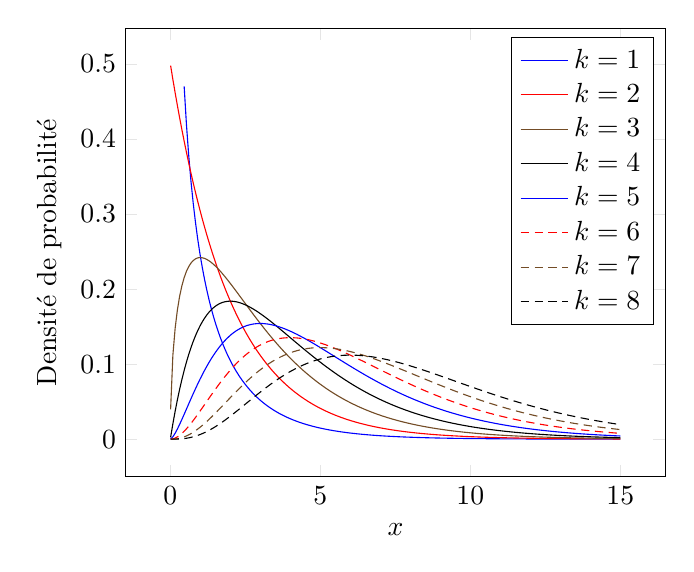
\begin{tikzpicture}[
    declare function={
      gamma(\z)=(2.506628274631*sqrt(1/\z)+ 0.20888568*(1/\z)^(1.5)+ 0.00870357*(1/\z)^(2.5)- (174.2106599*(1/\z)^(3.5))/25920- (715.6423511*(1/\z)^(4.5))/1244160)*exp((-ln(1/\z)-1)*\z);},
    declare function={
        chisq(\x,\k) = (\x)^(\k/2-1) * exp(-\x/2) / (2^(\k/2)) / gamma(\k/2);
    }
]
\begin{axis}[
  xlabel = $x$,
  ylabel = {Densité de probabilité},
  samples = 200,
  restrict y to domain = 0:0.5,
  domain = 0.01:15,
  legend cell align=left]
    \foreach \k in {1,...,8} {
      \addplot+[mark={}] {chisq(x,\k)}; \addlegendentryexpanded{$k=\k$}}
  \end{axis}
\end{tikzpicture}

  \end{center}


\end{frame}


\begin{frame}
  \frametitle{Loi de Student}

  \begin{defn}{}
    Soient $Z$ une variable aléatoire normale centrée réduite et une variable aléatoire $U\perp Z$ distribuéesuivant la loi du $\chi^2$ à $k$ degrés de liberté. Alors
    \[
      X = \frac{Z}{\sqrt{\nicefrac{U}{k}}}
    \]
    suit une loi de Student à $k$ degrés de liberté, notée $t_k$.
  \end{defn}

  \bigskip

  \begin{prop}\label{prop:student}
    La fonction de densité de probabilité de $X\sim t_k$,
    avec $k\in\mathbb N$, est~:
    \[
      f_X(x) =
      \frac{1}{\sqrt{k\pi}}\frac{\Gamma(\frac{k+1}{2})}{\Gamma(\frac{k}{2})}\left(1+\frac{x^2}{k}\right)^{-\frac{k+1}{2}}
    \]
    pour tout $x\in\mathbb R$, où $\Gamma(z) = \int_0^{\infty}t^{z-1}e^{-t}\mathrm dt$ est la
    fonction Gamma. On a $\mathbb E\left[ X \right]=0$ si $k>1$ et $\mathbb V\left[ X \right] = \frac{k}{k-2}$ si $k>2$. La loi de student converge vers la loi normale si $k$ tend vers l'infini.
  \end{prop}

\end{frame}


\begin{frame}
  \frametitle{Loi de Student}

  \bigskip

  \begin{center}
    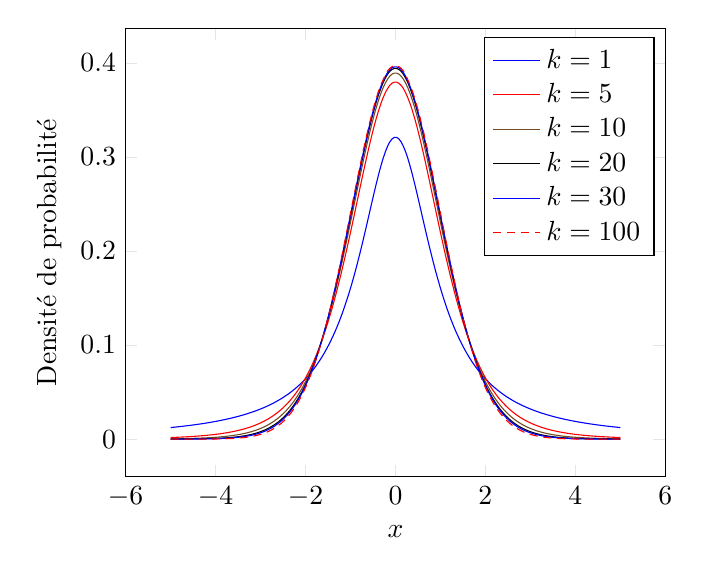
\begin{tikzpicture}[
    declare function={
      gamma(\z)=(2.506628274631*sqrt(1/\z)+ 0.20888568*(1/\z)^(1.5)+ 0.00870357*(1/\z)^(2.5)- (174.2106599*(1/\z)^(3.5))/25920- (715.6423511*(1/\z)^(4.5))/1244160)*exp((-ln(1/\z)-1)*\z);},
    declare function={
      student(\x,\k) = (1/sqrt(3.14159265359*\k))*gamma((\k+1)/2)/gamma(\k/2)*(1+\x*\x/\k)^(-(\k+1)/2);}
]
\begin{axis}[
  xlabel = $x$,
  ylabel = {Densité de probabilité},
  samples = 200,
  restrict y to domain = 0:0.5,
  domain = -5:5,
  legend cell align=left]
    \foreach \k in {1, 5, 10, 20, 30, 100} {
      \addplot+[mark={}] {student(x,\k)}; \addlegendentryexpanded{$k=\k$}}
  \end{axis}
\end{tikzpicture}

  \end{center}


\end{frame}



\begin{frame}
  \frametitle{Loi de Fisher}

  \begin{defn}{}
    Soient $U\sim\chi^2(p)$ et $V\sim\chi^2(q)$, avec  $U\perp V$. $X = \frac{\nicefrac{U}{p}}{\nicefrac{V}{q}}$ une variable aléatoire réelle distribuée selon la loi de Fisher de degrés de liberté $p$ et $q$. On note la distribution de Fisher~: $F(p,q)$.
  \end{defn}

  \bigskip

  \begin{prop}\label{prop:fisher}
    La fonction de densité de probabilité de $X\sim F(p,q)$,
    avec $(p,q)\in\mathbb N^{\star}\times \mathbb N^{\star}$, est~:
    \[
      f_X(x) = \frac{\left( \frac{px}{px+q} \right)^{\frac{p}{2}}\left( 1-\frac{px}{px+q} \right)^{\frac{q}{2}}}{x B\left(\frac{p}{2},\frac{q}{2}\right)}
    \]
    pour tout $x\in\mathbb R_+$, où $B(\alpha,\beta) = \int_0^1t^{\alpha-1}(1-t)^{\beta-1}\mathrm dt$ est la
    fonction Beta. On a $\mathbb E\left[ X \right]=\frac{q}{q-2}$ si $q>2$ et $\mathbb V\left[ X \right] = \frac{2q^2\left( p+q-2 \right)}{p\left( q-2 \right)^2\left( q-4 \right)}$ si $q>4$.
  \end{prop}

\end{frame}


\begin{frame}
  \frametitle{Loi de Fisher}

  \bigskip

  \begin{center}
    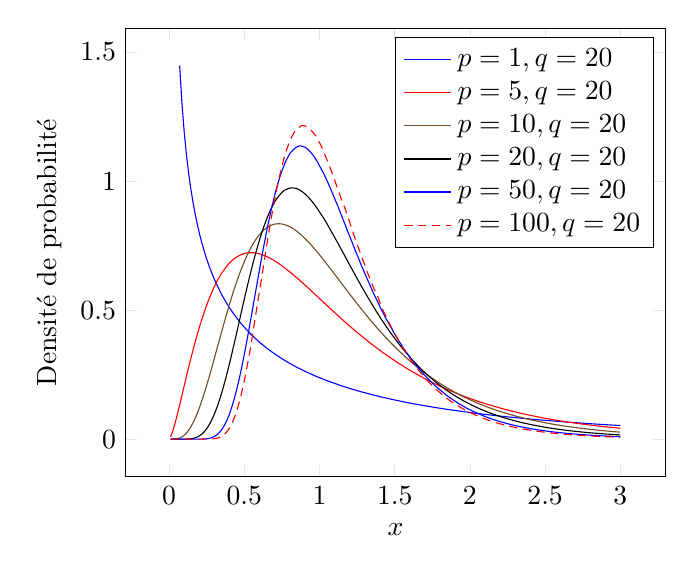
\begin{tikzpicture}[
  declare function={
    gamma(\z)=(2.506628274631*sqrt(1/\z)+ 0.20888568*(1/\z)^(1.5)+ 0.00870357*(1/\z)^(2.5)- (174.2106599*(1/\z)^(3.5))/25920- (715.6423511*(1/\z)^(4.5))/1244160)*exp((-ln(1/\z)-1)*\z);},
  declare function={
    beta(\x,\y)=gamma(\x)*gamma(\y)/gamma(\x+\y);
  },
  declare function={
    fisher(\x,\a,\b) = 1 / beta(\a/2, \b/2) * (\a/\b)^(\a/2) * \x^(\a/2-1) * (1 + \a/\b*\x)^(-(\a + \b)/2);
  }
]
\begin{axis}[
  xlabel = $x$,
  ylabel = {Densité de probabilité},
  samples = 200,
  restrict y to domain = 0:1.5,
  domain = 0.01:3,
  legend cell align=left]
  \foreach \q in {20} {
    \foreach \p in {1, 5, 10, 20, 50, 100} {
      \addplot+[mark={}] {fisher(x,\p, \q}; \addlegendentryexpanded{$p=\p, q=\q$}}}

\end{axis}
\end{tikzpicture}

  \end{center}


\end{frame}


\begin{frame}
  \frametitle{Loi de Fisher}

  \bigskip

  \begin{center}
    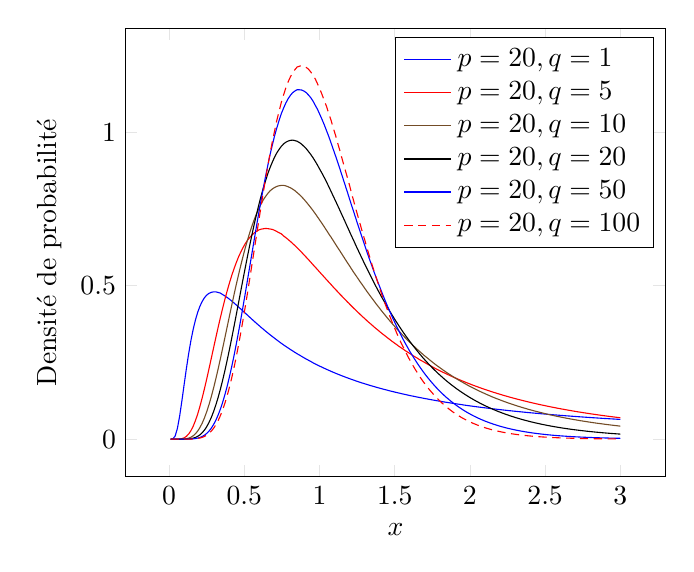
\begin{tikzpicture}[
  declare function={
    gamma(\z)=(2.506628274631*sqrt(1/\z)+ 0.20888568*(1/\z)^(1.5)+ 0.00870357*(1/\z)^(2.5)- (174.2106599*(1/\z)^(3.5))/25920- (715.6423511*(1/\z)^(4.5))/1244160)*exp((-ln(1/\z)-1)*\z);},
  declare function={
    beta(\x,\y)=gamma(\x)*gamma(\y)/gamma(\x+\y);
  },
  declare function={
    fisher(\x,\a,\b) = 1 / beta(\a/2, \b/2) * (\a/\b)^(\a/2) * \x^(\a/2-1) * (1 + \a/\b*\x)^(-(\a + \b)/2);
  }
]
\begin{axis}[
  xlabel = $x$,
  ylabel = {Densité de probabilité},
  samples = 200,
  restrict y to domain = 0:1.5,
  domain = 0.01:3,
  legend cell align=left]
  \foreach \q in {1, 5, 10, 20, 50, 100} {
    \foreach \p in {20} {
      \addplot+[mark={}] {fisher(x,\p, \q}; \addlegendentryexpanded{$p=\p, q=\q$}}}

\end{axis}
\end{tikzpicture}

  \end{center}


\end{frame}


\begin{frame}
  \frametitle{Loi de Fisher}

  \bigskip

  \begin{center}
    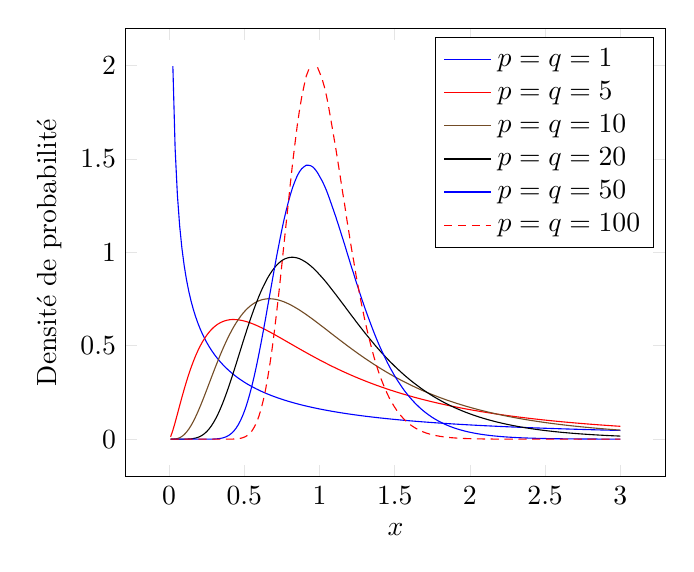
\begin{tikzpicture}[
  declare function={
    gamma(\z)=(2.506628274631*sqrt(1/\z)+ 0.20888568*(1/\z)^(1.5)+ 0.00870357*(1/\z)^(2.5)- (174.2106599*(1/\z)^(3.5))/25920- (715.6423511*(1/\z)^(4.5))/1244160)*exp((-ln(1/\z)-1)*\z);},
  declare function={
    beta(\x,\y)=gamma(\x)*gamma(\y)/gamma(\x+\y);
  },
  declare function={
    fisher(\x,\a,\b) = 1 / beta(\a/2, \b/2) * (\a/\b)^(\a/2) * \x^(\a/2-1) * (1 + \a/\b*\x)^(-(\a + \b)/2);
  }
]
\begin{axis}[
  xlabel = $x$,
  ylabel = {Densité de probabilité},
  samples = 200,
  restrict y to domain = 0:2,
  domain = 0.01:3,
  legend cell align=left]
  \foreach \p in {1, 5, 10, 20, 50, 100} {
      \addplot+[mark={}] {fisher(x,\p, \p}; \addlegendentryexpanded{$p=q=\p$}}

\end{axis}
\end{tikzpicture}

  \end{center}


\end{frame}



\end{document}


% Local Variables:
% ispell-check-comments: exclusive
% ispell-local-dictionary: "french"
% TeX-master: t
% End:
